\documentclass[twoside]{book}

% Packages required by doxygen
\usepackage{fixltx2e}
\usepackage{calc}
\usepackage{doxygen}
\usepackage[export]{adjustbox} % also loads graphicx
\usepackage{graphicx}
\usepackage[utf8]{inputenc}
\usepackage{makeidx}
\usepackage{multicol}
\usepackage{multirow}
\PassOptionsToPackage{warn}{textcomp}
\usepackage{textcomp}
\usepackage[nointegrals]{wasysym}
\usepackage[table]{xcolor}

% Font selection
\usepackage[T1]{fontenc}
\usepackage[scaled=.90]{helvet}
\usepackage{courier}
\usepackage{amssymb}
\usepackage{sectsty}
\renewcommand{\familydefault}{\sfdefault}
\allsectionsfont{%
  \fontseries{bc}\selectfont%
  \color{darkgray}%
}
\renewcommand{\DoxyLabelFont}{%
  \fontseries{bc}\selectfont%
  \color{darkgray}%
}
\newcommand{\+}{\discretionary{\mbox{\scriptsize$\hookleftarrow$}}{}{}}

% Page & text layout
\usepackage{geometry}
\geometry{%
  a4paper,%
  top=2.5cm,%
  bottom=2.5cm,%
  left=2.5cm,%
  right=2.5cm%
}
\tolerance=750
\hfuzz=15pt
\hbadness=750
\setlength{\emergencystretch}{15pt}
\setlength{\parindent}{0cm}
\setlength{\parskip}{0.2cm}
\makeatletter
\renewcommand{\paragraph}{%
  \@startsection{paragraph}{4}{0ex}{-1.0ex}{1.0ex}{%
    \normalfont\normalsize\bfseries\SS@parafont%
  }%
}
\renewcommand{\subparagraph}{%
  \@startsection{subparagraph}{5}{0ex}{-1.0ex}{1.0ex}{%
    \normalfont\normalsize\bfseries\SS@subparafont%
  }%
}
\makeatother

% Headers & footers
\usepackage{fancyhdr}
\pagestyle{fancyplain}
\fancyhead[LE]{\fancyplain{}{\bfseries\thepage}}
\fancyhead[CE]{\fancyplain{}{}}
\fancyhead[RE]{\fancyplain{}{\bfseries\leftmark}}
\fancyhead[LO]{\fancyplain{}{\bfseries\rightmark}}
\fancyhead[CO]{\fancyplain{}{}}
\fancyhead[RO]{\fancyplain{}{\bfseries\thepage}}
\fancyfoot[LE]{\fancyplain{}{}}
\fancyfoot[CE]{\fancyplain{}{}}
\fancyfoot[RE]{\fancyplain{}{\bfseries\scriptsize Generated on Sat May 28 2016 15\+:22\+:22 for E\+V3-\/\+O\+S\+E\+K by Doxygen }}
\fancyfoot[LO]{\fancyplain{}{\bfseries\scriptsize Generated on Sat May 28 2016 15\+:22\+:22 for E\+V3-\/\+O\+S\+E\+K by Doxygen }}
\fancyfoot[CO]{\fancyplain{}{}}
\fancyfoot[RO]{\fancyplain{}{}}
\renewcommand{\footrulewidth}{0.4pt}
\renewcommand{\chaptermark}[1]{%
  \markboth{#1}{}%
}
\renewcommand{\sectionmark}[1]{%
  \markright{\thesection\ #1}%
}

% Indices & bibliography
\usepackage{natbib}
\usepackage[titles]{tocloft}
\setcounter{tocdepth}{3}
\setcounter{secnumdepth}{5}
\makeindex

% Packages requested by user
\usepackage{times}

% Hyperlinks (required, but should be loaded last)
\usepackage{ifpdf}
\ifpdf
  \usepackage[pdftex,pagebackref=true]{hyperref}
\else
  \usepackage[ps2pdf,pagebackref=true]{hyperref}
\fi
\hypersetup{%
  colorlinks=true,%
  linkcolor=blue,%
  citecolor=blue,%
  unicode%
}

% Custom commands
\newcommand{\clearemptydoublepage}{%
  \newpage{\pagestyle{empty}\cleardoublepage}%
}


%===== C O N T E N T S =====

\begin{document}

% Titlepage & ToC
\hypersetup{pageanchor=false,
             bookmarks=true,
             bookmarksnumbered=true,
             pdfencoding=unicode
            }
\pagenumbering{roman}
\begin{titlepage}
\vspace*{7cm}
\begin{center}%
{\Large E\+V3-\/\+O\+S\+E\+K \\[1ex]\large 1.\+0 }\\
\vspace*{1cm}
{\large Generated by Doxygen 1.8.10}\\
\vspace*{0.5cm}
{\small Sat May 28 2016 15:22:22}\\
\end{center}
\end{titlepage}
\clearemptydoublepage
\tableofcontents
\clearemptydoublepage
\pagenumbering{arabic}
\hypersetup{pageanchor=true}

%--- Begin generated contents ---
\chapter{Data Structure Index}
\section{Data Structures}
Here are the data structures with brief descriptions\+:\begin{DoxyCompactList}
\item\contentsline{section}{\hyperlink{structbutton__info}{button\+\_\+info} \\*This struct contains the information required to read a buttons state }{\pageref{structbutton__info}}{}
\item\contentsline{section}{\hyperlink{structecap_context}{ecap\+Context} }{\pageref{structecap_context}}{}
\item\contentsline{section}{\hyperlink{struct_i2_c___p_i_n}{I2\+C\+\_\+\+P\+I\+N} \\*This struct represents a G\+P\+I\+O pin used for I2\+C communication }{\pageref{struct_i2_c___p_i_n}}{}
\item\contentsline{section}{\hyperlink{struct_i2_c___p_o_r_t}{I2\+C\+\_\+\+P\+O\+R\+T} \\*This struct represents an I2\+C port }{\pageref{struct_i2_c___p_o_r_t}}{}
\item\contentsline{section}{\hyperlink{structled__info}{led\+\_\+info} \\*This struct stores information about one L\+E\+D which is controlled by 2 G\+P\+I\+O pins }{\pageref{structled__info}}{}
\item\contentsline{section}{\hyperlink{structmotor__data__struct}{motor\+\_\+data\+\_\+struct} \\*Contains the information about wheel revolution, given speed and brake mode of motors }{\pageref{structmotor__data__struct}}{}
\item\contentsline{section}{\hyperlink{structmotor__port__info}{motor\+\_\+port\+\_\+info} \\*Contains the gpio pins of output and input pins }{\pageref{structmotor__port__info}}{}
\item\contentsline{section}{\hyperlink{structpin__info}{pin\+\_\+info} \\*This struct represents 1 G\+P\+I\+O pin }{\pageref{structpin__info}}{}
\item\contentsline{section}{\hyperlink{structsensor__port__info}{sensor\+\_\+port\+\_\+info} \\*This struct combines information about a sensor port of the E\+V3 }{\pageref{structsensor__port__info}}{}
\end{DoxyCompactList}

\chapter{File Index}
\section{File List}
Here is a list of all documented files with brief descriptions\+:\begin{DoxyCompactList}
\item\contentsline{section}{E\+C\+Robot/\hyperlink{ecrobot__interface_8c}{ecrobot\+\_\+interface.\+c} \\*This file contains the function definitions for the users E\+C\+Robot-\/\+A\+P\+I. This A\+P\+I is used to interact with sensors and actuators }{\pageref{ecrobot__interface_8c}}{}
\item\contentsline{section}{E\+C\+Robot/\hyperlink{ecrobot__interface_8h}{ecrobot\+\_\+interface.\+h} \\*This file contains the function declarations for the users E\+C\+Robot-\/\+A\+P\+I. This A\+P\+I is used to interact with sensors and actuators }{\pageref{ecrobot__interface_8h}}{}
\item\contentsline{section}{E\+C\+Robot/\hyperlink{ecrobot__types_8h}{ecrobot\+\_\+types.\+h} \\*This file contains some typedefs }{\pageref{ecrobot__types_8h}}{}
\item\contentsline{section}{le\+J\+O\+S\+\_\+\+E\+V3/src/ev3/\hyperlink{adc__sensors_8c}{adc\+\_\+sensors.\+c} \\*This file contains the function definitions to read the analogous sensors }{\pageref{adc__sensors_8c}}{}
\item\contentsline{section}{le\+J\+O\+S\+\_\+\+E\+V3/src/ev3/\hyperlink{adc__sensors_8h}{adc\+\_\+sensors.\+h} \\*Function declarations to read the analogous sensors }{\pageref{adc__sensors_8h}}{}
\item\contentsline{section}{le\+J\+O\+S\+\_\+\+E\+V3/src/ev3/\hyperlink{digi__sensors_8c}{digi\+\_\+sensors.\+c} \\*Function definitions to talk to the digital sensors (I2\+C sensors) }{\pageref{digi__sensors_8c}}{}
\item\contentsline{section}{le\+J\+O\+S\+\_\+\+E\+V3/src/ev3/\hyperlink{digi__sensors_8h}{digi\+\_\+sensors.\+h} \\*Function declarations to talk to the digital sensors (I2\+C sensors) }{\pageref{digi__sensors_8h}}{}
\item\contentsline{section}{le\+J\+O\+S\+\_\+\+E\+V3/src/ev3/\hyperlink{ev3__motors_8c}{ev3\+\_\+motors.\+c} \\*This file contains function definitions to use E\+V3 motors. Driver wrapper for E\+C\+Robot A\+P\+I }{\pageref{ev3__motors_8c}}{}
\item\contentsline{section}{le\+J\+O\+S\+\_\+\+E\+V3/src/ev3/\hyperlink{ev3__motors_8h}{ev3\+\_\+motors.\+h} \\*This header contains function declarations to use motor drivers. Driver wrapper for E\+C\+Robot A\+P\+I }{\pageref{ev3__motors_8h}}{}
\item\contentsline{section}{le\+J\+O\+S\+\_\+\+E\+V3/src/ev3/\hyperlink{i2c_8c}{i2c.\+c} \\*Function definitions related to I2\+C communication }{\pageref{i2c_8c}}{}
\item\contentsline{section}{le\+J\+O\+S\+\_\+\+E\+V3/src/ev3/\hyperlink{i2c_8h}{i2c.\+h} \\*Function declarations related to I2\+C communication }{\pageref{i2c_8h}}{}
\item\contentsline{section}{le\+J\+O\+S\+\_\+\+E\+V3/src/ev3/\hyperlink{init_8c}{init.\+c} \\*This code is required in order to initialize the le\+J\+O\+S driver including all modules properly }{\pageref{init_8c}}{}
\item\contentsline{section}{le\+J\+O\+S\+\_\+\+E\+V3/src/ev3/\hyperlink{init_8h}{init.\+h} \\*This header provides the interface to initialize the le\+J\+O\+S E\+V3 drivers }{\pageref{init_8h}}{}
\item\contentsline{section}{le\+J\+O\+S\+\_\+\+E\+V3/src/ev3/\hyperlink{mytypes_8h}{mytypes.\+h} \\*This header defines the data types used in the le\+J\+O\+S driver }{\pageref{mytypes_8h}}{}
\item\contentsline{section}{le\+J\+O\+S\+\_\+\+E\+V3/src/ev3/\hyperlink{power_8c}{power.\+c} \\*This header contains function definitions for the power management on the E\+V3 }{\pageref{power_8c}}{}
\item\contentsline{section}{le\+J\+O\+S\+\_\+\+E\+V3/src/ev3/\hyperlink{power_8h}{power.\+h} \\*This header contains function declarations for the power management on the E\+V3 }{\pageref{power_8h}}{}
\item\contentsline{section}{le\+J\+O\+S\+\_\+\+E\+V3/src/ev3/\hyperlink{sensors_8h}{sensors.\+h} \\*This header contains macros for the sensor ports of the E\+V3 }{\pageref{sensors_8h}}{}
\item\contentsline{section}{le\+J\+O\+S\+\_\+\+E\+V3/src/ev3/\hyperlink{systick_8c}{systick.\+c} \\*This header contains function definitions required to manage the tick in milliseconds on the E\+V3 }{\pageref{systick_8c}}{}
\item\contentsline{section}{le\+J\+O\+S\+\_\+\+E\+V3/src/ev3/\hyperlink{systick_8h}{systick.\+h} \\*This header contains function declarations required to manage the tick in milliseconds on the E\+V3 }{\pageref{systick_8h}}{}
\item\contentsline{section}{le\+J\+O\+S\+\_\+\+E\+V3/src/ev3/drivers/\hyperlink{cpu_8c}{cpu.\+c} \\*This file contains the A\+P\+I definitions for configuring C\+P\+U }{\pageref{cpu_8c}}{}
\item\contentsline{section}{le\+J\+O\+S\+\_\+\+E\+V3/src/ev3/drivers/\hyperlink{ecap_8c}{ecap.\+c} \\*E\+C\+A\+P A\+P\+Is }{\pageref{ecap_8c}}{}
\item\contentsline{section}{le\+J\+O\+S\+\_\+\+E\+V3/src/ev3/drivers/\hyperlink{ehrpwm_8c}{ehrpwm.\+c} \\*This file contains the device abstraction layer A\+P\+Is for E\+H\+R\+P\+W\+M }{\pageref{ehrpwm_8c}}{}
\item\contentsline{section}{le\+J\+O\+S\+\_\+\+E\+V3/src/ev3/drivers/\hyperlink{drivers_2gpio_8c}{gpio.\+c} \\*This file contains the device abstraction layer A\+P\+Is for G\+P\+I\+O }{\pageref{drivers_2gpio_8c}}{}
\item\contentsline{section}{le\+J\+O\+S\+\_\+\+E\+V3/src/ev3/drivers/\hyperlink{interrupt_8c}{interrupt.\+c} \\*Contains the A\+P\+Is for configuring A\+I\+N\+T\+C }{\pageref{interrupt_8c}}{}
\item\contentsline{section}{le\+J\+O\+S\+\_\+\+E\+V3/src/ev3/drivers/\hyperlink{psc_8c}{psc.\+c} \\*This file contains the device abstraction layer A\+P\+Is for the P\+S\+C module. There are A\+P\+Is here to enable power domain, transitions for a particular module }{\pageref{psc_8c}}{}
\item\contentsline{section}{le\+J\+O\+S\+\_\+\+E\+V3/src/ev3/drivers/\hyperlink{drivers_2spi_8c}{spi.\+c} \\*S\+P\+I device abstraction layer A\+P\+Is }{\pageref{drivers_2spi_8c}}{}
\item\contentsline{section}{le\+J\+O\+S\+\_\+\+E\+V3/src/ev3/drivers/\hyperlink{syscfg_8c}{syscfg.\+c} \\*This file contains A\+P\+Is to lock and unlock the System Configuration (S\+Y\+S\+C\+F\+G) module registers by appropriately programming the Kick Registers }{\pageref{syscfg_8c}}{}
\item\contentsline{section}{le\+J\+O\+S\+\_\+\+E\+V3/src/ev3/drivers/\hyperlink{timer_8c}{timer.\+c} \\*T\+I\+M\+E\+R A\+P\+Is }{\pageref{timer_8c}}{}
\item\contentsline{section}{le\+J\+O\+S\+\_\+\+E\+V3/src/ev3/include/\hyperlink{ecap_8h}{ecap.\+h} \\*This file contains the function prototypes for the device abstraction layer for E\+C\+A\+P. It also contains some related macro definitions and some files to be included }{\pageref{ecap_8h}}{}
\item\contentsline{section}{le\+J\+O\+S\+\_\+\+E\+V3/src/ev3/include/\hyperlink{ehrpwm_8h}{ehrpwm.\+h} \\*This file contains the Macros and A\+P\+I prototypes for ehrpwm driver }{\pageref{ehrpwm_8h}}{}
\item\contentsline{section}{le\+J\+O\+S\+\_\+\+E\+V3/src/ev3/include/\hyperlink{epwm_8h}{epwm.\+h} \\*This file contains the Macros and A\+P\+I prototypes for ehrpwm driver }{\pageref{epwm_8h}}{}
\item\contentsline{section}{le\+J\+O\+S\+\_\+\+E\+V3/src/ev3/include/\hyperlink{include_2gpio_8h}{gpio.\+h} \\*This file contains the function prototypes for the device abstraction layer for G\+P\+I\+O and some related macros }{\pageref{include_2gpio_8h}}{}
\item\contentsline{section}{le\+J\+O\+S\+\_\+\+E\+V3/src/ev3/include/\hyperlink{psc_8h}{psc.\+h} \\*This file contains the function prototypes for the device abstraction layer for P\+S\+C. It also contains some related macro definitions and some files to be included }{\pageref{psc_8h}}{}
\item\contentsline{section}{le\+J\+O\+S\+\_\+\+E\+V3/src/ev3/include/\hyperlink{include_2spi_8h}{spi.\+h} \\*S\+P\+I A\+P\+Is and macros }{\pageref{include_2spi_8h}}{}
\item\contentsline{section}{le\+J\+O\+S\+\_\+\+E\+V3/src/ev3/include/\hyperlink{timer_8h}{timer.\+h} \\*Timer A\+P\+Is and macros }{\pageref{timer_8h}}{}
\item\contentsline{section}{le\+J\+O\+S\+\_\+\+E\+V3/src/ev3/include/armv5/\hyperlink{cp15_8h}{cp15.\+h} \\*C\+P15 related function prototypes }{\pageref{cp15_8h}}{}
\item\contentsline{section}{le\+J\+O\+S\+\_\+\+E\+V3/src/ev3/include/armv5/\hyperlink{cpu_8h}{cpu.\+h} \\*C\+P\+U related function prototypes }{\pageref{cpu_8h}}{}
\item\contentsline{section}{le\+J\+O\+S\+\_\+\+E\+V3/src/ev3/include/armv5/am1808/\hyperlink{edma__event_8h}{edma\+\_\+event.\+h} \\*E\+D\+M\+A event enumeration }{\pageref{edma__event_8h}}{}
\item\contentsline{section}{le\+J\+O\+S\+\_\+\+E\+V3/src/ev3/include/armv5/am1808/\hyperlink{evm_a_m1808_8h}{evm\+A\+M1808.\+h} \\*This file contains the board specific function prototypes for use by applications }{\pageref{evm_a_m1808_8h}}{}
\item\contentsline{section}{le\+J\+O\+S\+\_\+\+E\+V3/src/ev3/include/armv5/am1808/\hyperlink{interrupt_8h}{interrupt.\+h} \\*Interrupt related A\+P\+I declarations }{\pageref{interrupt_8h}}{}
\item\contentsline{section}{le\+J\+O\+S\+\_\+\+E\+V3/src/ev3/include/hw/\hyperlink{hw__aintc_8h}{hw\+\_\+aintc.\+h} \\*A\+R\+M I\+N\+T\+C register definitions }{\pageref{hw__aintc_8h}}{}
\item\contentsline{section}{le\+J\+O\+S\+\_\+\+E\+V3/src/ev3/include/hw/\hyperlink{hw__ecap_8h}{hw\+\_\+ecap.\+h} \\*E\+C\+A\+P register definitions }{\pageref{hw__ecap_8h}}{}
\item\contentsline{section}{le\+J\+O\+S\+\_\+\+E\+V3/src/ev3/include/hw/\hyperlink{hw__ehrpwm_8h}{hw\+\_\+ehrpwm.\+h} \\*E\+H\+R\+P\+W\+M register definitions }{\pageref{hw__ehrpwm_8h}}{}
\item\contentsline{section}{le\+J\+O\+S\+\_\+\+E\+V3/src/ev3/include/hw/\hyperlink{hw__gpio_8h}{hw\+\_\+gpio.\+h} \\*G\+P\+I\+O register definitions }{\pageref{hw__gpio_8h}}{}
\item\contentsline{section}{le\+J\+O\+S\+\_\+\+E\+V3/src/ev3/include/hw/\hyperlink{hw__psc___a_m1808_8h}{hw\+\_\+psc\+\_\+\+A\+M1808.\+h} \\*P\+S\+C register definitions for A\+M1808 }{\pageref{hw__psc___a_m1808_8h}}{}
\item\contentsline{section}{le\+J\+O\+S\+\_\+\+E\+V3/src/ev3/include/hw/\hyperlink{hw__pwmss_8h}{hw\+\_\+pwmss.\+h} \\*P\+W\+M\+S\+S register definitions }{\pageref{hw__pwmss_8h}}{}
\item\contentsline{section}{le\+J\+O\+S\+\_\+\+E\+V3/src/ev3/include/hw/\hyperlink{hw__spi_8h}{hw\+\_\+spi.\+h} \\*S\+P\+I register definitions }{\pageref{hw__spi_8h}}{}
\item\contentsline{section}{le\+J\+O\+S\+\_\+\+E\+V3/src/ev3/include/hw/\hyperlink{hw__syscfg0___a_m1808_8h}{hw\+\_\+syscfg0\+\_\+\+A\+M1808.\+h} \\*S\+Y\+S\+C\+F\+G0 register definitions for A\+M1808 }{\pageref{hw__syscfg0___a_m1808_8h}}{}
\item\contentsline{section}{le\+J\+O\+S\+\_\+\+E\+V3/src/ev3/include/hw/\hyperlink{hw__syscfg1___a_m1808_8h}{hw\+\_\+syscfg1\+\_\+\+A\+M1808.\+h} \\*S\+Y\+S\+C\+F\+G1 register definitions for A\+M1808 }{\pageref{hw__syscfg1___a_m1808_8h}}{}
\item\contentsline{section}{le\+J\+O\+S\+\_\+\+E\+V3/src/ev3/include/hw/\hyperlink{hw__tmr_8h}{hw\+\_\+tmr.\+h} \\*This file contains the Register Descriptions for Timer }{\pageref{hw__tmr_8h}}{}
\item\contentsline{section}{le\+J\+O\+S\+\_\+\+E\+V3/src/ev3/include/hw/\hyperlink{hw__types_8h}{hw\+\_\+types.\+h} \\*Common type definitions and macros }{\pageref{hw__types_8h}}{}
\item\contentsline{section}{le\+J\+O\+S\+\_\+\+E\+V3/src/ev3/include/hw/\hyperlink{soc___a_m1808_8h}{soc\+\_\+\+A\+M1808.\+h} \\*This file contains the peripheral information for A\+M1808 S\+O\+C }{\pageref{soc___a_m1808_8h}}{}
\item\contentsline{section}{le\+J\+O\+S\+\_\+\+E\+V3/src/ev3/ninja/\hyperlink{adc_8c}{adc.\+c} \\*This file contains function definitions to talk to the A\+D\+C }{\pageref{adc_8c}}{}
\item\contentsline{section}{le\+J\+O\+S\+\_\+\+E\+V3/src/ev3/ninja/\hyperlink{adc_8h}{adc.\+h} \\*This header contains function declarations to talk to the A\+D\+C }{\pageref{adc_8h}}{}
\item\contentsline{section}{le\+J\+O\+S\+\_\+\+E\+V3/src/ev3/ninja/\hyperlink{button_8c}{button.\+c} \\*This file contains function definitions to use the hardware buttons of the E\+V3 }{\pageref{button_8c}}{}
\item\contentsline{section}{le\+J\+O\+S\+\_\+\+E\+V3/src/ev3/ninja/\hyperlink{button_8h}{button.\+h} \\*This header contains function declarations to use the hardware buttons of the E\+V3 as well as enumerations to represent the buttons and their states }{\pageref{button_8h}}{}
\item\contentsline{section}{le\+J\+O\+S\+\_\+\+E\+V3/src/ev3/ninja/\hyperlink{ninja_2gpio_8c}{gpio.\+c} \\*This contains function definitions required to interact with G\+P\+I\+O pins of the So\+C }{\pageref{ninja_2gpio_8c}}{}
\item\contentsline{section}{le\+J\+O\+S\+\_\+\+E\+V3/src/ev3/ninja/\hyperlink{ninja_2gpio_8h}{gpio.\+h} \\*This header declares function required to interact with G\+P\+I\+O pins of the So\+C }{\pageref{ninja_2gpio_8h}}{}
\item\contentsline{section}{le\+J\+O\+S\+\_\+\+E\+V3/src/ev3/ninja/\hyperlink{led_8c}{led.\+c} \\*This contains function definitions required to interact with the L\+E\+Ds of the E\+V3 }{\pageref{led_8c}}{}
\item\contentsline{section}{le\+J\+O\+S\+\_\+\+E\+V3/src/ev3/ninja/\hyperlink{led_8h}{led.\+h} \\*This header declares function required to interact with the L\+E\+Ds of the E\+V3 as well as enumerations therefore }{\pageref{led_8h}}{}
\item\contentsline{section}{le\+J\+O\+S\+\_\+\+E\+V3/src/ev3/ninja/\hyperlink{motor_8c}{motor.\+c} \\*Driver implementation to control L\+E\+G\+O servo motors. This file contains function definitions to use motors with E\+V3 }{\pageref{motor_8c}}{}
\item\contentsline{section}{le\+J\+O\+S\+\_\+\+E\+V3/src/ev3/ninja/\hyperlink{motor_8h}{motor.\+h} \\*A header file for motor driver. This file contains function declarations to use servo motors as well as enumerations and structs to represent motors and their states }{\pageref{motor_8h}}{}
\item\contentsline{section}{le\+J\+O\+S\+\_\+\+E\+V3/src/ev3/ninja/\hyperlink{pininfo_8c}{pininfo.\+c} \\*This file defines the array required to manipulate the P\+I\+N\+M\+U\+X registers and set the functionality of G\+P\+I\+O pins }{\pageref{pininfo_8c}}{}
\item\contentsline{section}{le\+J\+O\+S\+\_\+\+E\+V3/src/ev3/ninja/\hyperlink{pininfo_8h}{pininfo.\+h} \\*This header defines the struct that represents a G\+P\+I\+O pin in the ev3ninja driver and makes the corresponding variable in \hyperlink{pininfo_8c}{pininfo.\+c} accessible by other files }{\pageref{pininfo_8h}}{}
\item\contentsline{section}{le\+J\+O\+S\+\_\+\+E\+V3/src/ev3/ninja/\hyperlink{ninja_2spi_8c}{spi.\+c} \\*This contains function definitions required to interact with the S\+P\+I0 controller of the So\+C which is connected to the A\+D\+C }{\pageref{ninja_2spi_8c}}{}
\item\contentsline{section}{le\+J\+O\+S\+\_\+\+E\+V3/src/ev3/ninja/\hyperlink{ninja_2spi_8h}{spi.\+h} \\*This header declares function required to interact with the S\+P\+I0 controller of the So\+C which is connected to the A\+D\+C }{\pageref{ninja_2spi_8h}}{}
\end{DoxyCompactList}

\chapter{Data Structure Documentation}
\hypertarget{structbutton__info}{}\section{button\+\_\+info Struct Reference}
\label{structbutton__info}\index{button\+\_\+info@{button\+\_\+info}}


This struct contains the information required to read a buttons state.  




{\ttfamily \#include $<$button.\+h$>$}



Collaboration diagram for button\+\_\+info\+:\nopagebreak
\begin{figure}[H]
\begin{center}
\leavevmode
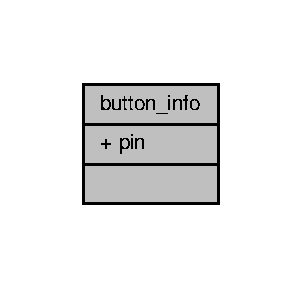
\includegraphics[width=145pt]{structbutton__info__coll__graph}
\end{center}
\end{figure}
\subsection*{Data Fields}
\begin{DoxyCompactItemize}
\item 
\hypertarget{structbutton__info_a867fe4e0366cbc13a194e166b96b0216}{}unsigned int \hyperlink{structbutton__info_a867fe4e0366cbc13a194e166b96b0216}{pin}\label{structbutton__info_a867fe4e0366cbc13a194e166b96b0216}

\begin{DoxyCompactList}\small\item\em The pin representing the buttons state. \end{DoxyCompactList}\end{DoxyCompactItemize}


\subsection{Detailed Description}
This struct contains the information required to read a buttons state. 

Every buttons is red by reading the signal on 1 G\+P\+I\+O pin which is configured as input. 

The documentation for this struct was generated from the following file\+:\begin{DoxyCompactItemize}
\item 
le\+J\+O\+S\+\_\+\+E\+V3/src/ev3/ninja/\hyperlink{button_8h}{button.\+h}\end{DoxyCompactItemize}

\hypertarget{structecap_context}{}\section{ecap\+Context Struct Reference}
\label{structecap_context}\index{ecap\+Context@{ecap\+Context}}


Collaboration diagram for ecap\+Context\+:\nopagebreak
\begin{figure}[H]
\begin{center}
\leavevmode
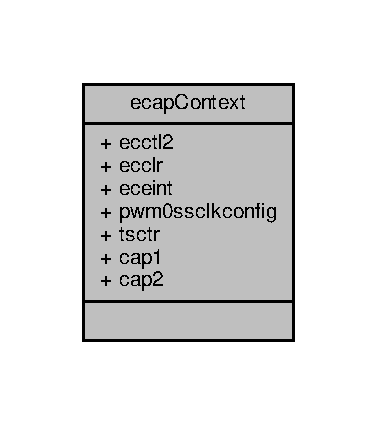
\includegraphics[width=181pt]{structecap_context__coll__graph}
\end{center}
\end{figure}
\subsection*{Data Fields}
\begin{DoxyCompactItemize}
\item 
\hypertarget{structecap_context_aeca0b9d7311d6acea599e568b901257a}{}unsigned short {\bfseries ecctl2}\label{structecap_context_aeca0b9d7311d6acea599e568b901257a}

\item 
\hypertarget{structecap_context_ac9af5c16ab5c8eac1f81503675226953}{}unsigned short {\bfseries ecclr}\label{structecap_context_ac9af5c16ab5c8eac1f81503675226953}

\item 
\hypertarget{structecap_context_a3271d5f86387eade21271043053d6b3b}{}unsigned short {\bfseries eceint}\label{structecap_context_a3271d5f86387eade21271043053d6b3b}

\item 
\hypertarget{structecap_context_a8f3999e3c86541be211c275e4c9a63af}{}unsigned int {\bfseries pwm0ssclkconfig}\label{structecap_context_a8f3999e3c86541be211c275e4c9a63af}

\item 
\hypertarget{structecap_context_a1b7016b57363bb48dfbe56054c9cc5da}{}unsigned int {\bfseries tsctr}\label{structecap_context_a1b7016b57363bb48dfbe56054c9cc5da}

\item 
\hypertarget{structecap_context_a9c282febebcb752e765ad27e89e03fa5}{}unsigned int {\bfseries cap1}\label{structecap_context_a9c282febebcb752e765ad27e89e03fa5}

\item 
\hypertarget{structecap_context_a064b42a8515ae9bbc0510902357f8550}{}unsigned int {\bfseries cap2}\label{structecap_context_a064b42a8515ae9bbc0510902357f8550}

\end{DoxyCompactItemize}


The documentation for this struct was generated from the following file\+:\begin{DoxyCompactItemize}
\item 
le\+J\+O\+S\+\_\+\+E\+V3/src/ev3/include/\hyperlink{ecap_8h}{ecap.\+h}\end{DoxyCompactItemize}

\hypertarget{struct_i2_c___p_i_n}{}\section{I2\+C\+\_\+\+P\+I\+N Struct Reference}
\label{struct_i2_c___p_i_n}\index{I2\+C\+\_\+\+P\+I\+N@{I2\+C\+\_\+\+P\+I\+N}}


This struct represents a G\+P\+I\+O pin used for I2\+C communication.  




{\ttfamily \#include $<$i2c.\+h$>$}



Collaboration diagram for I2\+C\+\_\+\+P\+I\+N\+:\nopagebreak
\begin{figure}[H]
\begin{center}
\leavevmode
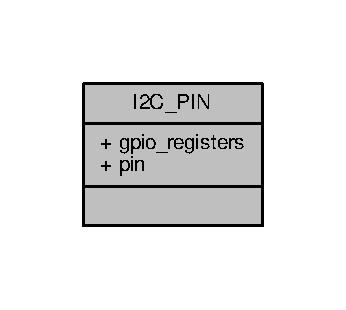
\includegraphics[width=166pt]{struct_i2_c___p_i_n__coll__graph}
\end{center}
\end{figure}
\subsection*{Data Fields}
\begin{DoxyCompactItemize}
\item 
\hypertarget{struct_i2_c___p_i_n_a330fb1f866557aa4731cfc091e62066a}{}\hyperlink{mytypes_8h_a3cb25ca6f51f003950f9625ff05536fc}{U8} \hyperlink{struct_i2_c___p_i_n_a330fb1f866557aa4731cfc091e62066a}{gpio\+\_\+registers}\label{struct_i2_c___p_i_n_a330fb1f866557aa4731cfc091e62066a}

\begin{DoxyCompactList}\small\item\em The G\+P\+I\+O register to control this pin. \end{DoxyCompactList}\item 
\hypertarget{struct_i2_c___p_i_n_a14ccbbc47dccaade3a6b3a2d9704b8e0}{}\hyperlink{mytypes_8h_a3cb25ca6f51f003950f9625ff05536fc}{U8} \hyperlink{struct_i2_c___p_i_n_a14ccbbc47dccaade3a6b3a2d9704b8e0}{pin}\label{struct_i2_c___p_i_n_a14ccbbc47dccaade3a6b3a2d9704b8e0}

\begin{DoxyCompactList}\small\item\em The number of the G\+P\+I\+O pin on its bank. \end{DoxyCompactList}\end{DoxyCompactItemize}


\subsection{Detailed Description}
This struct represents a G\+P\+I\+O pin used for I2\+C communication. 

Every pin is represented by a pin number on a G\+P\+I\+O bank (0 to 15) and one G\+P\+I\+O register to control that pin. Note\+: 2 G\+P\+I\+O banks always share one G\+P\+I\+O register, therefore bank 0 and 1 relate to register 0, bank 2 and 3 relate to register 1 and so on. 

The documentation for this struct was generated from the following file\+:\begin{DoxyCompactItemize}
\item 
le\+J\+O\+S\+\_\+\+E\+V3/src/ev3/\hyperlink{i2c_8h}{i2c.\+h}\end{DoxyCompactItemize}

\hypertarget{struct_i2_c___p_o_r_t}{}\section{I2\+C\+\_\+\+P\+O\+R\+T Struct Reference}
\label{struct_i2_c___p_o_r_t}\index{I2\+C\+\_\+\+P\+O\+R\+T@{I2\+C\+\_\+\+P\+O\+R\+T}}


This struct represents an I2\+C port.  




{\ttfamily \#include $<$i2c.\+h$>$}



Collaboration diagram for I2\+C\+\_\+\+P\+O\+R\+T\+:\nopagebreak
\begin{figure}[H]
\begin{center}
\leavevmode
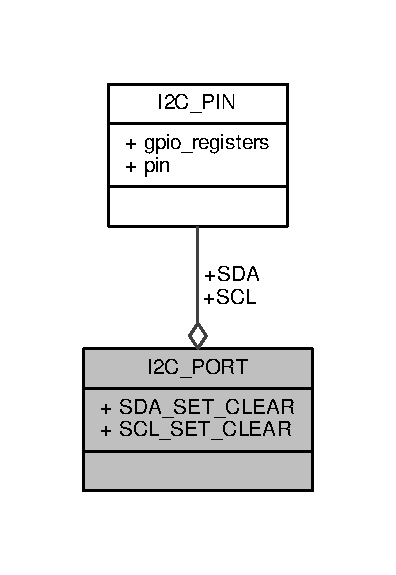
\includegraphics[width=190pt]{struct_i2_c___p_o_r_t__coll__graph}
\end{center}
\end{figure}
\subsection*{Data Fields}
\begin{DoxyCompactItemize}
\item 
\hypertarget{struct_i2_c___p_o_r_t_a5db08703c6bffc8ba01abce83b395c09}{}\hyperlink{struct_i2_c___p_i_n}{I2\+C\+\_\+\+P\+I\+N} \hyperlink{struct_i2_c___p_o_r_t_a5db08703c6bffc8ba01abce83b395c09}{S\+D\+A}\label{struct_i2_c___p_o_r_t_a5db08703c6bffc8ba01abce83b395c09}

\begin{DoxyCompactList}\small\item\em G\+P\+I\+O pin S\+D\+A (data) \end{DoxyCompactList}\item 
\hypertarget{struct_i2_c___p_o_r_t_a3c5f51354f7ba68c87911ba09adbe894}{}\hyperlink{struct_i2_c___p_i_n}{I2\+C\+\_\+\+P\+I\+N} \hyperlink{struct_i2_c___p_o_r_t_a3c5f51354f7ba68c87911ba09adbe894}{S\+C\+L}\label{struct_i2_c___p_o_r_t_a3c5f51354f7ba68c87911ba09adbe894}

\begin{DoxyCompactList}\small\item\em G\+P\+I\+O pin S\+C\+L (clock) \end{DoxyCompactList}\item 
\hypertarget{struct_i2_c___p_o_r_t_a8ae00c1e6b29ac2fdd64b0d43a7b5d23}{}unsigned int \hyperlink{struct_i2_c___p_o_r_t_a8ae00c1e6b29ac2fdd64b0d43a7b5d23}{S\+D\+A\+\_\+\+S\+E\+T\+\_\+\+C\+L\+E\+A\+R}\label{struct_i2_c___p_o_r_t_a8ae00c1e6b29ac2fdd64b0d43a7b5d23}

\begin{DoxyCompactList}\small\item\em Bitmask to set/clear the S\+D\+A pin. \end{DoxyCompactList}\item 
\hypertarget{struct_i2_c___p_o_r_t_ad4f6c7bbbb94ba99eef86f696276124b}{}unsigned int \hyperlink{struct_i2_c___p_o_r_t_ad4f6c7bbbb94ba99eef86f696276124b}{S\+C\+L\+\_\+\+S\+E\+T\+\_\+\+C\+L\+E\+A\+R}\label{struct_i2_c___p_o_r_t_ad4f6c7bbbb94ba99eef86f696276124b}

\begin{DoxyCompactList}\small\item\em Bitmask to set/clear the S\+C\+L pin. \end{DoxyCompactList}\end{DoxyCompactItemize}


\subsection{Detailed Description}
This struct represents an I2\+C port. 

Every port is represented by two G\+P\+I\+O pins (S\+D\+A for data and S\+C\+L for clock). This struct also contains the corresponding bitmasks in order to manipulate said G\+P\+I\+O pins. 

The documentation for this struct was generated from the following file\+:\begin{DoxyCompactItemize}
\item 
le\+J\+O\+S\+\_\+\+E\+V3/src/ev3/\hyperlink{i2c_8h}{i2c.\+h}\end{DoxyCompactItemize}

\hypertarget{structled__info}{}\section{led\+\_\+info Struct Reference}
\label{structled__info}\index{led\+\_\+info@{led\+\_\+info}}


This struct stores information about one L\+E\+D which is controlled by 2 G\+P\+I\+O pins.  




{\ttfamily \#include $<$led.\+h$>$}



Collaboration diagram for led\+\_\+info\+:\nopagebreak
\begin{figure}[H]
\begin{center}
\leavevmode
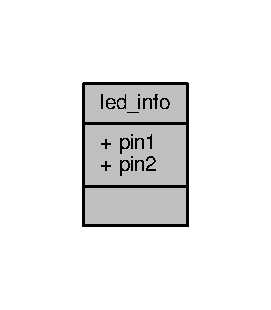
\includegraphics[width=130pt]{structled__info__coll__graph}
\end{center}
\end{figure}
\subsection*{Data Fields}
\begin{DoxyCompactItemize}
\item 
\hypertarget{structled__info_a3fc6cc33e12f94e78c5cbdc71d5416bc}{}unsigned int \hyperlink{structled__info_a3fc6cc33e12f94e78c5cbdc71d5416bc}{pin1}\label{structled__info_a3fc6cc33e12f94e78c5cbdc71d5416bc}

\begin{DoxyCompactList}\small\item\em The first G\+P\+I\+O pin, responsible for the red L\+E\+D. \end{DoxyCompactList}\item 
\hypertarget{structled__info_a9ff95d672cc5c5cd128fefae948d73fd}{}unsigned int \hyperlink{structled__info_a9ff95d672cc5c5cd128fefae948d73fd}{pin2}\label{structled__info_a9ff95d672cc5c5cd128fefae948d73fd}

\begin{DoxyCompactList}\small\item\em The second G\+P\+I\+O pin, responsible for the green L\+E\+D. \end{DoxyCompactList}\end{DoxyCompactItemize}


\subsection{Detailed Description}
This struct stores information about one L\+E\+D which is controlled by 2 G\+P\+I\+O pins. 

One G\+P\+I\+O pin controlls the red L\+E\+D and one pin the green L\+E\+D. 

The documentation for this struct was generated from the following file\+:\begin{DoxyCompactItemize}
\item 
le\+J\+O\+S\+\_\+\+E\+V3/src/ev3/ninja/\hyperlink{led_8h}{led.\+h}\end{DoxyCompactItemize}

\hypertarget{structmotor__data__struct}{}\section{motor\+\_\+data\+\_\+struct Struct Reference}
\label{structmotor__data__struct}\index{motor\+\_\+data\+\_\+struct@{motor\+\_\+data\+\_\+struct}}


Contains the information about wheel revolution, given speed and brake mode of motors.  




{\ttfamily \#include $<$motor.\+h$>$}



Collaboration diagram for motor\+\_\+data\+\_\+struct\+:\nopagebreak
\begin{figure}[H]
\begin{center}
\leavevmode
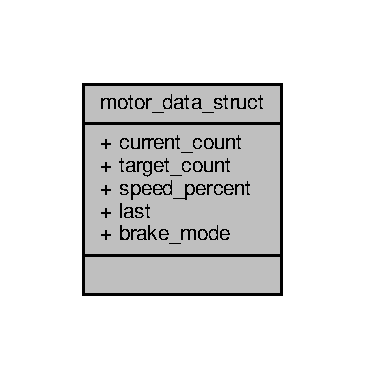
\includegraphics[width=175pt]{structmotor__data__struct__coll__graph}
\end{center}
\end{figure}
\subsection*{Data Fields}
\begin{DoxyCompactItemize}
\item 
\hypertarget{structmotor__data__struct_a947ec255e0407f658f61a5e99a3a1a3f}{}int \hyperlink{structmotor__data__struct_a947ec255e0407f658f61a5e99a3a1a3f}{current\+\_\+count}\label{structmotor__data__struct_a947ec255e0407f658f61a5e99a3a1a3f}

\begin{DoxyCompactList}\small\item\em current rotation angle in degrees \end{DoxyCompactList}\item 
\hypertarget{structmotor__data__struct_a7eefe67ec3d87f4148c708dd3665efb2}{}int \hyperlink{structmotor__data__struct_a7eefe67ec3d87f4148c708dd3665efb2}{target\+\_\+count}\label{structmotor__data__struct_a7eefe67ec3d87f4148c708dd3665efb2}

\begin{DoxyCompactList}\small\item\em target rotation angle to reach \end{DoxyCompactList}\item 
\hypertarget{structmotor__data__struct_af6bb7532bdedf08e410879c022b273a8}{}int \hyperlink{structmotor__data__struct_af6bb7532bdedf08e410879c022b273a8}{speed\+\_\+percent}\label{structmotor__data__struct_af6bb7532bdedf08e410879c022b273a8}

\begin{DoxyCompactList}\small\item\em not used. for future use \end{DoxyCompactList}\item 
\hypertarget{structmotor__data__struct_a4b79ed65ee741709a1ba4ac4da565740}{}\hyperlink{mytypes_8h_a811024d35b9b8a41095b1f583b649e56}{U32} \hyperlink{structmotor__data__struct_a4b79ed65ee741709a1ba4ac4da565740}{last}\label{structmotor__data__struct_a4b79ed65ee741709a1ba4ac4da565740}

\begin{DoxyCompactList}\small\item\em last value of I\+N\+T (pin5) \end{DoxyCompactList}\item 
\hypertarget{structmotor__data__struct_a297efa77cb3b93d89e30c66e787330c3}{}short \hyperlink{structmotor__data__struct_a297efa77cb3b93d89e30c66e787330c3}{brake\+\_\+mode}\label{structmotor__data__struct_a297efa77cb3b93d89e30c66e787330c3}

\begin{DoxyCompactList}\small\item\em true -\/ brake immediately, false -\/ float brake (not immediately). \end{DoxyCompactList}\end{DoxyCompactItemize}


\subsection{Detailed Description}
Contains the information about wheel revolution, given speed and brake mode of motors. 

The documentation for this struct was generated from the following file\+:\begin{DoxyCompactItemize}
\item 
le\+J\+O\+S\+\_\+\+E\+V3/src/ev3/ninja/\hyperlink{motor_8h}{motor.\+h}\end{DoxyCompactItemize}

\hypertarget{structmotor__port__info}{}\section{motor\+\_\+port\+\_\+info Struct Reference}
\label{structmotor__port__info}\index{motor\+\_\+port\+\_\+info@{motor\+\_\+port\+\_\+info}}


Contains the gpio pins of output and input pins.  




{\ttfamily \#include $<$motor.\+h$>$}



Collaboration diagram for motor\+\_\+port\+\_\+info\+:\nopagebreak
\begin{figure}[H]
\begin{center}
\leavevmode
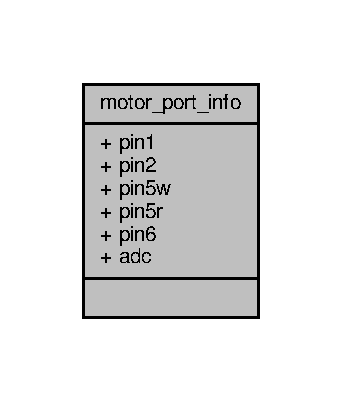
\includegraphics[width=164pt]{structmotor__port__info__coll__graph}
\end{center}
\end{figure}
\subsection*{Data Fields}
\begin{DoxyCompactItemize}
\item 
\hypertarget{structmotor__port__info_a3fc6cc33e12f94e78c5cbdc71d5416bc}{}unsigned int \hyperlink{structmotor__port__info_a3fc6cc33e12f94e78c5cbdc71d5416bc}{pin1}\label{structmotor__port__info_a3fc6cc33e12f94e78c5cbdc71d5416bc}

\begin{DoxyCompactList}\small\item\em Is used by pwm module to give power to motors. \end{DoxyCompactList}\item 
\hypertarget{structmotor__port__info_a9ff95d672cc5c5cd128fefae948d73fd}{}unsigned int \hyperlink{structmotor__port__info_a9ff95d672cc5c5cd128fefae948d73fd}{pin2}\label{structmotor__port__info_a9ff95d672cc5c5cd128fefae948d73fd}

\begin{DoxyCompactList}\small\item\em Is used by pwm module to give power to motors. \end{DoxyCompactList}\item 
\hypertarget{structmotor__port__info_ab9b1d229dc0f810218cc53a42fc37e2e}{}unsigned int {\bfseries pin5w}\label{structmotor__port__info_ab9b1d229dc0f810218cc53a42fc37e2e}

\item 
\hypertarget{structmotor__port__info_aab1edab0490b478d1b702d9880d24bad}{}unsigned int \hyperlink{structmotor__port__info_aab1edab0490b478d1b702d9880d24bad}{pin5r}\label{structmotor__port__info_aab1edab0490b478d1b702d9880d24bad}

\begin{DoxyCompactList}\small\item\em I\+N\+T value. Is used to track a wheel revolution of motors. \end{DoxyCompactList}\item 
\hypertarget{structmotor__port__info_a13e010069077bbf68832945b15ea0a4b}{}unsigned int \hyperlink{structmotor__port__info_a13e010069077bbf68832945b15ea0a4b}{pin6}\label{structmotor__port__info_a13e010069077bbf68832945b15ea0a4b}

\begin{DoxyCompactList}\small\item\em D\+I\+R value. Is used to track a wheel revolution of motors. \end{DoxyCompactList}\item 
\hypertarget{structmotor__port__info_ae547c2fbfdac55605f77262d52f213d0}{}unsigned short {\bfseries adc}\label{structmotor__port__info_ae547c2fbfdac55605f77262d52f213d0}

\end{DoxyCompactItemize}


\subsection{Detailed Description}
Contains the gpio pins of output and input pins. 

The documentation for this struct was generated from the following file\+:\begin{DoxyCompactItemize}
\item 
le\+J\+O\+S\+\_\+\+E\+V3/src/ev3/ninja/\hyperlink{motor_8h}{motor.\+h}\end{DoxyCompactItemize}

\hypertarget{structpin__info}{}\section{pin\+\_\+info Struct Reference}
\label{structpin__info}\index{pin\+\_\+info@{pin\+\_\+info}}


This struct represents 1 G\+P\+I\+O pin.  




{\ttfamily \#include $<$pininfo.\+h$>$}



Collaboration diagram for pin\+\_\+info\+:\nopagebreak
\begin{figure}[H]
\begin{center}
\leavevmode
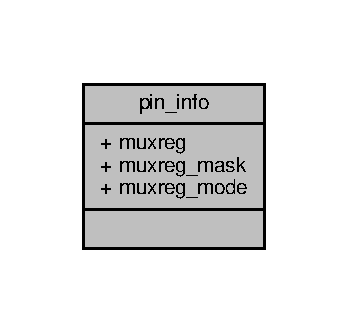
\includegraphics[width=167pt]{structpin__info__coll__graph}
\end{center}
\end{figure}
\subsection*{Data Fields}
\begin{DoxyCompactItemize}
\item 
\hypertarget{structpin__info_af2f905eebe6fc994de7da4bac4768eee}{}unsigned int \hyperlink{structpin__info_af2f905eebe6fc994de7da4bac4768eee}{muxreg}\label{structpin__info_af2f905eebe6fc994de7da4bac4768eee}

\begin{DoxyCompactList}\small\item\em The P\+I\+N\+M\+U\+X register for this pin (ranging from 0 to 19) \end{DoxyCompactList}\item 
\hypertarget{structpin__info_a395f3bb9231a420a2a63ce320aee8c98}{}unsigned int \hyperlink{structpin__info_a395f3bb9231a420a2a63ce320aee8c98}{muxreg\+\_\+mask}\label{structpin__info_a395f3bb9231a420a2a63ce320aee8c98}

\begin{DoxyCompactList}\small\item\em The bitmask to clear the half-\/byte in the P\+I\+N\+M\+U\+X register for this pin. \end{DoxyCompactList}\item 
\hypertarget{structpin__info_a27e604e3021a936ff771536a6e5a72e1}{}unsigned int \hyperlink{structpin__info_a27e604e3021a936ff771536a6e5a72e1}{muxreg\+\_\+mode}\label{structpin__info_a27e604e3021a936ff771536a6e5a72e1}

\begin{DoxyCompactList}\small\item\em The bitmask to set the half-\/byte in the P\+I\+N\+M\+U\+X register for this pin to the desired value. \end{DoxyCompactList}\end{DoxyCompactItemize}


\subsection{Detailed Description}
This struct represents 1 G\+P\+I\+O pin. 

The documentation for this struct was generated from the following file\+:\begin{DoxyCompactItemize}
\item 
le\+J\+O\+S\+\_\+\+E\+V3/src/ev3/ninja/\hyperlink{pininfo_8h}{pininfo.\+h}\end{DoxyCompactItemize}

\hypertarget{structsensor__port__info}{}\section{sensor\+\_\+port\+\_\+info Struct Reference}
\label{structsensor__port__info}\index{sensor\+\_\+port\+\_\+info@{sensor\+\_\+port\+\_\+info}}


This struct combines information about a sensor port of the E\+V3.  




{\ttfamily \#include $<$init.\+h$>$}



Collaboration diagram for sensor\+\_\+port\+\_\+info\+:\nopagebreak
\begin{figure}[H]
\begin{center}
\leavevmode
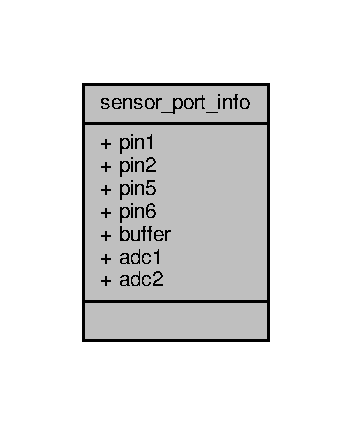
\includegraphics[width=169pt]{structsensor__port__info__coll__graph}
\end{center}
\end{figure}
\subsection*{Data Fields}
\begin{DoxyCompactItemize}
\item 
\hypertarget{structsensor__port__info_a3fc6cc33e12f94e78c5cbdc71d5416bc}{}unsigned int \hyperlink{structsensor__port__info_a3fc6cc33e12f94e78c5cbdc71d5416bc}{pin1}\label{structsensor__port__info_a3fc6cc33e12f94e78c5cbdc71d5416bc}

\begin{DoxyCompactList}\small\item\em I\+\_\+\+O\+N\+B -\/ 9\+V enable (high) \end{DoxyCompactList}\item 
\hypertarget{structsensor__port__info_a9ff95d672cc5c5cd128fefae948d73fd}{}unsigned int \hyperlink{structsensor__port__info_a9ff95d672cc5c5cd128fefae948d73fd}{pin2}\label{structsensor__port__info_a9ff95d672cc5c5cd128fefae948d73fd}

\begin{DoxyCompactList}\small\item\em L\+E\+G\+D\+E\+T\+B -\/ Digital input pulled up. \end{DoxyCompactList}\item 
\hypertarget{structsensor__port__info_a35e509974944706792ebf66614660cd0}{}unsigned int \hyperlink{structsensor__port__info_a35e509974944706792ebf66614660cd0}{pin5}\label{structsensor__port__info_a35e509974944706792ebf66614660cd0}

\begin{DoxyCompactList}\small\item\em D\+I\+G\+I\+B0 -\/ Digital input/output. \end{DoxyCompactList}\item 
\hypertarget{structsensor__port__info_a13e010069077bbf68832945b15ea0a4b}{}unsigned int \hyperlink{structsensor__port__info_a13e010069077bbf68832945b15ea0a4b}{pin6}\label{structsensor__port__info_a13e010069077bbf68832945b15ea0a4b}

\begin{DoxyCompactList}\small\item\em D\+I\+G\+I\+B1 -\/ Digital input/output. \end{DoxyCompactList}\item 
\hypertarget{structsensor__port__info_a3003cc1f2257b8aacae9401b1d0cb124}{}unsigned int \hyperlink{structsensor__port__info_a3003cc1f2257b8aacae9401b1d0cb124}{buffer}\label{structsensor__port__info_a3003cc1f2257b8aacae9401b1d0cb124}

\begin{DoxyCompactList}\small\item\em Buffer disable. \end{DoxyCompactList}\item 
\hypertarget{structsensor__port__info_a8026555c6f721c2471a314e343cf4f0b}{}unsigned char \hyperlink{structsensor__port__info_a8026555c6f721c2471a314e343cf4f0b}{adc1}\label{structsensor__port__info_a8026555c6f721c2471a314e343cf4f0b}

\begin{DoxyCompactList}\small\item\em A\+D\+C channel 1. \end{DoxyCompactList}\item 
\hypertarget{structsensor__port__info_a088382fdcfe1201d13b924a848e4f126}{}unsigned char \hyperlink{structsensor__port__info_a088382fdcfe1201d13b924a848e4f126}{adc2}\label{structsensor__port__info_a088382fdcfe1201d13b924a848e4f126}

\begin{DoxyCompactList}\small\item\em A\+D\+C channel 2. \end{DoxyCompactList}\end{DoxyCompactItemize}


\subsection{Detailed Description}
This struct combines information about a sensor port of the E\+V3. 

It is based on code taken from the ev3ninja project. Each sensor port is described by 4 G\+P\+I\+O pins which connect to the sensor, 1 buffer G\+P\+I\+O pin and 2 A\+D\+C channels. 

The documentation for this struct was generated from the following file\+:\begin{DoxyCompactItemize}
\item 
le\+J\+O\+S\+\_\+\+E\+V3/src/ev3/\hyperlink{init_8h}{init.\+h}\end{DoxyCompactItemize}

\chapter{File Documentation}
\hypertarget{ecrobot__interface_8c}{}\section{E\+C\+Robot/ecrobot\+\_\+interface.c File Reference}
\label{ecrobot__interface_8c}\index{E\+C\+Robot/ecrobot\+\_\+interface.\+c@{E\+C\+Robot/ecrobot\+\_\+interface.\+c}}


This file contains the function definitions for the users E\+C\+Robot-\/\+A\+P\+I. This A\+P\+I is used to interact with sensors and actuators.  


{\ttfamily \#include \char`\"{}ecrobot\+\_\+interface.\+h\char`\"{}}\\*
{\ttfamily \#include \char`\"{}stdio.\+h\char`\"{}}\\*
Include dependency graph for ecrobot\+\_\+interface.\+c\+:
\nopagebreak
\begin{figure}[H]
\begin{center}
\leavevmode
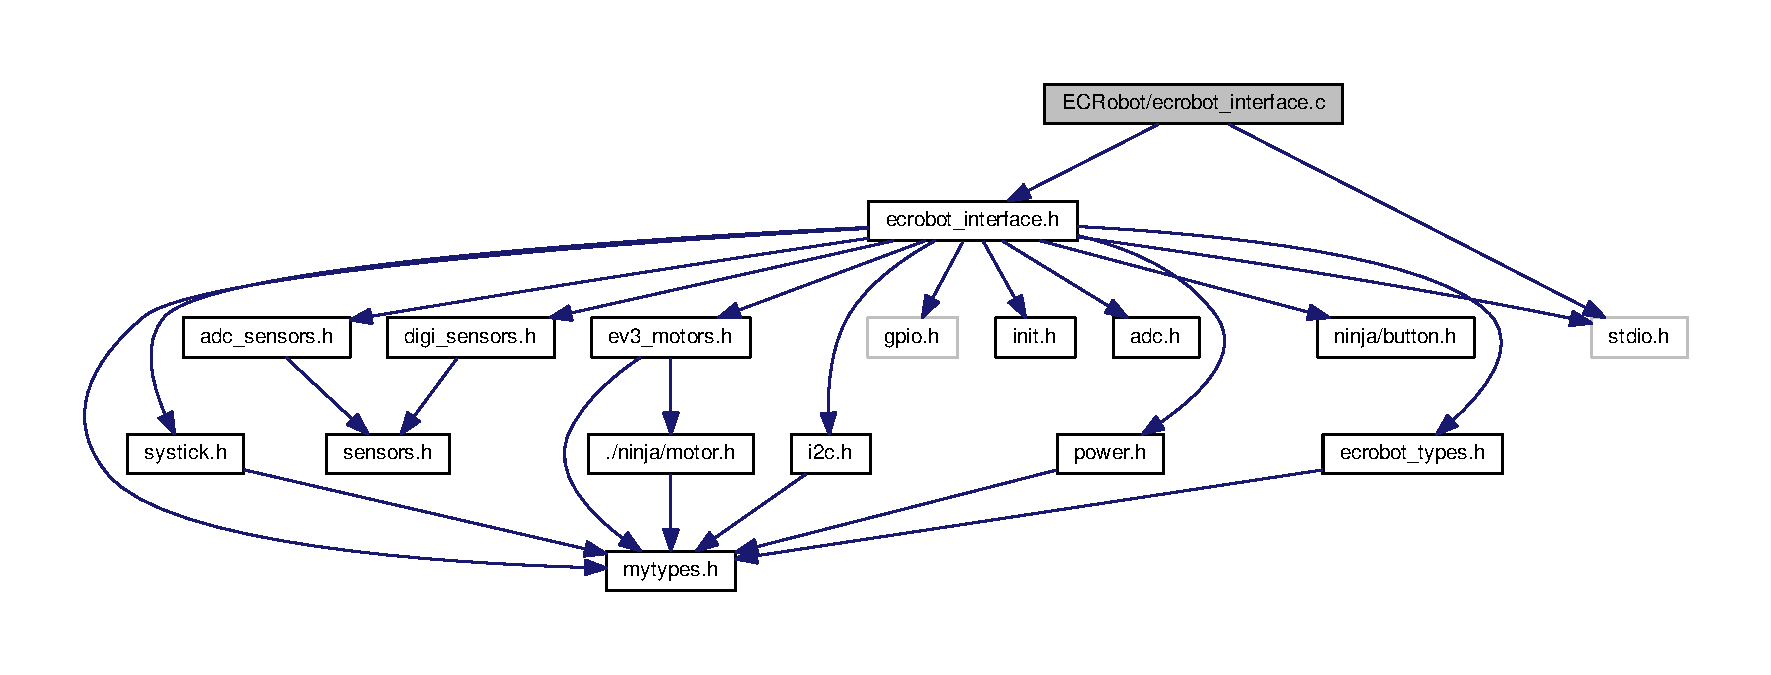
\includegraphics[width=350pt]{ecrobot__interface_8c__incl}
\end{center}
\end{figure}
\subsection*{Macros}
\begin{DoxyCompactItemize}
\item 
\hypertarget{ecrobot__interface_8c_a90ae7bfe6759086680787cb8c0e8fd16}{}\#define \hyperlink{ecrobot__interface_8c_a90ae7bfe6759086680787cb8c0e8fd16}{C\+H\+E\+C\+K\+\_\+\+I\+N\+I\+T}~if(!\hyperlink{ecrobot__interface_8c_a93e20d4bb950c575793eb1bc51d4d174}{is\+Initialized})\{\hyperlink{init_8h_aebbe6b9342d909d61305c7302e0eb41f}{le\+J\+O\+S\+\_\+init}();\hyperlink{ecrobot__interface_8c_a93e20d4bb950c575793eb1bc51d4d174}{is\+Initialized}=1;\}\label{ecrobot__interface_8c_a90ae7bfe6759086680787cb8c0e8fd16}

\begin{DoxyCompactList}\small\item\em A macro that is internally used to initialize le\+J\+O\+S if needed. \end{DoxyCompactList}\end{DoxyCompactItemize}
\subsection*{Functions}
\begin{DoxyCompactItemize}
\item 
void \hyperlink{ecrobot__interface_8c_afbbe232f5cd08033217f7baf0e0ada54}{error\+\_\+function\+\_\+call\+\_\+not\+\_\+implemented} (char $\ast$function\+\_\+name)
\begin{DoxyCompactList}\small\item\em The internal standard error function for unimplemented E\+C\+Robot functions. \end{DoxyCompactList}\item 
void \hyperlink{ecrobot__interface_8c_a058a4f6b8b8cd0cd9b341f7728a0be4d}{ecrobot\+\_\+set\+\_\+motor\+\_\+speed} (\hyperlink{mytypes_8h_a3cb25ca6f51f003950f9625ff05536fc}{U8} port\+\_\+id, \hyperlink{mytypes_8h_a73359529e867901fff0eabb94f7c3fcf}{S8} speed)
\begin{DoxyCompactList}\small\item\em Sets Servo Motor P\+W\+M value. Wrapper of nxt\+\_\+motor\+\_\+set\+\_\+speed, but brake mode is fixed as brake. \end{DoxyCompactList}\item 
void \hyperlink{ecrobot__interface_8c_a243c5a9de426a2ceb53f13dc7c7945ee}{ecrobot\+\_\+set\+\_\+motor\+\_\+mode\+\_\+speed} (\hyperlink{mytypes_8h_a3cb25ca6f51f003950f9625ff05536fc}{U8} port\+\_\+id, \hyperlink{mytypes_8h_aa2db49128944fb6df8ee8aa636a47634}{S32} mode, \hyperlink{mytypes_8h_a73359529e867901fff0eabb94f7c3fcf}{S8} speed)
\begin{DoxyCompactList}\small\item\em Sets Servo Motor brake mode and P\+W\+M value. Wrapper of nxt\+\_\+motor\+\_\+set\+\_\+speed. \end{DoxyCompactList}\item 
\hyperlink{mytypes_8h_aa2db49128944fb6df8ee8aa636a47634}{S32} \hyperlink{ecrobot__interface_8c_aac401bc8039e76ef135628bac4c9d884}{ecrobot\+\_\+get\+\_\+motor\+\_\+rev} (\hyperlink{mytypes_8h_a3cb25ca6f51f003950f9625ff05536fc}{U8} port\+\_\+id)
\begin{DoxyCompactList}\small\item\em Gets Servo Motor revolution value in degree. Wrapper of nxt\+\_\+motor\+\_\+get\+\_\+count. \end{DoxyCompactList}\item 
void \hyperlink{ecrobot__interface_8c_a716b589796dd18ec023ef45a4aca6b10}{ecrobot\+\_\+set\+\_\+motor\+\_\+rev} (\hyperlink{mytypes_8h_a3cb25ca6f51f003950f9625ff05536fc}{U8} port\+\_\+id, \hyperlink{mytypes_8h_aa2db49128944fb6df8ee8aa636a47634}{S32} rev)
\begin{DoxyCompactList}\small\item\em Sets Servo Motor revolution value in degree. Wrapper of nxt\+\_\+motor\+\_\+set\+\_\+count. \end{DoxyCompactList}\item 
\hyperlink{mytypes_8h_adf928e51a60dba0df29d615401cc55a8}{U16} \hyperlink{ecrobot__interface_8c_a8db50e0e1ea5539ff33fb69019ba6c59}{ecrobot\+\_\+get\+\_\+light\+\_\+sensor} (\hyperlink{mytypes_8h_a3cb25ca6f51f003950f9625ff05536fc}{U8} port\+\_\+id)
\begin{DoxyCompactList}\small\item\em Get N\+X\+T Light Sensor raw A/\+D data. \end{DoxyCompactList}\item 
void \hyperlink{ecrobot__interface_8c_aa583da85d360db935d690a72365ab12d}{ecrobot\+\_\+set\+\_\+light\+\_\+sensor\+\_\+active} (\hyperlink{mytypes_8h_a3cb25ca6f51f003950f9625ff05536fc}{U8} port\+\_\+id)
\begin{DoxyCompactList}\small\item\em Turn infra-\/red light on. \end{DoxyCompactList}\item 
void \hyperlink{ecrobot__interface_8c_a6913437b16d6917a1cdb4d5e18a0093b}{ecrobot\+\_\+set\+\_\+light\+\_\+sensor\+\_\+inactive} (\hyperlink{mytypes_8h_a3cb25ca6f51f003950f9625ff05536fc}{U8} port\+\_\+id)
\begin{DoxyCompactList}\small\item\em Turn infra-\/red light off. \end{DoxyCompactList}\item 
\hyperlink{mytypes_8h_a3cb25ca6f51f003950f9625ff05536fc}{U8} \hyperlink{ecrobot__interface_8c_a17ec6ec37bbe6d15ece65aab03b9df94}{ecrobot\+\_\+get\+\_\+touch\+\_\+sensor} (\hyperlink{mytypes_8h_a3cb25ca6f51f003950f9625ff05536fc}{U8} port\+\_\+id)
\begin{DoxyCompactList}\small\item\em Get Touch Sensor on/off status. \end{DoxyCompactList}\item 
\hyperlink{mytypes_8h_adf928e51a60dba0df29d615401cc55a8}{U16} \hyperlink{ecrobot__interface_8c_a3d0f6c7d2c8d0236bfcb5e647f42ec4f}{ecrobot\+\_\+get\+\_\+sound\+\_\+sensor} (\hyperlink{mytypes_8h_a3cb25ca6f51f003950f9625ff05536fc}{U8} port\+\_\+id)
\begin{DoxyCompactList}\small\item\em Get Sound Sensor raw A/\+D data. \end{DoxyCompactList}\item 
void \hyperlink{ecrobot__interface_8c_aed9a245415bee498586a76a92830c7e9}{ecrobot\+\_\+init\+\_\+i2c} (\hyperlink{mytypes_8h_a3cb25ca6f51f003950f9625ff05536fc}{U8} port\+\_\+id, \hyperlink{mytypes_8h_a3cb25ca6f51f003950f9625ff05536fc}{U8} type)
\begin{DoxyCompactList}\small\item\em Init a N\+X\+T sensor port for I2\+C communication. \end{DoxyCompactList}\item 
\hyperlink{mytypes_8h_a3cb25ca6f51f003950f9625ff05536fc}{U8} \hyperlink{ecrobot__interface_8c_ae54fa3c45ac6d8a2cab8554e1ab48768}{ecrobot\+\_\+wait\+\_\+i2c\+\_\+ready} (\hyperlink{mytypes_8h_a3cb25ca6f51f003950f9625ff05536fc}{U8} port\+\_\+id, \hyperlink{mytypes_8h_a811024d35b9b8a41095b1f583b649e56}{U32} wait)
\begin{DoxyCompactList}\small\item\em Wait until I2\+C communication is ready. \end{DoxyCompactList}\item 
\hyperlink{ecrobot__types_8h_a66c6ead6db93a585d4f9d21ab3e944ac}{S\+I\+N\+T} \hyperlink{ecrobot__interface_8c_af1ca8c1fc75c05182aeb6fe60172fe54}{ecrobot\+\_\+send\+\_\+i2c} (\hyperlink{mytypes_8h_a3cb25ca6f51f003950f9625ff05536fc}{U8} port\+\_\+id, \hyperlink{mytypes_8h_a811024d35b9b8a41095b1f583b649e56}{U32} address, \hyperlink{ecrobot__types_8h_a66c6ead6db93a585d4f9d21ab3e944ac}{S\+I\+N\+T} i2c\+\_\+reg, \hyperlink{mytypes_8h_a3cb25ca6f51f003950f9625ff05536fc}{U8} $\ast$buf, \hyperlink{mytypes_8h_a811024d35b9b8a41095b1f583b649e56}{U32} len)
\begin{DoxyCompactList}\small\item\em Send I2\+C data. \end{DoxyCompactList}\item 
\hyperlink{ecrobot__types_8h_a66c6ead6db93a585d4f9d21ab3e944ac}{S\+I\+N\+T} \hyperlink{ecrobot__interface_8c_ae2705c2c961299e7e1899b71d751519e}{ecrobot\+\_\+read\+\_\+i2c} (\hyperlink{mytypes_8h_a3cb25ca6f51f003950f9625ff05536fc}{U8} port\+\_\+id, \hyperlink{mytypes_8h_a811024d35b9b8a41095b1f583b649e56}{U32} address, \hyperlink{ecrobot__types_8h_a66c6ead6db93a585d4f9d21ab3e944ac}{S\+I\+N\+T} i2c\+\_\+reg, \hyperlink{mytypes_8h_a3cb25ca6f51f003950f9625ff05536fc}{U8} $\ast$buf, \hyperlink{mytypes_8h_a811024d35b9b8a41095b1f583b649e56}{U32} len)
\begin{DoxyCompactList}\small\item\em Read I2\+C data. \end{DoxyCompactList}\item 
void \hyperlink{ecrobot__interface_8c_adccd23ec10f6723d9ba9463dc44e01dc}{ecrobot\+\_\+term\+\_\+i2c} (\hyperlink{mytypes_8h_a3cb25ca6f51f003950f9625ff05536fc}{U8} port\+\_\+id)
\begin{DoxyCompactList}\small\item\em Terminate a N\+X\+T sensor port used for I2\+C communication. \end{DoxyCompactList}\item 
void \hyperlink{ecrobot__interface_8c_a1987f8ae51d64da9e63185302c84c6dc}{ecrobot\+\_\+init\+\_\+sonar\+\_\+sensor} (\hyperlink{mytypes_8h_a3cb25ca6f51f003950f9625ff05536fc}{U8} port\+\_\+id)
\begin{DoxyCompactList}\small\item\em Init a N\+X\+T sensor port for Ultrasonic Sensor. \end{DoxyCompactList}\item 
\hyperlink{mytypes_8h_aa2db49128944fb6df8ee8aa636a47634}{S32} \hyperlink{ecrobot__interface_8c_a606dc0e245136a73870800af77975917}{ecrobot\+\_\+get\+\_\+sonar\+\_\+sensor} (\hyperlink{mytypes_8h_a3cb25ca6f51f003950f9625ff05536fc}{U8} port\+\_\+id)
\begin{DoxyCompactList}\small\item\em Get Ultrasonic Sensor measurement data in cm. \end{DoxyCompactList}\item 
void \hyperlink{ecrobot__interface_8c_a92df098d5bc3f745a4c7e29256d6e826}{ecrobot\+\_\+get\+\_\+sonar\+\_\+sensor\+\_\+single\+\_\+shot} (\hyperlink{mytypes_8h_a3cb25ca6f51f003950f9625ff05536fc}{U8} port\+\_\+id, \hyperlink{mytypes_8h_a3cb25ca6f51f003950f9625ff05536fc}{U8} data\+\_\+buffer\mbox{[}8\mbox{]})
\begin{DoxyCompactList}\small\item\em Set the mode of the Lego ultrasonic sensor at the specified port to U\+L\+T\+R\+A\+S\+O\+N\+I\+C\+\_\+\+M\+O\+D\+E\+\_\+\+S\+I\+N\+G\+L\+E\+\_\+\+S\+H\+O\+T. After that get the range of the Lego ultrasonic sensor connected at the specified port and store it in the buffer. \end{DoxyCompactList}\item 
void \hyperlink{ecrobot__interface_8c_a435363c3b8faf52afaf83fc935434054}{ecrobot\+\_\+term\+\_\+sonar\+\_\+sensor} (\hyperlink{mytypes_8h_a3cb25ca6f51f003950f9625ff05536fc}{U8} port\+\_\+id)
\begin{DoxyCompactList}\small\item\em Terminate I2\+C used for for Ultrasonic. \end{DoxyCompactList}\item 
\hyperlink{mytypes_8h_adf928e51a60dba0df29d615401cc55a8}{U16} \hyperlink{ecrobot__interface_8c_ad36f9c80a01f470b673244e9c0652559}{ecrobot\+\_\+get\+\_\+gyro\+\_\+sensor} (\hyperlink{mytypes_8h_a3cb25ca6f51f003950f9625ff05536fc}{U8} port\+\_\+id)
\begin{DoxyCompactList}\small\item\em Gets Gyro Sensor raw A/\+D data. The sensor data has offset value (approximately 600). \end{DoxyCompactList}\item 
\hyperlink{mytypes_8h_ae08f9a6ee81e70f713a74a5860062841}{S16} \hyperlink{ecrobot__interface_8c_a66caf428dfc59030202023eeec463ff1}{ecrobot\+\_\+get\+\_\+gyro\+\_\+sensor\+\_\+degrees} (\hyperlink{mytypes_8h_a3cb25ca6f51f003950f9625ff05536fc}{U8} port\+\_\+id)
\begin{DoxyCompactList}\small\item\em Get the current rotation meassured by the Hi\+Technic gyro sensor connected at the specified port. \end{DoxyCompactList}\item 
void \hyperlink{ecrobot__interface_8c_a82abd85d3faadc9aa90e6a80a1f9c336}{ecrobot\+\_\+init\+\_\+accel\+\_\+sensor} (\hyperlink{mytypes_8h_a3cb25ca6f51f003950f9625ff05536fc}{U8} port\+\_\+id)
\begin{DoxyCompactList}\small\item\em Initializes a port for I2\+C communication for Acceleration Sensor. This function should be implemented in the device initialize hook routine. \end{DoxyCompactList}\item 
void \hyperlink{ecrobot__interface_8c_ae918297bfa96d5a550519cb6b377c717}{ecrobot\+\_\+get\+\_\+accel\+\_\+sensor} (\hyperlink{mytypes_8h_a3cb25ca6f51f003950f9625ff05536fc}{U8} port\+\_\+id, \hyperlink{mytypes_8h_ae08f9a6ee81e70f713a74a5860062841}{S16} buf\mbox{[}3\mbox{]})
\begin{DoxyCompactList}\small\item\em Gets acceleration data in three axes. The sensor meassures the acceleration on all 3 axis (X, Y and Z). This function will call sensor\+\_\+accel\+\_\+calibrate when called for the first time. The values returned will be relativ to 0. \end{DoxyCompactList}\item 
void \hyperlink{ecrobot__interface_8c_a0d3f189f2fb27cfd95136e99e83e9044}{ecrobot\+\_\+term\+\_\+accel\+\_\+sensor} (\hyperlink{mytypes_8h_a3cb25ca6f51f003950f9625ff05536fc}{U8} port\+\_\+id)
\begin{DoxyCompactList}\small\item\em Terminates I2\+C communication used for Acceleraton Sensor. This function should be implemented in the device terminate hook routine. \end{DoxyCompactList}\item 
void \hyperlink{ecrobot__interface_8c_ac43644c6aa0ee882b21669b37e4dcae5}{ecrobot\+\_\+init\+\_\+color\+\_\+sensor} (\hyperlink{mytypes_8h_a3cb25ca6f51f003950f9625ff05536fc}{U8} port\+\_\+id)
\begin{DoxyCompactList}\small\item\em initializes a port for I2\+C communication for the Color Sensor. This function should be implemented in the device initialize hook routine. \end{DoxyCompactList}\item 
\hyperlink{mytypes_8h_a3cb25ca6f51f003950f9625ff05536fc}{U8} \hyperlink{ecrobot__interface_8c_a4052f27244a2ec626f9467ba5205f5ab}{ecrobot\+\_\+cal\+\_\+color\+\_\+sensor} (\hyperlink{mytypes_8h_a3cb25ca6f51f003950f9625ff05536fc}{U8} port\+\_\+id, \hyperlink{mytypes_8h_a3cb25ca6f51f003950f9625ff05536fc}{U8} mode)
\begin{DoxyCompactList}\small\item\em Calibrate the Hi\+Technic color sensor at the specified port. \end{DoxyCompactList}\item 
void \hyperlink{ecrobot__interface_8c_ab54ac6a5ac92fa3d8e452d7e0ac42b06}{ecrobot\+\_\+get\+\_\+color\+\_\+sensor} (\hyperlink{mytypes_8h_a3cb25ca6f51f003950f9625ff05536fc}{U8} port\+\_\+id, \hyperlink{mytypes_8h_ae08f9a6ee81e70f713a74a5860062841}{S16} buf\mbox{[}3\mbox{]})
\begin{DoxyCompactList}\small\item\em Get the red, green and blue values (R\+G\+B) meassured by the Hi\+Technic color sensor at the specified port. \end{DoxyCompactList}\item 
void \hyperlink{ecrobot__interface_8c_a8d365c7adeac0016b97754d45d3352f7}{ecrobot\+\_\+term\+\_\+color\+\_\+sensor} (\hyperlink{mytypes_8h_a3cb25ca6f51f003950f9625ff05536fc}{U8} port\+\_\+id)
\begin{DoxyCompactList}\small\item\em Terminates I2\+C communication used for the Color Sensor. This function should be implemented in the device terminate hook routine. \end{DoxyCompactList}\item 
void \hyperlink{ecrobot__interface_8c_af87a9c15633d8cbabc9d69cf01d9cb46}{ecrobot\+\_\+init\+\_\+compass\+\_\+sensor} (\hyperlink{mytypes_8h_a3cb25ca6f51f003950f9625ff05536fc}{U8} port\+\_\+id)
\begin{DoxyCompactList}\small\item\em Initializes a port for I2\+C communication for Compass Sensor. This function should be implemented in the device initialize hook routine. \end{DoxyCompactList}\item 
\hyperlink{mytypes_8h_ae08f9a6ee81e70f713a74a5860062841}{S16} \hyperlink{ecrobot__interface_8c_abc583b0bef80df0e21019fed1b3c5ab3}{ecrobot\+\_\+get\+\_\+compass\+\_\+sensor} (\hyperlink{mytypes_8h_a3cb25ca6f51f003950f9625ff05536fc}{U8} port\+\_\+id)
\begin{DoxyCompactList}\small\item\em Read the current direction meassured by the Hi\+Technic compass sensor at the specified port. \end{DoxyCompactList}\item 
void \hyperlink{ecrobot__interface_8c_aeb7a9d999e93c0bf60ff6c8a633da305}{ecrobot\+\_\+term\+\_\+compass\+\_\+sensor} (\hyperlink{mytypes_8h_a3cb25ca6f51f003950f9625ff05536fc}{U8} port\+\_\+id)
\begin{DoxyCompactList}\small\item\em Terminates I2\+C communication used for Compass Sensor. This function should be implemented in the device terminate hook routine. \end{DoxyCompactList}\item 
void \hyperlink{ecrobot__interface_8c_a855921fd0f9bdf7bebf26248d6705553}{ecrobot\+\_\+cal\+\_\+start\+\_\+compass\+\_\+sensor} (\hyperlink{mytypes_8h_a3cb25ca6f51f003950f9625ff05536fc}{U8} port\+\_\+id)
\begin{DoxyCompactList}\small\item\em Start the Hi\+Technic compass sensor calibration. \end{DoxyCompactList}\item 
\hyperlink{mytypes_8h_a3cb25ca6f51f003950f9625ff05536fc}{U8} \hyperlink{ecrobot__interface_8c_a0ab83efcae7f5172df0d9ef24cbab482}{ecrobot\+\_\+cal\+\_\+end\+\_\+compass\+\_\+sensor} (\hyperlink{mytypes_8h_a3cb25ca6f51f003950f9625ff05536fc}{U8} port\+\_\+id)
\begin{DoxyCompactList}\small\item\em Finish the Hi\+Technic compass sensor calibration. \end{DoxyCompactList}\item 
void \hyperlink{ecrobot__interface_8c_a87f6986d1cd3ece1c2ed94d2781f4073}{ecrobot\+\_\+init\+\_\+temperature\+\_\+sensor} (\hyperlink{mytypes_8h_a3cb25ca6f51f003950f9625ff05536fc}{U8} port\+\_\+id)
\begin{DoxyCompactList}\small\item\em Initializes a port for I2\+C communication for Temperature Sensor. \end{DoxyCompactList}\item 
float \hyperlink{ecrobot__interface_8c_ac3d850ca54c4793976a72dcff72ea27f}{ecrobot\+\_\+get\+\_\+temperature\+\_\+sensor} (\hyperlink{mytypes_8h_a3cb25ca6f51f003950f9625ff05536fc}{U8} port\+\_\+id)
\begin{DoxyCompactList}\small\item\em Measures and returns the current temperature value. \end{DoxyCompactList}\item 
void \hyperlink{ecrobot__interface_8c_a3931f4ecc2a1fe1e20b540fb8fde4df8}{ecrobot\+\_\+set\+Resolution\+\_\+temperature\+\_\+sensor} (\hyperlink{mytypes_8h_a3cb25ca6f51f003950f9625ff05536fc}{U8} port\+\_\+id, \hyperlink{mytypes_8h_a3cb25ca6f51f003950f9625ff05536fc}{U8} resolution)
\begin{DoxyCompactList}\small\item\em Set the resolution for the measured temperature values. \end{DoxyCompactList}\item 
\hyperlink{mytypes_8h_a3cb25ca6f51f003950f9625ff05536fc}{U8} \hyperlink{ecrobot__interface_8c_aa7f203b9bb762050caacf41f177ac530}{ecrobot\+\_\+get\+Resolution\+\_\+temperature\+\_\+sensor} (\hyperlink{mytypes_8h_a3cb25ca6f51f003950f9625ff05536fc}{U8} port\+\_\+id)
\begin{DoxyCompactList}\small\item\em Returns the current resolution setting of the sensor. \end{DoxyCompactList}\item 
void \hyperlink{ecrobot__interface_8c_a8d5e57b6d8fb3e702350c59a613ccc16}{ecrobot\+\_\+term\+\_\+temperature\+\_\+sensor} (\hyperlink{mytypes_8h_a3cb25ca6f51f003950f9625ff05536fc}{U8} port\+\_\+id)
\begin{DoxyCompactList}\small\item\em Terminates I2\+C communication used for Temperature Sensor. \end{DoxyCompactList}\item 
\hyperlink{mytypes_8h_adf928e51a60dba0df29d615401cc55a8}{U16} \hyperlink{ecrobot__interface_8c_acbb5d84af362934c9657a398abd73e1b}{ecrobot\+\_\+get\+\_\+battery\+\_\+voltage} (void)
\begin{DoxyCompactList}\small\item\em Get the voltage of the battery. \end{DoxyCompactList}\item 
\hyperlink{mytypes_8h_adf928e51a60dba0df29d615401cc55a8}{U16} \hyperlink{ecrobot__interface_8c_a82fbd47d249880aada07e9b39252cc8b}{ecrobot\+\_\+get\+\_\+battery\+\_\+current} (void)
\begin{DoxyCompactList}\small\item\em Get the current of the battery. \end{DoxyCompactList}\item 
\hyperlink{mytypes_8h_a811024d35b9b8a41095b1f583b649e56}{U32} \hyperlink{ecrobot__interface_8c_af43da73900e9f320695f8ca40c91601d}{ecrobot\+\_\+get\+\_\+systick\+\_\+ms} (void)
\begin{DoxyCompactList}\small\item\em Get the current tick in milliseconds. \end{DoxyCompactList}\item 
void \hyperlink{ecrobot__interface_8c_a7e4b2a4c452438af889f628b32572d68}{ecrobot\+\_\+wait\+\_\+ms} (\hyperlink{mytypes_8h_a811024d35b9b8a41095b1f583b649e56}{U32} ms)
\begin{DoxyCompactList}\small\item\em Wait for the specified amount of time. \end{DoxyCompactList}\item 
\hyperlink{mytypes_8h_a3cb25ca6f51f003950f9625ff05536fc}{U8} \hyperlink{ecrobot__interface_8c_a8671b27a6f7da38378c08231b687433c}{ecrobot\+\_\+is\+\_\+\+E\+N\+T\+E\+R\+\_\+button\+\_\+pressed} (void)
\begin{DoxyCompactList}\small\item\em Returns status of the enter button. \end{DoxyCompactList}\item 
\hyperlink{mytypes_8h_a3cb25ca6f51f003950f9625ff05536fc}{U8} \hyperlink{ecrobot__interface_8c_a105aa94999ce18090972316b9679a400}{ecrobot\+\_\+is\+\_\+\+R\+U\+N\+\_\+button\+\_\+pressed} (void)
\begin{DoxyCompactList}\small\item\em Returns status of the run button. \end{DoxyCompactList}\end{DoxyCompactItemize}
\subsection*{Variables}
\begin{DoxyCompactItemize}
\item 
\hypertarget{ecrobot__interface_8c_a93e20d4bb950c575793eb1bc51d4d174}{}unsigned char \hyperlink{ecrobot__interface_8c_a93e20d4bb950c575793eb1bc51d4d174}{is\+Initialized} = 0\label{ecrobot__interface_8c_a93e20d4bb950c575793eb1bc51d4d174}

\begin{DoxyCompactList}\small\item\em A internally used attribute. Needed to save the init state. \end{DoxyCompactList}\item 
\hyperlink{structsensor__port__info}{sensor\+\_\+port\+\_\+info} \hyperlink{ecrobot__interface_8c_a91059f248da7912f3fb19bf0d8df76c9}{ports} \mbox{[}$\,$\mbox{]}
\begin{DoxyCompactList}\small\item\em A internally used attribute. Needed for port access. \end{DoxyCompactList}\end{DoxyCompactItemize}


\subsection{Detailed Description}
This file contains the function definitions for the users E\+C\+Robot-\/\+A\+P\+I. This A\+P\+I is used to interact with sensors and actuators. 

\begin{DoxyAuthor}{Author}
Christian Soward, Tobias Schießl 
\end{DoxyAuthor}


\subsection{Function Documentation}
\hypertarget{ecrobot__interface_8c_a4052f27244a2ec626f9467ba5205f5ab}{}\index{ecrobot\+\_\+interface.\+c@{ecrobot\+\_\+interface.\+c}!ecrobot\+\_\+cal\+\_\+color\+\_\+sensor@{ecrobot\+\_\+cal\+\_\+color\+\_\+sensor}}
\index{ecrobot\+\_\+cal\+\_\+color\+\_\+sensor@{ecrobot\+\_\+cal\+\_\+color\+\_\+sensor}!ecrobot\+\_\+interface.\+c@{ecrobot\+\_\+interface.\+c}}
\subsubsection[{ecrobot\+\_\+cal\+\_\+color\+\_\+sensor(\+U8 port\+\_\+id, U8 mode)}]{\setlength{\rightskip}{0pt plus 5cm}{\bf U8} ecrobot\+\_\+cal\+\_\+color\+\_\+sensor (
\begin{DoxyParamCaption}
\item[{{\bf U8}}]{port\+\_\+id, }
\item[{{\bf U8}}]{mode}
\end{DoxyParamCaption}
)}\label{ecrobot__interface_8c_a4052f27244a2ec626f9467ba5205f5ab}


Calibrate the Hi\+Technic color sensor at the specified port. 

To calibrate the sensor properly, this function has to be called two times. Once with mode set to C\+A\+L\+\_\+\+W\+H\+I\+T\+E (0x043) and once with mode set to C\+A\+L\+\_\+\+B\+L\+A\+C\+K (0x42). Calibration information is stored directly on the sensor and will be persistent, even if the sensor is no longer provided with power. When called with mode set to C\+A\+L\+\_\+\+W\+H\+I\+T\+E, the sensor should be located in front of a diffuse white surface at a distance of 1.\+5 cm. When called with mode set to C\+A\+L\+\_\+\+B\+L\+A\+C\+K, the sensor should have nothing in front of it within a distance of about 2 m. If the calibration command was received successfully, the sensors L\+E\+D will blink for confirmation.


\begin{DoxyParams}{Parameters}
{\em port\+\_\+id} & -\/ E\+V3\+\_\+\+P\+O\+R\+T\+\_\+\+A, E\+V3\+\_\+\+P\+O\+R\+T\+\_\+\+B, E\+V3\+\_\+\+P\+O\+R\+T\+\_\+\+C, E\+V3\+\_\+\+P\+O\+R\+T\+\_\+\+D \\
\hline
{\em mode} & -\/ The mode to calibrate the sensor with\+: C\+A\+L\+\_\+\+W\+H\+I\+T\+E (0x43) or C\+A\+L\+\_\+\+B\+L\+A\+C\+K (0x42)\\
\hline
\end{DoxyParams}
\begin{DoxyReturn}{Returns}
1 if the calibration was successful, 0 otherwise 
\end{DoxyReturn}


Here is the call graph for this function\+:\nopagebreak
\begin{figure}[H]
\begin{center}
\leavevmode
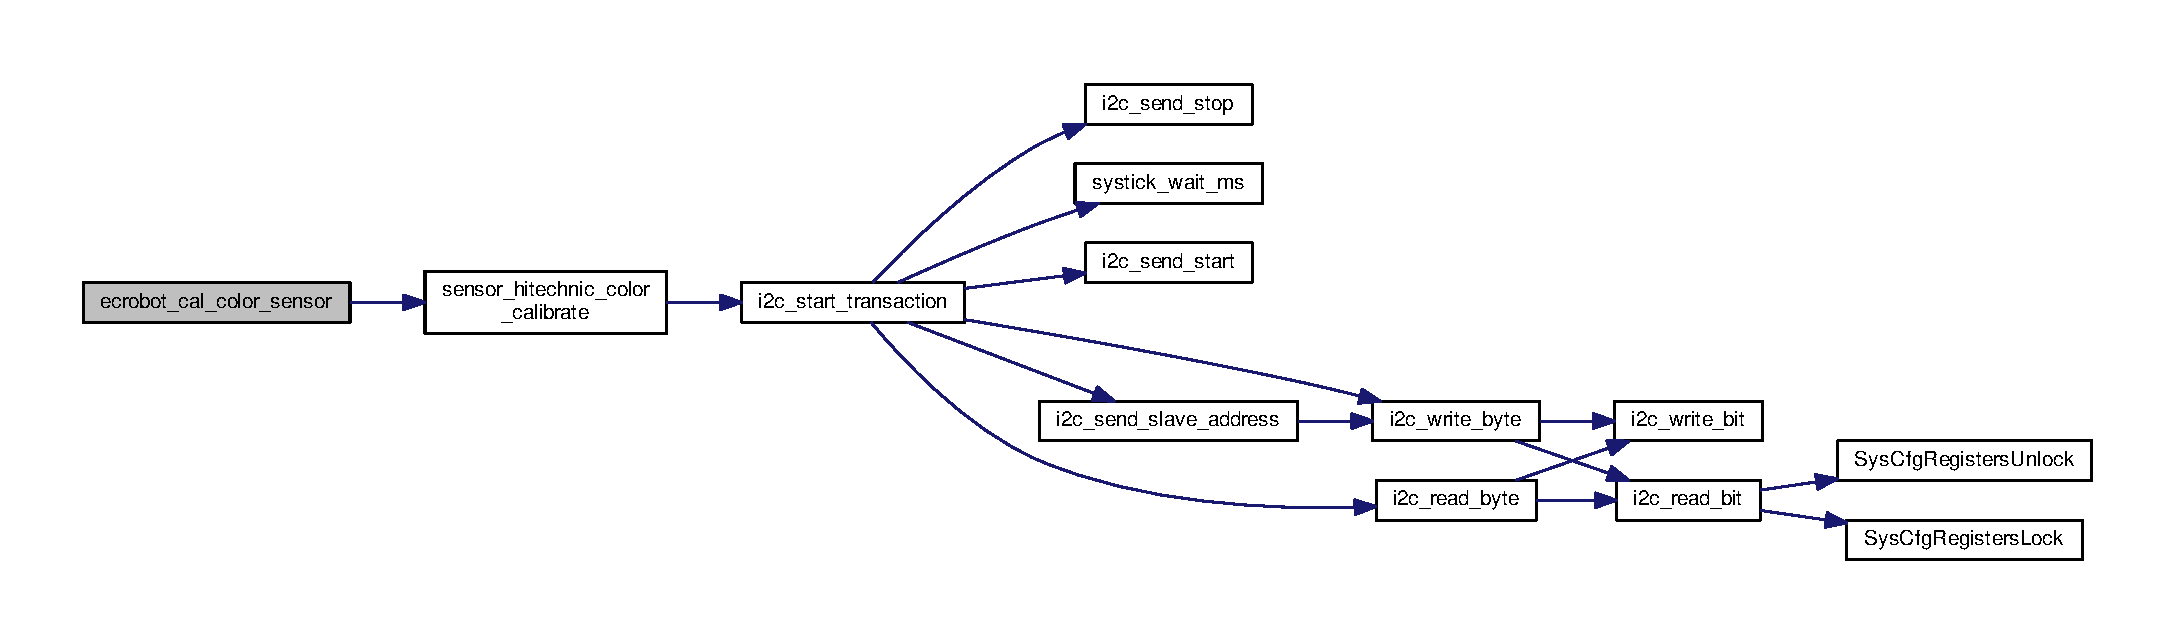
\includegraphics[width=350pt]{ecrobot__interface_8c_a4052f27244a2ec626f9467ba5205f5ab_cgraph}
\end{center}
\end{figure}


\hypertarget{ecrobot__interface_8c_a0ab83efcae7f5172df0d9ef24cbab482}{}\index{ecrobot\+\_\+interface.\+c@{ecrobot\+\_\+interface.\+c}!ecrobot\+\_\+cal\+\_\+end\+\_\+compass\+\_\+sensor@{ecrobot\+\_\+cal\+\_\+end\+\_\+compass\+\_\+sensor}}
\index{ecrobot\+\_\+cal\+\_\+end\+\_\+compass\+\_\+sensor@{ecrobot\+\_\+cal\+\_\+end\+\_\+compass\+\_\+sensor}!ecrobot\+\_\+interface.\+c@{ecrobot\+\_\+interface.\+c}}
\subsubsection[{ecrobot\+\_\+cal\+\_\+end\+\_\+compass\+\_\+sensor(\+U8 port\+\_\+id)}]{\setlength{\rightskip}{0pt plus 5cm}{\bf U8} ecrobot\+\_\+cal\+\_\+end\+\_\+compass\+\_\+sensor (
\begin{DoxyParamCaption}
\item[{{\bf U8}}]{port\+\_\+id}
\end{DoxyParamCaption}
)}\label{ecrobot__interface_8c_a0ab83efcae7f5172df0d9ef24cbab482}


Finish the Hi\+Technic compass sensor calibration. 

Read the information in the appropriate start\+\_\+calibration function first. This function is the third step and finishs the calibration process.


\begin{DoxyParams}{Parameters}
{\em port\+\_\+id} & -\/ E\+V3\+\_\+\+P\+O\+R\+T\+\_\+\+A, E\+V3\+\_\+\+P\+O\+R\+T\+\_\+\+B, E\+V3\+\_\+\+P\+O\+R\+T\+\_\+\+C, E\+V3\+\_\+\+P\+O\+R\+T\+\_\+\+D\\
\hline
\end{DoxyParams}
\begin{DoxyReturn}{Returns}
1 if the calibration was successful, 0 otherwise 
\end{DoxyReturn}


Here is the call graph for this function\+:\nopagebreak
\begin{figure}[H]
\begin{center}
\leavevmode
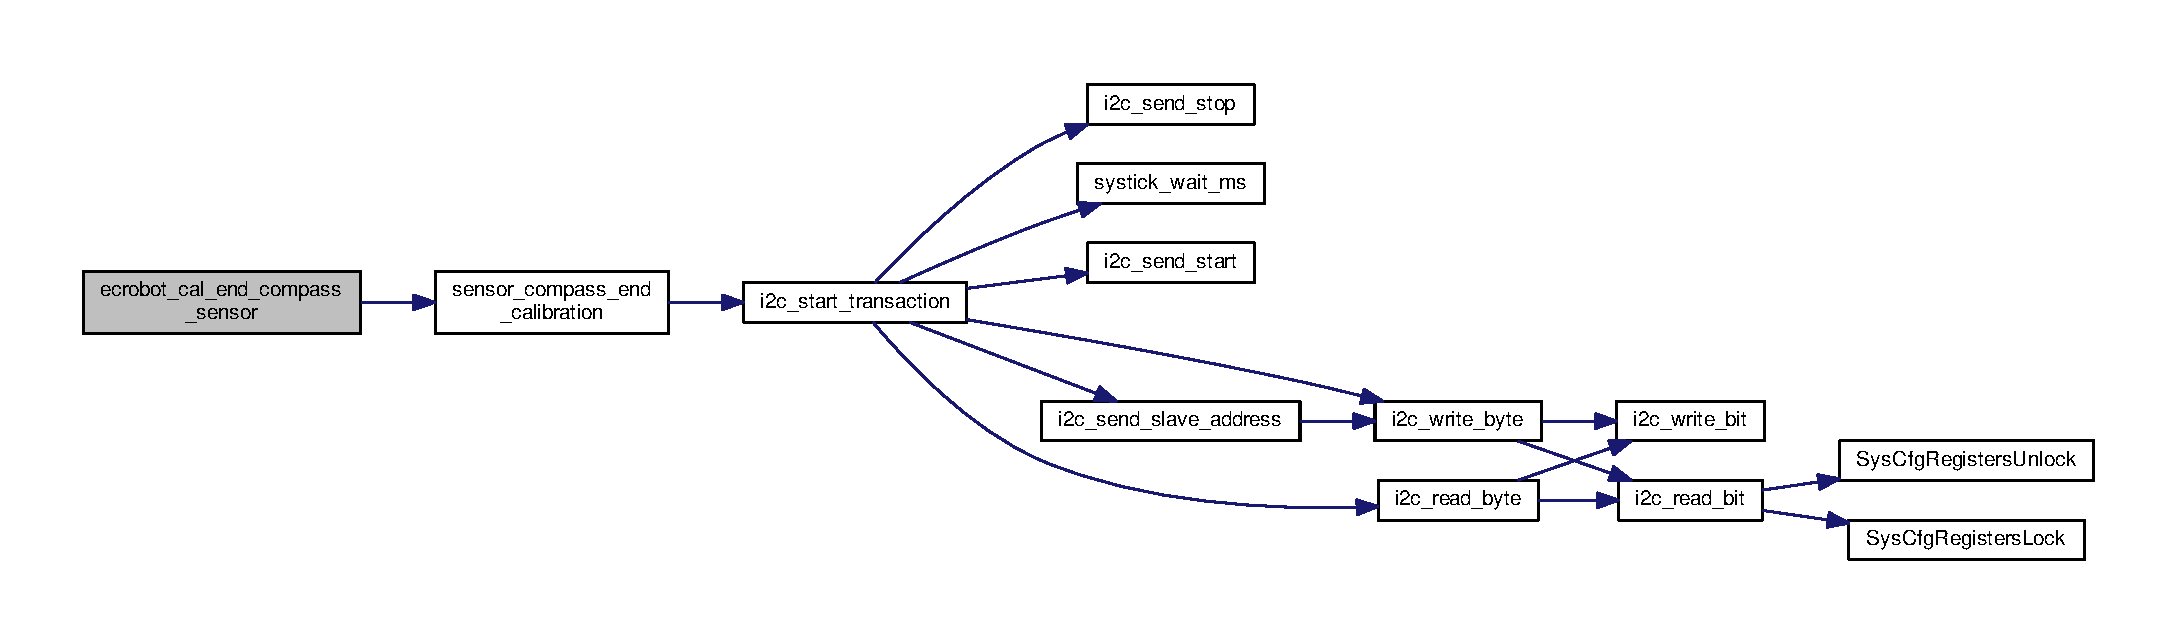
\includegraphics[width=350pt]{ecrobot__interface_8c_a0ab83efcae7f5172df0d9ef24cbab482_cgraph}
\end{center}
\end{figure}


\hypertarget{ecrobot__interface_8c_a855921fd0f9bdf7bebf26248d6705553}{}\index{ecrobot\+\_\+interface.\+c@{ecrobot\+\_\+interface.\+c}!ecrobot\+\_\+cal\+\_\+start\+\_\+compass\+\_\+sensor@{ecrobot\+\_\+cal\+\_\+start\+\_\+compass\+\_\+sensor}}
\index{ecrobot\+\_\+cal\+\_\+start\+\_\+compass\+\_\+sensor@{ecrobot\+\_\+cal\+\_\+start\+\_\+compass\+\_\+sensor}!ecrobot\+\_\+interface.\+c@{ecrobot\+\_\+interface.\+c}}
\subsubsection[{ecrobot\+\_\+cal\+\_\+start\+\_\+compass\+\_\+sensor(\+U8 port\+\_\+id)}]{\setlength{\rightskip}{0pt plus 5cm}void ecrobot\+\_\+cal\+\_\+start\+\_\+compass\+\_\+sensor (
\begin{DoxyParamCaption}
\item[{{\bf U8}}]{port\+\_\+id}
\end{DoxyParamCaption}
)}\label{ecrobot__interface_8c_a855921fd0f9bdf7bebf26248d6705553}


Start the Hi\+Technic compass sensor calibration. 

You should calibrate a compass sensor when it is mounted on your robot in the way you want to use it. So the sensor will be calibrated for your specific environment/robot. The calibration adjustment is stored persitent on the sensor itself even if it is turned off. For more information see the Hi\+Technic documentation. Calibrating the compass sensor takes 3 steps. (1) Call this function. (2) Move the sensor/robot in a circle (540 degrees -\/ 720 degrees within 20 seconds). (3) Call the appropriate end\+\_\+calibration function.


\begin{DoxyParams}{Parameters}
{\em port\+\_\+id} & -\/ E\+V3\+\_\+\+P\+O\+R\+T\+\_\+\+A, E\+V3\+\_\+\+P\+O\+R\+T\+\_\+\+B, E\+V3\+\_\+\+P\+O\+R\+T\+\_\+\+C, E\+V3\+\_\+\+P\+O\+R\+T\+\_\+\+D\\
\hline
\end{DoxyParams}
\begin{DoxyReturn}{Returns}
none 
\end{DoxyReturn}


Here is the call graph for this function\+:\nopagebreak
\begin{figure}[H]
\begin{center}
\leavevmode
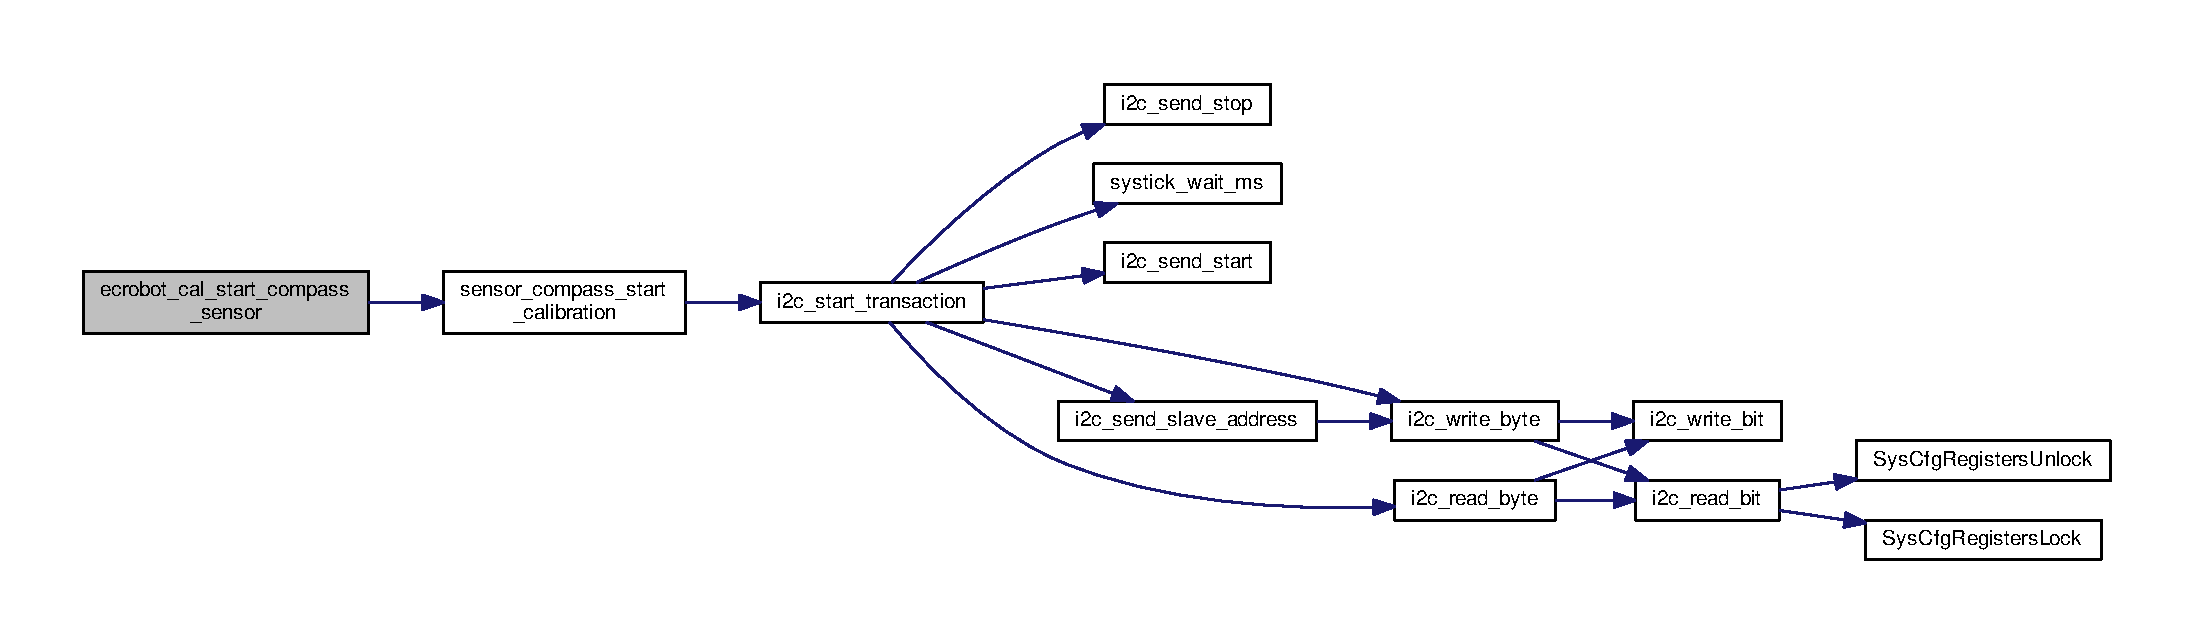
\includegraphics[width=350pt]{ecrobot__interface_8c_a855921fd0f9bdf7bebf26248d6705553_cgraph}
\end{center}
\end{figure}


\hypertarget{ecrobot__interface_8c_ae918297bfa96d5a550519cb6b377c717}{}\index{ecrobot\+\_\+interface.\+c@{ecrobot\+\_\+interface.\+c}!ecrobot\+\_\+get\+\_\+accel\+\_\+sensor@{ecrobot\+\_\+get\+\_\+accel\+\_\+sensor}}
\index{ecrobot\+\_\+get\+\_\+accel\+\_\+sensor@{ecrobot\+\_\+get\+\_\+accel\+\_\+sensor}!ecrobot\+\_\+interface.\+c@{ecrobot\+\_\+interface.\+c}}
\subsubsection[{ecrobot\+\_\+get\+\_\+accel\+\_\+sensor(\+U8 port\+\_\+id, S16 buf[3])}]{\setlength{\rightskip}{0pt plus 5cm}void ecrobot\+\_\+get\+\_\+accel\+\_\+sensor (
\begin{DoxyParamCaption}
\item[{{\bf U8}}]{port\+\_\+id, }
\item[{{\bf S16}}]{buf\mbox{[}3\mbox{]}}
\end{DoxyParamCaption}
)}\label{ecrobot__interface_8c_ae918297bfa96d5a550519cb6b377c717}


Gets acceleration data in three axes. The sensor meassures the acceleration on all 3 axis (X, Y and Z). This function will call sensor\+\_\+accel\+\_\+calibrate when called for the first time. The values returned will be relativ to 0. 


\begin{DoxyParams}{Parameters}
{\em port\+\_\+id} & -\/ E\+V3\+\_\+\+P\+O\+R\+T\+\_\+\+A, E\+V3\+\_\+\+P\+O\+R\+T\+\_\+\+B, E\+V3\+\_\+\+P\+O\+R\+T\+\_\+\+C, E\+V3\+\_\+\+P\+O\+R\+T\+\_\+\+D \\
\hline
{\em buf} & -\/ Buffer to store the meassured values in (the values will be stored in the buffer in the following order\+: X, Y, Z)\\
\hline
\end{DoxyParams}
\begin{DoxyReturn}{Returns}
none 
\end{DoxyReturn}


Here is the call graph for this function\+:\nopagebreak
\begin{figure}[H]
\begin{center}
\leavevmode
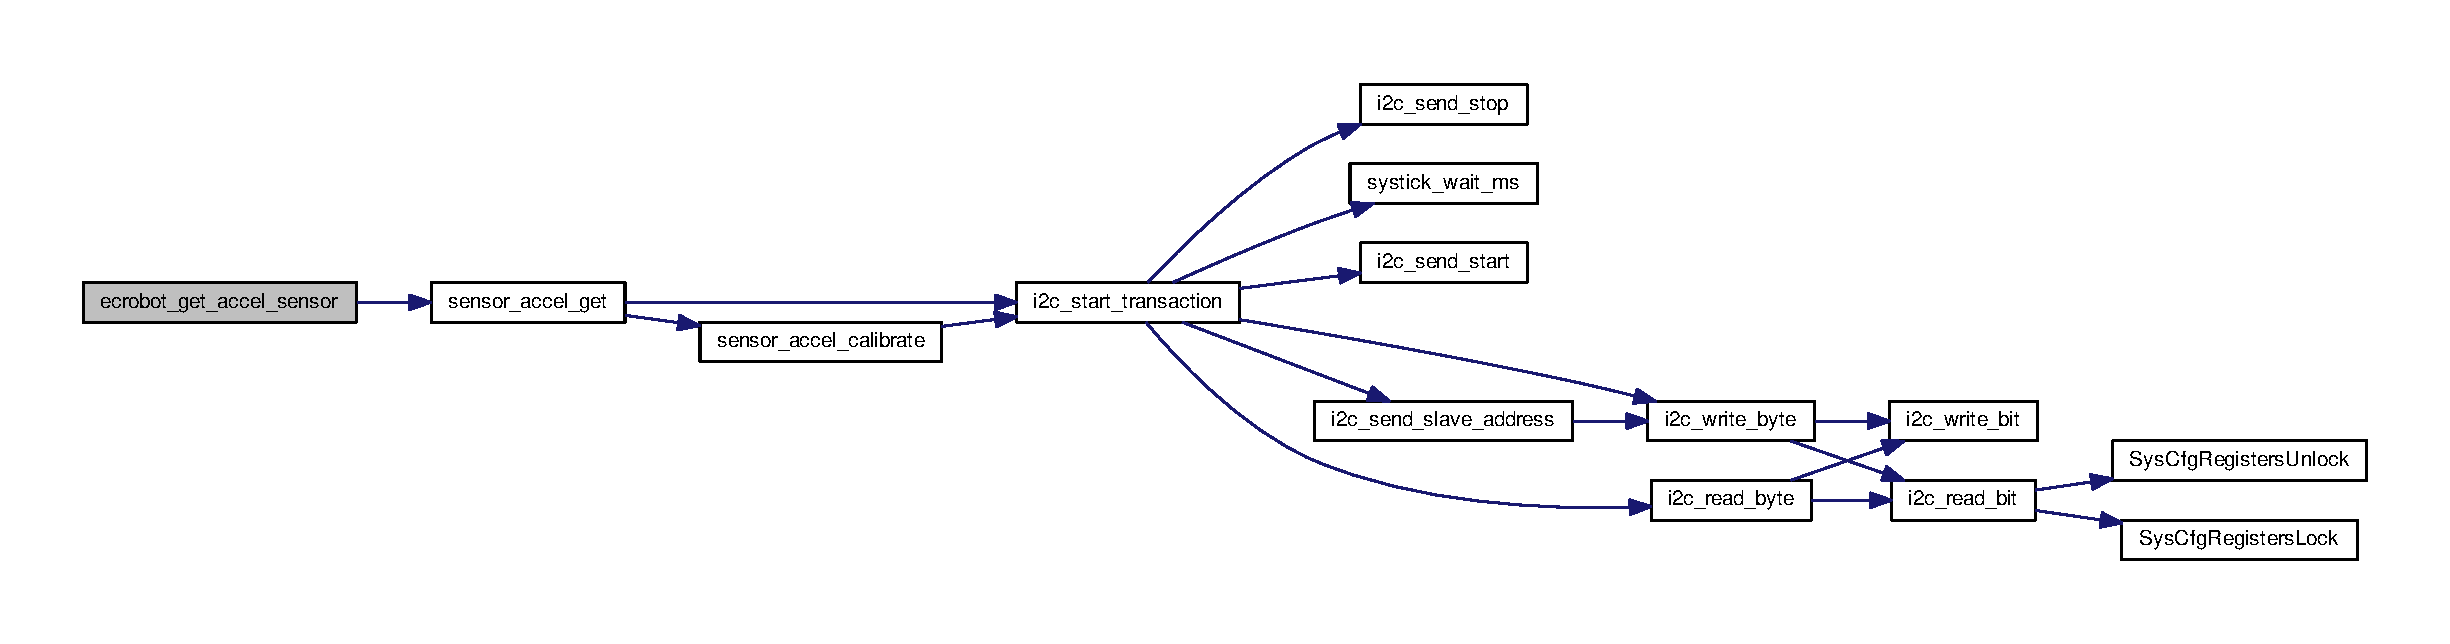
\includegraphics[width=350pt]{ecrobot__interface_8c_ae918297bfa96d5a550519cb6b377c717_cgraph}
\end{center}
\end{figure}


\hypertarget{ecrobot__interface_8c_a82fbd47d249880aada07e9b39252cc8b}{}\index{ecrobot\+\_\+interface.\+c@{ecrobot\+\_\+interface.\+c}!ecrobot\+\_\+get\+\_\+battery\+\_\+current@{ecrobot\+\_\+get\+\_\+battery\+\_\+current}}
\index{ecrobot\+\_\+get\+\_\+battery\+\_\+current@{ecrobot\+\_\+get\+\_\+battery\+\_\+current}!ecrobot\+\_\+interface.\+c@{ecrobot\+\_\+interface.\+c}}
\subsubsection[{ecrobot\+\_\+get\+\_\+battery\+\_\+current(void)}]{\setlength{\rightskip}{0pt plus 5cm}{\bf U16} ecrobot\+\_\+get\+\_\+battery\+\_\+current (
\begin{DoxyParamCaption}
\item[{void}]{}
\end{DoxyParamCaption}
)}\label{ecrobot__interface_8c_a82fbd47d249880aada07e9b39252cc8b}


Get the current of the battery. 

\begin{DoxyReturn}{Returns}
The current of the battery 
\end{DoxyReturn}


Here is the call graph for this function\+:\nopagebreak
\begin{figure}[H]
\begin{center}
\leavevmode
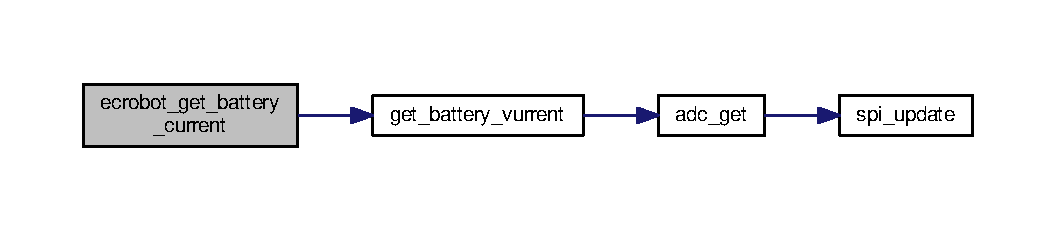
\includegraphics[width=350pt]{ecrobot__interface_8c_a82fbd47d249880aada07e9b39252cc8b_cgraph}
\end{center}
\end{figure}


\hypertarget{ecrobot__interface_8c_acbb5d84af362934c9657a398abd73e1b}{}\index{ecrobot\+\_\+interface.\+c@{ecrobot\+\_\+interface.\+c}!ecrobot\+\_\+get\+\_\+battery\+\_\+voltage@{ecrobot\+\_\+get\+\_\+battery\+\_\+voltage}}
\index{ecrobot\+\_\+get\+\_\+battery\+\_\+voltage@{ecrobot\+\_\+get\+\_\+battery\+\_\+voltage}!ecrobot\+\_\+interface.\+c@{ecrobot\+\_\+interface.\+c}}
\subsubsection[{ecrobot\+\_\+get\+\_\+battery\+\_\+voltage(void)}]{\setlength{\rightskip}{0pt plus 5cm}{\bf U16} ecrobot\+\_\+get\+\_\+battery\+\_\+voltage (
\begin{DoxyParamCaption}
\item[{void}]{}
\end{DoxyParamCaption}
)}\label{ecrobot__interface_8c_acbb5d84af362934c9657a398abd73e1b}


Get the voltage of the battery. 

\begin{DoxyReturn}{Returns}
The volatge of the battery 
\end{DoxyReturn}


Here is the call graph for this function\+:\nopagebreak
\begin{figure}[H]
\begin{center}
\leavevmode
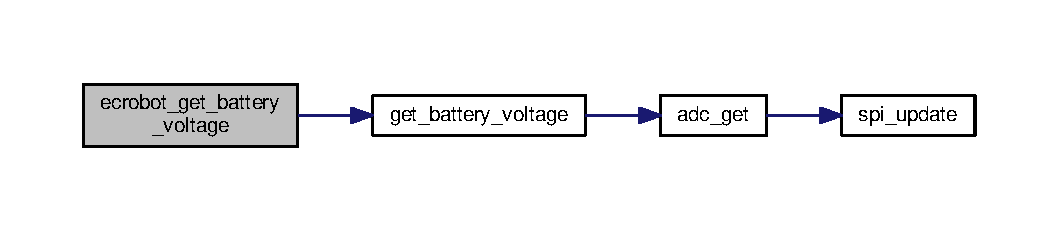
\includegraphics[width=350pt]{ecrobot__interface_8c_acbb5d84af362934c9657a398abd73e1b_cgraph}
\end{center}
\end{figure}


\hypertarget{ecrobot__interface_8c_ab54ac6a5ac92fa3d8e452d7e0ac42b06}{}\index{ecrobot\+\_\+interface.\+c@{ecrobot\+\_\+interface.\+c}!ecrobot\+\_\+get\+\_\+color\+\_\+sensor@{ecrobot\+\_\+get\+\_\+color\+\_\+sensor}}
\index{ecrobot\+\_\+get\+\_\+color\+\_\+sensor@{ecrobot\+\_\+get\+\_\+color\+\_\+sensor}!ecrobot\+\_\+interface.\+c@{ecrobot\+\_\+interface.\+c}}
\subsubsection[{ecrobot\+\_\+get\+\_\+color\+\_\+sensor(\+U8 port\+\_\+id, S16 buf[3])}]{\setlength{\rightskip}{0pt plus 5cm}void ecrobot\+\_\+get\+\_\+color\+\_\+sensor (
\begin{DoxyParamCaption}
\item[{{\bf U8}}]{port\+\_\+id, }
\item[{{\bf S16}}]{buf\mbox{[}3\mbox{]}}
\end{DoxyParamCaption}
)}\label{ecrobot__interface_8c_ab54ac6a5ac92fa3d8e452d7e0ac42b06}


Get the red, green and blue values (R\+G\+B) meassured by the Hi\+Technic color sensor at the specified port. 

For best results, the sensor should be calibrated before calling this function.


\begin{DoxyParams}{Parameters}
{\em port\+\_\+id} & -\/ E\+V3\+\_\+\+P\+O\+R\+T\+\_\+\+A, E\+V3\+\_\+\+P\+O\+R\+T\+\_\+\+B, E\+V3\+\_\+\+P\+O\+R\+T\+\_\+\+C, E\+V3\+\_\+\+P\+O\+R\+T\+\_\+\+D \\
\hline
{\em buf} & -\/ Buffer to store the received data in (the values will be stored in the following order\+: red, green, blue)\\
\hline
\end{DoxyParams}
\begin{DoxyReturn}{Returns}
none 
\end{DoxyReturn}


Here is the call graph for this function\+:\nopagebreak
\begin{figure}[H]
\begin{center}
\leavevmode
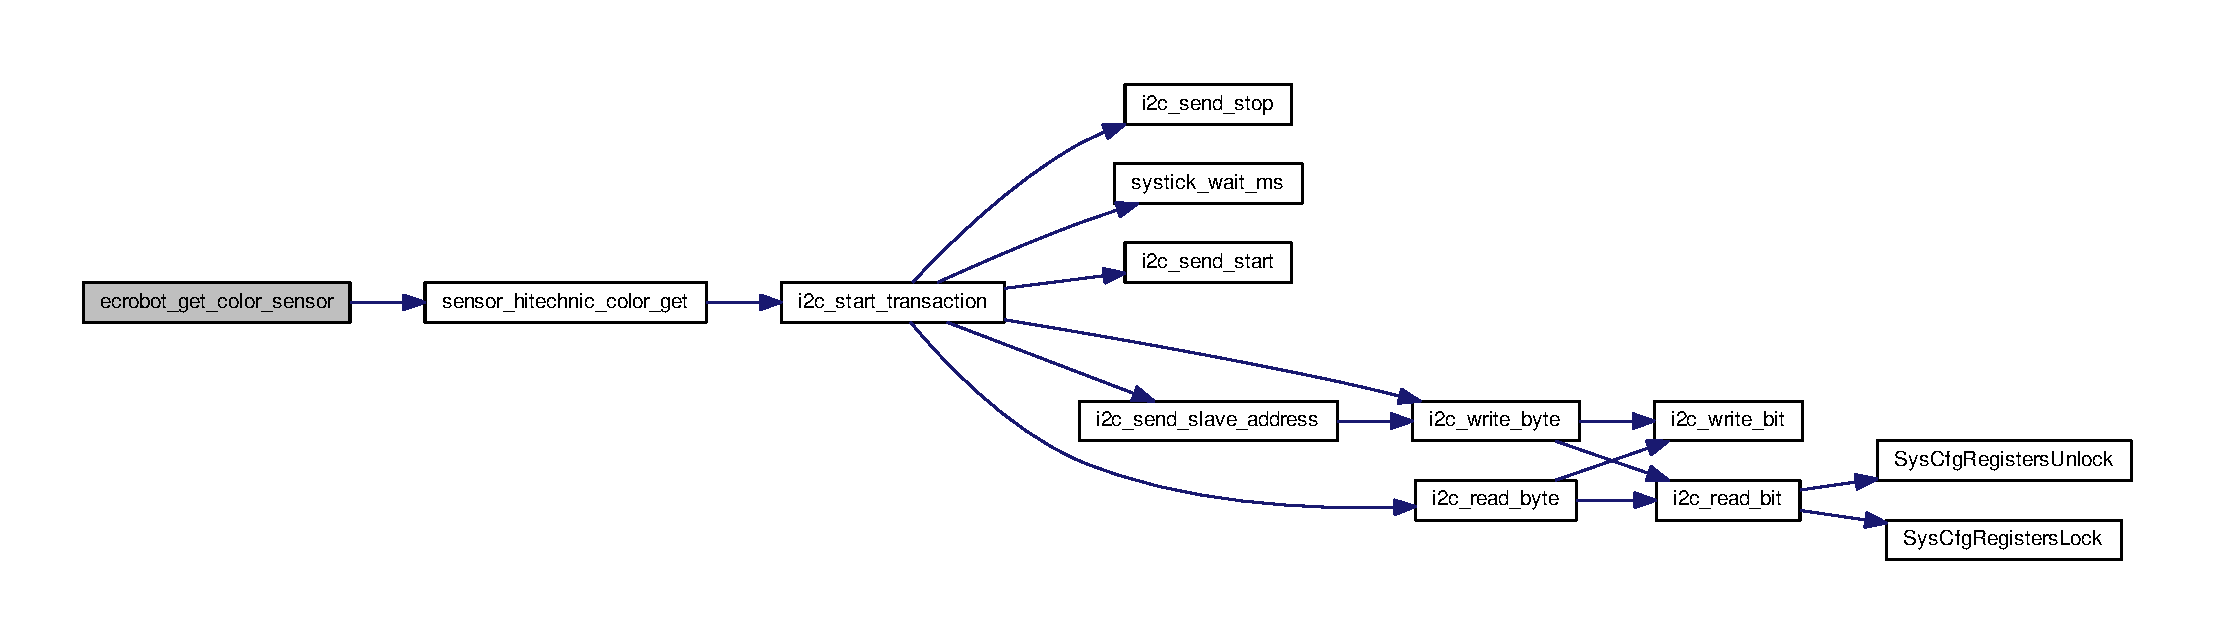
\includegraphics[width=350pt]{ecrobot__interface_8c_ab54ac6a5ac92fa3d8e452d7e0ac42b06_cgraph}
\end{center}
\end{figure}


\hypertarget{ecrobot__interface_8c_abc583b0bef80df0e21019fed1b3c5ab3}{}\index{ecrobot\+\_\+interface.\+c@{ecrobot\+\_\+interface.\+c}!ecrobot\+\_\+get\+\_\+compass\+\_\+sensor@{ecrobot\+\_\+get\+\_\+compass\+\_\+sensor}}
\index{ecrobot\+\_\+get\+\_\+compass\+\_\+sensor@{ecrobot\+\_\+get\+\_\+compass\+\_\+sensor}!ecrobot\+\_\+interface.\+c@{ecrobot\+\_\+interface.\+c}}
\subsubsection[{ecrobot\+\_\+get\+\_\+compass\+\_\+sensor(\+U8 port\+\_\+id)}]{\setlength{\rightskip}{0pt plus 5cm}{\bf S16} ecrobot\+\_\+get\+\_\+compass\+\_\+sensor (
\begin{DoxyParamCaption}
\item[{{\bf U8}}]{port\+\_\+id}
\end{DoxyParamCaption}
)}\label{ecrobot__interface_8c_abc583b0bef80df0e21019fed1b3c5ab3}


Read the current direction meassured by the Hi\+Technic compass sensor at the specified port. 


\begin{DoxyParams}{Parameters}
{\em port\+\_\+id} & -\/ E\+V3\+\_\+\+P\+O\+R\+T\+\_\+\+A, E\+V3\+\_\+\+P\+O\+R\+T\+\_\+\+B, E\+V3\+\_\+\+P\+O\+R\+T\+\_\+\+C, E\+V3\+\_\+\+P\+O\+R\+T\+\_\+\+D\\
\hline
\end{DoxyParams}
\begin{DoxyReturn}{Returns}
The current direction in degrees meassured by the sensor, ranging from 0 to 360 
\end{DoxyReturn}


Here is the call graph for this function\+:\nopagebreak
\begin{figure}[H]
\begin{center}
\leavevmode
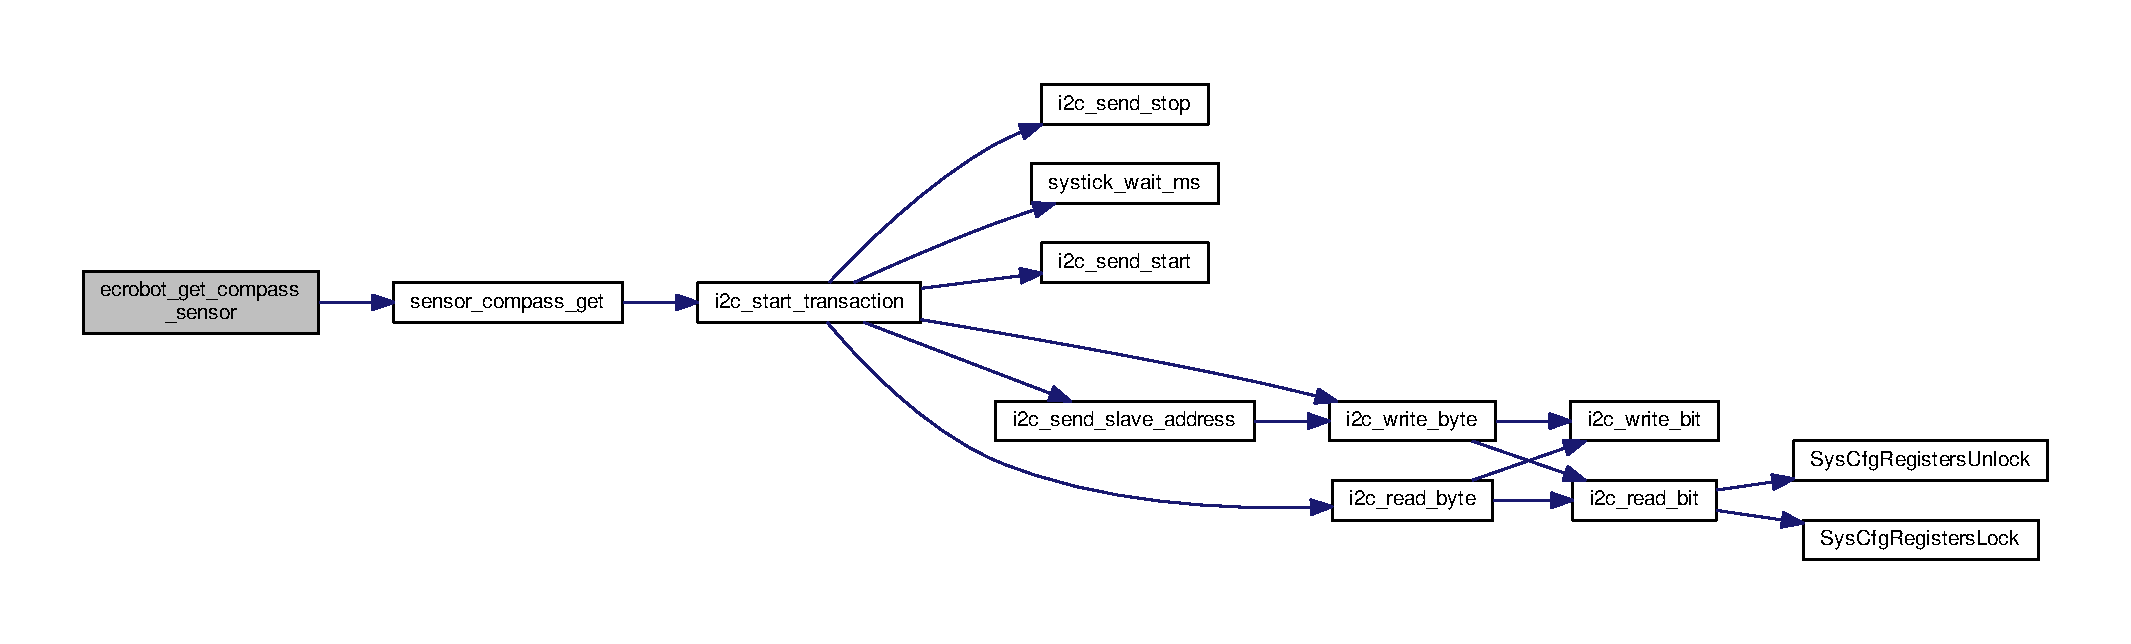
\includegraphics[width=350pt]{ecrobot__interface_8c_abc583b0bef80df0e21019fed1b3c5ab3_cgraph}
\end{center}
\end{figure}


\hypertarget{ecrobot__interface_8c_ad36f9c80a01f470b673244e9c0652559}{}\index{ecrobot\+\_\+interface.\+c@{ecrobot\+\_\+interface.\+c}!ecrobot\+\_\+get\+\_\+gyro\+\_\+sensor@{ecrobot\+\_\+get\+\_\+gyro\+\_\+sensor}}
\index{ecrobot\+\_\+get\+\_\+gyro\+\_\+sensor@{ecrobot\+\_\+get\+\_\+gyro\+\_\+sensor}!ecrobot\+\_\+interface.\+c@{ecrobot\+\_\+interface.\+c}}
\subsubsection[{ecrobot\+\_\+get\+\_\+gyro\+\_\+sensor(\+U8 port\+\_\+id)}]{\setlength{\rightskip}{0pt plus 5cm}{\bf U16} ecrobot\+\_\+get\+\_\+gyro\+\_\+sensor (
\begin{DoxyParamCaption}
\item[{{\bf U8}}]{port\+\_\+id}
\end{DoxyParamCaption}
)}\label{ecrobot__interface_8c_ad36f9c80a01f470b673244e9c0652559}


Gets Gyro Sensor raw A/\+D data. The sensor data has offset value (approximately 600). 


\begin{DoxyParams}{Parameters}
{\em port\+\_\+id} & -\/ E\+V3\+\_\+\+P\+O\+R\+T\+\_\+\+A, E\+V3\+\_\+\+P\+O\+R\+T\+\_\+\+B, E\+V3\+\_\+\+P\+O\+R\+T\+\_\+\+C, E\+V3\+\_\+\+P\+O\+R\+T\+\_\+\+D\\
\hline
\end{DoxyParams}
\begin{DoxyReturn}{Returns}
raw A/\+D value 
\end{DoxyReturn}


Here is the call graph for this function\+:\nopagebreak
\begin{figure}[H]
\begin{center}
\leavevmode
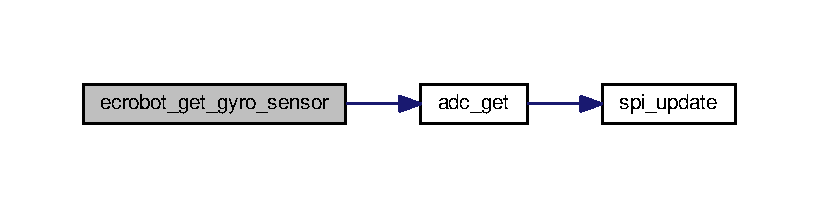
\includegraphics[width=350pt]{ecrobot__interface_8c_ad36f9c80a01f470b673244e9c0652559_cgraph}
\end{center}
\end{figure}


\hypertarget{ecrobot__interface_8c_a66caf428dfc59030202023eeec463ff1}{}\index{ecrobot\+\_\+interface.\+c@{ecrobot\+\_\+interface.\+c}!ecrobot\+\_\+get\+\_\+gyro\+\_\+sensor\+\_\+degrees@{ecrobot\+\_\+get\+\_\+gyro\+\_\+sensor\+\_\+degrees}}
\index{ecrobot\+\_\+get\+\_\+gyro\+\_\+sensor\+\_\+degrees@{ecrobot\+\_\+get\+\_\+gyro\+\_\+sensor\+\_\+degrees}!ecrobot\+\_\+interface.\+c@{ecrobot\+\_\+interface.\+c}}
\subsubsection[{ecrobot\+\_\+get\+\_\+gyro\+\_\+sensor\+\_\+degrees(\+U8 port\+\_\+id)}]{\setlength{\rightskip}{0pt plus 5cm}{\bf S16} ecrobot\+\_\+get\+\_\+gyro\+\_\+sensor\+\_\+degrees (
\begin{DoxyParamCaption}
\item[{{\bf U8}}]{port\+\_\+id}
\end{DoxyParamCaption}
)}\label{ecrobot__interface_8c_a66caf428dfc59030202023eeec463ff1}


Get the current rotation meassured by the Hi\+Technic gyro sensor connected at the specified port. 


\begin{DoxyParams}{Parameters}
{\em port\+\_\+id} & -\/ E\+V3\+\_\+\+P\+O\+R\+T\+\_\+\+A, E\+V3\+\_\+\+P\+O\+R\+T\+\_\+\+B, E\+V3\+\_\+\+P\+O\+R\+T\+\_\+\+C, E\+V3\+\_\+\+P\+O\+R\+T\+\_\+\+D\\
\hline
\end{DoxyParams}
\begin{DoxyReturn}{Returns}
The current rotation meassured by the gyro sensor, ranging from -\/360 degrees to +360 degrees 
\end{DoxyReturn}


Here is the call graph for this function\+:\nopagebreak
\begin{figure}[H]
\begin{center}
\leavevmode
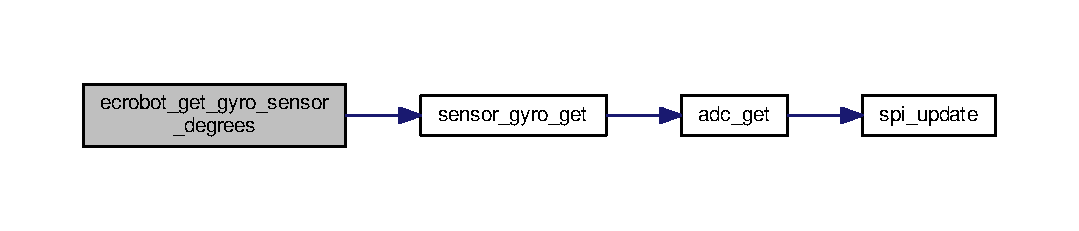
\includegraphics[width=350pt]{ecrobot__interface_8c_a66caf428dfc59030202023eeec463ff1_cgraph}
\end{center}
\end{figure}


\hypertarget{ecrobot__interface_8c_a8db50e0e1ea5539ff33fb69019ba6c59}{}\index{ecrobot\+\_\+interface.\+c@{ecrobot\+\_\+interface.\+c}!ecrobot\+\_\+get\+\_\+light\+\_\+sensor@{ecrobot\+\_\+get\+\_\+light\+\_\+sensor}}
\index{ecrobot\+\_\+get\+\_\+light\+\_\+sensor@{ecrobot\+\_\+get\+\_\+light\+\_\+sensor}!ecrobot\+\_\+interface.\+c@{ecrobot\+\_\+interface.\+c}}
\subsubsection[{ecrobot\+\_\+get\+\_\+light\+\_\+sensor(\+U8 port\+\_\+id)}]{\setlength{\rightskip}{0pt plus 5cm}{\bf U16} ecrobot\+\_\+get\+\_\+light\+\_\+sensor (
\begin{DoxyParamCaption}
\item[{{\bf U8}}]{port\+\_\+id}
\end{DoxyParamCaption}
)}\label{ecrobot__interface_8c_a8db50e0e1ea5539ff33fb69019ba6c59}


Get N\+X\+T Light Sensor raw A/\+D data. 


\begin{DoxyParams}{Parameters}
{\em port\+\_\+id} & -\/ E\+V3\+\_\+\+P\+O\+R\+T\+\_\+\+A, E\+V3\+\_\+\+P\+O\+R\+T\+\_\+\+B, E\+V3\+\_\+\+P\+O\+R\+T\+\_\+\+C, E\+V3\+\_\+\+P\+O\+R\+T\+\_\+\+D\\
\hline
\end{DoxyParams}
\begin{DoxyReturn}{Returns}
A/\+D raw data(0 to 1023) 
\end{DoxyReturn}


Here is the call graph for this function\+:\nopagebreak
\begin{figure}[H]
\begin{center}
\leavevmode
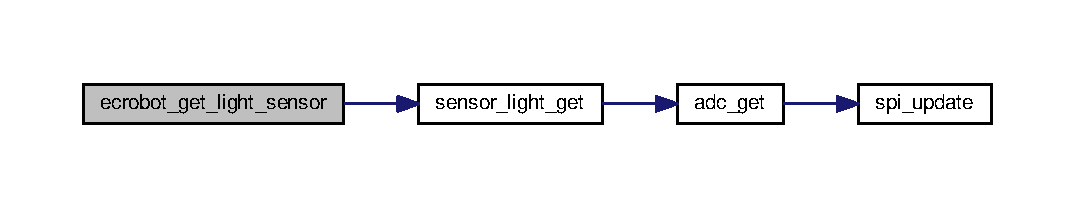
\includegraphics[width=350pt]{ecrobot__interface_8c_a8db50e0e1ea5539ff33fb69019ba6c59_cgraph}
\end{center}
\end{figure}


\hypertarget{ecrobot__interface_8c_aac401bc8039e76ef135628bac4c9d884}{}\index{ecrobot\+\_\+interface.\+c@{ecrobot\+\_\+interface.\+c}!ecrobot\+\_\+get\+\_\+motor\+\_\+rev@{ecrobot\+\_\+get\+\_\+motor\+\_\+rev}}
\index{ecrobot\+\_\+get\+\_\+motor\+\_\+rev@{ecrobot\+\_\+get\+\_\+motor\+\_\+rev}!ecrobot\+\_\+interface.\+c@{ecrobot\+\_\+interface.\+c}}
\subsubsection[{ecrobot\+\_\+get\+\_\+motor\+\_\+rev(\+U8 port\+\_\+id)}]{\setlength{\rightskip}{0pt plus 5cm}{\bf S32} ecrobot\+\_\+get\+\_\+motor\+\_\+rev (
\begin{DoxyParamCaption}
\item[{{\bf U8}}]{port\+\_\+id}
\end{DoxyParamCaption}
)}\label{ecrobot__interface_8c_aac401bc8039e76ef135628bac4c9d884}


Gets Servo Motor revolution value in degree. Wrapper of nxt\+\_\+motor\+\_\+get\+\_\+count. 


\begin{DoxyParams}{Parameters}
{\em port\+\_\+id} & -\/ E\+V3\+\_\+\+P\+O\+R\+T\+\_\+1, E\+V3\+\_\+\+P\+O\+R\+T\+\_\+2, E\+V3\+\_\+\+P\+O\+R\+T\+\_\+3, E\+V3\+\_\+\+P\+O\+R\+T\+\_\+4\\
\hline
\end{DoxyParams}
\begin{DoxyReturn}{Returns}
Servo Motors revolution in degree 
\end{DoxyReturn}


Here is the call graph for this function\+:\nopagebreak
\begin{figure}[H]
\begin{center}
\leavevmode
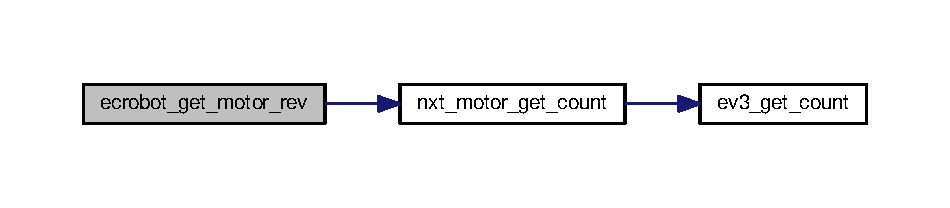
\includegraphics[width=350pt]{ecrobot__interface_8c_aac401bc8039e76ef135628bac4c9d884_cgraph}
\end{center}
\end{figure}


\hypertarget{ecrobot__interface_8c_a606dc0e245136a73870800af77975917}{}\index{ecrobot\+\_\+interface.\+c@{ecrobot\+\_\+interface.\+c}!ecrobot\+\_\+get\+\_\+sonar\+\_\+sensor@{ecrobot\+\_\+get\+\_\+sonar\+\_\+sensor}}
\index{ecrobot\+\_\+get\+\_\+sonar\+\_\+sensor@{ecrobot\+\_\+get\+\_\+sonar\+\_\+sensor}!ecrobot\+\_\+interface.\+c@{ecrobot\+\_\+interface.\+c}}
\subsubsection[{ecrobot\+\_\+get\+\_\+sonar\+\_\+sensor(\+U8 port\+\_\+id)}]{\setlength{\rightskip}{0pt plus 5cm}{\bf S32} ecrobot\+\_\+get\+\_\+sonar\+\_\+sensor (
\begin{DoxyParamCaption}
\item[{{\bf U8}}]{port\+\_\+id}
\end{DoxyParamCaption}
)}\label{ecrobot__interface_8c_a606dc0e245136a73870800af77975917}


Get Ultrasonic Sensor measurement data in cm. 


\begin{DoxyParams}{Parameters}
{\em port\+\_\+id} & -\/ E\+V3\+\_\+\+P\+O\+R\+T\+\_\+\+A, E\+V3\+\_\+\+P\+O\+R\+T\+\_\+\+B, E\+V3\+\_\+\+P\+O\+R\+T\+\_\+\+C, E\+V3\+\_\+\+P\+O\+R\+T\+\_\+\+D\\
\hline
\end{DoxyParams}
\begin{DoxyReturn}{Returns}
distance in cm (0 to 255), -\/1 (failure) 
\end{DoxyReturn}


Here is the call graph for this function\+:\nopagebreak
\begin{figure}[H]
\begin{center}
\leavevmode
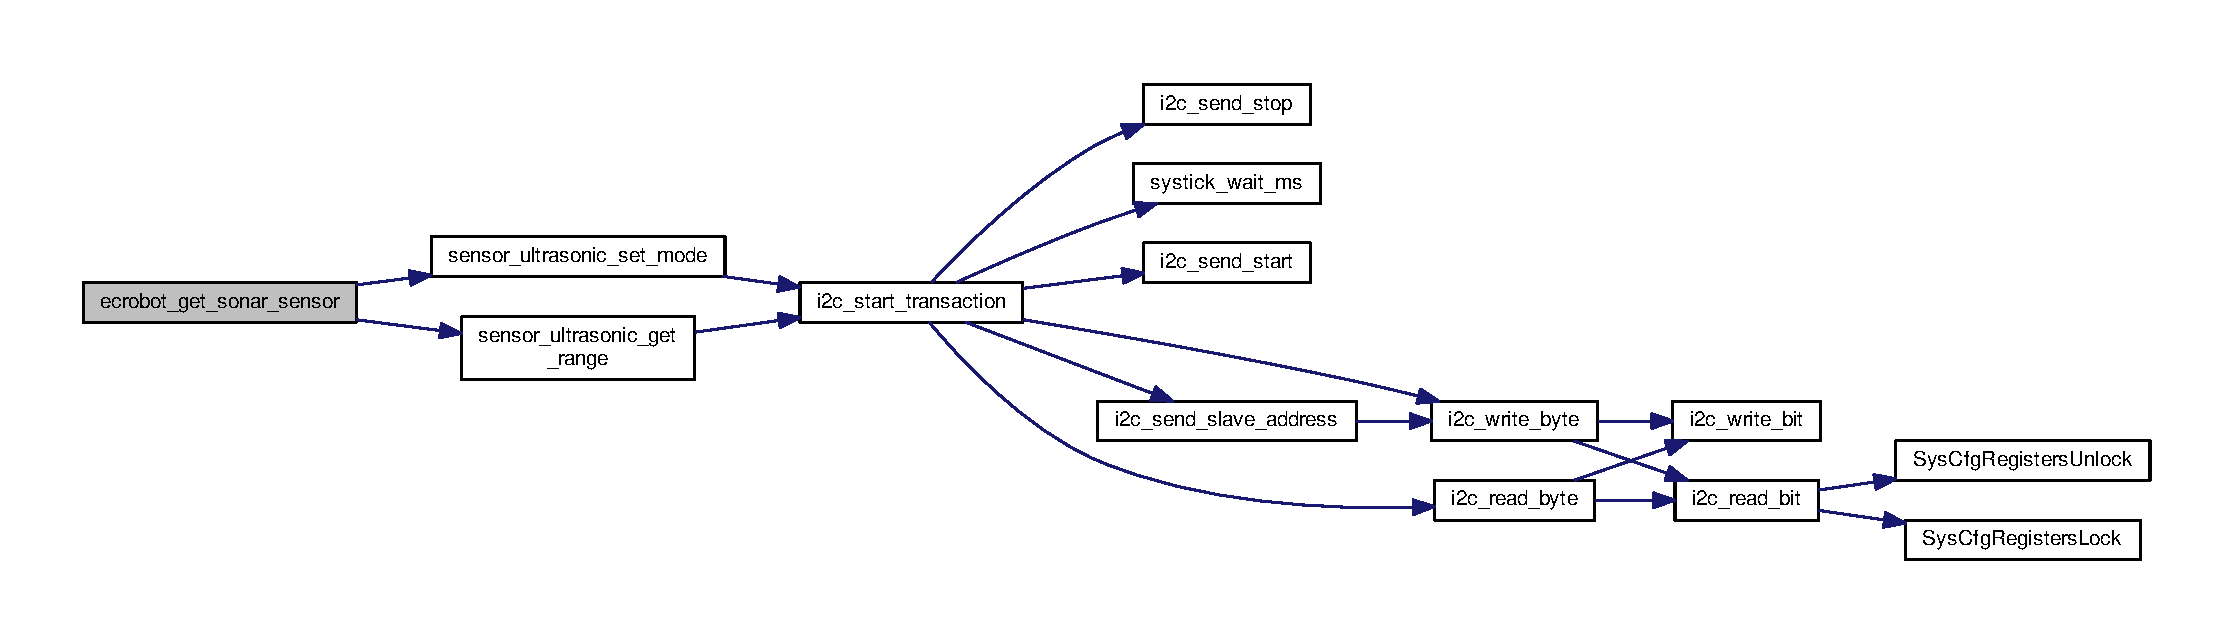
\includegraphics[width=350pt]{ecrobot__interface_8c_a606dc0e245136a73870800af77975917_cgraph}
\end{center}
\end{figure}


\hypertarget{ecrobot__interface_8c_a92df098d5bc3f745a4c7e29256d6e826}{}\index{ecrobot\+\_\+interface.\+c@{ecrobot\+\_\+interface.\+c}!ecrobot\+\_\+get\+\_\+sonar\+\_\+sensor\+\_\+single\+\_\+shot@{ecrobot\+\_\+get\+\_\+sonar\+\_\+sensor\+\_\+single\+\_\+shot}}
\index{ecrobot\+\_\+get\+\_\+sonar\+\_\+sensor\+\_\+single\+\_\+shot@{ecrobot\+\_\+get\+\_\+sonar\+\_\+sensor\+\_\+single\+\_\+shot}!ecrobot\+\_\+interface.\+c@{ecrobot\+\_\+interface.\+c}}
\subsubsection[{ecrobot\+\_\+get\+\_\+sonar\+\_\+sensor\+\_\+single\+\_\+shot(\+U8 port\+\_\+id, U8 data\+\_\+buffer[8])}]{\setlength{\rightskip}{0pt plus 5cm}void ecrobot\+\_\+get\+\_\+sonar\+\_\+sensor\+\_\+single\+\_\+shot (
\begin{DoxyParamCaption}
\item[{{\bf U8}}]{port\+\_\+id, }
\item[{{\bf U8}}]{data\+\_\+buffer\mbox{[}8\mbox{]}}
\end{DoxyParamCaption}
)}\label{ecrobot__interface_8c_a92df098d5bc3f745a4c7e29256d6e826}


Set the mode of the Lego ultrasonic sensor at the specified port to U\+L\+T\+R\+A\+S\+O\+N\+I\+C\+\_\+\+M\+O\+D\+E\+\_\+\+S\+I\+N\+G\+L\+E\+\_\+\+S\+H\+O\+T. After that get the range of the Lego ultrasonic sensor connected at the specified port and store it in the buffer. 

The sensor meassures distances from 0 to 255 in cm. If nothing is located in front of the sensor, the value will be 255. All 8 entries of the array will be values returned by the sensor. If less than 8 objects are detected, some entries will be set to 255.


\begin{DoxyParams}{Parameters}
{\em port\+\_\+id} & -\/ E\+V3\+\_\+\+P\+O\+R\+T\+\_\+\+A, E\+V3\+\_\+\+P\+O\+R\+T\+\_\+\+B, E\+V3\+\_\+\+P\+O\+R\+T\+\_\+\+C, E\+V3\+\_\+\+P\+O\+R\+T\+\_\+\+D \\
\hline
{\em data\+\_\+buffer} & -\/ Buffer to store the result in\\
\hline
\end{DoxyParams}
\begin{DoxyReturn}{Returns}
none 
\end{DoxyReturn}


Here is the call graph for this function\+:\nopagebreak
\begin{figure}[H]
\begin{center}
\leavevmode
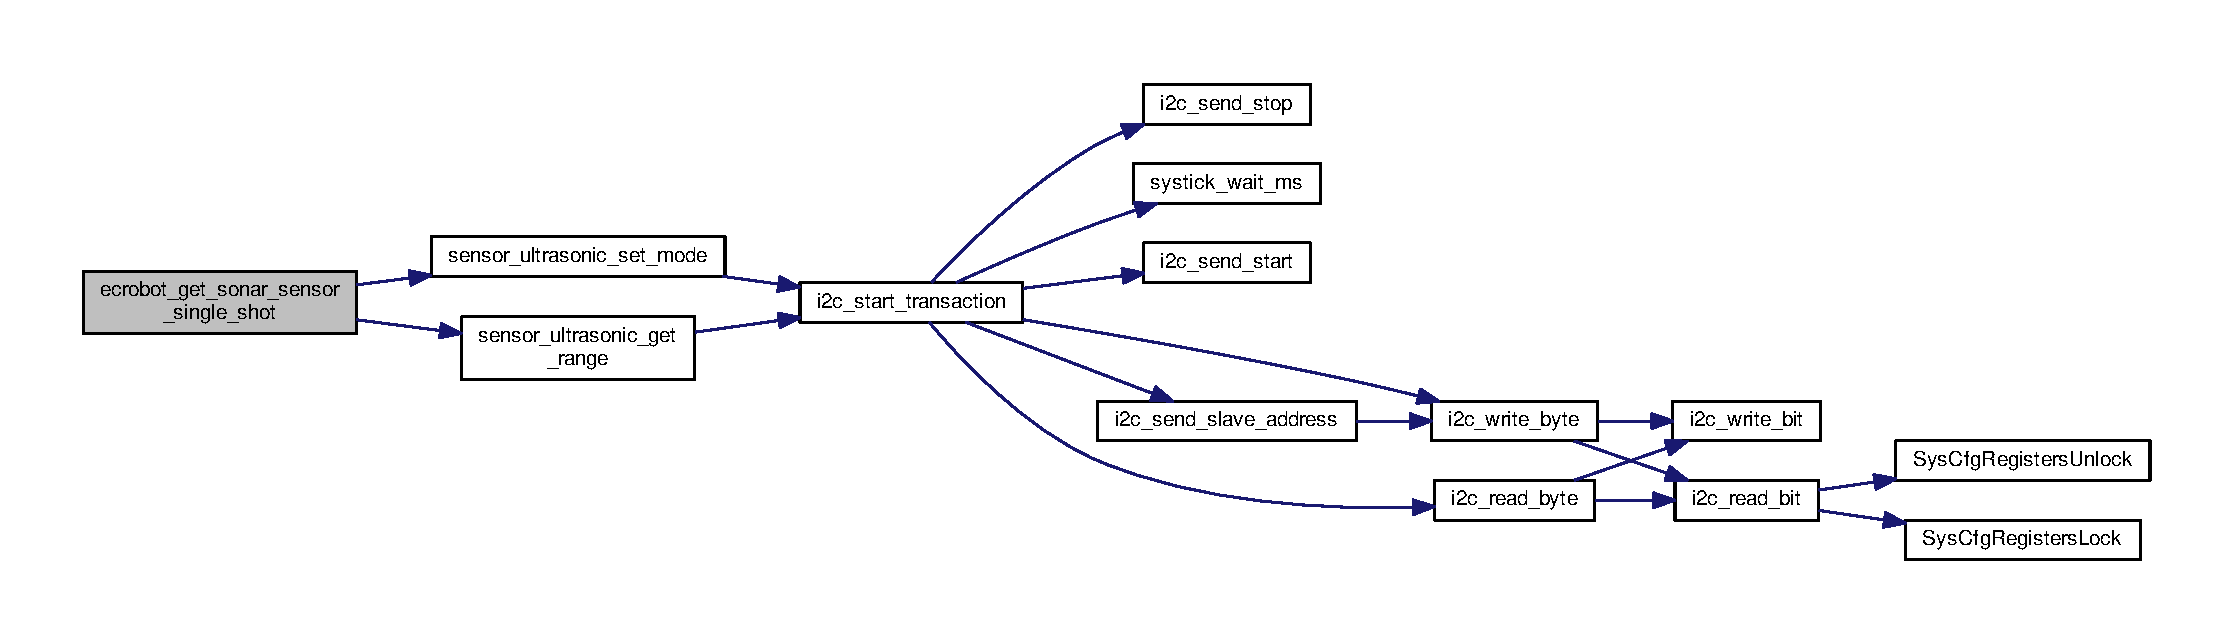
\includegraphics[width=350pt]{ecrobot__interface_8c_a92df098d5bc3f745a4c7e29256d6e826_cgraph}
\end{center}
\end{figure}


\hypertarget{ecrobot__interface_8c_a3d0f6c7d2c8d0236bfcb5e647f42ec4f}{}\index{ecrobot\+\_\+interface.\+c@{ecrobot\+\_\+interface.\+c}!ecrobot\+\_\+get\+\_\+sound\+\_\+sensor@{ecrobot\+\_\+get\+\_\+sound\+\_\+sensor}}
\index{ecrobot\+\_\+get\+\_\+sound\+\_\+sensor@{ecrobot\+\_\+get\+\_\+sound\+\_\+sensor}!ecrobot\+\_\+interface.\+c@{ecrobot\+\_\+interface.\+c}}
\subsubsection[{ecrobot\+\_\+get\+\_\+sound\+\_\+sensor(\+U8 port\+\_\+id)}]{\setlength{\rightskip}{0pt plus 5cm}{\bf U16} ecrobot\+\_\+get\+\_\+sound\+\_\+sensor (
\begin{DoxyParamCaption}
\item[{{\bf U8}}]{port\+\_\+id}
\end{DoxyParamCaption}
)}\label{ecrobot__interface_8c_a3d0f6c7d2c8d0236bfcb5e647f42ec4f}


Get Sound Sensor raw A/\+D data. 


\begin{DoxyParams}{Parameters}
{\em port\+\_\+id} & -\/ E\+V3\+\_\+\+P\+O\+R\+T\+\_\+\+A, E\+V3\+\_\+\+P\+O\+R\+T\+\_\+\+B, E\+V3\+\_\+\+P\+O\+R\+T\+\_\+\+C, E\+V3\+\_\+\+P\+O\+R\+T\+\_\+\+D\\
\hline
\end{DoxyParams}
\begin{DoxyReturn}{Returns}
A/\+D raw data(0 to 1023) 
\end{DoxyReturn}


Here is the call graph for this function\+:\nopagebreak
\begin{figure}[H]
\begin{center}
\leavevmode
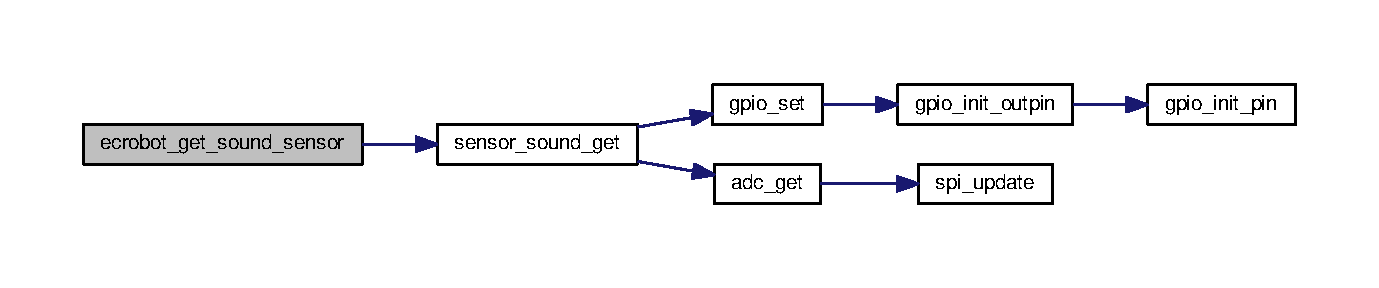
\includegraphics[width=350pt]{ecrobot__interface_8c_a3d0f6c7d2c8d0236bfcb5e647f42ec4f_cgraph}
\end{center}
\end{figure}


\hypertarget{ecrobot__interface_8c_af43da73900e9f320695f8ca40c91601d}{}\index{ecrobot\+\_\+interface.\+c@{ecrobot\+\_\+interface.\+c}!ecrobot\+\_\+get\+\_\+systick\+\_\+ms@{ecrobot\+\_\+get\+\_\+systick\+\_\+ms}}
\index{ecrobot\+\_\+get\+\_\+systick\+\_\+ms@{ecrobot\+\_\+get\+\_\+systick\+\_\+ms}!ecrobot\+\_\+interface.\+c@{ecrobot\+\_\+interface.\+c}}
\subsubsection[{ecrobot\+\_\+get\+\_\+systick\+\_\+ms(void)}]{\setlength{\rightskip}{0pt plus 5cm}{\bf U32} ecrobot\+\_\+get\+\_\+systick\+\_\+ms (
\begin{DoxyParamCaption}
\item[{void}]{}
\end{DoxyParamCaption}
)}\label{ecrobot__interface_8c_af43da73900e9f320695f8ca40c91601d}


Get the current tick in milliseconds. 

\begin{DoxyReturn}{Returns}
The current tick in milliseconds 
\end{DoxyReturn}


Here is the call graph for this function\+:\nopagebreak
\begin{figure}[H]
\begin{center}
\leavevmode
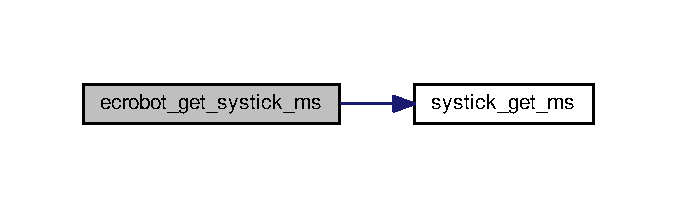
\includegraphics[width=325pt]{ecrobot__interface_8c_af43da73900e9f320695f8ca40c91601d_cgraph}
\end{center}
\end{figure}


\hypertarget{ecrobot__interface_8c_ac3d850ca54c4793976a72dcff72ea27f}{}\index{ecrobot\+\_\+interface.\+c@{ecrobot\+\_\+interface.\+c}!ecrobot\+\_\+get\+\_\+temperature\+\_\+sensor@{ecrobot\+\_\+get\+\_\+temperature\+\_\+sensor}}
\index{ecrobot\+\_\+get\+\_\+temperature\+\_\+sensor@{ecrobot\+\_\+get\+\_\+temperature\+\_\+sensor}!ecrobot\+\_\+interface.\+c@{ecrobot\+\_\+interface.\+c}}
\subsubsection[{ecrobot\+\_\+get\+\_\+temperature\+\_\+sensor(\+U8 port\+\_\+id)}]{\setlength{\rightskip}{0pt plus 5cm}float ecrobot\+\_\+get\+\_\+temperature\+\_\+sensor (
\begin{DoxyParamCaption}
\item[{{\bf U8}}]{port\+\_\+id}
\end{DoxyParamCaption}
)}\label{ecrobot__interface_8c_ac3d850ca54c4793976a72dcff72ea27f}


Measures and returns the current temperature value. 


\begin{DoxyParams}{Parameters}
{\em port\+\_\+id} & -\/ E\+V3\+\_\+\+P\+O\+R\+T\+\_\+\+A, E\+V3\+\_\+\+P\+O\+R\+T\+\_\+\+B, E\+V3\+\_\+\+P\+O\+R\+T\+\_\+\+C, E\+V3\+\_\+\+P\+O\+R\+T\+\_\+\+D\\
\hline
\end{DoxyParams}
\begin{DoxyReturn}{Returns}
The current temperature given in degrees Celsius 
\end{DoxyReturn}


Here is the call graph for this function\+:\nopagebreak
\begin{figure}[H]
\begin{center}
\leavevmode
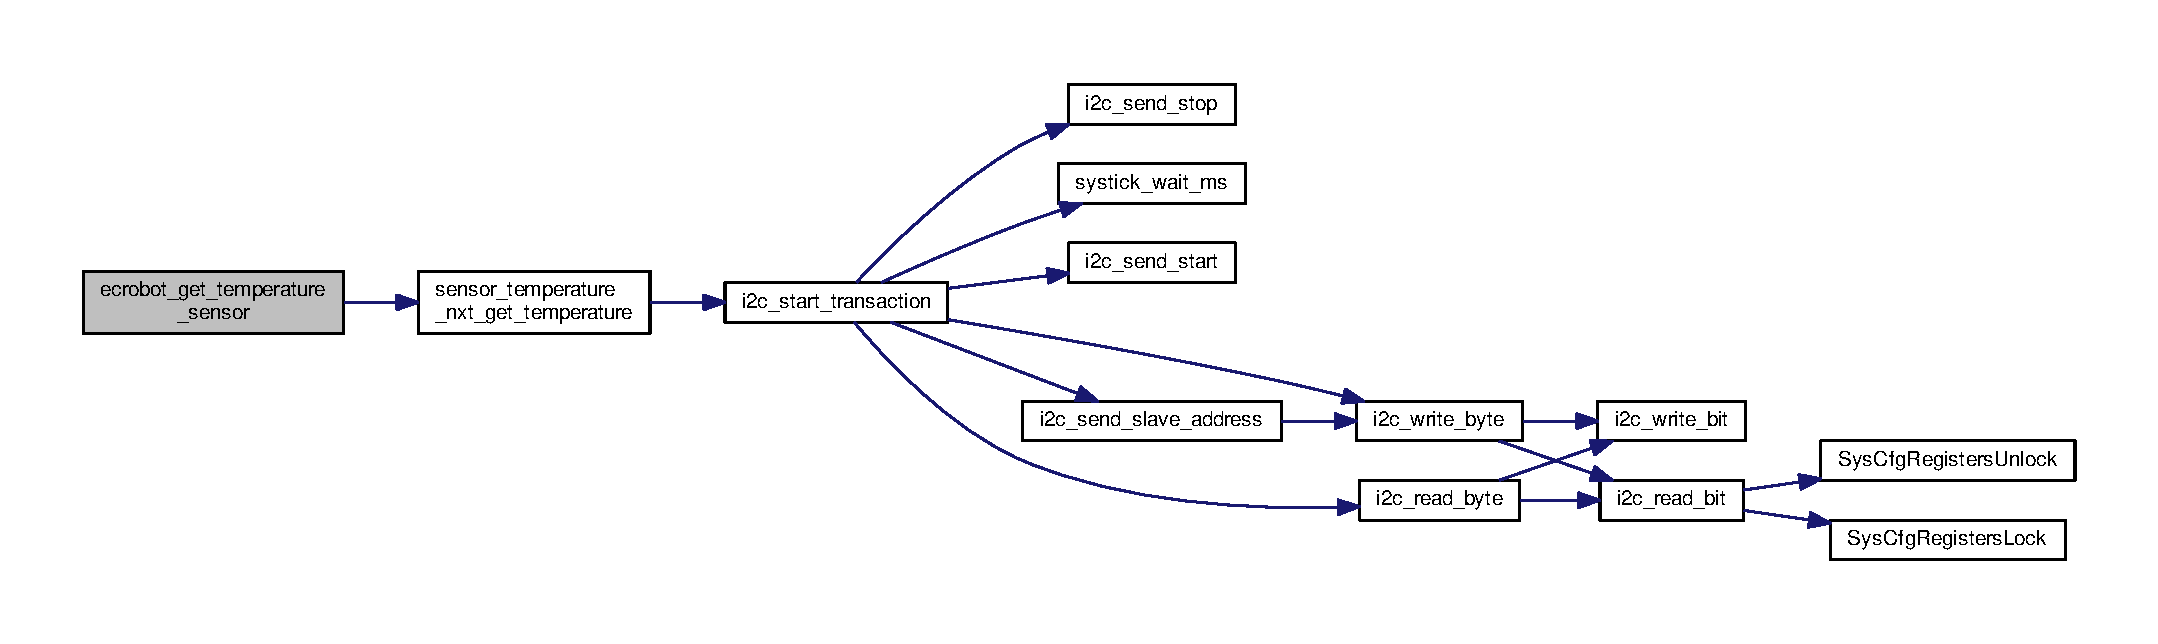
\includegraphics[width=350pt]{ecrobot__interface_8c_ac3d850ca54c4793976a72dcff72ea27f_cgraph}
\end{center}
\end{figure}


\hypertarget{ecrobot__interface_8c_a17ec6ec37bbe6d15ece65aab03b9df94}{}\index{ecrobot\+\_\+interface.\+c@{ecrobot\+\_\+interface.\+c}!ecrobot\+\_\+get\+\_\+touch\+\_\+sensor@{ecrobot\+\_\+get\+\_\+touch\+\_\+sensor}}
\index{ecrobot\+\_\+get\+\_\+touch\+\_\+sensor@{ecrobot\+\_\+get\+\_\+touch\+\_\+sensor}!ecrobot\+\_\+interface.\+c@{ecrobot\+\_\+interface.\+c}}
\subsubsection[{ecrobot\+\_\+get\+\_\+touch\+\_\+sensor(\+U8 port\+\_\+id)}]{\setlength{\rightskip}{0pt plus 5cm}{\bf U8} ecrobot\+\_\+get\+\_\+touch\+\_\+sensor (
\begin{DoxyParamCaption}
\item[{{\bf U8}}]{port\+\_\+id}
\end{DoxyParamCaption}
)}\label{ecrobot__interface_8c_a17ec6ec37bbe6d15ece65aab03b9df94}


Get Touch Sensor on/off status. 


\begin{DoxyParams}{Parameters}
{\em port\+\_\+id} & -\/ E\+V3\+\_\+\+P\+O\+R\+T\+\_\+\+A, E\+V3\+\_\+\+P\+O\+R\+T\+\_\+\+B, E\+V3\+\_\+\+P\+O\+R\+T\+\_\+\+C, E\+V3\+\_\+\+P\+O\+R\+T\+\_\+\+D\\
\hline
\end{DoxyParams}
\begin{DoxyReturn}{Returns}
1(touched), 0(not touched) 
\end{DoxyReturn}


Here is the call graph for this function\+:\nopagebreak
\begin{figure}[H]
\begin{center}
\leavevmode
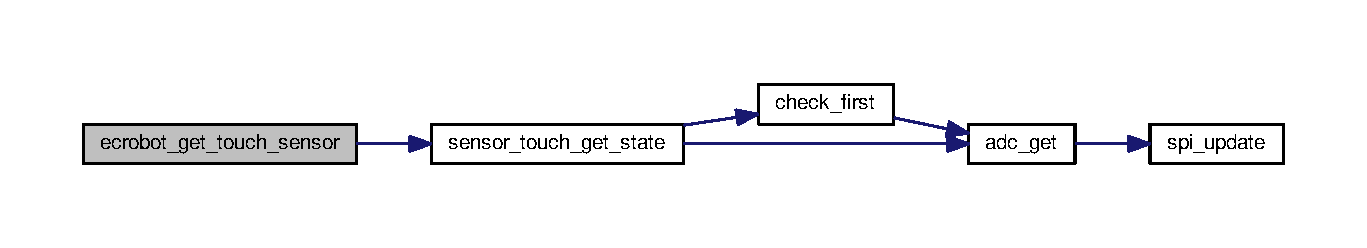
\includegraphics[width=350pt]{ecrobot__interface_8c_a17ec6ec37bbe6d15ece65aab03b9df94_cgraph}
\end{center}
\end{figure}


\hypertarget{ecrobot__interface_8c_aa7f203b9bb762050caacf41f177ac530}{}\index{ecrobot\+\_\+interface.\+c@{ecrobot\+\_\+interface.\+c}!ecrobot\+\_\+get\+Resolution\+\_\+temperature\+\_\+sensor@{ecrobot\+\_\+get\+Resolution\+\_\+temperature\+\_\+sensor}}
\index{ecrobot\+\_\+get\+Resolution\+\_\+temperature\+\_\+sensor@{ecrobot\+\_\+get\+Resolution\+\_\+temperature\+\_\+sensor}!ecrobot\+\_\+interface.\+c@{ecrobot\+\_\+interface.\+c}}
\subsubsection[{ecrobot\+\_\+get\+Resolution\+\_\+temperature\+\_\+sensor(\+U8 port\+\_\+id)}]{\setlength{\rightskip}{0pt plus 5cm}{\bf U8} ecrobot\+\_\+get\+Resolution\+\_\+temperature\+\_\+sensor (
\begin{DoxyParamCaption}
\item[{{\bf U8}}]{port\+\_\+id}
\end{DoxyParamCaption}
)}\label{ecrobot__interface_8c_aa7f203b9bb762050caacf41f177ac530}


Returns the current resolution setting of the sensor. 


\begin{DoxyParams}{Parameters}
{\em port\+\_\+id} & -\/ E\+V3\+\_\+\+P\+O\+R\+T\+\_\+\+A, E\+V3\+\_\+\+P\+O\+R\+T\+\_\+\+B, E\+V3\+\_\+\+P\+O\+R\+T\+\_\+\+C, E\+V3\+\_\+\+P\+O\+R\+T\+\_\+\+D\\
\hline
\end{DoxyParams}
\begin{DoxyReturn}{Returns}
The current resolution. See the macros T\+E\+M\+P9\+B\+I\+T ... T\+E\+M\+P12\+B\+I\+T 
\end{DoxyReturn}


Here is the call graph for this function\+:\nopagebreak
\begin{figure}[H]
\begin{center}
\leavevmode
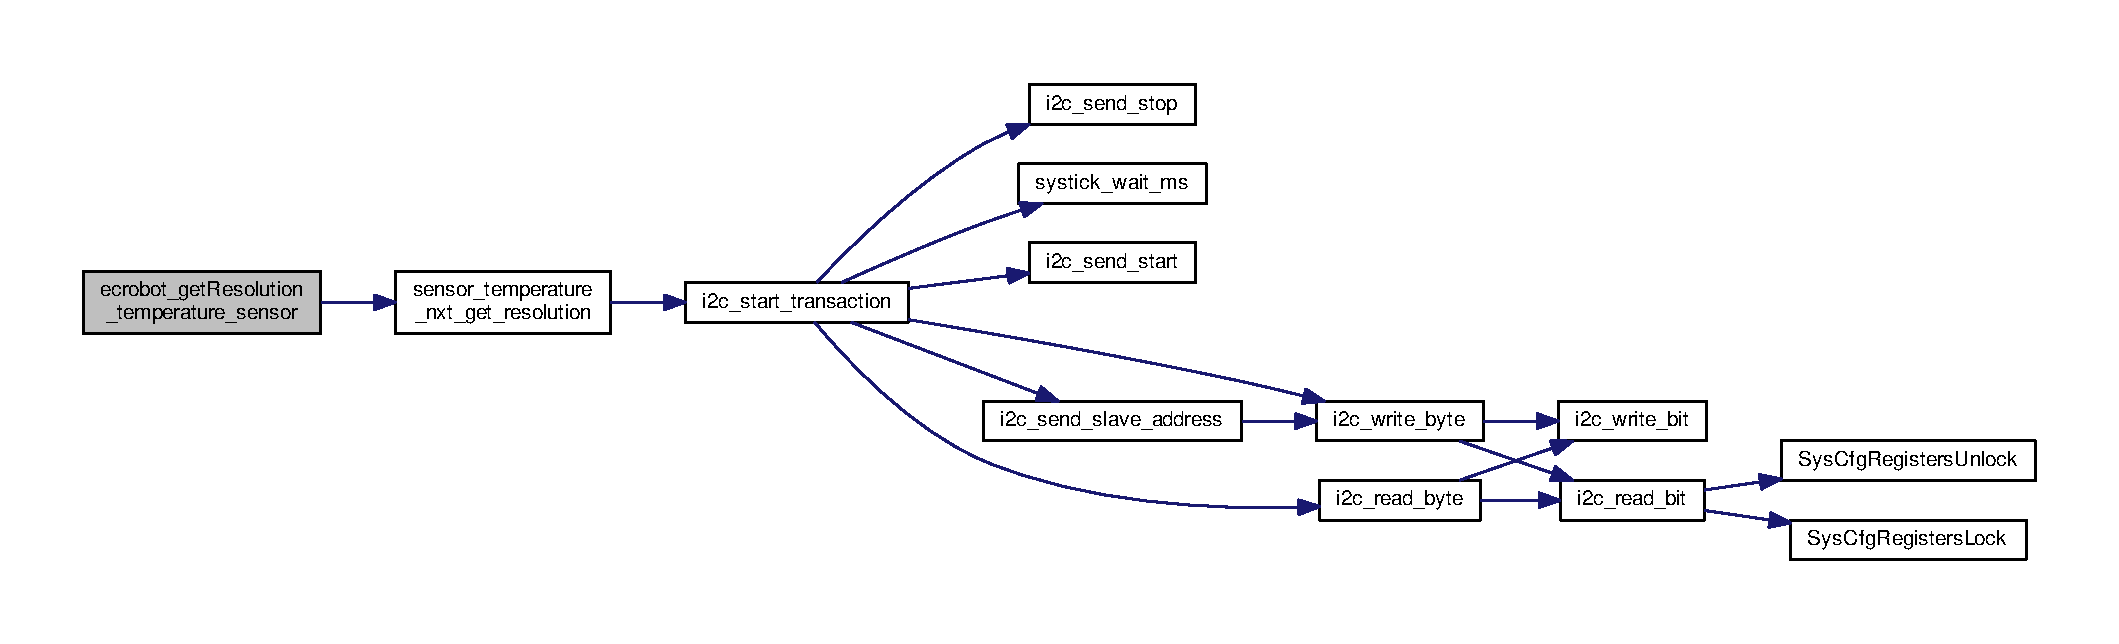
\includegraphics[width=350pt]{ecrobot__interface_8c_aa7f203b9bb762050caacf41f177ac530_cgraph}
\end{center}
\end{figure}


\hypertarget{ecrobot__interface_8c_a82abd85d3faadc9aa90e6a80a1f9c336}{}\index{ecrobot\+\_\+interface.\+c@{ecrobot\+\_\+interface.\+c}!ecrobot\+\_\+init\+\_\+accel\+\_\+sensor@{ecrobot\+\_\+init\+\_\+accel\+\_\+sensor}}
\index{ecrobot\+\_\+init\+\_\+accel\+\_\+sensor@{ecrobot\+\_\+init\+\_\+accel\+\_\+sensor}!ecrobot\+\_\+interface.\+c@{ecrobot\+\_\+interface.\+c}}
\subsubsection[{ecrobot\+\_\+init\+\_\+accel\+\_\+sensor(\+U8 port\+\_\+id)}]{\setlength{\rightskip}{0pt plus 5cm}void ecrobot\+\_\+init\+\_\+accel\+\_\+sensor (
\begin{DoxyParamCaption}
\item[{{\bf U8}}]{port\+\_\+id}
\end{DoxyParamCaption}
)}\label{ecrobot__interface_8c_a82abd85d3faadc9aa90e6a80a1f9c336}


Initializes a port for I2\+C communication for Acceleration Sensor. This function should be implemented in the device initialize hook routine. 


\begin{DoxyParams}{Parameters}
{\em port\+\_\+id} & -\/ E\+V3\+\_\+\+P\+O\+R\+T\+\_\+\+A, E\+V3\+\_\+\+P\+O\+R\+T\+\_\+\+B, E\+V3\+\_\+\+P\+O\+R\+T\+\_\+\+C, E\+V3\+\_\+\+P\+O\+R\+T\+\_\+\+D\\
\hline
\end{DoxyParams}
\begin{DoxyReturn}{Returns}
none 
\end{DoxyReturn}


Here is the call graph for this function\+:\nopagebreak
\begin{figure}[H]
\begin{center}
\leavevmode
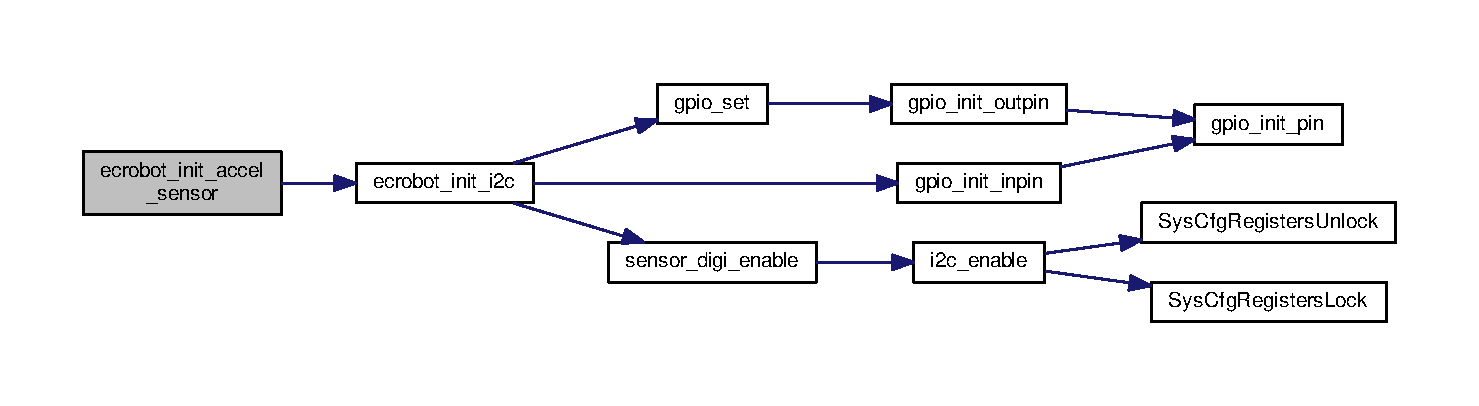
\includegraphics[width=350pt]{ecrobot__interface_8c_a82abd85d3faadc9aa90e6a80a1f9c336_cgraph}
\end{center}
\end{figure}


\hypertarget{ecrobot__interface_8c_ac43644c6aa0ee882b21669b37e4dcae5}{}\index{ecrobot\+\_\+interface.\+c@{ecrobot\+\_\+interface.\+c}!ecrobot\+\_\+init\+\_\+color\+\_\+sensor@{ecrobot\+\_\+init\+\_\+color\+\_\+sensor}}
\index{ecrobot\+\_\+init\+\_\+color\+\_\+sensor@{ecrobot\+\_\+init\+\_\+color\+\_\+sensor}!ecrobot\+\_\+interface.\+c@{ecrobot\+\_\+interface.\+c}}
\subsubsection[{ecrobot\+\_\+init\+\_\+color\+\_\+sensor(\+U8 port\+\_\+id)}]{\setlength{\rightskip}{0pt plus 5cm}void ecrobot\+\_\+init\+\_\+color\+\_\+sensor (
\begin{DoxyParamCaption}
\item[{{\bf U8}}]{port\+\_\+id}
\end{DoxyParamCaption}
)}\label{ecrobot__interface_8c_ac43644c6aa0ee882b21669b37e4dcae5}


initializes a port for I2\+C communication for the Color Sensor. This function should be implemented in the device initialize hook routine. 


\begin{DoxyParams}{Parameters}
{\em port\+\_\+id} & -\/ E\+V3\+\_\+\+P\+O\+R\+T\+\_\+\+A, E\+V3\+\_\+\+P\+O\+R\+T\+\_\+\+B, E\+V3\+\_\+\+P\+O\+R\+T\+\_\+\+C, E\+V3\+\_\+\+P\+O\+R\+T\+\_\+\+D\\
\hline
\end{DoxyParams}
\begin{DoxyReturn}{Returns}
none 
\end{DoxyReturn}


Here is the call graph for this function\+:\nopagebreak
\begin{figure}[H]
\begin{center}
\leavevmode
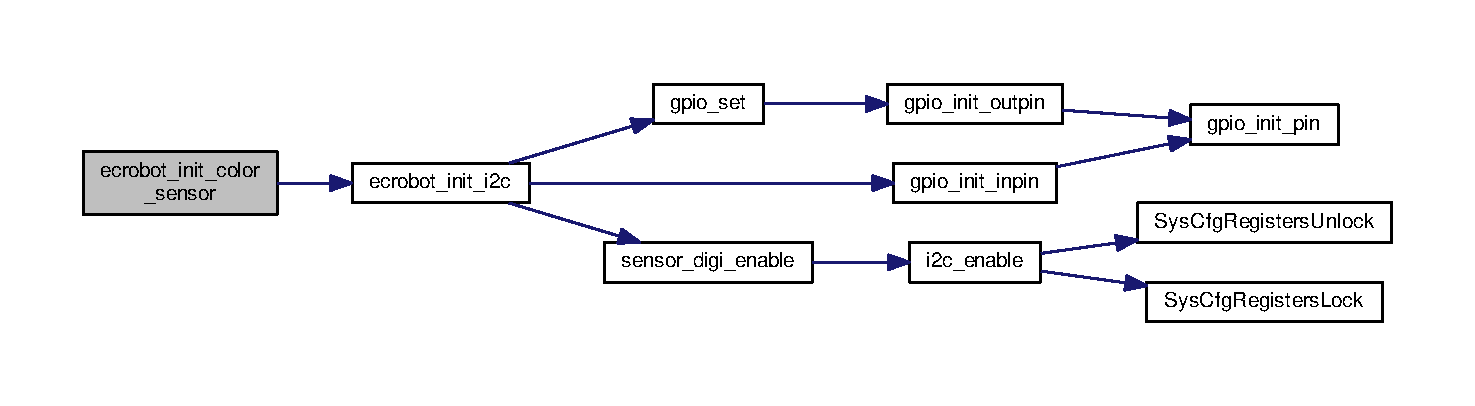
\includegraphics[width=350pt]{ecrobot__interface_8c_ac43644c6aa0ee882b21669b37e4dcae5_cgraph}
\end{center}
\end{figure}


\hypertarget{ecrobot__interface_8c_af87a9c15633d8cbabc9d69cf01d9cb46}{}\index{ecrobot\+\_\+interface.\+c@{ecrobot\+\_\+interface.\+c}!ecrobot\+\_\+init\+\_\+compass\+\_\+sensor@{ecrobot\+\_\+init\+\_\+compass\+\_\+sensor}}
\index{ecrobot\+\_\+init\+\_\+compass\+\_\+sensor@{ecrobot\+\_\+init\+\_\+compass\+\_\+sensor}!ecrobot\+\_\+interface.\+c@{ecrobot\+\_\+interface.\+c}}
\subsubsection[{ecrobot\+\_\+init\+\_\+compass\+\_\+sensor(\+U8 port\+\_\+id)}]{\setlength{\rightskip}{0pt plus 5cm}void ecrobot\+\_\+init\+\_\+compass\+\_\+sensor (
\begin{DoxyParamCaption}
\item[{{\bf U8}}]{port\+\_\+id}
\end{DoxyParamCaption}
)}\label{ecrobot__interface_8c_af87a9c15633d8cbabc9d69cf01d9cb46}


Initializes a port for I2\+C communication for Compass Sensor. This function should be implemented in the device initialize hook routine. 


\begin{DoxyParams}{Parameters}
{\em port\+\_\+id} & -\/ E\+V3\+\_\+\+P\+O\+R\+T\+\_\+\+A, E\+V3\+\_\+\+P\+O\+R\+T\+\_\+\+B, E\+V3\+\_\+\+P\+O\+R\+T\+\_\+\+C, E\+V3\+\_\+\+P\+O\+R\+T\+\_\+\+D\\
\hline
\end{DoxyParams}
\begin{DoxyReturn}{Returns}
none 
\end{DoxyReturn}


Here is the call graph for this function\+:\nopagebreak
\begin{figure}[H]
\begin{center}
\leavevmode
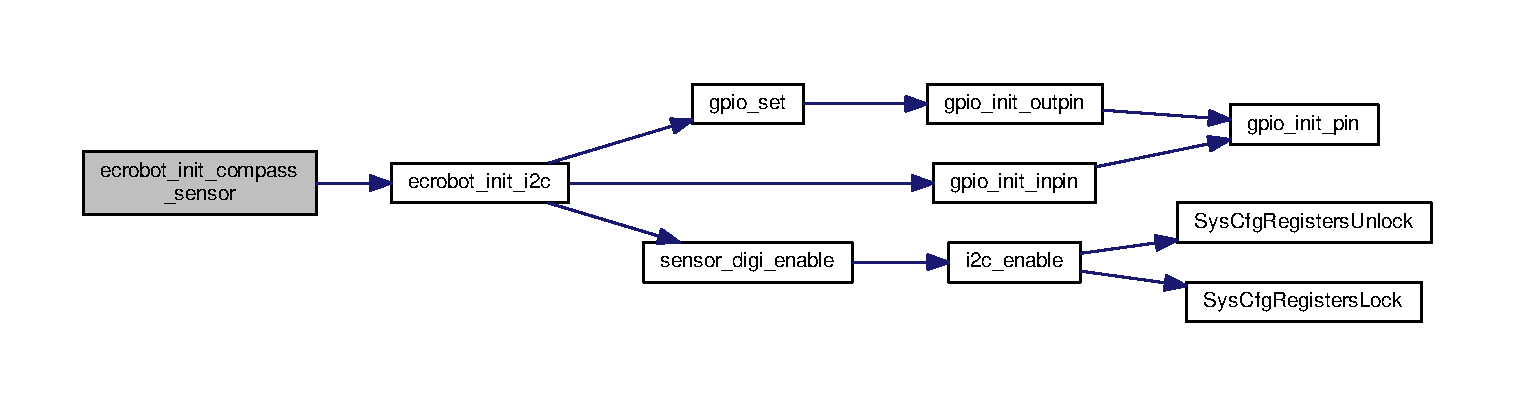
\includegraphics[width=350pt]{ecrobot__interface_8c_af87a9c15633d8cbabc9d69cf01d9cb46_cgraph}
\end{center}
\end{figure}


\hypertarget{ecrobot__interface_8c_aed9a245415bee498586a76a92830c7e9}{}\index{ecrobot\+\_\+interface.\+c@{ecrobot\+\_\+interface.\+c}!ecrobot\+\_\+init\+\_\+i2c@{ecrobot\+\_\+init\+\_\+i2c}}
\index{ecrobot\+\_\+init\+\_\+i2c@{ecrobot\+\_\+init\+\_\+i2c}!ecrobot\+\_\+interface.\+c@{ecrobot\+\_\+interface.\+c}}
\subsubsection[{ecrobot\+\_\+init\+\_\+i2c(\+U8 port\+\_\+id, U8 type)}]{\setlength{\rightskip}{0pt plus 5cm}void ecrobot\+\_\+init\+\_\+i2c (
\begin{DoxyParamCaption}
\item[{{\bf U8}}]{port\+\_\+id, }
\item[{{\bf U8}}]{type}
\end{DoxyParamCaption}
)}\label{ecrobot__interface_8c_aed9a245415bee498586a76a92830c7e9}


Init a N\+X\+T sensor port for I2\+C communication. 


\begin{DoxyParams}{Parameters}
{\em port\+\_\+id} & -\/ E\+V3\+\_\+\+P\+O\+R\+T\+\_\+\+A, E\+V3\+\_\+\+P\+O\+R\+T\+\_\+\+B, E\+V3\+\_\+\+P\+O\+R\+T\+\_\+\+C, E\+V3\+\_\+\+P\+O\+R\+T\+\_\+\+D \\
\hline
{\em type} & -\/ L\+O\+W\+S\+P\+E\+E\+D\+\_\+9\+V, L\+O\+W\+S\+P\+E\+E\+D\\
\hline
\end{DoxyParams}
\begin{DoxyReturn}{Returns}
none 
\end{DoxyReturn}


Here is the call graph for this function\+:\nopagebreak
\begin{figure}[H]
\begin{center}
\leavevmode
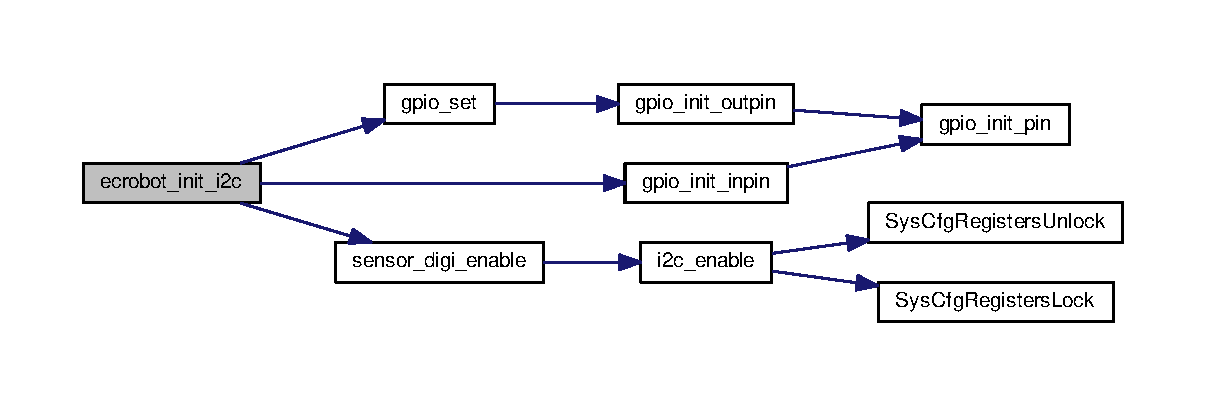
\includegraphics[width=350pt]{ecrobot__interface_8c_aed9a245415bee498586a76a92830c7e9_cgraph}
\end{center}
\end{figure}


\hypertarget{ecrobot__interface_8c_a1987f8ae51d64da9e63185302c84c6dc}{}\index{ecrobot\+\_\+interface.\+c@{ecrobot\+\_\+interface.\+c}!ecrobot\+\_\+init\+\_\+sonar\+\_\+sensor@{ecrobot\+\_\+init\+\_\+sonar\+\_\+sensor}}
\index{ecrobot\+\_\+init\+\_\+sonar\+\_\+sensor@{ecrobot\+\_\+init\+\_\+sonar\+\_\+sensor}!ecrobot\+\_\+interface.\+c@{ecrobot\+\_\+interface.\+c}}
\subsubsection[{ecrobot\+\_\+init\+\_\+sonar\+\_\+sensor(\+U8 port\+\_\+id)}]{\setlength{\rightskip}{0pt plus 5cm}void ecrobot\+\_\+init\+\_\+sonar\+\_\+sensor (
\begin{DoxyParamCaption}
\item[{{\bf U8}}]{port\+\_\+id}
\end{DoxyParamCaption}
)}\label{ecrobot__interface_8c_a1987f8ae51d64da9e63185302c84c6dc}


Init a N\+X\+T sensor port for Ultrasonic Sensor. 


\begin{DoxyParams}{Parameters}
{\em port\+\_\+id} & -\/ E\+V3\+\_\+\+P\+O\+R\+T\+\_\+\+A, E\+V3\+\_\+\+P\+O\+R\+T\+\_\+\+B, E\+V3\+\_\+\+P\+O\+R\+T\+\_\+\+C, E\+V3\+\_\+\+P\+O\+R\+T\+\_\+\+D\\
\hline
\end{DoxyParams}
\begin{DoxyReturn}{Returns}
none 
\end{DoxyReturn}


Here is the call graph for this function\+:\nopagebreak
\begin{figure}[H]
\begin{center}
\leavevmode
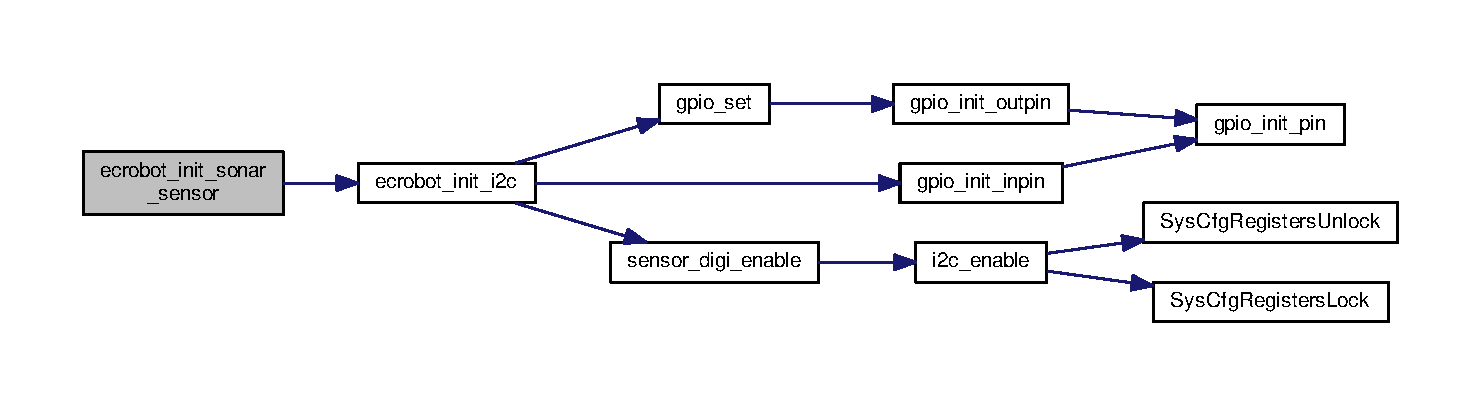
\includegraphics[width=350pt]{ecrobot__interface_8c_a1987f8ae51d64da9e63185302c84c6dc_cgraph}
\end{center}
\end{figure}


\hypertarget{ecrobot__interface_8c_a87f6986d1cd3ece1c2ed94d2781f4073}{}\index{ecrobot\+\_\+interface.\+c@{ecrobot\+\_\+interface.\+c}!ecrobot\+\_\+init\+\_\+temperature\+\_\+sensor@{ecrobot\+\_\+init\+\_\+temperature\+\_\+sensor}}
\index{ecrobot\+\_\+init\+\_\+temperature\+\_\+sensor@{ecrobot\+\_\+init\+\_\+temperature\+\_\+sensor}!ecrobot\+\_\+interface.\+c@{ecrobot\+\_\+interface.\+c}}
\subsubsection[{ecrobot\+\_\+init\+\_\+temperature\+\_\+sensor(\+U8 port\+\_\+id)}]{\setlength{\rightskip}{0pt plus 5cm}void ecrobot\+\_\+init\+\_\+temperature\+\_\+sensor (
\begin{DoxyParamCaption}
\item[{{\bf U8}}]{port\+\_\+id}
\end{DoxyParamCaption}
)}\label{ecrobot__interface_8c_a87f6986d1cd3ece1c2ed94d2781f4073}


Initializes a port for I2\+C communication for Temperature Sensor. 


\begin{DoxyParams}{Parameters}
{\em port\+\_\+id} & -\/ E\+V3\+\_\+\+P\+O\+R\+T\+\_\+\+A, E\+V3\+\_\+\+P\+O\+R\+T\+\_\+\+B, E\+V3\+\_\+\+P\+O\+R\+T\+\_\+\+C, E\+V3\+\_\+\+P\+O\+R\+T\+\_\+\+D\\
\hline
\end{DoxyParams}
\begin{DoxyReturn}{Returns}
none 
\end{DoxyReturn}


Here is the call graph for this function\+:\nopagebreak
\begin{figure}[H]
\begin{center}
\leavevmode
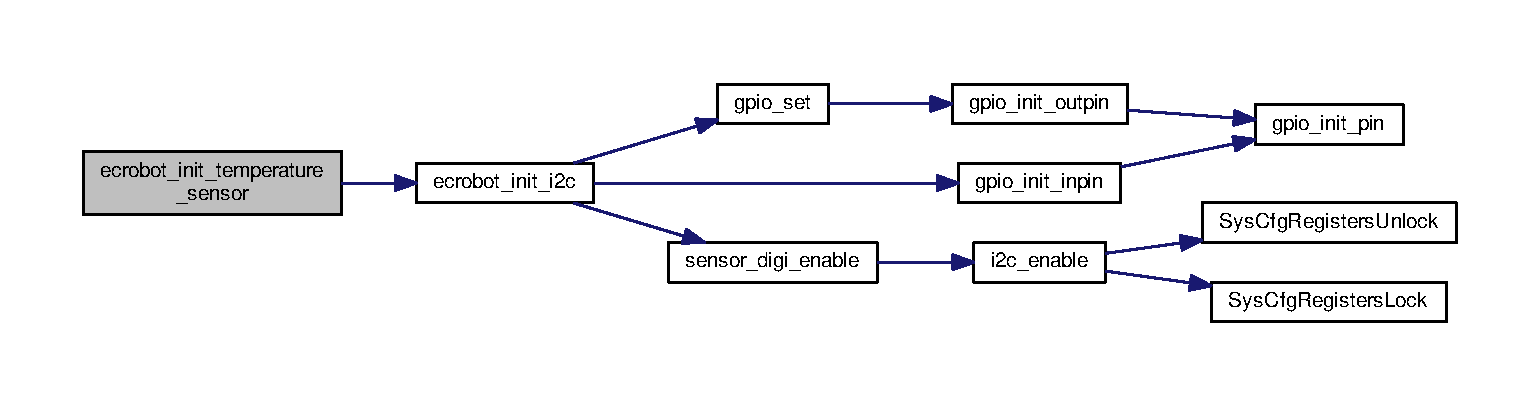
\includegraphics[width=350pt]{ecrobot__interface_8c_a87f6986d1cd3ece1c2ed94d2781f4073_cgraph}
\end{center}
\end{figure}


\hypertarget{ecrobot__interface_8c_a8671b27a6f7da38378c08231b687433c}{}\index{ecrobot\+\_\+interface.\+c@{ecrobot\+\_\+interface.\+c}!ecrobot\+\_\+is\+\_\+\+E\+N\+T\+E\+R\+\_\+button\+\_\+pressed@{ecrobot\+\_\+is\+\_\+\+E\+N\+T\+E\+R\+\_\+button\+\_\+pressed}}
\index{ecrobot\+\_\+is\+\_\+\+E\+N\+T\+E\+R\+\_\+button\+\_\+pressed@{ecrobot\+\_\+is\+\_\+\+E\+N\+T\+E\+R\+\_\+button\+\_\+pressed}!ecrobot\+\_\+interface.\+c@{ecrobot\+\_\+interface.\+c}}
\subsubsection[{ecrobot\+\_\+is\+\_\+\+E\+N\+T\+E\+R\+\_\+button\+\_\+pressed(void)}]{\setlength{\rightskip}{0pt plus 5cm}{\bf U8} ecrobot\+\_\+is\+\_\+\+E\+N\+T\+E\+R\+\_\+button\+\_\+pressed (
\begin{DoxyParamCaption}
\item[{void}]{}
\end{DoxyParamCaption}
)}\label{ecrobot__interface_8c_a8671b27a6f7da38378c08231b687433c}


Returns status of the enter button. 

\begin{DoxyReturn}{Returns}
1(is pressed), 0(is not pressed) 
\end{DoxyReturn}


Here is the call graph for this function\+:\nopagebreak
\begin{figure}[H]
\begin{center}
\leavevmode
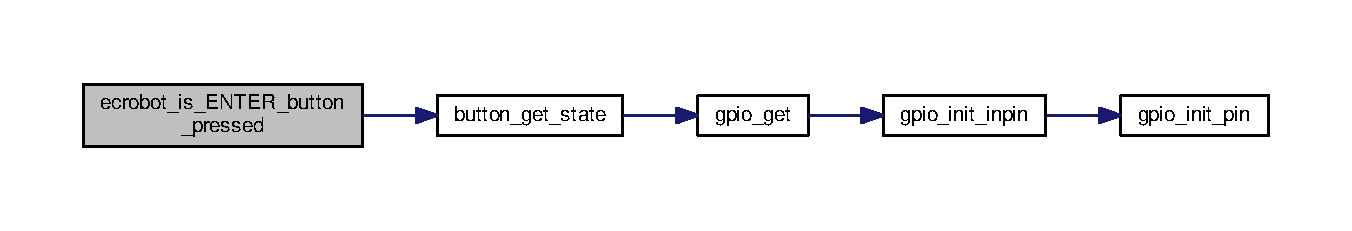
\includegraphics[width=350pt]{ecrobot__interface_8c_a8671b27a6f7da38378c08231b687433c_cgraph}
\end{center}
\end{figure}


\hypertarget{ecrobot__interface_8c_a105aa94999ce18090972316b9679a400}{}\index{ecrobot\+\_\+interface.\+c@{ecrobot\+\_\+interface.\+c}!ecrobot\+\_\+is\+\_\+\+R\+U\+N\+\_\+button\+\_\+pressed@{ecrobot\+\_\+is\+\_\+\+R\+U\+N\+\_\+button\+\_\+pressed}}
\index{ecrobot\+\_\+is\+\_\+\+R\+U\+N\+\_\+button\+\_\+pressed@{ecrobot\+\_\+is\+\_\+\+R\+U\+N\+\_\+button\+\_\+pressed}!ecrobot\+\_\+interface.\+c@{ecrobot\+\_\+interface.\+c}}
\subsubsection[{ecrobot\+\_\+is\+\_\+\+R\+U\+N\+\_\+button\+\_\+pressed(void)}]{\setlength{\rightskip}{0pt plus 5cm}{\bf U8} ecrobot\+\_\+is\+\_\+\+R\+U\+N\+\_\+button\+\_\+pressed (
\begin{DoxyParamCaption}
\item[{void}]{}
\end{DoxyParamCaption}
)}\label{ecrobot__interface_8c_a105aa94999ce18090972316b9679a400}


Returns status of the run button. 

\begin{DoxyReturn}{Returns}
1(is pressed), 0(is not pressed) 
\end{DoxyReturn}


Here is the call graph for this function\+:\nopagebreak
\begin{figure}[H]
\begin{center}
\leavevmode
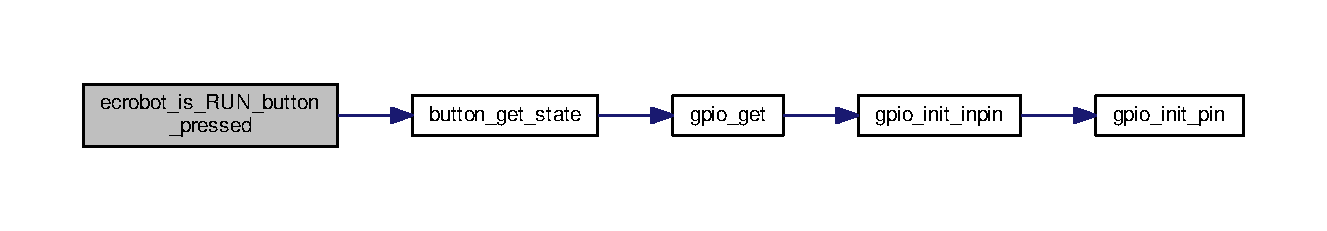
\includegraphics[width=350pt]{ecrobot__interface_8c_a105aa94999ce18090972316b9679a400_cgraph}
\end{center}
\end{figure}


\hypertarget{ecrobot__interface_8c_ae2705c2c961299e7e1899b71d751519e}{}\index{ecrobot\+\_\+interface.\+c@{ecrobot\+\_\+interface.\+c}!ecrobot\+\_\+read\+\_\+i2c@{ecrobot\+\_\+read\+\_\+i2c}}
\index{ecrobot\+\_\+read\+\_\+i2c@{ecrobot\+\_\+read\+\_\+i2c}!ecrobot\+\_\+interface.\+c@{ecrobot\+\_\+interface.\+c}}
\subsubsection[{ecrobot\+\_\+read\+\_\+i2c(\+U8 port\+\_\+id, U32 address, S\+I\+N\+T i2c\+\_\+reg, U8 $\ast$buf, U32 len)}]{\setlength{\rightskip}{0pt plus 5cm}{\bf S\+I\+N\+T} ecrobot\+\_\+read\+\_\+i2c (
\begin{DoxyParamCaption}
\item[{{\bf U8}}]{port\+\_\+id, }
\item[{{\bf U32}}]{address, }
\item[{{\bf S\+I\+N\+T}}]{i2c\+\_\+reg, }
\item[{{\bf U8} $\ast$}]{buf, }
\item[{{\bf U32}}]{len}
\end{DoxyParamCaption}
)}\label{ecrobot__interface_8c_ae2705c2c961299e7e1899b71d751519e}


Read I2\+C data. 


\begin{DoxyParams}{Parameters}
{\em port\+\_\+id} & -\/ E\+V3\+\_\+\+P\+O\+R\+T\+\_\+\+A, E\+V3\+\_\+\+P\+O\+R\+T\+\_\+\+B, E\+V3\+\_\+\+P\+O\+R\+T\+\_\+\+C, E\+V3\+\_\+\+P\+O\+R\+T\+\_\+\+D \\
\hline
{\em address} & -\/ 0x01 to 0x7\+F (Note that addresses are from 0x01 to 0x7\+F not even numbers from 0x02 to 0x\+F\+E as given in some I2\+C device specifications. They are 7-\/bit addresses not 8-\/bit addresses) \\
\hline
{\em i2c\+\_\+reg} & -\/ I2\+C register e.\+g. 0x42 \\
\hline
{\em buf} & -\/ buffer to return data \\
\hline
{\em len} & -\/ length of the return data\\
\hline
\end{DoxyParams}
\begin{DoxyReturn}{Returns}
1(success), 0(failure) 
\end{DoxyReturn}


Here is the call graph for this function\+:\nopagebreak
\begin{figure}[H]
\begin{center}
\leavevmode
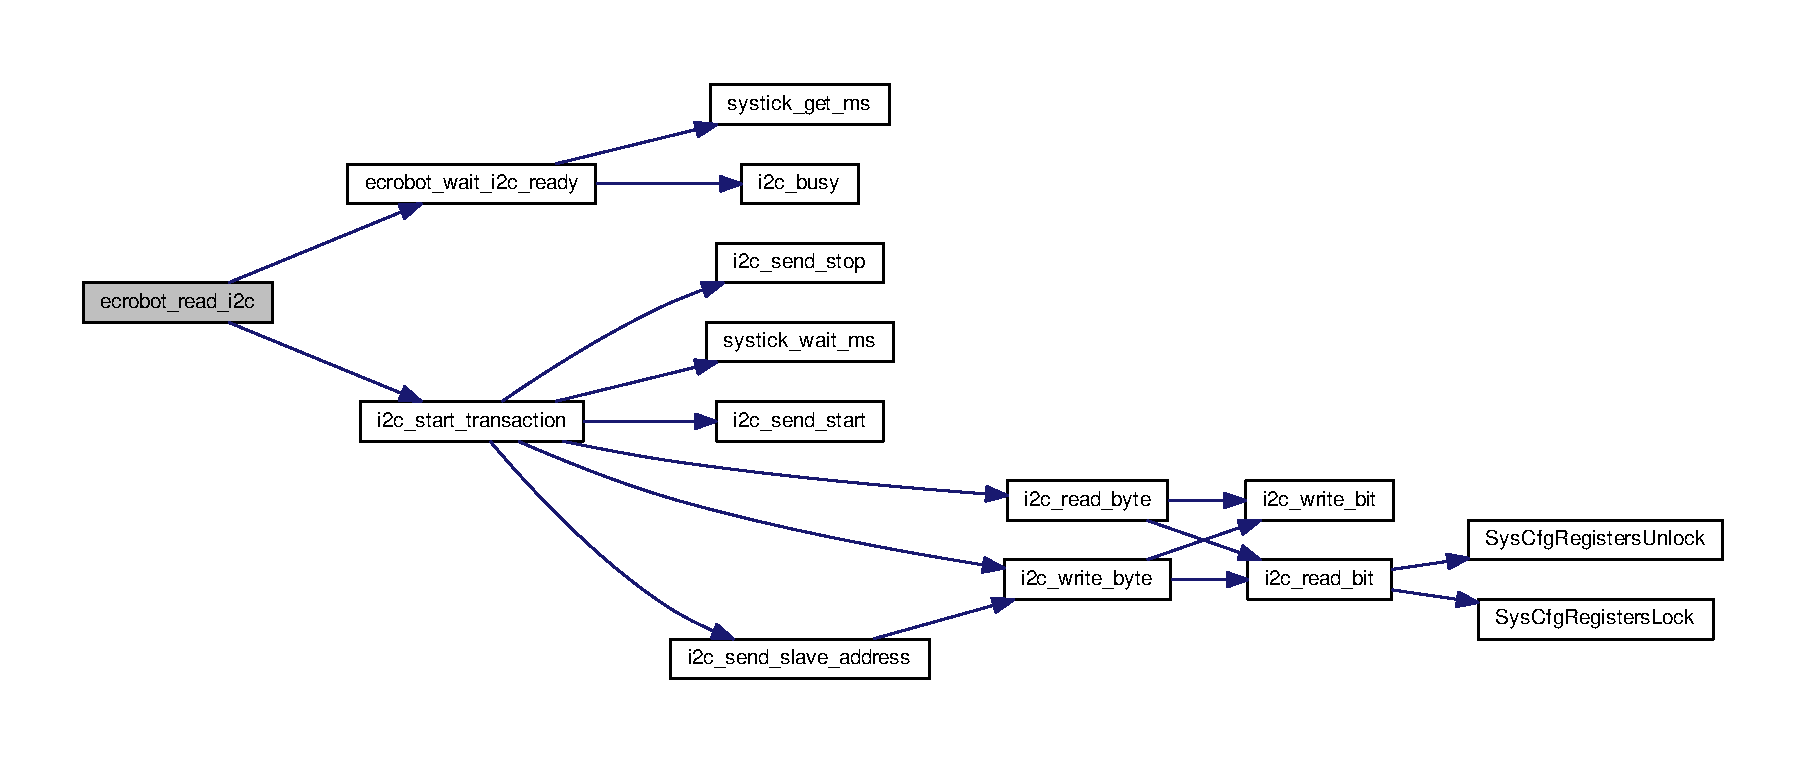
\includegraphics[width=350pt]{ecrobot__interface_8c_ae2705c2c961299e7e1899b71d751519e_cgraph}
\end{center}
\end{figure}


\hypertarget{ecrobot__interface_8c_af1ca8c1fc75c05182aeb6fe60172fe54}{}\index{ecrobot\+\_\+interface.\+c@{ecrobot\+\_\+interface.\+c}!ecrobot\+\_\+send\+\_\+i2c@{ecrobot\+\_\+send\+\_\+i2c}}
\index{ecrobot\+\_\+send\+\_\+i2c@{ecrobot\+\_\+send\+\_\+i2c}!ecrobot\+\_\+interface.\+c@{ecrobot\+\_\+interface.\+c}}
\subsubsection[{ecrobot\+\_\+send\+\_\+i2c(\+U8 port\+\_\+id, U32 address, S\+I\+N\+T i2c\+\_\+reg, U8 $\ast$buf, U32 len)}]{\setlength{\rightskip}{0pt plus 5cm}{\bf S\+I\+N\+T} ecrobot\+\_\+send\+\_\+i2c (
\begin{DoxyParamCaption}
\item[{{\bf U8}}]{port\+\_\+id, }
\item[{{\bf U32}}]{address, }
\item[{{\bf S\+I\+N\+T}}]{i2c\+\_\+reg, }
\item[{{\bf U8} $\ast$}]{buf, }
\item[{{\bf U32}}]{len}
\end{DoxyParamCaption}
)}\label{ecrobot__interface_8c_af1ca8c1fc75c05182aeb6fe60172fe54}


Send I2\+C data. 


\begin{DoxyParams}{Parameters}
{\em port\+\_\+id} & -\/ E\+V3\+\_\+\+P\+O\+R\+T\+\_\+\+A, E\+V3\+\_\+\+P\+O\+R\+T\+\_\+\+B, E\+V3\+\_\+\+P\+O\+R\+T\+\_\+\+C, E\+V3\+\_\+\+P\+O\+R\+T\+\_\+\+D \\
\hline
{\em address} & -\/ 0x01 to 0x7\+F (Note that addresses are from 0x01 to 0x7\+F not even numbers from 0x02 to 0x\+F\+E as given in some I2\+C device specifications. They are 7-\/bit addresses not 8-\/bit addresses) \\
\hline
{\em i2c\+\_\+reg} & -\/ I2\+C register e.\+g. 0x42 \\
\hline
{\em buf} & -\/ buffer containing data to send \\
\hline
{\em len} & -\/ length of the data to send\\
\hline
\end{DoxyParams}
\begin{DoxyReturn}{Returns}
1(success), 0(failure) 
\end{DoxyReturn}


Here is the call graph for this function\+:\nopagebreak
\begin{figure}[H]
\begin{center}
\leavevmode
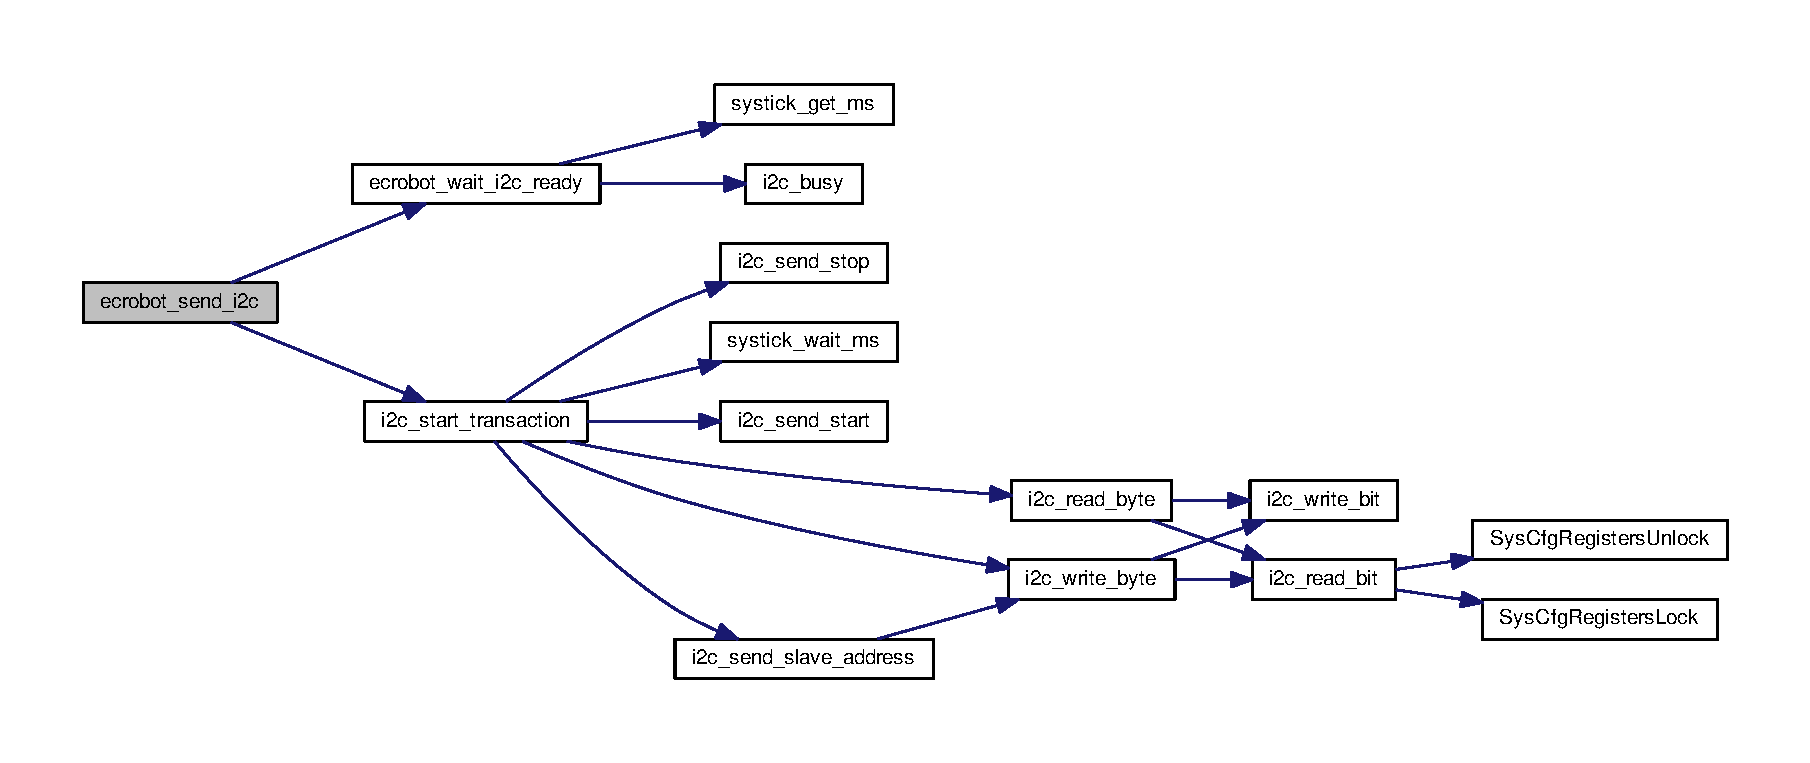
\includegraphics[width=350pt]{ecrobot__interface_8c_af1ca8c1fc75c05182aeb6fe60172fe54_cgraph}
\end{center}
\end{figure}


\hypertarget{ecrobot__interface_8c_aa583da85d360db935d690a72365ab12d}{}\index{ecrobot\+\_\+interface.\+c@{ecrobot\+\_\+interface.\+c}!ecrobot\+\_\+set\+\_\+light\+\_\+sensor\+\_\+active@{ecrobot\+\_\+set\+\_\+light\+\_\+sensor\+\_\+active}}
\index{ecrobot\+\_\+set\+\_\+light\+\_\+sensor\+\_\+active@{ecrobot\+\_\+set\+\_\+light\+\_\+sensor\+\_\+active}!ecrobot\+\_\+interface.\+c@{ecrobot\+\_\+interface.\+c}}
\subsubsection[{ecrobot\+\_\+set\+\_\+light\+\_\+sensor\+\_\+active(\+U8 port\+\_\+id)}]{\setlength{\rightskip}{0pt plus 5cm}void ecrobot\+\_\+set\+\_\+light\+\_\+sensor\+\_\+active (
\begin{DoxyParamCaption}
\item[{{\bf U8}}]{port\+\_\+id}
\end{DoxyParamCaption}
)}\label{ecrobot__interface_8c_aa583da85d360db935d690a72365ab12d}


Turn infra-\/red light on. 


\begin{DoxyParams}{Parameters}
{\em port\+\_\+id} & -\/ E\+V3\+\_\+\+P\+O\+R\+T\+\_\+\+A, E\+V3\+\_\+\+P\+O\+R\+T\+\_\+\+B, E\+V3\+\_\+\+P\+O\+R\+T\+\_\+\+C, E\+V3\+\_\+\+P\+O\+R\+T\+\_\+\+D\\
\hline
\end{DoxyParams}
\begin{DoxyReturn}{Returns}
none 
\end{DoxyReturn}


Here is the call graph for this function\+:\nopagebreak
\begin{figure}[H]
\begin{center}
\leavevmode
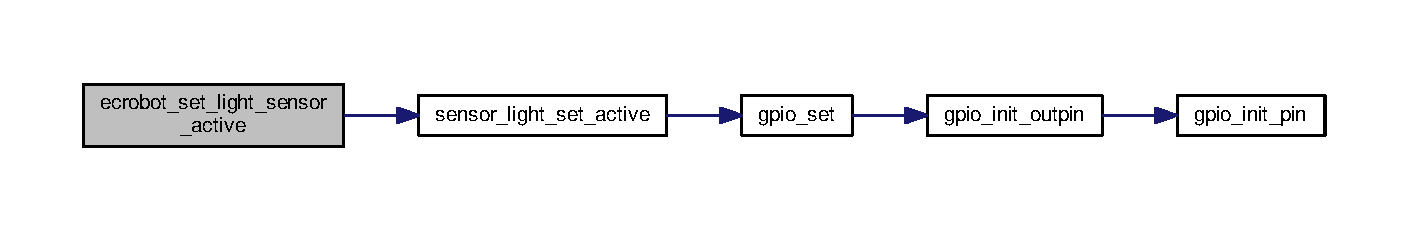
\includegraphics[width=350pt]{ecrobot__interface_8c_aa583da85d360db935d690a72365ab12d_cgraph}
\end{center}
\end{figure}


\hypertarget{ecrobot__interface_8c_a6913437b16d6917a1cdb4d5e18a0093b}{}\index{ecrobot\+\_\+interface.\+c@{ecrobot\+\_\+interface.\+c}!ecrobot\+\_\+set\+\_\+light\+\_\+sensor\+\_\+inactive@{ecrobot\+\_\+set\+\_\+light\+\_\+sensor\+\_\+inactive}}
\index{ecrobot\+\_\+set\+\_\+light\+\_\+sensor\+\_\+inactive@{ecrobot\+\_\+set\+\_\+light\+\_\+sensor\+\_\+inactive}!ecrobot\+\_\+interface.\+c@{ecrobot\+\_\+interface.\+c}}
\subsubsection[{ecrobot\+\_\+set\+\_\+light\+\_\+sensor\+\_\+inactive(\+U8 port\+\_\+id)}]{\setlength{\rightskip}{0pt plus 5cm}void ecrobot\+\_\+set\+\_\+light\+\_\+sensor\+\_\+inactive (
\begin{DoxyParamCaption}
\item[{{\bf U8}}]{port\+\_\+id}
\end{DoxyParamCaption}
)}\label{ecrobot__interface_8c_a6913437b16d6917a1cdb4d5e18a0093b}


Turn infra-\/red light off. 


\begin{DoxyParams}{Parameters}
{\em port\+\_\+id} & -\/ E\+V3\+\_\+\+P\+O\+R\+T\+\_\+\+A, E\+V3\+\_\+\+P\+O\+R\+T\+\_\+\+B, E\+V3\+\_\+\+P\+O\+R\+T\+\_\+\+C, E\+V3\+\_\+\+P\+O\+R\+T\+\_\+\+D\\
\hline
\end{DoxyParams}
\begin{DoxyReturn}{Returns}
none 
\end{DoxyReturn}


Here is the call graph for this function\+:\nopagebreak
\begin{figure}[H]
\begin{center}
\leavevmode
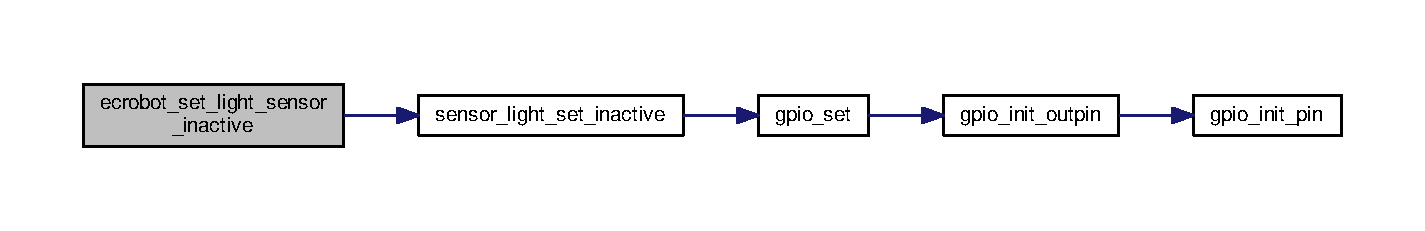
\includegraphics[width=350pt]{ecrobot__interface_8c_a6913437b16d6917a1cdb4d5e18a0093b_cgraph}
\end{center}
\end{figure}


\hypertarget{ecrobot__interface_8c_a243c5a9de426a2ceb53f13dc7c7945ee}{}\index{ecrobot\+\_\+interface.\+c@{ecrobot\+\_\+interface.\+c}!ecrobot\+\_\+set\+\_\+motor\+\_\+mode\+\_\+speed@{ecrobot\+\_\+set\+\_\+motor\+\_\+mode\+\_\+speed}}
\index{ecrobot\+\_\+set\+\_\+motor\+\_\+mode\+\_\+speed@{ecrobot\+\_\+set\+\_\+motor\+\_\+mode\+\_\+speed}!ecrobot\+\_\+interface.\+c@{ecrobot\+\_\+interface.\+c}}
\subsubsection[{ecrobot\+\_\+set\+\_\+motor\+\_\+mode\+\_\+speed(\+U8 port\+\_\+id, S32 mode, S8 speed)}]{\setlength{\rightskip}{0pt plus 5cm}void ecrobot\+\_\+set\+\_\+motor\+\_\+mode\+\_\+speed (
\begin{DoxyParamCaption}
\item[{{\bf U8}}]{port\+\_\+id, }
\item[{{\bf S32}}]{mode, }
\item[{{\bf S8}}]{speed}
\end{DoxyParamCaption}
)}\label{ecrobot__interface_8c_a243c5a9de426a2ceb53f13dc7c7945ee}


Sets Servo Motor brake mode and P\+W\+M value. Wrapper of nxt\+\_\+motor\+\_\+set\+\_\+speed. 


\begin{DoxyParams}{Parameters}
{\em port\+\_\+id} & -\/ E\+V3\+\_\+\+P\+O\+R\+T\+\_\+1, E\+V3\+\_\+\+P\+O\+R\+T\+\_\+2, E\+V3\+\_\+\+P\+O\+R\+T\+\_\+3, E\+V3\+\_\+\+P\+O\+R\+T\+\_\+4 \\
\hline
{\em mode} & -\/ 0(float), 1(brake) \\
\hline
{\em speed} & -\/ -\/100 to +100\\
\hline
\end{DoxyParams}
\begin{DoxyReturn}{Returns}
none 
\end{DoxyReturn}


Here is the call graph for this function\+:\nopagebreak
\begin{figure}[H]
\begin{center}
\leavevmode
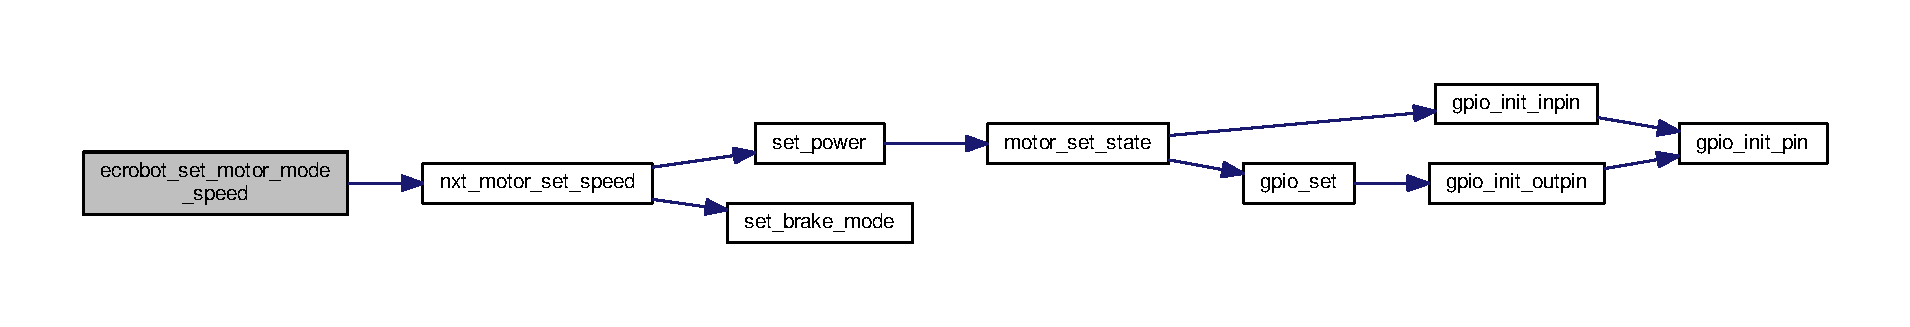
\includegraphics[width=350pt]{ecrobot__interface_8c_a243c5a9de426a2ceb53f13dc7c7945ee_cgraph}
\end{center}
\end{figure}


\hypertarget{ecrobot__interface_8c_a716b589796dd18ec023ef45a4aca6b10}{}\index{ecrobot\+\_\+interface.\+c@{ecrobot\+\_\+interface.\+c}!ecrobot\+\_\+set\+\_\+motor\+\_\+rev@{ecrobot\+\_\+set\+\_\+motor\+\_\+rev}}
\index{ecrobot\+\_\+set\+\_\+motor\+\_\+rev@{ecrobot\+\_\+set\+\_\+motor\+\_\+rev}!ecrobot\+\_\+interface.\+c@{ecrobot\+\_\+interface.\+c}}
\subsubsection[{ecrobot\+\_\+set\+\_\+motor\+\_\+rev(\+U8 port\+\_\+id, S32 rev)}]{\setlength{\rightskip}{0pt plus 5cm}void ecrobot\+\_\+set\+\_\+motor\+\_\+rev (
\begin{DoxyParamCaption}
\item[{{\bf U8}}]{port\+\_\+id, }
\item[{{\bf S32}}]{rev}
\end{DoxyParamCaption}
)}\label{ecrobot__interface_8c_a716b589796dd18ec023ef45a4aca6b10}


Sets Servo Motor revolution value in degree. Wrapper of nxt\+\_\+motor\+\_\+set\+\_\+count. 


\begin{DoxyParams}{Parameters}
{\em port\+\_\+id} & -\/ E\+V3\+\_\+\+P\+O\+R\+T\+\_\+1, E\+V3\+\_\+\+P\+O\+R\+T\+\_\+2, E\+V3\+\_\+\+P\+O\+R\+T\+\_\+3, E\+V3\+\_\+\+P\+O\+R\+T\+\_\+4 \\
\hline
{\em rev} & -\/ Servo Motors revolution in degree\\
\hline
\end{DoxyParams}
\begin{DoxyReturn}{Returns}
none 
\end{DoxyReturn}


Here is the call graph for this function\+:\nopagebreak
\begin{figure}[H]
\begin{center}
\leavevmode
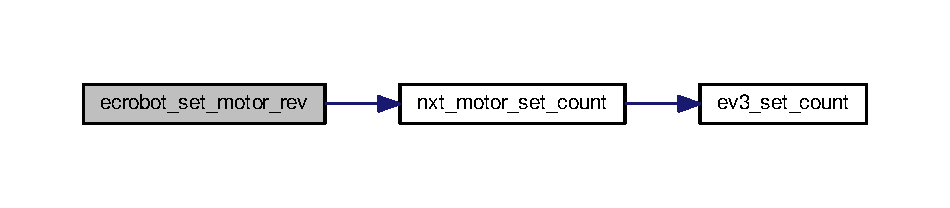
\includegraphics[width=350pt]{ecrobot__interface_8c_a716b589796dd18ec023ef45a4aca6b10_cgraph}
\end{center}
\end{figure}


\hypertarget{ecrobot__interface_8c_a058a4f6b8b8cd0cd9b341f7728a0be4d}{}\index{ecrobot\+\_\+interface.\+c@{ecrobot\+\_\+interface.\+c}!ecrobot\+\_\+set\+\_\+motor\+\_\+speed@{ecrobot\+\_\+set\+\_\+motor\+\_\+speed}}
\index{ecrobot\+\_\+set\+\_\+motor\+\_\+speed@{ecrobot\+\_\+set\+\_\+motor\+\_\+speed}!ecrobot\+\_\+interface.\+c@{ecrobot\+\_\+interface.\+c}}
\subsubsection[{ecrobot\+\_\+set\+\_\+motor\+\_\+speed(\+U8 port\+\_\+id, S8 speed)}]{\setlength{\rightskip}{0pt plus 5cm}void ecrobot\+\_\+set\+\_\+motor\+\_\+speed (
\begin{DoxyParamCaption}
\item[{{\bf U8}}]{port\+\_\+id, }
\item[{{\bf S8}}]{speed}
\end{DoxyParamCaption}
)}\label{ecrobot__interface_8c_a058a4f6b8b8cd0cd9b341f7728a0be4d}


Sets Servo Motor P\+W\+M value. Wrapper of nxt\+\_\+motor\+\_\+set\+\_\+speed, but brake mode is fixed as brake. 


\begin{DoxyParams}{Parameters}
{\em port\+\_\+id} & -\/ E\+V3\+\_\+\+P\+O\+R\+T\+\_\+1, E\+V3\+\_\+\+P\+O\+R\+T\+\_\+2, E\+V3\+\_\+\+P\+O\+R\+T\+\_\+3, E\+V3\+\_\+\+P\+O\+R\+T\+\_\+4 \\
\hline
{\em speed} & -\/ -\/100 to +100\\
\hline
\end{DoxyParams}
\begin{DoxyReturn}{Returns}
none 
\end{DoxyReturn}


Here is the call graph for this function\+:\nopagebreak
\begin{figure}[H]
\begin{center}
\leavevmode
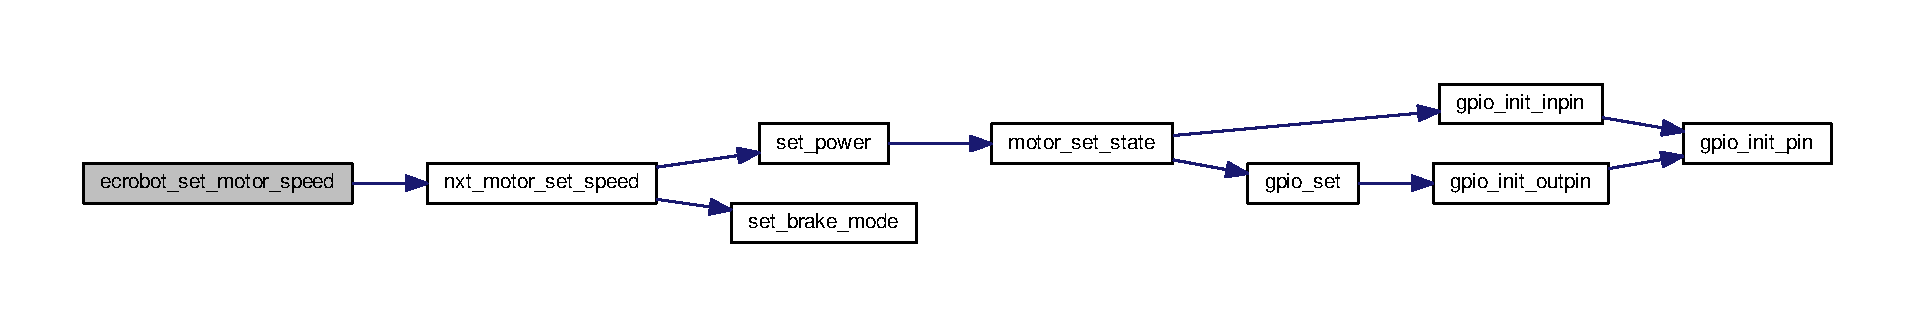
\includegraphics[width=350pt]{ecrobot__interface_8c_a058a4f6b8b8cd0cd9b341f7728a0be4d_cgraph}
\end{center}
\end{figure}


\hypertarget{ecrobot__interface_8c_a3931f4ecc2a1fe1e20b540fb8fde4df8}{}\index{ecrobot\+\_\+interface.\+c@{ecrobot\+\_\+interface.\+c}!ecrobot\+\_\+set\+Resolution\+\_\+temperature\+\_\+sensor@{ecrobot\+\_\+set\+Resolution\+\_\+temperature\+\_\+sensor}}
\index{ecrobot\+\_\+set\+Resolution\+\_\+temperature\+\_\+sensor@{ecrobot\+\_\+set\+Resolution\+\_\+temperature\+\_\+sensor}!ecrobot\+\_\+interface.\+c@{ecrobot\+\_\+interface.\+c}}
\subsubsection[{ecrobot\+\_\+set\+Resolution\+\_\+temperature\+\_\+sensor(\+U8 port\+\_\+id, U8 resolution)}]{\setlength{\rightskip}{0pt plus 5cm}void ecrobot\+\_\+set\+Resolution\+\_\+temperature\+\_\+sensor (
\begin{DoxyParamCaption}
\item[{{\bf U8}}]{port\+\_\+id, }
\item[{{\bf U8}}]{resolution}
\end{DoxyParamCaption}
)}\label{ecrobot__interface_8c_a3931f4ecc2a1fe1e20b540fb8fde4df8}


Set the resolution for the measured temperature values. 

The internal Texas Instruments tmp275 temperature sensor can operate in different resolution modes. Lower resolution is faster. See the T\+E\+M\+P9\+B\+I\+T ... T\+E\+M\+P12\+B\+I\+T macros for more information or the official documentation.


\begin{DoxyParams}{Parameters}
{\em port\+\_\+id} & -\/ E\+V3\+\_\+\+P\+O\+R\+T\+\_\+\+A, E\+V3\+\_\+\+P\+O\+R\+T\+\_\+\+B, E\+V3\+\_\+\+P\+O\+R\+T\+\_\+\+C, E\+V3\+\_\+\+P\+O\+R\+T\+\_\+\+D \\
\hline
{\em resolution} & -\/ The resolution. Use on of the macros T\+E\+M\+P9\+B\+I\+T ... T\+E\+M\+P12\+B\+I\+T\\
\hline
\end{DoxyParams}
\begin{DoxyReturn}{Returns}
none 
\end{DoxyReturn}


Here is the call graph for this function\+:\nopagebreak
\begin{figure}[H]
\begin{center}
\leavevmode
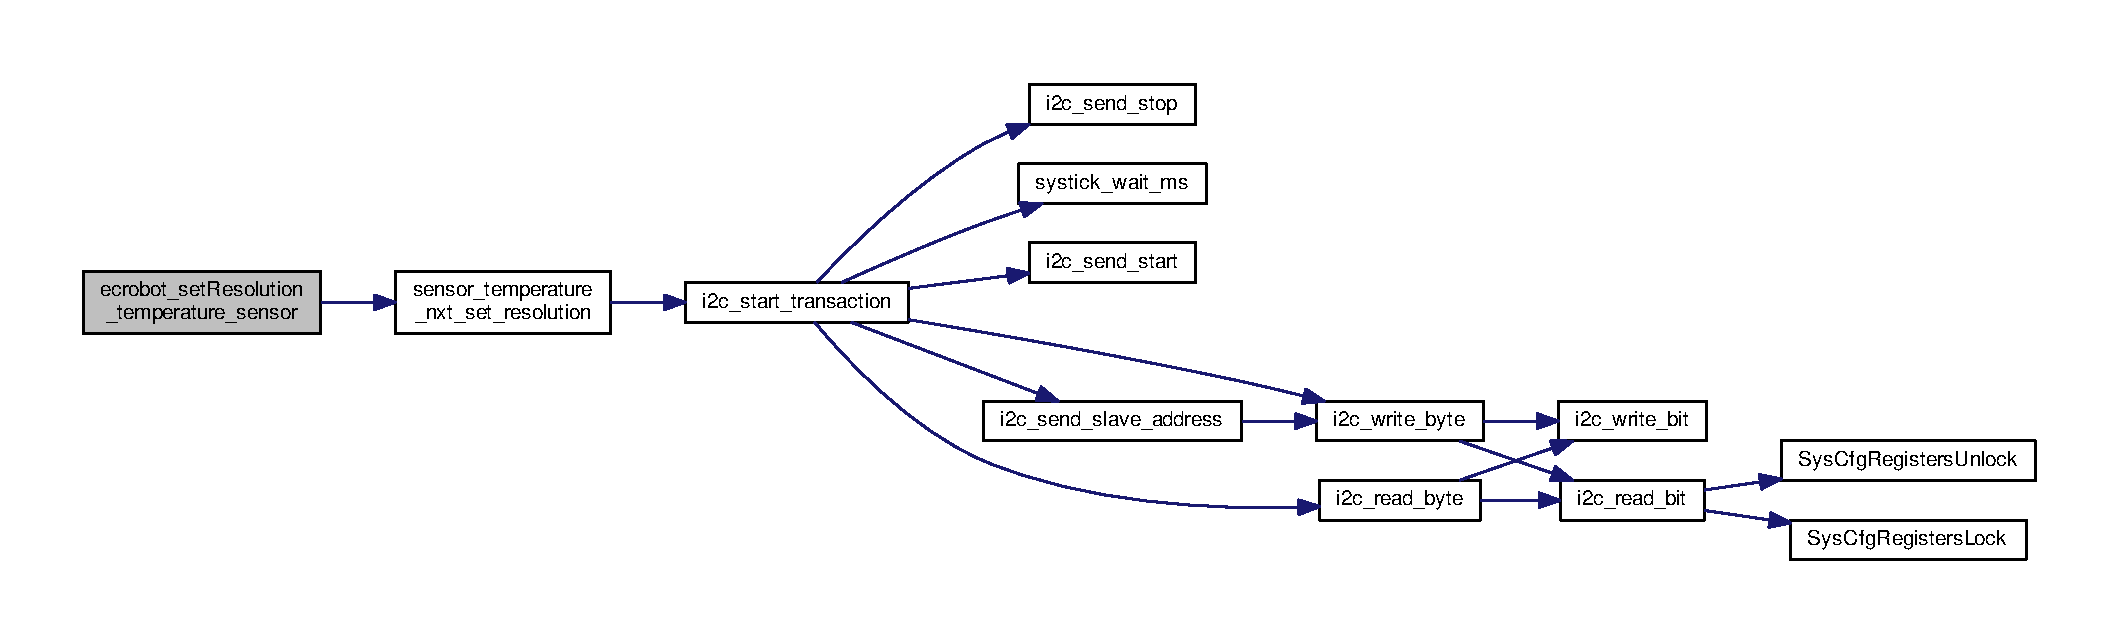
\includegraphics[width=350pt]{ecrobot__interface_8c_a3931f4ecc2a1fe1e20b540fb8fde4df8_cgraph}
\end{center}
\end{figure}


\hypertarget{ecrobot__interface_8c_a0d3f189f2fb27cfd95136e99e83e9044}{}\index{ecrobot\+\_\+interface.\+c@{ecrobot\+\_\+interface.\+c}!ecrobot\+\_\+term\+\_\+accel\+\_\+sensor@{ecrobot\+\_\+term\+\_\+accel\+\_\+sensor}}
\index{ecrobot\+\_\+term\+\_\+accel\+\_\+sensor@{ecrobot\+\_\+term\+\_\+accel\+\_\+sensor}!ecrobot\+\_\+interface.\+c@{ecrobot\+\_\+interface.\+c}}
\subsubsection[{ecrobot\+\_\+term\+\_\+accel\+\_\+sensor(\+U8 port\+\_\+id)}]{\setlength{\rightskip}{0pt plus 5cm}void ecrobot\+\_\+term\+\_\+accel\+\_\+sensor (
\begin{DoxyParamCaption}
\item[{{\bf U8}}]{port\+\_\+id}
\end{DoxyParamCaption}
)}\label{ecrobot__interface_8c_a0d3f189f2fb27cfd95136e99e83e9044}


Terminates I2\+C communication used for Acceleraton Sensor. This function should be implemented in the device terminate hook routine. 


\begin{DoxyParams}{Parameters}
{\em port\+\_\+id} & -\/ E\+V3\+\_\+\+P\+O\+R\+T\+\_\+\+A, E\+V3\+\_\+\+P\+O\+R\+T\+\_\+\+B, E\+V3\+\_\+\+P\+O\+R\+T\+\_\+\+C, E\+V3\+\_\+\+P\+O\+R\+T\+\_\+\+D\\
\hline
\end{DoxyParams}
\begin{DoxyReturn}{Returns}
none 
\end{DoxyReturn}


Here is the call graph for this function\+:\nopagebreak
\begin{figure}[H]
\begin{center}
\leavevmode
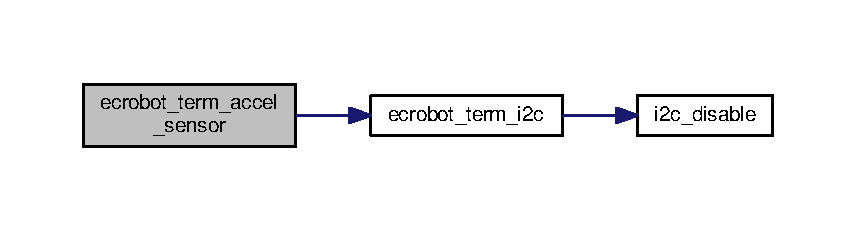
\includegraphics[width=350pt]{ecrobot__interface_8c_a0d3f189f2fb27cfd95136e99e83e9044_cgraph}
\end{center}
\end{figure}


\hypertarget{ecrobot__interface_8c_a8d365c7adeac0016b97754d45d3352f7}{}\index{ecrobot\+\_\+interface.\+c@{ecrobot\+\_\+interface.\+c}!ecrobot\+\_\+term\+\_\+color\+\_\+sensor@{ecrobot\+\_\+term\+\_\+color\+\_\+sensor}}
\index{ecrobot\+\_\+term\+\_\+color\+\_\+sensor@{ecrobot\+\_\+term\+\_\+color\+\_\+sensor}!ecrobot\+\_\+interface.\+c@{ecrobot\+\_\+interface.\+c}}
\subsubsection[{ecrobot\+\_\+term\+\_\+color\+\_\+sensor(\+U8 port\+\_\+id)}]{\setlength{\rightskip}{0pt plus 5cm}void ecrobot\+\_\+term\+\_\+color\+\_\+sensor (
\begin{DoxyParamCaption}
\item[{{\bf U8}}]{port\+\_\+id}
\end{DoxyParamCaption}
)}\label{ecrobot__interface_8c_a8d365c7adeac0016b97754d45d3352f7}


Terminates I2\+C communication used for the Color Sensor. This function should be implemented in the device terminate hook routine. 


\begin{DoxyParams}{Parameters}
{\em port\+\_\+id} & -\/ E\+V3\+\_\+\+P\+O\+R\+T\+\_\+\+A, E\+V3\+\_\+\+P\+O\+R\+T\+\_\+\+B, E\+V3\+\_\+\+P\+O\+R\+T\+\_\+\+C, E\+V3\+\_\+\+P\+O\+R\+T\+\_\+\+D\\
\hline
\end{DoxyParams}
\begin{DoxyReturn}{Returns}
none 
\end{DoxyReturn}


Here is the call graph for this function\+:\nopagebreak
\begin{figure}[H]
\begin{center}
\leavevmode
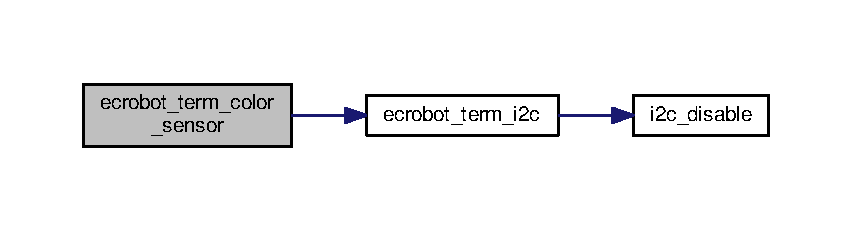
\includegraphics[width=350pt]{ecrobot__interface_8c_a8d365c7adeac0016b97754d45d3352f7_cgraph}
\end{center}
\end{figure}


\hypertarget{ecrobot__interface_8c_aeb7a9d999e93c0bf60ff6c8a633da305}{}\index{ecrobot\+\_\+interface.\+c@{ecrobot\+\_\+interface.\+c}!ecrobot\+\_\+term\+\_\+compass\+\_\+sensor@{ecrobot\+\_\+term\+\_\+compass\+\_\+sensor}}
\index{ecrobot\+\_\+term\+\_\+compass\+\_\+sensor@{ecrobot\+\_\+term\+\_\+compass\+\_\+sensor}!ecrobot\+\_\+interface.\+c@{ecrobot\+\_\+interface.\+c}}
\subsubsection[{ecrobot\+\_\+term\+\_\+compass\+\_\+sensor(\+U8 port\+\_\+id)}]{\setlength{\rightskip}{0pt plus 5cm}void ecrobot\+\_\+term\+\_\+compass\+\_\+sensor (
\begin{DoxyParamCaption}
\item[{{\bf U8}}]{port\+\_\+id}
\end{DoxyParamCaption}
)}\label{ecrobot__interface_8c_aeb7a9d999e93c0bf60ff6c8a633da305}


Terminates I2\+C communication used for Compass Sensor. This function should be implemented in the device terminate hook routine. 


\begin{DoxyParams}{Parameters}
{\em port\+\_\+id} & -\/ E\+V3\+\_\+\+P\+O\+R\+T\+\_\+\+A, E\+V3\+\_\+\+P\+O\+R\+T\+\_\+\+B, E\+V3\+\_\+\+P\+O\+R\+T\+\_\+\+C, E\+V3\+\_\+\+P\+O\+R\+T\+\_\+\+D\\
\hline
\end{DoxyParams}
\begin{DoxyReturn}{Returns}
none 
\end{DoxyReturn}


Here is the call graph for this function\+:\nopagebreak
\begin{figure}[H]
\begin{center}
\leavevmode
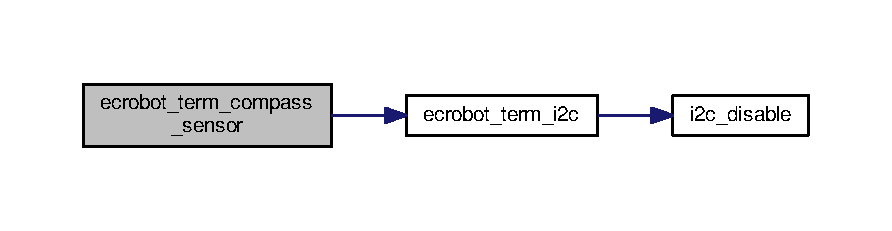
\includegraphics[width=350pt]{ecrobot__interface_8c_aeb7a9d999e93c0bf60ff6c8a633da305_cgraph}
\end{center}
\end{figure}


\hypertarget{ecrobot__interface_8c_adccd23ec10f6723d9ba9463dc44e01dc}{}\index{ecrobot\+\_\+interface.\+c@{ecrobot\+\_\+interface.\+c}!ecrobot\+\_\+term\+\_\+i2c@{ecrobot\+\_\+term\+\_\+i2c}}
\index{ecrobot\+\_\+term\+\_\+i2c@{ecrobot\+\_\+term\+\_\+i2c}!ecrobot\+\_\+interface.\+c@{ecrobot\+\_\+interface.\+c}}
\subsubsection[{ecrobot\+\_\+term\+\_\+i2c(\+U8 port\+\_\+id)}]{\setlength{\rightskip}{0pt plus 5cm}void ecrobot\+\_\+term\+\_\+i2c (
\begin{DoxyParamCaption}
\item[{{\bf U8}}]{port\+\_\+id}
\end{DoxyParamCaption}
)}\label{ecrobot__interface_8c_adccd23ec10f6723d9ba9463dc44e01dc}


Terminate a N\+X\+T sensor port used for I2\+C communication. 


\begin{DoxyParams}{Parameters}
{\em port\+\_\+id} & -\/ E\+V3\+\_\+\+P\+O\+R\+T\+\_\+\+A, E\+V3\+\_\+\+P\+O\+R\+T\+\_\+\+B, E\+V3\+\_\+\+P\+O\+R\+T\+\_\+\+C, E\+V3\+\_\+\+P\+O\+R\+T\+\_\+\+D\\
\hline
\end{DoxyParams}
\begin{DoxyReturn}{Returns}
none 
\end{DoxyReturn}


Here is the call graph for this function\+:\nopagebreak
\begin{figure}[H]
\begin{center}
\leavevmode
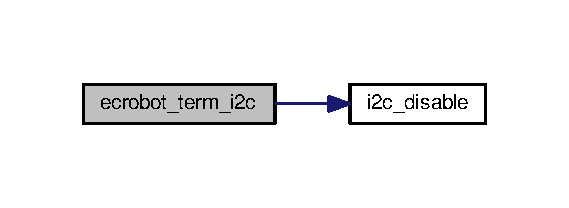
\includegraphics[width=273pt]{ecrobot__interface_8c_adccd23ec10f6723d9ba9463dc44e01dc_cgraph}
\end{center}
\end{figure}


\hypertarget{ecrobot__interface_8c_a435363c3b8faf52afaf83fc935434054}{}\index{ecrobot\+\_\+interface.\+c@{ecrobot\+\_\+interface.\+c}!ecrobot\+\_\+term\+\_\+sonar\+\_\+sensor@{ecrobot\+\_\+term\+\_\+sonar\+\_\+sensor}}
\index{ecrobot\+\_\+term\+\_\+sonar\+\_\+sensor@{ecrobot\+\_\+term\+\_\+sonar\+\_\+sensor}!ecrobot\+\_\+interface.\+c@{ecrobot\+\_\+interface.\+c}}
\subsubsection[{ecrobot\+\_\+term\+\_\+sonar\+\_\+sensor(\+U8 port\+\_\+id)}]{\setlength{\rightskip}{0pt plus 5cm}void ecrobot\+\_\+term\+\_\+sonar\+\_\+sensor (
\begin{DoxyParamCaption}
\item[{{\bf U8}}]{port\+\_\+id}
\end{DoxyParamCaption}
)}\label{ecrobot__interface_8c_a435363c3b8faf52afaf83fc935434054}


Terminate I2\+C used for for Ultrasonic. 


\begin{DoxyParams}{Parameters}
{\em port\+\_\+id} & -\/ E\+V3\+\_\+\+P\+O\+R\+T\+\_\+\+A, E\+V3\+\_\+\+P\+O\+R\+T\+\_\+\+B, E\+V3\+\_\+\+P\+O\+R\+T\+\_\+\+C, E\+V3\+\_\+\+P\+O\+R\+T\+\_\+\+D\\
\hline
\end{DoxyParams}
\begin{DoxyReturn}{Returns}
none 
\end{DoxyReturn}


Here is the call graph for this function\+:\nopagebreak
\begin{figure}[H]
\begin{center}
\leavevmode
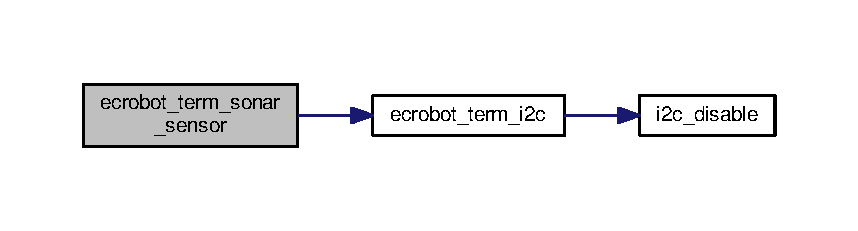
\includegraphics[width=350pt]{ecrobot__interface_8c_a435363c3b8faf52afaf83fc935434054_cgraph}
\end{center}
\end{figure}


\hypertarget{ecrobot__interface_8c_a8d5e57b6d8fb3e702350c59a613ccc16}{}\index{ecrobot\+\_\+interface.\+c@{ecrobot\+\_\+interface.\+c}!ecrobot\+\_\+term\+\_\+temperature\+\_\+sensor@{ecrobot\+\_\+term\+\_\+temperature\+\_\+sensor}}
\index{ecrobot\+\_\+term\+\_\+temperature\+\_\+sensor@{ecrobot\+\_\+term\+\_\+temperature\+\_\+sensor}!ecrobot\+\_\+interface.\+c@{ecrobot\+\_\+interface.\+c}}
\subsubsection[{ecrobot\+\_\+term\+\_\+temperature\+\_\+sensor(\+U8 port\+\_\+id)}]{\setlength{\rightskip}{0pt plus 5cm}void ecrobot\+\_\+term\+\_\+temperature\+\_\+sensor (
\begin{DoxyParamCaption}
\item[{{\bf U8}}]{port\+\_\+id}
\end{DoxyParamCaption}
)}\label{ecrobot__interface_8c_a8d5e57b6d8fb3e702350c59a613ccc16}


Terminates I2\+C communication used for Temperature Sensor. 


\begin{DoxyParams}{Parameters}
{\em port\+\_\+id} & -\/ E\+V3\+\_\+\+P\+O\+R\+T\+\_\+\+A, E\+V3\+\_\+\+P\+O\+R\+T\+\_\+\+B, E\+V3\+\_\+\+P\+O\+R\+T\+\_\+\+C, E\+V3\+\_\+\+P\+O\+R\+T\+\_\+\+D\\
\hline
\end{DoxyParams}
\begin{DoxyReturn}{Returns}
none 
\end{DoxyReturn}


Here is the call graph for this function\+:\nopagebreak
\begin{figure}[H]
\begin{center}
\leavevmode
\includegraphics[width=350pt]{ecrobot__interface_8c_a8d5e57b6d8fb3e702350c59a613ccc16_cgraph}
\end{center}
\end{figure}


\hypertarget{ecrobot__interface_8c_ae54fa3c45ac6d8a2cab8554e1ab48768}{}\index{ecrobot\+\_\+interface.\+c@{ecrobot\+\_\+interface.\+c}!ecrobot\+\_\+wait\+\_\+i2c\+\_\+ready@{ecrobot\+\_\+wait\+\_\+i2c\+\_\+ready}}
\index{ecrobot\+\_\+wait\+\_\+i2c\+\_\+ready@{ecrobot\+\_\+wait\+\_\+i2c\+\_\+ready}!ecrobot\+\_\+interface.\+c@{ecrobot\+\_\+interface.\+c}}
\subsubsection[{ecrobot\+\_\+wait\+\_\+i2c\+\_\+ready(\+U8 port\+\_\+id, U32 wait)}]{\setlength{\rightskip}{0pt plus 5cm}{\bf U8} ecrobot\+\_\+wait\+\_\+i2c\+\_\+ready (
\begin{DoxyParamCaption}
\item[{{\bf U8}}]{port\+\_\+id, }
\item[{{\bf U32}}]{wait}
\end{DoxyParamCaption}
)}\label{ecrobot__interface_8c_ae54fa3c45ac6d8a2cab8554e1ab48768}


Wait until I2\+C communication is ready. 


\begin{DoxyParams}{Parameters}
{\em port\+\_\+id} & -\/ E\+V3\+\_\+\+P\+O\+R\+T\+\_\+\+A, E\+V3\+\_\+\+P\+O\+R\+T\+\_\+\+B, E\+V3\+\_\+\+P\+O\+R\+T\+\_\+\+C, E\+V3\+\_\+\+P\+O\+R\+T\+\_\+\+D \\
\hline
{\em wait} & -\/ wait time out in msec\\
\hline
\end{DoxyParams}
\begin{DoxyReturn}{Returns}
1(I2\+C is ready), 0(time out) 
\end{DoxyReturn}


Here is the call graph for this function\+:\nopagebreak
\begin{figure}[H]
\begin{center}
\leavevmode
\includegraphics[width=321pt]{ecrobot__interface_8c_ae54fa3c45ac6d8a2cab8554e1ab48768_cgraph}
\end{center}
\end{figure}


\hypertarget{ecrobot__interface_8c_a7e4b2a4c452438af889f628b32572d68}{}\index{ecrobot\+\_\+interface.\+c@{ecrobot\+\_\+interface.\+c}!ecrobot\+\_\+wait\+\_\+ms@{ecrobot\+\_\+wait\+\_\+ms}}
\index{ecrobot\+\_\+wait\+\_\+ms@{ecrobot\+\_\+wait\+\_\+ms}!ecrobot\+\_\+interface.\+c@{ecrobot\+\_\+interface.\+c}}
\subsubsection[{ecrobot\+\_\+wait\+\_\+ms(\+U32 ms)}]{\setlength{\rightskip}{0pt plus 5cm}void ecrobot\+\_\+wait\+\_\+ms (
\begin{DoxyParamCaption}
\item[{{\bf U32}}]{ms}
\end{DoxyParamCaption}
)}\label{ecrobot__interface_8c_a7e4b2a4c452438af889f628b32572d68}


Wait for the specified amount of time. 

Waiting with this function is an active waiting which will block until the time has elapsed.


\begin{DoxyParams}{Parameters}
{\em ms} & -\/ The time to wait in milliseconds\\
\hline
\end{DoxyParams}
\begin{DoxyReturn}{Returns}
none 
\end{DoxyReturn}


Here is the call graph for this function\+:\nopagebreak
\begin{figure}[H]
\begin{center}
\leavevmode
\includegraphics[width=297pt]{ecrobot__interface_8c_a7e4b2a4c452438af889f628b32572d68_cgraph}
\end{center}
\end{figure}


\hypertarget{ecrobot__interface_8c_afbbe232f5cd08033217f7baf0e0ada54}{}\index{ecrobot\+\_\+interface.\+c@{ecrobot\+\_\+interface.\+c}!error\+\_\+function\+\_\+call\+\_\+not\+\_\+implemented@{error\+\_\+function\+\_\+call\+\_\+not\+\_\+implemented}}
\index{error\+\_\+function\+\_\+call\+\_\+not\+\_\+implemented@{error\+\_\+function\+\_\+call\+\_\+not\+\_\+implemented}!ecrobot\+\_\+interface.\+c@{ecrobot\+\_\+interface.\+c}}
\subsubsection[{error\+\_\+function\+\_\+call\+\_\+not\+\_\+implemented(char $\ast$function\+\_\+name)}]{\setlength{\rightskip}{0pt plus 5cm}void error\+\_\+function\+\_\+call\+\_\+not\+\_\+implemented (
\begin{DoxyParamCaption}
\item[{char $\ast$}]{function\+\_\+name}
\end{DoxyParamCaption}
)}\label{ecrobot__interface_8c_afbbe232f5cd08033217f7baf0e0ada54}


The internal standard error function for unimplemented E\+C\+Robot functions. 


\begin{DoxyParams}{Parameters}
{\em function} & -\/ The function that is currently not implemented\\
\hline
\end{DoxyParams}
\begin{DoxyReturn}{Returns}
none 
\end{DoxyReturn}


\subsection{Variable Documentation}
\hypertarget{ecrobot__interface_8c_a91059f248da7912f3fb19bf0d8df76c9}{}\index{ecrobot\+\_\+interface.\+c@{ecrobot\+\_\+interface.\+c}!ports@{ports}}
\index{ports@{ports}!ecrobot\+\_\+interface.\+c@{ecrobot\+\_\+interface.\+c}}
\subsubsection[{ports}]{\setlength{\rightskip}{0pt plus 5cm}{\bf sensor\+\_\+port\+\_\+info} ports\mbox{[}$\,$\mbox{]}}\label{ecrobot__interface_8c_a91059f248da7912f3fb19bf0d8df76c9}


A internally used attribute. Needed for port access. 

A internally used attribute. Needed for port access. 
\hypertarget{ecrobot__interface_8h}{}\section{E\+C\+Robot/ecrobot\+\_\+interface.h File Reference}
\label{ecrobot__interface_8h}\index{E\+C\+Robot/ecrobot\+\_\+interface.\+h@{E\+C\+Robot/ecrobot\+\_\+interface.\+h}}


This file contains the function declarations for the users E\+C\+Robot-\/\+A\+P\+I. This A\+P\+I is used to interact with sensors and actuators.  


{\ttfamily \#include \char`\"{}mytypes.\+h\char`\"{}}\\*
{\ttfamily \#include \char`\"{}systick.\+h\char`\"{}}\\*
{\ttfamily \#include \char`\"{}adc\+\_\+sensors.\+h\char`\"{}}\\*
{\ttfamily \#include \char`\"{}digi\+\_\+sensors.\+h\char`\"{}}\\*
{\ttfamily \#include \char`\"{}ev3\+\_\+motors.\+h\char`\"{}}\\*
{\ttfamily \#include \char`\"{}i2c.\+h\char`\"{}}\\*
{\ttfamily \#include \char`\"{}gpio.\+h\char`\"{}}\\*
{\ttfamily \#include \char`\"{}init.\+h\char`\"{}}\\*
{\ttfamily \#include \char`\"{}adc.\+h\char`\"{}}\\*
{\ttfamily \#include \char`\"{}power.\+h\char`\"{}}\\*
{\ttfamily \#include \char`\"{}ninja/button.\+h\char`\"{}}\\*
{\ttfamily \#include \char`\"{}stdio.\+h\char`\"{}}\\*
{\ttfamily \#include \char`\"{}ecrobot\+\_\+types.\+h\char`\"{}}\\*
Include dependency graph for ecrobot\+\_\+interface.\+h\+:
\nopagebreak
\begin{figure}[H]
\begin{center}
\leavevmode
\includegraphics[width=350pt]{ecrobot__interface_8h__incl}
\end{center}
\end{figure}
This graph shows which files directly or indirectly include this file\+:\nopagebreak
\begin{figure}[H]
\begin{center}
\leavevmode
\includegraphics[width=223pt]{ecrobot__interface_8h__dep__incl}
\end{center}
\end{figure}
\subsection*{Macros}
\begin{DoxyCompactItemize}
\item 
\hypertarget{ecrobot__interface_8h_a0aa016f6fc2a67a826248368aecd7059}{}\#define \hyperlink{ecrobot__interface_8h_a0aa016f6fc2a67a826248368aecd7059}{L\+O\+W\+S\+P\+E\+E\+D\+\_\+9\+V}~1\label{ecrobot__interface_8h_a0aa016f6fc2a67a826248368aecd7059}

\begin{DoxyCompactList}\small\item\em I2\+C sensor mode used for 9\+V sensors. \end{DoxyCompactList}\item 
\hypertarget{ecrobot__interface_8h_a7deb4e975d37fa5d8bbd4dcf28d918c2}{}\#define \hyperlink{ecrobot__interface_8h_a7deb4e975d37fa5d8bbd4dcf28d918c2}{L\+O\+W\+S\+P\+E\+E\+D}~2\label{ecrobot__interface_8h_a7deb4e975d37fa5d8bbd4dcf28d918c2}

\begin{DoxyCompactList}\small\item\em I2\+C sensor mode used for sensors with standard voltage. \end{DoxyCompactList}\end{DoxyCompactItemize}
\subsection*{Functions}
\begin{DoxyCompactItemize}
\item 
\hyperlink{mytypes_8h_aa2db49128944fb6df8ee8aa636a47634}{S32} \hyperlink{ecrobot__interface_8h_aac401bc8039e76ef135628bac4c9d884}{ecrobot\+\_\+get\+\_\+motor\+\_\+rev} (\hyperlink{mytypes_8h_a3cb25ca6f51f003950f9625ff05536fc}{U8} port\+\_\+id)
\begin{DoxyCompactList}\small\item\em Gets Servo Motor revolution value in degree. Wrapper of nxt\+\_\+motor\+\_\+get\+\_\+count. \end{DoxyCompactList}\item 
void \hyperlink{ecrobot__interface_8h_a058a4f6b8b8cd0cd9b341f7728a0be4d}{ecrobot\+\_\+set\+\_\+motor\+\_\+speed} (\hyperlink{mytypes_8h_a3cb25ca6f51f003950f9625ff05536fc}{U8} port\+\_\+id, \hyperlink{mytypes_8h_a73359529e867901fff0eabb94f7c3fcf}{S8} speed)
\begin{DoxyCompactList}\small\item\em Sets Servo Motor P\+W\+M value. Wrapper of nxt\+\_\+motor\+\_\+set\+\_\+speed, but brake mode is fixed as brake. \end{DoxyCompactList}\item 
void \hyperlink{ecrobot__interface_8h_a243c5a9de426a2ceb53f13dc7c7945ee}{ecrobot\+\_\+set\+\_\+motor\+\_\+mode\+\_\+speed} (\hyperlink{mytypes_8h_a3cb25ca6f51f003950f9625ff05536fc}{U8} port\+\_\+id, \hyperlink{mytypes_8h_aa2db49128944fb6df8ee8aa636a47634}{S32} mode, \hyperlink{mytypes_8h_a73359529e867901fff0eabb94f7c3fcf}{S8} speed)
\begin{DoxyCompactList}\small\item\em Sets Servo Motor brake mode and P\+W\+M value. Wrapper of nxt\+\_\+motor\+\_\+set\+\_\+speed. \end{DoxyCompactList}\item 
void \hyperlink{ecrobot__interface_8h_a716b589796dd18ec023ef45a4aca6b10}{ecrobot\+\_\+set\+\_\+motor\+\_\+rev} (\hyperlink{mytypes_8h_a3cb25ca6f51f003950f9625ff05536fc}{U8} port\+\_\+id, \hyperlink{mytypes_8h_aa2db49128944fb6df8ee8aa636a47634}{S32} rev)
\begin{DoxyCompactList}\small\item\em Sets Servo Motor revolution value in degree. Wrapper of nxt\+\_\+motor\+\_\+set\+\_\+count. \end{DoxyCompactList}\item 
\hyperlink{mytypes_8h_adf928e51a60dba0df29d615401cc55a8}{U16} \hyperlink{ecrobot__interface_8h_a8db50e0e1ea5539ff33fb69019ba6c59}{ecrobot\+\_\+get\+\_\+light\+\_\+sensor} (\hyperlink{mytypes_8h_a3cb25ca6f51f003950f9625ff05536fc}{U8} port\+\_\+id)
\begin{DoxyCompactList}\small\item\em Get N\+X\+T Light Sensor raw A/\+D data. \end{DoxyCompactList}\item 
void \hyperlink{ecrobot__interface_8h_aa583da85d360db935d690a72365ab12d}{ecrobot\+\_\+set\+\_\+light\+\_\+sensor\+\_\+active} (\hyperlink{mytypes_8h_a3cb25ca6f51f003950f9625ff05536fc}{U8} port\+\_\+id)
\begin{DoxyCompactList}\small\item\em Turn infra-\/red light on. \end{DoxyCompactList}\item 
void \hyperlink{ecrobot__interface_8h_a6913437b16d6917a1cdb4d5e18a0093b}{ecrobot\+\_\+set\+\_\+light\+\_\+sensor\+\_\+inactive} (\hyperlink{mytypes_8h_a3cb25ca6f51f003950f9625ff05536fc}{U8} port\+\_\+id)
\begin{DoxyCompactList}\small\item\em Turn infra-\/red light off. \end{DoxyCompactList}\item 
\hyperlink{mytypes_8h_a3cb25ca6f51f003950f9625ff05536fc}{U8} \hyperlink{ecrobot__interface_8h_a17ec6ec37bbe6d15ece65aab03b9df94}{ecrobot\+\_\+get\+\_\+touch\+\_\+sensor} (\hyperlink{mytypes_8h_a3cb25ca6f51f003950f9625ff05536fc}{U8} port\+\_\+id)
\begin{DoxyCompactList}\small\item\em Get Touch Sensor on/off status. \end{DoxyCompactList}\item 
\hyperlink{mytypes_8h_adf928e51a60dba0df29d615401cc55a8}{U16} \hyperlink{ecrobot__interface_8h_a3d0f6c7d2c8d0236bfcb5e647f42ec4f}{ecrobot\+\_\+get\+\_\+sound\+\_\+sensor} (\hyperlink{mytypes_8h_a3cb25ca6f51f003950f9625ff05536fc}{U8} port\+\_\+id)
\begin{DoxyCompactList}\small\item\em Get Sound Sensor raw A/\+D data. \end{DoxyCompactList}\item 
void \hyperlink{ecrobot__interface_8h_aed9a245415bee498586a76a92830c7e9}{ecrobot\+\_\+init\+\_\+i2c} (\hyperlink{mytypes_8h_a3cb25ca6f51f003950f9625ff05536fc}{U8} port\+\_\+id, \hyperlink{mytypes_8h_a3cb25ca6f51f003950f9625ff05536fc}{U8} type)
\begin{DoxyCompactList}\small\item\em Init a N\+X\+T sensor port for I2\+C communication. \end{DoxyCompactList}\item 
\hyperlink{mytypes_8h_a3cb25ca6f51f003950f9625ff05536fc}{U8} \hyperlink{ecrobot__interface_8h_ae54fa3c45ac6d8a2cab8554e1ab48768}{ecrobot\+\_\+wait\+\_\+i2c\+\_\+ready} (\hyperlink{mytypes_8h_a3cb25ca6f51f003950f9625ff05536fc}{U8} port\+\_\+id, \hyperlink{mytypes_8h_a811024d35b9b8a41095b1f583b649e56}{U32} wait)
\begin{DoxyCompactList}\small\item\em Wait until I2\+C communication is ready. \end{DoxyCompactList}\item 
\hyperlink{ecrobot__types_8h_a66c6ead6db93a585d4f9d21ab3e944ac}{S\+I\+N\+T} \hyperlink{ecrobot__interface_8h_af1ca8c1fc75c05182aeb6fe60172fe54}{ecrobot\+\_\+send\+\_\+i2c} (\hyperlink{mytypes_8h_a3cb25ca6f51f003950f9625ff05536fc}{U8} port\+\_\+id, \hyperlink{mytypes_8h_a811024d35b9b8a41095b1f583b649e56}{U32} address, \hyperlink{ecrobot__types_8h_a66c6ead6db93a585d4f9d21ab3e944ac}{S\+I\+N\+T} i2c\+\_\+reg, \hyperlink{mytypes_8h_a3cb25ca6f51f003950f9625ff05536fc}{U8} $\ast$buf, \hyperlink{mytypes_8h_a811024d35b9b8a41095b1f583b649e56}{U32} len)
\begin{DoxyCompactList}\small\item\em Send I2\+C data. \end{DoxyCompactList}\item 
\hyperlink{ecrobot__types_8h_a66c6ead6db93a585d4f9d21ab3e944ac}{S\+I\+N\+T} \hyperlink{ecrobot__interface_8h_ae2705c2c961299e7e1899b71d751519e}{ecrobot\+\_\+read\+\_\+i2c} (\hyperlink{mytypes_8h_a3cb25ca6f51f003950f9625ff05536fc}{U8} port\+\_\+id, \hyperlink{mytypes_8h_a811024d35b9b8a41095b1f583b649e56}{U32} address, \hyperlink{ecrobot__types_8h_a66c6ead6db93a585d4f9d21ab3e944ac}{S\+I\+N\+T} i2c\+\_\+reg, \hyperlink{mytypes_8h_a3cb25ca6f51f003950f9625ff05536fc}{U8} $\ast$buf, \hyperlink{mytypes_8h_a811024d35b9b8a41095b1f583b649e56}{U32} len)
\begin{DoxyCompactList}\small\item\em Read I2\+C data. \end{DoxyCompactList}\item 
void \hyperlink{ecrobot__interface_8h_adccd23ec10f6723d9ba9463dc44e01dc}{ecrobot\+\_\+term\+\_\+i2c} (\hyperlink{mytypes_8h_a3cb25ca6f51f003950f9625ff05536fc}{U8} port\+\_\+id)
\begin{DoxyCompactList}\small\item\em Terminate a N\+X\+T sensor port used for I2\+C communication. \end{DoxyCompactList}\item 
void \hyperlink{ecrobot__interface_8h_a1987f8ae51d64da9e63185302c84c6dc}{ecrobot\+\_\+init\+\_\+sonar\+\_\+sensor} (\hyperlink{mytypes_8h_a3cb25ca6f51f003950f9625ff05536fc}{U8} port\+\_\+id)
\begin{DoxyCompactList}\small\item\em Init a N\+X\+T sensor port for Ultrasonic Sensor. \end{DoxyCompactList}\item 
\hyperlink{mytypes_8h_aa2db49128944fb6df8ee8aa636a47634}{S32} \hyperlink{ecrobot__interface_8h_a606dc0e245136a73870800af77975917}{ecrobot\+\_\+get\+\_\+sonar\+\_\+sensor} (\hyperlink{mytypes_8h_a3cb25ca6f51f003950f9625ff05536fc}{U8} port\+\_\+id)
\begin{DoxyCompactList}\small\item\em Get Ultrasonic Sensor measurement data in cm. \end{DoxyCompactList}\item 
void \hyperlink{ecrobot__interface_8h_a92df098d5bc3f745a4c7e29256d6e826}{ecrobot\+\_\+get\+\_\+sonar\+\_\+sensor\+\_\+single\+\_\+shot} (\hyperlink{mytypes_8h_a3cb25ca6f51f003950f9625ff05536fc}{U8} port\+\_\+id, \hyperlink{mytypes_8h_a3cb25ca6f51f003950f9625ff05536fc}{U8} data\+\_\+buffer\mbox{[}8\mbox{]})
\begin{DoxyCompactList}\small\item\em Set the mode of the Lego ultrasonic sensor at the specified port to U\+L\+T\+R\+A\+S\+O\+N\+I\+C\+\_\+\+M\+O\+D\+E\+\_\+\+S\+I\+N\+G\+L\+E\+\_\+\+S\+H\+O\+T. After that get the range of the Lego ultrasonic sensor connected at the specified port and store it in the buffer. \end{DoxyCompactList}\item 
void \hyperlink{ecrobot__interface_8h_a435363c3b8faf52afaf83fc935434054}{ecrobot\+\_\+term\+\_\+sonar\+\_\+sensor} (\hyperlink{mytypes_8h_a3cb25ca6f51f003950f9625ff05536fc}{U8} port\+\_\+id)
\begin{DoxyCompactList}\small\item\em Terminate I2\+C used for for Ultrasonic. \end{DoxyCompactList}\item 
\hyperlink{mytypes_8h_adf928e51a60dba0df29d615401cc55a8}{U16} \hyperlink{ecrobot__interface_8h_ad36f9c80a01f470b673244e9c0652559}{ecrobot\+\_\+get\+\_\+gyro\+\_\+sensor} (\hyperlink{mytypes_8h_a3cb25ca6f51f003950f9625ff05536fc}{U8} port\+\_\+id)
\begin{DoxyCompactList}\small\item\em Gets Gyro Sensor raw A/\+D data. The sensor data has offset value (approximately 600). \end{DoxyCompactList}\item 
\hyperlink{mytypes_8h_ae08f9a6ee81e70f713a74a5860062841}{S16} \hyperlink{ecrobot__interface_8h_a66caf428dfc59030202023eeec463ff1}{ecrobot\+\_\+get\+\_\+gyro\+\_\+sensor\+\_\+degrees} (\hyperlink{mytypes_8h_a3cb25ca6f51f003950f9625ff05536fc}{U8} port\+\_\+id)
\begin{DoxyCompactList}\small\item\em Get the current rotation meassured by the Hi\+Technic gyro sensor connected at the specified port. \end{DoxyCompactList}\item 
void \hyperlink{ecrobot__interface_8h_a82abd85d3faadc9aa90e6a80a1f9c336}{ecrobot\+\_\+init\+\_\+accel\+\_\+sensor} (\hyperlink{mytypes_8h_a3cb25ca6f51f003950f9625ff05536fc}{U8} port\+\_\+id)
\begin{DoxyCompactList}\small\item\em Initializes a port for I2\+C communication for Acceleration Sensor. This function should be implemented in the device initialize hook routine. \end{DoxyCompactList}\item 
void \hyperlink{ecrobot__interface_8h_ae918297bfa96d5a550519cb6b377c717}{ecrobot\+\_\+get\+\_\+accel\+\_\+sensor} (\hyperlink{mytypes_8h_a3cb25ca6f51f003950f9625ff05536fc}{U8} port\+\_\+id, \hyperlink{mytypes_8h_ae08f9a6ee81e70f713a74a5860062841}{S16} buf\mbox{[}3\mbox{]})
\begin{DoxyCompactList}\small\item\em Gets acceleration data in three axes. The sensor meassures the acceleration on all 3 axis (X, Y and Z). This function will call sensor\+\_\+accel\+\_\+calibrate when called for the first time. The values returned will be relativ to 0. \end{DoxyCompactList}\item 
void \hyperlink{ecrobot__interface_8h_a0d3f189f2fb27cfd95136e99e83e9044}{ecrobot\+\_\+term\+\_\+accel\+\_\+sensor} (\hyperlink{mytypes_8h_a3cb25ca6f51f003950f9625ff05536fc}{U8} port\+\_\+id)
\begin{DoxyCompactList}\small\item\em Terminates I2\+C communication used for Acceleraton Sensor. This function should be implemented in the device terminate hook routine. \end{DoxyCompactList}\item 
void \hyperlink{ecrobot__interface_8h_ac43644c6aa0ee882b21669b37e4dcae5}{ecrobot\+\_\+init\+\_\+color\+\_\+sensor} (\hyperlink{mytypes_8h_a3cb25ca6f51f003950f9625ff05536fc}{U8} port\+\_\+id)
\begin{DoxyCompactList}\small\item\em initializes a port for I2\+C communication for the Color Sensor. This function should be implemented in the device initialize hook routine. \end{DoxyCompactList}\item 
\hyperlink{mytypes_8h_a3cb25ca6f51f003950f9625ff05536fc}{U8} \hyperlink{ecrobot__interface_8h_a4052f27244a2ec626f9467ba5205f5ab}{ecrobot\+\_\+cal\+\_\+color\+\_\+sensor} (\hyperlink{mytypes_8h_a3cb25ca6f51f003950f9625ff05536fc}{U8} port\+\_\+id, \hyperlink{mytypes_8h_a3cb25ca6f51f003950f9625ff05536fc}{U8} mode)
\begin{DoxyCompactList}\small\item\em Calibrate the Hi\+Technic color sensor at the specified port. \end{DoxyCompactList}\item 
void \hyperlink{ecrobot__interface_8h_ab54ac6a5ac92fa3d8e452d7e0ac42b06}{ecrobot\+\_\+get\+\_\+color\+\_\+sensor} (\hyperlink{mytypes_8h_a3cb25ca6f51f003950f9625ff05536fc}{U8} port\+\_\+id, \hyperlink{mytypes_8h_ae08f9a6ee81e70f713a74a5860062841}{S16} buf\mbox{[}3\mbox{]})
\begin{DoxyCompactList}\small\item\em Get the red, green and blue values (R\+G\+B) meassured by the Hi\+Technic color sensor at the specified port. \end{DoxyCompactList}\item 
void \hyperlink{ecrobot__interface_8h_a8d365c7adeac0016b97754d45d3352f7}{ecrobot\+\_\+term\+\_\+color\+\_\+sensor} (\hyperlink{mytypes_8h_a3cb25ca6f51f003950f9625ff05536fc}{U8} port\+\_\+id)
\begin{DoxyCompactList}\small\item\em Terminates I2\+C communication used for the Color Sensor. This function should be implemented in the device terminate hook routine. \end{DoxyCompactList}\item 
void \hyperlink{ecrobot__interface_8h_af87a9c15633d8cbabc9d69cf01d9cb46}{ecrobot\+\_\+init\+\_\+compass\+\_\+sensor} (\hyperlink{mytypes_8h_a3cb25ca6f51f003950f9625ff05536fc}{U8} port\+\_\+id)
\begin{DoxyCompactList}\small\item\em Initializes a port for I2\+C communication for Compass Sensor. This function should be implemented in the device initialize hook routine. \end{DoxyCompactList}\item 
\hyperlink{mytypes_8h_ae08f9a6ee81e70f713a74a5860062841}{S16} \hyperlink{ecrobot__interface_8h_abc583b0bef80df0e21019fed1b3c5ab3}{ecrobot\+\_\+get\+\_\+compass\+\_\+sensor} (\hyperlink{mytypes_8h_a3cb25ca6f51f003950f9625ff05536fc}{U8} port\+\_\+id)
\begin{DoxyCompactList}\small\item\em Read the current direction meassured by the Hi\+Technic compass sensor at the specified port. \end{DoxyCompactList}\item 
void \hyperlink{ecrobot__interface_8h_aeb7a9d999e93c0bf60ff6c8a633da305}{ecrobot\+\_\+term\+\_\+compass\+\_\+sensor} (\hyperlink{mytypes_8h_a3cb25ca6f51f003950f9625ff05536fc}{U8} port\+\_\+id)
\begin{DoxyCompactList}\small\item\em Terminates I2\+C communication used for Compass Sensor. This function should be implemented in the device terminate hook routine. \end{DoxyCompactList}\item 
void \hyperlink{ecrobot__interface_8h_a855921fd0f9bdf7bebf26248d6705553}{ecrobot\+\_\+cal\+\_\+start\+\_\+compass\+\_\+sensor} (\hyperlink{mytypes_8h_a3cb25ca6f51f003950f9625ff05536fc}{U8} port\+\_\+id)
\begin{DoxyCompactList}\small\item\em Start the Hi\+Technic compass sensor calibration. \end{DoxyCompactList}\item 
\hyperlink{mytypes_8h_a3cb25ca6f51f003950f9625ff05536fc}{U8} \hyperlink{ecrobot__interface_8h_a0ab83efcae7f5172df0d9ef24cbab482}{ecrobot\+\_\+cal\+\_\+end\+\_\+compass\+\_\+sensor} (\hyperlink{mytypes_8h_a3cb25ca6f51f003950f9625ff05536fc}{U8} port\+\_\+id)
\begin{DoxyCompactList}\small\item\em Finish the Hi\+Technic compass sensor calibration. \end{DoxyCompactList}\item 
void \hyperlink{ecrobot__interface_8h_a87f6986d1cd3ece1c2ed94d2781f4073}{ecrobot\+\_\+init\+\_\+temperature\+\_\+sensor} (\hyperlink{mytypes_8h_a3cb25ca6f51f003950f9625ff05536fc}{U8} port\+\_\+id)
\begin{DoxyCompactList}\small\item\em Initializes a port for I2\+C communication for Temperature Sensor. \end{DoxyCompactList}\item 
float \hyperlink{ecrobot__interface_8h_ac3d850ca54c4793976a72dcff72ea27f}{ecrobot\+\_\+get\+\_\+temperature\+\_\+sensor} (\hyperlink{mytypes_8h_a3cb25ca6f51f003950f9625ff05536fc}{U8} port\+\_\+id)
\begin{DoxyCompactList}\small\item\em Measures and returns the current temperature value. \end{DoxyCompactList}\item 
void \hyperlink{ecrobot__interface_8h_a3931f4ecc2a1fe1e20b540fb8fde4df8}{ecrobot\+\_\+set\+Resolution\+\_\+temperature\+\_\+sensor} (\hyperlink{mytypes_8h_a3cb25ca6f51f003950f9625ff05536fc}{U8} port\+\_\+id, \hyperlink{mytypes_8h_a3cb25ca6f51f003950f9625ff05536fc}{U8} resolution)
\begin{DoxyCompactList}\small\item\em Set the resolution for the measured temperature values. \end{DoxyCompactList}\item 
\hyperlink{mytypes_8h_a3cb25ca6f51f003950f9625ff05536fc}{U8} \hyperlink{ecrobot__interface_8h_aa7f203b9bb762050caacf41f177ac530}{ecrobot\+\_\+get\+Resolution\+\_\+temperature\+\_\+sensor} (\hyperlink{mytypes_8h_a3cb25ca6f51f003950f9625ff05536fc}{U8} port\+\_\+id)
\begin{DoxyCompactList}\small\item\em Returns the current resolution setting of the sensor. \end{DoxyCompactList}\item 
void \hyperlink{ecrobot__interface_8h_a8d5e57b6d8fb3e702350c59a613ccc16}{ecrobot\+\_\+term\+\_\+temperature\+\_\+sensor} (\hyperlink{mytypes_8h_a3cb25ca6f51f003950f9625ff05536fc}{U8} port\+\_\+id)
\begin{DoxyCompactList}\small\item\em Terminates I2\+C communication used for Temperature Sensor. \end{DoxyCompactList}\item 
\hyperlink{mytypes_8h_adf928e51a60dba0df29d615401cc55a8}{U16} \hyperlink{ecrobot__interface_8h_acbb5d84af362934c9657a398abd73e1b}{ecrobot\+\_\+get\+\_\+battery\+\_\+voltage} (void)
\begin{DoxyCompactList}\small\item\em Get the voltage of the battery. \end{DoxyCompactList}\item 
\hyperlink{mytypes_8h_adf928e51a60dba0df29d615401cc55a8}{U16} \hyperlink{ecrobot__interface_8h_a82fbd47d249880aada07e9b39252cc8b}{ecrobot\+\_\+get\+\_\+battery\+\_\+current} (void)
\begin{DoxyCompactList}\small\item\em Get the current of the battery. \end{DoxyCompactList}\item 
\hyperlink{mytypes_8h_a811024d35b9b8a41095b1f583b649e56}{U32} \hyperlink{ecrobot__interface_8h_af43da73900e9f320695f8ca40c91601d}{ecrobot\+\_\+get\+\_\+systick\+\_\+ms} (void)
\begin{DoxyCompactList}\small\item\em Get the current tick in milliseconds. \end{DoxyCompactList}\item 
void \hyperlink{ecrobot__interface_8h_a7e4b2a4c452438af889f628b32572d68}{ecrobot\+\_\+wait\+\_\+ms} (\hyperlink{mytypes_8h_a811024d35b9b8a41095b1f583b649e56}{U32} ms)
\begin{DoxyCompactList}\small\item\em Wait for the specified amount of time. \end{DoxyCompactList}\item 
\hyperlink{mytypes_8h_a3cb25ca6f51f003950f9625ff05536fc}{U8} \hyperlink{ecrobot__interface_8h_a8671b27a6f7da38378c08231b687433c}{ecrobot\+\_\+is\+\_\+\+E\+N\+T\+E\+R\+\_\+button\+\_\+pressed} (void)
\begin{DoxyCompactList}\small\item\em Returns status of the enter button. \end{DoxyCompactList}\item 
\hyperlink{mytypes_8h_a3cb25ca6f51f003950f9625ff05536fc}{U8} \hyperlink{ecrobot__interface_8h_a105aa94999ce18090972316b9679a400}{ecrobot\+\_\+is\+\_\+\+R\+U\+N\+\_\+button\+\_\+pressed} (void)
\begin{DoxyCompactList}\small\item\em Returns status of the run button. \end{DoxyCompactList}\end{DoxyCompactItemize}


\subsection{Detailed Description}
This file contains the function declarations for the users E\+C\+Robot-\/\+A\+P\+I. This A\+P\+I is used to interact with sensors and actuators. 

\begin{DoxyAuthor}{Author}
Christian Soward, Tobias Schießl 
\end{DoxyAuthor}


\subsection{Function Documentation}
\hypertarget{ecrobot__interface_8h_a4052f27244a2ec626f9467ba5205f5ab}{}\index{ecrobot\+\_\+interface.\+h@{ecrobot\+\_\+interface.\+h}!ecrobot\+\_\+cal\+\_\+color\+\_\+sensor@{ecrobot\+\_\+cal\+\_\+color\+\_\+sensor}}
\index{ecrobot\+\_\+cal\+\_\+color\+\_\+sensor@{ecrobot\+\_\+cal\+\_\+color\+\_\+sensor}!ecrobot\+\_\+interface.\+h@{ecrobot\+\_\+interface.\+h}}
\subsubsection[{ecrobot\+\_\+cal\+\_\+color\+\_\+sensor(\+U8 port\+\_\+id, U8 mode)}]{\setlength{\rightskip}{0pt plus 5cm}{\bf U8} ecrobot\+\_\+cal\+\_\+color\+\_\+sensor (
\begin{DoxyParamCaption}
\item[{{\bf U8}}]{port\+\_\+id, }
\item[{{\bf U8}}]{mode}
\end{DoxyParamCaption}
)}\label{ecrobot__interface_8h_a4052f27244a2ec626f9467ba5205f5ab}


Calibrate the Hi\+Technic color sensor at the specified port. 

To calibrate the sensor properly, this function has to be called two times. Once with mode set to C\+A\+L\+\_\+\+W\+H\+I\+T\+E (0x043) and once with mode set to C\+A\+L\+\_\+\+B\+L\+A\+C\+K (0x42). Calibration information is stored directly on the sensor and will be persistent, even if the sensor is no longer provided with power. When called with mode set to C\+A\+L\+\_\+\+W\+H\+I\+T\+E, the sensor should be located in front of a diffuse white surface at a distance of 1.\+5 cm. When called with mode set to C\+A\+L\+\_\+\+B\+L\+A\+C\+K, the sensor should have nothing in front of it within a distance of about 2 m. If the calibration command was received successfully, the sensors L\+E\+D will blink for confirmation.


\begin{DoxyParams}{Parameters}
{\em port\+\_\+id} & -\/ E\+V3\+\_\+\+P\+O\+R\+T\+\_\+\+A, E\+V3\+\_\+\+P\+O\+R\+T\+\_\+\+B, E\+V3\+\_\+\+P\+O\+R\+T\+\_\+\+C, E\+V3\+\_\+\+P\+O\+R\+T\+\_\+\+D \\
\hline
{\em mode} & -\/ The mode to calibrate the sensor with\+: C\+A\+L\+\_\+\+W\+H\+I\+T\+E (0x43) or C\+A\+L\+\_\+\+B\+L\+A\+C\+K (0x42)\\
\hline
\end{DoxyParams}
\begin{DoxyReturn}{Returns}
1 if the calibration was successful, 0 otherwise 
\end{DoxyReturn}


Here is the call graph for this function\+:\nopagebreak
\begin{figure}[H]
\begin{center}
\leavevmode
\includegraphics[width=350pt]{ecrobot__interface_8h_a4052f27244a2ec626f9467ba5205f5ab_cgraph}
\end{center}
\end{figure}


\hypertarget{ecrobot__interface_8h_a0ab83efcae7f5172df0d9ef24cbab482}{}\index{ecrobot\+\_\+interface.\+h@{ecrobot\+\_\+interface.\+h}!ecrobot\+\_\+cal\+\_\+end\+\_\+compass\+\_\+sensor@{ecrobot\+\_\+cal\+\_\+end\+\_\+compass\+\_\+sensor}}
\index{ecrobot\+\_\+cal\+\_\+end\+\_\+compass\+\_\+sensor@{ecrobot\+\_\+cal\+\_\+end\+\_\+compass\+\_\+sensor}!ecrobot\+\_\+interface.\+h@{ecrobot\+\_\+interface.\+h}}
\subsubsection[{ecrobot\+\_\+cal\+\_\+end\+\_\+compass\+\_\+sensor(\+U8 port\+\_\+id)}]{\setlength{\rightskip}{0pt plus 5cm}{\bf U8} ecrobot\+\_\+cal\+\_\+end\+\_\+compass\+\_\+sensor (
\begin{DoxyParamCaption}
\item[{{\bf U8}}]{port\+\_\+id}
\end{DoxyParamCaption}
)}\label{ecrobot__interface_8h_a0ab83efcae7f5172df0d9ef24cbab482}


Finish the Hi\+Technic compass sensor calibration. 

Read the information in the appropriate start\+\_\+calibration function first. This function is the third step and finishs the calibration process.


\begin{DoxyParams}{Parameters}
{\em port\+\_\+id} & -\/ E\+V3\+\_\+\+P\+O\+R\+T\+\_\+\+A, E\+V3\+\_\+\+P\+O\+R\+T\+\_\+\+B, E\+V3\+\_\+\+P\+O\+R\+T\+\_\+\+C, E\+V3\+\_\+\+P\+O\+R\+T\+\_\+\+D\\
\hline
\end{DoxyParams}
\begin{DoxyReturn}{Returns}
1 if the calibration was successful, 0 otherwise 
\end{DoxyReturn}


Here is the call graph for this function\+:\nopagebreak
\begin{figure}[H]
\begin{center}
\leavevmode
\includegraphics[width=350pt]{ecrobot__interface_8h_a0ab83efcae7f5172df0d9ef24cbab482_cgraph}
\end{center}
\end{figure}


\hypertarget{ecrobot__interface_8h_a855921fd0f9bdf7bebf26248d6705553}{}\index{ecrobot\+\_\+interface.\+h@{ecrobot\+\_\+interface.\+h}!ecrobot\+\_\+cal\+\_\+start\+\_\+compass\+\_\+sensor@{ecrobot\+\_\+cal\+\_\+start\+\_\+compass\+\_\+sensor}}
\index{ecrobot\+\_\+cal\+\_\+start\+\_\+compass\+\_\+sensor@{ecrobot\+\_\+cal\+\_\+start\+\_\+compass\+\_\+sensor}!ecrobot\+\_\+interface.\+h@{ecrobot\+\_\+interface.\+h}}
\subsubsection[{ecrobot\+\_\+cal\+\_\+start\+\_\+compass\+\_\+sensor(\+U8 port\+\_\+id)}]{\setlength{\rightskip}{0pt plus 5cm}void ecrobot\+\_\+cal\+\_\+start\+\_\+compass\+\_\+sensor (
\begin{DoxyParamCaption}
\item[{{\bf U8}}]{port\+\_\+id}
\end{DoxyParamCaption}
)}\label{ecrobot__interface_8h_a855921fd0f9bdf7bebf26248d6705553}


Start the Hi\+Technic compass sensor calibration. 

You should calibrate a compass sensor when it is mounted on your robot in the way you want to use it. So the sensor will be calibrated for your specific environment/robot. The calibration adjustment is stored persitent on the sensor itself even if it is turned off. For more information see the Hi\+Technic documentation. Calibrating the compass sensor takes 3 steps. (1) Call this function. (2) Move the sensor/robot in a circle (540 degrees -\/ 720 degrees within 20 seconds). (3) Call the appropriate end\+\_\+calibration function.


\begin{DoxyParams}{Parameters}
{\em port\+\_\+id} & -\/ E\+V3\+\_\+\+P\+O\+R\+T\+\_\+\+A, E\+V3\+\_\+\+P\+O\+R\+T\+\_\+\+B, E\+V3\+\_\+\+P\+O\+R\+T\+\_\+\+C, E\+V3\+\_\+\+P\+O\+R\+T\+\_\+\+D\\
\hline
\end{DoxyParams}
\begin{DoxyReturn}{Returns}
none 
\end{DoxyReturn}


Here is the call graph for this function\+:\nopagebreak
\begin{figure}[H]
\begin{center}
\leavevmode
\includegraphics[width=350pt]{ecrobot__interface_8h_a855921fd0f9bdf7bebf26248d6705553_cgraph}
\end{center}
\end{figure}


\hypertarget{ecrobot__interface_8h_ae918297bfa96d5a550519cb6b377c717}{}\index{ecrobot\+\_\+interface.\+h@{ecrobot\+\_\+interface.\+h}!ecrobot\+\_\+get\+\_\+accel\+\_\+sensor@{ecrobot\+\_\+get\+\_\+accel\+\_\+sensor}}
\index{ecrobot\+\_\+get\+\_\+accel\+\_\+sensor@{ecrobot\+\_\+get\+\_\+accel\+\_\+sensor}!ecrobot\+\_\+interface.\+h@{ecrobot\+\_\+interface.\+h}}
\subsubsection[{ecrobot\+\_\+get\+\_\+accel\+\_\+sensor(\+U8 port\+\_\+id, S16 buf[3])}]{\setlength{\rightskip}{0pt plus 5cm}void ecrobot\+\_\+get\+\_\+accel\+\_\+sensor (
\begin{DoxyParamCaption}
\item[{{\bf U8}}]{port\+\_\+id, }
\item[{{\bf S16}}]{buf\mbox{[}3\mbox{]}}
\end{DoxyParamCaption}
)}\label{ecrobot__interface_8h_ae918297bfa96d5a550519cb6b377c717}


Gets acceleration data in three axes. The sensor meassures the acceleration on all 3 axis (X, Y and Z). This function will call sensor\+\_\+accel\+\_\+calibrate when called for the first time. The values returned will be relativ to 0. 


\begin{DoxyParams}{Parameters}
{\em port\+\_\+id} & -\/ E\+V3\+\_\+\+P\+O\+R\+T\+\_\+\+A, E\+V3\+\_\+\+P\+O\+R\+T\+\_\+\+B, E\+V3\+\_\+\+P\+O\+R\+T\+\_\+\+C, E\+V3\+\_\+\+P\+O\+R\+T\+\_\+\+D \\
\hline
{\em buf} & -\/ Buffer to store the meassured values in (the values will be stored in the buffer in the following order\+: X, Y, Z)\\
\hline
\end{DoxyParams}
\begin{DoxyReturn}{Returns}
none 
\end{DoxyReturn}


Here is the call graph for this function\+:\nopagebreak
\begin{figure}[H]
\begin{center}
\leavevmode
\includegraphics[width=350pt]{ecrobot__interface_8h_ae918297bfa96d5a550519cb6b377c717_cgraph}
\end{center}
\end{figure}


\hypertarget{ecrobot__interface_8h_a82fbd47d249880aada07e9b39252cc8b}{}\index{ecrobot\+\_\+interface.\+h@{ecrobot\+\_\+interface.\+h}!ecrobot\+\_\+get\+\_\+battery\+\_\+current@{ecrobot\+\_\+get\+\_\+battery\+\_\+current}}
\index{ecrobot\+\_\+get\+\_\+battery\+\_\+current@{ecrobot\+\_\+get\+\_\+battery\+\_\+current}!ecrobot\+\_\+interface.\+h@{ecrobot\+\_\+interface.\+h}}
\subsubsection[{ecrobot\+\_\+get\+\_\+battery\+\_\+current(void)}]{\setlength{\rightskip}{0pt plus 5cm}{\bf U16} ecrobot\+\_\+get\+\_\+battery\+\_\+current (
\begin{DoxyParamCaption}
\item[{void}]{}
\end{DoxyParamCaption}
)}\label{ecrobot__interface_8h_a82fbd47d249880aada07e9b39252cc8b}


Get the current of the battery. 

\begin{DoxyReturn}{Returns}
The current of the battery 
\end{DoxyReturn}


Here is the call graph for this function\+:\nopagebreak
\begin{figure}[H]
\begin{center}
\leavevmode
\includegraphics[width=350pt]{ecrobot__interface_8h_a82fbd47d249880aada07e9b39252cc8b_cgraph}
\end{center}
\end{figure}


\hypertarget{ecrobot__interface_8h_acbb5d84af362934c9657a398abd73e1b}{}\index{ecrobot\+\_\+interface.\+h@{ecrobot\+\_\+interface.\+h}!ecrobot\+\_\+get\+\_\+battery\+\_\+voltage@{ecrobot\+\_\+get\+\_\+battery\+\_\+voltage}}
\index{ecrobot\+\_\+get\+\_\+battery\+\_\+voltage@{ecrobot\+\_\+get\+\_\+battery\+\_\+voltage}!ecrobot\+\_\+interface.\+h@{ecrobot\+\_\+interface.\+h}}
\subsubsection[{ecrobot\+\_\+get\+\_\+battery\+\_\+voltage(void)}]{\setlength{\rightskip}{0pt plus 5cm}{\bf U16} ecrobot\+\_\+get\+\_\+battery\+\_\+voltage (
\begin{DoxyParamCaption}
\item[{void}]{}
\end{DoxyParamCaption}
)}\label{ecrobot__interface_8h_acbb5d84af362934c9657a398abd73e1b}


Get the voltage of the battery. 

\begin{DoxyReturn}{Returns}
The volatge of the battery 
\end{DoxyReturn}


Here is the call graph for this function\+:\nopagebreak
\begin{figure}[H]
\begin{center}
\leavevmode
\includegraphics[width=350pt]{ecrobot__interface_8h_acbb5d84af362934c9657a398abd73e1b_cgraph}
\end{center}
\end{figure}


\hypertarget{ecrobot__interface_8h_ab54ac6a5ac92fa3d8e452d7e0ac42b06}{}\index{ecrobot\+\_\+interface.\+h@{ecrobot\+\_\+interface.\+h}!ecrobot\+\_\+get\+\_\+color\+\_\+sensor@{ecrobot\+\_\+get\+\_\+color\+\_\+sensor}}
\index{ecrobot\+\_\+get\+\_\+color\+\_\+sensor@{ecrobot\+\_\+get\+\_\+color\+\_\+sensor}!ecrobot\+\_\+interface.\+h@{ecrobot\+\_\+interface.\+h}}
\subsubsection[{ecrobot\+\_\+get\+\_\+color\+\_\+sensor(\+U8 port\+\_\+id, S16 buf[3])}]{\setlength{\rightskip}{0pt plus 5cm}void ecrobot\+\_\+get\+\_\+color\+\_\+sensor (
\begin{DoxyParamCaption}
\item[{{\bf U8}}]{port\+\_\+id, }
\item[{{\bf S16}}]{buf\mbox{[}3\mbox{]}}
\end{DoxyParamCaption}
)}\label{ecrobot__interface_8h_ab54ac6a5ac92fa3d8e452d7e0ac42b06}


Get the red, green and blue values (R\+G\+B) meassured by the Hi\+Technic color sensor at the specified port. 

For best results, the sensor should be calibrated before calling this function.


\begin{DoxyParams}{Parameters}
{\em port\+\_\+id} & -\/ E\+V3\+\_\+\+P\+O\+R\+T\+\_\+\+A, E\+V3\+\_\+\+P\+O\+R\+T\+\_\+\+B, E\+V3\+\_\+\+P\+O\+R\+T\+\_\+\+C, E\+V3\+\_\+\+P\+O\+R\+T\+\_\+\+D \\
\hline
{\em buf} & -\/ Buffer to store the received data in (the values will be stored in the following order\+: red, green, blue)\\
\hline
\end{DoxyParams}
\begin{DoxyReturn}{Returns}
none 
\end{DoxyReturn}


Here is the call graph for this function\+:\nopagebreak
\begin{figure}[H]
\begin{center}
\leavevmode
\includegraphics[width=350pt]{ecrobot__interface_8h_ab54ac6a5ac92fa3d8e452d7e0ac42b06_cgraph}
\end{center}
\end{figure}


\hypertarget{ecrobot__interface_8h_abc583b0bef80df0e21019fed1b3c5ab3}{}\index{ecrobot\+\_\+interface.\+h@{ecrobot\+\_\+interface.\+h}!ecrobot\+\_\+get\+\_\+compass\+\_\+sensor@{ecrobot\+\_\+get\+\_\+compass\+\_\+sensor}}
\index{ecrobot\+\_\+get\+\_\+compass\+\_\+sensor@{ecrobot\+\_\+get\+\_\+compass\+\_\+sensor}!ecrobot\+\_\+interface.\+h@{ecrobot\+\_\+interface.\+h}}
\subsubsection[{ecrobot\+\_\+get\+\_\+compass\+\_\+sensor(\+U8 port\+\_\+id)}]{\setlength{\rightskip}{0pt plus 5cm}{\bf S16} ecrobot\+\_\+get\+\_\+compass\+\_\+sensor (
\begin{DoxyParamCaption}
\item[{{\bf U8}}]{port\+\_\+id}
\end{DoxyParamCaption}
)}\label{ecrobot__interface_8h_abc583b0bef80df0e21019fed1b3c5ab3}


Read the current direction meassured by the Hi\+Technic compass sensor at the specified port. 


\begin{DoxyParams}{Parameters}
{\em port\+\_\+id} & -\/ E\+V3\+\_\+\+P\+O\+R\+T\+\_\+\+A, E\+V3\+\_\+\+P\+O\+R\+T\+\_\+\+B, E\+V3\+\_\+\+P\+O\+R\+T\+\_\+\+C, E\+V3\+\_\+\+P\+O\+R\+T\+\_\+\+D\\
\hline
\end{DoxyParams}
\begin{DoxyReturn}{Returns}
The current direction in degrees meassured by the sensor, ranging from 0 to 360 
\end{DoxyReturn}


Here is the call graph for this function\+:\nopagebreak
\begin{figure}[H]
\begin{center}
\leavevmode
\includegraphics[width=350pt]{ecrobot__interface_8h_abc583b0bef80df0e21019fed1b3c5ab3_cgraph}
\end{center}
\end{figure}


\hypertarget{ecrobot__interface_8h_ad36f9c80a01f470b673244e9c0652559}{}\index{ecrobot\+\_\+interface.\+h@{ecrobot\+\_\+interface.\+h}!ecrobot\+\_\+get\+\_\+gyro\+\_\+sensor@{ecrobot\+\_\+get\+\_\+gyro\+\_\+sensor}}
\index{ecrobot\+\_\+get\+\_\+gyro\+\_\+sensor@{ecrobot\+\_\+get\+\_\+gyro\+\_\+sensor}!ecrobot\+\_\+interface.\+h@{ecrobot\+\_\+interface.\+h}}
\subsubsection[{ecrobot\+\_\+get\+\_\+gyro\+\_\+sensor(\+U8 port\+\_\+id)}]{\setlength{\rightskip}{0pt plus 5cm}{\bf U16} ecrobot\+\_\+get\+\_\+gyro\+\_\+sensor (
\begin{DoxyParamCaption}
\item[{{\bf U8}}]{port\+\_\+id}
\end{DoxyParamCaption}
)}\label{ecrobot__interface_8h_ad36f9c80a01f470b673244e9c0652559}


Gets Gyro Sensor raw A/\+D data. The sensor data has offset value (approximately 600). 


\begin{DoxyParams}{Parameters}
{\em port\+\_\+id} & -\/ E\+V3\+\_\+\+P\+O\+R\+T\+\_\+\+A, E\+V3\+\_\+\+P\+O\+R\+T\+\_\+\+B, E\+V3\+\_\+\+P\+O\+R\+T\+\_\+\+C, E\+V3\+\_\+\+P\+O\+R\+T\+\_\+\+D\\
\hline
\end{DoxyParams}
\begin{DoxyReturn}{Returns}
raw A/\+D value 
\end{DoxyReturn}


Here is the call graph for this function\+:\nopagebreak
\begin{figure}[H]
\begin{center}
\leavevmode
\includegraphics[width=350pt]{ecrobot__interface_8h_ad36f9c80a01f470b673244e9c0652559_cgraph}
\end{center}
\end{figure}


\hypertarget{ecrobot__interface_8h_a66caf428dfc59030202023eeec463ff1}{}\index{ecrobot\+\_\+interface.\+h@{ecrobot\+\_\+interface.\+h}!ecrobot\+\_\+get\+\_\+gyro\+\_\+sensor\+\_\+degrees@{ecrobot\+\_\+get\+\_\+gyro\+\_\+sensor\+\_\+degrees}}
\index{ecrobot\+\_\+get\+\_\+gyro\+\_\+sensor\+\_\+degrees@{ecrobot\+\_\+get\+\_\+gyro\+\_\+sensor\+\_\+degrees}!ecrobot\+\_\+interface.\+h@{ecrobot\+\_\+interface.\+h}}
\subsubsection[{ecrobot\+\_\+get\+\_\+gyro\+\_\+sensor\+\_\+degrees(\+U8 port\+\_\+id)}]{\setlength{\rightskip}{0pt plus 5cm}{\bf S16} ecrobot\+\_\+get\+\_\+gyro\+\_\+sensor\+\_\+degrees (
\begin{DoxyParamCaption}
\item[{{\bf U8}}]{port\+\_\+id}
\end{DoxyParamCaption}
)}\label{ecrobot__interface_8h_a66caf428dfc59030202023eeec463ff1}


Get the current rotation meassured by the Hi\+Technic gyro sensor connected at the specified port. 


\begin{DoxyParams}{Parameters}
{\em port\+\_\+id} & -\/ E\+V3\+\_\+\+P\+O\+R\+T\+\_\+\+A, E\+V3\+\_\+\+P\+O\+R\+T\+\_\+\+B, E\+V3\+\_\+\+P\+O\+R\+T\+\_\+\+C, E\+V3\+\_\+\+P\+O\+R\+T\+\_\+\+D\\
\hline
\end{DoxyParams}
\begin{DoxyReturn}{Returns}
The current rotation meassured by the gyro sensor, ranging from -\/360 degrees to +360 degrees 
\end{DoxyReturn}


Here is the call graph for this function\+:\nopagebreak
\begin{figure}[H]
\begin{center}
\leavevmode
\includegraphics[width=350pt]{ecrobot__interface_8h_a66caf428dfc59030202023eeec463ff1_cgraph}
\end{center}
\end{figure}


\hypertarget{ecrobot__interface_8h_a8db50e0e1ea5539ff33fb69019ba6c59}{}\index{ecrobot\+\_\+interface.\+h@{ecrobot\+\_\+interface.\+h}!ecrobot\+\_\+get\+\_\+light\+\_\+sensor@{ecrobot\+\_\+get\+\_\+light\+\_\+sensor}}
\index{ecrobot\+\_\+get\+\_\+light\+\_\+sensor@{ecrobot\+\_\+get\+\_\+light\+\_\+sensor}!ecrobot\+\_\+interface.\+h@{ecrobot\+\_\+interface.\+h}}
\subsubsection[{ecrobot\+\_\+get\+\_\+light\+\_\+sensor(\+U8 port\+\_\+id)}]{\setlength{\rightskip}{0pt plus 5cm}{\bf U16} ecrobot\+\_\+get\+\_\+light\+\_\+sensor (
\begin{DoxyParamCaption}
\item[{{\bf U8}}]{port\+\_\+id}
\end{DoxyParamCaption}
)}\label{ecrobot__interface_8h_a8db50e0e1ea5539ff33fb69019ba6c59}


Get N\+X\+T Light Sensor raw A/\+D data. 


\begin{DoxyParams}{Parameters}
{\em port\+\_\+id} & -\/ E\+V3\+\_\+\+P\+O\+R\+T\+\_\+\+A, E\+V3\+\_\+\+P\+O\+R\+T\+\_\+\+B, E\+V3\+\_\+\+P\+O\+R\+T\+\_\+\+C, E\+V3\+\_\+\+P\+O\+R\+T\+\_\+\+D\\
\hline
\end{DoxyParams}
\begin{DoxyReturn}{Returns}
A/\+D raw data(0 to 1023) 
\end{DoxyReturn}


Here is the call graph for this function\+:\nopagebreak
\begin{figure}[H]
\begin{center}
\leavevmode
\includegraphics[width=350pt]{ecrobot__interface_8h_a8db50e0e1ea5539ff33fb69019ba6c59_cgraph}
\end{center}
\end{figure}


\hypertarget{ecrobot__interface_8h_aac401bc8039e76ef135628bac4c9d884}{}\index{ecrobot\+\_\+interface.\+h@{ecrobot\+\_\+interface.\+h}!ecrobot\+\_\+get\+\_\+motor\+\_\+rev@{ecrobot\+\_\+get\+\_\+motor\+\_\+rev}}
\index{ecrobot\+\_\+get\+\_\+motor\+\_\+rev@{ecrobot\+\_\+get\+\_\+motor\+\_\+rev}!ecrobot\+\_\+interface.\+h@{ecrobot\+\_\+interface.\+h}}
\subsubsection[{ecrobot\+\_\+get\+\_\+motor\+\_\+rev(\+U8 port\+\_\+id)}]{\setlength{\rightskip}{0pt plus 5cm}{\bf S32} ecrobot\+\_\+get\+\_\+motor\+\_\+rev (
\begin{DoxyParamCaption}
\item[{{\bf U8}}]{port\+\_\+id}
\end{DoxyParamCaption}
)}\label{ecrobot__interface_8h_aac401bc8039e76ef135628bac4c9d884}


Gets Servo Motor revolution value in degree. Wrapper of nxt\+\_\+motor\+\_\+get\+\_\+count. 


\begin{DoxyParams}{Parameters}
{\em port\+\_\+id} & -\/ E\+V3\+\_\+\+P\+O\+R\+T\+\_\+1, E\+V3\+\_\+\+P\+O\+R\+T\+\_\+2, E\+V3\+\_\+\+P\+O\+R\+T\+\_\+3, E\+V3\+\_\+\+P\+O\+R\+T\+\_\+4\\
\hline
\end{DoxyParams}
\begin{DoxyReturn}{Returns}
Servo Motors revolution in degree 
\end{DoxyReturn}


Here is the call graph for this function\+:\nopagebreak
\begin{figure}[H]
\begin{center}
\leavevmode
\includegraphics[width=350pt]{ecrobot__interface_8h_aac401bc8039e76ef135628bac4c9d884_cgraph}
\end{center}
\end{figure}


\hypertarget{ecrobot__interface_8h_a606dc0e245136a73870800af77975917}{}\index{ecrobot\+\_\+interface.\+h@{ecrobot\+\_\+interface.\+h}!ecrobot\+\_\+get\+\_\+sonar\+\_\+sensor@{ecrobot\+\_\+get\+\_\+sonar\+\_\+sensor}}
\index{ecrobot\+\_\+get\+\_\+sonar\+\_\+sensor@{ecrobot\+\_\+get\+\_\+sonar\+\_\+sensor}!ecrobot\+\_\+interface.\+h@{ecrobot\+\_\+interface.\+h}}
\subsubsection[{ecrobot\+\_\+get\+\_\+sonar\+\_\+sensor(\+U8 port\+\_\+id)}]{\setlength{\rightskip}{0pt plus 5cm}{\bf S32} ecrobot\+\_\+get\+\_\+sonar\+\_\+sensor (
\begin{DoxyParamCaption}
\item[{{\bf U8}}]{port\+\_\+id}
\end{DoxyParamCaption}
)}\label{ecrobot__interface_8h_a606dc0e245136a73870800af77975917}


Get Ultrasonic Sensor measurement data in cm. 


\begin{DoxyParams}{Parameters}
{\em port\+\_\+id} & -\/ E\+V3\+\_\+\+P\+O\+R\+T\+\_\+\+A, E\+V3\+\_\+\+P\+O\+R\+T\+\_\+\+B, E\+V3\+\_\+\+P\+O\+R\+T\+\_\+\+C, E\+V3\+\_\+\+P\+O\+R\+T\+\_\+\+D\\
\hline
\end{DoxyParams}
\begin{DoxyReturn}{Returns}
distance in cm (0 to 255), -\/1 (failure) 
\end{DoxyReturn}


Here is the call graph for this function\+:\nopagebreak
\begin{figure}[H]
\begin{center}
\leavevmode
\includegraphics[width=350pt]{ecrobot__interface_8h_a606dc0e245136a73870800af77975917_cgraph}
\end{center}
\end{figure}


\hypertarget{ecrobot__interface_8h_a92df098d5bc3f745a4c7e29256d6e826}{}\index{ecrobot\+\_\+interface.\+h@{ecrobot\+\_\+interface.\+h}!ecrobot\+\_\+get\+\_\+sonar\+\_\+sensor\+\_\+single\+\_\+shot@{ecrobot\+\_\+get\+\_\+sonar\+\_\+sensor\+\_\+single\+\_\+shot}}
\index{ecrobot\+\_\+get\+\_\+sonar\+\_\+sensor\+\_\+single\+\_\+shot@{ecrobot\+\_\+get\+\_\+sonar\+\_\+sensor\+\_\+single\+\_\+shot}!ecrobot\+\_\+interface.\+h@{ecrobot\+\_\+interface.\+h}}
\subsubsection[{ecrobot\+\_\+get\+\_\+sonar\+\_\+sensor\+\_\+single\+\_\+shot(\+U8 port\+\_\+id, U8 data\+\_\+buffer[8])}]{\setlength{\rightskip}{0pt plus 5cm}void ecrobot\+\_\+get\+\_\+sonar\+\_\+sensor\+\_\+single\+\_\+shot (
\begin{DoxyParamCaption}
\item[{{\bf U8}}]{port\+\_\+id, }
\item[{{\bf U8}}]{data\+\_\+buffer\mbox{[}8\mbox{]}}
\end{DoxyParamCaption}
)}\label{ecrobot__interface_8h_a92df098d5bc3f745a4c7e29256d6e826}


Set the mode of the Lego ultrasonic sensor at the specified port to U\+L\+T\+R\+A\+S\+O\+N\+I\+C\+\_\+\+M\+O\+D\+E\+\_\+\+S\+I\+N\+G\+L\+E\+\_\+\+S\+H\+O\+T. After that get the range of the Lego ultrasonic sensor connected at the specified port and store it in the buffer. 

The sensor meassures distances from 0 to 255 in cm. If nothing is located in front of the sensor, the value will be 255. All 8 entries of the array will be values returned by the sensor. If less than 8 objects are detected, some entries will be set to 255.


\begin{DoxyParams}{Parameters}
{\em port\+\_\+id} & -\/ E\+V3\+\_\+\+P\+O\+R\+T\+\_\+\+A, E\+V3\+\_\+\+P\+O\+R\+T\+\_\+\+B, E\+V3\+\_\+\+P\+O\+R\+T\+\_\+\+C, E\+V3\+\_\+\+P\+O\+R\+T\+\_\+\+D \\
\hline
{\em data\+\_\+buffer} & -\/ Buffer to store the result in\\
\hline
\end{DoxyParams}
\begin{DoxyReturn}{Returns}
none 
\end{DoxyReturn}


Here is the call graph for this function\+:\nopagebreak
\begin{figure}[H]
\begin{center}
\leavevmode
\includegraphics[width=350pt]{ecrobot__interface_8h_a92df098d5bc3f745a4c7e29256d6e826_cgraph}
\end{center}
\end{figure}


\hypertarget{ecrobot__interface_8h_a3d0f6c7d2c8d0236bfcb5e647f42ec4f}{}\index{ecrobot\+\_\+interface.\+h@{ecrobot\+\_\+interface.\+h}!ecrobot\+\_\+get\+\_\+sound\+\_\+sensor@{ecrobot\+\_\+get\+\_\+sound\+\_\+sensor}}
\index{ecrobot\+\_\+get\+\_\+sound\+\_\+sensor@{ecrobot\+\_\+get\+\_\+sound\+\_\+sensor}!ecrobot\+\_\+interface.\+h@{ecrobot\+\_\+interface.\+h}}
\subsubsection[{ecrobot\+\_\+get\+\_\+sound\+\_\+sensor(\+U8 port\+\_\+id)}]{\setlength{\rightskip}{0pt plus 5cm}{\bf U16} ecrobot\+\_\+get\+\_\+sound\+\_\+sensor (
\begin{DoxyParamCaption}
\item[{{\bf U8}}]{port\+\_\+id}
\end{DoxyParamCaption}
)}\label{ecrobot__interface_8h_a3d0f6c7d2c8d0236bfcb5e647f42ec4f}


Get Sound Sensor raw A/\+D data. 


\begin{DoxyParams}{Parameters}
{\em port\+\_\+id} & -\/ E\+V3\+\_\+\+P\+O\+R\+T\+\_\+\+A, E\+V3\+\_\+\+P\+O\+R\+T\+\_\+\+B, E\+V3\+\_\+\+P\+O\+R\+T\+\_\+\+C, E\+V3\+\_\+\+P\+O\+R\+T\+\_\+\+D\\
\hline
\end{DoxyParams}
\begin{DoxyReturn}{Returns}
A/\+D raw data(0 to 1023) 
\end{DoxyReturn}


Here is the call graph for this function\+:\nopagebreak
\begin{figure}[H]
\begin{center}
\leavevmode
\includegraphics[width=350pt]{ecrobot__interface_8h_a3d0f6c7d2c8d0236bfcb5e647f42ec4f_cgraph}
\end{center}
\end{figure}


\hypertarget{ecrobot__interface_8h_af43da73900e9f320695f8ca40c91601d}{}\index{ecrobot\+\_\+interface.\+h@{ecrobot\+\_\+interface.\+h}!ecrobot\+\_\+get\+\_\+systick\+\_\+ms@{ecrobot\+\_\+get\+\_\+systick\+\_\+ms}}
\index{ecrobot\+\_\+get\+\_\+systick\+\_\+ms@{ecrobot\+\_\+get\+\_\+systick\+\_\+ms}!ecrobot\+\_\+interface.\+h@{ecrobot\+\_\+interface.\+h}}
\subsubsection[{ecrobot\+\_\+get\+\_\+systick\+\_\+ms(void)}]{\setlength{\rightskip}{0pt plus 5cm}{\bf U32} ecrobot\+\_\+get\+\_\+systick\+\_\+ms (
\begin{DoxyParamCaption}
\item[{void}]{}
\end{DoxyParamCaption}
)}\label{ecrobot__interface_8h_af43da73900e9f320695f8ca40c91601d}


Get the current tick in milliseconds. 

\begin{DoxyReturn}{Returns}
The current tick in milliseconds 
\end{DoxyReturn}


Here is the call graph for this function\+:\nopagebreak
\begin{figure}[H]
\begin{center}
\leavevmode
\includegraphics[width=325pt]{ecrobot__interface_8h_af43da73900e9f320695f8ca40c91601d_cgraph}
\end{center}
\end{figure}


\hypertarget{ecrobot__interface_8h_ac3d850ca54c4793976a72dcff72ea27f}{}\index{ecrobot\+\_\+interface.\+h@{ecrobot\+\_\+interface.\+h}!ecrobot\+\_\+get\+\_\+temperature\+\_\+sensor@{ecrobot\+\_\+get\+\_\+temperature\+\_\+sensor}}
\index{ecrobot\+\_\+get\+\_\+temperature\+\_\+sensor@{ecrobot\+\_\+get\+\_\+temperature\+\_\+sensor}!ecrobot\+\_\+interface.\+h@{ecrobot\+\_\+interface.\+h}}
\subsubsection[{ecrobot\+\_\+get\+\_\+temperature\+\_\+sensor(\+U8 port\+\_\+id)}]{\setlength{\rightskip}{0pt plus 5cm}float ecrobot\+\_\+get\+\_\+temperature\+\_\+sensor (
\begin{DoxyParamCaption}
\item[{{\bf U8}}]{port\+\_\+id}
\end{DoxyParamCaption}
)}\label{ecrobot__interface_8h_ac3d850ca54c4793976a72dcff72ea27f}


Measures and returns the current temperature value. 


\begin{DoxyParams}{Parameters}
{\em port\+\_\+id} & -\/ E\+V3\+\_\+\+P\+O\+R\+T\+\_\+\+A, E\+V3\+\_\+\+P\+O\+R\+T\+\_\+\+B, E\+V3\+\_\+\+P\+O\+R\+T\+\_\+\+C, E\+V3\+\_\+\+P\+O\+R\+T\+\_\+\+D\\
\hline
\end{DoxyParams}
\begin{DoxyReturn}{Returns}
The current temperature given in degrees Celsius 
\end{DoxyReturn}


Here is the call graph for this function\+:\nopagebreak
\begin{figure}[H]
\begin{center}
\leavevmode
\includegraphics[width=350pt]{ecrobot__interface_8h_ac3d850ca54c4793976a72dcff72ea27f_cgraph}
\end{center}
\end{figure}


\hypertarget{ecrobot__interface_8h_a17ec6ec37bbe6d15ece65aab03b9df94}{}\index{ecrobot\+\_\+interface.\+h@{ecrobot\+\_\+interface.\+h}!ecrobot\+\_\+get\+\_\+touch\+\_\+sensor@{ecrobot\+\_\+get\+\_\+touch\+\_\+sensor}}
\index{ecrobot\+\_\+get\+\_\+touch\+\_\+sensor@{ecrobot\+\_\+get\+\_\+touch\+\_\+sensor}!ecrobot\+\_\+interface.\+h@{ecrobot\+\_\+interface.\+h}}
\subsubsection[{ecrobot\+\_\+get\+\_\+touch\+\_\+sensor(\+U8 port\+\_\+id)}]{\setlength{\rightskip}{0pt plus 5cm}{\bf U8} ecrobot\+\_\+get\+\_\+touch\+\_\+sensor (
\begin{DoxyParamCaption}
\item[{{\bf U8}}]{port\+\_\+id}
\end{DoxyParamCaption}
)}\label{ecrobot__interface_8h_a17ec6ec37bbe6d15ece65aab03b9df94}


Get Touch Sensor on/off status. 


\begin{DoxyParams}{Parameters}
{\em port\+\_\+id} & -\/ E\+V3\+\_\+\+P\+O\+R\+T\+\_\+\+A, E\+V3\+\_\+\+P\+O\+R\+T\+\_\+\+B, E\+V3\+\_\+\+P\+O\+R\+T\+\_\+\+C, E\+V3\+\_\+\+P\+O\+R\+T\+\_\+\+D\\
\hline
\end{DoxyParams}
\begin{DoxyReturn}{Returns}
1(touched), 0(not touched) 
\end{DoxyReturn}


Here is the call graph for this function\+:\nopagebreak
\begin{figure}[H]
\begin{center}
\leavevmode
\includegraphics[width=350pt]{ecrobot__interface_8h_a17ec6ec37bbe6d15ece65aab03b9df94_cgraph}
\end{center}
\end{figure}


\hypertarget{ecrobot__interface_8h_aa7f203b9bb762050caacf41f177ac530}{}\index{ecrobot\+\_\+interface.\+h@{ecrobot\+\_\+interface.\+h}!ecrobot\+\_\+get\+Resolution\+\_\+temperature\+\_\+sensor@{ecrobot\+\_\+get\+Resolution\+\_\+temperature\+\_\+sensor}}
\index{ecrobot\+\_\+get\+Resolution\+\_\+temperature\+\_\+sensor@{ecrobot\+\_\+get\+Resolution\+\_\+temperature\+\_\+sensor}!ecrobot\+\_\+interface.\+h@{ecrobot\+\_\+interface.\+h}}
\subsubsection[{ecrobot\+\_\+get\+Resolution\+\_\+temperature\+\_\+sensor(\+U8 port\+\_\+id)}]{\setlength{\rightskip}{0pt plus 5cm}{\bf U8} ecrobot\+\_\+get\+Resolution\+\_\+temperature\+\_\+sensor (
\begin{DoxyParamCaption}
\item[{{\bf U8}}]{port\+\_\+id}
\end{DoxyParamCaption}
)}\label{ecrobot__interface_8h_aa7f203b9bb762050caacf41f177ac530}


Returns the current resolution setting of the sensor. 


\begin{DoxyParams}{Parameters}
{\em port\+\_\+id} & -\/ E\+V3\+\_\+\+P\+O\+R\+T\+\_\+\+A, E\+V3\+\_\+\+P\+O\+R\+T\+\_\+\+B, E\+V3\+\_\+\+P\+O\+R\+T\+\_\+\+C, E\+V3\+\_\+\+P\+O\+R\+T\+\_\+\+D\\
\hline
\end{DoxyParams}
\begin{DoxyReturn}{Returns}
The current resolution. See the macros T\+E\+M\+P9\+B\+I\+T ... T\+E\+M\+P12\+B\+I\+T 
\end{DoxyReturn}


Here is the call graph for this function\+:\nopagebreak
\begin{figure}[H]
\begin{center}
\leavevmode
\includegraphics[width=350pt]{ecrobot__interface_8h_aa7f203b9bb762050caacf41f177ac530_cgraph}
\end{center}
\end{figure}


\hypertarget{ecrobot__interface_8h_a82abd85d3faadc9aa90e6a80a1f9c336}{}\index{ecrobot\+\_\+interface.\+h@{ecrobot\+\_\+interface.\+h}!ecrobot\+\_\+init\+\_\+accel\+\_\+sensor@{ecrobot\+\_\+init\+\_\+accel\+\_\+sensor}}
\index{ecrobot\+\_\+init\+\_\+accel\+\_\+sensor@{ecrobot\+\_\+init\+\_\+accel\+\_\+sensor}!ecrobot\+\_\+interface.\+h@{ecrobot\+\_\+interface.\+h}}
\subsubsection[{ecrobot\+\_\+init\+\_\+accel\+\_\+sensor(\+U8 port\+\_\+id)}]{\setlength{\rightskip}{0pt plus 5cm}void ecrobot\+\_\+init\+\_\+accel\+\_\+sensor (
\begin{DoxyParamCaption}
\item[{{\bf U8}}]{port\+\_\+id}
\end{DoxyParamCaption}
)}\label{ecrobot__interface_8h_a82abd85d3faadc9aa90e6a80a1f9c336}


Initializes a port for I2\+C communication for Acceleration Sensor. This function should be implemented in the device initialize hook routine. 


\begin{DoxyParams}{Parameters}
{\em port\+\_\+id} & -\/ E\+V3\+\_\+\+P\+O\+R\+T\+\_\+\+A, E\+V3\+\_\+\+P\+O\+R\+T\+\_\+\+B, E\+V3\+\_\+\+P\+O\+R\+T\+\_\+\+C, E\+V3\+\_\+\+P\+O\+R\+T\+\_\+\+D\\
\hline
\end{DoxyParams}
\begin{DoxyReturn}{Returns}
none 
\end{DoxyReturn}


Here is the call graph for this function\+:\nopagebreak
\begin{figure}[H]
\begin{center}
\leavevmode
\includegraphics[width=350pt]{ecrobot__interface_8h_a82abd85d3faadc9aa90e6a80a1f9c336_cgraph}
\end{center}
\end{figure}


\hypertarget{ecrobot__interface_8h_ac43644c6aa0ee882b21669b37e4dcae5}{}\index{ecrobot\+\_\+interface.\+h@{ecrobot\+\_\+interface.\+h}!ecrobot\+\_\+init\+\_\+color\+\_\+sensor@{ecrobot\+\_\+init\+\_\+color\+\_\+sensor}}
\index{ecrobot\+\_\+init\+\_\+color\+\_\+sensor@{ecrobot\+\_\+init\+\_\+color\+\_\+sensor}!ecrobot\+\_\+interface.\+h@{ecrobot\+\_\+interface.\+h}}
\subsubsection[{ecrobot\+\_\+init\+\_\+color\+\_\+sensor(\+U8 port\+\_\+id)}]{\setlength{\rightskip}{0pt plus 5cm}void ecrobot\+\_\+init\+\_\+color\+\_\+sensor (
\begin{DoxyParamCaption}
\item[{{\bf U8}}]{port\+\_\+id}
\end{DoxyParamCaption}
)}\label{ecrobot__interface_8h_ac43644c6aa0ee882b21669b37e4dcae5}


initializes a port for I2\+C communication for the Color Sensor. This function should be implemented in the device initialize hook routine. 


\begin{DoxyParams}{Parameters}
{\em port\+\_\+id} & -\/ E\+V3\+\_\+\+P\+O\+R\+T\+\_\+\+A, E\+V3\+\_\+\+P\+O\+R\+T\+\_\+\+B, E\+V3\+\_\+\+P\+O\+R\+T\+\_\+\+C, E\+V3\+\_\+\+P\+O\+R\+T\+\_\+\+D\\
\hline
\end{DoxyParams}
\begin{DoxyReturn}{Returns}
none 
\end{DoxyReturn}


Here is the call graph for this function\+:\nopagebreak
\begin{figure}[H]
\begin{center}
\leavevmode
\includegraphics[width=350pt]{ecrobot__interface_8h_ac43644c6aa0ee882b21669b37e4dcae5_cgraph}
\end{center}
\end{figure}


\hypertarget{ecrobot__interface_8h_af87a9c15633d8cbabc9d69cf01d9cb46}{}\index{ecrobot\+\_\+interface.\+h@{ecrobot\+\_\+interface.\+h}!ecrobot\+\_\+init\+\_\+compass\+\_\+sensor@{ecrobot\+\_\+init\+\_\+compass\+\_\+sensor}}
\index{ecrobot\+\_\+init\+\_\+compass\+\_\+sensor@{ecrobot\+\_\+init\+\_\+compass\+\_\+sensor}!ecrobot\+\_\+interface.\+h@{ecrobot\+\_\+interface.\+h}}
\subsubsection[{ecrobot\+\_\+init\+\_\+compass\+\_\+sensor(\+U8 port\+\_\+id)}]{\setlength{\rightskip}{0pt plus 5cm}void ecrobot\+\_\+init\+\_\+compass\+\_\+sensor (
\begin{DoxyParamCaption}
\item[{{\bf U8}}]{port\+\_\+id}
\end{DoxyParamCaption}
)}\label{ecrobot__interface_8h_af87a9c15633d8cbabc9d69cf01d9cb46}


Initializes a port for I2\+C communication for Compass Sensor. This function should be implemented in the device initialize hook routine. 


\begin{DoxyParams}{Parameters}
{\em port\+\_\+id} & -\/ E\+V3\+\_\+\+P\+O\+R\+T\+\_\+\+A, E\+V3\+\_\+\+P\+O\+R\+T\+\_\+\+B, E\+V3\+\_\+\+P\+O\+R\+T\+\_\+\+C, E\+V3\+\_\+\+P\+O\+R\+T\+\_\+\+D\\
\hline
\end{DoxyParams}
\begin{DoxyReturn}{Returns}
none 
\end{DoxyReturn}


Here is the call graph for this function\+:\nopagebreak
\begin{figure}[H]
\begin{center}
\leavevmode
\includegraphics[width=350pt]{ecrobot__interface_8h_af87a9c15633d8cbabc9d69cf01d9cb46_cgraph}
\end{center}
\end{figure}


\hypertarget{ecrobot__interface_8h_aed9a245415bee498586a76a92830c7e9}{}\index{ecrobot\+\_\+interface.\+h@{ecrobot\+\_\+interface.\+h}!ecrobot\+\_\+init\+\_\+i2c@{ecrobot\+\_\+init\+\_\+i2c}}
\index{ecrobot\+\_\+init\+\_\+i2c@{ecrobot\+\_\+init\+\_\+i2c}!ecrobot\+\_\+interface.\+h@{ecrobot\+\_\+interface.\+h}}
\subsubsection[{ecrobot\+\_\+init\+\_\+i2c(\+U8 port\+\_\+id, U8 type)}]{\setlength{\rightskip}{0pt plus 5cm}void ecrobot\+\_\+init\+\_\+i2c (
\begin{DoxyParamCaption}
\item[{{\bf U8}}]{port\+\_\+id, }
\item[{{\bf U8}}]{type}
\end{DoxyParamCaption}
)}\label{ecrobot__interface_8h_aed9a245415bee498586a76a92830c7e9}


Init a N\+X\+T sensor port for I2\+C communication. 


\begin{DoxyParams}{Parameters}
{\em port\+\_\+id} & -\/ E\+V3\+\_\+\+P\+O\+R\+T\+\_\+\+A, E\+V3\+\_\+\+P\+O\+R\+T\+\_\+\+B, E\+V3\+\_\+\+P\+O\+R\+T\+\_\+\+C, E\+V3\+\_\+\+P\+O\+R\+T\+\_\+\+D \\
\hline
{\em type} & -\/ L\+O\+W\+S\+P\+E\+E\+D\+\_\+9\+V, L\+O\+W\+S\+P\+E\+E\+D\\
\hline
\end{DoxyParams}
\begin{DoxyReturn}{Returns}
none 
\end{DoxyReturn}


Here is the call graph for this function\+:\nopagebreak
\begin{figure}[H]
\begin{center}
\leavevmode
\includegraphics[width=350pt]{ecrobot__interface_8h_aed9a245415bee498586a76a92830c7e9_cgraph}
\end{center}
\end{figure}


\hypertarget{ecrobot__interface_8h_a1987f8ae51d64da9e63185302c84c6dc}{}\index{ecrobot\+\_\+interface.\+h@{ecrobot\+\_\+interface.\+h}!ecrobot\+\_\+init\+\_\+sonar\+\_\+sensor@{ecrobot\+\_\+init\+\_\+sonar\+\_\+sensor}}
\index{ecrobot\+\_\+init\+\_\+sonar\+\_\+sensor@{ecrobot\+\_\+init\+\_\+sonar\+\_\+sensor}!ecrobot\+\_\+interface.\+h@{ecrobot\+\_\+interface.\+h}}
\subsubsection[{ecrobot\+\_\+init\+\_\+sonar\+\_\+sensor(\+U8 port\+\_\+id)}]{\setlength{\rightskip}{0pt plus 5cm}void ecrobot\+\_\+init\+\_\+sonar\+\_\+sensor (
\begin{DoxyParamCaption}
\item[{{\bf U8}}]{port\+\_\+id}
\end{DoxyParamCaption}
)}\label{ecrobot__interface_8h_a1987f8ae51d64da9e63185302c84c6dc}


Init a N\+X\+T sensor port for Ultrasonic Sensor. 


\begin{DoxyParams}{Parameters}
{\em port\+\_\+id} & -\/ E\+V3\+\_\+\+P\+O\+R\+T\+\_\+\+A, E\+V3\+\_\+\+P\+O\+R\+T\+\_\+\+B, E\+V3\+\_\+\+P\+O\+R\+T\+\_\+\+C, E\+V3\+\_\+\+P\+O\+R\+T\+\_\+\+D\\
\hline
\end{DoxyParams}
\begin{DoxyReturn}{Returns}
none 
\end{DoxyReturn}


Here is the call graph for this function\+:\nopagebreak
\begin{figure}[H]
\begin{center}
\leavevmode
\includegraphics[width=350pt]{ecrobot__interface_8h_a1987f8ae51d64da9e63185302c84c6dc_cgraph}
\end{center}
\end{figure}


\hypertarget{ecrobot__interface_8h_a87f6986d1cd3ece1c2ed94d2781f4073}{}\index{ecrobot\+\_\+interface.\+h@{ecrobot\+\_\+interface.\+h}!ecrobot\+\_\+init\+\_\+temperature\+\_\+sensor@{ecrobot\+\_\+init\+\_\+temperature\+\_\+sensor}}
\index{ecrobot\+\_\+init\+\_\+temperature\+\_\+sensor@{ecrobot\+\_\+init\+\_\+temperature\+\_\+sensor}!ecrobot\+\_\+interface.\+h@{ecrobot\+\_\+interface.\+h}}
\subsubsection[{ecrobot\+\_\+init\+\_\+temperature\+\_\+sensor(\+U8 port\+\_\+id)}]{\setlength{\rightskip}{0pt plus 5cm}void ecrobot\+\_\+init\+\_\+temperature\+\_\+sensor (
\begin{DoxyParamCaption}
\item[{{\bf U8}}]{port\+\_\+id}
\end{DoxyParamCaption}
)}\label{ecrobot__interface_8h_a87f6986d1cd3ece1c2ed94d2781f4073}


Initializes a port for I2\+C communication for Temperature Sensor. 


\begin{DoxyParams}{Parameters}
{\em port\+\_\+id} & -\/ E\+V3\+\_\+\+P\+O\+R\+T\+\_\+\+A, E\+V3\+\_\+\+P\+O\+R\+T\+\_\+\+B, E\+V3\+\_\+\+P\+O\+R\+T\+\_\+\+C, E\+V3\+\_\+\+P\+O\+R\+T\+\_\+\+D\\
\hline
\end{DoxyParams}
\begin{DoxyReturn}{Returns}
none 
\end{DoxyReturn}


Here is the call graph for this function\+:\nopagebreak
\begin{figure}[H]
\begin{center}
\leavevmode
\includegraphics[width=350pt]{ecrobot__interface_8h_a87f6986d1cd3ece1c2ed94d2781f4073_cgraph}
\end{center}
\end{figure}


\hypertarget{ecrobot__interface_8h_a8671b27a6f7da38378c08231b687433c}{}\index{ecrobot\+\_\+interface.\+h@{ecrobot\+\_\+interface.\+h}!ecrobot\+\_\+is\+\_\+\+E\+N\+T\+E\+R\+\_\+button\+\_\+pressed@{ecrobot\+\_\+is\+\_\+\+E\+N\+T\+E\+R\+\_\+button\+\_\+pressed}}
\index{ecrobot\+\_\+is\+\_\+\+E\+N\+T\+E\+R\+\_\+button\+\_\+pressed@{ecrobot\+\_\+is\+\_\+\+E\+N\+T\+E\+R\+\_\+button\+\_\+pressed}!ecrobot\+\_\+interface.\+h@{ecrobot\+\_\+interface.\+h}}
\subsubsection[{ecrobot\+\_\+is\+\_\+\+E\+N\+T\+E\+R\+\_\+button\+\_\+pressed(void)}]{\setlength{\rightskip}{0pt plus 5cm}{\bf U8} ecrobot\+\_\+is\+\_\+\+E\+N\+T\+E\+R\+\_\+button\+\_\+pressed (
\begin{DoxyParamCaption}
\item[{void}]{}
\end{DoxyParamCaption}
)}\label{ecrobot__interface_8h_a8671b27a6f7da38378c08231b687433c}


Returns status of the enter button. 

\begin{DoxyReturn}{Returns}
1(is pressed), 0(is not pressed) 
\end{DoxyReturn}


Here is the call graph for this function\+:\nopagebreak
\begin{figure}[H]
\begin{center}
\leavevmode
\includegraphics[width=350pt]{ecrobot__interface_8h_a8671b27a6f7da38378c08231b687433c_cgraph}
\end{center}
\end{figure}


\hypertarget{ecrobot__interface_8h_a105aa94999ce18090972316b9679a400}{}\index{ecrobot\+\_\+interface.\+h@{ecrobot\+\_\+interface.\+h}!ecrobot\+\_\+is\+\_\+\+R\+U\+N\+\_\+button\+\_\+pressed@{ecrobot\+\_\+is\+\_\+\+R\+U\+N\+\_\+button\+\_\+pressed}}
\index{ecrobot\+\_\+is\+\_\+\+R\+U\+N\+\_\+button\+\_\+pressed@{ecrobot\+\_\+is\+\_\+\+R\+U\+N\+\_\+button\+\_\+pressed}!ecrobot\+\_\+interface.\+h@{ecrobot\+\_\+interface.\+h}}
\subsubsection[{ecrobot\+\_\+is\+\_\+\+R\+U\+N\+\_\+button\+\_\+pressed(void)}]{\setlength{\rightskip}{0pt plus 5cm}{\bf U8} ecrobot\+\_\+is\+\_\+\+R\+U\+N\+\_\+button\+\_\+pressed (
\begin{DoxyParamCaption}
\item[{void}]{}
\end{DoxyParamCaption}
)}\label{ecrobot__interface_8h_a105aa94999ce18090972316b9679a400}


Returns status of the run button. 

\begin{DoxyReturn}{Returns}
1(is pressed), 0(is not pressed) 
\end{DoxyReturn}


Here is the call graph for this function\+:\nopagebreak
\begin{figure}[H]
\begin{center}
\leavevmode
\includegraphics[width=350pt]{ecrobot__interface_8h_a105aa94999ce18090972316b9679a400_cgraph}
\end{center}
\end{figure}


\hypertarget{ecrobot__interface_8h_ae2705c2c961299e7e1899b71d751519e}{}\index{ecrobot\+\_\+interface.\+h@{ecrobot\+\_\+interface.\+h}!ecrobot\+\_\+read\+\_\+i2c@{ecrobot\+\_\+read\+\_\+i2c}}
\index{ecrobot\+\_\+read\+\_\+i2c@{ecrobot\+\_\+read\+\_\+i2c}!ecrobot\+\_\+interface.\+h@{ecrobot\+\_\+interface.\+h}}
\subsubsection[{ecrobot\+\_\+read\+\_\+i2c(\+U8 port\+\_\+id, U32 address, S\+I\+N\+T i2c\+\_\+reg, U8 $\ast$buf, U32 len)}]{\setlength{\rightskip}{0pt plus 5cm}{\bf S\+I\+N\+T} ecrobot\+\_\+read\+\_\+i2c (
\begin{DoxyParamCaption}
\item[{{\bf U8}}]{port\+\_\+id, }
\item[{{\bf U32}}]{address, }
\item[{{\bf S\+I\+N\+T}}]{i2c\+\_\+reg, }
\item[{{\bf U8} $\ast$}]{buf, }
\item[{{\bf U32}}]{len}
\end{DoxyParamCaption}
)}\label{ecrobot__interface_8h_ae2705c2c961299e7e1899b71d751519e}


Read I2\+C data. 


\begin{DoxyParams}{Parameters}
{\em port\+\_\+id} & -\/ E\+V3\+\_\+\+P\+O\+R\+T\+\_\+\+A, E\+V3\+\_\+\+P\+O\+R\+T\+\_\+\+B, E\+V3\+\_\+\+P\+O\+R\+T\+\_\+\+C, E\+V3\+\_\+\+P\+O\+R\+T\+\_\+\+D \\
\hline
{\em address} & -\/ 0x01 to 0x7\+F (Note that addresses are from 0x01 to 0x7\+F not even numbers from 0x02 to 0x\+F\+E as given in some I2\+C device specifications. They are 7-\/bit addresses not 8-\/bit addresses) \\
\hline
{\em i2c\+\_\+reg} & -\/ I2\+C register e.\+g. 0x42 \\
\hline
{\em buf} & -\/ buffer to return data \\
\hline
{\em len} & -\/ length of the return data\\
\hline
\end{DoxyParams}
\begin{DoxyReturn}{Returns}
1(success), 0(failure) 
\end{DoxyReturn}


Here is the call graph for this function\+:\nopagebreak
\begin{figure}[H]
\begin{center}
\leavevmode
\includegraphics[width=350pt]{ecrobot__interface_8h_ae2705c2c961299e7e1899b71d751519e_cgraph}
\end{center}
\end{figure}


\hypertarget{ecrobot__interface_8h_af1ca8c1fc75c05182aeb6fe60172fe54}{}\index{ecrobot\+\_\+interface.\+h@{ecrobot\+\_\+interface.\+h}!ecrobot\+\_\+send\+\_\+i2c@{ecrobot\+\_\+send\+\_\+i2c}}
\index{ecrobot\+\_\+send\+\_\+i2c@{ecrobot\+\_\+send\+\_\+i2c}!ecrobot\+\_\+interface.\+h@{ecrobot\+\_\+interface.\+h}}
\subsubsection[{ecrobot\+\_\+send\+\_\+i2c(\+U8 port\+\_\+id, U32 address, S\+I\+N\+T i2c\+\_\+reg, U8 $\ast$buf, U32 len)}]{\setlength{\rightskip}{0pt plus 5cm}{\bf S\+I\+N\+T} ecrobot\+\_\+send\+\_\+i2c (
\begin{DoxyParamCaption}
\item[{{\bf U8}}]{port\+\_\+id, }
\item[{{\bf U32}}]{address, }
\item[{{\bf S\+I\+N\+T}}]{i2c\+\_\+reg, }
\item[{{\bf U8} $\ast$}]{buf, }
\item[{{\bf U32}}]{len}
\end{DoxyParamCaption}
)}\label{ecrobot__interface_8h_af1ca8c1fc75c05182aeb6fe60172fe54}


Send I2\+C data. 


\begin{DoxyParams}{Parameters}
{\em port\+\_\+id} & -\/ E\+V3\+\_\+\+P\+O\+R\+T\+\_\+\+A, E\+V3\+\_\+\+P\+O\+R\+T\+\_\+\+B, E\+V3\+\_\+\+P\+O\+R\+T\+\_\+\+C, E\+V3\+\_\+\+P\+O\+R\+T\+\_\+\+D \\
\hline
{\em address} & -\/ 0x01 to 0x7\+F (Note that addresses are from 0x01 to 0x7\+F not even numbers from 0x02 to 0x\+F\+E as given in some I2\+C device specifications. They are 7-\/bit addresses not 8-\/bit addresses) \\
\hline
{\em i2c\+\_\+reg} & -\/ I2\+C register e.\+g. 0x42 \\
\hline
{\em buf} & -\/ buffer containing data to send \\
\hline
{\em len} & -\/ length of the data to send\\
\hline
\end{DoxyParams}
\begin{DoxyReturn}{Returns}
1(success), 0(failure) 
\end{DoxyReturn}


Here is the call graph for this function\+:\nopagebreak
\begin{figure}[H]
\begin{center}
\leavevmode
\includegraphics[width=350pt]{ecrobot__interface_8h_af1ca8c1fc75c05182aeb6fe60172fe54_cgraph}
\end{center}
\end{figure}


\hypertarget{ecrobot__interface_8h_aa583da85d360db935d690a72365ab12d}{}\index{ecrobot\+\_\+interface.\+h@{ecrobot\+\_\+interface.\+h}!ecrobot\+\_\+set\+\_\+light\+\_\+sensor\+\_\+active@{ecrobot\+\_\+set\+\_\+light\+\_\+sensor\+\_\+active}}
\index{ecrobot\+\_\+set\+\_\+light\+\_\+sensor\+\_\+active@{ecrobot\+\_\+set\+\_\+light\+\_\+sensor\+\_\+active}!ecrobot\+\_\+interface.\+h@{ecrobot\+\_\+interface.\+h}}
\subsubsection[{ecrobot\+\_\+set\+\_\+light\+\_\+sensor\+\_\+active(\+U8 port\+\_\+id)}]{\setlength{\rightskip}{0pt plus 5cm}void ecrobot\+\_\+set\+\_\+light\+\_\+sensor\+\_\+active (
\begin{DoxyParamCaption}
\item[{{\bf U8}}]{port\+\_\+id}
\end{DoxyParamCaption}
)}\label{ecrobot__interface_8h_aa583da85d360db935d690a72365ab12d}


Turn infra-\/red light on. 


\begin{DoxyParams}{Parameters}
{\em port\+\_\+id} & -\/ E\+V3\+\_\+\+P\+O\+R\+T\+\_\+\+A, E\+V3\+\_\+\+P\+O\+R\+T\+\_\+\+B, E\+V3\+\_\+\+P\+O\+R\+T\+\_\+\+C, E\+V3\+\_\+\+P\+O\+R\+T\+\_\+\+D\\
\hline
\end{DoxyParams}
\begin{DoxyReturn}{Returns}
none 
\end{DoxyReturn}


Here is the call graph for this function\+:\nopagebreak
\begin{figure}[H]
\begin{center}
\leavevmode
\includegraphics[width=350pt]{ecrobot__interface_8h_aa583da85d360db935d690a72365ab12d_cgraph}
\end{center}
\end{figure}


\hypertarget{ecrobot__interface_8h_a6913437b16d6917a1cdb4d5e18a0093b}{}\index{ecrobot\+\_\+interface.\+h@{ecrobot\+\_\+interface.\+h}!ecrobot\+\_\+set\+\_\+light\+\_\+sensor\+\_\+inactive@{ecrobot\+\_\+set\+\_\+light\+\_\+sensor\+\_\+inactive}}
\index{ecrobot\+\_\+set\+\_\+light\+\_\+sensor\+\_\+inactive@{ecrobot\+\_\+set\+\_\+light\+\_\+sensor\+\_\+inactive}!ecrobot\+\_\+interface.\+h@{ecrobot\+\_\+interface.\+h}}
\subsubsection[{ecrobot\+\_\+set\+\_\+light\+\_\+sensor\+\_\+inactive(\+U8 port\+\_\+id)}]{\setlength{\rightskip}{0pt plus 5cm}void ecrobot\+\_\+set\+\_\+light\+\_\+sensor\+\_\+inactive (
\begin{DoxyParamCaption}
\item[{{\bf U8}}]{port\+\_\+id}
\end{DoxyParamCaption}
)}\label{ecrobot__interface_8h_a6913437b16d6917a1cdb4d5e18a0093b}


Turn infra-\/red light off. 


\begin{DoxyParams}{Parameters}
{\em port\+\_\+id} & -\/ E\+V3\+\_\+\+P\+O\+R\+T\+\_\+\+A, E\+V3\+\_\+\+P\+O\+R\+T\+\_\+\+B, E\+V3\+\_\+\+P\+O\+R\+T\+\_\+\+C, E\+V3\+\_\+\+P\+O\+R\+T\+\_\+\+D\\
\hline
\end{DoxyParams}
\begin{DoxyReturn}{Returns}
none 
\end{DoxyReturn}


Here is the call graph for this function\+:\nopagebreak
\begin{figure}[H]
\begin{center}
\leavevmode
\includegraphics[width=350pt]{ecrobot__interface_8h_a6913437b16d6917a1cdb4d5e18a0093b_cgraph}
\end{center}
\end{figure}


\hypertarget{ecrobot__interface_8h_a243c5a9de426a2ceb53f13dc7c7945ee}{}\index{ecrobot\+\_\+interface.\+h@{ecrobot\+\_\+interface.\+h}!ecrobot\+\_\+set\+\_\+motor\+\_\+mode\+\_\+speed@{ecrobot\+\_\+set\+\_\+motor\+\_\+mode\+\_\+speed}}
\index{ecrobot\+\_\+set\+\_\+motor\+\_\+mode\+\_\+speed@{ecrobot\+\_\+set\+\_\+motor\+\_\+mode\+\_\+speed}!ecrobot\+\_\+interface.\+h@{ecrobot\+\_\+interface.\+h}}
\subsubsection[{ecrobot\+\_\+set\+\_\+motor\+\_\+mode\+\_\+speed(\+U8 port\+\_\+id, S32 mode, S8 speed)}]{\setlength{\rightskip}{0pt plus 5cm}void ecrobot\+\_\+set\+\_\+motor\+\_\+mode\+\_\+speed (
\begin{DoxyParamCaption}
\item[{{\bf U8}}]{port\+\_\+id, }
\item[{{\bf S32}}]{mode, }
\item[{{\bf S8}}]{speed}
\end{DoxyParamCaption}
)}\label{ecrobot__interface_8h_a243c5a9de426a2ceb53f13dc7c7945ee}


Sets Servo Motor brake mode and P\+W\+M value. Wrapper of nxt\+\_\+motor\+\_\+set\+\_\+speed. 


\begin{DoxyParams}{Parameters}
{\em port\+\_\+id} & -\/ E\+V3\+\_\+\+P\+O\+R\+T\+\_\+1, E\+V3\+\_\+\+P\+O\+R\+T\+\_\+2, E\+V3\+\_\+\+P\+O\+R\+T\+\_\+3, E\+V3\+\_\+\+P\+O\+R\+T\+\_\+4 \\
\hline
{\em mode} & -\/ 0(float), 1(brake) \\
\hline
{\em speed} & -\/ -\/100 to +100\\
\hline
\end{DoxyParams}
\begin{DoxyReturn}{Returns}
none 
\end{DoxyReturn}


Here is the call graph for this function\+:\nopagebreak
\begin{figure}[H]
\begin{center}
\leavevmode
\includegraphics[width=350pt]{ecrobot__interface_8h_a243c5a9de426a2ceb53f13dc7c7945ee_cgraph}
\end{center}
\end{figure}


\hypertarget{ecrobot__interface_8h_a716b589796dd18ec023ef45a4aca6b10}{}\index{ecrobot\+\_\+interface.\+h@{ecrobot\+\_\+interface.\+h}!ecrobot\+\_\+set\+\_\+motor\+\_\+rev@{ecrobot\+\_\+set\+\_\+motor\+\_\+rev}}
\index{ecrobot\+\_\+set\+\_\+motor\+\_\+rev@{ecrobot\+\_\+set\+\_\+motor\+\_\+rev}!ecrobot\+\_\+interface.\+h@{ecrobot\+\_\+interface.\+h}}
\subsubsection[{ecrobot\+\_\+set\+\_\+motor\+\_\+rev(\+U8 port\+\_\+id, S32 rev)}]{\setlength{\rightskip}{0pt plus 5cm}void ecrobot\+\_\+set\+\_\+motor\+\_\+rev (
\begin{DoxyParamCaption}
\item[{{\bf U8}}]{port\+\_\+id, }
\item[{{\bf S32}}]{rev}
\end{DoxyParamCaption}
)}\label{ecrobot__interface_8h_a716b589796dd18ec023ef45a4aca6b10}


Sets Servo Motor revolution value in degree. Wrapper of nxt\+\_\+motor\+\_\+set\+\_\+count. 


\begin{DoxyParams}{Parameters}
{\em port\+\_\+id} & -\/ E\+V3\+\_\+\+P\+O\+R\+T\+\_\+1, E\+V3\+\_\+\+P\+O\+R\+T\+\_\+2, E\+V3\+\_\+\+P\+O\+R\+T\+\_\+3, E\+V3\+\_\+\+P\+O\+R\+T\+\_\+4 \\
\hline
{\em rev} & -\/ Servo Motors revolution in degree\\
\hline
\end{DoxyParams}
\begin{DoxyReturn}{Returns}
none 
\end{DoxyReturn}


Here is the call graph for this function\+:\nopagebreak
\begin{figure}[H]
\begin{center}
\leavevmode
\includegraphics[width=350pt]{ecrobot__interface_8h_a716b589796dd18ec023ef45a4aca6b10_cgraph}
\end{center}
\end{figure}


\hypertarget{ecrobot__interface_8h_a058a4f6b8b8cd0cd9b341f7728a0be4d}{}\index{ecrobot\+\_\+interface.\+h@{ecrobot\+\_\+interface.\+h}!ecrobot\+\_\+set\+\_\+motor\+\_\+speed@{ecrobot\+\_\+set\+\_\+motor\+\_\+speed}}
\index{ecrobot\+\_\+set\+\_\+motor\+\_\+speed@{ecrobot\+\_\+set\+\_\+motor\+\_\+speed}!ecrobot\+\_\+interface.\+h@{ecrobot\+\_\+interface.\+h}}
\subsubsection[{ecrobot\+\_\+set\+\_\+motor\+\_\+speed(\+U8 port\+\_\+id, S8 speed)}]{\setlength{\rightskip}{0pt plus 5cm}void ecrobot\+\_\+set\+\_\+motor\+\_\+speed (
\begin{DoxyParamCaption}
\item[{{\bf U8}}]{port\+\_\+id, }
\item[{{\bf S8}}]{speed}
\end{DoxyParamCaption}
)}\label{ecrobot__interface_8h_a058a4f6b8b8cd0cd9b341f7728a0be4d}


Sets Servo Motor P\+W\+M value. Wrapper of nxt\+\_\+motor\+\_\+set\+\_\+speed, but brake mode is fixed as brake. 


\begin{DoxyParams}{Parameters}
{\em port\+\_\+id} & -\/ E\+V3\+\_\+\+P\+O\+R\+T\+\_\+1, E\+V3\+\_\+\+P\+O\+R\+T\+\_\+2, E\+V3\+\_\+\+P\+O\+R\+T\+\_\+3, E\+V3\+\_\+\+P\+O\+R\+T\+\_\+4 \\
\hline
{\em speed} & -\/ -\/100 to +100\\
\hline
\end{DoxyParams}
\begin{DoxyReturn}{Returns}
none 
\end{DoxyReturn}


Here is the call graph for this function\+:\nopagebreak
\begin{figure}[H]
\begin{center}
\leavevmode
\includegraphics[width=350pt]{ecrobot__interface_8h_a058a4f6b8b8cd0cd9b341f7728a0be4d_cgraph}
\end{center}
\end{figure}


\hypertarget{ecrobot__interface_8h_a3931f4ecc2a1fe1e20b540fb8fde4df8}{}\index{ecrobot\+\_\+interface.\+h@{ecrobot\+\_\+interface.\+h}!ecrobot\+\_\+set\+Resolution\+\_\+temperature\+\_\+sensor@{ecrobot\+\_\+set\+Resolution\+\_\+temperature\+\_\+sensor}}
\index{ecrobot\+\_\+set\+Resolution\+\_\+temperature\+\_\+sensor@{ecrobot\+\_\+set\+Resolution\+\_\+temperature\+\_\+sensor}!ecrobot\+\_\+interface.\+h@{ecrobot\+\_\+interface.\+h}}
\subsubsection[{ecrobot\+\_\+set\+Resolution\+\_\+temperature\+\_\+sensor(\+U8 port\+\_\+id, U8 resolution)}]{\setlength{\rightskip}{0pt plus 5cm}void ecrobot\+\_\+set\+Resolution\+\_\+temperature\+\_\+sensor (
\begin{DoxyParamCaption}
\item[{{\bf U8}}]{port\+\_\+id, }
\item[{{\bf U8}}]{resolution}
\end{DoxyParamCaption}
)}\label{ecrobot__interface_8h_a3931f4ecc2a1fe1e20b540fb8fde4df8}


Set the resolution for the measured temperature values. 

The internal Texas Instruments tmp275 temperature sensor can operate in different resolution modes. Lower resolution is faster. See the T\+E\+M\+P9\+B\+I\+T ... T\+E\+M\+P12\+B\+I\+T macros for more information or the official documentation.


\begin{DoxyParams}{Parameters}
{\em port\+\_\+id} & -\/ E\+V3\+\_\+\+P\+O\+R\+T\+\_\+\+A, E\+V3\+\_\+\+P\+O\+R\+T\+\_\+\+B, E\+V3\+\_\+\+P\+O\+R\+T\+\_\+\+C, E\+V3\+\_\+\+P\+O\+R\+T\+\_\+\+D \\
\hline
{\em resolution} & -\/ The resolution. Use on of the macros T\+E\+M\+P9\+B\+I\+T ... T\+E\+M\+P12\+B\+I\+T\\
\hline
\end{DoxyParams}
\begin{DoxyReturn}{Returns}
none 
\end{DoxyReturn}


Here is the call graph for this function\+:\nopagebreak
\begin{figure}[H]
\begin{center}
\leavevmode
\includegraphics[width=350pt]{ecrobot__interface_8h_a3931f4ecc2a1fe1e20b540fb8fde4df8_cgraph}
\end{center}
\end{figure}


\hypertarget{ecrobot__interface_8h_a0d3f189f2fb27cfd95136e99e83e9044}{}\index{ecrobot\+\_\+interface.\+h@{ecrobot\+\_\+interface.\+h}!ecrobot\+\_\+term\+\_\+accel\+\_\+sensor@{ecrobot\+\_\+term\+\_\+accel\+\_\+sensor}}
\index{ecrobot\+\_\+term\+\_\+accel\+\_\+sensor@{ecrobot\+\_\+term\+\_\+accel\+\_\+sensor}!ecrobot\+\_\+interface.\+h@{ecrobot\+\_\+interface.\+h}}
\subsubsection[{ecrobot\+\_\+term\+\_\+accel\+\_\+sensor(\+U8 port\+\_\+id)}]{\setlength{\rightskip}{0pt plus 5cm}void ecrobot\+\_\+term\+\_\+accel\+\_\+sensor (
\begin{DoxyParamCaption}
\item[{{\bf U8}}]{port\+\_\+id}
\end{DoxyParamCaption}
)}\label{ecrobot__interface_8h_a0d3f189f2fb27cfd95136e99e83e9044}


Terminates I2\+C communication used for Acceleraton Sensor. This function should be implemented in the device terminate hook routine. 


\begin{DoxyParams}{Parameters}
{\em port\+\_\+id} & -\/ E\+V3\+\_\+\+P\+O\+R\+T\+\_\+\+A, E\+V3\+\_\+\+P\+O\+R\+T\+\_\+\+B, E\+V3\+\_\+\+P\+O\+R\+T\+\_\+\+C, E\+V3\+\_\+\+P\+O\+R\+T\+\_\+\+D\\
\hline
\end{DoxyParams}
\begin{DoxyReturn}{Returns}
none 
\end{DoxyReturn}


Here is the call graph for this function\+:\nopagebreak
\begin{figure}[H]
\begin{center}
\leavevmode
\includegraphics[width=350pt]{ecrobot__interface_8h_a0d3f189f2fb27cfd95136e99e83e9044_cgraph}
\end{center}
\end{figure}


\hypertarget{ecrobot__interface_8h_a8d365c7adeac0016b97754d45d3352f7}{}\index{ecrobot\+\_\+interface.\+h@{ecrobot\+\_\+interface.\+h}!ecrobot\+\_\+term\+\_\+color\+\_\+sensor@{ecrobot\+\_\+term\+\_\+color\+\_\+sensor}}
\index{ecrobot\+\_\+term\+\_\+color\+\_\+sensor@{ecrobot\+\_\+term\+\_\+color\+\_\+sensor}!ecrobot\+\_\+interface.\+h@{ecrobot\+\_\+interface.\+h}}
\subsubsection[{ecrobot\+\_\+term\+\_\+color\+\_\+sensor(\+U8 port\+\_\+id)}]{\setlength{\rightskip}{0pt plus 5cm}void ecrobot\+\_\+term\+\_\+color\+\_\+sensor (
\begin{DoxyParamCaption}
\item[{{\bf U8}}]{port\+\_\+id}
\end{DoxyParamCaption}
)}\label{ecrobot__interface_8h_a8d365c7adeac0016b97754d45d3352f7}


Terminates I2\+C communication used for the Color Sensor. This function should be implemented in the device terminate hook routine. 


\begin{DoxyParams}{Parameters}
{\em port\+\_\+id} & -\/ E\+V3\+\_\+\+P\+O\+R\+T\+\_\+\+A, E\+V3\+\_\+\+P\+O\+R\+T\+\_\+\+B, E\+V3\+\_\+\+P\+O\+R\+T\+\_\+\+C, E\+V3\+\_\+\+P\+O\+R\+T\+\_\+\+D\\
\hline
\end{DoxyParams}
\begin{DoxyReturn}{Returns}
none 
\end{DoxyReturn}


Here is the call graph for this function\+:\nopagebreak
\begin{figure}[H]
\begin{center}
\leavevmode
\includegraphics[width=350pt]{ecrobot__interface_8h_a8d365c7adeac0016b97754d45d3352f7_cgraph}
\end{center}
\end{figure}


\hypertarget{ecrobot__interface_8h_aeb7a9d999e93c0bf60ff6c8a633da305}{}\index{ecrobot\+\_\+interface.\+h@{ecrobot\+\_\+interface.\+h}!ecrobot\+\_\+term\+\_\+compass\+\_\+sensor@{ecrobot\+\_\+term\+\_\+compass\+\_\+sensor}}
\index{ecrobot\+\_\+term\+\_\+compass\+\_\+sensor@{ecrobot\+\_\+term\+\_\+compass\+\_\+sensor}!ecrobot\+\_\+interface.\+h@{ecrobot\+\_\+interface.\+h}}
\subsubsection[{ecrobot\+\_\+term\+\_\+compass\+\_\+sensor(\+U8 port\+\_\+id)}]{\setlength{\rightskip}{0pt plus 5cm}void ecrobot\+\_\+term\+\_\+compass\+\_\+sensor (
\begin{DoxyParamCaption}
\item[{{\bf U8}}]{port\+\_\+id}
\end{DoxyParamCaption}
)}\label{ecrobot__interface_8h_aeb7a9d999e93c0bf60ff6c8a633da305}


Terminates I2\+C communication used for Compass Sensor. This function should be implemented in the device terminate hook routine. 


\begin{DoxyParams}{Parameters}
{\em port\+\_\+id} & -\/ E\+V3\+\_\+\+P\+O\+R\+T\+\_\+\+A, E\+V3\+\_\+\+P\+O\+R\+T\+\_\+\+B, E\+V3\+\_\+\+P\+O\+R\+T\+\_\+\+C, E\+V3\+\_\+\+P\+O\+R\+T\+\_\+\+D\\
\hline
\end{DoxyParams}
\begin{DoxyReturn}{Returns}
none 
\end{DoxyReturn}


Here is the call graph for this function\+:\nopagebreak
\begin{figure}[H]
\begin{center}
\leavevmode
\includegraphics[width=350pt]{ecrobot__interface_8h_aeb7a9d999e93c0bf60ff6c8a633da305_cgraph}
\end{center}
\end{figure}


\hypertarget{ecrobot__interface_8h_adccd23ec10f6723d9ba9463dc44e01dc}{}\index{ecrobot\+\_\+interface.\+h@{ecrobot\+\_\+interface.\+h}!ecrobot\+\_\+term\+\_\+i2c@{ecrobot\+\_\+term\+\_\+i2c}}
\index{ecrobot\+\_\+term\+\_\+i2c@{ecrobot\+\_\+term\+\_\+i2c}!ecrobot\+\_\+interface.\+h@{ecrobot\+\_\+interface.\+h}}
\subsubsection[{ecrobot\+\_\+term\+\_\+i2c(\+U8 port\+\_\+id)}]{\setlength{\rightskip}{0pt plus 5cm}void ecrobot\+\_\+term\+\_\+i2c (
\begin{DoxyParamCaption}
\item[{{\bf U8}}]{port\+\_\+id}
\end{DoxyParamCaption}
)}\label{ecrobot__interface_8h_adccd23ec10f6723d9ba9463dc44e01dc}


Terminate a N\+X\+T sensor port used for I2\+C communication. 


\begin{DoxyParams}{Parameters}
{\em port\+\_\+id} & -\/ E\+V3\+\_\+\+P\+O\+R\+T\+\_\+\+A, E\+V3\+\_\+\+P\+O\+R\+T\+\_\+\+B, E\+V3\+\_\+\+P\+O\+R\+T\+\_\+\+C, E\+V3\+\_\+\+P\+O\+R\+T\+\_\+\+D\\
\hline
\end{DoxyParams}
\begin{DoxyReturn}{Returns}
none 
\end{DoxyReturn}


Here is the call graph for this function\+:\nopagebreak
\begin{figure}[H]
\begin{center}
\leavevmode
\includegraphics[width=273pt]{ecrobot__interface_8h_adccd23ec10f6723d9ba9463dc44e01dc_cgraph}
\end{center}
\end{figure}


\hypertarget{ecrobot__interface_8h_a435363c3b8faf52afaf83fc935434054}{}\index{ecrobot\+\_\+interface.\+h@{ecrobot\+\_\+interface.\+h}!ecrobot\+\_\+term\+\_\+sonar\+\_\+sensor@{ecrobot\+\_\+term\+\_\+sonar\+\_\+sensor}}
\index{ecrobot\+\_\+term\+\_\+sonar\+\_\+sensor@{ecrobot\+\_\+term\+\_\+sonar\+\_\+sensor}!ecrobot\+\_\+interface.\+h@{ecrobot\+\_\+interface.\+h}}
\subsubsection[{ecrobot\+\_\+term\+\_\+sonar\+\_\+sensor(\+U8 port\+\_\+id)}]{\setlength{\rightskip}{0pt plus 5cm}void ecrobot\+\_\+term\+\_\+sonar\+\_\+sensor (
\begin{DoxyParamCaption}
\item[{{\bf U8}}]{port\+\_\+id}
\end{DoxyParamCaption}
)}\label{ecrobot__interface_8h_a435363c3b8faf52afaf83fc935434054}


Terminate I2\+C used for for Ultrasonic. 


\begin{DoxyParams}{Parameters}
{\em port\+\_\+id} & -\/ E\+V3\+\_\+\+P\+O\+R\+T\+\_\+\+A, E\+V3\+\_\+\+P\+O\+R\+T\+\_\+\+B, E\+V3\+\_\+\+P\+O\+R\+T\+\_\+\+C, E\+V3\+\_\+\+P\+O\+R\+T\+\_\+\+D\\
\hline
\end{DoxyParams}
\begin{DoxyReturn}{Returns}
none 
\end{DoxyReturn}


Here is the call graph for this function\+:\nopagebreak
\begin{figure}[H]
\begin{center}
\leavevmode
\includegraphics[width=350pt]{ecrobot__interface_8h_a435363c3b8faf52afaf83fc935434054_cgraph}
\end{center}
\end{figure}


\hypertarget{ecrobot__interface_8h_a8d5e57b6d8fb3e702350c59a613ccc16}{}\index{ecrobot\+\_\+interface.\+h@{ecrobot\+\_\+interface.\+h}!ecrobot\+\_\+term\+\_\+temperature\+\_\+sensor@{ecrobot\+\_\+term\+\_\+temperature\+\_\+sensor}}
\index{ecrobot\+\_\+term\+\_\+temperature\+\_\+sensor@{ecrobot\+\_\+term\+\_\+temperature\+\_\+sensor}!ecrobot\+\_\+interface.\+h@{ecrobot\+\_\+interface.\+h}}
\subsubsection[{ecrobot\+\_\+term\+\_\+temperature\+\_\+sensor(\+U8 port\+\_\+id)}]{\setlength{\rightskip}{0pt plus 5cm}void ecrobot\+\_\+term\+\_\+temperature\+\_\+sensor (
\begin{DoxyParamCaption}
\item[{{\bf U8}}]{port\+\_\+id}
\end{DoxyParamCaption}
)}\label{ecrobot__interface_8h_a8d5e57b6d8fb3e702350c59a613ccc16}


Terminates I2\+C communication used for Temperature Sensor. 


\begin{DoxyParams}{Parameters}
{\em port\+\_\+id} & -\/ E\+V3\+\_\+\+P\+O\+R\+T\+\_\+\+A, E\+V3\+\_\+\+P\+O\+R\+T\+\_\+\+B, E\+V3\+\_\+\+P\+O\+R\+T\+\_\+\+C, E\+V3\+\_\+\+P\+O\+R\+T\+\_\+\+D\\
\hline
\end{DoxyParams}
\begin{DoxyReturn}{Returns}
none 
\end{DoxyReturn}


Here is the call graph for this function\+:\nopagebreak
\begin{figure}[H]
\begin{center}
\leavevmode
\includegraphics[width=350pt]{ecrobot__interface_8h_a8d5e57b6d8fb3e702350c59a613ccc16_cgraph}
\end{center}
\end{figure}


\hypertarget{ecrobot__interface_8h_ae54fa3c45ac6d8a2cab8554e1ab48768}{}\index{ecrobot\+\_\+interface.\+h@{ecrobot\+\_\+interface.\+h}!ecrobot\+\_\+wait\+\_\+i2c\+\_\+ready@{ecrobot\+\_\+wait\+\_\+i2c\+\_\+ready}}
\index{ecrobot\+\_\+wait\+\_\+i2c\+\_\+ready@{ecrobot\+\_\+wait\+\_\+i2c\+\_\+ready}!ecrobot\+\_\+interface.\+h@{ecrobot\+\_\+interface.\+h}}
\subsubsection[{ecrobot\+\_\+wait\+\_\+i2c\+\_\+ready(\+U8 port\+\_\+id, U32 wait)}]{\setlength{\rightskip}{0pt plus 5cm}{\bf U8} ecrobot\+\_\+wait\+\_\+i2c\+\_\+ready (
\begin{DoxyParamCaption}
\item[{{\bf U8}}]{port\+\_\+id, }
\item[{{\bf U32}}]{wait}
\end{DoxyParamCaption}
)}\label{ecrobot__interface_8h_ae54fa3c45ac6d8a2cab8554e1ab48768}


Wait until I2\+C communication is ready. 


\begin{DoxyParams}{Parameters}
{\em port\+\_\+id} & -\/ E\+V3\+\_\+\+P\+O\+R\+T\+\_\+\+A, E\+V3\+\_\+\+P\+O\+R\+T\+\_\+\+B, E\+V3\+\_\+\+P\+O\+R\+T\+\_\+\+C, E\+V3\+\_\+\+P\+O\+R\+T\+\_\+\+D \\
\hline
{\em wait} & -\/ wait time out in msec\\
\hline
\end{DoxyParams}
\begin{DoxyReturn}{Returns}
1(I2\+C is ready), 0(time out) 
\end{DoxyReturn}


Here is the call graph for this function\+:\nopagebreak
\begin{figure}[H]
\begin{center}
\leavevmode
\includegraphics[width=321pt]{ecrobot__interface_8h_ae54fa3c45ac6d8a2cab8554e1ab48768_cgraph}
\end{center}
\end{figure}


\hypertarget{ecrobot__interface_8h_a7e4b2a4c452438af889f628b32572d68}{}\index{ecrobot\+\_\+interface.\+h@{ecrobot\+\_\+interface.\+h}!ecrobot\+\_\+wait\+\_\+ms@{ecrobot\+\_\+wait\+\_\+ms}}
\index{ecrobot\+\_\+wait\+\_\+ms@{ecrobot\+\_\+wait\+\_\+ms}!ecrobot\+\_\+interface.\+h@{ecrobot\+\_\+interface.\+h}}
\subsubsection[{ecrobot\+\_\+wait\+\_\+ms(\+U32 ms)}]{\setlength{\rightskip}{0pt plus 5cm}void ecrobot\+\_\+wait\+\_\+ms (
\begin{DoxyParamCaption}
\item[{{\bf U32}}]{ms}
\end{DoxyParamCaption}
)}\label{ecrobot__interface_8h_a7e4b2a4c452438af889f628b32572d68}


Wait for the specified amount of time. 

Waiting with this function is an active waiting which will block until the time has elapsed.


\begin{DoxyParams}{Parameters}
{\em ms} & -\/ The time to wait in milliseconds\\
\hline
\end{DoxyParams}
\begin{DoxyReturn}{Returns}
none 
\end{DoxyReturn}


Here is the call graph for this function\+:\nopagebreak
\begin{figure}[H]
\begin{center}
\leavevmode
\includegraphics[width=297pt]{ecrobot__interface_8h_a7e4b2a4c452438af889f628b32572d68_cgraph}
\end{center}
\end{figure}



\hypertarget{ecrobot__types_8h}{}\section{E\+C\+Robot/ecrobot\+\_\+types.h File Reference}
\label{ecrobot__types_8h}\index{E\+C\+Robot/ecrobot\+\_\+types.\+h@{E\+C\+Robot/ecrobot\+\_\+types.\+h}}


This file contains some typedefs.  


{\ttfamily \#include \char`\"{}mytypes.\+h\char`\"{}}\\*
Include dependency graph for ecrobot\+\_\+types.\+h\+:
\nopagebreak
\begin{figure}[H]
\begin{center}
\leavevmode
\includegraphics[width=210pt]{ecrobot__types_8h__incl}
\end{center}
\end{figure}
This graph shows which files directly or indirectly include this file\+:
\nopagebreak
\begin{figure}[H]
\begin{center}
\leavevmode
\includegraphics[width=223pt]{ecrobot__types_8h__dep__incl}
\end{center}
\end{figure}
\subsection*{Typedefs}
\begin{DoxyCompactItemize}
\item 
\hypertarget{ecrobot__types_8h_aebb9e13210d88d43e32e735ada43a425}{}typedef char \hyperlink{ecrobot__types_8h_aebb9e13210d88d43e32e735ada43a425}{C\+H\+A\+R}\label{ecrobot__types_8h_aebb9e13210d88d43e32e735ada43a425}

\begin{DoxyCompactList}\small\item\em The typedef for the type char. \end{DoxyCompactList}\item 
\hypertarget{ecrobot__types_8h_a36cb3b01d81ffd844bbbfb54003e06ec}{}typedef unsigned int \hyperlink{ecrobot__types_8h_a36cb3b01d81ffd844bbbfb54003e06ec}{U\+I\+N\+T}\label{ecrobot__types_8h_a36cb3b01d81ffd844bbbfb54003e06ec}

\begin{DoxyCompactList}\small\item\em The typedef for the type unsigned int. \end{DoxyCompactList}\item 
\hypertarget{ecrobot__types_8h_a66c6ead6db93a585d4f9d21ab3e944ac}{}typedef signed int \hyperlink{ecrobot__types_8h_a66c6ead6db93a585d4f9d21ab3e944ac}{S\+I\+N\+T}\label{ecrobot__types_8h_a66c6ead6db93a585d4f9d21ab3e944ac}

\begin{DoxyCompactList}\small\item\em The typedef for the type signed int. \end{DoxyCompactList}\item 
\hypertarget{ecrobot__types_8h_a841d3674577a1e86afdc2f4845f46c4b}{}typedef float \hyperlink{ecrobot__types_8h_a841d3674577a1e86afdc2f4845f46c4b}{F32}\label{ecrobot__types_8h_a841d3674577a1e86afdc2f4845f46c4b}

\begin{DoxyCompactList}\small\item\em The typedef for the type float. \end{DoxyCompactList}\item 
\hypertarget{ecrobot__types_8h_adc9896ee12db3bb116fc63b3464c72c7}{}typedef double \hyperlink{ecrobot__types_8h_adc9896ee12db3bb116fc63b3464c72c7}{F64}\label{ecrobot__types_8h_adc9896ee12db3bb116fc63b3464c72c7}

\begin{DoxyCompactList}\small\item\em The typedef for the type double. \end{DoxyCompactList}\end{DoxyCompactItemize}


\subsection{Detailed Description}
This file contains some typedefs. 

\begin{DoxyAuthor}{Author}
Tobias Schießl 
\end{DoxyAuthor}

\hypertarget{adc__sensors_8c}{}\section{le\+J\+O\+S\+\_\+\+E\+V3/src/ev3/adc\+\_\+sensors.c File Reference}
\label{adc__sensors_8c}\index{le\+J\+O\+S\+\_\+\+E\+V3/src/ev3/adc\+\_\+sensors.\+c@{le\+J\+O\+S\+\_\+\+E\+V3/src/ev3/adc\+\_\+sensors.\+c}}


This file contains the function definitions to read the analogous sensors.  


{\ttfamily \#include \char`\"{}ninja/adc.\+h\char`\"{}}\\*
{\ttfamily \#include \char`\"{}ninja/gpio.\+h\char`\"{}}\\*
{\ttfamily \#include \char`\"{}init.\+h\char`\"{}}\\*
{\ttfamily \#include \char`\"{}stdio.\+h\char`\"{}}\\*
Include dependency graph for adc\+\_\+sensors.\+c\+:\nopagebreak
\begin{figure}[H]
\begin{center}
\leavevmode
\includegraphics[width=348pt]{adc__sensors_8c__incl}
\end{center}
\end{figure}
\subsection*{Macros}
\begin{DoxyCompactItemize}
\item 
\hypertarget{adc__sensors_8c_a32ee9ab49da5345cb0bcb9d83cf790c2}{}\#define \hyperlink{adc__sensors_8c_a32ee9ab49da5345cb0bcb9d83cf790c2}{G\+Y\+R\+O\+\_\+\+S\+E\+N\+S\+O\+R\+\_\+\+O\+F\+F\+S\+E\+T}~(2444 $>$$>$ 2)\label{adc__sensors_8c_a32ee9ab49da5345cb0bcb9d83cf790c2}

\begin{DoxyCompactList}\small\item\em The 10 bit value the gyro sensor will return if in rest. \end{DoxyCompactList}\end{DoxyCompactItemize}
\subsection*{Functions}
\begin{DoxyCompactItemize}
\item 
void \hyperlink{adc__sensors_8c_adf5ed0aa498452cf696e305ffed4b617}{check\+\_\+first} (int port)
\begin{DoxyCompactList}\small\item\em Check if we read an analogous sensor for the first time and read the current value if that\textquotesingle{}s the case. \end{DoxyCompactList}\item 
int \hyperlink{adc__sensors_8c_af0c3e7ffc54a364d6adfff86aa8a141d}{sensor\+\_\+touch\+\_\+get\+\_\+state} (int port)
\begin{DoxyCompactList}\small\item\em Read the state of the N\+X\+T touch sensor connected to the specified port. \end{DoxyCompactList}\item 
void \hyperlink{adc__sensors_8c_a358ec71c591f48806a9d1ada850cb4be}{sensor\+\_\+light\+\_\+set\+\_\+active} (int port)
\begin{DoxyCompactList}\small\item\em Set an N\+X\+T light sensor at the specified port active by enabling its L\+E\+D. \end{DoxyCompactList}\item 
void \hyperlink{adc__sensors_8c_ad14f89dae0cdb50d45e8bb2a514ea4ec}{sensor\+\_\+light\+\_\+set\+\_\+inactive} (int port)
\begin{DoxyCompactList}\small\item\em Set an N\+X\+T light sensor at the specified port inactive by disabling its L\+E\+D. \end{DoxyCompactList}\item 
unsigned short \hyperlink{adc__sensors_8c_aa79a3551e376d601c60f8e62ae05b051}{sensor\+\_\+light\+\_\+get} (int port)
\begin{DoxyCompactList}\small\item\em Get the 10 bit value of the N\+X\+T light sensor at the specified port. \end{DoxyCompactList}\item 
unsigned short \hyperlink{adc__sensors_8c_aad8ee5676bd95e3ad2a504d189d2a432}{sensor\+\_\+sound\+\_\+get} (int port)
\begin{DoxyCompactList}\small\item\em Get the 10 bit value of the N\+X\+T sound sensor at the specified port. \end{DoxyCompactList}\item 
signed short \hyperlink{adc__sensors_8c_ac18316e5f5caf3b43ff384bc7e80568d}{sensor\+\_\+gyro\+\_\+get} (int port)
\begin{DoxyCompactList}\small\item\em Get the current rotation meassured by the Hi\+Technic gyro sensor connected at the specified port. \end{DoxyCompactList}\end{DoxyCompactItemize}
\subsection*{Variables}
\begin{DoxyCompactItemize}
\item 
\hypertarget{adc__sensors_8c_a3af775f0ce67b19dd2d7e2979b693a03}{}unsigned char \hyperlink{adc__sensors_8c_a3af775f0ce67b19dd2d7e2979b693a03}{first} \mbox{[}4\mbox{]} = \{1, 1, 1, 1\}\label{adc__sensors_8c_a3af775f0ce67b19dd2d7e2979b693a03}

\begin{DoxyCompactList}\small\item\em Array storing the information if an analogous sensor is red for the first time or not. \end{DoxyCompactList}\item 
\hypertarget{adc__sensors_8c_a99cc03eb07e0e20eb8ef66ce3b7bcc8d}{}unsigned char \hyperlink{adc__sensors_8c_a99cc03eb07e0e20eb8ef66ce3b7bcc8d}{sound\+\_\+sensors\+\_\+initialized} \mbox{[}4\mbox{]} = \{0, 0, 0, 0\}\label{adc__sensors_8c_a99cc03eb07e0e20eb8ef66ce3b7bcc8d}

\begin{DoxyCompactList}\small\item\em Array storing the information if a sound sensor is initialized or not. \end{DoxyCompactList}\item 
\hyperlink{structsensor__port__info}{sensor\+\_\+port\+\_\+info} \hyperlink{adc__sensors_8c_a91059f248da7912f3fb19bf0d8df76c9}{ports} \mbox{[}$\,$\mbox{]}
\begin{DoxyCompactList}\small\item\em Array storing information about the 4 sensor ports of the E\+V3. \end{DoxyCompactList}\end{DoxyCompactItemize}


\subsection{Detailed Description}
This file contains the function definitions to read the analogous sensors. 

\begin{DoxyAuthor}{Author}
Tobias Schießl 
\end{DoxyAuthor}


\subsection{Function Documentation}
\hypertarget{adc__sensors_8c_adf5ed0aa498452cf696e305ffed4b617}{}\index{adc\+\_\+sensors.\+c@{adc\+\_\+sensors.\+c}!check\+\_\+first@{check\+\_\+first}}
\index{check\+\_\+first@{check\+\_\+first}!adc\+\_\+sensors.\+c@{adc\+\_\+sensors.\+c}}
\subsubsection[{check\+\_\+first(int port)}]{\setlength{\rightskip}{0pt plus 5cm}void check\+\_\+first (
\begin{DoxyParamCaption}
\item[{int}]{port}
\end{DoxyParamCaption}
)}\label{adc__sensors_8c_adf5ed0aa498452cf696e305ffed4b617}


Check if we read an analogous sensor for the first time and read the current value if that\textquotesingle{}s the case. 


\begin{DoxyParams}{Parameters}
{\em port} & -\/ The port the sensor is connected to\\
\hline
\end{DoxyParams}
\begin{DoxyReturn}{Returns}
none 
\end{DoxyReturn}


Here is the call graph for this function\+:\nopagebreak
\begin{figure}[H]
\begin{center}
\leavevmode
\includegraphics[width=332pt]{adc__sensors_8c_adf5ed0aa498452cf696e305ffed4b617_cgraph}
\end{center}
\end{figure}


\hypertarget{adc__sensors_8c_ac18316e5f5caf3b43ff384bc7e80568d}{}\index{adc\+\_\+sensors.\+c@{adc\+\_\+sensors.\+c}!sensor\+\_\+gyro\+\_\+get@{sensor\+\_\+gyro\+\_\+get}}
\index{sensor\+\_\+gyro\+\_\+get@{sensor\+\_\+gyro\+\_\+get}!adc\+\_\+sensors.\+c@{adc\+\_\+sensors.\+c}}
\subsubsection[{sensor\+\_\+gyro\+\_\+get(int port)}]{\setlength{\rightskip}{0pt plus 5cm}signed short sensor\+\_\+gyro\+\_\+get (
\begin{DoxyParamCaption}
\item[{int}]{port}
\end{DoxyParamCaption}
)}\label{adc__sensors_8c_ac18316e5f5caf3b43ff384bc7e80568d}


Get the current rotation meassured by the Hi\+Technic gyro sensor connected at the specified port. 

The value returned by the sensor will be transformed into the range from -\/360 degrees to +360 degrees.


\begin{DoxyParams}{Parameters}
{\em port} & -\/ The port the sensor is connected to\\
\hline
\end{DoxyParams}
\begin{DoxyReturn}{Returns}
The current rotation meassured by the gyro sensor, ranging from -\/360 degrees to +360 degrees 
\end{DoxyReturn}


Here is the call graph for this function\+:\nopagebreak
\begin{figure}[H]
\begin{center}
\leavevmode
\includegraphics[width=350pt]{adc__sensors_8c_ac18316e5f5caf3b43ff384bc7e80568d_cgraph}
\end{center}
\end{figure}


\hypertarget{adc__sensors_8c_aa79a3551e376d601c60f8e62ae05b051}{}\index{adc\+\_\+sensors.\+c@{adc\+\_\+sensors.\+c}!sensor\+\_\+light\+\_\+get@{sensor\+\_\+light\+\_\+get}}
\index{sensor\+\_\+light\+\_\+get@{sensor\+\_\+light\+\_\+get}!adc\+\_\+sensors.\+c@{adc\+\_\+sensors.\+c}}
\subsubsection[{sensor\+\_\+light\+\_\+get(int port)}]{\setlength{\rightskip}{0pt plus 5cm}unsigned short sensor\+\_\+light\+\_\+get (
\begin{DoxyParamCaption}
\item[{int}]{port}
\end{DoxyParamCaption}
)}\label{adc__sensors_8c_aa79a3551e376d601c60f8e62ae05b051}


Get the 10 bit value of the N\+X\+T light sensor at the specified port. 


\begin{DoxyParams}{Parameters}
{\em port} & -\/ The port the sensor is connected to\\
\hline
\end{DoxyParams}
\begin{DoxyReturn}{Returns}
The current value of the light sensor, ranging from 0 (White) to 1023 (Black) 
\end{DoxyReturn}


Here is the call graph for this function\+:\nopagebreak
\begin{figure}[H]
\begin{center}
\leavevmode
\includegraphics[width=350pt]{adc__sensors_8c_aa79a3551e376d601c60f8e62ae05b051_cgraph}
\end{center}
\end{figure}


\hypertarget{adc__sensors_8c_a358ec71c591f48806a9d1ada850cb4be}{}\index{adc\+\_\+sensors.\+c@{adc\+\_\+sensors.\+c}!sensor\+\_\+light\+\_\+set\+\_\+active@{sensor\+\_\+light\+\_\+set\+\_\+active}}
\index{sensor\+\_\+light\+\_\+set\+\_\+active@{sensor\+\_\+light\+\_\+set\+\_\+active}!adc\+\_\+sensors.\+c@{adc\+\_\+sensors.\+c}}
\subsubsection[{sensor\+\_\+light\+\_\+set\+\_\+active(int port)}]{\setlength{\rightskip}{0pt plus 5cm}void sensor\+\_\+light\+\_\+set\+\_\+active (
\begin{DoxyParamCaption}
\item[{int}]{port}
\end{DoxyParamCaption}
)}\label{adc__sensors_8c_a358ec71c591f48806a9d1ada850cb4be}


Set an N\+X\+T light sensor at the specified port active by enabling its L\+E\+D. 


\begin{DoxyParams}{Parameters}
{\em port} & -\/ The port the sensor is connected to\\
\hline
\end{DoxyParams}
\begin{DoxyReturn}{Returns}
none 
\end{DoxyReturn}


Here is the call graph for this function\+:\nopagebreak
\begin{figure}[H]
\begin{center}
\leavevmode
\includegraphics[width=350pt]{adc__sensors_8c_a358ec71c591f48806a9d1ada850cb4be_cgraph}
\end{center}
\end{figure}


\hypertarget{adc__sensors_8c_ad14f89dae0cdb50d45e8bb2a514ea4ec}{}\index{adc\+\_\+sensors.\+c@{adc\+\_\+sensors.\+c}!sensor\+\_\+light\+\_\+set\+\_\+inactive@{sensor\+\_\+light\+\_\+set\+\_\+inactive}}
\index{sensor\+\_\+light\+\_\+set\+\_\+inactive@{sensor\+\_\+light\+\_\+set\+\_\+inactive}!adc\+\_\+sensors.\+c@{adc\+\_\+sensors.\+c}}
\subsubsection[{sensor\+\_\+light\+\_\+set\+\_\+inactive(int port)}]{\setlength{\rightskip}{0pt plus 5cm}void sensor\+\_\+light\+\_\+set\+\_\+inactive (
\begin{DoxyParamCaption}
\item[{int}]{port}
\end{DoxyParamCaption}
)}\label{adc__sensors_8c_ad14f89dae0cdb50d45e8bb2a514ea4ec}


Set an N\+X\+T light sensor at the specified port inactive by disabling its L\+E\+D. 


\begin{DoxyParams}{Parameters}
{\em port} & -\/ The port the sensor is connected to\\
\hline
\end{DoxyParams}
\begin{DoxyReturn}{Returns}
none 
\end{DoxyReturn}


Here is the call graph for this function\+:\nopagebreak
\begin{figure}[H]
\begin{center}
\leavevmode
\includegraphics[width=350pt]{adc__sensors_8c_ad14f89dae0cdb50d45e8bb2a514ea4ec_cgraph}
\end{center}
\end{figure}


\hypertarget{adc__sensors_8c_aad8ee5676bd95e3ad2a504d189d2a432}{}\index{adc\+\_\+sensors.\+c@{adc\+\_\+sensors.\+c}!sensor\+\_\+sound\+\_\+get@{sensor\+\_\+sound\+\_\+get}}
\index{sensor\+\_\+sound\+\_\+get@{sensor\+\_\+sound\+\_\+get}!adc\+\_\+sensors.\+c@{adc\+\_\+sensors.\+c}}
\subsubsection[{sensor\+\_\+sound\+\_\+get(int port)}]{\setlength{\rightskip}{0pt plus 5cm}unsigned short sensor\+\_\+sound\+\_\+get (
\begin{DoxyParamCaption}
\item[{int}]{port}
\end{DoxyParamCaption}
)}\label{adc__sensors_8c_aad8ee5676bd95e3ad2a504d189d2a432}


Get the 10 bit value of the N\+X\+T sound sensor at the specified port. 

If this function is called for the first time with the specified port, the sound sensor will be initialized by setting its mode to d\+B.


\begin{DoxyParams}{Parameters}
{\em port} & -\/ The port the sensor is connected to\\
\hline
\end{DoxyParams}
\begin{DoxyReturn}{Returns}
The current value of the sound sensor, ranging from 0 (loud) to 1023 (quiet) 
\end{DoxyReturn}


Here is the call graph for this function\+:\nopagebreak
\begin{figure}[H]
\begin{center}
\leavevmode
\includegraphics[width=350pt]{adc__sensors_8c_aad8ee5676bd95e3ad2a504d189d2a432_cgraph}
\end{center}
\end{figure}


\hypertarget{adc__sensors_8c_af0c3e7ffc54a364d6adfff86aa8a141d}{}\index{adc\+\_\+sensors.\+c@{adc\+\_\+sensors.\+c}!sensor\+\_\+touch\+\_\+get\+\_\+state@{sensor\+\_\+touch\+\_\+get\+\_\+state}}
\index{sensor\+\_\+touch\+\_\+get\+\_\+state@{sensor\+\_\+touch\+\_\+get\+\_\+state}!adc\+\_\+sensors.\+c@{adc\+\_\+sensors.\+c}}
\subsubsection[{sensor\+\_\+touch\+\_\+get\+\_\+state(int port)}]{\setlength{\rightskip}{0pt plus 5cm}int sensor\+\_\+touch\+\_\+get\+\_\+state (
\begin{DoxyParamCaption}
\item[{int}]{port}
\end{DoxyParamCaption}
)}\label{adc__sensors_8c_af0c3e7ffc54a364d6adfff86aa8a141d}


Read the state of the N\+X\+T touch sensor connected to the specified port. 

If the sensor is red for the first time, the first value is invalid and will be discarded. The current state is red a second time in that case.


\begin{DoxyParams}{Parameters}
{\em port} & -\/ The port the sensor is connected to\\
\hline
\end{DoxyParams}
\begin{DoxyReturn}{Returns}
The current state of the touch sensor\+: 1 if it is pressed, 0 otherwise 
\end{DoxyReturn}


Here is the call graph for this function\+:\nopagebreak
\begin{figure}[H]
\begin{center}
\leavevmode
\includegraphics[width=350pt]{adc__sensors_8c_af0c3e7ffc54a364d6adfff86aa8a141d_cgraph}
\end{center}
\end{figure}




\subsection{Variable Documentation}
\hypertarget{adc__sensors_8c_a91059f248da7912f3fb19bf0d8df76c9}{}\index{adc\+\_\+sensors.\+c@{adc\+\_\+sensors.\+c}!ports@{ports}}
\index{ports@{ports}!adc\+\_\+sensors.\+c@{adc\+\_\+sensors.\+c}}
\subsubsection[{ports}]{\setlength{\rightskip}{0pt plus 5cm}{\bf sensor\+\_\+port\+\_\+info} ports\mbox{[}$\,$\mbox{]}}\label{adc__sensors_8c_a91059f248da7912f3fb19bf0d8df76c9}


Array storing information about the 4 sensor ports of the E\+V3. 

A internally used attribute. Needed for port access. 
\hypertarget{adc__sensors_8h}{}\section{le\+J\+O\+S\+\_\+\+E\+V3/src/ev3/adc\+\_\+sensors.h File Reference}
\label{adc__sensors_8h}\index{le\+J\+O\+S\+\_\+\+E\+V3/src/ev3/adc\+\_\+sensors.\+h@{le\+J\+O\+S\+\_\+\+E\+V3/src/ev3/adc\+\_\+sensors.\+h}}


Function declarations to read the analogous sensors.  


{\ttfamily \#include \char`\"{}sensors.\+h\char`\"{}}\\*
Include dependency graph for adc\+\_\+sensors.\+h\+:\nopagebreak
\begin{figure}[H]
\begin{center}
\leavevmode
\includegraphics[width=202pt]{adc__sensors_8h__incl}
\end{center}
\end{figure}
This graph shows which files directly or indirectly include this file\+:\nopagebreak
\begin{figure}[H]
\begin{center}
\leavevmode
\includegraphics[width=223pt]{adc__sensors_8h__dep__incl}
\end{center}
\end{figure}
\subsection*{Functions}
\begin{DoxyCompactItemize}
\item 
int \hyperlink{adc__sensors_8h_af0c3e7ffc54a364d6adfff86aa8a141d}{sensor\+\_\+touch\+\_\+get\+\_\+state} (int port)
\begin{DoxyCompactList}\small\item\em Read the state of the N\+X\+T touch sensor connected to the specified port. \end{DoxyCompactList}\item 
void \hyperlink{adc__sensors_8h_a358ec71c591f48806a9d1ada850cb4be}{sensor\+\_\+light\+\_\+set\+\_\+active} (int port)
\begin{DoxyCompactList}\small\item\em Set an N\+X\+T light sensor at the specified port active by enabling its L\+E\+D. \end{DoxyCompactList}\item 
void \hyperlink{adc__sensors_8h_ad14f89dae0cdb50d45e8bb2a514ea4ec}{sensor\+\_\+light\+\_\+set\+\_\+inactive} (int port)
\begin{DoxyCompactList}\small\item\em Set an N\+X\+T light sensor at the specified port inactive by disabling its L\+E\+D. \end{DoxyCompactList}\item 
unsigned short \hyperlink{adc__sensors_8h_aa79a3551e376d601c60f8e62ae05b051}{sensor\+\_\+light\+\_\+get} (int port)
\begin{DoxyCompactList}\small\item\em Get the 10 bit value of the N\+X\+T light sensor at the specified port. \end{DoxyCompactList}\item 
unsigned short \hyperlink{adc__sensors_8h_aad8ee5676bd95e3ad2a504d189d2a432}{sensor\+\_\+sound\+\_\+get} (int port)
\begin{DoxyCompactList}\small\item\em Get the 10 bit value of the N\+X\+T sound sensor at the specified port. \end{DoxyCompactList}\item 
signed short \hyperlink{adc__sensors_8h_ac18316e5f5caf3b43ff384bc7e80568d}{sensor\+\_\+gyro\+\_\+get} (int port)
\begin{DoxyCompactList}\small\item\em Get the current rotation meassured by the Hi\+Technic gyro sensor connected at the specified port. \end{DoxyCompactList}\end{DoxyCompactItemize}


\subsection{Detailed Description}
Function declarations to read the analogous sensors. 

\begin{DoxyAuthor}{Author}
Tobias Schießl 
\end{DoxyAuthor}


\subsection{Function Documentation}
\hypertarget{adc__sensors_8h_ac18316e5f5caf3b43ff384bc7e80568d}{}\index{adc\+\_\+sensors.\+h@{adc\+\_\+sensors.\+h}!sensor\+\_\+gyro\+\_\+get@{sensor\+\_\+gyro\+\_\+get}}
\index{sensor\+\_\+gyro\+\_\+get@{sensor\+\_\+gyro\+\_\+get}!adc\+\_\+sensors.\+h@{adc\+\_\+sensors.\+h}}
\subsubsection[{sensor\+\_\+gyro\+\_\+get(int port)}]{\setlength{\rightskip}{0pt plus 5cm}signed short sensor\+\_\+gyro\+\_\+get (
\begin{DoxyParamCaption}
\item[{int}]{port}
\end{DoxyParamCaption}
)}\label{adc__sensors_8h_ac18316e5f5caf3b43ff384bc7e80568d}


Get the current rotation meassured by the Hi\+Technic gyro sensor connected at the specified port. 

The value returned by the sensor will be transformed into the range from -\/360 degrees to +360 degrees.


\begin{DoxyParams}{Parameters}
{\em port} & -\/ The port the sensor is connected to\\
\hline
\end{DoxyParams}
\begin{DoxyReturn}{Returns}
The current rotation meassured by the gyro sensor, ranging from -\/360 degrees to +360 degrees 
\end{DoxyReturn}


Here is the call graph for this function\+:\nopagebreak
\begin{figure}[H]
\begin{center}
\leavevmode
\includegraphics[width=350pt]{adc__sensors_8h_ac18316e5f5caf3b43ff384bc7e80568d_cgraph}
\end{center}
\end{figure}


\hypertarget{adc__sensors_8h_aa79a3551e376d601c60f8e62ae05b051}{}\index{adc\+\_\+sensors.\+h@{adc\+\_\+sensors.\+h}!sensor\+\_\+light\+\_\+get@{sensor\+\_\+light\+\_\+get}}
\index{sensor\+\_\+light\+\_\+get@{sensor\+\_\+light\+\_\+get}!adc\+\_\+sensors.\+h@{adc\+\_\+sensors.\+h}}
\subsubsection[{sensor\+\_\+light\+\_\+get(int port)}]{\setlength{\rightskip}{0pt plus 5cm}unsigned short sensor\+\_\+light\+\_\+get (
\begin{DoxyParamCaption}
\item[{int}]{port}
\end{DoxyParamCaption}
)}\label{adc__sensors_8h_aa79a3551e376d601c60f8e62ae05b051}


Get the 10 bit value of the N\+X\+T light sensor at the specified port. 


\begin{DoxyParams}{Parameters}
{\em port} & -\/ The port the sensor is connected to\\
\hline
\end{DoxyParams}
\begin{DoxyReturn}{Returns}
The current value of the light sensor, ranging from 0 (White) to 1023 (Black) 
\end{DoxyReturn}


Here is the call graph for this function\+:\nopagebreak
\begin{figure}[H]
\begin{center}
\leavevmode
\includegraphics[width=350pt]{adc__sensors_8h_aa79a3551e376d601c60f8e62ae05b051_cgraph}
\end{center}
\end{figure}


\hypertarget{adc__sensors_8h_a358ec71c591f48806a9d1ada850cb4be}{}\index{adc\+\_\+sensors.\+h@{adc\+\_\+sensors.\+h}!sensor\+\_\+light\+\_\+set\+\_\+active@{sensor\+\_\+light\+\_\+set\+\_\+active}}
\index{sensor\+\_\+light\+\_\+set\+\_\+active@{sensor\+\_\+light\+\_\+set\+\_\+active}!adc\+\_\+sensors.\+h@{adc\+\_\+sensors.\+h}}
\subsubsection[{sensor\+\_\+light\+\_\+set\+\_\+active(int port)}]{\setlength{\rightskip}{0pt plus 5cm}void sensor\+\_\+light\+\_\+set\+\_\+active (
\begin{DoxyParamCaption}
\item[{int}]{port}
\end{DoxyParamCaption}
)}\label{adc__sensors_8h_a358ec71c591f48806a9d1ada850cb4be}


Set an N\+X\+T light sensor at the specified port active by enabling its L\+E\+D. 


\begin{DoxyParams}{Parameters}
{\em port} & -\/ The port the sensor is connected to\\
\hline
\end{DoxyParams}
\begin{DoxyReturn}{Returns}
none 
\end{DoxyReturn}


Here is the call graph for this function\+:\nopagebreak
\begin{figure}[H]
\begin{center}
\leavevmode
\includegraphics[width=350pt]{adc__sensors_8h_a358ec71c591f48806a9d1ada850cb4be_cgraph}
\end{center}
\end{figure}


\hypertarget{adc__sensors_8h_ad14f89dae0cdb50d45e8bb2a514ea4ec}{}\index{adc\+\_\+sensors.\+h@{adc\+\_\+sensors.\+h}!sensor\+\_\+light\+\_\+set\+\_\+inactive@{sensor\+\_\+light\+\_\+set\+\_\+inactive}}
\index{sensor\+\_\+light\+\_\+set\+\_\+inactive@{sensor\+\_\+light\+\_\+set\+\_\+inactive}!adc\+\_\+sensors.\+h@{adc\+\_\+sensors.\+h}}
\subsubsection[{sensor\+\_\+light\+\_\+set\+\_\+inactive(int port)}]{\setlength{\rightskip}{0pt plus 5cm}void sensor\+\_\+light\+\_\+set\+\_\+inactive (
\begin{DoxyParamCaption}
\item[{int}]{port}
\end{DoxyParamCaption}
)}\label{adc__sensors_8h_ad14f89dae0cdb50d45e8bb2a514ea4ec}


Set an N\+X\+T light sensor at the specified port inactive by disabling its L\+E\+D. 


\begin{DoxyParams}{Parameters}
{\em port} & -\/ The port the sensor is connected to\\
\hline
\end{DoxyParams}
\begin{DoxyReturn}{Returns}
none 
\end{DoxyReturn}


Here is the call graph for this function\+:\nopagebreak
\begin{figure}[H]
\begin{center}
\leavevmode
\includegraphics[width=350pt]{adc__sensors_8h_ad14f89dae0cdb50d45e8bb2a514ea4ec_cgraph}
\end{center}
\end{figure}


\hypertarget{adc__sensors_8h_aad8ee5676bd95e3ad2a504d189d2a432}{}\index{adc\+\_\+sensors.\+h@{adc\+\_\+sensors.\+h}!sensor\+\_\+sound\+\_\+get@{sensor\+\_\+sound\+\_\+get}}
\index{sensor\+\_\+sound\+\_\+get@{sensor\+\_\+sound\+\_\+get}!adc\+\_\+sensors.\+h@{adc\+\_\+sensors.\+h}}
\subsubsection[{sensor\+\_\+sound\+\_\+get(int port)}]{\setlength{\rightskip}{0pt plus 5cm}unsigned short sensor\+\_\+sound\+\_\+get (
\begin{DoxyParamCaption}
\item[{int}]{port}
\end{DoxyParamCaption}
)}\label{adc__sensors_8h_aad8ee5676bd95e3ad2a504d189d2a432}


Get the 10 bit value of the N\+X\+T sound sensor at the specified port. 

If this function is called for the first time with the specified port, the sound sensor will be initialized by setting its mode to d\+B.


\begin{DoxyParams}{Parameters}
{\em port} & -\/ The port the sensor is connected to\\
\hline
\end{DoxyParams}
\begin{DoxyReturn}{Returns}
The current value of the sound sensor, ranging from 0 (loud) to 1023 (quiet) 
\end{DoxyReturn}


Here is the call graph for this function\+:\nopagebreak
\begin{figure}[H]
\begin{center}
\leavevmode
\includegraphics[width=350pt]{adc__sensors_8h_aad8ee5676bd95e3ad2a504d189d2a432_cgraph}
\end{center}
\end{figure}


\hypertarget{adc__sensors_8h_af0c3e7ffc54a364d6adfff86aa8a141d}{}\index{adc\+\_\+sensors.\+h@{adc\+\_\+sensors.\+h}!sensor\+\_\+touch\+\_\+get\+\_\+state@{sensor\+\_\+touch\+\_\+get\+\_\+state}}
\index{sensor\+\_\+touch\+\_\+get\+\_\+state@{sensor\+\_\+touch\+\_\+get\+\_\+state}!adc\+\_\+sensors.\+h@{adc\+\_\+sensors.\+h}}
\subsubsection[{sensor\+\_\+touch\+\_\+get\+\_\+state(int port)}]{\setlength{\rightskip}{0pt plus 5cm}int sensor\+\_\+touch\+\_\+get\+\_\+state (
\begin{DoxyParamCaption}
\item[{int}]{port}
\end{DoxyParamCaption}
)}\label{adc__sensors_8h_af0c3e7ffc54a364d6adfff86aa8a141d}


Read the state of the N\+X\+T touch sensor connected to the specified port. 

If the sensor is red for the first time, the first value is invalid and will be discarded. The current state is red a second time in that case.


\begin{DoxyParams}{Parameters}
{\em port} & -\/ The port the sensor is connected to\\
\hline
\end{DoxyParams}
\begin{DoxyReturn}{Returns}
The current state of the touch sensor\+: 1 if it is pressed, 0 otherwise 
\end{DoxyReturn}


Here is the call graph for this function\+:\nopagebreak
\begin{figure}[H]
\begin{center}
\leavevmode
\includegraphics[width=350pt]{adc__sensors_8h_af0c3e7ffc54a364d6adfff86aa8a141d_cgraph}
\end{center}
\end{figure}



\hypertarget{digi__sensors_8c}{}\section{le\+J\+O\+S\+\_\+\+E\+V3/src/ev3/digi\+\_\+sensors.c File Reference}
\label{digi__sensors_8c}\index{le\+J\+O\+S\+\_\+\+E\+V3/src/ev3/digi\+\_\+sensors.\+c@{le\+J\+O\+S\+\_\+\+E\+V3/src/ev3/digi\+\_\+sensors.\+c}}


Function definitions to talk to the digital sensors (I2\+C sensors)  


{\ttfamily \#include \char`\"{}digi\+\_\+sensors.\+h\char`\"{}}\\*
{\ttfamily \#include \char`\"{}i2c.\+h\char`\"{}}\\*
{\ttfamily \#include \char`\"{}stdio.\+h\char`\"{}}\\*
{\ttfamily \#include \char`\"{}string.\+h\char`\"{}}\\*
Include dependency graph for digi\+\_\+sensors.\+c\+:\nopagebreak
\begin{figure}[H]
\begin{center}
\leavevmode
\includegraphics[width=349pt]{digi__sensors_8c__incl}
\end{center}
\end{figure}
\subsection*{Macros}
\begin{DoxyCompactItemize}
\item 
\hypertarget{digi__sensors_8c_a84815439f48a1162d1f8b411d814bcc2}{}\#define \hyperlink{digi__sensors_8c_a84815439f48a1162d1f8b411d814bcc2}{I2\+C\+\_\+\+D\+E\+F\+A\+U\+L\+T\+\_\+\+S\+L\+A\+V\+E\+\_\+\+A\+D\+D\+R\+E\+S\+S}~0x01\label{digi__sensors_8c_a84815439f48a1162d1f8b411d814bcc2}

\begin{DoxyCompactList}\small\item\em The default slave address used by all I2\+C sensors so far. \end{DoxyCompactList}\item 
\hypertarget{digi__sensors_8c_ad16e717c055b6f26984386b1daaf67f7}{}\#define \hyperlink{digi__sensors_8c_ad16e717c055b6f26984386b1daaf67f7}{I2\+C\+\_\+\+D\+E\+F\+A\+U\+L\+T\+\_\+\+I\+N\+T\+E\+R\+N\+A\+L\+\_\+\+A\+D\+D\+R\+E\+S\+S}~0x42\label{digi__sensors_8c_ad16e717c055b6f26984386b1daaf67f7}

\begin{DoxyCompactList}\small\item\em The default internal register address which contains the values meassured by the I2\+C sensors (or the start address in case multiple registers are required) \end{DoxyCompactList}\end{DoxyCompactItemize}
\subsection*{Functions}
\begin{DoxyCompactItemize}
\item 
void \hyperlink{digi__sensors_8c_a2d488ecea25668433c6735f7e209116f}{sensor\+\_\+digi\+\_\+enable} (int port)
\begin{DoxyCompactList}\small\item\em Enable a digital sensor by configuring the G\+P\+I\+O pins required for I2\+C communication. \end{DoxyCompactList}\item 
void \hyperlink{digi__sensors_8c_a057ee5925bf19b397b18983d75996150}{sensor\+\_\+ultrasonic\+\_\+get\+\_\+range} (int port, unsigned char data\+\_\+buffer\mbox{[}8\mbox{]})
\begin{DoxyCompactList}\small\item\em Get the range of the Lego ultrasonic sensor connected at the specified port. \end{DoxyCompactList}\item 
void \hyperlink{digi__sensors_8c_afe09ec865382307ec813997125383ffe}{sensor\+\_\+ultrasonic\+\_\+set\+\_\+mode} (int port, unsigned char mode)
\begin{DoxyCompactList}\small\item\em Set the mode of the Lego ultrasonic sensor at the specified port. \end{DoxyCompactList}\item 
unsigned short \hyperlink{digi__sensors_8c_a0c221a678641dd691386db5944f308b9}{sensor\+\_\+compass\+\_\+get} (int port)
\begin{DoxyCompactList}\small\item\em Read the current direction meassured by the Hi\+Technic compass sensor at the specified port. \end{DoxyCompactList}\item 
void \hyperlink{digi__sensors_8c_ad5a350e11233b9c00111b4a46dca01fd}{sensor\+\_\+compass\+\_\+start\+\_\+calibration} (int port)
\begin{DoxyCompactList}\small\item\em Start the Hi\+Technic compass sensor calibration. \end{DoxyCompactList}\item 
unsigned short \hyperlink{digi__sensors_8c_a4a8550a1fba94d0ec353bcba598c072c}{sensor\+\_\+compass\+\_\+end\+\_\+calibration} (int port)
\begin{DoxyCompactList}\small\item\em Stop the Hi\+Technic compass sensor calibration. \end{DoxyCompactList}\item 
void \hyperlink{digi__sensors_8c_acb4dea3d66b0f37607942927b5b51a46}{sensor\+\_\+accel\+\_\+calibrate} (int port)
\begin{DoxyCompactList}\small\item\em Calibrate the Hi\+Technic acceleration sensor at the specified port. \end{DoxyCompactList}\item 
void \hyperlink{digi__sensors_8c_a68be0a28d23a82d5964edbb5f636872a}{sensor\+\_\+accel\+\_\+get} (int port, short data\+\_\+buffer\mbox{[}3\mbox{]})
\begin{DoxyCompactList}\small\item\em Get the 0-\/relativ acceleration meassured by the Hi\+Technic acceleration sensor at the specified port. \end{DoxyCompactList}\item 
void \hyperlink{digi__sensors_8c_aa265ea983763d3a0e82f48c8f3933118}{sensor\+\_\+accel\+\_\+get\+\_\+raw} (int port, short data\+\_\+buffer\mbox{[}3\mbox{]})
\begin{DoxyCompactList}\small\item\em Get the raw acceleration meassured by the Hi\+Technic acceleration sensor at the specified port. \end{DoxyCompactList}\item 
unsigned char \hyperlink{digi__sensors_8c_a3567b8641cac35657ca9cc68484978b4}{sensor\+\_\+hitechnic\+\_\+color\+\_\+calibrate} (int port, int mode)
\begin{DoxyCompactList}\small\item\em Calibrate the Hi\+Technic color sensor at the specified port. \end{DoxyCompactList}\item 
void \hyperlink{digi__sensors_8c_a78fe697ea289ae695bba5733b2d65fc2}{sensor\+\_\+hitechnic\+\_\+color\+\_\+get} (int port, signed short data\+\_\+buffer\mbox{[}3\mbox{]})
\begin{DoxyCompactList}\small\item\em Get the red, green and blue values (R\+G\+B) meassured by the Hi\+Technic color sensor at the specified port. \end{DoxyCompactList}\item 
unsigned char \hyperlink{digi__sensors_8c_ab0f726df1fcfa3740e4a0520aee10021}{sensor\+\_\+hitechnic\+\_\+color\+\_\+get\+\_\+color\+\_\+id} (int port)
\begin{DoxyCompactList}\small\item\em Get the I\+D of the color meassured by the Hi\+Technic color sensor at the specified port. \end{DoxyCompactList}\item 
void \hyperlink{digi__sensors_8c_a3d6a8ce902fe735c9708cbe49f0353f2}{sensor\+\_\+hitechnic\+\_\+color\+\_\+id\+\_\+to\+\_\+string} (unsigned char color\+\_\+id, char $\ast$string\+\_\+buffer)
\begin{DoxyCompactList}\small\item\em Transform a Hi\+Technic color sensor I\+D into a String. \end{DoxyCompactList}\item 
void \hyperlink{digi__sensors_8c_afa6d69c1acedfc6cb36eb8ea07018f92}{sensor\+\_\+temperature\+\_\+nxt\+\_\+set\+\_\+resolution} (int port, unsigned char resolution)
\begin{DoxyCompactList}\small\item\em Set the resolution for the measured temperature values. \end{DoxyCompactList}\item 
unsigned char \hyperlink{digi__sensors_8c_a111641807c99aa571e9ea4652d06a112}{sensor\+\_\+temperature\+\_\+nxt\+\_\+get\+\_\+resolution} (int port)
\begin{DoxyCompactList}\small\item\em Returns the current resolution setting of the sensor. \end{DoxyCompactList}\item 
float \hyperlink{digi__sensors_8c_a37d2fc17394ad02db6333df0b26688c1}{sensor\+\_\+temperature\+\_\+nxt\+\_\+get\+\_\+temperature} (int port)
\begin{DoxyCompactList}\small\item\em Measures and returns the current temperature value. \end{DoxyCompactList}\end{DoxyCompactItemize}
\subsection*{Variables}
\begin{DoxyCompactItemize}
\item 
\hypertarget{digi__sensors_8c_a88e3241656906d7b23fa43b818b77b73}{}unsigned char \hyperlink{digi__sensors_8c_a88e3241656906d7b23fa43b818b77b73}{ultrasonic\+\_\+modes} \mbox{[}4\mbox{]} = \{2, 2, 2, 2\}\label{digi__sensors_8c_a88e3241656906d7b23fa43b818b77b73}

\begin{DoxyCompactList}\small\item\em Array storing information about the current mode of Lego ultrasonic sensors (0x02 = C\+O\+N\+T\+I\+N\+O\+U\+S M\+O\+D\+E is the default mode) \end{DoxyCompactList}\item 
short \hyperlink{digi__sensors_8c_aa1b7bbe6627fd22b6548d198a0f95211}{accel\+\_\+calibration} \mbox{[}4\mbox{]}\mbox{[}4\mbox{]} = \{0\}
\begin{DoxyCompactList}\small\item\em Array storing calibration information for the Hi\+Technic acceleration sensor. \end{DoxyCompactList}\end{DoxyCompactItemize}


\subsection{Detailed Description}
Function definitions to talk to the digital sensors (I2\+C sensors) 

\begin{DoxyAuthor}{Author}
Tobias Schießl, Christian Soward 
\end{DoxyAuthor}


\subsection{Function Documentation}
\hypertarget{digi__sensors_8c_acb4dea3d66b0f37607942927b5b51a46}{}\index{digi\+\_\+sensors.\+c@{digi\+\_\+sensors.\+c}!sensor\+\_\+accel\+\_\+calibrate@{sensor\+\_\+accel\+\_\+calibrate}}
\index{sensor\+\_\+accel\+\_\+calibrate@{sensor\+\_\+accel\+\_\+calibrate}!digi\+\_\+sensors.\+c@{digi\+\_\+sensors.\+c}}
\subsubsection[{sensor\+\_\+accel\+\_\+calibrate(int port)}]{\setlength{\rightskip}{0pt plus 5cm}void sensor\+\_\+accel\+\_\+calibrate (
\begin{DoxyParamCaption}
\item[{int}]{port}
\end{DoxyParamCaption}
)}\label{digi__sensors_8c_acb4dea3d66b0f37607942927b5b51a46}


Calibrate the Hi\+Technic acceleration sensor at the specified port. 

The sensor has be at rest when this function is called. Calibrating the sensor means to get the values returned while at rest in order to return values realtive to 0 in calls to sensor\+\_\+accel\+\_\+get. If this function is not called directly, it will be triggered on the first call to sensor\+\_\+accel\+\_\+get.


\begin{DoxyParams}{Parameters}
{\em port} & -\/ The port the sensor is connected to\\
\hline
\end{DoxyParams}
\begin{DoxyReturn}{Returns}
none 
\end{DoxyReturn}


Here is the call graph for this function\+:\nopagebreak
\begin{figure}[H]
\begin{center}
\leavevmode
\includegraphics[width=350pt]{digi__sensors_8c_acb4dea3d66b0f37607942927b5b51a46_cgraph}
\end{center}
\end{figure}


\hypertarget{digi__sensors_8c_a68be0a28d23a82d5964edbb5f636872a}{}\index{digi\+\_\+sensors.\+c@{digi\+\_\+sensors.\+c}!sensor\+\_\+accel\+\_\+get@{sensor\+\_\+accel\+\_\+get}}
\index{sensor\+\_\+accel\+\_\+get@{sensor\+\_\+accel\+\_\+get}!digi\+\_\+sensors.\+c@{digi\+\_\+sensors.\+c}}
\subsubsection[{sensor\+\_\+accel\+\_\+get(int port, short data\+\_\+buffer[3])}]{\setlength{\rightskip}{0pt plus 5cm}void sensor\+\_\+accel\+\_\+get (
\begin{DoxyParamCaption}
\item[{int}]{port, }
\item[{short}]{data\+\_\+buffer\mbox{[}3\mbox{]}}
\end{DoxyParamCaption}
)}\label{digi__sensors_8c_a68be0a28d23a82d5964edbb5f636872a}


Get the 0-\/relativ acceleration meassured by the Hi\+Technic acceleration sensor at the specified port. 

The sensor meassures the acceleration on all 3 axis (X, Y and Z). This function will call sensor\+\_\+accel\+\_\+calibrate when called for the first time. The values returned will be relativ to 0.


\begin{DoxyParams}{Parameters}
{\em port} & -\/ The port the sensor is connected to \\
\hline
{\em data\+\_\+buffer} & -\/ Buffer to store the meassured values in (the values will be stored in the buffer in the following order\+: X, Y, Z)\\
\hline
\end{DoxyParams}
\begin{DoxyReturn}{Returns}
none 
\end{DoxyReturn}


Here is the call graph for this function\+:\nopagebreak
\begin{figure}[H]
\begin{center}
\leavevmode
\includegraphics[width=350pt]{digi__sensors_8c_a68be0a28d23a82d5964edbb5f636872a_cgraph}
\end{center}
\end{figure}


\hypertarget{digi__sensors_8c_aa265ea983763d3a0e82f48c8f3933118}{}\index{digi\+\_\+sensors.\+c@{digi\+\_\+sensors.\+c}!sensor\+\_\+accel\+\_\+get\+\_\+raw@{sensor\+\_\+accel\+\_\+get\+\_\+raw}}
\index{sensor\+\_\+accel\+\_\+get\+\_\+raw@{sensor\+\_\+accel\+\_\+get\+\_\+raw}!digi\+\_\+sensors.\+c@{digi\+\_\+sensors.\+c}}
\subsubsection[{sensor\+\_\+accel\+\_\+get\+\_\+raw(int port, short data\+\_\+buffer[3])}]{\setlength{\rightskip}{0pt plus 5cm}void sensor\+\_\+accel\+\_\+get\+\_\+raw (
\begin{DoxyParamCaption}
\item[{int}]{port, }
\item[{short}]{data\+\_\+buffer\mbox{[}3\mbox{]}}
\end{DoxyParamCaption}
)}\label{digi__sensors_8c_aa265ea983763d3a0e82f48c8f3933118}


Get the raw acceleration meassured by the Hi\+Technic acceleration sensor at the specified port. 

The sensor meassures the acceleration on all 3 axis (X, Y and Z). This function will not call sensor\+\_\+accel\+\_\+calibrate and return the raw values (not relativ to 0) returned by the sensor.


\begin{DoxyParams}{Parameters}
{\em port} & -\/ The port the sensor is connected to \\
\hline
{\em data\+\_\+buffer} & -\/ Buffer to store the meassured values in (the values will be stored in the buffer in the following order\+: X, Y, Z)\\
\hline
\end{DoxyParams}
\begin{DoxyReturn}{Returns}
none 
\end{DoxyReturn}


Here is the call graph for this function\+:\nopagebreak
\begin{figure}[H]
\begin{center}
\leavevmode
\includegraphics[width=350pt]{digi__sensors_8c_aa265ea983763d3a0e82f48c8f3933118_cgraph}
\end{center}
\end{figure}


\hypertarget{digi__sensors_8c_a4a8550a1fba94d0ec353bcba598c072c}{}\index{digi\+\_\+sensors.\+c@{digi\+\_\+sensors.\+c}!sensor\+\_\+compass\+\_\+end\+\_\+calibration@{sensor\+\_\+compass\+\_\+end\+\_\+calibration}}
\index{sensor\+\_\+compass\+\_\+end\+\_\+calibration@{sensor\+\_\+compass\+\_\+end\+\_\+calibration}!digi\+\_\+sensors.\+c@{digi\+\_\+sensors.\+c}}
\subsubsection[{sensor\+\_\+compass\+\_\+end\+\_\+calibration(int port)}]{\setlength{\rightskip}{0pt plus 5cm}unsigned short sensor\+\_\+compass\+\_\+end\+\_\+calibration (
\begin{DoxyParamCaption}
\item[{int}]{port}
\end{DoxyParamCaption}
)}\label{digi__sensors_8c_a4a8550a1fba94d0ec353bcba598c072c}


Stop the Hi\+Technic compass sensor calibration. 

Read the information in the appropriate start\+\_\+calibration function first. This function is the third step and finishs the calibration process.


\begin{DoxyParams}{Parameters}
{\em port} & -\/ The port the sensor is connected to\\
\hline
\end{DoxyParams}
\begin{DoxyReturn}{Returns}
1 if the calibration was successful, 0 otherwise 
\end{DoxyReturn}


Here is the call graph for this function\+:\nopagebreak
\begin{figure}[H]
\begin{center}
\leavevmode
\includegraphics[width=350pt]{digi__sensors_8c_a4a8550a1fba94d0ec353bcba598c072c_cgraph}
\end{center}
\end{figure}


\hypertarget{digi__sensors_8c_a0c221a678641dd691386db5944f308b9}{}\index{digi\+\_\+sensors.\+c@{digi\+\_\+sensors.\+c}!sensor\+\_\+compass\+\_\+get@{sensor\+\_\+compass\+\_\+get}}
\index{sensor\+\_\+compass\+\_\+get@{sensor\+\_\+compass\+\_\+get}!digi\+\_\+sensors.\+c@{digi\+\_\+sensors.\+c}}
\subsubsection[{sensor\+\_\+compass\+\_\+get(int port)}]{\setlength{\rightskip}{0pt plus 5cm}unsigned short sensor\+\_\+compass\+\_\+get (
\begin{DoxyParamCaption}
\item[{int}]{port}
\end{DoxyParamCaption}
)}\label{digi__sensors_8c_a0c221a678641dd691386db5944f308b9}


Read the current direction meassured by the Hi\+Technic compass sensor at the specified port. 


\begin{DoxyParams}{Parameters}
{\em port} & -\/ The port the sensor is connected to\\
\hline
\end{DoxyParams}
\begin{DoxyReturn}{Returns}
The current direction in degrees meassured by the sensor, ranging from 0 to 360 
\end{DoxyReturn}


Here is the call graph for this function\+:\nopagebreak
\begin{figure}[H]
\begin{center}
\leavevmode
\includegraphics[width=350pt]{digi__sensors_8c_a0c221a678641dd691386db5944f308b9_cgraph}
\end{center}
\end{figure}


\hypertarget{digi__sensors_8c_ad5a350e11233b9c00111b4a46dca01fd}{}\index{digi\+\_\+sensors.\+c@{digi\+\_\+sensors.\+c}!sensor\+\_\+compass\+\_\+start\+\_\+calibration@{sensor\+\_\+compass\+\_\+start\+\_\+calibration}}
\index{sensor\+\_\+compass\+\_\+start\+\_\+calibration@{sensor\+\_\+compass\+\_\+start\+\_\+calibration}!digi\+\_\+sensors.\+c@{digi\+\_\+sensors.\+c}}
\subsubsection[{sensor\+\_\+compass\+\_\+start\+\_\+calibration(int port)}]{\setlength{\rightskip}{0pt plus 5cm}void sensor\+\_\+compass\+\_\+start\+\_\+calibration (
\begin{DoxyParamCaption}
\item[{int}]{port}
\end{DoxyParamCaption}
)}\label{digi__sensors_8c_ad5a350e11233b9c00111b4a46dca01fd}


Start the Hi\+Technic compass sensor calibration. 

You should calibrate a compass sensor when it is mounted on your robot in the way you want to use it. So the sensor will be calibrated for your specific environment/robot. The calibration adjustment is stored persitent on the sensor itself. For more information see the Hi\+Technic documentation. Calibrating the compass sensor takes 3 steps. (1) Call this function. (2) Move the sensor/robot in a circle (540 degrees -\/ 720 degrees within 20 seconds). (3) Call the appropriate end\+\_\+calibration function.


\begin{DoxyParams}{Parameters}
{\em port} & -\/ The port the sensor is connected to\\
\hline
\end{DoxyParams}
\begin{DoxyReturn}{Returns}
none 
\end{DoxyReturn}


Here is the call graph for this function\+:\nopagebreak
\begin{figure}[H]
\begin{center}
\leavevmode
\includegraphics[width=350pt]{digi__sensors_8c_ad5a350e11233b9c00111b4a46dca01fd_cgraph}
\end{center}
\end{figure}


\hypertarget{digi__sensors_8c_a2d488ecea25668433c6735f7e209116f}{}\index{digi\+\_\+sensors.\+c@{digi\+\_\+sensors.\+c}!sensor\+\_\+digi\+\_\+enable@{sensor\+\_\+digi\+\_\+enable}}
\index{sensor\+\_\+digi\+\_\+enable@{sensor\+\_\+digi\+\_\+enable}!digi\+\_\+sensors.\+c@{digi\+\_\+sensors.\+c}}
\subsubsection[{sensor\+\_\+digi\+\_\+enable(int port)}]{\setlength{\rightskip}{0pt plus 5cm}void sensor\+\_\+digi\+\_\+enable (
\begin{DoxyParamCaption}
\item[{int}]{port}
\end{DoxyParamCaption}
)}\label{digi__sensors_8c_a2d488ecea25668433c6735f7e209116f}


Enable a digital sensor by configuring the G\+P\+I\+O pins required for I2\+C communication. 


\begin{DoxyParams}{Parameters}
{\em port} & -\/ The port the sensor is connected to\\
\hline
\end{DoxyParams}
\begin{DoxyReturn}{Returns}
none 
\end{DoxyReturn}


Here is the call graph for this function\+:\nopagebreak
\begin{figure}[H]
\begin{center}
\leavevmode
\includegraphics[width=350pt]{digi__sensors_8c_a2d488ecea25668433c6735f7e209116f_cgraph}
\end{center}
\end{figure}


\hypertarget{digi__sensors_8c_a3567b8641cac35657ca9cc68484978b4}{}\index{digi\+\_\+sensors.\+c@{digi\+\_\+sensors.\+c}!sensor\+\_\+hitechnic\+\_\+color\+\_\+calibrate@{sensor\+\_\+hitechnic\+\_\+color\+\_\+calibrate}}
\index{sensor\+\_\+hitechnic\+\_\+color\+\_\+calibrate@{sensor\+\_\+hitechnic\+\_\+color\+\_\+calibrate}!digi\+\_\+sensors.\+c@{digi\+\_\+sensors.\+c}}
\subsubsection[{sensor\+\_\+hitechnic\+\_\+color\+\_\+calibrate(int port, int mode)}]{\setlength{\rightskip}{0pt plus 5cm}unsigned char sensor\+\_\+hitechnic\+\_\+color\+\_\+calibrate (
\begin{DoxyParamCaption}
\item[{int}]{port, }
\item[{int}]{mode}
\end{DoxyParamCaption}
)}\label{digi__sensors_8c_a3567b8641cac35657ca9cc68484978b4}


Calibrate the Hi\+Technic color sensor at the specified port. 

To calibrate the sensor properly, this function has to be called two times. Once with mode set to C\+A\+L\+\_\+\+W\+H\+I\+T\+E (0x043) and once with mode set to C\+A\+L\+\_\+\+B\+L\+A\+C\+K (0x42). Calibration information is stored directly on the sensor and will be persistent, even if the sensor is no longer provided with power. When called with mode set to C\+A\+L\+\_\+\+W\+H\+I\+T\+E, the sensor should be located in front of a diffuse white surface at a distance of 1.\+5 cm. When called with mode set to C\+A\+L\+\_\+\+B\+L\+A\+C\+K, the sensor should have nothing in front of it within a distance of about 2 m. If the calibration command was received successfully, the sensors L\+E\+D will blink for confirmation.


\begin{DoxyParams}{Parameters}
{\em port} & -\/ The port the sensor is connected to \\
\hline
{\em mode} & -\/ The mode to calibrate the sensor with\+: C\+A\+L\+\_\+\+W\+H\+I\+T\+E (0x43) or C\+A\+L\+\_\+\+B\+L\+A\+C\+K (0x42)\\
\hline
\end{DoxyParams}
\begin{DoxyReturn}{Returns}
1 if the calibration was successful, 0 otherwise 
\end{DoxyReturn}


Here is the call graph for this function\+:\nopagebreak
\begin{figure}[H]
\begin{center}
\leavevmode
\includegraphics[width=350pt]{digi__sensors_8c_a3567b8641cac35657ca9cc68484978b4_cgraph}
\end{center}
\end{figure}


\hypertarget{digi__sensors_8c_a78fe697ea289ae695bba5733b2d65fc2}{}\index{digi\+\_\+sensors.\+c@{digi\+\_\+sensors.\+c}!sensor\+\_\+hitechnic\+\_\+color\+\_\+get@{sensor\+\_\+hitechnic\+\_\+color\+\_\+get}}
\index{sensor\+\_\+hitechnic\+\_\+color\+\_\+get@{sensor\+\_\+hitechnic\+\_\+color\+\_\+get}!digi\+\_\+sensors.\+c@{digi\+\_\+sensors.\+c}}
\subsubsection[{sensor\+\_\+hitechnic\+\_\+color\+\_\+get(int port, signed short data\+\_\+buffer[3])}]{\setlength{\rightskip}{0pt plus 5cm}void sensor\+\_\+hitechnic\+\_\+color\+\_\+get (
\begin{DoxyParamCaption}
\item[{int}]{port, }
\item[{signed short}]{data\+\_\+buffer\mbox{[}3\mbox{]}}
\end{DoxyParamCaption}
)}\label{digi__sensors_8c_a78fe697ea289ae695bba5733b2d65fc2}


Get the red, green and blue values (R\+G\+B) meassured by the Hi\+Technic color sensor at the specified port. 

For best results, the sensor should be calibrated before calling this function.


\begin{DoxyParams}{Parameters}
{\em port} & -\/ The port the sensor is connected to \\
\hline
{\em data\+\_\+buffer} & -\/ Buffer to store the received data in (the values will be stored in the following order\+: red, green, blue)\\
\hline
\end{DoxyParams}
\begin{DoxyReturn}{Returns}
none 
\end{DoxyReturn}


Here is the call graph for this function\+:\nopagebreak
\begin{figure}[H]
\begin{center}
\leavevmode
\includegraphics[width=350pt]{digi__sensors_8c_a78fe697ea289ae695bba5733b2d65fc2_cgraph}
\end{center}
\end{figure}


\hypertarget{digi__sensors_8c_ab0f726df1fcfa3740e4a0520aee10021}{}\index{digi\+\_\+sensors.\+c@{digi\+\_\+sensors.\+c}!sensor\+\_\+hitechnic\+\_\+color\+\_\+get\+\_\+color\+\_\+id@{sensor\+\_\+hitechnic\+\_\+color\+\_\+get\+\_\+color\+\_\+id}}
\index{sensor\+\_\+hitechnic\+\_\+color\+\_\+get\+\_\+color\+\_\+id@{sensor\+\_\+hitechnic\+\_\+color\+\_\+get\+\_\+color\+\_\+id}!digi\+\_\+sensors.\+c@{digi\+\_\+sensors.\+c}}
\subsubsection[{sensor\+\_\+hitechnic\+\_\+color\+\_\+get\+\_\+color\+\_\+id(int port)}]{\setlength{\rightskip}{0pt plus 5cm}unsigned char sensor\+\_\+hitechnic\+\_\+color\+\_\+get\+\_\+color\+\_\+id (
\begin{DoxyParamCaption}
\item[{int}]{port}
\end{DoxyParamCaption}
)}\label{digi__sensors_8c_ab0f726df1fcfa3740e4a0520aee10021}


Get the I\+D of the color meassured by the Hi\+Technic color sensor at the specified port. 

For best results, the sensor should be calibrated before calling this function. See \hyperlink{digi__sensors_8h}{digi\+\_\+sensors.\+h} to see which color is represented by which I\+D.


\begin{DoxyParams}{Parameters}
{\em port} & -\/ The port the sensor is connected to\\
\hline
\end{DoxyParams}
\begin{DoxyReturn}{Returns}
The I\+D of the color meassured by the sensor 
\end{DoxyReturn}


Here is the call graph for this function\+:\nopagebreak
\begin{figure}[H]
\begin{center}
\leavevmode
\includegraphics[width=350pt]{digi__sensors_8c_ab0f726df1fcfa3740e4a0520aee10021_cgraph}
\end{center}
\end{figure}


\hypertarget{digi__sensors_8c_a3d6a8ce902fe735c9708cbe49f0353f2}{}\index{digi\+\_\+sensors.\+c@{digi\+\_\+sensors.\+c}!sensor\+\_\+hitechnic\+\_\+color\+\_\+id\+\_\+to\+\_\+string@{sensor\+\_\+hitechnic\+\_\+color\+\_\+id\+\_\+to\+\_\+string}}
\index{sensor\+\_\+hitechnic\+\_\+color\+\_\+id\+\_\+to\+\_\+string@{sensor\+\_\+hitechnic\+\_\+color\+\_\+id\+\_\+to\+\_\+string}!digi\+\_\+sensors.\+c@{digi\+\_\+sensors.\+c}}
\subsubsection[{sensor\+\_\+hitechnic\+\_\+color\+\_\+id\+\_\+to\+\_\+string(unsigned char color\+\_\+id, char $\ast$string\+\_\+buffer)}]{\setlength{\rightskip}{0pt plus 5cm}void sensor\+\_\+hitechnic\+\_\+color\+\_\+id\+\_\+to\+\_\+string (
\begin{DoxyParamCaption}
\item[{unsigned char}]{color\+\_\+id, }
\item[{char $\ast$}]{string\+\_\+buffer}
\end{DoxyParamCaption}
)}\label{digi__sensors_8c_a3d6a8ce902fe735c9708cbe49f0353f2}


Transform a Hi\+Technic color sensor I\+D into a String. 

This function was for debug purposes but it might be useful in the future. Therefore it remains part of the code.


\begin{DoxyParams}{Parameters}
{\em color\+\_\+id} & -\/ The I\+D of the color to represent as a String \\
\hline
{\em string\+\_\+buffer} & -\/ Buffer to store the String representation of the color in\\
\hline
\end{DoxyParams}
\begin{DoxyReturn}{Returns}
none 
\end{DoxyReturn}
\hypertarget{digi__sensors_8c_a111641807c99aa571e9ea4652d06a112}{}\index{digi\+\_\+sensors.\+c@{digi\+\_\+sensors.\+c}!sensor\+\_\+temperature\+\_\+nxt\+\_\+get\+\_\+resolution@{sensor\+\_\+temperature\+\_\+nxt\+\_\+get\+\_\+resolution}}
\index{sensor\+\_\+temperature\+\_\+nxt\+\_\+get\+\_\+resolution@{sensor\+\_\+temperature\+\_\+nxt\+\_\+get\+\_\+resolution}!digi\+\_\+sensors.\+c@{digi\+\_\+sensors.\+c}}
\subsubsection[{sensor\+\_\+temperature\+\_\+nxt\+\_\+get\+\_\+resolution(int port)}]{\setlength{\rightskip}{0pt plus 5cm}unsigned char sensor\+\_\+temperature\+\_\+nxt\+\_\+get\+\_\+resolution (
\begin{DoxyParamCaption}
\item[{int}]{port}
\end{DoxyParamCaption}
)}\label{digi__sensors_8c_a111641807c99aa571e9ea4652d06a112}


Returns the current resolution setting of the sensor. 


\begin{DoxyParams}{Parameters}
{\em port} & -\/ The port the sensor is connected to\\
\hline
\end{DoxyParams}
\begin{DoxyReturn}{Returns}
The current resolution. See the macros T\+E\+M\+P9\+B\+I\+T ... T\+E\+M\+P12\+B\+I\+T 
\end{DoxyReturn}


Here is the call graph for this function\+:\nopagebreak
\begin{figure}[H]
\begin{center}
\leavevmode
\includegraphics[width=350pt]{digi__sensors_8c_a111641807c99aa571e9ea4652d06a112_cgraph}
\end{center}
\end{figure}


\hypertarget{digi__sensors_8c_a37d2fc17394ad02db6333df0b26688c1}{}\index{digi\+\_\+sensors.\+c@{digi\+\_\+sensors.\+c}!sensor\+\_\+temperature\+\_\+nxt\+\_\+get\+\_\+temperature@{sensor\+\_\+temperature\+\_\+nxt\+\_\+get\+\_\+temperature}}
\index{sensor\+\_\+temperature\+\_\+nxt\+\_\+get\+\_\+temperature@{sensor\+\_\+temperature\+\_\+nxt\+\_\+get\+\_\+temperature}!digi\+\_\+sensors.\+c@{digi\+\_\+sensors.\+c}}
\subsubsection[{sensor\+\_\+temperature\+\_\+nxt\+\_\+get\+\_\+temperature(int port)}]{\setlength{\rightskip}{0pt plus 5cm}float sensor\+\_\+temperature\+\_\+nxt\+\_\+get\+\_\+temperature (
\begin{DoxyParamCaption}
\item[{int}]{port}
\end{DoxyParamCaption}
)}\label{digi__sensors_8c_a37d2fc17394ad02db6333df0b26688c1}


Measures and returns the current temperature value. 


\begin{DoxyParams}{Parameters}
{\em port} & -\/ The port the sensor is connected to\\
\hline
\end{DoxyParams}
\begin{DoxyReturn}{Returns}
The current temperature given in degrees Celsius 
\end{DoxyReturn}


Here is the call graph for this function\+:\nopagebreak
\begin{figure}[H]
\begin{center}
\leavevmode
\includegraphics[width=350pt]{digi__sensors_8c_a37d2fc17394ad02db6333df0b26688c1_cgraph}
\end{center}
\end{figure}


\hypertarget{digi__sensors_8c_afa6d69c1acedfc6cb36eb8ea07018f92}{}\index{digi\+\_\+sensors.\+c@{digi\+\_\+sensors.\+c}!sensor\+\_\+temperature\+\_\+nxt\+\_\+set\+\_\+resolution@{sensor\+\_\+temperature\+\_\+nxt\+\_\+set\+\_\+resolution}}
\index{sensor\+\_\+temperature\+\_\+nxt\+\_\+set\+\_\+resolution@{sensor\+\_\+temperature\+\_\+nxt\+\_\+set\+\_\+resolution}!digi\+\_\+sensors.\+c@{digi\+\_\+sensors.\+c}}
\subsubsection[{sensor\+\_\+temperature\+\_\+nxt\+\_\+set\+\_\+resolution(int port, unsigned char resolution)}]{\setlength{\rightskip}{0pt plus 5cm}void sensor\+\_\+temperature\+\_\+nxt\+\_\+set\+\_\+resolution (
\begin{DoxyParamCaption}
\item[{int}]{port, }
\item[{unsigned char}]{resolution}
\end{DoxyParamCaption}
)}\label{digi__sensors_8c_afa6d69c1acedfc6cb36eb8ea07018f92}


Set the resolution for the measured temperature values. 

The internal Texas Instruments tmp275 temperature sensor can operate in different resolution modes. Lower resolution is faster. See the T\+E\+M\+P9\+B\+I\+T ... T\+E\+M\+P12\+B\+I\+T macros for more information or the official documentation.


\begin{DoxyParams}{Parameters}
{\em port} & -\/ The port the sensor is connected to \\
\hline
{\em resolution} & -\/ The resolution. Use on of the macros T\+E\+M\+P9\+B\+I\+T ... T\+E\+M\+P12\+B\+I\+T\\
\hline
\end{DoxyParams}
\begin{DoxyReturn}{Returns}
none 
\end{DoxyReturn}


Here is the call graph for this function\+:\nopagebreak
\begin{figure}[H]
\begin{center}
\leavevmode
\includegraphics[width=350pt]{digi__sensors_8c_afa6d69c1acedfc6cb36eb8ea07018f92_cgraph}
\end{center}
\end{figure}


\hypertarget{digi__sensors_8c_a057ee5925bf19b397b18983d75996150}{}\index{digi\+\_\+sensors.\+c@{digi\+\_\+sensors.\+c}!sensor\+\_\+ultrasonic\+\_\+get\+\_\+range@{sensor\+\_\+ultrasonic\+\_\+get\+\_\+range}}
\index{sensor\+\_\+ultrasonic\+\_\+get\+\_\+range@{sensor\+\_\+ultrasonic\+\_\+get\+\_\+range}!digi\+\_\+sensors.\+c@{digi\+\_\+sensors.\+c}}
\subsubsection[{sensor\+\_\+ultrasonic\+\_\+get\+\_\+range(int port, unsigned char data\+\_\+buffer[8])}]{\setlength{\rightskip}{0pt plus 5cm}void sensor\+\_\+ultrasonic\+\_\+get\+\_\+range (
\begin{DoxyParamCaption}
\item[{int}]{port, }
\item[{unsigned char}]{data\+\_\+buffer\mbox{[}8\mbox{]}}
\end{DoxyParamCaption}
)}\label{digi__sensors_8c_a057ee5925bf19b397b18983d75996150}


Get the range of the Lego ultrasonic sensor connected at the specified port. 

The sensor meassures distances from 0 to 255 in cm. If nothing is located in front of the sensor, the value will be 255. This function will consider the sensor\textquotesingle{}s current mode. If it is in C\+O\+N\+T\+I\+N\+O\+U\+S M\+O\+D\+E (default), only the first value of the array will be valid. The others will be set to 0. If it is in S\+I\+N\+G\+L\+E S\+H\+O\+T M\+O\+D\+E, all 8 entries of the array will be values returned by the sensor. If less than 8 objects are detected, some entries will be set to 255. If it is in O\+F\+F M\+O\+D\+E, all 8 entries of the array will be set to 0. Note\+: If the sensor is in S\+I\+N\+G\+L\+E S\+H\+O\+T M\+O\+D\+E, no additional S\+I\+N\+G\+L\+E S\+H\+O\+T command will be sent in this function -\/ call sensor\+\_\+ultrasonic\+\_\+set\+\_\+mode therefore.


\begin{DoxyParams}{Parameters}
{\em port} & -\/ The port the sensor is connected to \\
\hline
{\em data\+\_\+buffer} & -\/ Buffer to store the result in (depending on the sensor\textquotesingle{}s current mode, not all entries might be filled with values returned by the sensor)\\
\hline
\end{DoxyParams}
\begin{DoxyReturn}{Returns}
none 
\end{DoxyReturn}


Here is the call graph for this function\+:\nopagebreak
\begin{figure}[H]
\begin{center}
\leavevmode
\includegraphics[width=350pt]{digi__sensors_8c_a057ee5925bf19b397b18983d75996150_cgraph}
\end{center}
\end{figure}


\hypertarget{digi__sensors_8c_afe09ec865382307ec813997125383ffe}{}\index{digi\+\_\+sensors.\+c@{digi\+\_\+sensors.\+c}!sensor\+\_\+ultrasonic\+\_\+set\+\_\+mode@{sensor\+\_\+ultrasonic\+\_\+set\+\_\+mode}}
\index{sensor\+\_\+ultrasonic\+\_\+set\+\_\+mode@{sensor\+\_\+ultrasonic\+\_\+set\+\_\+mode}!digi\+\_\+sensors.\+c@{digi\+\_\+sensors.\+c}}
\subsubsection[{sensor\+\_\+ultrasonic\+\_\+set\+\_\+mode(int port, unsigned char mode)}]{\setlength{\rightskip}{0pt plus 5cm}void sensor\+\_\+ultrasonic\+\_\+set\+\_\+mode (
\begin{DoxyParamCaption}
\item[{int}]{port, }
\item[{unsigned char}]{mode}
\end{DoxyParamCaption}
)}\label{digi__sensors_8c_afe09ec865382307ec813997125383ffe}


Set the mode of the Lego ultrasonic sensor at the specified port. 


\begin{DoxyParams}{Parameters}
{\em port} & -\/ The port the sensor is connected to \\
\hline
{\em mode} & -\/ The mode to set\+: U\+L\+T\+R\+A\+S\+O\+N\+I\+C\+\_\+\+M\+O\+D\+E\+\_\+\+O\+F\+F (0x00), U\+L\+T\+R\+A\+S\+O\+N\+I\+C\+\_\+\+M\+O\+D\+E\+\_\+\+S\+I\+N\+G\+L\+E\+\_\+\+S\+H\+O\+T (0x01) or U\+L\+T\+R\+A\+S\+O\+N\+I\+C\+\_\+\+M\+O\+D\+E\+\_\+\+C\+O\+N\+T\+I\+N\+O\+U\+S (0x02)\\
\hline
\end{DoxyParams}
\begin{DoxyReturn}{Returns}
none 
\end{DoxyReturn}


Here is the call graph for this function\+:\nopagebreak
\begin{figure}[H]
\begin{center}
\leavevmode
\includegraphics[width=350pt]{digi__sensors_8c_afe09ec865382307ec813997125383ffe_cgraph}
\end{center}
\end{figure}




\subsection{Variable Documentation}
\hypertarget{digi__sensors_8c_aa1b7bbe6627fd22b6548d198a0f95211}{}\index{digi\+\_\+sensors.\+c@{digi\+\_\+sensors.\+c}!accel\+\_\+calibration@{accel\+\_\+calibration}}
\index{accel\+\_\+calibration@{accel\+\_\+calibration}!digi\+\_\+sensors.\+c@{digi\+\_\+sensors.\+c}}
\subsubsection[{accel\+\_\+calibration}]{\setlength{\rightskip}{0pt plus 5cm}short accel\+\_\+calibration\mbox{[}4\mbox{]}\mbox{[}4\mbox{]} = \{0\}}\label{digi__sensors_8c_aa1b7bbe6627fd22b6548d198a0f95211}


Array storing calibration information for the Hi\+Technic acceleration sensor. 

This information is used to calculate return values for the acceleration sensor which are relativ to 0. 
\hypertarget{digi__sensors_8h}{}\section{le\+J\+O\+S\+\_\+\+E\+V3/src/ev3/digi\+\_\+sensors.h File Reference}
\label{digi__sensors_8h}\index{le\+J\+O\+S\+\_\+\+E\+V3/src/ev3/digi\+\_\+sensors.\+h@{le\+J\+O\+S\+\_\+\+E\+V3/src/ev3/digi\+\_\+sensors.\+h}}


Function declarations to talk to the digital sensors (I2\+C sensors)  


{\ttfamily \#include \char`\"{}sensors.\+h\char`\"{}}\\*
Include dependency graph for digi\+\_\+sensors.\+h\+:\nopagebreak
\begin{figure}[H]
\begin{center}
\leavevmode
\includegraphics[width=201pt]{digi__sensors_8h__incl}
\end{center}
\end{figure}
This graph shows which files directly or indirectly include this file\+:\nopagebreak
\begin{figure}[H]
\begin{center}
\leavevmode
\includegraphics[width=350pt]{digi__sensors_8h__dep__incl}
\end{center}
\end{figure}
\subsection*{Macros}
\begin{DoxyCompactItemize}
\item 
\hypertarget{digi__sensors_8h_ac319057341aa53b377d576193d070675}{}\#define \hyperlink{digi__sensors_8h_ac319057341aa53b377d576193d070675}{U\+L\+T\+R\+A\+S\+O\+N\+I\+C\+\_\+\+M\+O\+D\+E\+\_\+\+C\+O\+N\+T\+I\+N\+O\+U\+S}~0x02\label{digi__sensors_8h_ac319057341aa53b377d576193d070675}

\begin{DoxyCompactList}\small\item\em Ultrasonic sensor mode \char`\"{}\+C\+O\+N\+T\+I\+N\+O\+U\+S\char`\"{} (sensor will meassure periodically by itself) \end{DoxyCompactList}\item 
\hypertarget{digi__sensors_8h_a87cfcdfef2efad22af4ad23dbdeb184f}{}\#define \hyperlink{digi__sensors_8h_a87cfcdfef2efad22af4ad23dbdeb184f}{U\+L\+T\+R\+A\+S\+O\+N\+I\+C\+\_\+\+M\+O\+D\+E\+\_\+\+S\+I\+N\+G\+L\+E\+\_\+\+S\+H\+O\+T}~0x01\label{digi__sensors_8h_a87cfcdfef2efad22af4ad23dbdeb184f}

\begin{DoxyCompactList}\small\item\em Ultrasonic sensor mode \char`\"{}\+S\+I\+N\+G\+L\+E S\+H\+O\+T\char`\"{} (sensor will meassure whenever a new single shot command is received and it will meassure up to 8 objects in front of it) \end{DoxyCompactList}\item 
\hypertarget{digi__sensors_8h_abb0e6a940b46e8be6056f6589de82989}{}\#define \hyperlink{digi__sensors_8h_abb0e6a940b46e8be6056f6589de82989}{U\+L\+T\+R\+A\+S\+O\+N\+I\+C\+\_\+\+M\+O\+D\+E\+\_\+\+O\+F\+F}~0x00\label{digi__sensors_8h_abb0e6a940b46e8be6056f6589de82989}

\begin{DoxyCompactList}\small\item\em Ultrasonic sensor mode \char`\"{}\+O\+F\+F\char`\"{} (sensor will not meassure distances) \end{DoxyCompactList}\item 
\hypertarget{digi__sensors_8h_aedc755109e60888839f938a8b7e0524d}{}\#define \hyperlink{digi__sensors_8h_aedc755109e60888839f938a8b7e0524d}{C\+A\+L\+\_\+\+W\+H\+I\+T\+E}~0x43\label{digi__sensors_8h_aedc755109e60888839f938a8b7e0524d}

\begin{DoxyCompactList}\small\item\em Constant value to send to the Hi\+Technic color sensor in order to start white calibration. \end{DoxyCompactList}\item 
\hypertarget{digi__sensors_8h_a89e7c4cd61f98fe7a9058c387288de38}{}\#define \hyperlink{digi__sensors_8h_a89e7c4cd61f98fe7a9058c387288de38}{C\+A\+L\+\_\+\+B\+L\+A\+C\+K}~0x42\label{digi__sensors_8h_a89e7c4cd61f98fe7a9058c387288de38}

\begin{DoxyCompactList}\small\item\em Constant value to send to the Hi\+Technic color sensor in order to start black calibration. \end{DoxyCompactList}\item 
\hypertarget{digi__sensors_8h_abb64ac4e3aecb43cc3f0cdeb27053697}{}\#define \hyperlink{digi__sensors_8h_abb64ac4e3aecb43cc3f0cdeb27053697}{H\+I\+\_\+\+T\+E\+C\+H\+N\+I\+C\+\_\+\+C\+O\+L\+\_\+\+B\+L\+A\+C\+K}~0\label{digi__sensors_8h_abb64ac4e3aecb43cc3f0cdeb27053697}

\begin{DoxyCompactList}\small\item\em Hi\+Technic color sensor I\+D for black. \end{DoxyCompactList}\item 
\hypertarget{digi__sensors_8h_ace1b10b15e154682a644acd4dcddcccb}{}\#define \hyperlink{digi__sensors_8h_ace1b10b15e154682a644acd4dcddcccb}{H\+I\+\_\+\+T\+E\+C\+H\+N\+I\+C\+\_\+\+C\+O\+L\+\_\+\+P\+U\+R\+P\+L\+E}~1\label{digi__sensors_8h_ace1b10b15e154682a644acd4dcddcccb}

\begin{DoxyCompactList}\small\item\em Hi\+Technic color sensor I\+D for black. \end{DoxyCompactList}\item 
\hypertarget{digi__sensors_8h_aa2d0d266568901e3a80ff7838a8d22b5}{}\#define \hyperlink{digi__sensors_8h_aa2d0d266568901e3a80ff7838a8d22b5}{H\+I\+\_\+\+T\+E\+C\+H\+N\+I\+C\+\_\+\+C\+O\+L\+\_\+\+D\+A\+R\+K\+\_\+\+B\+L\+U\+E}~2\label{digi__sensors_8h_aa2d0d266568901e3a80ff7838a8d22b5}

\begin{DoxyCompactList}\small\item\em Hi\+Technic color sensor I\+D for purple. \end{DoxyCompactList}\item 
\hypertarget{digi__sensors_8h_abbf06ce98223e4dc9f657daa71cde57a}{}\#define \hyperlink{digi__sensors_8h_abbf06ce98223e4dc9f657daa71cde57a}{H\+I\+\_\+\+T\+E\+C\+H\+N\+I\+C\+\_\+\+C\+O\+L\+\_\+\+L\+I\+G\+H\+T\+\_\+\+B\+L\+U\+E}~3\label{digi__sensors_8h_abbf06ce98223e4dc9f657daa71cde57a}

\begin{DoxyCompactList}\small\item\em Hi\+Technic color sensor I\+D for dark blue. \end{DoxyCompactList}\item 
\hypertarget{digi__sensors_8h_aaa285cee18336d046c950bfbc5f3546b}{}\#define \hyperlink{digi__sensors_8h_aaa285cee18336d046c950bfbc5f3546b}{H\+I\+\_\+\+T\+E\+C\+H\+N\+I\+C\+\_\+\+C\+O\+L\+\_\+\+G\+R\+E\+E\+N}~4\label{digi__sensors_8h_aaa285cee18336d046c950bfbc5f3546b}

\begin{DoxyCompactList}\small\item\em Hi\+Technic color sensor I\+D for light blue. \end{DoxyCompactList}\item 
\hypertarget{digi__sensors_8h_ae03ee25c045dced61e16d30932d37e14}{}\#define \hyperlink{digi__sensors_8h_ae03ee25c045dced61e16d30932d37e14}{H\+I\+\_\+\+T\+E\+C\+H\+N\+I\+C\+\_\+\+C\+O\+L\+\_\+\+Y\+E\+L\+L\+O\+W\+\_\+\+G\+R\+E\+E\+N}~5\label{digi__sensors_8h_ae03ee25c045dced61e16d30932d37e14}

\begin{DoxyCompactList}\small\item\em Hi\+Technic color sensor I\+D for green. \end{DoxyCompactList}\item 
\hypertarget{digi__sensors_8h_afeb65d0bfa63947cf1850a860bf5bb65}{}\#define \hyperlink{digi__sensors_8h_afeb65d0bfa63947cf1850a860bf5bb65}{H\+I\+\_\+\+T\+E\+C\+H\+N\+I\+C\+\_\+\+C\+O\+L\+\_\+\+Y\+E\+L\+L\+O\+W}~6\label{digi__sensors_8h_afeb65d0bfa63947cf1850a860bf5bb65}

\begin{DoxyCompactList}\small\item\em Hi\+Technic color sensor I\+D for yellow green. \end{DoxyCompactList}\item 
\hypertarget{digi__sensors_8h_a61921555a696259b9a6eec9bdc5d6fa4}{}\#define \hyperlink{digi__sensors_8h_a61921555a696259b9a6eec9bdc5d6fa4}{H\+I\+\_\+\+T\+E\+C\+H\+N\+I\+C\+\_\+\+C\+O\+L\+\_\+\+O\+R\+A\+N\+G\+E}~7\label{digi__sensors_8h_a61921555a696259b9a6eec9bdc5d6fa4}

\begin{DoxyCompactList}\small\item\em Hi\+Technic color sensor I\+D for yellow. \end{DoxyCompactList}\item 
\hypertarget{digi__sensors_8h_a65f3694b3208dcd1176db578a81d5cfa}{}\#define \hyperlink{digi__sensors_8h_a65f3694b3208dcd1176db578a81d5cfa}{H\+I\+\_\+\+T\+E\+C\+H\+N\+I\+C\+\_\+\+C\+O\+L\+\_\+\+R\+E\+D}~8\label{digi__sensors_8h_a65f3694b3208dcd1176db578a81d5cfa}

\begin{DoxyCompactList}\small\item\em Hi\+Technic color sensor I\+D for orange. \end{DoxyCompactList}\item 
\hypertarget{digi__sensors_8h_a017221e4dfde04acf70aa64fae40fb41}{}\#define \hyperlink{digi__sensors_8h_a017221e4dfde04acf70aa64fae40fb41}{H\+I\+\_\+\+T\+E\+C\+H\+N\+I\+C\+\_\+\+C\+O\+L\+\_\+\+R\+E\+D\+\_\+\+P\+I\+N\+K}~9\label{digi__sensors_8h_a017221e4dfde04acf70aa64fae40fb41}

\begin{DoxyCompactList}\small\item\em Hi\+Technic color sensor I\+D for red. \end{DoxyCompactList}\item 
\hypertarget{digi__sensors_8h_ac8ead7d9d09964da1077f82d8ca24f69}{}\#define \hyperlink{digi__sensors_8h_ac8ead7d9d09964da1077f82d8ca24f69}{H\+I\+\_\+\+T\+E\+C\+H\+N\+I\+C\+\_\+\+C\+O\+L\+\_\+\+P\+I\+N\+K}~10\label{digi__sensors_8h_ac8ead7d9d09964da1077f82d8ca24f69}

\begin{DoxyCompactList}\small\item\em Hi\+Technic color sensor I\+D for red pink. \end{DoxyCompactList}\item 
\hypertarget{digi__sensors_8h_af484c37b58738834814e338a68aa3f4a}{}\#define \hyperlink{digi__sensors_8h_af484c37b58738834814e338a68aa3f4a}{H\+I\+\_\+\+T\+E\+C\+H\+N\+I\+C\+\_\+\+C\+O\+L\+\_\+\+G\+R\+E\+Y1}~11\label{digi__sensors_8h_af484c37b58738834814e338a68aa3f4a}

\begin{DoxyCompactList}\small\item\em Hi\+Technic color sensor I\+D for grey. \end{DoxyCompactList}\item 
\hypertarget{digi__sensors_8h_a63a5c0e40b6a6494122f0ecd143e51f7}{}\#define \hyperlink{digi__sensors_8h_a63a5c0e40b6a6494122f0ecd143e51f7}{H\+I\+\_\+\+T\+E\+C\+H\+N\+I\+C\+\_\+\+C\+O\+L\+\_\+\+G\+R\+E\+Y2}~12\label{digi__sensors_8h_a63a5c0e40b6a6494122f0ecd143e51f7}

\begin{DoxyCompactList}\small\item\em Hi\+Technic color sensor I\+D for grey. \end{DoxyCompactList}\item 
\hypertarget{digi__sensors_8h_a2beef0d4e1735d6379405d1ef65d06d9}{}\#define \hyperlink{digi__sensors_8h_a2beef0d4e1735d6379405d1ef65d06d9}{H\+I\+\_\+\+T\+E\+C\+H\+N\+I\+C\+\_\+\+C\+O\+L\+\_\+\+G\+R\+E\+Y3}~13\label{digi__sensors_8h_a2beef0d4e1735d6379405d1ef65d06d9}

\begin{DoxyCompactList}\small\item\em Hi\+Technic color sensor I\+D for grey. \end{DoxyCompactList}\item 
\hypertarget{digi__sensors_8h_a10724936dec122a80e299ed19529a0cf}{}\#define \hyperlink{digi__sensors_8h_a10724936dec122a80e299ed19529a0cf}{H\+I\+\_\+\+T\+E\+C\+H\+N\+I\+C\+\_\+\+C\+O\+L\+\_\+\+G\+R\+E\+Y4}~14\label{digi__sensors_8h_a10724936dec122a80e299ed19529a0cf}

\begin{DoxyCompactList}\small\item\em Hi\+Technic color sensor I\+D for grey. \end{DoxyCompactList}\item 
\hypertarget{digi__sensors_8h_a4fd1586fcf49c231f629690867214224}{}\#define \hyperlink{digi__sensors_8h_a4fd1586fcf49c231f629690867214224}{H\+I\+\_\+\+T\+E\+C\+H\+N\+I\+C\+\_\+\+C\+O\+L\+\_\+\+G\+R\+E\+Y5}~15\label{digi__sensors_8h_a4fd1586fcf49c231f629690867214224}

\begin{DoxyCompactList}\small\item\em Hi\+Technic color sensor I\+D for grey. \end{DoxyCompactList}\item 
\hypertarget{digi__sensors_8h_a0f4d4493adaf0715ef7965dc9cc8837d}{}\#define \hyperlink{digi__sensors_8h_a0f4d4493adaf0715ef7965dc9cc8837d}{H\+I\+\_\+\+T\+E\+C\+H\+N\+I\+C\+\_\+\+C\+O\+L\+\_\+\+G\+R\+E\+Y6}~16\label{digi__sensors_8h_a0f4d4493adaf0715ef7965dc9cc8837d}

\begin{DoxyCompactList}\small\item\em Hi\+Technic color sensor I\+D for grey. \end{DoxyCompactList}\item 
\hypertarget{digi__sensors_8h_a75808bfaf630ee6175df14f45818dc98}{}\#define \hyperlink{digi__sensors_8h_a75808bfaf630ee6175df14f45818dc98}{H\+I\+\_\+\+T\+E\+C\+H\+N\+I\+C\+\_\+\+C\+O\+L\+\_\+\+W\+H\+I\+T\+E}~17\label{digi__sensors_8h_a75808bfaf630ee6175df14f45818dc98}

\begin{DoxyCompactList}\small\item\em Hi\+Technic color sensor I\+D for white. \end{DoxyCompactList}\item 
\hypertarget{digi__sensors_8h_a2f49ca714c5f18d6316053913fa48e66}{}\#define \hyperlink{digi__sensors_8h_a2f49ca714c5f18d6316053913fa48e66}{T\+E\+M\+P9\+B\+I\+T}~0x00\label{digi__sensors_8h_a2f49ca714c5f18d6316053913fa48e66}

\begin{DoxyCompactList}\small\item\em Hi\+Technic temperature sensor mode with 9 bit resolution (0.\+5 degrees C). Average Conversion time within sensor in this mode is 27.\+5ms. \end{DoxyCompactList}\item 
\hypertarget{digi__sensors_8h_a07f6dc4bedc7c9cf2910ea7558ecb658}{}\#define \hyperlink{digi__sensors_8h_a07f6dc4bedc7c9cf2910ea7558ecb658}{T\+E\+M\+P10\+B\+I\+T}~0x01\label{digi__sensors_8h_a07f6dc4bedc7c9cf2910ea7558ecb658}

\begin{DoxyCompactList}\small\item\em Hi\+Technic temperature sensor mode with 10 bit resolution (0.\+25 degrees C). Average Conversion time within sensor in this mode is 55ms. \end{DoxyCompactList}\item 
\hypertarget{digi__sensors_8h_a2306acea49c9d504037e60e48b47e84a}{}\#define \hyperlink{digi__sensors_8h_a2306acea49c9d504037e60e48b47e84a}{T\+E\+M\+P11\+B\+I\+T}~0x02\label{digi__sensors_8h_a2306acea49c9d504037e60e48b47e84a}

\begin{DoxyCompactList}\small\item\em Hi\+Technic temperature sensor mode with 11 bit resolution (0.\+125 degrees C). Average Conversion time within sensor in this mode is 110ms. \end{DoxyCompactList}\item 
\hypertarget{digi__sensors_8h_a47c17e347657ea3dd5c6ee1b2984bad8}{}\#define \hyperlink{digi__sensors_8h_a47c17e347657ea3dd5c6ee1b2984bad8}{T\+E\+M\+P12\+B\+I\+T}~0x03\label{digi__sensors_8h_a47c17e347657ea3dd5c6ee1b2984bad8}

\begin{DoxyCompactList}\small\item\em Hi\+Technic temperature sensor mode with 12 bit resolution (0.\+0625 degrees C). Average Conversion time within sensor in this mode is 220ms. \end{DoxyCompactList}\end{DoxyCompactItemize}
\subsection*{Functions}
\begin{DoxyCompactItemize}
\item 
void \hyperlink{digi__sensors_8h_a2d488ecea25668433c6735f7e209116f}{sensor\+\_\+digi\+\_\+enable} (int port)
\begin{DoxyCompactList}\small\item\em Enable a digital sensor by configuring the G\+P\+I\+O pins required for I2\+C communication. \end{DoxyCompactList}\item 
void \hyperlink{digi__sensors_8h_a057ee5925bf19b397b18983d75996150}{sensor\+\_\+ultrasonic\+\_\+get\+\_\+range} (int port, unsigned char data\+\_\+buffer\mbox{[}8\mbox{]})
\begin{DoxyCompactList}\small\item\em Get the range of the Lego ultrasonic sensor connected at the specified port. \end{DoxyCompactList}\item 
void \hyperlink{digi__sensors_8h_afe09ec865382307ec813997125383ffe}{sensor\+\_\+ultrasonic\+\_\+set\+\_\+mode} (int port, unsigned char mode)
\begin{DoxyCompactList}\small\item\em Set the mode of the Lego ultrasonic sensor at the specified port. \end{DoxyCompactList}\item 
unsigned short \hyperlink{digi__sensors_8h_a0c221a678641dd691386db5944f308b9}{sensor\+\_\+compass\+\_\+get} (int port)
\begin{DoxyCompactList}\small\item\em Read the current direction meassured by the Hi\+Technic compass sensor at the specified port. \end{DoxyCompactList}\item 
void \hyperlink{digi__sensors_8h_ad5a350e11233b9c00111b4a46dca01fd}{sensor\+\_\+compass\+\_\+start\+\_\+calibration} (int port)
\begin{DoxyCompactList}\small\item\em Start the Hi\+Technic compass sensor calibration. \end{DoxyCompactList}\item 
unsigned short \hyperlink{digi__sensors_8h_a4a8550a1fba94d0ec353bcba598c072c}{sensor\+\_\+compass\+\_\+end\+\_\+calibration} (int port)
\begin{DoxyCompactList}\small\item\em Stop the Hi\+Technic compass sensor calibration. \end{DoxyCompactList}\item 
void \hyperlink{digi__sensors_8h_acb4dea3d66b0f37607942927b5b51a46}{sensor\+\_\+accel\+\_\+calibrate} (int port)
\begin{DoxyCompactList}\small\item\em Calibrate the Hi\+Technic acceleration sensor at the specified port. \end{DoxyCompactList}\item 
void \hyperlink{digi__sensors_8h_a68be0a28d23a82d5964edbb5f636872a}{sensor\+\_\+accel\+\_\+get} (int port, short data\+\_\+buffer\mbox{[}3\mbox{]})
\begin{DoxyCompactList}\small\item\em Get the 0-\/relativ acceleration meassured by the Hi\+Technic acceleration sensor at the specified port. \end{DoxyCompactList}\item 
void \hyperlink{digi__sensors_8h_aa265ea983763d3a0e82f48c8f3933118}{sensor\+\_\+accel\+\_\+get\+\_\+raw} (int port, short data\+\_\+buffer\mbox{[}3\mbox{]})
\begin{DoxyCompactList}\small\item\em Get the raw acceleration meassured by the Hi\+Technic acceleration sensor at the specified port. \end{DoxyCompactList}\item 
unsigned char \hyperlink{digi__sensors_8h_a3567b8641cac35657ca9cc68484978b4}{sensor\+\_\+hitechnic\+\_\+color\+\_\+calibrate} (int port, int mode)
\begin{DoxyCompactList}\small\item\em Calibrate the Hi\+Technic color sensor at the specified port. \end{DoxyCompactList}\item 
void \hyperlink{digi__sensors_8h_a78fe697ea289ae695bba5733b2d65fc2}{sensor\+\_\+hitechnic\+\_\+color\+\_\+get} (int port, signed short data\+\_\+buffer\mbox{[}3\mbox{]})
\begin{DoxyCompactList}\small\item\em Get the red, green and blue values (R\+G\+B) meassured by the Hi\+Technic color sensor at the specified port. \end{DoxyCompactList}\item 
unsigned char \hyperlink{digi__sensors_8h_ab0f726df1fcfa3740e4a0520aee10021}{sensor\+\_\+hitechnic\+\_\+color\+\_\+get\+\_\+color\+\_\+id} (int port)
\begin{DoxyCompactList}\small\item\em Get the I\+D of the color meassured by the Hi\+Technic color sensor at the specified port. \end{DoxyCompactList}\item 
void \hyperlink{digi__sensors_8h_a3d6a8ce902fe735c9708cbe49f0353f2}{sensor\+\_\+hitechnic\+\_\+color\+\_\+id\+\_\+to\+\_\+string} (unsigned char color\+\_\+id, char $\ast$string\+\_\+buffer)
\begin{DoxyCompactList}\small\item\em Transform a Hi\+Technic color sensor I\+D into a String. \end{DoxyCompactList}\item 
void \hyperlink{digi__sensors_8h_afa6d69c1acedfc6cb36eb8ea07018f92}{sensor\+\_\+temperature\+\_\+nxt\+\_\+set\+\_\+resolution} (int port, unsigned char resolution)
\begin{DoxyCompactList}\small\item\em Set the resolution for the measured temperature values. \end{DoxyCompactList}\item 
unsigned char \hyperlink{digi__sensors_8h_a111641807c99aa571e9ea4652d06a112}{sensor\+\_\+temperature\+\_\+nxt\+\_\+get\+\_\+resolution} (int port)
\begin{DoxyCompactList}\small\item\em Returns the current resolution setting of the sensor. \end{DoxyCompactList}\item 
float \hyperlink{digi__sensors_8h_a37d2fc17394ad02db6333df0b26688c1}{sensor\+\_\+temperature\+\_\+nxt\+\_\+get\+\_\+temperature} (int port)
\begin{DoxyCompactList}\small\item\em Measures and returns the current temperature value. \end{DoxyCompactList}\end{DoxyCompactItemize}


\subsection{Detailed Description}
Function declarations to talk to the digital sensors (I2\+C sensors) 

\begin{DoxyAuthor}{Author}
Tobias Schießl, Christian Soward 
\end{DoxyAuthor}


\subsection{Function Documentation}
\hypertarget{digi__sensors_8h_acb4dea3d66b0f37607942927b5b51a46}{}\index{digi\+\_\+sensors.\+h@{digi\+\_\+sensors.\+h}!sensor\+\_\+accel\+\_\+calibrate@{sensor\+\_\+accel\+\_\+calibrate}}
\index{sensor\+\_\+accel\+\_\+calibrate@{sensor\+\_\+accel\+\_\+calibrate}!digi\+\_\+sensors.\+h@{digi\+\_\+sensors.\+h}}
\subsubsection[{sensor\+\_\+accel\+\_\+calibrate(int port)}]{\setlength{\rightskip}{0pt plus 5cm}void sensor\+\_\+accel\+\_\+calibrate (
\begin{DoxyParamCaption}
\item[{int}]{port}
\end{DoxyParamCaption}
)}\label{digi__sensors_8h_acb4dea3d66b0f37607942927b5b51a46}


Calibrate the Hi\+Technic acceleration sensor at the specified port. 

The sensor has be at rest when this function is called. Calibrating the sensor means to get the values returned while at rest in order to return values realtive to 0 in calls to sensor\+\_\+accel\+\_\+get. If this function is not called directly, it will be triggered on the first call to sensor\+\_\+accel\+\_\+get.


\begin{DoxyParams}{Parameters}
{\em port} & -\/ The port the sensor is connected to\\
\hline
\end{DoxyParams}
\begin{DoxyReturn}{Returns}
none 
\end{DoxyReturn}


Here is the call graph for this function\+:\nopagebreak
\begin{figure}[H]
\begin{center}
\leavevmode
\includegraphics[width=350pt]{digi__sensors_8h_acb4dea3d66b0f37607942927b5b51a46_cgraph}
\end{center}
\end{figure}


\hypertarget{digi__sensors_8h_a68be0a28d23a82d5964edbb5f636872a}{}\index{digi\+\_\+sensors.\+h@{digi\+\_\+sensors.\+h}!sensor\+\_\+accel\+\_\+get@{sensor\+\_\+accel\+\_\+get}}
\index{sensor\+\_\+accel\+\_\+get@{sensor\+\_\+accel\+\_\+get}!digi\+\_\+sensors.\+h@{digi\+\_\+sensors.\+h}}
\subsubsection[{sensor\+\_\+accel\+\_\+get(int port, short data\+\_\+buffer[3])}]{\setlength{\rightskip}{0pt plus 5cm}void sensor\+\_\+accel\+\_\+get (
\begin{DoxyParamCaption}
\item[{int}]{port, }
\item[{short}]{data\+\_\+buffer\mbox{[}3\mbox{]}}
\end{DoxyParamCaption}
)}\label{digi__sensors_8h_a68be0a28d23a82d5964edbb5f636872a}


Get the 0-\/relativ acceleration meassured by the Hi\+Technic acceleration sensor at the specified port. 

The sensor meassures the acceleration on all 3 axis (X, Y and Z). This function will call sensor\+\_\+accel\+\_\+calibrate when called for the first time. The values returned will be relativ to 0.


\begin{DoxyParams}{Parameters}
{\em port} & -\/ The port the sensor is connected to \\
\hline
{\em data\+\_\+buffer} & -\/ Buffer to store the meassured values in (the values will be stored in the buffer in the following order\+: X, Y, Z)\\
\hline
\end{DoxyParams}
\begin{DoxyReturn}{Returns}
none 
\end{DoxyReturn}


Here is the call graph for this function\+:\nopagebreak
\begin{figure}[H]
\begin{center}
\leavevmode
\includegraphics[width=350pt]{digi__sensors_8h_a68be0a28d23a82d5964edbb5f636872a_cgraph}
\end{center}
\end{figure}


\hypertarget{digi__sensors_8h_aa265ea983763d3a0e82f48c8f3933118}{}\index{digi\+\_\+sensors.\+h@{digi\+\_\+sensors.\+h}!sensor\+\_\+accel\+\_\+get\+\_\+raw@{sensor\+\_\+accel\+\_\+get\+\_\+raw}}
\index{sensor\+\_\+accel\+\_\+get\+\_\+raw@{sensor\+\_\+accel\+\_\+get\+\_\+raw}!digi\+\_\+sensors.\+h@{digi\+\_\+sensors.\+h}}
\subsubsection[{sensor\+\_\+accel\+\_\+get\+\_\+raw(int port, short data\+\_\+buffer[3])}]{\setlength{\rightskip}{0pt plus 5cm}void sensor\+\_\+accel\+\_\+get\+\_\+raw (
\begin{DoxyParamCaption}
\item[{int}]{port, }
\item[{short}]{data\+\_\+buffer\mbox{[}3\mbox{]}}
\end{DoxyParamCaption}
)}\label{digi__sensors_8h_aa265ea983763d3a0e82f48c8f3933118}


Get the raw acceleration meassured by the Hi\+Technic acceleration sensor at the specified port. 

The sensor meassures the acceleration on all 3 axis (X, Y and Z). This function will not call sensor\+\_\+accel\+\_\+calibrate and return the raw values (not relativ to 0) returned by the sensor.


\begin{DoxyParams}{Parameters}
{\em port} & -\/ The port the sensor is connected to \\
\hline
{\em data\+\_\+buffer} & -\/ Buffer to store the meassured values in (the values will be stored in the buffer in the following order\+: X, Y, Z)\\
\hline
\end{DoxyParams}
\begin{DoxyReturn}{Returns}
none 
\end{DoxyReturn}


Here is the call graph for this function\+:\nopagebreak
\begin{figure}[H]
\begin{center}
\leavevmode
\includegraphics[width=350pt]{digi__sensors_8h_aa265ea983763d3a0e82f48c8f3933118_cgraph}
\end{center}
\end{figure}


\hypertarget{digi__sensors_8h_a4a8550a1fba94d0ec353bcba598c072c}{}\index{digi\+\_\+sensors.\+h@{digi\+\_\+sensors.\+h}!sensor\+\_\+compass\+\_\+end\+\_\+calibration@{sensor\+\_\+compass\+\_\+end\+\_\+calibration}}
\index{sensor\+\_\+compass\+\_\+end\+\_\+calibration@{sensor\+\_\+compass\+\_\+end\+\_\+calibration}!digi\+\_\+sensors.\+h@{digi\+\_\+sensors.\+h}}
\subsubsection[{sensor\+\_\+compass\+\_\+end\+\_\+calibration(int port)}]{\setlength{\rightskip}{0pt plus 5cm}unsigned short sensor\+\_\+compass\+\_\+end\+\_\+calibration (
\begin{DoxyParamCaption}
\item[{int}]{port}
\end{DoxyParamCaption}
)}\label{digi__sensors_8h_a4a8550a1fba94d0ec353bcba598c072c}


Stop the Hi\+Technic compass sensor calibration. 

Read the information in the appropriate start\+\_\+calibration function first. This function is the third step and finishs the calibration process.


\begin{DoxyParams}{Parameters}
{\em port} & -\/ The port the sensor is connected to\\
\hline
\end{DoxyParams}
\begin{DoxyReturn}{Returns}
1 if the calibration was successful, 0 otherwise 
\end{DoxyReturn}


Here is the call graph for this function\+:\nopagebreak
\begin{figure}[H]
\begin{center}
\leavevmode
\includegraphics[width=350pt]{digi__sensors_8h_a4a8550a1fba94d0ec353bcba598c072c_cgraph}
\end{center}
\end{figure}


\hypertarget{digi__sensors_8h_a0c221a678641dd691386db5944f308b9}{}\index{digi\+\_\+sensors.\+h@{digi\+\_\+sensors.\+h}!sensor\+\_\+compass\+\_\+get@{sensor\+\_\+compass\+\_\+get}}
\index{sensor\+\_\+compass\+\_\+get@{sensor\+\_\+compass\+\_\+get}!digi\+\_\+sensors.\+h@{digi\+\_\+sensors.\+h}}
\subsubsection[{sensor\+\_\+compass\+\_\+get(int port)}]{\setlength{\rightskip}{0pt plus 5cm}unsigned short sensor\+\_\+compass\+\_\+get (
\begin{DoxyParamCaption}
\item[{int}]{port}
\end{DoxyParamCaption}
)}\label{digi__sensors_8h_a0c221a678641dd691386db5944f308b9}


Read the current direction meassured by the Hi\+Technic compass sensor at the specified port. 


\begin{DoxyParams}{Parameters}
{\em port} & -\/ The port the sensor is connected to\\
\hline
\end{DoxyParams}
\begin{DoxyReturn}{Returns}
The current direction in degrees meassured by the sensor, ranging from 0 to 360 
\end{DoxyReturn}


Here is the call graph for this function\+:\nopagebreak
\begin{figure}[H]
\begin{center}
\leavevmode
\includegraphics[width=350pt]{digi__sensors_8h_a0c221a678641dd691386db5944f308b9_cgraph}
\end{center}
\end{figure}


\hypertarget{digi__sensors_8h_ad5a350e11233b9c00111b4a46dca01fd}{}\index{digi\+\_\+sensors.\+h@{digi\+\_\+sensors.\+h}!sensor\+\_\+compass\+\_\+start\+\_\+calibration@{sensor\+\_\+compass\+\_\+start\+\_\+calibration}}
\index{sensor\+\_\+compass\+\_\+start\+\_\+calibration@{sensor\+\_\+compass\+\_\+start\+\_\+calibration}!digi\+\_\+sensors.\+h@{digi\+\_\+sensors.\+h}}
\subsubsection[{sensor\+\_\+compass\+\_\+start\+\_\+calibration(int port)}]{\setlength{\rightskip}{0pt plus 5cm}void sensor\+\_\+compass\+\_\+start\+\_\+calibration (
\begin{DoxyParamCaption}
\item[{int}]{port}
\end{DoxyParamCaption}
)}\label{digi__sensors_8h_ad5a350e11233b9c00111b4a46dca01fd}


Start the Hi\+Technic compass sensor calibration. 

You should calibrate a compass sensor when it is mounted on your robot in the way you want to use it. So the sensor will be calibrated for your specific environment/robot. The calibration adjustment is stored persitent on the sensor itself. For more information see the Hi\+Technic documentation. Calibrating the compass sensor takes 3 steps. (1) Call this function. (2) Move the sensor/robot in a circle (540 degrees -\/ 720 degrees within 20 seconds). (3) Call the appropriate end\+\_\+calibration function.


\begin{DoxyParams}{Parameters}
{\em port} & -\/ The port the sensor is connected to\\
\hline
\end{DoxyParams}
\begin{DoxyReturn}{Returns}
none 
\end{DoxyReturn}


Here is the call graph for this function\+:\nopagebreak
\begin{figure}[H]
\begin{center}
\leavevmode
\includegraphics[width=350pt]{digi__sensors_8h_ad5a350e11233b9c00111b4a46dca01fd_cgraph}
\end{center}
\end{figure}


\hypertarget{digi__sensors_8h_a2d488ecea25668433c6735f7e209116f}{}\index{digi\+\_\+sensors.\+h@{digi\+\_\+sensors.\+h}!sensor\+\_\+digi\+\_\+enable@{sensor\+\_\+digi\+\_\+enable}}
\index{sensor\+\_\+digi\+\_\+enable@{sensor\+\_\+digi\+\_\+enable}!digi\+\_\+sensors.\+h@{digi\+\_\+sensors.\+h}}
\subsubsection[{sensor\+\_\+digi\+\_\+enable(int port)}]{\setlength{\rightskip}{0pt plus 5cm}void sensor\+\_\+digi\+\_\+enable (
\begin{DoxyParamCaption}
\item[{int}]{port}
\end{DoxyParamCaption}
)}\label{digi__sensors_8h_a2d488ecea25668433c6735f7e209116f}


Enable a digital sensor by configuring the G\+P\+I\+O pins required for I2\+C communication. 


\begin{DoxyParams}{Parameters}
{\em port} & -\/ The port the sensor is connected to\\
\hline
\end{DoxyParams}
\begin{DoxyReturn}{Returns}
none 
\end{DoxyReturn}


Here is the call graph for this function\+:\nopagebreak
\begin{figure}[H]
\begin{center}
\leavevmode
\includegraphics[width=350pt]{digi__sensors_8h_a2d488ecea25668433c6735f7e209116f_cgraph}
\end{center}
\end{figure}


\hypertarget{digi__sensors_8h_a3567b8641cac35657ca9cc68484978b4}{}\index{digi\+\_\+sensors.\+h@{digi\+\_\+sensors.\+h}!sensor\+\_\+hitechnic\+\_\+color\+\_\+calibrate@{sensor\+\_\+hitechnic\+\_\+color\+\_\+calibrate}}
\index{sensor\+\_\+hitechnic\+\_\+color\+\_\+calibrate@{sensor\+\_\+hitechnic\+\_\+color\+\_\+calibrate}!digi\+\_\+sensors.\+h@{digi\+\_\+sensors.\+h}}
\subsubsection[{sensor\+\_\+hitechnic\+\_\+color\+\_\+calibrate(int port, int mode)}]{\setlength{\rightskip}{0pt plus 5cm}unsigned char sensor\+\_\+hitechnic\+\_\+color\+\_\+calibrate (
\begin{DoxyParamCaption}
\item[{int}]{port, }
\item[{int}]{mode}
\end{DoxyParamCaption}
)}\label{digi__sensors_8h_a3567b8641cac35657ca9cc68484978b4}


Calibrate the Hi\+Technic color sensor at the specified port. 

To calibrate the sensor properly, this function has to be called two times. Once with mode set to C\+A\+L\+\_\+\+W\+H\+I\+T\+E (0x043) and once with mode set to C\+A\+L\+\_\+\+B\+L\+A\+C\+K (0x42). Calibration information is stored directly on the sensor and will be persistent, even if the sensor is no longer provided with power. When called with mode set to C\+A\+L\+\_\+\+W\+H\+I\+T\+E, the sensor should be located in front of a diffuse white surface at a distance of 1.\+5 cm. When called with mode set to C\+A\+L\+\_\+\+B\+L\+A\+C\+K, the sensor should have nothing in front of it within a distance of about 2 m. If the calibration command was received successfully, the sensors L\+E\+D will blink for confirmation.


\begin{DoxyParams}{Parameters}
{\em port} & -\/ The port the sensor is connected to \\
\hline
{\em mode} & -\/ The mode to calibrate the sensor with\+: C\+A\+L\+\_\+\+W\+H\+I\+T\+E (0x43) or C\+A\+L\+\_\+\+B\+L\+A\+C\+K (0x42)\\
\hline
\end{DoxyParams}
\begin{DoxyReturn}{Returns}
1 if the calibration was successful, 0 otherwise 
\end{DoxyReturn}


Here is the call graph for this function\+:\nopagebreak
\begin{figure}[H]
\begin{center}
\leavevmode
\includegraphics[width=350pt]{digi__sensors_8h_a3567b8641cac35657ca9cc68484978b4_cgraph}
\end{center}
\end{figure}


\hypertarget{digi__sensors_8h_a78fe697ea289ae695bba5733b2d65fc2}{}\index{digi\+\_\+sensors.\+h@{digi\+\_\+sensors.\+h}!sensor\+\_\+hitechnic\+\_\+color\+\_\+get@{sensor\+\_\+hitechnic\+\_\+color\+\_\+get}}
\index{sensor\+\_\+hitechnic\+\_\+color\+\_\+get@{sensor\+\_\+hitechnic\+\_\+color\+\_\+get}!digi\+\_\+sensors.\+h@{digi\+\_\+sensors.\+h}}
\subsubsection[{sensor\+\_\+hitechnic\+\_\+color\+\_\+get(int port, signed short data\+\_\+buffer[3])}]{\setlength{\rightskip}{0pt plus 5cm}void sensor\+\_\+hitechnic\+\_\+color\+\_\+get (
\begin{DoxyParamCaption}
\item[{int}]{port, }
\item[{signed short}]{data\+\_\+buffer\mbox{[}3\mbox{]}}
\end{DoxyParamCaption}
)}\label{digi__sensors_8h_a78fe697ea289ae695bba5733b2d65fc2}


Get the red, green and blue values (R\+G\+B) meassured by the Hi\+Technic color sensor at the specified port. 

For best results, the sensor should be calibrated before calling this function.


\begin{DoxyParams}{Parameters}
{\em port} & -\/ The port the sensor is connected to \\
\hline
{\em data\+\_\+buffer} & -\/ Buffer to store the received data in (the values will be stored in the following order\+: red, green, blue)\\
\hline
\end{DoxyParams}
\begin{DoxyReturn}{Returns}
none 
\end{DoxyReturn}


Here is the call graph for this function\+:\nopagebreak
\begin{figure}[H]
\begin{center}
\leavevmode
\includegraphics[width=350pt]{digi__sensors_8h_a78fe697ea289ae695bba5733b2d65fc2_cgraph}
\end{center}
\end{figure}


\hypertarget{digi__sensors_8h_ab0f726df1fcfa3740e4a0520aee10021}{}\index{digi\+\_\+sensors.\+h@{digi\+\_\+sensors.\+h}!sensor\+\_\+hitechnic\+\_\+color\+\_\+get\+\_\+color\+\_\+id@{sensor\+\_\+hitechnic\+\_\+color\+\_\+get\+\_\+color\+\_\+id}}
\index{sensor\+\_\+hitechnic\+\_\+color\+\_\+get\+\_\+color\+\_\+id@{sensor\+\_\+hitechnic\+\_\+color\+\_\+get\+\_\+color\+\_\+id}!digi\+\_\+sensors.\+h@{digi\+\_\+sensors.\+h}}
\subsubsection[{sensor\+\_\+hitechnic\+\_\+color\+\_\+get\+\_\+color\+\_\+id(int port)}]{\setlength{\rightskip}{0pt plus 5cm}unsigned char sensor\+\_\+hitechnic\+\_\+color\+\_\+get\+\_\+color\+\_\+id (
\begin{DoxyParamCaption}
\item[{int}]{port}
\end{DoxyParamCaption}
)}\label{digi__sensors_8h_ab0f726df1fcfa3740e4a0520aee10021}


Get the I\+D of the color meassured by the Hi\+Technic color sensor at the specified port. 

For best results, the sensor should be calibrated before calling this function. See \hyperlink{digi__sensors_8h}{digi\+\_\+sensors.\+h} to see which color is represented by which I\+D.


\begin{DoxyParams}{Parameters}
{\em port} & -\/ The port the sensor is connected to\\
\hline
\end{DoxyParams}
\begin{DoxyReturn}{Returns}
The I\+D of the color meassured by the sensor 
\end{DoxyReturn}


Here is the call graph for this function\+:\nopagebreak
\begin{figure}[H]
\begin{center}
\leavevmode
\includegraphics[width=350pt]{digi__sensors_8h_ab0f726df1fcfa3740e4a0520aee10021_cgraph}
\end{center}
\end{figure}


\hypertarget{digi__sensors_8h_a3d6a8ce902fe735c9708cbe49f0353f2}{}\index{digi\+\_\+sensors.\+h@{digi\+\_\+sensors.\+h}!sensor\+\_\+hitechnic\+\_\+color\+\_\+id\+\_\+to\+\_\+string@{sensor\+\_\+hitechnic\+\_\+color\+\_\+id\+\_\+to\+\_\+string}}
\index{sensor\+\_\+hitechnic\+\_\+color\+\_\+id\+\_\+to\+\_\+string@{sensor\+\_\+hitechnic\+\_\+color\+\_\+id\+\_\+to\+\_\+string}!digi\+\_\+sensors.\+h@{digi\+\_\+sensors.\+h}}
\subsubsection[{sensor\+\_\+hitechnic\+\_\+color\+\_\+id\+\_\+to\+\_\+string(unsigned char color\+\_\+id, char $\ast$string\+\_\+buffer)}]{\setlength{\rightskip}{0pt plus 5cm}void sensor\+\_\+hitechnic\+\_\+color\+\_\+id\+\_\+to\+\_\+string (
\begin{DoxyParamCaption}
\item[{unsigned char}]{color\+\_\+id, }
\item[{char $\ast$}]{string\+\_\+buffer}
\end{DoxyParamCaption}
)}\label{digi__sensors_8h_a3d6a8ce902fe735c9708cbe49f0353f2}


Transform a Hi\+Technic color sensor I\+D into a String. 

This function was for debug purposes but it might be useful in the future. Therefore it remains part of the code.


\begin{DoxyParams}{Parameters}
{\em color\+\_\+id} & -\/ The I\+D of the color to represent as a String \\
\hline
{\em string\+\_\+buffer} & -\/ Buffer to store the String representation of the color in\\
\hline
\end{DoxyParams}
\begin{DoxyReturn}{Returns}
none 
\end{DoxyReturn}
\hypertarget{digi__sensors_8h_a111641807c99aa571e9ea4652d06a112}{}\index{digi\+\_\+sensors.\+h@{digi\+\_\+sensors.\+h}!sensor\+\_\+temperature\+\_\+nxt\+\_\+get\+\_\+resolution@{sensor\+\_\+temperature\+\_\+nxt\+\_\+get\+\_\+resolution}}
\index{sensor\+\_\+temperature\+\_\+nxt\+\_\+get\+\_\+resolution@{sensor\+\_\+temperature\+\_\+nxt\+\_\+get\+\_\+resolution}!digi\+\_\+sensors.\+h@{digi\+\_\+sensors.\+h}}
\subsubsection[{sensor\+\_\+temperature\+\_\+nxt\+\_\+get\+\_\+resolution(int port)}]{\setlength{\rightskip}{0pt plus 5cm}unsigned char sensor\+\_\+temperature\+\_\+nxt\+\_\+get\+\_\+resolution (
\begin{DoxyParamCaption}
\item[{int}]{port}
\end{DoxyParamCaption}
)}\label{digi__sensors_8h_a111641807c99aa571e9ea4652d06a112}


Returns the current resolution setting of the sensor. 


\begin{DoxyParams}{Parameters}
{\em port} & -\/ The port the sensor is connected to\\
\hline
\end{DoxyParams}
\begin{DoxyReturn}{Returns}
The current resolution. See the macros T\+E\+M\+P9\+B\+I\+T ... T\+E\+M\+P12\+B\+I\+T 
\end{DoxyReturn}


Here is the call graph for this function\+:\nopagebreak
\begin{figure}[H]
\begin{center}
\leavevmode
\includegraphics[width=350pt]{digi__sensors_8h_a111641807c99aa571e9ea4652d06a112_cgraph}
\end{center}
\end{figure}


\hypertarget{digi__sensors_8h_a37d2fc17394ad02db6333df0b26688c1}{}\index{digi\+\_\+sensors.\+h@{digi\+\_\+sensors.\+h}!sensor\+\_\+temperature\+\_\+nxt\+\_\+get\+\_\+temperature@{sensor\+\_\+temperature\+\_\+nxt\+\_\+get\+\_\+temperature}}
\index{sensor\+\_\+temperature\+\_\+nxt\+\_\+get\+\_\+temperature@{sensor\+\_\+temperature\+\_\+nxt\+\_\+get\+\_\+temperature}!digi\+\_\+sensors.\+h@{digi\+\_\+sensors.\+h}}
\subsubsection[{sensor\+\_\+temperature\+\_\+nxt\+\_\+get\+\_\+temperature(int port)}]{\setlength{\rightskip}{0pt plus 5cm}float sensor\+\_\+temperature\+\_\+nxt\+\_\+get\+\_\+temperature (
\begin{DoxyParamCaption}
\item[{int}]{port}
\end{DoxyParamCaption}
)}\label{digi__sensors_8h_a37d2fc17394ad02db6333df0b26688c1}


Measures and returns the current temperature value. 


\begin{DoxyParams}{Parameters}
{\em port} & -\/ The port the sensor is connected to\\
\hline
\end{DoxyParams}
\begin{DoxyReturn}{Returns}
The current temperature given in degrees Celsius 
\end{DoxyReturn}


Here is the call graph for this function\+:\nopagebreak
\begin{figure}[H]
\begin{center}
\leavevmode
\includegraphics[width=350pt]{digi__sensors_8h_a37d2fc17394ad02db6333df0b26688c1_cgraph}
\end{center}
\end{figure}


\hypertarget{digi__sensors_8h_afa6d69c1acedfc6cb36eb8ea07018f92}{}\index{digi\+\_\+sensors.\+h@{digi\+\_\+sensors.\+h}!sensor\+\_\+temperature\+\_\+nxt\+\_\+set\+\_\+resolution@{sensor\+\_\+temperature\+\_\+nxt\+\_\+set\+\_\+resolution}}
\index{sensor\+\_\+temperature\+\_\+nxt\+\_\+set\+\_\+resolution@{sensor\+\_\+temperature\+\_\+nxt\+\_\+set\+\_\+resolution}!digi\+\_\+sensors.\+h@{digi\+\_\+sensors.\+h}}
\subsubsection[{sensor\+\_\+temperature\+\_\+nxt\+\_\+set\+\_\+resolution(int port, unsigned char resolution)}]{\setlength{\rightskip}{0pt plus 5cm}void sensor\+\_\+temperature\+\_\+nxt\+\_\+set\+\_\+resolution (
\begin{DoxyParamCaption}
\item[{int}]{port, }
\item[{unsigned char}]{resolution}
\end{DoxyParamCaption}
)}\label{digi__sensors_8h_afa6d69c1acedfc6cb36eb8ea07018f92}


Set the resolution for the measured temperature values. 

The internal Texas Instruments tmp275 temperature sensor can operate in different resolution modes. Lower resolution is faster. See the T\+E\+M\+P9\+B\+I\+T ... T\+E\+M\+P12\+B\+I\+T macros for more information or the official documentation.


\begin{DoxyParams}{Parameters}
{\em port} & -\/ The port the sensor is connected to \\
\hline
{\em resolution} & -\/ The resolution. Use on of the macros T\+E\+M\+P9\+B\+I\+T ... T\+E\+M\+P12\+B\+I\+T\\
\hline
\end{DoxyParams}
\begin{DoxyReturn}{Returns}
none 
\end{DoxyReturn}


Here is the call graph for this function\+:\nopagebreak
\begin{figure}[H]
\begin{center}
\leavevmode
\includegraphics[width=350pt]{digi__sensors_8h_afa6d69c1acedfc6cb36eb8ea07018f92_cgraph}
\end{center}
\end{figure}


\hypertarget{digi__sensors_8h_a057ee5925bf19b397b18983d75996150}{}\index{digi\+\_\+sensors.\+h@{digi\+\_\+sensors.\+h}!sensor\+\_\+ultrasonic\+\_\+get\+\_\+range@{sensor\+\_\+ultrasonic\+\_\+get\+\_\+range}}
\index{sensor\+\_\+ultrasonic\+\_\+get\+\_\+range@{sensor\+\_\+ultrasonic\+\_\+get\+\_\+range}!digi\+\_\+sensors.\+h@{digi\+\_\+sensors.\+h}}
\subsubsection[{sensor\+\_\+ultrasonic\+\_\+get\+\_\+range(int port, unsigned char data\+\_\+buffer[8])}]{\setlength{\rightskip}{0pt plus 5cm}void sensor\+\_\+ultrasonic\+\_\+get\+\_\+range (
\begin{DoxyParamCaption}
\item[{int}]{port, }
\item[{unsigned char}]{data\+\_\+buffer\mbox{[}8\mbox{]}}
\end{DoxyParamCaption}
)}\label{digi__sensors_8h_a057ee5925bf19b397b18983d75996150}


Get the range of the Lego ultrasonic sensor connected at the specified port. 

The sensor meassures distances from 0 to 255 in cm. If nothing is located in front of the sensor, the value will be 255. This function will consider the sensor\textquotesingle{}s current mode. If it is in C\+O\+N\+T\+I\+N\+O\+U\+S M\+O\+D\+E (default), only the first value of the array will be valid. The others will be set to 0. If it is in S\+I\+N\+G\+L\+E S\+H\+O\+T M\+O\+D\+E, all 8 entries of the array will be values returned by the sensor. If less than 8 objects are detected, some entries will be set to 255. If it is in O\+F\+F M\+O\+D\+E, all 8 entries of the array will be set to 0. Note\+: If the sensor is in S\+I\+N\+G\+L\+E S\+H\+O\+T M\+O\+D\+E, no additional S\+I\+N\+G\+L\+E S\+H\+O\+T command will be sent in this function -\/ call sensor\+\_\+ultrasonic\+\_\+set\+\_\+mode therefore.


\begin{DoxyParams}{Parameters}
{\em port} & -\/ The port the sensor is connected to \\
\hline
{\em data\+\_\+buffer} & -\/ Buffer to store the result in (depending on the sensor\textquotesingle{}s current mode, not all entries might be filled with values returned by the sensor)\\
\hline
\end{DoxyParams}
\begin{DoxyReturn}{Returns}
none 
\end{DoxyReturn}


Here is the call graph for this function\+:\nopagebreak
\begin{figure}[H]
\begin{center}
\leavevmode
\includegraphics[width=350pt]{digi__sensors_8h_a057ee5925bf19b397b18983d75996150_cgraph}
\end{center}
\end{figure}


\hypertarget{digi__sensors_8h_afe09ec865382307ec813997125383ffe}{}\index{digi\+\_\+sensors.\+h@{digi\+\_\+sensors.\+h}!sensor\+\_\+ultrasonic\+\_\+set\+\_\+mode@{sensor\+\_\+ultrasonic\+\_\+set\+\_\+mode}}
\index{sensor\+\_\+ultrasonic\+\_\+set\+\_\+mode@{sensor\+\_\+ultrasonic\+\_\+set\+\_\+mode}!digi\+\_\+sensors.\+h@{digi\+\_\+sensors.\+h}}
\subsubsection[{sensor\+\_\+ultrasonic\+\_\+set\+\_\+mode(int port, unsigned char mode)}]{\setlength{\rightskip}{0pt plus 5cm}void sensor\+\_\+ultrasonic\+\_\+set\+\_\+mode (
\begin{DoxyParamCaption}
\item[{int}]{port, }
\item[{unsigned char}]{mode}
\end{DoxyParamCaption}
)}\label{digi__sensors_8h_afe09ec865382307ec813997125383ffe}


Set the mode of the Lego ultrasonic sensor at the specified port. 


\begin{DoxyParams}{Parameters}
{\em port} & -\/ The port the sensor is connected to \\
\hline
{\em mode} & -\/ The mode to set\+: U\+L\+T\+R\+A\+S\+O\+N\+I\+C\+\_\+\+M\+O\+D\+E\+\_\+\+O\+F\+F (0x00), U\+L\+T\+R\+A\+S\+O\+N\+I\+C\+\_\+\+M\+O\+D\+E\+\_\+\+S\+I\+N\+G\+L\+E\+\_\+\+S\+H\+O\+T (0x01) or U\+L\+T\+R\+A\+S\+O\+N\+I\+C\+\_\+\+M\+O\+D\+E\+\_\+\+C\+O\+N\+T\+I\+N\+O\+U\+S (0x02)\\
\hline
\end{DoxyParams}
\begin{DoxyReturn}{Returns}
none 
\end{DoxyReturn}


Here is the call graph for this function\+:\nopagebreak
\begin{figure}[H]
\begin{center}
\leavevmode
\includegraphics[width=350pt]{digi__sensors_8h_afe09ec865382307ec813997125383ffe_cgraph}
\end{center}
\end{figure}



\hypertarget{cpu_8c}{}\section{le\+J\+O\+S\+\_\+\+E\+V3/src/ev3/drivers/cpu.c File Reference}
\label{cpu_8c}\index{le\+J\+O\+S\+\_\+\+E\+V3/src/ev3/drivers/cpu.\+c@{le\+J\+O\+S\+\_\+\+E\+V3/src/ev3/drivers/cpu.\+c}}


This file contains the A\+P\+I definitions for configuring C\+P\+U.  


{\ttfamily \#include \char`\"{}cpu.\+h\char`\"{}}\\*
Include dependency graph for cpu.\+c\+:\nopagebreak
\begin{figure}[H]
\begin{center}
\leavevmode
\includegraphics[width=215pt]{cpu_8c__incl}
\end{center}
\end{figure}
\subsection*{Functions}
\begin{DoxyCompactItemize}
\item 
void \hyperlink{cpu_8c_a2e4c718bb11e64594297079b8a792ce6}{C\+P\+U\+Switch\+To\+Privileged\+Mode} (void)
\begin{DoxyCompactList}\small\item\em This A\+P\+I can be used to switch from user mode to privileged mode The priviledge mode will be system mode. System mode will share the same resources as user mode, but with privileges. \end{DoxyCompactList}\item 
void \hyperlink{cpu_8c_a4cf2b146c5525ebe1a784e41d5f2ed0b}{C\+P\+U\+Switch\+To\+User\+Mode} (void)
\begin{DoxyCompactList}\small\item\em This A\+P\+I can be used to switch from any previleged mode of A\+R\+M to user mode. After this A\+P\+I is called, the program will continue to operate in non-\/privileged mode, until any exception occurs. After the exception is serviced, execution will continue in user mode. \end{DoxyCompactList}\item 
void \hyperlink{cpu_8c_ac84e3399d2fc5b4796d4a1b5b0968b02}{C\+P\+U\+Abort\+Handler} (void)
\begin{DoxyCompactList}\small\item\em This A\+P\+I is called when the C\+P\+U is aborted or during execution of any undefined instruction. Both I\+R\+Q and F\+I\+Q will be disabled when the C\+P\+U gets an abort and calls this A\+P\+I. \end{DoxyCompactList}\item 
\hypertarget{cpu_8c_a2b8f676ff7875642231f04babbd17b97}{}unsigned int {\bfseries C\+P\+U\+Int\+Status} (void)\label{cpu_8c_a2b8f676ff7875642231f04babbd17b97}

\item 
\hypertarget{cpu_8c_a01d56a9889bcfc726ec266ba09d73fa3}{}void {\bfseries C\+P\+Uirqd} (void)\label{cpu_8c_a01d56a9889bcfc726ec266ba09d73fa3}

\item 
\hypertarget{cpu_8c_a3d86dea46868108da20356e10086242c}{}void {\bfseries C\+P\+Uirqe} (void)\label{cpu_8c_a3d86dea46868108da20356e10086242c}

\item 
\hypertarget{cpu_8c_adc402dfda2bcaa51df0d8d65f0fb5bf3}{}void {\bfseries C\+P\+Ufiqd} (void)\label{cpu_8c_adc402dfda2bcaa51df0d8d65f0fb5bf3}

\item 
\hypertarget{cpu_8c_a3449b67e080862631066abc74487ca7c}{}void {\bfseries C\+P\+Ufiqe} (void)\label{cpu_8c_a3449b67e080862631066abc74487ca7c}

\end{DoxyCompactItemize}


\subsection{Detailed Description}
This file contains the A\+P\+I definitions for configuring C\+P\+U. 



\subsection{Function Documentation}
\hypertarget{cpu_8c_ac84e3399d2fc5b4796d4a1b5b0968b02}{}\index{cpu.\+c@{cpu.\+c}!C\+P\+U\+Abort\+Handler@{C\+P\+U\+Abort\+Handler}}
\index{C\+P\+U\+Abort\+Handler@{C\+P\+U\+Abort\+Handler}!cpu.\+c@{cpu.\+c}}
\subsubsection[{C\+P\+U\+Abort\+Handler(void)}]{\setlength{\rightskip}{0pt plus 5cm}void C\+P\+U\+Abort\+Handler (
\begin{DoxyParamCaption}
\item[{void}]{}
\end{DoxyParamCaption}
)}\label{cpu_8c_ac84e3399d2fc5b4796d4a1b5b0968b02}


This A\+P\+I is called when the C\+P\+U is aborted or during execution of any undefined instruction. Both I\+R\+Q and F\+I\+Q will be disabled when the C\+P\+U gets an abort and calls this A\+P\+I. 


\begin{DoxyParams}{Parameters}
{\em None.} & \\
\hline
\end{DoxyParams}
\begin{DoxyReturn}{Returns}
None.
\end{DoxyReturn}
Note \+: The user can perform error handling such as an immediate reset inside this A\+P\+I if required. \hypertarget{cpu_8c_a2e4c718bb11e64594297079b8a792ce6}{}\index{cpu.\+c@{cpu.\+c}!C\+P\+U\+Switch\+To\+Privileged\+Mode@{C\+P\+U\+Switch\+To\+Privileged\+Mode}}
\index{C\+P\+U\+Switch\+To\+Privileged\+Mode@{C\+P\+U\+Switch\+To\+Privileged\+Mode}!cpu.\+c@{cpu.\+c}}
\subsubsection[{C\+P\+U\+Switch\+To\+Privileged\+Mode(void)}]{\setlength{\rightskip}{0pt plus 5cm}void C\+P\+U\+Switch\+To\+Privileged\+Mode (
\begin{DoxyParamCaption}
\item[{void}]{}
\end{DoxyParamCaption}
)}\label{cpu_8c_a2e4c718bb11e64594297079b8a792ce6}


This A\+P\+I can be used to switch from user mode to privileged mode The priviledge mode will be system mode. System mode will share the same resources as user mode, but with privileges. 


\begin{DoxyParams}{Parameters}
{\em None.} & \\
\hline
\end{DoxyParams}
\begin{DoxyReturn}{Returns}
None.
\end{DoxyReturn}
Note \+: All the access to system configuration which needs privileged access can be done after calling this A\+P\+I. \hypertarget{cpu_8c_a4cf2b146c5525ebe1a784e41d5f2ed0b}{}\index{cpu.\+c@{cpu.\+c}!C\+P\+U\+Switch\+To\+User\+Mode@{C\+P\+U\+Switch\+To\+User\+Mode}}
\index{C\+P\+U\+Switch\+To\+User\+Mode@{C\+P\+U\+Switch\+To\+User\+Mode}!cpu.\+c@{cpu.\+c}}
\subsubsection[{C\+P\+U\+Switch\+To\+User\+Mode(void)}]{\setlength{\rightskip}{0pt plus 5cm}void C\+P\+U\+Switch\+To\+User\+Mode (
\begin{DoxyParamCaption}
\item[{void}]{}
\end{DoxyParamCaption}
)}\label{cpu_8c_a4cf2b146c5525ebe1a784e41d5f2ed0b}


This A\+P\+I can be used to switch from any previleged mode of A\+R\+M to user mode. After this A\+P\+I is called, the program will continue to operate in non-\/privileged mode, until any exception occurs. After the exception is serviced, execution will continue in user mode. 


\begin{DoxyParams}{Parameters}
{\em None.} & \\
\hline
\end{DoxyParams}
\begin{DoxyReturn}{Returns}
None.
\end{DoxyReturn}
Note \+: All the access to system configuration which needs privileged access shall be done before this A\+P\+I is called. 
\hypertarget{ecap_8c}{}\section{le\+J\+O\+S\+\_\+\+E\+V3/src/ev3/drivers/ecap.c File Reference}
\label{ecap_8c}\index{le\+J\+O\+S\+\_\+\+E\+V3/src/ev3/drivers/ecap.\+c@{le\+J\+O\+S\+\_\+\+E\+V3/src/ev3/drivers/ecap.\+c}}


E\+C\+A\+P A\+P\+Is.  


{\ttfamily \#include \char`\"{}hw\+\_\+ecap.\+h\char`\"{}}\\*
{\ttfamily \#include \char`\"{}hw\+\_\+types.\+h\char`\"{}}\\*
{\ttfamily \#include \char`\"{}ecap.\+h\char`\"{}}\\*
{\ttfamily \#include \char`\"{}hw\+\_\+pwmss.\+h\char`\"{}}\\*
Include dependency graph for ecap.\+c\+:\nopagebreak
\begin{figure}[H]
\begin{center}
\leavevmode
\includegraphics[width=316pt]{ecap_8c__incl}
\end{center}
\end{figure}
\subsection*{Functions}
\begin{DoxyCompactItemize}
\item 
void \hyperlink{ecap_8c_a6550755faf729394cf3f7151e826df79}{E\+C\+A\+P\+Clock\+Enable} (unsigned int base\+Add)
\begin{DoxyCompactList}\small\item\em This functions enables clock for E\+C\+A\+P module in P\+W\+M\+S\+S subsystem. \end{DoxyCompactList}\item 
void \hyperlink{ecap_8c_a3035fe5686dead8c837a093690494f52}{E\+C\+A\+P\+Clock\+Disable} (unsigned int base\+Add)
\begin{DoxyCompactList}\small\item\em This functions disables clock for E\+C\+A\+P module in P\+W\+M\+S\+S subsystem. \end{DoxyCompactList}\item 
unsigned int \hyperlink{ecap_8c_a20c4be139c245f9d1b07e2877a868c67}{E\+C\+A\+P\+Clock\+Enable\+Status\+Get} (unsigned int base\+Add)
\begin{DoxyCompactList}\small\item\em This functions determines whether clock is enabled or not. \end{DoxyCompactList}\item 
unsigned int \hyperlink{ecap_8c_a720f37119a9e7f3b11893c80dd98c29e}{E\+C\+A\+P\+Clock\+Disable\+Status\+Get} (unsigned int base\+Add)
\begin{DoxyCompactList}\small\item\em This functions determines whether clock is disabled or not. \end{DoxyCompactList}\item 
void \hyperlink{ecap_8c_abd2b3ac31b9387520fcea9cd74fe8849}{E\+C\+A\+P\+Capture\+Loading\+Enable} (unsigned int base\+Add)
\begin{DoxyCompactList}\small\item\em This function enables capture loading. \end{DoxyCompactList}\item 
void \hyperlink{ecap_8c_a1a304508297ee707d5aaf500e199628c}{E\+C\+A\+P\+Capture\+Loading\+Disable} (unsigned int base\+Add)
\begin{DoxyCompactList}\small\item\em This function disables capture loading. \end{DoxyCompactList}\item 
void \hyperlink{ecap_8c_a45495a1c6a71c3963d2f038ee2c6d829}{E\+C\+A\+P\+Prescale\+Config} (unsigned int base\+Add, unsigned int prescale)
\begin{DoxyCompactList}\small\item\em This function configures prescale value. \end{DoxyCompactList}\item 
void \hyperlink{ecap_8c_aa09f9e2b092e2afe150a5b198c06a7a3}{E\+C\+A\+P\+Operating\+Mode\+Select} (unsigned int base\+Add, unsigned int mode\+Select)
\begin{DoxyCompactList}\small\item\em This function configures ecapture module to operate in capture mode or in A\+P\+W\+M mode. \end{DoxyCompactList}\item 
unsigned int \hyperlink{ecap_8c_a3cefd872276c8bd18ed5daf603322a48}{E\+C\+A\+P\+Time\+Stamp\+Read} (unsigned int base\+Add, unsigned int cap\+Evt\+Flag)
\begin{DoxyCompactList}\small\item\em This function returns time-\/stamp for a given capture event. \end{DoxyCompactList}\item 
void \hyperlink{ecap_8c_aa209c78a5fb4a6f95c880ae338a7789c}{E\+C\+A\+P\+Counter\+Config} (unsigned int base\+Add, unsigned int count\+Val)
\begin{DoxyCompactList}\small\item\em This function configures the counter register which is used as Capture Time base. \end{DoxyCompactList}\item 
void \hyperlink{ecap_8c_ae6f8bd1709676139875f56fa0a346da3}{E\+C\+A\+P\+Cape\+Evt\+Polarity\+Config} (unsigned int base\+Add, unsigned int cap\+Evt1pol, unsigned int cap\+Evt2pol, unsigned int cap\+Evt3pol, unsigned int cap\+Evt4pol)
\begin{DoxyCompactList}\small\item\em This function configures Capture Event polarity. \end{DoxyCompactList}\item 
void \hyperlink{ecap_8c_a072c52b478cf359f89f6ac31413c7524}{E\+C\+A\+P\+Capture\+Evt\+Cntr\+Rst\+Config} (unsigned int base\+Add, unsigned int Counter\+Rst1, unsigned int Counter\+Rst2, unsigned int Counter\+Rst3, unsigned int Counter\+Rst4)
\begin{DoxyCompactList}\small\item\em This function enables reset of the counters upon Capture Events. \end{DoxyCompactList}\item 
void \hyperlink{ecap_8c_a61f7b196cb34846d8bfa0ffa04208a62}{E\+C\+A\+P\+Continous\+Mode\+Config} (unsigned int base\+Add)
\begin{DoxyCompactList}\small\item\em This function configures E\+C\+A\+P to Continuous mode. \end{DoxyCompactList}\item 
void \hyperlink{ecap_8c_aa81cabb269518d2f1851208e7a010139}{E\+C\+A\+P\+One\+Shot\+Mode\+Config} (unsigned int base\+Add, unsigned int stop\+Val)
\begin{DoxyCompactList}\small\item\em This function configures E\+C\+A\+P to One-\/shot mode and also stop value for this mode. \end{DoxyCompactList}\item 
void \hyperlink{ecap_8c_af0a59192e442373a3e928449353aefe4}{E\+C\+A\+P\+One\+Shot\+R\+E\+A\+R\+M} (unsigned int base\+Add)
\begin{DoxyCompactList}\small\item\em This function configures E\+C\+A\+P to One-\/\+Short Re-\/arming. \end{DoxyCompactList}\item 
void \hyperlink{ecap_8c_a792b60259c0d070c5d603b155d792b6e}{E\+C\+A\+P\+A\+P\+W\+M\+Polarity\+Config} (unsigned int base\+Add, unsigned int flag)
\begin{DoxyCompactList}\small\item\em This function configures output polarity for A\+P\+W\+M output. \end{DoxyCompactList}\item 
void \hyperlink{ecap_8c_a20deb25d7580ce492f2df43d9e4c25d3}{E\+C\+A\+P\+Counter\+Control} (unsigned int base\+Add, unsigned int flag)
\begin{DoxyCompactList}\small\item\em This function configures counter to stop or free running based on its input argument flag. \end{DoxyCompactList}\item 
void \hyperlink{ecap_8c_acf67168b83a7d0b3bd1821bc6533b933}{E\+C\+A\+P\+Sync\+In\+Out\+Select} (unsigned int base\+Add, unsigned int sync\+In, unsigned int sync\+Out)
\begin{DoxyCompactList}\small\item\em This function configures Sync-\/\+In and Sync-\/\+Out. \end{DoxyCompactList}\item 
void \hyperlink{ecap_8c_a1d314a83cab6ae43c6b8c2b741ce1c1e}{E\+C\+A\+P\+A\+P\+W\+M\+Capture\+Config} (unsigned int base\+Add, unsigned int compare\+Val, unsigned int period\+Val)
\begin{DoxyCompactList}\small\item\em When E\+C\+A\+P module is configured in A\+P\+W\+M mode capture 1 and capture 2 registers are used as period and compare register.\+This function configures compare and period values to this register. \end{DoxyCompactList}\item 
void \hyperlink{ecap_8c_a43ccfc1df241ad51155ec8aaacccb940}{E\+C\+A\+P\+A\+P\+W\+M\+Shadow\+Capture\+Config} (unsigned int base\+Add, unsigned int compare\+Val, unsigned int period\+Val)
\begin{DoxyCompactList}\small\item\em This function configures the Shadow register. \end{DoxyCompactList}\item 
void \hyperlink{ecap_8c_a486dc33e71e939bd1c5f34df25bd00f4}{E\+C\+A\+P\+Counter\+Phase\+Val\+Config} (unsigned int base\+Add, unsigned int cnt\+Phase\+Val)
\begin{DoxyCompactList}\small\item\em This function configures the counter phase value. \end{DoxyCompactList}\item 
void \hyperlink{ecap_8c_a590b90345ce28bacc857171992c3375c}{E\+C\+A\+P\+Global\+Int\+Enable} (unsigned int base\+Add)
\begin{DoxyCompactList}\small\item\em This function enables the generation of interrupts if any of event interrupt are enable and corresponding event interrupt flag is set. \end{DoxyCompactList}\item 
void \hyperlink{ecap_8c_a89901efa07dbe0074ba9f04d95297f62}{E\+C\+A\+P\+Int\+Enable} (unsigned int base\+Add, unsigned int flag)
\begin{DoxyCompactList}\small\item\em This function enables the specified interrups. \end{DoxyCompactList}\item 
void \hyperlink{ecap_8c_acd6fac2093ddc7b358264de5d700aeba}{E\+C\+A\+P\+Int\+Disable} (unsigned int base\+Add, unsigned int flag)
\begin{DoxyCompactList}\small\item\em This function disables the specified interrups. \end{DoxyCompactList}\item 
unsigned int \hyperlink{ecap_8c_a59e9982f562e3c8a27162964b1d96860}{E\+C\+A\+P\+Int\+Status} (unsigned int base\+Add, unsigned int flag)
\begin{DoxyCompactList}\small\item\em This function returns the status specified interrups. \end{DoxyCompactList}\item 
void \hyperlink{ecap_8c_aa6e9074297e48a83133d44e2bc22fd5b}{E\+C\+A\+P\+Int\+Status\+Clear} (unsigned int base\+Add, unsigned int flag)
\begin{DoxyCompactList}\small\item\em This function clears of the status specified interrups. \end{DoxyCompactList}\item 
unsigned int \hyperlink{ecap_8c_a5027fe8286a16bfa643db60e83ea2c19}{E\+C\+A\+P\+Peripheral\+Id\+Get} (unsigned int base\+Add)
\begin{DoxyCompactList}\small\item\em This function returns the peripheral I\+D. \end{DoxyCompactList}\item 
void \hyperlink{ecap_8c_a6b0c3bfa4cada108d251b05c0dae1755}{Ecap\+Context\+Save} (unsigned int ecap\+Base, unsigned int pwmss\+Base, \hyperlink{structecap_context}{E\+C\+A\+P\+C\+O\+N\+T\+E\+X\+T} $\ast$context\+Ptr)
\begin{DoxyCompactList}\small\item\em This A\+P\+I can be used to save the register context of E\+C\+A\+P. \end{DoxyCompactList}\item 
void \hyperlink{ecap_8c_ab7e4ce2ac6ca8b621f3588643a14835c}{Ecap\+Context\+Restore} (unsigned int ecap\+Base, unsigned int pwmss\+Base, \hyperlink{structecap_context}{E\+C\+A\+P\+C\+O\+N\+T\+E\+X\+T} $\ast$context\+Ptr)
\begin{DoxyCompactList}\small\item\em This A\+P\+I can be used to restore the register context of E\+C\+A\+P. \end{DoxyCompactList}\end{DoxyCompactItemize}


\subsection{Detailed Description}
E\+C\+A\+P A\+P\+Is. 

This file contains the device abstraction layer A\+P\+Is for E\+C\+A\+P 

\subsection{Function Documentation}
\hypertarget{ecap_8c_a1d314a83cab6ae43c6b8c2b741ce1c1e}{}\index{ecap.\+c@{ecap.\+c}!E\+C\+A\+P\+A\+P\+W\+M\+Capture\+Config@{E\+C\+A\+P\+A\+P\+W\+M\+Capture\+Config}}
\index{E\+C\+A\+P\+A\+P\+W\+M\+Capture\+Config@{E\+C\+A\+P\+A\+P\+W\+M\+Capture\+Config}!ecap.\+c@{ecap.\+c}}
\subsubsection[{E\+C\+A\+P\+A\+P\+W\+M\+Capture\+Config(unsigned int base\+Add, unsigned int compare\+Val, unsigned int period\+Val)}]{\setlength{\rightskip}{0pt plus 5cm}void E\+C\+A\+P\+A\+P\+W\+M\+Capture\+Config (
\begin{DoxyParamCaption}
\item[{unsigned int}]{base\+Add, }
\item[{unsigned int}]{compare\+Val, }
\item[{unsigned int}]{period\+Val}
\end{DoxyParamCaption}
)}\label{ecap_8c_a1d314a83cab6ae43c6b8c2b741ce1c1e}


When E\+C\+A\+P module is configured in A\+P\+W\+M mode capture 1 and capture 2 registers are used as period and compare register.\+This function configures compare and period values to this register. 


\begin{DoxyParams}{Parameters}
{\em base\+Add} & It is the Memory address of the E\+C\+A\+P instance used. \\
\hline
{\em compare\+Val} & It is the Compare value to be configured. \\
\hline
{\em period\+Val} & It is the Period value to be configured.\\
\hline
\end{DoxyParams}
\begin{DoxyReturn}{Returns}
None. 
\end{DoxyReturn}
\hypertarget{ecap_8c_a792b60259c0d070c5d603b155d792b6e}{}\index{ecap.\+c@{ecap.\+c}!E\+C\+A\+P\+A\+P\+W\+M\+Polarity\+Config@{E\+C\+A\+P\+A\+P\+W\+M\+Polarity\+Config}}
\index{E\+C\+A\+P\+A\+P\+W\+M\+Polarity\+Config@{E\+C\+A\+P\+A\+P\+W\+M\+Polarity\+Config}!ecap.\+c@{ecap.\+c}}
\subsubsection[{E\+C\+A\+P\+A\+P\+W\+M\+Polarity\+Config(unsigned int base\+Add, unsigned int flag)}]{\setlength{\rightskip}{0pt plus 5cm}void E\+C\+A\+P\+A\+P\+W\+M\+Polarity\+Config (
\begin{DoxyParamCaption}
\item[{unsigned int}]{base\+Add, }
\item[{unsigned int}]{flag}
\end{DoxyParamCaption}
)}\label{ecap_8c_a792b60259c0d070c5d603b155d792b6e}


This function configures output polarity for A\+P\+W\+M output. 


\begin{DoxyParams}{Parameters}
{\em base\+Add} & It is the Memory address of the E\+C\+A\+P instance used. \\
\hline
{\em flag} & It is the value which determines the output polarity for A\+P\+W\+M output.~\newline
 flag can take following macros.~\newline
 E\+C\+A\+P\+\_\+\+A\+P\+W\+M\+\_\+\+A\+C\+T\+I\+V\+E\+\_\+\+H\+I\+G\+H.~\newline
 E\+C\+A\+P\+\_\+\+A\+P\+W\+M\+\_\+\+A\+C\+T\+I\+V\+E\+\_\+\+L\+O\+W.~\newline
 \\
\hline
\end{DoxyParams}
\begin{DoxyReturn}{Returns}
None. 
\end{DoxyReturn}
\hypertarget{ecap_8c_a43ccfc1df241ad51155ec8aaacccb940}{}\index{ecap.\+c@{ecap.\+c}!E\+C\+A\+P\+A\+P\+W\+M\+Shadow\+Capture\+Config@{E\+C\+A\+P\+A\+P\+W\+M\+Shadow\+Capture\+Config}}
\index{E\+C\+A\+P\+A\+P\+W\+M\+Shadow\+Capture\+Config@{E\+C\+A\+P\+A\+P\+W\+M\+Shadow\+Capture\+Config}!ecap.\+c@{ecap.\+c}}
\subsubsection[{E\+C\+A\+P\+A\+P\+W\+M\+Shadow\+Capture\+Config(unsigned int base\+Add, unsigned int compare\+Val, unsigned int period\+Val)}]{\setlength{\rightskip}{0pt plus 5cm}void E\+C\+A\+P\+A\+P\+W\+M\+Shadow\+Capture\+Config (
\begin{DoxyParamCaption}
\item[{unsigned int}]{base\+Add, }
\item[{unsigned int}]{compare\+Val, }
\item[{unsigned int}]{period\+Val}
\end{DoxyParamCaption}
)}\label{ecap_8c_a43ccfc1df241ad51155ec8aaacccb940}


This function configures the Shadow register. 


\begin{DoxyParams}{Parameters}
{\em base\+Add} & It is the Memory address of the E\+C\+A\+P instance used. \\
\hline
{\em compare\+Val} & It is the Compare value to be configured. \\
\hline
{\em period\+Val} & It is the Period value to be configured.\\
\hline
\end{DoxyParams}
\begin{DoxyReturn}{Returns}
None. 
\end{DoxyReturn}
\hypertarget{ecap_8c_ae6f8bd1709676139875f56fa0a346da3}{}\index{ecap.\+c@{ecap.\+c}!E\+C\+A\+P\+Cape\+Evt\+Polarity\+Config@{E\+C\+A\+P\+Cape\+Evt\+Polarity\+Config}}
\index{E\+C\+A\+P\+Cape\+Evt\+Polarity\+Config@{E\+C\+A\+P\+Cape\+Evt\+Polarity\+Config}!ecap.\+c@{ecap.\+c}}
\subsubsection[{E\+C\+A\+P\+Cape\+Evt\+Polarity\+Config(unsigned int base\+Add, unsigned int cap\+Evt1pol, unsigned int cap\+Evt2pol, unsigned int cap\+Evt3pol, unsigned int cap\+Evt4pol)}]{\setlength{\rightskip}{0pt plus 5cm}void E\+C\+A\+P\+Cape\+Evt\+Polarity\+Config (
\begin{DoxyParamCaption}
\item[{unsigned int}]{base\+Add, }
\item[{unsigned int}]{cap\+Evt1pol, }
\item[{unsigned int}]{cap\+Evt2pol, }
\item[{unsigned int}]{cap\+Evt3pol, }
\item[{unsigned int}]{cap\+Evt4pol}
\end{DoxyParamCaption}
)}\label{ecap_8c_ae6f8bd1709676139875f56fa0a346da3}


This function configures Capture Event polarity. 


\begin{DoxyParams}{Parameters}
{\em base\+Add} & It is the Memory address of the E\+C\+A\+P instance used. \\
\hline
{\em cap\+Evt1pol} & It determines whether Capture Event1 has to be generated on rising edge or falling edge of pulse.\\
\hline
{\em cap\+Evt2pol} & It determines whether Capture Event2 has to be generated on rising edge or falling edge of pulse.\\
\hline
{\em cap\+Evt3pol} & It determines whether Capture Event3 has to be generated on rising edge or falling edge of pulse.\\
\hline
{\em cap\+Evt4pol} & It determines whether Capture Event4 has to be generated on rising edge or falling edge of pulse.\\
\hline
\end{DoxyParams}
0 -\/ falling edge 1 -\/ rising edge \begin{DoxyReturn}{Returns}
None. 
\end{DoxyReturn}
\hypertarget{ecap_8c_a072c52b478cf359f89f6ac31413c7524}{}\index{ecap.\+c@{ecap.\+c}!E\+C\+A\+P\+Capture\+Evt\+Cntr\+Rst\+Config@{E\+C\+A\+P\+Capture\+Evt\+Cntr\+Rst\+Config}}
\index{E\+C\+A\+P\+Capture\+Evt\+Cntr\+Rst\+Config@{E\+C\+A\+P\+Capture\+Evt\+Cntr\+Rst\+Config}!ecap.\+c@{ecap.\+c}}
\subsubsection[{E\+C\+A\+P\+Capture\+Evt\+Cntr\+Rst\+Config(unsigned int base\+Add, unsigned int Counter\+Rst1, unsigned int Counter\+Rst2, unsigned int Counter\+Rst3, unsigned int Counter\+Rst4)}]{\setlength{\rightskip}{0pt plus 5cm}void E\+C\+A\+P\+Capture\+Evt\+Cntr\+Rst\+Config (
\begin{DoxyParamCaption}
\item[{unsigned int}]{base\+Add, }
\item[{unsigned int}]{Counter\+Rst1, }
\item[{unsigned int}]{Counter\+Rst2, }
\item[{unsigned int}]{Counter\+Rst3, }
\item[{unsigned int}]{Counter\+Rst4}
\end{DoxyParamCaption}
)}\label{ecap_8c_a072c52b478cf359f89f6ac31413c7524}


This function enables reset of the counters upon Capture Events. 


\begin{DoxyParams}{Parameters}
{\em base\+Add} & It is the Memory address of the E\+C\+A\+P instance used. \\
\hline
{\em Counter\+Rst1} & It determines whether counter has to be reset upon Capture Event1.\\
\hline
{\em Counter\+Rst2} & It determines whether counter has to be reset upon Capture Event2.\\
\hline
{\em Counter\+Rst3} & It determines whether counter has to be reset upon Capture Event3.\\
\hline
{\em Counter\+Rst4} & It determines whether counter has to be reset upon Capture Event4.\\
\hline
\end{DoxyParams}
0 -\/ Don\textquotesingle{}t reset counter upon capture event.~\newline
 1 -\/ Reset upon counter capture event.~\newline
 \begin{DoxyReturn}{Returns}
None. 
\end{DoxyReturn}
\hypertarget{ecap_8c_a1a304508297ee707d5aaf500e199628c}{}\index{ecap.\+c@{ecap.\+c}!E\+C\+A\+P\+Capture\+Loading\+Disable@{E\+C\+A\+P\+Capture\+Loading\+Disable}}
\index{E\+C\+A\+P\+Capture\+Loading\+Disable@{E\+C\+A\+P\+Capture\+Loading\+Disable}!ecap.\+c@{ecap.\+c}}
\subsubsection[{E\+C\+A\+P\+Capture\+Loading\+Disable(unsigned int base\+Add)}]{\setlength{\rightskip}{0pt plus 5cm}void E\+C\+A\+P\+Capture\+Loading\+Disable (
\begin{DoxyParamCaption}
\item[{unsigned int}]{base\+Add}
\end{DoxyParamCaption}
)}\label{ecap_8c_a1a304508297ee707d5aaf500e199628c}


This function disables capture loading. 


\begin{DoxyParams}{Parameters}
{\em base\+Add} & It is the Memory address of the E\+C\+A\+P instance used.\\
\hline
\end{DoxyParams}
\begin{DoxyReturn}{Returns}
None. 
\end{DoxyReturn}
\hypertarget{ecap_8c_abd2b3ac31b9387520fcea9cd74fe8849}{}\index{ecap.\+c@{ecap.\+c}!E\+C\+A\+P\+Capture\+Loading\+Enable@{E\+C\+A\+P\+Capture\+Loading\+Enable}}
\index{E\+C\+A\+P\+Capture\+Loading\+Enable@{E\+C\+A\+P\+Capture\+Loading\+Enable}!ecap.\+c@{ecap.\+c}}
\subsubsection[{E\+C\+A\+P\+Capture\+Loading\+Enable(unsigned int base\+Add)}]{\setlength{\rightskip}{0pt plus 5cm}void E\+C\+A\+P\+Capture\+Loading\+Enable (
\begin{DoxyParamCaption}
\item[{unsigned int}]{base\+Add}
\end{DoxyParamCaption}
)}\label{ecap_8c_abd2b3ac31b9387520fcea9cd74fe8849}


This function enables capture loading. 


\begin{DoxyParams}{Parameters}
{\em base\+Add} & It is the Memory address of the E\+C\+A\+P instance used.\\
\hline
\end{DoxyParams}
\begin{DoxyReturn}{Returns}
None. 
\end{DoxyReturn}
\hypertarget{ecap_8c_a3035fe5686dead8c837a093690494f52}{}\index{ecap.\+c@{ecap.\+c}!E\+C\+A\+P\+Clock\+Disable@{E\+C\+A\+P\+Clock\+Disable}}
\index{E\+C\+A\+P\+Clock\+Disable@{E\+C\+A\+P\+Clock\+Disable}!ecap.\+c@{ecap.\+c}}
\subsubsection[{E\+C\+A\+P\+Clock\+Disable(unsigned int base\+Add)}]{\setlength{\rightskip}{0pt plus 5cm}void E\+C\+A\+P\+Clock\+Disable (
\begin{DoxyParamCaption}
\item[{unsigned int}]{base\+Add}
\end{DoxyParamCaption}
)}\label{ecap_8c_a3035fe5686dead8c837a093690494f52}


This functions disables clock for E\+C\+A\+P module in P\+W\+M\+S\+S subsystem. 


\begin{DoxyParams}{Parameters}
{\em base\+Add} & It is the Memory address of the P\+W\+M\+S\+S instance used.\\
\hline
\end{DoxyParams}
\begin{DoxyReturn}{Returns}
None. 
\end{DoxyReturn}
\hypertarget{ecap_8c_a720f37119a9e7f3b11893c80dd98c29e}{}\index{ecap.\+c@{ecap.\+c}!E\+C\+A\+P\+Clock\+Disable\+Status\+Get@{E\+C\+A\+P\+Clock\+Disable\+Status\+Get}}
\index{E\+C\+A\+P\+Clock\+Disable\+Status\+Get@{E\+C\+A\+P\+Clock\+Disable\+Status\+Get}!ecap.\+c@{ecap.\+c}}
\subsubsection[{E\+C\+A\+P\+Clock\+Disable\+Status\+Get(unsigned int base\+Add)}]{\setlength{\rightskip}{0pt plus 5cm}unsigned int E\+C\+A\+P\+Clock\+Disable\+Status\+Get (
\begin{DoxyParamCaption}
\item[{unsigned int}]{base\+Add}
\end{DoxyParamCaption}
)}\label{ecap_8c_a720f37119a9e7f3b11893c80dd98c29e}


This functions determines whether clock is disabled or not. 


\begin{DoxyParams}{Parameters}
{\em base\+Add} & It is the Memory address of the P\+W\+M\+S\+S instance used.\\
\hline
\end{DoxyParams}
\begin{DoxyReturn}{Returns}
return\textquotesingle{}s \textquotesingle{}1\textquotesingle{} if clocked is disabled. return\textquotesingle{}s \textquotesingle{}0\textquotesingle{} if clocked is not disabled. 
\end{DoxyReturn}
\hypertarget{ecap_8c_a6550755faf729394cf3f7151e826df79}{}\index{ecap.\+c@{ecap.\+c}!E\+C\+A\+P\+Clock\+Enable@{E\+C\+A\+P\+Clock\+Enable}}
\index{E\+C\+A\+P\+Clock\+Enable@{E\+C\+A\+P\+Clock\+Enable}!ecap.\+c@{ecap.\+c}}
\subsubsection[{E\+C\+A\+P\+Clock\+Enable(unsigned int base\+Add)}]{\setlength{\rightskip}{0pt plus 5cm}void E\+C\+A\+P\+Clock\+Enable (
\begin{DoxyParamCaption}
\item[{unsigned int}]{base\+Add}
\end{DoxyParamCaption}
)}\label{ecap_8c_a6550755faf729394cf3f7151e826df79}


This functions enables clock for E\+C\+A\+P module in P\+W\+M\+S\+S subsystem. 


\begin{DoxyParams}{Parameters}
{\em base\+Add} & It is the Memory address of the P\+W\+M\+S\+S instance used.\\
\hline
\end{DoxyParams}
\begin{DoxyReturn}{Returns}
None. 
\end{DoxyReturn}
\hypertarget{ecap_8c_a20c4be139c245f9d1b07e2877a868c67}{}\index{ecap.\+c@{ecap.\+c}!E\+C\+A\+P\+Clock\+Enable\+Status\+Get@{E\+C\+A\+P\+Clock\+Enable\+Status\+Get}}
\index{E\+C\+A\+P\+Clock\+Enable\+Status\+Get@{E\+C\+A\+P\+Clock\+Enable\+Status\+Get}!ecap.\+c@{ecap.\+c}}
\subsubsection[{E\+C\+A\+P\+Clock\+Enable\+Status\+Get(unsigned int base\+Add)}]{\setlength{\rightskip}{0pt plus 5cm}unsigned int E\+C\+A\+P\+Clock\+Enable\+Status\+Get (
\begin{DoxyParamCaption}
\item[{unsigned int}]{base\+Add}
\end{DoxyParamCaption}
)}\label{ecap_8c_a20c4be139c245f9d1b07e2877a868c67}


This functions determines whether clock is enabled or not. 


\begin{DoxyParams}{Parameters}
{\em base\+Add} & It is the Memory address of the P\+W\+M\+S\+S instance used.\\
\hline
\end{DoxyParams}
\begin{DoxyReturn}{Returns}
return\textquotesingle{}s \textquotesingle{}1\textquotesingle{} if clocked is enabled. return\textquotesingle{}s \textquotesingle{}0\textquotesingle{} if clocked is not enabled. 
\end{DoxyReturn}
\hypertarget{ecap_8c_ab7e4ce2ac6ca8b621f3588643a14835c}{}\index{ecap.\+c@{ecap.\+c}!Ecap\+Context\+Restore@{Ecap\+Context\+Restore}}
\index{Ecap\+Context\+Restore@{Ecap\+Context\+Restore}!ecap.\+c@{ecap.\+c}}
\subsubsection[{Ecap\+Context\+Restore(unsigned int ecap\+Base, unsigned int pwmss\+Base, E\+C\+A\+P\+C\+O\+N\+T\+E\+X\+T $\ast$context\+Ptr)}]{\setlength{\rightskip}{0pt plus 5cm}void Ecap\+Context\+Restore (
\begin{DoxyParamCaption}
\item[{unsigned int}]{ecap\+Base, }
\item[{unsigned int}]{pwmss\+Base, }
\item[{{\bf E\+C\+A\+P\+C\+O\+N\+T\+E\+X\+T} $\ast$}]{context\+Ptr}
\end{DoxyParamCaption}
)}\label{ecap_8c_ab7e4ce2ac6ca8b621f3588643a14835c}


This A\+P\+I can be used to restore the register context of E\+C\+A\+P. 


\begin{DoxyParams}{Parameters}
{\em ecap\+Base} & Base address of E\+C\+A\+P instance \\
\hline
{\em pwmss\+Base} & Base address of the P\+W\+M subsystem \\
\hline
{\em context\+Ptr} & Pointer to the structure where E\+C\+A\+P register context need to be saved\\
\hline
\end{DoxyParams}
\begin{DoxyReturn}{Returns}
None 
\end{DoxyReturn}
\hypertarget{ecap_8c_a6b0c3bfa4cada108d251b05c0dae1755}{}\index{ecap.\+c@{ecap.\+c}!Ecap\+Context\+Save@{Ecap\+Context\+Save}}
\index{Ecap\+Context\+Save@{Ecap\+Context\+Save}!ecap.\+c@{ecap.\+c}}
\subsubsection[{Ecap\+Context\+Save(unsigned int ecap\+Base, unsigned int pwmss\+Base, E\+C\+A\+P\+C\+O\+N\+T\+E\+X\+T $\ast$context\+Ptr)}]{\setlength{\rightskip}{0pt plus 5cm}void Ecap\+Context\+Save (
\begin{DoxyParamCaption}
\item[{unsigned int}]{ecap\+Base, }
\item[{unsigned int}]{pwmss\+Base, }
\item[{{\bf E\+C\+A\+P\+C\+O\+N\+T\+E\+X\+T} $\ast$}]{context\+Ptr}
\end{DoxyParamCaption}
)}\label{ecap_8c_a6b0c3bfa4cada108d251b05c0dae1755}


This A\+P\+I can be used to save the register context of E\+C\+A\+P. 


\begin{DoxyParams}{Parameters}
{\em ecap\+Base} & Base address of E\+C\+A\+P instance \\
\hline
{\em pwmss\+Base} & Base address of the P\+W\+M subsystem \\
\hline
{\em context\+Ptr} & Pointer to the structure where E\+C\+A\+P register context need to be saved\\
\hline
\end{DoxyParams}
\begin{DoxyReturn}{Returns}
None 
\end{DoxyReturn}
\hypertarget{ecap_8c_a61f7b196cb34846d8bfa0ffa04208a62}{}\index{ecap.\+c@{ecap.\+c}!E\+C\+A\+P\+Continous\+Mode\+Config@{E\+C\+A\+P\+Continous\+Mode\+Config}}
\index{E\+C\+A\+P\+Continous\+Mode\+Config@{E\+C\+A\+P\+Continous\+Mode\+Config}!ecap.\+c@{ecap.\+c}}
\subsubsection[{E\+C\+A\+P\+Continous\+Mode\+Config(unsigned int base\+Add)}]{\setlength{\rightskip}{0pt plus 5cm}void E\+C\+A\+P\+Continous\+Mode\+Config (
\begin{DoxyParamCaption}
\item[{unsigned int}]{base\+Add}
\end{DoxyParamCaption}
)}\label{ecap_8c_a61f7b196cb34846d8bfa0ffa04208a62}


This function configures E\+C\+A\+P to Continuous mode. 


\begin{DoxyParams}{Parameters}
{\em base\+Add} & It is the Memory address of the E\+C\+A\+P instance used.\\
\hline
\end{DoxyParams}
\begin{DoxyReturn}{Returns}
None.~\newline
 This A\+P\+I is valid only if E\+C\+A\+P is configured to Capture Mode.\+It has no significance when E\+C\+A\+P is configured in A\+P\+W\+M mode. 
\end{DoxyReturn}
\hypertarget{ecap_8c_aa209c78a5fb4a6f95c880ae338a7789c}{}\index{ecap.\+c@{ecap.\+c}!E\+C\+A\+P\+Counter\+Config@{E\+C\+A\+P\+Counter\+Config}}
\index{E\+C\+A\+P\+Counter\+Config@{E\+C\+A\+P\+Counter\+Config}!ecap.\+c@{ecap.\+c}}
\subsubsection[{E\+C\+A\+P\+Counter\+Config(unsigned int base\+Add, unsigned int count\+Val)}]{\setlength{\rightskip}{0pt plus 5cm}void E\+C\+A\+P\+Counter\+Config (
\begin{DoxyParamCaption}
\item[{unsigned int}]{base\+Add, }
\item[{unsigned int}]{count\+Val}
\end{DoxyParamCaption}
)}\label{ecap_8c_aa209c78a5fb4a6f95c880ae338a7789c}


This function configures the counter register which is used as Capture Time base. 


\begin{DoxyParams}{Parameters}
{\em base\+Add} & It is the Memory address of the E\+C\+A\+P instance used. \\
\hline
{\em count\+Val} & It is counter value to be configured.\\
\hline
\end{DoxyParams}
\begin{DoxyReturn}{Returns}
None. 
\end{DoxyReturn}
\hypertarget{ecap_8c_a20deb25d7580ce492f2df43d9e4c25d3}{}\index{ecap.\+c@{ecap.\+c}!E\+C\+A\+P\+Counter\+Control@{E\+C\+A\+P\+Counter\+Control}}
\index{E\+C\+A\+P\+Counter\+Control@{E\+C\+A\+P\+Counter\+Control}!ecap.\+c@{ecap.\+c}}
\subsubsection[{E\+C\+A\+P\+Counter\+Control(unsigned int base\+Add, unsigned int flag)}]{\setlength{\rightskip}{0pt plus 5cm}void E\+C\+A\+P\+Counter\+Control (
\begin{DoxyParamCaption}
\item[{unsigned int}]{base\+Add, }
\item[{unsigned int}]{flag}
\end{DoxyParamCaption}
)}\label{ecap_8c_a20deb25d7580ce492f2df43d9e4c25d3}


This function configures counter to stop or free running based on its input argument flag. 


\begin{DoxyParams}{Parameters}
{\em base\+Add} & It is the Memory address of the E\+C\+A\+P instance used. \\
\hline
{\em flag} & It is the value which determine counter to be configured to stop or free running.~\newline
 flag can take following macros.~\newline
 E\+C\+A\+P\+\_\+\+C\+O\+U\+N\+T\+E\+R\+\_\+\+S\+T\+O\+P.~\newline
 E\+C\+A\+P\+\_\+\+C\+O\+U\+N\+T\+E\+R\+\_\+\+F\+R\+E\+E\+\_\+\+R\+U\+N\+N\+I\+N\+G.~\newline
 \\
\hline
\end{DoxyParams}
\begin{DoxyReturn}{Returns}
None. 
\end{DoxyReturn}
\hypertarget{ecap_8c_a486dc33e71e939bd1c5f34df25bd00f4}{}\index{ecap.\+c@{ecap.\+c}!E\+C\+A\+P\+Counter\+Phase\+Val\+Config@{E\+C\+A\+P\+Counter\+Phase\+Val\+Config}}
\index{E\+C\+A\+P\+Counter\+Phase\+Val\+Config@{E\+C\+A\+P\+Counter\+Phase\+Val\+Config}!ecap.\+c@{ecap.\+c}}
\subsubsection[{E\+C\+A\+P\+Counter\+Phase\+Val\+Config(unsigned int base\+Add, unsigned int cnt\+Phase\+Val)}]{\setlength{\rightskip}{0pt plus 5cm}void E\+C\+A\+P\+Counter\+Phase\+Val\+Config (
\begin{DoxyParamCaption}
\item[{unsigned int}]{base\+Add, }
\item[{unsigned int}]{cnt\+Phase\+Val}
\end{DoxyParamCaption}
)}\label{ecap_8c_a486dc33e71e939bd1c5f34df25bd00f4}


This function configures the counter phase value. 


\begin{DoxyParams}{Parameters}
{\em base\+Add} & It is the Memory address of the E\+C\+A\+P instance used. \\
\hline
{\em cnt\+Phase\+Val} & It is the counter phase value to be programmed for phase lag/lead.\\
\hline
\end{DoxyParams}
\begin{DoxyReturn}{Returns}
None. 
\end{DoxyReturn}
\hypertarget{ecap_8c_a590b90345ce28bacc857171992c3375c}{}\index{ecap.\+c@{ecap.\+c}!E\+C\+A\+P\+Global\+Int\+Enable@{E\+C\+A\+P\+Global\+Int\+Enable}}
\index{E\+C\+A\+P\+Global\+Int\+Enable@{E\+C\+A\+P\+Global\+Int\+Enable}!ecap.\+c@{ecap.\+c}}
\subsubsection[{E\+C\+A\+P\+Global\+Int\+Enable(unsigned int base\+Add)}]{\setlength{\rightskip}{0pt plus 5cm}void E\+C\+A\+P\+Global\+Int\+Enable (
\begin{DoxyParamCaption}
\item[{unsigned int}]{base\+Add}
\end{DoxyParamCaption}
)}\label{ecap_8c_a590b90345ce28bacc857171992c3375c}


This function enables the generation of interrupts if any of event interrupt are enable and corresponding event interrupt flag is set. 


\begin{DoxyParams}{Parameters}
{\em base\+Add} & It is the Memory address of the E\+C\+A\+P instance used.\\
\hline
\end{DoxyParams}
\begin{DoxyReturn}{Returns}
None. 
\end{DoxyReturn}
\hypertarget{ecap_8c_acd6fac2093ddc7b358264de5d700aeba}{}\index{ecap.\+c@{ecap.\+c}!E\+C\+A\+P\+Int\+Disable@{E\+C\+A\+P\+Int\+Disable}}
\index{E\+C\+A\+P\+Int\+Disable@{E\+C\+A\+P\+Int\+Disable}!ecap.\+c@{ecap.\+c}}
\subsubsection[{E\+C\+A\+P\+Int\+Disable(unsigned int base\+Add, unsigned int flag)}]{\setlength{\rightskip}{0pt plus 5cm}void E\+C\+A\+P\+Int\+Disable (
\begin{DoxyParamCaption}
\item[{unsigned int}]{base\+Add, }
\item[{unsigned int}]{flag}
\end{DoxyParamCaption}
)}\label{ecap_8c_acd6fac2093ddc7b358264de5d700aeba}


This function disables the specified interrups. 


\begin{DoxyParams}{Parameters}
{\em base\+Add} & It is the Memory address of the E\+C\+A\+P instance used. \\
\hline
{\em flag} & It is the value which specifies the interrupts to be disabled.~\newline
 flag can take following macros.\\
\hline
\end{DoxyParams}
E\+C\+A\+P\+\_\+\+C\+E\+V\+T1\+\_\+\+I\+N\+T -\/ Enable Capture Event 1 interrupt.~\newline
 E\+C\+A\+P\+\_\+\+C\+E\+V\+T2\+\_\+\+I\+N\+T -\/ Enable Capture Event 2 interrupt.~\newline
 E\+C\+A\+P\+\_\+\+C\+E\+V\+T3\+\_\+\+I\+N\+T -\/ Enable Capture Event 3 interrupt.~\newline
 E\+C\+A\+P\+\_\+\+C\+E\+V\+T4\+\_\+\+I\+N\+T -\/ Enable Capture Event 4 interrupt.~\newline
 E\+C\+A\+P\+\_\+\+C\+N\+T\+O\+V\+F\+\_\+\+I\+N\+T -\/ Enable Counter Overflow interrupt.~\newline
 E\+C\+A\+P\+\_\+\+P\+R\+D\+E\+Q\+\_\+\+I\+N\+T -\/ Enable Period equal interrupt.~\newline
 E\+C\+A\+P\+\_\+\+C\+M\+P\+E\+Q\+\_\+\+I\+N\+T -\/ Enable Compare equal interrupt.~\newline


\begin{DoxyReturn}{Returns}
None. 
\end{DoxyReturn}
\hypertarget{ecap_8c_a89901efa07dbe0074ba9f04d95297f62}{}\index{ecap.\+c@{ecap.\+c}!E\+C\+A\+P\+Int\+Enable@{E\+C\+A\+P\+Int\+Enable}}
\index{E\+C\+A\+P\+Int\+Enable@{E\+C\+A\+P\+Int\+Enable}!ecap.\+c@{ecap.\+c}}
\subsubsection[{E\+C\+A\+P\+Int\+Enable(unsigned int base\+Add, unsigned int flag)}]{\setlength{\rightskip}{0pt plus 5cm}void E\+C\+A\+P\+Int\+Enable (
\begin{DoxyParamCaption}
\item[{unsigned int}]{base\+Add, }
\item[{unsigned int}]{flag}
\end{DoxyParamCaption}
)}\label{ecap_8c_a89901efa07dbe0074ba9f04d95297f62}


This function enables the specified interrups. 


\begin{DoxyParams}{Parameters}
{\em base\+Add} & It is the Memory address of the E\+C\+A\+P instance used. \\
\hline
{\em flag} & It is the value which specifies the interrupts to be enabled.~\newline
 flag can take following macros\\
\hline
\end{DoxyParams}
E\+C\+A\+P\+\_\+\+C\+E\+V\+T1\+\_\+\+I\+N\+T -\/ Enable Capture Event 1 interrupt.~\newline
 E\+C\+A\+P\+\_\+\+C\+E\+V\+T2\+\_\+\+I\+N\+T -\/ Enable Capture Event 2 interrupt.~\newline
 E\+C\+A\+P\+\_\+\+C\+E\+V\+T3\+\_\+\+I\+N\+T -\/ Enable Capture Event 3 interrupt.~\newline
 E\+C\+A\+P\+\_\+\+C\+E\+V\+T4\+\_\+\+I\+N\+T -\/ Enable Capture Event 4 interrupt.~\newline
 E\+C\+A\+P\+\_\+\+C\+N\+T\+O\+V\+F\+\_\+\+I\+N\+T -\/ Enable Counter Overflow interrupt.~\newline
 E\+C\+A\+P\+\_\+\+P\+R\+D\+E\+Q\+\_\+\+I\+N\+T -\/ Enable Period equal interrupt.~\newline
 E\+C\+A\+P\+\_\+\+C\+M\+P\+E\+Q\+\_\+\+I\+N\+T -\/ Enable Compare equal interrupt.~\newline


\begin{DoxyReturn}{Returns}
None. 
\end{DoxyReturn}
\hypertarget{ecap_8c_a59e9982f562e3c8a27162964b1d96860}{}\index{ecap.\+c@{ecap.\+c}!E\+C\+A\+P\+Int\+Status@{E\+C\+A\+P\+Int\+Status}}
\index{E\+C\+A\+P\+Int\+Status@{E\+C\+A\+P\+Int\+Status}!ecap.\+c@{ecap.\+c}}
\subsubsection[{E\+C\+A\+P\+Int\+Status(unsigned int base\+Add, unsigned int flag)}]{\setlength{\rightskip}{0pt plus 5cm}unsigned int E\+C\+A\+P\+Int\+Status (
\begin{DoxyParamCaption}
\item[{unsigned int}]{base\+Add, }
\item[{unsigned int}]{flag}
\end{DoxyParamCaption}
)}\label{ecap_8c_a59e9982f562e3c8a27162964b1d96860}


This function returns the status specified interrups. 


\begin{DoxyParams}{Parameters}
{\em base\+Add} & It is the Memory address of the E\+C\+A\+P instance used. \\
\hline
{\em flag} & It is the value which specifies the status of interrupts to be returned.~\newline
 flag can take following macros.\\
\hline
\end{DoxyParams}
E\+C\+A\+P\+\_\+\+C\+E\+V\+T1\+\_\+\+I\+N\+T -\/ Status of Capture Event 1 interrupt.~\newline
 E\+C\+A\+P\+\_\+\+C\+E\+V\+T2\+\_\+\+I\+N\+T -\/ Status of Capture Event 2 interrupt.~\newline
 E\+C\+A\+P\+\_\+\+C\+E\+V\+T3\+\_\+\+I\+N\+T -\/ Status of Capture Event 3 interrupt.~\newline
 E\+C\+A\+P\+\_\+\+C\+E\+V\+T4\+\_\+\+I\+N\+T -\/ Status of Capture Event 4 interrupt.~\newline
 E\+C\+A\+P\+\_\+\+C\+N\+T\+O\+V\+F\+\_\+\+I\+N\+T -\/ Status of Counter Overflow interrupt.~\newline
 E\+C\+A\+P\+\_\+\+P\+R\+D\+E\+Q\+\_\+\+I\+N\+T -\/ Status of Period equal interrupt.~\newline
 E\+C\+A\+P\+\_\+\+C\+M\+P\+E\+Q\+\_\+\+I\+N\+T -\/ Status of Compare equal interrupt.~\newline
 E\+C\+A\+P\+\_\+\+G\+L\+O\+B\+A\+L\+\_\+\+I\+N\+T -\/ Global interrupt status.~\newline


\begin{DoxyReturn}{Returns}
Status of the specified interrupts. 
\end{DoxyReturn}
\hypertarget{ecap_8c_aa6e9074297e48a83133d44e2bc22fd5b}{}\index{ecap.\+c@{ecap.\+c}!E\+C\+A\+P\+Int\+Status\+Clear@{E\+C\+A\+P\+Int\+Status\+Clear}}
\index{E\+C\+A\+P\+Int\+Status\+Clear@{E\+C\+A\+P\+Int\+Status\+Clear}!ecap.\+c@{ecap.\+c}}
\subsubsection[{E\+C\+A\+P\+Int\+Status\+Clear(unsigned int base\+Add, unsigned int flag)}]{\setlength{\rightskip}{0pt plus 5cm}void E\+C\+A\+P\+Int\+Status\+Clear (
\begin{DoxyParamCaption}
\item[{unsigned int}]{base\+Add, }
\item[{unsigned int}]{flag}
\end{DoxyParamCaption}
)}\label{ecap_8c_aa6e9074297e48a83133d44e2bc22fd5b}


This function clears of the status specified interrups. 


\begin{DoxyParams}{Parameters}
{\em base\+Add} & It is the Memory address of the E\+C\+A\+P instance used. \\
\hline
{\em flag} & It is the value which specifies the status of interrupts to be cleared.~\newline
 flag can take following macros.\\
\hline
\end{DoxyParams}
E\+C\+A\+P\+\_\+\+C\+E\+V\+T1\+\_\+\+I\+N\+T -\/ Status of Capture Event 1 interrupt.~\newline
 E\+C\+A\+P\+\_\+\+C\+E\+V\+T2\+\_\+\+I\+N\+T -\/ Status of Capture Event 2 interrupt.~\newline
 E\+C\+A\+P\+\_\+\+C\+E\+V\+T3\+\_\+\+I\+N\+T -\/ Status of Capture Event 3 interrupt.~\newline
 E\+C\+A\+P\+\_\+\+C\+E\+V\+T4\+\_\+\+I\+N\+T -\/ Status of Capture Event 4 interrupt.~\newline
 E\+C\+A\+P\+\_\+\+C\+N\+T\+O\+V\+F\+\_\+\+I\+N\+T -\/ Status of Counter Overflow interrupt.~\newline
 E\+C\+A\+P\+\_\+\+P\+R\+D\+E\+Q\+\_\+\+I\+N\+T -\/ Status of Period equal interrupt.~\newline
 E\+C\+A\+P\+\_\+\+C\+M\+P\+E\+Q\+\_\+\+I\+N\+T -\/ Status of Compare equal interrupt.~\newline


\begin{DoxyReturn}{Returns}
None. 
\end{DoxyReturn}
\hypertarget{ecap_8c_aa81cabb269518d2f1851208e7a010139}{}\index{ecap.\+c@{ecap.\+c}!E\+C\+A\+P\+One\+Shot\+Mode\+Config@{E\+C\+A\+P\+One\+Shot\+Mode\+Config}}
\index{E\+C\+A\+P\+One\+Shot\+Mode\+Config@{E\+C\+A\+P\+One\+Shot\+Mode\+Config}!ecap.\+c@{ecap.\+c}}
\subsubsection[{E\+C\+A\+P\+One\+Shot\+Mode\+Config(unsigned int base\+Add, unsigned int stop\+Val)}]{\setlength{\rightskip}{0pt plus 5cm}void E\+C\+A\+P\+One\+Shot\+Mode\+Config (
\begin{DoxyParamCaption}
\item[{unsigned int}]{base\+Add, }
\item[{unsigned int}]{stop\+Val}
\end{DoxyParamCaption}
)}\label{ecap_8c_aa81cabb269518d2f1851208e7a010139}


This function configures E\+C\+A\+P to One-\/shot mode and also stop value for this mode. 


\begin{DoxyParams}{Parameters}
{\em base\+Add} & It is the Memory address of the E\+C\+A\+P instance used.\\
\hline
{\em stop\+Val} & It is the number of captures allowed to occur before Capture register(1-\/4) are frozen.~\newline
 stop\+Val can take following macros.~\newline
 E\+C\+A\+P\+\_\+\+C\+A\+P\+T\+U\+R\+E\+\_\+\+E\+V\+E\+N\+T1\+\_\+\+S\+T\+O\+P -\/ stop after Capture Event 1~\newline
. E\+C\+A\+P\+\_\+\+C\+A\+P\+T\+U\+R\+E\+\_\+\+E\+V\+E\+N\+T2\+\_\+\+S\+T\+O\+P -\/ stop after Capture Event 2~\newline
. E\+C\+A\+P\+\_\+\+C\+A\+P\+T\+U\+R\+E\+\_\+\+E\+V\+E\+N\+T3\+\_\+\+S\+T\+O\+P -\/ stop after Capture Event 3~\newline
. E\+C\+A\+P\+\_\+\+C\+A\+P\+T\+U\+R\+E\+\_\+\+E\+V\+E\+N\+T4\+\_\+\+S\+T\+O\+P -\/ stop after Capture Event 4~\newline
.\\
\hline
\end{DoxyParams}
\begin{DoxyReturn}{Returns}
None.~\newline
 This A\+P\+I is valid only if E\+C\+A\+P is configured to Capture Mode.\+It has no significance when E\+C\+A\+P is configured in A\+P\+W\+M mode. 
\end{DoxyReturn}
\hypertarget{ecap_8c_af0a59192e442373a3e928449353aefe4}{}\index{ecap.\+c@{ecap.\+c}!E\+C\+A\+P\+One\+Shot\+R\+E\+A\+R\+M@{E\+C\+A\+P\+One\+Shot\+R\+E\+A\+R\+M}}
\index{E\+C\+A\+P\+One\+Shot\+R\+E\+A\+R\+M@{E\+C\+A\+P\+One\+Shot\+R\+E\+A\+R\+M}!ecap.\+c@{ecap.\+c}}
\subsubsection[{E\+C\+A\+P\+One\+Shot\+R\+E\+A\+R\+M(unsigned int base\+Add)}]{\setlength{\rightskip}{0pt plus 5cm}void E\+C\+A\+P\+One\+Shot\+R\+E\+A\+R\+M (
\begin{DoxyParamCaption}
\item[{unsigned int}]{base\+Add}
\end{DoxyParamCaption}
)}\label{ecap_8c_af0a59192e442373a3e928449353aefe4}


This function configures E\+C\+A\+P to One-\/\+Short Re-\/arming. 


\begin{DoxyParams}{Parameters}
{\em base\+Add} & It is the Memory address of the E\+C\+A\+P instance used.\\
\hline
\end{DoxyParams}
\begin{DoxyReturn}{Returns}
None.~\newline
 When this A\+P\+I is invoked following things happen.~\newline

\begin{DoxyEnumerate}
\item Resets Mod4 counter to zero.~\newline

\item Un-\/freezes the Mod4 counter.~\newline

\item Enables capture register loads.~\newline

\end{DoxyEnumerate}
\end{DoxyReturn}
\hypertarget{ecap_8c_aa09f9e2b092e2afe150a5b198c06a7a3}{}\index{ecap.\+c@{ecap.\+c}!E\+C\+A\+P\+Operating\+Mode\+Select@{E\+C\+A\+P\+Operating\+Mode\+Select}}
\index{E\+C\+A\+P\+Operating\+Mode\+Select@{E\+C\+A\+P\+Operating\+Mode\+Select}!ecap.\+c@{ecap.\+c}}
\subsubsection[{E\+C\+A\+P\+Operating\+Mode\+Select(unsigned int base\+Add, unsigned int mode\+Select)}]{\setlength{\rightskip}{0pt plus 5cm}void E\+C\+A\+P\+Operating\+Mode\+Select (
\begin{DoxyParamCaption}
\item[{unsigned int}]{base\+Add, }
\item[{unsigned int}]{mode\+Select}
\end{DoxyParamCaption}
)}\label{ecap_8c_aa09f9e2b092e2afe150a5b198c06a7a3}


This function configures ecapture module to operate in capture mode or in A\+P\+W\+M mode. 


\begin{DoxyParams}{Parameters}
{\em base\+Add} & It is the Memory address of the E\+C\+A\+P instance used. \\
\hline
{\em mode\+Select} & It is the value which determines whether ecapture module to operate in capture mode or in A\+P\+W\+M mode.~\newline
 mode\+Select can take following macros.\\
\hline
\end{DoxyParams}
E\+C\+A\+P\+\_\+\+C\+A\+P\+T\+U\+R\+E\+\_\+\+M\+O\+D\+E -\/ Capture Mode.~\newline
 E\+C\+A\+P\+\_\+\+A\+P\+W\+M\+\_\+\+M\+O\+D\+E -\/ A\+P\+W\+M Mode.~\newline
 \begin{DoxyReturn}{Returns}
None. 
\end{DoxyReturn}
\hypertarget{ecap_8c_a5027fe8286a16bfa643db60e83ea2c19}{}\index{ecap.\+c@{ecap.\+c}!E\+C\+A\+P\+Peripheral\+Id\+Get@{E\+C\+A\+P\+Peripheral\+Id\+Get}}
\index{E\+C\+A\+P\+Peripheral\+Id\+Get@{E\+C\+A\+P\+Peripheral\+Id\+Get}!ecap.\+c@{ecap.\+c}}
\subsubsection[{E\+C\+A\+P\+Peripheral\+Id\+Get(unsigned int base\+Add)}]{\setlength{\rightskip}{0pt plus 5cm}unsigned int E\+C\+A\+P\+Peripheral\+Id\+Get (
\begin{DoxyParamCaption}
\item[{unsigned int}]{base\+Add}
\end{DoxyParamCaption}
)}\label{ecap_8c_a5027fe8286a16bfa643db60e83ea2c19}


This function returns the peripheral I\+D. 


\begin{DoxyParams}{Parameters}
{\em base\+Add} & It is the Memory address of the E\+C\+A\+P instance used.\\
\hline
\end{DoxyParams}
\begin{DoxyReturn}{Returns}
Peripheral I\+D. 
\end{DoxyReturn}
\hypertarget{ecap_8c_a45495a1c6a71c3963d2f038ee2c6d829}{}\index{ecap.\+c@{ecap.\+c}!E\+C\+A\+P\+Prescale\+Config@{E\+C\+A\+P\+Prescale\+Config}}
\index{E\+C\+A\+P\+Prescale\+Config@{E\+C\+A\+P\+Prescale\+Config}!ecap.\+c@{ecap.\+c}}
\subsubsection[{E\+C\+A\+P\+Prescale\+Config(unsigned int base\+Add, unsigned int prescale)}]{\setlength{\rightskip}{0pt plus 5cm}void E\+C\+A\+P\+Prescale\+Config (
\begin{DoxyParamCaption}
\item[{unsigned int}]{base\+Add, }
\item[{unsigned int}]{prescale}
\end{DoxyParamCaption}
)}\label{ecap_8c_a45495a1c6a71c3963d2f038ee2c6d829}


This function configures prescale value. 


\begin{DoxyParams}{Parameters}
{\em base\+Add} & It is the Memory address of the E\+C\+A\+P instance used. \\
\hline
{\em prescale} & It is the value which is used to prescale the incoming input.\\
\hline
\end{DoxyParams}
prescale can take any integer value between 0 and 62

\begin{DoxyReturn}{Returns}
None. 
\end{DoxyReturn}
\hypertarget{ecap_8c_acf67168b83a7d0b3bd1821bc6533b933}{}\index{ecap.\+c@{ecap.\+c}!E\+C\+A\+P\+Sync\+In\+Out\+Select@{E\+C\+A\+P\+Sync\+In\+Out\+Select}}
\index{E\+C\+A\+P\+Sync\+In\+Out\+Select@{E\+C\+A\+P\+Sync\+In\+Out\+Select}!ecap.\+c@{ecap.\+c}}
\subsubsection[{E\+C\+A\+P\+Sync\+In\+Out\+Select(unsigned int base\+Add, unsigned int sync\+In, unsigned int sync\+Out)}]{\setlength{\rightskip}{0pt plus 5cm}void E\+C\+A\+P\+Sync\+In\+Out\+Select (
\begin{DoxyParamCaption}
\item[{unsigned int}]{base\+Add, }
\item[{unsigned int}]{sync\+In, }
\item[{unsigned int}]{sync\+Out}
\end{DoxyParamCaption}
)}\label{ecap_8c_acf67168b83a7d0b3bd1821bc6533b933}


This function configures Sync-\/\+In and Sync-\/\+Out. 


\begin{DoxyParams}{Parameters}
{\em base\+Add} & It is the Memory address of the E\+C\+A\+P instance used. \\
\hline
{\em sync\+In} & It is the value which determines whether to disable sync\+In or to enable counter to be loaded from C\+N\+T\+P\+H\+S register upon a S\+Y\+N\+C\+I signal.~\newline
 sync\+In can take following macros.~\newline
 E\+C\+A\+P\+\_\+\+S\+Y\+N\+C\+\_\+\+I\+N\+\_\+\+D\+I\+S\+A\+B\+L\+E.~\newline
 E\+C\+A\+P\+\_\+\+E\+N\+A\+B\+L\+E\+\_\+\+C\+O\+U\+N\+T\+E\+R -\/ Enables counter to load from C\+N\+T\+P\+H\+S register upon S\+Y\+N\+C\+I signal.~\newline
 \\
\hline
{\em sync\+Out} & It is the value which select type of sync\+Out signal (i.\+e select sync\+In event to be the Sync-\/\+Out signal, select P\+R\+D\+\_\+eq event to be Sync-\/\+Out signal).~\newline
 \begin{DoxyVerb}    syncOut can take following macros.\n

    ECAP_SYNC_IN - Select syncIn event to be the Sync-Out signal.\n
    ECAP_PRD_EQ  - Select PRD_eq event to be Sync-Out signal.\n
    ECAP_SYNC_OUT_DISABLE - Disable syncOut signal.\n
\end{DoxyVerb}
\\
\hline
\end{DoxyParams}
\begin{DoxyReturn}{Returns}
None. 
\end{DoxyReturn}
\hypertarget{ecap_8c_a3cefd872276c8bd18ed5daf603322a48}{}\index{ecap.\+c@{ecap.\+c}!E\+C\+A\+P\+Time\+Stamp\+Read@{E\+C\+A\+P\+Time\+Stamp\+Read}}
\index{E\+C\+A\+P\+Time\+Stamp\+Read@{E\+C\+A\+P\+Time\+Stamp\+Read}!ecap.\+c@{ecap.\+c}}
\subsubsection[{E\+C\+A\+P\+Time\+Stamp\+Read(unsigned int base\+Add, unsigned int cap\+Evt\+Flag)}]{\setlength{\rightskip}{0pt plus 5cm}unsigned int E\+C\+A\+P\+Time\+Stamp\+Read (
\begin{DoxyParamCaption}
\item[{unsigned int}]{base\+Add, }
\item[{unsigned int}]{cap\+Evt\+Flag}
\end{DoxyParamCaption}
)}\label{ecap_8c_a3cefd872276c8bd18ed5daf603322a48}


This function returns time-\/stamp for a given capture event. 


\begin{DoxyParams}{Parameters}
{\em base\+Add} & It is the Memory address of the E\+C\+A\+P instance used. \\
\hline
{\em cap\+Evt\+Flag} & It is the value which determines for which capture event time-\/stam has to returned.\\
\hline
\end{DoxyParams}
cap\+Evt\+Flag can take following macros.

E\+C\+A\+P\+\_\+\+C\+A\+P\+T\+U\+R\+E\+\_\+\+E\+V\+E\+N\+T\+\_\+1 -\/ Capture Event 1.~\newline
 E\+C\+A\+P\+\_\+\+C\+A\+P\+T\+U\+R\+E\+\_\+\+E\+V\+E\+N\+T\+\_\+2 -\/ Capture Event 2.~\newline
 E\+C\+A\+P\+\_\+\+C\+A\+P\+T\+U\+R\+E\+\_\+\+E\+V\+E\+N\+T\+\_\+3 -\/ Capture Event 3.~\newline
 E\+C\+A\+P\+\_\+\+C\+A\+P\+T\+U\+R\+E\+\_\+\+E\+V\+E\+N\+T\+\_\+4 -\/ Capture Event 4.~\newline
 \begin{DoxyReturn}{Returns}
Returns the time-\/stamp for given capure event. 
\end{DoxyReturn}

\hypertarget{ehrpwm_8c}{}\section{le\+J\+O\+S\+\_\+\+E\+V3/src/ev3/drivers/ehrpwm.c File Reference}
\label{ehrpwm_8c}\index{le\+J\+O\+S\+\_\+\+E\+V3/src/ev3/drivers/ehrpwm.\+c@{le\+J\+O\+S\+\_\+\+E\+V3/src/ev3/drivers/ehrpwm.\+c}}


This file contains the device abstraction layer A\+P\+Is for E\+H\+R\+P\+W\+M.  


{\ttfamily \#include \char`\"{}hw\+\_\+types.\+h\char`\"{}}\\*
{\ttfamily \#include \char`\"{}ehrpwm.\+h\char`\"{}}\\*
{\ttfamily \#include \char`\"{}hw\+\_\+pwmss.\+h\char`\"{}}\\*
Include dependency graph for ehrpwm.\+c\+:\nopagebreak
\begin{figure}[H]
\begin{center}
\leavevmode
\includegraphics[width=317pt]{ehrpwm_8c__incl}
\end{center}
\end{figure}
\subsection*{Functions}
\begin{DoxyCompactItemize}
\item 
void \hyperlink{ehrpwm_8c_afe52258a8de4554da297fc309ec2eb17}{E\+H\+R\+P\+W\+M\+Timebase\+Clk\+Config} (unsigned int base\+Addr, unsigned int tb\+Clk, unsigned int module\+Clk)
\begin{DoxyCompactList}\small\item\em This A\+P\+I configures the clock divider of the Time base module. The clock divider can be calculated using the equation T\+B\+C\+L\+K = S\+Y\+S\+C\+L\+K\+O\+U\+T/(H\+S\+P\+C\+L\+K\+D\+I\+V � C\+L\+K\+D\+I\+V) \end{DoxyCompactList}\item 
void \hyperlink{ehrpwm_8c_a803641e8d6b0e97ed010eb611ba02b33}{E\+H\+R\+P\+W\+M\+P\+W\+M\+Op\+Freq\+Set} (unsigned int base\+Addr, unsigned int tb\+Clk, unsigned int pwm\+Freq, unsigned int counter\+Dir, bool enable\+Shadow\+Write)
\begin{DoxyCompactList}\small\item\em This A\+P\+I configures the P\+W\+M Frequency/\+Period. The period count determines the period of the final output waveform. For the given period count, in the case of U\+P and D\+O\+W\+N counter the count value will be loaded as is. In the case of U\+P\+\_\+\+D\+O\+W\+N counter the count is halfed. \end{DoxyCompactList}\item 
void \hyperlink{ehrpwm_8c_a2ff1feffaa3798d646ba0d0a0b582cff}{E\+H\+R\+P\+W\+M\+T\+B\+Emulation\+Mode\+Set} (unsigned int base\+Addr, unsigned int mode)
\begin{DoxyCompactList}\small\item\em This A\+P\+I configures emulation mode. This setting determines the behaviour of Timebase during emulation (debugging). \end{DoxyCompactList}\item 
void \hyperlink{ehrpwm_8c_a06ebbe6fc66c85d2673f29d4ddfe414a}{E\+H\+R\+P\+W\+M\+Timebase\+Sync\+Enable} (unsigned int base\+Addr, unsigned int tb\+Phs\+Value, unsigned int phs\+Count\+Dir)
\begin{DoxyCompactList}\small\item\em This A\+P\+I enables the synchronization. When a sync-\/in event is generated the couter is reloaded with the new value. After sync the counter will use the new value. \end{DoxyCompactList}\item 
void \hyperlink{ehrpwm_8c_a07998e157a6e55df784aa3543ebf7697}{E\+H\+R\+P\+W\+M\+Timebase\+Sync\+Disable} (unsigned int base\+Addr)
\begin{DoxyCompactList}\small\item\em This A\+P\+I disables the synchronization. Even if sync-\/in event occurs the count value will not be reloaded. \end{DoxyCompactList}\item 
void \hyperlink{ehrpwm_8c_a3b5c0f3a4f5be5f1542bd783242c49ec}{E\+H\+R\+P\+W\+M\+Trigger\+S\+W\+Sync} (unsigned int base\+Addr)
\begin{DoxyCompactList}\small\item\em This A\+P\+I generates sw forced sync pulse. This A\+P\+I can be used for testing. When this A\+P\+I is called sync-\/in will be generated. \end{DoxyCompactList}\item 
void \hyperlink{ehrpwm_8c_a525c8131e2870b90f640725de883061a}{E\+H\+R\+P\+W\+M\+Sync\+Out\+Mode\+Set} (unsigned int base\+Addr, unsigned int sync\+Out\+Mode)
\begin{DoxyCompactList}\small\item\em This A\+P\+I selects the output sync source. It determines on which of the following event sync-\/out has to be generated. \end{DoxyCompactList}\item 
void \hyperlink{ehrpwm_8c_a82539b90648c79483f28a24a4b4d5989}{E\+H\+R\+P\+W\+M\+Write\+T\+B\+Count} (unsigned int base\+Addr, unsigned int tb\+Count)
\begin{DoxyCompactList}\small\item\em This A\+P\+I loads the T\+B counter. The new value is taken immediately. \end{DoxyCompactList}\item 
unsigned int \hyperlink{ehrpwm_8c_a5550aaae6599d88603109669719de7c7}{E\+H\+R\+P\+W\+M\+Read\+T\+B\+Count} (unsigned int base\+Addr)
\begin{DoxyCompactList}\small\item\em This A\+P\+I gets the T\+B counter current value. The count operation is not affected by the read. \end{DoxyCompactList}\item 
unsigned int \hyperlink{ehrpwm_8c_afc2a05839617e629fbcfe64dfea8b583}{E\+H\+R\+P\+W\+M\+T\+B\+Status\+Get} (unsigned int base\+Addr, unsigned int tb\+Status\+Mask)
\begin{DoxyCompactList}\small\item\em This A\+P\+I gets the T\+B status as indicated by the tb\+Status\+Mask parameter. \end{DoxyCompactList}\item 
void \hyperlink{ehrpwm_8c_a2b19d02bc65c56f2f58196a110617891}{E\+H\+R\+P\+W\+M\+T\+B\+Clear\+Status} (unsigned int base\+Addr, unsigned int tb\+Status\+Mask)
\begin{DoxyCompactList}\small\item\em This A\+P\+I clears the T\+B status bits indicated by the tb\+Status\+Mask parameter. \end{DoxyCompactList}\item 
bool \hyperlink{ehrpwm_8c_ae7b06453e499d034c651a1d66a78433c}{E\+H\+R\+P\+W\+M\+Load\+C\+M\+P\+A} (unsigned int base\+Addr, unsigned int C\+M\+P\+A\+Val, bool enable\+Shadow\+Write, unsigned int Shadow\+To\+Active\+Load\+Trigger, bool Overwrite\+Shadow\+Full)
\begin{DoxyCompactList}\small\item\em This A\+P\+I loads the C\+M\+P\+A value. When C\+M\+P\+A value equals the counter value, then an event is generated both in the up direction and down direction. \end{DoxyCompactList}\item 
bool \hyperlink{ehrpwm_8c_a8141230b22d347d76ef71e182f86fd72}{E\+H\+R\+P\+W\+M\+Load\+C\+M\+P\+B} (unsigned int base\+Addr, unsigned int C\+M\+P\+B\+Val, bool enable\+Shadow\+Write, unsigned int Shadow\+To\+Active\+Load\+Trigger, bool Overwrite\+Shadow\+Full)
\begin{DoxyCompactList}\small\item\em This A\+P\+I loads the C\+M\+P\+B value. When C\+M\+P\+B value equals the counter value, then an event is generated both in the up direction and down direction. \end{DoxyCompactList}\item 
void \hyperlink{ehrpwm_8c_afc497c2bab4286561d658403f958a0e5}{E\+H\+R\+P\+W\+M\+Configure\+A\+Q\+Action\+On\+A} (unsigned int base\+Addr, unsigned int zero, unsigned int period, unsigned int C\+A\+Up, unsigned int C\+A\+Down, unsigned int C\+B\+Up, unsigned int C\+B\+Down, unsigned int S\+W\+Forced)
\begin{DoxyCompactList}\small\item\em This A\+P\+I configures the action to be taken on A by the Action qualifier module upon receiving the events. This will determine the output waveform. \end{DoxyCompactList}\item 
void \hyperlink{ehrpwm_8c_a79eb376f1d6ab2bbab1e163262f1c94d}{E\+H\+R\+P\+W\+M\+Configure\+A\+Q\+Action\+On\+B} (unsigned int base\+Addr, unsigned int zero, unsigned int period, unsigned int C\+A\+Up, unsigned int C\+A\+Down, unsigned int C\+B\+Up, unsigned int C\+B\+Down, unsigned int S\+W\+Forced)
\begin{DoxyCompactList}\small\item\em his A\+P\+I configures the action to be taken on B by the Action qualifier module upon receiving the events. This will determine the output waveform. \end{DoxyCompactList}\item 
void \hyperlink{ehrpwm_8c_a4b95ac4bf7c44bdf2110c1f8c808ac76}{E\+H\+R\+P\+W\+M\+S\+W\+Force\+A} (unsigned int base\+Addr)
\begin{DoxyCompactList}\small\item\em This A\+P\+I triggers the S\+W forced event on A. This can be used for testing the A\+Q sub-\/module.\+Every call to this A\+P\+I will trigger a single event. \end{DoxyCompactList}\item 
void \hyperlink{ehrpwm_8c_a3d9ecfd1f0145ff3405f184639f2086b}{E\+H\+R\+P\+W\+M\+S\+W\+Force\+B} (unsigned int base\+Addr)
\begin{DoxyCompactList}\small\item\em This A\+P\+I triggers the S\+W forced event on B. This can be used for testing the A\+Q sub-\/module.\+Every call to this A\+P\+I will trigger a single event. \end{DoxyCompactList}\item 
void \hyperlink{ehrpwm_8c_a1b653a0d923d2a3ddbee7ce1772d7ada}{E\+H\+R\+P\+W\+M\+A\+Q\+Cont\+S\+W\+Force\+On\+A} (unsigned int base\+Addr, unsigned int force\+Val, unsigned int active\+Reg\+Reload\+Mode)
\begin{DoxyCompactList}\small\item\em This A\+P\+I forces a value continuously on A. The output can be forced to low or high. \end{DoxyCompactList}\item 
void \hyperlink{ehrpwm_8c_af1bed2d50d6bc9d27ff2ed0668b19bec}{E\+H\+R\+P\+W\+M\+A\+Q\+Cont\+S\+W\+Force\+On\+B} (unsigned int base\+Addr, unsigned int force\+Val, unsigned int active\+Reg\+Reload\+Mode)
\begin{DoxyCompactList}\small\item\em This A\+P\+I forces a value continuously on B. The output can be forced to low or high. \end{DoxyCompactList}\item 
void \hyperlink{ehrpwm_8c_aa6eeeba30457564858e1439dc941eadb}{E\+H\+R\+P\+W\+M\+D\+B\+Source\+Select} (unsigned int base\+Addr, unsigned int D\+Bgen\+Source)
\begin{DoxyCompactList}\small\item\em This A\+P\+I selects the source for delay blocks in dead band sub-\/module. The Dead band generator has two sub-\/modules, one for raising edge delay and the other for falling edge delay. This can be configured when a delay is need between two signals during signal change. The dead band generator is usefull in full-\/inverters. \end{DoxyCompactList}\item 
void \hyperlink{ehrpwm_8c_ab2c10cdbcedbefac13579a6505b0b5f0}{E\+H\+R\+P\+W\+M\+D\+B\+Polarity\+Select} (unsigned int base\+Addr, unsigned int D\+Bgen\+Pol)
\begin{DoxyCompactList}\small\item\em This A\+P\+I selects the polarity. This allows to selectively invert one of the delayed signals before it is sent out of the dead-\/band sub-\/module. \end{DoxyCompactList}\item 
void \hyperlink{ehrpwm_8c_a4d5b8a3b8ff3bee99174e6646e2e47d4}{E\+H\+R\+P\+W\+M\+D\+B\+Output} (unsigned int base\+Addr, unsigned int D\+Bgen\+Op\+Mode)
\begin{DoxyCompactList}\small\item\em This A\+P\+I selects output mode. This allows to selectively enable or bypass the dead-\/band generation for the falling-\/edge and rising-\/edge delay. \end{DoxyCompactList}\item 
void \hyperlink{ehrpwm_8c_ac0f8f2919ce43dd5d9b415c09c6aedf9}{E\+H\+R\+P\+W\+M\+D\+B\+Configure\+R\+E\+D} (unsigned int base\+Addr, unsigned int raising\+Edge\+Delay)
\begin{DoxyCompactList}\small\item\em This A\+P\+I sets the raising edge delay. \end{DoxyCompactList}\item 
void \hyperlink{ehrpwm_8c_ac98ad529bdefad58bef70f0fc9bc37ea}{E\+H\+R\+P\+W\+M\+D\+B\+Configure\+F\+E\+D} (unsigned int base\+Addr, unsigned int falling\+Edge\+Delay)
\begin{DoxyCompactList}\small\item\em This A\+P\+I sets the Falling edge delay. \end{DoxyCompactList}\item 
void \hyperlink{ehrpwm_8c_a6b4a3d5fd4d1227d88044fb9fc19c5f4}{E\+H\+R\+P\+W\+M\+Configure\+Chopper\+Duty} (unsigned int base\+Addr, unsigned int duty\+Cycle)
\begin{DoxyCompactList}\small\item\em This A\+P\+I configures the chopper duty cyce. In Chopper sub-\/module the P\+W\+M signal is modulated with a carrier signal. Th duty cycle of the carrier signal is configured with this A\+P\+I. \end{DoxyCompactList}\item 
void \hyperlink{ehrpwm_8c_a0d28a708f8e093dd42bc59ce78363283}{E\+H\+R\+P\+W\+M\+Configure\+Chopper\+Freq} (unsigned int base\+Addr, unsigned int freq\+Div)
\begin{DoxyCompactList}\small\item\em This A\+P\+I configures the chopper frequency. In chopper sub-\/module the P\+W\+M signal is modulated with a carrier signal. The frequency of the carrier signal is configured with this A\+P\+I. \end{DoxyCompactList}\item 
void \hyperlink{ehrpwm_8c_ac18f062cb461a26bcae4d796e33d2c21}{E\+H\+R\+P\+W\+M\+Configure\+Chopper\+O\+S\+P\+W} (unsigned int base\+Addr, unsigned int O\+S\+P\+W\+Cycles)
\begin{DoxyCompactList}\small\item\em This A\+P\+I configures one shot pulse width. The chopper module is useful in switching operations for pulse transformers. The one-\/shot block provides a high energy first pulse to ensure hard and fast power switch turn on, while the subsequent pulses sustain pulses, ensuring the power switch remains on. \end{DoxyCompactList}\item 
void \hyperlink{ehrpwm_8c_a3b670330dd0e328deac7ae45a384c228}{E\+H\+R\+P\+W\+M\+Chopper\+Enable} (unsigned int base\+Addr)
\begin{DoxyCompactList}\small\item\em This A\+P\+I enables the P\+W\+M chopper sub-\/module. \end{DoxyCompactList}\item 
void \hyperlink{ehrpwm_8c_a347e161ffcaa6daeae4b9791817cef01}{E\+H\+R\+P\+W\+M\+Chopper\+Disable} (unsigned int base\+Addr)
\begin{DoxyCompactList}\small\item\em This A\+P\+I disables the P\+W\+M chopper sub-\/module. This will cause the chopper module to be by-\/passed. \end{DoxyCompactList}\item 
void \hyperlink{ehrpwm_8c_a9054d7c5ff285070f29597ffcbe88e4a}{E\+H\+R\+P\+W\+M\+T\+Z\+Trip\+Event\+Enable} (unsigned int base\+Addr, bool osht\+\_\+\+C\+B\+C)
\begin{DoxyCompactList}\small\item\em This A\+P\+I enables the trip event. The trip signals indicates external fault, and the e\+P\+W\+M outputs can be programmed to respond accordingly when faults occur. \end{DoxyCompactList}\item 
void \hyperlink{ehrpwm_8c_af9bc8305ed7c68727c71e73a0767a7fe}{E\+H\+R\+P\+W\+M\+T\+Z\+Trip\+Event\+Disable} (unsigned int base\+Addr, bool osht\+\_\+\+C\+B\+C)
\begin{DoxyCompactList}\small\item\em This A\+P\+I disable the trip event. The trip events will be ignored. \end{DoxyCompactList}\item 
void \hyperlink{ehrpwm_8c_aa6bd7e2f38a7e22b0fd48a023b77fd5e}{E\+H\+R\+P\+W\+M\+T\+Z\+Force\+A\+On\+Trip} (unsigned int base\+Addr, unsigned int op\+Value)
\begin{DoxyCompactList}\small\item\em This A\+P\+I configures the o/p on A when a trip event is recognized. The output can be set to high or low or high impedence. \end{DoxyCompactList}\item 
void \hyperlink{ehrpwm_8c_aac78201ab14555b3fdff277eb4b6d1df}{E\+H\+R\+P\+W\+M\+T\+Z\+Force\+B\+On\+Trip} (unsigned int base\+Addr, unsigned int op\+Value)
\begin{DoxyCompactList}\small\item\em This A\+P\+I configures the o/p on B when a trip event is recognised. The output can be set to high or low or high impedence. \end{DoxyCompactList}\item 
void \hyperlink{ehrpwm_8c_a61bbeb717a445125e83422b2f0371840}{E\+H\+R\+P\+W\+M\+T\+Z\+Int\+Enable} (unsigned int base\+Addr, bool osht\+\_\+\+C\+B\+C)
\begin{DoxyCompactList}\small\item\em This A\+P\+I enables the trip interrupt. When trip event occurs the sub-\/module can be configured to interrupt C\+P\+U. \end{DoxyCompactList}\item 
void \hyperlink{ehrpwm_8c_a27f436af359da51cd8f4683c7b7264b9}{E\+H\+R\+P\+W\+M\+T\+Z\+Int\+Disable} (unsigned int base\+Addr, bool osht\+\_\+\+C\+B\+C)
\begin{DoxyCompactList}\small\item\em This A\+P\+I disables the trip interrupt. \end{DoxyCompactList}\item 
unsigned int \hyperlink{ehrpwm_8c_ac06a4c82dc57a1d1730c8e2fa925eacc}{E\+H\+R\+P\+W\+M\+T\+Z\+Flag\+Get} (unsigned int base\+Addr, unsigned int flag\+To\+Read)
\begin{DoxyCompactList}\small\item\em This A\+P\+I returns the flag status requested. \end{DoxyCompactList}\item 
void \hyperlink{ehrpwm_8c_a7bae2894bd2fbb9966dcb1621418045c}{E\+H\+R\+P\+W\+M\+T\+Z\+Flag\+Clear} (unsigned int base\+Addr, unsigned int flag\+To\+Clear)
\begin{DoxyCompactList}\small\item\em This A\+P\+I clears the flag. \end{DoxyCompactList}\item 
void \hyperlink{ehrpwm_8c_ac0d81f2cd394ac851f444b7ea259105f}{E\+H\+R\+P\+W\+M\+T\+Z\+S\+W\+Frc\+Event} (unsigned int base\+Addr, bool osht\+\_\+\+C\+B\+C)
\begin{DoxyCompactList}\small\item\em This A\+P\+I enables to generate S\+W forced trip. \end{DoxyCompactList}\item 
void \hyperlink{ehrpwm_8c_aa6220673129b2734d207ce7b32232c02}{E\+H\+R\+P\+W\+M\+E\+T\+Int\+Disable} (unsigned int base\+Addr)
\begin{DoxyCompactList}\small\item\em This A\+P\+I disables the interrupt. \end{DoxyCompactList}\item 
void \hyperlink{ehrpwm_8c_a013bacc0cd501d173eb7cb83b873e0dd}{E\+H\+R\+P\+W\+M\+E\+T\+Int\+Enable} (unsigned int base\+Addr)
\begin{DoxyCompactList}\small\item\em This A\+P\+I enables the interrupt. \end{DoxyCompactList}\item 
void \hyperlink{ehrpwm_8c_aa205f30553b25c5218aeee6d6ca69ea3}{E\+H\+R\+P\+W\+M\+E\+T\+Int\+Source\+Select} (unsigned int base\+Addr, unsigned int select\+Int)
\begin{DoxyCompactList}\small\item\em This A\+P\+I selects the interrupt source. \end{DoxyCompactList}\item 
void \hyperlink{ehrpwm_8c_ae3faf92508ff95fc16c29bdcb73c6327}{E\+H\+R\+P\+W\+M\+E\+T\+Int\+Prescale} (unsigned int base\+Addr, unsigned int prescale)
\begin{DoxyCompactList}\small\item\em This A\+P\+I prescales the event on which interrupt is to be generated. \end{DoxyCompactList}\item 
bool \hyperlink{ehrpwm_8c_ae2a2fd7fcd612c68c235c537c48d2e69}{E\+H\+R\+P\+W\+M\+E\+T\+Event\+Count} (unsigned int base\+Addr)
\begin{DoxyCompactList}\small\item\em This A\+P\+I returns the number of events occured. \end{DoxyCompactList}\item 
bool \hyperlink{ehrpwm_8c_a7bfe0c3b855993c3032cd3f7193c405d}{E\+H\+R\+P\+W\+M\+E\+T\+Int\+Status} (unsigned int base\+Addr)
\begin{DoxyCompactList}\small\item\em This A\+P\+I returns the interrupt status. \end{DoxyCompactList}\item 
void \hyperlink{ehrpwm_8c_a5b288d6fcea632e6aeafaccda76a44ac}{E\+H\+R\+P\+W\+M\+E\+T\+Int\+Clear} (unsigned int base\+Addr)
\begin{DoxyCompactList}\small\item\em This A\+P\+I clears the interrupt. \end{DoxyCompactList}\item 
void \hyperlink{ehrpwm_8c_a7c14e901e07b4e2382a125f4e03bf970}{E\+H\+R\+P\+W\+M\+E\+T\+Int\+S\+W\+Force} (unsigned int base\+Addr)
\begin{DoxyCompactList}\small\item\em This A\+P\+I forces interrupt to be generated. \end{DoxyCompactList}\item 
void \hyperlink{ehrpwm_8c_a2a7bc96e81e0672cd9e7cd245ab44e52}{E\+H\+R\+P\+W\+M\+Load\+T\+B\+P\+H\+S\+H\+R} (unsigned int base\+Addr, unsigned int T\+B\+P\+H\+S\+H\+R\+Val)
\begin{DoxyCompactList}\small\item\em This A\+P\+I loads the H\+R P\+H\+S value. \end{DoxyCompactList}\item 
void \hyperlink{ehrpwm_8c_a9acb832e748f0b75d4d64524964a7b99}{E\+H\+R\+P\+W\+M\+Load\+C\+M\+P\+A\+H\+R} (unsigned int base\+Addr, unsigned int C\+M\+P\+A\+H\+R\+Val, unsigned int Shadow\+To\+Active\+Load\+Trigger)
\begin{DoxyCompactList}\small\item\em This A\+P\+I loads C\+M\+P\+A\+H\+R value. \end{DoxyCompactList}\item 
void \hyperlink{ehrpwm_8c_a17215a69460bbe2f33226df1e557a8db}{E\+H\+R\+P\+W\+M\+Config\+H\+R} (unsigned int base\+Addr, unsigned int ctrl\+Mode, unsigned int M\+E\+P\+Ctrl\+Edge)
\begin{DoxyCompactList}\small\item\em This A\+P\+I configures control mode and edge mode. In also enables the H\+R sub-\/module. \end{DoxyCompactList}\item 
void \hyperlink{ehrpwm_8c_a0f2979c3aa2ca05c5d624c1b402d8e12}{E\+H\+R\+P\+W\+M\+H\+R\+Disable} (unsigned int base\+Addr)
\begin{DoxyCompactList}\small\item\em This A\+P\+I disables the H\+R sub-\/module. \end{DoxyCompactList}\item 
void \hyperlink{ehrpwm_8c_ad4b93780f5de7f18169631557a02ee21}{E\+H\+R\+P\+W\+M\+Clock\+Enable} (unsigned int base\+Add)
\begin{DoxyCompactList}\small\item\em This functions enables clock for E\+H\+R\+P\+W\+M module in P\+W\+M\+S\+S subsystem. \end{DoxyCompactList}\item 
void \hyperlink{ehrpwm_8c_a281f81a9ca69f002c42f00339236feff}{E\+H\+R\+P\+W\+M\+Clock\+Disable} (unsigned int base\+Add)
\begin{DoxyCompactList}\small\item\em This functions enables clock for E\+H\+R\+P\+W\+M module in P\+W\+M\+S\+S subsystem. \end{DoxyCompactList}\item 
unsigned int \hyperlink{ehrpwm_8c_a38318e9166b0c29e723ca433e548d76a}{E\+H\+R\+P\+W\+M\+Clock\+Enable\+Status\+Get} (unsigned int base\+Add)
\begin{DoxyCompactList}\small\item\em This functions determines whether clock is enabled or not. \end{DoxyCompactList}\item 
unsigned int \hyperlink{ehrpwm_8c_add682f45a33357a30d56ff59a4665989}{E\+H\+R\+P\+W\+M\+Clock\+Disable\+Status\+Get} (unsigned int base\+Add)
\begin{DoxyCompactList}\small\item\em This functions determines whether clock is disabled or not. \end{DoxyCompactList}\end{DoxyCompactItemize}


\subsection{Detailed Description}
This file contains the device abstraction layer A\+P\+Is for E\+H\+R\+P\+W\+M. 



\subsection{Function Documentation}
\hypertarget{ehrpwm_8c_a1b653a0d923d2a3ddbee7ce1772d7ada}{}\index{ehrpwm.\+c@{ehrpwm.\+c}!E\+H\+R\+P\+W\+M\+A\+Q\+Cont\+S\+W\+Force\+On\+A@{E\+H\+R\+P\+W\+M\+A\+Q\+Cont\+S\+W\+Force\+On\+A}}
\index{E\+H\+R\+P\+W\+M\+A\+Q\+Cont\+S\+W\+Force\+On\+A@{E\+H\+R\+P\+W\+M\+A\+Q\+Cont\+S\+W\+Force\+On\+A}!ehrpwm.\+c@{ehrpwm.\+c}}
\subsubsection[{E\+H\+R\+P\+W\+M\+A\+Q\+Cont\+S\+W\+Force\+On\+A(unsigned int base\+Addr, unsigned int force\+Val, unsigned int active\+Reg\+Reload\+Mode)}]{\setlength{\rightskip}{0pt plus 5cm}void E\+H\+R\+P\+W\+M\+A\+Q\+Cont\+S\+W\+Force\+On\+A (
\begin{DoxyParamCaption}
\item[{unsigned int}]{base\+Addr, }
\item[{unsigned int}]{force\+Val, }
\item[{unsigned int}]{active\+Reg\+Reload\+Mode}
\end{DoxyParamCaption}
)}\label{ehrpwm_8c_a1b653a0d923d2a3ddbee7ce1772d7ada}


This A\+P\+I forces a value continuously on A. The output can be forced to low or high. 


\begin{DoxyParams}{Parameters}
{\em base\+Addr} & Base Address of the P\+W\+M Module Registers. \\
\hline
{\em force\+Val} & Value to be forced \\
\hline
{\em active\+Reg\+Reload\+Mode} & Shadow to active reg load trigger\\
\hline
\end{DoxyParams}
\begin{DoxyReturn}{Returns}
None 
\end{DoxyReturn}
\hypertarget{ehrpwm_8c_af1bed2d50d6bc9d27ff2ed0668b19bec}{}\index{ehrpwm.\+c@{ehrpwm.\+c}!E\+H\+R\+P\+W\+M\+A\+Q\+Cont\+S\+W\+Force\+On\+B@{E\+H\+R\+P\+W\+M\+A\+Q\+Cont\+S\+W\+Force\+On\+B}}
\index{E\+H\+R\+P\+W\+M\+A\+Q\+Cont\+S\+W\+Force\+On\+B@{E\+H\+R\+P\+W\+M\+A\+Q\+Cont\+S\+W\+Force\+On\+B}!ehrpwm.\+c@{ehrpwm.\+c}}
\subsubsection[{E\+H\+R\+P\+W\+M\+A\+Q\+Cont\+S\+W\+Force\+On\+B(unsigned int base\+Addr, unsigned int force\+Val, unsigned int active\+Reg\+Reload\+Mode)}]{\setlength{\rightskip}{0pt plus 5cm}void E\+H\+R\+P\+W\+M\+A\+Q\+Cont\+S\+W\+Force\+On\+B (
\begin{DoxyParamCaption}
\item[{unsigned int}]{base\+Addr, }
\item[{unsigned int}]{force\+Val, }
\item[{unsigned int}]{active\+Reg\+Reload\+Mode}
\end{DoxyParamCaption}
)}\label{ehrpwm_8c_af1bed2d50d6bc9d27ff2ed0668b19bec}


This A\+P\+I forces a value continuously on B. The output can be forced to low or high. 


\begin{DoxyParams}{Parameters}
{\em base\+Addr} & Base Address of the P\+W\+M Module Registers. \\
\hline
{\em force\+Val} & Value to be forced \\
\hline
{\em active\+Reg\+Reload\+Mode} & Shadow to active reg load trigger\\
\hline
\end{DoxyParams}
\begin{DoxyReturn}{Returns}
None 
\end{DoxyReturn}
\hypertarget{ehrpwm_8c_a347e161ffcaa6daeae4b9791817cef01}{}\index{ehrpwm.\+c@{ehrpwm.\+c}!E\+H\+R\+P\+W\+M\+Chopper\+Disable@{E\+H\+R\+P\+W\+M\+Chopper\+Disable}}
\index{E\+H\+R\+P\+W\+M\+Chopper\+Disable@{E\+H\+R\+P\+W\+M\+Chopper\+Disable}!ehrpwm.\+c@{ehrpwm.\+c}}
\subsubsection[{E\+H\+R\+P\+W\+M\+Chopper\+Disable(unsigned int base\+Addr)}]{\setlength{\rightskip}{0pt plus 5cm}void E\+H\+R\+P\+W\+M\+Chopper\+Disable (
\begin{DoxyParamCaption}
\item[{unsigned int}]{base\+Addr}
\end{DoxyParamCaption}
)}\label{ehrpwm_8c_a347e161ffcaa6daeae4b9791817cef01}


This A\+P\+I disables the P\+W\+M chopper sub-\/module. This will cause the chopper module to be by-\/passed. 


\begin{DoxyParams}{Parameters}
{\em base\+Addr} & Base Address of the P\+W\+M Module Registers.\\
\hline
\end{DoxyParams}
\begin{DoxyReturn}{Returns}
None 
\end{DoxyReturn}
\hypertarget{ehrpwm_8c_a3b670330dd0e328deac7ae45a384c228}{}\index{ehrpwm.\+c@{ehrpwm.\+c}!E\+H\+R\+P\+W\+M\+Chopper\+Enable@{E\+H\+R\+P\+W\+M\+Chopper\+Enable}}
\index{E\+H\+R\+P\+W\+M\+Chopper\+Enable@{E\+H\+R\+P\+W\+M\+Chopper\+Enable}!ehrpwm.\+c@{ehrpwm.\+c}}
\subsubsection[{E\+H\+R\+P\+W\+M\+Chopper\+Enable(unsigned int base\+Addr)}]{\setlength{\rightskip}{0pt plus 5cm}void E\+H\+R\+P\+W\+M\+Chopper\+Enable (
\begin{DoxyParamCaption}
\item[{unsigned int}]{base\+Addr}
\end{DoxyParamCaption}
)}\label{ehrpwm_8c_a3b670330dd0e328deac7ae45a384c228}


This A\+P\+I enables the P\+W\+M chopper sub-\/module. 


\begin{DoxyParams}{Parameters}
{\em base\+Addr} & Base Address of the P\+W\+M Module Registers.\\
\hline
\end{DoxyParams}
\begin{DoxyReturn}{Returns}
None 
\end{DoxyReturn}
\hypertarget{ehrpwm_8c_a281f81a9ca69f002c42f00339236feff}{}\index{ehrpwm.\+c@{ehrpwm.\+c}!E\+H\+R\+P\+W\+M\+Clock\+Disable@{E\+H\+R\+P\+W\+M\+Clock\+Disable}}
\index{E\+H\+R\+P\+W\+M\+Clock\+Disable@{E\+H\+R\+P\+W\+M\+Clock\+Disable}!ehrpwm.\+c@{ehrpwm.\+c}}
\subsubsection[{E\+H\+R\+P\+W\+M\+Clock\+Disable(unsigned int base\+Add)}]{\setlength{\rightskip}{0pt plus 5cm}void E\+H\+R\+P\+W\+M\+Clock\+Disable (
\begin{DoxyParamCaption}
\item[{unsigned int}]{base\+Add}
\end{DoxyParamCaption}
)}\label{ehrpwm_8c_a281f81a9ca69f002c42f00339236feff}


This functions enables clock for E\+H\+R\+P\+W\+M module in P\+W\+M\+S\+S subsystem. 


\begin{DoxyParams}{Parameters}
{\em base\+Add} & It is the Memory address of the P\+W\+M\+S\+S instance used.\\
\hline
\end{DoxyParams}
\begin{DoxyReturn}{Returns}
None. 
\end{DoxyReturn}
\hypertarget{ehrpwm_8c_add682f45a33357a30d56ff59a4665989}{}\index{ehrpwm.\+c@{ehrpwm.\+c}!E\+H\+R\+P\+W\+M\+Clock\+Disable\+Status\+Get@{E\+H\+R\+P\+W\+M\+Clock\+Disable\+Status\+Get}}
\index{E\+H\+R\+P\+W\+M\+Clock\+Disable\+Status\+Get@{E\+H\+R\+P\+W\+M\+Clock\+Disable\+Status\+Get}!ehrpwm.\+c@{ehrpwm.\+c}}
\subsubsection[{E\+H\+R\+P\+W\+M\+Clock\+Disable\+Status\+Get(unsigned int base\+Add)}]{\setlength{\rightskip}{0pt plus 5cm}unsigned int E\+H\+R\+P\+W\+M\+Clock\+Disable\+Status\+Get (
\begin{DoxyParamCaption}
\item[{unsigned int}]{base\+Add}
\end{DoxyParamCaption}
)}\label{ehrpwm_8c_add682f45a33357a30d56ff59a4665989}


This functions determines whether clock is disabled or not. 


\begin{DoxyParams}{Parameters}
{\em base\+Add} & It is the Memory address of the P\+W\+M\+S\+S instance used.\\
\hline
\end{DoxyParams}
\begin{DoxyReturn}{Returns}
return\textquotesingle{}s \textquotesingle{}1\textquotesingle{} if clocked is disabled. return\textquotesingle{}s \textquotesingle{}0\textquotesingle{} if clocked is not disabled. 
\end{DoxyReturn}
\hypertarget{ehrpwm_8c_ad4b93780f5de7f18169631557a02ee21}{}\index{ehrpwm.\+c@{ehrpwm.\+c}!E\+H\+R\+P\+W\+M\+Clock\+Enable@{E\+H\+R\+P\+W\+M\+Clock\+Enable}}
\index{E\+H\+R\+P\+W\+M\+Clock\+Enable@{E\+H\+R\+P\+W\+M\+Clock\+Enable}!ehrpwm.\+c@{ehrpwm.\+c}}
\subsubsection[{E\+H\+R\+P\+W\+M\+Clock\+Enable(unsigned int base\+Add)}]{\setlength{\rightskip}{0pt plus 5cm}void E\+H\+R\+P\+W\+M\+Clock\+Enable (
\begin{DoxyParamCaption}
\item[{unsigned int}]{base\+Add}
\end{DoxyParamCaption}
)}\label{ehrpwm_8c_ad4b93780f5de7f18169631557a02ee21}


This functions enables clock for E\+H\+R\+P\+W\+M module in P\+W\+M\+S\+S subsystem. 


\begin{DoxyParams}{Parameters}
{\em base\+Add} & It is the Memory address of the P\+W\+M\+S\+S instance used.\\
\hline
\end{DoxyParams}
\begin{DoxyReturn}{Returns}
None. 
\end{DoxyReturn}
\hypertarget{ehrpwm_8c_a38318e9166b0c29e723ca433e548d76a}{}\index{ehrpwm.\+c@{ehrpwm.\+c}!E\+H\+R\+P\+W\+M\+Clock\+Enable\+Status\+Get@{E\+H\+R\+P\+W\+M\+Clock\+Enable\+Status\+Get}}
\index{E\+H\+R\+P\+W\+M\+Clock\+Enable\+Status\+Get@{E\+H\+R\+P\+W\+M\+Clock\+Enable\+Status\+Get}!ehrpwm.\+c@{ehrpwm.\+c}}
\subsubsection[{E\+H\+R\+P\+W\+M\+Clock\+Enable\+Status\+Get(unsigned int base\+Add)}]{\setlength{\rightskip}{0pt plus 5cm}unsigned int E\+H\+R\+P\+W\+M\+Clock\+Enable\+Status\+Get (
\begin{DoxyParamCaption}
\item[{unsigned int}]{base\+Add}
\end{DoxyParamCaption}
)}\label{ehrpwm_8c_a38318e9166b0c29e723ca433e548d76a}


This functions determines whether clock is enabled or not. 


\begin{DoxyParams}{Parameters}
{\em base\+Add} & It is the Memory address of the P\+W\+M\+S\+S instance used.\\
\hline
\end{DoxyParams}
\begin{DoxyReturn}{Returns}
return\textquotesingle{}s \textquotesingle{}1\textquotesingle{} if clocked is enabled. return\textquotesingle{}s \textquotesingle{}0\textquotesingle{} if clocked is not enabled. 
\end{DoxyReturn}
\hypertarget{ehrpwm_8c_a17215a69460bbe2f33226df1e557a8db}{}\index{ehrpwm.\+c@{ehrpwm.\+c}!E\+H\+R\+P\+W\+M\+Config\+H\+R@{E\+H\+R\+P\+W\+M\+Config\+H\+R}}
\index{E\+H\+R\+P\+W\+M\+Config\+H\+R@{E\+H\+R\+P\+W\+M\+Config\+H\+R}!ehrpwm.\+c@{ehrpwm.\+c}}
\subsubsection[{E\+H\+R\+P\+W\+M\+Config\+H\+R(unsigned int base\+Addr, unsigned int ctrl\+Mode, unsigned int M\+E\+P\+Ctrl\+Edge)}]{\setlength{\rightskip}{0pt plus 5cm}void E\+H\+R\+P\+W\+M\+Config\+H\+R (
\begin{DoxyParamCaption}
\item[{unsigned int}]{base\+Addr, }
\item[{unsigned int}]{ctrl\+Mode, }
\item[{unsigned int}]{M\+E\+P\+Ctrl\+Edge}
\end{DoxyParamCaption}
)}\label{ehrpwm_8c_a17215a69460bbe2f33226df1e557a8db}


This A\+P\+I configures control mode and edge mode. In also enables the H\+R sub-\/module. 


\begin{DoxyParams}{Parameters}
{\em base\+Addr} & Base Address of the P\+W\+M Module Registers. \\
\hline
{\em ctrl\+Mode} & phase control or duty control \\
\hline
{\em M\+E\+P\+Ctrl\+Edge} & Edge on which M\+E\+P to be applied (raising, falling, both)\\
\hline
\end{DoxyParams}
\begin{DoxyReturn}{Returns}
None 
\end{DoxyReturn}
\hypertarget{ehrpwm_8c_afc497c2bab4286561d658403f958a0e5}{}\index{ehrpwm.\+c@{ehrpwm.\+c}!E\+H\+R\+P\+W\+M\+Configure\+A\+Q\+Action\+On\+A@{E\+H\+R\+P\+W\+M\+Configure\+A\+Q\+Action\+On\+A}}
\index{E\+H\+R\+P\+W\+M\+Configure\+A\+Q\+Action\+On\+A@{E\+H\+R\+P\+W\+M\+Configure\+A\+Q\+Action\+On\+A}!ehrpwm.\+c@{ehrpwm.\+c}}
\subsubsection[{E\+H\+R\+P\+W\+M\+Configure\+A\+Q\+Action\+On\+A(unsigned int base\+Addr, unsigned int zero, unsigned int period, unsigned int C\+A\+Up, unsigned int C\+A\+Down, unsigned int C\+B\+Up, unsigned int C\+B\+Down, unsigned int S\+W\+Forced)}]{\setlength{\rightskip}{0pt plus 5cm}void E\+H\+R\+P\+W\+M\+Configure\+A\+Q\+Action\+On\+A (
\begin{DoxyParamCaption}
\item[{unsigned int}]{base\+Addr, }
\item[{unsigned int}]{zero, }
\item[{unsigned int}]{period, }
\item[{unsigned int}]{C\+A\+Up, }
\item[{unsigned int}]{C\+A\+Down, }
\item[{unsigned int}]{C\+B\+Up, }
\item[{unsigned int}]{C\+B\+Down, }
\item[{unsigned int}]{S\+W\+Forced}
\end{DoxyParamCaption}
)}\label{ehrpwm_8c_afc497c2bab4286561d658403f958a0e5}


This A\+P\+I configures the action to be taken on A by the Action qualifier module upon receiving the events. This will determine the output waveform. 


\begin{DoxyParams}{Parameters}
{\em zero} & Action to be taken when C\+T\+R = 0 \\
\hline
{\em period} & Action to be taken when C\+T\+R = P\+R\+D \\
\hline
{\em C\+A\+Up} & Action to be taken when C\+T\+R = C\+A\+Up \\
\hline
{\em C\+A\+Down} & Action to be taken when C\+T\+R = C\+A\+Down \\
\hline
{\em C\+B\+Up} & Action to be taken when C\+T\+R = C\+B\+Up \\
\hline
{\em C\+B\+Down} & Action to be taken when C\+T\+R = C\+B\+Down \\
\hline
{\em S\+W\+Forced} & Action to be taken when S\+W forced event has been generated \begin{DoxyVerb}Possible values for the actions are
     - EHRPWM_XXXX_XXXX_DONOTHING \n
     - EHRPWM_XXXX_XXXX_CLEAR \n
     - EHRPWM_XXXX_XXXX_SET \n
     - EHRPWM_XXXX_XXXX_TOGGLE \n
\end{DoxyVerb}
\\
\hline
\end{DoxyParams}
\begin{DoxyReturn}{Returns}
None 
\end{DoxyReturn}
\hypertarget{ehrpwm_8c_a79eb376f1d6ab2bbab1e163262f1c94d}{}\index{ehrpwm.\+c@{ehrpwm.\+c}!E\+H\+R\+P\+W\+M\+Configure\+A\+Q\+Action\+On\+B@{E\+H\+R\+P\+W\+M\+Configure\+A\+Q\+Action\+On\+B}}
\index{E\+H\+R\+P\+W\+M\+Configure\+A\+Q\+Action\+On\+B@{E\+H\+R\+P\+W\+M\+Configure\+A\+Q\+Action\+On\+B}!ehrpwm.\+c@{ehrpwm.\+c}}
\subsubsection[{E\+H\+R\+P\+W\+M\+Configure\+A\+Q\+Action\+On\+B(unsigned int base\+Addr, unsigned int zero, unsigned int period, unsigned int C\+A\+Up, unsigned int C\+A\+Down, unsigned int C\+B\+Up, unsigned int C\+B\+Down, unsigned int S\+W\+Forced)}]{\setlength{\rightskip}{0pt plus 5cm}void E\+H\+R\+P\+W\+M\+Configure\+A\+Q\+Action\+On\+B (
\begin{DoxyParamCaption}
\item[{unsigned int}]{base\+Addr, }
\item[{unsigned int}]{zero, }
\item[{unsigned int}]{period, }
\item[{unsigned int}]{C\+A\+Up, }
\item[{unsigned int}]{C\+A\+Down, }
\item[{unsigned int}]{C\+B\+Up, }
\item[{unsigned int}]{C\+B\+Down, }
\item[{unsigned int}]{S\+W\+Forced}
\end{DoxyParamCaption}
)}\label{ehrpwm_8c_a79eb376f1d6ab2bbab1e163262f1c94d}


his A\+P\+I configures the action to be taken on B by the Action qualifier module upon receiving the events. This will determine the output waveform. 


\begin{DoxyParams}{Parameters}
{\em zero} & Action to be taken when C\+T\+R = 0 \\
\hline
{\em period} & Action to be taken when C\+T\+R = P\+R\+D \\
\hline
{\em C\+A\+Up} & Action to be taken when C\+T\+R = C\+A\+Up \\
\hline
{\em C\+A\+Down} & Action to be taken when C\+T\+R = C\+A\+Down \\
\hline
{\em C\+B\+Up} & Action to be taken when C\+T\+R = C\+B\+Up \\
\hline
{\em C\+B\+Down} & Action to be taken when C\+T\+R = C\+B\+Down \\
\hline
{\em S\+W\+Forced} & Action to be taken when S\+W forced event has been generated \begin{DoxyVerb}Possible values for the actions are
    - EHRPWM_XXXX_XXXX_DONOTHING \n
    - EHRPWM_XXXX_XXXX_CLEAR \n
    - EHRPWM_XXXX_XXXX_SET \n
    - EHRPWM_XXXX_XXXX_TOGGLE \n
\end{DoxyVerb}
\\
\hline
\end{DoxyParams}
\begin{DoxyReturn}{Returns}
None 
\end{DoxyReturn}
\hypertarget{ehrpwm_8c_a6b4a3d5fd4d1227d88044fb9fc19c5f4}{}\index{ehrpwm.\+c@{ehrpwm.\+c}!E\+H\+R\+P\+W\+M\+Configure\+Chopper\+Duty@{E\+H\+R\+P\+W\+M\+Configure\+Chopper\+Duty}}
\index{E\+H\+R\+P\+W\+M\+Configure\+Chopper\+Duty@{E\+H\+R\+P\+W\+M\+Configure\+Chopper\+Duty}!ehrpwm.\+c@{ehrpwm.\+c}}
\subsubsection[{E\+H\+R\+P\+W\+M\+Configure\+Chopper\+Duty(unsigned int base\+Addr, unsigned int duty\+Cycle)}]{\setlength{\rightskip}{0pt plus 5cm}void E\+H\+R\+P\+W\+M\+Configure\+Chopper\+Duty (
\begin{DoxyParamCaption}
\item[{unsigned int}]{base\+Addr, }
\item[{unsigned int}]{duty\+Cycle}
\end{DoxyParamCaption}
)}\label{ehrpwm_8c_a6b4a3d5fd4d1227d88044fb9fc19c5f4}


This A\+P\+I configures the chopper duty cyce. In Chopper sub-\/module the P\+W\+M signal is modulated with a carrier signal. Th duty cycle of the carrier signal is configured with this A\+P\+I. 


\begin{DoxyParams}{Parameters}
{\em base\+Addr} & Base Address of the P\+W\+M Module Registers. \\
\hline
{\em duty\+Cycle} & Duty cycle of the chopping carrier. Possible values are \+:
\begin{DoxyItemize}
\item E\+H\+R\+P\+W\+M\+\_\+\+D\+U\+T\+Y\+\_\+12\+\_\+5\+\_\+\+P\+E\+R ~\newline

\item E\+H\+R\+P\+W\+M\+\_\+\+D\+U\+T\+Y\+\_\+25\+\_\+\+P\+E\+R ~\newline

\item E\+H\+R\+P\+W\+M\+\_\+\+D\+U\+T\+Y\+\_\+37\+\_\+5\+\_\+\+P\+E\+R ~\newline

\item E\+H\+R\+P\+W\+M\+\_\+\+D\+U\+T\+Y\+\_\+50\+\_\+\+P\+E\+R ~\newline

\item E\+H\+R\+P\+W\+M\+\_\+\+D\+U\+T\+Y\+\_\+62\+\_\+5\+\_\+\+P\+E\+R ~\newline

\item E\+H\+R\+P\+W\+M\+\_\+\+D\+U\+T\+Y\+\_\+75\+\_\+\+P\+E\+R ~\newline

\item E\+H\+R\+P\+W\+M\+\_\+\+D\+U\+T\+Y\+\_\+87\+\_\+5\+\_\+\+P\+E\+R ~\newline
 
\end{DoxyItemize}\\
\hline
\end{DoxyParams}
\begin{DoxyReturn}{Returns}
None 
\end{DoxyReturn}
\hypertarget{ehrpwm_8c_a0d28a708f8e093dd42bc59ce78363283}{}\index{ehrpwm.\+c@{ehrpwm.\+c}!E\+H\+R\+P\+W\+M\+Configure\+Chopper\+Freq@{E\+H\+R\+P\+W\+M\+Configure\+Chopper\+Freq}}
\index{E\+H\+R\+P\+W\+M\+Configure\+Chopper\+Freq@{E\+H\+R\+P\+W\+M\+Configure\+Chopper\+Freq}!ehrpwm.\+c@{ehrpwm.\+c}}
\subsubsection[{E\+H\+R\+P\+W\+M\+Configure\+Chopper\+Freq(unsigned int base\+Addr, unsigned int freq\+Div)}]{\setlength{\rightskip}{0pt plus 5cm}void E\+H\+R\+P\+W\+M\+Configure\+Chopper\+Freq (
\begin{DoxyParamCaption}
\item[{unsigned int}]{base\+Addr, }
\item[{unsigned int}]{freq\+Div}
\end{DoxyParamCaption}
)}\label{ehrpwm_8c_a0d28a708f8e093dd42bc59ce78363283}


This A\+P\+I configures the chopper frequency. In chopper sub-\/module the P\+W\+M signal is modulated with a carrier signal. The frequency of the carrier signal is configured with this A\+P\+I. 


\begin{DoxyParams}{Parameters}
{\em base\+Addr} & Base Address of the P\+W\+M Module Registers. \\
\hline
{\em freq\+Div} & Frequency divider \\
\hline
\end{DoxyParams}
\begin{DoxyReturn}{Returns}
None 
\end{DoxyReturn}
\hypertarget{ehrpwm_8c_ac18f062cb461a26bcae4d796e33d2c21}{}\index{ehrpwm.\+c@{ehrpwm.\+c}!E\+H\+R\+P\+W\+M\+Configure\+Chopper\+O\+S\+P\+W@{E\+H\+R\+P\+W\+M\+Configure\+Chopper\+O\+S\+P\+W}}
\index{E\+H\+R\+P\+W\+M\+Configure\+Chopper\+O\+S\+P\+W@{E\+H\+R\+P\+W\+M\+Configure\+Chopper\+O\+S\+P\+W}!ehrpwm.\+c@{ehrpwm.\+c}}
\subsubsection[{E\+H\+R\+P\+W\+M\+Configure\+Chopper\+O\+S\+P\+W(unsigned int base\+Addr, unsigned int O\+S\+P\+W\+Cycles)}]{\setlength{\rightskip}{0pt plus 5cm}void E\+H\+R\+P\+W\+M\+Configure\+Chopper\+O\+S\+P\+W (
\begin{DoxyParamCaption}
\item[{unsigned int}]{base\+Addr, }
\item[{unsigned int}]{O\+S\+P\+W\+Cycles}
\end{DoxyParamCaption}
)}\label{ehrpwm_8c_ac18f062cb461a26bcae4d796e33d2c21}


This A\+P\+I configures one shot pulse width. The chopper module is useful in switching operations for pulse transformers. The one-\/shot block provides a high energy first pulse to ensure hard and fast power switch turn on, while the subsequent pulses sustain pulses, ensuring the power switch remains on. 


\begin{DoxyParams}{Parameters}
{\em base\+Addr} & Base Address of the P\+W\+M Module Registers. \\
\hline
{\em O\+S\+P\+W\+Cycles} & Number of clocks the O\+S\+P\+W to be O\+N.\\
\hline
\end{DoxyParams}
\begin{DoxyReturn}{Returns}
None 
\end{DoxyReturn}
\hypertarget{ehrpwm_8c_ac98ad529bdefad58bef70f0fc9bc37ea}{}\index{ehrpwm.\+c@{ehrpwm.\+c}!E\+H\+R\+P\+W\+M\+D\+B\+Configure\+F\+E\+D@{E\+H\+R\+P\+W\+M\+D\+B\+Configure\+F\+E\+D}}
\index{E\+H\+R\+P\+W\+M\+D\+B\+Configure\+F\+E\+D@{E\+H\+R\+P\+W\+M\+D\+B\+Configure\+F\+E\+D}!ehrpwm.\+c@{ehrpwm.\+c}}
\subsubsection[{E\+H\+R\+P\+W\+M\+D\+B\+Configure\+F\+E\+D(unsigned int base\+Addr, unsigned int falling\+Edge\+Delay)}]{\setlength{\rightskip}{0pt plus 5cm}void E\+H\+R\+P\+W\+M\+D\+B\+Configure\+F\+E\+D (
\begin{DoxyParamCaption}
\item[{unsigned int}]{base\+Addr, }
\item[{unsigned int}]{falling\+Edge\+Delay}
\end{DoxyParamCaption}
)}\label{ehrpwm_8c_ac98ad529bdefad58bef70f0fc9bc37ea}


This A\+P\+I sets the Falling edge delay. 


\begin{DoxyParams}{Parameters}
{\em base\+Addr} & Base Address of the P\+W\+M Module Registers. \\
\hline
{\em falling\+Edge\+Delay} & Falling Edge Delay\\
\hline
\end{DoxyParams}
\begin{DoxyReturn}{Returns}
None 
\end{DoxyReturn}
\hypertarget{ehrpwm_8c_ac0f8f2919ce43dd5d9b415c09c6aedf9}{}\index{ehrpwm.\+c@{ehrpwm.\+c}!E\+H\+R\+P\+W\+M\+D\+B\+Configure\+R\+E\+D@{E\+H\+R\+P\+W\+M\+D\+B\+Configure\+R\+E\+D}}
\index{E\+H\+R\+P\+W\+M\+D\+B\+Configure\+R\+E\+D@{E\+H\+R\+P\+W\+M\+D\+B\+Configure\+R\+E\+D}!ehrpwm.\+c@{ehrpwm.\+c}}
\subsubsection[{E\+H\+R\+P\+W\+M\+D\+B\+Configure\+R\+E\+D(unsigned int base\+Addr, unsigned int raising\+Edge\+Delay)}]{\setlength{\rightskip}{0pt plus 5cm}void E\+H\+R\+P\+W\+M\+D\+B\+Configure\+R\+E\+D (
\begin{DoxyParamCaption}
\item[{unsigned int}]{base\+Addr, }
\item[{unsigned int}]{raising\+Edge\+Delay}
\end{DoxyParamCaption}
)}\label{ehrpwm_8c_ac0f8f2919ce43dd5d9b415c09c6aedf9}


This A\+P\+I sets the raising edge delay. 


\begin{DoxyParams}{Parameters}
{\em base\+Addr} & Base Address of the P\+W\+M Module Registers. \\
\hline
{\em raising\+Edge\+Delay} & Raising Edge Delay\\
\hline
\end{DoxyParams}
\begin{DoxyReturn}{Returns}
None 
\end{DoxyReturn}
\hypertarget{ehrpwm_8c_a4d5b8a3b8ff3bee99174e6646e2e47d4}{}\index{ehrpwm.\+c@{ehrpwm.\+c}!E\+H\+R\+P\+W\+M\+D\+B\+Output@{E\+H\+R\+P\+W\+M\+D\+B\+Output}}
\index{E\+H\+R\+P\+W\+M\+D\+B\+Output@{E\+H\+R\+P\+W\+M\+D\+B\+Output}!ehrpwm.\+c@{ehrpwm.\+c}}
\subsubsection[{E\+H\+R\+P\+W\+M\+D\+B\+Output(unsigned int base\+Addr, unsigned int D\+Bgen\+Op\+Mode)}]{\setlength{\rightskip}{0pt plus 5cm}void E\+H\+R\+P\+W\+M\+D\+B\+Output (
\begin{DoxyParamCaption}
\item[{unsigned int}]{base\+Addr, }
\item[{unsigned int}]{D\+Bgen\+Op\+Mode}
\end{DoxyParamCaption}
)}\label{ehrpwm_8c_a4d5b8a3b8ff3bee99174e6646e2e47d4}


This A\+P\+I selects output mode. This allows to selectively enable or bypass the dead-\/band generation for the falling-\/edge and rising-\/edge delay. 


\begin{DoxyParams}{Parameters}
{\em base\+Addr} & Base Address of the P\+W\+M Module Registers. \\
\hline
{\em D\+Bgen\+Op\+Mode} & Output mode. The possible values can be \+:
\begin{DoxyItemize}
\item E\+H\+R\+P\+W\+M\+\_\+\+D\+B\+C\+T\+L\+\_\+\+O\+U\+T\+\_\+\+M\+O\+D\+E\+\_\+\+B\+Y\+P\+A\+S\+S ~\newline

\item E\+H\+R\+P\+W\+M\+\_\+\+D\+B\+C\+T\+L\+\_\+\+O\+U\+T\+\_\+\+M\+O\+D\+E\+\_\+\+N\+O\+R\+E\+D\+B\+F\+E\+D ~\newline

\item E\+H\+R\+P\+W\+M\+\_\+\+D\+B\+C\+T\+L\+\_\+\+O\+U\+T\+\_\+\+M\+O\+D\+E\+\_\+\+A\+R\+E\+D\+N\+O\+F\+E\+D ~\newline

\item E\+H\+R\+P\+W\+M\+\_\+\+D\+B\+C\+T\+L\+\_\+\+O\+U\+T\+\_\+\+M\+O\+D\+E\+\_\+\+A\+R\+E\+D\+B\+F\+E\+D ~\newline

\end{DoxyItemize}\\
\hline
\end{DoxyParams}
\begin{DoxyReturn}{Returns}
None 
\end{DoxyReturn}
\hypertarget{ehrpwm_8c_ab2c10cdbcedbefac13579a6505b0b5f0}{}\index{ehrpwm.\+c@{ehrpwm.\+c}!E\+H\+R\+P\+W\+M\+D\+B\+Polarity\+Select@{E\+H\+R\+P\+W\+M\+D\+B\+Polarity\+Select}}
\index{E\+H\+R\+P\+W\+M\+D\+B\+Polarity\+Select@{E\+H\+R\+P\+W\+M\+D\+B\+Polarity\+Select}!ehrpwm.\+c@{ehrpwm.\+c}}
\subsubsection[{E\+H\+R\+P\+W\+M\+D\+B\+Polarity\+Select(unsigned int base\+Addr, unsigned int D\+Bgen\+Pol)}]{\setlength{\rightskip}{0pt plus 5cm}void E\+H\+R\+P\+W\+M\+D\+B\+Polarity\+Select (
\begin{DoxyParamCaption}
\item[{unsigned int}]{base\+Addr, }
\item[{unsigned int}]{D\+Bgen\+Pol}
\end{DoxyParamCaption}
)}\label{ehrpwm_8c_ab2c10cdbcedbefac13579a6505b0b5f0}


This A\+P\+I selects the polarity. This allows to selectively invert one of the delayed signals before it is sent out of the dead-\/band sub-\/module. 


\begin{DoxyParams}{Parameters}
{\em base\+Addr} & Base Address of the P\+W\+M Module Registers. \\
\hline
{\em D\+Bgen\+Source} & Polarity. The possible values can be \+:
\begin{DoxyItemize}
\item H\+R\+P\+W\+M\+\_\+\+D\+B\+C\+T\+L\+\_\+\+P\+O\+L\+S\+E\+L\+\_\+\+A\+C\+T\+I\+V\+E\+H\+I\+G\+H ~\newline

\item E\+H\+R\+P\+W\+M\+\_\+\+D\+B\+C\+T\+L\+\_\+\+P\+O\+L\+S\+E\+L\+\_\+\+A\+L\+C ~\newline

\item E\+H\+R\+P\+W\+M\+\_\+\+D\+B\+C\+T\+L\+\_\+\+P\+O\+L\+S\+E\+L\+\_\+\+A\+H\+C ~\newline

\item E\+H\+R\+P\+W\+M\+\_\+\+D\+B\+C\+T\+L\+\_\+\+P\+O\+L\+S\+E\+L\+\_\+\+A\+C\+T\+I\+V\+E\+L\+O\+W ~\newline

\end{DoxyItemize}\\
\hline
\end{DoxyParams}
\begin{DoxyReturn}{Returns}
None 
\end{DoxyReturn}
\hypertarget{ehrpwm_8c_aa6eeeba30457564858e1439dc941eadb}{}\index{ehrpwm.\+c@{ehrpwm.\+c}!E\+H\+R\+P\+W\+M\+D\+B\+Source\+Select@{E\+H\+R\+P\+W\+M\+D\+B\+Source\+Select}}
\index{E\+H\+R\+P\+W\+M\+D\+B\+Source\+Select@{E\+H\+R\+P\+W\+M\+D\+B\+Source\+Select}!ehrpwm.\+c@{ehrpwm.\+c}}
\subsubsection[{E\+H\+R\+P\+W\+M\+D\+B\+Source\+Select(unsigned int base\+Addr, unsigned int D\+Bgen\+Source)}]{\setlength{\rightskip}{0pt plus 5cm}void E\+H\+R\+P\+W\+M\+D\+B\+Source\+Select (
\begin{DoxyParamCaption}
\item[{unsigned int}]{base\+Addr, }
\item[{unsigned int}]{D\+Bgen\+Source}
\end{DoxyParamCaption}
)}\label{ehrpwm_8c_aa6eeeba30457564858e1439dc941eadb}


This A\+P\+I selects the source for delay blocks in dead band sub-\/module. The Dead band generator has two sub-\/modules, one for raising edge delay and the other for falling edge delay. This can be configured when a delay is need between two signals during signal change. The dead band generator is usefull in full-\/inverters. 


\begin{DoxyParams}{Parameters}
{\em base\+Addr} & Base Address of the P\+W\+M Module Registers. \\
\hline
{\em D\+Bgen\+Source} & Source selection. The possible values can be
\begin{DoxyItemize}
\item E\+H\+R\+P\+W\+M\+\_\+\+D\+B\+C\+T\+L\+\_\+\+I\+N\+\_\+\+M\+O\+D\+E\+\_\+\+A\+R\+E\+D\+A\+F\+E\+D ~\newline

\item E\+H\+R\+P\+W\+M\+\_\+\+D\+B\+C\+T\+L\+\_\+\+I\+N\+\_\+\+M\+O\+D\+E\+\_\+\+B\+R\+E\+D\+A\+F\+E\+D ~\newline

\item E\+H\+R\+P\+W\+M\+\_\+\+D\+B\+C\+T\+L\+\_\+\+I\+N\+\_\+\+M\+O\+D\+E\+\_\+\+A\+R\+E\+D\+B\+F\+E\+D ~\newline

\item E\+H\+R\+P\+W\+M\+\_\+\+D\+B\+C\+T\+L\+\_\+\+I\+N\+\_\+\+M\+O\+D\+E\+\_\+\+B\+R\+E\+D\+B\+F\+E\+D ~\newline
 
\end{DoxyItemize}\\
\hline
\end{DoxyParams}
\begin{DoxyReturn}{Returns}
None 
\end{DoxyReturn}
\hypertarget{ehrpwm_8c_ae2a2fd7fcd612c68c235c537c48d2e69}{}\index{ehrpwm.\+c@{ehrpwm.\+c}!E\+H\+R\+P\+W\+M\+E\+T\+Event\+Count@{E\+H\+R\+P\+W\+M\+E\+T\+Event\+Count}}
\index{E\+H\+R\+P\+W\+M\+E\+T\+Event\+Count@{E\+H\+R\+P\+W\+M\+E\+T\+Event\+Count}!ehrpwm.\+c@{ehrpwm.\+c}}
\subsubsection[{E\+H\+R\+P\+W\+M\+E\+T\+Event\+Count(unsigned int base\+Addr)}]{\setlength{\rightskip}{0pt plus 5cm}bool E\+H\+R\+P\+W\+M\+E\+T\+Event\+Count (
\begin{DoxyParamCaption}
\item[{unsigned int}]{base\+Addr}
\end{DoxyParamCaption}
)}\label{ehrpwm_8c_ae2a2fd7fcd612c68c235c537c48d2e69}


This A\+P\+I returns the number of events occured. 


\begin{DoxyParams}{Parameters}
{\em base\+Addr} & Base Address of the P\+W\+M Module Registers.\\
\hline
\end{DoxyParams}
\begin{DoxyReturn}{Returns}
event\+Count number of events occured 
\end{DoxyReturn}
\hypertarget{ehrpwm_8c_a5b288d6fcea632e6aeafaccda76a44ac}{}\index{ehrpwm.\+c@{ehrpwm.\+c}!E\+H\+R\+P\+W\+M\+E\+T\+Int\+Clear@{E\+H\+R\+P\+W\+M\+E\+T\+Int\+Clear}}
\index{E\+H\+R\+P\+W\+M\+E\+T\+Int\+Clear@{E\+H\+R\+P\+W\+M\+E\+T\+Int\+Clear}!ehrpwm.\+c@{ehrpwm.\+c}}
\subsubsection[{E\+H\+R\+P\+W\+M\+E\+T\+Int\+Clear(unsigned int base\+Addr)}]{\setlength{\rightskip}{0pt plus 5cm}void E\+H\+R\+P\+W\+M\+E\+T\+Int\+Clear (
\begin{DoxyParamCaption}
\item[{unsigned int}]{base\+Addr}
\end{DoxyParamCaption}
)}\label{ehrpwm_8c_a5b288d6fcea632e6aeafaccda76a44ac}


This A\+P\+I clears the interrupt. 


\begin{DoxyParams}{Parameters}
{\em base\+Addr} & Base Address of the P\+W\+M Module Registers.\\
\hline
\end{DoxyParams}
\begin{DoxyReturn}{Returns}
None 
\end{DoxyReturn}
\hypertarget{ehrpwm_8c_aa6220673129b2734d207ce7b32232c02}{}\index{ehrpwm.\+c@{ehrpwm.\+c}!E\+H\+R\+P\+W\+M\+E\+T\+Int\+Disable@{E\+H\+R\+P\+W\+M\+E\+T\+Int\+Disable}}
\index{E\+H\+R\+P\+W\+M\+E\+T\+Int\+Disable@{E\+H\+R\+P\+W\+M\+E\+T\+Int\+Disable}!ehrpwm.\+c@{ehrpwm.\+c}}
\subsubsection[{E\+H\+R\+P\+W\+M\+E\+T\+Int\+Disable(unsigned int base\+Addr)}]{\setlength{\rightskip}{0pt plus 5cm}void E\+H\+R\+P\+W\+M\+E\+T\+Int\+Disable (
\begin{DoxyParamCaption}
\item[{unsigned int}]{base\+Addr}
\end{DoxyParamCaption}
)}\label{ehrpwm_8c_aa6220673129b2734d207ce7b32232c02}


This A\+P\+I disables the interrupt. 


\begin{DoxyParams}{Parameters}
{\em base\+Addr} & Base Address of the P\+W\+M Module Registers.\\
\hline
\end{DoxyParams}
\begin{DoxyReturn}{Returns}
None 
\end{DoxyReturn}
\hypertarget{ehrpwm_8c_a013bacc0cd501d173eb7cb83b873e0dd}{}\index{ehrpwm.\+c@{ehrpwm.\+c}!E\+H\+R\+P\+W\+M\+E\+T\+Int\+Enable@{E\+H\+R\+P\+W\+M\+E\+T\+Int\+Enable}}
\index{E\+H\+R\+P\+W\+M\+E\+T\+Int\+Enable@{E\+H\+R\+P\+W\+M\+E\+T\+Int\+Enable}!ehrpwm.\+c@{ehrpwm.\+c}}
\subsubsection[{E\+H\+R\+P\+W\+M\+E\+T\+Int\+Enable(unsigned int base\+Addr)}]{\setlength{\rightskip}{0pt plus 5cm}void E\+H\+R\+P\+W\+M\+E\+T\+Int\+Enable (
\begin{DoxyParamCaption}
\item[{unsigned int}]{base\+Addr}
\end{DoxyParamCaption}
)}\label{ehrpwm_8c_a013bacc0cd501d173eb7cb83b873e0dd}


This A\+P\+I enables the interrupt. 


\begin{DoxyParams}{Parameters}
{\em base\+Addr} & Base Address of the P\+W\+M Module Registers.\\
\hline
\end{DoxyParams}
\begin{DoxyReturn}{Returns}
None 
\end{DoxyReturn}
\hypertarget{ehrpwm_8c_ae3faf92508ff95fc16c29bdcb73c6327}{}\index{ehrpwm.\+c@{ehrpwm.\+c}!E\+H\+R\+P\+W\+M\+E\+T\+Int\+Prescale@{E\+H\+R\+P\+W\+M\+E\+T\+Int\+Prescale}}
\index{E\+H\+R\+P\+W\+M\+E\+T\+Int\+Prescale@{E\+H\+R\+P\+W\+M\+E\+T\+Int\+Prescale}!ehrpwm.\+c@{ehrpwm.\+c}}
\subsubsection[{E\+H\+R\+P\+W\+M\+E\+T\+Int\+Prescale(unsigned int base\+Addr, unsigned int prescale)}]{\setlength{\rightskip}{0pt plus 5cm}void E\+H\+R\+P\+W\+M\+E\+T\+Int\+Prescale (
\begin{DoxyParamCaption}
\item[{unsigned int}]{base\+Addr, }
\item[{unsigned int}]{prescale}
\end{DoxyParamCaption}
)}\label{ehrpwm_8c_ae3faf92508ff95fc16c29bdcb73c6327}


This A\+P\+I prescales the event on which interrupt is to be generated. 


\begin{DoxyParams}{Parameters}
{\em base\+Addr} & Base Address of the P\+W\+M Module Registers. \\
\hline
{\em prescale} & prescalar value\\
\hline
\end{DoxyParams}
\begin{DoxyReturn}{Returns}
None 
\end{DoxyReturn}
\hypertarget{ehrpwm_8c_aa205f30553b25c5218aeee6d6ca69ea3}{}\index{ehrpwm.\+c@{ehrpwm.\+c}!E\+H\+R\+P\+W\+M\+E\+T\+Int\+Source\+Select@{E\+H\+R\+P\+W\+M\+E\+T\+Int\+Source\+Select}}
\index{E\+H\+R\+P\+W\+M\+E\+T\+Int\+Source\+Select@{E\+H\+R\+P\+W\+M\+E\+T\+Int\+Source\+Select}!ehrpwm.\+c@{ehrpwm.\+c}}
\subsubsection[{E\+H\+R\+P\+W\+M\+E\+T\+Int\+Source\+Select(unsigned int base\+Addr, unsigned int select\+Int)}]{\setlength{\rightskip}{0pt plus 5cm}void E\+H\+R\+P\+W\+M\+E\+T\+Int\+Source\+Select (
\begin{DoxyParamCaption}
\item[{unsigned int}]{base\+Addr, }
\item[{unsigned int}]{select\+Int}
\end{DoxyParamCaption}
)}\label{ehrpwm_8c_aa205f30553b25c5218aeee6d6ca69ea3}


This A\+P\+I selects the interrupt source. 


\begin{DoxyParams}{Parameters}
{\em base\+Addr} & Base Address of the P\+W\+M Module Registers. \\
\hline
{\em select\+Int} & Event which triggers interrupt. The possible source can be,
\begin{DoxyItemize}
\item E\+H\+R\+P\+W\+M\+\_\+\+E\+T\+S\+E\+L\+\_\+\+I\+N\+T\+S\+E\+L\+\_\+\+T\+B\+C\+T\+R\+E\+Q\+U\+Z\+E\+R\+O ~\newline

\item E\+H\+R\+P\+W\+M\+\_\+\+E\+T\+S\+E\+L\+\_\+\+I\+N\+T\+S\+E\+L\+\_\+\+T\+B\+C\+T\+R\+E\+Q\+U\+P\+R\+D ~\newline

\item E\+H\+R\+P\+W\+M\+\_\+\+E\+T\+S\+E\+L\+\_\+\+I\+N\+T\+S\+E\+L\+\_\+\+T\+B\+C\+T\+R\+E\+Q\+U\+C\+M\+P\+A\+I\+N\+C ~\newline

\item E\+H\+R\+P\+W\+M\+\_\+\+E\+T\+S\+E\+L\+\_\+\+I\+N\+T\+S\+E\+L\+\_\+\+T\+B\+C\+T\+R\+E\+Q\+U\+C\+M\+P\+A\+D\+E\+C ~\newline

\item E\+H\+R\+P\+W\+M\+\_\+\+E\+T\+S\+E\+L\+\_\+\+I\+N\+T\+S\+E\+L\+\_\+\+T\+B\+C\+T\+R\+E\+Q\+U\+C\+M\+P\+B\+I\+N\+C ~\newline

\item E\+H\+R\+P\+W\+M\+\_\+\+E\+T\+S\+E\+L\+\_\+\+I\+N\+T\+S\+E\+L\+\_\+\+T\+B\+C\+T\+R\+E\+Q\+U\+C\+M\+P\+B\+D\+E\+C ~\newline
 
\end{DoxyItemize}\\
\hline
\end{DoxyParams}
\begin{DoxyReturn}{Returns}
None 
\end{DoxyReturn}
\hypertarget{ehrpwm_8c_a7bfe0c3b855993c3032cd3f7193c405d}{}\index{ehrpwm.\+c@{ehrpwm.\+c}!E\+H\+R\+P\+W\+M\+E\+T\+Int\+Status@{E\+H\+R\+P\+W\+M\+E\+T\+Int\+Status}}
\index{E\+H\+R\+P\+W\+M\+E\+T\+Int\+Status@{E\+H\+R\+P\+W\+M\+E\+T\+Int\+Status}!ehrpwm.\+c@{ehrpwm.\+c}}
\subsubsection[{E\+H\+R\+P\+W\+M\+E\+T\+Int\+Status(unsigned int base\+Addr)}]{\setlength{\rightskip}{0pt plus 5cm}bool E\+H\+R\+P\+W\+M\+E\+T\+Int\+Status (
\begin{DoxyParamCaption}
\item[{unsigned int}]{base\+Addr}
\end{DoxyParamCaption}
)}\label{ehrpwm_8c_a7bfe0c3b855993c3032cd3f7193c405d}


This A\+P\+I returns the interrupt status. 


\begin{DoxyParams}{Parameters}
{\em base\+Addr} & Base Address of the P\+W\+M Module Registers.\\
\hline
\end{DoxyParams}
\begin{DoxyReturn}{Returns}
status Status of the interrupt 
\end{DoxyReturn}
\hypertarget{ehrpwm_8c_a7c14e901e07b4e2382a125f4e03bf970}{}\index{ehrpwm.\+c@{ehrpwm.\+c}!E\+H\+R\+P\+W\+M\+E\+T\+Int\+S\+W\+Force@{E\+H\+R\+P\+W\+M\+E\+T\+Int\+S\+W\+Force}}
\index{E\+H\+R\+P\+W\+M\+E\+T\+Int\+S\+W\+Force@{E\+H\+R\+P\+W\+M\+E\+T\+Int\+S\+W\+Force}!ehrpwm.\+c@{ehrpwm.\+c}}
\subsubsection[{E\+H\+R\+P\+W\+M\+E\+T\+Int\+S\+W\+Force(unsigned int base\+Addr)}]{\setlength{\rightskip}{0pt plus 5cm}void E\+H\+R\+P\+W\+M\+E\+T\+Int\+S\+W\+Force (
\begin{DoxyParamCaption}
\item[{unsigned int}]{base\+Addr}
\end{DoxyParamCaption}
)}\label{ehrpwm_8c_a7c14e901e07b4e2382a125f4e03bf970}


This A\+P\+I forces interrupt to be generated. 


\begin{DoxyParams}{Parameters}
{\em base\+Addr} & Base Address of the P\+W\+M Module Registers.\\
\hline
\end{DoxyParams}
\begin{DoxyReturn}{Returns}
None 
\end{DoxyReturn}
\hypertarget{ehrpwm_8c_a0f2979c3aa2ca05c5d624c1b402d8e12}{}\index{ehrpwm.\+c@{ehrpwm.\+c}!E\+H\+R\+P\+W\+M\+H\+R\+Disable@{E\+H\+R\+P\+W\+M\+H\+R\+Disable}}
\index{E\+H\+R\+P\+W\+M\+H\+R\+Disable@{E\+H\+R\+P\+W\+M\+H\+R\+Disable}!ehrpwm.\+c@{ehrpwm.\+c}}
\subsubsection[{E\+H\+R\+P\+W\+M\+H\+R\+Disable(unsigned int base\+Addr)}]{\setlength{\rightskip}{0pt plus 5cm}void E\+H\+R\+P\+W\+M\+H\+R\+Disable (
\begin{DoxyParamCaption}
\item[{unsigned int}]{base\+Addr}
\end{DoxyParamCaption}
)}\label{ehrpwm_8c_a0f2979c3aa2ca05c5d624c1b402d8e12}


This A\+P\+I disables the H\+R sub-\/module. 


\begin{DoxyParams}{Parameters}
{\em base\+Addr} & Base Address of the P\+W\+M Module Registers.\\
\hline
\end{DoxyParams}
\begin{DoxyReturn}{Returns}
None 
\end{DoxyReturn}
\hypertarget{ehrpwm_8c_ae7b06453e499d034c651a1d66a78433c}{}\index{ehrpwm.\+c@{ehrpwm.\+c}!E\+H\+R\+P\+W\+M\+Load\+C\+M\+P\+A@{E\+H\+R\+P\+W\+M\+Load\+C\+M\+P\+A}}
\index{E\+H\+R\+P\+W\+M\+Load\+C\+M\+P\+A@{E\+H\+R\+P\+W\+M\+Load\+C\+M\+P\+A}!ehrpwm.\+c@{ehrpwm.\+c}}
\subsubsection[{E\+H\+R\+P\+W\+M\+Load\+C\+M\+P\+A(unsigned int base\+Addr, unsigned int C\+M\+P\+A\+Val, bool enable\+Shadow\+Write, unsigned int Shadow\+To\+Active\+Load\+Trigger, bool Overwrite\+Shadow\+Full)}]{\setlength{\rightskip}{0pt plus 5cm}bool E\+H\+R\+P\+W\+M\+Load\+C\+M\+P\+A (
\begin{DoxyParamCaption}
\item[{unsigned int}]{base\+Addr, }
\item[{unsigned int}]{C\+M\+P\+A\+Val, }
\item[{bool}]{enable\+Shadow\+Write, }
\item[{unsigned int}]{Shadow\+To\+Active\+Load\+Trigger, }
\item[{bool}]{Overwrite\+Shadow\+Full}
\end{DoxyParamCaption}
)}\label{ehrpwm_8c_ae7b06453e499d034c651a1d66a78433c}


This A\+P\+I loads the C\+M\+P\+A value. When C\+M\+P\+A value equals the counter value, then an event is generated both in the up direction and down direction. 


\begin{DoxyParams}{Parameters}
{\em base\+Addr} & Base Address of the P\+W\+M Module Registers. \\
\hline
{\em C\+M\+P\+A\+Val} & C\+M\+P\+A value to be loaded. \\
\hline
{\em enable\+Shadow\+Write} & Enable write to shadow register. \\
\hline
{\em Shadow\+To\+Active\+Load\+Trigger} & Shadow to active register load trigger. \\
\hline
{\em Overwrite\+Shadow\+Full} & Overwrite even if previous value is not loaded to active register.\\
\hline
\end{DoxyParams}
\begin{DoxyReturn}{Returns}
bool Flag indicates whether the C\+M\+P\+A value is written or not. 
\end{DoxyReturn}
\hypertarget{ehrpwm_8c_a9acb832e748f0b75d4d64524964a7b99}{}\index{ehrpwm.\+c@{ehrpwm.\+c}!E\+H\+R\+P\+W\+M\+Load\+C\+M\+P\+A\+H\+R@{E\+H\+R\+P\+W\+M\+Load\+C\+M\+P\+A\+H\+R}}
\index{E\+H\+R\+P\+W\+M\+Load\+C\+M\+P\+A\+H\+R@{E\+H\+R\+P\+W\+M\+Load\+C\+M\+P\+A\+H\+R}!ehrpwm.\+c@{ehrpwm.\+c}}
\subsubsection[{E\+H\+R\+P\+W\+M\+Load\+C\+M\+P\+A\+H\+R(unsigned int base\+Addr, unsigned int C\+M\+P\+A\+H\+R\+Val, unsigned int Shadow\+To\+Active\+Load\+Trigger)}]{\setlength{\rightskip}{0pt plus 5cm}void E\+H\+R\+P\+W\+M\+Load\+C\+M\+P\+A\+H\+R (
\begin{DoxyParamCaption}
\item[{unsigned int}]{base\+Addr, }
\item[{unsigned int}]{C\+M\+P\+A\+H\+R\+Val, }
\item[{unsigned int}]{Shadow\+To\+Active\+Load\+Trigger}
\end{DoxyParamCaption}
)}\label{ehrpwm_8c_a9acb832e748f0b75d4d64524964a7b99}


This A\+P\+I loads C\+M\+P\+A\+H\+R value. 


\begin{DoxyParams}{Parameters}
{\em base\+Addr} & Base Address of the P\+W\+M Module Registers. \\
\hline
{\em C\+M\+P\+A\+H\+R\+Val} & C\+M\+P\+A\+H\+R value to he loaded \\
\hline
{\em Shadow\+To\+Active\+Load\+Trigger} & Condition when the active reg to be loaded from shadow register.\\
\hline
\end{DoxyParams}
\begin{DoxyReturn}{Returns}
None 
\end{DoxyReturn}
\hypertarget{ehrpwm_8c_a8141230b22d347d76ef71e182f86fd72}{}\index{ehrpwm.\+c@{ehrpwm.\+c}!E\+H\+R\+P\+W\+M\+Load\+C\+M\+P\+B@{E\+H\+R\+P\+W\+M\+Load\+C\+M\+P\+B}}
\index{E\+H\+R\+P\+W\+M\+Load\+C\+M\+P\+B@{E\+H\+R\+P\+W\+M\+Load\+C\+M\+P\+B}!ehrpwm.\+c@{ehrpwm.\+c}}
\subsubsection[{E\+H\+R\+P\+W\+M\+Load\+C\+M\+P\+B(unsigned int base\+Addr, unsigned int C\+M\+P\+B\+Val, bool enable\+Shadow\+Write, unsigned int Shadow\+To\+Active\+Load\+Trigger, bool Overwrite\+Shadow\+Full)}]{\setlength{\rightskip}{0pt plus 5cm}bool E\+H\+R\+P\+W\+M\+Load\+C\+M\+P\+B (
\begin{DoxyParamCaption}
\item[{unsigned int}]{base\+Addr, }
\item[{unsigned int}]{C\+M\+P\+B\+Val, }
\item[{bool}]{enable\+Shadow\+Write, }
\item[{unsigned int}]{Shadow\+To\+Active\+Load\+Trigger, }
\item[{bool}]{Overwrite\+Shadow\+Full}
\end{DoxyParamCaption}
)}\label{ehrpwm_8c_a8141230b22d347d76ef71e182f86fd72}


This A\+P\+I loads the C\+M\+P\+B value. When C\+M\+P\+B value equals the counter value, then an event is generated both in the up direction and down direction. 


\begin{DoxyParams}{Parameters}
{\em base\+Addr} & Base Address of the P\+W\+M Module Registers. \\
\hline
{\em C\+M\+P\+B\+Val} & C\+M\+P\+B value to be loaded. \\
\hline
{\em enable\+Shadow\+Write} & Enable write to shadow register. \\
\hline
{\em Shadow\+To\+Active\+Load\+Trigger} & Shadow to active register load trigger. \\
\hline
{\em Overwrite\+Shadow\+Full} & Overwrite even if previous value is not loaded to active register.\\
\hline
\end{DoxyParams}
\begin{DoxyReturn}{Returns}
bool Flag indicates whether the C\+M\+P\+B value is written or not. 
\end{DoxyReturn}
\hypertarget{ehrpwm_8c_a2a7bc96e81e0672cd9e7cd245ab44e52}{}\index{ehrpwm.\+c@{ehrpwm.\+c}!E\+H\+R\+P\+W\+M\+Load\+T\+B\+P\+H\+S\+H\+R@{E\+H\+R\+P\+W\+M\+Load\+T\+B\+P\+H\+S\+H\+R}}
\index{E\+H\+R\+P\+W\+M\+Load\+T\+B\+P\+H\+S\+H\+R@{E\+H\+R\+P\+W\+M\+Load\+T\+B\+P\+H\+S\+H\+R}!ehrpwm.\+c@{ehrpwm.\+c}}
\subsubsection[{E\+H\+R\+P\+W\+M\+Load\+T\+B\+P\+H\+S\+H\+R(unsigned int base\+Addr, unsigned int T\+B\+P\+H\+S\+H\+R\+Val)}]{\setlength{\rightskip}{0pt plus 5cm}void E\+H\+R\+P\+W\+M\+Load\+T\+B\+P\+H\+S\+H\+R (
\begin{DoxyParamCaption}
\item[{unsigned int}]{base\+Addr, }
\item[{unsigned int}]{T\+B\+P\+H\+S\+H\+R\+Val}
\end{DoxyParamCaption}
)}\label{ehrpwm_8c_a2a7bc96e81e0672cd9e7cd245ab44e52}


This A\+P\+I loads the H\+R P\+H\+S value. 


\begin{DoxyParams}{Parameters}
{\em base\+Addr} & Base Address of the P\+W\+M Module Registers. \\
\hline
{\em T\+B\+P\+H\+S\+H\+R\+Val} & T\+B P\+H\+S H\+R value\\
\hline
\end{DoxyParams}
\begin{DoxyReturn}{Returns}
None 
\end{DoxyReturn}
\hypertarget{ehrpwm_8c_a803641e8d6b0e97ed010eb611ba02b33}{}\index{ehrpwm.\+c@{ehrpwm.\+c}!E\+H\+R\+P\+W\+M\+P\+W\+M\+Op\+Freq\+Set@{E\+H\+R\+P\+W\+M\+P\+W\+M\+Op\+Freq\+Set}}
\index{E\+H\+R\+P\+W\+M\+P\+W\+M\+Op\+Freq\+Set@{E\+H\+R\+P\+W\+M\+P\+W\+M\+Op\+Freq\+Set}!ehrpwm.\+c@{ehrpwm.\+c}}
\subsubsection[{E\+H\+R\+P\+W\+M\+P\+W\+M\+Op\+Freq\+Set(unsigned int base\+Addr, unsigned int tb\+Clk, unsigned int pwm\+Freq, unsigned int counter\+Dir, bool enable\+Shadow\+Write)}]{\setlength{\rightskip}{0pt plus 5cm}void E\+H\+R\+P\+W\+M\+P\+W\+M\+Op\+Freq\+Set (
\begin{DoxyParamCaption}
\item[{unsigned int}]{base\+Addr, }
\item[{unsigned int}]{tb\+Clk, }
\item[{unsigned int}]{pwm\+Freq, }
\item[{unsigned int}]{counter\+Dir, }
\item[{bool}]{enable\+Shadow\+Write}
\end{DoxyParamCaption}
)}\label{ehrpwm_8c_a803641e8d6b0e97ed010eb611ba02b33}


This A\+P\+I configures the P\+W\+M Frequency/\+Period. The period count determines the period of the final output waveform. For the given period count, in the case of U\+P and D\+O\+W\+N counter the count value will be loaded as is. In the case of U\+P\+\_\+\+D\+O\+W\+N counter the count is halfed. 


\begin{DoxyParams}{Parameters}
{\em base\+Addr} & Base Address of the P\+W\+M Module Registers. \\
\hline
{\em tb\+Clk} & Timebase clock. \\
\hline
{\em pwm\+Freq} & Frequency of the P\+W\+M Output. If the counter direction is up-\/down this value has to be halfed, so that the period of the final output is equal to pwm\+Freq.\\
\hline
{\em counter\+Dir} & Direction of the counter(up, down, up-\/down) \\
\hline
{\em enable\+Shadow\+Write} & Whether write to Period register is to be shadowed\\
\hline
\end{DoxyParams}
\begin{DoxyReturn}{Returns}
None. 
\end{DoxyReturn}
\hypertarget{ehrpwm_8c_a5550aaae6599d88603109669719de7c7}{}\index{ehrpwm.\+c@{ehrpwm.\+c}!E\+H\+R\+P\+W\+M\+Read\+T\+B\+Count@{E\+H\+R\+P\+W\+M\+Read\+T\+B\+Count}}
\index{E\+H\+R\+P\+W\+M\+Read\+T\+B\+Count@{E\+H\+R\+P\+W\+M\+Read\+T\+B\+Count}!ehrpwm.\+c@{ehrpwm.\+c}}
\subsubsection[{E\+H\+R\+P\+W\+M\+Read\+T\+B\+Count(unsigned int base\+Addr)}]{\setlength{\rightskip}{0pt plus 5cm}unsigned int E\+H\+R\+P\+W\+M\+Read\+T\+B\+Count (
\begin{DoxyParamCaption}
\item[{unsigned int}]{base\+Addr}
\end{DoxyParamCaption}
)}\label{ehrpwm_8c_a5550aaae6599d88603109669719de7c7}


This A\+P\+I gets the T\+B counter current value. The count operation is not affected by the read. 


\begin{DoxyParams}{Parameters}
{\em base\+Addr} & Base Address of the P\+W\+M Module Registers. \\
\hline
\end{DoxyParams}
\begin{DoxyReturn}{Returns}
tb\+Count Current Timebase count value. 
\end{DoxyReturn}
\hypertarget{ehrpwm_8c_a4b95ac4bf7c44bdf2110c1f8c808ac76}{}\index{ehrpwm.\+c@{ehrpwm.\+c}!E\+H\+R\+P\+W\+M\+S\+W\+Force\+A@{E\+H\+R\+P\+W\+M\+S\+W\+Force\+A}}
\index{E\+H\+R\+P\+W\+M\+S\+W\+Force\+A@{E\+H\+R\+P\+W\+M\+S\+W\+Force\+A}!ehrpwm.\+c@{ehrpwm.\+c}}
\subsubsection[{E\+H\+R\+P\+W\+M\+S\+W\+Force\+A(unsigned int base\+Addr)}]{\setlength{\rightskip}{0pt plus 5cm}void E\+H\+R\+P\+W\+M\+S\+W\+Force\+A (
\begin{DoxyParamCaption}
\item[{unsigned int}]{base\+Addr}
\end{DoxyParamCaption}
)}\label{ehrpwm_8c_a4b95ac4bf7c44bdf2110c1f8c808ac76}


This A\+P\+I triggers the S\+W forced event on A. This can be used for testing the A\+Q sub-\/module.\+Every call to this A\+P\+I will trigger a single event. 


\begin{DoxyParams}{Parameters}
{\em base\+Addr} & Base Address of the P\+W\+M Module Registers.\\
\hline
\end{DoxyParams}
\begin{DoxyReturn}{Returns}
None 
\end{DoxyReturn}
\hypertarget{ehrpwm_8c_a3d9ecfd1f0145ff3405f184639f2086b}{}\index{ehrpwm.\+c@{ehrpwm.\+c}!E\+H\+R\+P\+W\+M\+S\+W\+Force\+B@{E\+H\+R\+P\+W\+M\+S\+W\+Force\+B}}
\index{E\+H\+R\+P\+W\+M\+S\+W\+Force\+B@{E\+H\+R\+P\+W\+M\+S\+W\+Force\+B}!ehrpwm.\+c@{ehrpwm.\+c}}
\subsubsection[{E\+H\+R\+P\+W\+M\+S\+W\+Force\+B(unsigned int base\+Addr)}]{\setlength{\rightskip}{0pt plus 5cm}void E\+H\+R\+P\+W\+M\+S\+W\+Force\+B (
\begin{DoxyParamCaption}
\item[{unsigned int}]{base\+Addr}
\end{DoxyParamCaption}
)}\label{ehrpwm_8c_a3d9ecfd1f0145ff3405f184639f2086b}


This A\+P\+I triggers the S\+W forced event on B. This can be used for testing the A\+Q sub-\/module.\+Every call to this A\+P\+I will trigger a single event. 


\begin{DoxyParams}{Parameters}
{\em base\+Addr} & Base Address of the P\+W\+M Module Registers.\\
\hline
\end{DoxyParams}
\begin{DoxyReturn}{Returns}
None 
\end{DoxyReturn}
\hypertarget{ehrpwm_8c_a525c8131e2870b90f640725de883061a}{}\index{ehrpwm.\+c@{ehrpwm.\+c}!E\+H\+R\+P\+W\+M\+Sync\+Out\+Mode\+Set@{E\+H\+R\+P\+W\+M\+Sync\+Out\+Mode\+Set}}
\index{E\+H\+R\+P\+W\+M\+Sync\+Out\+Mode\+Set@{E\+H\+R\+P\+W\+M\+Sync\+Out\+Mode\+Set}!ehrpwm.\+c@{ehrpwm.\+c}}
\subsubsection[{E\+H\+R\+P\+W\+M\+Sync\+Out\+Mode\+Set(unsigned int base\+Addr, unsigned int sync\+Out\+Mode)}]{\setlength{\rightskip}{0pt plus 5cm}void E\+H\+R\+P\+W\+M\+Sync\+Out\+Mode\+Set (
\begin{DoxyParamCaption}
\item[{unsigned int}]{base\+Addr, }
\item[{unsigned int}]{sync\+Out\+Mode}
\end{DoxyParamCaption}
)}\label{ehrpwm_8c_a525c8131e2870b90f640725de883061a}


This A\+P\+I selects the output sync source. It determines on which of the following event sync-\/out has to be generated. 


\begin{DoxyParams}{Parameters}
{\em base\+Addr} & Base Address of the P\+W\+M Module Registers. \\
\hline
{\em sync\+Out\+Mode} & Sync out mode. Possible values are,
\begin{DoxyItemize}
\item E\+H\+R\+P\+W\+M\+\_\+\+S\+Y\+N\+C\+O\+U\+T\+\_\+\+S\+Y\+N\+C\+I\+N ~\newline

\item E\+H\+R\+P\+W\+M\+\_\+\+S\+Y\+N\+C\+O\+U\+T\+\_\+\+C\+O\+U\+N\+T\+E\+R\+\_\+\+E\+Q\+U\+A\+L\+\_\+\+Z\+E\+R\+O ~\newline

\item E\+H\+R\+P\+W\+M\+\_\+\+S\+Y\+N\+C\+O\+U\+T\+\_\+\+C\+O\+U\+N\+T\+E\+R\+\_\+\+E\+Q\+U\+A\+L\+\_\+\+C\+O\+M\+P\+A\+R\+E\+B ~\newline

\item E\+H\+R\+P\+W\+M\+\_\+\+S\+Y\+N\+C\+O\+U\+T\+\_\+\+D\+I\+S\+A\+B\+L\+E ~\newline

\end{DoxyItemize}\\
\hline
\end{DoxyParams}
\begin{DoxyReturn}{Returns}
None. 
\end{DoxyReturn}
\hypertarget{ehrpwm_8c_a2b19d02bc65c56f2f58196a110617891}{}\index{ehrpwm.\+c@{ehrpwm.\+c}!E\+H\+R\+P\+W\+M\+T\+B\+Clear\+Status@{E\+H\+R\+P\+W\+M\+T\+B\+Clear\+Status}}
\index{E\+H\+R\+P\+W\+M\+T\+B\+Clear\+Status@{E\+H\+R\+P\+W\+M\+T\+B\+Clear\+Status}!ehrpwm.\+c@{ehrpwm.\+c}}
\subsubsection[{E\+H\+R\+P\+W\+M\+T\+B\+Clear\+Status(unsigned int base\+Addr, unsigned int tb\+Status\+Mask)}]{\setlength{\rightskip}{0pt plus 5cm}void E\+H\+R\+P\+W\+M\+T\+B\+Clear\+Status (
\begin{DoxyParamCaption}
\item[{unsigned int}]{base\+Addr, }
\item[{unsigned int}]{tb\+Status\+Mask}
\end{DoxyParamCaption}
)}\label{ehrpwm_8c_a2b19d02bc65c56f2f58196a110617891}


This A\+P\+I clears the T\+B status bits indicated by the tb\+Status\+Mask parameter. 


\begin{DoxyParams}{Parameters}
{\em base\+Addr} & Base Address of the P\+W\+M Module Registers. \\
\hline
{\em tb\+Status\+Mask} & Indicates which status bit need to be cleared.
\begin{DoxyItemize}
\item E\+H\+R\+P\+W\+M\+\_\+\+T\+B\+S\+T\+S\+\_\+\+C\+T\+R\+M\+A\+X ~\newline

\item E\+H\+R\+P\+W\+M\+\_\+\+T\+B\+S\+T\+S\+\_\+\+S\+Y\+N\+C\+I ~\newline

\item E\+H\+R\+P\+W\+M\+\_\+\+T\+B\+S\+T\+S\+\_\+\+C\+T\+R\+D\+I\+R ~\newline

\end{DoxyItemize}\\
\hline
\end{DoxyParams}
\begin{DoxyReturn}{Returns}
None 
\end{DoxyReturn}
\hypertarget{ehrpwm_8c_a2ff1feffaa3798d646ba0d0a0b582cff}{}\index{ehrpwm.\+c@{ehrpwm.\+c}!E\+H\+R\+P\+W\+M\+T\+B\+Emulation\+Mode\+Set@{E\+H\+R\+P\+W\+M\+T\+B\+Emulation\+Mode\+Set}}
\index{E\+H\+R\+P\+W\+M\+T\+B\+Emulation\+Mode\+Set@{E\+H\+R\+P\+W\+M\+T\+B\+Emulation\+Mode\+Set}!ehrpwm.\+c@{ehrpwm.\+c}}
\subsubsection[{E\+H\+R\+P\+W\+M\+T\+B\+Emulation\+Mode\+Set(unsigned int base\+Addr, unsigned int mode)}]{\setlength{\rightskip}{0pt plus 5cm}void E\+H\+R\+P\+W\+M\+T\+B\+Emulation\+Mode\+Set (
\begin{DoxyParamCaption}
\item[{unsigned int}]{base\+Addr, }
\item[{unsigned int}]{mode}
\end{DoxyParamCaption}
)}\label{ehrpwm_8c_a2ff1feffaa3798d646ba0d0a0b582cff}


This A\+P\+I configures emulation mode. This setting determines the behaviour of Timebase during emulation (debugging). 


\begin{DoxyParams}{Parameters}
{\em base\+Addr} & Base Address of the P\+W\+M Module Registers. \\
\hline
{\em mode} & Emulation mode. Possible values are,
\begin{DoxyItemize}
\item E\+H\+R\+P\+W\+M\+\_\+\+S\+T\+O\+P\+\_\+\+A\+F\+T\+E\+R\+\_\+\+N\+E\+X\+T\+\_\+\+T\+B\+\_\+\+I\+N\+C\+R\+E\+M\+E\+N\+T ~\newline

\item E\+H\+R\+P\+W\+M\+\_\+\+S\+T\+O\+P\+\_\+\+A\+F\+T\+E\+R\+\_\+\+A\+\_\+\+C\+O\+M\+P\+L\+E\+T\+E\+\_\+\+C\+Y\+C\+L\+E ~\newline

\item E\+H\+R\+P\+W\+M\+\_\+\+F\+R\+E\+E\+\_\+\+R\+U\+N ~\newline

\end{DoxyItemize}\\
\hline
\end{DoxyParams}
\begin{DoxyReturn}{Returns}
None. 
\end{DoxyReturn}
\hypertarget{ehrpwm_8c_afc2a05839617e629fbcfe64dfea8b583}{}\index{ehrpwm.\+c@{ehrpwm.\+c}!E\+H\+R\+P\+W\+M\+T\+B\+Status\+Get@{E\+H\+R\+P\+W\+M\+T\+B\+Status\+Get}}
\index{E\+H\+R\+P\+W\+M\+T\+B\+Status\+Get@{E\+H\+R\+P\+W\+M\+T\+B\+Status\+Get}!ehrpwm.\+c@{ehrpwm.\+c}}
\subsubsection[{E\+H\+R\+P\+W\+M\+T\+B\+Status\+Get(unsigned int base\+Addr, unsigned int tb\+Status\+Mask)}]{\setlength{\rightskip}{0pt plus 5cm}unsigned int E\+H\+R\+P\+W\+M\+T\+B\+Status\+Get (
\begin{DoxyParamCaption}
\item[{unsigned int}]{base\+Addr, }
\item[{unsigned int}]{tb\+Status\+Mask}
\end{DoxyParamCaption}
)}\label{ehrpwm_8c_afc2a05839617e629fbcfe64dfea8b583}


This A\+P\+I gets the T\+B status as indicated by the tb\+Status\+Mask parameter. 


\begin{DoxyParams}{Parameters}
{\em base\+Addr} & Base Address of the P\+W\+M Module Registers. \\
\hline
{\em tb\+Status\+Mask} & Indicates which status is needed.
\begin{DoxyItemize}
\item E\+H\+R\+P\+W\+M\+\_\+\+T\+B\+S\+T\+S\+\_\+\+C\+T\+R\+M\+A\+X
\begin{DoxyItemize}
\item whether the counter has reached the max value ~\newline

\end{DoxyItemize}
\item E\+H\+R\+P\+W\+M\+\_\+\+T\+B\+S\+T\+S\+\_\+\+S\+Y\+N\+C\+I
\begin{DoxyItemize}
\item indicates external sync event has occured ~\newline

\end{DoxyItemize}
\item E\+H\+R\+P\+W\+M\+\_\+\+T\+B\+S\+T\+S\+\_\+\+C\+T\+R\+D\+I\+R -\/ gives the counter direction ~\newline
 
\end{DoxyItemize}\\
\hline
\end{DoxyParams}
\begin{DoxyReturn}{Returns}
tb\+Status Requested status is returned. The user need to extract the appropriate bits by shifting. 
\end{DoxyReturn}
\hypertarget{ehrpwm_8c_afe52258a8de4554da297fc309ec2eb17}{}\index{ehrpwm.\+c@{ehrpwm.\+c}!E\+H\+R\+P\+W\+M\+Timebase\+Clk\+Config@{E\+H\+R\+P\+W\+M\+Timebase\+Clk\+Config}}
\index{E\+H\+R\+P\+W\+M\+Timebase\+Clk\+Config@{E\+H\+R\+P\+W\+M\+Timebase\+Clk\+Config}!ehrpwm.\+c@{ehrpwm.\+c}}
\subsubsection[{E\+H\+R\+P\+W\+M\+Timebase\+Clk\+Config(unsigned int base\+Addr, unsigned int tb\+Clk, unsigned int module\+Clk)}]{\setlength{\rightskip}{0pt plus 5cm}void E\+H\+R\+P\+W\+M\+Timebase\+Clk\+Config (
\begin{DoxyParamCaption}
\item[{unsigned int}]{base\+Addr, }
\item[{unsigned int}]{tb\+Clk, }
\item[{unsigned int}]{module\+Clk}
\end{DoxyParamCaption}
)}\label{ehrpwm_8c_afe52258a8de4554da297fc309ec2eb17}


This A\+P\+I configures the clock divider of the Time base module. The clock divider can be calculated using the equation T\+B\+C\+L\+K = S\+Y\+S\+C\+L\+K\+O\+U\+T/(H\+S\+P\+C\+L\+K\+D\+I\+V � C\+L\+K\+D\+I\+V) 


\begin{DoxyParams}{Parameters}
{\em base\+Addr} & Base Address of the P\+W\+M Module Registers. \\
\hline
{\em tb\+Clk} & Timebase clock to be generated. \\
\hline
{\em module\+Clk} & Input clock of the P\+W\+M module (sysclk2)\\
\hline
\end{DoxyParams}
\begin{DoxyReturn}{Returns}
None. 
\end{DoxyReturn}
\hypertarget{ehrpwm_8c_a07998e157a6e55df784aa3543ebf7697}{}\index{ehrpwm.\+c@{ehrpwm.\+c}!E\+H\+R\+P\+W\+M\+Timebase\+Sync\+Disable@{E\+H\+R\+P\+W\+M\+Timebase\+Sync\+Disable}}
\index{E\+H\+R\+P\+W\+M\+Timebase\+Sync\+Disable@{E\+H\+R\+P\+W\+M\+Timebase\+Sync\+Disable}!ehrpwm.\+c@{ehrpwm.\+c}}
\subsubsection[{E\+H\+R\+P\+W\+M\+Timebase\+Sync\+Disable(unsigned int base\+Addr)}]{\setlength{\rightskip}{0pt plus 5cm}void E\+H\+R\+P\+W\+M\+Timebase\+Sync\+Disable (
\begin{DoxyParamCaption}
\item[{unsigned int}]{base\+Addr}
\end{DoxyParamCaption}
)}\label{ehrpwm_8c_a07998e157a6e55df784aa3543ebf7697}


This A\+P\+I disables the synchronization. Even if sync-\/in event occurs the count value will not be reloaded. 


\begin{DoxyParams}{Parameters}
{\em base\+Addr} & Base Address of the P\+W\+M Module Registers.\\
\hline
\end{DoxyParams}
\begin{DoxyReturn}{Returns}
None. 
\end{DoxyReturn}
\hypertarget{ehrpwm_8c_a06ebbe6fc66c85d2673f29d4ddfe414a}{}\index{ehrpwm.\+c@{ehrpwm.\+c}!E\+H\+R\+P\+W\+M\+Timebase\+Sync\+Enable@{E\+H\+R\+P\+W\+M\+Timebase\+Sync\+Enable}}
\index{E\+H\+R\+P\+W\+M\+Timebase\+Sync\+Enable@{E\+H\+R\+P\+W\+M\+Timebase\+Sync\+Enable}!ehrpwm.\+c@{ehrpwm.\+c}}
\subsubsection[{E\+H\+R\+P\+W\+M\+Timebase\+Sync\+Enable(unsigned int base\+Addr, unsigned int tb\+Phs\+Value, unsigned int phs\+Count\+Dir)}]{\setlength{\rightskip}{0pt plus 5cm}void E\+H\+R\+P\+W\+M\+Timebase\+Sync\+Enable (
\begin{DoxyParamCaption}
\item[{unsigned int}]{base\+Addr, }
\item[{unsigned int}]{tb\+Phs\+Value, }
\item[{unsigned int}]{phs\+Count\+Dir}
\end{DoxyParamCaption}
)}\label{ehrpwm_8c_a06ebbe6fc66c85d2673f29d4ddfe414a}


This A\+P\+I enables the synchronization. When a sync-\/in event is generated the couter is reloaded with the new value. After sync the counter will use the new value. 


\begin{DoxyParams}{Parameters}
{\em base\+Addr} & Base Address of the P\+W\+M Module Registers. \\
\hline
{\em tb\+Phs\+Value} & Phase value to be reloaded after sync \\
\hline
{\em phs\+Count\+Dir} & Count direction after sync. Possible values are
\begin{DoxyItemize}
\item E\+H\+R\+P\+W\+M\+\_\+\+C\+O\+U\+N\+T\+\_\+\+D\+O\+W\+N\+\_\+\+A\+F\+T\+E\+R\+\_\+\+S\+Y\+N\+C ~\newline

\item E\+H\+R\+P\+W\+M\+\_\+\+C\+O\+U\+N\+T\+\_\+\+U\+P\+\_\+\+A\+F\+T\+E\+R\+\_\+\+S\+Y\+N\+C ~\newline

\end{DoxyItemize}\\
\hline
\end{DoxyParams}
\begin{DoxyReturn}{Returns}
None. 
\end{DoxyReturn}
\hypertarget{ehrpwm_8c_a3b5c0f3a4f5be5f1542bd783242c49ec}{}\index{ehrpwm.\+c@{ehrpwm.\+c}!E\+H\+R\+P\+W\+M\+Trigger\+S\+W\+Sync@{E\+H\+R\+P\+W\+M\+Trigger\+S\+W\+Sync}}
\index{E\+H\+R\+P\+W\+M\+Trigger\+S\+W\+Sync@{E\+H\+R\+P\+W\+M\+Trigger\+S\+W\+Sync}!ehrpwm.\+c@{ehrpwm.\+c}}
\subsubsection[{E\+H\+R\+P\+W\+M\+Trigger\+S\+W\+Sync(unsigned int base\+Addr)}]{\setlength{\rightskip}{0pt plus 5cm}void E\+H\+R\+P\+W\+M\+Trigger\+S\+W\+Sync (
\begin{DoxyParamCaption}
\item[{unsigned int}]{base\+Addr}
\end{DoxyParamCaption}
)}\label{ehrpwm_8c_a3b5c0f3a4f5be5f1542bd783242c49ec}


This A\+P\+I generates sw forced sync pulse. This A\+P\+I can be used for testing. When this A\+P\+I is called sync-\/in will be generated. 


\begin{DoxyParams}{Parameters}
{\em base\+Addr} & Base Address of the P\+W\+M Module Registers.\\
\hline
\end{DoxyParams}
\begin{DoxyReturn}{Returns}
None. 
\end{DoxyReturn}
\hypertarget{ehrpwm_8c_a7bae2894bd2fbb9966dcb1621418045c}{}\index{ehrpwm.\+c@{ehrpwm.\+c}!E\+H\+R\+P\+W\+M\+T\+Z\+Flag\+Clear@{E\+H\+R\+P\+W\+M\+T\+Z\+Flag\+Clear}}
\index{E\+H\+R\+P\+W\+M\+T\+Z\+Flag\+Clear@{E\+H\+R\+P\+W\+M\+T\+Z\+Flag\+Clear}!ehrpwm.\+c@{ehrpwm.\+c}}
\subsubsection[{E\+H\+R\+P\+W\+M\+T\+Z\+Flag\+Clear(unsigned int base\+Addr, unsigned int flag\+To\+Clear)}]{\setlength{\rightskip}{0pt plus 5cm}void E\+H\+R\+P\+W\+M\+T\+Z\+Flag\+Clear (
\begin{DoxyParamCaption}
\item[{unsigned int}]{base\+Addr, }
\item[{unsigned int}]{flag\+To\+Clear}
\end{DoxyParamCaption}
)}\label{ehrpwm_8c_a7bae2894bd2fbb9966dcb1621418045c}


This A\+P\+I clears the flag. 


\begin{DoxyParams}{Parameters}
{\em base\+Addr} & Base Address of the P\+W\+M Module Registers. \\
\hline
{\em flag\+To\+Clear} & Status to be cleared. The possible values can be,
\begin{DoxyItemize}
\item E\+H\+R\+P\+W\+M\+\_\+\+T\+Z\+C\+L\+R\+\_\+\+O\+S\+T ~\newline

\item E\+H\+R\+P\+W\+M\+\_\+\+T\+Z\+C\+L\+R\+\_\+\+C\+B\+C ~\newline

\item E\+H\+R\+P\+W\+M\+\_\+\+T\+Z\+C\+L\+R\+\_\+\+I\+N\+T ~\newline

\end{DoxyItemize}\\
\hline
\end{DoxyParams}
\begin{DoxyReturn}{Returns}
None 
\end{DoxyReturn}
\hypertarget{ehrpwm_8c_ac06a4c82dc57a1d1730c8e2fa925eacc}{}\index{ehrpwm.\+c@{ehrpwm.\+c}!E\+H\+R\+P\+W\+M\+T\+Z\+Flag\+Get@{E\+H\+R\+P\+W\+M\+T\+Z\+Flag\+Get}}
\index{E\+H\+R\+P\+W\+M\+T\+Z\+Flag\+Get@{E\+H\+R\+P\+W\+M\+T\+Z\+Flag\+Get}!ehrpwm.\+c@{ehrpwm.\+c}}
\subsubsection[{E\+H\+R\+P\+W\+M\+T\+Z\+Flag\+Get(unsigned int base\+Addr, unsigned int flag\+To\+Read)}]{\setlength{\rightskip}{0pt plus 5cm}unsigned int E\+H\+R\+P\+W\+M\+T\+Z\+Flag\+Get (
\begin{DoxyParamCaption}
\item[{unsigned int}]{base\+Addr, }
\item[{unsigned int}]{flag\+To\+Read}
\end{DoxyParamCaption}
)}\label{ehrpwm_8c_ac06a4c82dc57a1d1730c8e2fa925eacc}


This A\+P\+I returns the flag status requested. 


\begin{DoxyParams}{Parameters}
{\em base\+Addr} & Base Address of the P\+W\+M Module Registers. \\
\hline
{\em flag\+To\+Read} & status to be read. The possible values can be,
\begin{DoxyItemize}
\item E\+H\+R\+P\+W\+M\+\_\+\+T\+Z\+C\+L\+R\+\_\+\+O\+S\+T ~\newline

\item E\+H\+R\+P\+W\+M\+\_\+\+T\+Z\+C\+L\+R\+\_\+\+C\+B\+C ~\newline

\item E\+H\+R\+P\+W\+M\+\_\+\+T\+Z\+C\+L\+R\+\_\+\+I\+N\+T ~\newline
 
\end{DoxyItemize}\\
\hline
\end{DoxyParams}
\begin{DoxyReturn}{Returns}
None 
\end{DoxyReturn}
\hypertarget{ehrpwm_8c_aa6bd7e2f38a7e22b0fd48a023b77fd5e}{}\index{ehrpwm.\+c@{ehrpwm.\+c}!E\+H\+R\+P\+W\+M\+T\+Z\+Force\+A\+On\+Trip@{E\+H\+R\+P\+W\+M\+T\+Z\+Force\+A\+On\+Trip}}
\index{E\+H\+R\+P\+W\+M\+T\+Z\+Force\+A\+On\+Trip@{E\+H\+R\+P\+W\+M\+T\+Z\+Force\+A\+On\+Trip}!ehrpwm.\+c@{ehrpwm.\+c}}
\subsubsection[{E\+H\+R\+P\+W\+M\+T\+Z\+Force\+A\+On\+Trip(unsigned int base\+Addr, unsigned int op\+Value)}]{\setlength{\rightskip}{0pt plus 5cm}void E\+H\+R\+P\+W\+M\+T\+Z\+Force\+A\+On\+Trip (
\begin{DoxyParamCaption}
\item[{unsigned int}]{base\+Addr, }
\item[{unsigned int}]{op\+Value}
\end{DoxyParamCaption}
)}\label{ehrpwm_8c_aa6bd7e2f38a7e22b0fd48a023b77fd5e}


This A\+P\+I configures the o/p on A when a trip event is recognized. The output can be set to high or low or high impedence. 


\begin{DoxyParams}{Parameters}
{\em base\+Addr} & Base Address of the P\+W\+M Module Registers. \\
\hline
{\em op\+Value} & o/p state to be configured\\
\hline
\end{DoxyParams}
\begin{DoxyReturn}{Returns}
None 
\end{DoxyReturn}
\hypertarget{ehrpwm_8c_aac78201ab14555b3fdff277eb4b6d1df}{}\index{ehrpwm.\+c@{ehrpwm.\+c}!E\+H\+R\+P\+W\+M\+T\+Z\+Force\+B\+On\+Trip@{E\+H\+R\+P\+W\+M\+T\+Z\+Force\+B\+On\+Trip}}
\index{E\+H\+R\+P\+W\+M\+T\+Z\+Force\+B\+On\+Trip@{E\+H\+R\+P\+W\+M\+T\+Z\+Force\+B\+On\+Trip}!ehrpwm.\+c@{ehrpwm.\+c}}
\subsubsection[{E\+H\+R\+P\+W\+M\+T\+Z\+Force\+B\+On\+Trip(unsigned int base\+Addr, unsigned int op\+Value)}]{\setlength{\rightskip}{0pt plus 5cm}void E\+H\+R\+P\+W\+M\+T\+Z\+Force\+B\+On\+Trip (
\begin{DoxyParamCaption}
\item[{unsigned int}]{base\+Addr, }
\item[{unsigned int}]{op\+Value}
\end{DoxyParamCaption}
)}\label{ehrpwm_8c_aac78201ab14555b3fdff277eb4b6d1df}


This A\+P\+I configures the o/p on B when a trip event is recognised. The output can be set to high or low or high impedence. 


\begin{DoxyParams}{Parameters}
{\em base\+Addr} & Base Address of the P\+W\+M Module Registers. \\
\hline
{\em op\+Value} & o/p state to be configured\\
\hline
\end{DoxyParams}
\begin{DoxyReturn}{Returns}
None 
\end{DoxyReturn}
\hypertarget{ehrpwm_8c_a27f436af359da51cd8f4683c7b7264b9}{}\index{ehrpwm.\+c@{ehrpwm.\+c}!E\+H\+R\+P\+W\+M\+T\+Z\+Int\+Disable@{E\+H\+R\+P\+W\+M\+T\+Z\+Int\+Disable}}
\index{E\+H\+R\+P\+W\+M\+T\+Z\+Int\+Disable@{E\+H\+R\+P\+W\+M\+T\+Z\+Int\+Disable}!ehrpwm.\+c@{ehrpwm.\+c}}
\subsubsection[{E\+H\+R\+P\+W\+M\+T\+Z\+Int\+Disable(unsigned int base\+Addr, bool osht\+\_\+\+C\+B\+C)}]{\setlength{\rightskip}{0pt plus 5cm}void E\+H\+R\+P\+W\+M\+T\+Z\+Int\+Disable (
\begin{DoxyParamCaption}
\item[{unsigned int}]{base\+Addr, }
\item[{bool}]{osht\+\_\+\+C\+B\+C}
\end{DoxyParamCaption}
)}\label{ehrpwm_8c_a27f436af359da51cd8f4683c7b7264b9}


This A\+P\+I disables the trip interrupt. 


\begin{DoxyParams}{Parameters}
{\em base\+Addr} & Base Address of the P\+W\+M Module Registers. \\
\hline
{\em osht\+\_\+\+C\+B\+C} & disable O\+S\+T or C\+B\+C\\
\hline
\end{DoxyParams}
\begin{DoxyReturn}{Returns}
None 
\end{DoxyReturn}
\hypertarget{ehrpwm_8c_a61bbeb717a445125e83422b2f0371840}{}\index{ehrpwm.\+c@{ehrpwm.\+c}!E\+H\+R\+P\+W\+M\+T\+Z\+Int\+Enable@{E\+H\+R\+P\+W\+M\+T\+Z\+Int\+Enable}}
\index{E\+H\+R\+P\+W\+M\+T\+Z\+Int\+Enable@{E\+H\+R\+P\+W\+M\+T\+Z\+Int\+Enable}!ehrpwm.\+c@{ehrpwm.\+c}}
\subsubsection[{E\+H\+R\+P\+W\+M\+T\+Z\+Int\+Enable(unsigned int base\+Addr, bool osht\+\_\+\+C\+B\+C)}]{\setlength{\rightskip}{0pt plus 5cm}void E\+H\+R\+P\+W\+M\+T\+Z\+Int\+Enable (
\begin{DoxyParamCaption}
\item[{unsigned int}]{base\+Addr, }
\item[{bool}]{osht\+\_\+\+C\+B\+C}
\end{DoxyParamCaption}
)}\label{ehrpwm_8c_a61bbeb717a445125e83422b2f0371840}


This A\+P\+I enables the trip interrupt. When trip event occurs the sub-\/module can be configured to interrupt C\+P\+U. 


\begin{DoxyParams}{Parameters}
{\em base\+Addr} & Base Address of the P\+W\+M Module Registers. \\
\hline
{\em osht\+\_\+\+C\+B\+C} & enable O\+S\+T or C\+B\+C\\
\hline
\end{DoxyParams}
\begin{DoxyReturn}{Returns}
None 
\end{DoxyReturn}
\hypertarget{ehrpwm_8c_ac0d81f2cd394ac851f444b7ea259105f}{}\index{ehrpwm.\+c@{ehrpwm.\+c}!E\+H\+R\+P\+W\+M\+T\+Z\+S\+W\+Frc\+Event@{E\+H\+R\+P\+W\+M\+T\+Z\+S\+W\+Frc\+Event}}
\index{E\+H\+R\+P\+W\+M\+T\+Z\+S\+W\+Frc\+Event@{E\+H\+R\+P\+W\+M\+T\+Z\+S\+W\+Frc\+Event}!ehrpwm.\+c@{ehrpwm.\+c}}
\subsubsection[{E\+H\+R\+P\+W\+M\+T\+Z\+S\+W\+Frc\+Event(unsigned int base\+Addr, bool osht\+\_\+\+C\+B\+C)}]{\setlength{\rightskip}{0pt plus 5cm}void E\+H\+R\+P\+W\+M\+T\+Z\+S\+W\+Frc\+Event (
\begin{DoxyParamCaption}
\item[{unsigned int}]{base\+Addr, }
\item[{bool}]{osht\+\_\+\+C\+B\+C}
\end{DoxyParamCaption}
)}\label{ehrpwm_8c_ac0d81f2cd394ac851f444b7ea259105f}


This A\+P\+I enables to generate S\+W forced trip. 


\begin{DoxyParams}{Parameters}
{\em base\+Addr} & Base Address of the P\+W\+M Module Registers. \\
\hline
{\em osht\+\_\+\+C\+B\+C} & generate O\+S\+T or C\+B\+C trip\\
\hline
\end{DoxyParams}
\begin{DoxyReturn}{Returns}
None 
\end{DoxyReturn}
\hypertarget{ehrpwm_8c_af9bc8305ed7c68727c71e73a0767a7fe}{}\index{ehrpwm.\+c@{ehrpwm.\+c}!E\+H\+R\+P\+W\+M\+T\+Z\+Trip\+Event\+Disable@{E\+H\+R\+P\+W\+M\+T\+Z\+Trip\+Event\+Disable}}
\index{E\+H\+R\+P\+W\+M\+T\+Z\+Trip\+Event\+Disable@{E\+H\+R\+P\+W\+M\+T\+Z\+Trip\+Event\+Disable}!ehrpwm.\+c@{ehrpwm.\+c}}
\subsubsection[{E\+H\+R\+P\+W\+M\+T\+Z\+Trip\+Event\+Disable(unsigned int base\+Addr, bool osht\+\_\+\+C\+B\+C)}]{\setlength{\rightskip}{0pt plus 5cm}void E\+H\+R\+P\+W\+M\+T\+Z\+Trip\+Event\+Disable (
\begin{DoxyParamCaption}
\item[{unsigned int}]{base\+Addr, }
\item[{bool}]{osht\+\_\+\+C\+B\+C}
\end{DoxyParamCaption}
)}\label{ehrpwm_8c_af9bc8305ed7c68727c71e73a0767a7fe}


This A\+P\+I disable the trip event. The trip events will be ignored. 


\begin{DoxyParams}{Parameters}
{\em base\+Addr} & Base Address of the P\+W\+M Module Registers. \\
\hline
{\em osht\+\_\+\+C\+B\+C} & Disable O\+S\+T or C\+B\+C event\\
\hline
\end{DoxyParams}
\begin{DoxyReturn}{Returns}
None 
\end{DoxyReturn}
\hypertarget{ehrpwm_8c_a9054d7c5ff285070f29597ffcbe88e4a}{}\index{ehrpwm.\+c@{ehrpwm.\+c}!E\+H\+R\+P\+W\+M\+T\+Z\+Trip\+Event\+Enable@{E\+H\+R\+P\+W\+M\+T\+Z\+Trip\+Event\+Enable}}
\index{E\+H\+R\+P\+W\+M\+T\+Z\+Trip\+Event\+Enable@{E\+H\+R\+P\+W\+M\+T\+Z\+Trip\+Event\+Enable}!ehrpwm.\+c@{ehrpwm.\+c}}
\subsubsection[{E\+H\+R\+P\+W\+M\+T\+Z\+Trip\+Event\+Enable(unsigned int base\+Addr, bool osht\+\_\+\+C\+B\+C)}]{\setlength{\rightskip}{0pt plus 5cm}void E\+H\+R\+P\+W\+M\+T\+Z\+Trip\+Event\+Enable (
\begin{DoxyParamCaption}
\item[{unsigned int}]{base\+Addr, }
\item[{bool}]{osht\+\_\+\+C\+B\+C}
\end{DoxyParamCaption}
)}\label{ehrpwm_8c_a9054d7c5ff285070f29597ffcbe88e4a}


This A\+P\+I enables the trip event. The trip signals indicates external fault, and the e\+P\+W\+M outputs can be programmed to respond accordingly when faults occur. 


\begin{DoxyParams}{Parameters}
{\em base\+Addr} & Base Address of the P\+W\+M Module Registers. \\
\hline
{\em osht\+\_\+\+C\+B\+C} & Enable O\+S\+T or C\+B\+C event\\
\hline
\end{DoxyParams}
\begin{DoxyReturn}{Returns}
None 
\end{DoxyReturn}
\hypertarget{ehrpwm_8c_a82539b90648c79483f28a24a4b4d5989}{}\index{ehrpwm.\+c@{ehrpwm.\+c}!E\+H\+R\+P\+W\+M\+Write\+T\+B\+Count@{E\+H\+R\+P\+W\+M\+Write\+T\+B\+Count}}
\index{E\+H\+R\+P\+W\+M\+Write\+T\+B\+Count@{E\+H\+R\+P\+W\+M\+Write\+T\+B\+Count}!ehrpwm.\+c@{ehrpwm.\+c}}
\subsubsection[{E\+H\+R\+P\+W\+M\+Write\+T\+B\+Count(unsigned int base\+Addr, unsigned int tb\+Count)}]{\setlength{\rightskip}{0pt plus 5cm}void E\+H\+R\+P\+W\+M\+Write\+T\+B\+Count (
\begin{DoxyParamCaption}
\item[{unsigned int}]{base\+Addr, }
\item[{unsigned int}]{tb\+Count}
\end{DoxyParamCaption}
)}\label{ehrpwm_8c_a82539b90648c79483f28a24a4b4d5989}


This A\+P\+I loads the T\+B counter. The new value is taken immediately. 


\begin{DoxyParams}{Parameters}
{\em base\+Addr} & Base Address of the P\+W\+M Module Registers. \\
\hline
{\em tb\+Count} & Time base count value to be loaded. \\
\hline
\end{DoxyParams}
\begin{DoxyReturn}{Returns}
None. 
\end{DoxyReturn}

\hypertarget{drivers_2gpio_8c}{}\section{le\+J\+O\+S\+\_\+\+E\+V3/src/ev3/drivers/gpio.c File Reference}
\label{drivers_2gpio_8c}\index{le\+J\+O\+S\+\_\+\+E\+V3/src/ev3/drivers/gpio.\+c@{le\+J\+O\+S\+\_\+\+E\+V3/src/ev3/drivers/gpio.\+c}}


This file contains the device abstraction layer A\+P\+Is for G\+P\+I\+O.  


{\ttfamily \#include \char`\"{}gpio.\+h\char`\"{}}\\*
{\ttfamily \#include \char`\"{}hw\+\_\+types.\+h\char`\"{}}\\*
Include dependency graph for gpio.\+c\+:\nopagebreak
\begin{figure}[H]
\begin{center}
\leavevmode
\includegraphics[width=218pt]{drivers_2gpio_8c__incl}
\end{center}
\end{figure}
\subsection*{Functions}
\begin{DoxyCompactItemize}
\item 
void \hyperlink{drivers_2gpio_8c_aa87453cad789a75e11d027c9bf2f921c}{G\+P\+I\+O\+Dir\+Mode\+Set} (unsigned int base\+Add, unsigned int pin\+Number, unsigned int pin\+Dir)
\begin{DoxyCompactList}\small\item\em This function configures the direction of a pin as input or output. \end{DoxyCompactList}\item 
unsigned int \hyperlink{drivers_2gpio_8c_aedea493fe4ba6686abd467e40dd87ca3}{G\+P\+I\+O\+Dir\+Mode\+Get} (unsigned int base\+Add, unsigned int pin\+Number)
\begin{DoxyCompactList}\small\item\em This function gets the direction of a pin which has been configured as an input or an output pin. \end{DoxyCompactList}\item 
void \hyperlink{drivers_2gpio_8c_a44853c765932160929c2b4186a0d5e74}{G\+P\+I\+O\+Pin\+Write} (unsigned int base\+Add, unsigned int pin\+Number, unsigned int bit\+Value)
\begin{DoxyCompactList}\small\item\em This function writes a logic 1 or a logic 0 to the specified pin. \end{DoxyCompactList}\item 
int \hyperlink{drivers_2gpio_8c_ace52d83782c7357d4d06d77ce46886c1}{G\+P\+I\+O\+Pin\+Read} (unsigned int base\+Add, unsigned int pin\+Number)
\begin{DoxyCompactList}\small\item\em This function reads the value(logic level) of an input or an output pin. \end{DoxyCompactList}\item 
void \hyperlink{drivers_2gpio_8c_afb6a35e6e5aadb581c70222c4c308be8}{G\+P\+I\+O\+Int\+Type\+Set} (unsigned int base\+Add, unsigned int pin\+Number, unsigned int int\+Type)
\begin{DoxyCompactList}\small\item\em This function configures the trigger level type for which an interrupt is required to occur. \end{DoxyCompactList}\item 
unsigned int \hyperlink{drivers_2gpio_8c_af0f47677a488ac8c0e0d0a10d75d9c3e}{G\+P\+I\+O\+Int\+Type\+Get} (unsigned int base\+Add, unsigned int pin\+Number)
\begin{DoxyCompactList}\small\item\em This function reads the trigger level type being set for interrupts to be generated. \end{DoxyCompactList}\item 
unsigned int \hyperlink{drivers_2gpio_8c_aed676071b47db9df0593ff0cdfd9a3c9}{G\+P\+I\+O\+Pin\+Int\+Status} (unsigned int base\+Add, unsigned int pin\+Number)
\begin{DoxyCompactList}\small\item\em This function determines the status of interrupt on a specified pin. \end{DoxyCompactList}\item 
void \hyperlink{drivers_2gpio_8c_a6d197e8b7383dbb4fd4fbca9d76c1c9d}{G\+P\+I\+O\+Pin\+Int\+Clear} (unsigned int base\+Add, unsigned int pin\+Number)
\begin{DoxyCompactList}\small\item\em This function clears the interrupt status of the pin being accessed. \end{DoxyCompactList}\item 
void \hyperlink{drivers_2gpio_8c_adf47f3ee9153ac3dc323b423c5c921d5}{G\+P\+I\+O\+Bank\+Int\+Enable} (unsigned int base\+Add, unsigned int bank\+Number)
\begin{DoxyCompactList}\small\item\em This function enables the interrupt generation capability for the bank of G\+P\+I\+O pins specified. \end{DoxyCompactList}\item 
void \hyperlink{drivers_2gpio_8c_ac82e9f0cd76464c789391821b7b3fb27}{G\+P\+I\+O\+Bank\+Int\+Disable} (unsigned int base\+Add, unsigned int bank\+Number)
\begin{DoxyCompactList}\small\item\em This function disables the interrupt generation capability for the bank of G\+P\+I\+O pins specified. \end{DoxyCompactList}\item 
void \hyperlink{drivers_2gpio_8c_ab84d4431fdd2f41ae902b2f2ff24e947}{G\+P\+I\+O\+Bank\+Pins\+Write} (unsigned int base\+Add, unsigned int bank\+Number, unsigned int set\+Pins, unsigned int clr\+Pins)
\begin{DoxyCompactList}\small\item\em This function is used to collectively set and collectively clear the specified bits. \end{DoxyCompactList}\end{DoxyCompactItemize}


\subsection{Detailed Description}
This file contains the device abstraction layer A\+P\+Is for G\+P\+I\+O. 



\subsection{Function Documentation}
\hypertarget{drivers_2gpio_8c_ac82e9f0cd76464c789391821b7b3fb27}{}\index{drivers/gpio.\+c@{drivers/gpio.\+c}!G\+P\+I\+O\+Bank\+Int\+Disable@{G\+P\+I\+O\+Bank\+Int\+Disable}}
\index{G\+P\+I\+O\+Bank\+Int\+Disable@{G\+P\+I\+O\+Bank\+Int\+Disable}!drivers/gpio.\+c@{drivers/gpio.\+c}}
\subsubsection[{G\+P\+I\+O\+Bank\+Int\+Disable(unsigned int base\+Add, unsigned int bank\+Number)}]{\setlength{\rightskip}{0pt plus 5cm}void G\+P\+I\+O\+Bank\+Int\+Disable (
\begin{DoxyParamCaption}
\item[{unsigned int}]{base\+Add, }
\item[{unsigned int}]{bank\+Number}
\end{DoxyParamCaption}
)}\label{drivers_2gpio_8c_ac82e9f0cd76464c789391821b7b3fb27}


This function disables the interrupt generation capability for the bank of G\+P\+I\+O pins specified. 


\begin{DoxyParams}{Parameters}
{\em base\+Add} & The memory address of the G\+P\+I\+O instance being used. \\
\hline
{\em bank\+Number} & This is the bank for whose pins interrupt generation capability needs to be disabled. bank\+Number is 0 for bank 0, 1 for bank 1 and so on. \\
\hline
\end{DoxyParams}
\begin{DoxyReturn}{Returns}
None. 
\end{DoxyReturn}
\hypertarget{drivers_2gpio_8c_adf47f3ee9153ac3dc323b423c5c921d5}{}\index{drivers/gpio.\+c@{drivers/gpio.\+c}!G\+P\+I\+O\+Bank\+Int\+Enable@{G\+P\+I\+O\+Bank\+Int\+Enable}}
\index{G\+P\+I\+O\+Bank\+Int\+Enable@{G\+P\+I\+O\+Bank\+Int\+Enable}!drivers/gpio.\+c@{drivers/gpio.\+c}}
\subsubsection[{G\+P\+I\+O\+Bank\+Int\+Enable(unsigned int base\+Add, unsigned int bank\+Number)}]{\setlength{\rightskip}{0pt plus 5cm}void G\+P\+I\+O\+Bank\+Int\+Enable (
\begin{DoxyParamCaption}
\item[{unsigned int}]{base\+Add, }
\item[{unsigned int}]{bank\+Number}
\end{DoxyParamCaption}
)}\label{drivers_2gpio_8c_adf47f3ee9153ac3dc323b423c5c921d5}


This function enables the interrupt generation capability for the bank of G\+P\+I\+O pins specified. 


\begin{DoxyParams}{Parameters}
{\em base\+Add} & The memory address of the G\+P\+I\+O instance being used. \\
\hline
{\em bank\+Number} & This is the bank for whose pins interrupt generation capabiility needs to be enabled. bank\+Number is 0 for bank 0, 1 for bank 1 and so on. \\
\hline
\end{DoxyParams}
\begin{DoxyReturn}{Returns}
None. 
\end{DoxyReturn}
\hypertarget{drivers_2gpio_8c_ab84d4431fdd2f41ae902b2f2ff24e947}{}\index{drivers/gpio.\+c@{drivers/gpio.\+c}!G\+P\+I\+O\+Bank\+Pins\+Write@{G\+P\+I\+O\+Bank\+Pins\+Write}}
\index{G\+P\+I\+O\+Bank\+Pins\+Write@{G\+P\+I\+O\+Bank\+Pins\+Write}!drivers/gpio.\+c@{drivers/gpio.\+c}}
\subsubsection[{G\+P\+I\+O\+Bank\+Pins\+Write(unsigned int base\+Add, unsigned int bank\+Number, unsigned int set\+Pins, unsigned int clr\+Pins)}]{\setlength{\rightskip}{0pt plus 5cm}void G\+P\+I\+O\+Bank\+Pins\+Write (
\begin{DoxyParamCaption}
\item[{unsigned int}]{base\+Add, }
\item[{unsigned int}]{bank\+Number, }
\item[{unsigned int}]{set\+Pins, }
\item[{unsigned int}]{clr\+Pins}
\end{DoxyParamCaption}
)}\label{drivers_2gpio_8c_ab84d4431fdd2f41ae902b2f2ff24e947}


This function is used to collectively set and collectively clear the specified bits. 


\begin{DoxyParams}{Parameters}
{\em base\+Add} & The memory address of the G\+P\+I\+O instance being used. \\
\hline
{\em bank\+Number} & Numerical value of the bank whose pins are to be modified.\\
\hline
{\em set\+Pins} & The bit-\/mask of the pins whose values have to be set. This could be the bitwise O\+R of the following macros\+: -\/$>$ G\+P\+I\+O\+\_\+\+B\+A\+N\+K\+\_\+\+P\+I\+N\+\_\+n where n $>$= 0 and n $<$= 15.\\
\hline
{\em clr\+Pins} & The bit-\/mask of the pins whose values have to be cleared. This could be the bitwise O\+R of the following macros\+: -\/$>$ G\+P\+I\+O\+\_\+\+B\+A\+N\+K\+\_\+\+P\+I\+N\+\_\+n where n $>$= 0 and n $<$= 15.\\
\hline
\end{DoxyParams}
\begin{DoxyReturn}{Returns}
None.
\end{DoxyReturn}
\begin{DoxyNote}{Note}
The pre-\/requisite to write to any pins is that the pins have to be configured as output pins. 
\end{DoxyNote}
\hypertarget{drivers_2gpio_8c_aedea493fe4ba6686abd467e40dd87ca3}{}\index{drivers/gpio.\+c@{drivers/gpio.\+c}!G\+P\+I\+O\+Dir\+Mode\+Get@{G\+P\+I\+O\+Dir\+Mode\+Get}}
\index{G\+P\+I\+O\+Dir\+Mode\+Get@{G\+P\+I\+O\+Dir\+Mode\+Get}!drivers/gpio.\+c@{drivers/gpio.\+c}}
\subsubsection[{G\+P\+I\+O\+Dir\+Mode\+Get(unsigned int base\+Add, unsigned int pin\+Number)}]{\setlength{\rightskip}{0pt plus 5cm}unsigned int G\+P\+I\+O\+Dir\+Mode\+Get (
\begin{DoxyParamCaption}
\item[{unsigned int}]{base\+Add, }
\item[{unsigned int}]{pin\+Number}
\end{DoxyParamCaption}
)}\label{drivers_2gpio_8c_aedea493fe4ba6686abd467e40dd87ca3}


This function gets the direction of a pin which has been configured as an input or an output pin. 


\begin{DoxyParams}{Parameters}
{\em base\+Add} & The memory address of the G\+P\+I\+O instance being used. \\
\hline
{\em pin\+Number} & The serial number of the G\+P\+I\+O pin. The 144 G\+P\+I\+O pins have serial numbers from 1 to 144.\\
\hline
\end{DoxyParams}
\begin{DoxyReturn}{Returns}
This returns one of the following two values\+: 1$>$ G\+P\+I\+O\+\_\+\+D\+I\+R\+\_\+\+I\+N\+P\+U\+T, if the pin is configured as an input pin. 2$>$ G\+P\+I\+O\+\_\+\+D\+I\+R\+\_\+\+O\+U\+T\+P\+U\+T, if the pin is configured as an output pin. 
\end{DoxyReturn}
\hypertarget{drivers_2gpio_8c_aa87453cad789a75e11d027c9bf2f921c}{}\index{drivers/gpio.\+c@{drivers/gpio.\+c}!G\+P\+I\+O\+Dir\+Mode\+Set@{G\+P\+I\+O\+Dir\+Mode\+Set}}
\index{G\+P\+I\+O\+Dir\+Mode\+Set@{G\+P\+I\+O\+Dir\+Mode\+Set}!drivers/gpio.\+c@{drivers/gpio.\+c}}
\subsubsection[{G\+P\+I\+O\+Dir\+Mode\+Set(unsigned int base\+Add, unsigned int pin\+Number, unsigned int pin\+Dir)}]{\setlength{\rightskip}{0pt plus 5cm}void G\+P\+I\+O\+Dir\+Mode\+Set (
\begin{DoxyParamCaption}
\item[{unsigned int}]{base\+Add, }
\item[{unsigned int}]{pin\+Number, }
\item[{unsigned int}]{pin\+Dir}
\end{DoxyParamCaption}
)}\label{drivers_2gpio_8c_aa87453cad789a75e11d027c9bf2f921c}


This function configures the direction of a pin as input or output. 


\begin{DoxyParams}{Parameters}
{\em base\+Add} & The memory address of the G\+P\+I\+O instance being used. \\
\hline
{\em pin\+Number} & The serial number of the G\+P\+I\+O pin. The 144 G\+P\+I\+O pins have serial numbers from 1 to 144.\\
\hline
{\em pin\+Dir} & The direction to be set for the pin. This can take the values\+: 1$>$ G\+P\+I\+O\+\_\+\+D\+I\+R\+\_\+\+I\+N\+P\+U\+T, for configuring the pin as input. 2$>$ G\+P\+I\+O\+\_\+\+D\+I\+R\+\_\+\+O\+U\+T\+P\+U\+T, for configuring the pin as output.\\
\hline
\end{DoxyParams}
\begin{DoxyReturn}{Returns}
None.
\end{DoxyReturn}
\begin{DoxyNote}{Note}
Here we write to the D\+I\+Rn register. Writing a logic 1 configures the pin as input and writing logic 0 as output. By default, all the pins are set as input pins. 
\end{DoxyNote}
\hypertarget{drivers_2gpio_8c_af0f47677a488ac8c0e0d0a10d75d9c3e}{}\index{drivers/gpio.\+c@{drivers/gpio.\+c}!G\+P\+I\+O\+Int\+Type\+Get@{G\+P\+I\+O\+Int\+Type\+Get}}
\index{G\+P\+I\+O\+Int\+Type\+Get@{G\+P\+I\+O\+Int\+Type\+Get}!drivers/gpio.\+c@{drivers/gpio.\+c}}
\subsubsection[{G\+P\+I\+O\+Int\+Type\+Get(unsigned int base\+Add, unsigned int pin\+Number)}]{\setlength{\rightskip}{0pt plus 5cm}unsigned int G\+P\+I\+O\+Int\+Type\+Get (
\begin{DoxyParamCaption}
\item[{unsigned int}]{base\+Add, }
\item[{unsigned int}]{pin\+Number}
\end{DoxyParamCaption}
)}\label{drivers_2gpio_8c_af0f47677a488ac8c0e0d0a10d75d9c3e}


This function reads the trigger level type being set for interrupts to be generated. 


\begin{DoxyParams}{Parameters}
{\em base\+Add} & The memory address of the G\+P\+I\+O instance being used.\\
\hline
{\em pin\+Number} & The serial number of the G\+P\+I\+O pin to be accessed. The 144 G\+P\+I\+O pins have serial numbers from 1 to 144.\\
\hline
\end{DoxyParams}
\begin{DoxyReturn}{Returns}
This returns a value which indicates the type of trigger level type being set. One of the following values is returned. 1$>$ G\+P\+I\+O\+\_\+\+I\+N\+T\+\_\+\+T\+Y\+P\+E\+\_\+\+N\+O\+E\+D\+G\+E, indicating no interrupts will be generated over the corresponding pin. 2$>$ G\+P\+I\+O\+\_\+\+I\+N\+T\+\_\+\+T\+Y\+P\+E\+\_\+\+F\+A\+L\+L\+E\+D\+G\+E, indicating a falling edge on the corresponding pin signifies an interrupt generation. 3$>$ G\+P\+I\+O\+\_\+\+I\+N\+T\+\_\+\+T\+Y\+P\+E\+\_\+\+R\+I\+S\+E\+D\+G\+E, indicating a rising edge on the corresponding pin signifies an interrupt generation. 4$>$ G\+P\+I\+O\+\_\+\+I\+N\+T\+\_\+\+T\+Y\+P\+E\+\_\+\+B\+O\+T\+H\+E\+D\+G\+E, indicating both edges on the corresponding pin signifies an interrupt each being generated. 
\end{DoxyReturn}
\hypertarget{drivers_2gpio_8c_afb6a35e6e5aadb581c70222c4c308be8}{}\index{drivers/gpio.\+c@{drivers/gpio.\+c}!G\+P\+I\+O\+Int\+Type\+Set@{G\+P\+I\+O\+Int\+Type\+Set}}
\index{G\+P\+I\+O\+Int\+Type\+Set@{G\+P\+I\+O\+Int\+Type\+Set}!drivers/gpio.\+c@{drivers/gpio.\+c}}
\subsubsection[{G\+P\+I\+O\+Int\+Type\+Set(unsigned int base\+Add, unsigned int pin\+Number, unsigned int int\+Type)}]{\setlength{\rightskip}{0pt plus 5cm}void G\+P\+I\+O\+Int\+Type\+Set (
\begin{DoxyParamCaption}
\item[{unsigned int}]{base\+Add, }
\item[{unsigned int}]{pin\+Number, }
\item[{unsigned int}]{int\+Type}
\end{DoxyParamCaption}
)}\label{drivers_2gpio_8c_afb6a35e6e5aadb581c70222c4c308be8}


This function configures the trigger level type for which an interrupt is required to occur. 


\begin{DoxyParams}{Parameters}
{\em base\+Add} & The memory address of the G\+P\+I\+O instance being used.\\
\hline
{\em pin\+Number} & The serial number of the G\+P\+I\+O pin. The 144 G\+P\+I\+O pins have serial numbers from 1 to 144.\\
\hline
{\em int\+Type} & This specifies the trigger level type. This can take one of the following four values\+: 1$>$ G\+P\+I\+O\+\_\+\+I\+N\+T\+\_\+\+T\+Y\+P\+E\+\_\+\+N\+O\+E\+D\+G\+E, to not generate any interrupts. 2$>$ G\+P\+I\+O\+\_\+\+I\+N\+T\+\_\+\+T\+Y\+P\+E\+\_\+\+F\+A\+L\+L\+E\+D\+G\+E, to generate an interrupt on the falling edge of a signal on that pin. 3$>$ G\+P\+I\+O\+\_\+\+I\+N\+T\+\_\+\+T\+Y\+P\+E\+\_\+\+R\+I\+S\+E\+D\+G\+E, to generate an interrupt on the rising edge of a signal on that pin. 4$>$ G\+P\+I\+O\+\_\+\+I\+N\+T\+\_\+\+T\+Y\+P\+E\+\_\+\+B\+O\+T\+H\+E\+D\+G\+E, to generate interrupts on both rising and falling edges of a signal on that pin.\\
\hline
\end{DoxyParams}
\begin{DoxyReturn}{Returns}
None.
\end{DoxyReturn}
\begin{DoxyNote}{Note}
Configuring the trigger level type for generating interrupts is not enough for the G\+P\+I\+O module to generate interrupts. The user should also enable the interrupt generation capability for the bank to which the pin belongs to. Use the function \hyperlink{drivers_2gpio_8c_adf47f3ee9153ac3dc323b423c5c921d5}{G\+P\+I\+O\+Bank\+Int\+Enable()} to do the same. 
\end{DoxyNote}
\hypertarget{drivers_2gpio_8c_a6d197e8b7383dbb4fd4fbca9d76c1c9d}{}\index{drivers/gpio.\+c@{drivers/gpio.\+c}!G\+P\+I\+O\+Pin\+Int\+Clear@{G\+P\+I\+O\+Pin\+Int\+Clear}}
\index{G\+P\+I\+O\+Pin\+Int\+Clear@{G\+P\+I\+O\+Pin\+Int\+Clear}!drivers/gpio.\+c@{drivers/gpio.\+c}}
\subsubsection[{G\+P\+I\+O\+Pin\+Int\+Clear(unsigned int base\+Add, unsigned int pin\+Number)}]{\setlength{\rightskip}{0pt plus 5cm}void G\+P\+I\+O\+Pin\+Int\+Clear (
\begin{DoxyParamCaption}
\item[{unsigned int}]{base\+Add, }
\item[{unsigned int}]{pin\+Number}
\end{DoxyParamCaption}
)}\label{drivers_2gpio_8c_a6d197e8b7383dbb4fd4fbca9d76c1c9d}


This function clears the interrupt status of the pin being accessed. 


\begin{DoxyParams}{Parameters}
{\em base\+Add} & The memory address of the G\+P\+I\+O instance being used. \\
\hline
{\em pin\+Number} & The serial number of the G\+P\+I\+O pin to be accessed. The 144 G\+P\+I\+O pins have serial numbers from 1 to 144. \\
\hline
\end{DoxyParams}
\begin{DoxyReturn}{Returns}
None. 
\end{DoxyReturn}
\hypertarget{drivers_2gpio_8c_aed676071b47db9df0593ff0cdfd9a3c9}{}\index{drivers/gpio.\+c@{drivers/gpio.\+c}!G\+P\+I\+O\+Pin\+Int\+Status@{G\+P\+I\+O\+Pin\+Int\+Status}}
\index{G\+P\+I\+O\+Pin\+Int\+Status@{G\+P\+I\+O\+Pin\+Int\+Status}!drivers/gpio.\+c@{drivers/gpio.\+c}}
\subsubsection[{G\+P\+I\+O\+Pin\+Int\+Status(unsigned int base\+Add, unsigned int pin\+Number)}]{\setlength{\rightskip}{0pt plus 5cm}unsigned int G\+P\+I\+O\+Pin\+Int\+Status (
\begin{DoxyParamCaption}
\item[{unsigned int}]{base\+Add, }
\item[{unsigned int}]{pin\+Number}
\end{DoxyParamCaption}
)}\label{drivers_2gpio_8c_aed676071b47db9df0593ff0cdfd9a3c9}


This function determines the status of interrupt on a specified pin. 


\begin{DoxyParams}{Parameters}
{\em base\+Add} & The memory address of the G\+P\+I\+O instance being used.\\
\hline
{\em pin\+Number} & The serial number of the G\+P\+I\+O pin to be accessed. The 144 G\+P\+I\+O pins have serial numbers from 1 to 144.\\
\hline
\end{DoxyParams}
\begin{DoxyReturn}{Returns}
This returns a value which expresses the status of an interrupt raised over the specified pin. 1$>$ G\+P\+I\+O\+\_\+\+I\+N\+T\+\_\+\+N\+O\+P\+E\+N\+D, if no interrupts are left to be serviced. 2$>$ G\+P\+I\+O\+\_\+\+I\+N\+T\+\_\+\+P\+E\+N\+D, if the interrupt raised over that pin is yet to be cleared and serviced.
\end{DoxyReturn}
\begin{DoxyNote}{Note}
If an interrupt over a pin is found to be pending, then the application can call \hyperlink{drivers_2gpio_8c_a6d197e8b7383dbb4fd4fbca9d76c1c9d}{G\+P\+I\+O\+Pin\+Int\+Clear()} to clear the interrupt status. 
\end{DoxyNote}
\hypertarget{drivers_2gpio_8c_ace52d83782c7357d4d06d77ce46886c1}{}\index{drivers/gpio.\+c@{drivers/gpio.\+c}!G\+P\+I\+O\+Pin\+Read@{G\+P\+I\+O\+Pin\+Read}}
\index{G\+P\+I\+O\+Pin\+Read@{G\+P\+I\+O\+Pin\+Read}!drivers/gpio.\+c@{drivers/gpio.\+c}}
\subsubsection[{G\+P\+I\+O\+Pin\+Read(unsigned int base\+Add, unsigned int pin\+Number)}]{\setlength{\rightskip}{0pt plus 5cm}int G\+P\+I\+O\+Pin\+Read (
\begin{DoxyParamCaption}
\item[{unsigned int}]{base\+Add, }
\item[{unsigned int}]{pin\+Number}
\end{DoxyParamCaption}
)}\label{drivers_2gpio_8c_ace52d83782c7357d4d06d77ce46886c1}


This function reads the value(logic level) of an input or an output pin. 


\begin{DoxyParams}{Parameters}
{\em base\+Add} & The memory address of the G\+P\+I\+O instance being used. \\
\hline
{\em pin\+Number} & The serial number of the G\+P\+I\+O pin. The 144 G\+P\+I\+O pins have serial numbers from 1 to 144.\\
\hline
\end{DoxyParams}
\begin{DoxyReturn}{Returns}
This returns the value present on the specified pin. This returns one of the following values\+: 1$>$ G\+P\+I\+O\+\_\+\+P\+I\+N\+\_\+\+L\+O\+W, if the value on the pin is logic 0. 2$>$ G\+P\+I\+O\+\_\+\+P\+I\+N\+\_\+\+H\+I\+G\+H, if the value on the pin is logic 1.
\end{DoxyReturn}
\begin{DoxyNote}{Note}
Using this function, we can read the values of both input and output pins. 
\end{DoxyNote}
\hypertarget{drivers_2gpio_8c_a44853c765932160929c2b4186a0d5e74}{}\index{drivers/gpio.\+c@{drivers/gpio.\+c}!G\+P\+I\+O\+Pin\+Write@{G\+P\+I\+O\+Pin\+Write}}
\index{G\+P\+I\+O\+Pin\+Write@{G\+P\+I\+O\+Pin\+Write}!drivers/gpio.\+c@{drivers/gpio.\+c}}
\subsubsection[{G\+P\+I\+O\+Pin\+Write(unsigned int base\+Add, unsigned int pin\+Number, unsigned int bit\+Value)}]{\setlength{\rightskip}{0pt plus 5cm}void G\+P\+I\+O\+Pin\+Write (
\begin{DoxyParamCaption}
\item[{unsigned int}]{base\+Add, }
\item[{unsigned int}]{pin\+Number, }
\item[{unsigned int}]{bit\+Value}
\end{DoxyParamCaption}
)}\label{drivers_2gpio_8c_a44853c765932160929c2b4186a0d5e74}


This function writes a logic 1 or a logic 0 to the specified pin. 


\begin{DoxyParams}{Parameters}
{\em base\+Add} & The memory address of the G\+P\+I\+O instance being used. \\
\hline
{\em pin\+Number} & The serial number of the G\+P\+I\+O pin. The 144 G\+P\+I\+O pins have serial numbers from 1 to 144.\\
\hline
{\em bit\+Value} & This signifies whether to write a logic 0 or logic 1 to the specified pin.\+This variable can take any of the following two values\+: 1$>$ G\+P\+I\+O\+\_\+\+P\+I\+N\+\_\+\+L\+O\+W, which indicates to clear(logic 0) the bit. 2$>$ G\+P\+I\+O\+\_\+\+P\+I\+N\+\_\+\+H\+I\+G\+H, which indicates to set(logic 1) the bit.\\
\hline
\end{DoxyParams}
\begin{DoxyReturn}{Returns}
None.
\end{DoxyReturn}
\begin{DoxyNote}{Note}
The pre-\/requisite to write to any pin is that the pin has to be configured as an output pin. 
\end{DoxyNote}

\hypertarget{ninja_2gpio_8c}{}\section{le\+J\+O\+S\+\_\+\+E\+V3/src/ev3/ninja/gpio.c File Reference}
\label{ninja_2gpio_8c}\index{le\+J\+O\+S\+\_\+\+E\+V3/src/ev3/ninja/gpio.\+c@{le\+J\+O\+S\+\_\+\+E\+V3/src/ev3/ninja/gpio.\+c}}


This contains function definitions required to interact with G\+P\+I\+O pins of the So\+C.  


{\ttfamily \#include \char`\"{}stdio.\+h\char`\"{}}\\*
{\ttfamily \#include \char`\"{}gpio.\+h\char`\"{}}\\*
{\ttfamily \#include \char`\"{}pininfo.\+h\char`\"{}}\\*
Include dependency graph for gpio.\+c\+:\nopagebreak
\begin{figure}[H]
\begin{center}
\leavevmode
\includegraphics[width=259pt]{ninja_2gpio_8c__incl}
\end{center}
\end{figure}
\subsection*{Macros}
\begin{DoxyCompactItemize}
\item 
\hypertarget{ninja_2gpio_8c_a9942a5007f78ce35c7202661acf23f16}{}\#define \hyperlink{ninja_2gpio_8c_a9942a5007f78ce35c7202661acf23f16}{S\+Y\+S\+C\+F\+G\+\_\+\+K\+I\+C\+K}(N)~($\ast$((volatile unsigned int$\ast$)(\hyperlink{ninja_2gpio_8h_ab22a14dc6036b9eb0356b319a069451a}{S\+Y\+S\+C\+F\+G0\+\_\+\+B\+A\+S\+E} + 0x38 + (\+N) $\ast$ 0x4)))\label{ninja_2gpio_8c_a9942a5007f78ce35c7202661acf23f16}

\begin{DoxyCompactList}\small\item\em The K\+I\+C\+K registers required to unlock access to some S\+Y\+S\+C\+F\+G register (including the pin-\/multiplexing registers) \end{DoxyCompactList}\item 
\hypertarget{ninja_2gpio_8c_a4b359cdcc1755d3c15a9ee3fd0aa24f6}{}\#define \hyperlink{ninja_2gpio_8c_a4b359cdcc1755d3c15a9ee3fd0aa24f6}{S\+Y\+S\+C\+F\+G\+\_\+\+P\+I\+N\+M\+U\+X}(N)~($\ast$((volatile unsigned int$\ast$)(\hyperlink{ninja_2gpio_8h_ab22a14dc6036b9eb0356b319a069451a}{S\+Y\+S\+C\+F\+G0\+\_\+\+B\+A\+S\+E} + 0x120 + (\+N) $\ast$ 0x4)))\label{ninja_2gpio_8c_a4b359cdcc1755d3c15a9ee3fd0aa24f6}

\begin{DoxyCompactList}\small\item\em The P\+I\+N\+M\+U\+X registers in the S\+Y\+S\+C\+F\+G0 register in order to manipulate the pin-\/multiplexing configuration. \end{DoxyCompactList}\item 
\hypertarget{ninja_2gpio_8c_a361f69779e24032f4eba42dad79812bc}{}\#define \hyperlink{ninja_2gpio_8c_a361f69779e24032f4eba42dad79812bc}{K\+I\+C\+K0\+\_\+\+U\+N\+L\+O\+C\+K}~0x83\+E70\+B13\label{ninja_2gpio_8c_a361f69779e24032f4eba42dad79812bc}

\begin{DoxyCompactList}\small\item\em The value which needs to be written to K\+I\+C\+K0 register in order to unlock the protected registers. \end{DoxyCompactList}\item 
\hypertarget{ninja_2gpio_8c_a7455c842e696953079909b7144240606}{}\#define \hyperlink{ninja_2gpio_8c_a7455c842e696953079909b7144240606}{K\+I\+C\+K1\+\_\+\+U\+N\+L\+O\+C\+K}~0x95\+A4\+F1\+E0\label{ninja_2gpio_8c_a7455c842e696953079909b7144240606}

\begin{DoxyCompactList}\small\item\em The value which needs to be written to K\+I\+C\+K1 register in order to unlock the protected registers. \end{DoxyCompactList}\item 
\hypertarget{ninja_2gpio_8c_a05b936a26c2338bc54b64cbed9f81722}{}\#define \hyperlink{ninja_2gpio_8c_a05b936a26c2338bc54b64cbed9f81722}{K\+I\+C\+K0\+\_\+\+L\+O\+C\+K}~0x0\label{ninja_2gpio_8c_a05b936a26c2338bc54b64cbed9f81722}

\begin{DoxyCompactList}\small\item\em Any random value which can to be written to K\+I\+C\+K0 register in order to lock the protected registers. \end{DoxyCompactList}\item 
\hypertarget{ninja_2gpio_8c_ad359cb767f0fe52aed21674e330b57ce}{}\#define \hyperlink{ninja_2gpio_8c_ad359cb767f0fe52aed21674e330b57ce}{K\+I\+C\+K1\+\_\+\+L\+O\+C\+K}~0x0\label{ninja_2gpio_8c_ad359cb767f0fe52aed21674e330b57ce}

\begin{DoxyCompactList}\small\item\em Any random value which can to be written to K\+I\+C\+K1 register in order to lock the protected registers. \end{DoxyCompactList}\item 
\hypertarget{ninja_2gpio_8c_a272860a898b1039db0f134ef67f5e562}{}\#define \hyperlink{ninja_2gpio_8c_a272860a898b1039db0f134ef67f5e562}{S\+Y\+S\+C\+F\+G\+\_\+\+U\+N\+L\+O\+C\+K}~\{ \hyperlink{ninja_2gpio_8c_a9942a5007f78ce35c7202661acf23f16}{S\+Y\+S\+C\+F\+G\+\_\+\+K\+I\+C\+K}(0) = \hyperlink{ninja_2gpio_8c_a361f69779e24032f4eba42dad79812bc}{K\+I\+C\+K0\+\_\+\+U\+N\+L\+O\+C\+K}; \hyperlink{ninja_2gpio_8c_a9942a5007f78ce35c7202661acf23f16}{S\+Y\+S\+C\+F\+G\+\_\+\+K\+I\+C\+K}(1) = \hyperlink{ninja_2gpio_8c_a7455c842e696953079909b7144240606}{K\+I\+C\+K1\+\_\+\+U\+N\+L\+O\+C\+K}; \}\label{ninja_2gpio_8c_a272860a898b1039db0f134ef67f5e562}

\begin{DoxyCompactList}\small\item\em Unlock the protected registers by writing the required values into the K\+I\+C\+K registers. \end{DoxyCompactList}\item 
\hypertarget{ninja_2gpio_8c_a9ee322baacba8426a68b8d92a978dc62}{}\#define \hyperlink{ninja_2gpio_8c_a9ee322baacba8426a68b8d92a978dc62}{S\+Y\+S\+C\+F\+G\+\_\+\+L\+O\+C\+K}~\{ \hyperlink{ninja_2gpio_8c_a9942a5007f78ce35c7202661acf23f16}{S\+Y\+S\+C\+F\+G\+\_\+\+K\+I\+C\+K}(0) = \hyperlink{ninja_2gpio_8c_a05b936a26c2338bc54b64cbed9f81722}{K\+I\+C\+K0\+\_\+\+L\+O\+C\+K}; \hyperlink{ninja_2gpio_8c_a9942a5007f78ce35c7202661acf23f16}{S\+Y\+S\+C\+F\+G\+\_\+\+K\+I\+C\+K}(1) = \hyperlink{ninja_2gpio_8c_ad359cb767f0fe52aed21674e330b57ce}{K\+I\+C\+K1\+\_\+\+L\+O\+C\+K}; \}\label{ninja_2gpio_8c_a9ee322baacba8426a68b8d92a978dc62}

\begin{DoxyCompactList}\small\item\em Lock the protected registers by writing random values into the K\+I\+C\+K registers. \end{DoxyCompactList}\end{DoxyCompactItemize}
\subsection*{Functions}
\begin{DoxyCompactItemize}
\item 
void \hyperlink{ninja_2gpio_8c_a8cc18d800719367f95a7c1b1496e4267}{gpio\+\_\+init\+\_\+pin} (unsigned int pin)
\begin{DoxyCompactList}\small\item\em Initialize a G\+P\+I\+O pin with its G\+P\+I\+O functionality. \end{DoxyCompactList}\item 
void \hyperlink{ninja_2gpio_8c_a7f7ab845fe3eb7d621eeaec3b116d6d2}{gpio\+\_\+init\+\_\+outpin} (unsigned int pin)
\begin{DoxyCompactList}\small\item\em Initialize a G\+P\+I\+O pin with its G\+P\+I\+O functionality and set its direction to output. \end{DoxyCompactList}\item 
void \hyperlink{ninja_2gpio_8c_a624ad0306d1c4e6dfc8e2bb01798e0ce}{gpio\+\_\+init\+\_\+inpin} (unsigned int pin)
\begin{DoxyCompactList}\small\item\em Initialize a G\+P\+I\+O pin with its G\+P\+I\+O functionality and set its direction to input. \end{DoxyCompactList}\item 
void \hyperlink{ninja_2gpio_8c_a69974a7766fccf6b3ce362fec9ed8dfc}{gpio\+\_\+set} (unsigned int pin, unsigned int value)
\begin{DoxyCompactList}\small\item\em Set the value of a G\+P\+I\+O pin which is configured as output. \end{DoxyCompactList}\item 
unsigned int \hyperlink{ninja_2gpio_8c_adaed681b483d3acdb4f65842049abcda}{gpio\+\_\+get} (unsigned int pin)
\begin{DoxyCompactList}\small\item\em Get the signal at a G\+P\+I\+O pin which is configured as input. \end{DoxyCompactList}\item 
void \hyperlink{ninja_2gpio_8c_a07a531a51b7fd24c87ce1a8686657bfe}{turn\+\_\+off\+\_\+brick} (void)
\begin{DoxyCompactList}\small\item\em Turn the E\+V3 off by setting G\+P\+I\+O pin 6 on bank 11 as an output pin. \end{DoxyCompactList}\end{DoxyCompactItemize}


\subsection{Detailed Description}
This contains function definitions required to interact with G\+P\+I\+O pins of the So\+C. 

\begin{DoxyAuthor}{Author}
Tobias Schießl, ev3ninja 
\end{DoxyAuthor}


\subsection{Function Documentation}
\hypertarget{ninja_2gpio_8c_adaed681b483d3acdb4f65842049abcda}{}\index{ninja/gpio.\+c@{ninja/gpio.\+c}!gpio\+\_\+get@{gpio\+\_\+get}}
\index{gpio\+\_\+get@{gpio\+\_\+get}!ninja/gpio.\+c@{ninja/gpio.\+c}}
\subsubsection[{gpio\+\_\+get(unsigned int pin)}]{\setlength{\rightskip}{0pt plus 5cm}unsigned int gpio\+\_\+get (
\begin{DoxyParamCaption}
\item[{unsigned int}]{pin}
\end{DoxyParamCaption}
)}\label{ninja_2gpio_8c_adaed681b483d3acdb4f65842049abcda}


Get the signal at a G\+P\+I\+O pin which is configured as input. 

If not already done, this function will set the pin as an input pin.


\begin{DoxyParams}{Parameters}
{\em pin} & -\/ The pin number of the G\+P\+I\+O pin , ranging from 0 to 143)\\
\hline
\end{DoxyParams}
\begin{DoxyReturn}{Returns}
The signal at the pin\+: 1 for high and 0 for low 
\end{DoxyReturn}


Here is the call graph for this function\+:\nopagebreak
\begin{figure}[H]
\begin{center}
\leavevmode
\includegraphics[width=350pt]{ninja_2gpio_8c_adaed681b483d3acdb4f65842049abcda_cgraph}
\end{center}
\end{figure}


\hypertarget{ninja_2gpio_8c_a624ad0306d1c4e6dfc8e2bb01798e0ce}{}\index{ninja/gpio.\+c@{ninja/gpio.\+c}!gpio\+\_\+init\+\_\+inpin@{gpio\+\_\+init\+\_\+inpin}}
\index{gpio\+\_\+init\+\_\+inpin@{gpio\+\_\+init\+\_\+inpin}!ninja/gpio.\+c@{ninja/gpio.\+c}}
\subsubsection[{gpio\+\_\+init\+\_\+inpin(unsigned int pin)}]{\setlength{\rightskip}{0pt plus 5cm}void gpio\+\_\+init\+\_\+inpin (
\begin{DoxyParamCaption}
\item[{unsigned int}]{pin}
\end{DoxyParamCaption}
)}\label{ninja_2gpio_8c_a624ad0306d1c4e6dfc8e2bb01798e0ce}


Initialize a G\+P\+I\+O pin with its G\+P\+I\+O functionality and set its direction to input. 


\begin{DoxyParams}{Parameters}
{\em pin} & -\/ The pin number of the G\+P\+I\+O pin , ranging from 0 to 143)\\
\hline
\end{DoxyParams}
\begin{DoxyReturn}{Returns}
none 
\end{DoxyReturn}


Here is the call graph for this function\+:\nopagebreak
\begin{figure}[H]
\begin{center}
\leavevmode
\includegraphics[width=265pt]{ninja_2gpio_8c_a624ad0306d1c4e6dfc8e2bb01798e0ce_cgraph}
\end{center}
\end{figure}


\hypertarget{ninja_2gpio_8c_a7f7ab845fe3eb7d621eeaec3b116d6d2}{}\index{ninja/gpio.\+c@{ninja/gpio.\+c}!gpio\+\_\+init\+\_\+outpin@{gpio\+\_\+init\+\_\+outpin}}
\index{gpio\+\_\+init\+\_\+outpin@{gpio\+\_\+init\+\_\+outpin}!ninja/gpio.\+c@{ninja/gpio.\+c}}
\subsubsection[{gpio\+\_\+init\+\_\+outpin(unsigned int pin)}]{\setlength{\rightskip}{0pt plus 5cm}void gpio\+\_\+init\+\_\+outpin (
\begin{DoxyParamCaption}
\item[{unsigned int}]{pin}
\end{DoxyParamCaption}
)}\label{ninja_2gpio_8c_a7f7ab845fe3eb7d621eeaec3b116d6d2}


Initialize a G\+P\+I\+O pin with its G\+P\+I\+O functionality and set its direction to output. 


\begin{DoxyParams}{Parameters}
{\em pin} & -\/ The pin number of the G\+P\+I\+O pin , ranging from 0 to 143)\\
\hline
\end{DoxyParams}
\begin{DoxyReturn}{Returns}
none 
\end{DoxyReturn}


Here is the call graph for this function\+:\nopagebreak
\begin{figure}[H]
\begin{center}
\leavevmode
\includegraphics[width=271pt]{ninja_2gpio_8c_a7f7ab845fe3eb7d621eeaec3b116d6d2_cgraph}
\end{center}
\end{figure}


\hypertarget{ninja_2gpio_8c_a8cc18d800719367f95a7c1b1496e4267}{}\index{ninja/gpio.\+c@{ninja/gpio.\+c}!gpio\+\_\+init\+\_\+pin@{gpio\+\_\+init\+\_\+pin}}
\index{gpio\+\_\+init\+\_\+pin@{gpio\+\_\+init\+\_\+pin}!ninja/gpio.\+c@{ninja/gpio.\+c}}
\subsubsection[{gpio\+\_\+init\+\_\+pin(unsigned int pin)}]{\setlength{\rightskip}{0pt plus 5cm}void gpio\+\_\+init\+\_\+pin (
\begin{DoxyParamCaption}
\item[{unsigned int}]{pin}
\end{DoxyParamCaption}
)}\label{ninja_2gpio_8c_a8cc18d800719367f95a7c1b1496e4267}


Initialize a G\+P\+I\+O pin with its G\+P\+I\+O functionality. 


\begin{DoxyParams}{Parameters}
{\em pin} & -\/ The pin number of the G\+P\+I\+O pin , ranging from 0 to 143)\\
\hline
\end{DoxyParams}
\begin{DoxyReturn}{Returns}
none 
\end{DoxyReturn}
\hypertarget{ninja_2gpio_8c_a69974a7766fccf6b3ce362fec9ed8dfc}{}\index{ninja/gpio.\+c@{ninja/gpio.\+c}!gpio\+\_\+set@{gpio\+\_\+set}}
\index{gpio\+\_\+set@{gpio\+\_\+set}!ninja/gpio.\+c@{ninja/gpio.\+c}}
\subsubsection[{gpio\+\_\+set(unsigned int pin, unsigned int value)}]{\setlength{\rightskip}{0pt plus 5cm}void gpio\+\_\+set (
\begin{DoxyParamCaption}
\item[{unsigned int}]{pin, }
\item[{unsigned int}]{value}
\end{DoxyParamCaption}
)}\label{ninja_2gpio_8c_a69974a7766fccf6b3ce362fec9ed8dfc}


Set the value of a G\+P\+I\+O pin which is configured as output. 

If not already done, this function will set the pin as an output pin.


\begin{DoxyParams}{Parameters}
{\em pin} & -\/ The pin number of the G\+P\+I\+O pin , ranging from 0 to 143) \\
\hline
{\em value} & -\/ The value to set (0 will be low, all other values will map to high)\\
\hline
\end{DoxyParams}
\begin{DoxyReturn}{Returns}
none 
\end{DoxyReturn}


Here is the call graph for this function\+:\nopagebreak
\begin{figure}[H]
\begin{center}
\leavevmode
\includegraphics[width=350pt]{ninja_2gpio_8c_a69974a7766fccf6b3ce362fec9ed8dfc_cgraph}
\end{center}
\end{figure}


\hypertarget{ninja_2gpio_8c_a07a531a51b7fd24c87ce1a8686657bfe}{}\index{ninja/gpio.\+c@{ninja/gpio.\+c}!turn\+\_\+off\+\_\+brick@{turn\+\_\+off\+\_\+brick}}
\index{turn\+\_\+off\+\_\+brick@{turn\+\_\+off\+\_\+brick}!ninja/gpio.\+c@{ninja/gpio.\+c}}
\subsubsection[{turn\+\_\+off\+\_\+brick(void)}]{\setlength{\rightskip}{0pt plus 5cm}void turn\+\_\+off\+\_\+brick (
\begin{DoxyParamCaption}
\item[{void}]{}
\end{DoxyParamCaption}
)}\label{ninja_2gpio_8c_a07a531a51b7fd24c87ce1a8686657bfe}


Turn the E\+V3 off by setting G\+P\+I\+O pin 6 on bank 11 as an output pin. 

\begin{DoxyReturn}{Returns}
none 
\end{DoxyReturn}


Here is the call graph for this function\+:\nopagebreak
\begin{figure}[H]
\begin{center}
\leavevmode
\includegraphics[width=350pt]{ninja_2gpio_8c_a07a531a51b7fd24c87ce1a8686657bfe_cgraph}
\end{center}
\end{figure}



\hypertarget{interrupt_8c}{}\section{le\+J\+O\+S\+\_\+\+E\+V3/src/ev3/drivers/interrupt.c File Reference}
\label{interrupt_8c}\index{le\+J\+O\+S\+\_\+\+E\+V3/src/ev3/drivers/interrupt.\+c@{le\+J\+O\+S\+\_\+\+E\+V3/src/ev3/drivers/interrupt.\+c}}


Contains the A\+P\+Is for configuring A\+I\+N\+T\+C.  


{\ttfamily \#include \char`\"{}hw\+\_\+aintc.\+h\char`\"{}}\\*
{\ttfamily \#include \char`\"{}interrupt.\+h\char`\"{}}\\*
{\ttfamily \#include \char`\"{}hw\+\_\+types.\+h\char`\"{}}\\*
{\ttfamily \#include \char`\"{}soc\+\_\+\+A\+M1808.\+h\char`\"{}}\\*
{\ttfamily \#include \char`\"{}cpu.\+h\char`\"{}}\\*
{\ttfamily \#include $<$stdio.\+h$>$}\\*
Include dependency graph for interrupt.\+c\+:\nopagebreak
\begin{figure}[H]
\begin{center}
\leavevmode
\includegraphics[width=350pt]{interrupt_8c__incl}
\end{center}
\end{figure}
\subsection*{Macros}
\begin{DoxyCompactItemize}
\item 
\hypertarget{interrupt_8c_a19fab01b1a8438bd8b91e411672210cc}{}\#define {\bfseries S\+Y\+S\+T\+E\+M\+\_\+\+I\+N\+T\+R\+\_\+\+B\+Y\+T\+E\+\_\+\+S\+H\+I\+F\+T}~(0x03)\label{interrupt_8c_a19fab01b1a8438bd8b91e411672210cc}

\item 
\hypertarget{interrupt_8c_aa7860e24443ca281a1894ec26284c0ba}{}\#define {\bfseries S\+Y\+S\+T\+E\+M\+\_\+\+I\+N\+T\+R\+\_\+\+B\+I\+T\+\_\+\+M\+A\+S\+K}~(0x07)\label{interrupt_8c_aa7860e24443ca281a1894ec26284c0ba}

\end{DoxyCompactItemize}
\subsection*{Functions}
\begin{DoxyCompactItemize}
\item 
void \hyperlink{interrupt_8c_a1ba160b3eddc19a9b5f3d1fa10ff6f46}{Int\+Register} (unsigned int intr\+Num, void($\ast$fn\+Handler)(void))
\begin{DoxyCompactList}\small\item\em Registers an interrupt Handler in the interrupt vector table for system interrupts. \end{DoxyCompactList}\item 
void \hyperlink{interrupt_8c_a1c5eb5508fc4414e995db1091b4bc70f}{Int\+Un\+Register} (unsigned int intr\+Num)
\begin{DoxyCompactList}\small\item\em Unregisters an interrupt. \end{DoxyCompactList}\item 
void \hyperlink{interrupt_8c_a2315050a4707c58de742a7bdb6fce944}{Int\+Channel\+Set} (unsigned int intr\+Num, unsigned char channel)
\begin{DoxyCompactList}\small\item\em Set the channel number for a system interrupt. Channel numbers 0-\/1 are mapped to F\+I\+Q and Channel numbers 2-\/31 are mapped to I\+R\+Q of A\+R\+M. One or more system interrupt can be mapped to one channel. However, one system interrupt can not be mapped to multiple channels. \end{DoxyCompactList}\item 
unsigned char \hyperlink{interrupt_8c_a444a31ec996cdfeec24168a6bc5bc4cb}{Int\+Channel\+Get} (unsigned int intr\+Num)
\begin{DoxyCompactList}\small\item\em Get the channel number for a system interrupt. \end{DoxyCompactList}\item 
void \hyperlink{interrupt_8c_af9ea132f26754d4ef754f8e0efd65ee9}{Int\+Global\+Enable} (void)
\begin{DoxyCompactList}\small\item\em Enables interrupts in G\+E\+R register of A\+I\+N\+T\+C. F\+I\+Q and I\+R\+Q will be signaled for processing. \end{DoxyCompactList}\item 
void \hyperlink{interrupt_8c_abded5bc491aa3e276202d3255ae904e0}{Int\+Global\+Disable} (void)
\begin{DoxyCompactList}\small\item\em Disables interrupts in G\+E\+R register of A\+I\+N\+T\+C. No interrupts will be signaled by the A\+I\+N\+T\+C to the A\+R\+M core. \end{DoxyCompactList}\item 
void \hyperlink{interrupt_8c_abe0fc487514af7fb2b839b713da2dff4}{Int\+System\+Enable} (unsigned int intr\+Num)
\begin{DoxyCompactList}\small\item\em Enables the sytem interrupt in A\+I\+N\+T\+C. The interrupt will be processed only if it is enabled in A\+I\+N\+T\+C. \end{DoxyCompactList}\item 
void \hyperlink{interrupt_8c_a61c6399c8b062fe736107872d35bc335}{Int\+System\+Disable} (unsigned int intr\+Num)
\begin{DoxyCompactList}\small\item\em Disables the sytem interrupt in the A\+I\+N\+T\+C. \end{DoxyCompactList}\item 
void \hyperlink{interrupt_8c_a6583ca8d7b474ed993ce31b45ef1dfd2}{Int\+System\+Status\+Clear} (unsigned int intr\+Num)
\begin{DoxyCompactList}\small\item\em Clears a sytem interrupt status in A\+I\+N\+T\+C. \end{DoxyCompactList}\item 
unsigned int \hyperlink{interrupt_8c_ae7aeb55359c3a2736025674554518e15}{Int\+System\+Status\+Raw\+Get} (unsigned int intr\+Num)
\begin{DoxyCompactList}\small\item\em Get the raw status of a system interrupt. This will return 1 if the status is set and return 0 if the status is clear. \end{DoxyCompactList}\item 
unsigned int \hyperlink{interrupt_8c_a27b74a838775cc8a14c17755048f49f9}{Int\+System\+Status\+Enabled\+Get} (unsigned int intr\+Num)
\begin{DoxyCompactList}\small\item\em Get the enabled status of a system interrupt. This will return 1 if the status is set, and return 0 if the status is clear. \end{DoxyCompactList}\item 
void \hyperlink{interrupt_8c_a66ae177818daddb7c73ea03249a4a814}{Int\+I\+R\+Q\+Enable} (void)
\begin{DoxyCompactList}\small\item\em Enables I\+R\+Q in H\+I\+E\+R register of A\+I\+N\+T\+C. \end{DoxyCompactList}\item 
void \hyperlink{interrupt_8c_a2d66d6dd7226083be390b94f4caa49fd}{Int\+I\+R\+Q\+Disable} (void)
\begin{DoxyCompactList}\small\item\em Disables I\+R\+Q in H\+I\+E\+R register of A\+I\+N\+T\+C. \end{DoxyCompactList}\item 
void \hyperlink{interrupt_8c_a5cd0cfc1a32f73a1a5134d76fcacd733}{Int\+F\+I\+Q\+Enable} (void)
\begin{DoxyCompactList}\small\item\em Enables F\+I\+Q in A\+I\+N\+T\+C. \end{DoxyCompactList}\item 
void \hyperlink{interrupt_8c_a30cb5d865534284b230e238e42924fd6}{Int\+F\+I\+Q\+Disable} (void)
\begin{DoxyCompactList}\small\item\em Disables F\+I\+Q host interrupts in A\+I\+N\+T\+C. \end{DoxyCompactList}\item 
void \hyperlink{interrupt_8c_a216cbc1f5aed0d7e5f7ba557e730b0e9}{Int\+A\+I\+N\+T\+C\+Init} (void)
\begin{DoxyCompactList}\small\item\em This A\+P\+I is used to setup the A\+I\+N\+T\+C. This A\+P\+I shall be called before using the A\+I\+N\+T\+C. All the host interruptsi will be disabled after calling this A\+P\+I. The user shall enable all the interrupts required for processing. \end{DoxyCompactList}\item 
void \hyperlink{interrupt_8c_ab762b4e340eb694a59114d16a252919f}{Int\+Master\+I\+R\+Q\+Enable} (void)
\begin{DoxyCompactList}\small\item\em Enables the processor I\+R\+Q only in C\+P\+S\+R. Makes the processor to respond to I\+R\+Qs. This does not affect the set of interrupts enabled/disabled in the A\+I\+N\+T\+C. \end{DoxyCompactList}\item 
void \hyperlink{interrupt_8c_acb5ffeca4b44276baa4181d3311a97fc}{Int\+Master\+I\+R\+Q\+Disable} (void)
\begin{DoxyCompactList}\small\item\em Disables the processor I\+R\+Q only in C\+P\+S\+R.\+Prevents the processor to respond to I\+R\+Qs. This does not affect the set of interrupts enabled/disabled in the A\+I\+N\+T\+C. \end{DoxyCompactList}\item 
void \hyperlink{interrupt_8c_a4d4febbbc95b51d284bc346b5aa788a2}{Int\+Master\+F\+I\+Q\+Enable} (void)
\begin{DoxyCompactList}\small\item\em Enables the processor F\+I\+Q only in C\+P\+S\+R. Makes the processor to respond to F\+I\+Qs. This does not affect the set of interrupts enabled/disabled in the A\+I\+N\+T\+C. \end{DoxyCompactList}\item 
void \hyperlink{interrupt_8c_aae274b2821fba73c2739571453cc045a}{Int\+Master\+F\+I\+Q\+Disable} (void)
\begin{DoxyCompactList}\small\item\em Disables the processor F\+I\+Q only in C\+P\+S\+R.\+Prevents the processor to respond to F\+I\+Qs. This does not affect the set of interrupts enabled/disabled in the A\+I\+N\+T\+C. \end{DoxyCompactList}\item 
unsigned int \hyperlink{interrupt_8c_ad127dedd30b9a62678d2151127124915}{Int\+Master\+Status\+Get} (void)
\begin{DoxyCompactList}\small\item\em Returns the status of the interrupts F\+I\+Q and I\+R\+Q. \end{DoxyCompactList}\item 
unsigned char \hyperlink{interrupt_8c_ab68c251cea09ef839cfe9c0a026187be}{Int\+Disable} (void)
\begin{DoxyCompactList}\small\item\em Read and save the stasus and Disables the processor I\+R\+Q . Prevents the processor to respond to I\+R\+Qs. \end{DoxyCompactList}\item 
void \hyperlink{interrupt_8c_aa73510d3aee06d2448dcb583e5d22968}{Int\+Enable} (unsigned char status)
\begin{DoxyCompactList}\small\item\em Restore the processor I\+R\+Q only status. This does not affect the set of interrupts enabled/disabled in the A\+I\+N\+T\+C. \end{DoxyCompactList}\end{DoxyCompactItemize}


\subsection{Detailed Description}
Contains the A\+P\+Is for configuring A\+I\+N\+T\+C. 



\subsection{Function Documentation}
\hypertarget{interrupt_8c_a216cbc1f5aed0d7e5f7ba557e730b0e9}{}\index{interrupt.\+c@{interrupt.\+c}!Int\+A\+I\+N\+T\+C\+Init@{Int\+A\+I\+N\+T\+C\+Init}}
\index{Int\+A\+I\+N\+T\+C\+Init@{Int\+A\+I\+N\+T\+C\+Init}!interrupt.\+c@{interrupt.\+c}}
\subsubsection[{Int\+A\+I\+N\+T\+C\+Init(void)}]{\setlength{\rightskip}{0pt plus 5cm}void Int\+A\+I\+N\+T\+C\+Init (
\begin{DoxyParamCaption}
\item[{void}]{}
\end{DoxyParamCaption}
)}\label{interrupt_8c_a216cbc1f5aed0d7e5f7ba557e730b0e9}


This A\+P\+I is used to setup the A\+I\+N\+T\+C. This A\+P\+I shall be called before using the A\+I\+N\+T\+C. All the host interruptsi will be disabled after calling this A\+P\+I. The user shall enable all the interrupts required for processing. 


\begin{DoxyParams}{Parameters}
{\em None} & \\
\hline
\end{DoxyParams}
\begin{DoxyReturn}{Returns}
None. 
\end{DoxyReturn}
\hypertarget{interrupt_8c_a444a31ec996cdfeec24168a6bc5bc4cb}{}\index{interrupt.\+c@{interrupt.\+c}!Int\+Channel\+Get@{Int\+Channel\+Get}}
\index{Int\+Channel\+Get@{Int\+Channel\+Get}!interrupt.\+c@{interrupt.\+c}}
\subsubsection[{Int\+Channel\+Get(unsigned int intr\+Num)}]{\setlength{\rightskip}{0pt plus 5cm}unsigned char Int\+Channel\+Get (
\begin{DoxyParamCaption}
\item[{unsigned int}]{intr\+Num}
\end{DoxyParamCaption}
)}\label{interrupt_8c_a444a31ec996cdfeec24168a6bc5bc4cb}


Get the channel number for a system interrupt. 


\begin{DoxyParams}{Parameters}
{\em intr\+Num} & -\/ Interrupt Number\\
\hline
\end{DoxyParams}
\begin{DoxyReturn}{Returns}
Channel Number. 
\end{DoxyReturn}
\hypertarget{interrupt_8c_a2315050a4707c58de742a7bdb6fce944}{}\index{interrupt.\+c@{interrupt.\+c}!Int\+Channel\+Set@{Int\+Channel\+Set}}
\index{Int\+Channel\+Set@{Int\+Channel\+Set}!interrupt.\+c@{interrupt.\+c}}
\subsubsection[{Int\+Channel\+Set(unsigned int intr\+Num, unsigned char channel)}]{\setlength{\rightskip}{0pt plus 5cm}void Int\+Channel\+Set (
\begin{DoxyParamCaption}
\item[{unsigned int}]{intr\+Num, }
\item[{unsigned char}]{channel}
\end{DoxyParamCaption}
)}\label{interrupt_8c_a2315050a4707c58de742a7bdb6fce944}


Set the channel number for a system interrupt. Channel numbers 0-\/1 are mapped to F\+I\+Q and Channel numbers 2-\/31 are mapped to I\+R\+Q of A\+R\+M. One or more system interrupt can be mapped to one channel. However, one system interrupt can not be mapped to multiple channels. 


\begin{DoxyParams}{Parameters}
{\em intr\+Num} & -\/ Interrupt Number \\
\hline
{\em channel} & -\/ Channel Number to be set\\
\hline
\end{DoxyParams}
\begin{DoxyReturn}{Returns}
None. 
\end{DoxyReturn}
\hypertarget{interrupt_8c_ab68c251cea09ef839cfe9c0a026187be}{}\index{interrupt.\+c@{interrupt.\+c}!Int\+Disable@{Int\+Disable}}
\index{Int\+Disable@{Int\+Disable}!interrupt.\+c@{interrupt.\+c}}
\subsubsection[{Int\+Disable(void)}]{\setlength{\rightskip}{0pt plus 5cm}unsigned char Int\+Disable (
\begin{DoxyParamCaption}
\item[{void}]{}
\end{DoxyParamCaption}
)}\label{interrupt_8c_ab68c251cea09ef839cfe9c0a026187be}


Read and save the stasus and Disables the processor I\+R\+Q . Prevents the processor to respond to I\+R\+Qs. 


\begin{DoxyParams}{Parameters}
{\em None} & \\
\hline
\end{DoxyParams}
\begin{DoxyReturn}{Returns}
Current status of I\+R\+Q
\end{DoxyReturn}
Note\+: This function call shall be done only in previleged mode of A\+R\+M 

Here is the call graph for this function\+:\nopagebreak
\begin{figure}[H]
\begin{center}
\leavevmode
\includegraphics[width=286pt]{interrupt_8c_ab68c251cea09ef839cfe9c0a026187be_cgraph}
\end{center}
\end{figure}


\hypertarget{interrupt_8c_aa73510d3aee06d2448dcb583e5d22968}{}\index{interrupt.\+c@{interrupt.\+c}!Int\+Enable@{Int\+Enable}}
\index{Int\+Enable@{Int\+Enable}!interrupt.\+c@{interrupt.\+c}}
\subsubsection[{Int\+Enable(unsigned char status)}]{\setlength{\rightskip}{0pt plus 5cm}void Int\+Enable (
\begin{DoxyParamCaption}
\item[{unsigned char}]{status}
\end{DoxyParamCaption}
)}\label{interrupt_8c_aa73510d3aee06d2448dcb583e5d22968}


Restore the processor I\+R\+Q only status. This does not affect the set of interrupts enabled/disabled in the A\+I\+N\+T\+C. 


\begin{DoxyParams}{Parameters}
{\em The} & status returned by the Int\+Disable fundtion.\\
\hline
\end{DoxyParams}
\begin{DoxyReturn}{Returns}
None
\end{DoxyReturn}
Note\+: This function call shall be done only in previleged mode of A\+R\+M 

Here is the call graph for this function\+:\nopagebreak
\begin{figure}[H]
\begin{center}
\leavevmode
\includegraphics[width=280pt]{interrupt_8c_aa73510d3aee06d2448dcb583e5d22968_cgraph}
\end{center}
\end{figure}


\hypertarget{interrupt_8c_a30cb5d865534284b230e238e42924fd6}{}\index{interrupt.\+c@{interrupt.\+c}!Int\+F\+I\+Q\+Disable@{Int\+F\+I\+Q\+Disable}}
\index{Int\+F\+I\+Q\+Disable@{Int\+F\+I\+Q\+Disable}!interrupt.\+c@{interrupt.\+c}}
\subsubsection[{Int\+F\+I\+Q\+Disable(void)}]{\setlength{\rightskip}{0pt plus 5cm}void Int\+F\+I\+Q\+Disable (
\begin{DoxyParamCaption}
\item[{void}]{}
\end{DoxyParamCaption}
)}\label{interrupt_8c_a30cb5d865534284b230e238e42924fd6}


Disables F\+I\+Q host interrupts in A\+I\+N\+T\+C. 


\begin{DoxyParams}{Parameters}
{\em None} & \\
\hline
\end{DoxyParams}
\begin{DoxyReturn}{Returns}
None 
\end{DoxyReturn}
\hypertarget{interrupt_8c_a5cd0cfc1a32f73a1a5134d76fcacd733}{}\index{interrupt.\+c@{interrupt.\+c}!Int\+F\+I\+Q\+Enable@{Int\+F\+I\+Q\+Enable}}
\index{Int\+F\+I\+Q\+Enable@{Int\+F\+I\+Q\+Enable}!interrupt.\+c@{interrupt.\+c}}
\subsubsection[{Int\+F\+I\+Q\+Enable(void)}]{\setlength{\rightskip}{0pt plus 5cm}void Int\+F\+I\+Q\+Enable (
\begin{DoxyParamCaption}
\item[{void}]{}
\end{DoxyParamCaption}
)}\label{interrupt_8c_a5cd0cfc1a32f73a1a5134d76fcacd733}


Enables F\+I\+Q in A\+I\+N\+T\+C. 


\begin{DoxyParams}{Parameters}
{\em None} & \\
\hline
\end{DoxyParams}
\begin{DoxyReturn}{Returns}
None. 
\end{DoxyReturn}
\hypertarget{interrupt_8c_abded5bc491aa3e276202d3255ae904e0}{}\index{interrupt.\+c@{interrupt.\+c}!Int\+Global\+Disable@{Int\+Global\+Disable}}
\index{Int\+Global\+Disable@{Int\+Global\+Disable}!interrupt.\+c@{interrupt.\+c}}
\subsubsection[{Int\+Global\+Disable(void)}]{\setlength{\rightskip}{0pt plus 5cm}void Int\+Global\+Disable (
\begin{DoxyParamCaption}
\item[{void}]{}
\end{DoxyParamCaption}
)}\label{interrupt_8c_abded5bc491aa3e276202d3255ae904e0}


Disables interrupts in G\+E\+R register of A\+I\+N\+T\+C. No interrupts will be signaled by the A\+I\+N\+T\+C to the A\+R\+M core. 


\begin{DoxyParams}{Parameters}
{\em None} & \\
\hline
\end{DoxyParams}
\begin{DoxyReturn}{Returns}
None 
\end{DoxyReturn}
\hypertarget{interrupt_8c_af9ea132f26754d4ef754f8e0efd65ee9}{}\index{interrupt.\+c@{interrupt.\+c}!Int\+Global\+Enable@{Int\+Global\+Enable}}
\index{Int\+Global\+Enable@{Int\+Global\+Enable}!interrupt.\+c@{interrupt.\+c}}
\subsubsection[{Int\+Global\+Enable(void)}]{\setlength{\rightskip}{0pt plus 5cm}void Int\+Global\+Enable (
\begin{DoxyParamCaption}
\item[{void}]{}
\end{DoxyParamCaption}
)}\label{interrupt_8c_af9ea132f26754d4ef754f8e0efd65ee9}


Enables interrupts in G\+E\+R register of A\+I\+N\+T\+C. F\+I\+Q and I\+R\+Q will be signaled for processing. 


\begin{DoxyParams}{Parameters}
{\em None} & \\
\hline
\end{DoxyParams}
\begin{DoxyReturn}{Returns}
None 
\end{DoxyReturn}
\hypertarget{interrupt_8c_a2d66d6dd7226083be390b94f4caa49fd}{}\index{interrupt.\+c@{interrupt.\+c}!Int\+I\+R\+Q\+Disable@{Int\+I\+R\+Q\+Disable}}
\index{Int\+I\+R\+Q\+Disable@{Int\+I\+R\+Q\+Disable}!interrupt.\+c@{interrupt.\+c}}
\subsubsection[{Int\+I\+R\+Q\+Disable(void)}]{\setlength{\rightskip}{0pt plus 5cm}void Int\+I\+R\+Q\+Disable (
\begin{DoxyParamCaption}
\item[{void}]{}
\end{DoxyParamCaption}
)}\label{interrupt_8c_a2d66d6dd7226083be390b94f4caa49fd}


Disables I\+R\+Q in H\+I\+E\+R register of A\+I\+N\+T\+C. 


\begin{DoxyParams}{Parameters}
{\em None} & \\
\hline
\end{DoxyParams}
\begin{DoxyReturn}{Returns}
None. 
\end{DoxyReturn}
\hypertarget{interrupt_8c_a66ae177818daddb7c73ea03249a4a814}{}\index{interrupt.\+c@{interrupt.\+c}!Int\+I\+R\+Q\+Enable@{Int\+I\+R\+Q\+Enable}}
\index{Int\+I\+R\+Q\+Enable@{Int\+I\+R\+Q\+Enable}!interrupt.\+c@{interrupt.\+c}}
\subsubsection[{Int\+I\+R\+Q\+Enable(void)}]{\setlength{\rightskip}{0pt plus 5cm}void Int\+I\+R\+Q\+Enable (
\begin{DoxyParamCaption}
\item[{void}]{}
\end{DoxyParamCaption}
)}\label{interrupt_8c_a66ae177818daddb7c73ea03249a4a814}


Enables I\+R\+Q in H\+I\+E\+R register of A\+I\+N\+T\+C. 


\begin{DoxyParams}{Parameters}
{\em None} & \\
\hline
\end{DoxyParams}
\begin{DoxyReturn}{Returns}
None. 
\end{DoxyReturn}
\hypertarget{interrupt_8c_aae274b2821fba73c2739571453cc045a}{}\index{interrupt.\+c@{interrupt.\+c}!Int\+Master\+F\+I\+Q\+Disable@{Int\+Master\+F\+I\+Q\+Disable}}
\index{Int\+Master\+F\+I\+Q\+Disable@{Int\+Master\+F\+I\+Q\+Disable}!interrupt.\+c@{interrupt.\+c}}
\subsubsection[{Int\+Master\+F\+I\+Q\+Disable(void)}]{\setlength{\rightskip}{0pt plus 5cm}void Int\+Master\+F\+I\+Q\+Disable (
\begin{DoxyParamCaption}
\item[{void}]{}
\end{DoxyParamCaption}
)}\label{interrupt_8c_aae274b2821fba73c2739571453cc045a}


Disables the processor F\+I\+Q only in C\+P\+S\+R.\+Prevents the processor to respond to F\+I\+Qs. This does not affect the set of interrupts enabled/disabled in the A\+I\+N\+T\+C. 


\begin{DoxyParams}{Parameters}
{\em None} & \\
\hline
\end{DoxyParams}
\begin{DoxyReturn}{Returns}
None
\end{DoxyReturn}
Note\+: This function call shall be done only in previleged mode of A\+R\+M \hypertarget{interrupt_8c_a4d4febbbc95b51d284bc346b5aa788a2}{}\index{interrupt.\+c@{interrupt.\+c}!Int\+Master\+F\+I\+Q\+Enable@{Int\+Master\+F\+I\+Q\+Enable}}
\index{Int\+Master\+F\+I\+Q\+Enable@{Int\+Master\+F\+I\+Q\+Enable}!interrupt.\+c@{interrupt.\+c}}
\subsubsection[{Int\+Master\+F\+I\+Q\+Enable(void)}]{\setlength{\rightskip}{0pt plus 5cm}void Int\+Master\+F\+I\+Q\+Enable (
\begin{DoxyParamCaption}
\item[{void}]{}
\end{DoxyParamCaption}
)}\label{interrupt_8c_a4d4febbbc95b51d284bc346b5aa788a2}


Enables the processor F\+I\+Q only in C\+P\+S\+R. Makes the processor to respond to F\+I\+Qs. This does not affect the set of interrupts enabled/disabled in the A\+I\+N\+T\+C. 


\begin{DoxyParams}{Parameters}
{\em None} & \\
\hline
\end{DoxyParams}
\begin{DoxyReturn}{Returns}
None
\end{DoxyReturn}
Note\+: This function call shall be done only in previleged mode of A\+R\+M \hypertarget{interrupt_8c_acb5ffeca4b44276baa4181d3311a97fc}{}\index{interrupt.\+c@{interrupt.\+c}!Int\+Master\+I\+R\+Q\+Disable@{Int\+Master\+I\+R\+Q\+Disable}}
\index{Int\+Master\+I\+R\+Q\+Disable@{Int\+Master\+I\+R\+Q\+Disable}!interrupt.\+c@{interrupt.\+c}}
\subsubsection[{Int\+Master\+I\+R\+Q\+Disable(void)}]{\setlength{\rightskip}{0pt plus 5cm}void Int\+Master\+I\+R\+Q\+Disable (
\begin{DoxyParamCaption}
\item[{void}]{}
\end{DoxyParamCaption}
)}\label{interrupt_8c_acb5ffeca4b44276baa4181d3311a97fc}


Disables the processor I\+R\+Q only in C\+P\+S\+R.\+Prevents the processor to respond to I\+R\+Qs. This does not affect the set of interrupts enabled/disabled in the A\+I\+N\+T\+C. 


\begin{DoxyParams}{Parameters}
{\em None} & \\
\hline
\end{DoxyParams}
\begin{DoxyReturn}{Returns}
None
\end{DoxyReturn}
Note\+: This function call shall be done only in previleged mode of A\+R\+M \hypertarget{interrupt_8c_ab762b4e340eb694a59114d16a252919f}{}\index{interrupt.\+c@{interrupt.\+c}!Int\+Master\+I\+R\+Q\+Enable@{Int\+Master\+I\+R\+Q\+Enable}}
\index{Int\+Master\+I\+R\+Q\+Enable@{Int\+Master\+I\+R\+Q\+Enable}!interrupt.\+c@{interrupt.\+c}}
\subsubsection[{Int\+Master\+I\+R\+Q\+Enable(void)}]{\setlength{\rightskip}{0pt plus 5cm}void Int\+Master\+I\+R\+Q\+Enable (
\begin{DoxyParamCaption}
\item[{void}]{}
\end{DoxyParamCaption}
)}\label{interrupt_8c_ab762b4e340eb694a59114d16a252919f}


Enables the processor I\+R\+Q only in C\+P\+S\+R. Makes the processor to respond to I\+R\+Qs. This does not affect the set of interrupts enabled/disabled in the A\+I\+N\+T\+C. 


\begin{DoxyParams}{Parameters}
{\em None} & \\
\hline
\end{DoxyParams}
\begin{DoxyReturn}{Returns}
None
\end{DoxyReturn}
Note\+: This function call shall be done only in previleged mode of A\+R\+M \hypertarget{interrupt_8c_ad127dedd30b9a62678d2151127124915}{}\index{interrupt.\+c@{interrupt.\+c}!Int\+Master\+Status\+Get@{Int\+Master\+Status\+Get}}
\index{Int\+Master\+Status\+Get@{Int\+Master\+Status\+Get}!interrupt.\+c@{interrupt.\+c}}
\subsubsection[{Int\+Master\+Status\+Get(void)}]{\setlength{\rightskip}{0pt plus 5cm}unsigned int Int\+Master\+Status\+Get (
\begin{DoxyParamCaption}
\item[{void}]{}
\end{DoxyParamCaption}
)}\label{interrupt_8c_ad127dedd30b9a62678d2151127124915}


Returns the status of the interrupts F\+I\+Q and I\+R\+Q. 


\begin{DoxyParams}{Parameters}
{\em None} & \\
\hline
\end{DoxyParams}
\begin{DoxyReturn}{Returns}
Status of interrupt as in C\+P\+S\+R.
\end{DoxyReturn}
Note\+: This function call shall be done only in previleged mode of A\+R\+M \hypertarget{interrupt_8c_a1ba160b3eddc19a9b5f3d1fa10ff6f46}{}\index{interrupt.\+c@{interrupt.\+c}!Int\+Register@{Int\+Register}}
\index{Int\+Register@{Int\+Register}!interrupt.\+c@{interrupt.\+c}}
\subsubsection[{Int\+Register(unsigned int intr\+Num, void($\ast$fn\+Handler)(void))}]{\setlength{\rightskip}{0pt plus 5cm}void Int\+Register (
\begin{DoxyParamCaption}
\item[{unsigned int}]{intr\+Num, }
\item[{void($\ast$)(void)}]{fn\+Handler}
\end{DoxyParamCaption}
)}\label{interrupt_8c_a1ba160b3eddc19a9b5f3d1fa10ff6f46}


Registers an interrupt Handler in the interrupt vector table for system interrupts. 


\begin{DoxyParams}{Parameters}
{\em intr\+Num} & -\/ Interrupt Number \\
\hline
{\em fn\+Handler} & -\/ Function pointer to the I\+S\+R\\
\hline
\end{DoxyParams}
Note\+: When the interrupt occurs for the sytem interrupt number indicated, the control goes to the I\+S\+R given as the parameter.

\begin{DoxyReturn}{Returns}
None. 
\end{DoxyReturn}
\hypertarget{interrupt_8c_a61c6399c8b062fe736107872d35bc335}{}\index{interrupt.\+c@{interrupt.\+c}!Int\+System\+Disable@{Int\+System\+Disable}}
\index{Int\+System\+Disable@{Int\+System\+Disable}!interrupt.\+c@{interrupt.\+c}}
\subsubsection[{Int\+System\+Disable(unsigned int intr\+Num)}]{\setlength{\rightskip}{0pt plus 5cm}void Int\+System\+Disable (
\begin{DoxyParamCaption}
\item[{unsigned int}]{intr\+Num}
\end{DoxyParamCaption}
)}\label{interrupt_8c_a61c6399c8b062fe736107872d35bc335}


Disables the sytem interrupt in the A\+I\+N\+T\+C. 


\begin{DoxyParams}{Parameters}
{\em intr\+Num} & -\/ Interrupt number\\
\hline
\end{DoxyParams}
\begin{DoxyReturn}{Returns}
None 
\end{DoxyReturn}
\hypertarget{interrupt_8c_abe0fc487514af7fb2b839b713da2dff4}{}\index{interrupt.\+c@{interrupt.\+c}!Int\+System\+Enable@{Int\+System\+Enable}}
\index{Int\+System\+Enable@{Int\+System\+Enable}!interrupt.\+c@{interrupt.\+c}}
\subsubsection[{Int\+System\+Enable(unsigned int intr\+Num)}]{\setlength{\rightskip}{0pt plus 5cm}void Int\+System\+Enable (
\begin{DoxyParamCaption}
\item[{unsigned int}]{intr\+Num}
\end{DoxyParamCaption}
)}\label{interrupt_8c_abe0fc487514af7fb2b839b713da2dff4}


Enables the sytem interrupt in A\+I\+N\+T\+C. The interrupt will be processed only if it is enabled in A\+I\+N\+T\+C. 


\begin{DoxyParams}{Parameters}
{\em intr\+Num} & -\/ Interrupt number\\
\hline
\end{DoxyParams}
\begin{DoxyReturn}{Returns}
None. 
\end{DoxyReturn}
\hypertarget{interrupt_8c_a6583ca8d7b474ed993ce31b45ef1dfd2}{}\index{interrupt.\+c@{interrupt.\+c}!Int\+System\+Status\+Clear@{Int\+System\+Status\+Clear}}
\index{Int\+System\+Status\+Clear@{Int\+System\+Status\+Clear}!interrupt.\+c@{interrupt.\+c}}
\subsubsection[{Int\+System\+Status\+Clear(unsigned int intr\+Num)}]{\setlength{\rightskip}{0pt plus 5cm}void Int\+System\+Status\+Clear (
\begin{DoxyParamCaption}
\item[{unsigned int}]{intr\+Num}
\end{DoxyParamCaption}
)}\label{interrupt_8c_a6583ca8d7b474ed993ce31b45ef1dfd2}


Clears a sytem interrupt status in A\+I\+N\+T\+C. 


\begin{DoxyParams}{Parameters}
{\em intr\+Num} & -\/ Interrupt number\\
\hline
\end{DoxyParams}
\begin{DoxyReturn}{Returns}
None 
\end{DoxyReturn}
\hypertarget{interrupt_8c_a27b74a838775cc8a14c17755048f49f9}{}\index{interrupt.\+c@{interrupt.\+c}!Int\+System\+Status\+Enabled\+Get@{Int\+System\+Status\+Enabled\+Get}}
\index{Int\+System\+Status\+Enabled\+Get@{Int\+System\+Status\+Enabled\+Get}!interrupt.\+c@{interrupt.\+c}}
\subsubsection[{Int\+System\+Status\+Enabled\+Get(unsigned int intr\+Num)}]{\setlength{\rightskip}{0pt plus 5cm}unsigned int Int\+System\+Status\+Enabled\+Get (
\begin{DoxyParamCaption}
\item[{unsigned int}]{intr\+Num}
\end{DoxyParamCaption}
)}\label{interrupt_8c_a27b74a838775cc8a14c17755048f49f9}


Get the enabled status of a system interrupt. This will return 1 if the status is set, and return 0 if the status is clear. 


\begin{DoxyParams}{Parameters}
{\em intr\+Num} & -\/ Interrupt Number\\
\hline
\end{DoxyParams}
\begin{DoxyReturn}{Returns}
Enabled Interrupt Status. 
\end{DoxyReturn}
\hypertarget{interrupt_8c_ae7aeb55359c3a2736025674554518e15}{}\index{interrupt.\+c@{interrupt.\+c}!Int\+System\+Status\+Raw\+Get@{Int\+System\+Status\+Raw\+Get}}
\index{Int\+System\+Status\+Raw\+Get@{Int\+System\+Status\+Raw\+Get}!interrupt.\+c@{interrupt.\+c}}
\subsubsection[{Int\+System\+Status\+Raw\+Get(unsigned int intr\+Num)}]{\setlength{\rightskip}{0pt plus 5cm}unsigned int Int\+System\+Status\+Raw\+Get (
\begin{DoxyParamCaption}
\item[{unsigned int}]{intr\+Num}
\end{DoxyParamCaption}
)}\label{interrupt_8c_ae7aeb55359c3a2736025674554518e15}


Get the raw status of a system interrupt. This will return 1 if the status is set and return 0 if the status is clear. 


\begin{DoxyParams}{Parameters}
{\em intr\+Num} & -\/ Interrupt number\\
\hline
\end{DoxyParams}
\begin{DoxyReturn}{Returns}
Raw Interrupt Status 
\end{DoxyReturn}
\hypertarget{interrupt_8c_a1c5eb5508fc4414e995db1091b4bc70f}{}\index{interrupt.\+c@{interrupt.\+c}!Int\+Un\+Register@{Int\+Un\+Register}}
\index{Int\+Un\+Register@{Int\+Un\+Register}!interrupt.\+c@{interrupt.\+c}}
\subsubsection[{Int\+Un\+Register(unsigned int intr\+Num)}]{\setlength{\rightskip}{0pt plus 5cm}void Int\+Un\+Register (
\begin{DoxyParamCaption}
\item[{unsigned int}]{intr\+Num}
\end{DoxyParamCaption}
)}\label{interrupt_8c_a1c5eb5508fc4414e995db1091b4bc70f}


Unregisters an interrupt. 


\begin{DoxyParams}{Parameters}
{\em intr\+Num} & -\/ Interrupt Number\\
\hline
\end{DoxyParams}
Note\+: Once an interrupt is unregistered it will enter infinite loop once an interrupt occurs

\begin{DoxyReturn}{Returns}
None. 
\end{DoxyReturn}

\hypertarget{psc_8c}{}\section{le\+J\+O\+S\+\_\+\+E\+V3/src/ev3/drivers/psc.c File Reference}
\label{psc_8c}\index{le\+J\+O\+S\+\_\+\+E\+V3/src/ev3/drivers/psc.\+c@{le\+J\+O\+S\+\_\+\+E\+V3/src/ev3/drivers/psc.\+c}}


This file contains the device abstraction layer A\+P\+Is for the P\+S\+C module. There are A\+P\+Is here to enable power domain, transitions for a particular module.  


{\ttfamily \#include \char`\"{}hw\+\_\+types.\+h\char`\"{}}\\*
{\ttfamily \#include \char`\"{}hw\+\_\+psc\+\_\+\+A\+M1808.\+h\char`\"{}}\\*
Include dependency graph for psc.\+c\+:\nopagebreak
\begin{figure}[H]
\begin{center}
\leavevmode
\includegraphics[width=266pt]{psc_8c__incl}
\end{center}
\end{figure}
\subsection*{Functions}
\begin{DoxyCompactItemize}
\item 
int \hyperlink{psc_8c_a0cd2b7fe05e515aee9da70ce503ddc01}{P\+S\+C\+Module\+Control} (unsigned int base\+Add, unsigned int module\+Id, unsigned int power\+Domain, unsigned int flags)
\begin{DoxyCompactList}\small\item\em This function sets the requested module in the required state. \end{DoxyCompactList}\end{DoxyCompactItemize}


\subsection{Detailed Description}
This file contains the device abstraction layer A\+P\+Is for the P\+S\+C module. There are A\+P\+Is here to enable power domain, transitions for a particular module. 



\subsection{Function Documentation}
\hypertarget{psc_8c_a0cd2b7fe05e515aee9da70ce503ddc01}{}\index{psc.\+c@{psc.\+c}!P\+S\+C\+Module\+Control@{P\+S\+C\+Module\+Control}}
\index{P\+S\+C\+Module\+Control@{P\+S\+C\+Module\+Control}!psc.\+c@{psc.\+c}}
\subsubsection[{P\+S\+C\+Module\+Control(unsigned int base\+Add, unsigned int module\+Id, unsigned int power\+Domain, unsigned int flags)}]{\setlength{\rightskip}{0pt plus 5cm}int P\+S\+C\+Module\+Control (
\begin{DoxyParamCaption}
\item[{unsigned int}]{base\+Add, }
\item[{unsigned int}]{module\+Id, }
\item[{unsigned int}]{power\+Domain, }
\item[{unsigned int}]{flags}
\end{DoxyParamCaption}
)}\label{psc_8c_a0cd2b7fe05e515aee9da70ce503ddc01}


This function sets the requested module in the required state. 


\begin{DoxyParams}{Parameters}
{\em base\+Add} & Memory address of the P\+S\+C instance used. \\
\hline
{\em module\+Id} & The module number of the module to be commanded. \\
\hline
{\em power\+Domain} & The power domain of the module to be commanded. \\
\hline
{\em flags} & This contains the flags that is a logical O\+R of the commands that can be given to a module.\\
\hline
\end{DoxyParams}
\begin{DoxyReturn}{Returns}
0 in case of successful transition, -\/1 otherwise. 
\end{DoxyReturn}

\hypertarget{drivers_2spi_8c}{}\section{le\+J\+O\+S\+\_\+\+E\+V3/src/ev3/drivers/spi.c File Reference}
\label{drivers_2spi_8c}\index{le\+J\+O\+S\+\_\+\+E\+V3/src/ev3/drivers/spi.\+c@{le\+J\+O\+S\+\_\+\+E\+V3/src/ev3/drivers/spi.\+c}}


S\+P\+I device abstraction layer A\+P\+Is.  


{\ttfamily \#include \char`\"{}hw\+\_\+types.\+h\char`\"{}}\\*
{\ttfamily \#include \char`\"{}hw\+\_\+spi.\+h\char`\"{}}\\*
Include dependency graph for spi.\+c\+:\nopagebreak
\begin{figure}[H]
\begin{center}
\leavevmode
\includegraphics[width=222pt]{drivers_2spi_8c__incl}
\end{center}
\end{figure}
\subsection*{Functions}
\begin{DoxyCompactItemize}
\item 
void \hyperlink{drivers_2spi_8c_a619f396fc5e8e9af531d013444d52537}{S\+P\+I\+Clk\+Configure} (unsigned int base\+Add, unsigned int module\+Clk, unsigned int spi\+Clk, unsigned int data\+Format)
\begin{DoxyCompactList}\small\item\em 
\begin{DoxyItemize}
\item It will configure the prescalar to generate required spi clock~\newline
. 
\end{DoxyItemize}\end{DoxyCompactList}\item 
void \hyperlink{drivers_2spi_8c_a9ba202f4acf65c7ed2eba042236f4b13}{S\+P\+I\+Enable} (unsigned int base\+Add)
\begin{DoxyCompactList}\small\item\em 
\begin{DoxyItemize}
\item It will Enable S\+P\+I module~\newline
. 
\end{DoxyItemize}\end{DoxyCompactList}\item 
void \hyperlink{drivers_2spi_8c_a0b2b610b5d0062e7115ed7be6727db7a}{S\+P\+I\+Reset} (unsigned int base\+Add)
\begin{DoxyCompactList}\small\item\em 
\begin{DoxyItemize}
\item It will put S\+P\+I in to reset state.~\newline

\end{DoxyItemize}\end{DoxyCompactList}\item 
void \hyperlink{drivers_2spi_8c_a2c6e5e1008e47a7fc62397b11503e6b8}{S\+P\+I\+Out\+Of\+Reset} (unsigned int base\+Add)
\begin{DoxyCompactList}\small\item\em 
\begin{DoxyItemize}
\item Brings S\+P\+I out of reset state. 
\end{DoxyItemize}\end{DoxyCompactList}\item 
void \hyperlink{drivers_2spi_8c_aac5ba03b05eb1d606f9a2b3ee087f277}{S\+P\+I\+Mode\+Configure} (unsigned int base\+Add, unsigned int flag)
\begin{DoxyCompactList}\small\item\em 
\begin{DoxyItemize}
\item Configures S\+P\+I to master or slave mode. 
\end{DoxyItemize}\end{DoxyCompactList}\item 
void \hyperlink{drivers_2spi_8c_a60dfc50367007a0ec2e1ff0ca964027e}{S\+P\+I\+Pin\+Control} (unsigned int base\+Add, unsigned int idx, unsigned int flag, unsigned int $\ast$val)
\begin{DoxyCompactList}\small\item\em 
\begin{DoxyItemize}
\item Configures S\+P\+I Pin Control Registers.~\newline

\end{DoxyItemize}\end{DoxyCompactList}\item 
void \hyperlink{drivers_2spi_8c_ac3e400b036ad4a718d843ac2a2702206}{S\+P\+I\+Delay\+Configure} (unsigned int base\+Add, unsigned int c2edelay, unsigned int t2edelay, unsigned int t2cdelay, unsigned int c2tdelay)
\begin{DoxyCompactList}\small\item\em 
\begin{DoxyItemize}
\item Configures S\+P\+I C\+S and E\+N\+A Delay in S\+P\+I\+D\+E\+L\+A\+Y Register.~\newline

\end{DoxyItemize}\end{DoxyCompactList}\item 
void \hyperlink{drivers_2spi_8c_a269f5ee822a8bf415e0a1ab7b5b769b1}{S\+P\+I\+Default\+C\+S\+Set} (unsigned int base\+Add, unsigned char dcsval)
\begin{DoxyCompactList}\small\item\em 
\begin{DoxyItemize}
\item Sets the default value for C\+S pin(line) when no transmission is is performed by writing to S\+P\+I\+D\+E\+F Reg.~\newline

\end{DoxyItemize}\end{DoxyCompactList}\item 
void \hyperlink{drivers_2spi_8c_a5c05784349692d4dddda63edc6b4ff1d}{S\+P\+I\+Dat1\+Config} (unsigned int base\+Add, unsigned int flag, unsigned char cs)
\begin{DoxyCompactList}\small\item\em 
\begin{DoxyItemize}
\item Configures the S\+P\+I\+Dat1 Register.\+It won\textquotesingle{}t write to T\+X part of the S\+P\+I\+Dat1 Register.~\newline

\end{DoxyItemize}\end{DoxyCompactList}\item 
void \hyperlink{drivers_2spi_8c_af17f6a72525dce599f3fd7ed684a3b73}{S\+P\+I\+Transmit\+Data1} (unsigned int base\+Add, unsigned int data)
\begin{DoxyCompactList}\small\item\em 
\begin{DoxyItemize}
\item Trasmits Data from T\+X part of S\+P\+I\+D\+A\+T1 register.~\newline

\end{DoxyItemize}\end{DoxyCompactList}\item 
void \hyperlink{drivers_2spi_8c_a6caca0ce9ba622e520c193c4f1b512e4}{S\+P\+I\+C\+S\+Timer\+Disable} (unsigned int base\+Add, unsigned int data\+Format)
\begin{DoxyCompactList}\small\item\em 
\begin{DoxyItemize}
\item It Disables Transmit-\/end-\/to-\/chip-\/select-\/inactive-\/delay(t2cdelay) and Chip-\/select-\/active-\/to-\/transmit-\/start-\/delay(c2tdelay).~\newline

\end{DoxyItemize}\end{DoxyCompactList}\item 
void \hyperlink{drivers_2spi_8c_a15ee2113bbc51f58d36df4da017e263d}{S\+P\+I\+C\+S\+Timer\+Enable} (unsigned int base\+Add, unsigned int data\+Format)
\begin{DoxyCompactList}\small\item\em 
\begin{DoxyItemize}
\item It Enables Transmit-\/end-\/to-\/chip-\/select-\/inactive-\/delay(t2cdelay) and Chip-\/select-\/active-\/to-\/transmit-\/start-\/delay(c2tdelay).~\newline

\end{DoxyItemize}\end{DoxyCompactList}\item 
void \hyperlink{drivers_2spi_8c_a84fc77fb13ee697880314cda95f578cc}{S\+P\+I\+Char\+Length\+Set} (unsigned int base\+Add, unsigned int num\+Of\+Char, unsigned int data\+Format)
\begin{DoxyCompactList}\small\item\em 
\begin{DoxyItemize}
\item It Set the Charcter length.~\newline

\end{DoxyItemize}\end{DoxyCompactList}\item 
void \hyperlink{drivers_2spi_8c_aba3a3881ab161a786284709dc5711262}{S\+P\+I\+Config\+Clk\+Format} (unsigned int base\+Add, unsigned int flag, unsigned int data\+Format)
\begin{DoxyCompactList}\small\item\em 
\begin{DoxyItemize}
\item It Configures S\+P\+I Clock\textquotesingle{}s Phase and Polarity. 
\end{DoxyItemize}\end{DoxyCompactList}\item 
void \hyperlink{drivers_2spi_8c_ac614d5356a0a2c9c8d14df00624e8139}{S\+P\+I\+Shift\+Msb\+First} (unsigned int base\+Add, unsigned int data\+Format)
\begin{DoxyCompactList}\small\item\em 
\begin{DoxyItemize}
\item It Configures S\+P\+I to Transmit M\+S\+B bit first during Data transfer. 
\end{DoxyItemize}\end{DoxyCompactList}\item 
void \hyperlink{drivers_2spi_8c_a12efa10816bf3199bbebb2358d95195b}{S\+P\+I\+Shift\+Lsb\+First} (unsigned int base\+Add, unsigned int data\+Format)
\begin{DoxyCompactList}\small\item\em 
\begin{DoxyItemize}
\item It Configures S\+P\+I to Transmit L\+S\+B bit first during Data transfer. 
\end{DoxyItemize}\end{DoxyCompactList}\item 
void \hyperlink{drivers_2spi_8c_a08774ff38877b23d22182720262cbfd2}{S\+P\+I\+Parity\+Enable} (unsigned int base\+Add, unsigned int flag, unsigned int data\+Format)
\begin{DoxyCompactList}\small\item\em 
\begin{DoxyItemize}
\item It Enables Parity in S\+P\+I and also configures Even or Odd Parity.~\newline

\end{DoxyItemize}\end{DoxyCompactList}\item 
void \hyperlink{drivers_2spi_8c_a4a495d63e4546588f764e3f1a5cc2715}{S\+P\+I\+Parity\+Disable} (unsigned int base\+Add, unsigned int data\+Format)
\begin{DoxyCompactList}\small\item\em 
\begin{DoxyItemize}
\item It Disables Parity in S\+P\+I.~\newline

\end{DoxyItemize}\end{DoxyCompactList}\item 
void \hyperlink{drivers_2spi_8c_af5d0dd32ed580c5023b70c2aebc5d066}{S\+P\+I\+Wdelay\+Set} (unsigned int base\+Add, unsigned int flag, unsigned int data\+Format)
\begin{DoxyCompactList}\small\item\em 
\begin{DoxyItemize}
\item It sets the Delay between S\+P\+I transmission.~\newline

\end{DoxyItemize}\end{DoxyCompactList}\item 
void \hyperlink{drivers_2spi_8c_a234713598ea1416862ad9ecb94d2db42}{S\+P\+I\+Wait\+Enable} (unsigned int base\+Add, unsigned int data\+Format)
\begin{DoxyCompactList}\small\item\em 
\begin{DoxyItemize}
\item It Configures S\+P\+I Master to wait for S\+P\+Ix\+\_\+\+E\+N\+A signal.~\newline

\end{DoxyItemize}\end{DoxyCompactList}\item 
void \hyperlink{drivers_2spi_8c_a893e01ac4887d9034d3c5a3545f0df17}{S\+P\+I\+Wait\+Disable} (unsigned int base\+Add, unsigned int data\+Format)
\begin{DoxyCompactList}\small\item\em 
\begin{DoxyItemize}
\item It Configures S\+P\+I Master not to wait for S\+P\+Ix\+\_\+\+E\+N\+A signal.~\newline

\end{DoxyItemize}\end{DoxyCompactList}\item 
void \hyperlink{drivers_2spi_8c_a9269676642aba430603f461ed63a90b0}{S\+P\+I\+Int\+Level\+Set} (unsigned int base\+Add, unsigned int flag)
\begin{DoxyCompactList}\small\item\em 
\begin{DoxyItemize}
\item It Configures S\+P\+I to Map interrupts to interrupt line I\+N\+T1.~\newline

\end{DoxyItemize}\end{DoxyCompactList}\item 
void \hyperlink{drivers_2spi_8c_a4f35b9b20071b12d765f4d208b341bc5}{S\+P\+I\+Int\+Enable} (unsigned int base\+Add, unsigned int flag)
\begin{DoxyCompactList}\small\item\em 
\begin{DoxyItemize}
\item It Enables the interrupts. 
\end{DoxyItemize}\end{DoxyCompactList}\item 
void \hyperlink{drivers_2spi_8c_a21ed6d1976e174fda655443d3b732238}{S\+P\+I\+Int\+Disable} (unsigned int base\+Add, unsigned int flag)
\begin{DoxyCompactList}\small\item\em 
\begin{DoxyItemize}
\item It Disables the interrupts. 
\end{DoxyItemize}\end{DoxyCompactList}\item 
void \hyperlink{drivers_2spi_8c_af6b79a3959bfb0979296dbe735b61411}{S\+P\+I\+Int\+Status\+Clear} (unsigned int base\+Add, unsigned int flag)
\begin{DoxyCompactList}\small\item\em 
\begin{DoxyItemize}
\item It clears Status of interrupts. 
\end{DoxyItemize}\end{DoxyCompactList}\item 
unsigned int \hyperlink{drivers_2spi_8c_afdd6891109b0d59c698f33a59e62cf1b}{S\+P\+I\+Int\+Status} (unsigned int base\+Add, unsigned int flag)
\begin{DoxyCompactList}\small\item\em 
\begin{DoxyItemize}
\item It reads the Status of interrupts. 
\end{DoxyItemize}\end{DoxyCompactList}\item 
unsigned int \hyperlink{drivers_2spi_8c_afb2da43a9502e672e3c4ce4fb70e5b1c}{S\+P\+I\+Data\+Receive} (unsigned int base\+Add)
\begin{DoxyCompactList}\small\item\em 
\begin{DoxyItemize}
\item It recevies data by reading from S\+P\+I\+B\+U\+F register.~\newline

\end{DoxyItemize}\end{DoxyCompactList}\item 
unsigned int \hyperlink{drivers_2spi_8c_a65c0c2bbf62dfae147396d3fa7c37b6e}{S\+P\+I\+Interrupt\+Vector\+Get} (unsigned int base\+Add)
\begin{DoxyCompactList}\small\item\em 
\begin{DoxyItemize}
\item It returns the vector of the pending interrupt at interrupt line I\+N\+T1.~\newline

\end{DoxyItemize}\end{DoxyCompactList}\end{DoxyCompactItemize}


\subsection{Detailed Description}
S\+P\+I device abstraction layer A\+P\+Is. 



\subsection{Function Documentation}
\hypertarget{drivers_2spi_8c_a84fc77fb13ee697880314cda95f578cc}{}\index{drivers/spi.\+c@{drivers/spi.\+c}!S\+P\+I\+Char\+Length\+Set@{S\+P\+I\+Char\+Length\+Set}}
\index{S\+P\+I\+Char\+Length\+Set@{S\+P\+I\+Char\+Length\+Set}!drivers/spi.\+c@{drivers/spi.\+c}}
\subsubsection[{S\+P\+I\+Char\+Length\+Set(unsigned int base\+Add, unsigned int num\+Of\+Char, unsigned int data\+Format)}]{\setlength{\rightskip}{0pt plus 5cm}void S\+P\+I\+Char\+Length\+Set (
\begin{DoxyParamCaption}
\item[{unsigned int}]{base\+Add, }
\item[{unsigned int}]{num\+Of\+Char, }
\item[{unsigned int}]{data\+Format}
\end{DoxyParamCaption}
)}\label{drivers_2spi_8c_a84fc77fb13ee697880314cda95f578cc}



\begin{DoxyItemize}
\item It Set the Charcter length.~\newline

\end{DoxyItemize}


\begin{DoxyParams}{Parameters}
{\em -\/} & base\+Add is the Memory address of the the S\+P\+I instance used.~\newline
\\
\hline
{\em -\/} & flag is the value which determines the number of the charcters to be transmitted .~\newline
 \\
\hline
{\em -\/} & data\+Format is the value to select the Format register.~\newline
\begin{DoxyVerb}       dataFormat can take following value.\n

       SPI_DATA_FORMAT0      - To select DataFormat Register 0.\n
       SPI_DATA_FORMAT1      - To select DataFormat Register 1.\n
       SPI_DATA_FORMAT2      - To select DataFormat Register 2.\n
       SPI_DATA_FORMAT3      - To select DataFormat Register 3.\n
\end{DoxyVerb}
\\
\hline
\end{DoxyParams}
\begin{DoxyReturn}{Returns}
none. 
\end{DoxyReturn}
\hypertarget{drivers_2spi_8c_a619f396fc5e8e9af531d013444d52537}{}\index{drivers/spi.\+c@{drivers/spi.\+c}!S\+P\+I\+Clk\+Configure@{S\+P\+I\+Clk\+Configure}}
\index{S\+P\+I\+Clk\+Configure@{S\+P\+I\+Clk\+Configure}!drivers/spi.\+c@{drivers/spi.\+c}}
\subsubsection[{S\+P\+I\+Clk\+Configure(unsigned int base\+Add, unsigned int module\+Clk, unsigned int spi\+Clk, unsigned int data\+Format)}]{\setlength{\rightskip}{0pt plus 5cm}void S\+P\+I\+Clk\+Configure (
\begin{DoxyParamCaption}
\item[{unsigned int}]{base\+Add, }
\item[{unsigned int}]{module\+Clk, }
\item[{unsigned int}]{spi\+Clk, }
\item[{unsigned int}]{data\+Format}
\end{DoxyParamCaption}
)}\label{drivers_2spi_8c_a619f396fc5e8e9af531d013444d52537}



\begin{DoxyItemize}
\item It will configure the prescalar to generate required spi clock~\newline
. 
\end{DoxyItemize}


\begin{DoxyParams}{Parameters}
{\em -\/} & base\+Add is Memory Address of the S\+P\+I instance used~\newline
. \\
\hline
{\em -\/} & module\+Clk is the input clk to S\+P\+I module from P\+L\+L~\newline
. \\
\hline
{\em -\/} & spi\+Clk is the spi bus speed~\newline
. \\
\hline
{\em -\/} & data\+Format is instance of the data format register used~\newline
.\\
\hline
\end{DoxyParams}
\begin{DoxyReturn}{Returns}
none. 
\end{DoxyReturn}
\hypertarget{drivers_2spi_8c_aba3a3881ab161a786284709dc5711262}{}\index{drivers/spi.\+c@{drivers/spi.\+c}!S\+P\+I\+Config\+Clk\+Format@{S\+P\+I\+Config\+Clk\+Format}}
\index{S\+P\+I\+Config\+Clk\+Format@{S\+P\+I\+Config\+Clk\+Format}!drivers/spi.\+c@{drivers/spi.\+c}}
\subsubsection[{S\+P\+I\+Config\+Clk\+Format(unsigned int base\+Add, unsigned int flag, unsigned int data\+Format)}]{\setlength{\rightskip}{0pt plus 5cm}void S\+P\+I\+Config\+Clk\+Format (
\begin{DoxyParamCaption}
\item[{unsigned int}]{base\+Add, }
\item[{unsigned int}]{flag, }
\item[{unsigned int}]{data\+Format}
\end{DoxyParamCaption}
)}\label{drivers_2spi_8c_aba3a3881ab161a786284709dc5711262}



\begin{DoxyItemize}
\item It Configures S\+P\+I Clock\textquotesingle{}s Phase and Polarity. 
\end{DoxyItemize}


\begin{DoxyParams}{Parameters}
{\em -\/} & base\+Add is the Memory address of the the S\+P\+I instance used.~\newline
\\
\hline
{\em -\/} & flag is the value which determines Phase and Polarity of the Clock..~\newline
 flag can take following values.~\newline
 S\+P\+I\+\_\+\+C\+L\+K\+\_\+\+P\+O\+L\+\_\+\+H\+I\+G\+H -\/ Clock is High Before and after data transfer. S\+P\+I\+\_\+\+C\+L\+K\+\_\+\+P\+O\+L\+\_\+\+L\+O\+W -\/ Clock is Low Before and after data transfer. S\+P\+I\+\_\+\+C\+L\+K\+\_\+\+I\+N\+P\+H\+A\+S\+E -\/ Clock is not Delayed. S\+P\+I\+\_\+\+C\+L\+K\+\_\+\+O\+U\+T\+O\+F\+P\+H\+A\+S\+E -\/ Clock is Delayed by half clock cycle.\\
\hline
{\em -\/} & data\+Format is the value to select the Format register.~\newline
\begin{DoxyVerb}       dataFormat can take following value.\n

       SPI_DATA_FORMAT0      - To select DataFormat Register 0.\n
       SPI_DATA_FORMAT1      - To select DataFormat Register 1.\n
       SPI_DATA_FORMAT2      - To select DataFormat Register 2.\n
       SPI_DATA_FORMAT3      - To select DataFormat Register 3.\n
\end{DoxyVerb}
\\
\hline
\end{DoxyParams}
\begin{DoxyReturn}{Returns}
none. 
\end{DoxyReturn}
\hypertarget{drivers_2spi_8c_a6caca0ce9ba622e520c193c4f1b512e4}{}\index{drivers/spi.\+c@{drivers/spi.\+c}!S\+P\+I\+C\+S\+Timer\+Disable@{S\+P\+I\+C\+S\+Timer\+Disable}}
\index{S\+P\+I\+C\+S\+Timer\+Disable@{S\+P\+I\+C\+S\+Timer\+Disable}!drivers/spi.\+c@{drivers/spi.\+c}}
\subsubsection[{S\+P\+I\+C\+S\+Timer\+Disable(unsigned int base\+Add, unsigned int data\+Format)}]{\setlength{\rightskip}{0pt plus 5cm}void S\+P\+I\+C\+S\+Timer\+Disable (
\begin{DoxyParamCaption}
\item[{unsigned int}]{base\+Add, }
\item[{unsigned int}]{data\+Format}
\end{DoxyParamCaption}
)}\label{drivers_2spi_8c_a6caca0ce9ba622e520c193c4f1b512e4}



\begin{DoxyItemize}
\item It Disables Transmit-\/end-\/to-\/chip-\/select-\/inactive-\/delay(t2cdelay) and Chip-\/select-\/active-\/to-\/transmit-\/start-\/delay(c2tdelay).~\newline

\end{DoxyItemize}


\begin{DoxyParams}{Parameters}
{\em -\/} & base\+Add is the Memory address of the the S\+P\+I instance used.~\newline
\\
\hline
{\em -\/} & data\+Format is the value to select the Format register.~\newline
\begin{DoxyVerb}       dataFormat can take following value.\n

       SPI_DATA_FORMAT0      - To select DataFormat Register 0.\n
       SPI_DATA_FORMAT1      - To select DataFormat Register 1.\n
       SPI_DATA_FORMAT2      - To select DataFormat Register 2.\n
       SPI_DATA_FORMAT3      - To select DataFormat Register 3.\n
\end{DoxyVerb}
\\
\hline
\end{DoxyParams}
\begin{DoxyReturn}{Returns}
none. 
\end{DoxyReturn}
\hypertarget{drivers_2spi_8c_a15ee2113bbc51f58d36df4da017e263d}{}\index{drivers/spi.\+c@{drivers/spi.\+c}!S\+P\+I\+C\+S\+Timer\+Enable@{S\+P\+I\+C\+S\+Timer\+Enable}}
\index{S\+P\+I\+C\+S\+Timer\+Enable@{S\+P\+I\+C\+S\+Timer\+Enable}!drivers/spi.\+c@{drivers/spi.\+c}}
\subsubsection[{S\+P\+I\+C\+S\+Timer\+Enable(unsigned int base\+Add, unsigned int data\+Format)}]{\setlength{\rightskip}{0pt plus 5cm}void S\+P\+I\+C\+S\+Timer\+Enable (
\begin{DoxyParamCaption}
\item[{unsigned int}]{base\+Add, }
\item[{unsigned int}]{data\+Format}
\end{DoxyParamCaption}
)}\label{drivers_2spi_8c_a15ee2113bbc51f58d36df4da017e263d}



\begin{DoxyItemize}
\item It Enables Transmit-\/end-\/to-\/chip-\/select-\/inactive-\/delay(t2cdelay) and Chip-\/select-\/active-\/to-\/transmit-\/start-\/delay(c2tdelay).~\newline

\end{DoxyItemize}


\begin{DoxyParams}{Parameters}
{\em -\/} & base\+Add is the Memory address of the the S\+P\+I instance used.~\newline
\\
\hline
{\em -\/} & data\+Format is the value to select the Format register.~\newline
\begin{DoxyVerb}       dataFormat can take following value.\n

       SPI_DATA_FORMAT0      - To select DataFormat Register 0.\n
       SPI_DATA_FORMAT1      - To select DataFormat Register 1.\n
       SPI_DATA_FORMAT2      - To select DataFormat Register 2.\n
       SPI_DATA_FORMAT3      - To select DataFormat Register 3.\n
\end{DoxyVerb}
\\
\hline
\end{DoxyParams}
\begin{DoxyReturn}{Returns}
none. 
\end{DoxyReturn}
\hypertarget{drivers_2spi_8c_a5c05784349692d4dddda63edc6b4ff1d}{}\index{drivers/spi.\+c@{drivers/spi.\+c}!S\+P\+I\+Dat1\+Config@{S\+P\+I\+Dat1\+Config}}
\index{S\+P\+I\+Dat1\+Config@{S\+P\+I\+Dat1\+Config}!drivers/spi.\+c@{drivers/spi.\+c}}
\subsubsection[{S\+P\+I\+Dat1\+Config(unsigned int base\+Add, unsigned int flag, unsigned char cs)}]{\setlength{\rightskip}{0pt plus 5cm}void S\+P\+I\+Dat1\+Config (
\begin{DoxyParamCaption}
\item[{unsigned int}]{base\+Add, }
\item[{unsigned int}]{flag, }
\item[{unsigned char}]{cs}
\end{DoxyParamCaption}
)}\label{drivers_2spi_8c_a5c05784349692d4dddda63edc6b4ff1d}



\begin{DoxyItemize}
\item Configures the S\+P\+I\+Dat1 Register.\+It won\textquotesingle{}t write to T\+X part of the S\+P\+I\+Dat1 Register.~\newline

\end{DoxyItemize}


\begin{DoxyParams}{Parameters}
{\em -\/} & base\+Add is the Memory Address of the S\+P\+I data instance used.~\newline
\\
\hline
{\em -\/} & flag is value to Configure C\+S\+H\+O\+L,Wait Delay Conter Enable bit and to select the appropriate Data\+Format register.~\newline
 flag can take following values.~\newline
 S\+P\+I\+\_\+\+C\+S\+H\+O\+L\+D -\/ To Hold the C\+S line active after data Transfer untill new data and Control information is loaded.~\newline
 S\+P\+I\+\_\+\+D\+E\+L\+A\+Y\+\_\+\+C\+O\+U\+N\+T\+E\+R\+\_\+\+E\+N\+A -\/ Enables Delay Counter.~\newline
 S\+P\+I\+\_\+\+D\+A\+T\+A\+\_\+\+F\+O\+R\+M\+A\+T0 -\/ To select Data\+Format Register 0.~\newline
 S\+P\+I\+\_\+\+D\+A\+T\+A\+\_\+\+F\+O\+R\+M\+A\+T1 -\/ To select Data\+Format Register 1.~\newline
 S\+P\+I\+\_\+\+D\+A\+T\+A\+\_\+\+F\+O\+R\+M\+A\+T2 -\/ To select Data\+Format Register 2.~\newline
 S\+P\+I\+\_\+\+D\+A\+T\+A\+\_\+\+F\+O\+R\+M\+A\+T3 -\/ To select Data\+Format Register 3.~\newline
 \\
\hline
{\em -\/} & cs is the value to driven on C\+S pin(line).~\newline
 \\
\hline
\end{DoxyParams}
\begin{DoxyReturn}{Returns}
none. 
\end{DoxyReturn}
\hypertarget{drivers_2spi_8c_afb2da43a9502e672e3c4ce4fb70e5b1c}{}\index{drivers/spi.\+c@{drivers/spi.\+c}!S\+P\+I\+Data\+Receive@{S\+P\+I\+Data\+Receive}}
\index{S\+P\+I\+Data\+Receive@{S\+P\+I\+Data\+Receive}!drivers/spi.\+c@{drivers/spi.\+c}}
\subsubsection[{S\+P\+I\+Data\+Receive(unsigned int base\+Add)}]{\setlength{\rightskip}{0pt plus 5cm}unsigned int S\+P\+I\+Data\+Receive (
\begin{DoxyParamCaption}
\item[{unsigned int}]{base\+Add}
\end{DoxyParamCaption}
)}\label{drivers_2spi_8c_afb2da43a9502e672e3c4ce4fb70e5b1c}



\begin{DoxyItemize}
\item It recevies data by reading from S\+P\+I\+B\+U\+F register.~\newline

\end{DoxyItemize}


\begin{DoxyParams}{Parameters}
{\em -\/} & base\+Add is the memory instance to be used.~\newline
 \\
\hline
\end{DoxyParams}
\begin{DoxyReturn}{Returns}
received data. 
\end{DoxyReturn}
\hypertarget{drivers_2spi_8c_a269f5ee822a8bf415e0a1ab7b5b769b1}{}\index{drivers/spi.\+c@{drivers/spi.\+c}!S\+P\+I\+Default\+C\+S\+Set@{S\+P\+I\+Default\+C\+S\+Set}}
\index{S\+P\+I\+Default\+C\+S\+Set@{S\+P\+I\+Default\+C\+S\+Set}!drivers/spi.\+c@{drivers/spi.\+c}}
\subsubsection[{S\+P\+I\+Default\+C\+S\+Set(unsigned int base\+Add, unsigned char dcsval)}]{\setlength{\rightskip}{0pt plus 5cm}void S\+P\+I\+Default\+C\+S\+Set (
\begin{DoxyParamCaption}
\item[{unsigned int}]{base\+Add, }
\item[{unsigned char}]{dcsval}
\end{DoxyParamCaption}
)}\label{drivers_2spi_8c_a269f5ee822a8bf415e0a1ab7b5b769b1}



\begin{DoxyItemize}
\item Sets the default value for C\+S pin(line) when no transmission is is performed by writing to S\+P\+I\+D\+E\+F Reg.~\newline

\end{DoxyItemize}


\begin{DoxyParams}{Parameters}
{\em -\/} & base\+Add is the Memory Address of the S\+P\+I instance used.~\newline
\\
\hline
{\em -\/} & dcsval is the value written to S\+P\+I\+D\+E\+F register to set default value on C\+S pin(line).~\newline
 \\
\hline
\end{DoxyParams}
\begin{DoxyReturn}{Returns}
none. 
\end{DoxyReturn}
\hypertarget{drivers_2spi_8c_ac3e400b036ad4a718d843ac2a2702206}{}\index{drivers/spi.\+c@{drivers/spi.\+c}!S\+P\+I\+Delay\+Configure@{S\+P\+I\+Delay\+Configure}}
\index{S\+P\+I\+Delay\+Configure@{S\+P\+I\+Delay\+Configure}!drivers/spi.\+c@{drivers/spi.\+c}}
\subsubsection[{S\+P\+I\+Delay\+Configure(unsigned int base\+Add, unsigned int c2edelay, unsigned int t2edelay, unsigned int t2cdelay, unsigned int c2tdelay)}]{\setlength{\rightskip}{0pt plus 5cm}void S\+P\+I\+Delay\+Configure (
\begin{DoxyParamCaption}
\item[{unsigned int}]{base\+Add, }
\item[{unsigned int}]{c2edelay, }
\item[{unsigned int}]{t2edelay, }
\item[{unsigned int}]{t2cdelay, }
\item[{unsigned int}]{c2tdelay}
\end{DoxyParamCaption}
)}\label{drivers_2spi_8c_ac3e400b036ad4a718d843ac2a2702206}



\begin{DoxyItemize}
\item Configures S\+P\+I C\+S and E\+N\+A Delay in S\+P\+I\+D\+E\+L\+A\+Y Register.~\newline

\end{DoxyItemize}


\begin{DoxyParams}{Parameters}
{\em -\/} & base\+Add is Memory Address of the S\+P\+I instance.~\newline
\\
\hline
{\em -\/} & c2edelay is the Chip-\/select-\/active-\/to-\/\+S\+P\+Ix\+\_\+\+E\+N\+A-\/signal -\/active-\/time-\/out.~\newline
 \\
\hline
{\em -\/} & t2edelay is the Transmit-\/data-\/finished-\/to-\/\+S\+P\+Ix\+\_\+\+E\+N\+A-\/pin -\/inactive-\/time-\/out.~\newline
 \\
\hline
{\em -\/} & t2cdelay is the Transmit-\/end-\/to-\/chip-\/select-\/inactive-\/delay.~\newline
\\
\hline
{\em -\/} & c2tdelay is the Chip-\/select-\/active-\/to-\/transmit-\/start-\/delay.~\newline
 \\
\hline
\end{DoxyParams}
\begin{DoxyReturn}{Returns}
none.
\end{DoxyReturn}
Note\+: S\+P\+Ix\+\_\+\+C\+S and S\+P\+I\+\_\+\+E\+N\+A are active low pins. \hypertarget{drivers_2spi_8c_a9ba202f4acf65c7ed2eba042236f4b13}{}\index{drivers/spi.\+c@{drivers/spi.\+c}!S\+P\+I\+Enable@{S\+P\+I\+Enable}}
\index{S\+P\+I\+Enable@{S\+P\+I\+Enable}!drivers/spi.\+c@{drivers/spi.\+c}}
\subsubsection[{S\+P\+I\+Enable(unsigned int base\+Add)}]{\setlength{\rightskip}{0pt plus 5cm}void S\+P\+I\+Enable (
\begin{DoxyParamCaption}
\item[{unsigned int}]{base\+Add}
\end{DoxyParamCaption}
)}\label{drivers_2spi_8c_a9ba202f4acf65c7ed2eba042236f4b13}



\begin{DoxyItemize}
\item It will Enable S\+P\+I module~\newline
. 
\end{DoxyItemize}


\begin{DoxyParams}{Parameters}
{\em -\/} & base\+Add is the Memory Address of the S\+P\+I instance used~\newline
.\\
\hline
\end{DoxyParams}
\begin{DoxyReturn}{Returns}
none. 
\end{DoxyReturn}
\hypertarget{drivers_2spi_8c_a21ed6d1976e174fda655443d3b732238}{}\index{drivers/spi.\+c@{drivers/spi.\+c}!S\+P\+I\+Int\+Disable@{S\+P\+I\+Int\+Disable}}
\index{S\+P\+I\+Int\+Disable@{S\+P\+I\+Int\+Disable}!drivers/spi.\+c@{drivers/spi.\+c}}
\subsubsection[{S\+P\+I\+Int\+Disable(unsigned int base\+Add, unsigned int flag)}]{\setlength{\rightskip}{0pt plus 5cm}void S\+P\+I\+Int\+Disable (
\begin{DoxyParamCaption}
\item[{unsigned int}]{base\+Add, }
\item[{unsigned int}]{flag}
\end{DoxyParamCaption}
)}\label{drivers_2spi_8c_a21ed6d1976e174fda655443d3b732238}



\begin{DoxyItemize}
\item It Disables the interrupts. 
\end{DoxyItemize}


\begin{DoxyParams}{Parameters}
{\em -\/} & base\+Add is the Memory Address of the S\+P\+I instance used.~\newline
\\
\hline
{\em -\/} & flag is the interrupts required to be Enabled.~\newline
\begin{DoxyVerb}       flag can take following values.\n

       SPI_DATALEN_ERR_INT     - Data length error interrupt.\n
       SPI_TIMEOUT_INT         - TimeOut length error interrupt.\n
       SPI_PARITY_ERR_INT      - Parity error interrupt.\n
       SPI_DESYNC_SLAVE_INT    - Desyncrozied slave interrupt.\n
       SPI_BIT_ERR_INT         - Bit error interrupt.\n
       SPI_RECV_OVERRUN_INT    - Receive Overrun interrupt.\n
       SPI_RECV_INT            - Receive interrupt.\n
       SPI_TRANSMIT_INT        - Transmit interrupt.\n
\end{DoxyVerb}
\\
\hline
\end{DoxyParams}
\begin{DoxyReturn}{Returns}
none. 
\end{DoxyReturn}
\hypertarget{drivers_2spi_8c_a4f35b9b20071b12d765f4d208b341bc5}{}\index{drivers/spi.\+c@{drivers/spi.\+c}!S\+P\+I\+Int\+Enable@{S\+P\+I\+Int\+Enable}}
\index{S\+P\+I\+Int\+Enable@{S\+P\+I\+Int\+Enable}!drivers/spi.\+c@{drivers/spi.\+c}}
\subsubsection[{S\+P\+I\+Int\+Enable(unsigned int base\+Add, unsigned int flag)}]{\setlength{\rightskip}{0pt plus 5cm}void S\+P\+I\+Int\+Enable (
\begin{DoxyParamCaption}
\item[{unsigned int}]{base\+Add, }
\item[{unsigned int}]{flag}
\end{DoxyParamCaption}
)}\label{drivers_2spi_8c_a4f35b9b20071b12d765f4d208b341bc5}



\begin{DoxyItemize}
\item It Enables the interrupts. 
\end{DoxyItemize}


\begin{DoxyParams}{Parameters}
{\em -\/} & base\+Add is the Memory Address of the S\+P\+I instance used.~\newline
\\
\hline
{\em -\/} & flag is the interrupts required to be Enabled.~\newline
\begin{DoxyVerb}       flag can take following values.\n

       SPI_DATALEN_ERR_INT     - Data length error interrupt.\n
       SPI_TIMEOUT_INT         - TimeOut length error interrupt.\n
       SPI_PARITY_ERR_INT      - Parity error interrupt.\n
       SPI_DESYNC_SLAVE_INT    - Desyncrozied slave interrupt.\n
       SPI_BIT_ERR_INT         - Bit error interrupt.\n
       SPI_RECV_OVERRUN_INT    - Receive Overrun interrupt.\n
       SPI_RECV_INT            - Receive interrupt.\n
       SPI_TRANSMIT_INT        - Transmit interrupt.\n
\end{DoxyVerb}
\\
\hline
\end{DoxyParams}
\begin{DoxyReturn}{Returns}
none. 
\end{DoxyReturn}
\hypertarget{drivers_2spi_8c_a65c0c2bbf62dfae147396d3fa7c37b6e}{}\index{drivers/spi.\+c@{drivers/spi.\+c}!S\+P\+I\+Interrupt\+Vector\+Get@{S\+P\+I\+Interrupt\+Vector\+Get}}
\index{S\+P\+I\+Interrupt\+Vector\+Get@{S\+P\+I\+Interrupt\+Vector\+Get}!drivers/spi.\+c@{drivers/spi.\+c}}
\subsubsection[{S\+P\+I\+Interrupt\+Vector\+Get(unsigned int base\+Add)}]{\setlength{\rightskip}{0pt plus 5cm}unsigned int S\+P\+I\+Interrupt\+Vector\+Get (
\begin{DoxyParamCaption}
\item[{unsigned int}]{base\+Add}
\end{DoxyParamCaption}
)}\label{drivers_2spi_8c_a65c0c2bbf62dfae147396d3fa7c37b6e}



\begin{DoxyItemize}
\item It returns the vector of the pending interrupt at interrupt line I\+N\+T1.~\newline

\end{DoxyItemize}


\begin{DoxyParams}{Parameters}
{\em -\/} & base\+Add is the memory instance to be used.~\newline
 \\
\hline
\end{DoxyParams}
\begin{DoxyReturn}{Returns}
vector of the pending interrupt at interrupt line I\+N\+T1. 
\end{DoxyReturn}
\hypertarget{drivers_2spi_8c_a9269676642aba430603f461ed63a90b0}{}\index{drivers/spi.\+c@{drivers/spi.\+c}!S\+P\+I\+Int\+Level\+Set@{S\+P\+I\+Int\+Level\+Set}}
\index{S\+P\+I\+Int\+Level\+Set@{S\+P\+I\+Int\+Level\+Set}!drivers/spi.\+c@{drivers/spi.\+c}}
\subsubsection[{S\+P\+I\+Int\+Level\+Set(unsigned int base\+Add, unsigned int flag)}]{\setlength{\rightskip}{0pt plus 5cm}void S\+P\+I\+Int\+Level\+Set (
\begin{DoxyParamCaption}
\item[{unsigned int}]{base\+Add, }
\item[{unsigned int}]{flag}
\end{DoxyParamCaption}
)}\label{drivers_2spi_8c_a9269676642aba430603f461ed63a90b0}



\begin{DoxyItemize}
\item It Configures S\+P\+I to Map interrupts to interrupt line I\+N\+T1.~\newline

\end{DoxyItemize}


\begin{DoxyParams}{Parameters}
{\em -\/} & base\+Add is the Memory Address of the S\+P\+I instance used.~\newline
\\
\hline
{\em -\/} & flag is the interrupts required to be mapped.~\newline
\begin{DoxyVerb}       flag can take following values.\n

       SPI_DATALEN_ERR_INTLVL     - Data length error interrupt level.\n
       SPI_TIMEOUT_INTLVL         - TimeOut length error interrupt level.\n
       SPI_PARITY_ERR_INTLVL      - Parity error interrupt level.\n
       SPI_DESYNC_SLAVE_INTLVL    - Desyncrozied slave interrupt level.\n
       SPI_BIT_ERR_INTLVL         - Bit error interrupt level.\n
       SPI_RECV_OVERRUN_INTLVL    - Receive Overrun interrupt level.\n
       SPI_RECV_INTLVL            - Receive interrupt level.\n
       SPI_TRANSMIT_INTLVL        - Transmit interrupt level.\n
\end{DoxyVerb}
\\
\hline
\end{DoxyParams}
\begin{DoxyReturn}{Returns}
none. 
\end{DoxyReturn}
\hypertarget{drivers_2spi_8c_afdd6891109b0d59c698f33a59e62cf1b}{}\index{drivers/spi.\+c@{drivers/spi.\+c}!S\+P\+I\+Int\+Status@{S\+P\+I\+Int\+Status}}
\index{S\+P\+I\+Int\+Status@{S\+P\+I\+Int\+Status}!drivers/spi.\+c@{drivers/spi.\+c}}
\subsubsection[{S\+P\+I\+Int\+Status(unsigned int base\+Add, unsigned int flag)}]{\setlength{\rightskip}{0pt plus 5cm}unsigned int S\+P\+I\+Int\+Status (
\begin{DoxyParamCaption}
\item[{unsigned int}]{base\+Add, }
\item[{unsigned int}]{flag}
\end{DoxyParamCaption}
)}\label{drivers_2spi_8c_afdd6891109b0d59c698f33a59e62cf1b}



\begin{DoxyItemize}
\item It reads the Status of interrupts. 
\end{DoxyItemize}


\begin{DoxyParams}{Parameters}
{\em -\/} & base\+Add is the Memory Address of the S\+P\+I instance used.~\newline
\\
\hline
{\em -\/} & flag is the interrupts whose status needs to be read.~\newline
\begin{DoxyVerb}       flag can take following values.\n

       SPI_DATALEN_ERR_INT     - Data length error interrupt.\n
       SPI_TIMEOUT_INT         - TimeOut length error interrupt.\n
       SPI_PARITY_ERR_INT      - Parity error interrupt.\n
       SPI_DESYNC_SLAVE_INT    - Desyncrozied slave interrupt.\n
       SPI_BIT_ERR_INT         - Bit error interrupt.\n
       SPI_RECV_OVERRUN_INT    - Receive Overrun interrupt.\n
       SPI_RECV_INT            - Receive interrupt.\n
       SPI_TRANSMIT_INT        - Transmit interrupt.\n
       SPI_DMA_REQUEST_ENA_INT - DMA request interrupt.\n
\end{DoxyVerb}
\\
\hline
\end{DoxyParams}
\begin{DoxyReturn}{Returns}
status of interrupt. 
\end{DoxyReturn}
\hypertarget{drivers_2spi_8c_af6b79a3959bfb0979296dbe735b61411}{}\index{drivers/spi.\+c@{drivers/spi.\+c}!S\+P\+I\+Int\+Status\+Clear@{S\+P\+I\+Int\+Status\+Clear}}
\index{S\+P\+I\+Int\+Status\+Clear@{S\+P\+I\+Int\+Status\+Clear}!drivers/spi.\+c@{drivers/spi.\+c}}
\subsubsection[{S\+P\+I\+Int\+Status\+Clear(unsigned int base\+Add, unsigned int flag)}]{\setlength{\rightskip}{0pt plus 5cm}void S\+P\+I\+Int\+Status\+Clear (
\begin{DoxyParamCaption}
\item[{unsigned int}]{base\+Add, }
\item[{unsigned int}]{flag}
\end{DoxyParamCaption}
)}\label{drivers_2spi_8c_af6b79a3959bfb0979296dbe735b61411}



\begin{DoxyItemize}
\item It clears Status of interrupts. 
\end{DoxyItemize}


\begin{DoxyParams}{Parameters}
{\em -\/} & base\+Add is the Memory Address of the S\+P\+I instance used.~\newline
\\
\hline
{\em -\/} & flag is the interrupts whose status needs to be cleared.~\newline
\begin{DoxyVerb}       flag can take following values.\n

       SPI_DATALEN_ERR_INT     - Data length error interrupt.\n
       SPI_TIMEOUT_INT         - TimeOut length error interrupt.\n
       SPI_PARITY_ERR_INT      - Parity error interrupt.\n
       SPI_DESYNC_SLAVE_INT    - Desyncrozied slave interrupt.\n
       SPI_BIT_ERR_INT         - Bit error interrupt.\n
       SPI_RECV_OVERRUN_INT    - Receive Overrun interrupt.\n
       SPI_RECV_INT            - Receive interrupt.\n
       SPI_TRANSMIT_INT        - Transmit interrupt.\n
       SPI_DMA_REQUEST_ENA_INT - DMA request interrupt.\n
\end{DoxyVerb}
\\
\hline
\end{DoxyParams}
\begin{DoxyReturn}{Returns}
none. 
\end{DoxyReturn}
\hypertarget{drivers_2spi_8c_aac5ba03b05eb1d606f9a2b3ee087f277}{}\index{drivers/spi.\+c@{drivers/spi.\+c}!S\+P\+I\+Mode\+Configure@{S\+P\+I\+Mode\+Configure}}
\index{S\+P\+I\+Mode\+Configure@{S\+P\+I\+Mode\+Configure}!drivers/spi.\+c@{drivers/spi.\+c}}
\subsubsection[{S\+P\+I\+Mode\+Configure(unsigned int base\+Add, unsigned int flag)}]{\setlength{\rightskip}{0pt plus 5cm}void S\+P\+I\+Mode\+Configure (
\begin{DoxyParamCaption}
\item[{unsigned int}]{base\+Add, }
\item[{unsigned int}]{flag}
\end{DoxyParamCaption}
)}\label{drivers_2spi_8c_aac5ba03b05eb1d606f9a2b3ee087f277}



\begin{DoxyItemize}
\item Configures S\+P\+I to master or slave mode. 
\end{DoxyItemize}


\begin{DoxyParams}{Parameters}
{\em -\/} & base\+Add is the Memory Address of the S\+P\+I instance used.~\newline
 \\
\hline
\end{DoxyParams}
\begin{DoxyReturn}{Returns}
none. 
\end{DoxyReturn}
\hypertarget{drivers_2spi_8c_a2c6e5e1008e47a7fc62397b11503e6b8}{}\index{drivers/spi.\+c@{drivers/spi.\+c}!S\+P\+I\+Out\+Of\+Reset@{S\+P\+I\+Out\+Of\+Reset}}
\index{S\+P\+I\+Out\+Of\+Reset@{S\+P\+I\+Out\+Of\+Reset}!drivers/spi.\+c@{drivers/spi.\+c}}
\subsubsection[{S\+P\+I\+Out\+Of\+Reset(unsigned int base\+Add)}]{\setlength{\rightskip}{0pt plus 5cm}void S\+P\+I\+Out\+Of\+Reset (
\begin{DoxyParamCaption}
\item[{unsigned int}]{base\+Add}
\end{DoxyParamCaption}
)}\label{drivers_2spi_8c_a2c6e5e1008e47a7fc62397b11503e6b8}



\begin{DoxyItemize}
\item Brings S\+P\+I out of reset state. 
\end{DoxyItemize}


\begin{DoxyParams}{Parameters}
{\em -\/} & base\+Add is the Memory Address of the S\+P\+I instance used.~\newline
 \\
\hline
\end{DoxyParams}
\begin{DoxyReturn}{Returns}
none. 
\end{DoxyReturn}
\hypertarget{drivers_2spi_8c_a4a495d63e4546588f764e3f1a5cc2715}{}\index{drivers/spi.\+c@{drivers/spi.\+c}!S\+P\+I\+Parity\+Disable@{S\+P\+I\+Parity\+Disable}}
\index{S\+P\+I\+Parity\+Disable@{S\+P\+I\+Parity\+Disable}!drivers/spi.\+c@{drivers/spi.\+c}}
\subsubsection[{S\+P\+I\+Parity\+Disable(unsigned int base\+Add, unsigned int data\+Format)}]{\setlength{\rightskip}{0pt plus 5cm}void S\+P\+I\+Parity\+Disable (
\begin{DoxyParamCaption}
\item[{unsigned int}]{base\+Add, }
\item[{unsigned int}]{data\+Format}
\end{DoxyParamCaption}
)}\label{drivers_2spi_8c_a4a495d63e4546588f764e3f1a5cc2715}



\begin{DoxyItemize}
\item It Disables Parity in S\+P\+I.~\newline

\end{DoxyItemize}


\begin{DoxyParams}{Parameters}
{\em -\/} & base\+Add is the Memory address of the the S\+P\+I instance used.~\newline
\\
\hline
{\em -\/} & data\+Format is the value to select the Format register.~\newline
\begin{DoxyVerb}       dataFormat can take following value.\n

       SPI_DATA_FORMAT0      - To select DataFormat Register 0.\n
       SPI_DATA_FORMAT1      - To select DataFormat Register 1.\n
       SPI_DATA_FORMAT2      - To select DataFormat Register 2.\n
       SPI_DATA_FORMAT3      - To select DataFormat Register 3.\n
\end{DoxyVerb}
\\
\hline
\end{DoxyParams}
\begin{DoxyReturn}{Returns}
none. 
\end{DoxyReturn}
\hypertarget{drivers_2spi_8c_a08774ff38877b23d22182720262cbfd2}{}\index{drivers/spi.\+c@{drivers/spi.\+c}!S\+P\+I\+Parity\+Enable@{S\+P\+I\+Parity\+Enable}}
\index{S\+P\+I\+Parity\+Enable@{S\+P\+I\+Parity\+Enable}!drivers/spi.\+c@{drivers/spi.\+c}}
\subsubsection[{S\+P\+I\+Parity\+Enable(unsigned int base\+Add, unsigned int flag, unsigned int data\+Format)}]{\setlength{\rightskip}{0pt plus 5cm}void S\+P\+I\+Parity\+Enable (
\begin{DoxyParamCaption}
\item[{unsigned int}]{base\+Add, }
\item[{unsigned int}]{flag, }
\item[{unsigned int}]{data\+Format}
\end{DoxyParamCaption}
)}\label{drivers_2spi_8c_a08774ff38877b23d22182720262cbfd2}



\begin{DoxyItemize}
\item It Enables Parity in S\+P\+I and also configures Even or Odd Parity.~\newline

\end{DoxyItemize}


\begin{DoxyParams}{Parameters}
{\em -\/} & base\+Add is the Memory address of the the S\+P\+I instance used.~\newline
\\
\hline
{\em -\/} & flag is the value determines whether odd or even Parity.~\newline
\begin{DoxyVerb}       flag can take following values.\n

       SPI_ODD_PARITY   -  selects odd parity
       SPI_EVEN_PARITY  -  selects even parity
\end{DoxyVerb}
\\
\hline
{\em -\/} & data\+Format is the value to select the Format register.~\newline
\begin{DoxyVerb}       dataFormat can take following value.\n

       SPI_DATA_FORMAT0      - To select DataFormat Register 0.\n
       SPI_DATA_FORMAT1      - To select DataFormat Register 1.\n
       SPI_DATA_FORMAT2      - To select DataFormat Register 2.\n
       SPI_DATA_FORMAT3      - To select DataFormat Register 3.\n
\end{DoxyVerb}
\\
\hline
\end{DoxyParams}
\begin{DoxyReturn}{Returns}
none. 
\end{DoxyReturn}
\hypertarget{drivers_2spi_8c_a60dfc50367007a0ec2e1ff0ca964027e}{}\index{drivers/spi.\+c@{drivers/spi.\+c}!S\+P\+I\+Pin\+Control@{S\+P\+I\+Pin\+Control}}
\index{S\+P\+I\+Pin\+Control@{S\+P\+I\+Pin\+Control}!drivers/spi.\+c@{drivers/spi.\+c}}
\subsubsection[{S\+P\+I\+Pin\+Control(unsigned int base\+Add, unsigned int idx, unsigned int flag, unsigned int $\ast$val)}]{\setlength{\rightskip}{0pt plus 5cm}void S\+P\+I\+Pin\+Control (
\begin{DoxyParamCaption}
\item[{unsigned int}]{base\+Add, }
\item[{unsigned int}]{idx, }
\item[{unsigned int}]{flag, }
\item[{unsigned int $\ast$}]{val}
\end{DoxyParamCaption}
)}\label{drivers_2spi_8c_a60dfc50367007a0ec2e1ff0ca964027e}



\begin{DoxyItemize}
\item Configures S\+P\+I Pin Control Registers.~\newline

\end{DoxyItemize}


\begin{DoxyParams}{Parameters}
{\em -\/} & base\+Add is the Memory Address of the S\+P\+I instance used.~\newline
\\
\hline
{\em -\/} & idx is the Pin Control register number.\+It can take any integer value between 0 and 5.~\newline
 \\
\hline
{\em -\/} & flag is to indicate to whether to (1)read from Pin Control Register or to (0)write to Pin Control Register.~\newline
 \\
\hline
{\em -\/} & val is a value/return argument which has the value to be written in case of writes or the value read in case of reads\\
\hline
\end{DoxyParams}
\begin{DoxyReturn}{Returns}
none.~\newline

\end{DoxyReturn}
\hypertarget{drivers_2spi_8c_a0b2b610b5d0062e7115ed7be6727db7a}{}\index{drivers/spi.\+c@{drivers/spi.\+c}!S\+P\+I\+Reset@{S\+P\+I\+Reset}}
\index{S\+P\+I\+Reset@{S\+P\+I\+Reset}!drivers/spi.\+c@{drivers/spi.\+c}}
\subsubsection[{S\+P\+I\+Reset(unsigned int base\+Add)}]{\setlength{\rightskip}{0pt plus 5cm}void S\+P\+I\+Reset (
\begin{DoxyParamCaption}
\item[{unsigned int}]{base\+Add}
\end{DoxyParamCaption}
)}\label{drivers_2spi_8c_a0b2b610b5d0062e7115ed7be6727db7a}



\begin{DoxyItemize}
\item It will put S\+P\+I in to reset state.~\newline

\end{DoxyItemize}


\begin{DoxyParams}{Parameters}
{\em -\/} & base\+Add is the Memory Address of the S\+P\+I instance used.~\newline
 \\
\hline
\end{DoxyParams}
\begin{DoxyReturn}{Returns}
none. 
\end{DoxyReturn}
\hypertarget{drivers_2spi_8c_a12efa10816bf3199bbebb2358d95195b}{}\index{drivers/spi.\+c@{drivers/spi.\+c}!S\+P\+I\+Shift\+Lsb\+First@{S\+P\+I\+Shift\+Lsb\+First}}
\index{S\+P\+I\+Shift\+Lsb\+First@{S\+P\+I\+Shift\+Lsb\+First}!drivers/spi.\+c@{drivers/spi.\+c}}
\subsubsection[{S\+P\+I\+Shift\+Lsb\+First(unsigned int base\+Add, unsigned int data\+Format)}]{\setlength{\rightskip}{0pt plus 5cm}void S\+P\+I\+Shift\+Lsb\+First (
\begin{DoxyParamCaption}
\item[{unsigned int}]{base\+Add, }
\item[{unsigned int}]{data\+Format}
\end{DoxyParamCaption}
)}\label{drivers_2spi_8c_a12efa10816bf3199bbebb2358d95195b}



\begin{DoxyItemize}
\item It Configures S\+P\+I to Transmit L\+S\+B bit first during Data transfer. 
\end{DoxyItemize}


\begin{DoxyParams}{Parameters}
{\em -\/} & base\+Add is the Memory address of the the S\+P\+I instance used.~\newline
\\
\hline
{\em -\/} & data\+Format is the value to select the Format register.~\newline
\begin{DoxyVerb}       dataFormat can take following value.\n

       SPI_DATA_FORMAT0      - To select DataFormat Register 0.\n
       SPI_DATA_FORMAT1      - To select DataFormat Register 1.\n
       SPI_DATA_FORMAT2      - To select DataFormat Register 2.\n
       SPI_DATA_FORMAT3      - To select DataFormat Register 3.\n
\end{DoxyVerb}
\\
\hline
\end{DoxyParams}
\begin{DoxyReturn}{Returns}
none. 
\end{DoxyReturn}
\hypertarget{drivers_2spi_8c_ac614d5356a0a2c9c8d14df00624e8139}{}\index{drivers/spi.\+c@{drivers/spi.\+c}!S\+P\+I\+Shift\+Msb\+First@{S\+P\+I\+Shift\+Msb\+First}}
\index{S\+P\+I\+Shift\+Msb\+First@{S\+P\+I\+Shift\+Msb\+First}!drivers/spi.\+c@{drivers/spi.\+c}}
\subsubsection[{S\+P\+I\+Shift\+Msb\+First(unsigned int base\+Add, unsigned int data\+Format)}]{\setlength{\rightskip}{0pt plus 5cm}void S\+P\+I\+Shift\+Msb\+First (
\begin{DoxyParamCaption}
\item[{unsigned int}]{base\+Add, }
\item[{unsigned int}]{data\+Format}
\end{DoxyParamCaption}
)}\label{drivers_2spi_8c_ac614d5356a0a2c9c8d14df00624e8139}



\begin{DoxyItemize}
\item It Configures S\+P\+I to Transmit M\+S\+B bit first during Data transfer. 
\end{DoxyItemize}


\begin{DoxyParams}{Parameters}
{\em -\/} & base\+Add is the Memory address of the the S\+P\+I instance used.~\newline
\\
\hline
{\em -\/} & data\+Format is the value to select the Format register.~\newline
\begin{DoxyVerb}       dataFormat can take following value.\n

       SPI_DATA_FORMAT0      - To select DataFormat Register 0.\n
       SPI_DATA_FORMAT1      - To select DataFormat Register 1.\n
       SPI_DATA_FORMAT2      - To select DataFormat Register 2.\n
       SPI_DATA_FORMAT3      - To select DataFormat Register 3.\n
\end{DoxyVerb}
\\
\hline
\end{DoxyParams}
\begin{DoxyReturn}{Returns}
none. 
\end{DoxyReturn}
\hypertarget{drivers_2spi_8c_af17f6a72525dce599f3fd7ed684a3b73}{}\index{drivers/spi.\+c@{drivers/spi.\+c}!S\+P\+I\+Transmit\+Data1@{S\+P\+I\+Transmit\+Data1}}
\index{S\+P\+I\+Transmit\+Data1@{S\+P\+I\+Transmit\+Data1}!drivers/spi.\+c@{drivers/spi.\+c}}
\subsubsection[{S\+P\+I\+Transmit\+Data1(unsigned int base\+Add, unsigned int data)}]{\setlength{\rightskip}{0pt plus 5cm}void S\+P\+I\+Transmit\+Data1 (
\begin{DoxyParamCaption}
\item[{unsigned int}]{base\+Add, }
\item[{unsigned int}]{data}
\end{DoxyParamCaption}
)}\label{drivers_2spi_8c_af17f6a72525dce599f3fd7ed684a3b73}



\begin{DoxyItemize}
\item Trasmits Data from T\+X part of S\+P\+I\+D\+A\+T1 register.~\newline

\end{DoxyItemize}


\begin{DoxyParams}{Parameters}
{\em -\/} & base\+Add is the Memory address of the S\+P\+I instance used.~\newline
\\
\hline
{\em -\/} & data is the data transmitted out of S\+P\+I.~\newline
 \\
\hline
\end{DoxyParams}
\begin{DoxyReturn}{Returns}
none. 
\end{DoxyReturn}
\hypertarget{drivers_2spi_8c_a893e01ac4887d9034d3c5a3545f0df17}{}\index{drivers/spi.\+c@{drivers/spi.\+c}!S\+P\+I\+Wait\+Disable@{S\+P\+I\+Wait\+Disable}}
\index{S\+P\+I\+Wait\+Disable@{S\+P\+I\+Wait\+Disable}!drivers/spi.\+c@{drivers/spi.\+c}}
\subsubsection[{S\+P\+I\+Wait\+Disable(unsigned int base\+Add, unsigned int data\+Format)}]{\setlength{\rightskip}{0pt plus 5cm}void S\+P\+I\+Wait\+Disable (
\begin{DoxyParamCaption}
\item[{unsigned int}]{base\+Add, }
\item[{unsigned int}]{data\+Format}
\end{DoxyParamCaption}
)}\label{drivers_2spi_8c_a893e01ac4887d9034d3c5a3545f0df17}



\begin{DoxyItemize}
\item It Configures S\+P\+I Master not to wait for S\+P\+Ix\+\_\+\+E\+N\+A signal.~\newline

\end{DoxyItemize}


\begin{DoxyParams}{Parameters}
{\em -\/} & base\+Add is the Memory address of the the S\+P\+I instance used.~\newline
\\
\hline
{\em -\/} & data\+Format is the value to select the Format register.~\newline
\begin{DoxyVerb}       dataFormat can take following value.\n

       SPI_DATA_FORMAT0      - To select DataFormat Register 0.\n
       SPI_DATA_FORMAT1      - To select DataFormat Register 1.\n
       SPI_DATA_FORMAT2      - To select DataFormat Register 2.\n
       SPI_DATA_FORMAT3      - To select DataFormat Register 3.\n
\end{DoxyVerb}
\\
\hline
\end{DoxyParams}
\begin{DoxyReturn}{Returns}
none.
\end{DoxyReturn}
Note\+:It is applicable only in S\+P\+I Master Mode.\+S\+P\+Ix\+\_\+\+E\+N\+A is a active low signal \hypertarget{drivers_2spi_8c_a234713598ea1416862ad9ecb94d2db42}{}\index{drivers/spi.\+c@{drivers/spi.\+c}!S\+P\+I\+Wait\+Enable@{S\+P\+I\+Wait\+Enable}}
\index{S\+P\+I\+Wait\+Enable@{S\+P\+I\+Wait\+Enable}!drivers/spi.\+c@{drivers/spi.\+c}}
\subsubsection[{S\+P\+I\+Wait\+Enable(unsigned int base\+Add, unsigned int data\+Format)}]{\setlength{\rightskip}{0pt plus 5cm}void S\+P\+I\+Wait\+Enable (
\begin{DoxyParamCaption}
\item[{unsigned int}]{base\+Add, }
\item[{unsigned int}]{data\+Format}
\end{DoxyParamCaption}
)}\label{drivers_2spi_8c_a234713598ea1416862ad9ecb94d2db42}



\begin{DoxyItemize}
\item It Configures S\+P\+I Master to wait for S\+P\+Ix\+\_\+\+E\+N\+A signal.~\newline

\end{DoxyItemize}


\begin{DoxyParams}{Parameters}
{\em -\/} & base\+Add is the Memory address of the the S\+P\+I instance used.~\newline
\\
\hline
{\em -\/} & data\+Format is the value to select the Format register.~\newline
\begin{DoxyVerb}       dataFormat can take following value.\n

       SPI_DATA_FORMAT0      - To select DataFormat Register 0.\n
       SPI_DATA_FORMAT1      - To select DataFormat Register 1.\n
       SPI_DATA_FORMAT2      - To select DataFormat Register 2.\n
       SPI_DATA_FORMAT3      - To select DataFormat Register 3.\n
\end{DoxyVerb}
\\
\hline
\end{DoxyParams}
\begin{DoxyReturn}{Returns}
none.
\end{DoxyReturn}
Note\+:It is applicable only in S\+P\+I Master Mode.\+S\+P\+Ix\+\_\+\+E\+N\+A is a active low signal \hypertarget{drivers_2spi_8c_af5d0dd32ed580c5023b70c2aebc5d066}{}\index{drivers/spi.\+c@{drivers/spi.\+c}!S\+P\+I\+Wdelay\+Set@{S\+P\+I\+Wdelay\+Set}}
\index{S\+P\+I\+Wdelay\+Set@{S\+P\+I\+Wdelay\+Set}!drivers/spi.\+c@{drivers/spi.\+c}}
\subsubsection[{S\+P\+I\+Wdelay\+Set(unsigned int base\+Add, unsigned int flag, unsigned int data\+Format)}]{\setlength{\rightskip}{0pt plus 5cm}void S\+P\+I\+Wdelay\+Set (
\begin{DoxyParamCaption}
\item[{unsigned int}]{base\+Add, }
\item[{unsigned int}]{flag, }
\item[{unsigned int}]{data\+Format}
\end{DoxyParamCaption}
)}\label{drivers_2spi_8c_af5d0dd32ed580c5023b70c2aebc5d066}



\begin{DoxyItemize}
\item It sets the Delay between S\+P\+I transmission.~\newline

\end{DoxyItemize}


\begin{DoxyParams}{Parameters}
{\em -\/} & base\+Add is the Memory address of the the S\+P\+I instance used.~\newline
\\
\hline
{\em -\/} & flag is the value determines amount of delay.~\newline
\\
\hline
{\em -\/} & data\+Format is the value to select the Format register.~\newline
\begin{DoxyVerb}       dataFormat can take following value.\n

       SPI_DATA_FORMAT0      - To select DataFormat Register 0.\n
       SPI_DATA_FORMAT1      - To select DataFormat Register 1.\n
       SPI_DATA_FORMAT2      - To select DataFormat Register 2.\n
       SPI_DATA_FORMAT3      - To select DataFormat Register 3.\n
\end{DoxyVerb}
\\
\hline
\end{DoxyParams}
\begin{DoxyReturn}{Returns}
none. 
\end{DoxyReturn}

\hypertarget{ninja_2spi_8c}{}\section{le\+J\+O\+S\+\_\+\+E\+V3/src/ev3/ninja/spi.c File Reference}
\label{ninja_2spi_8c}\index{le\+J\+O\+S\+\_\+\+E\+V3/src/ev3/ninja/spi.\+c@{le\+J\+O\+S\+\_\+\+E\+V3/src/ev3/ninja/spi.\+c}}


This contains function definitions required to interact with the S\+P\+I0 controller of the So\+C which is connected to the A\+D\+C.  


{\ttfamily \#include \char`\"{}spi.\+h\char`\"{}}\\*
{\ttfamily \#include \char`\"{}gpio.\+h\char`\"{}}\\*
{\ttfamily \#include \char`\"{}pininfo.\+h\char`\"{}}\\*
{\ttfamily \#include \char`\"{}systick.\+h\char`\"{}}\\*
Include dependency graph for spi.\+c\+:\nopagebreak
\begin{figure}[H]
\begin{center}
\leavevmode
\includegraphics[width=328pt]{ninja_2spi_8c__incl}
\end{center}
\end{figure}
\subsection*{Macros}
\begin{DoxyCompactItemize}
\item 
\hypertarget{ninja_2spi_8c_ad7af17cf30742fc29c9829b6bd94bb7a}{}\#define \hyperlink{ninja_2spi_8c_ad7af17cf30742fc29c9829b6bd94bb7a}{S\+P\+I0\+\_\+\+C\+L\+O\+C\+K}~150000000\+U\+L\label{ninja_2spi_8c_ad7af17cf30742fc29c9829b6bd94bb7a}

\begin{DoxyCompactList}\small\item\em The clock rate at which the S\+P\+I0 controller should run. \end{DoxyCompactList}\item 
\hypertarget{ninja_2spi_8c_ab66ed350f5009d26f2e70911e35113aa}{}\#define \hyperlink{ninja_2spi_8c_ab66ed350f5009d26f2e70911e35113aa}{A\+D\+C\+\_\+\+T\+I\+M\+E}~8\+U\+L\label{ninja_2spi_8c_ab66ed350f5009d26f2e70911e35113aa}

\begin{DoxyCompactList}\small\item\em The delay between 2 A\+D\+C convertions. \end{DoxyCompactList}\item 
\hypertarget{ninja_2spi_8c_a1827eb5abf90948b5eaf230be00170fd}{}\#define \hyperlink{ninja_2spi_8c_a1827eb5abf90948b5eaf230be00170fd}{A\+D\+C\+\_\+\+C\+L\+O\+C\+K}~((1000000\+U\+L $\ast$ 16\+U\+L) / A\+D\+C\+\_\+\+T\+I\+M\+E)\label{ninja_2spi_8c_a1827eb5abf90948b5eaf230be00170fd}

\begin{DoxyCompactList}\small\item\em The clock rate at which the A\+D\+C runs. \end{DoxyCompactList}\item 
\hypertarget{ninja_2spi_8c_a1200c12821ba1c1d5ed915d608e41127}{}\#define \hyperlink{ninja_2spi_8c_a1200c12821ba1c1d5ed915d608e41127}{C\+N\+V\+S\+P\+D}~((\hyperlink{ninja_2spi_8c_ad7af17cf30742fc29c9829b6bd94bb7a}{S\+P\+I0\+\_\+\+C\+L\+O\+C\+K} / \hyperlink{ninja_2spi_8c_a1827eb5abf90948b5eaf230be00170fd}{A\+D\+C\+\_\+\+C\+L\+O\+C\+K}) -\/ 1)\label{ninja_2spi_8c_a1200c12821ba1c1d5ed915d608e41127}

\begin{DoxyCompactList}\small\item\em The maximum convertion speed. \end{DoxyCompactList}\item 
\hypertarget{ninja_2spi_8c_aa84b5e26da2355aec15cd5614b2e872e}{}\#define \hyperlink{ninja_2spi_8c_aa84b5e26da2355aec15cd5614b2e872e}{S\+P\+I0\+\_\+\+O\+F\+F\+S\+E\+T}~(\hyperlink{ninja_2gpio_8h_a17024ec92fb640f98ea920b98d2c324c}{G\+P\+I\+O\+\_\+\+P\+I\+N}(9, 0) + 5)\label{ninja_2spi_8c_aa84b5e26da2355aec15cd5614b2e872e}

\begin{DoxyCompactList}\small\item\em The offset of the first G\+P\+I\+O pin which can provide S\+P\+I functionality. \end{DoxyCompactList}\item 
\hypertarget{ninja_2spi_8c_a16ce69be83444ff939653090fb7fa151}{}\#define \hyperlink{ninja_2spi_8c_a16ce69be83444ff939653090fb7fa151}{S\+P\+I0\+\_\+\+M\+O\+S\+I}~(\hyperlink{ninja_2spi_8c_aa84b5e26da2355aec15cd5614b2e872e}{S\+P\+I0\+\_\+\+O\+F\+F\+S\+E\+T} + 0)\label{ninja_2spi_8c_a16ce69be83444ff939653090fb7fa151}

\begin{DoxyCompactList}\small\item\em The G\+P\+I\+O pin which provided the Master-\/\+Output-\/\+Slave-\/\+Input functionality for S\+P\+I0. \end{DoxyCompactList}\item 
\hypertarget{ninja_2spi_8c_aabba8137ea69a9180bedb49e83873988}{}\#define \hyperlink{ninja_2spi_8c_aabba8137ea69a9180bedb49e83873988}{S\+P\+I0\+\_\+\+M\+I\+S\+O}~(\hyperlink{ninja_2spi_8c_aa84b5e26da2355aec15cd5614b2e872e}{S\+P\+I0\+\_\+\+O\+F\+F\+S\+E\+T} + 1)\label{ninja_2spi_8c_aabba8137ea69a9180bedb49e83873988}

\begin{DoxyCompactList}\small\item\em The G\+P\+I\+O pin which provided the Master-\/\+Input-\/\+Slave-\/\+Output functionality for S\+P\+I0. \end{DoxyCompactList}\item 
\hypertarget{ninja_2spi_8c_a1b745563682c155a14b1a65f8ebe0c47}{}\#define \hyperlink{ninja_2spi_8c_a1b745563682c155a14b1a65f8ebe0c47}{S\+P\+I0\+\_\+\+S\+C\+L}~(\hyperlink{ninja_2spi_8c_aa84b5e26da2355aec15cd5614b2e872e}{S\+P\+I0\+\_\+\+O\+F\+F\+S\+E\+T} + 2)\label{ninja_2spi_8c_a1b745563682c155a14b1a65f8ebe0c47}

\begin{DoxyCompactList}\small\item\em The G\+P\+I\+O pin which provided the Clock functionality for S\+P\+I0. \end{DoxyCompactList}\item 
\hypertarget{ninja_2spi_8c_a5764b944b7809f264ff68d12652a7be0}{}\#define \hyperlink{ninja_2spi_8c_a5764b944b7809f264ff68d12652a7be0}{S\+P\+I0\+\_\+\+C\+S}~(\hyperlink{ninja_2spi_8c_aa84b5e26da2355aec15cd5614b2e872e}{S\+P\+I0\+\_\+\+O\+F\+F\+S\+E\+T} + 3)\label{ninja_2spi_8c_a5764b944b7809f264ff68d12652a7be0}

\begin{DoxyCompactList}\small\item\em The G\+P\+I\+O pin which provided the Chip Select functionality for S\+P\+I0. \end{DoxyCompactList}\item 
\hypertarget{ninja_2spi_8c_a4a3757b6bf87a9402b4cc6ff355dd015}{}\#define \hyperlink{ninja_2spi_8c_a4a3757b6bf87a9402b4cc6ff355dd015}{S\+P\+I\+\_\+\+B\+A\+S\+E}~((volatile void$\ast$)0x01\+C41000)\label{ninja_2spi_8c_a4a3757b6bf87a9402b4cc6ff355dd015}

\begin{DoxyCompactList}\small\item\em The base address of the S\+P\+I0 control register. \end{DoxyCompactList}\item 
\hypertarget{ninja_2spi_8c_a2fff656be3fb6ccee909f26d0e454bc4}{}\#define \hyperlink{ninja_2spi_8c_a2fff656be3fb6ccee909f26d0e454bc4}{S\+P\+I\+G\+C\+R0}~($\ast$((volatile unsigned int$\ast$)(\hyperlink{ninja_2spi_8c_a4a3757b6bf87a9402b4cc6ff355dd015}{S\+P\+I\+\_\+\+B\+A\+S\+E} + 0x00)))\label{ninja_2spi_8c_a2fff656be3fb6ccee909f26d0e454bc4}

\begin{DoxyCompactList}\small\item\em The S\+P\+I0 global configuration register 0. \end{DoxyCompactList}\item 
\hypertarget{ninja_2spi_8c_a14f248c3740f5a81c030ca53e24a2c4f}{}\#define \hyperlink{ninja_2spi_8c_a14f248c3740f5a81c030ca53e24a2c4f}{S\+P\+I\+G\+C\+R1}~($\ast$((volatile unsigned int$\ast$)(\hyperlink{ninja_2spi_8c_a4a3757b6bf87a9402b4cc6ff355dd015}{S\+P\+I\+\_\+\+B\+A\+S\+E} + 0x04)))\label{ninja_2spi_8c_a14f248c3740f5a81c030ca53e24a2c4f}

\begin{DoxyCompactList}\small\item\em The S\+P\+I0 global configuration register 1. \end{DoxyCompactList}\item 
\hypertarget{ninja_2spi_8c_a0e7dc8948d4dfb1f2f00ed3eb8144c17}{}\#define \hyperlink{ninja_2spi_8c_a0e7dc8948d4dfb1f2f00ed3eb8144c17}{S\+P\+I\+I\+N\+T0}~($\ast$((volatile unsigned int$\ast$)(\hyperlink{ninja_2spi_8c_a4a3757b6bf87a9402b4cc6ff355dd015}{S\+P\+I\+\_\+\+B\+A\+S\+E} + 0x08)))\label{ninja_2spi_8c_a0e7dc8948d4dfb1f2f00ed3eb8144c17}

\begin{DoxyCompactList}\small\item\em The S\+P\+I0 interrupt register. \end{DoxyCompactList}\item 
\hypertarget{ninja_2spi_8c_a88d156c265e8b6524c5d463fe73628eb}{}\#define \hyperlink{ninja_2spi_8c_a88d156c265e8b6524c5d463fe73628eb}{S\+P\+I\+P\+C0}~($\ast$((volatile unsigned int$\ast$)(\hyperlink{ninja_2spi_8c_a4a3757b6bf87a9402b4cc6ff355dd015}{S\+P\+I\+\_\+\+B\+A\+S\+E} + 0x14)))\label{ninja_2spi_8c_a88d156c265e8b6524c5d463fe73628eb}

\begin{DoxyCompactList}\small\item\em The S\+P\+I0 pin control register 0. \end{DoxyCompactList}\item 
\hypertarget{ninja_2spi_8c_a1c5d129f5319809fa367a9232c31423e}{}\#define \hyperlink{ninja_2spi_8c_a1c5d129f5319809fa367a9232c31423e}{S\+P\+I\+D\+A\+T0}~($\ast$((volatile unsigned int$\ast$)(\hyperlink{ninja_2spi_8c_a4a3757b6bf87a9402b4cc6ff355dd015}{S\+P\+I\+\_\+\+B\+A\+S\+E} + 0x38)))\label{ninja_2spi_8c_a1c5d129f5319809fa367a9232c31423e}

\begin{DoxyCompactList}\small\item\em The S\+P\+I0 data transmit register 0. \end{DoxyCompactList}\item 
\hypertarget{ninja_2spi_8c_ac5b3fd94e87b5e8b307a086afbe1e78d}{}\#define \hyperlink{ninja_2spi_8c_ac5b3fd94e87b5e8b307a086afbe1e78d}{S\+P\+I\+D\+A\+T1}~($\ast$((volatile unsigned int$\ast$)(\hyperlink{ninja_2spi_8c_a4a3757b6bf87a9402b4cc6ff355dd015}{S\+P\+I\+\_\+\+B\+A\+S\+E} + 0x3\+C)))\label{ninja_2spi_8c_ac5b3fd94e87b5e8b307a086afbe1e78d}

\begin{DoxyCompactList}\small\item\em The S\+P\+I0 data transmit register 1. \end{DoxyCompactList}\item 
\hypertarget{ninja_2spi_8c_a3819917ebf65619cc08363b994124216}{}\#define \hyperlink{ninja_2spi_8c_a3819917ebf65619cc08363b994124216}{S\+P\+I\+B\+U\+F}~($\ast$((volatile unsigned int$\ast$)(\hyperlink{ninja_2spi_8c_a4a3757b6bf87a9402b4cc6ff355dd015}{S\+P\+I\+\_\+\+B\+A\+S\+E} + 0x40)))\label{ninja_2spi_8c_a3819917ebf65619cc08363b994124216}

\begin{DoxyCompactList}\small\item\em The S\+P\+I0 receive buffer register. \end{DoxyCompactList}\item 
\hypertarget{ninja_2spi_8c_ae03a297fa1980db6a6193caa495165fe}{}\#define \hyperlink{ninja_2spi_8c_ae03a297fa1980db6a6193caa495165fe}{S\+P\+I\+D\+E\+L\+A\+Y}~($\ast$((volatile unsigned int$\ast$)(\hyperlink{ninja_2spi_8c_a4a3757b6bf87a9402b4cc6ff355dd015}{S\+P\+I\+\_\+\+B\+A\+S\+E} + 0x48)))\label{ninja_2spi_8c_ae03a297fa1980db6a6193caa495165fe}

\begin{DoxyCompactList}\small\item\em The S\+P\+I0 delay register. \end{DoxyCompactList}\item 
\hypertarget{ninja_2spi_8c_a6170d0590afeb3c279c01128d83c9015}{}\#define \hyperlink{ninja_2spi_8c_a6170d0590afeb3c279c01128d83c9015}{S\+P\+I\+D\+E\+F}~($\ast$((volatile unsigned int$\ast$)(\hyperlink{ninja_2spi_8c_a4a3757b6bf87a9402b4cc6ff355dd015}{S\+P\+I\+\_\+\+B\+A\+S\+E} + 0x4\+C)))\label{ninja_2spi_8c_a6170d0590afeb3c279c01128d83c9015}

\begin{DoxyCompactList}\small\item\em The S\+P\+I0 default chip select register. \end{DoxyCompactList}\item 
\hypertarget{ninja_2spi_8c_a3c16f1d8402d702944b7a5c5de927438}{}\#define \hyperlink{ninja_2spi_8c_a3c16f1d8402d702944b7a5c5de927438}{S\+P\+I\+F\+M\+T0}~($\ast$((volatile unsigned int$\ast$)(\hyperlink{ninja_2spi_8c_a4a3757b6bf87a9402b4cc6ff355dd015}{S\+P\+I\+\_\+\+B\+A\+S\+E} + 0x50)))\label{ninja_2spi_8c_a3c16f1d8402d702944b7a5c5de927438}

\begin{DoxyCompactList}\small\item\em The S\+P\+I0 data format register 0. \end{DoxyCompactList}\item 
\hypertarget{ninja_2spi_8c_a50f093535b4164ab6ef925198e7cc4b2}{}\#define \hyperlink{ninja_2spi_8c_a50f093535b4164ab6ef925198e7cc4b2}{S\+P\+I\+Tx\+F\+U\+L\+L}~(\hyperlink{ninja_2spi_8c_a3819917ebf65619cc08363b994124216}{S\+P\+I\+B\+U\+F} \& 0x20000000)\label{ninja_2spi_8c_a50f093535b4164ab6ef925198e7cc4b2}

\begin{DoxyCompactList}\small\item\em Check if the transmit data buffer is full. \end{DoxyCompactList}\item 
\hypertarget{ninja_2spi_8c_abe92caedff5bb318e41cdd0fc53d5702}{}\#define \hyperlink{ninja_2spi_8c_abe92caedff5bb318e41cdd0fc53d5702}{S\+P\+I\+Rx\+E\+M\+P\+T\+Y}~(\hyperlink{ninja_2spi_8c_a3819917ebf65619cc08363b994124216}{S\+P\+I\+B\+U\+F} \& 0x80000000)\label{ninja_2spi_8c_abe92caedff5bb318e41cdd0fc53d5702}

\begin{DoxyCompactList}\small\item\em Check if the receive data buffer is empty. \end{DoxyCompactList}\end{DoxyCompactItemize}
\subsection*{Functions}
\begin{DoxyCompactItemize}
\item 
unsigned short \hyperlink{ninja_2spi_8c_a4bb7874eaf4a6b816c819510f0f331cb}{spi\+\_\+update} (unsigned short data)
\begin{DoxyCompactList}\small\item\em Send data via the S\+P\+I0 controller and get an updated value received by the S\+P\+I0 controller. \end{DoxyCompactList}\item 
void \hyperlink{ninja_2spi_8c_ae909944aa85ae98323073c628be541aa}{spi\+\_\+init} (void)
\begin{DoxyCompactList}\small\item\em Initialize the S\+P\+I0 controller and the required G\+P\+I\+O pins. \end{DoxyCompactList}\end{DoxyCompactItemize}


\subsection{Detailed Description}
This contains function definitions required to interact with the S\+P\+I0 controller of the So\+C which is connected to the A\+D\+C. 

\begin{DoxyAuthor}{Author}
Tobias Schießl, ev3ninja 
\end{DoxyAuthor}


\subsection{Function Documentation}
\hypertarget{ninja_2spi_8c_ae909944aa85ae98323073c628be541aa}{}\index{ninja/spi.\+c@{ninja/spi.\+c}!spi\+\_\+init@{spi\+\_\+init}}
\index{spi\+\_\+init@{spi\+\_\+init}!ninja/spi.\+c@{ninja/spi.\+c}}
\subsubsection[{spi\+\_\+init(void)}]{\setlength{\rightskip}{0pt plus 5cm}void spi\+\_\+init (
\begin{DoxyParamCaption}
\item[{void}]{}
\end{DoxyParamCaption}
)}\label{ninja_2spi_8c_ae909944aa85ae98323073c628be541aa}


Initialize the S\+P\+I0 controller and the required G\+P\+I\+O pins. 

For the G\+P\+I\+O pins, the S\+P\+I functionality will be set instead of the G\+P\+I\+O functionality.

\begin{DoxyReturn}{Returns}
none 
\end{DoxyReturn}


Here is the call graph for this function\+:\nopagebreak
\begin{figure}[H]
\begin{center}
\leavevmode
\includegraphics[width=234pt]{ninja_2spi_8c_ae909944aa85ae98323073c628be541aa_cgraph}
\end{center}
\end{figure}


\hypertarget{ninja_2spi_8c_a4bb7874eaf4a6b816c819510f0f331cb}{}\index{ninja/spi.\+c@{ninja/spi.\+c}!spi\+\_\+update@{spi\+\_\+update}}
\index{spi\+\_\+update@{spi\+\_\+update}!ninja/spi.\+c@{ninja/spi.\+c}}
\subsubsection[{spi\+\_\+update(unsigned short data)}]{\setlength{\rightskip}{0pt plus 5cm}unsigned short spi\+\_\+update (
\begin{DoxyParamCaption}
\item[{unsigned short}]{data}
\end{DoxyParamCaption}
)}\label{ninja_2spi_8c_a4bb7874eaf4a6b816c819510f0f331cb}


Send data via the S\+P\+I0 controller and get an updated value received by the S\+P\+I0 controller. 

Since the S\+P\+I0 controller is configured for chip select 3 only, all data sent and received will be to or from the A\+D\+C. According to the documentation of the A\+D\+C, the selected channel (0 to 15) will be probed and returned on frame n+2. Therefore, the command is sent 3 times and only the third value received is returned to the caller of this function.


\begin{DoxyParams}{Parameters}
{\em data} & -\/ The data to send (since this is data to the A\+D\+C, check the A\+D\+C documentation for possible commands that can be sent)\\
\hline
\end{DoxyParams}
\begin{DoxyReturn}{Returns}
The value received from the A\+D\+C after sending the data 3 times 
\end{DoxyReturn}

\hypertarget{syscfg_8c}{}\section{le\+J\+O\+S\+\_\+\+E\+V3/src/ev3/drivers/syscfg.c File Reference}
\label{syscfg_8c}\index{le\+J\+O\+S\+\_\+\+E\+V3/src/ev3/drivers/syscfg.\+c@{le\+J\+O\+S\+\_\+\+E\+V3/src/ev3/drivers/syscfg.\+c}}


This file contains A\+P\+Is to lock and unlock the System Configuration (S\+Y\+S\+C\+F\+G) module registers by appropriately programming the Kick Registers.  


{\ttfamily \#include \char`\"{}hw\+\_\+syscfg0\+\_\+\+A\+M1808.\+h\char`\"{}}\\*
{\ttfamily \#include \char`\"{}soc\+\_\+\+A\+M1808.\+h\char`\"{}}\\*
{\ttfamily \#include \char`\"{}evm\+A\+M1808.\+h\char`\"{}}\\*
{\ttfamily \#include \char`\"{}hw\+\_\+types.\+h\char`\"{}}\\*
Include dependency graph for syscfg.\+c\+:\nopagebreak
\begin{figure}[H]
\begin{center}
\leavevmode
\includegraphics[width=350pt]{syscfg_8c__incl}
\end{center}
\end{figure}
\subsection*{Functions}
\begin{DoxyCompactItemize}
\item 
void \hyperlink{syscfg_8c_ad9852f17f940b3d76a65df9d28a18960}{Sys\+Cfg\+Registers\+Unlock} (void)
\begin{DoxyCompactList}\small\item\em This function unlocks the write-\/protection of the S\+Y\+S\+C\+F\+G module. \end{DoxyCompactList}\item 
void \hyperlink{syscfg_8c_a94096dbe2e0e6102149173a8d10e1591}{Sys\+Cfg\+Registers\+Lock} (void)
\begin{DoxyCompactList}\small\item\em This function imposes write-\/protection on the S\+Y\+S\+C\+F\+G module. \end{DoxyCompactList}\end{DoxyCompactItemize}


\subsection{Detailed Description}
This file contains A\+P\+Is to lock and unlock the System Configuration (S\+Y\+S\+C\+F\+G) module registers by appropriately programming the Kick Registers. 



\subsection{Function Documentation}
\hypertarget{syscfg_8c_a94096dbe2e0e6102149173a8d10e1591}{}\index{syscfg.\+c@{syscfg.\+c}!Sys\+Cfg\+Registers\+Lock@{Sys\+Cfg\+Registers\+Lock}}
\index{Sys\+Cfg\+Registers\+Lock@{Sys\+Cfg\+Registers\+Lock}!syscfg.\+c@{syscfg.\+c}}
\subsubsection[{Sys\+Cfg\+Registers\+Lock(void)}]{\setlength{\rightskip}{0pt plus 5cm}void Sys\+Cfg\+Registers\+Lock (
\begin{DoxyParamCaption}
\item[{void}]{}
\end{DoxyParamCaption}
)}\label{syscfg_8c_a94096dbe2e0e6102149173a8d10e1591}


This function imposes write-\/protection on the S\+Y\+S\+C\+F\+G module. 

\begin{DoxyReturn}{Returns}
None.
\end{DoxyReturn}
\begin{DoxyNote}{Note}
On programming the Kick Registers with any value other than the unlock sequence, the S\+Y\+S\+C\+F\+G module gets locked and its registers cannot be accessed. 
\end{DoxyNote}
\hypertarget{syscfg_8c_ad9852f17f940b3d76a65df9d28a18960}{}\index{syscfg.\+c@{syscfg.\+c}!Sys\+Cfg\+Registers\+Unlock@{Sys\+Cfg\+Registers\+Unlock}}
\index{Sys\+Cfg\+Registers\+Unlock@{Sys\+Cfg\+Registers\+Unlock}!syscfg.\+c@{syscfg.\+c}}
\subsubsection[{Sys\+Cfg\+Registers\+Unlock(void)}]{\setlength{\rightskip}{0pt plus 5cm}void Sys\+Cfg\+Registers\+Unlock (
\begin{DoxyParamCaption}
\item[{void}]{}
\end{DoxyParamCaption}
)}\label{syscfg_8c_ad9852f17f940b3d76a65df9d28a18960}


This function unlocks the write-\/protection of the S\+Y\+S\+C\+F\+G module. 

\begin{DoxyReturn}{Returns}
None.
\end{DoxyReturn}
\begin{DoxyNote}{Note}
The other registers of the S\+Y\+S\+C\+F\+G module can be programmed only when an unlock sequence has been written to the Kick Regsiters. 
\end{DoxyNote}

\hypertarget{timer_8c}{}\section{le\+J\+O\+S\+\_\+\+E\+V3/src/ev3/drivers/timer.c File Reference}
\label{timer_8c}\index{le\+J\+O\+S\+\_\+\+E\+V3/src/ev3/drivers/timer.\+c@{le\+J\+O\+S\+\_\+\+E\+V3/src/ev3/drivers/timer.\+c}}


T\+I\+M\+E\+R A\+P\+Is.  


{\ttfamily \#include \char`\"{}hw\+\_\+types.\+h\char`\"{}}\\*
{\ttfamily \#include \char`\"{}hw\+\_\+tmr.\+h\char`\"{}}\\*
{\ttfamily \#include \char`\"{}timer.\+h\char`\"{}}\\*
Include dependency graph for timer.\+c\+:\nopagebreak
\begin{figure}[H]
\begin{center}
\leavevmode
\includegraphics[width=251pt]{timer_8c__incl}
\end{center}
\end{figure}
\subsection*{Macros}
\begin{DoxyCompactItemize}
\item 
\hypertarget{timer_8c_a26d7fb01824d766617bec8788483d5e4}{}\#define {\bfseries W\+D\+T\+\_\+\+K\+E\+Y\+\_\+\+P\+R\+E\+\_\+\+A\+C\+T\+I\+V\+E}~(0x\+A5\+C6u)\label{timer_8c_a26d7fb01824d766617bec8788483d5e4}

\item 
\hypertarget{timer_8c_a837a77f5b6a3e556cf9d2271386b9b65}{}\#define {\bfseries W\+D\+T\+\_\+\+K\+E\+Y\+\_\+\+A\+C\+T\+I\+V\+E}~(0x\+D\+A7\+Eu)\label{timer_8c_a837a77f5b6a3e556cf9d2271386b9b65}

\item 
\hypertarget{timer_8c_aded9c4b30eef8100a1c589fab8fe75f6}{}\#define {\bfseries C\+M\+P\+\_\+\+I\+D\+X\+\_\+\+M\+A\+S\+K}~(0x07)\label{timer_8c_aded9c4b30eef8100a1c589fab8fe75f6}

\item 
\hypertarget{timer_8c_a33cffc1b5b71f408ab1f2a3672f06595}{}\#define {\bfseries P\+R\+E\+S\+C\+A\+L\+E\+\_\+\+M\+A\+S\+K}~(0x0\+F)\label{timer_8c_a33cffc1b5b71f408ab1f2a3672f06595}

\item 
\hypertarget{timer_8c_aadd200b7ff0018c783adf3e777ba84b8}{}\#define {\bfseries T\+D\+D\+R\+\_\+\+M\+A\+S\+K}~(0x0\+F)\label{timer_8c_aadd200b7ff0018c783adf3e777ba84b8}

\end{DoxyCompactItemize}
\subsection*{Functions}
\begin{DoxyCompactItemize}
\item 
void \hyperlink{timer_8c_af46e1a7c7a2cc64a0c698b091c0cd608}{Timer\+Enable} (unsigned int base\+Addr, unsigned int timer, unsigned int ena\+Mode)
\begin{DoxyCompactList}\small\item\em Enables the timer in the specified mode. The timer must be configured before it is enabled. The timer starts running when this A\+P\+I is called. \end{DoxyCompactList}\item 
void \hyperlink{timer_8c_a46a25c076cc25a8b986a810f906eaaa1}{Timer\+Disable} (unsigned int base\+Addr, unsigned int timer)
\begin{DoxyCompactList}\small\item\em Disables the timer. The timer stops running when this A\+P\+I is called. \end{DoxyCompactList}\item 
void \hyperlink{timer_8c_aed4f606ff688de30d10e0b30eb7b5e21}{Timer\+Configure} (unsigned int base\+Addr, unsigned int config)
\begin{DoxyCompactList}\small\item\em Configures the timer. The timer can be configured in 64 bit mode 32 bit chained/unchained mode, or as a watchdog timer. The timer can be given external clock input or internal clock input. When this A\+P\+I is called,~\newline
 $>$ The Timer counters are cleared ~\newline
 $>$ Both the timers are disabled from Reset. Hence, both the timers will start counting when enabled. ~\newline
. \end{DoxyCompactList}\item 
void \hyperlink{timer_8c_a9b3f87ac555fb07c086aafdee2602740}{Timer\+Watchdog\+Activate} (unsigned int base\+Addr)
\begin{DoxyCompactList}\small\item\em Activate the Watchdog timer. The timer shall be configured as watchdog timer before this A\+P\+I is called. This A\+P\+I writes two keys into the W\+D\+T\+C\+R in the order to activate the W\+D\+T. The user shall call Timer\+Watchdog\+Reactivate A\+P\+I before the W\+D\+T expires, to avoid a reset. \end{DoxyCompactList}\item 
void \hyperlink{timer_8c_a1bffc6a66759e91fe2a47c0e6fc0be35}{Timer\+Watchdog\+Reactivate} (unsigned int base\+Addr)
\begin{DoxyCompactList}\small\item\em Re-\/activate the Watchdog timer. The W\+D\+T shall be enabled before this A\+P\+I is called. The user shall call this A\+P\+I before the W\+D\+T expires, to avoid a reset. \end{DoxyCompactList}\item 
void \hyperlink{timer_8c_a91cac574bb11559893394ad5b8cacfb9}{Timer\+Period\+Set} (unsigned int base\+Addr, unsigned int timer, unsigned int period)
\begin{DoxyCompactList}\small\item\em Set the Period register(s) of the specified timer(s). \end{DoxyCompactList}\item 
unsigned int \hyperlink{timer_8c_a8494c4376171020d60fb6849c92b840c}{Timer\+Period\+Get} (unsigned int base\+Addr, unsigned int timer)
\begin{DoxyCompactList}\small\item\em Returns the Period register contents of the specified timer. \end{DoxyCompactList}\item 
void \hyperlink{timer_8c_abcb70c3dfa55ddb6643be86c74aad893}{Timer\+Counter\+Set} (unsigned int base\+Addr, unsigned int timer, unsigned int counter)
\begin{DoxyCompactList}\small\item\em Set the Counter register of the specified timer. \end{DoxyCompactList}\item 
unsigned int \hyperlink{timer_8c_a1ca3cf4c6faf2b1c19e7e5c06c7ca300}{Timer\+Counter\+Get} (unsigned int base\+Addr, unsigned int timer)
\begin{DoxyCompactList}\small\item\em Returns the Counter register contents of the specified timer. \end{DoxyCompactList}\item 
void \hyperlink{timer_8c_a194d98f5a0ae1cdeb17deb7fe61c466f}{Timer\+Reload\+Set} (unsigned int base\+Addr, unsigned int timer, unsigned int reload)
\begin{DoxyCompactList}\small\item\em Set the Reload period of the specified timer. \end{DoxyCompactList}\item 
unsigned int \hyperlink{timer_8c_a0cf96ba41b9c376159027d2a25164d7a}{Timer\+Reload\+Get} (unsigned int base\+Addr, unsigned int timer)
\begin{DoxyCompactList}\small\item\em Returns the Reload Period of the specified timer. \end{DoxyCompactList}\item 
unsigned int \hyperlink{timer_8c_a3ab8207bd3ba5c52ad18ceb465901096}{Timer\+Capture\+Get} (unsigned int base\+Addr, unsigned int timer)
\begin{DoxyCompactList}\small\item\em Returns the capture value of the specified timer. \end{DoxyCompactList}\item 
void \hyperlink{timer_8c_a38941747a32e7ac9c5a38e5421b9164e}{Timer\+Compare\+Set} (unsigned int base\+Addr, unsigned int reg\+Index, unsigned int compare)
\begin{DoxyCompactList}\small\item\em Set the Compare value of the specified C\+M\+P register. \end{DoxyCompactList}\item 
unsigned int \hyperlink{timer_8c_ae4d4610134eae4ce5b41ebe947c0fe4a}{Timer\+Compare\+Get} (unsigned int base\+Addr, unsigned int reg\+Index)
\begin{DoxyCompactList}\small\item\em Returns the Compare value of the specified C\+M\+P register. \end{DoxyCompactList}\item 
void \hyperlink{timer_8c_a87b3ce1e8fe5a7fde5ec8f75cae4ff8c}{Timer\+Int\+Enable} (unsigned int base\+Addr, unsigned int int\+Flags)
\begin{DoxyCompactList}\small\item\em Enables the specified timer interrupts. The timer interrupts which are to be enabled can be passed as parameter to this function. \end{DoxyCompactList}\item 
void \hyperlink{timer_8c_ab32d99a0068510c6ff13935e194bf6b2}{Timer\+Int\+Disable} (unsigned int base\+Addr, unsigned int int\+Flags)
\begin{DoxyCompactList}\small\item\em Disables the specified timer interrupts. \end{DoxyCompactList}\item 
unsigned int \hyperlink{timer_8c_a0446a59c87d922229fef66a0985b981b}{Timer\+Int\+Status\+Get} (unsigned int base\+Addr, unsigned int stat\+Flag)
\begin{DoxyCompactList}\small\item\em Returns the status of specified timer interrupts. \end{DoxyCompactList}\item 
unsigned int \hyperlink{timer_8c_af9d8f894846ff4e5e5796f0e88ae8c78}{Timer\+Int\+Status\+Clear} (unsigned int base\+Addr, unsigned int stat\+Flag)
\begin{DoxyCompactList}\small\item\em Clears the status of specified timer interrupts. \end{DoxyCompactList}\item 
void \hyperlink{timer_8c_a1ae048c28cf17e7436e32db8d44c3b2b}{Timer\+Pre\+Scalar\+Count34\+Set} (unsigned int base\+Addr, unsigned int psc34)
\begin{DoxyCompactList}\small\item\em Sets the Prescalar Counter of Timer34. \end{DoxyCompactList}\item 
unsigned int \hyperlink{timer_8c_a552556a68f20befe39aa52346ca8c8aa}{Timer\+Pre\+Scalar\+Count34\+Get} (unsigned int base\+Addr)
\begin{DoxyCompactList}\small\item\em Returns the Prescalar Counter of Timer34. \end{DoxyCompactList}\item 
void \hyperlink{timer_8c_a1cee9a4d8f33e5ec9ff9e5d82be3773c}{Timer\+Div\+Dwn\+Ratio34\+Set} (unsigned int base\+Addr, unsigned int tddr34)
\begin{DoxyCompactList}\small\item\em Sets the Timer Divide Down Ratio of Timer34. \end{DoxyCompactList}\item 
unsigned int \hyperlink{timer_8c_a81771d593831b11f207f910eb9ac79e7}{Timer\+Div\+Dwn\+Ratio34\+Get} (unsigned int base\+Addr)
\begin{DoxyCompactList}\small\item\em returns the Timer Divide Down Ratio of Timer34. \end{DoxyCompactList}\item 
void \hyperlink{timer_8c_a3e88b90fc63688899a5265f3da0638c2}{Timer\+Capture\+Configure} (unsigned int base\+Addr, unsigned int timer, unsigned int cfg\+Cap)
\begin{DoxyCompactList}\small\item\em Configures the Timer for Capture Mode. The Timer Module Shall be Configured in 32 bit unchained mode before this A\+P\+I is called. \end{DoxyCompactList}\item 
void \hyperlink{timer_8c_abcae8c33c8af1b4a327a0b35430bcf8c}{Timer\+Read\+Reset\+Enable} (unsigned int base\+Addr, unsigned int timer)
\begin{DoxyCompactList}\small\item\em Enables the timer(s) for read reset mode. The timer shall be Configured in 32 bit unchained mode before this A\+P\+I is called. Read reset determines the effect of timer counter read on T\+I\+Mn. If Read reset is enabled, the timer counter will be reset when the timer counter register T\+I\+Mn is read. \end{DoxyCompactList}\item 
void \hyperlink{timer_8c_a0bd5785b8a6404cfa9fd15a97ab6634f}{Timer\+Read\+Reset\+Disable} (unsigned int base\+Addr, unsigned int timer)
\begin{DoxyCompactList}\small\item\em Disables the timer for read reset mode. \end{DoxyCompactList}\item 
void \hyperlink{timer_8c_a8567cc6c41cb9aaae9a16d6c27073f29}{Timer\+Input\+Gate\+Enable} (unsigned int base\+Addr, unsigned int timer)
\begin{DoxyCompactList}\small\item\em Sets the Input Gate Enable. Allows the timer to gate the internal timer clock source. The timer starts counting when the input pin goes from Low to High and stops counting when transition happens from high to low. \end{DoxyCompactList}\item 
void \hyperlink{timer_8c_ad85c13c3a56568c4368ca2d04b71a1d8}{Timer\+Input\+Gate\+Disable} (unsigned int base\+Addr, unsigned int timer)
\begin{DoxyCompactList}\small\item\em Disable the Input Gate. Timer clock will not be gated by input pin. \end{DoxyCompactList}\item 
void \hyperlink{timer_8c_aba24a8f906ab09ed36d0525bb16c25bb}{Timer\+Pulse\+Width\+Set} (unsigned int base\+Addr, unsigned int timer, unsigned int pulse\+Width)
\begin{DoxyCompactList}\small\item\em Sets the pulse width for the specified timer. Determines the pulse. width in the T\+S\+T\+A\+Tn bit and the O\+U\+T pin in pulse mode. \end{DoxyCompactList}\item 
void \hyperlink{timer_8c_a5693881a108b349c83206638c948bd3a}{Timer\+Clock\+Mode\+Set} (unsigned int base\+Addr, unsigned int timer)
\begin{DoxyCompactList}\small\item\em Sets the clock mode. Once the clock mode is set, the outpin behaves as 50\% duty cycle signal. \end{DoxyCompactList}\item 
void \hyperlink{timer_8c_a03fed902e7238a96d1b1c808a0d8b6af}{Timer\+Pulse\+Mode\+Set} (unsigned int base\+Addr, unsigned int timer)
\begin{DoxyCompactList}\small\item\em Sets the pulse mode. The outpin goes active when the timer count reaches the period. \end{DoxyCompactList}\item 
unsigned int \hyperlink{timer_8c_ae975ecbb48f390c1a5c75669446b8c8a}{Timer\+O\+U\+T\+Status\+Get} (unsigned int base\+Addr, unsigned int timer)
\begin{DoxyCompactList}\small\item\em Returns the timer status. The timer status Drives the value of the timer output T\+M64\+P\+\_\+\+O\+U\+Tn when configured. \end{DoxyCompactList}\item 
void \hyperlink{timer_8c_ab9568c813c3185a4ae60828225d0dc14}{Timer\+Invert\+I\+N\+Enable} (unsigned int base\+Addr, unsigned int timer)
\begin{DoxyCompactList}\small\item\em Inverts the T\+M\+R64\+P\+\_\+\+I\+Nn signal. \end{DoxyCompactList}\item 
void \hyperlink{timer_8c_aa6ed058a7ef169e2d775f7d6706bd2b0}{Timer\+Invert\+I\+N\+Disable} (unsigned int base\+Addr, unsigned int timer)
\begin{DoxyCompactList}\small\item\em Disables the Inversion of the T\+M\+R64\+P\+\_\+\+I\+Nn signal. \end{DoxyCompactList}\item 
void \hyperlink{timer_8c_ac9e98218df047c41ddf320ef3bb939bb}{Timer\+Invert\+O\+U\+T\+Enable} (unsigned int base\+Addr, unsigned int timer)
\begin{DoxyCompactList}\small\item\em Inverts the T\+M\+R64\+P\+\_\+\+O\+U\+Tn signal. \end{DoxyCompactList}\item 
void \hyperlink{timer_8c_ac9007158dbb96ec81ee76b1c779ef355}{Timer\+Invert\+O\+U\+T\+Disable} (unsigned int base\+Addr, unsigned int timer)
\begin{DoxyCompactList}\small\item\em Disables the inversion the T\+M\+R64\+P\+\_\+\+O\+U\+Tn signal. \end{DoxyCompactList}\end{DoxyCompactItemize}


\subsection{Detailed Description}
T\+I\+M\+E\+R A\+P\+Is. 

This file contains the device abstraction layer A\+P\+Is for Timer Plus. 

\subsection{Function Documentation}
\hypertarget{timer_8c_a3e88b90fc63688899a5265f3da0638c2}{}\index{timer.\+c@{timer.\+c}!Timer\+Capture\+Configure@{Timer\+Capture\+Configure}}
\index{Timer\+Capture\+Configure@{Timer\+Capture\+Configure}!timer.\+c@{timer.\+c}}
\subsubsection[{Timer\+Capture\+Configure(unsigned int base\+Addr, unsigned int timer, unsigned int cfg\+Cap)}]{\setlength{\rightskip}{0pt plus 5cm}void Timer\+Capture\+Configure (
\begin{DoxyParamCaption}
\item[{unsigned int}]{base\+Addr, }
\item[{unsigned int}]{timer, }
\item[{unsigned int}]{cfg\+Cap}
\end{DoxyParamCaption}
)}\label{timer_8c_a3e88b90fc63688899a5265f3da0638c2}


Configures the Timer for Capture Mode. The Timer Module Shall be Configured in 32 bit unchained mode before this A\+P\+I is called. 


\begin{DoxyParams}{Parameters}
{\em base\+Addr} & Base Address of the Timer Module Registers. \\
\hline
{\em timer} & The timer, of which capture to be configured. \\
\hline
{\em cfg\+Cap} & Configuration of Capture Mode.\\
\hline
\end{DoxyParams}
timer can take the values ~\newline
 T\+M\+R\+\_\+\+T\+I\+M\+E\+R34 -\/ Timer34 only ~\newline
 T\+M\+R\+\_\+\+T\+I\+M\+E\+R12 -\/ Timer12 only ~\newline
 T\+M\+R\+\_\+\+T\+I\+M\+E\+R\+\_\+\+B\+O\+T\+H -\/ Both timers ~\newline
 cfg\+Cap can take the values ~\newline
 T\+M\+R\+\_\+\+C\+A\+P\+T\+\_\+\+D\+I\+S\+A\+B\+L\+E -\/ Capture Mode disable ~\newline
 T\+M\+R\+\_\+\+C\+A\+P\+T\+\_\+\+E\+N\+A\+B\+L\+E\+\_\+\+R\+I\+S\+\_\+\+E\+D\+G\+E -\/ Capture enable at rising edge ~\newline
 T\+M\+R\+\_\+\+C\+A\+P\+T\+\_\+\+E\+N\+A\+B\+L\+E\+\_\+\+F\+A\+L\+L\+\_\+\+E\+D\+G\+E -\/ Capture enable at falling edge ~\newline
 T\+M\+R\+\_\+\+C\+A\+P\+T\+\_\+\+E\+N\+A\+B\+L\+E\+\_\+\+B\+O\+T\+H\+\_\+\+E\+D\+G\+E -\/ Capture enable at both edges

\begin{DoxyReturn}{Returns}
None. 
\end{DoxyReturn}
\hypertarget{timer_8c_a3ab8207bd3ba5c52ad18ceb465901096}{}\index{timer.\+c@{timer.\+c}!Timer\+Capture\+Get@{Timer\+Capture\+Get}}
\index{Timer\+Capture\+Get@{Timer\+Capture\+Get}!timer.\+c@{timer.\+c}}
\subsubsection[{Timer\+Capture\+Get(unsigned int base\+Addr, unsigned int timer)}]{\setlength{\rightskip}{0pt plus 5cm}unsigned int Timer\+Capture\+Get (
\begin{DoxyParamCaption}
\item[{unsigned int}]{base\+Addr, }
\item[{unsigned int}]{timer}
\end{DoxyParamCaption}
)}\label{timer_8c_a3ab8207bd3ba5c52ad18ceb465901096}


Returns the capture value of the specified timer. 


\begin{DoxyParams}{Parameters}
{\em base\+Addr} & Base Address of the Timer Module Registers. \\
\hline
{\em timer} & The timer, of which capture value to be read.\\
\hline
\end{DoxyParams}
timer can take the values ~\newline
 T\+M\+R\+\_\+\+T\+I\+M\+E\+R34 -\/ Timer34 ~\newline
 T\+M\+R\+\_\+\+T\+I\+M\+E\+R12 -\/ Timer12 ~\newline
 \begin{DoxyReturn}{Returns}
Capture Value 
\end{DoxyReturn}
\hypertarget{timer_8c_a5693881a108b349c83206638c948bd3a}{}\index{timer.\+c@{timer.\+c}!Timer\+Clock\+Mode\+Set@{Timer\+Clock\+Mode\+Set}}
\index{Timer\+Clock\+Mode\+Set@{Timer\+Clock\+Mode\+Set}!timer.\+c@{timer.\+c}}
\subsubsection[{Timer\+Clock\+Mode\+Set(unsigned int base\+Addr, unsigned int timer)}]{\setlength{\rightskip}{0pt plus 5cm}void Timer\+Clock\+Mode\+Set (
\begin{DoxyParamCaption}
\item[{unsigned int}]{base\+Addr, }
\item[{unsigned int}]{timer}
\end{DoxyParamCaption}
)}\label{timer_8c_a5693881a108b349c83206638c948bd3a}


Sets the clock mode. Once the clock mode is set, the outpin behaves as 50\% duty cycle signal. 


\begin{DoxyParams}{Parameters}
{\em base\+Addr} & Base Address of the Timer Module Registers. \\
\hline
{\em timer} & The timer, of which clock mode to be set.\\
\hline
\end{DoxyParams}
timer can take the values ~\newline
 T\+M\+R\+\_\+\+T\+I\+M\+E\+R34 -\/ Timer34 only ~\newline
 T\+M\+R\+\_\+\+T\+I\+M\+E\+R12 -\/ Timer12 only ~\newline
 T\+M\+R\+\_\+\+T\+I\+M\+E\+R\+\_\+\+B\+O\+T\+H -\/ Both timers

\begin{DoxyReturn}{Returns}
None. 
\end{DoxyReturn}
\hypertarget{timer_8c_ae4d4610134eae4ce5b41ebe947c0fe4a}{}\index{timer.\+c@{timer.\+c}!Timer\+Compare\+Get@{Timer\+Compare\+Get}}
\index{Timer\+Compare\+Get@{Timer\+Compare\+Get}!timer.\+c@{timer.\+c}}
\subsubsection[{Timer\+Compare\+Get(unsigned int base\+Addr, unsigned int reg\+Index)}]{\setlength{\rightskip}{0pt plus 5cm}unsigned int Timer\+Compare\+Get (
\begin{DoxyParamCaption}
\item[{unsigned int}]{base\+Addr, }
\item[{unsigned int}]{reg\+Index}
\end{DoxyParamCaption}
)}\label{timer_8c_ae4d4610134eae4ce5b41ebe947c0fe4a}


Returns the Compare value of the specified C\+M\+P register. 


\begin{DoxyParams}{Parameters}
{\em base\+Addr} & Base Address of the Timer Module Registers. \\
\hline
{\em reg\+Index} & Index of the C\+M\+P Register\\
\hline
\end{DoxyParams}
reg\+Index can take any value from 0 to 7. If reg\+Index = n, contents of C\+M\+Pn will be returned.

\begin{DoxyReturn}{Returns}
Compare Value. 
\end{DoxyReturn}
\hypertarget{timer_8c_a38941747a32e7ac9c5a38e5421b9164e}{}\index{timer.\+c@{timer.\+c}!Timer\+Compare\+Set@{Timer\+Compare\+Set}}
\index{Timer\+Compare\+Set@{Timer\+Compare\+Set}!timer.\+c@{timer.\+c}}
\subsubsection[{Timer\+Compare\+Set(unsigned int base\+Addr, unsigned int reg\+Index, unsigned int compare)}]{\setlength{\rightskip}{0pt plus 5cm}void Timer\+Compare\+Set (
\begin{DoxyParamCaption}
\item[{unsigned int}]{base\+Addr, }
\item[{unsigned int}]{reg\+Index, }
\item[{unsigned int}]{compare}
\end{DoxyParamCaption}
)}\label{timer_8c_a38941747a32e7ac9c5a38e5421b9164e}


Set the Compare value of the specified C\+M\+P register. 


\begin{DoxyParams}{Parameters}
{\em base\+Addr} & Base Address of the Timer Module Registers. \\
\hline
{\em reg\+Index} & Index of the C\+M\+P Register \\
\hline
{\em compare} & The value to be written\\
\hline
\end{DoxyParams}
reg\+Index can take any value from 0 to 7. If reg\+Index = n, C\+M\+Pn will be set with the value compare.

\begin{DoxyReturn}{Returns}
None. 
\end{DoxyReturn}
\hypertarget{timer_8c_aed4f606ff688de30d10e0b30eb7b5e21}{}\index{timer.\+c@{timer.\+c}!Timer\+Configure@{Timer\+Configure}}
\index{Timer\+Configure@{Timer\+Configure}!timer.\+c@{timer.\+c}}
\subsubsection[{Timer\+Configure(unsigned int base\+Addr, unsigned int config)}]{\setlength{\rightskip}{0pt plus 5cm}void Timer\+Configure (
\begin{DoxyParamCaption}
\item[{unsigned int}]{base\+Addr, }
\item[{unsigned int}]{config}
\end{DoxyParamCaption}
)}\label{timer_8c_aed4f606ff688de30d10e0b30eb7b5e21}


Configures the timer. The timer can be configured in 64 bit mode 32 bit chained/unchained mode, or as a watchdog timer. The timer can be given external clock input or internal clock input. When this A\+P\+I is called,~\newline
 $>$ The Timer counters are cleared ~\newline
 $>$ Both the timers are disabled from Reset. Hence, both the timers will start counting when enabled. ~\newline
. 


\begin{DoxyParams}{Parameters}
{\em base\+Addr} & Base Address of the Timer Module Registers. \\
\hline
{\em config} & Configuration of the Timer Module.\\
\hline
\end{DoxyParams}
config can take the values ~\newline
 T\+M\+R\+\_\+\+C\+F\+G\+\_\+64\+B\+I\+T\+\_\+\+C\+L\+K\+\_\+\+I\+N\+T -\/ 64 bit mode with internal clock ~\newline
 T\+M\+R\+\_\+\+C\+F\+G\+\_\+64\+B\+I\+T\+\_\+\+C\+L\+K\+\_\+\+E\+X\+T -\/ 64 bit mode with external clock ~\newline
 T\+M\+R\+\_\+\+C\+F\+G\+\_\+64\+B\+I\+T\+\_\+\+W\+A\+T\+C\+H\+D\+O\+G -\/ 64 bit watchdog timer mode ~\newline
 T\+M\+R\+\_\+\+C\+F\+G\+\_\+32\+B\+I\+T\+\_\+\+C\+H\+\_\+\+C\+L\+K\+\_\+\+I\+N\+T -\/ 32 bit chained mode with internal clock ~\newline
 T\+M\+R\+\_\+\+C\+F\+G\+\_\+32\+B\+I\+T\+\_\+\+C\+H\+\_\+\+C\+L\+K\+\_\+\+E\+X\+T -\/ 32 bit chained mode with external clock ~\newline
 T\+M\+R\+\_\+\+C\+F\+G\+\_\+32\+B\+I\+T\+\_\+\+U\+N\+C\+H\+\_\+\+C\+L\+K\+\_\+\+B\+O\+T\+H\+\_\+\+I\+N\+T -\/ 32 bit unchained mode; Both timers clock sources are internal ~\newline
 T\+M\+R\+\_\+\+C\+F\+G\+\_\+32\+B\+I\+T\+\_\+\+U\+N\+C\+H\+\_\+\+C\+L\+K\+\_\+12\+I\+N\+T\+\_\+34\+E\+X\+T -\/ 32 bit unchained mode; Clock source for Timer12 is internal and for Timer34 is external ~\newline
 T\+M\+R\+\_\+\+C\+F\+G\+\_\+32\+B\+I\+T\+\_\+\+U\+N\+C\+H\+\_\+\+C\+L\+K\+\_\+12\+E\+X\+T\+\_\+34\+I\+N\+T -\/ 32 bit unchained mode; Clock source for Timer12 is external and for Timer34 is internal ~\newline
 T\+M\+R\+\_\+\+C\+F\+G\+\_\+32\+B\+I\+T\+\_\+\+U\+N\+C\+H\+\_\+\+C\+L\+K\+\_\+\+B\+O\+T\+H\+\_\+\+E\+X\+T -\/ 32 bit unchained mode; Both timers clock sources are external

\begin{DoxyReturn}{Returns}
None. 
\end{DoxyReturn}
\hypertarget{timer_8c_a1ca3cf4c6faf2b1c19e7e5c06c7ca300}{}\index{timer.\+c@{timer.\+c}!Timer\+Counter\+Get@{Timer\+Counter\+Get}}
\index{Timer\+Counter\+Get@{Timer\+Counter\+Get}!timer.\+c@{timer.\+c}}
\subsubsection[{Timer\+Counter\+Get(unsigned int base\+Addr, unsigned int timer)}]{\setlength{\rightskip}{0pt plus 5cm}unsigned int Timer\+Counter\+Get (
\begin{DoxyParamCaption}
\item[{unsigned int}]{base\+Addr, }
\item[{unsigned int}]{timer}
\end{DoxyParamCaption}
)}\label{timer_8c_a1ca3cf4c6faf2b1c19e7e5c06c7ca300}


Returns the Counter register contents of the specified timer. 


\begin{DoxyParams}{Parameters}
{\em base\+Addr} & Base Address of the Timer Module Registers. \\
\hline
{\em timer} & The timer, of which counter to be read.\\
\hline
\end{DoxyParams}
timer can take the values ~\newline
 T\+M\+R\+\_\+\+T\+I\+M\+E\+R34 -\/ Timer34 ~\newline
 T\+M\+R\+\_\+\+T\+I\+M\+E\+R12 -\/ Timer12 ~\newline
 \begin{DoxyReturn}{Returns}
Counter Value. 
\end{DoxyReturn}
\hypertarget{timer_8c_abcb70c3dfa55ddb6643be86c74aad893}{}\index{timer.\+c@{timer.\+c}!Timer\+Counter\+Set@{Timer\+Counter\+Set}}
\index{Timer\+Counter\+Set@{Timer\+Counter\+Set}!timer.\+c@{timer.\+c}}
\subsubsection[{Timer\+Counter\+Set(unsigned int base\+Addr, unsigned int timer, unsigned int counter)}]{\setlength{\rightskip}{0pt plus 5cm}void Timer\+Counter\+Set (
\begin{DoxyParamCaption}
\item[{unsigned int}]{base\+Addr, }
\item[{unsigned int}]{timer, }
\item[{unsigned int}]{counter}
\end{DoxyParamCaption}
)}\label{timer_8c_abcb70c3dfa55ddb6643be86c74aad893}


Set the Counter register of the specified timer. 


\begin{DoxyParams}{Parameters}
{\em base\+Addr} & Base Address of the Timer Module Registers. \\
\hline
{\em timer} & The timer, of which counter to be set. \\
\hline
{\em counter} & The counter value of the timer.\\
\hline
\end{DoxyParams}
timer can take the values ~\newline
 T\+M\+R\+\_\+\+T\+I\+M\+E\+R34 -\/ Timer34 only ~\newline
 T\+M\+R\+\_\+\+T\+I\+M\+E\+R12 -\/ Timer12 only ~\newline
 T\+M\+R\+\_\+\+T\+I\+M\+E\+R\+\_\+\+B\+O\+T\+H -\/ Both timers ~\newline
 \begin{DoxyReturn}{Returns}
None. 
\end{DoxyReturn}
\hypertarget{timer_8c_a46a25c076cc25a8b986a810f906eaaa1}{}\index{timer.\+c@{timer.\+c}!Timer\+Disable@{Timer\+Disable}}
\index{Timer\+Disable@{Timer\+Disable}!timer.\+c@{timer.\+c}}
\subsubsection[{Timer\+Disable(unsigned int base\+Addr, unsigned int timer)}]{\setlength{\rightskip}{0pt plus 5cm}void Timer\+Disable (
\begin{DoxyParamCaption}
\item[{unsigned int}]{base\+Addr, }
\item[{unsigned int}]{timer}
\end{DoxyParamCaption}
)}\label{timer_8c_a46a25c076cc25a8b986a810f906eaaa1}


Disables the timer. The timer stops running when this A\+P\+I is called. 


\begin{DoxyParams}{Parameters}
{\em base\+Addr} & Base Address of the Timer Module Registers. \\
\hline
{\em timer} & Timer to be disabled.\\
\hline
\end{DoxyParams}
timer can take the values ~\newline
 T\+M\+R\+\_\+\+T\+I\+M\+E\+R34 -\/ Timer34 only ~\newline
 T\+M\+R\+\_\+\+T\+I\+M\+E\+R12 -\/ Timer12 only ~\newline
 T\+M\+R\+\_\+\+T\+I\+M\+E\+R\+\_\+\+B\+O\+T\+H -\/ Both timers ~\newline
 \begin{DoxyReturn}{Returns}
None. 
\end{DoxyReturn}
\hypertarget{timer_8c_a81771d593831b11f207f910eb9ac79e7}{}\index{timer.\+c@{timer.\+c}!Timer\+Div\+Dwn\+Ratio34\+Get@{Timer\+Div\+Dwn\+Ratio34\+Get}}
\index{Timer\+Div\+Dwn\+Ratio34\+Get@{Timer\+Div\+Dwn\+Ratio34\+Get}!timer.\+c@{timer.\+c}}
\subsubsection[{Timer\+Div\+Dwn\+Ratio34\+Get(unsigned int base\+Addr)}]{\setlength{\rightskip}{0pt plus 5cm}unsigned int Timer\+Div\+Dwn\+Ratio34\+Get (
\begin{DoxyParamCaption}
\item[{unsigned int}]{base\+Addr}
\end{DoxyParamCaption}
)}\label{timer_8c_a81771d593831b11f207f910eb9ac79e7}


returns the Timer Divide Down Ratio of Timer34. 


\begin{DoxyParams}{Parameters}
{\em base\+Addr} & Base Address of the Timer Module Registers.\\
\hline
\end{DoxyParams}
\begin{DoxyReturn}{Returns}
T\+D\+D\+R34 value. 
\end{DoxyReturn}
\hypertarget{timer_8c_a1cee9a4d8f33e5ec9ff9e5d82be3773c}{}\index{timer.\+c@{timer.\+c}!Timer\+Div\+Dwn\+Ratio34\+Set@{Timer\+Div\+Dwn\+Ratio34\+Set}}
\index{Timer\+Div\+Dwn\+Ratio34\+Set@{Timer\+Div\+Dwn\+Ratio34\+Set}!timer.\+c@{timer.\+c}}
\subsubsection[{Timer\+Div\+Dwn\+Ratio34\+Set(unsigned int base\+Addr, unsigned int tddr34)}]{\setlength{\rightskip}{0pt plus 5cm}void Timer\+Div\+Dwn\+Ratio34\+Set (
\begin{DoxyParamCaption}
\item[{unsigned int}]{base\+Addr, }
\item[{unsigned int}]{tddr34}
\end{DoxyParamCaption}
)}\label{timer_8c_a1cee9a4d8f33e5ec9ff9e5d82be3773c}


Sets the Timer Divide Down Ratio of Timer34. 


\begin{DoxyParams}{Parameters}
{\em base\+Addr} & Base Address of the Timer Module Registers. \\
\hline
{\em tddr34} & T\+D\+D\+R34, Timer Divide Down Ratio\\
\hline
\end{DoxyParams}
\begin{DoxyReturn}{Returns}
None. 
\end{DoxyReturn}
\hypertarget{timer_8c_af46e1a7c7a2cc64a0c698b091c0cd608}{}\index{timer.\+c@{timer.\+c}!Timer\+Enable@{Timer\+Enable}}
\index{Timer\+Enable@{Timer\+Enable}!timer.\+c@{timer.\+c}}
\subsubsection[{Timer\+Enable(unsigned int base\+Addr, unsigned int timer, unsigned int ena\+Mode)}]{\setlength{\rightskip}{0pt plus 5cm}void Timer\+Enable (
\begin{DoxyParamCaption}
\item[{unsigned int}]{base\+Addr, }
\item[{unsigned int}]{timer, }
\item[{unsigned int}]{ena\+Mode}
\end{DoxyParamCaption}
)}\label{timer_8c_af46e1a7c7a2cc64a0c698b091c0cd608}


Enables the timer in the specified mode. The timer must be configured before it is enabled. The timer starts running when this A\+P\+I is called. 


\begin{DoxyParams}{Parameters}
{\em base\+Addr} & Base Address of the Timer Module Registers. \\
\hline
{\em timer} & The timer to be enabled. \\
\hline
{\em ena\+Mode} & Mode of enabling the timer.\\
\hline
\end{DoxyParams}
timer can take the values ~\newline
 T\+M\+R\+\_\+\+T\+I\+M\+E\+R34 -\/ Timer34 only ~\newline
 T\+M\+R\+\_\+\+T\+I\+M\+E\+R12 -\/ Timer 12 only ~\newline
 T\+M\+R\+\_\+\+T\+I\+M\+E\+R\+\_\+\+B\+O\+T\+H -\/ Both timers ~\newline
 ena\+Mode can take the values ~\newline
 T\+M\+R\+\_\+\+E\+N\+A\+B\+L\+E\+\_\+\+O\+N\+C\+E -\/ Enable the timer to run once ~\newline
 T\+M\+R\+\_\+\+E\+N\+A\+B\+L\+R\+\_\+\+C\+O\+N\+T -\/ Enable to run continuous ~\newline
 T\+M\+R\+\_\+\+E\+N\+A\+B\+L\+E\+\_\+\+C\+O\+N\+T\+R\+E\+L\+O\+A\+D -\/ Enable to run continuous with period reload

\begin{DoxyReturn}{Returns}
None. 
\end{DoxyReturn}
\hypertarget{timer_8c_ad85c13c3a56568c4368ca2d04b71a1d8}{}\index{timer.\+c@{timer.\+c}!Timer\+Input\+Gate\+Disable@{Timer\+Input\+Gate\+Disable}}
\index{Timer\+Input\+Gate\+Disable@{Timer\+Input\+Gate\+Disable}!timer.\+c@{timer.\+c}}
\subsubsection[{Timer\+Input\+Gate\+Disable(unsigned int base\+Addr, unsigned int timer)}]{\setlength{\rightskip}{0pt plus 5cm}void Timer\+Input\+Gate\+Disable (
\begin{DoxyParamCaption}
\item[{unsigned int}]{base\+Addr, }
\item[{unsigned int}]{timer}
\end{DoxyParamCaption}
)}\label{timer_8c_ad85c13c3a56568c4368ca2d04b71a1d8}


Disable the Input Gate. Timer clock will not be gated by input pin. 


\begin{DoxyParams}{Parameters}
{\em base\+Addr} & Base Address of the Timer Module Registers. \\
\hline
{\em timer} & The timer, of which input gate to be disabled.\\
\hline
\end{DoxyParams}
timer can take the values ~\newline
 T\+M\+R\+\_\+\+T\+I\+M\+E\+R34 -\/ Timer34 only ~\newline
 T\+M\+R\+\_\+\+T\+I\+M\+E\+R12 -\/ Timer12 only ~\newline
 T\+M\+R\+\_\+\+T\+I\+M\+E\+R\+\_\+\+B\+O\+T\+H -\/ Both timers

\begin{DoxyReturn}{Returns}
None. 
\end{DoxyReturn}
\hypertarget{timer_8c_a8567cc6c41cb9aaae9a16d6c27073f29}{}\index{timer.\+c@{timer.\+c}!Timer\+Input\+Gate\+Enable@{Timer\+Input\+Gate\+Enable}}
\index{Timer\+Input\+Gate\+Enable@{Timer\+Input\+Gate\+Enable}!timer.\+c@{timer.\+c}}
\subsubsection[{Timer\+Input\+Gate\+Enable(unsigned int base\+Addr, unsigned int timer)}]{\setlength{\rightskip}{0pt plus 5cm}void Timer\+Input\+Gate\+Enable (
\begin{DoxyParamCaption}
\item[{unsigned int}]{base\+Addr, }
\item[{unsigned int}]{timer}
\end{DoxyParamCaption}
)}\label{timer_8c_a8567cc6c41cb9aaae9a16d6c27073f29}


Sets the Input Gate Enable. Allows the timer to gate the internal timer clock source. The timer starts counting when the input pin goes from Low to High and stops counting when transition happens from high to low. 


\begin{DoxyParams}{Parameters}
{\em base\+Addr} & Base Address of the Timer Module Registers. \\
\hline
{\em timer} & The timer, of which input gate to be enabled.\\
\hline
\end{DoxyParams}
timer can take the values ~\newline
 T\+M\+R\+\_\+\+T\+I\+M\+E\+R34 -\/ Timer34 only ~\newline
 T\+M\+R\+\_\+\+T\+I\+M\+E\+R12 -\/ Timer12 only ~\newline
 T\+M\+R\+\_\+\+T\+I\+M\+E\+R\+\_\+\+B\+O\+T\+H -\/ Both timers

\begin{DoxyReturn}{Returns}
None. 
\end{DoxyReturn}
\hypertarget{timer_8c_ab32d99a0068510c6ff13935e194bf6b2}{}\index{timer.\+c@{timer.\+c}!Timer\+Int\+Disable@{Timer\+Int\+Disable}}
\index{Timer\+Int\+Disable@{Timer\+Int\+Disable}!timer.\+c@{timer.\+c}}
\subsubsection[{Timer\+Int\+Disable(unsigned int base\+Addr, unsigned int int\+Flags)}]{\setlength{\rightskip}{0pt plus 5cm}void Timer\+Int\+Disable (
\begin{DoxyParamCaption}
\item[{unsigned int}]{base\+Addr, }
\item[{unsigned int}]{int\+Flags}
\end{DoxyParamCaption}
)}\label{timer_8c_ab32d99a0068510c6ff13935e194bf6b2}


Disables the specified timer interrupts. 


\begin{DoxyParams}{Parameters}
{\em base\+Addr} & Base Address of the Timer Module Registers. \\
\hline
{\em int\+Flags} & Timer Interrupts to be disabled\\
\hline
\end{DoxyParams}
int\+Flags can take any, or a combination of the following values ~\newline
 T\+M\+R\+\_\+\+I\+N\+T\+\_\+\+T\+M\+R12\+\_\+\+C\+A\+P\+T\+\_\+\+M\+O\+D\+E -\/ Disable Timer12 interrupt in Capture Mode ~\newline
 T\+M\+R\+\_\+\+I\+N\+T\+\_\+\+T\+M\+R12\+\_\+\+N\+O\+N\+\_\+\+C\+A\+P\+T\+\_\+\+M\+O\+D\+E -\/ Disable Timer12 interrupt in normal mode ~\newline
 T\+M\+R\+\_\+\+I\+N\+T\+\_\+\+T\+M\+R34\+\_\+\+C\+A\+P\+T\+\_\+\+M\+O\+D\+E -\/ Disable Timer34 interrupt in Capture mode ~\newline
 T\+M\+R\+\_\+\+I\+N\+T\+\_\+\+T\+M\+R34\+\_\+\+N\+O\+N\+\_\+\+C\+A\+P\+T\+\_\+\+M\+O\+D\+E -\/ Disable Timer34 interrupt in normal mode ~\newline
 \begin{DoxyReturn}{Returns}
None. 
\end{DoxyReturn}
\hypertarget{timer_8c_a87b3ce1e8fe5a7fde5ec8f75cae4ff8c}{}\index{timer.\+c@{timer.\+c}!Timer\+Int\+Enable@{Timer\+Int\+Enable}}
\index{Timer\+Int\+Enable@{Timer\+Int\+Enable}!timer.\+c@{timer.\+c}}
\subsubsection[{Timer\+Int\+Enable(unsigned int base\+Addr, unsigned int int\+Flags)}]{\setlength{\rightskip}{0pt plus 5cm}void Timer\+Int\+Enable (
\begin{DoxyParamCaption}
\item[{unsigned int}]{base\+Addr, }
\item[{unsigned int}]{int\+Flags}
\end{DoxyParamCaption}
)}\label{timer_8c_a87b3ce1e8fe5a7fde5ec8f75cae4ff8c}


Enables the specified timer interrupts. The timer interrupts which are to be enabled can be passed as parameter to this function. 


\begin{DoxyParams}{Parameters}
{\em base\+Addr} & Base Address of the Timer Module Registers. \\
\hline
{\em int\+Flags} & Timer Interrupts to be enabled\\
\hline
\end{DoxyParams}
int\+Flags can take any, or a combination of the following values ~\newline
 T\+M\+R\+\_\+\+I\+N\+T\+\_\+\+T\+M\+R12\+\_\+\+C\+A\+P\+T\+\_\+\+M\+O\+D\+E -\/ Enable Timer12 interrupt in Capture Mode ~\newline
 T\+M\+R\+\_\+\+I\+N\+T\+\_\+\+T\+M\+R12\+\_\+\+N\+O\+N\+\_\+\+C\+A\+P\+T\+\_\+\+M\+O\+D\+E -\/ Enable Timer12 interrupt in normal mode ~\newline
 T\+M\+R\+\_\+\+I\+N\+T\+\_\+\+T\+M\+R34\+\_\+\+C\+A\+P\+T\+\_\+\+M\+O\+D\+E -\/ Enable Timer34 interrupt in Capture mode ~\newline
 T\+M\+R\+\_\+\+I\+N\+T\+\_\+\+T\+M\+R34\+\_\+\+N\+O\+N\+\_\+\+C\+A\+P\+T\+\_\+\+M\+O\+D\+E -\/ Enable Timer34 interrupt in normal mode ~\newline
 \begin{DoxyReturn}{Returns}
None. 
\end{DoxyReturn}
\hypertarget{timer_8c_af9d8f894846ff4e5e5796f0e88ae8c78}{}\index{timer.\+c@{timer.\+c}!Timer\+Int\+Status\+Clear@{Timer\+Int\+Status\+Clear}}
\index{Timer\+Int\+Status\+Clear@{Timer\+Int\+Status\+Clear}!timer.\+c@{timer.\+c}}
\subsubsection[{Timer\+Int\+Status\+Clear(unsigned int base\+Addr, unsigned int stat\+Flag)}]{\setlength{\rightskip}{0pt plus 5cm}unsigned int Timer\+Int\+Status\+Clear (
\begin{DoxyParamCaption}
\item[{unsigned int}]{base\+Addr, }
\item[{unsigned int}]{stat\+Flag}
\end{DoxyParamCaption}
)}\label{timer_8c_af9d8f894846ff4e5e5796f0e88ae8c78}


Clears the status of specified timer interrupts. 


\begin{DoxyParams}{Parameters}
{\em base\+Addr} & Base Address of the Timer Module Registers. \\
\hline
{\em stat\+Flag} & Status flags to be cleared.\\
\hline
\end{DoxyParams}
int\+Flags can take any or combination of the following values ~\newline
 T\+M\+R\+\_\+\+I\+N\+T\+S\+T\+A\+T12\+\_\+\+T\+I\+M\+E\+R\+\_\+\+N\+O\+N\+\_\+\+C\+A\+P\+T -\/ Timer12 interrupt status in normal mode ~\newline
 T\+M\+R\+\_\+\+I\+N\+T\+S\+T\+A\+T12\+\_\+\+T\+I\+M\+E\+R\+\_\+\+C\+A\+P\+T -\/ Timer12 interrupt status in capture mode ~\newline
 T\+M\+R\+\_\+\+I\+N\+T\+S\+T\+A\+T34\+\_\+\+T\+I\+M\+E\+R\+\_\+\+N\+O\+N\+\_\+\+C\+A\+P\+T -\/ Timer34 interrupt status in normal mode ~\newline
 T\+M\+R\+\_\+\+I\+N\+T\+S\+T\+A\+T34\+\_\+\+T\+I\+M\+E\+R\+\_\+\+C\+A\+P\+T -\/ Timer34 interrupt status in capture mode ~\newline
 \begin{DoxyReturn}{Returns}
None 
\end{DoxyReturn}
\hypertarget{timer_8c_a0446a59c87d922229fef66a0985b981b}{}\index{timer.\+c@{timer.\+c}!Timer\+Int\+Status\+Get@{Timer\+Int\+Status\+Get}}
\index{Timer\+Int\+Status\+Get@{Timer\+Int\+Status\+Get}!timer.\+c@{timer.\+c}}
\subsubsection[{Timer\+Int\+Status\+Get(unsigned int base\+Addr, unsigned int stat\+Flag)}]{\setlength{\rightskip}{0pt plus 5cm}unsigned int Timer\+Int\+Status\+Get (
\begin{DoxyParamCaption}
\item[{unsigned int}]{base\+Addr, }
\item[{unsigned int}]{stat\+Flag}
\end{DoxyParamCaption}
)}\label{timer_8c_a0446a59c87d922229fef66a0985b981b}


Returns the status of specified timer interrupts. 


\begin{DoxyParams}{Parameters}
{\em base\+Addr} & Base Address of the Timer Module Registers. \\
\hline
{\em stat\+Flag} & Status flags to be read.\\
\hline
\end{DoxyParams}
int\+Flags can take any or combination of the following values ~\newline
 T\+M\+R\+\_\+\+I\+N\+T\+S\+T\+A\+T12\+\_\+\+T\+I\+M\+E\+R\+\_\+\+N\+O\+N\+\_\+\+C\+A\+P\+T -\/ Timer12 interrupt status in normal mode ~\newline
 T\+M\+R\+\_\+\+I\+N\+T\+S\+T\+A\+T12\+\_\+\+T\+I\+M\+E\+R\+\_\+\+C\+A\+P\+T -\/ Timer12 interrupt status in capture mode ~\newline
 T\+M\+R\+\_\+\+I\+N\+T\+S\+T\+A\+T34\+\_\+\+T\+I\+M\+E\+R\+\_\+\+N\+O\+N\+\_\+\+C\+A\+P\+T -\/ Timer34 interrupt status in normal mode ~\newline
 T\+M\+R\+\_\+\+I\+N\+T\+S\+T\+A\+T34\+\_\+\+T\+I\+M\+E\+R\+\_\+\+C\+A\+P\+T -\/ Timer34 interrupt status in capture mode ~\newline
 \begin{DoxyReturn}{Returns}
Status of Interrupt. Returns all the fields of which status is set
\end{DoxyReturn}
Note \+: This A\+P\+I will return the same fields which is passed as parameter, if all the specified interrupt status is set. The return value will be 0 if none of the interrupt status in the parameter passed is set. \hypertarget{timer_8c_aa6ed058a7ef169e2d775f7d6706bd2b0}{}\index{timer.\+c@{timer.\+c}!Timer\+Invert\+I\+N\+Disable@{Timer\+Invert\+I\+N\+Disable}}
\index{Timer\+Invert\+I\+N\+Disable@{Timer\+Invert\+I\+N\+Disable}!timer.\+c@{timer.\+c}}
\subsubsection[{Timer\+Invert\+I\+N\+Disable(unsigned int base\+Addr, unsigned int timer)}]{\setlength{\rightskip}{0pt plus 5cm}void Timer\+Invert\+I\+N\+Disable (
\begin{DoxyParamCaption}
\item[{unsigned int}]{base\+Addr, }
\item[{unsigned int}]{timer}
\end{DoxyParamCaption}
)}\label{timer_8c_aa6ed058a7ef169e2d775f7d6706bd2b0}


Disables the Inversion of the T\+M\+R64\+P\+\_\+\+I\+Nn signal. 


\begin{DoxyParams}{Parameters}
{\em base\+Addr} & Base Address of the Timer Module Registers. \\
\hline
{\em timer} & The timer, of which inversion to be disabled.\\
\hline
\end{DoxyParams}
timer can take the values ~\newline
 T\+M\+R\+\_\+\+T\+I\+M\+E\+R34 -\/ T\+M\+R64\+P\+\_\+\+I\+N\+T34 inversion will be disabled ~\newline
 T\+M\+R\+\_\+\+T\+I\+M\+E\+R12 -\/ T\+M\+R64\+P\+\_\+\+I\+N12 inversion will be disabled ~\newline
 T\+M\+R\+\_\+\+T\+I\+M\+E\+R\+\_\+\+B\+O\+T\+H -\/ Both T\+M\+R64\+P\+\_\+\+I\+N12 and T\+M\+R64\+P\+\_\+\+I\+N34 inversion disabled

\begin{DoxyReturn}{Returns}
None. 
\end{DoxyReturn}
\hypertarget{timer_8c_ab9568c813c3185a4ae60828225d0dc14}{}\index{timer.\+c@{timer.\+c}!Timer\+Invert\+I\+N\+Enable@{Timer\+Invert\+I\+N\+Enable}}
\index{Timer\+Invert\+I\+N\+Enable@{Timer\+Invert\+I\+N\+Enable}!timer.\+c@{timer.\+c}}
\subsubsection[{Timer\+Invert\+I\+N\+Enable(unsigned int base\+Addr, unsigned int timer)}]{\setlength{\rightskip}{0pt plus 5cm}void Timer\+Invert\+I\+N\+Enable (
\begin{DoxyParamCaption}
\item[{unsigned int}]{base\+Addr, }
\item[{unsigned int}]{timer}
\end{DoxyParamCaption}
)}\label{timer_8c_ab9568c813c3185a4ae60828225d0dc14}


Inverts the T\+M\+R64\+P\+\_\+\+I\+Nn signal. 


\begin{DoxyParams}{Parameters}
{\em base\+Addr} & Base Address of the Timer Module Registers. \\
\hline
{\em timer} & The timer, of which inversion to be enabled.\\
\hline
\end{DoxyParams}
timer can take the following values. ~\newline
 T\+M\+R\+\_\+\+T\+I\+M\+E\+R34 -\/ Inverts T\+M\+R64\+P\+\_\+\+I\+N34 signal ~\newline
 T\+M\+R\+\_\+\+T\+I\+M\+E\+R12 -\/ Inverts T\+M\+R64\+P\+\_\+\+I\+N12 signal ~\newline
 T\+M\+R\+\_\+\+T\+I\+M\+E\+R\+\_\+\+B\+O\+T\+H -\/ Inverts both T\+M\+R64\+P\+\_\+\+I\+N12 and T\+M\+R64\+P\+\_\+\+I\+N34 signals

\begin{DoxyReturn}{Returns}
None. 
\end{DoxyReturn}
\hypertarget{timer_8c_ac9007158dbb96ec81ee76b1c779ef355}{}\index{timer.\+c@{timer.\+c}!Timer\+Invert\+O\+U\+T\+Disable@{Timer\+Invert\+O\+U\+T\+Disable}}
\index{Timer\+Invert\+O\+U\+T\+Disable@{Timer\+Invert\+O\+U\+T\+Disable}!timer.\+c@{timer.\+c}}
\subsubsection[{Timer\+Invert\+O\+U\+T\+Disable(unsigned int base\+Addr, unsigned int timer)}]{\setlength{\rightskip}{0pt plus 5cm}void Timer\+Invert\+O\+U\+T\+Disable (
\begin{DoxyParamCaption}
\item[{unsigned int}]{base\+Addr, }
\item[{unsigned int}]{timer}
\end{DoxyParamCaption}
)}\label{timer_8c_ac9007158dbb96ec81ee76b1c779ef355}


Disables the inversion the T\+M\+R64\+P\+\_\+\+O\+U\+Tn signal. 


\begin{DoxyParams}{Parameters}
{\em base\+Addr} & Base Address of the Timer Module Registers. \\
\hline
{\em timer} & The timer, of which inversion to be disabled.\\
\hline
\end{DoxyParams}
timer can take the values ~\newline
 T\+M\+R\+\_\+\+T\+I\+M\+E\+R34 -\/ T\+M\+R64\+P\+\_\+\+O\+U\+T34 inversion will be disabled ~\newline
 T\+M\+R\+\_\+\+T\+I\+M\+E\+R12 -\/ T\+M\+R64\+P\+\_\+\+O\+U\+T12 inversion will be disabled ~\newline
 T\+M\+R\+\_\+\+T\+I\+M\+E\+R\+\_\+\+B\+O\+T\+H -\/ Both T\+M\+R64\+P\+\_\+\+O\+U\+T12 and T\+M\+R64\+P\+\_\+\+O\+U\+T34 inversion disabled

\begin{DoxyReturn}{Returns}
None. 
\end{DoxyReturn}
\hypertarget{timer_8c_ac9e98218df047c41ddf320ef3bb939bb}{}\index{timer.\+c@{timer.\+c}!Timer\+Invert\+O\+U\+T\+Enable@{Timer\+Invert\+O\+U\+T\+Enable}}
\index{Timer\+Invert\+O\+U\+T\+Enable@{Timer\+Invert\+O\+U\+T\+Enable}!timer.\+c@{timer.\+c}}
\subsubsection[{Timer\+Invert\+O\+U\+T\+Enable(unsigned int base\+Addr, unsigned int timer)}]{\setlength{\rightskip}{0pt plus 5cm}void Timer\+Invert\+O\+U\+T\+Enable (
\begin{DoxyParamCaption}
\item[{unsigned int}]{base\+Addr, }
\item[{unsigned int}]{timer}
\end{DoxyParamCaption}
)}\label{timer_8c_ac9e98218df047c41ddf320ef3bb939bb}


Inverts the T\+M\+R64\+P\+\_\+\+O\+U\+Tn signal. 


\begin{DoxyParams}{Parameters}
{\em base\+Addr} & Base Address of the Timer Module Registers. \\
\hline
{\em timer} & The timer, of which inversion to be enabled.\\
\hline
\end{DoxyParams}
timer can take the values ~\newline
 T\+M\+R\+\_\+\+T\+I\+M\+E\+R34 -\/ Inverts T\+M\+R64\+P\+\_\+\+O\+U\+T34 signal ~\newline
 T\+M\+R\+\_\+\+T\+I\+M\+E\+R12 -\/ Inverts T\+M\+R64\+P\+\_\+\+O\+U\+T12 signal ~\newline
 T\+M\+R\+\_\+\+T\+I\+M\+E\+R\+\_\+\+B\+O\+T\+H -\/ Inverts both T\+M\+R64\+P\+\_\+\+O\+U\+T12 and T\+M\+R64\+P\+\_\+\+O\+U\+T34 signals

\begin{DoxyReturn}{Returns}
None. 
\end{DoxyReturn}
\hypertarget{timer_8c_ae975ecbb48f390c1a5c75669446b8c8a}{}\index{timer.\+c@{timer.\+c}!Timer\+O\+U\+T\+Status\+Get@{Timer\+O\+U\+T\+Status\+Get}}
\index{Timer\+O\+U\+T\+Status\+Get@{Timer\+O\+U\+T\+Status\+Get}!timer.\+c@{timer.\+c}}
\subsubsection[{Timer\+O\+U\+T\+Status\+Get(unsigned int base\+Addr, unsigned int timer)}]{\setlength{\rightskip}{0pt plus 5cm}unsigned int Timer\+O\+U\+T\+Status\+Get (
\begin{DoxyParamCaption}
\item[{unsigned int}]{base\+Addr, }
\item[{unsigned int}]{timer}
\end{DoxyParamCaption}
)}\label{timer_8c_ae975ecbb48f390c1a5c75669446b8c8a}


Returns the timer status. The timer status Drives the value of the timer output T\+M64\+P\+\_\+\+O\+U\+Tn when configured. 


\begin{DoxyParams}{Parameters}
{\em base\+Addr} & Base Address of the Timer Module Registers. \\
\hline
{\em timer} & The timer, of which status to be read\\
\hline
\end{DoxyParams}
timer can take the values ~\newline
 T\+M\+R\+\_\+\+T\+I\+M\+E\+R34 -\/ Timer34 ~\newline
 T\+M\+R\+\_\+\+T\+I\+M\+E\+R12 -\/ Timer12 ~\newline
 T\+M\+R\+\_\+\+T\+I\+M\+E\+R\+\_\+\+B\+O\+T\+H -\/ Both timers ~\newline
 Note \+: This A\+P\+I returns 0 if none of the status bits is set.

\begin{DoxyReturn}{Returns}
Status of the timer. Returns the following values or the combination of both. ~\newline
 T\+M\+R\+\_\+\+O\+U\+T12\+\_\+\+A\+S\+S\+E\+R\+T\+E\+D -\/ T\+M\+R64\+P\+\_\+\+O\+U\+T12 is asserted ~\newline
 T\+M\+R\+\_\+\+O\+U\+T34\+\_\+\+A\+S\+S\+E\+R\+T\+E\+D -\/ T\+M\+R64\+P\+\_\+\+O\+U\+T34 is asserted 
\end{DoxyReturn}
\hypertarget{timer_8c_a8494c4376171020d60fb6849c92b840c}{}\index{timer.\+c@{timer.\+c}!Timer\+Period\+Get@{Timer\+Period\+Get}}
\index{Timer\+Period\+Get@{Timer\+Period\+Get}!timer.\+c@{timer.\+c}}
\subsubsection[{Timer\+Period\+Get(unsigned int base\+Addr, unsigned int timer)}]{\setlength{\rightskip}{0pt plus 5cm}unsigned int Timer\+Period\+Get (
\begin{DoxyParamCaption}
\item[{unsigned int}]{base\+Addr, }
\item[{unsigned int}]{timer}
\end{DoxyParamCaption}
)}\label{timer_8c_a8494c4376171020d60fb6849c92b840c}


Returns the Period register contents of the specified timer. 


\begin{DoxyParams}{Parameters}
{\em base\+Addr} & Base Address of the Timer Module Registers. \\
\hline
{\em timer} & The timer, of which period to be read.\\
\hline
\end{DoxyParams}
timer can take the values ~\newline
 T\+M\+R\+\_\+\+T\+I\+M\+E\+R34 -\/ Timer34 ~\newline
 T\+M\+R\+\_\+\+T\+I\+M\+E\+R12 -\/ Timer12

\begin{DoxyReturn}{Returns}
Period Value 
\end{DoxyReturn}
\hypertarget{timer_8c_a91cac574bb11559893394ad5b8cacfb9}{}\index{timer.\+c@{timer.\+c}!Timer\+Period\+Set@{Timer\+Period\+Set}}
\index{Timer\+Period\+Set@{Timer\+Period\+Set}!timer.\+c@{timer.\+c}}
\subsubsection[{Timer\+Period\+Set(unsigned int base\+Addr, unsigned int timer, unsigned int period)}]{\setlength{\rightskip}{0pt plus 5cm}void Timer\+Period\+Set (
\begin{DoxyParamCaption}
\item[{unsigned int}]{base\+Addr, }
\item[{unsigned int}]{timer, }
\item[{unsigned int}]{period}
\end{DoxyParamCaption}
)}\label{timer_8c_a91cac574bb11559893394ad5b8cacfb9}


Set the Period register(s) of the specified timer(s). 


\begin{DoxyParams}{Parameters}
{\em base\+Addr} & Base Address of the Timer Module Registers. \\
\hline
{\em timer} & The timer, of which period to be set. \\
\hline
{\em period} & The period value of the timer.\\
\hline
\end{DoxyParams}
timer can take the values ~\newline
 T\+M\+R\+\_\+\+T\+I\+M\+E\+R34 -\/ Timer34 only ~\newline
 T\+M\+R\+\_\+\+T\+I\+M\+E\+R12 -\/ Timer12 only ~\newline
 T\+M\+R\+\_\+\+T\+I\+M\+E\+R\+\_\+\+B\+O\+T\+H -\/ Both timers

\begin{DoxyReturn}{Returns}
None. 
\end{DoxyReturn}
\hypertarget{timer_8c_a552556a68f20befe39aa52346ca8c8aa}{}\index{timer.\+c@{timer.\+c}!Timer\+Pre\+Scalar\+Count34\+Get@{Timer\+Pre\+Scalar\+Count34\+Get}}
\index{Timer\+Pre\+Scalar\+Count34\+Get@{Timer\+Pre\+Scalar\+Count34\+Get}!timer.\+c@{timer.\+c}}
\subsubsection[{Timer\+Pre\+Scalar\+Count34\+Get(unsigned int base\+Addr)}]{\setlength{\rightskip}{0pt plus 5cm}unsigned int Timer\+Pre\+Scalar\+Count34\+Get (
\begin{DoxyParamCaption}
\item[{unsigned int}]{base\+Addr}
\end{DoxyParamCaption}
)}\label{timer_8c_a552556a68f20befe39aa52346ca8c8aa}


Returns the Prescalar Counter of Timer34. 


\begin{DoxyParams}{Parameters}
{\em base\+Addr} & Base Address of the Timer Module Registers.\\
\hline
\end{DoxyParams}
\begin{DoxyReturn}{Returns}
Prescalar Value. 
\end{DoxyReturn}
\hypertarget{timer_8c_a1ae048c28cf17e7436e32db8d44c3b2b}{}\index{timer.\+c@{timer.\+c}!Timer\+Pre\+Scalar\+Count34\+Set@{Timer\+Pre\+Scalar\+Count34\+Set}}
\index{Timer\+Pre\+Scalar\+Count34\+Set@{Timer\+Pre\+Scalar\+Count34\+Set}!timer.\+c@{timer.\+c}}
\subsubsection[{Timer\+Pre\+Scalar\+Count34\+Set(unsigned int base\+Addr, unsigned int psc34)}]{\setlength{\rightskip}{0pt plus 5cm}void Timer\+Pre\+Scalar\+Count34\+Set (
\begin{DoxyParamCaption}
\item[{unsigned int}]{base\+Addr, }
\item[{unsigned int}]{psc34}
\end{DoxyParamCaption}
)}\label{timer_8c_a1ae048c28cf17e7436e32db8d44c3b2b}


Sets the Prescalar Counter of Timer34. 


\begin{DoxyParams}{Parameters}
{\em base\+Addr} & Base Address of the Timer Module Registers. \\
\hline
{\em psc34} & 4 bit prescalar value\\
\hline
\end{DoxyParams}
\begin{DoxyReturn}{Returns}
None. 
\end{DoxyReturn}
\hypertarget{timer_8c_a03fed902e7238a96d1b1c808a0d8b6af}{}\index{timer.\+c@{timer.\+c}!Timer\+Pulse\+Mode\+Set@{Timer\+Pulse\+Mode\+Set}}
\index{Timer\+Pulse\+Mode\+Set@{Timer\+Pulse\+Mode\+Set}!timer.\+c@{timer.\+c}}
\subsubsection[{Timer\+Pulse\+Mode\+Set(unsigned int base\+Addr, unsigned int timer)}]{\setlength{\rightskip}{0pt plus 5cm}void Timer\+Pulse\+Mode\+Set (
\begin{DoxyParamCaption}
\item[{unsigned int}]{base\+Addr, }
\item[{unsigned int}]{timer}
\end{DoxyParamCaption}
)}\label{timer_8c_a03fed902e7238a96d1b1c808a0d8b6af}


Sets the pulse mode. The outpin goes active when the timer count reaches the period. 


\begin{DoxyParams}{Parameters}
{\em base\+Addr} & Base Address of the Timer Module Registers. \\
\hline
{\em timer} & The timer, of which pulse mode to be set.\\
\hline
\end{DoxyParams}
timer can take the values ~\newline
 T\+M\+R\+\_\+\+T\+I\+M\+E\+R34 -\/ Timer34 only ~\newline
 T\+M\+R\+\_\+\+T\+I\+M\+E\+R12 -\/ Timer12 only ~\newline
 T\+M\+R\+\_\+\+T\+I\+M\+E\+R\+\_\+\+B\+O\+T\+H -\/ Both timers

\begin{DoxyReturn}{Returns}
None. 
\end{DoxyReturn}
\hypertarget{timer_8c_aba24a8f906ab09ed36d0525bb16c25bb}{}\index{timer.\+c@{timer.\+c}!Timer\+Pulse\+Width\+Set@{Timer\+Pulse\+Width\+Set}}
\index{Timer\+Pulse\+Width\+Set@{Timer\+Pulse\+Width\+Set}!timer.\+c@{timer.\+c}}
\subsubsection[{Timer\+Pulse\+Width\+Set(unsigned int base\+Addr, unsigned int timer, unsigned int pulse\+Width)}]{\setlength{\rightskip}{0pt plus 5cm}void Timer\+Pulse\+Width\+Set (
\begin{DoxyParamCaption}
\item[{unsigned int}]{base\+Addr, }
\item[{unsigned int}]{timer, }
\item[{unsigned int}]{pulse\+Width}
\end{DoxyParamCaption}
)}\label{timer_8c_aba24a8f906ab09ed36d0525bb16c25bb}


Sets the pulse width for the specified timer. Determines the pulse. width in the T\+S\+T\+A\+Tn bit and the O\+U\+T pin in pulse mode. 


\begin{DoxyParams}{Parameters}
{\em base\+Addr} & Base Address of the Timer Module Registers. \\
\hline
{\em timer} & The timer, of which pulse width to be set. \\
\hline
{\em pulse\+Width} & Pulse width to be set.\\
\hline
\end{DoxyParams}
timer can take the values ~\newline
 T\+M\+R\+\_\+\+T\+I\+M\+E\+R34 -\/ Timer34 only ~\newline
 T\+M\+R\+\_\+\+T\+I\+M\+E\+R12 -\/ Timer12 only ~\newline
 T\+M\+R\+\_\+\+T\+I\+M\+E\+R\+\_\+\+B\+O\+T\+H -\/ Both timers ~\newline
 pulse\+Width can take the following values ~\newline
 T\+M\+R\+\_\+\+P\+U\+L\+S\+E\+\_\+\+W\+I\+D\+T\+H\+\_\+1\+\_\+\+C\+L\+K -\/ 1 clock cycle ~\newline
 T\+M\+R\+\_\+\+P\+U\+L\+S\+E\+\_\+\+W\+I\+D\+T\+H\+\_\+2\+\_\+\+C\+L\+K -\/ 2 clock cycles ~\newline
 T\+M\+R\+\_\+\+P\+U\+L\+S\+E\+\_\+\+W\+I\+D\+T\+H\+\_\+3\+\_\+\+C\+L\+K -\/ 3 clock cycles ~\newline
 T\+M\+R\+\_\+\+P\+U\+L\+S\+E\+\_\+\+W\+I\+D\+T\+H\+\_\+4\+\_\+\+C\+L\+K -\/ 4 clock cycles

\begin{DoxyReturn}{Returns}
None. 
\end{DoxyReturn}
\hypertarget{timer_8c_a0bd5785b8a6404cfa9fd15a97ab6634f}{}\index{timer.\+c@{timer.\+c}!Timer\+Read\+Reset\+Disable@{Timer\+Read\+Reset\+Disable}}
\index{Timer\+Read\+Reset\+Disable@{Timer\+Read\+Reset\+Disable}!timer.\+c@{timer.\+c}}
\subsubsection[{Timer\+Read\+Reset\+Disable(unsigned int base\+Addr, unsigned int timer)}]{\setlength{\rightskip}{0pt plus 5cm}void Timer\+Read\+Reset\+Disable (
\begin{DoxyParamCaption}
\item[{unsigned int}]{base\+Addr, }
\item[{unsigned int}]{timer}
\end{DoxyParamCaption}
)}\label{timer_8c_a0bd5785b8a6404cfa9fd15a97ab6634f}


Disables the timer for read reset mode. 


\begin{DoxyParams}{Parameters}
{\em base\+Addr} & Base Address of the Timer Module Registers. \\
\hline
{\em timer} & The timer, of which Read Reset to be disabled.\\
\hline
\end{DoxyParams}
timer can take the values ~\newline
 T\+M\+R\+\_\+\+T\+I\+M\+E\+R34 -\/ Timer34 only ~\newline
 T\+M\+R\+\_\+\+T\+I\+M\+E\+R12 -\/ Timer12 only ~\newline
 T\+M\+R\+\_\+\+T\+I\+M\+E\+R\+\_\+\+B\+O\+T\+H -\/ Both timers

\begin{DoxyReturn}{Returns}
None. 
\end{DoxyReturn}
\hypertarget{timer_8c_abcae8c33c8af1b4a327a0b35430bcf8c}{}\index{timer.\+c@{timer.\+c}!Timer\+Read\+Reset\+Enable@{Timer\+Read\+Reset\+Enable}}
\index{Timer\+Read\+Reset\+Enable@{Timer\+Read\+Reset\+Enable}!timer.\+c@{timer.\+c}}
\subsubsection[{Timer\+Read\+Reset\+Enable(unsigned int base\+Addr, unsigned int timer)}]{\setlength{\rightskip}{0pt plus 5cm}void Timer\+Read\+Reset\+Enable (
\begin{DoxyParamCaption}
\item[{unsigned int}]{base\+Addr, }
\item[{unsigned int}]{timer}
\end{DoxyParamCaption}
)}\label{timer_8c_abcae8c33c8af1b4a327a0b35430bcf8c}


Enables the timer(s) for read reset mode. The timer shall be Configured in 32 bit unchained mode before this A\+P\+I is called. Read reset determines the effect of timer counter read on T\+I\+Mn. If Read reset is enabled, the timer counter will be reset when the timer counter register T\+I\+Mn is read. 


\begin{DoxyParams}{Parameters}
{\em base\+Addr} & Base Address of the Timer Module Registers. \\
\hline
{\em timer} & The timer, of which Read Reset to be enabled.\\
\hline
\end{DoxyParams}
timer can take the values ~\newline
 T\+M\+R\+\_\+\+T\+I\+M\+E\+R34 -\/ Timer34 only ~\newline
 T\+M\+R\+\_\+\+T\+I\+M\+E\+R12 -\/ Timer12 only ~\newline
 T\+M\+R\+\_\+\+T\+I\+M\+E\+R\+\_\+\+B\+O\+T\+H -\/ Both timers

\begin{DoxyReturn}{Returns}
None. 
\end{DoxyReturn}
\hypertarget{timer_8c_a0cf96ba41b9c376159027d2a25164d7a}{}\index{timer.\+c@{timer.\+c}!Timer\+Reload\+Get@{Timer\+Reload\+Get}}
\index{Timer\+Reload\+Get@{Timer\+Reload\+Get}!timer.\+c@{timer.\+c}}
\subsubsection[{Timer\+Reload\+Get(unsigned int base\+Addr, unsigned int timer)}]{\setlength{\rightskip}{0pt plus 5cm}unsigned int Timer\+Reload\+Get (
\begin{DoxyParamCaption}
\item[{unsigned int}]{base\+Addr, }
\item[{unsigned int}]{timer}
\end{DoxyParamCaption}
)}\label{timer_8c_a0cf96ba41b9c376159027d2a25164d7a}


Returns the Reload Period of the specified timer. 


\begin{DoxyParams}{Parameters}
{\em base\+Addr} & Base Address of the Timer Module Registers. \\
\hline
{\em timer} & The timer, of which Reload value to be read.\\
\hline
\end{DoxyParams}
timer can take the values ~\newline
 T\+M\+R\+\_\+\+T\+I\+M\+E\+R34 -\/ Timer34 ~\newline
 T\+M\+R\+\_\+\+T\+I\+M\+E\+R12 -\/ Timer12 ~\newline
 \begin{DoxyReturn}{Returns}
Reload Value 
\end{DoxyReturn}
\hypertarget{timer_8c_a194d98f5a0ae1cdeb17deb7fe61c466f}{}\index{timer.\+c@{timer.\+c}!Timer\+Reload\+Set@{Timer\+Reload\+Set}}
\index{Timer\+Reload\+Set@{Timer\+Reload\+Set}!timer.\+c@{timer.\+c}}
\subsubsection[{Timer\+Reload\+Set(unsigned int base\+Addr, unsigned int timer, unsigned int reload)}]{\setlength{\rightskip}{0pt plus 5cm}void Timer\+Reload\+Set (
\begin{DoxyParamCaption}
\item[{unsigned int}]{base\+Addr, }
\item[{unsigned int}]{timer, }
\item[{unsigned int}]{reload}
\end{DoxyParamCaption}
)}\label{timer_8c_a194d98f5a0ae1cdeb17deb7fe61c466f}


Set the Reload period of the specified timer. 


\begin{DoxyParams}{Parameters}
{\em base\+Addr} & Base Address of the Timer Module Registers. \\
\hline
{\em timer} & The timer, of which reload period to be set. \\
\hline
{\em reload} & The reload period value of the timer.\\
\hline
\end{DoxyParams}
timer can take the values ~\newline
 T\+M\+R\+\_\+\+T\+I\+M\+E\+R34 -\/ Timer34 only ~\newline
 T\+M\+R\+\_\+\+T\+I\+M\+E\+R12 -\/ Timer12 only ~\newline
 T\+M\+R\+\_\+\+T\+I\+M\+E\+R\+\_\+\+B\+O\+T\+H -\/ Both timers

\begin{DoxyReturn}{Returns}
None. 
\end{DoxyReturn}
\hypertarget{timer_8c_a9b3f87ac555fb07c086aafdee2602740}{}\index{timer.\+c@{timer.\+c}!Timer\+Watchdog\+Activate@{Timer\+Watchdog\+Activate}}
\index{Timer\+Watchdog\+Activate@{Timer\+Watchdog\+Activate}!timer.\+c@{timer.\+c}}
\subsubsection[{Timer\+Watchdog\+Activate(unsigned int base\+Addr)}]{\setlength{\rightskip}{0pt plus 5cm}void Timer\+Watchdog\+Activate (
\begin{DoxyParamCaption}
\item[{unsigned int}]{base\+Addr}
\end{DoxyParamCaption}
)}\label{timer_8c_a9b3f87ac555fb07c086aafdee2602740}


Activate the Watchdog timer. The timer shall be configured as watchdog timer before this A\+P\+I is called. This A\+P\+I writes two keys into the W\+D\+T\+C\+R in the order to activate the W\+D\+T. The user shall call Timer\+Watchdog\+Reactivate A\+P\+I before the W\+D\+T expires, to avoid a reset. 


\begin{DoxyParams}{Parameters}
{\em base\+Addr} & Base Address of the Timer Module Registers.\\
\hline
\end{DoxyParams}
\begin{DoxyReturn}{Returns}
None. 
\end{DoxyReturn}
\hypertarget{timer_8c_a1bffc6a66759e91fe2a47c0e6fc0be35}{}\index{timer.\+c@{timer.\+c}!Timer\+Watchdog\+Reactivate@{Timer\+Watchdog\+Reactivate}}
\index{Timer\+Watchdog\+Reactivate@{Timer\+Watchdog\+Reactivate}!timer.\+c@{timer.\+c}}
\subsubsection[{Timer\+Watchdog\+Reactivate(unsigned int base\+Addr)}]{\setlength{\rightskip}{0pt plus 5cm}void Timer\+Watchdog\+Reactivate (
\begin{DoxyParamCaption}
\item[{unsigned int}]{base\+Addr}
\end{DoxyParamCaption}
)}\label{timer_8c_a1bffc6a66759e91fe2a47c0e6fc0be35}


Re-\/activate the Watchdog timer. The W\+D\+T shall be enabled before this A\+P\+I is called. The user shall call this A\+P\+I before the W\+D\+T expires, to avoid a reset. 


\begin{DoxyParams}{Parameters}
{\em base\+Addr} & Base Address of the Timer Module Registers.\\
\hline
\end{DoxyParams}
\begin{DoxyReturn}{Returns}
None. 
\end{DoxyReturn}

\hypertarget{ev3__motors_8c}{}\section{le\+J\+O\+S\+\_\+\+E\+V3/src/ev3/ev3\+\_\+motors.c File Reference}
\label{ev3__motors_8c}\index{le\+J\+O\+S\+\_\+\+E\+V3/src/ev3/ev3\+\_\+motors.\+c@{le\+J\+O\+S\+\_\+\+E\+V3/src/ev3/ev3\+\_\+motors.\+c}}


This file contains function definitions to use E\+V3 motors. Driver wrapper for E\+C\+Robot A\+P\+I.  


{\ttfamily \#include \char`\"{}ev3\+\_\+motors.\+h\char`\"{}}\\*
{\ttfamily \#include \char`\"{}ninja/motor.\+h\char`\"{}}\\*
{\ttfamily \#include \char`\"{}stdio.\+h\char`\"{}}\\*
Include dependency graph for ev3\+\_\+motors.\+c\+:\nopagebreak
\begin{figure}[H]
\begin{center}
\leavevmode
\includegraphics[width=258pt]{ev3__motors_8c__incl}
\end{center}
\end{figure}
\subsection*{Functions}
\begin{DoxyCompactItemize}
\item 
int \hyperlink{ev3__motors_8c_a91dc6b395f3ad4a93931e26f7901b15c}{nxt\+\_\+motor\+\_\+get\+\_\+count} (\hyperlink{mytypes_8h_a811024d35b9b8a41095b1f583b649e56}{U32} n)
\begin{DoxyCompactList}\small\item\em Get motor revolution count in degree. \end{DoxyCompactList}\item 
void \hyperlink{ev3__motors_8c_a58e972c0918c61b03ef32fcd14c831e8}{nxt\+\_\+motor\+\_\+set\+\_\+count} (\hyperlink{mytypes_8h_a811024d35b9b8a41095b1f583b649e56}{U32} n, int count)
\begin{DoxyCompactList}\small\item\em Set motor revolution count in degree. \end{DoxyCompactList}\item 
void \hyperlink{ev3__motors_8c_ab0f0837d6ff8dfadf093e919a93568e5}{nxt\+\_\+motor\+\_\+set\+\_\+speed} (\hyperlink{mytypes_8h_a811024d35b9b8a41095b1f583b649e56}{U32} n, int speed\+\_\+percent, int brake)
\begin{DoxyCompactList}\small\item\em Set motor speed and brake mode. \end{DoxyCompactList}\item 
void \hyperlink{ev3__motors_8c_a2f5029847bf9b7a4a5c52953b1f93d7e}{nxt\+\_\+motor\+\_\+command} (\hyperlink{mytypes_8h_a811024d35b9b8a41095b1f583b649e56}{U32} n, int cmd, int target\+\_\+count, int speed\+\_\+percent)
\begin{DoxyCompactList}\small\item\em Set motor target revolution count to reach, speed percent and brake mode. \end{DoxyCompactList}\end{DoxyCompactItemize}


\subsection{Detailed Description}
This file contains function definitions to use E\+V3 motors. Driver wrapper for E\+C\+Robot A\+P\+I. 

\begin{DoxyAuthor}{Author}

\end{DoxyAuthor}


\subsection{Function Documentation}
\hypertarget{ev3__motors_8c_a2f5029847bf9b7a4a5c52953b1f93d7e}{}\index{ev3\+\_\+motors.\+c@{ev3\+\_\+motors.\+c}!nxt\+\_\+motor\+\_\+command@{nxt\+\_\+motor\+\_\+command}}
\index{nxt\+\_\+motor\+\_\+command@{nxt\+\_\+motor\+\_\+command}!ev3\+\_\+motors.\+c@{ev3\+\_\+motors.\+c}}
\subsubsection[{nxt\+\_\+motor\+\_\+command(\+U32 n, int cmd, int target\+\_\+count, int speed\+\_\+percent)}]{\setlength{\rightskip}{0pt plus 5cm}void nxt\+\_\+motor\+\_\+command (
\begin{DoxyParamCaption}
\item[{{\bf U32}}]{n, }
\item[{int}]{cmd, }
\item[{int}]{target\+\_\+count, }
\item[{int}]{speed\+\_\+percent}
\end{DoxyParamCaption}
)}\label{ev3__motors_8c_a2f5029847bf9b7a4a5c52953b1f93d7e}


Set motor target revolution count to reach, speed percent and brake mode. 


\begin{DoxyParams}{Parameters}
{\em n} & -\/ Motor port id \\
\hline
{\em cmd} & -\/ Brake mode. True -\/ brake, false -\/ stop \\
\hline
{\em target\+\_\+count} & -\/ Target revolution count to reach and stop \\
\hline
{\em speed\+\_\+percent} & -\/ Speed percent to rotate\\
\hline
\end{DoxyParams}
\begin{DoxyReturn}{Returns}
none 
\end{DoxyReturn}


Here is the call graph for this function\+:\nopagebreak
\begin{figure}[H]
\begin{center}
\leavevmode
\includegraphics[width=350pt]{ev3__motors_8c_a2f5029847bf9b7a4a5c52953b1f93d7e_cgraph}
\end{center}
\end{figure}


\hypertarget{ev3__motors_8c_a91dc6b395f3ad4a93931e26f7901b15c}{}\index{ev3\+\_\+motors.\+c@{ev3\+\_\+motors.\+c}!nxt\+\_\+motor\+\_\+get\+\_\+count@{nxt\+\_\+motor\+\_\+get\+\_\+count}}
\index{nxt\+\_\+motor\+\_\+get\+\_\+count@{nxt\+\_\+motor\+\_\+get\+\_\+count}!ev3\+\_\+motors.\+c@{ev3\+\_\+motors.\+c}}
\subsubsection[{nxt\+\_\+motor\+\_\+get\+\_\+count(\+U32 n)}]{\setlength{\rightskip}{0pt plus 5cm}int nxt\+\_\+motor\+\_\+get\+\_\+count (
\begin{DoxyParamCaption}
\item[{{\bf U32}}]{n}
\end{DoxyParamCaption}
)}\label{ev3__motors_8c_a91dc6b395f3ad4a93931e26f7901b15c}


Get motor revolution count in degree. 


\begin{DoxyParams}{Parameters}
{\em n} & -\/ Motor port id\\
\hline
\end{DoxyParams}
\begin{DoxyReturn}{Returns}
revolution in degree 
\end{DoxyReturn}


Here is the call graph for this function\+:\nopagebreak
\begin{figure}[H]
\begin{center}
\leavevmode
\includegraphics[width=304pt]{ev3__motors_8c_a91dc6b395f3ad4a93931e26f7901b15c_cgraph}
\end{center}
\end{figure}


\hypertarget{ev3__motors_8c_a58e972c0918c61b03ef32fcd14c831e8}{}\index{ev3\+\_\+motors.\+c@{ev3\+\_\+motors.\+c}!nxt\+\_\+motor\+\_\+set\+\_\+count@{nxt\+\_\+motor\+\_\+set\+\_\+count}}
\index{nxt\+\_\+motor\+\_\+set\+\_\+count@{nxt\+\_\+motor\+\_\+set\+\_\+count}!ev3\+\_\+motors.\+c@{ev3\+\_\+motors.\+c}}
\subsubsection[{nxt\+\_\+motor\+\_\+set\+\_\+count(\+U32 n, int count)}]{\setlength{\rightskip}{0pt plus 5cm}void nxt\+\_\+motor\+\_\+set\+\_\+count (
\begin{DoxyParamCaption}
\item[{{\bf U32}}]{n, }
\item[{int}]{count}
\end{DoxyParamCaption}
)}\label{ev3__motors_8c_a58e972c0918c61b03ef32fcd14c831e8}


Set motor revolution count in degree. 


\begin{DoxyParams}{Parameters}
{\em n} & -\/ Motor port id \\
\hline
{\em count} & -\/ Motor revolution count to set\\
\hline
\end{DoxyParams}
\begin{DoxyReturn}{Returns}
none 
\end{DoxyReturn}


Here is the call graph for this function\+:\nopagebreak
\begin{figure}[H]
\begin{center}
\leavevmode
\includegraphics[width=304pt]{ev3__motors_8c_a58e972c0918c61b03ef32fcd14c831e8_cgraph}
\end{center}
\end{figure}


\hypertarget{ev3__motors_8c_ab0f0837d6ff8dfadf093e919a93568e5}{}\index{ev3\+\_\+motors.\+c@{ev3\+\_\+motors.\+c}!nxt\+\_\+motor\+\_\+set\+\_\+speed@{nxt\+\_\+motor\+\_\+set\+\_\+speed}}
\index{nxt\+\_\+motor\+\_\+set\+\_\+speed@{nxt\+\_\+motor\+\_\+set\+\_\+speed}!ev3\+\_\+motors.\+c@{ev3\+\_\+motors.\+c}}
\subsubsection[{nxt\+\_\+motor\+\_\+set\+\_\+speed(\+U32 n, int speed\+\_\+percent, int brake)}]{\setlength{\rightskip}{0pt plus 5cm}void nxt\+\_\+motor\+\_\+set\+\_\+speed (
\begin{DoxyParamCaption}
\item[{{\bf U32}}]{n, }
\item[{int}]{speed\+\_\+percent, }
\item[{int}]{brake}
\end{DoxyParamCaption}
)}\label{ev3__motors_8c_ab0f0837d6ff8dfadf093e919a93568e5}


Set motor speed and brake mode. 


\begin{DoxyParams}{Parameters}
{\em n} & -\/ Motor port id \\
\hline
{\em speed\+\_\+percent} & -\/ Speed percent. The given motor rotates backward if negative \\
\hline
{\em brake} & -\/ Brake mode. True -\/ brake (stop immediately), false -\/ float (soft stop)\\
\hline
\end{DoxyParams}
\begin{DoxyReturn}{Returns}
none 
\end{DoxyReturn}


Here is the call graph for this function\+:\nopagebreak
\begin{figure}[H]
\begin{center}
\leavevmode
\includegraphics[width=350pt]{ev3__motors_8c_ab0f0837d6ff8dfadf093e919a93568e5_cgraph}
\end{center}
\end{figure}



\hypertarget{ev3__motors_8h}{}\section{le\+J\+O\+S\+\_\+\+E\+V3/src/ev3/ev3\+\_\+motors.h File Reference}
\label{ev3__motors_8h}\index{le\+J\+O\+S\+\_\+\+E\+V3/src/ev3/ev3\+\_\+motors.\+h@{le\+J\+O\+S\+\_\+\+E\+V3/src/ev3/ev3\+\_\+motors.\+h}}


This header contains function declarations to use motor drivers. Driver wrapper for E\+C\+Robot A\+P\+I.  


{\ttfamily \#include \char`\"{}mytypes.\+h\char`\"{}}\\*
{\ttfamily \#include \char`\"{}./ninja/motor.\+h\char`\"{}}\\*
Include dependency graph for ev3\+\_\+motors.\+h\+:\nopagebreak
\begin{figure}[H]
\begin{center}
\leavevmode
\includegraphics[width=215pt]{ev3__motors_8h__incl}
\end{center}
\end{figure}
This graph shows which files directly or indirectly include this file\+:\nopagebreak
\begin{figure}[H]
\begin{center}
\leavevmode
\includegraphics[width=350pt]{ev3__motors_8h__dep__incl}
\end{center}
\end{figure}
\subsection*{Macros}
\begin{DoxyCompactItemize}
\item 
\hypertarget{ev3__motors_8h_a37350b4ae852c6fd1354c79e24d0309a}{}\#define {\bfseries E\+V3\+\_\+\+N\+\_\+\+M\+O\+T\+O\+R\+S}~3\label{ev3__motors_8h_a37350b4ae852c6fd1354c79e24d0309a}

\item 
\hypertarget{ev3__motors_8h_ab4c679ae3ae9ceae7ec74f61a03b8c59}{}\#define {\bfseries N\+X\+T\+\_\+\+P\+O\+R\+T\+\_\+\+A}~M\+O\+T\+O\+R\+\_\+\+P\+O\+R\+T\+\_\+\+A\label{ev3__motors_8h_ab4c679ae3ae9ceae7ec74f61a03b8c59}

\item 
\hypertarget{ev3__motors_8h_a566cfd8c6482334b8f1af12217f6ee11}{}\#define {\bfseries N\+X\+T\+\_\+\+P\+O\+R\+T\+\_\+\+B}~M\+O\+T\+O\+R\+\_\+\+P\+O\+R\+T\+\_\+\+B\label{ev3__motors_8h_a566cfd8c6482334b8f1af12217f6ee11}

\item 
\hypertarget{ev3__motors_8h_ad93a6203d00055a2235dd2a75ad61fd4}{}\#define {\bfseries N\+X\+T\+\_\+\+P\+O\+R\+T\+\_\+\+C}~M\+O\+T\+O\+R\+\_\+\+P\+O\+R\+T\+\_\+\+C\label{ev3__motors_8h_ad93a6203d00055a2235dd2a75ad61fd4}

\item 
\hypertarget{ev3__motors_8h_aed137117381b35e22390b71949a6aa99}{}\#define {\bfseries E\+V3\+\_\+\+P\+O\+R\+T\+\_\+\+A}~M\+O\+T\+O\+R\+\_\+\+P\+O\+R\+T\+\_\+\+A\label{ev3__motors_8h_aed137117381b35e22390b71949a6aa99}

\item 
\hypertarget{ev3__motors_8h_a1842e24089a1f524e121f02abb14342c}{}\#define {\bfseries E\+V3\+\_\+\+P\+O\+R\+T\+\_\+\+B}~M\+O\+T\+O\+R\+\_\+\+P\+O\+R\+T\+\_\+\+B\label{ev3__motors_8h_a1842e24089a1f524e121f02abb14342c}

\item 
\hypertarget{ev3__motors_8h_ab21072142534023abb3df706c9d10745}{}\#define {\bfseries E\+V3\+\_\+\+P\+O\+R\+T\+\_\+\+C}~M\+O\+T\+O\+R\+\_\+\+P\+O\+R\+T\+\_\+\+C\label{ev3__motors_8h_ab21072142534023abb3df706c9d10745}

\item 
\hypertarget{ev3__motors_8h_afe951a4c912270f2f74f49d9d6c9addb}{}\#define {\bfseries E\+V3\+\_\+\+P\+O\+R\+T\+\_\+\+D}~M\+O\+T\+O\+R\+\_\+\+P\+O\+R\+T\+\_\+\+D\label{ev3__motors_8h_afe951a4c912270f2f74f49d9d6c9addb}

\end{DoxyCompactItemize}
\subsection*{Functions}
\begin{DoxyCompactItemize}
\item 
int \hyperlink{ev3__motors_8h_a91dc6b395f3ad4a93931e26f7901b15c}{nxt\+\_\+motor\+\_\+get\+\_\+count} (\hyperlink{mytypes_8h_a811024d35b9b8a41095b1f583b649e56}{U32} n)
\begin{DoxyCompactList}\small\item\em Get motor revolution count in degree. \end{DoxyCompactList}\item 
void \hyperlink{ev3__motors_8h_a58e972c0918c61b03ef32fcd14c831e8}{nxt\+\_\+motor\+\_\+set\+\_\+count} (\hyperlink{mytypes_8h_a811024d35b9b8a41095b1f583b649e56}{U32} n, int count)
\begin{DoxyCompactList}\small\item\em Set motor revolution count in degree. \end{DoxyCompactList}\item 
void \hyperlink{ev3__motors_8h_ab0f0837d6ff8dfadf093e919a93568e5}{nxt\+\_\+motor\+\_\+set\+\_\+speed} (\hyperlink{mytypes_8h_a811024d35b9b8a41095b1f583b649e56}{U32} n, int speed\+\_\+percent, int brake)
\begin{DoxyCompactList}\small\item\em Set motor speed and brake mode. \end{DoxyCompactList}\item 
void \hyperlink{ev3__motors_8h_a2f5029847bf9b7a4a5c52953b1f93d7e}{nxt\+\_\+motor\+\_\+command} (\hyperlink{mytypes_8h_a811024d35b9b8a41095b1f583b649e56}{U32} n, int cmd, int target\+\_\+count, int speed\+\_\+percent)
\begin{DoxyCompactList}\small\item\em Set motor target revolution count to reach, speed percent and brake mode. \end{DoxyCompactList}\end{DoxyCompactItemize}


\subsection{Detailed Description}
This header contains function declarations to use motor drivers. Driver wrapper for E\+C\+Robot A\+P\+I. 

\begin{DoxyAuthor}{Author}

\end{DoxyAuthor}


\subsection{Function Documentation}
\hypertarget{ev3__motors_8h_a2f5029847bf9b7a4a5c52953b1f93d7e}{}\index{ev3\+\_\+motors.\+h@{ev3\+\_\+motors.\+h}!nxt\+\_\+motor\+\_\+command@{nxt\+\_\+motor\+\_\+command}}
\index{nxt\+\_\+motor\+\_\+command@{nxt\+\_\+motor\+\_\+command}!ev3\+\_\+motors.\+h@{ev3\+\_\+motors.\+h}}
\subsubsection[{nxt\+\_\+motor\+\_\+command(\+U32 n, int cmd, int target\+\_\+count, int speed\+\_\+percent)}]{\setlength{\rightskip}{0pt plus 5cm}void nxt\+\_\+motor\+\_\+command (
\begin{DoxyParamCaption}
\item[{{\bf U32}}]{n, }
\item[{int}]{cmd, }
\item[{int}]{target\+\_\+count, }
\item[{int}]{speed\+\_\+percent}
\end{DoxyParamCaption}
)}\label{ev3__motors_8h_a2f5029847bf9b7a4a5c52953b1f93d7e}


Set motor target revolution count to reach, speed percent and brake mode. 


\begin{DoxyParams}{Parameters}
{\em n} & -\/ Motor port id \\
\hline
{\em cmd} & -\/ Brake mode. True -\/ brake, false -\/ stop \\
\hline
{\em target\+\_\+count} & -\/ Target revolution count to reach and stop \\
\hline
{\em speed\+\_\+percent} & -\/ Speed percent to rotate\\
\hline
\end{DoxyParams}
\begin{DoxyReturn}{Returns}
none 
\end{DoxyReturn}


Here is the call graph for this function\+:\nopagebreak
\begin{figure}[H]
\begin{center}
\leavevmode
\includegraphics[width=350pt]{ev3__motors_8h_a2f5029847bf9b7a4a5c52953b1f93d7e_cgraph}
\end{center}
\end{figure}


\hypertarget{ev3__motors_8h_a91dc6b395f3ad4a93931e26f7901b15c}{}\index{ev3\+\_\+motors.\+h@{ev3\+\_\+motors.\+h}!nxt\+\_\+motor\+\_\+get\+\_\+count@{nxt\+\_\+motor\+\_\+get\+\_\+count}}
\index{nxt\+\_\+motor\+\_\+get\+\_\+count@{nxt\+\_\+motor\+\_\+get\+\_\+count}!ev3\+\_\+motors.\+h@{ev3\+\_\+motors.\+h}}
\subsubsection[{nxt\+\_\+motor\+\_\+get\+\_\+count(\+U32 n)}]{\setlength{\rightskip}{0pt plus 5cm}int nxt\+\_\+motor\+\_\+get\+\_\+count (
\begin{DoxyParamCaption}
\item[{{\bf U32}}]{n}
\end{DoxyParamCaption}
)}\label{ev3__motors_8h_a91dc6b395f3ad4a93931e26f7901b15c}


Get motor revolution count in degree. 


\begin{DoxyParams}{Parameters}
{\em n} & -\/ Motor port id\\
\hline
\end{DoxyParams}
\begin{DoxyReturn}{Returns}
revolution in degree 
\end{DoxyReturn}


Here is the call graph for this function\+:\nopagebreak
\begin{figure}[H]
\begin{center}
\leavevmode
\includegraphics[width=304pt]{ev3__motors_8h_a91dc6b395f3ad4a93931e26f7901b15c_cgraph}
\end{center}
\end{figure}


\hypertarget{ev3__motors_8h_a58e972c0918c61b03ef32fcd14c831e8}{}\index{ev3\+\_\+motors.\+h@{ev3\+\_\+motors.\+h}!nxt\+\_\+motor\+\_\+set\+\_\+count@{nxt\+\_\+motor\+\_\+set\+\_\+count}}
\index{nxt\+\_\+motor\+\_\+set\+\_\+count@{nxt\+\_\+motor\+\_\+set\+\_\+count}!ev3\+\_\+motors.\+h@{ev3\+\_\+motors.\+h}}
\subsubsection[{nxt\+\_\+motor\+\_\+set\+\_\+count(\+U32 n, int count)}]{\setlength{\rightskip}{0pt plus 5cm}void nxt\+\_\+motor\+\_\+set\+\_\+count (
\begin{DoxyParamCaption}
\item[{{\bf U32}}]{n, }
\item[{int}]{count}
\end{DoxyParamCaption}
)}\label{ev3__motors_8h_a58e972c0918c61b03ef32fcd14c831e8}


Set motor revolution count in degree. 


\begin{DoxyParams}{Parameters}
{\em n} & -\/ Motor port id \\
\hline
{\em count} & -\/ Motor revolution count to set\\
\hline
\end{DoxyParams}
\begin{DoxyReturn}{Returns}
none 
\end{DoxyReturn}


Here is the call graph for this function\+:\nopagebreak
\begin{figure}[H]
\begin{center}
\leavevmode
\includegraphics[width=304pt]{ev3__motors_8h_a58e972c0918c61b03ef32fcd14c831e8_cgraph}
\end{center}
\end{figure}


\hypertarget{ev3__motors_8h_ab0f0837d6ff8dfadf093e919a93568e5}{}\index{ev3\+\_\+motors.\+h@{ev3\+\_\+motors.\+h}!nxt\+\_\+motor\+\_\+set\+\_\+speed@{nxt\+\_\+motor\+\_\+set\+\_\+speed}}
\index{nxt\+\_\+motor\+\_\+set\+\_\+speed@{nxt\+\_\+motor\+\_\+set\+\_\+speed}!ev3\+\_\+motors.\+h@{ev3\+\_\+motors.\+h}}
\subsubsection[{nxt\+\_\+motor\+\_\+set\+\_\+speed(\+U32 n, int speed\+\_\+percent, int brake)}]{\setlength{\rightskip}{0pt plus 5cm}void nxt\+\_\+motor\+\_\+set\+\_\+speed (
\begin{DoxyParamCaption}
\item[{{\bf U32}}]{n, }
\item[{int}]{speed\+\_\+percent, }
\item[{int}]{brake}
\end{DoxyParamCaption}
)}\label{ev3__motors_8h_ab0f0837d6ff8dfadf093e919a93568e5}


Set motor speed and brake mode. 


\begin{DoxyParams}{Parameters}
{\em n} & -\/ Motor port id \\
\hline
{\em speed\+\_\+percent} & -\/ Speed percent. The given motor rotates backward if negative \\
\hline
{\em brake} & -\/ Brake mode. True -\/ brake (stop immediately), false -\/ float (soft stop)\\
\hline
\end{DoxyParams}
\begin{DoxyReturn}{Returns}
none 
\end{DoxyReturn}


Here is the call graph for this function\+:\nopagebreak
\begin{figure}[H]
\begin{center}
\leavevmode
\includegraphics[width=350pt]{ev3__motors_8h_ab0f0837d6ff8dfadf093e919a93568e5_cgraph}
\end{center}
\end{figure}



\hypertarget{i2c_8c}{}\section{le\+J\+O\+S\+\_\+\+E\+V3/src/ev3/i2c.c File Reference}
\label{i2c_8c}\index{le\+J\+O\+S\+\_\+\+E\+V3/src/ev3/i2c.\+c@{le\+J\+O\+S\+\_\+\+E\+V3/src/ev3/i2c.\+c}}


Function definitions related to I2\+C communication.  


{\ttfamily \#include \char`\"{}i2c.\+h\char`\"{}}\\*
{\ttfamily \#include \char`\"{}soc\+\_\+\+A\+M1808.\+h\char`\"{}}\\*
{\ttfamily \#include \char`\"{}systick.\+h\char`\"{}}\\*
{\ttfamily \#include \char`\"{}hw\+\_\+syscfg0\+\_\+\+A\+M1808.\+h\char`\"{}}\\*
{\ttfamily \#include \char`\"{}hw\+\_\+gpio.\+h\char`\"{}}\\*
{\ttfamily \#include \char`\"{}digi\+\_\+sensors.\+h\char`\"{}}\\*
{\ttfamily \#include \char`\"{}evm\+A\+M1808.\+h\char`\"{}}\\*
{\ttfamily \#include $<$stdio.\+h$>$}\\*
Include dependency graph for i2c.\+c\+:\nopagebreak
\begin{figure}[H]
\begin{center}
\leavevmode
\includegraphics[width=350pt]{i2c_8c__incl}
\end{center}
\end{figure}
\subsection*{Macros}
\begin{DoxyCompactItemize}
\item 
\hypertarget{i2c_8c_a4c82e9c9d3280db703b1fe9f517940f1}{}\#define \hyperlink{i2c_8c_a4c82e9c9d3280db703b1fe9f517940f1}{I2\+C\+\_\+\+N\+\_\+\+P\+O\+R\+T\+S}~4\label{i2c_8c_a4c82e9c9d3280db703b1fe9f517940f1}

\begin{DoxyCompactList}\small\item\em The amount of I2\+C ports on the E\+V3. \end{DoxyCompactList}\item 
\hypertarget{i2c_8c_a78852e3bc0b4671c9ffe43860706074d}{}\#define \hyperlink{i2c_8c_a78852e3bc0b4671c9ffe43860706074d}{I2\+C\+\_\+\+N\+\_\+\+R\+E\+T\+R\+I\+E\+S}~3\label{i2c_8c_a78852e3bc0b4671c9ffe43860706074d}

\begin{DoxyCompactList}\small\item\em The amount of maximum retries before an I2\+C transaction fails. \end{DoxyCompactList}\item 
\hypertarget{i2c_8c_a2644a996d617bb0de1e5e546d06a6330}{}\#define \hyperlink{i2c_8c_a2644a996d617bb0de1e5e546d06a6330}{P\+I\+N\+M\+U\+X0\+Register}~$\ast$(unsigned int $\ast$)(\hyperlink{soc___a_m1808_8h_adeb0aa716e4aa3fb5f0815e12649c7fc}{S\+O\+C\+\_\+\+S\+Y\+S\+C\+F\+G\+\_\+0\+\_\+\+R\+E\+G\+S} + S\+Y\+S\+C\+F\+G0\+\_\+\+P\+I\+N\+M\+U\+X(0))\label{i2c_8c_a2644a996d617bb0de1e5e546d06a6330}

\begin{DoxyCompactList}\small\item\em Pin-\/multiplexing register 0. \end{DoxyCompactList}\item 
\hypertarget{i2c_8c_a2cd86b41d228a4c6d70117096341e6a1}{}\#define \hyperlink{i2c_8c_a2cd86b41d228a4c6d70117096341e6a1}{P\+I\+N\+M\+U\+X1\+Register}~$\ast$(unsigned int $\ast$)(\hyperlink{soc___a_m1808_8h_adeb0aa716e4aa3fb5f0815e12649c7fc}{S\+O\+C\+\_\+\+S\+Y\+S\+C\+F\+G\+\_\+0\+\_\+\+R\+E\+G\+S} + S\+Y\+S\+C\+F\+G0\+\_\+\+P\+I\+N\+M\+U\+X(1))\label{i2c_8c_a2cd86b41d228a4c6d70117096341e6a1}

\begin{DoxyCompactList}\small\item\em Pin-\/multiplexing register 1. \end{DoxyCompactList}\item 
\hypertarget{i2c_8c_af32b6a55602f7f82c45624f58e77cc11}{}\#define \hyperlink{i2c_8c_af32b6a55602f7f82c45624f58e77cc11}{P\+I\+N\+M\+U\+X2\+Register}~$\ast$(unsigned int $\ast$)(\hyperlink{soc___a_m1808_8h_adeb0aa716e4aa3fb5f0815e12649c7fc}{S\+O\+C\+\_\+\+S\+Y\+S\+C\+F\+G\+\_\+0\+\_\+\+R\+E\+G\+S} + S\+Y\+S\+C\+F\+G0\+\_\+\+P\+I\+N\+M\+U\+X(2))\label{i2c_8c_af32b6a55602f7f82c45624f58e77cc11}

\begin{DoxyCompactList}\small\item\em Pin-\/multiplexing register 2. \end{DoxyCompactList}\item 
\hypertarget{i2c_8c_ad309ccd78d81f5dcd00a5a1b46acafe4}{}\#define \hyperlink{i2c_8c_ad309ccd78d81f5dcd00a5a1b46acafe4}{M\+A\+S\+K\+\_\+\+P\+O\+R\+T\+\_\+1\+\_\+\+P\+I\+N\+M\+U\+X0\+\_\+\+C\+L\+E\+A\+R}~0x\+F\+F\+F\+F\+F\+F\+F0\label{i2c_8c_ad309ccd78d81f5dcd00a5a1b46acafe4}

\begin{DoxyCompactList}\small\item\em Bitmask to clear the half-\/byte representing the pin-\/multiplexing configuration for Port 1 (S\+D\+A) \end{DoxyCompactList}\item 
\hypertarget{i2c_8c_a6fdd16205aed3b2d9ac31771f31da34d}{}\#define \hyperlink{i2c_8c_a6fdd16205aed3b2d9ac31771f31da34d}{M\+A\+S\+K\+\_\+\+P\+O\+R\+T\+\_\+1\+\_\+\+P\+I\+N\+M\+U\+X0\+\_\+\+S\+E\+T}~0x00000008\label{i2c_8c_a6fdd16205aed3b2d9ac31771f31da34d}

\begin{DoxyCompactList}\small\item\em Bitmask to set the half-\/byte representing the pin-\/multiplexing configuration for Port 1 (S\+D\+A) \end{DoxyCompactList}\item 
\hypertarget{i2c_8c_a21cf8bc598149428424197b22a3c78c5}{}\#define \hyperlink{i2c_8c_a21cf8bc598149428424197b22a3c78c5}{M\+A\+S\+K\+\_\+\+P\+O\+R\+T\+\_\+1\+\_\+\+P\+I\+N\+M\+U\+X1\+\_\+\+C\+L\+E\+A\+R}~0x\+F\+F0\+F\+F\+F\+F\+F\label{i2c_8c_a21cf8bc598149428424197b22a3c78c5}

\begin{DoxyCompactList}\small\item\em Bitmask to clear the half-\/byte representing the pin-\/multiplexing configuration for Port 1 (S\+C\+L) \end{DoxyCompactList}\item 
\hypertarget{i2c_8c_a62b5aa2d733b4da7b34ff6f8f3690425}{}\#define \hyperlink{i2c_8c_a62b5aa2d733b4da7b34ff6f8f3690425}{M\+A\+S\+K\+\_\+\+P\+O\+R\+T\+\_\+1\+\_\+\+P\+I\+N\+M\+U\+X1\+\_\+\+S\+E\+T}~0x00800000\label{i2c_8c_a62b5aa2d733b4da7b34ff6f8f3690425}

\begin{DoxyCompactList}\small\item\em Bitmask to set the half-\/byte representing the pin-\/multiplexing configuration for Port 1 (S\+C\+L) \end{DoxyCompactList}\item 
\hypertarget{i2c_8c_a405be9f269b5b1687581410c340b7b7e}{}\#define \hyperlink{i2c_8c_a405be9f269b5b1687581410c340b7b7e}{M\+A\+S\+K\+\_\+\+P\+O\+R\+T\+\_\+2\+\_\+\+P\+I\+N\+M\+U\+X0\+\_\+\+C\+L\+E\+A\+R}~0x\+F\+F\+F\+F\+F00\+F\label{i2c_8c_a405be9f269b5b1687581410c340b7b7e}

\begin{DoxyCompactList}\small\item\em Bitmask to clear both half-\/bytes representing the pin-\/multiplexing configuration for Port 2 (S\+D\+A and S\+C\+L) \end{DoxyCompactList}\item 
\hypertarget{i2c_8c_a24e3f65310efa2e2883cefeb635ea411}{}\#define \hyperlink{i2c_8c_a24e3f65310efa2e2883cefeb635ea411}{M\+A\+S\+K\+\_\+\+P\+O\+R\+T\+\_\+2\+\_\+\+P\+I\+N\+M\+U\+X0\+\_\+\+S\+E\+T}~0x00000880\label{i2c_8c_a24e3f65310efa2e2883cefeb635ea411}

\begin{DoxyCompactList}\small\item\em Bitmask to set both half-\/bytes representing the pin-\/multiplexing configuration for Port 2 (S\+D\+A and S\+C\+L) \end{DoxyCompactList}\item 
\hypertarget{i2c_8c_aa606c27c80bd34b29addc9d6bc1f9d93}{}\#define \hyperlink{i2c_8c_aa606c27c80bd34b29addc9d6bc1f9d93}{M\+A\+S\+K\+\_\+\+P\+O\+R\+T\+\_\+3\+\_\+\+P\+I\+N\+M\+U\+X0\+\_\+\+C\+L\+E\+A\+R}~0x\+F\+F\+F\+F0\+F\+F\+F\label{i2c_8c_aa606c27c80bd34b29addc9d6bc1f9d93}

\begin{DoxyCompactList}\small\item\em Bitmask to clear the half-\/byte representing the pin-\/multiplexing configuration for Port 3 (S\+D\+A) \end{DoxyCompactList}\item 
\hypertarget{i2c_8c_a483d545fe94eb1840ffc92893a8fdf51}{}\#define \hyperlink{i2c_8c_a483d545fe94eb1840ffc92893a8fdf51}{M\+A\+S\+K\+\_\+\+P\+O\+R\+T\+\_\+3\+\_\+\+P\+I\+N\+M\+U\+X0\+\_\+\+S\+E\+T}~0x00008000\label{i2c_8c_a483d545fe94eb1840ffc92893a8fdf51}

\begin{DoxyCompactList}\small\item\em Bitmask to set the half-\/byte representing the pin-\/multiplexing configuration for Port 3 (S\+D\+A) \end{DoxyCompactList}\item 
\hypertarget{i2c_8c_ab749281beb38fd41639382e87760c45d}{}\#define \hyperlink{i2c_8c_ab749281beb38fd41639382e87760c45d}{M\+A\+S\+K\+\_\+\+P\+O\+R\+T\+\_\+3\+\_\+\+P\+I\+N\+M\+U\+X2\+\_\+\+C\+L\+E\+A\+R}~0x\+F\+F\+F\+F\+F\+F0\+F\label{i2c_8c_ab749281beb38fd41639382e87760c45d}

\begin{DoxyCompactList}\small\item\em Bitmask to clear the half-\/byte representing the pin-\/multiplexing configuration for Port 3 (S\+C\+L) \end{DoxyCompactList}\item 
\hypertarget{i2c_8c_a316755071c6d25cf8b77c0c81d676461}{}\#define \hyperlink{i2c_8c_a316755071c6d25cf8b77c0c81d676461}{M\+A\+S\+K\+\_\+\+P\+O\+R\+T\+\_\+3\+\_\+\+P\+I\+N\+M\+U\+X2\+\_\+\+S\+E\+T}~0x00000040\label{i2c_8c_a316755071c6d25cf8b77c0c81d676461}

\begin{DoxyCompactList}\small\item\em Bitmask to set the half-\/byte representing the pin-\/multiplexing configuration for Port 3 (S\+C\+L) \end{DoxyCompactList}\item 
\hypertarget{i2c_8c_aa54533daa7bc8637593b0b09eabc1d9d}{}\#define \hyperlink{i2c_8c_aa54533daa7bc8637593b0b09eabc1d9d}{M\+A\+S\+K\+\_\+\+P\+O\+R\+T\+\_\+4\+\_\+\+P\+I\+N\+M\+U\+X1\+\_\+\+C\+L\+E\+A\+R}~0x\+F0\+F\+F\+F\+F\+F\+F\label{i2c_8c_aa54533daa7bc8637593b0b09eabc1d9d}

\begin{DoxyCompactList}\small\item\em Bitmask to clear the half-\/byte representing the pin-\/multiplexing configuration for Port 4 (S\+D\+A) \end{DoxyCompactList}\item 
\hypertarget{i2c_8c_adf6c3b4e372bed42757695a0b2da61f9}{}\#define \hyperlink{i2c_8c_adf6c3b4e372bed42757695a0b2da61f9}{M\+A\+S\+K\+\_\+\+P\+O\+R\+T\+\_\+4\+\_\+\+P\+I\+N\+M\+U\+X1\+\_\+\+S\+E\+T}~0x08000000\label{i2c_8c_adf6c3b4e372bed42757695a0b2da61f9}

\begin{DoxyCompactList}\small\item\em Bitmask to set the half-\/byte representing the pin-\/multiplexing configuration for Port 4 (S\+D\+A) \end{DoxyCompactList}\item 
\hypertarget{i2c_8c_a9d7dd57a8fb6a4171c8c9a77a4539aa5}{}\#define \hyperlink{i2c_8c_a9d7dd57a8fb6a4171c8c9a77a4539aa5}{M\+A\+S\+K\+\_\+\+P\+O\+R\+T\+\_\+4\+\_\+\+P\+I\+N\+M\+U\+X2\+\_\+\+C\+L\+E\+A\+R}~0x\+F\+F\+F\+F\+F\+F0\+F\label{i2c_8c_a9d7dd57a8fb6a4171c8c9a77a4539aa5}

\begin{DoxyCompactList}\small\item\em Bitmask to clear the half-\/byte representing the pin-\/multiplexing configuration for Port 4 (S\+C\+L) \end{DoxyCompactList}\item 
\hypertarget{i2c_8c_a9361e4fd686c5e30672551b993beb78c}{}\#define \hyperlink{i2c_8c_a9361e4fd686c5e30672551b993beb78c}{M\+A\+S\+K\+\_\+\+P\+O\+R\+T\+\_\+4\+\_\+\+P\+I\+N\+M\+U\+X2\+\_\+\+S\+E\+T}~0x00000008\label{i2c_8c_a9361e4fd686c5e30672551b993beb78c}

\begin{DoxyCompactList}\small\item\em Bitmask to set the half-\/byte representing the pin-\/multiplexing configuration for Port 4 (S\+C\+L) \end{DoxyCompactList}\item 
\hypertarget{i2c_8c_a8094bb2eee3df60d7b7ff9c5fb8063e1}{}\#define \hyperlink{i2c_8c_a8094bb2eee3df60d7b7ff9c5fb8063e1}{Set\+S\+D\+A\+Direction\+Output}(port)~$\ast$((unsigned int $\ast$)(\hyperlink{soc___a_m1808_8h_adee61347c9497c7152e364bd8878872d}{S\+O\+C\+\_\+\+G\+P\+I\+O\+\_\+0\+\_\+\+R\+E\+G\+S} + \hyperlink{ninja_2gpio_8h_a7c5ce760b66800f1bb68aece60e0d586}{G\+P\+I\+O\+\_\+\+D\+I\+R}(port.\+S\+D\+A.\+gpio\+\_\+registers))) \&= $\sim$port.\+S\+D\+A\+\_\+\+S\+E\+T\+\_\+\+C\+L\+E\+A\+R\label{i2c_8c_a8094bb2eee3df60d7b7ff9c5fb8063e1}

\begin{DoxyCompactList}\small\item\em Set the S\+D\+A pin of the specified port as an output pin. \end{DoxyCompactList}\item 
\hypertarget{i2c_8c_a904755786635de5d75cda0565ec3bdbe}{}\#define \hyperlink{i2c_8c_a904755786635de5d75cda0565ec3bdbe}{Set\+S\+C\+L\+Direction\+Output}(port)~$\ast$((unsigned int $\ast$)(\hyperlink{soc___a_m1808_8h_adee61347c9497c7152e364bd8878872d}{S\+O\+C\+\_\+\+G\+P\+I\+O\+\_\+0\+\_\+\+R\+E\+G\+S} + \hyperlink{ninja_2gpio_8h_a7c5ce760b66800f1bb68aece60e0d586}{G\+P\+I\+O\+\_\+\+D\+I\+R}(port.\+S\+C\+L.\+gpio\+\_\+registers))) \&= $\sim$port.\+S\+C\+L\+\_\+\+S\+E\+T\+\_\+\+C\+L\+E\+A\+R\label{i2c_8c_a904755786635de5d75cda0565ec3bdbe}

\begin{DoxyCompactList}\small\item\em Set the S\+C\+L pin of the specified port as an output pin. \end{DoxyCompactList}\item 
\hypertarget{i2c_8c_a6313c9096ed47c181f78bc9721208b62}{}\#define \hyperlink{i2c_8c_a6313c9096ed47c181f78bc9721208b62}{Set\+Direction\+Output}(port)~(\hyperlink{i2c_8c_a8094bb2eee3df60d7b7ff9c5fb8063e1}{Set\+S\+D\+A\+Direction\+Output}(port)); (\hyperlink{i2c_8c_a904755786635de5d75cda0565ec3bdbe}{Set\+S\+C\+L\+Direction\+Output}(port));\label{i2c_8c_a6313c9096ed47c181f78bc9721208b62}

\begin{DoxyCompactList}\small\item\em Set the S\+D\+A and S\+C\+L pins of the specified port as output pins. \end{DoxyCompactList}\item 
\hypertarget{i2c_8c_ae82822e8bea8d42e13f5385f109abbe1}{}\#define \hyperlink{i2c_8c_ae82822e8bea8d42e13f5385f109abbe1}{Set\+S\+D\+A\+Direction\+Input}(port)~$\ast$((unsigned int $\ast$)(\hyperlink{soc___a_m1808_8h_adee61347c9497c7152e364bd8878872d}{S\+O\+C\+\_\+\+G\+P\+I\+O\+\_\+0\+\_\+\+R\+E\+G\+S} + \hyperlink{ninja_2gpio_8h_a7c5ce760b66800f1bb68aece60e0d586}{G\+P\+I\+O\+\_\+\+D\+I\+R}(port.\+S\+D\+A.\+gpio\+\_\+registers))) $\vert$= port.\+S\+D\+A\+\_\+\+S\+E\+T\+\_\+\+C\+L\+E\+A\+R\label{i2c_8c_ae82822e8bea8d42e13f5385f109abbe1}

\begin{DoxyCompactList}\small\item\em Set the S\+D\+A pin of the specified port as an input pin. \end{DoxyCompactList}\item 
\hypertarget{i2c_8c_a4d3156004586db9109dfea9127b6b913}{}\#define \hyperlink{i2c_8c_a4d3156004586db9109dfea9127b6b913}{Set\+S\+C\+L\+Direction\+Input}(port)~$\ast$((unsigned int $\ast$)(\hyperlink{soc___a_m1808_8h_adee61347c9497c7152e364bd8878872d}{S\+O\+C\+\_\+\+G\+P\+I\+O\+\_\+0\+\_\+\+R\+E\+G\+S} + \hyperlink{ninja_2gpio_8h_a7c5ce760b66800f1bb68aece60e0d586}{G\+P\+I\+O\+\_\+\+D\+I\+R}(port.\+S\+C\+L.\+gpio\+\_\+registers))) $\vert$= port.\+S\+C\+L\+\_\+\+S\+E\+T\+\_\+\+C\+L\+E\+A\+R\label{i2c_8c_a4d3156004586db9109dfea9127b6b913}

\begin{DoxyCompactList}\small\item\em Set the S\+C\+L pin of the specified port as an input pin. \end{DoxyCompactList}\item 
\hypertarget{i2c_8c_a5af3d0019d953515b57f3f9e0f26017f}{}\#define \hyperlink{i2c_8c_a5af3d0019d953515b57f3f9e0f26017f}{Set\+Direction\+Input}~(\hyperlink{i2c_8c_ae82822e8bea8d42e13f5385f109abbe1}{Set\+S\+D\+A\+Direction\+Input}(port)); (\hyperlink{i2c_8c_a4d3156004586db9109dfea9127b6b913}{Set\+S\+C\+L\+Direction\+Input}(port));\label{i2c_8c_a5af3d0019d953515b57f3f9e0f26017f}

\begin{DoxyCompactList}\small\item\em Set the S\+D\+A and S\+C\+L pins of the specified port as input pins. \end{DoxyCompactList}\item 
\hypertarget{i2c_8c_ad0b3d4d546d3ad4706c3b241fa9620c4}{}\#define \hyperlink{i2c_8c_ad0b3d4d546d3ad4706c3b241fa9620c4}{S\+D\+A\+Set\+Data\+Register}(port)~(unsigned int $\ast$)(\hyperlink{soc___a_m1808_8h_adee61347c9497c7152e364bd8878872d}{S\+O\+C\+\_\+\+G\+P\+I\+O\+\_\+0\+\_\+\+R\+E\+G\+S} + G\+P\+I\+O\+\_\+\+S\+E\+T\+\_\+\+D\+A\+T\+A(port.\+S\+D\+A.\+gpio\+\_\+registers))\label{i2c_8c_ad0b3d4d546d3ad4706c3b241fa9620c4}

\begin{DoxyCompactList}\small\item\em Pointer to register required to set the S\+D\+A pin of the specified port high. \end{DoxyCompactList}\item 
\hypertarget{i2c_8c_a0ba80cb4aa0caf6f9953d5e1bab395d6}{}\#define \hyperlink{i2c_8c_a0ba80cb4aa0caf6f9953d5e1bab395d6}{S\+C\+L\+Set\+Data\+Register}(port)~(unsigned int $\ast$)(\hyperlink{soc___a_m1808_8h_adee61347c9497c7152e364bd8878872d}{S\+O\+C\+\_\+\+G\+P\+I\+O\+\_\+0\+\_\+\+R\+E\+G\+S} + G\+P\+I\+O\+\_\+\+S\+E\+T\+\_\+\+D\+A\+T\+A(port.\+S\+C\+L.\+gpio\+\_\+registers))\label{i2c_8c_a0ba80cb4aa0caf6f9953d5e1bab395d6}

\begin{DoxyCompactList}\small\item\em Pointer to register required to set the S\+C\+L pin of the specified port high. \end{DoxyCompactList}\item 
\hypertarget{i2c_8c_a4d5ed9a796d3fb18e799605578a7dfe8}{}\#define \hyperlink{i2c_8c_a4d5ed9a796d3fb18e799605578a7dfe8}{S\+D\+A\+Clear\+Data\+Register}(port)~(unsigned int $\ast$)(\hyperlink{soc___a_m1808_8h_adee61347c9497c7152e364bd8878872d}{S\+O\+C\+\_\+\+G\+P\+I\+O\+\_\+0\+\_\+\+R\+E\+G\+S} + G\+P\+I\+O\+\_\+\+C\+L\+R\+\_\+\+D\+A\+T\+A(port.\+S\+D\+A.\+gpio\+\_\+registers))\label{i2c_8c_a4d5ed9a796d3fb18e799605578a7dfe8}

\begin{DoxyCompactList}\small\item\em Pointer to register required to set the S\+C\+L pin of the specified port low. \end{DoxyCompactList}\item 
\hypertarget{i2c_8c_ab4f596cff9e441cf6b7b64fd2b3bb75f}{}\#define \hyperlink{i2c_8c_ab4f596cff9e441cf6b7b64fd2b3bb75f}{S\+C\+L\+Clear\+Data\+Register}(port)~(unsigned int $\ast$)(\hyperlink{soc___a_m1808_8h_adee61347c9497c7152e364bd8878872d}{S\+O\+C\+\_\+\+G\+P\+I\+O\+\_\+0\+\_\+\+R\+E\+G\+S} + G\+P\+I\+O\+\_\+\+C\+L\+R\+\_\+\+D\+A\+T\+A(port.\+S\+C\+L.\+gpio\+\_\+registers))\label{i2c_8c_ab4f596cff9e441cf6b7b64fd2b3bb75f}

\begin{DoxyCompactList}\small\item\em Pointer to register required to set the S\+C\+L pin of the specified port low. \end{DoxyCompactList}\item 
\hypertarget{i2c_8c_aedd989eebea0faa3af1a70caff66519a}{}\#define \hyperlink{i2c_8c_aedd989eebea0faa3af1a70caff66519a}{S\+D\+A\+In\+Register}(port)~(unsigned int $\ast$)(\hyperlink{soc___a_m1808_8h_adee61347c9497c7152e364bd8878872d}{S\+O\+C\+\_\+\+G\+P\+I\+O\+\_\+0\+\_\+\+R\+E\+G\+S} + G\+P\+I\+O\+\_\+\+I\+N\+\_\+\+D\+A\+T\+A(port.\+S\+D\+A.\+gpio\+\_\+registers))\label{i2c_8c_aedd989eebea0faa3af1a70caff66519a}

\begin{DoxyCompactList}\small\item\em Pointer to register required to read the S\+D\+A pin of the specified port. \end{DoxyCompactList}\item 
\hypertarget{i2c_8c_a10809839c56bde7d41605ac9be56197b}{}\#define \hyperlink{i2c_8c_a10809839c56bde7d41605ac9be56197b}{S\+C\+L\+In\+Register}(port)~(unsigned int $\ast$)(\hyperlink{soc___a_m1808_8h_adee61347c9497c7152e364bd8878872d}{S\+O\+C\+\_\+\+G\+P\+I\+O\+\_\+0\+\_\+\+R\+E\+G\+S} + G\+P\+I\+O\+\_\+\+I\+N\+\_\+\+D\+A\+T\+A(port.\+S\+C\+L.\+gpio\+\_\+registers))\label{i2c_8c_a10809839c56bde7d41605ac9be56197b}

\begin{DoxyCompactList}\small\item\em Pointer to register required to read the S\+C\+L pin of the specified port. \end{DoxyCompactList}\item 
\hypertarget{i2c_8c_a09156daef45b1a89448c5fc19b2fc93b}{}\#define \hyperlink{i2c_8c_a09156daef45b1a89448c5fc19b2fc93b}{S\+D\+A\+\_\+\+H\+I\+G\+H}(port)~($\ast$(\hyperlink{i2c_8c_ad0b3d4d546d3ad4706c3b241fa9620c4}{S\+D\+A\+Set\+Data\+Register}(port))    $\vert$= port.\+S\+D\+A\+\_\+\+S\+E\+T\+\_\+\+C\+L\+E\+A\+R);\label{i2c_8c_a09156daef45b1a89448c5fc19b2fc93b}

\begin{DoxyCompactList}\small\item\em Set the S\+D\+A pin of the specified port high (needs to be configured as output) \end{DoxyCompactList}\item 
\hypertarget{i2c_8c_af1b23b4c5a6492cd412eb33f898e8948}{}\#define \hyperlink{i2c_8c_af1b23b4c5a6492cd412eb33f898e8948}{S\+D\+A\+\_\+\+L\+O\+W}(port)~($\ast$(\hyperlink{i2c_8c_a4d5ed9a796d3fb18e799605578a7dfe8}{S\+D\+A\+Clear\+Data\+Register}(port))  \&= port.\+S\+D\+A\+\_\+\+S\+E\+T\+\_\+\+C\+L\+E\+A\+R);\label{i2c_8c_af1b23b4c5a6492cd412eb33f898e8948}

\begin{DoxyCompactList}\small\item\em Set the S\+D\+A pin of the specified port low (needs to be configured as output) \end{DoxyCompactList}\item 
\hypertarget{i2c_8c_a6fc104f15c3829998a7428ea69228593}{}\#define \hyperlink{i2c_8c_a6fc104f15c3829998a7428ea69228593}{S\+C\+L\+\_\+\+H\+I\+G\+H}(port)~($\ast$(\hyperlink{i2c_8c_a0ba80cb4aa0caf6f9953d5e1bab395d6}{S\+C\+L\+Set\+Data\+Register}(port))    $\vert$= port.\+S\+C\+L\+\_\+\+S\+E\+T\+\_\+\+C\+L\+E\+A\+R);\label{i2c_8c_a6fc104f15c3829998a7428ea69228593}

\begin{DoxyCompactList}\small\item\em Set the S\+C\+L pin of the specified port high (needs to be configured as output) \end{DoxyCompactList}\item 
\hypertarget{i2c_8c_a8946aee1d27a2e3ea8e6c3757a9ec2c5}{}\#define \hyperlink{i2c_8c_a8946aee1d27a2e3ea8e6c3757a9ec2c5}{S\+C\+L\+\_\+\+L\+O\+W}(port)~($\ast$(\hyperlink{i2c_8c_ab4f596cff9e441cf6b7b64fd2b3bb75f}{S\+C\+L\+Clear\+Data\+Register}(port))  \&= port.\+S\+C\+L\+\_\+\+S\+E\+T\+\_\+\+C\+L\+E\+A\+R);\label{i2c_8c_a8946aee1d27a2e3ea8e6c3757a9ec2c5}

\begin{DoxyCompactList}\small\item\em Set the S\+C\+L pin of the specified port low (needs to be configured as output) \end{DoxyCompactList}\item 
\hypertarget{i2c_8c_a5a2152636b23cbe1aab14b651cf53669}{}\#define \hyperlink{i2c_8c_a5a2152636b23cbe1aab14b651cf53669}{R\+E\+A\+D\+\_\+\+S\+D\+A}(port)~(($\ast$\hyperlink{i2c_8c_aedd989eebea0faa3af1a70caff66519a}{S\+D\+A\+In\+Register}(port) \& port.\+S\+D\+A\+\_\+\+S\+E\+T\+\_\+\+C\+L\+E\+A\+R) $>$ 0 ? 1 \+: 0)\label{i2c_8c_a5a2152636b23cbe1aab14b651cf53669}

\begin{DoxyCompactList}\small\item\em Read the S\+D\+A pin of the specified port (needs to be configured as input) \end{DoxyCompactList}\item 
\hypertarget{i2c_8c_aafe92870b0bb5db655d5b493f7c4b864}{}\#define \hyperlink{i2c_8c_aafe92870b0bb5db655d5b493f7c4b864}{R\+E\+A\+D\+\_\+\+S\+C\+L}(port)~(($\ast$\hyperlink{i2c_8c_a10809839c56bde7d41605ac9be56197b}{S\+C\+L\+In\+Register}(port) \& port.\+S\+C\+L\+\_\+\+S\+E\+T\+\_\+\+C\+L\+E\+A\+R) $>$ 0 ? 1 \+: 0)\label{i2c_8c_aafe92870b0bb5db655d5b493f7c4b864}

\begin{DoxyCompactList}\small\item\em Read the S\+C\+L pin of the specified port (needs to be configured as input) \end{DoxyCompactList}\item 
\#define \hyperlink{i2c_8c_a62249e384b997229a3e2ae74ade334e2}{D\+E\+L\+A\+Y}~\hyperlink{i2c_8c_a934965c0299a49add07af1b22db39a09}{do\+Delay}(85);
\begin{DoxyCompactList}\small\item\em Delay the communication between two clock pulses. \end{DoxyCompactList}\end{DoxyCompactItemize}
\subsection*{Functions}
\begin{DoxyCompactItemize}
\item 
void \hyperlink{i2c_8c_a934965c0299a49add07af1b22db39a09}{do\+Delay} (int time)
\begin{DoxyCompactList}\small\item\em Delay the communication between two clock pulses by counting from 0 to the specified value. \end{DoxyCompactList}\item 
void \hyperlink{i2c_8c_a437ed48e34ac6e068bfc8ff0e0cda3ed}{i2c\+\_\+write\+\_\+bit} (\hyperlink{struct_i2_c___p_o_r_t}{I2\+C\+\_\+\+P\+O\+R\+T} port, \hyperlink{mytypes_8h_a3cb25ca6f51f003950f9625ff05536fc}{U8} bit)
\begin{DoxyCompactList}\small\item\em Send a bit by setting the S\+D\+A pin high or low. \end{DoxyCompactList}\item 
\hyperlink{mytypes_8h_a3cb25ca6f51f003950f9625ff05536fc}{U8} \hyperlink{i2c_8c_aa0594ce53846cd61d3b066e12a082d49}{i2c\+\_\+read\+\_\+bit} (\hyperlink{struct_i2_c___p_o_r_t}{I2\+C\+\_\+\+P\+O\+R\+T} port)
\begin{DoxyCompactList}\small\item\em Read a bit by reading the signal on S\+D\+A. \end{DoxyCompactList}\item 
\hyperlink{mytypes_8h_a3cb25ca6f51f003950f9625ff05536fc}{U8} \hyperlink{i2c_8c_a5672b3f97bcc480cfef2c4598112b215}{i2c\+\_\+write\+\_\+byte} (\hyperlink{struct_i2_c___p_o_r_t}{I2\+C\+\_\+\+P\+O\+R\+T} port, \hyperlink{mytypes_8h_a3cb25ca6f51f003950f9625ff05536fc}{U8} byte)
\begin{DoxyCompactList}\small\item\em Send a byte. \end{DoxyCompactList}\item 
\hyperlink{mytypes_8h_a3cb25ca6f51f003950f9625ff05536fc}{U8} \hyperlink{i2c_8c_a518ba2e761a5fdfe08ded5ba19f89d26}{i2c\+\_\+read\+\_\+byte} (\hyperlink{struct_i2_c___p_o_r_t}{I2\+C\+\_\+\+P\+O\+R\+T} port)
\begin{DoxyCompactList}\small\item\em Read a byte. \end{DoxyCompactList}\item 
void \hyperlink{i2c_8c_a06d4ea5d35013c54b1c91651ed9e7a6d}{i2c\+\_\+send\+\_\+start} (\hyperlink{struct_i2_c___p_o_r_t}{I2\+C\+\_\+\+P\+O\+R\+T} port)
\begin{DoxyCompactList}\small\item\em Send an I2\+C start signal. \end{DoxyCompactList}\item 
\hyperlink{mytypes_8h_a3cb25ca6f51f003950f9625ff05536fc}{U8} \hyperlink{i2c_8c_a675a7be8d1be3812bbfbae4fb4868fe7}{i2c\+\_\+send\+\_\+slave\+\_\+address} (\hyperlink{struct_i2_c___p_o_r_t}{I2\+C\+\_\+\+P\+O\+R\+T} port, \hyperlink{mytypes_8h_a3cb25ca6f51f003950f9625ff05536fc}{U8} slave\+\_\+address, \hyperlink{mytypes_8h_a3cb25ca6f51f003950f9625ff05536fc}{U8} read\+\_\+write\+\_\+bit)
\begin{DoxyCompactList}\small\item\em Send the I2\+C slave address along with the read/write bit. \end{DoxyCompactList}\item 
void \hyperlink{i2c_8c_ac6512ac4ff6a45def4900a659bee5dc1}{i2c\+\_\+send\+\_\+stop} (\hyperlink{struct_i2_c___p_o_r_t}{I2\+C\+\_\+\+P\+O\+R\+T} port)
\begin{DoxyCompactList}\small\item\em Send an I2\+C stop signal. \end{DoxyCompactList}\item 
int \hyperlink{i2c_8c_a49173d8dccb25e8735985f8a2c79bc04}{i2c\+\_\+available} (int port, \hyperlink{mytypes_8h_a811024d35b9b8a41095b1f583b649e56}{U32} address)
\begin{DoxyCompactList}\small\item\em Check if an I2\+C device with the given address is available at the specified with port. \end{DoxyCompactList}\item 
void \hyperlink{i2c_8c_a4cb4750a8621c4e0d9b3aafd4af5230c}{i2c\+\_\+disable} (int port)
\begin{DoxyCompactList}\small\item\em Disable an I2\+C port. \end{DoxyCompactList}\item 
void \hyperlink{i2c_8c_a0332fb23d14c50f230824b0123198784}{i2c\+\_\+enable} (int port)
\begin{DoxyCompactList}\small\item\em Enable an I2\+C port. \end{DoxyCompactList}\item 
void \hyperlink{i2c_8c_a5730d9445429351b9f750084c5cb5aae}{i2c\+\_\+init} (void)
\begin{DoxyCompactList}\small\item\em Initialize the I2\+C module. \end{DoxyCompactList}\item 
int \hyperlink{i2c_8c_af78781a3419670e75e0ea69bef1316b7}{i2c\+\_\+busy} (int port)
\begin{DoxyCompactList}\small\item\em Check whether an I2\+C port is currently busy or not. \end{DoxyCompactList}\item 
int \hyperlink{i2c_8c_a1ccf872ddce00bf2c601aaa14c005d8d}{i2c\+\_\+start\+\_\+transaction} (int port, \hyperlink{mytypes_8h_a811024d35b9b8a41095b1f583b649e56}{U32} address, int internal\+\_\+address, int n\+\_\+internal\+\_\+address\+\_\+bytes, \hyperlink{mytypes_8h_a3cb25ca6f51f003950f9625ff05536fc}{U8} $\ast$data, \hyperlink{mytypes_8h_a811024d35b9b8a41095b1f583b649e56}{U32} nbytes, int write)
\begin{DoxyCompactList}\small\item\em Start a new I2\+C transaction A\+N\+D wait until it\textquotesingle{}s finished. \end{DoxyCompactList}\end{DoxyCompactItemize}
\subsection*{Variables}
\begin{DoxyCompactItemize}
\item 
\hyperlink{struct_i2_c___p_o_r_t}{I2\+C\+\_\+\+P\+O\+R\+T} \hyperlink{i2c_8c_ab5ef7cc3b11bed460a8ed1eab6298697}{ports\+\_\+i2c} \mbox{[}\hyperlink{i2c_8c_a4c82e9c9d3280db703b1fe9f517940f1}{I2\+C\+\_\+\+N\+\_\+\+P\+O\+R\+T\+S}\mbox{]}
\begin{DoxyCompactList}\small\item\em This array stores information about the G\+P\+I\+O pins which represent S\+D\+A and S\+C\+L lines for the I2\+C communication. \end{DoxyCompactList}\end{DoxyCompactItemize}


\subsection{Detailed Description}
Function definitions related to I2\+C communication. 

I2\+C communication is required in order to interact with the digital sensors.

\begin{DoxyAuthor}{Author}
Tobias Schießl 
\end{DoxyAuthor}


\subsection{Macro Definition Documentation}
\hypertarget{i2c_8c_a62249e384b997229a3e2ae74ade334e2}{}\index{i2c.\+c@{i2c.\+c}!D\+E\+L\+A\+Y@{D\+E\+L\+A\+Y}}
\index{D\+E\+L\+A\+Y@{D\+E\+L\+A\+Y}!i2c.\+c@{i2c.\+c}}
\subsubsection[{D\+E\+L\+A\+Y}]{\setlength{\rightskip}{0pt plus 5cm}\#define D\+E\+L\+A\+Y~{\bf do\+Delay}(85);}\label{i2c_8c_a62249e384b997229a3e2ae74ade334e2}


Delay the communication between two clock pulses. 

Counting to 85 is the best value to get as close to the original Lego firmware as possible (meassured with an oscilloscope). With this value, we have a delay between 100 and 125 ns between two clock pulses. 

\subsection{Function Documentation}
\hypertarget{i2c_8c_a934965c0299a49add07af1b22db39a09}{}\index{i2c.\+c@{i2c.\+c}!do\+Delay@{do\+Delay}}
\index{do\+Delay@{do\+Delay}!i2c.\+c@{i2c.\+c}}
\subsubsection[{do\+Delay(int time)}]{\setlength{\rightskip}{0pt plus 5cm}void do\+Delay (
\begin{DoxyParamCaption}
\item[{int}]{time}
\end{DoxyParamCaption}
)}\label{i2c_8c_a934965c0299a49add07af1b22db39a09}


Delay the communication between two clock pulses by counting from 0 to the specified value. 

This approach is necessary since we cannot wait below 1 ms with our systick impplementation and this is far too slow for I2\+C communication.


\begin{DoxyParams}{Parameters}
{\em time} & -\/ Ther value up to which the counter will be incremented before returning\\
\hline
\end{DoxyParams}
\begin{DoxyReturn}{Returns}
none 
\end{DoxyReturn}
\hypertarget{i2c_8c_a49173d8dccb25e8735985f8a2c79bc04}{}\index{i2c.\+c@{i2c.\+c}!i2c\+\_\+available@{i2c\+\_\+available}}
\index{i2c\+\_\+available@{i2c\+\_\+available}!i2c.\+c@{i2c.\+c}}
\subsubsection[{i2c\+\_\+available(int port, U32 address)}]{\setlength{\rightskip}{0pt plus 5cm}int i2c\+\_\+available (
\begin{DoxyParamCaption}
\item[{int}]{port, }
\item[{{\bf U32}}]{address}
\end{DoxyParamCaption}
)}\label{i2c_8c_a49173d8dccb25e8735985f8a2c79bc04}


Check if an I2\+C device with the given address is available at the specified with port. 

This function makes use of the internal register layout which is equal among all Lego/\+Hi\+Technic I2\+C sensors. On internal address 0x00, the product version if the sensor is stored. If we read this value and receive a 0, we can assume that no sensor is available since a product version of 0 makes no sense. So far this is the only way to figure out if a sensor is connected to the port. Since the S\+D\+A signal will default to 0 when configured as input, the A\+C\+K bit is not enough to check that. It would always be 0 and therefore we would assume that a device is ready.


\begin{DoxyParams}{Parameters}
{\em port} & -\/ The port in use \\
\hline
{\em address} & -\/ The I2\+C slave address of the slave device\\
\hline
\end{DoxyParams}
\begin{DoxyReturn}{Returns}
0 if no device is available, 1 otherwise 
\end{DoxyReturn}


Here is the call graph for this function\+:\nopagebreak
\begin{figure}[H]
\begin{center}
\leavevmode
\includegraphics[width=350pt]{i2c_8c_a49173d8dccb25e8735985f8a2c79bc04_cgraph}
\end{center}
\end{figure}


\hypertarget{i2c_8c_af78781a3419670e75e0ea69bef1316b7}{}\index{i2c.\+c@{i2c.\+c}!i2c\+\_\+busy@{i2c\+\_\+busy}}
\index{i2c\+\_\+busy@{i2c\+\_\+busy}!i2c.\+c@{i2c.\+c}}
\subsubsection[{i2c\+\_\+busy(int port)}]{\setlength{\rightskip}{0pt plus 5cm}int i2c\+\_\+busy (
\begin{DoxyParamCaption}
\item[{int}]{port}
\end{DoxyParamCaption}
)}\label{i2c_8c_af78781a3419670e75e0ea69bef1316b7}


Check whether an I2\+C port is currently busy or not. 

Since our I2\+C communication is currently not based on interrupts (as it is in the N\+X\+T version of the le\+J\+O\+S driver) a port is never busy. Therefore this function will always return 0.


\begin{DoxyParams}{Parameters}
{\em port} & -\/ The port to check\\
\hline
\end{DoxyParams}
\begin{DoxyReturn}{Returns}
Always 0 since our port can never be busy (no transaction will be pending) 
\end{DoxyReturn}
\hypertarget{i2c_8c_a4cb4750a8621c4e0d9b3aafd4af5230c}{}\index{i2c.\+c@{i2c.\+c}!i2c\+\_\+disable@{i2c\+\_\+disable}}
\index{i2c\+\_\+disable@{i2c\+\_\+disable}!i2c.\+c@{i2c.\+c}}
\subsubsection[{i2c\+\_\+disable(int port)}]{\setlength{\rightskip}{0pt plus 5cm}void i2c\+\_\+disable (
\begin{DoxyParamCaption}
\item[{int}]{port}
\end{DoxyParamCaption}
)}\label{i2c_8c_a4cb4750a8621c4e0d9b3aafd4af5230c}


Disable an I2\+C port. 

This function currently has no functionality and therefore it is not necessary to call it.


\begin{DoxyParams}{Parameters}
{\em port} & -\/ The port to disable\\
\hline
\end{DoxyParams}
\begin{DoxyReturn}{Returns}
none 
\end{DoxyReturn}
\hypertarget{i2c_8c_a0332fb23d14c50f230824b0123198784}{}\index{i2c.\+c@{i2c.\+c}!i2c\+\_\+enable@{i2c\+\_\+enable}}
\index{i2c\+\_\+enable@{i2c\+\_\+enable}!i2c.\+c@{i2c.\+c}}
\subsubsection[{i2c\+\_\+enable(int port)}]{\setlength{\rightskip}{0pt plus 5cm}void i2c\+\_\+enable (
\begin{DoxyParamCaption}
\item[{int}]{port}
\end{DoxyParamCaption}
)}\label{i2c_8c_a0332fb23d14c50f230824b0123198784}


Enable an I2\+C port. 

Enabling a port means configuring the corresponding pin-\/multiplexing registers and setting the pins as output pins with a high signal.


\begin{DoxyParams}{Parameters}
{\em port} & -\/ The port to disable\\
\hline
\end{DoxyParams}
\begin{DoxyReturn}{Returns}
none 
\end{DoxyReturn}


Here is the call graph for this function\+:\nopagebreak
\begin{figure}[H]
\begin{center}
\leavevmode
\includegraphics[width=301pt]{i2c_8c_a0332fb23d14c50f230824b0123198784_cgraph}
\end{center}
\end{figure}


\hypertarget{i2c_8c_a5730d9445429351b9f750084c5cb5aae}{}\index{i2c.\+c@{i2c.\+c}!i2c\+\_\+init@{i2c\+\_\+init}}
\index{i2c\+\_\+init@{i2c\+\_\+init}!i2c.\+c@{i2c.\+c}}
\subsubsection[{i2c\+\_\+init(void)}]{\setlength{\rightskip}{0pt plus 5cm}void i2c\+\_\+init (
\begin{DoxyParamCaption}
\item[{void}]{}
\end{DoxyParamCaption}
)}\label{i2c_8c_a5730d9445429351b9f750084c5cb5aae}


Initialize the I2\+C module. 

This function currently has no functionality and therefore it is not necessary to call it.

\begin{DoxyReturn}{Returns}
none 
\end{DoxyReturn}
\hypertarget{i2c_8c_aa0594ce53846cd61d3b066e12a082d49}{}\index{i2c.\+c@{i2c.\+c}!i2c\+\_\+read\+\_\+bit@{i2c\+\_\+read\+\_\+bit}}
\index{i2c\+\_\+read\+\_\+bit@{i2c\+\_\+read\+\_\+bit}!i2c.\+c@{i2c.\+c}}
\subsubsection[{i2c\+\_\+read\+\_\+bit(\+I2\+C\+\_\+\+P\+O\+R\+T port)}]{\setlength{\rightskip}{0pt plus 5cm}{\bf U8} i2c\+\_\+read\+\_\+bit (
\begin{DoxyParamCaption}
\item[{{\bf I2\+C\+\_\+\+P\+O\+R\+T}}]{port}
\end{DoxyParamCaption}
)}\label{i2c_8c_aa0594ce53846cd61d3b066e12a082d49}


Read a bit by reading the signal on S\+D\+A. 

Only the last bit of the returned byte should be considered (L\+S\+B). All other bits will be 0. This function will set S\+D\+A as an input pin in order to give the control to the slave device (sensor). The pin will be reset to output before returning from this function. S\+C\+L should be low before calling this function and will be low again after returning from it.


\begin{DoxyParams}{Parameters}
{\em port} & -\/ The port in use\\
\hline
\end{DoxyParams}
\begin{DoxyReturn}{Returns}
The bit red (L\+S\+B of the returned byte) 
\end{DoxyReturn}


Here is the call graph for this function\+:\nopagebreak
\begin{figure}[H]
\begin{center}
\leavevmode
\includegraphics[width=307pt]{i2c_8c_aa0594ce53846cd61d3b066e12a082d49_cgraph}
\end{center}
\end{figure}


\hypertarget{i2c_8c_a518ba2e761a5fdfe08ded5ba19f89d26}{}\index{i2c.\+c@{i2c.\+c}!i2c\+\_\+read\+\_\+byte@{i2c\+\_\+read\+\_\+byte}}
\index{i2c\+\_\+read\+\_\+byte@{i2c\+\_\+read\+\_\+byte}!i2c.\+c@{i2c.\+c}}
\subsubsection[{i2c\+\_\+read\+\_\+byte(\+I2\+C\+\_\+\+P\+O\+R\+T port)}]{\setlength{\rightskip}{0pt plus 5cm}{\bf U8} i2c\+\_\+read\+\_\+byte (
\begin{DoxyParamCaption}
\item[{{\bf I2\+C\+\_\+\+P\+O\+R\+T}}]{port}
\end{DoxyParamCaption}
)}\label{i2c_8c_a518ba2e761a5fdfe08ded5ba19f89d26}


Read a byte. 

The byte will be red by reading it bit by bit. Therefore i2c\+\_\+read\+\_\+bit will be used. Before returning, this function will send an A\+C\+K bit to the slave device (sensor). S\+C\+L should be low before calling this function and will be low again after returning from it.


\begin{DoxyParams}{Parameters}
{\em port} & -\/ The port in use\\
\hline
\end{DoxyParams}
\begin{DoxyReturn}{Returns}
The byte red 
\end{DoxyReturn}


Here is the call graph for this function\+:\nopagebreak
\begin{figure}[H]
\begin{center}
\leavevmode
\includegraphics[width=350pt]{i2c_8c_a518ba2e761a5fdfe08ded5ba19f89d26_cgraph}
\end{center}
\end{figure}


\hypertarget{i2c_8c_a675a7be8d1be3812bbfbae4fb4868fe7}{}\index{i2c.\+c@{i2c.\+c}!i2c\+\_\+send\+\_\+slave\+\_\+address@{i2c\+\_\+send\+\_\+slave\+\_\+address}}
\index{i2c\+\_\+send\+\_\+slave\+\_\+address@{i2c\+\_\+send\+\_\+slave\+\_\+address}!i2c.\+c@{i2c.\+c}}
\subsubsection[{i2c\+\_\+send\+\_\+slave\+\_\+address(\+I2\+C\+\_\+\+P\+O\+R\+T port, U8 slave\+\_\+address, U8 read\+\_\+write\+\_\+bit)}]{\setlength{\rightskip}{0pt plus 5cm}{\bf U8} i2c\+\_\+send\+\_\+slave\+\_\+address (
\begin{DoxyParamCaption}
\item[{{\bf I2\+C\+\_\+\+P\+O\+R\+T}}]{port, }
\item[{{\bf U8}}]{slave\+\_\+address, }
\item[{{\bf U8}}]{read\+\_\+write\+\_\+bit}
\end{DoxyParamCaption}
)}\label{i2c_8c_a675a7be8d1be3812bbfbae4fb4868fe7}


Send the I2\+C slave address along with the read/write bit. 

This is the first byte that has to be sent in an I2\+C transaction after sending the start signal. The slave address is a 7 bit address which gets shifted by 1 to the left inside this function. The last bit of the byte will be 1 if we want to write to the slave device (sensor), 0 if we want to read from it. S\+C\+L should be low before calling this function and will be low again after returning from it.


\begin{DoxyParams}{Parameters}
{\em port} & -\/ The port in use \\
\hline
{\em slave\+\_\+address} & -\/ The slave address to use (unshifted) \\
\hline
{\em read\+\_\+write\+\_\+bit} & -\/ The read/write bit (1 if we want to write to the slave device, 0 if we want to read from it)\\
\hline
\end{DoxyParams}
\begin{DoxyReturn}{Returns}
The A\+C\+K bit received from the slave (0 for A\+C\+K and 1 for no A\+C\+K) 
\end{DoxyReturn}


Here is the call graph for this function\+:\nopagebreak
\begin{figure}[H]
\begin{center}
\leavevmode
\includegraphics[width=350pt]{i2c_8c_a675a7be8d1be3812bbfbae4fb4868fe7_cgraph}
\end{center}
\end{figure}


\hypertarget{i2c_8c_a06d4ea5d35013c54b1c91651ed9e7a6d}{}\index{i2c.\+c@{i2c.\+c}!i2c\+\_\+send\+\_\+start@{i2c\+\_\+send\+\_\+start}}
\index{i2c\+\_\+send\+\_\+start@{i2c\+\_\+send\+\_\+start}!i2c.\+c@{i2c.\+c}}
\subsubsection[{i2c\+\_\+send\+\_\+start(\+I2\+C\+\_\+\+P\+O\+R\+T port)}]{\setlength{\rightskip}{0pt plus 5cm}void i2c\+\_\+send\+\_\+start (
\begin{DoxyParamCaption}
\item[{{\bf I2\+C\+\_\+\+P\+O\+R\+T}}]{port}
\end{DoxyParamCaption}
)}\label{i2c_8c_a06d4ea5d35013c54b1c91651ed9e7a6d}


Send an I2\+C start signal. 

A start in an I2\+C transaction means setting S\+D\+A to 0 while S\+C\+L is 1. After calling this function, S\+D\+A and S\+C\+L will both be low.


\begin{DoxyParams}{Parameters}
{\em port} & -\/ The port in use\\
\hline
\end{DoxyParams}
\begin{DoxyReturn}{Returns}
none 
\end{DoxyReturn}
\hypertarget{i2c_8c_ac6512ac4ff6a45def4900a659bee5dc1}{}\index{i2c.\+c@{i2c.\+c}!i2c\+\_\+send\+\_\+stop@{i2c\+\_\+send\+\_\+stop}}
\index{i2c\+\_\+send\+\_\+stop@{i2c\+\_\+send\+\_\+stop}!i2c.\+c@{i2c.\+c}}
\subsubsection[{i2c\+\_\+send\+\_\+stop(\+I2\+C\+\_\+\+P\+O\+R\+T port)}]{\setlength{\rightskip}{0pt plus 5cm}void i2c\+\_\+send\+\_\+stop (
\begin{DoxyParamCaption}
\item[{{\bf I2\+C\+\_\+\+P\+O\+R\+T}}]{port}
\end{DoxyParamCaption}
)}\label{i2c_8c_ac6512ac4ff6a45def4900a659bee5dc1}


Send an I2\+C stop signal. 

A stop in an I2\+C transaction means setting S\+D\+A to 1 while S\+C\+L is 1. After calling this function, S\+D\+A and S\+C\+L will both be high.


\begin{DoxyParams}{Parameters}
{\em port} & -\/ The port in use\\
\hline
\end{DoxyParams}
\begin{DoxyReturn}{Returns}
none 
\end{DoxyReturn}
\hypertarget{i2c_8c_a1ccf872ddce00bf2c601aaa14c005d8d}{}\index{i2c.\+c@{i2c.\+c}!i2c\+\_\+start\+\_\+transaction@{i2c\+\_\+start\+\_\+transaction}}
\index{i2c\+\_\+start\+\_\+transaction@{i2c\+\_\+start\+\_\+transaction}!i2c.\+c@{i2c.\+c}}
\subsubsection[{i2c\+\_\+start\+\_\+transaction(int port, U32 address, int internal\+\_\+address, int n\+\_\+internal\+\_\+address\+\_\+bytes, U8 $\ast$data, U32 nbytes, int write)}]{\setlength{\rightskip}{0pt plus 5cm}int i2c\+\_\+start\+\_\+transaction (
\begin{DoxyParamCaption}
\item[{int}]{port, }
\item[{{\bf U32}}]{address, }
\item[{int}]{internal\+\_\+address, }
\item[{int}]{n\+\_\+internal\+\_\+address\+\_\+bytes, }
\item[{{\bf U8} $\ast$}]{data, }
\item[{{\bf U32}}]{nbytes, }
\item[{int}]{write}
\end{DoxyParamCaption}
)}\label{i2c_8c_a1ccf872ddce00bf2c601aaa14c005d8d}


Start a new I2\+C transaction A\+N\+D wait until it\textquotesingle{}s finished. 

In contrast to the name of the function, this will not only start the I2\+C transaction. Instead, the whole transaction is processed before returning from this function. The name remains in order to be A\+P\+I-\/compatible with the N\+X\+T version of the le\+J\+O\+S driver. In this driver, the I2\+C communication was controlled using interrupts. Note\+: According to the I2\+C protocol, a write is represented by a 0 and not by a 1 as in this function call. This behaviour is intended an also to keep A\+P\+I-\/compatibility to the N\+X\+T version of the driver.


\begin{DoxyParams}{Parameters}
{\em port} & -\/ The port to use (0 to 3) \\
\hline
{\em address} & -\/ The I2\+C slave address of the slave device \\
\hline
{\em internal\+\_\+address} & -\/ Internal register address of slave device to read from or write to \\
\hline
{\em n\+\_\+internal\+\_\+address\+\_\+bytes} & -\/ Size of the internal register address in bytes \\
\hline
{\em data} & -\/ Buffer to store received data in or the data to send \\
\hline
{\em nbytes} & -\/ Amount of bytes to receive or send, i.\+e. the length of the data array \\
\hline
{\em write} & -\/ 1 if we want to write to the slave, 0 if we want to read from it\\
\hline
\end{DoxyParams}
\begin{DoxyReturn}{Returns}
0 if the transaction was successful, otherwise the number of the byte for which no A\+C\+K was received (beginning with 1) 
\end{DoxyReturn}


Here is the call graph for this function\+:\nopagebreak
\begin{figure}[H]
\begin{center}
\leavevmode
\includegraphics[width=350pt]{i2c_8c_a1ccf872ddce00bf2c601aaa14c005d8d_cgraph}
\end{center}
\end{figure}


\hypertarget{i2c_8c_a437ed48e34ac6e068bfc8ff0e0cda3ed}{}\index{i2c.\+c@{i2c.\+c}!i2c\+\_\+write\+\_\+bit@{i2c\+\_\+write\+\_\+bit}}
\index{i2c\+\_\+write\+\_\+bit@{i2c\+\_\+write\+\_\+bit}!i2c.\+c@{i2c.\+c}}
\subsubsection[{i2c\+\_\+write\+\_\+bit(\+I2\+C\+\_\+\+P\+O\+R\+T port, U8 bit)}]{\setlength{\rightskip}{0pt plus 5cm}void i2c\+\_\+write\+\_\+bit (
\begin{DoxyParamCaption}
\item[{{\bf I2\+C\+\_\+\+P\+O\+R\+T}}]{port, }
\item[{{\bf U8}}]{bit}
\end{DoxyParamCaption}
)}\label{i2c_8c_a437ed48e34ac6e068bfc8ff0e0cda3ed}


Send a bit by setting the S\+D\+A pin high or low. 

Only the last bit of the given byte will be used (L\+S\+B). S\+C\+L should be low before calling this function and will be low again after returning from it.


\begin{DoxyParams}{Parameters}
{\em port} & -\/ The port in use \\
\hline
{\em bit} & -\/ The bit to write (only the L\+S\+B of the byte will be considered)\\
\hline
\end{DoxyParams}
\begin{DoxyReturn}{Returns}
none 
\end{DoxyReturn}
\hypertarget{i2c_8c_a5672b3f97bcc480cfef2c4598112b215}{}\index{i2c.\+c@{i2c.\+c}!i2c\+\_\+write\+\_\+byte@{i2c\+\_\+write\+\_\+byte}}
\index{i2c\+\_\+write\+\_\+byte@{i2c\+\_\+write\+\_\+byte}!i2c.\+c@{i2c.\+c}}
\subsubsection[{i2c\+\_\+write\+\_\+byte(\+I2\+C\+\_\+\+P\+O\+R\+T port, U8 byte)}]{\setlength{\rightskip}{0pt plus 5cm}{\bf U8} i2c\+\_\+write\+\_\+byte (
\begin{DoxyParamCaption}
\item[{{\bf I2\+C\+\_\+\+P\+O\+R\+T}}]{port, }
\item[{{\bf U8}}]{byte}
\end{DoxyParamCaption}
)}\label{i2c_8c_a5672b3f97bcc480cfef2c4598112b215}


Send a byte. 

The byte will be written by sending it bit by bit. Therefore i2c\+\_\+write\+\_\+bit will be used. S\+C\+L should be low before calling this function and will be low again after returning from it.


\begin{DoxyParams}{Parameters}
{\em port} & -\/ The port in use \\
\hline
{\em byte} & -\/ The byte to send\\
\hline
\end{DoxyParams}
\begin{DoxyReturn}{Returns}
The A\+C\+K bit received from the slave (0 for A\+C\+K and 1 for no A\+C\+K) 
\end{DoxyReturn}


Here is the call graph for this function\+:\nopagebreak
\begin{figure}[H]
\begin{center}
\leavevmode
\includegraphics[width=350pt]{i2c_8c_a5672b3f97bcc480cfef2c4598112b215_cgraph}
\end{center}
\end{figure}




\subsection{Variable Documentation}
\hypertarget{i2c_8c_ab5ef7cc3b11bed460a8ed1eab6298697}{}\index{i2c.\+c@{i2c.\+c}!ports\+\_\+i2c@{ports\+\_\+i2c}}
\index{ports\+\_\+i2c@{ports\+\_\+i2c}!i2c.\+c@{i2c.\+c}}
\subsubsection[{ports\+\_\+i2c}]{\setlength{\rightskip}{0pt plus 5cm}{\bf I2\+C\+\_\+\+P\+O\+R\+T} ports\+\_\+i2c\mbox{[}{\bf I2\+C\+\_\+\+N\+\_\+\+P\+O\+R\+T\+S}\mbox{]}}\label{i2c_8c_ab5ef7cc3b11bed460a8ed1eab6298697}
{\bfseries Initial value\+:}
\begin{DoxyCode}
= \{
    \{\{0, 15\}, \{0, 2\}, 0x00008000, 0x00000004\},
    \{\{0, 13\}, \{0, 14\}, 0x00002000, 0x00004000\},
    \{\{0, 14\}, \{0, 12\}, 0x40000000, 0x00001000\},
    \{\{0, 15\}, \{0, 1\}, 0x80000000, 0x00000002\}
\}
\end{DoxyCode}


This array stores information about the G\+P\+I\+O pins which represent S\+D\+A and S\+C\+L lines for the I2\+C communication. 


\hypertarget{i2c_8h}{}\section{le\+J\+O\+S\+\_\+\+E\+V3/src/ev3/i2c.h File Reference}
\label{i2c_8h}\index{le\+J\+O\+S\+\_\+\+E\+V3/src/ev3/i2c.\+h@{le\+J\+O\+S\+\_\+\+E\+V3/src/ev3/i2c.\+h}}


Function declarations related to I2\+C communication.  


{\ttfamily \#include \char`\"{}mytypes.\+h\char`\"{}}\\*
Include dependency graph for i2c.\+h\+:\nopagebreak
\begin{figure}[H]
\begin{center}
\leavevmode
\includegraphics[width=207pt]{i2c_8h__incl}
\end{center}
\end{figure}
This graph shows which files directly or indirectly include this file\+:\nopagebreak
\begin{figure}[H]
\begin{center}
\leavevmode
\includegraphics[width=350pt]{i2c_8h__dep__incl}
\end{center}
\end{figure}
\subsection*{Data Structures}
\begin{DoxyCompactItemize}
\item 
struct \hyperlink{struct_i2_c___p_i_n}{I2\+C\+\_\+\+P\+I\+N}
\begin{DoxyCompactList}\small\item\em This struct represents a G\+P\+I\+O pin used for I2\+C communication. \end{DoxyCompactList}\item 
struct \hyperlink{struct_i2_c___p_o_r_t}{I2\+C\+\_\+\+P\+O\+R\+T}
\begin{DoxyCompactList}\small\item\em This struct represents an I2\+C port. \end{DoxyCompactList}\end{DoxyCompactItemize}
\subsection*{Typedefs}
\begin{DoxyCompactItemize}
\item 
typedef struct \hyperlink{struct_i2_c___p_i_n}{I2\+C\+\_\+\+P\+I\+N} \hyperlink{i2c_8h_aa8c55938690691119cc7569bf63dbf40}{I2\+C\+\_\+\+P\+I\+N}
\begin{DoxyCompactList}\small\item\em This struct represents a G\+P\+I\+O pin used for I2\+C communication. \end{DoxyCompactList}\item 
typedef struct \hyperlink{struct_i2_c___p_o_r_t}{I2\+C\+\_\+\+P\+O\+R\+T} \hyperlink{i2c_8h_a0130d29c75c038b56562e7d13c5bc64c}{I2\+C\+\_\+\+P\+O\+R\+T}
\begin{DoxyCompactList}\small\item\em This struct represents an I2\+C port. \end{DoxyCompactList}\end{DoxyCompactItemize}
\subsection*{Functions}
\begin{DoxyCompactItemize}
\item 
void \hyperlink{i2c_8h_a4cb4750a8621c4e0d9b3aafd4af5230c}{i2c\+\_\+disable} (int port)
\begin{DoxyCompactList}\small\item\em Disable an I2\+C port. \end{DoxyCompactList}\item 
void \hyperlink{i2c_8h_a0332fb23d14c50f230824b0123198784}{i2c\+\_\+enable} (int port)
\begin{DoxyCompactList}\small\item\em Enable an I2\+C port. \end{DoxyCompactList}\item 
void \hyperlink{i2c_8h_a5730d9445429351b9f750084c5cb5aae}{i2c\+\_\+init} (void)
\begin{DoxyCompactList}\small\item\em Initialize the I2\+C module. \end{DoxyCompactList}\item 
int \hyperlink{i2c_8h_af78781a3419670e75e0ea69bef1316b7}{i2c\+\_\+busy} (int port)
\begin{DoxyCompactList}\small\item\em Check whether an I2\+C port is currently busy or not. \end{DoxyCompactList}\item 
int \hyperlink{i2c_8h_a1ccf872ddce00bf2c601aaa14c005d8d}{i2c\+\_\+start\+\_\+transaction} (int port, \hyperlink{mytypes_8h_a811024d35b9b8a41095b1f583b649e56}{U32} address, int internal\+\_\+address, int n\+\_\+internal\+\_\+address\+\_\+bytes, \hyperlink{mytypes_8h_a3cb25ca6f51f003950f9625ff05536fc}{U8} $\ast$data, \hyperlink{mytypes_8h_a811024d35b9b8a41095b1f583b649e56}{U32} nbytes, int write)
\begin{DoxyCompactList}\small\item\em Start a new I2\+C transaction A\+N\+D wait until it\textquotesingle{}s finished. \end{DoxyCompactList}\end{DoxyCompactItemize}


\subsection{Detailed Description}
Function declarations related to I2\+C communication. 

I2\+C communication is required in order to interact with the digital sensors.

\begin{DoxyAuthor}{Author}
Tobias Schießl 
\end{DoxyAuthor}


\subsection{Typedef Documentation}
\hypertarget{i2c_8h_aa8c55938690691119cc7569bf63dbf40}{}\index{i2c.\+h@{i2c.\+h}!I2\+C\+\_\+\+P\+I\+N@{I2\+C\+\_\+\+P\+I\+N}}
\index{I2\+C\+\_\+\+P\+I\+N@{I2\+C\+\_\+\+P\+I\+N}!i2c.\+h@{i2c.\+h}}
\subsubsection[{I2\+C\+\_\+\+P\+I\+N}]{\setlength{\rightskip}{0pt plus 5cm}typedef struct {\bf I2\+C\+\_\+\+P\+I\+N}  {\bf I2\+C\+\_\+\+P\+I\+N}}\label{i2c_8h_aa8c55938690691119cc7569bf63dbf40}


This struct represents a G\+P\+I\+O pin used for I2\+C communication. 

Every pin is represented by a pin number on a G\+P\+I\+O bank (0 to 15) and one G\+P\+I\+O register to control that pin. Note\+: 2 G\+P\+I\+O banks always share one G\+P\+I\+O register, therefore bank 0 and 1 relate to register 0, bank 2 and 3 relate to register 1 and so on. \hypertarget{i2c_8h_a0130d29c75c038b56562e7d13c5bc64c}{}\index{i2c.\+h@{i2c.\+h}!I2\+C\+\_\+\+P\+O\+R\+T@{I2\+C\+\_\+\+P\+O\+R\+T}}
\index{I2\+C\+\_\+\+P\+O\+R\+T@{I2\+C\+\_\+\+P\+O\+R\+T}!i2c.\+h@{i2c.\+h}}
\subsubsection[{I2\+C\+\_\+\+P\+O\+R\+T}]{\setlength{\rightskip}{0pt plus 5cm}typedef struct {\bf I2\+C\+\_\+\+P\+O\+R\+T}  {\bf I2\+C\+\_\+\+P\+O\+R\+T}}\label{i2c_8h_a0130d29c75c038b56562e7d13c5bc64c}


This struct represents an I2\+C port. 

Every port is represented by two G\+P\+I\+O pins (S\+D\+A for data and S\+C\+L for clock). This struct also contains the corresponding bitmasks in order to manipulate said G\+P\+I\+O pins. 

\subsection{Function Documentation}
\hypertarget{i2c_8h_af78781a3419670e75e0ea69bef1316b7}{}\index{i2c.\+h@{i2c.\+h}!i2c\+\_\+busy@{i2c\+\_\+busy}}
\index{i2c\+\_\+busy@{i2c\+\_\+busy}!i2c.\+h@{i2c.\+h}}
\subsubsection[{i2c\+\_\+busy(int port)}]{\setlength{\rightskip}{0pt plus 5cm}int i2c\+\_\+busy (
\begin{DoxyParamCaption}
\item[{int}]{port}
\end{DoxyParamCaption}
)}\label{i2c_8h_af78781a3419670e75e0ea69bef1316b7}


Check whether an I2\+C port is currently busy or not. 

Since our I2\+C communication is currently not based on interrupts (as it is in the N\+X\+T version of the le\+J\+O\+S driver) a port is never busy. Therefore this function will always return 0.


\begin{DoxyParams}{Parameters}
{\em port} & -\/ The port to check\\
\hline
\end{DoxyParams}
\begin{DoxyReturn}{Returns}
Always 0 since our port can never be busy (no transaction will be pending) 
\end{DoxyReturn}
\hypertarget{i2c_8h_a4cb4750a8621c4e0d9b3aafd4af5230c}{}\index{i2c.\+h@{i2c.\+h}!i2c\+\_\+disable@{i2c\+\_\+disable}}
\index{i2c\+\_\+disable@{i2c\+\_\+disable}!i2c.\+h@{i2c.\+h}}
\subsubsection[{i2c\+\_\+disable(int port)}]{\setlength{\rightskip}{0pt plus 5cm}void i2c\+\_\+disable (
\begin{DoxyParamCaption}
\item[{int}]{port}
\end{DoxyParamCaption}
)}\label{i2c_8h_a4cb4750a8621c4e0d9b3aafd4af5230c}


Disable an I2\+C port. 

This function currently has no functionality and therefore it is not necessary to call it.


\begin{DoxyParams}{Parameters}
{\em port} & -\/ The port to disable\\
\hline
\end{DoxyParams}
\begin{DoxyReturn}{Returns}
none 
\end{DoxyReturn}
\hypertarget{i2c_8h_a0332fb23d14c50f230824b0123198784}{}\index{i2c.\+h@{i2c.\+h}!i2c\+\_\+enable@{i2c\+\_\+enable}}
\index{i2c\+\_\+enable@{i2c\+\_\+enable}!i2c.\+h@{i2c.\+h}}
\subsubsection[{i2c\+\_\+enable(int port)}]{\setlength{\rightskip}{0pt plus 5cm}void i2c\+\_\+enable (
\begin{DoxyParamCaption}
\item[{int}]{port}
\end{DoxyParamCaption}
)}\label{i2c_8h_a0332fb23d14c50f230824b0123198784}


Enable an I2\+C port. 

Enabling a port means configuring the corresponding pin-\/multiplexing registers and setting the pins as output pins with a high signal.


\begin{DoxyParams}{Parameters}
{\em port} & -\/ The port to disable\\
\hline
\end{DoxyParams}
\begin{DoxyReturn}{Returns}
none 
\end{DoxyReturn}


Here is the call graph for this function\+:\nopagebreak
\begin{figure}[H]
\begin{center}
\leavevmode
\includegraphics[width=301pt]{i2c_8h_a0332fb23d14c50f230824b0123198784_cgraph}
\end{center}
\end{figure}


\hypertarget{i2c_8h_a5730d9445429351b9f750084c5cb5aae}{}\index{i2c.\+h@{i2c.\+h}!i2c\+\_\+init@{i2c\+\_\+init}}
\index{i2c\+\_\+init@{i2c\+\_\+init}!i2c.\+h@{i2c.\+h}}
\subsubsection[{i2c\+\_\+init(void)}]{\setlength{\rightskip}{0pt plus 5cm}void i2c\+\_\+init (
\begin{DoxyParamCaption}
\item[{void}]{}
\end{DoxyParamCaption}
)}\label{i2c_8h_a5730d9445429351b9f750084c5cb5aae}


Initialize the I2\+C module. 

This function currently has no functionality and therefore it is not necessary to call it.

\begin{DoxyReturn}{Returns}
none 
\end{DoxyReturn}
\hypertarget{i2c_8h_a1ccf872ddce00bf2c601aaa14c005d8d}{}\index{i2c.\+h@{i2c.\+h}!i2c\+\_\+start\+\_\+transaction@{i2c\+\_\+start\+\_\+transaction}}
\index{i2c\+\_\+start\+\_\+transaction@{i2c\+\_\+start\+\_\+transaction}!i2c.\+h@{i2c.\+h}}
\subsubsection[{i2c\+\_\+start\+\_\+transaction(int port, U32 address, int internal\+\_\+address, int n\+\_\+internal\+\_\+address\+\_\+bytes, U8 $\ast$data, U32 nbytes, int write)}]{\setlength{\rightskip}{0pt plus 5cm}int i2c\+\_\+start\+\_\+transaction (
\begin{DoxyParamCaption}
\item[{int}]{port, }
\item[{{\bf U32}}]{address, }
\item[{int}]{internal\+\_\+address, }
\item[{int}]{n\+\_\+internal\+\_\+address\+\_\+bytes, }
\item[{{\bf U8} $\ast$}]{data, }
\item[{{\bf U32}}]{nbytes, }
\item[{int}]{write}
\end{DoxyParamCaption}
)}\label{i2c_8h_a1ccf872ddce00bf2c601aaa14c005d8d}


Start a new I2\+C transaction A\+N\+D wait until it\textquotesingle{}s finished. 

In contrast to the name of the function, this will not only start the I2\+C transaction. Instead, the whole transaction is processed before returning from this function. The name remains in order to be A\+P\+I-\/compatible with the N\+X\+T version of the le\+J\+O\+S driver. In this driver, the I2\+C communication was controlled using interrupts. Note\+: According to the I2\+C protocol, a write is represented by a 0 and not by a 1 as in this function call. This behaviour is intended an also to keep A\+P\+I-\/compatibility to the N\+X\+T version of the driver.


\begin{DoxyParams}{Parameters}
{\em port} & -\/ The port to use (0 to 3) \\
\hline
{\em address} & -\/ The I2\+C slave address of the slave device \\
\hline
{\em internal\+\_\+address} & -\/ Internal register address of slave device to read from or write to \\
\hline
{\em n\+\_\+internal\+\_\+address\+\_\+bytes} & -\/ Size of the internal register address in bytes \\
\hline
{\em data} & -\/ Buffer to store received data in or the data to send \\
\hline
{\em nbytes} & -\/ Amount of bytes to receive or send, i.\+e. the length of the data array \\
\hline
{\em write} & -\/ 1 if we want to write to the slave, 0 if we want to read from it\\
\hline
\end{DoxyParams}
\begin{DoxyReturn}{Returns}
0 if the transaction was successful, otherwise the number of the byte for which no A\+C\+K was received (beginning with 1) 
\end{DoxyReturn}


Here is the call graph for this function\+:\nopagebreak
\begin{figure}[H]
\begin{center}
\leavevmode
\includegraphics[width=350pt]{i2c_8h_a1ccf872ddce00bf2c601aaa14c005d8d_cgraph}
\end{center}
\end{figure}



\hypertarget{edma__event_8h}{}\section{le\+J\+O\+S\+\_\+\+E\+V3/src/ev3/include/armv5/am1808/edma\+\_\+event.h File Reference}
\label{edma__event_8h}\index{le\+J\+O\+S\+\_\+\+E\+V3/src/ev3/include/armv5/am1808/edma\+\_\+event.\+h@{le\+J\+O\+S\+\_\+\+E\+V3/src/ev3/include/armv5/am1808/edma\+\_\+event.\+h}}


E\+D\+M\+A event enumeration.  


{\ttfamily \#include \char`\"{}hw\+\_\+types.\+h\char`\"{}}\\*
Include dependency graph for edma\+\_\+event.\+h\+:\nopagebreak
\begin{figure}[H]
\begin{center}
\leavevmode
\includegraphics[width=229pt]{edma__event_8h__incl}
\end{center}
\end{figure}
\subsection*{Macros}
\begin{DoxyCompactItemize}
\item 
\hypertarget{edma__event_8h_a6c320c71fe79ec940c1ae2a586e85f2f}{}\#define {\bfseries E\+D\+M\+A3\+\_\+\+C\+H\+A\+\_\+\+M\+C\+A\+S\+P0\+\_\+\+R\+X}~0\label{edma__event_8h_a6c320c71fe79ec940c1ae2a586e85f2f}

\item 
\hypertarget{edma__event_8h_a8c11731e2ef78e1cb80a182ea9f1132d}{}\#define {\bfseries E\+D\+M\+A3\+\_\+\+C\+H\+A\+\_\+\+M\+C\+A\+S\+P0\+\_\+\+T\+X}~1\label{edma__event_8h_a8c11731e2ef78e1cb80a182ea9f1132d}

\item 
\hypertarget{edma__event_8h_a191aac82ff4ad6c134efd3e8140a0b43}{}\#define {\bfseries E\+D\+M\+A3\+\_\+\+C\+H\+A\+\_\+\+M\+C\+B\+S\+P0\+\_\+\+R\+X}~2\label{edma__event_8h_a191aac82ff4ad6c134efd3e8140a0b43}

\item 
\hypertarget{edma__event_8h_a2fd8006d84c8e5bb1860464ee93cf41f}{}\#define {\bfseries E\+D\+M\+A3\+\_\+\+C\+H\+A\+\_\+\+M\+C\+B\+S\+P0\+\_\+\+T\+X}~3\label{edma__event_8h_a2fd8006d84c8e5bb1860464ee93cf41f}

\item 
\hypertarget{edma__event_8h_a1755da36c885ddc5c0b6e144068dbdf4}{}\#define {\bfseries E\+D\+M\+A3\+\_\+\+C\+H\+A\+\_\+\+M\+C\+B\+S\+P1\+\_\+\+R\+X}~4\label{edma__event_8h_a1755da36c885ddc5c0b6e144068dbdf4}

\item 
\hypertarget{edma__event_8h_ab3e404c1dd2fc27fd17b9e4bbe7f7cbb}{}\#define {\bfseries E\+D\+M\+A3\+\_\+\+C\+H\+A\+\_\+\+M\+C\+B\+S\+P1\+\_\+\+T\+X}~5\label{edma__event_8h_ab3e404c1dd2fc27fd17b9e4bbe7f7cbb}

\item 
\hypertarget{edma__event_8h_a3c81417458eb50d58064ef7b92f674cd}{}\#define {\bfseries E\+D\+M\+A3\+\_\+\+C\+H\+A\+\_\+\+G\+P\+I\+O\+\_\+\+B\+N\+K\+I\+N\+T0}~6\label{edma__event_8h_a3c81417458eb50d58064ef7b92f674cd}

\item 
\hypertarget{edma__event_8h_ac76e9cda5b6008374d0f85f2b3901064}{}\#define {\bfseries E\+D\+M\+A3\+\_\+\+C\+H\+A\+\_\+\+G\+P\+I\+O\+\_\+\+B\+N\+K\+I\+N\+T1}~7\label{edma__event_8h_ac76e9cda5b6008374d0f85f2b3901064}

\item 
\hypertarget{edma__event_8h_ae1af2203f386b8247cb83bb9b6fbaf26}{}\#define {\bfseries E\+D\+M\+A3\+\_\+\+C\+H\+A\+\_\+\+G\+P\+I\+O\+\_\+\+B\+N\+K\+I\+N\+T2}~22\label{edma__event_8h_ae1af2203f386b8247cb83bb9b6fbaf26}

\item 
\hypertarget{edma__event_8h_a9219eeadd63d338a22ecbc61780ae67f}{}\#define {\bfseries E\+D\+M\+A3\+\_\+\+C\+H\+A\+\_\+\+G\+P\+I\+O\+\_\+\+B\+N\+K\+I\+N\+T3}~23\label{edma__event_8h_a9219eeadd63d338a22ecbc61780ae67f}

\item 
\hypertarget{edma__event_8h_ab7a8e7af742b00b7ecb1890a2ae235f6}{}\#define {\bfseries E\+D\+M\+A3\+\_\+\+C\+H\+A\+\_\+\+G\+P\+I\+O\+\_\+\+B\+N\+K\+I\+N\+T4}~28\label{edma__event_8h_ab7a8e7af742b00b7ecb1890a2ae235f6}

\item 
\hypertarget{edma__event_8h_a453dca0b2f91855e35c17a74344e1ee5}{}\#define {\bfseries E\+D\+M\+A3\+\_\+\+C\+H\+A\+\_\+\+G\+P\+I\+O\+\_\+\+B\+N\+K\+I\+N\+T5}~29\label{edma__event_8h_a453dca0b2f91855e35c17a74344e1ee5}

\item 
\hypertarget{edma__event_8h_ad904ee89ebbedfced0e885f2c4568333}{}\#define {\bfseries E\+D\+M\+A3\+\_\+\+C\+H\+A\+\_\+\+G\+P\+I\+O\+\_\+\+B\+N\+K\+I\+N\+T6}~16\label{edma__event_8h_ad904ee89ebbedfced0e885f2c4568333}

\item 
\hypertarget{edma__event_8h_afe5adb13e7f26c432af6324413a5bb36}{}\#define {\bfseries E\+D\+M\+A3\+\_\+\+C\+H\+A\+\_\+\+G\+P\+I\+O\+\_\+\+B\+N\+K\+I\+N\+T7}~17\label{edma__event_8h_afe5adb13e7f26c432af6324413a5bb36}

\item 
\hypertarget{edma__event_8h_a1ae435f9651687074bfb19bce5d403ec}{}\#define {\bfseries E\+D\+M\+A3\+\_\+\+C\+H\+A\+\_\+\+G\+P\+I\+O\+\_\+\+B\+N\+K\+I\+N\+T8}~18\label{edma__event_8h_a1ae435f9651687074bfb19bce5d403ec}

\item 
\hypertarget{edma__event_8h_a0efcd357bd1018991a6adb8e4797834a}{}\#define {\bfseries E\+D\+M\+A3\+\_\+\+C\+H\+A\+\_\+\+U\+A\+R\+T0\+\_\+\+R\+X}~8\label{edma__event_8h_a0efcd357bd1018991a6adb8e4797834a}

\item 
\hypertarget{edma__event_8h_a6b36ef307b77ee56dbddc9f37242fed5}{}\#define {\bfseries E\+D\+M\+A3\+\_\+\+C\+H\+A\+\_\+\+U\+A\+R\+T0\+\_\+\+T\+X}~9\label{edma__event_8h_a6b36ef307b77ee56dbddc9f37242fed5}

\item 
\hypertarget{edma__event_8h_a5527fe6b011b2a3cdc74b8259770ee9f}{}\#define {\bfseries E\+D\+M\+A3\+\_\+\+C\+H\+A\+\_\+\+U\+A\+R\+T1\+\_\+\+R\+X}~12\label{edma__event_8h_a5527fe6b011b2a3cdc74b8259770ee9f}

\item 
\hypertarget{edma__event_8h_a2fe429c6cb909131fc8481d1c944bf5d}{}\#define {\bfseries E\+D\+M\+A3\+\_\+\+C\+H\+A\+\_\+\+U\+A\+R\+T1\+\_\+\+T\+X}~13\label{edma__event_8h_a2fe429c6cb909131fc8481d1c944bf5d}

\item 
\hypertarget{edma__event_8h_a780e3da82721c0233aee510082cc01ea}{}\#define {\bfseries E\+D\+M\+A3\+\_\+\+C\+H\+A\+\_\+\+U\+A\+R\+T2\+\_\+\+R\+X}~30\label{edma__event_8h_a780e3da82721c0233aee510082cc01ea}

\item 
\hypertarget{edma__event_8h_ac1d10a9a67cc6c096b0afc96c9d69a8b}{}\#define {\bfseries E\+D\+M\+A3\+\_\+\+C\+H\+A\+\_\+\+U\+A\+R\+T2\+\_\+\+T\+X}~31\label{edma__event_8h_ac1d10a9a67cc6c096b0afc96c9d69a8b}

\item 
\hypertarget{edma__event_8h_a76db57b08b7c764ae7c000219603cdb2}{}\#define {\bfseries E\+D\+M\+A3\+\_\+\+C\+H\+A\+\_\+\+T\+I\+M\+E\+R64\+P0\+\_\+\+E\+V\+T12}~10\label{edma__event_8h_a76db57b08b7c764ae7c000219603cdb2}

\item 
\hypertarget{edma__event_8h_ab331f1e4676371eddb21dee034f177c5}{}\#define {\bfseries E\+D\+M\+A3\+\_\+\+C\+H\+A\+\_\+\+T\+I\+M\+E\+R64\+P0\+\_\+\+E\+V\+T34}~11\label{edma__event_8h_ab331f1e4676371eddb21dee034f177c5}

\item 
\hypertarget{edma__event_8h_a7560287c6cff490613fa6441325db75e}{}\#define {\bfseries E\+D\+M\+A3\+\_\+\+C\+H\+A\+\_\+\+T\+I\+M\+E\+R64\+P2\+\_\+\+E\+V\+T12}~24\label{edma__event_8h_a7560287c6cff490613fa6441325db75e}

\item 
\hypertarget{edma__event_8h_ae27a1abb68436acd0ce4b669799c2118}{}\#define {\bfseries E\+D\+M\+A3\+\_\+\+C\+H\+A\+\_\+\+T\+I\+M\+E\+R64\+P2\+\_\+\+E\+V\+T34}~25\label{edma__event_8h_ae27a1abb68436acd0ce4b669799c2118}

\item 
\hypertarget{edma__event_8h_a817c1ca824aaf240900a183b82dbef24}{}\#define {\bfseries E\+D\+M\+A3\+\_\+\+C\+H\+A\+\_\+\+T\+I\+M\+E\+R64\+P3\+\_\+\+E\+V\+T12}~26\label{edma__event_8h_a817c1ca824aaf240900a183b82dbef24}

\item 
\hypertarget{edma__event_8h_a4e2894e46a413955c1b5494aba29b60b}{}\#define {\bfseries E\+D\+M\+A3\+\_\+\+C\+H\+A\+\_\+\+T\+I\+M\+E\+R64\+P3\+\_\+\+E\+V\+T34}~27\label{edma__event_8h_a4e2894e46a413955c1b5494aba29b60b}

\item 
\hypertarget{edma__event_8h_a68ad1873fcc1456b06f29edd7bd5ab7d}{}\#define {\bfseries E\+D\+M\+A3\+\_\+\+C\+H\+A\+\_\+\+S\+P\+I0\+\_\+\+R\+X}~14\label{edma__event_8h_a68ad1873fcc1456b06f29edd7bd5ab7d}

\item 
\hypertarget{edma__event_8h_a48b13cfe6158c81477cd94ff223b0df6}{}\#define {\bfseries E\+D\+M\+A3\+\_\+\+C\+H\+A\+\_\+\+S\+P\+I0\+\_\+\+T\+X}~15\label{edma__event_8h_a48b13cfe6158c81477cd94ff223b0df6}

\item 
\hypertarget{edma__event_8h_a3fc334c217af2f93c93082c024722462}{}\#define {\bfseries E\+D\+M\+A3\+\_\+\+C\+H\+A\+\_\+\+S\+P\+I1\+\_\+\+R\+X}~18\label{edma__event_8h_a3fc334c217af2f93c93082c024722462}

\item 
\hypertarget{edma__event_8h_ad73c5a0cc3d30827f891aaebb54cda4f}{}\#define {\bfseries E\+D\+M\+A3\+\_\+\+C\+H\+A\+\_\+\+S\+P\+I1\+\_\+\+T\+X}~19\label{edma__event_8h_ad73c5a0cc3d30827f891aaebb54cda4f}

\item 
\hypertarget{edma__event_8h_ac6b0fd8782897f514f92ef408c690732}{}\#define {\bfseries E\+D\+M\+A3\+\_\+\+C\+H\+A\+\_\+\+M\+M\+C\+S\+D0\+\_\+\+R\+X}~16\label{edma__event_8h_ac6b0fd8782897f514f92ef408c690732}

\item 
\hypertarget{edma__event_8h_a34d8010bcf7ff01b6bf28494b2dd10e4}{}\#define {\bfseries E\+D\+M\+A3\+\_\+\+C\+H\+A\+\_\+\+M\+M\+C\+S\+D0\+\_\+\+T\+X}~17\label{edma__event_8h_a34d8010bcf7ff01b6bf28494b2dd10e4}

\item 
\hypertarget{edma__event_8h_af113da9b2ff004fcf505b4fc36fe68b5}{}\#define {\bfseries E\+D\+M\+A3\+\_\+\+C\+H\+A\+\_\+\+M\+M\+C\+S\+D1\+\_\+\+R\+X}~28\label{edma__event_8h_af113da9b2ff004fcf505b4fc36fe68b5}

\item 
\hypertarget{edma__event_8h_af5e425eb3e0e8309e2db4425bf30d1de}{}\#define {\bfseries E\+D\+M\+A3\+\_\+\+C\+H\+A\+\_\+\+M\+M\+C\+S\+D1\+\_\+\+T\+X}~29\label{edma__event_8h_af5e425eb3e0e8309e2db4425bf30d1de}

\item 
\hypertarget{edma__event_8h_a9b9b127746233fc930784723a85f97e6}{}\#define {\bfseries E\+D\+M\+A3\+\_\+\+C\+H\+A\+\_\+\+I2\+C0\+\_\+\+R\+X}~24\label{edma__event_8h_a9b9b127746233fc930784723a85f97e6}

\item 
\hypertarget{edma__event_8h_a9b652987d8a9c0cc8848c6d99f8f6e73}{}\#define {\bfseries E\+D\+M\+A3\+\_\+\+C\+H\+A\+\_\+\+I2\+C0\+\_\+\+T\+X}~25\label{edma__event_8h_a9b652987d8a9c0cc8848c6d99f8f6e73}

\item 
\hypertarget{edma__event_8h_a941537ffe604bc669c5f0aa71d8c692a}{}\#define {\bfseries E\+D\+M\+A3\+\_\+\+C\+H\+A\+\_\+\+I2\+C1\+\_\+\+R\+X}~26\label{edma__event_8h_a941537ffe604bc669c5f0aa71d8c692a}

\item 
\hypertarget{edma__event_8h_acda61ba851d1ad6805769b331497f197}{}\#define {\bfseries E\+D\+M\+A3\+\_\+\+C\+H\+A\+\_\+\+I2\+C1\+\_\+\+T\+X}~27\label{edma__event_8h_acda61ba851d1ad6805769b331497f197}

\item 
\hypertarget{edma__event_8h_ae8cde747befcfa3e726b5b85509462b5}{}\#define {\bfseries E\+D\+M\+A3\+\_\+\+T\+I\+M\+E\+R2\+\_\+\+T12\+C\+M\+P\+E\+V\+T0}~0\label{edma__event_8h_ae8cde747befcfa3e726b5b85509462b5}

\item 
\hypertarget{edma__event_8h_a185eb91986b0d8f8f3a6be6979b8971f}{}\#define {\bfseries E\+D\+M\+A3\+\_\+\+T\+I\+M\+E\+R2\+\_\+\+T12\+C\+M\+P\+E\+V\+T1}~1\label{edma__event_8h_a185eb91986b0d8f8f3a6be6979b8971f}

\item 
\hypertarget{edma__event_8h_aadabd8c1623d97165ab3c470983b515c}{}\#define {\bfseries E\+D\+M\+A3\+\_\+\+T\+I\+M\+E\+R2\+\_\+\+T12\+C\+M\+P\+E\+V\+T2}~2\label{edma__event_8h_aadabd8c1623d97165ab3c470983b515c}

\item 
\hypertarget{edma__event_8h_a697a80b5371fb85003cbc46fe11eb003}{}\#define {\bfseries E\+D\+M\+A3\+\_\+\+T\+I\+M\+E\+R2\+\_\+\+T12\+C\+M\+P\+E\+V\+T3}~3\label{edma__event_8h_a697a80b5371fb85003cbc46fe11eb003}

\item 
\hypertarget{edma__event_8h_a8a126cb53ec293dea4f4347d8acc9ef7}{}\#define {\bfseries E\+D\+M\+A3\+\_\+\+T\+I\+M\+E\+R2\+\_\+\+T12\+C\+M\+P\+E\+V\+T4}~4\label{edma__event_8h_a8a126cb53ec293dea4f4347d8acc9ef7}

\item 
\hypertarget{edma__event_8h_a11ebbd55f140d8cab1890f561714cc6b}{}\#define {\bfseries E\+D\+M\+A3\+\_\+\+T\+I\+M\+E\+R2\+\_\+\+T12\+C\+M\+P\+E\+V\+T5}~5\label{edma__event_8h_a11ebbd55f140d8cab1890f561714cc6b}

\item 
\hypertarget{edma__event_8h_a749565921adfede4e191abbd99ad887f}{}\#define {\bfseries E\+D\+M\+A3\+\_\+\+T\+I\+M\+E\+R2\+\_\+\+T12\+C\+M\+P\+E\+V\+T6}~6\label{edma__event_8h_a749565921adfede4e191abbd99ad887f}

\item 
\hypertarget{edma__event_8h_a039bddaa4febdda6235c75859e1983e2}{}\#define {\bfseries E\+D\+M\+A3\+\_\+\+T\+I\+M\+E\+R2\+\_\+\+T12\+C\+M\+P\+E\+V\+T7}~7\label{edma__event_8h_a039bddaa4febdda6235c75859e1983e2}

\item 
\hypertarget{edma__event_8h_a425c81fa859990d4b7b26c35d527dd77}{}\#define {\bfseries E\+D\+M\+A3\+\_\+\+T\+I\+M\+E\+R3\+\_\+\+T12\+C\+M\+P\+E\+V\+T0}~8\label{edma__event_8h_a425c81fa859990d4b7b26c35d527dd77}

\item 
\hypertarget{edma__event_8h_af493c5707c2cd6eaa93cbaed50119d17}{}\#define {\bfseries E\+D\+M\+A3\+\_\+\+T\+I\+M\+E\+R3\+\_\+\+T12\+C\+M\+P\+E\+V\+T1}~9\label{edma__event_8h_af493c5707c2cd6eaa93cbaed50119d17}

\item 
\hypertarget{edma__event_8h_a4b4674b1d54d4322c34b3fd1240536b8}{}\#define {\bfseries E\+D\+M\+A3\+\_\+\+T\+I\+M\+E\+R3\+\_\+\+T12\+C\+M\+P\+E\+V\+T2}~10\label{edma__event_8h_a4b4674b1d54d4322c34b3fd1240536b8}

\item 
\hypertarget{edma__event_8h_a32c278073804d341109834e511e0d0ce}{}\#define {\bfseries E\+D\+M\+A3\+\_\+\+T\+I\+M\+E\+R3\+\_\+\+T12\+C\+M\+P\+E\+V\+T3}~11\label{edma__event_8h_a32c278073804d341109834e511e0d0ce}

\item 
\hypertarget{edma__event_8h_a17744fee04afd826654ee3cba84310eb}{}\#define {\bfseries E\+D\+M\+A3\+\_\+\+T\+I\+M\+E\+R3\+\_\+\+T12\+C\+M\+P\+E\+V\+T4}~12\label{edma__event_8h_a17744fee04afd826654ee3cba84310eb}

\item 
\hypertarget{edma__event_8h_a63ba11985fca4b16eb8e5871d1b6f369}{}\#define {\bfseries E\+D\+M\+A3\+\_\+\+T\+I\+M\+E\+R3\+\_\+\+T12\+C\+M\+P\+E\+V\+T5}~13\label{edma__event_8h_a63ba11985fca4b16eb8e5871d1b6f369}

\item 
\hypertarget{edma__event_8h_a72ac285f3da3155f234a0c0a42421ac8}{}\#define {\bfseries E\+D\+M\+A3\+\_\+\+T\+I\+M\+E\+R3\+\_\+\+T12\+C\+M\+P\+E\+V\+T6}~14\label{edma__event_8h_a72ac285f3da3155f234a0c0a42421ac8}

\item 
\hypertarget{edma__event_8h_a056b3817311a4e78dd6e78bbf6c654c9}{}\#define {\bfseries E\+D\+M\+A3\+\_\+\+T\+I\+M\+E\+R3\+\_\+\+T12\+C\+M\+P\+E\+V\+T7}~15\label{edma__event_8h_a056b3817311a4e78dd6e78bbf6c654c9}

\item 
\hypertarget{edma__event_8h_a93e9a336445299bafe744087a53cf120}{}\#define {\bfseries E\+D\+M\+A3\+\_\+\+P\+R\+U\+\_\+\+E\+V\+T\+O\+U\+T6}~20\label{edma__event_8h_a93e9a336445299bafe744087a53cf120}

\item 
\hypertarget{edma__event_8h_a6e136dc26c72ff96d15b45b0068d0c68}{}\#define {\bfseries E\+D\+M\+A3\+\_\+\+P\+R\+U\+\_\+\+E\+V\+T\+O\+U\+T7}~21\label{edma__event_8h_a6e136dc26c72ff96d15b45b0068d0c68}

\end{DoxyCompactItemize}


\subsection{Detailed Description}
E\+D\+M\+A event enumeration. 


\hypertarget{evm_a_m1808_8h}{}\section{le\+J\+O\+S\+\_\+\+E\+V3/src/ev3/include/armv5/am1808/evm\+A\+M1808.h File Reference}
\label{evm_a_m1808_8h}\index{le\+J\+O\+S\+\_\+\+E\+V3/src/ev3/include/armv5/am1808/evm\+A\+M1808.\+h@{le\+J\+O\+S\+\_\+\+E\+V3/src/ev3/include/armv5/am1808/evm\+A\+M1808.\+h}}


This file contains the board specific function prototypes for use by applications.  


This graph shows which files directly or indirectly include this file\+:\nopagebreak
\begin{figure}[H]
\begin{center}
\leavevmode
\includegraphics[width=350pt]{evm_a_m1808_8h__dep__incl}
\end{center}
\end{figure}
\subsection*{Functions}
\begin{DoxyCompactItemize}
\item 
\hypertarget{evm_a_m1808_8h_a5a4437a717db93775aaa9a503f4c718e}{}unsigned int {\bfseries L\+C\+D\+Version\+Get} (void)\label{evm_a_m1808_8h_a5a4437a717db93775aaa9a503f4c718e}

\item 
\hypertarget{evm_a_m1808_8h_ad55ade61641bd85ff34e3da382f3babf}{}void {\bfseries U\+A\+R\+T\+Pin\+Mux\+Setup} (unsigned int instance\+Num, unsigned int modem\+Ctrl\+Choice)\label{evm_a_m1808_8h_ad55ade61641bd85ff34e3da382f3babf}

\item 
\hypertarget{evm_a_m1808_8h_a16590ca40672e1ae3adb0a1a2bff1042}{}void {\bfseries R\+T\+C\+Pin\+Mux\+Setup} (unsigned int alarm\+Pin\+Reqd)\label{evm_a_m1808_8h_a16590ca40672e1ae3adb0a1a2bff1042}

\item 
\hypertarget{evm_a_m1808_8h_ad871dee1f21e21dad4988d800e5cb9e8}{}void {\bfseries S\+P\+I0\+C\+S\+Pin\+Mux\+Setup} (unsigned int cs\+Pin\+Num)\label{evm_a_m1808_8h_ad871dee1f21e21dad4988d800e5cb9e8}

\item 
\hypertarget{evm_a_m1808_8h_a53a0edb3aedf082d144b3c7ea6a210d6}{}void {\bfseries S\+P\+I1\+C\+S\+Pin\+Mux\+Setup} (unsigned int cs\+Pin\+Num)\label{evm_a_m1808_8h_a53a0edb3aedf082d144b3c7ea6a210d6}

\item 
\hypertarget{evm_a_m1808_8h_a9133fd5aaff95f28375c353e0f8c6cb7}{}void {\bfseries I2\+C\+Pin\+Mux\+Setup} (unsigned int instance\+Num)\label{evm_a_m1808_8h_a9133fd5aaff95f28375c353e0f8c6cb7}

\item 
\hypertarget{evm_a_m1808_8h_aa77ff4afa38d5939b5c95c3b5f35d671}{}void {\bfseries S\+P\+I\+Pin\+Mux\+Setup} (unsigned int instance\+Num)\label{evm_a_m1808_8h_aa77ff4afa38d5939b5c95c3b5f35d671}

\item 
\hypertarget{evm_a_m1808_8h_a09ecc997d81e9d7bc5b0f04efd6ed3c5}{}void {\bfseries Config\+Raster\+Display\+Enable} (void)\label{evm_a_m1808_8h_a09ecc997d81e9d7bc5b0f04efd6ed3c5}

\item 
\hypertarget{evm_a_m1808_8h_a9c28826f1c9c136e3332303b8cafd660}{}void {\bfseries G\+P\+I\+O\+Bank4\+Pin0\+Pin\+Mux\+Setup} (void)\label{evm_a_m1808_8h_a9c28826f1c9c136e3332303b8cafd660}

\item 
void \hyperlink{evm_a_m1808_8h_ad9852f17f940b3d76a65df9d28a18960}{Sys\+Cfg\+Registers\+Unlock} (void)
\begin{DoxyCompactList}\small\item\em This function unlocks the write-\/protection of the S\+Y\+S\+C\+F\+G module. \end{DoxyCompactList}\item 
void \hyperlink{evm_a_m1808_8h_a94096dbe2e0e6102149173a8d10e1591}{Sys\+Cfg\+Registers\+Lock} (void)
\begin{DoxyCompactList}\small\item\em This function imposes write-\/protection on the S\+Y\+S\+C\+F\+G module. \end{DoxyCompactList}\item 
\hypertarget{evm_a_m1808_8h_ab8ea13bb78ec9c97fd0ac62812180bd8}{}void {\bfseries E\+H\+R\+P\+W\+M0\+Pin\+Mux\+Setup} (void)\label{evm_a_m1808_8h_ab8ea13bb78ec9c97fd0ac62812180bd8}

\item 
\hypertarget{evm_a_m1808_8h_a8009332314548dca3f36c79748537276}{}void {\bfseries E\+H\+R\+P\+W\+M1\+Pin\+Mux\+Setup} (void)\label{evm_a_m1808_8h_a8009332314548dca3f36c79748537276}

\item 
\hypertarget{evm_a_m1808_8h_a408113de64c2c3f5b421dc11dc4f7b6d}{}void {\bfseries L\+I\+D\+D\+Display\+Enable} (void)\label{evm_a_m1808_8h_a408113de64c2c3f5b421dc11dc4f7b6d}

\item 
\hypertarget{evm_a_m1808_8h_af02bf73f312b879362d49609dcc6ebb7}{}void {\bfseries Mc\+A\+S\+P\+Pin\+Mux\+Setup} (void)\label{evm_a_m1808_8h_af02bf73f312b879362d49609dcc6ebb7}

\item 
\hypertarget{evm_a_m1808_8h_a586618e01f210c7a5b3921737efaecd6}{}void {\bfseries E\+M\+A\+C\+Pin\+Mux\+Setup} (void)\label{evm_a_m1808_8h_a586618e01f210c7a5b3921737efaecd6}

\item 
\hypertarget{evm_a_m1808_8h_a9c8de30fbe5ca77c2d3a8640a71493ca}{}void {\bfseries L\+I\+D\+D\+Pin\+Mux\+Setup} (void)\label{evm_a_m1808_8h_a9c8de30fbe5ca77c2d3a8640a71493ca}

\item 
\hypertarget{evm_a_m1808_8h_aafbed0393cdda65ff8d29bab4639bc09}{}void {\bfseries L\+C\+D\+Pin\+Mux\+Setup} (void)\label{evm_a_m1808_8h_aafbed0393cdda65ff8d29bab4639bc09}

\item 
\hypertarget{evm_a_m1808_8h_ad1e26d56fb8df16e5f8ad0260bb999f4}{}void {\bfseries N\+A\+N\+D\+Pin\+Mux\+Setup} (void)\label{evm_a_m1808_8h_ad1e26d56fb8df16e5f8ad0260bb999f4}

\item 
\hypertarget{evm_a_m1808_8h_a5efa66280f1525345731881144b86371}{}void {\bfseries E\+M\+I\+F\+A\+Clk\+Config} (void)\label{evm_a_m1808_8h_a5efa66280f1525345731881144b86371}

\item 
\hypertarget{evm_a_m1808_8h_aaf9a6d6e6892c20cc405d4442d7e330b}{}void {\bfseries V\+P\+I\+F\+Pin\+Mux\+Setup} (void)\label{evm_a_m1808_8h_aaf9a6d6e6892c20cc405d4442d7e330b}

\end{DoxyCompactItemize}


\subsection{Detailed Description}
This file contains the board specific function prototypes for use by applications. 



\subsection{Function Documentation}
\hypertarget{evm_a_m1808_8h_a94096dbe2e0e6102149173a8d10e1591}{}\index{evm\+A\+M1808.\+h@{evm\+A\+M1808.\+h}!Sys\+Cfg\+Registers\+Lock@{Sys\+Cfg\+Registers\+Lock}}
\index{Sys\+Cfg\+Registers\+Lock@{Sys\+Cfg\+Registers\+Lock}!evm\+A\+M1808.\+h@{evm\+A\+M1808.\+h}}
\subsubsection[{Sys\+Cfg\+Registers\+Lock(void)}]{\setlength{\rightskip}{0pt plus 5cm}void Sys\+Cfg\+Registers\+Lock (
\begin{DoxyParamCaption}
\item[{void}]{}
\end{DoxyParamCaption}
)}\label{evm_a_m1808_8h_a94096dbe2e0e6102149173a8d10e1591}


This function imposes write-\/protection on the S\+Y\+S\+C\+F\+G module. 

\begin{DoxyReturn}{Returns}
None.
\end{DoxyReturn}
\begin{DoxyNote}{Note}
On programming the Kick Registers with any value other than the unlock sequence, the S\+Y\+S\+C\+F\+G module gets locked and its registers cannot be accessed. 
\end{DoxyNote}
\hypertarget{evm_a_m1808_8h_ad9852f17f940b3d76a65df9d28a18960}{}\index{evm\+A\+M1808.\+h@{evm\+A\+M1808.\+h}!Sys\+Cfg\+Registers\+Unlock@{Sys\+Cfg\+Registers\+Unlock}}
\index{Sys\+Cfg\+Registers\+Unlock@{Sys\+Cfg\+Registers\+Unlock}!evm\+A\+M1808.\+h@{evm\+A\+M1808.\+h}}
\subsubsection[{Sys\+Cfg\+Registers\+Unlock(void)}]{\setlength{\rightskip}{0pt plus 5cm}void Sys\+Cfg\+Registers\+Unlock (
\begin{DoxyParamCaption}
\item[{void}]{}
\end{DoxyParamCaption}
)}\label{evm_a_m1808_8h_ad9852f17f940b3d76a65df9d28a18960}


This function unlocks the write-\/protection of the S\+Y\+S\+C\+F\+G module. 

\begin{DoxyReturn}{Returns}
None.
\end{DoxyReturn}
\begin{DoxyNote}{Note}
The other registers of the S\+Y\+S\+C\+F\+G module can be programmed only when an unlock sequence has been written to the Kick Regsiters. 
\end{DoxyNote}

\hypertarget{interrupt_8h}{}\section{le\+J\+O\+S\+\_\+\+E\+V3/src/ev3/include/armv5/am1808/interrupt.h File Reference}
\label{interrupt_8h}\index{le\+J\+O\+S\+\_\+\+E\+V3/src/ev3/include/armv5/am1808/interrupt.\+h@{le\+J\+O\+S\+\_\+\+E\+V3/src/ev3/include/armv5/am1808/interrupt.\+h}}


Interrupt related A\+P\+I declarations.  


{\ttfamily \#include \char`\"{}hw\+\_\+types.\+h\char`\"{}}\\*
Include dependency graph for interrupt.\+h\+:\nopagebreak
\begin{figure}[H]
\begin{center}
\leavevmode
\includegraphics[width=217pt]{interrupt_8h__incl}
\end{center}
\end{figure}
This graph shows which files directly or indirectly include this file\+:\nopagebreak
\begin{figure}[H]
\begin{center}
\leavevmode
\includegraphics[width=350pt]{interrupt_8h__dep__incl}
\end{center}
\end{figure}
\subsection*{Macros}
\begin{DoxyCompactItemize}
\item 
\hypertarget{interrupt_8h_ae0e6601ee7ddcb229552d1ea4ecbf109}{}\#define {\bfseries S\+Y\+S\+\_\+\+I\+N\+T\+\_\+\+C\+O\+M\+M\+T\+X}~0\label{interrupt_8h_ae0e6601ee7ddcb229552d1ea4ecbf109}

\item 
\hypertarget{interrupt_8h_a890edca76fdace8e1aa4ff6cccea9286}{}\#define {\bfseries S\+Y\+S\+\_\+\+I\+N\+T\+\_\+\+C\+O\+M\+M\+R\+X}~1\label{interrupt_8h_a890edca76fdace8e1aa4ff6cccea9286}

\item 
\hypertarget{interrupt_8h_af76bc1191f255fbb08edc798a78b9b54}{}\#define {\bfseries S\+Y\+S\+\_\+\+I\+N\+T\+\_\+\+N\+I\+N\+T}~2\label{interrupt_8h_af76bc1191f255fbb08edc798a78b9b54}

\item 
\hypertarget{interrupt_8h_a188e7d7ddd0cde8ad0360bb36d6b4d2b}{}\#define {\bfseries S\+Y\+S\+\_\+\+I\+N\+T\+\_\+\+E\+V\+T\+O\+U\+T0}~3\label{interrupt_8h_a188e7d7ddd0cde8ad0360bb36d6b4d2b}

\item 
\hypertarget{interrupt_8h_a0825e8b5e0de5c759bea47414f373919}{}\#define {\bfseries S\+Y\+S\+\_\+\+I\+N\+T\+\_\+\+E\+V\+T\+O\+U\+T1}~4\label{interrupt_8h_a0825e8b5e0de5c759bea47414f373919}

\item 
\hypertarget{interrupt_8h_ac4c4283669b6e17c5fb98884d07f4094}{}\#define {\bfseries S\+Y\+S\+\_\+\+I\+N\+T\+\_\+\+E\+V\+T\+O\+U\+T2}~5\label{interrupt_8h_ac4c4283669b6e17c5fb98884d07f4094}

\item 
\hypertarget{interrupt_8h_adba99c11816b53130ab812eea0617458}{}\#define {\bfseries S\+Y\+S\+\_\+\+I\+N\+T\+\_\+\+E\+V\+T\+O\+U\+T3}~6\label{interrupt_8h_adba99c11816b53130ab812eea0617458}

\item 
\hypertarget{interrupt_8h_a0e29a65ed2a5b90c225ec358eab38019}{}\#define {\bfseries S\+Y\+S\+\_\+\+I\+N\+T\+\_\+\+E\+V\+T\+O\+U\+T4}~7\label{interrupt_8h_a0e29a65ed2a5b90c225ec358eab38019}

\item 
\hypertarget{interrupt_8h_acc3811c0cb497d4751a30bf0187ef3e0}{}\#define {\bfseries S\+Y\+S\+\_\+\+I\+N\+T\+\_\+\+E\+V\+T\+O\+U\+T5}~8\label{interrupt_8h_acc3811c0cb497d4751a30bf0187ef3e0}

\item 
\hypertarget{interrupt_8h_ac6e59810b9bb473b343b3bd6ee59bb2b}{}\#define {\bfseries S\+Y\+S\+\_\+\+I\+N\+T\+\_\+\+E\+V\+T\+O\+U\+T6}~9\label{interrupt_8h_ac6e59810b9bb473b343b3bd6ee59bb2b}

\item 
\hypertarget{interrupt_8h_aa8cbc4c1233e0870c5e16a6e02b33e87}{}\#define {\bfseries S\+Y\+S\+\_\+\+I\+N\+T\+\_\+\+E\+V\+T\+O\+U\+T7}~10\label{interrupt_8h_aa8cbc4c1233e0870c5e16a6e02b33e87}

\item 
\hypertarget{interrupt_8h_ade301427b792a9cff1e2c5fc81f9771b}{}\#define {\bfseries S\+Y\+S\+\_\+\+I\+N\+T\+\_\+\+C\+C\+I\+N\+T0}~11\label{interrupt_8h_ade301427b792a9cff1e2c5fc81f9771b}

\item 
\hypertarget{interrupt_8h_a625d2d52f9c8a0c831b43adde1f5d84b}{}\#define {\bfseries S\+Y\+S\+\_\+\+I\+N\+T\+\_\+\+C\+C\+E\+R\+R\+I\+N\+T}~12\label{interrupt_8h_a625d2d52f9c8a0c831b43adde1f5d84b}

\item 
\hypertarget{interrupt_8h_a622eae768f1bef46897b2224f891075e}{}\#define {\bfseries S\+Y\+S\+\_\+\+I\+N\+T\+\_\+\+T\+C\+E\+R\+R\+I\+N\+T0}~13\label{interrupt_8h_a622eae768f1bef46897b2224f891075e}

\item 
\hypertarget{interrupt_8h_ac1a8546e0710919c79ee962ad11ed30f}{}\#define {\bfseries S\+Y\+S\+\_\+\+I\+N\+T\+\_\+\+A\+E\+M\+I\+F\+I\+N\+T}~14\label{interrupt_8h_ac1a8546e0710919c79ee962ad11ed30f}

\item 
\hypertarget{interrupt_8h_aaac94d6d9c97f914e1a14b4cd06aecb4}{}\#define {\bfseries S\+Y\+S\+\_\+\+I\+N\+T\+\_\+\+I2\+C\+I\+N\+T0}~15\label{interrupt_8h_aaac94d6d9c97f914e1a14b4cd06aecb4}

\item 
\hypertarget{interrupt_8h_afab54a9406ec0afa20e65ff340ff6cbc}{}\#define {\bfseries S\+Y\+S\+\_\+\+I\+N\+T\+\_\+\+M\+M\+C\+S\+D\+I\+N\+T0}~16\label{interrupt_8h_afab54a9406ec0afa20e65ff340ff6cbc}

\item 
\hypertarget{interrupt_8h_afcc218dd403c6dd505520d259154c5b6}{}\#define {\bfseries S\+Y\+S\+\_\+\+I\+N\+T\+\_\+\+M\+M\+C\+S\+D\+I\+N\+T1}~17\label{interrupt_8h_afcc218dd403c6dd505520d259154c5b6}

\item 
\hypertarget{interrupt_8h_a6787eab058cb17d724eaaab2bd9fbdef}{}\#define {\bfseries S\+Y\+S\+\_\+\+I\+N\+T\+\_\+\+P\+S\+C\+I\+N\+T0}~18\label{interrupt_8h_a6787eab058cb17d724eaaab2bd9fbdef}

\item 
\hypertarget{interrupt_8h_a87a45f963bd67506dc598b6b0b035486}{}\#define {\bfseries S\+Y\+S\+\_\+\+I\+N\+T\+\_\+\+R\+T\+C}~19\label{interrupt_8h_a87a45f963bd67506dc598b6b0b035486}

\item 
\hypertarget{interrupt_8h_a950f791e9f5f84713d15b5ac90041210}{}\#define {\bfseries S\+Y\+S\+\_\+\+I\+N\+T\+\_\+\+S\+P\+I\+N\+T0}~20\label{interrupt_8h_a950f791e9f5f84713d15b5ac90041210}

\item 
\hypertarget{interrupt_8h_ad206200999cdd86ecdd089817651e7e4}{}\#define {\bfseries S\+Y\+S\+\_\+\+I\+N\+T\+\_\+\+T\+I\+N\+T12\+\_\+0}~21\label{interrupt_8h_ad206200999cdd86ecdd089817651e7e4}

\item 
\hypertarget{interrupt_8h_a2b4e10845eb4a5bb5723d32b7dc52915}{}\#define {\bfseries S\+Y\+S\+\_\+\+I\+N\+T\+\_\+\+T\+I\+N\+T34\+\_\+0}~22\label{interrupt_8h_a2b4e10845eb4a5bb5723d32b7dc52915}

\item 
\hypertarget{interrupt_8h_a681d19d04a6d38ddeb53550b1bba39e6}{}\#define {\bfseries S\+Y\+S\+\_\+\+I\+N\+T\+\_\+\+T\+I\+N\+T12\+\_\+1}~23\label{interrupt_8h_a681d19d04a6d38ddeb53550b1bba39e6}

\item 
\hypertarget{interrupt_8h_a7d1693ec58182f78029e3240e5fc3f1e}{}\#define {\bfseries S\+Y\+S\+\_\+\+I\+N\+T\+\_\+\+T\+I\+N\+T34\+\_\+1}~24\label{interrupt_8h_a7d1693ec58182f78029e3240e5fc3f1e}

\item 
\hypertarget{interrupt_8h_a5caf915707109b11354c96fe941836b3}{}\#define {\bfseries S\+Y\+S\+\_\+\+I\+N\+T\+\_\+\+U\+A\+R\+T\+I\+N\+T0}~25\label{interrupt_8h_a5caf915707109b11354c96fe941836b3}

\item 
\hypertarget{interrupt_8h_a2a8ec830c9223e75874525ad6715c0b6}{}\#define {\bfseries S\+Y\+S\+\_\+\+I\+N\+T\+\_\+\+P\+R\+O\+T\+E\+R\+R}~26\label{interrupt_8h_a2a8ec830c9223e75874525ad6715c0b6}

\item 
\hypertarget{interrupt_8h_abb27de3a081e4a64293c0a88c7000c19}{}\#define {\bfseries S\+Y\+S\+\_\+\+I\+N\+T\+\_\+\+S\+Y\+S\+C\+F\+G\+\_\+\+C\+H\+I\+P\+I\+N\+T0}~28\label{interrupt_8h_abb27de3a081e4a64293c0a88c7000c19}

\item 
\hypertarget{interrupt_8h_a420818ff1f4a0275a4b875b926184a84}{}\#define {\bfseries S\+Y\+S\+\_\+\+I\+N\+T\+\_\+\+S\+Y\+S\+C\+F\+G\+\_\+\+C\+H\+I\+P\+I\+N\+T1}~29\label{interrupt_8h_a420818ff1f4a0275a4b875b926184a84}

\item 
\hypertarget{interrupt_8h_abe3ac1a1c670970f4a37807f362025fd}{}\#define {\bfseries S\+Y\+S\+\_\+\+I\+N\+T\+\_\+\+S\+Y\+S\+C\+F\+G\+\_\+\+C\+H\+I\+P\+I\+N\+T2}~30\label{interrupt_8h_abe3ac1a1c670970f4a37807f362025fd}

\item 
\hypertarget{interrupt_8h_a86d072f82fae8b7891e3eedf7bc250d5}{}\#define {\bfseries S\+Y\+S\+\_\+\+I\+N\+T\+\_\+\+S\+Y\+S\+C\+F\+G\+\_\+\+C\+H\+I\+P\+I\+N\+T3}~31\label{interrupt_8h_a86d072f82fae8b7891e3eedf7bc250d5}

\item 
\hypertarget{interrupt_8h_a6b6eef5c9f85fb2f2c2e0079ecaea285}{}\#define {\bfseries S\+Y\+S\+\_\+\+I\+N\+T\+\_\+\+T\+C\+E\+R\+R\+I\+N\+T1}~32\label{interrupt_8h_a6b6eef5c9f85fb2f2c2e0079ecaea285}

\item 
\hypertarget{interrupt_8h_a4a8ec16a1f080e3e997ba1e429d24a8a}{}\#define {\bfseries S\+Y\+S\+\_\+\+I\+N\+T\+\_\+\+C0\+\_\+\+R\+X\+T\+H\+R\+E\+S\+H}~33\label{interrupt_8h_a4a8ec16a1f080e3e997ba1e429d24a8a}

\item 
\hypertarget{interrupt_8h_a60024f088bbb6943fec06b69151c727c}{}\#define {\bfseries S\+Y\+S\+\_\+\+I\+N\+T\+\_\+\+C0\+\_\+\+R\+X}~34\label{interrupt_8h_a60024f088bbb6943fec06b69151c727c}

\item 
\hypertarget{interrupt_8h_a240b7be83ba59db5dcefdf5134b0c2c8}{}\#define {\bfseries S\+Y\+S\+\_\+\+I\+N\+T\+\_\+\+C0\+\_\+\+T\+X}~35\label{interrupt_8h_a240b7be83ba59db5dcefdf5134b0c2c8}

\item 
\hypertarget{interrupt_8h_a4e6284b97f1fb1b6199746f6ff4eb3e3}{}\#define {\bfseries S\+Y\+S\+\_\+\+I\+N\+T\+\_\+\+C0\+\_\+\+M\+I\+S\+C}~36\label{interrupt_8h_a4e6284b97f1fb1b6199746f6ff4eb3e3}

\item 
\hypertarget{interrupt_8h_aec2e948c5563449cf69ef8fda05ba5d8}{}\#define {\bfseries S\+Y\+S\+\_\+\+I\+N\+T\+\_\+\+C1\+\_\+\+R\+X\+T\+H\+R\+E\+S\+H}~37\label{interrupt_8h_aec2e948c5563449cf69ef8fda05ba5d8}

\item 
\hypertarget{interrupt_8h_aef7bdba55452c9df703b790415750f48}{}\#define {\bfseries S\+Y\+S\+\_\+\+I\+N\+T\+\_\+\+C1\+\_\+\+R\+X}~38\label{interrupt_8h_aef7bdba55452c9df703b790415750f48}

\item 
\hypertarget{interrupt_8h_af326c8c86b684537605e6b3a34c82e6e}{}\#define {\bfseries S\+Y\+S\+\_\+\+I\+N\+T\+\_\+\+C1\+\_\+\+T\+X}~39\label{interrupt_8h_af326c8c86b684537605e6b3a34c82e6e}

\item 
\hypertarget{interrupt_8h_aea723d1e44582b126d51aac0e24143da}{}\#define {\bfseries S\+Y\+S\+\_\+\+I\+N\+T\+\_\+\+C1\+\_\+\+M\+I\+S\+C}~40\label{interrupt_8h_aea723d1e44582b126d51aac0e24143da}

\item 
\hypertarget{interrupt_8h_ad0244ab3995a68fd12ddd3f0794ef63e}{}\#define {\bfseries S\+Y\+S\+\_\+\+I\+N\+T\+\_\+\+D\+D\+R2\+M\+E\+M\+E\+R\+R}~41\label{interrupt_8h_ad0244ab3995a68fd12ddd3f0794ef63e}

\item 
\hypertarget{interrupt_8h_af36087a5a15aaac49a7a3cfbdb55c218}{}\#define {\bfseries S\+Y\+S\+\_\+\+I\+N\+T\+\_\+\+G\+P\+I\+O\+B0}~42\label{interrupt_8h_af36087a5a15aaac49a7a3cfbdb55c218}

\item 
\hypertarget{interrupt_8h_a3a5c564c47b3bf4f394cda7092f390a1}{}\#define {\bfseries S\+Y\+S\+\_\+\+I\+N\+T\+\_\+\+G\+P\+I\+O\+B1}~43\label{interrupt_8h_a3a5c564c47b3bf4f394cda7092f390a1}

\item 
\hypertarget{interrupt_8h_aebfe4071a4c4070836d1c6de746f3b41}{}\#define {\bfseries S\+Y\+S\+\_\+\+I\+N\+T\+\_\+\+G\+P\+I\+O\+B2}~44\label{interrupt_8h_aebfe4071a4c4070836d1c6de746f3b41}

\item 
\hypertarget{interrupt_8h_a75136aa90934d79241bebb248ea679c8}{}\#define {\bfseries S\+Y\+S\+\_\+\+I\+N\+T\+\_\+\+G\+P\+I\+O\+B3}~45\label{interrupt_8h_a75136aa90934d79241bebb248ea679c8}

\item 
\hypertarget{interrupt_8h_a4b81f8d9313d53421d03b76e5c87063c}{}\#define {\bfseries S\+Y\+S\+\_\+\+I\+N\+T\+\_\+\+G\+P\+I\+O\+B4}~46\label{interrupt_8h_a4b81f8d9313d53421d03b76e5c87063c}

\item 
\hypertarget{interrupt_8h_a9a32a4b260d51d4f547c702a77d1dc16}{}\#define {\bfseries S\+Y\+S\+\_\+\+I\+N\+T\+\_\+\+G\+P\+I\+O\+B5}~47\label{interrupt_8h_a9a32a4b260d51d4f547c702a77d1dc16}

\item 
\hypertarget{interrupt_8h_a8f25f640d3f08eef7828e95f735d1c64}{}\#define {\bfseries S\+Y\+S\+\_\+\+I\+N\+T\+\_\+\+G\+P\+I\+O\+B6}~48\label{interrupt_8h_a8f25f640d3f08eef7828e95f735d1c64}

\item 
\hypertarget{interrupt_8h_a6ec892309c9dfdb19d8d0a6a12793836}{}\#define {\bfseries S\+Y\+S\+\_\+\+I\+N\+T\+\_\+\+G\+P\+I\+O\+B7}~49\label{interrupt_8h_a6ec892309c9dfdb19d8d0a6a12793836}

\item 
\hypertarget{interrupt_8h_a2e5460af457d4426fb61ae5c0c1cecff}{}\#define {\bfseries S\+Y\+S\+\_\+\+I\+N\+T\+\_\+\+G\+P\+I\+O\+B8}~50\label{interrupt_8h_a2e5460af457d4426fb61ae5c0c1cecff}

\item 
\hypertarget{interrupt_8h_a594436259ad71a049957def800d87371}{}\#define {\bfseries S\+Y\+S\+\_\+\+I\+N\+T\+\_\+\+I2\+C\+I\+N\+T1}~51\label{interrupt_8h_a594436259ad71a049957def800d87371}

\item 
\hypertarget{interrupt_8h_a92c6cfa559c61eb1649da7483c86c7aa}{}\#define {\bfseries S\+Y\+S\+\_\+\+I\+N\+T\+\_\+\+L\+C\+D\+I\+N\+T}~52\label{interrupt_8h_a92c6cfa559c61eb1649da7483c86c7aa}

\item 
\hypertarget{interrupt_8h_a88bf83c8c0a653b2ade9dcf01a465e4c}{}\#define {\bfseries S\+Y\+S\+\_\+\+I\+N\+T\+\_\+\+U\+A\+R\+T\+I\+N\+T1}~53\label{interrupt_8h_a88bf83c8c0a653b2ade9dcf01a465e4c}

\item 
\hypertarget{interrupt_8h_a96e9c4c4ac864d620bbc31d9d51b7b01}{}\#define {\bfseries S\+Y\+S\+\_\+\+I\+N\+T\+\_\+\+M\+C\+A\+S\+P\+I\+N\+T}~54\label{interrupt_8h_a96e9c4c4ac864d620bbc31d9d51b7b01}

\item 
\hypertarget{interrupt_8h_a43cdb83b8841f0ed77103231e650b094}{}\#define {\bfseries S\+Y\+S\+\_\+\+I\+N\+T\+\_\+\+P\+S\+C\+I\+N\+T1}~55\label{interrupt_8h_a43cdb83b8841f0ed77103231e650b094}

\item 
\hypertarget{interrupt_8h_a405e91e9ec638852d037f500145ecaa3}{}\#define {\bfseries S\+Y\+S\+\_\+\+I\+N\+T\+\_\+\+S\+P\+I\+N\+T1}~56\label{interrupt_8h_a405e91e9ec638852d037f500145ecaa3}

\item 
\hypertarget{interrupt_8h_a9d537fd43c7a8aac265db102838ffa00}{}\#define {\bfseries S\+Y\+S\+\_\+\+I\+N\+T\+\_\+\+U\+H\+P\+I\+\_\+\+I\+N\+T1}~57\label{interrupt_8h_a9d537fd43c7a8aac265db102838ffa00}

\item 
\hypertarget{interrupt_8h_a7c6a9a879582995917c6c5cd3214e7ca}{}\#define {\bfseries S\+Y\+S\+\_\+\+I\+N\+T\+\_\+\+U\+S\+B0}~58\label{interrupt_8h_a7c6a9a879582995917c6c5cd3214e7ca}

\item 
\hypertarget{interrupt_8h_ac5253e2e40b38fb85080cca9bc05721c}{}\#define {\bfseries S\+Y\+S\+\_\+\+I\+N\+T\+\_\+\+U\+S\+B1\+H\+C}~59\label{interrupt_8h_ac5253e2e40b38fb85080cca9bc05721c}

\item 
\hypertarget{interrupt_8h_a6eacbd51d49422b0e446be99aa8c83e5}{}\#define {\bfseries S\+Y\+S\+\_\+\+I\+N\+T\+\_\+\+U\+S\+B1\+R\+W\+A\+K\+E}~60\label{interrupt_8h_a6eacbd51d49422b0e446be99aa8c83e5}

\item 
\hypertarget{interrupt_8h_a65e04d03f9a9ca258e85de25736475a2}{}\#define {\bfseries S\+Y\+S\+\_\+\+I\+N\+T\+\_\+\+U\+A\+R\+T\+I\+N\+T2}~61\label{interrupt_8h_a65e04d03f9a9ca258e85de25736475a2}

\item 
\hypertarget{interrupt_8h_a86dbdb763a65f1c384501b02437e3751}{}\#define {\bfseries S\+Y\+S\+\_\+\+I\+N\+T\+\_\+\+E\+H\+R\+P\+W\+M0}~63\label{interrupt_8h_a86dbdb763a65f1c384501b02437e3751}

\item 
\hypertarget{interrupt_8h_a8f9bbce1288a66869a959058a8167393}{}\#define {\bfseries S\+Y\+S\+\_\+\+I\+N\+T\+\_\+\+E\+H\+R\+P\+W\+M0\+T\+Z}~64\label{interrupt_8h_a8f9bbce1288a66869a959058a8167393}

\item 
\hypertarget{interrupt_8h_ad6143d12d3a294fe8c6d1b15362625fb}{}\#define {\bfseries S\+Y\+S\+\_\+\+I\+N\+T\+\_\+\+E\+H\+R\+P\+W\+M1}~65\label{interrupt_8h_ad6143d12d3a294fe8c6d1b15362625fb}

\item 
\hypertarget{interrupt_8h_a04cc80b674822b5a8bab0da9d1d59e8a}{}\#define {\bfseries S\+Y\+S\+\_\+\+I\+N\+T\+\_\+\+E\+H\+R\+P\+W\+M1\+T\+Z}~66\label{interrupt_8h_a04cc80b674822b5a8bab0da9d1d59e8a}

\item 
\hypertarget{interrupt_8h_ac62c5f640142c00ad2385acf633f6525}{}\#define {\bfseries S\+Y\+S\+\_\+\+I\+N\+T\+\_\+\+S\+A\+T\+A}~67\label{interrupt_8h_ac62c5f640142c00ad2385acf633f6525}

\item 
\hypertarget{interrupt_8h_aea819ee3f8fff1ea5594fa053425f3ba}{}\#define {\bfseries S\+Y\+S\+\_\+\+I\+N\+T\+\_\+\+T\+I\+M\+R2\+\_\+\+A\+L\+L}~68\label{interrupt_8h_aea819ee3f8fff1ea5594fa053425f3ba}

\item 
\hypertarget{interrupt_8h_a919d338323d6583d3d3aaf73038ca5f5}{}\#define {\bfseries S\+Y\+S\+\_\+\+I\+N\+T\+\_\+\+E\+C\+A\+P0}~69\label{interrupt_8h_a919d338323d6583d3d3aaf73038ca5f5}

\item 
\hypertarget{interrupt_8h_a3774abf3c764e6ed3e6483fede407394}{}\#define {\bfseries S\+Y\+S\+\_\+\+I\+N\+T\+\_\+\+E\+C\+A\+P1}~70\label{interrupt_8h_a3774abf3c764e6ed3e6483fede407394}

\item 
\hypertarget{interrupt_8h_ab48398d09073ffe965ee68b8b57f4978}{}\#define {\bfseries S\+Y\+S\+\_\+\+I\+N\+T\+\_\+\+E\+C\+A\+P2}~71\label{interrupt_8h_ab48398d09073ffe965ee68b8b57f4978}

\item 
\hypertarget{interrupt_8h_a718a7bab81345603b28c53333ff226f1}{}\#define {\bfseries S\+Y\+S\+\_\+\+I\+N\+T\+\_\+\+M\+M\+C\+S\+D}~72\label{interrupt_8h_a718a7bab81345603b28c53333ff226f1}

\item 
\hypertarget{interrupt_8h_afdf682acde77cd3a997f64daaa1e0d18}{}\#define {\bfseries S\+Y\+S\+\_\+\+I\+N\+T\+\_\+\+S\+D\+I\+O}~73\label{interrupt_8h_afdf682acde77cd3a997f64daaa1e0d18}

\item 
\hypertarget{interrupt_8h_a5e48b747654c47d662c9972eedb13dc8}{}\#define {\bfseries S\+Y\+S\+\_\+\+I\+N\+T\+\_\+\+T\+M\+R1\+\_\+\+C\+M\+P\+I\+N\+T0}~74\label{interrupt_8h_a5e48b747654c47d662c9972eedb13dc8}

\item 
\hypertarget{interrupt_8h_a088bcd239bbb0d6865f4a2951a370811}{}\#define {\bfseries S\+Y\+S\+\_\+\+I\+N\+T\+\_\+\+T\+M\+R1\+\_\+\+C\+M\+P\+I\+N\+T1}~75\label{interrupt_8h_a088bcd239bbb0d6865f4a2951a370811}

\item 
\hypertarget{interrupt_8h_adc60518719e44e382e80811c4897b4b3}{}\#define {\bfseries S\+Y\+S\+\_\+\+I\+N\+T\+\_\+\+T\+M\+R1\+\_\+\+C\+M\+P\+I\+N\+T2}~76\label{interrupt_8h_adc60518719e44e382e80811c4897b4b3}

\item 
\hypertarget{interrupt_8h_a981e03e72b35b82411854bbd3bdfa30e}{}\#define {\bfseries S\+Y\+S\+\_\+\+I\+N\+T\+\_\+\+T\+M\+R1\+\_\+\+C\+M\+P\+I\+N\+T3}~77\label{interrupt_8h_a981e03e72b35b82411854bbd3bdfa30e}

\item 
\hypertarget{interrupt_8h_aff6d26dcc2aeb22773c09486db15715d}{}\#define {\bfseries S\+Y\+S\+\_\+\+I\+N\+T\+\_\+\+T\+M\+R1\+\_\+\+C\+M\+P\+I\+N\+T4}~78\label{interrupt_8h_aff6d26dcc2aeb22773c09486db15715d}

\item 
\hypertarget{interrupt_8h_a06ab4173238f2338486a6c05b7a561e4}{}\#define {\bfseries S\+Y\+S\+\_\+\+I\+N\+T\+\_\+\+T\+M\+R1\+\_\+\+C\+M\+P\+I\+N\+T5}~79\label{interrupt_8h_a06ab4173238f2338486a6c05b7a561e4}

\item 
\hypertarget{interrupt_8h_a60784cd711688ae16dfb0ab5c184b84e}{}\#define {\bfseries S\+Y\+S\+\_\+\+I\+N\+T\+\_\+\+T\+M\+R1\+\_\+\+C\+M\+P\+I\+N\+T6}~80\label{interrupt_8h_a60784cd711688ae16dfb0ab5c184b84e}

\item 
\hypertarget{interrupt_8h_aabb7ed75488403565203e1e6174f2006}{}\#define {\bfseries S\+Y\+S\+\_\+\+I\+N\+T\+\_\+\+T\+M\+R1\+\_\+\+C\+M\+P\+I\+N\+T7}~81\label{interrupt_8h_aabb7ed75488403565203e1e6174f2006}

\item 
\hypertarget{interrupt_8h_a49d8709cd3e223dfeffb81b593332301}{}\#define {\bfseries S\+Y\+S\+\_\+\+I\+N\+T\+\_\+\+T\+M\+R2\+\_\+\+C\+M\+P\+I\+N\+T0}~82\label{interrupt_8h_a49d8709cd3e223dfeffb81b593332301}

\item 
\hypertarget{interrupt_8h_aeef4716103c9fa306baf95d65355d93b}{}\#define {\bfseries S\+Y\+S\+\_\+\+I\+N\+T\+\_\+\+T\+M\+R2\+\_\+\+C\+M\+P\+I\+N\+T1}~83\label{interrupt_8h_aeef4716103c9fa306baf95d65355d93b}

\item 
\hypertarget{interrupt_8h_abe4a3dfac078b482d42ae7705bc3806a}{}\#define {\bfseries S\+Y\+S\+\_\+\+I\+N\+T\+\_\+\+T\+M\+R2\+\_\+\+C\+M\+P\+I\+N\+T2}~84\label{interrupt_8h_abe4a3dfac078b482d42ae7705bc3806a}

\item 
\hypertarget{interrupt_8h_a6c43de6ddcf9d2b40667b280d1d34f98}{}\#define {\bfseries S\+Y\+S\+\_\+\+I\+N\+T\+\_\+\+T\+M\+R2\+\_\+\+C\+M\+P\+I\+N\+T3}~85\label{interrupt_8h_a6c43de6ddcf9d2b40667b280d1d34f98}

\item 
\hypertarget{interrupt_8h_adb533762599f6f8a50f44653648f94db}{}\#define {\bfseries S\+Y\+S\+\_\+\+I\+N\+T\+\_\+\+T\+M\+R2\+\_\+\+C\+M\+P\+I\+N\+T4}~86\label{interrupt_8h_adb533762599f6f8a50f44653648f94db}

\item 
\hypertarget{interrupt_8h_afa17f6012cb1621497a2faaae4718a43}{}\#define {\bfseries S\+Y\+S\+\_\+\+I\+N\+T\+\_\+\+T\+M\+R2\+\_\+\+C\+M\+P\+I\+N\+T5}~87\label{interrupt_8h_afa17f6012cb1621497a2faaae4718a43}

\item 
\hypertarget{interrupt_8h_a838e1f313e9a4df5e17926602088b499}{}\#define {\bfseries S\+Y\+S\+\_\+\+I\+N\+T\+\_\+\+T\+M\+R2\+\_\+\+C\+M\+P\+I\+N\+T6}~88\label{interrupt_8h_a838e1f313e9a4df5e17926602088b499}

\item 
\hypertarget{interrupt_8h_ab66bb46fcca05679e2394a83ad00ffc5}{}\#define {\bfseries S\+Y\+S\+\_\+\+I\+N\+T\+\_\+\+T\+M\+R2\+\_\+\+C\+M\+P\+I\+N\+T7}~89\label{interrupt_8h_ab66bb46fcca05679e2394a83ad00ffc5}

\item 
\hypertarget{interrupt_8h_a193da3f525de013aacc4c8805913d4e3}{}\#define {\bfseries S\+Y\+S\+\_\+\+I\+N\+T\+\_\+\+A\+R\+M\+C\+L\+K\+S\+T\+O\+P\+R\+E\+Q}~90\label{interrupt_8h_a193da3f525de013aacc4c8805913d4e3}

\item 
\hypertarget{interrupt_8h_a665c88caade4c76f0b727a76647dcf3b}{}\#define {\bfseries S\+Y\+S\+\_\+\+I\+N\+T\+\_\+\+V\+P\+I\+F}~92\label{interrupt_8h_a665c88caade4c76f0b727a76647dcf3b}

\item 
\hypertarget{interrupt_8h_a8b9ae71d2ea53a231841b41414acf1ec}{}\#define {\bfseries N\+U\+M\+\_\+\+I\+N\+T\+E\+R\+R\+U\+P\+T\+S}~101\label{interrupt_8h_a8b9ae71d2ea53a231841b41414acf1ec}

\end{DoxyCompactItemize}
\subsection*{Functions}
\begin{DoxyCompactItemize}
\item 
void \hyperlink{interrupt_8h_a66ae177818daddb7c73ea03249a4a814}{Int\+I\+R\+Q\+Enable} (void)
\begin{DoxyCompactList}\small\item\em Enables I\+R\+Q in H\+I\+E\+R register of A\+I\+N\+T\+C. \end{DoxyCompactList}\item 
void \hyperlink{interrupt_8h_a2d66d6dd7226083be390b94f4caa49fd}{Int\+I\+R\+Q\+Disable} (void)
\begin{DoxyCompactList}\small\item\em Disables I\+R\+Q in H\+I\+E\+R register of A\+I\+N\+T\+C. \end{DoxyCompactList}\item 
void \hyperlink{interrupt_8h_a5cd0cfc1a32f73a1a5134d76fcacd733}{Int\+F\+I\+Q\+Enable} (void)
\begin{DoxyCompactList}\small\item\em Enables F\+I\+Q in A\+I\+N\+T\+C. \end{DoxyCompactList}\item 
void \hyperlink{interrupt_8h_a30cb5d865534284b230e238e42924fd6}{Int\+F\+I\+Q\+Disable} (void)
\begin{DoxyCompactList}\small\item\em Disables F\+I\+Q host interrupts in A\+I\+N\+T\+C. \end{DoxyCompactList}\item 
void \hyperlink{interrupt_8h_a216cbc1f5aed0d7e5f7ba557e730b0e9}{Int\+A\+I\+N\+T\+C\+Init} (void)
\begin{DoxyCompactList}\small\item\em This A\+P\+I is used to setup the A\+I\+N\+T\+C. This A\+P\+I shall be called before using the A\+I\+N\+T\+C. All the host interruptsi will be disabled after calling this A\+P\+I. The user shall enable all the interrupts required for processing. \end{DoxyCompactList}\item 
void \hyperlink{interrupt_8h_af9ea132f26754d4ef754f8e0efd65ee9}{Int\+Global\+Enable} (void)
\begin{DoxyCompactList}\small\item\em Enables interrupts in G\+E\+R register of A\+I\+N\+T\+C. F\+I\+Q and I\+R\+Q will be signaled for processing. \end{DoxyCompactList}\item 
void \hyperlink{interrupt_8h_abded5bc491aa3e276202d3255ae904e0}{Int\+Global\+Disable} (void)
\begin{DoxyCompactList}\small\item\em Disables interrupts in G\+E\+R register of A\+I\+N\+T\+C. No interrupts will be signaled by the A\+I\+N\+T\+C to the A\+R\+M core. \end{DoxyCompactList}\item 
void \hyperlink{interrupt_8h_ab762b4e340eb694a59114d16a252919f}{Int\+Master\+I\+R\+Q\+Enable} (void)
\begin{DoxyCompactList}\small\item\em Enables the processor I\+R\+Q only in C\+P\+S\+R. Makes the processor to respond to I\+R\+Qs. This does not affect the set of interrupts enabled/disabled in the A\+I\+N\+T\+C. \end{DoxyCompactList}\item 
void \hyperlink{interrupt_8h_acb5ffeca4b44276baa4181d3311a97fc}{Int\+Master\+I\+R\+Q\+Disable} (void)
\begin{DoxyCompactList}\small\item\em Disables the processor I\+R\+Q only in C\+P\+S\+R.\+Prevents the processor to respond to I\+R\+Qs. This does not affect the set of interrupts enabled/disabled in the A\+I\+N\+T\+C. \end{DoxyCompactList}\item 
void \hyperlink{interrupt_8h_a4d4febbbc95b51d284bc346b5aa788a2}{Int\+Master\+F\+I\+Q\+Enable} (void)
\begin{DoxyCompactList}\small\item\em Enables the processor F\+I\+Q only in C\+P\+S\+R. Makes the processor to respond to F\+I\+Qs. This does not affect the set of interrupts enabled/disabled in the A\+I\+N\+T\+C. \end{DoxyCompactList}\item 
void \hyperlink{interrupt_8h_aae274b2821fba73c2739571453cc045a}{Int\+Master\+F\+I\+Q\+Disable} (void)
\begin{DoxyCompactList}\small\item\em Disables the processor F\+I\+Q only in C\+P\+S\+R.\+Prevents the processor to respond to F\+I\+Qs. This does not affect the set of interrupts enabled/disabled in the A\+I\+N\+T\+C. \end{DoxyCompactList}\item 
void \hyperlink{interrupt_8h_abe0fc487514af7fb2b839b713da2dff4}{Int\+System\+Enable} (unsigned int intr\+Num)
\begin{DoxyCompactList}\small\item\em Enables the sytem interrupt in A\+I\+N\+T\+C. The interrupt will be processed only if it is enabled in A\+I\+N\+T\+C. \end{DoxyCompactList}\item 
void \hyperlink{interrupt_8h_a61c6399c8b062fe736107872d35bc335}{Int\+System\+Disable} (unsigned int intr\+Num)
\begin{DoxyCompactList}\small\item\em Disables the sytem interrupt in the A\+I\+N\+T\+C. \end{DoxyCompactList}\item 
void \hyperlink{interrupt_8h_a6583ca8d7b474ed993ce31b45ef1dfd2}{Int\+System\+Status\+Clear} (unsigned int intr\+Num)
\begin{DoxyCompactList}\small\item\em Clears a sytem interrupt status in A\+I\+N\+T\+C. \end{DoxyCompactList}\item 
unsigned char \hyperlink{interrupt_8h_a444a31ec996cdfeec24168a6bc5bc4cb}{Int\+Channel\+Get} (unsigned int intr\+Num)
\begin{DoxyCompactList}\small\item\em Get the channel number for a system interrupt. \end{DoxyCompactList}\item 
unsigned int \hyperlink{interrupt_8h_ae7aeb55359c3a2736025674554518e15}{Int\+System\+Status\+Raw\+Get} (unsigned int intr\+Num)
\begin{DoxyCompactList}\small\item\em Get the raw status of a system interrupt. This will return 1 if the status is set and return 0 if the status is clear. \end{DoxyCompactList}\item 
unsigned int \hyperlink{interrupt_8h_a27b74a838775cc8a14c17755048f49f9}{Int\+System\+Status\+Enabled\+Get} (unsigned int intr\+Num)
\begin{DoxyCompactList}\small\item\em Get the enabled status of a system interrupt. This will return 1 if the status is set, and return 0 if the status is clear. \end{DoxyCompactList}\item 
unsigned int \hyperlink{interrupt_8h_ad127dedd30b9a62678d2151127124915}{Int\+Master\+Status\+Get} (void)
\begin{DoxyCompactList}\small\item\em Returns the status of the interrupts F\+I\+Q and I\+R\+Q. \end{DoxyCompactList}\item 
void \hyperlink{interrupt_8h_a1c5eb5508fc4414e995db1091b4bc70f}{Int\+Un\+Register} (unsigned int intr\+Num)
\begin{DoxyCompactList}\small\item\em Unregisters an interrupt. \end{DoxyCompactList}\item 
void \hyperlink{interrupt_8h_a2315050a4707c58de742a7bdb6fce944}{Int\+Channel\+Set} (unsigned int intr\+Num, unsigned char channel)
\begin{DoxyCompactList}\small\item\em Set the channel number for a system interrupt. Channel numbers 0-\/1 are mapped to F\+I\+Q and Channel numbers 2-\/31 are mapped to I\+R\+Q of A\+R\+M. One or more system interrupt can be mapped to one channel. However, one system interrupt can not be mapped to multiple channels. \end{DoxyCompactList}\item 
void \hyperlink{interrupt_8h_ad62475cd404bfde18fb2f44fa16a85cf}{Int\+Register} (unsigned int intr\+Num, void($\ast$pfn\+Handler)(void))
\begin{DoxyCompactList}\small\item\em Registers an interrupt Handler in the interrupt vector table for system interrupts. \end{DoxyCompactList}\item 
unsigned char \hyperlink{interrupt_8h_ab68c251cea09ef839cfe9c0a026187be}{Int\+Disable} (void)
\begin{DoxyCompactList}\small\item\em Read and save the stasus and Disables the processor I\+R\+Q . Prevents the processor to respond to I\+R\+Qs. \end{DoxyCompactList}\item 
void \hyperlink{interrupt_8h_aa73510d3aee06d2448dcb583e5d22968}{Int\+Enable} (unsigned char status)
\begin{DoxyCompactList}\small\item\em Restore the processor I\+R\+Q only status. This does not affect the set of interrupts enabled/disabled in the A\+I\+N\+T\+C. \end{DoxyCompactList}\end{DoxyCompactItemize}


\subsection{Detailed Description}
Interrupt related A\+P\+I declarations. 

This file contains the A\+P\+I prototypes for configuring A\+I\+N\+T\+C 

\subsection{Function Documentation}
\hypertarget{interrupt_8h_a216cbc1f5aed0d7e5f7ba557e730b0e9}{}\index{interrupt.\+h@{interrupt.\+h}!Int\+A\+I\+N\+T\+C\+Init@{Int\+A\+I\+N\+T\+C\+Init}}
\index{Int\+A\+I\+N\+T\+C\+Init@{Int\+A\+I\+N\+T\+C\+Init}!interrupt.\+h@{interrupt.\+h}}
\subsubsection[{Int\+A\+I\+N\+T\+C\+Init(void)}]{\setlength{\rightskip}{0pt plus 5cm}void Int\+A\+I\+N\+T\+C\+Init (
\begin{DoxyParamCaption}
\item[{void}]{}
\end{DoxyParamCaption}
)}\label{interrupt_8h_a216cbc1f5aed0d7e5f7ba557e730b0e9}


This A\+P\+I is used to setup the A\+I\+N\+T\+C. This A\+P\+I shall be called before using the A\+I\+N\+T\+C. All the host interruptsi will be disabled after calling this A\+P\+I. The user shall enable all the interrupts required for processing. 


\begin{DoxyParams}{Parameters}
{\em None} & \\
\hline
\end{DoxyParams}
\begin{DoxyReturn}{Returns}
None. 
\end{DoxyReturn}
\hypertarget{interrupt_8h_a444a31ec996cdfeec24168a6bc5bc4cb}{}\index{interrupt.\+h@{interrupt.\+h}!Int\+Channel\+Get@{Int\+Channel\+Get}}
\index{Int\+Channel\+Get@{Int\+Channel\+Get}!interrupt.\+h@{interrupt.\+h}}
\subsubsection[{Int\+Channel\+Get(unsigned int intr\+Num)}]{\setlength{\rightskip}{0pt plus 5cm}unsigned char Int\+Channel\+Get (
\begin{DoxyParamCaption}
\item[{unsigned int}]{intr\+Num}
\end{DoxyParamCaption}
)}\label{interrupt_8h_a444a31ec996cdfeec24168a6bc5bc4cb}


Get the channel number for a system interrupt. 


\begin{DoxyParams}{Parameters}
{\em intr\+Num} & -\/ Interrupt Number\\
\hline
\end{DoxyParams}
\begin{DoxyReturn}{Returns}
Channel Number. 
\end{DoxyReturn}
\hypertarget{interrupt_8h_a2315050a4707c58de742a7bdb6fce944}{}\index{interrupt.\+h@{interrupt.\+h}!Int\+Channel\+Set@{Int\+Channel\+Set}}
\index{Int\+Channel\+Set@{Int\+Channel\+Set}!interrupt.\+h@{interrupt.\+h}}
\subsubsection[{Int\+Channel\+Set(unsigned int intr\+Num, unsigned char channel)}]{\setlength{\rightskip}{0pt plus 5cm}void Int\+Channel\+Set (
\begin{DoxyParamCaption}
\item[{unsigned int}]{intr\+Num, }
\item[{unsigned char}]{channel}
\end{DoxyParamCaption}
)}\label{interrupt_8h_a2315050a4707c58de742a7bdb6fce944}


Set the channel number for a system interrupt. Channel numbers 0-\/1 are mapped to F\+I\+Q and Channel numbers 2-\/31 are mapped to I\+R\+Q of A\+R\+M. One or more system interrupt can be mapped to one channel. However, one system interrupt can not be mapped to multiple channels. 


\begin{DoxyParams}{Parameters}
{\em intr\+Num} & -\/ Interrupt Number \\
\hline
{\em channel} & -\/ Channel Number to be set\\
\hline
\end{DoxyParams}
\begin{DoxyReturn}{Returns}
None. 
\end{DoxyReturn}
\hypertarget{interrupt_8h_ab68c251cea09ef839cfe9c0a026187be}{}\index{interrupt.\+h@{interrupt.\+h}!Int\+Disable@{Int\+Disable}}
\index{Int\+Disable@{Int\+Disable}!interrupt.\+h@{interrupt.\+h}}
\subsubsection[{Int\+Disable(void)}]{\setlength{\rightskip}{0pt plus 5cm}unsigned char Int\+Disable (
\begin{DoxyParamCaption}
\item[{void}]{}
\end{DoxyParamCaption}
)}\label{interrupt_8h_ab68c251cea09ef839cfe9c0a026187be}


Read and save the stasus and Disables the processor I\+R\+Q . Prevents the processor to respond to I\+R\+Qs. 


\begin{DoxyParams}{Parameters}
{\em None} & \\
\hline
\end{DoxyParams}
\begin{DoxyReturn}{Returns}
Current status of I\+R\+Q
\end{DoxyReturn}
Note\+: This function call shall be done only in previleged mode of A\+R\+M 

Here is the call graph for this function\+:\nopagebreak
\begin{figure}[H]
\begin{center}
\leavevmode
\includegraphics[width=286pt]{interrupt_8h_ab68c251cea09ef839cfe9c0a026187be_cgraph}
\end{center}
\end{figure}


\hypertarget{interrupt_8h_aa73510d3aee06d2448dcb583e5d22968}{}\index{interrupt.\+h@{interrupt.\+h}!Int\+Enable@{Int\+Enable}}
\index{Int\+Enable@{Int\+Enable}!interrupt.\+h@{interrupt.\+h}}
\subsubsection[{Int\+Enable(unsigned char status)}]{\setlength{\rightskip}{0pt plus 5cm}void Int\+Enable (
\begin{DoxyParamCaption}
\item[{unsigned char}]{status}
\end{DoxyParamCaption}
)}\label{interrupt_8h_aa73510d3aee06d2448dcb583e5d22968}


Restore the processor I\+R\+Q only status. This does not affect the set of interrupts enabled/disabled in the A\+I\+N\+T\+C. 


\begin{DoxyParams}{Parameters}
{\em The} & status returned by the Int\+Disable fundtion.\\
\hline
\end{DoxyParams}
\begin{DoxyReturn}{Returns}
None
\end{DoxyReturn}
Note\+: This function call shall be done only in previleged mode of A\+R\+M 

Here is the call graph for this function\+:\nopagebreak
\begin{figure}[H]
\begin{center}
\leavevmode
\includegraphics[width=280pt]{interrupt_8h_aa73510d3aee06d2448dcb583e5d22968_cgraph}
\end{center}
\end{figure}


\hypertarget{interrupt_8h_a30cb5d865534284b230e238e42924fd6}{}\index{interrupt.\+h@{interrupt.\+h}!Int\+F\+I\+Q\+Disable@{Int\+F\+I\+Q\+Disable}}
\index{Int\+F\+I\+Q\+Disable@{Int\+F\+I\+Q\+Disable}!interrupt.\+h@{interrupt.\+h}}
\subsubsection[{Int\+F\+I\+Q\+Disable(void)}]{\setlength{\rightskip}{0pt plus 5cm}void Int\+F\+I\+Q\+Disable (
\begin{DoxyParamCaption}
\item[{void}]{}
\end{DoxyParamCaption}
)}\label{interrupt_8h_a30cb5d865534284b230e238e42924fd6}


Disables F\+I\+Q host interrupts in A\+I\+N\+T\+C. 


\begin{DoxyParams}{Parameters}
{\em None} & \\
\hline
\end{DoxyParams}
\begin{DoxyReturn}{Returns}
None 
\end{DoxyReturn}
\hypertarget{interrupt_8h_a5cd0cfc1a32f73a1a5134d76fcacd733}{}\index{interrupt.\+h@{interrupt.\+h}!Int\+F\+I\+Q\+Enable@{Int\+F\+I\+Q\+Enable}}
\index{Int\+F\+I\+Q\+Enable@{Int\+F\+I\+Q\+Enable}!interrupt.\+h@{interrupt.\+h}}
\subsubsection[{Int\+F\+I\+Q\+Enable(void)}]{\setlength{\rightskip}{0pt plus 5cm}void Int\+F\+I\+Q\+Enable (
\begin{DoxyParamCaption}
\item[{void}]{}
\end{DoxyParamCaption}
)}\label{interrupt_8h_a5cd0cfc1a32f73a1a5134d76fcacd733}


Enables F\+I\+Q in A\+I\+N\+T\+C. 


\begin{DoxyParams}{Parameters}
{\em None} & \\
\hline
\end{DoxyParams}
\begin{DoxyReturn}{Returns}
None. 
\end{DoxyReturn}
\hypertarget{interrupt_8h_abded5bc491aa3e276202d3255ae904e0}{}\index{interrupt.\+h@{interrupt.\+h}!Int\+Global\+Disable@{Int\+Global\+Disable}}
\index{Int\+Global\+Disable@{Int\+Global\+Disable}!interrupt.\+h@{interrupt.\+h}}
\subsubsection[{Int\+Global\+Disable(void)}]{\setlength{\rightskip}{0pt plus 5cm}void Int\+Global\+Disable (
\begin{DoxyParamCaption}
\item[{void}]{}
\end{DoxyParamCaption}
)}\label{interrupt_8h_abded5bc491aa3e276202d3255ae904e0}


Disables interrupts in G\+E\+R register of A\+I\+N\+T\+C. No interrupts will be signaled by the A\+I\+N\+T\+C to the A\+R\+M core. 


\begin{DoxyParams}{Parameters}
{\em None} & \\
\hline
\end{DoxyParams}
\begin{DoxyReturn}{Returns}
None 
\end{DoxyReturn}
\hypertarget{interrupt_8h_af9ea132f26754d4ef754f8e0efd65ee9}{}\index{interrupt.\+h@{interrupt.\+h}!Int\+Global\+Enable@{Int\+Global\+Enable}}
\index{Int\+Global\+Enable@{Int\+Global\+Enable}!interrupt.\+h@{interrupt.\+h}}
\subsubsection[{Int\+Global\+Enable(void)}]{\setlength{\rightskip}{0pt plus 5cm}void Int\+Global\+Enable (
\begin{DoxyParamCaption}
\item[{void}]{}
\end{DoxyParamCaption}
)}\label{interrupt_8h_af9ea132f26754d4ef754f8e0efd65ee9}


Enables interrupts in G\+E\+R register of A\+I\+N\+T\+C. F\+I\+Q and I\+R\+Q will be signaled for processing. 


\begin{DoxyParams}{Parameters}
{\em None} & \\
\hline
\end{DoxyParams}
\begin{DoxyReturn}{Returns}
None 
\end{DoxyReturn}
\hypertarget{interrupt_8h_a2d66d6dd7226083be390b94f4caa49fd}{}\index{interrupt.\+h@{interrupt.\+h}!Int\+I\+R\+Q\+Disable@{Int\+I\+R\+Q\+Disable}}
\index{Int\+I\+R\+Q\+Disable@{Int\+I\+R\+Q\+Disable}!interrupt.\+h@{interrupt.\+h}}
\subsubsection[{Int\+I\+R\+Q\+Disable(void)}]{\setlength{\rightskip}{0pt plus 5cm}void Int\+I\+R\+Q\+Disable (
\begin{DoxyParamCaption}
\item[{void}]{}
\end{DoxyParamCaption}
)}\label{interrupt_8h_a2d66d6dd7226083be390b94f4caa49fd}


Disables I\+R\+Q in H\+I\+E\+R register of A\+I\+N\+T\+C. 


\begin{DoxyParams}{Parameters}
{\em None} & \\
\hline
\end{DoxyParams}
\begin{DoxyReturn}{Returns}
None. 
\end{DoxyReturn}
\hypertarget{interrupt_8h_a66ae177818daddb7c73ea03249a4a814}{}\index{interrupt.\+h@{interrupt.\+h}!Int\+I\+R\+Q\+Enable@{Int\+I\+R\+Q\+Enable}}
\index{Int\+I\+R\+Q\+Enable@{Int\+I\+R\+Q\+Enable}!interrupt.\+h@{interrupt.\+h}}
\subsubsection[{Int\+I\+R\+Q\+Enable(void)}]{\setlength{\rightskip}{0pt plus 5cm}void Int\+I\+R\+Q\+Enable (
\begin{DoxyParamCaption}
\item[{void}]{}
\end{DoxyParamCaption}
)}\label{interrupt_8h_a66ae177818daddb7c73ea03249a4a814}


Enables I\+R\+Q in H\+I\+E\+R register of A\+I\+N\+T\+C. 


\begin{DoxyParams}{Parameters}
{\em None} & \\
\hline
\end{DoxyParams}
\begin{DoxyReturn}{Returns}
None. 
\end{DoxyReturn}
\hypertarget{interrupt_8h_aae274b2821fba73c2739571453cc045a}{}\index{interrupt.\+h@{interrupt.\+h}!Int\+Master\+F\+I\+Q\+Disable@{Int\+Master\+F\+I\+Q\+Disable}}
\index{Int\+Master\+F\+I\+Q\+Disable@{Int\+Master\+F\+I\+Q\+Disable}!interrupt.\+h@{interrupt.\+h}}
\subsubsection[{Int\+Master\+F\+I\+Q\+Disable(void)}]{\setlength{\rightskip}{0pt plus 5cm}void Int\+Master\+F\+I\+Q\+Disable (
\begin{DoxyParamCaption}
\item[{void}]{}
\end{DoxyParamCaption}
)}\label{interrupt_8h_aae274b2821fba73c2739571453cc045a}


Disables the processor F\+I\+Q only in C\+P\+S\+R.\+Prevents the processor to respond to F\+I\+Qs. This does not affect the set of interrupts enabled/disabled in the A\+I\+N\+T\+C. 


\begin{DoxyParams}{Parameters}
{\em None} & \\
\hline
\end{DoxyParams}
\begin{DoxyReturn}{Returns}
None
\end{DoxyReturn}
Note\+: This function call shall be done only in previleged mode of A\+R\+M \hypertarget{interrupt_8h_a4d4febbbc95b51d284bc346b5aa788a2}{}\index{interrupt.\+h@{interrupt.\+h}!Int\+Master\+F\+I\+Q\+Enable@{Int\+Master\+F\+I\+Q\+Enable}}
\index{Int\+Master\+F\+I\+Q\+Enable@{Int\+Master\+F\+I\+Q\+Enable}!interrupt.\+h@{interrupt.\+h}}
\subsubsection[{Int\+Master\+F\+I\+Q\+Enable(void)}]{\setlength{\rightskip}{0pt plus 5cm}void Int\+Master\+F\+I\+Q\+Enable (
\begin{DoxyParamCaption}
\item[{void}]{}
\end{DoxyParamCaption}
)}\label{interrupt_8h_a4d4febbbc95b51d284bc346b5aa788a2}


Enables the processor F\+I\+Q only in C\+P\+S\+R. Makes the processor to respond to F\+I\+Qs. This does not affect the set of interrupts enabled/disabled in the A\+I\+N\+T\+C. 


\begin{DoxyParams}{Parameters}
{\em None} & \\
\hline
\end{DoxyParams}
\begin{DoxyReturn}{Returns}
None
\end{DoxyReturn}
Note\+: This function call shall be done only in previleged mode of A\+R\+M \hypertarget{interrupt_8h_acb5ffeca4b44276baa4181d3311a97fc}{}\index{interrupt.\+h@{interrupt.\+h}!Int\+Master\+I\+R\+Q\+Disable@{Int\+Master\+I\+R\+Q\+Disable}}
\index{Int\+Master\+I\+R\+Q\+Disable@{Int\+Master\+I\+R\+Q\+Disable}!interrupt.\+h@{interrupt.\+h}}
\subsubsection[{Int\+Master\+I\+R\+Q\+Disable(void)}]{\setlength{\rightskip}{0pt plus 5cm}void Int\+Master\+I\+R\+Q\+Disable (
\begin{DoxyParamCaption}
\item[{void}]{}
\end{DoxyParamCaption}
)}\label{interrupt_8h_acb5ffeca4b44276baa4181d3311a97fc}


Disables the processor I\+R\+Q only in C\+P\+S\+R.\+Prevents the processor to respond to I\+R\+Qs. This does not affect the set of interrupts enabled/disabled in the A\+I\+N\+T\+C. 


\begin{DoxyParams}{Parameters}
{\em None} & \\
\hline
\end{DoxyParams}
\begin{DoxyReturn}{Returns}
None
\end{DoxyReturn}
Note\+: This function call shall be done only in previleged mode of A\+R\+M \hypertarget{interrupt_8h_ab762b4e340eb694a59114d16a252919f}{}\index{interrupt.\+h@{interrupt.\+h}!Int\+Master\+I\+R\+Q\+Enable@{Int\+Master\+I\+R\+Q\+Enable}}
\index{Int\+Master\+I\+R\+Q\+Enable@{Int\+Master\+I\+R\+Q\+Enable}!interrupt.\+h@{interrupt.\+h}}
\subsubsection[{Int\+Master\+I\+R\+Q\+Enable(void)}]{\setlength{\rightskip}{0pt plus 5cm}void Int\+Master\+I\+R\+Q\+Enable (
\begin{DoxyParamCaption}
\item[{void}]{}
\end{DoxyParamCaption}
)}\label{interrupt_8h_ab762b4e340eb694a59114d16a252919f}


Enables the processor I\+R\+Q only in C\+P\+S\+R. Makes the processor to respond to I\+R\+Qs. This does not affect the set of interrupts enabled/disabled in the A\+I\+N\+T\+C. 


\begin{DoxyParams}{Parameters}
{\em None} & \\
\hline
\end{DoxyParams}
\begin{DoxyReturn}{Returns}
None
\end{DoxyReturn}
Note\+: This function call shall be done only in previleged mode of A\+R\+M \hypertarget{interrupt_8h_ad127dedd30b9a62678d2151127124915}{}\index{interrupt.\+h@{interrupt.\+h}!Int\+Master\+Status\+Get@{Int\+Master\+Status\+Get}}
\index{Int\+Master\+Status\+Get@{Int\+Master\+Status\+Get}!interrupt.\+h@{interrupt.\+h}}
\subsubsection[{Int\+Master\+Status\+Get(void)}]{\setlength{\rightskip}{0pt plus 5cm}unsigned int Int\+Master\+Status\+Get (
\begin{DoxyParamCaption}
\item[{void}]{}
\end{DoxyParamCaption}
)}\label{interrupt_8h_ad127dedd30b9a62678d2151127124915}


Returns the status of the interrupts F\+I\+Q and I\+R\+Q. 


\begin{DoxyParams}{Parameters}
{\em None} & \\
\hline
\end{DoxyParams}
\begin{DoxyReturn}{Returns}
Status of interrupt as in C\+P\+S\+R.
\end{DoxyReturn}
Note\+: This function call shall be done only in previleged mode of A\+R\+M \hypertarget{interrupt_8h_ad62475cd404bfde18fb2f44fa16a85cf}{}\index{interrupt.\+h@{interrupt.\+h}!Int\+Register@{Int\+Register}}
\index{Int\+Register@{Int\+Register}!interrupt.\+h@{interrupt.\+h}}
\subsubsection[{Int\+Register(unsigned int intr\+Num, void($\ast$pfn\+Handler)(void))}]{\setlength{\rightskip}{0pt plus 5cm}void Int\+Register (
\begin{DoxyParamCaption}
\item[{unsigned int}]{intr\+Num, }
\item[{void($\ast$)(void)}]{fn\+Handler}
\end{DoxyParamCaption}
)}\label{interrupt_8h_ad62475cd404bfde18fb2f44fa16a85cf}


Registers an interrupt Handler in the interrupt vector table for system interrupts. 


\begin{DoxyParams}{Parameters}
{\em intr\+Num} & -\/ Interrupt Number \\
\hline
{\em fn\+Handler} & -\/ Function pointer to the I\+S\+R\\
\hline
\end{DoxyParams}
Note\+: When the interrupt occurs for the sytem interrupt number indicated, the control goes to the I\+S\+R given as the parameter.

\begin{DoxyReturn}{Returns}
None. 
\end{DoxyReturn}
\hypertarget{interrupt_8h_a61c6399c8b062fe736107872d35bc335}{}\index{interrupt.\+h@{interrupt.\+h}!Int\+System\+Disable@{Int\+System\+Disable}}
\index{Int\+System\+Disable@{Int\+System\+Disable}!interrupt.\+h@{interrupt.\+h}}
\subsubsection[{Int\+System\+Disable(unsigned int intr\+Num)}]{\setlength{\rightskip}{0pt plus 5cm}void Int\+System\+Disable (
\begin{DoxyParamCaption}
\item[{unsigned int}]{intr\+Num}
\end{DoxyParamCaption}
)}\label{interrupt_8h_a61c6399c8b062fe736107872d35bc335}


Disables the sytem interrupt in the A\+I\+N\+T\+C. 


\begin{DoxyParams}{Parameters}
{\em intr\+Num} & -\/ Interrupt number\\
\hline
\end{DoxyParams}
\begin{DoxyReturn}{Returns}
None 
\end{DoxyReturn}
\hypertarget{interrupt_8h_abe0fc487514af7fb2b839b713da2dff4}{}\index{interrupt.\+h@{interrupt.\+h}!Int\+System\+Enable@{Int\+System\+Enable}}
\index{Int\+System\+Enable@{Int\+System\+Enable}!interrupt.\+h@{interrupt.\+h}}
\subsubsection[{Int\+System\+Enable(unsigned int intr\+Num)}]{\setlength{\rightskip}{0pt plus 5cm}void Int\+System\+Enable (
\begin{DoxyParamCaption}
\item[{unsigned int}]{intr\+Num}
\end{DoxyParamCaption}
)}\label{interrupt_8h_abe0fc487514af7fb2b839b713da2dff4}


Enables the sytem interrupt in A\+I\+N\+T\+C. The interrupt will be processed only if it is enabled in A\+I\+N\+T\+C. 


\begin{DoxyParams}{Parameters}
{\em intr\+Num} & -\/ Interrupt number\\
\hline
\end{DoxyParams}
\begin{DoxyReturn}{Returns}
None. 
\end{DoxyReturn}
\hypertarget{interrupt_8h_a6583ca8d7b474ed993ce31b45ef1dfd2}{}\index{interrupt.\+h@{interrupt.\+h}!Int\+System\+Status\+Clear@{Int\+System\+Status\+Clear}}
\index{Int\+System\+Status\+Clear@{Int\+System\+Status\+Clear}!interrupt.\+h@{interrupt.\+h}}
\subsubsection[{Int\+System\+Status\+Clear(unsigned int intr\+Num)}]{\setlength{\rightskip}{0pt plus 5cm}void Int\+System\+Status\+Clear (
\begin{DoxyParamCaption}
\item[{unsigned int}]{intr\+Num}
\end{DoxyParamCaption}
)}\label{interrupt_8h_a6583ca8d7b474ed993ce31b45ef1dfd2}


Clears a sytem interrupt status in A\+I\+N\+T\+C. 


\begin{DoxyParams}{Parameters}
{\em intr\+Num} & -\/ Interrupt number\\
\hline
\end{DoxyParams}
\begin{DoxyReturn}{Returns}
None 
\end{DoxyReturn}
\hypertarget{interrupt_8h_a27b74a838775cc8a14c17755048f49f9}{}\index{interrupt.\+h@{interrupt.\+h}!Int\+System\+Status\+Enabled\+Get@{Int\+System\+Status\+Enabled\+Get}}
\index{Int\+System\+Status\+Enabled\+Get@{Int\+System\+Status\+Enabled\+Get}!interrupt.\+h@{interrupt.\+h}}
\subsubsection[{Int\+System\+Status\+Enabled\+Get(unsigned int intr\+Num)}]{\setlength{\rightskip}{0pt plus 5cm}unsigned int Int\+System\+Status\+Enabled\+Get (
\begin{DoxyParamCaption}
\item[{unsigned int}]{intr\+Num}
\end{DoxyParamCaption}
)}\label{interrupt_8h_a27b74a838775cc8a14c17755048f49f9}


Get the enabled status of a system interrupt. This will return 1 if the status is set, and return 0 if the status is clear. 


\begin{DoxyParams}{Parameters}
{\em intr\+Num} & -\/ Interrupt Number\\
\hline
\end{DoxyParams}
\begin{DoxyReturn}{Returns}
Enabled Interrupt Status. 
\end{DoxyReturn}
\hypertarget{interrupt_8h_ae7aeb55359c3a2736025674554518e15}{}\index{interrupt.\+h@{interrupt.\+h}!Int\+System\+Status\+Raw\+Get@{Int\+System\+Status\+Raw\+Get}}
\index{Int\+System\+Status\+Raw\+Get@{Int\+System\+Status\+Raw\+Get}!interrupt.\+h@{interrupt.\+h}}
\subsubsection[{Int\+System\+Status\+Raw\+Get(unsigned int intr\+Num)}]{\setlength{\rightskip}{0pt plus 5cm}unsigned int Int\+System\+Status\+Raw\+Get (
\begin{DoxyParamCaption}
\item[{unsigned int}]{intr\+Num}
\end{DoxyParamCaption}
)}\label{interrupt_8h_ae7aeb55359c3a2736025674554518e15}


Get the raw status of a system interrupt. This will return 1 if the status is set and return 0 if the status is clear. 


\begin{DoxyParams}{Parameters}
{\em intr\+Num} & -\/ Interrupt number\\
\hline
\end{DoxyParams}
\begin{DoxyReturn}{Returns}
Raw Interrupt Status 
\end{DoxyReturn}
\hypertarget{interrupt_8h_a1c5eb5508fc4414e995db1091b4bc70f}{}\index{interrupt.\+h@{interrupt.\+h}!Int\+Un\+Register@{Int\+Un\+Register}}
\index{Int\+Un\+Register@{Int\+Un\+Register}!interrupt.\+h@{interrupt.\+h}}
\subsubsection[{Int\+Un\+Register(unsigned int intr\+Num)}]{\setlength{\rightskip}{0pt plus 5cm}void Int\+Un\+Register (
\begin{DoxyParamCaption}
\item[{unsigned int}]{intr\+Num}
\end{DoxyParamCaption}
)}\label{interrupt_8h_a1c5eb5508fc4414e995db1091b4bc70f}


Unregisters an interrupt. 


\begin{DoxyParams}{Parameters}
{\em intr\+Num} & -\/ Interrupt Number\\
\hline
\end{DoxyParams}
Note\+: Once an interrupt is unregistered it will enter infinite loop once an interrupt occurs

\begin{DoxyReturn}{Returns}
None. 
\end{DoxyReturn}

\hypertarget{cp15_8h}{}\section{le\+J\+O\+S\+\_\+\+E\+V3/src/ev3/include/armv5/cp15.h File Reference}
\label{cp15_8h}\index{le\+J\+O\+S\+\_\+\+E\+V3/src/ev3/include/armv5/cp15.\+h@{le\+J\+O\+S\+\_\+\+E\+V3/src/ev3/include/armv5/cp15.\+h}}


C\+P15 related function prototypes.  


\subsection*{Functions}
\begin{DoxyCompactItemize}
\item 
\hypertarget{cp15_8h_a090b17b71af27cbac58a73138904f513}{}void {\bfseries C\+P15\+I\+Cache\+Disable} (void)\label{cp15_8h_a090b17b71af27cbac58a73138904f513}

\item 
\hypertarget{cp15_8h_ad706986137aab820de6426c038cb23d2}{}void {\bfseries C\+P15\+D\+Cache\+Disable} (void)\label{cp15_8h_ad706986137aab820de6426c038cb23d2}

\item 
\hypertarget{cp15_8h_a78cb71508b0f9104f41e8f390463365f}{}void {\bfseries C\+P15\+I\+Cache\+Enable} (void)\label{cp15_8h_a78cb71508b0f9104f41e8f390463365f}

\item 
\hypertarget{cp15_8h_ac7809e5a960ac0ee29bb69a538a8c54f}{}void {\bfseries C\+P15\+D\+Cache\+Enable} (void)\label{cp15_8h_ac7809e5a960ac0ee29bb69a538a8c54f}

\item 
\hypertarget{cp15_8h_a2d926a0cab69c3b33ac664c5f55b3778}{}void {\bfseries C\+P15\+D\+Cache\+Flush} (void)\label{cp15_8h_a2d926a0cab69c3b33ac664c5f55b3778}

\item 
\hypertarget{cp15_8h_a6a679e7154f69d9a81ee2694aef1c585}{}void {\bfseries C\+P15\+D\+Cache\+Clean} (void)\label{cp15_8h_a6a679e7154f69d9a81ee2694aef1c585}

\item 
\hypertarget{cp15_8h_a5354461cad04280d2effb50235be5268}{}void {\bfseries C\+P15\+D\+Cache\+Clean\+Flush} (void)\label{cp15_8h_a5354461cad04280d2effb50235be5268}

\item 
\hypertarget{cp15_8h_a079f20c5e4ea4743b97dc81c9a39d664}{}void {\bfseries C\+P15\+I\+Cache\+Flush} (void)\label{cp15_8h_a079f20c5e4ea4743b97dc81c9a39d664}

\item 
\hypertarget{cp15_8h_a2fb11ccca134654b75350b564277435a}{}void {\bfseries C\+P15\+Ttb\+Set} (unsigned int ttb)\label{cp15_8h_a2fb11ccca134654b75350b564277435a}

\item 
\hypertarget{cp15_8h_aecd96ffe58231dc69e83e5b65dc7eda5}{}void {\bfseries C\+P15\+M\+M\+U\+Disable} (void)\label{cp15_8h_aecd96ffe58231dc69e83e5b65dc7eda5}

\item 
\hypertarget{cp15_8h_a7c39f8c052433c7a2a3a2993680ea42a}{}void {\bfseries C\+P15\+M\+M\+U\+Enable} (void)\label{cp15_8h_a7c39f8c052433c7a2a3a2993680ea42a}

\item 
\hypertarget{cp15_8h_ab0a31b1e802c05915f3834d4f714557b}{}void {\bfseries C\+P15\+I\+Cache\+Flush\+Buff} (unsigned int ptr, unsigned int size)\label{cp15_8h_ab0a31b1e802c05915f3834d4f714557b}

\item 
\hypertarget{cp15_8h_a7512354fe70cbe0e204c946e6bde2420}{}void {\bfseries C\+P15\+D\+Cache\+Clean\+Buff} (unsigned int buf\+Ptr, unsigned int size)\label{cp15_8h_a7512354fe70cbe0e204c946e6bde2420}

\end{DoxyCompactItemize}


\subsection{Detailed Description}
C\+P15 related function prototypes. 

This file contains the A\+P\+I prototypes for configuring C\+P15 
\hypertarget{cpu_8h}{}\section{le\+J\+O\+S\+\_\+\+E\+V3/src/ev3/include/armv5/cpu.h File Reference}
\label{cpu_8h}\index{le\+J\+O\+S\+\_\+\+E\+V3/src/ev3/include/armv5/cpu.\+h@{le\+J\+O\+S\+\_\+\+E\+V3/src/ev3/include/armv5/cpu.\+h}}


C\+P\+U related function prototypes.  


This graph shows which files directly or indirectly include this file\+:\nopagebreak
\begin{figure}[H]
\begin{center}
\leavevmode
\includegraphics[width=350pt]{cpu_8h__dep__incl}
\end{center}
\end{figure}
\subsection*{Functions}
\begin{DoxyCompactItemize}
\item 
void \hyperlink{cpu_8h_a4cf2b146c5525ebe1a784e41d5f2ed0b}{C\+P\+U\+Switch\+To\+User\+Mode} (void)
\begin{DoxyCompactList}\small\item\em This A\+P\+I can be used to switch from any previleged mode of A\+R\+M to user mode. After this A\+P\+I is called, the program will continue to operate in non-\/privileged mode, until any exception occurs. After the exception is serviced, execution will continue in user mode. \end{DoxyCompactList}\item 
void \hyperlink{cpu_8h_a2e4c718bb11e64594297079b8a792ce6}{C\+P\+U\+Switch\+To\+Privileged\+Mode} (void)
\begin{DoxyCompactList}\small\item\em This A\+P\+I can be used to switch from user mode to privileged mode The priviledge mode will be system mode. System mode will share the same resources as user mode, but with privileges. \end{DoxyCompactList}\item 
void \hyperlink{cpu_8h_ac84e3399d2fc5b4796d4a1b5b0968b02}{C\+P\+U\+Abort\+Handler} (void)
\begin{DoxyCompactList}\small\item\em This A\+P\+I is called when the C\+P\+U is aborted or during execution of any undefined instruction. Both I\+R\+Q and F\+I\+Q will be disabled when the C\+P\+U gets an abort and calls this A\+P\+I. \end{DoxyCompactList}\item 
\hypertarget{cpu_8h_a01d56a9889bcfc726ec266ba09d73fa3}{}void {\bfseries C\+P\+Uirqd} (void)\label{cpu_8h_a01d56a9889bcfc726ec266ba09d73fa3}

\item 
\hypertarget{cpu_8h_a3d86dea46868108da20356e10086242c}{}void {\bfseries C\+P\+Uirqe} (void)\label{cpu_8h_a3d86dea46868108da20356e10086242c}

\item 
\hypertarget{cpu_8h_adc402dfda2bcaa51df0d8d65f0fb5bf3}{}void {\bfseries C\+P\+Ufiqd} (void)\label{cpu_8h_adc402dfda2bcaa51df0d8d65f0fb5bf3}

\item 
\hypertarget{cpu_8h_a3449b67e080862631066abc74487ca7c}{}void {\bfseries C\+P\+Ufiqe} (void)\label{cpu_8h_a3449b67e080862631066abc74487ca7c}

\item 
\hypertarget{cpu_8h_a2b8f676ff7875642231f04babbd17b97}{}unsigned int {\bfseries C\+P\+U\+Int\+Status} (void)\label{cpu_8h_a2b8f676ff7875642231f04babbd17b97}

\end{DoxyCompactItemize}


\subsection{Detailed Description}
C\+P\+U related function prototypes. 

This file contains the A\+P\+I prototypes for configuring C\+P\+U 

\subsection{Function Documentation}
\hypertarget{cpu_8h_ac84e3399d2fc5b4796d4a1b5b0968b02}{}\index{cpu.\+h@{cpu.\+h}!C\+P\+U\+Abort\+Handler@{C\+P\+U\+Abort\+Handler}}
\index{C\+P\+U\+Abort\+Handler@{C\+P\+U\+Abort\+Handler}!cpu.\+h@{cpu.\+h}}
\subsubsection[{C\+P\+U\+Abort\+Handler(void)}]{\setlength{\rightskip}{0pt plus 5cm}void C\+P\+U\+Abort\+Handler (
\begin{DoxyParamCaption}
\item[{void}]{}
\end{DoxyParamCaption}
)}\label{cpu_8h_ac84e3399d2fc5b4796d4a1b5b0968b02}


This A\+P\+I is called when the C\+P\+U is aborted or during execution of any undefined instruction. Both I\+R\+Q and F\+I\+Q will be disabled when the C\+P\+U gets an abort and calls this A\+P\+I. 


\begin{DoxyParams}{Parameters}
{\em None.} & \\
\hline
\end{DoxyParams}
\begin{DoxyReturn}{Returns}
None.
\end{DoxyReturn}
Note \+: The user can perform error handling such as an immediate reset inside this A\+P\+I if required. \hypertarget{cpu_8h_a2e4c718bb11e64594297079b8a792ce6}{}\index{cpu.\+h@{cpu.\+h}!C\+P\+U\+Switch\+To\+Privileged\+Mode@{C\+P\+U\+Switch\+To\+Privileged\+Mode}}
\index{C\+P\+U\+Switch\+To\+Privileged\+Mode@{C\+P\+U\+Switch\+To\+Privileged\+Mode}!cpu.\+h@{cpu.\+h}}
\subsubsection[{C\+P\+U\+Switch\+To\+Privileged\+Mode(void)}]{\setlength{\rightskip}{0pt plus 5cm}void C\+P\+U\+Switch\+To\+Privileged\+Mode (
\begin{DoxyParamCaption}
\item[{void}]{}
\end{DoxyParamCaption}
)}\label{cpu_8h_a2e4c718bb11e64594297079b8a792ce6}


This A\+P\+I can be used to switch from user mode to privileged mode The priviledge mode will be system mode. System mode will share the same resources as user mode, but with privileges. 


\begin{DoxyParams}{Parameters}
{\em None.} & \\
\hline
\end{DoxyParams}
\begin{DoxyReturn}{Returns}
None.
\end{DoxyReturn}
Note \+: All the access to system configuration which needs privileged access can be done after calling this A\+P\+I. \hypertarget{cpu_8h_a4cf2b146c5525ebe1a784e41d5f2ed0b}{}\index{cpu.\+h@{cpu.\+h}!C\+P\+U\+Switch\+To\+User\+Mode@{C\+P\+U\+Switch\+To\+User\+Mode}}
\index{C\+P\+U\+Switch\+To\+User\+Mode@{C\+P\+U\+Switch\+To\+User\+Mode}!cpu.\+h@{cpu.\+h}}
\subsubsection[{C\+P\+U\+Switch\+To\+User\+Mode(void)}]{\setlength{\rightskip}{0pt plus 5cm}void C\+P\+U\+Switch\+To\+User\+Mode (
\begin{DoxyParamCaption}
\item[{void}]{}
\end{DoxyParamCaption}
)}\label{cpu_8h_a4cf2b146c5525ebe1a784e41d5f2ed0b}


This A\+P\+I can be used to switch from any previleged mode of A\+R\+M to user mode. After this A\+P\+I is called, the program will continue to operate in non-\/privileged mode, until any exception occurs. After the exception is serviced, execution will continue in user mode. 


\begin{DoxyParams}{Parameters}
{\em None.} & \\
\hline
\end{DoxyParams}
\begin{DoxyReturn}{Returns}
None.
\end{DoxyReturn}
Note \+: All the access to system configuration which needs privileged access shall be done before this A\+P\+I is called. 
\hypertarget{ecap_8h}{}\section{le\+J\+O\+S\+\_\+\+E\+V3/src/ev3/include/ecap.h File Reference}
\label{ecap_8h}\index{le\+J\+O\+S\+\_\+\+E\+V3/src/ev3/include/ecap.\+h@{le\+J\+O\+S\+\_\+\+E\+V3/src/ev3/include/ecap.\+h}}


This file contains the function prototypes for the device abstraction layer for E\+C\+A\+P. It also contains some related macro definitions and some files to be included.  


{\ttfamily \#include \char`\"{}hw\+\_\+ecap.\+h\char`\"{}}\\*
Include dependency graph for ecap.\+h\+:\nopagebreak
\begin{figure}[H]
\begin{center}
\leavevmode
\includegraphics[width=217pt]{ecap_8h__incl}
\end{center}
\end{figure}
This graph shows which files directly or indirectly include this file\+:\nopagebreak
\begin{figure}[H]
\begin{center}
\leavevmode
\includegraphics[width=217pt]{ecap_8h__dep__incl}
\end{center}
\end{figure}
\subsection*{Data Structures}
\begin{DoxyCompactItemize}
\item 
struct \hyperlink{structecap_context}{ecap\+Context}
\end{DoxyCompactItemize}
\subsection*{Macros}
\begin{DoxyCompactItemize}
\item 
\hypertarget{ecap_8h_a4c964e45acfe48bfd5682e17f658444b}{}\#define {\bfseries E\+C\+A\+P\+\_\+\+C\+A\+P\+T\+U\+R\+E\+\_\+\+M\+O\+D\+E}~1\label{ecap_8h_a4c964e45acfe48bfd5682e17f658444b}

\item 
\hypertarget{ecap_8h_a63159e02e6de6bc11a290a672da45d7d}{}\#define {\bfseries E\+C\+A\+P\+\_\+\+A\+P\+W\+M\+\_\+\+M\+O\+D\+E}~0\label{ecap_8h_a63159e02e6de6bc11a290a672da45d7d}

\item 
\hypertarget{ecap_8h_a083b8d37f19eaefe5c926cb5f4d663d0}{}\#define {\bfseries E\+C\+A\+P\+\_\+\+C\+A\+P\+T\+U\+R\+E\+\_\+\+E\+V\+E\+N\+T\+\_\+1}~0x08\label{ecap_8h_a083b8d37f19eaefe5c926cb5f4d663d0}

\item 
\hypertarget{ecap_8h_ac2ba6a6352233509b63bd99c79ce40c6}{}\#define {\bfseries E\+C\+A\+P\+\_\+\+C\+A\+P\+T\+U\+R\+E\+\_\+\+E\+V\+E\+N\+T\+\_\+2}~0x0c\label{ecap_8h_ac2ba6a6352233509b63bd99c79ce40c6}

\item 
\hypertarget{ecap_8h_ad0d41c105aacf1af17883ab4b2fd915d}{}\#define {\bfseries E\+C\+A\+P\+\_\+\+C\+A\+P\+T\+U\+R\+E\+\_\+\+E\+V\+E\+N\+T\+\_\+3}~0x10\label{ecap_8h_ad0d41c105aacf1af17883ab4b2fd915d}

\item 
\hypertarget{ecap_8h_a4dbbe8a9dc16d2914fbc846c64fed3e9}{}\#define {\bfseries E\+C\+A\+P\+\_\+\+C\+A\+P\+T\+U\+R\+E\+\_\+\+E\+V\+E\+N\+T\+\_\+4}~0x14\label{ecap_8h_a4dbbe8a9dc16d2914fbc846c64fed3e9}

\item 
\hypertarget{ecap_8h_a5fbba9939f97fdff4d6fd6ffed8f085a}{}\#define {\bfseries E\+C\+A\+P\+\_\+\+C\+A\+P\+T\+U\+R\+E\+\_\+\+E\+V\+E\+N\+T1\+\_\+\+S\+T\+O\+P}~(0x00 $<$$<$ E\+C\+A\+P\+\_\+\+E\+C\+C\+T\+L2\+\_\+\+S\+T\+O\+P\+\_\+\+W\+R\+A\+P\+\_\+\+S\+H\+I\+F\+T)\label{ecap_8h_a5fbba9939f97fdff4d6fd6ffed8f085a}

\item 
\hypertarget{ecap_8h_a9ebce27b3fad9fb7aaaad5b744011524}{}\#define {\bfseries E\+C\+A\+P\+\_\+\+C\+A\+P\+T\+U\+R\+E\+\_\+\+E\+V\+E\+N\+T2\+\_\+\+S\+T\+O\+P}~(0x01 $<$$<$ E\+C\+A\+P\+\_\+\+E\+C\+C\+T\+L2\+\_\+\+S\+T\+O\+P\+\_\+\+W\+R\+A\+P\+\_\+\+S\+H\+I\+F\+T)\label{ecap_8h_a9ebce27b3fad9fb7aaaad5b744011524}

\item 
\hypertarget{ecap_8h_a3a671bb02ed86e20778c7b825eb91785}{}\#define {\bfseries E\+C\+A\+P\+\_\+\+C\+A\+P\+T\+U\+R\+E\+\_\+\+E\+V\+E\+N\+T3\+\_\+\+S\+T\+O\+P}~(0x02 $<$$<$ E\+C\+A\+P\+\_\+\+E\+C\+C\+T\+L2\+\_\+\+S\+T\+O\+P\+\_\+\+W\+R\+A\+P\+\_\+\+S\+H\+I\+F\+T)\label{ecap_8h_a3a671bb02ed86e20778c7b825eb91785}

\item 
\hypertarget{ecap_8h_aa558be40ae679cb338eda9fdca75d564}{}\#define {\bfseries E\+C\+A\+P\+\_\+\+C\+A\+P\+T\+U\+R\+E\+\_\+\+E\+V\+E\+N\+T4\+\_\+\+S\+T\+O\+P}~(0x03 $<$$<$ E\+C\+A\+P\+\_\+\+E\+C\+C\+T\+L2\+\_\+\+S\+T\+O\+P\+\_\+\+W\+R\+A\+P\+\_\+\+S\+H\+I\+F\+T)\label{ecap_8h_aa558be40ae679cb338eda9fdca75d564}

\item 
\hypertarget{ecap_8h_a265c2f0c3cca5bfd94fbcb601fc7db51}{}\#define {\bfseries E\+C\+A\+P\+\_\+\+A\+P\+W\+M\+\_\+\+A\+C\+T\+I\+V\+E\+\_\+\+H\+I\+G\+H}~0\label{ecap_8h_a265c2f0c3cca5bfd94fbcb601fc7db51}

\item 
\hypertarget{ecap_8h_ad2d546f9db7afa2628071bfea8b42c8f}{}\#define {\bfseries E\+C\+A\+P\+\_\+\+A\+P\+W\+M\+\_\+\+A\+C\+T\+I\+V\+E\+\_\+\+L\+O\+W}~1\label{ecap_8h_ad2d546f9db7afa2628071bfea8b42c8f}

\item 
\hypertarget{ecap_8h_a0e6a68267db152077881d6a390355094}{}\#define {\bfseries E\+C\+A\+P\+\_\+\+C\+O\+U\+N\+T\+E\+R\+\_\+\+S\+T\+O\+P}~0\label{ecap_8h_a0e6a68267db152077881d6a390355094}

\item 
\hypertarget{ecap_8h_a6255f32ba64e115988c119de234f14fe}{}\#define {\bfseries E\+C\+A\+P\+\_\+\+C\+O\+U\+N\+T\+E\+R\+\_\+\+F\+R\+E\+E\+\_\+\+R\+U\+N\+N\+I\+N\+G}~1\label{ecap_8h_a6255f32ba64e115988c119de234f14fe}

\item 
\hypertarget{ecap_8h_a95ff3b7fca2be3b846716be3f93c582c}{}\#define {\bfseries E\+C\+A\+P\+\_\+\+S\+Y\+N\+C\+\_\+\+I\+N\+\_\+\+D\+I\+S\+A\+B\+L\+E}~(0 $<$$<$ E\+C\+A\+P\+\_\+\+E\+C\+C\+T\+L2\+\_\+\+S\+Y\+N\+C\+I\+\_\+\+E\+N\+\_\+\+S\+H\+I\+F\+T)\label{ecap_8h_a95ff3b7fca2be3b846716be3f93c582c}

\item 
\hypertarget{ecap_8h_ae934a2410375fc3656ab0aa8d8daa680}{}\#define {\bfseries E\+C\+A\+P\+\_\+\+E\+N\+A\+B\+L\+E\+\_\+\+Counter}~(1 $<$$<$ E\+C\+A\+P\+\_\+\+E\+C\+C\+T\+L2\+\_\+\+S\+Y\+N\+C\+I\+\_\+\+E\+N\+\_\+\+S\+H\+I\+F\+T)\label{ecap_8h_ae934a2410375fc3656ab0aa8d8daa680}

\item 
\hypertarget{ecap_8h_a7358d915f93651d3c6c242596bbbec54}{}\#define {\bfseries E\+C\+A\+P\+\_\+\+S\+Y\+N\+C\+\_\+\+I\+N}~(00 $<$$<$ E\+C\+A\+P\+\_\+\+E\+C\+C\+T\+L2\+\_\+\+S\+Y\+N\+C\+O\+\_\+\+S\+E\+L\+\_\+\+S\+H\+I\+F\+T)\label{ecap_8h_a7358d915f93651d3c6c242596bbbec54}

\item 
\hypertarget{ecap_8h_ae8e883241fe7e1fc626cbab446e236c6}{}\#define {\bfseries E\+C\+A\+P\+\_\+\+P\+R\+D\+\_\+\+E\+Q}~(01 $<$$<$ E\+C\+A\+P\+\_\+\+E\+C\+C\+T\+L2\+\_\+\+S\+Y\+N\+C\+O\+\_\+\+S\+E\+L\+\_\+\+S\+H\+I\+F\+T)\label{ecap_8h_ae8e883241fe7e1fc626cbab446e236c6}

\item 
\hypertarget{ecap_8h_a480ed20727a425485c100230687ac344}{}\#define {\bfseries E\+C\+A\+P\+\_\+\+S\+Y\+N\+C\+\_\+\+O\+U\+T\+\_\+\+D\+I\+S\+A\+B\+L\+E}~(10 $<$$<$ E\+C\+A\+P\+\_\+\+E\+C\+C\+T\+L2\+\_\+\+S\+Y\+N\+C\+O\+\_\+\+S\+E\+L\+\_\+\+S\+H\+I\+F\+T)\label{ecap_8h_a480ed20727a425485c100230687ac344}

\item 
\hypertarget{ecap_8h_a07dd993bf62a5e34930e6b5815cc0828}{}\#define {\bfseries E\+C\+A\+P\+\_\+\+C\+E\+V\+T1\+\_\+\+I\+N\+T}~E\+C\+A\+P\+\_\+\+E\+C\+E\+I\+N\+T\+\_\+\+C\+E\+V\+T1\label{ecap_8h_a07dd993bf62a5e34930e6b5815cc0828}

\item 
\hypertarget{ecap_8h_a53c7c7cc3c260a84fd85e78b274065b5}{}\#define {\bfseries E\+C\+A\+P\+\_\+\+C\+E\+V\+T2\+\_\+\+I\+N\+T}~E\+C\+A\+P\+\_\+\+E\+C\+E\+I\+N\+T\+\_\+\+C\+E\+V\+T2\label{ecap_8h_a53c7c7cc3c260a84fd85e78b274065b5}

\item 
\hypertarget{ecap_8h_ab71299d0ac21f3bc4dac522af94a71c5}{}\#define {\bfseries E\+C\+A\+P\+\_\+\+C\+E\+V\+T3\+\_\+\+I\+N\+T}~E\+C\+A\+P\+\_\+\+E\+C\+E\+I\+N\+T\+\_\+\+C\+E\+V\+T3\label{ecap_8h_ab71299d0ac21f3bc4dac522af94a71c5}

\item 
\hypertarget{ecap_8h_ab24d67501cd624d2bdb641c3503f4f56}{}\#define {\bfseries E\+C\+A\+P\+\_\+\+C\+E\+V\+T4\+\_\+\+I\+N\+T}~E\+C\+A\+P\+\_\+\+E\+C\+E\+I\+N\+T\+\_\+\+C\+E\+V\+T4\label{ecap_8h_ab24d67501cd624d2bdb641c3503f4f56}

\item 
\hypertarget{ecap_8h_a05efc017857cc7fc70eaa200b571a2e6}{}\#define {\bfseries E\+C\+A\+P\+\_\+\+C\+N\+T\+O\+V\+F\+\_\+\+I\+N\+T}~E\+C\+A\+P\+\_\+\+E\+C\+E\+I\+N\+T\+\_\+\+C\+T\+R\+O\+V\+F\label{ecap_8h_a05efc017857cc7fc70eaa200b571a2e6}

\item 
\hypertarget{ecap_8h_a68507e99696c8e3317661cb7425c5941}{}\#define {\bfseries E\+C\+A\+P\+\_\+\+P\+R\+D\+E\+Q\+\_\+\+I\+N\+T}~E\+C\+A\+P\+\_\+\+E\+C\+E\+I\+N\+T\+\_\+\+C\+T\+R\+\_\+\+P\+R\+D\label{ecap_8h_a68507e99696c8e3317661cb7425c5941}

\item 
\hypertarget{ecap_8h_acce1fac2c658b407b832389663ddc477}{}\#define {\bfseries E\+C\+A\+P\+\_\+\+C\+M\+P\+E\+Q\+\_\+\+I\+N\+T}~E\+C\+A\+P\+\_\+\+E\+C\+E\+I\+N\+T\+\_\+\+C\+T\+R\+\_\+\+C\+M\+P\label{ecap_8h_acce1fac2c658b407b832389663ddc477}

\item 
\hypertarget{ecap_8h_a869a7c2df7142b0b0812f27dffee6d59}{}\#define {\bfseries E\+C\+A\+P\+\_\+\+G\+L\+O\+B\+A\+L\+\_\+\+I\+N\+T}~E\+C\+A\+P\+\_\+\+E\+C\+F\+L\+G\+\_\+\+I\+N\+T\label{ecap_8h_a869a7c2df7142b0b0812f27dffee6d59}

\item 
\hypertarget{ecap_8h_af98a618b353cfdd3230866d7a0ddf2d9}{}\#define {\bfseries E\+C\+A\+P\+\_\+\+S\+M\+A\+R\+T\+\_\+\+S\+T\+A\+N\+D\+\_\+\+B\+Y\+\_\+\+W\+A\+K\+E\+\_\+\+U\+P}~3\label{ecap_8h_af98a618b353cfdd3230866d7a0ddf2d9}

\item 
\hypertarget{ecap_8h_ab86d275c85c191942c5ba279bd5c97ef}{}\#define {\bfseries E\+C\+A\+P\+\_\+\+F\+O\+R\+C\+E\+\_\+\+S\+T\+A\+N\+D\+\_\+\+B\+Y}~0\label{ecap_8h_ab86d275c85c191942c5ba279bd5c97ef}

\item 
\hypertarget{ecap_8h_a14595275d3a70fd5382dfc00ca2e0598}{}\#define {\bfseries E\+C\+A\+P\+\_\+\+S\+M\+A\+R\+T\+\_\+\+S\+T\+A\+N\+D\+\_\+\+B\+Y}~2\label{ecap_8h_a14595275d3a70fd5382dfc00ca2e0598}

\item 
\hypertarget{ecap_8h_adfbf00184a175506c9946390ae7cad0a}{}\#define {\bfseries E\+C\+A\+P\+\_\+\+N\+O\+\_\+\+S\+T\+A\+N\+D\+\_\+\+B\+Y}~1\label{ecap_8h_adfbf00184a175506c9946390ae7cad0a}

\item 
\hypertarget{ecap_8h_aa10aae904d5c0782b51050c3d4bd2266}{}\#define {\bfseries E\+C\+A\+P\+\_\+\+S\+M\+A\+R\+T\+\_\+\+I\+D\+L\+E\+\_\+\+W\+A\+K\+E\+\_\+\+U\+P}~3\label{ecap_8h_aa10aae904d5c0782b51050c3d4bd2266}

\item 
\hypertarget{ecap_8h_af2cf659f38bea91343286b60b654ea98}{}\#define {\bfseries E\+C\+A\+P\+\_\+\+S\+M\+A\+R\+T\+\_\+\+I\+D\+L\+E\+\_\+\+M\+O\+D\+E}~2\label{ecap_8h_af2cf659f38bea91343286b60b654ea98}

\item 
\hypertarget{ecap_8h_affc8db121a26998df681d83643d01f14}{}\#define {\bfseries E\+C\+A\+P\+\_\+\+F\+O\+R\+C\+E\+\_\+\+I\+D\+L\+E\+\_\+\+M\+O\+D\+E}~0\label{ecap_8h_affc8db121a26998df681d83643d01f14}

\item 
\hypertarget{ecap_8h_a9884d827161c039cfc9fdb01c8b8273a}{}\#define {\bfseries E\+C\+A\+P\+\_\+\+N\+O\+\_\+\+I\+D\+L\+E\+\_\+\+M\+O\+D\+E}~1\label{ecap_8h_a9884d827161c039cfc9fdb01c8b8273a}

\end{DoxyCompactItemize}
\subsection*{Typedefs}
\begin{DoxyCompactItemize}
\item 
\hypertarget{ecap_8h_a027526ec5d08ea6db2f26b3ffa7d8850}{}typedef struct \hyperlink{structecap_context}{ecap\+Context} {\bfseries E\+C\+A\+P\+C\+O\+N\+T\+E\+X\+T}\label{ecap_8h_a027526ec5d08ea6db2f26b3ffa7d8850}

\end{DoxyCompactItemize}
\subsection*{Functions}
\begin{DoxyCompactItemize}
\item 
\hypertarget{ecap_8h_a3560ed7dfd8a63a815ef33ecb0d6c790}{}void {\bfseries E\+C\+A\+P\+Clock\+Stop} (unsigned int base\+Add)\label{ecap_8h_a3560ed7dfd8a63a815ef33ecb0d6c790}

\item 
void \hyperlink{ecap_8h_a6550755faf729394cf3f7151e826df79}{E\+C\+A\+P\+Clock\+Enable} (unsigned int base\+Add)
\begin{DoxyCompactList}\small\item\em This functions enables clock for E\+C\+A\+P module in P\+W\+M\+S\+S subsystem. \end{DoxyCompactList}\item 
void \hyperlink{ecap_8h_af0a59192e442373a3e928449353aefe4}{E\+C\+A\+P\+One\+Shot\+R\+E\+A\+R\+M} (unsigned int base\+Add)
\begin{DoxyCompactList}\small\item\em This function configures E\+C\+A\+P to One-\/\+Short Re-\/arming. \end{DoxyCompactList}\item 
void \hyperlink{ecap_8h_a590b90345ce28bacc857171992c3375c}{E\+C\+A\+P\+Global\+Int\+Enable} (unsigned int base\+Add)
\begin{DoxyCompactList}\small\item\em This function enables the generation of interrupts if any of event interrupt are enable and corresponding event interrupt flag is set. \end{DoxyCompactList}\item 
void \hyperlink{ecap_8h_a61f7b196cb34846d8bfa0ffa04208a62}{E\+C\+A\+P\+Continous\+Mode\+Config} (unsigned int base\+Add)
\begin{DoxyCompactList}\small\item\em This function configures E\+C\+A\+P to Continuous mode. \end{DoxyCompactList}\item 
void \hyperlink{ecap_8h_abd2b3ac31b9387520fcea9cd74fe8849}{E\+C\+A\+P\+Capture\+Loading\+Enable} (unsigned int base\+Add)
\begin{DoxyCompactList}\small\item\em This function enables capture loading. \end{DoxyCompactList}\item 
void \hyperlink{ecap_8h_a1a304508297ee707d5aaf500e199628c}{E\+C\+A\+P\+Capture\+Loading\+Disable} (unsigned int base\+Add)
\begin{DoxyCompactList}\small\item\em This function disables capture loading. \end{DoxyCompactList}\item 
unsigned int \hyperlink{ecap_8h_a5027fe8286a16bfa643db60e83ea2c19}{E\+C\+A\+P\+Peripheral\+Id\+Get} (unsigned int base\+Add)
\begin{DoxyCompactList}\small\item\em This function returns the peripheral I\+D. \end{DoxyCompactList}\item 
\hypertarget{ecap_8h_aed27381f1a9ca2eaf41695c895e40fb2}{}unsigned int {\bfseries E\+C\+A\+P\+Clock\+Stop\+Status\+Get} (unsigned int base\+Add)\label{ecap_8h_aed27381f1a9ca2eaf41695c895e40fb2}

\item 
unsigned int \hyperlink{ecap_8h_a20c4be139c245f9d1b07e2877a868c67}{E\+C\+A\+P\+Clock\+Enable\+Status\+Get} (unsigned int base\+Add)
\begin{DoxyCompactList}\small\item\em This functions determines whether clock is enabled or not. \end{DoxyCompactList}\item 
void \hyperlink{ecap_8h_a89901efa07dbe0074ba9f04d95297f62}{E\+C\+A\+P\+Int\+Enable} (unsigned int base\+Add, unsigned int flag)
\begin{DoxyCompactList}\small\item\em This function enables the specified interrups. \end{DoxyCompactList}\item 
void \hyperlink{ecap_8h_acd6fac2093ddc7b358264de5d700aeba}{E\+C\+A\+P\+Int\+Disable} (unsigned int base\+Add, unsigned int flag)
\begin{DoxyCompactList}\small\item\em This function disables the specified interrups. \end{DoxyCompactList}\item 
void \hyperlink{ecap_8h_aa6e9074297e48a83133d44e2bc22fd5b}{E\+C\+A\+P\+Int\+Status\+Clear} (unsigned int base\+Add, unsigned int flag)
\begin{DoxyCompactList}\small\item\em This function clears of the status specified interrups. \end{DoxyCompactList}\item 
void \hyperlink{ecap_8h_a20deb25d7580ce492f2df43d9e4c25d3}{E\+C\+A\+P\+Counter\+Control} (unsigned int base\+Add, unsigned int flag)
\begin{DoxyCompactList}\small\item\em This function configures counter to stop or free running based on its input argument flag. \end{DoxyCompactList}\item 
void \hyperlink{ecap_8h_aa209c78a5fb4a6f95c880ae338a7789c}{E\+C\+A\+P\+Counter\+Config} (unsigned int base\+Add, unsigned int count\+Val)
\begin{DoxyCompactList}\small\item\em This function configures the counter register which is used as Capture Time base. \end{DoxyCompactList}\item 
unsigned int \hyperlink{ecap_8h_a59e9982f562e3c8a27162964b1d96860}{E\+C\+A\+P\+Int\+Status} (unsigned int base\+Add, unsigned int flag)
\begin{DoxyCompactList}\small\item\em This function returns the status specified interrups. \end{DoxyCompactList}\item 
void \hyperlink{ecap_8h_a792b60259c0d070c5d603b155d792b6e}{E\+C\+A\+P\+A\+P\+W\+M\+Polarity\+Config} (unsigned int base\+Add, unsigned int flag)
\begin{DoxyCompactList}\small\item\em This function configures output polarity for A\+P\+W\+M output. \end{DoxyCompactList}\item 
void \hyperlink{ecap_8h_acf67168b83a7d0b3bd1821bc6533b933}{E\+C\+A\+P\+Sync\+In\+Out\+Select} (unsigned int base\+Add, unsigned int sync\+In, unsigned int sync\+Out)
\begin{DoxyCompactList}\small\item\em This function configures Sync-\/\+In and Sync-\/\+Out. \end{DoxyCompactList}\item 
void \hyperlink{ecap_8h_a45495a1c6a71c3963d2f038ee2c6d829}{E\+C\+A\+P\+Prescale\+Config} (unsigned int base\+Add, unsigned int prescale)
\begin{DoxyCompactList}\small\item\em This function configures prescale value. \end{DoxyCompactList}\item 
void \hyperlink{ecap_8h_aa81cabb269518d2f1851208e7a010139}{E\+C\+A\+P\+One\+Shot\+Mode\+Config} (unsigned int base\+Add, unsigned int stop\+Val)
\begin{DoxyCompactList}\small\item\em This function configures E\+C\+A\+P to One-\/shot mode and also stop value for this mode. \end{DoxyCompactList}\item 
void \hyperlink{ecap_8h_a1d314a83cab6ae43c6b8c2b741ce1c1e}{E\+C\+A\+P\+A\+P\+W\+M\+Capture\+Config} (unsigned int base\+Add, unsigned int compare\+Val, unsigned int period\+Val)
\begin{DoxyCompactList}\small\item\em When E\+C\+A\+P module is configured in A\+P\+W\+M mode capture 1 and capture 2 registers are used as period and compare register.\+This function configures compare and period values to this register. \end{DoxyCompactList}\item 
void \hyperlink{ecap_8h_a43ccfc1df241ad51155ec8aaacccb940}{E\+C\+A\+P\+A\+P\+W\+M\+Shadow\+Capture\+Config} (unsigned int base\+Add, unsigned int compare\+Val, unsigned int period\+Val)
\begin{DoxyCompactList}\small\item\em This function configures the Shadow register. \end{DoxyCompactList}\item 
void \hyperlink{ecap_8h_aa09f9e2b092e2afe150a5b198c06a7a3}{E\+C\+A\+P\+Operating\+Mode\+Select} (unsigned int base\+Add, unsigned int mode\+Select)
\begin{DoxyCompactList}\small\item\em This function configures ecapture module to operate in capture mode or in A\+P\+W\+M mode. \end{DoxyCompactList}\item 
unsigned int \hyperlink{ecap_8h_a3cefd872276c8bd18ed5daf603322a48}{E\+C\+A\+P\+Time\+Stamp\+Read} (unsigned int base\+Add, unsigned int cap\+Evt\+Flag)
\begin{DoxyCompactList}\small\item\em This function returns time-\/stamp for a given capture event. \end{DoxyCompactList}\item 
void \hyperlink{ecap_8h_a486dc33e71e939bd1c5f34df25bd00f4}{E\+C\+A\+P\+Counter\+Phase\+Val\+Config} (unsigned int base\+Add, unsigned int cnt\+Phase\+Val)
\begin{DoxyCompactList}\small\item\em This function configures the counter phase value. \end{DoxyCompactList}\item 
void \hyperlink{ecap_8h_ae6f8bd1709676139875f56fa0a346da3}{E\+C\+A\+P\+Cape\+Evt\+Polarity\+Config} (unsigned int base\+Add, unsigned int cap\+Evt1pol, unsigned int cap\+Evt2pol, unsigned int cap\+Evt3pol, unsigned int cap\+Evt4pol)
\begin{DoxyCompactList}\small\item\em This function configures Capture Event polarity. \end{DoxyCompactList}\item 
void \hyperlink{ecap_8h_a072c52b478cf359f89f6ac31413c7524}{E\+C\+A\+P\+Capture\+Evt\+Cntr\+Rst\+Config} (unsigned int base\+Add, unsigned int Counter\+Rst1, unsigned int Counter\+Rst2, unsigned int Counter\+Rst3, unsigned int Counter\+Rst4)
\begin{DoxyCompactList}\small\item\em This function enables reset of the counters upon Capture Events. \end{DoxyCompactList}\item 
void \hyperlink{ecap_8h_a3035fe5686dead8c837a093690494f52}{E\+C\+A\+P\+Clock\+Disable} (unsigned int base\+Add)
\begin{DoxyCompactList}\small\item\em This functions disables clock for E\+C\+A\+P module in P\+W\+M\+S\+S subsystem. \end{DoxyCompactList}\item 
unsigned int \hyperlink{ecap_8h_a720f37119a9e7f3b11893c80dd98c29e}{E\+C\+A\+P\+Clock\+Disable\+Status\+Get} (unsigned int base\+Add)
\begin{DoxyCompactList}\small\item\em This functions determines whether clock is disabled or not. \end{DoxyCompactList}\item 
void \hyperlink{ecap_8h_a6b0c3bfa4cada108d251b05c0dae1755}{Ecap\+Context\+Save} (unsigned int ecap\+Base, unsigned int pwmss\+Base, \hyperlink{structecap_context}{E\+C\+A\+P\+C\+O\+N\+T\+E\+X\+T} $\ast$context\+Ptr)
\begin{DoxyCompactList}\small\item\em This A\+P\+I can be used to save the register context of E\+C\+A\+P. \end{DoxyCompactList}\item 
void \hyperlink{ecap_8h_ab7e4ce2ac6ca8b621f3588643a14835c}{Ecap\+Context\+Restore} (unsigned int ecap\+Base, unsigned int pwmss\+Base, \hyperlink{structecap_context}{E\+C\+A\+P\+C\+O\+N\+T\+E\+X\+T} $\ast$context\+Ptr)
\begin{DoxyCompactList}\small\item\em This A\+P\+I can be used to restore the register context of E\+C\+A\+P. \end{DoxyCompactList}\end{DoxyCompactItemize}


\subsection{Detailed Description}
This file contains the function prototypes for the device abstraction layer for E\+C\+A\+P. It also contains some related macro definitions and some files to be included. 



\subsection{Function Documentation}
\hypertarget{ecap_8h_a1d314a83cab6ae43c6b8c2b741ce1c1e}{}\index{ecap.\+h@{ecap.\+h}!E\+C\+A\+P\+A\+P\+W\+M\+Capture\+Config@{E\+C\+A\+P\+A\+P\+W\+M\+Capture\+Config}}
\index{E\+C\+A\+P\+A\+P\+W\+M\+Capture\+Config@{E\+C\+A\+P\+A\+P\+W\+M\+Capture\+Config}!ecap.\+h@{ecap.\+h}}
\subsubsection[{E\+C\+A\+P\+A\+P\+W\+M\+Capture\+Config(unsigned int base\+Add, unsigned int compare\+Val, unsigned int period\+Val)}]{\setlength{\rightskip}{0pt plus 5cm}void E\+C\+A\+P\+A\+P\+W\+M\+Capture\+Config (
\begin{DoxyParamCaption}
\item[{unsigned int}]{base\+Add, }
\item[{unsigned int}]{compare\+Val, }
\item[{unsigned int}]{period\+Val}
\end{DoxyParamCaption}
)}\label{ecap_8h_a1d314a83cab6ae43c6b8c2b741ce1c1e}


When E\+C\+A\+P module is configured in A\+P\+W\+M mode capture 1 and capture 2 registers are used as period and compare register.\+This function configures compare and period values to this register. 


\begin{DoxyParams}{Parameters}
{\em base\+Add} & It is the Memory address of the E\+C\+A\+P instance used. \\
\hline
{\em compare\+Val} & It is the Compare value to be configured. \\
\hline
{\em period\+Val} & It is the Period value to be configured.\\
\hline
\end{DoxyParams}
\begin{DoxyReturn}{Returns}
None. 
\end{DoxyReturn}
\hypertarget{ecap_8h_a792b60259c0d070c5d603b155d792b6e}{}\index{ecap.\+h@{ecap.\+h}!E\+C\+A\+P\+A\+P\+W\+M\+Polarity\+Config@{E\+C\+A\+P\+A\+P\+W\+M\+Polarity\+Config}}
\index{E\+C\+A\+P\+A\+P\+W\+M\+Polarity\+Config@{E\+C\+A\+P\+A\+P\+W\+M\+Polarity\+Config}!ecap.\+h@{ecap.\+h}}
\subsubsection[{E\+C\+A\+P\+A\+P\+W\+M\+Polarity\+Config(unsigned int base\+Add, unsigned int flag)}]{\setlength{\rightskip}{0pt plus 5cm}void E\+C\+A\+P\+A\+P\+W\+M\+Polarity\+Config (
\begin{DoxyParamCaption}
\item[{unsigned int}]{base\+Add, }
\item[{unsigned int}]{flag}
\end{DoxyParamCaption}
)}\label{ecap_8h_a792b60259c0d070c5d603b155d792b6e}


This function configures output polarity for A\+P\+W\+M output. 


\begin{DoxyParams}{Parameters}
{\em base\+Add} & It is the Memory address of the E\+C\+A\+P instance used. \\
\hline
{\em flag} & It is the value which determines the output polarity for A\+P\+W\+M output.~\newline
 flag can take following macros.~\newline
 E\+C\+A\+P\+\_\+\+A\+P\+W\+M\+\_\+\+A\+C\+T\+I\+V\+E\+\_\+\+H\+I\+G\+H.~\newline
 E\+C\+A\+P\+\_\+\+A\+P\+W\+M\+\_\+\+A\+C\+T\+I\+V\+E\+\_\+\+L\+O\+W.~\newline
 \\
\hline
\end{DoxyParams}
\begin{DoxyReturn}{Returns}
None. 
\end{DoxyReturn}
\hypertarget{ecap_8h_a43ccfc1df241ad51155ec8aaacccb940}{}\index{ecap.\+h@{ecap.\+h}!E\+C\+A\+P\+A\+P\+W\+M\+Shadow\+Capture\+Config@{E\+C\+A\+P\+A\+P\+W\+M\+Shadow\+Capture\+Config}}
\index{E\+C\+A\+P\+A\+P\+W\+M\+Shadow\+Capture\+Config@{E\+C\+A\+P\+A\+P\+W\+M\+Shadow\+Capture\+Config}!ecap.\+h@{ecap.\+h}}
\subsubsection[{E\+C\+A\+P\+A\+P\+W\+M\+Shadow\+Capture\+Config(unsigned int base\+Add, unsigned int compare\+Val, unsigned int period\+Val)}]{\setlength{\rightskip}{0pt plus 5cm}void E\+C\+A\+P\+A\+P\+W\+M\+Shadow\+Capture\+Config (
\begin{DoxyParamCaption}
\item[{unsigned int}]{base\+Add, }
\item[{unsigned int}]{compare\+Val, }
\item[{unsigned int}]{period\+Val}
\end{DoxyParamCaption}
)}\label{ecap_8h_a43ccfc1df241ad51155ec8aaacccb940}


This function configures the Shadow register. 


\begin{DoxyParams}{Parameters}
{\em base\+Add} & It is the Memory address of the E\+C\+A\+P instance used. \\
\hline
{\em compare\+Val} & It is the Compare value to be configured. \\
\hline
{\em period\+Val} & It is the Period value to be configured.\\
\hline
\end{DoxyParams}
\begin{DoxyReturn}{Returns}
None. 
\end{DoxyReturn}
\hypertarget{ecap_8h_ae6f8bd1709676139875f56fa0a346da3}{}\index{ecap.\+h@{ecap.\+h}!E\+C\+A\+P\+Cape\+Evt\+Polarity\+Config@{E\+C\+A\+P\+Cape\+Evt\+Polarity\+Config}}
\index{E\+C\+A\+P\+Cape\+Evt\+Polarity\+Config@{E\+C\+A\+P\+Cape\+Evt\+Polarity\+Config}!ecap.\+h@{ecap.\+h}}
\subsubsection[{E\+C\+A\+P\+Cape\+Evt\+Polarity\+Config(unsigned int base\+Add, unsigned int cap\+Evt1pol, unsigned int cap\+Evt2pol, unsigned int cap\+Evt3pol, unsigned int cap\+Evt4pol)}]{\setlength{\rightskip}{0pt plus 5cm}void E\+C\+A\+P\+Cape\+Evt\+Polarity\+Config (
\begin{DoxyParamCaption}
\item[{unsigned int}]{base\+Add, }
\item[{unsigned int}]{cap\+Evt1pol, }
\item[{unsigned int}]{cap\+Evt2pol, }
\item[{unsigned int}]{cap\+Evt3pol, }
\item[{unsigned int}]{cap\+Evt4pol}
\end{DoxyParamCaption}
)}\label{ecap_8h_ae6f8bd1709676139875f56fa0a346da3}


This function configures Capture Event polarity. 


\begin{DoxyParams}{Parameters}
{\em base\+Add} & It is the Memory address of the E\+C\+A\+P instance used. \\
\hline
{\em cap\+Evt1pol} & It determines whether Capture Event1 has to be generated on rising edge or falling edge of pulse.\\
\hline
{\em cap\+Evt2pol} & It determines whether Capture Event2 has to be generated on rising edge or falling edge of pulse.\\
\hline
{\em cap\+Evt3pol} & It determines whether Capture Event3 has to be generated on rising edge or falling edge of pulse.\\
\hline
{\em cap\+Evt4pol} & It determines whether Capture Event4 has to be generated on rising edge or falling edge of pulse.\\
\hline
\end{DoxyParams}
0 -\/ falling edge 1 -\/ rising edge \begin{DoxyReturn}{Returns}
None. 
\end{DoxyReturn}
\hypertarget{ecap_8h_a072c52b478cf359f89f6ac31413c7524}{}\index{ecap.\+h@{ecap.\+h}!E\+C\+A\+P\+Capture\+Evt\+Cntr\+Rst\+Config@{E\+C\+A\+P\+Capture\+Evt\+Cntr\+Rst\+Config}}
\index{E\+C\+A\+P\+Capture\+Evt\+Cntr\+Rst\+Config@{E\+C\+A\+P\+Capture\+Evt\+Cntr\+Rst\+Config}!ecap.\+h@{ecap.\+h}}
\subsubsection[{E\+C\+A\+P\+Capture\+Evt\+Cntr\+Rst\+Config(unsigned int base\+Add, unsigned int Counter\+Rst1, unsigned int Counter\+Rst2, unsigned int Counter\+Rst3, unsigned int Counter\+Rst4)}]{\setlength{\rightskip}{0pt plus 5cm}void E\+C\+A\+P\+Capture\+Evt\+Cntr\+Rst\+Config (
\begin{DoxyParamCaption}
\item[{unsigned int}]{base\+Add, }
\item[{unsigned int}]{Counter\+Rst1, }
\item[{unsigned int}]{Counter\+Rst2, }
\item[{unsigned int}]{Counter\+Rst3, }
\item[{unsigned int}]{Counter\+Rst4}
\end{DoxyParamCaption}
)}\label{ecap_8h_a072c52b478cf359f89f6ac31413c7524}


This function enables reset of the counters upon Capture Events. 


\begin{DoxyParams}{Parameters}
{\em base\+Add} & It is the Memory address of the E\+C\+A\+P instance used. \\
\hline
{\em Counter\+Rst1} & It determines whether counter has to be reset upon Capture Event1.\\
\hline
{\em Counter\+Rst2} & It determines whether counter has to be reset upon Capture Event2.\\
\hline
{\em Counter\+Rst3} & It determines whether counter has to be reset upon Capture Event3.\\
\hline
{\em Counter\+Rst4} & It determines whether counter has to be reset upon Capture Event4.\\
\hline
\end{DoxyParams}
0 -\/ Don\textquotesingle{}t reset counter upon capture event.~\newline
 1 -\/ Reset upon counter capture event.~\newline
 \begin{DoxyReturn}{Returns}
None. 
\end{DoxyReturn}
\hypertarget{ecap_8h_a1a304508297ee707d5aaf500e199628c}{}\index{ecap.\+h@{ecap.\+h}!E\+C\+A\+P\+Capture\+Loading\+Disable@{E\+C\+A\+P\+Capture\+Loading\+Disable}}
\index{E\+C\+A\+P\+Capture\+Loading\+Disable@{E\+C\+A\+P\+Capture\+Loading\+Disable}!ecap.\+h@{ecap.\+h}}
\subsubsection[{E\+C\+A\+P\+Capture\+Loading\+Disable(unsigned int base\+Add)}]{\setlength{\rightskip}{0pt plus 5cm}void E\+C\+A\+P\+Capture\+Loading\+Disable (
\begin{DoxyParamCaption}
\item[{unsigned int}]{base\+Add}
\end{DoxyParamCaption}
)}\label{ecap_8h_a1a304508297ee707d5aaf500e199628c}


This function disables capture loading. 


\begin{DoxyParams}{Parameters}
{\em base\+Add} & It is the Memory address of the E\+C\+A\+P instance used.\\
\hline
\end{DoxyParams}
\begin{DoxyReturn}{Returns}
None. 
\end{DoxyReturn}
\hypertarget{ecap_8h_abd2b3ac31b9387520fcea9cd74fe8849}{}\index{ecap.\+h@{ecap.\+h}!E\+C\+A\+P\+Capture\+Loading\+Enable@{E\+C\+A\+P\+Capture\+Loading\+Enable}}
\index{E\+C\+A\+P\+Capture\+Loading\+Enable@{E\+C\+A\+P\+Capture\+Loading\+Enable}!ecap.\+h@{ecap.\+h}}
\subsubsection[{E\+C\+A\+P\+Capture\+Loading\+Enable(unsigned int base\+Add)}]{\setlength{\rightskip}{0pt plus 5cm}void E\+C\+A\+P\+Capture\+Loading\+Enable (
\begin{DoxyParamCaption}
\item[{unsigned int}]{base\+Add}
\end{DoxyParamCaption}
)}\label{ecap_8h_abd2b3ac31b9387520fcea9cd74fe8849}


This function enables capture loading. 


\begin{DoxyParams}{Parameters}
{\em base\+Add} & It is the Memory address of the E\+C\+A\+P instance used.\\
\hline
\end{DoxyParams}
\begin{DoxyReturn}{Returns}
None. 
\end{DoxyReturn}
\hypertarget{ecap_8h_a3035fe5686dead8c837a093690494f52}{}\index{ecap.\+h@{ecap.\+h}!E\+C\+A\+P\+Clock\+Disable@{E\+C\+A\+P\+Clock\+Disable}}
\index{E\+C\+A\+P\+Clock\+Disable@{E\+C\+A\+P\+Clock\+Disable}!ecap.\+h@{ecap.\+h}}
\subsubsection[{E\+C\+A\+P\+Clock\+Disable(unsigned int base\+Add)}]{\setlength{\rightskip}{0pt plus 5cm}void E\+C\+A\+P\+Clock\+Disable (
\begin{DoxyParamCaption}
\item[{unsigned int}]{base\+Add}
\end{DoxyParamCaption}
)}\label{ecap_8h_a3035fe5686dead8c837a093690494f52}


This functions disables clock for E\+C\+A\+P module in P\+W\+M\+S\+S subsystem. 


\begin{DoxyParams}{Parameters}
{\em base\+Add} & It is the Memory address of the P\+W\+M\+S\+S instance used.\\
\hline
\end{DoxyParams}
\begin{DoxyReturn}{Returns}
None. 
\end{DoxyReturn}
\hypertarget{ecap_8h_a720f37119a9e7f3b11893c80dd98c29e}{}\index{ecap.\+h@{ecap.\+h}!E\+C\+A\+P\+Clock\+Disable\+Status\+Get@{E\+C\+A\+P\+Clock\+Disable\+Status\+Get}}
\index{E\+C\+A\+P\+Clock\+Disable\+Status\+Get@{E\+C\+A\+P\+Clock\+Disable\+Status\+Get}!ecap.\+h@{ecap.\+h}}
\subsubsection[{E\+C\+A\+P\+Clock\+Disable\+Status\+Get(unsigned int base\+Add)}]{\setlength{\rightskip}{0pt plus 5cm}unsigned int E\+C\+A\+P\+Clock\+Disable\+Status\+Get (
\begin{DoxyParamCaption}
\item[{unsigned int}]{base\+Add}
\end{DoxyParamCaption}
)}\label{ecap_8h_a720f37119a9e7f3b11893c80dd98c29e}


This functions determines whether clock is disabled or not. 


\begin{DoxyParams}{Parameters}
{\em base\+Add} & It is the Memory address of the P\+W\+M\+S\+S instance used.\\
\hline
\end{DoxyParams}
\begin{DoxyReturn}{Returns}
return\textquotesingle{}s \textquotesingle{}1\textquotesingle{} if clocked is disabled. return\textquotesingle{}s \textquotesingle{}0\textquotesingle{} if clocked is not disabled. 
\end{DoxyReturn}
\hypertarget{ecap_8h_a6550755faf729394cf3f7151e826df79}{}\index{ecap.\+h@{ecap.\+h}!E\+C\+A\+P\+Clock\+Enable@{E\+C\+A\+P\+Clock\+Enable}}
\index{E\+C\+A\+P\+Clock\+Enable@{E\+C\+A\+P\+Clock\+Enable}!ecap.\+h@{ecap.\+h}}
\subsubsection[{E\+C\+A\+P\+Clock\+Enable(unsigned int base\+Add)}]{\setlength{\rightskip}{0pt plus 5cm}void E\+C\+A\+P\+Clock\+Enable (
\begin{DoxyParamCaption}
\item[{unsigned int}]{base\+Add}
\end{DoxyParamCaption}
)}\label{ecap_8h_a6550755faf729394cf3f7151e826df79}


This functions enables clock for E\+C\+A\+P module in P\+W\+M\+S\+S subsystem. 


\begin{DoxyParams}{Parameters}
{\em base\+Add} & It is the Memory address of the P\+W\+M\+S\+S instance used.\\
\hline
\end{DoxyParams}
\begin{DoxyReturn}{Returns}
None. 
\end{DoxyReturn}
\hypertarget{ecap_8h_a20c4be139c245f9d1b07e2877a868c67}{}\index{ecap.\+h@{ecap.\+h}!E\+C\+A\+P\+Clock\+Enable\+Status\+Get@{E\+C\+A\+P\+Clock\+Enable\+Status\+Get}}
\index{E\+C\+A\+P\+Clock\+Enable\+Status\+Get@{E\+C\+A\+P\+Clock\+Enable\+Status\+Get}!ecap.\+h@{ecap.\+h}}
\subsubsection[{E\+C\+A\+P\+Clock\+Enable\+Status\+Get(unsigned int base\+Add)}]{\setlength{\rightskip}{0pt plus 5cm}unsigned int E\+C\+A\+P\+Clock\+Enable\+Status\+Get (
\begin{DoxyParamCaption}
\item[{unsigned int}]{base\+Add}
\end{DoxyParamCaption}
)}\label{ecap_8h_a20c4be139c245f9d1b07e2877a868c67}


This functions determines whether clock is enabled or not. 


\begin{DoxyParams}{Parameters}
{\em base\+Add} & It is the Memory address of the P\+W\+M\+S\+S instance used.\\
\hline
\end{DoxyParams}
\begin{DoxyReturn}{Returns}
return\textquotesingle{}s \textquotesingle{}1\textquotesingle{} if clocked is enabled. return\textquotesingle{}s \textquotesingle{}0\textquotesingle{} if clocked is not enabled. 
\end{DoxyReturn}
\hypertarget{ecap_8h_ab7e4ce2ac6ca8b621f3588643a14835c}{}\index{ecap.\+h@{ecap.\+h}!Ecap\+Context\+Restore@{Ecap\+Context\+Restore}}
\index{Ecap\+Context\+Restore@{Ecap\+Context\+Restore}!ecap.\+h@{ecap.\+h}}
\subsubsection[{Ecap\+Context\+Restore(unsigned int ecap\+Base, unsigned int pwmss\+Base, E\+C\+A\+P\+C\+O\+N\+T\+E\+X\+T $\ast$context\+Ptr)}]{\setlength{\rightskip}{0pt plus 5cm}void Ecap\+Context\+Restore (
\begin{DoxyParamCaption}
\item[{unsigned int}]{ecap\+Base, }
\item[{unsigned int}]{pwmss\+Base, }
\item[{{\bf E\+C\+A\+P\+C\+O\+N\+T\+E\+X\+T} $\ast$}]{context\+Ptr}
\end{DoxyParamCaption}
)}\label{ecap_8h_ab7e4ce2ac6ca8b621f3588643a14835c}


This A\+P\+I can be used to restore the register context of E\+C\+A\+P. 


\begin{DoxyParams}{Parameters}
{\em ecap\+Base} & Base address of E\+C\+A\+P instance \\
\hline
{\em pwmss\+Base} & Base address of the P\+W\+M subsystem \\
\hline
{\em context\+Ptr} & Pointer to the structure where E\+C\+A\+P register context need to be saved\\
\hline
\end{DoxyParams}
\begin{DoxyReturn}{Returns}
None 
\end{DoxyReturn}
\hypertarget{ecap_8h_a6b0c3bfa4cada108d251b05c0dae1755}{}\index{ecap.\+h@{ecap.\+h}!Ecap\+Context\+Save@{Ecap\+Context\+Save}}
\index{Ecap\+Context\+Save@{Ecap\+Context\+Save}!ecap.\+h@{ecap.\+h}}
\subsubsection[{Ecap\+Context\+Save(unsigned int ecap\+Base, unsigned int pwmss\+Base, E\+C\+A\+P\+C\+O\+N\+T\+E\+X\+T $\ast$context\+Ptr)}]{\setlength{\rightskip}{0pt plus 5cm}void Ecap\+Context\+Save (
\begin{DoxyParamCaption}
\item[{unsigned int}]{ecap\+Base, }
\item[{unsigned int}]{pwmss\+Base, }
\item[{{\bf E\+C\+A\+P\+C\+O\+N\+T\+E\+X\+T} $\ast$}]{context\+Ptr}
\end{DoxyParamCaption}
)}\label{ecap_8h_a6b0c3bfa4cada108d251b05c0dae1755}


This A\+P\+I can be used to save the register context of E\+C\+A\+P. 


\begin{DoxyParams}{Parameters}
{\em ecap\+Base} & Base address of E\+C\+A\+P instance \\
\hline
{\em pwmss\+Base} & Base address of the P\+W\+M subsystem \\
\hline
{\em context\+Ptr} & Pointer to the structure where E\+C\+A\+P register context need to be saved\\
\hline
\end{DoxyParams}
\begin{DoxyReturn}{Returns}
None 
\end{DoxyReturn}
\hypertarget{ecap_8h_a61f7b196cb34846d8bfa0ffa04208a62}{}\index{ecap.\+h@{ecap.\+h}!E\+C\+A\+P\+Continous\+Mode\+Config@{E\+C\+A\+P\+Continous\+Mode\+Config}}
\index{E\+C\+A\+P\+Continous\+Mode\+Config@{E\+C\+A\+P\+Continous\+Mode\+Config}!ecap.\+h@{ecap.\+h}}
\subsubsection[{E\+C\+A\+P\+Continous\+Mode\+Config(unsigned int base\+Add)}]{\setlength{\rightskip}{0pt plus 5cm}void E\+C\+A\+P\+Continous\+Mode\+Config (
\begin{DoxyParamCaption}
\item[{unsigned int}]{base\+Add}
\end{DoxyParamCaption}
)}\label{ecap_8h_a61f7b196cb34846d8bfa0ffa04208a62}


This function configures E\+C\+A\+P to Continuous mode. 


\begin{DoxyParams}{Parameters}
{\em base\+Add} & It is the Memory address of the E\+C\+A\+P instance used.\\
\hline
\end{DoxyParams}
\begin{DoxyReturn}{Returns}
None.~\newline
 This A\+P\+I is valid only if E\+C\+A\+P is configured to Capture Mode.\+It has no significance when E\+C\+A\+P is configured in A\+P\+W\+M mode. 
\end{DoxyReturn}
\hypertarget{ecap_8h_aa209c78a5fb4a6f95c880ae338a7789c}{}\index{ecap.\+h@{ecap.\+h}!E\+C\+A\+P\+Counter\+Config@{E\+C\+A\+P\+Counter\+Config}}
\index{E\+C\+A\+P\+Counter\+Config@{E\+C\+A\+P\+Counter\+Config}!ecap.\+h@{ecap.\+h}}
\subsubsection[{E\+C\+A\+P\+Counter\+Config(unsigned int base\+Add, unsigned int count\+Val)}]{\setlength{\rightskip}{0pt plus 5cm}void E\+C\+A\+P\+Counter\+Config (
\begin{DoxyParamCaption}
\item[{unsigned int}]{base\+Add, }
\item[{unsigned int}]{count\+Val}
\end{DoxyParamCaption}
)}\label{ecap_8h_aa209c78a5fb4a6f95c880ae338a7789c}


This function configures the counter register which is used as Capture Time base. 


\begin{DoxyParams}{Parameters}
{\em base\+Add} & It is the Memory address of the E\+C\+A\+P instance used. \\
\hline
{\em count\+Val} & It is counter value to be configured.\\
\hline
\end{DoxyParams}
\begin{DoxyReturn}{Returns}
None. 
\end{DoxyReturn}
\hypertarget{ecap_8h_a20deb25d7580ce492f2df43d9e4c25d3}{}\index{ecap.\+h@{ecap.\+h}!E\+C\+A\+P\+Counter\+Control@{E\+C\+A\+P\+Counter\+Control}}
\index{E\+C\+A\+P\+Counter\+Control@{E\+C\+A\+P\+Counter\+Control}!ecap.\+h@{ecap.\+h}}
\subsubsection[{E\+C\+A\+P\+Counter\+Control(unsigned int base\+Add, unsigned int flag)}]{\setlength{\rightskip}{0pt plus 5cm}void E\+C\+A\+P\+Counter\+Control (
\begin{DoxyParamCaption}
\item[{unsigned int}]{base\+Add, }
\item[{unsigned int}]{flag}
\end{DoxyParamCaption}
)}\label{ecap_8h_a20deb25d7580ce492f2df43d9e4c25d3}


This function configures counter to stop or free running based on its input argument flag. 


\begin{DoxyParams}{Parameters}
{\em base\+Add} & It is the Memory address of the E\+C\+A\+P instance used. \\
\hline
{\em flag} & It is the value which determine counter to be configured to stop or free running.~\newline
 flag can take following macros.~\newline
 E\+C\+A\+P\+\_\+\+C\+O\+U\+N\+T\+E\+R\+\_\+\+S\+T\+O\+P.~\newline
 E\+C\+A\+P\+\_\+\+C\+O\+U\+N\+T\+E\+R\+\_\+\+F\+R\+E\+E\+\_\+\+R\+U\+N\+N\+I\+N\+G.~\newline
 \\
\hline
\end{DoxyParams}
\begin{DoxyReturn}{Returns}
None. 
\end{DoxyReturn}
\hypertarget{ecap_8h_a486dc33e71e939bd1c5f34df25bd00f4}{}\index{ecap.\+h@{ecap.\+h}!E\+C\+A\+P\+Counter\+Phase\+Val\+Config@{E\+C\+A\+P\+Counter\+Phase\+Val\+Config}}
\index{E\+C\+A\+P\+Counter\+Phase\+Val\+Config@{E\+C\+A\+P\+Counter\+Phase\+Val\+Config}!ecap.\+h@{ecap.\+h}}
\subsubsection[{E\+C\+A\+P\+Counter\+Phase\+Val\+Config(unsigned int base\+Add, unsigned int cnt\+Phase\+Val)}]{\setlength{\rightskip}{0pt plus 5cm}void E\+C\+A\+P\+Counter\+Phase\+Val\+Config (
\begin{DoxyParamCaption}
\item[{unsigned int}]{base\+Add, }
\item[{unsigned int}]{cnt\+Phase\+Val}
\end{DoxyParamCaption}
)}\label{ecap_8h_a486dc33e71e939bd1c5f34df25bd00f4}


This function configures the counter phase value. 


\begin{DoxyParams}{Parameters}
{\em base\+Add} & It is the Memory address of the E\+C\+A\+P instance used. \\
\hline
{\em cnt\+Phase\+Val} & It is the counter phase value to be programmed for phase lag/lead.\\
\hline
\end{DoxyParams}
\begin{DoxyReturn}{Returns}
None. 
\end{DoxyReturn}
\hypertarget{ecap_8h_a590b90345ce28bacc857171992c3375c}{}\index{ecap.\+h@{ecap.\+h}!E\+C\+A\+P\+Global\+Int\+Enable@{E\+C\+A\+P\+Global\+Int\+Enable}}
\index{E\+C\+A\+P\+Global\+Int\+Enable@{E\+C\+A\+P\+Global\+Int\+Enable}!ecap.\+h@{ecap.\+h}}
\subsubsection[{E\+C\+A\+P\+Global\+Int\+Enable(unsigned int base\+Add)}]{\setlength{\rightskip}{0pt plus 5cm}void E\+C\+A\+P\+Global\+Int\+Enable (
\begin{DoxyParamCaption}
\item[{unsigned int}]{base\+Add}
\end{DoxyParamCaption}
)}\label{ecap_8h_a590b90345ce28bacc857171992c3375c}


This function enables the generation of interrupts if any of event interrupt are enable and corresponding event interrupt flag is set. 


\begin{DoxyParams}{Parameters}
{\em base\+Add} & It is the Memory address of the E\+C\+A\+P instance used.\\
\hline
\end{DoxyParams}
\begin{DoxyReturn}{Returns}
None. 
\end{DoxyReturn}
\hypertarget{ecap_8h_acd6fac2093ddc7b358264de5d700aeba}{}\index{ecap.\+h@{ecap.\+h}!E\+C\+A\+P\+Int\+Disable@{E\+C\+A\+P\+Int\+Disable}}
\index{E\+C\+A\+P\+Int\+Disable@{E\+C\+A\+P\+Int\+Disable}!ecap.\+h@{ecap.\+h}}
\subsubsection[{E\+C\+A\+P\+Int\+Disable(unsigned int base\+Add, unsigned int flag)}]{\setlength{\rightskip}{0pt plus 5cm}void E\+C\+A\+P\+Int\+Disable (
\begin{DoxyParamCaption}
\item[{unsigned int}]{base\+Add, }
\item[{unsigned int}]{flag}
\end{DoxyParamCaption}
)}\label{ecap_8h_acd6fac2093ddc7b358264de5d700aeba}


This function disables the specified interrups. 


\begin{DoxyParams}{Parameters}
{\em base\+Add} & It is the Memory address of the E\+C\+A\+P instance used. \\
\hline
{\em flag} & It is the value which specifies the interrupts to be disabled.~\newline
 flag can take following macros.\\
\hline
\end{DoxyParams}
E\+C\+A\+P\+\_\+\+C\+E\+V\+T1\+\_\+\+I\+N\+T -\/ Enable Capture Event 1 interrupt.~\newline
 E\+C\+A\+P\+\_\+\+C\+E\+V\+T2\+\_\+\+I\+N\+T -\/ Enable Capture Event 2 interrupt.~\newline
 E\+C\+A\+P\+\_\+\+C\+E\+V\+T3\+\_\+\+I\+N\+T -\/ Enable Capture Event 3 interrupt.~\newline
 E\+C\+A\+P\+\_\+\+C\+E\+V\+T4\+\_\+\+I\+N\+T -\/ Enable Capture Event 4 interrupt.~\newline
 E\+C\+A\+P\+\_\+\+C\+N\+T\+O\+V\+F\+\_\+\+I\+N\+T -\/ Enable Counter Overflow interrupt.~\newline
 E\+C\+A\+P\+\_\+\+P\+R\+D\+E\+Q\+\_\+\+I\+N\+T -\/ Enable Period equal interrupt.~\newline
 E\+C\+A\+P\+\_\+\+C\+M\+P\+E\+Q\+\_\+\+I\+N\+T -\/ Enable Compare equal interrupt.~\newline


\begin{DoxyReturn}{Returns}
None. 
\end{DoxyReturn}
\hypertarget{ecap_8h_a89901efa07dbe0074ba9f04d95297f62}{}\index{ecap.\+h@{ecap.\+h}!E\+C\+A\+P\+Int\+Enable@{E\+C\+A\+P\+Int\+Enable}}
\index{E\+C\+A\+P\+Int\+Enable@{E\+C\+A\+P\+Int\+Enable}!ecap.\+h@{ecap.\+h}}
\subsubsection[{E\+C\+A\+P\+Int\+Enable(unsigned int base\+Add, unsigned int flag)}]{\setlength{\rightskip}{0pt plus 5cm}void E\+C\+A\+P\+Int\+Enable (
\begin{DoxyParamCaption}
\item[{unsigned int}]{base\+Add, }
\item[{unsigned int}]{flag}
\end{DoxyParamCaption}
)}\label{ecap_8h_a89901efa07dbe0074ba9f04d95297f62}


This function enables the specified interrups. 


\begin{DoxyParams}{Parameters}
{\em base\+Add} & It is the Memory address of the E\+C\+A\+P instance used. \\
\hline
{\em flag} & It is the value which specifies the interrupts to be enabled.~\newline
 flag can take following macros\\
\hline
\end{DoxyParams}
E\+C\+A\+P\+\_\+\+C\+E\+V\+T1\+\_\+\+I\+N\+T -\/ Enable Capture Event 1 interrupt.~\newline
 E\+C\+A\+P\+\_\+\+C\+E\+V\+T2\+\_\+\+I\+N\+T -\/ Enable Capture Event 2 interrupt.~\newline
 E\+C\+A\+P\+\_\+\+C\+E\+V\+T3\+\_\+\+I\+N\+T -\/ Enable Capture Event 3 interrupt.~\newline
 E\+C\+A\+P\+\_\+\+C\+E\+V\+T4\+\_\+\+I\+N\+T -\/ Enable Capture Event 4 interrupt.~\newline
 E\+C\+A\+P\+\_\+\+C\+N\+T\+O\+V\+F\+\_\+\+I\+N\+T -\/ Enable Counter Overflow interrupt.~\newline
 E\+C\+A\+P\+\_\+\+P\+R\+D\+E\+Q\+\_\+\+I\+N\+T -\/ Enable Period equal interrupt.~\newline
 E\+C\+A\+P\+\_\+\+C\+M\+P\+E\+Q\+\_\+\+I\+N\+T -\/ Enable Compare equal interrupt.~\newline


\begin{DoxyReturn}{Returns}
None. 
\end{DoxyReturn}
\hypertarget{ecap_8h_a59e9982f562e3c8a27162964b1d96860}{}\index{ecap.\+h@{ecap.\+h}!E\+C\+A\+P\+Int\+Status@{E\+C\+A\+P\+Int\+Status}}
\index{E\+C\+A\+P\+Int\+Status@{E\+C\+A\+P\+Int\+Status}!ecap.\+h@{ecap.\+h}}
\subsubsection[{E\+C\+A\+P\+Int\+Status(unsigned int base\+Add, unsigned int flag)}]{\setlength{\rightskip}{0pt plus 5cm}unsigned int E\+C\+A\+P\+Int\+Status (
\begin{DoxyParamCaption}
\item[{unsigned int}]{base\+Add, }
\item[{unsigned int}]{flag}
\end{DoxyParamCaption}
)}\label{ecap_8h_a59e9982f562e3c8a27162964b1d96860}


This function returns the status specified interrups. 


\begin{DoxyParams}{Parameters}
{\em base\+Add} & It is the Memory address of the E\+C\+A\+P instance used. \\
\hline
{\em flag} & It is the value which specifies the status of interrupts to be returned.~\newline
 flag can take following macros.\\
\hline
\end{DoxyParams}
E\+C\+A\+P\+\_\+\+C\+E\+V\+T1\+\_\+\+I\+N\+T -\/ Status of Capture Event 1 interrupt.~\newline
 E\+C\+A\+P\+\_\+\+C\+E\+V\+T2\+\_\+\+I\+N\+T -\/ Status of Capture Event 2 interrupt.~\newline
 E\+C\+A\+P\+\_\+\+C\+E\+V\+T3\+\_\+\+I\+N\+T -\/ Status of Capture Event 3 interrupt.~\newline
 E\+C\+A\+P\+\_\+\+C\+E\+V\+T4\+\_\+\+I\+N\+T -\/ Status of Capture Event 4 interrupt.~\newline
 E\+C\+A\+P\+\_\+\+C\+N\+T\+O\+V\+F\+\_\+\+I\+N\+T -\/ Status of Counter Overflow interrupt.~\newline
 E\+C\+A\+P\+\_\+\+P\+R\+D\+E\+Q\+\_\+\+I\+N\+T -\/ Status of Period equal interrupt.~\newline
 E\+C\+A\+P\+\_\+\+C\+M\+P\+E\+Q\+\_\+\+I\+N\+T -\/ Status of Compare equal interrupt.~\newline
 E\+C\+A\+P\+\_\+\+G\+L\+O\+B\+A\+L\+\_\+\+I\+N\+T -\/ Global interrupt status.~\newline


\begin{DoxyReturn}{Returns}
Status of the specified interrupts. 
\end{DoxyReturn}
\hypertarget{ecap_8h_aa6e9074297e48a83133d44e2bc22fd5b}{}\index{ecap.\+h@{ecap.\+h}!E\+C\+A\+P\+Int\+Status\+Clear@{E\+C\+A\+P\+Int\+Status\+Clear}}
\index{E\+C\+A\+P\+Int\+Status\+Clear@{E\+C\+A\+P\+Int\+Status\+Clear}!ecap.\+h@{ecap.\+h}}
\subsubsection[{E\+C\+A\+P\+Int\+Status\+Clear(unsigned int base\+Add, unsigned int flag)}]{\setlength{\rightskip}{0pt plus 5cm}void E\+C\+A\+P\+Int\+Status\+Clear (
\begin{DoxyParamCaption}
\item[{unsigned int}]{base\+Add, }
\item[{unsigned int}]{flag}
\end{DoxyParamCaption}
)}\label{ecap_8h_aa6e9074297e48a83133d44e2bc22fd5b}


This function clears of the status specified interrups. 


\begin{DoxyParams}{Parameters}
{\em base\+Add} & It is the Memory address of the E\+C\+A\+P instance used. \\
\hline
{\em flag} & It is the value which specifies the status of interrupts to be cleared.~\newline
 flag can take following macros.\\
\hline
\end{DoxyParams}
E\+C\+A\+P\+\_\+\+C\+E\+V\+T1\+\_\+\+I\+N\+T -\/ Status of Capture Event 1 interrupt.~\newline
 E\+C\+A\+P\+\_\+\+C\+E\+V\+T2\+\_\+\+I\+N\+T -\/ Status of Capture Event 2 interrupt.~\newline
 E\+C\+A\+P\+\_\+\+C\+E\+V\+T3\+\_\+\+I\+N\+T -\/ Status of Capture Event 3 interrupt.~\newline
 E\+C\+A\+P\+\_\+\+C\+E\+V\+T4\+\_\+\+I\+N\+T -\/ Status of Capture Event 4 interrupt.~\newline
 E\+C\+A\+P\+\_\+\+C\+N\+T\+O\+V\+F\+\_\+\+I\+N\+T -\/ Status of Counter Overflow interrupt.~\newline
 E\+C\+A\+P\+\_\+\+P\+R\+D\+E\+Q\+\_\+\+I\+N\+T -\/ Status of Period equal interrupt.~\newline
 E\+C\+A\+P\+\_\+\+C\+M\+P\+E\+Q\+\_\+\+I\+N\+T -\/ Status of Compare equal interrupt.~\newline


\begin{DoxyReturn}{Returns}
None. 
\end{DoxyReturn}
\hypertarget{ecap_8h_aa81cabb269518d2f1851208e7a010139}{}\index{ecap.\+h@{ecap.\+h}!E\+C\+A\+P\+One\+Shot\+Mode\+Config@{E\+C\+A\+P\+One\+Shot\+Mode\+Config}}
\index{E\+C\+A\+P\+One\+Shot\+Mode\+Config@{E\+C\+A\+P\+One\+Shot\+Mode\+Config}!ecap.\+h@{ecap.\+h}}
\subsubsection[{E\+C\+A\+P\+One\+Shot\+Mode\+Config(unsigned int base\+Add, unsigned int stop\+Val)}]{\setlength{\rightskip}{0pt plus 5cm}void E\+C\+A\+P\+One\+Shot\+Mode\+Config (
\begin{DoxyParamCaption}
\item[{unsigned int}]{base\+Add, }
\item[{unsigned int}]{stop\+Val}
\end{DoxyParamCaption}
)}\label{ecap_8h_aa81cabb269518d2f1851208e7a010139}


This function configures E\+C\+A\+P to One-\/shot mode and also stop value for this mode. 


\begin{DoxyParams}{Parameters}
{\em base\+Add} & It is the Memory address of the E\+C\+A\+P instance used.\\
\hline
{\em stop\+Val} & It is the number of captures allowed to occur before Capture register(1-\/4) are frozen.~\newline
 stop\+Val can take following macros.~\newline
 E\+C\+A\+P\+\_\+\+C\+A\+P\+T\+U\+R\+E\+\_\+\+E\+V\+E\+N\+T1\+\_\+\+S\+T\+O\+P -\/ stop after Capture Event 1~\newline
. E\+C\+A\+P\+\_\+\+C\+A\+P\+T\+U\+R\+E\+\_\+\+E\+V\+E\+N\+T2\+\_\+\+S\+T\+O\+P -\/ stop after Capture Event 2~\newline
. E\+C\+A\+P\+\_\+\+C\+A\+P\+T\+U\+R\+E\+\_\+\+E\+V\+E\+N\+T3\+\_\+\+S\+T\+O\+P -\/ stop after Capture Event 3~\newline
. E\+C\+A\+P\+\_\+\+C\+A\+P\+T\+U\+R\+E\+\_\+\+E\+V\+E\+N\+T4\+\_\+\+S\+T\+O\+P -\/ stop after Capture Event 4~\newline
.\\
\hline
\end{DoxyParams}
\begin{DoxyReturn}{Returns}
None.~\newline
 This A\+P\+I is valid only if E\+C\+A\+P is configured to Capture Mode.\+It has no significance when E\+C\+A\+P is configured in A\+P\+W\+M mode. 
\end{DoxyReturn}
\hypertarget{ecap_8h_af0a59192e442373a3e928449353aefe4}{}\index{ecap.\+h@{ecap.\+h}!E\+C\+A\+P\+One\+Shot\+R\+E\+A\+R\+M@{E\+C\+A\+P\+One\+Shot\+R\+E\+A\+R\+M}}
\index{E\+C\+A\+P\+One\+Shot\+R\+E\+A\+R\+M@{E\+C\+A\+P\+One\+Shot\+R\+E\+A\+R\+M}!ecap.\+h@{ecap.\+h}}
\subsubsection[{E\+C\+A\+P\+One\+Shot\+R\+E\+A\+R\+M(unsigned int base\+Add)}]{\setlength{\rightskip}{0pt plus 5cm}void E\+C\+A\+P\+One\+Shot\+R\+E\+A\+R\+M (
\begin{DoxyParamCaption}
\item[{unsigned int}]{base\+Add}
\end{DoxyParamCaption}
)}\label{ecap_8h_af0a59192e442373a3e928449353aefe4}


This function configures E\+C\+A\+P to One-\/\+Short Re-\/arming. 


\begin{DoxyParams}{Parameters}
{\em base\+Add} & It is the Memory address of the E\+C\+A\+P instance used.\\
\hline
\end{DoxyParams}
\begin{DoxyReturn}{Returns}
None.~\newline
 When this A\+P\+I is invoked following things happen.~\newline

\begin{DoxyEnumerate}
\item Resets Mod4 counter to zero.~\newline

\item Un-\/freezes the Mod4 counter.~\newline

\item Enables capture register loads.~\newline

\end{DoxyEnumerate}
\end{DoxyReturn}
\hypertarget{ecap_8h_aa09f9e2b092e2afe150a5b198c06a7a3}{}\index{ecap.\+h@{ecap.\+h}!E\+C\+A\+P\+Operating\+Mode\+Select@{E\+C\+A\+P\+Operating\+Mode\+Select}}
\index{E\+C\+A\+P\+Operating\+Mode\+Select@{E\+C\+A\+P\+Operating\+Mode\+Select}!ecap.\+h@{ecap.\+h}}
\subsubsection[{E\+C\+A\+P\+Operating\+Mode\+Select(unsigned int base\+Add, unsigned int mode\+Select)}]{\setlength{\rightskip}{0pt plus 5cm}void E\+C\+A\+P\+Operating\+Mode\+Select (
\begin{DoxyParamCaption}
\item[{unsigned int}]{base\+Add, }
\item[{unsigned int}]{mode\+Select}
\end{DoxyParamCaption}
)}\label{ecap_8h_aa09f9e2b092e2afe150a5b198c06a7a3}


This function configures ecapture module to operate in capture mode or in A\+P\+W\+M mode. 


\begin{DoxyParams}{Parameters}
{\em base\+Add} & It is the Memory address of the E\+C\+A\+P instance used. \\
\hline
{\em mode\+Select} & It is the value which determines whether ecapture module to operate in capture mode or in A\+P\+W\+M mode.~\newline
 mode\+Select can take following macros.\\
\hline
\end{DoxyParams}
E\+C\+A\+P\+\_\+\+C\+A\+P\+T\+U\+R\+E\+\_\+\+M\+O\+D\+E -\/ Capture Mode.~\newline
 E\+C\+A\+P\+\_\+\+A\+P\+W\+M\+\_\+\+M\+O\+D\+E -\/ A\+P\+W\+M Mode.~\newline
 \begin{DoxyReturn}{Returns}
None. 
\end{DoxyReturn}
\hypertarget{ecap_8h_a5027fe8286a16bfa643db60e83ea2c19}{}\index{ecap.\+h@{ecap.\+h}!E\+C\+A\+P\+Peripheral\+Id\+Get@{E\+C\+A\+P\+Peripheral\+Id\+Get}}
\index{E\+C\+A\+P\+Peripheral\+Id\+Get@{E\+C\+A\+P\+Peripheral\+Id\+Get}!ecap.\+h@{ecap.\+h}}
\subsubsection[{E\+C\+A\+P\+Peripheral\+Id\+Get(unsigned int base\+Add)}]{\setlength{\rightskip}{0pt plus 5cm}unsigned int E\+C\+A\+P\+Peripheral\+Id\+Get (
\begin{DoxyParamCaption}
\item[{unsigned int}]{base\+Add}
\end{DoxyParamCaption}
)}\label{ecap_8h_a5027fe8286a16bfa643db60e83ea2c19}


This function returns the peripheral I\+D. 


\begin{DoxyParams}{Parameters}
{\em base\+Add} & It is the Memory address of the E\+C\+A\+P instance used.\\
\hline
\end{DoxyParams}
\begin{DoxyReturn}{Returns}
Peripheral I\+D. 
\end{DoxyReturn}
\hypertarget{ecap_8h_a45495a1c6a71c3963d2f038ee2c6d829}{}\index{ecap.\+h@{ecap.\+h}!E\+C\+A\+P\+Prescale\+Config@{E\+C\+A\+P\+Prescale\+Config}}
\index{E\+C\+A\+P\+Prescale\+Config@{E\+C\+A\+P\+Prescale\+Config}!ecap.\+h@{ecap.\+h}}
\subsubsection[{E\+C\+A\+P\+Prescale\+Config(unsigned int base\+Add, unsigned int prescale)}]{\setlength{\rightskip}{0pt plus 5cm}void E\+C\+A\+P\+Prescale\+Config (
\begin{DoxyParamCaption}
\item[{unsigned int}]{base\+Add, }
\item[{unsigned int}]{prescale}
\end{DoxyParamCaption}
)}\label{ecap_8h_a45495a1c6a71c3963d2f038ee2c6d829}


This function configures prescale value. 


\begin{DoxyParams}{Parameters}
{\em base\+Add} & It is the Memory address of the E\+C\+A\+P instance used. \\
\hline
{\em prescale} & It is the value which is used to prescale the incoming input.\\
\hline
\end{DoxyParams}
prescale can take any integer value between 0 and 62

\begin{DoxyReturn}{Returns}
None. 
\end{DoxyReturn}
\hypertarget{ecap_8h_acf67168b83a7d0b3bd1821bc6533b933}{}\index{ecap.\+h@{ecap.\+h}!E\+C\+A\+P\+Sync\+In\+Out\+Select@{E\+C\+A\+P\+Sync\+In\+Out\+Select}}
\index{E\+C\+A\+P\+Sync\+In\+Out\+Select@{E\+C\+A\+P\+Sync\+In\+Out\+Select}!ecap.\+h@{ecap.\+h}}
\subsubsection[{E\+C\+A\+P\+Sync\+In\+Out\+Select(unsigned int base\+Add, unsigned int sync\+In, unsigned int sync\+Out)}]{\setlength{\rightskip}{0pt plus 5cm}void E\+C\+A\+P\+Sync\+In\+Out\+Select (
\begin{DoxyParamCaption}
\item[{unsigned int}]{base\+Add, }
\item[{unsigned int}]{sync\+In, }
\item[{unsigned int}]{sync\+Out}
\end{DoxyParamCaption}
)}\label{ecap_8h_acf67168b83a7d0b3bd1821bc6533b933}


This function configures Sync-\/\+In and Sync-\/\+Out. 


\begin{DoxyParams}{Parameters}
{\em base\+Add} & It is the Memory address of the E\+C\+A\+P instance used. \\
\hline
{\em sync\+In} & It is the value which determines whether to disable sync\+In or to enable counter to be loaded from C\+N\+T\+P\+H\+S register upon a S\+Y\+N\+C\+I signal.~\newline
 sync\+In can take following macros.~\newline
 E\+C\+A\+P\+\_\+\+S\+Y\+N\+C\+\_\+\+I\+N\+\_\+\+D\+I\+S\+A\+B\+L\+E.~\newline
 E\+C\+A\+P\+\_\+\+E\+N\+A\+B\+L\+E\+\_\+\+C\+O\+U\+N\+T\+E\+R -\/ Enables counter to load from C\+N\+T\+P\+H\+S register upon S\+Y\+N\+C\+I signal.~\newline
 \\
\hline
{\em sync\+Out} & It is the value which select type of sync\+Out signal (i.\+e select sync\+In event to be the Sync-\/\+Out signal, select P\+R\+D\+\_\+eq event to be Sync-\/\+Out signal).~\newline
 \begin{DoxyVerb}    syncOut can take following macros.\n

    ECAP_SYNC_IN - Select syncIn event to be the Sync-Out signal.\n
    ECAP_PRD_EQ  - Select PRD_eq event to be Sync-Out signal.\n
    ECAP_SYNC_OUT_DISABLE - Disable syncOut signal.\n
\end{DoxyVerb}
\\
\hline
\end{DoxyParams}
\begin{DoxyReturn}{Returns}
None. 
\end{DoxyReturn}
\hypertarget{ecap_8h_a3cefd872276c8bd18ed5daf603322a48}{}\index{ecap.\+h@{ecap.\+h}!E\+C\+A\+P\+Time\+Stamp\+Read@{E\+C\+A\+P\+Time\+Stamp\+Read}}
\index{E\+C\+A\+P\+Time\+Stamp\+Read@{E\+C\+A\+P\+Time\+Stamp\+Read}!ecap.\+h@{ecap.\+h}}
\subsubsection[{E\+C\+A\+P\+Time\+Stamp\+Read(unsigned int base\+Add, unsigned int cap\+Evt\+Flag)}]{\setlength{\rightskip}{0pt plus 5cm}unsigned int E\+C\+A\+P\+Time\+Stamp\+Read (
\begin{DoxyParamCaption}
\item[{unsigned int}]{base\+Add, }
\item[{unsigned int}]{cap\+Evt\+Flag}
\end{DoxyParamCaption}
)}\label{ecap_8h_a3cefd872276c8bd18ed5daf603322a48}


This function returns time-\/stamp for a given capture event. 


\begin{DoxyParams}{Parameters}
{\em base\+Add} & It is the Memory address of the E\+C\+A\+P instance used. \\
\hline
{\em cap\+Evt\+Flag} & It is the value which determines for which capture event time-\/stam has to returned.\\
\hline
\end{DoxyParams}
cap\+Evt\+Flag can take following macros.

E\+C\+A\+P\+\_\+\+C\+A\+P\+T\+U\+R\+E\+\_\+\+E\+V\+E\+N\+T\+\_\+1 -\/ Capture Event 1.~\newline
 E\+C\+A\+P\+\_\+\+C\+A\+P\+T\+U\+R\+E\+\_\+\+E\+V\+E\+N\+T\+\_\+2 -\/ Capture Event 2.~\newline
 E\+C\+A\+P\+\_\+\+C\+A\+P\+T\+U\+R\+E\+\_\+\+E\+V\+E\+N\+T\+\_\+3 -\/ Capture Event 3.~\newline
 E\+C\+A\+P\+\_\+\+C\+A\+P\+T\+U\+R\+E\+\_\+\+E\+V\+E\+N\+T\+\_\+4 -\/ Capture Event 4.~\newline
 \begin{DoxyReturn}{Returns}
Returns the time-\/stamp for given capure event. 
\end{DoxyReturn}

\hypertarget{ehrpwm_8h}{}\section{le\+J\+O\+S\+\_\+\+E\+V3/src/ev3/include/ehrpwm.h File Reference}
\label{ehrpwm_8h}\index{le\+J\+O\+S\+\_\+\+E\+V3/src/ev3/include/ehrpwm.\+h@{le\+J\+O\+S\+\_\+\+E\+V3/src/ev3/include/ehrpwm.\+h}}


This file contains the Macros and A\+P\+I prototypes for ehrpwm driver.  


{\ttfamily \#include \char`\"{}hw\+\_\+ehrpwm.\+h\char`\"{}}\\*
Include dependency graph for ehrpwm.\+h\+:\nopagebreak
\begin{figure}[H]
\begin{center}
\leavevmode
\includegraphics[width=217pt]{ehrpwm_8h__incl}
\end{center}
\end{figure}
This graph shows which files directly or indirectly include this file\+:\nopagebreak
\begin{figure}[H]
\begin{center}
\leavevmode
\includegraphics[width=350pt]{ehrpwm_8h__dep__incl}
\end{center}
\end{figure}
\subsection*{Macros}
\begin{DoxyCompactItemize}
\item 
\hypertarget{ehrpwm_8h_abc8c167c028d81bcc96000868e3cdbf1}{}\#define {\bfseries E\+H\+R\+P\+W\+M\+\_\+\+P\+R\+D\+\_\+\+L\+O\+A\+D\+\_\+\+S\+H\+A\+D\+O\+W\+\_\+\+M\+A\+S\+K}~E\+H\+R\+P\+W\+M\+\_\+\+T\+B\+C\+T\+L\+\_\+\+P\+R\+D\+L\+D\label{ehrpwm_8h_abc8c167c028d81bcc96000868e3cdbf1}

\item 
\hypertarget{ehrpwm_8h_aa3756513b052d75eaf2ea507ce2f6d41}{}\#define {\bfseries E\+H\+R\+P\+W\+M\+\_\+\+C\+O\+U\+N\+T\+E\+R\+\_\+\+M\+O\+D\+E\+\_\+\+M\+A\+S\+K}~E\+H\+R\+P\+W\+M\+\_\+\+T\+B\+C\+T\+L\+\_\+\+C\+T\+R\+M\+O\+D\+E\label{ehrpwm_8h_aa3756513b052d75eaf2ea507ce2f6d41}

\item 
\#define {\bfseries E\+H\+R\+P\+W\+M\+\_\+\+C\+O\+U\+N\+T\+\_\+\+U\+P}
\item 
\#define {\bfseries E\+H\+R\+P\+W\+M\+\_\+\+C\+O\+U\+N\+T\+\_\+\+D\+O\+W\+N}
\item 
\#define {\bfseries E\+H\+R\+P\+W\+M\+\_\+\+C\+O\+U\+N\+T\+\_\+\+U\+P\+\_\+\+D\+O\+W\+N}
\item 
\#define {\bfseries E\+H\+R\+P\+W\+M\+\_\+\+C\+O\+U\+N\+T\+\_\+\+S\+T\+O\+P}
\item 
\hypertarget{ehrpwm_8h_ae6ed096e99fff6d1b0ee58e8643b2825}{}\#define {\bfseries E\+H\+R\+P\+W\+M\+\_\+\+S\+Y\+N\+C\+\_\+\+E\+N\+A\+B\+L\+E}~E\+H\+R\+P\+W\+M\+\_\+\+T\+B\+C\+T\+L\+\_\+\+P\+H\+S\+E\+N\label{ehrpwm_8h_ae6ed096e99fff6d1b0ee58e8643b2825}

\item 
\hypertarget{ehrpwm_8h_a9a16d43426e5f072a1ba219199b7991b}{}\#define {\bfseries E\+H\+R\+P\+W\+M\+\_\+\+S\+Y\+N\+C\+O\+U\+T\+\_\+\+M\+A\+S\+K}~E\+H\+R\+P\+W\+M\+\_\+\+T\+B\+C\+T\+L\+\_\+\+S\+Y\+N\+C\+O\+S\+E\+L\label{ehrpwm_8h_a9a16d43426e5f072a1ba219199b7991b}

\item 
\#define {\bfseries E\+H\+R\+P\+W\+M\+\_\+\+S\+Y\+N\+C\+O\+U\+T\+\_\+\+S\+Y\+N\+C\+I\+N}
\item 
\#define {\bfseries E\+H\+R\+P\+W\+M\+\_\+\+S\+Y\+N\+C\+O\+U\+T\+\_\+\+C\+O\+U\+N\+T\+E\+R\+\_\+\+E\+Q\+U\+A\+L\+\_\+\+Z\+E\+R\+O}
\item 
\#define {\bfseries E\+H\+R\+P\+W\+M\+\_\+\+S\+Y\+N\+C\+O\+U\+T\+\_\+\+C\+O\+U\+N\+T\+E\+R\+\_\+\+E\+Q\+U\+A\+L\+\_\+\+C\+O\+M\+P\+A\+R\+E\+B}
\item 
\#define {\bfseries E\+H\+R\+P\+W\+M\+\_\+\+S\+Y\+N\+C\+O\+U\+T\+\_\+\+D\+I\+S\+A\+B\+L\+E}
\item 
\hypertarget{ehrpwm_8h_a0b1516d394fdba45ea1b749d56264b85}{}\#define {\bfseries E\+H\+R\+P\+W\+M\+\_\+\+S\+H\+A\+D\+O\+W\+\_\+\+W\+R\+I\+T\+E\+\_\+\+E\+N\+A\+B\+L\+E}~0x0\label{ehrpwm_8h_a0b1516d394fdba45ea1b749d56264b85}

\item 
\hypertarget{ehrpwm_8h_a329f20740317dfa216915e9fde891f05}{}\#define {\bfseries E\+H\+R\+P\+W\+M\+\_\+\+S\+H\+A\+D\+O\+W\+\_\+\+W\+R\+I\+T\+E\+\_\+\+D\+I\+S\+A\+B\+L\+E}~0x1\label{ehrpwm_8h_a329f20740317dfa216915e9fde891f05}

\item 
\hypertarget{ehrpwm_8h_a1fb8b5163ffea9c25b657291390ead43}{}\#define {\bfseries E\+H\+R\+P\+W\+M\+\_\+\+S\+T\+O\+P\+\_\+\+A\+F\+T\+E\+R\+\_\+\+N\+E\+X\+T\+\_\+\+T\+B\+\_\+\+I\+N\+C\+R\+E\+M\+E\+N\+T}~(0x0 $<$$<$ E\+H\+R\+P\+W\+M\+\_\+\+T\+B\+C\+T\+L\+\_\+\+F\+R\+E\+E\+\_\+\+S\+O\+F\+T\+\_\+\+S\+H\+I\+F\+T)\label{ehrpwm_8h_a1fb8b5163ffea9c25b657291390ead43}

\item 
\hypertarget{ehrpwm_8h_a0cea7b768d42c221213e53dfc23742f7}{}\#define {\bfseries E\+H\+R\+P\+W\+M\+\_\+\+S\+T\+O\+P\+\_\+\+A\+F\+T\+E\+R\+\_\+\+A\+\_\+\+C\+O\+M\+P\+L\+E\+T\+E\+\_\+\+C\+Y\+C\+L\+E}~(0x1 $<$$<$ E\+H\+R\+P\+W\+M\+\_\+\+T\+B\+C\+T\+L\+\_\+\+F\+R\+E\+E\+\_\+\+S\+O\+F\+T\+\_\+\+S\+H\+I\+F\+T)\label{ehrpwm_8h_a0cea7b768d42c221213e53dfc23742f7}

\item 
\hypertarget{ehrpwm_8h_a75cc103755e7b777ae9de00d24b36649}{}\#define {\bfseries E\+H\+R\+P\+W\+M\+\_\+\+F\+R\+E\+E\+\_\+\+R\+U\+N}~(0x2 $<$$<$ E\+H\+R\+P\+W\+M\+\_\+\+T\+B\+C\+T\+L\+\_\+\+F\+R\+E\+E\+\_\+\+S\+O\+F\+T\+\_\+\+S\+H\+I\+F\+T)\label{ehrpwm_8h_a75cc103755e7b777ae9de00d24b36649}

\item 
\hypertarget{ehrpwm_8h_afc7bb27774f29a9d0c3b6d40fda26a44}{}\#define {\bfseries E\+H\+R\+P\+W\+M\+\_\+\+T\+B\+C\+T\+L\+\_\+\+C\+L\+K\+D\+I\+V\+\_\+1}~(0x0001u)\label{ehrpwm_8h_afc7bb27774f29a9d0c3b6d40fda26a44}

\item 
\hypertarget{ehrpwm_8h_a626ebeb35e42f6e8d172db7495005dc3}{}\#define {\bfseries E\+H\+R\+P\+W\+M\+\_\+\+T\+B\+C\+T\+L\+\_\+\+C\+L\+K\+D\+I\+V\+\_\+2}~(0x0002u)\label{ehrpwm_8h_a626ebeb35e42f6e8d172db7495005dc3}

\item 
\hypertarget{ehrpwm_8h_a3085d5f8491e4558341be600c37fee60}{}\#define {\bfseries E\+H\+R\+P\+W\+M\+\_\+\+T\+B\+C\+T\+L\+\_\+\+C\+L\+K\+D\+I\+V\+\_\+4}~(0x0004u)\label{ehrpwm_8h_a3085d5f8491e4558341be600c37fee60}

\item 
\hypertarget{ehrpwm_8h_a7e3a03c16748c192ffa9252e1b197e9d}{}\#define {\bfseries E\+H\+R\+P\+W\+M\+\_\+\+T\+B\+C\+T\+L\+\_\+\+C\+L\+K\+D\+I\+V\+\_\+8}~(0x0008u)\label{ehrpwm_8h_a7e3a03c16748c192ffa9252e1b197e9d}

\item 
\hypertarget{ehrpwm_8h_a8ce622043b24552cea4d4d7f626f1259}{}\#define {\bfseries E\+H\+R\+P\+W\+M\+\_\+\+T\+B\+C\+T\+L\+\_\+\+C\+L\+K\+D\+I\+V\+\_\+16}~(0x0010u)\label{ehrpwm_8h_a8ce622043b24552cea4d4d7f626f1259}

\item 
\hypertarget{ehrpwm_8h_ab86de8e37d3a648d9aaba32a4da11eaf}{}\#define {\bfseries E\+H\+R\+P\+W\+M\+\_\+\+T\+B\+C\+T\+L\+\_\+\+C\+L\+K\+D\+I\+V\+\_\+32}~(0x0020u)\label{ehrpwm_8h_ab86de8e37d3a648d9aaba32a4da11eaf}

\item 
\hypertarget{ehrpwm_8h_abbf095bba051ebf83646fba934ebdba3}{}\#define {\bfseries E\+H\+R\+P\+W\+M\+\_\+\+T\+B\+C\+T\+L\+\_\+\+C\+L\+K\+D\+I\+V\+\_\+64}~(0x0040u)\label{ehrpwm_8h_abbf095bba051ebf83646fba934ebdba3}

\item 
\hypertarget{ehrpwm_8h_aeda1f8adba27b827f3b37272663dbc1d}{}\#define {\bfseries E\+H\+R\+P\+W\+M\+\_\+\+T\+B\+C\+T\+L\+\_\+\+C\+L\+K\+D\+I\+V\+\_\+128}~(0x0080u)\label{ehrpwm_8h_aeda1f8adba27b827f3b37272663dbc1d}

\item 
\hypertarget{ehrpwm_8h_a3c95c4a79cf3b7f1e06c66146abe9a08}{}\#define {\bfseries E\+H\+R\+P\+W\+M\+\_\+\+T\+B\+C\+T\+L\+\_\+\+H\+S\+P\+C\+L\+K\+D\+I\+V\+\_\+1}~(0x0001u)\label{ehrpwm_8h_a3c95c4a79cf3b7f1e06c66146abe9a08}

\item 
\hypertarget{ehrpwm_8h_a99a582e37cc058ccfb5e52ee4423c0e4}{}\#define {\bfseries E\+H\+R\+P\+W\+M\+\_\+\+T\+B\+C\+T\+L\+\_\+\+H\+S\+P\+C\+L\+K\+D\+I\+V\+\_\+2}~(0x0002u)\label{ehrpwm_8h_a99a582e37cc058ccfb5e52ee4423c0e4}

\item 
\hypertarget{ehrpwm_8h_a61bb0c95395bfd90413e20c1025ffc7c}{}\#define {\bfseries E\+H\+R\+P\+W\+M\+\_\+\+T\+B\+C\+T\+L\+\_\+\+H\+S\+P\+C\+L\+K\+D\+I\+V\+\_\+4}~(0x0004u)\label{ehrpwm_8h_a61bb0c95395bfd90413e20c1025ffc7c}

\item 
\hypertarget{ehrpwm_8h_ae80fe84adf67f75e629d7647696fa472}{}\#define {\bfseries E\+H\+R\+P\+W\+M\+\_\+\+T\+B\+C\+T\+L\+\_\+\+H\+S\+P\+C\+L\+K\+D\+I\+V\+\_\+6}~(0x0006u)\label{ehrpwm_8h_ae80fe84adf67f75e629d7647696fa472}

\item 
\hypertarget{ehrpwm_8h_afad1111f5ab94db2a158630b287a5631}{}\#define {\bfseries E\+H\+R\+P\+W\+M\+\_\+\+T\+B\+C\+T\+L\+\_\+\+H\+S\+P\+C\+L\+K\+D\+I\+V\+\_\+8}~(0x0008u)\label{ehrpwm_8h_afad1111f5ab94db2a158630b287a5631}

\item 
\hypertarget{ehrpwm_8h_a6f3feb70525bd44ae04c92cab467ec0e}{}\#define {\bfseries E\+H\+R\+P\+W\+M\+\_\+\+T\+B\+C\+T\+L\+\_\+\+H\+S\+P\+C\+L\+K\+D\+I\+V\+\_\+10}~(0x000\+Au)\label{ehrpwm_8h_a6f3feb70525bd44ae04c92cab467ec0e}

\item 
\hypertarget{ehrpwm_8h_a07f9c7abc4992c6c19b85914a48e1def}{}\#define {\bfseries E\+H\+R\+P\+W\+M\+\_\+\+T\+B\+C\+T\+L\+\_\+\+H\+S\+P\+C\+L\+K\+D\+I\+V\+\_\+12}~(0x000\+Cu)\label{ehrpwm_8h_a07f9c7abc4992c6c19b85914a48e1def}

\item 
\hypertarget{ehrpwm_8h_ac4e30aab6e335cf8c6b09ef2b1183080}{}\#define {\bfseries E\+H\+R\+P\+W\+M\+\_\+\+T\+B\+C\+T\+L\+\_\+\+H\+S\+P\+C\+L\+K\+D\+I\+V\+\_\+14}~(0x000\+Eu)\label{ehrpwm_8h_ac4e30aab6e335cf8c6b09ef2b1183080}

\item 
\hypertarget{ehrpwm_8h_aefc75eab139ef50bdb740e36b5857b7c}{}\#define {\bfseries E\+H\+R\+P\+W\+M\+\_\+\+C\+O\+U\+N\+T\+\_\+\+D\+O\+W\+N\+\_\+\+A\+F\+T\+E\+R\+\_\+\+S\+Y\+N\+C}~0x0\label{ehrpwm_8h_aefc75eab139ef50bdb740e36b5857b7c}

\item 
\hypertarget{ehrpwm_8h_aa143fa56172a5be1023cec5cb513b7e1}{}\#define {\bfseries E\+H\+R\+P\+W\+M\+\_\+\+C\+O\+U\+N\+T\+\_\+\+U\+P\+\_\+\+A\+F\+T\+E\+R\+\_\+\+S\+Y\+N\+C}~0x1\label{ehrpwm_8h_aa143fa56172a5be1023cec5cb513b7e1}

\item 
\hypertarget{ehrpwm_8h_ac4d9744d55a2d72e16d9f31f38f0e0c3}{}\#define {\bfseries E\+H\+R\+P\+W\+M\+\_\+\+S\+H\+A\+D\+O\+W\+\_\+\+A\+\_\+\+E\+M\+P\+T\+Y}~(0x0 $<$$<$ E\+H\+R\+P\+W\+M\+\_\+\+C\+M\+P\+C\+T\+L\+\_\+\+S\+H\+D\+W\+A\+F\+U\+L\+L\+\_\+\+S\+H\+I\+F\+T)\label{ehrpwm_8h_ac4d9744d55a2d72e16d9f31f38f0e0c3}

\item 
\hypertarget{ehrpwm_8h_a27a9df1476f90dea2d2df2099a7feffc}{}\#define {\bfseries E\+H\+R\+P\+W\+M\+\_\+\+S\+H\+A\+D\+O\+W\+\_\+\+A\+\_\+\+F\+U\+L\+L}~(E\+H\+R\+P\+W\+M\+\_\+\+C\+M\+P\+C\+T\+L\+\_\+\+S\+H\+D\+W\+A\+F\+U\+L\+L)\label{ehrpwm_8h_a27a9df1476f90dea2d2df2099a7feffc}

\item 
\hypertarget{ehrpwm_8h_a9ffbea5a1681a9c2cf3d1e655fae5609}{}\#define {\bfseries E\+H\+R\+P\+W\+M\+\_\+\+S\+H\+A\+D\+O\+W\+\_\+\+B\+\_\+\+E\+M\+P\+T\+Y}~(0x0 $<$$<$ E\+H\+R\+P\+W\+M\+\_\+\+C\+M\+P\+C\+T\+L\+\_\+\+S\+H\+D\+W\+B\+F\+U\+L\+L\+\_\+\+S\+H\+I\+F\+T)\label{ehrpwm_8h_a9ffbea5a1681a9c2cf3d1e655fae5609}

\item 
\hypertarget{ehrpwm_8h_a89af73e4dbf5c7e8b24e56ede168b5de}{}\#define {\bfseries E\+H\+R\+P\+W\+M\+\_\+\+S\+H\+A\+D\+O\+W\+\_\+\+B\+\_\+\+F\+U\+L\+L}~(E\+H\+R\+P\+W\+M\+\_\+\+C\+M\+P\+C\+T\+L\+\_\+\+S\+H\+D\+W\+B\+F\+U\+L\+L)\label{ehrpwm_8h_a89af73e4dbf5c7e8b24e56ede168b5de}

\item 
\hypertarget{ehrpwm_8h_af5fba66ec53c66a158f82808d225a4e2}{}\#define {\bfseries E\+H\+R\+P\+W\+M\+\_\+\+C\+M\+P\+C\+T\+L\+\_\+\+N\+O\+T\+\_\+\+O\+V\+E\+R\+W\+R\+\_\+\+S\+H\+\_\+\+F\+L}~0x0\label{ehrpwm_8h_af5fba66ec53c66a158f82808d225a4e2}

\item 
\hypertarget{ehrpwm_8h_aca54f5279ce48747124aec23166fb512}{}\#define {\bfseries E\+H\+R\+P\+W\+M\+\_\+\+C\+M\+P\+C\+T\+L\+\_\+\+O\+V\+E\+R\+W\+R\+\_\+\+S\+H\+\_\+\+F\+L}~0x1\label{ehrpwm_8h_aca54f5279ce48747124aec23166fb512}

\item 
\hypertarget{ehrpwm_8h_a407c59db5b32682cc8d3da0ad59ca26a}{}\#define {\bfseries E\+H\+R\+P\+W\+M\+\_\+\+C\+O\+M\+P\+B\+\_\+\+L\+O\+A\+D\+\_\+\+M\+A\+S\+K}~E\+H\+R\+P\+W\+M\+\_\+\+C\+M\+P\+C\+T\+L\+\_\+\+L\+O\+A\+D\+B\+M\+O\+D\+E\label{ehrpwm_8h_a407c59db5b32682cc8d3da0ad59ca26a}

\item 
\#define {\bfseries E\+H\+R\+P\+W\+M\+\_\+\+C\+O\+M\+P\+B\+\_\+\+L\+O\+A\+D\+\_\+\+C\+O\+U\+N\+T\+\_\+\+E\+Q\+U\+A\+L\+\_\+\+Z\+E\+R\+O}
\item 
\#define {\bfseries E\+H\+R\+P\+W\+M\+\_\+\+C\+O\+M\+P\+B\+\_\+\+L\+O\+A\+D\+\_\+\+C\+O\+U\+N\+T\+\_\+\+E\+Q\+U\+A\+L\+\_\+\+P\+E\+R\+I\+O\+D}
\item 
\#define {\bfseries E\+H\+R\+P\+W\+M\+\_\+\+C\+O\+M\+P\+B\+\_\+\+L\+O\+A\+D\+\_\+\+C\+O\+U\+N\+T\+\_\+\+E\+Q\+U\+A\+L\+\_\+\+Z\+E\+R\+O\+\_\+\+O\+R\+\_\+\+P\+E\+R\+I\+O\+D}
\item 
\#define {\bfseries E\+H\+R\+P\+W\+M\+\_\+\+C\+O\+M\+P\+B\+\_\+\+N\+O\+\_\+\+L\+O\+A\+D}
\item 
\hypertarget{ehrpwm_8h_ab37b115f0c8b5d5172bdf1ca7b71d9f8}{}\#define {\bfseries E\+H\+R\+P\+W\+M\+\_\+\+C\+O\+M\+P\+A\+\_\+\+L\+O\+A\+D\+\_\+\+M\+A\+S\+K}~E\+H\+R\+P\+W\+M\+\_\+\+C\+M\+P\+C\+T\+L\+\_\+\+L\+O\+A\+D\+A\+M\+O\+D\+E\label{ehrpwm_8h_ab37b115f0c8b5d5172bdf1ca7b71d9f8}

\item 
\#define {\bfseries E\+H\+R\+P\+W\+M\+\_\+\+C\+O\+M\+P\+A\+\_\+\+L\+O\+A\+D\+\_\+\+C\+O\+U\+N\+T\+\_\+\+E\+Q\+U\+A\+L\+\_\+\+Z\+E\+R\+O}
\item 
\#define {\bfseries E\+H\+R\+P\+W\+M\+\_\+\+C\+O\+M\+P\+A\+\_\+\+L\+O\+A\+D\+\_\+\+C\+O\+U\+N\+T\+\_\+\+E\+Q\+U\+A\+L\+\_\+\+P\+E\+R\+I\+O\+D}
\item 
\#define {\bfseries E\+H\+R\+P\+W\+M\+\_\+\+C\+O\+M\+P\+A\+\_\+\+L\+O\+A\+D\+\_\+\+C\+O\+U\+N\+T\+\_\+\+E\+Q\+U\+A\+L\+\_\+\+Z\+E\+R\+O\+\_\+\+O\+R\+\_\+\+P\+E\+R\+I\+O\+D}
\item 
\#define {\bfseries E\+H\+R\+P\+W\+M\+\_\+\+C\+O\+M\+P\+A\+\_\+\+N\+O\+\_\+\+L\+O\+A\+D}
\item 
\hypertarget{ehrpwm_8h_acf067fbfbc227d65940e45dddc32671a}{}\#define {\bfseries E\+H\+R\+P\+W\+M\+\_\+\+C\+H\+P\+\_\+\+D\+U\+T\+Y\+\_\+12\+\_\+5\+\_\+\+P\+E\+R}~E\+H\+R\+P\+W\+M\+\_\+\+P\+C\+C\+T\+L\+\_\+\+C\+H\+P\+D\+U\+T\+Y\+\_\+1\+D\+I\+V8\label{ehrpwm_8h_acf067fbfbc227d65940e45dddc32671a}

\item 
\hypertarget{ehrpwm_8h_a3cd672380e48206be9702ca64123d1eb}{}\#define {\bfseries E\+H\+R\+P\+W\+M\+\_\+\+C\+H\+P\+\_\+\+D\+U\+T\+Y\+\_\+25\+\_\+\+P\+E\+R}~E\+H\+R\+P\+W\+M\+\_\+\+P\+C\+C\+T\+L\+\_\+\+C\+H\+P\+D\+U\+T\+Y\+\_\+2\+D\+I\+V8\label{ehrpwm_8h_a3cd672380e48206be9702ca64123d1eb}

\item 
\hypertarget{ehrpwm_8h_ab67ed43aba5344e245c029deb3d0a426}{}\#define {\bfseries E\+H\+R\+P\+W\+M\+\_\+\+C\+H\+P\+\_\+\+D\+U\+T\+Y\+\_\+37\+\_\+5\+\_\+\+P\+E\+R}~E\+H\+R\+P\+W\+M\+\_\+\+P\+C\+C\+T\+L\+\_\+\+C\+H\+P\+D\+U\+T\+Y\+\_\+3\+D\+I\+V8\label{ehrpwm_8h_ab67ed43aba5344e245c029deb3d0a426}

\item 
\hypertarget{ehrpwm_8h_abe72d878a84b7885b156ba8d5e0d1b61}{}\#define {\bfseries E\+H\+R\+P\+W\+M\+\_\+\+C\+H\+P\+\_\+\+D\+U\+T\+Y\+\_\+50\+\_\+\+P\+E\+R}~E\+H\+R\+P\+W\+M\+\_\+\+P\+C\+C\+T\+L\+\_\+\+C\+H\+P\+D\+U\+T\+Y\+\_\+4\+D\+I\+V8\label{ehrpwm_8h_abe72d878a84b7885b156ba8d5e0d1b61}

\item 
\hypertarget{ehrpwm_8h_a0004cd7a5207e0b428a45b46dd05c6a0}{}\#define {\bfseries E\+H\+R\+P\+W\+M\+\_\+\+C\+H\+P\+\_\+\+D\+U\+T\+Y\+\_\+62\+\_\+5\+\_\+\+P\+E\+R}~E\+H\+R\+P\+W\+M\+\_\+\+P\+C\+C\+T\+L\+\_\+\+C\+H\+P\+D\+U\+T\+Y\+\_\+5\+D\+I\+V8\label{ehrpwm_8h_a0004cd7a5207e0b428a45b46dd05c6a0}

\item 
\hypertarget{ehrpwm_8h_ae4dab694b6e5b0187cb31c8868cc8313}{}\#define {\bfseries E\+H\+R\+P\+W\+M\+\_\+\+C\+H\+P\+\_\+\+D\+U\+T\+Y\+\_\+75\+\_\+\+P\+E\+R}~E\+H\+R\+P\+W\+M\+\_\+\+P\+C\+C\+T\+L\+\_\+\+C\+H\+P\+D\+U\+T\+Y\+\_\+6\+D\+I\+V8\label{ehrpwm_8h_ae4dab694b6e5b0187cb31c8868cc8313}

\item 
\hypertarget{ehrpwm_8h_a2da3bcf0cc92ddc1719ca603236f0872}{}\#define {\bfseries E\+H\+R\+P\+W\+M\+\_\+\+C\+H\+P\+\_\+\+D\+U\+T\+Y\+\_\+87\+\_\+5\+\_\+\+P\+E\+R}~E\+H\+R\+P\+W\+M\+\_\+\+P\+C\+C\+T\+L\+\_\+\+C\+H\+P\+D\+U\+T\+Y\+\_\+7\+D\+I\+V8\label{ehrpwm_8h_a2da3bcf0cc92ddc1719ca603236f0872}

\item 
\hypertarget{ehrpwm_8h_a8c505af9a3578979cc3903e82753375b}{}\#define {\bfseries E\+H\+R\+P\+W\+M\+\_\+\+T\+Z\+\_\+\+O\+N\+E\+S\+H\+O\+T}~0x0\label{ehrpwm_8h_a8c505af9a3578979cc3903e82753375b}

\item 
\hypertarget{ehrpwm_8h_a046e949a803af386efcd43c657601394}{}\#define {\bfseries E\+H\+R\+P\+W\+M\+\_\+\+T\+Z\+\_\+\+C\+Y\+C\+L\+E\+B\+Y\+C\+Y\+C\+L\+E}~0x1\label{ehrpwm_8h_a046e949a803af386efcd43c657601394}

\item 
\hypertarget{ehrpwm_8h_a8f662a084d1b960bef266248edc2658b}{}\#define {\bfseries E\+H\+R\+P\+W\+M\+\_\+\+T\+Z\+\_\+\+O\+N\+E\+S\+H\+O\+T\+\_\+\+C\+L\+E\+A\+R}~(E\+H\+R\+P\+W\+M\+\_\+\+T\+Z\+C\+L\+R\+\_\+\+O\+S\+T $\vert$ E\+H\+R\+P\+W\+M\+\_\+\+T\+Z\+C\+L\+R\+\_\+\+I\+N\+T)\label{ehrpwm_8h_a8f662a084d1b960bef266248edc2658b}

\item 
\hypertarget{ehrpwm_8h_a46eeeacf58df16b429599109db145c52}{}\#define {\bfseries E\+H\+R\+P\+W\+M\+\_\+\+T\+Z\+\_\+\+C\+Y\+C\+L\+E\+B\+Y\+C\+Y\+C\+L\+E\+\_\+\+C\+L\+E\+A\+R}~(E\+H\+R\+P\+W\+M\+\_\+\+T\+Z\+C\+L\+R\+\_\+\+C\+B\+C $\vert$ E\+H\+R\+P\+W\+M\+\_\+\+T\+Z\+C\+L\+R\+\_\+\+I\+N\+T)\label{ehrpwm_8h_a46eeeacf58df16b429599109db145c52}

\item 
\hypertarget{ehrpwm_8h_a82edf949686f4690e4d81b756ae6ede5}{}\#define {\bfseries E\+C\+A\+P}~0x01\label{ehrpwm_8h_a82edf949686f4690e4d81b756ae6ede5}

\item 
\hypertarget{ehrpwm_8h_a893ae848235c4d0fd8464813c497f0c4}{}\#define {\bfseries E\+P\+W\+M}~0x02\label{ehrpwm_8h_a893ae848235c4d0fd8464813c497f0c4}

\item 
\hypertarget{ehrpwm_8h_afef24ba29e915620432d74a7a508e899}{}\#define {\bfseries E\+Q\+E\+P}~0x03\label{ehrpwm_8h_afef24ba29e915620432d74a7a508e899}

\end{DoxyCompactItemize}
\subsection*{Typedefs}
\begin{DoxyCompactItemize}
\item 
\hypertarget{ehrpwm_8h_ad5c9d4ba3dc37783a528b0925dc981a0}{}typedef char {\bfseries bool}\label{ehrpwm_8h_ad5c9d4ba3dc37783a528b0925dc981a0}

\end{DoxyCompactItemize}
\subsection*{Functions}
\begin{DoxyCompactItemize}
\item 
void \hyperlink{ehrpwm_8h_afe52258a8de4554da297fc309ec2eb17}{E\+H\+R\+P\+W\+M\+Timebase\+Clk\+Config} (unsigned int base\+Addr, unsigned int tb\+Clk, unsigned int module\+Clk)
\begin{DoxyCompactList}\small\item\em This A\+P\+I configures the clock divider of the Time base module. The clock divider can be calculated using the equation T\+B\+C\+L\+K = S\+Y\+S\+C\+L\+K\+O\+U\+T/(H\+S\+P\+C\+L\+K\+D\+I\+V � C\+L\+K\+D\+I\+V) \end{DoxyCompactList}\item 
void \hyperlink{ehrpwm_8h_a803641e8d6b0e97ed010eb611ba02b33}{E\+H\+R\+P\+W\+M\+P\+W\+M\+Op\+Freq\+Set} (unsigned int base\+Addr, unsigned int tb\+Clk, unsigned int pwm\+Freq, unsigned int counter\+Dir, bool enable\+Shadow\+Write)
\begin{DoxyCompactList}\small\item\em This A\+P\+I configures the P\+W\+M Frequency/\+Period. The period count determines the period of the final output waveform. For the given period count, in the case of U\+P and D\+O\+W\+N counter the count value will be loaded as is. In the case of U\+P\+\_\+\+D\+O\+W\+N counter the count is halfed. \end{DoxyCompactList}\item 
void \hyperlink{ehrpwm_8h_a2ff1feffaa3798d646ba0d0a0b582cff}{E\+H\+R\+P\+W\+M\+T\+B\+Emulation\+Mode\+Set} (unsigned int base\+Addr, unsigned int mode)
\begin{DoxyCompactList}\small\item\em This A\+P\+I configures emulation mode. This setting determines the behaviour of Timebase during emulation (debugging). \end{DoxyCompactList}\item 
void \hyperlink{ehrpwm_8h_a06ebbe6fc66c85d2673f29d4ddfe414a}{E\+H\+R\+P\+W\+M\+Timebase\+Sync\+Enable} (unsigned int base\+Addr, unsigned int tb\+Phs\+Value, unsigned int phs\+Count\+Dir)
\begin{DoxyCompactList}\small\item\em This A\+P\+I enables the synchronization. When a sync-\/in event is generated the couter is reloaded with the new value. After sync the counter will use the new value. \end{DoxyCompactList}\item 
void \hyperlink{ehrpwm_8h_a07998e157a6e55df784aa3543ebf7697}{E\+H\+R\+P\+W\+M\+Timebase\+Sync\+Disable} (unsigned int base\+Addr)
\begin{DoxyCompactList}\small\item\em This A\+P\+I disables the synchronization. Even if sync-\/in event occurs the count value will not be reloaded. \end{DoxyCompactList}\item 
void \hyperlink{ehrpwm_8h_a3b5c0f3a4f5be5f1542bd783242c49ec}{E\+H\+R\+P\+W\+M\+Trigger\+S\+W\+Sync} (unsigned int base\+Addr)
\begin{DoxyCompactList}\small\item\em This A\+P\+I generates sw forced sync pulse. This A\+P\+I can be used for testing. When this A\+P\+I is called sync-\/in will be generated. \end{DoxyCompactList}\item 
void \hyperlink{ehrpwm_8h_a525c8131e2870b90f640725de883061a}{E\+H\+R\+P\+W\+M\+Sync\+Out\+Mode\+Set} (unsigned int base\+Addr, unsigned int sync\+Out\+Mode)
\begin{DoxyCompactList}\small\item\em This A\+P\+I selects the output sync source. It determines on which of the following event sync-\/out has to be generated. \end{DoxyCompactList}\item 
void \hyperlink{ehrpwm_8h_a82539b90648c79483f28a24a4b4d5989}{E\+H\+R\+P\+W\+M\+Write\+T\+B\+Count} (unsigned int base\+Addr, unsigned int tb\+Count)
\begin{DoxyCompactList}\small\item\em This A\+P\+I loads the T\+B counter. The new value is taken immediately. \end{DoxyCompactList}\item 
unsigned int \hyperlink{ehrpwm_8h_a5550aaae6599d88603109669719de7c7}{E\+H\+R\+P\+W\+M\+Read\+T\+B\+Count} (unsigned int base\+Addr)
\begin{DoxyCompactList}\small\item\em This A\+P\+I gets the T\+B counter current value. The count operation is not affected by the read. \end{DoxyCompactList}\item 
unsigned int \hyperlink{ehrpwm_8h_afc2a05839617e629fbcfe64dfea8b583}{E\+H\+R\+P\+W\+M\+T\+B\+Status\+Get} (unsigned int base\+Addr, unsigned int tb\+Status\+Mask)
\begin{DoxyCompactList}\small\item\em This A\+P\+I gets the T\+B status as indicated by the tb\+Status\+Mask parameter. \end{DoxyCompactList}\item 
void \hyperlink{ehrpwm_8h_a2b19d02bc65c56f2f58196a110617891}{E\+H\+R\+P\+W\+M\+T\+B\+Clear\+Status} (unsigned int base\+Addr, unsigned int tb\+Status\+Mask)
\begin{DoxyCompactList}\small\item\em This A\+P\+I clears the T\+B status bits indicated by the tb\+Status\+Mask parameter. \end{DoxyCompactList}\item 
bool \hyperlink{ehrpwm_8h_ae7b06453e499d034c651a1d66a78433c}{E\+H\+R\+P\+W\+M\+Load\+C\+M\+P\+A} (unsigned int base\+Addr, unsigned int C\+M\+P\+A\+Val, bool enable\+Shadow\+Write, unsigned int Shadow\+To\+Active\+Load\+Trigger, bool Overwrite\+Shadow\+Full)
\begin{DoxyCompactList}\small\item\em This A\+P\+I loads the C\+M\+P\+A value. When C\+M\+P\+A value equals the counter value, then an event is generated both in the up direction and down direction. \end{DoxyCompactList}\item 
bool \hyperlink{ehrpwm_8h_a8141230b22d347d76ef71e182f86fd72}{E\+H\+R\+P\+W\+M\+Load\+C\+M\+P\+B} (unsigned int base\+Addr, unsigned int C\+M\+P\+B\+Val, bool enable\+Shadow\+Write, unsigned int Shadow\+To\+Active\+Load\+Trigger, bool Overwrite\+Shadow\+Full)
\begin{DoxyCompactList}\small\item\em This A\+P\+I loads the C\+M\+P\+B value. When C\+M\+P\+B value equals the counter value, then an event is generated both in the up direction and down direction. \end{DoxyCompactList}\item 
void \hyperlink{ehrpwm_8h_afc497c2bab4286561d658403f958a0e5}{E\+H\+R\+P\+W\+M\+Configure\+A\+Q\+Action\+On\+A} (unsigned int base\+Addr, unsigned int zero, unsigned int period, unsigned int C\+A\+Up, unsigned int C\+A\+Down, unsigned int C\+B\+Up, unsigned int C\+B\+Down, unsigned int S\+W\+Forced)
\begin{DoxyCompactList}\small\item\em This A\+P\+I configures the action to be taken on A by the Action qualifier module upon receiving the events. This will determine the output waveform. \end{DoxyCompactList}\item 
void \hyperlink{ehrpwm_8h_a79eb376f1d6ab2bbab1e163262f1c94d}{E\+H\+R\+P\+W\+M\+Configure\+A\+Q\+Action\+On\+B} (unsigned int base\+Addr, unsigned int zero, unsigned int period, unsigned int C\+A\+Up, unsigned int C\+A\+Down, unsigned int C\+B\+Up, unsigned int C\+B\+Down, unsigned int S\+W\+Forced)
\begin{DoxyCompactList}\small\item\em his A\+P\+I configures the action to be taken on B by the Action qualifier module upon receiving the events. This will determine the output waveform. \end{DoxyCompactList}\item 
void \hyperlink{ehrpwm_8h_a4b95ac4bf7c44bdf2110c1f8c808ac76}{E\+H\+R\+P\+W\+M\+S\+W\+Force\+A} (unsigned int base\+Addr)
\begin{DoxyCompactList}\small\item\em This A\+P\+I triggers the S\+W forced event on A. This can be used for testing the A\+Q sub-\/module.\+Every call to this A\+P\+I will trigger a single event. \end{DoxyCompactList}\item 
void \hyperlink{ehrpwm_8h_a3d9ecfd1f0145ff3405f184639f2086b}{E\+H\+R\+P\+W\+M\+S\+W\+Force\+B} (unsigned int base\+Addr)
\begin{DoxyCompactList}\small\item\em This A\+P\+I triggers the S\+W forced event on B. This can be used for testing the A\+Q sub-\/module.\+Every call to this A\+P\+I will trigger a single event. \end{DoxyCompactList}\item 
void \hyperlink{ehrpwm_8h_a1b653a0d923d2a3ddbee7ce1772d7ada}{E\+H\+R\+P\+W\+M\+A\+Q\+Cont\+S\+W\+Force\+On\+A} (unsigned int base\+Addr, unsigned int force\+Val, unsigned int active\+Reg\+Reload\+Mode)
\begin{DoxyCompactList}\small\item\em This A\+P\+I forces a value continuously on A. The output can be forced to low or high. \end{DoxyCompactList}\item 
void \hyperlink{ehrpwm_8h_af1bed2d50d6bc9d27ff2ed0668b19bec}{E\+H\+R\+P\+W\+M\+A\+Q\+Cont\+S\+W\+Force\+On\+B} (unsigned int base\+Addr, unsigned int force\+Val, unsigned int active\+Reg\+Reload\+Mode)
\begin{DoxyCompactList}\small\item\em This A\+P\+I forces a value continuously on B. The output can be forced to low or high. \end{DoxyCompactList}\item 
void \hyperlink{ehrpwm_8h_aa6eeeba30457564858e1439dc941eadb}{E\+H\+R\+P\+W\+M\+D\+B\+Source\+Select} (unsigned int base\+Addr, unsigned int D\+Bgen\+Source)
\begin{DoxyCompactList}\small\item\em This A\+P\+I selects the source for delay blocks in dead band sub-\/module. The Dead band generator has two sub-\/modules, one for raising edge delay and the other for falling edge delay. This can be configured when a delay is need between two signals during signal change. The dead band generator is usefull in full-\/inverters. \end{DoxyCompactList}\item 
void \hyperlink{ehrpwm_8h_ab2c10cdbcedbefac13579a6505b0b5f0}{E\+H\+R\+P\+W\+M\+D\+B\+Polarity\+Select} (unsigned int base\+Addr, unsigned int D\+Bgen\+Pol)
\begin{DoxyCompactList}\small\item\em This A\+P\+I selects the polarity. This allows to selectively invert one of the delayed signals before it is sent out of the dead-\/band sub-\/module. \end{DoxyCompactList}\item 
void \hyperlink{ehrpwm_8h_a4d5b8a3b8ff3bee99174e6646e2e47d4}{E\+H\+R\+P\+W\+M\+D\+B\+Output} (unsigned int base\+Addr, unsigned int D\+Bgen\+Op\+Mode)
\begin{DoxyCompactList}\small\item\em This A\+P\+I selects output mode. This allows to selectively enable or bypass the dead-\/band generation for the falling-\/edge and rising-\/edge delay. \end{DoxyCompactList}\item 
void \hyperlink{ehrpwm_8h_ac0f8f2919ce43dd5d9b415c09c6aedf9}{E\+H\+R\+P\+W\+M\+D\+B\+Configure\+R\+E\+D} (unsigned int base\+Addr, unsigned int raising\+Edge\+Delay)
\begin{DoxyCompactList}\small\item\em This A\+P\+I sets the raising edge delay. \end{DoxyCompactList}\item 
void \hyperlink{ehrpwm_8h_ac98ad529bdefad58bef70f0fc9bc37ea}{E\+H\+R\+P\+W\+M\+D\+B\+Configure\+F\+E\+D} (unsigned int base\+Addr, unsigned int falling\+Edge\+Delay)
\begin{DoxyCompactList}\small\item\em This A\+P\+I sets the Falling edge delay. \end{DoxyCompactList}\item 
void \hyperlink{ehrpwm_8h_a6b4a3d5fd4d1227d88044fb9fc19c5f4}{E\+H\+R\+P\+W\+M\+Configure\+Chopper\+Duty} (unsigned int base\+Addr, unsigned int duty\+Cycle)
\begin{DoxyCompactList}\small\item\em This A\+P\+I configures the chopper duty cyce. In Chopper sub-\/module the P\+W\+M signal is modulated with a carrier signal. Th duty cycle of the carrier signal is configured with this A\+P\+I. \end{DoxyCompactList}\item 
void \hyperlink{ehrpwm_8h_a0d28a708f8e093dd42bc59ce78363283}{E\+H\+R\+P\+W\+M\+Configure\+Chopper\+Freq} (unsigned int base\+Addr, unsigned int freq\+Div)
\begin{DoxyCompactList}\small\item\em This A\+P\+I configures the chopper frequency. In chopper sub-\/module the P\+W\+M signal is modulated with a carrier signal. The frequency of the carrier signal is configured with this A\+P\+I. \end{DoxyCompactList}\item 
void \hyperlink{ehrpwm_8h_ac18f062cb461a26bcae4d796e33d2c21}{E\+H\+R\+P\+W\+M\+Configure\+Chopper\+O\+S\+P\+W} (unsigned int base\+Addr, unsigned int O\+S\+P\+W\+Cycles)
\begin{DoxyCompactList}\small\item\em This A\+P\+I configures one shot pulse width. The chopper module is useful in switching operations for pulse transformers. The one-\/shot block provides a high energy first pulse to ensure hard and fast power switch turn on, while the subsequent pulses sustain pulses, ensuring the power switch remains on. \end{DoxyCompactList}\item 
void \hyperlink{ehrpwm_8h_a3b670330dd0e328deac7ae45a384c228}{E\+H\+R\+P\+W\+M\+Chopper\+Enable} (unsigned int base\+Addr)
\begin{DoxyCompactList}\small\item\em This A\+P\+I enables the P\+W\+M chopper sub-\/module. \end{DoxyCompactList}\item 
void \hyperlink{ehrpwm_8h_a347e161ffcaa6daeae4b9791817cef01}{E\+H\+R\+P\+W\+M\+Chopper\+Disable} (unsigned int base\+Addr)
\begin{DoxyCompactList}\small\item\em This A\+P\+I disables the P\+W\+M chopper sub-\/module. This will cause the chopper module to be by-\/passed. \end{DoxyCompactList}\item 
void \hyperlink{ehrpwm_8h_a9054d7c5ff285070f29597ffcbe88e4a}{E\+H\+R\+P\+W\+M\+T\+Z\+Trip\+Event\+Enable} (unsigned int base\+Addr, bool osht\+\_\+\+C\+B\+C)
\begin{DoxyCompactList}\small\item\em This A\+P\+I enables the trip event. The trip signals indicates external fault, and the e\+P\+W\+M outputs can be programmed to respond accordingly when faults occur. \end{DoxyCompactList}\item 
void \hyperlink{ehrpwm_8h_af9bc8305ed7c68727c71e73a0767a7fe}{E\+H\+R\+P\+W\+M\+T\+Z\+Trip\+Event\+Disable} (unsigned int base\+Addr, bool osht\+\_\+\+C\+B\+C)
\begin{DoxyCompactList}\small\item\em This A\+P\+I disable the trip event. The trip events will be ignored. \end{DoxyCompactList}\item 
void \hyperlink{ehrpwm_8h_aa6bd7e2f38a7e22b0fd48a023b77fd5e}{E\+H\+R\+P\+W\+M\+T\+Z\+Force\+A\+On\+Trip} (unsigned int base\+Addr, unsigned int op\+Value)
\begin{DoxyCompactList}\small\item\em This A\+P\+I configures the o/p on A when a trip event is recognized. The output can be set to high or low or high impedence. \end{DoxyCompactList}\item 
void \hyperlink{ehrpwm_8h_aac78201ab14555b3fdff277eb4b6d1df}{E\+H\+R\+P\+W\+M\+T\+Z\+Force\+B\+On\+Trip} (unsigned int base\+Addr, unsigned int op\+Value)
\begin{DoxyCompactList}\small\item\em This A\+P\+I configures the o/p on B when a trip event is recognised. The output can be set to high or low or high impedence. \end{DoxyCompactList}\item 
void \hyperlink{ehrpwm_8h_a61bbeb717a445125e83422b2f0371840}{E\+H\+R\+P\+W\+M\+T\+Z\+Int\+Enable} (unsigned int base\+Addr, bool osht\+\_\+\+C\+B\+C)
\begin{DoxyCompactList}\small\item\em This A\+P\+I enables the trip interrupt. When trip event occurs the sub-\/module can be configured to interrupt C\+P\+U. \end{DoxyCompactList}\item 
void \hyperlink{ehrpwm_8h_a27f436af359da51cd8f4683c7b7264b9}{E\+H\+R\+P\+W\+M\+T\+Z\+Int\+Disable} (unsigned int base\+Addr, bool osht\+\_\+\+C\+B\+C)
\begin{DoxyCompactList}\small\item\em This A\+P\+I disables the trip interrupt. \end{DoxyCompactList}\item 
unsigned int \hyperlink{ehrpwm_8h_ac06a4c82dc57a1d1730c8e2fa925eacc}{E\+H\+R\+P\+W\+M\+T\+Z\+Flag\+Get} (unsigned int base\+Addr, unsigned int flag\+To\+Read)
\begin{DoxyCompactList}\small\item\em This A\+P\+I returns the flag status requested. \end{DoxyCompactList}\item 
void \hyperlink{ehrpwm_8h_a7bae2894bd2fbb9966dcb1621418045c}{E\+H\+R\+P\+W\+M\+T\+Z\+Flag\+Clear} (unsigned int base\+Addr, unsigned int flag\+To\+Clear)
\begin{DoxyCompactList}\small\item\em This A\+P\+I clears the flag. \end{DoxyCompactList}\item 
void \hyperlink{ehrpwm_8h_ac0d81f2cd394ac851f444b7ea259105f}{E\+H\+R\+P\+W\+M\+T\+Z\+S\+W\+Frc\+Event} (unsigned int base\+Addr, bool osht\+\_\+\+C\+B\+C)
\begin{DoxyCompactList}\small\item\em This A\+P\+I enables to generate S\+W forced trip. \end{DoxyCompactList}\item 
void \hyperlink{ehrpwm_8h_aa6220673129b2734d207ce7b32232c02}{E\+H\+R\+P\+W\+M\+E\+T\+Int\+Disable} (unsigned int base\+Addr)
\begin{DoxyCompactList}\small\item\em This A\+P\+I disables the interrupt. \end{DoxyCompactList}\item 
void \hyperlink{ehrpwm_8h_a013bacc0cd501d173eb7cb83b873e0dd}{E\+H\+R\+P\+W\+M\+E\+T\+Int\+Enable} (unsigned int base\+Addr)
\begin{DoxyCompactList}\small\item\em This A\+P\+I enables the interrupt. \end{DoxyCompactList}\item 
void \hyperlink{ehrpwm_8h_aa205f30553b25c5218aeee6d6ca69ea3}{E\+H\+R\+P\+W\+M\+E\+T\+Int\+Source\+Select} (unsigned int base\+Addr, unsigned int select\+Int)
\begin{DoxyCompactList}\small\item\em This A\+P\+I selects the interrupt source. \end{DoxyCompactList}\item 
void \hyperlink{ehrpwm_8h_ae3faf92508ff95fc16c29bdcb73c6327}{E\+H\+R\+P\+W\+M\+E\+T\+Int\+Prescale} (unsigned int base\+Addr, unsigned int prescale)
\begin{DoxyCompactList}\small\item\em This A\+P\+I prescales the event on which interrupt is to be generated. \end{DoxyCompactList}\item 
bool \hyperlink{ehrpwm_8h_ae2a2fd7fcd612c68c235c537c48d2e69}{E\+H\+R\+P\+W\+M\+E\+T\+Event\+Count} (unsigned int base\+Addr)
\begin{DoxyCompactList}\small\item\em This A\+P\+I returns the number of events occured. \end{DoxyCompactList}\item 
bool \hyperlink{ehrpwm_8h_a7bfe0c3b855993c3032cd3f7193c405d}{E\+H\+R\+P\+W\+M\+E\+T\+Int\+Status} (unsigned int base\+Addr)
\begin{DoxyCompactList}\small\item\em This A\+P\+I returns the interrupt status. \end{DoxyCompactList}\item 
void \hyperlink{ehrpwm_8h_a5b288d6fcea632e6aeafaccda76a44ac}{E\+H\+R\+P\+W\+M\+E\+T\+Int\+Clear} (unsigned int base\+Addr)
\begin{DoxyCompactList}\small\item\em This A\+P\+I clears the interrupt. \end{DoxyCompactList}\item 
void \hyperlink{ehrpwm_8h_a7c14e901e07b4e2382a125f4e03bf970}{E\+H\+R\+P\+W\+M\+E\+T\+Int\+S\+W\+Force} (unsigned int base\+Addr)
\begin{DoxyCompactList}\small\item\em This A\+P\+I forces interrupt to be generated. \end{DoxyCompactList}\item 
void \hyperlink{ehrpwm_8h_a2a7bc96e81e0672cd9e7cd245ab44e52}{E\+H\+R\+P\+W\+M\+Load\+T\+B\+P\+H\+S\+H\+R} (unsigned int base\+Addr, unsigned int T\+B\+P\+H\+S\+H\+R\+Val)
\begin{DoxyCompactList}\small\item\em This A\+P\+I loads the H\+R P\+H\+S value. \end{DoxyCompactList}\item 
void \hyperlink{ehrpwm_8h_a9acb832e748f0b75d4d64524964a7b99}{E\+H\+R\+P\+W\+M\+Load\+C\+M\+P\+A\+H\+R} (unsigned int base\+Addr, unsigned int C\+M\+P\+A\+H\+R\+Val, unsigned int Shadow\+To\+Active\+Load\+Trigger)
\begin{DoxyCompactList}\small\item\em This A\+P\+I loads C\+M\+P\+A\+H\+R value. \end{DoxyCompactList}\item 
void \hyperlink{ehrpwm_8h_a17215a69460bbe2f33226df1e557a8db}{E\+H\+R\+P\+W\+M\+Config\+H\+R} (unsigned int base\+Addr, unsigned int ctrl\+Mode, unsigned int M\+E\+P\+Ctrl\+Edge)
\begin{DoxyCompactList}\small\item\em This A\+P\+I configures control mode and edge mode. In also enables the H\+R sub-\/module. \end{DoxyCompactList}\item 
void \hyperlink{ehrpwm_8h_a0f2979c3aa2ca05c5d624c1b402d8e12}{E\+H\+R\+P\+W\+M\+H\+R\+Disable} (unsigned int base\+Addr)
\begin{DoxyCompactList}\small\item\em This A\+P\+I disables the H\+R sub-\/module. \end{DoxyCompactList}\item 
void \hyperlink{ehrpwm_8h_ad4b93780f5de7f18169631557a02ee21}{E\+H\+R\+P\+W\+M\+Clock\+Enable} (unsigned int base\+Add)
\begin{DoxyCompactList}\small\item\em This functions enables clock for E\+H\+R\+P\+W\+M module in P\+W\+M\+S\+S subsystem. \end{DoxyCompactList}\item 
void \hyperlink{ehrpwm_8h_a281f81a9ca69f002c42f00339236feff}{E\+H\+R\+P\+W\+M\+Clock\+Disable} (unsigned int base\+Add)
\begin{DoxyCompactList}\small\item\em This functions enables clock for E\+H\+R\+P\+W\+M module in P\+W\+M\+S\+S subsystem. \end{DoxyCompactList}\item 
unsigned int \hyperlink{ehrpwm_8h_a38318e9166b0c29e723ca433e548d76a}{E\+H\+R\+P\+W\+M\+Clock\+Enable\+Status\+Get} (unsigned int base\+Add)
\begin{DoxyCompactList}\small\item\em This functions determines whether clock is enabled or not. \end{DoxyCompactList}\item 
unsigned int \hyperlink{ehrpwm_8h_add682f45a33357a30d56ff59a4665989}{E\+H\+R\+P\+W\+M\+Clock\+Disable\+Status\+Get} (unsigned int base\+Add)
\begin{DoxyCompactList}\small\item\em This functions determines whether clock is disabled or not. \end{DoxyCompactList}\end{DoxyCompactItemize}


\subsection{Detailed Description}
This file contains the Macros and A\+P\+I prototypes for ehrpwm driver. 

============================================================================





\subsection{Macro Definition Documentation}
\hypertarget{ehrpwm_8h_a29664fba00ca9c88c0399a4240178659}{}\index{ehrpwm.\+h@{ehrpwm.\+h}!E\+H\+R\+P\+W\+M\+\_\+\+C\+O\+M\+P\+A\+\_\+\+L\+O\+A\+D\+\_\+\+C\+O\+U\+N\+T\+\_\+\+E\+Q\+U\+A\+L\+\_\+\+P\+E\+R\+I\+O\+D@{E\+H\+R\+P\+W\+M\+\_\+\+C\+O\+M\+P\+A\+\_\+\+L\+O\+A\+D\+\_\+\+C\+O\+U\+N\+T\+\_\+\+E\+Q\+U\+A\+L\+\_\+\+P\+E\+R\+I\+O\+D}}
\index{E\+H\+R\+P\+W\+M\+\_\+\+C\+O\+M\+P\+A\+\_\+\+L\+O\+A\+D\+\_\+\+C\+O\+U\+N\+T\+\_\+\+E\+Q\+U\+A\+L\+\_\+\+P\+E\+R\+I\+O\+D@{E\+H\+R\+P\+W\+M\+\_\+\+C\+O\+M\+P\+A\+\_\+\+L\+O\+A\+D\+\_\+\+C\+O\+U\+N\+T\+\_\+\+E\+Q\+U\+A\+L\+\_\+\+P\+E\+R\+I\+O\+D}!ehrpwm.\+h@{ehrpwm.\+h}}
\subsubsection[{E\+H\+R\+P\+W\+M\+\_\+\+C\+O\+M\+P\+A\+\_\+\+L\+O\+A\+D\+\_\+\+C\+O\+U\+N\+T\+\_\+\+E\+Q\+U\+A\+L\+\_\+\+P\+E\+R\+I\+O\+D}]{\setlength{\rightskip}{0pt plus 5cm}\#define E\+H\+R\+P\+W\+M\+\_\+\+C\+O\+M\+P\+A\+\_\+\+L\+O\+A\+D\+\_\+\+C\+O\+U\+N\+T\+\_\+\+E\+Q\+U\+A\+L\+\_\+\+P\+E\+R\+I\+O\+D}\label{ehrpwm_8h_a29664fba00ca9c88c0399a4240178659}
{\bfseries Value\+:}
\begin{DoxyCode}
(EHRPWM\_CMPCTL\_LOADAMODE\_TBCTRPRD << \(\backslash\)
                            EHRPWM\_CMPCTL\_LOADAMODE\_SHIFT)
\end{DoxyCode}
\hypertarget{ehrpwm_8h_ab9bd481092da885fe2617d1d7f78902c}{}\index{ehrpwm.\+h@{ehrpwm.\+h}!E\+H\+R\+P\+W\+M\+\_\+\+C\+O\+M\+P\+A\+\_\+\+L\+O\+A\+D\+\_\+\+C\+O\+U\+N\+T\+\_\+\+E\+Q\+U\+A\+L\+\_\+\+Z\+E\+R\+O@{E\+H\+R\+P\+W\+M\+\_\+\+C\+O\+M\+P\+A\+\_\+\+L\+O\+A\+D\+\_\+\+C\+O\+U\+N\+T\+\_\+\+E\+Q\+U\+A\+L\+\_\+\+Z\+E\+R\+O}}
\index{E\+H\+R\+P\+W\+M\+\_\+\+C\+O\+M\+P\+A\+\_\+\+L\+O\+A\+D\+\_\+\+C\+O\+U\+N\+T\+\_\+\+E\+Q\+U\+A\+L\+\_\+\+Z\+E\+R\+O@{E\+H\+R\+P\+W\+M\+\_\+\+C\+O\+M\+P\+A\+\_\+\+L\+O\+A\+D\+\_\+\+C\+O\+U\+N\+T\+\_\+\+E\+Q\+U\+A\+L\+\_\+\+Z\+E\+R\+O}!ehrpwm.\+h@{ehrpwm.\+h}}
\subsubsection[{E\+H\+R\+P\+W\+M\+\_\+\+C\+O\+M\+P\+A\+\_\+\+L\+O\+A\+D\+\_\+\+C\+O\+U\+N\+T\+\_\+\+E\+Q\+U\+A\+L\+\_\+\+Z\+E\+R\+O}]{\setlength{\rightskip}{0pt plus 5cm}\#define E\+H\+R\+P\+W\+M\+\_\+\+C\+O\+M\+P\+A\+\_\+\+L\+O\+A\+D\+\_\+\+C\+O\+U\+N\+T\+\_\+\+E\+Q\+U\+A\+L\+\_\+\+Z\+E\+R\+O}\label{ehrpwm_8h_ab9bd481092da885fe2617d1d7f78902c}
{\bfseries Value\+:}
\begin{DoxyCode}
(EHRPWM\_CMPCTL\_LOADAMODE\_TBCTRZERO << \(\backslash\)
                            EHRPWM\_CMPCTL\_LOADAMODE\_SHIFT)
\end{DoxyCode}
\hypertarget{ehrpwm_8h_a6103c74c8d2d241d864724b4fbf98f97}{}\index{ehrpwm.\+h@{ehrpwm.\+h}!E\+H\+R\+P\+W\+M\+\_\+\+C\+O\+M\+P\+A\+\_\+\+L\+O\+A\+D\+\_\+\+C\+O\+U\+N\+T\+\_\+\+E\+Q\+U\+A\+L\+\_\+\+Z\+E\+R\+O\+\_\+\+O\+R\+\_\+\+P\+E\+R\+I\+O\+D@{E\+H\+R\+P\+W\+M\+\_\+\+C\+O\+M\+P\+A\+\_\+\+L\+O\+A\+D\+\_\+\+C\+O\+U\+N\+T\+\_\+\+E\+Q\+U\+A\+L\+\_\+\+Z\+E\+R\+O\+\_\+\+O\+R\+\_\+\+P\+E\+R\+I\+O\+D}}
\index{E\+H\+R\+P\+W\+M\+\_\+\+C\+O\+M\+P\+A\+\_\+\+L\+O\+A\+D\+\_\+\+C\+O\+U\+N\+T\+\_\+\+E\+Q\+U\+A\+L\+\_\+\+Z\+E\+R\+O\+\_\+\+O\+R\+\_\+\+P\+E\+R\+I\+O\+D@{E\+H\+R\+P\+W\+M\+\_\+\+C\+O\+M\+P\+A\+\_\+\+L\+O\+A\+D\+\_\+\+C\+O\+U\+N\+T\+\_\+\+E\+Q\+U\+A\+L\+\_\+\+Z\+E\+R\+O\+\_\+\+O\+R\+\_\+\+P\+E\+R\+I\+O\+D}!ehrpwm.\+h@{ehrpwm.\+h}}
\subsubsection[{E\+H\+R\+P\+W\+M\+\_\+\+C\+O\+M\+P\+A\+\_\+\+L\+O\+A\+D\+\_\+\+C\+O\+U\+N\+T\+\_\+\+E\+Q\+U\+A\+L\+\_\+\+Z\+E\+R\+O\+\_\+\+O\+R\+\_\+\+P\+E\+R\+I\+O\+D}]{\setlength{\rightskip}{0pt plus 5cm}\#define E\+H\+R\+P\+W\+M\+\_\+\+C\+O\+M\+P\+A\+\_\+\+L\+O\+A\+D\+\_\+\+C\+O\+U\+N\+T\+\_\+\+E\+Q\+U\+A\+L\+\_\+\+Z\+E\+R\+O\+\_\+\+O\+R\+\_\+\+P\+E\+R\+I\+O\+D}\label{ehrpwm_8h_a6103c74c8d2d241d864724b4fbf98f97}
{\bfseries Value\+:}
\begin{DoxyCode}
(EHRPWM\_CMPCTL\_LOADAMODE\_ZEROORPRD << \(\backslash\)
                            EHRPWM\_CMPCTL\_LOADAMODE\_SHIFT)
\end{DoxyCode}
\hypertarget{ehrpwm_8h_ab17bde52331bde37e77a124392927ffc}{}\index{ehrpwm.\+h@{ehrpwm.\+h}!E\+H\+R\+P\+W\+M\+\_\+\+C\+O\+M\+P\+A\+\_\+\+N\+O\+\_\+\+L\+O\+A\+D@{E\+H\+R\+P\+W\+M\+\_\+\+C\+O\+M\+P\+A\+\_\+\+N\+O\+\_\+\+L\+O\+A\+D}}
\index{E\+H\+R\+P\+W\+M\+\_\+\+C\+O\+M\+P\+A\+\_\+\+N\+O\+\_\+\+L\+O\+A\+D@{E\+H\+R\+P\+W\+M\+\_\+\+C\+O\+M\+P\+A\+\_\+\+N\+O\+\_\+\+L\+O\+A\+D}!ehrpwm.\+h@{ehrpwm.\+h}}
\subsubsection[{E\+H\+R\+P\+W\+M\+\_\+\+C\+O\+M\+P\+A\+\_\+\+N\+O\+\_\+\+L\+O\+A\+D}]{\setlength{\rightskip}{0pt plus 5cm}\#define E\+H\+R\+P\+W\+M\+\_\+\+C\+O\+M\+P\+A\+\_\+\+N\+O\+\_\+\+L\+O\+A\+D}\label{ehrpwm_8h_ab17bde52331bde37e77a124392927ffc}
{\bfseries Value\+:}
\begin{DoxyCode}
(EHRPWM\_CMPCTL\_LOADAMODE\_FREEZE << \(\backslash\)
                            EHRPWM\_CMPCTL\_LOADAMODE\_SHIFT)
\end{DoxyCode}
\hypertarget{ehrpwm_8h_ad9549683f09d2643dd293a7c9a042028}{}\index{ehrpwm.\+h@{ehrpwm.\+h}!E\+H\+R\+P\+W\+M\+\_\+\+C\+O\+M\+P\+B\+\_\+\+L\+O\+A\+D\+\_\+\+C\+O\+U\+N\+T\+\_\+\+E\+Q\+U\+A\+L\+\_\+\+P\+E\+R\+I\+O\+D@{E\+H\+R\+P\+W\+M\+\_\+\+C\+O\+M\+P\+B\+\_\+\+L\+O\+A\+D\+\_\+\+C\+O\+U\+N\+T\+\_\+\+E\+Q\+U\+A\+L\+\_\+\+P\+E\+R\+I\+O\+D}}
\index{E\+H\+R\+P\+W\+M\+\_\+\+C\+O\+M\+P\+B\+\_\+\+L\+O\+A\+D\+\_\+\+C\+O\+U\+N\+T\+\_\+\+E\+Q\+U\+A\+L\+\_\+\+P\+E\+R\+I\+O\+D@{E\+H\+R\+P\+W\+M\+\_\+\+C\+O\+M\+P\+B\+\_\+\+L\+O\+A\+D\+\_\+\+C\+O\+U\+N\+T\+\_\+\+E\+Q\+U\+A\+L\+\_\+\+P\+E\+R\+I\+O\+D}!ehrpwm.\+h@{ehrpwm.\+h}}
\subsubsection[{E\+H\+R\+P\+W\+M\+\_\+\+C\+O\+M\+P\+B\+\_\+\+L\+O\+A\+D\+\_\+\+C\+O\+U\+N\+T\+\_\+\+E\+Q\+U\+A\+L\+\_\+\+P\+E\+R\+I\+O\+D}]{\setlength{\rightskip}{0pt plus 5cm}\#define E\+H\+R\+P\+W\+M\+\_\+\+C\+O\+M\+P\+B\+\_\+\+L\+O\+A\+D\+\_\+\+C\+O\+U\+N\+T\+\_\+\+E\+Q\+U\+A\+L\+\_\+\+P\+E\+R\+I\+O\+D}\label{ehrpwm_8h_ad9549683f09d2643dd293a7c9a042028}
{\bfseries Value\+:}
\begin{DoxyCode}
(EHRPWM\_CMPCTL\_LOADBMODE\_TBCTRPRD << \(\backslash\)
                            EHRPWM\_CMPCTL\_LOADBMODE\_SHIFT)
\end{DoxyCode}
\hypertarget{ehrpwm_8h_add9be0073cbdbff91cee6f3c3876fa3a}{}\index{ehrpwm.\+h@{ehrpwm.\+h}!E\+H\+R\+P\+W\+M\+\_\+\+C\+O\+M\+P\+B\+\_\+\+L\+O\+A\+D\+\_\+\+C\+O\+U\+N\+T\+\_\+\+E\+Q\+U\+A\+L\+\_\+\+Z\+E\+R\+O@{E\+H\+R\+P\+W\+M\+\_\+\+C\+O\+M\+P\+B\+\_\+\+L\+O\+A\+D\+\_\+\+C\+O\+U\+N\+T\+\_\+\+E\+Q\+U\+A\+L\+\_\+\+Z\+E\+R\+O}}
\index{E\+H\+R\+P\+W\+M\+\_\+\+C\+O\+M\+P\+B\+\_\+\+L\+O\+A\+D\+\_\+\+C\+O\+U\+N\+T\+\_\+\+E\+Q\+U\+A\+L\+\_\+\+Z\+E\+R\+O@{E\+H\+R\+P\+W\+M\+\_\+\+C\+O\+M\+P\+B\+\_\+\+L\+O\+A\+D\+\_\+\+C\+O\+U\+N\+T\+\_\+\+E\+Q\+U\+A\+L\+\_\+\+Z\+E\+R\+O}!ehrpwm.\+h@{ehrpwm.\+h}}
\subsubsection[{E\+H\+R\+P\+W\+M\+\_\+\+C\+O\+M\+P\+B\+\_\+\+L\+O\+A\+D\+\_\+\+C\+O\+U\+N\+T\+\_\+\+E\+Q\+U\+A\+L\+\_\+\+Z\+E\+R\+O}]{\setlength{\rightskip}{0pt plus 5cm}\#define E\+H\+R\+P\+W\+M\+\_\+\+C\+O\+M\+P\+B\+\_\+\+L\+O\+A\+D\+\_\+\+C\+O\+U\+N\+T\+\_\+\+E\+Q\+U\+A\+L\+\_\+\+Z\+E\+R\+O}\label{ehrpwm_8h_add9be0073cbdbff91cee6f3c3876fa3a}
{\bfseries Value\+:}
\begin{DoxyCode}
(EHRPWM\_CMPCTL\_LOADBMODE\_TBCTRZERO << \(\backslash\)
                            EHRPWM\_CMPCTL\_LOADBMODE\_SHIFT)
\end{DoxyCode}
\hypertarget{ehrpwm_8h_a1d90f646b2a1887600703a9142e04cb8}{}\index{ehrpwm.\+h@{ehrpwm.\+h}!E\+H\+R\+P\+W\+M\+\_\+\+C\+O\+M\+P\+B\+\_\+\+L\+O\+A\+D\+\_\+\+C\+O\+U\+N\+T\+\_\+\+E\+Q\+U\+A\+L\+\_\+\+Z\+E\+R\+O\+\_\+\+O\+R\+\_\+\+P\+E\+R\+I\+O\+D@{E\+H\+R\+P\+W\+M\+\_\+\+C\+O\+M\+P\+B\+\_\+\+L\+O\+A\+D\+\_\+\+C\+O\+U\+N\+T\+\_\+\+E\+Q\+U\+A\+L\+\_\+\+Z\+E\+R\+O\+\_\+\+O\+R\+\_\+\+P\+E\+R\+I\+O\+D}}
\index{E\+H\+R\+P\+W\+M\+\_\+\+C\+O\+M\+P\+B\+\_\+\+L\+O\+A\+D\+\_\+\+C\+O\+U\+N\+T\+\_\+\+E\+Q\+U\+A\+L\+\_\+\+Z\+E\+R\+O\+\_\+\+O\+R\+\_\+\+P\+E\+R\+I\+O\+D@{E\+H\+R\+P\+W\+M\+\_\+\+C\+O\+M\+P\+B\+\_\+\+L\+O\+A\+D\+\_\+\+C\+O\+U\+N\+T\+\_\+\+E\+Q\+U\+A\+L\+\_\+\+Z\+E\+R\+O\+\_\+\+O\+R\+\_\+\+P\+E\+R\+I\+O\+D}!ehrpwm.\+h@{ehrpwm.\+h}}
\subsubsection[{E\+H\+R\+P\+W\+M\+\_\+\+C\+O\+M\+P\+B\+\_\+\+L\+O\+A\+D\+\_\+\+C\+O\+U\+N\+T\+\_\+\+E\+Q\+U\+A\+L\+\_\+\+Z\+E\+R\+O\+\_\+\+O\+R\+\_\+\+P\+E\+R\+I\+O\+D}]{\setlength{\rightskip}{0pt plus 5cm}\#define E\+H\+R\+P\+W\+M\+\_\+\+C\+O\+M\+P\+B\+\_\+\+L\+O\+A\+D\+\_\+\+C\+O\+U\+N\+T\+\_\+\+E\+Q\+U\+A\+L\+\_\+\+Z\+E\+R\+O\+\_\+\+O\+R\+\_\+\+P\+E\+R\+I\+O\+D}\label{ehrpwm_8h_a1d90f646b2a1887600703a9142e04cb8}
{\bfseries Value\+:}
\begin{DoxyCode}
(EHRPWM\_CMPCTL\_LOADBMODE\_ZEROORPRD << \(\backslash\)
                            EHRPWM\_CMPCTL\_LOADBMODE\_SHIFT)
\end{DoxyCode}
\hypertarget{ehrpwm_8h_aae8c468b6951b10a32514441775ec4fa}{}\index{ehrpwm.\+h@{ehrpwm.\+h}!E\+H\+R\+P\+W\+M\+\_\+\+C\+O\+M\+P\+B\+\_\+\+N\+O\+\_\+\+L\+O\+A\+D@{E\+H\+R\+P\+W\+M\+\_\+\+C\+O\+M\+P\+B\+\_\+\+N\+O\+\_\+\+L\+O\+A\+D}}
\index{E\+H\+R\+P\+W\+M\+\_\+\+C\+O\+M\+P\+B\+\_\+\+N\+O\+\_\+\+L\+O\+A\+D@{E\+H\+R\+P\+W\+M\+\_\+\+C\+O\+M\+P\+B\+\_\+\+N\+O\+\_\+\+L\+O\+A\+D}!ehrpwm.\+h@{ehrpwm.\+h}}
\subsubsection[{E\+H\+R\+P\+W\+M\+\_\+\+C\+O\+M\+P\+B\+\_\+\+N\+O\+\_\+\+L\+O\+A\+D}]{\setlength{\rightskip}{0pt plus 5cm}\#define E\+H\+R\+P\+W\+M\+\_\+\+C\+O\+M\+P\+B\+\_\+\+N\+O\+\_\+\+L\+O\+A\+D}\label{ehrpwm_8h_aae8c468b6951b10a32514441775ec4fa}
{\bfseries Value\+:}
\begin{DoxyCode}
(EHRPWM\_CMPCTL\_LOADBMODE\_FREEZE << \(\backslash\)
                            EHRPWM\_CMPCTL\_LOADBMODE\_SHIFT)
\end{DoxyCode}
\hypertarget{ehrpwm_8h_af9266ce41e7350fb7a1b818043a0f7a5}{}\index{ehrpwm.\+h@{ehrpwm.\+h}!E\+H\+R\+P\+W\+M\+\_\+\+C\+O\+U\+N\+T\+\_\+\+D\+O\+W\+N@{E\+H\+R\+P\+W\+M\+\_\+\+C\+O\+U\+N\+T\+\_\+\+D\+O\+W\+N}}
\index{E\+H\+R\+P\+W\+M\+\_\+\+C\+O\+U\+N\+T\+\_\+\+D\+O\+W\+N@{E\+H\+R\+P\+W\+M\+\_\+\+C\+O\+U\+N\+T\+\_\+\+D\+O\+W\+N}!ehrpwm.\+h@{ehrpwm.\+h}}
\subsubsection[{E\+H\+R\+P\+W\+M\+\_\+\+C\+O\+U\+N\+T\+\_\+\+D\+O\+W\+N}]{\setlength{\rightskip}{0pt plus 5cm}\#define E\+H\+R\+P\+W\+M\+\_\+\+C\+O\+U\+N\+T\+\_\+\+D\+O\+W\+N}\label{ehrpwm_8h_af9266ce41e7350fb7a1b818043a0f7a5}
{\bfseries Value\+:}
\begin{DoxyCode}
(EHRPWM\_TBCTL\_CTRMODE\_DOWN << \(\backslash\)
                            EHRPWM\_TBCTL\_CTRMODE\_SHIFT)
\end{DoxyCode}
\hypertarget{ehrpwm_8h_a80634d68a43e260aa0c1d23cdb236c71}{}\index{ehrpwm.\+h@{ehrpwm.\+h}!E\+H\+R\+P\+W\+M\+\_\+\+C\+O\+U\+N\+T\+\_\+\+S\+T\+O\+P@{E\+H\+R\+P\+W\+M\+\_\+\+C\+O\+U\+N\+T\+\_\+\+S\+T\+O\+P}}
\index{E\+H\+R\+P\+W\+M\+\_\+\+C\+O\+U\+N\+T\+\_\+\+S\+T\+O\+P@{E\+H\+R\+P\+W\+M\+\_\+\+C\+O\+U\+N\+T\+\_\+\+S\+T\+O\+P}!ehrpwm.\+h@{ehrpwm.\+h}}
\subsubsection[{E\+H\+R\+P\+W\+M\+\_\+\+C\+O\+U\+N\+T\+\_\+\+S\+T\+O\+P}]{\setlength{\rightskip}{0pt plus 5cm}\#define E\+H\+R\+P\+W\+M\+\_\+\+C\+O\+U\+N\+T\+\_\+\+S\+T\+O\+P}\label{ehrpwm_8h_a80634d68a43e260aa0c1d23cdb236c71}
{\bfseries Value\+:}
\begin{DoxyCode}
(EHRPWM\_TBCTL\_CTRMODE\_STOPFREEZE << \(\backslash\)
                            EHRPWM\_TBCTL\_CTRMODE\_SHIFT)
\end{DoxyCode}
\hypertarget{ehrpwm_8h_a84f4b44bd6d67f8793c3675fa0284b4e}{}\index{ehrpwm.\+h@{ehrpwm.\+h}!E\+H\+R\+P\+W\+M\+\_\+\+C\+O\+U\+N\+T\+\_\+\+U\+P@{E\+H\+R\+P\+W\+M\+\_\+\+C\+O\+U\+N\+T\+\_\+\+U\+P}}
\index{E\+H\+R\+P\+W\+M\+\_\+\+C\+O\+U\+N\+T\+\_\+\+U\+P@{E\+H\+R\+P\+W\+M\+\_\+\+C\+O\+U\+N\+T\+\_\+\+U\+P}!ehrpwm.\+h@{ehrpwm.\+h}}
\subsubsection[{E\+H\+R\+P\+W\+M\+\_\+\+C\+O\+U\+N\+T\+\_\+\+U\+P}]{\setlength{\rightskip}{0pt plus 5cm}\#define E\+H\+R\+P\+W\+M\+\_\+\+C\+O\+U\+N\+T\+\_\+\+U\+P}\label{ehrpwm_8h_a84f4b44bd6d67f8793c3675fa0284b4e}
{\bfseries Value\+:}
\begin{DoxyCode}
(EHRPWM\_TBCTL\_CTRMODE\_UP << \(\backslash\)
                                EHRPWM\_TBCTL\_CTRMODE\_SHIFT)
\end{DoxyCode}
\hypertarget{ehrpwm_8h_ad075400563ca7c3b054ca71f5a2cd831}{}\index{ehrpwm.\+h@{ehrpwm.\+h}!E\+H\+R\+P\+W\+M\+\_\+\+C\+O\+U\+N\+T\+\_\+\+U\+P\+\_\+\+D\+O\+W\+N@{E\+H\+R\+P\+W\+M\+\_\+\+C\+O\+U\+N\+T\+\_\+\+U\+P\+\_\+\+D\+O\+W\+N}}
\index{E\+H\+R\+P\+W\+M\+\_\+\+C\+O\+U\+N\+T\+\_\+\+U\+P\+\_\+\+D\+O\+W\+N@{E\+H\+R\+P\+W\+M\+\_\+\+C\+O\+U\+N\+T\+\_\+\+U\+P\+\_\+\+D\+O\+W\+N}!ehrpwm.\+h@{ehrpwm.\+h}}
\subsubsection[{E\+H\+R\+P\+W\+M\+\_\+\+C\+O\+U\+N\+T\+\_\+\+U\+P\+\_\+\+D\+O\+W\+N}]{\setlength{\rightskip}{0pt plus 5cm}\#define E\+H\+R\+P\+W\+M\+\_\+\+C\+O\+U\+N\+T\+\_\+\+U\+P\+\_\+\+D\+O\+W\+N}\label{ehrpwm_8h_ad075400563ca7c3b054ca71f5a2cd831}
{\bfseries Value\+:}
\begin{DoxyCode}
(EHRPWM\_TBCTL\_CTRMODE\_UPDOWN << \(\backslash\)
                            EHRPWM\_TBCTL\_CTRMODE\_SHIFT)
\end{DoxyCode}
\hypertarget{ehrpwm_8h_af346d5d6245180b5f9680d4ce8af1ced}{}\index{ehrpwm.\+h@{ehrpwm.\+h}!E\+H\+R\+P\+W\+M\+\_\+\+S\+Y\+N\+C\+O\+U\+T\+\_\+\+C\+O\+U\+N\+T\+E\+R\+\_\+\+E\+Q\+U\+A\+L\+\_\+\+C\+O\+M\+P\+A\+R\+E\+B@{E\+H\+R\+P\+W\+M\+\_\+\+S\+Y\+N\+C\+O\+U\+T\+\_\+\+C\+O\+U\+N\+T\+E\+R\+\_\+\+E\+Q\+U\+A\+L\+\_\+\+C\+O\+M\+P\+A\+R\+E\+B}}
\index{E\+H\+R\+P\+W\+M\+\_\+\+S\+Y\+N\+C\+O\+U\+T\+\_\+\+C\+O\+U\+N\+T\+E\+R\+\_\+\+E\+Q\+U\+A\+L\+\_\+\+C\+O\+M\+P\+A\+R\+E\+B@{E\+H\+R\+P\+W\+M\+\_\+\+S\+Y\+N\+C\+O\+U\+T\+\_\+\+C\+O\+U\+N\+T\+E\+R\+\_\+\+E\+Q\+U\+A\+L\+\_\+\+C\+O\+M\+P\+A\+R\+E\+B}!ehrpwm.\+h@{ehrpwm.\+h}}
\subsubsection[{E\+H\+R\+P\+W\+M\+\_\+\+S\+Y\+N\+C\+O\+U\+T\+\_\+\+C\+O\+U\+N\+T\+E\+R\+\_\+\+E\+Q\+U\+A\+L\+\_\+\+C\+O\+M\+P\+A\+R\+E\+B}]{\setlength{\rightskip}{0pt plus 5cm}\#define E\+H\+R\+P\+W\+M\+\_\+\+S\+Y\+N\+C\+O\+U\+T\+\_\+\+C\+O\+U\+N\+T\+E\+R\+\_\+\+E\+Q\+U\+A\+L\+\_\+\+C\+O\+M\+P\+A\+R\+E\+B}\label{ehrpwm_8h_af346d5d6245180b5f9680d4ce8af1ced}
{\bfseries Value\+:}
\begin{DoxyCode}
(EHRPWM\_TBCTL\_SYNCOSEL\_TBCTRCMPB << \(\backslash\)
                            EHRPWM\_TBCTL\_SYNCOSEL\_SHIFT)
\end{DoxyCode}
\hypertarget{ehrpwm_8h_af846632c5f2ea51da70b808bbe36528e}{}\index{ehrpwm.\+h@{ehrpwm.\+h}!E\+H\+R\+P\+W\+M\+\_\+\+S\+Y\+N\+C\+O\+U\+T\+\_\+\+C\+O\+U\+N\+T\+E\+R\+\_\+\+E\+Q\+U\+A\+L\+\_\+\+Z\+E\+R\+O@{E\+H\+R\+P\+W\+M\+\_\+\+S\+Y\+N\+C\+O\+U\+T\+\_\+\+C\+O\+U\+N\+T\+E\+R\+\_\+\+E\+Q\+U\+A\+L\+\_\+\+Z\+E\+R\+O}}
\index{E\+H\+R\+P\+W\+M\+\_\+\+S\+Y\+N\+C\+O\+U\+T\+\_\+\+C\+O\+U\+N\+T\+E\+R\+\_\+\+E\+Q\+U\+A\+L\+\_\+\+Z\+E\+R\+O@{E\+H\+R\+P\+W\+M\+\_\+\+S\+Y\+N\+C\+O\+U\+T\+\_\+\+C\+O\+U\+N\+T\+E\+R\+\_\+\+E\+Q\+U\+A\+L\+\_\+\+Z\+E\+R\+O}!ehrpwm.\+h@{ehrpwm.\+h}}
\subsubsection[{E\+H\+R\+P\+W\+M\+\_\+\+S\+Y\+N\+C\+O\+U\+T\+\_\+\+C\+O\+U\+N\+T\+E\+R\+\_\+\+E\+Q\+U\+A\+L\+\_\+\+Z\+E\+R\+O}]{\setlength{\rightskip}{0pt plus 5cm}\#define E\+H\+R\+P\+W\+M\+\_\+\+S\+Y\+N\+C\+O\+U\+T\+\_\+\+C\+O\+U\+N\+T\+E\+R\+\_\+\+E\+Q\+U\+A\+L\+\_\+\+Z\+E\+R\+O}\label{ehrpwm_8h_af846632c5f2ea51da70b808bbe36528e}
{\bfseries Value\+:}
\begin{DoxyCode}
(EHRPWM\_TBCTL\_SYNCOSEL\_TBCTRZERO << \(\backslash\)
                            EHRPWM\_TBCTL\_SYNCOSEL\_SHIFT)
\end{DoxyCode}
\hypertarget{ehrpwm_8h_acf599f96b26c3809f47eb35050e6f6c9}{}\index{ehrpwm.\+h@{ehrpwm.\+h}!E\+H\+R\+P\+W\+M\+\_\+\+S\+Y\+N\+C\+O\+U\+T\+\_\+\+D\+I\+S\+A\+B\+L\+E@{E\+H\+R\+P\+W\+M\+\_\+\+S\+Y\+N\+C\+O\+U\+T\+\_\+\+D\+I\+S\+A\+B\+L\+E}}
\index{E\+H\+R\+P\+W\+M\+\_\+\+S\+Y\+N\+C\+O\+U\+T\+\_\+\+D\+I\+S\+A\+B\+L\+E@{E\+H\+R\+P\+W\+M\+\_\+\+S\+Y\+N\+C\+O\+U\+T\+\_\+\+D\+I\+S\+A\+B\+L\+E}!ehrpwm.\+h@{ehrpwm.\+h}}
\subsubsection[{E\+H\+R\+P\+W\+M\+\_\+\+S\+Y\+N\+C\+O\+U\+T\+\_\+\+D\+I\+S\+A\+B\+L\+E}]{\setlength{\rightskip}{0pt plus 5cm}\#define E\+H\+R\+P\+W\+M\+\_\+\+S\+Y\+N\+C\+O\+U\+T\+\_\+\+D\+I\+S\+A\+B\+L\+E}\label{ehrpwm_8h_acf599f96b26c3809f47eb35050e6f6c9}
{\bfseries Value\+:}
\begin{DoxyCode}
(EHRPWM\_TBCTL\_SYNCOSEL\_DISABLE << \(\backslash\)
                            EHRPWM\_TBCTL\_SYNCOSEL\_SHIFT)
\end{DoxyCode}
\hypertarget{ehrpwm_8h_ac376b7c6d140033632db6d9fd1f1eb81}{}\index{ehrpwm.\+h@{ehrpwm.\+h}!E\+H\+R\+P\+W\+M\+\_\+\+S\+Y\+N\+C\+O\+U\+T\+\_\+\+S\+Y\+N\+C\+I\+N@{E\+H\+R\+P\+W\+M\+\_\+\+S\+Y\+N\+C\+O\+U\+T\+\_\+\+S\+Y\+N\+C\+I\+N}}
\index{E\+H\+R\+P\+W\+M\+\_\+\+S\+Y\+N\+C\+O\+U\+T\+\_\+\+S\+Y\+N\+C\+I\+N@{E\+H\+R\+P\+W\+M\+\_\+\+S\+Y\+N\+C\+O\+U\+T\+\_\+\+S\+Y\+N\+C\+I\+N}!ehrpwm.\+h@{ehrpwm.\+h}}
\subsubsection[{E\+H\+R\+P\+W\+M\+\_\+\+S\+Y\+N\+C\+O\+U\+T\+\_\+\+S\+Y\+N\+C\+I\+N}]{\setlength{\rightskip}{0pt plus 5cm}\#define E\+H\+R\+P\+W\+M\+\_\+\+S\+Y\+N\+C\+O\+U\+T\+\_\+\+S\+Y\+N\+C\+I\+N}\label{ehrpwm_8h_ac376b7c6d140033632db6d9fd1f1eb81}
{\bfseries Value\+:}
\begin{DoxyCode}
(EHRPWM\_TBCTL\_SYNCOSEL\_EPWMXSYNCI << \(\backslash\)
                            EHRPWM\_TBCTL\_SYNCOSEL\_SHIFT)
\end{DoxyCode}


\subsection{Function Documentation}
\hypertarget{ehrpwm_8h_a1b653a0d923d2a3ddbee7ce1772d7ada}{}\index{ehrpwm.\+h@{ehrpwm.\+h}!E\+H\+R\+P\+W\+M\+A\+Q\+Cont\+S\+W\+Force\+On\+A@{E\+H\+R\+P\+W\+M\+A\+Q\+Cont\+S\+W\+Force\+On\+A}}
\index{E\+H\+R\+P\+W\+M\+A\+Q\+Cont\+S\+W\+Force\+On\+A@{E\+H\+R\+P\+W\+M\+A\+Q\+Cont\+S\+W\+Force\+On\+A}!ehrpwm.\+h@{ehrpwm.\+h}}
\subsubsection[{E\+H\+R\+P\+W\+M\+A\+Q\+Cont\+S\+W\+Force\+On\+A(unsigned int base\+Addr, unsigned int force\+Val, unsigned int active\+Reg\+Reload\+Mode)}]{\setlength{\rightskip}{0pt plus 5cm}void E\+H\+R\+P\+W\+M\+A\+Q\+Cont\+S\+W\+Force\+On\+A (
\begin{DoxyParamCaption}
\item[{unsigned int}]{base\+Addr, }
\item[{unsigned int}]{force\+Val, }
\item[{unsigned int}]{active\+Reg\+Reload\+Mode}
\end{DoxyParamCaption}
)}\label{ehrpwm_8h_a1b653a0d923d2a3ddbee7ce1772d7ada}


This A\+P\+I forces a value continuously on A. The output can be forced to low or high. 


\begin{DoxyParams}{Parameters}
{\em base\+Addr} & Base Address of the P\+W\+M Module Registers. \\
\hline
{\em force\+Val} & Value to be forced \\
\hline
{\em active\+Reg\+Reload\+Mode} & Shadow to active reg load trigger\\
\hline
\end{DoxyParams}
\begin{DoxyReturn}{Returns}
None 
\end{DoxyReturn}
\hypertarget{ehrpwm_8h_af1bed2d50d6bc9d27ff2ed0668b19bec}{}\index{ehrpwm.\+h@{ehrpwm.\+h}!E\+H\+R\+P\+W\+M\+A\+Q\+Cont\+S\+W\+Force\+On\+B@{E\+H\+R\+P\+W\+M\+A\+Q\+Cont\+S\+W\+Force\+On\+B}}
\index{E\+H\+R\+P\+W\+M\+A\+Q\+Cont\+S\+W\+Force\+On\+B@{E\+H\+R\+P\+W\+M\+A\+Q\+Cont\+S\+W\+Force\+On\+B}!ehrpwm.\+h@{ehrpwm.\+h}}
\subsubsection[{E\+H\+R\+P\+W\+M\+A\+Q\+Cont\+S\+W\+Force\+On\+B(unsigned int base\+Addr, unsigned int force\+Val, unsigned int active\+Reg\+Reload\+Mode)}]{\setlength{\rightskip}{0pt plus 5cm}void E\+H\+R\+P\+W\+M\+A\+Q\+Cont\+S\+W\+Force\+On\+B (
\begin{DoxyParamCaption}
\item[{unsigned int}]{base\+Addr, }
\item[{unsigned int}]{force\+Val, }
\item[{unsigned int}]{active\+Reg\+Reload\+Mode}
\end{DoxyParamCaption}
)}\label{ehrpwm_8h_af1bed2d50d6bc9d27ff2ed0668b19bec}


This A\+P\+I forces a value continuously on B. The output can be forced to low or high. 


\begin{DoxyParams}{Parameters}
{\em base\+Addr} & Base Address of the P\+W\+M Module Registers. \\
\hline
{\em force\+Val} & Value to be forced \\
\hline
{\em active\+Reg\+Reload\+Mode} & Shadow to active reg load trigger\\
\hline
\end{DoxyParams}
\begin{DoxyReturn}{Returns}
None 
\end{DoxyReturn}
\hypertarget{ehrpwm_8h_a347e161ffcaa6daeae4b9791817cef01}{}\index{ehrpwm.\+h@{ehrpwm.\+h}!E\+H\+R\+P\+W\+M\+Chopper\+Disable@{E\+H\+R\+P\+W\+M\+Chopper\+Disable}}
\index{E\+H\+R\+P\+W\+M\+Chopper\+Disable@{E\+H\+R\+P\+W\+M\+Chopper\+Disable}!ehrpwm.\+h@{ehrpwm.\+h}}
\subsubsection[{E\+H\+R\+P\+W\+M\+Chopper\+Disable(unsigned int base\+Addr)}]{\setlength{\rightskip}{0pt plus 5cm}void E\+H\+R\+P\+W\+M\+Chopper\+Disable (
\begin{DoxyParamCaption}
\item[{unsigned int}]{base\+Addr}
\end{DoxyParamCaption}
)}\label{ehrpwm_8h_a347e161ffcaa6daeae4b9791817cef01}


This A\+P\+I disables the P\+W\+M chopper sub-\/module. This will cause the chopper module to be by-\/passed. 


\begin{DoxyParams}{Parameters}
{\em base\+Addr} & Base Address of the P\+W\+M Module Registers.\\
\hline
\end{DoxyParams}
\begin{DoxyReturn}{Returns}
None 
\end{DoxyReturn}
\hypertarget{ehrpwm_8h_a3b670330dd0e328deac7ae45a384c228}{}\index{ehrpwm.\+h@{ehrpwm.\+h}!E\+H\+R\+P\+W\+M\+Chopper\+Enable@{E\+H\+R\+P\+W\+M\+Chopper\+Enable}}
\index{E\+H\+R\+P\+W\+M\+Chopper\+Enable@{E\+H\+R\+P\+W\+M\+Chopper\+Enable}!ehrpwm.\+h@{ehrpwm.\+h}}
\subsubsection[{E\+H\+R\+P\+W\+M\+Chopper\+Enable(unsigned int base\+Addr)}]{\setlength{\rightskip}{0pt plus 5cm}void E\+H\+R\+P\+W\+M\+Chopper\+Enable (
\begin{DoxyParamCaption}
\item[{unsigned int}]{base\+Addr}
\end{DoxyParamCaption}
)}\label{ehrpwm_8h_a3b670330dd0e328deac7ae45a384c228}


This A\+P\+I enables the P\+W\+M chopper sub-\/module. 


\begin{DoxyParams}{Parameters}
{\em base\+Addr} & Base Address of the P\+W\+M Module Registers.\\
\hline
\end{DoxyParams}
\begin{DoxyReturn}{Returns}
None 
\end{DoxyReturn}
\hypertarget{ehrpwm_8h_a281f81a9ca69f002c42f00339236feff}{}\index{ehrpwm.\+h@{ehrpwm.\+h}!E\+H\+R\+P\+W\+M\+Clock\+Disable@{E\+H\+R\+P\+W\+M\+Clock\+Disable}}
\index{E\+H\+R\+P\+W\+M\+Clock\+Disable@{E\+H\+R\+P\+W\+M\+Clock\+Disable}!ehrpwm.\+h@{ehrpwm.\+h}}
\subsubsection[{E\+H\+R\+P\+W\+M\+Clock\+Disable(unsigned int base\+Add)}]{\setlength{\rightskip}{0pt plus 5cm}void E\+H\+R\+P\+W\+M\+Clock\+Disable (
\begin{DoxyParamCaption}
\item[{unsigned int}]{base\+Add}
\end{DoxyParamCaption}
)}\label{ehrpwm_8h_a281f81a9ca69f002c42f00339236feff}


This functions enables clock for E\+H\+R\+P\+W\+M module in P\+W\+M\+S\+S subsystem. 


\begin{DoxyParams}{Parameters}
{\em base\+Add} & It is the Memory address of the P\+W\+M\+S\+S instance used.\\
\hline
\end{DoxyParams}
\begin{DoxyReturn}{Returns}
None. 
\end{DoxyReturn}
\hypertarget{ehrpwm_8h_add682f45a33357a30d56ff59a4665989}{}\index{ehrpwm.\+h@{ehrpwm.\+h}!E\+H\+R\+P\+W\+M\+Clock\+Disable\+Status\+Get@{E\+H\+R\+P\+W\+M\+Clock\+Disable\+Status\+Get}}
\index{E\+H\+R\+P\+W\+M\+Clock\+Disable\+Status\+Get@{E\+H\+R\+P\+W\+M\+Clock\+Disable\+Status\+Get}!ehrpwm.\+h@{ehrpwm.\+h}}
\subsubsection[{E\+H\+R\+P\+W\+M\+Clock\+Disable\+Status\+Get(unsigned int base\+Add)}]{\setlength{\rightskip}{0pt plus 5cm}unsigned int E\+H\+R\+P\+W\+M\+Clock\+Disable\+Status\+Get (
\begin{DoxyParamCaption}
\item[{unsigned int}]{base\+Add}
\end{DoxyParamCaption}
)}\label{ehrpwm_8h_add682f45a33357a30d56ff59a4665989}


This functions determines whether clock is disabled or not. 


\begin{DoxyParams}{Parameters}
{\em base\+Add} & It is the Memory address of the P\+W\+M\+S\+S instance used.\\
\hline
\end{DoxyParams}
\begin{DoxyReturn}{Returns}
return\textquotesingle{}s \textquotesingle{}1\textquotesingle{} if clocked is disabled. return\textquotesingle{}s \textquotesingle{}0\textquotesingle{} if clocked is not disabled. 
\end{DoxyReturn}
\hypertarget{ehrpwm_8h_ad4b93780f5de7f18169631557a02ee21}{}\index{ehrpwm.\+h@{ehrpwm.\+h}!E\+H\+R\+P\+W\+M\+Clock\+Enable@{E\+H\+R\+P\+W\+M\+Clock\+Enable}}
\index{E\+H\+R\+P\+W\+M\+Clock\+Enable@{E\+H\+R\+P\+W\+M\+Clock\+Enable}!ehrpwm.\+h@{ehrpwm.\+h}}
\subsubsection[{E\+H\+R\+P\+W\+M\+Clock\+Enable(unsigned int base\+Add)}]{\setlength{\rightskip}{0pt plus 5cm}void E\+H\+R\+P\+W\+M\+Clock\+Enable (
\begin{DoxyParamCaption}
\item[{unsigned int}]{base\+Add}
\end{DoxyParamCaption}
)}\label{ehrpwm_8h_ad4b93780f5de7f18169631557a02ee21}


This functions enables clock for E\+H\+R\+P\+W\+M module in P\+W\+M\+S\+S subsystem. 


\begin{DoxyParams}{Parameters}
{\em base\+Add} & It is the Memory address of the P\+W\+M\+S\+S instance used.\\
\hline
\end{DoxyParams}
\begin{DoxyReturn}{Returns}
None. 
\end{DoxyReturn}
\hypertarget{ehrpwm_8h_a38318e9166b0c29e723ca433e548d76a}{}\index{ehrpwm.\+h@{ehrpwm.\+h}!E\+H\+R\+P\+W\+M\+Clock\+Enable\+Status\+Get@{E\+H\+R\+P\+W\+M\+Clock\+Enable\+Status\+Get}}
\index{E\+H\+R\+P\+W\+M\+Clock\+Enable\+Status\+Get@{E\+H\+R\+P\+W\+M\+Clock\+Enable\+Status\+Get}!ehrpwm.\+h@{ehrpwm.\+h}}
\subsubsection[{E\+H\+R\+P\+W\+M\+Clock\+Enable\+Status\+Get(unsigned int base\+Add)}]{\setlength{\rightskip}{0pt plus 5cm}unsigned int E\+H\+R\+P\+W\+M\+Clock\+Enable\+Status\+Get (
\begin{DoxyParamCaption}
\item[{unsigned int}]{base\+Add}
\end{DoxyParamCaption}
)}\label{ehrpwm_8h_a38318e9166b0c29e723ca433e548d76a}


This functions determines whether clock is enabled or not. 


\begin{DoxyParams}{Parameters}
{\em base\+Add} & It is the Memory address of the P\+W\+M\+S\+S instance used.\\
\hline
\end{DoxyParams}
\begin{DoxyReturn}{Returns}
return\textquotesingle{}s \textquotesingle{}1\textquotesingle{} if clocked is enabled. return\textquotesingle{}s \textquotesingle{}0\textquotesingle{} if clocked is not enabled. 
\end{DoxyReturn}
\hypertarget{ehrpwm_8h_a17215a69460bbe2f33226df1e557a8db}{}\index{ehrpwm.\+h@{ehrpwm.\+h}!E\+H\+R\+P\+W\+M\+Config\+H\+R@{E\+H\+R\+P\+W\+M\+Config\+H\+R}}
\index{E\+H\+R\+P\+W\+M\+Config\+H\+R@{E\+H\+R\+P\+W\+M\+Config\+H\+R}!ehrpwm.\+h@{ehrpwm.\+h}}
\subsubsection[{E\+H\+R\+P\+W\+M\+Config\+H\+R(unsigned int base\+Addr, unsigned int ctrl\+Mode, unsigned int M\+E\+P\+Ctrl\+Edge)}]{\setlength{\rightskip}{0pt plus 5cm}void E\+H\+R\+P\+W\+M\+Config\+H\+R (
\begin{DoxyParamCaption}
\item[{unsigned int}]{base\+Addr, }
\item[{unsigned int}]{ctrl\+Mode, }
\item[{unsigned int}]{M\+E\+P\+Ctrl\+Edge}
\end{DoxyParamCaption}
)}\label{ehrpwm_8h_a17215a69460bbe2f33226df1e557a8db}


This A\+P\+I configures control mode and edge mode. In also enables the H\+R sub-\/module. 


\begin{DoxyParams}{Parameters}
{\em base\+Addr} & Base Address of the P\+W\+M Module Registers. \\
\hline
{\em ctrl\+Mode} & phase control or duty control \\
\hline
{\em M\+E\+P\+Ctrl\+Edge} & Edge on which M\+E\+P to be applied (raising, falling, both)\\
\hline
\end{DoxyParams}
\begin{DoxyReturn}{Returns}
None 
\end{DoxyReturn}
\hypertarget{ehrpwm_8h_afc497c2bab4286561d658403f958a0e5}{}\index{ehrpwm.\+h@{ehrpwm.\+h}!E\+H\+R\+P\+W\+M\+Configure\+A\+Q\+Action\+On\+A@{E\+H\+R\+P\+W\+M\+Configure\+A\+Q\+Action\+On\+A}}
\index{E\+H\+R\+P\+W\+M\+Configure\+A\+Q\+Action\+On\+A@{E\+H\+R\+P\+W\+M\+Configure\+A\+Q\+Action\+On\+A}!ehrpwm.\+h@{ehrpwm.\+h}}
\subsubsection[{E\+H\+R\+P\+W\+M\+Configure\+A\+Q\+Action\+On\+A(unsigned int base\+Addr, unsigned int zero, unsigned int period, unsigned int C\+A\+Up, unsigned int C\+A\+Down, unsigned int C\+B\+Up, unsigned int C\+B\+Down, unsigned int S\+W\+Forced)}]{\setlength{\rightskip}{0pt plus 5cm}void E\+H\+R\+P\+W\+M\+Configure\+A\+Q\+Action\+On\+A (
\begin{DoxyParamCaption}
\item[{unsigned int}]{base\+Addr, }
\item[{unsigned int}]{zero, }
\item[{unsigned int}]{period, }
\item[{unsigned int}]{C\+A\+Up, }
\item[{unsigned int}]{C\+A\+Down, }
\item[{unsigned int}]{C\+B\+Up, }
\item[{unsigned int}]{C\+B\+Down, }
\item[{unsigned int}]{S\+W\+Forced}
\end{DoxyParamCaption}
)}\label{ehrpwm_8h_afc497c2bab4286561d658403f958a0e5}


This A\+P\+I configures the action to be taken on A by the Action qualifier module upon receiving the events. This will determine the output waveform. 


\begin{DoxyParams}{Parameters}
{\em zero} & Action to be taken when C\+T\+R = 0 \\
\hline
{\em period} & Action to be taken when C\+T\+R = P\+R\+D \\
\hline
{\em C\+A\+Up} & Action to be taken when C\+T\+R = C\+A\+Up \\
\hline
{\em C\+A\+Down} & Action to be taken when C\+T\+R = C\+A\+Down \\
\hline
{\em C\+B\+Up} & Action to be taken when C\+T\+R = C\+B\+Up \\
\hline
{\em C\+B\+Down} & Action to be taken when C\+T\+R = C\+B\+Down \\
\hline
{\em S\+W\+Forced} & Action to be taken when S\+W forced event has been generated \begin{DoxyVerb}Possible values for the actions are
     - EHRPWM_XXXX_XXXX_DONOTHING \n
     - EHRPWM_XXXX_XXXX_CLEAR \n
     - EHRPWM_XXXX_XXXX_SET \n
     - EHRPWM_XXXX_XXXX_TOGGLE \n
\end{DoxyVerb}
\\
\hline
\end{DoxyParams}
\begin{DoxyReturn}{Returns}
None 
\end{DoxyReturn}
\hypertarget{ehrpwm_8h_a79eb376f1d6ab2bbab1e163262f1c94d}{}\index{ehrpwm.\+h@{ehrpwm.\+h}!E\+H\+R\+P\+W\+M\+Configure\+A\+Q\+Action\+On\+B@{E\+H\+R\+P\+W\+M\+Configure\+A\+Q\+Action\+On\+B}}
\index{E\+H\+R\+P\+W\+M\+Configure\+A\+Q\+Action\+On\+B@{E\+H\+R\+P\+W\+M\+Configure\+A\+Q\+Action\+On\+B}!ehrpwm.\+h@{ehrpwm.\+h}}
\subsubsection[{E\+H\+R\+P\+W\+M\+Configure\+A\+Q\+Action\+On\+B(unsigned int base\+Addr, unsigned int zero, unsigned int period, unsigned int C\+A\+Up, unsigned int C\+A\+Down, unsigned int C\+B\+Up, unsigned int C\+B\+Down, unsigned int S\+W\+Forced)}]{\setlength{\rightskip}{0pt plus 5cm}void E\+H\+R\+P\+W\+M\+Configure\+A\+Q\+Action\+On\+B (
\begin{DoxyParamCaption}
\item[{unsigned int}]{base\+Addr, }
\item[{unsigned int}]{zero, }
\item[{unsigned int}]{period, }
\item[{unsigned int}]{C\+A\+Up, }
\item[{unsigned int}]{C\+A\+Down, }
\item[{unsigned int}]{C\+B\+Up, }
\item[{unsigned int}]{C\+B\+Down, }
\item[{unsigned int}]{S\+W\+Forced}
\end{DoxyParamCaption}
)}\label{ehrpwm_8h_a79eb376f1d6ab2bbab1e163262f1c94d}


his A\+P\+I configures the action to be taken on B by the Action qualifier module upon receiving the events. This will determine the output waveform. 


\begin{DoxyParams}{Parameters}
{\em zero} & Action to be taken when C\+T\+R = 0 \\
\hline
{\em period} & Action to be taken when C\+T\+R = P\+R\+D \\
\hline
{\em C\+A\+Up} & Action to be taken when C\+T\+R = C\+A\+Up \\
\hline
{\em C\+A\+Down} & Action to be taken when C\+T\+R = C\+A\+Down \\
\hline
{\em C\+B\+Up} & Action to be taken when C\+T\+R = C\+B\+Up \\
\hline
{\em C\+B\+Down} & Action to be taken when C\+T\+R = C\+B\+Down \\
\hline
{\em S\+W\+Forced} & Action to be taken when S\+W forced event has been generated \begin{DoxyVerb}Possible values for the actions are
    - EHRPWM_XXXX_XXXX_DONOTHING \n
    - EHRPWM_XXXX_XXXX_CLEAR \n
    - EHRPWM_XXXX_XXXX_SET \n
    - EHRPWM_XXXX_XXXX_TOGGLE \n
\end{DoxyVerb}
\\
\hline
\end{DoxyParams}
\begin{DoxyReturn}{Returns}
None 
\end{DoxyReturn}
\hypertarget{ehrpwm_8h_a6b4a3d5fd4d1227d88044fb9fc19c5f4}{}\index{ehrpwm.\+h@{ehrpwm.\+h}!E\+H\+R\+P\+W\+M\+Configure\+Chopper\+Duty@{E\+H\+R\+P\+W\+M\+Configure\+Chopper\+Duty}}
\index{E\+H\+R\+P\+W\+M\+Configure\+Chopper\+Duty@{E\+H\+R\+P\+W\+M\+Configure\+Chopper\+Duty}!ehrpwm.\+h@{ehrpwm.\+h}}
\subsubsection[{E\+H\+R\+P\+W\+M\+Configure\+Chopper\+Duty(unsigned int base\+Addr, unsigned int duty\+Cycle)}]{\setlength{\rightskip}{0pt plus 5cm}void E\+H\+R\+P\+W\+M\+Configure\+Chopper\+Duty (
\begin{DoxyParamCaption}
\item[{unsigned int}]{base\+Addr, }
\item[{unsigned int}]{duty\+Cycle}
\end{DoxyParamCaption}
)}\label{ehrpwm_8h_a6b4a3d5fd4d1227d88044fb9fc19c5f4}


This A\+P\+I configures the chopper duty cyce. In Chopper sub-\/module the P\+W\+M signal is modulated with a carrier signal. Th duty cycle of the carrier signal is configured with this A\+P\+I. 


\begin{DoxyParams}{Parameters}
{\em base\+Addr} & Base Address of the P\+W\+M Module Registers. \\
\hline
{\em duty\+Cycle} & Duty cycle of the chopping carrier. Possible values are \+:
\begin{DoxyItemize}
\item E\+H\+R\+P\+W\+M\+\_\+\+D\+U\+T\+Y\+\_\+12\+\_\+5\+\_\+\+P\+E\+R ~\newline

\item E\+H\+R\+P\+W\+M\+\_\+\+D\+U\+T\+Y\+\_\+25\+\_\+\+P\+E\+R ~\newline

\item E\+H\+R\+P\+W\+M\+\_\+\+D\+U\+T\+Y\+\_\+37\+\_\+5\+\_\+\+P\+E\+R ~\newline

\item E\+H\+R\+P\+W\+M\+\_\+\+D\+U\+T\+Y\+\_\+50\+\_\+\+P\+E\+R ~\newline

\item E\+H\+R\+P\+W\+M\+\_\+\+D\+U\+T\+Y\+\_\+62\+\_\+5\+\_\+\+P\+E\+R ~\newline

\item E\+H\+R\+P\+W\+M\+\_\+\+D\+U\+T\+Y\+\_\+75\+\_\+\+P\+E\+R ~\newline

\item E\+H\+R\+P\+W\+M\+\_\+\+D\+U\+T\+Y\+\_\+87\+\_\+5\+\_\+\+P\+E\+R ~\newline
 
\end{DoxyItemize}\\
\hline
\end{DoxyParams}
\begin{DoxyReturn}{Returns}
None 
\end{DoxyReturn}
\hypertarget{ehrpwm_8h_a0d28a708f8e093dd42bc59ce78363283}{}\index{ehrpwm.\+h@{ehrpwm.\+h}!E\+H\+R\+P\+W\+M\+Configure\+Chopper\+Freq@{E\+H\+R\+P\+W\+M\+Configure\+Chopper\+Freq}}
\index{E\+H\+R\+P\+W\+M\+Configure\+Chopper\+Freq@{E\+H\+R\+P\+W\+M\+Configure\+Chopper\+Freq}!ehrpwm.\+h@{ehrpwm.\+h}}
\subsubsection[{E\+H\+R\+P\+W\+M\+Configure\+Chopper\+Freq(unsigned int base\+Addr, unsigned int freq\+Div)}]{\setlength{\rightskip}{0pt plus 5cm}void E\+H\+R\+P\+W\+M\+Configure\+Chopper\+Freq (
\begin{DoxyParamCaption}
\item[{unsigned int}]{base\+Addr, }
\item[{unsigned int}]{freq\+Div}
\end{DoxyParamCaption}
)}\label{ehrpwm_8h_a0d28a708f8e093dd42bc59ce78363283}


This A\+P\+I configures the chopper frequency. In chopper sub-\/module the P\+W\+M signal is modulated with a carrier signal. The frequency of the carrier signal is configured with this A\+P\+I. 


\begin{DoxyParams}{Parameters}
{\em base\+Addr} & Base Address of the P\+W\+M Module Registers. \\
\hline
{\em freq\+Div} & Frequency divider \\
\hline
\end{DoxyParams}
\begin{DoxyReturn}{Returns}
None 
\end{DoxyReturn}
\hypertarget{ehrpwm_8h_ac18f062cb461a26bcae4d796e33d2c21}{}\index{ehrpwm.\+h@{ehrpwm.\+h}!E\+H\+R\+P\+W\+M\+Configure\+Chopper\+O\+S\+P\+W@{E\+H\+R\+P\+W\+M\+Configure\+Chopper\+O\+S\+P\+W}}
\index{E\+H\+R\+P\+W\+M\+Configure\+Chopper\+O\+S\+P\+W@{E\+H\+R\+P\+W\+M\+Configure\+Chopper\+O\+S\+P\+W}!ehrpwm.\+h@{ehrpwm.\+h}}
\subsubsection[{E\+H\+R\+P\+W\+M\+Configure\+Chopper\+O\+S\+P\+W(unsigned int base\+Addr, unsigned int O\+S\+P\+W\+Cycles)}]{\setlength{\rightskip}{0pt plus 5cm}void E\+H\+R\+P\+W\+M\+Configure\+Chopper\+O\+S\+P\+W (
\begin{DoxyParamCaption}
\item[{unsigned int}]{base\+Addr, }
\item[{unsigned int}]{O\+S\+P\+W\+Cycles}
\end{DoxyParamCaption}
)}\label{ehrpwm_8h_ac18f062cb461a26bcae4d796e33d2c21}


This A\+P\+I configures one shot pulse width. The chopper module is useful in switching operations for pulse transformers. The one-\/shot block provides a high energy first pulse to ensure hard and fast power switch turn on, while the subsequent pulses sustain pulses, ensuring the power switch remains on. 


\begin{DoxyParams}{Parameters}
{\em base\+Addr} & Base Address of the P\+W\+M Module Registers. \\
\hline
{\em O\+S\+P\+W\+Cycles} & Number of clocks the O\+S\+P\+W to be O\+N.\\
\hline
\end{DoxyParams}
\begin{DoxyReturn}{Returns}
None 
\end{DoxyReturn}
\hypertarget{ehrpwm_8h_ac98ad529bdefad58bef70f0fc9bc37ea}{}\index{ehrpwm.\+h@{ehrpwm.\+h}!E\+H\+R\+P\+W\+M\+D\+B\+Configure\+F\+E\+D@{E\+H\+R\+P\+W\+M\+D\+B\+Configure\+F\+E\+D}}
\index{E\+H\+R\+P\+W\+M\+D\+B\+Configure\+F\+E\+D@{E\+H\+R\+P\+W\+M\+D\+B\+Configure\+F\+E\+D}!ehrpwm.\+h@{ehrpwm.\+h}}
\subsubsection[{E\+H\+R\+P\+W\+M\+D\+B\+Configure\+F\+E\+D(unsigned int base\+Addr, unsigned int falling\+Edge\+Delay)}]{\setlength{\rightskip}{0pt plus 5cm}void E\+H\+R\+P\+W\+M\+D\+B\+Configure\+F\+E\+D (
\begin{DoxyParamCaption}
\item[{unsigned int}]{base\+Addr, }
\item[{unsigned int}]{falling\+Edge\+Delay}
\end{DoxyParamCaption}
)}\label{ehrpwm_8h_ac98ad529bdefad58bef70f0fc9bc37ea}


This A\+P\+I sets the Falling edge delay. 


\begin{DoxyParams}{Parameters}
{\em base\+Addr} & Base Address of the P\+W\+M Module Registers. \\
\hline
{\em falling\+Edge\+Delay} & Falling Edge Delay\\
\hline
\end{DoxyParams}
\begin{DoxyReturn}{Returns}
None 
\end{DoxyReturn}
\hypertarget{ehrpwm_8h_ac0f8f2919ce43dd5d9b415c09c6aedf9}{}\index{ehrpwm.\+h@{ehrpwm.\+h}!E\+H\+R\+P\+W\+M\+D\+B\+Configure\+R\+E\+D@{E\+H\+R\+P\+W\+M\+D\+B\+Configure\+R\+E\+D}}
\index{E\+H\+R\+P\+W\+M\+D\+B\+Configure\+R\+E\+D@{E\+H\+R\+P\+W\+M\+D\+B\+Configure\+R\+E\+D}!ehrpwm.\+h@{ehrpwm.\+h}}
\subsubsection[{E\+H\+R\+P\+W\+M\+D\+B\+Configure\+R\+E\+D(unsigned int base\+Addr, unsigned int raising\+Edge\+Delay)}]{\setlength{\rightskip}{0pt plus 5cm}void E\+H\+R\+P\+W\+M\+D\+B\+Configure\+R\+E\+D (
\begin{DoxyParamCaption}
\item[{unsigned int}]{base\+Addr, }
\item[{unsigned int}]{raising\+Edge\+Delay}
\end{DoxyParamCaption}
)}\label{ehrpwm_8h_ac0f8f2919ce43dd5d9b415c09c6aedf9}


This A\+P\+I sets the raising edge delay. 


\begin{DoxyParams}{Parameters}
{\em base\+Addr} & Base Address of the P\+W\+M Module Registers. \\
\hline
{\em raising\+Edge\+Delay} & Raising Edge Delay\\
\hline
\end{DoxyParams}
\begin{DoxyReturn}{Returns}
None 
\end{DoxyReturn}
\hypertarget{ehrpwm_8h_a4d5b8a3b8ff3bee99174e6646e2e47d4}{}\index{ehrpwm.\+h@{ehrpwm.\+h}!E\+H\+R\+P\+W\+M\+D\+B\+Output@{E\+H\+R\+P\+W\+M\+D\+B\+Output}}
\index{E\+H\+R\+P\+W\+M\+D\+B\+Output@{E\+H\+R\+P\+W\+M\+D\+B\+Output}!ehrpwm.\+h@{ehrpwm.\+h}}
\subsubsection[{E\+H\+R\+P\+W\+M\+D\+B\+Output(unsigned int base\+Addr, unsigned int D\+Bgen\+Op\+Mode)}]{\setlength{\rightskip}{0pt plus 5cm}void E\+H\+R\+P\+W\+M\+D\+B\+Output (
\begin{DoxyParamCaption}
\item[{unsigned int}]{base\+Addr, }
\item[{unsigned int}]{D\+Bgen\+Op\+Mode}
\end{DoxyParamCaption}
)}\label{ehrpwm_8h_a4d5b8a3b8ff3bee99174e6646e2e47d4}


This A\+P\+I selects output mode. This allows to selectively enable or bypass the dead-\/band generation for the falling-\/edge and rising-\/edge delay. 


\begin{DoxyParams}{Parameters}
{\em base\+Addr} & Base Address of the P\+W\+M Module Registers. \\
\hline
{\em D\+Bgen\+Op\+Mode} & Output mode. The possible values can be \+:
\begin{DoxyItemize}
\item E\+H\+R\+P\+W\+M\+\_\+\+D\+B\+C\+T\+L\+\_\+\+O\+U\+T\+\_\+\+M\+O\+D\+E\+\_\+\+B\+Y\+P\+A\+S\+S ~\newline

\item E\+H\+R\+P\+W\+M\+\_\+\+D\+B\+C\+T\+L\+\_\+\+O\+U\+T\+\_\+\+M\+O\+D\+E\+\_\+\+N\+O\+R\+E\+D\+B\+F\+E\+D ~\newline

\item E\+H\+R\+P\+W\+M\+\_\+\+D\+B\+C\+T\+L\+\_\+\+O\+U\+T\+\_\+\+M\+O\+D\+E\+\_\+\+A\+R\+E\+D\+N\+O\+F\+E\+D ~\newline

\item E\+H\+R\+P\+W\+M\+\_\+\+D\+B\+C\+T\+L\+\_\+\+O\+U\+T\+\_\+\+M\+O\+D\+E\+\_\+\+A\+R\+E\+D\+B\+F\+E\+D ~\newline

\end{DoxyItemize}\\
\hline
\end{DoxyParams}
\begin{DoxyReturn}{Returns}
None 
\end{DoxyReturn}
\hypertarget{ehrpwm_8h_ab2c10cdbcedbefac13579a6505b0b5f0}{}\index{ehrpwm.\+h@{ehrpwm.\+h}!E\+H\+R\+P\+W\+M\+D\+B\+Polarity\+Select@{E\+H\+R\+P\+W\+M\+D\+B\+Polarity\+Select}}
\index{E\+H\+R\+P\+W\+M\+D\+B\+Polarity\+Select@{E\+H\+R\+P\+W\+M\+D\+B\+Polarity\+Select}!ehrpwm.\+h@{ehrpwm.\+h}}
\subsubsection[{E\+H\+R\+P\+W\+M\+D\+B\+Polarity\+Select(unsigned int base\+Addr, unsigned int D\+Bgen\+Pol)}]{\setlength{\rightskip}{0pt plus 5cm}void E\+H\+R\+P\+W\+M\+D\+B\+Polarity\+Select (
\begin{DoxyParamCaption}
\item[{unsigned int}]{base\+Addr, }
\item[{unsigned int}]{D\+Bgen\+Pol}
\end{DoxyParamCaption}
)}\label{ehrpwm_8h_ab2c10cdbcedbefac13579a6505b0b5f0}


This A\+P\+I selects the polarity. This allows to selectively invert one of the delayed signals before it is sent out of the dead-\/band sub-\/module. 


\begin{DoxyParams}{Parameters}
{\em base\+Addr} & Base Address of the P\+W\+M Module Registers. \\
\hline
{\em D\+Bgen\+Source} & Polarity. The possible values can be \+:
\begin{DoxyItemize}
\item H\+R\+P\+W\+M\+\_\+\+D\+B\+C\+T\+L\+\_\+\+P\+O\+L\+S\+E\+L\+\_\+\+A\+C\+T\+I\+V\+E\+H\+I\+G\+H ~\newline

\item E\+H\+R\+P\+W\+M\+\_\+\+D\+B\+C\+T\+L\+\_\+\+P\+O\+L\+S\+E\+L\+\_\+\+A\+L\+C ~\newline

\item E\+H\+R\+P\+W\+M\+\_\+\+D\+B\+C\+T\+L\+\_\+\+P\+O\+L\+S\+E\+L\+\_\+\+A\+H\+C ~\newline

\item E\+H\+R\+P\+W\+M\+\_\+\+D\+B\+C\+T\+L\+\_\+\+P\+O\+L\+S\+E\+L\+\_\+\+A\+C\+T\+I\+V\+E\+L\+O\+W ~\newline

\end{DoxyItemize}\\
\hline
\end{DoxyParams}
\begin{DoxyReturn}{Returns}
None 
\end{DoxyReturn}
\hypertarget{ehrpwm_8h_aa6eeeba30457564858e1439dc941eadb}{}\index{ehrpwm.\+h@{ehrpwm.\+h}!E\+H\+R\+P\+W\+M\+D\+B\+Source\+Select@{E\+H\+R\+P\+W\+M\+D\+B\+Source\+Select}}
\index{E\+H\+R\+P\+W\+M\+D\+B\+Source\+Select@{E\+H\+R\+P\+W\+M\+D\+B\+Source\+Select}!ehrpwm.\+h@{ehrpwm.\+h}}
\subsubsection[{E\+H\+R\+P\+W\+M\+D\+B\+Source\+Select(unsigned int base\+Addr, unsigned int D\+Bgen\+Source)}]{\setlength{\rightskip}{0pt plus 5cm}void E\+H\+R\+P\+W\+M\+D\+B\+Source\+Select (
\begin{DoxyParamCaption}
\item[{unsigned int}]{base\+Addr, }
\item[{unsigned int}]{D\+Bgen\+Source}
\end{DoxyParamCaption}
)}\label{ehrpwm_8h_aa6eeeba30457564858e1439dc941eadb}


This A\+P\+I selects the source for delay blocks in dead band sub-\/module. The Dead band generator has two sub-\/modules, one for raising edge delay and the other for falling edge delay. This can be configured when a delay is need between two signals during signal change. The dead band generator is usefull in full-\/inverters. 


\begin{DoxyParams}{Parameters}
{\em base\+Addr} & Base Address of the P\+W\+M Module Registers. \\
\hline
{\em D\+Bgen\+Source} & Source selection. The possible values can be
\begin{DoxyItemize}
\item E\+H\+R\+P\+W\+M\+\_\+\+D\+B\+C\+T\+L\+\_\+\+I\+N\+\_\+\+M\+O\+D\+E\+\_\+\+A\+R\+E\+D\+A\+F\+E\+D ~\newline

\item E\+H\+R\+P\+W\+M\+\_\+\+D\+B\+C\+T\+L\+\_\+\+I\+N\+\_\+\+M\+O\+D\+E\+\_\+\+B\+R\+E\+D\+A\+F\+E\+D ~\newline

\item E\+H\+R\+P\+W\+M\+\_\+\+D\+B\+C\+T\+L\+\_\+\+I\+N\+\_\+\+M\+O\+D\+E\+\_\+\+A\+R\+E\+D\+B\+F\+E\+D ~\newline

\item E\+H\+R\+P\+W\+M\+\_\+\+D\+B\+C\+T\+L\+\_\+\+I\+N\+\_\+\+M\+O\+D\+E\+\_\+\+B\+R\+E\+D\+B\+F\+E\+D ~\newline
 
\end{DoxyItemize}\\
\hline
\end{DoxyParams}
\begin{DoxyReturn}{Returns}
None 
\end{DoxyReturn}
\hypertarget{ehrpwm_8h_ae2a2fd7fcd612c68c235c537c48d2e69}{}\index{ehrpwm.\+h@{ehrpwm.\+h}!E\+H\+R\+P\+W\+M\+E\+T\+Event\+Count@{E\+H\+R\+P\+W\+M\+E\+T\+Event\+Count}}
\index{E\+H\+R\+P\+W\+M\+E\+T\+Event\+Count@{E\+H\+R\+P\+W\+M\+E\+T\+Event\+Count}!ehrpwm.\+h@{ehrpwm.\+h}}
\subsubsection[{E\+H\+R\+P\+W\+M\+E\+T\+Event\+Count(unsigned int base\+Addr)}]{\setlength{\rightskip}{0pt plus 5cm}bool E\+H\+R\+P\+W\+M\+E\+T\+Event\+Count (
\begin{DoxyParamCaption}
\item[{unsigned int}]{base\+Addr}
\end{DoxyParamCaption}
)}\label{ehrpwm_8h_ae2a2fd7fcd612c68c235c537c48d2e69}


This A\+P\+I returns the number of events occured. 


\begin{DoxyParams}{Parameters}
{\em base\+Addr} & Base Address of the P\+W\+M Module Registers.\\
\hline
\end{DoxyParams}
\begin{DoxyReturn}{Returns}
event\+Count number of events occured 
\end{DoxyReturn}
\hypertarget{ehrpwm_8h_a5b288d6fcea632e6aeafaccda76a44ac}{}\index{ehrpwm.\+h@{ehrpwm.\+h}!E\+H\+R\+P\+W\+M\+E\+T\+Int\+Clear@{E\+H\+R\+P\+W\+M\+E\+T\+Int\+Clear}}
\index{E\+H\+R\+P\+W\+M\+E\+T\+Int\+Clear@{E\+H\+R\+P\+W\+M\+E\+T\+Int\+Clear}!ehrpwm.\+h@{ehrpwm.\+h}}
\subsubsection[{E\+H\+R\+P\+W\+M\+E\+T\+Int\+Clear(unsigned int base\+Addr)}]{\setlength{\rightskip}{0pt plus 5cm}void E\+H\+R\+P\+W\+M\+E\+T\+Int\+Clear (
\begin{DoxyParamCaption}
\item[{unsigned int}]{base\+Addr}
\end{DoxyParamCaption}
)}\label{ehrpwm_8h_a5b288d6fcea632e6aeafaccda76a44ac}


This A\+P\+I clears the interrupt. 


\begin{DoxyParams}{Parameters}
{\em base\+Addr} & Base Address of the P\+W\+M Module Registers.\\
\hline
\end{DoxyParams}
\begin{DoxyReturn}{Returns}
None 
\end{DoxyReturn}
\hypertarget{ehrpwm_8h_aa6220673129b2734d207ce7b32232c02}{}\index{ehrpwm.\+h@{ehrpwm.\+h}!E\+H\+R\+P\+W\+M\+E\+T\+Int\+Disable@{E\+H\+R\+P\+W\+M\+E\+T\+Int\+Disable}}
\index{E\+H\+R\+P\+W\+M\+E\+T\+Int\+Disable@{E\+H\+R\+P\+W\+M\+E\+T\+Int\+Disable}!ehrpwm.\+h@{ehrpwm.\+h}}
\subsubsection[{E\+H\+R\+P\+W\+M\+E\+T\+Int\+Disable(unsigned int base\+Addr)}]{\setlength{\rightskip}{0pt plus 5cm}void E\+H\+R\+P\+W\+M\+E\+T\+Int\+Disable (
\begin{DoxyParamCaption}
\item[{unsigned int}]{base\+Addr}
\end{DoxyParamCaption}
)}\label{ehrpwm_8h_aa6220673129b2734d207ce7b32232c02}


This A\+P\+I disables the interrupt. 


\begin{DoxyParams}{Parameters}
{\em base\+Addr} & Base Address of the P\+W\+M Module Registers.\\
\hline
\end{DoxyParams}
\begin{DoxyReturn}{Returns}
None 
\end{DoxyReturn}
\hypertarget{ehrpwm_8h_a013bacc0cd501d173eb7cb83b873e0dd}{}\index{ehrpwm.\+h@{ehrpwm.\+h}!E\+H\+R\+P\+W\+M\+E\+T\+Int\+Enable@{E\+H\+R\+P\+W\+M\+E\+T\+Int\+Enable}}
\index{E\+H\+R\+P\+W\+M\+E\+T\+Int\+Enable@{E\+H\+R\+P\+W\+M\+E\+T\+Int\+Enable}!ehrpwm.\+h@{ehrpwm.\+h}}
\subsubsection[{E\+H\+R\+P\+W\+M\+E\+T\+Int\+Enable(unsigned int base\+Addr)}]{\setlength{\rightskip}{0pt plus 5cm}void E\+H\+R\+P\+W\+M\+E\+T\+Int\+Enable (
\begin{DoxyParamCaption}
\item[{unsigned int}]{base\+Addr}
\end{DoxyParamCaption}
)}\label{ehrpwm_8h_a013bacc0cd501d173eb7cb83b873e0dd}


This A\+P\+I enables the interrupt. 


\begin{DoxyParams}{Parameters}
{\em base\+Addr} & Base Address of the P\+W\+M Module Registers.\\
\hline
\end{DoxyParams}
\begin{DoxyReturn}{Returns}
None 
\end{DoxyReturn}
\hypertarget{ehrpwm_8h_ae3faf92508ff95fc16c29bdcb73c6327}{}\index{ehrpwm.\+h@{ehrpwm.\+h}!E\+H\+R\+P\+W\+M\+E\+T\+Int\+Prescale@{E\+H\+R\+P\+W\+M\+E\+T\+Int\+Prescale}}
\index{E\+H\+R\+P\+W\+M\+E\+T\+Int\+Prescale@{E\+H\+R\+P\+W\+M\+E\+T\+Int\+Prescale}!ehrpwm.\+h@{ehrpwm.\+h}}
\subsubsection[{E\+H\+R\+P\+W\+M\+E\+T\+Int\+Prescale(unsigned int base\+Addr, unsigned int prescale)}]{\setlength{\rightskip}{0pt plus 5cm}void E\+H\+R\+P\+W\+M\+E\+T\+Int\+Prescale (
\begin{DoxyParamCaption}
\item[{unsigned int}]{base\+Addr, }
\item[{unsigned int}]{prescale}
\end{DoxyParamCaption}
)}\label{ehrpwm_8h_ae3faf92508ff95fc16c29bdcb73c6327}


This A\+P\+I prescales the event on which interrupt is to be generated. 


\begin{DoxyParams}{Parameters}
{\em base\+Addr} & Base Address of the P\+W\+M Module Registers. \\
\hline
{\em prescale} & prescalar value\\
\hline
\end{DoxyParams}
\begin{DoxyReturn}{Returns}
None 
\end{DoxyReturn}
\hypertarget{ehrpwm_8h_aa205f30553b25c5218aeee6d6ca69ea3}{}\index{ehrpwm.\+h@{ehrpwm.\+h}!E\+H\+R\+P\+W\+M\+E\+T\+Int\+Source\+Select@{E\+H\+R\+P\+W\+M\+E\+T\+Int\+Source\+Select}}
\index{E\+H\+R\+P\+W\+M\+E\+T\+Int\+Source\+Select@{E\+H\+R\+P\+W\+M\+E\+T\+Int\+Source\+Select}!ehrpwm.\+h@{ehrpwm.\+h}}
\subsubsection[{E\+H\+R\+P\+W\+M\+E\+T\+Int\+Source\+Select(unsigned int base\+Addr, unsigned int select\+Int)}]{\setlength{\rightskip}{0pt plus 5cm}void E\+H\+R\+P\+W\+M\+E\+T\+Int\+Source\+Select (
\begin{DoxyParamCaption}
\item[{unsigned int}]{base\+Addr, }
\item[{unsigned int}]{select\+Int}
\end{DoxyParamCaption}
)}\label{ehrpwm_8h_aa205f30553b25c5218aeee6d6ca69ea3}


This A\+P\+I selects the interrupt source. 


\begin{DoxyParams}{Parameters}
{\em base\+Addr} & Base Address of the P\+W\+M Module Registers. \\
\hline
{\em select\+Int} & Event which triggers interrupt. The possible source can be,
\begin{DoxyItemize}
\item E\+H\+R\+P\+W\+M\+\_\+\+E\+T\+S\+E\+L\+\_\+\+I\+N\+T\+S\+E\+L\+\_\+\+T\+B\+C\+T\+R\+E\+Q\+U\+Z\+E\+R\+O ~\newline

\item E\+H\+R\+P\+W\+M\+\_\+\+E\+T\+S\+E\+L\+\_\+\+I\+N\+T\+S\+E\+L\+\_\+\+T\+B\+C\+T\+R\+E\+Q\+U\+P\+R\+D ~\newline

\item E\+H\+R\+P\+W\+M\+\_\+\+E\+T\+S\+E\+L\+\_\+\+I\+N\+T\+S\+E\+L\+\_\+\+T\+B\+C\+T\+R\+E\+Q\+U\+C\+M\+P\+A\+I\+N\+C ~\newline

\item E\+H\+R\+P\+W\+M\+\_\+\+E\+T\+S\+E\+L\+\_\+\+I\+N\+T\+S\+E\+L\+\_\+\+T\+B\+C\+T\+R\+E\+Q\+U\+C\+M\+P\+A\+D\+E\+C ~\newline

\item E\+H\+R\+P\+W\+M\+\_\+\+E\+T\+S\+E\+L\+\_\+\+I\+N\+T\+S\+E\+L\+\_\+\+T\+B\+C\+T\+R\+E\+Q\+U\+C\+M\+P\+B\+I\+N\+C ~\newline

\item E\+H\+R\+P\+W\+M\+\_\+\+E\+T\+S\+E\+L\+\_\+\+I\+N\+T\+S\+E\+L\+\_\+\+T\+B\+C\+T\+R\+E\+Q\+U\+C\+M\+P\+B\+D\+E\+C ~\newline
 
\end{DoxyItemize}\\
\hline
\end{DoxyParams}
\begin{DoxyReturn}{Returns}
None 
\end{DoxyReturn}
\hypertarget{ehrpwm_8h_a7bfe0c3b855993c3032cd3f7193c405d}{}\index{ehrpwm.\+h@{ehrpwm.\+h}!E\+H\+R\+P\+W\+M\+E\+T\+Int\+Status@{E\+H\+R\+P\+W\+M\+E\+T\+Int\+Status}}
\index{E\+H\+R\+P\+W\+M\+E\+T\+Int\+Status@{E\+H\+R\+P\+W\+M\+E\+T\+Int\+Status}!ehrpwm.\+h@{ehrpwm.\+h}}
\subsubsection[{E\+H\+R\+P\+W\+M\+E\+T\+Int\+Status(unsigned int base\+Addr)}]{\setlength{\rightskip}{0pt plus 5cm}bool E\+H\+R\+P\+W\+M\+E\+T\+Int\+Status (
\begin{DoxyParamCaption}
\item[{unsigned int}]{base\+Addr}
\end{DoxyParamCaption}
)}\label{ehrpwm_8h_a7bfe0c3b855993c3032cd3f7193c405d}


This A\+P\+I returns the interrupt status. 


\begin{DoxyParams}{Parameters}
{\em base\+Addr} & Base Address of the P\+W\+M Module Registers.\\
\hline
\end{DoxyParams}
\begin{DoxyReturn}{Returns}
status Status of the interrupt 
\end{DoxyReturn}
\hypertarget{ehrpwm_8h_a7c14e901e07b4e2382a125f4e03bf970}{}\index{ehrpwm.\+h@{ehrpwm.\+h}!E\+H\+R\+P\+W\+M\+E\+T\+Int\+S\+W\+Force@{E\+H\+R\+P\+W\+M\+E\+T\+Int\+S\+W\+Force}}
\index{E\+H\+R\+P\+W\+M\+E\+T\+Int\+S\+W\+Force@{E\+H\+R\+P\+W\+M\+E\+T\+Int\+S\+W\+Force}!ehrpwm.\+h@{ehrpwm.\+h}}
\subsubsection[{E\+H\+R\+P\+W\+M\+E\+T\+Int\+S\+W\+Force(unsigned int base\+Addr)}]{\setlength{\rightskip}{0pt plus 5cm}void E\+H\+R\+P\+W\+M\+E\+T\+Int\+S\+W\+Force (
\begin{DoxyParamCaption}
\item[{unsigned int}]{base\+Addr}
\end{DoxyParamCaption}
)}\label{ehrpwm_8h_a7c14e901e07b4e2382a125f4e03bf970}


This A\+P\+I forces interrupt to be generated. 


\begin{DoxyParams}{Parameters}
{\em base\+Addr} & Base Address of the P\+W\+M Module Registers.\\
\hline
\end{DoxyParams}
\begin{DoxyReturn}{Returns}
None 
\end{DoxyReturn}
\hypertarget{ehrpwm_8h_a0f2979c3aa2ca05c5d624c1b402d8e12}{}\index{ehrpwm.\+h@{ehrpwm.\+h}!E\+H\+R\+P\+W\+M\+H\+R\+Disable@{E\+H\+R\+P\+W\+M\+H\+R\+Disable}}
\index{E\+H\+R\+P\+W\+M\+H\+R\+Disable@{E\+H\+R\+P\+W\+M\+H\+R\+Disable}!ehrpwm.\+h@{ehrpwm.\+h}}
\subsubsection[{E\+H\+R\+P\+W\+M\+H\+R\+Disable(unsigned int base\+Addr)}]{\setlength{\rightskip}{0pt plus 5cm}void E\+H\+R\+P\+W\+M\+H\+R\+Disable (
\begin{DoxyParamCaption}
\item[{unsigned int}]{base\+Addr}
\end{DoxyParamCaption}
)}\label{ehrpwm_8h_a0f2979c3aa2ca05c5d624c1b402d8e12}


This A\+P\+I disables the H\+R sub-\/module. 


\begin{DoxyParams}{Parameters}
{\em base\+Addr} & Base Address of the P\+W\+M Module Registers.\\
\hline
\end{DoxyParams}
\begin{DoxyReturn}{Returns}
None 
\end{DoxyReturn}
\hypertarget{ehrpwm_8h_ae7b06453e499d034c651a1d66a78433c}{}\index{ehrpwm.\+h@{ehrpwm.\+h}!E\+H\+R\+P\+W\+M\+Load\+C\+M\+P\+A@{E\+H\+R\+P\+W\+M\+Load\+C\+M\+P\+A}}
\index{E\+H\+R\+P\+W\+M\+Load\+C\+M\+P\+A@{E\+H\+R\+P\+W\+M\+Load\+C\+M\+P\+A}!ehrpwm.\+h@{ehrpwm.\+h}}
\subsubsection[{E\+H\+R\+P\+W\+M\+Load\+C\+M\+P\+A(unsigned int base\+Addr, unsigned int C\+M\+P\+A\+Val, bool enable\+Shadow\+Write, unsigned int Shadow\+To\+Active\+Load\+Trigger, bool Overwrite\+Shadow\+Full)}]{\setlength{\rightskip}{0pt plus 5cm}bool E\+H\+R\+P\+W\+M\+Load\+C\+M\+P\+A (
\begin{DoxyParamCaption}
\item[{unsigned int}]{base\+Addr, }
\item[{unsigned int}]{C\+M\+P\+A\+Val, }
\item[{bool}]{enable\+Shadow\+Write, }
\item[{unsigned int}]{Shadow\+To\+Active\+Load\+Trigger, }
\item[{bool}]{Overwrite\+Shadow\+Full}
\end{DoxyParamCaption}
)}\label{ehrpwm_8h_ae7b06453e499d034c651a1d66a78433c}


This A\+P\+I loads the C\+M\+P\+A value. When C\+M\+P\+A value equals the counter value, then an event is generated both in the up direction and down direction. 


\begin{DoxyParams}{Parameters}
{\em base\+Addr} & Base Address of the P\+W\+M Module Registers. \\
\hline
{\em C\+M\+P\+A\+Val} & C\+M\+P\+A value to be loaded. \\
\hline
{\em enable\+Shadow\+Write} & Enable write to shadow register. \\
\hline
{\em Shadow\+To\+Active\+Load\+Trigger} & Shadow to active register load trigger. \\
\hline
{\em Overwrite\+Shadow\+Full} & Overwrite even if previous value is not loaded to active register.\\
\hline
\end{DoxyParams}
\begin{DoxyReturn}{Returns}
bool Flag indicates whether the C\+M\+P\+A value is written or not. 
\end{DoxyReturn}
\hypertarget{ehrpwm_8h_a9acb832e748f0b75d4d64524964a7b99}{}\index{ehrpwm.\+h@{ehrpwm.\+h}!E\+H\+R\+P\+W\+M\+Load\+C\+M\+P\+A\+H\+R@{E\+H\+R\+P\+W\+M\+Load\+C\+M\+P\+A\+H\+R}}
\index{E\+H\+R\+P\+W\+M\+Load\+C\+M\+P\+A\+H\+R@{E\+H\+R\+P\+W\+M\+Load\+C\+M\+P\+A\+H\+R}!ehrpwm.\+h@{ehrpwm.\+h}}
\subsubsection[{E\+H\+R\+P\+W\+M\+Load\+C\+M\+P\+A\+H\+R(unsigned int base\+Addr, unsigned int C\+M\+P\+A\+H\+R\+Val, unsigned int Shadow\+To\+Active\+Load\+Trigger)}]{\setlength{\rightskip}{0pt plus 5cm}void E\+H\+R\+P\+W\+M\+Load\+C\+M\+P\+A\+H\+R (
\begin{DoxyParamCaption}
\item[{unsigned int}]{base\+Addr, }
\item[{unsigned int}]{C\+M\+P\+A\+H\+R\+Val, }
\item[{unsigned int}]{Shadow\+To\+Active\+Load\+Trigger}
\end{DoxyParamCaption}
)}\label{ehrpwm_8h_a9acb832e748f0b75d4d64524964a7b99}


This A\+P\+I loads C\+M\+P\+A\+H\+R value. 


\begin{DoxyParams}{Parameters}
{\em base\+Addr} & Base Address of the P\+W\+M Module Registers. \\
\hline
{\em C\+M\+P\+A\+H\+R\+Val} & C\+M\+P\+A\+H\+R value to he loaded \\
\hline
{\em Shadow\+To\+Active\+Load\+Trigger} & Condition when the active reg to be loaded from shadow register.\\
\hline
\end{DoxyParams}
\begin{DoxyReturn}{Returns}
None 
\end{DoxyReturn}
\hypertarget{ehrpwm_8h_a8141230b22d347d76ef71e182f86fd72}{}\index{ehrpwm.\+h@{ehrpwm.\+h}!E\+H\+R\+P\+W\+M\+Load\+C\+M\+P\+B@{E\+H\+R\+P\+W\+M\+Load\+C\+M\+P\+B}}
\index{E\+H\+R\+P\+W\+M\+Load\+C\+M\+P\+B@{E\+H\+R\+P\+W\+M\+Load\+C\+M\+P\+B}!ehrpwm.\+h@{ehrpwm.\+h}}
\subsubsection[{E\+H\+R\+P\+W\+M\+Load\+C\+M\+P\+B(unsigned int base\+Addr, unsigned int C\+M\+P\+B\+Val, bool enable\+Shadow\+Write, unsigned int Shadow\+To\+Active\+Load\+Trigger, bool Overwrite\+Shadow\+Full)}]{\setlength{\rightskip}{0pt plus 5cm}bool E\+H\+R\+P\+W\+M\+Load\+C\+M\+P\+B (
\begin{DoxyParamCaption}
\item[{unsigned int}]{base\+Addr, }
\item[{unsigned int}]{C\+M\+P\+B\+Val, }
\item[{bool}]{enable\+Shadow\+Write, }
\item[{unsigned int}]{Shadow\+To\+Active\+Load\+Trigger, }
\item[{bool}]{Overwrite\+Shadow\+Full}
\end{DoxyParamCaption}
)}\label{ehrpwm_8h_a8141230b22d347d76ef71e182f86fd72}


This A\+P\+I loads the C\+M\+P\+B value. When C\+M\+P\+B value equals the counter value, then an event is generated both in the up direction and down direction. 


\begin{DoxyParams}{Parameters}
{\em base\+Addr} & Base Address of the P\+W\+M Module Registers. \\
\hline
{\em C\+M\+P\+B\+Val} & C\+M\+P\+B value to be loaded. \\
\hline
{\em enable\+Shadow\+Write} & Enable write to shadow register. \\
\hline
{\em Shadow\+To\+Active\+Load\+Trigger} & Shadow to active register load trigger. \\
\hline
{\em Overwrite\+Shadow\+Full} & Overwrite even if previous value is not loaded to active register.\\
\hline
\end{DoxyParams}
\begin{DoxyReturn}{Returns}
bool Flag indicates whether the C\+M\+P\+B value is written or not. 
\end{DoxyReturn}
\hypertarget{ehrpwm_8h_a2a7bc96e81e0672cd9e7cd245ab44e52}{}\index{ehrpwm.\+h@{ehrpwm.\+h}!E\+H\+R\+P\+W\+M\+Load\+T\+B\+P\+H\+S\+H\+R@{E\+H\+R\+P\+W\+M\+Load\+T\+B\+P\+H\+S\+H\+R}}
\index{E\+H\+R\+P\+W\+M\+Load\+T\+B\+P\+H\+S\+H\+R@{E\+H\+R\+P\+W\+M\+Load\+T\+B\+P\+H\+S\+H\+R}!ehrpwm.\+h@{ehrpwm.\+h}}
\subsubsection[{E\+H\+R\+P\+W\+M\+Load\+T\+B\+P\+H\+S\+H\+R(unsigned int base\+Addr, unsigned int T\+B\+P\+H\+S\+H\+R\+Val)}]{\setlength{\rightskip}{0pt plus 5cm}void E\+H\+R\+P\+W\+M\+Load\+T\+B\+P\+H\+S\+H\+R (
\begin{DoxyParamCaption}
\item[{unsigned int}]{base\+Addr, }
\item[{unsigned int}]{T\+B\+P\+H\+S\+H\+R\+Val}
\end{DoxyParamCaption}
)}\label{ehrpwm_8h_a2a7bc96e81e0672cd9e7cd245ab44e52}


This A\+P\+I loads the H\+R P\+H\+S value. 


\begin{DoxyParams}{Parameters}
{\em base\+Addr} & Base Address of the P\+W\+M Module Registers. \\
\hline
{\em T\+B\+P\+H\+S\+H\+R\+Val} & T\+B P\+H\+S H\+R value\\
\hline
\end{DoxyParams}
\begin{DoxyReturn}{Returns}
None 
\end{DoxyReturn}
\hypertarget{ehrpwm_8h_a803641e8d6b0e97ed010eb611ba02b33}{}\index{ehrpwm.\+h@{ehrpwm.\+h}!E\+H\+R\+P\+W\+M\+P\+W\+M\+Op\+Freq\+Set@{E\+H\+R\+P\+W\+M\+P\+W\+M\+Op\+Freq\+Set}}
\index{E\+H\+R\+P\+W\+M\+P\+W\+M\+Op\+Freq\+Set@{E\+H\+R\+P\+W\+M\+P\+W\+M\+Op\+Freq\+Set}!ehrpwm.\+h@{ehrpwm.\+h}}
\subsubsection[{E\+H\+R\+P\+W\+M\+P\+W\+M\+Op\+Freq\+Set(unsigned int base\+Addr, unsigned int tb\+Clk, unsigned int pwm\+Freq, unsigned int counter\+Dir, bool enable\+Shadow\+Write)}]{\setlength{\rightskip}{0pt plus 5cm}void E\+H\+R\+P\+W\+M\+P\+W\+M\+Op\+Freq\+Set (
\begin{DoxyParamCaption}
\item[{unsigned int}]{base\+Addr, }
\item[{unsigned int}]{tb\+Clk, }
\item[{unsigned int}]{pwm\+Freq, }
\item[{unsigned int}]{counter\+Dir, }
\item[{bool}]{enable\+Shadow\+Write}
\end{DoxyParamCaption}
)}\label{ehrpwm_8h_a803641e8d6b0e97ed010eb611ba02b33}


This A\+P\+I configures the P\+W\+M Frequency/\+Period. The period count determines the period of the final output waveform. For the given period count, in the case of U\+P and D\+O\+W\+N counter the count value will be loaded as is. In the case of U\+P\+\_\+\+D\+O\+W\+N counter the count is halfed. 


\begin{DoxyParams}{Parameters}
{\em base\+Addr} & Base Address of the P\+W\+M Module Registers. \\
\hline
{\em tb\+Clk} & Timebase clock. \\
\hline
{\em pwm\+Freq} & Frequency of the P\+W\+M Output. If the counter direction is up-\/down this value has to be halfed, so that the period of the final output is equal to pwm\+Freq.\\
\hline
{\em counter\+Dir} & Direction of the counter(up, down, up-\/down) \\
\hline
{\em enable\+Shadow\+Write} & Whether write to Period register is to be shadowed\\
\hline
\end{DoxyParams}
\begin{DoxyReturn}{Returns}
None. 
\end{DoxyReturn}
\hypertarget{ehrpwm_8h_a5550aaae6599d88603109669719de7c7}{}\index{ehrpwm.\+h@{ehrpwm.\+h}!E\+H\+R\+P\+W\+M\+Read\+T\+B\+Count@{E\+H\+R\+P\+W\+M\+Read\+T\+B\+Count}}
\index{E\+H\+R\+P\+W\+M\+Read\+T\+B\+Count@{E\+H\+R\+P\+W\+M\+Read\+T\+B\+Count}!ehrpwm.\+h@{ehrpwm.\+h}}
\subsubsection[{E\+H\+R\+P\+W\+M\+Read\+T\+B\+Count(unsigned int base\+Addr)}]{\setlength{\rightskip}{0pt plus 5cm}unsigned int E\+H\+R\+P\+W\+M\+Read\+T\+B\+Count (
\begin{DoxyParamCaption}
\item[{unsigned int}]{base\+Addr}
\end{DoxyParamCaption}
)}\label{ehrpwm_8h_a5550aaae6599d88603109669719de7c7}


This A\+P\+I gets the T\+B counter current value. The count operation is not affected by the read. 


\begin{DoxyParams}{Parameters}
{\em base\+Addr} & Base Address of the P\+W\+M Module Registers. \\
\hline
\end{DoxyParams}
\begin{DoxyReturn}{Returns}
tb\+Count Current Timebase count value. 
\end{DoxyReturn}
\hypertarget{ehrpwm_8h_a4b95ac4bf7c44bdf2110c1f8c808ac76}{}\index{ehrpwm.\+h@{ehrpwm.\+h}!E\+H\+R\+P\+W\+M\+S\+W\+Force\+A@{E\+H\+R\+P\+W\+M\+S\+W\+Force\+A}}
\index{E\+H\+R\+P\+W\+M\+S\+W\+Force\+A@{E\+H\+R\+P\+W\+M\+S\+W\+Force\+A}!ehrpwm.\+h@{ehrpwm.\+h}}
\subsubsection[{E\+H\+R\+P\+W\+M\+S\+W\+Force\+A(unsigned int base\+Addr)}]{\setlength{\rightskip}{0pt plus 5cm}void E\+H\+R\+P\+W\+M\+S\+W\+Force\+A (
\begin{DoxyParamCaption}
\item[{unsigned int}]{base\+Addr}
\end{DoxyParamCaption}
)}\label{ehrpwm_8h_a4b95ac4bf7c44bdf2110c1f8c808ac76}


This A\+P\+I triggers the S\+W forced event on A. This can be used for testing the A\+Q sub-\/module.\+Every call to this A\+P\+I will trigger a single event. 


\begin{DoxyParams}{Parameters}
{\em base\+Addr} & Base Address of the P\+W\+M Module Registers.\\
\hline
\end{DoxyParams}
\begin{DoxyReturn}{Returns}
None 
\end{DoxyReturn}
\hypertarget{ehrpwm_8h_a3d9ecfd1f0145ff3405f184639f2086b}{}\index{ehrpwm.\+h@{ehrpwm.\+h}!E\+H\+R\+P\+W\+M\+S\+W\+Force\+B@{E\+H\+R\+P\+W\+M\+S\+W\+Force\+B}}
\index{E\+H\+R\+P\+W\+M\+S\+W\+Force\+B@{E\+H\+R\+P\+W\+M\+S\+W\+Force\+B}!ehrpwm.\+h@{ehrpwm.\+h}}
\subsubsection[{E\+H\+R\+P\+W\+M\+S\+W\+Force\+B(unsigned int base\+Addr)}]{\setlength{\rightskip}{0pt plus 5cm}void E\+H\+R\+P\+W\+M\+S\+W\+Force\+B (
\begin{DoxyParamCaption}
\item[{unsigned int}]{base\+Addr}
\end{DoxyParamCaption}
)}\label{ehrpwm_8h_a3d9ecfd1f0145ff3405f184639f2086b}


This A\+P\+I triggers the S\+W forced event on B. This can be used for testing the A\+Q sub-\/module.\+Every call to this A\+P\+I will trigger a single event. 


\begin{DoxyParams}{Parameters}
{\em base\+Addr} & Base Address of the P\+W\+M Module Registers.\\
\hline
\end{DoxyParams}
\begin{DoxyReturn}{Returns}
None 
\end{DoxyReturn}
\hypertarget{ehrpwm_8h_a525c8131e2870b90f640725de883061a}{}\index{ehrpwm.\+h@{ehrpwm.\+h}!E\+H\+R\+P\+W\+M\+Sync\+Out\+Mode\+Set@{E\+H\+R\+P\+W\+M\+Sync\+Out\+Mode\+Set}}
\index{E\+H\+R\+P\+W\+M\+Sync\+Out\+Mode\+Set@{E\+H\+R\+P\+W\+M\+Sync\+Out\+Mode\+Set}!ehrpwm.\+h@{ehrpwm.\+h}}
\subsubsection[{E\+H\+R\+P\+W\+M\+Sync\+Out\+Mode\+Set(unsigned int base\+Addr, unsigned int sync\+Out\+Mode)}]{\setlength{\rightskip}{0pt plus 5cm}void E\+H\+R\+P\+W\+M\+Sync\+Out\+Mode\+Set (
\begin{DoxyParamCaption}
\item[{unsigned int}]{base\+Addr, }
\item[{unsigned int}]{sync\+Out\+Mode}
\end{DoxyParamCaption}
)}\label{ehrpwm_8h_a525c8131e2870b90f640725de883061a}


This A\+P\+I selects the output sync source. It determines on which of the following event sync-\/out has to be generated. 


\begin{DoxyParams}{Parameters}
{\em base\+Addr} & Base Address of the P\+W\+M Module Registers. \\
\hline
{\em sync\+Out\+Mode} & Sync out mode. Possible values are,
\begin{DoxyItemize}
\item E\+H\+R\+P\+W\+M\+\_\+\+S\+Y\+N\+C\+O\+U\+T\+\_\+\+S\+Y\+N\+C\+I\+N ~\newline

\item E\+H\+R\+P\+W\+M\+\_\+\+S\+Y\+N\+C\+O\+U\+T\+\_\+\+C\+O\+U\+N\+T\+E\+R\+\_\+\+E\+Q\+U\+A\+L\+\_\+\+Z\+E\+R\+O ~\newline

\item E\+H\+R\+P\+W\+M\+\_\+\+S\+Y\+N\+C\+O\+U\+T\+\_\+\+C\+O\+U\+N\+T\+E\+R\+\_\+\+E\+Q\+U\+A\+L\+\_\+\+C\+O\+M\+P\+A\+R\+E\+B ~\newline

\item E\+H\+R\+P\+W\+M\+\_\+\+S\+Y\+N\+C\+O\+U\+T\+\_\+\+D\+I\+S\+A\+B\+L\+E ~\newline

\end{DoxyItemize}\\
\hline
\end{DoxyParams}
\begin{DoxyReturn}{Returns}
None. 
\end{DoxyReturn}
\hypertarget{ehrpwm_8h_a2b19d02bc65c56f2f58196a110617891}{}\index{ehrpwm.\+h@{ehrpwm.\+h}!E\+H\+R\+P\+W\+M\+T\+B\+Clear\+Status@{E\+H\+R\+P\+W\+M\+T\+B\+Clear\+Status}}
\index{E\+H\+R\+P\+W\+M\+T\+B\+Clear\+Status@{E\+H\+R\+P\+W\+M\+T\+B\+Clear\+Status}!ehrpwm.\+h@{ehrpwm.\+h}}
\subsubsection[{E\+H\+R\+P\+W\+M\+T\+B\+Clear\+Status(unsigned int base\+Addr, unsigned int tb\+Status\+Mask)}]{\setlength{\rightskip}{0pt plus 5cm}void E\+H\+R\+P\+W\+M\+T\+B\+Clear\+Status (
\begin{DoxyParamCaption}
\item[{unsigned int}]{base\+Addr, }
\item[{unsigned int}]{tb\+Status\+Mask}
\end{DoxyParamCaption}
)}\label{ehrpwm_8h_a2b19d02bc65c56f2f58196a110617891}


This A\+P\+I clears the T\+B status bits indicated by the tb\+Status\+Mask parameter. 


\begin{DoxyParams}{Parameters}
{\em base\+Addr} & Base Address of the P\+W\+M Module Registers. \\
\hline
{\em tb\+Status\+Mask} & Indicates which status bit need to be cleared.
\begin{DoxyItemize}
\item E\+H\+R\+P\+W\+M\+\_\+\+T\+B\+S\+T\+S\+\_\+\+C\+T\+R\+M\+A\+X ~\newline

\item E\+H\+R\+P\+W\+M\+\_\+\+T\+B\+S\+T\+S\+\_\+\+S\+Y\+N\+C\+I ~\newline

\item E\+H\+R\+P\+W\+M\+\_\+\+T\+B\+S\+T\+S\+\_\+\+C\+T\+R\+D\+I\+R ~\newline

\end{DoxyItemize}\\
\hline
\end{DoxyParams}
\begin{DoxyReturn}{Returns}
None 
\end{DoxyReturn}
\hypertarget{ehrpwm_8h_a2ff1feffaa3798d646ba0d0a0b582cff}{}\index{ehrpwm.\+h@{ehrpwm.\+h}!E\+H\+R\+P\+W\+M\+T\+B\+Emulation\+Mode\+Set@{E\+H\+R\+P\+W\+M\+T\+B\+Emulation\+Mode\+Set}}
\index{E\+H\+R\+P\+W\+M\+T\+B\+Emulation\+Mode\+Set@{E\+H\+R\+P\+W\+M\+T\+B\+Emulation\+Mode\+Set}!ehrpwm.\+h@{ehrpwm.\+h}}
\subsubsection[{E\+H\+R\+P\+W\+M\+T\+B\+Emulation\+Mode\+Set(unsigned int base\+Addr, unsigned int mode)}]{\setlength{\rightskip}{0pt plus 5cm}void E\+H\+R\+P\+W\+M\+T\+B\+Emulation\+Mode\+Set (
\begin{DoxyParamCaption}
\item[{unsigned int}]{base\+Addr, }
\item[{unsigned int}]{mode}
\end{DoxyParamCaption}
)}\label{ehrpwm_8h_a2ff1feffaa3798d646ba0d0a0b582cff}


This A\+P\+I configures emulation mode. This setting determines the behaviour of Timebase during emulation (debugging). 


\begin{DoxyParams}{Parameters}
{\em base\+Addr} & Base Address of the P\+W\+M Module Registers. \\
\hline
{\em mode} & Emulation mode. Possible values are,
\begin{DoxyItemize}
\item E\+H\+R\+P\+W\+M\+\_\+\+S\+T\+O\+P\+\_\+\+A\+F\+T\+E\+R\+\_\+\+N\+E\+X\+T\+\_\+\+T\+B\+\_\+\+I\+N\+C\+R\+E\+M\+E\+N\+T ~\newline

\item E\+H\+R\+P\+W\+M\+\_\+\+S\+T\+O\+P\+\_\+\+A\+F\+T\+E\+R\+\_\+\+A\+\_\+\+C\+O\+M\+P\+L\+E\+T\+E\+\_\+\+C\+Y\+C\+L\+E ~\newline

\item E\+H\+R\+P\+W\+M\+\_\+\+F\+R\+E\+E\+\_\+\+R\+U\+N ~\newline

\end{DoxyItemize}\\
\hline
\end{DoxyParams}
\begin{DoxyReturn}{Returns}
None. 
\end{DoxyReturn}
\hypertarget{ehrpwm_8h_afc2a05839617e629fbcfe64dfea8b583}{}\index{ehrpwm.\+h@{ehrpwm.\+h}!E\+H\+R\+P\+W\+M\+T\+B\+Status\+Get@{E\+H\+R\+P\+W\+M\+T\+B\+Status\+Get}}
\index{E\+H\+R\+P\+W\+M\+T\+B\+Status\+Get@{E\+H\+R\+P\+W\+M\+T\+B\+Status\+Get}!ehrpwm.\+h@{ehrpwm.\+h}}
\subsubsection[{E\+H\+R\+P\+W\+M\+T\+B\+Status\+Get(unsigned int base\+Addr, unsigned int tb\+Status\+Mask)}]{\setlength{\rightskip}{0pt plus 5cm}unsigned int E\+H\+R\+P\+W\+M\+T\+B\+Status\+Get (
\begin{DoxyParamCaption}
\item[{unsigned int}]{base\+Addr, }
\item[{unsigned int}]{tb\+Status\+Mask}
\end{DoxyParamCaption}
)}\label{ehrpwm_8h_afc2a05839617e629fbcfe64dfea8b583}


This A\+P\+I gets the T\+B status as indicated by the tb\+Status\+Mask parameter. 


\begin{DoxyParams}{Parameters}
{\em base\+Addr} & Base Address of the P\+W\+M Module Registers. \\
\hline
{\em tb\+Status\+Mask} & Indicates which status is needed.
\begin{DoxyItemize}
\item E\+H\+R\+P\+W\+M\+\_\+\+T\+B\+S\+T\+S\+\_\+\+C\+T\+R\+M\+A\+X
\begin{DoxyItemize}
\item whether the counter has reached the max value ~\newline

\end{DoxyItemize}
\item E\+H\+R\+P\+W\+M\+\_\+\+T\+B\+S\+T\+S\+\_\+\+S\+Y\+N\+C\+I
\begin{DoxyItemize}
\item indicates external sync event has occured ~\newline

\end{DoxyItemize}
\item E\+H\+R\+P\+W\+M\+\_\+\+T\+B\+S\+T\+S\+\_\+\+C\+T\+R\+D\+I\+R -\/ gives the counter direction ~\newline
 
\end{DoxyItemize}\\
\hline
\end{DoxyParams}
\begin{DoxyReturn}{Returns}
tb\+Status Requested status is returned. The user need to extract the appropriate bits by shifting. 
\end{DoxyReturn}
\hypertarget{ehrpwm_8h_afe52258a8de4554da297fc309ec2eb17}{}\index{ehrpwm.\+h@{ehrpwm.\+h}!E\+H\+R\+P\+W\+M\+Timebase\+Clk\+Config@{E\+H\+R\+P\+W\+M\+Timebase\+Clk\+Config}}
\index{E\+H\+R\+P\+W\+M\+Timebase\+Clk\+Config@{E\+H\+R\+P\+W\+M\+Timebase\+Clk\+Config}!ehrpwm.\+h@{ehrpwm.\+h}}
\subsubsection[{E\+H\+R\+P\+W\+M\+Timebase\+Clk\+Config(unsigned int base\+Addr, unsigned int tb\+Clk, unsigned int module\+Clk)}]{\setlength{\rightskip}{0pt plus 5cm}void E\+H\+R\+P\+W\+M\+Timebase\+Clk\+Config (
\begin{DoxyParamCaption}
\item[{unsigned int}]{base\+Addr, }
\item[{unsigned int}]{tb\+Clk, }
\item[{unsigned int}]{module\+Clk}
\end{DoxyParamCaption}
)}\label{ehrpwm_8h_afe52258a8de4554da297fc309ec2eb17}


This A\+P\+I configures the clock divider of the Time base module. The clock divider can be calculated using the equation T\+B\+C\+L\+K = S\+Y\+S\+C\+L\+K\+O\+U\+T/(H\+S\+P\+C\+L\+K\+D\+I\+V � C\+L\+K\+D\+I\+V) 


\begin{DoxyParams}{Parameters}
{\em base\+Addr} & Base Address of the P\+W\+M Module Registers. \\
\hline
{\em tb\+Clk} & Timebase clock to be generated. \\
\hline
{\em module\+Clk} & Input clock of the P\+W\+M module (sysclk2)\\
\hline
\end{DoxyParams}
\begin{DoxyReturn}{Returns}
None. 
\end{DoxyReturn}
\hypertarget{ehrpwm_8h_a07998e157a6e55df784aa3543ebf7697}{}\index{ehrpwm.\+h@{ehrpwm.\+h}!E\+H\+R\+P\+W\+M\+Timebase\+Sync\+Disable@{E\+H\+R\+P\+W\+M\+Timebase\+Sync\+Disable}}
\index{E\+H\+R\+P\+W\+M\+Timebase\+Sync\+Disable@{E\+H\+R\+P\+W\+M\+Timebase\+Sync\+Disable}!ehrpwm.\+h@{ehrpwm.\+h}}
\subsubsection[{E\+H\+R\+P\+W\+M\+Timebase\+Sync\+Disable(unsigned int base\+Addr)}]{\setlength{\rightskip}{0pt plus 5cm}void E\+H\+R\+P\+W\+M\+Timebase\+Sync\+Disable (
\begin{DoxyParamCaption}
\item[{unsigned int}]{base\+Addr}
\end{DoxyParamCaption}
)}\label{ehrpwm_8h_a07998e157a6e55df784aa3543ebf7697}


This A\+P\+I disables the synchronization. Even if sync-\/in event occurs the count value will not be reloaded. 


\begin{DoxyParams}{Parameters}
{\em base\+Addr} & Base Address of the P\+W\+M Module Registers.\\
\hline
\end{DoxyParams}
\begin{DoxyReturn}{Returns}
None. 
\end{DoxyReturn}
\hypertarget{ehrpwm_8h_a06ebbe6fc66c85d2673f29d4ddfe414a}{}\index{ehrpwm.\+h@{ehrpwm.\+h}!E\+H\+R\+P\+W\+M\+Timebase\+Sync\+Enable@{E\+H\+R\+P\+W\+M\+Timebase\+Sync\+Enable}}
\index{E\+H\+R\+P\+W\+M\+Timebase\+Sync\+Enable@{E\+H\+R\+P\+W\+M\+Timebase\+Sync\+Enable}!ehrpwm.\+h@{ehrpwm.\+h}}
\subsubsection[{E\+H\+R\+P\+W\+M\+Timebase\+Sync\+Enable(unsigned int base\+Addr, unsigned int tb\+Phs\+Value, unsigned int phs\+Count\+Dir)}]{\setlength{\rightskip}{0pt plus 5cm}void E\+H\+R\+P\+W\+M\+Timebase\+Sync\+Enable (
\begin{DoxyParamCaption}
\item[{unsigned int}]{base\+Addr, }
\item[{unsigned int}]{tb\+Phs\+Value, }
\item[{unsigned int}]{phs\+Count\+Dir}
\end{DoxyParamCaption}
)}\label{ehrpwm_8h_a06ebbe6fc66c85d2673f29d4ddfe414a}


This A\+P\+I enables the synchronization. When a sync-\/in event is generated the couter is reloaded with the new value. After sync the counter will use the new value. 


\begin{DoxyParams}{Parameters}
{\em base\+Addr} & Base Address of the P\+W\+M Module Registers. \\
\hline
{\em tb\+Phs\+Value} & Phase value to be reloaded after sync \\
\hline
{\em phs\+Count\+Dir} & Count direction after sync. Possible values are
\begin{DoxyItemize}
\item E\+H\+R\+P\+W\+M\+\_\+\+C\+O\+U\+N\+T\+\_\+\+D\+O\+W\+N\+\_\+\+A\+F\+T\+E\+R\+\_\+\+S\+Y\+N\+C ~\newline

\item E\+H\+R\+P\+W\+M\+\_\+\+C\+O\+U\+N\+T\+\_\+\+U\+P\+\_\+\+A\+F\+T\+E\+R\+\_\+\+S\+Y\+N\+C ~\newline

\end{DoxyItemize}\\
\hline
\end{DoxyParams}
\begin{DoxyReturn}{Returns}
None. 
\end{DoxyReturn}
\hypertarget{ehrpwm_8h_a3b5c0f3a4f5be5f1542bd783242c49ec}{}\index{ehrpwm.\+h@{ehrpwm.\+h}!E\+H\+R\+P\+W\+M\+Trigger\+S\+W\+Sync@{E\+H\+R\+P\+W\+M\+Trigger\+S\+W\+Sync}}
\index{E\+H\+R\+P\+W\+M\+Trigger\+S\+W\+Sync@{E\+H\+R\+P\+W\+M\+Trigger\+S\+W\+Sync}!ehrpwm.\+h@{ehrpwm.\+h}}
\subsubsection[{E\+H\+R\+P\+W\+M\+Trigger\+S\+W\+Sync(unsigned int base\+Addr)}]{\setlength{\rightskip}{0pt plus 5cm}void E\+H\+R\+P\+W\+M\+Trigger\+S\+W\+Sync (
\begin{DoxyParamCaption}
\item[{unsigned int}]{base\+Addr}
\end{DoxyParamCaption}
)}\label{ehrpwm_8h_a3b5c0f3a4f5be5f1542bd783242c49ec}


This A\+P\+I generates sw forced sync pulse. This A\+P\+I can be used for testing. When this A\+P\+I is called sync-\/in will be generated. 


\begin{DoxyParams}{Parameters}
{\em base\+Addr} & Base Address of the P\+W\+M Module Registers.\\
\hline
\end{DoxyParams}
\begin{DoxyReturn}{Returns}
None. 
\end{DoxyReturn}
\hypertarget{ehrpwm_8h_a7bae2894bd2fbb9966dcb1621418045c}{}\index{ehrpwm.\+h@{ehrpwm.\+h}!E\+H\+R\+P\+W\+M\+T\+Z\+Flag\+Clear@{E\+H\+R\+P\+W\+M\+T\+Z\+Flag\+Clear}}
\index{E\+H\+R\+P\+W\+M\+T\+Z\+Flag\+Clear@{E\+H\+R\+P\+W\+M\+T\+Z\+Flag\+Clear}!ehrpwm.\+h@{ehrpwm.\+h}}
\subsubsection[{E\+H\+R\+P\+W\+M\+T\+Z\+Flag\+Clear(unsigned int base\+Addr, unsigned int flag\+To\+Clear)}]{\setlength{\rightskip}{0pt plus 5cm}void E\+H\+R\+P\+W\+M\+T\+Z\+Flag\+Clear (
\begin{DoxyParamCaption}
\item[{unsigned int}]{base\+Addr, }
\item[{unsigned int}]{flag\+To\+Clear}
\end{DoxyParamCaption}
)}\label{ehrpwm_8h_a7bae2894bd2fbb9966dcb1621418045c}


This A\+P\+I clears the flag. 


\begin{DoxyParams}{Parameters}
{\em base\+Addr} & Base Address of the P\+W\+M Module Registers. \\
\hline
{\em flag\+To\+Clear} & Status to be cleared. The possible values can be,
\begin{DoxyItemize}
\item E\+H\+R\+P\+W\+M\+\_\+\+T\+Z\+C\+L\+R\+\_\+\+O\+S\+T ~\newline

\item E\+H\+R\+P\+W\+M\+\_\+\+T\+Z\+C\+L\+R\+\_\+\+C\+B\+C ~\newline

\item E\+H\+R\+P\+W\+M\+\_\+\+T\+Z\+C\+L\+R\+\_\+\+I\+N\+T ~\newline

\end{DoxyItemize}\\
\hline
\end{DoxyParams}
\begin{DoxyReturn}{Returns}
None 
\end{DoxyReturn}
\hypertarget{ehrpwm_8h_ac06a4c82dc57a1d1730c8e2fa925eacc}{}\index{ehrpwm.\+h@{ehrpwm.\+h}!E\+H\+R\+P\+W\+M\+T\+Z\+Flag\+Get@{E\+H\+R\+P\+W\+M\+T\+Z\+Flag\+Get}}
\index{E\+H\+R\+P\+W\+M\+T\+Z\+Flag\+Get@{E\+H\+R\+P\+W\+M\+T\+Z\+Flag\+Get}!ehrpwm.\+h@{ehrpwm.\+h}}
\subsubsection[{E\+H\+R\+P\+W\+M\+T\+Z\+Flag\+Get(unsigned int base\+Addr, unsigned int flag\+To\+Read)}]{\setlength{\rightskip}{0pt plus 5cm}unsigned int E\+H\+R\+P\+W\+M\+T\+Z\+Flag\+Get (
\begin{DoxyParamCaption}
\item[{unsigned int}]{base\+Addr, }
\item[{unsigned int}]{flag\+To\+Read}
\end{DoxyParamCaption}
)}\label{ehrpwm_8h_ac06a4c82dc57a1d1730c8e2fa925eacc}


This A\+P\+I returns the flag status requested. 


\begin{DoxyParams}{Parameters}
{\em base\+Addr} & Base Address of the P\+W\+M Module Registers. \\
\hline
{\em flag\+To\+Read} & status to be read. The possible values can be,
\begin{DoxyItemize}
\item E\+H\+R\+P\+W\+M\+\_\+\+T\+Z\+C\+L\+R\+\_\+\+O\+S\+T ~\newline

\item E\+H\+R\+P\+W\+M\+\_\+\+T\+Z\+C\+L\+R\+\_\+\+C\+B\+C ~\newline

\item E\+H\+R\+P\+W\+M\+\_\+\+T\+Z\+C\+L\+R\+\_\+\+I\+N\+T ~\newline
 
\end{DoxyItemize}\\
\hline
\end{DoxyParams}
\begin{DoxyReturn}{Returns}
None 
\end{DoxyReturn}
\hypertarget{ehrpwm_8h_aa6bd7e2f38a7e22b0fd48a023b77fd5e}{}\index{ehrpwm.\+h@{ehrpwm.\+h}!E\+H\+R\+P\+W\+M\+T\+Z\+Force\+A\+On\+Trip@{E\+H\+R\+P\+W\+M\+T\+Z\+Force\+A\+On\+Trip}}
\index{E\+H\+R\+P\+W\+M\+T\+Z\+Force\+A\+On\+Trip@{E\+H\+R\+P\+W\+M\+T\+Z\+Force\+A\+On\+Trip}!ehrpwm.\+h@{ehrpwm.\+h}}
\subsubsection[{E\+H\+R\+P\+W\+M\+T\+Z\+Force\+A\+On\+Trip(unsigned int base\+Addr, unsigned int op\+Value)}]{\setlength{\rightskip}{0pt plus 5cm}void E\+H\+R\+P\+W\+M\+T\+Z\+Force\+A\+On\+Trip (
\begin{DoxyParamCaption}
\item[{unsigned int}]{base\+Addr, }
\item[{unsigned int}]{op\+Value}
\end{DoxyParamCaption}
)}\label{ehrpwm_8h_aa6bd7e2f38a7e22b0fd48a023b77fd5e}


This A\+P\+I configures the o/p on A when a trip event is recognized. The output can be set to high or low or high impedence. 


\begin{DoxyParams}{Parameters}
{\em base\+Addr} & Base Address of the P\+W\+M Module Registers. \\
\hline
{\em op\+Value} & o/p state to be configured\\
\hline
\end{DoxyParams}
\begin{DoxyReturn}{Returns}
None 
\end{DoxyReturn}
\hypertarget{ehrpwm_8h_aac78201ab14555b3fdff277eb4b6d1df}{}\index{ehrpwm.\+h@{ehrpwm.\+h}!E\+H\+R\+P\+W\+M\+T\+Z\+Force\+B\+On\+Trip@{E\+H\+R\+P\+W\+M\+T\+Z\+Force\+B\+On\+Trip}}
\index{E\+H\+R\+P\+W\+M\+T\+Z\+Force\+B\+On\+Trip@{E\+H\+R\+P\+W\+M\+T\+Z\+Force\+B\+On\+Trip}!ehrpwm.\+h@{ehrpwm.\+h}}
\subsubsection[{E\+H\+R\+P\+W\+M\+T\+Z\+Force\+B\+On\+Trip(unsigned int base\+Addr, unsigned int op\+Value)}]{\setlength{\rightskip}{0pt plus 5cm}void E\+H\+R\+P\+W\+M\+T\+Z\+Force\+B\+On\+Trip (
\begin{DoxyParamCaption}
\item[{unsigned int}]{base\+Addr, }
\item[{unsigned int}]{op\+Value}
\end{DoxyParamCaption}
)}\label{ehrpwm_8h_aac78201ab14555b3fdff277eb4b6d1df}


This A\+P\+I configures the o/p on B when a trip event is recognised. The output can be set to high or low or high impedence. 


\begin{DoxyParams}{Parameters}
{\em base\+Addr} & Base Address of the P\+W\+M Module Registers. \\
\hline
{\em op\+Value} & o/p state to be configured\\
\hline
\end{DoxyParams}
\begin{DoxyReturn}{Returns}
None 
\end{DoxyReturn}
\hypertarget{ehrpwm_8h_a27f436af359da51cd8f4683c7b7264b9}{}\index{ehrpwm.\+h@{ehrpwm.\+h}!E\+H\+R\+P\+W\+M\+T\+Z\+Int\+Disable@{E\+H\+R\+P\+W\+M\+T\+Z\+Int\+Disable}}
\index{E\+H\+R\+P\+W\+M\+T\+Z\+Int\+Disable@{E\+H\+R\+P\+W\+M\+T\+Z\+Int\+Disable}!ehrpwm.\+h@{ehrpwm.\+h}}
\subsubsection[{E\+H\+R\+P\+W\+M\+T\+Z\+Int\+Disable(unsigned int base\+Addr, bool osht\+\_\+\+C\+B\+C)}]{\setlength{\rightskip}{0pt plus 5cm}void E\+H\+R\+P\+W\+M\+T\+Z\+Int\+Disable (
\begin{DoxyParamCaption}
\item[{unsigned int}]{base\+Addr, }
\item[{bool}]{osht\+\_\+\+C\+B\+C}
\end{DoxyParamCaption}
)}\label{ehrpwm_8h_a27f436af359da51cd8f4683c7b7264b9}


This A\+P\+I disables the trip interrupt. 


\begin{DoxyParams}{Parameters}
{\em base\+Addr} & Base Address of the P\+W\+M Module Registers. \\
\hline
{\em osht\+\_\+\+C\+B\+C} & disable O\+S\+T or C\+B\+C\\
\hline
\end{DoxyParams}
\begin{DoxyReturn}{Returns}
None 
\end{DoxyReturn}
\hypertarget{ehrpwm_8h_a61bbeb717a445125e83422b2f0371840}{}\index{ehrpwm.\+h@{ehrpwm.\+h}!E\+H\+R\+P\+W\+M\+T\+Z\+Int\+Enable@{E\+H\+R\+P\+W\+M\+T\+Z\+Int\+Enable}}
\index{E\+H\+R\+P\+W\+M\+T\+Z\+Int\+Enable@{E\+H\+R\+P\+W\+M\+T\+Z\+Int\+Enable}!ehrpwm.\+h@{ehrpwm.\+h}}
\subsubsection[{E\+H\+R\+P\+W\+M\+T\+Z\+Int\+Enable(unsigned int base\+Addr, bool osht\+\_\+\+C\+B\+C)}]{\setlength{\rightskip}{0pt plus 5cm}void E\+H\+R\+P\+W\+M\+T\+Z\+Int\+Enable (
\begin{DoxyParamCaption}
\item[{unsigned int}]{base\+Addr, }
\item[{bool}]{osht\+\_\+\+C\+B\+C}
\end{DoxyParamCaption}
)}\label{ehrpwm_8h_a61bbeb717a445125e83422b2f0371840}


This A\+P\+I enables the trip interrupt. When trip event occurs the sub-\/module can be configured to interrupt C\+P\+U. 


\begin{DoxyParams}{Parameters}
{\em base\+Addr} & Base Address of the P\+W\+M Module Registers. \\
\hline
{\em osht\+\_\+\+C\+B\+C} & enable O\+S\+T or C\+B\+C\\
\hline
\end{DoxyParams}
\begin{DoxyReturn}{Returns}
None 
\end{DoxyReturn}
\hypertarget{ehrpwm_8h_ac0d81f2cd394ac851f444b7ea259105f}{}\index{ehrpwm.\+h@{ehrpwm.\+h}!E\+H\+R\+P\+W\+M\+T\+Z\+S\+W\+Frc\+Event@{E\+H\+R\+P\+W\+M\+T\+Z\+S\+W\+Frc\+Event}}
\index{E\+H\+R\+P\+W\+M\+T\+Z\+S\+W\+Frc\+Event@{E\+H\+R\+P\+W\+M\+T\+Z\+S\+W\+Frc\+Event}!ehrpwm.\+h@{ehrpwm.\+h}}
\subsubsection[{E\+H\+R\+P\+W\+M\+T\+Z\+S\+W\+Frc\+Event(unsigned int base\+Addr, bool osht\+\_\+\+C\+B\+C)}]{\setlength{\rightskip}{0pt plus 5cm}void E\+H\+R\+P\+W\+M\+T\+Z\+S\+W\+Frc\+Event (
\begin{DoxyParamCaption}
\item[{unsigned int}]{base\+Addr, }
\item[{bool}]{osht\+\_\+\+C\+B\+C}
\end{DoxyParamCaption}
)}\label{ehrpwm_8h_ac0d81f2cd394ac851f444b7ea259105f}


This A\+P\+I enables to generate S\+W forced trip. 


\begin{DoxyParams}{Parameters}
{\em base\+Addr} & Base Address of the P\+W\+M Module Registers. \\
\hline
{\em osht\+\_\+\+C\+B\+C} & generate O\+S\+T or C\+B\+C trip\\
\hline
\end{DoxyParams}
\begin{DoxyReturn}{Returns}
None 
\end{DoxyReturn}
\hypertarget{ehrpwm_8h_af9bc8305ed7c68727c71e73a0767a7fe}{}\index{ehrpwm.\+h@{ehrpwm.\+h}!E\+H\+R\+P\+W\+M\+T\+Z\+Trip\+Event\+Disable@{E\+H\+R\+P\+W\+M\+T\+Z\+Trip\+Event\+Disable}}
\index{E\+H\+R\+P\+W\+M\+T\+Z\+Trip\+Event\+Disable@{E\+H\+R\+P\+W\+M\+T\+Z\+Trip\+Event\+Disable}!ehrpwm.\+h@{ehrpwm.\+h}}
\subsubsection[{E\+H\+R\+P\+W\+M\+T\+Z\+Trip\+Event\+Disable(unsigned int base\+Addr, bool osht\+\_\+\+C\+B\+C)}]{\setlength{\rightskip}{0pt plus 5cm}void E\+H\+R\+P\+W\+M\+T\+Z\+Trip\+Event\+Disable (
\begin{DoxyParamCaption}
\item[{unsigned int}]{base\+Addr, }
\item[{bool}]{osht\+\_\+\+C\+B\+C}
\end{DoxyParamCaption}
)}\label{ehrpwm_8h_af9bc8305ed7c68727c71e73a0767a7fe}


This A\+P\+I disable the trip event. The trip events will be ignored. 


\begin{DoxyParams}{Parameters}
{\em base\+Addr} & Base Address of the P\+W\+M Module Registers. \\
\hline
{\em osht\+\_\+\+C\+B\+C} & Disable O\+S\+T or C\+B\+C event\\
\hline
\end{DoxyParams}
\begin{DoxyReturn}{Returns}
None 
\end{DoxyReturn}
\hypertarget{ehrpwm_8h_a9054d7c5ff285070f29597ffcbe88e4a}{}\index{ehrpwm.\+h@{ehrpwm.\+h}!E\+H\+R\+P\+W\+M\+T\+Z\+Trip\+Event\+Enable@{E\+H\+R\+P\+W\+M\+T\+Z\+Trip\+Event\+Enable}}
\index{E\+H\+R\+P\+W\+M\+T\+Z\+Trip\+Event\+Enable@{E\+H\+R\+P\+W\+M\+T\+Z\+Trip\+Event\+Enable}!ehrpwm.\+h@{ehrpwm.\+h}}
\subsubsection[{E\+H\+R\+P\+W\+M\+T\+Z\+Trip\+Event\+Enable(unsigned int base\+Addr, bool osht\+\_\+\+C\+B\+C)}]{\setlength{\rightskip}{0pt plus 5cm}void E\+H\+R\+P\+W\+M\+T\+Z\+Trip\+Event\+Enable (
\begin{DoxyParamCaption}
\item[{unsigned int}]{base\+Addr, }
\item[{bool}]{osht\+\_\+\+C\+B\+C}
\end{DoxyParamCaption}
)}\label{ehrpwm_8h_a9054d7c5ff285070f29597ffcbe88e4a}


This A\+P\+I enables the trip event. The trip signals indicates external fault, and the e\+P\+W\+M outputs can be programmed to respond accordingly when faults occur. 


\begin{DoxyParams}{Parameters}
{\em base\+Addr} & Base Address of the P\+W\+M Module Registers. \\
\hline
{\em osht\+\_\+\+C\+B\+C} & Enable O\+S\+T or C\+B\+C event\\
\hline
\end{DoxyParams}
\begin{DoxyReturn}{Returns}
None 
\end{DoxyReturn}
\hypertarget{ehrpwm_8h_a82539b90648c79483f28a24a4b4d5989}{}\index{ehrpwm.\+h@{ehrpwm.\+h}!E\+H\+R\+P\+W\+M\+Write\+T\+B\+Count@{E\+H\+R\+P\+W\+M\+Write\+T\+B\+Count}}
\index{E\+H\+R\+P\+W\+M\+Write\+T\+B\+Count@{E\+H\+R\+P\+W\+M\+Write\+T\+B\+Count}!ehrpwm.\+h@{ehrpwm.\+h}}
\subsubsection[{E\+H\+R\+P\+W\+M\+Write\+T\+B\+Count(unsigned int base\+Addr, unsigned int tb\+Count)}]{\setlength{\rightskip}{0pt plus 5cm}void E\+H\+R\+P\+W\+M\+Write\+T\+B\+Count (
\begin{DoxyParamCaption}
\item[{unsigned int}]{base\+Addr, }
\item[{unsigned int}]{tb\+Count}
\end{DoxyParamCaption}
)}\label{ehrpwm_8h_a82539b90648c79483f28a24a4b4d5989}


This A\+P\+I loads the T\+B counter. The new value is taken immediately. 


\begin{DoxyParams}{Parameters}
{\em base\+Addr} & Base Address of the P\+W\+M Module Registers. \\
\hline
{\em tb\+Count} & Time base count value to be loaded. \\
\hline
\end{DoxyParams}
\begin{DoxyReturn}{Returns}
None. 
\end{DoxyReturn}

\hypertarget{epwm_8h}{}\section{le\+J\+O\+S\+\_\+\+E\+V3/src/ev3/include/epwm.h File Reference}
\label{epwm_8h}\index{le\+J\+O\+S\+\_\+\+E\+V3/src/ev3/include/epwm.\+h@{le\+J\+O\+S\+\_\+\+E\+V3/src/ev3/include/epwm.\+h}}


This file contains the Macros and A\+P\+I prototypes for ehrpwm driver.  


{\ttfamily \#include \char`\"{}hw\+\_\+ehrpwm.\+h\char`\"{}}\\*
Include dependency graph for epwm.\+h\+:\nopagebreak
\begin{figure}[H]
\begin{center}
\leavevmode
\includegraphics[width=217pt]{epwm_8h__incl}
\end{center}
\end{figure}
\subsection*{Macros}
\begin{DoxyCompactItemize}
\item 
\hypertarget{epwm_8h_abc8c167c028d81bcc96000868e3cdbf1}{}\#define {\bfseries E\+H\+R\+P\+W\+M\+\_\+\+P\+R\+D\+\_\+\+L\+O\+A\+D\+\_\+\+S\+H\+A\+D\+O\+W\+\_\+\+M\+A\+S\+K}~E\+H\+R\+P\+W\+M\+\_\+\+T\+B\+C\+T\+L\+\_\+\+P\+R\+D\+L\+D\label{epwm_8h_abc8c167c028d81bcc96000868e3cdbf1}

\item 
\hypertarget{epwm_8h_aa3756513b052d75eaf2ea507ce2f6d41}{}\#define {\bfseries E\+H\+R\+P\+W\+M\+\_\+\+C\+O\+U\+N\+T\+E\+R\+\_\+\+M\+O\+D\+E\+\_\+\+M\+A\+S\+K}~E\+H\+R\+P\+W\+M\+\_\+\+T\+B\+C\+T\+L\+\_\+\+C\+T\+R\+M\+O\+D\+E\label{epwm_8h_aa3756513b052d75eaf2ea507ce2f6d41}

\item 
\#define {\bfseries E\+H\+R\+P\+W\+M\+\_\+\+C\+O\+U\+N\+T\+\_\+\+U\+P}
\item 
\#define {\bfseries E\+H\+R\+P\+W\+M\+\_\+\+C\+O\+U\+N\+T\+\_\+\+D\+O\+W\+N}
\item 
\#define {\bfseries E\+H\+R\+P\+W\+M\+\_\+\+C\+O\+U\+N\+T\+\_\+\+U\+P\+\_\+\+D\+O\+W\+N}
\item 
\#define {\bfseries E\+H\+R\+P\+W\+M\+\_\+\+C\+O\+U\+N\+T\+\_\+\+S\+T\+O\+P}
\item 
\hypertarget{epwm_8h_ae6ed096e99fff6d1b0ee58e8643b2825}{}\#define {\bfseries E\+H\+R\+P\+W\+M\+\_\+\+S\+Y\+N\+C\+\_\+\+E\+N\+A\+B\+L\+E}~E\+H\+R\+P\+W\+M\+\_\+\+T\+B\+C\+T\+L\+\_\+\+P\+H\+S\+E\+N\label{epwm_8h_ae6ed096e99fff6d1b0ee58e8643b2825}

\item 
\hypertarget{epwm_8h_a9a16d43426e5f072a1ba219199b7991b}{}\#define {\bfseries E\+H\+R\+P\+W\+M\+\_\+\+S\+Y\+N\+C\+O\+U\+T\+\_\+\+M\+A\+S\+K}~E\+H\+R\+P\+W\+M\+\_\+\+T\+B\+C\+T\+L\+\_\+\+S\+Y\+N\+C\+O\+S\+E\+L\label{epwm_8h_a9a16d43426e5f072a1ba219199b7991b}

\item 
\#define {\bfseries E\+H\+R\+P\+W\+M\+\_\+\+S\+Y\+N\+C\+O\+U\+T\+\_\+\+S\+Y\+N\+C\+I\+N}
\item 
\#define {\bfseries E\+H\+R\+P\+W\+M\+\_\+\+S\+Y\+N\+C\+O\+U\+T\+\_\+\+C\+O\+U\+N\+T\+E\+R\+\_\+\+E\+Q\+U\+A\+L\+\_\+\+Z\+E\+R\+O}
\item 
\#define {\bfseries E\+H\+R\+P\+W\+M\+\_\+\+S\+Y\+N\+C\+O\+U\+T\+\_\+\+C\+O\+U\+N\+T\+E\+R\+\_\+\+E\+Q\+U\+A\+L\+\_\+\+C\+O\+M\+P\+A\+R\+E\+B}
\item 
\#define {\bfseries E\+H\+R\+P\+W\+M\+\_\+\+S\+Y\+N\+C\+O\+U\+T\+\_\+\+D\+I\+S\+A\+B\+L\+E}
\item 
\hypertarget{epwm_8h_a0b1516d394fdba45ea1b749d56264b85}{}\#define {\bfseries E\+H\+R\+P\+W\+M\+\_\+\+S\+H\+A\+D\+O\+W\+\_\+\+W\+R\+I\+T\+E\+\_\+\+E\+N\+A\+B\+L\+E}~0x0\label{epwm_8h_a0b1516d394fdba45ea1b749d56264b85}

\item 
\hypertarget{epwm_8h_a329f20740317dfa216915e9fde891f05}{}\#define {\bfseries E\+H\+R\+P\+W\+M\+\_\+\+S\+H\+A\+D\+O\+W\+\_\+\+W\+R\+I\+T\+E\+\_\+\+D\+I\+S\+A\+B\+L\+E}~0x1\label{epwm_8h_a329f20740317dfa216915e9fde891f05}

\item 
\hypertarget{epwm_8h_a1fb8b5163ffea9c25b657291390ead43}{}\#define {\bfseries E\+H\+R\+P\+W\+M\+\_\+\+S\+T\+O\+P\+\_\+\+A\+F\+T\+E\+R\+\_\+\+N\+E\+X\+T\+\_\+\+T\+B\+\_\+\+I\+N\+C\+R\+E\+M\+E\+N\+T}~(0x0 $<$$<$ E\+H\+R\+P\+W\+M\+\_\+\+T\+B\+C\+T\+L\+\_\+\+F\+R\+E\+E\+\_\+\+S\+O\+F\+T\+\_\+\+S\+H\+I\+F\+T)\label{epwm_8h_a1fb8b5163ffea9c25b657291390ead43}

\item 
\hypertarget{epwm_8h_a0cea7b768d42c221213e53dfc23742f7}{}\#define {\bfseries E\+H\+R\+P\+W\+M\+\_\+\+S\+T\+O\+P\+\_\+\+A\+F\+T\+E\+R\+\_\+\+A\+\_\+\+C\+O\+M\+P\+L\+E\+T\+E\+\_\+\+C\+Y\+C\+L\+E}~(0x1 $<$$<$ E\+H\+R\+P\+W\+M\+\_\+\+T\+B\+C\+T\+L\+\_\+\+F\+R\+E\+E\+\_\+\+S\+O\+F\+T\+\_\+\+S\+H\+I\+F\+T)\label{epwm_8h_a0cea7b768d42c221213e53dfc23742f7}

\item 
\hypertarget{epwm_8h_a75cc103755e7b777ae9de00d24b36649}{}\#define {\bfseries E\+H\+R\+P\+W\+M\+\_\+\+F\+R\+E\+E\+\_\+\+R\+U\+N}~(0x2 $<$$<$ E\+H\+R\+P\+W\+M\+\_\+\+T\+B\+C\+T\+L\+\_\+\+F\+R\+E\+E\+\_\+\+S\+O\+F\+T\+\_\+\+S\+H\+I\+F\+T)\label{epwm_8h_a75cc103755e7b777ae9de00d24b36649}

\item 
\hypertarget{epwm_8h_afc7bb27774f29a9d0c3b6d40fda26a44}{}\#define {\bfseries E\+H\+R\+P\+W\+M\+\_\+\+T\+B\+C\+T\+L\+\_\+\+C\+L\+K\+D\+I\+V\+\_\+1}~(0x0001u)\label{epwm_8h_afc7bb27774f29a9d0c3b6d40fda26a44}

\item 
\hypertarget{epwm_8h_a626ebeb35e42f6e8d172db7495005dc3}{}\#define {\bfseries E\+H\+R\+P\+W\+M\+\_\+\+T\+B\+C\+T\+L\+\_\+\+C\+L\+K\+D\+I\+V\+\_\+2}~(0x0002u)\label{epwm_8h_a626ebeb35e42f6e8d172db7495005dc3}

\item 
\hypertarget{epwm_8h_a3085d5f8491e4558341be600c37fee60}{}\#define {\bfseries E\+H\+R\+P\+W\+M\+\_\+\+T\+B\+C\+T\+L\+\_\+\+C\+L\+K\+D\+I\+V\+\_\+4}~(0x0004u)\label{epwm_8h_a3085d5f8491e4558341be600c37fee60}

\item 
\hypertarget{epwm_8h_a7e3a03c16748c192ffa9252e1b197e9d}{}\#define {\bfseries E\+H\+R\+P\+W\+M\+\_\+\+T\+B\+C\+T\+L\+\_\+\+C\+L\+K\+D\+I\+V\+\_\+8}~(0x0008u)\label{epwm_8h_a7e3a03c16748c192ffa9252e1b197e9d}

\item 
\hypertarget{epwm_8h_a8ce622043b24552cea4d4d7f626f1259}{}\#define {\bfseries E\+H\+R\+P\+W\+M\+\_\+\+T\+B\+C\+T\+L\+\_\+\+C\+L\+K\+D\+I\+V\+\_\+16}~(0x0010u)\label{epwm_8h_a8ce622043b24552cea4d4d7f626f1259}

\item 
\hypertarget{epwm_8h_ab86de8e37d3a648d9aaba32a4da11eaf}{}\#define {\bfseries E\+H\+R\+P\+W\+M\+\_\+\+T\+B\+C\+T\+L\+\_\+\+C\+L\+K\+D\+I\+V\+\_\+32}~(0x0020u)\label{epwm_8h_ab86de8e37d3a648d9aaba32a4da11eaf}

\item 
\hypertarget{epwm_8h_abbf095bba051ebf83646fba934ebdba3}{}\#define {\bfseries E\+H\+R\+P\+W\+M\+\_\+\+T\+B\+C\+T\+L\+\_\+\+C\+L\+K\+D\+I\+V\+\_\+64}~(0x0040u)\label{epwm_8h_abbf095bba051ebf83646fba934ebdba3}

\item 
\hypertarget{epwm_8h_aeda1f8adba27b827f3b37272663dbc1d}{}\#define {\bfseries E\+H\+R\+P\+W\+M\+\_\+\+T\+B\+C\+T\+L\+\_\+\+C\+L\+K\+D\+I\+V\+\_\+128}~(0x0080u)\label{epwm_8h_aeda1f8adba27b827f3b37272663dbc1d}

\item 
\hypertarget{epwm_8h_a3c95c4a79cf3b7f1e06c66146abe9a08}{}\#define {\bfseries E\+H\+R\+P\+W\+M\+\_\+\+T\+B\+C\+T\+L\+\_\+\+H\+S\+P\+C\+L\+K\+D\+I\+V\+\_\+1}~(0x0001u)\label{epwm_8h_a3c95c4a79cf3b7f1e06c66146abe9a08}

\item 
\hypertarget{epwm_8h_a99a582e37cc058ccfb5e52ee4423c0e4}{}\#define {\bfseries E\+H\+R\+P\+W\+M\+\_\+\+T\+B\+C\+T\+L\+\_\+\+H\+S\+P\+C\+L\+K\+D\+I\+V\+\_\+2}~(0x0002u)\label{epwm_8h_a99a582e37cc058ccfb5e52ee4423c0e4}

\item 
\hypertarget{epwm_8h_a61bb0c95395bfd90413e20c1025ffc7c}{}\#define {\bfseries E\+H\+R\+P\+W\+M\+\_\+\+T\+B\+C\+T\+L\+\_\+\+H\+S\+P\+C\+L\+K\+D\+I\+V\+\_\+4}~(0x0004u)\label{epwm_8h_a61bb0c95395bfd90413e20c1025ffc7c}

\item 
\hypertarget{epwm_8h_ae80fe84adf67f75e629d7647696fa472}{}\#define {\bfseries E\+H\+R\+P\+W\+M\+\_\+\+T\+B\+C\+T\+L\+\_\+\+H\+S\+P\+C\+L\+K\+D\+I\+V\+\_\+6}~(0x0006u)\label{epwm_8h_ae80fe84adf67f75e629d7647696fa472}

\item 
\hypertarget{epwm_8h_afad1111f5ab94db2a158630b287a5631}{}\#define {\bfseries E\+H\+R\+P\+W\+M\+\_\+\+T\+B\+C\+T\+L\+\_\+\+H\+S\+P\+C\+L\+K\+D\+I\+V\+\_\+8}~(0x0008u)\label{epwm_8h_afad1111f5ab94db2a158630b287a5631}

\item 
\hypertarget{epwm_8h_a6f3feb70525bd44ae04c92cab467ec0e}{}\#define {\bfseries E\+H\+R\+P\+W\+M\+\_\+\+T\+B\+C\+T\+L\+\_\+\+H\+S\+P\+C\+L\+K\+D\+I\+V\+\_\+10}~(0x000\+Au)\label{epwm_8h_a6f3feb70525bd44ae04c92cab467ec0e}

\item 
\hypertarget{epwm_8h_a07f9c7abc4992c6c19b85914a48e1def}{}\#define {\bfseries E\+H\+R\+P\+W\+M\+\_\+\+T\+B\+C\+T\+L\+\_\+\+H\+S\+P\+C\+L\+K\+D\+I\+V\+\_\+12}~(0x000\+Cu)\label{epwm_8h_a07f9c7abc4992c6c19b85914a48e1def}

\item 
\hypertarget{epwm_8h_ac4e30aab6e335cf8c6b09ef2b1183080}{}\#define {\bfseries E\+H\+R\+P\+W\+M\+\_\+\+T\+B\+C\+T\+L\+\_\+\+H\+S\+P\+C\+L\+K\+D\+I\+V\+\_\+14}~(0x000\+Eu)\label{epwm_8h_ac4e30aab6e335cf8c6b09ef2b1183080}

\item 
\hypertarget{epwm_8h_aefc75eab139ef50bdb740e36b5857b7c}{}\#define {\bfseries E\+H\+R\+P\+W\+M\+\_\+\+C\+O\+U\+N\+T\+\_\+\+D\+O\+W\+N\+\_\+\+A\+F\+T\+E\+R\+\_\+\+S\+Y\+N\+C}~0x0\label{epwm_8h_aefc75eab139ef50bdb740e36b5857b7c}

\item 
\hypertarget{epwm_8h_aa143fa56172a5be1023cec5cb513b7e1}{}\#define {\bfseries E\+H\+R\+P\+W\+M\+\_\+\+C\+O\+U\+N\+T\+\_\+\+U\+P\+\_\+\+A\+F\+T\+E\+R\+\_\+\+S\+Y\+N\+C}~0x1\label{epwm_8h_aa143fa56172a5be1023cec5cb513b7e1}

\item 
\hypertarget{epwm_8h_ac4d9744d55a2d72e16d9f31f38f0e0c3}{}\#define {\bfseries E\+H\+R\+P\+W\+M\+\_\+\+S\+H\+A\+D\+O\+W\+\_\+\+A\+\_\+\+E\+M\+P\+T\+Y}~(0x0 $<$$<$ E\+H\+R\+P\+W\+M\+\_\+\+C\+M\+P\+C\+T\+L\+\_\+\+S\+H\+D\+W\+A\+F\+U\+L\+L\+\_\+\+S\+H\+I\+F\+T)\label{epwm_8h_ac4d9744d55a2d72e16d9f31f38f0e0c3}

\item 
\hypertarget{epwm_8h_a27a9df1476f90dea2d2df2099a7feffc}{}\#define {\bfseries E\+H\+R\+P\+W\+M\+\_\+\+S\+H\+A\+D\+O\+W\+\_\+\+A\+\_\+\+F\+U\+L\+L}~(E\+H\+R\+P\+W\+M\+\_\+\+C\+M\+P\+C\+T\+L\+\_\+\+S\+H\+D\+W\+A\+F\+U\+L\+L)\label{epwm_8h_a27a9df1476f90dea2d2df2099a7feffc}

\item 
\hypertarget{epwm_8h_a9ffbea5a1681a9c2cf3d1e655fae5609}{}\#define {\bfseries E\+H\+R\+P\+W\+M\+\_\+\+S\+H\+A\+D\+O\+W\+\_\+\+B\+\_\+\+E\+M\+P\+T\+Y}~(0x0 $<$$<$ E\+H\+R\+P\+W\+M\+\_\+\+C\+M\+P\+C\+T\+L\+\_\+\+S\+H\+D\+W\+B\+F\+U\+L\+L\+\_\+\+S\+H\+I\+F\+T)\label{epwm_8h_a9ffbea5a1681a9c2cf3d1e655fae5609}

\item 
\hypertarget{epwm_8h_a89af73e4dbf5c7e8b24e56ede168b5de}{}\#define {\bfseries E\+H\+R\+P\+W\+M\+\_\+\+S\+H\+A\+D\+O\+W\+\_\+\+B\+\_\+\+F\+U\+L\+L}~(E\+H\+R\+P\+W\+M\+\_\+\+C\+M\+P\+C\+T\+L\+\_\+\+S\+H\+D\+W\+B\+F\+U\+L\+L)\label{epwm_8h_a89af73e4dbf5c7e8b24e56ede168b5de}

\item 
\hypertarget{epwm_8h_af5fba66ec53c66a158f82808d225a4e2}{}\#define {\bfseries E\+H\+R\+P\+W\+M\+\_\+\+C\+M\+P\+C\+T\+L\+\_\+\+N\+O\+T\+\_\+\+O\+V\+E\+R\+W\+R\+\_\+\+S\+H\+\_\+\+F\+L}~0x0\label{epwm_8h_af5fba66ec53c66a158f82808d225a4e2}

\item 
\hypertarget{epwm_8h_aca54f5279ce48747124aec23166fb512}{}\#define {\bfseries E\+H\+R\+P\+W\+M\+\_\+\+C\+M\+P\+C\+T\+L\+\_\+\+O\+V\+E\+R\+W\+R\+\_\+\+S\+H\+\_\+\+F\+L}~0x1\label{epwm_8h_aca54f5279ce48747124aec23166fb512}

\item 
\hypertarget{epwm_8h_a407c59db5b32682cc8d3da0ad59ca26a}{}\#define {\bfseries E\+H\+R\+P\+W\+M\+\_\+\+C\+O\+M\+P\+B\+\_\+\+L\+O\+A\+D\+\_\+\+M\+A\+S\+K}~E\+H\+R\+P\+W\+M\+\_\+\+C\+M\+P\+C\+T\+L\+\_\+\+L\+O\+A\+D\+B\+M\+O\+D\+E\label{epwm_8h_a407c59db5b32682cc8d3da0ad59ca26a}

\item 
\#define {\bfseries E\+H\+R\+P\+W\+M\+\_\+\+C\+O\+M\+P\+B\+\_\+\+L\+O\+A\+D\+\_\+\+C\+O\+U\+N\+T\+\_\+\+E\+Q\+U\+A\+L\+\_\+\+Z\+E\+R\+O}
\item 
\#define {\bfseries E\+H\+R\+P\+W\+M\+\_\+\+C\+O\+M\+P\+B\+\_\+\+L\+O\+A\+D\+\_\+\+C\+O\+U\+N\+T\+\_\+\+E\+Q\+U\+A\+L\+\_\+\+P\+E\+R\+I\+O\+D}
\item 
\#define {\bfseries E\+H\+R\+P\+W\+M\+\_\+\+C\+O\+M\+P\+B\+\_\+\+L\+O\+A\+D\+\_\+\+C\+O\+U\+N\+T\+\_\+\+E\+Q\+U\+A\+L\+\_\+\+Z\+E\+R\+O\+\_\+\+O\+R\+\_\+\+P\+E\+R\+I\+O\+D}
\item 
\#define {\bfseries E\+H\+R\+P\+W\+M\+\_\+\+C\+O\+M\+P\+B\+\_\+\+N\+O\+\_\+\+L\+O\+A\+D}
\item 
\hypertarget{epwm_8h_ab37b115f0c8b5d5172bdf1ca7b71d9f8}{}\#define {\bfseries E\+H\+R\+P\+W\+M\+\_\+\+C\+O\+M\+P\+A\+\_\+\+L\+O\+A\+D\+\_\+\+M\+A\+S\+K}~E\+H\+R\+P\+W\+M\+\_\+\+C\+M\+P\+C\+T\+L\+\_\+\+L\+O\+A\+D\+A\+M\+O\+D\+E\label{epwm_8h_ab37b115f0c8b5d5172bdf1ca7b71d9f8}

\item 
\#define {\bfseries E\+H\+R\+P\+W\+M\+\_\+\+C\+O\+M\+P\+A\+\_\+\+L\+O\+A\+D\+\_\+\+C\+O\+U\+N\+T\+\_\+\+E\+Q\+U\+A\+L\+\_\+\+Z\+E\+R\+O}
\item 
\#define {\bfseries E\+H\+R\+P\+W\+M\+\_\+\+C\+O\+M\+P\+A\+\_\+\+L\+O\+A\+D\+\_\+\+C\+O\+U\+N\+T\+\_\+\+E\+Q\+U\+A\+L\+\_\+\+P\+E\+R\+I\+O\+D}
\item 
\#define {\bfseries E\+H\+R\+P\+W\+M\+\_\+\+C\+O\+M\+P\+A\+\_\+\+L\+O\+A\+D\+\_\+\+C\+O\+U\+N\+T\+\_\+\+E\+Q\+U\+A\+L\+\_\+\+Z\+E\+R\+O\+\_\+\+O\+R\+\_\+\+P\+E\+R\+I\+O\+D}
\item 
\#define {\bfseries E\+H\+R\+P\+W\+M\+\_\+\+C\+O\+M\+P\+A\+\_\+\+N\+O\+\_\+\+L\+O\+A\+D}
\item 
\hypertarget{epwm_8h_acf067fbfbc227d65940e45dddc32671a}{}\#define {\bfseries E\+H\+R\+P\+W\+M\+\_\+\+C\+H\+P\+\_\+\+D\+U\+T\+Y\+\_\+12\+\_\+5\+\_\+\+P\+E\+R}~E\+H\+R\+P\+W\+M\+\_\+\+P\+C\+C\+T\+L\+\_\+\+C\+H\+P\+D\+U\+T\+Y\+\_\+1\+D\+I\+V8\label{epwm_8h_acf067fbfbc227d65940e45dddc32671a}

\item 
\hypertarget{epwm_8h_a3cd672380e48206be9702ca64123d1eb}{}\#define {\bfseries E\+H\+R\+P\+W\+M\+\_\+\+C\+H\+P\+\_\+\+D\+U\+T\+Y\+\_\+25\+\_\+\+P\+E\+R}~E\+H\+R\+P\+W\+M\+\_\+\+P\+C\+C\+T\+L\+\_\+\+C\+H\+P\+D\+U\+T\+Y\+\_\+2\+D\+I\+V8\label{epwm_8h_a3cd672380e48206be9702ca64123d1eb}

\item 
\hypertarget{epwm_8h_ab67ed43aba5344e245c029deb3d0a426}{}\#define {\bfseries E\+H\+R\+P\+W\+M\+\_\+\+C\+H\+P\+\_\+\+D\+U\+T\+Y\+\_\+37\+\_\+5\+\_\+\+P\+E\+R}~E\+H\+R\+P\+W\+M\+\_\+\+P\+C\+C\+T\+L\+\_\+\+C\+H\+P\+D\+U\+T\+Y\+\_\+3\+D\+I\+V8\label{epwm_8h_ab67ed43aba5344e245c029deb3d0a426}

\item 
\hypertarget{epwm_8h_abe72d878a84b7885b156ba8d5e0d1b61}{}\#define {\bfseries E\+H\+R\+P\+W\+M\+\_\+\+C\+H\+P\+\_\+\+D\+U\+T\+Y\+\_\+50\+\_\+\+P\+E\+R}~E\+H\+R\+P\+W\+M\+\_\+\+P\+C\+C\+T\+L\+\_\+\+C\+H\+P\+D\+U\+T\+Y\+\_\+4\+D\+I\+V8\label{epwm_8h_abe72d878a84b7885b156ba8d5e0d1b61}

\item 
\hypertarget{epwm_8h_a0004cd7a5207e0b428a45b46dd05c6a0}{}\#define {\bfseries E\+H\+R\+P\+W\+M\+\_\+\+C\+H\+P\+\_\+\+D\+U\+T\+Y\+\_\+62\+\_\+5\+\_\+\+P\+E\+R}~E\+H\+R\+P\+W\+M\+\_\+\+P\+C\+C\+T\+L\+\_\+\+C\+H\+P\+D\+U\+T\+Y\+\_\+5\+D\+I\+V8\label{epwm_8h_a0004cd7a5207e0b428a45b46dd05c6a0}

\item 
\hypertarget{epwm_8h_ae4dab694b6e5b0187cb31c8868cc8313}{}\#define {\bfseries E\+H\+R\+P\+W\+M\+\_\+\+C\+H\+P\+\_\+\+D\+U\+T\+Y\+\_\+75\+\_\+\+P\+E\+R}~E\+H\+R\+P\+W\+M\+\_\+\+P\+C\+C\+T\+L\+\_\+\+C\+H\+P\+D\+U\+T\+Y\+\_\+6\+D\+I\+V8\label{epwm_8h_ae4dab694b6e5b0187cb31c8868cc8313}

\item 
\hypertarget{epwm_8h_a2da3bcf0cc92ddc1719ca603236f0872}{}\#define {\bfseries E\+H\+R\+P\+W\+M\+\_\+\+C\+H\+P\+\_\+\+D\+U\+T\+Y\+\_\+87\+\_\+5\+\_\+\+P\+E\+R}~E\+H\+R\+P\+W\+M\+\_\+\+P\+C\+C\+T\+L\+\_\+\+C\+H\+P\+D\+U\+T\+Y\+\_\+7\+D\+I\+V8\label{epwm_8h_a2da3bcf0cc92ddc1719ca603236f0872}

\item 
\hypertarget{epwm_8h_a8c505af9a3578979cc3903e82753375b}{}\#define {\bfseries E\+H\+R\+P\+W\+M\+\_\+\+T\+Z\+\_\+\+O\+N\+E\+S\+H\+O\+T}~0x0\label{epwm_8h_a8c505af9a3578979cc3903e82753375b}

\item 
\hypertarget{epwm_8h_a046e949a803af386efcd43c657601394}{}\#define {\bfseries E\+H\+R\+P\+W\+M\+\_\+\+T\+Z\+\_\+\+C\+Y\+C\+L\+E\+B\+Y\+C\+Y\+C\+L\+E}~0x1\label{epwm_8h_a046e949a803af386efcd43c657601394}

\item 
\hypertarget{epwm_8h_a8f662a084d1b960bef266248edc2658b}{}\#define {\bfseries E\+H\+R\+P\+W\+M\+\_\+\+T\+Z\+\_\+\+O\+N\+E\+S\+H\+O\+T\+\_\+\+C\+L\+E\+A\+R}~(E\+H\+R\+P\+W\+M\+\_\+\+T\+Z\+C\+L\+R\+\_\+\+O\+S\+T $\vert$ E\+H\+R\+P\+W\+M\+\_\+\+T\+Z\+C\+L\+R\+\_\+\+I\+N\+T)\label{epwm_8h_a8f662a084d1b960bef266248edc2658b}

\item 
\hypertarget{epwm_8h_a46eeeacf58df16b429599109db145c52}{}\#define {\bfseries E\+H\+R\+P\+W\+M\+\_\+\+T\+Z\+\_\+\+C\+Y\+C\+L\+E\+B\+Y\+C\+Y\+C\+L\+E\+\_\+\+C\+L\+E\+A\+R}~(E\+H\+R\+P\+W\+M\+\_\+\+T\+Z\+C\+L\+R\+\_\+\+C\+B\+C $\vert$ E\+H\+R\+P\+W\+M\+\_\+\+T\+Z\+C\+L\+R\+\_\+\+I\+N\+T)\label{epwm_8h_a46eeeacf58df16b429599109db145c52}

\end{DoxyCompactItemize}
\subsection*{Typedefs}
\begin{DoxyCompactItemize}
\item 
\hypertarget{epwm_8h_ad5c9d4ba3dc37783a528b0925dc981a0}{}typedef char {\bfseries bool}\label{epwm_8h_ad5c9d4ba3dc37783a528b0925dc981a0}

\end{DoxyCompactItemize}
\subsection*{Functions}
\begin{DoxyCompactItemize}
\item 
void \hyperlink{epwm_8h_afe52258a8de4554da297fc309ec2eb17}{E\+H\+R\+P\+W\+M\+Timebase\+Clk\+Config} (unsigned int base\+Addr, unsigned int tb\+Clk, unsigned int module\+Clk)
\begin{DoxyCompactList}\small\item\em This A\+P\+I configures the clock divider of the Time base module. The clock divider can be calculated using the equation T\+B\+C\+L\+K = S\+Y\+S\+C\+L\+K\+O\+U\+T/(H\+S\+P\+C\+L\+K\+D\+I\+V � C\+L\+K\+D\+I\+V) \end{DoxyCompactList}\item 
void \hyperlink{epwm_8h_a803641e8d6b0e97ed010eb611ba02b33}{E\+H\+R\+P\+W\+M\+P\+W\+M\+Op\+Freq\+Set} (unsigned int base\+Addr, unsigned int tb\+Clk, unsigned int pwm\+Freq, unsigned int counter\+Dir, bool enable\+Shadow\+Write)
\begin{DoxyCompactList}\small\item\em This A\+P\+I configures the P\+W\+M Frequency/\+Period. The period count determines the period of the final output waveform. For the given period count, in the case of U\+P and D\+O\+W\+N counter the count value will be loaded as is. In the case of U\+P\+\_\+\+D\+O\+W\+N counter the count is halfed. \end{DoxyCompactList}\item 
void \hyperlink{epwm_8h_a2ff1feffaa3798d646ba0d0a0b582cff}{E\+H\+R\+P\+W\+M\+T\+B\+Emulation\+Mode\+Set} (unsigned int base\+Addr, unsigned int mode)
\begin{DoxyCompactList}\small\item\em This A\+P\+I configures emulation mode. This setting determines the behaviour of Timebase during emulation (debugging). \end{DoxyCompactList}\item 
void \hyperlink{epwm_8h_a06ebbe6fc66c85d2673f29d4ddfe414a}{E\+H\+R\+P\+W\+M\+Timebase\+Sync\+Enable} (unsigned int base\+Addr, unsigned int tb\+Phs\+Value, unsigned int phs\+Count\+Dir)
\begin{DoxyCompactList}\small\item\em This A\+P\+I enables the synchronization. When a sync-\/in event is generated the couter is reloaded with the new value. After sync the counter will use the new value. \end{DoxyCompactList}\item 
void \hyperlink{epwm_8h_a07998e157a6e55df784aa3543ebf7697}{E\+H\+R\+P\+W\+M\+Timebase\+Sync\+Disable} (unsigned int base\+Addr)
\begin{DoxyCompactList}\small\item\em This A\+P\+I disables the synchronization. Even if sync-\/in event occurs the count value will not be reloaded. \end{DoxyCompactList}\item 
void \hyperlink{epwm_8h_a3b5c0f3a4f5be5f1542bd783242c49ec}{E\+H\+R\+P\+W\+M\+Trigger\+S\+W\+Sync} (unsigned int base\+Addr)
\begin{DoxyCompactList}\small\item\em This A\+P\+I generates sw forced sync pulse. This A\+P\+I can be used for testing. When this A\+P\+I is called sync-\/in will be generated. \end{DoxyCompactList}\item 
void \hyperlink{epwm_8h_a525c8131e2870b90f640725de883061a}{E\+H\+R\+P\+W\+M\+Sync\+Out\+Mode\+Set} (unsigned int base\+Addr, unsigned int sync\+Out\+Mode)
\begin{DoxyCompactList}\small\item\em This A\+P\+I selects the output sync source. It determines on which of the following event sync-\/out has to be generated. \end{DoxyCompactList}\item 
void \hyperlink{epwm_8h_a82539b90648c79483f28a24a4b4d5989}{E\+H\+R\+P\+W\+M\+Write\+T\+B\+Count} (unsigned int base\+Addr, unsigned int tb\+Count)
\begin{DoxyCompactList}\small\item\em This A\+P\+I loads the T\+B counter. The new value is taken immediately. \end{DoxyCompactList}\item 
unsigned int \hyperlink{epwm_8h_a5550aaae6599d88603109669719de7c7}{E\+H\+R\+P\+W\+M\+Read\+T\+B\+Count} (unsigned int base\+Addr)
\begin{DoxyCompactList}\small\item\em This A\+P\+I gets the T\+B counter current value. The count operation is not affected by the read. \end{DoxyCompactList}\item 
unsigned int \hyperlink{epwm_8h_afc2a05839617e629fbcfe64dfea8b583}{E\+H\+R\+P\+W\+M\+T\+B\+Status\+Get} (unsigned int base\+Addr, unsigned int tb\+Status\+Mask)
\begin{DoxyCompactList}\small\item\em This A\+P\+I gets the T\+B status as indicated by the tb\+Status\+Mask parameter. \end{DoxyCompactList}\item 
void \hyperlink{epwm_8h_a2b19d02bc65c56f2f58196a110617891}{E\+H\+R\+P\+W\+M\+T\+B\+Clear\+Status} (unsigned int base\+Addr, unsigned int tb\+Status\+Mask)
\begin{DoxyCompactList}\small\item\em This A\+P\+I clears the T\+B status bits indicated by the tb\+Status\+Mask parameter. \end{DoxyCompactList}\item 
bool \hyperlink{epwm_8h_ae7b06453e499d034c651a1d66a78433c}{E\+H\+R\+P\+W\+M\+Load\+C\+M\+P\+A} (unsigned int base\+Addr, unsigned int C\+M\+P\+A\+Val, bool enable\+Shadow\+Write, unsigned int Shadow\+To\+Active\+Load\+Trigger, bool Overwrite\+Shadow\+Full)
\begin{DoxyCompactList}\small\item\em This A\+P\+I loads the C\+M\+P\+A value. When C\+M\+P\+A value equals the counter value, then an event is generated both in the up direction and down direction. \end{DoxyCompactList}\item 
bool \hyperlink{epwm_8h_a8141230b22d347d76ef71e182f86fd72}{E\+H\+R\+P\+W\+M\+Load\+C\+M\+P\+B} (unsigned int base\+Addr, unsigned int C\+M\+P\+B\+Val, bool enable\+Shadow\+Write, unsigned int Shadow\+To\+Active\+Load\+Trigger, bool Overwrite\+Shadow\+Full)
\begin{DoxyCompactList}\small\item\em This A\+P\+I loads the C\+M\+P\+B value. When C\+M\+P\+B value equals the counter value, then an event is generated both in the up direction and down direction. \end{DoxyCompactList}\item 
void \hyperlink{epwm_8h_afc497c2bab4286561d658403f958a0e5}{E\+H\+R\+P\+W\+M\+Configure\+A\+Q\+Action\+On\+A} (unsigned int base\+Addr, unsigned int zero, unsigned int period, unsigned int C\+A\+Up, unsigned int C\+A\+Down, unsigned int C\+B\+Up, unsigned int C\+B\+Down, unsigned int S\+W\+Forced)
\begin{DoxyCompactList}\small\item\em This A\+P\+I configures the action to be taken on A by the Action qualifier module upon receiving the events. This will determine the output waveform. \end{DoxyCompactList}\item 
void \hyperlink{epwm_8h_a79eb376f1d6ab2bbab1e163262f1c94d}{E\+H\+R\+P\+W\+M\+Configure\+A\+Q\+Action\+On\+B} (unsigned int base\+Addr, unsigned int zero, unsigned int period, unsigned int C\+A\+Up, unsigned int C\+A\+Down, unsigned int C\+B\+Up, unsigned int C\+B\+Down, unsigned int S\+W\+Forced)
\begin{DoxyCompactList}\small\item\em his A\+P\+I configures the action to be taken on B by the Action qualifier module upon receiving the events. This will determine the output waveform. \end{DoxyCompactList}\item 
void \hyperlink{epwm_8h_a4b95ac4bf7c44bdf2110c1f8c808ac76}{E\+H\+R\+P\+W\+M\+S\+W\+Force\+A} (unsigned int base\+Addr)
\begin{DoxyCompactList}\small\item\em This A\+P\+I triggers the S\+W forced event on A. This can be used for testing the A\+Q sub-\/module.\+Every call to this A\+P\+I will trigger a single event. \end{DoxyCompactList}\item 
void \hyperlink{epwm_8h_a3d9ecfd1f0145ff3405f184639f2086b}{E\+H\+R\+P\+W\+M\+S\+W\+Force\+B} (unsigned int base\+Addr)
\begin{DoxyCompactList}\small\item\em This A\+P\+I triggers the S\+W forced event on B. This can be used for testing the A\+Q sub-\/module.\+Every call to this A\+P\+I will trigger a single event. \end{DoxyCompactList}\item 
void \hyperlink{epwm_8h_a1b653a0d923d2a3ddbee7ce1772d7ada}{E\+H\+R\+P\+W\+M\+A\+Q\+Cont\+S\+W\+Force\+On\+A} (unsigned int base\+Addr, unsigned int force\+Val, unsigned int active\+Reg\+Reload\+Mode)
\begin{DoxyCompactList}\small\item\em This A\+P\+I forces a value continuously on A. The output can be forced to low or high. \end{DoxyCompactList}\item 
void \hyperlink{epwm_8h_af1bed2d50d6bc9d27ff2ed0668b19bec}{E\+H\+R\+P\+W\+M\+A\+Q\+Cont\+S\+W\+Force\+On\+B} (unsigned int base\+Addr, unsigned int force\+Val, unsigned int active\+Reg\+Reload\+Mode)
\begin{DoxyCompactList}\small\item\em This A\+P\+I forces a value continuously on B. The output can be forced to low or high. \end{DoxyCompactList}\item 
void \hyperlink{epwm_8h_aa6eeeba30457564858e1439dc941eadb}{E\+H\+R\+P\+W\+M\+D\+B\+Source\+Select} (unsigned int base\+Addr, unsigned int D\+Bgen\+Source)
\begin{DoxyCompactList}\small\item\em This A\+P\+I selects the source for delay blocks in dead band sub-\/module. The Dead band generator has two sub-\/modules, one for raising edge delay and the other for falling edge delay. This can be configured when a delay is need between two signals during signal change. The dead band generator is usefull in full-\/inverters. \end{DoxyCompactList}\item 
void \hyperlink{epwm_8h_ab2c10cdbcedbefac13579a6505b0b5f0}{E\+H\+R\+P\+W\+M\+D\+B\+Polarity\+Select} (unsigned int base\+Addr, unsigned int D\+Bgen\+Pol)
\begin{DoxyCompactList}\small\item\em This A\+P\+I selects the polarity. This allows to selectively invert one of the delayed signals before it is sent out of the dead-\/band sub-\/module. \end{DoxyCompactList}\item 
void \hyperlink{epwm_8h_a4d5b8a3b8ff3bee99174e6646e2e47d4}{E\+H\+R\+P\+W\+M\+D\+B\+Output} (unsigned int base\+Addr, unsigned int D\+Bgen\+Op\+Mode)
\begin{DoxyCompactList}\small\item\em This A\+P\+I selects output mode. This allows to selectively enable or bypass the dead-\/band generation for the falling-\/edge and rising-\/edge delay. \end{DoxyCompactList}\item 
void \hyperlink{epwm_8h_ac0f8f2919ce43dd5d9b415c09c6aedf9}{E\+H\+R\+P\+W\+M\+D\+B\+Configure\+R\+E\+D} (unsigned int base\+Addr, unsigned int raising\+Edge\+Delay)
\begin{DoxyCompactList}\small\item\em This A\+P\+I sets the raising edge delay. \end{DoxyCompactList}\item 
void \hyperlink{epwm_8h_ac98ad529bdefad58bef70f0fc9bc37ea}{E\+H\+R\+P\+W\+M\+D\+B\+Configure\+F\+E\+D} (unsigned int base\+Addr, unsigned int falling\+Edge\+Delay)
\begin{DoxyCompactList}\small\item\em This A\+P\+I sets the Falling edge delay. \end{DoxyCompactList}\item 
void \hyperlink{epwm_8h_a6b4a3d5fd4d1227d88044fb9fc19c5f4}{E\+H\+R\+P\+W\+M\+Configure\+Chopper\+Duty} (unsigned int base\+Addr, unsigned int duty\+Cycle)
\begin{DoxyCompactList}\small\item\em This A\+P\+I configures the chopper duty cyce. In Chopper sub-\/module the P\+W\+M signal is modulated with a carrier signal. Th duty cycle of the carrier signal is configured with this A\+P\+I. \end{DoxyCompactList}\item 
void \hyperlink{epwm_8h_a0d28a708f8e093dd42bc59ce78363283}{E\+H\+R\+P\+W\+M\+Configure\+Chopper\+Freq} (unsigned int base\+Addr, unsigned int freq\+Div)
\begin{DoxyCompactList}\small\item\em This A\+P\+I configures the chopper frequency. In chopper sub-\/module the P\+W\+M signal is modulated with a carrier signal. The frequency of the carrier signal is configured with this A\+P\+I. \end{DoxyCompactList}\item 
void \hyperlink{epwm_8h_ac18f062cb461a26bcae4d796e33d2c21}{E\+H\+R\+P\+W\+M\+Configure\+Chopper\+O\+S\+P\+W} (unsigned int base\+Addr, unsigned int O\+S\+P\+W\+Cycles)
\begin{DoxyCompactList}\small\item\em This A\+P\+I configures one shot pulse width. The chopper module is useful in switching operations for pulse transformers. The one-\/shot block provides a high energy first pulse to ensure hard and fast power switch turn on, while the subsequent pulses sustain pulses, ensuring the power switch remains on. \end{DoxyCompactList}\item 
void \hyperlink{epwm_8h_a3b670330dd0e328deac7ae45a384c228}{E\+H\+R\+P\+W\+M\+Chopper\+Enable} (unsigned int base\+Addr)
\begin{DoxyCompactList}\small\item\em This A\+P\+I enables the P\+W\+M chopper sub-\/module. \end{DoxyCompactList}\item 
void \hyperlink{epwm_8h_a347e161ffcaa6daeae4b9791817cef01}{E\+H\+R\+P\+W\+M\+Chopper\+Disable} (unsigned int base\+Addr)
\begin{DoxyCompactList}\small\item\em This A\+P\+I disables the P\+W\+M chopper sub-\/module. This will cause the chopper module to be by-\/passed. \end{DoxyCompactList}\item 
void \hyperlink{epwm_8h_a9054d7c5ff285070f29597ffcbe88e4a}{E\+H\+R\+P\+W\+M\+T\+Z\+Trip\+Event\+Enable} (unsigned int base\+Addr, bool osht\+\_\+\+C\+B\+C)
\begin{DoxyCompactList}\small\item\em This A\+P\+I enables the trip event. The trip signals indicates external fault, and the e\+P\+W\+M outputs can be programmed to respond accordingly when faults occur. \end{DoxyCompactList}\item 
void \hyperlink{epwm_8h_af9bc8305ed7c68727c71e73a0767a7fe}{E\+H\+R\+P\+W\+M\+T\+Z\+Trip\+Event\+Disable} (unsigned int base\+Addr, bool osht\+\_\+\+C\+B\+C)
\begin{DoxyCompactList}\small\item\em This A\+P\+I disable the trip event. The trip events will be ignored. \end{DoxyCompactList}\item 
void \hyperlink{epwm_8h_aa6bd7e2f38a7e22b0fd48a023b77fd5e}{E\+H\+R\+P\+W\+M\+T\+Z\+Force\+A\+On\+Trip} (unsigned int base\+Addr, unsigned int op\+Value)
\begin{DoxyCompactList}\small\item\em This A\+P\+I configures the o/p on A when a trip event is recognized. The output can be set to high or low or high impedence. \end{DoxyCompactList}\item 
void \hyperlink{epwm_8h_aac78201ab14555b3fdff277eb4b6d1df}{E\+H\+R\+P\+W\+M\+T\+Z\+Force\+B\+On\+Trip} (unsigned int base\+Addr, unsigned int op\+Value)
\begin{DoxyCompactList}\small\item\em This A\+P\+I configures the o/p on B when a trip event is recognised. The output can be set to high or low or high impedence. \end{DoxyCompactList}\item 
void \hyperlink{epwm_8h_a61bbeb717a445125e83422b2f0371840}{E\+H\+R\+P\+W\+M\+T\+Z\+Int\+Enable} (unsigned int base\+Addr, bool osht\+\_\+\+C\+B\+C)
\begin{DoxyCompactList}\small\item\em This A\+P\+I enables the trip interrupt. When trip event occurs the sub-\/module can be configured to interrupt C\+P\+U. \end{DoxyCompactList}\item 
void \hyperlink{epwm_8h_a27f436af359da51cd8f4683c7b7264b9}{E\+H\+R\+P\+W\+M\+T\+Z\+Int\+Disable} (unsigned int base\+Addr, bool osht\+\_\+\+C\+B\+C)
\begin{DoxyCompactList}\small\item\em This A\+P\+I disables the trip interrupt. \end{DoxyCompactList}\item 
unsigned int \hyperlink{epwm_8h_ac06a4c82dc57a1d1730c8e2fa925eacc}{E\+H\+R\+P\+W\+M\+T\+Z\+Flag\+Get} (unsigned int base\+Addr, unsigned int flag\+To\+Read)
\begin{DoxyCompactList}\small\item\em This A\+P\+I returns the flag status requested. \end{DoxyCompactList}\item 
void \hyperlink{epwm_8h_a7bae2894bd2fbb9966dcb1621418045c}{E\+H\+R\+P\+W\+M\+T\+Z\+Flag\+Clear} (unsigned int base\+Addr, unsigned int flag\+To\+Clear)
\begin{DoxyCompactList}\small\item\em This A\+P\+I clears the flag. \end{DoxyCompactList}\item 
void \hyperlink{epwm_8h_ac0d81f2cd394ac851f444b7ea259105f}{E\+H\+R\+P\+W\+M\+T\+Z\+S\+W\+Frc\+Event} (unsigned int base\+Addr, bool osht\+\_\+\+C\+B\+C)
\begin{DoxyCompactList}\small\item\em This A\+P\+I enables to generate S\+W forced trip. \end{DoxyCompactList}\item 
void \hyperlink{epwm_8h_aa6220673129b2734d207ce7b32232c02}{E\+H\+R\+P\+W\+M\+E\+T\+Int\+Disable} (unsigned int base\+Addr)
\begin{DoxyCompactList}\small\item\em This A\+P\+I disables the interrupt. \end{DoxyCompactList}\item 
void \hyperlink{epwm_8h_a013bacc0cd501d173eb7cb83b873e0dd}{E\+H\+R\+P\+W\+M\+E\+T\+Int\+Enable} (unsigned int base\+Addr)
\begin{DoxyCompactList}\small\item\em This A\+P\+I enables the interrupt. \end{DoxyCompactList}\item 
void \hyperlink{epwm_8h_aa205f30553b25c5218aeee6d6ca69ea3}{E\+H\+R\+P\+W\+M\+E\+T\+Int\+Source\+Select} (unsigned int base\+Addr, unsigned int select\+Int)
\begin{DoxyCompactList}\small\item\em This A\+P\+I selects the interrupt source. \end{DoxyCompactList}\item 
void \hyperlink{epwm_8h_ae3faf92508ff95fc16c29bdcb73c6327}{E\+H\+R\+P\+W\+M\+E\+T\+Int\+Prescale} (unsigned int base\+Addr, unsigned int prescale)
\begin{DoxyCompactList}\small\item\em This A\+P\+I prescales the event on which interrupt is to be generated. \end{DoxyCompactList}\item 
bool \hyperlink{epwm_8h_ae2a2fd7fcd612c68c235c537c48d2e69}{E\+H\+R\+P\+W\+M\+E\+T\+Event\+Count} (unsigned int base\+Addr)
\begin{DoxyCompactList}\small\item\em This A\+P\+I returns the number of events occured. \end{DoxyCompactList}\item 
bool \hyperlink{epwm_8h_a7bfe0c3b855993c3032cd3f7193c405d}{E\+H\+R\+P\+W\+M\+E\+T\+Int\+Status} (unsigned int base\+Addr)
\begin{DoxyCompactList}\small\item\em This A\+P\+I returns the interrupt status. \end{DoxyCompactList}\item 
void \hyperlink{epwm_8h_a5b288d6fcea632e6aeafaccda76a44ac}{E\+H\+R\+P\+W\+M\+E\+T\+Int\+Clear} (unsigned int base\+Addr)
\begin{DoxyCompactList}\small\item\em This A\+P\+I clears the interrupt. \end{DoxyCompactList}\item 
void \hyperlink{epwm_8h_a7c14e901e07b4e2382a125f4e03bf970}{E\+H\+R\+P\+W\+M\+E\+T\+Int\+S\+W\+Force} (unsigned int base\+Addr)
\begin{DoxyCompactList}\small\item\em This A\+P\+I forces interrupt to be generated. \end{DoxyCompactList}\item 
void \hyperlink{epwm_8h_a2a7bc96e81e0672cd9e7cd245ab44e52}{E\+H\+R\+P\+W\+M\+Load\+T\+B\+P\+H\+S\+H\+R} (unsigned int base\+Addr, unsigned int T\+B\+P\+H\+S\+H\+R\+Val)
\begin{DoxyCompactList}\small\item\em This A\+P\+I loads the H\+R P\+H\+S value. \end{DoxyCompactList}\item 
void \hyperlink{epwm_8h_a9acb832e748f0b75d4d64524964a7b99}{E\+H\+R\+P\+W\+M\+Load\+C\+M\+P\+A\+H\+R} (unsigned int base\+Addr, unsigned int C\+M\+P\+A\+H\+R\+Val, unsigned int Shadow\+To\+Active\+Load\+Trigger)
\begin{DoxyCompactList}\small\item\em This A\+P\+I loads C\+M\+P\+A\+H\+R value. \end{DoxyCompactList}\item 
void \hyperlink{epwm_8h_a17215a69460bbe2f33226df1e557a8db}{E\+H\+R\+P\+W\+M\+Config\+H\+R} (unsigned int base\+Addr, unsigned int ctrl\+Mode, unsigned int M\+E\+P\+Ctrl\+Edge)
\begin{DoxyCompactList}\small\item\em This A\+P\+I configures control mode and edge mode. In also enables the H\+R sub-\/module. \end{DoxyCompactList}\item 
void \hyperlink{epwm_8h_a0f2979c3aa2ca05c5d624c1b402d8e12}{E\+H\+R\+P\+W\+M\+H\+R\+Disable} (unsigned int base\+Addr)
\begin{DoxyCompactList}\small\item\em This A\+P\+I disables the H\+R sub-\/module. \end{DoxyCompactList}\end{DoxyCompactItemize}


\subsection{Detailed Description}
This file contains the Macros and A\+P\+I prototypes for ehrpwm driver. 

============================================================================





\subsection{Macro Definition Documentation}
\hypertarget{epwm_8h_a29664fba00ca9c88c0399a4240178659}{}\index{epwm.\+h@{epwm.\+h}!E\+H\+R\+P\+W\+M\+\_\+\+C\+O\+M\+P\+A\+\_\+\+L\+O\+A\+D\+\_\+\+C\+O\+U\+N\+T\+\_\+\+E\+Q\+U\+A\+L\+\_\+\+P\+E\+R\+I\+O\+D@{E\+H\+R\+P\+W\+M\+\_\+\+C\+O\+M\+P\+A\+\_\+\+L\+O\+A\+D\+\_\+\+C\+O\+U\+N\+T\+\_\+\+E\+Q\+U\+A\+L\+\_\+\+P\+E\+R\+I\+O\+D}}
\index{E\+H\+R\+P\+W\+M\+\_\+\+C\+O\+M\+P\+A\+\_\+\+L\+O\+A\+D\+\_\+\+C\+O\+U\+N\+T\+\_\+\+E\+Q\+U\+A\+L\+\_\+\+P\+E\+R\+I\+O\+D@{E\+H\+R\+P\+W\+M\+\_\+\+C\+O\+M\+P\+A\+\_\+\+L\+O\+A\+D\+\_\+\+C\+O\+U\+N\+T\+\_\+\+E\+Q\+U\+A\+L\+\_\+\+P\+E\+R\+I\+O\+D}!epwm.\+h@{epwm.\+h}}
\subsubsection[{E\+H\+R\+P\+W\+M\+\_\+\+C\+O\+M\+P\+A\+\_\+\+L\+O\+A\+D\+\_\+\+C\+O\+U\+N\+T\+\_\+\+E\+Q\+U\+A\+L\+\_\+\+P\+E\+R\+I\+O\+D}]{\setlength{\rightskip}{0pt plus 5cm}\#define E\+H\+R\+P\+W\+M\+\_\+\+C\+O\+M\+P\+A\+\_\+\+L\+O\+A\+D\+\_\+\+C\+O\+U\+N\+T\+\_\+\+E\+Q\+U\+A\+L\+\_\+\+P\+E\+R\+I\+O\+D}\label{epwm_8h_a29664fba00ca9c88c0399a4240178659}
{\bfseries Value\+:}
\begin{DoxyCode}
(EHRPWM\_CMPCTL\_LOADAMODE\_TBCTRPRD << \(\backslash\)
                            EHRPWM\_CMPCTL\_LOADAMODE\_SHIFT)
\end{DoxyCode}
\hypertarget{epwm_8h_ab9bd481092da885fe2617d1d7f78902c}{}\index{epwm.\+h@{epwm.\+h}!E\+H\+R\+P\+W\+M\+\_\+\+C\+O\+M\+P\+A\+\_\+\+L\+O\+A\+D\+\_\+\+C\+O\+U\+N\+T\+\_\+\+E\+Q\+U\+A\+L\+\_\+\+Z\+E\+R\+O@{E\+H\+R\+P\+W\+M\+\_\+\+C\+O\+M\+P\+A\+\_\+\+L\+O\+A\+D\+\_\+\+C\+O\+U\+N\+T\+\_\+\+E\+Q\+U\+A\+L\+\_\+\+Z\+E\+R\+O}}
\index{E\+H\+R\+P\+W\+M\+\_\+\+C\+O\+M\+P\+A\+\_\+\+L\+O\+A\+D\+\_\+\+C\+O\+U\+N\+T\+\_\+\+E\+Q\+U\+A\+L\+\_\+\+Z\+E\+R\+O@{E\+H\+R\+P\+W\+M\+\_\+\+C\+O\+M\+P\+A\+\_\+\+L\+O\+A\+D\+\_\+\+C\+O\+U\+N\+T\+\_\+\+E\+Q\+U\+A\+L\+\_\+\+Z\+E\+R\+O}!epwm.\+h@{epwm.\+h}}
\subsubsection[{E\+H\+R\+P\+W\+M\+\_\+\+C\+O\+M\+P\+A\+\_\+\+L\+O\+A\+D\+\_\+\+C\+O\+U\+N\+T\+\_\+\+E\+Q\+U\+A\+L\+\_\+\+Z\+E\+R\+O}]{\setlength{\rightskip}{0pt plus 5cm}\#define E\+H\+R\+P\+W\+M\+\_\+\+C\+O\+M\+P\+A\+\_\+\+L\+O\+A\+D\+\_\+\+C\+O\+U\+N\+T\+\_\+\+E\+Q\+U\+A\+L\+\_\+\+Z\+E\+R\+O}\label{epwm_8h_ab9bd481092da885fe2617d1d7f78902c}
{\bfseries Value\+:}
\begin{DoxyCode}
(EHRPWM\_CMPCTL\_LOADAMODE\_TBCTRZERO << \(\backslash\)
                            EHRPWM\_CMPCTL\_LOADAMODE\_SHIFT)
\end{DoxyCode}
\hypertarget{epwm_8h_a6103c74c8d2d241d864724b4fbf98f97}{}\index{epwm.\+h@{epwm.\+h}!E\+H\+R\+P\+W\+M\+\_\+\+C\+O\+M\+P\+A\+\_\+\+L\+O\+A\+D\+\_\+\+C\+O\+U\+N\+T\+\_\+\+E\+Q\+U\+A\+L\+\_\+\+Z\+E\+R\+O\+\_\+\+O\+R\+\_\+\+P\+E\+R\+I\+O\+D@{E\+H\+R\+P\+W\+M\+\_\+\+C\+O\+M\+P\+A\+\_\+\+L\+O\+A\+D\+\_\+\+C\+O\+U\+N\+T\+\_\+\+E\+Q\+U\+A\+L\+\_\+\+Z\+E\+R\+O\+\_\+\+O\+R\+\_\+\+P\+E\+R\+I\+O\+D}}
\index{E\+H\+R\+P\+W\+M\+\_\+\+C\+O\+M\+P\+A\+\_\+\+L\+O\+A\+D\+\_\+\+C\+O\+U\+N\+T\+\_\+\+E\+Q\+U\+A\+L\+\_\+\+Z\+E\+R\+O\+\_\+\+O\+R\+\_\+\+P\+E\+R\+I\+O\+D@{E\+H\+R\+P\+W\+M\+\_\+\+C\+O\+M\+P\+A\+\_\+\+L\+O\+A\+D\+\_\+\+C\+O\+U\+N\+T\+\_\+\+E\+Q\+U\+A\+L\+\_\+\+Z\+E\+R\+O\+\_\+\+O\+R\+\_\+\+P\+E\+R\+I\+O\+D}!epwm.\+h@{epwm.\+h}}
\subsubsection[{E\+H\+R\+P\+W\+M\+\_\+\+C\+O\+M\+P\+A\+\_\+\+L\+O\+A\+D\+\_\+\+C\+O\+U\+N\+T\+\_\+\+E\+Q\+U\+A\+L\+\_\+\+Z\+E\+R\+O\+\_\+\+O\+R\+\_\+\+P\+E\+R\+I\+O\+D}]{\setlength{\rightskip}{0pt plus 5cm}\#define E\+H\+R\+P\+W\+M\+\_\+\+C\+O\+M\+P\+A\+\_\+\+L\+O\+A\+D\+\_\+\+C\+O\+U\+N\+T\+\_\+\+E\+Q\+U\+A\+L\+\_\+\+Z\+E\+R\+O\+\_\+\+O\+R\+\_\+\+P\+E\+R\+I\+O\+D}\label{epwm_8h_a6103c74c8d2d241d864724b4fbf98f97}
{\bfseries Value\+:}
\begin{DoxyCode}
(EHRPWM\_CMPCTL\_LOADAMODE\_ZEROORPRD << \(\backslash\)
                            EHRPWM\_CMPCTL\_LOADAMODE\_SHIFT)
\end{DoxyCode}
\hypertarget{epwm_8h_ab17bde52331bde37e77a124392927ffc}{}\index{epwm.\+h@{epwm.\+h}!E\+H\+R\+P\+W\+M\+\_\+\+C\+O\+M\+P\+A\+\_\+\+N\+O\+\_\+\+L\+O\+A\+D@{E\+H\+R\+P\+W\+M\+\_\+\+C\+O\+M\+P\+A\+\_\+\+N\+O\+\_\+\+L\+O\+A\+D}}
\index{E\+H\+R\+P\+W\+M\+\_\+\+C\+O\+M\+P\+A\+\_\+\+N\+O\+\_\+\+L\+O\+A\+D@{E\+H\+R\+P\+W\+M\+\_\+\+C\+O\+M\+P\+A\+\_\+\+N\+O\+\_\+\+L\+O\+A\+D}!epwm.\+h@{epwm.\+h}}
\subsubsection[{E\+H\+R\+P\+W\+M\+\_\+\+C\+O\+M\+P\+A\+\_\+\+N\+O\+\_\+\+L\+O\+A\+D}]{\setlength{\rightskip}{0pt plus 5cm}\#define E\+H\+R\+P\+W\+M\+\_\+\+C\+O\+M\+P\+A\+\_\+\+N\+O\+\_\+\+L\+O\+A\+D}\label{epwm_8h_ab17bde52331bde37e77a124392927ffc}
{\bfseries Value\+:}
\begin{DoxyCode}
(EHRPWM\_CMPCTL\_LOADAMODE\_FREEZE << \(\backslash\)
                            EHRPWM\_CMPCTL\_LOADAMODE\_SHIFT)
\end{DoxyCode}
\hypertarget{epwm_8h_ad9549683f09d2643dd293a7c9a042028}{}\index{epwm.\+h@{epwm.\+h}!E\+H\+R\+P\+W\+M\+\_\+\+C\+O\+M\+P\+B\+\_\+\+L\+O\+A\+D\+\_\+\+C\+O\+U\+N\+T\+\_\+\+E\+Q\+U\+A\+L\+\_\+\+P\+E\+R\+I\+O\+D@{E\+H\+R\+P\+W\+M\+\_\+\+C\+O\+M\+P\+B\+\_\+\+L\+O\+A\+D\+\_\+\+C\+O\+U\+N\+T\+\_\+\+E\+Q\+U\+A\+L\+\_\+\+P\+E\+R\+I\+O\+D}}
\index{E\+H\+R\+P\+W\+M\+\_\+\+C\+O\+M\+P\+B\+\_\+\+L\+O\+A\+D\+\_\+\+C\+O\+U\+N\+T\+\_\+\+E\+Q\+U\+A\+L\+\_\+\+P\+E\+R\+I\+O\+D@{E\+H\+R\+P\+W\+M\+\_\+\+C\+O\+M\+P\+B\+\_\+\+L\+O\+A\+D\+\_\+\+C\+O\+U\+N\+T\+\_\+\+E\+Q\+U\+A\+L\+\_\+\+P\+E\+R\+I\+O\+D}!epwm.\+h@{epwm.\+h}}
\subsubsection[{E\+H\+R\+P\+W\+M\+\_\+\+C\+O\+M\+P\+B\+\_\+\+L\+O\+A\+D\+\_\+\+C\+O\+U\+N\+T\+\_\+\+E\+Q\+U\+A\+L\+\_\+\+P\+E\+R\+I\+O\+D}]{\setlength{\rightskip}{0pt plus 5cm}\#define E\+H\+R\+P\+W\+M\+\_\+\+C\+O\+M\+P\+B\+\_\+\+L\+O\+A\+D\+\_\+\+C\+O\+U\+N\+T\+\_\+\+E\+Q\+U\+A\+L\+\_\+\+P\+E\+R\+I\+O\+D}\label{epwm_8h_ad9549683f09d2643dd293a7c9a042028}
{\bfseries Value\+:}
\begin{DoxyCode}
(EHRPWM\_CMPCTL\_LOADBMODE\_TBCTRPRD << \(\backslash\)
                            EHRPWM\_CMPCTL\_LOADBMODE\_SHIFT)
\end{DoxyCode}
\hypertarget{epwm_8h_add9be0073cbdbff91cee6f3c3876fa3a}{}\index{epwm.\+h@{epwm.\+h}!E\+H\+R\+P\+W\+M\+\_\+\+C\+O\+M\+P\+B\+\_\+\+L\+O\+A\+D\+\_\+\+C\+O\+U\+N\+T\+\_\+\+E\+Q\+U\+A\+L\+\_\+\+Z\+E\+R\+O@{E\+H\+R\+P\+W\+M\+\_\+\+C\+O\+M\+P\+B\+\_\+\+L\+O\+A\+D\+\_\+\+C\+O\+U\+N\+T\+\_\+\+E\+Q\+U\+A\+L\+\_\+\+Z\+E\+R\+O}}
\index{E\+H\+R\+P\+W\+M\+\_\+\+C\+O\+M\+P\+B\+\_\+\+L\+O\+A\+D\+\_\+\+C\+O\+U\+N\+T\+\_\+\+E\+Q\+U\+A\+L\+\_\+\+Z\+E\+R\+O@{E\+H\+R\+P\+W\+M\+\_\+\+C\+O\+M\+P\+B\+\_\+\+L\+O\+A\+D\+\_\+\+C\+O\+U\+N\+T\+\_\+\+E\+Q\+U\+A\+L\+\_\+\+Z\+E\+R\+O}!epwm.\+h@{epwm.\+h}}
\subsubsection[{E\+H\+R\+P\+W\+M\+\_\+\+C\+O\+M\+P\+B\+\_\+\+L\+O\+A\+D\+\_\+\+C\+O\+U\+N\+T\+\_\+\+E\+Q\+U\+A\+L\+\_\+\+Z\+E\+R\+O}]{\setlength{\rightskip}{0pt plus 5cm}\#define E\+H\+R\+P\+W\+M\+\_\+\+C\+O\+M\+P\+B\+\_\+\+L\+O\+A\+D\+\_\+\+C\+O\+U\+N\+T\+\_\+\+E\+Q\+U\+A\+L\+\_\+\+Z\+E\+R\+O}\label{epwm_8h_add9be0073cbdbff91cee6f3c3876fa3a}
{\bfseries Value\+:}
\begin{DoxyCode}
(EHRPWM\_CMPCTL\_LOADBMODE\_TBCTRZERO << \(\backslash\)
                            EHRPWM\_CMPCTL\_LOADBMODE\_SHIFT)
\end{DoxyCode}
\hypertarget{epwm_8h_a1d90f646b2a1887600703a9142e04cb8}{}\index{epwm.\+h@{epwm.\+h}!E\+H\+R\+P\+W\+M\+\_\+\+C\+O\+M\+P\+B\+\_\+\+L\+O\+A\+D\+\_\+\+C\+O\+U\+N\+T\+\_\+\+E\+Q\+U\+A\+L\+\_\+\+Z\+E\+R\+O\+\_\+\+O\+R\+\_\+\+P\+E\+R\+I\+O\+D@{E\+H\+R\+P\+W\+M\+\_\+\+C\+O\+M\+P\+B\+\_\+\+L\+O\+A\+D\+\_\+\+C\+O\+U\+N\+T\+\_\+\+E\+Q\+U\+A\+L\+\_\+\+Z\+E\+R\+O\+\_\+\+O\+R\+\_\+\+P\+E\+R\+I\+O\+D}}
\index{E\+H\+R\+P\+W\+M\+\_\+\+C\+O\+M\+P\+B\+\_\+\+L\+O\+A\+D\+\_\+\+C\+O\+U\+N\+T\+\_\+\+E\+Q\+U\+A\+L\+\_\+\+Z\+E\+R\+O\+\_\+\+O\+R\+\_\+\+P\+E\+R\+I\+O\+D@{E\+H\+R\+P\+W\+M\+\_\+\+C\+O\+M\+P\+B\+\_\+\+L\+O\+A\+D\+\_\+\+C\+O\+U\+N\+T\+\_\+\+E\+Q\+U\+A\+L\+\_\+\+Z\+E\+R\+O\+\_\+\+O\+R\+\_\+\+P\+E\+R\+I\+O\+D}!epwm.\+h@{epwm.\+h}}
\subsubsection[{E\+H\+R\+P\+W\+M\+\_\+\+C\+O\+M\+P\+B\+\_\+\+L\+O\+A\+D\+\_\+\+C\+O\+U\+N\+T\+\_\+\+E\+Q\+U\+A\+L\+\_\+\+Z\+E\+R\+O\+\_\+\+O\+R\+\_\+\+P\+E\+R\+I\+O\+D}]{\setlength{\rightskip}{0pt plus 5cm}\#define E\+H\+R\+P\+W\+M\+\_\+\+C\+O\+M\+P\+B\+\_\+\+L\+O\+A\+D\+\_\+\+C\+O\+U\+N\+T\+\_\+\+E\+Q\+U\+A\+L\+\_\+\+Z\+E\+R\+O\+\_\+\+O\+R\+\_\+\+P\+E\+R\+I\+O\+D}\label{epwm_8h_a1d90f646b2a1887600703a9142e04cb8}
{\bfseries Value\+:}
\begin{DoxyCode}
(EHRPWM\_CMPCTL\_LOADBMODE\_ZEROORPRD << \(\backslash\)
                            EHRPWM\_CMPCTL\_LOADBMODE\_SHIFT)
\end{DoxyCode}
\hypertarget{epwm_8h_aae8c468b6951b10a32514441775ec4fa}{}\index{epwm.\+h@{epwm.\+h}!E\+H\+R\+P\+W\+M\+\_\+\+C\+O\+M\+P\+B\+\_\+\+N\+O\+\_\+\+L\+O\+A\+D@{E\+H\+R\+P\+W\+M\+\_\+\+C\+O\+M\+P\+B\+\_\+\+N\+O\+\_\+\+L\+O\+A\+D}}
\index{E\+H\+R\+P\+W\+M\+\_\+\+C\+O\+M\+P\+B\+\_\+\+N\+O\+\_\+\+L\+O\+A\+D@{E\+H\+R\+P\+W\+M\+\_\+\+C\+O\+M\+P\+B\+\_\+\+N\+O\+\_\+\+L\+O\+A\+D}!epwm.\+h@{epwm.\+h}}
\subsubsection[{E\+H\+R\+P\+W\+M\+\_\+\+C\+O\+M\+P\+B\+\_\+\+N\+O\+\_\+\+L\+O\+A\+D}]{\setlength{\rightskip}{0pt plus 5cm}\#define E\+H\+R\+P\+W\+M\+\_\+\+C\+O\+M\+P\+B\+\_\+\+N\+O\+\_\+\+L\+O\+A\+D}\label{epwm_8h_aae8c468b6951b10a32514441775ec4fa}
{\bfseries Value\+:}
\begin{DoxyCode}
(EHRPWM\_CMPCTL\_LOADBMODE\_FREEZE << \(\backslash\)
                            EHRPWM\_CMPCTL\_LOADBMODE\_SHIFT)
\end{DoxyCode}
\hypertarget{epwm_8h_af9266ce41e7350fb7a1b818043a0f7a5}{}\index{epwm.\+h@{epwm.\+h}!E\+H\+R\+P\+W\+M\+\_\+\+C\+O\+U\+N\+T\+\_\+\+D\+O\+W\+N@{E\+H\+R\+P\+W\+M\+\_\+\+C\+O\+U\+N\+T\+\_\+\+D\+O\+W\+N}}
\index{E\+H\+R\+P\+W\+M\+\_\+\+C\+O\+U\+N\+T\+\_\+\+D\+O\+W\+N@{E\+H\+R\+P\+W\+M\+\_\+\+C\+O\+U\+N\+T\+\_\+\+D\+O\+W\+N}!epwm.\+h@{epwm.\+h}}
\subsubsection[{E\+H\+R\+P\+W\+M\+\_\+\+C\+O\+U\+N\+T\+\_\+\+D\+O\+W\+N}]{\setlength{\rightskip}{0pt plus 5cm}\#define E\+H\+R\+P\+W\+M\+\_\+\+C\+O\+U\+N\+T\+\_\+\+D\+O\+W\+N}\label{epwm_8h_af9266ce41e7350fb7a1b818043a0f7a5}
{\bfseries Value\+:}
\begin{DoxyCode}
(EHRPWM\_TBCTL\_CTRMODE\_DOWN << \(\backslash\)
                            EHRPWM\_TBCTL\_CTRMODE\_SHIFT)
\end{DoxyCode}
\hypertarget{epwm_8h_a80634d68a43e260aa0c1d23cdb236c71}{}\index{epwm.\+h@{epwm.\+h}!E\+H\+R\+P\+W\+M\+\_\+\+C\+O\+U\+N\+T\+\_\+\+S\+T\+O\+P@{E\+H\+R\+P\+W\+M\+\_\+\+C\+O\+U\+N\+T\+\_\+\+S\+T\+O\+P}}
\index{E\+H\+R\+P\+W\+M\+\_\+\+C\+O\+U\+N\+T\+\_\+\+S\+T\+O\+P@{E\+H\+R\+P\+W\+M\+\_\+\+C\+O\+U\+N\+T\+\_\+\+S\+T\+O\+P}!epwm.\+h@{epwm.\+h}}
\subsubsection[{E\+H\+R\+P\+W\+M\+\_\+\+C\+O\+U\+N\+T\+\_\+\+S\+T\+O\+P}]{\setlength{\rightskip}{0pt plus 5cm}\#define E\+H\+R\+P\+W\+M\+\_\+\+C\+O\+U\+N\+T\+\_\+\+S\+T\+O\+P}\label{epwm_8h_a80634d68a43e260aa0c1d23cdb236c71}
{\bfseries Value\+:}
\begin{DoxyCode}
(EHRPWM\_TBCTL\_CTRMODE\_STOPFREEZE << \(\backslash\)
                            EHRPWM\_TBCTL\_CTRMODE\_SHIFT)
\end{DoxyCode}
\hypertarget{epwm_8h_a84f4b44bd6d67f8793c3675fa0284b4e}{}\index{epwm.\+h@{epwm.\+h}!E\+H\+R\+P\+W\+M\+\_\+\+C\+O\+U\+N\+T\+\_\+\+U\+P@{E\+H\+R\+P\+W\+M\+\_\+\+C\+O\+U\+N\+T\+\_\+\+U\+P}}
\index{E\+H\+R\+P\+W\+M\+\_\+\+C\+O\+U\+N\+T\+\_\+\+U\+P@{E\+H\+R\+P\+W\+M\+\_\+\+C\+O\+U\+N\+T\+\_\+\+U\+P}!epwm.\+h@{epwm.\+h}}
\subsubsection[{E\+H\+R\+P\+W\+M\+\_\+\+C\+O\+U\+N\+T\+\_\+\+U\+P}]{\setlength{\rightskip}{0pt plus 5cm}\#define E\+H\+R\+P\+W\+M\+\_\+\+C\+O\+U\+N\+T\+\_\+\+U\+P}\label{epwm_8h_a84f4b44bd6d67f8793c3675fa0284b4e}
{\bfseries Value\+:}
\begin{DoxyCode}
(EHRPWM\_TBCTL\_CTRMODE\_UP << \(\backslash\)
                                EHRPWM\_TBCTL\_CTRMODE\_SHIFT)
\end{DoxyCode}
\hypertarget{epwm_8h_ad075400563ca7c3b054ca71f5a2cd831}{}\index{epwm.\+h@{epwm.\+h}!E\+H\+R\+P\+W\+M\+\_\+\+C\+O\+U\+N\+T\+\_\+\+U\+P\+\_\+\+D\+O\+W\+N@{E\+H\+R\+P\+W\+M\+\_\+\+C\+O\+U\+N\+T\+\_\+\+U\+P\+\_\+\+D\+O\+W\+N}}
\index{E\+H\+R\+P\+W\+M\+\_\+\+C\+O\+U\+N\+T\+\_\+\+U\+P\+\_\+\+D\+O\+W\+N@{E\+H\+R\+P\+W\+M\+\_\+\+C\+O\+U\+N\+T\+\_\+\+U\+P\+\_\+\+D\+O\+W\+N}!epwm.\+h@{epwm.\+h}}
\subsubsection[{E\+H\+R\+P\+W\+M\+\_\+\+C\+O\+U\+N\+T\+\_\+\+U\+P\+\_\+\+D\+O\+W\+N}]{\setlength{\rightskip}{0pt plus 5cm}\#define E\+H\+R\+P\+W\+M\+\_\+\+C\+O\+U\+N\+T\+\_\+\+U\+P\+\_\+\+D\+O\+W\+N}\label{epwm_8h_ad075400563ca7c3b054ca71f5a2cd831}
{\bfseries Value\+:}
\begin{DoxyCode}
(EHRPWM\_TBCTL\_CTRMODE\_UPDOWN << \(\backslash\)
                            EHRPWM\_TBCTL\_CTRMODE\_SHIFT)
\end{DoxyCode}
\hypertarget{epwm_8h_af346d5d6245180b5f9680d4ce8af1ced}{}\index{epwm.\+h@{epwm.\+h}!E\+H\+R\+P\+W\+M\+\_\+\+S\+Y\+N\+C\+O\+U\+T\+\_\+\+C\+O\+U\+N\+T\+E\+R\+\_\+\+E\+Q\+U\+A\+L\+\_\+\+C\+O\+M\+P\+A\+R\+E\+B@{E\+H\+R\+P\+W\+M\+\_\+\+S\+Y\+N\+C\+O\+U\+T\+\_\+\+C\+O\+U\+N\+T\+E\+R\+\_\+\+E\+Q\+U\+A\+L\+\_\+\+C\+O\+M\+P\+A\+R\+E\+B}}
\index{E\+H\+R\+P\+W\+M\+\_\+\+S\+Y\+N\+C\+O\+U\+T\+\_\+\+C\+O\+U\+N\+T\+E\+R\+\_\+\+E\+Q\+U\+A\+L\+\_\+\+C\+O\+M\+P\+A\+R\+E\+B@{E\+H\+R\+P\+W\+M\+\_\+\+S\+Y\+N\+C\+O\+U\+T\+\_\+\+C\+O\+U\+N\+T\+E\+R\+\_\+\+E\+Q\+U\+A\+L\+\_\+\+C\+O\+M\+P\+A\+R\+E\+B}!epwm.\+h@{epwm.\+h}}
\subsubsection[{E\+H\+R\+P\+W\+M\+\_\+\+S\+Y\+N\+C\+O\+U\+T\+\_\+\+C\+O\+U\+N\+T\+E\+R\+\_\+\+E\+Q\+U\+A\+L\+\_\+\+C\+O\+M\+P\+A\+R\+E\+B}]{\setlength{\rightskip}{0pt plus 5cm}\#define E\+H\+R\+P\+W\+M\+\_\+\+S\+Y\+N\+C\+O\+U\+T\+\_\+\+C\+O\+U\+N\+T\+E\+R\+\_\+\+E\+Q\+U\+A\+L\+\_\+\+C\+O\+M\+P\+A\+R\+E\+B}\label{epwm_8h_af346d5d6245180b5f9680d4ce8af1ced}
{\bfseries Value\+:}
\begin{DoxyCode}
(EHRPWM\_TBCTL\_SYNCOSEL\_TBCTRCMPB << \(\backslash\)
                            EHRPWM\_TBCTL\_SYNCOSEL\_SHIFT)
\end{DoxyCode}
\hypertarget{epwm_8h_af846632c5f2ea51da70b808bbe36528e}{}\index{epwm.\+h@{epwm.\+h}!E\+H\+R\+P\+W\+M\+\_\+\+S\+Y\+N\+C\+O\+U\+T\+\_\+\+C\+O\+U\+N\+T\+E\+R\+\_\+\+E\+Q\+U\+A\+L\+\_\+\+Z\+E\+R\+O@{E\+H\+R\+P\+W\+M\+\_\+\+S\+Y\+N\+C\+O\+U\+T\+\_\+\+C\+O\+U\+N\+T\+E\+R\+\_\+\+E\+Q\+U\+A\+L\+\_\+\+Z\+E\+R\+O}}
\index{E\+H\+R\+P\+W\+M\+\_\+\+S\+Y\+N\+C\+O\+U\+T\+\_\+\+C\+O\+U\+N\+T\+E\+R\+\_\+\+E\+Q\+U\+A\+L\+\_\+\+Z\+E\+R\+O@{E\+H\+R\+P\+W\+M\+\_\+\+S\+Y\+N\+C\+O\+U\+T\+\_\+\+C\+O\+U\+N\+T\+E\+R\+\_\+\+E\+Q\+U\+A\+L\+\_\+\+Z\+E\+R\+O}!epwm.\+h@{epwm.\+h}}
\subsubsection[{E\+H\+R\+P\+W\+M\+\_\+\+S\+Y\+N\+C\+O\+U\+T\+\_\+\+C\+O\+U\+N\+T\+E\+R\+\_\+\+E\+Q\+U\+A\+L\+\_\+\+Z\+E\+R\+O}]{\setlength{\rightskip}{0pt plus 5cm}\#define E\+H\+R\+P\+W\+M\+\_\+\+S\+Y\+N\+C\+O\+U\+T\+\_\+\+C\+O\+U\+N\+T\+E\+R\+\_\+\+E\+Q\+U\+A\+L\+\_\+\+Z\+E\+R\+O}\label{epwm_8h_af846632c5f2ea51da70b808bbe36528e}
{\bfseries Value\+:}
\begin{DoxyCode}
(EHRPWM\_TBCTL\_SYNCOSEL\_TBCTRZERO << \(\backslash\)
                            EHRPWM\_TBCTL\_SYNCOSEL\_SHIFT)
\end{DoxyCode}
\hypertarget{epwm_8h_acf599f96b26c3809f47eb35050e6f6c9}{}\index{epwm.\+h@{epwm.\+h}!E\+H\+R\+P\+W\+M\+\_\+\+S\+Y\+N\+C\+O\+U\+T\+\_\+\+D\+I\+S\+A\+B\+L\+E@{E\+H\+R\+P\+W\+M\+\_\+\+S\+Y\+N\+C\+O\+U\+T\+\_\+\+D\+I\+S\+A\+B\+L\+E}}
\index{E\+H\+R\+P\+W\+M\+\_\+\+S\+Y\+N\+C\+O\+U\+T\+\_\+\+D\+I\+S\+A\+B\+L\+E@{E\+H\+R\+P\+W\+M\+\_\+\+S\+Y\+N\+C\+O\+U\+T\+\_\+\+D\+I\+S\+A\+B\+L\+E}!epwm.\+h@{epwm.\+h}}
\subsubsection[{E\+H\+R\+P\+W\+M\+\_\+\+S\+Y\+N\+C\+O\+U\+T\+\_\+\+D\+I\+S\+A\+B\+L\+E}]{\setlength{\rightskip}{0pt plus 5cm}\#define E\+H\+R\+P\+W\+M\+\_\+\+S\+Y\+N\+C\+O\+U\+T\+\_\+\+D\+I\+S\+A\+B\+L\+E}\label{epwm_8h_acf599f96b26c3809f47eb35050e6f6c9}
{\bfseries Value\+:}
\begin{DoxyCode}
(EHRPWM\_TBCTL\_SYNCOSEL\_DISABLE << \(\backslash\)
                            EHRPWM\_TBCTL\_SYNCOSEL\_SHIFT)
\end{DoxyCode}
\hypertarget{epwm_8h_ac376b7c6d140033632db6d9fd1f1eb81}{}\index{epwm.\+h@{epwm.\+h}!E\+H\+R\+P\+W\+M\+\_\+\+S\+Y\+N\+C\+O\+U\+T\+\_\+\+S\+Y\+N\+C\+I\+N@{E\+H\+R\+P\+W\+M\+\_\+\+S\+Y\+N\+C\+O\+U\+T\+\_\+\+S\+Y\+N\+C\+I\+N}}
\index{E\+H\+R\+P\+W\+M\+\_\+\+S\+Y\+N\+C\+O\+U\+T\+\_\+\+S\+Y\+N\+C\+I\+N@{E\+H\+R\+P\+W\+M\+\_\+\+S\+Y\+N\+C\+O\+U\+T\+\_\+\+S\+Y\+N\+C\+I\+N}!epwm.\+h@{epwm.\+h}}
\subsubsection[{E\+H\+R\+P\+W\+M\+\_\+\+S\+Y\+N\+C\+O\+U\+T\+\_\+\+S\+Y\+N\+C\+I\+N}]{\setlength{\rightskip}{0pt plus 5cm}\#define E\+H\+R\+P\+W\+M\+\_\+\+S\+Y\+N\+C\+O\+U\+T\+\_\+\+S\+Y\+N\+C\+I\+N}\label{epwm_8h_ac376b7c6d140033632db6d9fd1f1eb81}
{\bfseries Value\+:}
\begin{DoxyCode}
(EHRPWM\_TBCTL\_SYNCOSEL\_EPWMXSYNCI << \(\backslash\)
                            EHRPWM\_TBCTL\_SYNCOSEL\_SHIFT)
\end{DoxyCode}


\subsection{Function Documentation}
\hypertarget{epwm_8h_a1b653a0d923d2a3ddbee7ce1772d7ada}{}\index{epwm.\+h@{epwm.\+h}!E\+H\+R\+P\+W\+M\+A\+Q\+Cont\+S\+W\+Force\+On\+A@{E\+H\+R\+P\+W\+M\+A\+Q\+Cont\+S\+W\+Force\+On\+A}}
\index{E\+H\+R\+P\+W\+M\+A\+Q\+Cont\+S\+W\+Force\+On\+A@{E\+H\+R\+P\+W\+M\+A\+Q\+Cont\+S\+W\+Force\+On\+A}!epwm.\+h@{epwm.\+h}}
\subsubsection[{E\+H\+R\+P\+W\+M\+A\+Q\+Cont\+S\+W\+Force\+On\+A(unsigned int base\+Addr, unsigned int force\+Val, unsigned int active\+Reg\+Reload\+Mode)}]{\setlength{\rightskip}{0pt plus 5cm}void E\+H\+R\+P\+W\+M\+A\+Q\+Cont\+S\+W\+Force\+On\+A (
\begin{DoxyParamCaption}
\item[{unsigned int}]{base\+Addr, }
\item[{unsigned int}]{force\+Val, }
\item[{unsigned int}]{active\+Reg\+Reload\+Mode}
\end{DoxyParamCaption}
)}\label{epwm_8h_a1b653a0d923d2a3ddbee7ce1772d7ada}


This A\+P\+I forces a value continuously on A. The output can be forced to low or high. 


\begin{DoxyParams}{Parameters}
{\em base\+Addr} & Base Address of the P\+W\+M Module Registers. \\
\hline
{\em force\+Val} & Value to be forced \\
\hline
{\em active\+Reg\+Reload\+Mode} & Shadow to active reg load trigger\\
\hline
\end{DoxyParams}
\begin{DoxyReturn}{Returns}
None 
\end{DoxyReturn}
\hypertarget{epwm_8h_af1bed2d50d6bc9d27ff2ed0668b19bec}{}\index{epwm.\+h@{epwm.\+h}!E\+H\+R\+P\+W\+M\+A\+Q\+Cont\+S\+W\+Force\+On\+B@{E\+H\+R\+P\+W\+M\+A\+Q\+Cont\+S\+W\+Force\+On\+B}}
\index{E\+H\+R\+P\+W\+M\+A\+Q\+Cont\+S\+W\+Force\+On\+B@{E\+H\+R\+P\+W\+M\+A\+Q\+Cont\+S\+W\+Force\+On\+B}!epwm.\+h@{epwm.\+h}}
\subsubsection[{E\+H\+R\+P\+W\+M\+A\+Q\+Cont\+S\+W\+Force\+On\+B(unsigned int base\+Addr, unsigned int force\+Val, unsigned int active\+Reg\+Reload\+Mode)}]{\setlength{\rightskip}{0pt plus 5cm}void E\+H\+R\+P\+W\+M\+A\+Q\+Cont\+S\+W\+Force\+On\+B (
\begin{DoxyParamCaption}
\item[{unsigned int}]{base\+Addr, }
\item[{unsigned int}]{force\+Val, }
\item[{unsigned int}]{active\+Reg\+Reload\+Mode}
\end{DoxyParamCaption}
)}\label{epwm_8h_af1bed2d50d6bc9d27ff2ed0668b19bec}


This A\+P\+I forces a value continuously on B. The output can be forced to low or high. 


\begin{DoxyParams}{Parameters}
{\em base\+Addr} & Base Address of the P\+W\+M Module Registers. \\
\hline
{\em force\+Val} & Value to be forced \\
\hline
{\em active\+Reg\+Reload\+Mode} & Shadow to active reg load trigger\\
\hline
\end{DoxyParams}
\begin{DoxyReturn}{Returns}
None 
\end{DoxyReturn}
\hypertarget{epwm_8h_a347e161ffcaa6daeae4b9791817cef01}{}\index{epwm.\+h@{epwm.\+h}!E\+H\+R\+P\+W\+M\+Chopper\+Disable@{E\+H\+R\+P\+W\+M\+Chopper\+Disable}}
\index{E\+H\+R\+P\+W\+M\+Chopper\+Disable@{E\+H\+R\+P\+W\+M\+Chopper\+Disable}!epwm.\+h@{epwm.\+h}}
\subsubsection[{E\+H\+R\+P\+W\+M\+Chopper\+Disable(unsigned int base\+Addr)}]{\setlength{\rightskip}{0pt plus 5cm}void E\+H\+R\+P\+W\+M\+Chopper\+Disable (
\begin{DoxyParamCaption}
\item[{unsigned int}]{base\+Addr}
\end{DoxyParamCaption}
)}\label{epwm_8h_a347e161ffcaa6daeae4b9791817cef01}


This A\+P\+I disables the P\+W\+M chopper sub-\/module. This will cause the chopper module to be by-\/passed. 


\begin{DoxyParams}{Parameters}
{\em base\+Addr} & Base Address of the P\+W\+M Module Registers.\\
\hline
\end{DoxyParams}
\begin{DoxyReturn}{Returns}
None 
\end{DoxyReturn}
\hypertarget{epwm_8h_a3b670330dd0e328deac7ae45a384c228}{}\index{epwm.\+h@{epwm.\+h}!E\+H\+R\+P\+W\+M\+Chopper\+Enable@{E\+H\+R\+P\+W\+M\+Chopper\+Enable}}
\index{E\+H\+R\+P\+W\+M\+Chopper\+Enable@{E\+H\+R\+P\+W\+M\+Chopper\+Enable}!epwm.\+h@{epwm.\+h}}
\subsubsection[{E\+H\+R\+P\+W\+M\+Chopper\+Enable(unsigned int base\+Addr)}]{\setlength{\rightskip}{0pt plus 5cm}void E\+H\+R\+P\+W\+M\+Chopper\+Enable (
\begin{DoxyParamCaption}
\item[{unsigned int}]{base\+Addr}
\end{DoxyParamCaption}
)}\label{epwm_8h_a3b670330dd0e328deac7ae45a384c228}


This A\+P\+I enables the P\+W\+M chopper sub-\/module. 


\begin{DoxyParams}{Parameters}
{\em base\+Addr} & Base Address of the P\+W\+M Module Registers.\\
\hline
\end{DoxyParams}
\begin{DoxyReturn}{Returns}
None 
\end{DoxyReturn}
\hypertarget{epwm_8h_a17215a69460bbe2f33226df1e557a8db}{}\index{epwm.\+h@{epwm.\+h}!E\+H\+R\+P\+W\+M\+Config\+H\+R@{E\+H\+R\+P\+W\+M\+Config\+H\+R}}
\index{E\+H\+R\+P\+W\+M\+Config\+H\+R@{E\+H\+R\+P\+W\+M\+Config\+H\+R}!epwm.\+h@{epwm.\+h}}
\subsubsection[{E\+H\+R\+P\+W\+M\+Config\+H\+R(unsigned int base\+Addr, unsigned int ctrl\+Mode, unsigned int M\+E\+P\+Ctrl\+Edge)}]{\setlength{\rightskip}{0pt plus 5cm}void E\+H\+R\+P\+W\+M\+Config\+H\+R (
\begin{DoxyParamCaption}
\item[{unsigned int}]{base\+Addr, }
\item[{unsigned int}]{ctrl\+Mode, }
\item[{unsigned int}]{M\+E\+P\+Ctrl\+Edge}
\end{DoxyParamCaption}
)}\label{epwm_8h_a17215a69460bbe2f33226df1e557a8db}


This A\+P\+I configures control mode and edge mode. In also enables the H\+R sub-\/module. 


\begin{DoxyParams}{Parameters}
{\em base\+Addr} & Base Address of the P\+W\+M Module Registers. \\
\hline
{\em ctrl\+Mode} & phase control or duty control \\
\hline
{\em M\+E\+P\+Ctrl\+Edge} & Edge on which M\+E\+P to be applied (raising, falling, both)\\
\hline
\end{DoxyParams}
\begin{DoxyReturn}{Returns}
None 
\end{DoxyReturn}
\hypertarget{epwm_8h_afc497c2bab4286561d658403f958a0e5}{}\index{epwm.\+h@{epwm.\+h}!E\+H\+R\+P\+W\+M\+Configure\+A\+Q\+Action\+On\+A@{E\+H\+R\+P\+W\+M\+Configure\+A\+Q\+Action\+On\+A}}
\index{E\+H\+R\+P\+W\+M\+Configure\+A\+Q\+Action\+On\+A@{E\+H\+R\+P\+W\+M\+Configure\+A\+Q\+Action\+On\+A}!epwm.\+h@{epwm.\+h}}
\subsubsection[{E\+H\+R\+P\+W\+M\+Configure\+A\+Q\+Action\+On\+A(unsigned int base\+Addr, unsigned int zero, unsigned int period, unsigned int C\+A\+Up, unsigned int C\+A\+Down, unsigned int C\+B\+Up, unsigned int C\+B\+Down, unsigned int S\+W\+Forced)}]{\setlength{\rightskip}{0pt plus 5cm}void E\+H\+R\+P\+W\+M\+Configure\+A\+Q\+Action\+On\+A (
\begin{DoxyParamCaption}
\item[{unsigned int}]{base\+Addr, }
\item[{unsigned int}]{zero, }
\item[{unsigned int}]{period, }
\item[{unsigned int}]{C\+A\+Up, }
\item[{unsigned int}]{C\+A\+Down, }
\item[{unsigned int}]{C\+B\+Up, }
\item[{unsigned int}]{C\+B\+Down, }
\item[{unsigned int}]{S\+W\+Forced}
\end{DoxyParamCaption}
)}\label{epwm_8h_afc497c2bab4286561d658403f958a0e5}


This A\+P\+I configures the action to be taken on A by the Action qualifier module upon receiving the events. This will determine the output waveform. 


\begin{DoxyParams}{Parameters}
{\em zero} & Action to be taken when C\+T\+R = 0 \\
\hline
{\em period} & Action to be taken when C\+T\+R = P\+R\+D \\
\hline
{\em C\+A\+Up} & Action to be taken when C\+T\+R = C\+A\+Up \\
\hline
{\em C\+A\+Down} & Action to be taken when C\+T\+R = C\+A\+Down \\
\hline
{\em C\+B\+Up} & Action to be taken when C\+T\+R = C\+B\+Up \\
\hline
{\em C\+B\+Down} & Action to be taken when C\+T\+R = C\+B\+Down \\
\hline
{\em S\+W\+Forced} & Action to be taken when S\+W forced event has been generated \begin{DoxyVerb}Possible values for the actions are
     - EHRPWM_XXXX_XXXX_DONOTHING \n
     - EHRPWM_XXXX_XXXX_CLEAR \n
     - EHRPWM_XXXX_XXXX_SET \n
     - EHRPWM_XXXX_XXXX_TOGGLE \n
\end{DoxyVerb}
\\
\hline
\end{DoxyParams}
\begin{DoxyReturn}{Returns}
None 
\end{DoxyReturn}
\hypertarget{epwm_8h_a79eb376f1d6ab2bbab1e163262f1c94d}{}\index{epwm.\+h@{epwm.\+h}!E\+H\+R\+P\+W\+M\+Configure\+A\+Q\+Action\+On\+B@{E\+H\+R\+P\+W\+M\+Configure\+A\+Q\+Action\+On\+B}}
\index{E\+H\+R\+P\+W\+M\+Configure\+A\+Q\+Action\+On\+B@{E\+H\+R\+P\+W\+M\+Configure\+A\+Q\+Action\+On\+B}!epwm.\+h@{epwm.\+h}}
\subsubsection[{E\+H\+R\+P\+W\+M\+Configure\+A\+Q\+Action\+On\+B(unsigned int base\+Addr, unsigned int zero, unsigned int period, unsigned int C\+A\+Up, unsigned int C\+A\+Down, unsigned int C\+B\+Up, unsigned int C\+B\+Down, unsigned int S\+W\+Forced)}]{\setlength{\rightskip}{0pt plus 5cm}void E\+H\+R\+P\+W\+M\+Configure\+A\+Q\+Action\+On\+B (
\begin{DoxyParamCaption}
\item[{unsigned int}]{base\+Addr, }
\item[{unsigned int}]{zero, }
\item[{unsigned int}]{period, }
\item[{unsigned int}]{C\+A\+Up, }
\item[{unsigned int}]{C\+A\+Down, }
\item[{unsigned int}]{C\+B\+Up, }
\item[{unsigned int}]{C\+B\+Down, }
\item[{unsigned int}]{S\+W\+Forced}
\end{DoxyParamCaption}
)}\label{epwm_8h_a79eb376f1d6ab2bbab1e163262f1c94d}


his A\+P\+I configures the action to be taken on B by the Action qualifier module upon receiving the events. This will determine the output waveform. 


\begin{DoxyParams}{Parameters}
{\em zero} & Action to be taken when C\+T\+R = 0 \\
\hline
{\em period} & Action to be taken when C\+T\+R = P\+R\+D \\
\hline
{\em C\+A\+Up} & Action to be taken when C\+T\+R = C\+A\+Up \\
\hline
{\em C\+A\+Down} & Action to be taken when C\+T\+R = C\+A\+Down \\
\hline
{\em C\+B\+Up} & Action to be taken when C\+T\+R = C\+B\+Up \\
\hline
{\em C\+B\+Down} & Action to be taken when C\+T\+R = C\+B\+Down \\
\hline
{\em S\+W\+Forced} & Action to be taken when S\+W forced event has been generated \begin{DoxyVerb}Possible values for the actions are
    - EHRPWM_XXXX_XXXX_DONOTHING \n
    - EHRPWM_XXXX_XXXX_CLEAR \n
    - EHRPWM_XXXX_XXXX_SET \n
    - EHRPWM_XXXX_XXXX_TOGGLE \n
\end{DoxyVerb}
\\
\hline
\end{DoxyParams}
\begin{DoxyReturn}{Returns}
None 
\end{DoxyReturn}
\hypertarget{epwm_8h_a6b4a3d5fd4d1227d88044fb9fc19c5f4}{}\index{epwm.\+h@{epwm.\+h}!E\+H\+R\+P\+W\+M\+Configure\+Chopper\+Duty@{E\+H\+R\+P\+W\+M\+Configure\+Chopper\+Duty}}
\index{E\+H\+R\+P\+W\+M\+Configure\+Chopper\+Duty@{E\+H\+R\+P\+W\+M\+Configure\+Chopper\+Duty}!epwm.\+h@{epwm.\+h}}
\subsubsection[{E\+H\+R\+P\+W\+M\+Configure\+Chopper\+Duty(unsigned int base\+Addr, unsigned int duty\+Cycle)}]{\setlength{\rightskip}{0pt plus 5cm}void E\+H\+R\+P\+W\+M\+Configure\+Chopper\+Duty (
\begin{DoxyParamCaption}
\item[{unsigned int}]{base\+Addr, }
\item[{unsigned int}]{duty\+Cycle}
\end{DoxyParamCaption}
)}\label{epwm_8h_a6b4a3d5fd4d1227d88044fb9fc19c5f4}


This A\+P\+I configures the chopper duty cyce. In Chopper sub-\/module the P\+W\+M signal is modulated with a carrier signal. Th duty cycle of the carrier signal is configured with this A\+P\+I. 


\begin{DoxyParams}{Parameters}
{\em base\+Addr} & Base Address of the P\+W\+M Module Registers. \\
\hline
{\em duty\+Cycle} & Duty cycle of the chopping carrier. Possible values are \+:
\begin{DoxyItemize}
\item E\+H\+R\+P\+W\+M\+\_\+\+D\+U\+T\+Y\+\_\+12\+\_\+5\+\_\+\+P\+E\+R ~\newline

\item E\+H\+R\+P\+W\+M\+\_\+\+D\+U\+T\+Y\+\_\+25\+\_\+\+P\+E\+R ~\newline

\item E\+H\+R\+P\+W\+M\+\_\+\+D\+U\+T\+Y\+\_\+37\+\_\+5\+\_\+\+P\+E\+R ~\newline

\item E\+H\+R\+P\+W\+M\+\_\+\+D\+U\+T\+Y\+\_\+50\+\_\+\+P\+E\+R ~\newline

\item E\+H\+R\+P\+W\+M\+\_\+\+D\+U\+T\+Y\+\_\+62\+\_\+5\+\_\+\+P\+E\+R ~\newline

\item E\+H\+R\+P\+W\+M\+\_\+\+D\+U\+T\+Y\+\_\+75\+\_\+\+P\+E\+R ~\newline

\item E\+H\+R\+P\+W\+M\+\_\+\+D\+U\+T\+Y\+\_\+87\+\_\+5\+\_\+\+P\+E\+R ~\newline
 
\end{DoxyItemize}\\
\hline
\end{DoxyParams}
\begin{DoxyReturn}{Returns}
None 
\end{DoxyReturn}
\hypertarget{epwm_8h_a0d28a708f8e093dd42bc59ce78363283}{}\index{epwm.\+h@{epwm.\+h}!E\+H\+R\+P\+W\+M\+Configure\+Chopper\+Freq@{E\+H\+R\+P\+W\+M\+Configure\+Chopper\+Freq}}
\index{E\+H\+R\+P\+W\+M\+Configure\+Chopper\+Freq@{E\+H\+R\+P\+W\+M\+Configure\+Chopper\+Freq}!epwm.\+h@{epwm.\+h}}
\subsubsection[{E\+H\+R\+P\+W\+M\+Configure\+Chopper\+Freq(unsigned int base\+Addr, unsigned int freq\+Div)}]{\setlength{\rightskip}{0pt plus 5cm}void E\+H\+R\+P\+W\+M\+Configure\+Chopper\+Freq (
\begin{DoxyParamCaption}
\item[{unsigned int}]{base\+Addr, }
\item[{unsigned int}]{freq\+Div}
\end{DoxyParamCaption}
)}\label{epwm_8h_a0d28a708f8e093dd42bc59ce78363283}


This A\+P\+I configures the chopper frequency. In chopper sub-\/module the P\+W\+M signal is modulated with a carrier signal. The frequency of the carrier signal is configured with this A\+P\+I. 


\begin{DoxyParams}{Parameters}
{\em base\+Addr} & Base Address of the P\+W\+M Module Registers. \\
\hline
{\em freq\+Div} & Frequency divider \\
\hline
\end{DoxyParams}
\begin{DoxyReturn}{Returns}
None 
\end{DoxyReturn}
\hypertarget{epwm_8h_ac18f062cb461a26bcae4d796e33d2c21}{}\index{epwm.\+h@{epwm.\+h}!E\+H\+R\+P\+W\+M\+Configure\+Chopper\+O\+S\+P\+W@{E\+H\+R\+P\+W\+M\+Configure\+Chopper\+O\+S\+P\+W}}
\index{E\+H\+R\+P\+W\+M\+Configure\+Chopper\+O\+S\+P\+W@{E\+H\+R\+P\+W\+M\+Configure\+Chopper\+O\+S\+P\+W}!epwm.\+h@{epwm.\+h}}
\subsubsection[{E\+H\+R\+P\+W\+M\+Configure\+Chopper\+O\+S\+P\+W(unsigned int base\+Addr, unsigned int O\+S\+P\+W\+Cycles)}]{\setlength{\rightskip}{0pt plus 5cm}void E\+H\+R\+P\+W\+M\+Configure\+Chopper\+O\+S\+P\+W (
\begin{DoxyParamCaption}
\item[{unsigned int}]{base\+Addr, }
\item[{unsigned int}]{O\+S\+P\+W\+Cycles}
\end{DoxyParamCaption}
)}\label{epwm_8h_ac18f062cb461a26bcae4d796e33d2c21}


This A\+P\+I configures one shot pulse width. The chopper module is useful in switching operations for pulse transformers. The one-\/shot block provides a high energy first pulse to ensure hard and fast power switch turn on, while the subsequent pulses sustain pulses, ensuring the power switch remains on. 


\begin{DoxyParams}{Parameters}
{\em base\+Addr} & Base Address of the P\+W\+M Module Registers. \\
\hline
{\em O\+S\+P\+W\+Cycles} & Number of clocks the O\+S\+P\+W to be O\+N.\\
\hline
\end{DoxyParams}
\begin{DoxyReturn}{Returns}
None 
\end{DoxyReturn}
\hypertarget{epwm_8h_ac98ad529bdefad58bef70f0fc9bc37ea}{}\index{epwm.\+h@{epwm.\+h}!E\+H\+R\+P\+W\+M\+D\+B\+Configure\+F\+E\+D@{E\+H\+R\+P\+W\+M\+D\+B\+Configure\+F\+E\+D}}
\index{E\+H\+R\+P\+W\+M\+D\+B\+Configure\+F\+E\+D@{E\+H\+R\+P\+W\+M\+D\+B\+Configure\+F\+E\+D}!epwm.\+h@{epwm.\+h}}
\subsubsection[{E\+H\+R\+P\+W\+M\+D\+B\+Configure\+F\+E\+D(unsigned int base\+Addr, unsigned int falling\+Edge\+Delay)}]{\setlength{\rightskip}{0pt plus 5cm}void E\+H\+R\+P\+W\+M\+D\+B\+Configure\+F\+E\+D (
\begin{DoxyParamCaption}
\item[{unsigned int}]{base\+Addr, }
\item[{unsigned int}]{falling\+Edge\+Delay}
\end{DoxyParamCaption}
)}\label{epwm_8h_ac98ad529bdefad58bef70f0fc9bc37ea}


This A\+P\+I sets the Falling edge delay. 


\begin{DoxyParams}{Parameters}
{\em base\+Addr} & Base Address of the P\+W\+M Module Registers. \\
\hline
{\em falling\+Edge\+Delay} & Falling Edge Delay\\
\hline
\end{DoxyParams}
\begin{DoxyReturn}{Returns}
None 
\end{DoxyReturn}
\hypertarget{epwm_8h_ac0f8f2919ce43dd5d9b415c09c6aedf9}{}\index{epwm.\+h@{epwm.\+h}!E\+H\+R\+P\+W\+M\+D\+B\+Configure\+R\+E\+D@{E\+H\+R\+P\+W\+M\+D\+B\+Configure\+R\+E\+D}}
\index{E\+H\+R\+P\+W\+M\+D\+B\+Configure\+R\+E\+D@{E\+H\+R\+P\+W\+M\+D\+B\+Configure\+R\+E\+D}!epwm.\+h@{epwm.\+h}}
\subsubsection[{E\+H\+R\+P\+W\+M\+D\+B\+Configure\+R\+E\+D(unsigned int base\+Addr, unsigned int raising\+Edge\+Delay)}]{\setlength{\rightskip}{0pt plus 5cm}void E\+H\+R\+P\+W\+M\+D\+B\+Configure\+R\+E\+D (
\begin{DoxyParamCaption}
\item[{unsigned int}]{base\+Addr, }
\item[{unsigned int}]{raising\+Edge\+Delay}
\end{DoxyParamCaption}
)}\label{epwm_8h_ac0f8f2919ce43dd5d9b415c09c6aedf9}


This A\+P\+I sets the raising edge delay. 


\begin{DoxyParams}{Parameters}
{\em base\+Addr} & Base Address of the P\+W\+M Module Registers. \\
\hline
{\em raising\+Edge\+Delay} & Raising Edge Delay\\
\hline
\end{DoxyParams}
\begin{DoxyReturn}{Returns}
None 
\end{DoxyReturn}
\hypertarget{epwm_8h_a4d5b8a3b8ff3bee99174e6646e2e47d4}{}\index{epwm.\+h@{epwm.\+h}!E\+H\+R\+P\+W\+M\+D\+B\+Output@{E\+H\+R\+P\+W\+M\+D\+B\+Output}}
\index{E\+H\+R\+P\+W\+M\+D\+B\+Output@{E\+H\+R\+P\+W\+M\+D\+B\+Output}!epwm.\+h@{epwm.\+h}}
\subsubsection[{E\+H\+R\+P\+W\+M\+D\+B\+Output(unsigned int base\+Addr, unsigned int D\+Bgen\+Op\+Mode)}]{\setlength{\rightskip}{0pt plus 5cm}void E\+H\+R\+P\+W\+M\+D\+B\+Output (
\begin{DoxyParamCaption}
\item[{unsigned int}]{base\+Addr, }
\item[{unsigned int}]{D\+Bgen\+Op\+Mode}
\end{DoxyParamCaption}
)}\label{epwm_8h_a4d5b8a3b8ff3bee99174e6646e2e47d4}


This A\+P\+I selects output mode. This allows to selectively enable or bypass the dead-\/band generation for the falling-\/edge and rising-\/edge delay. 


\begin{DoxyParams}{Parameters}
{\em base\+Addr} & Base Address of the P\+W\+M Module Registers. \\
\hline
{\em D\+Bgen\+Op\+Mode} & Output mode. The possible values can be \+:
\begin{DoxyItemize}
\item E\+H\+R\+P\+W\+M\+\_\+\+D\+B\+C\+T\+L\+\_\+\+O\+U\+T\+\_\+\+M\+O\+D\+E\+\_\+\+B\+Y\+P\+A\+S\+S ~\newline

\item E\+H\+R\+P\+W\+M\+\_\+\+D\+B\+C\+T\+L\+\_\+\+O\+U\+T\+\_\+\+M\+O\+D\+E\+\_\+\+N\+O\+R\+E\+D\+B\+F\+E\+D ~\newline

\item E\+H\+R\+P\+W\+M\+\_\+\+D\+B\+C\+T\+L\+\_\+\+O\+U\+T\+\_\+\+M\+O\+D\+E\+\_\+\+A\+R\+E\+D\+N\+O\+F\+E\+D ~\newline

\item E\+H\+R\+P\+W\+M\+\_\+\+D\+B\+C\+T\+L\+\_\+\+O\+U\+T\+\_\+\+M\+O\+D\+E\+\_\+\+A\+R\+E\+D\+B\+F\+E\+D ~\newline

\end{DoxyItemize}\\
\hline
\end{DoxyParams}
\begin{DoxyReturn}{Returns}
None 
\end{DoxyReturn}
\hypertarget{epwm_8h_ab2c10cdbcedbefac13579a6505b0b5f0}{}\index{epwm.\+h@{epwm.\+h}!E\+H\+R\+P\+W\+M\+D\+B\+Polarity\+Select@{E\+H\+R\+P\+W\+M\+D\+B\+Polarity\+Select}}
\index{E\+H\+R\+P\+W\+M\+D\+B\+Polarity\+Select@{E\+H\+R\+P\+W\+M\+D\+B\+Polarity\+Select}!epwm.\+h@{epwm.\+h}}
\subsubsection[{E\+H\+R\+P\+W\+M\+D\+B\+Polarity\+Select(unsigned int base\+Addr, unsigned int D\+Bgen\+Pol)}]{\setlength{\rightskip}{0pt plus 5cm}void E\+H\+R\+P\+W\+M\+D\+B\+Polarity\+Select (
\begin{DoxyParamCaption}
\item[{unsigned int}]{base\+Addr, }
\item[{unsigned int}]{D\+Bgen\+Pol}
\end{DoxyParamCaption}
)}\label{epwm_8h_ab2c10cdbcedbefac13579a6505b0b5f0}


This A\+P\+I selects the polarity. This allows to selectively invert one of the delayed signals before it is sent out of the dead-\/band sub-\/module. 


\begin{DoxyParams}{Parameters}
{\em base\+Addr} & Base Address of the P\+W\+M Module Registers. \\
\hline
{\em D\+Bgen\+Source} & Polarity. The possible values can be \+:
\begin{DoxyItemize}
\item H\+R\+P\+W\+M\+\_\+\+D\+B\+C\+T\+L\+\_\+\+P\+O\+L\+S\+E\+L\+\_\+\+A\+C\+T\+I\+V\+E\+H\+I\+G\+H ~\newline

\item E\+H\+R\+P\+W\+M\+\_\+\+D\+B\+C\+T\+L\+\_\+\+P\+O\+L\+S\+E\+L\+\_\+\+A\+L\+C ~\newline

\item E\+H\+R\+P\+W\+M\+\_\+\+D\+B\+C\+T\+L\+\_\+\+P\+O\+L\+S\+E\+L\+\_\+\+A\+H\+C ~\newline

\item E\+H\+R\+P\+W\+M\+\_\+\+D\+B\+C\+T\+L\+\_\+\+P\+O\+L\+S\+E\+L\+\_\+\+A\+C\+T\+I\+V\+E\+L\+O\+W ~\newline

\end{DoxyItemize}\\
\hline
\end{DoxyParams}
\begin{DoxyReturn}{Returns}
None 
\end{DoxyReturn}
\hypertarget{epwm_8h_aa6eeeba30457564858e1439dc941eadb}{}\index{epwm.\+h@{epwm.\+h}!E\+H\+R\+P\+W\+M\+D\+B\+Source\+Select@{E\+H\+R\+P\+W\+M\+D\+B\+Source\+Select}}
\index{E\+H\+R\+P\+W\+M\+D\+B\+Source\+Select@{E\+H\+R\+P\+W\+M\+D\+B\+Source\+Select}!epwm.\+h@{epwm.\+h}}
\subsubsection[{E\+H\+R\+P\+W\+M\+D\+B\+Source\+Select(unsigned int base\+Addr, unsigned int D\+Bgen\+Source)}]{\setlength{\rightskip}{0pt plus 5cm}void E\+H\+R\+P\+W\+M\+D\+B\+Source\+Select (
\begin{DoxyParamCaption}
\item[{unsigned int}]{base\+Addr, }
\item[{unsigned int}]{D\+Bgen\+Source}
\end{DoxyParamCaption}
)}\label{epwm_8h_aa6eeeba30457564858e1439dc941eadb}


This A\+P\+I selects the source for delay blocks in dead band sub-\/module. The Dead band generator has two sub-\/modules, one for raising edge delay and the other for falling edge delay. This can be configured when a delay is need between two signals during signal change. The dead band generator is usefull in full-\/inverters. 


\begin{DoxyParams}{Parameters}
{\em base\+Addr} & Base Address of the P\+W\+M Module Registers. \\
\hline
{\em D\+Bgen\+Source} & Source selection. The possible values can be
\begin{DoxyItemize}
\item E\+H\+R\+P\+W\+M\+\_\+\+D\+B\+C\+T\+L\+\_\+\+I\+N\+\_\+\+M\+O\+D\+E\+\_\+\+A\+R\+E\+D\+A\+F\+E\+D ~\newline

\item E\+H\+R\+P\+W\+M\+\_\+\+D\+B\+C\+T\+L\+\_\+\+I\+N\+\_\+\+M\+O\+D\+E\+\_\+\+B\+R\+E\+D\+A\+F\+E\+D ~\newline

\item E\+H\+R\+P\+W\+M\+\_\+\+D\+B\+C\+T\+L\+\_\+\+I\+N\+\_\+\+M\+O\+D\+E\+\_\+\+A\+R\+E\+D\+B\+F\+E\+D ~\newline

\item E\+H\+R\+P\+W\+M\+\_\+\+D\+B\+C\+T\+L\+\_\+\+I\+N\+\_\+\+M\+O\+D\+E\+\_\+\+B\+R\+E\+D\+B\+F\+E\+D ~\newline
 
\end{DoxyItemize}\\
\hline
\end{DoxyParams}
\begin{DoxyReturn}{Returns}
None 
\end{DoxyReturn}
\hypertarget{epwm_8h_ae2a2fd7fcd612c68c235c537c48d2e69}{}\index{epwm.\+h@{epwm.\+h}!E\+H\+R\+P\+W\+M\+E\+T\+Event\+Count@{E\+H\+R\+P\+W\+M\+E\+T\+Event\+Count}}
\index{E\+H\+R\+P\+W\+M\+E\+T\+Event\+Count@{E\+H\+R\+P\+W\+M\+E\+T\+Event\+Count}!epwm.\+h@{epwm.\+h}}
\subsubsection[{E\+H\+R\+P\+W\+M\+E\+T\+Event\+Count(unsigned int base\+Addr)}]{\setlength{\rightskip}{0pt plus 5cm}bool E\+H\+R\+P\+W\+M\+E\+T\+Event\+Count (
\begin{DoxyParamCaption}
\item[{unsigned int}]{base\+Addr}
\end{DoxyParamCaption}
)}\label{epwm_8h_ae2a2fd7fcd612c68c235c537c48d2e69}


This A\+P\+I returns the number of events occured. 


\begin{DoxyParams}{Parameters}
{\em base\+Addr} & Base Address of the P\+W\+M Module Registers.\\
\hline
\end{DoxyParams}
\begin{DoxyReturn}{Returns}
event\+Count number of events occured 
\end{DoxyReturn}
\hypertarget{epwm_8h_a5b288d6fcea632e6aeafaccda76a44ac}{}\index{epwm.\+h@{epwm.\+h}!E\+H\+R\+P\+W\+M\+E\+T\+Int\+Clear@{E\+H\+R\+P\+W\+M\+E\+T\+Int\+Clear}}
\index{E\+H\+R\+P\+W\+M\+E\+T\+Int\+Clear@{E\+H\+R\+P\+W\+M\+E\+T\+Int\+Clear}!epwm.\+h@{epwm.\+h}}
\subsubsection[{E\+H\+R\+P\+W\+M\+E\+T\+Int\+Clear(unsigned int base\+Addr)}]{\setlength{\rightskip}{0pt plus 5cm}void E\+H\+R\+P\+W\+M\+E\+T\+Int\+Clear (
\begin{DoxyParamCaption}
\item[{unsigned int}]{base\+Addr}
\end{DoxyParamCaption}
)}\label{epwm_8h_a5b288d6fcea632e6aeafaccda76a44ac}


This A\+P\+I clears the interrupt. 


\begin{DoxyParams}{Parameters}
{\em base\+Addr} & Base Address of the P\+W\+M Module Registers.\\
\hline
\end{DoxyParams}
\begin{DoxyReturn}{Returns}
None 
\end{DoxyReturn}
\hypertarget{epwm_8h_aa6220673129b2734d207ce7b32232c02}{}\index{epwm.\+h@{epwm.\+h}!E\+H\+R\+P\+W\+M\+E\+T\+Int\+Disable@{E\+H\+R\+P\+W\+M\+E\+T\+Int\+Disable}}
\index{E\+H\+R\+P\+W\+M\+E\+T\+Int\+Disable@{E\+H\+R\+P\+W\+M\+E\+T\+Int\+Disable}!epwm.\+h@{epwm.\+h}}
\subsubsection[{E\+H\+R\+P\+W\+M\+E\+T\+Int\+Disable(unsigned int base\+Addr)}]{\setlength{\rightskip}{0pt plus 5cm}void E\+H\+R\+P\+W\+M\+E\+T\+Int\+Disable (
\begin{DoxyParamCaption}
\item[{unsigned int}]{base\+Addr}
\end{DoxyParamCaption}
)}\label{epwm_8h_aa6220673129b2734d207ce7b32232c02}


This A\+P\+I disables the interrupt. 


\begin{DoxyParams}{Parameters}
{\em base\+Addr} & Base Address of the P\+W\+M Module Registers.\\
\hline
\end{DoxyParams}
\begin{DoxyReturn}{Returns}
None 
\end{DoxyReturn}
\hypertarget{epwm_8h_a013bacc0cd501d173eb7cb83b873e0dd}{}\index{epwm.\+h@{epwm.\+h}!E\+H\+R\+P\+W\+M\+E\+T\+Int\+Enable@{E\+H\+R\+P\+W\+M\+E\+T\+Int\+Enable}}
\index{E\+H\+R\+P\+W\+M\+E\+T\+Int\+Enable@{E\+H\+R\+P\+W\+M\+E\+T\+Int\+Enable}!epwm.\+h@{epwm.\+h}}
\subsubsection[{E\+H\+R\+P\+W\+M\+E\+T\+Int\+Enable(unsigned int base\+Addr)}]{\setlength{\rightskip}{0pt plus 5cm}void E\+H\+R\+P\+W\+M\+E\+T\+Int\+Enable (
\begin{DoxyParamCaption}
\item[{unsigned int}]{base\+Addr}
\end{DoxyParamCaption}
)}\label{epwm_8h_a013bacc0cd501d173eb7cb83b873e0dd}


This A\+P\+I enables the interrupt. 


\begin{DoxyParams}{Parameters}
{\em base\+Addr} & Base Address of the P\+W\+M Module Registers.\\
\hline
\end{DoxyParams}
\begin{DoxyReturn}{Returns}
None 
\end{DoxyReturn}
\hypertarget{epwm_8h_ae3faf92508ff95fc16c29bdcb73c6327}{}\index{epwm.\+h@{epwm.\+h}!E\+H\+R\+P\+W\+M\+E\+T\+Int\+Prescale@{E\+H\+R\+P\+W\+M\+E\+T\+Int\+Prescale}}
\index{E\+H\+R\+P\+W\+M\+E\+T\+Int\+Prescale@{E\+H\+R\+P\+W\+M\+E\+T\+Int\+Prescale}!epwm.\+h@{epwm.\+h}}
\subsubsection[{E\+H\+R\+P\+W\+M\+E\+T\+Int\+Prescale(unsigned int base\+Addr, unsigned int prescale)}]{\setlength{\rightskip}{0pt plus 5cm}void E\+H\+R\+P\+W\+M\+E\+T\+Int\+Prescale (
\begin{DoxyParamCaption}
\item[{unsigned int}]{base\+Addr, }
\item[{unsigned int}]{prescale}
\end{DoxyParamCaption}
)}\label{epwm_8h_ae3faf92508ff95fc16c29bdcb73c6327}


This A\+P\+I prescales the event on which interrupt is to be generated. 


\begin{DoxyParams}{Parameters}
{\em base\+Addr} & Base Address of the P\+W\+M Module Registers. \\
\hline
{\em prescale} & prescalar value\\
\hline
\end{DoxyParams}
\begin{DoxyReturn}{Returns}
None 
\end{DoxyReturn}
\hypertarget{epwm_8h_aa205f30553b25c5218aeee6d6ca69ea3}{}\index{epwm.\+h@{epwm.\+h}!E\+H\+R\+P\+W\+M\+E\+T\+Int\+Source\+Select@{E\+H\+R\+P\+W\+M\+E\+T\+Int\+Source\+Select}}
\index{E\+H\+R\+P\+W\+M\+E\+T\+Int\+Source\+Select@{E\+H\+R\+P\+W\+M\+E\+T\+Int\+Source\+Select}!epwm.\+h@{epwm.\+h}}
\subsubsection[{E\+H\+R\+P\+W\+M\+E\+T\+Int\+Source\+Select(unsigned int base\+Addr, unsigned int select\+Int)}]{\setlength{\rightskip}{0pt plus 5cm}void E\+H\+R\+P\+W\+M\+E\+T\+Int\+Source\+Select (
\begin{DoxyParamCaption}
\item[{unsigned int}]{base\+Addr, }
\item[{unsigned int}]{select\+Int}
\end{DoxyParamCaption}
)}\label{epwm_8h_aa205f30553b25c5218aeee6d6ca69ea3}


This A\+P\+I selects the interrupt source. 


\begin{DoxyParams}{Parameters}
{\em base\+Addr} & Base Address of the P\+W\+M Module Registers. \\
\hline
{\em select\+Int} & Event which triggers interrupt. The possible source can be,
\begin{DoxyItemize}
\item E\+H\+R\+P\+W\+M\+\_\+\+E\+T\+S\+E\+L\+\_\+\+I\+N\+T\+S\+E\+L\+\_\+\+T\+B\+C\+T\+R\+E\+Q\+U\+Z\+E\+R\+O ~\newline

\item E\+H\+R\+P\+W\+M\+\_\+\+E\+T\+S\+E\+L\+\_\+\+I\+N\+T\+S\+E\+L\+\_\+\+T\+B\+C\+T\+R\+E\+Q\+U\+P\+R\+D ~\newline

\item E\+H\+R\+P\+W\+M\+\_\+\+E\+T\+S\+E\+L\+\_\+\+I\+N\+T\+S\+E\+L\+\_\+\+T\+B\+C\+T\+R\+E\+Q\+U\+C\+M\+P\+A\+I\+N\+C ~\newline

\item E\+H\+R\+P\+W\+M\+\_\+\+E\+T\+S\+E\+L\+\_\+\+I\+N\+T\+S\+E\+L\+\_\+\+T\+B\+C\+T\+R\+E\+Q\+U\+C\+M\+P\+A\+D\+E\+C ~\newline

\item E\+H\+R\+P\+W\+M\+\_\+\+E\+T\+S\+E\+L\+\_\+\+I\+N\+T\+S\+E\+L\+\_\+\+T\+B\+C\+T\+R\+E\+Q\+U\+C\+M\+P\+B\+I\+N\+C ~\newline

\item E\+H\+R\+P\+W\+M\+\_\+\+E\+T\+S\+E\+L\+\_\+\+I\+N\+T\+S\+E\+L\+\_\+\+T\+B\+C\+T\+R\+E\+Q\+U\+C\+M\+P\+B\+D\+E\+C ~\newline
 
\end{DoxyItemize}\\
\hline
\end{DoxyParams}
\begin{DoxyReturn}{Returns}
None 
\end{DoxyReturn}
\hypertarget{epwm_8h_a7bfe0c3b855993c3032cd3f7193c405d}{}\index{epwm.\+h@{epwm.\+h}!E\+H\+R\+P\+W\+M\+E\+T\+Int\+Status@{E\+H\+R\+P\+W\+M\+E\+T\+Int\+Status}}
\index{E\+H\+R\+P\+W\+M\+E\+T\+Int\+Status@{E\+H\+R\+P\+W\+M\+E\+T\+Int\+Status}!epwm.\+h@{epwm.\+h}}
\subsubsection[{E\+H\+R\+P\+W\+M\+E\+T\+Int\+Status(unsigned int base\+Addr)}]{\setlength{\rightskip}{0pt plus 5cm}bool E\+H\+R\+P\+W\+M\+E\+T\+Int\+Status (
\begin{DoxyParamCaption}
\item[{unsigned int}]{base\+Addr}
\end{DoxyParamCaption}
)}\label{epwm_8h_a7bfe0c3b855993c3032cd3f7193c405d}


This A\+P\+I returns the interrupt status. 


\begin{DoxyParams}{Parameters}
{\em base\+Addr} & Base Address of the P\+W\+M Module Registers.\\
\hline
\end{DoxyParams}
\begin{DoxyReturn}{Returns}
status Status of the interrupt 
\end{DoxyReturn}
\hypertarget{epwm_8h_a7c14e901e07b4e2382a125f4e03bf970}{}\index{epwm.\+h@{epwm.\+h}!E\+H\+R\+P\+W\+M\+E\+T\+Int\+S\+W\+Force@{E\+H\+R\+P\+W\+M\+E\+T\+Int\+S\+W\+Force}}
\index{E\+H\+R\+P\+W\+M\+E\+T\+Int\+S\+W\+Force@{E\+H\+R\+P\+W\+M\+E\+T\+Int\+S\+W\+Force}!epwm.\+h@{epwm.\+h}}
\subsubsection[{E\+H\+R\+P\+W\+M\+E\+T\+Int\+S\+W\+Force(unsigned int base\+Addr)}]{\setlength{\rightskip}{0pt plus 5cm}void E\+H\+R\+P\+W\+M\+E\+T\+Int\+S\+W\+Force (
\begin{DoxyParamCaption}
\item[{unsigned int}]{base\+Addr}
\end{DoxyParamCaption}
)}\label{epwm_8h_a7c14e901e07b4e2382a125f4e03bf970}


This A\+P\+I forces interrupt to be generated. 


\begin{DoxyParams}{Parameters}
{\em base\+Addr} & Base Address of the P\+W\+M Module Registers.\\
\hline
\end{DoxyParams}
\begin{DoxyReturn}{Returns}
None 
\end{DoxyReturn}
\hypertarget{epwm_8h_a0f2979c3aa2ca05c5d624c1b402d8e12}{}\index{epwm.\+h@{epwm.\+h}!E\+H\+R\+P\+W\+M\+H\+R\+Disable@{E\+H\+R\+P\+W\+M\+H\+R\+Disable}}
\index{E\+H\+R\+P\+W\+M\+H\+R\+Disable@{E\+H\+R\+P\+W\+M\+H\+R\+Disable}!epwm.\+h@{epwm.\+h}}
\subsubsection[{E\+H\+R\+P\+W\+M\+H\+R\+Disable(unsigned int base\+Addr)}]{\setlength{\rightskip}{0pt plus 5cm}void E\+H\+R\+P\+W\+M\+H\+R\+Disable (
\begin{DoxyParamCaption}
\item[{unsigned int}]{base\+Addr}
\end{DoxyParamCaption}
)}\label{epwm_8h_a0f2979c3aa2ca05c5d624c1b402d8e12}


This A\+P\+I disables the H\+R sub-\/module. 


\begin{DoxyParams}{Parameters}
{\em base\+Addr} & Base Address of the P\+W\+M Module Registers.\\
\hline
\end{DoxyParams}
\begin{DoxyReturn}{Returns}
None 
\end{DoxyReturn}
\hypertarget{epwm_8h_ae7b06453e499d034c651a1d66a78433c}{}\index{epwm.\+h@{epwm.\+h}!E\+H\+R\+P\+W\+M\+Load\+C\+M\+P\+A@{E\+H\+R\+P\+W\+M\+Load\+C\+M\+P\+A}}
\index{E\+H\+R\+P\+W\+M\+Load\+C\+M\+P\+A@{E\+H\+R\+P\+W\+M\+Load\+C\+M\+P\+A}!epwm.\+h@{epwm.\+h}}
\subsubsection[{E\+H\+R\+P\+W\+M\+Load\+C\+M\+P\+A(unsigned int base\+Addr, unsigned int C\+M\+P\+A\+Val, bool enable\+Shadow\+Write, unsigned int Shadow\+To\+Active\+Load\+Trigger, bool Overwrite\+Shadow\+Full)}]{\setlength{\rightskip}{0pt plus 5cm}bool E\+H\+R\+P\+W\+M\+Load\+C\+M\+P\+A (
\begin{DoxyParamCaption}
\item[{unsigned int}]{base\+Addr, }
\item[{unsigned int}]{C\+M\+P\+A\+Val, }
\item[{bool}]{enable\+Shadow\+Write, }
\item[{unsigned int}]{Shadow\+To\+Active\+Load\+Trigger, }
\item[{bool}]{Overwrite\+Shadow\+Full}
\end{DoxyParamCaption}
)}\label{epwm_8h_ae7b06453e499d034c651a1d66a78433c}


This A\+P\+I loads the C\+M\+P\+A value. When C\+M\+P\+A value equals the counter value, then an event is generated both in the up direction and down direction. 


\begin{DoxyParams}{Parameters}
{\em base\+Addr} & Base Address of the P\+W\+M Module Registers. \\
\hline
{\em C\+M\+P\+A\+Val} & C\+M\+P\+A value to be loaded. \\
\hline
{\em enable\+Shadow\+Write} & Enable write to shadow register. \\
\hline
{\em Shadow\+To\+Active\+Load\+Trigger} & Shadow to active register load trigger. \\
\hline
{\em Overwrite\+Shadow\+Full} & Overwrite even if previous value is not loaded to active register.\\
\hline
\end{DoxyParams}
\begin{DoxyReturn}{Returns}
bool Flag indicates whether the C\+M\+P\+A value is written or not. 
\end{DoxyReturn}
\hypertarget{epwm_8h_a9acb832e748f0b75d4d64524964a7b99}{}\index{epwm.\+h@{epwm.\+h}!E\+H\+R\+P\+W\+M\+Load\+C\+M\+P\+A\+H\+R@{E\+H\+R\+P\+W\+M\+Load\+C\+M\+P\+A\+H\+R}}
\index{E\+H\+R\+P\+W\+M\+Load\+C\+M\+P\+A\+H\+R@{E\+H\+R\+P\+W\+M\+Load\+C\+M\+P\+A\+H\+R}!epwm.\+h@{epwm.\+h}}
\subsubsection[{E\+H\+R\+P\+W\+M\+Load\+C\+M\+P\+A\+H\+R(unsigned int base\+Addr, unsigned int C\+M\+P\+A\+H\+R\+Val, unsigned int Shadow\+To\+Active\+Load\+Trigger)}]{\setlength{\rightskip}{0pt plus 5cm}void E\+H\+R\+P\+W\+M\+Load\+C\+M\+P\+A\+H\+R (
\begin{DoxyParamCaption}
\item[{unsigned int}]{base\+Addr, }
\item[{unsigned int}]{C\+M\+P\+A\+H\+R\+Val, }
\item[{unsigned int}]{Shadow\+To\+Active\+Load\+Trigger}
\end{DoxyParamCaption}
)}\label{epwm_8h_a9acb832e748f0b75d4d64524964a7b99}


This A\+P\+I loads C\+M\+P\+A\+H\+R value. 


\begin{DoxyParams}{Parameters}
{\em base\+Addr} & Base Address of the P\+W\+M Module Registers. \\
\hline
{\em C\+M\+P\+A\+H\+R\+Val} & C\+M\+P\+A\+H\+R value to he loaded \\
\hline
{\em Shadow\+To\+Active\+Load\+Trigger} & Condition when the active reg to be loaded from shadow register.\\
\hline
\end{DoxyParams}
\begin{DoxyReturn}{Returns}
None 
\end{DoxyReturn}
\hypertarget{epwm_8h_a8141230b22d347d76ef71e182f86fd72}{}\index{epwm.\+h@{epwm.\+h}!E\+H\+R\+P\+W\+M\+Load\+C\+M\+P\+B@{E\+H\+R\+P\+W\+M\+Load\+C\+M\+P\+B}}
\index{E\+H\+R\+P\+W\+M\+Load\+C\+M\+P\+B@{E\+H\+R\+P\+W\+M\+Load\+C\+M\+P\+B}!epwm.\+h@{epwm.\+h}}
\subsubsection[{E\+H\+R\+P\+W\+M\+Load\+C\+M\+P\+B(unsigned int base\+Addr, unsigned int C\+M\+P\+B\+Val, bool enable\+Shadow\+Write, unsigned int Shadow\+To\+Active\+Load\+Trigger, bool Overwrite\+Shadow\+Full)}]{\setlength{\rightskip}{0pt plus 5cm}bool E\+H\+R\+P\+W\+M\+Load\+C\+M\+P\+B (
\begin{DoxyParamCaption}
\item[{unsigned int}]{base\+Addr, }
\item[{unsigned int}]{C\+M\+P\+B\+Val, }
\item[{bool}]{enable\+Shadow\+Write, }
\item[{unsigned int}]{Shadow\+To\+Active\+Load\+Trigger, }
\item[{bool}]{Overwrite\+Shadow\+Full}
\end{DoxyParamCaption}
)}\label{epwm_8h_a8141230b22d347d76ef71e182f86fd72}


This A\+P\+I loads the C\+M\+P\+B value. When C\+M\+P\+B value equals the counter value, then an event is generated both in the up direction and down direction. 


\begin{DoxyParams}{Parameters}
{\em base\+Addr} & Base Address of the P\+W\+M Module Registers. \\
\hline
{\em C\+M\+P\+B\+Val} & C\+M\+P\+B value to be loaded. \\
\hline
{\em enable\+Shadow\+Write} & Enable write to shadow register. \\
\hline
{\em Shadow\+To\+Active\+Load\+Trigger} & Shadow to active register load trigger. \\
\hline
{\em Overwrite\+Shadow\+Full} & Overwrite even if previous value is not loaded to active register.\\
\hline
\end{DoxyParams}
\begin{DoxyReturn}{Returns}
bool Flag indicates whether the C\+M\+P\+B value is written or not. 
\end{DoxyReturn}
\hypertarget{epwm_8h_a2a7bc96e81e0672cd9e7cd245ab44e52}{}\index{epwm.\+h@{epwm.\+h}!E\+H\+R\+P\+W\+M\+Load\+T\+B\+P\+H\+S\+H\+R@{E\+H\+R\+P\+W\+M\+Load\+T\+B\+P\+H\+S\+H\+R}}
\index{E\+H\+R\+P\+W\+M\+Load\+T\+B\+P\+H\+S\+H\+R@{E\+H\+R\+P\+W\+M\+Load\+T\+B\+P\+H\+S\+H\+R}!epwm.\+h@{epwm.\+h}}
\subsubsection[{E\+H\+R\+P\+W\+M\+Load\+T\+B\+P\+H\+S\+H\+R(unsigned int base\+Addr, unsigned int T\+B\+P\+H\+S\+H\+R\+Val)}]{\setlength{\rightskip}{0pt plus 5cm}void E\+H\+R\+P\+W\+M\+Load\+T\+B\+P\+H\+S\+H\+R (
\begin{DoxyParamCaption}
\item[{unsigned int}]{base\+Addr, }
\item[{unsigned int}]{T\+B\+P\+H\+S\+H\+R\+Val}
\end{DoxyParamCaption}
)}\label{epwm_8h_a2a7bc96e81e0672cd9e7cd245ab44e52}


This A\+P\+I loads the H\+R P\+H\+S value. 


\begin{DoxyParams}{Parameters}
{\em base\+Addr} & Base Address of the P\+W\+M Module Registers. \\
\hline
{\em T\+B\+P\+H\+S\+H\+R\+Val} & T\+B P\+H\+S H\+R value\\
\hline
\end{DoxyParams}
\begin{DoxyReturn}{Returns}
None 
\end{DoxyReturn}
\hypertarget{epwm_8h_a803641e8d6b0e97ed010eb611ba02b33}{}\index{epwm.\+h@{epwm.\+h}!E\+H\+R\+P\+W\+M\+P\+W\+M\+Op\+Freq\+Set@{E\+H\+R\+P\+W\+M\+P\+W\+M\+Op\+Freq\+Set}}
\index{E\+H\+R\+P\+W\+M\+P\+W\+M\+Op\+Freq\+Set@{E\+H\+R\+P\+W\+M\+P\+W\+M\+Op\+Freq\+Set}!epwm.\+h@{epwm.\+h}}
\subsubsection[{E\+H\+R\+P\+W\+M\+P\+W\+M\+Op\+Freq\+Set(unsigned int base\+Addr, unsigned int tb\+Clk, unsigned int pwm\+Freq, unsigned int counter\+Dir, bool enable\+Shadow\+Write)}]{\setlength{\rightskip}{0pt plus 5cm}void E\+H\+R\+P\+W\+M\+P\+W\+M\+Op\+Freq\+Set (
\begin{DoxyParamCaption}
\item[{unsigned int}]{base\+Addr, }
\item[{unsigned int}]{tb\+Clk, }
\item[{unsigned int}]{pwm\+Freq, }
\item[{unsigned int}]{counter\+Dir, }
\item[{bool}]{enable\+Shadow\+Write}
\end{DoxyParamCaption}
)}\label{epwm_8h_a803641e8d6b0e97ed010eb611ba02b33}


This A\+P\+I configures the P\+W\+M Frequency/\+Period. The period count determines the period of the final output waveform. For the given period count, in the case of U\+P and D\+O\+W\+N counter the count value will be loaded as is. In the case of U\+P\+\_\+\+D\+O\+W\+N counter the count is halfed. 


\begin{DoxyParams}{Parameters}
{\em base\+Addr} & Base Address of the P\+W\+M Module Registers. \\
\hline
{\em tb\+Clk} & Timebase clock. \\
\hline
{\em pwm\+Freq} & Frequency of the P\+W\+M Output. If the counter direction is up-\/down this value has to be halfed, so that the period of the final output is equal to pwm\+Freq.\\
\hline
{\em counter\+Dir} & Direction of the counter(up, down, up-\/down) \\
\hline
{\em enable\+Shadow\+Write} & Whether write to Period register is to be shadowed\\
\hline
\end{DoxyParams}
\begin{DoxyReturn}{Returns}
None. 
\end{DoxyReturn}
\hypertarget{epwm_8h_a5550aaae6599d88603109669719de7c7}{}\index{epwm.\+h@{epwm.\+h}!E\+H\+R\+P\+W\+M\+Read\+T\+B\+Count@{E\+H\+R\+P\+W\+M\+Read\+T\+B\+Count}}
\index{E\+H\+R\+P\+W\+M\+Read\+T\+B\+Count@{E\+H\+R\+P\+W\+M\+Read\+T\+B\+Count}!epwm.\+h@{epwm.\+h}}
\subsubsection[{E\+H\+R\+P\+W\+M\+Read\+T\+B\+Count(unsigned int base\+Addr)}]{\setlength{\rightskip}{0pt plus 5cm}unsigned int E\+H\+R\+P\+W\+M\+Read\+T\+B\+Count (
\begin{DoxyParamCaption}
\item[{unsigned int}]{base\+Addr}
\end{DoxyParamCaption}
)}\label{epwm_8h_a5550aaae6599d88603109669719de7c7}


This A\+P\+I gets the T\+B counter current value. The count operation is not affected by the read. 


\begin{DoxyParams}{Parameters}
{\em base\+Addr} & Base Address of the P\+W\+M Module Registers. \\
\hline
\end{DoxyParams}
\begin{DoxyReturn}{Returns}
tb\+Count Current Timebase count value. 
\end{DoxyReturn}
\hypertarget{epwm_8h_a4b95ac4bf7c44bdf2110c1f8c808ac76}{}\index{epwm.\+h@{epwm.\+h}!E\+H\+R\+P\+W\+M\+S\+W\+Force\+A@{E\+H\+R\+P\+W\+M\+S\+W\+Force\+A}}
\index{E\+H\+R\+P\+W\+M\+S\+W\+Force\+A@{E\+H\+R\+P\+W\+M\+S\+W\+Force\+A}!epwm.\+h@{epwm.\+h}}
\subsubsection[{E\+H\+R\+P\+W\+M\+S\+W\+Force\+A(unsigned int base\+Addr)}]{\setlength{\rightskip}{0pt plus 5cm}void E\+H\+R\+P\+W\+M\+S\+W\+Force\+A (
\begin{DoxyParamCaption}
\item[{unsigned int}]{base\+Addr}
\end{DoxyParamCaption}
)}\label{epwm_8h_a4b95ac4bf7c44bdf2110c1f8c808ac76}


This A\+P\+I triggers the S\+W forced event on A. This can be used for testing the A\+Q sub-\/module.\+Every call to this A\+P\+I will trigger a single event. 


\begin{DoxyParams}{Parameters}
{\em base\+Addr} & Base Address of the P\+W\+M Module Registers.\\
\hline
\end{DoxyParams}
\begin{DoxyReturn}{Returns}
None 
\end{DoxyReturn}
\hypertarget{epwm_8h_a3d9ecfd1f0145ff3405f184639f2086b}{}\index{epwm.\+h@{epwm.\+h}!E\+H\+R\+P\+W\+M\+S\+W\+Force\+B@{E\+H\+R\+P\+W\+M\+S\+W\+Force\+B}}
\index{E\+H\+R\+P\+W\+M\+S\+W\+Force\+B@{E\+H\+R\+P\+W\+M\+S\+W\+Force\+B}!epwm.\+h@{epwm.\+h}}
\subsubsection[{E\+H\+R\+P\+W\+M\+S\+W\+Force\+B(unsigned int base\+Addr)}]{\setlength{\rightskip}{0pt plus 5cm}void E\+H\+R\+P\+W\+M\+S\+W\+Force\+B (
\begin{DoxyParamCaption}
\item[{unsigned int}]{base\+Addr}
\end{DoxyParamCaption}
)}\label{epwm_8h_a3d9ecfd1f0145ff3405f184639f2086b}


This A\+P\+I triggers the S\+W forced event on B. This can be used for testing the A\+Q sub-\/module.\+Every call to this A\+P\+I will trigger a single event. 


\begin{DoxyParams}{Parameters}
{\em base\+Addr} & Base Address of the P\+W\+M Module Registers.\\
\hline
\end{DoxyParams}
\begin{DoxyReturn}{Returns}
None 
\end{DoxyReturn}
\hypertarget{epwm_8h_a525c8131e2870b90f640725de883061a}{}\index{epwm.\+h@{epwm.\+h}!E\+H\+R\+P\+W\+M\+Sync\+Out\+Mode\+Set@{E\+H\+R\+P\+W\+M\+Sync\+Out\+Mode\+Set}}
\index{E\+H\+R\+P\+W\+M\+Sync\+Out\+Mode\+Set@{E\+H\+R\+P\+W\+M\+Sync\+Out\+Mode\+Set}!epwm.\+h@{epwm.\+h}}
\subsubsection[{E\+H\+R\+P\+W\+M\+Sync\+Out\+Mode\+Set(unsigned int base\+Addr, unsigned int sync\+Out\+Mode)}]{\setlength{\rightskip}{0pt plus 5cm}void E\+H\+R\+P\+W\+M\+Sync\+Out\+Mode\+Set (
\begin{DoxyParamCaption}
\item[{unsigned int}]{base\+Addr, }
\item[{unsigned int}]{sync\+Out\+Mode}
\end{DoxyParamCaption}
)}\label{epwm_8h_a525c8131e2870b90f640725de883061a}


This A\+P\+I selects the output sync source. It determines on which of the following event sync-\/out has to be generated. 


\begin{DoxyParams}{Parameters}
{\em base\+Addr} & Base Address of the P\+W\+M Module Registers. \\
\hline
{\em sync\+Out\+Mode} & Sync out mode. Possible values are,
\begin{DoxyItemize}
\item E\+H\+R\+P\+W\+M\+\_\+\+S\+Y\+N\+C\+O\+U\+T\+\_\+\+S\+Y\+N\+C\+I\+N ~\newline

\item E\+H\+R\+P\+W\+M\+\_\+\+S\+Y\+N\+C\+O\+U\+T\+\_\+\+C\+O\+U\+N\+T\+E\+R\+\_\+\+E\+Q\+U\+A\+L\+\_\+\+Z\+E\+R\+O ~\newline

\item E\+H\+R\+P\+W\+M\+\_\+\+S\+Y\+N\+C\+O\+U\+T\+\_\+\+C\+O\+U\+N\+T\+E\+R\+\_\+\+E\+Q\+U\+A\+L\+\_\+\+C\+O\+M\+P\+A\+R\+E\+B ~\newline

\item E\+H\+R\+P\+W\+M\+\_\+\+S\+Y\+N\+C\+O\+U\+T\+\_\+\+D\+I\+S\+A\+B\+L\+E ~\newline

\end{DoxyItemize}\\
\hline
\end{DoxyParams}
\begin{DoxyReturn}{Returns}
None. 
\end{DoxyReturn}
\hypertarget{epwm_8h_a2b19d02bc65c56f2f58196a110617891}{}\index{epwm.\+h@{epwm.\+h}!E\+H\+R\+P\+W\+M\+T\+B\+Clear\+Status@{E\+H\+R\+P\+W\+M\+T\+B\+Clear\+Status}}
\index{E\+H\+R\+P\+W\+M\+T\+B\+Clear\+Status@{E\+H\+R\+P\+W\+M\+T\+B\+Clear\+Status}!epwm.\+h@{epwm.\+h}}
\subsubsection[{E\+H\+R\+P\+W\+M\+T\+B\+Clear\+Status(unsigned int base\+Addr, unsigned int tb\+Status\+Mask)}]{\setlength{\rightskip}{0pt plus 5cm}void E\+H\+R\+P\+W\+M\+T\+B\+Clear\+Status (
\begin{DoxyParamCaption}
\item[{unsigned int}]{base\+Addr, }
\item[{unsigned int}]{tb\+Status\+Mask}
\end{DoxyParamCaption}
)}\label{epwm_8h_a2b19d02bc65c56f2f58196a110617891}


This A\+P\+I clears the T\+B status bits indicated by the tb\+Status\+Mask parameter. 


\begin{DoxyParams}{Parameters}
{\em base\+Addr} & Base Address of the P\+W\+M Module Registers. \\
\hline
{\em tb\+Status\+Mask} & Indicates which status bit need to be cleared.
\begin{DoxyItemize}
\item E\+H\+R\+P\+W\+M\+\_\+\+T\+B\+S\+T\+S\+\_\+\+C\+T\+R\+M\+A\+X ~\newline

\item E\+H\+R\+P\+W\+M\+\_\+\+T\+B\+S\+T\+S\+\_\+\+S\+Y\+N\+C\+I ~\newline

\item E\+H\+R\+P\+W\+M\+\_\+\+T\+B\+S\+T\+S\+\_\+\+C\+T\+R\+D\+I\+R ~\newline

\end{DoxyItemize}\\
\hline
\end{DoxyParams}
\begin{DoxyReturn}{Returns}
None 
\end{DoxyReturn}
\hypertarget{epwm_8h_a2ff1feffaa3798d646ba0d0a0b582cff}{}\index{epwm.\+h@{epwm.\+h}!E\+H\+R\+P\+W\+M\+T\+B\+Emulation\+Mode\+Set@{E\+H\+R\+P\+W\+M\+T\+B\+Emulation\+Mode\+Set}}
\index{E\+H\+R\+P\+W\+M\+T\+B\+Emulation\+Mode\+Set@{E\+H\+R\+P\+W\+M\+T\+B\+Emulation\+Mode\+Set}!epwm.\+h@{epwm.\+h}}
\subsubsection[{E\+H\+R\+P\+W\+M\+T\+B\+Emulation\+Mode\+Set(unsigned int base\+Addr, unsigned int mode)}]{\setlength{\rightskip}{0pt plus 5cm}void E\+H\+R\+P\+W\+M\+T\+B\+Emulation\+Mode\+Set (
\begin{DoxyParamCaption}
\item[{unsigned int}]{base\+Addr, }
\item[{unsigned int}]{mode}
\end{DoxyParamCaption}
)}\label{epwm_8h_a2ff1feffaa3798d646ba0d0a0b582cff}


This A\+P\+I configures emulation mode. This setting determines the behaviour of Timebase during emulation (debugging). 


\begin{DoxyParams}{Parameters}
{\em base\+Addr} & Base Address of the P\+W\+M Module Registers. \\
\hline
{\em mode} & Emulation mode. Possible values are,
\begin{DoxyItemize}
\item E\+H\+R\+P\+W\+M\+\_\+\+S\+T\+O\+P\+\_\+\+A\+F\+T\+E\+R\+\_\+\+N\+E\+X\+T\+\_\+\+T\+B\+\_\+\+I\+N\+C\+R\+E\+M\+E\+N\+T ~\newline

\item E\+H\+R\+P\+W\+M\+\_\+\+S\+T\+O\+P\+\_\+\+A\+F\+T\+E\+R\+\_\+\+A\+\_\+\+C\+O\+M\+P\+L\+E\+T\+E\+\_\+\+C\+Y\+C\+L\+E ~\newline

\item E\+H\+R\+P\+W\+M\+\_\+\+F\+R\+E\+E\+\_\+\+R\+U\+N ~\newline

\end{DoxyItemize}\\
\hline
\end{DoxyParams}
\begin{DoxyReturn}{Returns}
None. 
\end{DoxyReturn}
\hypertarget{epwm_8h_afc2a05839617e629fbcfe64dfea8b583}{}\index{epwm.\+h@{epwm.\+h}!E\+H\+R\+P\+W\+M\+T\+B\+Status\+Get@{E\+H\+R\+P\+W\+M\+T\+B\+Status\+Get}}
\index{E\+H\+R\+P\+W\+M\+T\+B\+Status\+Get@{E\+H\+R\+P\+W\+M\+T\+B\+Status\+Get}!epwm.\+h@{epwm.\+h}}
\subsubsection[{E\+H\+R\+P\+W\+M\+T\+B\+Status\+Get(unsigned int base\+Addr, unsigned int tb\+Status\+Mask)}]{\setlength{\rightskip}{0pt plus 5cm}unsigned int E\+H\+R\+P\+W\+M\+T\+B\+Status\+Get (
\begin{DoxyParamCaption}
\item[{unsigned int}]{base\+Addr, }
\item[{unsigned int}]{tb\+Status\+Mask}
\end{DoxyParamCaption}
)}\label{epwm_8h_afc2a05839617e629fbcfe64dfea8b583}


This A\+P\+I gets the T\+B status as indicated by the tb\+Status\+Mask parameter. 


\begin{DoxyParams}{Parameters}
{\em base\+Addr} & Base Address of the P\+W\+M Module Registers. \\
\hline
{\em tb\+Status\+Mask} & Indicates which status is needed.
\begin{DoxyItemize}
\item E\+H\+R\+P\+W\+M\+\_\+\+T\+B\+S\+T\+S\+\_\+\+C\+T\+R\+M\+A\+X
\begin{DoxyItemize}
\item whether the counter has reached the max value ~\newline

\end{DoxyItemize}
\item E\+H\+R\+P\+W\+M\+\_\+\+T\+B\+S\+T\+S\+\_\+\+S\+Y\+N\+C\+I
\begin{DoxyItemize}
\item indicates external sync event has occured ~\newline

\end{DoxyItemize}
\item E\+H\+R\+P\+W\+M\+\_\+\+T\+B\+S\+T\+S\+\_\+\+C\+T\+R\+D\+I\+R -\/ gives the counter direction ~\newline
 
\end{DoxyItemize}\\
\hline
\end{DoxyParams}
\begin{DoxyReturn}{Returns}
tb\+Status Requested status is returned. The user need to extract the appropriate bits by shifting. 
\end{DoxyReturn}
\hypertarget{epwm_8h_afe52258a8de4554da297fc309ec2eb17}{}\index{epwm.\+h@{epwm.\+h}!E\+H\+R\+P\+W\+M\+Timebase\+Clk\+Config@{E\+H\+R\+P\+W\+M\+Timebase\+Clk\+Config}}
\index{E\+H\+R\+P\+W\+M\+Timebase\+Clk\+Config@{E\+H\+R\+P\+W\+M\+Timebase\+Clk\+Config}!epwm.\+h@{epwm.\+h}}
\subsubsection[{E\+H\+R\+P\+W\+M\+Timebase\+Clk\+Config(unsigned int base\+Addr, unsigned int tb\+Clk, unsigned int module\+Clk)}]{\setlength{\rightskip}{0pt plus 5cm}void E\+H\+R\+P\+W\+M\+Timebase\+Clk\+Config (
\begin{DoxyParamCaption}
\item[{unsigned int}]{base\+Addr, }
\item[{unsigned int}]{tb\+Clk, }
\item[{unsigned int}]{module\+Clk}
\end{DoxyParamCaption}
)}\label{epwm_8h_afe52258a8de4554da297fc309ec2eb17}


This A\+P\+I configures the clock divider of the Time base module. The clock divider can be calculated using the equation T\+B\+C\+L\+K = S\+Y\+S\+C\+L\+K\+O\+U\+T/(H\+S\+P\+C\+L\+K\+D\+I\+V � C\+L\+K\+D\+I\+V) 


\begin{DoxyParams}{Parameters}
{\em base\+Addr} & Base Address of the P\+W\+M Module Registers. \\
\hline
{\em tb\+Clk} & Timebase clock to be generated. \\
\hline
{\em module\+Clk} & Input clock of the P\+W\+M module (sysclk2)\\
\hline
\end{DoxyParams}
\begin{DoxyReturn}{Returns}
None. 
\end{DoxyReturn}
\hypertarget{epwm_8h_a07998e157a6e55df784aa3543ebf7697}{}\index{epwm.\+h@{epwm.\+h}!E\+H\+R\+P\+W\+M\+Timebase\+Sync\+Disable@{E\+H\+R\+P\+W\+M\+Timebase\+Sync\+Disable}}
\index{E\+H\+R\+P\+W\+M\+Timebase\+Sync\+Disable@{E\+H\+R\+P\+W\+M\+Timebase\+Sync\+Disable}!epwm.\+h@{epwm.\+h}}
\subsubsection[{E\+H\+R\+P\+W\+M\+Timebase\+Sync\+Disable(unsigned int base\+Addr)}]{\setlength{\rightskip}{0pt plus 5cm}void E\+H\+R\+P\+W\+M\+Timebase\+Sync\+Disable (
\begin{DoxyParamCaption}
\item[{unsigned int}]{base\+Addr}
\end{DoxyParamCaption}
)}\label{epwm_8h_a07998e157a6e55df784aa3543ebf7697}


This A\+P\+I disables the synchronization. Even if sync-\/in event occurs the count value will not be reloaded. 


\begin{DoxyParams}{Parameters}
{\em base\+Addr} & Base Address of the P\+W\+M Module Registers.\\
\hline
\end{DoxyParams}
\begin{DoxyReturn}{Returns}
None. 
\end{DoxyReturn}
\hypertarget{epwm_8h_a06ebbe6fc66c85d2673f29d4ddfe414a}{}\index{epwm.\+h@{epwm.\+h}!E\+H\+R\+P\+W\+M\+Timebase\+Sync\+Enable@{E\+H\+R\+P\+W\+M\+Timebase\+Sync\+Enable}}
\index{E\+H\+R\+P\+W\+M\+Timebase\+Sync\+Enable@{E\+H\+R\+P\+W\+M\+Timebase\+Sync\+Enable}!epwm.\+h@{epwm.\+h}}
\subsubsection[{E\+H\+R\+P\+W\+M\+Timebase\+Sync\+Enable(unsigned int base\+Addr, unsigned int tb\+Phs\+Value, unsigned int phs\+Count\+Dir)}]{\setlength{\rightskip}{0pt plus 5cm}void E\+H\+R\+P\+W\+M\+Timebase\+Sync\+Enable (
\begin{DoxyParamCaption}
\item[{unsigned int}]{base\+Addr, }
\item[{unsigned int}]{tb\+Phs\+Value, }
\item[{unsigned int}]{phs\+Count\+Dir}
\end{DoxyParamCaption}
)}\label{epwm_8h_a06ebbe6fc66c85d2673f29d4ddfe414a}


This A\+P\+I enables the synchronization. When a sync-\/in event is generated the couter is reloaded with the new value. After sync the counter will use the new value. 


\begin{DoxyParams}{Parameters}
{\em base\+Addr} & Base Address of the P\+W\+M Module Registers. \\
\hline
{\em tb\+Phs\+Value} & Phase value to be reloaded after sync \\
\hline
{\em phs\+Count\+Dir} & Count direction after sync. Possible values are
\begin{DoxyItemize}
\item E\+H\+R\+P\+W\+M\+\_\+\+C\+O\+U\+N\+T\+\_\+\+D\+O\+W\+N\+\_\+\+A\+F\+T\+E\+R\+\_\+\+S\+Y\+N\+C ~\newline

\item E\+H\+R\+P\+W\+M\+\_\+\+C\+O\+U\+N\+T\+\_\+\+U\+P\+\_\+\+A\+F\+T\+E\+R\+\_\+\+S\+Y\+N\+C ~\newline

\end{DoxyItemize}\\
\hline
\end{DoxyParams}
\begin{DoxyReturn}{Returns}
None. 
\end{DoxyReturn}
\hypertarget{epwm_8h_a3b5c0f3a4f5be5f1542bd783242c49ec}{}\index{epwm.\+h@{epwm.\+h}!E\+H\+R\+P\+W\+M\+Trigger\+S\+W\+Sync@{E\+H\+R\+P\+W\+M\+Trigger\+S\+W\+Sync}}
\index{E\+H\+R\+P\+W\+M\+Trigger\+S\+W\+Sync@{E\+H\+R\+P\+W\+M\+Trigger\+S\+W\+Sync}!epwm.\+h@{epwm.\+h}}
\subsubsection[{E\+H\+R\+P\+W\+M\+Trigger\+S\+W\+Sync(unsigned int base\+Addr)}]{\setlength{\rightskip}{0pt plus 5cm}void E\+H\+R\+P\+W\+M\+Trigger\+S\+W\+Sync (
\begin{DoxyParamCaption}
\item[{unsigned int}]{base\+Addr}
\end{DoxyParamCaption}
)}\label{epwm_8h_a3b5c0f3a4f5be5f1542bd783242c49ec}


This A\+P\+I generates sw forced sync pulse. This A\+P\+I can be used for testing. When this A\+P\+I is called sync-\/in will be generated. 


\begin{DoxyParams}{Parameters}
{\em base\+Addr} & Base Address of the P\+W\+M Module Registers.\\
\hline
\end{DoxyParams}
\begin{DoxyReturn}{Returns}
None. 
\end{DoxyReturn}
\hypertarget{epwm_8h_a7bae2894bd2fbb9966dcb1621418045c}{}\index{epwm.\+h@{epwm.\+h}!E\+H\+R\+P\+W\+M\+T\+Z\+Flag\+Clear@{E\+H\+R\+P\+W\+M\+T\+Z\+Flag\+Clear}}
\index{E\+H\+R\+P\+W\+M\+T\+Z\+Flag\+Clear@{E\+H\+R\+P\+W\+M\+T\+Z\+Flag\+Clear}!epwm.\+h@{epwm.\+h}}
\subsubsection[{E\+H\+R\+P\+W\+M\+T\+Z\+Flag\+Clear(unsigned int base\+Addr, unsigned int flag\+To\+Clear)}]{\setlength{\rightskip}{0pt plus 5cm}void E\+H\+R\+P\+W\+M\+T\+Z\+Flag\+Clear (
\begin{DoxyParamCaption}
\item[{unsigned int}]{base\+Addr, }
\item[{unsigned int}]{flag\+To\+Clear}
\end{DoxyParamCaption}
)}\label{epwm_8h_a7bae2894bd2fbb9966dcb1621418045c}


This A\+P\+I clears the flag. 


\begin{DoxyParams}{Parameters}
{\em base\+Addr} & Base Address of the P\+W\+M Module Registers. \\
\hline
{\em flag\+To\+Clear} & Status to be cleared. The possible values can be,
\begin{DoxyItemize}
\item E\+H\+R\+P\+W\+M\+\_\+\+T\+Z\+C\+L\+R\+\_\+\+O\+S\+T ~\newline

\item E\+H\+R\+P\+W\+M\+\_\+\+T\+Z\+C\+L\+R\+\_\+\+C\+B\+C ~\newline

\item E\+H\+R\+P\+W\+M\+\_\+\+T\+Z\+C\+L\+R\+\_\+\+I\+N\+T ~\newline

\end{DoxyItemize}\\
\hline
\end{DoxyParams}
\begin{DoxyReturn}{Returns}
None 
\end{DoxyReturn}
\hypertarget{epwm_8h_ac06a4c82dc57a1d1730c8e2fa925eacc}{}\index{epwm.\+h@{epwm.\+h}!E\+H\+R\+P\+W\+M\+T\+Z\+Flag\+Get@{E\+H\+R\+P\+W\+M\+T\+Z\+Flag\+Get}}
\index{E\+H\+R\+P\+W\+M\+T\+Z\+Flag\+Get@{E\+H\+R\+P\+W\+M\+T\+Z\+Flag\+Get}!epwm.\+h@{epwm.\+h}}
\subsubsection[{E\+H\+R\+P\+W\+M\+T\+Z\+Flag\+Get(unsigned int base\+Addr, unsigned int flag\+To\+Read)}]{\setlength{\rightskip}{0pt plus 5cm}unsigned int E\+H\+R\+P\+W\+M\+T\+Z\+Flag\+Get (
\begin{DoxyParamCaption}
\item[{unsigned int}]{base\+Addr, }
\item[{unsigned int}]{flag\+To\+Read}
\end{DoxyParamCaption}
)}\label{epwm_8h_ac06a4c82dc57a1d1730c8e2fa925eacc}


This A\+P\+I returns the flag status requested. 


\begin{DoxyParams}{Parameters}
{\em base\+Addr} & Base Address of the P\+W\+M Module Registers. \\
\hline
{\em flag\+To\+Read} & status to be read. The possible values can be,
\begin{DoxyItemize}
\item E\+H\+R\+P\+W\+M\+\_\+\+T\+Z\+C\+L\+R\+\_\+\+O\+S\+T ~\newline

\item E\+H\+R\+P\+W\+M\+\_\+\+T\+Z\+C\+L\+R\+\_\+\+C\+B\+C ~\newline

\item E\+H\+R\+P\+W\+M\+\_\+\+T\+Z\+C\+L\+R\+\_\+\+I\+N\+T ~\newline
 
\end{DoxyItemize}\\
\hline
\end{DoxyParams}
\begin{DoxyReturn}{Returns}
None 
\end{DoxyReturn}
\hypertarget{epwm_8h_aa6bd7e2f38a7e22b0fd48a023b77fd5e}{}\index{epwm.\+h@{epwm.\+h}!E\+H\+R\+P\+W\+M\+T\+Z\+Force\+A\+On\+Trip@{E\+H\+R\+P\+W\+M\+T\+Z\+Force\+A\+On\+Trip}}
\index{E\+H\+R\+P\+W\+M\+T\+Z\+Force\+A\+On\+Trip@{E\+H\+R\+P\+W\+M\+T\+Z\+Force\+A\+On\+Trip}!epwm.\+h@{epwm.\+h}}
\subsubsection[{E\+H\+R\+P\+W\+M\+T\+Z\+Force\+A\+On\+Trip(unsigned int base\+Addr, unsigned int op\+Value)}]{\setlength{\rightskip}{0pt plus 5cm}void E\+H\+R\+P\+W\+M\+T\+Z\+Force\+A\+On\+Trip (
\begin{DoxyParamCaption}
\item[{unsigned int}]{base\+Addr, }
\item[{unsigned int}]{op\+Value}
\end{DoxyParamCaption}
)}\label{epwm_8h_aa6bd7e2f38a7e22b0fd48a023b77fd5e}


This A\+P\+I configures the o/p on A when a trip event is recognized. The output can be set to high or low or high impedence. 


\begin{DoxyParams}{Parameters}
{\em base\+Addr} & Base Address of the P\+W\+M Module Registers. \\
\hline
{\em op\+Value} & o/p state to be configured\\
\hline
\end{DoxyParams}
\begin{DoxyReturn}{Returns}
None 
\end{DoxyReturn}
\hypertarget{epwm_8h_aac78201ab14555b3fdff277eb4b6d1df}{}\index{epwm.\+h@{epwm.\+h}!E\+H\+R\+P\+W\+M\+T\+Z\+Force\+B\+On\+Trip@{E\+H\+R\+P\+W\+M\+T\+Z\+Force\+B\+On\+Trip}}
\index{E\+H\+R\+P\+W\+M\+T\+Z\+Force\+B\+On\+Trip@{E\+H\+R\+P\+W\+M\+T\+Z\+Force\+B\+On\+Trip}!epwm.\+h@{epwm.\+h}}
\subsubsection[{E\+H\+R\+P\+W\+M\+T\+Z\+Force\+B\+On\+Trip(unsigned int base\+Addr, unsigned int op\+Value)}]{\setlength{\rightskip}{0pt plus 5cm}void E\+H\+R\+P\+W\+M\+T\+Z\+Force\+B\+On\+Trip (
\begin{DoxyParamCaption}
\item[{unsigned int}]{base\+Addr, }
\item[{unsigned int}]{op\+Value}
\end{DoxyParamCaption}
)}\label{epwm_8h_aac78201ab14555b3fdff277eb4b6d1df}


This A\+P\+I configures the o/p on B when a trip event is recognised. The output can be set to high or low or high impedence. 


\begin{DoxyParams}{Parameters}
{\em base\+Addr} & Base Address of the P\+W\+M Module Registers. \\
\hline
{\em op\+Value} & o/p state to be configured\\
\hline
\end{DoxyParams}
\begin{DoxyReturn}{Returns}
None 
\end{DoxyReturn}
\hypertarget{epwm_8h_a27f436af359da51cd8f4683c7b7264b9}{}\index{epwm.\+h@{epwm.\+h}!E\+H\+R\+P\+W\+M\+T\+Z\+Int\+Disable@{E\+H\+R\+P\+W\+M\+T\+Z\+Int\+Disable}}
\index{E\+H\+R\+P\+W\+M\+T\+Z\+Int\+Disable@{E\+H\+R\+P\+W\+M\+T\+Z\+Int\+Disable}!epwm.\+h@{epwm.\+h}}
\subsubsection[{E\+H\+R\+P\+W\+M\+T\+Z\+Int\+Disable(unsigned int base\+Addr, bool osht\+\_\+\+C\+B\+C)}]{\setlength{\rightskip}{0pt plus 5cm}void E\+H\+R\+P\+W\+M\+T\+Z\+Int\+Disable (
\begin{DoxyParamCaption}
\item[{unsigned int}]{base\+Addr, }
\item[{bool}]{osht\+\_\+\+C\+B\+C}
\end{DoxyParamCaption}
)}\label{epwm_8h_a27f436af359da51cd8f4683c7b7264b9}


This A\+P\+I disables the trip interrupt. 


\begin{DoxyParams}{Parameters}
{\em base\+Addr} & Base Address of the P\+W\+M Module Registers. \\
\hline
{\em osht\+\_\+\+C\+B\+C} & disable O\+S\+T or C\+B\+C\\
\hline
\end{DoxyParams}
\begin{DoxyReturn}{Returns}
None 
\end{DoxyReturn}
\hypertarget{epwm_8h_a61bbeb717a445125e83422b2f0371840}{}\index{epwm.\+h@{epwm.\+h}!E\+H\+R\+P\+W\+M\+T\+Z\+Int\+Enable@{E\+H\+R\+P\+W\+M\+T\+Z\+Int\+Enable}}
\index{E\+H\+R\+P\+W\+M\+T\+Z\+Int\+Enable@{E\+H\+R\+P\+W\+M\+T\+Z\+Int\+Enable}!epwm.\+h@{epwm.\+h}}
\subsubsection[{E\+H\+R\+P\+W\+M\+T\+Z\+Int\+Enable(unsigned int base\+Addr, bool osht\+\_\+\+C\+B\+C)}]{\setlength{\rightskip}{0pt plus 5cm}void E\+H\+R\+P\+W\+M\+T\+Z\+Int\+Enable (
\begin{DoxyParamCaption}
\item[{unsigned int}]{base\+Addr, }
\item[{bool}]{osht\+\_\+\+C\+B\+C}
\end{DoxyParamCaption}
)}\label{epwm_8h_a61bbeb717a445125e83422b2f0371840}


This A\+P\+I enables the trip interrupt. When trip event occurs the sub-\/module can be configured to interrupt C\+P\+U. 


\begin{DoxyParams}{Parameters}
{\em base\+Addr} & Base Address of the P\+W\+M Module Registers. \\
\hline
{\em osht\+\_\+\+C\+B\+C} & enable O\+S\+T or C\+B\+C\\
\hline
\end{DoxyParams}
\begin{DoxyReturn}{Returns}
None 
\end{DoxyReturn}
\hypertarget{epwm_8h_ac0d81f2cd394ac851f444b7ea259105f}{}\index{epwm.\+h@{epwm.\+h}!E\+H\+R\+P\+W\+M\+T\+Z\+S\+W\+Frc\+Event@{E\+H\+R\+P\+W\+M\+T\+Z\+S\+W\+Frc\+Event}}
\index{E\+H\+R\+P\+W\+M\+T\+Z\+S\+W\+Frc\+Event@{E\+H\+R\+P\+W\+M\+T\+Z\+S\+W\+Frc\+Event}!epwm.\+h@{epwm.\+h}}
\subsubsection[{E\+H\+R\+P\+W\+M\+T\+Z\+S\+W\+Frc\+Event(unsigned int base\+Addr, bool osht\+\_\+\+C\+B\+C)}]{\setlength{\rightskip}{0pt plus 5cm}void E\+H\+R\+P\+W\+M\+T\+Z\+S\+W\+Frc\+Event (
\begin{DoxyParamCaption}
\item[{unsigned int}]{base\+Addr, }
\item[{bool}]{osht\+\_\+\+C\+B\+C}
\end{DoxyParamCaption}
)}\label{epwm_8h_ac0d81f2cd394ac851f444b7ea259105f}


This A\+P\+I enables to generate S\+W forced trip. 


\begin{DoxyParams}{Parameters}
{\em base\+Addr} & Base Address of the P\+W\+M Module Registers. \\
\hline
{\em osht\+\_\+\+C\+B\+C} & generate O\+S\+T or C\+B\+C trip\\
\hline
\end{DoxyParams}
\begin{DoxyReturn}{Returns}
None 
\end{DoxyReturn}
\hypertarget{epwm_8h_af9bc8305ed7c68727c71e73a0767a7fe}{}\index{epwm.\+h@{epwm.\+h}!E\+H\+R\+P\+W\+M\+T\+Z\+Trip\+Event\+Disable@{E\+H\+R\+P\+W\+M\+T\+Z\+Trip\+Event\+Disable}}
\index{E\+H\+R\+P\+W\+M\+T\+Z\+Trip\+Event\+Disable@{E\+H\+R\+P\+W\+M\+T\+Z\+Trip\+Event\+Disable}!epwm.\+h@{epwm.\+h}}
\subsubsection[{E\+H\+R\+P\+W\+M\+T\+Z\+Trip\+Event\+Disable(unsigned int base\+Addr, bool osht\+\_\+\+C\+B\+C)}]{\setlength{\rightskip}{0pt plus 5cm}void E\+H\+R\+P\+W\+M\+T\+Z\+Trip\+Event\+Disable (
\begin{DoxyParamCaption}
\item[{unsigned int}]{base\+Addr, }
\item[{bool}]{osht\+\_\+\+C\+B\+C}
\end{DoxyParamCaption}
)}\label{epwm_8h_af9bc8305ed7c68727c71e73a0767a7fe}


This A\+P\+I disable the trip event. The trip events will be ignored. 


\begin{DoxyParams}{Parameters}
{\em base\+Addr} & Base Address of the P\+W\+M Module Registers. \\
\hline
{\em osht\+\_\+\+C\+B\+C} & Disable O\+S\+T or C\+B\+C event\\
\hline
\end{DoxyParams}
\begin{DoxyReturn}{Returns}
None 
\end{DoxyReturn}
\hypertarget{epwm_8h_a9054d7c5ff285070f29597ffcbe88e4a}{}\index{epwm.\+h@{epwm.\+h}!E\+H\+R\+P\+W\+M\+T\+Z\+Trip\+Event\+Enable@{E\+H\+R\+P\+W\+M\+T\+Z\+Trip\+Event\+Enable}}
\index{E\+H\+R\+P\+W\+M\+T\+Z\+Trip\+Event\+Enable@{E\+H\+R\+P\+W\+M\+T\+Z\+Trip\+Event\+Enable}!epwm.\+h@{epwm.\+h}}
\subsubsection[{E\+H\+R\+P\+W\+M\+T\+Z\+Trip\+Event\+Enable(unsigned int base\+Addr, bool osht\+\_\+\+C\+B\+C)}]{\setlength{\rightskip}{0pt plus 5cm}void E\+H\+R\+P\+W\+M\+T\+Z\+Trip\+Event\+Enable (
\begin{DoxyParamCaption}
\item[{unsigned int}]{base\+Addr, }
\item[{bool}]{osht\+\_\+\+C\+B\+C}
\end{DoxyParamCaption}
)}\label{epwm_8h_a9054d7c5ff285070f29597ffcbe88e4a}


This A\+P\+I enables the trip event. The trip signals indicates external fault, and the e\+P\+W\+M outputs can be programmed to respond accordingly when faults occur. 


\begin{DoxyParams}{Parameters}
{\em base\+Addr} & Base Address of the P\+W\+M Module Registers. \\
\hline
{\em osht\+\_\+\+C\+B\+C} & Enable O\+S\+T or C\+B\+C event\\
\hline
\end{DoxyParams}
\begin{DoxyReturn}{Returns}
None 
\end{DoxyReturn}
\hypertarget{epwm_8h_a82539b90648c79483f28a24a4b4d5989}{}\index{epwm.\+h@{epwm.\+h}!E\+H\+R\+P\+W\+M\+Write\+T\+B\+Count@{E\+H\+R\+P\+W\+M\+Write\+T\+B\+Count}}
\index{E\+H\+R\+P\+W\+M\+Write\+T\+B\+Count@{E\+H\+R\+P\+W\+M\+Write\+T\+B\+Count}!epwm.\+h@{epwm.\+h}}
\subsubsection[{E\+H\+R\+P\+W\+M\+Write\+T\+B\+Count(unsigned int base\+Addr, unsigned int tb\+Count)}]{\setlength{\rightskip}{0pt plus 5cm}void E\+H\+R\+P\+W\+M\+Write\+T\+B\+Count (
\begin{DoxyParamCaption}
\item[{unsigned int}]{base\+Addr, }
\item[{unsigned int}]{tb\+Count}
\end{DoxyParamCaption}
)}\label{epwm_8h_a82539b90648c79483f28a24a4b4d5989}


This A\+P\+I loads the T\+B counter. The new value is taken immediately. 


\begin{DoxyParams}{Parameters}
{\em base\+Addr} & Base Address of the P\+W\+M Module Registers. \\
\hline
{\em tb\+Count} & Time base count value to be loaded. \\
\hline
\end{DoxyParams}
\begin{DoxyReturn}{Returns}
None. 
\end{DoxyReturn}

\hypertarget{include_2gpio_8h}{}\section{le\+J\+O\+S\+\_\+\+E\+V3/src/ev3/include/gpio.h File Reference}
\label{include_2gpio_8h}\index{le\+J\+O\+S\+\_\+\+E\+V3/src/ev3/include/gpio.\+h@{le\+J\+O\+S\+\_\+\+E\+V3/src/ev3/include/gpio.\+h}}


This file contains the function prototypes for the device abstraction layer for G\+P\+I\+O and some related macros.  


{\ttfamily \#include \char`\"{}hw\+\_\+gpio.\+h\char`\"{}}\\*
Include dependency graph for gpio.\+h\+:\nopagebreak
\begin{figure}[H]
\begin{center}
\leavevmode
\includegraphics[width=217pt]{include_2gpio_8h__incl}
\end{center}
\end{figure}
This graph shows which files directly or indirectly include this file\+:\nopagebreak
\begin{figure}[H]
\begin{center}
\leavevmode
\includegraphics[width=217pt]{include_2gpio_8h__dep__incl}
\end{center}
\end{figure}
\subsection*{Macros}
\begin{DoxyCompactItemize}
\item 
\hypertarget{include_2gpio_8h_a4956087e24b3fc0ccf1f667b74cb967f}{}\#define {\bfseries G\+P\+I\+O\+\_\+\+D\+I\+R\+\_\+\+I\+N\+P\+U\+T}~1\label{include_2gpio_8h_a4956087e24b3fc0ccf1f667b74cb967f}

\item 
\hypertarget{include_2gpio_8h_ae9bb804807d0819629660c6e97934e37}{}\#define {\bfseries G\+P\+I\+O\+\_\+\+D\+I\+R\+\_\+\+O\+U\+T\+P\+U\+T}~0\label{include_2gpio_8h_ae9bb804807d0819629660c6e97934e37}

\item 
\hypertarget{include_2gpio_8h_ac05f7fffd43ba24642c18335dabf60c6}{}\#define {\bfseries G\+P\+I\+O\+\_\+\+I\+N\+T\+\_\+\+T\+Y\+P\+E\+\_\+\+N\+O\+E\+D\+G\+E}~0\label{include_2gpio_8h_ac05f7fffd43ba24642c18335dabf60c6}

\item 
\hypertarget{include_2gpio_8h_ab7a1b535611018bf5ac8ea80ebb87f13}{}\#define {\bfseries G\+P\+I\+O\+\_\+\+I\+N\+T\+\_\+\+T\+Y\+P\+E\+\_\+\+F\+A\+L\+L\+E\+D\+G\+E}~1\label{include_2gpio_8h_ab7a1b535611018bf5ac8ea80ebb87f13}

\item 
\hypertarget{include_2gpio_8h_a0a3caf7a3bcea685986fa4b322e64584}{}\#define {\bfseries G\+P\+I\+O\+\_\+\+I\+N\+T\+\_\+\+T\+Y\+P\+E\+\_\+\+R\+I\+S\+E\+D\+G\+E}~2\label{include_2gpio_8h_a0a3caf7a3bcea685986fa4b322e64584}

\item 
\hypertarget{include_2gpio_8h_ab4ae68248e92d7a93abde4c8c8b72652}{}\#define {\bfseries G\+P\+I\+O\+\_\+\+I\+N\+T\+\_\+\+T\+Y\+P\+E\+\_\+\+B\+O\+T\+H\+E\+D\+G\+E}~3\label{include_2gpio_8h_ab4ae68248e92d7a93abde4c8c8b72652}

\item 
\hypertarget{include_2gpio_8h_aef45f96981d7af81e95016af076f3e8f}{}\#define {\bfseries G\+P\+I\+O\+\_\+\+I\+N\+T\+\_\+\+N\+O\+P\+E\+N\+D}~0\label{include_2gpio_8h_aef45f96981d7af81e95016af076f3e8f}

\item 
\hypertarget{include_2gpio_8h_a494b2e5c23b5a5a3d9265de62a7386cc}{}\#define {\bfseries G\+P\+I\+O\+\_\+\+I\+N\+T\+\_\+\+P\+E\+N\+D}~1\label{include_2gpio_8h_a494b2e5c23b5a5a3d9265de62a7386cc}

\item 
\hypertarget{include_2gpio_8h_aad2f86d2d324c35f49f90fe0d4a262af}{}\#define {\bfseries G\+P\+I\+O\+\_\+\+P\+I\+N\+\_\+\+L\+O\+W}~0\label{include_2gpio_8h_aad2f86d2d324c35f49f90fe0d4a262af}

\item 
\hypertarget{include_2gpio_8h_a9ae19577951cc497ee2ed22d1911c680}{}\#define {\bfseries G\+P\+I\+O\+\_\+\+P\+I\+N\+\_\+\+H\+I\+G\+H}~1\label{include_2gpio_8h_a9ae19577951cc497ee2ed22d1911c680}

\item 
\hypertarget{include_2gpio_8h_ac884fef4e397b86972696218b3ee9f4e}{}\#define {\bfseries G\+P\+I\+O\+\_\+\+B\+A\+N\+K\+\_\+\+P\+I\+N\+\_\+0}~G\+P\+I\+O\+\_\+\+D\+I\+R\+\_\+\+D\+I\+R0\label{include_2gpio_8h_ac884fef4e397b86972696218b3ee9f4e}

\item 
\hypertarget{include_2gpio_8h_aa7806333cc68dac9534a53e0eb1525da}{}\#define {\bfseries G\+P\+I\+O\+\_\+\+B\+A\+N\+K\+\_\+\+P\+I\+N\+\_\+1}~G\+P\+I\+O\+\_\+\+D\+I\+R\+\_\+\+D\+I\+R1\label{include_2gpio_8h_aa7806333cc68dac9534a53e0eb1525da}

\item 
\hypertarget{include_2gpio_8h_af3c8e3edde9bc563af0dff1005bf492f}{}\#define {\bfseries G\+P\+I\+O\+\_\+\+B\+A\+N\+K\+\_\+\+P\+I\+N\+\_\+2}~G\+P\+I\+O\+\_\+\+D\+I\+R\+\_\+\+D\+I\+R2\label{include_2gpio_8h_af3c8e3edde9bc563af0dff1005bf492f}

\item 
\hypertarget{include_2gpio_8h_a9c15aff38cb1fb7b4fdeb2e83ce13efb}{}\#define {\bfseries G\+P\+I\+O\+\_\+\+B\+A\+N\+K\+\_\+\+P\+I\+N\+\_\+3}~G\+P\+I\+O\+\_\+\+D\+I\+R\+\_\+\+D\+I\+R3\label{include_2gpio_8h_a9c15aff38cb1fb7b4fdeb2e83ce13efb}

\item 
\hypertarget{include_2gpio_8h_a03f44c756d311a8f764ef091f38246ce}{}\#define {\bfseries G\+P\+I\+O\+\_\+\+B\+A\+N\+K\+\_\+\+P\+I\+N\+\_\+4}~G\+P\+I\+O\+\_\+\+D\+I\+R\+\_\+\+D\+I\+R4\label{include_2gpio_8h_a03f44c756d311a8f764ef091f38246ce}

\item 
\hypertarget{include_2gpio_8h_a6e5bad4b600b94e37d40682b1845d394}{}\#define {\bfseries G\+P\+I\+O\+\_\+\+B\+A\+N\+K\+\_\+\+P\+I\+N\+\_\+5}~G\+P\+I\+O\+\_\+\+D\+I\+R\+\_\+\+D\+I\+R5\label{include_2gpio_8h_a6e5bad4b600b94e37d40682b1845d394}

\item 
\hypertarget{include_2gpio_8h_ac35d2412cfca7edd3a69188529dfa821}{}\#define {\bfseries G\+P\+I\+O\+\_\+\+B\+A\+N\+K\+\_\+\+P\+I\+N\+\_\+6}~G\+P\+I\+O\+\_\+\+D\+I\+R\+\_\+\+D\+I\+R6\label{include_2gpio_8h_ac35d2412cfca7edd3a69188529dfa821}

\item 
\hypertarget{include_2gpio_8h_abf73df3d458bebfc76da826129e1e41a}{}\#define {\bfseries G\+P\+I\+O\+\_\+\+B\+A\+N\+K\+\_\+\+P\+I\+N\+\_\+7}~G\+P\+I\+O\+\_\+\+D\+I\+R\+\_\+\+D\+I\+R7\label{include_2gpio_8h_abf73df3d458bebfc76da826129e1e41a}

\item 
\hypertarget{include_2gpio_8h_a6e67f4a2673a6a14afb7c2e1de81d1be}{}\#define {\bfseries G\+P\+I\+O\+\_\+\+B\+A\+N\+K\+\_\+\+P\+I\+N\+\_\+8}~G\+P\+I\+O\+\_\+\+D\+I\+R\+\_\+\+D\+I\+R8\label{include_2gpio_8h_a6e67f4a2673a6a14afb7c2e1de81d1be}

\item 
\hypertarget{include_2gpio_8h_a146bcee7f9a1bf3b34d3e8e6963b59a4}{}\#define {\bfseries G\+P\+I\+O\+\_\+\+B\+A\+N\+K\+\_\+\+P\+I\+N\+\_\+9}~G\+P\+I\+O\+\_\+\+D\+I\+R\+\_\+\+D\+I\+R9\label{include_2gpio_8h_a146bcee7f9a1bf3b34d3e8e6963b59a4}

\item 
\hypertarget{include_2gpio_8h_a2d05a3aaaf5b26128f351abac548318e}{}\#define {\bfseries G\+P\+I\+O\+\_\+\+B\+A\+N\+K\+\_\+\+P\+I\+N\+\_\+10}~G\+P\+I\+O\+\_\+\+D\+I\+R\+\_\+\+D\+I\+R10\label{include_2gpio_8h_a2d05a3aaaf5b26128f351abac548318e}

\item 
\hypertarget{include_2gpio_8h_a768f966998d524b0144610d7850afecc}{}\#define {\bfseries G\+P\+I\+O\+\_\+\+B\+A\+N\+K\+\_\+\+P\+I\+N\+\_\+11}~G\+P\+I\+O\+\_\+\+D\+I\+R\+\_\+\+D\+I\+R11\label{include_2gpio_8h_a768f966998d524b0144610d7850afecc}

\item 
\hypertarget{include_2gpio_8h_ac60e325e79857342a9c1d001c60e9d97}{}\#define {\bfseries G\+P\+I\+O\+\_\+\+B\+A\+N\+K\+\_\+\+P\+I\+N\+\_\+12}~G\+P\+I\+O\+\_\+\+D\+I\+R\+\_\+\+D\+I\+R12\label{include_2gpio_8h_ac60e325e79857342a9c1d001c60e9d97}

\item 
\hypertarget{include_2gpio_8h_adaa1813242947e60d34e90bdc82bf956}{}\#define {\bfseries G\+P\+I\+O\+\_\+\+B\+A\+N\+K\+\_\+\+P\+I\+N\+\_\+13}~G\+P\+I\+O\+\_\+\+D\+I\+R\+\_\+\+D\+I\+R13\label{include_2gpio_8h_adaa1813242947e60d34e90bdc82bf956}

\item 
\hypertarget{include_2gpio_8h_a127fdb1d51d7d0c242458e68295ac115}{}\#define {\bfseries G\+P\+I\+O\+\_\+\+B\+A\+N\+K\+\_\+\+P\+I\+N\+\_\+14}~G\+P\+I\+O\+\_\+\+D\+I\+R\+\_\+\+D\+I\+R14\label{include_2gpio_8h_a127fdb1d51d7d0c242458e68295ac115}

\item 
\hypertarget{include_2gpio_8h_a321d1561f72e087d446723813fe2784f}{}\#define {\bfseries G\+P\+I\+O\+\_\+\+B\+A\+N\+K\+\_\+\+P\+I\+N\+\_\+15}~G\+P\+I\+O\+\_\+\+D\+I\+R\+\_\+\+D\+I\+R15\label{include_2gpio_8h_a321d1561f72e087d446723813fe2784f}

\end{DoxyCompactItemize}
\subsection*{Functions}
\begin{DoxyCompactItemize}
\item 
void \hyperlink{include_2gpio_8h_aa87453cad789a75e11d027c9bf2f921c}{G\+P\+I\+O\+Dir\+Mode\+Set} (unsigned int base\+Add, unsigned int pin\+Number, unsigned int pin\+Dir)
\begin{DoxyCompactList}\small\item\em This function configures the direction of a pin as input or output. \end{DoxyCompactList}\item 
unsigned int \hyperlink{include_2gpio_8h_aedea493fe4ba6686abd467e40dd87ca3}{G\+P\+I\+O\+Dir\+Mode\+Get} (unsigned int base\+Add, unsigned int pin\+Number)
\begin{DoxyCompactList}\small\item\em This function gets the direction of a pin which has been configured as an input or an output pin. \end{DoxyCompactList}\item 
void \hyperlink{include_2gpio_8h_a44853c765932160929c2b4186a0d5e74}{G\+P\+I\+O\+Pin\+Write} (unsigned int base\+Add, unsigned int pin\+Number, unsigned int bit\+Value)
\begin{DoxyCompactList}\small\item\em This function writes a logic 1 or a logic 0 to the specified pin. \end{DoxyCompactList}\item 
int \hyperlink{include_2gpio_8h_ace52d83782c7357d4d06d77ce46886c1}{G\+P\+I\+O\+Pin\+Read} (unsigned int base\+Add, unsigned int pin\+Number)
\begin{DoxyCompactList}\small\item\em This function reads the value(logic level) of an input or an output pin. \end{DoxyCompactList}\item 
void \hyperlink{include_2gpio_8h_afb6a35e6e5aadb581c70222c4c308be8}{G\+P\+I\+O\+Int\+Type\+Set} (unsigned int base\+Add, unsigned int pin\+Number, unsigned int int\+Type)
\begin{DoxyCompactList}\small\item\em This function configures the trigger level type for which an interrupt is required to occur. \end{DoxyCompactList}\item 
unsigned int \hyperlink{include_2gpio_8h_af0f47677a488ac8c0e0d0a10d75d9c3e}{G\+P\+I\+O\+Int\+Type\+Get} (unsigned int base\+Add, unsigned int pin\+Number)
\begin{DoxyCompactList}\small\item\em This function reads the trigger level type being set for interrupts to be generated. \end{DoxyCompactList}\item 
unsigned int \hyperlink{include_2gpio_8h_aed676071b47db9df0593ff0cdfd9a3c9}{G\+P\+I\+O\+Pin\+Int\+Status} (unsigned int base\+Add, unsigned int pin\+Number)
\begin{DoxyCompactList}\small\item\em This function determines the status of interrupt on a specified pin. \end{DoxyCompactList}\item 
void \hyperlink{include_2gpio_8h_a6d197e8b7383dbb4fd4fbca9d76c1c9d}{G\+P\+I\+O\+Pin\+Int\+Clear} (unsigned int base\+Add, unsigned int pin\+Number)
\begin{DoxyCompactList}\small\item\em This function clears the interrupt status of the pin being accessed. \end{DoxyCompactList}\item 
void \hyperlink{include_2gpio_8h_adf47f3ee9153ac3dc323b423c5c921d5}{G\+P\+I\+O\+Bank\+Int\+Enable} (unsigned int base\+Add, unsigned int bank\+Number)
\begin{DoxyCompactList}\small\item\em This function enables the interrupt generation capability for the bank of G\+P\+I\+O pins specified. \end{DoxyCompactList}\item 
void \hyperlink{include_2gpio_8h_ac82e9f0cd76464c789391821b7b3fb27}{G\+P\+I\+O\+Bank\+Int\+Disable} (unsigned int base\+Add, unsigned int bank\+Number)
\begin{DoxyCompactList}\small\item\em This function disables the interrupt generation capability for the bank of G\+P\+I\+O pins specified. \end{DoxyCompactList}\item 
void \hyperlink{include_2gpio_8h_ab84d4431fdd2f41ae902b2f2ff24e947}{G\+P\+I\+O\+Bank\+Pins\+Write} (unsigned int base\+Add, unsigned int bank\+Number, unsigned int set\+Pins, unsigned int clr\+Pins)
\begin{DoxyCompactList}\small\item\em This function is used to collectively set and collectively clear the specified bits. \end{DoxyCompactList}\end{DoxyCompactItemize}


\subsection{Detailed Description}
This file contains the function prototypes for the device abstraction layer for G\+P\+I\+O and some related macros. 



\subsection{Function Documentation}
\hypertarget{include_2gpio_8h_ac82e9f0cd76464c789391821b7b3fb27}{}\index{include/gpio.\+h@{include/gpio.\+h}!G\+P\+I\+O\+Bank\+Int\+Disable@{G\+P\+I\+O\+Bank\+Int\+Disable}}
\index{G\+P\+I\+O\+Bank\+Int\+Disable@{G\+P\+I\+O\+Bank\+Int\+Disable}!include/gpio.\+h@{include/gpio.\+h}}
\subsubsection[{G\+P\+I\+O\+Bank\+Int\+Disable(unsigned int base\+Add, unsigned int bank\+Number)}]{\setlength{\rightskip}{0pt plus 5cm}void G\+P\+I\+O\+Bank\+Int\+Disable (
\begin{DoxyParamCaption}
\item[{unsigned int}]{base\+Add, }
\item[{unsigned int}]{bank\+Number}
\end{DoxyParamCaption}
)}\label{include_2gpio_8h_ac82e9f0cd76464c789391821b7b3fb27}


This function disables the interrupt generation capability for the bank of G\+P\+I\+O pins specified. 


\begin{DoxyParams}{Parameters}
{\em base\+Add} & The memory address of the G\+P\+I\+O instance being used. \\
\hline
{\em bank\+Number} & This is the bank for whose pins interrupt generation capability needs to be disabled. bank\+Number is 0 for bank 0, 1 for bank 1 and so on. \\
\hline
\end{DoxyParams}
\begin{DoxyReturn}{Returns}
None. 
\end{DoxyReturn}
\hypertarget{include_2gpio_8h_adf47f3ee9153ac3dc323b423c5c921d5}{}\index{include/gpio.\+h@{include/gpio.\+h}!G\+P\+I\+O\+Bank\+Int\+Enable@{G\+P\+I\+O\+Bank\+Int\+Enable}}
\index{G\+P\+I\+O\+Bank\+Int\+Enable@{G\+P\+I\+O\+Bank\+Int\+Enable}!include/gpio.\+h@{include/gpio.\+h}}
\subsubsection[{G\+P\+I\+O\+Bank\+Int\+Enable(unsigned int base\+Add, unsigned int bank\+Number)}]{\setlength{\rightskip}{0pt plus 5cm}void G\+P\+I\+O\+Bank\+Int\+Enable (
\begin{DoxyParamCaption}
\item[{unsigned int}]{base\+Add, }
\item[{unsigned int}]{bank\+Number}
\end{DoxyParamCaption}
)}\label{include_2gpio_8h_adf47f3ee9153ac3dc323b423c5c921d5}


This function enables the interrupt generation capability for the bank of G\+P\+I\+O pins specified. 


\begin{DoxyParams}{Parameters}
{\em base\+Add} & The memory address of the G\+P\+I\+O instance being used. \\
\hline
{\em bank\+Number} & This is the bank for whose pins interrupt generation capabiility needs to be enabled. bank\+Number is 0 for bank 0, 1 for bank 1 and so on. \\
\hline
\end{DoxyParams}
\begin{DoxyReturn}{Returns}
None. 
\end{DoxyReturn}
\hypertarget{include_2gpio_8h_ab84d4431fdd2f41ae902b2f2ff24e947}{}\index{include/gpio.\+h@{include/gpio.\+h}!G\+P\+I\+O\+Bank\+Pins\+Write@{G\+P\+I\+O\+Bank\+Pins\+Write}}
\index{G\+P\+I\+O\+Bank\+Pins\+Write@{G\+P\+I\+O\+Bank\+Pins\+Write}!include/gpio.\+h@{include/gpio.\+h}}
\subsubsection[{G\+P\+I\+O\+Bank\+Pins\+Write(unsigned int base\+Add, unsigned int bank\+Number, unsigned int set\+Pins, unsigned int clr\+Pins)}]{\setlength{\rightskip}{0pt plus 5cm}void G\+P\+I\+O\+Bank\+Pins\+Write (
\begin{DoxyParamCaption}
\item[{unsigned int}]{base\+Add, }
\item[{unsigned int}]{bank\+Number, }
\item[{unsigned int}]{set\+Pins, }
\item[{unsigned int}]{clr\+Pins}
\end{DoxyParamCaption}
)}\label{include_2gpio_8h_ab84d4431fdd2f41ae902b2f2ff24e947}


This function is used to collectively set and collectively clear the specified bits. 


\begin{DoxyParams}{Parameters}
{\em base\+Add} & The memory address of the G\+P\+I\+O instance being used. \\
\hline
{\em bank\+Number} & Numerical value of the bank whose pins are to be modified.\\
\hline
{\em set\+Pins} & The bit-\/mask of the pins whose values have to be set. This could be the bitwise O\+R of the following macros\+: -\/$>$ G\+P\+I\+O\+\_\+\+B\+A\+N\+K\+\_\+\+P\+I\+N\+\_\+n where n $>$= 0 and n $<$= 15.\\
\hline
{\em clr\+Pins} & The bit-\/mask of the pins whose values have to be cleared. This could be the bitwise O\+R of the following macros\+: -\/$>$ G\+P\+I\+O\+\_\+\+B\+A\+N\+K\+\_\+\+P\+I\+N\+\_\+n where n $>$= 0 and n $<$= 15.\\
\hline
\end{DoxyParams}
\begin{DoxyReturn}{Returns}
None.
\end{DoxyReturn}
\begin{DoxyNote}{Note}
The pre-\/requisite to write to any pins is that the pins have to be configured as output pins. 
\end{DoxyNote}
\hypertarget{include_2gpio_8h_aedea493fe4ba6686abd467e40dd87ca3}{}\index{include/gpio.\+h@{include/gpio.\+h}!G\+P\+I\+O\+Dir\+Mode\+Get@{G\+P\+I\+O\+Dir\+Mode\+Get}}
\index{G\+P\+I\+O\+Dir\+Mode\+Get@{G\+P\+I\+O\+Dir\+Mode\+Get}!include/gpio.\+h@{include/gpio.\+h}}
\subsubsection[{G\+P\+I\+O\+Dir\+Mode\+Get(unsigned int base\+Add, unsigned int pin\+Number)}]{\setlength{\rightskip}{0pt plus 5cm}unsigned int G\+P\+I\+O\+Dir\+Mode\+Get (
\begin{DoxyParamCaption}
\item[{unsigned int}]{base\+Add, }
\item[{unsigned int}]{pin\+Number}
\end{DoxyParamCaption}
)}\label{include_2gpio_8h_aedea493fe4ba6686abd467e40dd87ca3}


This function gets the direction of a pin which has been configured as an input or an output pin. 


\begin{DoxyParams}{Parameters}
{\em base\+Add} & The memory address of the G\+P\+I\+O instance being used. \\
\hline
{\em pin\+Number} & The serial number of the G\+P\+I\+O pin. The 144 G\+P\+I\+O pins have serial numbers from 1 to 144.\\
\hline
\end{DoxyParams}
\begin{DoxyReturn}{Returns}
This returns one of the following two values\+: 1$>$ G\+P\+I\+O\+\_\+\+D\+I\+R\+\_\+\+I\+N\+P\+U\+T, if the pin is configured as an input pin. 2$>$ G\+P\+I\+O\+\_\+\+D\+I\+R\+\_\+\+O\+U\+T\+P\+U\+T, if the pin is configured as an output pin. 
\end{DoxyReturn}
\hypertarget{include_2gpio_8h_aa87453cad789a75e11d027c9bf2f921c}{}\index{include/gpio.\+h@{include/gpio.\+h}!G\+P\+I\+O\+Dir\+Mode\+Set@{G\+P\+I\+O\+Dir\+Mode\+Set}}
\index{G\+P\+I\+O\+Dir\+Mode\+Set@{G\+P\+I\+O\+Dir\+Mode\+Set}!include/gpio.\+h@{include/gpio.\+h}}
\subsubsection[{G\+P\+I\+O\+Dir\+Mode\+Set(unsigned int base\+Add, unsigned int pin\+Number, unsigned int pin\+Dir)}]{\setlength{\rightskip}{0pt plus 5cm}void G\+P\+I\+O\+Dir\+Mode\+Set (
\begin{DoxyParamCaption}
\item[{unsigned int}]{base\+Add, }
\item[{unsigned int}]{pin\+Number, }
\item[{unsigned int}]{pin\+Dir}
\end{DoxyParamCaption}
)}\label{include_2gpio_8h_aa87453cad789a75e11d027c9bf2f921c}


This function configures the direction of a pin as input or output. 


\begin{DoxyParams}{Parameters}
{\em base\+Add} & The memory address of the G\+P\+I\+O instance being used. \\
\hline
{\em pin\+Number} & The serial number of the G\+P\+I\+O pin. The 144 G\+P\+I\+O pins have serial numbers from 1 to 144.\\
\hline
{\em pin\+Dir} & The direction to be set for the pin. This can take the values\+: 1$>$ G\+P\+I\+O\+\_\+\+D\+I\+R\+\_\+\+I\+N\+P\+U\+T, for configuring the pin as input. 2$>$ G\+P\+I\+O\+\_\+\+D\+I\+R\+\_\+\+O\+U\+T\+P\+U\+T, for configuring the pin as output.\\
\hline
\end{DoxyParams}
\begin{DoxyReturn}{Returns}
None.
\end{DoxyReturn}
\begin{DoxyNote}{Note}
Here we write to the D\+I\+Rn register. Writing a logic 1 configures the pin as input and writing logic 0 as output. By default, all the pins are set as input pins. 
\end{DoxyNote}
\hypertarget{include_2gpio_8h_af0f47677a488ac8c0e0d0a10d75d9c3e}{}\index{include/gpio.\+h@{include/gpio.\+h}!G\+P\+I\+O\+Int\+Type\+Get@{G\+P\+I\+O\+Int\+Type\+Get}}
\index{G\+P\+I\+O\+Int\+Type\+Get@{G\+P\+I\+O\+Int\+Type\+Get}!include/gpio.\+h@{include/gpio.\+h}}
\subsubsection[{G\+P\+I\+O\+Int\+Type\+Get(unsigned int base\+Add, unsigned int pin\+Number)}]{\setlength{\rightskip}{0pt plus 5cm}unsigned int G\+P\+I\+O\+Int\+Type\+Get (
\begin{DoxyParamCaption}
\item[{unsigned int}]{base\+Add, }
\item[{unsigned int}]{pin\+Number}
\end{DoxyParamCaption}
)}\label{include_2gpio_8h_af0f47677a488ac8c0e0d0a10d75d9c3e}


This function reads the trigger level type being set for interrupts to be generated. 


\begin{DoxyParams}{Parameters}
{\em base\+Add} & The memory address of the G\+P\+I\+O instance being used.\\
\hline
{\em pin\+Number} & The serial number of the G\+P\+I\+O pin to be accessed. The 144 G\+P\+I\+O pins have serial numbers from 1 to 144.\\
\hline
\end{DoxyParams}
\begin{DoxyReturn}{Returns}
This returns a value which indicates the type of trigger level type being set. One of the following values is returned. 1$>$ G\+P\+I\+O\+\_\+\+I\+N\+T\+\_\+\+T\+Y\+P\+E\+\_\+\+N\+O\+E\+D\+G\+E, indicating no interrupts will be generated over the corresponding pin. 2$>$ G\+P\+I\+O\+\_\+\+I\+N\+T\+\_\+\+T\+Y\+P\+E\+\_\+\+F\+A\+L\+L\+E\+D\+G\+E, indicating a falling edge on the corresponding pin signifies an interrupt generation. 3$>$ G\+P\+I\+O\+\_\+\+I\+N\+T\+\_\+\+T\+Y\+P\+E\+\_\+\+R\+I\+S\+E\+D\+G\+E, indicating a rising edge on the corresponding pin signifies an interrupt generation. 4$>$ G\+P\+I\+O\+\_\+\+I\+N\+T\+\_\+\+T\+Y\+P\+E\+\_\+\+B\+O\+T\+H\+E\+D\+G\+E, indicating both edges on the corresponding pin signifies an interrupt each being generated. 
\end{DoxyReturn}
\hypertarget{include_2gpio_8h_afb6a35e6e5aadb581c70222c4c308be8}{}\index{include/gpio.\+h@{include/gpio.\+h}!G\+P\+I\+O\+Int\+Type\+Set@{G\+P\+I\+O\+Int\+Type\+Set}}
\index{G\+P\+I\+O\+Int\+Type\+Set@{G\+P\+I\+O\+Int\+Type\+Set}!include/gpio.\+h@{include/gpio.\+h}}
\subsubsection[{G\+P\+I\+O\+Int\+Type\+Set(unsigned int base\+Add, unsigned int pin\+Number, unsigned int int\+Type)}]{\setlength{\rightskip}{0pt plus 5cm}void G\+P\+I\+O\+Int\+Type\+Set (
\begin{DoxyParamCaption}
\item[{unsigned int}]{base\+Add, }
\item[{unsigned int}]{pin\+Number, }
\item[{unsigned int}]{int\+Type}
\end{DoxyParamCaption}
)}\label{include_2gpio_8h_afb6a35e6e5aadb581c70222c4c308be8}


This function configures the trigger level type for which an interrupt is required to occur. 


\begin{DoxyParams}{Parameters}
{\em base\+Add} & The memory address of the G\+P\+I\+O instance being used.\\
\hline
{\em pin\+Number} & The serial number of the G\+P\+I\+O pin. The 144 G\+P\+I\+O pins have serial numbers from 1 to 144.\\
\hline
{\em int\+Type} & This specifies the trigger level type. This can take one of the following four values\+: 1$>$ G\+P\+I\+O\+\_\+\+I\+N\+T\+\_\+\+T\+Y\+P\+E\+\_\+\+N\+O\+E\+D\+G\+E, to not generate any interrupts. 2$>$ G\+P\+I\+O\+\_\+\+I\+N\+T\+\_\+\+T\+Y\+P\+E\+\_\+\+F\+A\+L\+L\+E\+D\+G\+E, to generate an interrupt on the falling edge of a signal on that pin. 3$>$ G\+P\+I\+O\+\_\+\+I\+N\+T\+\_\+\+T\+Y\+P\+E\+\_\+\+R\+I\+S\+E\+D\+G\+E, to generate an interrupt on the rising edge of a signal on that pin. 4$>$ G\+P\+I\+O\+\_\+\+I\+N\+T\+\_\+\+T\+Y\+P\+E\+\_\+\+B\+O\+T\+H\+E\+D\+G\+E, to generate interrupts on both rising and falling edges of a signal on that pin.\\
\hline
\end{DoxyParams}
\begin{DoxyReturn}{Returns}
None.
\end{DoxyReturn}
\begin{DoxyNote}{Note}
Configuring the trigger level type for generating interrupts is not enough for the G\+P\+I\+O module to generate interrupts. The user should also enable the interrupt generation capability for the bank to which the pin belongs to. Use the function \hyperlink{drivers_2gpio_8c_adf47f3ee9153ac3dc323b423c5c921d5}{G\+P\+I\+O\+Bank\+Int\+Enable()} to do the same. 
\end{DoxyNote}
\hypertarget{include_2gpio_8h_a6d197e8b7383dbb4fd4fbca9d76c1c9d}{}\index{include/gpio.\+h@{include/gpio.\+h}!G\+P\+I\+O\+Pin\+Int\+Clear@{G\+P\+I\+O\+Pin\+Int\+Clear}}
\index{G\+P\+I\+O\+Pin\+Int\+Clear@{G\+P\+I\+O\+Pin\+Int\+Clear}!include/gpio.\+h@{include/gpio.\+h}}
\subsubsection[{G\+P\+I\+O\+Pin\+Int\+Clear(unsigned int base\+Add, unsigned int pin\+Number)}]{\setlength{\rightskip}{0pt plus 5cm}void G\+P\+I\+O\+Pin\+Int\+Clear (
\begin{DoxyParamCaption}
\item[{unsigned int}]{base\+Add, }
\item[{unsigned int}]{pin\+Number}
\end{DoxyParamCaption}
)}\label{include_2gpio_8h_a6d197e8b7383dbb4fd4fbca9d76c1c9d}


This function clears the interrupt status of the pin being accessed. 


\begin{DoxyParams}{Parameters}
{\em base\+Add} & The memory address of the G\+P\+I\+O instance being used. \\
\hline
{\em pin\+Number} & The serial number of the G\+P\+I\+O pin to be accessed. The 144 G\+P\+I\+O pins have serial numbers from 1 to 144. \\
\hline
\end{DoxyParams}
\begin{DoxyReturn}{Returns}
None. 
\end{DoxyReturn}
\hypertarget{include_2gpio_8h_aed676071b47db9df0593ff0cdfd9a3c9}{}\index{include/gpio.\+h@{include/gpio.\+h}!G\+P\+I\+O\+Pin\+Int\+Status@{G\+P\+I\+O\+Pin\+Int\+Status}}
\index{G\+P\+I\+O\+Pin\+Int\+Status@{G\+P\+I\+O\+Pin\+Int\+Status}!include/gpio.\+h@{include/gpio.\+h}}
\subsubsection[{G\+P\+I\+O\+Pin\+Int\+Status(unsigned int base\+Add, unsigned int pin\+Number)}]{\setlength{\rightskip}{0pt plus 5cm}unsigned int G\+P\+I\+O\+Pin\+Int\+Status (
\begin{DoxyParamCaption}
\item[{unsigned int}]{base\+Add, }
\item[{unsigned int}]{pin\+Number}
\end{DoxyParamCaption}
)}\label{include_2gpio_8h_aed676071b47db9df0593ff0cdfd9a3c9}


This function determines the status of interrupt on a specified pin. 


\begin{DoxyParams}{Parameters}
{\em base\+Add} & The memory address of the G\+P\+I\+O instance being used.\\
\hline
{\em pin\+Number} & The serial number of the G\+P\+I\+O pin to be accessed. The 144 G\+P\+I\+O pins have serial numbers from 1 to 144.\\
\hline
\end{DoxyParams}
\begin{DoxyReturn}{Returns}
This returns a value which expresses the status of an interrupt raised over the specified pin. 1$>$ G\+P\+I\+O\+\_\+\+I\+N\+T\+\_\+\+N\+O\+P\+E\+N\+D, if no interrupts are left to be serviced. 2$>$ G\+P\+I\+O\+\_\+\+I\+N\+T\+\_\+\+P\+E\+N\+D, if the interrupt raised over that pin is yet to be cleared and serviced.
\end{DoxyReturn}
\begin{DoxyNote}{Note}
If an interrupt over a pin is found to be pending, then the application can call \hyperlink{drivers_2gpio_8c_a6d197e8b7383dbb4fd4fbca9d76c1c9d}{G\+P\+I\+O\+Pin\+Int\+Clear()} to clear the interrupt status. 
\end{DoxyNote}
\hypertarget{include_2gpio_8h_ace52d83782c7357d4d06d77ce46886c1}{}\index{include/gpio.\+h@{include/gpio.\+h}!G\+P\+I\+O\+Pin\+Read@{G\+P\+I\+O\+Pin\+Read}}
\index{G\+P\+I\+O\+Pin\+Read@{G\+P\+I\+O\+Pin\+Read}!include/gpio.\+h@{include/gpio.\+h}}
\subsubsection[{G\+P\+I\+O\+Pin\+Read(unsigned int base\+Add, unsigned int pin\+Number)}]{\setlength{\rightskip}{0pt plus 5cm}int G\+P\+I\+O\+Pin\+Read (
\begin{DoxyParamCaption}
\item[{unsigned int}]{base\+Add, }
\item[{unsigned int}]{pin\+Number}
\end{DoxyParamCaption}
)}\label{include_2gpio_8h_ace52d83782c7357d4d06d77ce46886c1}


This function reads the value(logic level) of an input or an output pin. 


\begin{DoxyParams}{Parameters}
{\em base\+Add} & The memory address of the G\+P\+I\+O instance being used. \\
\hline
{\em pin\+Number} & The serial number of the G\+P\+I\+O pin. The 144 G\+P\+I\+O pins have serial numbers from 1 to 144.\\
\hline
\end{DoxyParams}
\begin{DoxyReturn}{Returns}
This returns the value present on the specified pin. This returns one of the following values\+: 1$>$ G\+P\+I\+O\+\_\+\+P\+I\+N\+\_\+\+L\+O\+W, if the value on the pin is logic 0. 2$>$ G\+P\+I\+O\+\_\+\+P\+I\+N\+\_\+\+H\+I\+G\+H, if the value on the pin is logic 1.
\end{DoxyReturn}
\begin{DoxyNote}{Note}
Using this function, we can read the values of both input and output pins. 
\end{DoxyNote}
\hypertarget{include_2gpio_8h_a44853c765932160929c2b4186a0d5e74}{}\index{include/gpio.\+h@{include/gpio.\+h}!G\+P\+I\+O\+Pin\+Write@{G\+P\+I\+O\+Pin\+Write}}
\index{G\+P\+I\+O\+Pin\+Write@{G\+P\+I\+O\+Pin\+Write}!include/gpio.\+h@{include/gpio.\+h}}
\subsubsection[{G\+P\+I\+O\+Pin\+Write(unsigned int base\+Add, unsigned int pin\+Number, unsigned int bit\+Value)}]{\setlength{\rightskip}{0pt plus 5cm}void G\+P\+I\+O\+Pin\+Write (
\begin{DoxyParamCaption}
\item[{unsigned int}]{base\+Add, }
\item[{unsigned int}]{pin\+Number, }
\item[{unsigned int}]{bit\+Value}
\end{DoxyParamCaption}
)}\label{include_2gpio_8h_a44853c765932160929c2b4186a0d5e74}


This function writes a logic 1 or a logic 0 to the specified pin. 


\begin{DoxyParams}{Parameters}
{\em base\+Add} & The memory address of the G\+P\+I\+O instance being used. \\
\hline
{\em pin\+Number} & The serial number of the G\+P\+I\+O pin. The 144 G\+P\+I\+O pins have serial numbers from 1 to 144.\\
\hline
{\em bit\+Value} & This signifies whether to write a logic 0 or logic 1 to the specified pin.\+This variable can take any of the following two values\+: 1$>$ G\+P\+I\+O\+\_\+\+P\+I\+N\+\_\+\+L\+O\+W, which indicates to clear(logic 0) the bit. 2$>$ G\+P\+I\+O\+\_\+\+P\+I\+N\+\_\+\+H\+I\+G\+H, which indicates to set(logic 1) the bit.\\
\hline
\end{DoxyParams}
\begin{DoxyReturn}{Returns}
None.
\end{DoxyReturn}
\begin{DoxyNote}{Note}
The pre-\/requisite to write to any pin is that the pin has to be configured as an output pin. 
\end{DoxyNote}

\hypertarget{ninja_2gpio_8h}{}\section{le\+J\+O\+S\+\_\+\+E\+V3/src/ev3/ninja/gpio.h File Reference}
\label{ninja_2gpio_8h}\index{le\+J\+O\+S\+\_\+\+E\+V3/src/ev3/ninja/gpio.\+h@{le\+J\+O\+S\+\_\+\+E\+V3/src/ev3/ninja/gpio.\+h}}


This header declares function required to interact with G\+P\+I\+O pins of the So\+C.  


{\ttfamily \#include \char`\"{}../include/hw/hw\+\_\+gpio.\+h\char`\"{}}\\*
Include dependency graph for gpio.\+h\+:\nopagebreak
\begin{figure}[H]
\begin{center}
\leavevmode
\includegraphics[width=206pt]{ninja_2gpio_8h__incl}
\end{center}
\end{figure}
This graph shows which files directly or indirectly include this file\+:\nopagebreak
\begin{figure}[H]
\begin{center}
\leavevmode
\includegraphics[width=350pt]{ninja_2gpio_8h__dep__incl}
\end{center}
\end{figure}
\subsection*{Macros}
\begin{DoxyCompactItemize}
\item 
\hypertarget{ninja_2gpio_8h_ab22a14dc6036b9eb0356b319a069451a}{}\#define \hyperlink{ninja_2gpio_8h_ab22a14dc6036b9eb0356b319a069451a}{S\+Y\+S\+C\+F\+G0\+\_\+\+B\+A\+S\+E}~((volatile void$\ast$)0x01\+C14000)\label{ninja_2gpio_8h_ab22a14dc6036b9eb0356b319a069451a}

\begin{DoxyCompactList}\small\item\em The base address of the S\+Y\+S\+C\+F\+G0 register. \end{DoxyCompactList}\item 
\hypertarget{ninja_2gpio_8h_aa9a2b8108baa429953cb9c81db0979e4}{}\#define \hyperlink{ninja_2gpio_8h_aa9a2b8108baa429953cb9c81db0979e4}{S\+Y\+S\+C\+F\+G1\+\_\+\+B\+A\+S\+E}~((volatile void$\ast$)0x01\+E2\+C000)\label{ninja_2gpio_8h_aa9a2b8108baa429953cb9c81db0979e4}

\begin{DoxyCompactList}\small\item\em The base address of the S\+Y\+S\+C\+F\+G1 register. \end{DoxyCompactList}\item 
\hypertarget{ninja_2gpio_8h_acce3b8a909ed8b957b4e411dfb7cbd91}{}\#define \hyperlink{ninja_2gpio_8h_acce3b8a909ed8b957b4e411dfb7cbd91}{G\+P\+I\+O\+\_\+\+B\+A\+S\+E}~((volatile void$\ast$)0x01\+E26000)\label{ninja_2gpio_8h_acce3b8a909ed8b957b4e411dfb7cbd91}

\begin{DoxyCompactList}\small\item\em The base address of the G\+P\+I\+O control registers. \end{DoxyCompactList}\item 
\hypertarget{ninja_2gpio_8h_a17024ec92fb640f98ea920b98d2c324c}{}\#define \hyperlink{ninja_2gpio_8h_a17024ec92fb640f98ea920b98d2c324c}{G\+P\+I\+O\+\_\+\+P\+I\+N}(B,  O)~((B) $\ast$ 0x10 + (\+O))\label{ninja_2gpio_8h_a17024ec92fb640f98ea920b98d2c324c}

\begin{DoxyCompactList}\small\item\em Calculate the number of a G\+P\+I\+O pin (0 to 143) based on its bank and number on that bank. \end{DoxyCompactList}\item 
\hypertarget{ninja_2gpio_8h_a34495317e1175ccb6f80b81fd376317b}{}\#define \hyperlink{ninja_2gpio_8h_a34495317e1175ccb6f80b81fd376317b}{G\+P\+I\+O\+\_\+\+B\+A\+N\+K}(N)~(\hyperlink{ninja_2gpio_8h_acce3b8a909ed8b957b4e411dfb7cbd91}{G\+P\+I\+O\+\_\+\+B\+A\+S\+E} + 0x10 + (\+N $>$$>$ 5) $\ast$ 0x28)\label{ninja_2gpio_8h_a34495317e1175ccb6f80b81fd376317b}

\begin{DoxyCompactList}\small\item\em Get the base address of the registers responsible for controlling a specific G\+P\+I\+O pin based on the pin number. \end{DoxyCompactList}\item 
\hypertarget{ninja_2gpio_8h_ae8f425a313a58749b961ecd19cf918c0}{}\#define \hyperlink{ninja_2gpio_8h_ae8f425a313a58749b961ecd19cf918c0}{G\+P\+I\+O\+\_\+\+M\+A\+S\+K}(N)~(1 $<$$<$ (N \& 0x1\+F))\label{ninja_2gpio_8h_ae8f425a313a58749b961ecd19cf918c0}

\begin{DoxyCompactList}\small\item\em Get the mask required to manipulate the registers for the G\+P\+I\+O pin based on its pin number. \end{DoxyCompactList}\item 
\hypertarget{ninja_2gpio_8h_a7c5ce760b66800f1bb68aece60e0d586}{}\#define \hyperlink{ninja_2gpio_8h_a7c5ce760b66800f1bb68aece60e0d586}{G\+P\+I\+O\+\_\+\+D\+I\+R}(N)~$\ast$((volatile unsigned int$\ast$)(\hyperlink{ninja_2gpio_8h_a34495317e1175ccb6f80b81fd376317b}{G\+P\+I\+O\+\_\+\+B\+A\+N\+K}(N) + 0x00))\label{ninja_2gpio_8h_a7c5ce760b66800f1bb68aece60e0d586}

\begin{DoxyCompactList}\small\item\em A dereferenced pointer to the G\+P\+I\+O direction register for a pin based on the pin number. \end{DoxyCompactList}\item 
\hypertarget{ninja_2gpio_8h_a3abc3657aba072f5b70b7bde7ac9409f}{}\#define \hyperlink{ninja_2gpio_8h_a3abc3657aba072f5b70b7bde7ac9409f}{G\+P\+I\+O\+\_\+\+S\+E\+T}(N)~$\ast$((volatile unsigned int$\ast$)(\hyperlink{ninja_2gpio_8h_a34495317e1175ccb6f80b81fd376317b}{G\+P\+I\+O\+\_\+\+B\+A\+N\+K}(N) + 0x08))\label{ninja_2gpio_8h_a3abc3657aba072f5b70b7bde7ac9409f}

\begin{DoxyCompactList}\small\item\em A dereferenced pointer to the G\+P\+I\+O set register for a pin based on the pin number. \end{DoxyCompactList}\item 
\hypertarget{ninja_2gpio_8h_a2a64d98c2898db954d85fddcc3f7b170}{}\#define \hyperlink{ninja_2gpio_8h_a2a64d98c2898db954d85fddcc3f7b170}{G\+P\+I\+O\+\_\+\+C\+L\+R}(N)~$\ast$((volatile unsigned int$\ast$)(\hyperlink{ninja_2gpio_8h_a34495317e1175ccb6f80b81fd376317b}{G\+P\+I\+O\+\_\+\+B\+A\+N\+K}(N) + 0x0\+C))\label{ninja_2gpio_8h_a2a64d98c2898db954d85fddcc3f7b170}

\begin{DoxyCompactList}\small\item\em A dereferenced pointer to the G\+P\+I\+O clear register for a pin based on the pin number. \end{DoxyCompactList}\end{DoxyCompactItemize}
\subsection*{Functions}
\begin{DoxyCompactItemize}
\item 
void \hyperlink{ninja_2gpio_8h_a8cc18d800719367f95a7c1b1496e4267}{gpio\+\_\+init\+\_\+pin} (unsigned int pin)
\begin{DoxyCompactList}\small\item\em Initialize a G\+P\+I\+O pin with its G\+P\+I\+O functionality. \end{DoxyCompactList}\item 
void \hyperlink{ninja_2gpio_8h_a7f7ab845fe3eb7d621eeaec3b116d6d2}{gpio\+\_\+init\+\_\+outpin} (unsigned int pin)
\begin{DoxyCompactList}\small\item\em Initialize a G\+P\+I\+O pin with its G\+P\+I\+O functionality and set its direction to output. \end{DoxyCompactList}\item 
void \hyperlink{ninja_2gpio_8h_a624ad0306d1c4e6dfc8e2bb01798e0ce}{gpio\+\_\+init\+\_\+inpin} (unsigned int pin)
\begin{DoxyCompactList}\small\item\em Initialize a G\+P\+I\+O pin with its G\+P\+I\+O functionality and set its direction to input. \end{DoxyCompactList}\item 
void \hyperlink{ninja_2gpio_8h_a69974a7766fccf6b3ce362fec9ed8dfc}{gpio\+\_\+set} (unsigned int pin, unsigned int value)
\begin{DoxyCompactList}\small\item\em Set the value of a G\+P\+I\+O pin which is configured as output. \end{DoxyCompactList}\item 
unsigned int \hyperlink{ninja_2gpio_8h_adaed681b483d3acdb4f65842049abcda}{gpio\+\_\+get} (unsigned int pin)
\begin{DoxyCompactList}\small\item\em Get the signal at a G\+P\+I\+O pin which is configured as input. \end{DoxyCompactList}\item 
\hypertarget{ninja_2gpio_8h_a0cd2e72a616cd761ad9f5c80826f9d59}{}void {\bfseries spi\+\_\+init\+\_\+pin} (unsigned int pin)\label{ninja_2gpio_8h_a0cd2e72a616cd761ad9f5c80826f9d59}

\item 
void \hyperlink{ninja_2gpio_8h_a07a531a51b7fd24c87ce1a8686657bfe}{turn\+\_\+off\+\_\+brick} (void)
\begin{DoxyCompactList}\small\item\em Turn the E\+V3 off by setting G\+P\+I\+O pin 6 on bank 11 as an output pin. \end{DoxyCompactList}\end{DoxyCompactItemize}


\subsection{Detailed Description}
This header declares function required to interact with G\+P\+I\+O pins of the So\+C. 

\begin{DoxyAuthor}{Author}
Tobias Schießl, ev3ninja 
\end{DoxyAuthor}


\subsection{Function Documentation}
\hypertarget{ninja_2gpio_8h_adaed681b483d3acdb4f65842049abcda}{}\index{ninja/gpio.\+h@{ninja/gpio.\+h}!gpio\+\_\+get@{gpio\+\_\+get}}
\index{gpio\+\_\+get@{gpio\+\_\+get}!ninja/gpio.\+h@{ninja/gpio.\+h}}
\subsubsection[{gpio\+\_\+get(unsigned int pin)}]{\setlength{\rightskip}{0pt plus 5cm}unsigned int gpio\+\_\+get (
\begin{DoxyParamCaption}
\item[{unsigned int}]{pin}
\end{DoxyParamCaption}
)}\label{ninja_2gpio_8h_adaed681b483d3acdb4f65842049abcda}


Get the signal at a G\+P\+I\+O pin which is configured as input. 

If not already done, this function will set the pin as an input pin.


\begin{DoxyParams}{Parameters}
{\em pin} & -\/ The pin number of the G\+P\+I\+O pin , ranging from 0 to 143)\\
\hline
\end{DoxyParams}
\begin{DoxyReturn}{Returns}
The signal at the pin\+: 1 for high and 0 for low 
\end{DoxyReturn}


Here is the call graph for this function\+:\nopagebreak
\begin{figure}[H]
\begin{center}
\leavevmode
\includegraphics[width=350pt]{ninja_2gpio_8h_adaed681b483d3acdb4f65842049abcda_cgraph}
\end{center}
\end{figure}


\hypertarget{ninja_2gpio_8h_a624ad0306d1c4e6dfc8e2bb01798e0ce}{}\index{ninja/gpio.\+h@{ninja/gpio.\+h}!gpio\+\_\+init\+\_\+inpin@{gpio\+\_\+init\+\_\+inpin}}
\index{gpio\+\_\+init\+\_\+inpin@{gpio\+\_\+init\+\_\+inpin}!ninja/gpio.\+h@{ninja/gpio.\+h}}
\subsubsection[{gpio\+\_\+init\+\_\+inpin(unsigned int pin)}]{\setlength{\rightskip}{0pt plus 5cm}void gpio\+\_\+init\+\_\+inpin (
\begin{DoxyParamCaption}
\item[{unsigned int}]{pin}
\end{DoxyParamCaption}
)}\label{ninja_2gpio_8h_a624ad0306d1c4e6dfc8e2bb01798e0ce}


Initialize a G\+P\+I\+O pin with its G\+P\+I\+O functionality and set its direction to input. 


\begin{DoxyParams}{Parameters}
{\em pin} & -\/ The pin number of the G\+P\+I\+O pin , ranging from 0 to 143)\\
\hline
\end{DoxyParams}
\begin{DoxyReturn}{Returns}
none 
\end{DoxyReturn}


Here is the call graph for this function\+:\nopagebreak
\begin{figure}[H]
\begin{center}
\leavevmode
\includegraphics[width=265pt]{ninja_2gpio_8h_a624ad0306d1c4e6dfc8e2bb01798e0ce_cgraph}
\end{center}
\end{figure}


\hypertarget{ninja_2gpio_8h_a7f7ab845fe3eb7d621eeaec3b116d6d2}{}\index{ninja/gpio.\+h@{ninja/gpio.\+h}!gpio\+\_\+init\+\_\+outpin@{gpio\+\_\+init\+\_\+outpin}}
\index{gpio\+\_\+init\+\_\+outpin@{gpio\+\_\+init\+\_\+outpin}!ninja/gpio.\+h@{ninja/gpio.\+h}}
\subsubsection[{gpio\+\_\+init\+\_\+outpin(unsigned int pin)}]{\setlength{\rightskip}{0pt plus 5cm}void gpio\+\_\+init\+\_\+outpin (
\begin{DoxyParamCaption}
\item[{unsigned int}]{pin}
\end{DoxyParamCaption}
)}\label{ninja_2gpio_8h_a7f7ab845fe3eb7d621eeaec3b116d6d2}


Initialize a G\+P\+I\+O pin with its G\+P\+I\+O functionality and set its direction to output. 


\begin{DoxyParams}{Parameters}
{\em pin} & -\/ The pin number of the G\+P\+I\+O pin , ranging from 0 to 143)\\
\hline
\end{DoxyParams}
\begin{DoxyReturn}{Returns}
none 
\end{DoxyReturn}


Here is the call graph for this function\+:\nopagebreak
\begin{figure}[H]
\begin{center}
\leavevmode
\includegraphics[width=271pt]{ninja_2gpio_8h_a7f7ab845fe3eb7d621eeaec3b116d6d2_cgraph}
\end{center}
\end{figure}


\hypertarget{ninja_2gpio_8h_a8cc18d800719367f95a7c1b1496e4267}{}\index{ninja/gpio.\+h@{ninja/gpio.\+h}!gpio\+\_\+init\+\_\+pin@{gpio\+\_\+init\+\_\+pin}}
\index{gpio\+\_\+init\+\_\+pin@{gpio\+\_\+init\+\_\+pin}!ninja/gpio.\+h@{ninja/gpio.\+h}}
\subsubsection[{gpio\+\_\+init\+\_\+pin(unsigned int pin)}]{\setlength{\rightskip}{0pt plus 5cm}void gpio\+\_\+init\+\_\+pin (
\begin{DoxyParamCaption}
\item[{unsigned int}]{pin}
\end{DoxyParamCaption}
)}\label{ninja_2gpio_8h_a8cc18d800719367f95a7c1b1496e4267}


Initialize a G\+P\+I\+O pin with its G\+P\+I\+O functionality. 


\begin{DoxyParams}{Parameters}
{\em pin} & -\/ The pin number of the G\+P\+I\+O pin , ranging from 0 to 143)\\
\hline
\end{DoxyParams}
\begin{DoxyReturn}{Returns}
none 
\end{DoxyReturn}
\hypertarget{ninja_2gpio_8h_a69974a7766fccf6b3ce362fec9ed8dfc}{}\index{ninja/gpio.\+h@{ninja/gpio.\+h}!gpio\+\_\+set@{gpio\+\_\+set}}
\index{gpio\+\_\+set@{gpio\+\_\+set}!ninja/gpio.\+h@{ninja/gpio.\+h}}
\subsubsection[{gpio\+\_\+set(unsigned int pin, unsigned int value)}]{\setlength{\rightskip}{0pt plus 5cm}void gpio\+\_\+set (
\begin{DoxyParamCaption}
\item[{unsigned int}]{pin, }
\item[{unsigned int}]{value}
\end{DoxyParamCaption}
)}\label{ninja_2gpio_8h_a69974a7766fccf6b3ce362fec9ed8dfc}


Set the value of a G\+P\+I\+O pin which is configured as output. 

If not already done, this function will set the pin as an output pin.


\begin{DoxyParams}{Parameters}
{\em pin} & -\/ The pin number of the G\+P\+I\+O pin , ranging from 0 to 143) \\
\hline
{\em value} & -\/ The value to set (0 will be low, all other values will map to high)\\
\hline
\end{DoxyParams}
\begin{DoxyReturn}{Returns}
none 
\end{DoxyReturn}


Here is the call graph for this function\+:\nopagebreak
\begin{figure}[H]
\begin{center}
\leavevmode
\includegraphics[width=350pt]{ninja_2gpio_8h_a69974a7766fccf6b3ce362fec9ed8dfc_cgraph}
\end{center}
\end{figure}


\hypertarget{ninja_2gpio_8h_a07a531a51b7fd24c87ce1a8686657bfe}{}\index{ninja/gpio.\+h@{ninja/gpio.\+h}!turn\+\_\+off\+\_\+brick@{turn\+\_\+off\+\_\+brick}}
\index{turn\+\_\+off\+\_\+brick@{turn\+\_\+off\+\_\+brick}!ninja/gpio.\+h@{ninja/gpio.\+h}}
\subsubsection[{turn\+\_\+off\+\_\+brick(void)}]{\setlength{\rightskip}{0pt plus 5cm}void turn\+\_\+off\+\_\+brick (
\begin{DoxyParamCaption}
\item[{void}]{}
\end{DoxyParamCaption}
)}\label{ninja_2gpio_8h_a07a531a51b7fd24c87ce1a8686657bfe}


Turn the E\+V3 off by setting G\+P\+I\+O pin 6 on bank 11 as an output pin. 

\begin{DoxyReturn}{Returns}
none 
\end{DoxyReturn}


Here is the call graph for this function\+:\nopagebreak
\begin{figure}[H]
\begin{center}
\leavevmode
\includegraphics[width=350pt]{ninja_2gpio_8h_a07a531a51b7fd24c87ce1a8686657bfe_cgraph}
\end{center}
\end{figure}



\hypertarget{hw__aintc_8h}{}\section{le\+J\+O\+S\+\_\+\+E\+V3/src/ev3/include/hw/hw\+\_\+aintc.h File Reference}
\label{hw__aintc_8h}\index{le\+J\+O\+S\+\_\+\+E\+V3/src/ev3/include/hw/hw\+\_\+aintc.\+h@{le\+J\+O\+S\+\_\+\+E\+V3/src/ev3/include/hw/hw\+\_\+aintc.\+h}}


A\+R\+M I\+N\+T\+C register definitions.  


This graph shows which files directly or indirectly include this file\+:\nopagebreak
\begin{figure}[H]
\begin{center}
\leavevmode
\includegraphics[width=217pt]{hw__aintc_8h__dep__incl}
\end{center}
\end{figure}
\subsection*{Macros}
\begin{DoxyCompactItemize}
\item 
\hypertarget{hw__aintc_8h_a5a491a10da214a9906d6a03d0d44258a}{}\#define {\bfseries A\+I\+N\+T\+C\+\_\+\+R\+E\+V\+I\+D}~(0x0)\label{hw__aintc_8h_a5a491a10da214a9906d6a03d0d44258a}

\item 
\hypertarget{hw__aintc_8h_a32323619344c7ee4bea0f8de7a64ff30}{}\#define {\bfseries A\+I\+N\+T\+C\+\_\+\+C\+R}~(0x4)\label{hw__aintc_8h_a32323619344c7ee4bea0f8de7a64ff30}

\item 
\hypertarget{hw__aintc_8h_a8f3feb36c8860b1b9ca4c8944a3d01d3}{}\#define {\bfseries A\+I\+N\+T\+C\+\_\+\+G\+E\+R}~(0x10)\label{hw__aintc_8h_a8f3feb36c8860b1b9ca4c8944a3d01d3}

\item 
\hypertarget{hw__aintc_8h_a926234e7958475972736ac919a5b4b44}{}\#define {\bfseries A\+I\+N\+T\+C\+\_\+\+G\+N\+L\+R}~(0x1c)\label{hw__aintc_8h_a926234e7958475972736ac919a5b4b44}

\item 
\hypertarget{hw__aintc_8h_ab302e92e6c433e386cb57e93dfe0a44b}{}\#define {\bfseries A\+I\+N\+T\+C\+\_\+\+S\+I\+S\+R}~(0x20)\label{hw__aintc_8h_ab302e92e6c433e386cb57e93dfe0a44b}

\item 
\hypertarget{hw__aintc_8h_a90df204be24901b7dc849748947cf89f}{}\#define {\bfseries A\+I\+N\+T\+C\+\_\+\+S\+I\+C\+R}~(0x24)\label{hw__aintc_8h_a90df204be24901b7dc849748947cf89f}

\item 
\hypertarget{hw__aintc_8h_a3d1e429c2ecf367212f38ca8054b461b}{}\#define {\bfseries A\+I\+N\+T\+C\+\_\+\+E\+I\+S\+R}~(0x28)\label{hw__aintc_8h_a3d1e429c2ecf367212f38ca8054b461b}

\item 
\hypertarget{hw__aintc_8h_aa209fd0493e09e7bc83306d07d90eca1}{}\#define {\bfseries A\+I\+N\+T\+C\+\_\+\+E\+I\+C\+R}~(0x2c)\label{hw__aintc_8h_aa209fd0493e09e7bc83306d07d90eca1}

\item 
\hypertarget{hw__aintc_8h_a1b5d5be52d680fbdbcaa6b54cebbfaba}{}\#define {\bfseries A\+I\+N\+T\+C\+\_\+\+H\+I\+E\+I\+S\+R}~(0x34)\label{hw__aintc_8h_a1b5d5be52d680fbdbcaa6b54cebbfaba}

\item 
\hypertarget{hw__aintc_8h_a8d6ef9535a6d71276890e83fb0a201cd}{}\#define {\bfseries A\+I\+N\+T\+C\+\_\+\+H\+I\+E\+I\+C\+R}~(0x38)\label{hw__aintc_8h_a8d6ef9535a6d71276890e83fb0a201cd}

\item 
\hypertarget{hw__aintc_8h_a6d9188ce460febf8ac741cfe74366eeb}{}\#define {\bfseries A\+I\+N\+T\+C\+\_\+\+V\+B\+R}~(0x50)\label{hw__aintc_8h_a6d9188ce460febf8ac741cfe74366eeb}

\item 
\hypertarget{hw__aintc_8h_a6e1dbc151d27304954a4f6480b3d10d4}{}\#define {\bfseries A\+I\+N\+T\+C\+\_\+\+V\+S\+R}~(0x54)\label{hw__aintc_8h_a6e1dbc151d27304954a4f6480b3d10d4}

\item 
\hypertarget{hw__aintc_8h_aa556ec9514a2a204415500e52544c977}{}\#define {\bfseries A\+I\+N\+T\+C\+\_\+\+V\+N\+R}~(0x58)\label{hw__aintc_8h_aa556ec9514a2a204415500e52544c977}

\item 
\hypertarget{hw__aintc_8h_a206850503ffa01907f306c9ac158c8a3}{}\#define {\bfseries A\+I\+N\+T\+C\+\_\+\+G\+P\+I\+R}~(0x80)\label{hw__aintc_8h_a206850503ffa01907f306c9ac158c8a3}

\item 
\hypertarget{hw__aintc_8h_a328d52119d29dc8826c33097d3df9d3c}{}\#define {\bfseries A\+I\+N\+T\+C\+\_\+\+G\+P\+V\+R}~(0x84)\label{hw__aintc_8h_a328d52119d29dc8826c33097d3df9d3c}

\item 
\hypertarget{hw__aintc_8h_a17179c5753719bfc6d7ce45da88a72ee}{}\#define {\bfseries A\+I\+N\+T\+C\+\_\+\+S\+R\+S\+R}(n)~(0x200 + (n $\ast$ 4))\label{hw__aintc_8h_a17179c5753719bfc6d7ce45da88a72ee}

\item 
\hypertarget{hw__aintc_8h_a29d0997f5fd7a476ed8b00260259dbed}{}\#define {\bfseries A\+I\+N\+T\+C\+\_\+\+S\+E\+C\+R}(n)~(0x280 + (n $\ast$ 4))\label{hw__aintc_8h_a29d0997f5fd7a476ed8b00260259dbed}

\item 
\hypertarget{hw__aintc_8h_ad6d1325a739ff034a03e2cf5b807a6d9}{}\#define {\bfseries A\+I\+N\+T\+C\+\_\+\+E\+S\+R}(n)~(0x300 + (n $\ast$ 4))\label{hw__aintc_8h_ad6d1325a739ff034a03e2cf5b807a6d9}

\item 
\hypertarget{hw__aintc_8h_ad55c69168427e34d479dace929317044}{}\#define {\bfseries A\+I\+N\+T\+C\+\_\+\+E\+C\+R}(n)~(0x380 + (n $\ast$ 4))\label{hw__aintc_8h_ad55c69168427e34d479dace929317044}

\item 
\hypertarget{hw__aintc_8h_a87fb43305019769c3cc40de30dc49125}{}\#define {\bfseries A\+I\+N\+T\+C\+\_\+\+C\+M\+R}(n)~(0x400 + (n $\ast$ 4))\label{hw__aintc_8h_a87fb43305019769c3cc40de30dc49125}

\item 
\hypertarget{hw__aintc_8h_af643ed28239dd595e05d19ac5d1f2142}{}\#define {\bfseries A\+I\+N\+T\+C\+\_\+\+H\+I\+P\+I\+R}(n)~(0x900 + (n $\ast$ 4))\label{hw__aintc_8h_af643ed28239dd595e05d19ac5d1f2142}

\item 
\hypertarget{hw__aintc_8h_a62adcb68b5e3e633c30b48643cef6871}{}\#define {\bfseries A\+I\+N\+T\+C\+\_\+\+H\+I\+N\+L\+R}(n)~(0x1100 + (n $\ast$ 4))\label{hw__aintc_8h_a62adcb68b5e3e633c30b48643cef6871}

\item 
\hypertarget{hw__aintc_8h_a64000971cdaf1ea11a0e51f23ade745a}{}\#define {\bfseries A\+I\+N\+T\+C\+\_\+\+H\+I\+E\+R}~(0x1500)\label{hw__aintc_8h_a64000971cdaf1ea11a0e51f23ade745a}

\item 
\hypertarget{hw__aintc_8h_a97fad14a33b881eba8cc9c3166a945dd}{}\#define {\bfseries A\+I\+N\+T\+C\+\_\+\+H\+I\+P\+V\+R}(n)~(0x1600 + (n $\ast$ 4))\label{hw__aintc_8h_a97fad14a33b881eba8cc9c3166a945dd}

\item 
\hypertarget{hw__aintc_8h_a77f0c63b80ff3e6e2e667331fef6c929}{}\#define {\bfseries A\+I\+N\+T\+C\+\_\+\+R\+E\+V\+I\+D\+\_\+\+R\+E\+V}~(0x\+F\+F\+F\+F\+F\+F\+F\+Fu)\label{hw__aintc_8h_a77f0c63b80ff3e6e2e667331fef6c929}

\item 
\hypertarget{hw__aintc_8h_a76746f8ea5ac3e226ab22322040692af}{}\#define {\bfseries A\+I\+N\+T\+C\+\_\+\+R\+E\+V\+I\+D\+\_\+\+R\+E\+V\+\_\+\+S\+H\+I\+F\+T}~(0x00000000u)\label{hw__aintc_8h_a76746f8ea5ac3e226ab22322040692af}

\item 
\hypertarget{hw__aintc_8h_ad7e187c05f4c22fc2582f1a8cd131987}{}\#define {\bfseries A\+I\+N\+T\+C\+\_\+\+C\+R\+\_\+\+P\+R\+H\+O\+L\+D\+M\+O\+D\+E}~(0x00000010u)\label{hw__aintc_8h_ad7e187c05f4c22fc2582f1a8cd131987}

\item 
\hypertarget{hw__aintc_8h_a43144226f17ddae654fef2b935966ad9}{}\#define {\bfseries A\+I\+N\+T\+C\+\_\+\+C\+R\+\_\+\+P\+R\+H\+O\+L\+D\+M\+O\+D\+E\+\_\+\+S\+H\+I\+F\+T}~(0x00000004u)\label{hw__aintc_8h_a43144226f17ddae654fef2b935966ad9}

\item 
\hypertarget{hw__aintc_8h_ac3aefb669162b9d19829c3128d4524c8}{}\#define {\bfseries A\+I\+N\+T\+C\+\_\+\+C\+R\+\_\+\+P\+R\+H\+O\+L\+D\+M\+O\+D\+E\+\_\+\+N\+O\+\_\+\+P\+R\+H\+O\+L\+D}~(0x00000000u)\label{hw__aintc_8h_ac3aefb669162b9d19829c3128d4524c8}

\item 
\hypertarget{hw__aintc_8h_a18d523f17c3ab67fc8194a887d4821b8}{}\#define {\bfseries A\+I\+N\+T\+C\+\_\+\+C\+R\+\_\+\+P\+R\+H\+O\+L\+D\+M\+O\+D\+E\+\_\+\+P\+R\+H\+O\+L\+D}~(0x00000001u)\label{hw__aintc_8h_a18d523f17c3ab67fc8194a887d4821b8}

\item 
\hypertarget{hw__aintc_8h_a04cad073dfb58a1b4d9b64f8159cdbe1}{}\#define {\bfseries A\+I\+N\+T\+C\+\_\+\+C\+R\+\_\+\+N\+E\+S\+T\+M\+O\+D\+E}~(0x0000000\+Cu)\label{hw__aintc_8h_a04cad073dfb58a1b4d9b64f8159cdbe1}

\item 
\hypertarget{hw__aintc_8h_a82e891285411789eae3ce4e66ccf0522}{}\#define {\bfseries A\+I\+N\+T\+C\+\_\+\+C\+R\+\_\+\+N\+E\+S\+T\+M\+O\+D\+E\+\_\+\+S\+H\+I\+F\+T}~(0x00000002u)\label{hw__aintc_8h_a82e891285411789eae3ce4e66ccf0522}

\item 
\hypertarget{hw__aintc_8h_a5bc4fd7ea08bba7396d40cdb60865297}{}\#define {\bfseries A\+I\+N\+T\+C\+\_\+\+C\+R\+\_\+\+N\+E\+S\+T\+M\+O\+D\+E\+\_\+\+N\+O\+N\+E\+S\+T}~(0x00000000u)\label{hw__aintc_8h_a5bc4fd7ea08bba7396d40cdb60865297}

\item 
\hypertarget{hw__aintc_8h_aef25078b1c1e90ab82a272860eb9cfae}{}\#define {\bfseries A\+I\+N\+T\+C\+\_\+\+C\+R\+\_\+\+N\+E\+S\+T\+M\+O\+D\+E\+\_\+\+I\+N\+D\+I\+V\+I\+D\+U\+A\+L}~(0x00000001u)\label{hw__aintc_8h_aef25078b1c1e90ab82a272860eb9cfae}

\item 
\hypertarget{hw__aintc_8h_a755e9a36a4a18f496e860c8da11bbc95}{}\#define {\bfseries A\+I\+N\+T\+C\+\_\+\+C\+R\+\_\+\+N\+E\+S\+T\+M\+O\+D\+E\+\_\+\+G\+L\+O\+B\+A\+L}~(0x00000002u)\label{hw__aintc_8h_a755e9a36a4a18f496e860c8da11bbc95}

\item 
\hypertarget{hw__aintc_8h_ac57684fbbc5dd1e681f5c56564ae6651}{}\#define {\bfseries A\+I\+N\+T\+C\+\_\+\+C\+R\+\_\+\+N\+E\+S\+T\+M\+O\+D\+E\+\_\+\+M\+A\+N\+U\+A\+L}~(0x00000003u)\label{hw__aintc_8h_ac57684fbbc5dd1e681f5c56564ae6651}

\item 
\hypertarget{hw__aintc_8h_aa7d64e7aa8e24d4d20e10dd684f2802f}{}\#define {\bfseries A\+I\+N\+T\+C\+\_\+\+G\+E\+R\+\_\+\+E\+N\+A\+B\+L\+E}~(0x00000001u)\label{hw__aintc_8h_aa7d64e7aa8e24d4d20e10dd684f2802f}

\item 
\hypertarget{hw__aintc_8h_aa544c889a912d24a759c76ce94a9c50b}{}\#define {\bfseries A\+I\+N\+T\+C\+\_\+\+G\+E\+R\+\_\+\+E\+N\+A\+B\+L\+E\+\_\+\+S\+H\+I\+F\+T}~(0x00000000u)\label{hw__aintc_8h_aa544c889a912d24a759c76ce94a9c50b}

\item 
\hypertarget{hw__aintc_8h_a3087102d10ee2a2aef9a80c5ffdc2a9f}{}\#define {\bfseries A\+I\+N\+T\+C\+\_\+\+G\+N\+L\+R\+\_\+\+O\+V\+E\+R\+R\+I\+D\+E}~(0x80000000u)\label{hw__aintc_8h_a3087102d10ee2a2aef9a80c5ffdc2a9f}

\item 
\hypertarget{hw__aintc_8h_a989b9b3fd850d666a63e0596092d3b6b}{}\#define {\bfseries A\+I\+N\+T\+C\+\_\+\+G\+N\+L\+R\+\_\+\+O\+V\+E\+R\+R\+I\+D\+E\+\_\+\+S\+H\+I\+F\+T}~(0x0000001\+Fu)\label{hw__aintc_8h_a989b9b3fd850d666a63e0596092d3b6b}

\item 
\hypertarget{hw__aintc_8h_a6639da10b73772a920617289c70c5b43}{}\#define {\bfseries A\+I\+N\+T\+C\+\_\+\+G\+N\+L\+R\+\_\+\+N\+E\+S\+T\+L\+V\+L}~(0x000001\+F\+Fu)\label{hw__aintc_8h_a6639da10b73772a920617289c70c5b43}

\item 
\hypertarget{hw__aintc_8h_a78c41f6a8d12b649ff76080dab20b46c}{}\#define {\bfseries A\+I\+N\+T\+C\+\_\+\+G\+N\+L\+R\+\_\+\+N\+E\+S\+T\+L\+V\+L\+\_\+\+S\+H\+I\+F\+T}~(0x00000000u)\label{hw__aintc_8h_a78c41f6a8d12b649ff76080dab20b46c}

\item 
\hypertarget{hw__aintc_8h_a0f78d92528dbed7bbcea9318a5985aa3}{}\#define {\bfseries A\+I\+N\+T\+C\+\_\+\+S\+I\+S\+R\+\_\+\+I\+N\+D\+E\+X}~(0x000003\+F\+Fu)\label{hw__aintc_8h_a0f78d92528dbed7bbcea9318a5985aa3}

\item 
\hypertarget{hw__aintc_8h_abd189c1a0da59e90924eef2b78f641f5}{}\#define {\bfseries A\+I\+N\+T\+C\+\_\+\+S\+I\+S\+R\+\_\+\+I\+N\+D\+E\+X\+\_\+\+S\+H\+I\+F\+T}~(0x00000000u)\label{hw__aintc_8h_abd189c1a0da59e90924eef2b78f641f5}

\item 
\hypertarget{hw__aintc_8h_a3ea0e4d6ea928c0d100317c84a08d45c}{}\#define {\bfseries A\+I\+N\+T\+C\+\_\+\+S\+I\+C\+R\+\_\+\+I\+N\+D\+E\+X}~(0x000003\+F\+Fu)\label{hw__aintc_8h_a3ea0e4d6ea928c0d100317c84a08d45c}

\item 
\hypertarget{hw__aintc_8h_a8d517a8e632140e47d1aef610ac32bc9}{}\#define {\bfseries A\+I\+N\+T\+C\+\_\+\+S\+I\+C\+R\+\_\+\+I\+N\+D\+E\+X\+\_\+\+S\+H\+I\+F\+T}~(0x00000000u)\label{hw__aintc_8h_a8d517a8e632140e47d1aef610ac32bc9}

\item 
\hypertarget{hw__aintc_8h_a79b404d3aa93b69135616f6ee4cb8d6d}{}\#define {\bfseries A\+I\+N\+T\+C\+\_\+\+E\+I\+S\+R\+\_\+\+I\+N\+D\+E\+X}~(0x000003\+F\+Fu)\label{hw__aintc_8h_a79b404d3aa93b69135616f6ee4cb8d6d}

\item 
\hypertarget{hw__aintc_8h_a16f4daa46de07e5bb8dd182a7430e8a1}{}\#define {\bfseries A\+I\+N\+T\+C\+\_\+\+E\+I\+S\+R\+\_\+\+I\+N\+D\+E\+X\+\_\+\+S\+H\+I\+F\+T}~(0x00000000u)\label{hw__aintc_8h_a16f4daa46de07e5bb8dd182a7430e8a1}

\item 
\hypertarget{hw__aintc_8h_af6a0892c14f9c6167bb452a33db2346a}{}\#define {\bfseries A\+I\+N\+T\+C\+\_\+\+E\+I\+C\+R\+\_\+\+I\+N\+D\+E\+X}~(0x000003\+F\+Fu)\label{hw__aintc_8h_af6a0892c14f9c6167bb452a33db2346a}

\item 
\hypertarget{hw__aintc_8h_a54b7730957532864f8c32a439a48f5e8}{}\#define {\bfseries A\+I\+N\+T\+C\+\_\+\+E\+I\+C\+R\+\_\+\+I\+N\+D\+E\+X\+\_\+\+S\+H\+I\+F\+T}~(0x00000000u)\label{hw__aintc_8h_a54b7730957532864f8c32a439a48f5e8}

\item 
\hypertarget{hw__aintc_8h_ae8bf7f1a4749eac12382754b91cf9bb9}{}\#define {\bfseries A\+I\+N\+T\+C\+\_\+\+H\+I\+E\+I\+S\+R\+\_\+\+I\+N\+D\+E\+X}~(0x000003\+F\+Fu)\label{hw__aintc_8h_ae8bf7f1a4749eac12382754b91cf9bb9}

\item 
\hypertarget{hw__aintc_8h_a8bc507e040a7de4a058ee3040021754c}{}\#define {\bfseries A\+I\+N\+T\+C\+\_\+\+H\+I\+E\+I\+S\+R\+\_\+\+I\+N\+D\+E\+X\+\_\+\+S\+H\+I\+F\+T}~(0x00000000u)\label{hw__aintc_8h_a8bc507e040a7de4a058ee3040021754c}

\item 
\hypertarget{hw__aintc_8h_ab05c472a1de220fdfcf3242786ff02ba}{}\#define {\bfseries A\+I\+N\+T\+C\+\_\+\+H\+I\+D\+I\+S\+R\+\_\+\+I\+N\+D\+E\+X}~(0x000003\+F\+Fu)\label{hw__aintc_8h_ab05c472a1de220fdfcf3242786ff02ba}

\item 
\hypertarget{hw__aintc_8h_a6e5b03ac7c822fbc98ffdef2990b2f3c}{}\#define {\bfseries A\+I\+N\+T\+C\+\_\+\+H\+I\+D\+I\+S\+R\+\_\+\+I\+N\+D\+E\+X\+\_\+\+S\+H\+I\+F\+T}~(0x00000000u)\label{hw__aintc_8h_a6e5b03ac7c822fbc98ffdef2990b2f3c}

\item 
\hypertarget{hw__aintc_8h_a9129211e43aa39692cecb99e8a138260}{}\#define {\bfseries A\+I\+N\+T\+C\+\_\+\+V\+B\+R\+\_\+\+B\+A\+S\+E}~(0x\+F\+F\+F\+F\+F\+F\+F\+Fu)\label{hw__aintc_8h_a9129211e43aa39692cecb99e8a138260}

\item 
\hypertarget{hw__aintc_8h_a9129018ec4800b940dbefd40c808bc21}{}\#define {\bfseries A\+I\+N\+T\+C\+\_\+\+V\+B\+R\+\_\+\+B\+A\+S\+E\+\_\+\+S\+H\+I\+F\+T}~(0x00000000u)\label{hw__aintc_8h_a9129018ec4800b940dbefd40c808bc21}

\item 
\hypertarget{hw__aintc_8h_a8a2ba6e669fdc481c624521afb674e17}{}\#define {\bfseries A\+I\+N\+T\+C\+\_\+\+V\+S\+R\+\_\+\+S\+I\+Z\+E}~(0x000000\+F\+Fu)\label{hw__aintc_8h_a8a2ba6e669fdc481c624521afb674e17}

\item 
\hypertarget{hw__aintc_8h_aa55b82c6a0f2d1654c4de603d0a9d414}{}\#define {\bfseries A\+I\+N\+T\+C\+\_\+\+V\+S\+R\+\_\+\+S\+I\+Z\+E\+\_\+\+S\+H\+I\+F\+T}~(0x00000000u)\label{hw__aintc_8h_aa55b82c6a0f2d1654c4de603d0a9d414}

\item 
\hypertarget{hw__aintc_8h_abf56c64f788d2b887ef881389251bd29}{}\#define {\bfseries A\+I\+N\+T\+C\+\_\+\+V\+N\+R\+\_\+\+N\+U\+L\+L}~(0x\+F\+F\+F\+F\+F\+F\+F\+Fu)\label{hw__aintc_8h_abf56c64f788d2b887ef881389251bd29}

\item 
\hypertarget{hw__aintc_8h_af684d547a8f1f83101d3fc30c11ae72d}{}\#define {\bfseries A\+I\+N\+T\+C\+\_\+\+V\+N\+R\+\_\+\+N\+U\+L\+L\+\_\+\+S\+H\+I\+F\+T}~(0x00000000u)\label{hw__aintc_8h_af684d547a8f1f83101d3fc30c11ae72d}

\item 
\hypertarget{hw__aintc_8h_ad3d4fcc38bbbeff422404e9d8ac535b7}{}\#define {\bfseries A\+I\+N\+T\+C\+\_\+\+G\+P\+I\+R\+\_\+\+N\+O\+N\+E}~(0x80000000u)\label{hw__aintc_8h_ad3d4fcc38bbbeff422404e9d8ac535b7}

\item 
\hypertarget{hw__aintc_8h_a40dbbc86a9ab840f6c340b6787c9dfcf}{}\#define {\bfseries A\+I\+N\+T\+C\+\_\+\+G\+P\+I\+R\+\_\+\+N\+O\+N\+E\+\_\+\+S\+H\+I\+F\+T}~(0x0000001\+Fu)\label{hw__aintc_8h_a40dbbc86a9ab840f6c340b6787c9dfcf}

\item 
\hypertarget{hw__aintc_8h_a9d36144a17c4d8eb4e48b422848ea5c1}{}\#define {\bfseries A\+I\+N\+T\+C\+\_\+\+G\+P\+I\+R\+\_\+\+P\+R\+I\+\_\+\+I\+N\+D\+X}~(0x000003\+F\+Fu)\label{hw__aintc_8h_a9d36144a17c4d8eb4e48b422848ea5c1}

\item 
\hypertarget{hw__aintc_8h_a9ed549a06cc60e9a3ba222587f1e8f13}{}\#define {\bfseries A\+I\+N\+T\+C\+\_\+\+G\+P\+I\+R\+\_\+\+P\+R\+I\+\_\+\+I\+N\+D\+X\+\_\+\+S\+H\+I\+F\+T}~(0x00000000u)\label{hw__aintc_8h_a9ed549a06cc60e9a3ba222587f1e8f13}

\item 
\hypertarget{hw__aintc_8h_a87bfee2cb350b695577bd615a6b2e179}{}\#define {\bfseries A\+I\+N\+T\+C\+\_\+\+G\+P\+V\+R\+\_\+\+A\+D\+D\+R}~(0x\+F\+F\+F\+F\+F\+F\+F\+Fu)\label{hw__aintc_8h_a87bfee2cb350b695577bd615a6b2e179}

\item 
\hypertarget{hw__aintc_8h_a08e1eba2908642414cc2a70b72921d18}{}\#define {\bfseries A\+I\+N\+T\+C\+\_\+\+G\+P\+V\+R\+\_\+\+A\+D\+D\+R\+\_\+\+S\+H\+I\+F\+T}~(0x00000000u)\label{hw__aintc_8h_a08e1eba2908642414cc2a70b72921d18}

\item 
\hypertarget{hw__aintc_8h_a90136d7e1f0b0e17c6d431574143ad71}{}\#define {\bfseries A\+I\+N\+T\+C\+\_\+\+S\+R\+S\+R\+\_\+\+R\+A\+W\+\_\+\+S\+T\+A\+T\+U\+S}~(0x\+F\+F\+F\+F\+F\+F\+F\+Fu)\label{hw__aintc_8h_a90136d7e1f0b0e17c6d431574143ad71}

\item 
\hypertarget{hw__aintc_8h_aaf118c09021ff188f7e20f2b72ffa79a}{}\#define {\bfseries A\+I\+N\+T\+C\+\_\+\+S\+R\+S\+R\+\_\+\+R\+A\+W\+\_\+\+S\+T\+A\+T\+U\+S\+\_\+\+S\+H\+I\+F\+T}~(0x00000000u)\label{hw__aintc_8h_aaf118c09021ff188f7e20f2b72ffa79a}

\item 
\hypertarget{hw__aintc_8h_a4e83254f7a1de9197cffb763206eec79}{}\#define {\bfseries A\+I\+N\+T\+C\+\_\+\+S\+E\+C\+R\+\_\+\+E\+N\+B\+L\+\_\+\+S\+T\+A\+T\+U\+S}~(0x\+F\+F\+F\+F\+F\+F\+F\+Fu)\label{hw__aintc_8h_a4e83254f7a1de9197cffb763206eec79}

\item 
\hypertarget{hw__aintc_8h_ae5b6aaa1716b2d88f5308f7388d6b51e}{}\#define {\bfseries A\+I\+N\+T\+C\+\_\+\+S\+E\+C\+R\+\_\+\+E\+N\+B\+L\+\_\+\+S\+T\+A\+T\+U\+S\+\_\+\+S\+H\+I\+F\+T}~(0x00000000u)\label{hw__aintc_8h_ae5b6aaa1716b2d88f5308f7388d6b51e}

\item 
\hypertarget{hw__aintc_8h_abfcedee9d131afa6b6a7f10af19a6552}{}\#define {\bfseries A\+I\+N\+T\+C\+\_\+\+E\+S\+R\+\_\+\+E\+N\+A\+B\+L\+E\+\_\+\+S\+H\+I\+F\+T}~(0x00000000u)\label{hw__aintc_8h_abfcedee9d131afa6b6a7f10af19a6552}

\item 
\hypertarget{hw__aintc_8h_a5571d9952ae4b8bea924a348a58ddd45}{}\#define {\bfseries A\+I\+N\+T\+C\+\_\+\+E\+C\+R\+\_\+\+D\+I\+S\+A\+B\+L\+E}~(0x\+F\+F\+F\+F\+F\+F\+F\+Fu)\label{hw__aintc_8h_a5571d9952ae4b8bea924a348a58ddd45}

\item 
\hypertarget{hw__aintc_8h_a379e00ce5e329327b1e7a49745866172}{}\#define {\bfseries A\+I\+N\+T\+C\+\_\+\+E\+C\+R\+\_\+\+D\+I\+S\+A\+B\+L\+E\+\_\+\+S\+H\+I\+F\+T}~(0x00000000u)\label{hw__aintc_8h_a379e00ce5e329327b1e7a49745866172}

\item 
\hypertarget{hw__aintc_8h_a2edb5d7ce15eed1aa684dc0551fbf6be}{}\#define {\bfseries A\+I\+N\+T\+C\+\_\+\+C\+M\+R\+\_\+\+C\+H\+N\+L\+\_\+\+N\+P\+L\+U\+S3}~(0x\+F\+F000000u)\label{hw__aintc_8h_a2edb5d7ce15eed1aa684dc0551fbf6be}

\item 
\hypertarget{hw__aintc_8h_a74845bbefd6e2bfb3f34c11f4b83dbe2}{}\#define {\bfseries A\+I\+N\+T\+C\+\_\+\+C\+M\+R\+\_\+\+C\+H\+N\+L\+\_\+\+N\+P\+L\+U\+S3\+\_\+\+S\+H\+I\+F\+T}~(0x00000018u)\label{hw__aintc_8h_a74845bbefd6e2bfb3f34c11f4b83dbe2}

\item 
\hypertarget{hw__aintc_8h_ae6a9d5f565e5c85bc89f7d604c71ff1c}{}\#define {\bfseries A\+I\+N\+T\+C\+\_\+\+C\+M\+R\+\_\+\+C\+H\+N\+L\+\_\+\+N\+P\+L\+U\+S2}~(0x00\+F\+F0000u)\label{hw__aintc_8h_ae6a9d5f565e5c85bc89f7d604c71ff1c}

\item 
\hypertarget{hw__aintc_8h_ae94a456424194f68d7cc798356849cfd}{}\#define {\bfseries A\+I\+N\+T\+C\+\_\+\+C\+M\+R\+\_\+\+C\+H\+N\+L\+\_\+\+N\+P\+L\+U\+S2\+\_\+\+S\+H\+I\+F\+T}~(0x00000010u)\label{hw__aintc_8h_ae94a456424194f68d7cc798356849cfd}

\item 
\hypertarget{hw__aintc_8h_a8ec325897671bc74fc54dab33d0dd24e}{}\#define {\bfseries A\+I\+N\+T\+C\+\_\+\+C\+M\+R\+\_\+\+C\+H\+N\+L\+\_\+\+N\+P\+L\+U\+S1}~(0x0000\+F\+F00u)\label{hw__aintc_8h_a8ec325897671bc74fc54dab33d0dd24e}

\item 
\hypertarget{hw__aintc_8h_a54be2b1fc46528761583d44f381fca53}{}\#define {\bfseries A\+I\+N\+T\+C\+\_\+\+C\+M\+R\+\_\+\+C\+H\+N\+L\+\_\+\+N\+P\+L\+U\+S1\+\_\+\+S\+H\+I\+F\+T}~(0x00000008u)\label{hw__aintc_8h_a54be2b1fc46528761583d44f381fca53}

\item 
\hypertarget{hw__aintc_8h_a95e9c974346afb0928399839ad7622fa}{}\#define {\bfseries A\+I\+N\+T\+C\+\_\+\+C\+M\+R\+\_\+\+C\+H\+N\+L\+\_\+\+N}~(0x000000\+F\+Fu)\label{hw__aintc_8h_a95e9c974346afb0928399839ad7622fa}

\item 
\hypertarget{hw__aintc_8h_adefb8ec629cf300cc5d3e503dec23f90}{}\#define {\bfseries A\+I\+N\+T\+C\+\_\+\+C\+M\+R\+\_\+\+C\+H\+N\+L\+\_\+\+N\+\_\+\+S\+H\+I\+F\+T}~(0x00000000u)\label{hw__aintc_8h_adefb8ec629cf300cc5d3e503dec23f90}

\item 
\hypertarget{hw__aintc_8h_ac2f8ff3cee9be28504ac24be09b278c9}{}\#define {\bfseries A\+I\+N\+T\+C\+\_\+\+H\+I\+P\+I\+R\+\_\+\+N\+O\+N\+E}~(0x80000000u)\label{hw__aintc_8h_ac2f8ff3cee9be28504ac24be09b278c9}

\item 
\hypertarget{hw__aintc_8h_adefc131733f9e43bf686caaec6aa8363}{}\#define {\bfseries A\+I\+N\+T\+C\+\_\+\+H\+I\+P\+I\+R\+\_\+\+N\+O\+N\+E\+\_\+\+S\+H\+I\+F\+T}~(0x0000001\+Fu)\label{hw__aintc_8h_adefc131733f9e43bf686caaec6aa8363}

\item 
\hypertarget{hw__aintc_8h_a6e4059b53347a29480c5d249766c8242}{}\#define {\bfseries A\+I\+N\+T\+C\+\_\+\+H\+I\+P\+I\+R\+\_\+\+P\+R\+I\+\_\+\+I\+N\+D\+X}~(0x000003\+F\+Fu)\label{hw__aintc_8h_a6e4059b53347a29480c5d249766c8242}

\item 
\hypertarget{hw__aintc_8h_a8273952745a60adb1dcf952f419e216b}{}\#define {\bfseries A\+I\+N\+T\+C\+\_\+\+H\+I\+P\+I\+R\+\_\+\+P\+R\+I\+\_\+\+I\+N\+D\+X\+\_\+\+S\+H\+I\+F\+T}~(0x00000000u)\label{hw__aintc_8h_a8273952745a60adb1dcf952f419e216b}

\item 
\hypertarget{hw__aintc_8h_a5e2dee0b185d89a2ec54775beb1addcf}{}\#define {\bfseries A\+I\+N\+T\+C\+\_\+\+H\+I\+N\+L\+R\+\_\+\+O\+V\+E\+R\+R\+I\+D\+E}~(0x80000000u)\label{hw__aintc_8h_a5e2dee0b185d89a2ec54775beb1addcf}

\item 
\hypertarget{hw__aintc_8h_a4815d8f9c25db51380818f83021d875f}{}\#define {\bfseries A\+I\+N\+T\+C\+\_\+\+H\+I\+N\+L\+R\+\_\+\+O\+V\+E\+R\+R\+I\+D\+E\+\_\+\+S\+H\+I\+F\+T}~(0x0000001\+Fu)\label{hw__aintc_8h_a4815d8f9c25db51380818f83021d875f}

\item 
\hypertarget{hw__aintc_8h_a2eff1d0bec3850b40538baa5bb86cc7a}{}\#define {\bfseries A\+I\+N\+T\+C\+\_\+\+H\+I\+N\+L\+R\+\_\+\+N\+E\+S\+T\+\_\+\+L\+V\+L}~(0x000001\+F\+Fu)\label{hw__aintc_8h_a2eff1d0bec3850b40538baa5bb86cc7a}

\item 
\hypertarget{hw__aintc_8h_aabd6f0b6ec93bf7a5c3edab262dc0e6d}{}\#define {\bfseries A\+I\+N\+T\+C\+\_\+\+H\+I\+N\+L\+R\+\_\+\+N\+E\+S\+T\+\_\+\+L\+V\+L\+\_\+\+S\+H\+I\+F\+T}~(0x00000000u)\label{hw__aintc_8h_aabd6f0b6ec93bf7a5c3edab262dc0e6d}

\item 
\hypertarget{hw__aintc_8h_a5e2dee0b185d89a2ec54775beb1addcf}{}\#define {\bfseries A\+I\+N\+T\+C\+\_\+\+H\+I\+N\+L\+R\+\_\+\+O\+V\+E\+R\+R\+I\+D\+E}~(0x80000000u)\label{hw__aintc_8h_a5e2dee0b185d89a2ec54775beb1addcf}

\item 
\hypertarget{hw__aintc_8h_a4815d8f9c25db51380818f83021d875f}{}\#define {\bfseries A\+I\+N\+T\+C\+\_\+\+H\+I\+N\+L\+R\+\_\+\+O\+V\+E\+R\+R\+I\+D\+E\+\_\+\+S\+H\+I\+F\+T}~(0x0000001\+Fu)\label{hw__aintc_8h_a4815d8f9c25db51380818f83021d875f}

\item 
\hypertarget{hw__aintc_8h_a2eff1d0bec3850b40538baa5bb86cc7a}{}\#define {\bfseries A\+I\+N\+T\+C\+\_\+\+H\+I\+N\+L\+R\+\_\+\+N\+E\+S\+T\+\_\+\+L\+V\+L}~(0x000001\+F\+Fu)\label{hw__aintc_8h_a2eff1d0bec3850b40538baa5bb86cc7a}

\item 
\hypertarget{hw__aintc_8h_aabd6f0b6ec93bf7a5c3edab262dc0e6d}{}\#define {\bfseries A\+I\+N\+T\+C\+\_\+\+H\+I\+N\+L\+R\+\_\+\+N\+E\+S\+T\+\_\+\+L\+V\+L\+\_\+\+S\+H\+I\+F\+T}~(0x00000000u)\label{hw__aintc_8h_aabd6f0b6ec93bf7a5c3edab262dc0e6d}

\item 
\hypertarget{hw__aintc_8h_a2c36f6ffcb3479d7e944d7d4d1c3e304}{}\#define {\bfseries A\+I\+N\+T\+C\+\_\+\+H\+I\+E\+R\+\_\+\+I\+R\+Q}~(0x00000002u)\label{hw__aintc_8h_a2c36f6ffcb3479d7e944d7d4d1c3e304}

\item 
\hypertarget{hw__aintc_8h_ac61b6d8cbc3644e586abd1a3fc029753}{}\#define {\bfseries A\+I\+N\+T\+C\+\_\+\+H\+I\+E\+R\+\_\+\+I\+R\+Q\+\_\+\+S\+H\+I\+F\+T}~(0x00000001u)\label{hw__aintc_8h_ac61b6d8cbc3644e586abd1a3fc029753}

\item 
\hypertarget{hw__aintc_8h_a0ed32cf33be76f1154e061cf5c4f2bcd}{}\#define {\bfseries A\+I\+N\+T\+C\+\_\+\+H\+I\+E\+R\+\_\+\+F\+I\+Q}~(0x00000001u)\label{hw__aintc_8h_a0ed32cf33be76f1154e061cf5c4f2bcd}

\item 
\hypertarget{hw__aintc_8h_a9abee6c67576b735286f7ad8f86b1708}{}\#define {\bfseries A\+I\+N\+T\+C\+\_\+\+H\+I\+E\+R\+\_\+\+F\+I\+Q\+\_\+\+S\+H\+I\+F\+T}~(0x00000000u)\label{hw__aintc_8h_a9abee6c67576b735286f7ad8f86b1708}

\item 
\hypertarget{hw__aintc_8h_a18c51d02acc89be0778d0f227097640f}{}\#define {\bfseries A\+I\+N\+T\+C\+\_\+\+H\+I\+P\+V\+R\+\_\+\+A\+D\+D\+R}~(0x\+F\+F\+F\+F\+F\+F\+F\+Fu)\label{hw__aintc_8h_a18c51d02acc89be0778d0f227097640f}

\item 
\hypertarget{hw__aintc_8h_a2956676f73e839c8fb4d7736fe87ebe1}{}\#define {\bfseries A\+I\+N\+T\+C\+\_\+\+H\+I\+P\+V\+R\+\_\+\+A\+D\+D\+R\+\_\+\+S\+H\+I\+F\+T}~(0x00000000u)\label{hw__aintc_8h_a2956676f73e839c8fb4d7736fe87ebe1}

\end{DoxyCompactItemize}


\subsection{Detailed Description}
A\+R\+M I\+N\+T\+C register definitions. 


\hypertarget{hw__ecap_8h}{}\section{le\+J\+O\+S\+\_\+\+E\+V3/src/ev3/include/hw/hw\+\_\+ecap.h File Reference}
\label{hw__ecap_8h}\index{le\+J\+O\+S\+\_\+\+E\+V3/src/ev3/include/hw/hw\+\_\+ecap.\+h@{le\+J\+O\+S\+\_\+\+E\+V3/src/ev3/include/hw/hw\+\_\+ecap.\+h}}


E\+C\+A\+P register definitions.  


This graph shows which files directly or indirectly include this file\+:\nopagebreak
\begin{figure}[H]
\begin{center}
\leavevmode
\includegraphics[width=350pt]{hw__ecap_8h__dep__incl}
\end{center}
\end{figure}
\subsection*{Macros}
\begin{DoxyCompactItemize}
\item 
\hypertarget{hw__ecap_8h_a503e2e75946e936e3aec86f4c6f13908}{}\#define {\bfseries E\+C\+A\+P\+\_\+\+T\+S\+C\+T\+R}~(0x0)\label{hw__ecap_8h_a503e2e75946e936e3aec86f4c6f13908}

\item 
\hypertarget{hw__ecap_8h_afba5f6b1dbe7fe951a14567633da195b}{}\#define {\bfseries E\+C\+A\+P\+\_\+\+C\+T\+R\+P\+H\+S}~(0x4)\label{hw__ecap_8h_afba5f6b1dbe7fe951a14567633da195b}

\item 
\hypertarget{hw__ecap_8h_a57a7940252efb5bbc0a5d8d3c4459b5d}{}\#define {\bfseries E\+C\+A\+P\+\_\+\+C\+A\+P1}~(0x8)\label{hw__ecap_8h_a57a7940252efb5bbc0a5d8d3c4459b5d}

\item 
\hypertarget{hw__ecap_8h_a5f7ac1ced15a9a3f15f36ba85aef1791}{}\#define {\bfseries E\+C\+A\+P\+\_\+\+C\+A\+P2}~(0x\+C)\label{hw__ecap_8h_a5f7ac1ced15a9a3f15f36ba85aef1791}

\item 
\hypertarget{hw__ecap_8h_a0d61348ab2500384cd29ec7b60c4d724}{}\#define {\bfseries E\+C\+A\+P\+\_\+\+C\+A\+P3}~(0x10)\label{hw__ecap_8h_a0d61348ab2500384cd29ec7b60c4d724}

\item 
\hypertarget{hw__ecap_8h_a16a3915d8f815f4d4cf547827611cd33}{}\#define {\bfseries E\+C\+A\+P\+\_\+\+C\+A\+P4}~(0x14)\label{hw__ecap_8h_a16a3915d8f815f4d4cf547827611cd33}

\item 
\hypertarget{hw__ecap_8h_a3c5b04b2d3375884ec60300e5e9ab160}{}\#define {\bfseries E\+C\+A\+P\+\_\+\+E\+C\+C\+T\+L1}~(0x28)\label{hw__ecap_8h_a3c5b04b2d3375884ec60300e5e9ab160}

\item 
\hypertarget{hw__ecap_8h_a112ec4be435ff2c72684b7ad20385891}{}\#define {\bfseries E\+C\+A\+P\+\_\+\+E\+C\+C\+T\+L2}~(0x2\+A)\label{hw__ecap_8h_a112ec4be435ff2c72684b7ad20385891}

\item 
\hypertarget{hw__ecap_8h_ace493e2eb5dc027e68ed0b6494d1914c}{}\#define {\bfseries E\+C\+A\+P\+\_\+\+E\+C\+E\+I\+N\+T}~(0x2\+C)\label{hw__ecap_8h_ace493e2eb5dc027e68ed0b6494d1914c}

\item 
\hypertarget{hw__ecap_8h_ab269489869494c45cb338064b94aeecb}{}\#define {\bfseries E\+C\+A\+P\+\_\+\+E\+C\+F\+L\+G}~(0x2\+E)\label{hw__ecap_8h_ab269489869494c45cb338064b94aeecb}

\item 
\hypertarget{hw__ecap_8h_a799ac06e9ae95fca5923d20028aa5e94}{}\#define {\bfseries E\+C\+A\+P\+\_\+\+E\+C\+C\+L\+R}~(0x30)\label{hw__ecap_8h_a799ac06e9ae95fca5923d20028aa5e94}

\item 
\hypertarget{hw__ecap_8h_a8b0348b0fbfa9759fd6d765baa75aef5}{}\#define {\bfseries E\+C\+A\+P\+\_\+\+E\+C\+F\+R\+C}~(0x32)\label{hw__ecap_8h_a8b0348b0fbfa9759fd6d765baa75aef5}

\item 
\hypertarget{hw__ecap_8h_af0ae655eaf2c28b25a8fb9fdce52fcb1}{}\#define {\bfseries E\+C\+A\+P\+\_\+\+R\+E\+V\+I\+D}~(0x5\+C)\label{hw__ecap_8h_af0ae655eaf2c28b25a8fb9fdce52fcb1}

\item 
\hypertarget{hw__ecap_8h_a3be9c7a45550d3a0f5ba034b69fd708c}{}\#define {\bfseries E\+C\+A\+P\+\_\+\+T\+S\+C\+T\+R\+\_\+\+T\+S\+C\+T\+R}~(0x\+F\+F\+F\+F\+F\+F\+F\+Fu)\label{hw__ecap_8h_a3be9c7a45550d3a0f5ba034b69fd708c}

\item 
\hypertarget{hw__ecap_8h_a9b24815d7958ccb487090bff01ccb636}{}\#define {\bfseries E\+C\+A\+P\+\_\+\+T\+S\+C\+T\+R\+\_\+\+T\+S\+C\+T\+R\+\_\+\+S\+H\+I\+F\+T}~(0x00000000u)\label{hw__ecap_8h_a9b24815d7958ccb487090bff01ccb636}

\item 
\hypertarget{hw__ecap_8h_a83500e55faadc17cd2ac4674af32597d}{}\#define {\bfseries E\+C\+A\+P\+\_\+\+C\+T\+R\+P\+H\+S\+\_\+\+C\+T\+R\+P\+H\+S}~(0x\+F\+F\+F\+F\+F\+F\+F\+Fu)\label{hw__ecap_8h_a83500e55faadc17cd2ac4674af32597d}

\item 
\hypertarget{hw__ecap_8h_aa41ebbbf155227c575d772309ab7fa77}{}\#define {\bfseries E\+C\+A\+P\+\_\+\+C\+T\+R\+P\+H\+S\+\_\+\+C\+T\+R\+P\+H\+S\+\_\+\+S\+H\+I\+F\+T}~(0x00000000u)\label{hw__ecap_8h_aa41ebbbf155227c575d772309ab7fa77}

\item 
\hypertarget{hw__ecap_8h_ac805ca12c8f2d000aadcb567aaf9826e}{}\#define {\bfseries E\+C\+A\+P\+\_\+\+C\+A\+P1\+\_\+\+C\+A\+P1}~(0x\+F\+F\+F\+F\+F\+F\+F\+Fu)\label{hw__ecap_8h_ac805ca12c8f2d000aadcb567aaf9826e}

\item 
\hypertarget{hw__ecap_8h_a981b0cdbd1ce4cea64d0f015e4dbcc92}{}\#define {\bfseries E\+C\+A\+P\+\_\+\+C\+A\+P1\+\_\+\+C\+A\+P1\+\_\+\+S\+H\+I\+F\+T}~(0x00000000u)\label{hw__ecap_8h_a981b0cdbd1ce4cea64d0f015e4dbcc92}

\item 
\hypertarget{hw__ecap_8h_adb8d918c375e6b100c923a59a9a09167}{}\#define {\bfseries E\+C\+A\+P\+\_\+\+C\+A\+P2\+\_\+\+C\+A\+P2}~(0x\+F\+F\+F\+F\+F\+F\+F\+Fu)\label{hw__ecap_8h_adb8d918c375e6b100c923a59a9a09167}

\item 
\hypertarget{hw__ecap_8h_a84a14d7863ca1731414be1a0252b3edc}{}\#define {\bfseries E\+C\+A\+P\+\_\+\+C\+A\+P2\+\_\+\+C\+A\+P2\+\_\+\+S\+H\+I\+F\+T}~(0x00000000u)\label{hw__ecap_8h_a84a14d7863ca1731414be1a0252b3edc}

\item 
\hypertarget{hw__ecap_8h_a99f3e3d6dbf0eca02a1582137909b3cb}{}\#define {\bfseries E\+C\+A\+P\+\_\+\+C\+A\+P3\+\_\+\+C\+A\+P3}~(0x\+F\+F\+F\+F\+F\+F\+F\+Fu)\label{hw__ecap_8h_a99f3e3d6dbf0eca02a1582137909b3cb}

\item 
\hypertarget{hw__ecap_8h_aff021612eb814b27116d9e3001c464b8}{}\#define {\bfseries E\+C\+A\+P\+\_\+\+C\+A\+P3\+\_\+\+C\+A\+P3\+\_\+\+S\+H\+I\+F\+T}~(0x00000000u)\label{hw__ecap_8h_aff021612eb814b27116d9e3001c464b8}

\item 
\hypertarget{hw__ecap_8h_ad97b31d9a6f408199ae4e7652695f124}{}\#define {\bfseries E\+C\+A\+P\+\_\+\+C\+A\+P4\+\_\+\+C\+A\+P4}~(0x\+F\+F\+F\+F\+F\+F\+F\+Fu)\label{hw__ecap_8h_ad97b31d9a6f408199ae4e7652695f124}

\item 
\hypertarget{hw__ecap_8h_a247ab9735744f0caf70e0c1da31ec6d9}{}\#define {\bfseries E\+C\+A\+P\+\_\+\+C\+A\+P4\+\_\+\+C\+A\+P4\+\_\+\+S\+H\+I\+F\+T}~(0x00000000u)\label{hw__ecap_8h_a247ab9735744f0caf70e0c1da31ec6d9}

\item 
\hypertarget{hw__ecap_8h_a2a822acdb698e60a5039f49a0a550aa0}{}\#define {\bfseries E\+C\+A\+P\+\_\+\+E\+C\+C\+T\+L1\+\_\+\+F\+R\+E\+E\+\_\+\+S\+O\+F\+T}~(0x\+C000u)\label{hw__ecap_8h_a2a822acdb698e60a5039f49a0a550aa0}

\item 
\hypertarget{hw__ecap_8h_ae11a17dfdaffedd0300cf5793f00c3c4}{}\#define {\bfseries E\+C\+A\+P\+\_\+\+E\+C\+C\+T\+L1\+\_\+\+F\+R\+E\+E\+\_\+\+S\+O\+F\+T\+\_\+\+S\+H\+I\+F\+T}~(0x000\+Eu)\label{hw__ecap_8h_ae11a17dfdaffedd0300cf5793f00c3c4}

\item 
\hypertarget{hw__ecap_8h_a25e3201c30fc3a5ba06087a6f36ba5c5}{}\#define {\bfseries E\+C\+A\+P\+\_\+\+E\+C\+C\+T\+L1\+\_\+\+F\+R\+E\+E\+\_\+\+S\+O\+F\+T\+\_\+\+S\+T\+O\+P}~(0x0000u)\label{hw__ecap_8h_a25e3201c30fc3a5ba06087a6f36ba5c5}

\item 
\hypertarget{hw__ecap_8h_aea9e2cc11bfed309ffabe416e82fb83e}{}\#define {\bfseries E\+C\+A\+P\+\_\+\+E\+C\+C\+T\+L1\+\_\+\+F\+R\+E\+E\+\_\+\+S\+O\+F\+T\+\_\+\+R\+U\+N\+U\+N\+T\+I\+L0}~(0x0001u)\label{hw__ecap_8h_aea9e2cc11bfed309ffabe416e82fb83e}

\item 
\hypertarget{hw__ecap_8h_aca777852b15b3a4b84bd98f61c0e30a5}{}\#define {\bfseries E\+C\+A\+P\+\_\+\+E\+C\+C\+T\+L1\+\_\+\+P\+R\+E\+S\+C\+A\+L\+E}~(0x3\+E00u)\label{hw__ecap_8h_aca777852b15b3a4b84bd98f61c0e30a5}

\item 
\hypertarget{hw__ecap_8h_a6e355ebd879fa6cfe6cc5abd290cabc2}{}\#define {\bfseries E\+C\+A\+P\+\_\+\+E\+C\+C\+T\+L1\+\_\+\+P\+R\+E\+S\+C\+A\+L\+E\+\_\+\+S\+H\+I\+F\+T}~(0x0009u)\label{hw__ecap_8h_a6e355ebd879fa6cfe6cc5abd290cabc2}

\item 
\hypertarget{hw__ecap_8h_a4593ebe6facffb8473f333d6d120c49a}{}\#define {\bfseries E\+C\+A\+P\+\_\+\+E\+C\+C\+T\+L1\+\_\+\+C\+A\+P\+L\+D\+E\+N}~(0x0100u)\label{hw__ecap_8h_a4593ebe6facffb8473f333d6d120c49a}

\item 
\hypertarget{hw__ecap_8h_a0c64415a7af4c61f60162244856ad0ba}{}\#define {\bfseries E\+C\+A\+P\+\_\+\+E\+C\+C\+T\+L1\+\_\+\+C\+A\+P\+L\+D\+E\+N\+\_\+\+S\+H\+I\+F\+T}~(0x0008u)\label{hw__ecap_8h_a0c64415a7af4c61f60162244856ad0ba}

\item 
\hypertarget{hw__ecap_8h_a6fa991137588bb015e7120c35cb5f2b2}{}\#define {\bfseries E\+C\+A\+P\+\_\+\+E\+C\+C\+T\+L1\+\_\+\+C\+T\+R\+R\+S\+T4}~(0x0080u)\label{hw__ecap_8h_a6fa991137588bb015e7120c35cb5f2b2}

\item 
\hypertarget{hw__ecap_8h_ab51a01ccdf41f66322d67f8a55ddd549}{}\#define {\bfseries E\+C\+A\+P\+\_\+\+E\+C\+C\+T\+L1\+\_\+\+C\+T\+R\+R\+S\+T4\+\_\+\+S\+H\+I\+F\+T}~(0x0007u)\label{hw__ecap_8h_ab51a01ccdf41f66322d67f8a55ddd549}

\item 
\hypertarget{hw__ecap_8h_a72109aee3aa2ea087bd5ad3b9b4bd7e4}{}\#define {\bfseries E\+C\+A\+P\+\_\+\+E\+C\+C\+T\+L1\+\_\+\+C\+T\+R\+R\+S\+T4\+\_\+\+N\+O\+R\+E\+S\+E\+T}~(0x0000u)\label{hw__ecap_8h_a72109aee3aa2ea087bd5ad3b9b4bd7e4}

\item 
\hypertarget{hw__ecap_8h_a5a6ddca7a75ccac2c36d87b4d3d2d43d}{}\#define {\bfseries E\+C\+A\+P\+\_\+\+E\+C\+C\+T\+L1\+\_\+\+C\+T\+R\+R\+S\+T4\+\_\+\+R\+E\+S\+E\+T}~(0x0001u)\label{hw__ecap_8h_a5a6ddca7a75ccac2c36d87b4d3d2d43d}

\item 
\hypertarget{hw__ecap_8h_a17792d227ebc74c83e3981d222cfa10e}{}\#define {\bfseries E\+C\+A\+P\+\_\+\+E\+C\+C\+T\+L1\+\_\+\+C\+A\+P4\+P\+O\+L}~(0x0040u)\label{hw__ecap_8h_a17792d227ebc74c83e3981d222cfa10e}

\item 
\hypertarget{hw__ecap_8h_a77db294cd08e9d55351838dbc79210d4}{}\#define {\bfseries E\+C\+A\+P\+\_\+\+E\+C\+C\+T\+L1\+\_\+\+C\+A\+P4\+P\+O\+L\+\_\+\+S\+H\+I\+F\+T}~(0x0006u)\label{hw__ecap_8h_a77db294cd08e9d55351838dbc79210d4}

\item 
\hypertarget{hw__ecap_8h_ab83f1a9b91ffdcfa08eb7a713b1bb4cd}{}\#define {\bfseries E\+C\+A\+P\+\_\+\+E\+C\+C\+T\+L1\+\_\+\+C\+T\+R\+R\+S\+T3}~(0x0020u)\label{hw__ecap_8h_ab83f1a9b91ffdcfa08eb7a713b1bb4cd}

\item 
\hypertarget{hw__ecap_8h_a8d17b7cdf14aeb5c283e987f61fdb63d}{}\#define {\bfseries E\+C\+A\+P\+\_\+\+E\+C\+C\+T\+L1\+\_\+\+C\+T\+R\+R\+S\+T3\+\_\+\+S\+H\+I\+F\+T}~(0x0005u)\label{hw__ecap_8h_a8d17b7cdf14aeb5c283e987f61fdb63d}

\item 
\hypertarget{hw__ecap_8h_a02e29c83eaf4db89a7c678a0c3270093}{}\#define {\bfseries E\+C\+A\+P\+\_\+\+E\+C\+C\+T\+L1\+\_\+\+C\+A\+P3\+P\+O\+L}~(0x0010u)\label{hw__ecap_8h_a02e29c83eaf4db89a7c678a0c3270093}

\item 
\hypertarget{hw__ecap_8h_ab6b90af1d9b04cc9d0d3ba2e45553326}{}\#define {\bfseries E\+C\+A\+P\+\_\+\+E\+C\+C\+T\+L1\+\_\+\+C\+A\+P3\+P\+O\+L\+\_\+\+S\+H\+I\+F\+T}~(0x0004u)\label{hw__ecap_8h_ab6b90af1d9b04cc9d0d3ba2e45553326}

\item 
\hypertarget{hw__ecap_8h_addf062021e6b9e970c1b21bf12182e18}{}\#define {\bfseries E\+C\+A\+P\+\_\+\+E\+C\+C\+T\+L1\+\_\+\+C\+T\+R\+R\+S\+T2}~(0x0008u)\label{hw__ecap_8h_addf062021e6b9e970c1b21bf12182e18}

\item 
\hypertarget{hw__ecap_8h_a928ca5d9a3302c235f67aa95d7301a69}{}\#define {\bfseries E\+C\+A\+P\+\_\+\+E\+C\+C\+T\+L1\+\_\+\+C\+T\+R\+R\+S\+T2\+\_\+\+S\+H\+I\+F\+T}~(0x0003u)\label{hw__ecap_8h_a928ca5d9a3302c235f67aa95d7301a69}

\item 
\hypertarget{hw__ecap_8h_a428ae28c56d6520c026fa4e20ece2886}{}\#define {\bfseries E\+C\+A\+P\+\_\+\+E\+C\+C\+T\+L1\+\_\+\+C\+A\+P2\+P\+O\+L}~(0x0004u)\label{hw__ecap_8h_a428ae28c56d6520c026fa4e20ece2886}

\item 
\hypertarget{hw__ecap_8h_af5911c215b8ef5f78a861f848baca2e2}{}\#define {\bfseries E\+C\+A\+P\+\_\+\+E\+C\+C\+T\+L1\+\_\+\+C\+A\+P2\+P\+O\+L\+\_\+\+S\+H\+I\+F\+T}~(0x0002u)\label{hw__ecap_8h_af5911c215b8ef5f78a861f848baca2e2}

\item 
\hypertarget{hw__ecap_8h_a5a9a08091082070238ed6d7346292dd8}{}\#define {\bfseries E\+C\+A\+P\+\_\+\+E\+C\+C\+T\+L1\+\_\+\+C\+T\+R\+R\+S\+T1}~(0x0002u)\label{hw__ecap_8h_a5a9a08091082070238ed6d7346292dd8}

\item 
\hypertarget{hw__ecap_8h_a329e901947ab613ecc72de9b2dc26b57}{}\#define {\bfseries E\+C\+A\+P\+\_\+\+E\+C\+C\+T\+L1\+\_\+\+C\+T\+R\+R\+S\+T1\+\_\+\+S\+H\+I\+F\+T}~(0x0001u)\label{hw__ecap_8h_a329e901947ab613ecc72de9b2dc26b57}

\item 
\hypertarget{hw__ecap_8h_a7d14371fe637c1b275b8e02240c26c75}{}\#define {\bfseries E\+C\+A\+P\+\_\+\+E\+C\+C\+T\+L1\+\_\+\+C\+A\+P1\+P\+O\+L}~(0x0001u)\label{hw__ecap_8h_a7d14371fe637c1b275b8e02240c26c75}

\item 
\hypertarget{hw__ecap_8h_a48d9b9e23483095eef917c056168a107}{}\#define {\bfseries E\+C\+A\+P\+\_\+\+E\+C\+C\+T\+L1\+\_\+\+C\+A\+P1\+P\+O\+L\+\_\+\+S\+H\+I\+F\+T}~(0x0000u)\label{hw__ecap_8h_a48d9b9e23483095eef917c056168a107}

\item 
\hypertarget{hw__ecap_8h_a7be63cb12a5906852405db9fecae5124}{}\#define {\bfseries E\+C\+A\+P\+\_\+\+E\+C\+C\+T\+L2\+\_\+\+A\+P\+W\+M\+P\+O\+L}~(0x0400u)\label{hw__ecap_8h_a7be63cb12a5906852405db9fecae5124}

\item 
\hypertarget{hw__ecap_8h_ab688e31c5af5a9995a6d8537eeb9dd84}{}\#define {\bfseries E\+C\+A\+P\+\_\+\+E\+C\+C\+T\+L2\+\_\+\+A\+P\+W\+M\+P\+O\+L\+\_\+\+S\+H\+I\+F\+T}~(0x000\+Au)\label{hw__ecap_8h_ab688e31c5af5a9995a6d8537eeb9dd84}

\item 
\hypertarget{hw__ecap_8h_a5ba95dc5f71370930311a3cc3d689ec1}{}\#define {\bfseries E\+C\+A\+P\+\_\+\+E\+C\+C\+T\+L2\+\_\+\+C\+A\+P\+\_\+\+A\+P\+W\+M}~(0x0200u)\label{hw__ecap_8h_a5ba95dc5f71370930311a3cc3d689ec1}

\item 
\hypertarget{hw__ecap_8h_ab4a3758a8afd2db83a4a38c6d82edab9}{}\#define {\bfseries E\+C\+A\+P\+\_\+\+E\+C\+C\+T\+L2\+\_\+\+C\+A\+P\+\_\+\+A\+P\+W\+M\+\_\+\+S\+H\+I\+F\+T}~(0x0009u)\label{hw__ecap_8h_ab4a3758a8afd2db83a4a38c6d82edab9}

\item 
\hypertarget{hw__ecap_8h_a0f6c9f6c603d191e02d5594ae16a0b06}{}\#define {\bfseries E\+C\+A\+P\+\_\+\+E\+C\+C\+T\+L2\+\_\+\+S\+W\+S\+Y\+N\+C}~(0x0100u)\label{hw__ecap_8h_a0f6c9f6c603d191e02d5594ae16a0b06}

\item 
\hypertarget{hw__ecap_8h_adb60da36166f9b45a259e44bba09d09c}{}\#define {\bfseries E\+C\+A\+P\+\_\+\+E\+C\+C\+T\+L2\+\_\+\+S\+W\+S\+Y\+N\+C\+\_\+\+S\+H\+I\+F\+T}~(0x0008u)\label{hw__ecap_8h_adb60da36166f9b45a259e44bba09d09c}

\item 
\hypertarget{hw__ecap_8h_a678b4e58d3feb6efea8ba282c12b90bc}{}\#define {\bfseries E\+C\+A\+P\+\_\+\+E\+C\+C\+T\+L2\+\_\+\+S\+Y\+N\+C\+O\+\_\+\+S\+E\+L}~(0x00\+C0u)\label{hw__ecap_8h_a678b4e58d3feb6efea8ba282c12b90bc}

\item 
\hypertarget{hw__ecap_8h_afc69bf2241cb620e11740f2084153689}{}\#define {\bfseries E\+C\+A\+P\+\_\+\+E\+C\+C\+T\+L2\+\_\+\+S\+Y\+N\+C\+O\+\_\+\+S\+E\+L\+\_\+\+S\+H\+I\+F\+T}~(0x0006u)\label{hw__ecap_8h_afc69bf2241cb620e11740f2084153689}

\item 
\hypertarget{hw__ecap_8h_ab6be27ab73c63eca53b3855772372d4d}{}\#define {\bfseries E\+C\+A\+P\+\_\+\+E\+C\+C\+T\+L2\+\_\+\+S\+Y\+N\+C\+I\+\_\+\+E\+N}~(0x0020u)\label{hw__ecap_8h_ab6be27ab73c63eca53b3855772372d4d}

\item 
\hypertarget{hw__ecap_8h_a5aae61c0b3789553db217dd7027aee91}{}\#define {\bfseries E\+C\+A\+P\+\_\+\+E\+C\+C\+T\+L2\+\_\+\+S\+Y\+N\+C\+I\+\_\+\+E\+N\+\_\+\+S\+H\+I\+F\+T}~(0x0005u)\label{hw__ecap_8h_a5aae61c0b3789553db217dd7027aee91}

\item 
\hypertarget{hw__ecap_8h_a5c1509345a3189f3900e4becbf67200c}{}\#define {\bfseries E\+C\+A\+P\+\_\+\+E\+C\+C\+T\+L2\+\_\+\+T\+S\+C\+T\+R\+S\+T\+O\+P}~(0x0010u)\label{hw__ecap_8h_a5c1509345a3189f3900e4becbf67200c}

\item 
\hypertarget{hw__ecap_8h_abccf860c422a8c28c17a91beb0dcdb11}{}\#define {\bfseries E\+C\+A\+P\+\_\+\+E\+C\+C\+T\+L2\+\_\+\+T\+S\+C\+T\+R\+S\+T\+O\+P\+\_\+\+S\+H\+I\+F\+T}~(0x0004u)\label{hw__ecap_8h_abccf860c422a8c28c17a91beb0dcdb11}

\item 
\hypertarget{hw__ecap_8h_a1df8048b382a54a89463f7b1687f69f7}{}\#define {\bfseries E\+C\+A\+P\+\_\+\+E\+C\+C\+T\+L2\+\_\+\+R\+E\+\_\+\+A\+R\+M}~(0x0008u)\label{hw__ecap_8h_a1df8048b382a54a89463f7b1687f69f7}

\item 
\hypertarget{hw__ecap_8h_a1e068176942072cae48a43cf99ab18a0}{}\#define {\bfseries E\+C\+A\+P\+\_\+\+E\+C\+C\+T\+L2\+\_\+\+R\+E\+\_\+\+A\+R\+M\+\_\+\+S\+H\+I\+F\+T}~(0x0003u)\label{hw__ecap_8h_a1e068176942072cae48a43cf99ab18a0}

\item 
\hypertarget{hw__ecap_8h_a70846b8b01686b43ab401f10007db3ce}{}\#define {\bfseries E\+C\+A\+P\+\_\+\+E\+C\+C\+T\+L2\+\_\+\+S\+T\+O\+P\+\_\+\+W\+R\+A\+P}~(0x0006u)\label{hw__ecap_8h_a70846b8b01686b43ab401f10007db3ce}

\item 
\hypertarget{hw__ecap_8h_a7cb9ff4bbd9555298156b4baa6adcb67}{}\#define {\bfseries E\+C\+A\+P\+\_\+\+E\+C\+C\+T\+L2\+\_\+\+S\+T\+O\+P\+\_\+\+W\+R\+A\+P\+\_\+\+S\+H\+I\+F\+T}~(0x0001u)\label{hw__ecap_8h_a7cb9ff4bbd9555298156b4baa6adcb67}

\item 
\hypertarget{hw__ecap_8h_a1a90a0688f9455d51853f5009dc692cd}{}\#define {\bfseries E\+C\+A\+P\+\_\+\+E\+C\+C\+T\+L2\+\_\+\+S\+T\+O\+P\+\_\+\+W\+R\+A\+P\+\_\+\+C\+A\+P1}~(0x0000u)\label{hw__ecap_8h_a1a90a0688f9455d51853f5009dc692cd}

\item 
\hypertarget{hw__ecap_8h_a70e3ebdabe52e743bfcd766df8ccf1fa}{}\#define {\bfseries E\+C\+A\+P\+\_\+\+E\+C\+C\+T\+L2\+\_\+\+S\+T\+O\+P\+\_\+\+W\+R\+A\+P\+\_\+\+C\+A\+P2}~(0x0001u)\label{hw__ecap_8h_a70e3ebdabe52e743bfcd766df8ccf1fa}

\item 
\hypertarget{hw__ecap_8h_a1f960b74fd297e8a5d7f1dfc9ff0593a}{}\#define {\bfseries E\+C\+A\+P\+\_\+\+E\+C\+C\+T\+L2\+\_\+\+S\+T\+O\+P\+\_\+\+W\+R\+A\+P\+\_\+\+C\+A\+P3}~(0x0002u)\label{hw__ecap_8h_a1f960b74fd297e8a5d7f1dfc9ff0593a}

\item 
\hypertarget{hw__ecap_8h_af700263c36df5a49a6e396dfe042d98c}{}\#define {\bfseries E\+C\+A\+P\+\_\+\+E\+C\+C\+T\+L2\+\_\+\+S\+T\+O\+P\+\_\+\+W\+R\+A\+P\+\_\+\+C\+A\+P4}~(0x0003u)\label{hw__ecap_8h_af700263c36df5a49a6e396dfe042d98c}

\item 
\hypertarget{hw__ecap_8h_a7adfea24349ded4822d8330513cd07f5}{}\#define {\bfseries E\+C\+A\+P\+\_\+\+E\+C\+C\+T\+L2\+\_\+\+C\+O\+N\+T\+\_\+\+O\+N\+E\+S\+H\+T}~(0x0001u)\label{hw__ecap_8h_a7adfea24349ded4822d8330513cd07f5}

\item 
\hypertarget{hw__ecap_8h_af858af7bcf574e8e9006bf4ec66957b9}{}\#define {\bfseries E\+C\+A\+P\+\_\+\+E\+C\+C\+T\+L2\+\_\+\+C\+O\+N\+T\+\_\+\+O\+N\+E\+S\+H\+T\+\_\+\+S\+H\+I\+F\+T}~(0x0000u)\label{hw__ecap_8h_af858af7bcf574e8e9006bf4ec66957b9}

\item 
\hypertarget{hw__ecap_8h_a659feb423d23fe5be8279978c9f26ffc}{}\#define {\bfseries E\+C\+A\+P\+\_\+\+E\+C\+E\+I\+N\+T\+\_\+\+C\+T\+R\+\_\+\+C\+M\+P}~(0x0080u)\label{hw__ecap_8h_a659feb423d23fe5be8279978c9f26ffc}

\item 
\hypertarget{hw__ecap_8h_adacfc12de61749bbbe55160a7596376c}{}\#define {\bfseries E\+C\+A\+P\+\_\+\+E\+C\+E\+I\+N\+T\+\_\+\+C\+T\+R\+\_\+\+C\+M\+P\+\_\+\+S\+H\+I\+F\+T}~(0x0007u)\label{hw__ecap_8h_adacfc12de61749bbbe55160a7596376c}

\item 
\hypertarget{hw__ecap_8h_a4cc2d78787c491150ec9feeef1ae703d}{}\#define {\bfseries E\+C\+A\+P\+\_\+\+E\+C\+E\+I\+N\+T\+\_\+\+C\+T\+R\+\_\+\+P\+R\+D}~(0x0040u)\label{hw__ecap_8h_a4cc2d78787c491150ec9feeef1ae703d}

\item 
\hypertarget{hw__ecap_8h_a23904a73f0983e19116af9e23d090359}{}\#define {\bfseries E\+C\+A\+P\+\_\+\+E\+C\+E\+I\+N\+T\+\_\+\+C\+T\+R\+\_\+\+P\+R\+D\+\_\+\+S\+H\+I\+F\+T}~(0x0006u)\label{hw__ecap_8h_a23904a73f0983e19116af9e23d090359}

\item 
\hypertarget{hw__ecap_8h_aa9f7a42c81e080df8d4f641864e13487}{}\#define {\bfseries E\+C\+A\+P\+\_\+\+E\+C\+E\+I\+N\+T\+\_\+\+C\+T\+R\+O\+V\+F}~(0x0020u)\label{hw__ecap_8h_aa9f7a42c81e080df8d4f641864e13487}

\item 
\hypertarget{hw__ecap_8h_a41b11ef7477560b2f621b82a9c0e57ab}{}\#define {\bfseries E\+C\+A\+P\+\_\+\+E\+C\+E\+I\+N\+T\+\_\+\+C\+T\+R\+O\+V\+F\+\_\+\+S\+H\+I\+F\+T}~(0x0005u)\label{hw__ecap_8h_a41b11ef7477560b2f621b82a9c0e57ab}

\item 
\hypertarget{hw__ecap_8h_a31a139d0acd0b11b2fd51e90d7385e0b}{}\#define {\bfseries E\+C\+A\+P\+\_\+\+E\+C\+E\+I\+N\+T\+\_\+\+C\+E\+V\+T4}~(0x0010u)\label{hw__ecap_8h_a31a139d0acd0b11b2fd51e90d7385e0b}

\item 
\hypertarget{hw__ecap_8h_a956c5f75fe6b2f4271acd19f875a2ae3}{}\#define {\bfseries E\+C\+A\+P\+\_\+\+E\+C\+E\+I\+N\+T\+\_\+\+C\+E\+V\+T4\+\_\+\+S\+H\+I\+F\+T}~(0x0004u)\label{hw__ecap_8h_a956c5f75fe6b2f4271acd19f875a2ae3}

\item 
\hypertarget{hw__ecap_8h_a7822df5ec6d723769d1a21613d04b1ff}{}\#define {\bfseries E\+C\+A\+P\+\_\+\+E\+C\+E\+I\+N\+T\+\_\+\+C\+E\+V\+T3}~(0x0008u)\label{hw__ecap_8h_a7822df5ec6d723769d1a21613d04b1ff}

\item 
\hypertarget{hw__ecap_8h_a04b7335368c303f581c8935e3e6c93a4}{}\#define {\bfseries E\+C\+A\+P\+\_\+\+E\+C\+E\+I\+N\+T\+\_\+\+C\+E\+V\+T3\+\_\+\+S\+H\+I\+F\+T}~(0x0003u)\label{hw__ecap_8h_a04b7335368c303f581c8935e3e6c93a4}

\item 
\hypertarget{hw__ecap_8h_aa05507d0c3c70cd6a83e604c14087f3e}{}\#define {\bfseries E\+C\+A\+P\+\_\+\+E\+C\+E\+I\+N\+T\+\_\+\+C\+E\+V\+T2}~(0x0004u)\label{hw__ecap_8h_aa05507d0c3c70cd6a83e604c14087f3e}

\item 
\hypertarget{hw__ecap_8h_ad6a0c302c77745a2955d7311d372a99e}{}\#define {\bfseries E\+C\+A\+P\+\_\+\+E\+C\+E\+I\+N\+T\+\_\+\+C\+E\+V\+T2\+\_\+\+S\+H\+I\+F\+T}~(0x0002u)\label{hw__ecap_8h_ad6a0c302c77745a2955d7311d372a99e}

\item 
\hypertarget{hw__ecap_8h_abc74fa0188450aa623601a75a13935f9}{}\#define {\bfseries E\+C\+A\+P\+\_\+\+E\+C\+E\+I\+N\+T\+\_\+\+C\+E\+V\+T1}~(0x0002u)\label{hw__ecap_8h_abc74fa0188450aa623601a75a13935f9}

\item 
\hypertarget{hw__ecap_8h_a23222af500c51328e4f866945c6079bc}{}\#define {\bfseries E\+C\+A\+P\+\_\+\+E\+C\+E\+I\+N\+T\+\_\+\+C\+E\+V\+T1\+\_\+\+S\+H\+I\+F\+T}~(0x0001u)\label{hw__ecap_8h_a23222af500c51328e4f866945c6079bc}

\item 
\hypertarget{hw__ecap_8h_a9c50d87893cc029ba4737b7abb9831c7}{}\#define {\bfseries E\+C\+A\+P\+\_\+\+E\+C\+F\+L\+G\+\_\+\+C\+T\+R\+\_\+\+C\+M\+P}~(0x0080u)\label{hw__ecap_8h_a9c50d87893cc029ba4737b7abb9831c7}

\item 
\hypertarget{hw__ecap_8h_a896f2333f07b11bd8cc90518157df0fb}{}\#define {\bfseries E\+C\+A\+P\+\_\+\+E\+C\+F\+L\+G\+\_\+\+C\+T\+R\+\_\+\+C\+M\+P\+\_\+\+S\+H\+I\+F\+T}~(0x0007u)\label{hw__ecap_8h_a896f2333f07b11bd8cc90518157df0fb}

\item 
\hypertarget{hw__ecap_8h_a533e4cfda418c370e23f2acbd283b1a5}{}\#define {\bfseries E\+C\+A\+P\+\_\+\+E\+C\+F\+L\+G\+\_\+\+C\+T\+R\+\_\+\+P\+R\+D}~(0x0040u)\label{hw__ecap_8h_a533e4cfda418c370e23f2acbd283b1a5}

\item 
\hypertarget{hw__ecap_8h_ac0cff3df119245d608b323794371162d}{}\#define {\bfseries E\+C\+A\+P\+\_\+\+E\+C\+F\+L\+G\+\_\+\+C\+T\+R\+\_\+\+P\+R\+D\+\_\+\+S\+H\+I\+F\+T}~(0x0006u)\label{hw__ecap_8h_ac0cff3df119245d608b323794371162d}

\item 
\hypertarget{hw__ecap_8h_a82529a6b161dec90ccfab0757a9f3f6f}{}\#define {\bfseries E\+C\+A\+P\+\_\+\+E\+C\+F\+L\+G\+\_\+\+C\+T\+R\+O\+V\+F}~(0x0020u)\label{hw__ecap_8h_a82529a6b161dec90ccfab0757a9f3f6f}

\item 
\hypertarget{hw__ecap_8h_a00b27b7ead0511a74cdb6d9888d8d81b}{}\#define {\bfseries E\+C\+A\+P\+\_\+\+E\+C\+F\+L\+G\+\_\+\+C\+T\+R\+O\+V\+F\+\_\+\+S\+H\+I\+F\+T}~(0x0005u)\label{hw__ecap_8h_a00b27b7ead0511a74cdb6d9888d8d81b}

\item 
\hypertarget{hw__ecap_8h_a14d2c0f95f041587bb0cbe9d90ef40c8}{}\#define {\bfseries E\+C\+A\+P\+\_\+\+E\+C\+F\+L\+G\+\_\+\+C\+E\+V\+T4}~(0x0010u)\label{hw__ecap_8h_a14d2c0f95f041587bb0cbe9d90ef40c8}

\item 
\hypertarget{hw__ecap_8h_a02fa49808ea607872a5de8669c45d9f1}{}\#define {\bfseries E\+C\+A\+P\+\_\+\+E\+C\+F\+L\+G\+\_\+\+C\+E\+V\+T4\+\_\+\+S\+H\+I\+F\+T}~(0x0004u)\label{hw__ecap_8h_a02fa49808ea607872a5de8669c45d9f1}

\item 
\hypertarget{hw__ecap_8h_a82c8aad22b8d267fc2884f7ab2c0dca6}{}\#define {\bfseries E\+C\+A\+P\+\_\+\+E\+C\+F\+L\+G\+\_\+\+C\+E\+V\+T3}~(0x0008u)\label{hw__ecap_8h_a82c8aad22b8d267fc2884f7ab2c0dca6}

\item 
\hypertarget{hw__ecap_8h_af3f26015072cdce7e0f72131e411dd78}{}\#define {\bfseries E\+C\+A\+P\+\_\+\+E\+C\+F\+L\+G\+\_\+\+C\+E\+V\+T3\+\_\+\+S\+H\+I\+F\+T}~(0x0003u)\label{hw__ecap_8h_af3f26015072cdce7e0f72131e411dd78}

\item 
\hypertarget{hw__ecap_8h_a71a949ff38a22e270472fd26d4e2e6ef}{}\#define {\bfseries E\+C\+A\+P\+\_\+\+E\+C\+F\+L\+G\+\_\+\+C\+E\+V\+T2}~(0x0004u)\label{hw__ecap_8h_a71a949ff38a22e270472fd26d4e2e6ef}

\item 
\hypertarget{hw__ecap_8h_aeffdb8830d9835a93af5a49d798fa395}{}\#define {\bfseries E\+C\+A\+P\+\_\+\+E\+C\+F\+L\+G\+\_\+\+C\+E\+V\+T2\+\_\+\+S\+H\+I\+F\+T}~(0x0002u)\label{hw__ecap_8h_aeffdb8830d9835a93af5a49d798fa395}

\item 
\hypertarget{hw__ecap_8h_a593fb0acdce45ac5ed06f9c3a0b96873}{}\#define {\bfseries E\+C\+A\+P\+\_\+\+E\+C\+F\+L\+G\+\_\+\+C\+E\+V\+T1}~(0x0002u)\label{hw__ecap_8h_a593fb0acdce45ac5ed06f9c3a0b96873}

\item 
\hypertarget{hw__ecap_8h_addc87c44a358a9528780969cc5c4e6e6}{}\#define {\bfseries E\+C\+A\+P\+\_\+\+E\+C\+F\+L\+G\+\_\+\+C\+E\+V\+T1\+\_\+\+S\+H\+I\+F\+T}~(0x0001u)\label{hw__ecap_8h_addc87c44a358a9528780969cc5c4e6e6}

\item 
\hypertarget{hw__ecap_8h_ab52e342ca22453b06391dcdafb11738f}{}\#define {\bfseries E\+C\+A\+P\+\_\+\+E\+C\+F\+L\+G\+\_\+\+I\+N\+T}~(0x0001u)\label{hw__ecap_8h_ab52e342ca22453b06391dcdafb11738f}

\item 
\hypertarget{hw__ecap_8h_a58315d1324b7fc8c998c9291d4c6a71c}{}\#define {\bfseries E\+C\+A\+P\+\_\+\+E\+C\+F\+L\+G\+\_\+\+I\+N\+T\+\_\+\+S\+H\+I\+F\+T}~(0x0000u)\label{hw__ecap_8h_a58315d1324b7fc8c998c9291d4c6a71c}

\item 
\hypertarget{hw__ecap_8h_a2cf4b127a5ac325e19f7fb1426f91a8e}{}\#define {\bfseries E\+C\+A\+P\+\_\+\+E\+C\+C\+L\+R\+\_\+\+C\+T\+R\+\_\+\+C\+M\+P}~(0x0080u)\label{hw__ecap_8h_a2cf4b127a5ac325e19f7fb1426f91a8e}

\item 
\hypertarget{hw__ecap_8h_acc2a922166c50939f06463bd66c3738c}{}\#define {\bfseries E\+C\+A\+P\+\_\+\+E\+C\+C\+L\+R\+\_\+\+C\+T\+R\+\_\+\+C\+M\+P\+\_\+\+S\+H\+I\+F\+T}~(0x0007u)\label{hw__ecap_8h_acc2a922166c50939f06463bd66c3738c}

\item 
\hypertarget{hw__ecap_8h_a7c5dde16d96b254386e0aacb2fc2b94b}{}\#define {\bfseries E\+C\+A\+P\+\_\+\+E\+C\+C\+L\+R\+\_\+\+C\+T\+R\+\_\+\+P\+R\+D}~(0x0040u)\label{hw__ecap_8h_a7c5dde16d96b254386e0aacb2fc2b94b}

\item 
\hypertarget{hw__ecap_8h_a721e8dcbd9498fd5b1e8b6f850097b5e}{}\#define {\bfseries E\+C\+A\+P\+\_\+\+E\+C\+C\+L\+R\+\_\+\+C\+T\+R\+\_\+\+P\+R\+D\+\_\+\+S\+H\+I\+F\+T}~(0x0006u)\label{hw__ecap_8h_a721e8dcbd9498fd5b1e8b6f850097b5e}

\item 
\hypertarget{hw__ecap_8h_ad6f60a0d964ea91f1b0e3802ab2ff680}{}\#define {\bfseries E\+C\+A\+P\+\_\+\+E\+C\+C\+L\+R\+\_\+\+C\+T\+R\+O\+V\+F}~(0x0020u)\label{hw__ecap_8h_ad6f60a0d964ea91f1b0e3802ab2ff680}

\item 
\hypertarget{hw__ecap_8h_aba617b2c340a4a5710fb7c7603a14582}{}\#define {\bfseries E\+C\+A\+P\+\_\+\+E\+C\+C\+L\+R\+\_\+\+C\+T\+R\+O\+V\+F\+\_\+\+S\+H\+I\+F\+T}~(0x0005u)\label{hw__ecap_8h_aba617b2c340a4a5710fb7c7603a14582}

\item 
\hypertarget{hw__ecap_8h_a29e89c3ef2f93fb13a574b8cfb2bc2bb}{}\#define {\bfseries E\+C\+A\+P\+\_\+\+E\+C\+C\+L\+R\+\_\+\+C\+E\+V\+T4}~(0x0010u)\label{hw__ecap_8h_a29e89c3ef2f93fb13a574b8cfb2bc2bb}

\item 
\hypertarget{hw__ecap_8h_acf6f9e5f731211ad8f436851e62d2e31}{}\#define {\bfseries E\+C\+A\+P\+\_\+\+E\+C\+C\+L\+R\+\_\+\+C\+E\+V\+T4\+\_\+\+S\+H\+I\+F\+T}~(0x0004u)\label{hw__ecap_8h_acf6f9e5f731211ad8f436851e62d2e31}

\item 
\hypertarget{hw__ecap_8h_aa3cfcd33fe53cbb7d98c15d985a2752a}{}\#define {\bfseries E\+C\+A\+P\+\_\+\+E\+C\+C\+L\+R\+\_\+\+C\+E\+V\+T3}~(0x0008u)\label{hw__ecap_8h_aa3cfcd33fe53cbb7d98c15d985a2752a}

\item 
\hypertarget{hw__ecap_8h_ab18a737cc498934cb32bada5e6ada19f}{}\#define {\bfseries E\+C\+A\+P\+\_\+\+E\+C\+C\+L\+R\+\_\+\+C\+E\+V\+T3\+\_\+\+S\+H\+I\+F\+T}~(0x0003u)\label{hw__ecap_8h_ab18a737cc498934cb32bada5e6ada19f}

\item 
\hypertarget{hw__ecap_8h_a4fc2af28bcf29cc671dc6bb4d44cefe9}{}\#define {\bfseries E\+C\+A\+P\+\_\+\+E\+C\+C\+L\+R\+\_\+\+C\+E\+V\+T2}~(0x0004u)\label{hw__ecap_8h_a4fc2af28bcf29cc671dc6bb4d44cefe9}

\item 
\hypertarget{hw__ecap_8h_ac9e82fe3ce34ed4ddd7a13a8b476b584}{}\#define {\bfseries E\+C\+A\+P\+\_\+\+E\+C\+C\+L\+R\+\_\+\+C\+E\+V\+T2\+\_\+\+S\+H\+I\+F\+T}~(0x0002u)\label{hw__ecap_8h_ac9e82fe3ce34ed4ddd7a13a8b476b584}

\item 
\hypertarget{hw__ecap_8h_abe24752e1a4323bb977277a8f24b4e22}{}\#define {\bfseries E\+C\+A\+P\+\_\+\+E\+C\+C\+L\+R\+\_\+\+C\+E\+V\+T1}~(0x0002u)\label{hw__ecap_8h_abe24752e1a4323bb977277a8f24b4e22}

\item 
\hypertarget{hw__ecap_8h_a9c1c6fb9cccf3ae3a7f219c4065d890e}{}\#define {\bfseries E\+C\+A\+P\+\_\+\+E\+C\+C\+L\+R\+\_\+\+C\+E\+V\+T1\+\_\+\+S\+H\+I\+F\+T}~(0x0001u)\label{hw__ecap_8h_a9c1c6fb9cccf3ae3a7f219c4065d890e}

\item 
\hypertarget{hw__ecap_8h_ad224fefb3677afd0a36b5619e418035e}{}\#define {\bfseries E\+C\+A\+P\+\_\+\+E\+C\+C\+L\+R\+\_\+\+I\+N\+T}~(0x0001u)\label{hw__ecap_8h_ad224fefb3677afd0a36b5619e418035e}

\item 
\hypertarget{hw__ecap_8h_af10a33a1d7f50ae1f758506204c7186d}{}\#define {\bfseries E\+C\+A\+P\+\_\+\+E\+C\+C\+L\+R\+\_\+\+I\+N\+T\+\_\+\+S\+H\+I\+F\+T}~(0x0000u)\label{hw__ecap_8h_af10a33a1d7f50ae1f758506204c7186d}

\item 
\hypertarget{hw__ecap_8h_a028d8fc5ed63643cc7fa65f8af5cc209}{}\#define {\bfseries E\+C\+A\+P\+\_\+\+E\+C\+F\+R\+C\+\_\+\+C\+T\+R\+\_\+\+C\+M\+P}~(0x0080u)\label{hw__ecap_8h_a028d8fc5ed63643cc7fa65f8af5cc209}

\item 
\hypertarget{hw__ecap_8h_af6f3c7fbf75e7f8106bc5cd1541db194}{}\#define {\bfseries E\+C\+A\+P\+\_\+\+E\+C\+F\+R\+C\+\_\+\+C\+T\+R\+\_\+\+C\+M\+P\+\_\+\+S\+H\+I\+F\+T}~(0x0007u)\label{hw__ecap_8h_af6f3c7fbf75e7f8106bc5cd1541db194}

\item 
\hypertarget{hw__ecap_8h_acd0af2daddefaf6431daece56adf6dca}{}\#define {\bfseries E\+C\+A\+P\+\_\+\+E\+C\+F\+R\+C\+\_\+\+C\+T\+R\+\_\+\+P\+R\+D}~(0x0040u)\label{hw__ecap_8h_acd0af2daddefaf6431daece56adf6dca}

\item 
\hypertarget{hw__ecap_8h_a2d921ec88585a290540c31b9b27ba4f9}{}\#define {\bfseries E\+C\+A\+P\+\_\+\+E\+C\+F\+R\+C\+\_\+\+C\+T\+R\+\_\+\+P\+R\+D\+\_\+\+S\+H\+I\+F\+T}~(0x0006u)\label{hw__ecap_8h_a2d921ec88585a290540c31b9b27ba4f9}

\item 
\hypertarget{hw__ecap_8h_a6b91ca0c51e2f89990db14e32a9ead7b}{}\#define {\bfseries E\+C\+A\+P\+\_\+\+E\+C\+F\+R\+C\+\_\+\+C\+T\+R\+O\+V\+F}~(0x0020u)\label{hw__ecap_8h_a6b91ca0c51e2f89990db14e32a9ead7b}

\item 
\hypertarget{hw__ecap_8h_a285a9c89cc276ef7975fe3eb28323af7}{}\#define {\bfseries E\+C\+A\+P\+\_\+\+E\+C\+F\+R\+C\+\_\+\+C\+T\+R\+O\+V\+F\+\_\+\+S\+H\+I\+F\+T}~(0x0005u)\label{hw__ecap_8h_a285a9c89cc276ef7975fe3eb28323af7}

\item 
\hypertarget{hw__ecap_8h_a380ecdfd17667cc679ae34b66ae72fb3}{}\#define {\bfseries E\+C\+A\+P\+\_\+\+E\+C\+F\+R\+C\+\_\+\+C\+E\+V\+T4}~(0x0010u)\label{hw__ecap_8h_a380ecdfd17667cc679ae34b66ae72fb3}

\item 
\hypertarget{hw__ecap_8h_ae4c3bb54e33f36073edc89ad4c674b6b}{}\#define {\bfseries E\+C\+A\+P\+\_\+\+E\+C\+F\+R\+C\+\_\+\+C\+E\+V\+T4\+\_\+\+S\+H\+I\+F\+T}~(0x0004u)\label{hw__ecap_8h_ae4c3bb54e33f36073edc89ad4c674b6b}

\item 
\hypertarget{hw__ecap_8h_ac3277beeadd5b685d66eb245719ce35d}{}\#define {\bfseries E\+C\+A\+P\+\_\+\+E\+C\+F\+R\+C\+\_\+\+C\+E\+V\+T3}~(0x0008u)\label{hw__ecap_8h_ac3277beeadd5b685d66eb245719ce35d}

\item 
\hypertarget{hw__ecap_8h_ace3c152913951b9d93c9ad3dd1eb7fdf}{}\#define {\bfseries E\+C\+A\+P\+\_\+\+E\+C\+F\+R\+C\+\_\+\+C\+E\+V\+T3\+\_\+\+S\+H\+I\+F\+T}~(0x0003u)\label{hw__ecap_8h_ace3c152913951b9d93c9ad3dd1eb7fdf}

\item 
\hypertarget{hw__ecap_8h_a95bd65ef136e0b447501f3c836b67da1}{}\#define {\bfseries E\+C\+A\+P\+\_\+\+E\+C\+F\+R\+C\+\_\+\+C\+E\+V\+T2}~(0x0004u)\label{hw__ecap_8h_a95bd65ef136e0b447501f3c836b67da1}

\item 
\hypertarget{hw__ecap_8h_abf32618d0ed83cb75cfa02319eb52273}{}\#define {\bfseries E\+C\+A\+P\+\_\+\+E\+C\+F\+R\+C\+\_\+\+C\+E\+V\+T2\+\_\+\+S\+H\+I\+F\+T}~(0x0002u)\label{hw__ecap_8h_abf32618d0ed83cb75cfa02319eb52273}

\item 
\hypertarget{hw__ecap_8h_af435d0d89ac127d130f0b08cdcb70b5a}{}\#define {\bfseries E\+C\+A\+P\+\_\+\+E\+C\+F\+R\+C\+\_\+\+C\+E\+V\+T1}~(0x0002u)\label{hw__ecap_8h_af435d0d89ac127d130f0b08cdcb70b5a}

\item 
\hypertarget{hw__ecap_8h_ab9917e18ab2004556fcee8db9d2087e3}{}\#define {\bfseries E\+C\+A\+P\+\_\+\+E\+C\+F\+R\+C\+\_\+\+C\+E\+V\+T1\+\_\+\+S\+H\+I\+F\+T}~(0x0001u)\label{hw__ecap_8h_ab9917e18ab2004556fcee8db9d2087e3}

\item 
\hypertarget{hw__ecap_8h_a05809e0786b0d763d4b416cd36065c46}{}\#define {\bfseries E\+C\+A\+P\+\_\+\+R\+E\+V\+I\+D\+\_\+\+R\+E\+V}~(0x\+F\+F\+F\+F\+F\+F\+F\+Fu)\label{hw__ecap_8h_a05809e0786b0d763d4b416cd36065c46}

\item 
\hypertarget{hw__ecap_8h_addfdb10397fd21938f03bea6acdee2eb}{}\#define {\bfseries E\+C\+A\+P\+\_\+\+R\+E\+V\+I\+D\+\_\+\+R\+E\+V\+\_\+\+S\+H\+I\+F\+T}~(0x00000000u)\label{hw__ecap_8h_addfdb10397fd21938f03bea6acdee2eb}

\end{DoxyCompactItemize}


\subsection{Detailed Description}
E\+C\+A\+P register definitions. 


\hypertarget{hw__ehrpwm_8h}{}\section{le\+J\+O\+S\+\_\+\+E\+V3/src/ev3/include/hw/hw\+\_\+ehrpwm.h File Reference}
\label{hw__ehrpwm_8h}\index{le\+J\+O\+S\+\_\+\+E\+V3/src/ev3/include/hw/hw\+\_\+ehrpwm.\+h@{le\+J\+O\+S\+\_\+\+E\+V3/src/ev3/include/hw/hw\+\_\+ehrpwm.\+h}}


E\+H\+R\+P\+W\+M register definitions.  


This graph shows which files directly or indirectly include this file\+:\nopagebreak
\begin{figure}[H]
\begin{center}
\leavevmode
\includegraphics[width=350pt]{hw__ehrpwm_8h__dep__incl}
\end{center}
\end{figure}
\subsection*{Macros}
\begin{DoxyCompactItemize}
\item 
\hypertarget{hw__ehrpwm_8h_afc90d1d0bf01dba1f478082c6cad5606}{}\#define {\bfseries E\+H\+R\+P\+W\+M\+\_\+\+T\+B\+C\+T\+L}~(0x0)\label{hw__ehrpwm_8h_afc90d1d0bf01dba1f478082c6cad5606}

\item 
\hypertarget{hw__ehrpwm_8h_a4c9aad99b9f0107299e243a60650279c}{}\#define {\bfseries E\+H\+R\+P\+W\+M\+\_\+\+T\+B\+S\+T\+S}~(0x2)\label{hw__ehrpwm_8h_a4c9aad99b9f0107299e243a60650279c}

\item 
\hypertarget{hw__ehrpwm_8h_a4ca41d88e78b1f0811cf65303f9760ad}{}\#define {\bfseries E\+H\+R\+P\+W\+M\+\_\+\+T\+B\+P\+H\+S\+H\+R}~(0x4)\label{hw__ehrpwm_8h_a4ca41d88e78b1f0811cf65303f9760ad}

\item 
\hypertarget{hw__ehrpwm_8h_add35be44e02918add5c7c4c58a195d22}{}\#define {\bfseries E\+H\+R\+P\+W\+M\+\_\+\+T\+B\+P\+H\+S}~(0x6)\label{hw__ehrpwm_8h_add35be44e02918add5c7c4c58a195d22}

\item 
\hypertarget{hw__ehrpwm_8h_a720399f648f5bda00b953bd18e6def01}{}\#define {\bfseries E\+H\+R\+P\+W\+M\+\_\+\+T\+B\+C\+T\+R}~(0x8)\label{hw__ehrpwm_8h_a720399f648f5bda00b953bd18e6def01}

\item 
\hypertarget{hw__ehrpwm_8h_a34d834715e5501f06195d52cb84e3aff}{}\#define {\bfseries E\+H\+R\+P\+W\+M\+\_\+\+T\+B\+P\+R\+D}~(0x\+A)\label{hw__ehrpwm_8h_a34d834715e5501f06195d52cb84e3aff}

\item 
\hypertarget{hw__ehrpwm_8h_ada68dc727ec0d859d3cc953cdac50f48}{}\#define {\bfseries E\+H\+R\+P\+W\+M\+\_\+\+C\+M\+P\+C\+T\+L}~(0x\+E)\label{hw__ehrpwm_8h_ada68dc727ec0d859d3cc953cdac50f48}

\item 
\hypertarget{hw__ehrpwm_8h_a9fb1c4cd014cf664a2ada656bf7785d6}{}\#define {\bfseries E\+H\+R\+P\+W\+M\+\_\+\+C\+M\+P\+A\+H\+R}~(0x10)\label{hw__ehrpwm_8h_a9fb1c4cd014cf664a2ada656bf7785d6}

\item 
\hypertarget{hw__ehrpwm_8h_a219c990a9fbf96b7b047066fd6c19fb5}{}\#define {\bfseries E\+H\+R\+P\+W\+M\+\_\+\+C\+M\+P\+A}~(0x12)\label{hw__ehrpwm_8h_a219c990a9fbf96b7b047066fd6c19fb5}

\item 
\hypertarget{hw__ehrpwm_8h_a5927898089a591afacc2d900df319b59}{}\#define {\bfseries E\+H\+R\+P\+W\+M\+\_\+\+C\+M\+P\+B}~(0x14)\label{hw__ehrpwm_8h_a5927898089a591afacc2d900df319b59}

\item 
\hypertarget{hw__ehrpwm_8h_a28a2a3aec3cbb26bd2a9afe70edb7300}{}\#define {\bfseries E\+H\+R\+P\+W\+M\+\_\+\+A\+Q\+C\+T\+L\+A}~(0x16)\label{hw__ehrpwm_8h_a28a2a3aec3cbb26bd2a9afe70edb7300}

\item 
\hypertarget{hw__ehrpwm_8h_ae6153ba5cce17e1ea5445c90c0f43c7b}{}\#define {\bfseries E\+H\+R\+P\+W\+M\+\_\+\+A\+Q\+C\+T\+L\+B}~(0x18)\label{hw__ehrpwm_8h_ae6153ba5cce17e1ea5445c90c0f43c7b}

\item 
\hypertarget{hw__ehrpwm_8h_a2b684bce6c328d5160862adc2f14e584}{}\#define {\bfseries E\+H\+R\+P\+W\+M\+\_\+\+A\+Q\+S\+F\+R\+C}~(0x1\+A)\label{hw__ehrpwm_8h_a2b684bce6c328d5160862adc2f14e584}

\item 
\hypertarget{hw__ehrpwm_8h_a83d027fd8f0839fcc3c9109d6407cfad}{}\#define {\bfseries E\+H\+R\+P\+W\+M\+\_\+\+A\+Q\+C\+S\+F\+R\+C}~(0x1\+C)\label{hw__ehrpwm_8h_a83d027fd8f0839fcc3c9109d6407cfad}

\item 
\hypertarget{hw__ehrpwm_8h_a077ea34aa76235b09b62b4095712ddb6}{}\#define {\bfseries E\+H\+R\+P\+W\+M\+\_\+\+D\+B\+C\+T\+L}~(0x1\+E)\label{hw__ehrpwm_8h_a077ea34aa76235b09b62b4095712ddb6}

\item 
\hypertarget{hw__ehrpwm_8h_a3e656e46b7cf99125256b90e07e405a7}{}\#define {\bfseries E\+H\+R\+P\+W\+M\+\_\+\+D\+B\+R\+E\+D}~(0x20)\label{hw__ehrpwm_8h_a3e656e46b7cf99125256b90e07e405a7}

\item 
\hypertarget{hw__ehrpwm_8h_abf694567258fe3401c019fb9994e3ad9}{}\#define {\bfseries E\+H\+R\+P\+W\+M\+\_\+\+D\+B\+F\+E\+D}~(0x22)\label{hw__ehrpwm_8h_abf694567258fe3401c019fb9994e3ad9}

\item 
\hypertarget{hw__ehrpwm_8h_a3b9f2f77d53be92cf8907e116d463b07}{}\#define {\bfseries E\+H\+R\+P\+W\+M\+\_\+\+T\+Z\+S\+E\+L}~(0x24)\label{hw__ehrpwm_8h_a3b9f2f77d53be92cf8907e116d463b07}

\item 
\hypertarget{hw__ehrpwm_8h_ae28e158be96b10eb451ebd807161d8f1}{}\#define {\bfseries E\+H\+R\+P\+W\+M\+\_\+\+T\+Z\+C\+T\+L}~(0x28)\label{hw__ehrpwm_8h_ae28e158be96b10eb451ebd807161d8f1}

\item 
\hypertarget{hw__ehrpwm_8h_a28380659b512ecf7102e634a14e4200b}{}\#define {\bfseries E\+H\+R\+P\+W\+M\+\_\+\+T\+Z\+E\+I\+N\+T}~(0x2\+A)\label{hw__ehrpwm_8h_a28380659b512ecf7102e634a14e4200b}

\item 
\hypertarget{hw__ehrpwm_8h_add7e2cc0b75fcbfeb783b9653708e3f4}{}\#define {\bfseries E\+H\+R\+P\+W\+M\+\_\+\+T\+Z\+F\+L\+G}~(0x2\+C)\label{hw__ehrpwm_8h_add7e2cc0b75fcbfeb783b9653708e3f4}

\item 
\hypertarget{hw__ehrpwm_8h_a56485b46eca68529c46016e746d9f2ac}{}\#define {\bfseries E\+H\+R\+P\+W\+M\+\_\+\+T\+Z\+C\+L\+R}~(0x2\+E)\label{hw__ehrpwm_8h_a56485b46eca68529c46016e746d9f2ac}

\item 
\hypertarget{hw__ehrpwm_8h_aaed2474dc604b1bb68cf1325ff0d6c06}{}\#define {\bfseries E\+H\+R\+P\+W\+M\+\_\+\+T\+Z\+F\+R\+C}~(0x30)\label{hw__ehrpwm_8h_aaed2474dc604b1bb68cf1325ff0d6c06}

\item 
\hypertarget{hw__ehrpwm_8h_a85355d428aba6f81641851fa5a5e3dc0}{}\#define {\bfseries E\+H\+R\+P\+W\+M\+\_\+\+E\+T\+S\+E\+L}~(0x32)\label{hw__ehrpwm_8h_a85355d428aba6f81641851fa5a5e3dc0}

\item 
\hypertarget{hw__ehrpwm_8h_a81a3fbf3c6fb31bf9dbcf7b87dff78ff}{}\#define {\bfseries E\+H\+R\+P\+W\+M\+\_\+\+E\+T\+P\+S}~(0x34)\label{hw__ehrpwm_8h_a81a3fbf3c6fb31bf9dbcf7b87dff78ff}

\item 
\hypertarget{hw__ehrpwm_8h_acb1fcbe8082391a13a4ec90efc855621}{}\#define {\bfseries E\+H\+R\+P\+W\+M\+\_\+\+E\+T\+F\+L\+G}~(0x36)\label{hw__ehrpwm_8h_acb1fcbe8082391a13a4ec90efc855621}

\item 
\hypertarget{hw__ehrpwm_8h_aece8e321ce999c253929e69779039e18}{}\#define {\bfseries E\+H\+R\+P\+W\+M\+\_\+\+E\+T\+C\+L\+R}~(0x38)\label{hw__ehrpwm_8h_aece8e321ce999c253929e69779039e18}

\item 
\hypertarget{hw__ehrpwm_8h_a9c8de0bade5d7980ffd265e7f8a4e8e6}{}\#define {\bfseries E\+H\+R\+P\+W\+M\+\_\+\+E\+T\+F\+R\+C}~(0x3\+A)\label{hw__ehrpwm_8h_a9c8de0bade5d7980ffd265e7f8a4e8e6}

\item 
\hypertarget{hw__ehrpwm_8h_ad9f45bb53e0ce46bc38872f81e56c9de}{}\#define {\bfseries E\+H\+R\+P\+W\+M\+\_\+\+P\+C\+C\+T\+L}~(0x3\+C)\label{hw__ehrpwm_8h_ad9f45bb53e0ce46bc38872f81e56c9de}

\item 
\hypertarget{hw__ehrpwm_8h_a3628d098222c580a04a380621affed0a}{}\#define {\bfseries E\+H\+R\+P\+W\+M\+\_\+\+T\+B\+C\+T\+L\+\_\+\+F\+R\+E\+E\+\_\+\+S\+O\+F\+T}~(0x\+C000u)\label{hw__ehrpwm_8h_a3628d098222c580a04a380621affed0a}

\item 
\hypertarget{hw__ehrpwm_8h_a41a9ad9ce6ee13be4f9e3e0814b0109a}{}\#define {\bfseries E\+H\+R\+P\+W\+M\+\_\+\+T\+B\+C\+T\+L\+\_\+\+F\+R\+E\+E\+\_\+\+S\+O\+F\+T\+\_\+\+S\+H\+I\+F\+T}~(0x000\+Eu)\label{hw__ehrpwm_8h_a41a9ad9ce6ee13be4f9e3e0814b0109a}

\item 
\hypertarget{hw__ehrpwm_8h_aa8f8e9c9f77541efbe390f7b0d62e3ba}{}\#define {\bfseries E\+H\+R\+P\+W\+M\+\_\+\+T\+B\+C\+T\+L\+\_\+\+P\+H\+S\+D\+I\+R}~(0x2000u)\label{hw__ehrpwm_8h_aa8f8e9c9f77541efbe390f7b0d62e3ba}

\item 
\hypertarget{hw__ehrpwm_8h_a4297e48dfe87dfba3cd9c5ccf8fc5c1d}{}\#define {\bfseries E\+H\+R\+P\+W\+M\+\_\+\+T\+B\+C\+T\+L\+\_\+\+P\+H\+S\+D\+I\+R\+\_\+\+S\+H\+I\+F\+T}~(0x000\+Du)\label{hw__ehrpwm_8h_a4297e48dfe87dfba3cd9c5ccf8fc5c1d}

\item 
\hypertarget{hw__ehrpwm_8h_a1e8007c38691ed955b2cb505df7d0f75}{}\#define {\bfseries E\+H\+R\+P\+W\+M\+\_\+\+T\+B\+C\+T\+L\+\_\+\+C\+L\+K\+D\+I\+V}~(0x1\+C00u)\label{hw__ehrpwm_8h_a1e8007c38691ed955b2cb505df7d0f75}

\item 
\hypertarget{hw__ehrpwm_8h_af63b0de4a7b11d615429fc119d6fdff8}{}\#define {\bfseries E\+H\+R\+P\+W\+M\+\_\+\+T\+B\+C\+T\+L\+\_\+\+C\+L\+K\+D\+I\+V\+\_\+\+S\+H\+I\+F\+T}~(0x000\+Au)\label{hw__ehrpwm_8h_af63b0de4a7b11d615429fc119d6fdff8}

\item 
\hypertarget{hw__ehrpwm_8h_a357efe7ff806d4f64f51e0e9972f89c4}{}\#define {\bfseries E\+H\+R\+P\+W\+M\+\_\+\+T\+B\+C\+T\+L\+\_\+\+C\+L\+K\+D\+I\+V\+\_\+\+D\+I\+V\+B\+Y1}~(0x0000u)\label{hw__ehrpwm_8h_a357efe7ff806d4f64f51e0e9972f89c4}

\item 
\hypertarget{hw__ehrpwm_8h_a9fa8ffd688a31c62390939280149ceb5}{}\#define {\bfseries E\+H\+R\+P\+W\+M\+\_\+\+T\+B\+C\+T\+L\+\_\+\+C\+L\+K\+D\+I\+V\+\_\+\+D\+I\+V\+B\+Y2}~(0x0001u)\label{hw__ehrpwm_8h_a9fa8ffd688a31c62390939280149ceb5}

\item 
\hypertarget{hw__ehrpwm_8h_ab695cad6fcfaeefbda106b75e862d344}{}\#define {\bfseries E\+H\+R\+P\+W\+M\+\_\+\+T\+B\+C\+T\+L\+\_\+\+C\+L\+K\+D\+I\+V\+\_\+\+D\+I\+V\+B\+Y4}~(0x0002u)\label{hw__ehrpwm_8h_ab695cad6fcfaeefbda106b75e862d344}

\item 
\hypertarget{hw__ehrpwm_8h_a9540360c2fd6c89a814b4afc2f029f65}{}\#define {\bfseries E\+H\+R\+P\+W\+M\+\_\+\+T\+B\+C\+T\+L\+\_\+\+C\+L\+K\+D\+I\+V\+\_\+\+D\+I\+V\+B\+Y8}~(0x0003u)\label{hw__ehrpwm_8h_a9540360c2fd6c89a814b4afc2f029f65}

\item 
\hypertarget{hw__ehrpwm_8h_a9fbb3961ab66a59c8d09a773f5c1f364}{}\#define {\bfseries E\+H\+R\+P\+W\+M\+\_\+\+T\+B\+C\+T\+L\+\_\+\+C\+L\+K\+D\+I\+V\+\_\+\+D\+I\+V\+B\+Y16}~(0x0004u)\label{hw__ehrpwm_8h_a9fbb3961ab66a59c8d09a773f5c1f364}

\item 
\hypertarget{hw__ehrpwm_8h_a95686862ae923d1fb8c526591ecb7104}{}\#define {\bfseries E\+H\+R\+P\+W\+M\+\_\+\+T\+B\+C\+T\+L\+\_\+\+C\+L\+K\+D\+I\+V\+\_\+\+D\+I\+V\+B\+Y32}~(0x0005u)\label{hw__ehrpwm_8h_a95686862ae923d1fb8c526591ecb7104}

\item 
\hypertarget{hw__ehrpwm_8h_a6740afd08a07e018e14c8a4efe513d60}{}\#define {\bfseries E\+H\+R\+P\+W\+M\+\_\+\+T\+B\+C\+T\+L\+\_\+\+C\+L\+K\+D\+I\+V\+\_\+\+D\+I\+V\+B\+Y64}~(0x0006u)\label{hw__ehrpwm_8h_a6740afd08a07e018e14c8a4efe513d60}

\item 
\hypertarget{hw__ehrpwm_8h_a975c0356374a4520ac0d1c47762c0893}{}\#define {\bfseries E\+H\+R\+P\+W\+M\+\_\+\+T\+B\+C\+T\+L\+\_\+\+C\+L\+K\+D\+I\+V\+\_\+\+D\+I\+V\+B\+Y128}~(0x0007u)\label{hw__ehrpwm_8h_a975c0356374a4520ac0d1c47762c0893}

\item 
\hypertarget{hw__ehrpwm_8h_a864b5d54e1e495cee2499b2cb881f5de}{}\#define {\bfseries E\+H\+R\+P\+W\+M\+\_\+\+T\+B\+C\+T\+L\+\_\+\+H\+S\+P\+C\+L\+K\+D\+I\+V}~(0x0380u)\label{hw__ehrpwm_8h_a864b5d54e1e495cee2499b2cb881f5de}

\item 
\hypertarget{hw__ehrpwm_8h_af1eba64f0ee41821bf08ee0ba98ee956}{}\#define {\bfseries E\+H\+R\+P\+W\+M\+\_\+\+T\+B\+C\+T\+L\+\_\+\+H\+S\+P\+C\+L\+K\+D\+I\+V\+\_\+\+S\+H\+I\+F\+T}~(0x0007u)\label{hw__ehrpwm_8h_af1eba64f0ee41821bf08ee0ba98ee956}

\item 
\hypertarget{hw__ehrpwm_8h_af1660fc461724172207c3a86ab7956d2}{}\#define {\bfseries E\+H\+R\+P\+W\+M\+\_\+\+T\+B\+C\+T\+L\+\_\+\+H\+S\+P\+C\+L\+K\+D\+I\+V\+\_\+\+D\+I\+V\+B\+Y1}~(0x0000u)\label{hw__ehrpwm_8h_af1660fc461724172207c3a86ab7956d2}

\item 
\hypertarget{hw__ehrpwm_8h_ae90070bf09667158f41ec70027ac4898}{}\#define {\bfseries E\+H\+R\+P\+W\+M\+\_\+\+T\+B\+C\+T\+L\+\_\+\+H\+S\+P\+C\+L\+K\+D\+I\+V\+\_\+\+D\+I\+V\+B\+Y2}~(0x0001u)\label{hw__ehrpwm_8h_ae90070bf09667158f41ec70027ac4898}

\item 
\hypertarget{hw__ehrpwm_8h_aa98fe046847df5ed3887d1c71e275280}{}\#define {\bfseries E\+H\+R\+P\+W\+M\+\_\+\+T\+B\+C\+T\+L\+\_\+\+H\+S\+P\+C\+L\+K\+D\+I\+V\+\_\+\+D\+I\+V\+B\+Y4}~(0x0002u)\label{hw__ehrpwm_8h_aa98fe046847df5ed3887d1c71e275280}

\item 
\hypertarget{hw__ehrpwm_8h_ae79ede20a4c483acc9555b192353f688}{}\#define {\bfseries E\+H\+R\+P\+W\+M\+\_\+\+T\+B\+C\+T\+L\+\_\+\+H\+S\+P\+C\+L\+K\+D\+I\+V\+\_\+\+D\+I\+V\+B\+Y6}~(0x0003u)\label{hw__ehrpwm_8h_ae79ede20a4c483acc9555b192353f688}

\item 
\hypertarget{hw__ehrpwm_8h_acee01b5bb5306ceb0daaf94268489d69}{}\#define {\bfseries E\+H\+R\+P\+W\+M\+\_\+\+T\+B\+C\+T\+L\+\_\+\+H\+S\+P\+C\+L\+K\+D\+I\+V\+\_\+\+D\+I\+V\+B\+Y8}~(0x0004u)\label{hw__ehrpwm_8h_acee01b5bb5306ceb0daaf94268489d69}

\item 
\hypertarget{hw__ehrpwm_8h_a53bd55b150380f2a6fd0df0f05d464d2}{}\#define {\bfseries E\+H\+R\+P\+W\+M\+\_\+\+T\+B\+C\+T\+L\+\_\+\+H\+S\+P\+C\+L\+K\+D\+I\+V\+\_\+\+D\+I\+V\+B\+Y10}~(0x0005u)\label{hw__ehrpwm_8h_a53bd55b150380f2a6fd0df0f05d464d2}

\item 
\hypertarget{hw__ehrpwm_8h_a16474da862b6dad417f380b0455b3098}{}\#define {\bfseries E\+H\+R\+P\+W\+M\+\_\+\+T\+B\+C\+T\+L\+\_\+\+H\+S\+P\+C\+L\+K\+D\+I\+V\+\_\+\+D\+I\+V\+B\+Y12}~(0x0006u)\label{hw__ehrpwm_8h_a16474da862b6dad417f380b0455b3098}

\item 
\hypertarget{hw__ehrpwm_8h_a4048171123d5023fcfd8790c54a336f6}{}\#define {\bfseries E\+H\+R\+P\+W\+M\+\_\+\+T\+B\+C\+T\+L\+\_\+\+H\+S\+P\+C\+L\+K\+D\+I\+V\+\_\+\+D\+I\+V\+B\+Y14}~(0x0007u)\label{hw__ehrpwm_8h_a4048171123d5023fcfd8790c54a336f6}

\item 
\hypertarget{hw__ehrpwm_8h_a2f27283b652ae01307f48260654e0c8b}{}\#define {\bfseries E\+H\+R\+P\+W\+M\+\_\+\+T\+B\+C\+T\+L\+\_\+\+S\+W\+F\+S\+Y\+N\+C}~(0x0040u)\label{hw__ehrpwm_8h_a2f27283b652ae01307f48260654e0c8b}

\item 
\hypertarget{hw__ehrpwm_8h_a157c5c39eb475a7dfee1677dfc07ce86}{}\#define {\bfseries E\+H\+R\+P\+W\+M\+\_\+\+T\+B\+C\+T\+L\+\_\+\+S\+W\+F\+S\+Y\+N\+C\+\_\+\+S\+H\+I\+F\+T}~(0x0006u)\label{hw__ehrpwm_8h_a157c5c39eb475a7dfee1677dfc07ce86}

\item 
\hypertarget{hw__ehrpwm_8h_a3d2056f0936d3eb480ab7d5c2e7a0c03}{}\#define {\bfseries E\+H\+R\+P\+W\+M\+\_\+\+T\+B\+C\+T\+L\+\_\+\+S\+Y\+N\+C\+O\+S\+E\+L}~(0x0030u)\label{hw__ehrpwm_8h_a3d2056f0936d3eb480ab7d5c2e7a0c03}

\item 
\hypertarget{hw__ehrpwm_8h_a274db5276a8230a087e05997592a25af}{}\#define {\bfseries E\+H\+R\+P\+W\+M\+\_\+\+T\+B\+C\+T\+L\+\_\+\+S\+Y\+N\+C\+O\+S\+E\+L\+\_\+\+S\+H\+I\+F\+T}~(0x0004u)\label{hw__ehrpwm_8h_a274db5276a8230a087e05997592a25af}

\item 
\hypertarget{hw__ehrpwm_8h_ab1dbd02fb1e1fb331c63414106a403a4}{}\#define {\bfseries E\+H\+R\+P\+W\+M\+\_\+\+T\+B\+C\+T\+L\+\_\+\+S\+Y\+N\+C\+O\+S\+E\+L\+\_\+\+E\+P\+W\+M\+X\+S\+Y\+N\+C\+I}~(0x0000u)\label{hw__ehrpwm_8h_ab1dbd02fb1e1fb331c63414106a403a4}

\item 
\hypertarget{hw__ehrpwm_8h_a20028f81668fe5ed94e99701767cac41}{}\#define {\bfseries E\+H\+R\+P\+W\+M\+\_\+\+T\+B\+C\+T\+L\+\_\+\+S\+Y\+N\+C\+O\+S\+E\+L\+\_\+\+T\+B\+C\+T\+R\+Z\+E\+R\+O}~(0x0001u)\label{hw__ehrpwm_8h_a20028f81668fe5ed94e99701767cac41}

\item 
\hypertarget{hw__ehrpwm_8h_a43c8824ae2933781a2986bb476eeb46e}{}\#define {\bfseries E\+H\+R\+P\+W\+M\+\_\+\+T\+B\+C\+T\+L\+\_\+\+S\+Y\+N\+C\+O\+S\+E\+L\+\_\+\+T\+B\+C\+T\+R\+C\+M\+P\+B}~(0x0002u)\label{hw__ehrpwm_8h_a43c8824ae2933781a2986bb476eeb46e}

\item 
\hypertarget{hw__ehrpwm_8h_a0218648a9c77869a92fd62c36545ecce}{}\#define {\bfseries E\+H\+R\+P\+W\+M\+\_\+\+T\+B\+C\+T\+L\+\_\+\+S\+Y\+N\+C\+O\+S\+E\+L\+\_\+\+D\+I\+S\+A\+B\+L\+E}~(0x0003u)\label{hw__ehrpwm_8h_a0218648a9c77869a92fd62c36545ecce}

\item 
\hypertarget{hw__ehrpwm_8h_a9bc04680e3870d6eaf59d9ce16e14122}{}\#define {\bfseries E\+H\+R\+P\+W\+M\+\_\+\+T\+B\+C\+T\+L\+\_\+\+P\+R\+D\+L\+D}~(0x0008u)\label{hw__ehrpwm_8h_a9bc04680e3870d6eaf59d9ce16e14122}

\item 
\hypertarget{hw__ehrpwm_8h_aed66e7ca7745902252eea8cb65db607f}{}\#define {\bfseries E\+H\+R\+P\+W\+M\+\_\+\+T\+B\+C\+T\+L\+\_\+\+P\+R\+D\+L\+D\+\_\+\+S\+H\+I\+F\+T}~(0x0003u)\label{hw__ehrpwm_8h_aed66e7ca7745902252eea8cb65db607f}

\item 
\hypertarget{hw__ehrpwm_8h_a3a4821464d01e354e9569370afe99136}{}\#define {\bfseries E\+H\+R\+P\+W\+M\+\_\+\+T\+B\+C\+T\+L\+\_\+\+P\+H\+S\+E\+N}~(0x0004u)\label{hw__ehrpwm_8h_a3a4821464d01e354e9569370afe99136}

\item 
\hypertarget{hw__ehrpwm_8h_a6694698dd3c7bea30d78250161260e5c}{}\#define {\bfseries E\+H\+R\+P\+W\+M\+\_\+\+T\+B\+C\+T\+L\+\_\+\+P\+H\+S\+E\+N\+\_\+\+S\+H\+I\+F\+T}~(0x0002u)\label{hw__ehrpwm_8h_a6694698dd3c7bea30d78250161260e5c}

\item 
\hypertarget{hw__ehrpwm_8h_a7833b4431eb1ab6aae7b5b34ee86f5ba}{}\#define {\bfseries E\+H\+R\+P\+W\+M\+\_\+\+T\+B\+C\+T\+L\+\_\+\+C\+T\+R\+M\+O\+D\+E}~(0x0003u)\label{hw__ehrpwm_8h_a7833b4431eb1ab6aae7b5b34ee86f5ba}

\item 
\hypertarget{hw__ehrpwm_8h_a75005f3facbe1258f0ee587649f6dec5}{}\#define {\bfseries E\+H\+R\+P\+W\+M\+\_\+\+T\+B\+C\+T\+L\+\_\+\+C\+T\+R\+M\+O\+D\+E\+\_\+\+S\+H\+I\+F\+T}~(0x0000u)\label{hw__ehrpwm_8h_a75005f3facbe1258f0ee587649f6dec5}

\item 
\hypertarget{hw__ehrpwm_8h_ab09e8e961a2c561b55682e97601b2ba4}{}\#define {\bfseries E\+H\+R\+P\+W\+M\+\_\+\+T\+B\+C\+T\+L\+\_\+\+C\+T\+R\+M\+O\+D\+E\+\_\+\+U\+P}~(0x0000u)\label{hw__ehrpwm_8h_ab09e8e961a2c561b55682e97601b2ba4}

\item 
\hypertarget{hw__ehrpwm_8h_ab3297c96bf742a7a4065bf9d7bdb04ac}{}\#define {\bfseries E\+H\+R\+P\+W\+M\+\_\+\+T\+B\+C\+T\+L\+\_\+\+C\+T\+R\+M\+O\+D\+E\+\_\+\+D\+O\+W\+N}~(0x0001u)\label{hw__ehrpwm_8h_ab3297c96bf742a7a4065bf9d7bdb04ac}

\item 
\hypertarget{hw__ehrpwm_8h_a2cc05888eee5df6a9ea908382bfc0929}{}\#define {\bfseries E\+H\+R\+P\+W\+M\+\_\+\+T\+B\+C\+T\+L\+\_\+\+C\+T\+R\+M\+O\+D\+E\+\_\+\+U\+P\+D\+O\+W\+N}~(0x0002u)\label{hw__ehrpwm_8h_a2cc05888eee5df6a9ea908382bfc0929}

\item 
\hypertarget{hw__ehrpwm_8h_a5c219e9c1a39b03d6843cc4c0b1e7f6b}{}\#define {\bfseries E\+H\+R\+P\+W\+M\+\_\+\+T\+B\+C\+T\+L\+\_\+\+C\+T\+R\+M\+O\+D\+E\+\_\+\+S\+T\+O\+P\+F\+R\+E\+E\+Z\+E}~(0x0003u)\label{hw__ehrpwm_8h_a5c219e9c1a39b03d6843cc4c0b1e7f6b}

\item 
\hypertarget{hw__ehrpwm_8h_a5cb642ea99327b8eec32e9301ae7d792}{}\#define {\bfseries E\+H\+R\+P\+W\+M\+\_\+\+T\+B\+S\+T\+S\+\_\+\+C\+T\+R\+M\+A\+X}~(0x0004u)\label{hw__ehrpwm_8h_a5cb642ea99327b8eec32e9301ae7d792}

\item 
\hypertarget{hw__ehrpwm_8h_a8abbe8f2c587da9e2baa799e3cc39083}{}\#define {\bfseries E\+H\+R\+P\+W\+M\+\_\+\+T\+B\+S\+T\+S\+\_\+\+C\+T\+R\+M\+A\+X\+\_\+\+S\+H\+I\+F\+T}~(0x0002u)\label{hw__ehrpwm_8h_a8abbe8f2c587da9e2baa799e3cc39083}

\item 
\hypertarget{hw__ehrpwm_8h_a89a8946b635c495ed3d12e43040333b3}{}\#define {\bfseries E\+H\+R\+P\+W\+M\+\_\+\+T\+B\+S\+T\+S\+\_\+\+S\+Y\+N\+C\+I}~(0x0002u)\label{hw__ehrpwm_8h_a89a8946b635c495ed3d12e43040333b3}

\item 
\hypertarget{hw__ehrpwm_8h_aedf039171ae403440e0e72d53ed84792}{}\#define {\bfseries E\+H\+R\+P\+W\+M\+\_\+\+T\+B\+S\+T\+S\+\_\+\+S\+Y\+N\+C\+I\+\_\+\+S\+H\+I\+F\+T}~(0x0001u)\label{hw__ehrpwm_8h_aedf039171ae403440e0e72d53ed84792}

\item 
\hypertarget{hw__ehrpwm_8h_a9eff64bd332c456ff4f6c54e4d83aed0}{}\#define {\bfseries E\+H\+R\+P\+W\+M\+\_\+\+T\+B\+S\+T\+S\+\_\+\+C\+T\+R\+D\+I\+R}~(0x0001u)\label{hw__ehrpwm_8h_a9eff64bd332c456ff4f6c54e4d83aed0}

\item 
\hypertarget{hw__ehrpwm_8h_ae22d6a75f409add899cb32d7d0e9a392}{}\#define {\bfseries E\+H\+R\+P\+W\+M\+\_\+\+T\+B\+S\+T\+S\+\_\+\+C\+T\+R\+D\+I\+R\+\_\+\+S\+H\+I\+F\+T}~(0x0000u)\label{hw__ehrpwm_8h_ae22d6a75f409add899cb32d7d0e9a392}

\item 
\hypertarget{hw__ehrpwm_8h_ad9691b46bb5ca9c9a76420bb5e1c830c}{}\#define {\bfseries E\+H\+R\+P\+W\+M\+\_\+\+T\+B\+P\+H\+S\+H\+R\+\_\+\+T\+B\+P\+H\+S\+H\+R}~(0x\+F\+F00u)\label{hw__ehrpwm_8h_ad9691b46bb5ca9c9a76420bb5e1c830c}

\item 
\hypertarget{hw__ehrpwm_8h_a904ddb1b6dd07aa07b5259305d4de927}{}\#define {\bfseries E\+H\+R\+P\+W\+M\+\_\+\+T\+B\+P\+H\+S\+H\+R\+\_\+\+T\+B\+P\+H\+S\+H\+R\+\_\+\+S\+H\+I\+F\+T}~(0x0008u)\label{hw__ehrpwm_8h_a904ddb1b6dd07aa07b5259305d4de927}

\item 
\hypertarget{hw__ehrpwm_8h_ab91d3936902fcca56f39143a24038ecf}{}\#define {\bfseries E\+H\+R\+P\+W\+M\+\_\+\+T\+B\+P\+H\+S\+\_\+\+T\+B\+P\+H\+S}~(0x\+F\+F\+F\+Fu)\label{hw__ehrpwm_8h_ab91d3936902fcca56f39143a24038ecf}

\item 
\hypertarget{hw__ehrpwm_8h_adecc98a5994a45730ec11d29b79403c0}{}\#define {\bfseries E\+H\+R\+P\+W\+M\+\_\+\+T\+B\+P\+H\+S\+\_\+\+T\+B\+P\+H\+S\+\_\+\+S\+H\+I\+F\+T}~(0x0000u)\label{hw__ehrpwm_8h_adecc98a5994a45730ec11d29b79403c0}

\item 
\hypertarget{hw__ehrpwm_8h_a4a609fa0219eceb9481d8fc28c828205}{}\#define {\bfseries E\+H\+R\+P\+W\+M\+\_\+\+T\+B\+C\+T\+R\+\_\+\+T\+B\+C\+T\+R}~(0x\+F\+F\+F\+Fu)\label{hw__ehrpwm_8h_a4a609fa0219eceb9481d8fc28c828205}

\item 
\hypertarget{hw__ehrpwm_8h_a37fd858c74bd4ab2ccac94711a080ed0}{}\#define {\bfseries E\+H\+R\+P\+W\+M\+\_\+\+T\+B\+C\+T\+R\+\_\+\+T\+B\+C\+T\+R\+\_\+\+S\+H\+I\+F\+T}~(0x0000u)\label{hw__ehrpwm_8h_a37fd858c74bd4ab2ccac94711a080ed0}

\item 
\hypertarget{hw__ehrpwm_8h_aefeedbc2c5f662fa7393f94b2a744f4a}{}\#define {\bfseries E\+H\+R\+P\+W\+M\+\_\+\+T\+B\+P\+R\+D\+\_\+\+T\+B\+P\+R\+D}~(0x\+F\+F\+F\+Fu)\label{hw__ehrpwm_8h_aefeedbc2c5f662fa7393f94b2a744f4a}

\item 
\hypertarget{hw__ehrpwm_8h_af6eed0cf91da82a5b3c6036926657574}{}\#define {\bfseries E\+H\+R\+P\+W\+M\+\_\+\+T\+B\+P\+R\+D\+\_\+\+T\+B\+P\+R\+D\+\_\+\+S\+H\+I\+F\+T}~(0x0000u)\label{hw__ehrpwm_8h_af6eed0cf91da82a5b3c6036926657574}

\item 
\hypertarget{hw__ehrpwm_8h_a285f53cf80f99bc7379c061e6ce35d0a}{}\#define {\bfseries E\+H\+R\+P\+W\+M\+\_\+\+C\+M\+P\+C\+T\+L\+\_\+\+S\+H\+D\+W\+B\+F\+U\+L\+L}~(0x0200u)\label{hw__ehrpwm_8h_a285f53cf80f99bc7379c061e6ce35d0a}

\item 
\hypertarget{hw__ehrpwm_8h_a43ad530f901ed24f25e29b77d1ec9cf0}{}\#define {\bfseries E\+H\+R\+P\+W\+M\+\_\+\+C\+M\+P\+C\+T\+L\+\_\+\+S\+H\+D\+W\+B\+F\+U\+L\+L\+\_\+\+S\+H\+I\+F\+T}~(0x0009u)\label{hw__ehrpwm_8h_a43ad530f901ed24f25e29b77d1ec9cf0}

\item 
\hypertarget{hw__ehrpwm_8h_a093b3923ec1343d764a54333fb79900b}{}\#define {\bfseries E\+H\+R\+P\+W\+M\+\_\+\+C\+M\+P\+C\+T\+L\+\_\+\+S\+H\+D\+W\+A\+F\+U\+L\+L}~(0x0100u)\label{hw__ehrpwm_8h_a093b3923ec1343d764a54333fb79900b}

\item 
\hypertarget{hw__ehrpwm_8h_ab721e4aaad2b257f1b9a0af5823b8d10}{}\#define {\bfseries E\+H\+R\+P\+W\+M\+\_\+\+C\+M\+P\+C\+T\+L\+\_\+\+S\+H\+D\+W\+A\+F\+U\+L\+L\+\_\+\+S\+H\+I\+F\+T}~(0x0008u)\label{hw__ehrpwm_8h_ab721e4aaad2b257f1b9a0af5823b8d10}

\item 
\hypertarget{hw__ehrpwm_8h_a10e9299a1f2ddbd5a557a95842d995d4}{}\#define {\bfseries E\+H\+R\+P\+W\+M\+\_\+\+C\+M\+P\+C\+T\+L\+\_\+\+S\+H\+D\+W\+B\+M\+O\+D\+E}~(0x0040u)\label{hw__ehrpwm_8h_a10e9299a1f2ddbd5a557a95842d995d4}

\item 
\hypertarget{hw__ehrpwm_8h_a58e8088eb17738ce17f294536ed43892}{}\#define {\bfseries E\+H\+R\+P\+W\+M\+\_\+\+C\+M\+P\+C\+T\+L\+\_\+\+S\+H\+D\+W\+B\+M\+O\+D\+E\+\_\+\+S\+H\+I\+F\+T}~(0x0006u)\label{hw__ehrpwm_8h_a58e8088eb17738ce17f294536ed43892}

\item 
\hypertarget{hw__ehrpwm_8h_a291744ba4da11c03333f9cb3488ecc5e}{}\#define {\bfseries E\+H\+R\+P\+W\+M\+\_\+\+C\+M\+P\+C\+T\+L\+\_\+\+S\+H\+D\+W\+A\+M\+O\+D\+E}~(0x0010u)\label{hw__ehrpwm_8h_a291744ba4da11c03333f9cb3488ecc5e}

\item 
\hypertarget{hw__ehrpwm_8h_ad8049e841ede604ac6cc457d1c18de2b}{}\#define {\bfseries E\+H\+R\+P\+W\+M\+\_\+\+C\+M\+P\+C\+T\+L\+\_\+\+S\+H\+D\+W\+A\+M\+O\+D\+E\+\_\+\+S\+H\+I\+F\+T}~(0x0004u)\label{hw__ehrpwm_8h_ad8049e841ede604ac6cc457d1c18de2b}

\item 
\hypertarget{hw__ehrpwm_8h_af0aeb1a0c127679bdc559c3c89bfae56}{}\#define {\bfseries E\+H\+R\+P\+W\+M\+\_\+\+C\+M\+P\+C\+T\+L\+\_\+\+L\+O\+A\+D\+B\+M\+O\+D\+E}~(0x000\+Cu)\label{hw__ehrpwm_8h_af0aeb1a0c127679bdc559c3c89bfae56}

\item 
\hypertarget{hw__ehrpwm_8h_a30c2c980a6d52dc727fab2b4690ccf17}{}\#define {\bfseries E\+H\+R\+P\+W\+M\+\_\+\+C\+M\+P\+C\+T\+L\+\_\+\+L\+O\+A\+D\+B\+M\+O\+D\+E\+\_\+\+S\+H\+I\+F\+T}~(0x0002u)\label{hw__ehrpwm_8h_a30c2c980a6d52dc727fab2b4690ccf17}

\item 
\hypertarget{hw__ehrpwm_8h_a41cfd93034584b0ed2b26f15340cd289}{}\#define {\bfseries E\+H\+R\+P\+W\+M\+\_\+\+C\+M\+P\+C\+T\+L\+\_\+\+L\+O\+A\+D\+B\+M\+O\+D\+E\+\_\+\+T\+B\+C\+T\+R\+Z\+E\+R\+O}~(0x0000u)\label{hw__ehrpwm_8h_a41cfd93034584b0ed2b26f15340cd289}

\item 
\hypertarget{hw__ehrpwm_8h_a8c45a3d8a67b119b58edf92d52adea5e}{}\#define {\bfseries E\+H\+R\+P\+W\+M\+\_\+\+C\+M\+P\+C\+T\+L\+\_\+\+L\+O\+A\+D\+B\+M\+O\+D\+E\+\_\+\+T\+B\+C\+T\+R\+P\+R\+D}~(0x0001u)\label{hw__ehrpwm_8h_a8c45a3d8a67b119b58edf92d52adea5e}

\item 
\hypertarget{hw__ehrpwm_8h_a274fb02ae9d0fe353e83170dc12ed7ac}{}\#define {\bfseries E\+H\+R\+P\+W\+M\+\_\+\+C\+M\+P\+C\+T\+L\+\_\+\+L\+O\+A\+D\+B\+M\+O\+D\+E\+\_\+\+Z\+E\+R\+O\+O\+R\+P\+R\+D}~(0x0002u)\label{hw__ehrpwm_8h_a274fb02ae9d0fe353e83170dc12ed7ac}

\item 
\hypertarget{hw__ehrpwm_8h_ad0522eed4a8d4e81e2b8b75d4bc3149b}{}\#define {\bfseries E\+H\+R\+P\+W\+M\+\_\+\+C\+M\+P\+C\+T\+L\+\_\+\+L\+O\+A\+D\+B\+M\+O\+D\+E\+\_\+\+F\+R\+E\+E\+Z\+E}~(0x0003u)\label{hw__ehrpwm_8h_ad0522eed4a8d4e81e2b8b75d4bc3149b}

\item 
\hypertarget{hw__ehrpwm_8h_afa2e6e96396f1f73e1a5719bf22e6bb3}{}\#define {\bfseries E\+H\+R\+P\+W\+M\+\_\+\+C\+M\+P\+C\+T\+L\+\_\+\+L\+O\+A\+D\+A\+M\+O\+D\+E}~(0x0003u)\label{hw__ehrpwm_8h_afa2e6e96396f1f73e1a5719bf22e6bb3}

\item 
\hypertarget{hw__ehrpwm_8h_ab857d64101e5dead0d8d10d9ee93c4eb}{}\#define {\bfseries E\+H\+R\+P\+W\+M\+\_\+\+C\+M\+P\+C\+T\+L\+\_\+\+L\+O\+A\+D\+A\+M\+O\+D\+E\+\_\+\+S\+H\+I\+F\+T}~(0x0000u)\label{hw__ehrpwm_8h_ab857d64101e5dead0d8d10d9ee93c4eb}

\item 
\hypertarget{hw__ehrpwm_8h_af0e47cb5e9bd9a82a5e38849068d877e}{}\#define {\bfseries E\+H\+R\+P\+W\+M\+\_\+\+C\+M\+P\+C\+T\+L\+\_\+\+L\+O\+A\+D\+A\+M\+O\+D\+E\+\_\+\+T\+B\+C\+T\+R\+Z\+E\+R\+O}~(0x0000u)\label{hw__ehrpwm_8h_af0e47cb5e9bd9a82a5e38849068d877e}

\item 
\hypertarget{hw__ehrpwm_8h_a41bedc826b5ef4783b5a4f432c5b5820}{}\#define {\bfseries E\+H\+R\+P\+W\+M\+\_\+\+C\+M\+P\+C\+T\+L\+\_\+\+L\+O\+A\+D\+A\+M\+O\+D\+E\+\_\+\+T\+B\+C\+T\+R\+P\+R\+D}~(0x0001u)\label{hw__ehrpwm_8h_a41bedc826b5ef4783b5a4f432c5b5820}

\item 
\hypertarget{hw__ehrpwm_8h_aad90310846e221bfe22f07857b207264}{}\#define {\bfseries E\+H\+R\+P\+W\+M\+\_\+\+C\+M\+P\+C\+T\+L\+\_\+\+L\+O\+A\+D\+A\+M\+O\+D\+E\+\_\+\+Z\+E\+R\+O\+O\+R\+P\+R\+D}~(0x0002u)\label{hw__ehrpwm_8h_aad90310846e221bfe22f07857b207264}

\item 
\hypertarget{hw__ehrpwm_8h_a695a3639984c93ee2980b340e922afdd}{}\#define {\bfseries E\+H\+R\+P\+W\+M\+\_\+\+C\+M\+P\+C\+T\+L\+\_\+\+L\+O\+A\+D\+A\+M\+O\+D\+E\+\_\+\+F\+R\+E\+E\+Z\+E}~(0x0003u)\label{hw__ehrpwm_8h_a695a3639984c93ee2980b340e922afdd}

\item 
\hypertarget{hw__ehrpwm_8h_a729d36e53180c5142d01a5352758887f}{}\#define {\bfseries E\+H\+R\+P\+W\+M\+\_\+\+C\+M\+P\+A\+H\+R\+\_\+\+C\+M\+P\+A\+H\+R}~(0x\+F\+F00u)\label{hw__ehrpwm_8h_a729d36e53180c5142d01a5352758887f}

\item 
\hypertarget{hw__ehrpwm_8h_ac839bd7b69b232ab518c4e80dc2bf218}{}\#define {\bfseries E\+H\+R\+P\+W\+M\+\_\+\+C\+M\+P\+A\+H\+R\+\_\+\+C\+M\+P\+A\+H\+R\+\_\+\+S\+H\+I\+F\+T}~(0x0008u)\label{hw__ehrpwm_8h_ac839bd7b69b232ab518c4e80dc2bf218}

\item 
\hypertarget{hw__ehrpwm_8h_a2ff6f9fef1f04e2df21c1a9501f264fb}{}\#define {\bfseries E\+H\+R\+P\+W\+M\+\_\+\+C\+M\+P\+A\+\_\+\+C\+M\+P\+A}~(0x\+F\+F\+F\+Fu)\label{hw__ehrpwm_8h_a2ff6f9fef1f04e2df21c1a9501f264fb}

\item 
\hypertarget{hw__ehrpwm_8h_a730207a4f5913650a8abc3a318c67c24}{}\#define {\bfseries E\+H\+R\+P\+W\+M\+\_\+\+C\+M\+P\+A\+\_\+\+C\+M\+P\+A\+\_\+\+S\+H\+I\+F\+T}~(0x0000u)\label{hw__ehrpwm_8h_a730207a4f5913650a8abc3a318c67c24}

\item 
\hypertarget{hw__ehrpwm_8h_adf623d7d36d88945b28bb9f9ed8a1f9a}{}\#define {\bfseries E\+H\+R\+P\+W\+M\+\_\+\+C\+M\+P\+B\+\_\+\+C\+M\+P\+B}~(0x\+F\+F\+F\+Fu)\label{hw__ehrpwm_8h_adf623d7d36d88945b28bb9f9ed8a1f9a}

\item 
\hypertarget{hw__ehrpwm_8h_a0e65588c16f0a91e830112fd1858cc5a}{}\#define {\bfseries E\+H\+R\+P\+W\+M\+\_\+\+C\+M\+P\+B\+\_\+\+C\+M\+P\+B\+\_\+\+S\+H\+I\+F\+T}~(0x0000u)\label{hw__ehrpwm_8h_a0e65588c16f0a91e830112fd1858cc5a}

\item 
\hypertarget{hw__ehrpwm_8h_af1297dcc997015cb209d543505a1882a}{}\#define {\bfseries E\+H\+R\+P\+W\+M\+\_\+\+A\+Q\+C\+T\+L\+A\+\_\+\+C\+B\+D}~(0x0\+C00u)\label{hw__ehrpwm_8h_af1297dcc997015cb209d543505a1882a}

\item 
\hypertarget{hw__ehrpwm_8h_a1b01c252492c3febc24946a66b63541b}{}\#define {\bfseries E\+H\+R\+P\+W\+M\+\_\+\+A\+Q\+C\+T\+L\+A\+\_\+\+C\+B\+D\+\_\+\+S\+H\+I\+F\+T}~(0x000\+Au)\label{hw__ehrpwm_8h_a1b01c252492c3febc24946a66b63541b}

\item 
\hypertarget{hw__ehrpwm_8h_a59b5b4cb6e57c828f6c1807b56963ad5}{}\#define {\bfseries E\+H\+R\+P\+W\+M\+\_\+\+A\+Q\+C\+T\+L\+A\+\_\+\+C\+B\+D\+\_\+\+D\+O\+N\+O\+T\+H\+I\+N\+G}~(0x0000u)\label{hw__ehrpwm_8h_a59b5b4cb6e57c828f6c1807b56963ad5}

\item 
\hypertarget{hw__ehrpwm_8h_a305c598a7d53bc4a89882961a89c995b}{}\#define {\bfseries E\+H\+R\+P\+W\+M\+\_\+\+A\+Q\+C\+T\+L\+A\+\_\+\+C\+B\+D\+\_\+\+E\+P\+W\+M\+X\+A\+L\+O\+W}~(0x0001u)\label{hw__ehrpwm_8h_a305c598a7d53bc4a89882961a89c995b}

\item 
\hypertarget{hw__ehrpwm_8h_aaad6df3332dfd9dbd9c464feb1d743a0}{}\#define {\bfseries E\+H\+R\+P\+W\+M\+\_\+\+A\+Q\+C\+T\+L\+A\+\_\+\+C\+B\+D\+\_\+\+E\+P\+W\+M\+X\+A\+H\+I\+G\+H}~(0x0002u)\label{hw__ehrpwm_8h_aaad6df3332dfd9dbd9c464feb1d743a0}

\item 
\hypertarget{hw__ehrpwm_8h_ad69fe94860d553beb9fc1e3c696becef}{}\#define {\bfseries E\+H\+R\+P\+W\+M\+\_\+\+A\+Q\+C\+T\+L\+A\+\_\+\+C\+B\+D\+\_\+\+E\+P\+W\+M\+X\+A\+T\+O\+G\+G\+L\+E}~(0x0003u)\label{hw__ehrpwm_8h_ad69fe94860d553beb9fc1e3c696becef}

\item 
\hypertarget{hw__ehrpwm_8h_ac40971ad1fcf50492a26f3845fc2eeda}{}\#define {\bfseries E\+H\+R\+P\+W\+M\+\_\+\+A\+Q\+C\+T\+L\+A\+\_\+\+C\+B\+U}~(0x0300u)\label{hw__ehrpwm_8h_ac40971ad1fcf50492a26f3845fc2eeda}

\item 
\hypertarget{hw__ehrpwm_8h_a567b9dccaef6fbf8ace82f6a645aa30b}{}\#define {\bfseries E\+H\+R\+P\+W\+M\+\_\+\+A\+Q\+C\+T\+L\+A\+\_\+\+C\+B\+U\+\_\+\+S\+H\+I\+F\+T}~(0x0008u)\label{hw__ehrpwm_8h_a567b9dccaef6fbf8ace82f6a645aa30b}

\item 
\hypertarget{hw__ehrpwm_8h_a61ad61db49c2285cf66ca8b1118607a8}{}\#define {\bfseries E\+H\+R\+P\+W\+M\+\_\+\+A\+Q\+C\+T\+L\+A\+\_\+\+C\+B\+U\+\_\+\+D\+O\+N\+O\+T\+H\+I\+N\+G}~(0x0000u)\label{hw__ehrpwm_8h_a61ad61db49c2285cf66ca8b1118607a8}

\item 
\hypertarget{hw__ehrpwm_8h_aa2ed6c2cb84807b736923016ac5208eb}{}\#define {\bfseries E\+H\+R\+P\+W\+M\+\_\+\+A\+Q\+C\+T\+L\+A\+\_\+\+C\+B\+U\+\_\+\+E\+P\+W\+M\+X\+A\+L\+O\+W}~(0x0001u)\label{hw__ehrpwm_8h_aa2ed6c2cb84807b736923016ac5208eb}

\item 
\hypertarget{hw__ehrpwm_8h_a450eaca6825a12b46c1ab7f01f6482ff}{}\#define {\bfseries E\+H\+R\+P\+W\+M\+\_\+\+A\+Q\+C\+T\+L\+A\+\_\+\+C\+B\+U\+\_\+\+E\+P\+W\+M\+X\+A\+H\+I\+G\+H}~(0x0002u)\label{hw__ehrpwm_8h_a450eaca6825a12b46c1ab7f01f6482ff}

\item 
\hypertarget{hw__ehrpwm_8h_ae8c5d6500081d2e82e8cbd960be5b587}{}\#define {\bfseries E\+H\+R\+P\+W\+M\+\_\+\+A\+Q\+C\+T\+L\+A\+\_\+\+C\+B\+U\+\_\+\+E\+P\+W\+M\+X\+A\+T\+O\+G\+G\+L\+E}~(0x0003u)\label{hw__ehrpwm_8h_ae8c5d6500081d2e82e8cbd960be5b587}

\item 
\hypertarget{hw__ehrpwm_8h_acc1504b1e6d076aa96f312705f5fcdce}{}\#define {\bfseries E\+H\+R\+P\+W\+M\+\_\+\+A\+Q\+C\+T\+L\+A\+\_\+\+C\+A\+D}~(0x00\+C0u)\label{hw__ehrpwm_8h_acc1504b1e6d076aa96f312705f5fcdce}

\item 
\hypertarget{hw__ehrpwm_8h_a7dc56aa12d7e6c4ed59e44e764fa4720}{}\#define {\bfseries E\+H\+R\+P\+W\+M\+\_\+\+A\+Q\+C\+T\+L\+A\+\_\+\+C\+A\+D\+\_\+\+S\+H\+I\+F\+T}~(0x0006u)\label{hw__ehrpwm_8h_a7dc56aa12d7e6c4ed59e44e764fa4720}

\item 
\hypertarget{hw__ehrpwm_8h_a51cb8c22f80808178f7b6fa6ee12d1fd}{}\#define {\bfseries E\+H\+R\+P\+W\+M\+\_\+\+A\+Q\+C\+T\+L\+A\+\_\+\+C\+A\+D\+\_\+\+D\+O\+N\+O\+T\+H\+I\+N\+G}~(0x0000u)\label{hw__ehrpwm_8h_a51cb8c22f80808178f7b6fa6ee12d1fd}

\item 
\hypertarget{hw__ehrpwm_8h_a6c323ec8ea51d64a3824b2c50142556c}{}\#define {\bfseries E\+H\+R\+P\+W\+M\+\_\+\+A\+Q\+C\+T\+L\+A\+\_\+\+C\+A\+D\+\_\+\+E\+P\+W\+M\+X\+A\+L\+O\+W}~(0x0001u)\label{hw__ehrpwm_8h_a6c323ec8ea51d64a3824b2c50142556c}

\item 
\hypertarget{hw__ehrpwm_8h_a56163cf5b71e318996f893d0da72f68b}{}\#define {\bfseries E\+H\+R\+P\+W\+M\+\_\+\+A\+Q\+C\+T\+L\+A\+\_\+\+C\+A\+D\+\_\+\+E\+P\+W\+M\+X\+A\+H\+I\+G\+H}~(0x0002u)\label{hw__ehrpwm_8h_a56163cf5b71e318996f893d0da72f68b}

\item 
\hypertarget{hw__ehrpwm_8h_a8ba94c4484a881b63b019bb2d676b7d0}{}\#define {\bfseries E\+H\+R\+P\+W\+M\+\_\+\+A\+Q\+C\+T\+L\+A\+\_\+\+C\+A\+D\+\_\+\+E\+P\+W\+M\+X\+A\+T\+O\+G\+G\+L\+E}~(0x0003u)\label{hw__ehrpwm_8h_a8ba94c4484a881b63b019bb2d676b7d0}

\item 
\hypertarget{hw__ehrpwm_8h_afa81e4dc374282eb3e19b12abd19a89c}{}\#define {\bfseries E\+H\+R\+P\+W\+M\+\_\+\+A\+Q\+C\+T\+L\+A\+\_\+\+C\+A\+U}~(0x0030u)\label{hw__ehrpwm_8h_afa81e4dc374282eb3e19b12abd19a89c}

\item 
\hypertarget{hw__ehrpwm_8h_a4555a85af4512bf8ea6c33acf91daea5}{}\#define {\bfseries E\+H\+R\+P\+W\+M\+\_\+\+A\+Q\+C\+T\+L\+A\+\_\+\+C\+A\+U\+\_\+\+S\+H\+I\+F\+T}~(0x0004u)\label{hw__ehrpwm_8h_a4555a85af4512bf8ea6c33acf91daea5}

\item 
\hypertarget{hw__ehrpwm_8h_a0a50ec43ca0597105fa39c0742b910e6}{}\#define {\bfseries E\+H\+R\+P\+W\+M\+\_\+\+A\+Q\+C\+T\+L\+A\+\_\+\+C\+A\+U\+\_\+\+D\+O\+N\+O\+T\+H\+I\+N\+G}~(0x0000u)\label{hw__ehrpwm_8h_a0a50ec43ca0597105fa39c0742b910e6}

\item 
\hypertarget{hw__ehrpwm_8h_a807f314bc9b05d15e2f982dd39414476}{}\#define {\bfseries E\+H\+R\+P\+W\+M\+\_\+\+A\+Q\+C\+T\+L\+A\+\_\+\+C\+A\+U\+\_\+\+E\+P\+W\+M\+X\+A\+L\+O\+W}~(0x0001u)\label{hw__ehrpwm_8h_a807f314bc9b05d15e2f982dd39414476}

\item 
\hypertarget{hw__ehrpwm_8h_ad835d3384ec93f1d909930d810ec6be7}{}\#define {\bfseries E\+H\+R\+P\+W\+M\+\_\+\+A\+Q\+C\+T\+L\+A\+\_\+\+C\+A\+U\+\_\+\+E\+P\+W\+M\+X\+A\+H\+I\+G\+H}~(0x0002u)\label{hw__ehrpwm_8h_ad835d3384ec93f1d909930d810ec6be7}

\item 
\hypertarget{hw__ehrpwm_8h_aaf891cc337a70195ccd1bce824657946}{}\#define {\bfseries E\+H\+R\+P\+W\+M\+\_\+\+A\+Q\+C\+T\+L\+A\+\_\+\+C\+A\+U\+\_\+\+E\+P\+W\+M\+X\+A\+T\+O\+G\+G\+L\+E}~(0x0003u)\label{hw__ehrpwm_8h_aaf891cc337a70195ccd1bce824657946}

\item 
\hypertarget{hw__ehrpwm_8h_a040cb5fcf66c779602f6ea8d643726f5}{}\#define {\bfseries E\+H\+R\+P\+W\+M\+\_\+\+A\+Q\+C\+T\+L\+A\+\_\+\+P\+R\+D}~(0x000\+Cu)\label{hw__ehrpwm_8h_a040cb5fcf66c779602f6ea8d643726f5}

\item 
\hypertarget{hw__ehrpwm_8h_ab46ddddad4bbd87d8a38974fd0c6f9bc}{}\#define {\bfseries E\+H\+R\+P\+W\+M\+\_\+\+A\+Q\+C\+T\+L\+A\+\_\+\+P\+R\+D\+\_\+\+S\+H\+I\+F\+T}~(0x0002u)\label{hw__ehrpwm_8h_ab46ddddad4bbd87d8a38974fd0c6f9bc}

\item 
\hypertarget{hw__ehrpwm_8h_a26da47a8facfad07ce22cdb35c703c68}{}\#define {\bfseries E\+H\+R\+P\+W\+M\+\_\+\+A\+Q\+C\+T\+L\+A\+\_\+\+P\+R\+D\+\_\+\+D\+O\+N\+O\+T\+H\+I\+N\+G}~(0x0000u)\label{hw__ehrpwm_8h_a26da47a8facfad07ce22cdb35c703c68}

\item 
\hypertarget{hw__ehrpwm_8h_a5006a2ecc2e9c22c4ea612eb811f7848}{}\#define {\bfseries E\+H\+R\+P\+W\+M\+\_\+\+A\+Q\+C\+T\+L\+A\+\_\+\+P\+R\+D\+\_\+\+E\+P\+W\+M\+X\+A\+L\+O\+W}~(0x0001u)\label{hw__ehrpwm_8h_a5006a2ecc2e9c22c4ea612eb811f7848}

\item 
\hypertarget{hw__ehrpwm_8h_a690f654742b609708b05c4e3709beb51}{}\#define {\bfseries E\+H\+R\+P\+W\+M\+\_\+\+A\+Q\+C\+T\+L\+A\+\_\+\+P\+R\+D\+\_\+\+E\+P\+W\+M\+X\+A\+H\+I\+G\+H}~(0x0002u)\label{hw__ehrpwm_8h_a690f654742b609708b05c4e3709beb51}

\item 
\hypertarget{hw__ehrpwm_8h_a31dc314adc472ad56a42e97c355925f6}{}\#define {\bfseries E\+H\+R\+P\+W\+M\+\_\+\+A\+Q\+C\+T\+L\+A\+\_\+\+P\+R\+D\+\_\+\+E\+P\+W\+M\+X\+A\+T\+O\+G\+G\+L\+E}~(0x0003u)\label{hw__ehrpwm_8h_a31dc314adc472ad56a42e97c355925f6}

\item 
\hypertarget{hw__ehrpwm_8h_aeb3387b69203dad5fbb7d1abc2383c11}{}\#define {\bfseries E\+H\+R\+P\+W\+M\+\_\+\+A\+Q\+C\+T\+L\+A\+\_\+\+Z\+R\+O}~(0x0003u)\label{hw__ehrpwm_8h_aeb3387b69203dad5fbb7d1abc2383c11}

\item 
\hypertarget{hw__ehrpwm_8h_a65753c9afe0aaabaa2e53a6fe9757d42}{}\#define {\bfseries E\+H\+R\+P\+W\+M\+\_\+\+A\+Q\+C\+T\+L\+A\+\_\+\+Z\+R\+O\+\_\+\+S\+H\+I\+F\+T}~(0x0000u)\label{hw__ehrpwm_8h_a65753c9afe0aaabaa2e53a6fe9757d42}

\item 
\hypertarget{hw__ehrpwm_8h_ab014997a3213d2336a12e27bafa15c78}{}\#define {\bfseries E\+H\+R\+P\+W\+M\+\_\+\+A\+Q\+C\+T\+L\+A\+\_\+\+Z\+R\+O\+\_\+\+D\+O\+N\+O\+T\+H\+I\+N\+G}~(0x0000u)\label{hw__ehrpwm_8h_ab014997a3213d2336a12e27bafa15c78}

\item 
\hypertarget{hw__ehrpwm_8h_ae7ed946e637f3676537ad41117b39dd0}{}\#define {\bfseries E\+H\+R\+P\+W\+M\+\_\+\+A\+Q\+C\+T\+L\+A\+\_\+\+Z\+R\+O\+\_\+\+E\+P\+W\+M\+X\+A\+L\+O\+W}~(0x0001u)\label{hw__ehrpwm_8h_ae7ed946e637f3676537ad41117b39dd0}

\item 
\hypertarget{hw__ehrpwm_8h_a292d129eed15eb57eeef190e17127579}{}\#define {\bfseries E\+H\+R\+P\+W\+M\+\_\+\+A\+Q\+C\+T\+L\+A\+\_\+\+Z\+R\+O\+\_\+\+E\+P\+W\+M\+X\+A\+H\+I\+G\+H}~(0x0002u)\label{hw__ehrpwm_8h_a292d129eed15eb57eeef190e17127579}

\item 
\hypertarget{hw__ehrpwm_8h_aa0698599aa5f99e25a14be844e90472e}{}\#define {\bfseries E\+H\+R\+P\+W\+M\+\_\+\+A\+Q\+C\+T\+L\+A\+\_\+\+Z\+R\+O\+\_\+\+E\+P\+W\+M\+X\+A\+T\+O\+G\+G\+L\+E}~(0x0003u)\label{hw__ehrpwm_8h_aa0698599aa5f99e25a14be844e90472e}

\item 
\hypertarget{hw__ehrpwm_8h_a10d8422ad72ee8162cefe58e11d5b5e7}{}\#define {\bfseries E\+H\+R\+P\+W\+M\+\_\+\+A\+Q\+C\+T\+L\+B\+\_\+\+C\+B\+D}~(0x0\+C00u)\label{hw__ehrpwm_8h_a10d8422ad72ee8162cefe58e11d5b5e7}

\item 
\hypertarget{hw__ehrpwm_8h_a487b8d28f74c13ee5a1c370a550e1d53}{}\#define {\bfseries E\+H\+R\+P\+W\+M\+\_\+\+A\+Q\+C\+T\+L\+B\+\_\+\+C\+B\+D\+\_\+\+S\+H\+I\+F\+T}~(0x000\+Au)\label{hw__ehrpwm_8h_a487b8d28f74c13ee5a1c370a550e1d53}

\item 
\hypertarget{hw__ehrpwm_8h_a669f8f9b0164e24e88136c76a2aaaf5c}{}\#define {\bfseries E\+H\+R\+P\+W\+M\+\_\+\+A\+Q\+C\+T\+L\+B\+\_\+\+C\+B\+D\+\_\+\+D\+O\+N\+O\+T\+H\+I\+N\+G}~(0x0000u)\label{hw__ehrpwm_8h_a669f8f9b0164e24e88136c76a2aaaf5c}

\item 
\hypertarget{hw__ehrpwm_8h_a4b57d14ba57736414e1d57b56a1762f3}{}\#define {\bfseries E\+H\+R\+P\+W\+M\+\_\+\+A\+Q\+C\+T\+L\+B\+\_\+\+C\+B\+D\+\_\+\+E\+P\+W\+M\+X\+B\+L\+O\+W}~(0x0001u)\label{hw__ehrpwm_8h_a4b57d14ba57736414e1d57b56a1762f3}

\item 
\hypertarget{hw__ehrpwm_8h_a94591aa00bb4f8a0159ba15e7a2107a9}{}\#define {\bfseries E\+H\+R\+P\+W\+M\+\_\+\+A\+Q\+C\+T\+L\+B\+\_\+\+C\+B\+D\+\_\+\+E\+P\+W\+M\+X\+B\+H\+I\+G\+H}~(0x0002u)\label{hw__ehrpwm_8h_a94591aa00bb4f8a0159ba15e7a2107a9}

\item 
\hypertarget{hw__ehrpwm_8h_a5dc6606b9212c39def8a66612591fb24}{}\#define {\bfseries E\+H\+R\+P\+W\+M\+\_\+\+A\+Q\+C\+T\+L\+B\+\_\+\+C\+B\+D\+\_\+\+E\+P\+W\+M\+X\+B\+T\+O\+G\+G\+L\+E}~(0x0003u)\label{hw__ehrpwm_8h_a5dc6606b9212c39def8a66612591fb24}

\item 
\hypertarget{hw__ehrpwm_8h_a30d71e719c4e29d27f5283af23d40c31}{}\#define {\bfseries E\+H\+R\+P\+W\+M\+\_\+\+A\+Q\+C\+T\+L\+B\+\_\+\+C\+B\+U}~(0x0300u)\label{hw__ehrpwm_8h_a30d71e719c4e29d27f5283af23d40c31}

\item 
\hypertarget{hw__ehrpwm_8h_a4bbea3bfa3005c49252fad288ff40bbd}{}\#define {\bfseries E\+H\+R\+P\+W\+M\+\_\+\+A\+Q\+C\+T\+L\+B\+\_\+\+C\+B\+U\+\_\+\+S\+H\+I\+F\+T}~(0x0008u)\label{hw__ehrpwm_8h_a4bbea3bfa3005c49252fad288ff40bbd}

\item 
\hypertarget{hw__ehrpwm_8h_a51d9f68d94fe24534a2be3c62340f1e2}{}\#define {\bfseries E\+H\+R\+P\+W\+M\+\_\+\+A\+Q\+C\+T\+L\+B\+\_\+\+C\+B\+U\+\_\+\+D\+O\+N\+O\+T\+H\+I\+N\+G}~(0x0000u)\label{hw__ehrpwm_8h_a51d9f68d94fe24534a2be3c62340f1e2}

\item 
\hypertarget{hw__ehrpwm_8h_a814d5775a757b8b6fc8a6afe1f35d018}{}\#define {\bfseries E\+H\+R\+P\+W\+M\+\_\+\+A\+Q\+C\+T\+L\+B\+\_\+\+C\+B\+U\+\_\+\+E\+P\+W\+M\+X\+B\+L\+O\+W}~(0x0001u)\label{hw__ehrpwm_8h_a814d5775a757b8b6fc8a6afe1f35d018}

\item 
\hypertarget{hw__ehrpwm_8h_aa88669c74503439ecae2c464589eb15e}{}\#define {\bfseries E\+H\+R\+P\+W\+M\+\_\+\+A\+Q\+C\+T\+L\+B\+\_\+\+C\+B\+U\+\_\+\+E\+P\+W\+M\+X\+B\+H\+I\+G\+H}~(0x0002u)\label{hw__ehrpwm_8h_aa88669c74503439ecae2c464589eb15e}

\item 
\hypertarget{hw__ehrpwm_8h_a8f1166ad9afcffa6934886a225ceb9e1}{}\#define {\bfseries E\+H\+R\+P\+W\+M\+\_\+\+A\+Q\+C\+T\+L\+B\+\_\+\+C\+B\+U\+\_\+\+E\+P\+W\+M\+X\+B\+T\+O\+G\+G\+L\+E}~(0x0003u)\label{hw__ehrpwm_8h_a8f1166ad9afcffa6934886a225ceb9e1}

\item 
\hypertarget{hw__ehrpwm_8h_a9056ed3c7c0154604f50d63f69a74b64}{}\#define {\bfseries E\+H\+R\+P\+W\+M\+\_\+\+A\+Q\+C\+T\+L\+B\+\_\+\+C\+A\+D}~(0x00\+C0u)\label{hw__ehrpwm_8h_a9056ed3c7c0154604f50d63f69a74b64}

\item 
\hypertarget{hw__ehrpwm_8h_a39709c522939ad67924c9698bb07a956}{}\#define {\bfseries E\+H\+R\+P\+W\+M\+\_\+\+A\+Q\+C\+T\+L\+B\+\_\+\+C\+A\+D\+\_\+\+S\+H\+I\+F\+T}~(0x0006u)\label{hw__ehrpwm_8h_a39709c522939ad67924c9698bb07a956}

\item 
\hypertarget{hw__ehrpwm_8h_a3ea4321257501614b949c07c0200976e}{}\#define {\bfseries E\+H\+R\+P\+W\+M\+\_\+\+A\+Q\+C\+T\+L\+B\+\_\+\+C\+A\+D\+\_\+\+D\+O\+N\+O\+T\+H\+I\+N\+G}~(0x0000u)\label{hw__ehrpwm_8h_a3ea4321257501614b949c07c0200976e}

\item 
\hypertarget{hw__ehrpwm_8h_a2f1ce7ae8bed6c28074a070eeef8a6c5}{}\#define {\bfseries E\+H\+R\+P\+W\+M\+\_\+\+A\+Q\+C\+T\+L\+B\+\_\+\+C\+A\+D\+\_\+\+E\+P\+W\+M\+X\+B\+L\+O\+W}~(0x0001u)\label{hw__ehrpwm_8h_a2f1ce7ae8bed6c28074a070eeef8a6c5}

\item 
\hypertarget{hw__ehrpwm_8h_a6253b553c9b2766c9934e9b8bcfce2dd}{}\#define {\bfseries E\+H\+R\+P\+W\+M\+\_\+\+A\+Q\+C\+T\+L\+B\+\_\+\+C\+A\+D\+\_\+\+E\+P\+W\+M\+X\+B\+H\+I\+G\+H}~(0x0002u)\label{hw__ehrpwm_8h_a6253b553c9b2766c9934e9b8bcfce2dd}

\item 
\hypertarget{hw__ehrpwm_8h_a71eac656e9995ff7f4fc93e686f8e2bb}{}\#define {\bfseries E\+H\+R\+P\+W\+M\+\_\+\+A\+Q\+C\+T\+L\+B\+\_\+\+C\+A\+D\+\_\+\+E\+P\+W\+M\+X\+B\+T\+O\+G\+G\+L\+E}~(0x0003u)\label{hw__ehrpwm_8h_a71eac656e9995ff7f4fc93e686f8e2bb}

\item 
\hypertarget{hw__ehrpwm_8h_a02364f524555cabf7d71338ab71cefa7}{}\#define {\bfseries E\+H\+R\+P\+W\+M\+\_\+\+A\+Q\+C\+T\+L\+B\+\_\+\+C\+A\+U}~(0x0030u)\label{hw__ehrpwm_8h_a02364f524555cabf7d71338ab71cefa7}

\item 
\hypertarget{hw__ehrpwm_8h_ab6f3a56581fb0b1a96f2fbdecb5d432a}{}\#define {\bfseries E\+H\+R\+P\+W\+M\+\_\+\+A\+Q\+C\+T\+L\+B\+\_\+\+C\+A\+U\+\_\+\+S\+H\+I\+F\+T}~(0x0004u)\label{hw__ehrpwm_8h_ab6f3a56581fb0b1a96f2fbdecb5d432a}

\item 
\hypertarget{hw__ehrpwm_8h_a0297888b5c991bc3de20cc9fe5f89baf}{}\#define {\bfseries E\+H\+R\+P\+W\+M\+\_\+\+A\+Q\+C\+T\+L\+B\+\_\+\+C\+A\+U\+\_\+\+D\+O\+N\+O\+T\+H\+I\+N\+G}~(0x0000u)\label{hw__ehrpwm_8h_a0297888b5c991bc3de20cc9fe5f89baf}

\item 
\hypertarget{hw__ehrpwm_8h_aef728373e6be832842dfe515e94b9a70}{}\#define {\bfseries E\+H\+R\+P\+W\+M\+\_\+\+A\+Q\+C\+T\+L\+B\+\_\+\+C\+A\+U\+\_\+\+E\+P\+W\+M\+X\+B\+L\+O\+W}~(0x0001u)\label{hw__ehrpwm_8h_aef728373e6be832842dfe515e94b9a70}

\item 
\hypertarget{hw__ehrpwm_8h_a4671d7a74e678f66b675f955daa6d961}{}\#define {\bfseries E\+H\+R\+P\+W\+M\+\_\+\+A\+Q\+C\+T\+L\+B\+\_\+\+C\+A\+U\+\_\+\+E\+P\+W\+M\+X\+B\+H\+I\+G\+H}~(0x0002u)\label{hw__ehrpwm_8h_a4671d7a74e678f66b675f955daa6d961}

\item 
\hypertarget{hw__ehrpwm_8h_a61f2e213b90061afe7c582a862c03b89}{}\#define {\bfseries E\+H\+R\+P\+W\+M\+\_\+\+A\+Q\+C\+T\+L\+B\+\_\+\+C\+A\+U\+\_\+\+E\+P\+W\+M\+X\+B\+T\+O\+G\+G\+L\+E}~(0x0003u)\label{hw__ehrpwm_8h_a61f2e213b90061afe7c582a862c03b89}

\item 
\hypertarget{hw__ehrpwm_8h_a0d5df9dd2704a42f07afd8ac4cf64e45}{}\#define {\bfseries E\+H\+R\+P\+W\+M\+\_\+\+A\+Q\+C\+T\+L\+B\+\_\+\+P\+R\+D}~(0x000\+Cu)\label{hw__ehrpwm_8h_a0d5df9dd2704a42f07afd8ac4cf64e45}

\item 
\hypertarget{hw__ehrpwm_8h_aa6223a184160c911454e87edfaadb6e0}{}\#define {\bfseries E\+H\+R\+P\+W\+M\+\_\+\+A\+Q\+C\+T\+L\+B\+\_\+\+P\+R\+D\+\_\+\+S\+H\+I\+F\+T}~(0x0002u)\label{hw__ehrpwm_8h_aa6223a184160c911454e87edfaadb6e0}

\item 
\hypertarget{hw__ehrpwm_8h_abe40253b5aedb8d707dcf737afe0c866}{}\#define {\bfseries E\+H\+R\+P\+W\+M\+\_\+\+A\+Q\+C\+T\+L\+B\+\_\+\+P\+R\+D\+\_\+\+D\+O\+N\+O\+T\+H\+I\+N\+G}~(0x0000u)\label{hw__ehrpwm_8h_abe40253b5aedb8d707dcf737afe0c866}

\item 
\hypertarget{hw__ehrpwm_8h_a31fd6b8771f95905215d3cf966f74e3c}{}\#define {\bfseries E\+H\+R\+P\+W\+M\+\_\+\+A\+Q\+C\+T\+L\+B\+\_\+\+P\+R\+D\+\_\+\+E\+P\+W\+M\+X\+B\+L\+O\+W}~(0x0001u)\label{hw__ehrpwm_8h_a31fd6b8771f95905215d3cf966f74e3c}

\item 
\hypertarget{hw__ehrpwm_8h_a094bc4902e8f9a0b661f7a30e178dda5}{}\#define {\bfseries E\+H\+R\+P\+W\+M\+\_\+\+A\+Q\+C\+T\+L\+B\+\_\+\+P\+R\+D\+\_\+\+E\+P\+W\+M\+X\+B\+H\+I\+G\+H}~(0x0002u)\label{hw__ehrpwm_8h_a094bc4902e8f9a0b661f7a30e178dda5}

\item 
\hypertarget{hw__ehrpwm_8h_ad80be05b74262e8466c25ad82ec9f5f3}{}\#define {\bfseries E\+H\+R\+P\+W\+M\+\_\+\+A\+Q\+C\+T\+L\+B\+\_\+\+P\+R\+D\+\_\+\+E\+P\+W\+M\+X\+B\+T\+O\+G\+G\+L\+E}~(0x0003u)\label{hw__ehrpwm_8h_ad80be05b74262e8466c25ad82ec9f5f3}

\item 
\hypertarget{hw__ehrpwm_8h_ab0483a8ec5cdfadffa499583cc08fe5c}{}\#define {\bfseries E\+H\+R\+P\+W\+M\+\_\+\+A\+Q\+C\+T\+L\+B\+\_\+\+Z\+R\+O}~(0x0003u)\label{hw__ehrpwm_8h_ab0483a8ec5cdfadffa499583cc08fe5c}

\item 
\hypertarget{hw__ehrpwm_8h_a309d3365fcf8ba92c75c1ba38d8f96d0}{}\#define {\bfseries E\+H\+R\+P\+W\+M\+\_\+\+A\+Q\+C\+T\+L\+B\+\_\+\+Z\+R\+O\+\_\+\+S\+H\+I\+F\+T}~(0x0000u)\label{hw__ehrpwm_8h_a309d3365fcf8ba92c75c1ba38d8f96d0}

\item 
\hypertarget{hw__ehrpwm_8h_a6e7c540e3cf2565b643c7a52abd697f2}{}\#define {\bfseries E\+H\+R\+P\+W\+M\+\_\+\+A\+Q\+C\+T\+L\+B\+\_\+\+Z\+R\+O\+\_\+\+D\+O\+N\+O\+T\+H\+I\+N\+G}~(0x0000u)\label{hw__ehrpwm_8h_a6e7c540e3cf2565b643c7a52abd697f2}

\item 
\hypertarget{hw__ehrpwm_8h_ae37c4d66ad52abaf09575debc5006800}{}\#define {\bfseries E\+H\+R\+P\+W\+M\+\_\+\+A\+Q\+C\+T\+L\+B\+\_\+\+Z\+R\+O\+\_\+\+E\+P\+W\+M\+X\+B\+L\+O\+W}~(0x0001u)\label{hw__ehrpwm_8h_ae37c4d66ad52abaf09575debc5006800}

\item 
\hypertarget{hw__ehrpwm_8h_a64488d59eec318e075774286b6eb2744}{}\#define {\bfseries E\+H\+R\+P\+W\+M\+\_\+\+A\+Q\+C\+T\+L\+B\+\_\+\+Z\+R\+O\+\_\+\+E\+P\+W\+M\+X\+B\+H\+I\+G\+H}~(0x0002u)\label{hw__ehrpwm_8h_a64488d59eec318e075774286b6eb2744}

\item 
\hypertarget{hw__ehrpwm_8h_a3a301be6542428948997be1a86775558}{}\#define {\bfseries E\+H\+R\+P\+W\+M\+\_\+\+A\+Q\+C\+T\+L\+B\+\_\+\+Z\+R\+O\+\_\+\+E\+P\+W\+M\+X\+B\+T\+O\+G\+G\+L\+E}~(0x0003u)\label{hw__ehrpwm_8h_a3a301be6542428948997be1a86775558}

\item 
\hypertarget{hw__ehrpwm_8h_abd03ff60f62ce6369c7ea8d63e205058}{}\#define {\bfseries E\+H\+R\+P\+W\+M\+\_\+\+A\+Q\+S\+F\+R\+C\+\_\+\+R\+L\+D\+C\+S\+F}~(0x00\+C0u)\label{hw__ehrpwm_8h_abd03ff60f62ce6369c7ea8d63e205058}

\item 
\hypertarget{hw__ehrpwm_8h_a9318e50ad665acafeed7ef44b420839d}{}\#define {\bfseries E\+H\+R\+P\+W\+M\+\_\+\+A\+Q\+S\+F\+R\+C\+\_\+\+R\+L\+D\+C\+S\+F\+\_\+\+S\+H\+I\+F\+T}~(0x0006u)\label{hw__ehrpwm_8h_a9318e50ad665acafeed7ef44b420839d}

\item 
\hypertarget{hw__ehrpwm_8h_a01e7cf5d595630972a5418f385f13bbb}{}\#define {\bfseries E\+H\+R\+P\+W\+M\+\_\+\+A\+Q\+S\+F\+R\+C\+\_\+\+R\+L\+D\+C\+S\+F\+\_\+\+E\+V\+T\+C\+T\+R\+Z\+E\+R\+O}~(0x0000u)\label{hw__ehrpwm_8h_a01e7cf5d595630972a5418f385f13bbb}

\item 
\hypertarget{hw__ehrpwm_8h_ad21e3abf2ee287803cebdf292ac6c6a1}{}\#define {\bfseries E\+H\+R\+P\+W\+M\+\_\+\+A\+Q\+S\+F\+R\+C\+\_\+\+R\+L\+D\+C\+S\+F\+\_\+\+E\+V\+T\+C\+T\+R\+P\+R\+D}~(0x0001u)\label{hw__ehrpwm_8h_ad21e3abf2ee287803cebdf292ac6c6a1}

\item 
\hypertarget{hw__ehrpwm_8h_a1d3b297a945654efe70ca779de990f4d}{}\#define {\bfseries E\+H\+R\+P\+W\+M\+\_\+\+A\+Q\+S\+F\+R\+C\+\_\+\+R\+L\+D\+C\+S\+F\+\_\+\+Z\+E\+R\+O\+O\+R\+P\+R\+D}~(0x0002u)\label{hw__ehrpwm_8h_a1d3b297a945654efe70ca779de990f4d}

\item 
\hypertarget{hw__ehrpwm_8h_a58bacbbe1c7ac2110747e240f3d3013e}{}\#define {\bfseries E\+H\+R\+P\+W\+M\+\_\+\+A\+Q\+S\+F\+R\+C\+\_\+\+R\+L\+D\+C\+S\+F\+\_\+\+I\+M\+M\+E\+D\+I\+A\+T\+E}~(0x0003u)\label{hw__ehrpwm_8h_a58bacbbe1c7ac2110747e240f3d3013e}

\item 
\hypertarget{hw__ehrpwm_8h_a0fce213a1071d367b8c745e59b15aeb2}{}\#define {\bfseries E\+H\+R\+P\+W\+M\+\_\+\+A\+Q\+S\+F\+R\+C\+\_\+\+O\+T\+S\+F\+B}~(0x0020u)\label{hw__ehrpwm_8h_a0fce213a1071d367b8c745e59b15aeb2}

\item 
\hypertarget{hw__ehrpwm_8h_ae8c62fc29568d26a5ac225c0d9e0d0d5}{}\#define {\bfseries E\+H\+R\+P\+W\+M\+\_\+\+A\+Q\+S\+F\+R\+C\+\_\+\+O\+T\+S\+F\+B\+\_\+\+S\+H\+I\+F\+T}~(0x0005u)\label{hw__ehrpwm_8h_ae8c62fc29568d26a5ac225c0d9e0d0d5}

\item 
\hypertarget{hw__ehrpwm_8h_a38921dc0d8fd46b60d0fdb26f657eb08}{}\#define {\bfseries E\+H\+R\+P\+W\+M\+\_\+\+A\+Q\+S\+F\+R\+C\+\_\+\+O\+T\+S\+F\+B\+\_\+\+N\+O\+E\+F\+F\+E\+C\+T}~(0x0000u)\label{hw__ehrpwm_8h_a38921dc0d8fd46b60d0fdb26f657eb08}

\item 
\hypertarget{hw__ehrpwm_8h_a3d8a60700642193ecad8370f4b827eb9}{}\#define {\bfseries E\+H\+R\+P\+W\+M\+\_\+\+A\+Q\+S\+F\+R\+C\+\_\+\+O\+T\+S\+F\+B\+\_\+\+E\+V\+E\+N\+T}~(0x0001u)\label{hw__ehrpwm_8h_a3d8a60700642193ecad8370f4b827eb9}

\item 
\hypertarget{hw__ehrpwm_8h_a5d9d438980fe20f7b87c96c63669ed2b}{}\#define {\bfseries E\+H\+R\+P\+W\+M\+\_\+\+A\+Q\+S\+F\+R\+C\+\_\+\+A\+C\+T\+S\+F\+B}~(0x0018u)\label{hw__ehrpwm_8h_a5d9d438980fe20f7b87c96c63669ed2b}

\item 
\hypertarget{hw__ehrpwm_8h_afe58fbba27b7ab73bde29a6ff464ab9b}{}\#define {\bfseries E\+H\+R\+P\+W\+M\+\_\+\+A\+Q\+S\+F\+R\+C\+\_\+\+A\+C\+T\+S\+F\+B\+\_\+\+S\+H\+I\+F\+T}~(0x0003u)\label{hw__ehrpwm_8h_afe58fbba27b7ab73bde29a6ff464ab9b}

\item 
\hypertarget{hw__ehrpwm_8h_a4afa02f4f9433941d1a72c6794770662}{}\#define {\bfseries E\+H\+R\+P\+W\+M\+\_\+\+A\+Q\+S\+F\+R\+C\+\_\+\+A\+C\+T\+S\+F\+B\+\_\+\+D\+O\+N\+O\+T\+H\+I\+N\+G}~(0x0000u)\label{hw__ehrpwm_8h_a4afa02f4f9433941d1a72c6794770662}

\item 
\hypertarget{hw__ehrpwm_8h_a5973b2f678a61c2ae250d9f07cd598b2}{}\#define {\bfseries E\+H\+R\+P\+W\+M\+\_\+\+A\+Q\+S\+F\+R\+C\+\_\+\+A\+C\+T\+S\+F\+B\+\_\+\+C\+L\+E\+A\+R}~(0x0001u)\label{hw__ehrpwm_8h_a5973b2f678a61c2ae250d9f07cd598b2}

\item 
\hypertarget{hw__ehrpwm_8h_a18c2937f96d69d1cd6e56c37833f6a24}{}\#define {\bfseries E\+H\+R\+P\+W\+M\+\_\+\+A\+Q\+S\+F\+R\+C\+\_\+\+A\+C\+T\+S\+F\+B\+\_\+\+S\+E\+T}~(0x0002u)\label{hw__ehrpwm_8h_a18c2937f96d69d1cd6e56c37833f6a24}

\item 
\hypertarget{hw__ehrpwm_8h_a47516d6da9152a62f14493746737641a}{}\#define {\bfseries E\+H\+R\+P\+W\+M\+\_\+\+A\+Q\+S\+F\+R\+C\+\_\+\+A\+C\+T\+S\+F\+B\+\_\+\+T\+O\+G\+G\+L\+E}~(0x0003u)\label{hw__ehrpwm_8h_a47516d6da9152a62f14493746737641a}

\item 
\hypertarget{hw__ehrpwm_8h_a222613389baf1a61d683680f9bbf2194}{}\#define {\bfseries E\+H\+R\+P\+W\+M\+\_\+\+A\+Q\+S\+F\+R\+C\+\_\+\+O\+T\+S\+F\+A}~(0x0004u)\label{hw__ehrpwm_8h_a222613389baf1a61d683680f9bbf2194}

\item 
\hypertarget{hw__ehrpwm_8h_a359b5fbfc1db8ad029f3a9390014f8e8}{}\#define {\bfseries E\+H\+R\+P\+W\+M\+\_\+\+A\+Q\+S\+F\+R\+C\+\_\+\+O\+T\+S\+F\+A\+\_\+\+S\+H\+I\+F\+T}~(0x0002u)\label{hw__ehrpwm_8h_a359b5fbfc1db8ad029f3a9390014f8e8}

\item 
\hypertarget{hw__ehrpwm_8h_a06d1184c9ba72ae47d34ba74fce4827b}{}\#define {\bfseries E\+H\+R\+P\+W\+M\+\_\+\+A\+Q\+S\+F\+R\+C\+\_\+\+O\+T\+S\+F\+A\+\_\+\+N\+O\+E\+F\+F\+E\+C\+T}~(0x0000u)\label{hw__ehrpwm_8h_a06d1184c9ba72ae47d34ba74fce4827b}

\item 
\hypertarget{hw__ehrpwm_8h_aef158d912a3798ddc98f675e0b61119e}{}\#define {\bfseries E\+H\+R\+P\+W\+M\+\_\+\+A\+Q\+S\+F\+R\+C\+\_\+\+O\+T\+S\+F\+A\+\_\+\+E\+V\+E\+N\+T}~(0x0001u)\label{hw__ehrpwm_8h_aef158d912a3798ddc98f675e0b61119e}

\item 
\hypertarget{hw__ehrpwm_8h_a7362e224310c712a700f0890dfbc5f7d}{}\#define {\bfseries E\+H\+R\+P\+W\+M\+\_\+\+A\+Q\+S\+F\+R\+C\+\_\+\+A\+C\+T\+S\+F\+A}~(0x0003u)\label{hw__ehrpwm_8h_a7362e224310c712a700f0890dfbc5f7d}

\item 
\hypertarget{hw__ehrpwm_8h_a6c7500c6379e17345eec8aadfb2fa5e6}{}\#define {\bfseries E\+H\+R\+P\+W\+M\+\_\+\+A\+Q\+S\+F\+R\+C\+\_\+\+A\+C\+T\+S\+F\+A\+\_\+\+S\+H\+I\+F\+T}~(0x0000u)\label{hw__ehrpwm_8h_a6c7500c6379e17345eec8aadfb2fa5e6}

\item 
\hypertarget{hw__ehrpwm_8h_ae3c0cfeabab4268d703e241ebb8381df}{}\#define {\bfseries E\+H\+R\+P\+W\+M\+\_\+\+A\+Q\+S\+F\+R\+C\+\_\+\+A\+C\+T\+S\+F\+A\+\_\+\+D\+O\+N\+O\+T\+H\+I\+N\+G}~(0x0000u)\label{hw__ehrpwm_8h_ae3c0cfeabab4268d703e241ebb8381df}

\item 
\hypertarget{hw__ehrpwm_8h_af527816e6cc94bf5fdca96e300372bf4}{}\#define {\bfseries E\+H\+R\+P\+W\+M\+\_\+\+A\+Q\+S\+F\+R\+C\+\_\+\+A\+C\+T\+S\+F\+A\+\_\+\+C\+L\+E\+A\+R}~(0x0001u)\label{hw__ehrpwm_8h_af527816e6cc94bf5fdca96e300372bf4}

\item 
\hypertarget{hw__ehrpwm_8h_ac399637361244c4161c0e8a5dedd5dcb}{}\#define {\bfseries E\+H\+R\+P\+W\+M\+\_\+\+A\+Q\+S\+F\+R\+C\+\_\+\+A\+C\+T\+S\+F\+A\+\_\+\+S\+E\+T}~(0x0002u)\label{hw__ehrpwm_8h_ac399637361244c4161c0e8a5dedd5dcb}

\item 
\hypertarget{hw__ehrpwm_8h_a512c12e67f2c9ebdd381312f8ecda2fe}{}\#define {\bfseries E\+H\+R\+P\+W\+M\+\_\+\+A\+Q\+S\+F\+R\+C\+\_\+\+A\+C\+T\+S\+F\+A\+\_\+\+T\+O\+G\+G\+L\+E}~(0x0003u)\label{hw__ehrpwm_8h_a512c12e67f2c9ebdd381312f8ecda2fe}

\item 
\hypertarget{hw__ehrpwm_8h_ac1a69e1de959a930252ede894a5cbac7}{}\#define {\bfseries E\+H\+R\+P\+W\+M\+\_\+\+A\+Q\+C\+S\+F\+R\+C\+\_\+\+C\+S\+F\+B}~(0x000\+Cu)\label{hw__ehrpwm_8h_ac1a69e1de959a930252ede894a5cbac7}

\item 
\hypertarget{hw__ehrpwm_8h_ab7e5ddb45ea23de2bfed4afd90ff6a12}{}\#define {\bfseries E\+H\+R\+P\+W\+M\+\_\+\+A\+Q\+C\+S\+F\+R\+C\+\_\+\+C\+S\+F\+B\+\_\+\+S\+H\+I\+F\+T}~(0x0002u)\label{hw__ehrpwm_8h_ab7e5ddb45ea23de2bfed4afd90ff6a12}

\item 
\hypertarget{hw__ehrpwm_8h_a48981e0224a713de29e94f062a889e8c}{}\#define {\bfseries E\+H\+R\+P\+W\+M\+\_\+\+A\+Q\+C\+S\+F\+R\+C\+\_\+\+C\+S\+F\+B\+\_\+\+L\+O\+W}~(0x0001u)\label{hw__ehrpwm_8h_a48981e0224a713de29e94f062a889e8c}

\item 
\hypertarget{hw__ehrpwm_8h_ab4ea4bfba515182336fa1f12d861eb7c}{}\#define {\bfseries E\+H\+R\+P\+W\+M\+\_\+\+A\+Q\+C\+S\+F\+R\+C\+\_\+\+C\+S\+F\+B\+\_\+\+H\+I\+G\+H}~(0x0002u)\label{hw__ehrpwm_8h_ab4ea4bfba515182336fa1f12d861eb7c}

\item 
\hypertarget{hw__ehrpwm_8h_ada83a15a1cf484385fd2e3500125c366}{}\#define {\bfseries E\+H\+R\+P\+W\+M\+\_\+\+A\+Q\+C\+S\+F\+R\+C\+\_\+\+C\+S\+F\+A}~(0x0003u)\label{hw__ehrpwm_8h_ada83a15a1cf484385fd2e3500125c366}

\item 
\hypertarget{hw__ehrpwm_8h_a22249df41d7a2126be1de8d2f5d4215e}{}\#define {\bfseries E\+H\+R\+P\+W\+M\+\_\+\+A\+Q\+C\+S\+F\+R\+C\+\_\+\+C\+S\+F\+A\+\_\+\+S\+H\+I\+F\+T}~(0x0000u)\label{hw__ehrpwm_8h_a22249df41d7a2126be1de8d2f5d4215e}

\item 
\hypertarget{hw__ehrpwm_8h_a7fac367cc03842034607e9ebd6ee08d6}{}\#define {\bfseries E\+H\+R\+P\+W\+M\+\_\+\+A\+Q\+C\+S\+F\+R\+C\+\_\+\+C\+S\+F\+A\+\_\+\+L\+O\+W}~(0x0001u)\label{hw__ehrpwm_8h_a7fac367cc03842034607e9ebd6ee08d6}

\item 
\hypertarget{hw__ehrpwm_8h_ae1be60c96e82f5b2ac44e83706a4719c}{}\#define {\bfseries E\+H\+R\+P\+W\+M\+\_\+\+A\+Q\+C\+S\+F\+R\+C\+\_\+\+C\+S\+F\+A\+\_\+\+H\+I\+G\+H}~(0x0002u)\label{hw__ehrpwm_8h_ae1be60c96e82f5b2ac44e83706a4719c}

\item 
\hypertarget{hw__ehrpwm_8h_aa6d931f84e032f21423ea38e7fa3a22e}{}\#define {\bfseries E\+H\+R\+P\+W\+M\+\_\+\+D\+B\+C\+T\+L\+\_\+\+I\+N\+\_\+\+M\+O\+D\+E}~(0x0030u)\label{hw__ehrpwm_8h_aa6d931f84e032f21423ea38e7fa3a22e}

\item 
\hypertarget{hw__ehrpwm_8h_a069d63b435f21b686897664ce33904c8}{}\#define {\bfseries E\+H\+R\+P\+W\+M\+\_\+\+D\+B\+C\+T\+L\+\_\+\+I\+N\+\_\+\+M\+O\+D\+E\+\_\+\+S\+H\+I\+F\+T}~(0x0004u)\label{hw__ehrpwm_8h_a069d63b435f21b686897664ce33904c8}

\item 
\hypertarget{hw__ehrpwm_8h_a32d4f157f974d09f3eb217a975bddd9d}{}\#define {\bfseries E\+H\+R\+P\+W\+M\+\_\+\+D\+B\+C\+T\+L\+\_\+\+I\+N\+\_\+\+M\+O\+D\+E\+\_\+\+A\+R\+E\+D\+A\+F\+E\+D}~(0x0000u)\label{hw__ehrpwm_8h_a32d4f157f974d09f3eb217a975bddd9d}

\item 
\hypertarget{hw__ehrpwm_8h_aedde5d42c67a8ee012578bbeab6c6c73}{}\#define {\bfseries E\+H\+R\+P\+W\+M\+\_\+\+D\+B\+C\+T\+L\+\_\+\+I\+N\+\_\+\+M\+O\+D\+E\+\_\+\+B\+R\+E\+D\+A\+F\+E\+D}~(0x0001u)\label{hw__ehrpwm_8h_aedde5d42c67a8ee012578bbeab6c6c73}

\item 
\hypertarget{hw__ehrpwm_8h_a6b55bb9e993c8443fdbc145da1138db3}{}\#define {\bfseries E\+H\+R\+P\+W\+M\+\_\+\+D\+B\+C\+T\+L\+\_\+\+I\+N\+\_\+\+M\+O\+D\+E\+\_\+\+A\+R\+E\+D\+B\+F\+E\+D}~(0x0002u)\label{hw__ehrpwm_8h_a6b55bb9e993c8443fdbc145da1138db3}

\item 
\hypertarget{hw__ehrpwm_8h_a26446a44929e75cfdae156778bcbdd75}{}\#define {\bfseries E\+H\+R\+P\+W\+M\+\_\+\+D\+B\+C\+T\+L\+\_\+\+I\+N\+\_\+\+M\+O\+D\+E\+\_\+\+B\+R\+E\+D\+B\+F\+E\+D}~(0x0003u)\label{hw__ehrpwm_8h_a26446a44929e75cfdae156778bcbdd75}

\item 
\hypertarget{hw__ehrpwm_8h_a3e69567953f2553df770edd5c99145d9}{}\#define {\bfseries E\+H\+R\+P\+W\+M\+\_\+\+D\+B\+C\+T\+L\+\_\+\+P\+O\+L\+S\+E\+L}~(0x000\+Cu)\label{hw__ehrpwm_8h_a3e69567953f2553df770edd5c99145d9}

\item 
\hypertarget{hw__ehrpwm_8h_ad6f5e8ebdbec91599485424668a0cee5}{}\#define {\bfseries E\+H\+R\+P\+W\+M\+\_\+\+D\+B\+C\+T\+L\+\_\+\+P\+O\+L\+S\+E\+L\+\_\+\+S\+H\+I\+F\+T}~(0x0002u)\label{hw__ehrpwm_8h_ad6f5e8ebdbec91599485424668a0cee5}

\item 
\hypertarget{hw__ehrpwm_8h_a01d1b8980343459b3fd63d8b8f73d682}{}\#define {\bfseries E\+H\+R\+P\+W\+M\+\_\+\+D\+B\+C\+T\+L\+\_\+\+P\+O\+L\+S\+E\+L\+\_\+\+A\+C\+T\+I\+V\+E\+H\+I\+G\+H}~(0x0000u)\label{hw__ehrpwm_8h_a01d1b8980343459b3fd63d8b8f73d682}

\item 
\hypertarget{hw__ehrpwm_8h_a1071240de4ae07ffbfb1296e7f40d197}{}\#define {\bfseries E\+H\+R\+P\+W\+M\+\_\+\+D\+B\+C\+T\+L\+\_\+\+P\+O\+L\+S\+E\+L\+\_\+\+A\+L\+C}~(0x0001u)\label{hw__ehrpwm_8h_a1071240de4ae07ffbfb1296e7f40d197}

\item 
\hypertarget{hw__ehrpwm_8h_ae8fba325ab04f1b0d4c982420b0f5ff0}{}\#define {\bfseries E\+H\+R\+P\+W\+M\+\_\+\+D\+B\+C\+T\+L\+\_\+\+P\+O\+L\+S\+E\+L\+\_\+\+A\+H\+C}~(0x0002u)\label{hw__ehrpwm_8h_ae8fba325ab04f1b0d4c982420b0f5ff0}

\item 
\hypertarget{hw__ehrpwm_8h_aed8a2e7aee8a3c4506487dc940fea169}{}\#define {\bfseries E\+H\+R\+P\+W\+M\+\_\+\+D\+B\+C\+T\+L\+\_\+\+P\+O\+L\+S\+E\+L\+\_\+\+A\+C\+T\+I\+V\+E\+L\+O\+W}~(0x0003u)\label{hw__ehrpwm_8h_aed8a2e7aee8a3c4506487dc940fea169}

\item 
\hypertarget{hw__ehrpwm_8h_ae1569d065e6082a31990c28cf3f7f153}{}\#define {\bfseries E\+H\+R\+P\+W\+M\+\_\+\+D\+B\+C\+T\+L\+\_\+\+O\+U\+T\+\_\+\+M\+O\+D\+E}~(0x0003u)\label{hw__ehrpwm_8h_ae1569d065e6082a31990c28cf3f7f153}

\item 
\hypertarget{hw__ehrpwm_8h_a2c311e7f8789281050bf48aa1306607d}{}\#define {\bfseries E\+H\+R\+P\+W\+M\+\_\+\+D\+B\+C\+T\+L\+\_\+\+O\+U\+T\+\_\+\+M\+O\+D\+E\+\_\+\+S\+H\+I\+F\+T}~(0x0000u)\label{hw__ehrpwm_8h_a2c311e7f8789281050bf48aa1306607d}

\item 
\hypertarget{hw__ehrpwm_8h_ab7d8ee0605d9d5e62e2f800b09d5db76}{}\#define {\bfseries E\+H\+R\+P\+W\+M\+\_\+\+D\+B\+C\+T\+L\+\_\+\+O\+U\+T\+\_\+\+M\+O\+D\+E\+\_\+\+B\+Y\+P\+A\+S\+S}~(0x0000u)\label{hw__ehrpwm_8h_ab7d8ee0605d9d5e62e2f800b09d5db76}

\item 
\hypertarget{hw__ehrpwm_8h_a6a14f7abeb71c1267894c649111ba782}{}\#define {\bfseries E\+H\+R\+P\+W\+M\+\_\+\+D\+B\+C\+T\+L\+\_\+\+O\+U\+T\+\_\+\+M\+O\+D\+E\+\_\+\+N\+O\+R\+E\+D\+B\+F\+E\+D}~(0x0001u)\label{hw__ehrpwm_8h_a6a14f7abeb71c1267894c649111ba782}

\item 
\hypertarget{hw__ehrpwm_8h_abeb5f07b31d2025ef09cc0a7d7143479}{}\#define {\bfseries E\+H\+R\+P\+W\+M\+\_\+\+D\+B\+C\+T\+L\+\_\+\+O\+U\+T\+\_\+\+M\+O\+D\+E\+\_\+\+A\+R\+E\+D\+N\+O\+F\+E\+D}~(0x0002u)\label{hw__ehrpwm_8h_abeb5f07b31d2025ef09cc0a7d7143479}

\item 
\hypertarget{hw__ehrpwm_8h_ad0e9c9f11247f467eb05c7ff5ad51e34}{}\#define {\bfseries E\+H\+R\+P\+W\+M\+\_\+\+D\+B\+C\+T\+L\+\_\+\+O\+U\+T\+\_\+\+M\+O\+D\+E\+\_\+\+A\+R\+E\+D\+B\+F\+E\+D}~(0x0003u)\label{hw__ehrpwm_8h_ad0e9c9f11247f467eb05c7ff5ad51e34}

\item 
\hypertarget{hw__ehrpwm_8h_a04d7ebe4800cf1e8cce83b5dcdb1c3f6}{}\#define {\bfseries E\+H\+R\+P\+W\+M\+\_\+\+D\+B\+R\+E\+D\+\_\+\+D\+E\+L}~(0x03\+F\+Fu)\label{hw__ehrpwm_8h_a04d7ebe4800cf1e8cce83b5dcdb1c3f6}

\item 
\hypertarget{hw__ehrpwm_8h_a5293c6c080673fb352e72b77a2dddb3e}{}\#define {\bfseries E\+H\+R\+P\+W\+M\+\_\+\+D\+B\+R\+E\+D\+\_\+\+D\+E\+L\+\_\+\+S\+H\+I\+F\+T}~(0x0000u)\label{hw__ehrpwm_8h_a5293c6c080673fb352e72b77a2dddb3e}

\item 
\hypertarget{hw__ehrpwm_8h_a0c9097bdea738e36b633966a0eb05567}{}\#define {\bfseries E\+H\+R\+P\+W\+M\+\_\+\+D\+B\+F\+E\+D\+\_\+\+D\+E\+L}~(0x03\+F\+Fu)\label{hw__ehrpwm_8h_a0c9097bdea738e36b633966a0eb05567}

\item 
\hypertarget{hw__ehrpwm_8h_a7e369ab0f70179b264928accb804f4b5}{}\#define {\bfseries E\+H\+R\+P\+W\+M\+\_\+\+D\+B\+F\+E\+D\+\_\+\+D\+E\+L\+\_\+\+S\+H\+I\+F\+T}~(0x0000u)\label{hw__ehrpwm_8h_a7e369ab0f70179b264928accb804f4b5}

\item 
\hypertarget{hw__ehrpwm_8h_a3ab386dbdba4cd2205b3f175b9cf45ba}{}\#define {\bfseries E\+H\+R\+P\+W\+M\+\_\+\+T\+Z\+S\+E\+L\+\_\+\+O\+S\+H\+T1}~(0x0100u)\label{hw__ehrpwm_8h_a3ab386dbdba4cd2205b3f175b9cf45ba}

\item 
\hypertarget{hw__ehrpwm_8h_a2c417845b0ead9b49b5af53a6dbb50e0}{}\#define {\bfseries E\+H\+R\+P\+W\+M\+\_\+\+T\+Z\+S\+E\+L\+\_\+\+O\+S\+H\+T1\+\_\+\+S\+H\+I\+F\+T}~(0x0008u)\label{hw__ehrpwm_8h_a2c417845b0ead9b49b5af53a6dbb50e0}

\item 
\hypertarget{hw__ehrpwm_8h_ade2afd4b48aa330660dd646407c71893}{}\#define {\bfseries E\+H\+R\+P\+W\+M\+\_\+\+T\+Z\+S\+E\+L\+\_\+\+C\+B\+C1}~(0x0001u)\label{hw__ehrpwm_8h_ade2afd4b48aa330660dd646407c71893}

\item 
\hypertarget{hw__ehrpwm_8h_aca401993a2fab5273a4747fa4b364d2a}{}\#define {\bfseries E\+H\+R\+P\+W\+M\+\_\+\+T\+Z\+S\+E\+L\+\_\+\+C\+B\+C1\+\_\+\+S\+H\+I\+F\+T}~(0x0000u)\label{hw__ehrpwm_8h_aca401993a2fab5273a4747fa4b364d2a}

\item 
\hypertarget{hw__ehrpwm_8h_a0dfc279447bfb792d2be2d3c69538d7b}{}\#define {\bfseries E\+H\+R\+P\+W\+M\+\_\+\+T\+Z\+C\+T\+L\+\_\+\+T\+Z\+B}~(0x000\+Cu)\label{hw__ehrpwm_8h_a0dfc279447bfb792d2be2d3c69538d7b}

\item 
\hypertarget{hw__ehrpwm_8h_ab70b666b108a5f82dda24b658d13a44c}{}\#define {\bfseries E\+H\+R\+P\+W\+M\+\_\+\+T\+Z\+C\+T\+L\+\_\+\+T\+Z\+B\+\_\+\+S\+H\+I\+F\+T}~(0x0002u)\label{hw__ehrpwm_8h_ab70b666b108a5f82dda24b658d13a44c}

\item 
\hypertarget{hw__ehrpwm_8h_a12ca38e09e046a04778f87e00700a7f3}{}\#define {\bfseries E\+H\+R\+P\+W\+M\+\_\+\+T\+Z\+C\+T\+L\+\_\+\+T\+Z\+B\+\_\+\+T\+R\+I\+S\+T\+A\+T\+E}~(0x0000u)\label{hw__ehrpwm_8h_a12ca38e09e046a04778f87e00700a7f3}

\item 
\hypertarget{hw__ehrpwm_8h_a89d5cc1a9682e11e10ba67d5ce2e27be}{}\#define {\bfseries E\+H\+R\+P\+W\+M\+\_\+\+T\+Z\+C\+T\+L\+\_\+\+T\+Z\+B\+\_\+\+F\+O\+R\+C\+E\+H\+I\+G\+H}~(0x0001u)\label{hw__ehrpwm_8h_a89d5cc1a9682e11e10ba67d5ce2e27be}

\item 
\hypertarget{hw__ehrpwm_8h_ab063a243b0de649a5f34021a315a7014}{}\#define {\bfseries E\+H\+R\+P\+W\+M\+\_\+\+T\+Z\+C\+T\+L\+\_\+\+T\+Z\+B\+\_\+\+F\+O\+R\+C\+E\+L\+O\+W}~(0x0002u)\label{hw__ehrpwm_8h_ab063a243b0de649a5f34021a315a7014}

\item 
\hypertarget{hw__ehrpwm_8h_a3be487d33a30e57539fca348172b6a60}{}\#define {\bfseries E\+H\+R\+P\+W\+M\+\_\+\+T\+Z\+C\+T\+L\+\_\+\+T\+Z\+B\+\_\+\+D\+O\+N\+O\+T\+H\+I\+N\+G}~(0x0003u)\label{hw__ehrpwm_8h_a3be487d33a30e57539fca348172b6a60}

\item 
\hypertarget{hw__ehrpwm_8h_ae125f0314349a42cdd591be07fbd0910}{}\#define {\bfseries E\+H\+R\+P\+W\+M\+\_\+\+T\+Z\+C\+T\+L\+\_\+\+T\+Z\+A}~(0x0003u)\label{hw__ehrpwm_8h_ae125f0314349a42cdd591be07fbd0910}

\item 
\hypertarget{hw__ehrpwm_8h_a970ed6f315511ae19d88451f749d6d5f}{}\#define {\bfseries E\+H\+R\+P\+W\+M\+\_\+\+T\+Z\+C\+T\+L\+\_\+\+T\+Z\+A\+\_\+\+S\+H\+I\+F\+T}~(0x0000u)\label{hw__ehrpwm_8h_a970ed6f315511ae19d88451f749d6d5f}

\item 
\hypertarget{hw__ehrpwm_8h_a710d1229b312ac2e3869cd59c46be419}{}\#define {\bfseries E\+H\+R\+P\+W\+M\+\_\+\+T\+Z\+C\+T\+L\+\_\+\+T\+Z\+A\+\_\+\+T\+R\+I\+S\+T\+A\+T\+E}~(0x0000u)\label{hw__ehrpwm_8h_a710d1229b312ac2e3869cd59c46be419}

\item 
\hypertarget{hw__ehrpwm_8h_abac3673c3d8f7d253db80bb5ff7cdee8}{}\#define {\bfseries E\+H\+R\+P\+W\+M\+\_\+\+T\+Z\+C\+T\+L\+\_\+\+T\+Z\+A\+\_\+\+F\+O\+R\+C\+E\+H\+I\+G\+H}~(0x0001u)\label{hw__ehrpwm_8h_abac3673c3d8f7d253db80bb5ff7cdee8}

\item 
\hypertarget{hw__ehrpwm_8h_ad95de2411562096c4f589984025f0efb}{}\#define {\bfseries E\+H\+R\+P\+W\+M\+\_\+\+T\+Z\+C\+T\+L\+\_\+\+T\+Z\+A\+\_\+\+F\+O\+R\+C\+E\+L\+O\+W}~(0x0002u)\label{hw__ehrpwm_8h_ad95de2411562096c4f589984025f0efb}

\item 
\hypertarget{hw__ehrpwm_8h_aa364b51b6cd2b07134a7e05115af4af7}{}\#define {\bfseries E\+H\+R\+P\+W\+M\+\_\+\+T\+Z\+C\+T\+L\+\_\+\+T\+Z\+A\+\_\+\+D\+O\+N\+O\+T\+H\+I\+N\+G}~(0x0003u)\label{hw__ehrpwm_8h_aa364b51b6cd2b07134a7e05115af4af7}

\item 
\hypertarget{hw__ehrpwm_8h_a18a335d9272cfe06e9a47e2d0c7c1db6}{}\#define {\bfseries E\+H\+R\+P\+W\+M\+\_\+\+T\+Z\+E\+I\+N\+T\+\_\+\+O\+S\+T}~(0x0004u)\label{hw__ehrpwm_8h_a18a335d9272cfe06e9a47e2d0c7c1db6}

\item 
\hypertarget{hw__ehrpwm_8h_af4291d413b90ef9719652317d4715d4b}{}\#define {\bfseries E\+H\+R\+P\+W\+M\+\_\+\+T\+Z\+E\+I\+N\+T\+\_\+\+O\+S\+T\+\_\+\+S\+H\+I\+F\+T}~(0x0002u)\label{hw__ehrpwm_8h_af4291d413b90ef9719652317d4715d4b}

\item 
\hypertarget{hw__ehrpwm_8h_afc1cb0078eb43f6bee85eed49ce0e6bb}{}\#define {\bfseries E\+H\+R\+P\+W\+M\+\_\+\+T\+Z\+E\+I\+N\+T\+\_\+\+C\+B\+C}~(0x0002u)\label{hw__ehrpwm_8h_afc1cb0078eb43f6bee85eed49ce0e6bb}

\item 
\hypertarget{hw__ehrpwm_8h_a1b8ea9ccf2c4e818f05193635cf479c2}{}\#define {\bfseries E\+H\+R\+P\+W\+M\+\_\+\+T\+Z\+E\+I\+N\+T\+\_\+\+C\+B\+C\+\_\+\+S\+H\+I\+F\+T}~(0x0001u)\label{hw__ehrpwm_8h_a1b8ea9ccf2c4e818f05193635cf479c2}

\item 
\hypertarget{hw__ehrpwm_8h_a0952db2785b559177e005156cdf2ac62}{}\#define {\bfseries E\+H\+R\+P\+W\+M\+\_\+\+T\+Z\+F\+L\+G\+\_\+\+O\+S\+T}~(0x0004u)\label{hw__ehrpwm_8h_a0952db2785b559177e005156cdf2ac62}

\item 
\hypertarget{hw__ehrpwm_8h_a59e5bc8f8d11508ab8c42abf352d2883}{}\#define {\bfseries E\+H\+R\+P\+W\+M\+\_\+\+T\+Z\+F\+L\+G\+\_\+\+O\+S\+T\+\_\+\+S\+H\+I\+F\+T}~(0x0002u)\label{hw__ehrpwm_8h_a59e5bc8f8d11508ab8c42abf352d2883}

\item 
\hypertarget{hw__ehrpwm_8h_ade8ff5597e9368be30b714312ff1f351}{}\#define {\bfseries E\+H\+R\+P\+W\+M\+\_\+\+T\+Z\+F\+L\+G\+\_\+\+C\+B\+C}~(0x0002u)\label{hw__ehrpwm_8h_ade8ff5597e9368be30b714312ff1f351}

\item 
\hypertarget{hw__ehrpwm_8h_a1b3e802b22f26d64454d8bec47d8a26f}{}\#define {\bfseries E\+H\+R\+P\+W\+M\+\_\+\+T\+Z\+F\+L\+G\+\_\+\+C\+B\+C\+\_\+\+S\+H\+I\+F\+T}~(0x0001u)\label{hw__ehrpwm_8h_a1b3e802b22f26d64454d8bec47d8a26f}

\item 
\hypertarget{hw__ehrpwm_8h_a255f30f5264f823feb3dd22b3609f65b}{}\#define {\bfseries E\+H\+R\+P\+W\+M\+\_\+\+T\+Z\+F\+L\+G\+\_\+\+I\+N\+T}~(0x0001u)\label{hw__ehrpwm_8h_a255f30f5264f823feb3dd22b3609f65b}

\item 
\hypertarget{hw__ehrpwm_8h_a244beeb2098eee5a5f5658d105d2ff2f}{}\#define {\bfseries E\+H\+R\+P\+W\+M\+\_\+\+T\+Z\+F\+L\+G\+\_\+\+I\+N\+T\+\_\+\+S\+H\+I\+F\+T}~(0x0000u)\label{hw__ehrpwm_8h_a244beeb2098eee5a5f5658d105d2ff2f}

\item 
\hypertarget{hw__ehrpwm_8h_ac03d963d0f763d12f69e2fd1e6c44773}{}\#define {\bfseries E\+H\+R\+P\+W\+M\+\_\+\+T\+Z\+C\+L\+R\+\_\+\+O\+S\+T}~(0x0004u)\label{hw__ehrpwm_8h_ac03d963d0f763d12f69e2fd1e6c44773}

\item 
\hypertarget{hw__ehrpwm_8h_ab4870d88bab6661e720022ff7ff5a0dc}{}\#define {\bfseries E\+H\+R\+P\+W\+M\+\_\+\+T\+Z\+C\+L\+R\+\_\+\+O\+S\+T\+\_\+\+S\+H\+I\+F\+T}~(0x0002u)\label{hw__ehrpwm_8h_ab4870d88bab6661e720022ff7ff5a0dc}

\item 
\hypertarget{hw__ehrpwm_8h_a7d333bffbefc834a85386fd634859c06}{}\#define {\bfseries E\+H\+R\+P\+W\+M\+\_\+\+T\+Z\+C\+L\+R\+\_\+\+C\+B\+C}~(0x0002u)\label{hw__ehrpwm_8h_a7d333bffbefc834a85386fd634859c06}

\item 
\hypertarget{hw__ehrpwm_8h_a00e304a36e5ea658c5cb4ca89f7f0a58}{}\#define {\bfseries E\+H\+R\+P\+W\+M\+\_\+\+T\+Z\+C\+L\+R\+\_\+\+C\+B\+C\+\_\+\+S\+H\+I\+F\+T}~(0x0001u)\label{hw__ehrpwm_8h_a00e304a36e5ea658c5cb4ca89f7f0a58}

\item 
\hypertarget{hw__ehrpwm_8h_ad63603861b986471881e5f1715168ad0}{}\#define {\bfseries E\+H\+R\+P\+W\+M\+\_\+\+T\+Z\+C\+L\+R\+\_\+\+I\+N\+T}~(0x0001u)\label{hw__ehrpwm_8h_ad63603861b986471881e5f1715168ad0}

\item 
\hypertarget{hw__ehrpwm_8h_afa852c1926de1477d138c244327f784f}{}\#define {\bfseries E\+H\+R\+P\+W\+M\+\_\+\+T\+Z\+C\+L\+R\+\_\+\+I\+N\+T\+\_\+\+S\+H\+I\+F\+T}~(0x0000u)\label{hw__ehrpwm_8h_afa852c1926de1477d138c244327f784f}

\item 
\hypertarget{hw__ehrpwm_8h_a8e9d71d06ffeb356bbd2e4d971b099ac}{}\#define {\bfseries E\+H\+R\+P\+W\+M\+\_\+\+T\+Z\+F\+R\+C\+\_\+\+O\+S\+T}~(0x0004u)\label{hw__ehrpwm_8h_a8e9d71d06ffeb356bbd2e4d971b099ac}

\item 
\hypertarget{hw__ehrpwm_8h_a9c43dbd1c6a53bbc025366385c52210c}{}\#define {\bfseries E\+H\+R\+P\+W\+M\+\_\+\+T\+Z\+F\+R\+C\+\_\+\+O\+S\+T\+\_\+\+S\+H\+I\+F\+T}~(0x0002u)\label{hw__ehrpwm_8h_a9c43dbd1c6a53bbc025366385c52210c}

\item 
\hypertarget{hw__ehrpwm_8h_aaf0c14dc967deb32d8566877dcd7adc3}{}\#define {\bfseries E\+H\+R\+P\+W\+M\+\_\+\+T\+Z\+F\+R\+C\+\_\+\+C\+B\+C}~(0x0002u)\label{hw__ehrpwm_8h_aaf0c14dc967deb32d8566877dcd7adc3}

\item 
\hypertarget{hw__ehrpwm_8h_ab94b55d0499386320772d160322bbadb}{}\#define {\bfseries E\+H\+R\+P\+W\+M\+\_\+\+T\+Z\+F\+R\+C\+\_\+\+C\+B\+C\+\_\+\+S\+H\+I\+F\+T}~(0x0001u)\label{hw__ehrpwm_8h_ab94b55d0499386320772d160322bbadb}

\item 
\hypertarget{hw__ehrpwm_8h_a248070eec4df0b27b03e2681efc8c190}{}\#define {\bfseries E\+H\+R\+P\+W\+M\+\_\+\+E\+T\+S\+E\+L\+\_\+\+I\+N\+T\+E\+N}~(0x0008u)\label{hw__ehrpwm_8h_a248070eec4df0b27b03e2681efc8c190}

\item 
\hypertarget{hw__ehrpwm_8h_ad55acad416db61fc631c685c20e4990e}{}\#define {\bfseries E\+H\+R\+P\+W\+M\+\_\+\+E\+T\+S\+E\+L\+\_\+\+I\+N\+T\+E\+N\+\_\+\+S\+H\+I\+F\+T}~(0x0003u)\label{hw__ehrpwm_8h_ad55acad416db61fc631c685c20e4990e}

\item 
\hypertarget{hw__ehrpwm_8h_ac5dd62880edc3923fca9a1ac3e4d4a20}{}\#define {\bfseries E\+H\+R\+P\+W\+M\+\_\+\+E\+T\+S\+E\+L\+\_\+\+I\+N\+T\+S\+E\+L}~(0x0007u)\label{hw__ehrpwm_8h_ac5dd62880edc3923fca9a1ac3e4d4a20}

\item 
\hypertarget{hw__ehrpwm_8h_a91bef902798dfd864ba98ffe2623b101}{}\#define {\bfseries E\+H\+R\+P\+W\+M\+\_\+\+E\+T\+S\+E\+L\+\_\+\+I\+N\+T\+S\+E\+L\+\_\+\+S\+H\+I\+F\+T}~(0x0000u)\label{hw__ehrpwm_8h_a91bef902798dfd864ba98ffe2623b101}

\item 
\hypertarget{hw__ehrpwm_8h_a79d4f9a6e5d3419bc8890ea8e7bf1067}{}\#define {\bfseries E\+H\+R\+P\+W\+M\+\_\+\+E\+T\+S\+E\+L\+\_\+\+I\+N\+T\+S\+E\+L\+\_\+\+T\+B\+C\+T\+R\+E\+Q\+U\+Z\+E\+R\+O}~(0x0001u)\label{hw__ehrpwm_8h_a79d4f9a6e5d3419bc8890ea8e7bf1067}

\item 
\hypertarget{hw__ehrpwm_8h_a4c0cc4ae86a81160352b899e0acc0299}{}\#define {\bfseries E\+H\+R\+P\+W\+M\+\_\+\+E\+T\+S\+E\+L\+\_\+\+I\+N\+T\+S\+E\+L\+\_\+\+T\+B\+C\+T\+R\+E\+Q\+U\+P\+R\+D}~(0x0002u)\label{hw__ehrpwm_8h_a4c0cc4ae86a81160352b899e0acc0299}

\item 
\hypertarget{hw__ehrpwm_8h_a69039bba80b009d4871633d3c131d0f2}{}\#define {\bfseries E\+H\+R\+P\+W\+M\+\_\+\+E\+T\+S\+E\+L\+\_\+\+I\+N\+T\+S\+E\+L\+\_\+\+T\+B\+C\+T\+R\+E\+Q\+U\+C\+M\+P\+A\+I\+N\+C}~(0x0004u)\label{hw__ehrpwm_8h_a69039bba80b009d4871633d3c131d0f2}

\item 
\hypertarget{hw__ehrpwm_8h_a4ecd41aa6c76bb79a3c14d28d55c910a}{}\#define {\bfseries E\+H\+R\+P\+W\+M\+\_\+\+E\+T\+S\+E\+L\+\_\+\+I\+N\+T\+S\+E\+L\+\_\+\+T\+B\+C\+T\+R\+E\+Q\+U\+C\+M\+P\+A\+D\+E\+C}~(0x0005u)\label{hw__ehrpwm_8h_a4ecd41aa6c76bb79a3c14d28d55c910a}

\item 
\hypertarget{hw__ehrpwm_8h_ae808668e77655470f7d52c294308b91c}{}\#define {\bfseries E\+H\+R\+P\+W\+M\+\_\+\+E\+T\+S\+E\+L\+\_\+\+I\+N\+T\+S\+E\+L\+\_\+\+T\+B\+C\+T\+R\+E\+Q\+U\+C\+M\+P\+B\+I\+N\+C}~(0x0006u)\label{hw__ehrpwm_8h_ae808668e77655470f7d52c294308b91c}

\item 
\hypertarget{hw__ehrpwm_8h_a60090dc8f06b09df5e0cb2f988269f0f}{}\#define {\bfseries E\+H\+R\+P\+W\+M\+\_\+\+E\+T\+S\+E\+L\+\_\+\+I\+N\+T\+S\+E\+L\+\_\+\+T\+B\+C\+T\+R\+E\+Q\+U\+C\+M\+P\+B\+D\+E\+C}~(0x0007u)\label{hw__ehrpwm_8h_a60090dc8f06b09df5e0cb2f988269f0f}

\item 
\hypertarget{hw__ehrpwm_8h_ab10ef1e231c369be296421a8f0444786}{}\#define {\bfseries E\+H\+R\+P\+W\+M\+\_\+\+E\+T\+P\+S\+\_\+\+I\+N\+T\+C\+N\+T}~(0x000\+Cu)\label{hw__ehrpwm_8h_ab10ef1e231c369be296421a8f0444786}

\item 
\hypertarget{hw__ehrpwm_8h_a284bddec51573ee792379df38a39cfcc}{}\#define {\bfseries E\+H\+R\+P\+W\+M\+\_\+\+E\+T\+P\+S\+\_\+\+I\+N\+T\+C\+N\+T\+\_\+\+S\+H\+I\+F\+T}~(0x0002u)\label{hw__ehrpwm_8h_a284bddec51573ee792379df38a39cfcc}

\item 
\hypertarget{hw__ehrpwm_8h_afd9025d87b8333de401be7283a726023}{}\#define {\bfseries E\+H\+R\+P\+W\+M\+\_\+\+E\+T\+P\+S\+\_\+\+I\+N\+T\+C\+N\+T\+\_\+\+N\+O\+E\+V\+E\+N\+T\+S}~(0x0000u)\label{hw__ehrpwm_8h_afd9025d87b8333de401be7283a726023}

\item 
\hypertarget{hw__ehrpwm_8h_a597959a454054577028359c44d6ded94}{}\#define {\bfseries E\+H\+R\+P\+W\+M\+\_\+\+E\+T\+P\+S\+\_\+\+I\+N\+T\+C\+N\+T\+\_\+\+O\+N\+E\+E\+V\+E\+N\+T}~(0x0001u)\label{hw__ehrpwm_8h_a597959a454054577028359c44d6ded94}

\item 
\hypertarget{hw__ehrpwm_8h_aad61a0266d5eafe314a32a7ff44c901c}{}\#define {\bfseries E\+H\+R\+P\+W\+M\+\_\+\+E\+T\+P\+S\+\_\+\+I\+N\+T\+C\+N\+T\+\_\+\+T\+W\+O\+E\+V\+E\+N\+T\+S}~(0x0002u)\label{hw__ehrpwm_8h_aad61a0266d5eafe314a32a7ff44c901c}

\item 
\hypertarget{hw__ehrpwm_8h_abf48ab6d53c0ee34e9a35911c64248b0}{}\#define {\bfseries E\+H\+R\+P\+W\+M\+\_\+\+E\+T\+P\+S\+\_\+\+I\+N\+T\+C\+N\+T\+\_\+\+T\+H\+R\+E\+E\+E\+V\+E\+N\+T\+S}~(0x0003u)\label{hw__ehrpwm_8h_abf48ab6d53c0ee34e9a35911c64248b0}

\item 
\hypertarget{hw__ehrpwm_8h_a8d26d5e9228e34ce7f37c7829aab31e8}{}\#define {\bfseries E\+H\+R\+P\+W\+M\+\_\+\+E\+T\+P\+S\+\_\+\+I\+N\+T\+P\+R\+D}~(0x0003u)\label{hw__ehrpwm_8h_a8d26d5e9228e34ce7f37c7829aab31e8}

\item 
\hypertarget{hw__ehrpwm_8h_a30c307fdbf01c5fc49dc0e9a7cd6e5b6}{}\#define {\bfseries E\+H\+R\+P\+W\+M\+\_\+\+E\+T\+P\+S\+\_\+\+I\+N\+T\+P\+R\+D\+\_\+\+S\+H\+I\+F\+T}~(0x0000u)\label{hw__ehrpwm_8h_a30c307fdbf01c5fc49dc0e9a7cd6e5b6}

\item 
\hypertarget{hw__ehrpwm_8h_a2561f7b6096ec0fbfb37fc5f4aae0ce2}{}\#define {\bfseries E\+H\+R\+P\+W\+M\+\_\+\+E\+T\+P\+S\+\_\+\+I\+N\+T\+P\+R\+D\+\_\+\+F\+I\+R\+S\+T\+E\+V\+E\+N\+T}~(0x0001u)\label{hw__ehrpwm_8h_a2561f7b6096ec0fbfb37fc5f4aae0ce2}

\item 
\hypertarget{hw__ehrpwm_8h_a93ac5e5fda3c1921cdfa5b798076c4ef}{}\#define {\bfseries E\+H\+R\+P\+W\+M\+\_\+\+E\+T\+P\+S\+\_\+\+I\+N\+T\+P\+R\+D\+\_\+\+S\+E\+C\+O\+N\+D\+E\+V\+E\+N\+T}~(0x0002u)\label{hw__ehrpwm_8h_a93ac5e5fda3c1921cdfa5b798076c4ef}

\item 
\hypertarget{hw__ehrpwm_8h_a376211e7ce1838328e0bb7a24bed3437}{}\#define {\bfseries E\+H\+R\+P\+W\+M\+\_\+\+E\+T\+P\+S\+\_\+\+I\+N\+T\+P\+R\+D\+\_\+\+T\+H\+I\+R\+D\+E\+V\+E\+N\+T}~(0x0003u)\label{hw__ehrpwm_8h_a376211e7ce1838328e0bb7a24bed3437}

\item 
\hypertarget{hw__ehrpwm_8h_ab52e5836bcd2d0e65ffc03c9619649dc}{}\#define {\bfseries E\+H\+R\+P\+W\+M\+\_\+\+E\+T\+F\+L\+G\+\_\+\+I\+N\+T}~(0x0001u)\label{hw__ehrpwm_8h_ab52e5836bcd2d0e65ffc03c9619649dc}

\item 
\hypertarget{hw__ehrpwm_8h_a77342d1aa4789e9dcff351febe88251f}{}\#define {\bfseries E\+H\+R\+P\+W\+M\+\_\+\+E\+T\+F\+L\+G\+\_\+\+I\+N\+T\+\_\+\+S\+H\+I\+F\+T}~(0x0000u)\label{hw__ehrpwm_8h_a77342d1aa4789e9dcff351febe88251f}

\item 
\hypertarget{hw__ehrpwm_8h_a2641fd27a9c094249086f5dde5926b90}{}\#define {\bfseries E\+H\+R\+P\+W\+M\+\_\+\+E\+T\+C\+L\+R\+\_\+\+I\+N\+T}~(0x0001u)\label{hw__ehrpwm_8h_a2641fd27a9c094249086f5dde5926b90}

\item 
\hypertarget{hw__ehrpwm_8h_a67919e1444d116edf30b6b68b8d80ec9}{}\#define {\bfseries E\+H\+R\+P\+W\+M\+\_\+\+E\+T\+C\+L\+R\+\_\+\+I\+N\+T\+\_\+\+S\+H\+I\+F\+T}~(0x0000u)\label{hw__ehrpwm_8h_a67919e1444d116edf30b6b68b8d80ec9}

\item 
\hypertarget{hw__ehrpwm_8h_acb47a4131f36507a22540a051c7ca5fd}{}\#define {\bfseries E\+H\+R\+P\+W\+M\+\_\+\+E\+T\+C\+L\+R\+\_\+\+I\+N\+T\+\_\+\+N\+O\+E\+F\+F\+E\+C\+T}~(0x0000u)\label{hw__ehrpwm_8h_acb47a4131f36507a22540a051c7ca5fd}

\item 
\hypertarget{hw__ehrpwm_8h_a2872627c176a2ca629768a3954996850}{}\#define {\bfseries E\+H\+R\+P\+W\+M\+\_\+\+E\+T\+C\+L\+R\+\_\+\+I\+N\+T\+\_\+\+C\+L\+E\+A\+R}~(0x0001u)\label{hw__ehrpwm_8h_a2872627c176a2ca629768a3954996850}

\item 
\hypertarget{hw__ehrpwm_8h_abb08aea18de371058e97253ccb109039}{}\#define {\bfseries E\+H\+R\+P\+W\+M\+\_\+\+E\+T\+F\+R\+C\+\_\+\+I\+N\+T}~(0x0001u)\label{hw__ehrpwm_8h_abb08aea18de371058e97253ccb109039}

\item 
\hypertarget{hw__ehrpwm_8h_a7adf5f096db632517486940256600569}{}\#define {\bfseries E\+H\+R\+P\+W\+M\+\_\+\+E\+T\+F\+R\+C\+\_\+\+I\+N\+T\+\_\+\+S\+H\+I\+F\+T}~(0x0000u)\label{hw__ehrpwm_8h_a7adf5f096db632517486940256600569}

\item 
\hypertarget{hw__ehrpwm_8h_a058622dad9f951ac354fce78b58dff96}{}\#define {\bfseries E\+H\+R\+P\+W\+M\+\_\+\+P\+C\+C\+T\+L\+\_\+\+C\+H\+P\+D\+U\+T\+Y}~(0x0700u)\label{hw__ehrpwm_8h_a058622dad9f951ac354fce78b58dff96}

\item 
\hypertarget{hw__ehrpwm_8h_aff4541724e5caa9b3d09da6fd1015b90}{}\#define {\bfseries E\+H\+R\+P\+W\+M\+\_\+\+P\+C\+C\+T\+L\+\_\+\+C\+H\+P\+D\+U\+T\+Y\+\_\+\+S\+H\+I\+F\+T}~(0x0008u)\label{hw__ehrpwm_8h_aff4541724e5caa9b3d09da6fd1015b90}

\item 
\hypertarget{hw__ehrpwm_8h_aeef3f29ee3fad849b39470b4f21b99e8}{}\#define {\bfseries E\+H\+R\+P\+W\+M\+\_\+\+P\+C\+C\+T\+L\+\_\+\+C\+H\+P\+D\+U\+T\+Y\+\_\+1\+D\+I\+V8}~(0x0000u)\label{hw__ehrpwm_8h_aeef3f29ee3fad849b39470b4f21b99e8}

\item 
\hypertarget{hw__ehrpwm_8h_a2c033e5b470a3cebc9d3106b87a4fa3d}{}\#define {\bfseries E\+H\+R\+P\+W\+M\+\_\+\+P\+C\+C\+T\+L\+\_\+\+C\+H\+P\+D\+U\+T\+Y\+\_\+2\+D\+I\+V8}~(0x0001u)\label{hw__ehrpwm_8h_a2c033e5b470a3cebc9d3106b87a4fa3d}

\item 
\hypertarget{hw__ehrpwm_8h_ae01baacf795e0cd28d9ef17ad46b334b}{}\#define {\bfseries E\+H\+R\+P\+W\+M\+\_\+\+P\+C\+C\+T\+L\+\_\+\+C\+H\+P\+D\+U\+T\+Y\+\_\+3\+D\+I\+V8}~(0x0002u)\label{hw__ehrpwm_8h_ae01baacf795e0cd28d9ef17ad46b334b}

\item 
\hypertarget{hw__ehrpwm_8h_a3ffa8ac40d15ccdb64f9ed3a586e6773}{}\#define {\bfseries E\+H\+R\+P\+W\+M\+\_\+\+P\+C\+C\+T\+L\+\_\+\+C\+H\+P\+D\+U\+T\+Y\+\_\+4\+D\+I\+V8}~(0x0003u)\label{hw__ehrpwm_8h_a3ffa8ac40d15ccdb64f9ed3a586e6773}

\item 
\hypertarget{hw__ehrpwm_8h_a12d1d0d17c2d52fe2c60afd91e683320}{}\#define {\bfseries E\+H\+R\+P\+W\+M\+\_\+\+P\+C\+C\+T\+L\+\_\+\+C\+H\+P\+D\+U\+T\+Y\+\_\+5\+D\+I\+V8}~(0x0004u)\label{hw__ehrpwm_8h_a12d1d0d17c2d52fe2c60afd91e683320}

\item 
\hypertarget{hw__ehrpwm_8h_adb623bd8f913182b679db1a65774b5ed}{}\#define {\bfseries E\+H\+R\+P\+W\+M\+\_\+\+P\+C\+C\+T\+L\+\_\+\+C\+H\+P\+D\+U\+T\+Y\+\_\+6\+D\+I\+V8}~(0x0005u)\label{hw__ehrpwm_8h_adb623bd8f913182b679db1a65774b5ed}

\item 
\hypertarget{hw__ehrpwm_8h_a3e5df138ce2de733c8d9d7a2c926a3d2}{}\#define {\bfseries E\+H\+R\+P\+W\+M\+\_\+\+P\+C\+C\+T\+L\+\_\+\+C\+H\+P\+D\+U\+T\+Y\+\_\+7\+D\+I\+V8}~(0x0006u)\label{hw__ehrpwm_8h_a3e5df138ce2de733c8d9d7a2c926a3d2}

\item 
\hypertarget{hw__ehrpwm_8h_ae4d68219940563151bf637e0a4a1f433}{}\#define {\bfseries E\+H\+R\+P\+W\+M\+\_\+\+P\+C\+C\+T\+L\+\_\+\+C\+H\+P\+D\+U\+T\+Y\+\_\+\+R\+E\+S\+E\+R\+V\+E\+D}~(0x0007u)\label{hw__ehrpwm_8h_ae4d68219940563151bf637e0a4a1f433}

\item 
\hypertarget{hw__ehrpwm_8h_a05903c40a9e9ad640078e80f865617e6}{}\#define {\bfseries E\+H\+R\+P\+W\+M\+\_\+\+P\+C\+C\+T\+L\+\_\+\+C\+H\+P\+F\+R\+E\+Q}~(0x00\+E0u)\label{hw__ehrpwm_8h_a05903c40a9e9ad640078e80f865617e6}

\item 
\hypertarget{hw__ehrpwm_8h_ae401e429c22c0ef1f858f16f93dc9937}{}\#define {\bfseries E\+H\+R\+P\+W\+M\+\_\+\+P\+C\+C\+T\+L\+\_\+\+C\+H\+P\+F\+R\+E\+Q\+\_\+\+S\+H\+I\+F\+T}~(0x0005u)\label{hw__ehrpwm_8h_ae401e429c22c0ef1f858f16f93dc9937}

\item 
\hypertarget{hw__ehrpwm_8h_a7005d3f562e78d6b57b9e52444e60691}{}\#define {\bfseries E\+H\+R\+P\+W\+M\+\_\+\+P\+C\+C\+T\+L\+\_\+\+C\+H\+P\+F\+R\+E\+Q\+\_\+\+D\+I\+V\+B\+Y1}~(0x0000u)\label{hw__ehrpwm_8h_a7005d3f562e78d6b57b9e52444e60691}

\item 
\hypertarget{hw__ehrpwm_8h_a995ed6a96ff5e24b949a4604b903ca77}{}\#define {\bfseries E\+H\+R\+P\+W\+M\+\_\+\+P\+C\+C\+T\+L\+\_\+\+C\+H\+P\+F\+R\+E\+Q\+\_\+\+D\+I\+V\+B\+Y2}~(0x0001u)\label{hw__ehrpwm_8h_a995ed6a96ff5e24b949a4604b903ca77}

\item 
\hypertarget{hw__ehrpwm_8h_abba495f2144cdc8c0e074cee09d88c95}{}\#define {\bfseries E\+H\+R\+P\+W\+M\+\_\+\+P\+C\+C\+T\+L\+\_\+\+C\+H\+P\+F\+R\+E\+Q\+\_\+\+D\+I\+V\+B\+Y3}~(0x0002u)\label{hw__ehrpwm_8h_abba495f2144cdc8c0e074cee09d88c95}

\item 
\hypertarget{hw__ehrpwm_8h_a4f1c1caee965ae571f2980733538daf5}{}\#define {\bfseries E\+H\+R\+P\+W\+M\+\_\+\+P\+C\+C\+T\+L\+\_\+\+C\+H\+P\+F\+R\+E\+Q\+\_\+\+D\+I\+V\+B\+Y4}~(0x0003u)\label{hw__ehrpwm_8h_a4f1c1caee965ae571f2980733538daf5}

\item 
\hypertarget{hw__ehrpwm_8h_a62f5758d0d5dd833a870b66e75e0fa29}{}\#define {\bfseries E\+H\+R\+P\+W\+M\+\_\+\+P\+C\+C\+T\+L\+\_\+\+C\+H\+P\+F\+R\+E\+Q\+\_\+\+D\+I\+V\+B\+Y5}~(0x0004u)\label{hw__ehrpwm_8h_a62f5758d0d5dd833a870b66e75e0fa29}

\item 
\hypertarget{hw__ehrpwm_8h_ae8bb6037c0c402845614153b1d1ee0bd}{}\#define {\bfseries E\+H\+R\+P\+W\+M\+\_\+\+P\+C\+C\+T\+L\+\_\+\+C\+H\+P\+F\+R\+E\+Q\+\_\+\+D\+I\+V\+B\+Y6}~(0x0005u)\label{hw__ehrpwm_8h_ae8bb6037c0c402845614153b1d1ee0bd}

\item 
\hypertarget{hw__ehrpwm_8h_af26323fc3f290b164386cb27c53d5155}{}\#define {\bfseries E\+H\+R\+P\+W\+M\+\_\+\+P\+C\+C\+T\+L\+\_\+\+C\+H\+P\+F\+R\+E\+Q\+\_\+\+D\+I\+V\+B\+Y7}~(0x0006u)\label{hw__ehrpwm_8h_af26323fc3f290b164386cb27c53d5155}

\item 
\hypertarget{hw__ehrpwm_8h_a22038280b6de6572eb6705f9e3c2027b}{}\#define {\bfseries E\+H\+R\+P\+W\+M\+\_\+\+P\+C\+C\+T\+L\+\_\+\+C\+H\+P\+F\+R\+E\+Q\+\_\+\+D\+I\+V\+B\+Y8}~(0x0007u)\label{hw__ehrpwm_8h_a22038280b6de6572eb6705f9e3c2027b}

\item 
\hypertarget{hw__ehrpwm_8h_a77a6940c49859c47e6f19b8f597c4c42}{}\#define {\bfseries E\+H\+R\+P\+W\+M\+\_\+\+P\+C\+C\+T\+L\+\_\+\+O\+S\+H\+T\+W\+T\+H}~(0x001\+Eu)\label{hw__ehrpwm_8h_a77a6940c49859c47e6f19b8f597c4c42}

\item 
\hypertarget{hw__ehrpwm_8h_a7ce4a6ca60f7f546862897d1968469b4}{}\#define {\bfseries E\+H\+R\+P\+W\+M\+\_\+\+P\+C\+C\+T\+L\+\_\+\+O\+S\+H\+T\+W\+T\+H\+\_\+\+S\+H\+I\+F\+T}~(0x0001u)\label{hw__ehrpwm_8h_a7ce4a6ca60f7f546862897d1968469b4}

\item 
\hypertarget{hw__ehrpwm_8h_ad315bf9bfeeada47eeb0794ee747ffdf}{}\#define {\bfseries E\+H\+R\+P\+W\+M\+\_\+\+P\+C\+C\+T\+L\+\_\+\+C\+H\+P\+E\+N}~(0x0001u)\label{hw__ehrpwm_8h_ad315bf9bfeeada47eeb0794ee747ffdf}

\item 
\hypertarget{hw__ehrpwm_8h_a7fdd4ecb1f17ccc36eec018c56b1396c}{}\#define {\bfseries E\+H\+R\+P\+W\+M\+\_\+\+P\+C\+C\+T\+L\+\_\+\+C\+H\+P\+E\+N\+\_\+\+S\+H\+I\+F\+T}~(0x0000u)\label{hw__ehrpwm_8h_a7fdd4ecb1f17ccc36eec018c56b1396c}

\item 
\hypertarget{hw__ehrpwm_8h_a438c85a1ccda0062f3b3e2ca5428e081}{}\#define {\bfseries E\+H\+R\+P\+W\+M\+\_\+\+H\+R\+\_\+\+H\+R\+L\+O\+A\+D}~(0x0008u)\label{hw__ehrpwm_8h_a438c85a1ccda0062f3b3e2ca5428e081}

\item 
\hypertarget{hw__ehrpwm_8h_a6c7ccbf958562af5bf88ecf0c3795edc}{}\#define {\bfseries E\+H\+R\+P\+W\+M\+\_\+\+H\+R\+\_\+\+H\+R\+L\+O\+A\+D\+\_\+\+S\+H\+I\+F\+T}~(0x0003u)\label{hw__ehrpwm_8h_a6c7ccbf958562af5bf88ecf0c3795edc}

\item 
\hypertarget{hw__ehrpwm_8h_a8e1da1a3902ddd451b862269ae7f8c70}{}\#define {\bfseries E\+H\+R\+P\+W\+M\+\_\+\+H\+R\+\_\+\+H\+R\+L\+O\+A\+D\+\_\+\+C\+T\+R\+\_\+\+Z\+E\+R\+O}~(0x0000u)\label{hw__ehrpwm_8h_a8e1da1a3902ddd451b862269ae7f8c70}

\item 
\hypertarget{hw__ehrpwm_8h_aecc38d203d6c68a87aa87469a3dcf441}{}\#define {\bfseries E\+H\+R\+P\+W\+M\+\_\+\+H\+R\+\_\+\+H\+R\+L\+O\+A\+D\+\_\+\+C\+T\+R\+\_\+\+P\+R\+D}~(0x0008u)\label{hw__ehrpwm_8h_aecc38d203d6c68a87aa87469a3dcf441}

\item 
\hypertarget{hw__ehrpwm_8h_ab4d50a0e20ad3c0d82251cbd516389e4}{}\#define {\bfseries E\+H\+R\+P\+W\+M\+\_\+\+H\+R\+\_\+\+C\+T\+L\+M\+O\+D\+E}~(0x0004u)\label{hw__ehrpwm_8h_ab4d50a0e20ad3c0d82251cbd516389e4}

\item 
\hypertarget{hw__ehrpwm_8h_aecaf7c1e324f77ea547526240fb6c32c}{}\#define {\bfseries E\+H\+R\+P\+W\+M\+\_\+\+H\+R\+\_\+\+C\+T\+L\+M\+O\+D\+E\+\_\+\+S\+H\+I\+F\+T}~(0x0002u)\label{hw__ehrpwm_8h_aecaf7c1e324f77ea547526240fb6c32c}

\item 
\hypertarget{hw__ehrpwm_8h_af4a05998ebfe3c4c90d55750e8019c4c}{}\#define {\bfseries E\+H\+R\+P\+W\+M\+\_\+\+H\+R\+\_\+\+C\+T\+L\+M\+O\+D\+E\+\_\+\+C\+M\+P\+A\+H\+R}~(0x0000u)\label{hw__ehrpwm_8h_af4a05998ebfe3c4c90d55750e8019c4c}

\item 
\hypertarget{hw__ehrpwm_8h_a19885a2708d9eaccdde209c73e89d398}{}\#define {\bfseries E\+H\+R\+P\+W\+M\+\_\+\+H\+R\+\_\+\+C\+T\+L\+M\+O\+D\+E\+\_\+\+T\+B\+P\+H\+S\+H\+R}~(0x0004u)\label{hw__ehrpwm_8h_a19885a2708d9eaccdde209c73e89d398}

\item 
\hypertarget{hw__ehrpwm_8h_a3fc8e4bb92091ff59e8216f05c7c596d}{}\#define {\bfseries E\+H\+R\+P\+W\+M\+\_\+\+H\+R\+\_\+\+E\+D\+G\+E\+M\+O\+D\+E}~(0x0003u)\label{hw__ehrpwm_8h_a3fc8e4bb92091ff59e8216f05c7c596d}

\item 
\hypertarget{hw__ehrpwm_8h_a03668d9a17785382bd893bb5fc38208f}{}\#define {\bfseries E\+H\+R\+P\+W\+M\+\_\+\+H\+R\+\_\+\+E\+D\+G\+E\+M\+O\+D\+E\+\_\+\+S\+H\+I\+F\+T}~(0x0000u)\label{hw__ehrpwm_8h_a03668d9a17785382bd893bb5fc38208f}

\item 
\hypertarget{hw__ehrpwm_8h_a75dbdad717edb18373bdcb82a8ed8524}{}\#define {\bfseries E\+H\+R\+P\+W\+M\+\_\+\+H\+R\+\_\+\+E\+D\+G\+E\+M\+O\+D\+E\+\_\+\+D\+I\+S\+A\+B\+L\+E}~(0x0000u)\label{hw__ehrpwm_8h_a75dbdad717edb18373bdcb82a8ed8524}

\item 
\hypertarget{hw__ehrpwm_8h_a2162bdca898b86cc0584873bf1d53ee2}{}\#define {\bfseries E\+H\+R\+P\+W\+M\+\_\+\+H\+R\+\_\+\+E\+D\+G\+E\+M\+O\+D\+E\+\_\+\+R\+A\+I\+S\+I\+N\+G}~(0x0001u)\label{hw__ehrpwm_8h_a2162bdca898b86cc0584873bf1d53ee2}

\item 
\hypertarget{hw__ehrpwm_8h_a6206500c03aef70b821cba8c98f72aed}{}\#define {\bfseries E\+H\+R\+P\+W\+M\+\_\+\+H\+R\+\_\+\+E\+D\+G\+E\+M\+O\+D\+E\+\_\+\+F\+A\+L\+L\+I\+N\+G}~(0x0002u)\label{hw__ehrpwm_8h_a6206500c03aef70b821cba8c98f72aed}

\item 
\hypertarget{hw__ehrpwm_8h_a843d74ff9dea8d02156ea4a5f3f624ce}{}\#define {\bfseries E\+H\+R\+P\+W\+M\+\_\+\+H\+R\+\_\+\+E\+D\+G\+E\+M\+O\+D\+E\+\_\+\+B\+O\+T\+H}~(0x0003u)\label{hw__ehrpwm_8h_a843d74ff9dea8d02156ea4a5f3f624ce}

\item 
\hypertarget{hw__ehrpwm_8h_a9bb4b84a181a6738fefce82fa994ca8a}{}\#define {\bfseries E\+H\+R\+P\+W\+M\+\_\+\+R\+E\+V\+I\+D\+\_\+\+R\+E\+V}~(0x\+F\+F\+F\+F\+F\+F\+F\+Fu)\label{hw__ehrpwm_8h_a9bb4b84a181a6738fefce82fa994ca8a}

\item 
\hypertarget{hw__ehrpwm_8h_a2e9964221aab16a081abfa3f05cdd326}{}\#define {\bfseries E\+H\+R\+P\+W\+M\+\_\+\+R\+E\+V\+I\+D\+\_\+\+R\+E\+V\+\_\+\+S\+H\+I\+F\+T}~(0x00000000u)\label{hw__ehrpwm_8h_a2e9964221aab16a081abfa3f05cdd326}

\end{DoxyCompactItemize}


\subsection{Detailed Description}
E\+H\+R\+P\+W\+M register definitions. 


\hypertarget{hw__gpio_8h}{}\section{le\+J\+O\+S\+\_\+\+E\+V3/src/ev3/include/hw/hw\+\_\+gpio.h File Reference}
\label{hw__gpio_8h}\index{le\+J\+O\+S\+\_\+\+E\+V3/src/ev3/include/hw/hw\+\_\+gpio.\+h@{le\+J\+O\+S\+\_\+\+E\+V3/src/ev3/include/hw/hw\+\_\+gpio.\+h}}


G\+P\+I\+O register definitions.  


This graph shows which files directly or indirectly include this file\+:\nopagebreak
\begin{figure}[H]
\begin{center}
\leavevmode
\includegraphics[width=350pt]{hw__gpio_8h__dep__incl}
\end{center}
\end{figure}
\subsection*{Macros}
\begin{DoxyCompactItemize}
\item 
\hypertarget{hw__gpio_8h_aaef002043a3b7f7e326e8493f71b554b}{}\#define {\bfseries G\+P\+I\+O\+\_\+\+R\+E\+V\+I\+D}~(0x0)\label{hw__gpio_8h_aaef002043a3b7f7e326e8493f71b554b}

\item 
\hypertarget{hw__gpio_8h_ae089985b1d200993bf03c68e11996e4d}{}\#define {\bfseries G\+P\+I\+O\+\_\+\+B\+I\+N\+T\+E\+N}~(0x8)\label{hw__gpio_8h_ae089985b1d200993bf03c68e11996e4d}

\item 
\hypertarget{hw__gpio_8h_a6fbad8ac1d7f5efac0726e69415ff87a}{}\#define {\bfseries G\+P\+I\+O\+\_\+\+D\+I\+R}(n)~(0x10 + (0x28 $\ast$ n))\label{hw__gpio_8h_a6fbad8ac1d7f5efac0726e69415ff87a}

\item 
\hypertarget{hw__gpio_8h_a34cdfedb0fa6874103eaa659af0177bf}{}\#define {\bfseries G\+P\+I\+O\+\_\+\+O\+U\+T\+\_\+\+D\+A\+T\+A}(n)~(0x14 + (0x28 $\ast$ n))\label{hw__gpio_8h_a34cdfedb0fa6874103eaa659af0177bf}

\item 
\hypertarget{hw__gpio_8h_ad51eb01285006b69ea15d45ddf0717d6}{}\#define {\bfseries G\+P\+I\+O\+\_\+\+S\+E\+T\+\_\+\+D\+A\+T\+A}(n)~(0x18 + (0x28 $\ast$ n))\label{hw__gpio_8h_ad51eb01285006b69ea15d45ddf0717d6}

\item 
\hypertarget{hw__gpio_8h_ae6904fd2ba74673806a9a2f414710a27}{}\#define {\bfseries G\+P\+I\+O\+\_\+\+C\+L\+R\+\_\+\+D\+A\+T\+A}(n)~(0x1\+C + (0x28 $\ast$ n))\label{hw__gpio_8h_ae6904fd2ba74673806a9a2f414710a27}

\item 
\hypertarget{hw__gpio_8h_a9d4d2d8139fe069d2f76a87163721062}{}\#define {\bfseries G\+P\+I\+O\+\_\+\+I\+N\+\_\+\+D\+A\+T\+A}(n)~(0x20 + (0x28 $\ast$ n))\label{hw__gpio_8h_a9d4d2d8139fe069d2f76a87163721062}

\item 
\hypertarget{hw__gpio_8h_a7191800c1466249b93098ea15d6aeb73}{}\#define {\bfseries G\+P\+I\+O\+\_\+\+S\+E\+T\+\_\+\+R\+I\+S\+\_\+\+T\+R\+I\+G}(n)~(0x24 + (0x28 $\ast$ n))\label{hw__gpio_8h_a7191800c1466249b93098ea15d6aeb73}

\item 
\hypertarget{hw__gpio_8h_a594edb5caa2748c81cbe75bf587e3b96}{}\#define {\bfseries G\+P\+I\+O\+\_\+\+C\+L\+R\+\_\+\+R\+I\+S\+\_\+\+T\+R\+I\+G}(n)~(0x28 + (0x28 $\ast$ n))\label{hw__gpio_8h_a594edb5caa2748c81cbe75bf587e3b96}

\item 
\hypertarget{hw__gpio_8h_a1ab1c0009dd90092a1fa18f413e4f129}{}\#define {\bfseries G\+P\+I\+O\+\_\+\+S\+E\+T\+\_\+\+F\+A\+L\+\_\+\+T\+R\+I\+G}(n)~(0x2\+C + (0x28 $\ast$ n))\label{hw__gpio_8h_a1ab1c0009dd90092a1fa18f413e4f129}

\item 
\hypertarget{hw__gpio_8h_ae34fd64e9d249f79d74ffd0b872805cc}{}\#define {\bfseries G\+P\+I\+O\+\_\+\+C\+L\+R\+\_\+\+F\+A\+L\+\_\+\+T\+R\+I\+G}(n)~(0x30 + (0x28 $\ast$ n))\label{hw__gpio_8h_ae34fd64e9d249f79d74ffd0b872805cc}

\item 
\hypertarget{hw__gpio_8h_a0f34afeaf1512a5aa587cd533b719ec1}{}\#define {\bfseries G\+P\+I\+O\+\_\+\+I\+N\+T\+S\+T\+A\+T}(n)~(0x34 + (0x28 $\ast$ n))\label{hw__gpio_8h_a0f34afeaf1512a5aa587cd533b719ec1}

\item 
\hypertarget{hw__gpio_8h_a62ccfc4e135a0bb9bdbfb5dab6b70141}{}\#define {\bfseries G\+P\+I\+O\+\_\+\+R\+E\+V\+I\+D\+\_\+\+R\+E\+V}~(0x\+F\+F\+F\+F\+F\+F\+F\+Fu)\label{hw__gpio_8h_a62ccfc4e135a0bb9bdbfb5dab6b70141}

\item 
\hypertarget{hw__gpio_8h_a99c93425217c944d13f8fb629c0d2534}{}\#define {\bfseries G\+P\+I\+O\+\_\+\+R\+E\+V\+I\+D\+\_\+\+R\+E\+V\+\_\+\+S\+H\+I\+F\+T}~(0x00000000u)\label{hw__gpio_8h_a99c93425217c944d13f8fb629c0d2534}

\item 
\hypertarget{hw__gpio_8h_a89751578a39e0823cc3f17bba18cdaa6}{}\#define {\bfseries G\+P\+I\+O\+\_\+\+B\+I\+N\+T\+E\+N\+\_\+\+E\+N7}~(0x00000080u)\label{hw__gpio_8h_a89751578a39e0823cc3f17bba18cdaa6}

\item 
\hypertarget{hw__gpio_8h_a995fdece6d6acb0ff364aaa063f329ac}{}\#define {\bfseries G\+P\+I\+O\+\_\+\+B\+I\+N\+T\+E\+N\+\_\+\+E\+N7\+\_\+\+S\+H\+I\+F\+T}~(0x00000007u)\label{hw__gpio_8h_a995fdece6d6acb0ff364aaa063f329ac}

\item 
\hypertarget{hw__gpio_8h_a7cc797fd2ecd30b1bc3461ec5042ddeb}{}\#define {\bfseries G\+P\+I\+O\+\_\+\+B\+I\+N\+T\+E\+N\+\_\+\+E\+N6}~(0x00000040u)\label{hw__gpio_8h_a7cc797fd2ecd30b1bc3461ec5042ddeb}

\item 
\hypertarget{hw__gpio_8h_af42278b2fe69bcd78c8333e869a03fb2}{}\#define {\bfseries G\+P\+I\+O\+\_\+\+B\+I\+N\+T\+E\+N\+\_\+\+E\+N6\+\_\+\+S\+H\+I\+F\+T}~(0x00000006u)\label{hw__gpio_8h_af42278b2fe69bcd78c8333e869a03fb2}

\item 
\hypertarget{hw__gpio_8h_aa5be14b9469ae31ab525db736aef4cb1}{}\#define {\bfseries G\+P\+I\+O\+\_\+\+B\+I\+N\+T\+E\+N\+\_\+\+E\+N5}~(0x00000020u)\label{hw__gpio_8h_aa5be14b9469ae31ab525db736aef4cb1}

\item 
\hypertarget{hw__gpio_8h_a8fdc39ddcee5ef99a81c340b8203b03c}{}\#define {\bfseries G\+P\+I\+O\+\_\+\+B\+I\+N\+T\+E\+N\+\_\+\+E\+N5\+\_\+\+S\+H\+I\+F\+T}~(0x00000005u)\label{hw__gpio_8h_a8fdc39ddcee5ef99a81c340b8203b03c}

\item 
\hypertarget{hw__gpio_8h_a8f68443ca34ae4c37b4de6197fd56ba8}{}\#define {\bfseries G\+P\+I\+O\+\_\+\+B\+I\+N\+T\+E\+N\+\_\+\+E\+N4}~(0x00000010u)\label{hw__gpio_8h_a8f68443ca34ae4c37b4de6197fd56ba8}

\item 
\hypertarget{hw__gpio_8h_ab14f346f118323ce19573067a14194b1}{}\#define {\bfseries G\+P\+I\+O\+\_\+\+B\+I\+N\+T\+E\+N\+\_\+\+E\+N4\+\_\+\+S\+H\+I\+F\+T}~(0x00000004u)\label{hw__gpio_8h_ab14f346f118323ce19573067a14194b1}

\item 
\hypertarget{hw__gpio_8h_ac7ef86a49c0e64da2f3557f063b34836}{}\#define {\bfseries G\+P\+I\+O\+\_\+\+B\+I\+N\+T\+E\+N\+\_\+\+E\+N3}~(0x00000008u)\label{hw__gpio_8h_ac7ef86a49c0e64da2f3557f063b34836}

\item 
\hypertarget{hw__gpio_8h_a32e9581799d9133f79a9388800badf55}{}\#define {\bfseries G\+P\+I\+O\+\_\+\+B\+I\+N\+T\+E\+N\+\_\+\+E\+N3\+\_\+\+S\+H\+I\+F\+T}~(0x00000003u)\label{hw__gpio_8h_a32e9581799d9133f79a9388800badf55}

\item 
\hypertarget{hw__gpio_8h_ae7ce649c134054821d5f463fc21c72bc}{}\#define {\bfseries G\+P\+I\+O\+\_\+\+B\+I\+N\+T\+E\+N\+\_\+\+E\+N2}~(0x00000004u)\label{hw__gpio_8h_ae7ce649c134054821d5f463fc21c72bc}

\item 
\hypertarget{hw__gpio_8h_ac9bb4b55fdd84b32fca3422549dec86f}{}\#define {\bfseries G\+P\+I\+O\+\_\+\+B\+I\+N\+T\+E\+N\+\_\+\+E\+N2\+\_\+\+S\+H\+I\+F\+T}~(0x00000002u)\label{hw__gpio_8h_ac9bb4b55fdd84b32fca3422549dec86f}

\item 
\hypertarget{hw__gpio_8h_a057986a7ce8c581fd28638d88511bcd6}{}\#define {\bfseries G\+P\+I\+O\+\_\+\+B\+I\+N\+T\+E\+N\+\_\+\+E\+N1}~(0x00000002u)\label{hw__gpio_8h_a057986a7ce8c581fd28638d88511bcd6}

\item 
\hypertarget{hw__gpio_8h_a6c728900b0054a1e3eaa56dbce28bf17}{}\#define {\bfseries G\+P\+I\+O\+\_\+\+B\+I\+N\+T\+E\+N\+\_\+\+E\+N1\+\_\+\+S\+H\+I\+F\+T}~(0x00000001u)\label{hw__gpio_8h_a6c728900b0054a1e3eaa56dbce28bf17}

\item 
\hypertarget{hw__gpio_8h_afc6cf4d7d06d791a12992a23480b87bc}{}\#define {\bfseries G\+P\+I\+O\+\_\+\+B\+I\+N\+T\+E\+N\+\_\+\+E\+N0}~(0x00000001u)\label{hw__gpio_8h_afc6cf4d7d06d791a12992a23480b87bc}

\item 
\hypertarget{hw__gpio_8h_a32bf76224c2534ed7fd1ca60ecc07713}{}\#define {\bfseries G\+P\+I\+O\+\_\+\+B\+I\+N\+T\+E\+N\+\_\+\+E\+N0\+\_\+\+S\+H\+I\+F\+T}~(0x00000000u)\label{hw__gpio_8h_a32bf76224c2534ed7fd1ca60ecc07713}

\item 
\hypertarget{hw__gpio_8h_a1e7e85f1a51b60d20e06c66864e5a0d7}{}\#define {\bfseries G\+P\+I\+O\+\_\+\+D\+I\+R\+\_\+\+D\+I\+R31}~(0x80000000u)\label{hw__gpio_8h_a1e7e85f1a51b60d20e06c66864e5a0d7}

\item 
\hypertarget{hw__gpio_8h_a17139b3885decfd0ed76cc2e6e577238}{}\#define {\bfseries G\+P\+I\+O\+\_\+\+D\+I\+R\+\_\+\+D\+I\+R31\+\_\+\+S\+H\+I\+F\+T}~(0x0000001\+Fu)\label{hw__gpio_8h_a17139b3885decfd0ed76cc2e6e577238}

\item 
\hypertarget{hw__gpio_8h_afc0f52e6c487f59d90b0d3e52f8d096b}{}\#define {\bfseries G\+P\+I\+O\+\_\+\+D\+I\+R\+\_\+\+D\+I\+R30}~(0x40000000u)\label{hw__gpio_8h_afc0f52e6c487f59d90b0d3e52f8d096b}

\item 
\hypertarget{hw__gpio_8h_a4a31091310b8e44a1ecfe150a1fbeae8}{}\#define {\bfseries G\+P\+I\+O\+\_\+\+D\+I\+R\+\_\+\+D\+I\+R30\+\_\+\+S\+H\+I\+F\+T}~(0x0000001\+Eu)\label{hw__gpio_8h_a4a31091310b8e44a1ecfe150a1fbeae8}

\item 
\hypertarget{hw__gpio_8h_a5e1cbba64f1a08905fbfd1371d0b4aae}{}\#define {\bfseries G\+P\+I\+O\+\_\+\+D\+I\+R\+\_\+\+D\+I\+R29}~(0x20000000u)\label{hw__gpio_8h_a5e1cbba64f1a08905fbfd1371d0b4aae}

\item 
\hypertarget{hw__gpio_8h_a414777933e21f0ffb80a1091d2e5212c}{}\#define {\bfseries G\+P\+I\+O\+\_\+\+D\+I\+R\+\_\+\+D\+I\+R29\+\_\+\+S\+H\+I\+F\+T}~(0x0000001\+Du)\label{hw__gpio_8h_a414777933e21f0ffb80a1091d2e5212c}

\item 
\hypertarget{hw__gpio_8h_afad030c5aa6920bacef9cfbf0be700c0}{}\#define {\bfseries G\+P\+I\+O\+\_\+\+D\+I\+R\+\_\+\+D\+I\+R28}~(0x10000000u)\label{hw__gpio_8h_afad030c5aa6920bacef9cfbf0be700c0}

\item 
\hypertarget{hw__gpio_8h_ac75695f2f7160fdb985f88f1add7d22f}{}\#define {\bfseries G\+P\+I\+O\+\_\+\+D\+I\+R\+\_\+\+D\+I\+R28\+\_\+\+S\+H\+I\+F\+T}~(0x0000001\+Cu)\label{hw__gpio_8h_ac75695f2f7160fdb985f88f1add7d22f}

\item 
\hypertarget{hw__gpio_8h_ad780d8354f52e63a41d91ee5698a2db4}{}\#define {\bfseries G\+P\+I\+O\+\_\+\+D\+I\+R\+\_\+\+D\+I\+R27}~(0x08000000u)\label{hw__gpio_8h_ad780d8354f52e63a41d91ee5698a2db4}

\item 
\hypertarget{hw__gpio_8h_af023423dc4d12d710f1f1ff9dd588252}{}\#define {\bfseries G\+P\+I\+O\+\_\+\+D\+I\+R\+\_\+\+D\+I\+R27\+\_\+\+S\+H\+I\+F\+T}~(0x0000001\+Bu)\label{hw__gpio_8h_af023423dc4d12d710f1f1ff9dd588252}

\item 
\hypertarget{hw__gpio_8h_a727c6dc19b53d30976b5167b2be8c745}{}\#define {\bfseries G\+P\+I\+O\+\_\+\+D\+I\+R\+\_\+\+D\+I\+R26}~(0x04000000u)\label{hw__gpio_8h_a727c6dc19b53d30976b5167b2be8c745}

\item 
\hypertarget{hw__gpio_8h_a6faef64284904d52338100601d9609e1}{}\#define {\bfseries G\+P\+I\+O\+\_\+\+D\+I\+R\+\_\+\+D\+I\+R26\+\_\+\+S\+H\+I\+F\+T}~(0x0000001\+Au)\label{hw__gpio_8h_a6faef64284904d52338100601d9609e1}

\item 
\hypertarget{hw__gpio_8h_a3b6233386ba652a7397e12c3ed36e49d}{}\#define {\bfseries G\+P\+I\+O\+\_\+\+D\+I\+R\+\_\+\+D\+I\+R25}~(0x02000000u)\label{hw__gpio_8h_a3b6233386ba652a7397e12c3ed36e49d}

\item 
\hypertarget{hw__gpio_8h_ac51e353cea6881d8a3155183b5797343}{}\#define {\bfseries G\+P\+I\+O\+\_\+\+D\+I\+R\+\_\+\+D\+I\+R25\+\_\+\+S\+H\+I\+F\+T}~(0x00000019u)\label{hw__gpio_8h_ac51e353cea6881d8a3155183b5797343}

\item 
\hypertarget{hw__gpio_8h_aac133dd8db3757ec7cdc89617fb0f6a8}{}\#define {\bfseries G\+P\+I\+O\+\_\+\+D\+I\+R\+\_\+\+D\+I\+R24}~(0x01000000u)\label{hw__gpio_8h_aac133dd8db3757ec7cdc89617fb0f6a8}

\item 
\hypertarget{hw__gpio_8h_a19fc4664ce1f3a4e7bd02f5464c2afe4}{}\#define {\bfseries G\+P\+I\+O\+\_\+\+D\+I\+R\+\_\+\+D\+I\+R24\+\_\+\+S\+H\+I\+F\+T}~(0x00000018u)\label{hw__gpio_8h_a19fc4664ce1f3a4e7bd02f5464c2afe4}

\item 
\hypertarget{hw__gpio_8h_a8d006ec9365f937388dd7b4d75f430ed}{}\#define {\bfseries G\+P\+I\+O\+\_\+\+D\+I\+R\+\_\+\+D\+I\+R23}~(0x00800000u)\label{hw__gpio_8h_a8d006ec9365f937388dd7b4d75f430ed}

\item 
\hypertarget{hw__gpio_8h_a498a4044e4a9d33d7fc2c4bcb78a622a}{}\#define {\bfseries G\+P\+I\+O\+\_\+\+D\+I\+R\+\_\+\+D\+I\+R23\+\_\+\+S\+H\+I\+F\+T}~(0x00000017u)\label{hw__gpio_8h_a498a4044e4a9d33d7fc2c4bcb78a622a}

\item 
\hypertarget{hw__gpio_8h_afdf00737b74789e0067caff75d60acd1}{}\#define {\bfseries G\+P\+I\+O\+\_\+\+D\+I\+R\+\_\+\+D\+I\+R22}~(0x00400000u)\label{hw__gpio_8h_afdf00737b74789e0067caff75d60acd1}

\item 
\hypertarget{hw__gpio_8h_a074f3b2e69c8e9c428f7fe6f1b93ebce}{}\#define {\bfseries G\+P\+I\+O\+\_\+\+D\+I\+R\+\_\+\+D\+I\+R22\+\_\+\+S\+H\+I\+F\+T}~(0x00000016u)\label{hw__gpio_8h_a074f3b2e69c8e9c428f7fe6f1b93ebce}

\item 
\hypertarget{hw__gpio_8h_ad22483afcfcd43e941997f337b685569}{}\#define {\bfseries G\+P\+I\+O\+\_\+\+D\+I\+R\+\_\+\+D\+I\+R21}~(0x00200000u)\label{hw__gpio_8h_ad22483afcfcd43e941997f337b685569}

\item 
\hypertarget{hw__gpio_8h_a5149d5d3b7d1215db6e1e07ff7d90708}{}\#define {\bfseries G\+P\+I\+O\+\_\+\+D\+I\+R\+\_\+\+D\+I\+R21\+\_\+\+S\+H\+I\+F\+T}~(0x00000015u)\label{hw__gpio_8h_a5149d5d3b7d1215db6e1e07ff7d90708}

\item 
\hypertarget{hw__gpio_8h_adafe25a1c883be7a7cec5aaf0ed814fa}{}\#define {\bfseries G\+P\+I\+O\+\_\+\+D\+I\+R\+\_\+\+D\+I\+R20}~(0x00100000u)\label{hw__gpio_8h_adafe25a1c883be7a7cec5aaf0ed814fa}

\item 
\hypertarget{hw__gpio_8h_a4ee51d1a28b8d566f3d3b0ce7496c911}{}\#define {\bfseries G\+P\+I\+O\+\_\+\+D\+I\+R\+\_\+\+D\+I\+R20\+\_\+\+S\+H\+I\+F\+T}~(0x00000014u)\label{hw__gpio_8h_a4ee51d1a28b8d566f3d3b0ce7496c911}

\item 
\hypertarget{hw__gpio_8h_a5b5bcc13606efc95aa8816dda6eeebdf}{}\#define {\bfseries G\+P\+I\+O\+\_\+\+D\+I\+R\+\_\+\+D\+I\+R19}~(0x00080000u)\label{hw__gpio_8h_a5b5bcc13606efc95aa8816dda6eeebdf}

\item 
\hypertarget{hw__gpio_8h_aa08d0aa02ccfc5d7c0e12094e4ddb85d}{}\#define {\bfseries G\+P\+I\+O\+\_\+\+D\+I\+R\+\_\+\+D\+I\+R19\+\_\+\+S\+H\+I\+F\+T}~(0x00000013u)\label{hw__gpio_8h_aa08d0aa02ccfc5d7c0e12094e4ddb85d}

\item 
\hypertarget{hw__gpio_8h_a39a7393c319aad9e54dd5c1cf059f8e4}{}\#define {\bfseries G\+P\+I\+O\+\_\+\+D\+I\+R\+\_\+\+D\+I\+R18}~(0x00040000u)\label{hw__gpio_8h_a39a7393c319aad9e54dd5c1cf059f8e4}

\item 
\hypertarget{hw__gpio_8h_a92a7fce846fdf93f3d869803167175fc}{}\#define {\bfseries G\+P\+I\+O\+\_\+\+D\+I\+R\+\_\+\+D\+I\+R18\+\_\+\+S\+H\+I\+F\+T}~(0x00000012u)\label{hw__gpio_8h_a92a7fce846fdf93f3d869803167175fc}

\item 
\hypertarget{hw__gpio_8h_a0a49a2e7d5b83bcf355398c43347423d}{}\#define {\bfseries G\+P\+I\+O\+\_\+\+D\+I\+R\+\_\+\+D\+I\+R17}~(0x00020000u)\label{hw__gpio_8h_a0a49a2e7d5b83bcf355398c43347423d}

\item 
\hypertarget{hw__gpio_8h_a22f96aa00e157991f81816d3eb459901}{}\#define {\bfseries G\+P\+I\+O\+\_\+\+D\+I\+R\+\_\+\+D\+I\+R17\+\_\+\+S\+H\+I\+F\+T}~(0x00000011u)\label{hw__gpio_8h_a22f96aa00e157991f81816d3eb459901}

\item 
\hypertarget{hw__gpio_8h_a5935b06421c75e387b0b792b3eea119d}{}\#define {\bfseries G\+P\+I\+O\+\_\+\+D\+I\+R\+\_\+\+D\+I\+R16}~(0x00010000u)\label{hw__gpio_8h_a5935b06421c75e387b0b792b3eea119d}

\item 
\hypertarget{hw__gpio_8h_a1f883a24ea6c436aeec3a3d0f8542913}{}\#define {\bfseries G\+P\+I\+O\+\_\+\+D\+I\+R\+\_\+\+D\+I\+R16\+\_\+\+S\+H\+I\+F\+T}~(0x00000010u)\label{hw__gpio_8h_a1f883a24ea6c436aeec3a3d0f8542913}

\item 
\hypertarget{hw__gpio_8h_a058e7b5768783b9577b7e0be3cc63b18}{}\#define {\bfseries G\+P\+I\+O\+\_\+\+D\+I\+R\+\_\+\+D\+I\+R15}~(0x00008000u)\label{hw__gpio_8h_a058e7b5768783b9577b7e0be3cc63b18}

\item 
\hypertarget{hw__gpio_8h_a904b0a4f5a488f0aff74f6b93543832a}{}\#define {\bfseries G\+P\+I\+O\+\_\+\+D\+I\+R\+\_\+\+D\+I\+R15\+\_\+\+S\+H\+I\+F\+T}~(0x0000000\+Fu)\label{hw__gpio_8h_a904b0a4f5a488f0aff74f6b93543832a}

\item 
\hypertarget{hw__gpio_8h_affc5c17c8667625a28b410b969773821}{}\#define {\bfseries G\+P\+I\+O\+\_\+\+D\+I\+R\+\_\+\+D\+I\+R14}~(0x00004000u)\label{hw__gpio_8h_affc5c17c8667625a28b410b969773821}

\item 
\hypertarget{hw__gpio_8h_a58a59c539a3d8cba85417f7d2859b55b}{}\#define {\bfseries G\+P\+I\+O\+\_\+\+D\+I\+R\+\_\+\+D\+I\+R14\+\_\+\+S\+H\+I\+F\+T}~(0x0000000\+Eu)\label{hw__gpio_8h_a58a59c539a3d8cba85417f7d2859b55b}

\item 
\hypertarget{hw__gpio_8h_ac8c4fbe5d7cf35c8d5bd36cc06a65fb6}{}\#define {\bfseries G\+P\+I\+O\+\_\+\+D\+I\+R\+\_\+\+D\+I\+R13}~(0x00002000u)\label{hw__gpio_8h_ac8c4fbe5d7cf35c8d5bd36cc06a65fb6}

\item 
\hypertarget{hw__gpio_8h_a6a6b50556564100ffd421cf654e97b0b}{}\#define {\bfseries G\+P\+I\+O\+\_\+\+D\+I\+R\+\_\+\+D\+I\+R13\+\_\+\+S\+H\+I\+F\+T}~(0x0000000\+Du)\label{hw__gpio_8h_a6a6b50556564100ffd421cf654e97b0b}

\item 
\hypertarget{hw__gpio_8h_a3c7bafb10f5bcd365d09f401508f1c52}{}\#define {\bfseries G\+P\+I\+O\+\_\+\+D\+I\+R\+\_\+\+D\+I\+R12}~(0x00001000u)\label{hw__gpio_8h_a3c7bafb10f5bcd365d09f401508f1c52}

\item 
\hypertarget{hw__gpio_8h_a2c1b7f884bd26c49a4025d328bb1f334}{}\#define {\bfseries G\+P\+I\+O\+\_\+\+D\+I\+R\+\_\+\+D\+I\+R12\+\_\+\+S\+H\+I\+F\+T}~(0x0000000\+Cu)\label{hw__gpio_8h_a2c1b7f884bd26c49a4025d328bb1f334}

\item 
\hypertarget{hw__gpio_8h_a907277e24b8b938367f4c0b9bb7c917c}{}\#define {\bfseries G\+P\+I\+O\+\_\+\+D\+I\+R\+\_\+\+D\+I\+R11}~(0x00000800u)\label{hw__gpio_8h_a907277e24b8b938367f4c0b9bb7c917c}

\item 
\hypertarget{hw__gpio_8h_aab2d04321a67ca4b6bf1b85b6b959b4f}{}\#define {\bfseries G\+P\+I\+O\+\_\+\+D\+I\+R\+\_\+\+D\+I\+R11\+\_\+\+S\+H\+I\+F\+T}~(0x0000000\+Bu)\label{hw__gpio_8h_aab2d04321a67ca4b6bf1b85b6b959b4f}

\item 
\hypertarget{hw__gpio_8h_a2cb9ba577eee894a1f45210a7a31ff0c}{}\#define {\bfseries G\+P\+I\+O\+\_\+\+D\+I\+R\+\_\+\+D\+I\+R10}~(0x00000400u)\label{hw__gpio_8h_a2cb9ba577eee894a1f45210a7a31ff0c}

\item 
\hypertarget{hw__gpio_8h_ab9b85775f01fe4809a3e16a09c6ac6fa}{}\#define {\bfseries G\+P\+I\+O\+\_\+\+D\+I\+R\+\_\+\+D\+I\+R10\+\_\+\+S\+H\+I\+F\+T}~(0x0000000\+Au)\label{hw__gpio_8h_ab9b85775f01fe4809a3e16a09c6ac6fa}

\item 
\hypertarget{hw__gpio_8h_ab260416ae35b3a288a66a69fb3bd1c20}{}\#define {\bfseries G\+P\+I\+O\+\_\+\+D\+I\+R\+\_\+\+D\+I\+R9}~(0x00000200u)\label{hw__gpio_8h_ab260416ae35b3a288a66a69fb3bd1c20}

\item 
\hypertarget{hw__gpio_8h_ad63cc71c8165c0142f0c5fd7e8a41973}{}\#define {\bfseries G\+P\+I\+O\+\_\+\+D\+I\+R\+\_\+\+D\+I\+R9\+\_\+\+S\+H\+I\+F\+T}~(0x00000009u)\label{hw__gpio_8h_ad63cc71c8165c0142f0c5fd7e8a41973}

\item 
\hypertarget{hw__gpio_8h_a393e5403fc1148fade3b4a8612b075cc}{}\#define {\bfseries G\+P\+I\+O\+\_\+\+D\+I\+R\+\_\+\+D\+I\+R8}~(0x00000100u)\label{hw__gpio_8h_a393e5403fc1148fade3b4a8612b075cc}

\item 
\hypertarget{hw__gpio_8h_a78bc26748d0dd48acc9a6182bf90c303}{}\#define {\bfseries G\+P\+I\+O\+\_\+\+D\+I\+R\+\_\+\+D\+I\+R8\+\_\+\+S\+H\+I\+F\+T}~(0x00000008u)\label{hw__gpio_8h_a78bc26748d0dd48acc9a6182bf90c303}

\item 
\hypertarget{hw__gpio_8h_a1fd840ca180214457578742f3b3c9d70}{}\#define {\bfseries G\+P\+I\+O\+\_\+\+D\+I\+R\+\_\+\+D\+I\+R7}~(0x00000080u)\label{hw__gpio_8h_a1fd840ca180214457578742f3b3c9d70}

\item 
\hypertarget{hw__gpio_8h_ae17b414d4ee5fc65c7de4fa975a930de}{}\#define {\bfseries G\+P\+I\+O\+\_\+\+D\+I\+R\+\_\+\+D\+I\+R7\+\_\+\+S\+H\+I\+F\+T}~(0x00000007u)\label{hw__gpio_8h_ae17b414d4ee5fc65c7de4fa975a930de}

\item 
\hypertarget{hw__gpio_8h_a8741ea636958996aee584d1da0c1f6f0}{}\#define {\bfseries G\+P\+I\+O\+\_\+\+D\+I\+R\+\_\+\+D\+I\+R6}~(0x00000040u)\label{hw__gpio_8h_a8741ea636958996aee584d1da0c1f6f0}

\item 
\hypertarget{hw__gpio_8h_a442765a32b1e632bd9587aa271dce94e}{}\#define {\bfseries G\+P\+I\+O\+\_\+\+D\+I\+R\+\_\+\+D\+I\+R6\+\_\+\+S\+H\+I\+F\+T}~(0x00000006u)\label{hw__gpio_8h_a442765a32b1e632bd9587aa271dce94e}

\item 
\hypertarget{hw__gpio_8h_a396b4ffead2295153b17907b8cf0951a}{}\#define {\bfseries G\+P\+I\+O\+\_\+\+D\+I\+R\+\_\+\+D\+I\+R5}~(0x00000020u)\label{hw__gpio_8h_a396b4ffead2295153b17907b8cf0951a}

\item 
\hypertarget{hw__gpio_8h_aae6129cc888114a56306bbd36d801b80}{}\#define {\bfseries G\+P\+I\+O\+\_\+\+D\+I\+R\+\_\+\+D\+I\+R5\+\_\+\+S\+H\+I\+F\+T}~(0x00000005u)\label{hw__gpio_8h_aae6129cc888114a56306bbd36d801b80}

\item 
\hypertarget{hw__gpio_8h_af9fd3db04e1cf8a92b10bfeb09da102e}{}\#define {\bfseries G\+P\+I\+O\+\_\+\+D\+I\+R\+\_\+\+D\+I\+R4}~(0x00000010u)\label{hw__gpio_8h_af9fd3db04e1cf8a92b10bfeb09da102e}

\item 
\hypertarget{hw__gpio_8h_a288b1aec4566e35a3ab287e5dfb892c2}{}\#define {\bfseries G\+P\+I\+O\+\_\+\+D\+I\+R\+\_\+\+D\+I\+R4\+\_\+\+S\+H\+I\+F\+T}~(0x00000004u)\label{hw__gpio_8h_a288b1aec4566e35a3ab287e5dfb892c2}

\item 
\hypertarget{hw__gpio_8h_a21e55aa73cbfe4715131093f90d009a6}{}\#define {\bfseries G\+P\+I\+O\+\_\+\+D\+I\+R\+\_\+\+D\+I\+R3}~(0x00000008u)\label{hw__gpio_8h_a21e55aa73cbfe4715131093f90d009a6}

\item 
\hypertarget{hw__gpio_8h_a65b45bd045b80bb5f80c4506f3382a35}{}\#define {\bfseries G\+P\+I\+O\+\_\+\+D\+I\+R\+\_\+\+D\+I\+R3\+\_\+\+S\+H\+I\+F\+T}~(0x00000003u)\label{hw__gpio_8h_a65b45bd045b80bb5f80c4506f3382a35}

\item 
\hypertarget{hw__gpio_8h_aac00041297985bb5798683d5ebf31b24}{}\#define {\bfseries G\+P\+I\+O\+\_\+\+D\+I\+R\+\_\+\+D\+I\+R2}~(0x00000004u)\label{hw__gpio_8h_aac00041297985bb5798683d5ebf31b24}

\item 
\hypertarget{hw__gpio_8h_a17918aba050b4d86dd6ae8a465953a4a}{}\#define {\bfseries G\+P\+I\+O\+\_\+\+D\+I\+R\+\_\+\+D\+I\+R2\+\_\+\+S\+H\+I\+F\+T}~(0x00000002u)\label{hw__gpio_8h_a17918aba050b4d86dd6ae8a465953a4a}

\item 
\hypertarget{hw__gpio_8h_aa0793089dbe9e88e000b9fe53db09446}{}\#define {\bfseries G\+P\+I\+O\+\_\+\+D\+I\+R\+\_\+\+D\+I\+R1}~(0x00000002u)\label{hw__gpio_8h_aa0793089dbe9e88e000b9fe53db09446}

\item 
\hypertarget{hw__gpio_8h_a5207419301644b89574a2468b94fc97d}{}\#define {\bfseries G\+P\+I\+O\+\_\+\+D\+I\+R\+\_\+\+D\+I\+R1\+\_\+\+S\+H\+I\+F\+T}~(0x00000001u)\label{hw__gpio_8h_a5207419301644b89574a2468b94fc97d}

\item 
\hypertarget{hw__gpio_8h_a1a5ed48746656305316f8b74332fe12c}{}\#define {\bfseries G\+P\+I\+O\+\_\+\+D\+I\+R\+\_\+\+D\+I\+R0}~(0x00000001u)\label{hw__gpio_8h_a1a5ed48746656305316f8b74332fe12c}

\item 
\hypertarget{hw__gpio_8h_a2684b22765f5e76498c9e768d2786621}{}\#define {\bfseries G\+P\+I\+O\+\_\+\+D\+I\+R\+\_\+\+D\+I\+R0\+\_\+\+S\+H\+I\+F\+T}~(0x00000000u)\label{hw__gpio_8h_a2684b22765f5e76498c9e768d2786621}

\item 
\hypertarget{hw__gpio_8h_ae574a5aafd5b7ff34ca80783acfe7976}{}\#define {\bfseries G\+P\+I\+O\+\_\+\+O\+U\+T\+\_\+\+D\+A\+T\+A\+\_\+\+O\+U\+T31}~(0x80000000u)\label{hw__gpio_8h_ae574a5aafd5b7ff34ca80783acfe7976}

\item 
\hypertarget{hw__gpio_8h_af153cb166d975c5c025c5e042f2f9eb7}{}\#define {\bfseries G\+P\+I\+O\+\_\+\+O\+U\+T\+\_\+\+D\+A\+T\+A\+\_\+\+O\+U\+T31\+\_\+\+S\+H\+I\+F\+T}~(0x0000001\+Fu)\label{hw__gpio_8h_af153cb166d975c5c025c5e042f2f9eb7}

\item 
\hypertarget{hw__gpio_8h_a0d8c623d351998f6a745381ac7f0bf2f}{}\#define {\bfseries G\+P\+I\+O\+\_\+\+O\+U\+T\+\_\+\+D\+A\+T\+A\+\_\+\+O\+U\+T30}~(0x40000000u)\label{hw__gpio_8h_a0d8c623d351998f6a745381ac7f0bf2f}

\item 
\hypertarget{hw__gpio_8h_a71fc95d835b3c1ef3326dedda6a90381}{}\#define {\bfseries G\+P\+I\+O\+\_\+\+O\+U\+T\+\_\+\+D\+A\+T\+A\+\_\+\+O\+U\+T30\+\_\+\+S\+H\+I\+F\+T}~(0x0000001\+Eu)\label{hw__gpio_8h_a71fc95d835b3c1ef3326dedda6a90381}

\item 
\hypertarget{hw__gpio_8h_ab45829547a9b13ef81dc7930a68b1581}{}\#define {\bfseries G\+P\+I\+O\+\_\+\+O\+U\+T\+\_\+\+D\+A\+T\+A\+\_\+\+O\+U\+T29}~(0x20000000u)\label{hw__gpio_8h_ab45829547a9b13ef81dc7930a68b1581}

\item 
\hypertarget{hw__gpio_8h_aee20d809d9f131616a52edb0d79a195e}{}\#define {\bfseries G\+P\+I\+O\+\_\+\+O\+U\+T\+\_\+\+D\+A\+T\+A\+\_\+\+O\+U\+T29\+\_\+\+S\+H\+I\+F\+T}~(0x0000001\+Du)\label{hw__gpio_8h_aee20d809d9f131616a52edb0d79a195e}

\item 
\hypertarget{hw__gpio_8h_a3f0210de79e3ca976c9acf66f966d489}{}\#define {\bfseries G\+P\+I\+O\+\_\+\+O\+U\+T\+\_\+\+D\+A\+T\+A\+\_\+\+O\+U\+T28}~(0x10000000u)\label{hw__gpio_8h_a3f0210de79e3ca976c9acf66f966d489}

\item 
\hypertarget{hw__gpio_8h_a5754afa5c68ac5a09fa53a88272175ad}{}\#define {\bfseries G\+P\+I\+O\+\_\+\+O\+U\+T\+\_\+\+D\+A\+T\+A\+\_\+\+O\+U\+T28\+\_\+\+S\+H\+I\+F\+T}~(0x0000001\+Cu)\label{hw__gpio_8h_a5754afa5c68ac5a09fa53a88272175ad}

\item 
\hypertarget{hw__gpio_8h_a1d06deac82413e2699f3c9b0be93e227}{}\#define {\bfseries G\+P\+I\+O\+\_\+\+O\+U\+T\+\_\+\+D\+A\+T\+A\+\_\+\+O\+U\+T27}~(0x08000000u)\label{hw__gpio_8h_a1d06deac82413e2699f3c9b0be93e227}

\item 
\hypertarget{hw__gpio_8h_a6f2135c6ba1f20ef8e1de5e34673bd01}{}\#define {\bfseries G\+P\+I\+O\+\_\+\+O\+U\+T\+\_\+\+D\+A\+T\+A\+\_\+\+O\+U\+T27\+\_\+\+S\+H\+I\+F\+T}~(0x0000001\+Bu)\label{hw__gpio_8h_a6f2135c6ba1f20ef8e1de5e34673bd01}

\item 
\hypertarget{hw__gpio_8h_abcb27f8a999aedd95ac70fe17a9915fe}{}\#define {\bfseries G\+P\+I\+O\+\_\+\+O\+U\+T\+\_\+\+D\+A\+T\+A\+\_\+\+O\+U\+T26}~(0x04000000u)\label{hw__gpio_8h_abcb27f8a999aedd95ac70fe17a9915fe}

\item 
\hypertarget{hw__gpio_8h_a1f57394ee6328eb07402d57cb1e83724}{}\#define {\bfseries G\+P\+I\+O\+\_\+\+O\+U\+T\+\_\+\+D\+A\+T\+A\+\_\+\+O\+U\+T26\+\_\+\+S\+H\+I\+F\+T}~(0x0000001\+Au)\label{hw__gpio_8h_a1f57394ee6328eb07402d57cb1e83724}

\item 
\hypertarget{hw__gpio_8h_a9d92ec618b2a860b0011cad664d6b91e}{}\#define {\bfseries G\+P\+I\+O\+\_\+\+O\+U\+T\+\_\+\+D\+A\+T\+A\+\_\+\+O\+U\+T25}~(0x02000000u)\label{hw__gpio_8h_a9d92ec618b2a860b0011cad664d6b91e}

\item 
\hypertarget{hw__gpio_8h_ad1f566693ccfa3fd4443ae2eea1b3dd2}{}\#define {\bfseries G\+P\+I\+O\+\_\+\+O\+U\+T\+\_\+\+D\+A\+T\+A\+\_\+\+O\+U\+T25\+\_\+\+S\+H\+I\+F\+T}~(0x00000019u)\label{hw__gpio_8h_ad1f566693ccfa3fd4443ae2eea1b3dd2}

\item 
\hypertarget{hw__gpio_8h_a48eae585fc0585b7218a10b81cbd6d32}{}\#define {\bfseries G\+P\+I\+O\+\_\+\+O\+U\+T\+\_\+\+D\+A\+T\+A\+\_\+\+O\+U\+T24}~(0x01000000u)\label{hw__gpio_8h_a48eae585fc0585b7218a10b81cbd6d32}

\item 
\hypertarget{hw__gpio_8h_a3ea512872b5c4fc0b2e5d5b246974e43}{}\#define {\bfseries G\+P\+I\+O\+\_\+\+O\+U\+T\+\_\+\+D\+A\+T\+A\+\_\+\+O\+U\+T24\+\_\+\+S\+H\+I\+F\+T}~(0x00000018u)\label{hw__gpio_8h_a3ea512872b5c4fc0b2e5d5b246974e43}

\item 
\hypertarget{hw__gpio_8h_ae53f85a8a40e3a995e7e04671a7bc33c}{}\#define {\bfseries G\+P\+I\+O\+\_\+\+O\+U\+T\+\_\+\+D\+A\+T\+A\+\_\+\+O\+U\+T23}~(0x00800000u)\label{hw__gpio_8h_ae53f85a8a40e3a995e7e04671a7bc33c}

\item 
\hypertarget{hw__gpio_8h_a54771ba18b74cd80d05fc960510d2732}{}\#define {\bfseries G\+P\+I\+O\+\_\+\+O\+U\+T\+\_\+\+D\+A\+T\+A\+\_\+\+O\+U\+T23\+\_\+\+S\+H\+I\+F\+T}~(0x00000017u)\label{hw__gpio_8h_a54771ba18b74cd80d05fc960510d2732}

\item 
\hypertarget{hw__gpio_8h_a3010391de5bd6b7fdf50014ed6476820}{}\#define {\bfseries G\+P\+I\+O\+\_\+\+O\+U\+T\+\_\+\+D\+A\+T\+A\+\_\+\+O\+U\+T22}~(0x00400000u)\label{hw__gpio_8h_a3010391de5bd6b7fdf50014ed6476820}

\item 
\hypertarget{hw__gpio_8h_a49f36fc90113884f252a6f5956723ab1}{}\#define {\bfseries G\+P\+I\+O\+\_\+\+O\+U\+T\+\_\+\+D\+A\+T\+A\+\_\+\+O\+U\+T22\+\_\+\+S\+H\+I\+F\+T}~(0x00000016u)\label{hw__gpio_8h_a49f36fc90113884f252a6f5956723ab1}

\item 
\hypertarget{hw__gpio_8h_af6b3ecbcd9c80a6cdbbf62cedc279d09}{}\#define {\bfseries G\+P\+I\+O\+\_\+\+O\+U\+T\+\_\+\+D\+A\+T\+A\+\_\+\+O\+U\+T21}~(0x00200000u)\label{hw__gpio_8h_af6b3ecbcd9c80a6cdbbf62cedc279d09}

\item 
\hypertarget{hw__gpio_8h_aa0095377d6ab57c0c2185bdf00c90112}{}\#define {\bfseries G\+P\+I\+O\+\_\+\+O\+U\+T\+\_\+\+D\+A\+T\+A\+\_\+\+O\+U\+T21\+\_\+\+S\+H\+I\+F\+T}~(0x00000015u)\label{hw__gpio_8h_aa0095377d6ab57c0c2185bdf00c90112}

\item 
\hypertarget{hw__gpio_8h_a7dae36778baf54e5fd73824e76abedf4}{}\#define {\bfseries G\+P\+I\+O\+\_\+\+O\+U\+T\+\_\+\+D\+A\+T\+A\+\_\+\+O\+U\+T20}~(0x00100000u)\label{hw__gpio_8h_a7dae36778baf54e5fd73824e76abedf4}

\item 
\hypertarget{hw__gpio_8h_ab1052ccab2f9f1c6f702c116e6cfc173}{}\#define {\bfseries G\+P\+I\+O\+\_\+\+O\+U\+T\+\_\+\+D\+A\+T\+A\+\_\+\+O\+U\+T20\+\_\+\+S\+H\+I\+F\+T}~(0x00000014u)\label{hw__gpio_8h_ab1052ccab2f9f1c6f702c116e6cfc173}

\item 
\hypertarget{hw__gpio_8h_a7d351289dea958aed4d22e19c7e3191c}{}\#define {\bfseries G\+P\+I\+O\+\_\+\+O\+U\+T\+\_\+\+D\+A\+T\+A\+\_\+\+O\+U\+T19}~(0x00080000u)\label{hw__gpio_8h_a7d351289dea958aed4d22e19c7e3191c}

\item 
\hypertarget{hw__gpio_8h_a7158f3a07cd76ba99fca03c16d79e7e1}{}\#define {\bfseries G\+P\+I\+O\+\_\+\+O\+U\+T\+\_\+\+D\+A\+T\+A\+\_\+\+O\+U\+T19\+\_\+\+S\+H\+I\+F\+T}~(0x00000013u)\label{hw__gpio_8h_a7158f3a07cd76ba99fca03c16d79e7e1}

\item 
\hypertarget{hw__gpio_8h_a87170dda799c48bc924568db22385aea}{}\#define {\bfseries G\+P\+I\+O\+\_\+\+O\+U\+T\+\_\+\+D\+A\+T\+A\+\_\+\+O\+U\+T18}~(0x00040000u)\label{hw__gpio_8h_a87170dda799c48bc924568db22385aea}

\item 
\hypertarget{hw__gpio_8h_aef9b9d224023082a15097ed4e55c3f15}{}\#define {\bfseries G\+P\+I\+O\+\_\+\+O\+U\+T\+\_\+\+D\+A\+T\+A\+\_\+\+O\+U\+T18\+\_\+\+S\+H\+I\+F\+T}~(0x00000012u)\label{hw__gpio_8h_aef9b9d224023082a15097ed4e55c3f15}

\item 
\hypertarget{hw__gpio_8h_a5a7ad88ddfc27df5f7c15219af29de41}{}\#define {\bfseries G\+P\+I\+O\+\_\+\+O\+U\+T\+\_\+\+D\+A\+T\+A\+\_\+\+O\+U\+T17}~(0x00020000u)\label{hw__gpio_8h_a5a7ad88ddfc27df5f7c15219af29de41}

\item 
\hypertarget{hw__gpio_8h_a66f446ff9bd501b3d97aa01de06ba01d}{}\#define {\bfseries G\+P\+I\+O\+\_\+\+O\+U\+T\+\_\+\+D\+A\+T\+A\+\_\+\+O\+U\+T17\+\_\+\+S\+H\+I\+F\+T}~(0x00000011u)\label{hw__gpio_8h_a66f446ff9bd501b3d97aa01de06ba01d}

\item 
\hypertarget{hw__gpio_8h_afaa2dd6e5dd28a8028c69944856db159}{}\#define {\bfseries G\+P\+I\+O\+\_\+\+O\+U\+T\+\_\+\+D\+A\+T\+A\+\_\+\+O\+U\+T16}~(0x00010000u)\label{hw__gpio_8h_afaa2dd6e5dd28a8028c69944856db159}

\item 
\hypertarget{hw__gpio_8h_a2144164edd248db666263d7112cafbaf}{}\#define {\bfseries G\+P\+I\+O\+\_\+\+O\+U\+T\+\_\+\+D\+A\+T\+A\+\_\+\+O\+U\+T16\+\_\+\+S\+H\+I\+F\+T}~(0x00000010u)\label{hw__gpio_8h_a2144164edd248db666263d7112cafbaf}

\item 
\hypertarget{hw__gpio_8h_ab464141d7da78ad855ecd03b9fe30fef}{}\#define {\bfseries G\+P\+I\+O\+\_\+\+O\+U\+T\+\_\+\+D\+A\+T\+A\+\_\+\+O\+U\+T15}~(0x00008000u)\label{hw__gpio_8h_ab464141d7da78ad855ecd03b9fe30fef}

\item 
\hypertarget{hw__gpio_8h_a8fbea4ca4f4b4ada2b14421eec6b3ef1}{}\#define {\bfseries G\+P\+I\+O\+\_\+\+O\+U\+T\+\_\+\+D\+A\+T\+A\+\_\+\+O\+U\+T15\+\_\+\+S\+H\+I\+F\+T}~(0x0000000\+Fu)\label{hw__gpio_8h_a8fbea4ca4f4b4ada2b14421eec6b3ef1}

\item 
\hypertarget{hw__gpio_8h_a41528033fc95fe60887063f61ce842bc}{}\#define {\bfseries G\+P\+I\+O\+\_\+\+O\+U\+T\+\_\+\+D\+A\+T\+A\+\_\+\+O\+U\+T14}~(0x00004000u)\label{hw__gpio_8h_a41528033fc95fe60887063f61ce842bc}

\item 
\hypertarget{hw__gpio_8h_a50e1826fd005418786ee60e42a16f511}{}\#define {\bfseries G\+P\+I\+O\+\_\+\+O\+U\+T\+\_\+\+D\+A\+T\+A\+\_\+\+O\+U\+T14\+\_\+\+S\+H\+I\+F\+T}~(0x0000000\+Eu)\label{hw__gpio_8h_a50e1826fd005418786ee60e42a16f511}

\item 
\hypertarget{hw__gpio_8h_a060e26bd2c5c77aa8ca48aad38b8c2e3}{}\#define {\bfseries G\+P\+I\+O\+\_\+\+O\+U\+T\+\_\+\+D\+A\+T\+A\+\_\+\+O\+U\+T13}~(0x00002000u)\label{hw__gpio_8h_a060e26bd2c5c77aa8ca48aad38b8c2e3}

\item 
\hypertarget{hw__gpio_8h_ac80636db92c1095ad4e4d9e0e83d3989}{}\#define {\bfseries G\+P\+I\+O\+\_\+\+O\+U\+T\+\_\+\+D\+A\+T\+A\+\_\+\+O\+U\+T13\+\_\+\+S\+H\+I\+F\+T}~(0x0000000\+Du)\label{hw__gpio_8h_ac80636db92c1095ad4e4d9e0e83d3989}

\item 
\hypertarget{hw__gpio_8h_a6c3aca5a44a6190fde50e89647f74fbc}{}\#define {\bfseries G\+P\+I\+O\+\_\+\+O\+U\+T\+\_\+\+D\+A\+T\+A\+\_\+\+O\+U\+T12}~(0x00001000u)\label{hw__gpio_8h_a6c3aca5a44a6190fde50e89647f74fbc}

\item 
\hypertarget{hw__gpio_8h_a5ea88f65676691cfe21802d62a96036d}{}\#define {\bfseries G\+P\+I\+O\+\_\+\+O\+U\+T\+\_\+\+D\+A\+T\+A\+\_\+\+O\+U\+T12\+\_\+\+S\+H\+I\+F\+T}~(0x0000000\+Cu)\label{hw__gpio_8h_a5ea88f65676691cfe21802d62a96036d}

\item 
\hypertarget{hw__gpio_8h_ad9d3d85f8a75131829d7e2de1e047a11}{}\#define {\bfseries G\+P\+I\+O\+\_\+\+O\+U\+T\+\_\+\+D\+A\+T\+A\+\_\+\+O\+U\+T11}~(0x00000800u)\label{hw__gpio_8h_ad9d3d85f8a75131829d7e2de1e047a11}

\item 
\hypertarget{hw__gpio_8h_ac2875c93e34c14d43c4a22f13e3967a1}{}\#define {\bfseries G\+P\+I\+O\+\_\+\+O\+U\+T\+\_\+\+D\+A\+T\+A\+\_\+\+O\+U\+T11\+\_\+\+S\+H\+I\+F\+T}~(0x0000000\+Bu)\label{hw__gpio_8h_ac2875c93e34c14d43c4a22f13e3967a1}

\item 
\hypertarget{hw__gpio_8h_a2f41743c555339ecb1973a6172a25ac6}{}\#define {\bfseries G\+P\+I\+O\+\_\+\+O\+U\+T\+\_\+\+D\+A\+T\+A\+\_\+\+O\+U\+T10}~(0x00000400u)\label{hw__gpio_8h_a2f41743c555339ecb1973a6172a25ac6}

\item 
\hypertarget{hw__gpio_8h_a6734a9e6fdf3ce035b93d4f16b465580}{}\#define {\bfseries G\+P\+I\+O\+\_\+\+O\+U\+T\+\_\+\+D\+A\+T\+A\+\_\+\+O\+U\+T10\+\_\+\+S\+H\+I\+F\+T}~(0x0000000\+Au)\label{hw__gpio_8h_a6734a9e6fdf3ce035b93d4f16b465580}

\item 
\hypertarget{hw__gpio_8h_a109de3ca19c0411e2ab78d0a0c2ef2fc}{}\#define {\bfseries G\+P\+I\+O\+\_\+\+O\+U\+T\+\_\+\+D\+A\+T\+A\+\_\+\+O\+U\+T9}~(0x00000200u)\label{hw__gpio_8h_a109de3ca19c0411e2ab78d0a0c2ef2fc}

\item 
\hypertarget{hw__gpio_8h_accd4daea1adec3de170787ef8599d2ca}{}\#define {\bfseries G\+P\+I\+O\+\_\+\+O\+U\+T\+\_\+\+D\+A\+T\+A\+\_\+\+O\+U\+T9\+\_\+\+S\+H\+I\+F\+T}~(0x00000009u)\label{hw__gpio_8h_accd4daea1adec3de170787ef8599d2ca}

\item 
\hypertarget{hw__gpio_8h_a080986ebe4a75801722271f9402d378c}{}\#define {\bfseries G\+P\+I\+O\+\_\+\+O\+U\+T\+\_\+\+D\+A\+T\+A\+\_\+\+O\+U\+T8}~(0x00000100u)\label{hw__gpio_8h_a080986ebe4a75801722271f9402d378c}

\item 
\hypertarget{hw__gpio_8h_a40a29d078bf3538eb1bc7301be2a0b42}{}\#define {\bfseries G\+P\+I\+O\+\_\+\+O\+U\+T\+\_\+\+D\+A\+T\+A\+\_\+\+O\+U\+T8\+\_\+\+S\+H\+I\+F\+T}~(0x00000008u)\label{hw__gpio_8h_a40a29d078bf3538eb1bc7301be2a0b42}

\item 
\hypertarget{hw__gpio_8h_ac02ebde63eb689253a267c6d15848b79}{}\#define {\bfseries G\+P\+I\+O\+\_\+\+O\+U\+T\+\_\+\+D\+A\+T\+A\+\_\+\+O\+U\+T7}~(0x00000080u)\label{hw__gpio_8h_ac02ebde63eb689253a267c6d15848b79}

\item 
\hypertarget{hw__gpio_8h_ac09eb6c663cdd7eedf3ffbb348003c01}{}\#define {\bfseries G\+P\+I\+O\+\_\+\+O\+U\+T\+\_\+\+D\+A\+T\+A\+\_\+\+O\+U\+T7\+\_\+\+S\+H\+I\+F\+T}~(0x00000007u)\label{hw__gpio_8h_ac09eb6c663cdd7eedf3ffbb348003c01}

\item 
\hypertarget{hw__gpio_8h_a1b00bdeca9d5e50e6acd822bc55d1e5b}{}\#define {\bfseries G\+P\+I\+O\+\_\+\+O\+U\+T\+\_\+\+D\+A\+T\+A\+\_\+\+O\+U\+T6}~(0x00000040u)\label{hw__gpio_8h_a1b00bdeca9d5e50e6acd822bc55d1e5b}

\item 
\hypertarget{hw__gpio_8h_ab311fda83b112b917bdfa5bc5a93c19a}{}\#define {\bfseries G\+P\+I\+O\+\_\+\+O\+U\+T\+\_\+\+D\+A\+T\+A\+\_\+\+O\+U\+T6\+\_\+\+S\+H\+I\+F\+T}~(0x00000006u)\label{hw__gpio_8h_ab311fda83b112b917bdfa5bc5a93c19a}

\item 
\hypertarget{hw__gpio_8h_a0faffdbd7ddd981a6f4994e421e8af26}{}\#define {\bfseries G\+P\+I\+O\+\_\+\+O\+U\+T\+\_\+\+D\+A\+T\+A\+\_\+\+O\+U\+T5}~(0x00000020u)\label{hw__gpio_8h_a0faffdbd7ddd981a6f4994e421e8af26}

\item 
\hypertarget{hw__gpio_8h_a431d6bb603a1bd73eb934e0301d9b869}{}\#define {\bfseries G\+P\+I\+O\+\_\+\+O\+U\+T\+\_\+\+D\+A\+T\+A\+\_\+\+O\+U\+T5\+\_\+\+S\+H\+I\+F\+T}~(0x00000005u)\label{hw__gpio_8h_a431d6bb603a1bd73eb934e0301d9b869}

\item 
\hypertarget{hw__gpio_8h_a44aaac5edce0db998cf21c860fa07cba}{}\#define {\bfseries G\+P\+I\+O\+\_\+\+O\+U\+T\+\_\+\+D\+A\+T\+A\+\_\+\+O\+U\+T4}~(0x00000010u)\label{hw__gpio_8h_a44aaac5edce0db998cf21c860fa07cba}

\item 
\hypertarget{hw__gpio_8h_a69b0f602372fdca2df6d579c4a7c75ca}{}\#define {\bfseries G\+P\+I\+O\+\_\+\+O\+U\+T\+\_\+\+D\+A\+T\+A\+\_\+\+O\+U\+T4\+\_\+\+S\+H\+I\+F\+T}~(0x00000004u)\label{hw__gpio_8h_a69b0f602372fdca2df6d579c4a7c75ca}

\item 
\hypertarget{hw__gpio_8h_a9e8c52e43c37b9eeb7db689ece08583b}{}\#define {\bfseries G\+P\+I\+O\+\_\+\+O\+U\+T\+\_\+\+D\+A\+T\+A\+\_\+\+O\+U\+T3}~(0x00000008u)\label{hw__gpio_8h_a9e8c52e43c37b9eeb7db689ece08583b}

\item 
\hypertarget{hw__gpio_8h_a72a84c78d5933feb6e6394366804580f}{}\#define {\bfseries G\+P\+I\+O\+\_\+\+O\+U\+T\+\_\+\+D\+A\+T\+A\+\_\+\+O\+U\+T3\+\_\+\+S\+H\+I\+F\+T}~(0x00000003u)\label{hw__gpio_8h_a72a84c78d5933feb6e6394366804580f}

\item 
\hypertarget{hw__gpio_8h_a435f5baf1f0f6cad50a89ad360e5be74}{}\#define {\bfseries G\+P\+I\+O\+\_\+\+O\+U\+T\+\_\+\+D\+A\+T\+A\+\_\+\+O\+U\+T2}~(0x00000004u)\label{hw__gpio_8h_a435f5baf1f0f6cad50a89ad360e5be74}

\item 
\hypertarget{hw__gpio_8h_a87b1b62d91e4c46aa2068be71841bfd6}{}\#define {\bfseries G\+P\+I\+O\+\_\+\+O\+U\+T\+\_\+\+D\+A\+T\+A\+\_\+\+O\+U\+T2\+\_\+\+S\+H\+I\+F\+T}~(0x00000002u)\label{hw__gpio_8h_a87b1b62d91e4c46aa2068be71841bfd6}

\item 
\hypertarget{hw__gpio_8h_aa2a26f752e95c237392192f0e6271c49}{}\#define {\bfseries G\+P\+I\+O\+\_\+\+O\+U\+T\+\_\+\+D\+A\+T\+A\+\_\+\+O\+U\+T1}~(0x00000002u)\label{hw__gpio_8h_aa2a26f752e95c237392192f0e6271c49}

\item 
\hypertarget{hw__gpio_8h_a6d7358571253ea986f192d2450250acd}{}\#define {\bfseries G\+P\+I\+O\+\_\+\+O\+U\+T\+\_\+\+D\+A\+T\+A\+\_\+\+O\+U\+T1\+\_\+\+S\+H\+I\+F\+T}~(0x00000001u)\label{hw__gpio_8h_a6d7358571253ea986f192d2450250acd}

\item 
\hypertarget{hw__gpio_8h_a7c2cd11a17244b740dcd4768f98453af}{}\#define {\bfseries G\+P\+I\+O\+\_\+\+O\+U\+T\+\_\+\+D\+A\+T\+A\+\_\+\+O\+U\+T0}~(0x00000001u)\label{hw__gpio_8h_a7c2cd11a17244b740dcd4768f98453af}

\item 
\hypertarget{hw__gpio_8h_a1a13fa31fc20c5767c73b86f40dd74f1}{}\#define {\bfseries G\+P\+I\+O\+\_\+\+O\+U\+T\+\_\+\+D\+A\+T\+A\+\_\+\+O\+U\+T0\+\_\+\+S\+H\+I\+F\+T}~(0x00000000u)\label{hw__gpio_8h_a1a13fa31fc20c5767c73b86f40dd74f1}

\item 
\hypertarget{hw__gpio_8h_a379715cfc0ce70283a9c22573d1bf8a4}{}\#define {\bfseries G\+P\+I\+O\+\_\+\+S\+E\+T\+\_\+\+D\+A\+T\+A\+\_\+\+S\+E\+T31}~(0x80000000u)\label{hw__gpio_8h_a379715cfc0ce70283a9c22573d1bf8a4}

\item 
\hypertarget{hw__gpio_8h_acc764bc68dc1c5f3c68a981a659e8807}{}\#define {\bfseries G\+P\+I\+O\+\_\+\+S\+E\+T\+\_\+\+D\+A\+T\+A\+\_\+\+S\+E\+T31\+\_\+\+S\+H\+I\+F\+T}~(0x0000001\+Fu)\label{hw__gpio_8h_acc764bc68dc1c5f3c68a981a659e8807}

\item 
\hypertarget{hw__gpio_8h_a3fdf682957fc3fc84e09ba014ab1068d}{}\#define {\bfseries G\+P\+I\+O\+\_\+\+S\+E\+T\+\_\+\+D\+A\+T\+A\+\_\+\+S\+E\+T30}~(0x40000000u)\label{hw__gpio_8h_a3fdf682957fc3fc84e09ba014ab1068d}

\item 
\hypertarget{hw__gpio_8h_ab00bf95f9023bc2c5f2a0bedfa6b77e5}{}\#define {\bfseries G\+P\+I\+O\+\_\+\+S\+E\+T\+\_\+\+D\+A\+T\+A\+\_\+\+S\+E\+T30\+\_\+\+S\+H\+I\+F\+T}~(0x0000001\+Eu)\label{hw__gpio_8h_ab00bf95f9023bc2c5f2a0bedfa6b77e5}

\item 
\hypertarget{hw__gpio_8h_a90170f9af90ff15c910c03e6abae09ea}{}\#define {\bfseries G\+P\+I\+O\+\_\+\+S\+E\+T\+\_\+\+D\+A\+T\+A\+\_\+\+S\+E\+T29}~(0x20000000u)\label{hw__gpio_8h_a90170f9af90ff15c910c03e6abae09ea}

\item 
\hypertarget{hw__gpio_8h_ae645c7b65cc8deefd70d836e6aa9ffb3}{}\#define {\bfseries G\+P\+I\+O\+\_\+\+S\+E\+T\+\_\+\+D\+A\+T\+A\+\_\+\+S\+E\+T29\+\_\+\+S\+H\+I\+F\+T}~(0x0000001\+Du)\label{hw__gpio_8h_ae645c7b65cc8deefd70d836e6aa9ffb3}

\item 
\hypertarget{hw__gpio_8h_a36765545658670c131738de044738006}{}\#define {\bfseries G\+P\+I\+O\+\_\+\+S\+E\+T\+\_\+\+D\+A\+T\+A\+\_\+\+S\+E\+T28}~(0x10000000u)\label{hw__gpio_8h_a36765545658670c131738de044738006}

\item 
\hypertarget{hw__gpio_8h_aba6230dd9524b7f20756a6556d6cfcb0}{}\#define {\bfseries G\+P\+I\+O\+\_\+\+S\+E\+T\+\_\+\+D\+A\+T\+A\+\_\+\+S\+E\+T28\+\_\+\+S\+H\+I\+F\+T}~(0x0000001\+Cu)\label{hw__gpio_8h_aba6230dd9524b7f20756a6556d6cfcb0}

\item 
\hypertarget{hw__gpio_8h_aed7a5b0c491142c2929a96fe460d0376}{}\#define {\bfseries G\+P\+I\+O\+\_\+\+S\+E\+T\+\_\+\+D\+A\+T\+A\+\_\+\+S\+E\+T27}~(0x08000000u)\label{hw__gpio_8h_aed7a5b0c491142c2929a96fe460d0376}

\item 
\hypertarget{hw__gpio_8h_a0cbefff38fb7909937764c9dac7c32fd}{}\#define {\bfseries G\+P\+I\+O\+\_\+\+S\+E\+T\+\_\+\+D\+A\+T\+A\+\_\+\+S\+E\+T27\+\_\+\+S\+H\+I\+F\+T}~(0x0000001\+Bu)\label{hw__gpio_8h_a0cbefff38fb7909937764c9dac7c32fd}

\item 
\hypertarget{hw__gpio_8h_a1a90832f7796906ddbfc0d9f4b55bd86}{}\#define {\bfseries G\+P\+I\+O\+\_\+\+S\+E\+T\+\_\+\+D\+A\+T\+A\+\_\+\+S\+E\+T26}~(0x04000000u)\label{hw__gpio_8h_a1a90832f7796906ddbfc0d9f4b55bd86}

\item 
\hypertarget{hw__gpio_8h_a44f6350e36a8d5ebb1375d62b985f40e}{}\#define {\bfseries G\+P\+I\+O\+\_\+\+S\+E\+T\+\_\+\+D\+A\+T\+A\+\_\+\+S\+E\+T26\+\_\+\+S\+H\+I\+F\+T}~(0x0000001\+Au)\label{hw__gpio_8h_a44f6350e36a8d5ebb1375d62b985f40e}

\item 
\hypertarget{hw__gpio_8h_a29199ab2277799de94bfdf860c89010a}{}\#define {\bfseries G\+P\+I\+O\+\_\+\+S\+E\+T\+\_\+\+D\+A\+T\+A\+\_\+\+S\+E\+T25}~(0x02000000u)\label{hw__gpio_8h_a29199ab2277799de94bfdf860c89010a}

\item 
\hypertarget{hw__gpio_8h_a534965e00ab9e3b02e0e7b1053fcf83a}{}\#define {\bfseries G\+P\+I\+O\+\_\+\+S\+E\+T\+\_\+\+D\+A\+T\+A\+\_\+\+S\+E\+T25\+\_\+\+S\+H\+I\+F\+T}~(0x00000019u)\label{hw__gpio_8h_a534965e00ab9e3b02e0e7b1053fcf83a}

\item 
\hypertarget{hw__gpio_8h_a2ff663e16a83ab4919c9dc0eb7473647}{}\#define {\bfseries G\+P\+I\+O\+\_\+\+S\+E\+T\+\_\+\+D\+A\+T\+A\+\_\+\+S\+E\+T24}~(0x01000000u)\label{hw__gpio_8h_a2ff663e16a83ab4919c9dc0eb7473647}

\item 
\hypertarget{hw__gpio_8h_af9cee5ee816a629906705893a3a4dbb7}{}\#define {\bfseries G\+P\+I\+O\+\_\+\+S\+E\+T\+\_\+\+D\+A\+T\+A\+\_\+\+S\+E\+T24\+\_\+\+S\+H\+I\+F\+T}~(0x00000018u)\label{hw__gpio_8h_af9cee5ee816a629906705893a3a4dbb7}

\item 
\hypertarget{hw__gpio_8h_a074f4a81eec1a510bf1578f6f4aa0aaf}{}\#define {\bfseries G\+P\+I\+O\+\_\+\+S\+E\+T\+\_\+\+D\+A\+T\+A\+\_\+\+S\+E\+T23}~(0x00800000u)\label{hw__gpio_8h_a074f4a81eec1a510bf1578f6f4aa0aaf}

\item 
\hypertarget{hw__gpio_8h_af8815fa08916175a003eec8ba1e0e3a8}{}\#define {\bfseries G\+P\+I\+O\+\_\+\+S\+E\+T\+\_\+\+D\+A\+T\+A\+\_\+\+S\+E\+T23\+\_\+\+S\+H\+I\+F\+T}~(0x00000017u)\label{hw__gpio_8h_af8815fa08916175a003eec8ba1e0e3a8}

\item 
\hypertarget{hw__gpio_8h_ab99515d06a00e2a77456d1bb7a9fd2e2}{}\#define {\bfseries G\+P\+I\+O\+\_\+\+S\+E\+T\+\_\+\+D\+A\+T\+A\+\_\+\+S\+E\+T22}~(0x00400000u)\label{hw__gpio_8h_ab99515d06a00e2a77456d1bb7a9fd2e2}

\item 
\hypertarget{hw__gpio_8h_a1ff933819ba022045e3289318d134fb5}{}\#define {\bfseries G\+P\+I\+O\+\_\+\+S\+E\+T\+\_\+\+D\+A\+T\+A\+\_\+\+S\+E\+T22\+\_\+\+S\+H\+I\+F\+T}~(0x00000016u)\label{hw__gpio_8h_a1ff933819ba022045e3289318d134fb5}

\item 
\hypertarget{hw__gpio_8h_ada4c39758c18b33bb04ebb6be2ca50c5}{}\#define {\bfseries G\+P\+I\+O\+\_\+\+S\+E\+T\+\_\+\+D\+A\+T\+A\+\_\+\+S\+E\+T21}~(0x00200000u)\label{hw__gpio_8h_ada4c39758c18b33bb04ebb6be2ca50c5}

\item 
\hypertarget{hw__gpio_8h_a0a9c3d9383b86397ae99c41b42c20f66}{}\#define {\bfseries G\+P\+I\+O\+\_\+\+S\+E\+T\+\_\+\+D\+A\+T\+A\+\_\+\+S\+E\+T21\+\_\+\+S\+H\+I\+F\+T}~(0x00000015u)\label{hw__gpio_8h_a0a9c3d9383b86397ae99c41b42c20f66}

\item 
\hypertarget{hw__gpio_8h_a05b8a866a9851731aef2410252245e70}{}\#define {\bfseries G\+P\+I\+O\+\_\+\+S\+E\+T\+\_\+\+D\+A\+T\+A\+\_\+\+S\+E\+T20}~(0x00100000u)\label{hw__gpio_8h_a05b8a866a9851731aef2410252245e70}

\item 
\hypertarget{hw__gpio_8h_a2c2036b2d9f2c99eaf58a2c8f1da0fb7}{}\#define {\bfseries G\+P\+I\+O\+\_\+\+S\+E\+T\+\_\+\+D\+A\+T\+A\+\_\+\+S\+E\+T20\+\_\+\+S\+H\+I\+F\+T}~(0x00000014u)\label{hw__gpio_8h_a2c2036b2d9f2c99eaf58a2c8f1da0fb7}

\item 
\hypertarget{hw__gpio_8h_a9e117a550333c6e08bfe16c4398c5d51}{}\#define {\bfseries G\+P\+I\+O\+\_\+\+S\+E\+T\+\_\+\+D\+A\+T\+A\+\_\+\+S\+E\+T19}~(0x00080000u)\label{hw__gpio_8h_a9e117a550333c6e08bfe16c4398c5d51}

\item 
\hypertarget{hw__gpio_8h_ab98bfeb30ef85b58fa7f51be42d25ce3}{}\#define {\bfseries G\+P\+I\+O\+\_\+\+S\+E\+T\+\_\+\+D\+A\+T\+A\+\_\+\+S\+E\+T19\+\_\+\+S\+H\+I\+F\+T}~(0x00000013u)\label{hw__gpio_8h_ab98bfeb30ef85b58fa7f51be42d25ce3}

\item 
\hypertarget{hw__gpio_8h_a97f273df7426a9a3ca6ac4e231aff827}{}\#define {\bfseries G\+P\+I\+O\+\_\+\+S\+E\+T\+\_\+\+D\+A\+T\+A\+\_\+\+S\+E\+T18}~(0x00040000u)\label{hw__gpio_8h_a97f273df7426a9a3ca6ac4e231aff827}

\item 
\hypertarget{hw__gpio_8h_a6782d671b2026f291045c9d81bf941c8}{}\#define {\bfseries G\+P\+I\+O\+\_\+\+S\+E\+T\+\_\+\+D\+A\+T\+A\+\_\+\+S\+E\+T18\+\_\+\+S\+H\+I\+F\+T}~(0x00000012u)\label{hw__gpio_8h_a6782d671b2026f291045c9d81bf941c8}

\item 
\hypertarget{hw__gpio_8h_a9d272a07091d85c2b7c17af8f5df8714}{}\#define {\bfseries G\+P\+I\+O\+\_\+\+S\+E\+T\+\_\+\+D\+A\+T\+A\+\_\+\+S\+E\+T17}~(0x00020000u)\label{hw__gpio_8h_a9d272a07091d85c2b7c17af8f5df8714}

\item 
\hypertarget{hw__gpio_8h_a79423393fa70a50f2e17bb60906f2fc8}{}\#define {\bfseries G\+P\+I\+O\+\_\+\+S\+E\+T\+\_\+\+D\+A\+T\+A\+\_\+\+S\+E\+T17\+\_\+\+S\+H\+I\+F\+T}~(0x00000011u)\label{hw__gpio_8h_a79423393fa70a50f2e17bb60906f2fc8}

\item 
\hypertarget{hw__gpio_8h_afc8afbabb0027231a585ebc02e686a58}{}\#define {\bfseries G\+P\+I\+O\+\_\+\+S\+E\+T\+\_\+\+D\+A\+T\+A\+\_\+\+S\+E\+T16}~(0x00010000u)\label{hw__gpio_8h_afc8afbabb0027231a585ebc02e686a58}

\item 
\hypertarget{hw__gpio_8h_a039eb100c0f9cf3f06f3d48a7c1c321d}{}\#define {\bfseries G\+P\+I\+O\+\_\+\+S\+E\+T\+\_\+\+D\+A\+T\+A\+\_\+\+S\+E\+T16\+\_\+\+S\+H\+I\+F\+T}~(0x00000010u)\label{hw__gpio_8h_a039eb100c0f9cf3f06f3d48a7c1c321d}

\item 
\hypertarget{hw__gpio_8h_a6ade88bfff9e7264d9c860613cd93ac9}{}\#define {\bfseries G\+P\+I\+O\+\_\+\+S\+E\+T\+\_\+\+D\+A\+T\+A\+\_\+\+S\+E\+T15}~(0x00008000u)\label{hw__gpio_8h_a6ade88bfff9e7264d9c860613cd93ac9}

\item 
\hypertarget{hw__gpio_8h_a5f5cf60267747bc307ec0effde69cad8}{}\#define {\bfseries G\+P\+I\+O\+\_\+\+S\+E\+T\+\_\+\+D\+A\+T\+A\+\_\+\+S\+E\+T15\+\_\+\+S\+H\+I\+F\+T}~(0x0000000\+Fu)\label{hw__gpio_8h_a5f5cf60267747bc307ec0effde69cad8}

\item 
\hypertarget{hw__gpio_8h_a7f97e1191438d24e3d54a41f45568b9f}{}\#define {\bfseries G\+P\+I\+O\+\_\+\+S\+E\+T\+\_\+\+D\+A\+T\+A\+\_\+\+S\+E\+T14}~(0x00004000u)\label{hw__gpio_8h_a7f97e1191438d24e3d54a41f45568b9f}

\item 
\hypertarget{hw__gpio_8h_a1a165821e744ff8c3f73e4b16f3e8dbb}{}\#define {\bfseries G\+P\+I\+O\+\_\+\+S\+E\+T\+\_\+\+D\+A\+T\+A\+\_\+\+S\+E\+T14\+\_\+\+S\+H\+I\+F\+T}~(0x0000000\+Eu)\label{hw__gpio_8h_a1a165821e744ff8c3f73e4b16f3e8dbb}

\item 
\hypertarget{hw__gpio_8h_a5799412d8a59adfaa042dfb259bec673}{}\#define {\bfseries G\+P\+I\+O\+\_\+\+S\+E\+T\+\_\+\+D\+A\+T\+A\+\_\+\+S\+E\+T13}~(0x00002000u)\label{hw__gpio_8h_a5799412d8a59adfaa042dfb259bec673}

\item 
\hypertarget{hw__gpio_8h_a926b65a66942533c186d3b43220d1c48}{}\#define {\bfseries G\+P\+I\+O\+\_\+\+S\+E\+T\+\_\+\+D\+A\+T\+A\+\_\+\+S\+E\+T13\+\_\+\+S\+H\+I\+F\+T}~(0x0000000\+Du)\label{hw__gpio_8h_a926b65a66942533c186d3b43220d1c48}

\item 
\hypertarget{hw__gpio_8h_a1b351f845f705cd2099efc04e6c4d2e3}{}\#define {\bfseries G\+P\+I\+O\+\_\+\+S\+E\+T\+\_\+\+D\+A\+T\+A\+\_\+\+S\+E\+T12}~(0x00001000u)\label{hw__gpio_8h_a1b351f845f705cd2099efc04e6c4d2e3}

\item 
\hypertarget{hw__gpio_8h_a122845324ec9f39aabe83fe86deb6cd6}{}\#define {\bfseries G\+P\+I\+O\+\_\+\+S\+E\+T\+\_\+\+D\+A\+T\+A\+\_\+\+S\+E\+T12\+\_\+\+S\+H\+I\+F\+T}~(0x0000000\+Cu)\label{hw__gpio_8h_a122845324ec9f39aabe83fe86deb6cd6}

\item 
\hypertarget{hw__gpio_8h_afbea4eb250c9175246b28e8e29f334bc}{}\#define {\bfseries G\+P\+I\+O\+\_\+\+S\+E\+T\+\_\+\+D\+A\+T\+A\+\_\+\+S\+E\+T11}~(0x00000800u)\label{hw__gpio_8h_afbea4eb250c9175246b28e8e29f334bc}

\item 
\hypertarget{hw__gpio_8h_a280e269023beb2f39779becfc841247a}{}\#define {\bfseries G\+P\+I\+O\+\_\+\+S\+E\+T\+\_\+\+D\+A\+T\+A\+\_\+\+S\+E\+T11\+\_\+\+S\+H\+I\+F\+T}~(0x0000000\+Bu)\label{hw__gpio_8h_a280e269023beb2f39779becfc841247a}

\item 
\hypertarget{hw__gpio_8h_a2ee0babd6330c2891ea83713457561a8}{}\#define {\bfseries G\+P\+I\+O\+\_\+\+S\+E\+T\+\_\+\+D\+A\+T\+A\+\_\+\+S\+E\+T10}~(0x00000400u)\label{hw__gpio_8h_a2ee0babd6330c2891ea83713457561a8}

\item 
\hypertarget{hw__gpio_8h_acbea3a9b2c2169abf560fa6ea9809dfc}{}\#define {\bfseries G\+P\+I\+O\+\_\+\+S\+E\+T\+\_\+\+D\+A\+T\+A\+\_\+\+S\+E\+T10\+\_\+\+S\+H\+I\+F\+T}~(0x0000000\+Au)\label{hw__gpio_8h_acbea3a9b2c2169abf560fa6ea9809dfc}

\item 
\hypertarget{hw__gpio_8h_a057dabb3f4e19e0238af70e389c19a50}{}\#define {\bfseries G\+P\+I\+O\+\_\+\+S\+E\+T\+\_\+\+D\+A\+T\+A\+\_\+\+S\+E\+T9}~(0x00000200u)\label{hw__gpio_8h_a057dabb3f4e19e0238af70e389c19a50}

\item 
\hypertarget{hw__gpio_8h_aa391d9db4a89235f2ab5c780e48af795}{}\#define {\bfseries G\+P\+I\+O\+\_\+\+S\+E\+T\+\_\+\+D\+A\+T\+A\+\_\+\+S\+E\+T9\+\_\+\+S\+H\+I\+F\+T}~(0x00000009u)\label{hw__gpio_8h_aa391d9db4a89235f2ab5c780e48af795}

\item 
\hypertarget{hw__gpio_8h_a65cab65a2eb0fcca7030111774fc9e4e}{}\#define {\bfseries G\+P\+I\+O\+\_\+\+S\+E\+T\+\_\+\+D\+A\+T\+A\+\_\+\+S\+E\+T8}~(0x00000100u)\label{hw__gpio_8h_a65cab65a2eb0fcca7030111774fc9e4e}

\item 
\hypertarget{hw__gpio_8h_a909e5841bdb20ff60c995e21ae7d4d84}{}\#define {\bfseries G\+P\+I\+O\+\_\+\+S\+E\+T\+\_\+\+D\+A\+T\+A\+\_\+\+S\+E\+T8\+\_\+\+S\+H\+I\+F\+T}~(0x00000008u)\label{hw__gpio_8h_a909e5841bdb20ff60c995e21ae7d4d84}

\item 
\hypertarget{hw__gpio_8h_ae7701ace89f4361d85130032062cc441}{}\#define {\bfseries G\+P\+I\+O\+\_\+\+S\+E\+T\+\_\+\+D\+A\+T\+A\+\_\+\+S\+E\+T7}~(0x00000080u)\label{hw__gpio_8h_ae7701ace89f4361d85130032062cc441}

\item 
\hypertarget{hw__gpio_8h_a014fda2ab46b7f39725964a2c4a49811}{}\#define {\bfseries G\+P\+I\+O\+\_\+\+S\+E\+T\+\_\+\+D\+A\+T\+A\+\_\+\+S\+E\+T7\+\_\+\+S\+H\+I\+F\+T}~(0x00000007u)\label{hw__gpio_8h_a014fda2ab46b7f39725964a2c4a49811}

\item 
\hypertarget{hw__gpio_8h_a097e4ef4704d725c75c7ceacef2b6c7c}{}\#define {\bfseries G\+P\+I\+O\+\_\+\+S\+E\+T\+\_\+\+D\+A\+T\+A\+\_\+\+S\+E\+T6}~(0x00000040u)\label{hw__gpio_8h_a097e4ef4704d725c75c7ceacef2b6c7c}

\item 
\hypertarget{hw__gpio_8h_a32ab51ad1deb238cd8cf0f54488a0aec}{}\#define {\bfseries G\+P\+I\+O\+\_\+\+S\+E\+T\+\_\+\+D\+A\+T\+A\+\_\+\+S\+E\+T6\+\_\+\+S\+H\+I\+F\+T}~(0x00000006u)\label{hw__gpio_8h_a32ab51ad1deb238cd8cf0f54488a0aec}

\item 
\hypertarget{hw__gpio_8h_a6835b0df25f2ed38011d6340d95024f9}{}\#define {\bfseries G\+P\+I\+O\+\_\+\+S\+E\+T\+\_\+\+D\+A\+T\+A\+\_\+\+S\+E\+T5}~(0x00000020u)\label{hw__gpio_8h_a6835b0df25f2ed38011d6340d95024f9}

\item 
\hypertarget{hw__gpio_8h_a3965ea26a9e38f92a5407d58f82b677c}{}\#define {\bfseries G\+P\+I\+O\+\_\+\+S\+E\+T\+\_\+\+D\+A\+T\+A\+\_\+\+S\+E\+T5\+\_\+\+S\+H\+I\+F\+T}~(0x00000005u)\label{hw__gpio_8h_a3965ea26a9e38f92a5407d58f82b677c}

\item 
\hypertarget{hw__gpio_8h_ae507df46ffdc65d8a1187533277bdfa4}{}\#define {\bfseries G\+P\+I\+O\+\_\+\+S\+E\+T\+\_\+\+D\+A\+T\+A\+\_\+\+S\+E\+T4}~(0x00000010u)\label{hw__gpio_8h_ae507df46ffdc65d8a1187533277bdfa4}

\item 
\hypertarget{hw__gpio_8h_a5852acafad4b6ead2a9d4925c546921c}{}\#define {\bfseries G\+P\+I\+O\+\_\+\+S\+E\+T\+\_\+\+D\+A\+T\+A\+\_\+\+S\+E\+T4\+\_\+\+S\+H\+I\+F\+T}~(0x00000004u)\label{hw__gpio_8h_a5852acafad4b6ead2a9d4925c546921c}

\item 
\hypertarget{hw__gpio_8h_a8e4c7947e6e45aede4214b411a41d04c}{}\#define {\bfseries G\+P\+I\+O\+\_\+\+S\+E\+T\+\_\+\+D\+A\+T\+A\+\_\+\+S\+E\+T3}~(0x00000008u)\label{hw__gpio_8h_a8e4c7947e6e45aede4214b411a41d04c}

\item 
\hypertarget{hw__gpio_8h_aee1e82423ef4afa7c4f35fddcf658cc6}{}\#define {\bfseries G\+P\+I\+O\+\_\+\+S\+E\+T\+\_\+\+D\+A\+T\+A\+\_\+\+S\+E\+T3\+\_\+\+S\+H\+I\+F\+T}~(0x00000003u)\label{hw__gpio_8h_aee1e82423ef4afa7c4f35fddcf658cc6}

\item 
\hypertarget{hw__gpio_8h_af36e5fed28f225008c7340aad8ae164d}{}\#define {\bfseries G\+P\+I\+O\+\_\+\+S\+E\+T\+\_\+\+D\+A\+T\+A\+\_\+\+S\+E\+T2}~(0x00000004u)\label{hw__gpio_8h_af36e5fed28f225008c7340aad8ae164d}

\item 
\hypertarget{hw__gpio_8h_aabf5898971500ee771a4a8acc066f76f}{}\#define {\bfseries G\+P\+I\+O\+\_\+\+S\+E\+T\+\_\+\+D\+A\+T\+A\+\_\+\+S\+E\+T2\+\_\+\+S\+H\+I\+F\+T}~(0x00000002u)\label{hw__gpio_8h_aabf5898971500ee771a4a8acc066f76f}

\item 
\hypertarget{hw__gpio_8h_a188a7237adae7d19c03ae2d5f142cfa2}{}\#define {\bfseries G\+P\+I\+O\+\_\+\+S\+E\+T\+\_\+\+D\+A\+T\+A\+\_\+\+S\+E\+T1}~(0x00000002u)\label{hw__gpio_8h_a188a7237adae7d19c03ae2d5f142cfa2}

\item 
\hypertarget{hw__gpio_8h_ab2bfce53d4b17bb4d800c81403753bc4}{}\#define {\bfseries G\+P\+I\+O\+\_\+\+S\+E\+T\+\_\+\+D\+A\+T\+A\+\_\+\+S\+E\+T1\+\_\+\+S\+H\+I\+F\+T}~(0x00000001u)\label{hw__gpio_8h_ab2bfce53d4b17bb4d800c81403753bc4}

\item 
\hypertarget{hw__gpio_8h_ada22cba4eda6b0696f2e683cf1e9a350}{}\#define {\bfseries G\+P\+I\+O\+\_\+\+S\+E\+T\+\_\+\+D\+A\+T\+A\+\_\+\+S\+E\+T0}~(0x00000001u)\label{hw__gpio_8h_ada22cba4eda6b0696f2e683cf1e9a350}

\item 
\hypertarget{hw__gpio_8h_ac19a5cb959746ffe8ef0edc96c6da8d5}{}\#define {\bfseries G\+P\+I\+O\+\_\+\+S\+E\+T\+\_\+\+D\+A\+T\+A\+\_\+\+S\+E\+T0\+\_\+\+S\+H\+I\+F\+T}~(0x00000000u)\label{hw__gpio_8h_ac19a5cb959746ffe8ef0edc96c6da8d5}

\item 
\hypertarget{hw__gpio_8h_ad9954eb8c69d7ea40f15bd8867e5ee2d}{}\#define {\bfseries G\+P\+I\+O\+\_\+\+C\+L\+R\+\_\+\+D\+A\+T\+A\+\_\+\+C\+L\+R31}~(0x80000000u)\label{hw__gpio_8h_ad9954eb8c69d7ea40f15bd8867e5ee2d}

\item 
\hypertarget{hw__gpio_8h_a8e2680acd2ea421d2057b914141b2688}{}\#define {\bfseries G\+P\+I\+O\+\_\+\+C\+L\+R\+\_\+\+D\+A\+T\+A\+\_\+\+C\+L\+R31\+\_\+\+S\+H\+I\+F\+T}~(0x0000001\+Fu)\label{hw__gpio_8h_a8e2680acd2ea421d2057b914141b2688}

\item 
\hypertarget{hw__gpio_8h_a1c4b574479fed6b5740effa054f91ca0}{}\#define {\bfseries G\+P\+I\+O\+\_\+\+C\+L\+R\+\_\+\+D\+A\+T\+A\+\_\+\+C\+L\+R30}~(0x40000000u)\label{hw__gpio_8h_a1c4b574479fed6b5740effa054f91ca0}

\item 
\hypertarget{hw__gpio_8h_ae258b4d7fd32af40ab3b546ee706a006}{}\#define {\bfseries G\+P\+I\+O\+\_\+\+C\+L\+R\+\_\+\+D\+A\+T\+A\+\_\+\+C\+L\+R30\+\_\+\+S\+H\+I\+F\+T}~(0x0000001\+Eu)\label{hw__gpio_8h_ae258b4d7fd32af40ab3b546ee706a006}

\item 
\hypertarget{hw__gpio_8h_a3fb41f429fe651efa6156c8eb9b86e3c}{}\#define {\bfseries G\+P\+I\+O\+\_\+\+C\+L\+R\+\_\+\+D\+A\+T\+A\+\_\+\+C\+L\+R29}~(0x20000000u)\label{hw__gpio_8h_a3fb41f429fe651efa6156c8eb9b86e3c}

\item 
\hypertarget{hw__gpio_8h_aa9777540f5dc1029dc032a879781b125}{}\#define {\bfseries G\+P\+I\+O\+\_\+\+C\+L\+R\+\_\+\+D\+A\+T\+A\+\_\+\+C\+L\+R29\+\_\+\+S\+H\+I\+F\+T}~(0x0000001\+Du)\label{hw__gpio_8h_aa9777540f5dc1029dc032a879781b125}

\item 
\hypertarget{hw__gpio_8h_ae4a78bafe71336a239dcfb6312069d6e}{}\#define {\bfseries G\+P\+I\+O\+\_\+\+C\+L\+R\+\_\+\+D\+A\+T\+A\+\_\+\+C\+L\+R28}~(0x10000000u)\label{hw__gpio_8h_ae4a78bafe71336a239dcfb6312069d6e}

\item 
\hypertarget{hw__gpio_8h_a27cc7569ef792e01f67b86fe0a709bb5}{}\#define {\bfseries G\+P\+I\+O\+\_\+\+C\+L\+R\+\_\+\+D\+A\+T\+A\+\_\+\+C\+L\+R28\+\_\+\+S\+H\+I\+F\+T}~(0x0000001\+Cu)\label{hw__gpio_8h_a27cc7569ef792e01f67b86fe0a709bb5}

\item 
\hypertarget{hw__gpio_8h_a9cc20e275f02a6e4f6a5d6d629b54f69}{}\#define {\bfseries G\+P\+I\+O\+\_\+\+C\+L\+R\+\_\+\+D\+A\+T\+A\+\_\+\+C\+L\+R27}~(0x08000000u)\label{hw__gpio_8h_a9cc20e275f02a6e4f6a5d6d629b54f69}

\item 
\hypertarget{hw__gpio_8h_a72440c5b57064d3824e49d3bd905ec18}{}\#define {\bfseries G\+P\+I\+O\+\_\+\+C\+L\+R\+\_\+\+D\+A\+T\+A\+\_\+\+C\+L\+R27\+\_\+\+S\+H\+I\+F\+T}~(0x0000001\+Bu)\label{hw__gpio_8h_a72440c5b57064d3824e49d3bd905ec18}

\item 
\hypertarget{hw__gpio_8h_a1bf6335bfdace3d4dea7d385617bfa22}{}\#define {\bfseries G\+P\+I\+O\+\_\+\+C\+L\+R\+\_\+\+D\+A\+T\+A\+\_\+\+C\+L\+R26}~(0x04000000u)\label{hw__gpio_8h_a1bf6335bfdace3d4dea7d385617bfa22}

\item 
\hypertarget{hw__gpio_8h_a5e7163d3ecd467a9eb1e3628add0b613}{}\#define {\bfseries G\+P\+I\+O\+\_\+\+C\+L\+R\+\_\+\+D\+A\+T\+A\+\_\+\+C\+L\+R26\+\_\+\+S\+H\+I\+F\+T}~(0x0000001\+Au)\label{hw__gpio_8h_a5e7163d3ecd467a9eb1e3628add0b613}

\item 
\hypertarget{hw__gpio_8h_a8f29f4716d8717502f6ec25396e7febb}{}\#define {\bfseries G\+P\+I\+O\+\_\+\+C\+L\+R\+\_\+\+D\+A\+T\+A\+\_\+\+C\+L\+R25}~(0x02000000u)\label{hw__gpio_8h_a8f29f4716d8717502f6ec25396e7febb}

\item 
\hypertarget{hw__gpio_8h_ac040e157787f3bbaddd2fc58336d0f50}{}\#define {\bfseries G\+P\+I\+O\+\_\+\+C\+L\+R\+\_\+\+D\+A\+T\+A\+\_\+\+C\+L\+R25\+\_\+\+S\+H\+I\+F\+T}~(0x00000019u)\label{hw__gpio_8h_ac040e157787f3bbaddd2fc58336d0f50}

\item 
\hypertarget{hw__gpio_8h_a2953f7724c65a22c6c96738bdbd04b5c}{}\#define {\bfseries G\+P\+I\+O\+\_\+\+C\+L\+R\+\_\+\+D\+A\+T\+A\+\_\+\+C\+L\+R24}~(0x01000000u)\label{hw__gpio_8h_a2953f7724c65a22c6c96738bdbd04b5c}

\item 
\hypertarget{hw__gpio_8h_a3baef0a3a55ad55e351ba7d103fef4a2}{}\#define {\bfseries G\+P\+I\+O\+\_\+\+C\+L\+R\+\_\+\+D\+A\+T\+A\+\_\+\+C\+L\+R24\+\_\+\+S\+H\+I\+F\+T}~(0x00000018u)\label{hw__gpio_8h_a3baef0a3a55ad55e351ba7d103fef4a2}

\item 
\hypertarget{hw__gpio_8h_acd8af1aef47276bf55d5d913ba903aa0}{}\#define {\bfseries G\+P\+I\+O\+\_\+\+C\+L\+R\+\_\+\+D\+A\+T\+A\+\_\+\+C\+L\+R23}~(0x00800000u)\label{hw__gpio_8h_acd8af1aef47276bf55d5d913ba903aa0}

\item 
\hypertarget{hw__gpio_8h_abedf90684caf0023f3fae62cee748591}{}\#define {\bfseries G\+P\+I\+O\+\_\+\+C\+L\+R\+\_\+\+D\+A\+T\+A\+\_\+\+C\+L\+R23\+\_\+\+S\+H\+I\+F\+T}~(0x00000017u)\label{hw__gpio_8h_abedf90684caf0023f3fae62cee748591}

\item 
\hypertarget{hw__gpio_8h_aafce98ae2659e9c70265f2be591435c1}{}\#define {\bfseries G\+P\+I\+O\+\_\+\+C\+L\+R\+\_\+\+D\+A\+T\+A\+\_\+\+C\+L\+R22}~(0x00400000u)\label{hw__gpio_8h_aafce98ae2659e9c70265f2be591435c1}

\item 
\hypertarget{hw__gpio_8h_a138f89afcdfa342935196383375f8774}{}\#define {\bfseries G\+P\+I\+O\+\_\+\+C\+L\+R\+\_\+\+D\+A\+T\+A\+\_\+\+C\+L\+R22\+\_\+\+S\+H\+I\+F\+T}~(0x00000016u)\label{hw__gpio_8h_a138f89afcdfa342935196383375f8774}

\item 
\hypertarget{hw__gpio_8h_a3455f01dfc3707452e358f7379b20ef0}{}\#define {\bfseries G\+P\+I\+O\+\_\+\+C\+L\+R\+\_\+\+D\+A\+T\+A\+\_\+\+C\+L\+R21}~(0x00200000u)\label{hw__gpio_8h_a3455f01dfc3707452e358f7379b20ef0}

\item 
\hypertarget{hw__gpio_8h_ab913e179c376e76147152fc94c3cef72}{}\#define {\bfseries G\+P\+I\+O\+\_\+\+C\+L\+R\+\_\+\+D\+A\+T\+A\+\_\+\+C\+L\+R21\+\_\+\+S\+H\+I\+F\+T}~(0x00000015u)\label{hw__gpio_8h_ab913e179c376e76147152fc94c3cef72}

\item 
\hypertarget{hw__gpio_8h_a8712a87c6be5d5cf9f992122ef61af9d}{}\#define {\bfseries G\+P\+I\+O\+\_\+\+C\+L\+R\+\_\+\+D\+A\+T\+A\+\_\+\+C\+L\+R20}~(0x00100000u)\label{hw__gpio_8h_a8712a87c6be5d5cf9f992122ef61af9d}

\item 
\hypertarget{hw__gpio_8h_a53e09bba1253b07abb55167f95048cc5}{}\#define {\bfseries G\+P\+I\+O\+\_\+\+C\+L\+R\+\_\+\+D\+A\+T\+A\+\_\+\+C\+L\+R20\+\_\+\+S\+H\+I\+F\+T}~(0x00000014u)\label{hw__gpio_8h_a53e09bba1253b07abb55167f95048cc5}

\item 
\hypertarget{hw__gpio_8h_a6d874c8159f5a23b6a2de311bf353e1c}{}\#define {\bfseries G\+P\+I\+O\+\_\+\+C\+L\+R\+\_\+\+D\+A\+T\+A\+\_\+\+C\+L\+R19}~(0x00080000u)\label{hw__gpio_8h_a6d874c8159f5a23b6a2de311bf353e1c}

\item 
\hypertarget{hw__gpio_8h_a17673226bdf9988b11177128b023e7a6}{}\#define {\bfseries G\+P\+I\+O\+\_\+\+C\+L\+R\+\_\+\+D\+A\+T\+A\+\_\+\+C\+L\+R19\+\_\+\+S\+H\+I\+F\+T}~(0x00000013u)\label{hw__gpio_8h_a17673226bdf9988b11177128b023e7a6}

\item 
\hypertarget{hw__gpio_8h_aa0d64722074bb04f9cd33b8c07a5c0ba}{}\#define {\bfseries G\+P\+I\+O\+\_\+\+C\+L\+R\+\_\+\+D\+A\+T\+A\+\_\+\+C\+L\+R18}~(0x00040000u)\label{hw__gpio_8h_aa0d64722074bb04f9cd33b8c07a5c0ba}

\item 
\hypertarget{hw__gpio_8h_a58a11fa1ceb7800ada12d20905e5f5eb}{}\#define {\bfseries G\+P\+I\+O\+\_\+\+C\+L\+R\+\_\+\+D\+A\+T\+A\+\_\+\+C\+L\+R18\+\_\+\+S\+H\+I\+F\+T}~(0x00000012u)\label{hw__gpio_8h_a58a11fa1ceb7800ada12d20905e5f5eb}

\item 
\hypertarget{hw__gpio_8h_ac14eb8d041f6e1fb6628658d36ef761e}{}\#define {\bfseries G\+P\+I\+O\+\_\+\+C\+L\+R\+\_\+\+D\+A\+T\+A\+\_\+\+C\+L\+R17}~(0x00020000u)\label{hw__gpio_8h_ac14eb8d041f6e1fb6628658d36ef761e}

\item 
\hypertarget{hw__gpio_8h_a3535844a5f897bf5ae966e856b269f0a}{}\#define {\bfseries G\+P\+I\+O\+\_\+\+C\+L\+R\+\_\+\+D\+A\+T\+A\+\_\+\+C\+L\+R17\+\_\+\+S\+H\+I\+F\+T}~(0x00000011u)\label{hw__gpio_8h_a3535844a5f897bf5ae966e856b269f0a}

\item 
\hypertarget{hw__gpio_8h_aeef8f6bb3c05e0d3830dac0018a50a80}{}\#define {\bfseries G\+P\+I\+O\+\_\+\+C\+L\+R\+\_\+\+D\+A\+T\+A\+\_\+\+C\+L\+R16}~(0x00010000u)\label{hw__gpio_8h_aeef8f6bb3c05e0d3830dac0018a50a80}

\item 
\hypertarget{hw__gpio_8h_a731e9ba7db100c41170c134989063ea6}{}\#define {\bfseries G\+P\+I\+O\+\_\+\+C\+L\+R\+\_\+\+D\+A\+T\+A\+\_\+\+C\+L\+R16\+\_\+\+S\+H\+I\+F\+T}~(0x00000010u)\label{hw__gpio_8h_a731e9ba7db100c41170c134989063ea6}

\item 
\hypertarget{hw__gpio_8h_acd215178dc5e21023aba44080125245e}{}\#define {\bfseries G\+P\+I\+O\+\_\+\+C\+L\+R\+\_\+\+D\+A\+T\+A\+\_\+\+C\+L\+R15}~(0x00008000u)\label{hw__gpio_8h_acd215178dc5e21023aba44080125245e}

\item 
\hypertarget{hw__gpio_8h_a1af9490ceb095df96d93f60b26d488f7}{}\#define {\bfseries G\+P\+I\+O\+\_\+\+C\+L\+R\+\_\+\+D\+A\+T\+A\+\_\+\+C\+L\+R15\+\_\+\+S\+H\+I\+F\+T}~(0x0000000\+Fu)\label{hw__gpio_8h_a1af9490ceb095df96d93f60b26d488f7}

\item 
\hypertarget{hw__gpio_8h_a6f5a4c3423e8909066b43b9463cc4587}{}\#define {\bfseries G\+P\+I\+O\+\_\+\+C\+L\+R\+\_\+\+D\+A\+T\+A\+\_\+\+C\+L\+R14}~(0x00004000u)\label{hw__gpio_8h_a6f5a4c3423e8909066b43b9463cc4587}

\item 
\hypertarget{hw__gpio_8h_a88afdf1a496b1b01f34ce43f44bfffe5}{}\#define {\bfseries G\+P\+I\+O\+\_\+\+C\+L\+R\+\_\+\+D\+A\+T\+A\+\_\+\+C\+L\+R14\+\_\+\+S\+H\+I\+F\+T}~(0x0000000\+Eu)\label{hw__gpio_8h_a88afdf1a496b1b01f34ce43f44bfffe5}

\item 
\hypertarget{hw__gpio_8h_a119fe79cc55428a7baf0ba87d657dd76}{}\#define {\bfseries G\+P\+I\+O\+\_\+\+C\+L\+R\+\_\+\+D\+A\+T\+A\+\_\+\+C\+L\+R13}~(0x00002000u)\label{hw__gpio_8h_a119fe79cc55428a7baf0ba87d657dd76}

\item 
\hypertarget{hw__gpio_8h_a1a69740f37628b4422018f2bfbcf4464}{}\#define {\bfseries G\+P\+I\+O\+\_\+\+C\+L\+R\+\_\+\+D\+A\+T\+A\+\_\+\+C\+L\+R13\+\_\+\+S\+H\+I\+F\+T}~(0x0000000\+Du)\label{hw__gpio_8h_a1a69740f37628b4422018f2bfbcf4464}

\item 
\hypertarget{hw__gpio_8h_aecbd8474ff62f938dd1eaa417d53de6c}{}\#define {\bfseries G\+P\+I\+O\+\_\+\+C\+L\+R\+\_\+\+D\+A\+T\+A\+\_\+\+C\+L\+R12}~(0x00001000u)\label{hw__gpio_8h_aecbd8474ff62f938dd1eaa417d53de6c}

\item 
\hypertarget{hw__gpio_8h_a95b58a3e7f630889d9ec0633ae04315e}{}\#define {\bfseries G\+P\+I\+O\+\_\+\+C\+L\+R\+\_\+\+D\+A\+T\+A\+\_\+\+C\+L\+R12\+\_\+\+S\+H\+I\+F\+T}~(0x0000000\+Cu)\label{hw__gpio_8h_a95b58a3e7f630889d9ec0633ae04315e}

\item 
\hypertarget{hw__gpio_8h_abc8dfeb2bcecfc45957278d82371fdcc}{}\#define {\bfseries G\+P\+I\+O\+\_\+\+C\+L\+R\+\_\+\+D\+A\+T\+A\+\_\+\+C\+L\+R11}~(0x00000800u)\label{hw__gpio_8h_abc8dfeb2bcecfc45957278d82371fdcc}

\item 
\hypertarget{hw__gpio_8h_a47e4d9dca2d767e3a7690ad537e26181}{}\#define {\bfseries G\+P\+I\+O\+\_\+\+C\+L\+R\+\_\+\+D\+A\+T\+A\+\_\+\+C\+L\+R11\+\_\+\+S\+H\+I\+F\+T}~(0x0000000\+Bu)\label{hw__gpio_8h_a47e4d9dca2d767e3a7690ad537e26181}

\item 
\hypertarget{hw__gpio_8h_a463d85d6279d5ea0794404157f43a5e5}{}\#define {\bfseries G\+P\+I\+O\+\_\+\+C\+L\+R\+\_\+\+D\+A\+T\+A\+\_\+\+C\+L\+R10}~(0x00000400u)\label{hw__gpio_8h_a463d85d6279d5ea0794404157f43a5e5}

\item 
\hypertarget{hw__gpio_8h_a49eae42122df798ae88af35eae0ef447}{}\#define {\bfseries G\+P\+I\+O\+\_\+\+C\+L\+R\+\_\+\+D\+A\+T\+A\+\_\+\+C\+L\+R10\+\_\+\+S\+H\+I\+F\+T}~(0x0000000\+Au)\label{hw__gpio_8h_a49eae42122df798ae88af35eae0ef447}

\item 
\hypertarget{hw__gpio_8h_a6f67bb5e7e04c4aa4f4f359848678032}{}\#define {\bfseries G\+P\+I\+O\+\_\+\+C\+L\+R\+\_\+\+D\+A\+T\+A\+\_\+\+C\+L\+R9}~(0x00000200u)\label{hw__gpio_8h_a6f67bb5e7e04c4aa4f4f359848678032}

\item 
\hypertarget{hw__gpio_8h_a9547fe7ac18541a52b949ce946272846}{}\#define {\bfseries G\+P\+I\+O\+\_\+\+C\+L\+R\+\_\+\+D\+A\+T\+A\+\_\+\+C\+L\+R9\+\_\+\+S\+H\+I\+F\+T}~(0x00000009u)\label{hw__gpio_8h_a9547fe7ac18541a52b949ce946272846}

\item 
\hypertarget{hw__gpio_8h_a1969c59bcc4ead253c029f9005bc1e5d}{}\#define {\bfseries G\+P\+I\+O\+\_\+\+C\+L\+R\+\_\+\+D\+A\+T\+A\+\_\+\+C\+L\+R8}~(0x00000100u)\label{hw__gpio_8h_a1969c59bcc4ead253c029f9005bc1e5d}

\item 
\hypertarget{hw__gpio_8h_acbba9d367c4a008616012dda526e4eae}{}\#define {\bfseries G\+P\+I\+O\+\_\+\+C\+L\+R\+\_\+\+D\+A\+T\+A\+\_\+\+C\+L\+R8\+\_\+\+S\+H\+I\+F\+T}~(0x00000008u)\label{hw__gpio_8h_acbba9d367c4a008616012dda526e4eae}

\item 
\hypertarget{hw__gpio_8h_a1f6a760d8e3b568eeb95d70c711c26fc}{}\#define {\bfseries G\+P\+I\+O\+\_\+\+C\+L\+R\+\_\+\+D\+A\+T\+A\+\_\+\+C\+L\+R7}~(0x00000080u)\label{hw__gpio_8h_a1f6a760d8e3b568eeb95d70c711c26fc}

\item 
\hypertarget{hw__gpio_8h_a2a6efd4d635384558ed5d0d0344a4a8f}{}\#define {\bfseries G\+P\+I\+O\+\_\+\+C\+L\+R\+\_\+\+D\+A\+T\+A\+\_\+\+C\+L\+R7\+\_\+\+S\+H\+I\+F\+T}~(0x00000007u)\label{hw__gpio_8h_a2a6efd4d635384558ed5d0d0344a4a8f}

\item 
\hypertarget{hw__gpio_8h_af10606b79682427de7a7af3d53c8b2d6}{}\#define {\bfseries G\+P\+I\+O\+\_\+\+C\+L\+R\+\_\+\+D\+A\+T\+A\+\_\+\+C\+L\+R6}~(0x00000040u)\label{hw__gpio_8h_af10606b79682427de7a7af3d53c8b2d6}

\item 
\hypertarget{hw__gpio_8h_af51577f959280061011bab88a50a09ab}{}\#define {\bfseries G\+P\+I\+O\+\_\+\+C\+L\+R\+\_\+\+D\+A\+T\+A\+\_\+\+C\+L\+R6\+\_\+\+S\+H\+I\+F\+T}~(0x00000006u)\label{hw__gpio_8h_af51577f959280061011bab88a50a09ab}

\item 
\hypertarget{hw__gpio_8h_a03648cf880208422728e1dc48140299f}{}\#define {\bfseries G\+P\+I\+O\+\_\+\+C\+L\+R\+\_\+\+D\+A\+T\+A\+\_\+\+C\+L\+R5}~(0x00000020u)\label{hw__gpio_8h_a03648cf880208422728e1dc48140299f}

\item 
\hypertarget{hw__gpio_8h_a545ea9ac0ba78e058d42c0c1a22e0ddb}{}\#define {\bfseries G\+P\+I\+O\+\_\+\+C\+L\+R\+\_\+\+D\+A\+T\+A\+\_\+\+C\+L\+R5\+\_\+\+S\+H\+I\+F\+T}~(0x00000005u)\label{hw__gpio_8h_a545ea9ac0ba78e058d42c0c1a22e0ddb}

\item 
\hypertarget{hw__gpio_8h_a4cea585792bc6baee327a25a0c14e466}{}\#define {\bfseries G\+P\+I\+O\+\_\+\+C\+L\+R\+\_\+\+D\+A\+T\+A\+\_\+\+C\+L\+R4}~(0x00000010u)\label{hw__gpio_8h_a4cea585792bc6baee327a25a0c14e466}

\item 
\hypertarget{hw__gpio_8h_a182e76a610dce40b4583b16ab327531b}{}\#define {\bfseries G\+P\+I\+O\+\_\+\+C\+L\+R\+\_\+\+D\+A\+T\+A\+\_\+\+C\+L\+R4\+\_\+\+S\+H\+I\+F\+T}~(0x00000004u)\label{hw__gpio_8h_a182e76a610dce40b4583b16ab327531b}

\item 
\hypertarget{hw__gpio_8h_a9637d2d52ad5beec464453e0b44d2158}{}\#define {\bfseries G\+P\+I\+O\+\_\+\+C\+L\+R\+\_\+\+D\+A\+T\+A\+\_\+\+C\+L\+R3}~(0x00000008u)\label{hw__gpio_8h_a9637d2d52ad5beec464453e0b44d2158}

\item 
\hypertarget{hw__gpio_8h_a77dd169047c9464337cf77ab67dec4e8}{}\#define {\bfseries G\+P\+I\+O\+\_\+\+C\+L\+R\+\_\+\+D\+A\+T\+A\+\_\+\+C\+L\+R3\+\_\+\+S\+H\+I\+F\+T}~(0x00000003u)\label{hw__gpio_8h_a77dd169047c9464337cf77ab67dec4e8}

\item 
\hypertarget{hw__gpio_8h_a4f3273909144b07c11c70ff75865735b}{}\#define {\bfseries G\+P\+I\+O\+\_\+\+C\+L\+R\+\_\+\+D\+A\+T\+A\+\_\+\+C\+L\+R2}~(0x00000004u)\label{hw__gpio_8h_a4f3273909144b07c11c70ff75865735b}

\item 
\hypertarget{hw__gpio_8h_a9fd661d44f592060924496eaf49e911d}{}\#define {\bfseries G\+P\+I\+O\+\_\+\+C\+L\+R\+\_\+\+D\+A\+T\+A\+\_\+\+C\+L\+R2\+\_\+\+S\+H\+I\+F\+T}~(0x00000002u)\label{hw__gpio_8h_a9fd661d44f592060924496eaf49e911d}

\item 
\hypertarget{hw__gpio_8h_a4f5cd6579c5f9cc3e9b2a51e173ea6d4}{}\#define {\bfseries G\+P\+I\+O\+\_\+\+C\+L\+R\+\_\+\+D\+A\+T\+A\+\_\+\+C\+L\+R1}~(0x00000002u)\label{hw__gpio_8h_a4f5cd6579c5f9cc3e9b2a51e173ea6d4}

\item 
\hypertarget{hw__gpio_8h_a1112d2b58bef4bdee59b04af1f9b9196}{}\#define {\bfseries G\+P\+I\+O\+\_\+\+C\+L\+R\+\_\+\+D\+A\+T\+A\+\_\+\+C\+L\+R1\+\_\+\+S\+H\+I\+F\+T}~(0x00000001u)\label{hw__gpio_8h_a1112d2b58bef4bdee59b04af1f9b9196}

\item 
\hypertarget{hw__gpio_8h_a1afaf79e39c808ee76d250d00b74d9a7}{}\#define {\bfseries G\+P\+I\+O\+\_\+\+C\+L\+R\+\_\+\+D\+A\+T\+A\+\_\+\+C\+L\+R0}~(0x00000001u)\label{hw__gpio_8h_a1afaf79e39c808ee76d250d00b74d9a7}

\item 
\hypertarget{hw__gpio_8h_a33963f4c3f507253a58ff37b56f297e7}{}\#define {\bfseries G\+P\+I\+O\+\_\+\+C\+L\+R\+\_\+\+D\+A\+T\+A\+\_\+\+C\+L\+R0\+\_\+\+S\+H\+I\+F\+T}~(0x00000000u)\label{hw__gpio_8h_a33963f4c3f507253a58ff37b56f297e7}

\item 
\hypertarget{hw__gpio_8h_a0036e53bb9125bb5395d9ce227c80204}{}\#define {\bfseries G\+P\+I\+O\+\_\+\+I\+N\+\_\+\+D\+A\+T\+A\+\_\+\+I\+N31}~(0x80000000u)\label{hw__gpio_8h_a0036e53bb9125bb5395d9ce227c80204}

\item 
\hypertarget{hw__gpio_8h_a9040512645b42f80450bb15fa997cae7}{}\#define {\bfseries G\+P\+I\+O\+\_\+\+I\+N\+\_\+\+D\+A\+T\+A\+\_\+\+I\+N31\+\_\+\+S\+H\+I\+F\+T}~(0x0000001\+Fu)\label{hw__gpio_8h_a9040512645b42f80450bb15fa997cae7}

\item 
\hypertarget{hw__gpio_8h_ac779dfc4098366c9208c0c244758533a}{}\#define {\bfseries G\+P\+I\+O\+\_\+\+I\+N\+\_\+\+D\+A\+T\+A\+\_\+\+I\+N30}~(0x40000000u)\label{hw__gpio_8h_ac779dfc4098366c9208c0c244758533a}

\item 
\hypertarget{hw__gpio_8h_a0e2000bbf11b3b3aff965f37387f3bf4}{}\#define {\bfseries G\+P\+I\+O\+\_\+\+I\+N\+\_\+\+D\+A\+T\+A\+\_\+\+I\+N30\+\_\+\+S\+H\+I\+F\+T}~(0x0000001\+Eu)\label{hw__gpio_8h_a0e2000bbf11b3b3aff965f37387f3bf4}

\item 
\hypertarget{hw__gpio_8h_a9255bdd14e90dd0eb4f79cb2e5cd7f51}{}\#define {\bfseries G\+P\+I\+O\+\_\+\+I\+N\+\_\+\+D\+A\+T\+A\+\_\+\+I\+N29}~(0x20000000u)\label{hw__gpio_8h_a9255bdd14e90dd0eb4f79cb2e5cd7f51}

\item 
\hypertarget{hw__gpio_8h_a0eefb2c0f13152c9d85b4a68ee2720bc}{}\#define {\bfseries G\+P\+I\+O\+\_\+\+I\+N\+\_\+\+D\+A\+T\+A\+\_\+\+I\+N29\+\_\+\+S\+H\+I\+F\+T}~(0x0000001\+Du)\label{hw__gpio_8h_a0eefb2c0f13152c9d85b4a68ee2720bc}

\item 
\hypertarget{hw__gpio_8h_a5fd7af4e52d0f9b026b23d23a7211d36}{}\#define {\bfseries G\+P\+I\+O\+\_\+\+I\+N\+\_\+\+D\+A\+T\+A\+\_\+\+I\+N28}~(0x10000000u)\label{hw__gpio_8h_a5fd7af4e52d0f9b026b23d23a7211d36}

\item 
\hypertarget{hw__gpio_8h_a70bae089ff2266fbb8dbd9c33aeeea81}{}\#define {\bfseries G\+P\+I\+O\+\_\+\+I\+N\+\_\+\+D\+A\+T\+A\+\_\+\+I\+N28\+\_\+\+S\+H\+I\+F\+T}~(0x0000001\+Cu)\label{hw__gpio_8h_a70bae089ff2266fbb8dbd9c33aeeea81}

\item 
\hypertarget{hw__gpio_8h_add723dff7389bbc549c86837c55d9a43}{}\#define {\bfseries G\+P\+I\+O\+\_\+\+I\+N\+\_\+\+D\+A\+T\+A\+\_\+\+I\+N27}~(0x08000000u)\label{hw__gpio_8h_add723dff7389bbc549c86837c55d9a43}

\item 
\hypertarget{hw__gpio_8h_aadec5551a56a39a8f2234351f90bb6c8}{}\#define {\bfseries G\+P\+I\+O\+\_\+\+I\+N\+\_\+\+D\+A\+T\+A\+\_\+\+I\+N27\+\_\+\+S\+H\+I\+F\+T}~(0x0000001\+Bu)\label{hw__gpio_8h_aadec5551a56a39a8f2234351f90bb6c8}

\item 
\hypertarget{hw__gpio_8h_a2d3ae398cfec16082a8645f5c9601bbb}{}\#define {\bfseries G\+P\+I\+O\+\_\+\+I\+N\+\_\+\+D\+A\+T\+A\+\_\+\+I\+N26}~(0x04000000u)\label{hw__gpio_8h_a2d3ae398cfec16082a8645f5c9601bbb}

\item 
\hypertarget{hw__gpio_8h_adad744a6b6a89f00ed5848048eefeb49}{}\#define {\bfseries G\+P\+I\+O\+\_\+\+I\+N\+\_\+\+D\+A\+T\+A\+\_\+\+I\+N26\+\_\+\+S\+H\+I\+F\+T}~(0x0000001\+Au)\label{hw__gpio_8h_adad744a6b6a89f00ed5848048eefeb49}

\item 
\hypertarget{hw__gpio_8h_ab24a5ceb326e19979c4437cbb302cec9}{}\#define {\bfseries G\+P\+I\+O\+\_\+\+I\+N\+\_\+\+D\+A\+T\+A\+\_\+\+I\+N25}~(0x02000000u)\label{hw__gpio_8h_ab24a5ceb326e19979c4437cbb302cec9}

\item 
\hypertarget{hw__gpio_8h_a1776ab13702ba0ea12ebbb463851930c}{}\#define {\bfseries G\+P\+I\+O\+\_\+\+I\+N\+\_\+\+D\+A\+T\+A\+\_\+\+I\+N25\+\_\+\+S\+H\+I\+F\+T}~(0x00000019u)\label{hw__gpio_8h_a1776ab13702ba0ea12ebbb463851930c}

\item 
\hypertarget{hw__gpio_8h_a152b662e9d4e7d38bc900ff0a3b60399}{}\#define {\bfseries G\+P\+I\+O\+\_\+\+I\+N\+\_\+\+D\+A\+T\+A\+\_\+\+I\+N24}~(0x01000000u)\label{hw__gpio_8h_a152b662e9d4e7d38bc900ff0a3b60399}

\item 
\hypertarget{hw__gpio_8h_af80d766ba94363a1a52775d6ba574988}{}\#define {\bfseries G\+P\+I\+O\+\_\+\+I\+N\+\_\+\+D\+A\+T\+A\+\_\+\+I\+N24\+\_\+\+S\+H\+I\+F\+T}~(0x00000018u)\label{hw__gpio_8h_af80d766ba94363a1a52775d6ba574988}

\item 
\hypertarget{hw__gpio_8h_afa4a3443b89228adb7bd0d4a73b36a62}{}\#define {\bfseries G\+P\+I\+O\+\_\+\+I\+N\+\_\+\+D\+A\+T\+A\+\_\+\+I\+N23}~(0x00800000u)\label{hw__gpio_8h_afa4a3443b89228adb7bd0d4a73b36a62}

\item 
\hypertarget{hw__gpio_8h_a17e2e36409ce15506c00ede0c1c7a380}{}\#define {\bfseries G\+P\+I\+O\+\_\+\+I\+N\+\_\+\+D\+A\+T\+A\+\_\+\+I\+N23\+\_\+\+S\+H\+I\+F\+T}~(0x00000017u)\label{hw__gpio_8h_a17e2e36409ce15506c00ede0c1c7a380}

\item 
\hypertarget{hw__gpio_8h_ac0cc0d48c741f4deba812a42862dfdea}{}\#define {\bfseries G\+P\+I\+O\+\_\+\+I\+N\+\_\+\+D\+A\+T\+A\+\_\+\+I\+N22}~(0x00400000u)\label{hw__gpio_8h_ac0cc0d48c741f4deba812a42862dfdea}

\item 
\hypertarget{hw__gpio_8h_a83ba09cea3f1b4c27a9c9d6533c61fb5}{}\#define {\bfseries G\+P\+I\+O\+\_\+\+I\+N\+\_\+\+D\+A\+T\+A\+\_\+\+I\+N22\+\_\+\+S\+H\+I\+F\+T}~(0x00000016u)\label{hw__gpio_8h_a83ba09cea3f1b4c27a9c9d6533c61fb5}

\item 
\hypertarget{hw__gpio_8h_a6b6503b7cb41791c96b8d35b6999315c}{}\#define {\bfseries G\+P\+I\+O\+\_\+\+I\+N\+\_\+\+D\+A\+T\+A\+\_\+\+I\+N21}~(0x00200000u)\label{hw__gpio_8h_a6b6503b7cb41791c96b8d35b6999315c}

\item 
\hypertarget{hw__gpio_8h_aebc7eb8f956708e3a3d454b61111f4c6}{}\#define {\bfseries G\+P\+I\+O\+\_\+\+I\+N\+\_\+\+D\+A\+T\+A\+\_\+\+I\+N21\+\_\+\+S\+H\+I\+F\+T}~(0x00000015u)\label{hw__gpio_8h_aebc7eb8f956708e3a3d454b61111f4c6}

\item 
\hypertarget{hw__gpio_8h_ad10c0fc96286878e6b83d8e5ba28ca8b}{}\#define {\bfseries G\+P\+I\+O\+\_\+\+I\+N\+\_\+\+D\+A\+T\+A\+\_\+\+I\+N20}~(0x00100000u)\label{hw__gpio_8h_ad10c0fc96286878e6b83d8e5ba28ca8b}

\item 
\hypertarget{hw__gpio_8h_acd502c6a53725fd04d81331ee71667e9}{}\#define {\bfseries G\+P\+I\+O\+\_\+\+I\+N\+\_\+\+D\+A\+T\+A\+\_\+\+I\+N20\+\_\+\+S\+H\+I\+F\+T}~(0x00000014u)\label{hw__gpio_8h_acd502c6a53725fd04d81331ee71667e9}

\item 
\hypertarget{hw__gpio_8h_a65083711e6a61fedc6ad650fe1a30bd0}{}\#define {\bfseries G\+P\+I\+O\+\_\+\+I\+N\+\_\+\+D\+A\+T\+A\+\_\+\+I\+N19}~(0x00080000u)\label{hw__gpio_8h_a65083711e6a61fedc6ad650fe1a30bd0}

\item 
\hypertarget{hw__gpio_8h_a6647235f32e6194d526083493236aafc}{}\#define {\bfseries G\+P\+I\+O\+\_\+\+I\+N\+\_\+\+D\+A\+T\+A\+\_\+\+I\+N19\+\_\+\+S\+H\+I\+F\+T}~(0x00000013u)\label{hw__gpio_8h_a6647235f32e6194d526083493236aafc}

\item 
\hypertarget{hw__gpio_8h_aa6874d57058104f049b3090bfb641a19}{}\#define {\bfseries G\+P\+I\+O\+\_\+\+I\+N\+\_\+\+D\+A\+T\+A\+\_\+\+I\+N18}~(0x00040000u)\label{hw__gpio_8h_aa6874d57058104f049b3090bfb641a19}

\item 
\hypertarget{hw__gpio_8h_ab5de9097852ddde235e9c05a47975f1f}{}\#define {\bfseries G\+P\+I\+O\+\_\+\+I\+N\+\_\+\+D\+A\+T\+A\+\_\+\+I\+N18\+\_\+\+S\+H\+I\+F\+T}~(0x00000012u)\label{hw__gpio_8h_ab5de9097852ddde235e9c05a47975f1f}

\item 
\hypertarget{hw__gpio_8h_a936d1883b5dbfdd638f8897b6d7858e9}{}\#define {\bfseries G\+P\+I\+O\+\_\+\+I\+N\+\_\+\+D\+A\+T\+A\+\_\+\+I\+N17}~(0x00020000u)\label{hw__gpio_8h_a936d1883b5dbfdd638f8897b6d7858e9}

\item 
\hypertarget{hw__gpio_8h_aefd0e9a5f9f5461920aa23989696f8ea}{}\#define {\bfseries G\+P\+I\+O\+\_\+\+I\+N\+\_\+\+D\+A\+T\+A\+\_\+\+I\+N17\+\_\+\+S\+H\+I\+F\+T}~(0x00000011u)\label{hw__gpio_8h_aefd0e9a5f9f5461920aa23989696f8ea}

\item 
\hypertarget{hw__gpio_8h_a67f4837ccf51c35db5982229caf3432e}{}\#define {\bfseries G\+P\+I\+O\+\_\+\+I\+N\+\_\+\+D\+A\+T\+A\+\_\+\+I\+N16}~(0x00010000u)\label{hw__gpio_8h_a67f4837ccf51c35db5982229caf3432e}

\item 
\hypertarget{hw__gpio_8h_a7c57e6d535118a73eef6061dae37934c}{}\#define {\bfseries G\+P\+I\+O\+\_\+\+I\+N\+\_\+\+D\+A\+T\+A\+\_\+\+I\+N16\+\_\+\+S\+H\+I\+F\+T}~(0x00000010u)\label{hw__gpio_8h_a7c57e6d535118a73eef6061dae37934c}

\item 
\hypertarget{hw__gpio_8h_aa73dfc0cbfdac06db55d2438a337542e}{}\#define {\bfseries G\+P\+I\+O\+\_\+\+I\+N\+\_\+\+D\+A\+T\+A\+\_\+\+I\+N15}~(0x00008000u)\label{hw__gpio_8h_aa73dfc0cbfdac06db55d2438a337542e}

\item 
\hypertarget{hw__gpio_8h_ae6800529e5f5f39474365aba1653d357}{}\#define {\bfseries G\+P\+I\+O\+\_\+\+I\+N\+\_\+\+D\+A\+T\+A\+\_\+\+I\+N15\+\_\+\+S\+H\+I\+F\+T}~(0x0000000\+Fu)\label{hw__gpio_8h_ae6800529e5f5f39474365aba1653d357}

\item 
\hypertarget{hw__gpio_8h_ac41fefb74a5720f1962586bd873da9e0}{}\#define {\bfseries G\+P\+I\+O\+\_\+\+I\+N\+\_\+\+D\+A\+T\+A\+\_\+\+I\+N14}~(0x00004000u)\label{hw__gpio_8h_ac41fefb74a5720f1962586bd873da9e0}

\item 
\hypertarget{hw__gpio_8h_a29d7748744fb9f2bf728af25ffcfc638}{}\#define {\bfseries G\+P\+I\+O\+\_\+\+I\+N\+\_\+\+D\+A\+T\+A\+\_\+\+I\+N14\+\_\+\+S\+H\+I\+F\+T}~(0x0000000\+Eu)\label{hw__gpio_8h_a29d7748744fb9f2bf728af25ffcfc638}

\item 
\hypertarget{hw__gpio_8h_af3e8db02bc9dcf7f89ae5de914dbccbc}{}\#define {\bfseries G\+P\+I\+O\+\_\+\+I\+N\+\_\+\+D\+A\+T\+A\+\_\+\+I\+N13}~(0x00002000u)\label{hw__gpio_8h_af3e8db02bc9dcf7f89ae5de914dbccbc}

\item 
\hypertarget{hw__gpio_8h_aa772ef368faffa750ea0f25df1a4968c}{}\#define {\bfseries G\+P\+I\+O\+\_\+\+I\+N\+\_\+\+D\+A\+T\+A\+\_\+\+I\+N13\+\_\+\+S\+H\+I\+F\+T}~(0x0000000\+Du)\label{hw__gpio_8h_aa772ef368faffa750ea0f25df1a4968c}

\item 
\hypertarget{hw__gpio_8h_a882160b7656dfdbd747441e672f9cd8b}{}\#define {\bfseries G\+P\+I\+O\+\_\+\+I\+N\+\_\+\+D\+A\+T\+A\+\_\+\+I\+N12}~(0x00001000u)\label{hw__gpio_8h_a882160b7656dfdbd747441e672f9cd8b}

\item 
\hypertarget{hw__gpio_8h_a82f8b1a1c3824b09c4d495361c40e222}{}\#define {\bfseries G\+P\+I\+O\+\_\+\+I\+N\+\_\+\+D\+A\+T\+A\+\_\+\+I\+N12\+\_\+\+S\+H\+I\+F\+T}~(0x0000000\+Cu)\label{hw__gpio_8h_a82f8b1a1c3824b09c4d495361c40e222}

\item 
\hypertarget{hw__gpio_8h_a9f46d39afb6bb45c4921f4213cd70313}{}\#define {\bfseries G\+P\+I\+O\+\_\+\+I\+N\+\_\+\+D\+A\+T\+A\+\_\+\+I\+N11}~(0x00000800u)\label{hw__gpio_8h_a9f46d39afb6bb45c4921f4213cd70313}

\item 
\hypertarget{hw__gpio_8h_ab8091517715324e0d075e10be5bcf044}{}\#define {\bfseries G\+P\+I\+O\+\_\+\+I\+N\+\_\+\+D\+A\+T\+A\+\_\+\+I\+N11\+\_\+\+S\+H\+I\+F\+T}~(0x0000000\+Bu)\label{hw__gpio_8h_ab8091517715324e0d075e10be5bcf044}

\item 
\hypertarget{hw__gpio_8h_a06e87a6cbde5d212a40b09d36061fa3a}{}\#define {\bfseries G\+P\+I\+O\+\_\+\+I\+N\+\_\+\+D\+A\+T\+A\+\_\+\+I\+N10}~(0x00000400u)\label{hw__gpio_8h_a06e87a6cbde5d212a40b09d36061fa3a}

\item 
\hypertarget{hw__gpio_8h_a127735519216f398fbd5532dbe8f2271}{}\#define {\bfseries G\+P\+I\+O\+\_\+\+I\+N\+\_\+\+D\+A\+T\+A\+\_\+\+I\+N10\+\_\+\+S\+H\+I\+F\+T}~(0x0000000\+Au)\label{hw__gpio_8h_a127735519216f398fbd5532dbe8f2271}

\item 
\hypertarget{hw__gpio_8h_ad202c4d51cd74ac325cc84da856752b0}{}\#define {\bfseries G\+P\+I\+O\+\_\+\+I\+N\+\_\+\+D\+A\+T\+A\+\_\+\+I\+N9}~(0x00000200u)\label{hw__gpio_8h_ad202c4d51cd74ac325cc84da856752b0}

\item 
\hypertarget{hw__gpio_8h_a262dfdedc696cc77e287bead439b0e54}{}\#define {\bfseries G\+P\+I\+O\+\_\+\+I\+N\+\_\+\+D\+A\+T\+A\+\_\+\+I\+N9\+\_\+\+S\+H\+I\+F\+T}~(0x00000009u)\label{hw__gpio_8h_a262dfdedc696cc77e287bead439b0e54}

\item 
\hypertarget{hw__gpio_8h_a6eeea48e910810a382d0864bb6b1223a}{}\#define {\bfseries G\+P\+I\+O\+\_\+\+I\+N\+\_\+\+D\+A\+T\+A\+\_\+\+I\+N8}~(0x00000100u)\label{hw__gpio_8h_a6eeea48e910810a382d0864bb6b1223a}

\item 
\hypertarget{hw__gpio_8h_ab06531ceaefbb36cb483f4b36547e1d8}{}\#define {\bfseries G\+P\+I\+O\+\_\+\+I\+N\+\_\+\+D\+A\+T\+A\+\_\+\+I\+N8\+\_\+\+S\+H\+I\+F\+T}~(0x00000008u)\label{hw__gpio_8h_ab06531ceaefbb36cb483f4b36547e1d8}

\item 
\hypertarget{hw__gpio_8h_a1628e95e9f5f2af5348c12c78c32e68d}{}\#define {\bfseries G\+P\+I\+O\+\_\+\+I\+N\+\_\+\+D\+A\+T\+A\+\_\+\+I\+N7}~(0x00000080u)\label{hw__gpio_8h_a1628e95e9f5f2af5348c12c78c32e68d}

\item 
\hypertarget{hw__gpio_8h_a1c60b4a4a8342e1765845aa32f8ae8b9}{}\#define {\bfseries G\+P\+I\+O\+\_\+\+I\+N\+\_\+\+D\+A\+T\+A\+\_\+\+I\+N7\+\_\+\+S\+H\+I\+F\+T}~(0x00000007u)\label{hw__gpio_8h_a1c60b4a4a8342e1765845aa32f8ae8b9}

\item 
\hypertarget{hw__gpio_8h_af966958ddd93391e1615596ec24dfafd}{}\#define {\bfseries G\+P\+I\+O\+\_\+\+I\+N\+\_\+\+D\+A\+T\+A\+\_\+\+I\+N6}~(0x00000040u)\label{hw__gpio_8h_af966958ddd93391e1615596ec24dfafd}

\item 
\hypertarget{hw__gpio_8h_a03657335cf8e2522dcd4dfc928bc8b45}{}\#define {\bfseries G\+P\+I\+O\+\_\+\+I\+N\+\_\+\+D\+A\+T\+A\+\_\+\+I\+N6\+\_\+\+S\+H\+I\+F\+T}~(0x00000006u)\label{hw__gpio_8h_a03657335cf8e2522dcd4dfc928bc8b45}

\item 
\hypertarget{hw__gpio_8h_a036fca5b5334323c9c8ec1c5584aea5c}{}\#define {\bfseries G\+P\+I\+O\+\_\+\+I\+N\+\_\+\+D\+A\+T\+A\+\_\+\+I\+N5}~(0x00000020u)\label{hw__gpio_8h_a036fca5b5334323c9c8ec1c5584aea5c}

\item 
\hypertarget{hw__gpio_8h_ac82ddb46e0a3ba35d1aa147f758ffd7a}{}\#define {\bfseries G\+P\+I\+O\+\_\+\+I\+N\+\_\+\+D\+A\+T\+A\+\_\+\+I\+N5\+\_\+\+S\+H\+I\+F\+T}~(0x00000005u)\label{hw__gpio_8h_ac82ddb46e0a3ba35d1aa147f758ffd7a}

\item 
\hypertarget{hw__gpio_8h_a10185a00900f177aff95de68d42807be}{}\#define {\bfseries G\+P\+I\+O\+\_\+\+I\+N\+\_\+\+D\+A\+T\+A\+\_\+\+I\+N4}~(0x00000010u)\label{hw__gpio_8h_a10185a00900f177aff95de68d42807be}

\item 
\hypertarget{hw__gpio_8h_af83f676112c44112c0acd8ea06029c7f}{}\#define {\bfseries G\+P\+I\+O\+\_\+\+I\+N\+\_\+\+D\+A\+T\+A\+\_\+\+I\+N4\+\_\+\+S\+H\+I\+F\+T}~(0x00000004u)\label{hw__gpio_8h_af83f676112c44112c0acd8ea06029c7f}

\item 
\hypertarget{hw__gpio_8h_abee9e871d5c18e6cf0cc5df2b3b5bd81}{}\#define {\bfseries G\+P\+I\+O\+\_\+\+I\+N\+\_\+\+D\+A\+T\+A\+\_\+\+I\+N3}~(0x00000008u)\label{hw__gpio_8h_abee9e871d5c18e6cf0cc5df2b3b5bd81}

\item 
\hypertarget{hw__gpio_8h_a80cad904c6bfa09c3461fd6183b74d77}{}\#define {\bfseries G\+P\+I\+O\+\_\+\+I\+N\+\_\+\+D\+A\+T\+A\+\_\+\+I\+N3\+\_\+\+S\+H\+I\+F\+T}~(0x00000003u)\label{hw__gpio_8h_a80cad904c6bfa09c3461fd6183b74d77}

\item 
\hypertarget{hw__gpio_8h_a19335002586ab56b4207eca953c06d18}{}\#define {\bfseries G\+P\+I\+O\+\_\+\+I\+N\+\_\+\+D\+A\+T\+A\+\_\+\+I\+N2}~(0x00000004u)\label{hw__gpio_8h_a19335002586ab56b4207eca953c06d18}

\item 
\hypertarget{hw__gpio_8h_acf2cee7c9fb7ee01d55d8b78285eb0ce}{}\#define {\bfseries G\+P\+I\+O\+\_\+\+I\+N\+\_\+\+D\+A\+T\+A\+\_\+\+I\+N2\+\_\+\+S\+H\+I\+F\+T}~(0x00000002u)\label{hw__gpio_8h_acf2cee7c9fb7ee01d55d8b78285eb0ce}

\item 
\hypertarget{hw__gpio_8h_ad66ea23612bc74550c82506bd6fc0060}{}\#define {\bfseries G\+P\+I\+O\+\_\+\+I\+N\+\_\+\+D\+A\+T\+A\+\_\+\+I\+N1}~(0x00000002u)\label{hw__gpio_8h_ad66ea23612bc74550c82506bd6fc0060}

\item 
\hypertarget{hw__gpio_8h_aefc0ed2d60fdc66f44fd7f19a4726c56}{}\#define {\bfseries G\+P\+I\+O\+\_\+\+I\+N\+\_\+\+D\+A\+T\+A\+\_\+\+I\+N1\+\_\+\+S\+H\+I\+F\+T}~(0x00000001u)\label{hw__gpio_8h_aefc0ed2d60fdc66f44fd7f19a4726c56}

\item 
\hypertarget{hw__gpio_8h_a0ff4b7a09eb2dad4ca6be16a5525f83a}{}\#define {\bfseries G\+P\+I\+O\+\_\+\+I\+N\+\_\+\+D\+A\+T\+A\+\_\+\+I\+N0}~(0x00000001u)\label{hw__gpio_8h_a0ff4b7a09eb2dad4ca6be16a5525f83a}

\item 
\hypertarget{hw__gpio_8h_aa21d74b2239c667f2fa105d06489666f}{}\#define {\bfseries G\+P\+I\+O\+\_\+\+I\+N\+\_\+\+D\+A\+T\+A\+\_\+\+I\+N0\+\_\+\+S\+H\+I\+F\+T}~(0x00000000u)\label{hw__gpio_8h_aa21d74b2239c667f2fa105d06489666f}

\item 
\hypertarget{hw__gpio_8h_a7cce262008728a186fef343105704765}{}\#define {\bfseries G\+P\+I\+O\+\_\+\+S\+E\+T\+\_\+\+R\+I\+S\+\_\+\+T\+R\+I\+G\+\_\+\+S\+E\+T\+R\+I\+S31}~(0x80000000u)\label{hw__gpio_8h_a7cce262008728a186fef343105704765}

\item 
\hypertarget{hw__gpio_8h_a576f4279212527b1ce445f458c03f238}{}\#define {\bfseries G\+P\+I\+O\+\_\+\+S\+E\+T\+\_\+\+R\+I\+S\+\_\+\+T\+R\+I\+G\+\_\+\+S\+E\+T\+R\+I\+S31\+\_\+\+S\+H\+I\+F\+T}~(0x0000001\+Fu)\label{hw__gpio_8h_a576f4279212527b1ce445f458c03f238}

\item 
\hypertarget{hw__gpio_8h_ad68f935c4dbcc141909deefff807dd04}{}\#define {\bfseries G\+P\+I\+O\+\_\+\+S\+E\+T\+\_\+\+R\+I\+S\+\_\+\+T\+R\+I\+G\+\_\+\+S\+E\+T\+R\+I\+S30}~(0x40000000u)\label{hw__gpio_8h_ad68f935c4dbcc141909deefff807dd04}

\item 
\hypertarget{hw__gpio_8h_a9696dbb9b73626bcd123609ad1d0207b}{}\#define {\bfseries G\+P\+I\+O\+\_\+\+S\+E\+T\+\_\+\+R\+I\+S\+\_\+\+T\+R\+I\+G\+\_\+\+S\+E\+T\+R\+I\+S30\+\_\+\+S\+H\+I\+F\+T}~(0x0000001\+Eu)\label{hw__gpio_8h_a9696dbb9b73626bcd123609ad1d0207b}

\item 
\hypertarget{hw__gpio_8h_af156904fbf8a3b5ea3f83af6909d7125}{}\#define {\bfseries G\+P\+I\+O\+\_\+\+S\+E\+T\+\_\+\+R\+I\+S\+\_\+\+T\+R\+I\+G\+\_\+\+S\+E\+T\+R\+I\+S29}~(0x20000000u)\label{hw__gpio_8h_af156904fbf8a3b5ea3f83af6909d7125}

\item 
\hypertarget{hw__gpio_8h_a226bb66a825654d9b430a74c4c1c066a}{}\#define {\bfseries G\+P\+I\+O\+\_\+\+S\+E\+T\+\_\+\+R\+I\+S\+\_\+\+T\+R\+I\+G\+\_\+\+S\+E\+T\+R\+I\+S29\+\_\+\+S\+H\+I\+F\+T}~(0x0000001\+Du)\label{hw__gpio_8h_a226bb66a825654d9b430a74c4c1c066a}

\item 
\hypertarget{hw__gpio_8h_a9bea519e0d0927d6614992a1918218a6}{}\#define {\bfseries G\+P\+I\+O\+\_\+\+S\+E\+T\+\_\+\+R\+I\+S\+\_\+\+T\+R\+I\+G\+\_\+\+S\+E\+T\+R\+I\+S28}~(0x10000000u)\label{hw__gpio_8h_a9bea519e0d0927d6614992a1918218a6}

\item 
\hypertarget{hw__gpio_8h_a23d41cbcb53101ca658cc677366c328b}{}\#define {\bfseries G\+P\+I\+O\+\_\+\+S\+E\+T\+\_\+\+R\+I\+S\+\_\+\+T\+R\+I\+G\+\_\+\+S\+E\+T\+R\+I\+S28\+\_\+\+S\+H\+I\+F\+T}~(0x0000001\+Cu)\label{hw__gpio_8h_a23d41cbcb53101ca658cc677366c328b}

\item 
\hypertarget{hw__gpio_8h_a2197f7d8da49b64d544bcd5451f2b2b2}{}\#define {\bfseries G\+P\+I\+O\+\_\+\+S\+E\+T\+\_\+\+R\+I\+S\+\_\+\+T\+R\+I\+G\+\_\+\+S\+E\+T\+R\+I\+S27}~(0x08000000u)\label{hw__gpio_8h_a2197f7d8da49b64d544bcd5451f2b2b2}

\item 
\hypertarget{hw__gpio_8h_a570c3d4c492c31f120246e27c42602d0}{}\#define {\bfseries G\+P\+I\+O\+\_\+\+S\+E\+T\+\_\+\+R\+I\+S\+\_\+\+T\+R\+I\+G\+\_\+\+S\+E\+T\+R\+I\+S27\+\_\+\+S\+H\+I\+F\+T}~(0x0000001\+Bu)\label{hw__gpio_8h_a570c3d4c492c31f120246e27c42602d0}

\item 
\hypertarget{hw__gpio_8h_a6b8d8025ac573240df2279c93479955a}{}\#define {\bfseries G\+P\+I\+O\+\_\+\+S\+E\+T\+\_\+\+R\+I\+S\+\_\+\+T\+R\+I\+G\+\_\+\+S\+E\+T\+R\+I\+S26}~(0x04000000u)\label{hw__gpio_8h_a6b8d8025ac573240df2279c93479955a}

\item 
\hypertarget{hw__gpio_8h_adcfaa3193975414e7fb41ebd48b430dc}{}\#define {\bfseries G\+P\+I\+O\+\_\+\+S\+E\+T\+\_\+\+R\+I\+S\+\_\+\+T\+R\+I\+G\+\_\+\+S\+E\+T\+R\+I\+S26\+\_\+\+S\+H\+I\+F\+T}~(0x0000001\+Au)\label{hw__gpio_8h_adcfaa3193975414e7fb41ebd48b430dc}

\item 
\hypertarget{hw__gpio_8h_a7e2b917afb538582bcf737c095827e72}{}\#define {\bfseries G\+P\+I\+O\+\_\+\+S\+E\+T\+\_\+\+R\+I\+S\+\_\+\+T\+R\+I\+G\+\_\+\+S\+E\+T\+R\+I\+S25}~(0x02000000u)\label{hw__gpio_8h_a7e2b917afb538582bcf737c095827e72}

\item 
\hypertarget{hw__gpio_8h_a3e1ddf05ab07688fd892e9837892fb27}{}\#define {\bfseries G\+P\+I\+O\+\_\+\+S\+E\+T\+\_\+\+R\+I\+S\+\_\+\+T\+R\+I\+G\+\_\+\+S\+E\+T\+R\+I\+S25\+\_\+\+S\+H\+I\+F\+T}~(0x00000019u)\label{hw__gpio_8h_a3e1ddf05ab07688fd892e9837892fb27}

\item 
\hypertarget{hw__gpio_8h_af72bc0336bb04f788caf603d037d3805}{}\#define {\bfseries G\+P\+I\+O\+\_\+\+S\+E\+T\+\_\+\+R\+I\+S\+\_\+\+T\+R\+I\+G\+\_\+\+S\+E\+T\+R\+I\+S24}~(0x01000000u)\label{hw__gpio_8h_af72bc0336bb04f788caf603d037d3805}

\item 
\hypertarget{hw__gpio_8h_ae9f54e5f6095f037d429573f8a82ebf5}{}\#define {\bfseries G\+P\+I\+O\+\_\+\+S\+E\+T\+\_\+\+R\+I\+S\+\_\+\+T\+R\+I\+G\+\_\+\+S\+E\+T\+R\+I\+S24\+\_\+\+S\+H\+I\+F\+T}~(0x00000018u)\label{hw__gpio_8h_ae9f54e5f6095f037d429573f8a82ebf5}

\item 
\hypertarget{hw__gpio_8h_adfbcf3688eb10e532fb2172c01aa5d3a}{}\#define {\bfseries G\+P\+I\+O\+\_\+\+S\+E\+T\+\_\+\+R\+I\+S\+\_\+\+T\+R\+I\+G\+\_\+\+S\+E\+T\+R\+I\+S23}~(0x00800000u)\label{hw__gpio_8h_adfbcf3688eb10e532fb2172c01aa5d3a}

\item 
\hypertarget{hw__gpio_8h_af14019ffc05bfcfcaab9b2722aa8db58}{}\#define {\bfseries G\+P\+I\+O\+\_\+\+S\+E\+T\+\_\+\+R\+I\+S\+\_\+\+T\+R\+I\+G\+\_\+\+S\+E\+T\+R\+I\+S23\+\_\+\+S\+H\+I\+F\+T}~(0x00000017u)\label{hw__gpio_8h_af14019ffc05bfcfcaab9b2722aa8db58}

\item 
\hypertarget{hw__gpio_8h_a47055a595b58899d295cacefcc2dc16c}{}\#define {\bfseries G\+P\+I\+O\+\_\+\+S\+E\+T\+\_\+\+R\+I\+S\+\_\+\+T\+R\+I\+G\+\_\+\+S\+E\+T\+R\+I\+S22}~(0x00400000u)\label{hw__gpio_8h_a47055a595b58899d295cacefcc2dc16c}

\item 
\hypertarget{hw__gpio_8h_ab7699b8d3fca1bd7651630433108cf41}{}\#define {\bfseries G\+P\+I\+O\+\_\+\+S\+E\+T\+\_\+\+R\+I\+S\+\_\+\+T\+R\+I\+G\+\_\+\+S\+E\+T\+R\+I\+S22\+\_\+\+S\+H\+I\+F\+T}~(0x00000016u)\label{hw__gpio_8h_ab7699b8d3fca1bd7651630433108cf41}

\item 
\hypertarget{hw__gpio_8h_ac8fd28e579c492faececb370378b2e43}{}\#define {\bfseries G\+P\+I\+O\+\_\+\+S\+E\+T\+\_\+\+R\+I\+S\+\_\+\+T\+R\+I\+G\+\_\+\+S\+E\+T\+R\+I\+S21}~(0x00200000u)\label{hw__gpio_8h_ac8fd28e579c492faececb370378b2e43}

\item 
\hypertarget{hw__gpio_8h_aa0f43d966192c3abe0f1bbfd55fe6bf2}{}\#define {\bfseries G\+P\+I\+O\+\_\+\+S\+E\+T\+\_\+\+R\+I\+S\+\_\+\+T\+R\+I\+G\+\_\+\+S\+E\+T\+R\+I\+S21\+\_\+\+S\+H\+I\+F\+T}~(0x00000015u)\label{hw__gpio_8h_aa0f43d966192c3abe0f1bbfd55fe6bf2}

\item 
\hypertarget{hw__gpio_8h_a52e368a80a9257aaa481465e955e2c96}{}\#define {\bfseries G\+P\+I\+O\+\_\+\+S\+E\+T\+\_\+\+R\+I\+S\+\_\+\+T\+R\+I\+G\+\_\+\+S\+E\+T\+R\+I\+S20}~(0x00100000u)\label{hw__gpio_8h_a52e368a80a9257aaa481465e955e2c96}

\item 
\hypertarget{hw__gpio_8h_a7ce10f174b3aa0f11315aec5c287b1be}{}\#define {\bfseries G\+P\+I\+O\+\_\+\+S\+E\+T\+\_\+\+R\+I\+S\+\_\+\+T\+R\+I\+G\+\_\+\+S\+E\+T\+R\+I\+S20\+\_\+\+S\+H\+I\+F\+T}~(0x00000014u)\label{hw__gpio_8h_a7ce10f174b3aa0f11315aec5c287b1be}

\item 
\hypertarget{hw__gpio_8h_acdeb7e97f7ba788bfef3d6dc8010c9d7}{}\#define {\bfseries G\+P\+I\+O\+\_\+\+S\+E\+T\+\_\+\+R\+I\+S\+\_\+\+T\+R\+I\+G\+\_\+\+S\+E\+T\+R\+I\+S19}~(0x00080000u)\label{hw__gpio_8h_acdeb7e97f7ba788bfef3d6dc8010c9d7}

\item 
\hypertarget{hw__gpio_8h_a8c6fe13693e8abdc7d1bbcda0c78873c}{}\#define {\bfseries G\+P\+I\+O\+\_\+\+S\+E\+T\+\_\+\+R\+I\+S\+\_\+\+T\+R\+I\+G\+\_\+\+S\+E\+T\+R\+I\+S19\+\_\+\+S\+H\+I\+F\+T}~(0x00000013u)\label{hw__gpio_8h_a8c6fe13693e8abdc7d1bbcda0c78873c}

\item 
\hypertarget{hw__gpio_8h_a8a41fbf21b9b98fa737a84282016a84f}{}\#define {\bfseries G\+P\+I\+O\+\_\+\+S\+E\+T\+\_\+\+R\+I\+S\+\_\+\+T\+R\+I\+G\+\_\+\+S\+E\+T\+R\+I\+S18}~(0x00040000u)\label{hw__gpio_8h_a8a41fbf21b9b98fa737a84282016a84f}

\item 
\hypertarget{hw__gpio_8h_ad331376026271192dd1f84c665b24cff}{}\#define {\bfseries G\+P\+I\+O\+\_\+\+S\+E\+T\+\_\+\+R\+I\+S\+\_\+\+T\+R\+I\+G\+\_\+\+S\+E\+T\+R\+I\+S18\+\_\+\+S\+H\+I\+F\+T}~(0x00000012u)\label{hw__gpio_8h_ad331376026271192dd1f84c665b24cff}

\item 
\hypertarget{hw__gpio_8h_a64595f82026cc5a48b382f4a74f2f39f}{}\#define {\bfseries G\+P\+I\+O\+\_\+\+S\+E\+T\+\_\+\+R\+I\+S\+\_\+\+T\+R\+I\+G\+\_\+\+S\+E\+T\+R\+I\+S17}~(0x00020000u)\label{hw__gpio_8h_a64595f82026cc5a48b382f4a74f2f39f}

\item 
\hypertarget{hw__gpio_8h_a71ad3bca67a95efc8d8b500d130f400b}{}\#define {\bfseries G\+P\+I\+O\+\_\+\+S\+E\+T\+\_\+\+R\+I\+S\+\_\+\+T\+R\+I\+G\+\_\+\+S\+E\+T\+R\+I\+S17\+\_\+\+S\+H\+I\+F\+T}~(0x00000011u)\label{hw__gpio_8h_a71ad3bca67a95efc8d8b500d130f400b}

\item 
\hypertarget{hw__gpio_8h_a1ef322441991c1ccf8ff657efb0c4e13}{}\#define {\bfseries G\+P\+I\+O\+\_\+\+S\+E\+T\+\_\+\+R\+I\+S\+\_\+\+T\+R\+I\+G\+\_\+\+S\+E\+T\+R\+I\+S16}~(0x00010000u)\label{hw__gpio_8h_a1ef322441991c1ccf8ff657efb0c4e13}

\item 
\hypertarget{hw__gpio_8h_a5df282421e3f56e21cbfd86f280a6917}{}\#define {\bfseries G\+P\+I\+O\+\_\+\+S\+E\+T\+\_\+\+R\+I\+S\+\_\+\+T\+R\+I\+G\+\_\+\+S\+E\+T\+R\+I\+S16\+\_\+\+S\+H\+I\+F\+T}~(0x00000010u)\label{hw__gpio_8h_a5df282421e3f56e21cbfd86f280a6917}

\item 
\hypertarget{hw__gpio_8h_ac88743e77f683660049aa2ecd90e66ad}{}\#define {\bfseries G\+P\+I\+O\+\_\+\+S\+E\+T\+\_\+\+R\+I\+S\+\_\+\+T\+R\+I\+G\+\_\+\+S\+E\+T\+R\+I\+S15}~(0x00008000u)\label{hw__gpio_8h_ac88743e77f683660049aa2ecd90e66ad}

\item 
\hypertarget{hw__gpio_8h_aab6b84a78450832b56a8de8c41fea4f2}{}\#define {\bfseries G\+P\+I\+O\+\_\+\+S\+E\+T\+\_\+\+R\+I\+S\+\_\+\+T\+R\+I\+G\+\_\+\+S\+E\+T\+R\+I\+S15\+\_\+\+S\+H\+I\+F\+T}~(0x0000000\+Fu)\label{hw__gpio_8h_aab6b84a78450832b56a8de8c41fea4f2}

\item 
\hypertarget{hw__gpio_8h_a8bf346e2bb48ff0cb7849afb2158d7cb}{}\#define {\bfseries G\+P\+I\+O\+\_\+\+S\+E\+T\+\_\+\+R\+I\+S\+\_\+\+T\+R\+I\+G\+\_\+\+S\+E\+T\+R\+I\+S14}~(0x00004000u)\label{hw__gpio_8h_a8bf346e2bb48ff0cb7849afb2158d7cb}

\item 
\hypertarget{hw__gpio_8h_a2e326d2991d1ce5eaf41ab9b61516a46}{}\#define {\bfseries G\+P\+I\+O\+\_\+\+S\+E\+T\+\_\+\+R\+I\+S\+\_\+\+T\+R\+I\+G\+\_\+\+S\+E\+T\+R\+I\+S14\+\_\+\+S\+H\+I\+F\+T}~(0x0000000\+Eu)\label{hw__gpio_8h_a2e326d2991d1ce5eaf41ab9b61516a46}

\item 
\hypertarget{hw__gpio_8h_ac4b96fe138d29b6e6bce0615b6157659}{}\#define {\bfseries G\+P\+I\+O\+\_\+\+S\+E\+T\+\_\+\+R\+I\+S\+\_\+\+T\+R\+I\+G\+\_\+\+S\+E\+T\+R\+I\+S13}~(0x00002000u)\label{hw__gpio_8h_ac4b96fe138d29b6e6bce0615b6157659}

\item 
\hypertarget{hw__gpio_8h_a253947225e877053e973185801db72f5}{}\#define {\bfseries G\+P\+I\+O\+\_\+\+S\+E\+T\+\_\+\+R\+I\+S\+\_\+\+T\+R\+I\+G\+\_\+\+S\+E\+T\+R\+I\+S13\+\_\+\+S\+H\+I\+F\+T}~(0x0000000\+Du)\label{hw__gpio_8h_a253947225e877053e973185801db72f5}

\item 
\hypertarget{hw__gpio_8h_a025a79838e7b02455468bdb9ed28f2e0}{}\#define {\bfseries G\+P\+I\+O\+\_\+\+S\+E\+T\+\_\+\+R\+I\+S\+\_\+\+T\+R\+I\+G\+\_\+\+S\+E\+T\+R\+I\+S12}~(0x00001000u)\label{hw__gpio_8h_a025a79838e7b02455468bdb9ed28f2e0}

\item 
\hypertarget{hw__gpio_8h_a2fc08232c830a299bd4b767657adb3be}{}\#define {\bfseries G\+P\+I\+O\+\_\+\+S\+E\+T\+\_\+\+R\+I\+S\+\_\+\+T\+R\+I\+G\+\_\+\+S\+E\+T\+R\+I\+S12\+\_\+\+S\+H\+I\+F\+T}~(0x0000000\+Cu)\label{hw__gpio_8h_a2fc08232c830a299bd4b767657adb3be}

\item 
\hypertarget{hw__gpio_8h_af47ee44bf20a7fbbbd342224303b5e48}{}\#define {\bfseries G\+P\+I\+O\+\_\+\+S\+E\+T\+\_\+\+R\+I\+S\+\_\+\+T\+R\+I\+G\+\_\+\+S\+E\+T\+R\+I\+S11}~(0x00000800u)\label{hw__gpio_8h_af47ee44bf20a7fbbbd342224303b5e48}

\item 
\hypertarget{hw__gpio_8h_aae96637c110702b49f1268afd3eb54cf}{}\#define {\bfseries G\+P\+I\+O\+\_\+\+S\+E\+T\+\_\+\+R\+I\+S\+\_\+\+T\+R\+I\+G\+\_\+\+S\+E\+T\+R\+I\+S11\+\_\+\+S\+H\+I\+F\+T}~(0x0000000\+Bu)\label{hw__gpio_8h_aae96637c110702b49f1268afd3eb54cf}

\item 
\hypertarget{hw__gpio_8h_a5ca6387efe86a1dd5940218b472aa586}{}\#define {\bfseries G\+P\+I\+O\+\_\+\+S\+E\+T\+\_\+\+R\+I\+S\+\_\+\+T\+R\+I\+G\+\_\+\+S\+E\+T\+R\+I\+S10}~(0x00000400u)\label{hw__gpio_8h_a5ca6387efe86a1dd5940218b472aa586}

\item 
\hypertarget{hw__gpio_8h_a2418b545b4c6eaad9e78c96802bcd8cb}{}\#define {\bfseries G\+P\+I\+O\+\_\+\+S\+E\+T\+\_\+\+R\+I\+S\+\_\+\+T\+R\+I\+G\+\_\+\+S\+E\+T\+R\+I\+S10\+\_\+\+S\+H\+I\+F\+T}~(0x0000000\+Au)\label{hw__gpio_8h_a2418b545b4c6eaad9e78c96802bcd8cb}

\item 
\hypertarget{hw__gpio_8h_ae66edbf52caac3a78132bf6ac3d915a6}{}\#define {\bfseries G\+P\+I\+O\+\_\+\+S\+E\+T\+\_\+\+R\+I\+S\+\_\+\+T\+R\+I\+G\+\_\+\+S\+E\+T\+R\+I\+S9}~(0x00000200u)\label{hw__gpio_8h_ae66edbf52caac3a78132bf6ac3d915a6}

\item 
\hypertarget{hw__gpio_8h_a1c807c75e4fd1c5a32e2677b3584225e}{}\#define {\bfseries G\+P\+I\+O\+\_\+\+S\+E\+T\+\_\+\+R\+I\+S\+\_\+\+T\+R\+I\+G\+\_\+\+S\+E\+T\+R\+I\+S9\+\_\+\+S\+H\+I\+F\+T}~(0x00000009u)\label{hw__gpio_8h_a1c807c75e4fd1c5a32e2677b3584225e}

\item 
\hypertarget{hw__gpio_8h_a25e213e2c39eea0031cadeaad539062b}{}\#define {\bfseries G\+P\+I\+O\+\_\+\+S\+E\+T\+\_\+\+R\+I\+S\+\_\+\+T\+R\+I\+G\+\_\+\+S\+E\+T\+R\+I\+S8}~(0x00000100u)\label{hw__gpio_8h_a25e213e2c39eea0031cadeaad539062b}

\item 
\hypertarget{hw__gpio_8h_ade85e208178134824ee248cbde833703}{}\#define {\bfseries G\+P\+I\+O\+\_\+\+S\+E\+T\+\_\+\+R\+I\+S\+\_\+\+T\+R\+I\+G\+\_\+\+S\+E\+T\+R\+I\+S8\+\_\+\+S\+H\+I\+F\+T}~(0x00000008u)\label{hw__gpio_8h_ade85e208178134824ee248cbde833703}

\item 
\hypertarget{hw__gpio_8h_a36398e1dfb090c05ecc2493ac260e9b6}{}\#define {\bfseries G\+P\+I\+O\+\_\+\+S\+E\+T\+\_\+\+R\+I\+S\+\_\+\+T\+R\+I\+G\+\_\+\+S\+E\+T\+R\+I\+S7}~(0x00000080u)\label{hw__gpio_8h_a36398e1dfb090c05ecc2493ac260e9b6}

\item 
\hypertarget{hw__gpio_8h_adc63c6149b20a782ed6f09d5c0aeaae3}{}\#define {\bfseries G\+P\+I\+O\+\_\+\+S\+E\+T\+\_\+\+R\+I\+S\+\_\+\+T\+R\+I\+G\+\_\+\+S\+E\+T\+R\+I\+S7\+\_\+\+S\+H\+I\+F\+T}~(0x00000007u)\label{hw__gpio_8h_adc63c6149b20a782ed6f09d5c0aeaae3}

\item 
\hypertarget{hw__gpio_8h_a6f5d05b4e79ddc0879f992bfc3d30820}{}\#define {\bfseries G\+P\+I\+O\+\_\+\+S\+E\+T\+\_\+\+R\+I\+S\+\_\+\+T\+R\+I\+G\+\_\+\+S\+E\+T\+R\+I\+S6}~(0x00000040u)\label{hw__gpio_8h_a6f5d05b4e79ddc0879f992bfc3d30820}

\item 
\hypertarget{hw__gpio_8h_a3c4f213e534644cbbed3bf45f5174ec3}{}\#define {\bfseries G\+P\+I\+O\+\_\+\+S\+E\+T\+\_\+\+R\+I\+S\+\_\+\+T\+R\+I\+G\+\_\+\+S\+E\+T\+R\+I\+S6\+\_\+\+S\+H\+I\+F\+T}~(0x00000006u)\label{hw__gpio_8h_a3c4f213e534644cbbed3bf45f5174ec3}

\item 
\hypertarget{hw__gpio_8h_a4ed62f4d1abea3294f1fa85e7938a6bd}{}\#define {\bfseries G\+P\+I\+O\+\_\+\+S\+E\+T\+\_\+\+R\+I\+S\+\_\+\+T\+R\+I\+G\+\_\+\+S\+E\+T\+R\+I\+S5}~(0x00000020u)\label{hw__gpio_8h_a4ed62f4d1abea3294f1fa85e7938a6bd}

\item 
\hypertarget{hw__gpio_8h_a3a5b2924059d097502cbf88ea28b9d2f}{}\#define {\bfseries G\+P\+I\+O\+\_\+\+S\+E\+T\+\_\+\+R\+I\+S\+\_\+\+T\+R\+I\+G\+\_\+\+S\+E\+T\+R\+I\+S5\+\_\+\+S\+H\+I\+F\+T}~(0x00000005u)\label{hw__gpio_8h_a3a5b2924059d097502cbf88ea28b9d2f}

\item 
\hypertarget{hw__gpio_8h_adcf3b0eac71bd93edc6ed233ebabc929}{}\#define {\bfseries G\+P\+I\+O\+\_\+\+S\+E\+T\+\_\+\+R\+I\+S\+\_\+\+T\+R\+I\+G\+\_\+\+S\+E\+T\+R\+I\+S4}~(0x00000010u)\label{hw__gpio_8h_adcf3b0eac71bd93edc6ed233ebabc929}

\item 
\hypertarget{hw__gpio_8h_a7efee48b93bd3d38e9413f3c0df21641}{}\#define {\bfseries G\+P\+I\+O\+\_\+\+S\+E\+T\+\_\+\+R\+I\+S\+\_\+\+T\+R\+I\+G\+\_\+\+S\+E\+T\+R\+I\+S4\+\_\+\+S\+H\+I\+F\+T}~(0x00000004u)\label{hw__gpio_8h_a7efee48b93bd3d38e9413f3c0df21641}

\item 
\hypertarget{hw__gpio_8h_af2aa985d63055b66d9d790d7c64ee4d6}{}\#define {\bfseries G\+P\+I\+O\+\_\+\+S\+E\+T\+\_\+\+R\+I\+S\+\_\+\+T\+R\+I\+G\+\_\+\+S\+E\+T\+R\+I\+S3}~(0x00000008u)\label{hw__gpio_8h_af2aa985d63055b66d9d790d7c64ee4d6}

\item 
\hypertarget{hw__gpio_8h_a7c4b5f8da36cd4dc45ae0c98c3134f00}{}\#define {\bfseries G\+P\+I\+O\+\_\+\+S\+E\+T\+\_\+\+R\+I\+S\+\_\+\+T\+R\+I\+G\+\_\+\+S\+E\+T\+R\+I\+S3\+\_\+\+S\+H\+I\+F\+T}~(0x00000003u)\label{hw__gpio_8h_a7c4b5f8da36cd4dc45ae0c98c3134f00}

\item 
\hypertarget{hw__gpio_8h_ade2827b1e6db4bc4b127d9136f6c1591}{}\#define {\bfseries G\+P\+I\+O\+\_\+\+S\+E\+T\+\_\+\+R\+I\+S\+\_\+\+T\+R\+I\+G\+\_\+\+S\+E\+T\+R\+I\+S2}~(0x00000004u)\label{hw__gpio_8h_ade2827b1e6db4bc4b127d9136f6c1591}

\item 
\hypertarget{hw__gpio_8h_a24eb27315d49ce37cbaf99b1ed39dec2}{}\#define {\bfseries G\+P\+I\+O\+\_\+\+S\+E\+T\+\_\+\+R\+I\+S\+\_\+\+T\+R\+I\+G\+\_\+\+S\+E\+T\+R\+I\+S2\+\_\+\+S\+H\+I\+F\+T}~(0x00000002u)\label{hw__gpio_8h_a24eb27315d49ce37cbaf99b1ed39dec2}

\item 
\hypertarget{hw__gpio_8h_a879dd582cb0614f75fbb06ee984ed2d1}{}\#define {\bfseries G\+P\+I\+O\+\_\+\+S\+E\+T\+\_\+\+R\+I\+S\+\_\+\+T\+R\+I\+G\+\_\+\+S\+E\+T\+R\+I\+S1}~(0x00000002u)\label{hw__gpio_8h_a879dd582cb0614f75fbb06ee984ed2d1}

\item 
\hypertarget{hw__gpio_8h_ae487e2ffd9863c1560a3765c326705dd}{}\#define {\bfseries G\+P\+I\+O\+\_\+\+S\+E\+T\+\_\+\+R\+I\+S\+\_\+\+T\+R\+I\+G\+\_\+\+S\+E\+T\+R\+I\+S1\+\_\+\+S\+H\+I\+F\+T}~(0x00000001u)\label{hw__gpio_8h_ae487e2ffd9863c1560a3765c326705dd}

\item 
\hypertarget{hw__gpio_8h_a0208a3c79ebed22a36afbba30e180dc1}{}\#define {\bfseries G\+P\+I\+O\+\_\+\+S\+E\+T\+\_\+\+R\+I\+S\+\_\+\+T\+R\+I\+G\+\_\+\+S\+E\+T\+R\+I\+S0}~(0x00000001u)\label{hw__gpio_8h_a0208a3c79ebed22a36afbba30e180dc1}

\item 
\hypertarget{hw__gpio_8h_a63c706174ce1eb7cf50b9655e192d121}{}\#define {\bfseries G\+P\+I\+O\+\_\+\+S\+E\+T\+\_\+\+R\+I\+S\+\_\+\+T\+R\+I\+G\+\_\+\+S\+E\+T\+R\+I\+S0\+\_\+\+S\+H\+I\+F\+T}~(0x00000000u)\label{hw__gpio_8h_a63c706174ce1eb7cf50b9655e192d121}

\item 
\hypertarget{hw__gpio_8h_a4a7c1380ea9117027e872020bb4631c5}{}\#define {\bfseries G\+P\+I\+O\+\_\+\+C\+L\+R\+\_\+\+R\+I\+S\+\_\+\+T\+R\+I\+G\+\_\+\+C\+L\+R\+R\+I\+S31}~(0x80000000u)\label{hw__gpio_8h_a4a7c1380ea9117027e872020bb4631c5}

\item 
\hypertarget{hw__gpio_8h_a61fb7c739c013645dc0b9aba8a5d6d6a}{}\#define {\bfseries G\+P\+I\+O\+\_\+\+C\+L\+R\+\_\+\+R\+I\+S\+\_\+\+T\+R\+I\+G\+\_\+\+C\+L\+R\+R\+I\+S31\+\_\+\+S\+H\+I\+F\+T}~(0x0000001\+Fu)\label{hw__gpio_8h_a61fb7c739c013645dc0b9aba8a5d6d6a}

\item 
\hypertarget{hw__gpio_8h_a9562c96adc977b28d8bcdccf792da2e9}{}\#define {\bfseries G\+P\+I\+O\+\_\+\+C\+L\+R\+\_\+\+R\+I\+S\+\_\+\+T\+R\+I\+G\+\_\+\+C\+L\+R\+R\+I\+S30}~(0x40000000u)\label{hw__gpio_8h_a9562c96adc977b28d8bcdccf792da2e9}

\item 
\hypertarget{hw__gpio_8h_a456c7a657de982002ac429264e837ffe}{}\#define {\bfseries G\+P\+I\+O\+\_\+\+C\+L\+R\+\_\+\+R\+I\+S\+\_\+\+T\+R\+I\+G\+\_\+\+C\+L\+R\+R\+I\+S30\+\_\+\+S\+H\+I\+F\+T}~(0x0000001\+Eu)\label{hw__gpio_8h_a456c7a657de982002ac429264e837ffe}

\item 
\hypertarget{hw__gpio_8h_a691a2ad1f019c727078bf33d9c5112c5}{}\#define {\bfseries G\+P\+I\+O\+\_\+\+C\+L\+R\+\_\+\+R\+I\+S\+\_\+\+T\+R\+I\+G\+\_\+\+C\+L\+R\+R\+I\+S29}~(0x20000000u)\label{hw__gpio_8h_a691a2ad1f019c727078bf33d9c5112c5}

\item 
\hypertarget{hw__gpio_8h_a72901e1506352d4890daf52546619f51}{}\#define {\bfseries G\+P\+I\+O\+\_\+\+C\+L\+R\+\_\+\+R\+I\+S\+\_\+\+T\+R\+I\+G\+\_\+\+C\+L\+R\+R\+I\+S29\+\_\+\+S\+H\+I\+F\+T}~(0x0000001\+Du)\label{hw__gpio_8h_a72901e1506352d4890daf52546619f51}

\item 
\hypertarget{hw__gpio_8h_abc21df457b0317f53bee8760dc889187}{}\#define {\bfseries G\+P\+I\+O\+\_\+\+C\+L\+R\+\_\+\+R\+I\+S\+\_\+\+T\+R\+I\+G\+\_\+\+C\+L\+R\+R\+I\+S28}~(0x10000000u)\label{hw__gpio_8h_abc21df457b0317f53bee8760dc889187}

\item 
\hypertarget{hw__gpio_8h_a9c97909696f208a7350fe6f7710b7f9d}{}\#define {\bfseries G\+P\+I\+O\+\_\+\+C\+L\+R\+\_\+\+R\+I\+S\+\_\+\+T\+R\+I\+G\+\_\+\+C\+L\+R\+R\+I\+S28\+\_\+\+S\+H\+I\+F\+T}~(0x0000001\+Cu)\label{hw__gpio_8h_a9c97909696f208a7350fe6f7710b7f9d}

\item 
\hypertarget{hw__gpio_8h_a568322f8178ee0154483cf115c5c6acc}{}\#define {\bfseries G\+P\+I\+O\+\_\+\+C\+L\+R\+\_\+\+R\+I\+S\+\_\+\+T\+R\+I\+G\+\_\+\+C\+L\+R\+R\+I\+S27}~(0x08000000u)\label{hw__gpio_8h_a568322f8178ee0154483cf115c5c6acc}

\item 
\hypertarget{hw__gpio_8h_a86e9f011d076d9b54f8c9a4530f9c515}{}\#define {\bfseries G\+P\+I\+O\+\_\+\+C\+L\+R\+\_\+\+R\+I\+S\+\_\+\+T\+R\+I\+G\+\_\+\+C\+L\+R\+R\+I\+S27\+\_\+\+S\+H\+I\+F\+T}~(0x0000001\+Bu)\label{hw__gpio_8h_a86e9f011d076d9b54f8c9a4530f9c515}

\item 
\hypertarget{hw__gpio_8h_a9414cadae72acba5edd77861caab1eb3}{}\#define {\bfseries G\+P\+I\+O\+\_\+\+C\+L\+R\+\_\+\+R\+I\+S\+\_\+\+T\+R\+I\+G\+\_\+\+C\+L\+R\+R\+I\+S26}~(0x04000000u)\label{hw__gpio_8h_a9414cadae72acba5edd77861caab1eb3}

\item 
\hypertarget{hw__gpio_8h_a708cadfe486e6cb3d3060ef66aad513f}{}\#define {\bfseries G\+P\+I\+O\+\_\+\+C\+L\+R\+\_\+\+R\+I\+S\+\_\+\+T\+R\+I\+G\+\_\+\+C\+L\+R\+R\+I\+S26\+\_\+\+S\+H\+I\+F\+T}~(0x0000001\+Au)\label{hw__gpio_8h_a708cadfe486e6cb3d3060ef66aad513f}

\item 
\hypertarget{hw__gpio_8h_a08cfd2506b97c94c4f3a09fd2a141341}{}\#define {\bfseries G\+P\+I\+O\+\_\+\+C\+L\+R\+\_\+\+R\+I\+S\+\_\+\+T\+R\+I\+G\+\_\+\+C\+L\+R\+R\+I\+S25}~(0x02000000u)\label{hw__gpio_8h_a08cfd2506b97c94c4f3a09fd2a141341}

\item 
\hypertarget{hw__gpio_8h_aa58fd25144c7267872a4c69a8233a057}{}\#define {\bfseries G\+P\+I\+O\+\_\+\+C\+L\+R\+\_\+\+R\+I\+S\+\_\+\+T\+R\+I\+G\+\_\+\+C\+L\+R\+R\+I\+S25\+\_\+\+S\+H\+I\+F\+T}~(0x00000019u)\label{hw__gpio_8h_aa58fd25144c7267872a4c69a8233a057}

\item 
\hypertarget{hw__gpio_8h_ad17bb82317b0cd30a2d874658d684923}{}\#define {\bfseries G\+P\+I\+O\+\_\+\+C\+L\+R\+\_\+\+R\+I\+S\+\_\+\+T\+R\+I\+G\+\_\+\+C\+L\+R\+R\+I\+S24}~(0x01000000u)\label{hw__gpio_8h_ad17bb82317b0cd30a2d874658d684923}

\item 
\hypertarget{hw__gpio_8h_aa921de2e906787e162015ce69ac9b25f}{}\#define {\bfseries G\+P\+I\+O\+\_\+\+C\+L\+R\+\_\+\+R\+I\+S\+\_\+\+T\+R\+I\+G\+\_\+\+C\+L\+R\+R\+I\+S24\+\_\+\+S\+H\+I\+F\+T}~(0x00000018u)\label{hw__gpio_8h_aa921de2e906787e162015ce69ac9b25f}

\item 
\hypertarget{hw__gpio_8h_ac69c7754e42787f705305c6b15f45391}{}\#define {\bfseries G\+P\+I\+O\+\_\+\+C\+L\+R\+\_\+\+R\+I\+S\+\_\+\+T\+R\+I\+G\+\_\+\+C\+L\+R\+R\+I\+S23}~(0x00800000u)\label{hw__gpio_8h_ac69c7754e42787f705305c6b15f45391}

\item 
\hypertarget{hw__gpio_8h_add337c90f6789157f952c7e6b382e5f7}{}\#define {\bfseries G\+P\+I\+O\+\_\+\+C\+L\+R\+\_\+\+R\+I\+S\+\_\+\+T\+R\+I\+G\+\_\+\+C\+L\+R\+R\+I\+S23\+\_\+\+S\+H\+I\+F\+T}~(0x00000017u)\label{hw__gpio_8h_add337c90f6789157f952c7e6b382e5f7}

\item 
\hypertarget{hw__gpio_8h_aebc30ee2b6816d14b0fda320dad50ef8}{}\#define {\bfseries G\+P\+I\+O\+\_\+\+C\+L\+R\+\_\+\+R\+I\+S\+\_\+\+T\+R\+I\+G\+\_\+\+C\+L\+R\+R\+I\+S22}~(0x00400000u)\label{hw__gpio_8h_aebc30ee2b6816d14b0fda320dad50ef8}

\item 
\hypertarget{hw__gpio_8h_aa1b849991796b054dbb41183b0707697}{}\#define {\bfseries G\+P\+I\+O\+\_\+\+C\+L\+R\+\_\+\+R\+I\+S\+\_\+\+T\+R\+I\+G\+\_\+\+C\+L\+R\+R\+I\+S22\+\_\+\+S\+H\+I\+F\+T}~(0x00000016u)\label{hw__gpio_8h_aa1b849991796b054dbb41183b0707697}

\item 
\hypertarget{hw__gpio_8h_ab0aefa3974ed8ac1d8dcfc615d51b856}{}\#define {\bfseries G\+P\+I\+O\+\_\+\+C\+L\+R\+\_\+\+R\+I\+S\+\_\+\+T\+R\+I\+G\+\_\+\+C\+L\+R\+R\+I\+S21}~(0x00200000u)\label{hw__gpio_8h_ab0aefa3974ed8ac1d8dcfc615d51b856}

\item 
\hypertarget{hw__gpio_8h_a50a79aa389b35103ffabb8bab229d0ea}{}\#define {\bfseries G\+P\+I\+O\+\_\+\+C\+L\+R\+\_\+\+R\+I\+S\+\_\+\+T\+R\+I\+G\+\_\+\+C\+L\+R\+R\+I\+S21\+\_\+\+S\+H\+I\+F\+T}~(0x00000015u)\label{hw__gpio_8h_a50a79aa389b35103ffabb8bab229d0ea}

\item 
\hypertarget{hw__gpio_8h_a275cbbaec06371da43ea091e4b479539}{}\#define {\bfseries G\+P\+I\+O\+\_\+\+C\+L\+R\+\_\+\+R\+I\+S\+\_\+\+T\+R\+I\+G\+\_\+\+C\+L\+R\+R\+I\+S20}~(0x00100000u)\label{hw__gpio_8h_a275cbbaec06371da43ea091e4b479539}

\item 
\hypertarget{hw__gpio_8h_a18e683d8d649e825d685b9c5e6aaecb4}{}\#define {\bfseries G\+P\+I\+O\+\_\+\+C\+L\+R\+\_\+\+R\+I\+S\+\_\+\+T\+R\+I\+G\+\_\+\+C\+L\+R\+R\+I\+S20\+\_\+\+S\+H\+I\+F\+T}~(0x00000014u)\label{hw__gpio_8h_a18e683d8d649e825d685b9c5e6aaecb4}

\item 
\hypertarget{hw__gpio_8h_ac4b513cf2185d9775293d4c0d4f72876}{}\#define {\bfseries G\+P\+I\+O\+\_\+\+C\+L\+R\+\_\+\+R\+I\+S\+\_\+\+T\+R\+I\+G\+\_\+\+C\+L\+R\+R\+I\+S19}~(0x00080000u)\label{hw__gpio_8h_ac4b513cf2185d9775293d4c0d4f72876}

\item 
\hypertarget{hw__gpio_8h_ade5a769df6b19b36b104b2fcb36de156}{}\#define {\bfseries G\+P\+I\+O\+\_\+\+C\+L\+R\+\_\+\+R\+I\+S\+\_\+\+T\+R\+I\+G\+\_\+\+C\+L\+R\+R\+I\+S19\+\_\+\+S\+H\+I\+F\+T}~(0x00000013u)\label{hw__gpio_8h_ade5a769df6b19b36b104b2fcb36de156}

\item 
\hypertarget{hw__gpio_8h_af2dfe004e4a0a52e284060d7801fa0d5}{}\#define {\bfseries G\+P\+I\+O\+\_\+\+C\+L\+R\+\_\+\+R\+I\+S\+\_\+\+T\+R\+I\+G\+\_\+\+C\+L\+R\+R\+I\+S18}~(0x00040000u)\label{hw__gpio_8h_af2dfe004e4a0a52e284060d7801fa0d5}

\item 
\hypertarget{hw__gpio_8h_aff9436e9497a07e4fd9e7010b80c345a}{}\#define {\bfseries G\+P\+I\+O\+\_\+\+C\+L\+R\+\_\+\+R\+I\+S\+\_\+\+T\+R\+I\+G\+\_\+\+C\+L\+R\+R\+I\+S18\+\_\+\+S\+H\+I\+F\+T}~(0x00000012u)\label{hw__gpio_8h_aff9436e9497a07e4fd9e7010b80c345a}

\item 
\hypertarget{hw__gpio_8h_a2cbcbc50fb1eee62067f2f1b94457a05}{}\#define {\bfseries G\+P\+I\+O\+\_\+\+C\+L\+R\+\_\+\+R\+I\+S\+\_\+\+T\+R\+I\+G\+\_\+\+C\+L\+R\+R\+I\+S17}~(0x00020000u)\label{hw__gpio_8h_a2cbcbc50fb1eee62067f2f1b94457a05}

\item 
\hypertarget{hw__gpio_8h_a4857dee4ebf97d047b910690bb8bdc4b}{}\#define {\bfseries G\+P\+I\+O\+\_\+\+C\+L\+R\+\_\+\+R\+I\+S\+\_\+\+T\+R\+I\+G\+\_\+\+C\+L\+R\+R\+I\+S17\+\_\+\+S\+H\+I\+F\+T}~(0x00000011u)\label{hw__gpio_8h_a4857dee4ebf97d047b910690bb8bdc4b}

\item 
\hypertarget{hw__gpio_8h_a4cdfb50debd1480ceeff0915c9302111}{}\#define {\bfseries G\+P\+I\+O\+\_\+\+C\+L\+R\+\_\+\+R\+I\+S\+\_\+\+T\+R\+I\+G\+\_\+\+C\+L\+R\+R\+I\+S16}~(0x00010000u)\label{hw__gpio_8h_a4cdfb50debd1480ceeff0915c9302111}

\item 
\hypertarget{hw__gpio_8h_adf4d16484573673e6d6fc4e24e8bab15}{}\#define {\bfseries G\+P\+I\+O\+\_\+\+C\+L\+R\+\_\+\+R\+I\+S\+\_\+\+T\+R\+I\+G\+\_\+\+C\+L\+R\+R\+I\+S16\+\_\+\+S\+H\+I\+F\+T}~(0x00000010u)\label{hw__gpio_8h_adf4d16484573673e6d6fc4e24e8bab15}

\item 
\hypertarget{hw__gpio_8h_a7ad28b3dc3ca2e496cc31cc60b553dff}{}\#define {\bfseries G\+P\+I\+O\+\_\+\+C\+L\+R\+\_\+\+R\+I\+S\+\_\+\+T\+R\+I\+G\+\_\+\+C\+L\+R\+R\+I\+S15}~(0x00008000u)\label{hw__gpio_8h_a7ad28b3dc3ca2e496cc31cc60b553dff}

\item 
\hypertarget{hw__gpio_8h_a9c4e7a680deb017ba5f5488790c6577f}{}\#define {\bfseries G\+P\+I\+O\+\_\+\+C\+L\+R\+\_\+\+R\+I\+S\+\_\+\+T\+R\+I\+G\+\_\+\+C\+L\+R\+R\+I\+S15\+\_\+\+S\+H\+I\+F\+T}~(0x0000000\+Fu)\label{hw__gpio_8h_a9c4e7a680deb017ba5f5488790c6577f}

\item 
\hypertarget{hw__gpio_8h_a61cbd70b8efa5594c3f078706fd4beee}{}\#define {\bfseries G\+P\+I\+O\+\_\+\+C\+L\+R\+\_\+\+R\+I\+S\+\_\+\+T\+R\+I\+G\+\_\+\+C\+L\+R\+R\+I\+S14}~(0x00004000u)\label{hw__gpio_8h_a61cbd70b8efa5594c3f078706fd4beee}

\item 
\hypertarget{hw__gpio_8h_a78fcde07f341be51c80116062ef25a7d}{}\#define {\bfseries G\+P\+I\+O\+\_\+\+C\+L\+R\+\_\+\+R\+I\+S\+\_\+\+T\+R\+I\+G\+\_\+\+C\+L\+R\+R\+I\+S14\+\_\+\+S\+H\+I\+F\+T}~(0x0000000\+Eu)\label{hw__gpio_8h_a78fcde07f341be51c80116062ef25a7d}

\item 
\hypertarget{hw__gpio_8h_a4c08f143403032e6cb9d2e3020633dc5}{}\#define {\bfseries G\+P\+I\+O\+\_\+\+C\+L\+R\+\_\+\+R\+I\+S\+\_\+\+T\+R\+I\+G\+\_\+\+C\+L\+R\+R\+I\+S13}~(0x00002000u)\label{hw__gpio_8h_a4c08f143403032e6cb9d2e3020633dc5}

\item 
\hypertarget{hw__gpio_8h_a4eed7c0e3f2782ef39ce298d82dd0bdd}{}\#define {\bfseries G\+P\+I\+O\+\_\+\+C\+L\+R\+\_\+\+R\+I\+S\+\_\+\+T\+R\+I\+G\+\_\+\+C\+L\+R\+R\+I\+S13\+\_\+\+S\+H\+I\+F\+T}~(0x0000000\+Du)\label{hw__gpio_8h_a4eed7c0e3f2782ef39ce298d82dd0bdd}

\item 
\hypertarget{hw__gpio_8h_aefc597fdc51bed8065769c9b43d1a8c5}{}\#define {\bfseries G\+P\+I\+O\+\_\+\+C\+L\+R\+\_\+\+R\+I\+S\+\_\+\+T\+R\+I\+G\+\_\+\+C\+L\+R\+R\+I\+S12}~(0x00001000u)\label{hw__gpio_8h_aefc597fdc51bed8065769c9b43d1a8c5}

\item 
\hypertarget{hw__gpio_8h_a47484104b686086c48b0adec505a5dc3}{}\#define {\bfseries G\+P\+I\+O\+\_\+\+C\+L\+R\+\_\+\+R\+I\+S\+\_\+\+T\+R\+I\+G\+\_\+\+C\+L\+R\+R\+I\+S12\+\_\+\+S\+H\+I\+F\+T}~(0x0000000\+Cu)\label{hw__gpio_8h_a47484104b686086c48b0adec505a5dc3}

\item 
\hypertarget{hw__gpio_8h_a7c1dd828451a285085d0c5a5ec74ca47}{}\#define {\bfseries G\+P\+I\+O\+\_\+\+C\+L\+R\+\_\+\+R\+I\+S\+\_\+\+T\+R\+I\+G\+\_\+\+C\+L\+R\+R\+I\+S11}~(0x00000800u)\label{hw__gpio_8h_a7c1dd828451a285085d0c5a5ec74ca47}

\item 
\hypertarget{hw__gpio_8h_a3a7955ccf73729e174d11e4524756b82}{}\#define {\bfseries G\+P\+I\+O\+\_\+\+C\+L\+R\+\_\+\+R\+I\+S\+\_\+\+T\+R\+I\+G\+\_\+\+C\+L\+R\+R\+I\+S11\+\_\+\+S\+H\+I\+F\+T}~(0x0000000\+Bu)\label{hw__gpio_8h_a3a7955ccf73729e174d11e4524756b82}

\item 
\hypertarget{hw__gpio_8h_a660271ece960a46dd4088e430a97aa6c}{}\#define {\bfseries G\+P\+I\+O\+\_\+\+C\+L\+R\+\_\+\+R\+I\+S\+\_\+\+T\+R\+I\+G\+\_\+\+C\+L\+R\+R\+I\+S10}~(0x00000400u)\label{hw__gpio_8h_a660271ece960a46dd4088e430a97aa6c}

\item 
\hypertarget{hw__gpio_8h_a8ddd4433a4ae23e3f3141b2b7505ace9}{}\#define {\bfseries G\+P\+I\+O\+\_\+\+C\+L\+R\+\_\+\+R\+I\+S\+\_\+\+T\+R\+I\+G\+\_\+\+C\+L\+R\+R\+I\+S10\+\_\+\+S\+H\+I\+F\+T}~(0x0000000\+Au)\label{hw__gpio_8h_a8ddd4433a4ae23e3f3141b2b7505ace9}

\item 
\hypertarget{hw__gpio_8h_a2ec894a365e1d3f2204c93f3084ad1ff}{}\#define {\bfseries G\+P\+I\+O\+\_\+\+C\+L\+R\+\_\+\+R\+I\+S\+\_\+\+T\+R\+I\+G\+\_\+\+C\+L\+R\+R\+I\+S9}~(0x00000200u)\label{hw__gpio_8h_a2ec894a365e1d3f2204c93f3084ad1ff}

\item 
\hypertarget{hw__gpio_8h_a71c1df9c6acc560ecb4c025677b7c669}{}\#define {\bfseries G\+P\+I\+O\+\_\+\+C\+L\+R\+\_\+\+R\+I\+S\+\_\+\+T\+R\+I\+G\+\_\+\+C\+L\+R\+R\+I\+S9\+\_\+\+S\+H\+I\+F\+T}~(0x00000009u)\label{hw__gpio_8h_a71c1df9c6acc560ecb4c025677b7c669}

\item 
\hypertarget{hw__gpio_8h_ac2875bb90f1cf3cf32f0cdface1fb3a0}{}\#define {\bfseries G\+P\+I\+O\+\_\+\+C\+L\+R\+\_\+\+R\+I\+S\+\_\+\+T\+R\+I\+G\+\_\+\+C\+L\+R\+R\+I\+S8}~(0x00000100u)\label{hw__gpio_8h_ac2875bb90f1cf3cf32f0cdface1fb3a0}

\item 
\hypertarget{hw__gpio_8h_ad8026a1fee0efe6b03c6a7d0f59f3c26}{}\#define {\bfseries G\+P\+I\+O\+\_\+\+C\+L\+R\+\_\+\+R\+I\+S\+\_\+\+T\+R\+I\+G\+\_\+\+C\+L\+R\+R\+I\+S8\+\_\+\+S\+H\+I\+F\+T}~(0x00000008u)\label{hw__gpio_8h_ad8026a1fee0efe6b03c6a7d0f59f3c26}

\item 
\hypertarget{hw__gpio_8h_a766a6b291e79d43b45c024ba6921fcfc}{}\#define {\bfseries G\+P\+I\+O\+\_\+\+C\+L\+R\+\_\+\+R\+I\+S\+\_\+\+T\+R\+I\+G\+\_\+\+C\+L\+R\+R\+I\+S7}~(0x00000080u)\label{hw__gpio_8h_a766a6b291e79d43b45c024ba6921fcfc}

\item 
\hypertarget{hw__gpio_8h_a1adcca332b8e7b59173eef578fecf2f9}{}\#define {\bfseries G\+P\+I\+O\+\_\+\+C\+L\+R\+\_\+\+R\+I\+S\+\_\+\+T\+R\+I\+G\+\_\+\+C\+L\+R\+R\+I\+S7\+\_\+\+S\+H\+I\+F\+T}~(0x00000007u)\label{hw__gpio_8h_a1adcca332b8e7b59173eef578fecf2f9}

\item 
\hypertarget{hw__gpio_8h_a4cb31ecdab8388827b091d74e265a77e}{}\#define {\bfseries G\+P\+I\+O\+\_\+\+C\+L\+R\+\_\+\+R\+I\+S\+\_\+\+T\+R\+I\+G\+\_\+\+C\+L\+R\+R\+I\+S6}~(0x00000040u)\label{hw__gpio_8h_a4cb31ecdab8388827b091d74e265a77e}

\item 
\hypertarget{hw__gpio_8h_a4aab86312f6a8b57f1d4b0043942873b}{}\#define {\bfseries G\+P\+I\+O\+\_\+\+C\+L\+R\+\_\+\+R\+I\+S\+\_\+\+T\+R\+I\+G\+\_\+\+C\+L\+R\+R\+I\+S6\+\_\+\+S\+H\+I\+F\+T}~(0x00000006u)\label{hw__gpio_8h_a4aab86312f6a8b57f1d4b0043942873b}

\item 
\hypertarget{hw__gpio_8h_a750c9271f48cdade530be0391cd5f609}{}\#define {\bfseries G\+P\+I\+O\+\_\+\+C\+L\+R\+\_\+\+R\+I\+S\+\_\+\+T\+R\+I\+G\+\_\+\+C\+L\+R\+R\+I\+S5}~(0x00000020u)\label{hw__gpio_8h_a750c9271f48cdade530be0391cd5f609}

\item 
\hypertarget{hw__gpio_8h_a11b36a4206a28c411f5eba8976c0d0e4}{}\#define {\bfseries G\+P\+I\+O\+\_\+\+C\+L\+R\+\_\+\+R\+I\+S\+\_\+\+T\+R\+I\+G\+\_\+\+C\+L\+R\+R\+I\+S5\+\_\+\+S\+H\+I\+F\+T}~(0x00000005u)\label{hw__gpio_8h_a11b36a4206a28c411f5eba8976c0d0e4}

\item 
\hypertarget{hw__gpio_8h_a837a04427f4462b3a330b0c86a268ceb}{}\#define {\bfseries G\+P\+I\+O\+\_\+\+C\+L\+R\+\_\+\+R\+I\+S\+\_\+\+T\+R\+I\+G\+\_\+\+C\+L\+R\+R\+I\+S4}~(0x00000010u)\label{hw__gpio_8h_a837a04427f4462b3a330b0c86a268ceb}

\item 
\hypertarget{hw__gpio_8h_a6668ac421521be5d7719fbc704a7e96f}{}\#define {\bfseries G\+P\+I\+O\+\_\+\+C\+L\+R\+\_\+\+R\+I\+S\+\_\+\+T\+R\+I\+G\+\_\+\+C\+L\+R\+R\+I\+S4\+\_\+\+S\+H\+I\+F\+T}~(0x00000004u)\label{hw__gpio_8h_a6668ac421521be5d7719fbc704a7e96f}

\item 
\hypertarget{hw__gpio_8h_aaf700e2dee075a975e83c509f9c5f179}{}\#define {\bfseries G\+P\+I\+O\+\_\+\+C\+L\+R\+\_\+\+R\+I\+S\+\_\+\+T\+R\+I\+G\+\_\+\+C\+L\+R\+R\+I\+S3}~(0x00000008u)\label{hw__gpio_8h_aaf700e2dee075a975e83c509f9c5f179}

\item 
\hypertarget{hw__gpio_8h_adec1e56276b5defbb84ea956e69ed3bc}{}\#define {\bfseries G\+P\+I\+O\+\_\+\+C\+L\+R\+\_\+\+R\+I\+S\+\_\+\+T\+R\+I\+G\+\_\+\+C\+L\+R\+R\+I\+S3\+\_\+\+S\+H\+I\+F\+T}~(0x00000003u)\label{hw__gpio_8h_adec1e56276b5defbb84ea956e69ed3bc}

\item 
\hypertarget{hw__gpio_8h_a3f6a81f442caf25eb479aeb2caef6e8a}{}\#define {\bfseries G\+P\+I\+O\+\_\+\+C\+L\+R\+\_\+\+R\+I\+S\+\_\+\+T\+R\+I\+G\+\_\+\+C\+L\+R\+R\+I\+S2}~(0x00000004u)\label{hw__gpio_8h_a3f6a81f442caf25eb479aeb2caef6e8a}

\item 
\hypertarget{hw__gpio_8h_ab1d8af4b7a890b113161f6f9e25eb941}{}\#define {\bfseries G\+P\+I\+O\+\_\+\+C\+L\+R\+\_\+\+R\+I\+S\+\_\+\+T\+R\+I\+G\+\_\+\+C\+L\+R\+R\+I\+S2\+\_\+\+S\+H\+I\+F\+T}~(0x00000002u)\label{hw__gpio_8h_ab1d8af4b7a890b113161f6f9e25eb941}

\item 
\hypertarget{hw__gpio_8h_a9b4c895c7aff415af1f6e41ebfaafc19}{}\#define {\bfseries G\+P\+I\+O\+\_\+\+C\+L\+R\+\_\+\+R\+I\+S\+\_\+\+T\+R\+I\+G\+\_\+\+C\+L\+R\+R\+I\+S1}~(0x00000002u)\label{hw__gpio_8h_a9b4c895c7aff415af1f6e41ebfaafc19}

\item 
\hypertarget{hw__gpio_8h_a2f67b49b03bf484ce989e0b0a9614c28}{}\#define {\bfseries G\+P\+I\+O\+\_\+\+C\+L\+R\+\_\+\+R\+I\+S\+\_\+\+T\+R\+I\+G\+\_\+\+C\+L\+R\+R\+I\+S1\+\_\+\+S\+H\+I\+F\+T}~(0x00000001u)\label{hw__gpio_8h_a2f67b49b03bf484ce989e0b0a9614c28}

\item 
\hypertarget{hw__gpio_8h_a71409da0243452ec2cdfbcad1320eb2d}{}\#define {\bfseries G\+P\+I\+O\+\_\+\+C\+L\+R\+\_\+\+R\+I\+S\+\_\+\+T\+R\+I\+G\+\_\+\+C\+L\+R\+R\+I\+S0}~(0x00000001u)\label{hw__gpio_8h_a71409da0243452ec2cdfbcad1320eb2d}

\item 
\hypertarget{hw__gpio_8h_a4d3402d4d46031323433e5ceebb76fa0}{}\#define {\bfseries G\+P\+I\+O\+\_\+\+C\+L\+R\+\_\+\+R\+I\+S\+\_\+\+T\+R\+I\+G\+\_\+\+C\+L\+R\+R\+I\+S0\+\_\+\+S\+H\+I\+F\+T}~(0x00000000u)\label{hw__gpio_8h_a4d3402d4d46031323433e5ceebb76fa0}

\item 
\hypertarget{hw__gpio_8h_ad810e4c3bc86c61b8722eb377e25bbfb}{}\#define {\bfseries G\+P\+I\+O\+\_\+\+S\+E\+T\+\_\+\+F\+A\+L\+\_\+\+T\+R\+I\+G\+\_\+\+S\+E\+T\+F\+A\+L31}~(0x80000000u)\label{hw__gpio_8h_ad810e4c3bc86c61b8722eb377e25bbfb}

\item 
\hypertarget{hw__gpio_8h_ad01bb4e208584e31a84d4aec55cfe1ac}{}\#define {\bfseries G\+P\+I\+O\+\_\+\+S\+E\+T\+\_\+\+F\+A\+L\+\_\+\+T\+R\+I\+G\+\_\+\+S\+E\+T\+F\+A\+L31\+\_\+\+S\+H\+I\+F\+T}~(0x0000001\+Fu)\label{hw__gpio_8h_ad01bb4e208584e31a84d4aec55cfe1ac}

\item 
\hypertarget{hw__gpio_8h_a2e2bbfae0eb5ac8eee6898c81106a423}{}\#define {\bfseries G\+P\+I\+O\+\_\+\+S\+E\+T\+\_\+\+F\+A\+L\+\_\+\+T\+R\+I\+G\+\_\+\+S\+E\+T\+F\+A\+L30}~(0x40000000u)\label{hw__gpio_8h_a2e2bbfae0eb5ac8eee6898c81106a423}

\item 
\hypertarget{hw__gpio_8h_a2092aea33d5ee8ea9372e46c486c902c}{}\#define {\bfseries G\+P\+I\+O\+\_\+\+S\+E\+T\+\_\+\+F\+A\+L\+\_\+\+T\+R\+I\+G\+\_\+\+S\+E\+T\+F\+A\+L30\+\_\+\+S\+H\+I\+F\+T}~(0x0000001\+Eu)\label{hw__gpio_8h_a2092aea33d5ee8ea9372e46c486c902c}

\item 
\hypertarget{hw__gpio_8h_a775150f53af369d9564fd36ad6b09968}{}\#define {\bfseries G\+P\+I\+O\+\_\+\+S\+E\+T\+\_\+\+F\+A\+L\+\_\+\+T\+R\+I\+G\+\_\+\+S\+E\+T\+F\+A\+L29}~(0x20000000u)\label{hw__gpio_8h_a775150f53af369d9564fd36ad6b09968}

\item 
\hypertarget{hw__gpio_8h_a8c0c5a55fa3f19066531664a0489756c}{}\#define {\bfseries G\+P\+I\+O\+\_\+\+S\+E\+T\+\_\+\+F\+A\+L\+\_\+\+T\+R\+I\+G\+\_\+\+S\+E\+T\+F\+A\+L29\+\_\+\+S\+H\+I\+F\+T}~(0x0000001\+Du)\label{hw__gpio_8h_a8c0c5a55fa3f19066531664a0489756c}

\item 
\hypertarget{hw__gpio_8h_ac509def5f11f0414529d9f17720b759a}{}\#define {\bfseries G\+P\+I\+O\+\_\+\+S\+E\+T\+\_\+\+F\+A\+L\+\_\+\+T\+R\+I\+G\+\_\+\+S\+E\+T\+F\+A\+L28}~(0x10000000u)\label{hw__gpio_8h_ac509def5f11f0414529d9f17720b759a}

\item 
\hypertarget{hw__gpio_8h_a2de8c575c92c41bea2e886b4718fe452}{}\#define {\bfseries G\+P\+I\+O\+\_\+\+S\+E\+T\+\_\+\+F\+A\+L\+\_\+\+T\+R\+I\+G\+\_\+\+S\+E\+T\+F\+A\+L28\+\_\+\+S\+H\+I\+F\+T}~(0x0000001\+Cu)\label{hw__gpio_8h_a2de8c575c92c41bea2e886b4718fe452}

\item 
\hypertarget{hw__gpio_8h_adfa32086cad20e0b0ecc00540c7dc358}{}\#define {\bfseries G\+P\+I\+O\+\_\+\+S\+E\+T\+\_\+\+F\+A\+L\+\_\+\+T\+R\+I\+G\+\_\+\+S\+E\+T\+F\+A\+L27}~(0x08000000u)\label{hw__gpio_8h_adfa32086cad20e0b0ecc00540c7dc358}

\item 
\hypertarget{hw__gpio_8h_ae481884d181717b0e95d04ded79a3b20}{}\#define {\bfseries G\+P\+I\+O\+\_\+\+S\+E\+T\+\_\+\+F\+A\+L\+\_\+\+T\+R\+I\+G\+\_\+\+S\+E\+T\+F\+A\+L27\+\_\+\+S\+H\+I\+F\+T}~(0x0000001\+Bu)\label{hw__gpio_8h_ae481884d181717b0e95d04ded79a3b20}

\item 
\hypertarget{hw__gpio_8h_ad93176aa11c017800e35b94af1c96b36}{}\#define {\bfseries G\+P\+I\+O\+\_\+\+S\+E\+T\+\_\+\+F\+A\+L\+\_\+\+T\+R\+I\+G\+\_\+\+S\+E\+T\+F\+A\+L26}~(0x04000000u)\label{hw__gpio_8h_ad93176aa11c017800e35b94af1c96b36}

\item 
\hypertarget{hw__gpio_8h_aad5de2ff57184a89b06e9b5c0563c629}{}\#define {\bfseries G\+P\+I\+O\+\_\+\+S\+E\+T\+\_\+\+F\+A\+L\+\_\+\+T\+R\+I\+G\+\_\+\+S\+E\+T\+F\+A\+L26\+\_\+\+S\+H\+I\+F\+T}~(0x0000001\+Au)\label{hw__gpio_8h_aad5de2ff57184a89b06e9b5c0563c629}

\item 
\hypertarget{hw__gpio_8h_a6e6e14eb734279d7c9a49746ddb21eec}{}\#define {\bfseries G\+P\+I\+O\+\_\+\+S\+E\+T\+\_\+\+F\+A\+L\+\_\+\+T\+R\+I\+G\+\_\+\+S\+E\+T\+F\+A\+L25}~(0x02000000u)\label{hw__gpio_8h_a6e6e14eb734279d7c9a49746ddb21eec}

\item 
\hypertarget{hw__gpio_8h_a2c3a8c39b77461f33b1202ea56b0fdee}{}\#define {\bfseries G\+P\+I\+O\+\_\+\+S\+E\+T\+\_\+\+F\+A\+L\+\_\+\+T\+R\+I\+G\+\_\+\+S\+E\+T\+F\+A\+L25\+\_\+\+S\+H\+I\+F\+T}~(0x00000019u)\label{hw__gpio_8h_a2c3a8c39b77461f33b1202ea56b0fdee}

\item 
\hypertarget{hw__gpio_8h_afbd36e1152eb03ceba5dec57b8dc3513}{}\#define {\bfseries G\+P\+I\+O\+\_\+\+S\+E\+T\+\_\+\+F\+A\+L\+\_\+\+T\+R\+I\+G\+\_\+\+S\+E\+T\+F\+A\+L24}~(0x01000000u)\label{hw__gpio_8h_afbd36e1152eb03ceba5dec57b8dc3513}

\item 
\hypertarget{hw__gpio_8h_a4203e607c69221d0b80bbf71dca6a4a5}{}\#define {\bfseries G\+P\+I\+O\+\_\+\+S\+E\+T\+\_\+\+F\+A\+L\+\_\+\+T\+R\+I\+G\+\_\+\+S\+E\+T\+F\+A\+L24\+\_\+\+S\+H\+I\+F\+T}~(0x00000018u)\label{hw__gpio_8h_a4203e607c69221d0b80bbf71dca6a4a5}

\item 
\hypertarget{hw__gpio_8h_a4157f0c2583383f475b3ab01c1aeb3a1}{}\#define {\bfseries G\+P\+I\+O\+\_\+\+S\+E\+T\+\_\+\+F\+A\+L\+\_\+\+T\+R\+I\+G\+\_\+\+S\+E\+T\+F\+A\+L23}~(0x00800000u)\label{hw__gpio_8h_a4157f0c2583383f475b3ab01c1aeb3a1}

\item 
\hypertarget{hw__gpio_8h_a8176ca8e62c89c255b74f45aa079aee8}{}\#define {\bfseries G\+P\+I\+O\+\_\+\+S\+E\+T\+\_\+\+F\+A\+L\+\_\+\+T\+R\+I\+G\+\_\+\+S\+E\+T\+F\+A\+L23\+\_\+\+S\+H\+I\+F\+T}~(0x00000017u)\label{hw__gpio_8h_a8176ca8e62c89c255b74f45aa079aee8}

\item 
\hypertarget{hw__gpio_8h_a4a3af2f6f78b06426b642c3202c9ead6}{}\#define {\bfseries G\+P\+I\+O\+\_\+\+S\+E\+T\+\_\+\+F\+A\+L\+\_\+\+T\+R\+I\+G\+\_\+\+S\+E\+T\+F\+A\+L22}~(0x00400000u)\label{hw__gpio_8h_a4a3af2f6f78b06426b642c3202c9ead6}

\item 
\hypertarget{hw__gpio_8h_a624a0171ca265124f23dc2b3a73383ae}{}\#define {\bfseries G\+P\+I\+O\+\_\+\+S\+E\+T\+\_\+\+F\+A\+L\+\_\+\+T\+R\+I\+G\+\_\+\+S\+E\+T\+F\+A\+L22\+\_\+\+S\+H\+I\+F\+T}~(0x00000016u)\label{hw__gpio_8h_a624a0171ca265124f23dc2b3a73383ae}

\item 
\hypertarget{hw__gpio_8h_adde4ba4696234893b3d13e57a4239749}{}\#define {\bfseries G\+P\+I\+O\+\_\+\+S\+E\+T\+\_\+\+F\+A\+L\+\_\+\+T\+R\+I\+G\+\_\+\+S\+E\+T\+F\+A\+L21}~(0x00200000u)\label{hw__gpio_8h_adde4ba4696234893b3d13e57a4239749}

\item 
\hypertarget{hw__gpio_8h_a3f1cd0b5a5fa3afaa647e7ebb2db5c32}{}\#define {\bfseries G\+P\+I\+O\+\_\+\+S\+E\+T\+\_\+\+F\+A\+L\+\_\+\+T\+R\+I\+G\+\_\+\+S\+E\+T\+F\+A\+L21\+\_\+\+S\+H\+I\+F\+T}~(0x00000015u)\label{hw__gpio_8h_a3f1cd0b5a5fa3afaa647e7ebb2db5c32}

\item 
\hypertarget{hw__gpio_8h_a90554756b4c7086905f610d835a9af3f}{}\#define {\bfseries G\+P\+I\+O\+\_\+\+S\+E\+T\+\_\+\+F\+A\+L\+\_\+\+T\+R\+I\+G\+\_\+\+S\+E\+T\+F\+A\+L20}~(0x00100000u)\label{hw__gpio_8h_a90554756b4c7086905f610d835a9af3f}

\item 
\hypertarget{hw__gpio_8h_ac1192e9b9c9b2a0f23cd9b455ea8d2a6}{}\#define {\bfseries G\+P\+I\+O\+\_\+\+S\+E\+T\+\_\+\+F\+A\+L\+\_\+\+T\+R\+I\+G\+\_\+\+S\+E\+T\+F\+A\+L20\+\_\+\+S\+H\+I\+F\+T}~(0x00000014u)\label{hw__gpio_8h_ac1192e9b9c9b2a0f23cd9b455ea8d2a6}

\item 
\hypertarget{hw__gpio_8h_a601a7766a33bbbd5a9ac8bdfe5abf5e4}{}\#define {\bfseries G\+P\+I\+O\+\_\+\+S\+E\+T\+\_\+\+F\+A\+L\+\_\+\+T\+R\+I\+G\+\_\+\+S\+E\+T\+F\+A\+L19}~(0x00080000u)\label{hw__gpio_8h_a601a7766a33bbbd5a9ac8bdfe5abf5e4}

\item 
\hypertarget{hw__gpio_8h_ab8e2dc1d25bcf985080d300e8823368e}{}\#define {\bfseries G\+P\+I\+O\+\_\+\+S\+E\+T\+\_\+\+F\+A\+L\+\_\+\+T\+R\+I\+G\+\_\+\+S\+E\+T\+F\+A\+L19\+\_\+\+S\+H\+I\+F\+T}~(0x00000013u)\label{hw__gpio_8h_ab8e2dc1d25bcf985080d300e8823368e}

\item 
\hypertarget{hw__gpio_8h_a80454bd7bccbbaa0afebda89f1af226e}{}\#define {\bfseries G\+P\+I\+O\+\_\+\+S\+E\+T\+\_\+\+F\+A\+L\+\_\+\+T\+R\+I\+G\+\_\+\+S\+E\+T\+F\+A\+L18}~(0x00040000u)\label{hw__gpio_8h_a80454bd7bccbbaa0afebda89f1af226e}

\item 
\hypertarget{hw__gpio_8h_a0015a8b7a7becf46f5362d226e389b49}{}\#define {\bfseries G\+P\+I\+O\+\_\+\+S\+E\+T\+\_\+\+F\+A\+L\+\_\+\+T\+R\+I\+G\+\_\+\+S\+E\+T\+F\+A\+L18\+\_\+\+S\+H\+I\+F\+T}~(0x00000012u)\label{hw__gpio_8h_a0015a8b7a7becf46f5362d226e389b49}

\item 
\hypertarget{hw__gpio_8h_a6e0aff831de076b0a0f8a581c9a318eb}{}\#define {\bfseries G\+P\+I\+O\+\_\+\+S\+E\+T\+\_\+\+F\+A\+L\+\_\+\+T\+R\+I\+G\+\_\+\+S\+E\+T\+F\+A\+L17}~(0x00020000u)\label{hw__gpio_8h_a6e0aff831de076b0a0f8a581c9a318eb}

\item 
\hypertarget{hw__gpio_8h_a1ed5a1ee280e91bb129d095aa0475674}{}\#define {\bfseries G\+P\+I\+O\+\_\+\+S\+E\+T\+\_\+\+F\+A\+L\+\_\+\+T\+R\+I\+G\+\_\+\+S\+E\+T\+F\+A\+L17\+\_\+\+S\+H\+I\+F\+T}~(0x00000011u)\label{hw__gpio_8h_a1ed5a1ee280e91bb129d095aa0475674}

\item 
\hypertarget{hw__gpio_8h_a49f08c3d516da25e2bc37a2eca1e444d}{}\#define {\bfseries G\+P\+I\+O\+\_\+\+S\+E\+T\+\_\+\+F\+A\+L\+\_\+\+T\+R\+I\+G\+\_\+\+S\+E\+T\+F\+A\+L16}~(0x00010000u)\label{hw__gpio_8h_a49f08c3d516da25e2bc37a2eca1e444d}

\item 
\hypertarget{hw__gpio_8h_ab315bc5b8ad2d6f317bee4506bc49b4d}{}\#define {\bfseries G\+P\+I\+O\+\_\+\+S\+E\+T\+\_\+\+F\+A\+L\+\_\+\+T\+R\+I\+G\+\_\+\+S\+E\+T\+F\+A\+L16\+\_\+\+S\+H\+I\+F\+T}~(0x00000010u)\label{hw__gpio_8h_ab315bc5b8ad2d6f317bee4506bc49b4d}

\item 
\hypertarget{hw__gpio_8h_a316e01e4197b590407ca67fd9589aa04}{}\#define {\bfseries G\+P\+I\+O\+\_\+\+S\+E\+T\+\_\+\+F\+A\+L\+\_\+\+T\+R\+I\+G\+\_\+\+S\+E\+T\+F\+A\+L15}~(0x00008000u)\label{hw__gpio_8h_a316e01e4197b590407ca67fd9589aa04}

\item 
\hypertarget{hw__gpio_8h_acd20537345849b90c1bf7dc4b7520e3a}{}\#define {\bfseries G\+P\+I\+O\+\_\+\+S\+E\+T\+\_\+\+F\+A\+L\+\_\+\+T\+R\+I\+G\+\_\+\+S\+E\+T\+F\+A\+L15\+\_\+\+S\+H\+I\+F\+T}~(0x0000000\+Fu)\label{hw__gpio_8h_acd20537345849b90c1bf7dc4b7520e3a}

\item 
\hypertarget{hw__gpio_8h_a8c4abecdec0dcaf92a4e1cff42c78825}{}\#define {\bfseries G\+P\+I\+O\+\_\+\+S\+E\+T\+\_\+\+F\+A\+L\+\_\+\+T\+R\+I\+G\+\_\+\+S\+E\+T\+F\+A\+L14}~(0x00004000u)\label{hw__gpio_8h_a8c4abecdec0dcaf92a4e1cff42c78825}

\item 
\hypertarget{hw__gpio_8h_a01081af419aa316ed84a956557534d8e}{}\#define {\bfseries G\+P\+I\+O\+\_\+\+S\+E\+T\+\_\+\+F\+A\+L\+\_\+\+T\+R\+I\+G\+\_\+\+S\+E\+T\+F\+A\+L14\+\_\+\+S\+H\+I\+F\+T}~(0x0000000\+Eu)\label{hw__gpio_8h_a01081af419aa316ed84a956557534d8e}

\item 
\hypertarget{hw__gpio_8h_acbe9c5bc956aebc333a8256fd011ca98}{}\#define {\bfseries G\+P\+I\+O\+\_\+\+S\+E\+T\+\_\+\+F\+A\+L\+\_\+\+T\+R\+I\+G\+\_\+\+S\+E\+T\+F\+A\+L13}~(0x00002000u)\label{hw__gpio_8h_acbe9c5bc956aebc333a8256fd011ca98}

\item 
\hypertarget{hw__gpio_8h_a2515d70802a36d19d92ffcc1797847e9}{}\#define {\bfseries G\+P\+I\+O\+\_\+\+S\+E\+T\+\_\+\+F\+A\+L\+\_\+\+T\+R\+I\+G\+\_\+\+S\+E\+T\+F\+A\+L13\+\_\+\+S\+H\+I\+F\+T}~(0x0000000\+Du)\label{hw__gpio_8h_a2515d70802a36d19d92ffcc1797847e9}

\item 
\hypertarget{hw__gpio_8h_af22f73bf3345fb92caee4d4cdb9c0306}{}\#define {\bfseries G\+P\+I\+O\+\_\+\+S\+E\+T\+\_\+\+F\+A\+L\+\_\+\+T\+R\+I\+G\+\_\+\+S\+E\+T\+F\+A\+L12}~(0x00001000u)\label{hw__gpio_8h_af22f73bf3345fb92caee4d4cdb9c0306}

\item 
\hypertarget{hw__gpio_8h_aff7573899f8434c85d19f2e72e491fe3}{}\#define {\bfseries G\+P\+I\+O\+\_\+\+S\+E\+T\+\_\+\+F\+A\+L\+\_\+\+T\+R\+I\+G\+\_\+\+S\+E\+T\+F\+A\+L12\+\_\+\+S\+H\+I\+F\+T}~(0x0000000\+Cu)\label{hw__gpio_8h_aff7573899f8434c85d19f2e72e491fe3}

\item 
\hypertarget{hw__gpio_8h_ad6277268dc41bbcc0c00a0b82c78f1aa}{}\#define {\bfseries G\+P\+I\+O\+\_\+\+S\+E\+T\+\_\+\+F\+A\+L\+\_\+\+T\+R\+I\+G\+\_\+\+S\+E\+T\+F\+A\+L11}~(0x00000800u)\label{hw__gpio_8h_ad6277268dc41bbcc0c00a0b82c78f1aa}

\item 
\hypertarget{hw__gpio_8h_ae764169f118040606be126423c7db461}{}\#define {\bfseries G\+P\+I\+O\+\_\+\+S\+E\+T\+\_\+\+F\+A\+L\+\_\+\+T\+R\+I\+G\+\_\+\+S\+E\+T\+F\+A\+L11\+\_\+\+S\+H\+I\+F\+T}~(0x0000000\+Bu)\label{hw__gpio_8h_ae764169f118040606be126423c7db461}

\item 
\hypertarget{hw__gpio_8h_a5bf33470f05640a2507b164d75b7fcd7}{}\#define {\bfseries G\+P\+I\+O\+\_\+\+S\+E\+T\+\_\+\+F\+A\+L\+\_\+\+T\+R\+I\+G\+\_\+\+S\+E\+T\+F\+A\+L10}~(0x00000400u)\label{hw__gpio_8h_a5bf33470f05640a2507b164d75b7fcd7}

\item 
\hypertarget{hw__gpio_8h_a7430e7bd3d2c3e058c941a42f3b11bc0}{}\#define {\bfseries G\+P\+I\+O\+\_\+\+S\+E\+T\+\_\+\+F\+A\+L\+\_\+\+T\+R\+I\+G\+\_\+\+S\+E\+T\+F\+A\+L10\+\_\+\+S\+H\+I\+F\+T}~(0x0000000\+Au)\label{hw__gpio_8h_a7430e7bd3d2c3e058c941a42f3b11bc0}

\item 
\hypertarget{hw__gpio_8h_ade1543b7eea93d5b951191047929d379}{}\#define {\bfseries G\+P\+I\+O\+\_\+\+S\+E\+T\+\_\+\+F\+A\+L\+\_\+\+T\+R\+I\+G\+\_\+\+S\+E\+T\+F\+A\+L9}~(0x00000200u)\label{hw__gpio_8h_ade1543b7eea93d5b951191047929d379}

\item 
\hypertarget{hw__gpio_8h_a65eeb0834a451f731cbb37c0d9b9bde2}{}\#define {\bfseries G\+P\+I\+O\+\_\+\+S\+E\+T\+\_\+\+F\+A\+L\+\_\+\+T\+R\+I\+G\+\_\+\+S\+E\+T\+F\+A\+L9\+\_\+\+S\+H\+I\+F\+T}~(0x00000009u)\label{hw__gpio_8h_a65eeb0834a451f731cbb37c0d9b9bde2}

\item 
\hypertarget{hw__gpio_8h_a9fcf8b65c63c41c6f5e74a8af6d2cc41}{}\#define {\bfseries G\+P\+I\+O\+\_\+\+S\+E\+T\+\_\+\+F\+A\+L\+\_\+\+T\+R\+I\+G\+\_\+\+S\+E\+T\+F\+A\+L8}~(0x00000100u)\label{hw__gpio_8h_a9fcf8b65c63c41c6f5e74a8af6d2cc41}

\item 
\hypertarget{hw__gpio_8h_ac4e9d3d347e6bc669e743c1cf59d12ca}{}\#define {\bfseries G\+P\+I\+O\+\_\+\+S\+E\+T\+\_\+\+F\+A\+L\+\_\+\+T\+R\+I\+G\+\_\+\+S\+E\+T\+F\+A\+L8\+\_\+\+S\+H\+I\+F\+T}~(0x00000008u)\label{hw__gpio_8h_ac4e9d3d347e6bc669e743c1cf59d12ca}

\item 
\hypertarget{hw__gpio_8h_aba909c7878c3af48e9f82163f0b04bfb}{}\#define {\bfseries G\+P\+I\+O\+\_\+\+S\+E\+T\+\_\+\+F\+A\+L\+\_\+\+T\+R\+I\+G\+\_\+\+S\+E\+T\+F\+A\+L7}~(0x00000080u)\label{hw__gpio_8h_aba909c7878c3af48e9f82163f0b04bfb}

\item 
\hypertarget{hw__gpio_8h_a0f9f6ff244d14c0735f00526f0d6a139}{}\#define {\bfseries G\+P\+I\+O\+\_\+\+S\+E\+T\+\_\+\+F\+A\+L\+\_\+\+T\+R\+I\+G\+\_\+\+S\+E\+T\+F\+A\+L7\+\_\+\+S\+H\+I\+F\+T}~(0x00000007u)\label{hw__gpio_8h_a0f9f6ff244d14c0735f00526f0d6a139}

\item 
\hypertarget{hw__gpio_8h_a09df8ccb2f8f9e0a7e2f37a4f860aa1e}{}\#define {\bfseries G\+P\+I\+O\+\_\+\+S\+E\+T\+\_\+\+F\+A\+L\+\_\+\+T\+R\+I\+G\+\_\+\+S\+E\+T\+F\+A\+L6}~(0x00000040u)\label{hw__gpio_8h_a09df8ccb2f8f9e0a7e2f37a4f860aa1e}

\item 
\hypertarget{hw__gpio_8h_a66d6c55ca302d2632f9b7164f49c00ca}{}\#define {\bfseries G\+P\+I\+O\+\_\+\+S\+E\+T\+\_\+\+F\+A\+L\+\_\+\+T\+R\+I\+G\+\_\+\+S\+E\+T\+F\+A\+L6\+\_\+\+S\+H\+I\+F\+T}~(0x00000006u)\label{hw__gpio_8h_a66d6c55ca302d2632f9b7164f49c00ca}

\item 
\hypertarget{hw__gpio_8h_af934c1cf2564e648b20a898e7d27344e}{}\#define {\bfseries G\+P\+I\+O\+\_\+\+S\+E\+T\+\_\+\+F\+A\+L\+\_\+\+T\+R\+I\+G\+\_\+\+S\+E\+T\+F\+A\+L5}~(0x00000020u)\label{hw__gpio_8h_af934c1cf2564e648b20a898e7d27344e}

\item 
\hypertarget{hw__gpio_8h_a1502a8dd3a193627cc8d673afebde0df}{}\#define {\bfseries G\+P\+I\+O\+\_\+\+S\+E\+T\+\_\+\+F\+A\+L\+\_\+\+T\+R\+I\+G\+\_\+\+S\+E\+T\+F\+A\+L5\+\_\+\+S\+H\+I\+F\+T}~(0x00000005u)\label{hw__gpio_8h_a1502a8dd3a193627cc8d673afebde0df}

\item 
\hypertarget{hw__gpio_8h_abef8c7905a30274117dfbbbbe3f21bce}{}\#define {\bfseries G\+P\+I\+O\+\_\+\+S\+E\+T\+\_\+\+F\+A\+L\+\_\+\+T\+R\+I\+G\+\_\+\+S\+E\+T\+F\+A\+L4}~(0x00000010u)\label{hw__gpio_8h_abef8c7905a30274117dfbbbbe3f21bce}

\item 
\hypertarget{hw__gpio_8h_a58491588fabca60cc6b22ecbf1c9c62d}{}\#define {\bfseries G\+P\+I\+O\+\_\+\+S\+E\+T\+\_\+\+F\+A\+L\+\_\+\+T\+R\+I\+G\+\_\+\+S\+E\+T\+F\+A\+L4\+\_\+\+S\+H\+I\+F\+T}~(0x00000004u)\label{hw__gpio_8h_a58491588fabca60cc6b22ecbf1c9c62d}

\item 
\hypertarget{hw__gpio_8h_ad6af2992a4ad0609f9ef182be30de83b}{}\#define {\bfseries G\+P\+I\+O\+\_\+\+S\+E\+T\+\_\+\+F\+A\+L\+\_\+\+T\+R\+I\+G\+\_\+\+S\+E\+T\+F\+A\+L3}~(0x00000008u)\label{hw__gpio_8h_ad6af2992a4ad0609f9ef182be30de83b}

\item 
\hypertarget{hw__gpio_8h_a44adcdf38e0cc38ad01a6106abcca212}{}\#define {\bfseries G\+P\+I\+O\+\_\+\+S\+E\+T\+\_\+\+F\+A\+L\+\_\+\+T\+R\+I\+G\+\_\+\+S\+E\+T\+F\+A\+L3\+\_\+\+S\+H\+I\+F\+T}~(0x00000003u)\label{hw__gpio_8h_a44adcdf38e0cc38ad01a6106abcca212}

\item 
\hypertarget{hw__gpio_8h_a863d918842b88bb8b52888c4e3c9f1bb}{}\#define {\bfseries G\+P\+I\+O\+\_\+\+S\+E\+T\+\_\+\+F\+A\+L\+\_\+\+T\+R\+I\+G\+\_\+\+S\+E\+T\+F\+A\+L2}~(0x00000004u)\label{hw__gpio_8h_a863d918842b88bb8b52888c4e3c9f1bb}

\item 
\hypertarget{hw__gpio_8h_aa34173f3138eab2f3f623d52d36ae033}{}\#define {\bfseries G\+P\+I\+O\+\_\+\+S\+E\+T\+\_\+\+F\+A\+L\+\_\+\+T\+R\+I\+G\+\_\+\+S\+E\+T\+F\+A\+L2\+\_\+\+S\+H\+I\+F\+T}~(0x00000002u)\label{hw__gpio_8h_aa34173f3138eab2f3f623d52d36ae033}

\item 
\hypertarget{hw__gpio_8h_a56a18b6a41bd3698639ab6ccfa290bd4}{}\#define {\bfseries G\+P\+I\+O\+\_\+\+S\+E\+T\+\_\+\+F\+A\+L\+\_\+\+T\+R\+I\+G\+\_\+\+S\+E\+T\+F\+A\+L1}~(0x00000002u)\label{hw__gpio_8h_a56a18b6a41bd3698639ab6ccfa290bd4}

\item 
\hypertarget{hw__gpio_8h_af647fe2ea0e4e5579299ba59c55e2eb6}{}\#define {\bfseries G\+P\+I\+O\+\_\+\+S\+E\+T\+\_\+\+F\+A\+L\+\_\+\+T\+R\+I\+G\+\_\+\+S\+E\+T\+F\+A\+L1\+\_\+\+S\+H\+I\+F\+T}~(0x00000001u)\label{hw__gpio_8h_af647fe2ea0e4e5579299ba59c55e2eb6}

\item 
\hypertarget{hw__gpio_8h_a52cb3f09c1f1c9b45b378c376334abc7}{}\#define {\bfseries G\+P\+I\+O\+\_\+\+S\+E\+T\+\_\+\+F\+A\+L\+\_\+\+T\+R\+I\+G\+\_\+\+S\+E\+T\+F\+A\+L0}~(0x00000001u)\label{hw__gpio_8h_a52cb3f09c1f1c9b45b378c376334abc7}

\item 
\hypertarget{hw__gpio_8h_a242d93e891d63905798215b6fcf71793}{}\#define {\bfseries G\+P\+I\+O\+\_\+\+S\+E\+T\+\_\+\+F\+A\+L\+\_\+\+T\+R\+I\+G\+\_\+\+S\+E\+T\+F\+A\+L0\+\_\+\+S\+H\+I\+F\+T}~(0x00000000u)\label{hw__gpio_8h_a242d93e891d63905798215b6fcf71793}

\item 
\hypertarget{hw__gpio_8h_ae227c9609c9ca78fa42d38ec6eee6e2b}{}\#define {\bfseries G\+P\+I\+O\+\_\+\+C\+L\+R\+\_\+\+F\+A\+L\+\_\+\+T\+R\+I\+G\+\_\+\+C\+L\+R\+F\+A\+L31}~(0x80000000u)\label{hw__gpio_8h_ae227c9609c9ca78fa42d38ec6eee6e2b}

\item 
\hypertarget{hw__gpio_8h_a7586de554c544ce8e70eb492547a3ba9}{}\#define {\bfseries G\+P\+I\+O\+\_\+\+C\+L\+R\+\_\+\+F\+A\+L\+\_\+\+T\+R\+I\+G\+\_\+\+C\+L\+R\+F\+A\+L31\+\_\+\+S\+H\+I\+F\+T}~(0x0000001\+Fu)\label{hw__gpio_8h_a7586de554c544ce8e70eb492547a3ba9}

\item 
\hypertarget{hw__gpio_8h_a2b10db174cac5d153aaf37e5e49fbe07}{}\#define {\bfseries G\+P\+I\+O\+\_\+\+C\+L\+R\+\_\+\+F\+A\+L\+\_\+\+T\+R\+I\+G\+\_\+\+C\+L\+R\+F\+A\+L30}~(0x40000000u)\label{hw__gpio_8h_a2b10db174cac5d153aaf37e5e49fbe07}

\item 
\hypertarget{hw__gpio_8h_a8f0994fd1d6c193a60f9ec70da054839}{}\#define {\bfseries G\+P\+I\+O\+\_\+\+C\+L\+R\+\_\+\+F\+A\+L\+\_\+\+T\+R\+I\+G\+\_\+\+C\+L\+R\+F\+A\+L30\+\_\+\+S\+H\+I\+F\+T}~(0x0000001\+Eu)\label{hw__gpio_8h_a8f0994fd1d6c193a60f9ec70da054839}

\item 
\hypertarget{hw__gpio_8h_a8802da3f84ab99d3819c1c70ae7b79d5}{}\#define {\bfseries G\+P\+I\+O\+\_\+\+C\+L\+R\+\_\+\+F\+A\+L\+\_\+\+T\+R\+I\+G\+\_\+\+C\+L\+R\+F\+A\+L29}~(0x20000000u)\label{hw__gpio_8h_a8802da3f84ab99d3819c1c70ae7b79d5}

\item 
\hypertarget{hw__gpio_8h_a87b6151c8ef38439a22284334b90ba47}{}\#define {\bfseries G\+P\+I\+O\+\_\+\+C\+L\+R\+\_\+\+F\+A\+L\+\_\+\+T\+R\+I\+G\+\_\+\+C\+L\+R\+F\+A\+L29\+\_\+\+S\+H\+I\+F\+T}~(0x0000001\+Du)\label{hw__gpio_8h_a87b6151c8ef38439a22284334b90ba47}

\item 
\hypertarget{hw__gpio_8h_aed5a2a09400d72f8e66c89c1a0317a56}{}\#define {\bfseries G\+P\+I\+O\+\_\+\+C\+L\+R\+\_\+\+F\+A\+L\+\_\+\+T\+R\+I\+G\+\_\+\+C\+L\+R\+F\+A\+L28}~(0x10000000u)\label{hw__gpio_8h_aed5a2a09400d72f8e66c89c1a0317a56}

\item 
\hypertarget{hw__gpio_8h_ad613539761df4e86e95e938aaec60231}{}\#define {\bfseries G\+P\+I\+O\+\_\+\+C\+L\+R\+\_\+\+F\+A\+L\+\_\+\+T\+R\+I\+G\+\_\+\+C\+L\+R\+F\+A\+L28\+\_\+\+S\+H\+I\+F\+T}~(0x0000001\+Cu)\label{hw__gpio_8h_ad613539761df4e86e95e938aaec60231}

\item 
\hypertarget{hw__gpio_8h_ad3bb331284b2452e9f4608ada3510d02}{}\#define {\bfseries G\+P\+I\+O\+\_\+\+C\+L\+R\+\_\+\+F\+A\+L\+\_\+\+T\+R\+I\+G\+\_\+\+C\+L\+R\+F\+A\+L27}~(0x08000000u)\label{hw__gpio_8h_ad3bb331284b2452e9f4608ada3510d02}

\item 
\hypertarget{hw__gpio_8h_a33bb88aeb18b4b03538d44b1d3387df2}{}\#define {\bfseries G\+P\+I\+O\+\_\+\+C\+L\+R\+\_\+\+F\+A\+L\+\_\+\+T\+R\+I\+G\+\_\+\+C\+L\+R\+F\+A\+L27\+\_\+\+S\+H\+I\+F\+T}~(0x0000001\+Bu)\label{hw__gpio_8h_a33bb88aeb18b4b03538d44b1d3387df2}

\item 
\hypertarget{hw__gpio_8h_aca71d970603f8491f13ad0b1eb31b52e}{}\#define {\bfseries G\+P\+I\+O\+\_\+\+C\+L\+R\+\_\+\+F\+A\+L\+\_\+\+T\+R\+I\+G\+\_\+\+C\+L\+R\+F\+A\+L26}~(0x04000000u)\label{hw__gpio_8h_aca71d970603f8491f13ad0b1eb31b52e}

\item 
\hypertarget{hw__gpio_8h_a6bcb79f0de0187075354faa32915c9e3}{}\#define {\bfseries G\+P\+I\+O\+\_\+\+C\+L\+R\+\_\+\+F\+A\+L\+\_\+\+T\+R\+I\+G\+\_\+\+C\+L\+R\+F\+A\+L26\+\_\+\+S\+H\+I\+F\+T}~(0x0000001\+Au)\label{hw__gpio_8h_a6bcb79f0de0187075354faa32915c9e3}

\item 
\hypertarget{hw__gpio_8h_afb2aee17226d7ee5d567a32c3af3d1f3}{}\#define {\bfseries G\+P\+I\+O\+\_\+\+C\+L\+R\+\_\+\+F\+A\+L\+\_\+\+T\+R\+I\+G\+\_\+\+C\+L\+R\+F\+A\+L25}~(0x02000000u)\label{hw__gpio_8h_afb2aee17226d7ee5d567a32c3af3d1f3}

\item 
\hypertarget{hw__gpio_8h_a29184499a1503c37bcf547b8e2cad899}{}\#define {\bfseries G\+P\+I\+O\+\_\+\+C\+L\+R\+\_\+\+F\+A\+L\+\_\+\+T\+R\+I\+G\+\_\+\+C\+L\+R\+F\+A\+L25\+\_\+\+S\+H\+I\+F\+T}~(0x00000019u)\label{hw__gpio_8h_a29184499a1503c37bcf547b8e2cad899}

\item 
\hypertarget{hw__gpio_8h_a9f80acce741c39d40661696c8df87b3b}{}\#define {\bfseries G\+P\+I\+O\+\_\+\+C\+L\+R\+\_\+\+F\+A\+L\+\_\+\+T\+R\+I\+G\+\_\+\+C\+L\+R\+F\+A\+L24}~(0x01000000u)\label{hw__gpio_8h_a9f80acce741c39d40661696c8df87b3b}

\item 
\hypertarget{hw__gpio_8h_a23dd60b4d439b3a892ae28f56e945618}{}\#define {\bfseries G\+P\+I\+O\+\_\+\+C\+L\+R\+\_\+\+F\+A\+L\+\_\+\+T\+R\+I\+G\+\_\+\+C\+L\+R\+F\+A\+L24\+\_\+\+S\+H\+I\+F\+T}~(0x00000018u)\label{hw__gpio_8h_a23dd60b4d439b3a892ae28f56e945618}

\item 
\hypertarget{hw__gpio_8h_a3979144843cf05a7a963f5969a6dd12e}{}\#define {\bfseries G\+P\+I\+O\+\_\+\+C\+L\+R\+\_\+\+F\+A\+L\+\_\+\+T\+R\+I\+G\+\_\+\+C\+L\+R\+F\+A\+L23}~(0x00800000u)\label{hw__gpio_8h_a3979144843cf05a7a963f5969a6dd12e}

\item 
\hypertarget{hw__gpio_8h_a2de6772d6e8194a79afad9198d146d7d}{}\#define {\bfseries G\+P\+I\+O\+\_\+\+C\+L\+R\+\_\+\+F\+A\+L\+\_\+\+T\+R\+I\+G\+\_\+\+C\+L\+R\+F\+A\+L23\+\_\+\+S\+H\+I\+F\+T}~(0x00000017u)\label{hw__gpio_8h_a2de6772d6e8194a79afad9198d146d7d}

\item 
\hypertarget{hw__gpio_8h_a510f967dfea76309a1a21d8a7f608224}{}\#define {\bfseries G\+P\+I\+O\+\_\+\+C\+L\+R\+\_\+\+F\+A\+L\+\_\+\+T\+R\+I\+G\+\_\+\+C\+L\+R\+F\+A\+L22}~(0x00400000u)\label{hw__gpio_8h_a510f967dfea76309a1a21d8a7f608224}

\item 
\hypertarget{hw__gpio_8h_a7a86542666f6a496e793fab56aa5f0d2}{}\#define {\bfseries G\+P\+I\+O\+\_\+\+C\+L\+R\+\_\+\+F\+A\+L\+\_\+\+T\+R\+I\+G\+\_\+\+C\+L\+R\+F\+A\+L22\+\_\+\+S\+H\+I\+F\+T}~(0x00000016u)\label{hw__gpio_8h_a7a86542666f6a496e793fab56aa5f0d2}

\item 
\hypertarget{hw__gpio_8h_a9597664dcdb07a1fa355818afa56da72}{}\#define {\bfseries G\+P\+I\+O\+\_\+\+C\+L\+R\+\_\+\+F\+A\+L\+\_\+\+T\+R\+I\+G\+\_\+\+C\+L\+R\+F\+A\+L21}~(0x00200000u)\label{hw__gpio_8h_a9597664dcdb07a1fa355818afa56da72}

\item 
\hypertarget{hw__gpio_8h_a32fab727e287655c202cf6379c1a2338}{}\#define {\bfseries G\+P\+I\+O\+\_\+\+C\+L\+R\+\_\+\+F\+A\+L\+\_\+\+T\+R\+I\+G\+\_\+\+C\+L\+R\+F\+A\+L21\+\_\+\+S\+H\+I\+F\+T}~(0x00000015u)\label{hw__gpio_8h_a32fab727e287655c202cf6379c1a2338}

\item 
\hypertarget{hw__gpio_8h_aaff24400f3ca0b11b6f7467c2536273d}{}\#define {\bfseries G\+P\+I\+O\+\_\+\+C\+L\+R\+\_\+\+F\+A\+L\+\_\+\+T\+R\+I\+G\+\_\+\+C\+L\+R\+F\+A\+L20}~(0x00100000u)\label{hw__gpio_8h_aaff24400f3ca0b11b6f7467c2536273d}

\item 
\hypertarget{hw__gpio_8h_ac163198e075a1fc908818fb8bb2b40bb}{}\#define {\bfseries G\+P\+I\+O\+\_\+\+C\+L\+R\+\_\+\+F\+A\+L\+\_\+\+T\+R\+I\+G\+\_\+\+C\+L\+R\+F\+A\+L20\+\_\+\+S\+H\+I\+F\+T}~(0x00000014u)\label{hw__gpio_8h_ac163198e075a1fc908818fb8bb2b40bb}

\item 
\hypertarget{hw__gpio_8h_a550a05e5ffba4dceafcbafe07759b473}{}\#define {\bfseries G\+P\+I\+O\+\_\+\+C\+L\+R\+\_\+\+F\+A\+L\+\_\+\+T\+R\+I\+G\+\_\+\+C\+L\+R\+F\+A\+L19}~(0x00080000u)\label{hw__gpio_8h_a550a05e5ffba4dceafcbafe07759b473}

\item 
\hypertarget{hw__gpio_8h_aa77f127c1d275e9cfe70003acc59ad11}{}\#define {\bfseries G\+P\+I\+O\+\_\+\+C\+L\+R\+\_\+\+F\+A\+L\+\_\+\+T\+R\+I\+G\+\_\+\+C\+L\+R\+F\+A\+L19\+\_\+\+S\+H\+I\+F\+T}~(0x00000013u)\label{hw__gpio_8h_aa77f127c1d275e9cfe70003acc59ad11}

\item 
\hypertarget{hw__gpio_8h_a36d3340e2a6da100f25d1295776a0ea2}{}\#define {\bfseries G\+P\+I\+O\+\_\+\+C\+L\+R\+\_\+\+F\+A\+L\+\_\+\+T\+R\+I\+G\+\_\+\+C\+L\+R\+F\+A\+L18}~(0x00040000u)\label{hw__gpio_8h_a36d3340e2a6da100f25d1295776a0ea2}

\item 
\hypertarget{hw__gpio_8h_a3729de023c73e0140524d33b230569b5}{}\#define {\bfseries G\+P\+I\+O\+\_\+\+C\+L\+R\+\_\+\+F\+A\+L\+\_\+\+T\+R\+I\+G\+\_\+\+C\+L\+R\+F\+A\+L18\+\_\+\+S\+H\+I\+F\+T}~(0x00000012u)\label{hw__gpio_8h_a3729de023c73e0140524d33b230569b5}

\item 
\hypertarget{hw__gpio_8h_a382591189b8350536d5d65be60626a1b}{}\#define {\bfseries G\+P\+I\+O\+\_\+\+C\+L\+R\+\_\+\+F\+A\+L\+\_\+\+T\+R\+I\+G\+\_\+\+C\+L\+R\+F\+A\+L17}~(0x00020000u)\label{hw__gpio_8h_a382591189b8350536d5d65be60626a1b}

\item 
\hypertarget{hw__gpio_8h_a65a7782a709bf80077229b901a928039}{}\#define {\bfseries G\+P\+I\+O\+\_\+\+C\+L\+R\+\_\+\+F\+A\+L\+\_\+\+T\+R\+I\+G\+\_\+\+C\+L\+R\+F\+A\+L17\+\_\+\+S\+H\+I\+F\+T}~(0x00000011u)\label{hw__gpio_8h_a65a7782a709bf80077229b901a928039}

\item 
\hypertarget{hw__gpio_8h_a5810e9d3842861ce5d9105a52c826b2c}{}\#define {\bfseries G\+P\+I\+O\+\_\+\+C\+L\+R\+\_\+\+F\+A\+L\+\_\+\+T\+R\+I\+G\+\_\+\+C\+L\+R\+F\+A\+L16}~(0x00010000u)\label{hw__gpio_8h_a5810e9d3842861ce5d9105a52c826b2c}

\item 
\hypertarget{hw__gpio_8h_a9a486b452fa1faf588d9f821e89effff}{}\#define {\bfseries G\+P\+I\+O\+\_\+\+C\+L\+R\+\_\+\+F\+A\+L\+\_\+\+T\+R\+I\+G\+\_\+\+C\+L\+R\+F\+A\+L16\+\_\+\+S\+H\+I\+F\+T}~(0x00000010u)\label{hw__gpio_8h_a9a486b452fa1faf588d9f821e89effff}

\item 
\hypertarget{hw__gpio_8h_aa929fbfee22397e3359d5ac9e79d4d10}{}\#define {\bfseries G\+P\+I\+O\+\_\+\+C\+L\+R\+\_\+\+F\+A\+L\+\_\+\+T\+R\+I\+G\+\_\+\+C\+L\+R\+F\+A\+L15}~(0x00008000u)\label{hw__gpio_8h_aa929fbfee22397e3359d5ac9e79d4d10}

\item 
\hypertarget{hw__gpio_8h_aaa072fd1943b26545548036a39a0a085}{}\#define {\bfseries G\+P\+I\+O\+\_\+\+C\+L\+R\+\_\+\+F\+A\+L\+\_\+\+T\+R\+I\+G\+\_\+\+C\+L\+R\+F\+A\+L15\+\_\+\+S\+H\+I\+F\+T}~(0x0000000\+Fu)\label{hw__gpio_8h_aaa072fd1943b26545548036a39a0a085}

\item 
\hypertarget{hw__gpio_8h_a124df0c7bfed1a9519b73b38590c85a2}{}\#define {\bfseries G\+P\+I\+O\+\_\+\+C\+L\+R\+\_\+\+F\+A\+L\+\_\+\+T\+R\+I\+G\+\_\+\+C\+L\+R\+F\+A\+L14}~(0x00004000u)\label{hw__gpio_8h_a124df0c7bfed1a9519b73b38590c85a2}

\item 
\hypertarget{hw__gpio_8h_a20b3fd9a7b498017d35769dca01b5ba0}{}\#define {\bfseries G\+P\+I\+O\+\_\+\+C\+L\+R\+\_\+\+F\+A\+L\+\_\+\+T\+R\+I\+G\+\_\+\+C\+L\+R\+F\+A\+L14\+\_\+\+S\+H\+I\+F\+T}~(0x0000000\+Eu)\label{hw__gpio_8h_a20b3fd9a7b498017d35769dca01b5ba0}

\item 
\hypertarget{hw__gpio_8h_a556221a42dfacdca443b8a10f54d7914}{}\#define {\bfseries G\+P\+I\+O\+\_\+\+C\+L\+R\+\_\+\+F\+A\+L\+\_\+\+T\+R\+I\+G\+\_\+\+C\+L\+R\+F\+A\+L13}~(0x00002000u)\label{hw__gpio_8h_a556221a42dfacdca443b8a10f54d7914}

\item 
\hypertarget{hw__gpio_8h_af6a3ffe9612e119311944ee27f1e9fbe}{}\#define {\bfseries G\+P\+I\+O\+\_\+\+C\+L\+R\+\_\+\+F\+A\+L\+\_\+\+T\+R\+I\+G\+\_\+\+C\+L\+R\+F\+A\+L13\+\_\+\+S\+H\+I\+F\+T}~(0x0000000\+Du)\label{hw__gpio_8h_af6a3ffe9612e119311944ee27f1e9fbe}

\item 
\hypertarget{hw__gpio_8h_a92b297dcce5f39d1c83721dd1041c9d4}{}\#define {\bfseries G\+P\+I\+O\+\_\+\+C\+L\+R\+\_\+\+F\+A\+L\+\_\+\+T\+R\+I\+G\+\_\+\+C\+L\+R\+F\+A\+L12}~(0x00001000u)\label{hw__gpio_8h_a92b297dcce5f39d1c83721dd1041c9d4}

\item 
\hypertarget{hw__gpio_8h_a7500a80de1dc1d1beac3ffd0d0dad8df}{}\#define {\bfseries G\+P\+I\+O\+\_\+\+C\+L\+R\+\_\+\+F\+A\+L\+\_\+\+T\+R\+I\+G\+\_\+\+C\+L\+R\+F\+A\+L12\+\_\+\+S\+H\+I\+F\+T}~(0x0000000\+Cu)\label{hw__gpio_8h_a7500a80de1dc1d1beac3ffd0d0dad8df}

\item 
\hypertarget{hw__gpio_8h_aae0c6e07b47fd344f6d7858e4eb19f13}{}\#define {\bfseries G\+P\+I\+O\+\_\+\+C\+L\+R\+\_\+\+F\+A\+L\+\_\+\+T\+R\+I\+G\+\_\+\+C\+L\+R\+F\+A\+L11}~(0x00000800u)\label{hw__gpio_8h_aae0c6e07b47fd344f6d7858e4eb19f13}

\item 
\hypertarget{hw__gpio_8h_ac1b645ac67c4023dfbc4ea718b5a686d}{}\#define {\bfseries G\+P\+I\+O\+\_\+\+C\+L\+R\+\_\+\+F\+A\+L\+\_\+\+T\+R\+I\+G\+\_\+\+C\+L\+R\+F\+A\+L11\+\_\+\+S\+H\+I\+F\+T}~(0x0000000\+Bu)\label{hw__gpio_8h_ac1b645ac67c4023dfbc4ea718b5a686d}

\item 
\hypertarget{hw__gpio_8h_aefaac4bbae8a463e3b88d28ba95414cd}{}\#define {\bfseries G\+P\+I\+O\+\_\+\+C\+L\+R\+\_\+\+F\+A\+L\+\_\+\+T\+R\+I\+G\+\_\+\+C\+L\+R\+F\+A\+L10}~(0x00000400u)\label{hw__gpio_8h_aefaac4bbae8a463e3b88d28ba95414cd}

\item 
\hypertarget{hw__gpio_8h_a710fc6ed851741e98eb251e26f0a9712}{}\#define {\bfseries G\+P\+I\+O\+\_\+\+C\+L\+R\+\_\+\+F\+A\+L\+\_\+\+T\+R\+I\+G\+\_\+\+C\+L\+R\+F\+A\+L10\+\_\+\+S\+H\+I\+F\+T}~(0x0000000\+Au)\label{hw__gpio_8h_a710fc6ed851741e98eb251e26f0a9712}

\item 
\hypertarget{hw__gpio_8h_acc3e3bdc0122de404a16ae02c8625790}{}\#define {\bfseries G\+P\+I\+O\+\_\+\+C\+L\+R\+\_\+\+F\+A\+L\+\_\+\+T\+R\+I\+G\+\_\+\+C\+L\+R\+F\+A\+L9}~(0x00000200u)\label{hw__gpio_8h_acc3e3bdc0122de404a16ae02c8625790}

\item 
\hypertarget{hw__gpio_8h_aa5e9c19e3e7a0fa9f64a2d83cfba4daa}{}\#define {\bfseries G\+P\+I\+O\+\_\+\+C\+L\+R\+\_\+\+F\+A\+L\+\_\+\+T\+R\+I\+G\+\_\+\+C\+L\+R\+F\+A\+L9\+\_\+\+S\+H\+I\+F\+T}~(0x00000009u)\label{hw__gpio_8h_aa5e9c19e3e7a0fa9f64a2d83cfba4daa}

\item 
\hypertarget{hw__gpio_8h_a9d1faead06c3b3cdace22729ca3b7408}{}\#define {\bfseries G\+P\+I\+O\+\_\+\+C\+L\+R\+\_\+\+F\+A\+L\+\_\+\+T\+R\+I\+G\+\_\+\+C\+L\+R\+F\+A\+L8}~(0x00000100u)\label{hw__gpio_8h_a9d1faead06c3b3cdace22729ca3b7408}

\item 
\hypertarget{hw__gpio_8h_ae90970340d67e2f0fe74bb48f366f9e6}{}\#define {\bfseries G\+P\+I\+O\+\_\+\+C\+L\+R\+\_\+\+F\+A\+L\+\_\+\+T\+R\+I\+G\+\_\+\+C\+L\+R\+F\+A\+L8\+\_\+\+S\+H\+I\+F\+T}~(0x00000008u)\label{hw__gpio_8h_ae90970340d67e2f0fe74bb48f366f9e6}

\item 
\hypertarget{hw__gpio_8h_ac14551cf041409ab244030cc89c49e3f}{}\#define {\bfseries G\+P\+I\+O\+\_\+\+C\+L\+R\+\_\+\+F\+A\+L\+\_\+\+T\+R\+I\+G\+\_\+\+C\+L\+R\+F\+A\+L7}~(0x00000080u)\label{hw__gpio_8h_ac14551cf041409ab244030cc89c49e3f}

\item 
\hypertarget{hw__gpio_8h_ad33bee5a332bc78361759c397a5d6516}{}\#define {\bfseries G\+P\+I\+O\+\_\+\+C\+L\+R\+\_\+\+F\+A\+L\+\_\+\+T\+R\+I\+G\+\_\+\+C\+L\+R\+F\+A\+L7\+\_\+\+S\+H\+I\+F\+T}~(0x00000007u)\label{hw__gpio_8h_ad33bee5a332bc78361759c397a5d6516}

\item 
\hypertarget{hw__gpio_8h_a9905c964640a0033c23d77dc3640951b}{}\#define {\bfseries G\+P\+I\+O\+\_\+\+C\+L\+R\+\_\+\+F\+A\+L\+\_\+\+T\+R\+I\+G\+\_\+\+C\+L\+R\+F\+A\+L6}~(0x00000040u)\label{hw__gpio_8h_a9905c964640a0033c23d77dc3640951b}

\item 
\hypertarget{hw__gpio_8h_a3b184bec7b05ae6c93d6f54ad469ce6c}{}\#define {\bfseries G\+P\+I\+O\+\_\+\+C\+L\+R\+\_\+\+F\+A\+L\+\_\+\+T\+R\+I\+G\+\_\+\+C\+L\+R\+F\+A\+L6\+\_\+\+S\+H\+I\+F\+T}~(0x00000006u)\label{hw__gpio_8h_a3b184bec7b05ae6c93d6f54ad469ce6c}

\item 
\hypertarget{hw__gpio_8h_af8385a84a11c601be7c6f1c577372b76}{}\#define {\bfseries G\+P\+I\+O\+\_\+\+C\+L\+R\+\_\+\+F\+A\+L\+\_\+\+T\+R\+I\+G\+\_\+\+C\+L\+R\+F\+A\+L5}~(0x00000020u)\label{hw__gpio_8h_af8385a84a11c601be7c6f1c577372b76}

\item 
\hypertarget{hw__gpio_8h_a8273549c595283d5642160273ffcaa09}{}\#define {\bfseries G\+P\+I\+O\+\_\+\+C\+L\+R\+\_\+\+F\+A\+L\+\_\+\+T\+R\+I\+G\+\_\+\+C\+L\+R\+F\+A\+L5\+\_\+\+S\+H\+I\+F\+T}~(0x00000005u)\label{hw__gpio_8h_a8273549c595283d5642160273ffcaa09}

\item 
\hypertarget{hw__gpio_8h_a6354a782fddbf306cc22e7d7cbe1b166}{}\#define {\bfseries G\+P\+I\+O\+\_\+\+C\+L\+R\+\_\+\+F\+A\+L\+\_\+\+T\+R\+I\+G\+\_\+\+C\+L\+R\+F\+A\+L4}~(0x00000010u)\label{hw__gpio_8h_a6354a782fddbf306cc22e7d7cbe1b166}

\item 
\hypertarget{hw__gpio_8h_a5dada9e22503b43aeb1d51b8d92b284c}{}\#define {\bfseries G\+P\+I\+O\+\_\+\+C\+L\+R\+\_\+\+F\+A\+L\+\_\+\+T\+R\+I\+G\+\_\+\+C\+L\+R\+F\+A\+L4\+\_\+\+S\+H\+I\+F\+T}~(0x00000004u)\label{hw__gpio_8h_a5dada9e22503b43aeb1d51b8d92b284c}

\item 
\hypertarget{hw__gpio_8h_a15fe92404e2275682b33ce142e9d8b43}{}\#define {\bfseries G\+P\+I\+O\+\_\+\+C\+L\+R\+\_\+\+F\+A\+L\+\_\+\+T\+R\+I\+G\+\_\+\+C\+L\+R\+F\+A\+L3}~(0x00000008u)\label{hw__gpio_8h_a15fe92404e2275682b33ce142e9d8b43}

\item 
\hypertarget{hw__gpio_8h_aed98a4618e87477477b5d146320b14aa}{}\#define {\bfseries G\+P\+I\+O\+\_\+\+C\+L\+R\+\_\+\+F\+A\+L\+\_\+\+T\+R\+I\+G\+\_\+\+C\+L\+R\+F\+A\+L3\+\_\+\+S\+H\+I\+F\+T}~(0x00000003u)\label{hw__gpio_8h_aed98a4618e87477477b5d146320b14aa}

\item 
\hypertarget{hw__gpio_8h_a53fe1692748cda2b9764603e4ef6ad99}{}\#define {\bfseries G\+P\+I\+O\+\_\+\+C\+L\+R\+\_\+\+F\+A\+L\+\_\+\+T\+R\+I\+G\+\_\+\+C\+L\+R\+F\+A\+L2}~(0x00000004u)\label{hw__gpio_8h_a53fe1692748cda2b9764603e4ef6ad99}

\item 
\hypertarget{hw__gpio_8h_a8d27dd0eab73f4b844a0e3f85d1ac1b1}{}\#define {\bfseries G\+P\+I\+O\+\_\+\+C\+L\+R\+\_\+\+F\+A\+L\+\_\+\+T\+R\+I\+G\+\_\+\+C\+L\+R\+F\+A\+L2\+\_\+\+S\+H\+I\+F\+T}~(0x00000002u)\label{hw__gpio_8h_a8d27dd0eab73f4b844a0e3f85d1ac1b1}

\item 
\hypertarget{hw__gpio_8h_a0e0bac8556c70c3ff5e3fa29e7a587ce}{}\#define {\bfseries G\+P\+I\+O\+\_\+\+C\+L\+R\+\_\+\+F\+A\+L\+\_\+\+T\+R\+I\+G\+\_\+\+C\+L\+R\+F\+A\+L1}~(0x00000002u)\label{hw__gpio_8h_a0e0bac8556c70c3ff5e3fa29e7a587ce}

\item 
\hypertarget{hw__gpio_8h_a540d93bded97a547d74fa7628028e3bf}{}\#define {\bfseries G\+P\+I\+O\+\_\+\+C\+L\+R\+\_\+\+F\+A\+L\+\_\+\+T\+R\+I\+G\+\_\+\+C\+L\+R\+F\+A\+L1\+\_\+\+S\+H\+I\+F\+T}~(0x00000001u)\label{hw__gpio_8h_a540d93bded97a547d74fa7628028e3bf}

\item 
\hypertarget{hw__gpio_8h_aba2e43db6360d65e9f70607eba89056d}{}\#define {\bfseries G\+P\+I\+O\+\_\+\+C\+L\+R\+\_\+\+F\+A\+L\+\_\+\+T\+R\+I\+G\+\_\+\+C\+L\+R\+F\+A\+L0}~(0x00000001u)\label{hw__gpio_8h_aba2e43db6360d65e9f70607eba89056d}

\item 
\hypertarget{hw__gpio_8h_ae242d953b9e2659c01ed5c3dd0fe5757}{}\#define {\bfseries G\+P\+I\+O\+\_\+\+C\+L\+R\+\_\+\+F\+A\+L\+\_\+\+T\+R\+I\+G\+\_\+\+C\+L\+R\+F\+A\+L0\+\_\+\+S\+H\+I\+F\+T}~(0x00000000u)\label{hw__gpio_8h_ae242d953b9e2659c01ed5c3dd0fe5757}

\item 
\hypertarget{hw__gpio_8h_afc14bdd782a433aa52c565bb7cc75ec7}{}\#define {\bfseries G\+P\+I\+O\+\_\+\+I\+N\+T\+S\+T\+A\+T\+\_\+\+S\+T\+A\+T31}~(0x80000000u)\label{hw__gpio_8h_afc14bdd782a433aa52c565bb7cc75ec7}

\item 
\hypertarget{hw__gpio_8h_a982969d541962683e531e9771e25ee5b}{}\#define {\bfseries G\+P\+I\+O\+\_\+\+I\+N\+T\+S\+T\+A\+T\+\_\+\+S\+T\+A\+T31\+\_\+\+S\+H\+I\+F\+T}~(0x0000001\+Fu)\label{hw__gpio_8h_a982969d541962683e531e9771e25ee5b}

\item 
\hypertarget{hw__gpio_8h_a2c701e3f081c928a2871b51065fbea74}{}\#define {\bfseries G\+P\+I\+O\+\_\+\+I\+N\+T\+S\+T\+A\+T\+\_\+\+S\+T\+A\+T30}~(0x40000000u)\label{hw__gpio_8h_a2c701e3f081c928a2871b51065fbea74}

\item 
\hypertarget{hw__gpio_8h_a15c53933077e15b957b2ae7e3523e71d}{}\#define {\bfseries G\+P\+I\+O\+\_\+\+I\+N\+T\+S\+T\+A\+T\+\_\+\+S\+T\+A\+T30\+\_\+\+S\+H\+I\+F\+T}~(0x0000001\+Eu)\label{hw__gpio_8h_a15c53933077e15b957b2ae7e3523e71d}

\item 
\hypertarget{hw__gpio_8h_a5d2be0f1716a75f6c2698a57e65032ca}{}\#define {\bfseries G\+P\+I\+O\+\_\+\+I\+N\+T\+S\+T\+A\+T\+\_\+\+S\+T\+A\+T29}~(0x20000000u)\label{hw__gpio_8h_a5d2be0f1716a75f6c2698a57e65032ca}

\item 
\hypertarget{hw__gpio_8h_a6e8a5cdc79c896db6ba8b3bed795bc21}{}\#define {\bfseries G\+P\+I\+O\+\_\+\+I\+N\+T\+S\+T\+A\+T\+\_\+\+S\+T\+A\+T29\+\_\+\+S\+H\+I\+F\+T}~(0x0000001\+Du)\label{hw__gpio_8h_a6e8a5cdc79c896db6ba8b3bed795bc21}

\item 
\hypertarget{hw__gpio_8h_a9a422ed08becc976bdec1f658890dd78}{}\#define {\bfseries G\+P\+I\+O\+\_\+\+I\+N\+T\+S\+T\+A\+T\+\_\+\+S\+T\+A\+T28}~(0x10000000u)\label{hw__gpio_8h_a9a422ed08becc976bdec1f658890dd78}

\item 
\hypertarget{hw__gpio_8h_a7e413d2227946d61474c7ed57c220e8f}{}\#define {\bfseries G\+P\+I\+O\+\_\+\+I\+N\+T\+S\+T\+A\+T\+\_\+\+S\+T\+A\+T28\+\_\+\+S\+H\+I\+F\+T}~(0x0000001\+Cu)\label{hw__gpio_8h_a7e413d2227946d61474c7ed57c220e8f}

\item 
\hypertarget{hw__gpio_8h_a4ecab04b8fd434b386bbf0a4b3351bd4}{}\#define {\bfseries G\+P\+I\+O\+\_\+\+I\+N\+T\+S\+T\+A\+T\+\_\+\+S\+T\+A\+T27}~(0x08000000u)\label{hw__gpio_8h_a4ecab04b8fd434b386bbf0a4b3351bd4}

\item 
\hypertarget{hw__gpio_8h_aab4c7c90300108f3ff7ee7f85ebbe7b5}{}\#define {\bfseries G\+P\+I\+O\+\_\+\+I\+N\+T\+S\+T\+A\+T\+\_\+\+S\+T\+A\+T27\+\_\+\+S\+H\+I\+F\+T}~(0x0000001\+Bu)\label{hw__gpio_8h_aab4c7c90300108f3ff7ee7f85ebbe7b5}

\item 
\hypertarget{hw__gpio_8h_a8ea6a9250273d3f3f77d559a4d954d30}{}\#define {\bfseries G\+P\+I\+O\+\_\+\+I\+N\+T\+S\+T\+A\+T\+\_\+\+S\+T\+A\+T26}~(0x04000000u)\label{hw__gpio_8h_a8ea6a9250273d3f3f77d559a4d954d30}

\item 
\hypertarget{hw__gpio_8h_ab8eb03212d769a4a36cbd178d0e019a7}{}\#define {\bfseries G\+P\+I\+O\+\_\+\+I\+N\+T\+S\+T\+A\+T\+\_\+\+S\+T\+A\+T26\+\_\+\+S\+H\+I\+F\+T}~(0x0000001\+Au)\label{hw__gpio_8h_ab8eb03212d769a4a36cbd178d0e019a7}

\item 
\hypertarget{hw__gpio_8h_afc324873503f58d6bd692a897ada0dfd}{}\#define {\bfseries G\+P\+I\+O\+\_\+\+I\+N\+T\+S\+T\+A\+T\+\_\+\+S\+T\+A\+T25}~(0x02000000u)\label{hw__gpio_8h_afc324873503f58d6bd692a897ada0dfd}

\item 
\hypertarget{hw__gpio_8h_a29c37f75b83ad9476e0a780b9ba7c711}{}\#define {\bfseries G\+P\+I\+O\+\_\+\+I\+N\+T\+S\+T\+A\+T\+\_\+\+S\+T\+A\+T25\+\_\+\+S\+H\+I\+F\+T}~(0x00000019u)\label{hw__gpio_8h_a29c37f75b83ad9476e0a780b9ba7c711}

\item 
\hypertarget{hw__gpio_8h_ae834e9962bf6faf285b4f44fb50b451c}{}\#define {\bfseries G\+P\+I\+O\+\_\+\+I\+N\+T\+S\+T\+A\+T\+\_\+\+S\+T\+A\+T24}~(0x01000000u)\label{hw__gpio_8h_ae834e9962bf6faf285b4f44fb50b451c}

\item 
\hypertarget{hw__gpio_8h_aaa5b508aefef5e416de231719478ed48}{}\#define {\bfseries G\+P\+I\+O\+\_\+\+I\+N\+T\+S\+T\+A\+T\+\_\+\+S\+T\+A\+T24\+\_\+\+S\+H\+I\+F\+T}~(0x00000018u)\label{hw__gpio_8h_aaa5b508aefef5e416de231719478ed48}

\item 
\hypertarget{hw__gpio_8h_a4cba8991a3802287acccf8968b231ae8}{}\#define {\bfseries G\+P\+I\+O\+\_\+\+I\+N\+T\+S\+T\+A\+T\+\_\+\+S\+T\+A\+T23}~(0x00800000u)\label{hw__gpio_8h_a4cba8991a3802287acccf8968b231ae8}

\item 
\hypertarget{hw__gpio_8h_a0ef26941f09487a40a4ff8ac8b5167ae}{}\#define {\bfseries G\+P\+I\+O\+\_\+\+I\+N\+T\+S\+T\+A\+T\+\_\+\+S\+T\+A\+T23\+\_\+\+S\+H\+I\+F\+T}~(0x00000017u)\label{hw__gpio_8h_a0ef26941f09487a40a4ff8ac8b5167ae}

\item 
\hypertarget{hw__gpio_8h_a53182e4f811d266ff9d702e732725a43}{}\#define {\bfseries G\+P\+I\+O\+\_\+\+I\+N\+T\+S\+T\+A\+T\+\_\+\+S\+T\+A\+T22}~(0x00400000u)\label{hw__gpio_8h_a53182e4f811d266ff9d702e732725a43}

\item 
\hypertarget{hw__gpio_8h_a5f4905f2fcf3526677377554b92cbbe2}{}\#define {\bfseries G\+P\+I\+O\+\_\+\+I\+N\+T\+S\+T\+A\+T\+\_\+\+S\+T\+A\+T22\+\_\+\+S\+H\+I\+F\+T}~(0x00000016u)\label{hw__gpio_8h_a5f4905f2fcf3526677377554b92cbbe2}

\item 
\hypertarget{hw__gpio_8h_a2e97574a825ea480c21126afcc824f08}{}\#define {\bfseries G\+P\+I\+O\+\_\+\+I\+N\+T\+S\+T\+A\+T\+\_\+\+S\+T\+A\+T21}~(0x00200000u)\label{hw__gpio_8h_a2e97574a825ea480c21126afcc824f08}

\item 
\hypertarget{hw__gpio_8h_a4d946c6b31989342c67aae48aa0d26a3}{}\#define {\bfseries G\+P\+I\+O\+\_\+\+I\+N\+T\+S\+T\+A\+T\+\_\+\+S\+T\+A\+T21\+\_\+\+S\+H\+I\+F\+T}~(0x00000015u)\label{hw__gpio_8h_a4d946c6b31989342c67aae48aa0d26a3}

\item 
\hypertarget{hw__gpio_8h_a0b261efe97b08542455c9a67327f1ba4}{}\#define {\bfseries G\+P\+I\+O\+\_\+\+I\+N\+T\+S\+T\+A\+T\+\_\+\+S\+T\+A\+T20}~(0x00100000u)\label{hw__gpio_8h_a0b261efe97b08542455c9a67327f1ba4}

\item 
\hypertarget{hw__gpio_8h_a9aa26439511a33a6f940892638ab2426}{}\#define {\bfseries G\+P\+I\+O\+\_\+\+I\+N\+T\+S\+T\+A\+T\+\_\+\+S\+T\+A\+T20\+\_\+\+S\+H\+I\+F\+T}~(0x00000014u)\label{hw__gpio_8h_a9aa26439511a33a6f940892638ab2426}

\item 
\hypertarget{hw__gpio_8h_aacdb82ba2174beba524faad286779c4c}{}\#define {\bfseries G\+P\+I\+O\+\_\+\+I\+N\+T\+S\+T\+A\+T\+\_\+\+S\+T\+A\+T19}~(0x00080000u)\label{hw__gpio_8h_aacdb82ba2174beba524faad286779c4c}

\item 
\hypertarget{hw__gpio_8h_a17ac2064572f8a2f48473a002bb5ebb1}{}\#define {\bfseries G\+P\+I\+O\+\_\+\+I\+N\+T\+S\+T\+A\+T\+\_\+\+S\+T\+A\+T19\+\_\+\+S\+H\+I\+F\+T}~(0x00000013u)\label{hw__gpio_8h_a17ac2064572f8a2f48473a002bb5ebb1}

\item 
\hypertarget{hw__gpio_8h_a1c3d33bbddd27c9149ee34d38f85e6e4}{}\#define {\bfseries G\+P\+I\+O\+\_\+\+I\+N\+T\+S\+T\+A\+T\+\_\+\+S\+T\+A\+T18}~(0x00040000u)\label{hw__gpio_8h_a1c3d33bbddd27c9149ee34d38f85e6e4}

\item 
\hypertarget{hw__gpio_8h_a86eccf58af2017a59af360e3cb7d81a6}{}\#define {\bfseries G\+P\+I\+O\+\_\+\+I\+N\+T\+S\+T\+A\+T\+\_\+\+S\+T\+A\+T18\+\_\+\+S\+H\+I\+F\+T}~(0x00000012u)\label{hw__gpio_8h_a86eccf58af2017a59af360e3cb7d81a6}

\item 
\hypertarget{hw__gpio_8h_acb6250412ebb8a3d37be39918a8e6edb}{}\#define {\bfseries G\+P\+I\+O\+\_\+\+I\+N\+T\+S\+T\+A\+T\+\_\+\+S\+T\+A\+T17}~(0x00020000u)\label{hw__gpio_8h_acb6250412ebb8a3d37be39918a8e6edb}

\item 
\hypertarget{hw__gpio_8h_a65133e2c4a99eabba07ce42bae0b5876}{}\#define {\bfseries G\+P\+I\+O\+\_\+\+I\+N\+T\+S\+T\+A\+T\+\_\+\+S\+T\+A\+T17\+\_\+\+S\+H\+I\+F\+T}~(0x00000011u)\label{hw__gpio_8h_a65133e2c4a99eabba07ce42bae0b5876}

\item 
\hypertarget{hw__gpio_8h_a0792c04757bc1ec896e3802bd005f036}{}\#define {\bfseries G\+P\+I\+O\+\_\+\+I\+N\+T\+S\+T\+A\+T\+\_\+\+S\+T\+A\+T16}~(0x00010000u)\label{hw__gpio_8h_a0792c04757bc1ec896e3802bd005f036}

\item 
\hypertarget{hw__gpio_8h_aa98bc96b3c0b859825d6a5a5996d6a62}{}\#define {\bfseries G\+P\+I\+O\+\_\+\+I\+N\+T\+S\+T\+A\+T\+\_\+\+S\+T\+A\+T16\+\_\+\+S\+H\+I\+F\+T}~(0x00000010u)\label{hw__gpio_8h_aa98bc96b3c0b859825d6a5a5996d6a62}

\item 
\hypertarget{hw__gpio_8h_a9d0027e9675dae02a331f89d191cbeb8}{}\#define {\bfseries G\+P\+I\+O\+\_\+\+I\+N\+T\+S\+T\+A\+T\+\_\+\+S\+T\+A\+T15}~(0x00008000u)\label{hw__gpio_8h_a9d0027e9675dae02a331f89d191cbeb8}

\item 
\hypertarget{hw__gpio_8h_aea40fe19f1928b2c3ea6a270238a0438}{}\#define {\bfseries G\+P\+I\+O\+\_\+\+I\+N\+T\+S\+T\+A\+T\+\_\+\+S\+T\+A\+T15\+\_\+\+S\+H\+I\+F\+T}~(0x0000000\+Fu)\label{hw__gpio_8h_aea40fe19f1928b2c3ea6a270238a0438}

\item 
\hypertarget{hw__gpio_8h_a57fee46b5fcb65822403172ea3648d2f}{}\#define {\bfseries G\+P\+I\+O\+\_\+\+I\+N\+T\+S\+T\+A\+T\+\_\+\+S\+T\+A\+T14}~(0x00004000u)\label{hw__gpio_8h_a57fee46b5fcb65822403172ea3648d2f}

\item 
\hypertarget{hw__gpio_8h_a8b94b314b5d294c6a73a7d863e9ec6d3}{}\#define {\bfseries G\+P\+I\+O\+\_\+\+I\+N\+T\+S\+T\+A\+T\+\_\+\+S\+T\+A\+T14\+\_\+\+S\+H\+I\+F\+T}~(0x0000000\+Eu)\label{hw__gpio_8h_a8b94b314b5d294c6a73a7d863e9ec6d3}

\item 
\hypertarget{hw__gpio_8h_ada26436cc5d511c8bf0766e2c10b39c6}{}\#define {\bfseries G\+P\+I\+O\+\_\+\+I\+N\+T\+S\+T\+A\+T\+\_\+\+S\+T\+A\+T13}~(0x00002000u)\label{hw__gpio_8h_ada26436cc5d511c8bf0766e2c10b39c6}

\item 
\hypertarget{hw__gpio_8h_afee15f1738bb1c7ac1519111a0e42c94}{}\#define {\bfseries G\+P\+I\+O\+\_\+\+I\+N\+T\+S\+T\+A\+T\+\_\+\+S\+T\+A\+T13\+\_\+\+S\+H\+I\+F\+T}~(0x0000000\+Du)\label{hw__gpio_8h_afee15f1738bb1c7ac1519111a0e42c94}

\item 
\hypertarget{hw__gpio_8h_a8e32c01f8d6ecb3de5ecb71afb321240}{}\#define {\bfseries G\+P\+I\+O\+\_\+\+I\+N\+T\+S\+T\+A\+T\+\_\+\+S\+T\+A\+T12}~(0x00001000u)\label{hw__gpio_8h_a8e32c01f8d6ecb3de5ecb71afb321240}

\item 
\hypertarget{hw__gpio_8h_a6b90ad26d474ab5a2ece46786fe28bf2}{}\#define {\bfseries G\+P\+I\+O\+\_\+\+I\+N\+T\+S\+T\+A\+T\+\_\+\+S\+T\+A\+T12\+\_\+\+S\+H\+I\+F\+T}~(0x0000000\+Cu)\label{hw__gpio_8h_a6b90ad26d474ab5a2ece46786fe28bf2}

\item 
\hypertarget{hw__gpio_8h_a36583422e0a8597bae1427737602c112}{}\#define {\bfseries G\+P\+I\+O\+\_\+\+I\+N\+T\+S\+T\+A\+T\+\_\+\+S\+T\+A\+T11}~(0x00000800u)\label{hw__gpio_8h_a36583422e0a8597bae1427737602c112}

\item 
\hypertarget{hw__gpio_8h_ac5d05d4faf2a144bffbe04f50f1439c1}{}\#define {\bfseries G\+P\+I\+O\+\_\+\+I\+N\+T\+S\+T\+A\+T\+\_\+\+S\+T\+A\+T11\+\_\+\+S\+H\+I\+F\+T}~(0x0000000\+Bu)\label{hw__gpio_8h_ac5d05d4faf2a144bffbe04f50f1439c1}

\item 
\hypertarget{hw__gpio_8h_a2ad6c716a5618219b9efee30900920ae}{}\#define {\bfseries G\+P\+I\+O\+\_\+\+I\+N\+T\+S\+T\+A\+T\+\_\+\+S\+T\+A\+T10}~(0x00000400u)\label{hw__gpio_8h_a2ad6c716a5618219b9efee30900920ae}

\item 
\hypertarget{hw__gpio_8h_a1b67872d920e6258bbc3844238fad931}{}\#define {\bfseries G\+P\+I\+O\+\_\+\+I\+N\+T\+S\+T\+A\+T\+\_\+\+S\+T\+A\+T10\+\_\+\+S\+H\+I\+F\+T}~(0x0000000\+Au)\label{hw__gpio_8h_a1b67872d920e6258bbc3844238fad931}

\item 
\hypertarget{hw__gpio_8h_a478931002ffe53ee1f2359db99ce7613}{}\#define {\bfseries G\+P\+I\+O\+\_\+\+I\+N\+T\+S\+T\+A\+T\+\_\+\+S\+T\+A\+T9}~(0x00000200u)\label{hw__gpio_8h_a478931002ffe53ee1f2359db99ce7613}

\item 
\hypertarget{hw__gpio_8h_a39f6de3c34912b7fe9403ec4f14c2a9a}{}\#define {\bfseries G\+P\+I\+O\+\_\+\+I\+N\+T\+S\+T\+A\+T\+\_\+\+S\+T\+A\+T9\+\_\+\+S\+H\+I\+F\+T}~(0x00000009u)\label{hw__gpio_8h_a39f6de3c34912b7fe9403ec4f14c2a9a}

\item 
\hypertarget{hw__gpio_8h_acb7cd25dbd0b619752efd973cd744b49}{}\#define {\bfseries G\+P\+I\+O\+\_\+\+I\+N\+T\+S\+T\+A\+T\+\_\+\+S\+T\+A\+T8}~(0x00000100u)\label{hw__gpio_8h_acb7cd25dbd0b619752efd973cd744b49}

\item 
\hypertarget{hw__gpio_8h_abed400faef42be7461a20b0ff47c7274}{}\#define {\bfseries G\+P\+I\+O\+\_\+\+I\+N\+T\+S\+T\+A\+T\+\_\+\+S\+T\+A\+T8\+\_\+\+S\+H\+I\+F\+T}~(0x00000008u)\label{hw__gpio_8h_abed400faef42be7461a20b0ff47c7274}

\item 
\hypertarget{hw__gpio_8h_ad5140bfad0dd26ebbd00f1f89e8256e9}{}\#define {\bfseries G\+P\+I\+O\+\_\+\+I\+N\+T\+S\+T\+A\+T\+\_\+\+S\+T\+A\+T7}~(0x00000080u)\label{hw__gpio_8h_ad5140bfad0dd26ebbd00f1f89e8256e9}

\item 
\hypertarget{hw__gpio_8h_ab4b4fcf3f095277ed1c42a1bc1842364}{}\#define {\bfseries G\+P\+I\+O\+\_\+\+I\+N\+T\+S\+T\+A\+T\+\_\+\+S\+T\+A\+T7\+\_\+\+S\+H\+I\+F\+T}~(0x00000007u)\label{hw__gpio_8h_ab4b4fcf3f095277ed1c42a1bc1842364}

\item 
\hypertarget{hw__gpio_8h_af8e9d9d1530ab33b54175cc2d94f376a}{}\#define {\bfseries G\+P\+I\+O\+\_\+\+I\+N\+T\+S\+T\+A\+T\+\_\+\+S\+T\+A\+T6}~(0x00000040u)\label{hw__gpio_8h_af8e9d9d1530ab33b54175cc2d94f376a}

\item 
\hypertarget{hw__gpio_8h_a2e34145a7dccde858df608b3d7811538}{}\#define {\bfseries G\+P\+I\+O\+\_\+\+I\+N\+T\+S\+T\+A\+T\+\_\+\+S\+T\+A\+T6\+\_\+\+S\+H\+I\+F\+T}~(0x00000006u)\label{hw__gpio_8h_a2e34145a7dccde858df608b3d7811538}

\item 
\hypertarget{hw__gpio_8h_a9808f26b8df3ae80e83165b140ac135c}{}\#define {\bfseries G\+P\+I\+O\+\_\+\+I\+N\+T\+S\+T\+A\+T\+\_\+\+S\+T\+A\+T5}~(0x00000020u)\label{hw__gpio_8h_a9808f26b8df3ae80e83165b140ac135c}

\item 
\hypertarget{hw__gpio_8h_a009631826053a68b9763bab37d6def04}{}\#define {\bfseries G\+P\+I\+O\+\_\+\+I\+N\+T\+S\+T\+A\+T\+\_\+\+S\+T\+A\+T5\+\_\+\+S\+H\+I\+F\+T}~(0x00000005u)\label{hw__gpio_8h_a009631826053a68b9763bab37d6def04}

\item 
\hypertarget{hw__gpio_8h_ae2ed8485f2c81a9f2407f6d087180224}{}\#define {\bfseries G\+P\+I\+O\+\_\+\+I\+N\+T\+S\+T\+A\+T\+\_\+\+S\+T\+A\+T4}~(0x00000010u)\label{hw__gpio_8h_ae2ed8485f2c81a9f2407f6d087180224}

\item 
\hypertarget{hw__gpio_8h_aaeb35d82a2be6f36df48657fbc010417}{}\#define {\bfseries G\+P\+I\+O\+\_\+\+I\+N\+T\+S\+T\+A\+T\+\_\+\+S\+T\+A\+T4\+\_\+\+S\+H\+I\+F\+T}~(0x00000004u)\label{hw__gpio_8h_aaeb35d82a2be6f36df48657fbc010417}

\item 
\hypertarget{hw__gpio_8h_a8635131e7501598c761fd7a941938473}{}\#define {\bfseries G\+P\+I\+O\+\_\+\+I\+N\+T\+S\+T\+A\+T\+\_\+\+S\+T\+A\+T3}~(0x00000008u)\label{hw__gpio_8h_a8635131e7501598c761fd7a941938473}

\item 
\hypertarget{hw__gpio_8h_a9cc9a18eae249b0f7c4e96cfe720d99b}{}\#define {\bfseries G\+P\+I\+O\+\_\+\+I\+N\+T\+S\+T\+A\+T\+\_\+\+S\+T\+A\+T3\+\_\+\+S\+H\+I\+F\+T}~(0x00000003u)\label{hw__gpio_8h_a9cc9a18eae249b0f7c4e96cfe720d99b}

\item 
\hypertarget{hw__gpio_8h_a19242864d7e780dfdc67a994313ff43f}{}\#define {\bfseries G\+P\+I\+O\+\_\+\+I\+N\+T\+S\+T\+A\+T\+\_\+\+S\+T\+A\+T2}~(0x00000004u)\label{hw__gpio_8h_a19242864d7e780dfdc67a994313ff43f}

\item 
\hypertarget{hw__gpio_8h_ad631e3aa47544ebe521819e6e1fe6201}{}\#define {\bfseries G\+P\+I\+O\+\_\+\+I\+N\+T\+S\+T\+A\+T\+\_\+\+S\+T\+A\+T2\+\_\+\+S\+H\+I\+F\+T}~(0x00000002u)\label{hw__gpio_8h_ad631e3aa47544ebe521819e6e1fe6201}

\item 
\hypertarget{hw__gpio_8h_a988b37f8b4ae8c8448bc43cbe3f4de33}{}\#define {\bfseries G\+P\+I\+O\+\_\+\+I\+N\+T\+S\+T\+A\+T\+\_\+\+S\+T\+A\+T1}~(0x00000002u)\label{hw__gpio_8h_a988b37f8b4ae8c8448bc43cbe3f4de33}

\item 
\hypertarget{hw__gpio_8h_acf336c7702ac4d1dc21552014745bd85}{}\#define {\bfseries G\+P\+I\+O\+\_\+\+I\+N\+T\+S\+T\+A\+T\+\_\+\+S\+T\+A\+T1\+\_\+\+S\+H\+I\+F\+T}~(0x00000001u)\label{hw__gpio_8h_acf336c7702ac4d1dc21552014745bd85}

\item 
\hypertarget{hw__gpio_8h_a8f047f4808fc535a9adaa102803ccbe4}{}\#define {\bfseries G\+P\+I\+O\+\_\+\+I\+N\+T\+S\+T\+A\+T\+\_\+\+S\+T\+A\+T0}~(0x00000001u)\label{hw__gpio_8h_a8f047f4808fc535a9adaa102803ccbe4}

\item 
\hypertarget{hw__gpio_8h_a86f7534045dfef9a60e2d6f85963d5ca}{}\#define {\bfseries G\+P\+I\+O\+\_\+\+I\+N\+T\+S\+T\+A\+T\+\_\+\+S\+T\+A\+T0\+\_\+\+S\+H\+I\+F\+T}~(0x00000000u)\label{hw__gpio_8h_a86f7534045dfef9a60e2d6f85963d5ca}

\end{DoxyCompactItemize}


\subsection{Detailed Description}
G\+P\+I\+O register definitions. 


\hypertarget{hw__psc___a_m1808_8h}{}\section{le\+J\+O\+S\+\_\+\+E\+V3/src/ev3/include/hw/hw\+\_\+psc\+\_\+\+A\+M1808.h File Reference}
\label{hw__psc___a_m1808_8h}\index{le\+J\+O\+S\+\_\+\+E\+V3/src/ev3/include/hw/hw\+\_\+psc\+\_\+\+A\+M1808.\+h@{le\+J\+O\+S\+\_\+\+E\+V3/src/ev3/include/hw/hw\+\_\+psc\+\_\+\+A\+M1808.\+h}}


P\+S\+C register definitions for A\+M1808.  


This graph shows which files directly or indirectly include this file\+:\nopagebreak
\begin{figure}[H]
\begin{center}
\leavevmode
\includegraphics[width=350pt]{hw__psc___a_m1808_8h__dep__incl}
\end{center}
\end{figure}
\subsection*{Macros}
\begin{DoxyCompactItemize}
\item 
\hypertarget{hw__psc___a_m1808_8h_aaa539d850b4eb235f86cebf030c43db1}{}\#define {\bfseries P\+S\+C\+\_\+\+P\+O\+W\+E\+R\+D\+O\+M\+A\+I\+N\+\_\+\+A\+L\+W\+A\+Y\+S\+\_\+\+O\+N}~0\label{hw__psc___a_m1808_8h_aaa539d850b4eb235f86cebf030c43db1}

\item 
\hypertarget{hw__psc___a_m1808_8h_af707f0ea2c7bd96b6a366d68e04e0585}{}\#define {\bfseries P\+S\+C\+\_\+\+R\+E\+V\+I\+D}~(0x0)\label{hw__psc___a_m1808_8h_af707f0ea2c7bd96b6a366d68e04e0585}

\item 
\hypertarget{hw__psc___a_m1808_8h_acdcb90aa5fd19b06a07b73b1b4b1a401}{}\#define {\bfseries P\+S\+C\+\_\+\+I\+N\+T\+E\+V\+A\+L}~(0x18)\label{hw__psc___a_m1808_8h_acdcb90aa5fd19b06a07b73b1b4b1a401}

\item 
\hypertarget{hw__psc___a_m1808_8h_aedadfa20e761375fbfd88de83e7922d4}{}\#define {\bfseries P\+S\+C\+\_\+\+M\+E\+R\+R\+P\+R0}~(0x40)\label{hw__psc___a_m1808_8h_aedadfa20e761375fbfd88de83e7922d4}

\item 
\hypertarget{hw__psc___a_m1808_8h_a7f13bf7e56ca740d915ec24e5e09a02c}{}\#define {\bfseries P\+S\+C\+\_\+\+M\+E\+R\+R\+C\+R0}~(0x50)\label{hw__psc___a_m1808_8h_a7f13bf7e56ca740d915ec24e5e09a02c}

\item 
\hypertarget{hw__psc___a_m1808_8h_a1952767b9b36541828a1d33989dffc9d}{}\#define {\bfseries P\+S\+C\+\_\+\+P\+E\+R\+R\+P\+R}~(0x60)\label{hw__psc___a_m1808_8h_a1952767b9b36541828a1d33989dffc9d}

\item 
\hypertarget{hw__psc___a_m1808_8h_a7ecc0f6e7d162ec03d46579d275446e5}{}\#define {\bfseries P\+S\+C\+\_\+\+P\+E\+R\+R\+C\+R}~(0x68)\label{hw__psc___a_m1808_8h_a7ecc0f6e7d162ec03d46579d275446e5}

\item 
\hypertarget{hw__psc___a_m1808_8h_a3e9276cc03ff91e972a7503474388c9d}{}\#define {\bfseries P\+S\+C\+\_\+\+P\+T\+C\+M\+D}~(0x120)\label{hw__psc___a_m1808_8h_a3e9276cc03ff91e972a7503474388c9d}

\item 
\hypertarget{hw__psc___a_m1808_8h_a365391abe843a8d94183cb5194704d41}{}\#define {\bfseries P\+S\+C\+\_\+\+P\+T\+S\+T\+A\+T}~(0x128)\label{hw__psc___a_m1808_8h_a365391abe843a8d94183cb5194704d41}

\item 
\hypertarget{hw__psc___a_m1808_8h_aa9412701e6febdc0a465e1d51847497e}{}\#define {\bfseries P\+S\+C\+\_\+\+P\+D\+S\+T\+A\+T0}~(0x200)\label{hw__psc___a_m1808_8h_aa9412701e6febdc0a465e1d51847497e}

\item 
\hypertarget{hw__psc___a_m1808_8h_a3c4a01370482ac51887a49b02a785d13}{}\#define {\bfseries P\+S\+C\+\_\+\+P\+D\+S\+T\+A\+T1}~(0x204)\label{hw__psc___a_m1808_8h_a3c4a01370482ac51887a49b02a785d13}

\item 
\hypertarget{hw__psc___a_m1808_8h_a343ca5758e01f34067b2ffcb45e40a38}{}\#define {\bfseries P\+S\+C\+\_\+\+P\+D\+C\+T\+L0}~(0x300)\label{hw__psc___a_m1808_8h_a343ca5758e01f34067b2ffcb45e40a38}

\item 
\hypertarget{hw__psc___a_m1808_8h_a8aa6301523a3e50a7f5f5db1f3866245}{}\#define {\bfseries P\+S\+C\+\_\+\+P\+D\+C\+T\+L1}~(0x304)\label{hw__psc___a_m1808_8h_a8aa6301523a3e50a7f5f5db1f3866245}

\item 
\hypertarget{hw__psc___a_m1808_8h_ab80c47b7d0300342549865a11d51a866}{}\#define {\bfseries P\+S\+C\+\_\+\+P\+D\+C\+F\+G0}~(0x400)\label{hw__psc___a_m1808_8h_ab80c47b7d0300342549865a11d51a866}

\item 
\hypertarget{hw__psc___a_m1808_8h_aedc865ad19d5b806cebd65934e94dc43}{}\#define {\bfseries P\+S\+C\+\_\+\+P\+D\+C\+F\+G1}~(0x404)\label{hw__psc___a_m1808_8h_aedc865ad19d5b806cebd65934e94dc43}

\item 
\hypertarget{hw__psc___a_m1808_8h_a5fb6c0bd8c7850711fd4f63a79198a41}{}\#define {\bfseries P\+S\+C\+\_\+\+M\+D\+S\+T\+A\+T}(n)~(0x800 + (n $\ast$ 4))\label{hw__psc___a_m1808_8h_a5fb6c0bd8c7850711fd4f63a79198a41}

\item 
\hypertarget{hw__psc___a_m1808_8h_ab40d0aa52a3829090e0497ca4c4ae015}{}\#define {\bfseries P\+S\+C\+\_\+\+M\+D\+C\+T\+L}(n)~(0x\+A00 + (n $\ast$ 4))\label{hw__psc___a_m1808_8h_ab40d0aa52a3829090e0497ca4c4ae015}

\item 
\hypertarget{hw__psc___a_m1808_8h_a927c037ecedfe0978137bab2077165fa}{}\#define {\bfseries P\+S\+C\+\_\+\+R\+E\+V\+I\+D\+\_\+\+R\+E\+V}~(0x\+F\+F\+F\+F\+F\+F\+F\+Fu)\label{hw__psc___a_m1808_8h_a927c037ecedfe0978137bab2077165fa}

\item 
\hypertarget{hw__psc___a_m1808_8h_ab2b6af22a244f3cac42694483fe2ea30}{}\#define {\bfseries P\+S\+C\+\_\+\+R\+E\+V\+I\+D\+\_\+\+R\+E\+V\+\_\+\+S\+H\+I\+F\+T}~(0x00000000u)\label{hw__psc___a_m1808_8h_ab2b6af22a244f3cac42694483fe2ea30}

\item 
\hypertarget{hw__psc___a_m1808_8h_ac6221cc6464bdfecebc1afcae077025a}{}\#define {\bfseries P\+S\+C\+\_\+\+I\+N\+T\+E\+V\+A\+L\+\_\+\+A\+L\+L\+E\+V}~(0x00000001u)\label{hw__psc___a_m1808_8h_ac6221cc6464bdfecebc1afcae077025a}

\item 
\hypertarget{hw__psc___a_m1808_8h_a1f7e43ba4255f809faac63db81f0b6e4}{}\#define {\bfseries P\+S\+C\+\_\+\+I\+N\+T\+E\+V\+A\+L\+\_\+\+A\+L\+L\+E\+V\+\_\+\+S\+H\+I\+F\+T}~(0x00000000u)\label{hw__psc___a_m1808_8h_a1f7e43ba4255f809faac63db81f0b6e4}

\item 
\hypertarget{hw__psc___a_m1808_8h_af1d5cfc207a25c68284418400659061e}{}\#define {\bfseries P\+S\+C\+\_\+\+M\+E\+R\+R\+P\+R0\+\_\+\+M15}~(0x0000\+C000u)\label{hw__psc___a_m1808_8h_af1d5cfc207a25c68284418400659061e}

\item 
\hypertarget{hw__psc___a_m1808_8h_aea643caecf7925bae2bce6d64750aa23}{}\#define {\bfseries P\+S\+C\+\_\+\+M\+E\+R\+R\+P\+R0\+\_\+\+M15\+\_\+\+S\+H\+I\+F\+T}~(0x0000000\+Eu)\label{hw__psc___a_m1808_8h_aea643caecf7925bae2bce6d64750aa23}

\item 
\hypertarget{hw__psc___a_m1808_8h_a56b78494b9730271ad77910417c35246}{}\#define {\bfseries P\+S\+C\+\_\+\+M\+E\+R\+R\+P\+R0\+\_\+\+M14}~(0x00006000u)\label{hw__psc___a_m1808_8h_a56b78494b9730271ad77910417c35246}

\item 
\hypertarget{hw__psc___a_m1808_8h_a39f8b09365ef968f57e4aeed37952fc4}{}\#define {\bfseries P\+S\+C\+\_\+\+M\+E\+R\+R\+P\+R0\+\_\+\+M14\+\_\+\+S\+H\+I\+F\+T}~(0x0000000\+Du)\label{hw__psc___a_m1808_8h_a39f8b09365ef968f57e4aeed37952fc4}

\item 
\hypertarget{hw__psc___a_m1808_8h_a40ed06c0b11277a1bd3413c270dea4d1}{}\#define {\bfseries P\+S\+C\+\_\+\+M\+E\+R\+R\+C\+R0\+\_\+\+M15}~(0x0000\+C000u)\label{hw__psc___a_m1808_8h_a40ed06c0b11277a1bd3413c270dea4d1}

\item 
\hypertarget{hw__psc___a_m1808_8h_a0a32ba57067dc14b16900eae0278d540}{}\#define {\bfseries P\+S\+C\+\_\+\+M\+E\+R\+R\+C\+R0\+\_\+\+M15\+\_\+\+S\+H\+I\+F\+T}~(0x0000000\+Eu)\label{hw__psc___a_m1808_8h_a0a32ba57067dc14b16900eae0278d540}

\item 
\hypertarget{hw__psc___a_m1808_8h_ae39aedfaf315d22dc10cde979c918c02}{}\#define {\bfseries P\+S\+C\+\_\+\+M\+E\+R\+R\+C\+R0\+\_\+\+M14}~(0x00006000u)\label{hw__psc___a_m1808_8h_ae39aedfaf315d22dc10cde979c918c02}

\item 
\hypertarget{hw__psc___a_m1808_8h_afc7d4667b705f931816d18359e383392}{}\#define {\bfseries P\+S\+C\+\_\+\+M\+E\+R\+R\+C\+R0\+\_\+\+M14\+\_\+\+S\+H\+I\+F\+T}~(0x0000000\+Du)\label{hw__psc___a_m1808_8h_afc7d4667b705f931816d18359e383392}

\item 
\hypertarget{hw__psc___a_m1808_8h_a70f59e99657033dd6317d67357a9ed7e}{}\#define {\bfseries P\+S\+C\+\_\+\+P\+E\+R\+R\+P\+R\+\_\+\+P1}~(0x00000002u)\label{hw__psc___a_m1808_8h_a70f59e99657033dd6317d67357a9ed7e}

\item 
\hypertarget{hw__psc___a_m1808_8h_a762dc963f173c98e62e22d05094035c2}{}\#define {\bfseries P\+S\+C\+\_\+\+P\+E\+R\+R\+P\+R\+\_\+\+P1\+\_\+\+S\+H\+I\+F\+T}~(0x00000001u)\label{hw__psc___a_m1808_8h_a762dc963f173c98e62e22d05094035c2}

\item 
\hypertarget{hw__psc___a_m1808_8h_a8ecb81ceff8a3e9b3f7b3a43c9c5a151}{}\#define {\bfseries P\+S\+C\+\_\+\+P\+E\+R\+R\+P\+R\+\_\+\+P0}~(0x00000001u)\label{hw__psc___a_m1808_8h_a8ecb81ceff8a3e9b3f7b3a43c9c5a151}

\item 
\hypertarget{hw__psc___a_m1808_8h_ae4489b2564ff3a29090955a59fdbff1d}{}\#define {\bfseries P\+S\+C\+\_\+\+P\+E\+R\+R\+P\+R\+\_\+\+P0\+\_\+\+S\+H\+I\+F\+T}~(0x00000000u)\label{hw__psc___a_m1808_8h_ae4489b2564ff3a29090955a59fdbff1d}

\item 
\hypertarget{hw__psc___a_m1808_8h_a35d7ac4c034c253fcc222e183dddce46}{}\#define {\bfseries P\+S\+C\+\_\+\+P\+E\+R\+R\+C\+R\+\_\+\+P1}~(0x00000002u)\label{hw__psc___a_m1808_8h_a35d7ac4c034c253fcc222e183dddce46}

\item 
\hypertarget{hw__psc___a_m1808_8h_a4d8a46e5948c09e609e38b23b9675d87}{}\#define {\bfseries P\+S\+C\+\_\+\+P\+E\+R\+R\+C\+R\+\_\+\+P1\+\_\+\+S\+H\+I\+F\+T}~(0x00000001u)\label{hw__psc___a_m1808_8h_a4d8a46e5948c09e609e38b23b9675d87}

\item 
\hypertarget{hw__psc___a_m1808_8h_a8abb160ecc9dde7a47ae59571700a4c8}{}\#define {\bfseries P\+S\+C\+\_\+\+P\+E\+R\+R\+C\+R\+\_\+\+P0}~(0x00000001u)\label{hw__psc___a_m1808_8h_a8abb160ecc9dde7a47ae59571700a4c8}

\item 
\hypertarget{hw__psc___a_m1808_8h_ac135cb8c29ebef02c90f71219264a150}{}\#define {\bfseries P\+S\+C\+\_\+\+P\+E\+R\+R\+C\+R\+\_\+\+P0\+\_\+\+S\+H\+I\+F\+T}~(0x00000000u)\label{hw__psc___a_m1808_8h_ac135cb8c29ebef02c90f71219264a150}

\item 
\hypertarget{hw__psc___a_m1808_8h_a854f57cc549acbee9f39148c620d09c7}{}\#define {\bfseries P\+S\+C\+\_\+\+P\+T\+C\+M\+D\+\_\+\+G\+O1}~(0x00000002u)\label{hw__psc___a_m1808_8h_a854f57cc549acbee9f39148c620d09c7}

\item 
\hypertarget{hw__psc___a_m1808_8h_a7829718b1f793a1d5f28904243c72989}{}\#define {\bfseries P\+S\+C\+\_\+\+P\+T\+C\+M\+D\+\_\+\+G\+O1\+\_\+\+S\+H\+I\+F\+T}~(0x00000001u)\label{hw__psc___a_m1808_8h_a7829718b1f793a1d5f28904243c72989}

\item 
\hypertarget{hw__psc___a_m1808_8h_aa85105d6fa9cae4a23fbfcd9eebf9ce9}{}\#define {\bfseries P\+S\+C\+\_\+\+P\+T\+C\+M\+D\+\_\+\+G\+O0}~(0x00000001u)\label{hw__psc___a_m1808_8h_aa85105d6fa9cae4a23fbfcd9eebf9ce9}

\item 
\hypertarget{hw__psc___a_m1808_8h_ab9c2dcc05a122cf6186d479226013bcf}{}\#define {\bfseries P\+S\+C\+\_\+\+P\+T\+C\+M\+D\+\_\+\+G\+O0\+\_\+\+S\+H\+I\+F\+T}~(0x00000000u)\label{hw__psc___a_m1808_8h_ab9c2dcc05a122cf6186d479226013bcf}

\item 
\hypertarget{hw__psc___a_m1808_8h_a812f1f548584cb7feca7cb09b545fd89}{}\#define {\bfseries P\+S\+C\+\_\+\+P\+T\+S\+T\+A\+T\+\_\+\+G\+O\+S\+T\+A\+T1}~(0x00000002u)\label{hw__psc___a_m1808_8h_a812f1f548584cb7feca7cb09b545fd89}

\item 
\hypertarget{hw__psc___a_m1808_8h_a8c89db081628e31d0553cfc47b49b13c}{}\#define {\bfseries P\+S\+C\+\_\+\+P\+T\+S\+T\+A\+T\+\_\+\+G\+O\+S\+T\+A\+T1\+\_\+\+S\+H\+I\+F\+T}~(0x00000001u)\label{hw__psc___a_m1808_8h_a8c89db081628e31d0553cfc47b49b13c}

\item 
\hypertarget{hw__psc___a_m1808_8h_aa1b6f9e52166acaabf67682aec886c83}{}\#define {\bfseries P\+S\+C\+\_\+\+P\+T\+S\+T\+A\+T\+\_\+\+G\+O\+S\+T\+A\+T0}~(0x00000001u)\label{hw__psc___a_m1808_8h_aa1b6f9e52166acaabf67682aec886c83}

\item 
\hypertarget{hw__psc___a_m1808_8h_abce24de82348e457e6b504e1a2cde7be}{}\#define {\bfseries P\+S\+C\+\_\+\+P\+T\+S\+T\+A\+T\+\_\+\+G\+O\+S\+T\+A\+T0\+\_\+\+S\+H\+I\+F\+T}~(0x00000000u)\label{hw__psc___a_m1808_8h_abce24de82348e457e6b504e1a2cde7be}

\item 
\hypertarget{hw__psc___a_m1808_8h_a1768aa3721f0e5a541d0dbc37a3dab31}{}\#define {\bfseries P\+S\+C\+\_\+\+P\+D\+S\+T\+A\+T0\+\_\+\+E\+M\+U\+I\+H\+B}~(0x00000800u)\label{hw__psc___a_m1808_8h_a1768aa3721f0e5a541d0dbc37a3dab31}

\item 
\hypertarget{hw__psc___a_m1808_8h_a56e901a1fc76ab6c8b8ff4755d49f9af}{}\#define {\bfseries P\+S\+C\+\_\+\+P\+D\+S\+T\+A\+T0\+\_\+\+E\+M\+U\+I\+H\+B\+\_\+\+S\+H\+I\+F\+T}~(0x0000000\+Bu)\label{hw__psc___a_m1808_8h_a56e901a1fc76ab6c8b8ff4755d49f9af}

\item 
\hypertarget{hw__psc___a_m1808_8h_a9f9e37fb352e97595c4e5df2fa3d3f3b}{}\#define {\bfseries P\+S\+C\+\_\+\+P\+D\+S\+T\+A\+T0\+\_\+\+S\+T\+A\+T\+E}~(0x0000001\+Fu)\label{hw__psc___a_m1808_8h_a9f9e37fb352e97595c4e5df2fa3d3f3b}

\item 
\hypertarget{hw__psc___a_m1808_8h_a925776a62b96fac8c1a0721220b3fde2}{}\#define {\bfseries P\+S\+C\+\_\+\+P\+D\+S\+T\+A\+T0\+\_\+\+S\+T\+A\+T\+E\+\_\+\+S\+H\+I\+F\+T}~(0x00000000u)\label{hw__psc___a_m1808_8h_a925776a62b96fac8c1a0721220b3fde2}

\item 
\hypertarget{hw__psc___a_m1808_8h_a222a2e45d0fe1deffe3b9b21068e8a1b}{}\#define {\bfseries P\+S\+C\+\_\+\+P\+D\+S\+T\+A\+T1\+\_\+\+E\+M\+U\+I\+H\+B}~(0x00000800u)\label{hw__psc___a_m1808_8h_a222a2e45d0fe1deffe3b9b21068e8a1b}

\item 
\hypertarget{hw__psc___a_m1808_8h_a939d331aea70be341fa90af6e533b396}{}\#define {\bfseries P\+S\+C\+\_\+\+P\+D\+S\+T\+A\+T1\+\_\+\+E\+M\+U\+I\+H\+B\+\_\+\+S\+H\+I\+F\+T}~(0x0000000\+Bu)\label{hw__psc___a_m1808_8h_a939d331aea70be341fa90af6e533b396}

\item 
\hypertarget{hw__psc___a_m1808_8h_a49acb361d7a890e2af742d944fb66f22}{}\#define {\bfseries P\+S\+C\+\_\+\+P\+D\+S\+T\+A\+T1\+\_\+\+S\+T\+A\+T\+E}~(0x0000001\+Fu)\label{hw__psc___a_m1808_8h_a49acb361d7a890e2af742d944fb66f22}

\item 
\hypertarget{hw__psc___a_m1808_8h_ab776ae01cf3e7fe490397d6a56e28641}{}\#define {\bfseries P\+S\+C\+\_\+\+P\+D\+S\+T\+A\+T1\+\_\+\+S\+T\+A\+T\+E\+\_\+\+S\+H\+I\+F\+T}~(0x00000000u)\label{hw__psc___a_m1808_8h_ab776ae01cf3e7fe490397d6a56e28641}

\item 
\hypertarget{hw__psc___a_m1808_8h_ae38ad57745a41e1ee0650663db6579ea}{}\#define {\bfseries P\+S\+C\+\_\+\+P\+D\+C\+T\+L0\+\_\+\+W\+A\+K\+E\+C\+N\+T}~(0x00\+F\+F0000u)\label{hw__psc___a_m1808_8h_ae38ad57745a41e1ee0650663db6579ea}

\item 
\hypertarget{hw__psc___a_m1808_8h_a6edd84cb52dfae076a8c1854f3caefab}{}\#define {\bfseries P\+S\+C\+\_\+\+P\+D\+C\+T\+L0\+\_\+\+W\+A\+K\+E\+C\+N\+T\+\_\+\+S\+H\+I\+F\+T}~(0x00000010u)\label{hw__psc___a_m1808_8h_a6edd84cb52dfae076a8c1854f3caefab}

\item 
\hypertarget{hw__psc___a_m1808_8h_ab61d1c1df158582679d67fde4caf066d}{}\#define {\bfseries P\+S\+C\+\_\+\+P\+D\+C\+T\+L0\+\_\+\+P\+D\+M\+O\+D\+E}~(0x0000\+F000u)\label{hw__psc___a_m1808_8h_ab61d1c1df158582679d67fde4caf066d}

\item 
\hypertarget{hw__psc___a_m1808_8h_a3e75ce60b2a9a17a4b5c118a0d73cd3c}{}\#define {\bfseries P\+S\+C\+\_\+\+P\+D\+C\+T\+L0\+\_\+\+P\+D\+M\+O\+D\+E\+\_\+\+S\+H\+I\+F\+T}~(0x0000000\+Cu)\label{hw__psc___a_m1808_8h_a3e75ce60b2a9a17a4b5c118a0d73cd3c}

\item 
\hypertarget{hw__psc___a_m1808_8h_a27f9ee4b436e01bb2f4402c8da6c01fb}{}\#define {\bfseries P\+S\+C\+\_\+\+P\+D\+C\+T\+L0\+\_\+\+E\+M\+U\+I\+H\+B\+I\+E}~(0x00000200u)\label{hw__psc___a_m1808_8h_a27f9ee4b436e01bb2f4402c8da6c01fb}

\item 
\hypertarget{hw__psc___a_m1808_8h_a22cacc3a6b189f480b81bd70c41fd1cb}{}\#define {\bfseries P\+S\+C\+\_\+\+P\+D\+C\+T\+L0\+\_\+\+E\+M\+U\+I\+H\+B\+I\+E\+\_\+\+S\+H\+I\+F\+T}~(0x00000009u)\label{hw__psc___a_m1808_8h_a22cacc3a6b189f480b81bd70c41fd1cb}

\item 
\hypertarget{hw__psc___a_m1808_8h_afa660149439a7819abaa9126459efa85}{}\#define {\bfseries P\+S\+C\+\_\+\+P\+D\+C\+T\+L0\+\_\+\+N\+E\+X\+T}~(0x00000001u)\label{hw__psc___a_m1808_8h_afa660149439a7819abaa9126459efa85}

\item 
\hypertarget{hw__psc___a_m1808_8h_af9f86473c3ca67bd69cdb8e9c9d3dd9a}{}\#define {\bfseries P\+S\+C\+\_\+\+P\+D\+C\+T\+L0\+\_\+\+N\+E\+X\+T\+\_\+\+S\+H\+I\+F\+T}~(0x00000000u)\label{hw__psc___a_m1808_8h_af9f86473c3ca67bd69cdb8e9c9d3dd9a}

\item 
\hypertarget{hw__psc___a_m1808_8h_af93240f6f3840251a1b3412d4451547b}{}\#define {\bfseries P\+S\+C\+\_\+\+P\+D\+C\+T\+L1\+\_\+\+W\+A\+K\+E\+C\+N\+T}~(0x00\+F\+F0000u)\label{hw__psc___a_m1808_8h_af93240f6f3840251a1b3412d4451547b}

\item 
\hypertarget{hw__psc___a_m1808_8h_acc584f3635017cdee895105ed15e5616}{}\#define {\bfseries P\+S\+C\+\_\+\+P\+D\+C\+T\+L1\+\_\+\+W\+A\+K\+E\+C\+N\+T\+\_\+\+S\+H\+I\+F\+T}~(0x00000010u)\label{hw__psc___a_m1808_8h_acc584f3635017cdee895105ed15e5616}

\item 
\hypertarget{hw__psc___a_m1808_8h_ae07d1ec18807b5e76258a128a89f2dfc}{}\#define {\bfseries P\+S\+C\+\_\+\+P\+D\+C\+T\+L1\+\_\+\+P\+D\+M\+O\+D\+E}~(0x0000\+F000u)\label{hw__psc___a_m1808_8h_ae07d1ec18807b5e76258a128a89f2dfc}

\item 
\hypertarget{hw__psc___a_m1808_8h_a39c853b4a62203a2b6d5201e69285bd3}{}\#define {\bfseries P\+S\+C\+\_\+\+P\+D\+C\+T\+L1\+\_\+\+P\+D\+M\+O\+D\+E\+\_\+\+S\+H\+I\+F\+T}~(0x0000000\+Cu)\label{hw__psc___a_m1808_8h_a39c853b4a62203a2b6d5201e69285bd3}

\item 
\hypertarget{hw__psc___a_m1808_8h_aa79217e6f07c0db94c84f2c381f5c317}{}\#define {\bfseries P\+S\+C\+\_\+\+P\+D\+C\+T\+L1\+\_\+\+P\+D\+M\+O\+D\+E\+\_\+\+O\+F\+F}~(0x00000000u)\label{hw__psc___a_m1808_8h_aa79217e6f07c0db94c84f2c381f5c317}

\item 
\hypertarget{hw__psc___a_m1808_8h_a8c968fc11f8eb2d9eb0ce0b14621d3ec}{}\#define {\bfseries P\+S\+C\+\_\+\+P\+D\+C\+T\+L1\+\_\+\+P\+D\+M\+O\+D\+E\+\_\+\+R\+A\+M\+\_\+\+O\+F\+F}~(0x00000008u)\label{hw__psc___a_m1808_8h_a8c968fc11f8eb2d9eb0ce0b14621d3ec}

\item 
\hypertarget{hw__psc___a_m1808_8h_a6f0e6ed0a7661e73f21d8d79239f836f}{}\#define {\bfseries P\+S\+C\+\_\+\+P\+D\+C\+T\+L1\+\_\+\+P\+D\+M\+O\+D\+E\+\_\+\+D\+E\+E\+P\+\_\+\+S\+L\+E\+E\+P}~(0x00000009u)\label{hw__psc___a_m1808_8h_a6f0e6ed0a7661e73f21d8d79239f836f}

\item 
\hypertarget{hw__psc___a_m1808_8h_a84cb12d99e430d32852dc92e601ded63}{}\#define {\bfseries P\+S\+C\+\_\+\+P\+D\+C\+T\+L1\+\_\+\+P\+D\+M\+O\+D\+E\+\_\+\+L\+I\+G\+H\+T\+\_\+\+S\+L\+E\+E\+P}~(0x0000000\+Au)\label{hw__psc___a_m1808_8h_a84cb12d99e430d32852dc92e601ded63}

\item 
\hypertarget{hw__psc___a_m1808_8h_ac79bd61c0bfa657dbff24c12dc0aae16}{}\#define {\bfseries P\+S\+C\+\_\+\+P\+D\+C\+T\+L1\+\_\+\+P\+D\+M\+O\+D\+E\+\_\+\+R\+E\+T\+E\+N\+T\+I\+O\+N}~(0x0000000\+Bu)\label{hw__psc___a_m1808_8h_ac79bd61c0bfa657dbff24c12dc0aae16}

\item 
\hypertarget{hw__psc___a_m1808_8h_a456ccd1f687e6388c41e8419100d4566}{}\#define {\bfseries P\+S\+C\+\_\+\+P\+D\+C\+T\+L1\+\_\+\+P\+D\+M\+O\+D\+E\+\_\+\+O\+N}~(0x0000000\+Fu)\label{hw__psc___a_m1808_8h_a456ccd1f687e6388c41e8419100d4566}

\item 
\hypertarget{hw__psc___a_m1808_8h_a11215701c228228bbeaa7e0de378a62f}{}\#define {\bfseries P\+S\+C\+\_\+\+P\+D\+C\+T\+L1\+\_\+\+E\+M\+U\+I\+H\+B\+I\+E}~(0x00000200u)\label{hw__psc___a_m1808_8h_a11215701c228228bbeaa7e0de378a62f}

\item 
\hypertarget{hw__psc___a_m1808_8h_a623906bd9af65a15f928e081d3cf91a0}{}\#define {\bfseries P\+S\+C\+\_\+\+P\+D\+C\+T\+L1\+\_\+\+E\+M\+U\+I\+H\+B\+I\+E\+\_\+\+S\+H\+I\+F\+T}~(0x00000009u)\label{hw__psc___a_m1808_8h_a623906bd9af65a15f928e081d3cf91a0}

\item 
\hypertarget{hw__psc___a_m1808_8h_a24f4f3d67ffdf7a3f8c48622f38a4ad5}{}\#define {\bfseries P\+S\+C\+\_\+\+P\+D\+C\+T\+L1\+\_\+\+N\+E\+X\+T}~(0x00000001u)\label{hw__psc___a_m1808_8h_a24f4f3d67ffdf7a3f8c48622f38a4ad5}

\item 
\hypertarget{hw__psc___a_m1808_8h_a783cdb10d583a724d892a4d33e64fd7a}{}\#define {\bfseries P\+S\+C\+\_\+\+P\+D\+C\+T\+L1\+\_\+\+N\+E\+X\+T\+\_\+\+S\+H\+I\+F\+T}~(0x00000000u)\label{hw__psc___a_m1808_8h_a783cdb10d583a724d892a4d33e64fd7a}

\item 
\hypertarget{hw__psc___a_m1808_8h_adac62a7f6b38c843450ea679dd0aa8d2}{}\#define {\bfseries P\+S\+C\+\_\+\+P\+D\+C\+F\+G0\+\_\+\+P\+D\+L\+O\+C\+K}~(0x00000008u)\label{hw__psc___a_m1808_8h_adac62a7f6b38c843450ea679dd0aa8d2}

\item 
\hypertarget{hw__psc___a_m1808_8h_acd78a6b9095dec6b634f633aa4de8d8f}{}\#define {\bfseries P\+S\+C\+\_\+\+P\+D\+C\+F\+G0\+\_\+\+P\+D\+L\+O\+C\+K\+\_\+\+S\+H\+I\+F\+T}~(0x00000003u)\label{hw__psc___a_m1808_8h_acd78a6b9095dec6b634f633aa4de8d8f}

\item 
\hypertarget{hw__psc___a_m1808_8h_ae3baa08eba387cc166e66f1c1b74cc27}{}\#define {\bfseries P\+S\+C\+\_\+\+P\+D\+C\+F\+G0\+\_\+\+I\+C\+E\+P\+I\+C\+K}~(0x00000004u)\label{hw__psc___a_m1808_8h_ae3baa08eba387cc166e66f1c1b74cc27}

\item 
\hypertarget{hw__psc___a_m1808_8h_afb21ed4ea0e95a0b801d616c9538a339}{}\#define {\bfseries P\+S\+C\+\_\+\+P\+D\+C\+F\+G0\+\_\+\+I\+C\+E\+P\+I\+C\+K\+\_\+\+S\+H\+I\+F\+T}~(0x00000002u)\label{hw__psc___a_m1808_8h_afb21ed4ea0e95a0b801d616c9538a339}

\item 
\hypertarget{hw__psc___a_m1808_8h_a1e9462bd3f88ab0c5d05830404c4747f}{}\#define {\bfseries P\+S\+C\+\_\+\+P\+D\+C\+F\+G0\+\_\+\+R\+A\+M\+\_\+\+P\+S\+M}~(0x00000002u)\label{hw__psc___a_m1808_8h_a1e9462bd3f88ab0c5d05830404c4747f}

\item 
\hypertarget{hw__psc___a_m1808_8h_ac19c7db4efd34c58506e9f2cb0c0fc37}{}\#define {\bfseries P\+S\+C\+\_\+\+P\+D\+C\+F\+G0\+\_\+\+R\+A\+M\+\_\+\+P\+S\+M\+\_\+\+S\+H\+I\+F\+T}~(0x00000001u)\label{hw__psc___a_m1808_8h_ac19c7db4efd34c58506e9f2cb0c0fc37}

\item 
\hypertarget{hw__psc___a_m1808_8h_a171b46ce6a21219793a38746f4e5a38a}{}\#define {\bfseries P\+S\+C\+\_\+\+P\+D\+C\+F\+G0\+\_\+\+A\+L\+W\+A\+Y\+S\+O\+N}~(0x00000001u)\label{hw__psc___a_m1808_8h_a171b46ce6a21219793a38746f4e5a38a}

\item 
\hypertarget{hw__psc___a_m1808_8h_a41cf8e0ba55caaaf48c47fa212e30d87}{}\#define {\bfseries P\+S\+C\+\_\+\+P\+D\+C\+F\+G0\+\_\+\+A\+L\+W\+A\+Y\+S\+O\+N\+\_\+\+S\+H\+I\+F\+T}~(0x00000000u)\label{hw__psc___a_m1808_8h_a41cf8e0ba55caaaf48c47fa212e30d87}

\item 
\hypertarget{hw__psc___a_m1808_8h_a26c8943a1b50eab1bc260673bedb89fd}{}\#define {\bfseries P\+S\+C\+\_\+\+P\+D\+C\+F\+G1\+\_\+\+P\+D\+L\+O\+C\+K}~(0x00000008u)\label{hw__psc___a_m1808_8h_a26c8943a1b50eab1bc260673bedb89fd}

\item 
\hypertarget{hw__psc___a_m1808_8h_a5b52a6ffa92e40c02548036868988cb9}{}\#define {\bfseries P\+S\+C\+\_\+\+P\+D\+C\+F\+G1\+\_\+\+P\+D\+L\+O\+C\+K\+\_\+\+S\+H\+I\+F\+T}~(0x00000003u)\label{hw__psc___a_m1808_8h_a5b52a6ffa92e40c02548036868988cb9}

\item 
\hypertarget{hw__psc___a_m1808_8h_a1fcea11649ccec23aa883b6f2b6ebbbe}{}\#define {\bfseries P\+S\+C\+\_\+\+P\+D\+C\+F\+G1\+\_\+\+I\+C\+E\+P\+I\+C\+K}~(0x00000004u)\label{hw__psc___a_m1808_8h_a1fcea11649ccec23aa883b6f2b6ebbbe}

\item 
\hypertarget{hw__psc___a_m1808_8h_afe9ac681148255fcb4486fff847ded1a}{}\#define {\bfseries P\+S\+C\+\_\+\+P\+D\+C\+F\+G1\+\_\+\+I\+C\+E\+P\+I\+C\+K\+\_\+\+S\+H\+I\+F\+T}~(0x00000002u)\label{hw__psc___a_m1808_8h_afe9ac681148255fcb4486fff847ded1a}

\item 
\hypertarget{hw__psc___a_m1808_8h_a6c6fb7b75028b6437396673de14496f5}{}\#define {\bfseries P\+S\+C\+\_\+\+P\+D\+C\+F\+G1\+\_\+\+R\+A\+M\+\_\+\+P\+S\+M}~(0x00000002u)\label{hw__psc___a_m1808_8h_a6c6fb7b75028b6437396673de14496f5}

\item 
\hypertarget{hw__psc___a_m1808_8h_a3389e23b2936744aa377597049df2678}{}\#define {\bfseries P\+S\+C\+\_\+\+P\+D\+C\+F\+G1\+\_\+\+R\+A\+M\+\_\+\+P\+S\+M\+\_\+\+S\+H\+I\+F\+T}~(0x00000001u)\label{hw__psc___a_m1808_8h_a3389e23b2936744aa377597049df2678}

\item 
\hypertarget{hw__psc___a_m1808_8h_ababf9e4421f589ec2b2af926595097ed}{}\#define {\bfseries P\+S\+C\+\_\+\+P\+D\+C\+F\+G1\+\_\+\+A\+L\+W\+A\+Y\+S\+O\+N}~(0x00000001u)\label{hw__psc___a_m1808_8h_ababf9e4421f589ec2b2af926595097ed}

\item 
\hypertarget{hw__psc___a_m1808_8h_a4e3c58d93f737253faf922b54fb23ea5}{}\#define {\bfseries P\+S\+C\+\_\+\+P\+D\+C\+F\+G1\+\_\+\+A\+L\+W\+A\+Y\+S\+O\+N\+\_\+\+S\+H\+I\+F\+T}~(0x00000000u)\label{hw__psc___a_m1808_8h_a4e3c58d93f737253faf922b54fb23ea5}

\item 
\hypertarget{hw__psc___a_m1808_8h_a5b54a9de1b1e6b3a8b5e4a0984371179}{}\#define {\bfseries P\+S\+C\+\_\+\+M\+D\+S\+T\+A\+T\+\_\+\+E\+M\+U\+I\+H\+B}~(0x00020000u)\label{hw__psc___a_m1808_8h_a5b54a9de1b1e6b3a8b5e4a0984371179}

\item 
\hypertarget{hw__psc___a_m1808_8h_affad41ca76008f5a3a985d01eb29ffad}{}\#define {\bfseries P\+S\+C\+\_\+\+M\+D\+S\+T\+A\+T\+\_\+\+E\+M\+U\+I\+H\+B\+\_\+\+S\+H\+I\+F\+T}~(0x00000011u)\label{hw__psc___a_m1808_8h_affad41ca76008f5a3a985d01eb29ffad}

\item 
\hypertarget{hw__psc___a_m1808_8h_a9e46f55c8653f0e675b3c9080ae35243}{}\#define {\bfseries P\+S\+C\+\_\+\+M\+D\+S\+T\+A\+T\+\_\+\+E\+M\+U\+R\+S\+T}~(0x00010000u)\label{hw__psc___a_m1808_8h_a9e46f55c8653f0e675b3c9080ae35243}

\item 
\hypertarget{hw__psc___a_m1808_8h_a8e542745175a69f028552e5d25fdbd7c}{}\#define {\bfseries P\+S\+C\+\_\+\+M\+D\+S\+T\+A\+T\+\_\+\+E\+M\+U\+R\+S\+T\+\_\+\+S\+H\+I\+F\+T}~(0x00000010u)\label{hw__psc___a_m1808_8h_a8e542745175a69f028552e5d25fdbd7c}

\item 
\hypertarget{hw__psc___a_m1808_8h_aff354e926e3a1cfa62bf9f9d01fb1110}{}\#define {\bfseries P\+S\+C\+\_\+\+M\+D\+S\+T\+A\+T\+\_\+\+M\+C\+K\+O\+U\+T}~(0x00001000u)\label{hw__psc___a_m1808_8h_aff354e926e3a1cfa62bf9f9d01fb1110}

\item 
\hypertarget{hw__psc___a_m1808_8h_abe1e04eacec7a0934144e902be9fe46d}{}\#define {\bfseries P\+S\+C\+\_\+\+M\+D\+S\+T\+A\+T\+\_\+\+M\+C\+K\+O\+U\+T\+\_\+\+S\+H\+I\+F\+T}~(0x0000000\+Cu)\label{hw__psc___a_m1808_8h_abe1e04eacec7a0934144e902be9fe46d}

\item 
\hypertarget{hw__psc___a_m1808_8h_ae1d5bbcd035d9cecebc83cadf6829ed6}{}\#define {\bfseries P\+S\+C\+\_\+\+M\+D\+S\+T\+A\+T\+\_\+\+M\+R\+S\+T\+D\+O\+N\+E}~(0x00000800u)\label{hw__psc___a_m1808_8h_ae1d5bbcd035d9cecebc83cadf6829ed6}

\item 
\hypertarget{hw__psc___a_m1808_8h_a902483bb96b9173f4caca3d544ea6922}{}\#define {\bfseries P\+S\+C\+\_\+\+M\+D\+S\+T\+A\+T\+\_\+\+M\+R\+S\+T\+D\+O\+N\+E\+\_\+\+S\+H\+I\+F\+T}~(0x0000000\+Bu)\label{hw__psc___a_m1808_8h_a902483bb96b9173f4caca3d544ea6922}

\item 
\hypertarget{hw__psc___a_m1808_8h_ab9e6754dc0b0d8c131766c7de2c7d876}{}\#define {\bfseries P\+S\+C\+\_\+\+M\+D\+S\+T\+A\+T\+\_\+\+M\+R\+S\+T}~(0x00000400u)\label{hw__psc___a_m1808_8h_ab9e6754dc0b0d8c131766c7de2c7d876}

\item 
\hypertarget{hw__psc___a_m1808_8h_ae71ddb9692d781ace7b2685b373ca03f}{}\#define {\bfseries P\+S\+C\+\_\+\+M\+D\+S\+T\+A\+T\+\_\+\+M\+R\+S\+T\+\_\+\+S\+H\+I\+F\+T}~(0x0000000\+Au)\label{hw__psc___a_m1808_8h_ae71ddb9692d781ace7b2685b373ca03f}

\item 
\hypertarget{hw__psc___a_m1808_8h_a925c792e72e052725b6ac182f24e57f4}{}\#define {\bfseries P\+S\+C\+\_\+\+M\+D\+S\+T\+A\+T\+\_\+\+L\+R\+S\+T\+D\+O\+N\+E}~(0x00000200u)\label{hw__psc___a_m1808_8h_a925c792e72e052725b6ac182f24e57f4}

\item 
\hypertarget{hw__psc___a_m1808_8h_abdaef4375f5637ba59518fa2f8d0153c}{}\#define {\bfseries P\+S\+C\+\_\+\+M\+D\+S\+T\+A\+T\+\_\+\+L\+R\+S\+T\+D\+O\+N\+E\+\_\+\+S\+H\+I\+F\+T}~(0x00000009u)\label{hw__psc___a_m1808_8h_abdaef4375f5637ba59518fa2f8d0153c}

\item 
\hypertarget{hw__psc___a_m1808_8h_ad9921644d54204a6744fc8aa2d086ed7}{}\#define {\bfseries P\+S\+C\+\_\+\+M\+D\+S\+T\+A\+T\+\_\+\+L\+R\+S\+T}~(0x00000100u)\label{hw__psc___a_m1808_8h_ad9921644d54204a6744fc8aa2d086ed7}

\item 
\hypertarget{hw__psc___a_m1808_8h_a9c3bff9268c794e82b176a12f4593758}{}\#define {\bfseries P\+S\+C\+\_\+\+M\+D\+S\+T\+A\+T\+\_\+\+L\+R\+S\+T\+\_\+\+S\+H\+I\+F\+T}~(0x00000008u)\label{hw__psc___a_m1808_8h_a9c3bff9268c794e82b176a12f4593758}

\item 
\hypertarget{hw__psc___a_m1808_8h_a3b5f7df216807b5be907ac720f2f19d9}{}\#define {\bfseries P\+S\+C\+\_\+\+M\+D\+S\+T\+A\+T\+\_\+\+S\+T\+A\+T\+E}~(0x0000003\+Fu)\label{hw__psc___a_m1808_8h_a3b5f7df216807b5be907ac720f2f19d9}

\item 
\hypertarget{hw__psc___a_m1808_8h_ae386f814c298a066c171ebcc9bd8cab9}{}\#define {\bfseries P\+S\+C\+\_\+\+M\+D\+S\+T\+A\+T\+\_\+\+S\+T\+A\+T\+E\+\_\+\+S\+H\+I\+F\+T}~(0x00000000u)\label{hw__psc___a_m1808_8h_ae386f814c298a066c171ebcc9bd8cab9}

\item 
\hypertarget{hw__psc___a_m1808_8h_abe048950808dc7bf8f273e3ce7ff6cdb}{}\#define {\bfseries P\+S\+C\+\_\+\+M\+D\+S\+T\+A\+T\+\_\+\+S\+T\+A\+T\+E\+\_\+\+S\+W\+R\+S\+T\+D\+I\+S\+A\+B\+L\+E}~(0x00000000u)\label{hw__psc___a_m1808_8h_abe048950808dc7bf8f273e3ce7ff6cdb}

\item 
\hypertarget{hw__psc___a_m1808_8h_a45ab4c387251a21b8f798636c027ac28}{}\#define {\bfseries P\+S\+C\+\_\+\+M\+D\+S\+T\+A\+T\+\_\+\+S\+T\+A\+T\+E\+\_\+\+S\+Y\+N\+C\+R\+S\+T}~(0x00000001u)\label{hw__psc___a_m1808_8h_a45ab4c387251a21b8f798636c027ac28}

\item 
\hypertarget{hw__psc___a_m1808_8h_af60c969d0b02b0d477d2fa08fa3b981d}{}\#define {\bfseries P\+S\+C\+\_\+\+M\+D\+S\+T\+A\+T\+\_\+\+S\+T\+A\+T\+E\+\_\+\+A\+U\+T\+O\+S\+L\+E\+E\+P}~(0x00000004u)\label{hw__psc___a_m1808_8h_af60c969d0b02b0d477d2fa08fa3b981d}

\item 
\hypertarget{hw__psc___a_m1808_8h_ac7fc6a929d97638a2a3885d9bd487067}{}\#define {\bfseries P\+S\+C\+\_\+\+M\+D\+S\+T\+A\+T\+\_\+\+S\+T\+A\+T\+E\+\_\+\+A\+U\+T\+O\+W\+A\+K\+E}~(0x00000005u)\label{hw__psc___a_m1808_8h_ac7fc6a929d97638a2a3885d9bd487067}

\item 
\hypertarget{hw__psc___a_m1808_8h_a9b3bdaccd7b84665c55d77f433f7ebfa}{}\#define {\bfseries P\+S\+C\+\_\+\+M\+D\+C\+T\+L\+\_\+\+F\+O\+R\+C\+E}~(0x80000000u)\label{hw__psc___a_m1808_8h_a9b3bdaccd7b84665c55d77f433f7ebfa}

\item 
\hypertarget{hw__psc___a_m1808_8h_a6388e3d7f366d3912757f5d8e5ed8666}{}\#define {\bfseries P\+S\+C\+\_\+\+M\+D\+C\+T\+L\+\_\+\+F\+O\+R\+C\+E\+\_\+\+S\+H\+I\+F\+T}~(0x0000001\+Fu)\label{hw__psc___a_m1808_8h_a6388e3d7f366d3912757f5d8e5ed8666}

\item 
\hypertarget{hw__psc___a_m1808_8h_ad6ea718aab54f4fb2b878b6aa813e4cd}{}\#define {\bfseries P\+S\+C\+\_\+\+M\+D\+C\+T\+L\+\_\+\+E\+M\+U\+I\+H\+B\+I\+E}~(0x00000400u)\label{hw__psc___a_m1808_8h_ad6ea718aab54f4fb2b878b6aa813e4cd}

\item 
\hypertarget{hw__psc___a_m1808_8h_ab98af5459bd20667ea0f487b754d88fb}{}\#define {\bfseries P\+S\+C\+\_\+\+M\+D\+C\+T\+L\+\_\+\+E\+M\+U\+I\+H\+B\+I\+E\+\_\+\+S\+H\+I\+F\+T}~(0x0000000\+Au)\label{hw__psc___a_m1808_8h_ab98af5459bd20667ea0f487b754d88fb}

\item 
\hypertarget{hw__psc___a_m1808_8h_ab0d3a9600f0370444acd02b9033bdefd}{}\#define {\bfseries P\+S\+C\+\_\+\+M\+D\+C\+T\+L\+\_\+\+E\+M\+U\+R\+S\+T\+I\+E}~(0x00000200u)\label{hw__psc___a_m1808_8h_ab0d3a9600f0370444acd02b9033bdefd}

\item 
\hypertarget{hw__psc___a_m1808_8h_ab29b037a7fc40add544bc5c81081deb9}{}\#define {\bfseries P\+S\+C\+\_\+\+M\+D\+C\+T\+L\+\_\+\+E\+M\+U\+R\+S\+T\+I\+E\+\_\+\+S\+H\+I\+F\+T}~(0x00000009u)\label{hw__psc___a_m1808_8h_ab29b037a7fc40add544bc5c81081deb9}

\item 
\hypertarget{hw__psc___a_m1808_8h_a504e3603a41ec3d9b0d4c66ef7fdaa25}{}\#define {\bfseries P\+S\+C\+\_\+\+M\+D\+C\+T\+L\+\_\+\+L\+R\+S\+T}~(0x00000100u)\label{hw__psc___a_m1808_8h_a504e3603a41ec3d9b0d4c66ef7fdaa25}

\item 
\hypertarget{hw__psc___a_m1808_8h_a8ef25c0fde536602e601e050086cbe2f}{}\#define {\bfseries P\+S\+C\+\_\+\+M\+D\+C\+T\+L\+\_\+\+L\+R\+S\+T\+\_\+\+S\+H\+I\+F\+T}~(0x00000008u)\label{hw__psc___a_m1808_8h_a8ef25c0fde536602e601e050086cbe2f}

\item 
\hypertarget{hw__psc___a_m1808_8h_a45b469613a87c150930c8ad17fc73034}{}\#define {\bfseries P\+S\+C\+\_\+\+M\+D\+C\+T\+L\+\_\+\+N\+E\+X\+T}~(0x0000001\+Fu)\label{hw__psc___a_m1808_8h_a45b469613a87c150930c8ad17fc73034}

\item 
\hypertarget{hw__psc___a_m1808_8h_a0ff939b07b0ec69d572265e22f492631}{}\#define {\bfseries P\+S\+C\+\_\+\+M\+D\+C\+T\+L\+\_\+\+N\+E\+X\+T\+\_\+\+S\+H\+I\+F\+T}~(0x00000000u)\label{hw__psc___a_m1808_8h_a0ff939b07b0ec69d572265e22f492631}

\item 
\hypertarget{hw__psc___a_m1808_8h_adf2ec3643412b65c0b9148ce0de59762}{}\#define {\bfseries P\+S\+C\+\_\+\+M\+D\+C\+T\+L\+\_\+\+N\+E\+X\+T\+\_\+\+S\+W\+R\+S\+T\+D\+I\+S\+A\+B\+L\+E}~(0x00000000u)\label{hw__psc___a_m1808_8h_adf2ec3643412b65c0b9148ce0de59762}

\item 
\hypertarget{hw__psc___a_m1808_8h_a48d74eaa42abf00d09bd2253e90968d7}{}\#define {\bfseries P\+S\+C\+\_\+\+M\+D\+C\+T\+L\+\_\+\+N\+E\+X\+T\+\_\+\+S\+Y\+N\+C\+R\+S\+T}~(0x00000001u)\label{hw__psc___a_m1808_8h_a48d74eaa42abf00d09bd2253e90968d7}

\item 
\hypertarget{hw__psc___a_m1808_8h_abac3be067fd6ef52302a500e2cef50b5}{}\#define {\bfseries P\+S\+C\+\_\+\+M\+D\+C\+T\+L\+\_\+\+N\+E\+X\+T\+\_\+\+D\+I\+S\+A\+B\+L\+E}~(0x00000002u)\label{hw__psc___a_m1808_8h_abac3be067fd6ef52302a500e2cef50b5}

\item 
\hypertarget{hw__psc___a_m1808_8h_ad10d21184636fd53134fa07b369ff777}{}\#define {\bfseries P\+S\+C\+\_\+\+M\+D\+C\+T\+L\+\_\+\+N\+E\+X\+T\+\_\+\+E\+N\+A\+B\+L\+E}~(0x00000003u)\label{hw__psc___a_m1808_8h_ad10d21184636fd53134fa07b369ff777}

\item 
\hypertarget{hw__psc___a_m1808_8h_ab92c78e8f21547741da45809e94a3d4c}{}\#define {\bfseries P\+S\+C\+\_\+\+M\+D\+C\+T\+L\+\_\+\+N\+E\+X\+T\+\_\+\+A\+U\+T\+O\+W\+A\+K\+E}~(0x00000005u)\label{hw__psc___a_m1808_8h_ab92c78e8f21547741da45809e94a3d4c}

\end{DoxyCompactItemize}
\subsection*{Enumerations}
\begin{DoxyCompactItemize}
\item 
\hypertarget{hw__psc___a_m1808_8h_ac5e5e33b362b5b3fd928ca4dfa40eed9}{}enum {\bfseries Psc0\+Peripheral} \{ \\*
{\bfseries H\+W\+\_\+\+P\+S\+C\+\_\+\+C\+C0} = 0, 
{\bfseries H\+W\+\_\+\+P\+S\+C\+\_\+\+T\+C0} = 1, 
{\bfseries H\+W\+\_\+\+P\+S\+C\+\_\+\+T\+C1} = 2, 
{\bfseries H\+W\+\_\+\+P\+S\+C\+\_\+\+E\+M\+I\+F\+A} = 3, 
\\*
{\bfseries H\+W\+\_\+\+P\+S\+C\+\_\+\+S\+P\+I0} = 4, 
{\bfseries H\+W\+\_\+\+P\+S\+C\+\_\+\+M\+M\+C\+S\+D0} = 5, 
{\bfseries H\+W\+\_\+\+P\+S\+C\+\_\+\+A\+I\+N\+T\+C} = 6, 
{\bfseries H\+W\+\_\+\+P\+S\+C\+\_\+\+A\+R\+M\+\_\+\+R\+A\+M\+R\+O\+M} = 7, 
\\*
{\bfseries H\+W\+\_\+\+P\+S\+C\+\_\+\+U\+A\+R\+T0} = 9, 
{\bfseries H\+W\+\_\+\+P\+S\+C\+\_\+\+S\+C\+R0\+\_\+\+S\+S} = 10, 
{\bfseries H\+W\+\_\+\+P\+S\+C\+\_\+\+S\+C\+R1\+\_\+\+S\+S} = 11, 
{\bfseries H\+W\+\_\+\+P\+S\+C\+\_\+\+S\+C\+R2\+\_\+\+S\+S} = 12, 
\\*
{\bfseries H\+W\+\_\+\+P\+S\+C\+\_\+\+P\+R\+U} = 13, 
{\bfseries H\+W\+\_\+\+P\+S\+C\+\_\+\+A\+R\+M} = 14, 
{\bfseries H\+W\+\_\+\+P\+S\+C\+\_\+\+D\+S\+P} = 15
 \}\label{hw__psc___a_m1808_8h_ac5e5e33b362b5b3fd928ca4dfa40eed9}

\item 
\hypertarget{hw__psc___a_m1808_8h_ad91bafdcb2990764335aaf5189542c85}{}enum {\bfseries Psc1\+Peripheral} \{ \\*
{\bfseries H\+W\+\_\+\+P\+S\+C\+\_\+\+C\+C1} = 0, 
{\bfseries H\+W\+\_\+\+P\+S\+C\+\_\+\+U\+S\+B0} = 1, 
{\bfseries H\+W\+\_\+\+P\+S\+C\+\_\+\+U\+S\+B1} = 2, 
{\bfseries H\+W\+\_\+\+P\+S\+C\+\_\+\+G\+P\+I\+O} = 3, 
\\*
{\bfseries H\+W\+\_\+\+P\+S\+C\+\_\+\+U\+H\+P\+I} = 4, 
{\bfseries H\+W\+\_\+\+P\+S\+C\+\_\+\+E\+M\+A\+C} = 5, 
{\bfseries H\+W\+\_\+\+P\+S\+C\+\_\+\+D\+D\+R2\+\_\+\+M\+D\+D\+R} = 6, 
{\bfseries H\+W\+\_\+\+P\+S\+C\+\_\+\+M\+C\+A\+S\+P0} = 7, 
\\*
{\bfseries H\+W\+\_\+\+P\+S\+C\+\_\+\+S\+A\+T\+A} = 8, 
{\bfseries H\+W\+\_\+\+P\+S\+C\+\_\+\+V\+P\+I\+F} = 9, 
{\bfseries H\+W\+\_\+\+P\+S\+C\+\_\+\+S\+P\+I1} = 10, 
{\bfseries H\+W\+\_\+\+P\+S\+C\+\_\+\+I2\+C1} = 11, 
\\*
{\bfseries H\+W\+\_\+\+P\+S\+C\+\_\+\+U\+A\+R\+T1} = 12, 
{\bfseries H\+W\+\_\+\+P\+S\+C\+\_\+\+U\+A\+R\+T2} = 13, 
{\bfseries H\+W\+\_\+\+P\+S\+C\+\_\+\+M\+C\+B\+S\+P0} = 14, 
{\bfseries H\+W\+\_\+\+P\+S\+C\+\_\+\+M\+C\+B\+S\+P1} = 15, 
\\*
{\bfseries H\+W\+\_\+\+P\+S\+C\+\_\+\+L\+C\+D\+C} = 16, 
{\bfseries H\+W\+\_\+\+P\+S\+C\+\_\+\+E\+H\+R\+P\+W\+M} = 17, 
{\bfseries H\+W\+\_\+\+P\+S\+C\+\_\+\+M\+M\+C\+S\+D1} = 18, 
{\bfseries H\+W\+\_\+\+P\+S\+C\+\_\+\+U\+P\+P} = 19, 
\\*
{\bfseries H\+W\+\_\+\+P\+S\+C\+\_\+\+E\+C\+A\+P0\+\_\+1\+\_\+2} = 20, 
{\bfseries H\+W\+\_\+\+P\+S\+C\+\_\+\+T\+C2} = 21, 
{\bfseries H\+W\+\_\+\+P\+S\+C\+\_\+\+S\+C\+R\+F0\+\_\+\+S\+S} = 24, 
{\bfseries H\+W\+\_\+\+P\+S\+C\+\_\+\+S\+C\+R\+F1\+\_\+\+S\+S} = 25, 
\\*
{\bfseries H\+W\+\_\+\+P\+S\+C\+\_\+\+S\+C\+R\+F2\+\_\+\+S\+S} = 26, 
{\bfseries H\+W\+\_\+\+P\+S\+C\+\_\+\+S\+C\+R\+F6\+\_\+\+S\+S} = 27, 
{\bfseries H\+W\+\_\+\+P\+S\+C\+\_\+\+S\+C\+R\+F7\+\_\+\+S\+S} = 28, 
{\bfseries H\+W\+\_\+\+P\+S\+C\+\_\+\+S\+C\+R\+F8\+\_\+\+S\+S} = 29, 
\\*
{\bfseries H\+W\+\_\+\+P\+S\+C\+\_\+\+B\+R\+\_\+\+F7} = 30, 
{\bfseries H\+W\+\_\+\+P\+S\+C\+\_\+\+S\+H\+R\+A\+M} = 31
 \}\label{hw__psc___a_m1808_8h_ad91bafdcb2990764335aaf5189542c85}

\end{DoxyCompactItemize}


\subsection{Detailed Description}
P\+S\+C register definitions for A\+M1808. 


\hypertarget{hw__pwmss_8h}{}\section{le\+J\+O\+S\+\_\+\+E\+V3/src/ev3/include/hw/hw\+\_\+pwmss.h File Reference}
\label{hw__pwmss_8h}\index{le\+J\+O\+S\+\_\+\+E\+V3/src/ev3/include/hw/hw\+\_\+pwmss.\+h@{le\+J\+O\+S\+\_\+\+E\+V3/src/ev3/include/hw/hw\+\_\+pwmss.\+h}}


P\+W\+M\+S\+S register definitions.  


This graph shows which files directly or indirectly include this file\+:\nopagebreak
\begin{figure}[H]
\begin{center}
\leavevmode
\includegraphics[width=350pt]{hw__pwmss_8h__dep__incl}
\end{center}
\end{figure}
\subsection*{Macros}
\begin{DoxyCompactItemize}
\item 
\hypertarget{hw__pwmss_8h_a50ba3b0a67b916d14c6c5723eaab76d3}{}\#define {\bfseries P\+W\+M\+S\+S\+\_\+\+C\+L\+O\+C\+K\+\_\+\+C\+O\+N\+F\+I\+G}~0x08\label{hw__pwmss_8h_a50ba3b0a67b916d14c6c5723eaab76d3}

\item 
\hypertarget{hw__pwmss_8h_aa9437d53726deffd1771d66df470f252}{}\#define {\bfseries P\+W\+M\+S\+S\+\_\+\+C\+L\+O\+C\+K\+\_\+\+S\+T\+A\+T\+U\+S}~0x0\+C\label{hw__pwmss_8h_aa9437d53726deffd1771d66df470f252}

\item 
\hypertarget{hw__pwmss_8h_a1b41913ba473d212583d0e7a7fd4e526}{}\#define {\bfseries P\+W\+M\+S\+S\+\_\+\+E\+C\+A\+P\+\_\+\+C\+L\+K\+\_\+\+E\+N\+\_\+\+A\+C\+K\+\_\+\+S\+H\+I\+F\+T}~0x00\label{hw__pwmss_8h_a1b41913ba473d212583d0e7a7fd4e526}

\item 
\hypertarget{hw__pwmss_8h_ab6095ada1227100df5f91680e9c0af91}{}\#define {\bfseries P\+W\+M\+S\+S\+\_\+\+E\+C\+A\+P\+\_\+\+C\+L\+K\+\_\+\+S\+T\+O\+P\+\_\+\+A\+C\+K\+\_\+\+S\+H\+I\+F\+T}~0x01\label{hw__pwmss_8h_ab6095ada1227100df5f91680e9c0af91}

\item 
\hypertarget{hw__pwmss_8h_a5e3e8d7e9901f099a1dacd957a321541}{}\#define {\bfseries P\+W\+M\+S\+S\+\_\+\+E\+H\+R\+P\+W\+M\+\_\+\+C\+L\+K\+\_\+\+E\+N\+\_\+\+A\+C\+K\+\_\+\+S\+H\+I\+F\+T}~0x08\label{hw__pwmss_8h_a5e3e8d7e9901f099a1dacd957a321541}

\item 
\hypertarget{hw__pwmss_8h_aaaf2e3659185862331362822b971108d}{}\#define {\bfseries P\+W\+M\+S\+S\+\_\+\+E\+H\+R\+P\+W\+M\+\_\+\+C\+L\+K\+\_\+\+S\+T\+O\+P\+\_\+\+A\+C\+K\+\_\+\+S\+H\+I\+F\+T}~0x09\label{hw__pwmss_8h_aaaf2e3659185862331362822b971108d}

\item 
\hypertarget{hw__pwmss_8h_a20b18ecb73d642b86295c2adc10a2a7c}{}\#define {\bfseries P\+W\+M\+S\+S\+\_\+\+E\+C\+A\+P\+\_\+\+C\+L\+K\+\_\+\+E\+N\+\_\+\+A\+C\+K}~0x01\label{hw__pwmss_8h_a20b18ecb73d642b86295c2adc10a2a7c}

\item 
\hypertarget{hw__pwmss_8h_a25ac834d88022cfcdf87d45f81d93c32}{}\#define {\bfseries P\+W\+M\+S\+S\+\_\+\+E\+C\+A\+P\+\_\+\+C\+L\+K\+\_\+\+S\+T\+O\+P\+\_\+\+A\+C\+K}~0x02\label{hw__pwmss_8h_a25ac834d88022cfcdf87d45f81d93c32}

\item 
\hypertarget{hw__pwmss_8h_a054083a56296eeb0a22907b82f990993}{}\#define {\bfseries P\+W\+M\+S\+S\+\_\+\+E\+H\+R\+P\+W\+M\+\_\+\+C\+L\+K\+\_\+\+E\+N\+\_\+\+A\+C\+K}~0x100\label{hw__pwmss_8h_a054083a56296eeb0a22907b82f990993}

\item 
\hypertarget{hw__pwmss_8h_ac9587acc20b820499643f817cf9ead80}{}\#define {\bfseries P\+W\+M\+S\+S\+\_\+\+E\+H\+R\+P\+W\+M\+\_\+\+C\+L\+K\+\_\+\+S\+T\+O\+P\+\_\+\+A\+C\+K}~0x200\label{hw__pwmss_8h_ac9587acc20b820499643f817cf9ead80}

\end{DoxyCompactItemize}


\subsection{Detailed Description}
P\+W\+M\+S\+S register definitions. 


\hypertarget{hw__spi_8h}{}\section{le\+J\+O\+S\+\_\+\+E\+V3/src/ev3/include/hw/hw\+\_\+spi.h File Reference}
\label{hw__spi_8h}\index{le\+J\+O\+S\+\_\+\+E\+V3/src/ev3/include/hw/hw\+\_\+spi.\+h@{le\+J\+O\+S\+\_\+\+E\+V3/src/ev3/include/hw/hw\+\_\+spi.\+h}}


S\+P\+I register definitions.  


This graph shows which files directly or indirectly include this file\+:\nopagebreak
\begin{figure}[H]
\begin{center}
\leavevmode
\includegraphics[width=350pt]{hw__spi_8h__dep__incl}
\end{center}
\end{figure}
\subsection*{Macros}
\begin{DoxyCompactItemize}
\item 
\hypertarget{hw__spi_8h_af8b9c12ca3105599d191c0c6d84d7a7a}{}\#define {\bfseries S\+P\+I\+\_\+\+S\+P\+I\+G\+C\+R0}~(0x0)\label{hw__spi_8h_af8b9c12ca3105599d191c0c6d84d7a7a}

\item 
\hypertarget{hw__spi_8h_a7d507eead21eddc9e290170eb41de8c2}{}\#define {\bfseries S\+P\+I\+\_\+\+S\+P\+I\+G\+C\+R1}~(0x4)\label{hw__spi_8h_a7d507eead21eddc9e290170eb41de8c2}

\item 
\hypertarget{hw__spi_8h_a4e100a91c725bb702a9f8621bb0091cd}{}\#define {\bfseries S\+P\+I\+\_\+\+S\+P\+I\+I\+N\+T0}~(0x8)\label{hw__spi_8h_a4e100a91c725bb702a9f8621bb0091cd}

\item 
\hypertarget{hw__spi_8h_acde89459766296d452c8280af54d901e}{}\#define {\bfseries S\+P\+I\+\_\+\+S\+P\+I\+L\+V\+L}~(0x\+C)\label{hw__spi_8h_acde89459766296d452c8280af54d901e}

\item 
\hypertarget{hw__spi_8h_a124d8737527c0cca7996839f7898f5bd}{}\#define {\bfseries S\+P\+I\+\_\+\+S\+P\+I\+F\+L\+G}~(0x10)\label{hw__spi_8h_a124d8737527c0cca7996839f7898f5bd}

\item 
\hypertarget{hw__spi_8h_a22fd3c0402e47413ce535e85332cb584}{}\#define {\bfseries S\+P\+I\+\_\+\+S\+P\+I\+P\+C}(n)~(0x14 + (4 $\ast$ n))\label{hw__spi_8h_a22fd3c0402e47413ce535e85332cb584}

\item 
\hypertarget{hw__spi_8h_aa2ff8dcfe5c850a9c9d08663c320af30}{}\#define {\bfseries S\+P\+I\+\_\+\+S\+P\+I\+D\+A\+T0}~(0x38)\label{hw__spi_8h_aa2ff8dcfe5c850a9c9d08663c320af30}

\item 
\hypertarget{hw__spi_8h_afc7829deae27922198a612252e365d25}{}\#define {\bfseries S\+P\+I\+\_\+\+S\+P\+I\+D\+A\+T1}~(0x3\+C)\label{hw__spi_8h_afc7829deae27922198a612252e365d25}

\item 
\hypertarget{hw__spi_8h_a11cb542c9bf90a0e1a1b374bfb760fa9}{}\#define {\bfseries S\+P\+I\+\_\+\+S\+P\+I\+B\+U\+F}~(0x40)\label{hw__spi_8h_a11cb542c9bf90a0e1a1b374bfb760fa9}

\item 
\hypertarget{hw__spi_8h_a906330419b8a209015c586b7ce5c6ed6}{}\#define {\bfseries S\+P\+I\+\_\+\+S\+P\+I\+E\+M\+U}~(0x44)\label{hw__spi_8h_a906330419b8a209015c586b7ce5c6ed6}

\item 
\hypertarget{hw__spi_8h_a50b0986b17ca2d2c5e8c39fb264f02a3}{}\#define {\bfseries S\+P\+I\+\_\+\+S\+P\+I\+D\+E\+L\+A\+Y}~(0x48)\label{hw__spi_8h_a50b0986b17ca2d2c5e8c39fb264f02a3}

\item 
\hypertarget{hw__spi_8h_af77c24bf3504d55271ca8ee26decdf7d}{}\#define {\bfseries S\+P\+I\+\_\+\+S\+P\+I\+D\+E\+F}~(0x4\+C)\label{hw__spi_8h_af77c24bf3504d55271ca8ee26decdf7d}

\item 
\hypertarget{hw__spi_8h_a3cddbd976424c0d2ee6fda6655cbb97a}{}\#define {\bfseries S\+P\+I\+\_\+\+S\+P\+I\+F\+M\+T}(n)~(0x50 + (n $\ast$ 4))\label{hw__spi_8h_a3cddbd976424c0d2ee6fda6655cbb97a}

\item 
\hypertarget{hw__spi_8h_a4016f40d676741a634dae0c91c39701a}{}\#define {\bfseries S\+P\+I\+\_\+\+I\+N\+T\+V\+E\+C1}~(0x64)\label{hw__spi_8h_a4016f40d676741a634dae0c91c39701a}

\item 
\hypertarget{hw__spi_8h_afd7fba510fd79d6c4d919658ad4663fc}{}\#define {\bfseries S\+P\+I\+\_\+\+S\+P\+I\+G\+C\+R0\+\_\+\+R\+E\+S\+E\+T}~(0x00000001u)\label{hw__spi_8h_afd7fba510fd79d6c4d919658ad4663fc}

\item 
\hypertarget{hw__spi_8h_a1306a25955fd9abd928ba387dfdb88e6}{}\#define {\bfseries S\+P\+I\+\_\+\+S\+P\+I\+G\+C\+R0\+\_\+\+R\+E\+S\+E\+T\+\_\+\+S\+H\+I\+F\+T}~(0x00000000u)\label{hw__spi_8h_a1306a25955fd9abd928ba387dfdb88e6}

\item 
\hypertarget{hw__spi_8h_a7bcf0c6db7731552a8c6b9d9c0f4a42a}{}\#define {\bfseries S\+P\+I\+\_\+\+S\+P\+I\+G\+C\+R1\+\_\+\+E\+N\+A\+B\+L\+E}~(0x01000000)\label{hw__spi_8h_a7bcf0c6db7731552a8c6b9d9c0f4a42a}

\item 
\hypertarget{hw__spi_8h_a684eab6cf2ec74b84b98099170272e4c}{}\#define {\bfseries S\+P\+I\+\_\+\+S\+P\+I\+G\+C\+R1\+\_\+\+E\+N\+A\+B\+L\+E\+\_\+\+S\+H\+I\+F\+T}~(0x00000018u)\label{hw__spi_8h_a684eab6cf2ec74b84b98099170272e4c}

\item 
\hypertarget{hw__spi_8h_ad1d64feaf1a54e5fa2faa43d0f7cb869}{}\#define {\bfseries S\+P\+I\+\_\+\+S\+P\+I\+G\+C\+R1\+\_\+\+L\+O\+O\+P\+B\+A\+C\+K}~(0x00010000u)\label{hw__spi_8h_ad1d64feaf1a54e5fa2faa43d0f7cb869}

\item 
\hypertarget{hw__spi_8h_aa1bc6eb143d0a9e5b11783e8440c23c4}{}\#define {\bfseries S\+P\+I\+\_\+\+S\+P\+I\+G\+C\+R1\+\_\+\+L\+O\+O\+P\+B\+A\+C\+K\+\_\+\+S\+H\+I\+F\+T}~(0x00000010u)\label{hw__spi_8h_aa1bc6eb143d0a9e5b11783e8440c23c4}

\item 
\hypertarget{hw__spi_8h_a3cd16dc7285cbdff68118a077a937917}{}\#define {\bfseries S\+P\+I\+\_\+\+S\+P\+I\+G\+C\+R1\+\_\+\+P\+O\+W\+E\+R\+D\+O\+W\+N}~(0x00000100u)\label{hw__spi_8h_a3cd16dc7285cbdff68118a077a937917}

\item 
\hypertarget{hw__spi_8h_a98fc22b768b34e516c805dcf16dfccb1}{}\#define {\bfseries S\+P\+I\+\_\+\+S\+P\+I\+G\+C\+R1\+\_\+\+P\+O\+W\+E\+R\+D\+O\+W\+N\+\_\+\+S\+H\+I\+F\+T}~(0x00000008u)\label{hw__spi_8h_a98fc22b768b34e516c805dcf16dfccb1}

\item 
\hypertarget{hw__spi_8h_a7b8314f9227f177a52222b7413e832fe}{}\#define {\bfseries S\+P\+I\+\_\+\+S\+P\+I\+G\+C\+R1\+\_\+\+C\+L\+K\+M\+O\+D}~(0x00000002u)\label{hw__spi_8h_a7b8314f9227f177a52222b7413e832fe}

\item 
\hypertarget{hw__spi_8h_ac73994bfafe52345a0e278a299f36be1}{}\#define {\bfseries S\+P\+I\+\_\+\+S\+P\+I\+G\+C\+R1\+\_\+\+C\+L\+K\+M\+O\+D\+\_\+\+S\+H\+I\+F\+T}~(0x00000001u)\label{hw__spi_8h_ac73994bfafe52345a0e278a299f36be1}

\item 
\hypertarget{hw__spi_8h_a736fe9fbb3985669aaba5872df8fec3c}{}\#define {\bfseries S\+P\+I\+\_\+\+S\+P\+I\+G\+C\+R1\+\_\+\+M\+A\+S\+T\+E\+R}~(0x00000001u)\label{hw__spi_8h_a736fe9fbb3985669aaba5872df8fec3c}

\item 
\hypertarget{hw__spi_8h_a4804b10e1acd4c9fa0d4d7d9d9d7969c}{}\#define {\bfseries S\+P\+I\+\_\+\+S\+P\+I\+G\+C\+R1\+\_\+\+M\+A\+S\+T\+E\+R\+\_\+\+S\+H\+I\+F\+T}~(0x00000000u)\label{hw__spi_8h_a4804b10e1acd4c9fa0d4d7d9d9d7969c}

\item 
\hypertarget{hw__spi_8h_a3b5487f2c6858815b36fdec41bf2bbd4}{}\#define {\bfseries S\+P\+I\+\_\+\+S\+P\+I\+I\+N\+T0\+\_\+\+E\+N\+A\+B\+L\+E\+H\+I\+G\+H\+Z}~(0x01000000u)\label{hw__spi_8h_a3b5487f2c6858815b36fdec41bf2bbd4}

\item 
\hypertarget{hw__spi_8h_a15bb94982c3c097d4f881790b6e5aa9a}{}\#define {\bfseries S\+P\+I\+\_\+\+S\+P\+I\+I\+N\+T0\+\_\+\+E\+N\+A\+B\+L\+E\+H\+I\+G\+H\+Z\+\_\+\+S\+H\+I\+F\+T}~(0x00000018u)\label{hw__spi_8h_a15bb94982c3c097d4f881790b6e5aa9a}

\item 
\hypertarget{hw__spi_8h_a45e7a4096e2cb22c4f6a9db5e6cc98b0}{}\#define {\bfseries S\+P\+I\+\_\+\+S\+P\+I\+I\+N\+T0\+\_\+\+D\+M\+A\+R\+E\+Q\+E\+N}~(0x00010000u)\label{hw__spi_8h_a45e7a4096e2cb22c4f6a9db5e6cc98b0}

\item 
\hypertarget{hw__spi_8h_ae7a16c51dab997a34a144d1647aa0dc6}{}\#define {\bfseries S\+P\+I\+\_\+\+S\+P\+I\+I\+N\+T0\+\_\+\+D\+M\+A\+R\+E\+Q\+E\+N\+\_\+\+S\+H\+I\+F\+T}~(0x00000010u)\label{hw__spi_8h_ae7a16c51dab997a34a144d1647aa0dc6}

\item 
\hypertarget{hw__spi_8h_a4efa83a4ebb548d6be6a9492983bcf8f}{}\#define {\bfseries S\+P\+I\+\_\+\+S\+P\+I\+I\+N\+T0\+\_\+\+T\+X\+I\+N\+T\+E\+N\+A}~(0x00000200u)\label{hw__spi_8h_a4efa83a4ebb548d6be6a9492983bcf8f}

\item 
\hypertarget{hw__spi_8h_abeec661deee2f0e16d519ff7a6f98472}{}\#define {\bfseries S\+P\+I\+\_\+\+S\+P\+I\+I\+N\+T0\+\_\+\+T\+X\+I\+N\+T\+E\+N\+A\+\_\+\+S\+H\+I\+F\+T}~(0x00000009u)\label{hw__spi_8h_abeec661deee2f0e16d519ff7a6f98472}

\item 
\hypertarget{hw__spi_8h_a4dbc7b5e4c84f744765844295cd5accd}{}\#define {\bfseries S\+P\+I\+\_\+\+S\+P\+I\+I\+N\+T0\+\_\+\+R\+X\+I\+N\+T\+E\+N\+A}~(0x00000100u)\label{hw__spi_8h_a4dbc7b5e4c84f744765844295cd5accd}

\item 
\hypertarget{hw__spi_8h_abc52bfcdf34b28b1058588af3e354b01}{}\#define {\bfseries S\+P\+I\+\_\+\+S\+P\+I\+I\+N\+T0\+\_\+\+R\+X\+I\+N\+T\+E\+N\+A\+\_\+\+S\+H\+I\+F\+T}~(0x00000008u)\label{hw__spi_8h_abc52bfcdf34b28b1058588af3e354b01}

\item 
\hypertarget{hw__spi_8h_a2be2f4fcd07835b15117faf283a957bc}{}\#define {\bfseries S\+P\+I\+\_\+\+S\+P\+I\+I\+N\+T0\+\_\+\+O\+V\+R\+N\+I\+N\+T\+E\+N\+A}~(0x00000040u)\label{hw__spi_8h_a2be2f4fcd07835b15117faf283a957bc}

\item 
\hypertarget{hw__spi_8h_ac796ba9153644642d940ad5c9ce0d549}{}\#define {\bfseries S\+P\+I\+\_\+\+S\+P\+I\+I\+N\+T0\+\_\+\+O\+V\+R\+N\+I\+N\+T\+E\+N\+A\+\_\+\+S\+H\+I\+F\+T}~(0x00000006u)\label{hw__spi_8h_ac796ba9153644642d940ad5c9ce0d549}

\item 
\hypertarget{hw__spi_8h_a930d7dd3698025d9dba456775e768678}{}\#define {\bfseries S\+P\+I\+\_\+\+S\+P\+I\+I\+N\+T0\+\_\+\+B\+I\+T\+E\+R\+R\+E\+N\+A}~(0x00000010u)\label{hw__spi_8h_a930d7dd3698025d9dba456775e768678}

\item 
\hypertarget{hw__spi_8h_a70f28c65297950bbad3cc27ac13af8af}{}\#define {\bfseries S\+P\+I\+\_\+\+S\+P\+I\+I\+N\+T0\+\_\+\+B\+I\+T\+E\+R\+R\+E\+N\+A\+\_\+\+S\+H\+I\+F\+T}~(0x00000004u)\label{hw__spi_8h_a70f28c65297950bbad3cc27ac13af8af}

\item 
\hypertarget{hw__spi_8h_ab102cba22669165f8a0fafd5090d6c8f}{}\#define {\bfseries S\+P\+I\+\_\+\+S\+P\+I\+I\+N\+T0\+\_\+\+D\+E\+S\+Y\+N\+C\+E\+N\+A}~(0x00000008u)\label{hw__spi_8h_ab102cba22669165f8a0fafd5090d6c8f}

\item 
\hypertarget{hw__spi_8h_a8f4d9040b0df817a6e86ece213170ef6}{}\#define {\bfseries S\+P\+I\+\_\+\+S\+P\+I\+I\+N\+T0\+\_\+\+D\+E\+S\+Y\+N\+C\+E\+N\+A\+\_\+\+S\+H\+I\+F\+T}~(0x00000003u)\label{hw__spi_8h_a8f4d9040b0df817a6e86ece213170ef6}

\item 
\hypertarget{hw__spi_8h_a6c6b9ac9fca86ad20153fc9b857b50ae}{}\#define {\bfseries S\+P\+I\+\_\+\+S\+P\+I\+I\+N\+T0\+\_\+\+P\+A\+R\+E\+R\+R\+E\+N\+A}~(0x00000004u)\label{hw__spi_8h_a6c6b9ac9fca86ad20153fc9b857b50ae}

\item 
\hypertarget{hw__spi_8h_a97bd10b7284e81e98f79faf7987a14e1}{}\#define {\bfseries S\+P\+I\+\_\+\+S\+P\+I\+I\+N\+T0\+\_\+\+P\+A\+R\+E\+R\+R\+E\+N\+A\+\_\+\+S\+H\+I\+F\+T}~(0x00000002u)\label{hw__spi_8h_a97bd10b7284e81e98f79faf7987a14e1}

\item 
\hypertarget{hw__spi_8h_a0a9a3c884661f62426957dd053138a5b}{}\#define {\bfseries S\+P\+I\+\_\+\+S\+P\+I\+I\+N\+T0\+\_\+\+T\+I\+M\+E\+O\+U\+T\+E\+N\+A}~(0x00000002u)\label{hw__spi_8h_a0a9a3c884661f62426957dd053138a5b}

\item 
\hypertarget{hw__spi_8h_a981db59aa1850a12d5220d92fb9d0b44}{}\#define {\bfseries S\+P\+I\+\_\+\+S\+P\+I\+I\+N\+T0\+\_\+\+T\+I\+M\+E\+O\+U\+T\+E\+N\+A\+\_\+\+S\+H\+I\+F\+T}~(0x00000001u)\label{hw__spi_8h_a981db59aa1850a12d5220d92fb9d0b44}

\item 
\hypertarget{hw__spi_8h_aa8fa06f1827815b051c265bce7263d8b}{}\#define {\bfseries S\+P\+I\+\_\+\+S\+P\+I\+I\+N\+T0\+\_\+\+D\+L\+E\+N\+E\+R\+R\+E\+N\+A}~(0x00000001u)\label{hw__spi_8h_aa8fa06f1827815b051c265bce7263d8b}

\item 
\hypertarget{hw__spi_8h_a3b35ca986abeb7d0b2429277d0786bb5}{}\#define {\bfseries S\+P\+I\+\_\+\+S\+P\+I\+I\+N\+T0\+\_\+\+D\+L\+E\+N\+E\+R\+R\+E\+N\+A\+\_\+\+S\+H\+I\+F\+T}~(0x00000000u)\label{hw__spi_8h_a3b35ca986abeb7d0b2429277d0786bb5}

\item 
\hypertarget{hw__spi_8h_a490de8470c67173d488a2dc735e7a2ec}{}\#define {\bfseries S\+P\+I\+\_\+\+S\+P\+I\+L\+V\+L\+\_\+\+T\+X\+I\+N\+T\+L\+V\+L}~(0x00000200u)\label{hw__spi_8h_a490de8470c67173d488a2dc735e7a2ec}

\item 
\hypertarget{hw__spi_8h_a204ac40b25a525dd4d959a0fd0d0769b}{}\#define {\bfseries S\+P\+I\+\_\+\+S\+P\+I\+L\+V\+L\+\_\+\+T\+X\+I\+N\+T\+L\+V\+L\+\_\+\+S\+H\+I\+F\+T}~(0x00000009u)\label{hw__spi_8h_a204ac40b25a525dd4d959a0fd0d0769b}

\item 
\hypertarget{hw__spi_8h_a7bb23921ea2793876af0e8df374da489}{}\#define {\bfseries S\+P\+I\+\_\+\+S\+P\+I\+L\+V\+L\+\_\+\+R\+X\+I\+N\+T\+L\+V\+L}~(0x00000100u)\label{hw__spi_8h_a7bb23921ea2793876af0e8df374da489}

\item 
\hypertarget{hw__spi_8h_aefdc865c8d7be6f5a688931c8f984def}{}\#define {\bfseries S\+P\+I\+\_\+\+S\+P\+I\+L\+V\+L\+\_\+\+R\+X\+I\+N\+T\+L\+V\+L\+\_\+\+S\+H\+I\+F\+T}~(0x00000008u)\label{hw__spi_8h_aefdc865c8d7be6f5a688931c8f984def}

\item 
\hypertarget{hw__spi_8h_ae32059ca342b8df0ad18ce832dce5c68}{}\#define {\bfseries S\+P\+I\+\_\+\+S\+P\+I\+L\+V\+L\+\_\+\+O\+V\+R\+N\+I\+N\+T\+L\+V\+L}~(0x00000040u)\label{hw__spi_8h_ae32059ca342b8df0ad18ce832dce5c68}

\item 
\hypertarget{hw__spi_8h_aa1635c3dfdefe4ac8b0a9443874ae5ee}{}\#define {\bfseries S\+P\+I\+\_\+\+S\+P\+I\+L\+V\+L\+\_\+\+O\+V\+R\+N\+I\+N\+T\+L\+V\+L\+\_\+\+S\+H\+I\+F\+T}~(0x00000006u)\label{hw__spi_8h_aa1635c3dfdefe4ac8b0a9443874ae5ee}

\item 
\hypertarget{hw__spi_8h_a21c615bdd6ec3b2cbf4cfc090f370323}{}\#define {\bfseries S\+P\+I\+\_\+\+S\+P\+I\+L\+V\+L\+\_\+\+B\+I\+T\+E\+R\+R\+L\+V\+L}~(0x00000010u)\label{hw__spi_8h_a21c615bdd6ec3b2cbf4cfc090f370323}

\item 
\hypertarget{hw__spi_8h_aec7f8b85e44a00f6830830be541291b3}{}\#define {\bfseries S\+P\+I\+\_\+\+S\+P\+I\+L\+V\+L\+\_\+\+B\+I\+T\+E\+R\+R\+L\+V\+L\+\_\+\+S\+H\+I\+F\+T}~(0x00000004u)\label{hw__spi_8h_aec7f8b85e44a00f6830830be541291b3}

\item 
\hypertarget{hw__spi_8h_a90cf0b388918206d9005d1c550e24965}{}\#define {\bfseries S\+P\+I\+\_\+\+S\+P\+I\+L\+V\+L\+\_\+\+D\+E\+S\+Y\+N\+C\+L\+V\+L}~(0x00000008u)\label{hw__spi_8h_a90cf0b388918206d9005d1c550e24965}

\item 
\hypertarget{hw__spi_8h_a44432b2ce16bf3017504dd815d758e79}{}\#define {\bfseries S\+P\+I\+\_\+\+S\+P\+I\+L\+V\+L\+\_\+\+D\+E\+S\+Y\+N\+C\+L\+V\+L\+\_\+\+S\+H\+I\+F\+T}~(0x00000003u)\label{hw__spi_8h_a44432b2ce16bf3017504dd815d758e79}

\item 
\hypertarget{hw__spi_8h_a11f2d7c4dc2c901c3a9d6efdf3b5bda2}{}\#define {\bfseries S\+P\+I\+\_\+\+S\+P\+I\+L\+V\+L\+\_\+\+P\+A\+R\+E\+R\+R\+L\+V\+L}~(0x00000004u)\label{hw__spi_8h_a11f2d7c4dc2c901c3a9d6efdf3b5bda2}

\item 
\hypertarget{hw__spi_8h_a6043a61406a74c17f5baabc114f5350e}{}\#define {\bfseries S\+P\+I\+\_\+\+S\+P\+I\+L\+V\+L\+\_\+\+P\+A\+R\+E\+R\+R\+L\+V\+L\+\_\+\+S\+H\+I\+F\+T}~(0x00000002u)\label{hw__spi_8h_a6043a61406a74c17f5baabc114f5350e}

\item 
\hypertarget{hw__spi_8h_aab8481bde619dcbe0735eb0631417ad6}{}\#define {\bfseries S\+P\+I\+\_\+\+S\+P\+I\+L\+V\+L\+\_\+\+T\+I\+M\+E\+O\+U\+T\+L\+V\+L}~(0x00000002u)\label{hw__spi_8h_aab8481bde619dcbe0735eb0631417ad6}

\item 
\hypertarget{hw__spi_8h_a7115de44993e55be1c04b3c16a8bd6e7}{}\#define {\bfseries S\+P\+I\+\_\+\+S\+P\+I\+L\+V\+L\+\_\+\+T\+I\+M\+E\+O\+U\+T\+L\+V\+L\+\_\+\+S\+H\+I\+F\+T}~(0x00000001u)\label{hw__spi_8h_a7115de44993e55be1c04b3c16a8bd6e7}

\item 
\hypertarget{hw__spi_8h_a8ec235b6ce23b7dc41f93d62d0fdc671}{}\#define {\bfseries S\+P\+I\+\_\+\+S\+P\+I\+L\+V\+L\+\_\+\+D\+L\+E\+N\+E\+R\+R\+L\+V\+L}~(0x00000001u)\label{hw__spi_8h_a8ec235b6ce23b7dc41f93d62d0fdc671}

\item 
\hypertarget{hw__spi_8h_a5857d0a644b6bb7af65d7ab872c0ee5b}{}\#define {\bfseries S\+P\+I\+\_\+\+S\+P\+I\+L\+V\+L\+\_\+\+D\+L\+E\+N\+E\+R\+R\+L\+V\+L\+\_\+\+S\+H\+I\+F\+T}~(0x00000000u)\label{hw__spi_8h_a5857d0a644b6bb7af65d7ab872c0ee5b}

\item 
\hypertarget{hw__spi_8h_ad32fc8128bda31f30b4d7b047b79bcef}{}\#define {\bfseries S\+P\+I\+\_\+\+S\+P\+I\+F\+L\+G\+\_\+\+T\+X\+I\+N\+T\+F\+L\+G}~(0x00000200u)\label{hw__spi_8h_ad32fc8128bda31f30b4d7b047b79bcef}

\item 
\hypertarget{hw__spi_8h_abbcaa55ec1f536c00f3ac348667d0bb1}{}\#define {\bfseries S\+P\+I\+\_\+\+S\+P\+I\+F\+L\+G\+\_\+\+T\+X\+I\+N\+T\+F\+L\+G\+\_\+\+S\+H\+I\+F\+T}~(0x00000009u)\label{hw__spi_8h_abbcaa55ec1f536c00f3ac348667d0bb1}

\item 
\hypertarget{hw__spi_8h_ad2d3deb4df045176cd27d32ff16eb382}{}\#define {\bfseries S\+P\+I\+\_\+\+S\+P\+I\+F\+L\+G\+\_\+\+R\+X\+I\+N\+T\+F\+L\+G}~(0x00000100u)\label{hw__spi_8h_ad2d3deb4df045176cd27d32ff16eb382}

\item 
\hypertarget{hw__spi_8h_acd877492fe30e451390b970837e4a8ac}{}\#define {\bfseries S\+P\+I\+\_\+\+S\+P\+I\+F\+L\+G\+\_\+\+R\+X\+I\+N\+T\+F\+L\+G\+\_\+\+S\+H\+I\+F\+T}~(0x00000008u)\label{hw__spi_8h_acd877492fe30e451390b970837e4a8ac}

\item 
\hypertarget{hw__spi_8h_a1ea0411652970e885c06f6cbca9e5f10}{}\#define {\bfseries S\+P\+I\+\_\+\+S\+P\+I\+F\+L\+G\+\_\+\+O\+V\+R\+N\+I\+N\+T\+F\+L\+G}~(0x00000040u)\label{hw__spi_8h_a1ea0411652970e885c06f6cbca9e5f10}

\item 
\hypertarget{hw__spi_8h_a1fb3126959b8cc45196ffce99f425bfa}{}\#define {\bfseries S\+P\+I\+\_\+\+S\+P\+I\+F\+L\+G\+\_\+\+O\+V\+R\+N\+I\+N\+T\+F\+L\+G\+\_\+\+S\+H\+I\+F\+T}~(0x00000006u)\label{hw__spi_8h_a1fb3126959b8cc45196ffce99f425bfa}

\item 
\hypertarget{hw__spi_8h_a6d673828f9d9a0b55f7fe12f2f8fde74}{}\#define {\bfseries S\+P\+I\+\_\+\+S\+P\+I\+F\+L\+G\+\_\+\+B\+I\+T\+E\+R\+R\+F\+L\+G}~(0x00000010u)\label{hw__spi_8h_a6d673828f9d9a0b55f7fe12f2f8fde74}

\item 
\hypertarget{hw__spi_8h_a51403271ea1d1f8f6e535d80fb0d2fe1}{}\#define {\bfseries S\+P\+I\+\_\+\+S\+P\+I\+F\+L\+G\+\_\+\+B\+I\+T\+E\+R\+R\+F\+L\+G\+\_\+\+S\+H\+I\+F\+T}~(0x00000004u)\label{hw__spi_8h_a51403271ea1d1f8f6e535d80fb0d2fe1}

\item 
\hypertarget{hw__spi_8h_aedca8922a2df7f219fff0f70f5313537}{}\#define {\bfseries S\+P\+I\+\_\+\+S\+P\+I\+F\+L\+G\+\_\+\+D\+E\+S\+Y\+N\+C\+F\+L\+G}~(0x00000008u)\label{hw__spi_8h_aedca8922a2df7f219fff0f70f5313537}

\item 
\hypertarget{hw__spi_8h_a22d151b482038ca9185cd50d195ceadd}{}\#define {\bfseries S\+P\+I\+\_\+\+S\+P\+I\+F\+L\+G\+\_\+\+D\+E\+S\+Y\+N\+C\+F\+L\+G\+\_\+\+S\+H\+I\+F\+T}~(0x00000003u)\label{hw__spi_8h_a22d151b482038ca9185cd50d195ceadd}

\item 
\hypertarget{hw__spi_8h_a87c25a7b942c0aeb851bb4ca4f98dd3b}{}\#define {\bfseries S\+P\+I\+\_\+\+S\+P\+I\+F\+L\+G\+\_\+\+P\+A\+R\+E\+R\+R\+F\+L\+G}~(0x00000004u)\label{hw__spi_8h_a87c25a7b942c0aeb851bb4ca4f98dd3b}

\item 
\hypertarget{hw__spi_8h_a0ab49123154f6ed54739d9bf52e49131}{}\#define {\bfseries S\+P\+I\+\_\+\+S\+P\+I\+F\+L\+G\+\_\+\+P\+A\+R\+E\+R\+R\+F\+L\+G\+\_\+\+S\+H\+I\+F\+T}~(0x00000002u)\label{hw__spi_8h_a0ab49123154f6ed54739d9bf52e49131}

\item 
\hypertarget{hw__spi_8h_a26c517c1654cc7cb229068aa23e1ba3d}{}\#define {\bfseries S\+P\+I\+\_\+\+S\+P\+I\+F\+L\+G\+\_\+\+T\+I\+M\+E\+O\+U\+T\+F\+L\+G}~(0x00000002u)\label{hw__spi_8h_a26c517c1654cc7cb229068aa23e1ba3d}

\item 
\hypertarget{hw__spi_8h_aa7eb063bea3b8ceae596fec31f6e28c2}{}\#define {\bfseries S\+P\+I\+\_\+\+S\+P\+I\+F\+L\+G\+\_\+\+T\+I\+M\+E\+O\+U\+T\+F\+L\+G\+\_\+\+S\+H\+I\+F\+T}~(0x00000001u)\label{hw__spi_8h_aa7eb063bea3b8ceae596fec31f6e28c2}

\item 
\hypertarget{hw__spi_8h_a56402720b660a209ef8e0dc1cc2fd7b2}{}\#define {\bfseries S\+P\+I\+\_\+\+S\+P\+I\+F\+L\+G\+\_\+\+D\+L\+E\+N\+E\+R\+R\+F\+L\+G}~(0x00000001u)\label{hw__spi_8h_a56402720b660a209ef8e0dc1cc2fd7b2}

\item 
\hypertarget{hw__spi_8h_aaf0f156a7fb6277d881582b9d027f5b0}{}\#define {\bfseries S\+P\+I\+\_\+\+S\+P\+I\+F\+L\+G\+\_\+\+D\+L\+E\+N\+E\+R\+R\+F\+L\+G\+\_\+\+S\+H\+I\+F\+T}~(0x00000000u)\label{hw__spi_8h_aaf0f156a7fb6277d881582b9d027f5b0}

\item 
\hypertarget{hw__spi_8h_add60071cb0ec91aa637de0ba645afafc}{}\#define {\bfseries S\+P\+I\+\_\+\+S\+P\+I\+P\+C0\+\_\+\+S\+O\+M\+I\+F\+U\+N}~(0x00000800u)\label{hw__spi_8h_add60071cb0ec91aa637de0ba645afafc}

\item 
\hypertarget{hw__spi_8h_a21d6f82bf9306632492f1c5b1cc3ffd9}{}\#define {\bfseries S\+P\+I\+\_\+\+S\+P\+I\+P\+C0\+\_\+\+S\+O\+M\+I\+F\+U\+N\+\_\+\+S\+H\+I\+F\+T}~(0x0000000\+Bu)\label{hw__spi_8h_a21d6f82bf9306632492f1c5b1cc3ffd9}

\item 
\hypertarget{hw__spi_8h_af6af1cf67e1ca6539f046d35cd73e21c}{}\#define {\bfseries S\+P\+I\+\_\+\+S\+P\+I\+P\+C0\+\_\+\+S\+I\+M\+O\+F\+U\+N}~(0x00000400u)\label{hw__spi_8h_af6af1cf67e1ca6539f046d35cd73e21c}

\item 
\hypertarget{hw__spi_8h_afecf2ab8111d722fb3ae69965edccf5f}{}\#define {\bfseries S\+P\+I\+\_\+\+S\+P\+I\+P\+C0\+\_\+\+S\+I\+M\+O\+F\+U\+N\+\_\+\+S\+H\+I\+F\+T}~(0x0000000\+Au)\label{hw__spi_8h_afecf2ab8111d722fb3ae69965edccf5f}

\item 
\hypertarget{hw__spi_8h_a63babccf2161ae1e848b3c8647415832}{}\#define {\bfseries S\+P\+I\+\_\+\+S\+P\+I\+P\+C0\+\_\+\+C\+L\+K\+F\+U\+N}~(0x00000200u)\label{hw__spi_8h_a63babccf2161ae1e848b3c8647415832}

\item 
\hypertarget{hw__spi_8h_aca2f426e7d8377ee532f3319870c0381}{}\#define {\bfseries S\+P\+I\+\_\+\+S\+P\+I\+P\+C0\+\_\+\+C\+L\+K\+F\+U\+N\+\_\+\+S\+H\+I\+F\+T}~(0x00000009u)\label{hw__spi_8h_aca2f426e7d8377ee532f3319870c0381}

\item 
\hypertarget{hw__spi_8h_a4a3bb4a307c12fc9ab9d53b0ce400220}{}\#define {\bfseries S\+P\+I\+\_\+\+S\+P\+I\+P\+C0\+\_\+\+E\+N\+A\+F\+U\+N}~(0x00000100u)\label{hw__spi_8h_a4a3bb4a307c12fc9ab9d53b0ce400220}

\item 
\hypertarget{hw__spi_8h_a46fb8a7c8325aabe8a6ad075b1457db1}{}\#define {\bfseries S\+P\+I\+\_\+\+S\+P\+I\+P\+C0\+\_\+\+E\+N\+A\+F\+U\+N\+\_\+\+S\+H\+I\+F\+T}~(0x00000008u)\label{hw__spi_8h_a46fb8a7c8325aabe8a6ad075b1457db1}

\item 
\hypertarget{hw__spi_8h_a96df81d44c3fc3ad6e45bf9bef7dd5d6}{}\#define {\bfseries S\+P\+I\+\_\+\+S\+P\+I\+P\+C0\+\_\+\+S\+C\+S0\+F\+U\+N7}~(0x00000080u)\label{hw__spi_8h_a96df81d44c3fc3ad6e45bf9bef7dd5d6}

\item 
\hypertarget{hw__spi_8h_afb88fdcdef810303788ec3f13949b20c}{}\#define {\bfseries S\+P\+I\+\_\+\+S\+P\+I\+P\+C0\+\_\+\+S\+C\+S0\+F\+U\+N7\+\_\+\+S\+H\+I\+F\+T}~(0x00000007u)\label{hw__spi_8h_afb88fdcdef810303788ec3f13949b20c}

\item 
\hypertarget{hw__spi_8h_a34bf1a6adb2def791860d298257c5d5d}{}\#define {\bfseries S\+P\+I\+\_\+\+S\+P\+I\+P\+C0\+\_\+\+S\+C\+S0\+F\+U\+N6}~(0x00000040u)\label{hw__spi_8h_a34bf1a6adb2def791860d298257c5d5d}

\item 
\hypertarget{hw__spi_8h_a886e2d5453c0f3492598c2c0dd579ab3}{}\#define {\bfseries S\+P\+I\+\_\+\+S\+P\+I\+P\+C0\+\_\+\+S\+C\+S0\+F\+U\+N6\+\_\+\+S\+H\+I\+F\+T}~(0x00000006u)\label{hw__spi_8h_a886e2d5453c0f3492598c2c0dd579ab3}

\item 
\hypertarget{hw__spi_8h_a80f19c573f2f333198e516da298ff2f1}{}\#define {\bfseries S\+P\+I\+\_\+\+S\+P\+I\+P\+C0\+\_\+\+S\+C\+S0\+F\+U\+N5}~(0x00000020u)\label{hw__spi_8h_a80f19c573f2f333198e516da298ff2f1}

\item 
\hypertarget{hw__spi_8h_a54256462fead06f61ab588a8ac9d0752}{}\#define {\bfseries S\+P\+I\+\_\+\+S\+P\+I\+P\+C0\+\_\+\+S\+C\+S0\+F\+U\+N5\+\_\+\+S\+H\+I\+F\+T}~(0x00000005u)\label{hw__spi_8h_a54256462fead06f61ab588a8ac9d0752}

\item 
\hypertarget{hw__spi_8h_a25ce3e565bc9e444a5ae81e0c10e59f0}{}\#define {\bfseries S\+P\+I\+\_\+\+S\+P\+I\+P\+C0\+\_\+\+S\+C\+S0\+F\+U\+N4}~(0x00000010u)\label{hw__spi_8h_a25ce3e565bc9e444a5ae81e0c10e59f0}

\item 
\hypertarget{hw__spi_8h_a9982da00658de45c8ed95239817b9e57}{}\#define {\bfseries S\+P\+I\+\_\+\+S\+P\+I\+P\+C0\+\_\+\+S\+C\+S0\+F\+U\+N4\+\_\+\+S\+H\+I\+F\+T}~(0x00000004u)\label{hw__spi_8h_a9982da00658de45c8ed95239817b9e57}

\item 
\hypertarget{hw__spi_8h_a98169bc2bf57125635f13f7c6efaa9fa}{}\#define {\bfseries S\+P\+I\+\_\+\+S\+P\+I\+P\+C0\+\_\+\+S\+C\+S0\+F\+U\+N3}~(0x00000008u)\label{hw__spi_8h_a98169bc2bf57125635f13f7c6efaa9fa}

\item 
\hypertarget{hw__spi_8h_ad1dcf0f0f9c166580afc79071107feca}{}\#define {\bfseries S\+P\+I\+\_\+\+S\+P\+I\+P\+C0\+\_\+\+S\+C\+S0\+F\+U\+N3\+\_\+\+S\+H\+I\+F\+T}~(0x00000003u)\label{hw__spi_8h_ad1dcf0f0f9c166580afc79071107feca}

\item 
\hypertarget{hw__spi_8h_acf8f9129feb032b535104dc108884cc4}{}\#define {\bfseries S\+P\+I\+\_\+\+S\+P\+I\+P\+C0\+\_\+\+S\+C\+S0\+F\+U\+N2}~(0x00000004u)\label{hw__spi_8h_acf8f9129feb032b535104dc108884cc4}

\item 
\hypertarget{hw__spi_8h_a5023f1cbe38ff0192d058f9b459306db}{}\#define {\bfseries S\+P\+I\+\_\+\+S\+P\+I\+P\+C0\+\_\+\+S\+C\+S0\+F\+U\+N2\+\_\+\+S\+H\+I\+F\+T}~(0x00000002u)\label{hw__spi_8h_a5023f1cbe38ff0192d058f9b459306db}

\item 
\hypertarget{hw__spi_8h_a355546d48f22fd57a49c2b4cea323186}{}\#define {\bfseries S\+P\+I\+\_\+\+S\+P\+I\+P\+C0\+\_\+\+S\+C\+S0\+F\+U\+N1}~(0x00000002u)\label{hw__spi_8h_a355546d48f22fd57a49c2b4cea323186}

\item 
\hypertarget{hw__spi_8h_aafb06b5717c1c24e5a37a8649aafa143}{}\#define {\bfseries S\+P\+I\+\_\+\+S\+P\+I\+P\+C0\+\_\+\+S\+C\+S0\+F\+U\+N1\+\_\+\+S\+H\+I\+F\+T}~(0x00000001u)\label{hw__spi_8h_aafb06b5717c1c24e5a37a8649aafa143}

\item 
\hypertarget{hw__spi_8h_a20502bbfc8883dc1acce489479d24661}{}\#define {\bfseries S\+P\+I\+\_\+\+S\+P\+I\+P\+C0\+\_\+\+S\+C\+S0\+F\+U\+N0}~(0x00000001u)\label{hw__spi_8h_a20502bbfc8883dc1acce489479d24661}

\item 
\hypertarget{hw__spi_8h_a763f2bf707bf2206785b7f1e0f489927}{}\#define {\bfseries S\+P\+I\+\_\+\+S\+P\+I\+P\+C0\+\_\+\+S\+C\+S0\+F\+U\+N0\+\_\+\+S\+H\+I\+F\+T}~(0x00000000u)\label{hw__spi_8h_a763f2bf707bf2206785b7f1e0f489927}

\item 
\hypertarget{hw__spi_8h_aa33ea58b740d6a355e81801317f5bfe7}{}\#define {\bfseries S\+P\+I\+\_\+\+S\+P\+I\+P\+C1\+\_\+\+S\+O\+M\+I\+D\+I\+R}~(0x00000800u)\label{hw__spi_8h_aa33ea58b740d6a355e81801317f5bfe7}

\item 
\hypertarget{hw__spi_8h_aabe1c40472a4221be914605c7a18d880}{}\#define {\bfseries S\+P\+I\+\_\+\+S\+P\+I\+P\+C1\+\_\+\+S\+O\+M\+I\+D\+I\+R\+\_\+\+S\+H\+I\+F\+T}~(0x0000000\+Bu)\label{hw__spi_8h_aabe1c40472a4221be914605c7a18d880}

\item 
\hypertarget{hw__spi_8h_a97262c379ef24a3c26205a6ee4701378}{}\#define {\bfseries S\+P\+I\+\_\+\+S\+P\+I\+P\+C1\+\_\+\+S\+I\+M\+O\+D\+I\+R}~(0x00000400u)\label{hw__spi_8h_a97262c379ef24a3c26205a6ee4701378}

\item 
\hypertarget{hw__spi_8h_aa20fb3edf15a118d863248d438585d70}{}\#define {\bfseries S\+P\+I\+\_\+\+S\+P\+I\+P\+C1\+\_\+\+S\+I\+M\+O\+D\+I\+R\+\_\+\+S\+H\+I\+F\+T}~(0x0000000\+Au)\label{hw__spi_8h_aa20fb3edf15a118d863248d438585d70}

\item 
\hypertarget{hw__spi_8h_aeee04fbe1ab156068b0bb85ab437868c}{}\#define {\bfseries S\+P\+I\+\_\+\+S\+P\+I\+P\+C1\+\_\+\+C\+L\+K\+D\+I\+R}~(0x00000200u)\label{hw__spi_8h_aeee04fbe1ab156068b0bb85ab437868c}

\item 
\hypertarget{hw__spi_8h_aa180fb6382cd79577922c4b04724dea9}{}\#define {\bfseries S\+P\+I\+\_\+\+S\+P\+I\+P\+C1\+\_\+\+C\+L\+K\+D\+I\+R\+\_\+\+S\+H\+I\+F\+T}~(0x00000009u)\label{hw__spi_8h_aa180fb6382cd79577922c4b04724dea9}

\item 
\hypertarget{hw__spi_8h_a204a1a1df8c02144464c950648801c44}{}\#define {\bfseries S\+P\+I\+\_\+\+S\+P\+I\+P\+C1\+\_\+\+E\+N\+A\+D\+I\+R}~(0x00000100u)\label{hw__spi_8h_a204a1a1df8c02144464c950648801c44}

\item 
\hypertarget{hw__spi_8h_aeec9fe1b238f7f26f2ce46d3aa82007b}{}\#define {\bfseries S\+P\+I\+\_\+\+S\+P\+I\+P\+C1\+\_\+\+E\+N\+A\+D\+I\+R\+\_\+\+S\+H\+I\+F\+T}~(0x00000008u)\label{hw__spi_8h_aeec9fe1b238f7f26f2ce46d3aa82007b}

\item 
\hypertarget{hw__spi_8h_af17397023157ca8c85bee7788861fd8e}{}\#define {\bfseries S\+P\+I\+\_\+\+S\+P\+I\+P\+C1\+\_\+\+S\+C\+S0\+D\+I\+R7}~(0x00000080u)\label{hw__spi_8h_af17397023157ca8c85bee7788861fd8e}

\item 
\hypertarget{hw__spi_8h_a79848481c84b87e638c8bc394b5a0d11}{}\#define {\bfseries S\+P\+I\+\_\+\+S\+P\+I\+P\+C1\+\_\+\+S\+C\+S0\+D\+I\+R7\+\_\+\+S\+H\+I\+F\+T}~(0x00000007u)\label{hw__spi_8h_a79848481c84b87e638c8bc394b5a0d11}

\item 
\hypertarget{hw__spi_8h_a7c6f2b3f7912d598c408f83a0c38df1d}{}\#define {\bfseries S\+P\+I\+\_\+\+S\+P\+I\+P\+C1\+\_\+\+S\+C\+S0\+D\+I\+R6}~(0x00000040u)\label{hw__spi_8h_a7c6f2b3f7912d598c408f83a0c38df1d}

\item 
\hypertarget{hw__spi_8h_a2488b89b5956c488f2111b1b9b2cc99b}{}\#define {\bfseries S\+P\+I\+\_\+\+S\+P\+I\+P\+C1\+\_\+\+S\+C\+S0\+D\+I\+R6\+\_\+\+S\+H\+I\+F\+T}~(0x00000006u)\label{hw__spi_8h_a2488b89b5956c488f2111b1b9b2cc99b}

\item 
\hypertarget{hw__spi_8h_a02bfe2d0cd684aa6fe364dc01b8d15cc}{}\#define {\bfseries S\+P\+I\+\_\+\+S\+P\+I\+P\+C1\+\_\+\+S\+C\+S0\+D\+I\+R5}~(0x00000020u)\label{hw__spi_8h_a02bfe2d0cd684aa6fe364dc01b8d15cc}

\item 
\hypertarget{hw__spi_8h_ae1a88ca5a58c5d6f460ebbb5ce5765e7}{}\#define {\bfseries S\+P\+I\+\_\+\+S\+P\+I\+P\+C1\+\_\+\+S\+C\+S0\+D\+I\+R5\+\_\+\+S\+H\+I\+F\+T}~(0x00000005u)\label{hw__spi_8h_ae1a88ca5a58c5d6f460ebbb5ce5765e7}

\item 
\hypertarget{hw__spi_8h_a5d807e46f1b5f9805bfe571b97dea71a}{}\#define {\bfseries S\+P\+I\+\_\+\+S\+P\+I\+P\+C1\+\_\+\+S\+C\+S0\+D\+I\+R4}~(0x00000010u)\label{hw__spi_8h_a5d807e46f1b5f9805bfe571b97dea71a}

\item 
\hypertarget{hw__spi_8h_ae408ceff123fdca05c906894f1af570c}{}\#define {\bfseries S\+P\+I\+\_\+\+S\+P\+I\+P\+C1\+\_\+\+S\+C\+S0\+D\+I\+R4\+\_\+\+S\+H\+I\+F\+T}~(0x00000004u)\label{hw__spi_8h_ae408ceff123fdca05c906894f1af570c}

\item 
\hypertarget{hw__spi_8h_add71d3e18ca1c343749ba0977a2f1297}{}\#define {\bfseries S\+P\+I\+\_\+\+S\+P\+I\+P\+C1\+\_\+\+S\+C\+S0\+D\+I\+R3}~(0x00000008u)\label{hw__spi_8h_add71d3e18ca1c343749ba0977a2f1297}

\item 
\hypertarget{hw__spi_8h_a6286baa30b7af7c8cc7bebc2045b86af}{}\#define {\bfseries S\+P\+I\+\_\+\+S\+P\+I\+P\+C1\+\_\+\+S\+C\+S0\+D\+I\+R3\+\_\+\+S\+H\+I\+F\+T}~(0x00000003u)\label{hw__spi_8h_a6286baa30b7af7c8cc7bebc2045b86af}

\item 
\hypertarget{hw__spi_8h_a7586d0eb53f8b777089d3d3f5bde9306}{}\#define {\bfseries S\+P\+I\+\_\+\+S\+P\+I\+P\+C1\+\_\+\+S\+C\+S0\+D\+I\+R2}~(0x00000004u)\label{hw__spi_8h_a7586d0eb53f8b777089d3d3f5bde9306}

\item 
\hypertarget{hw__spi_8h_a5190351addb7c5edbf029338e625015d}{}\#define {\bfseries S\+P\+I\+\_\+\+S\+P\+I\+P\+C1\+\_\+\+S\+C\+S0\+D\+I\+R2\+\_\+\+S\+H\+I\+F\+T}~(0x00000002u)\label{hw__spi_8h_a5190351addb7c5edbf029338e625015d}

\item 
\hypertarget{hw__spi_8h_a425de9add70c7ec794282cca76f7990a}{}\#define {\bfseries S\+P\+I\+\_\+\+S\+P\+I\+P\+C1\+\_\+\+S\+C\+S0\+D\+I\+R1}~(0x00000002u)\label{hw__spi_8h_a425de9add70c7ec794282cca76f7990a}

\item 
\hypertarget{hw__spi_8h_ab0b6e1d620455b237e5ae9946fe981aa}{}\#define {\bfseries S\+P\+I\+\_\+\+S\+P\+I\+P\+C1\+\_\+\+S\+C\+S0\+D\+I\+R1\+\_\+\+S\+H\+I\+F\+T}~(0x00000001u)\label{hw__spi_8h_ab0b6e1d620455b237e5ae9946fe981aa}

\item 
\hypertarget{hw__spi_8h_adb25c4797c50c0bb9b76046d6397f344}{}\#define {\bfseries S\+P\+I\+\_\+\+S\+P\+I\+P\+C1\+\_\+\+S\+C\+S0\+D\+I\+R0}~(0x00000001u)\label{hw__spi_8h_adb25c4797c50c0bb9b76046d6397f344}

\item 
\hypertarget{hw__spi_8h_a79dab4a3f8159dc1e8be5c4655004f17}{}\#define {\bfseries S\+P\+I\+\_\+\+S\+P\+I\+P\+C1\+\_\+\+S\+C\+S0\+D\+I\+R0\+\_\+\+S\+H\+I\+F\+T}~(0x00000000u)\label{hw__spi_8h_a79dab4a3f8159dc1e8be5c4655004f17}

\item 
\hypertarget{hw__spi_8h_a22de9585e4e8ef8ff3b430d2ae394f44}{}\#define {\bfseries S\+P\+I\+\_\+\+S\+P\+I\+P\+C2\+\_\+\+S\+O\+M\+I\+D\+I\+N}~(0x00000800u)\label{hw__spi_8h_a22de9585e4e8ef8ff3b430d2ae394f44}

\item 
\hypertarget{hw__spi_8h_a29de04ced9f61925c10d578b0cc92242}{}\#define {\bfseries S\+P\+I\+\_\+\+S\+P\+I\+P\+C2\+\_\+\+S\+O\+M\+I\+D\+I\+N\+\_\+\+S\+H\+I\+F\+T}~(0x0000000\+Bu)\label{hw__spi_8h_a29de04ced9f61925c10d578b0cc92242}

\item 
\hypertarget{hw__spi_8h_a55249692e74922000bb0daf0ab718b72}{}\#define {\bfseries S\+P\+I\+\_\+\+S\+P\+I\+P\+C2\+\_\+\+S\+I\+M\+O\+D\+I\+N}~(0x00000400u)\label{hw__spi_8h_a55249692e74922000bb0daf0ab718b72}

\item 
\hypertarget{hw__spi_8h_aef554995d9b13c679930ef7235dfb697}{}\#define {\bfseries S\+P\+I\+\_\+\+S\+P\+I\+P\+C2\+\_\+\+S\+I\+M\+O\+D\+I\+N\+\_\+\+S\+H\+I\+F\+T}~(0x0000000\+Au)\label{hw__spi_8h_aef554995d9b13c679930ef7235dfb697}

\item 
\hypertarget{hw__spi_8h_ae86427b859cf9a592532b5b07d1fbbb9}{}\#define {\bfseries S\+P\+I\+\_\+\+S\+P\+I\+P\+C2\+\_\+\+C\+L\+K\+D\+I\+N}~(0x00000200u)\label{hw__spi_8h_ae86427b859cf9a592532b5b07d1fbbb9}

\item 
\hypertarget{hw__spi_8h_a23d205df8e8458432a33cd88b56ac99e}{}\#define {\bfseries S\+P\+I\+\_\+\+S\+P\+I\+P\+C2\+\_\+\+C\+L\+K\+D\+I\+N\+\_\+\+S\+H\+I\+F\+T}~(0x00000009u)\label{hw__spi_8h_a23d205df8e8458432a33cd88b56ac99e}

\item 
\hypertarget{hw__spi_8h_a56e736389bb9a48a33eee2705495a6c9}{}\#define {\bfseries S\+P\+I\+\_\+\+S\+P\+I\+P\+C2\+\_\+\+E\+N\+A\+D\+I\+N}~(0x00000100u)\label{hw__spi_8h_a56e736389bb9a48a33eee2705495a6c9}

\item 
\hypertarget{hw__spi_8h_aa7626c7ad58984c568c4335e60c487a4}{}\#define {\bfseries S\+P\+I\+\_\+\+S\+P\+I\+P\+C2\+\_\+\+E\+N\+A\+D\+I\+N\+\_\+\+S\+H\+I\+F\+T}~(0x00000008u)\label{hw__spi_8h_aa7626c7ad58984c568c4335e60c487a4}

\item 
\hypertarget{hw__spi_8h_af2f2a900b5a431f2fd8d767a56bf40f2}{}\#define {\bfseries S\+P\+I\+\_\+\+S\+P\+I\+P\+C2\+\_\+\+S\+C\+S0\+D\+I\+N7}~(0x00000080u)\label{hw__spi_8h_af2f2a900b5a431f2fd8d767a56bf40f2}

\item 
\hypertarget{hw__spi_8h_adfee9bbcf10196fdbba1de96cf73592b}{}\#define {\bfseries S\+P\+I\+\_\+\+S\+P\+I\+P\+C2\+\_\+\+S\+C\+S0\+D\+I\+N7\+\_\+\+S\+H\+I\+F\+T}~(0x00000007u)\label{hw__spi_8h_adfee9bbcf10196fdbba1de96cf73592b}

\item 
\hypertarget{hw__spi_8h_a28b2090f03db07c54e8a26606d7c2602}{}\#define {\bfseries S\+P\+I\+\_\+\+S\+P\+I\+P\+C2\+\_\+\+S\+C\+S0\+D\+I\+N6}~(0x00000040u)\label{hw__spi_8h_a28b2090f03db07c54e8a26606d7c2602}

\item 
\hypertarget{hw__spi_8h_a64acf9d19d513785fc3be881de191a91}{}\#define {\bfseries S\+P\+I\+\_\+\+S\+P\+I\+P\+C2\+\_\+\+S\+C\+S0\+D\+I\+N6\+\_\+\+S\+H\+I\+F\+T}~(0x00000006u)\label{hw__spi_8h_a64acf9d19d513785fc3be881de191a91}

\item 
\hypertarget{hw__spi_8h_aeba51261874b3ef2201c4e976d9025a2}{}\#define {\bfseries S\+P\+I\+\_\+\+S\+P\+I\+P\+C2\+\_\+\+S\+C\+S0\+D\+I\+N5}~(0x00000020u)\label{hw__spi_8h_aeba51261874b3ef2201c4e976d9025a2}

\item 
\hypertarget{hw__spi_8h_ae43daaf5c6c1acc8cde037124874e4d0}{}\#define {\bfseries S\+P\+I\+\_\+\+S\+P\+I\+P\+C2\+\_\+\+S\+C\+S0\+D\+I\+N5\+\_\+\+S\+H\+I\+F\+T}~(0x00000005u)\label{hw__spi_8h_ae43daaf5c6c1acc8cde037124874e4d0}

\item 
\hypertarget{hw__spi_8h_aead0b601bf4944c7621298423deaa406}{}\#define {\bfseries S\+P\+I\+\_\+\+S\+P\+I\+P\+C2\+\_\+\+S\+C\+S0\+D\+I\+N4}~(0x00000010u)\label{hw__spi_8h_aead0b601bf4944c7621298423deaa406}

\item 
\hypertarget{hw__spi_8h_a463334ad27702e4757cf9860c82dc0a8}{}\#define {\bfseries S\+P\+I\+\_\+\+S\+P\+I\+P\+C2\+\_\+\+S\+C\+S0\+D\+I\+N4\+\_\+\+S\+H\+I\+F\+T}~(0x00000004u)\label{hw__spi_8h_a463334ad27702e4757cf9860c82dc0a8}

\item 
\hypertarget{hw__spi_8h_a69b82e39875d28d547a2f46e304f1fc1}{}\#define {\bfseries S\+P\+I\+\_\+\+S\+P\+I\+P\+C2\+\_\+\+S\+C\+S0\+D\+I\+N3}~(0x00000008u)\label{hw__spi_8h_a69b82e39875d28d547a2f46e304f1fc1}

\item 
\hypertarget{hw__spi_8h_a4c82808a964cb28cce22a7cd8c4c44b1}{}\#define {\bfseries S\+P\+I\+\_\+\+S\+P\+I\+P\+C2\+\_\+\+S\+C\+S0\+D\+I\+N3\+\_\+\+S\+H\+I\+F\+T}~(0x00000003u)\label{hw__spi_8h_a4c82808a964cb28cce22a7cd8c4c44b1}

\item 
\hypertarget{hw__spi_8h_abb255bfc4ccb2566632ac9c0d398e28f}{}\#define {\bfseries S\+P\+I\+\_\+\+S\+P\+I\+P\+C2\+\_\+\+S\+C\+S0\+D\+I\+N2}~(0x00000004u)\label{hw__spi_8h_abb255bfc4ccb2566632ac9c0d398e28f}

\item 
\hypertarget{hw__spi_8h_a6bda019ab3eab4c0cccbbe640c12be72}{}\#define {\bfseries S\+P\+I\+\_\+\+S\+P\+I\+P\+C2\+\_\+\+S\+C\+S0\+D\+I\+N2\+\_\+\+S\+H\+I\+F\+T}~(0x00000002u)\label{hw__spi_8h_a6bda019ab3eab4c0cccbbe640c12be72}

\item 
\hypertarget{hw__spi_8h_acc4b91f83f6318cb71d4bd6afd870da9}{}\#define {\bfseries S\+P\+I\+\_\+\+S\+P\+I\+P\+C2\+\_\+\+S\+C\+S0\+D\+I\+N1}~(0x00000002u)\label{hw__spi_8h_acc4b91f83f6318cb71d4bd6afd870da9}

\item 
\hypertarget{hw__spi_8h_ab1bcdbe8eb121510a9299f0a99d20b11}{}\#define {\bfseries S\+P\+I\+\_\+\+S\+P\+I\+P\+C2\+\_\+\+S\+C\+S0\+D\+I\+N1\+\_\+\+S\+H\+I\+F\+T}~(0x00000001u)\label{hw__spi_8h_ab1bcdbe8eb121510a9299f0a99d20b11}

\item 
\hypertarget{hw__spi_8h_ac0d8ee44add7154aa54603f61fe5efa4}{}\#define {\bfseries S\+P\+I\+\_\+\+S\+P\+I\+P\+C2\+\_\+\+S\+C\+S0\+D\+I\+N0}~(0x00000001u)\label{hw__spi_8h_ac0d8ee44add7154aa54603f61fe5efa4}

\item 
\hypertarget{hw__spi_8h_ac8d85ced323107031a9b32163fd603ab}{}\#define {\bfseries S\+P\+I\+\_\+\+S\+P\+I\+P\+C2\+\_\+\+S\+C\+S0\+D\+I\+N0\+\_\+\+S\+H\+I\+F\+T}~(0x00000000u)\label{hw__spi_8h_ac8d85ced323107031a9b32163fd603ab}

\item 
\hypertarget{hw__spi_8h_aa99a002dfe6501448dbf5efe10fa89d1}{}\#define {\bfseries S\+P\+I\+\_\+\+S\+P\+I\+P\+C3\+\_\+\+S\+O\+M\+I\+D\+O\+U\+T}~(0x00000800u)\label{hw__spi_8h_aa99a002dfe6501448dbf5efe10fa89d1}

\item 
\hypertarget{hw__spi_8h_aa092633ed2e98086bb293f3350d97ea1}{}\#define {\bfseries S\+P\+I\+\_\+\+S\+P\+I\+P\+C3\+\_\+\+S\+O\+M\+I\+D\+O\+U\+T\+\_\+\+S\+H\+I\+F\+T}~(0x0000000\+Bu)\label{hw__spi_8h_aa092633ed2e98086bb293f3350d97ea1}

\item 
\hypertarget{hw__spi_8h_ae0f469d07331d999a163d819281b96e7}{}\#define {\bfseries S\+P\+I\+\_\+\+S\+P\+I\+P\+C3\+\_\+\+S\+I\+M\+O\+D\+O\+U\+T}~(0x00000400u)\label{hw__spi_8h_ae0f469d07331d999a163d819281b96e7}

\item 
\hypertarget{hw__spi_8h_a66186b52678a1c6b0173ed22a2ad26c4}{}\#define {\bfseries S\+P\+I\+\_\+\+S\+P\+I\+P\+C3\+\_\+\+S\+I\+M\+O\+D\+O\+U\+T\+\_\+\+S\+H\+I\+F\+T}~(0x0000000\+Au)\label{hw__spi_8h_a66186b52678a1c6b0173ed22a2ad26c4}

\item 
\hypertarget{hw__spi_8h_ae4947623e5e31e8345755295c9135aa7}{}\#define {\bfseries S\+P\+I\+\_\+\+S\+P\+I\+P\+C3\+\_\+\+C\+L\+K\+D\+O\+U\+T}~(0x00000200u)\label{hw__spi_8h_ae4947623e5e31e8345755295c9135aa7}

\item 
\hypertarget{hw__spi_8h_a43f131c449c28a56f5ff87093b69d186}{}\#define {\bfseries S\+P\+I\+\_\+\+S\+P\+I\+P\+C3\+\_\+\+C\+L\+K\+D\+O\+U\+T\+\_\+\+S\+H\+I\+F\+T}~(0x00000009u)\label{hw__spi_8h_a43f131c449c28a56f5ff87093b69d186}

\item 
\hypertarget{hw__spi_8h_a9f2785f469b4d21ab26a442f5a629fa5}{}\#define {\bfseries S\+P\+I\+\_\+\+S\+P\+I\+P\+C3\+\_\+\+E\+N\+A\+D\+O\+U\+T}~(0x00000100u)\label{hw__spi_8h_a9f2785f469b4d21ab26a442f5a629fa5}

\item 
\hypertarget{hw__spi_8h_ae21270e63290ec70bb25c8f4c30ed3e9}{}\#define {\bfseries S\+P\+I\+\_\+\+S\+P\+I\+P\+C3\+\_\+\+E\+N\+A\+D\+O\+U\+T\+\_\+\+S\+H\+I\+F\+T}~(0x00000008u)\label{hw__spi_8h_ae21270e63290ec70bb25c8f4c30ed3e9}

\item 
\hypertarget{hw__spi_8h_a3e84438c3534cc113acf9721bf09730f}{}\#define {\bfseries S\+P\+I\+\_\+\+S\+P\+I\+P\+C3\+\_\+\+S\+C\+S0\+D\+O\+U\+T7}~(0x00000080u)\label{hw__spi_8h_a3e84438c3534cc113acf9721bf09730f}

\item 
\hypertarget{hw__spi_8h_aea6481fac1fa1d3b03d33d7fcd279544}{}\#define {\bfseries S\+P\+I\+\_\+\+S\+P\+I\+P\+C3\+\_\+\+S\+C\+S0\+D\+O\+U\+T7\+\_\+\+S\+H\+I\+F\+T}~(0x00000007u)\label{hw__spi_8h_aea6481fac1fa1d3b03d33d7fcd279544}

\item 
\hypertarget{hw__spi_8h_a89a7e75e0028033672df2b9deecaa1b7}{}\#define {\bfseries S\+P\+I\+\_\+\+S\+P\+I\+P\+C3\+\_\+\+S\+C\+S0\+D\+O\+U\+T6}~(0x00000040u)\label{hw__spi_8h_a89a7e75e0028033672df2b9deecaa1b7}

\item 
\hypertarget{hw__spi_8h_ac500026f2c9238945028eae882d2b049}{}\#define {\bfseries S\+P\+I\+\_\+\+S\+P\+I\+P\+C3\+\_\+\+S\+C\+S0\+D\+O\+U\+T6\+\_\+\+S\+H\+I\+F\+T}~(0x00000006u)\label{hw__spi_8h_ac500026f2c9238945028eae882d2b049}

\item 
\hypertarget{hw__spi_8h_a302c8a65518bf772455c524a7eba4087}{}\#define {\bfseries S\+P\+I\+\_\+\+S\+P\+I\+P\+C3\+\_\+\+S\+C\+S0\+D\+O\+U\+T5}~(0x00000020u)\label{hw__spi_8h_a302c8a65518bf772455c524a7eba4087}

\item 
\hypertarget{hw__spi_8h_a1faa23fd77ef0fc4b2e152a3798fb08d}{}\#define {\bfseries S\+P\+I\+\_\+\+S\+P\+I\+P\+C3\+\_\+\+S\+C\+S0\+D\+O\+U\+T5\+\_\+\+S\+H\+I\+F\+T}~(0x00000005u)\label{hw__spi_8h_a1faa23fd77ef0fc4b2e152a3798fb08d}

\item 
\hypertarget{hw__spi_8h_a2420dc5598fa782a784c5b60e6cd5e97}{}\#define {\bfseries S\+P\+I\+\_\+\+S\+P\+I\+P\+C3\+\_\+\+S\+C\+S0\+D\+O\+U\+T4}~(0x00000010u)\label{hw__spi_8h_a2420dc5598fa782a784c5b60e6cd5e97}

\item 
\hypertarget{hw__spi_8h_a6c2f2fedffdb7abacbfc1949c3b138a8}{}\#define {\bfseries S\+P\+I\+\_\+\+S\+P\+I\+P\+C3\+\_\+\+S\+C\+S0\+D\+O\+U\+T4\+\_\+\+S\+H\+I\+F\+T}~(0x00000004u)\label{hw__spi_8h_a6c2f2fedffdb7abacbfc1949c3b138a8}

\item 
\hypertarget{hw__spi_8h_ae7e037f90a124377001fd862ab704c6d}{}\#define {\bfseries S\+P\+I\+\_\+\+S\+P\+I\+P\+C3\+\_\+\+S\+C\+S0\+D\+O\+U\+T3}~(0x00000008u)\label{hw__spi_8h_ae7e037f90a124377001fd862ab704c6d}

\item 
\hypertarget{hw__spi_8h_a9e19fec2a6b6686dbbf3a32b5dd9f53e}{}\#define {\bfseries S\+P\+I\+\_\+\+S\+P\+I\+P\+C3\+\_\+\+S\+C\+S0\+D\+O\+U\+T3\+\_\+\+S\+H\+I\+F\+T}~(0x00000003u)\label{hw__spi_8h_a9e19fec2a6b6686dbbf3a32b5dd9f53e}

\item 
\hypertarget{hw__spi_8h_ae7bb49bb03284c2e93fde829be3b8b56}{}\#define {\bfseries S\+P\+I\+\_\+\+S\+P\+I\+P\+C3\+\_\+\+S\+C\+S0\+D\+O\+U\+T2}~(0x00000004u)\label{hw__spi_8h_ae7bb49bb03284c2e93fde829be3b8b56}

\item 
\hypertarget{hw__spi_8h_aec23d6183b0e8f21a8756525ea9520cf}{}\#define {\bfseries S\+P\+I\+\_\+\+S\+P\+I\+P\+C3\+\_\+\+S\+C\+S0\+D\+O\+U\+T2\+\_\+\+S\+H\+I\+F\+T}~(0x00000002u)\label{hw__spi_8h_aec23d6183b0e8f21a8756525ea9520cf}

\item 
\hypertarget{hw__spi_8h_a649dc4af768d41e8919008c965045cf5}{}\#define {\bfseries S\+P\+I\+\_\+\+S\+P\+I\+P\+C3\+\_\+\+S\+C\+S0\+D\+O\+U\+T1}~(0x00000002u)\label{hw__spi_8h_a649dc4af768d41e8919008c965045cf5}

\item 
\hypertarget{hw__spi_8h_ac1360d905a1c49aa9ab2e0455800f863}{}\#define {\bfseries S\+P\+I\+\_\+\+S\+P\+I\+P\+C3\+\_\+\+S\+C\+S0\+D\+O\+U\+T1\+\_\+\+S\+H\+I\+F\+T}~(0x00000001u)\label{hw__spi_8h_ac1360d905a1c49aa9ab2e0455800f863}

\item 
\hypertarget{hw__spi_8h_a1a2ebbaf167e089fde4e12f3b6a09010}{}\#define {\bfseries S\+P\+I\+\_\+\+S\+P\+I\+P\+C3\+\_\+\+S\+C\+S0\+D\+O\+U\+T0}~(0x00000001u)\label{hw__spi_8h_a1a2ebbaf167e089fde4e12f3b6a09010}

\item 
\hypertarget{hw__spi_8h_adc2804549157608fdc0c399415d8535b}{}\#define {\bfseries S\+P\+I\+\_\+\+S\+P\+I\+P\+C3\+\_\+\+S\+C\+S0\+D\+O\+U\+T0\+\_\+\+S\+H\+I\+F\+T}~(0x00000000u)\label{hw__spi_8h_adc2804549157608fdc0c399415d8535b}

\item 
\hypertarget{hw__spi_8h_a44f5dde31e4af22ef565e707673a1d93}{}\#define {\bfseries S\+P\+I\+\_\+\+S\+P\+I\+P\+C4\+\_\+\+S\+O\+M\+I\+S\+E\+T}~(0x00000800u)\label{hw__spi_8h_a44f5dde31e4af22ef565e707673a1d93}

\item 
\hypertarget{hw__spi_8h_a98653655b82ec722d7dc32dd48ce0c15}{}\#define {\bfseries S\+P\+I\+\_\+\+S\+P\+I\+P\+C4\+\_\+\+S\+O\+M\+I\+S\+E\+T\+\_\+\+S\+H\+I\+F\+T}~(0x0000000\+Bu)\label{hw__spi_8h_a98653655b82ec722d7dc32dd48ce0c15}

\item 
\hypertarget{hw__spi_8h_af206921043cbb3318bbac60ccc64009f}{}\#define {\bfseries S\+P\+I\+\_\+\+S\+P\+I\+P\+C4\+\_\+\+S\+I\+M\+O\+S\+E\+T}~(0x00000400u)\label{hw__spi_8h_af206921043cbb3318bbac60ccc64009f}

\item 
\hypertarget{hw__spi_8h_a8f94ac3f7f67686cb5d21dd80518ceea}{}\#define {\bfseries S\+P\+I\+\_\+\+S\+P\+I\+P\+C4\+\_\+\+S\+I\+M\+O\+S\+E\+T\+\_\+\+S\+H\+I\+F\+T}~(0x0000000\+Au)\label{hw__spi_8h_a8f94ac3f7f67686cb5d21dd80518ceea}

\item 
\hypertarget{hw__spi_8h_a6357e758c1656afe1aa7f59ceb133f3d}{}\#define {\bfseries S\+P\+I\+\_\+\+S\+P\+I\+P\+C4\+\_\+\+C\+L\+K\+S\+E\+T}~(0x00000200u)\label{hw__spi_8h_a6357e758c1656afe1aa7f59ceb133f3d}

\item 
\hypertarget{hw__spi_8h_ab3cfb5c4f60ca4052b4718462b6056f0}{}\#define {\bfseries S\+P\+I\+\_\+\+S\+P\+I\+P\+C4\+\_\+\+C\+L\+K\+S\+E\+T\+\_\+\+S\+H\+I\+F\+T}~(0x00000009u)\label{hw__spi_8h_ab3cfb5c4f60ca4052b4718462b6056f0}

\item 
\hypertarget{hw__spi_8h_a49a9b52e065e1879509c710cbdd45ad5}{}\#define {\bfseries S\+P\+I\+\_\+\+S\+P\+I\+P\+C4\+\_\+\+E\+N\+A\+S\+E\+T}~(0x00000100u)\label{hw__spi_8h_a49a9b52e065e1879509c710cbdd45ad5}

\item 
\hypertarget{hw__spi_8h_a0b5697b2c8b8977498c874dee884ee36}{}\#define {\bfseries S\+P\+I\+\_\+\+S\+P\+I\+P\+C4\+\_\+\+E\+N\+A\+S\+E\+T\+\_\+\+S\+H\+I\+F\+T}~(0x00000008u)\label{hw__spi_8h_a0b5697b2c8b8977498c874dee884ee36}

\item 
\hypertarget{hw__spi_8h_a888f189638840594656fb9e0af502bb7}{}\#define {\bfseries S\+P\+I\+\_\+\+S\+P\+I\+P\+C4\+\_\+\+S\+C\+S0\+S\+E\+T7}~(0x00000080u)\label{hw__spi_8h_a888f189638840594656fb9e0af502bb7}

\item 
\hypertarget{hw__spi_8h_a3c093776856b5e836883edc4977e3af0}{}\#define {\bfseries S\+P\+I\+\_\+\+S\+P\+I\+P\+C4\+\_\+\+S\+C\+S0\+S\+E\+T7\+\_\+\+S\+H\+I\+F\+T}~(0x00000007u)\label{hw__spi_8h_a3c093776856b5e836883edc4977e3af0}

\item 
\hypertarget{hw__spi_8h_a00944944c87b5b7c5c44a84ccc515193}{}\#define {\bfseries S\+P\+I\+\_\+\+S\+P\+I\+P\+C4\+\_\+\+S\+C\+S0\+S\+E\+T6}~(0x00000040u)\label{hw__spi_8h_a00944944c87b5b7c5c44a84ccc515193}

\item 
\hypertarget{hw__spi_8h_a45f0c4610870de88de764fec8200761b}{}\#define {\bfseries S\+P\+I\+\_\+\+S\+P\+I\+P\+C4\+\_\+\+S\+C\+S0\+S\+E\+T6\+\_\+\+S\+H\+I\+F\+T}~(0x00000006u)\label{hw__spi_8h_a45f0c4610870de88de764fec8200761b}

\item 
\hypertarget{hw__spi_8h_af5b6e84cdbf4afa7e281d11a8fd388dd}{}\#define {\bfseries S\+P\+I\+\_\+\+S\+P\+I\+P\+C4\+\_\+\+S\+C\+S0\+S\+E\+T5}~(0x00000020u)\label{hw__spi_8h_af5b6e84cdbf4afa7e281d11a8fd388dd}

\item 
\hypertarget{hw__spi_8h_a121def5448ab4a70e1ca1735a76f47f3}{}\#define {\bfseries S\+P\+I\+\_\+\+S\+P\+I\+P\+C4\+\_\+\+S\+C\+S0\+S\+E\+T5\+\_\+\+S\+H\+I\+F\+T}~(0x00000005u)\label{hw__spi_8h_a121def5448ab4a70e1ca1735a76f47f3}

\item 
\hypertarget{hw__spi_8h_a2545c8aab8cd78abf4afac6520e489db}{}\#define {\bfseries S\+P\+I\+\_\+\+S\+P\+I\+P\+C4\+\_\+\+S\+C\+S0\+S\+E\+T4}~(0x00000010u)\label{hw__spi_8h_a2545c8aab8cd78abf4afac6520e489db}

\item 
\hypertarget{hw__spi_8h_a8024668d543d57fc7f99eb9c82e37498}{}\#define {\bfseries S\+P\+I\+\_\+\+S\+P\+I\+P\+C4\+\_\+\+S\+C\+S0\+S\+E\+T4\+\_\+\+S\+H\+I\+F\+T}~(0x00000004u)\label{hw__spi_8h_a8024668d543d57fc7f99eb9c82e37498}

\item 
\hypertarget{hw__spi_8h_a9aa2b3a2b525872359e1e548260ae7e8}{}\#define {\bfseries S\+P\+I\+\_\+\+S\+P\+I\+P\+C4\+\_\+\+S\+C\+S0\+S\+E\+T3}~(0x00000008u)\label{hw__spi_8h_a9aa2b3a2b525872359e1e548260ae7e8}

\item 
\hypertarget{hw__spi_8h_a0f2d3178bfdbea33f1e2edbeabd2d6bb}{}\#define {\bfseries S\+P\+I\+\_\+\+S\+P\+I\+P\+C4\+\_\+\+S\+C\+S0\+S\+E\+T3\+\_\+\+S\+H\+I\+F\+T}~(0x00000003u)\label{hw__spi_8h_a0f2d3178bfdbea33f1e2edbeabd2d6bb}

\item 
\hypertarget{hw__spi_8h_a52c428c5a4ef87dd3c12ebb1b1d982e3}{}\#define {\bfseries S\+P\+I\+\_\+\+S\+P\+I\+P\+C4\+\_\+\+S\+C\+S0\+S\+E\+T2}~(0x00000004u)\label{hw__spi_8h_a52c428c5a4ef87dd3c12ebb1b1d982e3}

\item 
\hypertarget{hw__spi_8h_a55714a6c44e1e69269d4262d7b41648d}{}\#define {\bfseries S\+P\+I\+\_\+\+S\+P\+I\+P\+C4\+\_\+\+S\+C\+S0\+S\+E\+T2\+\_\+\+S\+H\+I\+F\+T}~(0x00000002u)\label{hw__spi_8h_a55714a6c44e1e69269d4262d7b41648d}

\item 
\hypertarget{hw__spi_8h_aabdd8ae20969b279841f54fac579ab90}{}\#define {\bfseries S\+P\+I\+\_\+\+S\+P\+I\+P\+C4\+\_\+\+S\+C\+S0\+S\+E\+T1}~(0x00000002u)\label{hw__spi_8h_aabdd8ae20969b279841f54fac579ab90}

\item 
\hypertarget{hw__spi_8h_a496a4bfa5c6cae572d6ab8f24464ce5c}{}\#define {\bfseries S\+P\+I\+\_\+\+S\+P\+I\+P\+C4\+\_\+\+S\+C\+S0\+S\+E\+T1\+\_\+\+S\+H\+I\+F\+T}~(0x00000001u)\label{hw__spi_8h_a496a4bfa5c6cae572d6ab8f24464ce5c}

\item 
\hypertarget{hw__spi_8h_a2ef4c5d367dfb8045553a8072a5592d8}{}\#define {\bfseries S\+P\+I\+\_\+\+S\+P\+I\+P\+C4\+\_\+\+S\+C\+S0\+S\+E\+T0}~(0x00000001u)\label{hw__spi_8h_a2ef4c5d367dfb8045553a8072a5592d8}

\item 
\hypertarget{hw__spi_8h_abd501c88690630f1ff762349251eda66}{}\#define {\bfseries S\+P\+I\+\_\+\+S\+P\+I\+P\+C4\+\_\+\+S\+C\+S0\+S\+E\+T0\+\_\+\+S\+H\+I\+F\+T}~(0x00000000u)\label{hw__spi_8h_abd501c88690630f1ff762349251eda66}

\item 
\hypertarget{hw__spi_8h_a1dccaaad3d7a65b68a16d884c624a803}{}\#define {\bfseries S\+P\+I\+\_\+\+S\+P\+I\+P\+C5\+\_\+\+S\+O\+M\+I\+C\+L\+R}~(0x00000800u)\label{hw__spi_8h_a1dccaaad3d7a65b68a16d884c624a803}

\item 
\hypertarget{hw__spi_8h_a7847c19947572e90b442a846bcca8ba4}{}\#define {\bfseries S\+P\+I\+\_\+\+S\+P\+I\+P\+C5\+\_\+\+S\+O\+M\+I\+C\+L\+R\+\_\+\+S\+H\+I\+F\+T}~(0x0000000\+Bu)\label{hw__spi_8h_a7847c19947572e90b442a846bcca8ba4}

\item 
\hypertarget{hw__spi_8h_a6c660e46ba5a2b1f43ab83e73b694ca0}{}\#define {\bfseries S\+P\+I\+\_\+\+S\+P\+I\+P\+C5\+\_\+\+S\+I\+M\+O\+C\+L\+R}~(0x00000400u)\label{hw__spi_8h_a6c660e46ba5a2b1f43ab83e73b694ca0}

\item 
\hypertarget{hw__spi_8h_a605cdba4abff6b964db8738d9c02c9c4}{}\#define {\bfseries S\+P\+I\+\_\+\+S\+P\+I\+P\+C5\+\_\+\+S\+I\+M\+O\+C\+L\+R\+\_\+\+S\+H\+I\+F\+T}~(0x0000000\+Au)\label{hw__spi_8h_a605cdba4abff6b964db8738d9c02c9c4}

\item 
\hypertarget{hw__spi_8h_a8e3faef4bdad7e2b7ec75dad13541493}{}\#define {\bfseries S\+P\+I\+\_\+\+S\+P\+I\+P\+C5\+\_\+\+C\+L\+K\+C\+L\+R}~(0x00000200u)\label{hw__spi_8h_a8e3faef4bdad7e2b7ec75dad13541493}

\item 
\hypertarget{hw__spi_8h_a46ec04d2f3a83160c1bbe99ac1241a5f}{}\#define {\bfseries S\+P\+I\+\_\+\+S\+P\+I\+P\+C5\+\_\+\+C\+L\+K\+C\+L\+R\+\_\+\+S\+H\+I\+F\+T}~(0x00000009u)\label{hw__spi_8h_a46ec04d2f3a83160c1bbe99ac1241a5f}

\item 
\hypertarget{hw__spi_8h_a5b7c23c5317943ed6f93d78beb60c9f2}{}\#define {\bfseries S\+P\+I\+\_\+\+S\+P\+I\+P\+C5\+\_\+\+E\+N\+A\+C\+L\+R}~(0x00000100u)\label{hw__spi_8h_a5b7c23c5317943ed6f93d78beb60c9f2}

\item 
\hypertarget{hw__spi_8h_a8ee9e53bb44a6b7e25a780dae07034be}{}\#define {\bfseries S\+P\+I\+\_\+\+S\+P\+I\+P\+C5\+\_\+\+E\+N\+A\+C\+L\+R\+\_\+\+S\+H\+I\+F\+T}~(0x00000008u)\label{hw__spi_8h_a8ee9e53bb44a6b7e25a780dae07034be}

\item 
\hypertarget{hw__spi_8h_a064fc19e3f89124874bfd9b8f30a8580}{}\#define {\bfseries S\+P\+I\+\_\+\+S\+P\+I\+P\+C5\+\_\+\+S\+C\+S0\+C\+L\+R7}~(0x00000080u)\label{hw__spi_8h_a064fc19e3f89124874bfd9b8f30a8580}

\item 
\hypertarget{hw__spi_8h_a3c64247ae7c3b403eb6dc1b195442291}{}\#define {\bfseries S\+P\+I\+\_\+\+S\+P\+I\+P\+C5\+\_\+\+S\+C\+S0\+C\+L\+R7\+\_\+\+S\+H\+I\+F\+T}~(0x00000007u)\label{hw__spi_8h_a3c64247ae7c3b403eb6dc1b195442291}

\item 
\hypertarget{hw__spi_8h_acb1ef7023aedbabe25be40adefe01d88}{}\#define {\bfseries S\+P\+I\+\_\+\+S\+P\+I\+P\+C5\+\_\+\+S\+C\+S0\+C\+L\+R6}~(0x00000040u)\label{hw__spi_8h_acb1ef7023aedbabe25be40adefe01d88}

\item 
\hypertarget{hw__spi_8h_a7029afa8ccb3daba5bc2eb6a44798c9b}{}\#define {\bfseries S\+P\+I\+\_\+\+S\+P\+I\+P\+C5\+\_\+\+S\+C\+S0\+C\+L\+R6\+\_\+\+S\+H\+I\+F\+T}~(0x00000006u)\label{hw__spi_8h_a7029afa8ccb3daba5bc2eb6a44798c9b}

\item 
\hypertarget{hw__spi_8h_a62d1f14a45e658fc6ea61ce51245c9c9}{}\#define {\bfseries S\+P\+I\+\_\+\+S\+P\+I\+P\+C5\+\_\+\+S\+C\+S0\+C\+L\+R5}~(0x00000020u)\label{hw__spi_8h_a62d1f14a45e658fc6ea61ce51245c9c9}

\item 
\hypertarget{hw__spi_8h_ac8d67ccaa1b73af61841b0b2711f7b07}{}\#define {\bfseries S\+P\+I\+\_\+\+S\+P\+I\+P\+C5\+\_\+\+S\+C\+S0\+C\+L\+R5\+\_\+\+S\+H\+I\+F\+T}~(0x00000005u)\label{hw__spi_8h_ac8d67ccaa1b73af61841b0b2711f7b07}

\item 
\hypertarget{hw__spi_8h_a5d4100fd6d83c7ac275c955ac4f41a3c}{}\#define {\bfseries S\+P\+I\+\_\+\+S\+P\+I\+P\+C5\+\_\+\+S\+C\+S0\+C\+L\+R4}~(0x00000010u)\label{hw__spi_8h_a5d4100fd6d83c7ac275c955ac4f41a3c}

\item 
\hypertarget{hw__spi_8h_a0614b502a92ab8abb142a870ac63cae3}{}\#define {\bfseries S\+P\+I\+\_\+\+S\+P\+I\+P\+C5\+\_\+\+S\+C\+S0\+C\+L\+R4\+\_\+\+S\+H\+I\+F\+T}~(0x00000004u)\label{hw__spi_8h_a0614b502a92ab8abb142a870ac63cae3}

\item 
\hypertarget{hw__spi_8h_af021bd1be8e4c7e39bbfbcd44f108193}{}\#define {\bfseries S\+P\+I\+\_\+\+S\+P\+I\+P\+C5\+\_\+\+S\+C\+S0\+C\+L\+R3}~(0x00000008u)\label{hw__spi_8h_af021bd1be8e4c7e39bbfbcd44f108193}

\item 
\hypertarget{hw__spi_8h_a7494cbee974f5a76de269742f8f1a8b1}{}\#define {\bfseries S\+P\+I\+\_\+\+S\+P\+I\+P\+C5\+\_\+\+S\+C\+S0\+C\+L\+R3\+\_\+\+S\+H\+I\+F\+T}~(0x00000003u)\label{hw__spi_8h_a7494cbee974f5a76de269742f8f1a8b1}

\item 
\hypertarget{hw__spi_8h_a54de76c7589b3a8dfea66a06c2750fb2}{}\#define {\bfseries S\+P\+I\+\_\+\+S\+P\+I\+P\+C5\+\_\+\+S\+C\+S0\+C\+L\+R2}~(0x00000004u)\label{hw__spi_8h_a54de76c7589b3a8dfea66a06c2750fb2}

\item 
\hypertarget{hw__spi_8h_a086eb0d28b6d444cfa9137b38934f3e5}{}\#define {\bfseries S\+P\+I\+\_\+\+S\+P\+I\+P\+C5\+\_\+\+S\+C\+S0\+C\+L\+R2\+\_\+\+S\+H\+I\+F\+T}~(0x00000002u)\label{hw__spi_8h_a086eb0d28b6d444cfa9137b38934f3e5}

\item 
\hypertarget{hw__spi_8h_af58050a4f81e8fbcdfd56dc5c9effff0}{}\#define {\bfseries S\+P\+I\+\_\+\+S\+P\+I\+P\+C5\+\_\+\+S\+C\+S0\+C\+L\+R1}~(0x00000002u)\label{hw__spi_8h_af58050a4f81e8fbcdfd56dc5c9effff0}

\item 
\hypertarget{hw__spi_8h_ae2ecd154c3ac091fddec11a56ede7b31}{}\#define {\bfseries S\+P\+I\+\_\+\+S\+P\+I\+P\+C5\+\_\+\+S\+C\+S0\+C\+L\+R1\+\_\+\+S\+H\+I\+F\+T}~(0x00000001u)\label{hw__spi_8h_ae2ecd154c3ac091fddec11a56ede7b31}

\item 
\hypertarget{hw__spi_8h_ad48b3100090b78d4361a7934922904d4}{}\#define {\bfseries S\+P\+I\+\_\+\+S\+P\+I\+P\+C5\+\_\+\+S\+C\+S0\+C\+L\+R0}~(0x00000001u)\label{hw__spi_8h_ad48b3100090b78d4361a7934922904d4}

\item 
\hypertarget{hw__spi_8h_ad80a4a22577a18e9432f389e9cf22b28}{}\#define {\bfseries S\+P\+I\+\_\+\+S\+P\+I\+P\+C5\+\_\+\+S\+C\+S0\+C\+L\+R0\+\_\+\+S\+H\+I\+F\+T}~(0x00000000u)\label{hw__spi_8h_ad80a4a22577a18e9432f389e9cf22b28}

\item 
\hypertarget{hw__spi_8h_a9b299ca6aadc936d4455989e480999e4}{}\#define {\bfseries S\+P\+I\+\_\+\+S\+P\+I\+D\+A\+T0\+\_\+\+T\+X\+D\+A\+T\+A}~(0x0000\+F\+F\+F\+Fu)\label{hw__spi_8h_a9b299ca6aadc936d4455989e480999e4}

\item 
\hypertarget{hw__spi_8h_a762f950ef528009693bf3d734b9018f4}{}\#define {\bfseries S\+P\+I\+\_\+\+S\+P\+I\+D\+A\+T0\+\_\+\+T\+X\+D\+A\+T\+A\+\_\+\+S\+H\+I\+F\+T}~(0x00000000u)\label{hw__spi_8h_a762f950ef528009693bf3d734b9018f4}

\item 
\hypertarget{hw__spi_8h_acf10cf88520833e1f8fd9a1345ddfbe7}{}\#define {\bfseries S\+P\+I\+\_\+\+S\+P\+I\+D\+A\+T1\+\_\+\+C\+S\+H\+O\+L\+D}~(0x10000000u)\label{hw__spi_8h_acf10cf88520833e1f8fd9a1345ddfbe7}

\item 
\hypertarget{hw__spi_8h_ad0772824742518298807777a20393992}{}\#define {\bfseries S\+P\+I\+\_\+\+S\+P\+I\+D\+A\+T1\+\_\+\+C\+S\+H\+O\+L\+D\+\_\+\+S\+H\+I\+F\+T}~(0x0000001\+Cu)\label{hw__spi_8h_ad0772824742518298807777a20393992}

\item 
\hypertarget{hw__spi_8h_afc8f96fbe52dc49f63a894a3e59939ba}{}\#define {\bfseries S\+P\+I\+\_\+\+S\+P\+I\+D\+A\+T1\+\_\+\+W\+D\+E\+L}~(0x04000000u)\label{hw__spi_8h_afc8f96fbe52dc49f63a894a3e59939ba}

\item 
\hypertarget{hw__spi_8h_a5a1038cddd01704c9f696c3a0b52c1f5}{}\#define {\bfseries S\+P\+I\+\_\+\+S\+P\+I\+D\+A\+T1\+\_\+\+W\+D\+E\+L\+\_\+\+S\+H\+I\+F\+T}~(0x0000001\+Au)\label{hw__spi_8h_a5a1038cddd01704c9f696c3a0b52c1f5}

\item 
\hypertarget{hw__spi_8h_a4774ab372800e4afcd3221ccc6427e28}{}\#define {\bfseries S\+P\+I\+\_\+\+S\+P\+I\+D\+A\+T1\+\_\+\+D\+F\+S\+E\+L}~(0x03000000u)\label{hw__spi_8h_a4774ab372800e4afcd3221ccc6427e28}

\item 
\hypertarget{hw__spi_8h_a1a896ec76379b51cb5c5d7c2a937ef51}{}\#define {\bfseries S\+P\+I\+\_\+\+S\+P\+I\+D\+A\+T1\+\_\+\+D\+F\+S\+E\+L\+\_\+\+S\+H\+I\+F\+T}~(0x00000018u)\label{hw__spi_8h_a1a896ec76379b51cb5c5d7c2a937ef51}

\item 
\hypertarget{hw__spi_8h_af97338d13dbf734a5143d6f2208e9451}{}\#define {\bfseries S\+P\+I\+\_\+\+S\+P\+I\+D\+A\+T1\+\_\+\+D\+F\+S\+E\+L\+\_\+\+F\+O\+R\+M\+A\+T0}~(0x00000000u)\label{hw__spi_8h_af97338d13dbf734a5143d6f2208e9451}

\item 
\hypertarget{hw__spi_8h_a75978537f20635a9039d255e596174fc}{}\#define {\bfseries S\+P\+I\+\_\+\+S\+P\+I\+D\+A\+T1\+\_\+\+D\+F\+S\+E\+L\+\_\+\+F\+O\+R\+M\+A\+T1}~(0x00000001u)\label{hw__spi_8h_a75978537f20635a9039d255e596174fc}

\item 
\hypertarget{hw__spi_8h_a407b066e5454a687e6ab463f1bd912d0}{}\#define {\bfseries S\+P\+I\+\_\+\+S\+P\+I\+D\+A\+T1\+\_\+\+D\+F\+S\+E\+L\+\_\+\+F\+O\+R\+M\+A\+T2}~(0x00000002u)\label{hw__spi_8h_a407b066e5454a687e6ab463f1bd912d0}

\item 
\hypertarget{hw__spi_8h_a9eaf9b73d9108582423d16f32e7ca10b}{}\#define {\bfseries S\+P\+I\+\_\+\+S\+P\+I\+D\+A\+T1\+\_\+\+D\+F\+S\+E\+L\+\_\+\+F\+O\+R\+M\+A\+T3}~(0x00000003u)\label{hw__spi_8h_a9eaf9b73d9108582423d16f32e7ca10b}

\item 
\hypertarget{hw__spi_8h_a131207f8e24cb55d7fb4083d8914eb25}{}\#define {\bfseries S\+P\+I\+\_\+\+S\+P\+I\+D\+A\+T1\+\_\+\+C\+S\+N\+R}~(0x00\+F\+F0000u)\label{hw__spi_8h_a131207f8e24cb55d7fb4083d8914eb25}

\item 
\hypertarget{hw__spi_8h_a5829458ab45593a069052249b7766d14}{}\#define {\bfseries S\+P\+I\+\_\+\+S\+P\+I\+D\+A\+T1\+\_\+\+C\+S\+N\+R\+\_\+\+S\+H\+I\+F\+T}~(0x00000010u)\label{hw__spi_8h_a5829458ab45593a069052249b7766d14}

\item 
\hypertarget{hw__spi_8h_ad0954da2845b84152b40daddb86a8000}{}\#define {\bfseries S\+P\+I\+\_\+\+S\+P\+I\+D\+A\+T1\+\_\+\+T\+X\+D\+A\+T\+A}~(0x0000\+F\+F\+F\+Fu)\label{hw__spi_8h_ad0954da2845b84152b40daddb86a8000}

\item 
\hypertarget{hw__spi_8h_a4db833240724afe5bf523ee7a290d41c}{}\#define {\bfseries S\+P\+I\+\_\+\+S\+P\+I\+D\+A\+T1\+\_\+\+T\+X\+D\+A\+T\+A\+\_\+\+S\+H\+I\+F\+T}~(0x00000000u)\label{hw__spi_8h_a4db833240724afe5bf523ee7a290d41c}

\item 
\hypertarget{hw__spi_8h_ac7b9b03f618c8602c31d0ed3b1bbe447}{}\#define {\bfseries S\+P\+I\+\_\+\+S\+P\+I\+B\+U\+F\+\_\+\+R\+X\+E\+M\+P\+T\+Y}~(0x80000000u)\label{hw__spi_8h_ac7b9b03f618c8602c31d0ed3b1bbe447}

\item 
\hypertarget{hw__spi_8h_ae6e7dd08a8b533d3cfdd26a4f59deff1}{}\#define {\bfseries S\+P\+I\+\_\+\+S\+P\+I\+B\+U\+F\+\_\+\+R\+X\+E\+M\+P\+T\+Y\+\_\+\+S\+H\+I\+F\+T}~(0x0000001\+Fu)\label{hw__spi_8h_ae6e7dd08a8b533d3cfdd26a4f59deff1}

\item 
\hypertarget{hw__spi_8h_a5d9ded79e2d0be73b451446ca6b2f25f}{}\#define {\bfseries S\+P\+I\+\_\+\+S\+P\+I\+B\+U\+F\+\_\+\+R\+X\+O\+V\+R}~(0x40000000u)\label{hw__spi_8h_a5d9ded79e2d0be73b451446ca6b2f25f}

\item 
\hypertarget{hw__spi_8h_ac0881f4201114541eda5e274f99b0028}{}\#define {\bfseries S\+P\+I\+\_\+\+S\+P\+I\+B\+U\+F\+\_\+\+R\+X\+O\+V\+R\+\_\+\+S\+H\+I\+F\+T}~(0x0000001\+Eu)\label{hw__spi_8h_ac0881f4201114541eda5e274f99b0028}

\item 
\hypertarget{hw__spi_8h_aeaff16c880345a5a8aabc9cb5306c700}{}\#define {\bfseries S\+P\+I\+\_\+\+S\+P\+I\+B\+U\+F\+\_\+\+T\+X\+F\+U\+L\+L}~(0x20000000u)\label{hw__spi_8h_aeaff16c880345a5a8aabc9cb5306c700}

\item 
\hypertarget{hw__spi_8h_a0ab0a3db360ec33fd954febaf61a5953}{}\#define {\bfseries S\+P\+I\+\_\+\+S\+P\+I\+B\+U\+F\+\_\+\+T\+X\+F\+U\+L\+L\+\_\+\+S\+H\+I\+F\+T}~(0x0000001\+Du)\label{hw__spi_8h_a0ab0a3db360ec33fd954febaf61a5953}

\item 
\hypertarget{hw__spi_8h_a6522b3711a375db578c6d70d429e212f}{}\#define {\bfseries S\+P\+I\+\_\+\+S\+P\+I\+B\+U\+F\+\_\+\+B\+I\+T\+E\+R\+R}~(0x10000000u)\label{hw__spi_8h_a6522b3711a375db578c6d70d429e212f}

\item 
\hypertarget{hw__spi_8h_a1cd4f2f45ec2d7bf693484cfacaed12a}{}\#define {\bfseries S\+P\+I\+\_\+\+S\+P\+I\+B\+U\+F\+\_\+\+B\+I\+T\+E\+R\+R\+\_\+\+S\+H\+I\+F\+T}~(0x0000001\+Cu)\label{hw__spi_8h_a1cd4f2f45ec2d7bf693484cfacaed12a}

\item 
\hypertarget{hw__spi_8h_a3cd3030e2995efd4b674227dd1467701}{}\#define {\bfseries S\+P\+I\+\_\+\+S\+P\+I\+B\+U\+F\+\_\+\+D\+E\+S\+Y\+N\+C}~(0x08000000u)\label{hw__spi_8h_a3cd3030e2995efd4b674227dd1467701}

\item 
\hypertarget{hw__spi_8h_acda3679ebbcbfabaf5eb45f880467a44}{}\#define {\bfseries S\+P\+I\+\_\+\+S\+P\+I\+B\+U\+F\+\_\+\+D\+E\+S\+Y\+N\+C\+\_\+\+S\+H\+I\+F\+T}~(0x0000001\+Bu)\label{hw__spi_8h_acda3679ebbcbfabaf5eb45f880467a44}

\item 
\hypertarget{hw__spi_8h_ab0be4bc639842eb3cae46210a3d2ff62}{}\#define {\bfseries S\+P\+I\+\_\+\+S\+P\+I\+B\+U\+F\+\_\+\+P\+A\+R\+E\+R\+R}~(0x04000000u)\label{hw__spi_8h_ab0be4bc639842eb3cae46210a3d2ff62}

\item 
\hypertarget{hw__spi_8h_aeba757dcc0ebc701de69689a410da338}{}\#define {\bfseries S\+P\+I\+\_\+\+S\+P\+I\+B\+U\+F\+\_\+\+P\+A\+R\+E\+R\+R\+\_\+\+S\+H\+I\+F\+T}~(0x0000001\+Au)\label{hw__spi_8h_aeba757dcc0ebc701de69689a410da338}

\item 
\hypertarget{hw__spi_8h_a5d0722e5ae3456534dcc98a048c89ef0}{}\#define {\bfseries S\+P\+I\+\_\+\+S\+P\+I\+B\+U\+F\+\_\+\+T\+I\+M\+E\+O\+U\+T}~(0x02000000u)\label{hw__spi_8h_a5d0722e5ae3456534dcc98a048c89ef0}

\item 
\hypertarget{hw__spi_8h_a0943d3998d7b1bf83cd37562d281f5ea}{}\#define {\bfseries S\+P\+I\+\_\+\+S\+P\+I\+B\+U\+F\+\_\+\+T\+I\+M\+E\+O\+U\+T\+\_\+\+S\+H\+I\+F\+T}~(0x00000019u)\label{hw__spi_8h_a0943d3998d7b1bf83cd37562d281f5ea}

\item 
\hypertarget{hw__spi_8h_ae6154524752d89353d9b2d0faa185cd1}{}\#define {\bfseries S\+P\+I\+\_\+\+S\+P\+I\+B\+U\+F\+\_\+\+D\+L\+E\+N\+E\+R\+R}~(0x01000000u)\label{hw__spi_8h_ae6154524752d89353d9b2d0faa185cd1}

\item 
\hypertarget{hw__spi_8h_a7dd6a0c3fb229abba7df92331ce11b76}{}\#define {\bfseries S\+P\+I\+\_\+\+S\+P\+I\+B\+U\+F\+\_\+\+D\+L\+E\+N\+E\+R\+R\+\_\+\+S\+H\+I\+F\+T}~(0x00000018u)\label{hw__spi_8h_a7dd6a0c3fb229abba7df92331ce11b76}

\item 
\hypertarget{hw__spi_8h_a69a910a45cf783afa54d495e19378a15}{}\#define {\bfseries S\+P\+I\+\_\+\+S\+P\+I\+B\+U\+F\+\_\+\+R\+X\+D\+A\+T\+A}~(0x0000\+F\+F\+F\+Fu)\label{hw__spi_8h_a69a910a45cf783afa54d495e19378a15}

\item 
\hypertarget{hw__spi_8h_a9fa6ef888acf1bd13991cc00ff17666b}{}\#define {\bfseries S\+P\+I\+\_\+\+S\+P\+I\+B\+U\+F\+\_\+\+R\+X\+D\+A\+T\+A\+\_\+\+S\+H\+I\+F\+T}~(0x00000000u)\label{hw__spi_8h_a9fa6ef888acf1bd13991cc00ff17666b}

\item 
\hypertarget{hw__spi_8h_a896343e089bdf267cbad294d49c28fbb}{}\#define {\bfseries S\+P\+I\+\_\+\+S\+P\+I\+E\+M\+U\+\_\+\+R\+X\+D\+A\+T\+A}~(0x0000\+F\+F\+F\+Fu)\label{hw__spi_8h_a896343e089bdf267cbad294d49c28fbb}

\item 
\hypertarget{hw__spi_8h_ac3b20ff4a96ec6b381d91875cb5c1cbc}{}\#define {\bfseries S\+P\+I\+\_\+\+S\+P\+I\+E\+M\+U\+\_\+\+R\+X\+D\+A\+T\+A\+\_\+\+S\+H\+I\+F\+T}~(0x00000000u)\label{hw__spi_8h_ac3b20ff4a96ec6b381d91875cb5c1cbc}

\item 
\hypertarget{hw__spi_8h_aac70548eaddd022967b60c5fdfc6b43b}{}\#define {\bfseries S\+P\+I\+\_\+\+S\+P\+I\+D\+E\+L\+A\+Y\+\_\+\+C2\+T\+D\+E\+L\+A\+Y}~(0x\+F\+F000000u)\label{hw__spi_8h_aac70548eaddd022967b60c5fdfc6b43b}

\item 
\hypertarget{hw__spi_8h_a5c3f39fd00611d93e58f3264024e6ada}{}\#define {\bfseries S\+P\+I\+\_\+\+S\+P\+I\+D\+E\+L\+A\+Y\+\_\+\+C2\+T\+D\+E\+L\+A\+Y\+\_\+\+S\+H\+I\+F\+T}~(0x00000018u)\label{hw__spi_8h_a5c3f39fd00611d93e58f3264024e6ada}

\item 
\hypertarget{hw__spi_8h_a7c18aba41980320604d2c4981eda862f}{}\#define {\bfseries S\+P\+I\+\_\+\+S\+P\+I\+D\+E\+L\+A\+Y\+\_\+\+T2\+C\+D\+E\+L\+A\+Y}~(0x00\+F\+F0000u)\label{hw__spi_8h_a7c18aba41980320604d2c4981eda862f}

\item 
\hypertarget{hw__spi_8h_a53c76683c17121a3cde29e52d05e89d9}{}\#define {\bfseries S\+P\+I\+\_\+\+S\+P\+I\+D\+E\+L\+A\+Y\+\_\+\+T2\+C\+D\+E\+L\+A\+Y\+\_\+\+S\+H\+I\+F\+T}~(0x00000010u)\label{hw__spi_8h_a53c76683c17121a3cde29e52d05e89d9}

\item 
\hypertarget{hw__spi_8h_ae680d00b400b20dc94f8cb5fbb81c73a}{}\#define {\bfseries S\+P\+I\+\_\+\+S\+P\+I\+D\+E\+L\+A\+Y\+\_\+\+T2\+E\+D\+E\+L\+A\+Y}~(0x0000\+F\+F00u)\label{hw__spi_8h_ae680d00b400b20dc94f8cb5fbb81c73a}

\item 
\hypertarget{hw__spi_8h_a64b2435a35ed975fef1d578ef35cd009}{}\#define {\bfseries S\+P\+I\+\_\+\+S\+P\+I\+D\+E\+L\+A\+Y\+\_\+\+T2\+E\+D\+E\+L\+A\+Y\+\_\+\+S\+H\+I\+F\+T}~(0x00000008u)\label{hw__spi_8h_a64b2435a35ed975fef1d578ef35cd009}

\item 
\hypertarget{hw__spi_8h_a0d973c74c02097c8608b8df2194bacad}{}\#define {\bfseries S\+P\+I\+\_\+\+S\+P\+I\+D\+E\+L\+A\+Y\+\_\+\+C2\+E\+D\+E\+L\+A\+Y}~(0x000000\+F\+Fu)\label{hw__spi_8h_a0d973c74c02097c8608b8df2194bacad}

\item 
\hypertarget{hw__spi_8h_aaafb0d62319920d70a985c6f4759d8ce}{}\#define {\bfseries S\+P\+I\+\_\+\+S\+P\+I\+D\+E\+L\+A\+Y\+\_\+\+C2\+E\+D\+E\+L\+A\+Y\+\_\+\+S\+H\+I\+F\+T}~(0x00000000u)\label{hw__spi_8h_aaafb0d62319920d70a985c6f4759d8ce}

\item 
\hypertarget{hw__spi_8h_ac8cff5c551c7cf2ae60782fcd9830ca0}{}\#define {\bfseries S\+P\+I\+\_\+\+S\+P\+I\+D\+E\+F\+\_\+\+C\+S\+D\+E\+F}~(0x0000000\+F\+Fu)\label{hw__spi_8h_ac8cff5c551c7cf2ae60782fcd9830ca0}

\item 
\hypertarget{hw__spi_8h_a81349e2320b57e44f9b018cc37b2061f}{}\#define {\bfseries S\+P\+I\+\_\+\+S\+P\+I\+D\+E\+F\+\_\+\+C\+S\+D\+E\+F\+N}(n)~(1 $<$$<$ n)\label{hw__spi_8h_a81349e2320b57e44f9b018cc37b2061f}

\item 
\hypertarget{hw__spi_8h_ab7a2f9fd358e0f1611a32274c514c44b}{}\#define {\bfseries S\+P\+I\+\_\+\+S\+P\+I\+D\+E\+F\+\_\+\+C\+S\+D\+E\+F\+\_\+\+S\+H\+I\+F\+T}~(0x00000000u)\label{hw__spi_8h_ab7a2f9fd358e0f1611a32274c514c44b}

\item 
\hypertarget{hw__spi_8h_a7c34a501e39e8f6bdcf7cf24c0cee0af}{}\#define {\bfseries S\+P\+I\+\_\+\+S\+P\+I\+F\+M\+T\+\_\+\+W\+D\+E\+L\+A\+Y}~(0x3\+F000000u)\label{hw__spi_8h_a7c34a501e39e8f6bdcf7cf24c0cee0af}

\item 
\hypertarget{hw__spi_8h_aa05efa68253c614632ce58764aa087b4}{}\#define {\bfseries S\+P\+I\+\_\+\+S\+P\+I\+F\+M\+T\+\_\+\+W\+D\+E\+L\+A\+Y\+\_\+\+S\+H\+I\+F\+T}~(0x00000018u)\label{hw__spi_8h_aa05efa68253c614632ce58764aa087b4}

\item 
\hypertarget{hw__spi_8h_a116328acc00aff75ebf20950ec7fb3ea}{}\#define {\bfseries S\+P\+I\+\_\+\+S\+P\+I\+F\+M\+T\+\_\+\+P\+A\+R\+P\+O\+L}~(0x00800000u)\label{hw__spi_8h_a116328acc00aff75ebf20950ec7fb3ea}

\item 
\hypertarget{hw__spi_8h_ab326baa3d7ea790ad56f4127b70ad694}{}\#define {\bfseries S\+P\+I\+\_\+\+S\+P\+I\+F\+M\+T\+\_\+\+P\+A\+R\+P\+O\+L\+\_\+\+S\+H\+I\+F\+T}~(0x00000017u)\label{hw__spi_8h_ab326baa3d7ea790ad56f4127b70ad694}

\item 
\hypertarget{hw__spi_8h_a5c688a47020b5e3337302c0fe0156547}{}\#define {\bfseries S\+P\+I\+\_\+\+S\+P\+I\+F\+M\+T\+\_\+\+P\+A\+R\+E\+N\+A}~(0x00400000u)\label{hw__spi_8h_a5c688a47020b5e3337302c0fe0156547}

\item 
\hypertarget{hw__spi_8h_a4e32dc150490f52843525c92366e3d6d}{}\#define {\bfseries S\+P\+I\+\_\+\+S\+P\+I\+F\+M\+T\+\_\+\+P\+A\+R\+E\+N\+A\+\_\+\+S\+H\+I\+F\+T}~(0x00000016u)\label{hw__spi_8h_a4e32dc150490f52843525c92366e3d6d}

\item 
\hypertarget{hw__spi_8h_a3c90c6fb4aab1dcf39a6a0dd7378adb6}{}\#define {\bfseries S\+P\+I\+\_\+\+S\+P\+I\+F\+M\+T\+\_\+\+W\+A\+I\+T\+E\+N\+A}~(0x00200000u)\label{hw__spi_8h_a3c90c6fb4aab1dcf39a6a0dd7378adb6}

\item 
\hypertarget{hw__spi_8h_a7a376bfc65aeb8dc1d0abae9f2224fac}{}\#define {\bfseries S\+P\+I\+\_\+\+S\+P\+I\+F\+M\+T\+\_\+\+W\+A\+I\+T\+E\+N\+A\+\_\+\+S\+H\+I\+F\+T}~(0x00000015u)\label{hw__spi_8h_a7a376bfc65aeb8dc1d0abae9f2224fac}

\item 
\hypertarget{hw__spi_8h_a5231456e81855ca1d9cf1121d76641a9}{}\#define {\bfseries S\+P\+I\+\_\+\+S\+P\+I\+F\+M\+T\+\_\+\+S\+H\+I\+F\+T\+D\+I\+R}~(0x00100000u)\label{hw__spi_8h_a5231456e81855ca1d9cf1121d76641a9}

\item 
\hypertarget{hw__spi_8h_a1fe40632b8e198a1dc2ccf17d5cc1588}{}\#define {\bfseries S\+P\+I\+\_\+\+S\+P\+I\+F\+M\+T\+\_\+\+S\+H\+I\+F\+T\+D\+I\+R\+\_\+\+S\+H\+I\+F\+T}~(0x00000014u)\label{hw__spi_8h_a1fe40632b8e198a1dc2ccf17d5cc1588}

\item 
\hypertarget{hw__spi_8h_abb09c6946ece837934036cbefa5a61b0}{}\#define {\bfseries S\+P\+I\+\_\+\+S\+P\+I\+F\+M\+T\+\_\+\+D\+I\+S\+C\+S\+T\+I\+M\+E\+R\+S}~(0x00040000u)\label{hw__spi_8h_abb09c6946ece837934036cbefa5a61b0}

\item 
\hypertarget{hw__spi_8h_a81a97ea3deac5eb161c85be6b23781e2}{}\#define {\bfseries S\+P\+I\+\_\+\+S\+P\+I\+F\+M\+T\+\_\+\+D\+I\+S\+C\+S\+T\+I\+M\+E\+R\+S\+\_\+\+S\+H\+I\+F\+T}~(0x00000012u)\label{hw__spi_8h_a81a97ea3deac5eb161c85be6b23781e2}

\item 
\hypertarget{hw__spi_8h_a9074c8f9731d74cfd289844bdbac2e26}{}\#define {\bfseries S\+P\+I\+\_\+\+S\+P\+I\+F\+M\+T\+\_\+\+P\+O\+L\+A\+R\+I\+T\+Y}~(0x00020000u)\label{hw__spi_8h_a9074c8f9731d74cfd289844bdbac2e26}

\item 
\hypertarget{hw__spi_8h_aeeefb897c8dee1a035a82d88e3455b11}{}\#define {\bfseries S\+P\+I\+\_\+\+S\+P\+I\+F\+M\+T\+\_\+\+P\+O\+L\+A\+R\+I\+T\+Y\+\_\+\+S\+H\+I\+F\+T}~(0x00000011u)\label{hw__spi_8h_aeeefb897c8dee1a035a82d88e3455b11}

\item 
\hypertarget{hw__spi_8h_ae601716b6d560fa6a41daf1eae596a5d}{}\#define {\bfseries S\+P\+I\+\_\+\+S\+P\+I\+F\+M\+T\+\_\+\+P\+H\+A\+S\+E}~(0x00010000u)\label{hw__spi_8h_ae601716b6d560fa6a41daf1eae596a5d}

\item 
\hypertarget{hw__spi_8h_a0e2086540d0cea61cf02261813ee5ab4}{}\#define {\bfseries S\+P\+I\+\_\+\+S\+P\+I\+F\+M\+T\+\_\+\+P\+H\+A\+S\+E\+\_\+\+S\+H\+I\+F\+T}~(0x00000010u)\label{hw__spi_8h_a0e2086540d0cea61cf02261813ee5ab4}

\item 
\hypertarget{hw__spi_8h_ab8e86aced555fc6f2f478212fd3379ad}{}\#define {\bfseries S\+P\+I\+\_\+\+S\+P\+I\+F\+M\+T\+\_\+\+P\+R\+E\+S\+C\+A\+L\+E}~(0x0000\+F\+F00u)\label{hw__spi_8h_ab8e86aced555fc6f2f478212fd3379ad}

\item 
\hypertarget{hw__spi_8h_aaae19e3cf90c8029d4ebbb660d716198}{}\#define {\bfseries S\+P\+I\+\_\+\+S\+P\+I\+F\+M\+T\+\_\+\+P\+R\+E\+S\+C\+A\+L\+E\+\_\+\+S\+H\+I\+F\+T}~(0x00000008u)\label{hw__spi_8h_aaae19e3cf90c8029d4ebbb660d716198}

\item 
\hypertarget{hw__spi_8h_a8050404994556cb5230eff7ff1171ec2}{}\#define {\bfseries S\+P\+I\+\_\+\+S\+P\+I\+F\+M\+T\+\_\+\+C\+H\+A\+R\+L\+E\+N}~(0x0000001\+Fu)\label{hw__spi_8h_a8050404994556cb5230eff7ff1171ec2}

\item 
\hypertarget{hw__spi_8h_a72e7d880c964b6c2703441bebf83ac9b}{}\#define {\bfseries S\+P\+I\+\_\+\+S\+P\+I\+F\+M\+T\+\_\+\+C\+H\+A\+R\+L\+E\+N\+\_\+\+S\+H\+I\+F\+T}~(0x00000000u)\label{hw__spi_8h_a72e7d880c964b6c2703441bebf83ac9b}

\item 
\hypertarget{hw__spi_8h_a4d3e19aaa836eb7b78fbab65e3864bd1}{}\#define {\bfseries S\+P\+I\+\_\+\+I\+N\+T\+V\+E\+C\+\_\+\+I\+N\+T\+V\+E\+C\+T}~(0x0000003\+Eu)\label{hw__spi_8h_a4d3e19aaa836eb7b78fbab65e3864bd1}

\item 
\hypertarget{hw__spi_8h_a83a1aac1f74877b4d024e66225a98829}{}\#define {\bfseries S\+P\+I\+\_\+\+I\+N\+T\+V\+E\+C\+\_\+\+I\+N\+T\+V\+E\+C\+T\+\_\+\+S\+H\+I\+F\+T}~(0x00000001u)\label{hw__spi_8h_a83a1aac1f74877b4d024e66225a98829}

\end{DoxyCompactItemize}


\subsection{Detailed Description}
S\+P\+I register definitions. 


\hypertarget{hw__syscfg0___a_m1808_8h}{}\section{le\+J\+O\+S\+\_\+\+E\+V3/src/ev3/include/hw/hw\+\_\+syscfg0\+\_\+\+A\+M1808.h File Reference}
\label{hw__syscfg0___a_m1808_8h}\index{le\+J\+O\+S\+\_\+\+E\+V3/src/ev3/include/hw/hw\+\_\+syscfg0\+\_\+\+A\+M1808.\+h@{le\+J\+O\+S\+\_\+\+E\+V3/src/ev3/include/hw/hw\+\_\+syscfg0\+\_\+\+A\+M1808.\+h}}


S\+Y\+S\+C\+F\+G0 register definitions for A\+M1808.  


This graph shows which files directly or indirectly include this file\+:\nopagebreak
\begin{figure}[H]
\begin{center}
\leavevmode
\includegraphics[width=350pt]{hw__syscfg0___a_m1808_8h__dep__incl}
\end{center}
\end{figure}
\subsection*{Macros}
\begin{DoxyCompactItemize}
\item 
\hypertarget{hw__syscfg0___a_m1808_8h_a73a53f5e993c04135e6f7ee01a9e7bbe}{}\#define {\bfseries S\+Y\+S\+C\+F\+G0\+\_\+\+R\+E\+V\+I\+D}~(0x0)\label{hw__syscfg0___a_m1808_8h_a73a53f5e993c04135e6f7ee01a9e7bbe}

\item 
\hypertarget{hw__syscfg0___a_m1808_8h_a60242c74e9b1c5d245bdf6367d6f6287}{}\#define {\bfseries S\+Y\+S\+C\+F\+G0\+\_\+\+D\+I\+E\+I\+D\+R0}~(0x8)\label{hw__syscfg0___a_m1808_8h_a60242c74e9b1c5d245bdf6367d6f6287}

\item 
\hypertarget{hw__syscfg0___a_m1808_8h_a5e506a85dea338b57ab4ece5b259adb0}{}\#define {\bfseries S\+Y\+S\+C\+F\+G0\+\_\+\+D\+I\+E\+I\+D\+R1}~(0x\+C)\label{hw__syscfg0___a_m1808_8h_a5e506a85dea338b57ab4ece5b259adb0}

\item 
\hypertarget{hw__syscfg0___a_m1808_8h_ad730da837e798064957e83359dd8df28}{}\#define {\bfseries S\+Y\+S\+C\+F\+G0\+\_\+\+D\+I\+E\+I\+D\+R2}~(0x10)\label{hw__syscfg0___a_m1808_8h_ad730da837e798064957e83359dd8df28}

\item 
\hypertarget{hw__syscfg0___a_m1808_8h_a67c1358801c04eae4158787928897775}{}\#define {\bfseries S\+Y\+S\+C\+F\+G0\+\_\+\+D\+I\+E\+I\+D\+R3}~(0x14)\label{hw__syscfg0___a_m1808_8h_a67c1358801c04eae4158787928897775}

\item 
\hypertarget{hw__syscfg0___a_m1808_8h_aa42ca7eaa71cb96d6c7954922a80e11a}{}\#define {\bfseries S\+Y\+S\+C\+F\+G0\+\_\+\+D\+E\+V\+I\+D\+R0}~(0x18)\label{hw__syscfg0___a_m1808_8h_aa42ca7eaa71cb96d6c7954922a80e11a}

\item 
\hypertarget{hw__syscfg0___a_m1808_8h_adb19fbaad0f7384a339ba9bd8a9de83f}{}\#define {\bfseries S\+Y\+S\+C\+F\+G0\+\_\+\+B\+O\+O\+T\+C\+F\+G}~(0x20)\label{hw__syscfg0___a_m1808_8h_adb19fbaad0f7384a339ba9bd8a9de83f}

\item 
\hypertarget{hw__syscfg0___a_m1808_8h_a690a569435dcdeda20370cc7e2f35505}{}\#define {\bfseries S\+Y\+S\+C\+F\+G0\+\_\+\+K\+I\+C\+K0\+R}~(0x38)\label{hw__syscfg0___a_m1808_8h_a690a569435dcdeda20370cc7e2f35505}

\item 
\hypertarget{hw__syscfg0___a_m1808_8h_a876854be8b34fc9d8230163174f116da}{}\#define {\bfseries S\+Y\+S\+C\+F\+G0\+\_\+\+K\+I\+C\+K1\+R}~(0x3\+C)\label{hw__syscfg0___a_m1808_8h_a876854be8b34fc9d8230163174f116da}

\item 
\hypertarget{hw__syscfg0___a_m1808_8h_a7d48b758e56697eb26c77dae2279425f}{}\#define {\bfseries S\+Y\+S\+C\+F\+G0\+\_\+\+H\+O\+S\+T0\+C\+F\+G}~(0x40)\label{hw__syscfg0___a_m1808_8h_a7d48b758e56697eb26c77dae2279425f}

\item 
\hypertarget{hw__syscfg0___a_m1808_8h_ac6a896c20ea8302be013ece649f3f3c6}{}\#define {\bfseries S\+Y\+S\+C\+F\+G0\+\_\+\+I\+R\+A\+W\+S\+T\+A\+T}~(0x\+E0)\label{hw__syscfg0___a_m1808_8h_ac6a896c20ea8302be013ece649f3f3c6}

\item 
\hypertarget{hw__syscfg0___a_m1808_8h_aba986044cb4d000be15c68df3141cb95}{}\#define {\bfseries S\+Y\+S\+C\+F\+G0\+\_\+\+I\+E\+N\+S\+T\+A\+T}~(0x\+E4)\label{hw__syscfg0___a_m1808_8h_aba986044cb4d000be15c68df3141cb95}

\item 
\hypertarget{hw__syscfg0___a_m1808_8h_aced9df4078856361c0ed1938f5ce5cb6}{}\#define {\bfseries S\+Y\+S\+C\+F\+G0\+\_\+\+I\+E\+N\+S\+E\+T}~(0x\+E8)\label{hw__syscfg0___a_m1808_8h_aced9df4078856361c0ed1938f5ce5cb6}

\item 
\hypertarget{hw__syscfg0___a_m1808_8h_a8427b9b15883f46ffbd81212ab741c5e}{}\#define {\bfseries S\+Y\+S\+C\+F\+G0\+\_\+\+I\+E\+N\+C\+L\+R}~(0x\+E\+C)\label{hw__syscfg0___a_m1808_8h_a8427b9b15883f46ffbd81212ab741c5e}

\item 
\hypertarget{hw__syscfg0___a_m1808_8h_a49110a620ee08bd7746b103b18c107be}{}\#define {\bfseries S\+Y\+S\+C\+F\+G0\+\_\+\+E\+O\+I}~(0x\+F0)\label{hw__syscfg0___a_m1808_8h_a49110a620ee08bd7746b103b18c107be}

\item 
\hypertarget{hw__syscfg0___a_m1808_8h_a10f0d762877091177036d6169204d456}{}\#define {\bfseries S\+Y\+S\+C\+F\+G0\+\_\+\+F\+L\+T\+A\+D\+D\+R\+R}~(0x\+F4)\label{hw__syscfg0___a_m1808_8h_a10f0d762877091177036d6169204d456}

\item 
\hypertarget{hw__syscfg0___a_m1808_8h_aba0361c6e52f0b194f90a7e6ca1fbef8}{}\#define {\bfseries S\+Y\+S\+C\+F\+G0\+\_\+\+F\+L\+T\+S\+T\+A\+T}~(0x\+F8)\label{hw__syscfg0___a_m1808_8h_aba0361c6e52f0b194f90a7e6ca1fbef8}

\item 
\hypertarget{hw__syscfg0___a_m1808_8h_aa902f1544e394fdb89933054a32e542d}{}\#define {\bfseries S\+Y\+S\+C\+F\+G0\+\_\+\+M\+S\+T\+P\+R\+I0}~(0x110)\label{hw__syscfg0___a_m1808_8h_aa902f1544e394fdb89933054a32e542d}

\item 
\hypertarget{hw__syscfg0___a_m1808_8h_a876ffb3f810f7bd212103c84f92f75db}{}\#define {\bfseries S\+Y\+S\+C\+F\+G0\+\_\+\+M\+S\+T\+P\+R\+I1}~(0x114)\label{hw__syscfg0___a_m1808_8h_a876ffb3f810f7bd212103c84f92f75db}

\item 
\hypertarget{hw__syscfg0___a_m1808_8h_a84971c244c921c51de66d660c715b46d}{}\#define {\bfseries S\+Y\+S\+C\+F\+G0\+\_\+\+M\+S\+T\+P\+R\+I2}~(0x118)\label{hw__syscfg0___a_m1808_8h_a84971c244c921c51de66d660c715b46d}

\item 
\hypertarget{hw__syscfg0___a_m1808_8h_a0649211372ec870479d6169d0df35473}{}\#define {\bfseries S\+Y\+S\+C\+F\+G0\+\_\+\+P\+I\+N\+M\+U\+X}(n)~(0x120 + (n $\ast$ 4))\label{hw__syscfg0___a_m1808_8h_a0649211372ec870479d6169d0df35473}

\item 
\hypertarget{hw__syscfg0___a_m1808_8h_ab95ef170b43d1260c6b0122e2e1bde28}{}\#define {\bfseries S\+Y\+S\+C\+F\+G0\+\_\+\+S\+U\+S\+P\+S\+R\+C}~(0x170)\label{hw__syscfg0___a_m1808_8h_ab95ef170b43d1260c6b0122e2e1bde28}

\item 
\hypertarget{hw__syscfg0___a_m1808_8h_adc2cb8a981d79db866e27fc4e3dcf5d9}{}\#define {\bfseries S\+Y\+S\+C\+F\+G0\+\_\+\+C\+H\+I\+P\+S\+I\+G}~(0x174)\label{hw__syscfg0___a_m1808_8h_adc2cb8a981d79db866e27fc4e3dcf5d9}

\item 
\hypertarget{hw__syscfg0___a_m1808_8h_a50d579570c42700b1c8e7b56476d38e0}{}\#define {\bfseries S\+Y\+S\+C\+F\+G0\+\_\+\+C\+H\+I\+P\+S\+I\+G\+\_\+\+C\+L\+R}~(0x178)\label{hw__syscfg0___a_m1808_8h_a50d579570c42700b1c8e7b56476d38e0}

\item 
\hypertarget{hw__syscfg0___a_m1808_8h_ae1e64f69c5ae7559997c4a748a94d8e9}{}\#define {\bfseries S\+Y\+S\+C\+F\+G0\+\_\+\+C\+F\+G\+C\+H\+I\+P0}~(0x17\+C)\label{hw__syscfg0___a_m1808_8h_ae1e64f69c5ae7559997c4a748a94d8e9}

\item 
\hypertarget{hw__syscfg0___a_m1808_8h_ae8b6b75ecfdd2fb49d4db7f69d6e612a}{}\#define {\bfseries S\+Y\+S\+C\+F\+G0\+\_\+\+C\+F\+G\+C\+H\+I\+P1}~(0x180)\label{hw__syscfg0___a_m1808_8h_ae8b6b75ecfdd2fb49d4db7f69d6e612a}

\item 
\hypertarget{hw__syscfg0___a_m1808_8h_a4f1dd6226b81ca61ce43d4e5167bbe52}{}\#define {\bfseries S\+Y\+S\+C\+F\+G0\+\_\+\+C\+F\+G\+C\+H\+I\+P2}~(0x184)\label{hw__syscfg0___a_m1808_8h_a4f1dd6226b81ca61ce43d4e5167bbe52}

\item 
\hypertarget{hw__syscfg0___a_m1808_8h_a9ae9e3d91931a314957d1c0cf3dbc56a}{}\#define {\bfseries S\+Y\+S\+C\+F\+G0\+\_\+\+C\+F\+G\+C\+H\+I\+P3}~(0x188)\label{hw__syscfg0___a_m1808_8h_a9ae9e3d91931a314957d1c0cf3dbc56a}

\item 
\hypertarget{hw__syscfg0___a_m1808_8h_a1a221c7a21bdec500afc7b22f94974bd}{}\#define {\bfseries S\+Y\+S\+C\+F\+G0\+\_\+\+C\+F\+G\+C\+H\+I\+P4}~(0x18\+C)\label{hw__syscfg0___a_m1808_8h_a1a221c7a21bdec500afc7b22f94974bd}

\item 
\hypertarget{hw__syscfg0___a_m1808_8h_aae57e4a64b1d13cca5a4bac74dcbca81}{}\#define {\bfseries S\+Y\+S\+C\+F\+G\+\_\+\+R\+E\+V\+I\+D\+\_\+\+R\+E\+V\+I\+D}~(0x\+F\+F\+F\+F\+F\+F\+F\+Fu)\label{hw__syscfg0___a_m1808_8h_aae57e4a64b1d13cca5a4bac74dcbca81}

\item 
\hypertarget{hw__syscfg0___a_m1808_8h_a8cf22f137f7de50116084b71426315ff}{}\#define {\bfseries S\+Y\+S\+C\+F\+G\+\_\+\+R\+E\+V\+I\+D\+\_\+\+R\+E\+V\+I\+D\+\_\+\+S\+H\+I\+F\+T}~(0x00000000u)\label{hw__syscfg0___a_m1808_8h_a8cf22f137f7de50116084b71426315ff}

\item 
\hypertarget{hw__syscfg0___a_m1808_8h_a0419289f1ff4fa38c9fe993bc890dc86}{}\#define {\bfseries S\+Y\+S\+C\+F\+G\+\_\+\+D\+I\+E\+I\+D\+R0\+\_\+\+D\+I\+E\+I\+D0}~(0x\+F\+F\+F\+F\+F\+F\+F\+Fu)\label{hw__syscfg0___a_m1808_8h_a0419289f1ff4fa38c9fe993bc890dc86}

\item 
\hypertarget{hw__syscfg0___a_m1808_8h_a08985f94602d66bd40d01ab0dbc2d65b}{}\#define {\bfseries S\+Y\+S\+C\+F\+G\+\_\+\+D\+I\+E\+I\+D\+R0\+\_\+\+D\+I\+E\+I\+D0\+\_\+\+S\+H\+I\+F\+T}~(0x00000000u)\label{hw__syscfg0___a_m1808_8h_a08985f94602d66bd40d01ab0dbc2d65b}

\item 
\hypertarget{hw__syscfg0___a_m1808_8h_ab6ed9b7a2d32aae4865b0c78b26a3532}{}\#define {\bfseries S\+Y\+S\+C\+F\+G\+\_\+\+D\+I\+E\+I\+D\+R1\+\_\+\+D\+I\+E\+I\+D1}~(0x\+F\+F\+F\+F\+F\+F\+F\+Fu)\label{hw__syscfg0___a_m1808_8h_ab6ed9b7a2d32aae4865b0c78b26a3532}

\item 
\hypertarget{hw__syscfg0___a_m1808_8h_aa34bf9da3945e6a287f900df1ef9971f}{}\#define {\bfseries S\+Y\+S\+C\+F\+G\+\_\+\+D\+I\+E\+I\+D\+R1\+\_\+\+D\+I\+E\+I\+D1\+\_\+\+S\+H\+I\+F\+T}~(0x00000000u)\label{hw__syscfg0___a_m1808_8h_aa34bf9da3945e6a287f900df1ef9971f}

\item 
\hypertarget{hw__syscfg0___a_m1808_8h_a7c663da4117f36e08b1c6ed28cd77465}{}\#define {\bfseries S\+Y\+S\+C\+F\+G\+\_\+\+D\+I\+E\+I\+D\+R2\+\_\+\+D\+I\+E\+I\+D2}~(0x\+F\+F\+F\+F\+F\+F\+F\+Fu)\label{hw__syscfg0___a_m1808_8h_a7c663da4117f36e08b1c6ed28cd77465}

\item 
\hypertarget{hw__syscfg0___a_m1808_8h_a519986d6595953402b02361b9293fe0a}{}\#define {\bfseries S\+Y\+S\+C\+F\+G\+\_\+\+D\+I\+E\+I\+D\+R2\+\_\+\+D\+I\+E\+I\+D2\+\_\+\+S\+H\+I\+F\+T}~(0x00000000u)\label{hw__syscfg0___a_m1808_8h_a519986d6595953402b02361b9293fe0a}

\item 
\hypertarget{hw__syscfg0___a_m1808_8h_a242770bbaddd862370ded710da13affb}{}\#define {\bfseries S\+Y\+S\+C\+F\+G\+\_\+\+D\+I\+E\+I\+D\+R3\+\_\+\+D\+I\+E\+I\+D3}~(0x\+F\+F\+F\+F\+F\+F\+F\+Fu)\label{hw__syscfg0___a_m1808_8h_a242770bbaddd862370ded710da13affb}

\item 
\hypertarget{hw__syscfg0___a_m1808_8h_a37f065be6a35afc19d4ea739188e2280}{}\#define {\bfseries S\+Y\+S\+C\+F\+G\+\_\+\+D\+I\+E\+I\+D\+R3\+\_\+\+D\+I\+E\+I\+D3\+\_\+\+S\+H\+I\+F\+T}~(0x00000000u)\label{hw__syscfg0___a_m1808_8h_a37f065be6a35afc19d4ea739188e2280}

\item 
\hypertarget{hw__syscfg0___a_m1808_8h_ae436cba5243f6fcdb28f15b1c6d55ff4}{}\#define {\bfseries S\+Y\+S\+C\+F\+G\+\_\+\+D\+E\+V\+I\+D\+R0\+\_\+\+D\+E\+V\+I\+D0}~(0x\+F\+F\+F\+F\+F\+F\+F\+Fu)\label{hw__syscfg0___a_m1808_8h_ae436cba5243f6fcdb28f15b1c6d55ff4}

\item 
\hypertarget{hw__syscfg0___a_m1808_8h_a5e36e67480e42e2d0b1d40b2424f7bfa}{}\#define {\bfseries S\+Y\+S\+C\+F\+G\+\_\+\+D\+E\+V\+I\+D\+R0\+\_\+\+D\+E\+V\+I\+D0\+\_\+\+S\+H\+I\+F\+T}~(0x00000000u)\label{hw__syscfg0___a_m1808_8h_a5e36e67480e42e2d0b1d40b2424f7bfa}

\item 
\hypertarget{hw__syscfg0___a_m1808_8h_af8da940cb339fe3f8db3b545375aaed1}{}\#define {\bfseries S\+Y\+S\+C\+F\+G\+\_\+\+B\+O\+O\+T\+C\+F\+G\+\_\+\+S\+M\+A\+R\+T\+R\+F\+L\+X}~(0x0\+F\+F\+F0000u)\label{hw__syscfg0___a_m1808_8h_af8da940cb339fe3f8db3b545375aaed1}

\item 
\hypertarget{hw__syscfg0___a_m1808_8h_a17b47a2f4d38a789df65166c6f587e1c}{}\#define {\bfseries S\+Y\+S\+C\+F\+G\+\_\+\+B\+O\+O\+T\+C\+F\+G\+\_\+\+S\+M\+A\+R\+T\+R\+F\+L\+X\+\_\+\+S\+H\+I\+F\+T}~(0x00000010u)\label{hw__syscfg0___a_m1808_8h_a17b47a2f4d38a789df65166c6f587e1c}

\item 
\hypertarget{hw__syscfg0___a_m1808_8h_a0a3a684feead944efe3bb37548fd86d7}{}\#define {\bfseries S\+Y\+S\+C\+F\+G\+\_\+\+B\+O\+O\+T\+C\+F\+G\+\_\+\+B\+O\+O\+T\+M\+O\+D\+E}~(0x0000\+F\+F\+F\+Fu)\label{hw__syscfg0___a_m1808_8h_a0a3a684feead944efe3bb37548fd86d7}

\item 
\hypertarget{hw__syscfg0___a_m1808_8h_a449152f7f2acee2bfa2c1352d212d916}{}\#define {\bfseries S\+Y\+S\+C\+F\+G\+\_\+\+B\+O\+O\+T\+C\+F\+G\+\_\+\+B\+O\+O\+T\+M\+O\+D\+E\+\_\+\+S\+H\+I\+F\+T}~(0x00000000u)\label{hw__syscfg0___a_m1808_8h_a449152f7f2acee2bfa2c1352d212d916}

\item 
\hypertarget{hw__syscfg0___a_m1808_8h_ab16de780c807353090548bd84511a113}{}\#define {\bfseries S\+Y\+S\+C\+F\+G\+\_\+\+C\+H\+I\+P\+R\+E\+V\+I\+D\+R\+\_\+\+C\+H\+I\+P\+R\+E\+V\+I\+D}~(0x0000003\+Fu)\label{hw__syscfg0___a_m1808_8h_ab16de780c807353090548bd84511a113}

\item 
\hypertarget{hw__syscfg0___a_m1808_8h_ae717e8cad3c88b151a14b8828220587a}{}\#define {\bfseries S\+Y\+S\+C\+F\+G\+\_\+\+C\+H\+I\+P\+R\+E\+V\+I\+D\+R\+\_\+\+C\+H\+I\+P\+R\+E\+V\+I\+D\+\_\+\+S\+H\+I\+F\+T}~(0x00000000u)\label{hw__syscfg0___a_m1808_8h_ae717e8cad3c88b151a14b8828220587a}

\item 
\hypertarget{hw__syscfg0___a_m1808_8h_a75b847de316cf1f5de4932790ced5641}{}\#define {\bfseries S\+Y\+S\+C\+F\+G\+\_\+\+K\+I\+C\+K0\+R\+\_\+\+K\+I\+C\+K0}~(0x\+F\+F\+F\+F\+F\+F\+F\+Fu)\label{hw__syscfg0___a_m1808_8h_a75b847de316cf1f5de4932790ced5641}

\item 
\hypertarget{hw__syscfg0___a_m1808_8h_a1d169b50263eb4ce9cea174a721c4d5d}{}\#define {\bfseries S\+Y\+S\+C\+F\+G\+\_\+\+K\+I\+C\+K0\+R\+\_\+\+K\+I\+C\+K0\+\_\+\+S\+H\+I\+F\+T}~(0x00000000u)\label{hw__syscfg0___a_m1808_8h_a1d169b50263eb4ce9cea174a721c4d5d}

\item 
\hypertarget{hw__syscfg0___a_m1808_8h_af2e0684678d24e77192ae0e4c5da46f6}{}\#define {\bfseries S\+Y\+S\+C\+F\+G\+\_\+\+K\+I\+C\+K0\+R\+\_\+\+U\+N\+L\+O\+C\+K}~(0x83\+E70\+B13u)\label{hw__syscfg0___a_m1808_8h_af2e0684678d24e77192ae0e4c5da46f6}

\item 
\hypertarget{hw__syscfg0___a_m1808_8h_aea90918a085b2486df3a73ea6bbd365d}{}\#define {\bfseries S\+Y\+S\+C\+F\+G\+\_\+\+K\+I\+C\+K1\+R\+\_\+\+K\+I\+C\+K1}~(0x\+F\+F\+F\+F\+F\+F\+F\+Fu)\label{hw__syscfg0___a_m1808_8h_aea90918a085b2486df3a73ea6bbd365d}

\item 
\hypertarget{hw__syscfg0___a_m1808_8h_aa6ba7d98c3dacc2d5c6a1814c3ef2ffd}{}\#define {\bfseries S\+Y\+S\+C\+F\+G\+\_\+\+K\+I\+C\+K1\+R\+\_\+\+K\+I\+C\+K1\+\_\+\+S\+H\+I\+F\+T}~(0x00000000u)\label{hw__syscfg0___a_m1808_8h_aa6ba7d98c3dacc2d5c6a1814c3ef2ffd}

\item 
\hypertarget{hw__syscfg0___a_m1808_8h_a8987514a4dc320a556d8e64b02ef7007}{}\#define {\bfseries S\+Y\+S\+C\+F\+G\+\_\+\+K\+I\+C\+K1\+R\+\_\+\+U\+N\+L\+O\+C\+K}~(0x95\+A4\+F1\+E0u)\label{hw__syscfg0___a_m1808_8h_a8987514a4dc320a556d8e64b02ef7007}

\item 
\hypertarget{hw__syscfg0___a_m1808_8h_ad6518e259cca4fc352ddbc532aed3f42}{}\#define {\bfseries S\+Y\+S\+C\+F\+G\+\_\+\+H\+O\+S\+T0\+C\+F\+G\+\_\+\+B\+O\+O\+T\+R\+D\+Y}~(0x80000000u)\label{hw__syscfg0___a_m1808_8h_ad6518e259cca4fc352ddbc532aed3f42}

\item 
\hypertarget{hw__syscfg0___a_m1808_8h_a502171efbebf02b4ccd66a285f514d3a}{}\#define {\bfseries S\+Y\+S\+C\+F\+G\+\_\+\+H\+O\+S\+T0\+C\+F\+G\+\_\+\+B\+O\+O\+T\+R\+D\+Y\+\_\+\+S\+H\+I\+F\+T}~(0x0000001\+Fu)\label{hw__syscfg0___a_m1808_8h_a502171efbebf02b4ccd66a285f514d3a}

\item 
\hypertarget{hw__syscfg0___a_m1808_8h_ab02758715d387e3c958e9898578b2be4}{}\#define {\bfseries S\+Y\+S\+C\+F\+G\+\_\+\+H\+O\+S\+T1\+C\+F\+G\+\_\+\+B\+O\+O\+T\+R\+D\+Y}~(0x80000000u)\label{hw__syscfg0___a_m1808_8h_ab02758715d387e3c958e9898578b2be4}

\item 
\hypertarget{hw__syscfg0___a_m1808_8h_a78762e2395428f85e654e414af2fa418}{}\#define {\bfseries S\+Y\+S\+C\+F\+G\+\_\+\+H\+O\+S\+T1\+C\+F\+G\+\_\+\+B\+O\+O\+T\+R\+D\+Y\+\_\+\+S\+H\+I\+F\+T}~(0x0000001\+Fu)\label{hw__syscfg0___a_m1808_8h_a78762e2395428f85e654e414af2fa418}

\item 
\hypertarget{hw__syscfg0___a_m1808_8h_a357417488fb3e190a11e1698f7456c7e}{}\#define {\bfseries S\+Y\+S\+C\+F\+G\+\_\+\+H\+O\+S\+T1\+C\+F\+G\+\_\+\+D\+S\+P\+\_\+\+I\+S\+T\+P\+\_\+\+R\+S\+T\+\_\+\+V\+A\+L}~(0x003\+F\+F\+F\+F\+Fu)\label{hw__syscfg0___a_m1808_8h_a357417488fb3e190a11e1698f7456c7e}

\item 
\hypertarget{hw__syscfg0___a_m1808_8h_adbd28cbdae04df0470d4666c017b3a6a}{}\#define {\bfseries S\+Y\+S\+C\+F\+G\+\_\+\+H\+O\+S\+T1\+C\+F\+G\+\_\+\+D\+S\+P\+\_\+\+I\+S\+T\+P\+\_\+\+R\+S\+T\+\_\+\+V\+A\+L\+\_\+\+S\+H\+I\+F\+T}~(0x00000000u)\label{hw__syscfg0___a_m1808_8h_adbd28cbdae04df0470d4666c017b3a6a}

\item 
\hypertarget{hw__syscfg0___a_m1808_8h_a7d45bcca524306b978174e2f93dab77e}{}\#define {\bfseries S\+Y\+S\+C\+F\+G\+\_\+\+I\+R\+A\+W\+S\+T\+A\+T\+\_\+\+A\+D\+D\+R\+E\+R\+R}~(0x00000002u)\label{hw__syscfg0___a_m1808_8h_a7d45bcca524306b978174e2f93dab77e}

\item 
\hypertarget{hw__syscfg0___a_m1808_8h_a68566d5bf5d49a5279f7d98f8749a0d4}{}\#define {\bfseries S\+Y\+S\+C\+F\+G\+\_\+\+I\+R\+A\+W\+S\+T\+A\+T\+\_\+\+A\+D\+D\+R\+E\+R\+R\+\_\+\+S\+H\+I\+F\+T}~(0x00000001u)\label{hw__syscfg0___a_m1808_8h_a68566d5bf5d49a5279f7d98f8749a0d4}

\item 
\hypertarget{hw__syscfg0___a_m1808_8h_ac16222cf93f0de3937db5516870f29e8}{}\#define {\bfseries S\+Y\+S\+C\+F\+G\+\_\+\+I\+R\+A\+W\+S\+T\+A\+T\+\_\+\+P\+R\+O\+T\+E\+R\+R}~(0x00000001u)\label{hw__syscfg0___a_m1808_8h_ac16222cf93f0de3937db5516870f29e8}

\item 
\hypertarget{hw__syscfg0___a_m1808_8h_ab26c454a85e3a5840e10f0231bb0827e}{}\#define {\bfseries S\+Y\+S\+C\+F\+G\+\_\+\+I\+R\+A\+W\+S\+T\+A\+T\+\_\+\+P\+R\+O\+T\+E\+R\+R\+\_\+\+S\+H\+I\+F\+T}~(0x00000000u)\label{hw__syscfg0___a_m1808_8h_ab26c454a85e3a5840e10f0231bb0827e}

\item 
\hypertarget{hw__syscfg0___a_m1808_8h_a74efb49fcf4a329a189bd2489c745d33}{}\#define {\bfseries S\+Y\+S\+C\+F\+G\+\_\+\+I\+E\+N\+S\+T\+A\+T\+\_\+\+A\+D\+D\+R\+E\+R\+R}~(0x00000002u)\label{hw__syscfg0___a_m1808_8h_a74efb49fcf4a329a189bd2489c745d33}

\item 
\hypertarget{hw__syscfg0___a_m1808_8h_a564fbcb87cf82d23f399fab3128ff503}{}\#define {\bfseries S\+Y\+S\+C\+F\+G\+\_\+\+I\+E\+N\+S\+T\+A\+T\+\_\+\+A\+D\+D\+R\+E\+R\+R\+\_\+\+S\+H\+I\+F\+T}~(0x00000001u)\label{hw__syscfg0___a_m1808_8h_a564fbcb87cf82d23f399fab3128ff503}

\item 
\hypertarget{hw__syscfg0___a_m1808_8h_ac6086241853a0fd7067b62cc4029b212}{}\#define {\bfseries S\+Y\+S\+C\+F\+G\+\_\+\+I\+E\+N\+S\+T\+A\+T\+\_\+\+P\+R\+O\+T\+E\+R\+R}~(0x00000001u)\label{hw__syscfg0___a_m1808_8h_ac6086241853a0fd7067b62cc4029b212}

\item 
\hypertarget{hw__syscfg0___a_m1808_8h_af25a331876ffd6e51cede80230191472}{}\#define {\bfseries S\+Y\+S\+C\+F\+G\+\_\+\+I\+E\+N\+S\+T\+A\+T\+\_\+\+P\+R\+O\+T\+E\+R\+R\+\_\+\+S\+H\+I\+F\+T}~(0x00000000u)\label{hw__syscfg0___a_m1808_8h_af25a331876ffd6e51cede80230191472}

\item 
\hypertarget{hw__syscfg0___a_m1808_8h_a92844b9e9f6ecebd78f169f02dded03d}{}\#define {\bfseries S\+Y\+S\+C\+F\+G\+\_\+\+I\+E\+N\+S\+E\+T\+\_\+\+A\+D\+D\+R\+E\+R\+R\+\_\+\+E\+N}~(0x00000002u)\label{hw__syscfg0___a_m1808_8h_a92844b9e9f6ecebd78f169f02dded03d}

\item 
\hypertarget{hw__syscfg0___a_m1808_8h_ac23b55d9d2cee0b882a920cfa5593b0e}{}\#define {\bfseries S\+Y\+S\+C\+F\+G\+\_\+\+I\+E\+N\+S\+E\+T\+\_\+\+A\+D\+D\+R\+E\+R\+R\+\_\+\+E\+N\+\_\+\+S\+H\+I\+F\+T}~(0x00000001u)\label{hw__syscfg0___a_m1808_8h_ac23b55d9d2cee0b882a920cfa5593b0e}

\item 
\hypertarget{hw__syscfg0___a_m1808_8h_af402f17cda0a396dba377b321893e324}{}\#define {\bfseries S\+Y\+S\+C\+F\+G\+\_\+\+I\+E\+N\+S\+E\+T\+\_\+\+P\+R\+O\+T\+E\+R\+R\+\_\+\+E\+N}~(0x00000001u)\label{hw__syscfg0___a_m1808_8h_af402f17cda0a396dba377b321893e324}

\item 
\hypertarget{hw__syscfg0___a_m1808_8h_a284449d82846f45a83c222897084cc0d}{}\#define {\bfseries S\+Y\+S\+C\+F\+G\+\_\+\+I\+E\+N\+S\+E\+T\+\_\+\+P\+R\+O\+T\+E\+R\+R\+\_\+\+E\+N\+\_\+\+S\+H\+I\+F\+T}~(0x00000000u)\label{hw__syscfg0___a_m1808_8h_a284449d82846f45a83c222897084cc0d}

\item 
\hypertarget{hw__syscfg0___a_m1808_8h_a8b9902476f46e5403966b374262c5b6e}{}\#define {\bfseries S\+Y\+S\+C\+F\+G\+\_\+\+I\+E\+N\+C\+L\+R\+\_\+\+A\+D\+D\+R\+E\+R\+R\+\_\+\+C\+L\+R}~(0x00000002u)\label{hw__syscfg0___a_m1808_8h_a8b9902476f46e5403966b374262c5b6e}

\item 
\hypertarget{hw__syscfg0___a_m1808_8h_a5b3e146fe9e23da9d7e6f249034ac99b}{}\#define {\bfseries S\+Y\+S\+C\+F\+G\+\_\+\+I\+E\+N\+C\+L\+R\+\_\+\+A\+D\+D\+R\+E\+R\+R\+\_\+\+C\+L\+R\+\_\+\+S\+H\+I\+F\+T}~(0x00000001u)\label{hw__syscfg0___a_m1808_8h_a5b3e146fe9e23da9d7e6f249034ac99b}

\item 
\hypertarget{hw__syscfg0___a_m1808_8h_afa48e5734ffd0a4b8cbc104022982dfa}{}\#define {\bfseries S\+Y\+S\+C\+F\+G\+\_\+\+I\+E\+N\+C\+L\+R\+\_\+\+P\+R\+O\+T\+E\+R\+R\+\_\+\+C\+L\+R}~(0x00000001u)\label{hw__syscfg0___a_m1808_8h_afa48e5734ffd0a4b8cbc104022982dfa}

\item 
\hypertarget{hw__syscfg0___a_m1808_8h_ad4249dbf69a04dd9c13cb9179bc3a8cc}{}\#define {\bfseries S\+Y\+S\+C\+F\+G\+\_\+\+I\+E\+N\+C\+L\+R\+\_\+\+P\+R\+O\+T\+E\+R\+R\+\_\+\+C\+L\+R\+\_\+\+S\+H\+I\+F\+T}~(0x00000000u)\label{hw__syscfg0___a_m1808_8h_ad4249dbf69a04dd9c13cb9179bc3a8cc}

\item 
\hypertarget{hw__syscfg0___a_m1808_8h_a2d194bd12045267c1f5695549301eb5e}{}\#define {\bfseries S\+Y\+S\+C\+F\+G\+\_\+\+E\+O\+I\+\_\+\+E\+O\+I\+V\+E\+C\+T}~(0x000000\+F\+Fu)\label{hw__syscfg0___a_m1808_8h_a2d194bd12045267c1f5695549301eb5e}

\item 
\hypertarget{hw__syscfg0___a_m1808_8h_aaef4a2ec300cf52279b67cd423d48e94}{}\#define {\bfseries S\+Y\+S\+C\+F\+G\+\_\+\+E\+O\+I\+\_\+\+E\+O\+I\+V\+E\+C\+T\+\_\+\+S\+H\+I\+F\+T}~(0x00000000u)\label{hw__syscfg0___a_m1808_8h_aaef4a2ec300cf52279b67cd423d48e94}

\item 
\hypertarget{hw__syscfg0___a_m1808_8h_a9fffc964a92a83b2579cdcbe0d561db4}{}\#define {\bfseries S\+Y\+S\+C\+F\+G\+\_\+\+F\+L\+T\+A\+D\+D\+R\+R\+\_\+\+F\+L\+T\+A\+D\+D\+R}~(0x\+F\+F\+F\+F\+F\+F\+F\+Fu)\label{hw__syscfg0___a_m1808_8h_a9fffc964a92a83b2579cdcbe0d561db4}

\item 
\hypertarget{hw__syscfg0___a_m1808_8h_aa666793402d0a5da03f972b0c9728ab3}{}\#define {\bfseries S\+Y\+S\+C\+F\+G\+\_\+\+F\+L\+T\+A\+D\+D\+R\+R\+\_\+\+F\+L\+T\+A\+D\+D\+R\+\_\+\+S\+H\+I\+F\+T}~(0x00000000u)\label{hw__syscfg0___a_m1808_8h_aa666793402d0a5da03f972b0c9728ab3}

\item 
\hypertarget{hw__syscfg0___a_m1808_8h_a7e5dd1ae65c7eaee6fafae0908fd7353}{}\#define {\bfseries S\+Y\+S\+C\+F\+G\+\_\+\+F\+L\+T\+S\+T\+A\+T\+\_\+\+I\+D}~(0x\+F\+F000000u)\label{hw__syscfg0___a_m1808_8h_a7e5dd1ae65c7eaee6fafae0908fd7353}

\item 
\hypertarget{hw__syscfg0___a_m1808_8h_ab01752bfe42713237fe8e56605002bcb}{}\#define {\bfseries S\+Y\+S\+C\+F\+G\+\_\+\+F\+L\+T\+S\+T\+A\+T\+\_\+\+I\+D\+\_\+\+S\+H\+I\+F\+T}~(0x00000018u)\label{hw__syscfg0___a_m1808_8h_ab01752bfe42713237fe8e56605002bcb}

\item 
\hypertarget{hw__syscfg0___a_m1808_8h_a046c37f4d3fb6f9dc2c398868205dd87}{}\#define {\bfseries S\+Y\+S\+C\+F\+G\+\_\+\+F\+L\+T\+S\+T\+A\+T\+\_\+\+M\+S\+T\+I\+D}~(0x00\+F\+F0000u)\label{hw__syscfg0___a_m1808_8h_a046c37f4d3fb6f9dc2c398868205dd87}

\item 
\hypertarget{hw__syscfg0___a_m1808_8h_a30c62b6e58bdd0061ecac6d0ca6d963e}{}\#define {\bfseries S\+Y\+S\+C\+F\+G\+\_\+\+F\+L\+T\+S\+T\+A\+T\+\_\+\+M\+S\+T\+I\+D\+\_\+\+S\+H\+I\+F\+T}~(0x00000010u)\label{hw__syscfg0___a_m1808_8h_a30c62b6e58bdd0061ecac6d0ca6d963e}

\item 
\hypertarget{hw__syscfg0___a_m1808_8h_a349ac320c31ca807903e9ffcb64cc47e}{}\#define {\bfseries S\+Y\+S\+C\+F\+G\+\_\+\+F\+L\+T\+S\+T\+A\+T\+\_\+\+P\+R\+I\+V\+I\+D}~(0x00001\+E00u)\label{hw__syscfg0___a_m1808_8h_a349ac320c31ca807903e9ffcb64cc47e}

\item 
\hypertarget{hw__syscfg0___a_m1808_8h_a1e8bed9261ed5dac08e7867c5ce9214d}{}\#define {\bfseries S\+Y\+S\+C\+F\+G\+\_\+\+F\+L\+T\+S\+T\+A\+T\+\_\+\+P\+R\+I\+V\+I\+D\+\_\+\+S\+H\+I\+F\+T}~(0x00000009u)\label{hw__syscfg0___a_m1808_8h_a1e8bed9261ed5dac08e7867c5ce9214d}

\item 
\hypertarget{hw__syscfg0___a_m1808_8h_a099a1a080b77d22af5adad2069adbcaa}{}\#define {\bfseries S\+Y\+S\+C\+F\+G\+\_\+\+F\+L\+T\+S\+T\+A\+T\+\_\+\+N\+O\+S\+E\+C\+A\+C\+C}~(0x00000080u)\label{hw__syscfg0___a_m1808_8h_a099a1a080b77d22af5adad2069adbcaa}

\item 
\hypertarget{hw__syscfg0___a_m1808_8h_a3ccfe7484b6369118178cbfdfcda9570}{}\#define {\bfseries S\+Y\+S\+C\+F\+G\+\_\+\+F\+L\+T\+S\+T\+A\+T\+\_\+\+N\+O\+S\+E\+C\+A\+C\+C\+\_\+\+S\+H\+I\+F\+T}~(0x00000007u)\label{hw__syscfg0___a_m1808_8h_a3ccfe7484b6369118178cbfdfcda9570}

\item 
\hypertarget{hw__syscfg0___a_m1808_8h_a66eca7e0017a11aed3fa29cd1858f0cf}{}\#define {\bfseries S\+Y\+S\+C\+F\+G\+\_\+\+F\+L\+T\+S\+T\+A\+T\+\_\+\+T\+Y\+P\+E}~(0x0000003\+Fu)\label{hw__syscfg0___a_m1808_8h_a66eca7e0017a11aed3fa29cd1858f0cf}

\item 
\hypertarget{hw__syscfg0___a_m1808_8h_a19deba7be76227644b725f7927da01e6}{}\#define {\bfseries S\+Y\+S\+C\+F\+G\+\_\+\+F\+L\+T\+S\+T\+A\+T\+\_\+\+T\+Y\+P\+E\+\_\+\+S\+H\+I\+F\+T}~(0x00000000u)\label{hw__syscfg0___a_m1808_8h_a19deba7be76227644b725f7927da01e6}

\item 
\hypertarget{hw__syscfg0___a_m1808_8h_aecc6523d25012e6e56d7b833fcf18860}{}\#define {\bfseries S\+Y\+S\+C\+F\+G\+\_\+\+F\+L\+T\+S\+T\+A\+T\+\_\+\+T\+Y\+P\+E\+\_\+\+N\+O\+F\+L\+T}~(0x00000000u)\label{hw__syscfg0___a_m1808_8h_aecc6523d25012e6e56d7b833fcf18860}

\item 
\hypertarget{hw__syscfg0___a_m1808_8h_aecfe288b7ebfc5f7193b56e90352e4fd}{}\#define {\bfseries S\+Y\+S\+C\+F\+G\+\_\+\+F\+L\+T\+S\+T\+A\+T\+\_\+\+T\+Y\+P\+E\+\_\+\+U\+S\+R\+E\+X\+E}~(0x00000001u)\label{hw__syscfg0___a_m1808_8h_aecfe288b7ebfc5f7193b56e90352e4fd}

\item 
\hypertarget{hw__syscfg0___a_m1808_8h_a44f2b2e47b607d5dd8499a728f37dbfc}{}\#define {\bfseries S\+Y\+S\+C\+F\+G\+\_\+\+F\+L\+T\+S\+T\+A\+T\+\_\+\+T\+Y\+P\+E\+\_\+\+U\+S\+R\+W\+R}~(0x00000002u)\label{hw__syscfg0___a_m1808_8h_a44f2b2e47b607d5dd8499a728f37dbfc}

\item 
\hypertarget{hw__syscfg0___a_m1808_8h_a5565c6603a186abf87a943f77f20565e}{}\#define {\bfseries S\+Y\+S\+C\+F\+G\+\_\+\+F\+L\+T\+S\+T\+A\+T\+\_\+\+T\+Y\+P\+E\+\_\+\+U\+S\+R\+R\+D}~(0x00000004u)\label{hw__syscfg0___a_m1808_8h_a5565c6603a186abf87a943f77f20565e}

\item 
\hypertarget{hw__syscfg0___a_m1808_8h_a421fc00826711ee52ba6fa9377e9873e}{}\#define {\bfseries S\+Y\+S\+C\+F\+G\+\_\+\+F\+L\+T\+S\+T\+A\+T\+\_\+\+T\+Y\+P\+E\+\_\+\+S\+P\+R\+E\+X\+E}~(0x00000008u)\label{hw__syscfg0___a_m1808_8h_a421fc00826711ee52ba6fa9377e9873e}

\item 
\hypertarget{hw__syscfg0___a_m1808_8h_a7f9c89bf5c0c5a04ff870eab81845354}{}\#define {\bfseries S\+Y\+S\+C\+F\+G\+\_\+\+F\+L\+T\+S\+T\+A\+T\+\_\+\+T\+Y\+P\+E\+\_\+\+S\+P\+R\+W\+R}~(0x00000010u)\label{hw__syscfg0___a_m1808_8h_a7f9c89bf5c0c5a04ff870eab81845354}

\item 
\hypertarget{hw__syscfg0___a_m1808_8h_a56414dd07754181329049852bbb3818b}{}\#define {\bfseries S\+Y\+S\+C\+F\+G\+\_\+\+F\+L\+T\+S\+T\+A\+T\+\_\+\+T\+Y\+P\+E\+\_\+\+S\+P\+R\+R\+D}~(0x00000020u)\label{hw__syscfg0___a_m1808_8h_a56414dd07754181329049852bbb3818b}

\item 
\hypertarget{hw__syscfg0___a_m1808_8h_aadadd6f38bad3b4ffec2a1ab0eef0be7}{}\#define {\bfseries S\+Y\+S\+C\+F\+G\+\_\+\+M\+S\+T\+P\+R\+I0\+\_\+\+S\+A\+T\+A}~(0x00700000u)\label{hw__syscfg0___a_m1808_8h_aadadd6f38bad3b4ffec2a1ab0eef0be7}

\item 
\hypertarget{hw__syscfg0___a_m1808_8h_acdf436b587a3e47628e684853513f156}{}\#define {\bfseries S\+Y\+S\+C\+F\+G\+\_\+\+M\+S\+T\+P\+R\+I0\+\_\+\+S\+A\+T\+A\+\_\+\+S\+H\+I\+F\+T}~(0x00000014u)\label{hw__syscfg0___a_m1808_8h_acdf436b587a3e47628e684853513f156}

\item 
\hypertarget{hw__syscfg0___a_m1808_8h_ac926775c7551e1cb02f7c4708d4faa7d}{}\#define {\bfseries S\+Y\+S\+C\+F\+G\+\_\+\+M\+S\+T\+P\+R\+I0\+\_\+\+U\+P\+P}~(0x00070000u)\label{hw__syscfg0___a_m1808_8h_ac926775c7551e1cb02f7c4708d4faa7d}

\item 
\hypertarget{hw__syscfg0___a_m1808_8h_a85f16475ca8e1ed34e3116f806313fc2}{}\#define {\bfseries S\+Y\+S\+C\+F\+G\+\_\+\+M\+S\+T\+P\+R\+I0\+\_\+\+U\+P\+P\+\_\+\+S\+H\+I\+F\+T}~(0x00000010u)\label{hw__syscfg0___a_m1808_8h_a85f16475ca8e1ed34e3116f806313fc2}

\item 
\hypertarget{hw__syscfg0___a_m1808_8h_a50aa51153e0c4d195ae38426fe7eb267}{}\#define {\bfseries S\+Y\+S\+C\+F\+G\+\_\+\+M\+S\+T\+P\+R\+I0\+\_\+\+D\+S\+P\+\_\+\+C\+F\+G}~(0x00007000u)\label{hw__syscfg0___a_m1808_8h_a50aa51153e0c4d195ae38426fe7eb267}

\item 
\hypertarget{hw__syscfg0___a_m1808_8h_aacd3d7f614a0c1c2a3108a00b00235f2}{}\#define {\bfseries S\+Y\+S\+C\+F\+G\+\_\+\+M\+S\+T\+P\+R\+I0\+\_\+\+D\+S\+P\+\_\+\+C\+F\+G\+\_\+\+S\+H\+I\+F\+T}~(0x0000000\+Cu)\label{hw__syscfg0___a_m1808_8h_aacd3d7f614a0c1c2a3108a00b00235f2}

\item 
\hypertarget{hw__syscfg0___a_m1808_8h_a07e1a94e1324d0516ca8f35badb9566f}{}\#define {\bfseries S\+Y\+S\+C\+F\+G\+\_\+\+M\+S\+T\+P\+R\+I0\+\_\+\+D\+S\+P\+\_\+\+M\+D\+M\+A}~(0x00000700u)\label{hw__syscfg0___a_m1808_8h_a07e1a94e1324d0516ca8f35badb9566f}

\item 
\hypertarget{hw__syscfg0___a_m1808_8h_adca30b343f406d1301ae60ccac163f40}{}\#define {\bfseries S\+Y\+S\+C\+F\+G\+\_\+\+M\+S\+T\+P\+R\+I0\+\_\+\+D\+S\+P\+\_\+\+M\+D\+M\+A\+\_\+\+S\+H\+I\+F\+T}~(0x00000008u)\label{hw__syscfg0___a_m1808_8h_adca30b343f406d1301ae60ccac163f40}

\item 
\hypertarget{hw__syscfg0___a_m1808_8h_a793ba8f4744d8022aa72b24ed10478f8}{}\#define {\bfseries S\+Y\+S\+C\+F\+G\+\_\+\+M\+S\+T\+P\+R\+I0\+\_\+\+A\+R\+M\+\_\+\+D}~(0x00000070u)\label{hw__syscfg0___a_m1808_8h_a793ba8f4744d8022aa72b24ed10478f8}

\item 
\hypertarget{hw__syscfg0___a_m1808_8h_a67afbf9446cdd189d30e0ad9efbe05a2}{}\#define {\bfseries S\+Y\+S\+C\+F\+G\+\_\+\+M\+S\+T\+P\+R\+I0\+\_\+\+A\+R\+M\+\_\+\+D\+\_\+\+S\+H\+I\+F\+T}~(0x00000004u)\label{hw__syscfg0___a_m1808_8h_a67afbf9446cdd189d30e0ad9efbe05a2}

\item 
\hypertarget{hw__syscfg0___a_m1808_8h_a03e97dd12245ede05b91584c5ef1e790}{}\#define {\bfseries S\+Y\+S\+C\+F\+G\+\_\+\+M\+S\+T\+P\+R\+I0\+\_\+\+A\+R\+M\+\_\+\+I}~(0x00000007u)\label{hw__syscfg0___a_m1808_8h_a03e97dd12245ede05b91584c5ef1e790}

\item 
\hypertarget{hw__syscfg0___a_m1808_8h_a038f0cec07bbecc7cdb8d455229dedde}{}\#define {\bfseries S\+Y\+S\+C\+F\+G\+\_\+\+M\+S\+T\+P\+R\+I0\+\_\+\+A\+R\+M\+\_\+\+I\+\_\+\+S\+H\+I\+F\+T}~(0x00000000u)\label{hw__syscfg0___a_m1808_8h_a038f0cec07bbecc7cdb8d455229dedde}

\item 
\hypertarget{hw__syscfg0___a_m1808_8h_a22f81f15972c4d80114bbb1b4c2aec68}{}\#define {\bfseries S\+Y\+S\+C\+F\+G\+\_\+\+M\+S\+T\+P\+R\+I1\+\_\+\+V\+P\+I\+F\+\_\+\+D\+M\+A\+\_\+1}~(0x70000000u)\label{hw__syscfg0___a_m1808_8h_a22f81f15972c4d80114bbb1b4c2aec68}

\item 
\hypertarget{hw__syscfg0___a_m1808_8h_a75e94986fac9ce34b701f32041eb3c5f}{}\#define {\bfseries S\+Y\+S\+C\+F\+G\+\_\+\+M\+S\+T\+P\+R\+I1\+\_\+\+V\+P\+I\+F\+\_\+\+D\+M\+A\+\_\+1\+\_\+\+S\+H\+I\+F\+T}~(0x0000001\+Cu)\label{hw__syscfg0___a_m1808_8h_a75e94986fac9ce34b701f32041eb3c5f}

\item 
\hypertarget{hw__syscfg0___a_m1808_8h_a393ee685ed62b0a59eaa2400317d0f79}{}\#define {\bfseries S\+Y\+S\+C\+F\+G\+\_\+\+M\+S\+T\+P\+R\+I1\+\_\+\+V\+P\+I\+F\+\_\+\+D\+M\+A\+\_\+0}~(0x07000000u)\label{hw__syscfg0___a_m1808_8h_a393ee685ed62b0a59eaa2400317d0f79}

\item 
\hypertarget{hw__syscfg0___a_m1808_8h_ab7bf4d8b31c33c11d8bc872bc9e52f4a}{}\#define {\bfseries S\+Y\+S\+C\+F\+G\+\_\+\+M\+S\+T\+P\+R\+I1\+\_\+\+V\+P\+I\+F\+\_\+\+D\+M\+A\+\_\+0\+\_\+\+S\+H\+I\+F\+T}~(0x00000018u)\label{hw__syscfg0___a_m1808_8h_ab7bf4d8b31c33c11d8bc872bc9e52f4a}

\item 
\hypertarget{hw__syscfg0___a_m1808_8h_a14e347e669b9b878314920cc4b783cc5}{}\#define {\bfseries S\+Y\+S\+C\+F\+G\+\_\+\+M\+S\+T\+P\+R\+I1\+\_\+\+E\+D\+M\+A31\+T\+C0}~(0x00070000u)\label{hw__syscfg0___a_m1808_8h_a14e347e669b9b878314920cc4b783cc5}

\item 
\hypertarget{hw__syscfg0___a_m1808_8h_a0d69025790510501628806310af46dbb}{}\#define {\bfseries S\+Y\+S\+C\+F\+G\+\_\+\+M\+S\+T\+P\+R\+I1\+\_\+\+E\+D\+M\+A31\+T\+C0\+\_\+\+S\+H\+I\+F\+T}~(0x00000010u)\label{hw__syscfg0___a_m1808_8h_a0d69025790510501628806310af46dbb}

\item 
\hypertarget{hw__syscfg0___a_m1808_8h_a6594c65f8a8d825b784f27aab74d44da}{}\#define {\bfseries S\+Y\+S\+C\+F\+G\+\_\+\+M\+S\+T\+P\+R\+I1\+\_\+\+E\+D\+M\+A30\+T\+C1}~(0x00007000u)\label{hw__syscfg0___a_m1808_8h_a6594c65f8a8d825b784f27aab74d44da}

\item 
\hypertarget{hw__syscfg0___a_m1808_8h_a7264ad38c101c67cfad3f051cda4a5b8}{}\#define {\bfseries S\+Y\+S\+C\+F\+G\+\_\+\+M\+S\+T\+P\+R\+I1\+\_\+\+E\+D\+M\+A30\+T\+C1\+\_\+\+S\+H\+I\+F\+T}~(0x0000000\+Cu)\label{hw__syscfg0___a_m1808_8h_a7264ad38c101c67cfad3f051cda4a5b8}

\item 
\hypertarget{hw__syscfg0___a_m1808_8h_a931a8bbc790d4d4280ff0d5dcd9471df}{}\#define {\bfseries S\+Y\+S\+C\+F\+G\+\_\+\+M\+S\+T\+P\+R\+I1\+\_\+\+E\+D\+M\+A30\+T\+C0}~(0x00000700u)\label{hw__syscfg0___a_m1808_8h_a931a8bbc790d4d4280ff0d5dcd9471df}

\item 
\hypertarget{hw__syscfg0___a_m1808_8h_a217cc74e0731519d2a04bd8b5bed4c43}{}\#define {\bfseries S\+Y\+S\+C\+F\+G\+\_\+\+M\+S\+T\+P\+R\+I1\+\_\+\+E\+D\+M\+A30\+T\+C0\+\_\+\+S\+H\+I\+F\+T}~(0x00000008u)\label{hw__syscfg0___a_m1808_8h_a217cc74e0731519d2a04bd8b5bed4c43}

\item 
\hypertarget{hw__syscfg0___a_m1808_8h_af874e945af42b6c03f08f20478e0307f}{}\#define {\bfseries S\+Y\+S\+C\+F\+G\+\_\+\+M\+S\+T\+P\+R\+I1\+\_\+\+P\+R\+U1}~(0x00000070u)\label{hw__syscfg0___a_m1808_8h_af874e945af42b6c03f08f20478e0307f}

\item 
\hypertarget{hw__syscfg0___a_m1808_8h_aad2a1565226c4f9e8ab0dc08c81b2e62}{}\#define {\bfseries S\+Y\+S\+C\+F\+G\+\_\+\+M\+S\+T\+P\+R\+I1\+\_\+\+P\+R\+U1\+\_\+\+S\+H\+I\+F\+T}~(0x00000004u)\label{hw__syscfg0___a_m1808_8h_aad2a1565226c4f9e8ab0dc08c81b2e62}

\item 
\hypertarget{hw__syscfg0___a_m1808_8h_ad13e0fb87da04fec9639215b77f0a5dd}{}\#define {\bfseries S\+Y\+S\+C\+F\+G\+\_\+\+M\+S\+T\+P\+R\+I1\+\_\+\+P\+R\+U0}~(0x00000007u)\label{hw__syscfg0___a_m1808_8h_ad13e0fb87da04fec9639215b77f0a5dd}

\item 
\hypertarget{hw__syscfg0___a_m1808_8h_aaefd79f013a78cd7ea866f218c68ed49}{}\#define {\bfseries S\+Y\+S\+C\+F\+G\+\_\+\+M\+S\+T\+P\+R\+I1\+\_\+\+P\+R\+U0\+\_\+\+S\+H\+I\+F\+T}~(0x00000000u)\label{hw__syscfg0___a_m1808_8h_aaefd79f013a78cd7ea866f218c68ed49}

\item 
\hypertarget{hw__syscfg0___a_m1808_8h_a19beac2c6102c5b6ee24c51222fdabb0}{}\#define {\bfseries S\+Y\+S\+C\+F\+G\+\_\+\+M\+S\+T\+P\+R\+I2\+\_\+\+L\+C\+D\+C}~(0x70000000u)\label{hw__syscfg0___a_m1808_8h_a19beac2c6102c5b6ee24c51222fdabb0}

\item 
\hypertarget{hw__syscfg0___a_m1808_8h_a91f71f84be396fca46f699db77b19ad0}{}\#define {\bfseries S\+Y\+S\+C\+F\+G\+\_\+\+M\+S\+T\+P\+R\+I2\+\_\+\+L\+C\+D\+C\+\_\+\+S\+H\+I\+F\+T}~(0x0000001\+Cu)\label{hw__syscfg0___a_m1808_8h_a91f71f84be396fca46f699db77b19ad0}

\item 
\hypertarget{hw__syscfg0___a_m1808_8h_a38271633997664d160984d91844d6cd7}{}\#define {\bfseries S\+Y\+S\+C\+F\+G\+\_\+\+M\+S\+T\+P\+R\+I2\+\_\+\+U\+S\+B1}~(0x07000000u)\label{hw__syscfg0___a_m1808_8h_a38271633997664d160984d91844d6cd7}

\item 
\hypertarget{hw__syscfg0___a_m1808_8h_ae782e06ad76a6c3dad737a2ff3140795}{}\#define {\bfseries S\+Y\+S\+C\+F\+G\+\_\+\+M\+S\+T\+P\+R\+I2\+\_\+\+U\+S\+B1\+\_\+\+S\+H\+I\+F\+T}~(0x00000018u)\label{hw__syscfg0___a_m1808_8h_ae782e06ad76a6c3dad737a2ff3140795}

\item 
\hypertarget{hw__syscfg0___a_m1808_8h_a6a68bce440ab3e5cb523aad2b2a41ff5}{}\#define {\bfseries S\+Y\+S\+C\+F\+G\+\_\+\+M\+S\+T\+P\+R\+I2\+\_\+\+U\+H\+P\+I}~(0x00700000u)\label{hw__syscfg0___a_m1808_8h_a6a68bce440ab3e5cb523aad2b2a41ff5}

\item 
\hypertarget{hw__syscfg0___a_m1808_8h_a72cdaf70277f229853a08375129ca3ba}{}\#define {\bfseries S\+Y\+S\+C\+F\+G\+\_\+\+M\+S\+T\+P\+R\+I2\+\_\+\+U\+H\+P\+I\+\_\+\+S\+H\+I\+F\+T}~(0x00000014u)\label{hw__syscfg0___a_m1808_8h_a72cdaf70277f229853a08375129ca3ba}

\item 
\hypertarget{hw__syscfg0___a_m1808_8h_ad8147076864e8a90ed50a7be0e58e040}{}\#define {\bfseries S\+Y\+S\+C\+F\+G\+\_\+\+M\+S\+T\+P\+R\+I2\+\_\+\+U\+S\+B0\+C\+D\+M\+A}~(0x00007000u)\label{hw__syscfg0___a_m1808_8h_ad8147076864e8a90ed50a7be0e58e040}

\item 
\hypertarget{hw__syscfg0___a_m1808_8h_a363e0ef6e08e0d5e97af852ec2bb4109}{}\#define {\bfseries S\+Y\+S\+C\+F\+G\+\_\+\+M\+S\+T\+P\+R\+I2\+\_\+\+U\+S\+B0\+C\+D\+M\+A\+\_\+\+S\+H\+I\+F\+T}~(0x0000000\+Cu)\label{hw__syscfg0___a_m1808_8h_a363e0ef6e08e0d5e97af852ec2bb4109}

\item 
\hypertarget{hw__syscfg0___a_m1808_8h_a842bdffdc4a8b2d5a5ce1a8e2dd1b4a1}{}\#define {\bfseries S\+Y\+S\+C\+F\+G\+\_\+\+M\+S\+T\+P\+R\+I2\+\_\+\+U\+S\+B0\+C\+F\+G}~(0x00000700u)\label{hw__syscfg0___a_m1808_8h_a842bdffdc4a8b2d5a5ce1a8e2dd1b4a1}

\item 
\hypertarget{hw__syscfg0___a_m1808_8h_a0f1cb6211537f60b585d7f43ca49ec3f}{}\#define {\bfseries S\+Y\+S\+C\+F\+G\+\_\+\+M\+S\+T\+P\+R\+I2\+\_\+\+U\+S\+B0\+C\+F\+G\+\_\+\+S\+H\+I\+F\+T}~(0x00000008u)\label{hw__syscfg0___a_m1808_8h_a0f1cb6211537f60b585d7f43ca49ec3f}

\item 
\hypertarget{hw__syscfg0___a_m1808_8h_a3af8a91c944f5fd86fa1b43ef592163c}{}\#define {\bfseries S\+Y\+S\+C\+F\+G\+\_\+\+M\+S\+T\+P\+R\+I2\+\_\+\+E\+M\+A\+C}~(0x00000007u)\label{hw__syscfg0___a_m1808_8h_a3af8a91c944f5fd86fa1b43ef592163c}

\item 
\hypertarget{hw__syscfg0___a_m1808_8h_ad009335e80080a65f75f2c1fbec51a7b}{}\#define {\bfseries S\+Y\+S\+C\+F\+G\+\_\+\+M\+S\+T\+P\+R\+I2\+\_\+\+E\+M\+A\+C\+\_\+\+S\+H\+I\+F\+T}~(0x00000000u)\label{hw__syscfg0___a_m1808_8h_ad009335e80080a65f75f2c1fbec51a7b}

\item 
\hypertarget{hw__syscfg0___a_m1808_8h_a30b919483ae80ae3116021536f5fb0bb}{}\#define {\bfseries S\+Y\+S\+C\+F\+G\+\_\+\+P\+I\+N\+M\+U\+X0\+\_\+\+P\+I\+N\+M\+U\+X0\+\_\+31\+\_\+28}~(0x\+F0000000u)\label{hw__syscfg0___a_m1808_8h_a30b919483ae80ae3116021536f5fb0bb}

\item 
\hypertarget{hw__syscfg0___a_m1808_8h_a07b035105b26ca5b57d16b6028987823}{}\#define {\bfseries S\+Y\+S\+C\+F\+G\+\_\+\+P\+I\+N\+M\+U\+X0\+\_\+\+P\+I\+N\+M\+U\+X0\+\_\+31\+\_\+28\+\_\+\+S\+H\+I\+F\+T}~(0x0000001\+Cu)\label{hw__syscfg0___a_m1808_8h_a07b035105b26ca5b57d16b6028987823}

\item 
\hypertarget{hw__syscfg0___a_m1808_8h_a8f4f22dec7bd834118a00a2fc3a2ea2f}{}\#define {\bfseries S\+Y\+S\+C\+F\+G\+\_\+\+P\+I\+N\+M\+U\+X0\+\_\+\+P\+I\+N\+M\+U\+X0\+\_\+31\+\_\+28\+\_\+\+D\+E\+F\+A\+U\+L\+T}~(0x00000000u)\label{hw__syscfg0___a_m1808_8h_a8f4f22dec7bd834118a00a2fc3a2ea2f}

\item 
\hypertarget{hw__syscfg0___a_m1808_8h_a3edf061d2b6799236f8d2cf2ca74cf69}{}\#define {\bfseries S\+Y\+S\+C\+F\+G\+\_\+\+P\+I\+N\+M\+U\+X0\+\_\+\+P\+I\+N\+M\+U\+X0\+\_\+31\+\_\+28\+\_\+\+R\+E\+S\+E\+R\+V\+E\+D1}~(0x00000001u)\label{hw__syscfg0___a_m1808_8h_a3edf061d2b6799236f8d2cf2ca74cf69}

\item 
\hypertarget{hw__syscfg0___a_m1808_8h_a4164723da47d661f96f1ee8710a55e7c}{}\#define {\bfseries S\+Y\+S\+C\+F\+G\+\_\+\+P\+I\+N\+M\+U\+X0\+\_\+\+P\+I\+N\+M\+U\+X0\+\_\+31\+\_\+28\+\_\+\+A\+L\+A\+R\+M}~(0x00000002u)\label{hw__syscfg0___a_m1808_8h_a4164723da47d661f96f1ee8710a55e7c}

\item 
\hypertarget{hw__syscfg0___a_m1808_8h_a032138de3993bc411c3f8757373d4b1a}{}\#define {\bfseries S\+Y\+S\+C\+F\+G\+\_\+\+P\+I\+N\+M\+U\+X0\+\_\+\+P\+I\+N\+M\+U\+X0\+\_\+31\+\_\+28\+\_\+\+U\+A\+R\+T2\+\_\+\+C\+T\+S}~(0x00000004u)\label{hw__syscfg0___a_m1808_8h_a032138de3993bc411c3f8757373d4b1a}

\item 
\hypertarget{hw__syscfg0___a_m1808_8h_a0fd671695eefefc2351f83bd81268dd3}{}\#define {\bfseries S\+Y\+S\+C\+F\+G\+\_\+\+P\+I\+N\+M\+U\+X0\+\_\+\+P\+I\+N\+M\+U\+X0\+\_\+31\+\_\+28\+\_\+\+G\+P\+I\+O0\+\_\+8}~(0x00000008u)\label{hw__syscfg0___a_m1808_8h_a0fd671695eefefc2351f83bd81268dd3}

\item 
\hypertarget{hw__syscfg0___a_m1808_8h_a8507ed69a6ffcdafc5c1d554455fe3ad}{}\#define {\bfseries S\+Y\+S\+C\+F\+G\+\_\+\+P\+I\+N\+M\+U\+X0\+\_\+\+P\+I\+N\+M\+U\+X0\+\_\+27\+\_\+24}~(0x0\+F000000u)\label{hw__syscfg0___a_m1808_8h_a8507ed69a6ffcdafc5c1d554455fe3ad}

\item 
\hypertarget{hw__syscfg0___a_m1808_8h_a1d730929d0616740607d80556c3b9e25}{}\#define {\bfseries S\+Y\+S\+C\+F\+G\+\_\+\+P\+I\+N\+M\+U\+X0\+\_\+\+P\+I\+N\+M\+U\+X0\+\_\+27\+\_\+24\+\_\+\+S\+H\+I\+F\+T}~(0x00000018u)\label{hw__syscfg0___a_m1808_8h_a1d730929d0616740607d80556c3b9e25}

\item 
\hypertarget{hw__syscfg0___a_m1808_8h_ad0172bbf0a1cc3edd2b6b392113e45fa}{}\#define {\bfseries S\+Y\+S\+C\+F\+G\+\_\+\+P\+I\+N\+M\+U\+X0\+\_\+\+P\+I\+N\+M\+U\+X0\+\_\+27\+\_\+24\+\_\+\+D\+E\+F\+A\+U\+L\+T}~(0x00000000u)\label{hw__syscfg0___a_m1808_8h_ad0172bbf0a1cc3edd2b6b392113e45fa}

\item 
\hypertarget{hw__syscfg0___a_m1808_8h_a9032da27077a2895efefe68af226f35d}{}\#define {\bfseries S\+Y\+S\+C\+F\+G\+\_\+\+P\+I\+N\+M\+U\+X0\+\_\+\+P\+I\+N\+M\+U\+X0\+\_\+27\+\_\+24\+\_\+\+A\+M\+U\+T\+E0}~(0x00000001u)\label{hw__syscfg0___a_m1808_8h_a9032da27077a2895efefe68af226f35d}

\item 
\hypertarget{hw__syscfg0___a_m1808_8h_a737a3b5d9ff18206af7cd93db71e5d36}{}\#define {\bfseries S\+Y\+S\+C\+F\+G\+\_\+\+P\+I\+N\+M\+U\+X0\+\_\+\+P\+I\+N\+M\+U\+X0\+\_\+27\+\_\+24\+\_\+\+P\+R\+U0\+\_\+\+R30\+\_\+16}~(0x00000002u)\label{hw__syscfg0___a_m1808_8h_a737a3b5d9ff18206af7cd93db71e5d36}

\item 
\hypertarget{hw__syscfg0___a_m1808_8h_a410ce61e2e3e4dc0364000e6902f6fdb}{}\#define {\bfseries S\+Y\+S\+C\+F\+G\+\_\+\+P\+I\+N\+M\+U\+X0\+\_\+\+P\+I\+N\+M\+U\+X0\+\_\+27\+\_\+24\+\_\+\+U\+A\+R\+T2\+\_\+\+R\+T\+S}~(0x00000004u)\label{hw__syscfg0___a_m1808_8h_a410ce61e2e3e4dc0364000e6902f6fdb}

\item 
\hypertarget{hw__syscfg0___a_m1808_8h_a3f1e69e44085c62f83a64ec7838ac79d}{}\#define {\bfseries S\+Y\+S\+C\+F\+G\+\_\+\+P\+I\+N\+M\+U\+X0\+\_\+\+P\+I\+N\+M\+U\+X0\+\_\+27\+\_\+24\+\_\+\+G\+P\+I\+O0\+\_\+9}~(0x00000008u)\label{hw__syscfg0___a_m1808_8h_a3f1e69e44085c62f83a64ec7838ac79d}

\item 
\hypertarget{hw__syscfg0___a_m1808_8h_aa14de4924db85ae9433a1b31e562bcc0}{}\#define {\bfseries S\+Y\+S\+C\+F\+G\+\_\+\+P\+I\+N\+M\+U\+X0\+\_\+\+P\+I\+N\+M\+U\+X0\+\_\+23\+\_\+20}~(0x00\+F00000u)\label{hw__syscfg0___a_m1808_8h_aa14de4924db85ae9433a1b31e562bcc0}

\item 
\hypertarget{hw__syscfg0___a_m1808_8h_a6df28f07a63823f92bc03e1ce7c090f2}{}\#define {\bfseries S\+Y\+S\+C\+F\+G\+\_\+\+P\+I\+N\+M\+U\+X0\+\_\+\+P\+I\+N\+M\+U\+X0\+\_\+23\+\_\+20\+\_\+\+S\+H\+I\+F\+T}~(0x00000014u)\label{hw__syscfg0___a_m1808_8h_a6df28f07a63823f92bc03e1ce7c090f2}

\item 
\hypertarget{hw__syscfg0___a_m1808_8h_afa31bb35d5abcc073a69ca7a854348f1}{}\#define {\bfseries S\+Y\+S\+C\+F\+G\+\_\+\+P\+I\+N\+M\+U\+X0\+\_\+\+P\+I\+N\+M\+U\+X0\+\_\+23\+\_\+20\+\_\+\+D\+E\+F\+A\+U\+L\+T}~(0x00000000u)\label{hw__syscfg0___a_m1808_8h_afa31bb35d5abcc073a69ca7a854348f1}

\item 
\hypertarget{hw__syscfg0___a_m1808_8h_a693feb49ac6e30008e15b8cef2dfc69a}{}\#define {\bfseries S\+Y\+S\+C\+F\+G\+\_\+\+P\+I\+N\+M\+U\+X0\+\_\+\+P\+I\+N\+M\+U\+X0\+\_\+23\+\_\+20\+\_\+\+A\+H\+C\+L\+K\+X0}~(0x00000001u)\label{hw__syscfg0___a_m1808_8h_a693feb49ac6e30008e15b8cef2dfc69a}

\item 
\hypertarget{hw__syscfg0___a_m1808_8h_a162608b154df316b324353d4cb6ab773}{}\#define {\bfseries S\+Y\+S\+C\+F\+G\+\_\+\+P\+I\+N\+M\+U\+X0\+\_\+\+P\+I\+N\+M\+U\+X0\+\_\+23\+\_\+20\+\_\+\+U\+S\+B\+\_\+\+R\+E\+F\+C\+L\+K\+I\+N}~(0x00000002u)\label{hw__syscfg0___a_m1808_8h_a162608b154df316b324353d4cb6ab773}

\item 
\hypertarget{hw__syscfg0___a_m1808_8h_a2a82993e7e4cea6ecba924942b6ef5e8}{}\#define {\bfseries S\+Y\+S\+C\+F\+G\+\_\+\+P\+I\+N\+M\+U\+X0\+\_\+\+P\+I\+N\+M\+U\+X0\+\_\+23\+\_\+20\+\_\+\+U\+A\+R\+T1\+\_\+\+C\+T\+S}~(0x00000004u)\label{hw__syscfg0___a_m1808_8h_a2a82993e7e4cea6ecba924942b6ef5e8}

\item 
\hypertarget{hw__syscfg0___a_m1808_8h_a8cd25cdcc4437dd7aa8fb7d882246c78}{}\#define {\bfseries S\+Y\+S\+C\+F\+G\+\_\+\+P\+I\+N\+M\+U\+X0\+\_\+\+P\+I\+N\+M\+U\+X0\+\_\+23\+\_\+20\+\_\+\+G\+P\+I\+O0\+\_\+10}~(0x00000008u)\label{hw__syscfg0___a_m1808_8h_a8cd25cdcc4437dd7aa8fb7d882246c78}

\item 
\hypertarget{hw__syscfg0___a_m1808_8h_abfd780c130e386c023512cac9e540074}{}\#define {\bfseries S\+Y\+S\+C\+F\+G\+\_\+\+P\+I\+N\+M\+U\+X0\+\_\+\+P\+I\+N\+M\+U\+X0\+\_\+19\+\_\+16}~(0x000\+F0000u)\label{hw__syscfg0___a_m1808_8h_abfd780c130e386c023512cac9e540074}

\item 
\hypertarget{hw__syscfg0___a_m1808_8h_a93ac7f24d8a98e9af39b5341f822ee47}{}\#define {\bfseries S\+Y\+S\+C\+F\+G\+\_\+\+P\+I\+N\+M\+U\+X0\+\_\+\+P\+I\+N\+M\+U\+X0\+\_\+19\+\_\+16\+\_\+\+S\+H\+I\+F\+T}~(0x00000010u)\label{hw__syscfg0___a_m1808_8h_a93ac7f24d8a98e9af39b5341f822ee47}

\item 
\hypertarget{hw__syscfg0___a_m1808_8h_a03124adb4940d6c5eeceacdd2bde351b}{}\#define {\bfseries S\+Y\+S\+C\+F\+G\+\_\+\+P\+I\+N\+M\+U\+X0\+\_\+\+P\+I\+N\+M\+U\+X0\+\_\+19\+\_\+16\+\_\+\+D\+E\+F\+A\+U\+L\+T}~(0x00000000u)\label{hw__syscfg0___a_m1808_8h_a03124adb4940d6c5eeceacdd2bde351b}

\item 
\hypertarget{hw__syscfg0___a_m1808_8h_a6940666a241e2bbe0402ba2cc08e76c5}{}\#define {\bfseries S\+Y\+S\+C\+F\+G\+\_\+\+P\+I\+N\+M\+U\+X0\+\_\+\+P\+I\+N\+M\+U\+X0\+\_\+19\+\_\+16\+\_\+\+A\+H\+C\+L\+K\+R0}~(0x00000001u)\label{hw__syscfg0___a_m1808_8h_a6940666a241e2bbe0402ba2cc08e76c5}

\item 
\hypertarget{hw__syscfg0___a_m1808_8h_ab7b82363ee8927586c6a01d7b3908168}{}\#define {\bfseries S\+Y\+S\+C\+F\+G\+\_\+\+P\+I\+N\+M\+U\+X0\+\_\+\+P\+I\+N\+M\+U\+X0\+\_\+19\+\_\+16\+\_\+\+P\+R\+U0\+\_\+\+R30\+\_\+18}~(0x00000002u)\label{hw__syscfg0___a_m1808_8h_ab7b82363ee8927586c6a01d7b3908168}

\item 
\hypertarget{hw__syscfg0___a_m1808_8h_a42bed889ed2245ab168a5ba13bf202f5}{}\#define {\bfseries S\+Y\+S\+C\+F\+G\+\_\+\+P\+I\+N\+M\+U\+X0\+\_\+\+P\+I\+N\+M\+U\+X0\+\_\+19\+\_\+16\+\_\+\+U\+A\+R\+T1\+\_\+\+R\+T\+S}~(0x00000004u)\label{hw__syscfg0___a_m1808_8h_a42bed889ed2245ab168a5ba13bf202f5}

\item 
\hypertarget{hw__syscfg0___a_m1808_8h_a91fd0d1d62935809a31f778a076a3c25}{}\#define {\bfseries S\+Y\+S\+C\+F\+G\+\_\+\+P\+I\+N\+M\+U\+X0\+\_\+\+P\+I\+N\+M\+U\+X0\+\_\+19\+\_\+16\+\_\+\+G\+P\+I\+O0\+\_\+11}~(0x00000008u)\label{hw__syscfg0___a_m1808_8h_a91fd0d1d62935809a31f778a076a3c25}

\item 
\hypertarget{hw__syscfg0___a_m1808_8h_ab89e589c3cbdd9fd1c79c1d86ff48759}{}\#define {\bfseries S\+Y\+S\+C\+F\+G\+\_\+\+P\+I\+N\+M\+U\+X0\+\_\+\+P\+I\+N\+M\+U\+X0\+\_\+15\+\_\+12}~(0x0000\+F000u)\label{hw__syscfg0___a_m1808_8h_ab89e589c3cbdd9fd1c79c1d86ff48759}

\item 
\hypertarget{hw__syscfg0___a_m1808_8h_a8bf9fae467d7e2a6947de06daf01e1e5}{}\#define {\bfseries S\+Y\+S\+C\+F\+G\+\_\+\+P\+I\+N\+M\+U\+X0\+\_\+\+P\+I\+N\+M\+U\+X0\+\_\+15\+\_\+12\+\_\+\+S\+H\+I\+F\+T}~(0x0000000\+Cu)\label{hw__syscfg0___a_m1808_8h_a8bf9fae467d7e2a6947de06daf01e1e5}

\item 
\hypertarget{hw__syscfg0___a_m1808_8h_ae3eca34bd11889fafc52f2c987662b19}{}\#define {\bfseries S\+Y\+S\+C\+F\+G\+\_\+\+P\+I\+N\+M\+U\+X0\+\_\+\+P\+I\+N\+M\+U\+X0\+\_\+15\+\_\+12\+\_\+\+D\+E\+F\+A\+U\+L\+T}~(0x00000000u)\label{hw__syscfg0___a_m1808_8h_ae3eca34bd11889fafc52f2c987662b19}

\item 
\hypertarget{hw__syscfg0___a_m1808_8h_a9b8c4aa573773be0c4463ba7cc4b891e}{}\#define {\bfseries S\+Y\+S\+C\+F\+G\+\_\+\+P\+I\+N\+M\+U\+X0\+\_\+\+P\+I\+N\+M\+U\+X0\+\_\+15\+\_\+12\+\_\+\+A\+F\+S\+X0}~(0x00000001u)\label{hw__syscfg0___a_m1808_8h_a9b8c4aa573773be0c4463ba7cc4b891e}

\item 
\hypertarget{hw__syscfg0___a_m1808_8h_a93e8d1c505fca088029acb7fbfb55046}{}\#define {\bfseries S\+Y\+S\+C\+F\+G\+\_\+\+P\+I\+N\+M\+U\+X0\+\_\+\+P\+I\+N\+M\+U\+X0\+\_\+15\+\_\+12\+\_\+\+R\+E\+S\+E\+R\+V\+E\+D2}~(0x00000002u)\label{hw__syscfg0___a_m1808_8h_a93e8d1c505fca088029acb7fbfb55046}

\item 
\hypertarget{hw__syscfg0___a_m1808_8h_a733431beab8fa64a9498ba7994e94da9}{}\#define {\bfseries S\+Y\+S\+C\+F\+G\+\_\+\+P\+I\+N\+M\+U\+X0\+\_\+\+P\+I\+N\+M\+U\+X0\+\_\+15\+\_\+12\+\_\+\+O\+B\+S\+E\+R\+V\+E0\+\_\+\+L\+O\+S}~(0x00000004u)\label{hw__syscfg0___a_m1808_8h_a733431beab8fa64a9498ba7994e94da9}

\item 
\hypertarget{hw__syscfg0___a_m1808_8h_ac88cfaf0f3557b40a95c0769a133e775}{}\#define {\bfseries S\+Y\+S\+C\+F\+G\+\_\+\+P\+I\+N\+M\+U\+X0\+\_\+\+P\+I\+N\+M\+U\+X0\+\_\+15\+\_\+12\+\_\+\+G\+P\+I\+O0\+\_\+12}~(0x00000008u)\label{hw__syscfg0___a_m1808_8h_ac88cfaf0f3557b40a95c0769a133e775}

\item 
\hypertarget{hw__syscfg0___a_m1808_8h_aa6ddf0e324cc2a47638e2a38794f3d30}{}\#define {\bfseries S\+Y\+S\+C\+F\+G\+\_\+\+P\+I\+N\+M\+U\+X0\+\_\+\+P\+I\+N\+M\+U\+X0\+\_\+11\+\_\+8}~(0x00000\+F00u)\label{hw__syscfg0___a_m1808_8h_aa6ddf0e324cc2a47638e2a38794f3d30}

\item 
\hypertarget{hw__syscfg0___a_m1808_8h_afda8d9136959a15e88523bc6e8fe97c2}{}\#define {\bfseries S\+Y\+S\+C\+F\+G\+\_\+\+P\+I\+N\+M\+U\+X0\+\_\+\+P\+I\+N\+M\+U\+X0\+\_\+11\+\_\+8\+\_\+\+S\+H\+I\+F\+T}~(0x00000008u)\label{hw__syscfg0___a_m1808_8h_afda8d9136959a15e88523bc6e8fe97c2}

\item 
\hypertarget{hw__syscfg0___a_m1808_8h_a56ee993e13231a72bbdc2efbb88d3044}{}\#define {\bfseries S\+Y\+S\+C\+F\+G\+\_\+\+P\+I\+N\+M\+U\+X0\+\_\+\+P\+I\+N\+M\+U\+X0\+\_\+11\+\_\+8\+\_\+\+D\+E\+F\+A\+U\+L\+T}~(0x00000000u)\label{hw__syscfg0___a_m1808_8h_a56ee993e13231a72bbdc2efbb88d3044}

\item 
\hypertarget{hw__syscfg0___a_m1808_8h_a0a61d65b60306c823c9940c056306849}{}\#define {\bfseries S\+Y\+S\+C\+F\+G\+\_\+\+P\+I\+N\+M\+U\+X0\+\_\+\+P\+I\+N\+M\+U\+X0\+\_\+11\+\_\+8\+\_\+\+A\+F\+S\+R0}~(0x00000001u)\label{hw__syscfg0___a_m1808_8h_a0a61d65b60306c823c9940c056306849}

\item 
\hypertarget{hw__syscfg0___a_m1808_8h_aef33716966125a7d29524c1065fd7de0}{}\#define {\bfseries S\+Y\+S\+C\+F\+G\+\_\+\+P\+I\+N\+M\+U\+X0\+\_\+\+P\+I\+N\+M\+U\+X0\+\_\+11\+\_\+8\+\_\+\+R\+E\+S\+E\+R\+V\+E\+D2}~(0x00000002u)\label{hw__syscfg0___a_m1808_8h_aef33716966125a7d29524c1065fd7de0}

\item 
\hypertarget{hw__syscfg0___a_m1808_8h_a9f1d00beb5d20f854eb8ad1a1ff7f153}{}\#define {\bfseries S\+Y\+S\+C\+F\+G\+\_\+\+P\+I\+N\+M\+U\+X0\+\_\+\+P\+I\+N\+M\+U\+X0\+\_\+11\+\_\+8\+\_\+\+O\+B\+S\+E\+R\+V\+E0\+\_\+\+S\+Y\+N\+C}~(0x00000004u)\label{hw__syscfg0___a_m1808_8h_a9f1d00beb5d20f854eb8ad1a1ff7f153}

\item 
\hypertarget{hw__syscfg0___a_m1808_8h_aac8315dd7e0ddfaebfcbf3dbd344851d}{}\#define {\bfseries S\+Y\+S\+C\+F\+G\+\_\+\+P\+I\+N\+M\+U\+X0\+\_\+\+P\+I\+N\+M\+U\+X0\+\_\+11\+\_\+8\+\_\+\+G\+P\+I\+O0\+\_\+13}~(0x00000008u)\label{hw__syscfg0___a_m1808_8h_aac8315dd7e0ddfaebfcbf3dbd344851d}

\item 
\hypertarget{hw__syscfg0___a_m1808_8h_aa9fae4bdcfa9b46b8e8b8a9328ec7700}{}\#define {\bfseries S\+Y\+S\+C\+F\+G\+\_\+\+P\+I\+N\+M\+U\+X0\+\_\+\+P\+I\+N\+M\+U\+X0\+\_\+7\+\_\+4}~(0x000000\+F0u)\label{hw__syscfg0___a_m1808_8h_aa9fae4bdcfa9b46b8e8b8a9328ec7700}

\item 
\hypertarget{hw__syscfg0___a_m1808_8h_a2df5608cc1a2142638588505e0cbdf1b}{}\#define {\bfseries S\+Y\+S\+C\+F\+G\+\_\+\+P\+I\+N\+M\+U\+X0\+\_\+\+P\+I\+N\+M\+U\+X0\+\_\+7\+\_\+4\+\_\+\+S\+H\+I\+F\+T}~(0x00000004u)\label{hw__syscfg0___a_m1808_8h_a2df5608cc1a2142638588505e0cbdf1b}

\item 
\hypertarget{hw__syscfg0___a_m1808_8h_aa2e7f185c628041b35ed699499d23713}{}\#define {\bfseries S\+Y\+S\+C\+F\+G\+\_\+\+P\+I\+N\+M\+U\+X0\+\_\+\+P\+I\+N\+M\+U\+X0\+\_\+7\+\_\+4\+\_\+\+D\+E\+F\+A\+U\+L\+T}~(0x00000000u)\label{hw__syscfg0___a_m1808_8h_aa2e7f185c628041b35ed699499d23713}

\item 
\hypertarget{hw__syscfg0___a_m1808_8h_a8c7d00cbf9384214477b566f6d476878}{}\#define {\bfseries S\+Y\+S\+C\+F\+G\+\_\+\+P\+I\+N\+M\+U\+X0\+\_\+\+P\+I\+N\+M\+U\+X0\+\_\+7\+\_\+4\+\_\+\+A\+C\+L\+K\+X0}~(0x00000001u)\label{hw__syscfg0___a_m1808_8h_a8c7d00cbf9384214477b566f6d476878}

\item 
\hypertarget{hw__syscfg0___a_m1808_8h_abd30677e82ba56becaca2bef727f8d7e}{}\#define {\bfseries S\+Y\+S\+C\+F\+G\+\_\+\+P\+I\+N\+M\+U\+X0\+\_\+\+P\+I\+N\+M\+U\+X0\+\_\+7\+\_\+4\+\_\+\+R\+E\+S\+E\+R\+V\+E\+D2}~(0x00000002u)\label{hw__syscfg0___a_m1808_8h_abd30677e82ba56becaca2bef727f8d7e}

\item 
\hypertarget{hw__syscfg0___a_m1808_8h_a3412649548d44f44c8ad61fd8ecf470e}{}\#define {\bfseries S\+Y\+S\+C\+F\+G\+\_\+\+P\+I\+N\+M\+U\+X0\+\_\+\+P\+I\+N\+M\+U\+X0\+\_\+7\+\_\+4\+\_\+\+P\+R\+U0\+\_\+\+R30\+\_\+19}~(0x00000004u)\label{hw__syscfg0___a_m1808_8h_a3412649548d44f44c8ad61fd8ecf470e}

\item 
\hypertarget{hw__syscfg0___a_m1808_8h_ac2f288fd444cad0c588d0e31a6f1a4d9}{}\#define {\bfseries S\+Y\+S\+C\+F\+G\+\_\+\+P\+I\+N\+M\+U\+X0\+\_\+\+P\+I\+N\+M\+U\+X0\+\_\+7\+\_\+4\+\_\+\+G\+P\+I\+O0\+\_\+14}~(0x00000008u)\label{hw__syscfg0___a_m1808_8h_ac2f288fd444cad0c588d0e31a6f1a4d9}

\item 
\hypertarget{hw__syscfg0___a_m1808_8h_abc836479aa2dc7dda6c0db1ad616bf1a}{}\#define {\bfseries S\+Y\+S\+C\+F\+G\+\_\+\+P\+I\+N\+M\+U\+X0\+\_\+\+P\+I\+N\+M\+U\+X0\+\_\+3\+\_\+0}~(0x0000000\+Fu)\label{hw__syscfg0___a_m1808_8h_abc836479aa2dc7dda6c0db1ad616bf1a}

\item 
\hypertarget{hw__syscfg0___a_m1808_8h_a5d31d062d1f6dd8bc6e875c1397076cb}{}\#define {\bfseries S\+Y\+S\+C\+F\+G\+\_\+\+P\+I\+N\+M\+U\+X0\+\_\+\+P\+I\+N\+M\+U\+X0\+\_\+3\+\_\+0\+\_\+\+S\+H\+I\+F\+T}~(0x00000000u)\label{hw__syscfg0___a_m1808_8h_a5d31d062d1f6dd8bc6e875c1397076cb}

\item 
\hypertarget{hw__syscfg0___a_m1808_8h_a1bd318dad39c97b68b60482839ae8913}{}\#define {\bfseries S\+Y\+S\+C\+F\+G\+\_\+\+P\+I\+N\+M\+U\+X0\+\_\+\+P\+I\+N\+M\+U\+X0\+\_\+3\+\_\+0\+\_\+\+D\+E\+F\+A\+U\+L\+T}~(0x00000000u)\label{hw__syscfg0___a_m1808_8h_a1bd318dad39c97b68b60482839ae8913}

\item 
\hypertarget{hw__syscfg0___a_m1808_8h_a8ebdc8043187097393369194cb6f2693}{}\#define {\bfseries S\+Y\+S\+C\+F\+G\+\_\+\+P\+I\+N\+M\+U\+X0\+\_\+\+P\+I\+N\+M\+U\+X0\+\_\+3\+\_\+0\+\_\+\+A\+C\+L\+K\+R0}~(0x00000001u)\label{hw__syscfg0___a_m1808_8h_a8ebdc8043187097393369194cb6f2693}

\item 
\hypertarget{hw__syscfg0___a_m1808_8h_abc7b308f1218a9c3a8415c82b1b89310}{}\#define {\bfseries S\+Y\+S\+C\+F\+G\+\_\+\+P\+I\+N\+M\+U\+X0\+\_\+\+P\+I\+N\+M\+U\+X0\+\_\+3\+\_\+0\+\_\+\+R\+E\+S\+E\+R\+V\+E\+D2}~(0x00000002u)\label{hw__syscfg0___a_m1808_8h_abc7b308f1218a9c3a8415c82b1b89310}

\item 
\hypertarget{hw__syscfg0___a_m1808_8h_a10ca29007926dccaee734c7fb889a9af}{}\#define {\bfseries S\+Y\+S\+C\+F\+G\+\_\+\+P\+I\+N\+M\+U\+X0\+\_\+\+P\+I\+N\+M\+U\+X0\+\_\+3\+\_\+0\+\_\+\+P\+R\+U0\+\_\+\+R30\+\_\+20}~(0x00000004u)\label{hw__syscfg0___a_m1808_8h_a10ca29007926dccaee734c7fb889a9af}

\item 
\hypertarget{hw__syscfg0___a_m1808_8h_acf50465db775e3759beb1d0d2cbd77d6}{}\#define {\bfseries S\+Y\+S\+C\+F\+G\+\_\+\+P\+I\+N\+M\+U\+X0\+\_\+\+P\+I\+N\+M\+U\+X0\+\_\+3\+\_\+0\+\_\+\+G\+P\+I\+O0\+\_\+15}~(0x00000008u)\label{hw__syscfg0___a_m1808_8h_acf50465db775e3759beb1d0d2cbd77d6}

\item 
\hypertarget{hw__syscfg0___a_m1808_8h_a316b99d786b8c280ea517ab3dca7bb32}{}\#define {\bfseries S\+Y\+S\+C\+F\+G\+\_\+\+P\+I\+N\+M\+U\+X1\+\_\+\+P\+I\+N\+M\+U\+X1\+\_\+31\+\_\+28}~(0x\+F0000000u)\label{hw__syscfg0___a_m1808_8h_a316b99d786b8c280ea517ab3dca7bb32}

\item 
\hypertarget{hw__syscfg0___a_m1808_8h_a3b8ba5b9d7ed9de088852449b5a53cee}{}\#define {\bfseries S\+Y\+S\+C\+F\+G\+\_\+\+P\+I\+N\+M\+U\+X1\+\_\+\+P\+I\+N\+M\+U\+X1\+\_\+31\+\_\+28\+\_\+\+S\+H\+I\+F\+T}~(0x0000001\+Cu)\label{hw__syscfg0___a_m1808_8h_a3b8ba5b9d7ed9de088852449b5a53cee}

\item 
\hypertarget{hw__syscfg0___a_m1808_8h_a528016a9ac4aab4a0b719a319858d3e3}{}\#define {\bfseries S\+Y\+S\+C\+F\+G\+\_\+\+P\+I\+N\+M\+U\+X1\+\_\+\+P\+I\+N\+M\+U\+X1\+\_\+31\+\_\+28\+\_\+\+D\+E\+F\+A\+U\+L\+T}~(0x00000000u)\label{hw__syscfg0___a_m1808_8h_a528016a9ac4aab4a0b719a319858d3e3}

\item 
\hypertarget{hw__syscfg0___a_m1808_8h_a3a59f925aef76552183a980143a5c5d4}{}\#define {\bfseries S\+Y\+S\+C\+F\+G\+\_\+\+P\+I\+N\+M\+U\+X1\+\_\+\+P\+I\+N\+M\+U\+X1\+\_\+31\+\_\+28\+\_\+\+A\+X\+R0\+\_\+8}~(0x00000001u)\label{hw__syscfg0___a_m1808_8h_a3a59f925aef76552183a980143a5c5d4}

\item 
\hypertarget{hw__syscfg0___a_m1808_8h_a5b212a42c88fa9fbcb55dd37d47eda34}{}\#define {\bfseries S\+Y\+S\+C\+F\+G\+\_\+\+P\+I\+N\+M\+U\+X1\+\_\+\+P\+I\+N\+M\+U\+X1\+\_\+31\+\_\+28\+\_\+\+C\+L\+K\+S1}~(0x00000002u)\label{hw__syscfg0___a_m1808_8h_a5b212a42c88fa9fbcb55dd37d47eda34}

\item 
\hypertarget{hw__syscfg0___a_m1808_8h_a5b3d9540f10b65109a863626d23a4e7d}{}\#define {\bfseries S\+Y\+S\+C\+F\+G\+\_\+\+P\+I\+N\+M\+U\+X1\+\_\+\+P\+I\+N\+M\+U\+X1\+\_\+31\+\_\+28\+\_\+\+E\+C\+A\+P1}~(0x00000004u)\label{hw__syscfg0___a_m1808_8h_a5b3d9540f10b65109a863626d23a4e7d}

\item 
\hypertarget{hw__syscfg0___a_m1808_8h_ac7a3231cc6f944b330276ddfcd7a2fe3}{}\#define {\bfseries S\+Y\+S\+C\+F\+G\+\_\+\+P\+I\+N\+M\+U\+X1\+\_\+\+P\+I\+N\+M\+U\+X1\+\_\+31\+\_\+28\+\_\+\+G\+P\+I\+O0\+\_\+0}~(0x00000008u)\label{hw__syscfg0___a_m1808_8h_ac7a3231cc6f944b330276ddfcd7a2fe3}

\item 
\hypertarget{hw__syscfg0___a_m1808_8h_aa89f59bef8968795b34b6d2644704d9f}{}\#define {\bfseries S\+Y\+S\+C\+F\+G\+\_\+\+P\+I\+N\+M\+U\+X1\+\_\+\+P\+I\+N\+M\+U\+X1\+\_\+27\+\_\+24}~(0x0\+F000000u)\label{hw__syscfg0___a_m1808_8h_aa89f59bef8968795b34b6d2644704d9f}

\item 
\hypertarget{hw__syscfg0___a_m1808_8h_a1e9797d1626402dd3033241b7b012c25}{}\#define {\bfseries S\+Y\+S\+C\+F\+G\+\_\+\+P\+I\+N\+M\+U\+X1\+\_\+\+P\+I\+N\+M\+U\+X1\+\_\+27\+\_\+24\+\_\+\+S\+H\+I\+F\+T}~(0x00000018u)\label{hw__syscfg0___a_m1808_8h_a1e9797d1626402dd3033241b7b012c25}

\item 
\hypertarget{hw__syscfg0___a_m1808_8h_a051ca4fb7210b6f9f7b3e6bc05e9925f}{}\#define {\bfseries S\+Y\+S\+C\+F\+G\+\_\+\+P\+I\+N\+M\+U\+X1\+\_\+\+P\+I\+N\+M\+U\+X1\+\_\+27\+\_\+24\+\_\+\+D\+E\+F\+A\+U\+L\+T}~(0x00000000u)\label{hw__syscfg0___a_m1808_8h_a051ca4fb7210b6f9f7b3e6bc05e9925f}

\item 
\hypertarget{hw__syscfg0___a_m1808_8h_abfc1e2712936826cb6768e5461f3b9d1}{}\#define {\bfseries S\+Y\+S\+C\+F\+G\+\_\+\+P\+I\+N\+M\+U\+X1\+\_\+\+P\+I\+N\+M\+U\+X1\+\_\+27\+\_\+24\+\_\+\+A\+X\+R0\+\_\+9}~(0x00000001u)\label{hw__syscfg0___a_m1808_8h_abfc1e2712936826cb6768e5461f3b9d1}

\item 
\hypertarget{hw__syscfg0___a_m1808_8h_a9b2527ba1a499eb60de3fedd9cfb6ec7}{}\#define {\bfseries S\+Y\+S\+C\+F\+G\+\_\+\+P\+I\+N\+M\+U\+X1\+\_\+\+P\+I\+N\+M\+U\+X1\+\_\+27\+\_\+24\+\_\+\+D\+X1}~(0x00000002u)\label{hw__syscfg0___a_m1808_8h_a9b2527ba1a499eb60de3fedd9cfb6ec7}

\item 
\hypertarget{hw__syscfg0___a_m1808_8h_a1ef4cc29412a4b7bbd4c5e6f8bf2b594}{}\#define {\bfseries S\+Y\+S\+C\+F\+G\+\_\+\+P\+I\+N\+M\+U\+X1\+\_\+\+P\+I\+N\+M\+U\+X1\+\_\+27\+\_\+24\+\_\+\+O\+B\+S\+E\+R\+V\+E0\+\_\+\+P\+H\+Y\+\_\+\+S\+T\+A\+T\+E2}~(0x00000004u)\label{hw__syscfg0___a_m1808_8h_a1ef4cc29412a4b7bbd4c5e6f8bf2b594}

\item 
\hypertarget{hw__syscfg0___a_m1808_8h_ab738637a05e29f9928f30339f6985f44}{}\#define {\bfseries S\+Y\+S\+C\+F\+G\+\_\+\+P\+I\+N\+M\+U\+X1\+\_\+\+P\+I\+N\+M\+U\+X1\+\_\+27\+\_\+24\+\_\+\+G\+P\+I\+O0\+\_\+1}~(0x00000008u)\label{hw__syscfg0___a_m1808_8h_ab738637a05e29f9928f30339f6985f44}

\item 
\hypertarget{hw__syscfg0___a_m1808_8h_af4093ce680e92ec046ed86beb1688326}{}\#define {\bfseries S\+Y\+S\+C\+F\+G\+\_\+\+P\+I\+N\+M\+U\+X1\+\_\+\+P\+I\+N\+M\+U\+X1\+\_\+23\+\_\+20}~(0x00\+F00000u)\label{hw__syscfg0___a_m1808_8h_af4093ce680e92ec046ed86beb1688326}

\item 
\hypertarget{hw__syscfg0___a_m1808_8h_ac1d7d739e36d1b4fbade6840ef2b72ee}{}\#define {\bfseries S\+Y\+S\+C\+F\+G\+\_\+\+P\+I\+N\+M\+U\+X1\+\_\+\+P\+I\+N\+M\+U\+X1\+\_\+23\+\_\+20\+\_\+\+S\+H\+I\+F\+T}~(0x00000014u)\label{hw__syscfg0___a_m1808_8h_ac1d7d739e36d1b4fbade6840ef2b72ee}

\item 
\hypertarget{hw__syscfg0___a_m1808_8h_a335abd49dc3a23deb5533c8194ed5f2c}{}\#define {\bfseries S\+Y\+S\+C\+F\+G\+\_\+\+P\+I\+N\+M\+U\+X1\+\_\+\+P\+I\+N\+M\+U\+X1\+\_\+23\+\_\+20\+\_\+\+D\+E\+F\+A\+U\+L\+T}~(0x00000000u)\label{hw__syscfg0___a_m1808_8h_a335abd49dc3a23deb5533c8194ed5f2c}

\item 
\hypertarget{hw__syscfg0___a_m1808_8h_a825a0c647d90f9e3ba2590019cb5dd6c}{}\#define {\bfseries S\+Y\+S\+C\+F\+G\+\_\+\+P\+I\+N\+M\+U\+X1\+\_\+\+P\+I\+N\+M\+U\+X1\+\_\+23\+\_\+20\+\_\+\+A\+X\+R0\+\_\+10}~(0x00000001u)\label{hw__syscfg0___a_m1808_8h_a825a0c647d90f9e3ba2590019cb5dd6c}

\item 
\hypertarget{hw__syscfg0___a_m1808_8h_afd1f94339473fc444414b00779ce386f}{}\#define {\bfseries S\+Y\+S\+C\+F\+G\+\_\+\+P\+I\+N\+M\+U\+X1\+\_\+\+P\+I\+N\+M\+U\+X1\+\_\+23\+\_\+20\+\_\+\+D\+R1}~(0x00000002u)\label{hw__syscfg0___a_m1808_8h_afd1f94339473fc444414b00779ce386f}

\item 
\hypertarget{hw__syscfg0___a_m1808_8h_a5c267a217ccfcbe2879d3169654b916c}{}\#define {\bfseries S\+Y\+S\+C\+F\+G\+\_\+\+P\+I\+N\+M\+U\+X1\+\_\+\+P\+I\+N\+M\+U\+X1\+\_\+23\+\_\+20\+\_\+\+O\+B\+S\+E\+R\+V\+E0\+\_\+\+P\+H\+Y\+\_\+\+S\+T\+A\+T\+E1}~(0x00000004u)\label{hw__syscfg0___a_m1808_8h_a5c267a217ccfcbe2879d3169654b916c}

\item 
\hypertarget{hw__syscfg0___a_m1808_8h_ac27e2aed07796cbe65bc8fc05f99331c}{}\#define {\bfseries S\+Y\+S\+C\+F\+G\+\_\+\+P\+I\+N\+M\+U\+X1\+\_\+\+P\+I\+N\+M\+U\+X1\+\_\+23\+\_\+20\+\_\+\+G\+P\+I\+O0\+\_\+2}~(0x00000008u)\label{hw__syscfg0___a_m1808_8h_ac27e2aed07796cbe65bc8fc05f99331c}

\item 
\hypertarget{hw__syscfg0___a_m1808_8h_a99cabfff2add8582777bf033d3d94dbe}{}\#define {\bfseries S\+Y\+S\+C\+F\+G\+\_\+\+P\+I\+N\+M\+U\+X1\+\_\+\+P\+I\+N\+M\+U\+X1\+\_\+19\+\_\+16}~(0x000\+F0000u)\label{hw__syscfg0___a_m1808_8h_a99cabfff2add8582777bf033d3d94dbe}

\item 
\hypertarget{hw__syscfg0___a_m1808_8h_a06c563068f1aee5504efde92df1094f9}{}\#define {\bfseries S\+Y\+S\+C\+F\+G\+\_\+\+P\+I\+N\+M\+U\+X1\+\_\+\+P\+I\+N\+M\+U\+X1\+\_\+19\+\_\+16\+\_\+\+S\+H\+I\+F\+T}~(0x00000010u)\label{hw__syscfg0___a_m1808_8h_a06c563068f1aee5504efde92df1094f9}

\item 
\hypertarget{hw__syscfg0___a_m1808_8h_ac4ace52fe8736be7c9e92d8c09f406c1}{}\#define {\bfseries S\+Y\+S\+C\+F\+G\+\_\+\+P\+I\+N\+M\+U\+X1\+\_\+\+P\+I\+N\+M\+U\+X1\+\_\+19\+\_\+16\+\_\+\+D\+E\+F\+A\+U\+L\+T}~(0x00000000u)\label{hw__syscfg0___a_m1808_8h_ac4ace52fe8736be7c9e92d8c09f406c1}

\item 
\hypertarget{hw__syscfg0___a_m1808_8h_ab0b17e91d1c69d21c13a267b03617260}{}\#define {\bfseries S\+Y\+S\+C\+F\+G\+\_\+\+P\+I\+N\+M\+U\+X1\+\_\+\+P\+I\+N\+M\+U\+X1\+\_\+19\+\_\+16\+\_\+\+A\+X\+R0\+\_\+11}~(0x00000001u)\label{hw__syscfg0___a_m1808_8h_ab0b17e91d1c69d21c13a267b03617260}

\item 
\hypertarget{hw__syscfg0___a_m1808_8h_a105b0f6649acac7891098c1dde77d356}{}\#define {\bfseries S\+Y\+S\+C\+F\+G\+\_\+\+P\+I\+N\+M\+U\+X1\+\_\+\+P\+I\+N\+M\+U\+X1\+\_\+19\+\_\+16\+\_\+\+F\+S\+X1}~(0x00000002u)\label{hw__syscfg0___a_m1808_8h_a105b0f6649acac7891098c1dde77d356}

\item 
\hypertarget{hw__syscfg0___a_m1808_8h_a1e327483745067c5918e825f625fecba}{}\#define {\bfseries S\+Y\+S\+C\+F\+G\+\_\+\+P\+I\+N\+M\+U\+X1\+\_\+\+P\+I\+N\+M\+U\+X1\+\_\+19\+\_\+16\+\_\+\+O\+B\+S\+E\+R\+V\+E0\+\_\+\+P\+H\+Y\+\_\+\+S\+T\+A\+T\+E0}~(0x00000004u)\label{hw__syscfg0___a_m1808_8h_a1e327483745067c5918e825f625fecba}

\item 
\hypertarget{hw__syscfg0___a_m1808_8h_a930d9de33fc9cbf63637a83042c65632}{}\#define {\bfseries S\+Y\+S\+C\+F\+G\+\_\+\+P\+I\+N\+M\+U\+X1\+\_\+\+P\+I\+N\+M\+U\+X1\+\_\+19\+\_\+16\+\_\+\+G\+P\+I\+O0\+\_\+3}~(0x00000008u)\label{hw__syscfg0___a_m1808_8h_a930d9de33fc9cbf63637a83042c65632}

\item 
\hypertarget{hw__syscfg0___a_m1808_8h_a8dd7c2b516804777d0ff2ddadfb72df1}{}\#define {\bfseries S\+Y\+S\+C\+F\+G\+\_\+\+P\+I\+N\+M\+U\+X1\+\_\+\+P\+I\+N\+M\+U\+X1\+\_\+15\+\_\+12}~(0x0000\+F000u)\label{hw__syscfg0___a_m1808_8h_a8dd7c2b516804777d0ff2ddadfb72df1}

\item 
\hypertarget{hw__syscfg0___a_m1808_8h_ab971e8670e1f439aef7a097c57907884}{}\#define {\bfseries S\+Y\+S\+C\+F\+G\+\_\+\+P\+I\+N\+M\+U\+X1\+\_\+\+P\+I\+N\+M\+U\+X1\+\_\+15\+\_\+12\+\_\+\+S\+H\+I\+F\+T}~(0x0000000\+Cu)\label{hw__syscfg0___a_m1808_8h_ab971e8670e1f439aef7a097c57907884}

\item 
\hypertarget{hw__syscfg0___a_m1808_8h_aefc525beb03884eb86d91371cff3f783}{}\#define {\bfseries S\+Y\+S\+C\+F\+G\+\_\+\+P\+I\+N\+M\+U\+X1\+\_\+\+P\+I\+N\+M\+U\+X1\+\_\+15\+\_\+12\+\_\+\+D\+E\+F\+A\+U\+L\+T}~(0x00000000u)\label{hw__syscfg0___a_m1808_8h_aefc525beb03884eb86d91371cff3f783}

\item 
\hypertarget{hw__syscfg0___a_m1808_8h_a0ff4962ec2c0b8d925d7ced2e1696a9d}{}\#define {\bfseries S\+Y\+S\+C\+F\+G\+\_\+\+P\+I\+N\+M\+U\+X1\+\_\+\+P\+I\+N\+M\+U\+X1\+\_\+15\+\_\+12\+\_\+\+A\+X\+R0\+\_\+12}~(0x00000001u)\label{hw__syscfg0___a_m1808_8h_a0ff4962ec2c0b8d925d7ced2e1696a9d}

\item 
\hypertarget{hw__syscfg0___a_m1808_8h_a626d8f297cb818551e09f0f0a779c17b}{}\#define {\bfseries S\+Y\+S\+C\+F\+G\+\_\+\+P\+I\+N\+M\+U\+X1\+\_\+\+P\+I\+N\+M\+U\+X1\+\_\+15\+\_\+12\+\_\+\+F\+S\+R1}~(0x00000002u)\label{hw__syscfg0___a_m1808_8h_a626d8f297cb818551e09f0f0a779c17b}

\item 
\hypertarget{hw__syscfg0___a_m1808_8h_a930d13199ecd689bc179981a90175e62}{}\#define {\bfseries S\+Y\+S\+C\+F\+G\+\_\+\+P\+I\+N\+M\+U\+X1\+\_\+\+P\+I\+N\+M\+U\+X1\+\_\+15\+\_\+12\+\_\+\+O\+B\+S\+E\+R\+V\+E0\+\_\+\+P\+H\+Y\+\_\+\+R\+E\+A\+D\+Y}~(0x00000004u)\label{hw__syscfg0___a_m1808_8h_a930d13199ecd689bc179981a90175e62}

\item 
\hypertarget{hw__syscfg0___a_m1808_8h_a9ff101fc74ff72ade02c68dcfcf414e3}{}\#define {\bfseries S\+Y\+S\+C\+F\+G\+\_\+\+P\+I\+N\+M\+U\+X1\+\_\+\+P\+I\+N\+M\+U\+X1\+\_\+15\+\_\+12\+\_\+\+G\+P\+I\+O0\+\_\+4}~(0x00000008u)\label{hw__syscfg0___a_m1808_8h_a9ff101fc74ff72ade02c68dcfcf414e3}

\item 
\hypertarget{hw__syscfg0___a_m1808_8h_abd35b54a5ce561d07dbc57af2a1e33e0}{}\#define {\bfseries S\+Y\+S\+C\+F\+G\+\_\+\+P\+I\+N\+M\+U\+X1\+\_\+\+P\+I\+N\+M\+U\+X1\+\_\+11\+\_\+8}~(0x00000\+F00u)\label{hw__syscfg0___a_m1808_8h_abd35b54a5ce561d07dbc57af2a1e33e0}

\item 
\hypertarget{hw__syscfg0___a_m1808_8h_af246bca49a9aa8ffc4e2d1806772bf70}{}\#define {\bfseries S\+Y\+S\+C\+F\+G\+\_\+\+P\+I\+N\+M\+U\+X1\+\_\+\+P\+I\+N\+M\+U\+X1\+\_\+11\+\_\+8\+\_\+\+S\+H\+I\+F\+T}~(0x00000008u)\label{hw__syscfg0___a_m1808_8h_af246bca49a9aa8ffc4e2d1806772bf70}

\item 
\hypertarget{hw__syscfg0___a_m1808_8h_ab51c950ec1e7d7f00870ef6fa6eeaa35}{}\#define {\bfseries S\+Y\+S\+C\+F\+G\+\_\+\+P\+I\+N\+M\+U\+X1\+\_\+\+P\+I\+N\+M\+U\+X1\+\_\+11\+\_\+8\+\_\+\+D\+E\+F\+A\+U\+L\+T}~(0x00000000u)\label{hw__syscfg0___a_m1808_8h_ab51c950ec1e7d7f00870ef6fa6eeaa35}

\item 
\hypertarget{hw__syscfg0___a_m1808_8h_a1e0321662d55567e2b0a0200677ec806}{}\#define {\bfseries S\+Y\+S\+C\+F\+G\+\_\+\+P\+I\+N\+M\+U\+X1\+\_\+\+P\+I\+N\+M\+U\+X1\+\_\+11\+\_\+8\+\_\+\+A\+X\+R0\+\_\+13}~(0x00000001u)\label{hw__syscfg0___a_m1808_8h_a1e0321662d55567e2b0a0200677ec806}

\item 
\hypertarget{hw__syscfg0___a_m1808_8h_aa3a018ec2c1b142a8491276ab30bacb7}{}\#define {\bfseries S\+Y\+S\+C\+F\+G\+\_\+\+P\+I\+N\+M\+U\+X1\+\_\+\+P\+I\+N\+M\+U\+X1\+\_\+11\+\_\+8\+\_\+\+C\+L\+K\+X1}~(0x00000002u)\label{hw__syscfg0___a_m1808_8h_aa3a018ec2c1b142a8491276ab30bacb7}

\item 
\hypertarget{hw__syscfg0___a_m1808_8h_a383fc35c3f1b943a1675267a79450fbe}{}\#define {\bfseries S\+Y\+S\+C\+F\+G\+\_\+\+P\+I\+N\+M\+U\+X1\+\_\+\+P\+I\+N\+M\+U\+X1\+\_\+11\+\_\+8\+\_\+\+O\+B\+S\+E\+R\+V\+E0\+\_\+\+C\+O\+M\+I\+N\+I\+T}~(0x00000004u)\label{hw__syscfg0___a_m1808_8h_a383fc35c3f1b943a1675267a79450fbe}

\item 
\hypertarget{hw__syscfg0___a_m1808_8h_a5530ddcec9e555d1b887916fafccf52b}{}\#define {\bfseries S\+Y\+S\+C\+F\+G\+\_\+\+P\+I\+N\+M\+U\+X1\+\_\+\+P\+I\+N\+M\+U\+X1\+\_\+11\+\_\+8\+\_\+\+G\+P\+I\+O0\+\_\+5}~(0x00000008u)\label{hw__syscfg0___a_m1808_8h_a5530ddcec9e555d1b887916fafccf52b}

\item 
\hypertarget{hw__syscfg0___a_m1808_8h_aca95b028822f203e3108da67f1d28700}{}\#define {\bfseries S\+Y\+S\+C\+F\+G\+\_\+\+P\+I\+N\+M\+U\+X1\+\_\+\+P\+I\+N\+M\+U\+X1\+\_\+7\+\_\+4}~(0x000000\+F0u)\label{hw__syscfg0___a_m1808_8h_aca95b028822f203e3108da67f1d28700}

\item 
\hypertarget{hw__syscfg0___a_m1808_8h_a08cac96f5445a725d4ee4f6ce91f6188}{}\#define {\bfseries S\+Y\+S\+C\+F\+G\+\_\+\+P\+I\+N\+M\+U\+X1\+\_\+\+P\+I\+N\+M\+U\+X1\+\_\+7\+\_\+4\+\_\+\+S\+H\+I\+F\+T}~(0x00000004u)\label{hw__syscfg0___a_m1808_8h_a08cac96f5445a725d4ee4f6ce91f6188}

\item 
\hypertarget{hw__syscfg0___a_m1808_8h_a0322fbc30774a415c62ce723f3aafbda}{}\#define {\bfseries S\+Y\+S\+C\+F\+G\+\_\+\+P\+I\+N\+M\+U\+X1\+\_\+\+P\+I\+N\+M\+U\+X1\+\_\+7\+\_\+4\+\_\+\+D\+E\+F\+A\+U\+L\+T}~(0x00000000u)\label{hw__syscfg0___a_m1808_8h_a0322fbc30774a415c62ce723f3aafbda}

\item 
\hypertarget{hw__syscfg0___a_m1808_8h_ac2138f8072606850aae9aef90874e453}{}\#define {\bfseries S\+Y\+S\+C\+F\+G\+\_\+\+P\+I\+N\+M\+U\+X1\+\_\+\+P\+I\+N\+M\+U\+X1\+\_\+7\+\_\+4\+\_\+\+A\+X\+R0\+\_\+14}~(0x00000001u)\label{hw__syscfg0___a_m1808_8h_ac2138f8072606850aae9aef90874e453}

\item 
\hypertarget{hw__syscfg0___a_m1808_8h_af243b7cdc3cd6295e7f10c27a4443975}{}\#define {\bfseries S\+Y\+S\+C\+F\+G\+\_\+\+P\+I\+N\+M\+U\+X1\+\_\+\+P\+I\+N\+M\+U\+X1\+\_\+7\+\_\+4\+\_\+\+C\+L\+K\+R1}~(0x00000002u)\label{hw__syscfg0___a_m1808_8h_af243b7cdc3cd6295e7f10c27a4443975}

\item 
\hypertarget{hw__syscfg0___a_m1808_8h_a61bd220aaf4f1026964dc2b7d22914b0}{}\#define {\bfseries S\+Y\+S\+C\+F\+G\+\_\+\+P\+I\+N\+M\+U\+X1\+\_\+\+P\+I\+N\+M\+U\+X1\+\_\+7\+\_\+4\+\_\+\+O\+B\+S\+E\+R\+V\+E0\+\_\+\+C\+O\+M\+W\+A\+K\+E}~(0x00000004u)\label{hw__syscfg0___a_m1808_8h_a61bd220aaf4f1026964dc2b7d22914b0}

\item 
\hypertarget{hw__syscfg0___a_m1808_8h_ac908ee877d381fef014b8b95ed384315}{}\#define {\bfseries S\+Y\+S\+C\+F\+G\+\_\+\+P\+I\+N\+M\+U\+X1\+\_\+\+P\+I\+N\+M\+U\+X1\+\_\+7\+\_\+4\+\_\+\+G\+P\+I\+O0\+\_\+6}~(0x00000008u)\label{hw__syscfg0___a_m1808_8h_ac908ee877d381fef014b8b95ed384315}

\item 
\hypertarget{hw__syscfg0___a_m1808_8h_a0e6cb8216a2cb88f771a44e4a5f605fa}{}\#define {\bfseries S\+Y\+S\+C\+F\+G\+\_\+\+P\+I\+N\+M\+U\+X1\+\_\+\+P\+I\+N\+M\+U\+X1\+\_\+3\+\_\+0}~(0x0000000\+Fu)\label{hw__syscfg0___a_m1808_8h_a0e6cb8216a2cb88f771a44e4a5f605fa}

\item 
\hypertarget{hw__syscfg0___a_m1808_8h_ad0eadca1019e53b0756da03714e8259b}{}\#define {\bfseries S\+Y\+S\+C\+F\+G\+\_\+\+P\+I\+N\+M\+U\+X1\+\_\+\+P\+I\+N\+M\+U\+X1\+\_\+3\+\_\+0\+\_\+\+S\+H\+I\+F\+T}~(0x00000000u)\label{hw__syscfg0___a_m1808_8h_ad0eadca1019e53b0756da03714e8259b}

\item 
\hypertarget{hw__syscfg0___a_m1808_8h_af8c39e65087ab9f47e455313feb7e99b}{}\#define {\bfseries S\+Y\+S\+C\+F\+G\+\_\+\+P\+I\+N\+M\+U\+X1\+\_\+\+P\+I\+N\+M\+U\+X1\+\_\+3\+\_\+0\+\_\+\+D\+E\+F\+A\+U\+L\+T}~(0x00000000u)\label{hw__syscfg0___a_m1808_8h_af8c39e65087ab9f47e455313feb7e99b}

\item 
\hypertarget{hw__syscfg0___a_m1808_8h_a4417096bbdf68b1dce5268afa5939ca5}{}\#define {\bfseries S\+Y\+S\+C\+F\+G\+\_\+\+P\+I\+N\+M\+U\+X1\+\_\+\+P\+I\+N\+M\+U\+X1\+\_\+3\+\_\+0\+\_\+\+A\+X\+R0\+\_\+15}~(0x00000001u)\label{hw__syscfg0___a_m1808_8h_a4417096bbdf68b1dce5268afa5939ca5}

\item 
\hypertarget{hw__syscfg0___a_m1808_8h_a4a700a836826f91cc2d5a14c243b3e1e}{}\#define {\bfseries S\+Y\+S\+C\+F\+G\+\_\+\+P\+I\+N\+M\+U\+X1\+\_\+\+P\+I\+N\+M\+U\+X1\+\_\+3\+\_\+0\+\_\+\+E\+P\+W\+M0\+T\+Z0}~(0x00000002u)\label{hw__syscfg0___a_m1808_8h_a4a700a836826f91cc2d5a14c243b3e1e}

\item 
\hypertarget{hw__syscfg0___a_m1808_8h_a4500f2fa4837dd93ab5a87462b010e57}{}\#define {\bfseries S\+Y\+S\+C\+F\+G\+\_\+\+P\+I\+N\+M\+U\+X1\+\_\+\+P\+I\+N\+M\+U\+X1\+\_\+3\+\_\+0\+\_\+\+E\+C\+A\+P2}~(0x00000004u)\label{hw__syscfg0___a_m1808_8h_a4500f2fa4837dd93ab5a87462b010e57}

\item 
\hypertarget{hw__syscfg0___a_m1808_8h_a326775fab25db8a618a862d9d5b54065}{}\#define {\bfseries S\+Y\+S\+C\+F\+G\+\_\+\+P\+I\+N\+M\+U\+X1\+\_\+\+P\+I\+N\+M\+U\+X1\+\_\+3\+\_\+0\+\_\+\+G\+P\+I\+O0\+\_\+7}~(0x00000008u)\label{hw__syscfg0___a_m1808_8h_a326775fab25db8a618a862d9d5b54065}

\item 
\hypertarget{hw__syscfg0___a_m1808_8h_a3bdceedd2fb8a92eeec027e507ae2628}{}\#define {\bfseries S\+Y\+S\+C\+F\+G\+\_\+\+P\+I\+N\+M\+U\+X2\+\_\+\+P\+I\+N\+M\+U\+X2\+\_\+31\+\_\+28}~(0x\+F0000000u)\label{hw__syscfg0___a_m1808_8h_a3bdceedd2fb8a92eeec027e507ae2628}

\item 
\hypertarget{hw__syscfg0___a_m1808_8h_a1ac9e5b0289092de67b300697c15dedb}{}\#define {\bfseries S\+Y\+S\+C\+F\+G\+\_\+\+P\+I\+N\+M\+U\+X2\+\_\+\+P\+I\+N\+M\+U\+X2\+\_\+31\+\_\+28\+\_\+\+S\+H\+I\+F\+T}~(0x0000001\+Cu)\label{hw__syscfg0___a_m1808_8h_a1ac9e5b0289092de67b300697c15dedb}

\item 
\hypertarget{hw__syscfg0___a_m1808_8h_aa4e0c2f5aa4c8d92f4a0bb5a303fce82}{}\#define {\bfseries S\+Y\+S\+C\+F\+G\+\_\+\+P\+I\+N\+M\+U\+X2\+\_\+\+P\+I\+N\+M\+U\+X2\+\_\+31\+\_\+28\+\_\+\+D\+E\+F\+A\+U\+L\+T}~(0x00000000u)\label{hw__syscfg0___a_m1808_8h_aa4e0c2f5aa4c8d92f4a0bb5a303fce82}

\item 
\hypertarget{hw__syscfg0___a_m1808_8h_a2d0741c422041575ad2f3ca3d447313c}{}\#define {\bfseries S\+Y\+S\+C\+F\+G\+\_\+\+P\+I\+N\+M\+U\+X2\+\_\+\+P\+I\+N\+M\+U\+X2\+\_\+31\+\_\+28\+\_\+\+A\+X\+R0\+\_\+0}~(0x00000001u)\label{hw__syscfg0___a_m1808_8h_a2d0741c422041575ad2f3ca3d447313c}

\item 
\hypertarget{hw__syscfg0___a_m1808_8h_ad39c034b46b40f7a3828124971a92315}{}\#define {\bfseries S\+Y\+S\+C\+F\+G\+\_\+\+P\+I\+N\+M\+U\+X2\+\_\+\+P\+I\+N\+M\+U\+X2\+\_\+31\+\_\+28\+\_\+\+E\+C\+A\+P0}~(0x00000002u)\label{hw__syscfg0___a_m1808_8h_ad39c034b46b40f7a3828124971a92315}

\item 
\hypertarget{hw__syscfg0___a_m1808_8h_a7ddd56a6608350c9b6b50b08aeeb7fc2}{}\#define {\bfseries S\+Y\+S\+C\+F\+G\+\_\+\+P\+I\+N\+M\+U\+X2\+\_\+\+P\+I\+N\+M\+U\+X2\+\_\+31\+\_\+28\+\_\+\+G\+P\+I\+O8\+\_\+7}~(0x00000004u)\label{hw__syscfg0___a_m1808_8h_a7ddd56a6608350c9b6b50b08aeeb7fc2}

\item 
\hypertarget{hw__syscfg0___a_m1808_8h_a659ddd2afe1481250e88d8410ad68ecb}{}\#define {\bfseries S\+Y\+S\+C\+F\+G\+\_\+\+P\+I\+N\+M\+U\+X2\+\_\+\+P\+I\+N\+M\+U\+X2\+\_\+31\+\_\+28\+\_\+\+M\+I\+I\+\_\+\+T\+X\+D0}~(0x00000008u)\label{hw__syscfg0___a_m1808_8h_a659ddd2afe1481250e88d8410ad68ecb}

\item 
\hypertarget{hw__syscfg0___a_m1808_8h_ad16308abbe4e7033ea7a811188781682}{}\#define {\bfseries S\+Y\+S\+C\+F\+G\+\_\+\+P\+I\+N\+M\+U\+X2\+\_\+\+P\+I\+N\+M\+U\+X2\+\_\+27\+\_\+24}~(0x0\+F000000u)\label{hw__syscfg0___a_m1808_8h_ad16308abbe4e7033ea7a811188781682}

\item 
\hypertarget{hw__syscfg0___a_m1808_8h_a2bcefaca09da5e37291553f3826bd1cf}{}\#define {\bfseries S\+Y\+S\+C\+F\+G\+\_\+\+P\+I\+N\+M\+U\+X2\+\_\+\+P\+I\+N\+M\+U\+X2\+\_\+27\+\_\+24\+\_\+\+S\+H\+I\+F\+T}~(0x00000018u)\label{hw__syscfg0___a_m1808_8h_a2bcefaca09da5e37291553f3826bd1cf}

\item 
\hypertarget{hw__syscfg0___a_m1808_8h_ac58e9e076932d8904ee8a4fadfa0b3b0}{}\#define {\bfseries S\+Y\+S\+C\+F\+G\+\_\+\+P\+I\+N\+M\+U\+X2\+\_\+\+P\+I\+N\+M\+U\+X2\+\_\+27\+\_\+24\+\_\+\+D\+E\+F\+A\+U\+L\+T}~(0x00000000u)\label{hw__syscfg0___a_m1808_8h_ac58e9e076932d8904ee8a4fadfa0b3b0}

\item 
\hypertarget{hw__syscfg0___a_m1808_8h_a727787f391ff6e9141cdc975bf8d57e4}{}\#define {\bfseries S\+Y\+S\+C\+F\+G\+\_\+\+P\+I\+N\+M\+U\+X2\+\_\+\+P\+I\+N\+M\+U\+X2\+\_\+27\+\_\+24\+\_\+\+A\+X\+R0\+\_\+1}~(0x00000001u)\label{hw__syscfg0___a_m1808_8h_a727787f391ff6e9141cdc975bf8d57e4}

\item 
\hypertarget{hw__syscfg0___a_m1808_8h_ae7e736a1e55cc5e040590329d34f2da7}{}\#define {\bfseries S\+Y\+S\+C\+F\+G\+\_\+\+P\+I\+N\+M\+U\+X2\+\_\+\+P\+I\+N\+M\+U\+X2\+\_\+27\+\_\+24\+\_\+\+D\+X0}~(0x00000002u)\label{hw__syscfg0___a_m1808_8h_ae7e736a1e55cc5e040590329d34f2da7}

\item 
\hypertarget{hw__syscfg0___a_m1808_8h_a7794cd2e0502bbbf194361e9f1c3e26b}{}\#define {\bfseries S\+Y\+S\+C\+F\+G\+\_\+\+P\+I\+N\+M\+U\+X2\+\_\+\+P\+I\+N\+M\+U\+X2\+\_\+27\+\_\+24\+\_\+\+G\+P\+I\+O1\+\_\+9}~(0x00000004u)\label{hw__syscfg0___a_m1808_8h_a7794cd2e0502bbbf194361e9f1c3e26b}

\item 
\hypertarget{hw__syscfg0___a_m1808_8h_a2bc8b0a796853c6617724541c8e7f01a}{}\#define {\bfseries S\+Y\+S\+C\+F\+G\+\_\+\+P\+I\+N\+M\+U\+X2\+\_\+\+P\+I\+N\+M\+U\+X2\+\_\+27\+\_\+24\+\_\+\+M\+I\+I\+\_\+\+T\+X\+D1}~(0x00000008u)\label{hw__syscfg0___a_m1808_8h_a2bc8b0a796853c6617724541c8e7f01a}

\item 
\hypertarget{hw__syscfg0___a_m1808_8h_a173b171541240b6dcafea6939ca2bc89}{}\#define {\bfseries S\+Y\+S\+C\+F\+G\+\_\+\+P\+I\+N\+M\+U\+X2\+\_\+\+P\+I\+N\+M\+U\+X2\+\_\+23\+\_\+20}~(0x00\+F00000u)\label{hw__syscfg0___a_m1808_8h_a173b171541240b6dcafea6939ca2bc89}

\item 
\hypertarget{hw__syscfg0___a_m1808_8h_a1378716e81c31ed77c7137362571199a}{}\#define {\bfseries S\+Y\+S\+C\+F\+G\+\_\+\+P\+I\+N\+M\+U\+X2\+\_\+\+P\+I\+N\+M\+U\+X2\+\_\+23\+\_\+20\+\_\+\+S\+H\+I\+F\+T}~(0x00000014u)\label{hw__syscfg0___a_m1808_8h_a1378716e81c31ed77c7137362571199a}

\item 
\hypertarget{hw__syscfg0___a_m1808_8h_ab2e0a4a377090210ce6a14ada701a709}{}\#define {\bfseries S\+Y\+S\+C\+F\+G\+\_\+\+P\+I\+N\+M\+U\+X2\+\_\+\+P\+I\+N\+M\+U\+X2\+\_\+23\+\_\+20\+\_\+\+D\+E\+F\+A\+U\+L\+T}~(0x00000000u)\label{hw__syscfg0___a_m1808_8h_ab2e0a4a377090210ce6a14ada701a709}

\item 
\hypertarget{hw__syscfg0___a_m1808_8h_ad200115244c0e70d05132b03ca8aab3f}{}\#define {\bfseries S\+Y\+S\+C\+F\+G\+\_\+\+P\+I\+N\+M\+U\+X2\+\_\+\+P\+I\+N\+M\+U\+X2\+\_\+23\+\_\+20\+\_\+\+A\+X\+R0\+\_\+2}~(0x00000001u)\label{hw__syscfg0___a_m1808_8h_ad200115244c0e70d05132b03ca8aab3f}

\item 
\hypertarget{hw__syscfg0___a_m1808_8h_a73476da369bbbeacea03d71a4b4b5c79}{}\#define {\bfseries S\+Y\+S\+C\+F\+G\+\_\+\+P\+I\+N\+M\+U\+X2\+\_\+\+P\+I\+N\+M\+U\+X2\+\_\+23\+\_\+20\+\_\+\+D\+R0}~(0x00000002u)\label{hw__syscfg0___a_m1808_8h_a73476da369bbbeacea03d71a4b4b5c79}

\item 
\hypertarget{hw__syscfg0___a_m1808_8h_aff88186d85d4779375f9e71f277fad2b}{}\#define {\bfseries S\+Y\+S\+C\+F\+G\+\_\+\+P\+I\+N\+M\+U\+X2\+\_\+\+P\+I\+N\+M\+U\+X2\+\_\+23\+\_\+20\+\_\+\+G\+P\+I\+O1\+\_\+10}~(0x00000004u)\label{hw__syscfg0___a_m1808_8h_aff88186d85d4779375f9e71f277fad2b}

\item 
\hypertarget{hw__syscfg0___a_m1808_8h_a462637397d0987ecf8a66aa39f35595e}{}\#define {\bfseries S\+Y\+S\+C\+F\+G\+\_\+\+P\+I\+N\+M\+U\+X2\+\_\+\+P\+I\+N\+M\+U\+X2\+\_\+23\+\_\+20\+\_\+\+M\+I\+I\+\_\+\+T\+X\+D2}~(0x00000008u)\label{hw__syscfg0___a_m1808_8h_a462637397d0987ecf8a66aa39f35595e}

\item 
\hypertarget{hw__syscfg0___a_m1808_8h_a5124b95d007ed7be53159fa6d3daad24}{}\#define {\bfseries S\+Y\+S\+C\+F\+G\+\_\+\+P\+I\+N\+M\+U\+X2\+\_\+\+P\+I\+N\+M\+U\+X2\+\_\+19\+\_\+16}~(0x000\+F0000u)\label{hw__syscfg0___a_m1808_8h_a5124b95d007ed7be53159fa6d3daad24}

\item 
\hypertarget{hw__syscfg0___a_m1808_8h_a2f9948fc783fc19cf6b00033555d2ca7}{}\#define {\bfseries S\+Y\+S\+C\+F\+G\+\_\+\+P\+I\+N\+M\+U\+X2\+\_\+\+P\+I\+N\+M\+U\+X2\+\_\+19\+\_\+16\+\_\+\+S\+H\+I\+F\+T}~(0x00000010u)\label{hw__syscfg0___a_m1808_8h_a2f9948fc783fc19cf6b00033555d2ca7}

\item 
\hypertarget{hw__syscfg0___a_m1808_8h_a510536fbef572a35b0db6ec303a880a1}{}\#define {\bfseries S\+Y\+S\+C\+F\+G\+\_\+\+P\+I\+N\+M\+U\+X2\+\_\+\+P\+I\+N\+M\+U\+X2\+\_\+19\+\_\+16\+\_\+\+D\+E\+F\+A\+U\+L\+T}~(0x00000000u)\label{hw__syscfg0___a_m1808_8h_a510536fbef572a35b0db6ec303a880a1}

\item 
\hypertarget{hw__syscfg0___a_m1808_8h_a31c08b9fc6fef1ccfca8278edc2a59ca}{}\#define {\bfseries S\+Y\+S\+C\+F\+G\+\_\+\+P\+I\+N\+M\+U\+X2\+\_\+\+P\+I\+N\+M\+U\+X2\+\_\+19\+\_\+16\+\_\+\+A\+X\+R0\+\_\+3}~(0x00000001u)\label{hw__syscfg0___a_m1808_8h_a31c08b9fc6fef1ccfca8278edc2a59ca}

\item 
\hypertarget{hw__syscfg0___a_m1808_8h_adbe19e0d236dfda34076d02d2e3d0486}{}\#define {\bfseries S\+Y\+S\+C\+F\+G\+\_\+\+P\+I\+N\+M\+U\+X2\+\_\+\+P\+I\+N\+M\+U\+X2\+\_\+19\+\_\+16\+\_\+\+F\+S\+X0}~(0x00000002u)\label{hw__syscfg0___a_m1808_8h_adbe19e0d236dfda34076d02d2e3d0486}

\item 
\hypertarget{hw__syscfg0___a_m1808_8h_aeea9146c679db41f883d51b6cb7d2e8d}{}\#define {\bfseries S\+Y\+S\+C\+F\+G\+\_\+\+P\+I\+N\+M\+U\+X2\+\_\+\+P\+I\+N\+M\+U\+X2\+\_\+19\+\_\+16\+\_\+\+G\+P\+I\+O1\+\_\+11}~(0x00000004u)\label{hw__syscfg0___a_m1808_8h_aeea9146c679db41f883d51b6cb7d2e8d}

\item 
\hypertarget{hw__syscfg0___a_m1808_8h_ab85f4532f6ba37571b37ba00d01b57eb}{}\#define {\bfseries S\+Y\+S\+C\+F\+G\+\_\+\+P\+I\+N\+M\+U\+X2\+\_\+\+P\+I\+N\+M\+U\+X2\+\_\+19\+\_\+16\+\_\+\+M\+I\+I\+\_\+\+T\+X\+D3}~(0x00000008u)\label{hw__syscfg0___a_m1808_8h_ab85f4532f6ba37571b37ba00d01b57eb}

\item 
\hypertarget{hw__syscfg0___a_m1808_8h_adc937e4917a6195cd840603ee629cc0e}{}\#define {\bfseries S\+Y\+S\+C\+F\+G\+\_\+\+P\+I\+N\+M\+U\+X2\+\_\+\+P\+I\+N\+M\+U\+X2\+\_\+15\+\_\+12}~(0x0000\+F000u)\label{hw__syscfg0___a_m1808_8h_adc937e4917a6195cd840603ee629cc0e}

\item 
\hypertarget{hw__syscfg0___a_m1808_8h_a489acf8f61f6df881be671d7a8bf450d}{}\#define {\bfseries S\+Y\+S\+C\+F\+G\+\_\+\+P\+I\+N\+M\+U\+X2\+\_\+\+P\+I\+N\+M\+U\+X2\+\_\+15\+\_\+12\+\_\+\+S\+H\+I\+F\+T}~(0x0000000\+Cu)\label{hw__syscfg0___a_m1808_8h_a489acf8f61f6df881be671d7a8bf450d}

\item 
\hypertarget{hw__syscfg0___a_m1808_8h_af01030178ee00a2e1eb197e2a61ea03c}{}\#define {\bfseries S\+Y\+S\+C\+F\+G\+\_\+\+P\+I\+N\+M\+U\+X2\+\_\+\+P\+I\+N\+M\+U\+X2\+\_\+15\+\_\+12\+\_\+\+D\+E\+F\+A\+U\+L\+T}~(0x00000000u)\label{hw__syscfg0___a_m1808_8h_af01030178ee00a2e1eb197e2a61ea03c}

\item 
\hypertarget{hw__syscfg0___a_m1808_8h_a05411062d08ddb22b7194a5b160fdc87}{}\#define {\bfseries S\+Y\+S\+C\+F\+G\+\_\+\+P\+I\+N\+M\+U\+X2\+\_\+\+P\+I\+N\+M\+U\+X2\+\_\+15\+\_\+12\+\_\+\+A\+X\+R0\+\_\+4}~(0x00000001u)\label{hw__syscfg0___a_m1808_8h_a05411062d08ddb22b7194a5b160fdc87}

\item 
\hypertarget{hw__syscfg0___a_m1808_8h_a5590afb54c86c0fa0152ffba7cf0ab08}{}\#define {\bfseries S\+Y\+S\+C\+F\+G\+\_\+\+P\+I\+N\+M\+U\+X2\+\_\+\+P\+I\+N\+M\+U\+X2\+\_\+15\+\_\+12\+\_\+\+F\+S\+R0}~(0x00000002u)\label{hw__syscfg0___a_m1808_8h_a5590afb54c86c0fa0152ffba7cf0ab08}

\item 
\hypertarget{hw__syscfg0___a_m1808_8h_a6a66ee98093c2259c99ab5def8b96d42}{}\#define {\bfseries S\+Y\+S\+C\+F\+G\+\_\+\+P\+I\+N\+M\+U\+X2\+\_\+\+P\+I\+N\+M\+U\+X2\+\_\+15\+\_\+12\+\_\+\+G\+P\+I\+O1\+\_\+12}~(0x00000004u)\label{hw__syscfg0___a_m1808_8h_a6a66ee98093c2259c99ab5def8b96d42}

\item 
\hypertarget{hw__syscfg0___a_m1808_8h_ac49f8ce4fdf2beccaea1df8fead1ffed}{}\#define {\bfseries S\+Y\+S\+C\+F\+G\+\_\+\+P\+I\+N\+M\+U\+X2\+\_\+\+P\+I\+N\+M\+U\+X2\+\_\+15\+\_\+12\+\_\+\+M\+I\+I\+\_\+\+C\+O\+L}~(0x00000008u)\label{hw__syscfg0___a_m1808_8h_ac49f8ce4fdf2beccaea1df8fead1ffed}

\item 
\hypertarget{hw__syscfg0___a_m1808_8h_af35f9db7718151968de27cc5d426b840}{}\#define {\bfseries S\+Y\+S\+C\+F\+G\+\_\+\+P\+I\+N\+M\+U\+X2\+\_\+\+P\+I\+N\+M\+U\+X2\+\_\+11\+\_\+8}~(0x00000\+F00u)\label{hw__syscfg0___a_m1808_8h_af35f9db7718151968de27cc5d426b840}

\item 
\hypertarget{hw__syscfg0___a_m1808_8h_a6e7bfb4a588e84d9848cc9ca7dad2475}{}\#define {\bfseries S\+Y\+S\+C\+F\+G\+\_\+\+P\+I\+N\+M\+U\+X2\+\_\+\+P\+I\+N\+M\+U\+X2\+\_\+11\+\_\+8\+\_\+\+S\+H\+I\+F\+T}~(0x00000008u)\label{hw__syscfg0___a_m1808_8h_a6e7bfb4a588e84d9848cc9ca7dad2475}

\item 
\hypertarget{hw__syscfg0___a_m1808_8h_a8f51164f83064a74d70c202ca7b880b3}{}\#define {\bfseries S\+Y\+S\+C\+F\+G\+\_\+\+P\+I\+N\+M\+U\+X2\+\_\+\+P\+I\+N\+M\+U\+X2\+\_\+11\+\_\+8\+\_\+\+D\+E\+F\+A\+U\+L\+T}~(0x00000000u)\label{hw__syscfg0___a_m1808_8h_a8f51164f83064a74d70c202ca7b880b3}

\item 
\hypertarget{hw__syscfg0___a_m1808_8h_af2af4e743a5570705ddb2d5896f86f6a}{}\#define {\bfseries S\+Y\+S\+C\+F\+G\+\_\+\+P\+I\+N\+M\+U\+X2\+\_\+\+P\+I\+N\+M\+U\+X2\+\_\+11\+\_\+8\+\_\+\+A\+X\+R0\+\_\+5}~(0x00000001u)\label{hw__syscfg0___a_m1808_8h_af2af4e743a5570705ddb2d5896f86f6a}

\item 
\hypertarget{hw__syscfg0___a_m1808_8h_a602ca69e4245f5604af86c3be2f3affd}{}\#define {\bfseries S\+Y\+S\+C\+F\+G\+\_\+\+P\+I\+N\+M\+U\+X2\+\_\+\+P\+I\+N\+M\+U\+X2\+\_\+11\+\_\+8\+\_\+\+C\+L\+K\+X0}~(0x00000002u)\label{hw__syscfg0___a_m1808_8h_a602ca69e4245f5604af86c3be2f3affd}

\item 
\hypertarget{hw__syscfg0___a_m1808_8h_a076d6a2900af2f5488277eb26506a0c5}{}\#define {\bfseries S\+Y\+S\+C\+F\+G\+\_\+\+P\+I\+N\+M\+U\+X2\+\_\+\+P\+I\+N\+M\+U\+X2\+\_\+11\+\_\+8\+\_\+\+G\+P\+I\+O1\+\_\+13}~(0x00000004u)\label{hw__syscfg0___a_m1808_8h_a076d6a2900af2f5488277eb26506a0c5}

\item 
\hypertarget{hw__syscfg0___a_m1808_8h_ad4020eb3ba3fd72bb2aa7e23aec87171}{}\#define {\bfseries S\+Y\+S\+C\+F\+G\+\_\+\+P\+I\+N\+M\+U\+X2\+\_\+\+P\+I\+N\+M\+U\+X2\+\_\+11\+\_\+8\+\_\+\+M\+I\+I\+\_\+\+T\+X\+C\+L\+K}~(0x00000008u)\label{hw__syscfg0___a_m1808_8h_ad4020eb3ba3fd72bb2aa7e23aec87171}

\item 
\hypertarget{hw__syscfg0___a_m1808_8h_a3f4720f3f36005932ad2127dd11f7829}{}\#define {\bfseries S\+Y\+S\+C\+F\+G\+\_\+\+P\+I\+N\+M\+U\+X2\+\_\+\+P\+I\+N\+M\+U\+X2\+\_\+7\+\_\+4}~(0x000000\+F0u)\label{hw__syscfg0___a_m1808_8h_a3f4720f3f36005932ad2127dd11f7829}

\item 
\hypertarget{hw__syscfg0___a_m1808_8h_a1466e99d9afa701a7a78c7f48a7104c1}{}\#define {\bfseries S\+Y\+S\+C\+F\+G\+\_\+\+P\+I\+N\+M\+U\+X2\+\_\+\+P\+I\+N\+M\+U\+X2\+\_\+7\+\_\+4\+\_\+\+S\+H\+I\+F\+T}~(0x00000004u)\label{hw__syscfg0___a_m1808_8h_a1466e99d9afa701a7a78c7f48a7104c1}

\item 
\hypertarget{hw__syscfg0___a_m1808_8h_a4f1a8b7ae438e5d194dc95d4b63e1495}{}\#define {\bfseries S\+Y\+S\+C\+F\+G\+\_\+\+P\+I\+N\+M\+U\+X2\+\_\+\+P\+I\+N\+M\+U\+X2\+\_\+7\+\_\+4\+\_\+\+D\+E\+F\+A\+U\+L\+T}~(0x00000000u)\label{hw__syscfg0___a_m1808_8h_a4f1a8b7ae438e5d194dc95d4b63e1495}

\item 
\hypertarget{hw__syscfg0___a_m1808_8h_a8e55199094da99c56cc5a2fef1ab6ecc}{}\#define {\bfseries S\+Y\+S\+C\+F\+G\+\_\+\+P\+I\+N\+M\+U\+X2\+\_\+\+P\+I\+N\+M\+U\+X2\+\_\+7\+\_\+4\+\_\+\+A\+X\+R0\+\_\+6}~(0x00000001u)\label{hw__syscfg0___a_m1808_8h_a8e55199094da99c56cc5a2fef1ab6ecc}

\item 
\hypertarget{hw__syscfg0___a_m1808_8h_ac2cd937401438d79af5fe7d6dc2f0055}{}\#define {\bfseries S\+Y\+S\+C\+F\+G\+\_\+\+P\+I\+N\+M\+U\+X2\+\_\+\+P\+I\+N\+M\+U\+X2\+\_\+7\+\_\+4\+\_\+\+C\+L\+K\+R0}~(0x00000002u)\label{hw__syscfg0___a_m1808_8h_ac2cd937401438d79af5fe7d6dc2f0055}

\item 
\hypertarget{hw__syscfg0___a_m1808_8h_a7d7a40532df3df13636dfbe3e1d7c2af}{}\#define {\bfseries S\+Y\+S\+C\+F\+G\+\_\+\+P\+I\+N\+M\+U\+X2\+\_\+\+P\+I\+N\+M\+U\+X2\+\_\+7\+\_\+4\+\_\+\+G\+P\+I\+O1\+\_\+14}~(0x00000004u)\label{hw__syscfg0___a_m1808_8h_a7d7a40532df3df13636dfbe3e1d7c2af}

\item 
\hypertarget{hw__syscfg0___a_m1808_8h_a633f801e2dee2da603392eab5920b1bf}{}\#define {\bfseries S\+Y\+S\+C\+F\+G\+\_\+\+P\+I\+N\+M\+U\+X2\+\_\+\+P\+I\+N\+M\+U\+X2\+\_\+7\+\_\+4\+\_\+\+M\+I\+I\+\_\+\+T\+X\+E\+N}~(0x00000008u)\label{hw__syscfg0___a_m1808_8h_a633f801e2dee2da603392eab5920b1bf}

\item 
\hypertarget{hw__syscfg0___a_m1808_8h_ab69ce087a35724b5cdbeeb058b7b6277}{}\#define {\bfseries S\+Y\+S\+C\+F\+G\+\_\+\+P\+I\+N\+M\+U\+X2\+\_\+\+P\+I\+N\+M\+U\+X2\+\_\+3\+\_\+0}~(0x0000000\+Fu)\label{hw__syscfg0___a_m1808_8h_ab69ce087a35724b5cdbeeb058b7b6277}

\item 
\hypertarget{hw__syscfg0___a_m1808_8h_a36de3e230b9f86c4248467ebb11f45a4}{}\#define {\bfseries S\+Y\+S\+C\+F\+G\+\_\+\+P\+I\+N\+M\+U\+X2\+\_\+\+P\+I\+N\+M\+U\+X2\+\_\+3\+\_\+0\+\_\+\+S\+H\+I\+F\+T}~(0x00000000u)\label{hw__syscfg0___a_m1808_8h_a36de3e230b9f86c4248467ebb11f45a4}

\item 
\hypertarget{hw__syscfg0___a_m1808_8h_a1319cf4656417735e248a106c096264c}{}\#define {\bfseries S\+Y\+S\+C\+F\+G\+\_\+\+P\+I\+N\+M\+U\+X2\+\_\+\+P\+I\+N\+M\+U\+X2\+\_\+3\+\_\+0\+\_\+\+D\+E\+F\+A\+U\+L\+T}~(0x00000000u)\label{hw__syscfg0___a_m1808_8h_a1319cf4656417735e248a106c096264c}

\item 
\hypertarget{hw__syscfg0___a_m1808_8h_aed85e1de0a9c4feef99524f845a72b24}{}\#define {\bfseries S\+Y\+S\+C\+F\+G\+\_\+\+P\+I\+N\+M\+U\+X2\+\_\+\+P\+I\+N\+M\+U\+X2\+\_\+3\+\_\+0\+\_\+\+A\+X\+R0\+\_\+7}~(0x00000001u)\label{hw__syscfg0___a_m1808_8h_aed85e1de0a9c4feef99524f845a72b24}

\item 
\hypertarget{hw__syscfg0___a_m1808_8h_a554549f4f072cfe2f471eccabdbaf423}{}\#define {\bfseries S\+Y\+S\+C\+F\+G\+\_\+\+P\+I\+N\+M\+U\+X2\+\_\+\+P\+I\+N\+M\+U\+X2\+\_\+3\+\_\+0\+\_\+\+E\+P\+W\+M1\+T\+Z0}~(0x00000002u)\label{hw__syscfg0___a_m1808_8h_a554549f4f072cfe2f471eccabdbaf423}

\item 
\hypertarget{hw__syscfg0___a_m1808_8h_a53401e48e5e99d6a4fce7072d327bdc7}{}\#define {\bfseries S\+Y\+S\+C\+F\+G\+\_\+\+P\+I\+N\+M\+U\+X2\+\_\+\+P\+I\+N\+M\+U\+X2\+\_\+3\+\_\+0\+\_\+\+P\+R\+U0\+\_\+\+R30\+\_\+17}~(0x00000004u)\label{hw__syscfg0___a_m1808_8h_a53401e48e5e99d6a4fce7072d327bdc7}

\item 
\hypertarget{hw__syscfg0___a_m1808_8h_a1a1a2de452d07170ad006d731e1e4276}{}\#define {\bfseries S\+Y\+S\+C\+F\+G\+\_\+\+P\+I\+N\+M\+U\+X2\+\_\+\+P\+I\+N\+M\+U\+X2\+\_\+3\+\_\+0\+\_\+\+G\+P\+I\+O1\+\_\+15}~(0x00000008u)\label{hw__syscfg0___a_m1808_8h_a1a1a2de452d07170ad006d731e1e4276}

\item 
\hypertarget{hw__syscfg0___a_m1808_8h_a7cba5dbd702a4ce77f56a763e31dd447}{}\#define {\bfseries S\+Y\+S\+C\+F\+G\+\_\+\+P\+I\+N\+M\+U\+X3\+\_\+\+P\+I\+N\+M\+U\+X3\+\_\+31\+\_\+28}~(0x\+F0000000u)\label{hw__syscfg0___a_m1808_8h_a7cba5dbd702a4ce77f56a763e31dd447}

\item 
\hypertarget{hw__syscfg0___a_m1808_8h_a80fa0b4975b62b626150c922558ed486}{}\#define {\bfseries S\+Y\+S\+C\+F\+G\+\_\+\+P\+I\+N\+M\+U\+X3\+\_\+\+P\+I\+N\+M\+U\+X3\+\_\+31\+\_\+28\+\_\+\+S\+H\+I\+F\+T}~(0x0000001\+Cu)\label{hw__syscfg0___a_m1808_8h_a80fa0b4975b62b626150c922558ed486}

\item 
\hypertarget{hw__syscfg0___a_m1808_8h_a56347ea420a05bab594c91780f239c3b}{}\#define {\bfseries S\+Y\+S\+C\+F\+G\+\_\+\+P\+I\+N\+M\+U\+X3\+\_\+\+P\+I\+N\+M\+U\+X3\+\_\+31\+\_\+28\+\_\+\+D\+E\+F\+A\+U\+L\+T}~(0x00000000u)\label{hw__syscfg0___a_m1808_8h_a56347ea420a05bab594c91780f239c3b}

\item 
\hypertarget{hw__syscfg0___a_m1808_8h_a6e5a8f06fbaba10754c82561515fd9a0}{}\#define {\bfseries S\+Y\+S\+C\+F\+G\+\_\+\+P\+I\+N\+M\+U\+X3\+\_\+\+P\+I\+N\+M\+U\+X3\+\_\+31\+\_\+28\+\_\+\+N\+S\+P\+I0\+\_\+\+S\+C\+S2}~(0x00000001u)\label{hw__syscfg0___a_m1808_8h_a6e5a8f06fbaba10754c82561515fd9a0}

\item 
\hypertarget{hw__syscfg0___a_m1808_8h_a8ed833a5f283258d25b34f3ea667880e}{}\#define {\bfseries S\+Y\+S\+C\+F\+G\+\_\+\+P\+I\+N\+M\+U\+X3\+\_\+\+P\+I\+N\+M\+U\+X3\+\_\+31\+\_\+28\+\_\+\+U\+A\+R\+T0\+\_\+\+R\+T\+S}~(0x00000002u)\label{hw__syscfg0___a_m1808_8h_a8ed833a5f283258d25b34f3ea667880e}

\item 
\hypertarget{hw__syscfg0___a_m1808_8h_a89a716a01608c35716db8c21307bcbe6}{}\#define {\bfseries S\+Y\+S\+C\+F\+G\+\_\+\+P\+I\+N\+M\+U\+X3\+\_\+\+P\+I\+N\+M\+U\+X3\+\_\+31\+\_\+28\+\_\+\+G\+P\+I\+O8\+\_\+1}~(0x00000004u)\label{hw__syscfg0___a_m1808_8h_a89a716a01608c35716db8c21307bcbe6}

\item 
\hypertarget{hw__syscfg0___a_m1808_8h_aca7c134ac76a315bbe9aff75a046567d}{}\#define {\bfseries S\+Y\+S\+C\+F\+G\+\_\+\+P\+I\+N\+M\+U\+X3\+\_\+\+P\+I\+N\+M\+U\+X3\+\_\+31\+\_\+28\+\_\+\+M\+I\+I\+\_\+\+R\+X\+D0}~(0x00000008u)\label{hw__syscfg0___a_m1808_8h_aca7c134ac76a315bbe9aff75a046567d}

\item 
\hypertarget{hw__syscfg0___a_m1808_8h_aef19a7c78d264ec38ebd1af0310f0dbb}{}\#define {\bfseries S\+Y\+S\+C\+F\+G\+\_\+\+P\+I\+N\+M\+U\+X3\+\_\+\+P\+I\+N\+M\+U\+X3\+\_\+27\+\_\+24}~(0x0\+F000000u)\label{hw__syscfg0___a_m1808_8h_aef19a7c78d264ec38ebd1af0310f0dbb}

\item 
\hypertarget{hw__syscfg0___a_m1808_8h_add4c3224f29bb237dd3fe70371a191a3}{}\#define {\bfseries S\+Y\+S\+C\+F\+G\+\_\+\+P\+I\+N\+M\+U\+X3\+\_\+\+P\+I\+N\+M\+U\+X3\+\_\+27\+\_\+24\+\_\+\+S\+H\+I\+F\+T}~(0x00000018u)\label{hw__syscfg0___a_m1808_8h_add4c3224f29bb237dd3fe70371a191a3}

\item 
\hypertarget{hw__syscfg0___a_m1808_8h_a48f737cbebcedfb9cd7394eec0854e10}{}\#define {\bfseries S\+Y\+S\+C\+F\+G\+\_\+\+P\+I\+N\+M\+U\+X3\+\_\+\+P\+I\+N\+M\+U\+X3\+\_\+27\+\_\+24\+\_\+\+D\+E\+F\+A\+U\+L\+T}~(0x00000000u)\label{hw__syscfg0___a_m1808_8h_a48f737cbebcedfb9cd7394eec0854e10}

\item 
\hypertarget{hw__syscfg0___a_m1808_8h_a3d91774c5b9fcc192f07021e0dd740b5}{}\#define {\bfseries S\+Y\+S\+C\+F\+G\+\_\+\+P\+I\+N\+M\+U\+X3\+\_\+\+P\+I\+N\+M\+U\+X3\+\_\+27\+\_\+24\+\_\+\+N\+S\+P\+I0\+\_\+\+S\+C\+S3}~(0x00000001u)\label{hw__syscfg0___a_m1808_8h_a3d91774c5b9fcc192f07021e0dd740b5}

\item 
\hypertarget{hw__syscfg0___a_m1808_8h_a124303646f34b95fb34c2097f80c43bb}{}\#define {\bfseries S\+Y\+S\+C\+F\+G\+\_\+\+P\+I\+N\+M\+U\+X3\+\_\+\+P\+I\+N\+M\+U\+X3\+\_\+27\+\_\+24\+\_\+\+U\+A\+R\+T0\+\_\+\+C\+T\+S}~(0x00000002u)\label{hw__syscfg0___a_m1808_8h_a124303646f34b95fb34c2097f80c43bb}

\item 
\hypertarget{hw__syscfg0___a_m1808_8h_a93e69b622f740fac3614666c160ea2a3}{}\#define {\bfseries S\+Y\+S\+C\+F\+G\+\_\+\+P\+I\+N\+M\+U\+X3\+\_\+\+P\+I\+N\+M\+U\+X3\+\_\+27\+\_\+24\+\_\+\+G\+P\+I\+O8\+\_\+2}~(0x00000004u)\label{hw__syscfg0___a_m1808_8h_a93e69b622f740fac3614666c160ea2a3}

\item 
\hypertarget{hw__syscfg0___a_m1808_8h_a5d1a4f148820177c2e6397068252ac36}{}\#define {\bfseries S\+Y\+S\+C\+F\+G\+\_\+\+P\+I\+N\+M\+U\+X3\+\_\+\+P\+I\+N\+M\+U\+X3\+\_\+27\+\_\+24\+\_\+\+M\+I\+I\+\_\+\+R\+X\+D1}~(0x00000008u)\label{hw__syscfg0___a_m1808_8h_a5d1a4f148820177c2e6397068252ac36}

\item 
\hypertarget{hw__syscfg0___a_m1808_8h_af77b38c4bc93bcda62268c47aedade0f}{}\#define {\bfseries S\+Y\+S\+C\+F\+G\+\_\+\+P\+I\+N\+M\+U\+X3\+\_\+\+P\+I\+N\+M\+U\+X3\+\_\+23\+\_\+20}~(0x00\+F00000u)\label{hw__syscfg0___a_m1808_8h_af77b38c4bc93bcda62268c47aedade0f}

\item 
\hypertarget{hw__syscfg0___a_m1808_8h_af6b61ed204f5214a6493fc7100872f08}{}\#define {\bfseries S\+Y\+S\+C\+F\+G\+\_\+\+P\+I\+N\+M\+U\+X3\+\_\+\+P\+I\+N\+M\+U\+X3\+\_\+23\+\_\+20\+\_\+\+S\+H\+I\+F\+T}~(0x00000014u)\label{hw__syscfg0___a_m1808_8h_af6b61ed204f5214a6493fc7100872f08}

\item 
\hypertarget{hw__syscfg0___a_m1808_8h_ac061fc848ce3e3dd6c16f2f8aa38e85b}{}\#define {\bfseries S\+Y\+S\+C\+F\+G\+\_\+\+P\+I\+N\+M\+U\+X3\+\_\+\+P\+I\+N\+M\+U\+X3\+\_\+23\+\_\+20\+\_\+\+D\+E\+F\+A\+U\+L\+T}~(0x00000000u)\label{hw__syscfg0___a_m1808_8h_ac061fc848ce3e3dd6c16f2f8aa38e85b}

\item 
\hypertarget{hw__syscfg0___a_m1808_8h_acd58bc4a99cdc053addd7b4c14166605}{}\#define {\bfseries S\+Y\+S\+C\+F\+G\+\_\+\+P\+I\+N\+M\+U\+X3\+\_\+\+P\+I\+N\+M\+U\+X3\+\_\+23\+\_\+20\+\_\+\+N\+S\+P\+I0\+\_\+\+S\+C\+S4}~(0x00000001u)\label{hw__syscfg0___a_m1808_8h_acd58bc4a99cdc053addd7b4c14166605}

\item 
\hypertarget{hw__syscfg0___a_m1808_8h_a7e232835e5a4ddbb851d4d67136eb348}{}\#define {\bfseries S\+Y\+S\+C\+F\+G\+\_\+\+P\+I\+N\+M\+U\+X3\+\_\+\+P\+I\+N\+M\+U\+X3\+\_\+23\+\_\+20\+\_\+\+U\+A\+R\+T0\+\_\+\+T\+X\+D}~(0x00000002u)\label{hw__syscfg0___a_m1808_8h_a7e232835e5a4ddbb851d4d67136eb348}

\item 
\hypertarget{hw__syscfg0___a_m1808_8h_a18756fc46f0f765a8ec6270b095711f1}{}\#define {\bfseries S\+Y\+S\+C\+F\+G\+\_\+\+P\+I\+N\+M\+U\+X3\+\_\+\+P\+I\+N\+M\+U\+X3\+\_\+23\+\_\+20\+\_\+\+G\+P\+I\+O8\+\_\+3}~(0x00000004u)\label{hw__syscfg0___a_m1808_8h_a18756fc46f0f765a8ec6270b095711f1}

\item 
\hypertarget{hw__syscfg0___a_m1808_8h_a121e8d54096b7ffa98a31f7a5e205f2d}{}\#define {\bfseries S\+Y\+S\+C\+F\+G\+\_\+\+P\+I\+N\+M\+U\+X3\+\_\+\+P\+I\+N\+M\+U\+X3\+\_\+23\+\_\+20\+\_\+\+M\+I\+I\+\_\+\+R\+X\+D2}~(0x00000008u)\label{hw__syscfg0___a_m1808_8h_a121e8d54096b7ffa98a31f7a5e205f2d}

\item 
\hypertarget{hw__syscfg0___a_m1808_8h_aefdb2ba4d94ae10e88f2e8eb53c977a8}{}\#define {\bfseries S\+Y\+S\+C\+F\+G\+\_\+\+P\+I\+N\+M\+U\+X3\+\_\+\+P\+I\+N\+M\+U\+X3\+\_\+19\+\_\+16}~(0x000\+F0000u)\label{hw__syscfg0___a_m1808_8h_aefdb2ba4d94ae10e88f2e8eb53c977a8}

\item 
\hypertarget{hw__syscfg0___a_m1808_8h_ada96ce57866c3a495a4b6af0b357c975}{}\#define {\bfseries S\+Y\+S\+C\+F\+G\+\_\+\+P\+I\+N\+M\+U\+X3\+\_\+\+P\+I\+N\+M\+U\+X3\+\_\+19\+\_\+16\+\_\+\+S\+H\+I\+F\+T}~(0x00000010u)\label{hw__syscfg0___a_m1808_8h_ada96ce57866c3a495a4b6af0b357c975}

\item 
\hypertarget{hw__syscfg0___a_m1808_8h_a9afe0c01a9e47f1438e827f18a4ba141}{}\#define {\bfseries S\+Y\+S\+C\+F\+G\+\_\+\+P\+I\+N\+M\+U\+X3\+\_\+\+P\+I\+N\+M\+U\+X3\+\_\+19\+\_\+16\+\_\+\+D\+E\+F\+A\+U\+L\+T}~(0x00000000u)\label{hw__syscfg0___a_m1808_8h_a9afe0c01a9e47f1438e827f18a4ba141}

\item 
\hypertarget{hw__syscfg0___a_m1808_8h_ac3433297ee70dd80968e174f5da393c1}{}\#define {\bfseries S\+Y\+S\+C\+F\+G\+\_\+\+P\+I\+N\+M\+U\+X3\+\_\+\+P\+I\+N\+M\+U\+X3\+\_\+19\+\_\+16\+\_\+\+N\+S\+P\+I0\+\_\+\+S\+C\+S5}~(0x00000001u)\label{hw__syscfg0___a_m1808_8h_ac3433297ee70dd80968e174f5da393c1}

\item 
\hypertarget{hw__syscfg0___a_m1808_8h_af89667528f7fd00827321ee87b9bc3db}{}\#define {\bfseries S\+Y\+S\+C\+F\+G\+\_\+\+P\+I\+N\+M\+U\+X3\+\_\+\+P\+I\+N\+M\+U\+X3\+\_\+19\+\_\+16\+\_\+\+U\+A\+R\+T0\+\_\+\+R\+X\+D}~(0x00000002u)\label{hw__syscfg0___a_m1808_8h_af89667528f7fd00827321ee87b9bc3db}

\item 
\hypertarget{hw__syscfg0___a_m1808_8h_ab1add92d9c59b44d032f5a215e9214ff}{}\#define {\bfseries S\+Y\+S\+C\+F\+G\+\_\+\+P\+I\+N\+M\+U\+X3\+\_\+\+P\+I\+N\+M\+U\+X3\+\_\+19\+\_\+16\+\_\+\+G\+P\+I\+O8\+\_\+4}~(0x00000004u)\label{hw__syscfg0___a_m1808_8h_ab1add92d9c59b44d032f5a215e9214ff}

\item 
\hypertarget{hw__syscfg0___a_m1808_8h_ae50b42b49c2b11ec339107e08f05ea0b}{}\#define {\bfseries S\+Y\+S\+C\+F\+G\+\_\+\+P\+I\+N\+M\+U\+X3\+\_\+\+P\+I\+N\+M\+U\+X3\+\_\+19\+\_\+16\+\_\+\+M\+I\+I\+\_\+\+R\+X\+D3}~(0x00000008u)\label{hw__syscfg0___a_m1808_8h_ae50b42b49c2b11ec339107e08f05ea0b}

\item 
\hypertarget{hw__syscfg0___a_m1808_8h_a4e28ad287441d5d7f7cbdcb773375da7}{}\#define {\bfseries S\+Y\+S\+C\+F\+G\+\_\+\+P\+I\+N\+M\+U\+X3\+\_\+\+P\+I\+N\+M\+U\+X3\+\_\+15\+\_\+12}~(0x0000\+F000u)\label{hw__syscfg0___a_m1808_8h_a4e28ad287441d5d7f7cbdcb773375da7}

\item 
\hypertarget{hw__syscfg0___a_m1808_8h_a5af82a350d3e6d225af524e95773a25c}{}\#define {\bfseries S\+Y\+S\+C\+F\+G\+\_\+\+P\+I\+N\+M\+U\+X3\+\_\+\+P\+I\+N\+M\+U\+X3\+\_\+15\+\_\+12\+\_\+\+S\+H\+I\+F\+T}~(0x0000000\+Cu)\label{hw__syscfg0___a_m1808_8h_a5af82a350d3e6d225af524e95773a25c}

\item 
\hypertarget{hw__syscfg0___a_m1808_8h_a890d5d9e2b847584c2cb0658b9771334}{}\#define {\bfseries S\+Y\+S\+C\+F\+G\+\_\+\+P\+I\+N\+M\+U\+X3\+\_\+\+P\+I\+N\+M\+U\+X3\+\_\+15\+\_\+12\+\_\+\+D\+E\+F\+A\+U\+L\+T}~(0x00000000u)\label{hw__syscfg0___a_m1808_8h_a890d5d9e2b847584c2cb0658b9771334}

\item 
\hypertarget{hw__syscfg0___a_m1808_8h_af63987421d1202249b4ed10dcfc75d2a}{}\#define {\bfseries S\+Y\+S\+C\+F\+G\+\_\+\+P\+I\+N\+M\+U\+X3\+\_\+\+P\+I\+N\+M\+U\+X3\+\_\+15\+\_\+12\+\_\+\+S\+P\+I0\+\_\+\+S\+I\+M\+O0}~(0x00000001u)\label{hw__syscfg0___a_m1808_8h_af63987421d1202249b4ed10dcfc75d2a}

\item 
\hypertarget{hw__syscfg0___a_m1808_8h_a27befb42d65c88b0fb1bd527606fde19}{}\#define {\bfseries S\+Y\+S\+C\+F\+G\+\_\+\+P\+I\+N\+M\+U\+X3\+\_\+\+P\+I\+N\+M\+U\+X3\+\_\+15\+\_\+12\+\_\+\+E\+P\+W\+M\+S\+Y\+N\+C\+O}~(0x00000002u)\label{hw__syscfg0___a_m1808_8h_a27befb42d65c88b0fb1bd527606fde19}

\item 
\hypertarget{hw__syscfg0___a_m1808_8h_abb09e1111205ebde046b1c81a3bcb610}{}\#define {\bfseries S\+Y\+S\+C\+F\+G\+\_\+\+P\+I\+N\+M\+U\+X3\+\_\+\+P\+I\+N\+M\+U\+X3\+\_\+15\+\_\+12\+\_\+\+G\+P\+I\+O8\+\_\+5}~(0x00000004u)\label{hw__syscfg0___a_m1808_8h_abb09e1111205ebde046b1c81a3bcb610}

\item 
\hypertarget{hw__syscfg0___a_m1808_8h_a6468fd1042fcc860a69b8221cfaa0d39}{}\#define {\bfseries S\+Y\+S\+C\+F\+G\+\_\+\+P\+I\+N\+M\+U\+X3\+\_\+\+P\+I\+N\+M\+U\+X3\+\_\+15\+\_\+12\+\_\+\+M\+I\+I\+\_\+\+C\+R\+S}~(0x00000008u)\label{hw__syscfg0___a_m1808_8h_a6468fd1042fcc860a69b8221cfaa0d39}

\item 
\hypertarget{hw__syscfg0___a_m1808_8h_a37c132e861ecbcc1a015699e2e411352}{}\#define {\bfseries S\+Y\+S\+C\+F\+G\+\_\+\+P\+I\+N\+M\+U\+X3\+\_\+\+P\+I\+N\+M\+U\+X3\+\_\+11\+\_\+8}~(0x00000\+F00u)\label{hw__syscfg0___a_m1808_8h_a37c132e861ecbcc1a015699e2e411352}

\item 
\hypertarget{hw__syscfg0___a_m1808_8h_a172b201fd6148c0e1bfb50287eeeb2f7}{}\#define {\bfseries S\+Y\+S\+C\+F\+G\+\_\+\+P\+I\+N\+M\+U\+X3\+\_\+\+P\+I\+N\+M\+U\+X3\+\_\+11\+\_\+8\+\_\+\+S\+H\+I\+F\+T}~(0x00000008u)\label{hw__syscfg0___a_m1808_8h_a172b201fd6148c0e1bfb50287eeeb2f7}

\item 
\hypertarget{hw__syscfg0___a_m1808_8h_a51f9157c3a02670ae6c869d0b2010a18}{}\#define {\bfseries S\+Y\+S\+C\+F\+G\+\_\+\+P\+I\+N\+M\+U\+X3\+\_\+\+P\+I\+N\+M\+U\+X3\+\_\+11\+\_\+8\+\_\+\+D\+E\+F\+A\+U\+L\+T}~(0x00000000u)\label{hw__syscfg0___a_m1808_8h_a51f9157c3a02670ae6c869d0b2010a18}

\item 
\hypertarget{hw__syscfg0___a_m1808_8h_a77157352f9226e4f95ccff5e22c5a3a6}{}\#define {\bfseries S\+Y\+S\+C\+F\+G\+\_\+\+P\+I\+N\+M\+U\+X3\+\_\+\+P\+I\+N\+M\+U\+X3\+\_\+11\+\_\+8\+\_\+\+S\+P\+I0\+\_\+\+S\+O\+M\+I0}~(0x00000001u)\label{hw__syscfg0___a_m1808_8h_a77157352f9226e4f95ccff5e22c5a3a6}

\item 
\hypertarget{hw__syscfg0___a_m1808_8h_ad185aa5592c8f2ef0ee8898a98acd501}{}\#define {\bfseries S\+Y\+S\+C\+F\+G\+\_\+\+P\+I\+N\+M\+U\+X3\+\_\+\+P\+I\+N\+M\+U\+X3\+\_\+11\+\_\+8\+\_\+\+E\+P\+W\+M\+S\+Y\+N\+C\+I}~(0x00000002u)\label{hw__syscfg0___a_m1808_8h_ad185aa5592c8f2ef0ee8898a98acd501}

\item 
\hypertarget{hw__syscfg0___a_m1808_8h_a50357beb30b35233715e38557aa54039}{}\#define {\bfseries S\+Y\+S\+C\+F\+G\+\_\+\+P\+I\+N\+M\+U\+X3\+\_\+\+P\+I\+N\+M\+U\+X3\+\_\+11\+\_\+8\+\_\+\+G\+P\+I\+O8\+\_\+6}~(0x00000004u)\label{hw__syscfg0___a_m1808_8h_a50357beb30b35233715e38557aa54039}

\item 
\hypertarget{hw__syscfg0___a_m1808_8h_a81bf0e1c73b9c26ecc9c265b0f8ff035}{}\#define {\bfseries S\+Y\+S\+C\+F\+G\+\_\+\+P\+I\+N\+M\+U\+X3\+\_\+\+P\+I\+N\+M\+U\+X3\+\_\+11\+\_\+8\+\_\+\+M\+I\+I\+\_\+\+R\+X\+E\+R}~(0x00000008u)\label{hw__syscfg0___a_m1808_8h_a81bf0e1c73b9c26ecc9c265b0f8ff035}

\item 
\hypertarget{hw__syscfg0___a_m1808_8h_ad3ba86016180ec98720816d60e8f38a6}{}\#define {\bfseries S\+Y\+S\+C\+F\+G\+\_\+\+P\+I\+N\+M\+U\+X3\+\_\+\+P\+I\+N\+M\+U\+X3\+\_\+7\+\_\+4}~(0x000000\+F0u)\label{hw__syscfg0___a_m1808_8h_ad3ba86016180ec98720816d60e8f38a6}

\item 
\hypertarget{hw__syscfg0___a_m1808_8h_a3238d70b46f4124698a5fff4d29b0cfa}{}\#define {\bfseries S\+Y\+S\+C\+F\+G\+\_\+\+P\+I\+N\+M\+U\+X3\+\_\+\+P\+I\+N\+M\+U\+X3\+\_\+7\+\_\+4\+\_\+\+S\+H\+I\+F\+T}~(0x00000004u)\label{hw__syscfg0___a_m1808_8h_a3238d70b46f4124698a5fff4d29b0cfa}

\item 
\hypertarget{hw__syscfg0___a_m1808_8h_aa4a33aa3c5a817689c530bf6c6ed5069}{}\#define {\bfseries S\+Y\+S\+C\+F\+G\+\_\+\+P\+I\+N\+M\+U\+X3\+\_\+\+P\+I\+N\+M\+U\+X3\+\_\+7\+\_\+4\+\_\+\+D\+E\+F\+A\+U\+L\+T}~(0x00000000u)\label{hw__syscfg0___a_m1808_8h_aa4a33aa3c5a817689c530bf6c6ed5069}

\item 
\hypertarget{hw__syscfg0___a_m1808_8h_a9a4fcbad3a618dae70caf9d6869475a6}{}\#define {\bfseries S\+Y\+S\+C\+F\+G\+\_\+\+P\+I\+N\+M\+U\+X3\+\_\+\+P\+I\+N\+M\+U\+X3\+\_\+7\+\_\+4\+\_\+\+N\+S\+P\+I0\+\_\+\+E\+N\+A}~(0x00000001u)\label{hw__syscfg0___a_m1808_8h_a9a4fcbad3a618dae70caf9d6869475a6}

\item 
\hypertarget{hw__syscfg0___a_m1808_8h_af417e1a49e02e20359522a3756da54b6}{}\#define {\bfseries S\+Y\+S\+C\+F\+G\+\_\+\+P\+I\+N\+M\+U\+X3\+\_\+\+P\+I\+N\+M\+U\+X3\+\_\+7\+\_\+4\+\_\+\+E\+P\+W\+M0\+B}~(0x00000002u)\label{hw__syscfg0___a_m1808_8h_af417e1a49e02e20359522a3756da54b6}

\item 
\hypertarget{hw__syscfg0___a_m1808_8h_a477f3185f4985fbdf2fa1e0036917daa}{}\#define {\bfseries S\+Y\+S\+C\+F\+G\+\_\+\+P\+I\+N\+M\+U\+X3\+\_\+\+P\+I\+N\+M\+U\+X3\+\_\+7\+\_\+4\+\_\+\+P\+R\+U0\+\_\+\+R30\+\_\+6}~(0x00000004u)\label{hw__syscfg0___a_m1808_8h_a477f3185f4985fbdf2fa1e0036917daa}

\item 
\hypertarget{hw__syscfg0___a_m1808_8h_a8a02d5a9dbc153ccf0b2628e9f149e3d}{}\#define {\bfseries S\+Y\+S\+C\+F\+G\+\_\+\+P\+I\+N\+M\+U\+X3\+\_\+\+P\+I\+N\+M\+U\+X3\+\_\+7\+\_\+4\+\_\+\+M\+I\+I\+\_\+\+R\+X\+D\+V}~(0x00000008u)\label{hw__syscfg0___a_m1808_8h_a8a02d5a9dbc153ccf0b2628e9f149e3d}

\item 
\hypertarget{hw__syscfg0___a_m1808_8h_a264f1e29b3563729b7ef282dadd3b823}{}\#define {\bfseries S\+Y\+S\+C\+F\+G\+\_\+\+P\+I\+N\+M\+U\+X3\+\_\+\+P\+I\+N\+M\+U\+X3\+\_\+3\+\_\+0}~(0x0000000\+Fu)\label{hw__syscfg0___a_m1808_8h_a264f1e29b3563729b7ef282dadd3b823}

\item 
\hypertarget{hw__syscfg0___a_m1808_8h_af9f45db9850f4be37ba815dc902b9561}{}\#define {\bfseries S\+Y\+S\+C\+F\+G\+\_\+\+P\+I\+N\+M\+U\+X3\+\_\+\+P\+I\+N\+M\+U\+X3\+\_\+3\+\_\+0\+\_\+\+S\+H\+I\+F\+T}~(0x00000000u)\label{hw__syscfg0___a_m1808_8h_af9f45db9850f4be37ba815dc902b9561}

\item 
\hypertarget{hw__syscfg0___a_m1808_8h_ae91fefa7ed068abd370ac080285129b2}{}\#define {\bfseries S\+Y\+S\+C\+F\+G\+\_\+\+P\+I\+N\+M\+U\+X3\+\_\+\+P\+I\+N\+M\+U\+X3\+\_\+3\+\_\+0\+\_\+\+D\+E\+F\+A\+U\+L\+T}~(0x00000000u)\label{hw__syscfg0___a_m1808_8h_ae91fefa7ed068abd370ac080285129b2}

\item 
\hypertarget{hw__syscfg0___a_m1808_8h_a812931ffb8f630ca7e008ba9e05aab9c}{}\#define {\bfseries S\+Y\+S\+C\+F\+G\+\_\+\+P\+I\+N\+M\+U\+X3\+\_\+\+P\+I\+N\+M\+U\+X3\+\_\+3\+\_\+0\+\_\+\+S\+P\+I0\+\_\+\+C\+L\+K}~(0x00000001u)\label{hw__syscfg0___a_m1808_8h_a812931ffb8f630ca7e008ba9e05aab9c}

\item 
\hypertarget{hw__syscfg0___a_m1808_8h_aae6579be7f712a149fe9e0d650ee24db}{}\#define {\bfseries S\+Y\+S\+C\+F\+G\+\_\+\+P\+I\+N\+M\+U\+X3\+\_\+\+P\+I\+N\+M\+U\+X3\+\_\+3\+\_\+0\+\_\+\+E\+P\+W\+M0\+A}~(0x00000002u)\label{hw__syscfg0___a_m1808_8h_aae6579be7f712a149fe9e0d650ee24db}

\item 
\hypertarget{hw__syscfg0___a_m1808_8h_a57d79b27ceae9ff5789ef62fad43add1}{}\#define {\bfseries S\+Y\+S\+C\+F\+G\+\_\+\+P\+I\+N\+M\+U\+X3\+\_\+\+P\+I\+N\+M\+U\+X3\+\_\+3\+\_\+0\+\_\+\+G\+P\+I\+O1\+\_\+8}~(0x00000004u)\label{hw__syscfg0___a_m1808_8h_a57d79b27ceae9ff5789ef62fad43add1}

\item 
\hypertarget{hw__syscfg0___a_m1808_8h_a1a8a3e27f2d89fc886a7b5603c19f311}{}\#define {\bfseries S\+Y\+S\+C\+F\+G\+\_\+\+P\+I\+N\+M\+U\+X3\+\_\+\+P\+I\+N\+M\+U\+X3\+\_\+3\+\_\+0\+\_\+\+M\+I\+I\+\_\+\+R\+X\+C\+L\+K}~(0x00000008u)\label{hw__syscfg0___a_m1808_8h_a1a8a3e27f2d89fc886a7b5603c19f311}

\item 
\hypertarget{hw__syscfg0___a_m1808_8h_a6e5142bd3800b1cc8b33b5c604d2484c}{}\#define {\bfseries S\+Y\+S\+C\+F\+G\+\_\+\+P\+I\+N\+M\+U\+X4\+\_\+\+P\+I\+N\+M\+U\+X4\+\_\+31\+\_\+28}~(0x\+F0000000u)\label{hw__syscfg0___a_m1808_8h_a6e5142bd3800b1cc8b33b5c604d2484c}

\item 
\hypertarget{hw__syscfg0___a_m1808_8h_a7a44da4f3338840967d4f475f6043e0c}{}\#define {\bfseries S\+Y\+S\+C\+F\+G\+\_\+\+P\+I\+N\+M\+U\+X4\+\_\+\+P\+I\+N\+M\+U\+X4\+\_\+31\+\_\+28\+\_\+\+S\+H\+I\+F\+T}~(0x0000001\+Cu)\label{hw__syscfg0___a_m1808_8h_a7a44da4f3338840967d4f475f6043e0c}

\item 
\hypertarget{hw__syscfg0___a_m1808_8h_a628d49159b855497607eaf24e21854ff}{}\#define {\bfseries S\+Y\+S\+C\+F\+G\+\_\+\+P\+I\+N\+M\+U\+X4\+\_\+\+P\+I\+N\+M\+U\+X4\+\_\+31\+\_\+28\+\_\+\+D\+E\+F\+A\+U\+L\+T}~(0x00000000u)\label{hw__syscfg0___a_m1808_8h_a628d49159b855497607eaf24e21854ff}

\item 
\hypertarget{hw__syscfg0___a_m1808_8h_a66820a76ebcbb94165ca6638cfd9c51c}{}\#define {\bfseries S\+Y\+S\+C\+F\+G\+\_\+\+P\+I\+N\+M\+U\+X4\+\_\+\+P\+I\+N\+M\+U\+X4\+\_\+31\+\_\+28\+\_\+\+N\+S\+P\+I1\+\_\+\+S\+C\+S2}~(0x00000001u)\label{hw__syscfg0___a_m1808_8h_a66820a76ebcbb94165ca6638cfd9c51c}

\item 
\hypertarget{hw__syscfg0___a_m1808_8h_a6a723f48ab8328809ea5d1bdeb639933}{}\#define {\bfseries S\+Y\+S\+C\+F\+G\+\_\+\+P\+I\+N\+M\+U\+X4\+\_\+\+P\+I\+N\+M\+U\+X4\+\_\+31\+\_\+28\+\_\+\+U\+A\+R\+T1\+\_\+\+T\+X\+D}~(0x00000002u)\label{hw__syscfg0___a_m1808_8h_a6a723f48ab8328809ea5d1bdeb639933}

\item 
\hypertarget{hw__syscfg0___a_m1808_8h_a7ec467ba789f267cadeae0eb2be43832}{}\#define {\bfseries S\+Y\+S\+C\+F\+G\+\_\+\+P\+I\+N\+M\+U\+X4\+\_\+\+P\+I\+N\+M\+U\+X4\+\_\+31\+\_\+28\+\_\+\+C\+P\+\_\+\+P\+O\+D}~(0x00000004u)\label{hw__syscfg0___a_m1808_8h_a7ec467ba789f267cadeae0eb2be43832}

\item 
\hypertarget{hw__syscfg0___a_m1808_8h_a3dad86a61fe7d61ac93715ec1030fc03}{}\#define {\bfseries S\+Y\+S\+C\+F\+G\+\_\+\+P\+I\+N\+M\+U\+X4\+\_\+\+P\+I\+N\+M\+U\+X4\+\_\+31\+\_\+28\+\_\+\+G\+P\+I\+O1\+\_\+0}~(0x00000008u)\label{hw__syscfg0___a_m1808_8h_a3dad86a61fe7d61ac93715ec1030fc03}

\item 
\hypertarget{hw__syscfg0___a_m1808_8h_acef82fa002026ad92e295c1942588194}{}\#define {\bfseries S\+Y\+S\+C\+F\+G\+\_\+\+P\+I\+N\+M\+U\+X4\+\_\+\+P\+I\+N\+M\+U\+X4\+\_\+27\+\_\+24}~(0x0\+F000000u)\label{hw__syscfg0___a_m1808_8h_acef82fa002026ad92e295c1942588194}

\item 
\hypertarget{hw__syscfg0___a_m1808_8h_a1d9c215408bb38defebe5d35e35cfa92}{}\#define {\bfseries S\+Y\+S\+C\+F\+G\+\_\+\+P\+I\+N\+M\+U\+X4\+\_\+\+P\+I\+N\+M\+U\+X4\+\_\+27\+\_\+24\+\_\+\+S\+H\+I\+F\+T}~(0x00000018u)\label{hw__syscfg0___a_m1808_8h_a1d9c215408bb38defebe5d35e35cfa92}

\item 
\hypertarget{hw__syscfg0___a_m1808_8h_a42978607859ce67c1d23b9f99b32d073}{}\#define {\bfseries S\+Y\+S\+C\+F\+G\+\_\+\+P\+I\+N\+M\+U\+X4\+\_\+\+P\+I\+N\+M\+U\+X4\+\_\+27\+\_\+24\+\_\+\+D\+E\+F\+A\+U\+L\+T}~(0x00000000u)\label{hw__syscfg0___a_m1808_8h_a42978607859ce67c1d23b9f99b32d073}

\item 
\hypertarget{hw__syscfg0___a_m1808_8h_a5faeda47197a02e51cb43657b0950ec3}{}\#define {\bfseries S\+Y\+S\+C\+F\+G\+\_\+\+P\+I\+N\+M\+U\+X4\+\_\+\+P\+I\+N\+M\+U\+X4\+\_\+27\+\_\+24\+\_\+\+N\+S\+P\+I1\+\_\+\+S\+C\+S3}~(0x00000001u)\label{hw__syscfg0___a_m1808_8h_a5faeda47197a02e51cb43657b0950ec3}

\item 
\hypertarget{hw__syscfg0___a_m1808_8h_a5980a0e5bf621cda5f1129cfdf524ca0}{}\#define {\bfseries S\+Y\+S\+C\+F\+G\+\_\+\+P\+I\+N\+M\+U\+X4\+\_\+\+P\+I\+N\+M\+U\+X4\+\_\+27\+\_\+24\+\_\+\+U\+A\+R\+T1\+\_\+\+R\+X\+D}~(0x00000002u)\label{hw__syscfg0___a_m1808_8h_a5980a0e5bf621cda5f1129cfdf524ca0}

\item 
\hypertarget{hw__syscfg0___a_m1808_8h_a237e0d2b320dde015e773f41930fefc8}{}\#define {\bfseries S\+Y\+S\+C\+F\+G\+\_\+\+P\+I\+N\+M\+U\+X4\+\_\+\+P\+I\+N\+M\+U\+X4\+\_\+27\+\_\+24\+\_\+\+L\+E\+D}~(0x00000004u)\label{hw__syscfg0___a_m1808_8h_a237e0d2b320dde015e773f41930fefc8}

\item 
\hypertarget{hw__syscfg0___a_m1808_8h_a876c0d64652e056c9a6176abdd386029}{}\#define {\bfseries S\+Y\+S\+C\+F\+G\+\_\+\+P\+I\+N\+M\+U\+X4\+\_\+\+P\+I\+N\+M\+U\+X4\+\_\+27\+\_\+24\+\_\+\+G\+P\+I\+O1\+\_\+1}~(0x00000008u)\label{hw__syscfg0___a_m1808_8h_a876c0d64652e056c9a6176abdd386029}

\item 
\hypertarget{hw__syscfg0___a_m1808_8h_afa921f582b55bc3dae489602d4f30200}{}\#define {\bfseries S\+Y\+S\+C\+F\+G\+\_\+\+P\+I\+N\+M\+U\+X4\+\_\+\+P\+I\+N\+M\+U\+X4\+\_\+23\+\_\+20}~(0x00\+F00000u)\label{hw__syscfg0___a_m1808_8h_afa921f582b55bc3dae489602d4f30200}

\item 
\hypertarget{hw__syscfg0___a_m1808_8h_af8a090a16dee36cbdd5aaab072316818}{}\#define {\bfseries S\+Y\+S\+C\+F\+G\+\_\+\+P\+I\+N\+M\+U\+X4\+\_\+\+P\+I\+N\+M\+U\+X4\+\_\+23\+\_\+20\+\_\+\+S\+H\+I\+F\+T}~(0x00000014u)\label{hw__syscfg0___a_m1808_8h_af8a090a16dee36cbdd5aaab072316818}

\item 
\hypertarget{hw__syscfg0___a_m1808_8h_aecdbd08ff693be8b550eef8cd08482b4}{}\#define {\bfseries S\+Y\+S\+C\+F\+G\+\_\+\+P\+I\+N\+M\+U\+X4\+\_\+\+P\+I\+N\+M\+U\+X4\+\_\+23\+\_\+20\+\_\+\+D\+E\+F\+A\+U\+L\+T}~(0x00000000u)\label{hw__syscfg0___a_m1808_8h_aecdbd08ff693be8b550eef8cd08482b4}

\item 
\hypertarget{hw__syscfg0___a_m1808_8h_ad8a74101352423e6f0ee8187ef97d587}{}\#define {\bfseries S\+Y\+S\+C\+F\+G\+\_\+\+P\+I\+N\+M\+U\+X4\+\_\+\+P\+I\+N\+M\+U\+X4\+\_\+23\+\_\+20\+\_\+\+N\+S\+P\+I1\+\_\+\+S\+C\+S4}~(0x00000001u)\label{hw__syscfg0___a_m1808_8h_ad8a74101352423e6f0ee8187ef97d587}

\item 
\hypertarget{hw__syscfg0___a_m1808_8h_acedc0b3a4d54224088951f23475be75b}{}\#define {\bfseries S\+Y\+S\+C\+F\+G\+\_\+\+P\+I\+N\+M\+U\+X4\+\_\+\+P\+I\+N\+M\+U\+X4\+\_\+23\+\_\+20\+\_\+\+U\+A\+R\+T2\+\_\+\+T\+X\+D}~(0x00000002u)\label{hw__syscfg0___a_m1808_8h_acedc0b3a4d54224088951f23475be75b}

\item 
\hypertarget{hw__syscfg0___a_m1808_8h_a3d3089ee69b5dd352983498fe419b89a}{}\#define {\bfseries S\+Y\+S\+C\+F\+G\+\_\+\+P\+I\+N\+M\+U\+X4\+\_\+\+P\+I\+N\+M\+U\+X4\+\_\+23\+\_\+20\+\_\+\+I2\+C1\+\_\+\+S\+D\+A}~(0x00000004u)\label{hw__syscfg0___a_m1808_8h_a3d3089ee69b5dd352983498fe419b89a}

\item 
\hypertarget{hw__syscfg0___a_m1808_8h_a8f2ed680dc15ea62d6520f770b4648f9}{}\#define {\bfseries S\+Y\+S\+C\+F\+G\+\_\+\+P\+I\+N\+M\+U\+X4\+\_\+\+P\+I\+N\+M\+U\+X4\+\_\+23\+\_\+20\+\_\+\+G\+P\+I\+O1\+\_\+2}~(0x00000008u)\label{hw__syscfg0___a_m1808_8h_a8f2ed680dc15ea62d6520f770b4648f9}

\item 
\hypertarget{hw__syscfg0___a_m1808_8h_a5138abbbe62fa28f73a8424d6b779335}{}\#define {\bfseries S\+Y\+S\+C\+F\+G\+\_\+\+P\+I\+N\+M\+U\+X4\+\_\+\+P\+I\+N\+M\+U\+X4\+\_\+19\+\_\+16}~(0x000\+F0000u)\label{hw__syscfg0___a_m1808_8h_a5138abbbe62fa28f73a8424d6b779335}

\item 
\hypertarget{hw__syscfg0___a_m1808_8h_a8518ca7e3a70bcd064cfb7771bb88f22}{}\#define {\bfseries S\+Y\+S\+C\+F\+G\+\_\+\+P\+I\+N\+M\+U\+X4\+\_\+\+P\+I\+N\+M\+U\+X4\+\_\+19\+\_\+16\+\_\+\+S\+H\+I\+F\+T}~(0x00000010u)\label{hw__syscfg0___a_m1808_8h_a8518ca7e3a70bcd064cfb7771bb88f22}

\item 
\hypertarget{hw__syscfg0___a_m1808_8h_a836b96e0d2dcb68e855794fbc300de88}{}\#define {\bfseries S\+Y\+S\+C\+F\+G\+\_\+\+P\+I\+N\+M\+U\+X4\+\_\+\+P\+I\+N\+M\+U\+X4\+\_\+19\+\_\+16\+\_\+\+D\+E\+F\+A\+U\+L\+T}~(0x00000000u)\label{hw__syscfg0___a_m1808_8h_a836b96e0d2dcb68e855794fbc300de88}

\item 
\hypertarget{hw__syscfg0___a_m1808_8h_ae74a2a2d7b1ba37e43124062729c6f87}{}\#define {\bfseries S\+Y\+S\+C\+F\+G\+\_\+\+P\+I\+N\+M\+U\+X4\+\_\+\+P\+I\+N\+M\+U\+X4\+\_\+19\+\_\+16\+\_\+\+N\+S\+P\+I1\+\_\+\+S\+C\+S5}~(0x00000001u)\label{hw__syscfg0___a_m1808_8h_ae74a2a2d7b1ba37e43124062729c6f87}

\item 
\hypertarget{hw__syscfg0___a_m1808_8h_aa17aeb7afb6b161381761eb30cad0f6e}{}\#define {\bfseries S\+Y\+S\+C\+F\+G\+\_\+\+P\+I\+N\+M\+U\+X4\+\_\+\+P\+I\+N\+M\+U\+X4\+\_\+19\+\_\+16\+\_\+\+U\+A\+R\+T2\+\_\+\+R\+X\+D}~(0x00000002u)\label{hw__syscfg0___a_m1808_8h_aa17aeb7afb6b161381761eb30cad0f6e}

\item 
\hypertarget{hw__syscfg0___a_m1808_8h_a96b6734875c0dc1db0a68833261106b0}{}\#define {\bfseries S\+Y\+S\+C\+F\+G\+\_\+\+P\+I\+N\+M\+U\+X4\+\_\+\+P\+I\+N\+M\+U\+X4\+\_\+19\+\_\+16\+\_\+\+I2\+C1\+\_\+\+S\+C\+L}~(0x00000004u)\label{hw__syscfg0___a_m1808_8h_a96b6734875c0dc1db0a68833261106b0}

\item 
\hypertarget{hw__syscfg0___a_m1808_8h_aa5eda9288f25dd3d560d040b2ca96a65}{}\#define {\bfseries S\+Y\+S\+C\+F\+G\+\_\+\+P\+I\+N\+M\+U\+X4\+\_\+\+P\+I\+N\+M\+U\+X4\+\_\+19\+\_\+16\+\_\+\+G\+P\+I\+O1\+\_\+3}~(0x00000008u)\label{hw__syscfg0___a_m1808_8h_aa5eda9288f25dd3d560d040b2ca96a65}

\item 
\hypertarget{hw__syscfg0___a_m1808_8h_a69bd768e9d231e54ce7c8dcb79c75599}{}\#define {\bfseries S\+Y\+S\+C\+F\+G\+\_\+\+P\+I\+N\+M\+U\+X4\+\_\+\+P\+I\+N\+M\+U\+X4\+\_\+15\+\_\+12}~(0x0000\+F000u)\label{hw__syscfg0___a_m1808_8h_a69bd768e9d231e54ce7c8dcb79c75599}

\item 
\hypertarget{hw__syscfg0___a_m1808_8h_ac570ac7d5877f658f15c32375d231cb6}{}\#define {\bfseries S\+Y\+S\+C\+F\+G\+\_\+\+P\+I\+N\+M\+U\+X4\+\_\+\+P\+I\+N\+M\+U\+X4\+\_\+15\+\_\+12\+\_\+\+S\+H\+I\+F\+T}~(0x0000000\+Cu)\label{hw__syscfg0___a_m1808_8h_ac570ac7d5877f658f15c32375d231cb6}

\item 
\hypertarget{hw__syscfg0___a_m1808_8h_a4bc6590cfa369b2df2cc1983939dd2c5}{}\#define {\bfseries S\+Y\+S\+C\+F\+G\+\_\+\+P\+I\+N\+M\+U\+X4\+\_\+\+P\+I\+N\+M\+U\+X4\+\_\+15\+\_\+12\+\_\+\+D\+E\+F\+A\+U\+L\+T}~(0x00000000u)\label{hw__syscfg0___a_m1808_8h_a4bc6590cfa369b2df2cc1983939dd2c5}

\item 
\hypertarget{hw__syscfg0___a_m1808_8h_a3f12da10c94ffc829637a33230bb4712}{}\#define {\bfseries S\+Y\+S\+C\+F\+G\+\_\+\+P\+I\+N\+M\+U\+X4\+\_\+\+P\+I\+N\+M\+U\+X4\+\_\+15\+\_\+12\+\_\+\+N\+S\+P\+I1\+\_\+\+S\+C\+S6}~(0x00000001u)\label{hw__syscfg0___a_m1808_8h_a3f12da10c94ffc829637a33230bb4712}

\item 
\hypertarget{hw__syscfg0___a_m1808_8h_aaab0029e05faa095125e5de3573c1b00}{}\#define {\bfseries S\+Y\+S\+C\+F\+G\+\_\+\+P\+I\+N\+M\+U\+X4\+\_\+\+P\+I\+N\+M\+U\+X4\+\_\+15\+\_\+12\+\_\+\+I2\+C0\+\_\+\+S\+D\+A}~(0x00000002u)\label{hw__syscfg0___a_m1808_8h_aaab0029e05faa095125e5de3573c1b00}

\item 
\hypertarget{hw__syscfg0___a_m1808_8h_ac12301069745540068d1acbfff995e22}{}\#define {\bfseries S\+Y\+S\+C\+F\+G\+\_\+\+P\+I\+N\+M\+U\+X4\+\_\+\+P\+I\+N\+M\+U\+X4\+\_\+15\+\_\+12\+\_\+\+T\+M64\+P3\+\_\+\+O\+U\+T12}~(0x00000004u)\label{hw__syscfg0___a_m1808_8h_ac12301069745540068d1acbfff995e22}

\item 
\hypertarget{hw__syscfg0___a_m1808_8h_a43b870f373f34c0b9880060c5282ace3}{}\#define {\bfseries S\+Y\+S\+C\+F\+G\+\_\+\+P\+I\+N\+M\+U\+X4\+\_\+\+P\+I\+N\+M\+U\+X4\+\_\+15\+\_\+12\+\_\+\+G\+P\+I\+O1\+\_\+4}~(0x00000008u)\label{hw__syscfg0___a_m1808_8h_a43b870f373f34c0b9880060c5282ace3}

\item 
\hypertarget{hw__syscfg0___a_m1808_8h_abe127b4a03a02b3f5be4fbf7e488c5ee}{}\#define {\bfseries S\+Y\+S\+C\+F\+G\+\_\+\+P\+I\+N\+M\+U\+X4\+\_\+\+P\+I\+N\+M\+U\+X4\+\_\+11\+\_\+8}~(0x00000\+F00u)\label{hw__syscfg0___a_m1808_8h_abe127b4a03a02b3f5be4fbf7e488c5ee}

\item 
\hypertarget{hw__syscfg0___a_m1808_8h_a3c155dc0d10a43ae5664f4ed83367eba}{}\#define {\bfseries S\+Y\+S\+C\+F\+G\+\_\+\+P\+I\+N\+M\+U\+X4\+\_\+\+P\+I\+N\+M\+U\+X4\+\_\+11\+\_\+8\+\_\+\+S\+H\+I\+F\+T}~(0x00000008u)\label{hw__syscfg0___a_m1808_8h_a3c155dc0d10a43ae5664f4ed83367eba}

\item 
\hypertarget{hw__syscfg0___a_m1808_8h_a9834ecb5bd763603a398a553bc840978}{}\#define {\bfseries S\+Y\+S\+C\+F\+G\+\_\+\+P\+I\+N\+M\+U\+X4\+\_\+\+P\+I\+N\+M\+U\+X4\+\_\+11\+\_\+8\+\_\+\+D\+E\+F\+A\+U\+L\+T}~(0x00000000u)\label{hw__syscfg0___a_m1808_8h_a9834ecb5bd763603a398a553bc840978}

\item 
\hypertarget{hw__syscfg0___a_m1808_8h_a0ec446300499e3f0c3c81ceae1d48ab7}{}\#define {\bfseries S\+Y\+S\+C\+F\+G\+\_\+\+P\+I\+N\+M\+U\+X4\+\_\+\+P\+I\+N\+M\+U\+X4\+\_\+11\+\_\+8\+\_\+\+N\+S\+P\+I1\+\_\+\+S\+C\+S7}~(0x00000001u)\label{hw__syscfg0___a_m1808_8h_a0ec446300499e3f0c3c81ceae1d48ab7}

\item 
\hypertarget{hw__syscfg0___a_m1808_8h_acfdab78fd7e9140b6b80e0431c6d7b0f}{}\#define {\bfseries S\+Y\+S\+C\+F\+G\+\_\+\+P\+I\+N\+M\+U\+X4\+\_\+\+P\+I\+N\+M\+U\+X4\+\_\+11\+\_\+8\+\_\+\+I2\+C0\+\_\+\+S\+C\+L}~(0x00000002u)\label{hw__syscfg0___a_m1808_8h_acfdab78fd7e9140b6b80e0431c6d7b0f}

\item 
\hypertarget{hw__syscfg0___a_m1808_8h_a5234a97ddac055fe635233ff96f25708}{}\#define {\bfseries S\+Y\+S\+C\+F\+G\+\_\+\+P\+I\+N\+M\+U\+X4\+\_\+\+P\+I\+N\+M\+U\+X4\+\_\+11\+\_\+8\+\_\+\+T\+M64\+P2\+\_\+\+O\+U\+T12}~(0x00000004u)\label{hw__syscfg0___a_m1808_8h_a5234a97ddac055fe635233ff96f25708}

\item 
\hypertarget{hw__syscfg0___a_m1808_8h_a4475f376cfe95ba6b52dce92f6b26a26}{}\#define {\bfseries S\+Y\+S\+C\+F\+G\+\_\+\+P\+I\+N\+M\+U\+X4\+\_\+\+P\+I\+N\+M\+U\+X4\+\_\+11\+\_\+8\+\_\+\+G\+P\+I\+O1\+\_\+5}~(0x00000008u)\label{hw__syscfg0___a_m1808_8h_a4475f376cfe95ba6b52dce92f6b26a26}

\item 
\hypertarget{hw__syscfg0___a_m1808_8h_aa110178e5263a0b8c388967c4d116f34}{}\#define {\bfseries S\+Y\+S\+C\+F\+G\+\_\+\+P\+I\+N\+M\+U\+X4\+\_\+\+P\+I\+N\+M\+U\+X4\+\_\+7\+\_\+4}~(0x000000\+F0u)\label{hw__syscfg0___a_m1808_8h_aa110178e5263a0b8c388967c4d116f34}

\item 
\hypertarget{hw__syscfg0___a_m1808_8h_abf9cf26dfa3423850b7d3060670f3494}{}\#define {\bfseries S\+Y\+S\+C\+F\+G\+\_\+\+P\+I\+N\+M\+U\+X4\+\_\+\+P\+I\+N\+M\+U\+X4\+\_\+7\+\_\+4\+\_\+\+S\+H\+I\+F\+T}~(0x00000004u)\label{hw__syscfg0___a_m1808_8h_abf9cf26dfa3423850b7d3060670f3494}

\item 
\hypertarget{hw__syscfg0___a_m1808_8h_ac5122d7c0f4d86613586268c51557abf}{}\#define {\bfseries S\+Y\+S\+C\+F\+G\+\_\+\+P\+I\+N\+M\+U\+X4\+\_\+\+P\+I\+N\+M\+U\+X4\+\_\+7\+\_\+4\+\_\+\+D\+E\+F\+A\+U\+L\+T}~(0x00000000u)\label{hw__syscfg0___a_m1808_8h_ac5122d7c0f4d86613586268c51557abf}

\item 
\hypertarget{hw__syscfg0___a_m1808_8h_a9529815b90e4a3eaf56f86b3805b09eb}{}\#define {\bfseries S\+Y\+S\+C\+F\+G\+\_\+\+P\+I\+N\+M\+U\+X4\+\_\+\+P\+I\+N\+M\+U\+X4\+\_\+7\+\_\+4\+\_\+\+N\+S\+P\+I0\+\_\+\+S\+C\+S0}~(0x00000001u)\label{hw__syscfg0___a_m1808_8h_a9529815b90e4a3eaf56f86b3805b09eb}

\item 
\hypertarget{hw__syscfg0___a_m1808_8h_a9992e05f7d850471593d7f89f757e24e}{}\#define {\bfseries S\+Y\+S\+C\+F\+G\+\_\+\+P\+I\+N\+M\+U\+X4\+\_\+\+P\+I\+N\+M\+U\+X4\+\_\+7\+\_\+4\+\_\+\+T\+M64\+P1\+\_\+\+O\+U\+T12}~(0x00000002u)\label{hw__syscfg0___a_m1808_8h_a9992e05f7d850471593d7f89f757e24e}

\item 
\hypertarget{hw__syscfg0___a_m1808_8h_ac2671a1cf2163ed0e92b869caddbaafb}{}\#define {\bfseries S\+Y\+S\+C\+F\+G\+\_\+\+P\+I\+N\+M\+U\+X4\+\_\+\+P\+I\+N\+M\+U\+X4\+\_\+7\+\_\+4\+\_\+\+G\+P\+I\+O1\+\_\+6}~(0x00000004u)\label{hw__syscfg0___a_m1808_8h_ac2671a1cf2163ed0e92b869caddbaafb}

\item 
\hypertarget{hw__syscfg0___a_m1808_8h_a98dbd0117175c6ecf4805bb789ad40ab}{}\#define {\bfseries S\+Y\+S\+C\+F\+G\+\_\+\+P\+I\+N\+M\+U\+X4\+\_\+\+P\+I\+N\+M\+U\+X4\+\_\+7\+\_\+4\+\_\+\+M\+D\+I\+O\+\_\+\+D}~(0x00000008u)\label{hw__syscfg0___a_m1808_8h_a98dbd0117175c6ecf4805bb789ad40ab}

\item 
\hypertarget{hw__syscfg0___a_m1808_8h_a9bb72acb767d0ef7b41085ea39b4229f}{}\#define {\bfseries S\+Y\+S\+C\+F\+G\+\_\+\+P\+I\+N\+M\+U\+X4\+\_\+\+P\+I\+N\+M\+U\+X4\+\_\+3\+\_\+0}~(0x0000000\+Fu)\label{hw__syscfg0___a_m1808_8h_a9bb72acb767d0ef7b41085ea39b4229f}

\item 
\hypertarget{hw__syscfg0___a_m1808_8h_a8d80df0dc8dd36fb7e4e9305be22642f}{}\#define {\bfseries S\+Y\+S\+C\+F\+G\+\_\+\+P\+I\+N\+M\+U\+X4\+\_\+\+P\+I\+N\+M\+U\+X4\+\_\+3\+\_\+0\+\_\+\+S\+H\+I\+F\+T}~(0x00000000u)\label{hw__syscfg0___a_m1808_8h_a8d80df0dc8dd36fb7e4e9305be22642f}

\item 
\hypertarget{hw__syscfg0___a_m1808_8h_a1eae9845ac2c35b04ac2a8f90974ea4f}{}\#define {\bfseries S\+Y\+S\+C\+F\+G\+\_\+\+P\+I\+N\+M\+U\+X4\+\_\+\+P\+I\+N\+M\+U\+X4\+\_\+3\+\_\+0\+\_\+\+D\+E\+F\+A\+U\+L\+T}~(0x00000000u)\label{hw__syscfg0___a_m1808_8h_a1eae9845ac2c35b04ac2a8f90974ea4f}

\item 
\hypertarget{hw__syscfg0___a_m1808_8h_aa0212e76e379d0c9291b5e658b588160}{}\#define {\bfseries S\+Y\+S\+C\+F\+G\+\_\+\+P\+I\+N\+M\+U\+X4\+\_\+\+P\+I\+N\+M\+U\+X4\+\_\+3\+\_\+0\+\_\+\+N\+S\+P\+I0\+\_\+\+S\+C\+S1}~(0x00000001u)\label{hw__syscfg0___a_m1808_8h_aa0212e76e379d0c9291b5e658b588160}

\item 
\hypertarget{hw__syscfg0___a_m1808_8h_a4bb56112630572a358a66d27e0781026}{}\#define {\bfseries S\+Y\+S\+C\+F\+G\+\_\+\+P\+I\+N\+M\+U\+X4\+\_\+\+P\+I\+N\+M\+U\+X4\+\_\+3\+\_\+0\+\_\+\+T\+M64\+P0\+\_\+\+O\+U\+T12}~(0x00000002u)\label{hw__syscfg0___a_m1808_8h_a4bb56112630572a358a66d27e0781026}

\item 
\hypertarget{hw__syscfg0___a_m1808_8h_a06d48ebac2271b8feda1fa5f1e0c0b33}{}\#define {\bfseries S\+Y\+S\+C\+F\+G\+\_\+\+P\+I\+N\+M\+U\+X4\+\_\+\+P\+I\+N\+M\+U\+X4\+\_\+3\+\_\+0\+\_\+\+G\+P\+I\+O1\+\_\+7}~(0x00000004u)\label{hw__syscfg0___a_m1808_8h_a06d48ebac2271b8feda1fa5f1e0c0b33}

\item 
\hypertarget{hw__syscfg0___a_m1808_8h_a8542b369baaf9d8056cb4142e27b0ce8}{}\#define {\bfseries S\+Y\+S\+C\+F\+G\+\_\+\+P\+I\+N\+M\+U\+X4\+\_\+\+P\+I\+N\+M\+U\+X4\+\_\+3\+\_\+0\+\_\+\+M\+D\+I\+O\+\_\+\+C\+L\+K}~(0x00000008u)\label{hw__syscfg0___a_m1808_8h_a8542b369baaf9d8056cb4142e27b0ce8}

\item 
\hypertarget{hw__syscfg0___a_m1808_8h_a3eca425dd0890c6e5c126a984b5c1401}{}\#define {\bfseries S\+Y\+S\+C\+F\+G\+\_\+\+P\+I\+N\+M\+U\+X5\+\_\+\+P\+I\+N\+M\+U\+X5\+\_\+31\+\_\+28}~(0x\+F0000000u)\label{hw__syscfg0___a_m1808_8h_a3eca425dd0890c6e5c126a984b5c1401}

\item 
\hypertarget{hw__syscfg0___a_m1808_8h_abde152f8ca8f6b2b3d98ca4fc3d1e5e4}{}\#define {\bfseries S\+Y\+S\+C\+F\+G\+\_\+\+P\+I\+N\+M\+U\+X5\+\_\+\+P\+I\+N\+M\+U\+X5\+\_\+31\+\_\+28\+\_\+\+S\+H\+I\+F\+T}~(0x0000001\+Cu)\label{hw__syscfg0___a_m1808_8h_abde152f8ca8f6b2b3d98ca4fc3d1e5e4}

\item 
\hypertarget{hw__syscfg0___a_m1808_8h_a4841daf6f244d0677e8eea1778c2a642}{}\#define {\bfseries S\+Y\+S\+C\+F\+G\+\_\+\+P\+I\+N\+M\+U\+X5\+\_\+\+P\+I\+N\+M\+U\+X5\+\_\+31\+\_\+28\+\_\+\+D\+E\+F\+A\+U\+L\+T}~(0x00000000u)\label{hw__syscfg0___a_m1808_8h_a4841daf6f244d0677e8eea1778c2a642}

\item 
\hypertarget{hw__syscfg0___a_m1808_8h_a3097af08d45f621e59375a92afb882a4}{}\#define {\bfseries S\+Y\+S\+C\+F\+G\+\_\+\+P\+I\+N\+M\+U\+X5\+\_\+\+P\+I\+N\+M\+U\+X5\+\_\+31\+\_\+28\+\_\+\+E\+M\+A\+\_\+\+B\+A0}~(0x00000001u)\label{hw__syscfg0___a_m1808_8h_a3097af08d45f621e59375a92afb882a4}

\item 
\hypertarget{hw__syscfg0___a_m1808_8h_a671c3c126d3db7320491a8a1fdb30b36}{}\#define {\bfseries S\+Y\+S\+C\+F\+G\+\_\+\+P\+I\+N\+M\+U\+X5\+\_\+\+P\+I\+N\+M\+U\+X5\+\_\+31\+\_\+28\+\_\+\+R\+E\+S\+E\+R\+V\+E\+D2}~(0x00000002u)\label{hw__syscfg0___a_m1808_8h_a671c3c126d3db7320491a8a1fdb30b36}

\item 
\hypertarget{hw__syscfg0___a_m1808_8h_ad2a381b5f9754734b0ba7767a4ee15de}{}\#define {\bfseries S\+Y\+S\+C\+F\+G\+\_\+\+P\+I\+N\+M\+U\+X5\+\_\+\+P\+I\+N\+M\+U\+X5\+\_\+31\+\_\+28\+\_\+\+R\+E\+S\+E\+R\+V\+E\+D4}~(0x00000004u)\label{hw__syscfg0___a_m1808_8h_ad2a381b5f9754734b0ba7767a4ee15de}

\item 
\hypertarget{hw__syscfg0___a_m1808_8h_a8007c313226981ed257dd734c18b79f6}{}\#define {\bfseries S\+Y\+S\+C\+F\+G\+\_\+\+P\+I\+N\+M\+U\+X5\+\_\+\+P\+I\+N\+M\+U\+X5\+\_\+31\+\_\+28\+\_\+\+G\+P\+I\+O2\+\_\+8}~(0x00000008u)\label{hw__syscfg0___a_m1808_8h_a8007c313226981ed257dd734c18b79f6}

\item 
\hypertarget{hw__syscfg0___a_m1808_8h_a77d4a5e87475c42f12b3791d8bba49ee}{}\#define {\bfseries S\+Y\+S\+C\+F\+G\+\_\+\+P\+I\+N\+M\+U\+X5\+\_\+\+P\+I\+N\+M\+U\+X5\+\_\+27\+\_\+24}~(0x0\+F000000u)\label{hw__syscfg0___a_m1808_8h_a77d4a5e87475c42f12b3791d8bba49ee}

\item 
\hypertarget{hw__syscfg0___a_m1808_8h_a51895f73dc79c556b5fe9c6a1f793c2b}{}\#define {\bfseries S\+Y\+S\+C\+F\+G\+\_\+\+P\+I\+N\+M\+U\+X5\+\_\+\+P\+I\+N\+M\+U\+X5\+\_\+27\+\_\+24\+\_\+\+S\+H\+I\+F\+T}~(0x00000018u)\label{hw__syscfg0___a_m1808_8h_a51895f73dc79c556b5fe9c6a1f793c2b}

\item 
\hypertarget{hw__syscfg0___a_m1808_8h_a8c9baaa135382cd64fc50cab22311562}{}\#define {\bfseries S\+Y\+S\+C\+F\+G\+\_\+\+P\+I\+N\+M\+U\+X5\+\_\+\+P\+I\+N\+M\+U\+X5\+\_\+27\+\_\+24\+\_\+\+D\+E\+F\+A\+U\+L\+T}~(0x00000000u)\label{hw__syscfg0___a_m1808_8h_a8c9baaa135382cd64fc50cab22311562}

\item 
\hypertarget{hw__syscfg0___a_m1808_8h_a584ccb1083894d64a007db4561cf7371}{}\#define {\bfseries S\+Y\+S\+C\+F\+G\+\_\+\+P\+I\+N\+M\+U\+X5\+\_\+\+P\+I\+N\+M\+U\+X5\+\_\+27\+\_\+24\+\_\+\+E\+M\+A\+\_\+\+B\+A1}~(0x00000001u)\label{hw__syscfg0___a_m1808_8h_a584ccb1083894d64a007db4561cf7371}

\item 
\hypertarget{hw__syscfg0___a_m1808_8h_a4055ee64fd05f40a057e3d950f8b4383}{}\#define {\bfseries S\+Y\+S\+C\+F\+G\+\_\+\+P\+I\+N\+M\+U\+X5\+\_\+\+P\+I\+N\+M\+U\+X5\+\_\+27\+\_\+24\+\_\+\+R\+E\+S\+E\+R\+V\+E\+D2}~(0x00000002u)\label{hw__syscfg0___a_m1808_8h_a4055ee64fd05f40a057e3d950f8b4383}

\item 
\hypertarget{hw__syscfg0___a_m1808_8h_ab75cbf698a8e75a296bda1c09d37af43}{}\#define {\bfseries S\+Y\+S\+C\+F\+G\+\_\+\+P\+I\+N\+M\+U\+X5\+\_\+\+P\+I\+N\+M\+U\+X5\+\_\+27\+\_\+24\+\_\+\+R\+E\+S\+E\+R\+V\+E\+D4}~(0x00000004u)\label{hw__syscfg0___a_m1808_8h_ab75cbf698a8e75a296bda1c09d37af43}

\item 
\hypertarget{hw__syscfg0___a_m1808_8h_a5bf3cf33b8a3276860d2c0d143d62c28}{}\#define {\bfseries S\+Y\+S\+C\+F\+G\+\_\+\+P\+I\+N\+M\+U\+X5\+\_\+\+P\+I\+N\+M\+U\+X5\+\_\+27\+\_\+24\+\_\+\+G\+P\+I\+O2\+\_\+9}~(0x00000008u)\label{hw__syscfg0___a_m1808_8h_a5bf3cf33b8a3276860d2c0d143d62c28}

\item 
\hypertarget{hw__syscfg0___a_m1808_8h_a7a2cd53cb0a4be87b9515f63c37b1c70}{}\#define {\bfseries S\+Y\+S\+C\+F\+G\+\_\+\+P\+I\+N\+M\+U\+X5\+\_\+\+P\+I\+N\+M\+U\+X5\+\_\+23\+\_\+20}~(0x00\+F00000u)\label{hw__syscfg0___a_m1808_8h_a7a2cd53cb0a4be87b9515f63c37b1c70}

\item 
\hypertarget{hw__syscfg0___a_m1808_8h_a0043018718a358d35d841d8fe38e5e1d}{}\#define {\bfseries S\+Y\+S\+C\+F\+G\+\_\+\+P\+I\+N\+M\+U\+X5\+\_\+\+P\+I\+N\+M\+U\+X5\+\_\+23\+\_\+20\+\_\+\+S\+H\+I\+F\+T}~(0x00000014u)\label{hw__syscfg0___a_m1808_8h_a0043018718a358d35d841d8fe38e5e1d}

\item 
\hypertarget{hw__syscfg0___a_m1808_8h_a72bc3e0b19f209f5ace83cb5af5d7053}{}\#define {\bfseries S\+Y\+S\+C\+F\+G\+\_\+\+P\+I\+N\+M\+U\+X5\+\_\+\+P\+I\+N\+M\+U\+X5\+\_\+23\+\_\+20\+\_\+\+D\+E\+F\+A\+U\+L\+T}~(0x00000000u)\label{hw__syscfg0___a_m1808_8h_a72bc3e0b19f209f5ace83cb5af5d7053}

\item 
\hypertarget{hw__syscfg0___a_m1808_8h_ae5a4a9b806f5df680d75c95ae40e4103}{}\#define {\bfseries S\+Y\+S\+C\+F\+G\+\_\+\+P\+I\+N\+M\+U\+X5\+\_\+\+P\+I\+N\+M\+U\+X5\+\_\+23\+\_\+20\+\_\+\+S\+P\+I1\+\_\+\+S\+I\+M\+O0}~(0x00000001u)\label{hw__syscfg0___a_m1808_8h_ae5a4a9b806f5df680d75c95ae40e4103}

\item 
\hypertarget{hw__syscfg0___a_m1808_8h_ac1016aa77d1bdfa2edb7dcc25e2d6357}{}\#define {\bfseries S\+Y\+S\+C\+F\+G\+\_\+\+P\+I\+N\+M\+U\+X5\+\_\+\+P\+I\+N\+M\+U\+X5\+\_\+23\+\_\+20\+\_\+\+R\+E\+S\+E\+R\+V\+E\+D2}~(0x00000002u)\label{hw__syscfg0___a_m1808_8h_ac1016aa77d1bdfa2edb7dcc25e2d6357}

\item 
\hypertarget{hw__syscfg0___a_m1808_8h_a6139ec95e5fe0d86b42b106957487f39}{}\#define {\bfseries S\+Y\+S\+C\+F\+G\+\_\+\+P\+I\+N\+M\+U\+X5\+\_\+\+P\+I\+N\+M\+U\+X5\+\_\+23\+\_\+20\+\_\+\+R\+E\+S\+E\+R\+V\+E\+D4}~(0x00000004u)\label{hw__syscfg0___a_m1808_8h_a6139ec95e5fe0d86b42b106957487f39}

\item 
\hypertarget{hw__syscfg0___a_m1808_8h_a55ccad85c56c892f19ceefbfc3d9d5f9}{}\#define {\bfseries S\+Y\+S\+C\+F\+G\+\_\+\+P\+I\+N\+M\+U\+X5\+\_\+\+P\+I\+N\+M\+U\+X5\+\_\+23\+\_\+20\+\_\+\+G\+P\+I\+O2\+\_\+10}~(0x00000008u)\label{hw__syscfg0___a_m1808_8h_a55ccad85c56c892f19ceefbfc3d9d5f9}

\item 
\hypertarget{hw__syscfg0___a_m1808_8h_afa36de21479112bf65b95e9614a87781}{}\#define {\bfseries S\+Y\+S\+C\+F\+G\+\_\+\+P\+I\+N\+M\+U\+X5\+\_\+\+P\+I\+N\+M\+U\+X5\+\_\+19\+\_\+16}~(0x000\+F0000u)\label{hw__syscfg0___a_m1808_8h_afa36de21479112bf65b95e9614a87781}

\item 
\hypertarget{hw__syscfg0___a_m1808_8h_ab92daae988719a8e4361634973725326}{}\#define {\bfseries S\+Y\+S\+C\+F\+G\+\_\+\+P\+I\+N\+M\+U\+X5\+\_\+\+P\+I\+N\+M\+U\+X5\+\_\+19\+\_\+16\+\_\+\+S\+H\+I\+F\+T}~(0x00000010u)\label{hw__syscfg0___a_m1808_8h_ab92daae988719a8e4361634973725326}

\item 
\hypertarget{hw__syscfg0___a_m1808_8h_afcf631725efbb168789be3333033dc15}{}\#define {\bfseries S\+Y\+S\+C\+F\+G\+\_\+\+P\+I\+N\+M\+U\+X5\+\_\+\+P\+I\+N\+M\+U\+X5\+\_\+19\+\_\+16\+\_\+\+D\+E\+F\+A\+U\+L\+T}~(0x00000000u)\label{hw__syscfg0___a_m1808_8h_afcf631725efbb168789be3333033dc15}

\item 
\hypertarget{hw__syscfg0___a_m1808_8h_a03d9f27b1f2cfbd90bedba8c7d394ae0}{}\#define {\bfseries S\+Y\+S\+C\+F\+G\+\_\+\+P\+I\+N\+M\+U\+X5\+\_\+\+P\+I\+N\+M\+U\+X5\+\_\+19\+\_\+16\+\_\+\+S\+P\+I1\+\_\+\+S\+O\+M\+I0}~(0x00000001u)\label{hw__syscfg0___a_m1808_8h_a03d9f27b1f2cfbd90bedba8c7d394ae0}

\item 
\hypertarget{hw__syscfg0___a_m1808_8h_affb898943427d96bbf06b7eefb515930}{}\#define {\bfseries S\+Y\+S\+C\+F\+G\+\_\+\+P\+I\+N\+M\+U\+X5\+\_\+\+P\+I\+N\+M\+U\+X5\+\_\+19\+\_\+16\+\_\+\+R\+E\+S\+E\+R\+V\+E\+D2}~(0x00000002u)\label{hw__syscfg0___a_m1808_8h_affb898943427d96bbf06b7eefb515930}

\item 
\hypertarget{hw__syscfg0___a_m1808_8h_a533b07afb74a8adcbc2c9332bdf65cb9}{}\#define {\bfseries S\+Y\+S\+C\+F\+G\+\_\+\+P\+I\+N\+M\+U\+X5\+\_\+\+P\+I\+N\+M\+U\+X5\+\_\+19\+\_\+16\+\_\+\+R\+E\+S\+E\+R\+V\+E\+D4}~(0x00000004u)\label{hw__syscfg0___a_m1808_8h_a533b07afb74a8adcbc2c9332bdf65cb9}

\item 
\hypertarget{hw__syscfg0___a_m1808_8h_a1f9f219c9ea514330eccd5047c03029d}{}\#define {\bfseries S\+Y\+S\+C\+F\+G\+\_\+\+P\+I\+N\+M\+U\+X5\+\_\+\+P\+I\+N\+M\+U\+X5\+\_\+19\+\_\+16\+\_\+\+G\+P\+I\+O2\+\_\+11}~(0x00000008u)\label{hw__syscfg0___a_m1808_8h_a1f9f219c9ea514330eccd5047c03029d}

\item 
\hypertarget{hw__syscfg0___a_m1808_8h_a466797e468b4392a1b719aeb47204de6}{}\#define {\bfseries S\+Y\+S\+C\+F\+G\+\_\+\+P\+I\+N\+M\+U\+X5\+\_\+\+P\+I\+N\+M\+U\+X5\+\_\+15\+\_\+12}~(0x0000\+F000u)\label{hw__syscfg0___a_m1808_8h_a466797e468b4392a1b719aeb47204de6}

\item 
\hypertarget{hw__syscfg0___a_m1808_8h_a35b4fae9ee6b82039e854f307f7f8c6f}{}\#define {\bfseries S\+Y\+S\+C\+F\+G\+\_\+\+P\+I\+N\+M\+U\+X5\+\_\+\+P\+I\+N\+M\+U\+X5\+\_\+15\+\_\+12\+\_\+\+S\+H\+I\+F\+T}~(0x0000000\+Cu)\label{hw__syscfg0___a_m1808_8h_a35b4fae9ee6b82039e854f307f7f8c6f}

\item 
\hypertarget{hw__syscfg0___a_m1808_8h_a98544b1aebf130977117a7ca4345b5fb}{}\#define {\bfseries S\+Y\+S\+C\+F\+G\+\_\+\+P\+I\+N\+M\+U\+X5\+\_\+\+P\+I\+N\+M\+U\+X5\+\_\+15\+\_\+12\+\_\+\+D\+E\+F\+A\+U\+L\+T}~(0x00000000u)\label{hw__syscfg0___a_m1808_8h_a98544b1aebf130977117a7ca4345b5fb}

\item 
\hypertarget{hw__syscfg0___a_m1808_8h_af9a8c0503ad6f28fae5712e139fa4c76}{}\#define {\bfseries S\+Y\+S\+C\+F\+G\+\_\+\+P\+I\+N\+M\+U\+X5\+\_\+\+P\+I\+N\+M\+U\+X5\+\_\+15\+\_\+12\+\_\+\+N\+S\+P\+I1\+\_\+\+E\+N\+A}~(0x00000001u)\label{hw__syscfg0___a_m1808_8h_af9a8c0503ad6f28fae5712e139fa4c76}

\item 
\hypertarget{hw__syscfg0___a_m1808_8h_a743bfd3e354e2f8e8eb3bb0ef05bde55}{}\#define {\bfseries S\+Y\+S\+C\+F\+G\+\_\+\+P\+I\+N\+M\+U\+X5\+\_\+\+P\+I\+N\+M\+U\+X5\+\_\+15\+\_\+12\+\_\+\+R\+E\+S\+E\+R\+V\+E\+D2}~(0x00000002u)\label{hw__syscfg0___a_m1808_8h_a743bfd3e354e2f8e8eb3bb0ef05bde55}

\item 
\hypertarget{hw__syscfg0___a_m1808_8h_ab0d7581901b7aa28909ca0460527accb}{}\#define {\bfseries S\+Y\+S\+C\+F\+G\+\_\+\+P\+I\+N\+M\+U\+X5\+\_\+\+P\+I\+N\+M\+U\+X5\+\_\+15\+\_\+12\+\_\+\+R\+E\+S\+E\+R\+V\+E\+D4}~(0x00000004u)\label{hw__syscfg0___a_m1808_8h_ab0d7581901b7aa28909ca0460527accb}

\item 
\hypertarget{hw__syscfg0___a_m1808_8h_a639cead88611a7aada893e7bf610949a}{}\#define {\bfseries S\+Y\+S\+C\+F\+G\+\_\+\+P\+I\+N\+M\+U\+X5\+\_\+\+P\+I\+N\+M\+U\+X5\+\_\+15\+\_\+12\+\_\+\+G\+P\+I\+O2\+\_\+12}~(0x00000008u)\label{hw__syscfg0___a_m1808_8h_a639cead88611a7aada893e7bf610949a}

\item 
\hypertarget{hw__syscfg0___a_m1808_8h_a59625c556e961acdc9a84c5622c8daac}{}\#define {\bfseries S\+Y\+S\+C\+F\+G\+\_\+\+P\+I\+N\+M\+U\+X5\+\_\+\+P\+I\+N\+M\+U\+X5\+\_\+11\+\_\+8}~(0x00000\+F00u)\label{hw__syscfg0___a_m1808_8h_a59625c556e961acdc9a84c5622c8daac}

\item 
\hypertarget{hw__syscfg0___a_m1808_8h_adc68e8fbfb6a6fb22de0984c90814dc0}{}\#define {\bfseries S\+Y\+S\+C\+F\+G\+\_\+\+P\+I\+N\+M\+U\+X5\+\_\+\+P\+I\+N\+M\+U\+X5\+\_\+11\+\_\+8\+\_\+\+S\+H\+I\+F\+T}~(0x00000008u)\label{hw__syscfg0___a_m1808_8h_adc68e8fbfb6a6fb22de0984c90814dc0}

\item 
\hypertarget{hw__syscfg0___a_m1808_8h_ae71771f0f9e9970fc65648f95217e5d3}{}\#define {\bfseries S\+Y\+S\+C\+F\+G\+\_\+\+P\+I\+N\+M\+U\+X5\+\_\+\+P\+I\+N\+M\+U\+X5\+\_\+11\+\_\+8\+\_\+\+D\+E\+F\+A\+U\+L\+T}~(0x00000000u)\label{hw__syscfg0___a_m1808_8h_ae71771f0f9e9970fc65648f95217e5d3}

\item 
\hypertarget{hw__syscfg0___a_m1808_8h_aa49c1d2ae50d1a443ceaa58ea11bf4af}{}\#define {\bfseries S\+Y\+S\+C\+F\+G\+\_\+\+P\+I\+N\+M\+U\+X5\+\_\+\+P\+I\+N\+M\+U\+X5\+\_\+11\+\_\+8\+\_\+\+S\+P\+I1\+\_\+\+C\+L\+K}~(0x00000001u)\label{hw__syscfg0___a_m1808_8h_aa49c1d2ae50d1a443ceaa58ea11bf4af}

\item 
\hypertarget{hw__syscfg0___a_m1808_8h_a9e7a418585faa9fed9265f720ac77d38}{}\#define {\bfseries S\+Y\+S\+C\+F\+G\+\_\+\+P\+I\+N\+M\+U\+X5\+\_\+\+P\+I\+N\+M\+U\+X5\+\_\+11\+\_\+8\+\_\+\+R\+E\+S\+E\+R\+V\+E\+D2}~(0x00000002u)\label{hw__syscfg0___a_m1808_8h_a9e7a418585faa9fed9265f720ac77d38}

\item 
\hypertarget{hw__syscfg0___a_m1808_8h_a2519cc1aa778fa92a86d28af872ca34a}{}\#define {\bfseries S\+Y\+S\+C\+F\+G\+\_\+\+P\+I\+N\+M\+U\+X5\+\_\+\+P\+I\+N\+M\+U\+X5\+\_\+11\+\_\+8\+\_\+\+R\+E\+S\+E\+R\+V\+E\+D4}~(0x00000004u)\label{hw__syscfg0___a_m1808_8h_a2519cc1aa778fa92a86d28af872ca34a}

\item 
\hypertarget{hw__syscfg0___a_m1808_8h_a673009d29c57969862f14d66284fdcb1}{}\#define {\bfseries S\+Y\+S\+C\+F\+G\+\_\+\+P\+I\+N\+M\+U\+X5\+\_\+\+P\+I\+N\+M\+U\+X5\+\_\+11\+\_\+8\+\_\+\+G\+P\+I\+O2\+\_\+13}~(0x00000008u)\label{hw__syscfg0___a_m1808_8h_a673009d29c57969862f14d66284fdcb1}

\item 
\hypertarget{hw__syscfg0___a_m1808_8h_a40e2a2ac4174acda59f4718dfd1f6ec0}{}\#define {\bfseries S\+Y\+S\+C\+F\+G\+\_\+\+P\+I\+N\+M\+U\+X5\+\_\+\+P\+I\+N\+M\+U\+X5\+\_\+7\+\_\+4}~(0x000000\+F0u)\label{hw__syscfg0___a_m1808_8h_a40e2a2ac4174acda59f4718dfd1f6ec0}

\item 
\hypertarget{hw__syscfg0___a_m1808_8h_a9153f47508e0f6b11ceb50e249c5f29a}{}\#define {\bfseries S\+Y\+S\+C\+F\+G\+\_\+\+P\+I\+N\+M\+U\+X5\+\_\+\+P\+I\+N\+M\+U\+X5\+\_\+7\+\_\+4\+\_\+\+S\+H\+I\+F\+T}~(0x00000004u)\label{hw__syscfg0___a_m1808_8h_a9153f47508e0f6b11ceb50e249c5f29a}

\item 
\hypertarget{hw__syscfg0___a_m1808_8h_a0ea9808f58e5853634a6afa5366d78de}{}\#define {\bfseries S\+Y\+S\+C\+F\+G\+\_\+\+P\+I\+N\+M\+U\+X5\+\_\+\+P\+I\+N\+M\+U\+X5\+\_\+7\+\_\+4\+\_\+\+D\+E\+F\+A\+U\+L\+T}~(0x00000000u)\label{hw__syscfg0___a_m1808_8h_a0ea9808f58e5853634a6afa5366d78de}

\item 
\hypertarget{hw__syscfg0___a_m1808_8h_a85f7d0f9756bf46699aa3e01c589e688}{}\#define {\bfseries S\+Y\+S\+C\+F\+G\+\_\+\+P\+I\+N\+M\+U\+X5\+\_\+\+P\+I\+N\+M\+U\+X5\+\_\+7\+\_\+4\+\_\+\+N\+S\+P\+I1\+\_\+\+S\+C\+S0}~(0x00000001u)\label{hw__syscfg0___a_m1808_8h_a85f7d0f9756bf46699aa3e01c589e688}

\item 
\hypertarget{hw__syscfg0___a_m1808_8h_abbfa928a5b78b32ee377ebaf77386767}{}\#define {\bfseries S\+Y\+S\+C\+F\+G\+\_\+\+P\+I\+N\+M\+U\+X5\+\_\+\+P\+I\+N\+M\+U\+X5\+\_\+7\+\_\+4\+\_\+\+E\+P\+W\+M1\+B}~(0x00000002u)\label{hw__syscfg0___a_m1808_8h_abbfa928a5b78b32ee377ebaf77386767}

\item 
\hypertarget{hw__syscfg0___a_m1808_8h_a49a496390384e377c4fd31200b448981}{}\#define {\bfseries S\+Y\+S\+C\+F\+G\+\_\+\+P\+I\+N\+M\+U\+X5\+\_\+\+P\+I\+N\+M\+U\+X5\+\_\+7\+\_\+4\+\_\+\+P\+R\+U0\+\_\+\+R30\+\_\+7}~(0x00000004u)\label{hw__syscfg0___a_m1808_8h_a49a496390384e377c4fd31200b448981}

\item 
\hypertarget{hw__syscfg0___a_m1808_8h_a88018c878c38810ab2ee971189ff966a}{}\#define {\bfseries S\+Y\+S\+C\+F\+G\+\_\+\+P\+I\+N\+M\+U\+X5\+\_\+\+P\+I\+N\+M\+U\+X5\+\_\+7\+\_\+4\+\_\+\+G\+P\+I\+O2\+\_\+14}~(0x00000008u)\label{hw__syscfg0___a_m1808_8h_a88018c878c38810ab2ee971189ff966a}

\item 
\hypertarget{hw__syscfg0___a_m1808_8h_ad694f625ebbb4c04950f48200a99ae8b}{}\#define {\bfseries S\+Y\+S\+C\+F\+G\+\_\+\+P\+I\+N\+M\+U\+X5\+\_\+\+P\+I\+N\+M\+U\+X5\+\_\+3\+\_\+0}~(0x0000000\+Fu)\label{hw__syscfg0___a_m1808_8h_ad694f625ebbb4c04950f48200a99ae8b}

\item 
\hypertarget{hw__syscfg0___a_m1808_8h_a57c46edfd46b2747336996274b1282c4}{}\#define {\bfseries S\+Y\+S\+C\+F\+G\+\_\+\+P\+I\+N\+M\+U\+X5\+\_\+\+P\+I\+N\+M\+U\+X5\+\_\+3\+\_\+0\+\_\+\+S\+H\+I\+F\+T}~(0x00000000u)\label{hw__syscfg0___a_m1808_8h_a57c46edfd46b2747336996274b1282c4}

\item 
\hypertarget{hw__syscfg0___a_m1808_8h_ae2973b327fa652de19bb56e82f3e4160}{}\#define {\bfseries S\+Y\+S\+C\+F\+G\+\_\+\+P\+I\+N\+M\+U\+X5\+\_\+\+P\+I\+N\+M\+U\+X5\+\_\+3\+\_\+0\+\_\+\+D\+E\+F\+A\+U\+L\+T}~(0x00000000u)\label{hw__syscfg0___a_m1808_8h_ae2973b327fa652de19bb56e82f3e4160}

\item 
\hypertarget{hw__syscfg0___a_m1808_8h_a1fa86e0358dd37a8d1b2bce0ed31e969}{}\#define {\bfseries S\+Y\+S\+C\+F\+G\+\_\+\+P\+I\+N\+M\+U\+X5\+\_\+\+P\+I\+N\+M\+U\+X5\+\_\+3\+\_\+0\+\_\+\+N\+S\+P\+I1\+\_\+\+S\+C\+S1}~(0x00000001u)\label{hw__syscfg0___a_m1808_8h_a1fa86e0358dd37a8d1b2bce0ed31e969}

\item 
\hypertarget{hw__syscfg0___a_m1808_8h_a8c525b836ef2e8fa9306b18c79a4d406}{}\#define {\bfseries S\+Y\+S\+C\+F\+G\+\_\+\+P\+I\+N\+M\+U\+X5\+\_\+\+P\+I\+N\+M\+U\+X5\+\_\+3\+\_\+0\+\_\+\+E\+P\+W\+M1\+A}~(0x00000002u)\label{hw__syscfg0___a_m1808_8h_a8c525b836ef2e8fa9306b18c79a4d406}

\item 
\hypertarget{hw__syscfg0___a_m1808_8h_a370501f4b8f14d8a4606c6dc50c755e7}{}\#define {\bfseries S\+Y\+S\+C\+F\+G\+\_\+\+P\+I\+N\+M\+U\+X5\+\_\+\+P\+I\+N\+M\+U\+X5\+\_\+3\+\_\+0\+\_\+\+P\+R\+U0\+\_\+\+R30\+\_\+8}~(0x00000004u)\label{hw__syscfg0___a_m1808_8h_a370501f4b8f14d8a4606c6dc50c755e7}

\item 
\hypertarget{hw__syscfg0___a_m1808_8h_a336031fdb11c5ef0cb8549ad1ddaafef}{}\#define {\bfseries S\+Y\+S\+C\+F\+G\+\_\+\+P\+I\+N\+M\+U\+X5\+\_\+\+P\+I\+N\+M\+U\+X5\+\_\+3\+\_\+0\+\_\+\+G\+P\+I\+O2\+\_\+15}~(0x00000008u)\label{hw__syscfg0___a_m1808_8h_a336031fdb11c5ef0cb8549ad1ddaafef}

\item 
\hypertarget{hw__syscfg0___a_m1808_8h_abac98b92dc567d28b35eaae1941cc869}{}\#define {\bfseries S\+Y\+S\+C\+F\+G\+\_\+\+P\+I\+N\+M\+U\+X6\+\_\+\+P\+I\+N\+M\+U\+X6\+\_\+31\+\_\+28}~(0x\+F0000000u)\label{hw__syscfg0___a_m1808_8h_abac98b92dc567d28b35eaae1941cc869}

\item 
\hypertarget{hw__syscfg0___a_m1808_8h_a7e866f17a38f54c1a465d7502ad6e5f5}{}\#define {\bfseries S\+Y\+S\+C\+F\+G\+\_\+\+P\+I\+N\+M\+U\+X6\+\_\+\+P\+I\+N\+M\+U\+X6\+\_\+31\+\_\+28\+\_\+\+S\+H\+I\+F\+T}~(0x0000001\+Cu)\label{hw__syscfg0___a_m1808_8h_a7e866f17a38f54c1a465d7502ad6e5f5}

\item 
\hypertarget{hw__syscfg0___a_m1808_8h_a161d17772120575c138f8ad3c5da93d1}{}\#define {\bfseries S\+Y\+S\+C\+F\+G\+\_\+\+P\+I\+N\+M\+U\+X6\+\_\+\+P\+I\+N\+M\+U\+X6\+\_\+31\+\_\+28\+\_\+\+D\+E\+F\+A\+U\+L\+T}~(0x00000000u)\label{hw__syscfg0___a_m1808_8h_a161d17772120575c138f8ad3c5da93d1}

\item 
\hypertarget{hw__syscfg0___a_m1808_8h_ab5fd10b15807f1be9a17616d65a36b31}{}\#define {\bfseries S\+Y\+S\+C\+F\+G\+\_\+\+P\+I\+N\+M\+U\+X6\+\_\+\+P\+I\+N\+M\+U\+X6\+\_\+31\+\_\+28\+\_\+\+N\+E\+M\+A\+\_\+\+C\+S0}~(0x00000001u)\label{hw__syscfg0___a_m1808_8h_ab5fd10b15807f1be9a17616d65a36b31}

\item 
\hypertarget{hw__syscfg0___a_m1808_8h_aed84aa7e27c28e3d97167d550f9d0067}{}\#define {\bfseries S\+Y\+S\+C\+F\+G\+\_\+\+P\+I\+N\+M\+U\+X6\+\_\+\+P\+I\+N\+M\+U\+X6\+\_\+31\+\_\+28\+\_\+\+R\+E\+S\+E\+R\+V\+E\+D2}~(0x00000002u)\label{hw__syscfg0___a_m1808_8h_aed84aa7e27c28e3d97167d550f9d0067}

\item 
\hypertarget{hw__syscfg0___a_m1808_8h_a2e208f8e531fa45f2c6554f216aa5ed7}{}\#define {\bfseries S\+Y\+S\+C\+F\+G\+\_\+\+P\+I\+N\+M\+U\+X6\+\_\+\+P\+I\+N\+M\+U\+X6\+\_\+31\+\_\+28\+\_\+\+R\+E\+S\+E\+R\+V\+E\+D4}~(0x00000004u)\label{hw__syscfg0___a_m1808_8h_a2e208f8e531fa45f2c6554f216aa5ed7}

\item 
\hypertarget{hw__syscfg0___a_m1808_8h_a18a7cfc556b66796e3e22ef15c8f0750}{}\#define {\bfseries S\+Y\+S\+C\+F\+G\+\_\+\+P\+I\+N\+M\+U\+X6\+\_\+\+P\+I\+N\+M\+U\+X6\+\_\+31\+\_\+28\+\_\+\+G\+P\+I\+O2\+\_\+0}~(0x00000008u)\label{hw__syscfg0___a_m1808_8h_a18a7cfc556b66796e3e22ef15c8f0750}

\item 
\hypertarget{hw__syscfg0___a_m1808_8h_af1b94d9a71229b8683a4705c97c33975}{}\#define {\bfseries S\+Y\+S\+C\+F\+G\+\_\+\+P\+I\+N\+M\+U\+X6\+\_\+\+P\+I\+N\+M\+U\+X6\+\_\+27\+\_\+24}~(0x0\+F000000u)\label{hw__syscfg0___a_m1808_8h_af1b94d9a71229b8683a4705c97c33975}

\item 
\hypertarget{hw__syscfg0___a_m1808_8h_a9c6c5f3d5ee4cc61e0771bf3a235d8dc}{}\#define {\bfseries S\+Y\+S\+C\+F\+G\+\_\+\+P\+I\+N\+M\+U\+X6\+\_\+\+P\+I\+N\+M\+U\+X6\+\_\+27\+\_\+24\+\_\+\+S\+H\+I\+F\+T}~(0x00000018u)\label{hw__syscfg0___a_m1808_8h_a9c6c5f3d5ee4cc61e0771bf3a235d8dc}

\item 
\hypertarget{hw__syscfg0___a_m1808_8h_a30d1d2e25e3b0734ff80c8bb564d9f6e}{}\#define {\bfseries S\+Y\+S\+C\+F\+G\+\_\+\+P\+I\+N\+M\+U\+X6\+\_\+\+P\+I\+N\+M\+U\+X6\+\_\+27\+\_\+24\+\_\+\+D\+E\+F\+A\+U\+L\+T}~(0x00000000u)\label{hw__syscfg0___a_m1808_8h_a30d1d2e25e3b0734ff80c8bb564d9f6e}

\item 
\hypertarget{hw__syscfg0___a_m1808_8h_ad3ff2713799254335bc550937415c4d8}{}\#define {\bfseries S\+Y\+S\+C\+F\+G\+\_\+\+P\+I\+N\+M\+U\+X6\+\_\+\+P\+I\+N\+M\+U\+X6\+\_\+27\+\_\+24\+\_\+\+E\+M\+A\+\_\+\+W\+A\+I\+T1}~(0x00000001u)\label{hw__syscfg0___a_m1808_8h_ad3ff2713799254335bc550937415c4d8}

\item 
\hypertarget{hw__syscfg0___a_m1808_8h_a8b37d6a970bc4fc8a0e71156e9d62c44}{}\#define {\bfseries S\+Y\+S\+C\+F\+G\+\_\+\+P\+I\+N\+M\+U\+X6\+\_\+\+P\+I\+N\+M\+U\+X6\+\_\+27\+\_\+24\+\_\+\+R\+E\+S\+E\+R\+V\+E\+D2}~(0x00000002u)\label{hw__syscfg0___a_m1808_8h_a8b37d6a970bc4fc8a0e71156e9d62c44}

\item 
\hypertarget{hw__syscfg0___a_m1808_8h_a3b87f6b6a986da7bc9a22de02db28768}{}\#define {\bfseries S\+Y\+S\+C\+F\+G\+\_\+\+P\+I\+N\+M\+U\+X6\+\_\+\+P\+I\+N\+M\+U\+X6\+\_\+27\+\_\+24\+\_\+\+P\+R\+U0\+\_\+\+R30\+\_\+1}~(0x00000004u)\label{hw__syscfg0___a_m1808_8h_a3b87f6b6a986da7bc9a22de02db28768}

\item 
\hypertarget{hw__syscfg0___a_m1808_8h_afc6f661200c90be01c6f9a2a37f8bdac}{}\#define {\bfseries S\+Y\+S\+C\+F\+G\+\_\+\+P\+I\+N\+M\+U\+X6\+\_\+\+P\+I\+N\+M\+U\+X6\+\_\+27\+\_\+24\+\_\+\+G\+P\+I\+O2\+\_\+1}~(0x00000008u)\label{hw__syscfg0___a_m1808_8h_afc6f661200c90be01c6f9a2a37f8bdac}

\item 
\hypertarget{hw__syscfg0___a_m1808_8h_aaf006ebc70ad252f72cf0fcd73aafd29}{}\#define {\bfseries S\+Y\+S\+C\+F\+G\+\_\+\+P\+I\+N\+M\+U\+X6\+\_\+\+P\+I\+N\+M\+U\+X6\+\_\+23\+\_\+20}~(0x00\+F00000u)\label{hw__syscfg0___a_m1808_8h_aaf006ebc70ad252f72cf0fcd73aafd29}

\item 
\hypertarget{hw__syscfg0___a_m1808_8h_a860647a8c488fffb46bfcf13896796fa}{}\#define {\bfseries S\+Y\+S\+C\+F\+G\+\_\+\+P\+I\+N\+M\+U\+X6\+\_\+\+P\+I\+N\+M\+U\+X6\+\_\+23\+\_\+20\+\_\+\+S\+H\+I\+F\+T}~(0x00000014u)\label{hw__syscfg0___a_m1808_8h_a860647a8c488fffb46bfcf13896796fa}

\item 
\hypertarget{hw__syscfg0___a_m1808_8h_ab051a9e5c06c170dc10114d2f45cd573}{}\#define {\bfseries S\+Y\+S\+C\+F\+G\+\_\+\+P\+I\+N\+M\+U\+X6\+\_\+\+P\+I\+N\+M\+U\+X6\+\_\+23\+\_\+20\+\_\+\+D\+E\+F\+A\+U\+L\+T}~(0x00000000u)\label{hw__syscfg0___a_m1808_8h_ab051a9e5c06c170dc10114d2f45cd573}

\item 
\hypertarget{hw__syscfg0___a_m1808_8h_a79182c49aeb5529a4f78196b1e9a1996}{}\#define {\bfseries S\+Y\+S\+C\+F\+G\+\_\+\+P\+I\+N\+M\+U\+X6\+\_\+\+P\+I\+N\+M\+U\+X6\+\_\+23\+\_\+20\+\_\+\+N\+E\+M\+A\+\_\+\+W\+E\+\_\+\+D\+Q\+M1}~(0x00000001u)\label{hw__syscfg0___a_m1808_8h_a79182c49aeb5529a4f78196b1e9a1996}

\item 
\hypertarget{hw__syscfg0___a_m1808_8h_ab1bde8d35edc86e1f706d9d9f08644a5}{}\#define {\bfseries S\+Y\+S\+C\+F\+G\+\_\+\+P\+I\+N\+M\+U\+X6\+\_\+\+P\+I\+N\+M\+U\+X6\+\_\+23\+\_\+20\+\_\+\+R\+E\+S\+E\+R\+V\+E\+D2}~(0x00000002u)\label{hw__syscfg0___a_m1808_8h_ab1bde8d35edc86e1f706d9d9f08644a5}

\item 
\hypertarget{hw__syscfg0___a_m1808_8h_a6a6687c0dcd42acf0ef4e11efa5fd3a0}{}\#define {\bfseries S\+Y\+S\+C\+F\+G\+\_\+\+P\+I\+N\+M\+U\+X6\+\_\+\+P\+I\+N\+M\+U\+X6\+\_\+23\+\_\+20\+\_\+\+R\+E\+S\+E\+R\+V\+E\+D4}~(0x00000004u)\label{hw__syscfg0___a_m1808_8h_a6a6687c0dcd42acf0ef4e11efa5fd3a0}

\item 
\hypertarget{hw__syscfg0___a_m1808_8h_aa5b5dacee3837b446948ffd842c4c05c}{}\#define {\bfseries S\+Y\+S\+C\+F\+G\+\_\+\+P\+I\+N\+M\+U\+X6\+\_\+\+P\+I\+N\+M\+U\+X6\+\_\+23\+\_\+20\+\_\+\+G\+P\+I\+O2\+\_\+2}~(0x00000008u)\label{hw__syscfg0___a_m1808_8h_aa5b5dacee3837b446948ffd842c4c05c}

\item 
\hypertarget{hw__syscfg0___a_m1808_8h_a47cf2bac1b3d0c1db2c32ac4d6e09a80}{}\#define {\bfseries S\+Y\+S\+C\+F\+G\+\_\+\+P\+I\+N\+M\+U\+X6\+\_\+\+P\+I\+N\+M\+U\+X6\+\_\+19\+\_\+16}~(0x000\+F0000u)\label{hw__syscfg0___a_m1808_8h_a47cf2bac1b3d0c1db2c32ac4d6e09a80}

\item 
\hypertarget{hw__syscfg0___a_m1808_8h_ab15fcc0f58a04658324f90284e7e5922}{}\#define {\bfseries S\+Y\+S\+C\+F\+G\+\_\+\+P\+I\+N\+M\+U\+X6\+\_\+\+P\+I\+N\+M\+U\+X6\+\_\+19\+\_\+16\+\_\+\+S\+H\+I\+F\+T}~(0x00000010u)\label{hw__syscfg0___a_m1808_8h_ab15fcc0f58a04658324f90284e7e5922}

\item 
\hypertarget{hw__syscfg0___a_m1808_8h_a211ef4354f1855955014e9b3421b813a}{}\#define {\bfseries S\+Y\+S\+C\+F\+G\+\_\+\+P\+I\+N\+M\+U\+X6\+\_\+\+P\+I\+N\+M\+U\+X6\+\_\+19\+\_\+16\+\_\+\+D\+E\+F\+A\+U\+L\+T}~(0x00000000u)\label{hw__syscfg0___a_m1808_8h_a211ef4354f1855955014e9b3421b813a}

\item 
\hypertarget{hw__syscfg0___a_m1808_8h_acf38d2428cd00bdea3f6c901c4158856}{}\#define {\bfseries S\+Y\+S\+C\+F\+G\+\_\+\+P\+I\+N\+M\+U\+X6\+\_\+\+P\+I\+N\+M\+U\+X6\+\_\+19\+\_\+16\+\_\+\+N\+E\+M\+A\+\_\+\+W\+E\+\_\+\+D\+Q\+M0}~(0x00000001u)\label{hw__syscfg0___a_m1808_8h_acf38d2428cd00bdea3f6c901c4158856}

\item 
\hypertarget{hw__syscfg0___a_m1808_8h_ae8e9fde9193ba9630ac6bf1eee3f8839}{}\#define {\bfseries S\+Y\+S\+C\+F\+G\+\_\+\+P\+I\+N\+M\+U\+X6\+\_\+\+P\+I\+N\+M\+U\+X6\+\_\+19\+\_\+16\+\_\+\+R\+E\+S\+E\+R\+V\+E\+D2}~(0x00000002u)\label{hw__syscfg0___a_m1808_8h_ae8e9fde9193ba9630ac6bf1eee3f8839}

\item 
\hypertarget{hw__syscfg0___a_m1808_8h_aca83f1ea1f734281a3032353651e826d}{}\#define {\bfseries S\+Y\+S\+C\+F\+G\+\_\+\+P\+I\+N\+M\+U\+X6\+\_\+\+P\+I\+N\+M\+U\+X6\+\_\+19\+\_\+16\+\_\+\+R\+E\+S\+E\+R\+V\+E\+D4}~(0x00000004u)\label{hw__syscfg0___a_m1808_8h_aca83f1ea1f734281a3032353651e826d}

\item 
\hypertarget{hw__syscfg0___a_m1808_8h_af2e72df46ad8f7f59c43db58dfaec03d}{}\#define {\bfseries S\+Y\+S\+C\+F\+G\+\_\+\+P\+I\+N\+M\+U\+X6\+\_\+\+P\+I\+N\+M\+U\+X6\+\_\+19\+\_\+16\+\_\+\+G\+P\+I\+O2\+\_\+3}~(0x00000008u)\label{hw__syscfg0___a_m1808_8h_af2e72df46ad8f7f59c43db58dfaec03d}

\item 
\hypertarget{hw__syscfg0___a_m1808_8h_a6e0aa982857db69ed9600cb641d38e75}{}\#define {\bfseries S\+Y\+S\+C\+F\+G\+\_\+\+P\+I\+N\+M\+U\+X6\+\_\+\+P\+I\+N\+M\+U\+X6\+\_\+15\+\_\+12}~(0x0000\+F000u)\label{hw__syscfg0___a_m1808_8h_a6e0aa982857db69ed9600cb641d38e75}

\item 
\hypertarget{hw__syscfg0___a_m1808_8h_a4f7e88368ced73353403859da7b5f97f}{}\#define {\bfseries S\+Y\+S\+C\+F\+G\+\_\+\+P\+I\+N\+M\+U\+X6\+\_\+\+P\+I\+N\+M\+U\+X6\+\_\+15\+\_\+12\+\_\+\+S\+H\+I\+F\+T}~(0x0000000\+Cu)\label{hw__syscfg0___a_m1808_8h_a4f7e88368ced73353403859da7b5f97f}

\item 
\hypertarget{hw__syscfg0___a_m1808_8h_a423c8241b8b1968ad0538df522371970}{}\#define {\bfseries S\+Y\+S\+C\+F\+G\+\_\+\+P\+I\+N\+M\+U\+X6\+\_\+\+P\+I\+N\+M\+U\+X6\+\_\+15\+\_\+12\+\_\+\+D\+E\+F\+A\+U\+L\+T}~(0x00000000u)\label{hw__syscfg0___a_m1808_8h_a423c8241b8b1968ad0538df522371970}

\item 
\hypertarget{hw__syscfg0___a_m1808_8h_aacaaf99a589e7ded28dacc04cc51d6aa}{}\#define {\bfseries S\+Y\+S\+C\+F\+G\+\_\+\+P\+I\+N\+M\+U\+X6\+\_\+\+P\+I\+N\+M\+U\+X6\+\_\+15\+\_\+12\+\_\+\+N\+E\+M\+A\+\_\+\+C\+A\+S}~(0x00000001u)\label{hw__syscfg0___a_m1808_8h_aacaaf99a589e7ded28dacc04cc51d6aa}

\item 
\hypertarget{hw__syscfg0___a_m1808_8h_a9664d007f7fdbd557ade984ec879d6dc}{}\#define {\bfseries S\+Y\+S\+C\+F\+G\+\_\+\+P\+I\+N\+M\+U\+X6\+\_\+\+P\+I\+N\+M\+U\+X6\+\_\+15\+\_\+12\+\_\+\+R\+E\+S\+E\+R\+V\+E\+D2}~(0x00000002u)\label{hw__syscfg0___a_m1808_8h_a9664d007f7fdbd557ade984ec879d6dc}

\item 
\hypertarget{hw__syscfg0___a_m1808_8h_a42731ae77cb09c77f183c24dab9c2bbe}{}\#define {\bfseries S\+Y\+S\+C\+F\+G\+\_\+\+P\+I\+N\+M\+U\+X6\+\_\+\+P\+I\+N\+M\+U\+X6\+\_\+15\+\_\+12\+\_\+\+P\+R\+U0\+\_\+\+R30\+\_\+2}~(0x00000004u)\label{hw__syscfg0___a_m1808_8h_a42731ae77cb09c77f183c24dab9c2bbe}

\item 
\hypertarget{hw__syscfg0___a_m1808_8h_a37951527f9339ebad7654f6888a78e08}{}\#define {\bfseries S\+Y\+S\+C\+F\+G\+\_\+\+P\+I\+N\+M\+U\+X6\+\_\+\+P\+I\+N\+M\+U\+X6\+\_\+15\+\_\+12\+\_\+\+G\+P\+I\+O2\+\_\+4}~(0x00000008u)\label{hw__syscfg0___a_m1808_8h_a37951527f9339ebad7654f6888a78e08}

\item 
\hypertarget{hw__syscfg0___a_m1808_8h_a8fa96de4c548d86ddb306aba051309c7}{}\#define {\bfseries S\+Y\+S\+C\+F\+G\+\_\+\+P\+I\+N\+M\+U\+X6\+\_\+\+P\+I\+N\+M\+U\+X6\+\_\+11\+\_\+8}~(0x00000\+F00u)\label{hw__syscfg0___a_m1808_8h_a8fa96de4c548d86ddb306aba051309c7}

\item 
\hypertarget{hw__syscfg0___a_m1808_8h_a8e80395b64d4c14e3061bdfc7a0b6ef0}{}\#define {\bfseries S\+Y\+S\+C\+F\+G\+\_\+\+P\+I\+N\+M\+U\+X6\+\_\+\+P\+I\+N\+M\+U\+X6\+\_\+11\+\_\+8\+\_\+\+S\+H\+I\+F\+T}~(0x00000008u)\label{hw__syscfg0___a_m1808_8h_a8e80395b64d4c14e3061bdfc7a0b6ef0}

\item 
\hypertarget{hw__syscfg0___a_m1808_8h_a5d2465970010de3bb7bdf7ce83d8ebb2}{}\#define {\bfseries S\+Y\+S\+C\+F\+G\+\_\+\+P\+I\+N\+M\+U\+X6\+\_\+\+P\+I\+N\+M\+U\+X6\+\_\+11\+\_\+8\+\_\+\+D\+E\+F\+A\+U\+L\+T}~(0x00000000u)\label{hw__syscfg0___a_m1808_8h_a5d2465970010de3bb7bdf7ce83d8ebb2}

\item 
\hypertarget{hw__syscfg0___a_m1808_8h_a0098261d996429079af2120fed760431}{}\#define {\bfseries S\+Y\+S\+C\+F\+G\+\_\+\+P\+I\+N\+M\+U\+X6\+\_\+\+P\+I\+N\+M\+U\+X6\+\_\+11\+\_\+8\+\_\+\+N\+E\+M\+A\+\_\+\+R\+A\+S}~(0x00000001u)\label{hw__syscfg0___a_m1808_8h_a0098261d996429079af2120fed760431}

\item 
\hypertarget{hw__syscfg0___a_m1808_8h_afebd6ac5e2292d16815c5fc0b4a56a6b}{}\#define {\bfseries S\+Y\+S\+C\+F\+G\+\_\+\+P\+I\+N\+M\+U\+X6\+\_\+\+P\+I\+N\+M\+U\+X6\+\_\+11\+\_\+8\+\_\+\+R\+E\+S\+E\+R\+V\+E\+D2}~(0x00000002u)\label{hw__syscfg0___a_m1808_8h_afebd6ac5e2292d16815c5fc0b4a56a6b}

\item 
\hypertarget{hw__syscfg0___a_m1808_8h_a5630ad56c8033abcf57a110c9bd3adf8}{}\#define {\bfseries S\+Y\+S\+C\+F\+G\+\_\+\+P\+I\+N\+M\+U\+X6\+\_\+\+P\+I\+N\+M\+U\+X6\+\_\+11\+\_\+8\+\_\+\+P\+R\+U0\+\_\+\+R30\+\_\+3}~(0x00000004u)\label{hw__syscfg0___a_m1808_8h_a5630ad56c8033abcf57a110c9bd3adf8}

\item 
\hypertarget{hw__syscfg0___a_m1808_8h_a61468b5e4bab15b0c804c9cbbb55f6eb}{}\#define {\bfseries S\+Y\+S\+C\+F\+G\+\_\+\+P\+I\+N\+M\+U\+X6\+\_\+\+P\+I\+N\+M\+U\+X6\+\_\+11\+\_\+8\+\_\+\+G\+P\+I\+O2\+\_\+5}~(0x00000008u)\label{hw__syscfg0___a_m1808_8h_a61468b5e4bab15b0c804c9cbbb55f6eb}

\item 
\hypertarget{hw__syscfg0___a_m1808_8h_a302ce28792719b5f46d1f446f481b208}{}\#define {\bfseries S\+Y\+S\+C\+F\+G\+\_\+\+P\+I\+N\+M\+U\+X6\+\_\+\+P\+I\+N\+M\+U\+X6\+\_\+7\+\_\+4}~(0x000000\+F0u)\label{hw__syscfg0___a_m1808_8h_a302ce28792719b5f46d1f446f481b208}

\item 
\hypertarget{hw__syscfg0___a_m1808_8h_a81795ad3b634969954730ed2013a8e7c}{}\#define {\bfseries S\+Y\+S\+C\+F\+G\+\_\+\+P\+I\+N\+M\+U\+X6\+\_\+\+P\+I\+N\+M\+U\+X6\+\_\+7\+\_\+4\+\_\+\+S\+H\+I\+F\+T}~(0x00000004u)\label{hw__syscfg0___a_m1808_8h_a81795ad3b634969954730ed2013a8e7c}

\item 
\hypertarget{hw__syscfg0___a_m1808_8h_a245a88eeafa2d5a69dd74fd7670d55d5}{}\#define {\bfseries S\+Y\+S\+C\+F\+G\+\_\+\+P\+I\+N\+M\+U\+X6\+\_\+\+P\+I\+N\+M\+U\+X6\+\_\+7\+\_\+4\+\_\+\+D\+E\+F\+A\+U\+L\+T}~(0x00000000u)\label{hw__syscfg0___a_m1808_8h_a245a88eeafa2d5a69dd74fd7670d55d5}

\item 
\hypertarget{hw__syscfg0___a_m1808_8h_a168b33739e477c690708731f3c5da2b2}{}\#define {\bfseries S\+Y\+S\+C\+F\+G\+\_\+\+P\+I\+N\+M\+U\+X6\+\_\+\+P\+I\+N\+M\+U\+X6\+\_\+7\+\_\+4\+\_\+\+E\+M\+A\+\_\+\+S\+D\+C\+K\+E}~(0x00000001u)\label{hw__syscfg0___a_m1808_8h_a168b33739e477c690708731f3c5da2b2}

\item 
\hypertarget{hw__syscfg0___a_m1808_8h_a76e05f10cfa3885a11e64ce787a3a74b}{}\#define {\bfseries S\+Y\+S\+C\+F\+G\+\_\+\+P\+I\+N\+M\+U\+X6\+\_\+\+P\+I\+N\+M\+U\+X6\+\_\+7\+\_\+4\+\_\+\+R\+E\+S\+E\+R\+V\+E\+D2}~(0x00000002u)\label{hw__syscfg0___a_m1808_8h_a76e05f10cfa3885a11e64ce787a3a74b}

\item 
\hypertarget{hw__syscfg0___a_m1808_8h_ac001c80fe27422836bcac63e68f94def}{}\#define {\bfseries S\+Y\+S\+C\+F\+G\+\_\+\+P\+I\+N\+M\+U\+X6\+\_\+\+P\+I\+N\+M\+U\+X6\+\_\+7\+\_\+4\+\_\+\+P\+R\+U0\+\_\+\+R30\+\_\+4}~(0x00000004u)\label{hw__syscfg0___a_m1808_8h_ac001c80fe27422836bcac63e68f94def}

\item 
\hypertarget{hw__syscfg0___a_m1808_8h_a75f6f554699245d800cbd5d44cf82a9a}{}\#define {\bfseries S\+Y\+S\+C\+F\+G\+\_\+\+P\+I\+N\+M\+U\+X6\+\_\+\+P\+I\+N\+M\+U\+X6\+\_\+7\+\_\+4\+\_\+\+G\+P\+I\+O2\+\_\+6}~(0x00000008u)\label{hw__syscfg0___a_m1808_8h_a75f6f554699245d800cbd5d44cf82a9a}

\item 
\hypertarget{hw__syscfg0___a_m1808_8h_a151ef6b0742376242e21736cd83a3c19}{}\#define {\bfseries S\+Y\+S\+C\+F\+G\+\_\+\+P\+I\+N\+M\+U\+X6\+\_\+\+P\+I\+N\+M\+U\+X6\+\_\+3\+\_\+0}~(0x0000000\+Fu)\label{hw__syscfg0___a_m1808_8h_a151ef6b0742376242e21736cd83a3c19}

\item 
\hypertarget{hw__syscfg0___a_m1808_8h_a80da8d16c7dfc2593c55df7a00005489}{}\#define {\bfseries S\+Y\+S\+C\+F\+G\+\_\+\+P\+I\+N\+M\+U\+X6\+\_\+\+P\+I\+N\+M\+U\+X6\+\_\+3\+\_\+0\+\_\+\+S\+H\+I\+F\+T}~(0x00000000u)\label{hw__syscfg0___a_m1808_8h_a80da8d16c7dfc2593c55df7a00005489}

\item 
\hypertarget{hw__syscfg0___a_m1808_8h_ab3f910c9b2fe9d655cdf0eb5149c54f2}{}\#define {\bfseries S\+Y\+S\+C\+F\+G\+\_\+\+P\+I\+N\+M\+U\+X6\+\_\+\+P\+I\+N\+M\+U\+X6\+\_\+3\+\_\+0\+\_\+\+D\+E\+F\+A\+U\+L\+T}~(0x00000000u)\label{hw__syscfg0___a_m1808_8h_ab3f910c9b2fe9d655cdf0eb5149c54f2}

\item 
\hypertarget{hw__syscfg0___a_m1808_8h_a239edde92d8d8b79e3179b07a49c8418}{}\#define {\bfseries S\+Y\+S\+C\+F\+G\+\_\+\+P\+I\+N\+M\+U\+X6\+\_\+\+P\+I\+N\+M\+U\+X6\+\_\+3\+\_\+0\+\_\+\+E\+M\+A\+\_\+\+C\+L\+K}~(0x00000001u)\label{hw__syscfg0___a_m1808_8h_a239edde92d8d8b79e3179b07a49c8418}

\item 
\hypertarget{hw__syscfg0___a_m1808_8h_af2182c0c54fef785c15ca1e4d54b041e}{}\#define {\bfseries S\+Y\+S\+C\+F\+G\+\_\+\+P\+I\+N\+M\+U\+X6\+\_\+\+P\+I\+N\+M\+U\+X6\+\_\+3\+\_\+0\+\_\+\+R\+E\+S\+E\+R\+V\+E\+D2}~(0x00000002u)\label{hw__syscfg0___a_m1808_8h_af2182c0c54fef785c15ca1e4d54b041e}

\item 
\hypertarget{hw__syscfg0___a_m1808_8h_ad73a4da478ae2e357eab530bd9fe03f6}{}\#define {\bfseries S\+Y\+S\+C\+F\+G\+\_\+\+P\+I\+N\+M\+U\+X6\+\_\+\+P\+I\+N\+M\+U\+X6\+\_\+3\+\_\+0\+\_\+\+P\+R\+U0\+\_\+\+R30\+\_\+5}~(0x00000004u)\label{hw__syscfg0___a_m1808_8h_ad73a4da478ae2e357eab530bd9fe03f6}

\item 
\hypertarget{hw__syscfg0___a_m1808_8h_ae6c053c5ce995fd49319dc69431b5292}{}\#define {\bfseries S\+Y\+S\+C\+F\+G\+\_\+\+P\+I\+N\+M\+U\+X6\+\_\+\+P\+I\+N\+M\+U\+X6\+\_\+3\+\_\+0\+\_\+\+G\+P\+I\+O2\+\_\+7}~(0x00000008u)\label{hw__syscfg0___a_m1808_8h_ae6c053c5ce995fd49319dc69431b5292}

\item 
\hypertarget{hw__syscfg0___a_m1808_8h_a1583f3e507489078e303918e6a18ec06}{}\#define {\bfseries S\+Y\+S\+C\+F\+G\+\_\+\+P\+I\+N\+M\+U\+X7\+\_\+\+P\+I\+N\+M\+U\+X7\+\_\+31\+\_\+28}~(0x\+F0000000u)\label{hw__syscfg0___a_m1808_8h_a1583f3e507489078e303918e6a18ec06}

\item 
\hypertarget{hw__syscfg0___a_m1808_8h_ad56d3c49cc5de25ea79953ce7a959e72}{}\#define {\bfseries S\+Y\+S\+C\+F\+G\+\_\+\+P\+I\+N\+M\+U\+X7\+\_\+\+P\+I\+N\+M\+U\+X7\+\_\+31\+\_\+28\+\_\+\+S\+H\+I\+F\+T}~(0x0000001\+Cu)\label{hw__syscfg0___a_m1808_8h_ad56d3c49cc5de25ea79953ce7a959e72}

\item 
\hypertarget{hw__syscfg0___a_m1808_8h_ac4a796da73c31ddbe4a1888bc93a54a2}{}\#define {\bfseries S\+Y\+S\+C\+F\+G\+\_\+\+P\+I\+N\+M\+U\+X7\+\_\+\+P\+I\+N\+M\+U\+X7\+\_\+31\+\_\+28\+\_\+\+D\+E\+F\+A\+U\+L\+T}~(0x00000000u)\label{hw__syscfg0___a_m1808_8h_ac4a796da73c31ddbe4a1888bc93a54a2}

\item 
\hypertarget{hw__syscfg0___a_m1808_8h_a8fe64c6e706095c41771dfebac436d5e}{}\#define {\bfseries S\+Y\+S\+C\+F\+G\+\_\+\+P\+I\+N\+M\+U\+X7\+\_\+\+P\+I\+N\+M\+U\+X7\+\_\+31\+\_\+28\+\_\+\+E\+M\+A\+\_\+\+W\+A\+I\+T0}~(0x00000001u)\label{hw__syscfg0___a_m1808_8h_a8fe64c6e706095c41771dfebac436d5e}

\item 
\hypertarget{hw__syscfg0___a_m1808_8h_a3127ef3c8bb5622bcf3e4c8f60c2ec13}{}\#define {\bfseries S\+Y\+S\+C\+F\+G\+\_\+\+P\+I\+N\+M\+U\+X7\+\_\+\+P\+I\+N\+M\+U\+X7\+\_\+31\+\_\+28\+\_\+\+R\+E\+S\+E\+R\+V\+E\+D2}~(0x00000002u)\label{hw__syscfg0___a_m1808_8h_a3127ef3c8bb5622bcf3e4c8f60c2ec13}

\item 
\hypertarget{hw__syscfg0___a_m1808_8h_a3d92a0c29a225de2564ac4eb5fe5d709}{}\#define {\bfseries S\+Y\+S\+C\+F\+G\+\_\+\+P\+I\+N\+M\+U\+X7\+\_\+\+P\+I\+N\+M\+U\+X7\+\_\+31\+\_\+28\+\_\+\+P\+R\+U0\+\_\+\+R30\+\_\+0}~(0x00000004u)\label{hw__syscfg0___a_m1808_8h_a3d92a0c29a225de2564ac4eb5fe5d709}

\item 
\hypertarget{hw__syscfg0___a_m1808_8h_a737f1ca40b8dc112df0ea604b8631fa4}{}\#define {\bfseries S\+Y\+S\+C\+F\+G\+\_\+\+P\+I\+N\+M\+U\+X7\+\_\+\+P\+I\+N\+M\+U\+X7\+\_\+31\+\_\+28\+\_\+\+G\+P\+I\+O3\+\_\+8}~(0x00000008u)\label{hw__syscfg0___a_m1808_8h_a737f1ca40b8dc112df0ea604b8631fa4}

\item 
\hypertarget{hw__syscfg0___a_m1808_8h_aebc7d37d5716ba83135433f1d5244bd4}{}\#define {\bfseries S\+Y\+S\+C\+F\+G\+\_\+\+P\+I\+N\+M\+U\+X7\+\_\+\+P\+I\+N\+M\+U\+X7\+\_\+27\+\_\+24}~(0x0\+F000000u)\label{hw__syscfg0___a_m1808_8h_aebc7d37d5716ba83135433f1d5244bd4}

\item 
\hypertarget{hw__syscfg0___a_m1808_8h_af7e60a7da2f1eec8a3613786787cf16a}{}\#define {\bfseries S\+Y\+S\+C\+F\+G\+\_\+\+P\+I\+N\+M\+U\+X7\+\_\+\+P\+I\+N\+M\+U\+X7\+\_\+27\+\_\+24\+\_\+\+S\+H\+I\+F\+T}~(0x00000018u)\label{hw__syscfg0___a_m1808_8h_af7e60a7da2f1eec8a3613786787cf16a}

\item 
\hypertarget{hw__syscfg0___a_m1808_8h_abcde24d4fb8bf13417cbab5a0c7c176a}{}\#define {\bfseries S\+Y\+S\+C\+F\+G\+\_\+\+P\+I\+N\+M\+U\+X7\+\_\+\+P\+I\+N\+M\+U\+X7\+\_\+27\+\_\+24\+\_\+\+D\+E\+F\+A\+U\+L\+T}~(0x00000000u)\label{hw__syscfg0___a_m1808_8h_abcde24d4fb8bf13417cbab5a0c7c176a}

\item 
\hypertarget{hw__syscfg0___a_m1808_8h_aa8361d1c6645717989c37e4b081f707a}{}\#define {\bfseries S\+Y\+S\+C\+F\+G\+\_\+\+P\+I\+N\+M\+U\+X7\+\_\+\+P\+I\+N\+M\+U\+X7\+\_\+27\+\_\+24\+\_\+\+N\+E\+M\+A\+\_\+\+R\+N\+W}~(0x00000001u)\label{hw__syscfg0___a_m1808_8h_aa8361d1c6645717989c37e4b081f707a}

\item 
\hypertarget{hw__syscfg0___a_m1808_8h_aa6f92b9ff11923862df97942caaef854}{}\#define {\bfseries S\+Y\+S\+C\+F\+G\+\_\+\+P\+I\+N\+M\+U\+X7\+\_\+\+P\+I\+N\+M\+U\+X7\+\_\+27\+\_\+24\+\_\+\+R\+E\+S\+E\+R\+V\+E\+D2}~(0x00000002u)\label{hw__syscfg0___a_m1808_8h_aa6f92b9ff11923862df97942caaef854}

\item 
\hypertarget{hw__syscfg0___a_m1808_8h_a0924fafcaaa8b6f9fe47e5fff6798990}{}\#define {\bfseries S\+Y\+S\+C\+F\+G\+\_\+\+P\+I\+N\+M\+U\+X7\+\_\+\+P\+I\+N\+M\+U\+X7\+\_\+27\+\_\+24\+\_\+\+R\+E\+S\+E\+R\+V\+E\+D4}~(0x00000004u)\label{hw__syscfg0___a_m1808_8h_a0924fafcaaa8b6f9fe47e5fff6798990}

\item 
\hypertarget{hw__syscfg0___a_m1808_8h_ac09342388ce2301711f157b460a69bbb}{}\#define {\bfseries S\+Y\+S\+C\+F\+G\+\_\+\+P\+I\+N\+M\+U\+X7\+\_\+\+P\+I\+N\+M\+U\+X7\+\_\+27\+\_\+24\+\_\+\+G\+P\+I\+O3\+\_\+9}~(0x00000008u)\label{hw__syscfg0___a_m1808_8h_ac09342388ce2301711f157b460a69bbb}

\item 
\hypertarget{hw__syscfg0___a_m1808_8h_a9afa979b0ac7d33532dcdf0386b36aa0}{}\#define {\bfseries S\+Y\+S\+C\+F\+G\+\_\+\+P\+I\+N\+M\+U\+X7\+\_\+\+P\+I\+N\+M\+U\+X7\+\_\+23\+\_\+20}~(0x00\+F00000u)\label{hw__syscfg0___a_m1808_8h_a9afa979b0ac7d33532dcdf0386b36aa0}

\item 
\hypertarget{hw__syscfg0___a_m1808_8h_aff28e5ef9559468f60a2e4afa0f694fd}{}\#define {\bfseries S\+Y\+S\+C\+F\+G\+\_\+\+P\+I\+N\+M\+U\+X7\+\_\+\+P\+I\+N\+M\+U\+X7\+\_\+23\+\_\+20\+\_\+\+S\+H\+I\+F\+T}~(0x00000014u)\label{hw__syscfg0___a_m1808_8h_aff28e5ef9559468f60a2e4afa0f694fd}

\item 
\hypertarget{hw__syscfg0___a_m1808_8h_aa17b1a3e786576f2788b755e14b98b48}{}\#define {\bfseries S\+Y\+S\+C\+F\+G\+\_\+\+P\+I\+N\+M\+U\+X7\+\_\+\+P\+I\+N\+M\+U\+X7\+\_\+23\+\_\+20\+\_\+\+D\+E\+F\+A\+U\+L\+T}~(0x00000000u)\label{hw__syscfg0___a_m1808_8h_aa17b1a3e786576f2788b755e14b98b48}

\item 
\hypertarget{hw__syscfg0___a_m1808_8h_ab9a60934080c13fd11e8d6396012721e}{}\#define {\bfseries S\+Y\+S\+C\+F\+G\+\_\+\+P\+I\+N\+M\+U\+X7\+\_\+\+P\+I\+N\+M\+U\+X7\+\_\+23\+\_\+20\+\_\+\+N\+E\+M\+A\+\_\+\+O\+E}~(0x00000001u)\label{hw__syscfg0___a_m1808_8h_ab9a60934080c13fd11e8d6396012721e}

\item 
\hypertarget{hw__syscfg0___a_m1808_8h_a1b15679a5723fb1adeef51137e9b644b}{}\#define {\bfseries S\+Y\+S\+C\+F\+G\+\_\+\+P\+I\+N\+M\+U\+X7\+\_\+\+P\+I\+N\+M\+U\+X7\+\_\+23\+\_\+20\+\_\+\+R\+E\+S\+E\+R\+V\+E\+D2}~(0x00000002u)\label{hw__syscfg0___a_m1808_8h_a1b15679a5723fb1adeef51137e9b644b}

\item 
\hypertarget{hw__syscfg0___a_m1808_8h_a06fbbfe49de93da8ac8ca23bc0b9cc50}{}\#define {\bfseries S\+Y\+S\+C\+F\+G\+\_\+\+P\+I\+N\+M\+U\+X7\+\_\+\+P\+I\+N\+M\+U\+X7\+\_\+23\+\_\+20\+\_\+\+R\+E\+S\+E\+R\+V\+E\+D4}~(0x00000004u)\label{hw__syscfg0___a_m1808_8h_a06fbbfe49de93da8ac8ca23bc0b9cc50}

\item 
\hypertarget{hw__syscfg0___a_m1808_8h_a8872f52c244c40b0567e213fea98edb6}{}\#define {\bfseries S\+Y\+S\+C\+F\+G\+\_\+\+P\+I\+N\+M\+U\+X7\+\_\+\+P\+I\+N\+M\+U\+X7\+\_\+23\+\_\+20\+\_\+\+G\+P\+I\+O3\+\_\+10}~(0x00000008u)\label{hw__syscfg0___a_m1808_8h_a8872f52c244c40b0567e213fea98edb6}

\item 
\hypertarget{hw__syscfg0___a_m1808_8h_a29a85e6ff991e0989dcacf4ba65ee6e5}{}\#define {\bfseries S\+Y\+S\+C\+F\+G\+\_\+\+P\+I\+N\+M\+U\+X7\+\_\+\+P\+I\+N\+M\+U\+X7\+\_\+19\+\_\+16}~(0x000\+F0000u)\label{hw__syscfg0___a_m1808_8h_a29a85e6ff991e0989dcacf4ba65ee6e5}

\item 
\hypertarget{hw__syscfg0___a_m1808_8h_a7b2d135b852a95c03735440e1a7e5f59}{}\#define {\bfseries S\+Y\+S\+C\+F\+G\+\_\+\+P\+I\+N\+M\+U\+X7\+\_\+\+P\+I\+N\+M\+U\+X7\+\_\+19\+\_\+16\+\_\+\+S\+H\+I\+F\+T}~(0x00000010u)\label{hw__syscfg0___a_m1808_8h_a7b2d135b852a95c03735440e1a7e5f59}

\item 
\hypertarget{hw__syscfg0___a_m1808_8h_a808978d548b2820b2b8aafeaf817f898}{}\#define {\bfseries S\+Y\+S\+C\+F\+G\+\_\+\+P\+I\+N\+M\+U\+X7\+\_\+\+P\+I\+N\+M\+U\+X7\+\_\+19\+\_\+16\+\_\+\+D\+E\+F\+A\+U\+L\+T}~(0x00000000u)\label{hw__syscfg0___a_m1808_8h_a808978d548b2820b2b8aafeaf817f898}

\item 
\hypertarget{hw__syscfg0___a_m1808_8h_a40263159cd03c5ca5fedcc78349dce64}{}\#define {\bfseries S\+Y\+S\+C\+F\+G\+\_\+\+P\+I\+N\+M\+U\+X7\+\_\+\+P\+I\+N\+M\+U\+X7\+\_\+19\+\_\+16\+\_\+\+N\+E\+M\+A\+\_\+\+W\+E}~(0x00000001u)\label{hw__syscfg0___a_m1808_8h_a40263159cd03c5ca5fedcc78349dce64}

\item 
\hypertarget{hw__syscfg0___a_m1808_8h_a30866cba99921d588ec9efb3762569a1}{}\#define {\bfseries S\+Y\+S\+C\+F\+G\+\_\+\+P\+I\+N\+M\+U\+X7\+\_\+\+P\+I\+N\+M\+U\+X7\+\_\+19\+\_\+16\+\_\+\+R\+E\+S\+E\+R\+V\+E\+D2}~(0x00000002u)\label{hw__syscfg0___a_m1808_8h_a30866cba99921d588ec9efb3762569a1}

\item 
\hypertarget{hw__syscfg0___a_m1808_8h_af241fe234df3e15d03baf48b632f06c5}{}\#define {\bfseries S\+Y\+S\+C\+F\+G\+\_\+\+P\+I\+N\+M\+U\+X7\+\_\+\+P\+I\+N\+M\+U\+X7\+\_\+19\+\_\+16\+\_\+\+R\+E\+S\+E\+R\+V\+E\+D4}~(0x00000004u)\label{hw__syscfg0___a_m1808_8h_af241fe234df3e15d03baf48b632f06c5}

\item 
\hypertarget{hw__syscfg0___a_m1808_8h_aabf0956364188d2796cc33220e2b5f10}{}\#define {\bfseries S\+Y\+S\+C\+F\+G\+\_\+\+P\+I\+N\+M\+U\+X7\+\_\+\+P\+I\+N\+M\+U\+X7\+\_\+19\+\_\+16\+\_\+\+G\+P\+I\+O3\+\_\+11}~(0x00000008u)\label{hw__syscfg0___a_m1808_8h_aabf0956364188d2796cc33220e2b5f10}

\item 
\hypertarget{hw__syscfg0___a_m1808_8h_a1f6fc84313b16af3bcee18f064b79b40}{}\#define {\bfseries S\+Y\+S\+C\+F\+G\+\_\+\+P\+I\+N\+M\+U\+X7\+\_\+\+P\+I\+N\+M\+U\+X7\+\_\+15\+\_\+12}~(0x0000\+F000u)\label{hw__syscfg0___a_m1808_8h_a1f6fc84313b16af3bcee18f064b79b40}

\item 
\hypertarget{hw__syscfg0___a_m1808_8h_a64c8f6ec5b22aec18f01f9ecd9a3b2b2}{}\#define {\bfseries S\+Y\+S\+C\+F\+G\+\_\+\+P\+I\+N\+M\+U\+X7\+\_\+\+P\+I\+N\+M\+U\+X7\+\_\+15\+\_\+12\+\_\+\+S\+H\+I\+F\+T}~(0x0000000\+Cu)\label{hw__syscfg0___a_m1808_8h_a64c8f6ec5b22aec18f01f9ecd9a3b2b2}

\item 
\hypertarget{hw__syscfg0___a_m1808_8h_a6dcc4716c016908b0ca4221a03d4c24f}{}\#define {\bfseries S\+Y\+S\+C\+F\+G\+\_\+\+P\+I\+N\+M\+U\+X7\+\_\+\+P\+I\+N\+M\+U\+X7\+\_\+15\+\_\+12\+\_\+\+D\+E\+F\+A\+U\+L\+T}~(0x00000000u)\label{hw__syscfg0___a_m1808_8h_a6dcc4716c016908b0ca4221a03d4c24f}

\item 
\hypertarget{hw__syscfg0___a_m1808_8h_abfdb742dcb2115d4d02222c7dab2b510}{}\#define {\bfseries S\+Y\+S\+C\+F\+G\+\_\+\+P\+I\+N\+M\+U\+X7\+\_\+\+P\+I\+N\+M\+U\+X7\+\_\+15\+\_\+12\+\_\+\+N\+E\+M\+A\+\_\+\+C\+S5}~(0x00000001u)\label{hw__syscfg0___a_m1808_8h_abfdb742dcb2115d4d02222c7dab2b510}

\item 
\hypertarget{hw__syscfg0___a_m1808_8h_a554b0bcc8b4dd03f6ad84d35a250141d}{}\#define {\bfseries S\+Y\+S\+C\+F\+G\+\_\+\+P\+I\+N\+M\+U\+X7\+\_\+\+P\+I\+N\+M\+U\+X7\+\_\+15\+\_\+12\+\_\+\+R\+E\+S\+E\+R\+V\+E\+D2}~(0x00000002u)\label{hw__syscfg0___a_m1808_8h_a554b0bcc8b4dd03f6ad84d35a250141d}

\item 
\hypertarget{hw__syscfg0___a_m1808_8h_a879bba64e2c79c9bc30bbc1bcd6948f3}{}\#define {\bfseries S\+Y\+S\+C\+F\+G\+\_\+\+P\+I\+N\+M\+U\+X7\+\_\+\+P\+I\+N\+M\+U\+X7\+\_\+15\+\_\+12\+\_\+\+R\+E\+S\+E\+R\+V\+E\+D4}~(0x00000004u)\label{hw__syscfg0___a_m1808_8h_a879bba64e2c79c9bc30bbc1bcd6948f3}

\item 
\hypertarget{hw__syscfg0___a_m1808_8h_a2fdd4131a39acf6637b8cc1c26a224fd}{}\#define {\bfseries S\+Y\+S\+C\+F\+G\+\_\+\+P\+I\+N\+M\+U\+X7\+\_\+\+P\+I\+N\+M\+U\+X7\+\_\+15\+\_\+12\+\_\+\+G\+P\+I\+O3\+\_\+12}~(0x00000008u)\label{hw__syscfg0___a_m1808_8h_a2fdd4131a39acf6637b8cc1c26a224fd}

\item 
\hypertarget{hw__syscfg0___a_m1808_8h_af3518e51cf104ff8f07dd3861f27733f}{}\#define {\bfseries S\+Y\+S\+C\+F\+G\+\_\+\+P\+I\+N\+M\+U\+X7\+\_\+\+P\+I\+N\+M\+U\+X7\+\_\+11\+\_\+8}~(0x00000\+F00u)\label{hw__syscfg0___a_m1808_8h_af3518e51cf104ff8f07dd3861f27733f}

\item 
\hypertarget{hw__syscfg0___a_m1808_8h_a597a34ba2d0aeb6f833543f2f53ecf4b}{}\#define {\bfseries S\+Y\+S\+C\+F\+G\+\_\+\+P\+I\+N\+M\+U\+X7\+\_\+\+P\+I\+N\+M\+U\+X7\+\_\+11\+\_\+8\+\_\+\+S\+H\+I\+F\+T}~(0x00000008u)\label{hw__syscfg0___a_m1808_8h_a597a34ba2d0aeb6f833543f2f53ecf4b}

\item 
\hypertarget{hw__syscfg0___a_m1808_8h_ab6c92d015261d9286f9d3315bf2954c3}{}\#define {\bfseries S\+Y\+S\+C\+F\+G\+\_\+\+P\+I\+N\+M\+U\+X7\+\_\+\+P\+I\+N\+M\+U\+X7\+\_\+11\+\_\+8\+\_\+\+D\+E\+F\+A\+U\+L\+T}~(0x00000000u)\label{hw__syscfg0___a_m1808_8h_ab6c92d015261d9286f9d3315bf2954c3}

\item 
\hypertarget{hw__syscfg0___a_m1808_8h_a1cffa394b8b62317b2ed924895d52d22}{}\#define {\bfseries S\+Y\+S\+C\+F\+G\+\_\+\+P\+I\+N\+M\+U\+X7\+\_\+\+P\+I\+N\+M\+U\+X7\+\_\+11\+\_\+8\+\_\+\+N\+E\+M\+A\+\_\+\+C\+S4}~(0x00000001u)\label{hw__syscfg0___a_m1808_8h_a1cffa394b8b62317b2ed924895d52d22}

\item 
\hypertarget{hw__syscfg0___a_m1808_8h_ae2b5e4226c39953a17df2d942c45d6f8}{}\#define {\bfseries S\+Y\+S\+C\+F\+G\+\_\+\+P\+I\+N\+M\+U\+X7\+\_\+\+P\+I\+N\+M\+U\+X7\+\_\+11\+\_\+8\+\_\+\+R\+E\+S\+E\+R\+V\+E\+D2}~(0x00000002u)\label{hw__syscfg0___a_m1808_8h_ae2b5e4226c39953a17df2d942c45d6f8}

\item 
\hypertarget{hw__syscfg0___a_m1808_8h_ad5f5612a5d9764facb77afd0ffcf6dd5}{}\#define {\bfseries S\+Y\+S\+C\+F\+G\+\_\+\+P\+I\+N\+M\+U\+X7\+\_\+\+P\+I\+N\+M\+U\+X7\+\_\+11\+\_\+8\+\_\+\+R\+E\+S\+E\+R\+V\+E\+D4}~(0x00000004u)\label{hw__syscfg0___a_m1808_8h_ad5f5612a5d9764facb77afd0ffcf6dd5}

\item 
\hypertarget{hw__syscfg0___a_m1808_8h_ac2946d097e37ee3b41e03d1f876554c8}{}\#define {\bfseries S\+Y\+S\+C\+F\+G\+\_\+\+P\+I\+N\+M\+U\+X7\+\_\+\+P\+I\+N\+M\+U\+X7\+\_\+11\+\_\+8\+\_\+\+G\+P\+I\+O3\+\_\+13}~(0x00000008u)\label{hw__syscfg0___a_m1808_8h_ac2946d097e37ee3b41e03d1f876554c8}

\item 
\hypertarget{hw__syscfg0___a_m1808_8h_a1836a20c473bb85021d036ece910bc3e}{}\#define {\bfseries S\+Y\+S\+C\+F\+G\+\_\+\+P\+I\+N\+M\+U\+X7\+\_\+\+P\+I\+N\+M\+U\+X7\+\_\+7\+\_\+4}~(0x000000\+F0u)\label{hw__syscfg0___a_m1808_8h_a1836a20c473bb85021d036ece910bc3e}

\item 
\hypertarget{hw__syscfg0___a_m1808_8h_ab83a32c8ff6c91758ab5dff54c33c99e}{}\#define {\bfseries S\+Y\+S\+C\+F\+G\+\_\+\+P\+I\+N\+M\+U\+X7\+\_\+\+P\+I\+N\+M\+U\+X7\+\_\+7\+\_\+4\+\_\+\+S\+H\+I\+F\+T}~(0x00000004u)\label{hw__syscfg0___a_m1808_8h_ab83a32c8ff6c91758ab5dff54c33c99e}

\item 
\hypertarget{hw__syscfg0___a_m1808_8h_a837b04a7c31e0ace6e06a931925f0659}{}\#define {\bfseries S\+Y\+S\+C\+F\+G\+\_\+\+P\+I\+N\+M\+U\+X7\+\_\+\+P\+I\+N\+M\+U\+X7\+\_\+7\+\_\+4\+\_\+\+D\+E\+F\+A\+U\+L\+T}~(0x00000000u)\label{hw__syscfg0___a_m1808_8h_a837b04a7c31e0ace6e06a931925f0659}

\item 
\hypertarget{hw__syscfg0___a_m1808_8h_a749842b2d89554b2822f0bf24e9dcf75}{}\#define {\bfseries S\+Y\+S\+C\+F\+G\+\_\+\+P\+I\+N\+M\+U\+X7\+\_\+\+P\+I\+N\+M\+U\+X7\+\_\+7\+\_\+4\+\_\+\+N\+E\+M\+A\+\_\+\+C\+S3}~(0x00000001u)\label{hw__syscfg0___a_m1808_8h_a749842b2d89554b2822f0bf24e9dcf75}

\item 
\hypertarget{hw__syscfg0___a_m1808_8h_ae4e2ad66d23f7697ebd37ff72bcf27b0}{}\#define {\bfseries S\+Y\+S\+C\+F\+G\+\_\+\+P\+I\+N\+M\+U\+X7\+\_\+\+P\+I\+N\+M\+U\+X7\+\_\+7\+\_\+4\+\_\+\+R\+E\+S\+E\+R\+V\+E\+D2}~(0x00000002u)\label{hw__syscfg0___a_m1808_8h_ae4e2ad66d23f7697ebd37ff72bcf27b0}

\item 
\hypertarget{hw__syscfg0___a_m1808_8h_a3a0502f6c73437c949668b6e2f7fa4f2}{}\#define {\bfseries S\+Y\+S\+C\+F\+G\+\_\+\+P\+I\+N\+M\+U\+X7\+\_\+\+P\+I\+N\+M\+U\+X7\+\_\+7\+\_\+4\+\_\+\+R\+E\+S\+E\+R\+V\+E\+D4}~(0x00000004u)\label{hw__syscfg0___a_m1808_8h_a3a0502f6c73437c949668b6e2f7fa4f2}

\item 
\hypertarget{hw__syscfg0___a_m1808_8h_a9621f8952c5ba07ab74782cd7b2356c0}{}\#define {\bfseries S\+Y\+S\+C\+F\+G\+\_\+\+P\+I\+N\+M\+U\+X7\+\_\+\+P\+I\+N\+M\+U\+X7\+\_\+7\+\_\+4\+\_\+\+G\+P\+I\+O3\+\_\+14}~(0x00000008u)\label{hw__syscfg0___a_m1808_8h_a9621f8952c5ba07ab74782cd7b2356c0}

\item 
\hypertarget{hw__syscfg0___a_m1808_8h_ac9b3d5e089dae0db4f76ed75e697b648}{}\#define {\bfseries S\+Y\+S\+C\+F\+G\+\_\+\+P\+I\+N\+M\+U\+X7\+\_\+\+P\+I\+N\+M\+U\+X7\+\_\+3\+\_\+0}~(0x0000000\+Fu)\label{hw__syscfg0___a_m1808_8h_ac9b3d5e089dae0db4f76ed75e697b648}

\item 
\hypertarget{hw__syscfg0___a_m1808_8h_a1023b1c64f33cca16f52dc8442237a5a}{}\#define {\bfseries S\+Y\+S\+C\+F\+G\+\_\+\+P\+I\+N\+M\+U\+X7\+\_\+\+P\+I\+N\+M\+U\+X7\+\_\+3\+\_\+0\+\_\+\+S\+H\+I\+F\+T}~(0x00000000u)\label{hw__syscfg0___a_m1808_8h_a1023b1c64f33cca16f52dc8442237a5a}

\item 
\hypertarget{hw__syscfg0___a_m1808_8h_a62913d2b56f75320416d88356aee1e4c}{}\#define {\bfseries S\+Y\+S\+C\+F\+G\+\_\+\+P\+I\+N\+M\+U\+X7\+\_\+\+P\+I\+N\+M\+U\+X7\+\_\+3\+\_\+0\+\_\+\+D\+E\+F\+A\+U\+L\+T}~(0x00000000u)\label{hw__syscfg0___a_m1808_8h_a62913d2b56f75320416d88356aee1e4c}

\item 
\hypertarget{hw__syscfg0___a_m1808_8h_a2092805c5a086c2852e3696e685a4c71}{}\#define {\bfseries S\+Y\+S\+C\+F\+G\+\_\+\+P\+I\+N\+M\+U\+X7\+\_\+\+P\+I\+N\+M\+U\+X7\+\_\+3\+\_\+0\+\_\+\+N\+E\+M\+A\+\_\+\+C\+S2}~(0x00000001u)\label{hw__syscfg0___a_m1808_8h_a2092805c5a086c2852e3696e685a4c71}

\item 
\hypertarget{hw__syscfg0___a_m1808_8h_a9f0ec5a81c36813d79f5c3d9cf3d4481}{}\#define {\bfseries S\+Y\+S\+C\+F\+G\+\_\+\+P\+I\+N\+M\+U\+X7\+\_\+\+P\+I\+N\+M\+U\+X7\+\_\+3\+\_\+0\+\_\+\+R\+E\+S\+E\+R\+V\+E\+D2}~(0x00000002u)\label{hw__syscfg0___a_m1808_8h_a9f0ec5a81c36813d79f5c3d9cf3d4481}

\item 
\hypertarget{hw__syscfg0___a_m1808_8h_aee99f85be537a73b87801c650a0d4b1f}{}\#define {\bfseries S\+Y\+S\+C\+F\+G\+\_\+\+P\+I\+N\+M\+U\+X7\+\_\+\+P\+I\+N\+M\+U\+X7\+\_\+3\+\_\+0\+\_\+\+R\+E\+S\+E\+R\+V\+E\+D4}~(0x00000004u)\label{hw__syscfg0___a_m1808_8h_aee99f85be537a73b87801c650a0d4b1f}

\item 
\hypertarget{hw__syscfg0___a_m1808_8h_a7ae07f78a4a5903493b338829e72e1a3}{}\#define {\bfseries S\+Y\+S\+C\+F\+G\+\_\+\+P\+I\+N\+M\+U\+X7\+\_\+\+P\+I\+N\+M\+U\+X7\+\_\+3\+\_\+0\+\_\+\+G\+P\+I\+O3\+\_\+15}~(0x00000008u)\label{hw__syscfg0___a_m1808_8h_a7ae07f78a4a5903493b338829e72e1a3}

\item 
\hypertarget{hw__syscfg0___a_m1808_8h_a054c6c72d11a3a0958a6b01cca9f898e}{}\#define {\bfseries S\+Y\+S\+C\+F\+G\+\_\+\+P\+I\+N\+M\+U\+X8\+\_\+\+P\+I\+N\+M\+U\+X8\+\_\+31\+\_\+28}~(0x\+F0000000u)\label{hw__syscfg0___a_m1808_8h_a054c6c72d11a3a0958a6b01cca9f898e}

\item 
\hypertarget{hw__syscfg0___a_m1808_8h_a568cfc618dae35c060f7dc8487bedfc9}{}\#define {\bfseries S\+Y\+S\+C\+F\+G\+\_\+\+P\+I\+N\+M\+U\+X8\+\_\+\+P\+I\+N\+M\+U\+X8\+\_\+31\+\_\+28\+\_\+\+S\+H\+I\+F\+T}~(0x0000001\+Cu)\label{hw__syscfg0___a_m1808_8h_a568cfc618dae35c060f7dc8487bedfc9}

\item 
\hypertarget{hw__syscfg0___a_m1808_8h_a4df449968baf8132cf4de509af0b332f}{}\#define {\bfseries S\+Y\+S\+C\+F\+G\+\_\+\+P\+I\+N\+M\+U\+X8\+\_\+\+P\+I\+N\+M\+U\+X8\+\_\+31\+\_\+28\+\_\+\+D\+E\+F\+A\+U\+L\+T}~(0x00000000u)\label{hw__syscfg0___a_m1808_8h_a4df449968baf8132cf4de509af0b332f}

\item 
\hypertarget{hw__syscfg0___a_m1808_8h_a11e18a95564ad8d58a9859889e160558}{}\#define {\bfseries S\+Y\+S\+C\+F\+G\+\_\+\+P\+I\+N\+M\+U\+X8\+\_\+\+P\+I\+N\+M\+U\+X8\+\_\+31\+\_\+28\+\_\+\+E\+M\+A\+\_\+\+D8}~(0x00000001u)\label{hw__syscfg0___a_m1808_8h_a11e18a95564ad8d58a9859889e160558}

\item 
\hypertarget{hw__syscfg0___a_m1808_8h_a10cb8b65722b88521d7d6ecb418d3a16}{}\#define {\bfseries S\+Y\+S\+C\+F\+G\+\_\+\+P\+I\+N\+M\+U\+X8\+\_\+\+P\+I\+N\+M\+U\+X8\+\_\+31\+\_\+28\+\_\+\+R\+E\+S\+E\+R\+V\+E\+D2}~(0x00000002u)\label{hw__syscfg0___a_m1808_8h_a10cb8b65722b88521d7d6ecb418d3a16}

\item 
\hypertarget{hw__syscfg0___a_m1808_8h_a332d30c76bec2356c11f6afe710bb43c}{}\#define {\bfseries S\+Y\+S\+C\+F\+G\+\_\+\+P\+I\+N\+M\+U\+X8\+\_\+\+P\+I\+N\+M\+U\+X8\+\_\+31\+\_\+28\+\_\+\+R\+E\+S\+E\+R\+V\+E\+D4}~(0x00000004u)\label{hw__syscfg0___a_m1808_8h_a332d30c76bec2356c11f6afe710bb43c}

\item 
\hypertarget{hw__syscfg0___a_m1808_8h_aca1a16caadc890ff009c28b84c5e448a}{}\#define {\bfseries S\+Y\+S\+C\+F\+G\+\_\+\+P\+I\+N\+M\+U\+X8\+\_\+\+P\+I\+N\+M\+U\+X8\+\_\+31\+\_\+28\+\_\+\+G\+P\+I\+O3\+\_\+0}~(0x00000008u)\label{hw__syscfg0___a_m1808_8h_aca1a16caadc890ff009c28b84c5e448a}

\item 
\hypertarget{hw__syscfg0___a_m1808_8h_a1ffc6527a37c3ea73f5f4eec4aa0ef07}{}\#define {\bfseries S\+Y\+S\+C\+F\+G\+\_\+\+P\+I\+N\+M\+U\+X8\+\_\+\+P\+I\+N\+M\+U\+X8\+\_\+27\+\_\+24}~(0x0\+F000000u)\label{hw__syscfg0___a_m1808_8h_a1ffc6527a37c3ea73f5f4eec4aa0ef07}

\item 
\hypertarget{hw__syscfg0___a_m1808_8h_a9931ca8d4d54f6a03476c427ca943414}{}\#define {\bfseries S\+Y\+S\+C\+F\+G\+\_\+\+P\+I\+N\+M\+U\+X8\+\_\+\+P\+I\+N\+M\+U\+X8\+\_\+27\+\_\+24\+\_\+\+S\+H\+I\+F\+T}~(0x00000018u)\label{hw__syscfg0___a_m1808_8h_a9931ca8d4d54f6a03476c427ca943414}

\item 
\hypertarget{hw__syscfg0___a_m1808_8h_af1cfa9cc627b1a0cd4ef270f034cb1e4}{}\#define {\bfseries S\+Y\+S\+C\+F\+G\+\_\+\+P\+I\+N\+M\+U\+X8\+\_\+\+P\+I\+N\+M\+U\+X8\+\_\+27\+\_\+24\+\_\+\+D\+E\+F\+A\+U\+L\+T}~(0x00000000u)\label{hw__syscfg0___a_m1808_8h_af1cfa9cc627b1a0cd4ef270f034cb1e4}

\item 
\hypertarget{hw__syscfg0___a_m1808_8h_a39446f1127265fb7e5afa259aa7b4718}{}\#define {\bfseries S\+Y\+S\+C\+F\+G\+\_\+\+P\+I\+N\+M\+U\+X8\+\_\+\+P\+I\+N\+M\+U\+X8\+\_\+27\+\_\+24\+\_\+\+E\+M\+A\+\_\+\+D9}~(0x00000001u)\label{hw__syscfg0___a_m1808_8h_a39446f1127265fb7e5afa259aa7b4718}

\item 
\hypertarget{hw__syscfg0___a_m1808_8h_ab03ed7f3dddb4cfe71afd6b9e83ed420}{}\#define {\bfseries S\+Y\+S\+C\+F\+G\+\_\+\+P\+I\+N\+M\+U\+X8\+\_\+\+P\+I\+N\+M\+U\+X8\+\_\+27\+\_\+24\+\_\+\+R\+E\+S\+E\+R\+V\+E\+D2}~(0x00000002u)\label{hw__syscfg0___a_m1808_8h_ab03ed7f3dddb4cfe71afd6b9e83ed420}

\item 
\hypertarget{hw__syscfg0___a_m1808_8h_a19bf01499817dc21917b35c568ba02b4}{}\#define {\bfseries S\+Y\+S\+C\+F\+G\+\_\+\+P\+I\+N\+M\+U\+X8\+\_\+\+P\+I\+N\+M\+U\+X8\+\_\+27\+\_\+24\+\_\+\+R\+E\+S\+E\+R\+V\+E\+D4}~(0x00000004u)\label{hw__syscfg0___a_m1808_8h_a19bf01499817dc21917b35c568ba02b4}

\item 
\hypertarget{hw__syscfg0___a_m1808_8h_aaa8c86a7ebed7dc5771edf2f3490b98f}{}\#define {\bfseries S\+Y\+S\+C\+F\+G\+\_\+\+P\+I\+N\+M\+U\+X8\+\_\+\+P\+I\+N\+M\+U\+X8\+\_\+27\+\_\+24\+\_\+\+G\+P\+I\+O3\+\_\+1}~(0x00000008u)\label{hw__syscfg0___a_m1808_8h_aaa8c86a7ebed7dc5771edf2f3490b98f}

\item 
\hypertarget{hw__syscfg0___a_m1808_8h_a342915abd30710f5cc09c66d7786b95f}{}\#define {\bfseries S\+Y\+S\+C\+F\+G\+\_\+\+P\+I\+N\+M\+U\+X8\+\_\+\+P\+I\+N\+M\+U\+X8\+\_\+23\+\_\+20}~(0x00\+F00000u)\label{hw__syscfg0___a_m1808_8h_a342915abd30710f5cc09c66d7786b95f}

\item 
\hypertarget{hw__syscfg0___a_m1808_8h_a16899490cf5f325bddcfbb6c4de1573a}{}\#define {\bfseries S\+Y\+S\+C\+F\+G\+\_\+\+P\+I\+N\+M\+U\+X8\+\_\+\+P\+I\+N\+M\+U\+X8\+\_\+23\+\_\+20\+\_\+\+S\+H\+I\+F\+T}~(0x00000014u)\label{hw__syscfg0___a_m1808_8h_a16899490cf5f325bddcfbb6c4de1573a}

\item 
\hypertarget{hw__syscfg0___a_m1808_8h_af91a45459d561e9c8659d6a3804e1dbb}{}\#define {\bfseries S\+Y\+S\+C\+F\+G\+\_\+\+P\+I\+N\+M\+U\+X8\+\_\+\+P\+I\+N\+M\+U\+X8\+\_\+23\+\_\+20\+\_\+\+D\+E\+F\+A\+U\+L\+T}~(0x00000000u)\label{hw__syscfg0___a_m1808_8h_af91a45459d561e9c8659d6a3804e1dbb}

\item 
\hypertarget{hw__syscfg0___a_m1808_8h_a898d19c26e703ed744db0856a57ce466}{}\#define {\bfseries S\+Y\+S\+C\+F\+G\+\_\+\+P\+I\+N\+M\+U\+X8\+\_\+\+P\+I\+N\+M\+U\+X8\+\_\+23\+\_\+20\+\_\+\+E\+M\+A\+\_\+\+D10}~(0x00000001u)\label{hw__syscfg0___a_m1808_8h_a898d19c26e703ed744db0856a57ce466}

\item 
\hypertarget{hw__syscfg0___a_m1808_8h_aea208e9fc7442309e38bd43882f5a897}{}\#define {\bfseries S\+Y\+S\+C\+F\+G\+\_\+\+P\+I\+N\+M\+U\+X8\+\_\+\+P\+I\+N\+M\+U\+X8\+\_\+23\+\_\+20\+\_\+\+R\+E\+S\+E\+R\+V\+E\+D2}~(0x00000002u)\label{hw__syscfg0___a_m1808_8h_aea208e9fc7442309e38bd43882f5a897}

\item 
\hypertarget{hw__syscfg0___a_m1808_8h_a0f9b5978ed5d482884f9192579f94d98}{}\#define {\bfseries S\+Y\+S\+C\+F\+G\+\_\+\+P\+I\+N\+M\+U\+X8\+\_\+\+P\+I\+N\+M\+U\+X8\+\_\+23\+\_\+20\+\_\+\+R\+E\+S\+E\+R\+V\+E\+D4}~(0x00000004u)\label{hw__syscfg0___a_m1808_8h_a0f9b5978ed5d482884f9192579f94d98}

\item 
\hypertarget{hw__syscfg0___a_m1808_8h_a6dabc064445ff5af8f1681f50360263c}{}\#define {\bfseries S\+Y\+S\+C\+F\+G\+\_\+\+P\+I\+N\+M\+U\+X8\+\_\+\+P\+I\+N\+M\+U\+X8\+\_\+23\+\_\+20\+\_\+\+G\+P\+I\+O3\+\_\+2}~(0x00000008u)\label{hw__syscfg0___a_m1808_8h_a6dabc064445ff5af8f1681f50360263c}

\item 
\hypertarget{hw__syscfg0___a_m1808_8h_a293215b93ab36bfc1e8f4ab93907d798}{}\#define {\bfseries S\+Y\+S\+C\+F\+G\+\_\+\+P\+I\+N\+M\+U\+X8\+\_\+\+P\+I\+N\+M\+U\+X8\+\_\+19\+\_\+16}~(0x000\+F0000u)\label{hw__syscfg0___a_m1808_8h_a293215b93ab36bfc1e8f4ab93907d798}

\item 
\hypertarget{hw__syscfg0___a_m1808_8h_a77d8995ce2ce0d6e61423cf5699aa348}{}\#define {\bfseries S\+Y\+S\+C\+F\+G\+\_\+\+P\+I\+N\+M\+U\+X8\+\_\+\+P\+I\+N\+M\+U\+X8\+\_\+19\+\_\+16\+\_\+\+S\+H\+I\+F\+T}~(0x00000010u)\label{hw__syscfg0___a_m1808_8h_a77d8995ce2ce0d6e61423cf5699aa348}

\item 
\hypertarget{hw__syscfg0___a_m1808_8h_a827e07c8521979459ec50467aaf06053}{}\#define {\bfseries S\+Y\+S\+C\+F\+G\+\_\+\+P\+I\+N\+M\+U\+X8\+\_\+\+P\+I\+N\+M\+U\+X8\+\_\+19\+\_\+16\+\_\+\+D\+E\+F\+A\+U\+L\+T}~(0x00000000u)\label{hw__syscfg0___a_m1808_8h_a827e07c8521979459ec50467aaf06053}

\item 
\hypertarget{hw__syscfg0___a_m1808_8h_a9d73830716f78a26ae973168b961d0b1}{}\#define {\bfseries S\+Y\+S\+C\+F\+G\+\_\+\+P\+I\+N\+M\+U\+X8\+\_\+\+P\+I\+N\+M\+U\+X8\+\_\+19\+\_\+16\+\_\+\+E\+M\+A\+\_\+\+D11}~(0x00000001u)\label{hw__syscfg0___a_m1808_8h_a9d73830716f78a26ae973168b961d0b1}

\item 
\hypertarget{hw__syscfg0___a_m1808_8h_abcade1b0f3608b59722411320517baf7}{}\#define {\bfseries S\+Y\+S\+C\+F\+G\+\_\+\+P\+I\+N\+M\+U\+X8\+\_\+\+P\+I\+N\+M\+U\+X8\+\_\+19\+\_\+16\+\_\+\+R\+E\+S\+E\+R\+V\+E\+D2}~(0x00000002u)\label{hw__syscfg0___a_m1808_8h_abcade1b0f3608b59722411320517baf7}

\item 
\hypertarget{hw__syscfg0___a_m1808_8h_a38106bec1382aee3159ca0effeda4079}{}\#define {\bfseries S\+Y\+S\+C\+F\+G\+\_\+\+P\+I\+N\+M\+U\+X8\+\_\+\+P\+I\+N\+M\+U\+X8\+\_\+19\+\_\+16\+\_\+\+R\+E\+S\+E\+R\+V\+E\+D4}~(0x00000004u)\label{hw__syscfg0___a_m1808_8h_a38106bec1382aee3159ca0effeda4079}

\item 
\hypertarget{hw__syscfg0___a_m1808_8h_aabe66c2a847586cddaff301846e6db86}{}\#define {\bfseries S\+Y\+S\+C\+F\+G\+\_\+\+P\+I\+N\+M\+U\+X8\+\_\+\+P\+I\+N\+M\+U\+X8\+\_\+19\+\_\+16\+\_\+\+G\+P\+I\+O3\+\_\+3}~(0x00000008u)\label{hw__syscfg0___a_m1808_8h_aabe66c2a847586cddaff301846e6db86}

\item 
\hypertarget{hw__syscfg0___a_m1808_8h_a61664f1c3ab5b5d7e5e541a1cafaa3c0}{}\#define {\bfseries S\+Y\+S\+C\+F\+G\+\_\+\+P\+I\+N\+M\+U\+X8\+\_\+\+P\+I\+N\+M\+U\+X8\+\_\+15\+\_\+12}~(0x0000\+F000u)\label{hw__syscfg0___a_m1808_8h_a61664f1c3ab5b5d7e5e541a1cafaa3c0}

\item 
\hypertarget{hw__syscfg0___a_m1808_8h_af751ee90c017df45c2553892cbf83a7d}{}\#define {\bfseries S\+Y\+S\+C\+F\+G\+\_\+\+P\+I\+N\+M\+U\+X8\+\_\+\+P\+I\+N\+M\+U\+X8\+\_\+15\+\_\+12\+\_\+\+S\+H\+I\+F\+T}~(0x0000000\+Cu)\label{hw__syscfg0___a_m1808_8h_af751ee90c017df45c2553892cbf83a7d}

\item 
\hypertarget{hw__syscfg0___a_m1808_8h_a087b014eede4474edad71d74171c64dd}{}\#define {\bfseries S\+Y\+S\+C\+F\+G\+\_\+\+P\+I\+N\+M\+U\+X8\+\_\+\+P\+I\+N\+M\+U\+X8\+\_\+15\+\_\+12\+\_\+\+D\+E\+F\+A\+U\+L\+T}~(0x00000000u)\label{hw__syscfg0___a_m1808_8h_a087b014eede4474edad71d74171c64dd}

\item 
\hypertarget{hw__syscfg0___a_m1808_8h_a47970df72a805a8be7d57cb13b9f24cf}{}\#define {\bfseries S\+Y\+S\+C\+F\+G\+\_\+\+P\+I\+N\+M\+U\+X8\+\_\+\+P\+I\+N\+M\+U\+X8\+\_\+15\+\_\+12\+\_\+\+E\+M\+A\+\_\+\+D12}~(0x00000001u)\label{hw__syscfg0___a_m1808_8h_a47970df72a805a8be7d57cb13b9f24cf}

\item 
\hypertarget{hw__syscfg0___a_m1808_8h_a919f395f8f19bc328f2eec6b0fac57d9}{}\#define {\bfseries S\+Y\+S\+C\+F\+G\+\_\+\+P\+I\+N\+M\+U\+X8\+\_\+\+P\+I\+N\+M\+U\+X8\+\_\+15\+\_\+12\+\_\+\+R\+E\+S\+E\+R\+V\+E\+D2}~(0x00000002u)\label{hw__syscfg0___a_m1808_8h_a919f395f8f19bc328f2eec6b0fac57d9}

\item 
\hypertarget{hw__syscfg0___a_m1808_8h_a548fb9bc7bcaae54dd673f64ec86cad5}{}\#define {\bfseries S\+Y\+S\+C\+F\+G\+\_\+\+P\+I\+N\+M\+U\+X8\+\_\+\+P\+I\+N\+M\+U\+X8\+\_\+15\+\_\+12\+\_\+\+R\+E\+S\+E\+R\+V\+E\+D4}~(0x00000004u)\label{hw__syscfg0___a_m1808_8h_a548fb9bc7bcaae54dd673f64ec86cad5}

\item 
\hypertarget{hw__syscfg0___a_m1808_8h_a00bb28110b042ffa23e0db79b694fb03}{}\#define {\bfseries S\+Y\+S\+C\+F\+G\+\_\+\+P\+I\+N\+M\+U\+X8\+\_\+\+P\+I\+N\+M\+U\+X8\+\_\+15\+\_\+12\+\_\+\+G\+P\+I\+O3\+\_\+4}~(0x00000008u)\label{hw__syscfg0___a_m1808_8h_a00bb28110b042ffa23e0db79b694fb03}

\item 
\hypertarget{hw__syscfg0___a_m1808_8h_a13e324729e41c8bfd4f5a1e887341551}{}\#define {\bfseries S\+Y\+S\+C\+F\+G\+\_\+\+P\+I\+N\+M\+U\+X8\+\_\+\+P\+I\+N\+M\+U\+X8\+\_\+11\+\_\+8}~(0x00000\+F00u)\label{hw__syscfg0___a_m1808_8h_a13e324729e41c8bfd4f5a1e887341551}

\item 
\hypertarget{hw__syscfg0___a_m1808_8h_af2f5361d3d0c69c28c0be4cbeed918f3}{}\#define {\bfseries S\+Y\+S\+C\+F\+G\+\_\+\+P\+I\+N\+M\+U\+X8\+\_\+\+P\+I\+N\+M\+U\+X8\+\_\+11\+\_\+8\+\_\+\+S\+H\+I\+F\+T}~(0x00000008u)\label{hw__syscfg0___a_m1808_8h_af2f5361d3d0c69c28c0be4cbeed918f3}

\item 
\hypertarget{hw__syscfg0___a_m1808_8h_aa493e400fba0f4d34ea716e0979a5fe2}{}\#define {\bfseries S\+Y\+S\+C\+F\+G\+\_\+\+P\+I\+N\+M\+U\+X8\+\_\+\+P\+I\+N\+M\+U\+X8\+\_\+11\+\_\+8\+\_\+\+D\+E\+F\+A\+U\+L\+T}~(0x00000000u)\label{hw__syscfg0___a_m1808_8h_aa493e400fba0f4d34ea716e0979a5fe2}

\item 
\hypertarget{hw__syscfg0___a_m1808_8h_acb0c829e94d29e75acdb75de28629849}{}\#define {\bfseries S\+Y\+S\+C\+F\+G\+\_\+\+P\+I\+N\+M\+U\+X8\+\_\+\+P\+I\+N\+M\+U\+X8\+\_\+11\+\_\+8\+\_\+\+E\+M\+A\+\_\+\+D13}~(0x00000001u)\label{hw__syscfg0___a_m1808_8h_acb0c829e94d29e75acdb75de28629849}

\item 
\hypertarget{hw__syscfg0___a_m1808_8h_abcea9d352cd8333d826461f5392a61e2}{}\#define {\bfseries S\+Y\+S\+C\+F\+G\+\_\+\+P\+I\+N\+M\+U\+X8\+\_\+\+P\+I\+N\+M\+U\+X8\+\_\+11\+\_\+8\+\_\+\+R\+E\+S\+E\+R\+V\+E\+D2}~(0x00000002u)\label{hw__syscfg0___a_m1808_8h_abcea9d352cd8333d826461f5392a61e2}

\item 
\hypertarget{hw__syscfg0___a_m1808_8h_a7ed237db26f84d1fc5c3657cadaa99d3}{}\#define {\bfseries S\+Y\+S\+C\+F\+G\+\_\+\+P\+I\+N\+M\+U\+X8\+\_\+\+P\+I\+N\+M\+U\+X8\+\_\+11\+\_\+8\+\_\+\+R\+E\+S\+E\+R\+V\+E\+D4}~(0x00000004u)\label{hw__syscfg0___a_m1808_8h_a7ed237db26f84d1fc5c3657cadaa99d3}

\item 
\hypertarget{hw__syscfg0___a_m1808_8h_a44ebe8542744a44f77938a71c2d33f6f}{}\#define {\bfseries S\+Y\+S\+C\+F\+G\+\_\+\+P\+I\+N\+M\+U\+X8\+\_\+\+P\+I\+N\+M\+U\+X8\+\_\+11\+\_\+8\+\_\+\+G\+P\+I\+O3\+\_\+5}~(0x00000008u)\label{hw__syscfg0___a_m1808_8h_a44ebe8542744a44f77938a71c2d33f6f}

\item 
\hypertarget{hw__syscfg0___a_m1808_8h_a1b862668ce211c423abe15de528ac52f}{}\#define {\bfseries S\+Y\+S\+C\+F\+G\+\_\+\+P\+I\+N\+M\+U\+X8\+\_\+\+P\+I\+N\+M\+U\+X8\+\_\+7\+\_\+4}~(0x000000\+F0u)\label{hw__syscfg0___a_m1808_8h_a1b862668ce211c423abe15de528ac52f}

\item 
\hypertarget{hw__syscfg0___a_m1808_8h_a01bda3c53855d1bc6a402e763add1d58}{}\#define {\bfseries S\+Y\+S\+C\+F\+G\+\_\+\+P\+I\+N\+M\+U\+X8\+\_\+\+P\+I\+N\+M\+U\+X8\+\_\+7\+\_\+4\+\_\+\+S\+H\+I\+F\+T}~(0x00000004u)\label{hw__syscfg0___a_m1808_8h_a01bda3c53855d1bc6a402e763add1d58}

\item 
\hypertarget{hw__syscfg0___a_m1808_8h_ac42f05cc4e7e59260fb550bbb828a405}{}\#define {\bfseries S\+Y\+S\+C\+F\+G\+\_\+\+P\+I\+N\+M\+U\+X8\+\_\+\+P\+I\+N\+M\+U\+X8\+\_\+7\+\_\+4\+\_\+\+D\+E\+F\+A\+U\+L\+T}~(0x00000000u)\label{hw__syscfg0___a_m1808_8h_ac42f05cc4e7e59260fb550bbb828a405}

\item 
\hypertarget{hw__syscfg0___a_m1808_8h_ada83905e27e1abbae2df8e01bdd83553}{}\#define {\bfseries S\+Y\+S\+C\+F\+G\+\_\+\+P\+I\+N\+M\+U\+X8\+\_\+\+P\+I\+N\+M\+U\+X8\+\_\+7\+\_\+4\+\_\+\+E\+M\+A\+\_\+\+D14}~(0x00000001u)\label{hw__syscfg0___a_m1808_8h_ada83905e27e1abbae2df8e01bdd83553}

\item 
\hypertarget{hw__syscfg0___a_m1808_8h_a05a0ed8b8bc7d71aa66f0880023728a0}{}\#define {\bfseries S\+Y\+S\+C\+F\+G\+\_\+\+P\+I\+N\+M\+U\+X8\+\_\+\+P\+I\+N\+M\+U\+X8\+\_\+7\+\_\+4\+\_\+\+R\+E\+S\+E\+R\+V\+E\+D2}~(0x00000002u)\label{hw__syscfg0___a_m1808_8h_a05a0ed8b8bc7d71aa66f0880023728a0}

\item 
\hypertarget{hw__syscfg0___a_m1808_8h_a152be8f71053b7c85e8f587af84903c7}{}\#define {\bfseries S\+Y\+S\+C\+F\+G\+\_\+\+P\+I\+N\+M\+U\+X8\+\_\+\+P\+I\+N\+M\+U\+X8\+\_\+7\+\_\+4\+\_\+\+R\+E\+S\+E\+R\+V\+E\+D4}~(0x00000004u)\label{hw__syscfg0___a_m1808_8h_a152be8f71053b7c85e8f587af84903c7}

\item 
\hypertarget{hw__syscfg0___a_m1808_8h_a6cf0ce451b4c9ed9010cfd107dde689c}{}\#define {\bfseries S\+Y\+S\+C\+F\+G\+\_\+\+P\+I\+N\+M\+U\+X8\+\_\+\+P\+I\+N\+M\+U\+X8\+\_\+7\+\_\+4\+\_\+\+G\+P\+I\+O3\+\_\+6}~(0x00000008u)\label{hw__syscfg0___a_m1808_8h_a6cf0ce451b4c9ed9010cfd107dde689c}

\item 
\hypertarget{hw__syscfg0___a_m1808_8h_a95c16d2ed2cd359f68484261a01e17ea}{}\#define {\bfseries S\+Y\+S\+C\+F\+G\+\_\+\+P\+I\+N\+M\+U\+X8\+\_\+\+P\+I\+N\+M\+U\+X8\+\_\+3\+\_\+0}~(0x0000000\+Fu)\label{hw__syscfg0___a_m1808_8h_a95c16d2ed2cd359f68484261a01e17ea}

\item 
\hypertarget{hw__syscfg0___a_m1808_8h_a15e478d5964c9a3aba736b49eb3a05e8}{}\#define {\bfseries S\+Y\+S\+C\+F\+G\+\_\+\+P\+I\+N\+M\+U\+X8\+\_\+\+P\+I\+N\+M\+U\+X8\+\_\+3\+\_\+0\+\_\+\+S\+H\+I\+F\+T}~(0x00000000u)\label{hw__syscfg0___a_m1808_8h_a15e478d5964c9a3aba736b49eb3a05e8}

\item 
\hypertarget{hw__syscfg0___a_m1808_8h_a0816de01dd259459bc308e6a57d0ebda}{}\#define {\bfseries S\+Y\+S\+C\+F\+G\+\_\+\+P\+I\+N\+M\+U\+X8\+\_\+\+P\+I\+N\+M\+U\+X8\+\_\+3\+\_\+0\+\_\+\+D\+E\+F\+A\+U\+L\+T}~(0x00000000u)\label{hw__syscfg0___a_m1808_8h_a0816de01dd259459bc308e6a57d0ebda}

\item 
\hypertarget{hw__syscfg0___a_m1808_8h_a8c345e227c13c705bcd4248d3f1ed124}{}\#define {\bfseries S\+Y\+S\+C\+F\+G\+\_\+\+P\+I\+N\+M\+U\+X8\+\_\+\+P\+I\+N\+M\+U\+X8\+\_\+3\+\_\+0\+\_\+\+E\+M\+A\+\_\+\+D15}~(0x00000001u)\label{hw__syscfg0___a_m1808_8h_a8c345e227c13c705bcd4248d3f1ed124}

\item 
\hypertarget{hw__syscfg0___a_m1808_8h_ae14c872462775d588db575e11a2627cd}{}\#define {\bfseries S\+Y\+S\+C\+F\+G\+\_\+\+P\+I\+N\+M\+U\+X8\+\_\+\+P\+I\+N\+M\+U\+X8\+\_\+3\+\_\+0\+\_\+\+R\+E\+S\+E\+R\+V\+E\+D2}~(0x00000002u)\label{hw__syscfg0___a_m1808_8h_ae14c872462775d588db575e11a2627cd}

\item 
\hypertarget{hw__syscfg0___a_m1808_8h_a393b93c38bce68105c82b4d5d81a2d0b}{}\#define {\bfseries S\+Y\+S\+C\+F\+G\+\_\+\+P\+I\+N\+M\+U\+X8\+\_\+\+P\+I\+N\+M\+U\+X8\+\_\+3\+\_\+0\+\_\+\+R\+E\+S\+E\+R\+V\+E\+D4}~(0x00000004u)\label{hw__syscfg0___a_m1808_8h_a393b93c38bce68105c82b4d5d81a2d0b}

\item 
\hypertarget{hw__syscfg0___a_m1808_8h_abd414598816f8d234a4c1088f28c173b}{}\#define {\bfseries S\+Y\+S\+C\+F\+G\+\_\+\+P\+I\+N\+M\+U\+X8\+\_\+\+P\+I\+N\+M\+U\+X8\+\_\+3\+\_\+0\+\_\+\+G\+P\+I\+O3\+\_\+7}~(0x00000008u)\label{hw__syscfg0___a_m1808_8h_abd414598816f8d234a4c1088f28c173b}

\item 
\hypertarget{hw__syscfg0___a_m1808_8h_a1a68826f1a9bce799f35a68adacf3af5}{}\#define {\bfseries S\+Y\+S\+C\+F\+G\+\_\+\+P\+I\+N\+M\+U\+X9\+\_\+\+P\+I\+N\+M\+U\+X9\+\_\+31\+\_\+28}~(0x\+F0000000u)\label{hw__syscfg0___a_m1808_8h_a1a68826f1a9bce799f35a68adacf3af5}

\item 
\hypertarget{hw__syscfg0___a_m1808_8h_a29350ce43235e4cfbd81900f48eca8bd}{}\#define {\bfseries S\+Y\+S\+C\+F\+G\+\_\+\+P\+I\+N\+M\+U\+X9\+\_\+\+P\+I\+N\+M\+U\+X9\+\_\+31\+\_\+28\+\_\+\+S\+H\+I\+F\+T}~(0x0000001\+Cu)\label{hw__syscfg0___a_m1808_8h_a29350ce43235e4cfbd81900f48eca8bd}

\item 
\hypertarget{hw__syscfg0___a_m1808_8h_aff747aba38a0adce40c6fcc31f699c43}{}\#define {\bfseries S\+Y\+S\+C\+F\+G\+\_\+\+P\+I\+N\+M\+U\+X9\+\_\+\+P\+I\+N\+M\+U\+X9\+\_\+31\+\_\+28\+\_\+\+D\+E\+F\+A\+U\+L\+T}~(0x00000000u)\label{hw__syscfg0___a_m1808_8h_aff747aba38a0adce40c6fcc31f699c43}

\item 
\hypertarget{hw__syscfg0___a_m1808_8h_aed893428476883fb411a2561cf683338}{}\#define {\bfseries S\+Y\+S\+C\+F\+G\+\_\+\+P\+I\+N\+M\+U\+X9\+\_\+\+P\+I\+N\+M\+U\+X9\+\_\+31\+\_\+28\+\_\+\+E\+M\+A\+\_\+\+D0}~(0x00000001u)\label{hw__syscfg0___a_m1808_8h_aed893428476883fb411a2561cf683338}

\item 
\hypertarget{hw__syscfg0___a_m1808_8h_aee8e0da926856c7beb972f5f42f7527c}{}\#define {\bfseries S\+Y\+S\+C\+F\+G\+\_\+\+P\+I\+N\+M\+U\+X9\+\_\+\+P\+I\+N\+M\+U\+X9\+\_\+31\+\_\+28\+\_\+\+R\+E\+S\+E\+R\+V\+E\+D2}~(0x00000002u)\label{hw__syscfg0___a_m1808_8h_aee8e0da926856c7beb972f5f42f7527c}

\item 
\hypertarget{hw__syscfg0___a_m1808_8h_a4ff6cea80b117ad1d65ae9699a72c551}{}\#define {\bfseries S\+Y\+S\+C\+F\+G\+\_\+\+P\+I\+N\+M\+U\+X9\+\_\+\+P\+I\+N\+M\+U\+X9\+\_\+31\+\_\+28\+\_\+\+R\+E\+S\+E\+R\+V\+E\+D4}~(0x00000004u)\label{hw__syscfg0___a_m1808_8h_a4ff6cea80b117ad1d65ae9699a72c551}

\item 
\hypertarget{hw__syscfg0___a_m1808_8h_ad3ecc201c109c607721bf136a6db3f91}{}\#define {\bfseries S\+Y\+S\+C\+F\+G\+\_\+\+P\+I\+N\+M\+U\+X9\+\_\+\+P\+I\+N\+M\+U\+X9\+\_\+31\+\_\+28\+\_\+\+G\+P\+I\+O4\+\_\+8}~(0x00000008u)\label{hw__syscfg0___a_m1808_8h_ad3ecc201c109c607721bf136a6db3f91}

\item 
\hypertarget{hw__syscfg0___a_m1808_8h_a07f0c8253c2a6f3a3c2240bf3f7a0a46}{}\#define {\bfseries S\+Y\+S\+C\+F\+G\+\_\+\+P\+I\+N\+M\+U\+X9\+\_\+\+P\+I\+N\+M\+U\+X9\+\_\+27\+\_\+24}~(0x0\+F000000u)\label{hw__syscfg0___a_m1808_8h_a07f0c8253c2a6f3a3c2240bf3f7a0a46}

\item 
\hypertarget{hw__syscfg0___a_m1808_8h_afc5d938329b1885885f388b3af7efa4a}{}\#define {\bfseries S\+Y\+S\+C\+F\+G\+\_\+\+P\+I\+N\+M\+U\+X9\+\_\+\+P\+I\+N\+M\+U\+X9\+\_\+27\+\_\+24\+\_\+\+S\+H\+I\+F\+T}~(0x00000018u)\label{hw__syscfg0___a_m1808_8h_afc5d938329b1885885f388b3af7efa4a}

\item 
\hypertarget{hw__syscfg0___a_m1808_8h_ae70aa7788b6a575f793fd66e45a3adf6}{}\#define {\bfseries S\+Y\+S\+C\+F\+G\+\_\+\+P\+I\+N\+M\+U\+X9\+\_\+\+P\+I\+N\+M\+U\+X9\+\_\+27\+\_\+24\+\_\+\+D\+E\+F\+A\+U\+L\+T}~(0x00000000u)\label{hw__syscfg0___a_m1808_8h_ae70aa7788b6a575f793fd66e45a3adf6}

\item 
\hypertarget{hw__syscfg0___a_m1808_8h_a113c3905340eb3bddab05865871eb6e1}{}\#define {\bfseries S\+Y\+S\+C\+F\+G\+\_\+\+P\+I\+N\+M\+U\+X9\+\_\+\+P\+I\+N\+M\+U\+X9\+\_\+27\+\_\+24\+\_\+\+E\+M\+A\+\_\+\+D1}~(0x00000001u)\label{hw__syscfg0___a_m1808_8h_a113c3905340eb3bddab05865871eb6e1}

\item 
\hypertarget{hw__syscfg0___a_m1808_8h_ac2f1d58a2bc1a328e41c5397688224de}{}\#define {\bfseries S\+Y\+S\+C\+F\+G\+\_\+\+P\+I\+N\+M\+U\+X9\+\_\+\+P\+I\+N\+M\+U\+X9\+\_\+27\+\_\+24\+\_\+\+R\+E\+S\+E\+R\+V\+E\+D2}~(0x00000002u)\label{hw__syscfg0___a_m1808_8h_ac2f1d58a2bc1a328e41c5397688224de}

\item 
\hypertarget{hw__syscfg0___a_m1808_8h_a51a69d708ca180349317de023c8f114b}{}\#define {\bfseries S\+Y\+S\+C\+F\+G\+\_\+\+P\+I\+N\+M\+U\+X9\+\_\+\+P\+I\+N\+M\+U\+X9\+\_\+27\+\_\+24\+\_\+\+R\+E\+S\+E\+R\+V\+E\+D4}~(0x00000004u)\label{hw__syscfg0___a_m1808_8h_a51a69d708ca180349317de023c8f114b}

\item 
\hypertarget{hw__syscfg0___a_m1808_8h_a81f89776493410e549eccf1b6824a49d}{}\#define {\bfseries S\+Y\+S\+C\+F\+G\+\_\+\+P\+I\+N\+M\+U\+X9\+\_\+\+P\+I\+N\+M\+U\+X9\+\_\+27\+\_\+24\+\_\+\+G\+P\+I\+O4\+\_\+9}~(0x00000008u)\label{hw__syscfg0___a_m1808_8h_a81f89776493410e549eccf1b6824a49d}

\item 
\hypertarget{hw__syscfg0___a_m1808_8h_a5b6168336b9e0edd65f73dbb15447092}{}\#define {\bfseries S\+Y\+S\+C\+F\+G\+\_\+\+P\+I\+N\+M\+U\+X9\+\_\+\+P\+I\+N\+M\+U\+X9\+\_\+23\+\_\+20}~(0x00\+F00000u)\label{hw__syscfg0___a_m1808_8h_a5b6168336b9e0edd65f73dbb15447092}

\item 
\hypertarget{hw__syscfg0___a_m1808_8h_ad1f6adc5df295c9c3c7a4e4bbc77b396}{}\#define {\bfseries S\+Y\+S\+C\+F\+G\+\_\+\+P\+I\+N\+M\+U\+X9\+\_\+\+P\+I\+N\+M\+U\+X9\+\_\+23\+\_\+20\+\_\+\+S\+H\+I\+F\+T}~(0x00000014u)\label{hw__syscfg0___a_m1808_8h_ad1f6adc5df295c9c3c7a4e4bbc77b396}

\item 
\hypertarget{hw__syscfg0___a_m1808_8h_aa5dc75e045c18e05bd24ad215104273b}{}\#define {\bfseries S\+Y\+S\+C\+F\+G\+\_\+\+P\+I\+N\+M\+U\+X9\+\_\+\+P\+I\+N\+M\+U\+X9\+\_\+23\+\_\+20\+\_\+\+D\+E\+F\+A\+U\+L\+T}~(0x00000000u)\label{hw__syscfg0___a_m1808_8h_aa5dc75e045c18e05bd24ad215104273b}

\item 
\hypertarget{hw__syscfg0___a_m1808_8h_ab89f572ec4749711c9f710d535d8d48c}{}\#define {\bfseries S\+Y\+S\+C\+F\+G\+\_\+\+P\+I\+N\+M\+U\+X9\+\_\+\+P\+I\+N\+M\+U\+X9\+\_\+23\+\_\+20\+\_\+\+E\+M\+A\+\_\+\+D2}~(0x00000001u)\label{hw__syscfg0___a_m1808_8h_ab89f572ec4749711c9f710d535d8d48c}

\item 
\hypertarget{hw__syscfg0___a_m1808_8h_a8881950e577713f538bd477ff909af91}{}\#define {\bfseries S\+Y\+S\+C\+F\+G\+\_\+\+P\+I\+N\+M\+U\+X9\+\_\+\+P\+I\+N\+M\+U\+X9\+\_\+23\+\_\+20\+\_\+\+R\+E\+S\+E\+R\+V\+E\+D2}~(0x00000002u)\label{hw__syscfg0___a_m1808_8h_a8881950e577713f538bd477ff909af91}

\item 
\hypertarget{hw__syscfg0___a_m1808_8h_ab6b601137b3d38dedf89b97ac49b98ac}{}\#define {\bfseries S\+Y\+S\+C\+F\+G\+\_\+\+P\+I\+N\+M\+U\+X9\+\_\+\+P\+I\+N\+M\+U\+X9\+\_\+23\+\_\+20\+\_\+\+R\+E\+S\+E\+R\+V\+E\+D4}~(0x00000004u)\label{hw__syscfg0___a_m1808_8h_ab6b601137b3d38dedf89b97ac49b98ac}

\item 
\hypertarget{hw__syscfg0___a_m1808_8h_ad0e92578022c9355be19ee146f7f083a}{}\#define {\bfseries S\+Y\+S\+C\+F\+G\+\_\+\+P\+I\+N\+M\+U\+X9\+\_\+\+P\+I\+N\+M\+U\+X9\+\_\+23\+\_\+20\+\_\+\+G\+P\+I\+O4\+\_\+10}~(0x00000008u)\label{hw__syscfg0___a_m1808_8h_ad0e92578022c9355be19ee146f7f083a}

\item 
\hypertarget{hw__syscfg0___a_m1808_8h_a0ad05df58a1cf352e2f4b2a8fc52d30a}{}\#define {\bfseries S\+Y\+S\+C\+F\+G\+\_\+\+P\+I\+N\+M\+U\+X9\+\_\+\+P\+I\+N\+M\+U\+X9\+\_\+19\+\_\+16}~(0x000\+F0000u)\label{hw__syscfg0___a_m1808_8h_a0ad05df58a1cf352e2f4b2a8fc52d30a}

\item 
\hypertarget{hw__syscfg0___a_m1808_8h_afe8d1e7abd45280aec2927fee43fa31f}{}\#define {\bfseries S\+Y\+S\+C\+F\+G\+\_\+\+P\+I\+N\+M\+U\+X9\+\_\+\+P\+I\+N\+M\+U\+X9\+\_\+19\+\_\+16\+\_\+\+S\+H\+I\+F\+T}~(0x00000010u)\label{hw__syscfg0___a_m1808_8h_afe8d1e7abd45280aec2927fee43fa31f}

\item 
\hypertarget{hw__syscfg0___a_m1808_8h_ad516e998caa4ea0572599c4921fa674d}{}\#define {\bfseries S\+Y\+S\+C\+F\+G\+\_\+\+P\+I\+N\+M\+U\+X9\+\_\+\+P\+I\+N\+M\+U\+X9\+\_\+19\+\_\+16\+\_\+\+D\+E\+F\+A\+U\+L\+T}~(0x00000000u)\label{hw__syscfg0___a_m1808_8h_ad516e998caa4ea0572599c4921fa674d}

\item 
\hypertarget{hw__syscfg0___a_m1808_8h_a651cd5dde7818132b6a54e2a7752dc42}{}\#define {\bfseries S\+Y\+S\+C\+F\+G\+\_\+\+P\+I\+N\+M\+U\+X9\+\_\+\+P\+I\+N\+M\+U\+X9\+\_\+19\+\_\+16\+\_\+\+E\+M\+A\+\_\+\+D3}~(0x00000001u)\label{hw__syscfg0___a_m1808_8h_a651cd5dde7818132b6a54e2a7752dc42}

\item 
\hypertarget{hw__syscfg0___a_m1808_8h_ac5b4ef3bebe7c539e323fa3af1edb61f}{}\#define {\bfseries S\+Y\+S\+C\+F\+G\+\_\+\+P\+I\+N\+M\+U\+X9\+\_\+\+P\+I\+N\+M\+U\+X9\+\_\+19\+\_\+16\+\_\+\+R\+E\+S\+E\+R\+V\+E\+D2}~(0x00000002u)\label{hw__syscfg0___a_m1808_8h_ac5b4ef3bebe7c539e323fa3af1edb61f}

\item 
\hypertarget{hw__syscfg0___a_m1808_8h_a501ecf93588bdc4b41fd6bf457b8eadd}{}\#define {\bfseries S\+Y\+S\+C\+F\+G\+\_\+\+P\+I\+N\+M\+U\+X9\+\_\+\+P\+I\+N\+M\+U\+X9\+\_\+19\+\_\+16\+\_\+\+R\+E\+S\+E\+R\+V\+E\+D4}~(0x00000004u)\label{hw__syscfg0___a_m1808_8h_a501ecf93588bdc4b41fd6bf457b8eadd}

\item 
\hypertarget{hw__syscfg0___a_m1808_8h_a6b4e5d9e501928680cdf96b30ef7800a}{}\#define {\bfseries S\+Y\+S\+C\+F\+G\+\_\+\+P\+I\+N\+M\+U\+X9\+\_\+\+P\+I\+N\+M\+U\+X9\+\_\+19\+\_\+16\+\_\+\+G\+P\+I\+O4\+\_\+11}~(0x00000008u)\label{hw__syscfg0___a_m1808_8h_a6b4e5d9e501928680cdf96b30ef7800a}

\item 
\hypertarget{hw__syscfg0___a_m1808_8h_a66a9330ad088c72366c7af495cc00b3a}{}\#define {\bfseries S\+Y\+S\+C\+F\+G\+\_\+\+P\+I\+N\+M\+U\+X9\+\_\+\+P\+I\+N\+M\+U\+X9\+\_\+15\+\_\+12}~(0x0000\+F000u)\label{hw__syscfg0___a_m1808_8h_a66a9330ad088c72366c7af495cc00b3a}

\item 
\hypertarget{hw__syscfg0___a_m1808_8h_a543b733313336ac11aa025119f5447db}{}\#define {\bfseries S\+Y\+S\+C\+F\+G\+\_\+\+P\+I\+N\+M\+U\+X9\+\_\+\+P\+I\+N\+M\+U\+X9\+\_\+15\+\_\+12\+\_\+\+S\+H\+I\+F\+T}~(0x0000000\+Cu)\label{hw__syscfg0___a_m1808_8h_a543b733313336ac11aa025119f5447db}

\item 
\hypertarget{hw__syscfg0___a_m1808_8h_a451f4b3cb3d48bb264c9cdf63102f18a}{}\#define {\bfseries S\+Y\+S\+C\+F\+G\+\_\+\+P\+I\+N\+M\+U\+X9\+\_\+\+P\+I\+N\+M\+U\+X9\+\_\+15\+\_\+12\+\_\+\+D\+E\+F\+A\+U\+L\+T}~(0x00000000u)\label{hw__syscfg0___a_m1808_8h_a451f4b3cb3d48bb264c9cdf63102f18a}

\item 
\hypertarget{hw__syscfg0___a_m1808_8h_ae5b5b93e70be2aac7ffc3fe59cc177ca}{}\#define {\bfseries S\+Y\+S\+C\+F\+G\+\_\+\+P\+I\+N\+M\+U\+X9\+\_\+\+P\+I\+N\+M\+U\+X9\+\_\+15\+\_\+12\+\_\+\+E\+M\+A\+\_\+\+D4}~(0x00000001u)\label{hw__syscfg0___a_m1808_8h_ae5b5b93e70be2aac7ffc3fe59cc177ca}

\item 
\hypertarget{hw__syscfg0___a_m1808_8h_a71324de908c72f2d9f2a19270c624cd7}{}\#define {\bfseries S\+Y\+S\+C\+F\+G\+\_\+\+P\+I\+N\+M\+U\+X9\+\_\+\+P\+I\+N\+M\+U\+X9\+\_\+15\+\_\+12\+\_\+\+R\+E\+S\+E\+R\+V\+E\+D2}~(0x00000002u)\label{hw__syscfg0___a_m1808_8h_a71324de908c72f2d9f2a19270c624cd7}

\item 
\hypertarget{hw__syscfg0___a_m1808_8h_a24f98f9e7b4205b4908a9beff4b0efdb}{}\#define {\bfseries S\+Y\+S\+C\+F\+G\+\_\+\+P\+I\+N\+M\+U\+X9\+\_\+\+P\+I\+N\+M\+U\+X9\+\_\+15\+\_\+12\+\_\+\+R\+E\+S\+E\+R\+V\+E\+D4}~(0x00000004u)\label{hw__syscfg0___a_m1808_8h_a24f98f9e7b4205b4908a9beff4b0efdb}

\item 
\hypertarget{hw__syscfg0___a_m1808_8h_add8af719e921b54b0eaf0eef91bb8ca6}{}\#define {\bfseries S\+Y\+S\+C\+F\+G\+\_\+\+P\+I\+N\+M\+U\+X9\+\_\+\+P\+I\+N\+M\+U\+X9\+\_\+15\+\_\+12\+\_\+\+G\+P\+I\+O4\+\_\+12}~(0x00000008u)\label{hw__syscfg0___a_m1808_8h_add8af719e921b54b0eaf0eef91bb8ca6}

\item 
\hypertarget{hw__syscfg0___a_m1808_8h_a4bf2cba2ebcbe5a6570d45803d890ca8}{}\#define {\bfseries S\+Y\+S\+C\+F\+G\+\_\+\+P\+I\+N\+M\+U\+X9\+\_\+\+P\+I\+N\+M\+U\+X9\+\_\+11\+\_\+8}~(0x00000\+F00u)\label{hw__syscfg0___a_m1808_8h_a4bf2cba2ebcbe5a6570d45803d890ca8}

\item 
\hypertarget{hw__syscfg0___a_m1808_8h_a6b092004f12191b3a73888cf3fbc354b}{}\#define {\bfseries S\+Y\+S\+C\+F\+G\+\_\+\+P\+I\+N\+M\+U\+X9\+\_\+\+P\+I\+N\+M\+U\+X9\+\_\+11\+\_\+8\+\_\+\+S\+H\+I\+F\+T}~(0x00000008u)\label{hw__syscfg0___a_m1808_8h_a6b092004f12191b3a73888cf3fbc354b}

\item 
\hypertarget{hw__syscfg0___a_m1808_8h_a4d0355352c1eba2efc00a14a76f3b831}{}\#define {\bfseries S\+Y\+S\+C\+F\+G\+\_\+\+P\+I\+N\+M\+U\+X9\+\_\+\+P\+I\+N\+M\+U\+X9\+\_\+11\+\_\+8\+\_\+\+D\+E\+F\+A\+U\+L\+T}~(0x00000000u)\label{hw__syscfg0___a_m1808_8h_a4d0355352c1eba2efc00a14a76f3b831}

\item 
\hypertarget{hw__syscfg0___a_m1808_8h_a06899c8b8fbc5be939b09c0d69f06c20}{}\#define {\bfseries S\+Y\+S\+C\+F\+G\+\_\+\+P\+I\+N\+M\+U\+X9\+\_\+\+P\+I\+N\+M\+U\+X9\+\_\+11\+\_\+8\+\_\+\+E\+M\+A\+\_\+\+D5}~(0x00000001u)\label{hw__syscfg0___a_m1808_8h_a06899c8b8fbc5be939b09c0d69f06c20}

\item 
\hypertarget{hw__syscfg0___a_m1808_8h_a6562ed199613ae616ef24bb03846bf07}{}\#define {\bfseries S\+Y\+S\+C\+F\+G\+\_\+\+P\+I\+N\+M\+U\+X9\+\_\+\+P\+I\+N\+M\+U\+X9\+\_\+11\+\_\+8\+\_\+\+R\+E\+S\+E\+R\+V\+E\+D2}~(0x00000002u)\label{hw__syscfg0___a_m1808_8h_a6562ed199613ae616ef24bb03846bf07}

\item 
\hypertarget{hw__syscfg0___a_m1808_8h_ad3f9d426eeb5bfc388fc7c6728e1f344}{}\#define {\bfseries S\+Y\+S\+C\+F\+G\+\_\+\+P\+I\+N\+M\+U\+X9\+\_\+\+P\+I\+N\+M\+U\+X9\+\_\+11\+\_\+8\+\_\+\+R\+E\+S\+E\+R\+V\+E\+D4}~(0x00000004u)\label{hw__syscfg0___a_m1808_8h_ad3f9d426eeb5bfc388fc7c6728e1f344}

\item 
\hypertarget{hw__syscfg0___a_m1808_8h_a7fbb2f9c14435ee89b6e59291937e4e5}{}\#define {\bfseries S\+Y\+S\+C\+F\+G\+\_\+\+P\+I\+N\+M\+U\+X9\+\_\+\+P\+I\+N\+M\+U\+X9\+\_\+11\+\_\+8\+\_\+\+G\+P\+I\+O4\+\_\+13}~(0x00000008u)\label{hw__syscfg0___a_m1808_8h_a7fbb2f9c14435ee89b6e59291937e4e5}

\item 
\hypertarget{hw__syscfg0___a_m1808_8h_a5667cf8485fc7e447d154c82078d4201}{}\#define {\bfseries S\+Y\+S\+C\+F\+G\+\_\+\+P\+I\+N\+M\+U\+X9\+\_\+\+P\+I\+N\+M\+U\+X9\+\_\+7\+\_\+4}~(0x000000\+F0u)\label{hw__syscfg0___a_m1808_8h_a5667cf8485fc7e447d154c82078d4201}

\item 
\hypertarget{hw__syscfg0___a_m1808_8h_a606833e85d8f85668a617a14c51b87d2}{}\#define {\bfseries S\+Y\+S\+C\+F\+G\+\_\+\+P\+I\+N\+M\+U\+X9\+\_\+\+P\+I\+N\+M\+U\+X9\+\_\+7\+\_\+4\+\_\+\+S\+H\+I\+F\+T}~(0x00000004u)\label{hw__syscfg0___a_m1808_8h_a606833e85d8f85668a617a14c51b87d2}

\item 
\hypertarget{hw__syscfg0___a_m1808_8h_a1b2306ebec6a17df01472b3d149cdb08}{}\#define {\bfseries S\+Y\+S\+C\+F\+G\+\_\+\+P\+I\+N\+M\+U\+X9\+\_\+\+P\+I\+N\+M\+U\+X9\+\_\+7\+\_\+4\+\_\+\+D\+E\+F\+A\+U\+L\+T}~(0x00000000u)\label{hw__syscfg0___a_m1808_8h_a1b2306ebec6a17df01472b3d149cdb08}

\item 
\hypertarget{hw__syscfg0___a_m1808_8h_af5b715304f6180854c182e56b9cdeb81}{}\#define {\bfseries S\+Y\+S\+C\+F\+G\+\_\+\+P\+I\+N\+M\+U\+X9\+\_\+\+P\+I\+N\+M\+U\+X9\+\_\+7\+\_\+4\+\_\+\+E\+M\+A\+\_\+\+D6}~(0x00000001u)\label{hw__syscfg0___a_m1808_8h_af5b715304f6180854c182e56b9cdeb81}

\item 
\hypertarget{hw__syscfg0___a_m1808_8h_a8830b3eb115dfb307a7dbc1bb20901af}{}\#define {\bfseries S\+Y\+S\+C\+F\+G\+\_\+\+P\+I\+N\+M\+U\+X9\+\_\+\+P\+I\+N\+M\+U\+X9\+\_\+7\+\_\+4\+\_\+\+R\+E\+S\+E\+R\+V\+E\+D2}~(0x00000002u)\label{hw__syscfg0___a_m1808_8h_a8830b3eb115dfb307a7dbc1bb20901af}

\item 
\hypertarget{hw__syscfg0___a_m1808_8h_af760f46204bde321fb1abff3ea5f8a6a}{}\#define {\bfseries S\+Y\+S\+C\+F\+G\+\_\+\+P\+I\+N\+M\+U\+X9\+\_\+\+P\+I\+N\+M\+U\+X9\+\_\+7\+\_\+4\+\_\+\+R\+E\+S\+E\+R\+V\+E\+D4}~(0x00000004u)\label{hw__syscfg0___a_m1808_8h_af760f46204bde321fb1abff3ea5f8a6a}

\item 
\hypertarget{hw__syscfg0___a_m1808_8h_a4a10f05741aad7ddc6812f5695133c7e}{}\#define {\bfseries S\+Y\+S\+C\+F\+G\+\_\+\+P\+I\+N\+M\+U\+X9\+\_\+\+P\+I\+N\+M\+U\+X9\+\_\+7\+\_\+4\+\_\+\+G\+P\+I\+O4\+\_\+14}~(0x00000008u)\label{hw__syscfg0___a_m1808_8h_a4a10f05741aad7ddc6812f5695133c7e}

\item 
\hypertarget{hw__syscfg0___a_m1808_8h_a0e59513a3c7892f29382b5e9c27f0e13}{}\#define {\bfseries S\+Y\+S\+C\+F\+G\+\_\+\+P\+I\+N\+M\+U\+X9\+\_\+\+P\+I\+N\+M\+U\+X9\+\_\+3\+\_\+0}~(0x0000000\+Fu)\label{hw__syscfg0___a_m1808_8h_a0e59513a3c7892f29382b5e9c27f0e13}

\item 
\hypertarget{hw__syscfg0___a_m1808_8h_a8e3334824551ba01bab5d616aa58d98f}{}\#define {\bfseries S\+Y\+S\+C\+F\+G\+\_\+\+P\+I\+N\+M\+U\+X9\+\_\+\+P\+I\+N\+M\+U\+X9\+\_\+3\+\_\+0\+\_\+\+S\+H\+I\+F\+T}~(0x00000000u)\label{hw__syscfg0___a_m1808_8h_a8e3334824551ba01bab5d616aa58d98f}

\item 
\hypertarget{hw__syscfg0___a_m1808_8h_a9f7be635f9e19ab5713b84d46cc5a2ff}{}\#define {\bfseries S\+Y\+S\+C\+F\+G\+\_\+\+P\+I\+N\+M\+U\+X9\+\_\+\+P\+I\+N\+M\+U\+X9\+\_\+3\+\_\+0\+\_\+\+D\+E\+F\+A\+U\+L\+T}~(0x00000000u)\label{hw__syscfg0___a_m1808_8h_a9f7be635f9e19ab5713b84d46cc5a2ff}

\item 
\hypertarget{hw__syscfg0___a_m1808_8h_a87ab815080834a872c51c2a477177239}{}\#define {\bfseries S\+Y\+S\+C\+F\+G\+\_\+\+P\+I\+N\+M\+U\+X9\+\_\+\+P\+I\+N\+M\+U\+X9\+\_\+3\+\_\+0\+\_\+\+E\+M\+A\+\_\+\+D7}~(0x00000001u)\label{hw__syscfg0___a_m1808_8h_a87ab815080834a872c51c2a477177239}

\item 
\hypertarget{hw__syscfg0___a_m1808_8h_a9b76a8573f774b4efe2b07b40fd45f45}{}\#define {\bfseries S\+Y\+S\+C\+F\+G\+\_\+\+P\+I\+N\+M\+U\+X9\+\_\+\+P\+I\+N\+M\+U\+X9\+\_\+3\+\_\+0\+\_\+\+R\+E\+S\+E\+R\+V\+E\+D2}~(0x00000002u)\label{hw__syscfg0___a_m1808_8h_a9b76a8573f774b4efe2b07b40fd45f45}

\item 
\hypertarget{hw__syscfg0___a_m1808_8h_ad93560ac0d6c6b35926d2feb5d312753}{}\#define {\bfseries S\+Y\+S\+C\+F\+G\+\_\+\+P\+I\+N\+M\+U\+X9\+\_\+\+P\+I\+N\+M\+U\+X9\+\_\+3\+\_\+0\+\_\+\+R\+E\+S\+E\+R\+V\+E\+D4}~(0x00000004u)\label{hw__syscfg0___a_m1808_8h_ad93560ac0d6c6b35926d2feb5d312753}

\item 
\hypertarget{hw__syscfg0___a_m1808_8h_a01ad20d509fb9421f0d9634e65308b02}{}\#define {\bfseries S\+Y\+S\+C\+F\+G\+\_\+\+P\+I\+N\+M\+U\+X9\+\_\+\+P\+I\+N\+M\+U\+X9\+\_\+3\+\_\+0\+\_\+\+G\+P\+I\+O4\+\_\+15}~(0x00000008u)\label{hw__syscfg0___a_m1808_8h_a01ad20d509fb9421f0d9634e65308b02}

\item 
\hypertarget{hw__syscfg0___a_m1808_8h_ac3e23c3a36fdc061d7fa7320ee0b54b6}{}\#define {\bfseries S\+Y\+S\+C\+F\+G\+\_\+\+P\+I\+N\+M\+U\+X10\+\_\+\+P\+I\+N\+M\+U\+X10\+\_\+31\+\_\+28}~(0x\+F0000000u)\label{hw__syscfg0___a_m1808_8h_ac3e23c3a36fdc061d7fa7320ee0b54b6}

\item 
\hypertarget{hw__syscfg0___a_m1808_8h_a33e7950bd8cde0f351c8146ccf666222}{}\#define {\bfseries S\+Y\+S\+C\+F\+G\+\_\+\+P\+I\+N\+M\+U\+X10\+\_\+\+P\+I\+N\+M\+U\+X10\+\_\+31\+\_\+28\+\_\+\+S\+H\+I\+F\+T}~(0x0000001\+Cu)\label{hw__syscfg0___a_m1808_8h_a33e7950bd8cde0f351c8146ccf666222}

\item 
\hypertarget{hw__syscfg0___a_m1808_8h_ae7c32ffa5af1c876d824d2a3e710bdf6}{}\#define {\bfseries S\+Y\+S\+C\+F\+G\+\_\+\+P\+I\+N\+M\+U\+X10\+\_\+\+P\+I\+N\+M\+U\+X10\+\_\+31\+\_\+28\+\_\+\+D\+E\+F\+A\+U\+L\+T}~(0x00000000u)\label{hw__syscfg0___a_m1808_8h_ae7c32ffa5af1c876d824d2a3e710bdf6}

\item 
\hypertarget{hw__syscfg0___a_m1808_8h_afe2e372b925848da565bf4f08e66db6d}{}\#define {\bfseries S\+Y\+S\+C\+F\+G\+\_\+\+P\+I\+N\+M\+U\+X10\+\_\+\+P\+I\+N\+M\+U\+X10\+\_\+31\+\_\+28\+\_\+\+E\+M\+A\+\_\+\+A16}~(0x00000001u)\label{hw__syscfg0___a_m1808_8h_afe2e372b925848da565bf4f08e66db6d}

\item 
\hypertarget{hw__syscfg0___a_m1808_8h_af30dc0d30f43baa8a69fa6ca1f8f1d6e}{}\#define {\bfseries S\+Y\+S\+C\+F\+G\+\_\+\+P\+I\+N\+M\+U\+X10\+\_\+\+P\+I\+N\+M\+U\+X10\+\_\+31\+\_\+28\+\_\+\+M\+M\+C\+S\+D0\+\_\+\+D\+A\+T5}~(0x00000002u)\label{hw__syscfg0___a_m1808_8h_af30dc0d30f43baa8a69fa6ca1f8f1d6e}

\item 
\hypertarget{hw__syscfg0___a_m1808_8h_a7023fc2ace2ea8a42cafd4e0d2cc1c98}{}\#define {\bfseries S\+Y\+S\+C\+F\+G\+\_\+\+P\+I\+N\+M\+U\+X10\+\_\+\+P\+I\+N\+M\+U\+X10\+\_\+31\+\_\+28\+\_\+\+P\+R\+U1\+\_\+\+R30\+\_\+24}~(0x00000004u)\label{hw__syscfg0___a_m1808_8h_a7023fc2ace2ea8a42cafd4e0d2cc1c98}

\item 
\hypertarget{hw__syscfg0___a_m1808_8h_a92076e65981ba18aca9df25542f9ad6e}{}\#define {\bfseries S\+Y\+S\+C\+F\+G\+\_\+\+P\+I\+N\+M\+U\+X10\+\_\+\+P\+I\+N\+M\+U\+X10\+\_\+31\+\_\+28\+\_\+\+G\+P\+I\+O4\+\_\+0}~(0x00000008u)\label{hw__syscfg0___a_m1808_8h_a92076e65981ba18aca9df25542f9ad6e}

\item 
\hypertarget{hw__syscfg0___a_m1808_8h_a02709f0ebee144b1b4082015b18c8e20}{}\#define {\bfseries S\+Y\+S\+C\+F\+G\+\_\+\+P\+I\+N\+M\+U\+X10\+\_\+\+P\+I\+N\+M\+U\+X10\+\_\+27\+\_\+24}~(0x0\+F000000u)\label{hw__syscfg0___a_m1808_8h_a02709f0ebee144b1b4082015b18c8e20}

\item 
\hypertarget{hw__syscfg0___a_m1808_8h_a2fe5d2819c1703f2b953028b05bda7f7}{}\#define {\bfseries S\+Y\+S\+C\+F\+G\+\_\+\+P\+I\+N\+M\+U\+X10\+\_\+\+P\+I\+N\+M\+U\+X10\+\_\+27\+\_\+24\+\_\+\+S\+H\+I\+F\+T}~(0x00000018u)\label{hw__syscfg0___a_m1808_8h_a2fe5d2819c1703f2b953028b05bda7f7}

\item 
\hypertarget{hw__syscfg0___a_m1808_8h_a714b55fcfcfe5252563cf60d1e3b47b6}{}\#define {\bfseries S\+Y\+S\+C\+F\+G\+\_\+\+P\+I\+N\+M\+U\+X10\+\_\+\+P\+I\+N\+M\+U\+X10\+\_\+27\+\_\+24\+\_\+\+D\+E\+F\+A\+U\+L\+T}~(0x00000000u)\label{hw__syscfg0___a_m1808_8h_a714b55fcfcfe5252563cf60d1e3b47b6}

\item 
\hypertarget{hw__syscfg0___a_m1808_8h_a1629e0abc8b7dad5495ce900536ef3d6}{}\#define {\bfseries S\+Y\+S\+C\+F\+G\+\_\+\+P\+I\+N\+M\+U\+X10\+\_\+\+P\+I\+N\+M\+U\+X10\+\_\+27\+\_\+24\+\_\+\+E\+M\+A\+\_\+\+A17}~(0x00000001u)\label{hw__syscfg0___a_m1808_8h_a1629e0abc8b7dad5495ce900536ef3d6}

\item 
\hypertarget{hw__syscfg0___a_m1808_8h_ae9129989ca1acbd566f9d83c4cac1f94}{}\#define {\bfseries S\+Y\+S\+C\+F\+G\+\_\+\+P\+I\+N\+M\+U\+X10\+\_\+\+P\+I\+N\+M\+U\+X10\+\_\+27\+\_\+24\+\_\+\+M\+M\+C\+S\+D0\+\_\+\+D\+A\+T4}~(0x00000002u)\label{hw__syscfg0___a_m1808_8h_ae9129989ca1acbd566f9d83c4cac1f94}

\item 
\hypertarget{hw__syscfg0___a_m1808_8h_a80d24472ddb184d2c354f230da81b77f}{}\#define {\bfseries S\+Y\+S\+C\+F\+G\+\_\+\+P\+I\+N\+M\+U\+X10\+\_\+\+P\+I\+N\+M\+U\+X10\+\_\+27\+\_\+24\+\_\+\+P\+R\+U1\+\_\+\+R30\+\_\+25}~(0x00000004u)\label{hw__syscfg0___a_m1808_8h_a80d24472ddb184d2c354f230da81b77f}

\item 
\hypertarget{hw__syscfg0___a_m1808_8h_a1e5a3e5951f4f079dd9784a9f1eaa695}{}\#define {\bfseries S\+Y\+S\+C\+F\+G\+\_\+\+P\+I\+N\+M\+U\+X10\+\_\+\+P\+I\+N\+M\+U\+X10\+\_\+27\+\_\+24\+\_\+\+G\+P\+I\+O4\+\_\+1}~(0x00000008u)\label{hw__syscfg0___a_m1808_8h_a1e5a3e5951f4f079dd9784a9f1eaa695}

\item 
\hypertarget{hw__syscfg0___a_m1808_8h_a2d9ebba6a1a5828a626d0014491b1b70}{}\#define {\bfseries S\+Y\+S\+C\+F\+G\+\_\+\+P\+I\+N\+M\+U\+X10\+\_\+\+P\+I\+N\+M\+U\+X10\+\_\+23\+\_\+20}~(0x00\+F00000u)\label{hw__syscfg0___a_m1808_8h_a2d9ebba6a1a5828a626d0014491b1b70}

\item 
\hypertarget{hw__syscfg0___a_m1808_8h_ab8343fb5b26e58fa9329f0eb19bf51de}{}\#define {\bfseries S\+Y\+S\+C\+F\+G\+\_\+\+P\+I\+N\+M\+U\+X10\+\_\+\+P\+I\+N\+M\+U\+X10\+\_\+23\+\_\+20\+\_\+\+S\+H\+I\+F\+T}~(0x00000014u)\label{hw__syscfg0___a_m1808_8h_ab8343fb5b26e58fa9329f0eb19bf51de}

\item 
\hypertarget{hw__syscfg0___a_m1808_8h_a1f84443ae3b4b2c4c3eff450e8b7626d}{}\#define {\bfseries S\+Y\+S\+C\+F\+G\+\_\+\+P\+I\+N\+M\+U\+X10\+\_\+\+P\+I\+N\+M\+U\+X10\+\_\+23\+\_\+20\+\_\+\+D\+E\+F\+A\+U\+L\+T}~(0x00000000u)\label{hw__syscfg0___a_m1808_8h_a1f84443ae3b4b2c4c3eff450e8b7626d}

\item 
\hypertarget{hw__syscfg0___a_m1808_8h_a1cc10d87ca4c940d686be1e3d3546473}{}\#define {\bfseries S\+Y\+S\+C\+F\+G\+\_\+\+P\+I\+N\+M\+U\+X10\+\_\+\+P\+I\+N\+M\+U\+X10\+\_\+23\+\_\+20\+\_\+\+E\+M\+A\+\_\+\+A18}~(0x00000001u)\label{hw__syscfg0___a_m1808_8h_a1cc10d87ca4c940d686be1e3d3546473}

\item 
\hypertarget{hw__syscfg0___a_m1808_8h_a0492cea944f06003318a42cde8676bb9}{}\#define {\bfseries S\+Y\+S\+C\+F\+G\+\_\+\+P\+I\+N\+M\+U\+X10\+\_\+\+P\+I\+N\+M\+U\+X10\+\_\+23\+\_\+20\+\_\+\+M\+M\+C\+S\+D0\+\_\+\+D\+A\+T3}~(0x00000002u)\label{hw__syscfg0___a_m1808_8h_a0492cea944f06003318a42cde8676bb9}

\item 
\hypertarget{hw__syscfg0___a_m1808_8h_a1b5d8948a7d77f9681e48644a6d869d6}{}\#define {\bfseries S\+Y\+S\+C\+F\+G\+\_\+\+P\+I\+N\+M\+U\+X10\+\_\+\+P\+I\+N\+M\+U\+X10\+\_\+23\+\_\+20\+\_\+\+P\+R\+U1\+\_\+\+R30\+\_\+26}~(0x00000004u)\label{hw__syscfg0___a_m1808_8h_a1b5d8948a7d77f9681e48644a6d869d6}

\item 
\hypertarget{hw__syscfg0___a_m1808_8h_ac0bcbfd1b5d581b56415782c58d919f2}{}\#define {\bfseries S\+Y\+S\+C\+F\+G\+\_\+\+P\+I\+N\+M\+U\+X10\+\_\+\+P\+I\+N\+M\+U\+X10\+\_\+23\+\_\+20\+\_\+\+G\+P\+I\+O4\+\_\+2}~(0x00000008u)\label{hw__syscfg0___a_m1808_8h_ac0bcbfd1b5d581b56415782c58d919f2}

\item 
\hypertarget{hw__syscfg0___a_m1808_8h_a5cc3685d46a88fd89f7a6b25b42eca0a}{}\#define {\bfseries S\+Y\+S\+C\+F\+G\+\_\+\+P\+I\+N\+M\+U\+X10\+\_\+\+P\+I\+N\+M\+U\+X10\+\_\+19\+\_\+16}~(0x000\+F0000u)\label{hw__syscfg0___a_m1808_8h_a5cc3685d46a88fd89f7a6b25b42eca0a}

\item 
\hypertarget{hw__syscfg0___a_m1808_8h_a6e681b00877314721d98a982cd8a9aeb}{}\#define {\bfseries S\+Y\+S\+C\+F\+G\+\_\+\+P\+I\+N\+M\+U\+X10\+\_\+\+P\+I\+N\+M\+U\+X10\+\_\+19\+\_\+16\+\_\+\+S\+H\+I\+F\+T}~(0x00000010u)\label{hw__syscfg0___a_m1808_8h_a6e681b00877314721d98a982cd8a9aeb}

\item 
\hypertarget{hw__syscfg0___a_m1808_8h_a3779ff68de17a30b14400904d95251d8}{}\#define {\bfseries S\+Y\+S\+C\+F\+G\+\_\+\+P\+I\+N\+M\+U\+X10\+\_\+\+P\+I\+N\+M\+U\+X10\+\_\+19\+\_\+16\+\_\+\+D\+E\+F\+A\+U\+L\+T}~(0x00000000u)\label{hw__syscfg0___a_m1808_8h_a3779ff68de17a30b14400904d95251d8}

\item 
\hypertarget{hw__syscfg0___a_m1808_8h_ad6f66520d13b996478def069e19240b3}{}\#define {\bfseries S\+Y\+S\+C\+F\+G\+\_\+\+P\+I\+N\+M\+U\+X10\+\_\+\+P\+I\+N\+M\+U\+X10\+\_\+19\+\_\+16\+\_\+\+E\+M\+A\+\_\+\+A19}~(0x00000001u)\label{hw__syscfg0___a_m1808_8h_ad6f66520d13b996478def069e19240b3}

\item 
\hypertarget{hw__syscfg0___a_m1808_8h_a1c74b55b4fa45b90d115f0fee349debb}{}\#define {\bfseries S\+Y\+S\+C\+F\+G\+\_\+\+P\+I\+N\+M\+U\+X10\+\_\+\+P\+I\+N\+M\+U\+X10\+\_\+19\+\_\+16\+\_\+\+M\+M\+C\+S\+D0\+\_\+\+D\+A\+T2}~(0x00000002u)\label{hw__syscfg0___a_m1808_8h_a1c74b55b4fa45b90d115f0fee349debb}

\item 
\hypertarget{hw__syscfg0___a_m1808_8h_a40158c06ee0cb6a0b01c435cd16673dc}{}\#define {\bfseries S\+Y\+S\+C\+F\+G\+\_\+\+P\+I\+N\+M\+U\+X10\+\_\+\+P\+I\+N\+M\+U\+X10\+\_\+19\+\_\+16\+\_\+\+P\+R\+U1\+\_\+\+R30\+\_\+27}~(0x00000004u)\label{hw__syscfg0___a_m1808_8h_a40158c06ee0cb6a0b01c435cd16673dc}

\item 
\hypertarget{hw__syscfg0___a_m1808_8h_af6bcd917d4aa8f71ff8f4ce64905ad5f}{}\#define {\bfseries S\+Y\+S\+C\+F\+G\+\_\+\+P\+I\+N\+M\+U\+X10\+\_\+\+P\+I\+N\+M\+U\+X10\+\_\+19\+\_\+16\+\_\+\+G\+P\+I\+O4\+\_\+3}~(0x00000008u)\label{hw__syscfg0___a_m1808_8h_af6bcd917d4aa8f71ff8f4ce64905ad5f}

\item 
\hypertarget{hw__syscfg0___a_m1808_8h_aa717a7c3ed586f87f1db950ed631e4e4}{}\#define {\bfseries S\+Y\+S\+C\+F\+G\+\_\+\+P\+I\+N\+M\+U\+X10\+\_\+\+P\+I\+N\+M\+U\+X10\+\_\+15\+\_\+12}~(0x0000\+F000u)\label{hw__syscfg0___a_m1808_8h_aa717a7c3ed586f87f1db950ed631e4e4}

\item 
\hypertarget{hw__syscfg0___a_m1808_8h_a5db6601235213ed407e412c64806c2a5}{}\#define {\bfseries S\+Y\+S\+C\+F\+G\+\_\+\+P\+I\+N\+M\+U\+X10\+\_\+\+P\+I\+N\+M\+U\+X10\+\_\+15\+\_\+12\+\_\+\+S\+H\+I\+F\+T}~(0x0000000\+Cu)\label{hw__syscfg0___a_m1808_8h_a5db6601235213ed407e412c64806c2a5}

\item 
\hypertarget{hw__syscfg0___a_m1808_8h_a385270b40c2b2530f13e88fa83eed688}{}\#define {\bfseries S\+Y\+S\+C\+F\+G\+\_\+\+P\+I\+N\+M\+U\+X10\+\_\+\+P\+I\+N\+M\+U\+X10\+\_\+15\+\_\+12\+\_\+\+D\+E\+F\+A\+U\+L\+T}~(0x00000000u)\label{hw__syscfg0___a_m1808_8h_a385270b40c2b2530f13e88fa83eed688}

\item 
\hypertarget{hw__syscfg0___a_m1808_8h_aba3170261b848f1fbe5bc62b6de59c28}{}\#define {\bfseries S\+Y\+S\+C\+F\+G\+\_\+\+P\+I\+N\+M\+U\+X10\+\_\+\+P\+I\+N\+M\+U\+X10\+\_\+15\+\_\+12\+\_\+\+E\+M\+A\+\_\+\+A20}~(0x00000001u)\label{hw__syscfg0___a_m1808_8h_aba3170261b848f1fbe5bc62b6de59c28}

\item 
\hypertarget{hw__syscfg0___a_m1808_8h_a67f7a4db2c17736ada4cc077667a412b}{}\#define {\bfseries S\+Y\+S\+C\+F\+G\+\_\+\+P\+I\+N\+M\+U\+X10\+\_\+\+P\+I\+N\+M\+U\+X10\+\_\+15\+\_\+12\+\_\+\+M\+M\+C\+S\+D0\+\_\+\+D\+A\+T1}~(0x00000002u)\label{hw__syscfg0___a_m1808_8h_a67f7a4db2c17736ada4cc077667a412b}

\item 
\hypertarget{hw__syscfg0___a_m1808_8h_a27727742dae4db7f7185a8c97fca0b64}{}\#define {\bfseries S\+Y\+S\+C\+F\+G\+\_\+\+P\+I\+N\+M\+U\+X10\+\_\+\+P\+I\+N\+M\+U\+X10\+\_\+15\+\_\+12\+\_\+\+P\+R\+U1\+\_\+\+R30\+\_\+28}~(0x00000004u)\label{hw__syscfg0___a_m1808_8h_a27727742dae4db7f7185a8c97fca0b64}

\item 
\hypertarget{hw__syscfg0___a_m1808_8h_ae4c2bc477cd5212a15309ae04dbe4b02}{}\#define {\bfseries S\+Y\+S\+C\+F\+G\+\_\+\+P\+I\+N\+M\+U\+X10\+\_\+\+P\+I\+N\+M\+U\+X10\+\_\+15\+\_\+12\+\_\+\+G\+P\+I\+O4\+\_\+4}~(0x00000008u)\label{hw__syscfg0___a_m1808_8h_ae4c2bc477cd5212a15309ae04dbe4b02}

\item 
\hypertarget{hw__syscfg0___a_m1808_8h_a3552ff0d61c0f3a8ff51a4d5d8c8af36}{}\#define {\bfseries S\+Y\+S\+C\+F\+G\+\_\+\+P\+I\+N\+M\+U\+X10\+\_\+\+P\+I\+N\+M\+U\+X10\+\_\+11\+\_\+8}~(0x00000\+F00u)\label{hw__syscfg0___a_m1808_8h_a3552ff0d61c0f3a8ff51a4d5d8c8af36}

\item 
\hypertarget{hw__syscfg0___a_m1808_8h_af3321f82629cd4e71ce648669088ab0b}{}\#define {\bfseries S\+Y\+S\+C\+F\+G\+\_\+\+P\+I\+N\+M\+U\+X10\+\_\+\+P\+I\+N\+M\+U\+X10\+\_\+11\+\_\+8\+\_\+\+S\+H\+I\+F\+T}~(0x00000008u)\label{hw__syscfg0___a_m1808_8h_af3321f82629cd4e71ce648669088ab0b}

\item 
\hypertarget{hw__syscfg0___a_m1808_8h_ad3664e4e8855a07d95941d54df294a12}{}\#define {\bfseries S\+Y\+S\+C\+F\+G\+\_\+\+P\+I\+N\+M\+U\+X10\+\_\+\+P\+I\+N\+M\+U\+X10\+\_\+11\+\_\+8\+\_\+\+D\+E\+F\+A\+U\+L\+T}~(0x00000000u)\label{hw__syscfg0___a_m1808_8h_ad3664e4e8855a07d95941d54df294a12}

\item 
\hypertarget{hw__syscfg0___a_m1808_8h_ab8e4718fdd1a45814dcce6a2a556b0d3}{}\#define {\bfseries S\+Y\+S\+C\+F\+G\+\_\+\+P\+I\+N\+M\+U\+X10\+\_\+\+P\+I\+N\+M\+U\+X10\+\_\+11\+\_\+8\+\_\+\+E\+M\+A\+\_\+\+A21}~(0x00000001u)\label{hw__syscfg0___a_m1808_8h_ab8e4718fdd1a45814dcce6a2a556b0d3}

\item 
\hypertarget{hw__syscfg0___a_m1808_8h_a7e5c8c4b7b06b021949e8858cabb537a}{}\#define {\bfseries S\+Y\+S\+C\+F\+G\+\_\+\+P\+I\+N\+M\+U\+X10\+\_\+\+P\+I\+N\+M\+U\+X10\+\_\+11\+\_\+8\+\_\+\+M\+M\+C\+S\+D0\+\_\+\+D\+A\+T0}~(0x00000002u)\label{hw__syscfg0___a_m1808_8h_a7e5c8c4b7b06b021949e8858cabb537a}

\item 
\hypertarget{hw__syscfg0___a_m1808_8h_aab0ca4f39f8ccd157fd90f51aa549faa}{}\#define {\bfseries S\+Y\+S\+C\+F\+G\+\_\+\+P\+I\+N\+M\+U\+X10\+\_\+\+P\+I\+N\+M\+U\+X10\+\_\+11\+\_\+8\+\_\+\+P\+R\+U1\+\_\+\+R30\+\_\+29}~(0x00000004u)\label{hw__syscfg0___a_m1808_8h_aab0ca4f39f8ccd157fd90f51aa549faa}

\item 
\hypertarget{hw__syscfg0___a_m1808_8h_a963e0deee93b7c5a7d969e47ea13c064}{}\#define {\bfseries S\+Y\+S\+C\+F\+G\+\_\+\+P\+I\+N\+M\+U\+X10\+\_\+\+P\+I\+N\+M\+U\+X10\+\_\+11\+\_\+8\+\_\+\+G\+P\+I\+O4\+\_\+5}~(0x00000008u)\label{hw__syscfg0___a_m1808_8h_a963e0deee93b7c5a7d969e47ea13c064}

\item 
\hypertarget{hw__syscfg0___a_m1808_8h_a9a22c9853b51d526039a1de4ea549885}{}\#define {\bfseries S\+Y\+S\+C\+F\+G\+\_\+\+P\+I\+N\+M\+U\+X10\+\_\+\+P\+I\+N\+M\+U\+X10\+\_\+7\+\_\+4}~(0x000000\+F0u)\label{hw__syscfg0___a_m1808_8h_a9a22c9853b51d526039a1de4ea549885}

\item 
\hypertarget{hw__syscfg0___a_m1808_8h_a6647282119f4d2201859ee07a7a6cf3c}{}\#define {\bfseries S\+Y\+S\+C\+F\+G\+\_\+\+P\+I\+N\+M\+U\+X10\+\_\+\+P\+I\+N\+M\+U\+X10\+\_\+7\+\_\+4\+\_\+\+S\+H\+I\+F\+T}~(0x00000004u)\label{hw__syscfg0___a_m1808_8h_a6647282119f4d2201859ee07a7a6cf3c}

\item 
\hypertarget{hw__syscfg0___a_m1808_8h_a5acb2c90ef93135b35bf9f647059b1bd}{}\#define {\bfseries S\+Y\+S\+C\+F\+G\+\_\+\+P\+I\+N\+M\+U\+X10\+\_\+\+P\+I\+N\+M\+U\+X10\+\_\+7\+\_\+4\+\_\+\+D\+E\+F\+A\+U\+L\+T}~(0x00000000u)\label{hw__syscfg0___a_m1808_8h_a5acb2c90ef93135b35bf9f647059b1bd}

\item 
\hypertarget{hw__syscfg0___a_m1808_8h_a174e1ae6099065e24389b1cf1563771f}{}\#define {\bfseries S\+Y\+S\+C\+F\+G\+\_\+\+P\+I\+N\+M\+U\+X10\+\_\+\+P\+I\+N\+M\+U\+X10\+\_\+7\+\_\+4\+\_\+\+E\+M\+A\+\_\+\+A22}~(0x00000001u)\label{hw__syscfg0___a_m1808_8h_a174e1ae6099065e24389b1cf1563771f}

\item 
\hypertarget{hw__syscfg0___a_m1808_8h_aee5de728423937e606a55ce218f4c4b2}{}\#define {\bfseries S\+Y\+S\+C\+F\+G\+\_\+\+P\+I\+N\+M\+U\+X10\+\_\+\+P\+I\+N\+M\+U\+X10\+\_\+7\+\_\+4\+\_\+\+M\+M\+C\+S\+D0\+\_\+\+C\+M\+D}~(0x00000002u)\label{hw__syscfg0___a_m1808_8h_aee5de728423937e606a55ce218f4c4b2}

\item 
\hypertarget{hw__syscfg0___a_m1808_8h_aa7adac71a67a6c7d2bb6af5484b4652e}{}\#define {\bfseries S\+Y\+S\+C\+F\+G\+\_\+\+P\+I\+N\+M\+U\+X10\+\_\+\+P\+I\+N\+M\+U\+X10\+\_\+7\+\_\+4\+\_\+\+P\+R\+U1\+\_\+\+R30\+\_\+30}~(0x00000004u)\label{hw__syscfg0___a_m1808_8h_aa7adac71a67a6c7d2bb6af5484b4652e}

\item 
\hypertarget{hw__syscfg0___a_m1808_8h_ab725ffe374b13e242d0a396099c27684}{}\#define {\bfseries S\+Y\+S\+C\+F\+G\+\_\+\+P\+I\+N\+M\+U\+X10\+\_\+\+P\+I\+N\+M\+U\+X10\+\_\+7\+\_\+4\+\_\+\+G\+P\+I\+O4\+\_\+6}~(0x00000008u)\label{hw__syscfg0___a_m1808_8h_ab725ffe374b13e242d0a396099c27684}

\item 
\hypertarget{hw__syscfg0___a_m1808_8h_a7fe50647e2dd08d79cd7e7778df1c3c7}{}\#define {\bfseries S\+Y\+S\+C\+F\+G\+\_\+\+P\+I\+N\+M\+U\+X10\+\_\+\+P\+I\+N\+M\+U\+X10\+\_\+3\+\_\+0}~(0x0000000\+Fu)\label{hw__syscfg0___a_m1808_8h_a7fe50647e2dd08d79cd7e7778df1c3c7}

\item 
\hypertarget{hw__syscfg0___a_m1808_8h_a3ac19d549fb6a498c427fa39a5b8145a}{}\#define {\bfseries S\+Y\+S\+C\+F\+G\+\_\+\+P\+I\+N\+M\+U\+X10\+\_\+\+P\+I\+N\+M\+U\+X10\+\_\+3\+\_\+0\+\_\+\+S\+H\+I\+F\+T}~(0x00000000u)\label{hw__syscfg0___a_m1808_8h_a3ac19d549fb6a498c427fa39a5b8145a}

\item 
\hypertarget{hw__syscfg0___a_m1808_8h_a9b9a4acb252f3035d6a7a34420b3596c}{}\#define {\bfseries S\+Y\+S\+C\+F\+G\+\_\+\+P\+I\+N\+M\+U\+X10\+\_\+\+P\+I\+N\+M\+U\+X10\+\_\+3\+\_\+0\+\_\+\+D\+E\+F\+A\+U\+L\+T}~(0x00000000u)\label{hw__syscfg0___a_m1808_8h_a9b9a4acb252f3035d6a7a34420b3596c}

\item 
\hypertarget{hw__syscfg0___a_m1808_8h_a7e99978cdfcca50e848999c9d742b250}{}\#define {\bfseries S\+Y\+S\+C\+F\+G\+\_\+\+P\+I\+N\+M\+U\+X10\+\_\+\+P\+I\+N\+M\+U\+X10\+\_\+3\+\_\+0\+\_\+\+E\+M\+A\+\_\+\+A23}~(0x00000001u)\label{hw__syscfg0___a_m1808_8h_a7e99978cdfcca50e848999c9d742b250}

\item 
\hypertarget{hw__syscfg0___a_m1808_8h_a050859c4507360e877399551c83bb6fc}{}\#define {\bfseries S\+Y\+S\+C\+F\+G\+\_\+\+P\+I\+N\+M\+U\+X10\+\_\+\+P\+I\+N\+M\+U\+X10\+\_\+3\+\_\+0\+\_\+\+M\+M\+C\+S\+D0\+\_\+\+C\+L\+K}~(0x00000002u)\label{hw__syscfg0___a_m1808_8h_a050859c4507360e877399551c83bb6fc}

\item 
\hypertarget{hw__syscfg0___a_m1808_8h_ab704297f6c8d18cd4d815d9279f323a6}{}\#define {\bfseries S\+Y\+S\+C\+F\+G\+\_\+\+P\+I\+N\+M\+U\+X10\+\_\+\+P\+I\+N\+M\+U\+X10\+\_\+3\+\_\+0\+\_\+\+P\+R\+U1\+\_\+\+R30\+\_\+31}~(0x00000004u)\label{hw__syscfg0___a_m1808_8h_ab704297f6c8d18cd4d815d9279f323a6}

\item 
\hypertarget{hw__syscfg0___a_m1808_8h_a13af9208dffae6b2df39e45d9c6134a8}{}\#define {\bfseries S\+Y\+S\+C\+F\+G\+\_\+\+P\+I\+N\+M\+U\+X10\+\_\+\+P\+I\+N\+M\+U\+X10\+\_\+3\+\_\+0\+\_\+\+G\+P\+I\+O4\+\_\+7}~(0x00000008u)\label{hw__syscfg0___a_m1808_8h_a13af9208dffae6b2df39e45d9c6134a8}

\item 
\hypertarget{hw__syscfg0___a_m1808_8h_a64d346f409ddbd70aaa420bd0921df3d}{}\#define {\bfseries S\+Y\+S\+C\+F\+G\+\_\+\+P\+I\+N\+M\+U\+X11\+\_\+\+P\+I\+N\+M\+U\+X11\+\_\+31\+\_\+28}~(0x\+F0000000u)\label{hw__syscfg0___a_m1808_8h_a64d346f409ddbd70aaa420bd0921df3d}

\item 
\hypertarget{hw__syscfg0___a_m1808_8h_a516c3edba6db4fdd056692407c5996f1}{}\#define {\bfseries S\+Y\+S\+C\+F\+G\+\_\+\+P\+I\+N\+M\+U\+X11\+\_\+\+P\+I\+N\+M\+U\+X11\+\_\+31\+\_\+28\+\_\+\+S\+H\+I\+F\+T}~(0x0000001\+Cu)\label{hw__syscfg0___a_m1808_8h_a516c3edba6db4fdd056692407c5996f1}

\item 
\hypertarget{hw__syscfg0___a_m1808_8h_a8bab867480289479f10b29b4bf682570}{}\#define {\bfseries S\+Y\+S\+C\+F\+G\+\_\+\+P\+I\+N\+M\+U\+X11\+\_\+\+P\+I\+N\+M\+U\+X11\+\_\+31\+\_\+28\+\_\+\+D\+E\+F\+A\+U\+L\+T}~(0x00000000u)\label{hw__syscfg0___a_m1808_8h_a8bab867480289479f10b29b4bf682570}

\item 
\hypertarget{hw__syscfg0___a_m1808_8h_a86185527d60db7e61f61da208628b994}{}\#define {\bfseries S\+Y\+S\+C\+F\+G\+\_\+\+P\+I\+N\+M\+U\+X11\+\_\+\+P\+I\+N\+M\+U\+X11\+\_\+31\+\_\+28\+\_\+\+E\+M\+A\+\_\+\+A8}~(0x00000001u)\label{hw__syscfg0___a_m1808_8h_a86185527d60db7e61f61da208628b994}

\item 
\hypertarget{hw__syscfg0___a_m1808_8h_a0068c87f0aabefcca401aaffe60ffe2c}{}\#define {\bfseries S\+Y\+S\+C\+F\+G\+\_\+\+P\+I\+N\+M\+U\+X11\+\_\+\+P\+I\+N\+M\+U\+X11\+\_\+31\+\_\+28\+\_\+\+R\+E\+S\+E\+R\+V\+E\+D2}~(0x00000002u)\label{hw__syscfg0___a_m1808_8h_a0068c87f0aabefcca401aaffe60ffe2c}

\item 
\hypertarget{hw__syscfg0___a_m1808_8h_ab3aebed5bbb78338aa2af5704747a3a7}{}\#define {\bfseries S\+Y\+S\+C\+F\+G\+\_\+\+P\+I\+N\+M\+U\+X11\+\_\+\+P\+I\+N\+M\+U\+X11\+\_\+31\+\_\+28\+\_\+\+P\+R\+U1\+\_\+\+R30\+\_\+16}~(0x00000004u)\label{hw__syscfg0___a_m1808_8h_ab3aebed5bbb78338aa2af5704747a3a7}

\item 
\hypertarget{hw__syscfg0___a_m1808_8h_a79adc511db1d1284b2cdf73cb5d32633}{}\#define {\bfseries S\+Y\+S\+C\+F\+G\+\_\+\+P\+I\+N\+M\+U\+X11\+\_\+\+P\+I\+N\+M\+U\+X11\+\_\+31\+\_\+28\+\_\+\+G\+P\+I\+O5\+\_\+8}~(0x00000008u)\label{hw__syscfg0___a_m1808_8h_a79adc511db1d1284b2cdf73cb5d32633}

\item 
\hypertarget{hw__syscfg0___a_m1808_8h_a3bc6061cfc6e8d0f9285592ec19926c0}{}\#define {\bfseries S\+Y\+S\+C\+F\+G\+\_\+\+P\+I\+N\+M\+U\+X11\+\_\+\+P\+I\+N\+M\+U\+X11\+\_\+27\+\_\+24}~(0x0\+F000000u)\label{hw__syscfg0___a_m1808_8h_a3bc6061cfc6e8d0f9285592ec19926c0}

\item 
\hypertarget{hw__syscfg0___a_m1808_8h_aa545eaf252aef412ea85a40719b9fe22}{}\#define {\bfseries S\+Y\+S\+C\+F\+G\+\_\+\+P\+I\+N\+M\+U\+X11\+\_\+\+P\+I\+N\+M\+U\+X11\+\_\+27\+\_\+24\+\_\+\+S\+H\+I\+F\+T}~(0x00000018u)\label{hw__syscfg0___a_m1808_8h_aa545eaf252aef412ea85a40719b9fe22}

\item 
\hypertarget{hw__syscfg0___a_m1808_8h_ab56eb372267ae5833f3a3515d331663b}{}\#define {\bfseries S\+Y\+S\+C\+F\+G\+\_\+\+P\+I\+N\+M\+U\+X11\+\_\+\+P\+I\+N\+M\+U\+X11\+\_\+27\+\_\+24\+\_\+\+D\+E\+F\+A\+U\+L\+T}~(0x00000000u)\label{hw__syscfg0___a_m1808_8h_ab56eb372267ae5833f3a3515d331663b}

\item 
\hypertarget{hw__syscfg0___a_m1808_8h_a011e27daa02b6290384b07aa156d0a4d}{}\#define {\bfseries S\+Y\+S\+C\+F\+G\+\_\+\+P\+I\+N\+M\+U\+X11\+\_\+\+P\+I\+N\+M\+U\+X11\+\_\+27\+\_\+24\+\_\+\+E\+M\+A\+\_\+\+A9}~(0x00000001u)\label{hw__syscfg0___a_m1808_8h_a011e27daa02b6290384b07aa156d0a4d}

\item 
\hypertarget{hw__syscfg0___a_m1808_8h_a4291ea938d98a9ae1401941f6706592b}{}\#define {\bfseries S\+Y\+S\+C\+F\+G\+\_\+\+P\+I\+N\+M\+U\+X11\+\_\+\+P\+I\+N\+M\+U\+X11\+\_\+27\+\_\+24\+\_\+\+R\+E\+S\+E\+R\+V\+E\+D2}~(0x00000002u)\label{hw__syscfg0___a_m1808_8h_a4291ea938d98a9ae1401941f6706592b}

\item 
\hypertarget{hw__syscfg0___a_m1808_8h_ac58290ea71aad2943b19e11990e2289a}{}\#define {\bfseries S\+Y\+S\+C\+F\+G\+\_\+\+P\+I\+N\+M\+U\+X11\+\_\+\+P\+I\+N\+M\+U\+X11\+\_\+27\+\_\+24\+\_\+\+P\+R\+U1\+\_\+\+R30\+\_\+17}~(0x00000004u)\label{hw__syscfg0___a_m1808_8h_ac58290ea71aad2943b19e11990e2289a}

\item 
\hypertarget{hw__syscfg0___a_m1808_8h_a7b83358fc3878b1b758f73c32c350306}{}\#define {\bfseries S\+Y\+S\+C\+F\+G\+\_\+\+P\+I\+N\+M\+U\+X11\+\_\+\+P\+I\+N\+M\+U\+X11\+\_\+27\+\_\+24\+\_\+\+G\+P\+I\+O5\+\_\+9}~(0x00000008u)\label{hw__syscfg0___a_m1808_8h_a7b83358fc3878b1b758f73c32c350306}

\item 
\hypertarget{hw__syscfg0___a_m1808_8h_aead39ffaffd400c4fa057ef4819b683f}{}\#define {\bfseries S\+Y\+S\+C\+F\+G\+\_\+\+P\+I\+N\+M\+U\+X11\+\_\+\+P\+I\+N\+M\+U\+X11\+\_\+23\+\_\+20}~(0x00\+F00000u)\label{hw__syscfg0___a_m1808_8h_aead39ffaffd400c4fa057ef4819b683f}

\item 
\hypertarget{hw__syscfg0___a_m1808_8h_a596ba3e7cbc76fe120fcfdeb5232a159}{}\#define {\bfseries S\+Y\+S\+C\+F\+G\+\_\+\+P\+I\+N\+M\+U\+X11\+\_\+\+P\+I\+N\+M\+U\+X11\+\_\+23\+\_\+20\+\_\+\+S\+H\+I\+F\+T}~(0x00000014u)\label{hw__syscfg0___a_m1808_8h_a596ba3e7cbc76fe120fcfdeb5232a159}

\item 
\hypertarget{hw__syscfg0___a_m1808_8h_a5d7d6841f3b67e98628300a2a829d753}{}\#define {\bfseries S\+Y\+S\+C\+F\+G\+\_\+\+P\+I\+N\+M\+U\+X11\+\_\+\+P\+I\+N\+M\+U\+X11\+\_\+23\+\_\+20\+\_\+\+D\+E\+F\+A\+U\+L\+T}~(0x00000000u)\label{hw__syscfg0___a_m1808_8h_a5d7d6841f3b67e98628300a2a829d753}

\item 
\hypertarget{hw__syscfg0___a_m1808_8h_afbca7cbb2757c4547f574c9ee6aec4ac}{}\#define {\bfseries S\+Y\+S\+C\+F\+G\+\_\+\+P\+I\+N\+M\+U\+X11\+\_\+\+P\+I\+N\+M\+U\+X11\+\_\+23\+\_\+20\+\_\+\+E\+M\+A\+\_\+\+A10}~(0x00000001u)\label{hw__syscfg0___a_m1808_8h_afbca7cbb2757c4547f574c9ee6aec4ac}

\item 
\hypertarget{hw__syscfg0___a_m1808_8h_aaba3652d1502c27c7f7e9589972a3064}{}\#define {\bfseries S\+Y\+S\+C\+F\+G\+\_\+\+P\+I\+N\+M\+U\+X11\+\_\+\+P\+I\+N\+M\+U\+X11\+\_\+23\+\_\+20\+\_\+\+R\+E\+S\+E\+R\+V\+E\+D2}~(0x00000002u)\label{hw__syscfg0___a_m1808_8h_aaba3652d1502c27c7f7e9589972a3064}

\item 
\hypertarget{hw__syscfg0___a_m1808_8h_ac2b1b5f3e5ad1eb8804de490d1fde4cb}{}\#define {\bfseries S\+Y\+S\+C\+F\+G\+\_\+\+P\+I\+N\+M\+U\+X11\+\_\+\+P\+I\+N\+M\+U\+X11\+\_\+23\+\_\+20\+\_\+\+P\+R\+U1\+\_\+\+R30\+\_\+18}~(0x00000004u)\label{hw__syscfg0___a_m1808_8h_ac2b1b5f3e5ad1eb8804de490d1fde4cb}

\item 
\hypertarget{hw__syscfg0___a_m1808_8h_a0a02fb62da2dda9fda8dcd69000439bd}{}\#define {\bfseries S\+Y\+S\+C\+F\+G\+\_\+\+P\+I\+N\+M\+U\+X11\+\_\+\+P\+I\+N\+M\+U\+X11\+\_\+23\+\_\+20\+\_\+\+G\+P\+I\+O5\+\_\+10}~(0x00000008u)\label{hw__syscfg0___a_m1808_8h_a0a02fb62da2dda9fda8dcd69000439bd}

\item 
\hypertarget{hw__syscfg0___a_m1808_8h_ab8f5a011a045866363460901307f4549}{}\#define {\bfseries S\+Y\+S\+C\+F\+G\+\_\+\+P\+I\+N\+M\+U\+X11\+\_\+\+P\+I\+N\+M\+U\+X11\+\_\+19\+\_\+16}~(0x000\+F0000u)\label{hw__syscfg0___a_m1808_8h_ab8f5a011a045866363460901307f4549}

\item 
\hypertarget{hw__syscfg0___a_m1808_8h_a86b727f9e046afb1ce8fe45e16a4abaf}{}\#define {\bfseries S\+Y\+S\+C\+F\+G\+\_\+\+P\+I\+N\+M\+U\+X11\+\_\+\+P\+I\+N\+M\+U\+X11\+\_\+19\+\_\+16\+\_\+\+S\+H\+I\+F\+T}~(0x00000010u)\label{hw__syscfg0___a_m1808_8h_a86b727f9e046afb1ce8fe45e16a4abaf}

\item 
\hypertarget{hw__syscfg0___a_m1808_8h_a44c9b861f9c4f43237af7565c89aa493}{}\#define {\bfseries S\+Y\+S\+C\+F\+G\+\_\+\+P\+I\+N\+M\+U\+X11\+\_\+\+P\+I\+N\+M\+U\+X11\+\_\+19\+\_\+16\+\_\+\+D\+E\+F\+A\+U\+L\+T}~(0x00000000u)\label{hw__syscfg0___a_m1808_8h_a44c9b861f9c4f43237af7565c89aa493}

\item 
\hypertarget{hw__syscfg0___a_m1808_8h_a6cc2b5f024596c1659066e90889b303c}{}\#define {\bfseries S\+Y\+S\+C\+F\+G\+\_\+\+P\+I\+N\+M\+U\+X11\+\_\+\+P\+I\+N\+M\+U\+X11\+\_\+19\+\_\+16\+\_\+\+E\+M\+A\+\_\+\+A11}~(0x00000001u)\label{hw__syscfg0___a_m1808_8h_a6cc2b5f024596c1659066e90889b303c}

\item 
\hypertarget{hw__syscfg0___a_m1808_8h_a7dcd5a8e89218c0847a686acb59ec60b}{}\#define {\bfseries S\+Y\+S\+C\+F\+G\+\_\+\+P\+I\+N\+M\+U\+X11\+\_\+\+P\+I\+N\+M\+U\+X11\+\_\+19\+\_\+16\+\_\+\+R\+E\+S\+E\+R\+V\+E\+D2}~(0x00000002u)\label{hw__syscfg0___a_m1808_8h_a7dcd5a8e89218c0847a686acb59ec60b}

\item 
\hypertarget{hw__syscfg0___a_m1808_8h_a78b8d3bddfc64aaa1b6018bf7ff51771}{}\#define {\bfseries S\+Y\+S\+C\+F\+G\+\_\+\+P\+I\+N\+M\+U\+X11\+\_\+\+P\+I\+N\+M\+U\+X11\+\_\+19\+\_\+16\+\_\+\+P\+R\+U1\+\_\+\+R30\+\_\+19}~(0x00000004u)\label{hw__syscfg0___a_m1808_8h_a78b8d3bddfc64aaa1b6018bf7ff51771}

\item 
\hypertarget{hw__syscfg0___a_m1808_8h_a09fe8fab6f16e757d010537841c9740d}{}\#define {\bfseries S\+Y\+S\+C\+F\+G\+\_\+\+P\+I\+N\+M\+U\+X11\+\_\+\+P\+I\+N\+M\+U\+X11\+\_\+19\+\_\+16\+\_\+\+G\+P\+I\+O5\+\_\+11}~(0x00000008u)\label{hw__syscfg0___a_m1808_8h_a09fe8fab6f16e757d010537841c9740d}

\item 
\hypertarget{hw__syscfg0___a_m1808_8h_aed0271dc84efc178559f90179857e977}{}\#define {\bfseries S\+Y\+S\+C\+F\+G\+\_\+\+P\+I\+N\+M\+U\+X11\+\_\+\+P\+I\+N\+M\+U\+X11\+\_\+15\+\_\+12}~(0x0000\+F000u)\label{hw__syscfg0___a_m1808_8h_aed0271dc84efc178559f90179857e977}

\item 
\hypertarget{hw__syscfg0___a_m1808_8h_af07da8dfab16bf1dec4e7d24a8aa49c4}{}\#define {\bfseries S\+Y\+S\+C\+F\+G\+\_\+\+P\+I\+N\+M\+U\+X11\+\_\+\+P\+I\+N\+M\+U\+X11\+\_\+15\+\_\+12\+\_\+\+S\+H\+I\+F\+T}~(0x0000000\+Cu)\label{hw__syscfg0___a_m1808_8h_af07da8dfab16bf1dec4e7d24a8aa49c4}

\item 
\hypertarget{hw__syscfg0___a_m1808_8h_a72dc402709b2f2ba80fb019fa7f45464}{}\#define {\bfseries S\+Y\+S\+C\+F\+G\+\_\+\+P\+I\+N\+M\+U\+X11\+\_\+\+P\+I\+N\+M\+U\+X11\+\_\+15\+\_\+12\+\_\+\+D\+E\+F\+A\+U\+L\+T}~(0x00000000u)\label{hw__syscfg0___a_m1808_8h_a72dc402709b2f2ba80fb019fa7f45464}

\item 
\hypertarget{hw__syscfg0___a_m1808_8h_a0309f2adb97d9813b2aae039238426b2}{}\#define {\bfseries S\+Y\+S\+C\+F\+G\+\_\+\+P\+I\+N\+M\+U\+X11\+\_\+\+P\+I\+N\+M\+U\+X11\+\_\+15\+\_\+12\+\_\+\+E\+M\+A\+\_\+\+A12}~(0x00000001u)\label{hw__syscfg0___a_m1808_8h_a0309f2adb97d9813b2aae039238426b2}

\item 
\hypertarget{hw__syscfg0___a_m1808_8h_a6d468ef83918e0171c87abf266e62844}{}\#define {\bfseries S\+Y\+S\+C\+F\+G\+\_\+\+P\+I\+N\+M\+U\+X11\+\_\+\+P\+I\+N\+M\+U\+X11\+\_\+15\+\_\+12\+\_\+\+R\+E\+S\+E\+R\+V\+E\+D2}~(0x00000002u)\label{hw__syscfg0___a_m1808_8h_a6d468ef83918e0171c87abf266e62844}

\item 
\hypertarget{hw__syscfg0___a_m1808_8h_a4145d658567e64ce7b97ce2b93e6924c}{}\#define {\bfseries S\+Y\+S\+C\+F\+G\+\_\+\+P\+I\+N\+M\+U\+X11\+\_\+\+P\+I\+N\+M\+U\+X11\+\_\+15\+\_\+12\+\_\+\+P\+R\+U1\+\_\+\+R30\+\_\+20}~(0x00000004u)\label{hw__syscfg0___a_m1808_8h_a4145d658567e64ce7b97ce2b93e6924c}

\item 
\hypertarget{hw__syscfg0___a_m1808_8h_a24ec9388488669b0355d529e98e8531f}{}\#define {\bfseries S\+Y\+S\+C\+F\+G\+\_\+\+P\+I\+N\+M\+U\+X11\+\_\+\+P\+I\+N\+M\+U\+X11\+\_\+15\+\_\+12\+\_\+\+G\+P\+I\+O5\+\_\+12}~(0x00000008u)\label{hw__syscfg0___a_m1808_8h_a24ec9388488669b0355d529e98e8531f}

\item 
\hypertarget{hw__syscfg0___a_m1808_8h_ac5cd0edb1377866ae7c3708ee4c70804}{}\#define {\bfseries S\+Y\+S\+C\+F\+G\+\_\+\+P\+I\+N\+M\+U\+X11\+\_\+\+P\+I\+N\+M\+U\+X11\+\_\+11\+\_\+8}~(0x00000\+F00u)\label{hw__syscfg0___a_m1808_8h_ac5cd0edb1377866ae7c3708ee4c70804}

\item 
\hypertarget{hw__syscfg0___a_m1808_8h_a405d3795b6b1e53e27c48df46acc19b7}{}\#define {\bfseries S\+Y\+S\+C\+F\+G\+\_\+\+P\+I\+N\+M\+U\+X11\+\_\+\+P\+I\+N\+M\+U\+X11\+\_\+11\+\_\+8\+\_\+\+S\+H\+I\+F\+T}~(0x00000008u)\label{hw__syscfg0___a_m1808_8h_a405d3795b6b1e53e27c48df46acc19b7}

\item 
\hypertarget{hw__syscfg0___a_m1808_8h_a96bd6a2326be995a00825be9fff298c1}{}\#define {\bfseries S\+Y\+S\+C\+F\+G\+\_\+\+P\+I\+N\+M\+U\+X11\+\_\+\+P\+I\+N\+M\+U\+X11\+\_\+11\+\_\+8\+\_\+\+D\+E\+F\+A\+U\+L\+T}~(0x00000000u)\label{hw__syscfg0___a_m1808_8h_a96bd6a2326be995a00825be9fff298c1}

\item 
\hypertarget{hw__syscfg0___a_m1808_8h_ae04aec71a0441dc94d16c93e091d38f9}{}\#define {\bfseries S\+Y\+S\+C\+F\+G\+\_\+\+P\+I\+N\+M\+U\+X11\+\_\+\+P\+I\+N\+M\+U\+X11\+\_\+11\+\_\+8\+\_\+\+E\+M\+A\+\_\+\+A13}~(0x00000001u)\label{hw__syscfg0___a_m1808_8h_ae04aec71a0441dc94d16c93e091d38f9}

\item 
\hypertarget{hw__syscfg0___a_m1808_8h_a21d1bb9421afc5735db621cdbff95386}{}\#define {\bfseries S\+Y\+S\+C\+F\+G\+\_\+\+P\+I\+N\+M\+U\+X11\+\_\+\+P\+I\+N\+M\+U\+X11\+\_\+11\+\_\+8\+\_\+\+P\+R\+U0\+\_\+\+R30\+\_\+21}~(0x00000002u)\label{hw__syscfg0___a_m1808_8h_a21d1bb9421afc5735db621cdbff95386}

\item 
\hypertarget{hw__syscfg0___a_m1808_8h_a0e28b67f4a509b27acabbf4f229ddfbe}{}\#define {\bfseries S\+Y\+S\+C\+F\+G\+\_\+\+P\+I\+N\+M\+U\+X11\+\_\+\+P\+I\+N\+M\+U\+X11\+\_\+11\+\_\+8\+\_\+\+P\+R\+U1\+\_\+\+R30\+\_\+21}~(0x00000004u)\label{hw__syscfg0___a_m1808_8h_a0e28b67f4a509b27acabbf4f229ddfbe}

\item 
\hypertarget{hw__syscfg0___a_m1808_8h_a682bfb0aa058518393506ad212974d18}{}\#define {\bfseries S\+Y\+S\+C\+F\+G\+\_\+\+P\+I\+N\+M\+U\+X11\+\_\+\+P\+I\+N\+M\+U\+X11\+\_\+11\+\_\+8\+\_\+\+G\+P\+I\+O5\+\_\+13}~(0x00000008u)\label{hw__syscfg0___a_m1808_8h_a682bfb0aa058518393506ad212974d18}

\item 
\hypertarget{hw__syscfg0___a_m1808_8h_a37bda495bfa9e5392683f0932adc045a}{}\#define {\bfseries S\+Y\+S\+C\+F\+G\+\_\+\+P\+I\+N\+M\+U\+X11\+\_\+\+P\+I\+N\+M\+U\+X11\+\_\+7\+\_\+4}~(0x000000\+F0u)\label{hw__syscfg0___a_m1808_8h_a37bda495bfa9e5392683f0932adc045a}

\item 
\hypertarget{hw__syscfg0___a_m1808_8h_a181e93295cba8f336846b303f04c97f7}{}\#define {\bfseries S\+Y\+S\+C\+F\+G\+\_\+\+P\+I\+N\+M\+U\+X11\+\_\+\+P\+I\+N\+M\+U\+X11\+\_\+7\+\_\+4\+\_\+\+S\+H\+I\+F\+T}~(0x00000004u)\label{hw__syscfg0___a_m1808_8h_a181e93295cba8f336846b303f04c97f7}

\item 
\hypertarget{hw__syscfg0___a_m1808_8h_a7748ebe1dfe54a9c56130f6c168dbcda}{}\#define {\bfseries S\+Y\+S\+C\+F\+G\+\_\+\+P\+I\+N\+M\+U\+X11\+\_\+\+P\+I\+N\+M\+U\+X11\+\_\+7\+\_\+4\+\_\+\+D\+E\+F\+A\+U\+L\+T}~(0x00000000u)\label{hw__syscfg0___a_m1808_8h_a7748ebe1dfe54a9c56130f6c168dbcda}

\item 
\hypertarget{hw__syscfg0___a_m1808_8h_acc10b14cab43ff48a65372cab2600b4a}{}\#define {\bfseries S\+Y\+S\+C\+F\+G\+\_\+\+P\+I\+N\+M\+U\+X11\+\_\+\+P\+I\+N\+M\+U\+X11\+\_\+7\+\_\+4\+\_\+\+E\+M\+A\+\_\+\+A14}~(0x00000001u)\label{hw__syscfg0___a_m1808_8h_acc10b14cab43ff48a65372cab2600b4a}

\item 
\hypertarget{hw__syscfg0___a_m1808_8h_a6362e9f2ee054943cb57348c0e78bc52}{}\#define {\bfseries S\+Y\+S\+C\+F\+G\+\_\+\+P\+I\+N\+M\+U\+X11\+\_\+\+P\+I\+N\+M\+U\+X11\+\_\+7\+\_\+4\+\_\+\+M\+M\+C\+S\+D0\+\_\+\+D\+A\+T7}~(0x00000002u)\label{hw__syscfg0___a_m1808_8h_a6362e9f2ee054943cb57348c0e78bc52}

\item 
\hypertarget{hw__syscfg0___a_m1808_8h_a939543eba9156b70c0ca66de8ff3039f}{}\#define {\bfseries S\+Y\+S\+C\+F\+G\+\_\+\+P\+I\+N\+M\+U\+X11\+\_\+\+P\+I\+N\+M\+U\+X11\+\_\+7\+\_\+4\+\_\+\+P\+R\+U1\+\_\+\+R30\+\_\+22}~(0x00000004u)\label{hw__syscfg0___a_m1808_8h_a939543eba9156b70c0ca66de8ff3039f}

\item 
\hypertarget{hw__syscfg0___a_m1808_8h_ade737b1daa7914eea3769ba76d9f5560}{}\#define {\bfseries S\+Y\+S\+C\+F\+G\+\_\+\+P\+I\+N\+M\+U\+X11\+\_\+\+P\+I\+N\+M\+U\+X11\+\_\+7\+\_\+4\+\_\+\+G\+P\+I\+O5\+\_\+14}~(0x00000008u)\label{hw__syscfg0___a_m1808_8h_ade737b1daa7914eea3769ba76d9f5560}

\item 
\hypertarget{hw__syscfg0___a_m1808_8h_a267be8503a54795a02e87396d38de826}{}\#define {\bfseries S\+Y\+S\+C\+F\+G\+\_\+\+P\+I\+N\+M\+U\+X11\+\_\+\+P\+I\+N\+M\+U\+X11\+\_\+3\+\_\+0}~(0x0000000\+Fu)\label{hw__syscfg0___a_m1808_8h_a267be8503a54795a02e87396d38de826}

\item 
\hypertarget{hw__syscfg0___a_m1808_8h_ae8cd033103efdda392cf4a457cc490f4}{}\#define {\bfseries S\+Y\+S\+C\+F\+G\+\_\+\+P\+I\+N\+M\+U\+X11\+\_\+\+P\+I\+N\+M\+U\+X11\+\_\+3\+\_\+0\+\_\+\+S\+H\+I\+F\+T}~(0x00000000u)\label{hw__syscfg0___a_m1808_8h_ae8cd033103efdda392cf4a457cc490f4}

\item 
\hypertarget{hw__syscfg0___a_m1808_8h_a09705c96432114325a2ba80d5a7f66c0}{}\#define {\bfseries S\+Y\+S\+C\+F\+G\+\_\+\+P\+I\+N\+M\+U\+X11\+\_\+\+P\+I\+N\+M\+U\+X11\+\_\+3\+\_\+0\+\_\+\+D\+E\+F\+A\+U\+L\+T}~(0x00000000u)\label{hw__syscfg0___a_m1808_8h_a09705c96432114325a2ba80d5a7f66c0}

\item 
\hypertarget{hw__syscfg0___a_m1808_8h_a9a3a2d8f028256b7e173ddae2aca27a1}{}\#define {\bfseries S\+Y\+S\+C\+F\+G\+\_\+\+P\+I\+N\+M\+U\+X11\+\_\+\+P\+I\+N\+M\+U\+X11\+\_\+3\+\_\+0\+\_\+\+E\+M\+A\+\_\+\+A15}~(0x00000001u)\label{hw__syscfg0___a_m1808_8h_a9a3a2d8f028256b7e173ddae2aca27a1}

\item 
\hypertarget{hw__syscfg0___a_m1808_8h_a59b318315d92159b9c006a99bf30d8c2}{}\#define {\bfseries S\+Y\+S\+C\+F\+G\+\_\+\+P\+I\+N\+M\+U\+X11\+\_\+\+P\+I\+N\+M\+U\+X11\+\_\+3\+\_\+0\+\_\+\+M\+M\+C\+S\+D0\+\_\+\+D\+A\+T6}~(0x00000002u)\label{hw__syscfg0___a_m1808_8h_a59b318315d92159b9c006a99bf30d8c2}

\item 
\hypertarget{hw__syscfg0___a_m1808_8h_af05f1e723e6d0a30cf05027aac58a47c}{}\#define {\bfseries S\+Y\+S\+C\+F\+G\+\_\+\+P\+I\+N\+M\+U\+X11\+\_\+\+P\+I\+N\+M\+U\+X11\+\_\+3\+\_\+0\+\_\+\+P\+R\+U1\+\_\+\+R30\+\_\+23}~(0x00000004u)\label{hw__syscfg0___a_m1808_8h_af05f1e723e6d0a30cf05027aac58a47c}

\item 
\hypertarget{hw__syscfg0___a_m1808_8h_a74b72ba3d570d5a0f1f253f08d53ec96}{}\#define {\bfseries S\+Y\+S\+C\+F\+G\+\_\+\+P\+I\+N\+M\+U\+X11\+\_\+\+P\+I\+N\+M\+U\+X11\+\_\+3\+\_\+0\+\_\+\+G\+P\+I\+O5\+\_\+15}~(0x00000008u)\label{hw__syscfg0___a_m1808_8h_a74b72ba3d570d5a0f1f253f08d53ec96}

\item 
\hypertarget{hw__syscfg0___a_m1808_8h_a18d86cffdb612384b3d2f8ca5b406368}{}\#define {\bfseries S\+Y\+S\+C\+F\+G\+\_\+\+P\+I\+N\+M\+U\+X12\+\_\+\+P\+I\+N\+M\+U\+X12\+\_\+31\+\_\+28}~(0x\+F0000000u)\label{hw__syscfg0___a_m1808_8h_a18d86cffdb612384b3d2f8ca5b406368}

\item 
\hypertarget{hw__syscfg0___a_m1808_8h_ac3c76eaa9a4888b5268275ed7a43175c}{}\#define {\bfseries S\+Y\+S\+C\+F\+G\+\_\+\+P\+I\+N\+M\+U\+X12\+\_\+\+P\+I\+N\+M\+U\+X12\+\_\+31\+\_\+28\+\_\+\+S\+H\+I\+F\+T}~(0x0000001\+Cu)\label{hw__syscfg0___a_m1808_8h_ac3c76eaa9a4888b5268275ed7a43175c}

\item 
\hypertarget{hw__syscfg0___a_m1808_8h_a7dcb1d613d7b12b8bb0e9129dbb5455f}{}\#define {\bfseries S\+Y\+S\+C\+F\+G\+\_\+\+P\+I\+N\+M\+U\+X12\+\_\+\+P\+I\+N\+M\+U\+X12\+\_\+31\+\_\+28\+\_\+\+D\+E\+F\+A\+U\+L\+T}~(0x00000000u)\label{hw__syscfg0___a_m1808_8h_a7dcb1d613d7b12b8bb0e9129dbb5455f}

\item 
\hypertarget{hw__syscfg0___a_m1808_8h_a61b829f50318f814021d75321d09c216}{}\#define {\bfseries S\+Y\+S\+C\+F\+G\+\_\+\+P\+I\+N\+M\+U\+X12\+\_\+\+P\+I\+N\+M\+U\+X12\+\_\+31\+\_\+28\+\_\+\+E\+M\+A\+\_\+\+A0}~(0x00000001u)\label{hw__syscfg0___a_m1808_8h_a61b829f50318f814021d75321d09c216}

\item 
\hypertarget{hw__syscfg0___a_m1808_8h_ae839d717e5aacf63f9d2cf5023709475}{}\#define {\bfseries S\+Y\+S\+C\+F\+G\+\_\+\+P\+I\+N\+M\+U\+X12\+\_\+\+P\+I\+N\+M\+U\+X12\+\_\+31\+\_\+28\+\_\+\+R\+E\+S\+E\+R\+V\+E\+D2}~(0x00000002u)\label{hw__syscfg0___a_m1808_8h_ae839d717e5aacf63f9d2cf5023709475}

\item 
\hypertarget{hw__syscfg0___a_m1808_8h_a69fe68f6c5fd2c8775196efc37614539}{}\#define {\bfseries S\+Y\+S\+C\+F\+G\+\_\+\+P\+I\+N\+M\+U\+X12\+\_\+\+P\+I\+N\+M\+U\+X12\+\_\+31\+\_\+28\+\_\+\+R\+E\+S\+E\+R\+V\+E\+D4}~(0x00000004u)\label{hw__syscfg0___a_m1808_8h_a69fe68f6c5fd2c8775196efc37614539}

\item 
\hypertarget{hw__syscfg0___a_m1808_8h_a2038e3e745bd10d4c936617835d7d687}{}\#define {\bfseries S\+Y\+S\+C\+F\+G\+\_\+\+P\+I\+N\+M\+U\+X12\+\_\+\+P\+I\+N\+M\+U\+X12\+\_\+31\+\_\+28\+\_\+\+G\+P\+I\+O5\+\_\+0}~(0x00000008u)\label{hw__syscfg0___a_m1808_8h_a2038e3e745bd10d4c936617835d7d687}

\item 
\hypertarget{hw__syscfg0___a_m1808_8h_a3680b11a330780669b554b634ddd4d60}{}\#define {\bfseries S\+Y\+S\+C\+F\+G\+\_\+\+P\+I\+N\+M\+U\+X12\+\_\+\+P\+I\+N\+M\+U\+X12\+\_\+27\+\_\+24}~(0x0\+F000000u)\label{hw__syscfg0___a_m1808_8h_a3680b11a330780669b554b634ddd4d60}

\item 
\hypertarget{hw__syscfg0___a_m1808_8h_ad9607c866331d47dfd9752340c00ff65}{}\#define {\bfseries S\+Y\+S\+C\+F\+G\+\_\+\+P\+I\+N\+M\+U\+X12\+\_\+\+P\+I\+N\+M\+U\+X12\+\_\+27\+\_\+24\+\_\+\+S\+H\+I\+F\+T}~(0x00000018u)\label{hw__syscfg0___a_m1808_8h_ad9607c866331d47dfd9752340c00ff65}

\item 
\hypertarget{hw__syscfg0___a_m1808_8h_a0c3d1415b6fa8cef1a8bd6135ec1e1a8}{}\#define {\bfseries S\+Y\+S\+C\+F\+G\+\_\+\+P\+I\+N\+M\+U\+X12\+\_\+\+P\+I\+N\+M\+U\+X12\+\_\+27\+\_\+24\+\_\+\+D\+E\+F\+A\+U\+L\+T}~(0x00000000u)\label{hw__syscfg0___a_m1808_8h_a0c3d1415b6fa8cef1a8bd6135ec1e1a8}

\item 
\hypertarget{hw__syscfg0___a_m1808_8h_a90cc3e6c8aed58ba80ca44680ee35d98}{}\#define {\bfseries S\+Y\+S\+C\+F\+G\+\_\+\+P\+I\+N\+M\+U\+X12\+\_\+\+P\+I\+N\+M\+U\+X12\+\_\+27\+\_\+24\+\_\+\+E\+M\+A\+\_\+\+A1}~(0x00000001u)\label{hw__syscfg0___a_m1808_8h_a90cc3e6c8aed58ba80ca44680ee35d98}

\item 
\hypertarget{hw__syscfg0___a_m1808_8h_a2845ac980867a3e7243a0d1d4143f0ae}{}\#define {\bfseries S\+Y\+S\+C\+F\+G\+\_\+\+P\+I\+N\+M\+U\+X12\+\_\+\+P\+I\+N\+M\+U\+X12\+\_\+27\+\_\+24\+\_\+\+R\+E\+S\+E\+R\+V\+E\+D2}~(0x00000002u)\label{hw__syscfg0___a_m1808_8h_a2845ac980867a3e7243a0d1d4143f0ae}

\item 
\hypertarget{hw__syscfg0___a_m1808_8h_afbf20bf108a9c7ab98bbbecda1617796}{}\#define {\bfseries S\+Y\+S\+C\+F\+G\+\_\+\+P\+I\+N\+M\+U\+X12\+\_\+\+P\+I\+N\+M\+U\+X12\+\_\+27\+\_\+24\+\_\+\+R\+E\+S\+E\+R\+V\+E\+D4}~(0x00000004u)\label{hw__syscfg0___a_m1808_8h_afbf20bf108a9c7ab98bbbecda1617796}

\item 
\hypertarget{hw__syscfg0___a_m1808_8h_a0b279cf6c1504162b9a05ba2192ff1aa}{}\#define {\bfseries S\+Y\+S\+C\+F\+G\+\_\+\+P\+I\+N\+M\+U\+X12\+\_\+\+P\+I\+N\+M\+U\+X12\+\_\+27\+\_\+24\+\_\+\+G\+P\+I\+O5\+\_\+1}~(0x00000008u)\label{hw__syscfg0___a_m1808_8h_a0b279cf6c1504162b9a05ba2192ff1aa}

\item 
\hypertarget{hw__syscfg0___a_m1808_8h_a1df1f2d0d662198cc4864c6c47769fb4}{}\#define {\bfseries S\+Y\+S\+C\+F\+G\+\_\+\+P\+I\+N\+M\+U\+X12\+\_\+\+P\+I\+N\+M\+U\+X12\+\_\+23\+\_\+20}~(0x00\+F00000u)\label{hw__syscfg0___a_m1808_8h_a1df1f2d0d662198cc4864c6c47769fb4}

\item 
\hypertarget{hw__syscfg0___a_m1808_8h_ade34da17603f197a2f1a1086079fe2a8}{}\#define {\bfseries S\+Y\+S\+C\+F\+G\+\_\+\+P\+I\+N\+M\+U\+X12\+\_\+\+P\+I\+N\+M\+U\+X12\+\_\+23\+\_\+20\+\_\+\+S\+H\+I\+F\+T}~(0x00000014u)\label{hw__syscfg0___a_m1808_8h_ade34da17603f197a2f1a1086079fe2a8}

\item 
\hypertarget{hw__syscfg0___a_m1808_8h_ab0ea5a895d8161057bd731b50b4ce42d}{}\#define {\bfseries S\+Y\+S\+C\+F\+G\+\_\+\+P\+I\+N\+M\+U\+X12\+\_\+\+P\+I\+N\+M\+U\+X12\+\_\+23\+\_\+20\+\_\+\+D\+E\+F\+A\+U\+L\+T}~(0x00000000u)\label{hw__syscfg0___a_m1808_8h_ab0ea5a895d8161057bd731b50b4ce42d}

\item 
\hypertarget{hw__syscfg0___a_m1808_8h_a9360912544ca1731782679db90b9fe13}{}\#define {\bfseries S\+Y\+S\+C\+F\+G\+\_\+\+P\+I\+N\+M\+U\+X12\+\_\+\+P\+I\+N\+M\+U\+X12\+\_\+23\+\_\+20\+\_\+\+E\+M\+A\+\_\+\+A2}~(0x00000001u)\label{hw__syscfg0___a_m1808_8h_a9360912544ca1731782679db90b9fe13}

\item 
\hypertarget{hw__syscfg0___a_m1808_8h_a55fb87f5a916972da5b25c79f83480aa}{}\#define {\bfseries S\+Y\+S\+C\+F\+G\+\_\+\+P\+I\+N\+M\+U\+X12\+\_\+\+P\+I\+N\+M\+U\+X12\+\_\+23\+\_\+20\+\_\+\+R\+E\+S\+E\+R\+V\+E\+D2}~(0x00000002u)\label{hw__syscfg0___a_m1808_8h_a55fb87f5a916972da5b25c79f83480aa}

\item 
\hypertarget{hw__syscfg0___a_m1808_8h_a38bed4e6f7e82f5aae8ba12b45ddf2e6}{}\#define {\bfseries S\+Y\+S\+C\+F\+G\+\_\+\+P\+I\+N\+M\+U\+X12\+\_\+\+P\+I\+N\+M\+U\+X12\+\_\+23\+\_\+20\+\_\+\+R\+E\+S\+E\+R\+V\+E\+D4}~(0x00000004u)\label{hw__syscfg0___a_m1808_8h_a38bed4e6f7e82f5aae8ba12b45ddf2e6}

\item 
\hypertarget{hw__syscfg0___a_m1808_8h_a38b8a2af32c4ae848edd9a805b7a0a46}{}\#define {\bfseries S\+Y\+S\+C\+F\+G\+\_\+\+P\+I\+N\+M\+U\+X12\+\_\+\+P\+I\+N\+M\+U\+X12\+\_\+23\+\_\+20\+\_\+\+G\+P\+I\+O5\+\_\+2}~(0x00000008u)\label{hw__syscfg0___a_m1808_8h_a38b8a2af32c4ae848edd9a805b7a0a46}

\item 
\hypertarget{hw__syscfg0___a_m1808_8h_a34655f755c956ff32c1a0c74e7ca5045}{}\#define {\bfseries S\+Y\+S\+C\+F\+G\+\_\+\+P\+I\+N\+M\+U\+X12\+\_\+\+P\+I\+N\+M\+U\+X12\+\_\+19\+\_\+16}~(0x000\+F0000u)\label{hw__syscfg0___a_m1808_8h_a34655f755c956ff32c1a0c74e7ca5045}

\item 
\hypertarget{hw__syscfg0___a_m1808_8h_ad59f5864022c5a3edaee9c9aac8a9789}{}\#define {\bfseries S\+Y\+S\+C\+F\+G\+\_\+\+P\+I\+N\+M\+U\+X12\+\_\+\+P\+I\+N\+M\+U\+X12\+\_\+19\+\_\+16\+\_\+\+S\+H\+I\+F\+T}~(0x00000010u)\label{hw__syscfg0___a_m1808_8h_ad59f5864022c5a3edaee9c9aac8a9789}

\item 
\hypertarget{hw__syscfg0___a_m1808_8h_a9e9b1f3214d3588464a7b191348cb6ae}{}\#define {\bfseries S\+Y\+S\+C\+F\+G\+\_\+\+P\+I\+N\+M\+U\+X12\+\_\+\+P\+I\+N\+M\+U\+X12\+\_\+19\+\_\+16\+\_\+\+D\+E\+F\+A\+U\+L\+T}~(0x00000000u)\label{hw__syscfg0___a_m1808_8h_a9e9b1f3214d3588464a7b191348cb6ae}

\item 
\hypertarget{hw__syscfg0___a_m1808_8h_a01ebb2ff5015d0c5ff53b2fa9e1c540f}{}\#define {\bfseries S\+Y\+S\+C\+F\+G\+\_\+\+P\+I\+N\+M\+U\+X12\+\_\+\+P\+I\+N\+M\+U\+X12\+\_\+19\+\_\+16\+\_\+\+E\+M\+A\+\_\+\+A3}~(0x00000001u)\label{hw__syscfg0___a_m1808_8h_a01ebb2ff5015d0c5ff53b2fa9e1c540f}

\item 
\hypertarget{hw__syscfg0___a_m1808_8h_a047e7a271535aa5f57fd155053f0fddf}{}\#define {\bfseries S\+Y\+S\+C\+F\+G\+\_\+\+P\+I\+N\+M\+U\+X12\+\_\+\+P\+I\+N\+M\+U\+X12\+\_\+19\+\_\+16\+\_\+\+R\+E\+S\+E\+R\+V\+E\+D2}~(0x00000002u)\label{hw__syscfg0___a_m1808_8h_a047e7a271535aa5f57fd155053f0fddf}

\item 
\hypertarget{hw__syscfg0___a_m1808_8h_afd98040425ee84d39f67d320b8e29f43}{}\#define {\bfseries S\+Y\+S\+C\+F\+G\+\_\+\+P\+I\+N\+M\+U\+X12\+\_\+\+P\+I\+N\+M\+U\+X12\+\_\+19\+\_\+16\+\_\+\+R\+E\+S\+E\+R\+V\+E\+D4}~(0x00000004u)\label{hw__syscfg0___a_m1808_8h_afd98040425ee84d39f67d320b8e29f43}

\item 
\hypertarget{hw__syscfg0___a_m1808_8h_a8eec4434b7b25a5246a9777431da65c9}{}\#define {\bfseries S\+Y\+S\+C\+F\+G\+\_\+\+P\+I\+N\+M\+U\+X12\+\_\+\+P\+I\+N\+M\+U\+X12\+\_\+19\+\_\+16\+\_\+\+G\+P\+I\+O5\+\_\+3}~(0x00000008u)\label{hw__syscfg0___a_m1808_8h_a8eec4434b7b25a5246a9777431da65c9}

\item 
\hypertarget{hw__syscfg0___a_m1808_8h_a8a8d5c2af0bd3e168b92720fadc8713c}{}\#define {\bfseries S\+Y\+S\+C\+F\+G\+\_\+\+P\+I\+N\+M\+U\+X12\+\_\+\+P\+I\+N\+M\+U\+X12\+\_\+15\+\_\+12}~(0x0000\+F000u)\label{hw__syscfg0___a_m1808_8h_a8a8d5c2af0bd3e168b92720fadc8713c}

\item 
\hypertarget{hw__syscfg0___a_m1808_8h_a50990402505af09cf4e70f7fc1feccf3}{}\#define {\bfseries S\+Y\+S\+C\+F\+G\+\_\+\+P\+I\+N\+M\+U\+X12\+\_\+\+P\+I\+N\+M\+U\+X12\+\_\+15\+\_\+12\+\_\+\+S\+H\+I\+F\+T}~(0x0000000\+Cu)\label{hw__syscfg0___a_m1808_8h_a50990402505af09cf4e70f7fc1feccf3}

\item 
\hypertarget{hw__syscfg0___a_m1808_8h_a4eca2fb425d7f71e9e78836e0303b548}{}\#define {\bfseries S\+Y\+S\+C\+F\+G\+\_\+\+P\+I\+N\+M\+U\+X12\+\_\+\+P\+I\+N\+M\+U\+X12\+\_\+15\+\_\+12\+\_\+\+D\+E\+F\+A\+U\+L\+T}~(0x00000000u)\label{hw__syscfg0___a_m1808_8h_a4eca2fb425d7f71e9e78836e0303b548}

\item 
\hypertarget{hw__syscfg0___a_m1808_8h_ac795becd3bb10ca1c739786679123030}{}\#define {\bfseries S\+Y\+S\+C\+F\+G\+\_\+\+P\+I\+N\+M\+U\+X12\+\_\+\+P\+I\+N\+M\+U\+X12\+\_\+15\+\_\+12\+\_\+\+E\+M\+A\+\_\+\+A4}~(0x00000001u)\label{hw__syscfg0___a_m1808_8h_ac795becd3bb10ca1c739786679123030}

\item 
\hypertarget{hw__syscfg0___a_m1808_8h_ad9354220d82677c4763e54df9edb9e36}{}\#define {\bfseries S\+Y\+S\+C\+F\+G\+\_\+\+P\+I\+N\+M\+U\+X12\+\_\+\+P\+I\+N\+M\+U\+X12\+\_\+15\+\_\+12\+\_\+\+R\+E\+S\+E\+R\+V\+E\+D2}~(0x00000002u)\label{hw__syscfg0___a_m1808_8h_ad9354220d82677c4763e54df9edb9e36}

\item 
\hypertarget{hw__syscfg0___a_m1808_8h_aca0298947b438135ef8a2261d28eb83c}{}\#define {\bfseries S\+Y\+S\+C\+F\+G\+\_\+\+P\+I\+N\+M\+U\+X12\+\_\+\+P\+I\+N\+M\+U\+X12\+\_\+15\+\_\+12\+\_\+\+R\+E\+S\+E\+R\+V\+E\+D4}~(0x00000004u)\label{hw__syscfg0___a_m1808_8h_aca0298947b438135ef8a2261d28eb83c}

\item 
\hypertarget{hw__syscfg0___a_m1808_8h_a69bbaf8ec269fadd6d3ee3e768e364f6}{}\#define {\bfseries S\+Y\+S\+C\+F\+G\+\_\+\+P\+I\+N\+M\+U\+X12\+\_\+\+P\+I\+N\+M\+U\+X12\+\_\+15\+\_\+12\+\_\+\+G\+P\+I\+O5\+\_\+4}~(0x00000008u)\label{hw__syscfg0___a_m1808_8h_a69bbaf8ec269fadd6d3ee3e768e364f6}

\item 
\hypertarget{hw__syscfg0___a_m1808_8h_a3841bbbc82a26202f4d68a4bd8e46fa7}{}\#define {\bfseries S\+Y\+S\+C\+F\+G\+\_\+\+P\+I\+N\+M\+U\+X12\+\_\+\+P\+I\+N\+M\+U\+X12\+\_\+11\+\_\+8}~(0x00000\+F00u)\label{hw__syscfg0___a_m1808_8h_a3841bbbc82a26202f4d68a4bd8e46fa7}

\item 
\hypertarget{hw__syscfg0___a_m1808_8h_aea6e27c309cfa6c0d10373655560f174}{}\#define {\bfseries S\+Y\+S\+C\+F\+G\+\_\+\+P\+I\+N\+M\+U\+X12\+\_\+\+P\+I\+N\+M\+U\+X12\+\_\+11\+\_\+8\+\_\+\+S\+H\+I\+F\+T}~(0x00000008u)\label{hw__syscfg0___a_m1808_8h_aea6e27c309cfa6c0d10373655560f174}

\item 
\hypertarget{hw__syscfg0___a_m1808_8h_aa4042386e4501c5e041dfca4c33f7d62}{}\#define {\bfseries S\+Y\+S\+C\+F\+G\+\_\+\+P\+I\+N\+M\+U\+X12\+\_\+\+P\+I\+N\+M\+U\+X12\+\_\+11\+\_\+8\+\_\+\+D\+E\+F\+A\+U\+L\+T}~(0x00000000u)\label{hw__syscfg0___a_m1808_8h_aa4042386e4501c5e041dfca4c33f7d62}

\item 
\hypertarget{hw__syscfg0___a_m1808_8h_a52e3c664526d362f1f834f5b67218e79}{}\#define {\bfseries S\+Y\+S\+C\+F\+G\+\_\+\+P\+I\+N\+M\+U\+X12\+\_\+\+P\+I\+N\+M\+U\+X12\+\_\+11\+\_\+8\+\_\+\+E\+M\+A\+\_\+\+A5}~(0x00000001u)\label{hw__syscfg0___a_m1808_8h_a52e3c664526d362f1f834f5b67218e79}

\item 
\hypertarget{hw__syscfg0___a_m1808_8h_ad2264e346505629359b3cc7a54bc2dc1}{}\#define {\bfseries S\+Y\+S\+C\+F\+G\+\_\+\+P\+I\+N\+M\+U\+X12\+\_\+\+P\+I\+N\+M\+U\+X12\+\_\+11\+\_\+8\+\_\+\+R\+E\+S\+E\+R\+V\+E\+D2}~(0x00000002u)\label{hw__syscfg0___a_m1808_8h_ad2264e346505629359b3cc7a54bc2dc1}

\item 
\hypertarget{hw__syscfg0___a_m1808_8h_a7d2241397878b5cf7b773fd9d5bc868e}{}\#define {\bfseries S\+Y\+S\+C\+F\+G\+\_\+\+P\+I\+N\+M\+U\+X12\+\_\+\+P\+I\+N\+M\+U\+X12\+\_\+11\+\_\+8\+\_\+\+R\+E\+S\+E\+R\+V\+E\+D4}~(0x00000004u)\label{hw__syscfg0___a_m1808_8h_a7d2241397878b5cf7b773fd9d5bc868e}

\item 
\hypertarget{hw__syscfg0___a_m1808_8h_a4129516dae14f16b03478353c2e7820a}{}\#define {\bfseries S\+Y\+S\+C\+F\+G\+\_\+\+P\+I\+N\+M\+U\+X12\+\_\+\+P\+I\+N\+M\+U\+X12\+\_\+11\+\_\+8\+\_\+\+G\+P\+I\+O5\+\_\+5}~(0x00000008u)\label{hw__syscfg0___a_m1808_8h_a4129516dae14f16b03478353c2e7820a}

\item 
\hypertarget{hw__syscfg0___a_m1808_8h_a8e9d020a0f17b238c64c0364154c655e}{}\#define {\bfseries S\+Y\+S\+C\+F\+G\+\_\+\+P\+I\+N\+M\+U\+X12\+\_\+\+P\+I\+N\+M\+U\+X12\+\_\+7\+\_\+4}~(0x000000\+F0u)\label{hw__syscfg0___a_m1808_8h_a8e9d020a0f17b238c64c0364154c655e}

\item 
\hypertarget{hw__syscfg0___a_m1808_8h_ad6978201c6daf212b5253b6bcf3b8be2}{}\#define {\bfseries S\+Y\+S\+C\+F\+G\+\_\+\+P\+I\+N\+M\+U\+X12\+\_\+\+P\+I\+N\+M\+U\+X12\+\_\+7\+\_\+4\+\_\+\+S\+H\+I\+F\+T}~(0x00000004u)\label{hw__syscfg0___a_m1808_8h_ad6978201c6daf212b5253b6bcf3b8be2}

\item 
\hypertarget{hw__syscfg0___a_m1808_8h_a0496b83caf486ecd2bb334e793d21272}{}\#define {\bfseries S\+Y\+S\+C\+F\+G\+\_\+\+P\+I\+N\+M\+U\+X12\+\_\+\+P\+I\+N\+M\+U\+X12\+\_\+7\+\_\+4\+\_\+\+D\+E\+F\+A\+U\+L\+T}~(0x00000000u)\label{hw__syscfg0___a_m1808_8h_a0496b83caf486ecd2bb334e793d21272}

\item 
\hypertarget{hw__syscfg0___a_m1808_8h_a17c5f8abcb5a493d8ec04ed0782127f5}{}\#define {\bfseries S\+Y\+S\+C\+F\+G\+\_\+\+P\+I\+N\+M\+U\+X12\+\_\+\+P\+I\+N\+M\+U\+X12\+\_\+7\+\_\+4\+\_\+\+E\+M\+A\+\_\+\+A6}~(0x00000001u)\label{hw__syscfg0___a_m1808_8h_a17c5f8abcb5a493d8ec04ed0782127f5}

\item 
\hypertarget{hw__syscfg0___a_m1808_8h_aa5a2f3201239a53ac72bc584cb352f50}{}\#define {\bfseries S\+Y\+S\+C\+F\+G\+\_\+\+P\+I\+N\+M\+U\+X12\+\_\+\+P\+I\+N\+M\+U\+X12\+\_\+7\+\_\+4\+\_\+\+R\+E\+S\+E\+R\+V\+E\+D2}~(0x00000002u)\label{hw__syscfg0___a_m1808_8h_aa5a2f3201239a53ac72bc584cb352f50}

\item 
\hypertarget{hw__syscfg0___a_m1808_8h_a78b3697fad21520fcd1ca6e66949437a}{}\#define {\bfseries S\+Y\+S\+C\+F\+G\+\_\+\+P\+I\+N\+M\+U\+X12\+\_\+\+P\+I\+N\+M\+U\+X12\+\_\+7\+\_\+4\+\_\+\+R\+E\+S\+E\+R\+V\+E\+D4}~(0x00000004u)\label{hw__syscfg0___a_m1808_8h_a78b3697fad21520fcd1ca6e66949437a}

\item 
\hypertarget{hw__syscfg0___a_m1808_8h_a2609f2175b16a58369573c94a691465c}{}\#define {\bfseries S\+Y\+S\+C\+F\+G\+\_\+\+P\+I\+N\+M\+U\+X12\+\_\+\+P\+I\+N\+M\+U\+X12\+\_\+7\+\_\+4\+\_\+\+G\+P\+I\+O5\+\_\+6}~(0x00000008u)\label{hw__syscfg0___a_m1808_8h_a2609f2175b16a58369573c94a691465c}

\item 
\hypertarget{hw__syscfg0___a_m1808_8h_a6acf84eeb0b6ba49abf7e8520d888be8}{}\#define {\bfseries S\+Y\+S\+C\+F\+G\+\_\+\+P\+I\+N\+M\+U\+X12\+\_\+\+P\+I\+N\+M\+U\+X12\+\_\+3\+\_\+0}~(0x0000000\+Fu)\label{hw__syscfg0___a_m1808_8h_a6acf84eeb0b6ba49abf7e8520d888be8}

\item 
\hypertarget{hw__syscfg0___a_m1808_8h_a6bfad91d23df3a7c622b1b5262321275}{}\#define {\bfseries S\+Y\+S\+C\+F\+G\+\_\+\+P\+I\+N\+M\+U\+X12\+\_\+\+P\+I\+N\+M\+U\+X12\+\_\+3\+\_\+0\+\_\+\+S\+H\+I\+F\+T}~(0x00000000u)\label{hw__syscfg0___a_m1808_8h_a6bfad91d23df3a7c622b1b5262321275}

\item 
\hypertarget{hw__syscfg0___a_m1808_8h_a3e93c56f6035aae064d5d8db7ed0a5ff}{}\#define {\bfseries S\+Y\+S\+C\+F\+G\+\_\+\+P\+I\+N\+M\+U\+X12\+\_\+\+P\+I\+N\+M\+U\+X12\+\_\+3\+\_\+0\+\_\+\+D\+E\+F\+A\+U\+L\+T}~(0x00000000u)\label{hw__syscfg0___a_m1808_8h_a3e93c56f6035aae064d5d8db7ed0a5ff}

\item 
\hypertarget{hw__syscfg0___a_m1808_8h_a893db040def9d38069339cf867aa5348}{}\#define {\bfseries S\+Y\+S\+C\+F\+G\+\_\+\+P\+I\+N\+M\+U\+X12\+\_\+\+P\+I\+N\+M\+U\+X12\+\_\+3\+\_\+0\+\_\+\+E\+M\+A\+\_\+\+A7}~(0x00000001u)\label{hw__syscfg0___a_m1808_8h_a893db040def9d38069339cf867aa5348}

\item 
\hypertarget{hw__syscfg0___a_m1808_8h_a9a31117708259e18c07b8d1e6cd781fd}{}\#define {\bfseries S\+Y\+S\+C\+F\+G\+\_\+\+P\+I\+N\+M\+U\+X12\+\_\+\+P\+I\+N\+M\+U\+X12\+\_\+3\+\_\+0\+\_\+\+R\+E\+S\+E\+R\+V\+E\+D2}~(0x00000002u)\label{hw__syscfg0___a_m1808_8h_a9a31117708259e18c07b8d1e6cd781fd}

\item 
\hypertarget{hw__syscfg0___a_m1808_8h_a1d58a86fc3c22ef9ef433220d1919267}{}\#define {\bfseries S\+Y\+S\+C\+F\+G\+\_\+\+P\+I\+N\+M\+U\+X12\+\_\+\+P\+I\+N\+M\+U\+X12\+\_\+3\+\_\+0\+\_\+\+P\+R\+U1\+\_\+\+R30\+\_\+15}~(0x00000004u)\label{hw__syscfg0___a_m1808_8h_a1d58a86fc3c22ef9ef433220d1919267}

\item 
\hypertarget{hw__syscfg0___a_m1808_8h_ac1e3c4d1a47ebba02d223ecba145f7c4}{}\#define {\bfseries S\+Y\+S\+C\+F\+G\+\_\+\+P\+I\+N\+M\+U\+X12\+\_\+\+P\+I\+N\+M\+U\+X12\+\_\+3\+\_\+0\+\_\+\+G\+P\+I\+O5\+\_\+7}~(0x00000008u)\label{hw__syscfg0___a_m1808_8h_ac1e3c4d1a47ebba02d223ecba145f7c4}

\item 
\hypertarget{hw__syscfg0___a_m1808_8h_a0465704e5307491c2ea9bbcfe21e4f34}{}\#define {\bfseries S\+Y\+S\+C\+F\+G\+\_\+\+P\+I\+N\+M\+U\+X13\+\_\+\+P\+I\+N\+M\+U\+X13\+\_\+31\+\_\+28}~(0x\+F0000000u)\label{hw__syscfg0___a_m1808_8h_a0465704e5307491c2ea9bbcfe21e4f34}

\item 
\hypertarget{hw__syscfg0___a_m1808_8h_a741da928462915bcd0a6b8c31d0e48bb}{}\#define {\bfseries S\+Y\+S\+C\+F\+G\+\_\+\+P\+I\+N\+M\+U\+X13\+\_\+\+P\+I\+N\+M\+U\+X13\+\_\+31\+\_\+28\+\_\+\+S\+H\+I\+F\+T}~(0x0000001\+Cu)\label{hw__syscfg0___a_m1808_8h_a741da928462915bcd0a6b8c31d0e48bb}

\item 
\hypertarget{hw__syscfg0___a_m1808_8h_a3f9d116401f5fe18e066f5c7b6d4f48d}{}\#define {\bfseries S\+Y\+S\+C\+F\+G\+\_\+\+P\+I\+N\+M\+U\+X13\+\_\+\+P\+I\+N\+M\+U\+X13\+\_\+31\+\_\+28\+\_\+\+D\+E\+F\+A\+U\+L\+T}~(0x00000000u)\label{hw__syscfg0___a_m1808_8h_a3f9d116401f5fe18e066f5c7b6d4f48d}

\item 
\hypertarget{hw__syscfg0___a_m1808_8h_a07ad4e3704b249591ea91ff0f7207960}{}\#define {\bfseries S\+Y\+S\+C\+F\+G\+\_\+\+P\+I\+N\+M\+U\+X13\+\_\+\+P\+I\+N\+M\+U\+X13\+\_\+31\+\_\+28\+\_\+\+P\+R\+U0\+\_\+\+R30\+\_\+26}~(0x00000001u)\label{hw__syscfg0___a_m1808_8h_a07ad4e3704b249591ea91ff0f7207960}

\item 
\hypertarget{hw__syscfg0___a_m1808_8h_a78ffa3f518ffecafea3e82299c2b273f}{}\#define {\bfseries S\+Y\+S\+C\+F\+G\+\_\+\+P\+I\+N\+M\+U\+X13\+\_\+\+P\+I\+N\+M\+U\+X13\+\_\+31\+\_\+28\+\_\+\+U\+H\+P\+I\+\_\+\+H\+R\+N\+W}~(0x00000002u)\label{hw__syscfg0___a_m1808_8h_a78ffa3f518ffecafea3e82299c2b273f}

\item 
\hypertarget{hw__syscfg0___a_m1808_8h_a2936cadb53fce0b32d86c36d15df5407}{}\#define {\bfseries S\+Y\+S\+C\+F\+G\+\_\+\+P\+I\+N\+M\+U\+X13\+\_\+\+P\+I\+N\+M\+U\+X13\+\_\+31\+\_\+28\+\_\+\+C\+H1\+\_\+\+W\+A\+I\+T}~(0x00000004u)\label{hw__syscfg0___a_m1808_8h_a2936cadb53fce0b32d86c36d15df5407}

\item 
\hypertarget{hw__syscfg0___a_m1808_8h_ae7591d843bd3f37b93f19710b2b422fb}{}\#define {\bfseries S\+Y\+S\+C\+F\+G\+\_\+\+P\+I\+N\+M\+U\+X13\+\_\+\+P\+I\+N\+M\+U\+X13\+\_\+31\+\_\+28\+\_\+\+G\+P\+I\+O6\+\_\+8}~(0x00000008u)\label{hw__syscfg0___a_m1808_8h_ae7591d843bd3f37b93f19710b2b422fb}

\item 
\hypertarget{hw__syscfg0___a_m1808_8h_a0f2c727f9443b6b48b4159dd8a6c2f4e}{}\#define {\bfseries S\+Y\+S\+C\+F\+G\+\_\+\+P\+I\+N\+M\+U\+X13\+\_\+\+P\+I\+N\+M\+U\+X13\+\_\+27\+\_\+24}~(0x0\+F000000u)\label{hw__syscfg0___a_m1808_8h_a0f2c727f9443b6b48b4159dd8a6c2f4e}

\item 
\hypertarget{hw__syscfg0___a_m1808_8h_a10d6dcfb4ea7b5493fa70553c8dd8f19}{}\#define {\bfseries S\+Y\+S\+C\+F\+G\+\_\+\+P\+I\+N\+M\+U\+X13\+\_\+\+P\+I\+N\+M\+U\+X13\+\_\+27\+\_\+24\+\_\+\+S\+H\+I\+F\+T}~(0x00000018u)\label{hw__syscfg0___a_m1808_8h_a10d6dcfb4ea7b5493fa70553c8dd8f19}

\item 
\hypertarget{hw__syscfg0___a_m1808_8h_ae2de09235ea496cebdda0b6aeb2beb5b}{}\#define {\bfseries S\+Y\+S\+C\+F\+G\+\_\+\+P\+I\+N\+M\+U\+X13\+\_\+\+P\+I\+N\+M\+U\+X13\+\_\+27\+\_\+24\+\_\+\+D\+E\+F\+A\+U\+L\+T}~(0x00000000u)\label{hw__syscfg0___a_m1808_8h_ae2de09235ea496cebdda0b6aeb2beb5b}

\item 
\hypertarget{hw__syscfg0___a_m1808_8h_aa7660b5cd8e0e976ace3cbc68f7365d8}{}\#define {\bfseries S\+Y\+S\+C\+F\+G\+\_\+\+P\+I\+N\+M\+U\+X13\+\_\+\+P\+I\+N\+M\+U\+X13\+\_\+27\+\_\+24\+\_\+\+P\+R\+U0\+\_\+\+R30\+\_\+27}~(0x00000001u)\label{hw__syscfg0___a_m1808_8h_aa7660b5cd8e0e976ace3cbc68f7365d8}

\item 
\hypertarget{hw__syscfg0___a_m1808_8h_ad98d8297452c91ed9a585c7a66b3adf0}{}\#define {\bfseries S\+Y\+S\+C\+F\+G\+\_\+\+P\+I\+N\+M\+U\+X13\+\_\+\+P\+I\+N\+M\+U\+X13\+\_\+27\+\_\+24\+\_\+\+U\+H\+P\+I\+\_\+\+H\+H\+W\+I\+L}~(0x00000002u)\label{hw__syscfg0___a_m1808_8h_ad98d8297452c91ed9a585c7a66b3adf0}

\item 
\hypertarget{hw__syscfg0___a_m1808_8h_a6ec5c382201ce7f69d123375980db22a}{}\#define {\bfseries S\+Y\+S\+C\+F\+G\+\_\+\+P\+I\+N\+M\+U\+X13\+\_\+\+P\+I\+N\+M\+U\+X13\+\_\+27\+\_\+24\+\_\+\+G\+P\+I\+O6\+\_\+9}~(0x00000008u)\label{hw__syscfg0___a_m1808_8h_a6ec5c382201ce7f69d123375980db22a}

\item 
\hypertarget{hw__syscfg0___a_m1808_8h_aaa2ed14abe7a4c977e039f0d0a4096d7}{}\#define {\bfseries S\+Y\+S\+C\+F\+G\+\_\+\+P\+I\+N\+M\+U\+X13\+\_\+\+P\+I\+N\+M\+U\+X13\+\_\+23\+\_\+20}~(0x00\+F00000u)\label{hw__syscfg0___a_m1808_8h_aaa2ed14abe7a4c977e039f0d0a4096d7}

\item 
\hypertarget{hw__syscfg0___a_m1808_8h_abdbfbe8aacfa3a9ab025c097c465976e}{}\#define {\bfseries S\+Y\+S\+C\+F\+G\+\_\+\+P\+I\+N\+M\+U\+X13\+\_\+\+P\+I\+N\+M\+U\+X13\+\_\+23\+\_\+20\+\_\+\+S\+H\+I\+F\+T}~(0x00000014u)\label{hw__syscfg0___a_m1808_8h_abdbfbe8aacfa3a9ab025c097c465976e}

\item 
\hypertarget{hw__syscfg0___a_m1808_8h_a93cb441d1cc80402834ab6a900100995}{}\#define {\bfseries S\+Y\+S\+C\+F\+G\+\_\+\+P\+I\+N\+M\+U\+X13\+\_\+\+P\+I\+N\+M\+U\+X13\+\_\+23\+\_\+20\+\_\+\+D\+E\+F\+A\+U\+L\+T}~(0x00000000u)\label{hw__syscfg0___a_m1808_8h_a93cb441d1cc80402834ab6a900100995}

\item 
\hypertarget{hw__syscfg0___a_m1808_8h_a8f45c34adb1d71de92a2d8f0c4d57158}{}\#define {\bfseries S\+Y\+S\+C\+F\+G\+\_\+\+P\+I\+N\+M\+U\+X13\+\_\+\+P\+I\+N\+M\+U\+X13\+\_\+23\+\_\+20\+\_\+\+P\+R\+U0\+\_\+\+R30\+\_\+28}~(0x00000001u)\label{hw__syscfg0___a_m1808_8h_a8f45c34adb1d71de92a2d8f0c4d57158}

\item 
\hypertarget{hw__syscfg0___a_m1808_8h_a2d715782679e22ffa2be81434b6aefcd}{}\#define {\bfseries S\+Y\+S\+C\+F\+G\+\_\+\+P\+I\+N\+M\+U\+X13\+\_\+\+P\+I\+N\+M\+U\+X13\+\_\+23\+\_\+20\+\_\+\+U\+H\+P\+I\+\_\+\+H\+C\+N\+T\+L1}~(0x00000002u)\label{hw__syscfg0___a_m1808_8h_a2d715782679e22ffa2be81434b6aefcd}

\item 
\hypertarget{hw__syscfg0___a_m1808_8h_a36d2a359798d20ae410bbc1528e35975}{}\#define {\bfseries S\+Y\+S\+C\+F\+G\+\_\+\+P\+I\+N\+M\+U\+X13\+\_\+\+P\+I\+N\+M\+U\+X13\+\_\+23\+\_\+20\+\_\+\+C\+H1\+\_\+\+S\+T\+A\+R\+T}~(0x00000004u)\label{hw__syscfg0___a_m1808_8h_a36d2a359798d20ae410bbc1528e35975}

\item 
\hypertarget{hw__syscfg0___a_m1808_8h_a44580ea24d9b6c2a29a29bb2629aeec8}{}\#define {\bfseries S\+Y\+S\+C\+F\+G\+\_\+\+P\+I\+N\+M\+U\+X13\+\_\+\+P\+I\+N\+M\+U\+X13\+\_\+23\+\_\+20\+\_\+\+G\+P\+I\+O6\+\_\+10}~(0x00000008u)\label{hw__syscfg0___a_m1808_8h_a44580ea24d9b6c2a29a29bb2629aeec8}

\item 
\hypertarget{hw__syscfg0___a_m1808_8h_a44c7947f3742686501d731eac9d5a5ae}{}\#define {\bfseries S\+Y\+S\+C\+F\+G\+\_\+\+P\+I\+N\+M\+U\+X13\+\_\+\+P\+I\+N\+M\+U\+X13\+\_\+19\+\_\+16}~(0x000\+F0000u)\label{hw__syscfg0___a_m1808_8h_a44c7947f3742686501d731eac9d5a5ae}

\item 
\hypertarget{hw__syscfg0___a_m1808_8h_a9f1a5b51a980f99e7508a4d0d75ff771}{}\#define {\bfseries S\+Y\+S\+C\+F\+G\+\_\+\+P\+I\+N\+M\+U\+X13\+\_\+\+P\+I\+N\+M\+U\+X13\+\_\+19\+\_\+16\+\_\+\+S\+H\+I\+F\+T}~(0x00000010u)\label{hw__syscfg0___a_m1808_8h_a9f1a5b51a980f99e7508a4d0d75ff771}

\item 
\hypertarget{hw__syscfg0___a_m1808_8h_a90e5ffb78ca505f7599acfed9479b8d3}{}\#define {\bfseries S\+Y\+S\+C\+F\+G\+\_\+\+P\+I\+N\+M\+U\+X13\+\_\+\+P\+I\+N\+M\+U\+X13\+\_\+19\+\_\+16\+\_\+\+D\+E\+F\+A\+U\+L\+T}~(0x00000000u)\label{hw__syscfg0___a_m1808_8h_a90e5ffb78ca505f7599acfed9479b8d3}

\item 
\hypertarget{hw__syscfg0___a_m1808_8h_a66d66b3fd86f4ccd0f0e932e4e5c3013}{}\#define {\bfseries S\+Y\+S\+C\+F\+G\+\_\+\+P\+I\+N\+M\+U\+X13\+\_\+\+P\+I\+N\+M\+U\+X13\+\_\+19\+\_\+16\+\_\+\+P\+R\+U0\+\_\+\+R30\+\_\+29}~(0x00000001u)\label{hw__syscfg0___a_m1808_8h_a66d66b3fd86f4ccd0f0e932e4e5c3013}

\item 
\hypertarget{hw__syscfg0___a_m1808_8h_aabc0265b86c0cf41090793c7ecb09a02}{}\#define {\bfseries S\+Y\+S\+C\+F\+G\+\_\+\+P\+I\+N\+M\+U\+X13\+\_\+\+P\+I\+N\+M\+U\+X13\+\_\+19\+\_\+16\+\_\+\+U\+H\+P\+I\+\_\+\+H\+C\+N\+T\+L0}~(0x00000002u)\label{hw__syscfg0___a_m1808_8h_aabc0265b86c0cf41090793c7ecb09a02}

\item 
\hypertarget{hw__syscfg0___a_m1808_8h_a0532d497bdd65f7875358a9055b4323f}{}\#define {\bfseries S\+Y\+S\+C\+F\+G\+\_\+\+P\+I\+N\+M\+U\+X13\+\_\+\+P\+I\+N\+M\+U\+X13\+\_\+19\+\_\+16\+\_\+\+C\+H1\+\_\+\+C\+L\+K}~(0x00000004u)\label{hw__syscfg0___a_m1808_8h_a0532d497bdd65f7875358a9055b4323f}

\item 
\hypertarget{hw__syscfg0___a_m1808_8h_a3169ef979e8851acf577691dcefe03ee}{}\#define {\bfseries S\+Y\+S\+C\+F\+G\+\_\+\+P\+I\+N\+M\+U\+X13\+\_\+\+P\+I\+N\+M\+U\+X13\+\_\+19\+\_\+16\+\_\+\+G\+P\+I\+O6\+\_\+11}~(0x00000008u)\label{hw__syscfg0___a_m1808_8h_a3169ef979e8851acf577691dcefe03ee}

\item 
\hypertarget{hw__syscfg0___a_m1808_8h_a358484c8872181ee85ca7858f69b03ce}{}\#define {\bfseries S\+Y\+S\+C\+F\+G\+\_\+\+P\+I\+N\+M\+U\+X13\+\_\+\+P\+I\+N\+M\+U\+X13\+\_\+15\+\_\+12}~(0x0000\+F000u)\label{hw__syscfg0___a_m1808_8h_a358484c8872181ee85ca7858f69b03ce}

\item 
\hypertarget{hw__syscfg0___a_m1808_8h_a586aec0daf0e301bdca037fe85bfb4d9}{}\#define {\bfseries S\+Y\+S\+C\+F\+G\+\_\+\+P\+I\+N\+M\+U\+X13\+\_\+\+P\+I\+N\+M\+U\+X13\+\_\+15\+\_\+12\+\_\+\+S\+H\+I\+F\+T}~(0x0000000\+Cu)\label{hw__syscfg0___a_m1808_8h_a586aec0daf0e301bdca037fe85bfb4d9}

\item 
\hypertarget{hw__syscfg0___a_m1808_8h_aaa063a1e816537f23f3b88b8de9f9bbc}{}\#define {\bfseries S\+Y\+S\+C\+F\+G\+\_\+\+P\+I\+N\+M\+U\+X13\+\_\+\+P\+I\+N\+M\+U\+X13\+\_\+15\+\_\+12\+\_\+\+D\+E\+F\+A\+U\+L\+T}~(0x00000000u)\label{hw__syscfg0___a_m1808_8h_aaa063a1e816537f23f3b88b8de9f9bbc}

\item 
\hypertarget{hw__syscfg0___a_m1808_8h_a46f6665ae42c387dc2d4c19a0343c19b}{}\#define {\bfseries S\+Y\+S\+C\+F\+G\+\_\+\+P\+I\+N\+M\+U\+X13\+\_\+\+P\+I\+N\+M\+U\+X13\+\_\+15\+\_\+12\+\_\+\+P\+R\+U0\+\_\+\+R30\+\_\+30}~(0x00000001u)\label{hw__syscfg0___a_m1808_8h_a46f6665ae42c387dc2d4c19a0343c19b}

\item 
\hypertarget{hw__syscfg0___a_m1808_8h_a3d3b14eb0b0c11a16b3572eba155b1f9}{}\#define {\bfseries S\+Y\+S\+C\+F\+G\+\_\+\+P\+I\+N\+M\+U\+X13\+\_\+\+P\+I\+N\+M\+U\+X13\+\_\+15\+\_\+12\+\_\+\+N\+U\+H\+P\+I\+\_\+\+H\+I\+N\+T}~(0x00000002u)\label{hw__syscfg0___a_m1808_8h_a3d3b14eb0b0c11a16b3572eba155b1f9}

\item 
\hypertarget{hw__syscfg0___a_m1808_8h_a83973b716aa10b94966042680b45edce}{}\#define {\bfseries S\+Y\+S\+C\+F\+G\+\_\+\+P\+I\+N\+M\+U\+X13\+\_\+\+P\+I\+N\+M\+U\+X13\+\_\+15\+\_\+12\+\_\+\+P\+R\+U1\+\_\+\+R30\+\_\+11}~(0x00000004u)\label{hw__syscfg0___a_m1808_8h_a83973b716aa10b94966042680b45edce}

\item 
\hypertarget{hw__syscfg0___a_m1808_8h_a185fc68b426c37467aaf506e1edb3825}{}\#define {\bfseries S\+Y\+S\+C\+F\+G\+\_\+\+P\+I\+N\+M\+U\+X13\+\_\+\+P\+I\+N\+M\+U\+X13\+\_\+15\+\_\+12\+\_\+\+G\+P\+I\+O6\+\_\+12}~(0x00000008u)\label{hw__syscfg0___a_m1808_8h_a185fc68b426c37467aaf506e1edb3825}

\item 
\hypertarget{hw__syscfg0___a_m1808_8h_a3d77538e9b8445ee86e6bde855c12fba}{}\#define {\bfseries S\+Y\+S\+C\+F\+G\+\_\+\+P\+I\+N\+M\+U\+X13\+\_\+\+P\+I\+N\+M\+U\+X13\+\_\+11\+\_\+8}~(0x00000\+F00u)\label{hw__syscfg0___a_m1808_8h_a3d77538e9b8445ee86e6bde855c12fba}

\item 
\hypertarget{hw__syscfg0___a_m1808_8h_a5adb211dff546abfaffb60322aca5732}{}\#define {\bfseries S\+Y\+S\+C\+F\+G\+\_\+\+P\+I\+N\+M\+U\+X13\+\_\+\+P\+I\+N\+M\+U\+X13\+\_\+11\+\_\+8\+\_\+\+S\+H\+I\+F\+T}~(0x00000008u)\label{hw__syscfg0___a_m1808_8h_a5adb211dff546abfaffb60322aca5732}

\item 
\hypertarget{hw__syscfg0___a_m1808_8h_a3e7c1266783c4e330dff8aee3bc56e43}{}\#define {\bfseries S\+Y\+S\+C\+F\+G\+\_\+\+P\+I\+N\+M\+U\+X13\+\_\+\+P\+I\+N\+M\+U\+X13\+\_\+11\+\_\+8\+\_\+\+D\+E\+F\+A\+U\+L\+T}~(0x00000000u)\label{hw__syscfg0___a_m1808_8h_a3e7c1266783c4e330dff8aee3bc56e43}

\item 
\hypertarget{hw__syscfg0___a_m1808_8h_a642efdfcc57f6ad5843a1d1942a2e20c}{}\#define {\bfseries S\+Y\+S\+C\+F\+G\+\_\+\+P\+I\+N\+M\+U\+X13\+\_\+\+P\+I\+N\+M\+U\+X13\+\_\+11\+\_\+8\+\_\+\+P\+R\+U0\+\_\+\+R30\+\_\+31}~(0x00000001u)\label{hw__syscfg0___a_m1808_8h_a642efdfcc57f6ad5843a1d1942a2e20c}

\item 
\hypertarget{hw__syscfg0___a_m1808_8h_a217b0c571f4008545b91177f2a4a85ba}{}\#define {\bfseries S\+Y\+S\+C\+F\+G\+\_\+\+P\+I\+N\+M\+U\+X13\+\_\+\+P\+I\+N\+M\+U\+X13\+\_\+11\+\_\+8\+\_\+\+N\+U\+H\+P\+I\+\_\+\+H\+R\+D\+Y}~(0x00000002u)\label{hw__syscfg0___a_m1808_8h_a217b0c571f4008545b91177f2a4a85ba}

\item 
\hypertarget{hw__syscfg0___a_m1808_8h_aae36322b5ab00b5896cb25bee9fc3bb6}{}\#define {\bfseries S\+Y\+S\+C\+F\+G\+\_\+\+P\+I\+N\+M\+U\+X13\+\_\+\+P\+I\+N\+M\+U\+X13\+\_\+11\+\_\+8\+\_\+\+P\+R\+U1\+\_\+\+R30\+\_\+12}~(0x00000004u)\label{hw__syscfg0___a_m1808_8h_aae36322b5ab00b5896cb25bee9fc3bb6}

\item 
\hypertarget{hw__syscfg0___a_m1808_8h_a95b8fcc96c4f4807228533f6760325a0}{}\#define {\bfseries S\+Y\+S\+C\+F\+G\+\_\+\+P\+I\+N\+M\+U\+X13\+\_\+\+P\+I\+N\+M\+U\+X13\+\_\+11\+\_\+8\+\_\+\+G\+P\+I\+O6\+\_\+13}~(0x00000008u)\label{hw__syscfg0___a_m1808_8h_a95b8fcc96c4f4807228533f6760325a0}

\item 
\hypertarget{hw__syscfg0___a_m1808_8h_a0395eed7823b1273647504bcad13b2f0}{}\#define {\bfseries S\+Y\+S\+C\+F\+G\+\_\+\+P\+I\+N\+M\+U\+X13\+\_\+\+P\+I\+N\+M\+U\+X13\+\_\+7\+\_\+4}~(0x000000\+F0u)\label{hw__syscfg0___a_m1808_8h_a0395eed7823b1273647504bcad13b2f0}

\item 
\hypertarget{hw__syscfg0___a_m1808_8h_a8ebad5f71eba236bf5ecc76cd3c5f352}{}\#define {\bfseries S\+Y\+S\+C\+F\+G\+\_\+\+P\+I\+N\+M\+U\+X13\+\_\+\+P\+I\+N\+M\+U\+X13\+\_\+7\+\_\+4\+\_\+\+S\+H\+I\+F\+T}~(0x00000004u)\label{hw__syscfg0___a_m1808_8h_a8ebad5f71eba236bf5ecc76cd3c5f352}

\item 
\hypertarget{hw__syscfg0___a_m1808_8h_a201641295dc06ef8b36a2c4435b2b94c}{}\#define {\bfseries S\+Y\+S\+C\+F\+G\+\_\+\+P\+I\+N\+M\+U\+X13\+\_\+\+P\+I\+N\+M\+U\+X13\+\_\+7\+\_\+4\+\_\+\+D\+E\+F\+A\+U\+L\+T}~(0x00000000u)\label{hw__syscfg0___a_m1808_8h_a201641295dc06ef8b36a2c4435b2b94c}

\item 
\hypertarget{hw__syscfg0___a_m1808_8h_a5994124f1f21a6be861055f240882d5e}{}\#define {\bfseries S\+Y\+S\+C\+F\+G\+\_\+\+P\+I\+N\+M\+U\+X13\+\_\+\+P\+I\+N\+M\+U\+X13\+\_\+7\+\_\+4\+\_\+\+O\+B\+S\+C\+L\+K0}~(0x00000001u)\label{hw__syscfg0___a_m1808_8h_a5994124f1f21a6be861055f240882d5e}

\item 
\hypertarget{hw__syscfg0___a_m1808_8h_a762c2bbde585fcf56efc4f215fbe49ab}{}\#define {\bfseries S\+Y\+S\+C\+F\+G\+\_\+\+P\+I\+N\+M\+U\+X13\+\_\+\+P\+I\+N\+M\+U\+X13\+\_\+7\+\_\+4\+\_\+\+N\+U\+H\+P\+I\+\_\+\+H\+D\+S2}~(0x00000002u)\label{hw__syscfg0___a_m1808_8h_a762c2bbde585fcf56efc4f215fbe49ab}

\item 
\hypertarget{hw__syscfg0___a_m1808_8h_acd7502ac81cf73ddccce5c3ef1295db0}{}\#define {\bfseries S\+Y\+S\+C\+F\+G\+\_\+\+P\+I\+N\+M\+U\+X13\+\_\+\+P\+I\+N\+M\+U\+X13\+\_\+7\+\_\+4\+\_\+\+P\+R\+U1\+\_\+\+R30\+\_\+13}~(0x00000004u)\label{hw__syscfg0___a_m1808_8h_acd7502ac81cf73ddccce5c3ef1295db0}

\item 
\hypertarget{hw__syscfg0___a_m1808_8h_a57cf427eb564e0986c105376448bda32}{}\#define {\bfseries S\+Y\+S\+C\+F\+G\+\_\+\+P\+I\+N\+M\+U\+X13\+\_\+\+P\+I\+N\+M\+U\+X13\+\_\+7\+\_\+4\+\_\+\+G\+P\+I\+O6\+\_\+14}~(0x00000008u)\label{hw__syscfg0___a_m1808_8h_a57cf427eb564e0986c105376448bda32}

\item 
\hypertarget{hw__syscfg0___a_m1808_8h_a471847790c5c416a8e14af1a6883a5ce}{}\#define {\bfseries S\+Y\+S\+C\+F\+G\+\_\+\+P\+I\+N\+M\+U\+X13\+\_\+\+P\+I\+N\+M\+U\+X13\+\_\+3\+\_\+0}~(0x0000000\+Fu)\label{hw__syscfg0___a_m1808_8h_a471847790c5c416a8e14af1a6883a5ce}

\item 
\hypertarget{hw__syscfg0___a_m1808_8h_af30713681f545d67ab06b4e339f9cb33}{}\#define {\bfseries S\+Y\+S\+C\+F\+G\+\_\+\+P\+I\+N\+M\+U\+X13\+\_\+\+P\+I\+N\+M\+U\+X13\+\_\+3\+\_\+0\+\_\+\+S\+H\+I\+F\+T}~(0x00000000u)\label{hw__syscfg0___a_m1808_8h_af30713681f545d67ab06b4e339f9cb33}

\item 
\hypertarget{hw__syscfg0___a_m1808_8h_af973df21e498e0b2fd48537b79fae027}{}\#define {\bfseries S\+Y\+S\+C\+F\+G\+\_\+\+P\+I\+N\+M\+U\+X13\+\_\+\+P\+I\+N\+M\+U\+X13\+\_\+3\+\_\+0\+\_\+\+D\+E\+F\+A\+U\+L\+T}~(0x00000000u)\label{hw__syscfg0___a_m1808_8h_af973df21e498e0b2fd48537b79fae027}

\item 
\hypertarget{hw__syscfg0___a_m1808_8h_a84baec2cf96d8d9ab13fa2985cddda8b}{}\#define {\bfseries S\+Y\+S\+C\+F\+G\+\_\+\+P\+I\+N\+M\+U\+X13\+\_\+\+P\+I\+N\+M\+U\+X13\+\_\+3\+\_\+0\+\_\+\+N\+R\+E\+S\+E\+T\+O\+U\+T}~(0x00000001u)\label{hw__syscfg0___a_m1808_8h_a84baec2cf96d8d9ab13fa2985cddda8b}

\item 
\hypertarget{hw__syscfg0___a_m1808_8h_aa8388362b57bdba7ebc18cd47ffbc6b3}{}\#define {\bfseries S\+Y\+S\+C\+F\+G\+\_\+\+P\+I\+N\+M\+U\+X13\+\_\+\+P\+I\+N\+M\+U\+X13\+\_\+3\+\_\+0\+\_\+\+N\+U\+H\+P\+I\+\_\+\+H\+A\+S}~(0x00000002u)\label{hw__syscfg0___a_m1808_8h_aa8388362b57bdba7ebc18cd47ffbc6b3}

\item 
\hypertarget{hw__syscfg0___a_m1808_8h_ad7b4d681b4081f0cce4fa9c9dff18aeb}{}\#define {\bfseries S\+Y\+S\+C\+F\+G\+\_\+\+P\+I\+N\+M\+U\+X13\+\_\+\+P\+I\+N\+M\+U\+X13\+\_\+3\+\_\+0\+\_\+\+P\+R\+U1\+\_\+\+R30\+\_\+14}~(0x00000004u)\label{hw__syscfg0___a_m1808_8h_ad7b4d681b4081f0cce4fa9c9dff18aeb}

\item 
\hypertarget{hw__syscfg0___a_m1808_8h_a8b6aa1d79bc8f50a5662cee0e97f5a35}{}\#define {\bfseries S\+Y\+S\+C\+F\+G\+\_\+\+P\+I\+N\+M\+U\+X13\+\_\+\+P\+I\+N\+M\+U\+X13\+\_\+3\+\_\+0\+\_\+\+G\+P\+I\+O6\+\_\+15}~(0x00000008u)\label{hw__syscfg0___a_m1808_8h_a8b6aa1d79bc8f50a5662cee0e97f5a35}

\item 
\hypertarget{hw__syscfg0___a_m1808_8h_ac1d3637919599bf5941f4361dd5b5fb8}{}\#define {\bfseries S\+Y\+S\+C\+F\+G\+\_\+\+P\+I\+N\+M\+U\+X14\+\_\+\+P\+I\+N\+M\+U\+X14\+\_\+31\+\_\+28}~(0x\+F0000000u)\label{hw__syscfg0___a_m1808_8h_ac1d3637919599bf5941f4361dd5b5fb8}

\item 
\hypertarget{hw__syscfg0___a_m1808_8h_a75ed1bbede339db72597e9b853f95d50}{}\#define {\bfseries S\+Y\+S\+C\+F\+G\+\_\+\+P\+I\+N\+M\+U\+X14\+\_\+\+P\+I\+N\+M\+U\+X14\+\_\+31\+\_\+28\+\_\+\+S\+H\+I\+F\+T}~(0x0000001\+Cu)\label{hw__syscfg0___a_m1808_8h_a75ed1bbede339db72597e9b853f95d50}

\item 
\hypertarget{hw__syscfg0___a_m1808_8h_af668fdd25345809a384785200a488548}{}\#define {\bfseries S\+Y\+S\+C\+F\+G\+\_\+\+P\+I\+N\+M\+U\+X14\+\_\+\+P\+I\+N\+M\+U\+X14\+\_\+31\+\_\+28\+\_\+\+D\+E\+F\+A\+U\+L\+T}~(0x00000000u)\label{hw__syscfg0___a_m1808_8h_af668fdd25345809a384785200a488548}

\item 
\hypertarget{hw__syscfg0___a_m1808_8h_a143e668a0bb38ea03ece0f22da73c765}{}\#define {\bfseries S\+Y\+S\+C\+F\+G\+\_\+\+P\+I\+N\+M\+U\+X14\+\_\+\+P\+I\+N\+M\+U\+X14\+\_\+31\+\_\+28\+\_\+\+D\+I\+N2}~(0x00000001u)\label{hw__syscfg0___a_m1808_8h_a143e668a0bb38ea03ece0f22da73c765}

\item 
\hypertarget{hw__syscfg0___a_m1808_8h_ad74a8b01c8e2d5cd7296827b8929de9c}{}\#define {\bfseries S\+Y\+S\+C\+F\+G\+\_\+\+P\+I\+N\+M\+U\+X14\+\_\+\+P\+I\+N\+M\+U\+X14\+\_\+31\+\_\+28\+\_\+\+U\+H\+P\+I\+\_\+\+H\+D10}~(0x00000002u)\label{hw__syscfg0___a_m1808_8h_ad74a8b01c8e2d5cd7296827b8929de9c}

\item 
\hypertarget{hw__syscfg0___a_m1808_8h_ad3380c7c3b4944658a71e95182a87cf4}{}\#define {\bfseries S\+Y\+S\+C\+F\+G\+\_\+\+P\+I\+N\+M\+U\+X14\+\_\+\+P\+I\+N\+M\+U\+X14\+\_\+31\+\_\+28\+\_\+\+U\+P\+P\+\_\+\+D10}~(0x00000004u)\label{hw__syscfg0___a_m1808_8h_ad3380c7c3b4944658a71e95182a87cf4}

\item 
\hypertarget{hw__syscfg0___a_m1808_8h_a7096532e849ed36ad649cc85501b9a6d}{}\#define {\bfseries S\+Y\+S\+C\+F\+G\+\_\+\+P\+I\+N\+M\+U\+X14\+\_\+\+P\+I\+N\+M\+U\+X14\+\_\+31\+\_\+28\+\_\+\+R\+M\+I\+I\+\_\+\+R\+X\+E\+R}~(0x00000008u)\label{hw__syscfg0___a_m1808_8h_a7096532e849ed36ad649cc85501b9a6d}

\item 
\hypertarget{hw__syscfg0___a_m1808_8h_aca606921de130819481b961a2e7ef32f}{}\#define {\bfseries S\+Y\+S\+C\+F\+G\+\_\+\+P\+I\+N\+M\+U\+X14\+\_\+\+P\+I\+N\+M\+U\+X14\+\_\+27\+\_\+24}~(0x0\+F000000u)\label{hw__syscfg0___a_m1808_8h_aca606921de130819481b961a2e7ef32f}

\item 
\hypertarget{hw__syscfg0___a_m1808_8h_a38f7887bade9058f220e76e24aa92813}{}\#define {\bfseries S\+Y\+S\+C\+F\+G\+\_\+\+P\+I\+N\+M\+U\+X14\+\_\+\+P\+I\+N\+M\+U\+X14\+\_\+27\+\_\+24\+\_\+\+S\+H\+I\+F\+T}~(0x00000018u)\label{hw__syscfg0___a_m1808_8h_a38f7887bade9058f220e76e24aa92813}

\item 
\hypertarget{hw__syscfg0___a_m1808_8h_a67f41af2352164a7fa9ec55e60387cdf}{}\#define {\bfseries S\+Y\+S\+C\+F\+G\+\_\+\+P\+I\+N\+M\+U\+X14\+\_\+\+P\+I\+N\+M\+U\+X14\+\_\+27\+\_\+24\+\_\+\+D\+E\+F\+A\+U\+L\+T}~(0x00000000u)\label{hw__syscfg0___a_m1808_8h_a67f41af2352164a7fa9ec55e60387cdf}

\item 
\hypertarget{hw__syscfg0___a_m1808_8h_abcdc2ac7f6661bf37e67f928d6dd0728}{}\#define {\bfseries S\+Y\+S\+C\+F\+G\+\_\+\+P\+I\+N\+M\+U\+X14\+\_\+\+P\+I\+N\+M\+U\+X14\+\_\+27\+\_\+24\+\_\+\+D\+I\+N3}~(0x00000001u)\label{hw__syscfg0___a_m1808_8h_abcdc2ac7f6661bf37e67f928d6dd0728}

\item 
\hypertarget{hw__syscfg0___a_m1808_8h_abb6784e9700da34a0f8b42e2f3c54a8f}{}\#define {\bfseries S\+Y\+S\+C\+F\+G\+\_\+\+P\+I\+N\+M\+U\+X14\+\_\+\+P\+I\+N\+M\+U\+X14\+\_\+27\+\_\+24\+\_\+\+U\+H\+P\+I\+\_\+\+H\+D11}~(0x00000002u)\label{hw__syscfg0___a_m1808_8h_abb6784e9700da34a0f8b42e2f3c54a8f}

\item 
\hypertarget{hw__syscfg0___a_m1808_8h_a8643de058a48e1ab576ff4ae39cf8f99}{}\#define {\bfseries S\+Y\+S\+C\+F\+G\+\_\+\+P\+I\+N\+M\+U\+X14\+\_\+\+P\+I\+N\+M\+U\+X14\+\_\+27\+\_\+24\+\_\+\+U\+P\+P\+\_\+\+D11}~(0x00000004u)\label{hw__syscfg0___a_m1808_8h_a8643de058a48e1ab576ff4ae39cf8f99}

\item 
\hypertarget{hw__syscfg0___a_m1808_8h_ab0a52185439e0e6837c42fddcf82f71a}{}\#define {\bfseries S\+Y\+S\+C\+F\+G\+\_\+\+P\+I\+N\+M\+U\+X14\+\_\+\+P\+I\+N\+M\+U\+X14\+\_\+27\+\_\+24\+\_\+\+R\+M\+I\+I\+\_\+\+R\+X\+D0}~(0x00000008u)\label{hw__syscfg0___a_m1808_8h_ab0a52185439e0e6837c42fddcf82f71a}

\item 
\hypertarget{hw__syscfg0___a_m1808_8h_a2c924db0678721782f985d7c1d7bc38b}{}\#define {\bfseries S\+Y\+S\+C\+F\+G\+\_\+\+P\+I\+N\+M\+U\+X14\+\_\+\+P\+I\+N\+M\+U\+X14\+\_\+23\+\_\+20}~(0x00\+F00000u)\label{hw__syscfg0___a_m1808_8h_a2c924db0678721782f985d7c1d7bc38b}

\item 
\hypertarget{hw__syscfg0___a_m1808_8h_a32aed4d1e8793a7ce33f9e4d661e8a96}{}\#define {\bfseries S\+Y\+S\+C\+F\+G\+\_\+\+P\+I\+N\+M\+U\+X14\+\_\+\+P\+I\+N\+M\+U\+X14\+\_\+23\+\_\+20\+\_\+\+S\+H\+I\+F\+T}~(0x00000014u)\label{hw__syscfg0___a_m1808_8h_a32aed4d1e8793a7ce33f9e4d661e8a96}

\item 
\hypertarget{hw__syscfg0___a_m1808_8h_ab70609b1b006edef2bd1867efd704330}{}\#define {\bfseries S\+Y\+S\+C\+F\+G\+\_\+\+P\+I\+N\+M\+U\+X14\+\_\+\+P\+I\+N\+M\+U\+X14\+\_\+23\+\_\+20\+\_\+\+D\+E\+F\+A\+U\+L\+T}~(0x00000000u)\label{hw__syscfg0___a_m1808_8h_ab70609b1b006edef2bd1867efd704330}

\item 
\hypertarget{hw__syscfg0___a_m1808_8h_a3187c81fcc65fab59f7991e968c02aba}{}\#define {\bfseries S\+Y\+S\+C\+F\+G\+\_\+\+P\+I\+N\+M\+U\+X14\+\_\+\+P\+I\+N\+M\+U\+X14\+\_\+23\+\_\+20\+\_\+\+D\+I\+N4}~(0x00000001u)\label{hw__syscfg0___a_m1808_8h_a3187c81fcc65fab59f7991e968c02aba}

\item 
\hypertarget{hw__syscfg0___a_m1808_8h_a93d210535133d601cce3f03397c95a4a}{}\#define {\bfseries S\+Y\+S\+C\+F\+G\+\_\+\+P\+I\+N\+M\+U\+X14\+\_\+\+P\+I\+N\+M\+U\+X14\+\_\+23\+\_\+20\+\_\+\+U\+H\+P\+I\+\_\+\+H\+D12}~(0x00000002u)\label{hw__syscfg0___a_m1808_8h_a93d210535133d601cce3f03397c95a4a}

\item 
\hypertarget{hw__syscfg0___a_m1808_8h_a7b298c35f4bd1f6290899eb9e756969f}{}\#define {\bfseries S\+Y\+S\+C\+F\+G\+\_\+\+P\+I\+N\+M\+U\+X14\+\_\+\+P\+I\+N\+M\+U\+X14\+\_\+23\+\_\+20\+\_\+\+U\+P\+P\+\_\+\+D12}~(0x00000004u)\label{hw__syscfg0___a_m1808_8h_a7b298c35f4bd1f6290899eb9e756969f}

\item 
\hypertarget{hw__syscfg0___a_m1808_8h_ac3dcc775e48a40e01555fd811a035a79}{}\#define {\bfseries S\+Y\+S\+C\+F\+G\+\_\+\+P\+I\+N\+M\+U\+X14\+\_\+\+P\+I\+N\+M\+U\+X14\+\_\+23\+\_\+20\+\_\+\+R\+M\+I\+I\+\_\+\+R\+X\+D1}~(0x00000008u)\label{hw__syscfg0___a_m1808_8h_ac3dcc775e48a40e01555fd811a035a79}

\item 
\hypertarget{hw__syscfg0___a_m1808_8h_a5bb9a8a3fa0bfac818f4f31ba457a45a}{}\#define {\bfseries S\+Y\+S\+C\+F\+G\+\_\+\+P\+I\+N\+M\+U\+X14\+\_\+\+P\+I\+N\+M\+U\+X14\+\_\+19\+\_\+16}~(0x000\+F0000u)\label{hw__syscfg0___a_m1808_8h_a5bb9a8a3fa0bfac818f4f31ba457a45a}

\item 
\hypertarget{hw__syscfg0___a_m1808_8h_a716886464208fc18341f50f76ea1f6a5}{}\#define {\bfseries S\+Y\+S\+C\+F\+G\+\_\+\+P\+I\+N\+M\+U\+X14\+\_\+\+P\+I\+N\+M\+U\+X14\+\_\+19\+\_\+16\+\_\+\+S\+H\+I\+F\+T}~(0x00000010u)\label{hw__syscfg0___a_m1808_8h_a716886464208fc18341f50f76ea1f6a5}

\item 
\hypertarget{hw__syscfg0___a_m1808_8h_aed67a9b2617f08bb8e6b2fc59d043cf7}{}\#define {\bfseries S\+Y\+S\+C\+F\+G\+\_\+\+P\+I\+N\+M\+U\+X14\+\_\+\+P\+I\+N\+M\+U\+X14\+\_\+19\+\_\+16\+\_\+\+D\+E\+F\+A\+U\+L\+T}~(0x00000000u)\label{hw__syscfg0___a_m1808_8h_aed67a9b2617f08bb8e6b2fc59d043cf7}

\item 
\hypertarget{hw__syscfg0___a_m1808_8h_a709ed2e9344e281e8b5c72d083613208}{}\#define {\bfseries S\+Y\+S\+C\+F\+G\+\_\+\+P\+I\+N\+M\+U\+X14\+\_\+\+P\+I\+N\+M\+U\+X14\+\_\+19\+\_\+16\+\_\+\+D\+I\+N5}~(0x00000001u)\label{hw__syscfg0___a_m1808_8h_a709ed2e9344e281e8b5c72d083613208}

\item 
\hypertarget{hw__syscfg0___a_m1808_8h_a4d2e66dbc6b436c659febdfcf0226896}{}\#define {\bfseries S\+Y\+S\+C\+F\+G\+\_\+\+P\+I\+N\+M\+U\+X14\+\_\+\+P\+I\+N\+M\+U\+X14\+\_\+19\+\_\+16\+\_\+\+U\+H\+P\+I\+\_\+\+H\+D13}~(0x00000002u)\label{hw__syscfg0___a_m1808_8h_a4d2e66dbc6b436c659febdfcf0226896}

\item 
\hypertarget{hw__syscfg0___a_m1808_8h_a7bd6065d1685cfe934d1ad8327ae8e25}{}\#define {\bfseries S\+Y\+S\+C\+F\+G\+\_\+\+P\+I\+N\+M\+U\+X14\+\_\+\+P\+I\+N\+M\+U\+X14\+\_\+19\+\_\+16\+\_\+\+U\+P\+P\+\_\+\+D13}~(0x00000004u)\label{hw__syscfg0___a_m1808_8h_a7bd6065d1685cfe934d1ad8327ae8e25}

\item 
\hypertarget{hw__syscfg0___a_m1808_8h_ad580b707c11cecde55e087ffea003fca}{}\#define {\bfseries S\+Y\+S\+C\+F\+G\+\_\+\+P\+I\+N\+M\+U\+X14\+\_\+\+P\+I\+N\+M\+U\+X14\+\_\+19\+\_\+16\+\_\+\+R\+M\+I\+I\+\_\+\+T\+X\+E\+N}~(0x00000008u)\label{hw__syscfg0___a_m1808_8h_ad580b707c11cecde55e087ffea003fca}

\item 
\hypertarget{hw__syscfg0___a_m1808_8h_ab935ace1fbdf832cfa5585cebd7af29b}{}\#define {\bfseries S\+Y\+S\+C\+F\+G\+\_\+\+P\+I\+N\+M\+U\+X14\+\_\+\+P\+I\+N\+M\+U\+X14\+\_\+15\+\_\+12}~(0x0000\+F000u)\label{hw__syscfg0___a_m1808_8h_ab935ace1fbdf832cfa5585cebd7af29b}

\item 
\hypertarget{hw__syscfg0___a_m1808_8h_aff12a5a4746f822b7f210c1ec4024e49}{}\#define {\bfseries S\+Y\+S\+C\+F\+G\+\_\+\+P\+I\+N\+M\+U\+X14\+\_\+\+P\+I\+N\+M\+U\+X14\+\_\+15\+\_\+12\+\_\+\+S\+H\+I\+F\+T}~(0x0000000\+Cu)\label{hw__syscfg0___a_m1808_8h_aff12a5a4746f822b7f210c1ec4024e49}

\item 
\hypertarget{hw__syscfg0___a_m1808_8h_a21c8c597e3a6f2c7aa90d906a2ee2cb8}{}\#define {\bfseries S\+Y\+S\+C\+F\+G\+\_\+\+P\+I\+N\+M\+U\+X14\+\_\+\+P\+I\+N\+M\+U\+X14\+\_\+15\+\_\+12\+\_\+\+D\+E\+F\+A\+U\+L\+T}~(0x00000000u)\label{hw__syscfg0___a_m1808_8h_a21c8c597e3a6f2c7aa90d906a2ee2cb8}

\item 
\hypertarget{hw__syscfg0___a_m1808_8h_ab8075de248062a1df58a24275e8e47af}{}\#define {\bfseries S\+Y\+S\+C\+F\+G\+\_\+\+P\+I\+N\+M\+U\+X14\+\_\+\+P\+I\+N\+M\+U\+X14\+\_\+15\+\_\+12\+\_\+\+D\+I\+N6}~(0x00000001u)\label{hw__syscfg0___a_m1808_8h_ab8075de248062a1df58a24275e8e47af}

\item 
\hypertarget{hw__syscfg0___a_m1808_8h_a5bd93a542201edd6f0b70e5c87eb91dc}{}\#define {\bfseries S\+Y\+S\+C\+F\+G\+\_\+\+P\+I\+N\+M\+U\+X14\+\_\+\+P\+I\+N\+M\+U\+X14\+\_\+15\+\_\+12\+\_\+\+U\+H\+P\+I\+\_\+\+H\+D14}~(0x00000002u)\label{hw__syscfg0___a_m1808_8h_a5bd93a542201edd6f0b70e5c87eb91dc}

\item 
\hypertarget{hw__syscfg0___a_m1808_8h_ace74d47398c7ea4e7ab4651daacd9871}{}\#define {\bfseries S\+Y\+S\+C\+F\+G\+\_\+\+P\+I\+N\+M\+U\+X14\+\_\+\+P\+I\+N\+M\+U\+X14\+\_\+15\+\_\+12\+\_\+\+U\+P\+P\+\_\+\+D14}~(0x00000004u)\label{hw__syscfg0___a_m1808_8h_ace74d47398c7ea4e7ab4651daacd9871}

\item 
\hypertarget{hw__syscfg0___a_m1808_8h_a8a587bebed2ac3952f8a7175c09b94a6}{}\#define {\bfseries S\+Y\+S\+C\+F\+G\+\_\+\+P\+I\+N\+M\+U\+X14\+\_\+\+P\+I\+N\+M\+U\+X14\+\_\+15\+\_\+12\+\_\+\+R\+M\+I\+I\+\_\+\+T\+X\+D0}~(0x00000008u)\label{hw__syscfg0___a_m1808_8h_a8a587bebed2ac3952f8a7175c09b94a6}

\item 
\hypertarget{hw__syscfg0___a_m1808_8h_a672086d2f8b63959f1b63b48e1597970}{}\#define {\bfseries S\+Y\+S\+C\+F\+G\+\_\+\+P\+I\+N\+M\+U\+X14\+\_\+\+P\+I\+N\+M\+U\+X14\+\_\+11\+\_\+8}~(0x00000\+F00u)\label{hw__syscfg0___a_m1808_8h_a672086d2f8b63959f1b63b48e1597970}

\item 
\hypertarget{hw__syscfg0___a_m1808_8h_acda29819274993570014263d555baac1}{}\#define {\bfseries S\+Y\+S\+C\+F\+G\+\_\+\+P\+I\+N\+M\+U\+X14\+\_\+\+P\+I\+N\+M\+U\+X14\+\_\+11\+\_\+8\+\_\+\+S\+H\+I\+F\+T}~(0x00000008u)\label{hw__syscfg0___a_m1808_8h_acda29819274993570014263d555baac1}

\item 
\hypertarget{hw__syscfg0___a_m1808_8h_a7ab3d4780785a7ba7e1219a7a794630c}{}\#define {\bfseries S\+Y\+S\+C\+F\+G\+\_\+\+P\+I\+N\+M\+U\+X14\+\_\+\+P\+I\+N\+M\+U\+X14\+\_\+11\+\_\+8\+\_\+\+D\+E\+F\+A\+U\+L\+T}~(0x00000000u)\label{hw__syscfg0___a_m1808_8h_a7ab3d4780785a7ba7e1219a7a794630c}

\item 
\hypertarget{hw__syscfg0___a_m1808_8h_a68636183baa3f66223e573f90ce1c562}{}\#define {\bfseries S\+Y\+S\+C\+F\+G\+\_\+\+P\+I\+N\+M\+U\+X14\+\_\+\+P\+I\+N\+M\+U\+X14\+\_\+11\+\_\+8\+\_\+\+D\+I\+N7}~(0x00000001u)\label{hw__syscfg0___a_m1808_8h_a68636183baa3f66223e573f90ce1c562}

\item 
\hypertarget{hw__syscfg0___a_m1808_8h_a384d1b966022f3e5bd76ddcf8c5512b0}{}\#define {\bfseries S\+Y\+S\+C\+F\+G\+\_\+\+P\+I\+N\+M\+U\+X14\+\_\+\+P\+I\+N\+M\+U\+X14\+\_\+11\+\_\+8\+\_\+\+U\+H\+P\+I\+\_\+\+H\+D15}~(0x00000002u)\label{hw__syscfg0___a_m1808_8h_a384d1b966022f3e5bd76ddcf8c5512b0}

\item 
\hypertarget{hw__syscfg0___a_m1808_8h_a64041875fc7e587dfb4bb4505828d94a}{}\#define {\bfseries S\+Y\+S\+C\+F\+G\+\_\+\+P\+I\+N\+M\+U\+X14\+\_\+\+P\+I\+N\+M\+U\+X14\+\_\+11\+\_\+8\+\_\+\+U\+P\+P\+\_\+\+D15}~(0x00000004u)\label{hw__syscfg0___a_m1808_8h_a64041875fc7e587dfb4bb4505828d94a}

\item 
\hypertarget{hw__syscfg0___a_m1808_8h_aa2acf63b6b821cd52cf0c6e75c227671}{}\#define {\bfseries S\+Y\+S\+C\+F\+G\+\_\+\+P\+I\+N\+M\+U\+X14\+\_\+\+P\+I\+N\+M\+U\+X14\+\_\+11\+\_\+8\+\_\+\+R\+M\+I\+I\+\_\+\+T\+X\+D1}~(0x00000008u)\label{hw__syscfg0___a_m1808_8h_aa2acf63b6b821cd52cf0c6e75c227671}

\item 
\hypertarget{hw__syscfg0___a_m1808_8h_a52915eee5f0d935374c7d8357b62e8ec}{}\#define {\bfseries S\+Y\+S\+C\+F\+G\+\_\+\+P\+I\+N\+M\+U\+X14\+\_\+\+P\+I\+N\+M\+U\+X14\+\_\+7\+\_\+4}~(0x000000\+F0u)\label{hw__syscfg0___a_m1808_8h_a52915eee5f0d935374c7d8357b62e8ec}

\item 
\hypertarget{hw__syscfg0___a_m1808_8h_aaa51d477bbbeb9612cc65ba27c906d12}{}\#define {\bfseries S\+Y\+S\+C\+F\+G\+\_\+\+P\+I\+N\+M\+U\+X14\+\_\+\+P\+I\+N\+M\+U\+X14\+\_\+7\+\_\+4\+\_\+\+S\+H\+I\+F\+T}~(0x00000004u)\label{hw__syscfg0___a_m1808_8h_aaa51d477bbbeb9612cc65ba27c906d12}

\item 
\hypertarget{hw__syscfg0___a_m1808_8h_a518813cffafd024fdcd2b4fabf0725ab}{}\#define {\bfseries S\+Y\+S\+C\+F\+G\+\_\+\+P\+I\+N\+M\+U\+X14\+\_\+\+P\+I\+N\+M\+U\+X14\+\_\+7\+\_\+4\+\_\+\+D\+E\+F\+A\+U\+L\+T}~(0x00000000u)\label{hw__syscfg0___a_m1808_8h_a518813cffafd024fdcd2b4fabf0725ab}

\item 
\hypertarget{hw__syscfg0___a_m1808_8h_a13a16bd1362e0fbbc55182493135fb03}{}\#define {\bfseries S\+Y\+S\+C\+F\+G\+\_\+\+P\+I\+N\+M\+U\+X14\+\_\+\+P\+I\+N\+M\+U\+X14\+\_\+7\+\_\+4\+\_\+\+C\+L\+K\+I\+N1}~(0x00000001u)\label{hw__syscfg0___a_m1808_8h_a13a16bd1362e0fbbc55182493135fb03}

\item 
\hypertarget{hw__syscfg0___a_m1808_8h_a9c400d258b20b734d3c3b5f011a8ce2f}{}\#define {\bfseries S\+Y\+S\+C\+F\+G\+\_\+\+P\+I\+N\+M\+U\+X14\+\_\+\+P\+I\+N\+M\+U\+X14\+\_\+7\+\_\+4\+\_\+\+N\+U\+H\+P\+I\+\_\+\+H\+D\+S1}~(0x00000002u)\label{hw__syscfg0___a_m1808_8h_a9c400d258b20b734d3c3b5f011a8ce2f}

\item 
\hypertarget{hw__syscfg0___a_m1808_8h_a7c318d1fc50822d673d6c10c8e48b076}{}\#define {\bfseries S\+Y\+S\+C\+F\+G\+\_\+\+P\+I\+N\+M\+U\+X14\+\_\+\+P\+I\+N\+M\+U\+X14\+\_\+7\+\_\+4\+\_\+\+P\+R\+U1\+\_\+\+R30\+\_\+9}~(0x00000004u)\label{hw__syscfg0___a_m1808_8h_a7c318d1fc50822d673d6c10c8e48b076}

\item 
\hypertarget{hw__syscfg0___a_m1808_8h_a285afb51cc9bb3b4e9c505babc45288e}{}\#define {\bfseries S\+Y\+S\+C\+F\+G\+\_\+\+P\+I\+N\+M\+U\+X14\+\_\+\+P\+I\+N\+M\+U\+X14\+\_\+7\+\_\+4\+\_\+\+G\+P\+I\+O6\+\_\+6}~(0x00000008u)\label{hw__syscfg0___a_m1808_8h_a285afb51cc9bb3b4e9c505babc45288e}

\item 
\hypertarget{hw__syscfg0___a_m1808_8h_a37009bfc9cbe5c7edfeb8e034a3171c9}{}\#define {\bfseries S\+Y\+S\+C\+F\+G\+\_\+\+P\+I\+N\+M\+U\+X14\+\_\+\+P\+I\+N\+M\+U\+X14\+\_\+3\+\_\+0}~(0x0000000\+Fu)\label{hw__syscfg0___a_m1808_8h_a37009bfc9cbe5c7edfeb8e034a3171c9}

\item 
\hypertarget{hw__syscfg0___a_m1808_8h_ad674d44372606932d4776124c702eb4e}{}\#define {\bfseries S\+Y\+S\+C\+F\+G\+\_\+\+P\+I\+N\+M\+U\+X14\+\_\+\+P\+I\+N\+M\+U\+X14\+\_\+3\+\_\+0\+\_\+\+S\+H\+I\+F\+T}~(0x00000000u)\label{hw__syscfg0___a_m1808_8h_ad674d44372606932d4776124c702eb4e}

\item 
\hypertarget{hw__syscfg0___a_m1808_8h_a8aa9466441c755e7b8ae5f9d070a1afe}{}\#define {\bfseries S\+Y\+S\+C\+F\+G\+\_\+\+P\+I\+N\+M\+U\+X14\+\_\+\+P\+I\+N\+M\+U\+X14\+\_\+3\+\_\+0\+\_\+\+D\+E\+F\+A\+U\+L\+T}~(0x00000000u)\label{hw__syscfg0___a_m1808_8h_a8aa9466441c755e7b8ae5f9d070a1afe}

\item 
\hypertarget{hw__syscfg0___a_m1808_8h_aade8206658c757ebc3bcf88a836d82f0}{}\#define {\bfseries S\+Y\+S\+C\+F\+G\+\_\+\+P\+I\+N\+M\+U\+X14\+\_\+\+P\+I\+N\+M\+U\+X14\+\_\+3\+\_\+0\+\_\+\+C\+L\+K\+I\+N0}~(0x00000001u)\label{hw__syscfg0___a_m1808_8h_aade8206658c757ebc3bcf88a836d82f0}

\item 
\hypertarget{hw__syscfg0___a_m1808_8h_a0f9d068cf53663215ede336b09150f03}{}\#define {\bfseries S\+Y\+S\+C\+F\+G\+\_\+\+P\+I\+N\+M\+U\+X14\+\_\+\+P\+I\+N\+M\+U\+X14\+\_\+3\+\_\+0\+\_\+\+N\+U\+H\+P\+I\+\_\+\+H\+C\+S}~(0x00000002u)\label{hw__syscfg0___a_m1808_8h_a0f9d068cf53663215ede336b09150f03}

\item 
\hypertarget{hw__syscfg0___a_m1808_8h_a98fda32891fee48e04233bcd21987ff3}{}\#define {\bfseries S\+Y\+S\+C\+F\+G\+\_\+\+P\+I\+N\+M\+U\+X14\+\_\+\+P\+I\+N\+M\+U\+X14\+\_\+3\+\_\+0\+\_\+\+P\+R\+U1\+\_\+\+R30\+\_\+10}~(0x00000004u)\label{hw__syscfg0___a_m1808_8h_a98fda32891fee48e04233bcd21987ff3}

\item 
\hypertarget{hw__syscfg0___a_m1808_8h_ae75ae3c29690b77b035f6952b95ea81b}{}\#define {\bfseries S\+Y\+S\+C\+F\+G\+\_\+\+P\+I\+N\+M\+U\+X14\+\_\+\+P\+I\+N\+M\+U\+X14\+\_\+3\+\_\+0\+\_\+\+G\+P\+I\+O6\+\_\+7}~(0x00000008u)\label{hw__syscfg0___a_m1808_8h_ae75ae3c29690b77b035f6952b95ea81b}

\item 
\hypertarget{hw__syscfg0___a_m1808_8h_a11840c4bf867eb2e045094551e3c6aa0}{}\#define {\bfseries S\+Y\+S\+C\+F\+G\+\_\+\+P\+I\+N\+M\+U\+X15\+\_\+\+P\+I\+N\+M\+U\+X15\+\_\+31\+\_\+28}~(0x\+F0000000u)\label{hw__syscfg0___a_m1808_8h_a11840c4bf867eb2e045094551e3c6aa0}

\item 
\hypertarget{hw__syscfg0___a_m1808_8h_a4c5f674ff667beb86bb5fc1eb99f2c05}{}\#define {\bfseries S\+Y\+S\+C\+F\+G\+\_\+\+P\+I\+N\+M\+U\+X15\+\_\+\+P\+I\+N\+M\+U\+X15\+\_\+31\+\_\+28\+\_\+\+S\+H\+I\+F\+T}~(0x0000001\+Cu)\label{hw__syscfg0___a_m1808_8h_a4c5f674ff667beb86bb5fc1eb99f2c05}

\item 
\hypertarget{hw__syscfg0___a_m1808_8h_a96b3807b44beeaede477348ed90880a0}{}\#define {\bfseries S\+Y\+S\+C\+F\+G\+\_\+\+P\+I\+N\+M\+U\+X15\+\_\+\+P\+I\+N\+M\+U\+X15\+\_\+31\+\_\+28\+\_\+\+D\+E\+F\+A\+U\+L\+T}~(0x00000000u)\label{hw__syscfg0___a_m1808_8h_a96b3807b44beeaede477348ed90880a0}

\item 
\hypertarget{hw__syscfg0___a_m1808_8h_ad01ae78ec0261d8e1e53d69d928ca887}{}\#define {\bfseries S\+Y\+S\+C\+F\+G\+\_\+\+P\+I\+N\+M\+U\+X15\+\_\+\+P\+I\+N\+M\+U\+X15\+\_\+31\+\_\+28\+\_\+\+D\+I\+N10}~(0x00000001u)\label{hw__syscfg0___a_m1808_8h_ad01ae78ec0261d8e1e53d69d928ca887}

\item 
\hypertarget{hw__syscfg0___a_m1808_8h_a5ab62eb6f5e40d4d4325ba65c822b8a2}{}\#define {\bfseries S\+Y\+S\+C\+F\+G\+\_\+\+P\+I\+N\+M\+U\+X15\+\_\+\+P\+I\+N\+M\+U\+X15\+\_\+31\+\_\+28\+\_\+\+U\+H\+P\+I\+\_\+\+H\+D2}~(0x00000002u)\label{hw__syscfg0___a_m1808_8h_a5ab62eb6f5e40d4d4325ba65c822b8a2}

\item 
\hypertarget{hw__syscfg0___a_m1808_8h_a3b320ac160ad5d3aead84444dce271e2}{}\#define {\bfseries S\+Y\+S\+C\+F\+G\+\_\+\+P\+I\+N\+M\+U\+X15\+\_\+\+P\+I\+N\+M\+U\+X15\+\_\+31\+\_\+28\+\_\+\+U\+P\+P\+\_\+\+D2}~(0x00000004u)\label{hw__syscfg0___a_m1808_8h_a3b320ac160ad5d3aead84444dce271e2}

\item 
\hypertarget{hw__syscfg0___a_m1808_8h_aa43ec1935a9d89426bec659a58f62ffb}{}\#define {\bfseries S\+Y\+S\+C\+F\+G\+\_\+\+P\+I\+N\+M\+U\+X15\+\_\+\+P\+I\+N\+M\+U\+X15\+\_\+31\+\_\+28\+\_\+\+P\+R\+U0\+\_\+\+R30\+\_\+10}~(0x00000008u)\label{hw__syscfg0___a_m1808_8h_aa43ec1935a9d89426bec659a58f62ffb}

\item 
\hypertarget{hw__syscfg0___a_m1808_8h_ae0676ca9a72d5bb7f02d409ba58108ba}{}\#define {\bfseries S\+Y\+S\+C\+F\+G\+\_\+\+P\+I\+N\+M\+U\+X15\+\_\+\+P\+I\+N\+M\+U\+X15\+\_\+27\+\_\+24}~(0x0\+F000000u)\label{hw__syscfg0___a_m1808_8h_ae0676ca9a72d5bb7f02d409ba58108ba}

\item 
\hypertarget{hw__syscfg0___a_m1808_8h_a610642af2186abdbd74d7a40674ebc6b}{}\#define {\bfseries S\+Y\+S\+C\+F\+G\+\_\+\+P\+I\+N\+M\+U\+X15\+\_\+\+P\+I\+N\+M\+U\+X15\+\_\+27\+\_\+24\+\_\+\+S\+H\+I\+F\+T}~(0x00000018u)\label{hw__syscfg0___a_m1808_8h_a610642af2186abdbd74d7a40674ebc6b}

\item 
\hypertarget{hw__syscfg0___a_m1808_8h_a3e0e73d17a258396cda13376447ad422}{}\#define {\bfseries S\+Y\+S\+C\+F\+G\+\_\+\+P\+I\+N\+M\+U\+X15\+\_\+\+P\+I\+N\+M\+U\+X15\+\_\+27\+\_\+24\+\_\+\+D\+E\+F\+A\+U\+L\+T}~(0x00000000u)\label{hw__syscfg0___a_m1808_8h_a3e0e73d17a258396cda13376447ad422}

\item 
\hypertarget{hw__syscfg0___a_m1808_8h_af600b281cf4d4f0816ddfb6a7756843b}{}\#define {\bfseries S\+Y\+S\+C\+F\+G\+\_\+\+P\+I\+N\+M\+U\+X15\+\_\+\+P\+I\+N\+M\+U\+X15\+\_\+27\+\_\+24\+\_\+\+D\+I\+N11}~(0x00000001u)\label{hw__syscfg0___a_m1808_8h_af600b281cf4d4f0816ddfb6a7756843b}

\item 
\hypertarget{hw__syscfg0___a_m1808_8h_acf7febff4dd11806643488dc65b53f3c}{}\#define {\bfseries S\+Y\+S\+C\+F\+G\+\_\+\+P\+I\+N\+M\+U\+X15\+\_\+\+P\+I\+N\+M\+U\+X15\+\_\+27\+\_\+24\+\_\+\+U\+H\+P\+I\+\_\+\+H\+D3}~(0x00000002u)\label{hw__syscfg0___a_m1808_8h_acf7febff4dd11806643488dc65b53f3c}

\item 
\hypertarget{hw__syscfg0___a_m1808_8h_a5fba6a30f715f6bc27bf46403b5e1f15}{}\#define {\bfseries S\+Y\+S\+C\+F\+G\+\_\+\+P\+I\+N\+M\+U\+X15\+\_\+\+P\+I\+N\+M\+U\+X15\+\_\+27\+\_\+24\+\_\+\+U\+P\+P\+\_\+\+D3}~(0x00000004u)\label{hw__syscfg0___a_m1808_8h_a5fba6a30f715f6bc27bf46403b5e1f15}

\item 
\hypertarget{hw__syscfg0___a_m1808_8h_a11a2a8d5ce97dc401f9506ec02da1413}{}\#define {\bfseries S\+Y\+S\+C\+F\+G\+\_\+\+P\+I\+N\+M\+U\+X15\+\_\+\+P\+I\+N\+M\+U\+X15\+\_\+27\+\_\+24\+\_\+\+P\+R\+U0\+\_\+\+R30\+\_\+11}~(0x00000008u)\label{hw__syscfg0___a_m1808_8h_a11a2a8d5ce97dc401f9506ec02da1413}

\item 
\hypertarget{hw__syscfg0___a_m1808_8h_a9e492eb0e194aed1d701adbdf490156f}{}\#define {\bfseries S\+Y\+S\+C\+F\+G\+\_\+\+P\+I\+N\+M\+U\+X15\+\_\+\+P\+I\+N\+M\+U\+X15\+\_\+23\+\_\+20}~(0x00\+F00000u)\label{hw__syscfg0___a_m1808_8h_a9e492eb0e194aed1d701adbdf490156f}

\item 
\hypertarget{hw__syscfg0___a_m1808_8h_a8e3c8f3c9e560af46ba4565c6d2165c5}{}\#define {\bfseries S\+Y\+S\+C\+F\+G\+\_\+\+P\+I\+N\+M\+U\+X15\+\_\+\+P\+I\+N\+M\+U\+X15\+\_\+23\+\_\+20\+\_\+\+S\+H\+I\+F\+T}~(0x00000014u)\label{hw__syscfg0___a_m1808_8h_a8e3c8f3c9e560af46ba4565c6d2165c5}

\item 
\hypertarget{hw__syscfg0___a_m1808_8h_a554bd11ce6b3b0df2062be49ce012b88}{}\#define {\bfseries S\+Y\+S\+C\+F\+G\+\_\+\+P\+I\+N\+M\+U\+X15\+\_\+\+P\+I\+N\+M\+U\+X15\+\_\+23\+\_\+20\+\_\+\+D\+E\+F\+A\+U\+L\+T}~(0x00000000u)\label{hw__syscfg0___a_m1808_8h_a554bd11ce6b3b0df2062be49ce012b88}

\item 
\hypertarget{hw__syscfg0___a_m1808_8h_a5377c4520e242a0e88d4924d70d97ad7}{}\#define {\bfseries S\+Y\+S\+C\+F\+G\+\_\+\+P\+I\+N\+M\+U\+X15\+\_\+\+P\+I\+N\+M\+U\+X15\+\_\+23\+\_\+20\+\_\+\+D\+I\+N12}~(0x00000001u)\label{hw__syscfg0___a_m1808_8h_a5377c4520e242a0e88d4924d70d97ad7}

\item 
\hypertarget{hw__syscfg0___a_m1808_8h_aa1b21984a234a9a7ad081e3c8df1c88f}{}\#define {\bfseries S\+Y\+S\+C\+F\+G\+\_\+\+P\+I\+N\+M\+U\+X15\+\_\+\+P\+I\+N\+M\+U\+X15\+\_\+23\+\_\+20\+\_\+\+U\+H\+P\+I\+\_\+\+H\+D4}~(0x00000002u)\label{hw__syscfg0___a_m1808_8h_aa1b21984a234a9a7ad081e3c8df1c88f}

\item 
\hypertarget{hw__syscfg0___a_m1808_8h_a6494c330e90f0d891c920e053d2f26b5}{}\#define {\bfseries S\+Y\+S\+C\+F\+G\+\_\+\+P\+I\+N\+M\+U\+X15\+\_\+\+P\+I\+N\+M\+U\+X15\+\_\+23\+\_\+20\+\_\+\+U\+P\+P\+\_\+\+D4}~(0x00000004u)\label{hw__syscfg0___a_m1808_8h_a6494c330e90f0d891c920e053d2f26b5}

\item 
\hypertarget{hw__syscfg0___a_m1808_8h_af463d10274a6c3440bbce8e6ffd11f95}{}\#define {\bfseries S\+Y\+S\+C\+F\+G\+\_\+\+P\+I\+N\+M\+U\+X15\+\_\+\+P\+I\+N\+M\+U\+X15\+\_\+23\+\_\+20\+\_\+\+P\+R\+U0\+\_\+\+R30\+\_\+12}~(0x00000008u)\label{hw__syscfg0___a_m1808_8h_af463d10274a6c3440bbce8e6ffd11f95}

\item 
\hypertarget{hw__syscfg0___a_m1808_8h_ae1f906bdf6029dfb89aa6b1d13301f4b}{}\#define {\bfseries S\+Y\+S\+C\+F\+G\+\_\+\+P\+I\+N\+M\+U\+X15\+\_\+\+P\+I\+N\+M\+U\+X15\+\_\+19\+\_\+16}~(0x000\+F0000u)\label{hw__syscfg0___a_m1808_8h_ae1f906bdf6029dfb89aa6b1d13301f4b}

\item 
\hypertarget{hw__syscfg0___a_m1808_8h_ad192fc01231bc2fb57068034a91d9162}{}\#define {\bfseries S\+Y\+S\+C\+F\+G\+\_\+\+P\+I\+N\+M\+U\+X15\+\_\+\+P\+I\+N\+M\+U\+X15\+\_\+19\+\_\+16\+\_\+\+S\+H\+I\+F\+T}~(0x00000010u)\label{hw__syscfg0___a_m1808_8h_ad192fc01231bc2fb57068034a91d9162}

\item 
\hypertarget{hw__syscfg0___a_m1808_8h_a8383b8cfc067604c14cbe161cdad7c85}{}\#define {\bfseries S\+Y\+S\+C\+F\+G\+\_\+\+P\+I\+N\+M\+U\+X15\+\_\+\+P\+I\+N\+M\+U\+X15\+\_\+19\+\_\+16\+\_\+\+D\+E\+F\+A\+U\+L\+T}~(0x00000000u)\label{hw__syscfg0___a_m1808_8h_a8383b8cfc067604c14cbe161cdad7c85}

\item 
\hypertarget{hw__syscfg0___a_m1808_8h_a5f26a146da040c934bd0714aaad66b47}{}\#define {\bfseries S\+Y\+S\+C\+F\+G\+\_\+\+P\+I\+N\+M\+U\+X15\+\_\+\+P\+I\+N\+M\+U\+X15\+\_\+19\+\_\+16\+\_\+\+D\+I\+N13\+\_\+\+F\+I\+E\+L\+D}~(0x00000001u)\label{hw__syscfg0___a_m1808_8h_a5f26a146da040c934bd0714aaad66b47}

\item 
\hypertarget{hw__syscfg0___a_m1808_8h_a3e7f189afced1b669939f92e75fda164}{}\#define {\bfseries S\+Y\+S\+C\+F\+G\+\_\+\+P\+I\+N\+M\+U\+X15\+\_\+\+P\+I\+N\+M\+U\+X15\+\_\+19\+\_\+16\+\_\+\+U\+H\+P\+I\+\_\+\+H\+D5}~(0x00000002u)\label{hw__syscfg0___a_m1808_8h_a3e7f189afced1b669939f92e75fda164}

\item 
\hypertarget{hw__syscfg0___a_m1808_8h_a5917ab5b4e99366a2ef608bcf9c1435c}{}\#define {\bfseries S\+Y\+S\+C\+F\+G\+\_\+\+P\+I\+N\+M\+U\+X15\+\_\+\+P\+I\+N\+M\+U\+X15\+\_\+19\+\_\+16\+\_\+\+U\+P\+P\+\_\+\+D5}~(0x00000004u)\label{hw__syscfg0___a_m1808_8h_a5917ab5b4e99366a2ef608bcf9c1435c}

\item 
\hypertarget{hw__syscfg0___a_m1808_8h_a242005caad446bf6f3997fe0bd2b053e}{}\#define {\bfseries S\+Y\+S\+C\+F\+G\+\_\+\+P\+I\+N\+M\+U\+X15\+\_\+\+P\+I\+N\+M\+U\+X15\+\_\+19\+\_\+16\+\_\+\+P\+R\+U0\+\_\+\+R30\+\_\+13}~(0x00000008u)\label{hw__syscfg0___a_m1808_8h_a242005caad446bf6f3997fe0bd2b053e}

\item 
\hypertarget{hw__syscfg0___a_m1808_8h_a46213dabc6a620e1c628ad1c9ab6ac07}{}\#define {\bfseries S\+Y\+S\+C\+F\+G\+\_\+\+P\+I\+N\+M\+U\+X15\+\_\+\+P\+I\+N\+M\+U\+X15\+\_\+15\+\_\+12}~(0x0000\+F000u)\label{hw__syscfg0___a_m1808_8h_a46213dabc6a620e1c628ad1c9ab6ac07}

\item 
\hypertarget{hw__syscfg0___a_m1808_8h_a037d00450de61ece6de9124b5513bafd}{}\#define {\bfseries S\+Y\+S\+C\+F\+G\+\_\+\+P\+I\+N\+M\+U\+X15\+\_\+\+P\+I\+N\+M\+U\+X15\+\_\+15\+\_\+12\+\_\+\+S\+H\+I\+F\+T}~(0x0000000\+Cu)\label{hw__syscfg0___a_m1808_8h_a037d00450de61ece6de9124b5513bafd}

\item 
\hypertarget{hw__syscfg0___a_m1808_8h_a0a0543312d989b5f17a06da1f0dd9451}{}\#define {\bfseries S\+Y\+S\+C\+F\+G\+\_\+\+P\+I\+N\+M\+U\+X15\+\_\+\+P\+I\+N\+M\+U\+X15\+\_\+15\+\_\+12\+\_\+\+D\+E\+F\+A\+U\+L\+T}~(0x00000000u)\label{hw__syscfg0___a_m1808_8h_a0a0543312d989b5f17a06da1f0dd9451}

\item 
\hypertarget{hw__syscfg0___a_m1808_8h_a12d3703b337ba688aef87d183adbef4d}{}\#define {\bfseries S\+Y\+S\+C\+F\+G\+\_\+\+P\+I\+N\+M\+U\+X15\+\_\+\+P\+I\+N\+M\+U\+X15\+\_\+15\+\_\+12\+\_\+\+D\+I\+N14\+\_\+\+H\+S\+Y\+N\+C}~(0x00000001u)\label{hw__syscfg0___a_m1808_8h_a12d3703b337ba688aef87d183adbef4d}

\item 
\hypertarget{hw__syscfg0___a_m1808_8h_ab4623753afa28aa2bfd4ff7d3725eb23}{}\#define {\bfseries S\+Y\+S\+C\+F\+G\+\_\+\+P\+I\+N\+M\+U\+X15\+\_\+\+P\+I\+N\+M\+U\+X15\+\_\+15\+\_\+12\+\_\+\+U\+H\+P\+I\+\_\+\+H\+D6}~(0x00000002u)\label{hw__syscfg0___a_m1808_8h_ab4623753afa28aa2bfd4ff7d3725eb23}

\item 
\hypertarget{hw__syscfg0___a_m1808_8h_aac1cb5a7abaeaab63ed751e418b57306}{}\#define {\bfseries S\+Y\+S\+C\+F\+G\+\_\+\+P\+I\+N\+M\+U\+X15\+\_\+\+P\+I\+N\+M\+U\+X15\+\_\+15\+\_\+12\+\_\+\+U\+P\+P\+\_\+\+D6}~(0x00000004u)\label{hw__syscfg0___a_m1808_8h_aac1cb5a7abaeaab63ed751e418b57306}

\item 
\hypertarget{hw__syscfg0___a_m1808_8h_a49f923dd66d89401f7b7209ccecc7025}{}\#define {\bfseries S\+Y\+S\+C\+F\+G\+\_\+\+P\+I\+N\+M\+U\+X15\+\_\+\+P\+I\+N\+M\+U\+X15\+\_\+15\+\_\+12\+\_\+\+P\+R\+U0\+\_\+\+R30\+\_\+14}~(0x00000008u)\label{hw__syscfg0___a_m1808_8h_a49f923dd66d89401f7b7209ccecc7025}

\item 
\hypertarget{hw__syscfg0___a_m1808_8h_a0c75088e31541bbe5f79c83f73c38052}{}\#define {\bfseries S\+Y\+S\+C\+F\+G\+\_\+\+P\+I\+N\+M\+U\+X15\+\_\+\+P\+I\+N\+M\+U\+X15\+\_\+11\+\_\+8}~(0x00000\+F00u)\label{hw__syscfg0___a_m1808_8h_a0c75088e31541bbe5f79c83f73c38052}

\item 
\hypertarget{hw__syscfg0___a_m1808_8h_a190419e3838fcb4586fea25aa1912cbe}{}\#define {\bfseries S\+Y\+S\+C\+F\+G\+\_\+\+P\+I\+N\+M\+U\+X15\+\_\+\+P\+I\+N\+M\+U\+X15\+\_\+11\+\_\+8\+\_\+\+S\+H\+I\+F\+T}~(0x00000008u)\label{hw__syscfg0___a_m1808_8h_a190419e3838fcb4586fea25aa1912cbe}

\item 
\hypertarget{hw__syscfg0___a_m1808_8h_af36ad162e27f0acf332685353795f11b}{}\#define {\bfseries S\+Y\+S\+C\+F\+G\+\_\+\+P\+I\+N\+M\+U\+X15\+\_\+\+P\+I\+N\+M\+U\+X15\+\_\+11\+\_\+8\+\_\+\+D\+E\+F\+A\+U\+L\+T}~(0x00000000u)\label{hw__syscfg0___a_m1808_8h_af36ad162e27f0acf332685353795f11b}

\item 
\hypertarget{hw__syscfg0___a_m1808_8h_a08492b7a04c3e84d3de5a8e6589879ab}{}\#define {\bfseries S\+Y\+S\+C\+F\+G\+\_\+\+P\+I\+N\+M\+U\+X15\+\_\+\+P\+I\+N\+M\+U\+X15\+\_\+11\+\_\+8\+\_\+\+D\+I\+N15\+\_\+\+V\+S\+Y\+N\+C}~(0x00000001u)\label{hw__syscfg0___a_m1808_8h_a08492b7a04c3e84d3de5a8e6589879ab}

\item 
\hypertarget{hw__syscfg0___a_m1808_8h_a8147c6520d32408009fbb8812c784ba0}{}\#define {\bfseries S\+Y\+S\+C\+F\+G\+\_\+\+P\+I\+N\+M\+U\+X15\+\_\+\+P\+I\+N\+M\+U\+X15\+\_\+11\+\_\+8\+\_\+\+U\+H\+P\+I\+\_\+\+H\+D7}~(0x00000002u)\label{hw__syscfg0___a_m1808_8h_a8147c6520d32408009fbb8812c784ba0}

\item 
\hypertarget{hw__syscfg0___a_m1808_8h_af5e6f69f768c091d7bb1c0fb4711f8c5}{}\#define {\bfseries S\+Y\+S\+C\+F\+G\+\_\+\+P\+I\+N\+M\+U\+X15\+\_\+\+P\+I\+N\+M\+U\+X15\+\_\+11\+\_\+8\+\_\+\+U\+P\+P\+\_\+\+D7}~(0x00000004u)\label{hw__syscfg0___a_m1808_8h_af5e6f69f768c091d7bb1c0fb4711f8c5}

\item 
\hypertarget{hw__syscfg0___a_m1808_8h_ae029d2e7117cadece21e992e7dddbfc3}{}\#define {\bfseries S\+Y\+S\+C\+F\+G\+\_\+\+P\+I\+N\+M\+U\+X15\+\_\+\+P\+I\+N\+M\+U\+X15\+\_\+11\+\_\+8\+\_\+\+P\+R\+U0\+\_\+\+R30\+\_\+15}~(0x00000008u)\label{hw__syscfg0___a_m1808_8h_ae029d2e7117cadece21e992e7dddbfc3}

\item 
\hypertarget{hw__syscfg0___a_m1808_8h_af6f04d26ad0b2a727766a155fc7ae226}{}\#define {\bfseries S\+Y\+S\+C\+F\+G\+\_\+\+P\+I\+N\+M\+U\+X15\+\_\+\+P\+I\+N\+M\+U\+X15\+\_\+7\+\_\+4}~(0x000000\+F0u)\label{hw__syscfg0___a_m1808_8h_af6f04d26ad0b2a727766a155fc7ae226}

\item 
\hypertarget{hw__syscfg0___a_m1808_8h_ac0ea9fb5bdcf140805c53544c0016996}{}\#define {\bfseries S\+Y\+S\+C\+F\+G\+\_\+\+P\+I\+N\+M\+U\+X15\+\_\+\+P\+I\+N\+M\+U\+X15\+\_\+7\+\_\+4\+\_\+\+S\+H\+I\+F\+T}~(0x00000004u)\label{hw__syscfg0___a_m1808_8h_ac0ea9fb5bdcf140805c53544c0016996}

\item 
\hypertarget{hw__syscfg0___a_m1808_8h_ae1b3a64b083b29422ba50e2573588d5e}{}\#define {\bfseries S\+Y\+S\+C\+F\+G\+\_\+\+P\+I\+N\+M\+U\+X15\+\_\+\+P\+I\+N\+M\+U\+X15\+\_\+7\+\_\+4\+\_\+\+D\+E\+F\+A\+U\+L\+T}~(0x00000000u)\label{hw__syscfg0___a_m1808_8h_ae1b3a64b083b29422ba50e2573588d5e}

\item 
\hypertarget{hw__syscfg0___a_m1808_8h_ac898273d488bee2386df2134f0be4197}{}\#define {\bfseries S\+Y\+S\+C\+F\+G\+\_\+\+P\+I\+N\+M\+U\+X15\+\_\+\+P\+I\+N\+M\+U\+X15\+\_\+7\+\_\+4\+\_\+\+D\+I\+N0}~(0x00000001u)\label{hw__syscfg0___a_m1808_8h_ac898273d488bee2386df2134f0be4197}

\item 
\hypertarget{hw__syscfg0___a_m1808_8h_a6e1ce4e7f7185026428ee843bec8672a}{}\#define {\bfseries S\+Y\+S\+C\+F\+G\+\_\+\+P\+I\+N\+M\+U\+X15\+\_\+\+P\+I\+N\+M\+U\+X15\+\_\+7\+\_\+4\+\_\+\+U\+H\+P\+I\+\_\+\+H\+D8}~(0x00000002u)\label{hw__syscfg0___a_m1808_8h_a6e1ce4e7f7185026428ee843bec8672a}

\item 
\hypertarget{hw__syscfg0___a_m1808_8h_a2bcaf9a084834eb21db33bddee9d4eb5}{}\#define {\bfseries S\+Y\+S\+C\+F\+G\+\_\+\+P\+I\+N\+M\+U\+X15\+\_\+\+P\+I\+N\+M\+U\+X15\+\_\+7\+\_\+4\+\_\+\+U\+P\+P\+\_\+\+D8}~(0x00000004u)\label{hw__syscfg0___a_m1808_8h_a2bcaf9a084834eb21db33bddee9d4eb5}

\item 
\hypertarget{hw__syscfg0___a_m1808_8h_a946200db39eb465dd6e1dc3448ccb7aa}{}\#define {\bfseries S\+Y\+S\+C\+F\+G\+\_\+\+P\+I\+N\+M\+U\+X15\+\_\+\+P\+I\+N\+M\+U\+X15\+\_\+7\+\_\+4\+\_\+\+R\+M\+I\+I\+\_\+\+C\+R\+S\+\_\+\+D\+V}~(0x00000008u)\label{hw__syscfg0___a_m1808_8h_a946200db39eb465dd6e1dc3448ccb7aa}

\item 
\hypertarget{hw__syscfg0___a_m1808_8h_adc45039e3b09727e465c2e4da553c0f8}{}\#define {\bfseries S\+Y\+S\+C\+F\+G\+\_\+\+P\+I\+N\+M\+U\+X15\+\_\+\+P\+I\+N\+M\+U\+X15\+\_\+3\+\_\+0}~(0x0000000\+Fu)\label{hw__syscfg0___a_m1808_8h_adc45039e3b09727e465c2e4da553c0f8}

\item 
\hypertarget{hw__syscfg0___a_m1808_8h_a84956e633b22bfc899898cfbf4e21afc}{}\#define {\bfseries S\+Y\+S\+C\+F\+G\+\_\+\+P\+I\+N\+M\+U\+X15\+\_\+\+P\+I\+N\+M\+U\+X15\+\_\+3\+\_\+0\+\_\+\+S\+H\+I\+F\+T}~(0x00000000u)\label{hw__syscfg0___a_m1808_8h_a84956e633b22bfc899898cfbf4e21afc}

\item 
\hypertarget{hw__syscfg0___a_m1808_8h_a885f513def521e3a7ab5e9c2f06ffcb6}{}\#define {\bfseries S\+Y\+S\+C\+F\+G\+\_\+\+P\+I\+N\+M\+U\+X15\+\_\+\+P\+I\+N\+M\+U\+X15\+\_\+3\+\_\+0\+\_\+\+D\+E\+F\+A\+U\+L\+T}~(0x00000000u)\label{hw__syscfg0___a_m1808_8h_a885f513def521e3a7ab5e9c2f06ffcb6}

\item 
\hypertarget{hw__syscfg0___a_m1808_8h_a7b24ad5d2bffc9ea5afd443376290433}{}\#define {\bfseries S\+Y\+S\+C\+F\+G\+\_\+\+P\+I\+N\+M\+U\+X15\+\_\+\+P\+I\+N\+M\+U\+X15\+\_\+3\+\_\+0\+\_\+\+D\+I\+N1}~(0x00000001u)\label{hw__syscfg0___a_m1808_8h_a7b24ad5d2bffc9ea5afd443376290433}

\item 
\hypertarget{hw__syscfg0___a_m1808_8h_a3b1f0c642a1dea05394befa762198533}{}\#define {\bfseries S\+Y\+S\+C\+F\+G\+\_\+\+P\+I\+N\+M\+U\+X15\+\_\+\+P\+I\+N\+M\+U\+X15\+\_\+3\+\_\+0\+\_\+\+U\+H\+P\+I\+\_\+\+H\+D9}~(0x00000002u)\label{hw__syscfg0___a_m1808_8h_a3b1f0c642a1dea05394befa762198533}

\item 
\hypertarget{hw__syscfg0___a_m1808_8h_a6c40b4d02c601cdeb143d5369a62a644}{}\#define {\bfseries S\+Y\+S\+C\+F\+G\+\_\+\+P\+I\+N\+M\+U\+X15\+\_\+\+P\+I\+N\+M\+U\+X15\+\_\+3\+\_\+0\+\_\+\+U\+P\+P\+\_\+\+D9}~(0x00000004u)\label{hw__syscfg0___a_m1808_8h_a6c40b4d02c601cdeb143d5369a62a644}

\item 
\hypertarget{hw__syscfg0___a_m1808_8h_a389ec7175cee5b57d619898426d9ccf2}{}\#define {\bfseries S\+Y\+S\+C\+F\+G\+\_\+\+P\+I\+N\+M\+U\+X15\+\_\+\+P\+I\+N\+M\+U\+X15\+\_\+3\+\_\+0\+\_\+\+R\+M\+I\+I\+\_\+\+M\+H\+Z\+\_\+50\+\_\+\+C\+L\+K}~(0x00000008u)\label{hw__syscfg0___a_m1808_8h_a389ec7175cee5b57d619898426d9ccf2}

\item 
\hypertarget{hw__syscfg0___a_m1808_8h_aeb6dabe1b3094bc6576ce2a1eefece79}{}\#define {\bfseries S\+Y\+S\+C\+F\+G\+\_\+\+P\+I\+N\+M\+U\+X16\+\_\+\+P\+I\+N\+M\+U\+X16\+\_\+31\+\_\+28}~(0x\+F0000000u)\label{hw__syscfg0___a_m1808_8h_aeb6dabe1b3094bc6576ce2a1eefece79}

\item 
\hypertarget{hw__syscfg0___a_m1808_8h_ac58caa273cc7c39b1e5cffef582276f8}{}\#define {\bfseries S\+Y\+S\+C\+F\+G\+\_\+\+P\+I\+N\+M\+U\+X16\+\_\+\+P\+I\+N\+M\+U\+X16\+\_\+31\+\_\+28\+\_\+\+S\+H\+I\+F\+T}~(0x0000001\+Cu)\label{hw__syscfg0___a_m1808_8h_ac58caa273cc7c39b1e5cffef582276f8}

\item 
\hypertarget{hw__syscfg0___a_m1808_8h_af2aa0b55a2370cf7c877adf080c15e5f}{}\#define {\bfseries S\+Y\+S\+C\+F\+G\+\_\+\+P\+I\+N\+M\+U\+X16\+\_\+\+P\+I\+N\+M\+U\+X16\+\_\+31\+\_\+28\+\_\+\+D\+E\+F\+A\+U\+L\+T}~(0x00000000u)\label{hw__syscfg0___a_m1808_8h_af2aa0b55a2370cf7c877adf080c15e5f}

\item 
\hypertarget{hw__syscfg0___a_m1808_8h_a92cb59d3007909b673d84f10ddc1636d}{}\#define {\bfseries S\+Y\+S\+C\+F\+G\+\_\+\+P\+I\+N\+M\+U\+X16\+\_\+\+P\+I\+N\+M\+U\+X16\+\_\+31\+\_\+28\+\_\+\+D\+O\+U\+T2}~(0x00000001u)\label{hw__syscfg0___a_m1808_8h_a92cb59d3007909b673d84f10ddc1636d}

\item 
\hypertarget{hw__syscfg0___a_m1808_8h_ac2ed5912e9f4f83483270fd4d577b44b}{}\#define {\bfseries S\+Y\+S\+C\+F\+G\+\_\+\+P\+I\+N\+M\+U\+X16\+\_\+\+P\+I\+N\+M\+U\+X16\+\_\+31\+\_\+28\+\_\+\+L\+C\+D\+\_\+\+D2}~(0x00000002u)\label{hw__syscfg0___a_m1808_8h_ac2ed5912e9f4f83483270fd4d577b44b}

\item 
\hypertarget{hw__syscfg0___a_m1808_8h_aff0f18fead6bc8d34e8f2d67f655064c}{}\#define {\bfseries S\+Y\+S\+C\+F\+G\+\_\+\+P\+I\+N\+M\+U\+X16\+\_\+\+P\+I\+N\+M\+U\+X16\+\_\+31\+\_\+28\+\_\+\+U\+P\+P\+\_\+\+X\+D10}~(0x00000004u)\label{hw__syscfg0___a_m1808_8h_aff0f18fead6bc8d34e8f2d67f655064c}

\item 
\hypertarget{hw__syscfg0___a_m1808_8h_af33ee7aa77dbcedf185bd21451ce8cf9}{}\#define {\bfseries S\+Y\+S\+C\+F\+G\+\_\+\+P\+I\+N\+M\+U\+X16\+\_\+\+P\+I\+N\+M\+U\+X16\+\_\+31\+\_\+28\+\_\+\+G\+P\+I\+O7\+\_\+10}~(0x00000008u)\label{hw__syscfg0___a_m1808_8h_af33ee7aa77dbcedf185bd21451ce8cf9}

\item 
\hypertarget{hw__syscfg0___a_m1808_8h_ab2a9c3487b2d1ef928d509cae7e410ed}{}\#define {\bfseries S\+Y\+S\+C\+F\+G\+\_\+\+P\+I\+N\+M\+U\+X16\+\_\+\+P\+I\+N\+M\+U\+X16\+\_\+27\+\_\+24}~(0x0\+F000000u)\label{hw__syscfg0___a_m1808_8h_ab2a9c3487b2d1ef928d509cae7e410ed}

\item 
\hypertarget{hw__syscfg0___a_m1808_8h_a24c6e889f5703ce96407d62e1411c9b2}{}\#define {\bfseries S\+Y\+S\+C\+F\+G\+\_\+\+P\+I\+N\+M\+U\+X16\+\_\+\+P\+I\+N\+M\+U\+X16\+\_\+27\+\_\+24\+\_\+\+S\+H\+I\+F\+T}~(0x00000018u)\label{hw__syscfg0___a_m1808_8h_a24c6e889f5703ce96407d62e1411c9b2}

\item 
\hypertarget{hw__syscfg0___a_m1808_8h_af901913568b032259c068b6215c8a8a6}{}\#define {\bfseries S\+Y\+S\+C\+F\+G\+\_\+\+P\+I\+N\+M\+U\+X16\+\_\+\+P\+I\+N\+M\+U\+X16\+\_\+27\+\_\+24\+\_\+\+D\+E\+F\+A\+U\+L\+T}~(0x00000000u)\label{hw__syscfg0___a_m1808_8h_af901913568b032259c068b6215c8a8a6}

\item 
\hypertarget{hw__syscfg0___a_m1808_8h_a5e0596175dde8cc5493e4dbbce6a4fb4}{}\#define {\bfseries S\+Y\+S\+C\+F\+G\+\_\+\+P\+I\+N\+M\+U\+X16\+\_\+\+P\+I\+N\+M\+U\+X16\+\_\+27\+\_\+24\+\_\+\+D\+O\+U\+T3}~(0x00000001u)\label{hw__syscfg0___a_m1808_8h_a5e0596175dde8cc5493e4dbbce6a4fb4}

\item 
\hypertarget{hw__syscfg0___a_m1808_8h_a01afc286ef2da53e171cbbf5cd815c3d}{}\#define {\bfseries S\+Y\+S\+C\+F\+G\+\_\+\+P\+I\+N\+M\+U\+X16\+\_\+\+P\+I\+N\+M\+U\+X16\+\_\+27\+\_\+24\+\_\+\+L\+C\+D\+\_\+\+D3}~(0x00000002u)\label{hw__syscfg0___a_m1808_8h_a01afc286ef2da53e171cbbf5cd815c3d}

\item 
\hypertarget{hw__syscfg0___a_m1808_8h_a3022ff827fb5df0c8dc4ea50d43f9bf8}{}\#define {\bfseries S\+Y\+S\+C\+F\+G\+\_\+\+P\+I\+N\+M\+U\+X16\+\_\+\+P\+I\+N\+M\+U\+X16\+\_\+27\+\_\+24\+\_\+\+U\+P\+P\+\_\+\+X\+D11}~(0x00000004u)\label{hw__syscfg0___a_m1808_8h_a3022ff827fb5df0c8dc4ea50d43f9bf8}

\item 
\hypertarget{hw__syscfg0___a_m1808_8h_ac44439aa6626af30902faa866e476f31}{}\#define {\bfseries S\+Y\+S\+C\+F\+G\+\_\+\+P\+I\+N\+M\+U\+X16\+\_\+\+P\+I\+N\+M\+U\+X16\+\_\+27\+\_\+24\+\_\+\+G\+P\+I\+O7\+\_\+11}~(0x00000008u)\label{hw__syscfg0___a_m1808_8h_ac44439aa6626af30902faa866e476f31}

\item 
\hypertarget{hw__syscfg0___a_m1808_8h_a67eb6d0e5ab3bcb01b162191e1b4dac6}{}\#define {\bfseries S\+Y\+S\+C\+F\+G\+\_\+\+P\+I\+N\+M\+U\+X16\+\_\+\+P\+I\+N\+M\+U\+X16\+\_\+23\+\_\+20}~(0x00\+F00000u)\label{hw__syscfg0___a_m1808_8h_a67eb6d0e5ab3bcb01b162191e1b4dac6}

\item 
\hypertarget{hw__syscfg0___a_m1808_8h_aeea4c63bec6de7fb9995ed4074811424}{}\#define {\bfseries S\+Y\+S\+C\+F\+G\+\_\+\+P\+I\+N\+M\+U\+X16\+\_\+\+P\+I\+N\+M\+U\+X16\+\_\+23\+\_\+20\+\_\+\+S\+H\+I\+F\+T}~(0x00000014u)\label{hw__syscfg0___a_m1808_8h_aeea4c63bec6de7fb9995ed4074811424}

\item 
\hypertarget{hw__syscfg0___a_m1808_8h_abf86f7bcf8624764e4cb7e448d6ad673}{}\#define {\bfseries S\+Y\+S\+C\+F\+G\+\_\+\+P\+I\+N\+M\+U\+X16\+\_\+\+P\+I\+N\+M\+U\+X16\+\_\+23\+\_\+20\+\_\+\+D\+E\+F\+A\+U\+L\+T}~(0x00000000u)\label{hw__syscfg0___a_m1808_8h_abf86f7bcf8624764e4cb7e448d6ad673}

\item 
\hypertarget{hw__syscfg0___a_m1808_8h_a91ce260f49afe3c19595cdd41a697c82}{}\#define {\bfseries S\+Y\+S\+C\+F\+G\+\_\+\+P\+I\+N\+M\+U\+X16\+\_\+\+P\+I\+N\+M\+U\+X16\+\_\+23\+\_\+20\+\_\+\+D\+O\+U\+T4}~(0x00000001u)\label{hw__syscfg0___a_m1808_8h_a91ce260f49afe3c19595cdd41a697c82}

\item 
\hypertarget{hw__syscfg0___a_m1808_8h_a2712867fbd8a539b95ce1c7defbb289a}{}\#define {\bfseries S\+Y\+S\+C\+F\+G\+\_\+\+P\+I\+N\+M\+U\+X16\+\_\+\+P\+I\+N\+M\+U\+X16\+\_\+23\+\_\+20\+\_\+\+L\+C\+D\+\_\+\+D4}~(0x00000002u)\label{hw__syscfg0___a_m1808_8h_a2712867fbd8a539b95ce1c7defbb289a}

\item 
\hypertarget{hw__syscfg0___a_m1808_8h_aa37f19a9ea7f90fab520ab7ce4487ea6}{}\#define {\bfseries S\+Y\+S\+C\+F\+G\+\_\+\+P\+I\+N\+M\+U\+X16\+\_\+\+P\+I\+N\+M\+U\+X16\+\_\+23\+\_\+20\+\_\+\+U\+P\+P\+\_\+\+X\+D12}~(0x00000004u)\label{hw__syscfg0___a_m1808_8h_aa37f19a9ea7f90fab520ab7ce4487ea6}

\item 
\hypertarget{hw__syscfg0___a_m1808_8h_ae53afd14ae89f06b975e2b297c079d8e}{}\#define {\bfseries S\+Y\+S\+C\+F\+G\+\_\+\+P\+I\+N\+M\+U\+X16\+\_\+\+P\+I\+N\+M\+U\+X16\+\_\+23\+\_\+20\+\_\+\+G\+P\+I\+O7\+\_\+12}~(0x00000008u)\label{hw__syscfg0___a_m1808_8h_ae53afd14ae89f06b975e2b297c079d8e}

\item 
\hypertarget{hw__syscfg0___a_m1808_8h_a8d57355b01453aeaa55aa9b982b6ebdf}{}\#define {\bfseries S\+Y\+S\+C\+F\+G\+\_\+\+P\+I\+N\+M\+U\+X16\+\_\+\+P\+I\+N\+M\+U\+X16\+\_\+19\+\_\+16}~(0x000\+F0000u)\label{hw__syscfg0___a_m1808_8h_a8d57355b01453aeaa55aa9b982b6ebdf}

\item 
\hypertarget{hw__syscfg0___a_m1808_8h_a94726df8a863fc43ae52a69a46ccb55b}{}\#define {\bfseries S\+Y\+S\+C\+F\+G\+\_\+\+P\+I\+N\+M\+U\+X16\+\_\+\+P\+I\+N\+M\+U\+X16\+\_\+19\+\_\+16\+\_\+\+S\+H\+I\+F\+T}~(0x00000010u)\label{hw__syscfg0___a_m1808_8h_a94726df8a863fc43ae52a69a46ccb55b}

\item 
\hypertarget{hw__syscfg0___a_m1808_8h_ac98ba6d4005f20c802444059b683d14a}{}\#define {\bfseries S\+Y\+S\+C\+F\+G\+\_\+\+P\+I\+N\+M\+U\+X16\+\_\+\+P\+I\+N\+M\+U\+X16\+\_\+19\+\_\+16\+\_\+\+D\+E\+F\+A\+U\+L\+T}~(0x00000000u)\label{hw__syscfg0___a_m1808_8h_ac98ba6d4005f20c802444059b683d14a}

\item 
\hypertarget{hw__syscfg0___a_m1808_8h_a9b4543211622eca90ac30179eaadb31e}{}\#define {\bfseries S\+Y\+S\+C\+F\+G\+\_\+\+P\+I\+N\+M\+U\+X16\+\_\+\+P\+I\+N\+M\+U\+X16\+\_\+19\+\_\+16\+\_\+\+D\+O\+U\+T5}~(0x00000001u)\label{hw__syscfg0___a_m1808_8h_a9b4543211622eca90ac30179eaadb31e}

\item 
\hypertarget{hw__syscfg0___a_m1808_8h_a10333f094614eed51247f305c5b5a5af}{}\#define {\bfseries S\+Y\+S\+C\+F\+G\+\_\+\+P\+I\+N\+M\+U\+X16\+\_\+\+P\+I\+N\+M\+U\+X16\+\_\+19\+\_\+16\+\_\+\+L\+C\+D\+\_\+\+D5}~(0x00000002u)\label{hw__syscfg0___a_m1808_8h_a10333f094614eed51247f305c5b5a5af}

\item 
\hypertarget{hw__syscfg0___a_m1808_8h_a7ce4417b11ad19acfedda72481ae5d8b}{}\#define {\bfseries S\+Y\+S\+C\+F\+G\+\_\+\+P\+I\+N\+M\+U\+X16\+\_\+\+P\+I\+N\+M\+U\+X16\+\_\+19\+\_\+16\+\_\+\+U\+P\+P\+\_\+\+X\+D13}~(0x00000004u)\label{hw__syscfg0___a_m1808_8h_a7ce4417b11ad19acfedda72481ae5d8b}

\item 
\hypertarget{hw__syscfg0___a_m1808_8h_ad7e61583e8b8fc55a1dd40022b0516e8}{}\#define {\bfseries S\+Y\+S\+C\+F\+G\+\_\+\+P\+I\+N\+M\+U\+X16\+\_\+\+P\+I\+N\+M\+U\+X16\+\_\+19\+\_\+16\+\_\+\+G\+P\+I\+O7\+\_\+13}~(0x00000008u)\label{hw__syscfg0___a_m1808_8h_ad7e61583e8b8fc55a1dd40022b0516e8}

\item 
\hypertarget{hw__syscfg0___a_m1808_8h_a7c174853fb91713068494605194d2a42}{}\#define {\bfseries S\+Y\+S\+C\+F\+G\+\_\+\+P\+I\+N\+M\+U\+X16\+\_\+\+P\+I\+N\+M\+U\+X16\+\_\+15\+\_\+12}~(0x0000\+F000u)\label{hw__syscfg0___a_m1808_8h_a7c174853fb91713068494605194d2a42}

\item 
\hypertarget{hw__syscfg0___a_m1808_8h_ac9ecb3fa4ae5ba3afc02c5ecdb933ee4}{}\#define {\bfseries S\+Y\+S\+C\+F\+G\+\_\+\+P\+I\+N\+M\+U\+X16\+\_\+\+P\+I\+N\+M\+U\+X16\+\_\+15\+\_\+12\+\_\+\+S\+H\+I\+F\+T}~(0x0000000\+Cu)\label{hw__syscfg0___a_m1808_8h_ac9ecb3fa4ae5ba3afc02c5ecdb933ee4}

\item 
\hypertarget{hw__syscfg0___a_m1808_8h_a9e2d645b69d5c55883d793c83431b44b}{}\#define {\bfseries S\+Y\+S\+C\+F\+G\+\_\+\+P\+I\+N\+M\+U\+X16\+\_\+\+P\+I\+N\+M\+U\+X16\+\_\+15\+\_\+12\+\_\+\+D\+E\+F\+A\+U\+L\+T}~(0x00000000u)\label{hw__syscfg0___a_m1808_8h_a9e2d645b69d5c55883d793c83431b44b}

\item 
\hypertarget{hw__syscfg0___a_m1808_8h_a7c3b957cac2d37e0095862d6cd12ac8b}{}\#define {\bfseries S\+Y\+S\+C\+F\+G\+\_\+\+P\+I\+N\+M\+U\+X16\+\_\+\+P\+I\+N\+M\+U\+X16\+\_\+15\+\_\+12\+\_\+\+D\+O\+U\+T6}~(0x00000001u)\label{hw__syscfg0___a_m1808_8h_a7c3b957cac2d37e0095862d6cd12ac8b}

\item 
\hypertarget{hw__syscfg0___a_m1808_8h_a8eae199d03ee0e420f5f643cfe65800f}{}\#define {\bfseries S\+Y\+S\+C\+F\+G\+\_\+\+P\+I\+N\+M\+U\+X16\+\_\+\+P\+I\+N\+M\+U\+X16\+\_\+15\+\_\+12\+\_\+\+L\+C\+D\+\_\+\+D6}~(0x00000002u)\label{hw__syscfg0___a_m1808_8h_a8eae199d03ee0e420f5f643cfe65800f}

\item 
\hypertarget{hw__syscfg0___a_m1808_8h_a5d222f7e8e002c376b7d7d4e73277d31}{}\#define {\bfseries S\+Y\+S\+C\+F\+G\+\_\+\+P\+I\+N\+M\+U\+X16\+\_\+\+P\+I\+N\+M\+U\+X16\+\_\+15\+\_\+12\+\_\+\+U\+P\+P\+\_\+\+X\+D14}~(0x00000004u)\label{hw__syscfg0___a_m1808_8h_a5d222f7e8e002c376b7d7d4e73277d31}

\item 
\hypertarget{hw__syscfg0___a_m1808_8h_abc0aa5b1f687169a9612ed119491cad0}{}\#define {\bfseries S\+Y\+S\+C\+F\+G\+\_\+\+P\+I\+N\+M\+U\+X16\+\_\+\+P\+I\+N\+M\+U\+X16\+\_\+15\+\_\+12\+\_\+\+G\+P\+I\+O7\+\_\+14}~(0x00000008u)\label{hw__syscfg0___a_m1808_8h_abc0aa5b1f687169a9612ed119491cad0}

\item 
\hypertarget{hw__syscfg0___a_m1808_8h_a1635c411ae46b4eaadcf2e7bc89106d8}{}\#define {\bfseries S\+Y\+S\+C\+F\+G\+\_\+\+P\+I\+N\+M\+U\+X16\+\_\+\+P\+I\+N\+M\+U\+X16\+\_\+11\+\_\+8}~(0x00000\+F00u)\label{hw__syscfg0___a_m1808_8h_a1635c411ae46b4eaadcf2e7bc89106d8}

\item 
\hypertarget{hw__syscfg0___a_m1808_8h_a3a48efc8663dbfdcd9492e61f5e8d41c}{}\#define {\bfseries S\+Y\+S\+C\+F\+G\+\_\+\+P\+I\+N\+M\+U\+X16\+\_\+\+P\+I\+N\+M\+U\+X16\+\_\+11\+\_\+8\+\_\+\+S\+H\+I\+F\+T}~(0x00000008u)\label{hw__syscfg0___a_m1808_8h_a3a48efc8663dbfdcd9492e61f5e8d41c}

\item 
\hypertarget{hw__syscfg0___a_m1808_8h_ac9f504aeee6871c323092ed782cc7daa}{}\#define {\bfseries S\+Y\+S\+C\+F\+G\+\_\+\+P\+I\+N\+M\+U\+X16\+\_\+\+P\+I\+N\+M\+U\+X16\+\_\+11\+\_\+8\+\_\+\+D\+E\+F\+A\+U\+L\+T}~(0x00000000u)\label{hw__syscfg0___a_m1808_8h_ac9f504aeee6871c323092ed782cc7daa}

\item 
\hypertarget{hw__syscfg0___a_m1808_8h_ac840ea4c15b80c867a04a9f50fce96bc}{}\#define {\bfseries S\+Y\+S\+C\+F\+G\+\_\+\+P\+I\+N\+M\+U\+X16\+\_\+\+P\+I\+N\+M\+U\+X16\+\_\+11\+\_\+8\+\_\+\+D\+O\+U\+T7}~(0x00000001u)\label{hw__syscfg0___a_m1808_8h_ac840ea4c15b80c867a04a9f50fce96bc}

\item 
\hypertarget{hw__syscfg0___a_m1808_8h_ab65668180558e85e7c55fb327e7c239e}{}\#define {\bfseries S\+Y\+S\+C\+F\+G\+\_\+\+P\+I\+N\+M\+U\+X16\+\_\+\+P\+I\+N\+M\+U\+X16\+\_\+11\+\_\+8\+\_\+\+L\+C\+D\+\_\+\+D7}~(0x00000002u)\label{hw__syscfg0___a_m1808_8h_ab65668180558e85e7c55fb327e7c239e}

\item 
\hypertarget{hw__syscfg0___a_m1808_8h_ade7ad22b6efdd7428fcdb3655a657094}{}\#define {\bfseries S\+Y\+S\+C\+F\+G\+\_\+\+P\+I\+N\+M\+U\+X16\+\_\+\+P\+I\+N\+M\+U\+X16\+\_\+11\+\_\+8\+\_\+\+U\+P\+P\+\_\+\+X\+D15}~(0x00000004u)\label{hw__syscfg0___a_m1808_8h_ade7ad22b6efdd7428fcdb3655a657094}

\item 
\hypertarget{hw__syscfg0___a_m1808_8h_a99377923f276ac6a99571416f4555c24}{}\#define {\bfseries S\+Y\+S\+C\+F\+G\+\_\+\+P\+I\+N\+M\+U\+X16\+\_\+\+P\+I\+N\+M\+U\+X16\+\_\+11\+\_\+8\+\_\+\+G\+P\+I\+O7\+\_\+15}~(0x00000008u)\label{hw__syscfg0___a_m1808_8h_a99377923f276ac6a99571416f4555c24}

\item 
\hypertarget{hw__syscfg0___a_m1808_8h_ab2947536572e31b617649844b1d5f4e3}{}\#define {\bfseries S\+Y\+S\+C\+F\+G\+\_\+\+P\+I\+N\+M\+U\+X16\+\_\+\+P\+I\+N\+M\+U\+X16\+\_\+7\+\_\+4}~(0x000000\+F0u)\label{hw__syscfg0___a_m1808_8h_ab2947536572e31b617649844b1d5f4e3}

\item 
\hypertarget{hw__syscfg0___a_m1808_8h_aa60e0a507c5f0ae2406383f4345334b4}{}\#define {\bfseries S\+Y\+S\+C\+F\+G\+\_\+\+P\+I\+N\+M\+U\+X16\+\_\+\+P\+I\+N\+M\+U\+X16\+\_\+7\+\_\+4\+\_\+\+S\+H\+I\+F\+T}~(0x00000004u)\label{hw__syscfg0___a_m1808_8h_aa60e0a507c5f0ae2406383f4345334b4}

\item 
\hypertarget{hw__syscfg0___a_m1808_8h_a885b544bef1ed1b0687bce76f0a8570e}{}\#define {\bfseries S\+Y\+S\+C\+F\+G\+\_\+\+P\+I\+N\+M\+U\+X16\+\_\+\+P\+I\+N\+M\+U\+X16\+\_\+7\+\_\+4\+\_\+\+D\+E\+F\+A\+U\+L\+T}~(0x00000000u)\label{hw__syscfg0___a_m1808_8h_a885b544bef1ed1b0687bce76f0a8570e}

\item 
\hypertarget{hw__syscfg0___a_m1808_8h_a17ce5464905cc998bb3ae3f66664ce4c}{}\#define {\bfseries S\+Y\+S\+C\+F\+G\+\_\+\+P\+I\+N\+M\+U\+X16\+\_\+\+P\+I\+N\+M\+U\+X16\+\_\+7\+\_\+4\+\_\+\+D\+I\+N8}~(0x00000001u)\label{hw__syscfg0___a_m1808_8h_a17ce5464905cc998bb3ae3f66664ce4c}

\item 
\hypertarget{hw__syscfg0___a_m1808_8h_a359c938f5d3ac7e9db5a239def06e7c0}{}\#define {\bfseries S\+Y\+S\+C\+F\+G\+\_\+\+P\+I\+N\+M\+U\+X16\+\_\+\+P\+I\+N\+M\+U\+X16\+\_\+7\+\_\+4\+\_\+\+U\+H\+P\+I\+\_\+\+H\+D0}~(0x00000002u)\label{hw__syscfg0___a_m1808_8h_a359c938f5d3ac7e9db5a239def06e7c0}

\item 
\hypertarget{hw__syscfg0___a_m1808_8h_a8e38669eaa653ccea84ef971699a1c99}{}\#define {\bfseries S\+Y\+S\+C\+F\+G\+\_\+\+P\+I\+N\+M\+U\+X16\+\_\+\+P\+I\+N\+M\+U\+X16\+\_\+7\+\_\+4\+\_\+\+U\+P\+P\+\_\+\+D0}~(0x00000004u)\label{hw__syscfg0___a_m1808_8h_a8e38669eaa653ccea84ef971699a1c99}

\item 
\hypertarget{hw__syscfg0___a_m1808_8h_aead35168401450236c35341c09fd1afa}{}\#define {\bfseries S\+Y\+S\+C\+F\+G\+\_\+\+P\+I\+N\+M\+U\+X16\+\_\+\+P\+I\+N\+M\+U\+X16\+\_\+7\+\_\+4\+\_\+\+G\+P\+I\+O6\+\_\+5}~(0x00000008u)\label{hw__syscfg0___a_m1808_8h_aead35168401450236c35341c09fd1afa}

\item 
\hypertarget{hw__syscfg0___a_m1808_8h_a409a68737103b461cf11223e98f09457}{}\#define {\bfseries S\+Y\+S\+C\+F\+G\+\_\+\+P\+I\+N\+M\+U\+X16\+\_\+\+P\+I\+N\+M\+U\+X16\+\_\+3\+\_\+0}~(0x0000000\+Fu)\label{hw__syscfg0___a_m1808_8h_a409a68737103b461cf11223e98f09457}

\item 
\hypertarget{hw__syscfg0___a_m1808_8h_a94d12d0625e2b403428623b1c8575fdd}{}\#define {\bfseries S\+Y\+S\+C\+F\+G\+\_\+\+P\+I\+N\+M\+U\+X16\+\_\+\+P\+I\+N\+M\+U\+X16\+\_\+3\+\_\+0\+\_\+\+S\+H\+I\+F\+T}~(0x00000000u)\label{hw__syscfg0___a_m1808_8h_a94d12d0625e2b403428623b1c8575fdd}

\item 
\hypertarget{hw__syscfg0___a_m1808_8h_a9c3d33a993fc696f416c2c984d8a6882}{}\#define {\bfseries S\+Y\+S\+C\+F\+G\+\_\+\+P\+I\+N\+M\+U\+X16\+\_\+\+P\+I\+N\+M\+U\+X16\+\_\+3\+\_\+0\+\_\+\+D\+E\+F\+A\+U\+L\+T}~(0x00000000u)\label{hw__syscfg0___a_m1808_8h_a9c3d33a993fc696f416c2c984d8a6882}

\item 
\hypertarget{hw__syscfg0___a_m1808_8h_a1bd9bfb7418978990166ea95e3edb21f}{}\#define {\bfseries S\+Y\+S\+C\+F\+G\+\_\+\+P\+I\+N\+M\+U\+X16\+\_\+\+P\+I\+N\+M\+U\+X16\+\_\+3\+\_\+0\+\_\+\+D\+I\+N9}~(0x00000001u)\label{hw__syscfg0___a_m1808_8h_a1bd9bfb7418978990166ea95e3edb21f}

\item 
\hypertarget{hw__syscfg0___a_m1808_8h_af57444af24ec7abfd6eabaad6a29ee42}{}\#define {\bfseries S\+Y\+S\+C\+F\+G\+\_\+\+P\+I\+N\+M\+U\+X16\+\_\+\+P\+I\+N\+M\+U\+X16\+\_\+3\+\_\+0\+\_\+\+U\+H\+P\+I\+\_\+\+H\+D1}~(0x00000002u)\label{hw__syscfg0___a_m1808_8h_af57444af24ec7abfd6eabaad6a29ee42}

\item 
\hypertarget{hw__syscfg0___a_m1808_8h_a23058675654e5e64135e23adf0ec4a48}{}\#define {\bfseries S\+Y\+S\+C\+F\+G\+\_\+\+P\+I\+N\+M\+U\+X16\+\_\+\+P\+I\+N\+M\+U\+X16\+\_\+3\+\_\+0\+\_\+\+U\+P\+P\+\_\+\+D1}~(0x00000004u)\label{hw__syscfg0___a_m1808_8h_a23058675654e5e64135e23adf0ec4a48}

\item 
\hypertarget{hw__syscfg0___a_m1808_8h_ad717b3a684b31a0206067e7d88d9c14e}{}\#define {\bfseries S\+Y\+S\+C\+F\+G\+\_\+\+P\+I\+N\+M\+U\+X16\+\_\+\+P\+I\+N\+M\+U\+X16\+\_\+3\+\_\+0\+\_\+\+P\+R\+U0\+\_\+\+R30\+\_\+9}~(0x00000008u)\label{hw__syscfg0___a_m1808_8h_ad717b3a684b31a0206067e7d88d9c14e}

\item 
\hypertarget{hw__syscfg0___a_m1808_8h_a83dc7ecafc18a7ffc843f5212ccd53a8}{}\#define {\bfseries S\+Y\+S\+C\+F\+G\+\_\+\+P\+I\+N\+M\+U\+X17\+\_\+\+P\+I\+N\+M\+U\+X17\+\_\+31\+\_\+28}~(0x\+F0000000u)\label{hw__syscfg0___a_m1808_8h_a83dc7ecafc18a7ffc843f5212ccd53a8}

\item 
\hypertarget{hw__syscfg0___a_m1808_8h_a124f818d7a13c1746cb8224e1cbf99e1}{}\#define {\bfseries S\+Y\+S\+C\+F\+G\+\_\+\+P\+I\+N\+M\+U\+X17\+\_\+\+P\+I\+N\+M\+U\+X17\+\_\+31\+\_\+28\+\_\+\+S\+H\+I\+F\+T}~(0x0000001\+Cu)\label{hw__syscfg0___a_m1808_8h_a124f818d7a13c1746cb8224e1cbf99e1}

\item 
\hypertarget{hw__syscfg0___a_m1808_8h_a1a0ad167371a70c3d108a970585fa0c4}{}\#define {\bfseries S\+Y\+S\+C\+F\+G\+\_\+\+P\+I\+N\+M\+U\+X17\+\_\+\+P\+I\+N\+M\+U\+X17\+\_\+31\+\_\+28\+\_\+\+D\+E\+F\+A\+U\+L\+T}~(0x00000000u)\label{hw__syscfg0___a_m1808_8h_a1a0ad167371a70c3d108a970585fa0c4}

\item 
\hypertarget{hw__syscfg0___a_m1808_8h_a46db4b95b8a21a26e77f5034a9b0283e}{}\#define {\bfseries S\+Y\+S\+C\+F\+G\+\_\+\+P\+I\+N\+M\+U\+X17\+\_\+\+P\+I\+N\+M\+U\+X17\+\_\+31\+\_\+28\+\_\+\+D\+O\+U\+T10}~(0x00000001u)\label{hw__syscfg0___a_m1808_8h_a46db4b95b8a21a26e77f5034a9b0283e}

\item 
\hypertarget{hw__syscfg0___a_m1808_8h_a386b4350bd285a23556e352b17221d0c}{}\#define {\bfseries S\+Y\+S\+C\+F\+G\+\_\+\+P\+I\+N\+M\+U\+X17\+\_\+\+P\+I\+N\+M\+U\+X17\+\_\+31\+\_\+28\+\_\+\+L\+C\+D\+\_\+\+D10}~(0x00000002u)\label{hw__syscfg0___a_m1808_8h_a386b4350bd285a23556e352b17221d0c}

\item 
\hypertarget{hw__syscfg0___a_m1808_8h_a12bec0c2e3b45282327585f337d86143}{}\#define {\bfseries S\+Y\+S\+C\+F\+G\+\_\+\+P\+I\+N\+M\+U\+X17\+\_\+\+P\+I\+N\+M\+U\+X17\+\_\+31\+\_\+28\+\_\+\+U\+P\+P\+\_\+\+X\+D2}~(0x00000004u)\label{hw__syscfg0___a_m1808_8h_a12bec0c2e3b45282327585f337d86143}

\item 
\hypertarget{hw__syscfg0___a_m1808_8h_aaadc9653d1af40bd83b7765b3ac2b959}{}\#define {\bfseries S\+Y\+S\+C\+F\+G\+\_\+\+P\+I\+N\+M\+U\+X17\+\_\+\+P\+I\+N\+M\+U\+X17\+\_\+31\+\_\+28\+\_\+\+G\+P\+I\+O7\+\_\+2}~(0x00000008u)\label{hw__syscfg0___a_m1808_8h_aaadc9653d1af40bd83b7765b3ac2b959}

\item 
\hypertarget{hw__syscfg0___a_m1808_8h_a8dd6acca192482aa37cb79a9316d82da}{}\#define {\bfseries S\+Y\+S\+C\+F\+G\+\_\+\+P\+I\+N\+M\+U\+X17\+\_\+\+P\+I\+N\+M\+U\+X17\+\_\+27\+\_\+24}~(0x0\+F000000u)\label{hw__syscfg0___a_m1808_8h_a8dd6acca192482aa37cb79a9316d82da}

\item 
\hypertarget{hw__syscfg0___a_m1808_8h_a51f9a6aaead999658fdea5075e676408}{}\#define {\bfseries S\+Y\+S\+C\+F\+G\+\_\+\+P\+I\+N\+M\+U\+X17\+\_\+\+P\+I\+N\+M\+U\+X17\+\_\+27\+\_\+24\+\_\+\+S\+H\+I\+F\+T}~(0x00000018u)\label{hw__syscfg0___a_m1808_8h_a51f9a6aaead999658fdea5075e676408}

\item 
\hypertarget{hw__syscfg0___a_m1808_8h_abab114ac79bc4c5058472a68fc3aa522}{}\#define {\bfseries S\+Y\+S\+C\+F\+G\+\_\+\+P\+I\+N\+M\+U\+X17\+\_\+\+P\+I\+N\+M\+U\+X17\+\_\+27\+\_\+24\+\_\+\+D\+E\+F\+A\+U\+L\+T}~(0x00000000u)\label{hw__syscfg0___a_m1808_8h_abab114ac79bc4c5058472a68fc3aa522}

\item 
\hypertarget{hw__syscfg0___a_m1808_8h_a1d403046626e6f8cf6e452251e3459c4}{}\#define {\bfseries S\+Y\+S\+C\+F\+G\+\_\+\+P\+I\+N\+M\+U\+X17\+\_\+\+P\+I\+N\+M\+U\+X17\+\_\+27\+\_\+24\+\_\+\+D\+O\+U\+T11}~(0x00000001u)\label{hw__syscfg0___a_m1808_8h_a1d403046626e6f8cf6e452251e3459c4}

\item 
\hypertarget{hw__syscfg0___a_m1808_8h_ab3e21f3f8714e26ba0587bd7f94346db}{}\#define {\bfseries S\+Y\+S\+C\+F\+G\+\_\+\+P\+I\+N\+M\+U\+X17\+\_\+\+P\+I\+N\+M\+U\+X17\+\_\+27\+\_\+24\+\_\+\+L\+C\+D\+\_\+\+D11}~(0x00000002u)\label{hw__syscfg0___a_m1808_8h_ab3e21f3f8714e26ba0587bd7f94346db}

\item 
\hypertarget{hw__syscfg0___a_m1808_8h_aa2d2c41bd01a61cb5edb4db773efd55c}{}\#define {\bfseries S\+Y\+S\+C\+F\+G\+\_\+\+P\+I\+N\+M\+U\+X17\+\_\+\+P\+I\+N\+M\+U\+X17\+\_\+27\+\_\+24\+\_\+\+U\+P\+P\+\_\+\+X\+D3}~(0x00000004u)\label{hw__syscfg0___a_m1808_8h_aa2d2c41bd01a61cb5edb4db773efd55c}

\item 
\hypertarget{hw__syscfg0___a_m1808_8h_a68f8a91a995ead5622078d1b2e222a9e}{}\#define {\bfseries S\+Y\+S\+C\+F\+G\+\_\+\+P\+I\+N\+M\+U\+X17\+\_\+\+P\+I\+N\+M\+U\+X17\+\_\+27\+\_\+24\+\_\+\+G\+P\+I\+O7\+\_\+3}~(0x00000008u)\label{hw__syscfg0___a_m1808_8h_a68f8a91a995ead5622078d1b2e222a9e}

\item 
\hypertarget{hw__syscfg0___a_m1808_8h_abbe98444027b62bc2fc1e760cc5f96cd}{}\#define {\bfseries S\+Y\+S\+C\+F\+G\+\_\+\+P\+I\+N\+M\+U\+X17\+\_\+\+P\+I\+N\+M\+U\+X17\+\_\+23\+\_\+20}~(0x00\+F00000u)\label{hw__syscfg0___a_m1808_8h_abbe98444027b62bc2fc1e760cc5f96cd}

\item 
\hypertarget{hw__syscfg0___a_m1808_8h_acc67f1523833ac94e01ab2ca681e7c9a}{}\#define {\bfseries S\+Y\+S\+C\+F\+G\+\_\+\+P\+I\+N\+M\+U\+X17\+\_\+\+P\+I\+N\+M\+U\+X17\+\_\+23\+\_\+20\+\_\+\+S\+H\+I\+F\+T}~(0x00000014u)\label{hw__syscfg0___a_m1808_8h_acc67f1523833ac94e01ab2ca681e7c9a}

\item 
\hypertarget{hw__syscfg0___a_m1808_8h_a76f1c54fb9dca7118df95dd80ef46e50}{}\#define {\bfseries S\+Y\+S\+C\+F\+G\+\_\+\+P\+I\+N\+M\+U\+X17\+\_\+\+P\+I\+N\+M\+U\+X17\+\_\+23\+\_\+20\+\_\+\+D\+E\+F\+A\+U\+L\+T}~(0x00000000u)\label{hw__syscfg0___a_m1808_8h_a76f1c54fb9dca7118df95dd80ef46e50}

\item 
\hypertarget{hw__syscfg0___a_m1808_8h_a8642eb3b2ab3fa34ea2cf2aac62ebbe3}{}\#define {\bfseries S\+Y\+S\+C\+F\+G\+\_\+\+P\+I\+N\+M\+U\+X17\+\_\+\+P\+I\+N\+M\+U\+X17\+\_\+23\+\_\+20\+\_\+\+D\+O\+U\+T12}~(0x00000001u)\label{hw__syscfg0___a_m1808_8h_a8642eb3b2ab3fa34ea2cf2aac62ebbe3}

\item 
\hypertarget{hw__syscfg0___a_m1808_8h_afd50a504b309c8ce2fa5558bccab8542}{}\#define {\bfseries S\+Y\+S\+C\+F\+G\+\_\+\+P\+I\+N\+M\+U\+X17\+\_\+\+P\+I\+N\+M\+U\+X17\+\_\+23\+\_\+20\+\_\+\+L\+C\+D\+\_\+\+D12}~(0x00000002u)\label{hw__syscfg0___a_m1808_8h_afd50a504b309c8ce2fa5558bccab8542}

\item 
\hypertarget{hw__syscfg0___a_m1808_8h_a51f6ef0aef94fd3a729326696b128c68}{}\#define {\bfseries S\+Y\+S\+C\+F\+G\+\_\+\+P\+I\+N\+M\+U\+X17\+\_\+\+P\+I\+N\+M\+U\+X17\+\_\+23\+\_\+20\+\_\+\+U\+P\+P\+\_\+\+X\+D4}~(0x00000004u)\label{hw__syscfg0___a_m1808_8h_a51f6ef0aef94fd3a729326696b128c68}

\item 
\hypertarget{hw__syscfg0___a_m1808_8h_a40ee986dffb6e1ae421750d977ac7ec7}{}\#define {\bfseries S\+Y\+S\+C\+F\+G\+\_\+\+P\+I\+N\+M\+U\+X17\+\_\+\+P\+I\+N\+M\+U\+X17\+\_\+23\+\_\+20\+\_\+\+G\+P\+I\+O7\+\_\+4}~(0x00000008u)\label{hw__syscfg0___a_m1808_8h_a40ee986dffb6e1ae421750d977ac7ec7}

\item 
\hypertarget{hw__syscfg0___a_m1808_8h_a5872746077af03075ae1cb1eb6fe8b80}{}\#define {\bfseries S\+Y\+S\+C\+F\+G\+\_\+\+P\+I\+N\+M\+U\+X17\+\_\+\+P\+I\+N\+M\+U\+X17\+\_\+19\+\_\+16}~(0x000\+F0000u)\label{hw__syscfg0___a_m1808_8h_a5872746077af03075ae1cb1eb6fe8b80}

\item 
\hypertarget{hw__syscfg0___a_m1808_8h_abd6ad50857092a304923f18eccb0a785}{}\#define {\bfseries S\+Y\+S\+C\+F\+G\+\_\+\+P\+I\+N\+M\+U\+X17\+\_\+\+P\+I\+N\+M\+U\+X17\+\_\+19\+\_\+16\+\_\+\+S\+H\+I\+F\+T}~(0x00000010u)\label{hw__syscfg0___a_m1808_8h_abd6ad50857092a304923f18eccb0a785}

\item 
\hypertarget{hw__syscfg0___a_m1808_8h_a38eeb07b66c83b2c20d985633539c75b}{}\#define {\bfseries S\+Y\+S\+C\+F\+G\+\_\+\+P\+I\+N\+M\+U\+X17\+\_\+\+P\+I\+N\+M\+U\+X17\+\_\+19\+\_\+16\+\_\+\+D\+E\+F\+A\+U\+L\+T}~(0x00000000u)\label{hw__syscfg0___a_m1808_8h_a38eeb07b66c83b2c20d985633539c75b}

\item 
\hypertarget{hw__syscfg0___a_m1808_8h_a7a69125e1d5defdb2f2c912ec8b60d05}{}\#define {\bfseries S\+Y\+S\+C\+F\+G\+\_\+\+P\+I\+N\+M\+U\+X17\+\_\+\+P\+I\+N\+M\+U\+X17\+\_\+19\+\_\+16\+\_\+\+D\+O\+U\+T13}~(0x00000001u)\label{hw__syscfg0___a_m1808_8h_a7a69125e1d5defdb2f2c912ec8b60d05}

\item 
\hypertarget{hw__syscfg0___a_m1808_8h_abb618d0b48ebecea1a87967195ddb3eb}{}\#define {\bfseries S\+Y\+S\+C\+F\+G\+\_\+\+P\+I\+N\+M\+U\+X17\+\_\+\+P\+I\+N\+M\+U\+X17\+\_\+19\+\_\+16\+\_\+\+L\+C\+D\+\_\+\+D13}~(0x00000002u)\label{hw__syscfg0___a_m1808_8h_abb618d0b48ebecea1a87967195ddb3eb}

\item 
\hypertarget{hw__syscfg0___a_m1808_8h_a5fa954593de0e05a77a73a711759ca1e}{}\#define {\bfseries S\+Y\+S\+C\+F\+G\+\_\+\+P\+I\+N\+M\+U\+X17\+\_\+\+P\+I\+N\+M\+U\+X17\+\_\+19\+\_\+16\+\_\+\+U\+P\+P\+\_\+\+X\+D5}~(0x00000004u)\label{hw__syscfg0___a_m1808_8h_a5fa954593de0e05a77a73a711759ca1e}

\item 
\hypertarget{hw__syscfg0___a_m1808_8h_a79b917b24e9292ffeda3acde1ed7d47a}{}\#define {\bfseries S\+Y\+S\+C\+F\+G\+\_\+\+P\+I\+N\+M\+U\+X17\+\_\+\+P\+I\+N\+M\+U\+X17\+\_\+19\+\_\+16\+\_\+\+G\+P\+I\+O7\+\_\+5}~(0x00000008u)\label{hw__syscfg0___a_m1808_8h_a79b917b24e9292ffeda3acde1ed7d47a}

\item 
\hypertarget{hw__syscfg0___a_m1808_8h_afbd881d5f5a1981688bd4db216310791}{}\#define {\bfseries S\+Y\+S\+C\+F\+G\+\_\+\+P\+I\+N\+M\+U\+X17\+\_\+\+P\+I\+N\+M\+U\+X17\+\_\+15\+\_\+12}~(0x0000\+F000u)\label{hw__syscfg0___a_m1808_8h_afbd881d5f5a1981688bd4db216310791}

\item 
\hypertarget{hw__syscfg0___a_m1808_8h_a62a842cd50dcaaf5f89fcd961a9ccdff}{}\#define {\bfseries S\+Y\+S\+C\+F\+G\+\_\+\+P\+I\+N\+M\+U\+X17\+\_\+\+P\+I\+N\+M\+U\+X17\+\_\+15\+\_\+12\+\_\+\+S\+H\+I\+F\+T}~(0x0000000\+Cu)\label{hw__syscfg0___a_m1808_8h_a62a842cd50dcaaf5f89fcd961a9ccdff}

\item 
\hypertarget{hw__syscfg0___a_m1808_8h_a7bad5ea34c4e4edc3d0cac1292936f7e}{}\#define {\bfseries S\+Y\+S\+C\+F\+G\+\_\+\+P\+I\+N\+M\+U\+X17\+\_\+\+P\+I\+N\+M\+U\+X17\+\_\+15\+\_\+12\+\_\+\+D\+E\+F\+A\+U\+L\+T}~(0x00000000u)\label{hw__syscfg0___a_m1808_8h_a7bad5ea34c4e4edc3d0cac1292936f7e}

\item 
\hypertarget{hw__syscfg0___a_m1808_8h_a483372cbc58707ae26d289d46b88df4a}{}\#define {\bfseries S\+Y\+S\+C\+F\+G\+\_\+\+P\+I\+N\+M\+U\+X17\+\_\+\+P\+I\+N\+M\+U\+X17\+\_\+15\+\_\+12\+\_\+\+D\+O\+U\+T14}~(0x00000001u)\label{hw__syscfg0___a_m1808_8h_a483372cbc58707ae26d289d46b88df4a}

\item 
\hypertarget{hw__syscfg0___a_m1808_8h_a3b365845c2ba4427e390550fb5d5fdc4}{}\#define {\bfseries S\+Y\+S\+C\+F\+G\+\_\+\+P\+I\+N\+M\+U\+X17\+\_\+\+P\+I\+N\+M\+U\+X17\+\_\+15\+\_\+12\+\_\+\+L\+C\+D\+\_\+\+D14}~(0x00000002u)\label{hw__syscfg0___a_m1808_8h_a3b365845c2ba4427e390550fb5d5fdc4}

\item 
\hypertarget{hw__syscfg0___a_m1808_8h_ac8c40d3eda81a183585f88372637c616}{}\#define {\bfseries S\+Y\+S\+C\+F\+G\+\_\+\+P\+I\+N\+M\+U\+X17\+\_\+\+P\+I\+N\+M\+U\+X17\+\_\+15\+\_\+12\+\_\+\+U\+P\+P\+\_\+\+X\+D6}~(0x00000004u)\label{hw__syscfg0___a_m1808_8h_ac8c40d3eda81a183585f88372637c616}

\item 
\hypertarget{hw__syscfg0___a_m1808_8h_a225b2042b669f56ecd41e8ccb17b7773}{}\#define {\bfseries S\+Y\+S\+C\+F\+G\+\_\+\+P\+I\+N\+M\+U\+X17\+\_\+\+P\+I\+N\+M\+U\+X17\+\_\+15\+\_\+12\+\_\+\+G\+P\+I\+O7\+\_\+6}~(0x00000008u)\label{hw__syscfg0___a_m1808_8h_a225b2042b669f56ecd41e8ccb17b7773}

\item 
\hypertarget{hw__syscfg0___a_m1808_8h_ac17b41479d7277d044491bdbd118b2e7}{}\#define {\bfseries S\+Y\+S\+C\+F\+G\+\_\+\+P\+I\+N\+M\+U\+X17\+\_\+\+P\+I\+N\+M\+U\+X17\+\_\+11\+\_\+8}~(0x00000\+F00u)\label{hw__syscfg0___a_m1808_8h_ac17b41479d7277d044491bdbd118b2e7}

\item 
\hypertarget{hw__syscfg0___a_m1808_8h_a0a14838e9dc4c38e28b6f8fd708075c3}{}\#define {\bfseries S\+Y\+S\+C\+F\+G\+\_\+\+P\+I\+N\+M\+U\+X17\+\_\+\+P\+I\+N\+M\+U\+X17\+\_\+11\+\_\+8\+\_\+\+S\+H\+I\+F\+T}~(0x00000008u)\label{hw__syscfg0___a_m1808_8h_a0a14838e9dc4c38e28b6f8fd708075c3}

\item 
\hypertarget{hw__syscfg0___a_m1808_8h_a5765b4ede9a6494c47816f2fff07753b}{}\#define {\bfseries S\+Y\+S\+C\+F\+G\+\_\+\+P\+I\+N\+M\+U\+X17\+\_\+\+P\+I\+N\+M\+U\+X17\+\_\+11\+\_\+8\+\_\+\+D\+E\+F\+A\+U\+L\+T}~(0x00000000u)\label{hw__syscfg0___a_m1808_8h_a5765b4ede9a6494c47816f2fff07753b}

\item 
\hypertarget{hw__syscfg0___a_m1808_8h_a355e7982c15ba061b2b2b4ffb5936b17}{}\#define {\bfseries S\+Y\+S\+C\+F\+G\+\_\+\+P\+I\+N\+M\+U\+X17\+\_\+\+P\+I\+N\+M\+U\+X17\+\_\+11\+\_\+8\+\_\+\+D\+O\+U\+T15}~(0x00000001u)\label{hw__syscfg0___a_m1808_8h_a355e7982c15ba061b2b2b4ffb5936b17}

\item 
\hypertarget{hw__syscfg0___a_m1808_8h_aabf876c3e63a9cab537ac64c00970bf2}{}\#define {\bfseries S\+Y\+S\+C\+F\+G\+\_\+\+P\+I\+N\+M\+U\+X17\+\_\+\+P\+I\+N\+M\+U\+X17\+\_\+11\+\_\+8\+\_\+\+L\+C\+D\+\_\+\+D15}~(0x00000002u)\label{hw__syscfg0___a_m1808_8h_aabf876c3e63a9cab537ac64c00970bf2}

\item 
\hypertarget{hw__syscfg0___a_m1808_8h_adc15ad8cf2566ac2df5fdf39266d7426}{}\#define {\bfseries S\+Y\+S\+C\+F\+G\+\_\+\+P\+I\+N\+M\+U\+X17\+\_\+\+P\+I\+N\+M\+U\+X17\+\_\+11\+\_\+8\+\_\+\+U\+P\+P\+\_\+\+X\+D7}~(0x00000004u)\label{hw__syscfg0___a_m1808_8h_adc15ad8cf2566ac2df5fdf39266d7426}

\item 
\hypertarget{hw__syscfg0___a_m1808_8h_a3a7ef1bfc01f0def98f0c89e8ac53d4e}{}\#define {\bfseries S\+Y\+S\+C\+F\+G\+\_\+\+P\+I\+N\+M\+U\+X17\+\_\+\+P\+I\+N\+M\+U\+X17\+\_\+11\+\_\+8\+\_\+\+G\+P\+I\+O7\+\_\+7}~(0x00000008u)\label{hw__syscfg0___a_m1808_8h_a3a7ef1bfc01f0def98f0c89e8ac53d4e}

\item 
\hypertarget{hw__syscfg0___a_m1808_8h_a77157d2e6ff57cdc441c9c4359caf614}{}\#define {\bfseries S\+Y\+S\+C\+F\+G\+\_\+\+P\+I\+N\+M\+U\+X17\+\_\+\+P\+I\+N\+M\+U\+X17\+\_\+7\+\_\+4}~(0x000000\+F0u)\label{hw__syscfg0___a_m1808_8h_a77157d2e6ff57cdc441c9c4359caf614}

\item 
\hypertarget{hw__syscfg0___a_m1808_8h_ad0185d4b7a3566f70f35890c5aad1f40}{}\#define {\bfseries S\+Y\+S\+C\+F\+G\+\_\+\+P\+I\+N\+M\+U\+X17\+\_\+\+P\+I\+N\+M\+U\+X17\+\_\+7\+\_\+4\+\_\+\+S\+H\+I\+F\+T}~(0x00000004u)\label{hw__syscfg0___a_m1808_8h_ad0185d4b7a3566f70f35890c5aad1f40}

\item 
\hypertarget{hw__syscfg0___a_m1808_8h_ae3735a412094323ee633d342656ab6fc}{}\#define {\bfseries S\+Y\+S\+C\+F\+G\+\_\+\+P\+I\+N\+M\+U\+X17\+\_\+\+P\+I\+N\+M\+U\+X17\+\_\+7\+\_\+4\+\_\+\+D\+E\+F\+A\+U\+L\+T}~(0x00000000u)\label{hw__syscfg0___a_m1808_8h_ae3735a412094323ee633d342656ab6fc}

\item 
\hypertarget{hw__syscfg0___a_m1808_8h_a7020643798da78c564a29797f3069391}{}\#define {\bfseries S\+Y\+S\+C\+F\+G\+\_\+\+P\+I\+N\+M\+U\+X17\+\_\+\+P\+I\+N\+M\+U\+X17\+\_\+7\+\_\+4\+\_\+\+D\+O\+U\+T0}~(0x00000001u)\label{hw__syscfg0___a_m1808_8h_a7020643798da78c564a29797f3069391}

\item 
\hypertarget{hw__syscfg0___a_m1808_8h_a70a25a1422ea1d3cd0e6872ac1f88fc5}{}\#define {\bfseries S\+Y\+S\+C\+F\+G\+\_\+\+P\+I\+N\+M\+U\+X17\+\_\+\+P\+I\+N\+M\+U\+X17\+\_\+7\+\_\+4\+\_\+\+L\+C\+D\+\_\+\+D0}~(0x00000002u)\label{hw__syscfg0___a_m1808_8h_a70a25a1422ea1d3cd0e6872ac1f88fc5}

\item 
\hypertarget{hw__syscfg0___a_m1808_8h_a74473376c9f118ce5cae7a83fa6a38d2}{}\#define {\bfseries S\+Y\+S\+C\+F\+G\+\_\+\+P\+I\+N\+M\+U\+X17\+\_\+\+P\+I\+N\+M\+U\+X17\+\_\+7\+\_\+4\+\_\+\+U\+P\+P\+\_\+\+X\+D8}~(0x00000004u)\label{hw__syscfg0___a_m1808_8h_a74473376c9f118ce5cae7a83fa6a38d2}

\item 
\hypertarget{hw__syscfg0___a_m1808_8h_a728da33599b13badb30f8675755d5826}{}\#define {\bfseries S\+Y\+S\+C\+F\+G\+\_\+\+P\+I\+N\+M\+U\+X17\+\_\+\+P\+I\+N\+M\+U\+X17\+\_\+7\+\_\+4\+\_\+\+G\+P\+I\+O7\+\_\+8}~(0x00000008u)\label{hw__syscfg0___a_m1808_8h_a728da33599b13badb30f8675755d5826}

\item 
\hypertarget{hw__syscfg0___a_m1808_8h_acb41711cd0a90c5aae2b95e8187abf69}{}\#define {\bfseries S\+Y\+S\+C\+F\+G\+\_\+\+P\+I\+N\+M\+U\+X17\+\_\+\+P\+I\+N\+M\+U\+X17\+\_\+3\+\_\+0}~(0x0000000\+Fu)\label{hw__syscfg0___a_m1808_8h_acb41711cd0a90c5aae2b95e8187abf69}

\item 
\hypertarget{hw__syscfg0___a_m1808_8h_a3d7f3e3eaf3910519181697da3b321ce}{}\#define {\bfseries S\+Y\+S\+C\+F\+G\+\_\+\+P\+I\+N\+M\+U\+X17\+\_\+\+P\+I\+N\+M\+U\+X17\+\_\+3\+\_\+0\+\_\+\+S\+H\+I\+F\+T}~(0x00000000u)\label{hw__syscfg0___a_m1808_8h_a3d7f3e3eaf3910519181697da3b321ce}

\item 
\hypertarget{hw__syscfg0___a_m1808_8h_a41e7180b9c0fcf39ce3f029bd44a0c90}{}\#define {\bfseries S\+Y\+S\+C\+F\+G\+\_\+\+P\+I\+N\+M\+U\+X17\+\_\+\+P\+I\+N\+M\+U\+X17\+\_\+3\+\_\+0\+\_\+\+D\+E\+F\+A\+U\+L\+T}~(0x00000000u)\label{hw__syscfg0___a_m1808_8h_a41e7180b9c0fcf39ce3f029bd44a0c90}

\item 
\hypertarget{hw__syscfg0___a_m1808_8h_a570c8f2a55c781a95f53e3a641be6c1a}{}\#define {\bfseries S\+Y\+S\+C\+F\+G\+\_\+\+P\+I\+N\+M\+U\+X17\+\_\+\+P\+I\+N\+M\+U\+X17\+\_\+3\+\_\+0\+\_\+\+D\+O\+U\+T1}~(0x00000001u)\label{hw__syscfg0___a_m1808_8h_a570c8f2a55c781a95f53e3a641be6c1a}

\item 
\hypertarget{hw__syscfg0___a_m1808_8h_a251a6b55d9b15a35250813f01333318a}{}\#define {\bfseries S\+Y\+S\+C\+F\+G\+\_\+\+P\+I\+N\+M\+U\+X17\+\_\+\+P\+I\+N\+M\+U\+X17\+\_\+3\+\_\+0\+\_\+\+L\+C\+D\+\_\+\+D1}~(0x00000002u)\label{hw__syscfg0___a_m1808_8h_a251a6b55d9b15a35250813f01333318a}

\item 
\hypertarget{hw__syscfg0___a_m1808_8h_a8e3a3af76b91d001f270a0128b32b858}{}\#define {\bfseries S\+Y\+S\+C\+F\+G\+\_\+\+P\+I\+N\+M\+U\+X17\+\_\+\+P\+I\+N\+M\+U\+X17\+\_\+3\+\_\+0\+\_\+\+U\+P\+P\+\_\+\+X\+D9}~(0x00000004u)\label{hw__syscfg0___a_m1808_8h_a8e3a3af76b91d001f270a0128b32b858}

\item 
\hypertarget{hw__syscfg0___a_m1808_8h_a9cfdc590937e5a288bcd243407edb60e}{}\#define {\bfseries S\+Y\+S\+C\+F\+G\+\_\+\+P\+I\+N\+M\+U\+X17\+\_\+\+P\+I\+N\+M\+U\+X17\+\_\+3\+\_\+0\+\_\+\+G\+P\+I\+O7\+\_\+9}~(0x00000008u)\label{hw__syscfg0___a_m1808_8h_a9cfdc590937e5a288bcd243407edb60e}

\item 
\hypertarget{hw__syscfg0___a_m1808_8h_a28873958a429fa480453b988e4cb7f15}{}\#define {\bfseries S\+Y\+S\+C\+F\+G\+\_\+\+P\+I\+N\+M\+U\+X18\+\_\+\+P\+I\+N\+M\+U\+X18\+\_\+31\+\_\+28}~(0x\+F0000000u)\label{hw__syscfg0___a_m1808_8h_a28873958a429fa480453b988e4cb7f15}

\item 
\hypertarget{hw__syscfg0___a_m1808_8h_a1acab554527a37eb835a3cae009ca32e}{}\#define {\bfseries S\+Y\+S\+C\+F\+G\+\_\+\+P\+I\+N\+M\+U\+X18\+\_\+\+P\+I\+N\+M\+U\+X18\+\_\+31\+\_\+28\+\_\+\+S\+H\+I\+F\+T}~(0x0000001\+Cu)\label{hw__syscfg0___a_m1808_8h_a1acab554527a37eb835a3cae009ca32e}

\item 
\hypertarget{hw__syscfg0___a_m1808_8h_a25c3710516925916a2df2ac0493f1802}{}\#define {\bfseries S\+Y\+S\+C\+F\+G\+\_\+\+P\+I\+N\+M\+U\+X18\+\_\+\+P\+I\+N\+M\+U\+X18\+\_\+31\+\_\+28\+\_\+\+D\+E\+F\+A\+U\+L\+T}~(0x00000000u)\label{hw__syscfg0___a_m1808_8h_a25c3710516925916a2df2ac0493f1802}

\item 
\hypertarget{hw__syscfg0___a_m1808_8h_a7df7f2125dbea624662e5bac33f87926}{}\#define {\bfseries S\+Y\+S\+C\+F\+G\+\_\+\+P\+I\+N\+M\+U\+X18\+\_\+\+P\+I\+N\+M\+U\+X18\+\_\+31\+\_\+28\+\_\+\+M\+M\+C\+S\+D1\+\_\+\+D\+A\+T6}~(0x00000001u)\label{hw__syscfg0___a_m1808_8h_a7df7f2125dbea624662e5bac33f87926}

\item 
\hypertarget{hw__syscfg0___a_m1808_8h_aad6bd830b854692bb86da8d7e018bcc4}{}\#define {\bfseries S\+Y\+S\+C\+F\+G\+\_\+\+P\+I\+N\+M\+U\+X18\+\_\+\+P\+I\+N\+M\+U\+X18\+\_\+31\+\_\+28\+\_\+\+L\+C\+D\+\_\+\+M\+C\+L\+K}~(0x00000002u)\label{hw__syscfg0___a_m1808_8h_aad6bd830b854692bb86da8d7e018bcc4}

\item 
\hypertarget{hw__syscfg0___a_m1808_8h_adee203cd1a2f9aa77446b865e75aebdd}{}\#define {\bfseries S\+Y\+S\+C\+F\+G\+\_\+\+P\+I\+N\+M\+U\+X18\+\_\+\+P\+I\+N\+M\+U\+X18\+\_\+31\+\_\+28\+\_\+\+P\+R\+U1\+\_\+\+R30\+\_\+6}~(0x00000004u)\label{hw__syscfg0___a_m1808_8h_adee203cd1a2f9aa77446b865e75aebdd}

\item 
\hypertarget{hw__syscfg0___a_m1808_8h_ad781815dc0352175c06e411ed2a3ef4a}{}\#define {\bfseries S\+Y\+S\+C\+F\+G\+\_\+\+P\+I\+N\+M\+U\+X18\+\_\+\+P\+I\+N\+M\+U\+X18\+\_\+31\+\_\+28\+\_\+\+G\+P\+I\+O8\+\_\+10}~(0x00000008u)\label{hw__syscfg0___a_m1808_8h_ad781815dc0352175c06e411ed2a3ef4a}

\item 
\hypertarget{hw__syscfg0___a_m1808_8h_a5257c37a965f1ffb274709a1c396ff48}{}\#define {\bfseries S\+Y\+S\+C\+F\+G\+\_\+\+P\+I\+N\+M\+U\+X18\+\_\+\+P\+I\+N\+M\+U\+X18\+\_\+27\+\_\+24}~(0x0\+F000000u)\label{hw__syscfg0___a_m1808_8h_a5257c37a965f1ffb274709a1c396ff48}

\item 
\hypertarget{hw__syscfg0___a_m1808_8h_ad9a6e161dd9b1a11b5bb9bdab9f09b9e}{}\#define {\bfseries S\+Y\+S\+C\+F\+G\+\_\+\+P\+I\+N\+M\+U\+X18\+\_\+\+P\+I\+N\+M\+U\+X18\+\_\+27\+\_\+24\+\_\+\+S\+H\+I\+F\+T}~(0x00000018u)\label{hw__syscfg0___a_m1808_8h_ad9a6e161dd9b1a11b5bb9bdab9f09b9e}

\item 
\hypertarget{hw__syscfg0___a_m1808_8h_a679143bc5a162280db7c1748424dbc54}{}\#define {\bfseries S\+Y\+S\+C\+F\+G\+\_\+\+P\+I\+N\+M\+U\+X18\+\_\+\+P\+I\+N\+M\+U\+X18\+\_\+27\+\_\+24\+\_\+\+D\+E\+F\+A\+U\+L\+T}~(0x00000000u)\label{hw__syscfg0___a_m1808_8h_a679143bc5a162280db7c1748424dbc54}

\item 
\hypertarget{hw__syscfg0___a_m1808_8h_a20775cf82fecdd85bc0966558736ebd8}{}\#define {\bfseries S\+Y\+S\+C\+F\+G\+\_\+\+P\+I\+N\+M\+U\+X18\+\_\+\+P\+I\+N\+M\+U\+X18\+\_\+27\+\_\+24\+\_\+\+M\+M\+C\+S\+D1\+\_\+\+D\+A\+T7}~(0x00000001u)\label{hw__syscfg0___a_m1808_8h_a20775cf82fecdd85bc0966558736ebd8}

\item 
\hypertarget{hw__syscfg0___a_m1808_8h_a7429f91c2a9da3d1ac56342d402dcc02}{}\#define {\bfseries S\+Y\+S\+C\+F\+G\+\_\+\+P\+I\+N\+M\+U\+X18\+\_\+\+P\+I\+N\+M\+U\+X18\+\_\+27\+\_\+24\+\_\+\+L\+C\+D\+\_\+\+P\+C\+L\+K}~(0x00000002u)\label{hw__syscfg0___a_m1808_8h_a7429f91c2a9da3d1ac56342d402dcc02}

\item 
\hypertarget{hw__syscfg0___a_m1808_8h_a053a0023395abfc38bab1a9d123252d1}{}\#define {\bfseries S\+Y\+S\+C\+F\+G\+\_\+\+P\+I\+N\+M\+U\+X18\+\_\+\+P\+I\+N\+M\+U\+X18\+\_\+27\+\_\+24\+\_\+\+P\+R\+U1\+\_\+\+R30\+\_\+7}~(0x00000004u)\label{hw__syscfg0___a_m1808_8h_a053a0023395abfc38bab1a9d123252d1}

\item 
\hypertarget{hw__syscfg0___a_m1808_8h_a6356bf6c53b066ff9236708e35307b6e}{}\#define {\bfseries S\+Y\+S\+C\+F\+G\+\_\+\+P\+I\+N\+M\+U\+X18\+\_\+\+P\+I\+N\+M\+U\+X18\+\_\+27\+\_\+24\+\_\+\+G\+P\+I\+O8\+\_\+11}~(0x00000008u)\label{hw__syscfg0___a_m1808_8h_a6356bf6c53b066ff9236708e35307b6e}

\item 
\hypertarget{hw__syscfg0___a_m1808_8h_aae4ac73fd2194e65d29a21275dc46c51}{}\#define {\bfseries S\+Y\+S\+C\+F\+G\+\_\+\+P\+I\+N\+M\+U\+X18\+\_\+\+P\+I\+N\+M\+U\+X18\+\_\+23\+\_\+20}~(0x00\+F00000u)\label{hw__syscfg0___a_m1808_8h_aae4ac73fd2194e65d29a21275dc46c51}

\item 
\hypertarget{hw__syscfg0___a_m1808_8h_a61fef2d900cfe969e6d247d6958405eb}{}\#define {\bfseries S\+Y\+S\+C\+F\+G\+\_\+\+P\+I\+N\+M\+U\+X18\+\_\+\+P\+I\+N\+M\+U\+X18\+\_\+23\+\_\+20\+\_\+\+S\+H\+I\+F\+T}~(0x00000014u)\label{hw__syscfg0___a_m1808_8h_a61fef2d900cfe969e6d247d6958405eb}

\item 
\hypertarget{hw__syscfg0___a_m1808_8h_aa724c8746472c2da15aa18be754f32e0}{}\#define {\bfseries S\+Y\+S\+C\+F\+G\+\_\+\+P\+I\+N\+M\+U\+X18\+\_\+\+P\+I\+N\+M\+U\+X18\+\_\+23\+\_\+20\+\_\+\+D\+E\+F\+A\+U\+L\+T}~(0x00000000u)\label{hw__syscfg0___a_m1808_8h_aa724c8746472c2da15aa18be754f32e0}

\item 
\hypertarget{hw__syscfg0___a_m1808_8h_a2dc77bae1fecc5aaa133b8beab13b0a2}{}\#define {\bfseries S\+Y\+S\+C\+F\+G\+\_\+\+P\+I\+N\+M\+U\+X18\+\_\+\+P\+I\+N\+M\+U\+X18\+\_\+23\+\_\+20\+\_\+\+P\+R\+U0\+\_\+\+R30\+\_\+22}~(0x00000001u)\label{hw__syscfg0___a_m1808_8h_a2dc77bae1fecc5aaa133b8beab13b0a2}

\item 
\hypertarget{hw__syscfg0___a_m1808_8h_ab6ca50ee4a73da1b353efb86a564d30e}{}\#define {\bfseries S\+Y\+S\+C\+F\+G\+\_\+\+P\+I\+N\+M\+U\+X18\+\_\+\+P\+I\+N\+M\+U\+X18\+\_\+23\+\_\+20\+\_\+\+P\+R\+U1\+\_\+\+R30\+\_\+8}~(0x00000002u)\label{hw__syscfg0___a_m1808_8h_ab6ca50ee4a73da1b353efb86a564d30e}

\item 
\hypertarget{hw__syscfg0___a_m1808_8h_a2d1708ffcaf3f414ee6516eb24a219da}{}\#define {\bfseries S\+Y\+S\+C\+F\+G\+\_\+\+P\+I\+N\+M\+U\+X18\+\_\+\+P\+I\+N\+M\+U\+X18\+\_\+23\+\_\+20\+\_\+\+C\+H0\+\_\+\+W\+A\+I\+T}~(0x00000004u)\label{hw__syscfg0___a_m1808_8h_a2d1708ffcaf3f414ee6516eb24a219da}

\item 
\hypertarget{hw__syscfg0___a_m1808_8h_ab64e6cccfd93087907b4e9ed66347f7e}{}\#define {\bfseries S\+Y\+S\+C\+F\+G\+\_\+\+P\+I\+N\+M\+U\+X18\+\_\+\+P\+I\+N\+M\+U\+X18\+\_\+23\+\_\+20\+\_\+\+G\+P\+I\+O8\+\_\+12}~(0x00000008u)\label{hw__syscfg0___a_m1808_8h_ab64e6cccfd93087907b4e9ed66347f7e}

\item 
\hypertarget{hw__syscfg0___a_m1808_8h_a369393647eba5031e8dd60b4af8ecb0a}{}\#define {\bfseries S\+Y\+S\+C\+F\+G\+\_\+\+P\+I\+N\+M\+U\+X18\+\_\+\+P\+I\+N\+M\+U\+X18\+\_\+19\+\_\+16}~(0x000\+F0000u)\label{hw__syscfg0___a_m1808_8h_a369393647eba5031e8dd60b4af8ecb0a}

\item 
\hypertarget{hw__syscfg0___a_m1808_8h_a713e5e933bb111eb204cd803b4aa2c27}{}\#define {\bfseries S\+Y\+S\+C\+F\+G\+\_\+\+P\+I\+N\+M\+U\+X18\+\_\+\+P\+I\+N\+M\+U\+X18\+\_\+19\+\_\+16\+\_\+\+S\+H\+I\+F\+T}~(0x00000010u)\label{hw__syscfg0___a_m1808_8h_a713e5e933bb111eb204cd803b4aa2c27}

\item 
\hypertarget{hw__syscfg0___a_m1808_8h_adee159e6885d46ce1905fb3d09cd8299}{}\#define {\bfseries S\+Y\+S\+C\+F\+G\+\_\+\+P\+I\+N\+M\+U\+X18\+\_\+\+P\+I\+N\+M\+U\+X18\+\_\+19\+\_\+16\+\_\+\+D\+E\+F\+A\+U\+L\+T}~(0x00000000u)\label{hw__syscfg0___a_m1808_8h_adee159e6885d46ce1905fb3d09cd8299}

\item 
\hypertarget{hw__syscfg0___a_m1808_8h_a6f01ab32917c1db213f70b771567b2a4}{}\#define {\bfseries S\+Y\+S\+C\+F\+G\+\_\+\+P\+I\+N\+M\+U\+X18\+\_\+\+P\+I\+N\+M\+U\+X18\+\_\+19\+\_\+16\+\_\+\+P\+R\+U0\+\_\+\+R30\+\_\+23}~(0x00000001u)\label{hw__syscfg0___a_m1808_8h_a6f01ab32917c1db213f70b771567b2a4}

\item 
\hypertarget{hw__syscfg0___a_m1808_8h_a8d7e8e9330efcd163eefb9ddc34abdba}{}\#define {\bfseries S\+Y\+S\+C\+F\+G\+\_\+\+P\+I\+N\+M\+U\+X18\+\_\+\+P\+I\+N\+M\+U\+X18\+\_\+19\+\_\+16\+\_\+\+M\+M\+C\+S\+D1\+\_\+\+C\+M\+D}~(0x00000002u)\label{hw__syscfg0___a_m1808_8h_a8d7e8e9330efcd163eefb9ddc34abdba}

\item 
\hypertarget{hw__syscfg0___a_m1808_8h_a23cb90388391554b1f9328fc92026f0c}{}\#define {\bfseries S\+Y\+S\+C\+F\+G\+\_\+\+P\+I\+N\+M\+U\+X18\+\_\+\+P\+I\+N\+M\+U\+X18\+\_\+19\+\_\+16\+\_\+\+G\+P\+I\+O8\+\_\+13}~(0x00000008u)\label{hw__syscfg0___a_m1808_8h_a23cb90388391554b1f9328fc92026f0c}

\item 
\hypertarget{hw__syscfg0___a_m1808_8h_a3c0f3f112125df8334f08f4d59767105}{}\#define {\bfseries S\+Y\+S\+C\+F\+G\+\_\+\+P\+I\+N\+M\+U\+X18\+\_\+\+P\+I\+N\+M\+U\+X18\+\_\+15\+\_\+12}~(0x0000\+F000u)\label{hw__syscfg0___a_m1808_8h_a3c0f3f112125df8334f08f4d59767105}

\item 
\hypertarget{hw__syscfg0___a_m1808_8h_a989addca437589ef5e82913f11c7be82}{}\#define {\bfseries S\+Y\+S\+C\+F\+G\+\_\+\+P\+I\+N\+M\+U\+X18\+\_\+\+P\+I\+N\+M\+U\+X18\+\_\+15\+\_\+12\+\_\+\+S\+H\+I\+F\+T}~(0x0000000\+Cu)\label{hw__syscfg0___a_m1808_8h_a989addca437589ef5e82913f11c7be82}

\item 
\hypertarget{hw__syscfg0___a_m1808_8h_a960832bfa0c18476b1f27e4dafbabc80}{}\#define {\bfseries S\+Y\+S\+C\+F\+G\+\_\+\+P\+I\+N\+M\+U\+X18\+\_\+\+P\+I\+N\+M\+U\+X18\+\_\+15\+\_\+12\+\_\+\+D\+E\+F\+A\+U\+L\+T}~(0x00000000u)\label{hw__syscfg0___a_m1808_8h_a960832bfa0c18476b1f27e4dafbabc80}

\item 
\hypertarget{hw__syscfg0___a_m1808_8h_a49d7675f18d069ca41d170d708fbfed8}{}\#define {\bfseries S\+Y\+S\+C\+F\+G\+\_\+\+P\+I\+N\+M\+U\+X18\+\_\+\+P\+I\+N\+M\+U\+X18\+\_\+15\+\_\+12\+\_\+\+P\+R\+U0\+\_\+\+R30\+\_\+24}~(0x00000001u)\label{hw__syscfg0___a_m1808_8h_a49d7675f18d069ca41d170d708fbfed8}

\item 
\hypertarget{hw__syscfg0___a_m1808_8h_aa1522de7c31f16542ea40d1915b4575b}{}\#define {\bfseries S\+Y\+S\+C\+F\+G\+\_\+\+P\+I\+N\+M\+U\+X18\+\_\+\+P\+I\+N\+M\+U\+X18\+\_\+15\+\_\+12\+\_\+\+M\+M\+C\+S\+D1\+\_\+\+C\+L\+K}~(0x00000002u)\label{hw__syscfg0___a_m1808_8h_aa1522de7c31f16542ea40d1915b4575b}

\item 
\hypertarget{hw__syscfg0___a_m1808_8h_aa41e229f69fe1e950a15fdfcb2bbec05}{}\#define {\bfseries S\+Y\+S\+C\+F\+G\+\_\+\+P\+I\+N\+M\+U\+X18\+\_\+\+P\+I\+N\+M\+U\+X18\+\_\+15\+\_\+12\+\_\+\+C\+H0\+\_\+\+S\+T\+A\+R\+T}~(0x00000004u)\label{hw__syscfg0___a_m1808_8h_aa41e229f69fe1e950a15fdfcb2bbec05}

\item 
\hypertarget{hw__syscfg0___a_m1808_8h_ad868f5cf6260cfb8c3572dd2181d25fd}{}\#define {\bfseries S\+Y\+S\+C\+F\+G\+\_\+\+P\+I\+N\+M\+U\+X18\+\_\+\+P\+I\+N\+M\+U\+X18\+\_\+15\+\_\+12\+\_\+\+G\+P\+I\+O8\+\_\+14}~(0x00000008u)\label{hw__syscfg0___a_m1808_8h_ad868f5cf6260cfb8c3572dd2181d25fd}

\item 
\hypertarget{hw__syscfg0___a_m1808_8h_a5164fc312b80ef3cd137c57f07e2f8b2}{}\#define {\bfseries S\+Y\+S\+C\+F\+G\+\_\+\+P\+I\+N\+M\+U\+X18\+\_\+\+P\+I\+N\+M\+U\+X18\+\_\+11\+\_\+8}~(0x00000\+F00u)\label{hw__syscfg0___a_m1808_8h_a5164fc312b80ef3cd137c57f07e2f8b2}

\item 
\hypertarget{hw__syscfg0___a_m1808_8h_a1895fe42a00666c78a64832ad0f9972d}{}\#define {\bfseries S\+Y\+S\+C\+F\+G\+\_\+\+P\+I\+N\+M\+U\+X18\+\_\+\+P\+I\+N\+M\+U\+X18\+\_\+11\+\_\+8\+\_\+\+S\+H\+I\+F\+T}~(0x00000008u)\label{hw__syscfg0___a_m1808_8h_a1895fe42a00666c78a64832ad0f9972d}

\item 
\hypertarget{hw__syscfg0___a_m1808_8h_a46c50cffab57b9611c0fa85bd4a17722}{}\#define {\bfseries S\+Y\+S\+C\+F\+G\+\_\+\+P\+I\+N\+M\+U\+X18\+\_\+\+P\+I\+N\+M\+U\+X18\+\_\+11\+\_\+8\+\_\+\+D\+E\+F\+A\+U\+L\+T}~(0x00000000u)\label{hw__syscfg0___a_m1808_8h_a46c50cffab57b9611c0fa85bd4a17722}

\item 
\hypertarget{hw__syscfg0___a_m1808_8h_a8039a43b1d7fe361e1d621ac76cf21c8}{}\#define {\bfseries S\+Y\+S\+C\+F\+G\+\_\+\+P\+I\+N\+M\+U\+X18\+\_\+\+P\+I\+N\+M\+U\+X18\+\_\+11\+\_\+8\+\_\+\+P\+R\+U0\+\_\+\+R30\+\_\+25}~(0x00000001u)\label{hw__syscfg0___a_m1808_8h_a8039a43b1d7fe361e1d621ac76cf21c8}

\item 
\hypertarget{hw__syscfg0___a_m1808_8h_a6fa0855e5ee6e95f81faae2bc7629ae5}{}\#define {\bfseries S\+Y\+S\+C\+F\+G\+\_\+\+P\+I\+N\+M\+U\+X18\+\_\+\+P\+I\+N\+M\+U\+X18\+\_\+11\+\_\+8\+\_\+\+M\+M\+C\+S\+D1\+\_\+\+D\+A\+T0}~(0x00000002u)\label{hw__syscfg0___a_m1808_8h_a6fa0855e5ee6e95f81faae2bc7629ae5}

\item 
\hypertarget{hw__syscfg0___a_m1808_8h_a30a0f318859b5f947f63729e8f2f3bb2}{}\#define {\bfseries S\+Y\+S\+C\+F\+G\+\_\+\+P\+I\+N\+M\+U\+X18\+\_\+\+P\+I\+N\+M\+U\+X18\+\_\+11\+\_\+8\+\_\+\+C\+H0\+\_\+\+C\+L\+K}~(0x00000004u)\label{hw__syscfg0___a_m1808_8h_a30a0f318859b5f947f63729e8f2f3bb2}

\item 
\hypertarget{hw__syscfg0___a_m1808_8h_ad527cb60dd9d524e06f3a44e8109a622}{}\#define {\bfseries S\+Y\+S\+C\+F\+G\+\_\+\+P\+I\+N\+M\+U\+X18\+\_\+\+P\+I\+N\+M\+U\+X18\+\_\+11\+\_\+8\+\_\+\+G\+P\+I\+O8\+\_\+15}~(0x00000008u)\label{hw__syscfg0___a_m1808_8h_ad527cb60dd9d524e06f3a44e8109a622}

\item 
\hypertarget{hw__syscfg0___a_m1808_8h_ac38f56a8d4404e3349de7473b027c05b}{}\#define {\bfseries S\+Y\+S\+C\+F\+G\+\_\+\+P\+I\+N\+M\+U\+X18\+\_\+\+P\+I\+N\+M\+U\+X18\+\_\+7\+\_\+4}~(0x000000\+F0u)\label{hw__syscfg0___a_m1808_8h_ac38f56a8d4404e3349de7473b027c05b}

\item 
\hypertarget{hw__syscfg0___a_m1808_8h_a9f1b2ccea4b70c42cba8fece2ebaa5ef}{}\#define {\bfseries S\+Y\+S\+C\+F\+G\+\_\+\+P\+I\+N\+M\+U\+X18\+\_\+\+P\+I\+N\+M\+U\+X18\+\_\+7\+\_\+4\+\_\+\+S\+H\+I\+F\+T}~(0x00000004u)\label{hw__syscfg0___a_m1808_8h_a9f1b2ccea4b70c42cba8fece2ebaa5ef}

\item 
\hypertarget{hw__syscfg0___a_m1808_8h_a03cb5535009b283ed41fae2d4028e2a1}{}\#define {\bfseries S\+Y\+S\+C\+F\+G\+\_\+\+P\+I\+N\+M\+U\+X18\+\_\+\+P\+I\+N\+M\+U\+X18\+\_\+7\+\_\+4\+\_\+\+D\+E\+F\+A\+U\+L\+T}~(0x00000000u)\label{hw__syscfg0___a_m1808_8h_a03cb5535009b283ed41fae2d4028e2a1}

\item 
\hypertarget{hw__syscfg0___a_m1808_8h_abfb5d21442e282e57c945918244c39ba}{}\#define {\bfseries S\+Y\+S\+C\+F\+G\+\_\+\+P\+I\+N\+M\+U\+X18\+\_\+\+P\+I\+N\+M\+U\+X18\+\_\+7\+\_\+4\+\_\+\+D\+O\+U\+T8}~(0x00000001u)\label{hw__syscfg0___a_m1808_8h_abfb5d21442e282e57c945918244c39ba}

\item 
\hypertarget{hw__syscfg0___a_m1808_8h_a4f77890e3331c4a8a22090216893511a}{}\#define {\bfseries S\+Y\+S\+C\+F\+G\+\_\+\+P\+I\+N\+M\+U\+X18\+\_\+\+P\+I\+N\+M\+U\+X18\+\_\+7\+\_\+4\+\_\+\+L\+C\+D\+\_\+\+D8}~(0x00000002u)\label{hw__syscfg0___a_m1808_8h_a4f77890e3331c4a8a22090216893511a}

\item 
\hypertarget{hw__syscfg0___a_m1808_8h_a5e225eb53ff83114868fe6885973c277}{}\#define {\bfseries S\+Y\+S\+C\+F\+G\+\_\+\+P\+I\+N\+M\+U\+X18\+\_\+\+P\+I\+N\+M\+U\+X18\+\_\+7\+\_\+4\+\_\+\+U\+P\+P\+\_\+\+X\+D0}~(0x00000004u)\label{hw__syscfg0___a_m1808_8h_a5e225eb53ff83114868fe6885973c277}

\item 
\hypertarget{hw__syscfg0___a_m1808_8h_a0978daabcbcc0aa67789de05da738dec}{}\#define {\bfseries S\+Y\+S\+C\+F\+G\+\_\+\+P\+I\+N\+M\+U\+X18\+\_\+\+P\+I\+N\+M\+U\+X18\+\_\+7\+\_\+4\+\_\+\+G\+P\+I\+O7\+\_\+0}~(0x00000008u)\label{hw__syscfg0___a_m1808_8h_a0978daabcbcc0aa67789de05da738dec}

\item 
\hypertarget{hw__syscfg0___a_m1808_8h_a122c63e8464c0ef1a4089316350f338a}{}\#define {\bfseries S\+Y\+S\+C\+F\+G\+\_\+\+P\+I\+N\+M\+U\+X18\+\_\+\+P\+I\+N\+M\+U\+X18\+\_\+3\+\_\+0}~(0x0000000\+Fu)\label{hw__syscfg0___a_m1808_8h_a122c63e8464c0ef1a4089316350f338a}

\item 
\hypertarget{hw__syscfg0___a_m1808_8h_a131ce92553b4ad1f758c793ed89f84cd}{}\#define {\bfseries S\+Y\+S\+C\+F\+G\+\_\+\+P\+I\+N\+M\+U\+X18\+\_\+\+P\+I\+N\+M\+U\+X18\+\_\+3\+\_\+0\+\_\+\+S\+H\+I\+F\+T}~(0x00000000u)\label{hw__syscfg0___a_m1808_8h_a131ce92553b4ad1f758c793ed89f84cd}

\item 
\hypertarget{hw__syscfg0___a_m1808_8h_ad23bbe806cd26efdb2989b5c18e56cc7}{}\#define {\bfseries S\+Y\+S\+C\+F\+G\+\_\+\+P\+I\+N\+M\+U\+X18\+\_\+\+P\+I\+N\+M\+U\+X18\+\_\+3\+\_\+0\+\_\+\+D\+E\+F\+A\+U\+L\+T}~(0x00000000u)\label{hw__syscfg0___a_m1808_8h_ad23bbe806cd26efdb2989b5c18e56cc7}

\item 
\hypertarget{hw__syscfg0___a_m1808_8h_a9c75d53d3f3fe375bedf948c8d3b5bd0}{}\#define {\bfseries S\+Y\+S\+C\+F\+G\+\_\+\+P\+I\+N\+M\+U\+X18\+\_\+\+P\+I\+N\+M\+U\+X18\+\_\+3\+\_\+0\+\_\+\+D\+O\+U\+T9}~(0x00000001u)\label{hw__syscfg0___a_m1808_8h_a9c75d53d3f3fe375bedf948c8d3b5bd0}

\item 
\hypertarget{hw__syscfg0___a_m1808_8h_a8235ba2939169bc475e36a7b13a9d87d}{}\#define {\bfseries S\+Y\+S\+C\+F\+G\+\_\+\+P\+I\+N\+M\+U\+X18\+\_\+\+P\+I\+N\+M\+U\+X18\+\_\+3\+\_\+0\+\_\+\+L\+C\+D\+\_\+\+D9}~(0x00000002u)\label{hw__syscfg0___a_m1808_8h_a8235ba2939169bc475e36a7b13a9d87d}

\item 
\hypertarget{hw__syscfg0___a_m1808_8h_afcccaeba9b2c17831e5021dc83dec6a2}{}\#define {\bfseries S\+Y\+S\+C\+F\+G\+\_\+\+P\+I\+N\+M\+U\+X18\+\_\+\+P\+I\+N\+M\+U\+X18\+\_\+3\+\_\+0\+\_\+\+U\+P\+P\+\_\+\+X\+D1}~(0x00000004u)\label{hw__syscfg0___a_m1808_8h_afcccaeba9b2c17831e5021dc83dec6a2}

\item 
\hypertarget{hw__syscfg0___a_m1808_8h_af0a98ec755a5821fa58f0435dab01809}{}\#define {\bfseries S\+Y\+S\+C\+F\+G\+\_\+\+P\+I\+N\+M\+U\+X18\+\_\+\+P\+I\+N\+M\+U\+X18\+\_\+3\+\_\+0\+\_\+\+G\+P\+I\+O7\+\_\+1}~(0x00000008u)\label{hw__syscfg0___a_m1808_8h_af0a98ec755a5821fa58f0435dab01809}

\item 
\hypertarget{hw__syscfg0___a_m1808_8h_a3cef9187fe40ee66960dad9f06a6cbfa}{}\#define {\bfseries S\+Y\+S\+C\+F\+G\+\_\+\+P\+I\+N\+M\+U\+X19\+\_\+\+P\+I\+N\+M\+U\+X19\+\_\+31\+\_\+28}~(0x\+F0000000u)\label{hw__syscfg0___a_m1808_8h_a3cef9187fe40ee66960dad9f06a6cbfa}

\item 
\hypertarget{hw__syscfg0___a_m1808_8h_ac17b05697c5d976c6817fc7f24b3c06e}{}\#define {\bfseries S\+Y\+S\+C\+F\+G\+\_\+\+P\+I\+N\+M\+U\+X19\+\_\+\+P\+I\+N\+M\+U\+X19\+\_\+31\+\_\+28\+\_\+\+S\+H\+I\+F\+T}~(0x0000001\+Cu)\label{hw__syscfg0___a_m1808_8h_ac17b05697c5d976c6817fc7f24b3c06e}

\item 
\hypertarget{hw__syscfg0___a_m1808_8h_ab0e2664f4eaa155ee06e9b3793435510}{}\#define {\bfseries S\+Y\+S\+C\+F\+G\+\_\+\+P\+I\+N\+M\+U\+X19\+\_\+\+P\+I\+N\+M\+U\+X19\+\_\+31\+\_\+28\+\_\+\+D\+E\+F\+A\+U\+L\+T}~(0x00000000u)\label{hw__syscfg0___a_m1808_8h_ab0e2664f4eaa155ee06e9b3793435510}

\item 
\hypertarget{hw__syscfg0___a_m1808_8h_ab6b0cb2d34ad7b401b09058f57886238}{}\#define {\bfseries S\+Y\+S\+C\+F\+G\+\_\+\+P\+I\+N\+M\+U\+X19\+\_\+\+P\+I\+N\+M\+U\+X19\+\_\+31\+\_\+28\+\_\+\+R\+T\+C\+K}~(0x00000001u)\label{hw__syscfg0___a_m1808_8h_ab6b0cb2d34ad7b401b09058f57886238}

\item 
\hypertarget{hw__syscfg0___a_m1808_8h_a81e6e06eb6bb139b95701eef4a7b9eba}{}\#define {\bfseries S\+Y\+S\+C\+F\+G\+\_\+\+P\+I\+N\+M\+U\+X19\+\_\+\+P\+I\+N\+M\+U\+X19\+\_\+31\+\_\+28\+\_\+\+R\+E\+S\+E\+R\+V\+E\+D2}~(0x00000002u)\label{hw__syscfg0___a_m1808_8h_a81e6e06eb6bb139b95701eef4a7b9eba}

\item 
\hypertarget{hw__syscfg0___a_m1808_8h_afae1cfe64f32d4cfb6dbfc606c00c0aa}{}\#define {\bfseries S\+Y\+S\+C\+F\+G\+\_\+\+P\+I\+N\+M\+U\+X19\+\_\+\+P\+I\+N\+M\+U\+X19\+\_\+31\+\_\+28\+\_\+\+R\+E\+S\+E\+R\+V\+E\+D4}~(0x00000004u)\label{hw__syscfg0___a_m1808_8h_afae1cfe64f32d4cfb6dbfc606c00c0aa}

\item 
\hypertarget{hw__syscfg0___a_m1808_8h_a0275db4d45e0ee000993900fcd130ca8}{}\#define {\bfseries S\+Y\+S\+C\+F\+G\+\_\+\+P\+I\+N\+M\+U\+X19\+\_\+\+P\+I\+N\+M\+U\+X19\+\_\+31\+\_\+28\+\_\+\+G\+P\+I\+O8\+\_\+0}~(0x00000008u)\label{hw__syscfg0___a_m1808_8h_a0275db4d45e0ee000993900fcd130ca8}

\item 
\hypertarget{hw__syscfg0___a_m1808_8h_aa0418c1a4076ef6fab1a5a367a3d0012}{}\#define {\bfseries S\+Y\+S\+C\+F\+G\+\_\+\+P\+I\+N\+M\+U\+X19\+\_\+\+P\+I\+N\+M\+U\+X19\+\_\+27\+\_\+24}~(0x0\+F000000u)\label{hw__syscfg0___a_m1808_8h_aa0418c1a4076ef6fab1a5a367a3d0012}

\item 
\hypertarget{hw__syscfg0___a_m1808_8h_a653399b0e046f3ee3b718ee1435ecc7e}{}\#define {\bfseries S\+Y\+S\+C\+F\+G\+\_\+\+P\+I\+N\+M\+U\+X19\+\_\+\+P\+I\+N\+M\+U\+X19\+\_\+27\+\_\+24\+\_\+\+S\+H\+I\+F\+T}~(0x00000018u)\label{hw__syscfg0___a_m1808_8h_a653399b0e046f3ee3b718ee1435ecc7e}

\item 
\hypertarget{hw__syscfg0___a_m1808_8h_ad18071813c3a880ad9d19670f2d33183}{}\#define {\bfseries S\+Y\+S\+C\+F\+G\+\_\+\+P\+I\+N\+M\+U\+X19\+\_\+\+P\+I\+N\+M\+U\+X19\+\_\+27\+\_\+24\+\_\+\+D\+E\+F\+A\+U\+L\+T}~(0x00000000u)\label{hw__syscfg0___a_m1808_8h_ad18071813c3a880ad9d19670f2d33183}

\item 
\hypertarget{hw__syscfg0___a_m1808_8h_a20c66ad177a3f50b1119b068b87e973e}{}\#define {\bfseries S\+Y\+S\+C\+F\+G\+\_\+\+P\+I\+N\+M\+U\+X19\+\_\+\+P\+I\+N\+M\+U\+X19\+\_\+27\+\_\+24\+\_\+\+R\+E\+S\+E\+R\+V\+E\+D1}~(0x00000001u)\label{hw__syscfg0___a_m1808_8h_a20c66ad177a3f50b1119b068b87e973e}

\item 
\hypertarget{hw__syscfg0___a_m1808_8h_a442dc4c9699c260bfd3f6fc6def4ad2e}{}\#define {\bfseries S\+Y\+S\+C\+F\+G\+\_\+\+P\+I\+N\+M\+U\+X19\+\_\+\+P\+I\+N\+M\+U\+X19\+\_\+27\+\_\+24\+\_\+\+N\+L\+C\+D\+\_\+\+A\+C\+\_\+\+E\+N\+B\+\_\+\+C\+S}~(0x00000002u)\label{hw__syscfg0___a_m1808_8h_a442dc4c9699c260bfd3f6fc6def4ad2e}

\item 
\hypertarget{hw__syscfg0___a_m1808_8h_a687aff191c69babdbb96c1962a028504}{}\#define {\bfseries S\+Y\+S\+C\+F\+G\+\_\+\+P\+I\+N\+M\+U\+X19\+\_\+\+P\+I\+N\+M\+U\+X19\+\_\+27\+\_\+24\+\_\+\+R\+E\+S\+E\+R\+V\+E\+D4}~(0x00000004u)\label{hw__syscfg0___a_m1808_8h_a687aff191c69babdbb96c1962a028504}

\item 
\hypertarget{hw__syscfg0___a_m1808_8h_a969237d297e94e68579bfe0a2954e2bd}{}\#define {\bfseries S\+Y\+S\+C\+F\+G\+\_\+\+P\+I\+N\+M\+U\+X19\+\_\+\+P\+I\+N\+M\+U\+X19\+\_\+27\+\_\+24\+\_\+\+G\+P\+I\+O6\+\_\+0}~(0x00000008u)\label{hw__syscfg0___a_m1808_8h_a969237d297e94e68579bfe0a2954e2bd}

\item 
\hypertarget{hw__syscfg0___a_m1808_8h_a71569e6387118252ffcbd07ee0d2902a}{}\#define {\bfseries S\+Y\+S\+C\+F\+G\+\_\+\+P\+I\+N\+M\+U\+X19\+\_\+\+P\+I\+N\+M\+U\+X19\+\_\+23\+\_\+20}~(0x00\+F00000u)\label{hw__syscfg0___a_m1808_8h_a71569e6387118252ffcbd07ee0d2902a}

\item 
\hypertarget{hw__syscfg0___a_m1808_8h_a21044e677258b48e23f3893c0ad4ff8f}{}\#define {\bfseries S\+Y\+S\+C\+F\+G\+\_\+\+P\+I\+N\+M\+U\+X19\+\_\+\+P\+I\+N\+M\+U\+X19\+\_\+23\+\_\+20\+\_\+\+S\+H\+I\+F\+T}~(0x00000014u)\label{hw__syscfg0___a_m1808_8h_a21044e677258b48e23f3893c0ad4ff8f}

\item 
\hypertarget{hw__syscfg0___a_m1808_8h_a1bf42accf9f091aefcb911e8fda7f84a}{}\#define {\bfseries S\+Y\+S\+C\+F\+G\+\_\+\+P\+I\+N\+M\+U\+X19\+\_\+\+P\+I\+N\+M\+U\+X19\+\_\+23\+\_\+20\+\_\+\+D\+E\+F\+A\+U\+L\+T}~(0x00000000u)\label{hw__syscfg0___a_m1808_8h_a1bf42accf9f091aefcb911e8fda7f84a}

\item 
\hypertarget{hw__syscfg0___a_m1808_8h_a9c5e85f243669bd9219297029c341836}{}\#define {\bfseries S\+Y\+S\+C\+F\+G\+\_\+\+P\+I\+N\+M\+U\+X19\+\_\+\+P\+I\+N\+M\+U\+X19\+\_\+23\+\_\+20\+\_\+\+C\+L\+K\+O3}~(0x00000001u)\label{hw__syscfg0___a_m1808_8h_a9c5e85f243669bd9219297029c341836}

\item 
\hypertarget{hw__syscfg0___a_m1808_8h_a08b16964ea89e67b5244f94ac398f870}{}\#define {\bfseries S\+Y\+S\+C\+F\+G\+\_\+\+P\+I\+N\+M\+U\+X19\+\_\+\+P\+I\+N\+M\+U\+X19\+\_\+23\+\_\+20\+\_\+\+R\+E\+S\+E\+R\+V\+E\+D2}~(0x00000002u)\label{hw__syscfg0___a_m1808_8h_a08b16964ea89e67b5244f94ac398f870}

\item 
\hypertarget{hw__syscfg0___a_m1808_8h_aee8cf3fdf8ca778d890f8607e64c88aa}{}\#define {\bfseries S\+Y\+S\+C\+F\+G\+\_\+\+P\+I\+N\+M\+U\+X19\+\_\+\+P\+I\+N\+M\+U\+X19\+\_\+23\+\_\+20\+\_\+\+P\+R\+U1\+\_\+\+R30\+\_\+0}~(0x00000004u)\label{hw__syscfg0___a_m1808_8h_aee8cf3fdf8ca778d890f8607e64c88aa}

\item 
\hypertarget{hw__syscfg0___a_m1808_8h_a38c060a841d9c36df0603ddc8b063037}{}\#define {\bfseries S\+Y\+S\+C\+F\+G\+\_\+\+P\+I\+N\+M\+U\+X19\+\_\+\+P\+I\+N\+M\+U\+X19\+\_\+23\+\_\+20\+\_\+\+G\+P\+I\+O6\+\_\+1}~(0x00000008u)\label{hw__syscfg0___a_m1808_8h_a38c060a841d9c36df0603ddc8b063037}

\item 
\hypertarget{hw__syscfg0___a_m1808_8h_aab55e1293e92652bb2701d255d003be4}{}\#define {\bfseries S\+Y\+S\+C\+F\+G\+\_\+\+P\+I\+N\+M\+U\+X19\+\_\+\+P\+I\+N\+M\+U\+X19\+\_\+19\+\_\+16}~(0x000\+F0000u)\label{hw__syscfg0___a_m1808_8h_aab55e1293e92652bb2701d255d003be4}

\item 
\hypertarget{hw__syscfg0___a_m1808_8h_ace12916a06cf8f5161bf266cefcd99cf}{}\#define {\bfseries S\+Y\+S\+C\+F\+G\+\_\+\+P\+I\+N\+M\+U\+X19\+\_\+\+P\+I\+N\+M\+U\+X19\+\_\+19\+\_\+16\+\_\+\+S\+H\+I\+F\+T}~(0x00000010u)\label{hw__syscfg0___a_m1808_8h_ace12916a06cf8f5161bf266cefcd99cf}

\item 
\hypertarget{hw__syscfg0___a_m1808_8h_a1cb5ce8fb6b78eb311b22f6709a57f7c}{}\#define {\bfseries S\+Y\+S\+C\+F\+G\+\_\+\+P\+I\+N\+M\+U\+X19\+\_\+\+P\+I\+N\+M\+U\+X19\+\_\+19\+\_\+16\+\_\+\+D\+E\+F\+A\+U\+L\+T}~(0x00000000u)\label{hw__syscfg0___a_m1808_8h_a1cb5ce8fb6b78eb311b22f6709a57f7c}

\item 
\hypertarget{hw__syscfg0___a_m1808_8h_a8c64e71f4d8ae8e7fbd00281a92ee233}{}\#define {\bfseries S\+Y\+S\+C\+F\+G\+\_\+\+P\+I\+N\+M\+U\+X19\+\_\+\+P\+I\+N\+M\+U\+X19\+\_\+19\+\_\+16\+\_\+\+C\+L\+K\+I\+N3}~(0x00000001u)\label{hw__syscfg0___a_m1808_8h_a8c64e71f4d8ae8e7fbd00281a92ee233}

\item 
\hypertarget{hw__syscfg0___a_m1808_8h_aad38a3f69433fe14e3a8d45739ac96ef}{}\#define {\bfseries S\+Y\+S\+C\+F\+G\+\_\+\+P\+I\+N\+M\+U\+X19\+\_\+\+P\+I\+N\+M\+U\+X19\+\_\+19\+\_\+16\+\_\+\+M\+M\+C\+S\+D1\+\_\+\+D\+A\+T1}~(0x00000002u)\label{hw__syscfg0___a_m1808_8h_aad38a3f69433fe14e3a8d45739ac96ef}

\item 
\hypertarget{hw__syscfg0___a_m1808_8h_a0647fc718694c3312b545243cde07455}{}\#define {\bfseries S\+Y\+S\+C\+F\+G\+\_\+\+P\+I\+N\+M\+U\+X19\+\_\+\+P\+I\+N\+M\+U\+X19\+\_\+19\+\_\+16\+\_\+\+P\+R\+U1\+\_\+\+R30\+\_\+1}~(0x00000004u)\label{hw__syscfg0___a_m1808_8h_a0647fc718694c3312b545243cde07455}

\item 
\hypertarget{hw__syscfg0___a_m1808_8h_a53bf067c6c9da540de5de3bb9b2691ac}{}\#define {\bfseries S\+Y\+S\+C\+F\+G\+\_\+\+P\+I\+N\+M\+U\+X19\+\_\+\+P\+I\+N\+M\+U\+X19\+\_\+19\+\_\+16\+\_\+\+G\+P\+I\+O6\+\_\+2}~(0x00000008u)\label{hw__syscfg0___a_m1808_8h_a53bf067c6c9da540de5de3bb9b2691ac}

\item 
\hypertarget{hw__syscfg0___a_m1808_8h_a028942927d4ac4a51b72c72d3ceac3a9}{}\#define {\bfseries S\+Y\+S\+C\+F\+G\+\_\+\+P\+I\+N\+M\+U\+X19\+\_\+\+P\+I\+N\+M\+U\+X19\+\_\+15\+\_\+12}~(0x0000\+F000u)\label{hw__syscfg0___a_m1808_8h_a028942927d4ac4a51b72c72d3ceac3a9}

\item 
\hypertarget{hw__syscfg0___a_m1808_8h_a6089d5e2e6e6175ce86e69ce94aba000}{}\#define {\bfseries S\+Y\+S\+C\+F\+G\+\_\+\+P\+I\+N\+M\+U\+X19\+\_\+\+P\+I\+N\+M\+U\+X19\+\_\+15\+\_\+12\+\_\+\+S\+H\+I\+F\+T}~(0x0000000\+Cu)\label{hw__syscfg0___a_m1808_8h_a6089d5e2e6e6175ce86e69ce94aba000}

\item 
\hypertarget{hw__syscfg0___a_m1808_8h_a999c2784fe708b0b0a48fdb15edca852}{}\#define {\bfseries S\+Y\+S\+C\+F\+G\+\_\+\+P\+I\+N\+M\+U\+X19\+\_\+\+P\+I\+N\+M\+U\+X19\+\_\+15\+\_\+12\+\_\+\+D\+E\+F\+A\+U\+L\+T}~(0x00000000u)\label{hw__syscfg0___a_m1808_8h_a999c2784fe708b0b0a48fdb15edca852}

\item 
\hypertarget{hw__syscfg0___a_m1808_8h_aede213500e9366ca9f89ef4400b132d6}{}\#define {\bfseries S\+Y\+S\+C\+F\+G\+\_\+\+P\+I\+N\+M\+U\+X19\+\_\+\+P\+I\+N\+M\+U\+X19\+\_\+15\+\_\+12\+\_\+\+C\+L\+K\+O2}~(0x00000001u)\label{hw__syscfg0___a_m1808_8h_aede213500e9366ca9f89ef4400b132d6}

\item 
\hypertarget{hw__syscfg0___a_m1808_8h_aeeb67136f9dcfeec9e1d6d2dc94545f3}{}\#define {\bfseries S\+Y\+S\+C\+F\+G\+\_\+\+P\+I\+N\+M\+U\+X19\+\_\+\+P\+I\+N\+M\+U\+X19\+\_\+15\+\_\+12\+\_\+\+M\+M\+C\+S\+D1\+\_\+\+D\+A\+T2}~(0x00000002u)\label{hw__syscfg0___a_m1808_8h_aeeb67136f9dcfeec9e1d6d2dc94545f3}

\item 
\hypertarget{hw__syscfg0___a_m1808_8h_a27ba29a0a99882f27ff9d2831734aa9e}{}\#define {\bfseries S\+Y\+S\+C\+F\+G\+\_\+\+P\+I\+N\+M\+U\+X19\+\_\+\+P\+I\+N\+M\+U\+X19\+\_\+15\+\_\+12\+\_\+\+P\+R\+U1\+\_\+\+R30\+\_\+2}~(0x00000004u)\label{hw__syscfg0___a_m1808_8h_a27ba29a0a99882f27ff9d2831734aa9e}

\item 
\hypertarget{hw__syscfg0___a_m1808_8h_a3d6f723dfd7e93c1edb9f1ac63d78dd0}{}\#define {\bfseries S\+Y\+S\+C\+F\+G\+\_\+\+P\+I\+N\+M\+U\+X19\+\_\+\+P\+I\+N\+M\+U\+X19\+\_\+15\+\_\+12\+\_\+\+G\+P\+I\+O6\+\_\+3}~(0x00000008u)\label{hw__syscfg0___a_m1808_8h_a3d6f723dfd7e93c1edb9f1ac63d78dd0}

\item 
\hypertarget{hw__syscfg0___a_m1808_8h_a300b37d6e6e0ea006b5cc5e1766357c1}{}\#define {\bfseries S\+Y\+S\+C\+F\+G\+\_\+\+P\+I\+N\+M\+U\+X19\+\_\+\+P\+I\+N\+M\+U\+X19\+\_\+11\+\_\+8}~(0x00000\+F00u)\label{hw__syscfg0___a_m1808_8h_a300b37d6e6e0ea006b5cc5e1766357c1}

\item 
\hypertarget{hw__syscfg0___a_m1808_8h_a0ca13e230cb1fce636a79abc84e598ff}{}\#define {\bfseries S\+Y\+S\+C\+F\+G\+\_\+\+P\+I\+N\+M\+U\+X19\+\_\+\+P\+I\+N\+M\+U\+X19\+\_\+11\+\_\+8\+\_\+\+S\+H\+I\+F\+T}~(0x00000008u)\label{hw__syscfg0___a_m1808_8h_a0ca13e230cb1fce636a79abc84e598ff}

\item 
\hypertarget{hw__syscfg0___a_m1808_8h_afe6c11635f7409afdf8841856d781a59}{}\#define {\bfseries S\+Y\+S\+C\+F\+G\+\_\+\+P\+I\+N\+M\+U\+X19\+\_\+\+P\+I\+N\+M\+U\+X19\+\_\+11\+\_\+8\+\_\+\+D\+E\+F\+A\+U\+L\+T}~(0x00000000u)\label{hw__syscfg0___a_m1808_8h_afe6c11635f7409afdf8841856d781a59}

\item 
\hypertarget{hw__syscfg0___a_m1808_8h_a1c16fa5a37e6b09e372abf08d3b915c7}{}\#define {\bfseries S\+Y\+S\+C\+F\+G\+\_\+\+P\+I\+N\+M\+U\+X19\+\_\+\+P\+I\+N\+M\+U\+X19\+\_\+11\+\_\+8\+\_\+\+C\+L\+K\+I\+N2}~(0x00000001u)\label{hw__syscfg0___a_m1808_8h_a1c16fa5a37e6b09e372abf08d3b915c7}

\item 
\hypertarget{hw__syscfg0___a_m1808_8h_a1ce8cc3833fbf629389b292e0c2ce5ea}{}\#define {\bfseries S\+Y\+S\+C\+F\+G\+\_\+\+P\+I\+N\+M\+U\+X19\+\_\+\+P\+I\+N\+M\+U\+X19\+\_\+11\+\_\+8\+\_\+\+M\+M\+C\+S\+D1\+\_\+\+D\+A\+T3}~(0x00000002u)\label{hw__syscfg0___a_m1808_8h_a1ce8cc3833fbf629389b292e0c2ce5ea}

\item 
\hypertarget{hw__syscfg0___a_m1808_8h_a1127a90c0b8e1b7bf58bc71ee7ded118}{}\#define {\bfseries S\+Y\+S\+C\+F\+G\+\_\+\+P\+I\+N\+M\+U\+X19\+\_\+\+P\+I\+N\+M\+U\+X19\+\_\+11\+\_\+8\+\_\+\+P\+R\+U1\+\_\+\+R30\+\_\+3}~(0x00000004u)\label{hw__syscfg0___a_m1808_8h_a1127a90c0b8e1b7bf58bc71ee7ded118}

\item 
\hypertarget{hw__syscfg0___a_m1808_8h_ae6b9a186c16384c06bec265d99bb96e8}{}\#define {\bfseries S\+Y\+S\+C\+F\+G\+\_\+\+P\+I\+N\+M\+U\+X19\+\_\+\+P\+I\+N\+M\+U\+X19\+\_\+11\+\_\+8\+\_\+\+G\+P\+I\+O6\+\_\+4}~(0x00000008u)\label{hw__syscfg0___a_m1808_8h_ae6b9a186c16384c06bec265d99bb96e8}

\item 
\hypertarget{hw__syscfg0___a_m1808_8h_a62ad0a9e0427629e4f026de1267ad5a9}{}\#define {\bfseries S\+Y\+S\+C\+F\+G\+\_\+\+P\+I\+N\+M\+U\+X19\+\_\+\+P\+I\+N\+M\+U\+X19\+\_\+7\+\_\+4}~(0x000000\+F0u)\label{hw__syscfg0___a_m1808_8h_a62ad0a9e0427629e4f026de1267ad5a9}

\item 
\hypertarget{hw__syscfg0___a_m1808_8h_a40c6330b39d8653f840110c2013d49aa}{}\#define {\bfseries S\+Y\+S\+C\+F\+G\+\_\+\+P\+I\+N\+M\+U\+X19\+\_\+\+P\+I\+N\+M\+U\+X19\+\_\+7\+\_\+4\+\_\+\+S\+H\+I\+F\+T}~(0x00000004u)\label{hw__syscfg0___a_m1808_8h_a40c6330b39d8653f840110c2013d49aa}

\item 
\hypertarget{hw__syscfg0___a_m1808_8h_a4441f61eb78292f72fe1a6bd52839383}{}\#define {\bfseries S\+Y\+S\+C\+F\+G\+\_\+\+P\+I\+N\+M\+U\+X19\+\_\+\+P\+I\+N\+M\+U\+X19\+\_\+7\+\_\+4\+\_\+\+D\+E\+F\+A\+U\+L\+T}~(0x00000000u)\label{hw__syscfg0___a_m1808_8h_a4441f61eb78292f72fe1a6bd52839383}

\item 
\hypertarget{hw__syscfg0___a_m1808_8h_a99be51bf6b2455392a31281eb99c1b66}{}\#define {\bfseries S\+Y\+S\+C\+F\+G\+\_\+\+P\+I\+N\+M\+U\+X19\+\_\+\+P\+I\+N\+M\+U\+X19\+\_\+7\+\_\+4\+\_\+\+M\+M\+C\+S\+D1\+\_\+\+D\+A\+T4}~(0x00000001u)\label{hw__syscfg0___a_m1808_8h_a99be51bf6b2455392a31281eb99c1b66}

\item 
\hypertarget{hw__syscfg0___a_m1808_8h_a750b5d1daef59fc44127ba09f46212f0}{}\#define {\bfseries S\+Y\+S\+C\+F\+G\+\_\+\+P\+I\+N\+M\+U\+X19\+\_\+\+P\+I\+N\+M\+U\+X19\+\_\+7\+\_\+4\+\_\+\+L\+C\+D\+\_\+\+V\+S\+Y\+N\+C}~(0x00000002u)\label{hw__syscfg0___a_m1808_8h_a750b5d1daef59fc44127ba09f46212f0}

\item 
\hypertarget{hw__syscfg0___a_m1808_8h_a0107a47a0e662b795a50ab1f7413e363}{}\#define {\bfseries S\+Y\+S\+C\+F\+G\+\_\+\+P\+I\+N\+M\+U\+X19\+\_\+\+P\+I\+N\+M\+U\+X19\+\_\+7\+\_\+4\+\_\+\+P\+R\+U1\+\_\+\+R30\+\_\+4}~(0x00000004u)\label{hw__syscfg0___a_m1808_8h_a0107a47a0e662b795a50ab1f7413e363}

\item 
\hypertarget{hw__syscfg0___a_m1808_8h_a09917927790ed15b61019c7c27b25ed5}{}\#define {\bfseries S\+Y\+S\+C\+F\+G\+\_\+\+P\+I\+N\+M\+U\+X19\+\_\+\+P\+I\+N\+M\+U\+X19\+\_\+7\+\_\+4\+\_\+\+G\+P\+I\+O8\+\_\+8}~(0x00000008u)\label{hw__syscfg0___a_m1808_8h_a09917927790ed15b61019c7c27b25ed5}

\item 
\hypertarget{hw__syscfg0___a_m1808_8h_a86f879e5a6bfa022a9fa4510dac6134b}{}\#define {\bfseries S\+Y\+S\+C\+F\+G\+\_\+\+P\+I\+N\+M\+U\+X19\+\_\+\+P\+I\+N\+M\+U\+X19\+\_\+3\+\_\+0}~(0x0000000\+Fu)\label{hw__syscfg0___a_m1808_8h_a86f879e5a6bfa022a9fa4510dac6134b}

\item 
\hypertarget{hw__syscfg0___a_m1808_8h_a01c9b76349dc3b1598ad2df444946527}{}\#define {\bfseries S\+Y\+S\+C\+F\+G\+\_\+\+P\+I\+N\+M\+U\+X19\+\_\+\+P\+I\+N\+M\+U\+X19\+\_\+3\+\_\+0\+\_\+\+S\+H\+I\+F\+T}~(0x00000000u)\label{hw__syscfg0___a_m1808_8h_a01c9b76349dc3b1598ad2df444946527}

\item 
\hypertarget{hw__syscfg0___a_m1808_8h_a78705574dd72fe9763ab99f1f6c770f3}{}\#define {\bfseries S\+Y\+S\+C\+F\+G\+\_\+\+P\+I\+N\+M\+U\+X19\+\_\+\+P\+I\+N\+M\+U\+X19\+\_\+3\+\_\+0\+\_\+\+D\+E\+F\+A\+U\+L\+T}~(0x00000000u)\label{hw__syscfg0___a_m1808_8h_a78705574dd72fe9763ab99f1f6c770f3}

\item 
\hypertarget{hw__syscfg0___a_m1808_8h_a34b783d309851f7602525a68caf8783f}{}\#define {\bfseries S\+Y\+S\+C\+F\+G\+\_\+\+P\+I\+N\+M\+U\+X19\+\_\+\+P\+I\+N\+M\+U\+X19\+\_\+3\+\_\+0\+\_\+\+M\+M\+C\+S\+D1\+\_\+\+D\+A\+T5}~(0x00000001u)\label{hw__syscfg0___a_m1808_8h_a34b783d309851f7602525a68caf8783f}

\item 
\hypertarget{hw__syscfg0___a_m1808_8h_a4c7a0bfe0238458bfe1c771b666454a5}{}\#define {\bfseries S\+Y\+S\+C\+F\+G\+\_\+\+P\+I\+N\+M\+U\+X19\+\_\+\+P\+I\+N\+M\+U\+X19\+\_\+3\+\_\+0\+\_\+\+L\+C\+D\+\_\+\+H\+S\+Y\+N\+C}~(0x00000002u)\label{hw__syscfg0___a_m1808_8h_a4c7a0bfe0238458bfe1c771b666454a5}

\item 
\hypertarget{hw__syscfg0___a_m1808_8h_a4481b9ad8a82776ac821971cdaf04363}{}\#define {\bfseries S\+Y\+S\+C\+F\+G\+\_\+\+P\+I\+N\+M\+U\+X19\+\_\+\+P\+I\+N\+M\+U\+X19\+\_\+3\+\_\+0\+\_\+\+P\+R\+U1\+\_\+\+R30\+\_\+5}~(0x00000004u)\label{hw__syscfg0___a_m1808_8h_a4481b9ad8a82776ac821971cdaf04363}

\item 
\hypertarget{hw__syscfg0___a_m1808_8h_af7536af143298f23f1ca6bb116c97a66}{}\#define {\bfseries S\+Y\+S\+C\+F\+G\+\_\+\+P\+I\+N\+M\+U\+X19\+\_\+\+P\+I\+N\+M\+U\+X19\+\_\+3\+\_\+0\+\_\+\+G\+P\+I\+O8\+\_\+9}~(0x00000008u)\label{hw__syscfg0___a_m1808_8h_af7536af143298f23f1ca6bb116c97a66}

\item 
\hypertarget{hw__syscfg0___a_m1808_8h_a7d13d0b359bcbfb1f99226b025646c09}{}\#define {\bfseries S\+Y\+S\+C\+F\+G\+\_\+\+S\+U\+S\+P\+S\+R\+C\+\_\+\+T\+I\+M\+E\+R64\+P\+\_\+2\+S\+R\+C}~(0x20000000u)\label{hw__syscfg0___a_m1808_8h_a7d13d0b359bcbfb1f99226b025646c09}

\item 
\hypertarget{hw__syscfg0___a_m1808_8h_a124412d3fe4c3f23e89992b8e543d437}{}\#define {\bfseries S\+Y\+S\+C\+F\+G\+\_\+\+S\+U\+S\+P\+S\+R\+C\+\_\+\+T\+I\+M\+E\+R64\+P\+\_\+2\+S\+R\+C\+\_\+\+S\+H\+I\+F\+T}~(0x0000001\+Du)\label{hw__syscfg0___a_m1808_8h_a124412d3fe4c3f23e89992b8e543d437}

\item 
\hypertarget{hw__syscfg0___a_m1808_8h_a405e90d858c6bd72dbd07be0c732f4e5}{}\#define {\bfseries S\+Y\+S\+C\+F\+G\+\_\+\+S\+U\+S\+P\+S\+R\+C\+\_\+\+T\+I\+M\+E\+R64\+P\+\_\+1\+S\+R\+C}~(0x10000000u)\label{hw__syscfg0___a_m1808_8h_a405e90d858c6bd72dbd07be0c732f4e5}

\item 
\hypertarget{hw__syscfg0___a_m1808_8h_a5de196ae6ccca296ae4d889efa97ffe1}{}\#define {\bfseries S\+Y\+S\+C\+F\+G\+\_\+\+S\+U\+S\+P\+S\+R\+C\+\_\+\+T\+I\+M\+E\+R64\+P\+\_\+1\+S\+R\+C\+\_\+\+S\+H\+I\+F\+T}~(0x0000001\+Cu)\label{hw__syscfg0___a_m1808_8h_a5de196ae6ccca296ae4d889efa97ffe1}

\item 
\hypertarget{hw__syscfg0___a_m1808_8h_a5f2a616e6e5ab03e57740501a818c9bc}{}\#define {\bfseries S\+Y\+S\+C\+F\+G\+\_\+\+S\+U\+S\+P\+S\+R\+C\+\_\+\+T\+I\+M\+E\+R64\+P\+\_\+0\+S\+R\+C}~(0x08000000u)\label{hw__syscfg0___a_m1808_8h_a5f2a616e6e5ab03e57740501a818c9bc}

\item 
\hypertarget{hw__syscfg0___a_m1808_8h_a4f3529490dc0c339e1696fc858913735}{}\#define {\bfseries S\+Y\+S\+C\+F\+G\+\_\+\+S\+U\+S\+P\+S\+R\+C\+\_\+\+T\+I\+M\+E\+R64\+P\+\_\+0\+S\+R\+C\+\_\+\+S\+H\+I\+F\+T}~(0x0000001\+Bu)\label{hw__syscfg0___a_m1808_8h_a4f3529490dc0c339e1696fc858913735}

\item 
\hypertarget{hw__syscfg0___a_m1808_8h_af9a635fb71715f8abc5555aaa41d3196}{}\#define {\bfseries S\+Y\+S\+C\+F\+G\+\_\+\+S\+U\+S\+P\+S\+R\+C\+\_\+\+E\+P\+W\+M1\+S\+R\+C}~(0x01000000u)\label{hw__syscfg0___a_m1808_8h_af9a635fb71715f8abc5555aaa41d3196}

\item 
\hypertarget{hw__syscfg0___a_m1808_8h_a42e771ed1054728691bb51b4d2d3ac52}{}\#define {\bfseries S\+Y\+S\+C\+F\+G\+\_\+\+S\+U\+S\+P\+S\+R\+C\+\_\+\+E\+P\+W\+M1\+S\+R\+C\+\_\+\+S\+H\+I\+F\+T}~(0x00000018u)\label{hw__syscfg0___a_m1808_8h_a42e771ed1054728691bb51b4d2d3ac52}

\item 
\hypertarget{hw__syscfg0___a_m1808_8h_a346a7e5d146d53927c2322c802620828}{}\#define {\bfseries S\+Y\+S\+C\+F\+G\+\_\+\+S\+U\+S\+P\+S\+R\+C\+\_\+\+E\+P\+W\+M0\+S\+R\+C}~(0x00800000u)\label{hw__syscfg0___a_m1808_8h_a346a7e5d146d53927c2322c802620828}

\item 
\hypertarget{hw__syscfg0___a_m1808_8h_ac1f49c915d021d17f9b314fffe604ecb}{}\#define {\bfseries S\+Y\+S\+C\+F\+G\+\_\+\+S\+U\+S\+P\+S\+R\+C\+\_\+\+E\+P\+W\+M0\+S\+R\+C\+\_\+\+S\+H\+I\+F\+T}~(0x00000017u)\label{hw__syscfg0___a_m1808_8h_ac1f49c915d021d17f9b314fffe604ecb}

\item 
\hypertarget{hw__syscfg0___a_m1808_8h_ad4021ed6bcdc283f0ee17330fdace4fe}{}\#define {\bfseries S\+Y\+S\+C\+F\+G\+\_\+\+S\+U\+S\+P\+S\+R\+C\+\_\+\+S\+P\+I1\+S\+R\+C}~(0x00400000u)\label{hw__syscfg0___a_m1808_8h_ad4021ed6bcdc283f0ee17330fdace4fe}

\item 
\hypertarget{hw__syscfg0___a_m1808_8h_ac89128d419ba4112b6b3cf2b7a603bb0}{}\#define {\bfseries S\+Y\+S\+C\+F\+G\+\_\+\+S\+U\+S\+P\+S\+R\+C\+\_\+\+S\+P\+I1\+S\+R\+C\+\_\+\+S\+H\+I\+F\+T}~(0x00000016u)\label{hw__syscfg0___a_m1808_8h_ac89128d419ba4112b6b3cf2b7a603bb0}

\item 
\hypertarget{hw__syscfg0___a_m1808_8h_ac713a3ba0c977f7bcd752e691a84cdd6}{}\#define {\bfseries S\+Y\+S\+C\+F\+G\+\_\+\+S\+U\+S\+P\+S\+R\+C\+\_\+\+S\+P\+I0\+S\+R\+C}~(0x00200000u)\label{hw__syscfg0___a_m1808_8h_ac713a3ba0c977f7bcd752e691a84cdd6}

\item 
\hypertarget{hw__syscfg0___a_m1808_8h_ad8f20dcd232979e037cd16db43440a1c}{}\#define {\bfseries S\+Y\+S\+C\+F\+G\+\_\+\+S\+U\+S\+P\+S\+R\+C\+\_\+\+S\+P\+I0\+S\+R\+C\+\_\+\+S\+H\+I\+F\+T}~(0x00000015u)\label{hw__syscfg0___a_m1808_8h_ad8f20dcd232979e037cd16db43440a1c}

\item 
\hypertarget{hw__syscfg0___a_m1808_8h_af7a3eb66336c5ee1e819aaaa4d856d2d}{}\#define {\bfseries S\+Y\+S\+C\+F\+G\+\_\+\+S\+U\+S\+P\+S\+R\+C\+\_\+\+U\+A\+R\+T2\+S\+R\+C}~(0x00100000u)\label{hw__syscfg0___a_m1808_8h_af7a3eb66336c5ee1e819aaaa4d856d2d}

\item 
\hypertarget{hw__syscfg0___a_m1808_8h_a85a18e5ff76c3911f7b76b6d92d5b993}{}\#define {\bfseries S\+Y\+S\+C\+F\+G\+\_\+\+S\+U\+S\+P\+S\+R\+C\+\_\+\+U\+A\+R\+T2\+S\+R\+C\+\_\+\+S\+H\+I\+F\+T}~(0x00000014u)\label{hw__syscfg0___a_m1808_8h_a85a18e5ff76c3911f7b76b6d92d5b993}

\item 
\hypertarget{hw__syscfg0___a_m1808_8h_af01bd7f9f1ed67f31d00bbd50cf1e5e3}{}\#define {\bfseries S\+Y\+S\+C\+F\+G\+\_\+\+S\+U\+S\+P\+S\+R\+C\+\_\+\+U\+A\+R\+T1\+S\+R\+C}~(0x00080000u)\label{hw__syscfg0___a_m1808_8h_af01bd7f9f1ed67f31d00bbd50cf1e5e3}

\item 
\hypertarget{hw__syscfg0___a_m1808_8h_a32e0cc74a014649b49b107868efea070}{}\#define {\bfseries S\+Y\+S\+C\+F\+G\+\_\+\+S\+U\+S\+P\+S\+R\+C\+\_\+\+U\+A\+R\+T1\+S\+R\+C\+\_\+\+S\+H\+I\+F\+T}~(0x00000013u)\label{hw__syscfg0___a_m1808_8h_a32e0cc74a014649b49b107868efea070}

\item 
\hypertarget{hw__syscfg0___a_m1808_8h_a5d4977d79246d97268eeb4516d5ff3b5}{}\#define {\bfseries S\+Y\+S\+C\+F\+G\+\_\+\+S\+U\+S\+P\+S\+R\+C\+\_\+\+U\+A\+R\+T0\+S\+R\+C}~(0x00040000u)\label{hw__syscfg0___a_m1808_8h_a5d4977d79246d97268eeb4516d5ff3b5}

\item 
\hypertarget{hw__syscfg0___a_m1808_8h_a739ae805bc8f4c62ff87b24cd0e7c46a}{}\#define {\bfseries S\+Y\+S\+C\+F\+G\+\_\+\+S\+U\+S\+P\+S\+R\+C\+\_\+\+U\+A\+R\+T0\+S\+R\+C\+\_\+\+S\+H\+I\+F\+T}~(0x00000012u)\label{hw__syscfg0___a_m1808_8h_a739ae805bc8f4c62ff87b24cd0e7c46a}

\item 
\hypertarget{hw__syscfg0___a_m1808_8h_a8ba826a2e61a2b8338a9f549209da05f}{}\#define {\bfseries S\+Y\+S\+C\+F\+G\+\_\+\+S\+U\+S\+P\+S\+R\+C\+\_\+\+I2\+C1\+S\+R\+C}~(0x00020000u)\label{hw__syscfg0___a_m1808_8h_a8ba826a2e61a2b8338a9f549209da05f}

\item 
\hypertarget{hw__syscfg0___a_m1808_8h_ab0d2311861866fc96f9167bfd83f0fa9}{}\#define {\bfseries S\+Y\+S\+C\+F\+G\+\_\+\+S\+U\+S\+P\+S\+R\+C\+\_\+\+I2\+C1\+S\+R\+C\+\_\+\+S\+H\+I\+F\+T}~(0x00000011u)\label{hw__syscfg0___a_m1808_8h_ab0d2311861866fc96f9167bfd83f0fa9}

\item 
\hypertarget{hw__syscfg0___a_m1808_8h_ad6a6fbeac2f3b9e99d29c95b0abf1bdf}{}\#define {\bfseries S\+Y\+S\+C\+F\+G\+\_\+\+S\+U\+S\+P\+S\+R\+C\+\_\+\+I2\+C0\+S\+R\+C}~(0x00010000u)\label{hw__syscfg0___a_m1808_8h_ad6a6fbeac2f3b9e99d29c95b0abf1bdf}

\item 
\hypertarget{hw__syscfg0___a_m1808_8h_a937851df26bfe9ee49556b05ff84f7fb}{}\#define {\bfseries S\+Y\+S\+C\+F\+G\+\_\+\+S\+U\+S\+P\+S\+R\+C\+\_\+\+I2\+C0\+S\+R\+C\+\_\+\+S\+H\+I\+F\+T}~(0x00000010u)\label{hw__syscfg0___a_m1808_8h_a937851df26bfe9ee49556b05ff84f7fb}

\item 
\hypertarget{hw__syscfg0___a_m1808_8h_aae28aba1a37505cde5b9517077b758f7}{}\#define {\bfseries S\+Y\+S\+C\+F\+G\+\_\+\+S\+U\+S\+P\+S\+R\+C\+\_\+\+V\+P\+I\+F\+S\+R\+C}~(0x00004000u)\label{hw__syscfg0___a_m1808_8h_aae28aba1a37505cde5b9517077b758f7}

\item 
\hypertarget{hw__syscfg0___a_m1808_8h_a05d160a2ebc6d3e53bb48868f5990c7a}{}\#define {\bfseries S\+Y\+S\+C\+F\+G\+\_\+\+S\+U\+S\+P\+S\+R\+C\+\_\+\+V\+P\+I\+F\+S\+R\+C\+\_\+\+S\+H\+I\+F\+T}~(0x0000000\+Eu)\label{hw__syscfg0___a_m1808_8h_a05d160a2ebc6d3e53bb48868f5990c7a}

\item 
\hypertarget{hw__syscfg0___a_m1808_8h_a69a2df30f2fdea9ab5393008c600baaf}{}\#define {\bfseries S\+Y\+S\+C\+F\+G\+\_\+\+S\+U\+S\+P\+S\+R\+C\+\_\+\+S\+A\+T\+A\+S\+R\+C}~(0x00002000u)\label{hw__syscfg0___a_m1808_8h_a69a2df30f2fdea9ab5393008c600baaf}

\item 
\hypertarget{hw__syscfg0___a_m1808_8h_a7a9365e8380d8df6a7cafcb358b5e80c}{}\#define {\bfseries S\+Y\+S\+C\+F\+G\+\_\+\+S\+U\+S\+P\+S\+R\+C\+\_\+\+S\+A\+T\+A\+S\+R\+C\+\_\+\+S\+H\+I\+F\+T}~(0x0000000\+Du)\label{hw__syscfg0___a_m1808_8h_a7a9365e8380d8df6a7cafcb358b5e80c}

\item 
\hypertarget{hw__syscfg0___a_m1808_8h_a04972b121e462e3195e08006929aaa25}{}\#define {\bfseries S\+Y\+S\+C\+F\+G\+\_\+\+S\+U\+S\+P\+S\+R\+C\+\_\+\+H\+P\+I\+S\+R\+C}~(0x00001000u)\label{hw__syscfg0___a_m1808_8h_a04972b121e462e3195e08006929aaa25}

\item 
\hypertarget{hw__syscfg0___a_m1808_8h_a2bcf86b0495fafafbcae2eaa76af12db}{}\#define {\bfseries S\+Y\+S\+C\+F\+G\+\_\+\+S\+U\+S\+P\+S\+R\+C\+\_\+\+H\+P\+I\+S\+R\+C\+\_\+\+S\+H\+I\+F\+T}~(0x0000000\+Cu)\label{hw__syscfg0___a_m1808_8h_a2bcf86b0495fafafbcae2eaa76af12db}

\item 
\hypertarget{hw__syscfg0___a_m1808_8h_a14c2e45bb82c4837ff51c2d1e22d796c}{}\#define {\bfseries S\+Y\+S\+C\+F\+G\+\_\+\+S\+U\+S\+P\+S\+R\+C\+\_\+\+U\+S\+B0\+S\+R\+C}~(0x00000200u)\label{hw__syscfg0___a_m1808_8h_a14c2e45bb82c4837ff51c2d1e22d796c}

\item 
\hypertarget{hw__syscfg0___a_m1808_8h_a576ddfd90973b444afabc3a6d3f79ce0}{}\#define {\bfseries S\+Y\+S\+C\+F\+G\+\_\+\+S\+U\+S\+P\+S\+R\+C\+\_\+\+U\+S\+B0\+S\+R\+C\+\_\+\+S\+H\+I\+F\+T}~(0x00000009u)\label{hw__syscfg0___a_m1808_8h_a576ddfd90973b444afabc3a6d3f79ce0}

\item 
\hypertarget{hw__syscfg0___a_m1808_8h_a989eb6603cedfa6d910592a34c22c316}{}\#define {\bfseries S\+Y\+S\+C\+F\+G\+\_\+\+S\+U\+S\+P\+S\+R\+C\+\_\+\+M\+C\+B\+S\+P1\+S\+R\+C}~(0x00000100u)\label{hw__syscfg0___a_m1808_8h_a989eb6603cedfa6d910592a34c22c316}

\item 
\hypertarget{hw__syscfg0___a_m1808_8h_ac1b37600bd62d1cc9baacab0c8b30f4b}{}\#define {\bfseries S\+Y\+S\+C\+F\+G\+\_\+\+S\+U\+S\+P\+S\+R\+C\+\_\+\+M\+C\+B\+S\+P1\+S\+R\+C\+\_\+\+S\+H\+I\+F\+T}~(0x00000008u)\label{hw__syscfg0___a_m1808_8h_ac1b37600bd62d1cc9baacab0c8b30f4b}

\item 
\hypertarget{hw__syscfg0___a_m1808_8h_a1823fde2b7c2541881f3619b9c49e8e7}{}\#define {\bfseries S\+Y\+S\+C\+F\+G\+\_\+\+S\+U\+S\+P\+S\+R\+C\+\_\+\+M\+C\+B\+S\+P0\+S\+R\+C}~(0x00000080u)\label{hw__syscfg0___a_m1808_8h_a1823fde2b7c2541881f3619b9c49e8e7}

\item 
\hypertarget{hw__syscfg0___a_m1808_8h_ade1ba51848d2ea2e31e0a9386a9b8692}{}\#define {\bfseries S\+Y\+S\+C\+F\+G\+\_\+\+S\+U\+S\+P\+S\+R\+C\+\_\+\+M\+C\+B\+S\+P0\+S\+R\+C\+\_\+\+S\+H\+I\+F\+T}~(0x00000007u)\label{hw__syscfg0___a_m1808_8h_ade1ba51848d2ea2e31e0a9386a9b8692}

\item 
\hypertarget{hw__syscfg0___a_m1808_8h_a79635694ed25aa32a97ca0a0682bb47a}{}\#define {\bfseries S\+Y\+S\+C\+F\+G\+\_\+\+S\+U\+S\+P\+S\+R\+C\+\_\+\+P\+R\+U\+S\+R\+C}~(0x00000040u)\label{hw__syscfg0___a_m1808_8h_a79635694ed25aa32a97ca0a0682bb47a}

\item 
\hypertarget{hw__syscfg0___a_m1808_8h_a5759879bb0c8e6a722e8215a2613341d}{}\#define {\bfseries S\+Y\+S\+C\+F\+G\+\_\+\+S\+U\+S\+P\+S\+R\+C\+\_\+\+P\+R\+U\+S\+R\+C\+\_\+\+S\+H\+I\+F\+T}~(0x00000006u)\label{hw__syscfg0___a_m1808_8h_a5759879bb0c8e6a722e8215a2613341d}

\item 
\hypertarget{hw__syscfg0___a_m1808_8h_ab888c19988280ea995b1da4c8cc79bc1}{}\#define {\bfseries S\+Y\+S\+C\+F\+G\+\_\+\+S\+U\+S\+P\+S\+R\+C\+\_\+\+E\+M\+A\+C\+S\+R\+C}~(0x00000020u)\label{hw__syscfg0___a_m1808_8h_ab888c19988280ea995b1da4c8cc79bc1}

\item 
\hypertarget{hw__syscfg0___a_m1808_8h_a7a011307ff15127cb06bea283d09e463}{}\#define {\bfseries S\+Y\+S\+C\+F\+G\+\_\+\+S\+U\+S\+P\+S\+R\+C\+\_\+\+E\+M\+A\+C\+S\+R\+C\+\_\+\+S\+H\+I\+F\+T}~(0x00000005u)\label{hw__syscfg0___a_m1808_8h_a7a011307ff15127cb06bea283d09e463}

\item 
\hypertarget{hw__syscfg0___a_m1808_8h_a7584420700ec0d02d08eaf99872b4dcd}{}\#define {\bfseries S\+Y\+S\+C\+F\+G\+\_\+\+S\+U\+S\+P\+S\+R\+C\+\_\+\+U\+P\+P\+S\+R\+C}~(0x00000010u)\label{hw__syscfg0___a_m1808_8h_a7584420700ec0d02d08eaf99872b4dcd}

\item 
\hypertarget{hw__syscfg0___a_m1808_8h_ac1036bde062a898606c26adb12f1a856}{}\#define {\bfseries S\+Y\+S\+C\+F\+G\+\_\+\+S\+U\+S\+P\+S\+R\+C\+\_\+\+U\+P\+P\+S\+R\+C\+\_\+\+S\+H\+I\+F\+T}~(0x00000004u)\label{hw__syscfg0___a_m1808_8h_ac1036bde062a898606c26adb12f1a856}

\item 
\hypertarget{hw__syscfg0___a_m1808_8h_a56b4f97a24babfcce24ce5ed50d2ea27}{}\#define {\bfseries S\+Y\+S\+C\+F\+G\+\_\+\+S\+U\+S\+P\+S\+R\+C\+\_\+\+T\+I\+M\+E\+R64\+P\+\_\+3\+S\+R\+C}~(0x00000008u)\label{hw__syscfg0___a_m1808_8h_a56b4f97a24babfcce24ce5ed50d2ea27}

\item 
\hypertarget{hw__syscfg0___a_m1808_8h_ac977e4fd4f568a7a3499c41f791c9dcd}{}\#define {\bfseries S\+Y\+S\+C\+F\+G\+\_\+\+S\+U\+S\+P\+S\+R\+C\+\_\+\+T\+I\+M\+E\+R64\+P\+\_\+3\+S\+R\+C\+\_\+\+S\+H\+I\+F\+T}~(0x00000003u)\label{hw__syscfg0___a_m1808_8h_ac977e4fd4f568a7a3499c41f791c9dcd}

\item 
\hypertarget{hw__syscfg0___a_m1808_8h_a48178b480fe3b5f7efed12d778e1e3f0}{}\#define {\bfseries S\+Y\+S\+C\+F\+G\+\_\+\+S\+U\+S\+P\+S\+R\+C\+\_\+\+E\+C\+A\+P2\+S\+R\+C}~(0x00000004u)\label{hw__syscfg0___a_m1808_8h_a48178b480fe3b5f7efed12d778e1e3f0}

\item 
\hypertarget{hw__syscfg0___a_m1808_8h_afcd50816e29e71eac5ab1d5dc43c8a0a}{}\#define {\bfseries S\+Y\+S\+C\+F\+G\+\_\+\+S\+U\+S\+P\+S\+R\+C\+\_\+\+E\+C\+A\+P2\+S\+R\+C\+\_\+\+S\+H\+I\+F\+T}~(0x00000002u)\label{hw__syscfg0___a_m1808_8h_afcd50816e29e71eac5ab1d5dc43c8a0a}

\item 
\hypertarget{hw__syscfg0___a_m1808_8h_abcfcdb954823cbc9fd516ec93a0f9df8}{}\#define {\bfseries S\+Y\+S\+C\+F\+G\+\_\+\+S\+U\+S\+P\+S\+R\+C\+\_\+\+E\+C\+A\+P1\+S\+R\+C}~(0x00000002u)\label{hw__syscfg0___a_m1808_8h_abcfcdb954823cbc9fd516ec93a0f9df8}

\item 
\hypertarget{hw__syscfg0___a_m1808_8h_a09ba4f7f7bb6ce72bed72a0ec1cf3ad1}{}\#define {\bfseries S\+Y\+S\+C\+F\+G\+\_\+\+S\+U\+S\+P\+S\+R\+C\+\_\+\+E\+C\+A\+P1\+S\+R\+C\+\_\+\+S\+H\+I\+F\+T}~(0x00000001u)\label{hw__syscfg0___a_m1808_8h_a09ba4f7f7bb6ce72bed72a0ec1cf3ad1}

\item 
\hypertarget{hw__syscfg0___a_m1808_8h_a2d277666f2e3b3cf35dc8eac9beba361}{}\#define {\bfseries S\+Y\+S\+C\+F\+G\+\_\+\+S\+U\+S\+P\+S\+R\+C\+\_\+\+E\+C\+A\+P0\+S\+R\+C}~(0x00000001u)\label{hw__syscfg0___a_m1808_8h_a2d277666f2e3b3cf35dc8eac9beba361}

\item 
\hypertarget{hw__syscfg0___a_m1808_8h_a5178b0b5ce593c801a2f1bf5bde38534}{}\#define {\bfseries S\+Y\+S\+C\+F\+G\+\_\+\+S\+U\+S\+P\+S\+R\+C\+\_\+\+E\+C\+A\+P0\+S\+R\+C\+\_\+\+S\+H\+I\+F\+T}~(0x00000000u)\label{hw__syscfg0___a_m1808_8h_a5178b0b5ce593c801a2f1bf5bde38534}

\item 
\hypertarget{hw__syscfg0___a_m1808_8h_a86707de7045ffb529797bcfd8c5c183c}{}\#define {\bfseries S\+Y\+S\+C\+F\+G\+\_\+\+C\+H\+I\+P\+S\+I\+G\+\_\+\+C\+H\+I\+P\+S\+I\+G4}~(0x00000010u)\label{hw__syscfg0___a_m1808_8h_a86707de7045ffb529797bcfd8c5c183c}

\item 
\hypertarget{hw__syscfg0___a_m1808_8h_a38eae362b150071bc9c43888f6142db5}{}\#define {\bfseries S\+Y\+S\+C\+F\+G\+\_\+\+C\+H\+I\+P\+S\+I\+G\+\_\+\+C\+H\+I\+P\+S\+I\+G4\+\_\+\+S\+H\+I\+F\+T}~(0x00000004u)\label{hw__syscfg0___a_m1808_8h_a38eae362b150071bc9c43888f6142db5}

\item 
\hypertarget{hw__syscfg0___a_m1808_8h_ac23b9db4de8702b0aff44df10e76f46b}{}\#define {\bfseries S\+Y\+S\+C\+F\+G\+\_\+\+C\+H\+I\+P\+S\+I\+G\+\_\+\+C\+H\+I\+P\+S\+I\+G3}~(0x00000008u)\label{hw__syscfg0___a_m1808_8h_ac23b9db4de8702b0aff44df10e76f46b}

\item 
\hypertarget{hw__syscfg0___a_m1808_8h_ac159f8dada5676c01e412d04ae066227}{}\#define {\bfseries S\+Y\+S\+C\+F\+G\+\_\+\+C\+H\+I\+P\+S\+I\+G\+\_\+\+C\+H\+I\+P\+S\+I\+G3\+\_\+\+S\+H\+I\+F\+T}~(0x00000003u)\label{hw__syscfg0___a_m1808_8h_ac159f8dada5676c01e412d04ae066227}

\item 
\hypertarget{hw__syscfg0___a_m1808_8h_ae23bc8ebf693d09de75c30f11d9ebe03}{}\#define {\bfseries S\+Y\+S\+C\+F\+G\+\_\+\+C\+H\+I\+P\+S\+I\+G\+\_\+\+C\+H\+I\+P\+S\+I\+G2}~(0x00000004u)\label{hw__syscfg0___a_m1808_8h_ae23bc8ebf693d09de75c30f11d9ebe03}

\item 
\hypertarget{hw__syscfg0___a_m1808_8h_a6da8c8611be315ed3c6a268732c33240}{}\#define {\bfseries S\+Y\+S\+C\+F\+G\+\_\+\+C\+H\+I\+P\+S\+I\+G\+\_\+\+C\+H\+I\+P\+S\+I\+G2\+\_\+\+S\+H\+I\+F\+T}~(0x00000002u)\label{hw__syscfg0___a_m1808_8h_a6da8c8611be315ed3c6a268732c33240}

\item 
\hypertarget{hw__syscfg0___a_m1808_8h_a2e7f440a68ea1996e615116ace1c11ba}{}\#define {\bfseries S\+Y\+S\+C\+F\+G\+\_\+\+C\+H\+I\+P\+S\+I\+G\+\_\+\+C\+H\+I\+P\+S\+I\+G1}~(0x00000002u)\label{hw__syscfg0___a_m1808_8h_a2e7f440a68ea1996e615116ace1c11ba}

\item 
\hypertarget{hw__syscfg0___a_m1808_8h_a772f1105353471a1bee0f2cb8bc7553b}{}\#define {\bfseries S\+Y\+S\+C\+F\+G\+\_\+\+C\+H\+I\+P\+S\+I\+G\+\_\+\+C\+H\+I\+P\+S\+I\+G1\+\_\+\+S\+H\+I\+F\+T}~(0x00000001u)\label{hw__syscfg0___a_m1808_8h_a772f1105353471a1bee0f2cb8bc7553b}

\item 
\hypertarget{hw__syscfg0___a_m1808_8h_a1ec17ff04d1aa8fe05e775d20e4a8275}{}\#define {\bfseries S\+Y\+S\+C\+F\+G\+\_\+\+C\+H\+I\+P\+S\+I\+G\+\_\+\+C\+H\+I\+P\+S\+I\+G0}~(0x00000001u)\label{hw__syscfg0___a_m1808_8h_a1ec17ff04d1aa8fe05e775d20e4a8275}

\item 
\hypertarget{hw__syscfg0___a_m1808_8h_aeff048e1e39a46bb6d8df6493d86eb30}{}\#define {\bfseries S\+Y\+S\+C\+F\+G\+\_\+\+C\+H\+I\+P\+S\+I\+G\+\_\+\+C\+H\+I\+P\+S\+I\+G0\+\_\+\+S\+H\+I\+F\+T}~(0x00000000u)\label{hw__syscfg0___a_m1808_8h_aeff048e1e39a46bb6d8df6493d86eb30}

\item 
\hypertarget{hw__syscfg0___a_m1808_8h_ac91c65f4d21e357227befb2248f634f9}{}\#define {\bfseries S\+Y\+S\+C\+F\+G\+\_\+\+C\+H\+I\+P\+S\+I\+G\+\_\+\+C\+L\+R\+\_\+\+C\+H\+I\+P\+S\+I\+G4}~(0x00000010u)\label{hw__syscfg0___a_m1808_8h_ac91c65f4d21e357227befb2248f634f9}

\item 
\hypertarget{hw__syscfg0___a_m1808_8h_a0bc03400855e33c1624894419f1a2fcf}{}\#define {\bfseries S\+Y\+S\+C\+F\+G\+\_\+\+C\+H\+I\+P\+S\+I\+G\+\_\+\+C\+L\+R\+\_\+\+C\+H\+I\+P\+S\+I\+G4\+\_\+\+S\+H\+I\+F\+T}~(0x00000004u)\label{hw__syscfg0___a_m1808_8h_a0bc03400855e33c1624894419f1a2fcf}

\item 
\hypertarget{hw__syscfg0___a_m1808_8h_a40d89ac18ce9c1e0d97014febde4bf0f}{}\#define {\bfseries S\+Y\+S\+C\+F\+G\+\_\+\+C\+H\+I\+P\+S\+I\+G\+\_\+\+C\+L\+R\+\_\+\+C\+H\+I\+P\+S\+I\+G3}~(0x00000008u)\label{hw__syscfg0___a_m1808_8h_a40d89ac18ce9c1e0d97014febde4bf0f}

\item 
\hypertarget{hw__syscfg0___a_m1808_8h_a2998ddb3c266e4e253d9e22f074681a3}{}\#define {\bfseries S\+Y\+S\+C\+F\+G\+\_\+\+C\+H\+I\+P\+S\+I\+G\+\_\+\+C\+L\+R\+\_\+\+C\+H\+I\+P\+S\+I\+G3\+\_\+\+S\+H\+I\+F\+T}~(0x00000003u)\label{hw__syscfg0___a_m1808_8h_a2998ddb3c266e4e253d9e22f074681a3}

\item 
\hypertarget{hw__syscfg0___a_m1808_8h_adcb72b70d671d70f577fef47187613fa}{}\#define {\bfseries S\+Y\+S\+C\+F\+G\+\_\+\+C\+H\+I\+P\+S\+I\+G\+\_\+\+C\+L\+R\+\_\+\+C\+H\+I\+P\+S\+I\+G2}~(0x00000004u)\label{hw__syscfg0___a_m1808_8h_adcb72b70d671d70f577fef47187613fa}

\item 
\hypertarget{hw__syscfg0___a_m1808_8h_add2383c42c0cbb2baad74eaac5827a97}{}\#define {\bfseries S\+Y\+S\+C\+F\+G\+\_\+\+C\+H\+I\+P\+S\+I\+G\+\_\+\+C\+L\+R\+\_\+\+C\+H\+I\+P\+S\+I\+G2\+\_\+\+S\+H\+I\+F\+T}~(0x00000002u)\label{hw__syscfg0___a_m1808_8h_add2383c42c0cbb2baad74eaac5827a97}

\item 
\hypertarget{hw__syscfg0___a_m1808_8h_a3a14bf1bad9b62bb6f00a779e2223cd7}{}\#define {\bfseries S\+Y\+S\+C\+F\+G\+\_\+\+C\+H\+I\+P\+S\+I\+G\+\_\+\+C\+L\+R\+\_\+\+C\+H\+I\+P\+S\+I\+G1}~(0x00000002u)\label{hw__syscfg0___a_m1808_8h_a3a14bf1bad9b62bb6f00a779e2223cd7}

\item 
\hypertarget{hw__syscfg0___a_m1808_8h_adc21f45436ce64cfde2d0b222ee54068}{}\#define {\bfseries S\+Y\+S\+C\+F\+G\+\_\+\+C\+H\+I\+P\+S\+I\+G\+\_\+\+C\+L\+R\+\_\+\+C\+H\+I\+P\+S\+I\+G1\+\_\+\+S\+H\+I\+F\+T}~(0x00000001u)\label{hw__syscfg0___a_m1808_8h_adc21f45436ce64cfde2d0b222ee54068}

\item 
\hypertarget{hw__syscfg0___a_m1808_8h_a6688196f2b1f985b226522a12d8668f3}{}\#define {\bfseries S\+Y\+S\+C\+F\+G\+\_\+\+C\+H\+I\+P\+S\+I\+G\+\_\+\+C\+L\+R\+\_\+\+C\+H\+I\+P\+S\+I\+G0}~(0x00000001u)\label{hw__syscfg0___a_m1808_8h_a6688196f2b1f985b226522a12d8668f3}

\item 
\hypertarget{hw__syscfg0___a_m1808_8h_a08babda880ffdd28ee14ce7d017bec67}{}\#define {\bfseries S\+Y\+S\+C\+F\+G\+\_\+\+C\+H\+I\+P\+S\+I\+G\+\_\+\+C\+L\+R\+\_\+\+C\+H\+I\+P\+S\+I\+G0\+\_\+\+S\+H\+I\+F\+T}~(0x00000000u)\label{hw__syscfg0___a_m1808_8h_a08babda880ffdd28ee14ce7d017bec67}

\item 
\hypertarget{hw__syscfg0___a_m1808_8h_a1deed5b24f1bcb5e0ec2968d234f08d9}{}\#define {\bfseries S\+Y\+S\+C\+F\+G\+\_\+\+C\+F\+G\+C\+H\+I\+P0\+\_\+\+A\+R\+M\+\_\+\+C\+L\+K\+\_\+\+D\+I\+S0}~(0x80000000u)\label{hw__syscfg0___a_m1808_8h_a1deed5b24f1bcb5e0ec2968d234f08d9}

\item 
\hypertarget{hw__syscfg0___a_m1808_8h_a9e7ad0542a9745da73572a9b262d4e35}{}\#define {\bfseries S\+Y\+S\+C\+F\+G\+\_\+\+C\+F\+G\+C\+H\+I\+P0\+\_\+\+A\+R\+M\+\_\+\+C\+L\+K\+\_\+\+D\+I\+S0\+\_\+\+S\+H\+I\+F\+T}~(0x0000001\+Fu)\label{hw__syscfg0___a_m1808_8h_a9e7ad0542a9745da73572a9b262d4e35}

\item 
\hypertarget{hw__syscfg0___a_m1808_8h_afb870bfab5eb5f558ad9ca00e9fb47e8}{}\#define {\bfseries S\+Y\+S\+C\+F\+G\+\_\+\+C\+F\+G\+C\+H\+I\+P0\+\_\+\+A\+R\+M\+\_\+\+T\+A\+P\+\_\+\+D\+I\+S0}~(0x40000000u)\label{hw__syscfg0___a_m1808_8h_afb870bfab5eb5f558ad9ca00e9fb47e8}

\item 
\hypertarget{hw__syscfg0___a_m1808_8h_ae240c924a991cfa320ddd183edde4086}{}\#define {\bfseries S\+Y\+S\+C\+F\+G\+\_\+\+C\+F\+G\+C\+H\+I\+P0\+\_\+\+A\+R\+M\+\_\+\+T\+A\+P\+\_\+\+D\+I\+S0\+\_\+\+S\+H\+I\+F\+T}~(0x0000001\+Eu)\label{hw__syscfg0___a_m1808_8h_ae240c924a991cfa320ddd183edde4086}

\item 
\hypertarget{hw__syscfg0___a_m1808_8h_a674adaac862b19903f049543f61a7bb1}{}\#define {\bfseries S\+Y\+S\+C\+F\+G\+\_\+\+C\+F\+G\+C\+H\+I\+P0\+\_\+\+P\+L\+L\+\_\+\+M\+A\+S\+T\+E\+R\+\_\+\+L\+O\+C\+K}~(0x00000010u)\label{hw__syscfg0___a_m1808_8h_a674adaac862b19903f049543f61a7bb1}

\item 
\hypertarget{hw__syscfg0___a_m1808_8h_a34867f98c0d4320f5760c2c446399150}{}\#define {\bfseries S\+Y\+S\+C\+F\+G\+\_\+\+C\+F\+G\+C\+H\+I\+P0\+\_\+\+P\+L\+L\+\_\+\+M\+A\+S\+T\+E\+R\+\_\+\+L\+O\+C\+K\+\_\+\+S\+H\+I\+F\+T}~(0x00000004u)\label{hw__syscfg0___a_m1808_8h_a34867f98c0d4320f5760c2c446399150}

\item 
\hypertarget{hw__syscfg0___a_m1808_8h_a32e158195ceaa4d678ba5417f20212a7}{}\#define {\bfseries S\+Y\+S\+C\+F\+G\+\_\+\+C\+F\+G\+C\+H\+I\+P0\+\_\+\+E\+D\+M\+A30\+T\+C1\+D\+B\+S}~(0x0000000\+Cu)\label{hw__syscfg0___a_m1808_8h_a32e158195ceaa4d678ba5417f20212a7}

\item 
\hypertarget{hw__syscfg0___a_m1808_8h_a0bae16d88ac26407eecd21c684f39624}{}\#define {\bfseries S\+Y\+S\+C\+F\+G\+\_\+\+C\+F\+G\+C\+H\+I\+P0\+\_\+\+E\+D\+M\+A30\+T\+C1\+D\+B\+S\+\_\+\+S\+H\+I\+F\+T}~(0x00000002u)\label{hw__syscfg0___a_m1808_8h_a0bae16d88ac26407eecd21c684f39624}

\item 
\hypertarget{hw__syscfg0___a_m1808_8h_aed7cc4e8ee272fe10d9cd5ce4a91be2f}{}\#define {\bfseries S\+Y\+S\+C\+F\+G\+\_\+\+C\+F\+G\+C\+H\+I\+P0\+\_\+\+E\+D\+M\+A30\+T\+C1\+D\+B\+S\+\_\+16\+B\+Y\+T\+E}~(0x00000000u)\label{hw__syscfg0___a_m1808_8h_aed7cc4e8ee272fe10d9cd5ce4a91be2f}

\item 
\hypertarget{hw__syscfg0___a_m1808_8h_a018d048cfce4fb03f807c281d36664eb}{}\#define {\bfseries S\+Y\+S\+C\+F\+G\+\_\+\+C\+F\+G\+C\+H\+I\+P0\+\_\+\+E\+D\+M\+A30\+T\+C1\+D\+B\+S\+\_\+32\+B\+Y\+T\+E}~(0x00000001u)\label{hw__syscfg0___a_m1808_8h_a018d048cfce4fb03f807c281d36664eb}

\item 
\hypertarget{hw__syscfg0___a_m1808_8h_aaf30762610a9a6fa67b2207758b2f939}{}\#define {\bfseries S\+Y\+S\+C\+F\+G\+\_\+\+C\+F\+G\+C\+H\+I\+P0\+\_\+\+E\+D\+M\+A30\+T\+C1\+D\+B\+S\+\_\+64\+B\+Y\+T\+E}~(0x00000002u)\label{hw__syscfg0___a_m1808_8h_aaf30762610a9a6fa67b2207758b2f939}

\item 
\hypertarget{hw__syscfg0___a_m1808_8h_a46e95046d5bd0745804909a173503182}{}\#define {\bfseries S\+Y\+S\+C\+F\+G\+\_\+\+C\+F\+G\+C\+H\+I\+P0\+\_\+\+E\+D\+M\+A30\+T\+C1\+D\+B\+S\+\_\+\+R\+E\+S\+E\+R\+V\+E\+D}~(0x00000003u)\label{hw__syscfg0___a_m1808_8h_a46e95046d5bd0745804909a173503182}

\item 
\hypertarget{hw__syscfg0___a_m1808_8h_a6d5cacb27193c3defeb8412e7f74c022}{}\#define {\bfseries S\+Y\+S\+C\+F\+G\+\_\+\+C\+F\+G\+C\+H\+I\+P0\+\_\+\+E\+D\+M\+A30\+T\+C0\+D\+B\+S}~(0x00000003u)\label{hw__syscfg0___a_m1808_8h_a6d5cacb27193c3defeb8412e7f74c022}

\item 
\hypertarget{hw__syscfg0___a_m1808_8h_a8c9b8c6463f058f7dde810a0dffbac6d}{}\#define {\bfseries S\+Y\+S\+C\+F\+G\+\_\+\+C\+F\+G\+C\+H\+I\+P0\+\_\+\+E\+D\+M\+A30\+T\+C0\+D\+B\+S\+\_\+\+S\+H\+I\+F\+T}~(0x00000000u)\label{hw__syscfg0___a_m1808_8h_a8c9b8c6463f058f7dde810a0dffbac6d}

\item 
\hypertarget{hw__syscfg0___a_m1808_8h_a1209e3139833ee0a427f205209cd88db}{}\#define {\bfseries S\+Y\+S\+C\+F\+G\+\_\+\+C\+F\+G\+C\+H\+I\+P0\+\_\+\+E\+D\+M\+A30\+T\+C0\+D\+B\+S\+\_\+16\+B\+Y\+T\+E}~(0x00000000u)\label{hw__syscfg0___a_m1808_8h_a1209e3139833ee0a427f205209cd88db}

\item 
\hypertarget{hw__syscfg0___a_m1808_8h_a194886028a7c849930b5c285e12a077e}{}\#define {\bfseries S\+Y\+S\+C\+F\+G\+\_\+\+C\+F\+G\+C\+H\+I\+P0\+\_\+\+E\+D\+M\+A30\+T\+C0\+D\+B\+S\+\_\+32\+B\+Y\+T\+E}~(0x00000001u)\label{hw__syscfg0___a_m1808_8h_a194886028a7c849930b5c285e12a077e}

\item 
\hypertarget{hw__syscfg0___a_m1808_8h_a1642b5d6b5825129d60ee4b2cbc74ece}{}\#define {\bfseries S\+Y\+S\+C\+F\+G\+\_\+\+C\+F\+G\+C\+H\+I\+P0\+\_\+\+E\+D\+M\+A30\+T\+C0\+D\+B\+S\+\_\+64\+B\+Y\+T\+E}~(0x00000002u)\label{hw__syscfg0___a_m1808_8h_a1642b5d6b5825129d60ee4b2cbc74ece}

\item 
\hypertarget{hw__syscfg0___a_m1808_8h_a9415f6ea8bed9639d754fb50348bc3f0}{}\#define {\bfseries S\+Y\+S\+C\+F\+G\+\_\+\+C\+F\+G\+C\+H\+I\+P0\+\_\+\+E\+D\+M\+A30\+T\+C0\+D\+B\+S\+\_\+\+R\+E\+S\+E\+R\+V\+E\+D}~(0x00000003u)\label{hw__syscfg0___a_m1808_8h_a9415f6ea8bed9639d754fb50348bc3f0}

\item 
\hypertarget{hw__syscfg0___a_m1808_8h_afe9de6dab3fc8919c8a878114b5c9ba8}{}\#define {\bfseries S\+Y\+S\+C\+F\+G\+\_\+\+C\+F\+G\+C\+H\+I\+P1\+\_\+\+C\+A\+P2\+S\+R\+C}~(0x\+F8000000u)\label{hw__syscfg0___a_m1808_8h_afe9de6dab3fc8919c8a878114b5c9ba8}

\item 
\hypertarget{hw__syscfg0___a_m1808_8h_adf96ffa8e9f56e33775dcf16685b5e54}{}\#define {\bfseries S\+Y\+S\+C\+F\+G\+\_\+\+C\+F\+G\+C\+H\+I\+P1\+\_\+\+C\+A\+P2\+S\+R\+C\+\_\+\+S\+H\+I\+F\+T}~(0x0000001\+Bu)\label{hw__syscfg0___a_m1808_8h_adf96ffa8e9f56e33775dcf16685b5e54}

\item 
\hypertarget{hw__syscfg0___a_m1808_8h_ab069ee13dba3c3e4b36f528e7f762df7}{}\#define {\bfseries S\+Y\+S\+C\+F\+G\+\_\+\+C\+F\+G\+C\+H\+I\+P1\+\_\+\+C\+A\+P2\+S\+R\+C\+\_\+\+E\+C\+A\+P2}~(0x00000000u)\label{hw__syscfg0___a_m1808_8h_ab069ee13dba3c3e4b36f528e7f762df7}

\item 
\hypertarget{hw__syscfg0___a_m1808_8h_af4941a14ef7c11050681f7ad8520afa9}{}\#define {\bfseries S\+Y\+S\+C\+F\+G\+\_\+\+C\+F\+G\+C\+H\+I\+P1\+\_\+\+C\+A\+P2\+S\+R\+C\+\_\+\+M\+C\+A\+S\+P0\+\_\+\+T\+X\+D\+M\+A}~(0x00000001u)\label{hw__syscfg0___a_m1808_8h_af4941a14ef7c11050681f7ad8520afa9}

\item 
\hypertarget{hw__syscfg0___a_m1808_8h_a1f6e62d72ccfce907e4f29e2b386a513}{}\#define {\bfseries S\+Y\+S\+C\+F\+G\+\_\+\+C\+F\+G\+C\+H\+I\+P1\+\_\+\+C\+A\+P2\+S\+R\+C\+\_\+\+M\+C\+A\+S\+P0\+\_\+\+R\+X\+D\+M\+A}~(0x00000002u)\label{hw__syscfg0___a_m1808_8h_a1f6e62d72ccfce907e4f29e2b386a513}

\item 
\hypertarget{hw__syscfg0___a_m1808_8h_ab6da693e4dbda7523d81ce91b4e6505d}{}\#define {\bfseries S\+Y\+S\+C\+F\+G\+\_\+\+C\+F\+G\+C\+H\+I\+P1\+\_\+\+C\+A\+P2\+S\+R\+C\+\_\+\+M\+C\+A\+S\+P1\+\_\+\+T\+X\+D\+M\+A}~(0x00000003u)\label{hw__syscfg0___a_m1808_8h_ab6da693e4dbda7523d81ce91b4e6505d}

\item 
\hypertarget{hw__syscfg0___a_m1808_8h_a6b6e9e722fee2c0b784d055628d02f87}{}\#define {\bfseries S\+Y\+S\+C\+F\+G\+\_\+\+C\+F\+G\+C\+H\+I\+P1\+\_\+\+C\+A\+P2\+S\+R\+C\+\_\+\+M\+C\+A\+S\+P1\+\_\+\+R\+X\+D\+M\+A}~(0x00000004u)\label{hw__syscfg0___a_m1808_8h_a6b6e9e722fee2c0b784d055628d02f87}

\item 
\hypertarget{hw__syscfg0___a_m1808_8h_a1e5ecc35011d4bf61c4fb11858bb1318}{}\#define {\bfseries S\+Y\+S\+C\+F\+G\+\_\+\+C\+F\+G\+C\+H\+I\+P1\+\_\+\+C\+A\+P2\+S\+R\+C\+\_\+\+M\+C\+A\+S\+P2\+\_\+\+T\+X\+D\+M\+A}~(0x00000005u)\label{hw__syscfg0___a_m1808_8h_a1e5ecc35011d4bf61c4fb11858bb1318}

\item 
\hypertarget{hw__syscfg0___a_m1808_8h_a6262d4983f6a998a0501e6c7071fabde}{}\#define {\bfseries S\+Y\+S\+C\+F\+G\+\_\+\+C\+F\+G\+C\+H\+I\+P1\+\_\+\+C\+A\+P2\+S\+R\+C\+\_\+\+M\+C\+A\+S\+P2\+\_\+\+R\+X\+D\+M\+A}~(0x00000006u)\label{hw__syscfg0___a_m1808_8h_a6262d4983f6a998a0501e6c7071fabde}

\item 
\hypertarget{hw__syscfg0___a_m1808_8h_a310807f0e2c5b8955afeaddcb6529f49}{}\#define {\bfseries S\+Y\+S\+C\+F\+G\+\_\+\+C\+F\+G\+C\+H\+I\+P1\+\_\+\+C\+A\+P2\+S\+R\+C\+\_\+\+E\+M\+A\+C\+\_\+\+C0\+\_\+\+R\+X\+T\+H\+P\+L\+S\+E\+I\+N\+T}~(0x00000007u)\label{hw__syscfg0___a_m1808_8h_a310807f0e2c5b8955afeaddcb6529f49}

\item 
\hypertarget{hw__syscfg0___a_m1808_8h_a9e1c0869eeca0d52bd36861b206758bc}{}\#define {\bfseries S\+Y\+S\+C\+F\+G\+\_\+\+C\+F\+G\+C\+H\+I\+P1\+\_\+\+C\+A\+P2\+S\+R\+C\+\_\+\+E\+M\+A\+C\+\_\+\+C0\+\_\+\+R\+X\+P\+L\+S\+E\+I\+N\+T}~(0x00000008u)\label{hw__syscfg0___a_m1808_8h_a9e1c0869eeca0d52bd36861b206758bc}

\item 
\hypertarget{hw__syscfg0___a_m1808_8h_af2f0ea3d3fac6b4de30d1ba43dd05d18}{}\#define {\bfseries S\+Y\+S\+C\+F\+G\+\_\+\+C\+F\+G\+C\+H\+I\+P1\+\_\+\+C\+A\+P2\+S\+R\+C\+\_\+\+E\+M\+A\+C\+\_\+\+C0\+\_\+\+T\+X\+P\+L\+S\+E\+I\+N\+T}~(0x00000009u)\label{hw__syscfg0___a_m1808_8h_af2f0ea3d3fac6b4de30d1ba43dd05d18}

\item 
\hypertarget{hw__syscfg0___a_m1808_8h_ab8d493e9e0cf7b32b742bdc43d5e6833}{}\#define {\bfseries S\+Y\+S\+C\+F\+G\+\_\+\+C\+F\+G\+C\+H\+I\+P1\+\_\+\+C\+A\+P2\+S\+R\+C\+\_\+\+E\+M\+A\+C\+\_\+\+C0\+\_\+\+M\+I\+S\+C\+I\+N\+T}~(0x0000000au)\label{hw__syscfg0___a_m1808_8h_ab8d493e9e0cf7b32b742bdc43d5e6833}

\item 
\hypertarget{hw__syscfg0___a_m1808_8h_a57126da6c7ba4156b2fabdbb4998f0f1}{}\#define {\bfseries S\+Y\+S\+C\+F\+G\+\_\+\+C\+F\+G\+C\+H\+I\+P1\+\_\+\+C\+A\+P2\+S\+R\+C\+\_\+\+E\+M\+A\+C\+\_\+\+C1\+\_\+\+R\+X\+T\+H\+P\+L\+S\+E\+I\+N\+T}~(0x0000000bu)\label{hw__syscfg0___a_m1808_8h_a57126da6c7ba4156b2fabdbb4998f0f1}

\item 
\hypertarget{hw__syscfg0___a_m1808_8h_a980b19bfd8c60e80dbc859d741a8cde5}{}\#define {\bfseries S\+Y\+S\+C\+F\+G\+\_\+\+C\+F\+G\+C\+H\+I\+P1\+\_\+\+C\+A\+P2\+S\+R\+C\+\_\+\+E\+M\+A\+C\+\_\+\+C1\+\_\+\+R\+X\+P\+L\+S\+E\+I\+N\+T}~(0x0000000cu)\label{hw__syscfg0___a_m1808_8h_a980b19bfd8c60e80dbc859d741a8cde5}

\item 
\hypertarget{hw__syscfg0___a_m1808_8h_a8f8a46f1fdfdccc411b2e32830cb11b2}{}\#define {\bfseries S\+Y\+S\+C\+F\+G\+\_\+\+C\+F\+G\+C\+H\+I\+P1\+\_\+\+C\+A\+P2\+S\+R\+C\+\_\+\+E\+M\+A\+C\+\_\+\+C1\+\_\+\+T\+X\+P\+L\+S\+E\+I\+N\+T}~(0x0000000du)\label{hw__syscfg0___a_m1808_8h_a8f8a46f1fdfdccc411b2e32830cb11b2}

\item 
\hypertarget{hw__syscfg0___a_m1808_8h_a1b567132b31cf1c5a85085f9999db818}{}\#define {\bfseries S\+Y\+S\+C\+F\+G\+\_\+\+C\+F\+G\+C\+H\+I\+P1\+\_\+\+C\+A\+P2\+S\+R\+C\+\_\+\+E\+M\+A\+C\+\_\+\+C1\+\_\+\+M\+I\+S\+C\+I\+N\+T}~(0x0000000eu)\label{hw__syscfg0___a_m1808_8h_a1b567132b31cf1c5a85085f9999db818}

\item 
\hypertarget{hw__syscfg0___a_m1808_8h_a260d62792637dcab6b5c006612e7b89d}{}\#define {\bfseries S\+Y\+S\+C\+F\+G\+\_\+\+C\+F\+G\+C\+H\+I\+P1\+\_\+\+C\+A\+P2\+S\+R\+C\+\_\+\+E\+M\+A\+C\+\_\+\+C2\+\_\+\+R\+X\+T\+H\+P\+L\+S\+E\+I\+N\+T}~(0x0000000fu)\label{hw__syscfg0___a_m1808_8h_a260d62792637dcab6b5c006612e7b89d}

\item 
\hypertarget{hw__syscfg0___a_m1808_8h_adf3aec289630ca6ca70460dc17db01f3}{}\#define {\bfseries S\+Y\+S\+C\+F\+G\+\_\+\+C\+F\+G\+C\+H\+I\+P1\+\_\+\+C\+A\+P2\+S\+R\+C\+\_\+\+E\+M\+A\+C\+\_\+\+C2\+\_\+\+R\+X\+P\+L\+S\+E\+I\+N\+T}~(0x00000010u)\label{hw__syscfg0___a_m1808_8h_adf3aec289630ca6ca70460dc17db01f3}

\item 
\hypertarget{hw__syscfg0___a_m1808_8h_a2cd24eb72e2b2ebe251723236650817e}{}\#define {\bfseries S\+Y\+S\+C\+F\+G\+\_\+\+C\+F\+G\+C\+H\+I\+P1\+\_\+\+C\+A\+P2\+S\+R\+C\+\_\+\+E\+M\+A\+C\+\_\+\+C2\+\_\+\+T\+X\+P\+L\+S\+E\+I\+N\+T}~(0x00000011u)\label{hw__syscfg0___a_m1808_8h_a2cd24eb72e2b2ebe251723236650817e}

\item 
\hypertarget{hw__syscfg0___a_m1808_8h_a896003d5434e62e15ebafcd2ad72c299}{}\#define {\bfseries S\+Y\+S\+C\+F\+G\+\_\+\+C\+F\+G\+C\+H\+I\+P1\+\_\+\+C\+A\+P2\+S\+R\+C\+\_\+\+E\+M\+A\+C\+\_\+\+C2\+\_\+\+M\+I\+S\+C\+I\+N\+T}~(0x00000012u)\label{hw__syscfg0___a_m1808_8h_a896003d5434e62e15ebafcd2ad72c299}

\item 
\hypertarget{hw__syscfg0___a_m1808_8h_ac7fda37617d72908405c73cbfd38c613}{}\#define {\bfseries S\+Y\+S\+C\+F\+G\+\_\+\+C\+F\+G\+C\+H\+I\+P1\+\_\+\+C\+A\+P1\+S\+R\+C}~(0x07\+C00000u)\label{hw__syscfg0___a_m1808_8h_ac7fda37617d72908405c73cbfd38c613}

\item 
\hypertarget{hw__syscfg0___a_m1808_8h_a9d9e2225ae119ca8d577f60fbb52c72a}{}\#define {\bfseries S\+Y\+S\+C\+F\+G\+\_\+\+C\+F\+G\+C\+H\+I\+P1\+\_\+\+C\+A\+P1\+S\+R\+C\+\_\+\+S\+H\+I\+F\+T}~(0x00000016u)\label{hw__syscfg0___a_m1808_8h_a9d9e2225ae119ca8d577f60fbb52c72a}

\item 
\hypertarget{hw__syscfg0___a_m1808_8h_ac7ddd96edaac113a05a517a1502e709b}{}\#define {\bfseries S\+Y\+S\+C\+F\+G\+\_\+\+C\+F\+G\+C\+H\+I\+P1\+\_\+\+C\+A\+P1\+S\+R\+C\+\_\+\+E\+C\+A\+P1}~(0x00000000u)\label{hw__syscfg0___a_m1808_8h_ac7ddd96edaac113a05a517a1502e709b}

\item 
\hypertarget{hw__syscfg0___a_m1808_8h_ad4c9c077e09d347e2da217266fc627dd}{}\#define {\bfseries S\+Y\+S\+C\+F\+G\+\_\+\+C\+F\+G\+C\+H\+I\+P1\+\_\+\+C\+A\+P1\+S\+R\+C\+\_\+\+M\+C\+A\+S\+P0\+\_\+\+T\+X\+D\+M\+A}~(0x00000001u)\label{hw__syscfg0___a_m1808_8h_ad4c9c077e09d347e2da217266fc627dd}

\item 
\hypertarget{hw__syscfg0___a_m1808_8h_acbd15f436779a1f8cef9fa521a5f6d00}{}\#define {\bfseries S\+Y\+S\+C\+F\+G\+\_\+\+C\+F\+G\+C\+H\+I\+P1\+\_\+\+C\+A\+P1\+S\+R\+C\+\_\+\+M\+C\+A\+S\+P0\+\_\+\+R\+X\+D\+M\+A}~(0x00000002u)\label{hw__syscfg0___a_m1808_8h_acbd15f436779a1f8cef9fa521a5f6d00}

\item 
\hypertarget{hw__syscfg0___a_m1808_8h_a77e80af7744801271f6d8eccb9b13806}{}\#define {\bfseries S\+Y\+S\+C\+F\+G\+\_\+\+C\+F\+G\+C\+H\+I\+P1\+\_\+\+C\+A\+P1\+S\+R\+C\+\_\+\+M\+C\+A\+S\+P1\+\_\+\+T\+X\+D\+M\+A}~(0x00000003u)\label{hw__syscfg0___a_m1808_8h_a77e80af7744801271f6d8eccb9b13806}

\item 
\hypertarget{hw__syscfg0___a_m1808_8h_a3511a489dcc2c909401d4165cb40f334}{}\#define {\bfseries S\+Y\+S\+C\+F\+G\+\_\+\+C\+F\+G\+C\+H\+I\+P1\+\_\+\+C\+A\+P1\+S\+R\+C\+\_\+\+M\+C\+A\+S\+P1\+\_\+\+R\+X\+D\+M\+A}~(0x00000004u)\label{hw__syscfg0___a_m1808_8h_a3511a489dcc2c909401d4165cb40f334}

\item 
\hypertarget{hw__syscfg0___a_m1808_8h_a0e77ea92770f5545f791ef871f8eeee9}{}\#define {\bfseries S\+Y\+S\+C\+F\+G\+\_\+\+C\+F\+G\+C\+H\+I\+P1\+\_\+\+C\+A\+P1\+S\+R\+C\+\_\+\+M\+C\+A\+S\+P2\+\_\+\+T\+X\+D\+M\+A}~(0x00000005u)\label{hw__syscfg0___a_m1808_8h_a0e77ea92770f5545f791ef871f8eeee9}

\item 
\hypertarget{hw__syscfg0___a_m1808_8h_a4406552bbfc89cf7d46684436b870e0f}{}\#define {\bfseries S\+Y\+S\+C\+F\+G\+\_\+\+C\+F\+G\+C\+H\+I\+P1\+\_\+\+C\+A\+P1\+S\+R\+C\+\_\+\+M\+C\+A\+S\+P2\+\_\+\+R\+X\+D\+M\+A}~(0x00000006u)\label{hw__syscfg0___a_m1808_8h_a4406552bbfc89cf7d46684436b870e0f}

\item 
\hypertarget{hw__syscfg0___a_m1808_8h_ac0b2cdd6cefca3c66a737e8c55ff6bbc}{}\#define {\bfseries S\+Y\+S\+C\+F\+G\+\_\+\+C\+F\+G\+C\+H\+I\+P1\+\_\+\+C\+A\+P1\+S\+R\+C\+\_\+\+E\+M\+A\+C\+\_\+\+C0\+\_\+\+R\+X\+T\+H\+P\+L\+S\+E\+I\+N\+T}~(0x00000007u)\label{hw__syscfg0___a_m1808_8h_ac0b2cdd6cefca3c66a737e8c55ff6bbc}

\item 
\hypertarget{hw__syscfg0___a_m1808_8h_ad66adc923ff4ea9da8e6caf2d0b83623}{}\#define {\bfseries S\+Y\+S\+C\+F\+G\+\_\+\+C\+F\+G\+C\+H\+I\+P1\+\_\+\+C\+A\+P1\+S\+R\+C\+\_\+\+E\+M\+A\+C\+\_\+\+C0\+\_\+\+R\+X\+P\+L\+S\+E\+I\+N\+T}~(0x00000008u)\label{hw__syscfg0___a_m1808_8h_ad66adc923ff4ea9da8e6caf2d0b83623}

\item 
\hypertarget{hw__syscfg0___a_m1808_8h_acc8c43469fc695b47052e70588f5b057}{}\#define {\bfseries S\+Y\+S\+C\+F\+G\+\_\+\+C\+F\+G\+C\+H\+I\+P1\+\_\+\+C\+A\+P1\+S\+R\+C\+\_\+\+E\+M\+A\+C\+\_\+\+C0\+\_\+\+T\+X\+P\+L\+S\+E\+I\+N\+T}~(0x00000009u)\label{hw__syscfg0___a_m1808_8h_acc8c43469fc695b47052e70588f5b057}

\item 
\hypertarget{hw__syscfg0___a_m1808_8h_a42b08085b61af3fe9cfbf41c989a48cf}{}\#define {\bfseries S\+Y\+S\+C\+F\+G\+\_\+\+C\+F\+G\+C\+H\+I\+P1\+\_\+\+C\+A\+P1\+S\+R\+C\+\_\+\+E\+M\+A\+C\+\_\+\+C0\+\_\+\+M\+I\+S\+C\+I\+N\+T}~(0x0000000au)\label{hw__syscfg0___a_m1808_8h_a42b08085b61af3fe9cfbf41c989a48cf}

\item 
\hypertarget{hw__syscfg0___a_m1808_8h_aec71f77575db3ad1cf4e09d07e4d8c4b}{}\#define {\bfseries S\+Y\+S\+C\+F\+G\+\_\+\+C\+F\+G\+C\+H\+I\+P1\+\_\+\+C\+A\+P1\+S\+R\+C\+\_\+\+E\+M\+A\+C\+\_\+\+C1\+\_\+\+R\+X\+T\+H\+P\+L\+S\+E\+I\+N\+T}~(0x0000000bu)\label{hw__syscfg0___a_m1808_8h_aec71f77575db3ad1cf4e09d07e4d8c4b}

\item 
\hypertarget{hw__syscfg0___a_m1808_8h_a2ecb4f4e90509e7fcc501d6b2177edf5}{}\#define {\bfseries S\+Y\+S\+C\+F\+G\+\_\+\+C\+F\+G\+C\+H\+I\+P1\+\_\+\+C\+A\+P1\+S\+R\+C\+\_\+\+E\+M\+A\+C\+\_\+\+C1\+\_\+\+R\+X\+P\+L\+S\+E\+I\+N\+T}~(0x0000000cu)\label{hw__syscfg0___a_m1808_8h_a2ecb4f4e90509e7fcc501d6b2177edf5}

\item 
\hypertarget{hw__syscfg0___a_m1808_8h_a4c3716da55cd74f6a4678d3b09582d7d}{}\#define {\bfseries S\+Y\+S\+C\+F\+G\+\_\+\+C\+F\+G\+C\+H\+I\+P1\+\_\+\+C\+A\+P1\+S\+R\+C\+\_\+\+E\+M\+A\+C\+\_\+\+C1\+\_\+\+T\+X\+P\+L\+S\+E\+I\+N\+T}~(0x0000000du)\label{hw__syscfg0___a_m1808_8h_a4c3716da55cd74f6a4678d3b09582d7d}

\item 
\hypertarget{hw__syscfg0___a_m1808_8h_a2abf8bda0a5968752cb4736a76986327}{}\#define {\bfseries S\+Y\+S\+C\+F\+G\+\_\+\+C\+F\+G\+C\+H\+I\+P1\+\_\+\+C\+A\+P1\+S\+R\+C\+\_\+\+E\+M\+A\+C\+\_\+\+C1\+\_\+\+M\+I\+S\+C\+I\+N\+T}~(0x0000000eu)\label{hw__syscfg0___a_m1808_8h_a2abf8bda0a5968752cb4736a76986327}

\item 
\hypertarget{hw__syscfg0___a_m1808_8h_a62b4d15c05504b7d9947a7aa47293f1a}{}\#define {\bfseries S\+Y\+S\+C\+F\+G\+\_\+\+C\+F\+G\+C\+H\+I\+P1\+\_\+\+C\+A\+P1\+S\+R\+C\+\_\+\+E\+M\+A\+C\+\_\+\+C2\+\_\+\+R\+X\+T\+H\+P\+L\+S\+E\+I\+N\+T}~(0x0000000fu)\label{hw__syscfg0___a_m1808_8h_a62b4d15c05504b7d9947a7aa47293f1a}

\item 
\hypertarget{hw__syscfg0___a_m1808_8h_aba2ac717f7328a7161496ce671158df0}{}\#define {\bfseries S\+Y\+S\+C\+F\+G\+\_\+\+C\+F\+G\+C\+H\+I\+P1\+\_\+\+C\+A\+P1\+S\+R\+C\+\_\+\+E\+M\+A\+C\+\_\+\+C2\+\_\+\+R\+X\+P\+L\+S\+E\+I\+N\+T}~(0x00000010u)\label{hw__syscfg0___a_m1808_8h_aba2ac717f7328a7161496ce671158df0}

\item 
\hypertarget{hw__syscfg0___a_m1808_8h_aec0cfe4a03756ee8493c1464fcffce41}{}\#define {\bfseries S\+Y\+S\+C\+F\+G\+\_\+\+C\+F\+G\+C\+H\+I\+P1\+\_\+\+C\+A\+P1\+S\+R\+C\+\_\+\+E\+M\+A\+C\+\_\+\+C2\+\_\+\+T\+X\+P\+L\+S\+E\+I\+N\+T}~(0x00000011u)\label{hw__syscfg0___a_m1808_8h_aec0cfe4a03756ee8493c1464fcffce41}

\item 
\hypertarget{hw__syscfg0___a_m1808_8h_ae4f67e8373043b9ac9d36592b9d69595}{}\#define {\bfseries S\+Y\+S\+C\+F\+G\+\_\+\+C\+F\+G\+C\+H\+I\+P1\+\_\+\+C\+A\+P1\+S\+R\+C\+\_\+\+E\+M\+A\+C\+\_\+\+C2\+\_\+\+M\+I\+S\+C\+I\+N\+T}~(0x00000012u)\label{hw__syscfg0___a_m1808_8h_ae4f67e8373043b9ac9d36592b9d69595}

\item 
\hypertarget{hw__syscfg0___a_m1808_8h_a1136dd4065083eefcba70fc1a2013f53}{}\#define {\bfseries S\+Y\+S\+C\+F\+G\+\_\+\+C\+F\+G\+C\+H\+I\+P1\+\_\+\+C\+A\+P0\+S\+R\+C}~(0x003\+E0000u)\label{hw__syscfg0___a_m1808_8h_a1136dd4065083eefcba70fc1a2013f53}

\item 
\hypertarget{hw__syscfg0___a_m1808_8h_a5a08361ed44dc0f820d10c32c00be9b5}{}\#define {\bfseries S\+Y\+S\+C\+F\+G\+\_\+\+C\+F\+G\+C\+H\+I\+P1\+\_\+\+C\+A\+P0\+S\+R\+C\+\_\+\+S\+H\+I\+F\+T}~(0x00000011u)\label{hw__syscfg0___a_m1808_8h_a5a08361ed44dc0f820d10c32c00be9b5}

\item 
\hypertarget{hw__syscfg0___a_m1808_8h_a9905edab50a710fe368790cb91dd485a}{}\#define {\bfseries S\+Y\+S\+C\+F\+G\+\_\+\+C\+F\+G\+C\+H\+I\+P1\+\_\+\+C\+A\+P0\+S\+R\+C\+\_\+\+E\+C\+A\+P0}~(0x00000000u)\label{hw__syscfg0___a_m1808_8h_a9905edab50a710fe368790cb91dd485a}

\item 
\hypertarget{hw__syscfg0___a_m1808_8h_aa253975a4f80f3515be5d963c6d93c25}{}\#define {\bfseries S\+Y\+S\+C\+F\+G\+\_\+\+C\+F\+G\+C\+H\+I\+P1\+\_\+\+C\+A\+P0\+S\+R\+C\+\_\+\+M\+C\+A\+S\+P0\+\_\+\+T\+X\+D\+M\+A}~(0x00000001u)\label{hw__syscfg0___a_m1808_8h_aa253975a4f80f3515be5d963c6d93c25}

\item 
\hypertarget{hw__syscfg0___a_m1808_8h_a71cc5b9df2c299364ad4e3654027fe35}{}\#define {\bfseries S\+Y\+S\+C\+F\+G\+\_\+\+C\+F\+G\+C\+H\+I\+P1\+\_\+\+C\+A\+P0\+S\+R\+C\+\_\+\+M\+C\+A\+S\+P0\+\_\+\+R\+X\+D\+M\+A}~(0x00000002u)\label{hw__syscfg0___a_m1808_8h_a71cc5b9df2c299364ad4e3654027fe35}

\item 
\hypertarget{hw__syscfg0___a_m1808_8h_af52b2f997f218965a8e1e0fe83e8928c}{}\#define {\bfseries S\+Y\+S\+C\+F\+G\+\_\+\+C\+F\+G\+C\+H\+I\+P1\+\_\+\+C\+A\+P0\+S\+R\+C\+\_\+\+M\+C\+A\+S\+P1\+\_\+\+T\+X\+D\+M\+A}~(0x00000003u)\label{hw__syscfg0___a_m1808_8h_af52b2f997f218965a8e1e0fe83e8928c}

\item 
\hypertarget{hw__syscfg0___a_m1808_8h_a7e6211bbb462923eb6e80d20085498a8}{}\#define {\bfseries S\+Y\+S\+C\+F\+G\+\_\+\+C\+F\+G\+C\+H\+I\+P1\+\_\+\+C\+A\+P0\+S\+R\+C\+\_\+\+M\+C\+A\+S\+P1\+\_\+\+R\+X\+D\+M\+A}~(0x00000004u)\label{hw__syscfg0___a_m1808_8h_a7e6211bbb462923eb6e80d20085498a8}

\item 
\hypertarget{hw__syscfg0___a_m1808_8h_ade027ff8d12b407fa76130e78e5631ce}{}\#define {\bfseries S\+Y\+S\+C\+F\+G\+\_\+\+C\+F\+G\+C\+H\+I\+P1\+\_\+\+C\+A\+P0\+S\+R\+C\+\_\+\+M\+C\+A\+S\+P2\+\_\+\+T\+X\+D\+M\+A}~(0x00000005u)\label{hw__syscfg0___a_m1808_8h_ade027ff8d12b407fa76130e78e5631ce}

\item 
\hypertarget{hw__syscfg0___a_m1808_8h_a6220d4cdbab0c59a687dbde8cb1d015d}{}\#define {\bfseries S\+Y\+S\+C\+F\+G\+\_\+\+C\+F\+G\+C\+H\+I\+P1\+\_\+\+C\+A\+P0\+S\+R\+C\+\_\+\+M\+C\+A\+S\+P2\+\_\+\+R\+X\+D\+M\+A}~(0x00000006u)\label{hw__syscfg0___a_m1808_8h_a6220d4cdbab0c59a687dbde8cb1d015d}

\item 
\hypertarget{hw__syscfg0___a_m1808_8h_aba5c9fb148e6da28c5df262fb7413e9e}{}\#define {\bfseries S\+Y\+S\+C\+F\+G\+\_\+\+C\+F\+G\+C\+H\+I\+P1\+\_\+\+C\+A\+P0\+S\+R\+C\+\_\+\+E\+M\+A\+C\+\_\+\+C0\+\_\+\+R\+X\+T\+H\+P\+L\+S\+E\+I\+N\+T}~(0x00000007u)\label{hw__syscfg0___a_m1808_8h_aba5c9fb148e6da28c5df262fb7413e9e}

\item 
\hypertarget{hw__syscfg0___a_m1808_8h_a94fb1ee5938089f5d829ccd01708d531}{}\#define {\bfseries S\+Y\+S\+C\+F\+G\+\_\+\+C\+F\+G\+C\+H\+I\+P1\+\_\+\+C\+A\+P0\+S\+R\+C\+\_\+\+E\+M\+A\+C\+\_\+\+C0\+\_\+\+R\+X\+P\+L\+S\+E\+I\+N\+T}~(0x00000008u)\label{hw__syscfg0___a_m1808_8h_a94fb1ee5938089f5d829ccd01708d531}

\item 
\hypertarget{hw__syscfg0___a_m1808_8h_a745c714c81f33d96f777015cc370479c}{}\#define {\bfseries S\+Y\+S\+C\+F\+G\+\_\+\+C\+F\+G\+C\+H\+I\+P1\+\_\+\+C\+A\+P0\+S\+R\+C\+\_\+\+E\+M\+A\+C\+\_\+\+C0\+\_\+\+T\+X\+P\+L\+S\+E\+I\+N\+T}~(0x00000009u)\label{hw__syscfg0___a_m1808_8h_a745c714c81f33d96f777015cc370479c}

\item 
\hypertarget{hw__syscfg0___a_m1808_8h_a40a2d05c3194adaf529d6cb2332389c6}{}\#define {\bfseries S\+Y\+S\+C\+F\+G\+\_\+\+C\+F\+G\+C\+H\+I\+P1\+\_\+\+C\+A\+P0\+S\+R\+C\+\_\+\+E\+M\+A\+C\+\_\+\+C0\+\_\+\+M\+I\+S\+C\+I\+N\+T}~(0x0000000au)\label{hw__syscfg0___a_m1808_8h_a40a2d05c3194adaf529d6cb2332389c6}

\item 
\hypertarget{hw__syscfg0___a_m1808_8h_acb1015c34545d77a27a04bd014a56949}{}\#define {\bfseries S\+Y\+S\+C\+F\+G\+\_\+\+C\+F\+G\+C\+H\+I\+P1\+\_\+\+C\+A\+P0\+S\+R\+C\+\_\+\+E\+M\+A\+C\+\_\+\+C1\+\_\+\+R\+X\+T\+H\+P\+L\+S\+E\+I\+N\+T}~(0x0000000bu)\label{hw__syscfg0___a_m1808_8h_acb1015c34545d77a27a04bd014a56949}

\item 
\hypertarget{hw__syscfg0___a_m1808_8h_a83203028187f4ca9d5439b1a3a2f1d15}{}\#define {\bfseries S\+Y\+S\+C\+F\+G\+\_\+\+C\+F\+G\+C\+H\+I\+P1\+\_\+\+C\+A\+P0\+S\+R\+C\+\_\+\+E\+M\+A\+C\+\_\+\+C1\+\_\+\+R\+X\+P\+L\+S\+E\+I\+N\+T}~(0x0000000cu)\label{hw__syscfg0___a_m1808_8h_a83203028187f4ca9d5439b1a3a2f1d15}

\item 
\hypertarget{hw__syscfg0___a_m1808_8h_a84f9b4ca63e60402dba20c02f9f17b5c}{}\#define {\bfseries S\+Y\+S\+C\+F\+G\+\_\+\+C\+F\+G\+C\+H\+I\+P1\+\_\+\+C\+A\+P0\+S\+R\+C\+\_\+\+E\+M\+A\+C\+\_\+\+C1\+\_\+\+T\+X\+P\+L\+S\+E\+I\+N\+T}~(0x0000000du)\label{hw__syscfg0___a_m1808_8h_a84f9b4ca63e60402dba20c02f9f17b5c}

\item 
\hypertarget{hw__syscfg0___a_m1808_8h_a2069fe3947d128732ae8c3320eef2e7c}{}\#define {\bfseries S\+Y\+S\+C\+F\+G\+\_\+\+C\+F\+G\+C\+H\+I\+P1\+\_\+\+C\+A\+P0\+S\+R\+C\+\_\+\+E\+M\+A\+C\+\_\+\+C1\+\_\+\+M\+I\+S\+C\+I\+N\+T}~(0x0000000eu)\label{hw__syscfg0___a_m1808_8h_a2069fe3947d128732ae8c3320eef2e7c}

\item 
\hypertarget{hw__syscfg0___a_m1808_8h_a81ad8f6866daeaae65126b8e0a2aa50b}{}\#define {\bfseries S\+Y\+S\+C\+F\+G\+\_\+\+C\+F\+G\+C\+H\+I\+P1\+\_\+\+C\+A\+P0\+S\+R\+C\+\_\+\+E\+M\+A\+C\+\_\+\+C2\+\_\+\+R\+X\+T\+H\+P\+L\+S\+E\+I\+N\+T}~(0x0000000fu)\label{hw__syscfg0___a_m1808_8h_a81ad8f6866daeaae65126b8e0a2aa50b}

\item 
\hypertarget{hw__syscfg0___a_m1808_8h_a28675faa308a514c06a046cfd16f40d9}{}\#define {\bfseries S\+Y\+S\+C\+F\+G\+\_\+\+C\+F\+G\+C\+H\+I\+P1\+\_\+\+C\+A\+P0\+S\+R\+C\+\_\+\+E\+M\+A\+C\+\_\+\+C2\+\_\+\+R\+X\+P\+L\+S\+E\+I\+N\+T}~(0x00000010u)\label{hw__syscfg0___a_m1808_8h_a28675faa308a514c06a046cfd16f40d9}

\item 
\hypertarget{hw__syscfg0___a_m1808_8h_a5193aff43ef3a4045d732752b38b6900}{}\#define {\bfseries S\+Y\+S\+C\+F\+G\+\_\+\+C\+F\+G\+C\+H\+I\+P1\+\_\+\+C\+A\+P0\+S\+R\+C\+\_\+\+E\+M\+A\+C\+\_\+\+C2\+\_\+\+T\+X\+P\+L\+S\+E\+I\+N\+T}~(0x00000011u)\label{hw__syscfg0___a_m1808_8h_a5193aff43ef3a4045d732752b38b6900}

\item 
\hypertarget{hw__syscfg0___a_m1808_8h_a2fc307a1612af8aef3d2bc19ddc096c1}{}\#define {\bfseries S\+Y\+S\+C\+F\+G\+\_\+\+C\+F\+G\+C\+H\+I\+P1\+\_\+\+C\+A\+P0\+S\+R\+C\+\_\+\+E\+M\+A\+C\+\_\+\+C2\+\_\+\+M\+I\+S\+C\+I\+N\+T}~(0x00000012u)\label{hw__syscfg0___a_m1808_8h_a2fc307a1612af8aef3d2bc19ddc096c1}

\item 
\hypertarget{hw__syscfg0___a_m1808_8h_af37752b932cdd06ec26185666112dbd7}{}\#define {\bfseries S\+Y\+S\+C\+F\+G\+\_\+\+C\+F\+G\+C\+H\+I\+P1\+\_\+\+H\+P\+I\+B\+Y\+T\+E\+A\+D}~(0x00010000u)\label{hw__syscfg0___a_m1808_8h_af37752b932cdd06ec26185666112dbd7}

\item 
\hypertarget{hw__syscfg0___a_m1808_8h_a8aeb0ba518dc1b9482c6806341329a29}{}\#define {\bfseries S\+Y\+S\+C\+F\+G\+\_\+\+C\+F\+G\+C\+H\+I\+P1\+\_\+\+H\+P\+I\+B\+Y\+T\+E\+A\+D\+\_\+\+S\+H\+I\+F\+T}~(0x00000010u)\label{hw__syscfg0___a_m1808_8h_a8aeb0ba518dc1b9482c6806341329a29}

\item 
\hypertarget{hw__syscfg0___a_m1808_8h_aa780df8dc2791a264d231ac361fec730}{}\#define {\bfseries S\+Y\+S\+C\+F\+G\+\_\+\+C\+F\+G\+C\+H\+I\+P1\+\_\+\+H\+P\+I\+E\+N\+A}~(0x00008000u)\label{hw__syscfg0___a_m1808_8h_aa780df8dc2791a264d231ac361fec730}

\item 
\hypertarget{hw__syscfg0___a_m1808_8h_abd3ea08a423514df5b9bcd040c3401dc}{}\#define {\bfseries S\+Y\+S\+C\+F\+G\+\_\+\+C\+F\+G\+C\+H\+I\+P1\+\_\+\+H\+P\+I\+E\+N\+A\+\_\+\+S\+H\+I\+F\+T}~(0x0000000\+Fu)\label{hw__syscfg0___a_m1808_8h_abd3ea08a423514df5b9bcd040c3401dc}

\item 
\hypertarget{hw__syscfg0___a_m1808_8h_a8c7c6b2cd52fcf4387a017a6fd815fdf}{}\#define {\bfseries S\+Y\+S\+C\+F\+G\+\_\+\+C\+F\+G\+C\+H\+I\+P1\+\_\+\+E\+D\+M\+A31\+T\+C0\+D\+B\+S}~(0x00006000u)\label{hw__syscfg0___a_m1808_8h_a8c7c6b2cd52fcf4387a017a6fd815fdf}

\item 
\hypertarget{hw__syscfg0___a_m1808_8h_a5f1ec246abc604916dd38cf9a53e50cb}{}\#define {\bfseries S\+Y\+S\+C\+F\+G\+\_\+\+C\+F\+G\+C\+H\+I\+P1\+\_\+\+E\+D\+M\+A31\+T\+C0\+D\+B\+S\+\_\+\+S\+H\+I\+F\+T}~(0x0000000\+Du)\label{hw__syscfg0___a_m1808_8h_a5f1ec246abc604916dd38cf9a53e50cb}

\item 
\hypertarget{hw__syscfg0___a_m1808_8h_ab93fb0397d1d23e26e59ec889549aa4b}{}\#define {\bfseries S\+Y\+S\+C\+F\+G\+\_\+\+C\+F\+G\+C\+H\+I\+P1\+\_\+\+E\+D\+M\+A31\+T\+C0\+D\+B\+S\+\_\+16\+B\+Y\+T\+E}~(0x00000000u)\label{hw__syscfg0___a_m1808_8h_ab93fb0397d1d23e26e59ec889549aa4b}

\item 
\hypertarget{hw__syscfg0___a_m1808_8h_a051faa758be72eb68322713efd874abd}{}\#define {\bfseries S\+Y\+S\+C\+F\+G\+\_\+\+C\+F\+G\+C\+H\+I\+P1\+\_\+\+E\+D\+M\+A31\+T\+C0\+D\+B\+S\+\_\+32\+B\+Y\+T\+E}~(0x00000001u)\label{hw__syscfg0___a_m1808_8h_a051faa758be72eb68322713efd874abd}

\item 
\hypertarget{hw__syscfg0___a_m1808_8h_a14815f2e3f36004693e6ffa3608fd375}{}\#define {\bfseries S\+Y\+S\+C\+F\+G\+\_\+\+C\+F\+G\+C\+H\+I\+P1\+\_\+\+E\+D\+M\+A31\+T\+C0\+D\+B\+S\+\_\+64\+B\+Y\+T\+E}~(0x00000002u)\label{hw__syscfg0___a_m1808_8h_a14815f2e3f36004693e6ffa3608fd375}

\item 
\hypertarget{hw__syscfg0___a_m1808_8h_a9474eecca7c9fb9c7cfb021d160c8e74}{}\#define {\bfseries S\+Y\+S\+C\+F\+G\+\_\+\+C\+F\+G\+C\+H\+I\+P1\+\_\+\+E\+D\+M\+A31\+T\+C0\+D\+B\+S\+\_\+\+R\+E\+S\+E\+R\+V\+E\+D}~(0x00000003u)\label{hw__syscfg0___a_m1808_8h_a9474eecca7c9fb9c7cfb021d160c8e74}

\item 
\hypertarget{hw__syscfg0___a_m1808_8h_a0a3c5ae234fa64664b06b3bfb434cb0a}{}\#define {\bfseries S\+Y\+S\+C\+F\+G\+\_\+\+C\+F\+G\+C\+H\+I\+P1\+\_\+\+T\+B\+C\+L\+K\+S\+Y\+N\+C}~(0x00001000u)\label{hw__syscfg0___a_m1808_8h_a0a3c5ae234fa64664b06b3bfb434cb0a}

\item 
\hypertarget{hw__syscfg0___a_m1808_8h_ae5eee0468568f6a8e8877fa79cfc9735}{}\#define {\bfseries S\+Y\+S\+C\+F\+G\+\_\+\+C\+F\+G\+C\+H\+I\+P1\+\_\+\+T\+B\+C\+L\+K\+S\+Y\+N\+C\+\_\+\+S\+H\+I\+F\+T}~(0x0000000\+Cu)\label{hw__syscfg0___a_m1808_8h_ae5eee0468568f6a8e8877fa79cfc9735}

\item 
\hypertarget{hw__syscfg0___a_m1808_8h_a887916aaf3c028224e9f2a420d2399df}{}\#define {\bfseries S\+Y\+S\+C\+F\+G\+\_\+\+C\+F\+G\+C\+H\+I\+P1\+\_\+\+A\+M\+U\+T\+E\+S\+E\+L0}~(0x0000000\+Fu)\label{hw__syscfg0___a_m1808_8h_a887916aaf3c028224e9f2a420d2399df}

\item 
\hypertarget{hw__syscfg0___a_m1808_8h_a51685dac70e43b4663493b8f2ffe1982}{}\#define {\bfseries S\+Y\+S\+C\+F\+G\+\_\+\+C\+F\+G\+C\+H\+I\+P1\+\_\+\+A\+M\+U\+T\+E\+S\+E\+L0\+\_\+\+S\+H\+I\+F\+T}~(0x00000000u)\label{hw__syscfg0___a_m1808_8h_a51685dac70e43b4663493b8f2ffe1982}

\item 
\hypertarget{hw__syscfg0___a_m1808_8h_a48ab7b15fed6d6d9074432a289aa22ba}{}\#define {\bfseries S\+Y\+S\+C\+F\+G\+\_\+\+C\+F\+G\+C\+H\+I\+P1\+\_\+\+A\+M\+U\+T\+E\+S\+E\+L0\+\_\+\+L\+O\+W}~(0x00000000u)\label{hw__syscfg0___a_m1808_8h_a48ab7b15fed6d6d9074432a289aa22ba}

\item 
\hypertarget{hw__syscfg0___a_m1808_8h_abc05efcdd73f6f93498196d56c386f9c}{}\#define {\bfseries S\+Y\+S\+C\+F\+G\+\_\+\+C\+F\+G\+C\+H\+I\+P1\+\_\+\+A\+M\+U\+T\+E\+S\+E\+L0\+\_\+\+G\+P\+I\+O\+\_\+\+B0}~(0x00000001u)\label{hw__syscfg0___a_m1808_8h_abc05efcdd73f6f93498196d56c386f9c}

\item 
\hypertarget{hw__syscfg0___a_m1808_8h_ad5135cc303ebdf4fffbbc3696a39b433}{}\#define {\bfseries S\+Y\+S\+C\+F\+G\+\_\+\+C\+F\+G\+C\+H\+I\+P1\+\_\+\+A\+M\+U\+T\+E\+S\+E\+L0\+\_\+\+G\+P\+I\+O\+\_\+\+B1}~(0x00000002u)\label{hw__syscfg0___a_m1808_8h_ad5135cc303ebdf4fffbbc3696a39b433}

\item 
\hypertarget{hw__syscfg0___a_m1808_8h_aecb59e889255a7a3687e4f7accfe5daa}{}\#define {\bfseries S\+Y\+S\+C\+F\+G\+\_\+\+C\+F\+G\+C\+H\+I\+P1\+\_\+\+A\+M\+U\+T\+E\+S\+E\+L0\+\_\+\+G\+P\+I\+O\+\_\+\+B2}~(0x00000003u)\label{hw__syscfg0___a_m1808_8h_aecb59e889255a7a3687e4f7accfe5daa}

\item 
\hypertarget{hw__syscfg0___a_m1808_8h_acbacc796ba3e7b15cb0605c4b6df4cd2}{}\#define {\bfseries S\+Y\+S\+C\+F\+G\+\_\+\+C\+F\+G\+C\+H\+I\+P1\+\_\+\+A\+M\+U\+T\+E\+S\+E\+L0\+\_\+\+G\+P\+I\+O\+\_\+\+B3}~(0x00000004u)\label{hw__syscfg0___a_m1808_8h_acbacc796ba3e7b15cb0605c4b6df4cd2}

\item 
\hypertarget{hw__syscfg0___a_m1808_8h_af2583c5aebb14f7abbc8527ed7f1c3a2}{}\#define {\bfseries S\+Y\+S\+C\+F\+G\+\_\+\+C\+F\+G\+C\+H\+I\+P1\+\_\+\+A\+M\+U\+T\+E\+S\+E\+L0\+\_\+\+G\+P\+I\+O\+\_\+\+B4}~(0x00000005u)\label{hw__syscfg0___a_m1808_8h_af2583c5aebb14f7abbc8527ed7f1c3a2}

\item 
\hypertarget{hw__syscfg0___a_m1808_8h_a71277009c055170406d45aa751b23a38}{}\#define {\bfseries S\+Y\+S\+C\+F\+G\+\_\+\+C\+F\+G\+C\+H\+I\+P1\+\_\+\+A\+M\+U\+T\+E\+S\+E\+L0\+\_\+\+G\+P\+I\+O\+\_\+\+B5}~(0x00000006u)\label{hw__syscfg0___a_m1808_8h_a71277009c055170406d45aa751b23a38}

\item 
\hypertarget{hw__syscfg0___a_m1808_8h_a38e81a48dca001929299065894f43c51}{}\#define {\bfseries S\+Y\+S\+C\+F\+G\+\_\+\+C\+F\+G\+C\+H\+I\+P1\+\_\+\+A\+M\+U\+T\+E\+S\+E\+L0\+\_\+\+G\+P\+I\+O\+\_\+\+B6}~(0x00000007u)\label{hw__syscfg0___a_m1808_8h_a38e81a48dca001929299065894f43c51}

\item 
\hypertarget{hw__syscfg0___a_m1808_8h_a02cc215f863ffe1baa72bad7681f938f}{}\#define {\bfseries S\+Y\+S\+C\+F\+G\+\_\+\+C\+F\+G\+C\+H\+I\+P1\+\_\+\+A\+M\+U\+T\+E\+S\+E\+L0\+\_\+\+G\+P\+I\+O\+\_\+\+B7}~(0x00000008u)\label{hw__syscfg0___a_m1808_8h_a02cc215f863ffe1baa72bad7681f938f}

\item 
\hypertarget{hw__syscfg0___a_m1808_8h_a3eb80a84f9cb4103c108c9bd7a09921a}{}\#define {\bfseries S\+Y\+S\+C\+F\+G\+\_\+\+C\+F\+G\+C\+H\+I\+P2\+\_\+\+U\+S\+B0\+P\+H\+Y\+C\+L\+K\+G\+D}~(0x00020000u)\label{hw__syscfg0___a_m1808_8h_a3eb80a84f9cb4103c108c9bd7a09921a}

\item 
\hypertarget{hw__syscfg0___a_m1808_8h_adb04e02debfa045ababfc034a98ab9fd}{}\#define {\bfseries S\+Y\+S\+C\+F\+G\+\_\+\+C\+F\+G\+C\+H\+I\+P2\+\_\+\+U\+S\+B0\+P\+H\+Y\+C\+L\+K\+G\+D\+\_\+\+S\+H\+I\+F\+T}~(0x00000011u)\label{hw__syscfg0___a_m1808_8h_adb04e02debfa045ababfc034a98ab9fd}

\item 
\hypertarget{hw__syscfg0___a_m1808_8h_aa23f0a0a494a4d146ae6851463cacc3b}{}\#define {\bfseries S\+Y\+S\+C\+F\+G\+\_\+\+C\+F\+G\+C\+H\+I\+P2\+\_\+\+U\+S\+B0\+V\+B\+U\+S\+S\+E\+N\+S\+E}~(0x00010000u)\label{hw__syscfg0___a_m1808_8h_aa23f0a0a494a4d146ae6851463cacc3b}

\item 
\hypertarget{hw__syscfg0___a_m1808_8h_ab92e37326f3e5764afaa51b4eea31703}{}\#define {\bfseries S\+Y\+S\+C\+F\+G\+\_\+\+C\+F\+G\+C\+H\+I\+P2\+\_\+\+U\+S\+B0\+V\+B\+U\+S\+S\+E\+N\+S\+E\+\_\+\+S\+H\+I\+F\+T}~(0x00000010u)\label{hw__syscfg0___a_m1808_8h_ab92e37326f3e5764afaa51b4eea31703}

\item 
\hypertarget{hw__syscfg0___a_m1808_8h_a05b776f4a02846f973721a2976be694c}{}\#define {\bfseries S\+Y\+S\+C\+F\+G\+\_\+\+C\+F\+G\+C\+H\+I\+P2\+\_\+\+R\+E\+S\+E\+T}~(0x00008000u)\label{hw__syscfg0___a_m1808_8h_a05b776f4a02846f973721a2976be694c}

\item 
\hypertarget{hw__syscfg0___a_m1808_8h_a9b7db30a3c616251be6b2d76d51c3ff6}{}\#define {\bfseries S\+Y\+S\+C\+F\+G\+\_\+\+C\+F\+G\+C\+H\+I\+P2\+\_\+\+R\+E\+S\+E\+T\+\_\+\+S\+H\+I\+F\+T}~(0x0000000\+Fu)\label{hw__syscfg0___a_m1808_8h_a9b7db30a3c616251be6b2d76d51c3ff6}

\item 
\hypertarget{hw__syscfg0___a_m1808_8h_a379a09f035a3af53ff111e35dc4bc1ff}{}\#define {\bfseries S\+Y\+S\+C\+F\+G\+\_\+\+C\+F\+G\+C\+H\+I\+P2\+\_\+\+U\+S\+B0\+O\+T\+G\+M\+O\+D\+E}~(0x00006000u)\label{hw__syscfg0___a_m1808_8h_a379a09f035a3af53ff111e35dc4bc1ff}

\item 
\hypertarget{hw__syscfg0___a_m1808_8h_aa4b5c6267cff64678ce85796c3724fb5}{}\#define {\bfseries S\+Y\+S\+C\+F\+G\+\_\+\+C\+F\+G\+C\+H\+I\+P2\+\_\+\+U\+S\+B0\+O\+T\+G\+M\+O\+D\+E\+\_\+\+S\+H\+I\+F\+T}~(0x0000000\+Du)\label{hw__syscfg0___a_m1808_8h_aa4b5c6267cff64678ce85796c3724fb5}

\item 
\hypertarget{hw__syscfg0___a_m1808_8h_af6aa0c3e96dde1840aa7d766a2a58667}{}\#define {\bfseries S\+Y\+S\+C\+F\+G\+\_\+\+C\+F\+G\+C\+H\+I\+P2\+\_\+\+U\+S\+B0\+O\+T\+G\+M\+O\+D\+E\+\_\+\+P\+H\+Y}~(0x00000000u)\label{hw__syscfg0___a_m1808_8h_af6aa0c3e96dde1840aa7d766a2a58667}

\item 
\hypertarget{hw__syscfg0___a_m1808_8h_a003e7c69a7cc456641ff17b48bfa968d}{}\#define {\bfseries S\+Y\+S\+C\+F\+G\+\_\+\+C\+F\+G\+C\+H\+I\+P2\+\_\+\+U\+S\+B0\+O\+T\+G\+M\+O\+D\+E\+\_\+\+U\+S\+B\+\_\+\+H\+O\+S\+T}~(0x00000001u)\label{hw__syscfg0___a_m1808_8h_a003e7c69a7cc456641ff17b48bfa968d}

\item 
\hypertarget{hw__syscfg0___a_m1808_8h_a92ef4a2b6f9639c8640fa57827a10cea}{}\#define {\bfseries S\+Y\+S\+C\+F\+G\+\_\+\+C\+F\+G\+C\+H\+I\+P2\+\_\+\+U\+S\+B0\+O\+T\+G\+M\+O\+D\+E\+\_\+\+U\+S\+B\+\_\+\+D\+E\+V\+I\+C\+E}~(0x00000002u)\label{hw__syscfg0___a_m1808_8h_a92ef4a2b6f9639c8640fa57827a10cea}

\item 
\hypertarget{hw__syscfg0___a_m1808_8h_af870b55551069ff9ec8fbc6c3a1f37c1}{}\#define {\bfseries S\+Y\+S\+C\+F\+G\+\_\+\+C\+F\+G\+C\+H\+I\+P2\+\_\+\+U\+S\+B0\+O\+T\+G\+M\+O\+D\+E\+\_\+\+U\+S\+B\+\_\+\+H\+O\+S\+T\+\_\+\+L\+O\+W}~(0x00000003u)\label{hw__syscfg0___a_m1808_8h_af870b55551069ff9ec8fbc6c3a1f37c1}

\item 
\hypertarget{hw__syscfg0___a_m1808_8h_a728c97c05ebe35c4ea2305f8e4bdbad5}{}\#define {\bfseries S\+Y\+S\+C\+F\+G\+\_\+\+C\+F\+G\+C\+H\+I\+P2\+\_\+\+U\+S\+B1\+P\+H\+Y\+C\+L\+K\+M\+U\+X}~(0x00001000u)\label{hw__syscfg0___a_m1808_8h_a728c97c05ebe35c4ea2305f8e4bdbad5}

\item 
\hypertarget{hw__syscfg0___a_m1808_8h_ab2e3b0198f1520f9ec6ffb3becc10df8}{}\#define {\bfseries S\+Y\+S\+C\+F\+G\+\_\+\+C\+F\+G\+C\+H\+I\+P2\+\_\+\+U\+S\+B1\+P\+H\+Y\+C\+L\+K\+M\+U\+X\+\_\+\+S\+H\+I\+F\+T}~(0x0000000\+Cu)\label{hw__syscfg0___a_m1808_8h_ab2e3b0198f1520f9ec6ffb3becc10df8}

\item 
\hypertarget{hw__syscfg0___a_m1808_8h_aaefd84fe4217507089709bbfeb565c73}{}\#define {\bfseries S\+Y\+S\+C\+F\+G\+\_\+\+C\+F\+G\+C\+H\+I\+P2\+\_\+\+U\+S\+B0\+P\+H\+Y\+C\+L\+K\+M\+U\+X}~(0x00000800u)\label{hw__syscfg0___a_m1808_8h_aaefd84fe4217507089709bbfeb565c73}

\item 
\hypertarget{hw__syscfg0___a_m1808_8h_a7e787a291bd110ca64f2de67c5871caf}{}\#define {\bfseries S\+Y\+S\+C\+F\+G\+\_\+\+C\+F\+G\+C\+H\+I\+P2\+\_\+\+U\+S\+B0\+P\+H\+Y\+C\+L\+K\+M\+U\+X\+\_\+\+S\+H\+I\+F\+T}~(0x0000000\+Bu)\label{hw__syscfg0___a_m1808_8h_a7e787a291bd110ca64f2de67c5871caf}

\item 
\hypertarget{hw__syscfg0___a_m1808_8h_ae78538638e50a34fe6d03e19a85409c8}{}\#define {\bfseries S\+Y\+S\+C\+F\+G\+\_\+\+C\+F\+G\+C\+H\+I\+P2\+\_\+\+U\+S\+B0\+P\+H\+Y\+P\+W\+D\+N}~(0x00000400u)\label{hw__syscfg0___a_m1808_8h_ae78538638e50a34fe6d03e19a85409c8}

\item 
\hypertarget{hw__syscfg0___a_m1808_8h_a01828de27f8a829dd0594a1f72b1906a}{}\#define {\bfseries S\+Y\+S\+C\+F\+G\+\_\+\+C\+F\+G\+C\+H\+I\+P2\+\_\+\+U\+S\+B0\+P\+H\+Y\+P\+W\+D\+N\+\_\+\+S\+H\+I\+F\+T}~(0x0000000\+Au)\label{hw__syscfg0___a_m1808_8h_a01828de27f8a829dd0594a1f72b1906a}

\item 
\hypertarget{hw__syscfg0___a_m1808_8h_a958c400567e17be37402bc83efa5e4bd}{}\#define {\bfseries S\+Y\+S\+C\+F\+G\+\_\+\+C\+F\+G\+C\+H\+I\+P2\+\_\+\+U\+S\+B0\+O\+T\+G\+P\+W\+R\+D\+N}~(0x00000200u)\label{hw__syscfg0___a_m1808_8h_a958c400567e17be37402bc83efa5e4bd}

\item 
\hypertarget{hw__syscfg0___a_m1808_8h_a1c19efb2f90ab87432573c11988d5f23}{}\#define {\bfseries S\+Y\+S\+C\+F\+G\+\_\+\+C\+F\+G\+C\+H\+I\+P2\+\_\+\+U\+S\+B0\+O\+T\+G\+P\+W\+R\+D\+N\+\_\+\+S\+H\+I\+F\+T}~(0x00000009u)\label{hw__syscfg0___a_m1808_8h_a1c19efb2f90ab87432573c11988d5f23}

\item 
\hypertarget{hw__syscfg0___a_m1808_8h_a4bc8e5ac67b58b44852c4b9f86f05c54}{}\#define {\bfseries S\+Y\+S\+C\+F\+G\+\_\+\+C\+F\+G\+C\+H\+I\+P2\+\_\+\+U\+S\+B0\+D\+A\+T\+P\+O\+L}~(0x00000100u)\label{hw__syscfg0___a_m1808_8h_a4bc8e5ac67b58b44852c4b9f86f05c54}

\item 
\hypertarget{hw__syscfg0___a_m1808_8h_a56d8eb917336b79e1c240add88f8ca05}{}\#define {\bfseries S\+Y\+S\+C\+F\+G\+\_\+\+C\+F\+G\+C\+H\+I\+P2\+\_\+\+U\+S\+B0\+D\+A\+T\+P\+O\+L\+\_\+\+S\+H\+I\+F\+T}~(0x00000008u)\label{hw__syscfg0___a_m1808_8h_a56d8eb917336b79e1c240add88f8ca05}

\item 
\hypertarget{hw__syscfg0___a_m1808_8h_a873e0c071b7ff276a6432d53458c4bdb}{}\#define {\bfseries S\+Y\+S\+C\+F\+G\+\_\+\+C\+F\+G\+C\+H\+I\+P2\+\_\+\+U\+S\+B1\+S\+U\+S\+P\+E\+N\+D\+M}~(0x00000080u)\label{hw__syscfg0___a_m1808_8h_a873e0c071b7ff276a6432d53458c4bdb}

\item 
\hypertarget{hw__syscfg0___a_m1808_8h_a56089351c135dc3b86330b95701370c9}{}\#define {\bfseries S\+Y\+S\+C\+F\+G\+\_\+\+C\+F\+G\+C\+H\+I\+P2\+\_\+\+U\+S\+B1\+S\+U\+S\+P\+E\+N\+D\+M\+\_\+\+S\+H\+I\+F\+T}~(0x00000007u)\label{hw__syscfg0___a_m1808_8h_a56089351c135dc3b86330b95701370c9}

\item 
\hypertarget{hw__syscfg0___a_m1808_8h_ae16e56cd593966a4e8ce744596e424c3}{}\#define {\bfseries S\+Y\+S\+C\+F\+G\+\_\+\+C\+F\+G\+C\+H\+I\+P2\+\_\+\+U\+S\+B0\+P\+H\+Y\+\_\+\+P\+L\+L\+O\+N}~(0x00000040u)\label{hw__syscfg0___a_m1808_8h_ae16e56cd593966a4e8ce744596e424c3}

\item 
\hypertarget{hw__syscfg0___a_m1808_8h_ab59a3fc30a90eda78bf852cce279605b}{}\#define {\bfseries S\+Y\+S\+C\+F\+G\+\_\+\+C\+F\+G\+C\+H\+I\+P2\+\_\+\+U\+S\+B0\+P\+H\+Y\+\_\+\+P\+L\+L\+O\+N\+\_\+\+S\+H\+I\+F\+T}~(0x00000006u)\label{hw__syscfg0___a_m1808_8h_ab59a3fc30a90eda78bf852cce279605b}

\item 
\hypertarget{hw__syscfg0___a_m1808_8h_a7db43621a840b01bd181fb6b0248fb4f}{}\#define {\bfseries S\+Y\+S\+C\+F\+G\+\_\+\+C\+F\+G\+C\+H\+I\+P2\+\_\+\+U\+S\+B0\+S\+E\+S\+N\+D\+E\+N}~(0x00000020u)\label{hw__syscfg0___a_m1808_8h_a7db43621a840b01bd181fb6b0248fb4f}

\item 
\hypertarget{hw__syscfg0___a_m1808_8h_a840903f5d057fe641efab00696da58cd}{}\#define {\bfseries S\+Y\+S\+C\+F\+G\+\_\+\+C\+F\+G\+C\+H\+I\+P2\+\_\+\+U\+S\+B0\+S\+E\+S\+N\+D\+E\+N\+\_\+\+S\+H\+I\+F\+T}~(0x00000005u)\label{hw__syscfg0___a_m1808_8h_a840903f5d057fe641efab00696da58cd}

\item 
\hypertarget{hw__syscfg0___a_m1808_8h_ad0e0e0b51b06f01a60523ecf03efde75}{}\#define {\bfseries S\+Y\+S\+C\+F\+G\+\_\+\+C\+F\+G\+C\+H\+I\+P2\+\_\+\+U\+S\+B0\+V\+B\+D\+T\+C\+T\+E\+N}~(0x00000010u)\label{hw__syscfg0___a_m1808_8h_ad0e0e0b51b06f01a60523ecf03efde75}

\item 
\hypertarget{hw__syscfg0___a_m1808_8h_afdb226b4e7d6ccfd8b66c74b2ce778c6}{}\#define {\bfseries S\+Y\+S\+C\+F\+G\+\_\+\+C\+F\+G\+C\+H\+I\+P2\+\_\+\+U\+S\+B0\+V\+B\+D\+T\+C\+T\+E\+N\+\_\+\+S\+H\+I\+F\+T}~(0x00000004u)\label{hw__syscfg0___a_m1808_8h_afdb226b4e7d6ccfd8b66c74b2ce778c6}

\item 
\hypertarget{hw__syscfg0___a_m1808_8h_a36e88f96b0bbb562ab816d6b8a8e536f}{}\#define {\bfseries S\+Y\+S\+C\+F\+G\+\_\+\+C\+F\+G\+C\+H\+I\+P2\+\_\+\+U\+S\+B0\+R\+E\+F\+\_\+\+F\+R\+E\+Q}~(0x0000000\+Fu)\label{hw__syscfg0___a_m1808_8h_a36e88f96b0bbb562ab816d6b8a8e536f}

\item 
\hypertarget{hw__syscfg0___a_m1808_8h_a6c0682673f05ffa2b42bea19e20890ab}{}\#define {\bfseries S\+Y\+S\+C\+F\+G\+\_\+\+C\+F\+G\+C\+H\+I\+P2\+\_\+\+U\+S\+B0\+R\+E\+F\+\_\+\+F\+R\+E\+Q\+\_\+\+S\+H\+I\+F\+T}~(0x00000000u)\label{hw__syscfg0___a_m1808_8h_a6c0682673f05ffa2b42bea19e20890ab}

\item 
\hypertarget{hw__syscfg0___a_m1808_8h_a2c308ad2ad27959b09e838b478138537}{}\#define {\bfseries S\+Y\+S\+C\+F\+G\+\_\+\+C\+F\+G\+C\+H\+I\+P3\+\_\+\+R\+M\+I\+I\+\_\+\+S\+E\+L}~(0x00000100u)\label{hw__syscfg0___a_m1808_8h_a2c308ad2ad27959b09e838b478138537}

\item 
\hypertarget{hw__syscfg0___a_m1808_8h_a5b34f67c093b770e47d556f122767ad2}{}\#define {\bfseries S\+Y\+S\+C\+F\+G\+\_\+\+C\+F\+G\+C\+H\+I\+P3\+\_\+\+R\+M\+I\+I\+\_\+\+S\+E\+L\+\_\+\+S\+H\+I\+F\+T}~(0x00000008u)\label{hw__syscfg0___a_m1808_8h_a5b34f67c093b770e47d556f122767ad2}

\item 
\hypertarget{hw__syscfg0___a_m1808_8h_a475582ced947cf2eda45ec4cd1a3648b}{}\#define {\bfseries S\+Y\+S\+C\+F\+G\+\_\+\+C\+F\+G\+C\+H\+I\+P3\+\_\+\+U\+P\+P\+\_\+\+T\+X\+\_\+\+C\+L\+K\+S\+R\+C}~(0x00000040u)\label{hw__syscfg0___a_m1808_8h_a475582ced947cf2eda45ec4cd1a3648b}

\item 
\hypertarget{hw__syscfg0___a_m1808_8h_a21f1115f945740dfea9790c300d1730a}{}\#define {\bfseries S\+Y\+S\+C\+F\+G\+\_\+\+C\+F\+G\+C\+H\+I\+P3\+\_\+\+U\+P\+P\+\_\+\+T\+X\+\_\+\+C\+L\+K\+S\+R\+C\+\_\+\+S\+H\+I\+F\+T}~(0x00000006u)\label{hw__syscfg0___a_m1808_8h_a21f1115f945740dfea9790c300d1730a}

\item 
\hypertarget{hw__syscfg0___a_m1808_8h_a7aa8024e3475534551df323bcaec5eb1}{}\#define {\bfseries S\+Y\+S\+C\+F\+G\+\_\+\+C\+F\+G\+C\+H\+I\+P3\+\_\+\+P\+L\+L1\+\_\+\+M\+A\+S\+T\+E\+R\+\_\+\+L\+O\+C\+K}~(0x00000020u)\label{hw__syscfg0___a_m1808_8h_a7aa8024e3475534551df323bcaec5eb1}

\item 
\hypertarget{hw__syscfg0___a_m1808_8h_a7518d881a4b6415b7ab458324a39e4c0}{}\#define {\bfseries S\+Y\+S\+C\+F\+G\+\_\+\+C\+F\+G\+C\+H\+I\+P3\+\_\+\+P\+L\+L1\+\_\+\+M\+A\+S\+T\+E\+R\+\_\+\+L\+O\+C\+K\+\_\+\+S\+H\+I\+F\+T}~(0x00000005u)\label{hw__syscfg0___a_m1808_8h_a7518d881a4b6415b7ab458324a39e4c0}

\item 
\hypertarget{hw__syscfg0___a_m1808_8h_aca96f857644596fda207eaa817ff3f24}{}\#define {\bfseries S\+Y\+S\+C\+F\+G\+\_\+\+C\+F\+G\+C\+H\+I\+P3\+\_\+\+A\+S\+Y\+N\+C3\+\_\+\+C\+L\+K\+S\+R\+C}~(0x00000010u)\label{hw__syscfg0___a_m1808_8h_aca96f857644596fda207eaa817ff3f24}

\item 
\hypertarget{hw__syscfg0___a_m1808_8h_a05fa18627a9f4b8d6122eb15fb96c5cd}{}\#define {\bfseries S\+Y\+S\+C\+F\+G\+\_\+\+C\+F\+G\+C\+H\+I\+P3\+\_\+\+A\+S\+Y\+N\+C3\+\_\+\+C\+L\+K\+S\+R\+C\+\_\+\+S\+H\+I\+F\+T}~(0x00000004u)\label{hw__syscfg0___a_m1808_8h_a05fa18627a9f4b8d6122eb15fb96c5cd}

\item 
\hypertarget{hw__syscfg0___a_m1808_8h_a3b58b865b65d57394516489c57b27052}{}\#define {\bfseries S\+Y\+S\+C\+F\+G\+\_\+\+C\+F\+G\+C\+H\+I\+P3\+\_\+\+P\+R\+U\+E\+V\+T\+S\+E\+L}~(0x00000008u)\label{hw__syscfg0___a_m1808_8h_a3b58b865b65d57394516489c57b27052}

\item 
\hypertarget{hw__syscfg0___a_m1808_8h_abf9b61f76db6b9287829a7cf17170a3e}{}\#define {\bfseries S\+Y\+S\+C\+F\+G\+\_\+\+C\+F\+G\+C\+H\+I\+P3\+\_\+\+P\+R\+U\+E\+V\+T\+S\+E\+L\+\_\+\+S\+H\+I\+F\+T}~(0x00000003u)\label{hw__syscfg0___a_m1808_8h_abf9b61f76db6b9287829a7cf17170a3e}

\item 
\hypertarget{hw__syscfg0___a_m1808_8h_a7d64615508e4b73cf10e59bef9a2d055}{}\#define {\bfseries S\+Y\+S\+C\+F\+G\+\_\+\+C\+F\+G\+C\+H\+I\+P3\+\_\+\+D\+I\+V4\+P5\+E\+N\+A}~(0x00000004u)\label{hw__syscfg0___a_m1808_8h_a7d64615508e4b73cf10e59bef9a2d055}

\item 
\hypertarget{hw__syscfg0___a_m1808_8h_a047570f2c89f57edd64222ead71bc06a}{}\#define {\bfseries S\+Y\+S\+C\+F\+G\+\_\+\+C\+F\+G\+C\+H\+I\+P3\+\_\+\+D\+I\+V4\+P5\+E\+N\+A\+\_\+\+S\+H\+I\+F\+T}~(0x00000002u)\label{hw__syscfg0___a_m1808_8h_a047570f2c89f57edd64222ead71bc06a}

\item 
\hypertarget{hw__syscfg0___a_m1808_8h_a951a2780b4726cb3bbfa49ec95840344}{}\#define {\bfseries S\+Y\+S\+C\+F\+G\+\_\+\+C\+F\+G\+C\+H\+I\+P3\+\_\+\+E\+M\+A\+\_\+\+C\+L\+K\+S\+R\+C}~(0x00000002u)\label{hw__syscfg0___a_m1808_8h_a951a2780b4726cb3bbfa49ec95840344}

\item 
\hypertarget{hw__syscfg0___a_m1808_8h_aa47ce87bea6e465592d2e6ca7a08d9ad}{}\#define {\bfseries S\+Y\+S\+C\+F\+G\+\_\+\+C\+F\+G\+C\+H\+I\+P3\+\_\+\+E\+M\+A\+\_\+\+C\+L\+K\+S\+R\+C\+\_\+\+S\+H\+I\+F\+T}~(0x00000001u)\label{hw__syscfg0___a_m1808_8h_aa47ce87bea6e465592d2e6ca7a08d9ad}

\item 
\hypertarget{hw__syscfg0___a_m1808_8h_aae5d5bdd3ed715ee6efb4ef965b3161e}{}\#define {\bfseries S\+Y\+S\+C\+F\+G\+\_\+\+C\+F\+G\+C\+H\+I\+P4\+\_\+\+A\+M\+U\+T\+E\+C\+L\+R0}~(0x00000001u)\label{hw__syscfg0___a_m1808_8h_aae5d5bdd3ed715ee6efb4ef965b3161e}

\item 
\hypertarget{hw__syscfg0___a_m1808_8h_a71ad0f427cdf347afa9af88c2b4be61b}{}\#define {\bfseries S\+Y\+S\+C\+F\+G\+\_\+\+C\+F\+G\+C\+H\+I\+P4\+\_\+\+A\+M\+U\+T\+E\+C\+L\+R0\+\_\+\+S\+H\+I\+F\+T}~(0x00000000u)\label{hw__syscfg0___a_m1808_8h_a71ad0f427cdf347afa9af88c2b4be61b}

\end{DoxyCompactItemize}


\subsection{Detailed Description}
S\+Y\+S\+C\+F\+G0 register definitions for A\+M1808. 


\hypertarget{hw__syscfg1___a_m1808_8h}{}\section{le\+J\+O\+S\+\_\+\+E\+V3/src/ev3/include/hw/hw\+\_\+syscfg1\+\_\+\+A\+M1808.h File Reference}
\label{hw__syscfg1___a_m1808_8h}\index{le\+J\+O\+S\+\_\+\+E\+V3/src/ev3/include/hw/hw\+\_\+syscfg1\+\_\+\+A\+M1808.\+h@{le\+J\+O\+S\+\_\+\+E\+V3/src/ev3/include/hw/hw\+\_\+syscfg1\+\_\+\+A\+M1808.\+h}}


S\+Y\+S\+C\+F\+G1 register definitions for A\+M1808.  


\subsection*{Macros}
\begin{DoxyCompactItemize}
\item 
\hypertarget{hw__syscfg1___a_m1808_8h_aabc7e314ba23887b64b0e53600025734}{}\#define {\bfseries S\+Y\+S\+C\+F\+G1\+\_\+\+V\+T\+P\+I\+O\+\_\+\+C\+T\+L}~(0x0)\label{hw__syscfg1___a_m1808_8h_aabc7e314ba23887b64b0e53600025734}

\item 
\hypertarget{hw__syscfg1___a_m1808_8h_a7dc6a3e2788c2f02b1f6f4437b61514f}{}\#define {\bfseries S\+Y\+S\+C\+F\+G1\+\_\+\+D\+D\+R\+\_\+\+S\+L\+E\+W}~(0x4)\label{hw__syscfg1___a_m1808_8h_a7dc6a3e2788c2f02b1f6f4437b61514f}

\item 
\hypertarget{hw__syscfg1___a_m1808_8h_ad34b04772a730fe11e1c15fa957d8cbe}{}\#define {\bfseries S\+Y\+S\+C\+F\+G1\+\_\+\+D\+E\+E\+P\+S\+L\+E\+E\+P}~(0x8)\label{hw__syscfg1___a_m1808_8h_ad34b04772a730fe11e1c15fa957d8cbe}

\item 
\hypertarget{hw__syscfg1___a_m1808_8h_ad56f9f59293b731aa5585f85e4279f3a}{}\#define {\bfseries S\+Y\+S\+C\+F\+G1\+\_\+\+P\+U\+P\+D\+\_\+\+E\+N\+A}~(0x\+C)\label{hw__syscfg1___a_m1808_8h_ad56f9f59293b731aa5585f85e4279f3a}

\item 
\hypertarget{hw__syscfg1___a_m1808_8h_a91316459c583a933c345638adb05dcb8}{}\#define {\bfseries S\+Y\+S\+C\+F\+G1\+\_\+\+P\+U\+P\+D\+\_\+\+S\+E\+L}~(0x10)\label{hw__syscfg1___a_m1808_8h_a91316459c583a933c345638adb05dcb8}

\item 
\hypertarget{hw__syscfg1___a_m1808_8h_a381a33763175909de8c94078ad44db70}{}\#define {\bfseries S\+Y\+S\+C\+F\+G1\+\_\+\+R\+X\+A\+C\+T\+I\+V\+E}~(0x14)\label{hw__syscfg1___a_m1808_8h_a381a33763175909de8c94078ad44db70}

\item 
\hypertarget{hw__syscfg1___a_m1808_8h_ab6ed5f3f2ab30868ee09992e643d8545}{}\#define {\bfseries S\+Y\+S\+C\+F\+G1\+\_\+\+P\+W\+R\+D\+N}~(0x18)\label{hw__syscfg1___a_m1808_8h_ab6ed5f3f2ab30868ee09992e643d8545}

\item 
\hypertarget{hw__syscfg1___a_m1808_8h_aab1f9ec197cd640d49324f8ab379c011}{}\#define {\bfseries S\+Y\+S\+C\+F\+G1\+\_\+\+V\+T\+P\+I\+O\+\_\+\+C\+T\+L\+\_\+\+V\+R\+E\+F\+E\+N}~(0x00040000u)\label{hw__syscfg1___a_m1808_8h_aab1f9ec197cd640d49324f8ab379c011}

\item 
\hypertarget{hw__syscfg1___a_m1808_8h_ab90cad8a1c3d815e895a54b19b44e182}{}\#define {\bfseries S\+Y\+S\+C\+F\+G1\+\_\+\+V\+T\+P\+I\+O\+\_\+\+C\+T\+L\+\_\+\+V\+R\+E\+F\+E\+N\+\_\+\+S\+H\+I\+F\+T}~(0x00000012u)\label{hw__syscfg1___a_m1808_8h_ab90cad8a1c3d815e895a54b19b44e182}

\item 
\hypertarget{hw__syscfg1___a_m1808_8h_a9a78f48d3606489f207626f288af27e5}{}\#define {\bfseries S\+Y\+S\+C\+F\+G1\+\_\+\+V\+T\+P\+I\+O\+\_\+\+C\+T\+L\+\_\+\+V\+R\+E\+F\+T\+A\+P}~(0x00030000u)\label{hw__syscfg1___a_m1808_8h_a9a78f48d3606489f207626f288af27e5}

\item 
\hypertarget{hw__syscfg1___a_m1808_8h_a0086ecd16bedf0ce1d6e12f7df04070b}{}\#define {\bfseries S\+Y\+S\+C\+F\+G1\+\_\+\+V\+T\+P\+I\+O\+\_\+\+C\+T\+L\+\_\+\+V\+R\+E\+F\+T\+A\+P\+\_\+\+S\+H\+I\+F\+T}~(0x00000010u)\label{hw__syscfg1___a_m1808_8h_a0086ecd16bedf0ce1d6e12f7df04070b}

\item 
\hypertarget{hw__syscfg1___a_m1808_8h_a36e969d325d54b15e0a6331f96df468e}{}\#define {\bfseries S\+Y\+S\+C\+F\+G1\+\_\+\+V\+T\+P\+I\+O\+\_\+\+C\+T\+L\+\_\+\+V\+R\+E\+F\+T\+A\+P\+\_\+50\+\_\+0}~(0x00000000u)\label{hw__syscfg1___a_m1808_8h_a36e969d325d54b15e0a6331f96df468e}

\item 
\hypertarget{hw__syscfg1___a_m1808_8h_a47364382e856fb02653c1f407fdf689b}{}\#define {\bfseries S\+Y\+S\+C\+F\+G1\+\_\+\+V\+T\+P\+I\+O\+\_\+\+C\+T\+L\+\_\+\+V\+R\+E\+F\+T\+A\+P\+\_\+47\+\_\+5}~(0x00000001u)\label{hw__syscfg1___a_m1808_8h_a47364382e856fb02653c1f407fdf689b}

\item 
\hypertarget{hw__syscfg1___a_m1808_8h_aa8b6a50ed7f8896083e781b8ee7f5ccc}{}\#define {\bfseries S\+Y\+S\+C\+F\+G1\+\_\+\+V\+T\+P\+I\+O\+\_\+\+C\+T\+L\+\_\+\+V\+R\+E\+F\+T\+A\+P\+\_\+52\+\_\+5}~(0x00000002u)\label{hw__syscfg1___a_m1808_8h_aa8b6a50ed7f8896083e781b8ee7f5ccc}

\item 
\hypertarget{hw__syscfg1___a_m1808_8h_abdd4a6f9c8657bd148fea585909fd821}{}\#define {\bfseries S\+Y\+S\+C\+F\+G1\+\_\+\+V\+T\+P\+I\+O\+\_\+\+C\+T\+L\+\_\+\+R\+E\+A\+D\+Y}~(0x00008000u)\label{hw__syscfg1___a_m1808_8h_abdd4a6f9c8657bd148fea585909fd821}

\item 
\hypertarget{hw__syscfg1___a_m1808_8h_a1d7fdccfbdfab80889327a5a0ccfd3a6}{}\#define {\bfseries S\+Y\+S\+C\+F\+G1\+\_\+\+V\+T\+P\+I\+O\+\_\+\+C\+T\+L\+\_\+\+R\+E\+A\+D\+Y\+\_\+\+S\+H\+I\+F\+T}~(0x0000000\+Fu)\label{hw__syscfg1___a_m1808_8h_a1d7fdccfbdfab80889327a5a0ccfd3a6}

\item 
\hypertarget{hw__syscfg1___a_m1808_8h_a722fe922f8d8914f4111419f4a46be94}{}\#define {\bfseries S\+Y\+S\+C\+F\+G1\+\_\+\+V\+T\+P\+I\+O\+\_\+\+C\+T\+L\+\_\+\+I\+O\+P\+W\+R\+D\+N}~(0x00004000u)\label{hw__syscfg1___a_m1808_8h_a722fe922f8d8914f4111419f4a46be94}

\item 
\hypertarget{hw__syscfg1___a_m1808_8h_a2e85c57f6eb01be7ffd10dcf08e47262}{}\#define {\bfseries S\+Y\+S\+C\+F\+G1\+\_\+\+V\+T\+P\+I\+O\+\_\+\+C\+T\+L\+\_\+\+I\+O\+P\+W\+R\+D\+N\+\_\+\+S\+H\+I\+F\+T}~(0x0000000\+Eu)\label{hw__syscfg1___a_m1808_8h_a2e85c57f6eb01be7ffd10dcf08e47262}

\item 
\hypertarget{hw__syscfg1___a_m1808_8h_a3e84231c1b8687d5184c2fcc3a382ad1}{}\#define {\bfseries S\+Y\+S\+C\+F\+G1\+\_\+\+V\+T\+P\+I\+O\+\_\+\+C\+T\+L\+\_\+\+C\+L\+K\+R\+Z}~(0x00002000u)\label{hw__syscfg1___a_m1808_8h_a3e84231c1b8687d5184c2fcc3a382ad1}

\item 
\hypertarget{hw__syscfg1___a_m1808_8h_a2b528f073d926209f1ed17cc2d0cfcac}{}\#define {\bfseries S\+Y\+S\+C\+F\+G1\+\_\+\+V\+T\+P\+I\+O\+\_\+\+C\+T\+L\+\_\+\+C\+L\+K\+R\+Z\+\_\+\+S\+H\+I\+F\+T}~(0x0000000\+Du)\label{hw__syscfg1___a_m1808_8h_a2b528f073d926209f1ed17cc2d0cfcac}

\item 
\hypertarget{hw__syscfg1___a_m1808_8h_ad87d99b23d4e9dc7162217e198a65281}{}\#define {\bfseries S\+Y\+S\+C\+F\+G1\+\_\+\+V\+T\+P\+I\+O\+\_\+\+C\+T\+L\+\_\+\+F\+O\+R\+C\+E\+D\+N\+P}~(0x00001000u)\label{hw__syscfg1___a_m1808_8h_ad87d99b23d4e9dc7162217e198a65281}

\item 
\hypertarget{hw__syscfg1___a_m1808_8h_a267bb5cdcfbf0177995fe91fbc91e233}{}\#define {\bfseries S\+Y\+S\+C\+F\+G1\+\_\+\+V\+T\+P\+I\+O\+\_\+\+C\+T\+L\+\_\+\+F\+O\+R\+C\+E\+D\+N\+P\+\_\+\+S\+H\+I\+F\+T}~(0x0000000\+Cu)\label{hw__syscfg1___a_m1808_8h_a267bb5cdcfbf0177995fe91fbc91e233}

\item 
\hypertarget{hw__syscfg1___a_m1808_8h_afefa4a15ae6b0c4622557422393ed3a7}{}\#define {\bfseries S\+Y\+S\+C\+F\+G1\+\_\+\+V\+T\+P\+I\+O\+\_\+\+C\+T\+L\+\_\+\+F\+O\+R\+C\+E\+D\+N\+N}~(0x00000800u)\label{hw__syscfg1___a_m1808_8h_afefa4a15ae6b0c4622557422393ed3a7}

\item 
\hypertarget{hw__syscfg1___a_m1808_8h_ab6043796460efe394b18e68dba44bcdb}{}\#define {\bfseries S\+Y\+S\+C\+F\+G1\+\_\+\+V\+T\+P\+I\+O\+\_\+\+C\+T\+L\+\_\+\+F\+O\+R\+C\+E\+D\+N\+N\+\_\+\+S\+H\+I\+F\+T}~(0x0000000\+Bu)\label{hw__syscfg1___a_m1808_8h_ab6043796460efe394b18e68dba44bcdb}

\item 
\hypertarget{hw__syscfg1___a_m1808_8h_a01dc36629900c7ad7060d5c12422c233}{}\#define {\bfseries S\+Y\+S\+C\+F\+G1\+\_\+\+V\+T\+P\+I\+O\+\_\+\+C\+T\+L\+\_\+\+F\+O\+R\+C\+E\+U\+P\+P}~(0x00000400u)\label{hw__syscfg1___a_m1808_8h_a01dc36629900c7ad7060d5c12422c233}

\item 
\hypertarget{hw__syscfg1___a_m1808_8h_a5289dd6adf66b17c1ae2ea0d8c27d91e}{}\#define {\bfseries S\+Y\+S\+C\+F\+G1\+\_\+\+V\+T\+P\+I\+O\+\_\+\+C\+T\+L\+\_\+\+F\+O\+R\+C\+E\+U\+P\+P\+\_\+\+S\+H\+I\+F\+T}~(0x0000000\+Au)\label{hw__syscfg1___a_m1808_8h_a5289dd6adf66b17c1ae2ea0d8c27d91e}

\item 
\hypertarget{hw__syscfg1___a_m1808_8h_a73e68f35dfc2d1960dcc09786d7a58e7}{}\#define {\bfseries S\+Y\+S\+C\+F\+G1\+\_\+\+V\+T\+P\+I\+O\+\_\+\+C\+T\+L\+\_\+\+F\+O\+R\+C\+E\+U\+P\+N}~(0x00000200u)\label{hw__syscfg1___a_m1808_8h_a73e68f35dfc2d1960dcc09786d7a58e7}

\item 
\hypertarget{hw__syscfg1___a_m1808_8h_ac5b040d7f6511d1cbf187b81cf13564c}{}\#define {\bfseries S\+Y\+S\+C\+F\+G1\+\_\+\+V\+T\+P\+I\+O\+\_\+\+C\+T\+L\+\_\+\+F\+O\+R\+C\+E\+U\+P\+N\+\_\+\+S\+H\+I\+F\+T}~(0x00000009u)\label{hw__syscfg1___a_m1808_8h_ac5b040d7f6511d1cbf187b81cf13564c}

\item 
\hypertarget{hw__syscfg1___a_m1808_8h_ad84836c9aeca365f67fa1ac738f49e9b}{}\#define {\bfseries S\+Y\+S\+C\+F\+G1\+\_\+\+V\+T\+P\+I\+O\+\_\+\+C\+T\+L\+\_\+\+P\+W\+R\+S\+A\+V\+E}~(0x00000100u)\label{hw__syscfg1___a_m1808_8h_ad84836c9aeca365f67fa1ac738f49e9b}

\item 
\hypertarget{hw__syscfg1___a_m1808_8h_ae34663dbbefb7548debd3d38911b687c}{}\#define {\bfseries S\+Y\+S\+C\+F\+G1\+\_\+\+V\+T\+P\+I\+O\+\_\+\+C\+T\+L\+\_\+\+P\+W\+R\+S\+A\+V\+E\+\_\+\+S\+H\+I\+F\+T}~(0x00000008u)\label{hw__syscfg1___a_m1808_8h_ae34663dbbefb7548debd3d38911b687c}

\item 
\hypertarget{hw__syscfg1___a_m1808_8h_a02dccab65f9224195de842409646752f}{}\#define {\bfseries S\+Y\+S\+C\+F\+G1\+\_\+\+V\+T\+P\+I\+O\+\_\+\+C\+T\+L\+\_\+\+L\+O\+C\+K}~(0x00000080u)\label{hw__syscfg1___a_m1808_8h_a02dccab65f9224195de842409646752f}

\item 
\hypertarget{hw__syscfg1___a_m1808_8h_a4536b9e88929acbb2153174a187c33c6}{}\#define {\bfseries S\+Y\+S\+C\+F\+G1\+\_\+\+V\+T\+P\+I\+O\+\_\+\+C\+T\+L\+\_\+\+L\+O\+C\+K\+\_\+\+S\+H\+I\+F\+T}~(0x00000007u)\label{hw__syscfg1___a_m1808_8h_a4536b9e88929acbb2153174a187c33c6}

\item 
\hypertarget{hw__syscfg1___a_m1808_8h_aa48d82df335de0249d25e3c98bc4c849}{}\#define {\bfseries S\+Y\+S\+C\+F\+G1\+\_\+\+V\+T\+P\+I\+O\+\_\+\+C\+T\+L\+\_\+\+P\+O\+W\+E\+R\+D\+N}~(0x00000040u)\label{hw__syscfg1___a_m1808_8h_aa48d82df335de0249d25e3c98bc4c849}

\item 
\hypertarget{hw__syscfg1___a_m1808_8h_a7a07b5bbc9e1f11d95832abfdbaea64e}{}\#define {\bfseries S\+Y\+S\+C\+F\+G1\+\_\+\+V\+T\+P\+I\+O\+\_\+\+C\+T\+L\+\_\+\+P\+O\+W\+E\+R\+D\+N\+\_\+\+S\+H\+I\+F\+T}~(0x00000006u)\label{hw__syscfg1___a_m1808_8h_a7a07b5bbc9e1f11d95832abfdbaea64e}

\item 
\hypertarget{hw__syscfg1___a_m1808_8h_a71b24f79e76aa0e38df901b7e4fb4440}{}\#define {\bfseries S\+Y\+S\+C\+F\+G1\+\_\+\+V\+T\+P\+I\+O\+\_\+\+C\+T\+L\+\_\+\+D0}~(0x00000020u)\label{hw__syscfg1___a_m1808_8h_a71b24f79e76aa0e38df901b7e4fb4440}

\item 
\hypertarget{hw__syscfg1___a_m1808_8h_a48b28f1c4ffd15e2a7be58867d258699}{}\#define {\bfseries S\+Y\+S\+C\+F\+G1\+\_\+\+V\+T\+P\+I\+O\+\_\+\+C\+T\+L\+\_\+\+D0\+\_\+\+S\+H\+I\+F\+T}~(0x00000005u)\label{hw__syscfg1___a_m1808_8h_a48b28f1c4ffd15e2a7be58867d258699}

\item 
\hypertarget{hw__syscfg1___a_m1808_8h_ada81e786d62d5dce1e450a7ae82a0524}{}\#define {\bfseries S\+Y\+S\+C\+F\+G1\+\_\+\+V\+T\+P\+I\+O\+\_\+\+C\+T\+L\+\_\+\+D1}~(0x00000010u)\label{hw__syscfg1___a_m1808_8h_ada81e786d62d5dce1e450a7ae82a0524}

\item 
\hypertarget{hw__syscfg1___a_m1808_8h_aec0ec4b8c01bb3a1a4fc0ae57b50baaf}{}\#define {\bfseries S\+Y\+S\+C\+F\+G1\+\_\+\+V\+T\+P\+I\+O\+\_\+\+C\+T\+L\+\_\+\+D1\+\_\+\+S\+H\+I\+F\+T}~(0x00000004u)\label{hw__syscfg1___a_m1808_8h_aec0ec4b8c01bb3a1a4fc0ae57b50baaf}

\item 
\hypertarget{hw__syscfg1___a_m1808_8h_a0b0fd6c398ce4efc5934551fe6e7b111}{}\#define {\bfseries S\+Y\+S\+C\+F\+G1\+\_\+\+V\+T\+P\+I\+O\+\_\+\+C\+T\+L\+\_\+\+D2}~(0x00000008u)\label{hw__syscfg1___a_m1808_8h_a0b0fd6c398ce4efc5934551fe6e7b111}

\item 
\hypertarget{hw__syscfg1___a_m1808_8h_a56b432de37e1df5693adb38961c52c92}{}\#define {\bfseries S\+Y\+S\+C\+F\+G1\+\_\+\+V\+T\+P\+I\+O\+\_\+\+C\+T\+L\+\_\+\+D2\+\_\+\+S\+H\+I\+F\+T}~(0x00000003u)\label{hw__syscfg1___a_m1808_8h_a56b432de37e1df5693adb38961c52c92}

\item 
\hypertarget{hw__syscfg1___a_m1808_8h_a47e88aaf5c6215dd2b7412c0993104ee}{}\#define {\bfseries S\+Y\+S\+C\+F\+G1\+\_\+\+V\+T\+P\+I\+O\+\_\+\+C\+T\+L\+\_\+\+F0}~(0x00000004u)\label{hw__syscfg1___a_m1808_8h_a47e88aaf5c6215dd2b7412c0993104ee}

\item 
\hypertarget{hw__syscfg1___a_m1808_8h_ad25b9d1287e074577b3c54c9160f36d8}{}\#define {\bfseries S\+Y\+S\+C\+F\+G1\+\_\+\+V\+T\+P\+I\+O\+\_\+\+C\+T\+L\+\_\+\+F0\+\_\+\+S\+H\+I\+F\+T}~(0x00000002u)\label{hw__syscfg1___a_m1808_8h_ad25b9d1287e074577b3c54c9160f36d8}

\item 
\hypertarget{hw__syscfg1___a_m1808_8h_a9c19f72353e8d2467187414ef7c62c5f}{}\#define {\bfseries S\+Y\+S\+C\+F\+G1\+\_\+\+V\+T\+P\+I\+O\+\_\+\+C\+T\+L\+\_\+\+F1}~(0x00000002u)\label{hw__syscfg1___a_m1808_8h_a9c19f72353e8d2467187414ef7c62c5f}

\item 
\hypertarget{hw__syscfg1___a_m1808_8h_a47b2d8f9e32b31945dc7f9802cd0770e}{}\#define {\bfseries S\+Y\+S\+C\+F\+G1\+\_\+\+V\+T\+P\+I\+O\+\_\+\+C\+T\+L\+\_\+\+F1\+\_\+\+S\+H\+I\+F\+T}~(0x00000001u)\label{hw__syscfg1___a_m1808_8h_a47b2d8f9e32b31945dc7f9802cd0770e}

\item 
\hypertarget{hw__syscfg1___a_m1808_8h_abcd5d5c104f2ceabd0e764540af16d5e}{}\#define {\bfseries S\+Y\+S\+C\+F\+G1\+\_\+\+V\+T\+P\+I\+O\+\_\+\+C\+T\+L\+\_\+\+F2}~(0x00000001u)\label{hw__syscfg1___a_m1808_8h_abcd5d5c104f2ceabd0e764540af16d5e}

\item 
\hypertarget{hw__syscfg1___a_m1808_8h_a849ed398d3499fcc64226f04d277abd7}{}\#define {\bfseries S\+Y\+S\+C\+F\+G1\+\_\+\+V\+T\+P\+I\+O\+\_\+\+C\+T\+L\+\_\+\+F2\+\_\+\+S\+H\+I\+F\+T}~(0x00000000u)\label{hw__syscfg1___a_m1808_8h_a849ed398d3499fcc64226f04d277abd7}

\item 
\hypertarget{hw__syscfg1___a_m1808_8h_aaee2def8bdd4acfd756f294928dc526b}{}\#define {\bfseries S\+Y\+S\+C\+F\+G1\+\_\+\+D\+D\+R\+\_\+\+S\+L\+E\+W\+\_\+\+O\+D\+T\+\_\+\+T\+E\+R\+M\+O\+N}~(0x00000\+C00u)\label{hw__syscfg1___a_m1808_8h_aaee2def8bdd4acfd756f294928dc526b}

\item 
\hypertarget{hw__syscfg1___a_m1808_8h_a0cc88cde8dc57082c00ad9f65d1d4188}{}\#define {\bfseries S\+Y\+S\+C\+F\+G1\+\_\+\+D\+D\+R\+\_\+\+S\+L\+E\+W\+\_\+\+O\+D\+T\+\_\+\+T\+E\+R\+M\+O\+N\+\_\+\+S\+H\+I\+F\+T}~(0x0000000\+Au)\label{hw__syscfg1___a_m1808_8h_a0cc88cde8dc57082c00ad9f65d1d4188}

\item 
\hypertarget{hw__syscfg1___a_m1808_8h_addddb40c2992adcc5096e88861139b4e}{}\#define {\bfseries S\+Y\+S\+C\+F\+G1\+\_\+\+D\+D\+R\+\_\+\+S\+L\+E\+W\+\_\+\+O\+D\+T\+\_\+\+T\+E\+R\+M\+O\+F\+F}~(0x00000300u)\label{hw__syscfg1___a_m1808_8h_addddb40c2992adcc5096e88861139b4e}

\item 
\hypertarget{hw__syscfg1___a_m1808_8h_ab7bc28a630a5eec51e854895d12d8d84}{}\#define {\bfseries S\+Y\+S\+C\+F\+G1\+\_\+\+D\+D\+R\+\_\+\+S\+L\+E\+W\+\_\+\+O\+D\+T\+\_\+\+T\+E\+R\+M\+O\+F\+F\+\_\+\+S\+H\+I\+F\+T}~(0x00000008u)\label{hw__syscfg1___a_m1808_8h_ab7bc28a630a5eec51e854895d12d8d84}

\item 
\hypertarget{hw__syscfg1___a_m1808_8h_ade3e8693e6fd193eb02d2701869aa1fd}{}\#define {\bfseries S\+Y\+S\+C\+F\+G1\+\_\+\+D\+D\+R\+\_\+\+S\+L\+E\+W\+\_\+\+D\+D\+R\+\_\+\+P\+D\+E\+N\+A}~(0x00000020u)\label{hw__syscfg1___a_m1808_8h_ade3e8693e6fd193eb02d2701869aa1fd}

\item 
\hypertarget{hw__syscfg1___a_m1808_8h_a31510cc751d8865c2e27b1051edca3aa}{}\#define {\bfseries S\+Y\+S\+C\+F\+G1\+\_\+\+D\+D\+R\+\_\+\+S\+L\+E\+W\+\_\+\+D\+D\+R\+\_\+\+P\+D\+E\+N\+A\+\_\+\+S\+H\+I\+F\+T}~(0x00000005u)\label{hw__syscfg1___a_m1808_8h_a31510cc751d8865c2e27b1051edca3aa}

\item 
\hypertarget{hw__syscfg1___a_m1808_8h_a5b8ba53848368d57dcdf63692439d262}{}\#define {\bfseries S\+Y\+S\+C\+F\+G1\+\_\+\+D\+D\+R\+\_\+\+S\+L\+E\+W\+\_\+\+C\+M\+O\+S\+E\+N}~(0x00000010u)\label{hw__syscfg1___a_m1808_8h_a5b8ba53848368d57dcdf63692439d262}

\item 
\hypertarget{hw__syscfg1___a_m1808_8h_ae76a4b3e6ab2e0baf281cb28345a839d}{}\#define {\bfseries S\+Y\+S\+C\+F\+G1\+\_\+\+D\+D\+R\+\_\+\+S\+L\+E\+W\+\_\+\+C\+M\+O\+S\+E\+N\+\_\+\+S\+H\+I\+F\+T}~(0x00000004u)\label{hw__syscfg1___a_m1808_8h_ae76a4b3e6ab2e0baf281cb28345a839d}

\item 
\hypertarget{hw__syscfg1___a_m1808_8h_a5e4edbe7cdd543adb88c2cf2d76fa5fd}{}\#define {\bfseries S\+Y\+S\+C\+F\+G1\+\_\+\+D\+D\+R\+\_\+\+S\+L\+E\+W\+\_\+\+D\+D\+R\+\_\+\+D\+A\+T\+A\+S\+L\+E\+W}~(0x0000000\+Cu)\label{hw__syscfg1___a_m1808_8h_a5e4edbe7cdd543adb88c2cf2d76fa5fd}

\item 
\hypertarget{hw__syscfg1___a_m1808_8h_a68badf65b7fe637e40cbc13ba6d4083f}{}\#define {\bfseries S\+Y\+S\+C\+F\+G1\+\_\+\+D\+D\+R\+\_\+\+S\+L\+E\+W\+\_\+\+D\+D\+R\+\_\+\+D\+A\+T\+A\+S\+L\+E\+W\+\_\+\+S\+H\+I\+F\+T}~(0x00000002u)\label{hw__syscfg1___a_m1808_8h_a68badf65b7fe637e40cbc13ba6d4083f}

\item 
\hypertarget{hw__syscfg1___a_m1808_8h_a0530415c261fa1f7e7d6313044c6e2fe}{}\#define {\bfseries S\+Y\+S\+C\+F\+G1\+\_\+\+D\+D\+R\+\_\+\+S\+L\+E\+W\+\_\+\+D\+D\+R\+\_\+\+C\+M\+D\+S\+L\+E\+W}~(0x00000003u)\label{hw__syscfg1___a_m1808_8h_a0530415c261fa1f7e7d6313044c6e2fe}

\item 
\hypertarget{hw__syscfg1___a_m1808_8h_afd03c31b435dba45122c6509a409ef2d}{}\#define {\bfseries S\+Y\+S\+C\+F\+G1\+\_\+\+D\+D\+R\+\_\+\+S\+L\+E\+W\+\_\+\+D\+D\+R\+\_\+\+C\+M\+D\+S\+L\+E\+W\+\_\+\+S\+H\+I\+F\+T}~(0x00000000u)\label{hw__syscfg1___a_m1808_8h_afd03c31b435dba45122c6509a409ef2d}

\item 
\hypertarget{hw__syscfg1___a_m1808_8h_a6f7fa213534a50efb310282a69cc855d}{}\#define {\bfseries S\+Y\+S\+C\+F\+G1\+\_\+\+D\+E\+E\+P\+S\+L\+E\+E\+P\+\_\+\+S\+L\+E\+E\+P\+E\+N\+A\+B\+L\+E}~(0x80000000u)\label{hw__syscfg1___a_m1808_8h_a6f7fa213534a50efb310282a69cc855d}

\item 
\hypertarget{hw__syscfg1___a_m1808_8h_ad2b1d41da5263ca831e831d3326aad98}{}\#define {\bfseries S\+Y\+S\+C\+F\+G1\+\_\+\+D\+E\+E\+P\+S\+L\+E\+E\+P\+\_\+\+S\+L\+E\+E\+P\+E\+N\+A\+B\+L\+E\+\_\+\+S\+H\+I\+F\+T}~(0x0000001\+Fu)\label{hw__syscfg1___a_m1808_8h_ad2b1d41da5263ca831e831d3326aad98}

\item 
\hypertarget{hw__syscfg1___a_m1808_8h_a3ae3d639f7c2769148df8e672b85b2e3}{}\#define {\bfseries S\+Y\+S\+C\+F\+G1\+\_\+\+D\+E\+E\+P\+S\+L\+E\+E\+P\+\_\+\+S\+L\+E\+E\+P\+C\+O\+M\+P\+L\+E\+T\+E}~(0x40000000u)\label{hw__syscfg1___a_m1808_8h_a3ae3d639f7c2769148df8e672b85b2e3}

\item 
\hypertarget{hw__syscfg1___a_m1808_8h_a3e5e0957db734dbdd8c841479a242cc2}{}\#define {\bfseries S\+Y\+S\+C\+F\+G1\+\_\+\+D\+E\+E\+P\+S\+L\+E\+E\+P\+\_\+\+S\+L\+E\+E\+P\+C\+O\+M\+P\+L\+E\+T\+E\+\_\+\+S\+H\+I\+F\+T}~(0x0000001\+Eu)\label{hw__syscfg1___a_m1808_8h_a3e5e0957db734dbdd8c841479a242cc2}

\item 
\hypertarget{hw__syscfg1___a_m1808_8h_afa6ad49b575c9b0e515ce7e1b94af692}{}\#define {\bfseries S\+Y\+S\+C\+F\+G1\+\_\+\+D\+E\+E\+P\+S\+L\+E\+E\+P\+\_\+\+S\+L\+E\+E\+P\+C\+O\+U\+N\+T}~(0x0000\+F\+F\+F\+Fu)\label{hw__syscfg1___a_m1808_8h_afa6ad49b575c9b0e515ce7e1b94af692}

\item 
\hypertarget{hw__syscfg1___a_m1808_8h_a98ccb84aaa62e5a48a7ee24e15a869d0}{}\#define {\bfseries S\+Y\+S\+C\+F\+G1\+\_\+\+D\+E\+E\+P\+S\+L\+E\+E\+P\+\_\+\+S\+L\+E\+E\+P\+C\+O\+U\+N\+T\+\_\+\+S\+H\+I\+F\+T}~(0x00000000u)\label{hw__syscfg1___a_m1808_8h_a98ccb84aaa62e5a48a7ee24e15a869d0}

\item 
\hypertarget{hw__syscfg1___a_m1808_8h_a0a02aa8edd41b7fdd4a26fb38d12c413}{}\#define {\bfseries S\+Y\+S\+C\+F\+G1\+\_\+\+P\+U\+P\+D\+\_\+\+E\+N\+A\+\_\+\+P\+U\+P\+D\+E\+N\+A31}~(0x80000000u)\label{hw__syscfg1___a_m1808_8h_a0a02aa8edd41b7fdd4a26fb38d12c413}

\item 
\hypertarget{hw__syscfg1___a_m1808_8h_ade63d92571fb517d3a29ac651eb2a57d}{}\#define {\bfseries S\+Y\+S\+C\+F\+G1\+\_\+\+P\+U\+P\+D\+\_\+\+E\+N\+A\+\_\+\+P\+U\+P\+D\+E\+N\+A31\+\_\+\+S\+H\+I\+F\+T}~(0x0000001\+Fu)\label{hw__syscfg1___a_m1808_8h_ade63d92571fb517d3a29ac651eb2a57d}

\item 
\hypertarget{hw__syscfg1___a_m1808_8h_a168a50897900e142eb44c9f588a3d45f}{}\#define {\bfseries S\+Y\+S\+C\+F\+G1\+\_\+\+P\+U\+P\+D\+\_\+\+E\+N\+A\+\_\+\+P\+U\+P\+D\+E\+N\+A30}~(0x40000000u)\label{hw__syscfg1___a_m1808_8h_a168a50897900e142eb44c9f588a3d45f}

\item 
\hypertarget{hw__syscfg1___a_m1808_8h_aa7a98a9c10227025675a06a868fc9612}{}\#define {\bfseries S\+Y\+S\+C\+F\+G1\+\_\+\+P\+U\+P\+D\+\_\+\+E\+N\+A\+\_\+\+P\+U\+P\+D\+E\+N\+A30\+\_\+\+S\+H\+I\+F\+T}~(0x0000001\+Eu)\label{hw__syscfg1___a_m1808_8h_aa7a98a9c10227025675a06a868fc9612}

\item 
\hypertarget{hw__syscfg1___a_m1808_8h_a526c38e6b4f2f00c033e5e5711dd4d70}{}\#define {\bfseries S\+Y\+S\+C\+F\+G1\+\_\+\+P\+U\+P\+D\+\_\+\+E\+N\+A\+\_\+\+P\+U\+P\+D\+E\+N\+A29}~(0x20000000u)\label{hw__syscfg1___a_m1808_8h_a526c38e6b4f2f00c033e5e5711dd4d70}

\item 
\hypertarget{hw__syscfg1___a_m1808_8h_a7353e957f8384bcc5770e21a40cffc60}{}\#define {\bfseries S\+Y\+S\+C\+F\+G1\+\_\+\+P\+U\+P\+D\+\_\+\+E\+N\+A\+\_\+\+P\+U\+P\+D\+E\+N\+A29\+\_\+\+S\+H\+I\+F\+T}~(0x0000001\+Du)\label{hw__syscfg1___a_m1808_8h_a7353e957f8384bcc5770e21a40cffc60}

\item 
\hypertarget{hw__syscfg1___a_m1808_8h_aedebee37af88a0708da8ca64cd38e294}{}\#define {\bfseries S\+Y\+S\+C\+F\+G1\+\_\+\+P\+U\+P\+D\+\_\+\+E\+N\+A\+\_\+\+P\+U\+P\+D\+E\+N\+A28}~(0x10000000u)\label{hw__syscfg1___a_m1808_8h_aedebee37af88a0708da8ca64cd38e294}

\item 
\hypertarget{hw__syscfg1___a_m1808_8h_a04d5ab5b9c6144eba78d6b17956a23c0}{}\#define {\bfseries S\+Y\+S\+C\+F\+G1\+\_\+\+P\+U\+P\+D\+\_\+\+E\+N\+A\+\_\+\+P\+U\+P\+D\+E\+N\+A28\+\_\+\+S\+H\+I\+F\+T}~(0x0000001\+Cu)\label{hw__syscfg1___a_m1808_8h_a04d5ab5b9c6144eba78d6b17956a23c0}

\item 
\hypertarget{hw__syscfg1___a_m1808_8h_afe2dc93db2a4e4036604ea572cdb7cc8}{}\#define {\bfseries S\+Y\+S\+C\+F\+G1\+\_\+\+P\+U\+P\+D\+\_\+\+E\+N\+A\+\_\+\+P\+U\+P\+D\+E\+N\+A27}~(0x08000000u)\label{hw__syscfg1___a_m1808_8h_afe2dc93db2a4e4036604ea572cdb7cc8}

\item 
\hypertarget{hw__syscfg1___a_m1808_8h_acdd04c4e4389c8399ddf6f1be7c08930}{}\#define {\bfseries S\+Y\+S\+C\+F\+G1\+\_\+\+P\+U\+P\+D\+\_\+\+E\+N\+A\+\_\+\+P\+U\+P\+D\+E\+N\+A27\+\_\+\+S\+H\+I\+F\+T}~(0x0000001\+Bu)\label{hw__syscfg1___a_m1808_8h_acdd04c4e4389c8399ddf6f1be7c08930}

\item 
\hypertarget{hw__syscfg1___a_m1808_8h_a54be68b10919c9a87b9395ea47bc975e}{}\#define {\bfseries S\+Y\+S\+C\+F\+G1\+\_\+\+P\+U\+P\+D\+\_\+\+E\+N\+A\+\_\+\+P\+U\+P\+D\+E\+N\+A26}~(0x04000000u)\label{hw__syscfg1___a_m1808_8h_a54be68b10919c9a87b9395ea47bc975e}

\item 
\hypertarget{hw__syscfg1___a_m1808_8h_acc9a727426cd340d29fe3e8b63a2bf26}{}\#define {\bfseries S\+Y\+S\+C\+F\+G1\+\_\+\+P\+U\+P\+D\+\_\+\+E\+N\+A\+\_\+\+P\+U\+P\+D\+E\+N\+A26\+\_\+\+S\+H\+I\+F\+T}~(0x0000001\+Au)\label{hw__syscfg1___a_m1808_8h_acc9a727426cd340d29fe3e8b63a2bf26}

\item 
\hypertarget{hw__syscfg1___a_m1808_8h_a7748a9130c7d2bf89c45312a3ad1cf33}{}\#define {\bfseries S\+Y\+S\+C\+F\+G1\+\_\+\+P\+U\+P\+D\+\_\+\+E\+N\+A\+\_\+\+P\+U\+P\+D\+E\+N\+A25}~(0x02000000u)\label{hw__syscfg1___a_m1808_8h_a7748a9130c7d2bf89c45312a3ad1cf33}

\item 
\hypertarget{hw__syscfg1___a_m1808_8h_af96246e49d85461650cf075bfc8e71e4}{}\#define {\bfseries S\+Y\+S\+C\+F\+G1\+\_\+\+P\+U\+P\+D\+\_\+\+E\+N\+A\+\_\+\+P\+U\+P\+D\+E\+N\+A25\+\_\+\+S\+H\+I\+F\+T}~(0x00000019u)\label{hw__syscfg1___a_m1808_8h_af96246e49d85461650cf075bfc8e71e4}

\item 
\hypertarget{hw__syscfg1___a_m1808_8h_a8e59db5503c70d4039619ef8dbae7fd4}{}\#define {\bfseries S\+Y\+S\+C\+F\+G1\+\_\+\+P\+U\+P\+D\+\_\+\+E\+N\+A\+\_\+\+P\+U\+P\+D\+E\+N\+A24}~(0x01000000u)\label{hw__syscfg1___a_m1808_8h_a8e59db5503c70d4039619ef8dbae7fd4}

\item 
\hypertarget{hw__syscfg1___a_m1808_8h_a2cfb8a86b6e43336060a35f494c88e46}{}\#define {\bfseries S\+Y\+S\+C\+F\+G1\+\_\+\+P\+U\+P\+D\+\_\+\+E\+N\+A\+\_\+\+P\+U\+P\+D\+E\+N\+A24\+\_\+\+S\+H\+I\+F\+T}~(0x00000018u)\label{hw__syscfg1___a_m1808_8h_a2cfb8a86b6e43336060a35f494c88e46}

\item 
\hypertarget{hw__syscfg1___a_m1808_8h_a1249e8b9d4128c8a64bcbe6d166d4c92}{}\#define {\bfseries S\+Y\+S\+C\+F\+G1\+\_\+\+P\+U\+P\+D\+\_\+\+E\+N\+A\+\_\+\+P\+U\+P\+D\+E\+N\+A23}~(0x00800000u)\label{hw__syscfg1___a_m1808_8h_a1249e8b9d4128c8a64bcbe6d166d4c92}

\item 
\hypertarget{hw__syscfg1___a_m1808_8h_af9fad116892f2d2af25217bc93b68bb8}{}\#define {\bfseries S\+Y\+S\+C\+F\+G1\+\_\+\+P\+U\+P\+D\+\_\+\+E\+N\+A\+\_\+\+P\+U\+P\+D\+E\+N\+A23\+\_\+\+S\+H\+I\+F\+T}~(0x00000017u)\label{hw__syscfg1___a_m1808_8h_af9fad116892f2d2af25217bc93b68bb8}

\item 
\hypertarget{hw__syscfg1___a_m1808_8h_a0ea4d7339c73e0e9e2817a6291c0df60}{}\#define {\bfseries S\+Y\+S\+C\+F\+G1\+\_\+\+P\+U\+P\+D\+\_\+\+E\+N\+A\+\_\+\+P\+U\+P\+D\+E\+N\+A22}~(0x00400000u)\label{hw__syscfg1___a_m1808_8h_a0ea4d7339c73e0e9e2817a6291c0df60}

\item 
\hypertarget{hw__syscfg1___a_m1808_8h_a53ae5216fac6a9a1c60e3afeb43d7875}{}\#define {\bfseries S\+Y\+S\+C\+F\+G1\+\_\+\+P\+U\+P\+D\+\_\+\+E\+N\+A\+\_\+\+P\+U\+P\+D\+E\+N\+A22\+\_\+\+S\+H\+I\+F\+T}~(0x00000016u)\label{hw__syscfg1___a_m1808_8h_a53ae5216fac6a9a1c60e3afeb43d7875}

\item 
\hypertarget{hw__syscfg1___a_m1808_8h_a5c9b581dc24f2c8e91ff4eed90943732}{}\#define {\bfseries S\+Y\+S\+C\+F\+G1\+\_\+\+P\+U\+P\+D\+\_\+\+E\+N\+A\+\_\+\+P\+U\+P\+D\+E\+N\+A21}~(0x00200000u)\label{hw__syscfg1___a_m1808_8h_a5c9b581dc24f2c8e91ff4eed90943732}

\item 
\hypertarget{hw__syscfg1___a_m1808_8h_a10346d11b846a3892be04f4a865248e6}{}\#define {\bfseries S\+Y\+S\+C\+F\+G1\+\_\+\+P\+U\+P\+D\+\_\+\+E\+N\+A\+\_\+\+P\+U\+P\+D\+E\+N\+A21\+\_\+\+S\+H\+I\+F\+T}~(0x00000015u)\label{hw__syscfg1___a_m1808_8h_a10346d11b846a3892be04f4a865248e6}

\item 
\hypertarget{hw__syscfg1___a_m1808_8h_a6b67272e89a5c794aed4e328bebf52d0}{}\#define {\bfseries S\+Y\+S\+C\+F\+G1\+\_\+\+P\+U\+P\+D\+\_\+\+E\+N\+A\+\_\+\+P\+U\+P\+D\+E\+N\+A20}~(0x00100000u)\label{hw__syscfg1___a_m1808_8h_a6b67272e89a5c794aed4e328bebf52d0}

\item 
\hypertarget{hw__syscfg1___a_m1808_8h_a7c63f550a77acc3ffe2c53b13a15f80f}{}\#define {\bfseries S\+Y\+S\+C\+F\+G1\+\_\+\+P\+U\+P\+D\+\_\+\+E\+N\+A\+\_\+\+P\+U\+P\+D\+E\+N\+A20\+\_\+\+S\+H\+I\+F\+T}~(0x00000014u)\label{hw__syscfg1___a_m1808_8h_a7c63f550a77acc3ffe2c53b13a15f80f}

\item 
\hypertarget{hw__syscfg1___a_m1808_8h_a21064fd55769f28c36c1ce462eb60fe5}{}\#define {\bfseries S\+Y\+S\+C\+F\+G1\+\_\+\+P\+U\+P\+D\+\_\+\+E\+N\+A\+\_\+\+P\+U\+P\+D\+E\+N\+A19}~(0x00080000u)\label{hw__syscfg1___a_m1808_8h_a21064fd55769f28c36c1ce462eb60fe5}

\item 
\hypertarget{hw__syscfg1___a_m1808_8h_a81f3415abeb03376ea2b0b5d9213ecc2}{}\#define {\bfseries S\+Y\+S\+C\+F\+G1\+\_\+\+P\+U\+P\+D\+\_\+\+E\+N\+A\+\_\+\+P\+U\+P\+D\+E\+N\+A19\+\_\+\+S\+H\+I\+F\+T}~(0x00000013u)\label{hw__syscfg1___a_m1808_8h_a81f3415abeb03376ea2b0b5d9213ecc2}

\item 
\hypertarget{hw__syscfg1___a_m1808_8h_a98f9e9e059dce84d14dd1c350e7a38d8}{}\#define {\bfseries S\+Y\+S\+C\+F\+G1\+\_\+\+P\+U\+P\+D\+\_\+\+E\+N\+A\+\_\+\+P\+U\+P\+D\+E\+N\+A18}~(0x00040000u)\label{hw__syscfg1___a_m1808_8h_a98f9e9e059dce84d14dd1c350e7a38d8}

\item 
\hypertarget{hw__syscfg1___a_m1808_8h_af3d680926e119f3a5bef0b6ae4635955}{}\#define {\bfseries S\+Y\+S\+C\+F\+G1\+\_\+\+P\+U\+P\+D\+\_\+\+E\+N\+A\+\_\+\+P\+U\+P\+D\+E\+N\+A18\+\_\+\+S\+H\+I\+F\+T}~(0x00000012u)\label{hw__syscfg1___a_m1808_8h_af3d680926e119f3a5bef0b6ae4635955}

\item 
\hypertarget{hw__syscfg1___a_m1808_8h_af8615d6b500eaf33c47b3ea13254b755}{}\#define {\bfseries S\+Y\+S\+C\+F\+G1\+\_\+\+P\+U\+P\+D\+\_\+\+E\+N\+A\+\_\+\+P\+U\+P\+D\+E\+N\+A17}~(0x00020000u)\label{hw__syscfg1___a_m1808_8h_af8615d6b500eaf33c47b3ea13254b755}

\item 
\hypertarget{hw__syscfg1___a_m1808_8h_a38dbbf80bbb3c92a98eb0b02569c19c6}{}\#define {\bfseries S\+Y\+S\+C\+F\+G1\+\_\+\+P\+U\+P\+D\+\_\+\+E\+N\+A\+\_\+\+P\+U\+P\+D\+E\+N\+A17\+\_\+\+S\+H\+I\+F\+T}~(0x00000011u)\label{hw__syscfg1___a_m1808_8h_a38dbbf80bbb3c92a98eb0b02569c19c6}

\item 
\hypertarget{hw__syscfg1___a_m1808_8h_a0b5db08669e4a08b84d96a4b53d2f47e}{}\#define {\bfseries S\+Y\+S\+C\+F\+G1\+\_\+\+P\+U\+P\+D\+\_\+\+E\+N\+A\+\_\+\+P\+U\+P\+D\+E\+N\+A16}~(0x00010000u)\label{hw__syscfg1___a_m1808_8h_a0b5db08669e4a08b84d96a4b53d2f47e}

\item 
\hypertarget{hw__syscfg1___a_m1808_8h_a738aeb8eaaa2e9773c503ebf3e27c5e2}{}\#define {\bfseries S\+Y\+S\+C\+F\+G1\+\_\+\+P\+U\+P\+D\+\_\+\+E\+N\+A\+\_\+\+P\+U\+P\+D\+E\+N\+A16\+\_\+\+S\+H\+I\+F\+T}~(0x00000010u)\label{hw__syscfg1___a_m1808_8h_a738aeb8eaaa2e9773c503ebf3e27c5e2}

\item 
\hypertarget{hw__syscfg1___a_m1808_8h_a62516098ca9df17843f446b4ece7cfe5}{}\#define {\bfseries S\+Y\+S\+C\+F\+G1\+\_\+\+P\+U\+P\+D\+\_\+\+E\+N\+A\+\_\+\+P\+U\+P\+D\+E\+N\+A15}~(0x00008000u)\label{hw__syscfg1___a_m1808_8h_a62516098ca9df17843f446b4ece7cfe5}

\item 
\hypertarget{hw__syscfg1___a_m1808_8h_a15795004833d535c4419a9c0586b8f6b}{}\#define {\bfseries S\+Y\+S\+C\+F\+G1\+\_\+\+P\+U\+P\+D\+\_\+\+E\+N\+A\+\_\+\+P\+U\+P\+D\+E\+N\+A15\+\_\+\+S\+H\+I\+F\+T}~(0x0000000\+Fu)\label{hw__syscfg1___a_m1808_8h_a15795004833d535c4419a9c0586b8f6b}

\item 
\hypertarget{hw__syscfg1___a_m1808_8h_a3f85fb186bfcd4e8d048198282ab91bb}{}\#define {\bfseries S\+Y\+S\+C\+F\+G1\+\_\+\+P\+U\+P\+D\+\_\+\+E\+N\+A\+\_\+\+P\+U\+P\+D\+E\+N\+A14}~(0x00004000u)\label{hw__syscfg1___a_m1808_8h_a3f85fb186bfcd4e8d048198282ab91bb}

\item 
\hypertarget{hw__syscfg1___a_m1808_8h_a678c62b6a7faaa43664292bc25f3a0b9}{}\#define {\bfseries S\+Y\+S\+C\+F\+G1\+\_\+\+P\+U\+P\+D\+\_\+\+E\+N\+A\+\_\+\+P\+U\+P\+D\+E\+N\+A14\+\_\+\+S\+H\+I\+F\+T}~(0x0000000\+Eu)\label{hw__syscfg1___a_m1808_8h_a678c62b6a7faaa43664292bc25f3a0b9}

\item 
\hypertarget{hw__syscfg1___a_m1808_8h_af80ceb883eb451442e2012ba5661e997}{}\#define {\bfseries S\+Y\+S\+C\+F\+G1\+\_\+\+P\+U\+P\+D\+\_\+\+E\+N\+A\+\_\+\+P\+U\+P\+D\+E\+N\+A13}~(0x00002000u)\label{hw__syscfg1___a_m1808_8h_af80ceb883eb451442e2012ba5661e997}

\item 
\hypertarget{hw__syscfg1___a_m1808_8h_acf4e2ee62a033348c13b82357e06cad8}{}\#define {\bfseries S\+Y\+S\+C\+F\+G1\+\_\+\+P\+U\+P\+D\+\_\+\+E\+N\+A\+\_\+\+P\+U\+P\+D\+E\+N\+A13\+\_\+\+S\+H\+I\+F\+T}~(0x0000000\+Du)\label{hw__syscfg1___a_m1808_8h_acf4e2ee62a033348c13b82357e06cad8}

\item 
\hypertarget{hw__syscfg1___a_m1808_8h_a5ad7738ced301104a419526bfb1f9fac}{}\#define {\bfseries S\+Y\+S\+C\+F\+G1\+\_\+\+P\+U\+P\+D\+\_\+\+E\+N\+A\+\_\+\+P\+U\+P\+D\+E\+N\+A12}~(0x00001000u)\label{hw__syscfg1___a_m1808_8h_a5ad7738ced301104a419526bfb1f9fac}

\item 
\hypertarget{hw__syscfg1___a_m1808_8h_a8aad5db555aef7a24e7c7177a94b3eca}{}\#define {\bfseries S\+Y\+S\+C\+F\+G1\+\_\+\+P\+U\+P\+D\+\_\+\+E\+N\+A\+\_\+\+P\+U\+P\+D\+E\+N\+A12\+\_\+\+S\+H\+I\+F\+T}~(0x0000000\+Cu)\label{hw__syscfg1___a_m1808_8h_a8aad5db555aef7a24e7c7177a94b3eca}

\item 
\hypertarget{hw__syscfg1___a_m1808_8h_a52a84d2bc135f0d22fe48724f5851ea4}{}\#define {\bfseries S\+Y\+S\+C\+F\+G1\+\_\+\+P\+U\+P\+D\+\_\+\+E\+N\+A\+\_\+\+P\+U\+P\+D\+E\+N\+A11}~(0x00000800u)\label{hw__syscfg1___a_m1808_8h_a52a84d2bc135f0d22fe48724f5851ea4}

\item 
\hypertarget{hw__syscfg1___a_m1808_8h_ad65913e094dd814feac07b652a7a1f7a}{}\#define {\bfseries S\+Y\+S\+C\+F\+G1\+\_\+\+P\+U\+P\+D\+\_\+\+E\+N\+A\+\_\+\+P\+U\+P\+D\+E\+N\+A11\+\_\+\+S\+H\+I\+F\+T}~(0x0000000\+Bu)\label{hw__syscfg1___a_m1808_8h_ad65913e094dd814feac07b652a7a1f7a}

\item 
\hypertarget{hw__syscfg1___a_m1808_8h_a84dbcfc3a8dec41a5770b1f294a3f4e3}{}\#define {\bfseries S\+Y\+S\+C\+F\+G1\+\_\+\+P\+U\+P\+D\+\_\+\+E\+N\+A\+\_\+\+P\+U\+P\+D\+E\+N\+A10}~(0x00000400u)\label{hw__syscfg1___a_m1808_8h_a84dbcfc3a8dec41a5770b1f294a3f4e3}

\item 
\hypertarget{hw__syscfg1___a_m1808_8h_aed14a63cd876f1f16343a666af6d55c3}{}\#define {\bfseries S\+Y\+S\+C\+F\+G1\+\_\+\+P\+U\+P\+D\+\_\+\+E\+N\+A\+\_\+\+P\+U\+P\+D\+E\+N\+A10\+\_\+\+S\+H\+I\+F\+T}~(0x0000000\+Au)\label{hw__syscfg1___a_m1808_8h_aed14a63cd876f1f16343a666af6d55c3}

\item 
\hypertarget{hw__syscfg1___a_m1808_8h_a0dcfaf78d033c4b335821dacb388a880}{}\#define {\bfseries S\+Y\+S\+C\+F\+G1\+\_\+\+P\+U\+P\+D\+\_\+\+E\+N\+A\+\_\+\+P\+U\+P\+D\+E\+N\+A9}~(0x00000200u)\label{hw__syscfg1___a_m1808_8h_a0dcfaf78d033c4b335821dacb388a880}

\item 
\hypertarget{hw__syscfg1___a_m1808_8h_a44701542f1afca808a314d94947a370c}{}\#define {\bfseries S\+Y\+S\+C\+F\+G1\+\_\+\+P\+U\+P\+D\+\_\+\+E\+N\+A\+\_\+\+P\+U\+P\+D\+E\+N\+A9\+\_\+\+S\+H\+I\+F\+T}~(0x00000009u)\label{hw__syscfg1___a_m1808_8h_a44701542f1afca808a314d94947a370c}

\item 
\hypertarget{hw__syscfg1___a_m1808_8h_ad169302865d32a0947a51e4c9f4762b2}{}\#define {\bfseries S\+Y\+S\+C\+F\+G1\+\_\+\+P\+U\+P\+D\+\_\+\+E\+N\+A\+\_\+\+P\+U\+P\+D\+E\+N\+A8}~(0x00000100u)\label{hw__syscfg1___a_m1808_8h_ad169302865d32a0947a51e4c9f4762b2}

\item 
\hypertarget{hw__syscfg1___a_m1808_8h_ae38c44509f8b6e52e44f71528d24a90a}{}\#define {\bfseries S\+Y\+S\+C\+F\+G1\+\_\+\+P\+U\+P\+D\+\_\+\+E\+N\+A\+\_\+\+P\+U\+P\+D\+E\+N\+A8\+\_\+\+S\+H\+I\+F\+T}~(0x00000008u)\label{hw__syscfg1___a_m1808_8h_ae38c44509f8b6e52e44f71528d24a90a}

\item 
\hypertarget{hw__syscfg1___a_m1808_8h_a76e8e3a536f3fcca77ca182b12fd6c4e}{}\#define {\bfseries S\+Y\+S\+C\+F\+G1\+\_\+\+P\+U\+P\+D\+\_\+\+E\+N\+A\+\_\+\+P\+U\+P\+D\+E\+N\+A7}~(0x00000080u)\label{hw__syscfg1___a_m1808_8h_a76e8e3a536f3fcca77ca182b12fd6c4e}

\item 
\hypertarget{hw__syscfg1___a_m1808_8h_a7dc6de198dce9bc53c7e4cd3f5ac9cc2}{}\#define {\bfseries S\+Y\+S\+C\+F\+G1\+\_\+\+P\+U\+P\+D\+\_\+\+E\+N\+A\+\_\+\+P\+U\+P\+D\+E\+N\+A7\+\_\+\+S\+H\+I\+F\+T}~(0x00000007u)\label{hw__syscfg1___a_m1808_8h_a7dc6de198dce9bc53c7e4cd3f5ac9cc2}

\item 
\hypertarget{hw__syscfg1___a_m1808_8h_a580651988f11100b930f6ec60fd8f02f}{}\#define {\bfseries S\+Y\+S\+C\+F\+G1\+\_\+\+P\+U\+P\+D\+\_\+\+E\+N\+A\+\_\+\+P\+U\+P\+D\+E\+N\+A6}~(0x00000040u)\label{hw__syscfg1___a_m1808_8h_a580651988f11100b930f6ec60fd8f02f}

\item 
\hypertarget{hw__syscfg1___a_m1808_8h_a7a7c02be6e97fdaf3f219b62b2ee1470}{}\#define {\bfseries S\+Y\+S\+C\+F\+G1\+\_\+\+P\+U\+P\+D\+\_\+\+E\+N\+A\+\_\+\+P\+U\+P\+D\+E\+N\+A6\+\_\+\+S\+H\+I\+F\+T}~(0x00000006u)\label{hw__syscfg1___a_m1808_8h_a7a7c02be6e97fdaf3f219b62b2ee1470}

\item 
\hypertarget{hw__syscfg1___a_m1808_8h_a1a05d1bc678387e5aafd79c0c602d24a}{}\#define {\bfseries S\+Y\+S\+C\+F\+G1\+\_\+\+P\+U\+P\+D\+\_\+\+E\+N\+A\+\_\+\+P\+U\+P\+D\+E\+N\+A5}~(0x00000020u)\label{hw__syscfg1___a_m1808_8h_a1a05d1bc678387e5aafd79c0c602d24a}

\item 
\hypertarget{hw__syscfg1___a_m1808_8h_a933bd2b55d7c36e8827c75bd8ca96a1e}{}\#define {\bfseries S\+Y\+S\+C\+F\+G1\+\_\+\+P\+U\+P\+D\+\_\+\+E\+N\+A\+\_\+\+P\+U\+P\+D\+E\+N\+A5\+\_\+\+S\+H\+I\+F\+T}~(0x00000005u)\label{hw__syscfg1___a_m1808_8h_a933bd2b55d7c36e8827c75bd8ca96a1e}

\item 
\hypertarget{hw__syscfg1___a_m1808_8h_aa1a2dda3b83b4a28868bc9d794fa791a}{}\#define {\bfseries S\+Y\+S\+C\+F\+G1\+\_\+\+P\+U\+P\+D\+\_\+\+E\+N\+A\+\_\+\+P\+U\+P\+D\+E\+N\+A4}~(0x00000010u)\label{hw__syscfg1___a_m1808_8h_aa1a2dda3b83b4a28868bc9d794fa791a}

\item 
\hypertarget{hw__syscfg1___a_m1808_8h_a24a909a2c8ad2126c5588f82c4df5c26}{}\#define {\bfseries S\+Y\+S\+C\+F\+G1\+\_\+\+P\+U\+P\+D\+\_\+\+E\+N\+A\+\_\+\+P\+U\+P\+D\+E\+N\+A4\+\_\+\+S\+H\+I\+F\+T}~(0x00000004u)\label{hw__syscfg1___a_m1808_8h_a24a909a2c8ad2126c5588f82c4df5c26}

\item 
\hypertarget{hw__syscfg1___a_m1808_8h_a973bddc9ba994b87debfedc9b669ce98}{}\#define {\bfseries S\+Y\+S\+C\+F\+G1\+\_\+\+P\+U\+P\+D\+\_\+\+E\+N\+A\+\_\+\+P\+U\+P\+D\+E\+N\+A3}~(0x00000008u)\label{hw__syscfg1___a_m1808_8h_a973bddc9ba994b87debfedc9b669ce98}

\item 
\hypertarget{hw__syscfg1___a_m1808_8h_a5412bb5fb1d891e56fc268c2c05a9dbb}{}\#define {\bfseries S\+Y\+S\+C\+F\+G1\+\_\+\+P\+U\+P\+D\+\_\+\+E\+N\+A\+\_\+\+P\+U\+P\+D\+E\+N\+A3\+\_\+\+S\+H\+I\+F\+T}~(0x00000003u)\label{hw__syscfg1___a_m1808_8h_a5412bb5fb1d891e56fc268c2c05a9dbb}

\item 
\hypertarget{hw__syscfg1___a_m1808_8h_a5d2f261e71ef5db3c985da7127d99a28}{}\#define {\bfseries S\+Y\+S\+C\+F\+G1\+\_\+\+P\+U\+P\+D\+\_\+\+E\+N\+A\+\_\+\+P\+U\+P\+D\+E\+N\+A2}~(0x00000004u)\label{hw__syscfg1___a_m1808_8h_a5d2f261e71ef5db3c985da7127d99a28}

\item 
\hypertarget{hw__syscfg1___a_m1808_8h_abfcbc0f0e7aa516b95839ee0a8559a48}{}\#define {\bfseries S\+Y\+S\+C\+F\+G1\+\_\+\+P\+U\+P\+D\+\_\+\+E\+N\+A\+\_\+\+P\+U\+P\+D\+E\+N\+A2\+\_\+\+S\+H\+I\+F\+T}~(0x00000002u)\label{hw__syscfg1___a_m1808_8h_abfcbc0f0e7aa516b95839ee0a8559a48}

\item 
\hypertarget{hw__syscfg1___a_m1808_8h_a0e2df301458e210229d2867b40ac94ef}{}\#define {\bfseries S\+Y\+S\+C\+F\+G1\+\_\+\+P\+U\+P\+D\+\_\+\+E\+N\+A\+\_\+\+P\+U\+P\+D\+E\+N\+A1}~(0x00000002u)\label{hw__syscfg1___a_m1808_8h_a0e2df301458e210229d2867b40ac94ef}

\item 
\hypertarget{hw__syscfg1___a_m1808_8h_a512b63e3b78718dfa1e85ad254cbb7f9}{}\#define {\bfseries S\+Y\+S\+C\+F\+G1\+\_\+\+P\+U\+P\+D\+\_\+\+E\+N\+A\+\_\+\+P\+U\+P\+D\+E\+N\+A1\+\_\+\+S\+H\+I\+F\+T}~(0x00000001u)\label{hw__syscfg1___a_m1808_8h_a512b63e3b78718dfa1e85ad254cbb7f9}

\item 
\hypertarget{hw__syscfg1___a_m1808_8h_ae40bd9fbace24c9f1a7b5117c80cdbf3}{}\#define {\bfseries S\+Y\+S\+C\+F\+G1\+\_\+\+P\+U\+P\+D\+\_\+\+E\+N\+A\+\_\+\+P\+U\+P\+D\+E\+N\+A0}~(0x00000001u)\label{hw__syscfg1___a_m1808_8h_ae40bd9fbace24c9f1a7b5117c80cdbf3}

\item 
\hypertarget{hw__syscfg1___a_m1808_8h_a028774a727be27dc274a3e3cd188b7cf}{}\#define {\bfseries S\+Y\+S\+C\+F\+G1\+\_\+\+P\+U\+P\+D\+\_\+\+E\+N\+A\+\_\+\+P\+U\+P\+D\+E\+N\+A0\+\_\+\+S\+H\+I\+F\+T}~(0x00000000u)\label{hw__syscfg1___a_m1808_8h_a028774a727be27dc274a3e3cd188b7cf}

\item 
\hypertarget{hw__syscfg1___a_m1808_8h_a73bbd7c67c5654b7839c622c4154712a}{}\#define {\bfseries S\+Y\+S\+C\+F\+G1\+\_\+\+P\+U\+P\+D\+\_\+\+S\+E\+L\+\_\+\+P\+U\+P\+D\+S\+E\+L31}~(0x80000000u)\label{hw__syscfg1___a_m1808_8h_a73bbd7c67c5654b7839c622c4154712a}

\item 
\hypertarget{hw__syscfg1___a_m1808_8h_a755bbe3d1a38080716a9a74a4ffc96b5}{}\#define {\bfseries S\+Y\+S\+C\+F\+G1\+\_\+\+P\+U\+P\+D\+\_\+\+S\+E\+L\+\_\+\+P\+U\+P\+D\+S\+E\+L31\+\_\+\+S\+H\+I\+F\+T}~(0x0000001\+Fu)\label{hw__syscfg1___a_m1808_8h_a755bbe3d1a38080716a9a74a4ffc96b5}

\item 
\hypertarget{hw__syscfg1___a_m1808_8h_aae0cb3094dbc7774eb73a1ad6cc5c9d6}{}\#define {\bfseries S\+Y\+S\+C\+F\+G1\+\_\+\+P\+U\+P\+D\+\_\+\+S\+E\+L\+\_\+\+P\+U\+P\+D\+S\+E\+L30}~(0x40000000u)\label{hw__syscfg1___a_m1808_8h_aae0cb3094dbc7774eb73a1ad6cc5c9d6}

\item 
\hypertarget{hw__syscfg1___a_m1808_8h_a4034cc0668dd7e3acf3af37700a9fed8}{}\#define {\bfseries S\+Y\+S\+C\+F\+G1\+\_\+\+P\+U\+P\+D\+\_\+\+S\+E\+L\+\_\+\+P\+U\+P\+D\+S\+E\+L30\+\_\+\+S\+H\+I\+F\+T}~(0x0000001\+Eu)\label{hw__syscfg1___a_m1808_8h_a4034cc0668dd7e3acf3af37700a9fed8}

\item 
\hypertarget{hw__syscfg1___a_m1808_8h_a1a8afa6e85dc268345f277b124e6073c}{}\#define {\bfseries S\+Y\+S\+C\+F\+G1\+\_\+\+P\+U\+P\+D\+\_\+\+S\+E\+L\+\_\+\+P\+U\+P\+D\+S\+E\+L29}~(0x20000000u)\label{hw__syscfg1___a_m1808_8h_a1a8afa6e85dc268345f277b124e6073c}

\item 
\hypertarget{hw__syscfg1___a_m1808_8h_a7582e93407bf6e46df2ddc15f806152b}{}\#define {\bfseries S\+Y\+S\+C\+F\+G1\+\_\+\+P\+U\+P\+D\+\_\+\+S\+E\+L\+\_\+\+P\+U\+P\+D\+S\+E\+L29\+\_\+\+S\+H\+I\+F\+T}~(0x0000001\+Du)\label{hw__syscfg1___a_m1808_8h_a7582e93407bf6e46df2ddc15f806152b}

\item 
\hypertarget{hw__syscfg1___a_m1808_8h_a10a90317ea5fde08a6981c35e384965e}{}\#define {\bfseries S\+Y\+S\+C\+F\+G1\+\_\+\+P\+U\+P\+D\+\_\+\+S\+E\+L\+\_\+\+P\+U\+P\+D\+S\+E\+L28}~(0x10000000u)\label{hw__syscfg1___a_m1808_8h_a10a90317ea5fde08a6981c35e384965e}

\item 
\hypertarget{hw__syscfg1___a_m1808_8h_ac7332a301d8db0ee6f7d98bd12df0a15}{}\#define {\bfseries S\+Y\+S\+C\+F\+G1\+\_\+\+P\+U\+P\+D\+\_\+\+S\+E\+L\+\_\+\+P\+U\+P\+D\+S\+E\+L28\+\_\+\+S\+H\+I\+F\+T}~(0x0000001\+Cu)\label{hw__syscfg1___a_m1808_8h_ac7332a301d8db0ee6f7d98bd12df0a15}

\item 
\hypertarget{hw__syscfg1___a_m1808_8h_a5122928421c822634e92ecdbae370aef}{}\#define {\bfseries S\+Y\+S\+C\+F\+G1\+\_\+\+P\+U\+P\+D\+\_\+\+S\+E\+L\+\_\+\+P\+U\+P\+D\+S\+E\+L27}~(0x08000000u)\label{hw__syscfg1___a_m1808_8h_a5122928421c822634e92ecdbae370aef}

\item 
\hypertarget{hw__syscfg1___a_m1808_8h_ab2639e29f543b0d3bc8c59e22a9c1d3f}{}\#define {\bfseries S\+Y\+S\+C\+F\+G1\+\_\+\+P\+U\+P\+D\+\_\+\+S\+E\+L\+\_\+\+P\+U\+P\+D\+S\+E\+L27\+\_\+\+S\+H\+I\+F\+T}~(0x0000001\+Bu)\label{hw__syscfg1___a_m1808_8h_ab2639e29f543b0d3bc8c59e22a9c1d3f}

\item 
\hypertarget{hw__syscfg1___a_m1808_8h_ae1a153a991943636abef0635ade81a90}{}\#define {\bfseries S\+Y\+S\+C\+F\+G1\+\_\+\+P\+U\+P\+D\+\_\+\+S\+E\+L\+\_\+\+P\+U\+P\+D\+S\+E\+L26}~(0x04000000u)\label{hw__syscfg1___a_m1808_8h_ae1a153a991943636abef0635ade81a90}

\item 
\hypertarget{hw__syscfg1___a_m1808_8h_a33e59bbe948e3f2e4d84cca781dabcf1}{}\#define {\bfseries S\+Y\+S\+C\+F\+G1\+\_\+\+P\+U\+P\+D\+\_\+\+S\+E\+L\+\_\+\+P\+U\+P\+D\+S\+E\+L26\+\_\+\+S\+H\+I\+F\+T}~(0x0000001\+Au)\label{hw__syscfg1___a_m1808_8h_a33e59bbe948e3f2e4d84cca781dabcf1}

\item 
\hypertarget{hw__syscfg1___a_m1808_8h_aab8fff6df2ba39919547d636994201e5}{}\#define {\bfseries S\+Y\+S\+C\+F\+G1\+\_\+\+P\+U\+P\+D\+\_\+\+S\+E\+L\+\_\+\+P\+U\+P\+D\+S\+E\+L25}~(0x02000000u)\label{hw__syscfg1___a_m1808_8h_aab8fff6df2ba39919547d636994201e5}

\item 
\hypertarget{hw__syscfg1___a_m1808_8h_a155de01159ab1b39cfe8c3f8b72ca167}{}\#define {\bfseries S\+Y\+S\+C\+F\+G1\+\_\+\+P\+U\+P\+D\+\_\+\+S\+E\+L\+\_\+\+P\+U\+P\+D\+S\+E\+L25\+\_\+\+S\+H\+I\+F\+T}~(0x00000019u)\label{hw__syscfg1___a_m1808_8h_a155de01159ab1b39cfe8c3f8b72ca167}

\item 
\hypertarget{hw__syscfg1___a_m1808_8h_a5b18a60476e9d2dbc460005f9c72710a}{}\#define {\bfseries S\+Y\+S\+C\+F\+G1\+\_\+\+P\+U\+P\+D\+\_\+\+S\+E\+L\+\_\+\+P\+U\+P\+D\+S\+E\+L24}~(0x01000000u)\label{hw__syscfg1___a_m1808_8h_a5b18a60476e9d2dbc460005f9c72710a}

\item 
\hypertarget{hw__syscfg1___a_m1808_8h_a20ae615f3058f1f16341b9fcb07a8d4f}{}\#define {\bfseries S\+Y\+S\+C\+F\+G1\+\_\+\+P\+U\+P\+D\+\_\+\+S\+E\+L\+\_\+\+P\+U\+P\+D\+S\+E\+L24\+\_\+\+S\+H\+I\+F\+T}~(0x00000018u)\label{hw__syscfg1___a_m1808_8h_a20ae615f3058f1f16341b9fcb07a8d4f}

\item 
\hypertarget{hw__syscfg1___a_m1808_8h_af6c358776b99c43749b33ed6df5cb321}{}\#define {\bfseries S\+Y\+S\+C\+F\+G1\+\_\+\+P\+U\+P\+D\+\_\+\+S\+E\+L\+\_\+\+P\+U\+P\+D\+S\+E\+L23}~(0x00800000u)\label{hw__syscfg1___a_m1808_8h_af6c358776b99c43749b33ed6df5cb321}

\item 
\hypertarget{hw__syscfg1___a_m1808_8h_a2ba488e9f884ff44933d340ea31b21db}{}\#define {\bfseries S\+Y\+S\+C\+F\+G1\+\_\+\+P\+U\+P\+D\+\_\+\+S\+E\+L\+\_\+\+P\+U\+P\+D\+S\+E\+L23\+\_\+\+S\+H\+I\+F\+T}~(0x00000017u)\label{hw__syscfg1___a_m1808_8h_a2ba488e9f884ff44933d340ea31b21db}

\item 
\hypertarget{hw__syscfg1___a_m1808_8h_a39a2c5c91c8d10bd0f3976cf428f139a}{}\#define {\bfseries S\+Y\+S\+C\+F\+G1\+\_\+\+P\+U\+P\+D\+\_\+\+S\+E\+L\+\_\+\+P\+U\+P\+D\+S\+E\+L22}~(0x00400000u)\label{hw__syscfg1___a_m1808_8h_a39a2c5c91c8d10bd0f3976cf428f139a}

\item 
\hypertarget{hw__syscfg1___a_m1808_8h_a32ab927b0f085d0cdaf7ceb5b5de3e91}{}\#define {\bfseries S\+Y\+S\+C\+F\+G1\+\_\+\+P\+U\+P\+D\+\_\+\+S\+E\+L\+\_\+\+P\+U\+P\+D\+S\+E\+L22\+\_\+\+S\+H\+I\+F\+T}~(0x00000016u)\label{hw__syscfg1___a_m1808_8h_a32ab927b0f085d0cdaf7ceb5b5de3e91}

\item 
\hypertarget{hw__syscfg1___a_m1808_8h_ad84f787a92bb1c6b75712ad3e10eac9e}{}\#define {\bfseries S\+Y\+S\+C\+F\+G1\+\_\+\+P\+U\+P\+D\+\_\+\+S\+E\+L\+\_\+\+P\+U\+P\+D\+S\+E\+L21}~(0x00200000u)\label{hw__syscfg1___a_m1808_8h_ad84f787a92bb1c6b75712ad3e10eac9e}

\item 
\hypertarget{hw__syscfg1___a_m1808_8h_aa5a4a286adbf64cd0539b75ad9b78fcf}{}\#define {\bfseries S\+Y\+S\+C\+F\+G1\+\_\+\+P\+U\+P\+D\+\_\+\+S\+E\+L\+\_\+\+P\+U\+P\+D\+S\+E\+L21\+\_\+\+S\+H\+I\+F\+T}~(0x00000015u)\label{hw__syscfg1___a_m1808_8h_aa5a4a286adbf64cd0539b75ad9b78fcf}

\item 
\hypertarget{hw__syscfg1___a_m1808_8h_ac847a4f3c42a3ba654de41deb6a93c17}{}\#define {\bfseries S\+Y\+S\+C\+F\+G1\+\_\+\+P\+U\+P\+D\+\_\+\+S\+E\+L\+\_\+\+P\+U\+P\+D\+S\+E\+L20}~(0x00100000u)\label{hw__syscfg1___a_m1808_8h_ac847a4f3c42a3ba654de41deb6a93c17}

\item 
\hypertarget{hw__syscfg1___a_m1808_8h_a85dcf04d84973677f5da8032f4dbad3d}{}\#define {\bfseries S\+Y\+S\+C\+F\+G1\+\_\+\+P\+U\+P\+D\+\_\+\+S\+E\+L\+\_\+\+P\+U\+P\+D\+S\+E\+L20\+\_\+\+S\+H\+I\+F\+T}~(0x00000014u)\label{hw__syscfg1___a_m1808_8h_a85dcf04d84973677f5da8032f4dbad3d}

\item 
\hypertarget{hw__syscfg1___a_m1808_8h_a1aada3dc2d199c4b8327e8dec350b4ed}{}\#define {\bfseries S\+Y\+S\+C\+F\+G1\+\_\+\+P\+U\+P\+D\+\_\+\+S\+E\+L\+\_\+\+P\+U\+P\+D\+S\+E\+L19}~(0x00080000u)\label{hw__syscfg1___a_m1808_8h_a1aada3dc2d199c4b8327e8dec350b4ed}

\item 
\hypertarget{hw__syscfg1___a_m1808_8h_affc48cd5371c20af886bb6c9685a359d}{}\#define {\bfseries S\+Y\+S\+C\+F\+G1\+\_\+\+P\+U\+P\+D\+\_\+\+S\+E\+L\+\_\+\+P\+U\+P\+D\+S\+E\+L19\+\_\+\+S\+H\+I\+F\+T}~(0x00000013u)\label{hw__syscfg1___a_m1808_8h_affc48cd5371c20af886bb6c9685a359d}

\item 
\hypertarget{hw__syscfg1___a_m1808_8h_a5ab4cd08e4816556e61c74cd3d10d503}{}\#define {\bfseries S\+Y\+S\+C\+F\+G1\+\_\+\+P\+U\+P\+D\+\_\+\+S\+E\+L\+\_\+\+P\+U\+P\+D\+S\+E\+L18}~(0x00040000u)\label{hw__syscfg1___a_m1808_8h_a5ab4cd08e4816556e61c74cd3d10d503}

\item 
\hypertarget{hw__syscfg1___a_m1808_8h_a218e11d74092e78373f1791a28e06bdf}{}\#define {\bfseries S\+Y\+S\+C\+F\+G1\+\_\+\+P\+U\+P\+D\+\_\+\+S\+E\+L\+\_\+\+P\+U\+P\+D\+S\+E\+L18\+\_\+\+S\+H\+I\+F\+T}~(0x00000012u)\label{hw__syscfg1___a_m1808_8h_a218e11d74092e78373f1791a28e06bdf}

\item 
\hypertarget{hw__syscfg1___a_m1808_8h_ad651f21937126e689e880b65fcc1cd7f}{}\#define {\bfseries S\+Y\+S\+C\+F\+G1\+\_\+\+P\+U\+P\+D\+\_\+\+S\+E\+L\+\_\+\+P\+U\+P\+D\+S\+E\+L17}~(0x00020000u)\label{hw__syscfg1___a_m1808_8h_ad651f21937126e689e880b65fcc1cd7f}

\item 
\hypertarget{hw__syscfg1___a_m1808_8h_a4fdd11768039d98cef6ee361ccbc3a22}{}\#define {\bfseries S\+Y\+S\+C\+F\+G1\+\_\+\+P\+U\+P\+D\+\_\+\+S\+E\+L\+\_\+\+P\+U\+P\+D\+S\+E\+L17\+\_\+\+S\+H\+I\+F\+T}~(0x00000011u)\label{hw__syscfg1___a_m1808_8h_a4fdd11768039d98cef6ee361ccbc3a22}

\item 
\hypertarget{hw__syscfg1___a_m1808_8h_a32845047e56f8d2a9d3cab02509b2146}{}\#define {\bfseries S\+Y\+S\+C\+F\+G1\+\_\+\+P\+U\+P\+D\+\_\+\+S\+E\+L\+\_\+\+P\+U\+P\+D\+S\+E\+L16}~(0x00010000u)\label{hw__syscfg1___a_m1808_8h_a32845047e56f8d2a9d3cab02509b2146}

\item 
\hypertarget{hw__syscfg1___a_m1808_8h_a37395d43691122d0207d6ce21db3b3a8}{}\#define {\bfseries S\+Y\+S\+C\+F\+G1\+\_\+\+P\+U\+P\+D\+\_\+\+S\+E\+L\+\_\+\+P\+U\+P\+D\+S\+E\+L16\+\_\+\+S\+H\+I\+F\+T}~(0x00000010u)\label{hw__syscfg1___a_m1808_8h_a37395d43691122d0207d6ce21db3b3a8}

\item 
\hypertarget{hw__syscfg1___a_m1808_8h_a719984d7142f91efbf363d74201d0909}{}\#define {\bfseries S\+Y\+S\+C\+F\+G1\+\_\+\+P\+U\+P\+D\+\_\+\+S\+E\+L\+\_\+\+P\+U\+P\+D\+S\+E\+L15}~(0x00008000u)\label{hw__syscfg1___a_m1808_8h_a719984d7142f91efbf363d74201d0909}

\item 
\hypertarget{hw__syscfg1___a_m1808_8h_a3d8dcf6e954b6876ad98ebd642536bf5}{}\#define {\bfseries S\+Y\+S\+C\+F\+G1\+\_\+\+P\+U\+P\+D\+\_\+\+S\+E\+L\+\_\+\+P\+U\+P\+D\+S\+E\+L15\+\_\+\+S\+H\+I\+F\+T}~(0x0000000\+Fu)\label{hw__syscfg1___a_m1808_8h_a3d8dcf6e954b6876ad98ebd642536bf5}

\item 
\hypertarget{hw__syscfg1___a_m1808_8h_ab22bb74e4f06929d74875c6c9dfbaed8}{}\#define {\bfseries S\+Y\+S\+C\+F\+G1\+\_\+\+P\+U\+P\+D\+\_\+\+S\+E\+L\+\_\+\+P\+U\+P\+D\+S\+E\+L14}~(0x00004000u)\label{hw__syscfg1___a_m1808_8h_ab22bb74e4f06929d74875c6c9dfbaed8}

\item 
\hypertarget{hw__syscfg1___a_m1808_8h_ab65a51b9c4868c126faa9e31b43b1811}{}\#define {\bfseries S\+Y\+S\+C\+F\+G1\+\_\+\+P\+U\+P\+D\+\_\+\+S\+E\+L\+\_\+\+P\+U\+P\+D\+S\+E\+L14\+\_\+\+S\+H\+I\+F\+T}~(0x0000000\+Eu)\label{hw__syscfg1___a_m1808_8h_ab65a51b9c4868c126faa9e31b43b1811}

\item 
\hypertarget{hw__syscfg1___a_m1808_8h_a27161d8f68d291b403bc1873b1c735f7}{}\#define {\bfseries S\+Y\+S\+C\+F\+G1\+\_\+\+P\+U\+P\+D\+\_\+\+S\+E\+L\+\_\+\+P\+U\+P\+D\+S\+E\+L13}~(0x00002000u)\label{hw__syscfg1___a_m1808_8h_a27161d8f68d291b403bc1873b1c735f7}

\item 
\hypertarget{hw__syscfg1___a_m1808_8h_a3896fad75c90c784ceb470f6a90765ea}{}\#define {\bfseries S\+Y\+S\+C\+F\+G1\+\_\+\+P\+U\+P\+D\+\_\+\+S\+E\+L\+\_\+\+P\+U\+P\+D\+S\+E\+L13\+\_\+\+S\+H\+I\+F\+T}~(0x0000000\+Du)\label{hw__syscfg1___a_m1808_8h_a3896fad75c90c784ceb470f6a90765ea}

\item 
\hypertarget{hw__syscfg1___a_m1808_8h_a8f4944f1084794dae9fd9214fd6b668d}{}\#define {\bfseries S\+Y\+S\+C\+F\+G1\+\_\+\+P\+U\+P\+D\+\_\+\+S\+E\+L\+\_\+\+P\+U\+P\+D\+S\+E\+L12}~(0x00001000u)\label{hw__syscfg1___a_m1808_8h_a8f4944f1084794dae9fd9214fd6b668d}

\item 
\hypertarget{hw__syscfg1___a_m1808_8h_aed641d0920af6f22fe578d23187124a5}{}\#define {\bfseries S\+Y\+S\+C\+F\+G1\+\_\+\+P\+U\+P\+D\+\_\+\+S\+E\+L\+\_\+\+P\+U\+P\+D\+S\+E\+L12\+\_\+\+S\+H\+I\+F\+T}~(0x0000000\+Cu)\label{hw__syscfg1___a_m1808_8h_aed641d0920af6f22fe578d23187124a5}

\item 
\hypertarget{hw__syscfg1___a_m1808_8h_a3f0459cf51dfb2420e1965c459673f07}{}\#define {\bfseries S\+Y\+S\+C\+F\+G1\+\_\+\+P\+U\+P\+D\+\_\+\+S\+E\+L\+\_\+\+P\+U\+P\+D\+S\+E\+L11}~(0x00000800u)\label{hw__syscfg1___a_m1808_8h_a3f0459cf51dfb2420e1965c459673f07}

\item 
\hypertarget{hw__syscfg1___a_m1808_8h_abd4f863675d1b335bfc784de389b0ea4}{}\#define {\bfseries S\+Y\+S\+C\+F\+G1\+\_\+\+P\+U\+P\+D\+\_\+\+S\+E\+L\+\_\+\+P\+U\+P\+D\+S\+E\+L11\+\_\+\+S\+H\+I\+F\+T}~(0x0000000\+Bu)\label{hw__syscfg1___a_m1808_8h_abd4f863675d1b335bfc784de389b0ea4}

\item 
\hypertarget{hw__syscfg1___a_m1808_8h_a23e8a4ccf392da995309b04288c26b9c}{}\#define {\bfseries S\+Y\+S\+C\+F\+G1\+\_\+\+P\+U\+P\+D\+\_\+\+S\+E\+L\+\_\+\+P\+U\+P\+D\+S\+E\+L10}~(0x00000400u)\label{hw__syscfg1___a_m1808_8h_a23e8a4ccf392da995309b04288c26b9c}

\item 
\hypertarget{hw__syscfg1___a_m1808_8h_a4e4c6c4cc85df655090b2e1e733572f3}{}\#define {\bfseries S\+Y\+S\+C\+F\+G1\+\_\+\+P\+U\+P\+D\+\_\+\+S\+E\+L\+\_\+\+P\+U\+P\+D\+S\+E\+L10\+\_\+\+S\+H\+I\+F\+T}~(0x0000000\+Au)\label{hw__syscfg1___a_m1808_8h_a4e4c6c4cc85df655090b2e1e733572f3}

\item 
\hypertarget{hw__syscfg1___a_m1808_8h_ab471f09d0cf83e5d11475aff9ba5f133}{}\#define {\bfseries S\+Y\+S\+C\+F\+G1\+\_\+\+P\+U\+P\+D\+\_\+\+S\+E\+L\+\_\+\+P\+U\+P\+D\+S\+E\+L9}~(0x00000200u)\label{hw__syscfg1___a_m1808_8h_ab471f09d0cf83e5d11475aff9ba5f133}

\item 
\hypertarget{hw__syscfg1___a_m1808_8h_a509997e34306bee2946c5c5e71284b3b}{}\#define {\bfseries S\+Y\+S\+C\+F\+G1\+\_\+\+P\+U\+P\+D\+\_\+\+S\+E\+L\+\_\+\+P\+U\+P\+D\+S\+E\+L9\+\_\+\+S\+H\+I\+F\+T}~(0x00000009u)\label{hw__syscfg1___a_m1808_8h_a509997e34306bee2946c5c5e71284b3b}

\item 
\hypertarget{hw__syscfg1___a_m1808_8h_a018b0d6b807aba9819491ef3e99512d5}{}\#define {\bfseries S\+Y\+S\+C\+F\+G1\+\_\+\+P\+U\+P\+D\+\_\+\+S\+E\+L\+\_\+\+P\+U\+P\+D\+S\+E\+L8}~(0x00000100u)\label{hw__syscfg1___a_m1808_8h_a018b0d6b807aba9819491ef3e99512d5}

\item 
\hypertarget{hw__syscfg1___a_m1808_8h_aff9cdf6988336b7f43410795facf2f27}{}\#define {\bfseries S\+Y\+S\+C\+F\+G1\+\_\+\+P\+U\+P\+D\+\_\+\+S\+E\+L\+\_\+\+P\+U\+P\+D\+S\+E\+L8\+\_\+\+S\+H\+I\+F\+T}~(0x00000008u)\label{hw__syscfg1___a_m1808_8h_aff9cdf6988336b7f43410795facf2f27}

\item 
\hypertarget{hw__syscfg1___a_m1808_8h_aee38ef24cb999cc3c07ff99484287c4c}{}\#define {\bfseries S\+Y\+S\+C\+F\+G1\+\_\+\+P\+U\+P\+D\+\_\+\+S\+E\+L\+\_\+\+P\+U\+P\+D\+S\+E\+L7}~(0x00000080u)\label{hw__syscfg1___a_m1808_8h_aee38ef24cb999cc3c07ff99484287c4c}

\item 
\hypertarget{hw__syscfg1___a_m1808_8h_ad9049557a1eaf3bdffacf58ecdf497bd}{}\#define {\bfseries S\+Y\+S\+C\+F\+G1\+\_\+\+P\+U\+P\+D\+\_\+\+S\+E\+L\+\_\+\+P\+U\+P\+D\+S\+E\+L7\+\_\+\+S\+H\+I\+F\+T}~(0x00000007u)\label{hw__syscfg1___a_m1808_8h_ad9049557a1eaf3bdffacf58ecdf497bd}

\item 
\hypertarget{hw__syscfg1___a_m1808_8h_a90d25ac87118ac0e6c85476c60f18023}{}\#define {\bfseries S\+Y\+S\+C\+F\+G1\+\_\+\+P\+U\+P\+D\+\_\+\+S\+E\+L\+\_\+\+P\+U\+P\+D\+S\+E\+L6}~(0x00000040u)\label{hw__syscfg1___a_m1808_8h_a90d25ac87118ac0e6c85476c60f18023}

\item 
\hypertarget{hw__syscfg1___a_m1808_8h_a16d21fe87e8bf9d32f3caf27cfa00107}{}\#define {\bfseries S\+Y\+S\+C\+F\+G1\+\_\+\+P\+U\+P\+D\+\_\+\+S\+E\+L\+\_\+\+P\+U\+P\+D\+S\+E\+L6\+\_\+\+S\+H\+I\+F\+T}~(0x00000006u)\label{hw__syscfg1___a_m1808_8h_a16d21fe87e8bf9d32f3caf27cfa00107}

\item 
\hypertarget{hw__syscfg1___a_m1808_8h_aee695da1707cefb9510507b464ea9a35}{}\#define {\bfseries S\+Y\+S\+C\+F\+G1\+\_\+\+P\+U\+P\+D\+\_\+\+S\+E\+L\+\_\+\+P\+U\+P\+D\+S\+E\+L5}~(0x00000020u)\label{hw__syscfg1___a_m1808_8h_aee695da1707cefb9510507b464ea9a35}

\item 
\hypertarget{hw__syscfg1___a_m1808_8h_a78f3d00d5d70c60caab803442c59970d}{}\#define {\bfseries S\+Y\+S\+C\+F\+G1\+\_\+\+P\+U\+P\+D\+\_\+\+S\+E\+L\+\_\+\+P\+U\+P\+D\+S\+E\+L5\+\_\+\+S\+H\+I\+F\+T}~(0x00000005u)\label{hw__syscfg1___a_m1808_8h_a78f3d00d5d70c60caab803442c59970d}

\item 
\hypertarget{hw__syscfg1___a_m1808_8h_a98a0b6912fac38635f3293469196a906}{}\#define {\bfseries S\+Y\+S\+C\+F\+G1\+\_\+\+P\+U\+P\+D\+\_\+\+S\+E\+L\+\_\+\+P\+U\+P\+D\+S\+E\+L4}~(0x00000010u)\label{hw__syscfg1___a_m1808_8h_a98a0b6912fac38635f3293469196a906}

\item 
\hypertarget{hw__syscfg1___a_m1808_8h_a867b58b389d1db1fc6bc6d9b02bee16f}{}\#define {\bfseries S\+Y\+S\+C\+F\+G1\+\_\+\+P\+U\+P\+D\+\_\+\+S\+E\+L\+\_\+\+P\+U\+P\+D\+S\+E\+L4\+\_\+\+S\+H\+I\+F\+T}~(0x00000004u)\label{hw__syscfg1___a_m1808_8h_a867b58b389d1db1fc6bc6d9b02bee16f}

\item 
\hypertarget{hw__syscfg1___a_m1808_8h_a8bef54fafb68561db76433d6bca760c3}{}\#define {\bfseries S\+Y\+S\+C\+F\+G1\+\_\+\+P\+U\+P\+D\+\_\+\+S\+E\+L\+\_\+\+P\+U\+P\+D\+S\+E\+L4\+\_\+\+P\+U\+L\+L\+D\+O\+W\+N}~(0x00000000u)\label{hw__syscfg1___a_m1808_8h_a8bef54fafb68561db76433d6bca760c3}

\item 
\hypertarget{hw__syscfg1___a_m1808_8h_ae3f616bd12df8705cc22532761ef5b98}{}\#define {\bfseries S\+Y\+S\+C\+F\+G1\+\_\+\+P\+U\+P\+D\+\_\+\+S\+E\+L\+\_\+\+P\+U\+P\+D\+S\+E\+L4\+\_\+\+P\+U\+L\+L\+U\+P}~(0x00000001u)\label{hw__syscfg1___a_m1808_8h_ae3f616bd12df8705cc22532761ef5b98}

\item 
\hypertarget{hw__syscfg1___a_m1808_8h_a0ead674bc1a15d9d72cce4e3f28ae075}{}\#define {\bfseries S\+Y\+S\+C\+F\+G1\+\_\+\+P\+U\+P\+D\+\_\+\+S\+E\+L\+\_\+\+P\+U\+P\+D\+S\+E\+L3}~(0x00000008u)\label{hw__syscfg1___a_m1808_8h_a0ead674bc1a15d9d72cce4e3f28ae075}

\item 
\hypertarget{hw__syscfg1___a_m1808_8h_a25c4bfbed9725c73a8e402a603aaebb7}{}\#define {\bfseries S\+Y\+S\+C\+F\+G1\+\_\+\+P\+U\+P\+D\+\_\+\+S\+E\+L\+\_\+\+P\+U\+P\+D\+S\+E\+L3\+\_\+\+S\+H\+I\+F\+T}~(0x00000003u)\label{hw__syscfg1___a_m1808_8h_a25c4bfbed9725c73a8e402a603aaebb7}

\item 
\hypertarget{hw__syscfg1___a_m1808_8h_a809b5aadc825f10a34160935074f31d4}{}\#define {\bfseries S\+Y\+S\+C\+F\+G1\+\_\+\+P\+U\+P\+D\+\_\+\+S\+E\+L\+\_\+\+P\+U\+P\+D\+S\+E\+L2}~(0x00000004u)\label{hw__syscfg1___a_m1808_8h_a809b5aadc825f10a34160935074f31d4}

\item 
\hypertarget{hw__syscfg1___a_m1808_8h_a4c44c770506f856392100e21f1383b3b}{}\#define {\bfseries S\+Y\+S\+C\+F\+G1\+\_\+\+P\+U\+P\+D\+\_\+\+S\+E\+L\+\_\+\+P\+U\+P\+D\+S\+E\+L2\+\_\+\+S\+H\+I\+F\+T}~(0x00000002u)\label{hw__syscfg1___a_m1808_8h_a4c44c770506f856392100e21f1383b3b}

\item 
\hypertarget{hw__syscfg1___a_m1808_8h_afd766fdfd6698f96a5e151917d623da9}{}\#define {\bfseries S\+Y\+S\+C\+F\+G1\+\_\+\+P\+U\+P\+D\+\_\+\+S\+E\+L\+\_\+\+P\+U\+P\+D\+S\+E\+L1}~(0x00000002u)\label{hw__syscfg1___a_m1808_8h_afd766fdfd6698f96a5e151917d623da9}

\item 
\hypertarget{hw__syscfg1___a_m1808_8h_a437710c6e57c386282f33a31466e3ca3}{}\#define {\bfseries S\+Y\+S\+C\+F\+G1\+\_\+\+P\+U\+P\+D\+\_\+\+S\+E\+L\+\_\+\+P\+U\+P\+D\+S\+E\+L1\+\_\+\+S\+H\+I\+F\+T}~(0x00000001u)\label{hw__syscfg1___a_m1808_8h_a437710c6e57c386282f33a31466e3ca3}

\item 
\hypertarget{hw__syscfg1___a_m1808_8h_a4ada2891b830278cd33e3cdfe56b6b28}{}\#define {\bfseries S\+Y\+S\+C\+F\+G1\+\_\+\+P\+U\+P\+D\+\_\+\+S\+E\+L\+\_\+\+P\+U\+P\+D\+S\+E\+L0}~(0x00000001u)\label{hw__syscfg1___a_m1808_8h_a4ada2891b830278cd33e3cdfe56b6b28}

\item 
\hypertarget{hw__syscfg1___a_m1808_8h_aac976e8b57eb0673d2227bb63f7d6ff3}{}\#define {\bfseries S\+Y\+S\+C\+F\+G1\+\_\+\+P\+U\+P\+D\+\_\+\+S\+E\+L\+\_\+\+P\+U\+P\+D\+S\+E\+L0\+\_\+\+S\+H\+I\+F\+T}~(0x00000000u)\label{hw__syscfg1___a_m1808_8h_aac976e8b57eb0673d2227bb63f7d6ff3}

\item 
\hypertarget{hw__syscfg1___a_m1808_8h_adfbbb8a34c698e087afec1bac1756e6e}{}\#define {\bfseries S\+Y\+S\+C\+F\+G1\+\_\+\+R\+X\+A\+C\+T\+I\+V\+E\+\_\+\+R\+X\+A\+C\+T\+I\+V\+E31}~(0x80000000u)\label{hw__syscfg1___a_m1808_8h_adfbbb8a34c698e087afec1bac1756e6e}

\item 
\hypertarget{hw__syscfg1___a_m1808_8h_acd0b1c8e6a068b1f865ba1cc44fdb5eb}{}\#define {\bfseries S\+Y\+S\+C\+F\+G1\+\_\+\+R\+X\+A\+C\+T\+I\+V\+E\+\_\+\+R\+X\+A\+C\+T\+I\+V\+E31\+\_\+\+S\+H\+I\+F\+T}~(0x0000001\+Fu)\label{hw__syscfg1___a_m1808_8h_acd0b1c8e6a068b1f865ba1cc44fdb5eb}

\item 
\hypertarget{hw__syscfg1___a_m1808_8h_a1e0f9a503190904bf3686148dca80528}{}\#define {\bfseries S\+Y\+S\+C\+F\+G1\+\_\+\+R\+X\+A\+C\+T\+I\+V\+E\+\_\+\+R\+X\+A\+C\+T\+I\+V\+E30}~(0x40000000u)\label{hw__syscfg1___a_m1808_8h_a1e0f9a503190904bf3686148dca80528}

\item 
\hypertarget{hw__syscfg1___a_m1808_8h_a7b6d527332d13d2adbab821d68c2b84e}{}\#define {\bfseries S\+Y\+S\+C\+F\+G1\+\_\+\+R\+X\+A\+C\+T\+I\+V\+E\+\_\+\+R\+X\+A\+C\+T\+I\+V\+E30\+\_\+\+S\+H\+I\+F\+T}~(0x0000001\+Eu)\label{hw__syscfg1___a_m1808_8h_a7b6d527332d13d2adbab821d68c2b84e}

\item 
\hypertarget{hw__syscfg1___a_m1808_8h_add2a01ad063fd747be260fa326f5a2e5}{}\#define {\bfseries S\+Y\+S\+C\+F\+G1\+\_\+\+R\+X\+A\+C\+T\+I\+V\+E\+\_\+\+R\+X\+A\+C\+T\+I\+V\+E29}~(0x20000000u)\label{hw__syscfg1___a_m1808_8h_add2a01ad063fd747be260fa326f5a2e5}

\item 
\hypertarget{hw__syscfg1___a_m1808_8h_a25b1d8fb8bb142ec702cbbffd207888d}{}\#define {\bfseries S\+Y\+S\+C\+F\+G1\+\_\+\+R\+X\+A\+C\+T\+I\+V\+E\+\_\+\+R\+X\+A\+C\+T\+I\+V\+E29\+\_\+\+S\+H\+I\+F\+T}~(0x0000001\+Du)\label{hw__syscfg1___a_m1808_8h_a25b1d8fb8bb142ec702cbbffd207888d}

\item 
\hypertarget{hw__syscfg1___a_m1808_8h_a87d704c3a9f6b380edbf5f09778da345}{}\#define {\bfseries S\+Y\+S\+C\+F\+G1\+\_\+\+R\+X\+A\+C\+T\+I\+V\+E\+\_\+\+R\+X\+A\+C\+T\+I\+V\+E28}~(0x10000000u)\label{hw__syscfg1___a_m1808_8h_a87d704c3a9f6b380edbf5f09778da345}

\item 
\hypertarget{hw__syscfg1___a_m1808_8h_ab18c4b1ef833551b603034b929d2d88c}{}\#define {\bfseries S\+Y\+S\+C\+F\+G1\+\_\+\+R\+X\+A\+C\+T\+I\+V\+E\+\_\+\+R\+X\+A\+C\+T\+I\+V\+E28\+\_\+\+S\+H\+I\+F\+T}~(0x0000001\+Cu)\label{hw__syscfg1___a_m1808_8h_ab18c4b1ef833551b603034b929d2d88c}

\item 
\hypertarget{hw__syscfg1___a_m1808_8h_aefb2c234a7abb668151123d7bd4ac8d7}{}\#define {\bfseries S\+Y\+S\+C\+F\+G1\+\_\+\+R\+X\+A\+C\+T\+I\+V\+E\+\_\+\+R\+X\+A\+C\+T\+I\+V\+E27}~(0x08000000u)\label{hw__syscfg1___a_m1808_8h_aefb2c234a7abb668151123d7bd4ac8d7}

\item 
\hypertarget{hw__syscfg1___a_m1808_8h_a76a9af52a10c9811de46e6c622ab2bd5}{}\#define {\bfseries S\+Y\+S\+C\+F\+G1\+\_\+\+R\+X\+A\+C\+T\+I\+V\+E\+\_\+\+R\+X\+A\+C\+T\+I\+V\+E27\+\_\+\+S\+H\+I\+F\+T}~(0x0000001\+Bu)\label{hw__syscfg1___a_m1808_8h_a76a9af52a10c9811de46e6c622ab2bd5}

\item 
\hypertarget{hw__syscfg1___a_m1808_8h_ad422367fe8949c23b44f9a76ef425448}{}\#define {\bfseries S\+Y\+S\+C\+F\+G1\+\_\+\+R\+X\+A\+C\+T\+I\+V\+E\+\_\+\+R\+X\+A\+C\+T\+I\+V\+E26}~(0x04000000u)\label{hw__syscfg1___a_m1808_8h_ad422367fe8949c23b44f9a76ef425448}

\item 
\hypertarget{hw__syscfg1___a_m1808_8h_ab2c5655c7b537034501264597f6347cb}{}\#define {\bfseries S\+Y\+S\+C\+F\+G1\+\_\+\+R\+X\+A\+C\+T\+I\+V\+E\+\_\+\+R\+X\+A\+C\+T\+I\+V\+E26\+\_\+\+S\+H\+I\+F\+T}~(0x0000001\+Au)\label{hw__syscfg1___a_m1808_8h_ab2c5655c7b537034501264597f6347cb}

\item 
\hypertarget{hw__syscfg1___a_m1808_8h_aca02f4ca8a2d51619847f190497cf8b9}{}\#define {\bfseries S\+Y\+S\+C\+F\+G1\+\_\+\+R\+X\+A\+C\+T\+I\+V\+E\+\_\+\+R\+X\+A\+C\+T\+I\+V\+E25}~(0x02000000u)\label{hw__syscfg1___a_m1808_8h_aca02f4ca8a2d51619847f190497cf8b9}

\item 
\hypertarget{hw__syscfg1___a_m1808_8h_a32c2a02e2f7458a3f436d9419a1ba6d2}{}\#define {\bfseries S\+Y\+S\+C\+F\+G1\+\_\+\+R\+X\+A\+C\+T\+I\+V\+E\+\_\+\+R\+X\+A\+C\+T\+I\+V\+E25\+\_\+\+S\+H\+I\+F\+T}~(0x00000019u)\label{hw__syscfg1___a_m1808_8h_a32c2a02e2f7458a3f436d9419a1ba6d2}

\item 
\hypertarget{hw__syscfg1___a_m1808_8h_a2f2a8220551e5a4cb54588106ec2f141}{}\#define {\bfseries S\+Y\+S\+C\+F\+G1\+\_\+\+R\+X\+A\+C\+T\+I\+V\+E\+\_\+\+R\+X\+A\+C\+T\+I\+V\+E24}~(0x01000000u)\label{hw__syscfg1___a_m1808_8h_a2f2a8220551e5a4cb54588106ec2f141}

\item 
\hypertarget{hw__syscfg1___a_m1808_8h_acb89d2dd21356d08888ac52fdbfd86e5}{}\#define {\bfseries S\+Y\+S\+C\+F\+G1\+\_\+\+R\+X\+A\+C\+T\+I\+V\+E\+\_\+\+R\+X\+A\+C\+T\+I\+V\+E24\+\_\+\+S\+H\+I\+F\+T}~(0x00000018u)\label{hw__syscfg1___a_m1808_8h_acb89d2dd21356d08888ac52fdbfd86e5}

\item 
\hypertarget{hw__syscfg1___a_m1808_8h_a15b3073a667aa46b5d2f5635b6ca893b}{}\#define {\bfseries S\+Y\+S\+C\+F\+G1\+\_\+\+R\+X\+A\+C\+T\+I\+V\+E\+\_\+\+R\+X\+A\+C\+T\+I\+V\+E23}~(0x00800000u)\label{hw__syscfg1___a_m1808_8h_a15b3073a667aa46b5d2f5635b6ca893b}

\item 
\hypertarget{hw__syscfg1___a_m1808_8h_aafb67e1195beef6fd26a3fcca3fa3f74}{}\#define {\bfseries S\+Y\+S\+C\+F\+G1\+\_\+\+R\+X\+A\+C\+T\+I\+V\+E\+\_\+\+R\+X\+A\+C\+T\+I\+V\+E23\+\_\+\+S\+H\+I\+F\+T}~(0x00000017u)\label{hw__syscfg1___a_m1808_8h_aafb67e1195beef6fd26a3fcca3fa3f74}

\item 
\hypertarget{hw__syscfg1___a_m1808_8h_af953c56c0ec686f6852b6d3d6fcecb6a}{}\#define {\bfseries S\+Y\+S\+C\+F\+G1\+\_\+\+R\+X\+A\+C\+T\+I\+V\+E\+\_\+\+R\+X\+A\+C\+T\+I\+V\+E22}~(0x00400000u)\label{hw__syscfg1___a_m1808_8h_af953c56c0ec686f6852b6d3d6fcecb6a}

\item 
\hypertarget{hw__syscfg1___a_m1808_8h_ace72722cc925b5d35f353c901eb35141}{}\#define {\bfseries S\+Y\+S\+C\+F\+G1\+\_\+\+R\+X\+A\+C\+T\+I\+V\+E\+\_\+\+R\+X\+A\+C\+T\+I\+V\+E22\+\_\+\+S\+H\+I\+F\+T}~(0x00000016u)\label{hw__syscfg1___a_m1808_8h_ace72722cc925b5d35f353c901eb35141}

\item 
\hypertarget{hw__syscfg1___a_m1808_8h_ad944a07a6f9c8451ce3d891992e6eb4b}{}\#define {\bfseries S\+Y\+S\+C\+F\+G1\+\_\+\+R\+X\+A\+C\+T\+I\+V\+E\+\_\+\+R\+X\+A\+C\+T\+I\+V\+E21}~(0x00200000u)\label{hw__syscfg1___a_m1808_8h_ad944a07a6f9c8451ce3d891992e6eb4b}

\item 
\hypertarget{hw__syscfg1___a_m1808_8h_ad186b93fd8f3fa7de26fe1e34e23ac65}{}\#define {\bfseries S\+Y\+S\+C\+F\+G1\+\_\+\+R\+X\+A\+C\+T\+I\+V\+E\+\_\+\+R\+X\+A\+C\+T\+I\+V\+E21\+\_\+\+S\+H\+I\+F\+T}~(0x00000015u)\label{hw__syscfg1___a_m1808_8h_ad186b93fd8f3fa7de26fe1e34e23ac65}

\item 
\hypertarget{hw__syscfg1___a_m1808_8h_a918159fae91917250ae6bf65a116e91e}{}\#define {\bfseries S\+Y\+S\+C\+F\+G1\+\_\+\+R\+X\+A\+C\+T\+I\+V\+E\+\_\+\+R\+X\+A\+C\+T\+I\+V\+E20}~(0x00100000u)\label{hw__syscfg1___a_m1808_8h_a918159fae91917250ae6bf65a116e91e}

\item 
\hypertarget{hw__syscfg1___a_m1808_8h_a9a0db851b6605adadf02eccf85974244}{}\#define {\bfseries S\+Y\+S\+C\+F\+G1\+\_\+\+R\+X\+A\+C\+T\+I\+V\+E\+\_\+\+R\+X\+A\+C\+T\+I\+V\+E20\+\_\+\+S\+H\+I\+F\+T}~(0x00000014u)\label{hw__syscfg1___a_m1808_8h_a9a0db851b6605adadf02eccf85974244}

\item 
\hypertarget{hw__syscfg1___a_m1808_8h_a1a57a9d7f5831c724509da657e98a211}{}\#define {\bfseries S\+Y\+S\+C\+F\+G1\+\_\+\+R\+X\+A\+C\+T\+I\+V\+E\+\_\+\+R\+X\+A\+C\+T\+I\+V\+E19}~(0x00080000u)\label{hw__syscfg1___a_m1808_8h_a1a57a9d7f5831c724509da657e98a211}

\item 
\hypertarget{hw__syscfg1___a_m1808_8h_a881d1e68a8362dc2571f6852685b639b}{}\#define {\bfseries S\+Y\+S\+C\+F\+G1\+\_\+\+R\+X\+A\+C\+T\+I\+V\+E\+\_\+\+R\+X\+A\+C\+T\+I\+V\+E19\+\_\+\+S\+H\+I\+F\+T}~(0x00000013u)\label{hw__syscfg1___a_m1808_8h_a881d1e68a8362dc2571f6852685b639b}

\item 
\hypertarget{hw__syscfg1___a_m1808_8h_a546b7fe6e5d2301bf9ce38ba7f623aad}{}\#define {\bfseries S\+Y\+S\+C\+F\+G1\+\_\+\+R\+X\+A\+C\+T\+I\+V\+E\+\_\+\+R\+X\+A\+C\+T\+I\+V\+E18}~(0x00040000u)\label{hw__syscfg1___a_m1808_8h_a546b7fe6e5d2301bf9ce38ba7f623aad}

\item 
\hypertarget{hw__syscfg1___a_m1808_8h_a4586cdacae553ffe32a0fdfd03a1cc23}{}\#define {\bfseries S\+Y\+S\+C\+F\+G1\+\_\+\+R\+X\+A\+C\+T\+I\+V\+E\+\_\+\+R\+X\+A\+C\+T\+I\+V\+E18\+\_\+\+S\+H\+I\+F\+T}~(0x00000012u)\label{hw__syscfg1___a_m1808_8h_a4586cdacae553ffe32a0fdfd03a1cc23}

\item 
\hypertarget{hw__syscfg1___a_m1808_8h_a4ed79772b9a2ffe322988ec978b30b42}{}\#define {\bfseries S\+Y\+S\+C\+F\+G1\+\_\+\+R\+X\+A\+C\+T\+I\+V\+E\+\_\+\+R\+X\+A\+C\+T\+I\+V\+E17}~(0x00020000u)\label{hw__syscfg1___a_m1808_8h_a4ed79772b9a2ffe322988ec978b30b42}

\item 
\hypertarget{hw__syscfg1___a_m1808_8h_a2348ffce1d580931672703b49e9c545e}{}\#define {\bfseries S\+Y\+S\+C\+F\+G1\+\_\+\+R\+X\+A\+C\+T\+I\+V\+E\+\_\+\+R\+X\+A\+C\+T\+I\+V\+E17\+\_\+\+S\+H\+I\+F\+T}~(0x00000011u)\label{hw__syscfg1___a_m1808_8h_a2348ffce1d580931672703b49e9c545e}

\item 
\hypertarget{hw__syscfg1___a_m1808_8h_a888ff0d9f2714f9d466e30d89329826c}{}\#define {\bfseries S\+Y\+S\+C\+F\+G1\+\_\+\+R\+X\+A\+C\+T\+I\+V\+E\+\_\+\+R\+X\+A\+C\+T\+I\+V\+E16}~(0x00010000u)\label{hw__syscfg1___a_m1808_8h_a888ff0d9f2714f9d466e30d89329826c}

\item 
\hypertarget{hw__syscfg1___a_m1808_8h_a03b560474eddcf4a11adac7ff5327962}{}\#define {\bfseries S\+Y\+S\+C\+F\+G1\+\_\+\+R\+X\+A\+C\+T\+I\+V\+E\+\_\+\+R\+X\+A\+C\+T\+I\+V\+E16\+\_\+\+S\+H\+I\+F\+T}~(0x00000010u)\label{hw__syscfg1___a_m1808_8h_a03b560474eddcf4a11adac7ff5327962}

\item 
\hypertarget{hw__syscfg1___a_m1808_8h_a55897da558031f3f084720b575450b79}{}\#define {\bfseries S\+Y\+S\+C\+F\+G1\+\_\+\+R\+X\+A\+C\+T\+I\+V\+E\+\_\+\+R\+X\+A\+C\+T\+I\+V\+E15}~(0x00008000u)\label{hw__syscfg1___a_m1808_8h_a55897da558031f3f084720b575450b79}

\item 
\hypertarget{hw__syscfg1___a_m1808_8h_af64c1c2503b31f7389b89521beccc636}{}\#define {\bfseries S\+Y\+S\+C\+F\+G1\+\_\+\+R\+X\+A\+C\+T\+I\+V\+E\+\_\+\+R\+X\+A\+C\+T\+I\+V\+E15\+\_\+\+S\+H\+I\+F\+T}~(0x0000000\+Fu)\label{hw__syscfg1___a_m1808_8h_af64c1c2503b31f7389b89521beccc636}

\item 
\hypertarget{hw__syscfg1___a_m1808_8h_a84087a6899534fcb3ec51f58d8162d51}{}\#define {\bfseries S\+Y\+S\+C\+F\+G1\+\_\+\+R\+X\+A\+C\+T\+I\+V\+E\+\_\+\+R\+X\+A\+C\+T\+I\+V\+E14}~(0x00004000u)\label{hw__syscfg1___a_m1808_8h_a84087a6899534fcb3ec51f58d8162d51}

\item 
\hypertarget{hw__syscfg1___a_m1808_8h_aabc7cedb07312850d546fdb2f92363f3}{}\#define {\bfseries S\+Y\+S\+C\+F\+G1\+\_\+\+R\+X\+A\+C\+T\+I\+V\+E\+\_\+\+R\+X\+A\+C\+T\+I\+V\+E14\+\_\+\+S\+H\+I\+F\+T}~(0x0000000\+Eu)\label{hw__syscfg1___a_m1808_8h_aabc7cedb07312850d546fdb2f92363f3}

\item 
\hypertarget{hw__syscfg1___a_m1808_8h_aab7cface66e495c1d51d23a3f7d54582}{}\#define {\bfseries S\+Y\+S\+C\+F\+G1\+\_\+\+R\+X\+A\+C\+T\+I\+V\+E\+\_\+\+R\+X\+A\+C\+T\+I\+V\+E13}~(0x00002000u)\label{hw__syscfg1___a_m1808_8h_aab7cface66e495c1d51d23a3f7d54582}

\item 
\hypertarget{hw__syscfg1___a_m1808_8h_aec08c7971e8f63345e77c54593764890}{}\#define {\bfseries S\+Y\+S\+C\+F\+G1\+\_\+\+R\+X\+A\+C\+T\+I\+V\+E\+\_\+\+R\+X\+A\+C\+T\+I\+V\+E13\+\_\+\+S\+H\+I\+F\+T}~(0x0000000\+Du)\label{hw__syscfg1___a_m1808_8h_aec08c7971e8f63345e77c54593764890}

\item 
\hypertarget{hw__syscfg1___a_m1808_8h_a5732152446d99ac8bd40e02fda81d4ff}{}\#define {\bfseries S\+Y\+S\+C\+F\+G1\+\_\+\+R\+X\+A\+C\+T\+I\+V\+E\+\_\+\+R\+X\+A\+C\+T\+I\+V\+E12}~(0x00001000u)\label{hw__syscfg1___a_m1808_8h_a5732152446d99ac8bd40e02fda81d4ff}

\item 
\hypertarget{hw__syscfg1___a_m1808_8h_a5a0b63d58e5ce7d31c627ccbabb7e6b6}{}\#define {\bfseries S\+Y\+S\+C\+F\+G1\+\_\+\+R\+X\+A\+C\+T\+I\+V\+E\+\_\+\+R\+X\+A\+C\+T\+I\+V\+E12\+\_\+\+S\+H\+I\+F\+T}~(0x0000000\+Cu)\label{hw__syscfg1___a_m1808_8h_a5a0b63d58e5ce7d31c627ccbabb7e6b6}

\item 
\hypertarget{hw__syscfg1___a_m1808_8h_ab444057ea42558aadb9a7da7a3cf0ccb}{}\#define {\bfseries S\+Y\+S\+C\+F\+G1\+\_\+\+R\+X\+A\+C\+T\+I\+V\+E\+\_\+\+R\+X\+A\+C\+T\+I\+V\+E11}~(0x00000800u)\label{hw__syscfg1___a_m1808_8h_ab444057ea42558aadb9a7da7a3cf0ccb}

\item 
\hypertarget{hw__syscfg1___a_m1808_8h_ab755cda59bfbc02511f26c3c02ad92e4}{}\#define {\bfseries S\+Y\+S\+C\+F\+G1\+\_\+\+R\+X\+A\+C\+T\+I\+V\+E\+\_\+\+R\+X\+A\+C\+T\+I\+V\+E11\+\_\+\+S\+H\+I\+F\+T}~(0x0000000\+Bu)\label{hw__syscfg1___a_m1808_8h_ab755cda59bfbc02511f26c3c02ad92e4}

\item 
\hypertarget{hw__syscfg1___a_m1808_8h_a850f41c26512a6bfa98594ae510e4048}{}\#define {\bfseries S\+Y\+S\+C\+F\+G1\+\_\+\+R\+X\+A\+C\+T\+I\+V\+E\+\_\+\+R\+X\+A\+C\+T\+I\+V\+E10}~(0x00000400u)\label{hw__syscfg1___a_m1808_8h_a850f41c26512a6bfa98594ae510e4048}

\item 
\hypertarget{hw__syscfg1___a_m1808_8h_a61167599b022efe9f8083c8faf34b8e6}{}\#define {\bfseries S\+Y\+S\+C\+F\+G1\+\_\+\+R\+X\+A\+C\+T\+I\+V\+E\+\_\+\+R\+X\+A\+C\+T\+I\+V\+E10\+\_\+\+S\+H\+I\+F\+T}~(0x0000000\+Au)\label{hw__syscfg1___a_m1808_8h_a61167599b022efe9f8083c8faf34b8e6}

\item 
\hypertarget{hw__syscfg1___a_m1808_8h_a671214cbc31de9569e8215bb6cab88fd}{}\#define {\bfseries S\+Y\+S\+C\+F\+G1\+\_\+\+R\+X\+A\+C\+T\+I\+V\+E\+\_\+\+R\+X\+A\+C\+T\+I\+V\+E9}~(0x00000200u)\label{hw__syscfg1___a_m1808_8h_a671214cbc31de9569e8215bb6cab88fd}

\item 
\hypertarget{hw__syscfg1___a_m1808_8h_aa2b0f6ba985cf4e6f6dd8d26657b10a1}{}\#define {\bfseries S\+Y\+S\+C\+F\+G1\+\_\+\+R\+X\+A\+C\+T\+I\+V\+E\+\_\+\+R\+X\+A\+C\+T\+I\+V\+E9\+\_\+\+S\+H\+I\+F\+T}~(0x00000009u)\label{hw__syscfg1___a_m1808_8h_aa2b0f6ba985cf4e6f6dd8d26657b10a1}

\item 
\hypertarget{hw__syscfg1___a_m1808_8h_a32946bb2c9b3e64bdf4db49fc9a9ba40}{}\#define {\bfseries S\+Y\+S\+C\+F\+G1\+\_\+\+R\+X\+A\+C\+T\+I\+V\+E\+\_\+\+R\+X\+A\+C\+T\+I\+V\+E8}~(0x00000100u)\label{hw__syscfg1___a_m1808_8h_a32946bb2c9b3e64bdf4db49fc9a9ba40}

\item 
\hypertarget{hw__syscfg1___a_m1808_8h_ad86e2a6db4076975da9933f9bc7aacd7}{}\#define {\bfseries S\+Y\+S\+C\+F\+G1\+\_\+\+R\+X\+A\+C\+T\+I\+V\+E\+\_\+\+R\+X\+A\+C\+T\+I\+V\+E8\+\_\+\+S\+H\+I\+F\+T}~(0x00000008u)\label{hw__syscfg1___a_m1808_8h_ad86e2a6db4076975da9933f9bc7aacd7}

\item 
\hypertarget{hw__syscfg1___a_m1808_8h_a8e56b787bd1272b7f75c94f25acb0b12}{}\#define {\bfseries S\+Y\+S\+C\+F\+G1\+\_\+\+R\+X\+A\+C\+T\+I\+V\+E\+\_\+\+R\+X\+A\+C\+T\+I\+V\+E7}~(0x00000080u)\label{hw__syscfg1___a_m1808_8h_a8e56b787bd1272b7f75c94f25acb0b12}

\item 
\hypertarget{hw__syscfg1___a_m1808_8h_aabbaae5f7a771eee75d1371cdca25e2b}{}\#define {\bfseries S\+Y\+S\+C\+F\+G1\+\_\+\+R\+X\+A\+C\+T\+I\+V\+E\+\_\+\+R\+X\+A\+C\+T\+I\+V\+E7\+\_\+\+S\+H\+I\+F\+T}~(0x00000007u)\label{hw__syscfg1___a_m1808_8h_aabbaae5f7a771eee75d1371cdca25e2b}

\item 
\hypertarget{hw__syscfg1___a_m1808_8h_af193d317f4fa715c04e2135b59979fc1}{}\#define {\bfseries S\+Y\+S\+C\+F\+G1\+\_\+\+R\+X\+A\+C\+T\+I\+V\+E\+\_\+\+R\+X\+A\+C\+T\+I\+V\+E6}~(0x00000040u)\label{hw__syscfg1___a_m1808_8h_af193d317f4fa715c04e2135b59979fc1}

\item 
\hypertarget{hw__syscfg1___a_m1808_8h_a6f6c0f0bd62665f99548eec8f6c73e1a}{}\#define {\bfseries S\+Y\+S\+C\+F\+G1\+\_\+\+R\+X\+A\+C\+T\+I\+V\+E\+\_\+\+R\+X\+A\+C\+T\+I\+V\+E6\+\_\+\+S\+H\+I\+F\+T}~(0x00000006u)\label{hw__syscfg1___a_m1808_8h_a6f6c0f0bd62665f99548eec8f6c73e1a}

\item 
\hypertarget{hw__syscfg1___a_m1808_8h_af483e81823c424355514f04d6af302d7}{}\#define {\bfseries S\+Y\+S\+C\+F\+G1\+\_\+\+R\+X\+A\+C\+T\+I\+V\+E\+\_\+\+R\+X\+A\+C\+T\+I\+V\+E5}~(0x00000020u)\label{hw__syscfg1___a_m1808_8h_af483e81823c424355514f04d6af302d7}

\item 
\hypertarget{hw__syscfg1___a_m1808_8h_abe4debae1e3934f780cf92a7fa3c8b8e}{}\#define {\bfseries S\+Y\+S\+C\+F\+G1\+\_\+\+R\+X\+A\+C\+T\+I\+V\+E\+\_\+\+R\+X\+A\+C\+T\+I\+V\+E5\+\_\+\+S\+H\+I\+F\+T}~(0x00000005u)\label{hw__syscfg1___a_m1808_8h_abe4debae1e3934f780cf92a7fa3c8b8e}

\item 
\hypertarget{hw__syscfg1___a_m1808_8h_a3c9fbe72b97af41e85f3a2be25bea5ea}{}\#define {\bfseries S\+Y\+S\+C\+F\+G1\+\_\+\+R\+X\+A\+C\+T\+I\+V\+E\+\_\+\+R\+X\+A\+C\+T\+I\+V\+E4}~(0x00000010u)\label{hw__syscfg1___a_m1808_8h_a3c9fbe72b97af41e85f3a2be25bea5ea}

\item 
\hypertarget{hw__syscfg1___a_m1808_8h_af47053a8f92af271252042480514851b}{}\#define {\bfseries S\+Y\+S\+C\+F\+G1\+\_\+\+R\+X\+A\+C\+T\+I\+V\+E\+\_\+\+R\+X\+A\+C\+T\+I\+V\+E4\+\_\+\+S\+H\+I\+F\+T}~(0x00000004u)\label{hw__syscfg1___a_m1808_8h_af47053a8f92af271252042480514851b}

\item 
\hypertarget{hw__syscfg1___a_m1808_8h_aaf94c3d1c402abb90297a13bb2fb3611}{}\#define {\bfseries S\+Y\+S\+C\+F\+G1\+\_\+\+R\+X\+A\+C\+T\+I\+V\+E\+\_\+\+R\+X\+A\+C\+T\+I\+V\+E3}~(0x00000008u)\label{hw__syscfg1___a_m1808_8h_aaf94c3d1c402abb90297a13bb2fb3611}

\item 
\hypertarget{hw__syscfg1___a_m1808_8h_ad8b090b1acf4035219ad2a5a85faa28d}{}\#define {\bfseries S\+Y\+S\+C\+F\+G1\+\_\+\+R\+X\+A\+C\+T\+I\+V\+E\+\_\+\+R\+X\+A\+C\+T\+I\+V\+E3\+\_\+\+S\+H\+I\+F\+T}~(0x00000003u)\label{hw__syscfg1___a_m1808_8h_ad8b090b1acf4035219ad2a5a85faa28d}

\item 
\hypertarget{hw__syscfg1___a_m1808_8h_a43d4210a670595e380055828a81450e5}{}\#define {\bfseries S\+Y\+S\+C\+F\+G1\+\_\+\+R\+X\+A\+C\+T\+I\+V\+E\+\_\+\+R\+X\+A\+C\+T\+I\+V\+E2}~(0x00000004u)\label{hw__syscfg1___a_m1808_8h_a43d4210a670595e380055828a81450e5}

\item 
\hypertarget{hw__syscfg1___a_m1808_8h_ac58c1294f893eea1e2887fca527d8bd3}{}\#define {\bfseries S\+Y\+S\+C\+F\+G1\+\_\+\+R\+X\+A\+C\+T\+I\+V\+E\+\_\+\+R\+X\+A\+C\+T\+I\+V\+E2\+\_\+\+S\+H\+I\+F\+T}~(0x00000002u)\label{hw__syscfg1___a_m1808_8h_ac58c1294f893eea1e2887fca527d8bd3}

\item 
\hypertarget{hw__syscfg1___a_m1808_8h_afd692ca12a1be834191fbb01a6e71456}{}\#define {\bfseries S\+Y\+S\+C\+F\+G1\+\_\+\+R\+X\+A\+C\+T\+I\+V\+E\+\_\+\+R\+X\+A\+C\+T\+I\+V\+E1}~(0x00000002u)\label{hw__syscfg1___a_m1808_8h_afd692ca12a1be834191fbb01a6e71456}

\item 
\hypertarget{hw__syscfg1___a_m1808_8h_a7522f73b7337031ceacb8015a861c24f}{}\#define {\bfseries S\+Y\+S\+C\+F\+G1\+\_\+\+R\+X\+A\+C\+T\+I\+V\+E\+\_\+\+R\+X\+A\+C\+T\+I\+V\+E1\+\_\+\+S\+H\+I\+F\+T}~(0x00000001u)\label{hw__syscfg1___a_m1808_8h_a7522f73b7337031ceacb8015a861c24f}

\item 
\hypertarget{hw__syscfg1___a_m1808_8h_a99a32457194383be02d78c34e76f5e74}{}\#define {\bfseries S\+Y\+S\+C\+F\+G1\+\_\+\+R\+X\+A\+C\+T\+I\+V\+E\+\_\+\+R\+X\+A\+C\+T\+I\+V\+E0}~(0x00000001u)\label{hw__syscfg1___a_m1808_8h_a99a32457194383be02d78c34e76f5e74}

\item 
\hypertarget{hw__syscfg1___a_m1808_8h_ad6550a5de3584bd466321e827438f0c7}{}\#define {\bfseries S\+Y\+S\+C\+F\+G1\+\_\+\+R\+X\+A\+C\+T\+I\+V\+E\+\_\+\+R\+X\+A\+C\+T\+I\+V\+E0\+\_\+\+S\+H\+I\+F\+T}~(0x00000000u)\label{hw__syscfg1___a_m1808_8h_ad6550a5de3584bd466321e827438f0c7}

\item 
\hypertarget{hw__syscfg1___a_m1808_8h_a7a941192160d565dd16892d5de17f185}{}\#define {\bfseries S\+Y\+S\+C\+F\+G1\+\_\+\+P\+W\+R\+D\+N\+\_\+\+S\+A\+T\+A\+C\+L\+K\+\_\+\+P\+W\+R\+D\+N}~(0x00000001u)\label{hw__syscfg1___a_m1808_8h_a7a941192160d565dd16892d5de17f185}

\item 
\hypertarget{hw__syscfg1___a_m1808_8h_a16f8389ea5bf8fde4149cf234b44ff11}{}\#define {\bfseries S\+Y\+S\+C\+F\+G1\+\_\+\+P\+W\+R\+D\+N\+\_\+\+S\+A\+T\+A\+C\+L\+K\+\_\+\+P\+W\+R\+D\+N\+\_\+\+S\+H\+I\+F\+T}~(0x00000000u)\label{hw__syscfg1___a_m1808_8h_a16f8389ea5bf8fde4149cf234b44ff11}

\end{DoxyCompactItemize}


\subsection{Detailed Description}
S\+Y\+S\+C\+F\+G1 register definitions for A\+M1808. 


\hypertarget{hw__tmr_8h}{}\section{le\+J\+O\+S\+\_\+\+E\+V3/src/ev3/include/hw/hw\+\_\+tmr.h File Reference}
\label{hw__tmr_8h}\index{le\+J\+O\+S\+\_\+\+E\+V3/src/ev3/include/hw/hw\+\_\+tmr.\+h@{le\+J\+O\+S\+\_\+\+E\+V3/src/ev3/include/hw/hw\+\_\+tmr.\+h}}


This file contains the Register Descriptions for Timer.  


This graph shows which files directly or indirectly include this file\+:\nopagebreak
\begin{figure}[H]
\begin{center}
\leavevmode
\includegraphics[width=350pt]{hw__tmr_8h__dep__incl}
\end{center}
\end{figure}
\subsection*{Macros}
\begin{DoxyCompactItemize}
\item 
\hypertarget{hw__tmr_8h_aca485718bc98bd4dfca4d4111b9177eb}{}\#define {\bfseries T\+M\+R\+\_\+\+R\+E\+V\+I\+D}~(0x0)\label{hw__tmr_8h_aca485718bc98bd4dfca4d4111b9177eb}

\item 
\hypertarget{hw__tmr_8h_a0040b69cad01d9145c975d1685155475}{}\#define {\bfseries T\+M\+R\+\_\+\+E\+M\+U\+M\+G\+T}~(0x4)\label{hw__tmr_8h_a0040b69cad01d9145c975d1685155475}

\item 
\hypertarget{hw__tmr_8h_a886867cdc33d162f63a4ca639163be27}{}\#define {\bfseries T\+M\+R\+\_\+\+G\+P\+I\+N\+T\+G\+P\+E\+N}~(0x8)\label{hw__tmr_8h_a886867cdc33d162f63a4ca639163be27}

\item 
\hypertarget{hw__tmr_8h_ad8d767a6d259a99f433dd46716dbce6c}{}\#define {\bfseries T\+M\+R\+\_\+\+G\+P\+D\+A\+T\+G\+P\+D\+I\+R}~(0x\+C)\label{hw__tmr_8h_ad8d767a6d259a99f433dd46716dbce6c}

\item 
\hypertarget{hw__tmr_8h_ad09aaa44b1ee394cbbe1a3b28785ae5a}{}\#define {\bfseries T\+M\+R\+\_\+\+T\+I\+M12}~(0x10)\label{hw__tmr_8h_ad09aaa44b1ee394cbbe1a3b28785ae5a}

\item 
\hypertarget{hw__tmr_8h_ad5327b1dd19a03610ab4f48d9dbdfdbd}{}\#define {\bfseries T\+M\+R\+\_\+\+T\+I\+M34}~(0x14)\label{hw__tmr_8h_ad5327b1dd19a03610ab4f48d9dbdfdbd}

\item 
\hypertarget{hw__tmr_8h_a9d179dcf7fd8992af571c8c04c0442b8}{}\#define {\bfseries T\+M\+R\+\_\+\+P\+R\+D12}~(0x18)\label{hw__tmr_8h_a9d179dcf7fd8992af571c8c04c0442b8}

\item 
\hypertarget{hw__tmr_8h_a4c14948b0f9fe4b3c493a09bc5c206c7}{}\#define {\bfseries T\+M\+R\+\_\+\+P\+R\+D34}~(0x1\+C)\label{hw__tmr_8h_a4c14948b0f9fe4b3c493a09bc5c206c7}

\item 
\hypertarget{hw__tmr_8h_ab1cd6c8896a6b1832c16962f90fa8829}{}\#define {\bfseries T\+M\+R\+\_\+\+T\+C\+R}~(0x20)\label{hw__tmr_8h_ab1cd6c8896a6b1832c16962f90fa8829}

\item 
\hypertarget{hw__tmr_8h_aeefd6e37c61c798b1a87ebadbcbeae19}{}\#define {\bfseries T\+M\+R\+\_\+\+T\+G\+C\+R}~(0x24)\label{hw__tmr_8h_aeefd6e37c61c798b1a87ebadbcbeae19}

\item 
\hypertarget{hw__tmr_8h_a29a5ec093b3c2db05b0a72ddf03de042}{}\#define {\bfseries T\+M\+R\+\_\+\+W\+D\+T\+C\+R}~(0x28)\label{hw__tmr_8h_a29a5ec093b3c2db05b0a72ddf03de042}

\item 
\hypertarget{hw__tmr_8h_a208aba4b2ca781367794f26a7d8723cb}{}\#define {\bfseries T\+M\+R\+\_\+\+R\+E\+L12}~(0x34)\label{hw__tmr_8h_a208aba4b2ca781367794f26a7d8723cb}

\item 
\hypertarget{hw__tmr_8h_ad8fc6c57766ffc4039e17f2f09b34ec8}{}\#define {\bfseries T\+M\+R\+\_\+\+R\+E\+L34}~(0x38)\label{hw__tmr_8h_ad8fc6c57766ffc4039e17f2f09b34ec8}

\item 
\hypertarget{hw__tmr_8h_a20fb89b0cf20ddf0f32e382105cc9e79}{}\#define {\bfseries T\+M\+R\+\_\+\+C\+A\+P12}~(0x3\+C)\label{hw__tmr_8h_a20fb89b0cf20ddf0f32e382105cc9e79}

\item 
\hypertarget{hw__tmr_8h_aadd69dc451bfc917992cd57ea24b010e}{}\#define {\bfseries T\+M\+R\+\_\+\+C\+A\+P34}~(0x40)\label{hw__tmr_8h_aadd69dc451bfc917992cd57ea24b010e}

\item 
\hypertarget{hw__tmr_8h_adc23f84bac794ff11270665a5bd82e9a}{}\#define {\bfseries T\+M\+R\+\_\+\+I\+N\+T\+C\+T\+L\+S\+T\+A\+T}~(0x44)\label{hw__tmr_8h_adc23f84bac794ff11270665a5bd82e9a}

\item 
\hypertarget{hw__tmr_8h_aaa8edaaa24bfa98f6750ad0c125ba5db}{}\#define {\bfseries T\+M\+R\+\_\+\+C\+M\+P}(n)~(0x60 + (n $\ast$ 4))\label{hw__tmr_8h_aaa8edaaa24bfa98f6750ad0c125ba5db}

\item 
\hypertarget{hw__tmr_8h_a44c4d9a38cebb7cdc7422ea4d72e97e8}{}\#define {\bfseries T\+M\+R\+\_\+\+R\+E\+V\+I\+D\+\_\+\+R\+E\+V}~(0x\+F\+F\+F\+F\+F\+F\+F\+Fu)\label{hw__tmr_8h_a44c4d9a38cebb7cdc7422ea4d72e97e8}

\item 
\hypertarget{hw__tmr_8h_a61d1f13cdafe8b466e62fd44b83b1e62}{}\#define {\bfseries T\+M\+R\+\_\+\+R\+E\+V\+I\+D\+\_\+\+R\+E\+V\+\_\+\+S\+H\+I\+F\+T}~(0x00000000u)\label{hw__tmr_8h_a61d1f13cdafe8b466e62fd44b83b1e62}

\item 
\hypertarget{hw__tmr_8h_a180cfcabde40a3a9678e93f6bb309be4}{}\#define {\bfseries T\+M\+R\+\_\+\+E\+M\+U\+M\+G\+T\+\_\+\+S\+O\+F\+T}~(0x00000002u)\label{hw__tmr_8h_a180cfcabde40a3a9678e93f6bb309be4}

\item 
\hypertarget{hw__tmr_8h_ac18f0a8ceeb2f3c674d4c7c0a25661e1}{}\#define {\bfseries T\+M\+R\+\_\+\+E\+M\+U\+M\+G\+T\+\_\+\+S\+O\+F\+T\+\_\+\+S\+H\+I\+F\+T}~(0x00000001u)\label{hw__tmr_8h_ac18f0a8ceeb2f3c674d4c7c0a25661e1}

\item 
\hypertarget{hw__tmr_8h_ab7f164a5d20f7b6947c005570e324d25}{}\#define {\bfseries T\+M\+R\+\_\+\+E\+M\+U\+M\+G\+T\+\_\+\+S\+O\+F\+T\+\_\+\+I\+M\+M\+E\+D\+I\+A\+T\+E}~(0x00000000u)\label{hw__tmr_8h_ab7f164a5d20f7b6947c005570e324d25}

\item 
\hypertarget{hw__tmr_8h_a9528d2640093806fbf7761f162f5e9ad}{}\#define {\bfseries T\+M\+R\+\_\+\+E\+M\+U\+M\+G\+T\+\_\+\+S\+O\+F\+T\+\_\+\+I\+N\+C\+R\+E\+M\+E\+N\+T}~(0x00000001u)\label{hw__tmr_8h_a9528d2640093806fbf7761f162f5e9ad}

\item 
\hypertarget{hw__tmr_8h_acd81e5991fc1c8cb1f4d95dca58acaf4}{}\#define {\bfseries T\+M\+R\+\_\+\+E\+M\+U\+M\+G\+T\+\_\+\+F\+R\+E\+E}~(0x00000001u)\label{hw__tmr_8h_acd81e5991fc1c8cb1f4d95dca58acaf4}

\item 
\hypertarget{hw__tmr_8h_acf22031e4d310fd8677680dddb45a68d}{}\#define {\bfseries T\+M\+R\+\_\+\+E\+M\+U\+M\+G\+T\+\_\+\+F\+R\+E\+E\+\_\+\+S\+H\+I\+F\+T}~(0x00000000u)\label{hw__tmr_8h_acf22031e4d310fd8677680dddb45a68d}

\item 
\hypertarget{hw__tmr_8h_a84c82918a586281ff070abd2db554d45}{}\#define {\bfseries T\+M\+R\+\_\+\+G\+P\+I\+N\+T\+G\+P\+E\+N\+\_\+\+G\+P\+E\+N\+O34}~(0x02000000u)\label{hw__tmr_8h_a84c82918a586281ff070abd2db554d45}

\item 
\hypertarget{hw__tmr_8h_ac72c6bc87d36accb85b4941bb516bd6a}{}\#define {\bfseries T\+M\+R\+\_\+\+G\+P\+I\+N\+T\+G\+P\+E\+N\+\_\+\+G\+P\+E\+N\+O34\+\_\+\+S\+H\+I\+F\+T}~(0x00000019u)\label{hw__tmr_8h_ac72c6bc87d36accb85b4941bb516bd6a}

\item 
\hypertarget{hw__tmr_8h_ac4f73297ee428e6751f8d74a61b473c1}{}\#define {\bfseries T\+M\+R\+\_\+\+G\+P\+I\+N\+T\+G\+P\+E\+N\+\_\+\+G\+P\+E\+N\+I34}~(0x01000000u)\label{hw__tmr_8h_ac4f73297ee428e6751f8d74a61b473c1}

\item 
\hypertarget{hw__tmr_8h_ad2e76d2ba69bd9826bc16514f0518a73}{}\#define {\bfseries T\+M\+R\+\_\+\+G\+P\+I\+N\+T\+G\+P\+E\+N\+\_\+\+G\+P\+E\+N\+I34\+\_\+\+S\+H\+I\+F\+T}~(0x00000018u)\label{hw__tmr_8h_ad2e76d2ba69bd9826bc16514f0518a73}

\item 
\hypertarget{hw__tmr_8h_ad9bfd4de58421daabd2ae66db103c4bb}{}\#define {\bfseries T\+M\+R\+\_\+\+G\+P\+I\+N\+T\+G\+P\+E\+N\+\_\+\+G\+P\+E\+N\+O12}~(0x00020000u)\label{hw__tmr_8h_ad9bfd4de58421daabd2ae66db103c4bb}

\item 
\hypertarget{hw__tmr_8h_adaa6932486a137dcaee6771b24c8ec53}{}\#define {\bfseries T\+M\+R\+\_\+\+G\+P\+I\+N\+T\+G\+P\+E\+N\+\_\+\+G\+P\+E\+N\+O12\+\_\+\+S\+H\+I\+F\+T}~(0x00000011u)\label{hw__tmr_8h_adaa6932486a137dcaee6771b24c8ec53}

\item 
\hypertarget{hw__tmr_8h_a15e95052e31109508b0caea0b7cb6d66}{}\#define {\bfseries T\+M\+R\+\_\+\+G\+P\+I\+N\+T\+G\+P\+E\+N\+\_\+\+G\+P\+E\+N\+I12}~(0x00010000u)\label{hw__tmr_8h_a15e95052e31109508b0caea0b7cb6d66}

\item 
\hypertarget{hw__tmr_8h_a63de2312cd3246845e2699268ca90b9c}{}\#define {\bfseries T\+M\+R\+\_\+\+G\+P\+I\+N\+T\+G\+P\+E\+N\+\_\+\+G\+P\+E\+N\+I12\+\_\+\+S\+H\+I\+F\+T}~(0x00000010u)\label{hw__tmr_8h_a63de2312cd3246845e2699268ca90b9c}

\item 
\hypertarget{hw__tmr_8h_a1dc99ab1505d06137e2bf7f807eee88c}{}\#define {\bfseries T\+M\+R\+\_\+\+G\+P\+I\+N\+T\+G\+P\+E\+N\+\_\+\+G\+P\+I\+N\+T34\+I\+N\+V\+O}~(0x00002000u)\label{hw__tmr_8h_a1dc99ab1505d06137e2bf7f807eee88c}

\item 
\hypertarget{hw__tmr_8h_a7ce73cfdf7375a24a78b29606a479e28}{}\#define {\bfseries T\+M\+R\+\_\+\+G\+P\+I\+N\+T\+G\+P\+E\+N\+\_\+\+G\+P\+I\+N\+T34\+I\+N\+V\+O\+\_\+\+S\+H\+I\+F\+T}~(0x0000000\+Du)\label{hw__tmr_8h_a7ce73cfdf7375a24a78b29606a479e28}

\item 
\hypertarget{hw__tmr_8h_ad0cf9570aa86e232d3e2990e0f0bf100}{}\#define {\bfseries T\+M\+R\+\_\+\+G\+P\+I\+N\+T\+G\+P\+E\+N\+\_\+\+G\+P\+I\+N\+T34\+I\+N\+V\+I}~(0x00001000u)\label{hw__tmr_8h_ad0cf9570aa86e232d3e2990e0f0bf100}

\item 
\hypertarget{hw__tmr_8h_ae051adc633910add87b0d2f2c9c625d9}{}\#define {\bfseries T\+M\+R\+\_\+\+G\+P\+I\+N\+T\+G\+P\+E\+N\+\_\+\+G\+P\+I\+N\+T34\+I\+N\+V\+I\+\_\+\+S\+H\+I\+F\+T}~(0x0000000\+Cu)\label{hw__tmr_8h_ae051adc633910add87b0d2f2c9c625d9}

\item 
\hypertarget{hw__tmr_8h_a49f4b1a0d9785da3fde3274cb5c6820d}{}\#define {\bfseries T\+M\+R\+\_\+\+G\+P\+I\+N\+T\+G\+P\+E\+N\+\_\+\+G\+P\+I\+N\+T34\+E\+N\+O}~(0x00000200u)\label{hw__tmr_8h_a49f4b1a0d9785da3fde3274cb5c6820d}

\item 
\hypertarget{hw__tmr_8h_a259771596e7df5666e0216fb92cefd86}{}\#define {\bfseries T\+M\+R\+\_\+\+G\+P\+I\+N\+T\+G\+P\+E\+N\+\_\+\+G\+P\+I\+N\+T34\+E\+N\+O\+\_\+\+S\+H\+I\+F\+T}~(0x00000009u)\label{hw__tmr_8h_a259771596e7df5666e0216fb92cefd86}

\item 
\hypertarget{hw__tmr_8h_a46aaa2e6d56e9eacc2c7f3b6f7226de1}{}\#define {\bfseries T\+M\+R\+\_\+\+G\+P\+I\+N\+T\+G\+P\+E\+N\+\_\+\+G\+P\+I\+N\+T34\+E\+N\+I}~(0x00000100u)\label{hw__tmr_8h_a46aaa2e6d56e9eacc2c7f3b6f7226de1}

\item 
\hypertarget{hw__tmr_8h_a3685d477b72224f4f0b707da6e94c7ee}{}\#define {\bfseries T\+M\+R\+\_\+\+G\+P\+I\+N\+T\+G\+P\+E\+N\+\_\+\+G\+P\+I\+N\+T34\+E\+N\+I\+\_\+\+S\+H\+I\+F\+T}~(0x00000008u)\label{hw__tmr_8h_a3685d477b72224f4f0b707da6e94c7ee}

\item 
\hypertarget{hw__tmr_8h_a75d1e9ca9b7edfd5dd6e854b0f2311f2}{}\#define {\bfseries T\+M\+R\+\_\+\+G\+P\+I\+N\+T\+G\+P\+E\+N\+\_\+\+G\+P\+I\+N\+T12\+I\+N\+V\+O}~(0x00000020u)\label{hw__tmr_8h_a75d1e9ca9b7edfd5dd6e854b0f2311f2}

\item 
\hypertarget{hw__tmr_8h_a9fd9a0346364809c7ae6908ea4dd7834}{}\#define {\bfseries T\+M\+R\+\_\+\+G\+P\+I\+N\+T\+G\+P\+E\+N\+\_\+\+G\+P\+I\+N\+T12\+I\+N\+V\+O\+\_\+\+S\+H\+I\+F\+T}~(0x00000005u)\label{hw__tmr_8h_a9fd9a0346364809c7ae6908ea4dd7834}

\item 
\hypertarget{hw__tmr_8h_a874dfe7cadc14fe37388b8f08785e184}{}\#define {\bfseries T\+M\+R\+\_\+\+G\+P\+I\+N\+T\+G\+P\+E\+N\+\_\+\+G\+P\+I\+N\+T12\+I\+N\+V\+I}~(0x00000010u)\label{hw__tmr_8h_a874dfe7cadc14fe37388b8f08785e184}

\item 
\hypertarget{hw__tmr_8h_a001aa6b2c706965a44569c74635ec489}{}\#define {\bfseries T\+M\+R\+\_\+\+G\+P\+I\+N\+T\+G\+P\+E\+N\+\_\+\+G\+P\+I\+N\+T12\+I\+N\+V\+I\+\_\+\+S\+H\+I\+F\+T}~(0x00000004u)\label{hw__tmr_8h_a001aa6b2c706965a44569c74635ec489}

\item 
\hypertarget{hw__tmr_8h_a01cc2621ab39d82a1551eccf186da0a3}{}\#define {\bfseries T\+M\+R\+\_\+\+G\+P\+I\+N\+T\+G\+P\+E\+N\+\_\+\+G\+P\+I\+N\+T12\+E\+N\+O}~(0x00000002u)\label{hw__tmr_8h_a01cc2621ab39d82a1551eccf186da0a3}

\item 
\hypertarget{hw__tmr_8h_ac8bb78056ad8f325bb3781541f429718}{}\#define {\bfseries T\+M\+R\+\_\+\+G\+P\+I\+N\+T\+G\+P\+E\+N\+\_\+\+G\+P\+I\+N\+T12\+E\+N\+O\+\_\+\+S\+H\+I\+F\+T}~(0x00000001u)\label{hw__tmr_8h_ac8bb78056ad8f325bb3781541f429718}

\item 
\hypertarget{hw__tmr_8h_afc5f731e76f8e9a649fcb7b3948d7806}{}\#define {\bfseries T\+M\+R\+\_\+\+G\+P\+I\+N\+T\+G\+P\+E\+N\+\_\+\+G\+P\+I\+N\+T12\+E\+N\+I}~(0x00000001u)\label{hw__tmr_8h_afc5f731e76f8e9a649fcb7b3948d7806}

\item 
\hypertarget{hw__tmr_8h_a48ec9453fb09f2e8ae725c6e2893747d}{}\#define {\bfseries T\+M\+R\+\_\+\+G\+P\+I\+N\+T\+G\+P\+E\+N\+\_\+\+G\+P\+I\+N\+T12\+E\+N\+I\+\_\+\+S\+H\+I\+F\+T}~(0x00000000u)\label{hw__tmr_8h_a48ec9453fb09f2e8ae725c6e2893747d}

\item 
\hypertarget{hw__tmr_8h_ae3f81121342fdb7c43616c09b975bd34}{}\#define {\bfseries T\+M\+R\+\_\+\+G\+P\+D\+A\+T\+G\+P\+D\+I\+R\+\_\+\+G\+P\+D\+I\+R\+O34}~(0x02000000u)\label{hw__tmr_8h_ae3f81121342fdb7c43616c09b975bd34}

\item 
\hypertarget{hw__tmr_8h_a369071f6812e0fad0ffe7f83fc7df471}{}\#define {\bfseries T\+M\+R\+\_\+\+G\+P\+D\+A\+T\+G\+P\+D\+I\+R\+\_\+\+G\+P\+D\+I\+R\+O34\+\_\+\+S\+H\+I\+F\+T}~(0x00000019u)\label{hw__tmr_8h_a369071f6812e0fad0ffe7f83fc7df471}

\item 
\hypertarget{hw__tmr_8h_ae6caf04f59179c277275e14ea30edb72}{}\#define {\bfseries T\+M\+R\+\_\+\+G\+P\+D\+A\+T\+G\+P\+D\+I\+R\+\_\+\+G\+P\+D\+I\+R\+I34}~(0x01000000u)\label{hw__tmr_8h_ae6caf04f59179c277275e14ea30edb72}

\item 
\hypertarget{hw__tmr_8h_aa21bddc4c77822985836b080722d2a1d}{}\#define {\bfseries T\+M\+R\+\_\+\+G\+P\+D\+A\+T\+G\+P\+D\+I\+R\+\_\+\+G\+P\+D\+I\+R\+I34\+\_\+\+S\+H\+I\+F\+T}~(0x00000018u)\label{hw__tmr_8h_aa21bddc4c77822985836b080722d2a1d}

\item 
\hypertarget{hw__tmr_8h_a280998566aa37a07f53f0a86f9809211}{}\#define {\bfseries T\+M\+R\+\_\+\+G\+P\+D\+A\+T\+G\+P\+D\+I\+R\+\_\+\+G\+P\+D\+I\+R\+O12}~(0x00020000u)\label{hw__tmr_8h_a280998566aa37a07f53f0a86f9809211}

\item 
\hypertarget{hw__tmr_8h_ad911f15eb63e1b856bcd57cfcd9b2f1d}{}\#define {\bfseries T\+M\+R\+\_\+\+G\+P\+D\+A\+T\+G\+P\+D\+I\+R\+\_\+\+G\+P\+D\+I\+R\+O12\+\_\+\+S\+H\+I\+F\+T}~(0x00000011u)\label{hw__tmr_8h_ad911f15eb63e1b856bcd57cfcd9b2f1d}

\item 
\hypertarget{hw__tmr_8h_acaa70e6ce9d857cce38876a723e2aad1}{}\#define {\bfseries T\+M\+R\+\_\+\+G\+P\+D\+A\+T\+G\+P\+D\+I\+R\+\_\+\+G\+P\+D\+I\+R\+I12}~(0x00010000u)\label{hw__tmr_8h_acaa70e6ce9d857cce38876a723e2aad1}

\item 
\hypertarget{hw__tmr_8h_ad0fd7baf2949aef378d55126ccaec3d3}{}\#define {\bfseries T\+M\+R\+\_\+\+G\+P\+D\+A\+T\+G\+P\+D\+I\+R\+\_\+\+G\+P\+D\+I\+R\+I12\+\_\+\+S\+H\+I\+F\+T}~(0x00000010u)\label{hw__tmr_8h_ad0fd7baf2949aef378d55126ccaec3d3}

\item 
\hypertarget{hw__tmr_8h_a0413eda823d17351c35aae4fcfa6e912}{}\#define {\bfseries T\+M\+R\+\_\+\+G\+P\+D\+A\+T\+G\+P\+D\+I\+R\+\_\+\+G\+P\+D\+A\+T\+O34}~(0x00000200u)\label{hw__tmr_8h_a0413eda823d17351c35aae4fcfa6e912}

\item 
\hypertarget{hw__tmr_8h_aaed33e03ab31f2d0ef0cb11777365f8b}{}\#define {\bfseries T\+M\+R\+\_\+\+G\+P\+D\+A\+T\+G\+P\+D\+I\+R\+\_\+\+G\+P\+D\+A\+T\+O34\+\_\+\+S\+H\+I\+F\+T}~(0x00000009u)\label{hw__tmr_8h_aaed33e03ab31f2d0ef0cb11777365f8b}

\item 
\hypertarget{hw__tmr_8h_aeba11ad1d20d3d7d286bdecf53b39e10}{}\#define {\bfseries T\+M\+R\+\_\+\+G\+P\+D\+A\+T\+G\+P\+D\+I\+R\+\_\+\+G\+P\+D\+A\+T\+I34}~(0x00000100u)\label{hw__tmr_8h_aeba11ad1d20d3d7d286bdecf53b39e10}

\item 
\hypertarget{hw__tmr_8h_a9d7d0e703a14dd57b0af382bdc590296}{}\#define {\bfseries T\+M\+R\+\_\+\+G\+P\+D\+A\+T\+G\+P\+D\+I\+R\+\_\+\+G\+P\+D\+A\+T\+I34\+\_\+\+S\+H\+I\+F\+T}~(0x00000008u)\label{hw__tmr_8h_a9d7d0e703a14dd57b0af382bdc590296}

\item 
\hypertarget{hw__tmr_8h_a8f19cffda2f51c1e4aa1ef36115661f6}{}\#define {\bfseries T\+M\+R\+\_\+\+G\+P\+D\+A\+T\+G\+P\+D\+I\+R\+\_\+\+G\+P\+D\+A\+T\+O12}~(0x00000002u)\label{hw__tmr_8h_a8f19cffda2f51c1e4aa1ef36115661f6}

\item 
\hypertarget{hw__tmr_8h_a59029a8a42f73f8a0583ce4f028b9ee3}{}\#define {\bfseries T\+M\+R\+\_\+\+G\+P\+D\+A\+T\+G\+P\+D\+I\+R\+\_\+\+G\+P\+D\+A\+T\+O12\+\_\+\+S\+H\+I\+F\+T}~(0x00000001u)\label{hw__tmr_8h_a59029a8a42f73f8a0583ce4f028b9ee3}

\item 
\hypertarget{hw__tmr_8h_adb7bc83bf088cb2d7f266f6546ebd862}{}\#define {\bfseries T\+M\+R\+\_\+\+G\+P\+D\+A\+T\+G\+P\+D\+I\+R\+\_\+\+G\+P\+D\+A\+T\+I12}~(0x00000001u)\label{hw__tmr_8h_adb7bc83bf088cb2d7f266f6546ebd862}

\item 
\hypertarget{hw__tmr_8h_ab6d05b60b5ed085d02fc25d13f854a90}{}\#define {\bfseries T\+M\+R\+\_\+\+G\+P\+D\+A\+T\+G\+P\+D\+I\+R\+\_\+\+G\+P\+D\+A\+T\+I12\+\_\+\+S\+H\+I\+F\+T}~(0x00000000u)\label{hw__tmr_8h_ab6d05b60b5ed085d02fc25d13f854a90}

\item 
\hypertarget{hw__tmr_8h_aad36d87bec6496d08c3e44138f64a552}{}\#define {\bfseries T\+M\+R\+\_\+\+T\+I\+M12\+\_\+\+T\+I\+M12}~(0x\+F\+F\+F\+F\+F\+F\+F\+Fu)\label{hw__tmr_8h_aad36d87bec6496d08c3e44138f64a552}

\item 
\hypertarget{hw__tmr_8h_a749566e0053dca704e7e5db0d29c4447}{}\#define {\bfseries T\+M\+R\+\_\+\+T\+I\+M12\+\_\+\+T\+I\+M12\+\_\+\+S\+H\+I\+F\+T}~(0x00000000u)\label{hw__tmr_8h_a749566e0053dca704e7e5db0d29c4447}

\item 
\hypertarget{hw__tmr_8h_afddf21bf5597727e1ff9f7db3c78477a}{}\#define {\bfseries T\+M\+R\+\_\+\+T\+I\+M34\+\_\+\+T\+I\+M34}~(0x\+F\+F\+F\+F\+F\+F\+F\+Fu)\label{hw__tmr_8h_afddf21bf5597727e1ff9f7db3c78477a}

\item 
\hypertarget{hw__tmr_8h_a93114959d0d58e8cd76811c11eb65ec6}{}\#define {\bfseries T\+M\+R\+\_\+\+T\+I\+M34\+\_\+\+T\+I\+M34\+\_\+\+S\+H\+I\+F\+T}~(0x00000000u)\label{hw__tmr_8h_a93114959d0d58e8cd76811c11eb65ec6}

\item 
\hypertarget{hw__tmr_8h_aa747c1a20cdeb4d10494bb71f1038aad}{}\#define {\bfseries T\+M\+R\+\_\+\+P\+R\+D12\+\_\+\+P\+R\+D12}~(0x\+F\+F\+F\+F\+F\+F\+F\+Fu)\label{hw__tmr_8h_aa747c1a20cdeb4d10494bb71f1038aad}

\item 
\hypertarget{hw__tmr_8h_ab61d032a7c122cd931ffe2ad13e4e436}{}\#define {\bfseries T\+M\+R\+\_\+\+P\+R\+D12\+\_\+\+P\+R\+D12\+\_\+\+S\+H\+I\+F\+T}~(0x00000000u)\label{hw__tmr_8h_ab61d032a7c122cd931ffe2ad13e4e436}

\item 
\hypertarget{hw__tmr_8h_ac349bff268edd82ecaa5509ac5406fae}{}\#define {\bfseries T\+M\+R\+\_\+\+P\+R\+D34\+\_\+\+P\+R\+D34}~(0x\+F\+F\+F\+F\+F\+F\+F\+Fu)\label{hw__tmr_8h_ac349bff268edd82ecaa5509ac5406fae}

\item 
\hypertarget{hw__tmr_8h_ad967de0d836848ca592d22c423513b00}{}\#define {\bfseries T\+M\+R\+\_\+\+P\+R\+D34\+\_\+\+P\+R\+D34\+\_\+\+S\+H\+I\+F\+T}~(0x00000000u)\label{hw__tmr_8h_ad967de0d836848ca592d22c423513b00}

\item 
\hypertarget{hw__tmr_8h_a267f1d58f02aef81108feb99b9551835}{}\#define {\bfseries T\+M\+R\+\_\+\+T\+C\+R\+\_\+\+C\+A\+P\+E\+V\+T\+M\+O\+D\+E34}~(0x30000000u)\label{hw__tmr_8h_a267f1d58f02aef81108feb99b9551835}

\item 
\hypertarget{hw__tmr_8h_aa798b7b915c76ba6b88300213bd58620}{}\#define {\bfseries T\+M\+R\+\_\+\+T\+C\+R\+\_\+\+C\+A\+P\+E\+V\+T\+M\+O\+D\+E34\+\_\+\+S\+H\+I\+F\+T}~(0x0000001\+Cu)\label{hw__tmr_8h_aa798b7b915c76ba6b88300213bd58620}

\item 
\hypertarget{hw__tmr_8h_a38dcab839e9115e87758af7a33be04ec}{}\#define {\bfseries T\+M\+R\+\_\+\+T\+C\+R\+\_\+\+C\+A\+P\+E\+V\+T\+M\+O\+D\+E34\+\_\+\+R\+I\+S\+E}~(0x00000000u)\label{hw__tmr_8h_a38dcab839e9115e87758af7a33be04ec}

\item 
\hypertarget{hw__tmr_8h_a577e036c1f81771f82356f14eb73ed60}{}\#define {\bfseries T\+M\+R\+\_\+\+T\+C\+R\+\_\+\+C\+A\+P\+E\+V\+T\+M\+O\+D\+E34\+\_\+\+F\+A\+L\+L}~(0x00000001u)\label{hw__tmr_8h_a577e036c1f81771f82356f14eb73ed60}

\item 
\hypertarget{hw__tmr_8h_a5b3483ea126bd82ab990e7b07622c3e7}{}\#define {\bfseries T\+M\+R\+\_\+\+T\+C\+R\+\_\+\+C\+A\+P\+E\+V\+T\+M\+O\+D\+E34\+\_\+\+B\+O\+T\+H}~(0x00000002u)\label{hw__tmr_8h_a5b3483ea126bd82ab990e7b07622c3e7}

\item 
\hypertarget{hw__tmr_8h_a95c0ab393ebdda8cad1433de5b927a33}{}\#define {\bfseries T\+M\+R\+\_\+\+T\+C\+R\+\_\+\+C\+A\+P\+M\+O\+D\+E34}~(0x08000000u)\label{hw__tmr_8h_a95c0ab393ebdda8cad1433de5b927a33}

\item 
\hypertarget{hw__tmr_8h_ab10d27881cc8795886f04f3738986292}{}\#define {\bfseries T\+M\+R\+\_\+\+T\+C\+R\+\_\+\+C\+A\+P\+M\+O\+D\+E34\+\_\+\+S\+H\+I\+F\+T}~(0x0000001\+Bu)\label{hw__tmr_8h_ab10d27881cc8795886f04f3738986292}

\item 
\hypertarget{hw__tmr_8h_a101a0b875d3b98ea19fdd634d0083c24}{}\#define {\bfseries T\+M\+R\+\_\+\+T\+C\+R\+\_\+\+R\+E\+A\+D\+R\+S\+T\+M\+O\+D\+E34}~(0x04000000u)\label{hw__tmr_8h_a101a0b875d3b98ea19fdd634d0083c24}

\item 
\hypertarget{hw__tmr_8h_a81bdbfdfdb135ee128bccb123020a55f}{}\#define {\bfseries T\+M\+R\+\_\+\+T\+C\+R\+\_\+\+R\+E\+A\+D\+R\+S\+T\+M\+O\+D\+E34\+\_\+\+S\+H\+I\+F\+T}~(0x0000001\+Au)\label{hw__tmr_8h_a81bdbfdfdb135ee128bccb123020a55f}

\item 
\hypertarget{hw__tmr_8h_ac5d436cdfc2d6eb63d1fe0809a64acca}{}\#define {\bfseries T\+M\+R\+\_\+\+T\+C\+R\+\_\+\+T\+I\+E\+N34}~(0x02000000u)\label{hw__tmr_8h_ac5d436cdfc2d6eb63d1fe0809a64acca}

\item 
\hypertarget{hw__tmr_8h_a658f896ba31b91e091cbe3940cc844b1}{}\#define {\bfseries T\+M\+R\+\_\+\+T\+C\+R\+\_\+\+T\+I\+E\+N34\+\_\+\+S\+H\+I\+F\+T}~(0x00000019u)\label{hw__tmr_8h_a658f896ba31b91e091cbe3940cc844b1}

\item 
\hypertarget{hw__tmr_8h_a8ff9b0f4bf888e9f78b9a7328455a4c2}{}\#define {\bfseries T\+M\+R\+\_\+\+T\+C\+R\+\_\+\+C\+L\+K\+S\+R\+C34}~(0x01000000u)\label{hw__tmr_8h_a8ff9b0f4bf888e9f78b9a7328455a4c2}

\item 
\hypertarget{hw__tmr_8h_a85744ab97d2c8a48485ea958f86c81d5}{}\#define {\bfseries T\+M\+R\+\_\+\+T\+C\+R\+\_\+\+C\+L\+K\+S\+R\+C34\+\_\+\+S\+H\+I\+F\+T}~(0x00000018u)\label{hw__tmr_8h_a85744ab97d2c8a48485ea958f86c81d5}

\item 
\hypertarget{hw__tmr_8h_a617cfb05866c08c9ebee1e95d5ee8cef}{}\#define {\bfseries T\+M\+R\+\_\+\+T\+C\+R\+\_\+\+E\+N\+A\+M\+O\+D\+E34}~(0x00\+C00000u)\label{hw__tmr_8h_a617cfb05866c08c9ebee1e95d5ee8cef}

\item 
\hypertarget{hw__tmr_8h_a25abc7ac3bd7bca755df3f8ab3e9bdd4}{}\#define {\bfseries T\+M\+R\+\_\+\+T\+C\+R\+\_\+\+E\+N\+A\+M\+O\+D\+E34\+\_\+\+S\+H\+I\+F\+T}~(0x00000016u)\label{hw__tmr_8h_a25abc7ac3bd7bca755df3f8ab3e9bdd4}

\item 
\hypertarget{hw__tmr_8h_a910c10a78c6cfca0cdd4fba79be3c819}{}\#define {\bfseries T\+M\+R\+\_\+\+T\+C\+R\+\_\+\+E\+N\+A\+M\+O\+D\+E34\+\_\+\+E\+N\+\_\+\+O\+N\+C\+E}~(0x00000001u)\label{hw__tmr_8h_a910c10a78c6cfca0cdd4fba79be3c819}

\item 
\hypertarget{hw__tmr_8h_a3da40fcbdc0132aaab8f97256051f493}{}\#define {\bfseries T\+M\+R\+\_\+\+T\+C\+R\+\_\+\+E\+N\+A\+M\+O\+D\+E34\+\_\+\+E\+N\+\_\+\+C\+O\+N\+T}~(0x00000002u)\label{hw__tmr_8h_a3da40fcbdc0132aaab8f97256051f493}

\item 
\hypertarget{hw__tmr_8h_a10e9b9d3d8add516628c0d2f792315bc}{}\#define {\bfseries T\+M\+R\+\_\+\+T\+C\+R\+\_\+\+E\+N\+A\+M\+O\+D\+E34\+\_\+\+E\+N\+\_\+\+C\+O\+N\+T\+R\+E\+L\+O\+A\+D}~(0x00000003u)\label{hw__tmr_8h_a10e9b9d3d8add516628c0d2f792315bc}

\item 
\hypertarget{hw__tmr_8h_ab7f84e9d55209e12411266cdaf43ea10}{}\#define {\bfseries T\+M\+R\+\_\+\+T\+C\+R\+\_\+\+P\+W\+I\+D34}~(0x00300000u)\label{hw__tmr_8h_ab7f84e9d55209e12411266cdaf43ea10}

\item 
\hypertarget{hw__tmr_8h_aa394ccc83dd0820790783e01355605bf}{}\#define {\bfseries T\+M\+R\+\_\+\+T\+C\+R\+\_\+\+P\+W\+I\+D34\+\_\+\+S\+H\+I\+F\+T}~(0x00000014u)\label{hw__tmr_8h_aa394ccc83dd0820790783e01355605bf}

\item 
\hypertarget{hw__tmr_8h_ac52c2d6b60ceffeca85bf0bf4bfc9678}{}\#define {\bfseries T\+M\+R\+\_\+\+T\+C\+R\+\_\+\+P\+W\+I\+D34\+\_\+\+O\+N\+E\+\_\+\+C\+L\+K}~(0x00000000u)\label{hw__tmr_8h_ac52c2d6b60ceffeca85bf0bf4bfc9678}

\item 
\hypertarget{hw__tmr_8h_a07b97826d0d9e01f61b2ffc32fd1d9f3}{}\#define {\bfseries T\+M\+R\+\_\+\+T\+C\+R\+\_\+\+P\+W\+I\+D34\+\_\+\+T\+W\+O\+\_\+\+C\+L\+K}~(0x00000001u)\label{hw__tmr_8h_a07b97826d0d9e01f61b2ffc32fd1d9f3}

\item 
\hypertarget{hw__tmr_8h_afeabac5bd5b824c338f79e1eb34755dd}{}\#define {\bfseries T\+M\+R\+\_\+\+T\+C\+R\+\_\+\+P\+W\+I\+D34\+\_\+\+T\+H\+R\+E\+E\+\_\+\+C\+L\+K}~(0x00000002u)\label{hw__tmr_8h_afeabac5bd5b824c338f79e1eb34755dd}

\item 
\hypertarget{hw__tmr_8h_aedd81bd2c6c13efc48f9acdbc972cb48}{}\#define {\bfseries T\+M\+R\+\_\+\+T\+C\+R\+\_\+\+P\+W\+I\+D34\+\_\+\+F\+O\+U\+R\+\_\+\+C\+L\+K}~(0x00000003u)\label{hw__tmr_8h_aedd81bd2c6c13efc48f9acdbc972cb48}

\item 
\hypertarget{hw__tmr_8h_a5d22e2e7d7d9baafce37101388f4f14f}{}\#define {\bfseries T\+M\+R\+\_\+\+T\+C\+R\+\_\+\+C\+P34}~(0x00080000u)\label{hw__tmr_8h_a5d22e2e7d7d9baafce37101388f4f14f}

\item 
\hypertarget{hw__tmr_8h_afe1a95f1644e6466b59f0c6bd19140f4}{}\#define {\bfseries T\+M\+R\+\_\+\+T\+C\+R\+\_\+\+C\+P34\+\_\+\+S\+H\+I\+F\+T}~(0x00000013u)\label{hw__tmr_8h_afe1a95f1644e6466b59f0c6bd19140f4}

\item 
\hypertarget{hw__tmr_8h_a5dca14a3152799fcc78e961c0a97a01d}{}\#define {\bfseries T\+M\+R\+\_\+\+T\+C\+R\+\_\+\+I\+N\+V\+I\+N\+P34}~(0x00040000u)\label{hw__tmr_8h_a5dca14a3152799fcc78e961c0a97a01d}

\item 
\hypertarget{hw__tmr_8h_a7cc95a359eabbf4e067d7a0fb3577435}{}\#define {\bfseries T\+M\+R\+\_\+\+T\+C\+R\+\_\+\+I\+N\+V\+I\+N\+P34\+\_\+\+S\+H\+I\+F\+T}~(0x00000012u)\label{hw__tmr_8h_a7cc95a359eabbf4e067d7a0fb3577435}

\item 
\hypertarget{hw__tmr_8h_acdac8ded416b11f9f43a2f1db0d9a75d}{}\#define {\bfseries T\+M\+R\+\_\+\+T\+C\+R\+\_\+\+I\+N\+V\+O\+U\+T\+P34}~(0x00020000u)\label{hw__tmr_8h_acdac8ded416b11f9f43a2f1db0d9a75d}

\item 
\hypertarget{hw__tmr_8h_af8995b85c2e991df983ae6b93e289e21}{}\#define {\bfseries T\+M\+R\+\_\+\+T\+C\+R\+\_\+\+I\+N\+V\+O\+U\+T\+P34\+\_\+\+S\+H\+I\+F\+T}~(0x00000011u)\label{hw__tmr_8h_af8995b85c2e991df983ae6b93e289e21}

\item 
\hypertarget{hw__tmr_8h_a892a7bac77d00990ff659fdec6e44ea7}{}\#define {\bfseries T\+M\+R\+\_\+\+T\+C\+R\+\_\+\+T\+S\+T\+A\+T34}~(0x00010000u)\label{hw__tmr_8h_a892a7bac77d00990ff659fdec6e44ea7}

\item 
\hypertarget{hw__tmr_8h_a47334103051785a1fdeb8d347ae7daa1}{}\#define {\bfseries T\+M\+R\+\_\+\+T\+C\+R\+\_\+\+T\+S\+T\+A\+T34\+\_\+\+S\+H\+I\+F\+T}~(0x00000010u)\label{hw__tmr_8h_a47334103051785a1fdeb8d347ae7daa1}

\item 
\hypertarget{hw__tmr_8h_a2097074110bf66af65848db69bd615dc}{}\#define {\bfseries T\+M\+R\+\_\+\+T\+C\+R\+\_\+\+C\+A\+P\+E\+V\+T\+M\+O\+D\+E12}~(0x00003000u)\label{hw__tmr_8h_a2097074110bf66af65848db69bd615dc}

\item 
\hypertarget{hw__tmr_8h_a2f991e2a2ef51270878cce495901daba}{}\#define {\bfseries T\+M\+R\+\_\+\+T\+C\+R\+\_\+\+C\+A\+P\+E\+V\+T\+M\+O\+D\+E12\+\_\+\+S\+H\+I\+F\+T}~(0x0000000\+Cu)\label{hw__tmr_8h_a2f991e2a2ef51270878cce495901daba}

\item 
\hypertarget{hw__tmr_8h_a5021e8e870ec7804609f16b7a8e59da6}{}\#define {\bfseries T\+M\+R\+\_\+\+T\+C\+R\+\_\+\+C\+A\+P\+E\+V\+T\+M\+O\+D\+E12\+\_\+\+R\+I\+S\+E}~(0x00000000u)\label{hw__tmr_8h_a5021e8e870ec7804609f16b7a8e59da6}

\item 
\hypertarget{hw__tmr_8h_a8848e3d1e5fa17ce46a74a70c18c3559}{}\#define {\bfseries T\+M\+R\+\_\+\+T\+C\+R\+\_\+\+C\+A\+P\+E\+V\+T\+M\+O\+D\+E12\+\_\+\+F\+A\+L\+L}~(0x00000001u)\label{hw__tmr_8h_a8848e3d1e5fa17ce46a74a70c18c3559}

\item 
\hypertarget{hw__tmr_8h_ae1f2fbeb4a17b4768a2d39cff38c55ea}{}\#define {\bfseries T\+M\+R\+\_\+\+T\+C\+R\+\_\+\+C\+A\+P\+E\+V\+T\+M\+O\+D\+E12\+\_\+\+B\+O\+T\+H}~(0x00000002u)\label{hw__tmr_8h_ae1f2fbeb4a17b4768a2d39cff38c55ea}

\item 
\hypertarget{hw__tmr_8h_a34dbee98e03c7d28415fccb37a0a8dfa}{}\#define {\bfseries T\+M\+R\+\_\+\+T\+C\+R\+\_\+\+C\+A\+P\+M\+O\+D\+E12}~(0x00000800u)\label{hw__tmr_8h_a34dbee98e03c7d28415fccb37a0a8dfa}

\item 
\hypertarget{hw__tmr_8h_a86e63d732ddb7e53e036ce2f95f821c7}{}\#define {\bfseries T\+M\+R\+\_\+\+T\+C\+R\+\_\+\+C\+A\+P\+M\+O\+D\+E12\+\_\+\+S\+H\+I\+F\+T}~(0x0000000\+Bu)\label{hw__tmr_8h_a86e63d732ddb7e53e036ce2f95f821c7}

\item 
\hypertarget{hw__tmr_8h_ae147943251ebd812ac2c979111cb42ae}{}\#define {\bfseries T\+M\+R\+\_\+\+T\+C\+R\+\_\+\+R\+E\+A\+D\+R\+S\+T\+M\+O\+D\+E12}~(0x00000400u)\label{hw__tmr_8h_ae147943251ebd812ac2c979111cb42ae}

\item 
\hypertarget{hw__tmr_8h_abc0a5de3df29c05c878e33213878df80}{}\#define {\bfseries T\+M\+R\+\_\+\+T\+C\+R\+\_\+\+R\+E\+A\+D\+R\+S\+T\+M\+O\+D\+E12\+\_\+\+S\+H\+I\+F\+T}~(0x0000000\+Au)\label{hw__tmr_8h_abc0a5de3df29c05c878e33213878df80}

\item 
\hypertarget{hw__tmr_8h_abf91e6bc965c370d7bf82f7180d18fc4}{}\#define {\bfseries T\+M\+R\+\_\+\+T\+C\+R\+\_\+\+T\+I\+E\+N12}~(0x00000200u)\label{hw__tmr_8h_abf91e6bc965c370d7bf82f7180d18fc4}

\item 
\hypertarget{hw__tmr_8h_a8181b5d3bbef7265776a0d99b380d281}{}\#define {\bfseries T\+M\+R\+\_\+\+T\+C\+R\+\_\+\+T\+I\+E\+N12\+\_\+\+S\+H\+I\+F\+T}~(0x00000009u)\label{hw__tmr_8h_a8181b5d3bbef7265776a0d99b380d281}

\item 
\hypertarget{hw__tmr_8h_a5e6ed7a045e1ef37045858279e3774fc}{}\#define {\bfseries T\+M\+R\+\_\+\+T\+C\+R\+\_\+\+C\+L\+K\+S\+R\+C12}~(0x00000100u)\label{hw__tmr_8h_a5e6ed7a045e1ef37045858279e3774fc}

\item 
\hypertarget{hw__tmr_8h_a8b5605ccd8d83dc677db7f5096bb0c03}{}\#define {\bfseries T\+M\+R\+\_\+\+T\+C\+R\+\_\+\+C\+L\+K\+S\+R\+C12\+\_\+\+S\+H\+I\+F\+T}~(0x00000008u)\label{hw__tmr_8h_a8b5605ccd8d83dc677db7f5096bb0c03}

\item 
\hypertarget{hw__tmr_8h_a4ee339cb6f7e7305cad846e0f5aeaae2}{}\#define {\bfseries T\+M\+R\+\_\+\+T\+C\+R\+\_\+\+E\+N\+A\+M\+O\+D\+E12}~(0x000000\+C0u)\label{hw__tmr_8h_a4ee339cb6f7e7305cad846e0f5aeaae2}

\item 
\hypertarget{hw__tmr_8h_a08f3f23bbd08575b120d2c988c3ebe65}{}\#define {\bfseries T\+M\+R\+\_\+\+T\+C\+R\+\_\+\+E\+N\+A\+M\+O\+D\+E12\+\_\+\+S\+H\+I\+F\+T}~(0x00000006u)\label{hw__tmr_8h_a08f3f23bbd08575b120d2c988c3ebe65}

\item 
\hypertarget{hw__tmr_8h_af5ddbf5b1bce61658dd06aabfbccc548}{}\#define {\bfseries T\+M\+R\+\_\+\+T\+C\+R\+\_\+\+E\+N\+A\+M\+O\+D\+E12\+\_\+\+E\+N\+\_\+\+O\+N\+C\+E}~(0x00000001u)\label{hw__tmr_8h_af5ddbf5b1bce61658dd06aabfbccc548}

\item 
\hypertarget{hw__tmr_8h_af4f73521854ddadbd2c805d2075cb4e6}{}\#define {\bfseries T\+M\+R\+\_\+\+T\+C\+R\+\_\+\+E\+N\+A\+M\+O\+D\+E12\+\_\+\+E\+N\+\_\+\+C\+O\+N\+T}~(0x00000002u)\label{hw__tmr_8h_af4f73521854ddadbd2c805d2075cb4e6}

\item 
\hypertarget{hw__tmr_8h_ab19d43d091f88a079f175bf4081a34c7}{}\#define {\bfseries T\+M\+R\+\_\+\+T\+C\+R\+\_\+\+E\+N\+A\+M\+O\+D\+E12\+\_\+\+E\+N\+\_\+\+C\+O\+N\+T\+R\+E\+L\+O\+A\+D}~(0x00000003u)\label{hw__tmr_8h_ab19d43d091f88a079f175bf4081a34c7}

\item 
\hypertarget{hw__tmr_8h_a837eba63ae1f95a0ee1588c3a1aece5c}{}\#define {\bfseries T\+M\+R\+\_\+\+T\+C\+R\+\_\+\+P\+W\+I\+D12}~(0x00000030u)\label{hw__tmr_8h_a837eba63ae1f95a0ee1588c3a1aece5c}

\item 
\hypertarget{hw__tmr_8h_a6ae83749f42ed54a1b221ed620fa0870}{}\#define {\bfseries T\+M\+R\+\_\+\+T\+C\+R\+\_\+\+P\+W\+I\+D12\+\_\+\+S\+H\+I\+F\+T}~(0x00000004u)\label{hw__tmr_8h_a6ae83749f42ed54a1b221ed620fa0870}

\item 
\hypertarget{hw__tmr_8h_a0d076f5784988cba36dcda87d3204d3c}{}\#define {\bfseries T\+M\+R\+\_\+\+T\+C\+R\+\_\+\+P\+W\+I\+D12\+\_\+\+O\+N\+E\+\_\+\+C\+L\+K}~(0x00000000u)\label{hw__tmr_8h_a0d076f5784988cba36dcda87d3204d3c}

\item 
\hypertarget{hw__tmr_8h_a8f08fa0638c24679ee2445a9b573334a}{}\#define {\bfseries T\+M\+R\+\_\+\+T\+C\+R\+\_\+\+P\+W\+I\+D12\+\_\+\+T\+W\+O\+\_\+\+C\+L\+K}~(0x00000001u)\label{hw__tmr_8h_a8f08fa0638c24679ee2445a9b573334a}

\item 
\hypertarget{hw__tmr_8h_aba2d0c4f5bc0bde2d2a9a630e52ca9a6}{}\#define {\bfseries T\+M\+R\+\_\+\+T\+C\+R\+\_\+\+P\+W\+I\+D12\+\_\+\+T\+H\+R\+E\+E\+\_\+\+C\+L\+K}~(0x00000002u)\label{hw__tmr_8h_aba2d0c4f5bc0bde2d2a9a630e52ca9a6}

\item 
\hypertarget{hw__tmr_8h_a5d2d2d86feaee8222bb76a0a3de0bf46}{}\#define {\bfseries T\+M\+R\+\_\+\+T\+C\+R\+\_\+\+P\+W\+I\+D12\+\_\+\+F\+O\+U\+R\+\_\+\+C\+L\+K}~(0x00000003u)\label{hw__tmr_8h_a5d2d2d86feaee8222bb76a0a3de0bf46}

\item 
\hypertarget{hw__tmr_8h_a102f85ec21389d815f5f59139fb17ef6}{}\#define {\bfseries T\+M\+R\+\_\+\+T\+C\+R\+\_\+\+C\+P12}~(0x00000008u)\label{hw__tmr_8h_a102f85ec21389d815f5f59139fb17ef6}

\item 
\hypertarget{hw__tmr_8h_a59f73850a6f1da1ce0a87ac9a0028bda}{}\#define {\bfseries T\+M\+R\+\_\+\+T\+C\+R\+\_\+\+C\+P12\+\_\+\+S\+H\+I\+F\+T}~(0x00000003u)\label{hw__tmr_8h_a59f73850a6f1da1ce0a87ac9a0028bda}

\item 
\hypertarget{hw__tmr_8h_a97466acc3338eb2e700227c64ca50e7f}{}\#define {\bfseries T\+M\+R\+\_\+\+T\+C\+R\+\_\+\+I\+N\+V\+I\+N\+P12}~(0x00000004u)\label{hw__tmr_8h_a97466acc3338eb2e700227c64ca50e7f}

\item 
\hypertarget{hw__tmr_8h_a5ebe36b653d12a3134cb5e3bf116613e}{}\#define {\bfseries T\+M\+R\+\_\+\+T\+C\+R\+\_\+\+I\+N\+V\+I\+N\+P12\+\_\+\+S\+H\+I\+F\+T}~(0x00000002u)\label{hw__tmr_8h_a5ebe36b653d12a3134cb5e3bf116613e}

\item 
\hypertarget{hw__tmr_8h_aed77402b177d8d63eb726cc4c786ad65}{}\#define {\bfseries T\+M\+R\+\_\+\+T\+C\+R\+\_\+\+I\+N\+V\+O\+U\+T\+P12}~(0x00000002u)\label{hw__tmr_8h_aed77402b177d8d63eb726cc4c786ad65}

\item 
\hypertarget{hw__tmr_8h_a30c314496dbddf2356314411d112e10c}{}\#define {\bfseries T\+M\+R\+\_\+\+T\+C\+R\+\_\+\+I\+N\+V\+O\+U\+T\+P12\+\_\+\+S\+H\+I\+F\+T}~(0x00000001u)\label{hw__tmr_8h_a30c314496dbddf2356314411d112e10c}

\item 
\hypertarget{hw__tmr_8h_aa6f39c463d7c19861849196177dff7e8}{}\#define {\bfseries T\+M\+R\+\_\+\+T\+C\+R\+\_\+\+T\+S\+T\+A\+T12}~(0x00000001u)\label{hw__tmr_8h_aa6f39c463d7c19861849196177dff7e8}

\item 
\hypertarget{hw__tmr_8h_a0e52667a05e33d5965264c42cb78be8c}{}\#define {\bfseries T\+M\+R\+\_\+\+T\+C\+R\+\_\+\+T\+S\+T\+A\+T12\+\_\+\+S\+H\+I\+F\+T}~(0x00000000u)\label{hw__tmr_8h_a0e52667a05e33d5965264c42cb78be8c}

\item 
\hypertarget{hw__tmr_8h_aab8a24adf3e532914e378d44c97cc516}{}\#define {\bfseries T\+M\+R\+\_\+\+T\+G\+C\+R\+\_\+\+T\+D\+D\+R34}~(0x0000\+F000u)\label{hw__tmr_8h_aab8a24adf3e532914e378d44c97cc516}

\item 
\hypertarget{hw__tmr_8h_a0731338549ef31b1666cc2d68a98e0a2}{}\#define {\bfseries T\+M\+R\+\_\+\+T\+G\+C\+R\+\_\+\+T\+D\+D\+R34\+\_\+\+S\+H\+I\+F\+T}~(0x0000000\+Cu)\label{hw__tmr_8h_a0731338549ef31b1666cc2d68a98e0a2}

\item 
\hypertarget{hw__tmr_8h_adc4761cd80ce8953e450021f8186b7d9}{}\#define {\bfseries T\+M\+R\+\_\+\+T\+G\+C\+R\+\_\+\+P\+S\+C34}~(0x00000\+F00u)\label{hw__tmr_8h_adc4761cd80ce8953e450021f8186b7d9}

\item 
\hypertarget{hw__tmr_8h_a655ed5ccb4e4c3eeebb0576ec0b87e51}{}\#define {\bfseries T\+M\+R\+\_\+\+T\+G\+C\+R\+\_\+\+P\+S\+C34\+\_\+\+S\+H\+I\+F\+T}~(0x00000008u)\label{hw__tmr_8h_a655ed5ccb4e4c3eeebb0576ec0b87e51}

\item 
\hypertarget{hw__tmr_8h_a930104764eb8ba0dc374b5f4681ed0f2}{}\#define {\bfseries T\+M\+R\+\_\+\+T\+G\+C\+R\+\_\+\+P\+L\+U\+S\+E\+N}~(0x00000010u)\label{hw__tmr_8h_a930104764eb8ba0dc374b5f4681ed0f2}

\item 
\hypertarget{hw__tmr_8h_a34a409b81eb8aec2b1e5d05a6649dab6}{}\#define {\bfseries T\+M\+R\+\_\+\+T\+G\+C\+R\+\_\+\+P\+L\+U\+S\+E\+N\+\_\+\+S\+H\+I\+F\+T}~(0x00000004u)\label{hw__tmr_8h_a34a409b81eb8aec2b1e5d05a6649dab6}

\item 
\hypertarget{hw__tmr_8h_a25e5380f13f06ec4ae1e5ef86be330f8}{}\#define {\bfseries T\+M\+R\+\_\+\+T\+G\+C\+R\+\_\+\+T\+I\+M\+M\+O\+D\+E}~(0x0000000\+Cu)\label{hw__tmr_8h_a25e5380f13f06ec4ae1e5ef86be330f8}

\item 
\hypertarget{hw__tmr_8h_a3a6b151dbf952db054f40b7ac84c920d}{}\#define {\bfseries T\+M\+R\+\_\+\+T\+G\+C\+R\+\_\+\+T\+I\+M\+M\+O\+D\+E\+\_\+\+S\+H\+I\+F\+T}~(0x00000002u)\label{hw__tmr_8h_a3a6b151dbf952db054f40b7ac84c920d}

\item 
\hypertarget{hw__tmr_8h_adec587cc09c2c8d0a4733574841259c1}{}\#define {\bfseries T\+M\+R\+\_\+\+T\+G\+C\+R\+\_\+\+T\+I\+M\+M\+O\+D\+E\+\_\+64\+B\+I\+T\+\_\+\+G\+P\+T}~(0x00000000u)\label{hw__tmr_8h_adec587cc09c2c8d0a4733574841259c1}

\item 
\hypertarget{hw__tmr_8h_a335f334499652da26a789915c729d4fd}{}\#define {\bfseries T\+M\+R\+\_\+\+T\+G\+C\+R\+\_\+\+T\+I\+M\+M\+O\+D\+E\+\_\+32\+B\+I\+T\+\_\+\+U\+N\+C\+H\+A\+I\+N}~(0x00000001u)\label{hw__tmr_8h_a335f334499652da26a789915c729d4fd}

\item 
\hypertarget{hw__tmr_8h_abb81b423fd8a89052aa2edb110fef7f7}{}\#define {\bfseries T\+M\+R\+\_\+\+T\+G\+C\+R\+\_\+\+T\+I\+M\+M\+O\+D\+E\+\_\+64\+B\+I\+T\+\_\+\+W\+D\+T}~(0x00000002u)\label{hw__tmr_8h_abb81b423fd8a89052aa2edb110fef7f7}

\item 
\hypertarget{hw__tmr_8h_ad8179ce5916174457b9c8fe81a276707}{}\#define {\bfseries T\+M\+R\+\_\+\+T\+G\+C\+R\+\_\+\+T\+I\+M\+M\+O\+D\+E\+\_\+32\+\_\+\+C\+H\+A\+I\+N}~(0x00000003u)\label{hw__tmr_8h_ad8179ce5916174457b9c8fe81a276707}

\item 
\hypertarget{hw__tmr_8h_a085e34a58aba66f1458529e0071e3926}{}\#define {\bfseries T\+M\+R\+\_\+\+T\+G\+C\+R\+\_\+\+T\+I\+M34\+R\+S}~(0x00000002u)\label{hw__tmr_8h_a085e34a58aba66f1458529e0071e3926}

\item 
\hypertarget{hw__tmr_8h_a74b87f562e73506a0c4e1e7dc450ab73}{}\#define {\bfseries T\+M\+R\+\_\+\+T\+G\+C\+R\+\_\+\+T\+I\+M34\+R\+S\+\_\+\+S\+H\+I\+F\+T}~(0x00000001u)\label{hw__tmr_8h_a74b87f562e73506a0c4e1e7dc450ab73}

\item 
\hypertarget{hw__tmr_8h_a05d92de8e496ae041acbd4edb07e6218}{}\#define {\bfseries T\+M\+R\+\_\+\+T\+G\+C\+R\+\_\+\+T\+I\+M12\+R\+S}~(0x00000001u)\label{hw__tmr_8h_a05d92de8e496ae041acbd4edb07e6218}

\item 
\hypertarget{hw__tmr_8h_a6107ddd79f7401a93c38f0dc834110b5}{}\#define {\bfseries T\+M\+R\+\_\+\+T\+G\+C\+R\+\_\+\+T\+I\+M12\+R\+S\+\_\+\+S\+H\+I\+F\+T}~(0x00000000u)\label{hw__tmr_8h_a6107ddd79f7401a93c38f0dc834110b5}

\item 
\hypertarget{hw__tmr_8h_a6c601234773749c8f3895cb45db02266}{}\#define {\bfseries T\+M\+R\+\_\+\+W\+D\+T\+C\+R\+\_\+\+W\+D\+K\+E\+Y}~(0x\+F\+F\+F\+F0000u)\label{hw__tmr_8h_a6c601234773749c8f3895cb45db02266}

\item 
\hypertarget{hw__tmr_8h_a0ad85dd0823f630253a9a9f28990553a}{}\#define {\bfseries T\+M\+R\+\_\+\+W\+D\+T\+C\+R\+\_\+\+W\+D\+K\+E\+Y\+\_\+\+S\+H\+I\+F\+T}~(0x00000010u)\label{hw__tmr_8h_a0ad85dd0823f630253a9a9f28990553a}

\item 
\hypertarget{hw__tmr_8h_abeb34d7ebbddd46c1298c207bbf2803a}{}\#define {\bfseries T\+M\+R\+\_\+\+W\+D\+T\+C\+R\+\_\+\+W\+D\+K\+E\+Y\+\_\+\+C\+M\+D1}~(0x0000\+A5\+C6u)\label{hw__tmr_8h_abeb34d7ebbddd46c1298c207bbf2803a}

\item 
\hypertarget{hw__tmr_8h_aa82142ac36e6298fa3be25252809f217}{}\#define {\bfseries T\+M\+R\+\_\+\+W\+D\+T\+C\+R\+\_\+\+W\+D\+K\+E\+Y\+\_\+\+C\+M\+D2}~(0x0000\+D\+A7\+Eu)\label{hw__tmr_8h_aa82142ac36e6298fa3be25252809f217}

\item 
\hypertarget{hw__tmr_8h_aa3ae7cc5d5c2da6303c8ccea30653087}{}\#define {\bfseries T\+M\+R\+\_\+\+W\+D\+T\+C\+R\+\_\+\+W\+D\+F\+L\+A\+G}~(0x00008000u)\label{hw__tmr_8h_aa3ae7cc5d5c2da6303c8ccea30653087}

\item 
\hypertarget{hw__tmr_8h_aa5c65b7d73152b182294881f43b55713}{}\#define {\bfseries T\+M\+R\+\_\+\+W\+D\+T\+C\+R\+\_\+\+W\+D\+F\+L\+A\+G\+\_\+\+S\+H\+I\+F\+T}~(0x0000000\+Fu)\label{hw__tmr_8h_aa5c65b7d73152b182294881f43b55713}

\item 
\hypertarget{hw__tmr_8h_af36aebff7b88e5ae35a2ddc7f4648d5b}{}\#define {\bfseries T\+M\+R\+\_\+\+W\+D\+T\+C\+R\+\_\+\+W\+D\+E\+N}~(0x00004000u)\label{hw__tmr_8h_af36aebff7b88e5ae35a2ddc7f4648d5b}

\item 
\hypertarget{hw__tmr_8h_ae6282adda7515d621bc3b26ff44aeba9}{}\#define {\bfseries T\+M\+R\+\_\+\+W\+D\+T\+C\+R\+\_\+\+W\+D\+E\+N\+\_\+\+S\+H\+I\+F\+T}~(0x0000000\+Eu)\label{hw__tmr_8h_ae6282adda7515d621bc3b26ff44aeba9}

\item 
\hypertarget{hw__tmr_8h_a7d84260db305720ac199f826f093cbab}{}\#define {\bfseries T\+M\+R\+\_\+\+R\+E\+L12\+\_\+\+R\+E\+L12}~(0x\+F\+F\+F\+F\+F\+F\+F\+Fu)\label{hw__tmr_8h_a7d84260db305720ac199f826f093cbab}

\item 
\hypertarget{hw__tmr_8h_a2284efcdcb71f5295b586cab6c1ff235}{}\#define {\bfseries T\+M\+R\+\_\+\+R\+E\+L12\+\_\+\+R\+E\+L12\+\_\+\+S\+H\+I\+F\+T}~(0x00000000u)\label{hw__tmr_8h_a2284efcdcb71f5295b586cab6c1ff235}

\item 
\hypertarget{hw__tmr_8h_aa52c66a9ef6b3142f8f0dbd3e5a8896a}{}\#define {\bfseries T\+M\+R\+\_\+\+R\+E\+L34\+\_\+\+R\+E\+L34}~(0x\+F\+F\+F\+F\+F\+F\+F\+Fu)\label{hw__tmr_8h_aa52c66a9ef6b3142f8f0dbd3e5a8896a}

\item 
\hypertarget{hw__tmr_8h_a2376d5a420579307ecdc00c6a3497aee}{}\#define {\bfseries T\+M\+R\+\_\+\+R\+E\+L34\+\_\+\+R\+E\+L34\+\_\+\+S\+H\+I\+F\+T}~(0x00000000u)\label{hw__tmr_8h_a2376d5a420579307ecdc00c6a3497aee}

\item 
\hypertarget{hw__tmr_8h_a26ce92ec3b61d060ab2f2a15deb27df2}{}\#define {\bfseries T\+M\+R\+\_\+\+C\+A\+P12\+\_\+\+C\+A\+P12}~(0x\+F\+F\+F\+F\+F\+F\+F\+Fu)\label{hw__tmr_8h_a26ce92ec3b61d060ab2f2a15deb27df2}

\item 
\hypertarget{hw__tmr_8h_a7aa27181cd47ca0714f05f7717596d45}{}\#define {\bfseries T\+M\+R\+\_\+\+C\+A\+P12\+\_\+\+C\+A\+P12\+\_\+\+S\+H\+I\+F\+T}~(0x00000000u)\label{hw__tmr_8h_a7aa27181cd47ca0714f05f7717596d45}

\item 
\hypertarget{hw__tmr_8h_a277796cb3b288566291f86ec745df3df}{}\#define {\bfseries T\+M\+R\+\_\+\+C\+A\+P34\+\_\+\+C\+A\+P34}~(0x\+F\+F\+F\+F\+F\+F\+F\+Fu)\label{hw__tmr_8h_a277796cb3b288566291f86ec745df3df}

\item 
\hypertarget{hw__tmr_8h_a07ca8a5b64322a737151f55cf8d9ce2b}{}\#define {\bfseries T\+M\+R\+\_\+\+C\+A\+P34\+\_\+\+C\+A\+P34\+\_\+\+S\+H\+I\+F\+T}~(0x00000000u)\label{hw__tmr_8h_a07ca8a5b64322a737151f55cf8d9ce2b}

\item 
\hypertarget{hw__tmr_8h_a03e6d46eedd95e40d7617dd644a17dd7}{}\#define {\bfseries T\+M\+R\+\_\+\+I\+N\+T\+C\+T\+L\+S\+T\+A\+T\+\_\+\+E\+V\+T\+I\+N\+T\+S\+T\+A\+T34}~(0x00080000u)\label{hw__tmr_8h_a03e6d46eedd95e40d7617dd644a17dd7}

\item 
\hypertarget{hw__tmr_8h_aa1f5837424f48d7de00bb588328b80cb}{}\#define {\bfseries T\+M\+R\+\_\+\+I\+N\+T\+C\+T\+L\+S\+T\+A\+T\+\_\+\+E\+V\+T\+I\+N\+T\+S\+T\+A\+T34\+\_\+\+S\+H\+I\+F\+T}~(0x00000013u)\label{hw__tmr_8h_aa1f5837424f48d7de00bb588328b80cb}

\item 
\hypertarget{hw__tmr_8h_ac3af1ae9778ff14c5d0f683a8c9c956d}{}\#define {\bfseries T\+M\+R\+\_\+\+I\+N\+T\+C\+T\+L\+S\+T\+A\+T\+\_\+\+E\+V\+T\+I\+N\+T\+E\+N34}~(0x00040000u)\label{hw__tmr_8h_ac3af1ae9778ff14c5d0f683a8c9c956d}

\item 
\hypertarget{hw__tmr_8h_a210277314eb5da9ce7d4428ddd18fa00}{}\#define {\bfseries T\+M\+R\+\_\+\+I\+N\+T\+C\+T\+L\+S\+T\+A\+T\+\_\+\+E\+V\+T\+I\+N\+T\+E\+N34\+\_\+\+S\+H\+I\+F\+T}~(0x00000012u)\label{hw__tmr_8h_a210277314eb5da9ce7d4428ddd18fa00}

\item 
\hypertarget{hw__tmr_8h_ad976a6bb50cd368f15971d9524650885}{}\#define {\bfseries T\+M\+R\+\_\+\+I\+N\+T\+C\+T\+L\+S\+T\+A\+T\+\_\+\+P\+R\+D\+I\+N\+T\+S\+T\+A\+T34}~(0x00020000u)\label{hw__tmr_8h_ad976a6bb50cd368f15971d9524650885}

\item 
\hypertarget{hw__tmr_8h_ab9273a385af5582d5f59ced65e61bbe1}{}\#define {\bfseries T\+M\+R\+\_\+\+I\+N\+T\+C\+T\+L\+S\+T\+A\+T\+\_\+\+P\+R\+D\+I\+N\+T\+S\+T\+A\+T34\+\_\+\+S\+H\+I\+F\+T}~(0x00000011u)\label{hw__tmr_8h_ab9273a385af5582d5f59ced65e61bbe1}

\item 
\hypertarget{hw__tmr_8h_ad68549035dd7bb358a4d255a6ffa60e1}{}\#define {\bfseries T\+M\+R\+\_\+\+I\+N\+T\+C\+T\+L\+S\+T\+A\+T\+\_\+\+P\+R\+D\+I\+N\+T\+E\+N34}~(0x00010000u)\label{hw__tmr_8h_ad68549035dd7bb358a4d255a6ffa60e1}

\item 
\hypertarget{hw__tmr_8h_a0d6ccd90f3e802cdecfaee7522c71bbd}{}\#define {\bfseries T\+M\+R\+\_\+\+I\+N\+T\+C\+T\+L\+S\+T\+A\+T\+\_\+\+P\+R\+D\+I\+N\+T\+E\+N34\+\_\+\+S\+H\+I\+F\+T}~(0x00000010u)\label{hw__tmr_8h_a0d6ccd90f3e802cdecfaee7522c71bbd}

\item 
\hypertarget{hw__tmr_8h_a98623578789d26a7c69b0f0ba363f653}{}\#define {\bfseries T\+M\+R\+\_\+\+I\+N\+T\+C\+T\+L\+S\+T\+A\+T\+\_\+\+E\+V\+T\+I\+N\+T\+S\+T\+A\+T12}~(0x00000008u)\label{hw__tmr_8h_a98623578789d26a7c69b0f0ba363f653}

\item 
\hypertarget{hw__tmr_8h_a972b479ac983e9983b41660f0bf59b9a}{}\#define {\bfseries T\+M\+R\+\_\+\+I\+N\+T\+C\+T\+L\+S\+T\+A\+T\+\_\+\+E\+V\+T\+I\+N\+T\+S\+T\+A\+T12\+\_\+\+S\+H\+I\+F\+T}~(0x00000003u)\label{hw__tmr_8h_a972b479ac983e9983b41660f0bf59b9a}

\item 
\hypertarget{hw__tmr_8h_a922f5cb0f404040a376c140dd2088bf9}{}\#define {\bfseries T\+M\+R\+\_\+\+I\+N\+T\+C\+T\+L\+S\+T\+A\+T\+\_\+\+E\+V\+T\+I\+N\+T\+E\+N12}~(0x00000004u)\label{hw__tmr_8h_a922f5cb0f404040a376c140dd2088bf9}

\item 
\hypertarget{hw__tmr_8h_af404dbc5522fc9a8b194fbaa2d6317c2}{}\#define {\bfseries T\+M\+R\+\_\+\+I\+N\+T\+C\+T\+L\+S\+T\+A\+T\+\_\+\+E\+V\+T\+I\+N\+T\+E\+N12\+\_\+\+S\+H\+I\+F\+T}~(0x00000002u)\label{hw__tmr_8h_af404dbc5522fc9a8b194fbaa2d6317c2}

\item 
\hypertarget{hw__tmr_8h_a6d1dcc59b44cde998e1d77f76974a46d}{}\#define {\bfseries T\+M\+R\+\_\+\+I\+N\+T\+C\+T\+L\+S\+T\+A\+T\+\_\+\+P\+R\+D\+I\+N\+T\+S\+T\+A\+T12}~(0x00000002u)\label{hw__tmr_8h_a6d1dcc59b44cde998e1d77f76974a46d}

\item 
\hypertarget{hw__tmr_8h_a9a99781ce611d5d2c8c2fe66c3661cab}{}\#define {\bfseries T\+M\+R\+\_\+\+I\+N\+T\+C\+T\+L\+S\+T\+A\+T\+\_\+\+P\+R\+D\+I\+N\+T\+S\+T\+A\+T12\+\_\+\+S\+H\+I\+F\+T}~(0x00000001u)\label{hw__tmr_8h_a9a99781ce611d5d2c8c2fe66c3661cab}

\item 
\hypertarget{hw__tmr_8h_a58413dec5720fce9f2b251bcbbcf5e2f}{}\#define {\bfseries T\+M\+R\+\_\+\+I\+N\+T\+C\+T\+L\+S\+T\+A\+T\+\_\+\+P\+R\+D\+I\+N\+T\+E\+N12}~(0x00000001u)\label{hw__tmr_8h_a58413dec5720fce9f2b251bcbbcf5e2f}

\item 
\hypertarget{hw__tmr_8h_a30c463404414ae691edd692c05eb2b68}{}\#define {\bfseries T\+M\+R\+\_\+\+I\+N\+T\+C\+T\+L\+S\+T\+A\+T\+\_\+\+P\+R\+D\+I\+N\+T\+E\+N12\+\_\+\+S\+H\+I\+F\+T}~(0x00000000u)\label{hw__tmr_8h_a30c463404414ae691edd692c05eb2b68}

\item 
\hypertarget{hw__tmr_8h_aff9a849b6cb56d21557d95312590c8fd}{}\#define {\bfseries T\+M\+R\+\_\+\+C\+M\+P0\+\_\+\+C\+M\+P}~(0x\+F\+F\+F\+F\+F\+F\+F\+Fu)\label{hw__tmr_8h_aff9a849b6cb56d21557d95312590c8fd}

\item 
\hypertarget{hw__tmr_8h_a727bb8a64d96e27fbf509ea5a18a4d96}{}\#define {\bfseries T\+M\+R\+\_\+\+C\+M\+P0\+\_\+\+C\+M\+P\+\_\+\+S\+H\+I\+F\+T}~(0x00000000u)\label{hw__tmr_8h_a727bb8a64d96e27fbf509ea5a18a4d96}

\end{DoxyCompactItemize}


\subsection{Detailed Description}
This file contains the Register Descriptions for Timer. 

============================================================================




\hypertarget{hw__types_8h}{}\section{le\+J\+O\+S\+\_\+\+E\+V3/src/ev3/include/hw/hw\+\_\+types.h File Reference}
\label{hw__types_8h}\index{le\+J\+O\+S\+\_\+\+E\+V3/src/ev3/include/hw/hw\+\_\+types.\+h@{le\+J\+O\+S\+\_\+\+E\+V3/src/ev3/include/hw/hw\+\_\+types.\+h}}


Common type definitions and macros.  


This graph shows which files directly or indirectly include this file\+:\nopagebreak
\begin{figure}[H]
\begin{center}
\leavevmode
\includegraphics[width=350pt]{hw__types_8h__dep__incl}
\end{center}
\end{figure}
\subsection*{Macros}
\begin{DoxyCompactItemize}
\item 
\hypertarget{hw__types_8h_a41f9c5fb8b08eb5dc3edce4dcb37fee7}{}\#define {\bfseries true}~1\label{hw__types_8h_a41f9c5fb8b08eb5dc3edce4dcb37fee7}

\item 
\hypertarget{hw__types_8h_a65e9886d74aaee76545e83dd09011727}{}\#define {\bfseries false}~0\label{hw__types_8h_a65e9886d74aaee76545e83dd09011727}

\item 
\hypertarget{hw__types_8h_a070d2ce7b6bb7e5c05602aa8c308d0c4}{}\#define {\bfseries N\+U\+L\+L}~((void$\ast$) 0)\label{hw__types_8h_a070d2ce7b6bb7e5c05602aa8c308d0c4}

\item 
\hypertarget{hw__types_8h_ac9660181819fceac0b5abcd67d76ca6e}{}\#define {\bfseries H\+W\+R\+E\+G}(x)~($\ast$((volatile unsigned int $\ast$)(x)))\label{hw__types_8h_ac9660181819fceac0b5abcd67d76ca6e}

\item 
\hypertarget{hw__types_8h_ac664ac49fa3d7c414f67572e522a74fb}{}\#define {\bfseries H\+W\+R\+E\+G\+H}(x)~($\ast$((volatile unsigned short $\ast$)(x)))\label{hw__types_8h_ac664ac49fa3d7c414f67572e522a74fb}

\item 
\hypertarget{hw__types_8h_a084083ee12e5262f8e54bb56c15ac8c7}{}\#define {\bfseries H\+W\+R\+E\+G\+B}(x)~($\ast$((volatile unsigned char $\ast$)(x)))\label{hw__types_8h_a084083ee12e5262f8e54bb56c15ac8c7}

\item 
\#define {\bfseries H\+W\+R\+E\+G\+B\+I\+T\+W}(x,  b)
\item 
\#define {\bfseries H\+W\+R\+E\+G\+B\+I\+T\+H}(x,  b)
\item 
\#define {\bfseries H\+W\+R\+E\+G\+B\+I\+T\+B}(x,  b)
\item 
\hypertarget{hw__types_8h_aa8cecfc5c5c054d2875c03e77b7be15d}{}\#define {\bfseries T\+R\+U\+E}~1\label{hw__types_8h_aa8cecfc5c5c054d2875c03e77b7be15d}

\item 
\hypertarget{hw__types_8h_aa93f0eb578d23995850d61f7d61c55c1}{}\#define {\bfseries F\+A\+L\+S\+E}~0\label{hw__types_8h_aa93f0eb578d23995850d61f7d61c55c1}

\end{DoxyCompactItemize}
\subsection*{Typedefs}
\begin{DoxyCompactItemize}
\item 
\hypertarget{hw__types_8h_a8697cf8a98b2543638f0c9368cd54800}{}typedef unsigned char {\bfseries t\+Boolean}\label{hw__types_8h_a8697cf8a98b2543638f0c9368cd54800}

\end{DoxyCompactItemize}


\subsection{Detailed Description}
Common type definitions and macros. 



\subsection{Macro Definition Documentation}
\hypertarget{hw__types_8h_a53a5a76bcce83b3f6092466770329ea9}{}\index{hw\+\_\+types.\+h@{hw\+\_\+types.\+h}!H\+W\+R\+E\+G\+B\+I\+T\+B@{H\+W\+R\+E\+G\+B\+I\+T\+B}}
\index{H\+W\+R\+E\+G\+B\+I\+T\+B@{H\+W\+R\+E\+G\+B\+I\+T\+B}!hw\+\_\+types.\+h@{hw\+\_\+types.\+h}}
\subsubsection[{H\+W\+R\+E\+G\+B\+I\+T\+B}]{\setlength{\rightskip}{0pt plus 5cm}\#define H\+W\+R\+E\+G\+B\+I\+T\+B(
\begin{DoxyParamCaption}
\item[{}]{x, }
\item[{}]{b}
\end{DoxyParamCaption}
)}\label{hw__types_8h_a53a5a76bcce83b3f6092466770329ea9}
{\bfseries Value\+:}
\begin{DoxyCode}
HWREGB(((\textcolor{keywordtype}{unsigned} \textcolor{keywordtype}{int})(x) & 0xF0000000) | 0x02000000 |               \(\backslash\)
               (((\textcolor{keywordtype}{unsigned} \textcolor{keywordtype}{int})(x) & 0x000FFFFF) << 5) | ((b) << 2))
\end{DoxyCode}
\hypertarget{hw__types_8h_a07d9be6dab8546aa348fc944e37dc446}{}\index{hw\+\_\+types.\+h@{hw\+\_\+types.\+h}!H\+W\+R\+E\+G\+B\+I\+T\+H@{H\+W\+R\+E\+G\+B\+I\+T\+H}}
\index{H\+W\+R\+E\+G\+B\+I\+T\+H@{H\+W\+R\+E\+G\+B\+I\+T\+H}!hw\+\_\+types.\+h@{hw\+\_\+types.\+h}}
\subsubsection[{H\+W\+R\+E\+G\+B\+I\+T\+H}]{\setlength{\rightskip}{0pt plus 5cm}\#define H\+W\+R\+E\+G\+B\+I\+T\+H(
\begin{DoxyParamCaption}
\item[{}]{x, }
\item[{}]{b}
\end{DoxyParamCaption}
)}\label{hw__types_8h_a07d9be6dab8546aa348fc944e37dc446}
{\bfseries Value\+:}
\begin{DoxyCode}
HWREGH(((\textcolor{keywordtype}{unsigned} \textcolor{keywordtype}{int})(x) & 0xF0000000) | 0x02000000 |               \(\backslash\)
               (((\textcolor{keywordtype}{unsigned} \textcolor{keywordtype}{int})(x) & 0x000FFFFF) << 5) | ((b) << 2))
\end{DoxyCode}
\hypertarget{hw__types_8h_afc61bb0c136a7acdb99ebaf93799c7be}{}\index{hw\+\_\+types.\+h@{hw\+\_\+types.\+h}!H\+W\+R\+E\+G\+B\+I\+T\+W@{H\+W\+R\+E\+G\+B\+I\+T\+W}}
\index{H\+W\+R\+E\+G\+B\+I\+T\+W@{H\+W\+R\+E\+G\+B\+I\+T\+W}!hw\+\_\+types.\+h@{hw\+\_\+types.\+h}}
\subsubsection[{H\+W\+R\+E\+G\+B\+I\+T\+W}]{\setlength{\rightskip}{0pt plus 5cm}\#define H\+W\+R\+E\+G\+B\+I\+T\+W(
\begin{DoxyParamCaption}
\item[{}]{x, }
\item[{}]{b}
\end{DoxyParamCaption}
)}\label{hw__types_8h_afc61bb0c136a7acdb99ebaf93799c7be}
{\bfseries Value\+:}
\begin{DoxyCode}
HWREG(((\textcolor{keywordtype}{unsigned} \textcolor{keywordtype}{int})(x) & 0xF0000000) | 0x02000000 |                \(\backslash\)
              (((\textcolor{keywordtype}{unsigned} \textcolor{keywordtype}{int})(x) & 0x000FFFFF) << 5) | ((b) << 2))
\end{DoxyCode}

\hypertarget{soc___a_m1808_8h}{}\section{le\+J\+O\+S\+\_\+\+E\+V3/src/ev3/include/hw/soc\+\_\+\+A\+M1808.h File Reference}
\label{soc___a_m1808_8h}\index{le\+J\+O\+S\+\_\+\+E\+V3/src/ev3/include/hw/soc\+\_\+\+A\+M1808.\+h@{le\+J\+O\+S\+\_\+\+E\+V3/src/ev3/include/hw/soc\+\_\+\+A\+M1808.\+h}}


This file contains the peripheral information for A\+M1808 S\+O\+C.  


This graph shows which files directly or indirectly include this file\+:\nopagebreak
\begin{figure}[H]
\begin{center}
\leavevmode
\includegraphics[width=350pt]{soc___a_m1808_8h__dep__incl}
\end{center}
\end{figure}
\subsection*{Macros}
\begin{DoxyCompactItemize}
\item 
\hypertarget{soc___a_m1808_8h_aa82031bdf5e5ebfa8cad977f1ad9a4c4}{}\#define \hyperlink{soc___a_m1808_8h_aa82031bdf5e5ebfa8cad977f1ad9a4c4}{S\+O\+C\+\_\+\+U\+P\+P\+\_\+\+P\+E\+R\+\_\+\+C\+N\+T}~1\label{soc___a_m1808_8h_aa82031bdf5e5ebfa8cad977f1ad9a4c4}

\begin{DoxyCompactList}\small\item\em Number of U\+P\+P instances. \end{DoxyCompactList}\item 
\hypertarget{soc___a_m1808_8h_ab75137668f671e052b8ea60e0ea52e7f}{}\#define \hyperlink{soc___a_m1808_8h_ab75137668f671e052b8ea60e0ea52e7f}{S\+O\+C\+\_\+\+H\+P\+I\+\_\+\+P\+E\+R\+\_\+\+C\+N\+T}~1\label{soc___a_m1808_8h_ab75137668f671e052b8ea60e0ea52e7f}

\begin{DoxyCompactList}\small\item\em Number of U\+H\+P\+I instances. \end{DoxyCompactList}\item 
\hypertarget{soc___a_m1808_8h_a721ea924fde30f092d71dc1bf126ba76}{}\#define \hyperlink{soc___a_m1808_8h_a721ea924fde30f092d71dc1bf126ba76}{S\+O\+C\+\_\+\+M\+C\+A\+S\+P\+\_\+\+P\+E\+R\+\_\+\+C\+N\+T}~1\label{soc___a_m1808_8h_a721ea924fde30f092d71dc1bf126ba76}

\begin{DoxyCompactList}\small\item\em Number of Mc\+A\+S\+P instances. \end{DoxyCompactList}\item 
\hypertarget{soc___a_m1808_8h_a926f9c51e0bcbfc6177610480cd5f01f}{}\#define \hyperlink{soc___a_m1808_8h_a926f9c51e0bcbfc6177610480cd5f01f}{S\+O\+C\+\_\+\+T\+M\+R\+\_\+\+P\+E\+R\+\_\+\+C\+N\+T}~4\label{soc___a_m1808_8h_a926f9c51e0bcbfc6177610480cd5f01f}

\begin{DoxyCompactList}\small\item\em Number of T\+I\+M\+E\+R instances. \end{DoxyCompactList}\item 
\hypertarget{soc___a_m1808_8h_a8e1b274a40c7421cd905a32b4db9433c}{}\#define \hyperlink{soc___a_m1808_8h_a8e1b274a40c7421cd905a32b4db9433c}{S\+O\+C\+\_\+\+P\+S\+C\+\_\+\+P\+E\+R\+\_\+\+C\+N\+T}~2\label{soc___a_m1808_8h_a8e1b274a40c7421cd905a32b4db9433c}

\begin{DoxyCompactList}\small\item\em Number of P\+S\+C instances. \end{DoxyCompactList}\item 
\hypertarget{soc___a_m1808_8h_afe5088c704cd37f26d9f5bcb5a945434}{}\#define \hyperlink{soc___a_m1808_8h_afe5088c704cd37f26d9f5bcb5a945434}{S\+O\+C\+\_\+\+U\+A\+R\+T\+\_\+\+P\+E\+R\+\_\+\+C\+N\+T}~3\label{soc___a_m1808_8h_afe5088c704cd37f26d9f5bcb5a945434}

\begin{DoxyCompactList}\small\item\em Number of U\+A\+R\+T instances. \end{DoxyCompactList}\item 
\hypertarget{soc___a_m1808_8h_a998773d825d7ceae2f09fa478450423b}{}\#define \hyperlink{soc___a_m1808_8h_a998773d825d7ceae2f09fa478450423b}{S\+O\+C\+\_\+\+S\+P\+I\+\_\+\+P\+E\+R\+\_\+\+C\+N\+T}~2\label{soc___a_m1808_8h_a998773d825d7ceae2f09fa478450423b}

\begin{DoxyCompactList}\small\item\em Number of S\+P\+I instances. \end{DoxyCompactList}\item 
\hypertarget{soc___a_m1808_8h_ad4de9a0e8c10d8d79a99f8c4304a029f}{}\#define \hyperlink{soc___a_m1808_8h_ad4de9a0e8c10d8d79a99f8c4304a029f}{S\+O\+C\+\_\+\+I2\+C\+\_\+\+P\+E\+R\+\_\+\+C\+N\+T}~2\label{soc___a_m1808_8h_ad4de9a0e8c10d8d79a99f8c4304a029f}

\begin{DoxyCompactList}\small\item\em Number of I2\+C instances. \end{DoxyCompactList}\item 
\hypertarget{soc___a_m1808_8h_aac33d5eb274780c5caa879d6e80be528}{}\#define \hyperlink{soc___a_m1808_8h_aac33d5eb274780c5caa879d6e80be528}{S\+O\+C\+\_\+\+P\+L\+L\+C\+\_\+\+P\+E\+R\+\_\+\+C\+N\+T}~2\label{soc___a_m1808_8h_aac33d5eb274780c5caa879d6e80be528}

\begin{DoxyCompactList}\small\item\em Number of P\+L\+L instances. \end{DoxyCompactList}\item 
\hypertarget{soc___a_m1808_8h_aed9918ebadc259327829f1d08eb0fc3f}{}\#define \hyperlink{soc___a_m1808_8h_aed9918ebadc259327829f1d08eb0fc3f}{S\+O\+C\+\_\+\+M\+M\+C\+S\+D\+\_\+\+P\+E\+R\+\_\+\+C\+N\+T}~2\label{soc___a_m1808_8h_aed9918ebadc259327829f1d08eb0fc3f}

\begin{DoxyCompactList}\small\item\em Number of M\+M\+C\+S\+D instances. \end{DoxyCompactList}\item 
\hypertarget{soc___a_m1808_8h_af723ca62940110b2129cb6f7c0dd5eb7}{}\#define \hyperlink{soc___a_m1808_8h_af723ca62940110b2129cb6f7c0dd5eb7}{S\+O\+C\+\_\+\+L\+C\+D\+C\+\_\+\+P\+E\+R\+\_\+\+C\+N\+T}~1\label{soc___a_m1808_8h_af723ca62940110b2129cb6f7c0dd5eb7}

\begin{DoxyCompactList}\small\item\em Number of L\+C\+D\+C instances. \end{DoxyCompactList}\item 
\hypertarget{soc___a_m1808_8h_a569893936fdd1f565101fe687febd5a6}{}\#define \hyperlink{soc___a_m1808_8h_a569893936fdd1f565101fe687febd5a6}{S\+O\+C\+\_\+\+M\+C\+B\+S\+P\+\_\+\+P\+E\+R\+\_\+\+C\+N\+T}~2\label{soc___a_m1808_8h_a569893936fdd1f565101fe687febd5a6}

\begin{DoxyCompactList}\small\item\em Number of Mcbsp instances. \end{DoxyCompactList}\item 
\hypertarget{soc___a_m1808_8h_a297b58965a234df23d2dbf03b7d421f2}{}\#define \hyperlink{soc___a_m1808_8h_a297b58965a234df23d2dbf03b7d421f2}{S\+O\+C\+\_\+\+E\+D\+M\+A3\+C\+C\+\_\+\+C\+N\+T}~2\label{soc___a_m1808_8h_a297b58965a234df23d2dbf03b7d421f2}

\begin{DoxyCompactList}\small\item\em Number of E\+D\+M\+A3 C\+C instances. \end{DoxyCompactList}\item 
\hypertarget{soc___a_m1808_8h_a8b73932eb743830101bc1f66e5422073}{}\#define \hyperlink{soc___a_m1808_8h_a8b73932eb743830101bc1f66e5422073}{S\+O\+C\+\_\+\+E\+D\+M\+A3\+T\+C\+\_\+\+C\+N\+T}~3\label{soc___a_m1808_8h_a8b73932eb743830101bc1f66e5422073}

\begin{DoxyCompactList}\small\item\em Number of E\+D\+M\+A3 T\+C instances. \end{DoxyCompactList}\item 
\hypertarget{soc___a_m1808_8h_a8d759285bbee0fc8590516f7719a8b0b}{}\#define \hyperlink{soc___a_m1808_8h_a8d759285bbee0fc8590516f7719a8b0b}{S\+O\+C\+\_\+\+E\+M\+I\+F\+A\+\_\+\+P\+E\+R\+\_\+\+C\+N\+T}~1\label{soc___a_m1808_8h_a8d759285bbee0fc8590516f7719a8b0b}

\begin{DoxyCompactList}\small\item\em Number of E\+M\+I\+F\+A instances. \end{DoxyCompactList}\item 
\hypertarget{soc___a_m1808_8h_a028adeaadf9ea068eef172178ce4ead5}{}\#define \hyperlink{soc___a_m1808_8h_a028adeaadf9ea068eef172178ce4ead5}{S\+O\+C\+\_\+\+E\+M\+I\+F\+B\+\_\+\+P\+E\+R\+\_\+\+C\+N\+T}~1\label{soc___a_m1808_8h_a028adeaadf9ea068eef172178ce4ead5}

\begin{DoxyCompactList}\small\item\em Number of E\+M\+I\+F\+B instances. \end{DoxyCompactList}\item 
\hypertarget{soc___a_m1808_8h_a85b0cc522694c789a4df9ba22c8bbd90}{}\#define \hyperlink{soc___a_m1808_8h_a85b0cc522694c789a4df9ba22c8bbd90}{S\+O\+C\+\_\+\+E\+M\+A\+C\+\_\+\+P\+E\+R\+\_\+\+C\+N\+T}~1\label{soc___a_m1808_8h_a85b0cc522694c789a4df9ba22c8bbd90}

\begin{DoxyCompactList}\small\item\em Number of E\+M\+A\+C instances. \end{DoxyCompactList}\item 
\hypertarget{soc___a_m1808_8h_ad2a0ec0ac2146ef314ba4c0626833077}{}\#define \hyperlink{soc___a_m1808_8h_ad2a0ec0ac2146ef314ba4c0626833077}{S\+O\+C\+\_\+\+M\+D\+I\+O\+\_\+\+P\+E\+R\+\_\+\+C\+N\+T}~1\label{soc___a_m1808_8h_ad2a0ec0ac2146ef314ba4c0626833077}

\begin{DoxyCompactList}\small\item\em Number of M\+D\+I\+O instances. \end{DoxyCompactList}\item 
\hypertarget{soc___a_m1808_8h_ad918b4a94ac0f9b137bd3ea5d3a091fd}{}\#define \hyperlink{soc___a_m1808_8h_ad918b4a94ac0f9b137bd3ea5d3a091fd}{S\+O\+C\+\_\+\+E\+H\+R\+P\+W\+M\+\_\+\+P\+E\+R\+\_\+\+C\+N\+T}~2\label{soc___a_m1808_8h_ad918b4a94ac0f9b137bd3ea5d3a091fd}

\begin{DoxyCompactList}\small\item\em Number of E\+H\+R\+P\+W\+M instances. \end{DoxyCompactList}\item 
\hypertarget{soc___a_m1808_8h_a6f97ebe5e2dbcfe0ca253c686552f3bd}{}\#define \hyperlink{soc___a_m1808_8h_a6f97ebe5e2dbcfe0ca253c686552f3bd}{S\+O\+C\+\_\+\+E\+C\+A\+P\+\_\+\+P\+E\+R\+\_\+\+C\+N\+T}~3\label{soc___a_m1808_8h_a6f97ebe5e2dbcfe0ca253c686552f3bd}

\begin{DoxyCompactList}\small\item\em Number of E\+C\+A\+P instances. \end{DoxyCompactList}\item 
\hypertarget{soc___a_m1808_8h_a1aeb98d2af55d6b287a83a7876aa8284}{}\#define \hyperlink{soc___a_m1808_8h_a1aeb98d2af55d6b287a83a7876aa8284}{S\+O\+C\+\_\+\+C\+P\+G\+M\+A\+C\+S\+S\+R\+\_\+\+P\+E\+R\+\_\+\+C\+N\+T}~1\label{soc___a_m1808_8h_a1aeb98d2af55d6b287a83a7876aa8284}

\begin{DoxyCompactList}\small\item\em Number of C\+P\+G\+M\+A\+C instances. \end{DoxyCompactList}\item 
\hypertarget{soc___a_m1808_8h_afb3eb0bc3218cecfcc1278012f133cd9}{}\#define \hyperlink{soc___a_m1808_8h_afb3eb0bc3218cecfcc1278012f133cd9}{S\+O\+C\+\_\+\+C\+P\+P\+I\+\_\+\+P\+E\+R\+\_\+\+C\+N\+T}~1\label{soc___a_m1808_8h_afb3eb0bc3218cecfcc1278012f133cd9}

\begin{DoxyCompactList}\small\item\em Number of C\+P\+P\+I instances. \end{DoxyCompactList}\item 
\hypertarget{soc___a_m1808_8h_ae563fe7fc90cfeb3dc98adab78346b4d}{}\#define \hyperlink{soc___a_m1808_8h_ae563fe7fc90cfeb3dc98adab78346b4d}{S\+O\+C\+\_\+\+U\+S\+B\+\_\+\+P\+E\+R\+\_\+\+C\+N\+T}~2\label{soc___a_m1808_8h_ae563fe7fc90cfeb3dc98adab78346b4d}

\begin{DoxyCompactList}\small\item\em Number of U\+S\+B instances. \end{DoxyCompactList}\item 
\hypertarget{soc___a_m1808_8h_a6c402a07905e797061deb40f2b1083e8}{}\#define \hyperlink{soc___a_m1808_8h_a6c402a07905e797061deb40f2b1083e8}{S\+O\+C\+\_\+\+V\+P\+I\+F\+\_\+\+P\+E\+R\+\_\+\+C\+N\+T}~1\label{soc___a_m1808_8h_a6c402a07905e797061deb40f2b1083e8}

\begin{DoxyCompactList}\small\item\em Number of V\+P\+I\+F instances. \end{DoxyCompactList}\item 
\hypertarget{soc___a_m1808_8h_a559a98798afc6d6e8da1fea853bef64e}{}\#define \hyperlink{soc___a_m1808_8h_a559a98798afc6d6e8da1fea853bef64e}{S\+O\+C\+\_\+\+I\+N\+T\+C\+\_\+\+P\+E\+R\+\_\+\+C\+N\+T}~1\label{soc___a_m1808_8h_a559a98798afc6d6e8da1fea853bef64e}

\begin{DoxyCompactList}\small\item\em Number of I\+N\+T\+C instances. \end{DoxyCompactList}\item 
\hypertarget{soc___a_m1808_8h_a816539e90e9811a223f1600af2d1eaa5}{}\#define \hyperlink{soc___a_m1808_8h_a816539e90e9811a223f1600af2d1eaa5}{S\+O\+C\+\_\+\+A\+I\+N\+T\+C\+\_\+\+P\+E\+R\+\_\+\+C\+N\+T}~1\label{soc___a_m1808_8h_a816539e90e9811a223f1600af2d1eaa5}

\begin{DoxyCompactList}\small\item\em Number of A\+I\+N\+T\+C instances. \end{DoxyCompactList}\item 
\hypertarget{soc___a_m1808_8h_ad11e04def84980c85d7bde09da21c932}{}\#define \hyperlink{soc___a_m1808_8h_ad11e04def84980c85d7bde09da21c932}{S\+O\+C\+\_\+\+S\+A\+T\+A\+\_\+\+P\+E\+R\+\_\+\+C\+N\+T}~1\label{soc___a_m1808_8h_ad11e04def84980c85d7bde09da21c932}

\begin{DoxyCompactList}\small\item\em Number of S\+A\+T\+A instances. \end{DoxyCompactList}\item 
\hypertarget{soc___a_m1808_8h_ab4b430b623daaeb71ffa058ddad0c86f}{}\#define \hyperlink{soc___a_m1808_8h_ab4b430b623daaeb71ffa058ddad0c86f}{S\+O\+C\+\_\+\+R\+T\+C\+\_\+\+P\+E\+R\+\_\+\+C\+N\+T}~1\label{soc___a_m1808_8h_ab4b430b623daaeb71ffa058ddad0c86f}

\begin{DoxyCompactList}\small\item\em Number of R\+T\+C instances. \end{DoxyCompactList}\item 
\hypertarget{soc___a_m1808_8h_ae12fbd0014a3bb8e13e31593b8476dcd}{}\#define \hyperlink{soc___a_m1808_8h_ae12fbd0014a3bb8e13e31593b8476dcd}{S\+O\+C\+\_\+\+G\+P\+I\+O\+\_\+\+P\+E\+R\+\_\+\+C\+N\+T}~1\label{soc___a_m1808_8h_ae12fbd0014a3bb8e13e31593b8476dcd}

\begin{DoxyCompactList}\small\item\em Number of G\+P\+I\+O instances. \end{DoxyCompactList}\item 
\hypertarget{soc___a_m1808_8h_a9d410dc9bd7ee839937f74900bf8f776}{}\#define \hyperlink{soc___a_m1808_8h_a9d410dc9bd7ee839937f74900bf8f776}{S\+O\+C\+\_\+\+S\+Y\+S\+C\+F\+G\+\_\+\+P\+E\+R\+\_\+\+C\+N\+T}~2\label{soc___a_m1808_8h_a9d410dc9bd7ee839937f74900bf8f776}

\begin{DoxyCompactList}\small\item\em Number of S\+Y\+S\+C\+F\+G instances. \end{DoxyCompactList}\item 
\hypertarget{soc___a_m1808_8h_ae0c1ab169b290ce10121b7a122447c4f}{}\#define \hyperlink{soc___a_m1808_8h_ae0c1ab169b290ce10121b7a122447c4f}{S\+O\+C\+\_\+\+H\+P\+I}~(0)\label{soc___a_m1808_8h_ae0c1ab169b290ce10121b7a122447c4f}

\begin{DoxyCompactList}\small\item\em Peripheral Instances of U\+H\+P\+I instances. \end{DoxyCompactList}\item 
\hypertarget{soc___a_m1808_8h_a2204729bc81a8f89b68547049bad9048}{}\#define \hyperlink{soc___a_m1808_8h_a2204729bc81a8f89b68547049bad9048}{S\+O\+C\+\_\+\+M\+C\+A\+S\+P\+\_\+0}~(0)\label{soc___a_m1808_8h_a2204729bc81a8f89b68547049bad9048}

\begin{DoxyCompactList}\small\item\em Peripheral Instances of Mc\+A\+S\+P instances. \end{DoxyCompactList}\item 
\hypertarget{soc___a_m1808_8h_a9175f3883e33e781e1b2636755d3f459}{}\#define \hyperlink{soc___a_m1808_8h_a9175f3883e33e781e1b2636755d3f459}{S\+O\+C\+\_\+\+E\+D\+M\+A3\+C\+C\+\_\+0}~(0)\label{soc___a_m1808_8h_a9175f3883e33e781e1b2636755d3f459}

\begin{DoxyCompactList}\small\item\em Peripheral Instance of E\+D\+M\+A C\+C instances. \end{DoxyCompactList}\item 
\hypertarget{soc___a_m1808_8h_a01c683a3a9e14932c2eecdbb117e9897}{}\#define {\bfseries S\+O\+C\+\_\+\+E\+D\+M\+A3\+C\+C\+\_\+1}~(1)\label{soc___a_m1808_8h_a01c683a3a9e14932c2eecdbb117e9897}

\item 
\hypertarget{soc___a_m1808_8h_a61db5c1bbaaff2ec2e30c80ecf1b6f63}{}\#define \hyperlink{soc___a_m1808_8h_a61db5c1bbaaff2ec2e30c80ecf1b6f63}{S\+O\+C\+\_\+\+E\+D\+M\+A3\+T\+C\+\_\+0}~(0)\label{soc___a_m1808_8h_a61db5c1bbaaff2ec2e30c80ecf1b6f63}

\begin{DoxyCompactList}\small\item\em Peripheral Instance of E\+D\+M\+A T\+C instances. \end{DoxyCompactList}\item 
\hypertarget{soc___a_m1808_8h_aa9314a9a3aaae0c527ba7cffa947dc60}{}\#define {\bfseries S\+O\+C\+\_\+\+E\+D\+M\+A3\+T\+C\+\_\+1}~(1)\label{soc___a_m1808_8h_aa9314a9a3aaae0c527ba7cffa947dc60}

\item 
\hypertarget{soc___a_m1808_8h_ab9c544652b7942c0b9b674b1ab4668b5}{}\#define \hyperlink{soc___a_m1808_8h_ab9c544652b7942c0b9b674b1ab4668b5}{S\+O\+C\+\_\+\+T\+M\+R\+\_\+0}~(0)\label{soc___a_m1808_8h_ab9c544652b7942c0b9b674b1ab4668b5}

\begin{DoxyCompactList}\small\item\em Peripheral Instance of Timer 64 instances. \end{DoxyCompactList}\item 
\hypertarget{soc___a_m1808_8h_ae45e32cbf66b2f9fd2262fd7cee3f790}{}\#define {\bfseries S\+O\+C\+\_\+\+T\+M\+R\+\_\+1}~(1)\label{soc___a_m1808_8h_ae45e32cbf66b2f9fd2262fd7cee3f790}

\item 
\hypertarget{soc___a_m1808_8h_adb8b4c33a9693ce65794f97464f3f5db}{}\#define {\bfseries S\+O\+C\+\_\+\+T\+M\+R\+\_\+2}~(2)\label{soc___a_m1808_8h_adb8b4c33a9693ce65794f97464f3f5db}

\item 
\hypertarget{soc___a_m1808_8h_a311e0cea49254a46a04c98fc4cd214b1}{}\#define {\bfseries S\+O\+C\+\_\+\+T\+M\+R\+\_\+3}~(3)\label{soc___a_m1808_8h_a311e0cea49254a46a04c98fc4cd214b1}

\item 
\hypertarget{soc___a_m1808_8h_a6d87fb21d379858357a805abaad520f3}{}\#define \hyperlink{soc___a_m1808_8h_a6d87fb21d379858357a805abaad520f3}{S\+O\+C\+\_\+\+P\+S\+C\+\_\+0}~(0)\label{soc___a_m1808_8h_a6d87fb21d379858357a805abaad520f3}

\begin{DoxyCompactList}\small\item\em Peripheral Instances of P\+S\+C instances. \end{DoxyCompactList}\item 
\hypertarget{soc___a_m1808_8h_a1c59142f6033e4d679140c5207499485}{}\#define {\bfseries S\+O\+C\+\_\+\+P\+S\+C\+\_\+1}~(1)\label{soc___a_m1808_8h_a1c59142f6033e4d679140c5207499485}

\item 
\hypertarget{soc___a_m1808_8h_a0e8ac992842dc417aad42b478d4759a3}{}\#define \hyperlink{soc___a_m1808_8h_a0e8ac992842dc417aad42b478d4759a3}{S\+O\+C\+\_\+\+U\+A\+R\+T\+\_\+0}~(0)\label{soc___a_m1808_8h_a0e8ac992842dc417aad42b478d4759a3}

\begin{DoxyCompactList}\small\item\em Peripheral Instances of U\+A\+R\+T instances. \end{DoxyCompactList}\item 
\hypertarget{soc___a_m1808_8h_a60c909d06213d42563197412f0975e5e}{}\#define {\bfseries S\+O\+C\+\_\+\+U\+A\+R\+T\+\_\+1}~(1)\label{soc___a_m1808_8h_a60c909d06213d42563197412f0975e5e}

\item 
\hypertarget{soc___a_m1808_8h_a1a19b2b7a7afae4edd70407258b6a6de}{}\#define {\bfseries S\+O\+C\+\_\+\+U\+A\+R\+T\+\_\+2}~(2)\label{soc___a_m1808_8h_a1a19b2b7a7afae4edd70407258b6a6de}

\item 
\hypertarget{soc___a_m1808_8h_a45b26215435c356691a2364a3c048a1e}{}\#define \hyperlink{soc___a_m1808_8h_a45b26215435c356691a2364a3c048a1e}{S\+O\+C\+\_\+\+S\+P\+I\+\_\+0}~(0)\label{soc___a_m1808_8h_a45b26215435c356691a2364a3c048a1e}

\begin{DoxyCompactList}\small\item\em Peripheral Instances of S\+P\+I instances. \end{DoxyCompactList}\item 
\hypertarget{soc___a_m1808_8h_a6dc5dc0b60fe49379d9da97932a0ca86}{}\#define {\bfseries S\+O\+C\+\_\+\+S\+P\+I\+\_\+1}~(1)\label{soc___a_m1808_8h_a6dc5dc0b60fe49379d9da97932a0ca86}

\item 
\hypertarget{soc___a_m1808_8h_a4e779133a9b38d02ab139eef52e0eedd}{}\#define \hyperlink{soc___a_m1808_8h_a4e779133a9b38d02ab139eef52e0eedd}{S\+O\+C\+\_\+\+I2\+C\+\_\+0}~(0)\label{soc___a_m1808_8h_a4e779133a9b38d02ab139eef52e0eedd}

\begin{DoxyCompactList}\small\item\em Peripheral Instances of I2\+C instances. \end{DoxyCompactList}\item 
\hypertarget{soc___a_m1808_8h_ae7a935df6a56c6402699c63a9a5cf746}{}\#define {\bfseries S\+O\+C\+\_\+\+I2\+C\+\_\+1}~(1)\label{soc___a_m1808_8h_ae7a935df6a56c6402699c63a9a5cf746}

\item 
\hypertarget{soc___a_m1808_8h_acb57fc85ed045ee85aac89f7b8aedff2}{}\#define \hyperlink{soc___a_m1808_8h_acb57fc85ed045ee85aac89f7b8aedff2}{S\+O\+C\+\_\+\+M\+M\+C\+S\+D\+\_\+0}~(0)\label{soc___a_m1808_8h_acb57fc85ed045ee85aac89f7b8aedff2}

\begin{DoxyCompactList}\small\item\em Peripheral Instances of M\+M\+C\+S\+D instances. \end{DoxyCompactList}\item 
\hypertarget{soc___a_m1808_8h_a182a9f59521a9ff5c6ba135d8ea8c0e6}{}\#define {\bfseries S\+O\+C\+\_\+\+M\+M\+C\+S\+D\+\_\+1}~(1)\label{soc___a_m1808_8h_a182a9f59521a9ff5c6ba135d8ea8c0e6}

\item 
\hypertarget{soc___a_m1808_8h_a393effe0fe50cc71f15104ab3d22b612}{}\#define \hyperlink{soc___a_m1808_8h_a393effe0fe50cc71f15104ab3d22b612}{S\+O\+C\+\_\+\+L\+C\+D\+C}~(0)\label{soc___a_m1808_8h_a393effe0fe50cc71f15104ab3d22b612}

\begin{DoxyCompactList}\small\item\em Peripheral Instances of L\+C\+D\+C instances. \end{DoxyCompactList}\item 
\hypertarget{soc___a_m1808_8h_ad1b31aad2f444783db5d814a59beeb20}{}\#define \hyperlink{soc___a_m1808_8h_ad1b31aad2f444783db5d814a59beeb20}{S\+O\+C\+\_\+\+P\+L\+L\+C\+\_\+0}~(0)\label{soc___a_m1808_8h_ad1b31aad2f444783db5d814a59beeb20}

\begin{DoxyCompactList}\small\item\em Instance number of P\+L\+L controller. \end{DoxyCompactList}\item 
\hypertarget{soc___a_m1808_8h_af1031756b65efd9585298ae033b3d1ed}{}\#define {\bfseries S\+O\+C\+\_\+\+P\+L\+L\+C\+\_\+1}~(1)\label{soc___a_m1808_8h_af1031756b65efd9585298ae033b3d1ed}

\item 
\hypertarget{soc___a_m1808_8h_ae4de36526d9d082408bb2400fdf173c4}{}\#define \hyperlink{soc___a_m1808_8h_ae4de36526d9d082408bb2400fdf173c4}{S\+O\+C\+\_\+\+E\+M\+I\+F\+A}~(0)\label{soc___a_m1808_8h_ae4de36526d9d082408bb2400fdf173c4}

\begin{DoxyCompactList}\small\item\em Peripheral Instance of E\+M\+I\+F\+A instances. \end{DoxyCompactList}\item 
\hypertarget{soc___a_m1808_8h_a0cefef474b576577ac4cce40ba8d5d16}{}\#define \hyperlink{soc___a_m1808_8h_a0cefef474b576577ac4cce40ba8d5d16}{S\+O\+C\+\_\+\+E\+M\+A\+C}~(0)\label{soc___a_m1808_8h_a0cefef474b576577ac4cce40ba8d5d16}

\begin{DoxyCompactList}\small\item\em Peripheral Instance of E\+M\+A\+C instances. \end{DoxyCompactList}\item 
\hypertarget{soc___a_m1808_8h_a7eedfd4b8197bc0b101601067b985925}{}\#define \hyperlink{soc___a_m1808_8h_a7eedfd4b8197bc0b101601067b985925}{S\+O\+C\+\_\+\+M\+D\+I\+O}~(0)\label{soc___a_m1808_8h_a7eedfd4b8197bc0b101601067b985925}

\begin{DoxyCompactList}\small\item\em Peripheral Instance of M\+D\+I\+O instances. \end{DoxyCompactList}\item 
\hypertarget{soc___a_m1808_8h_abc743e6922ce9d816bd5b2f4a203e0b9}{}\#define \hyperlink{soc___a_m1808_8h_abc743e6922ce9d816bd5b2f4a203e0b9}{S\+O\+C\+\_\+\+E\+H\+R\+P\+W\+M\+\_\+0}~(0)\label{soc___a_m1808_8h_abc743e6922ce9d816bd5b2f4a203e0b9}

\begin{DoxyCompactList}\small\item\em Peripheral Instance of E\+H\+R\+P\+W\+M instances. \end{DoxyCompactList}\item 
\hypertarget{soc___a_m1808_8h_a525a4e400701b6adbb9aa50185bb1d14}{}\#define {\bfseries S\+O\+C\+\_\+\+E\+H\+R\+P\+W\+M\+\_\+1}~(1)\label{soc___a_m1808_8h_a525a4e400701b6adbb9aa50185bb1d14}

\item 
\hypertarget{soc___a_m1808_8h_a2a788ad3ea2d4a545185db0f76e49cb1}{}\#define \hyperlink{soc___a_m1808_8h_a2a788ad3ea2d4a545185db0f76e49cb1}{S\+O\+C\+\_\+\+E\+C\+A\+P\+\_\+0}~(0)\label{soc___a_m1808_8h_a2a788ad3ea2d4a545185db0f76e49cb1}

\begin{DoxyCompactList}\small\item\em Peripheral Instance of E\+C\+A\+P instances. \end{DoxyCompactList}\item 
\hypertarget{soc___a_m1808_8h_a2e35e5e44e200567f8754383f8ff8388}{}\#define {\bfseries S\+O\+C\+\_\+\+E\+C\+A\+P\+\_\+1}~(1)\label{soc___a_m1808_8h_a2e35e5e44e200567f8754383f8ff8388}

\item 
\hypertarget{soc___a_m1808_8h_a0c98d615e1708d2032790f9f721d4337}{}\#define {\bfseries S\+O\+C\+\_\+\+E\+C\+A\+P\+\_\+2}~(2)\label{soc___a_m1808_8h_a0c98d615e1708d2032790f9f721d4337}

\item 
\hypertarget{soc___a_m1808_8h_a390110ecc9181b837a1882ac5dc9504e}{}\#define \hyperlink{soc___a_m1808_8h_a390110ecc9181b837a1882ac5dc9504e}{S\+O\+C\+\_\+\+U\+S\+B\+\_\+0}~(0)\label{soc___a_m1808_8h_a390110ecc9181b837a1882ac5dc9504e}

\begin{DoxyCompactList}\small\item\em Peripheral Instance of U\+S\+B instances. \end{DoxyCompactList}\item 
\hypertarget{soc___a_m1808_8h_a4335c42c58fabf233bac3ebf22ea0ea7}{}\#define {\bfseries S\+O\+C\+\_\+\+U\+S\+B\+\_\+1}~(1)\label{soc___a_m1808_8h_a4335c42c58fabf233bac3ebf22ea0ea7}

\item 
\hypertarget{soc___a_m1808_8h_aea2d73b2b9b51c36664c5895f28a0b00}{}\#define \hyperlink{soc___a_m1808_8h_aea2d73b2b9b51c36664c5895f28a0b00}{S\+O\+C\+\_\+\+P\+R\+U\+C\+O\+R\+E\+\_\+0}~(0)\label{soc___a_m1808_8h_aea2d73b2b9b51c36664c5895f28a0b00}

\begin{DoxyCompactList}\small\item\em Peripheral Instance of P\+R\+U C\+O\+R\+E instances. \end{DoxyCompactList}\item 
\hypertarget{soc___a_m1808_8h_a18267a9dd0985c51d8c2b773ba37e57b}{}\#define {\bfseries S\+O\+C\+\_\+\+P\+R\+U\+C\+O\+R\+E\+\_\+1}~(1)\label{soc___a_m1808_8h_a18267a9dd0985c51d8c2b773ba37e57b}

\item 
\hypertarget{soc___a_m1808_8h_a50327b73374a92a2f29c8c22f0f09eb9}{}\#define \hyperlink{soc___a_m1808_8h_a50327b73374a92a2f29c8c22f0f09eb9}{S\+O\+C\+\_\+\+P\+R\+U\+I\+N\+T\+C}~(0)\label{soc___a_m1808_8h_a50327b73374a92a2f29c8c22f0f09eb9}

\begin{DoxyCompactList}\small\item\em Peripheral Instance of P\+R\+U\+I\+N\+T\+C instances. \end{DoxyCompactList}\item 
\hypertarget{soc___a_m1808_8h_ad873c51bab6a08de847b1f7cdc062296}{}\#define \hyperlink{soc___a_m1808_8h_ad873c51bab6a08de847b1f7cdc062296}{S\+O\+C\+\_\+\+V\+P\+I\+F}~(0)\label{soc___a_m1808_8h_ad873c51bab6a08de847b1f7cdc062296}

\begin{DoxyCompactList}\small\item\em Peripheral Instances of V\+P\+I\+F instances. \end{DoxyCompactList}\item 
\hypertarget{soc___a_m1808_8h_a14b2f1bee191e08c58e6c06e8e2478d6}{}\#define \hyperlink{soc___a_m1808_8h_a14b2f1bee191e08c58e6c06e8e2478d6}{S\+O\+C\+\_\+\+I\+N\+T\+C}~(0)\label{soc___a_m1808_8h_a14b2f1bee191e08c58e6c06e8e2478d6}

\begin{DoxyCompactList}\small\item\em Peripheral Instance of I\+N\+T\+C instances. \end{DoxyCompactList}\item 
\hypertarget{soc___a_m1808_8h_a9a9e9eef7240916f7e1272b47f668f5a}{}\#define \hyperlink{soc___a_m1808_8h_a9a9e9eef7240916f7e1272b47f668f5a}{S\+O\+C\+\_\+\+A\+I\+N\+T\+C}~(0)\label{soc___a_m1808_8h_a9a9e9eef7240916f7e1272b47f668f5a}

\begin{DoxyCompactList}\small\item\em Peripheral Instance of A\+I\+N\+T\+C instances. \end{DoxyCompactList}\item 
\hypertarget{soc___a_m1808_8h_a021906cbdc3fb45af3f469b00c17c9e1}{}\#define \hyperlink{soc___a_m1808_8h_a021906cbdc3fb45af3f469b00c17c9e1}{S\+O\+C\+\_\+\+R\+T\+C}~(0)\label{soc___a_m1808_8h_a021906cbdc3fb45af3f469b00c17c9e1}

\begin{DoxyCompactList}\small\item\em Peripheral Instance of R\+T\+C instances. \end{DoxyCompactList}\item 
\hypertarget{soc___a_m1808_8h_a36f91319591e0e406a0c0e3fd697920f}{}\#define \hyperlink{soc___a_m1808_8h_a36f91319591e0e406a0c0e3fd697920f}{S\+O\+C\+\_\+\+G\+P\+I\+O}~(0)\label{soc___a_m1808_8h_a36f91319591e0e406a0c0e3fd697920f}

\begin{DoxyCompactList}\small\item\em Peripheral Instance of G\+P\+I\+O instances. \end{DoxyCompactList}\item 
\hypertarget{soc___a_m1808_8h_a5bdf25762aafd3536b0b7b824c503e92}{}\#define \hyperlink{soc___a_m1808_8h_a5bdf25762aafd3536b0b7b824c503e92}{S\+O\+C\+\_\+\+G\+P\+I\+O\+\_\+\+N\+U\+M\+\_\+\+P\+I\+N\+S}~(144)\label{soc___a_m1808_8h_a5bdf25762aafd3536b0b7b824c503e92}

\begin{DoxyCompactList}\small\item\em G\+P\+I\+O pin and bank information. \end{DoxyCompactList}\item 
\hypertarget{soc___a_m1808_8h_afa4fac7d1af1b272482cac176077500b}{}\#define {\bfseries S\+O\+C\+\_\+\+G\+P\+I\+O\+\_\+\+N\+U\+M\+\_\+\+B\+A\+N\+K\+S}~((\hyperlink{soc___a_m1808_8h_a5bdf25762aafd3536b0b7b824c503e92}{S\+O\+C\+\_\+\+G\+P\+I\+O\+\_\+\+N\+U\+M\+\_\+\+P\+I\+N\+S} + 15)/16)\label{soc___a_m1808_8h_afa4fac7d1af1b272482cac176077500b}

\item 
\hypertarget{soc___a_m1808_8h_a65c9b8c80a3abf99459aff30cd3ba3b3}{}\#define \hyperlink{soc___a_m1808_8h_a65c9b8c80a3abf99459aff30cd3ba3b3}{S\+O\+C\+\_\+\+E\+C\+T\+L}~(0)\label{soc___a_m1808_8h_a65c9b8c80a3abf99459aff30cd3ba3b3}

\begin{DoxyCompactList}\small\item\em Peripheral Instance of E\+C\+T\+L instances. \end{DoxyCompactList}\item 
\hypertarget{soc___a_m1808_8h_a6c7293e9a597703e7668b6d67fe0d9c9}{}\#define \hyperlink{soc___a_m1808_8h_a6c7293e9a597703e7668b6d67fe0d9c9}{S\+O\+C\+\_\+\+S\+Y\+S\+C\+F\+G}~(2)\label{soc___a_m1808_8h_a6c7293e9a597703e7668b6d67fe0d9c9}

\begin{DoxyCompactList}\small\item\em Peripheral Instance of S\+Y\+S\+C\+F\+G instances. \end{DoxyCompactList}\item 
\hypertarget{soc___a_m1808_8h_adc349e11ddd3fa76d94ebba1405753b6}{}\#define \hyperlink{soc___a_m1808_8h_adc349e11ddd3fa76d94ebba1405753b6}{S\+O\+C\+\_\+\+I\+N\+T\+C\+\_\+0\+\_\+\+R\+E\+G\+S}~(0x01800000)\label{soc___a_m1808_8h_adc349e11ddd3fa76d94ebba1405753b6}

\begin{DoxyCompactList}\small\item\em Base address of I\+N\+T\+C memory mapped registers. \end{DoxyCompactList}\item 
\hypertarget{soc___a_m1808_8h_a4b00c3d4a54f38630ed11aa5876a45c0}{}\#define \hyperlink{soc___a_m1808_8h_a4b00c3d4a54f38630ed11aa5876a45c0}{S\+O\+C\+\_\+\+P\+W\+R\+D\+W\+N\+\_\+\+P\+D\+C\+\_\+\+R\+E\+G\+S}~(0x01810000)\label{soc___a_m1808_8h_a4b00c3d4a54f38630ed11aa5876a45c0}

\begin{DoxyCompactList}\small\item\em Base address of P\+D\+C memory mapped registers. \end{DoxyCompactList}\item 
\hypertarget{soc___a_m1808_8h_abdd25141ff1e6a7afe07d19bc3a5dddf}{}\#define \hyperlink{soc___a_m1808_8h_abdd25141ff1e6a7afe07d19bc3a5dddf}{S\+O\+C\+\_\+\+S\+Y\+S\+\_\+0\+\_\+\+S\+E\+C\+U\+R\+I\+T\+Y\+\_\+\+I\+D\+\_\+\+R\+E\+G\+S}~(0x01811000)\label{soc___a_m1808_8h_abdd25141ff1e6a7afe07d19bc3a5dddf}

\begin{DoxyCompactList}\small\item\em Base address of S\+Y\+S -\/ Security I\+D register. \end{DoxyCompactList}\item 
\hypertarget{soc___a_m1808_8h_a4b26df3fce129a55768aa3237f7c1244}{}\#define \hyperlink{soc___a_m1808_8h_a4b26df3fce129a55768aa3237f7c1244}{S\+O\+C\+\_\+\+S\+Y\+S\+\_\+0\+\_\+\+R\+E\+V\+\_\+\+I\+D\+\_\+\+R\+E\+G\+S}~(0x01812000)\label{soc___a_m1808_8h_a4b26df3fce129a55768aa3237f7c1244}

\begin{DoxyCompactList}\small\item\em Base address of S\+Y\+S -\/ Revision I\+D register. \end{DoxyCompactList}\item 
\#define \hyperlink{soc___a_m1808_8h_a1153cb8401592d10deabb8e5170adcd9}{S\+O\+C\+\_\+\+I\+D\+M\+A\+\_\+0\+\_\+\+R\+E\+G\+S}~(0x01820000)
\item 
\#define \hyperlink{soc___a_m1808_8h_a3f7b1a178bba2ba22928463712fec832}{S\+O\+C\+\_\+\+E\+M\+C\+\_\+0\+\_\+\+R\+E\+G\+S}~(0x01820000)
\item 
\#define \hyperlink{soc___a_m1808_8h_a3cd33acad3d15821fed2c55978edf1b7}{S\+O\+C\+\_\+\+C\+A\+C\+H\+E\+\_\+0\+\_\+\+R\+E\+G\+S}~(0x01840000)
\item 
\hypertarget{soc___a_m1808_8h_a353fab3b14c8d24f598ea09cc6330665}{}\#define \hyperlink{soc___a_m1808_8h_a353fab3b14c8d24f598ea09cc6330665}{S\+O\+C\+\_\+\+E\+D\+M\+A30\+C\+C\+\_\+0\+\_\+\+R\+E\+G\+S}~(0x01\+C00000)\label{soc___a_m1808_8h_a353fab3b14c8d24f598ea09cc6330665}

\begin{DoxyCompactList}\small\item\em Base address of Channel controller memory mapped registers. \end{DoxyCompactList}\item 
\hypertarget{soc___a_m1808_8h_a924064e7ab3c0ef9005caa0adce19319}{}\#define \hyperlink{soc___a_m1808_8h_a924064e7ab3c0ef9005caa0adce19319}{S\+O\+C\+\_\+\+E\+D\+M\+A30\+T\+C\+\_\+0\+\_\+\+R\+E\+G\+S}~(0x01\+C08000)\label{soc___a_m1808_8h_a924064e7ab3c0ef9005caa0adce19319}

\begin{DoxyCompactList}\small\item\em Base address of Transfer controller memory mapped registers. \end{DoxyCompactList}\item 
\hypertarget{soc___a_m1808_8h_a3726a8c94c6a816967e31d94d74bb4a9}{}\#define {\bfseries S\+O\+C\+\_\+\+E\+D\+M\+A30\+T\+C\+\_\+1\+\_\+\+R\+E\+G\+S}~(0x01\+C08400)\label{soc___a_m1808_8h_a3726a8c94c6a816967e31d94d74bb4a9}

\item 
\hypertarget{soc___a_m1808_8h_ab9a6f520cd4b63cc5adf85112c123afc}{}\#define \hyperlink{soc___a_m1808_8h_ab9a6f520cd4b63cc5adf85112c123afc}{S\+O\+C\+\_\+\+P\+S\+C\+\_\+0\+\_\+\+R\+E\+G\+S}~(0x01\+C10000)\label{soc___a_m1808_8h_ab9a6f520cd4b63cc5adf85112c123afc}

\begin{DoxyCompactList}\small\item\em Base address of P\+S\+C memory mapped registers. \end{DoxyCompactList}\item 
\hypertarget{soc___a_m1808_8h_ac56431aff5cd3e2912ae63df369310f0}{}\#define \hyperlink{soc___a_m1808_8h_ac56431aff5cd3e2912ae63df369310f0}{S\+O\+C\+\_\+\+P\+L\+L\+C\+\_\+0\+\_\+\+R\+E\+G\+S}~(0x01\+C11000)\label{soc___a_m1808_8h_ac56431aff5cd3e2912ae63df369310f0}

\begin{DoxyCompactList}\small\item\em P\+L\+L controller instance o module address. \end{DoxyCompactList}\item 
\hypertarget{soc___a_m1808_8h_adeb0aa716e4aa3fb5f0815e12649c7fc}{}\#define \hyperlink{soc___a_m1808_8h_adeb0aa716e4aa3fb5f0815e12649c7fc}{S\+O\+C\+\_\+\+S\+Y\+S\+C\+F\+G\+\_\+0\+\_\+\+R\+E\+G\+S}~(0x01\+C14000)\label{soc___a_m1808_8h_adeb0aa716e4aa3fb5f0815e12649c7fc}

\begin{DoxyCompactList}\small\item\em Base address of D\+E\+V memory mapped registers. \end{DoxyCompactList}\item 
\hypertarget{soc___a_m1808_8h_ae86cf129c063743489d054bb25eeaf36}{}\#define \hyperlink{soc___a_m1808_8h_ae86cf129c063743489d054bb25eeaf36}{S\+O\+C\+\_\+\+T\+M\+R\+\_\+0\+\_\+\+R\+E\+G\+S}~(0x01\+C20000)\label{soc___a_m1808_8h_ae86cf129c063743489d054bb25eeaf36}

\begin{DoxyCompactList}\small\item\em Base address of T\+I\+M\+E\+R memory mapped registers. \end{DoxyCompactList}\item 
\hypertarget{soc___a_m1808_8h_abfe2a944e89c6f2a9f8d6d0e94707c56}{}\#define {\bfseries S\+O\+C\+\_\+\+T\+M\+R\+\_\+1\+\_\+\+R\+E\+G\+S}~(0x01\+C21000)\label{soc___a_m1808_8h_abfe2a944e89c6f2a9f8d6d0e94707c56}

\item 
\hypertarget{soc___a_m1808_8h_a3dcd81957f2ffb116befffebda8147cc}{}\#define \hyperlink{soc___a_m1808_8h_a3dcd81957f2ffb116befffebda8147cc}{S\+O\+C\+\_\+\+I2\+C\+\_\+0\+\_\+\+R\+E\+G\+S}~(0x01\+C22000)\label{soc___a_m1808_8h_a3dcd81957f2ffb116befffebda8147cc}

\begin{DoxyCompactList}\small\item\em Base address of I2\+C memory mapped registers. \end{DoxyCompactList}\item 
\hypertarget{soc___a_m1808_8h_a931449a060122762b4371b396da65898}{}\#define \hyperlink{soc___a_m1808_8h_a931449a060122762b4371b396da65898}{S\+O\+C\+\_\+\+R\+T\+C\+\_\+0\+\_\+\+R\+E\+G\+S}~(0x01\+C23000)\label{soc___a_m1808_8h_a931449a060122762b4371b396da65898}

\begin{DoxyCompactList}\small\item\em Base address of R\+T\+C memory. \end{DoxyCompactList}\item 
\hypertarget{soc___a_m1808_8h_a2159f362de77cbd178e23b5362244900}{}\#define \hyperlink{soc___a_m1808_8h_a2159f362de77cbd178e23b5362244900}{S\+O\+C\+\_\+\+M\+M\+C\+S\+D\+\_\+0\+\_\+\+R\+E\+G\+S}~(0x01\+C40000)\label{soc___a_m1808_8h_a2159f362de77cbd178e23b5362244900}

\begin{DoxyCompactList}\small\item\em Base address of M\+M\+C\+S\+D memory mapped registers. \end{DoxyCompactList}\item 
\hypertarget{soc___a_m1808_8h_abfaf0eecec3c4819dc191b9f4ff4fdbb}{}\#define \hyperlink{soc___a_m1808_8h_abfaf0eecec3c4819dc191b9f4ff4fdbb}{S\+O\+C\+\_\+\+S\+P\+I\+\_\+0\+\_\+\+R\+E\+G\+S}~(0x01\+C41000)\label{soc___a_m1808_8h_abfaf0eecec3c4819dc191b9f4ff4fdbb}

\begin{DoxyCompactList}\small\item\em Base address of S\+P\+I memory mapped registers. \end{DoxyCompactList}\item 
\hypertarget{soc___a_m1808_8h_aa430a71cea5953eaf1c55fa2c6925dee}{}\#define \hyperlink{soc___a_m1808_8h_aa430a71cea5953eaf1c55fa2c6925dee}{S\+O\+C\+\_\+\+U\+A\+R\+T\+\_\+0\+\_\+\+R\+E\+G\+S}~(0x01\+C42000)\label{soc___a_m1808_8h_aa430a71cea5953eaf1c55fa2c6925dee}

\begin{DoxyCompactList}\small\item\em Base address of U\+A\+R\+T memory mapped registers. \end{DoxyCompactList}\item 
\hypertarget{soc___a_m1808_8h_a29b73d5b24ba602d3cb8ed9032545603}{}\#define \hyperlink{soc___a_m1808_8h_a29b73d5b24ba602d3cb8ed9032545603}{S\+O\+C\+\_\+\+M\+C\+A\+S\+P\+\_\+0\+\_\+\+C\+T\+R\+L\+\_\+\+R\+E\+G\+S}~(0x01\+D00000)\label{soc___a_m1808_8h_a29b73d5b24ba602d3cb8ed9032545603}

\begin{DoxyCompactList}\small\item\em Base address of Mc\+A\+S\+P memory mapped registers. \end{DoxyCompactList}\item 
\hypertarget{soc___a_m1808_8h_a49399c9c75806634155987613fb3abb5}{}\#define {\bfseries S\+O\+C\+\_\+\+M\+C\+A\+S\+P\+\_\+0\+\_\+\+F\+I\+F\+O\+\_\+\+R\+E\+G\+S}~(0x01\+D01000)\label{soc___a_m1808_8h_a49399c9c75806634155987613fb3abb5}

\item 
\hypertarget{soc___a_m1808_8h_aaa8284e7a77c3179097484a510ff06c2}{}\#define {\bfseries S\+O\+C\+\_\+\+M\+C\+A\+S\+P\+\_\+0\+\_\+\+D\+A\+T\+A\+\_\+\+R\+E\+G\+S}~(0x01\+D02000)\label{soc___a_m1808_8h_aaa8284e7a77c3179097484a510ff06c2}

\item 
\hypertarget{soc___a_m1808_8h_afd83a4229fa091d2797393c377ca5644}{}\#define \hyperlink{soc___a_m1808_8h_afd83a4229fa091d2797393c377ca5644}{S\+O\+C\+\_\+\+U\+A\+R\+T\+\_\+1\+\_\+\+R\+E\+G\+S}~(0x01\+D0\+C000)\label{soc___a_m1808_8h_afd83a4229fa091d2797393c377ca5644}

\begin{DoxyCompactList}\small\item\em Base address of U\+A\+R\+T memory mapped registers. \end{DoxyCompactList}\item 
\hypertarget{soc___a_m1808_8h_ab33661ff66328e4be79cc5dc8e403cfc}{}\#define {\bfseries S\+O\+C\+\_\+\+U\+A\+R\+T\+\_\+2\+\_\+\+R\+E\+G\+S}~(0x01\+D0\+D000)\label{soc___a_m1808_8h_ab33661ff66328e4be79cc5dc8e403cfc}

\item 
\hypertarget{soc___a_m1808_8h_a5ea9a56822593b46b5a04d6268c62e54}{}\#define \hyperlink{soc___a_m1808_8h_a5ea9a56822593b46b5a04d6268c62e54}{S\+O\+C\+\_\+\+M\+C\+B\+S\+P\+\_\+0\+\_\+\+C\+T\+R\+L\+\_\+\+R\+E\+G\+S}~(0x01\+D10000)\label{soc___a_m1808_8h_a5ea9a56822593b46b5a04d6268c62e54}

\begin{DoxyCompactList}\small\item\em Base address of Mc\+B\+S\+P memory mapped registers. \end{DoxyCompactList}\item 
\hypertarget{soc___a_m1808_8h_a628fdc505571d1085af8b424ab77eea5}{}\#define {\bfseries S\+O\+C\+\_\+\+M\+C\+B\+S\+P\+\_\+0\+\_\+\+F\+I\+F\+O\+\_\+\+R\+E\+G\+S}~(0x01\+D10800)\label{soc___a_m1808_8h_a628fdc505571d1085af8b424ab77eea5}

\item 
\hypertarget{soc___a_m1808_8h_a0cfbd2f059e1d22be0e3b219719bcd2b}{}\#define {\bfseries S\+O\+C\+\_\+\+M\+C\+B\+S\+P\+\_\+0\+\_\+\+D\+A\+T\+A\+\_\+\+R\+E\+G\+S}~(0x01\+F10000)\label{soc___a_m1808_8h_a0cfbd2f059e1d22be0e3b219719bcd2b}

\item 
\hypertarget{soc___a_m1808_8h_a288366223db820aded7608abe1d4aeec}{}\#define \hyperlink{soc___a_m1808_8h_a288366223db820aded7608abe1d4aeec}{S\+O\+C\+\_\+\+M\+C\+B\+S\+P\+\_\+1\+\_\+\+C\+T\+R\+L\+\_\+\+R\+E\+G\+S}~(0x01\+D11000)\label{soc___a_m1808_8h_a288366223db820aded7608abe1d4aeec}

\begin{DoxyCompactList}\small\item\em Base address of Mc\+A\+S\+P memory mapped registers. \end{DoxyCompactList}\item 
\hypertarget{soc___a_m1808_8h_a918d0e8ff4a9622bceed74055dfd1c90}{}\#define {\bfseries S\+O\+C\+\_\+\+M\+C\+B\+S\+P\+\_\+1\+\_\+\+F\+I\+F\+O\+\_\+\+R\+E\+G\+S}~(0x01\+D11800)\label{soc___a_m1808_8h_a918d0e8ff4a9622bceed74055dfd1c90}

\item 
\hypertarget{soc___a_m1808_8h_afbc94755bf6f416468d9d42610cc00ea}{}\#define {\bfseries S\+O\+C\+\_\+\+M\+C\+B\+S\+P\+\_\+1\+\_\+\+D\+A\+T\+A\+\_\+\+R\+E\+G\+S}~(0x01\+F11000)\label{soc___a_m1808_8h_afbc94755bf6f416468d9d42610cc00ea}

\item 
\hypertarget{soc___a_m1808_8h_a004483c0c976c132bebb0588186abd70}{}\#define {\bfseries S\+O\+C\+\_\+\+M\+P\+U\+\_\+0\+\_\+\+R\+E\+G\+S}~(0x01\+E14000)\label{soc___a_m1808_8h_a004483c0c976c132bebb0588186abd70}

\item 
\hypertarget{soc___a_m1808_8h_ae24c44d63dd71f90aa8e4fb90bbf965c}{}\#define {\bfseries S\+O\+C\+\_\+\+M\+P\+U\+\_\+1\+\_\+\+R\+E\+G\+S}~(0x01\+E15000)\label{soc___a_m1808_8h_ae24c44d63dd71f90aa8e4fb90bbf965c}

\item 
\hypertarget{soc___a_m1808_8h_aaa91ffa16fbd56be09deeeebaac4938a}{}\#define \hyperlink{soc___a_m1808_8h_aaa91ffa16fbd56be09deeeebaac4938a}{S\+O\+C\+\_\+\+U\+S\+B\+\_\+0\+\_\+\+R\+E\+G\+S}~(0x01\+E00000)\label{soc___a_m1808_8h_aaa91ffa16fbd56be09deeeebaac4938a}

\begin{DoxyCompactList}\small\item\em Base address of U\+S\+B memory. \end{DoxyCompactList}\item 
\hypertarget{soc___a_m1808_8h_a0174965d725978fa28521df955f034d7}{}\#define {\bfseries S\+O\+C\+\_\+\+U\+S\+B\+\_\+1\+\_\+\+R\+E\+G\+S}~(0x01\+E25000)\label{soc___a_m1808_8h_a0174965d725978fa28521df955f034d7}

\item 
\hypertarget{soc___a_m1808_8h_aef156c7e69e3630ace75e60d5921fb26}{}\#define \hyperlink{soc___a_m1808_8h_aef156c7e69e3630ace75e60d5921fb26}{S\+O\+C\+\_\+\+H\+P\+I\+\_\+0\+\_\+\+R\+E\+G\+S}~(0x01\+E10000)\label{soc___a_m1808_8h_aef156c7e69e3630ace75e60d5921fb26}

\begin{DoxyCompactList}\small\item\em Base address of H\+P\+I memory mapped registers. \end{DoxyCompactList}\item 
\hypertarget{soc___a_m1808_8h_a852ffda402faf6f163d225e95268fb00}{}\#define \hyperlink{soc___a_m1808_8h_a852ffda402faf6f163d225e95268fb00}{S\+O\+C\+\_\+\+L\+C\+D\+C\+\_\+0\+\_\+\+R\+E\+G\+S}~(0x01\+E13000)\label{soc___a_m1808_8h_a852ffda402faf6f163d225e95268fb00}

\begin{DoxyCompactList}\small\item\em Base address of L\+C\+D\+C memory mapped registers. \end{DoxyCompactList}\item 
\hypertarget{soc___a_m1808_8h_a8cf06516f85d4ce493d31cb386b84ced}{}\#define \hyperlink{soc___a_m1808_8h_a8cf06516f85d4ce493d31cb386b84ced}{S\+O\+C\+\_\+\+U\+P\+P\+\_\+0\+\_\+\+R\+E\+G\+S}~(0x01\+E16000)\label{soc___a_m1808_8h_a8cf06516f85d4ce493d31cb386b84ced}

\begin{DoxyCompactList}\small\item\em Base address of U\+P\+P memory mapped registers. \end{DoxyCompactList}\item 
\hypertarget{soc___a_m1808_8h_a67eb1cead1e4f216a2d6198360801f2a}{}\#define \hyperlink{soc___a_m1808_8h_a67eb1cead1e4f216a2d6198360801f2a}{S\+O\+C\+\_\+\+V\+P\+I\+F\+\_\+0\+\_\+\+R\+E\+G\+S}~(0x01\+E17000)\label{soc___a_m1808_8h_a67eb1cead1e4f216a2d6198360801f2a}

\begin{DoxyCompactList}\small\item\em Base address of V\+P\+I\+F memory mapped registers. \end{DoxyCompactList}\item 
\hypertarget{soc___a_m1808_8h_aa35e8130e14f9ea62217da90fab9140d}{}\#define \hyperlink{soc___a_m1808_8h_aa35e8130e14f9ea62217da90fab9140d}{S\+O\+C\+\_\+\+S\+A\+T\+A\+\_\+0\+\_\+\+R\+E\+G\+S}~(0x01\+E18000)\label{soc___a_m1808_8h_aa35e8130e14f9ea62217da90fab9140d}

\begin{DoxyCompactList}\small\item\em Base address of S\+A\+T\+A memory mapped registers. \end{DoxyCompactList}\item 
\hypertarget{soc___a_m1808_8h_a5ff4a3b219cff19343e9b1af17b3dc1c}{}\#define \hyperlink{soc___a_m1808_8h_a5ff4a3b219cff19343e9b1af17b3dc1c}{S\+O\+C\+\_\+\+P\+L\+L\+C\+\_\+1\+\_\+\+R\+E\+G\+S}~(0\+X01\+E1\+A000)\label{soc___a_m1808_8h_a5ff4a3b219cff19343e9b1af17b3dc1c}

\begin{DoxyCompactList}\small\item\em P\+L\+L controller instance 1 module address. \end{DoxyCompactList}\item 
\hypertarget{soc___a_m1808_8h_ac7b966a5dd1555a416af64dd2816098c}{}\#define \hyperlink{soc___a_m1808_8h_ac7b966a5dd1555a416af64dd2816098c}{S\+O\+C\+\_\+\+M\+M\+C\+S\+D\+\_\+1\+\_\+\+R\+E\+G\+S}~(0x01\+E1\+B000)\label{soc___a_m1808_8h_ac7b966a5dd1555a416af64dd2816098c}

\begin{DoxyCompactList}\small\item\em Base address of M\+M\+C\+S\+D memory mapped registers. \end{DoxyCompactList}\item 
\hypertarget{soc___a_m1808_8h_ac87676bdd9383860e88580597ae889b2}{}\#define \hyperlink{soc___a_m1808_8h_ac87676bdd9383860e88580597ae889b2}{S\+O\+C\+\_\+\+E\+M\+A\+C\+\_\+\+D\+S\+C\+\_\+\+C\+T\+R\+L\+\_\+\+M\+O\+D\+\_\+\+R\+A\+M}~(0x01\+E20000)\label{soc___a_m1808_8h_ac87676bdd9383860e88580597ae889b2}

\begin{DoxyCompactList}\small\item\em Base address of E\+M\+A\+C memory. \end{DoxyCompactList}\item 
\hypertarget{soc___a_m1808_8h_a2ef5d79a3b8182cb031718c2a41e7b04}{}\#define {\bfseries S\+O\+C\+\_\+\+E\+M\+A\+C\+\_\+\+D\+S\+C\+\_\+\+C\+T\+R\+L\+\_\+\+M\+O\+D\+\_\+\+R\+E\+G}~(0x01\+E22000)\label{soc___a_m1808_8h_a2ef5d79a3b8182cb031718c2a41e7b04}

\item 
\hypertarget{soc___a_m1808_8h_a6ace4803a6b7f026c6611c1ae29ddc76}{}\#define {\bfseries S\+O\+C\+\_\+\+E\+M\+A\+C\+\_\+\+D\+S\+C\+\_\+\+C\+O\+N\+T\+R\+O\+L\+\_\+\+R\+E\+G}~(0x01\+E23000)\label{soc___a_m1808_8h_a6ace4803a6b7f026c6611c1ae29ddc76}

\item 
\hypertarget{soc___a_m1808_8h_ad970dc9f64ef510885b9f02dcb231995}{}\#define {\bfseries S\+O\+C\+\_\+\+M\+D\+I\+O\+\_\+0\+\_\+\+R\+E\+G\+S}~(0x01\+E24000)\label{soc___a_m1808_8h_ad970dc9f64ef510885b9f02dcb231995}

\item 
\hypertarget{soc___a_m1808_8h_a9ccb7acb9213b77323fe37a2f77860b4}{}\#define \hyperlink{soc___a_m1808_8h_a9ccb7acb9213b77323fe37a2f77860b4}{S\+O\+C\+\_\+\+P\+R\+U\+C\+O\+R\+E\+\_\+0\+\_\+\+R\+E\+G\+S}~(0x01\+C37000)\label{soc___a_m1808_8h_a9ccb7acb9213b77323fe37a2f77860b4}

\begin{DoxyCompactList}\small\item\em Base address of P\+R\+U Core Regsiters. \end{DoxyCompactList}\item 
\hypertarget{soc___a_m1808_8h_a81d4184947953269a01f925850bab41b}{}\#define {\bfseries S\+O\+C\+\_\+\+P\+R\+U\+C\+O\+R\+E\+\_\+1\+\_\+\+R\+E\+G\+S}~(0x01\+C37800)\label{soc___a_m1808_8h_a81d4184947953269a01f925850bab41b}

\item 
\hypertarget{soc___a_m1808_8h_a3d9e9d0bbc8930801d3d1fab4ec97092}{}\#define \hyperlink{soc___a_m1808_8h_a3d9e9d0bbc8930801d3d1fab4ec97092}{S\+O\+C\+\_\+\+P\+R\+U\+I\+N\+T\+C\+\_\+0\+\_\+\+R\+E\+G\+S}~(0x01\+C34000)\label{soc___a_m1808_8h_a3d9e9d0bbc8930801d3d1fab4ec97092}

\begin{DoxyCompactList}\small\item\em Base address of P\+R\+U Interrupt Controller Registers. \end{DoxyCompactList}\item 
\hypertarget{soc___a_m1808_8h_a30fac0632523a99fa09f0af9d4d926ba}{}\#define \hyperlink{soc___a_m1808_8h_a30fac0632523a99fa09f0af9d4d926ba}{S\+O\+C\+\_\+\+U\+S\+B\+\_\+0\+\_\+\+B\+A\+S\+E}~(0x01\+E00400)\label{soc___a_m1808_8h_a30fac0632523a99fa09f0af9d4d926ba}

\begin{DoxyCompactList}\small\item\em Base address of M\+U\+S\+B memmory mapped Registers. \end{DoxyCompactList}\item 
\hypertarget{soc___a_m1808_8h_a6118ce8bc3cd9c9e520ac009504defd1}{}\#define \hyperlink{soc___a_m1808_8h_a6118ce8bc3cd9c9e520ac009504defd1}{S\+O\+C\+\_\+\+U\+S\+B\+\_\+0\+\_\+\+O\+T\+G\+\_\+\+B\+A\+S\+E}~(0x01\+E00000)\label{soc___a_m1808_8h_a6118ce8bc3cd9c9e520ac009504defd1}

\begin{DoxyCompactList}\small\item\em Base address of O\+T\+G memmory mapped Registers. \end{DoxyCompactList}\item 
\#define \hyperlink{soc___a_m1808_8h_a240e458fff57649e5bdeb9bd42b44fb5}{S\+O\+C\+\_\+\+U\+S\+B\+\_\+0\+\_\+\+P\+H\+Y\+\_\+\+R\+E\+G\+S}~(0x01\+C14184)
\item 
\hypertarget{soc___a_m1808_8h_adee61347c9497c7152e364bd8878872d}{}\#define \hyperlink{soc___a_m1808_8h_adee61347c9497c7152e364bd8878872d}{S\+O\+C\+\_\+\+G\+P\+I\+O\+\_\+0\+\_\+\+R\+E\+G\+S}~(0x01\+E26000)\label{soc___a_m1808_8h_adee61347c9497c7152e364bd8878872d}

\begin{DoxyCompactList}\small\item\em Base address of G\+P\+I\+O memory mapped registers. \end{DoxyCompactList}\item 
\hypertarget{soc___a_m1808_8h_ad4ec70babae2017d5e6a9f9e82129c86}{}\#define \hyperlink{soc___a_m1808_8h_ad4ec70babae2017d5e6a9f9e82129c86}{S\+O\+C\+\_\+\+P\+S\+C\+\_\+1\+\_\+\+R\+E\+G\+S}~(0x01\+E27000)\label{soc___a_m1808_8h_ad4ec70babae2017d5e6a9f9e82129c86}

\begin{DoxyCompactList}\small\item\em Base address of P\+S\+C memory mapped registers. \end{DoxyCompactList}\item 
\hypertarget{soc___a_m1808_8h_a6b7bc86ef132b7dfd0544f1d9fc9be88}{}\#define \hyperlink{soc___a_m1808_8h_a6b7bc86ef132b7dfd0544f1d9fc9be88}{S\+O\+C\+\_\+\+I2\+C\+\_\+1\+\_\+\+R\+E\+G\+S}~(0x01\+E28000)\label{soc___a_m1808_8h_a6b7bc86ef132b7dfd0544f1d9fc9be88}

\begin{DoxyCompactList}\small\item\em Base address of I2\+C memory mapped registers. \end{DoxyCompactList}\item 
\hypertarget{soc___a_m1808_8h_a95ec3acc59df720cb8819a28576bfcc3}{}\#define \hyperlink{soc___a_m1808_8h_a95ec3acc59df720cb8819a28576bfcc3}{S\+O\+C\+\_\+\+S\+Y\+S\+C\+F\+G\+\_\+1\+\_\+\+R\+E\+G\+S}~(0x01\+E2\+C000)\label{soc___a_m1808_8h_a95ec3acc59df720cb8819a28576bfcc3}

\begin{DoxyCompactList}\small\item\em Base address of syscfg registers. \end{DoxyCompactList}\item 
\hypertarget{soc___a_m1808_8h_a77884b04f87e6cfaf943a1f46609b511}{}\#define \hyperlink{soc___a_m1808_8h_a77884b04f87e6cfaf943a1f46609b511}{S\+O\+C\+\_\+\+E\+D\+M\+A31\+C\+C\+\_\+0\+\_\+\+R\+E\+G\+S}~(0x01\+E30000)\label{soc___a_m1808_8h_a77884b04f87e6cfaf943a1f46609b511}

\begin{DoxyCompactList}\small\item\em Base address of Channel controller memory mapped registers. \end{DoxyCompactList}\item 
\hypertarget{soc___a_m1808_8h_ab1577ef912d3532b599f6b9040e4f91f}{}\#define \hyperlink{soc___a_m1808_8h_ab1577ef912d3532b599f6b9040e4f91f}{S\+O\+C\+\_\+\+E\+D\+M\+A31\+T\+C\+\_\+0\+\_\+\+R\+E\+G\+S}~(0x01\+E38000)\label{soc___a_m1808_8h_ab1577ef912d3532b599f6b9040e4f91f}

\begin{DoxyCompactList}\small\item\em Base address of Transfer controller memory mapped registers. \end{DoxyCompactList}\item 
\hypertarget{soc___a_m1808_8h_a6fe6bce9eda054f3c676cdef53b085e1}{}\#define \hyperlink{soc___a_m1808_8h_a6fe6bce9eda054f3c676cdef53b085e1}{S\+O\+C\+\_\+\+E\+H\+R\+P\+W\+M\+\_\+0\+\_\+\+R\+E\+G\+S}~(0x01\+F00000)\label{soc___a_m1808_8h_a6fe6bce9eda054f3c676cdef53b085e1}

\begin{DoxyCompactList}\small\item\em Base address of E\+P\+W\+M memory mapped registers. \end{DoxyCompactList}\item 
\hypertarget{soc___a_m1808_8h_a31df6b7b8053c9c8e92942b402b61949}{}\#define {\bfseries S\+O\+C\+\_\+\+E\+H\+R\+P\+W\+M\+\_\+1\+\_\+\+R\+E\+G\+S}~(0x01\+F02000)\label{soc___a_m1808_8h_a31df6b7b8053c9c8e92942b402b61949}

\item 
\hypertarget{soc___a_m1808_8h_af58616b92aeee016545a511033d4beb2}{}\#define \hyperlink{soc___a_m1808_8h_af58616b92aeee016545a511033d4beb2}{S\+O\+C\+\_\+\+H\+R\+P\+W\+M\+\_\+0\+\_\+\+R\+E\+G\+S}~(0x01\+F01000)\label{soc___a_m1808_8h_af58616b92aeee016545a511033d4beb2}

\begin{DoxyCompactList}\small\item\em Base address of E\+P\+W\+M memory mapped registers. \end{DoxyCompactList}\item 
\hypertarget{soc___a_m1808_8h_a4b9393d3c27c5de86cd1aa124cf75bd1}{}\#define {\bfseries S\+O\+C\+\_\+\+H\+R\+P\+W\+M\+\_\+1\+\_\+\+R\+E\+G\+S}~(0x01\+F03000)\label{soc___a_m1808_8h_a4b9393d3c27c5de86cd1aa124cf75bd1}

\item 
\hypertarget{soc___a_m1808_8h_a84f46f2e542927c542bf28b2ef741a9c}{}\#define \hyperlink{soc___a_m1808_8h_a84f46f2e542927c542bf28b2ef741a9c}{S\+O\+C\+\_\+\+E\+C\+A\+P\+\_\+0\+\_\+\+R\+E\+G\+S}~(0x01\+F06000)\label{soc___a_m1808_8h_a84f46f2e542927c542bf28b2ef741a9c}

\begin{DoxyCompactList}\small\item\em Base address of E\+C\+A\+P memory mapped registers. \end{DoxyCompactList}\item 
\hypertarget{soc___a_m1808_8h_aeec4d40eabe9b02ef3b33f1abc316dbf}{}\#define {\bfseries S\+O\+C\+\_\+\+E\+C\+A\+P\+\_\+1\+\_\+\+R\+E\+G\+S}~(0x01\+F07000)\label{soc___a_m1808_8h_aeec4d40eabe9b02ef3b33f1abc316dbf}

\item 
\hypertarget{soc___a_m1808_8h_a75c3e44ef6b58d097ff57ada865f4402}{}\#define {\bfseries S\+O\+C\+\_\+\+E\+C\+A\+P\+\_\+2\+\_\+\+R\+E\+G\+S}~(0x01\+F08000)\label{soc___a_m1808_8h_a75c3e44ef6b58d097ff57ada865f4402}

\item 
\hypertarget{soc___a_m1808_8h_a5d0fa72e50c1ec2dbbdc15e95ab4e4a1}{}\#define \hyperlink{soc___a_m1808_8h_a5d0fa72e50c1ec2dbbdc15e95ab4e4a1}{S\+O\+C\+\_\+\+T\+M\+R\+\_\+2\+\_\+\+R\+E\+G\+S}~(0x01\+F0\+C000)\label{soc___a_m1808_8h_a5d0fa72e50c1ec2dbbdc15e95ab4e4a1}

\begin{DoxyCompactList}\small\item\em Base address of T\+I\+M\+E\+R memory mapped registers. \end{DoxyCompactList}\item 
\hypertarget{soc___a_m1808_8h_a9b21a48028146cc77277cf45e32252de}{}\#define {\bfseries S\+O\+C\+\_\+\+T\+M\+R\+\_\+3\+\_\+\+R\+E\+G\+S}~(0x01\+F0\+D000)\label{soc___a_m1808_8h_a9b21a48028146cc77277cf45e32252de}

\item 
\hypertarget{soc___a_m1808_8h_ae7438d15a6134c2bb315a8016d6179b0}{}\#define \hyperlink{soc___a_m1808_8h_ae7438d15a6134c2bb315a8016d6179b0}{S\+O\+C\+\_\+\+S\+P\+I\+\_\+1\+\_\+\+R\+E\+G\+S}~(0x01\+F0\+E000)\label{soc___a_m1808_8h_ae7438d15a6134c2bb315a8016d6179b0}

\begin{DoxyCompactList}\small\item\em Base address of S\+P\+I memory mapped registers. \end{DoxyCompactList}\item 
\hypertarget{soc___a_m1808_8h_aa8adb5b3c1aa38d891a228f27df14953}{}\#define \hyperlink{soc___a_m1808_8h_aa8adb5b3c1aa38d891a228f27df14953}{S\+O\+C\+\_\+\+E\+M\+I\+F\+A\+\_\+0\+\_\+\+R\+E\+G\+S}~(0x68000000)\label{soc___a_m1808_8h_aa8adb5b3c1aa38d891a228f27df14953}

\begin{DoxyCompactList}\small\item\em Base address of E\+M\+I\+F\+A memory mapped registers. \end{DoxyCompactList}\item 
\hypertarget{soc___a_m1808_8h_a5629cde81dde9f2df845265e31d43370}{}\#define \hyperlink{soc___a_m1808_8h_a5629cde81dde9f2df845265e31d43370}{S\+O\+C\+\_\+\+E\+M\+I\+F\+A\+\_\+\+C\+S0\+\_\+\+A\+D\+D\+R}~(0x40000000)\label{soc___a_m1808_8h_a5629cde81dde9f2df845265e31d43370}

\begin{DoxyCompactList}\small\item\em Base address of E\+M\+I\+F\+A\+\_\+\+C\+S0 memory. \end{DoxyCompactList}\item 
\hypertarget{soc___a_m1808_8h_a5ddce53cb6d9c22c111d174d14dda1c1}{}\#define \hyperlink{soc___a_m1808_8h_a5ddce53cb6d9c22c111d174d14dda1c1}{S\+O\+C\+\_\+\+E\+M\+I\+F\+A\+\_\+\+C\+S2\+\_\+\+A\+D\+D\+R}~(0x60000000)\label{soc___a_m1808_8h_a5ddce53cb6d9c22c111d174d14dda1c1}

\begin{DoxyCompactList}\small\item\em Base address of E\+M\+I\+F\+A\+\_\+\+C\+S2 memory. \end{DoxyCompactList}\item 
\hypertarget{soc___a_m1808_8h_a0b1204dffaf4877506cd894b8986fad0}{}\#define \hyperlink{soc___a_m1808_8h_a0b1204dffaf4877506cd894b8986fad0}{S\+O\+C\+\_\+\+E\+M\+I\+F\+A\+\_\+\+C\+S3\+\_\+\+A\+D\+D\+R}~(0x62000000)\label{soc___a_m1808_8h_a0b1204dffaf4877506cd894b8986fad0}

\begin{DoxyCompactList}\small\item\em Base address of E\+M\+I\+F\+A\+\_\+\+C\+S3 memory. \end{DoxyCompactList}\item 
\hypertarget{soc___a_m1808_8h_ae3f35ff69a03fe1d636cbdd7bd43a440}{}\#define \hyperlink{soc___a_m1808_8h_ae3f35ff69a03fe1d636cbdd7bd43a440}{S\+O\+C\+\_\+\+E\+M\+I\+F\+A\+\_\+\+C\+S4\+\_\+\+A\+D\+D\+R}~(0x64000000)\label{soc___a_m1808_8h_ae3f35ff69a03fe1d636cbdd7bd43a440}

\begin{DoxyCompactList}\small\item\em Base address of E\+M\+I\+F\+A\+\_\+\+C\+S4 memory. \end{DoxyCompactList}\item 
\hypertarget{soc___a_m1808_8h_a778adedd28ab0e634c12412a89815823}{}\#define \hyperlink{soc___a_m1808_8h_a778adedd28ab0e634c12412a89815823}{S\+O\+C\+\_\+\+E\+M\+I\+F\+A\+\_\+\+C\+S5\+\_\+\+A\+D\+D\+R}~(0x66000000)\label{soc___a_m1808_8h_a778adedd28ab0e634c12412a89815823}

\begin{DoxyCompactList}\small\item\em Base address of E\+M\+I\+F\+A\+\_\+\+C\+S5 memory. \end{DoxyCompactList}\item 
\hypertarget{soc___a_m1808_8h_a42d9b15d891cfc2eead14ae319889971}{}\#define \hyperlink{soc___a_m1808_8h_a42d9b15d891cfc2eead14ae319889971}{S\+O\+C\+\_\+\+D\+D\+R2\+\_\+0\+\_\+\+C\+T\+R\+L\+\_\+\+R\+E\+G\+S}~(0x\+B0000000)\label{soc___a_m1808_8h_a42d9b15d891cfc2eead14ae319889971}

\begin{DoxyCompactList}\small\item\em Base address of D\+D\+R memory mapped registers. \end{DoxyCompactList}\item 
\hypertarget{soc___a_m1808_8h_aa63de273c4234f6cf1133450623ae6cb}{}\#define {\bfseries S\+O\+C\+\_\+\+D\+D\+R2\+\_\+0\+\_\+\+D\+A\+T\+A\+\_\+\+R\+E\+G\+S}~(0x\+C0000000)\label{soc___a_m1808_8h_aa63de273c4234f6cf1133450623ae6cb}

\item 
\hypertarget{soc___a_m1808_8h_ac6761dac758a64cadfd4ea75d923082c}{}\#define \hyperlink{soc___a_m1808_8h_ac6761dac758a64cadfd4ea75d923082c}{S\+O\+C\+\_\+\+A\+I\+N\+T\+C\+\_\+0\+\_\+\+R\+E\+G\+S}~(0x\+F\+F\+F\+E\+E000)\label{soc___a_m1808_8h_ac6761dac758a64cadfd4ea75d923082c}

\begin{DoxyCompactList}\small\item\em Base address of A\+I\+N\+T\+C memory mapped registers. \end{DoxyCompactList}\item 
\hypertarget{soc___a_m1808_8h_aeff90724ad9a826ab6a656a5225a7a52}{}\#define \hyperlink{soc___a_m1808_8h_aeff90724ad9a826ab6a656a5225a7a52}{S\+O\+C\+\_\+\+M\+E\+M\+P\+R\+O\+T\+\_\+\+L2\+\_\+\+R\+E\+G\+S}~(0x00800000)\label{soc___a_m1808_8h_aeff90724ad9a826ab6a656a5225a7a52}

\begin{DoxyCompactList}\small\item\em Base address of U\+M\+C Memory protection registers. \end{DoxyCompactList}\item 
\hypertarget{soc___a_m1808_8h_aa487b7d58a811c8a0d83dcd21bed0745}{}\#define \hyperlink{soc___a_m1808_8h_aa487b7d58a811c8a0d83dcd21bed0745}{S\+O\+C\+\_\+\+M\+E\+M\+P\+R\+O\+T\+\_\+\+L1\+P\+\_\+\+R\+E\+G\+S}~(0x00\+E00000)\label{soc___a_m1808_8h_aa487b7d58a811c8a0d83dcd21bed0745}

\begin{DoxyCompactList}\small\item\em Base address of P\+M\+C memory Protection registers. \end{DoxyCompactList}\item 
\hypertarget{soc___a_m1808_8h_a0819f0f250ff20baf6a1cdffea96c20e}{}\#define \hyperlink{soc___a_m1808_8h_a0819f0f250ff20baf6a1cdffea96c20e}{S\+O\+C\+\_\+\+M\+E\+M\+P\+R\+O\+T\+\_\+\+L1\+D\+\_\+\+R\+E\+G\+S}~(0x00\+F00000)\label{soc___a_m1808_8h_a0819f0f250ff20baf6a1cdffea96c20e}

\begin{DoxyCompactList}\small\item\em Base address of D\+M\+C memory protection registers. \end{DoxyCompactList}\item 
\#define {\bfseries S\+O\+C\+\_\+\+E\+D\+M\+A3\+\_\+\+C\+H\+A\+\_\+\+C\+N\+T}
\item 
\hypertarget{soc___a_m1808_8h_ad28f82316771bc885a571988ba545c9b}{}\#define {\bfseries S\+O\+C\+\_\+\+E\+D\+M\+A3\+\_\+\+Q\+C\+H\+A\+\_\+\+B\+A\+S\+E}~S\+O\+C\+\_\+\+E\+D\+M\+A3\+\_\+\+N\+U\+M\+\_\+\+D\+M\+A\+C\+H         /$\ast$ Q\+D\+M\+A Channel Base $\ast$/\label{soc___a_m1808_8h_ad28f82316771bc885a571988ba545c9b}

\item 
\hypertarget{soc___a_m1808_8h_aba113a8818d545887437fdf469ab3e6f}{}\#define {\bfseries S\+O\+C\+\_\+\+E\+D\+M\+A3\+\_\+\+Q\+C\+H\+A\+\_\+0}~(S\+O\+C\+\_\+\+E\+D\+M\+A3\+\_\+\+Q\+C\+H\+A\+\_\+\+B\+A\+S\+E + 0)   /$\ast$ Q\+D\+M\+A Channel 0 $\ast$/\label{soc___a_m1808_8h_aba113a8818d545887437fdf469ab3e6f}

\item 
\hypertarget{soc___a_m1808_8h_a253d7d69afbf64389cb21c763ba4472c}{}\#define {\bfseries S\+O\+C\+\_\+\+E\+D\+M\+A3\+\_\+\+Q\+C\+H\+A\+\_\+1}~(S\+O\+C\+\_\+\+E\+D\+M\+A3\+\_\+\+Q\+C\+H\+A\+\_\+\+B\+A\+S\+E + 1)   /$\ast$ Q\+D\+M\+A Channel 1 $\ast$/\label{soc___a_m1808_8h_a253d7d69afbf64389cb21c763ba4472c}

\item 
\hypertarget{soc___a_m1808_8h_aa3e57d9075bf1c6784d45cb9a2502c8d}{}\#define {\bfseries S\+O\+C\+\_\+\+E\+D\+M\+A3\+\_\+\+Q\+C\+H\+A\+\_\+2}~(S\+O\+C\+\_\+\+E\+D\+M\+A3\+\_\+\+Q\+C\+H\+A\+\_\+\+B\+A\+S\+E + 2)   /$\ast$ Q\+D\+M\+A Channel 2 $\ast$/\label{soc___a_m1808_8h_aa3e57d9075bf1c6784d45cb9a2502c8d}

\item 
\hypertarget{soc___a_m1808_8h_a53af27afb82c7458fadae7dd7327c378}{}\#define {\bfseries S\+O\+C\+\_\+\+E\+D\+M\+A3\+\_\+\+Q\+C\+H\+A\+\_\+3}~(S\+O\+C\+\_\+\+E\+D\+M\+A3\+\_\+\+Q\+C\+H\+A\+\_\+\+B\+A\+S\+E + 3)   /$\ast$ Q\+D\+M\+A Channel 3 $\ast$/\label{soc___a_m1808_8h_a53af27afb82c7458fadae7dd7327c378}

\item 
\hypertarget{soc___a_m1808_8h_a284778dbf538b89ffc84d36de5195694}{}\#define {\bfseries S\+O\+C\+\_\+\+E\+D\+M\+A3\+\_\+\+Q\+C\+H\+A\+\_\+4}~(S\+O\+C\+\_\+\+E\+D\+M\+A3\+\_\+\+Q\+C\+H\+A\+\_\+\+B\+A\+S\+E + 4)   /$\ast$ Q\+D\+M\+A Channel 4 $\ast$/\label{soc___a_m1808_8h_a284778dbf538b89ffc84d36de5195694}

\item 
\hypertarget{soc___a_m1808_8h_ab84633502c590212e103f3cfc58b9ec4}{}\#define {\bfseries S\+O\+C\+\_\+\+E\+D\+M\+A3\+\_\+\+Q\+C\+H\+A\+\_\+5}~(S\+O\+C\+\_\+\+E\+D\+M\+A3\+\_\+\+Q\+C\+H\+A\+\_\+\+B\+A\+S\+E + 5)   /$\ast$ Q\+D\+M\+A Channel 5 $\ast$/\label{soc___a_m1808_8h_ab84633502c590212e103f3cfc58b9ec4}

\item 
\hypertarget{soc___a_m1808_8h_af3bbcab8f057e36034de732b7aac682e}{}\#define {\bfseries S\+O\+C\+\_\+\+E\+D\+M\+A3\+\_\+\+Q\+C\+H\+A\+\_\+6}~(S\+O\+C\+\_\+\+E\+D\+M\+A3\+\_\+\+Q\+C\+H\+A\+\_\+\+B\+A\+S\+E + 6)   /$\ast$ Q\+D\+M\+A Channel 6 $\ast$/\label{soc___a_m1808_8h_af3bbcab8f057e36034de732b7aac682e}

\item 
\hypertarget{soc___a_m1808_8h_a3fbb91611bef52965ca75728dd987d26}{}\#define {\bfseries S\+O\+C\+\_\+\+E\+D\+M\+A3\+\_\+\+Q\+C\+H\+A\+\_\+7}~(S\+O\+C\+\_\+\+E\+D\+M\+A3\+\_\+\+Q\+C\+H\+A\+\_\+\+B\+A\+S\+E + 7)   /$\ast$ Q\+D\+M\+A Channel 7 $\ast$/\label{soc___a_m1808_8h_a3fbb91611bef52965ca75728dd987d26}

\item 
\hypertarget{soc___a_m1808_8h_a0a0899efd65a6aabf129263acaa5e4e3}{}\#define {\bfseries S\+O\+C\+\_\+\+E\+D\+M\+A\+C\+C\+\_\+\+A\+N\+Y}~-\/1 /$\ast$ Any instance of E\+D\+M\+A\+C\+C module$\ast$/\label{soc___a_m1808_8h_a0a0899efd65a6aabf129263acaa5e4e3}

\item 
\hypertarget{soc___a_m1808_8h_ada57de40f9a15c228beaff8a296a1232}{}\#define {\bfseries S\+O\+C\+\_\+\+E\+D\+M\+A\+C\+C\+\_\+0}~0 /$\ast$ E\+D\+M\+A\+C\+C Instance 0            $\ast$/\label{soc___a_m1808_8h_ada57de40f9a15c228beaff8a296a1232}

\item 
\hypertarget{soc___a_m1808_8h_a7a3a5def6e5ee989c88d83bb9d666f33}{}\#define {\bfseries S\+O\+C\+\_\+\+E\+D\+M\+A3\+\_\+\+Q\+U\+E\+\_\+0}~0 /$\ast$ Queue 0                     $\ast$/\label{soc___a_m1808_8h_a7a3a5def6e5ee989c88d83bb9d666f33}

\item 
\hypertarget{soc___a_m1808_8h_ad195ef49bdb08e327eadb9e995bc4fb2}{}\#define {\bfseries S\+O\+C\+\_\+\+E\+D\+M\+A3\+\_\+\+Q\+U\+E\+\_\+1}~1 /$\ast$ Queue 1                     $\ast$/\label{soc___a_m1808_8h_ad195ef49bdb08e327eadb9e995bc4fb2}

\item 
\hypertarget{soc___a_m1808_8h_a4ce18b148aa884880b7506c261d975ee}{}\#define {\bfseries S\+O\+C\+\_\+\+E\+D\+M\+A\+T\+C\+\_\+\+A\+N\+Y}~-\/1 /$\ast$ Any instance of E\+D\+M\+A\+T\+C                $\ast$/\label{soc___a_m1808_8h_a4ce18b148aa884880b7506c261d975ee}

\item 
\hypertarget{soc___a_m1808_8h_aa252fba3a9fd69b5095032e5a00ea187}{}\#define {\bfseries S\+O\+C\+\_\+\+E\+D\+M\+A\+T\+C\+\_\+0}~0  /$\ast$ E\+D\+M\+A\+T\+C Instance 0                     $\ast$/\label{soc___a_m1808_8h_aa252fba3a9fd69b5095032e5a00ea187}

\item 
\hypertarget{soc___a_m1808_8h_a6ac5e6a00f5f256cead589ac2b6c4b10}{}\#define {\bfseries S\+O\+C\+\_\+\+E\+D\+M\+A\+T\+C\+\_\+1}~1  /$\ast$ E\+D\+M\+A\+T\+C Instance 1                     $\ast$/\label{soc___a_m1808_8h_a6ac5e6a00f5f256cead589ac2b6c4b10}

\item 
\hypertarget{soc___a_m1808_8h_aac7d4472594e79bfe0d01ea6cd8c5fe5}{}\#define {\bfseries S\+O\+C\+\_\+\+E\+D\+M\+A3\+\_\+\+R\+E\+G\+I\+O\+N\+\_\+\+G\+L\+O\+B\+A\+L}~(-\/1)\label{soc___a_m1808_8h_aac7d4472594e79bfe0d01ea6cd8c5fe5}

\item 
\hypertarget{soc___a_m1808_8h_a4fc989de8d979b438a3fe10973e4371b}{}\#define {\bfseries S\+O\+C\+\_\+\+E\+D\+M\+A3\+\_\+\+R\+E\+G\+I\+O\+N\+\_\+0}~0\label{soc___a_m1808_8h_a4fc989de8d979b438a3fe10973e4371b}

\item 
\hypertarget{soc___a_m1808_8h_ac61e3389ceaafb764933cc732431b660}{}\#define {\bfseries S\+O\+C\+\_\+\+E\+D\+M\+A3\+\_\+\+R\+E\+G\+I\+O\+N\+\_\+1}~1\label{soc___a_m1808_8h_ac61e3389ceaafb764933cc732431b660}

\item 
\hypertarget{soc___a_m1808_8h_a07bcab0df16c4c886687bbed05422699}{}\#define {\bfseries S\+O\+C\+\_\+\+E\+D\+M\+A3\+\_\+\+R\+E\+G\+I\+O\+N\+\_\+2}~2\label{soc___a_m1808_8h_a07bcab0df16c4c886687bbed05422699}

\item 
\hypertarget{soc___a_m1808_8h_acba44dff383ec1ce445dd169f7255376}{}\#define {\bfseries S\+O\+C\+\_\+\+E\+D\+M\+A3\+\_\+\+R\+E\+G\+I\+O\+N\+\_\+3}~3\label{soc___a_m1808_8h_acba44dff383ec1ce445dd169f7255376}

\item 
\#define \hyperlink{soc___a_m1808_8h_ae7f57f16e64397e1014aa6ea4abe6086}{S\+O\+C\+\_\+\+D\+A\+T\+\_\+\+Q\+C\+H\+A\+\_\+0}~0
\begin{DoxyCompactList}\small\item\em Number of Generic Channel instances. \end{DoxyCompactList}\item 
\#define \hyperlink{soc___a_m1808_8h_a671fa2a0a3854afee14d4356b592a553}{S\+O\+C\+\_\+\+D\+A\+T\+\_\+\+Q\+C\+H\+A\+\_\+1}~1
\item 
\#define \hyperlink{soc___a_m1808_8h_a76a1f448b9a3d81ef2b2c86ba47002be}{S\+O\+C\+\_\+\+D\+A\+T\+\_\+\+Q\+C\+H\+A\+\_\+2}~2
\item 
\#define \hyperlink{soc___a_m1808_8h_a92063275248e5ba99159d846d2b6a4c3}{S\+O\+C\+\_\+\+D\+A\+T\+\_\+\+Q\+C\+H\+A\+\_\+3}~3
\item 
\#define \hyperlink{soc___a_m1808_8h_ab389a50dca3d77cf91efaa7d6e052634}{S\+O\+C\+\_\+\+D\+A\+T\+\_\+\+Q\+C\+H\+A\+\_\+4}~4
\item 
\#define \hyperlink{soc___a_m1808_8h_aef15680dcdcc2007b960ccf2bbfe623b}{S\+O\+C\+\_\+\+D\+A\+T\+\_\+\+Q\+C\+H\+A\+\_\+5}~5
\item 
\#define \hyperlink{soc___a_m1808_8h_a37ebdcae97950e9e28e5873d360deb81}{S\+O\+C\+\_\+\+D\+A\+T\+\_\+\+Q\+C\+H\+A\+\_\+6}~6
\item 
\#define \hyperlink{soc___a_m1808_8h_a39f3b86b3b4cc78963bc65e26ad70b7f}{S\+O\+C\+\_\+\+D\+A\+T\+\_\+\+Q\+C\+H\+A\+\_\+7}~7
\item 
\#define \hyperlink{soc___a_m1808_8h_ad3f2e6c6f09782216c115a7ba53b37a9}{S\+O\+C\+\_\+\+D\+A\+T\+\_\+\+P\+R\+I\+\_\+\+D\+E\+F\+A\+U\+L\+T}~0 /$\ast$ Queue 0 is default          $\ast$/
\begin{DoxyCompactList}\small\item\em Enumerations for E\+D\+M\+A Event Queues. \end{DoxyCompactList}\item 
\hypertarget{soc___a_m1808_8h_a113f823b850c2dcd2a20b37e80331527}{}\#define {\bfseries S\+O\+C\+\_\+\+D\+A\+T\+\_\+\+P\+R\+I\+\_\+0}~0 /$\ast$ Queue 0                     $\ast$/\label{soc___a_m1808_8h_a113f823b850c2dcd2a20b37e80331527}

\item 
\hypertarget{soc___a_m1808_8h_a8d886401a90a61d1d28ab8b92f0cfaf5}{}\#define {\bfseries S\+O\+C\+\_\+\+D\+A\+T\+\_\+\+P\+R\+I\+\_\+1}~1 /$\ast$ Queue 1                     $\ast$/\label{soc___a_m1808_8h_a8d886401a90a61d1d28ab8b92f0cfaf5}

\item 
\#define \hyperlink{soc___a_m1808_8h_adbcbd2d1c28954d0ad5d6f4b34f409a7}{S\+O\+C\+\_\+\+D\+A\+T\+\_\+\+R\+E\+G\+I\+O\+N\+\_\+\+G\+L\+O\+B\+A\+L}~(-\/1)       /$\ast$ Global Region        $\ast$/
\begin{DoxyCompactList}\small\item\em Enumeration for E\+D\+M\+A Regions. \end{DoxyCompactList}\item 
\hypertarget{soc___a_m1808_8h_a16898108a532eda1187346ecb5bf4da4}{}\#define {\bfseries S\+O\+C\+\_\+\+D\+A\+T\+\_\+\+R\+E\+G\+I\+O\+N\+\_\+0}~0         /$\ast$ E\+D\+M\+A Region 0        $\ast$/\label{soc___a_m1808_8h_a16898108a532eda1187346ecb5bf4da4}

\item 
\hypertarget{soc___a_m1808_8h_acc99e591ac94f96a4ab6f0a8634621dc}{}\#define {\bfseries S\+O\+C\+\_\+\+D\+A\+T\+\_\+\+R\+E\+G\+I\+O\+N\+\_\+1}~1         /$\ast$ E\+D\+M\+A Region 1        $\ast$/\label{soc___a_m1808_8h_acc99e591ac94f96a4ab6f0a8634621dc}

\item 
\hypertarget{soc___a_m1808_8h_a950990483e8e47a7d8991876d9159ada}{}\#define {\bfseries S\+O\+C\+\_\+\+D\+A\+T\+\_\+\+R\+E\+G\+I\+O\+N\+\_\+2}~2         /$\ast$ E\+D\+M\+A Region 2        $\ast$/\label{soc___a_m1808_8h_a950990483e8e47a7d8991876d9159ada}

\item 
\hypertarget{soc___a_m1808_8h_a274512288e9b59f9cbcaac108bf1fae6}{}\#define {\bfseries S\+O\+C\+\_\+\+D\+A\+T\+\_\+\+R\+E\+G\+I\+O\+N\+\_\+3}~3         /$\ast$ E\+D\+M\+A Region 3        $\ast$/\label{soc___a_m1808_8h_a274512288e9b59f9cbcaac108bf1fae6}

\item 
\#define \hyperlink{soc___a_m1808_8h_a1d87ac6e25887dc2b9b90121eb8f7681}{S\+O\+C\+\_\+\+S\+Y\+S\+C\+L\+K\+\_\+1\+\_\+\+F\+R\+E\+Q}~(300000000)
\begin{DoxyCompactList}\small\item\em Enumeration for peripheral frequencies. \end{DoxyCompactList}\item 
\hypertarget{soc___a_m1808_8h_abc9a10741d7b3dc7cd732dd5ad67de2f}{}\#define {\bfseries S\+O\+C\+\_\+\+S\+Y\+S\+C\+L\+K\+\_\+2\+\_\+\+F\+R\+E\+Q}~(\hyperlink{soc___a_m1808_8h_a1d87ac6e25887dc2b9b90121eb8f7681}{S\+O\+C\+\_\+\+S\+Y\+S\+C\+L\+K\+\_\+1\+\_\+\+F\+R\+E\+Q}/2)\label{soc___a_m1808_8h_abc9a10741d7b3dc7cd732dd5ad67de2f}

\item 
\hypertarget{soc___a_m1808_8h_afef33ce274917b42e4064a7b57e60007}{}\#define {\bfseries S\+O\+C\+\_\+\+S\+Y\+S\+C\+L\+K\+\_\+3\+\_\+\+F\+R\+E\+Q}~(\hyperlink{soc___a_m1808_8h_a1d87ac6e25887dc2b9b90121eb8f7681}{S\+O\+C\+\_\+\+S\+Y\+S\+C\+L\+K\+\_\+1\+\_\+\+F\+R\+E\+Q}/3)\label{soc___a_m1808_8h_afef33ce274917b42e4064a7b57e60007}

\item 
\hypertarget{soc___a_m1808_8h_afbf7de6234bf08ee3e95d41234b2ae5b}{}\#define {\bfseries S\+O\+C\+\_\+\+S\+Y\+S\+C\+L\+K\+\_\+4\+\_\+\+F\+R\+E\+Q}~(\hyperlink{soc___a_m1808_8h_a1d87ac6e25887dc2b9b90121eb8f7681}{S\+O\+C\+\_\+\+S\+Y\+S\+C\+L\+K\+\_\+1\+\_\+\+F\+R\+E\+Q}/4)\label{soc___a_m1808_8h_afbf7de6234bf08ee3e95d41234b2ae5b}

\item 
\hypertarget{soc___a_m1808_8h_abe6c867e53d46c4c9fb0c7cc8c7cb27b}{}\#define {\bfseries S\+O\+C\+\_\+\+A\+S\+Y\+N\+C\+\_\+2\+\_\+\+F\+R\+E\+Q}~(24000000)\label{soc___a_m1808_8h_abe6c867e53d46c4c9fb0c7cc8c7cb27b}

\item 
\#define \hyperlink{soc___a_m1808_8h_a520a9a62696245cd9bb75603bf97c1e7}{S\+O\+C\+\_\+\+I2\+C\+\_\+0\+\_\+\+M\+O\+D\+U\+L\+E\+\_\+\+F\+R\+E\+Q}~(S\+O\+C\+\_\+\+A\+S\+Y\+N\+C\+\_\+2\+\_\+\+F\+R\+E\+Q)
\item 
\hypertarget{soc___a_m1808_8h_a50cd2fdf099bec7e655175700dfc6e27}{}\#define {\bfseries S\+O\+C\+\_\+\+I2\+C\+\_\+1\+\_\+\+M\+O\+D\+U\+L\+E\+\_\+\+F\+R\+E\+Q}~(S\+O\+C\+\_\+\+S\+Y\+S\+C\+L\+K\+\_\+4\+\_\+\+F\+R\+E\+Q)\label{soc___a_m1808_8h_a50cd2fdf099bec7e655175700dfc6e27}

\item 
\#define \hyperlink{soc___a_m1808_8h_a64e8e465d9dbbd05b38e50973ef6f930}{S\+O\+C\+\_\+\+M\+C\+B\+S\+P\+\_\+0\+\_\+\+M\+O\+D\+U\+L\+E\+\_\+\+F\+R\+E\+Q}~(S\+O\+C\+\_\+\+S\+Y\+S\+C\+L\+K\+\_\+2\+\_\+\+F\+R\+E\+Q)
\item 
\hypertarget{soc___a_m1808_8h_a4789ee6c1238afbe9cbdce5ca7356efd}{}\#define {\bfseries S\+O\+C\+\_\+\+M\+C\+B\+S\+P\+\_\+1\+\_\+\+M\+O\+D\+U\+L\+E\+\_\+\+F\+R\+E\+Q}~(S\+O\+C\+\_\+\+S\+Y\+S\+C\+L\+K\+\_\+2\+\_\+\+F\+R\+E\+Q)\label{soc___a_m1808_8h_a4789ee6c1238afbe9cbdce5ca7356efd}

\item 
\#define \hyperlink{soc___a_m1808_8h_a6dc8dc9c311594fec466ea212319759c}{S\+O\+C\+\_\+\+L\+C\+D\+C\+\_\+0\+\_\+\+M\+O\+D\+U\+L\+E\+\_\+\+F\+R\+E\+Q}~(S\+O\+C\+\_\+\+S\+Y\+S\+C\+L\+K\+\_\+2\+\_\+\+F\+R\+E\+Q)
\item 
\#define \hyperlink{soc___a_m1808_8h_a231ed79b115703bcd4ff2aaf28aa2716}{S\+O\+C\+\_\+\+S\+P\+I\+\_\+0\+\_\+\+M\+O\+D\+U\+L\+E\+\_\+\+F\+R\+E\+Q}~(S\+O\+C\+\_\+\+S\+Y\+S\+C\+L\+K\+\_\+2\+\_\+\+F\+R\+E\+Q)
\item 
\hypertarget{soc___a_m1808_8h_a226a28dec275a11e9f6d51202da544f6}{}\#define {\bfseries S\+O\+C\+\_\+\+S\+P\+I\+\_\+1\+\_\+\+M\+O\+D\+U\+L\+E\+\_\+\+F\+R\+E\+Q}~(S\+O\+C\+\_\+\+S\+Y\+S\+C\+L\+K\+\_\+2\+\_\+\+F\+R\+E\+Q)\label{soc___a_m1808_8h_a226a28dec275a11e9f6d51202da544f6}

\item 
\#define \hyperlink{soc___a_m1808_8h_a86f2ea24b1b89ff5a8784b9c383ca444}{S\+O\+C\+\_\+\+U\+A\+R\+T\+\_\+0\+\_\+\+M\+O\+D\+U\+L\+E\+\_\+\+F\+R\+E\+Q}~(S\+O\+C\+\_\+\+S\+Y\+S\+C\+L\+K\+\_\+2\+\_\+\+F\+R\+E\+Q)
\item 
\hypertarget{soc___a_m1808_8h_acd928f51539f4f4e3b3af44a1bbccd29}{}\#define {\bfseries S\+O\+C\+\_\+\+U\+A\+R\+T\+\_\+1\+\_\+\+M\+O\+D\+U\+L\+E\+\_\+\+F\+R\+E\+Q}~(S\+O\+C\+\_\+\+S\+Y\+S\+C\+L\+K\+\_\+2\+\_\+\+F\+R\+E\+Q)\label{soc___a_m1808_8h_acd928f51539f4f4e3b3af44a1bbccd29}

\item 
\hypertarget{soc___a_m1808_8h_afe1bbd158880325fd6a06391ad8e38ae}{}\#define {\bfseries S\+O\+C\+\_\+\+U\+A\+R\+T\+\_\+2\+\_\+\+M\+O\+D\+U\+L\+E\+\_\+\+F\+R\+E\+Q}~(S\+O\+C\+\_\+\+S\+Y\+S\+C\+L\+K\+\_\+2\+\_\+\+F\+R\+E\+Q)\label{soc___a_m1808_8h_afe1bbd158880325fd6a06391ad8e38ae}

\item 
\#define \hyperlink{soc___a_m1808_8h_ada9586228fb659d2f9bfd19e466205f2}{S\+O\+C\+\_\+\+E\+H\+R\+P\+W\+M\+\_\+0\+\_\+\+M\+O\+D\+U\+L\+E\+\_\+\+F\+R\+E\+Q}~(S\+O\+C\+\_\+\+S\+Y\+S\+C\+L\+K\+\_\+2\+\_\+\+F\+R\+E\+Q)
\item 
\hypertarget{soc___a_m1808_8h_a44eacea5c988c97eb3e6d794e697f9b8}{}\#define {\bfseries S\+O\+C\+\_\+\+E\+H\+R\+P\+W\+M\+\_\+1\+\_\+\+M\+O\+D\+U\+L\+E\+\_\+\+F\+R\+E\+Q}~(S\+O\+C\+\_\+\+S\+Y\+S\+C\+L\+K\+\_\+2\+\_\+\+F\+R\+E\+Q)\label{soc___a_m1808_8h_a44eacea5c988c97eb3e6d794e697f9b8}

\end{DoxyCompactItemize}


\subsection{Detailed Description}
This file contains the peripheral information for A\+M1808 S\+O\+C. 

============================================================================





\subsection{Macro Definition Documentation}
\hypertarget{soc___a_m1808_8h_a3cd33acad3d15821fed2c55978edf1b7}{}\index{soc\+\_\+\+A\+M1808.\+h@{soc\+\_\+\+A\+M1808.\+h}!S\+O\+C\+\_\+\+C\+A\+C\+H\+E\+\_\+0\+\_\+\+R\+E\+G\+S@{S\+O\+C\+\_\+\+C\+A\+C\+H\+E\+\_\+0\+\_\+\+R\+E\+G\+S}}
\index{S\+O\+C\+\_\+\+C\+A\+C\+H\+E\+\_\+0\+\_\+\+R\+E\+G\+S@{S\+O\+C\+\_\+\+C\+A\+C\+H\+E\+\_\+0\+\_\+\+R\+E\+G\+S}!soc\+\_\+\+A\+M1808.\+h@{soc\+\_\+\+A\+M1808.\+h}}
\subsubsection[{S\+O\+C\+\_\+\+C\+A\+C\+H\+E\+\_\+0\+\_\+\+R\+E\+G\+S}]{\setlength{\rightskip}{0pt plus 5cm}\#define S\+O\+C\+\_\+\+C\+A\+C\+H\+E\+\_\+0\+\_\+\+R\+E\+G\+S~(0x01840000)}\label{soc___a_m1808_8h_a3cd33acad3d15821fed2c55978edf1b7}
\#brief Cache Module memory mapped address \hypertarget{soc___a_m1808_8h_ad3f2e6c6f09782216c115a7ba53b37a9}{}\index{soc\+\_\+\+A\+M1808.\+h@{soc\+\_\+\+A\+M1808.\+h}!S\+O\+C\+\_\+\+D\+A\+T\+\_\+\+P\+R\+I\+\_\+\+D\+E\+F\+A\+U\+L\+T@{S\+O\+C\+\_\+\+D\+A\+T\+\_\+\+P\+R\+I\+\_\+\+D\+E\+F\+A\+U\+L\+T}}
\index{S\+O\+C\+\_\+\+D\+A\+T\+\_\+\+P\+R\+I\+\_\+\+D\+E\+F\+A\+U\+L\+T@{S\+O\+C\+\_\+\+D\+A\+T\+\_\+\+P\+R\+I\+\_\+\+D\+E\+F\+A\+U\+L\+T}!soc\+\_\+\+A\+M1808.\+h@{soc\+\_\+\+A\+M1808.\+h}}
\subsubsection[{S\+O\+C\+\_\+\+D\+A\+T\+\_\+\+P\+R\+I\+\_\+\+D\+E\+F\+A\+U\+L\+T}]{\setlength{\rightskip}{0pt plus 5cm}\#define S\+O\+C\+\_\+\+D\+A\+T\+\_\+\+P\+R\+I\+\_\+\+D\+E\+F\+A\+U\+L\+T~0 /$\ast$ Queue 0 is default          $\ast$/}\label{soc___a_m1808_8h_ad3f2e6c6f09782216c115a7ba53b37a9}


Enumerations for E\+D\+M\+A Event Queues. 

There are two Event Queues. Q0 is the highest priority and Q1 is the least priority \hypertarget{soc___a_m1808_8h_ae7f57f16e64397e1014aa6ea4abe6086}{}\index{soc\+\_\+\+A\+M1808.\+h@{soc\+\_\+\+A\+M1808.\+h}!S\+O\+C\+\_\+\+D\+A\+T\+\_\+\+Q\+C\+H\+A\+\_\+0@{S\+O\+C\+\_\+\+D\+A\+T\+\_\+\+Q\+C\+H\+A\+\_\+0}}
\index{S\+O\+C\+\_\+\+D\+A\+T\+\_\+\+Q\+C\+H\+A\+\_\+0@{S\+O\+C\+\_\+\+D\+A\+T\+\_\+\+Q\+C\+H\+A\+\_\+0}!soc\+\_\+\+A\+M1808.\+h@{soc\+\_\+\+A\+M1808.\+h}}
\subsubsection[{S\+O\+C\+\_\+\+D\+A\+T\+\_\+\+Q\+C\+H\+A\+\_\+0}]{\setlength{\rightskip}{0pt plus 5cm}\#define S\+O\+C\+\_\+\+D\+A\+T\+\_\+\+Q\+C\+H\+A\+\_\+0~0}\label{soc___a_m1808_8h_ae7f57f16e64397e1014aa6ea4abe6086}


Number of Generic Channel instances. 

Enumerations for E\+D\+M\+A channels

There are 8 Q\+D\+M\+A channels -\/\+Q\+D\+M\+A Channel 0 \hypertarget{soc___a_m1808_8h_a671fa2a0a3854afee14d4356b592a553}{}\index{soc\+\_\+\+A\+M1808.\+h@{soc\+\_\+\+A\+M1808.\+h}!S\+O\+C\+\_\+\+D\+A\+T\+\_\+\+Q\+C\+H\+A\+\_\+1@{S\+O\+C\+\_\+\+D\+A\+T\+\_\+\+Q\+C\+H\+A\+\_\+1}}
\index{S\+O\+C\+\_\+\+D\+A\+T\+\_\+\+Q\+C\+H\+A\+\_\+1@{S\+O\+C\+\_\+\+D\+A\+T\+\_\+\+Q\+C\+H\+A\+\_\+1}!soc\+\_\+\+A\+M1808.\+h@{soc\+\_\+\+A\+M1808.\+h}}
\subsubsection[{S\+O\+C\+\_\+\+D\+A\+T\+\_\+\+Q\+C\+H\+A\+\_\+1}]{\setlength{\rightskip}{0pt plus 5cm}\#define S\+O\+C\+\_\+\+D\+A\+T\+\_\+\+Q\+C\+H\+A\+\_\+1~1}\label{soc___a_m1808_8h_a671fa2a0a3854afee14d4356b592a553}
Q\+D\+M\+A Channel 1 \hypertarget{soc___a_m1808_8h_a76a1f448b9a3d81ef2b2c86ba47002be}{}\index{soc\+\_\+\+A\+M1808.\+h@{soc\+\_\+\+A\+M1808.\+h}!S\+O\+C\+\_\+\+D\+A\+T\+\_\+\+Q\+C\+H\+A\+\_\+2@{S\+O\+C\+\_\+\+D\+A\+T\+\_\+\+Q\+C\+H\+A\+\_\+2}}
\index{S\+O\+C\+\_\+\+D\+A\+T\+\_\+\+Q\+C\+H\+A\+\_\+2@{S\+O\+C\+\_\+\+D\+A\+T\+\_\+\+Q\+C\+H\+A\+\_\+2}!soc\+\_\+\+A\+M1808.\+h@{soc\+\_\+\+A\+M1808.\+h}}
\subsubsection[{S\+O\+C\+\_\+\+D\+A\+T\+\_\+\+Q\+C\+H\+A\+\_\+2}]{\setlength{\rightskip}{0pt plus 5cm}\#define S\+O\+C\+\_\+\+D\+A\+T\+\_\+\+Q\+C\+H\+A\+\_\+2~2}\label{soc___a_m1808_8h_a76a1f448b9a3d81ef2b2c86ba47002be}
Q\+D\+M\+A Channel 2 \hypertarget{soc___a_m1808_8h_a92063275248e5ba99159d846d2b6a4c3}{}\index{soc\+\_\+\+A\+M1808.\+h@{soc\+\_\+\+A\+M1808.\+h}!S\+O\+C\+\_\+\+D\+A\+T\+\_\+\+Q\+C\+H\+A\+\_\+3@{S\+O\+C\+\_\+\+D\+A\+T\+\_\+\+Q\+C\+H\+A\+\_\+3}}
\index{S\+O\+C\+\_\+\+D\+A\+T\+\_\+\+Q\+C\+H\+A\+\_\+3@{S\+O\+C\+\_\+\+D\+A\+T\+\_\+\+Q\+C\+H\+A\+\_\+3}!soc\+\_\+\+A\+M1808.\+h@{soc\+\_\+\+A\+M1808.\+h}}
\subsubsection[{S\+O\+C\+\_\+\+D\+A\+T\+\_\+\+Q\+C\+H\+A\+\_\+3}]{\setlength{\rightskip}{0pt plus 5cm}\#define S\+O\+C\+\_\+\+D\+A\+T\+\_\+\+Q\+C\+H\+A\+\_\+3~3}\label{soc___a_m1808_8h_a92063275248e5ba99159d846d2b6a4c3}
Q\+D\+M\+A Channel 3 \hypertarget{soc___a_m1808_8h_ab389a50dca3d77cf91efaa7d6e052634}{}\index{soc\+\_\+\+A\+M1808.\+h@{soc\+\_\+\+A\+M1808.\+h}!S\+O\+C\+\_\+\+D\+A\+T\+\_\+\+Q\+C\+H\+A\+\_\+4@{S\+O\+C\+\_\+\+D\+A\+T\+\_\+\+Q\+C\+H\+A\+\_\+4}}
\index{S\+O\+C\+\_\+\+D\+A\+T\+\_\+\+Q\+C\+H\+A\+\_\+4@{S\+O\+C\+\_\+\+D\+A\+T\+\_\+\+Q\+C\+H\+A\+\_\+4}!soc\+\_\+\+A\+M1808.\+h@{soc\+\_\+\+A\+M1808.\+h}}
\subsubsection[{S\+O\+C\+\_\+\+D\+A\+T\+\_\+\+Q\+C\+H\+A\+\_\+4}]{\setlength{\rightskip}{0pt plus 5cm}\#define S\+O\+C\+\_\+\+D\+A\+T\+\_\+\+Q\+C\+H\+A\+\_\+4~4}\label{soc___a_m1808_8h_ab389a50dca3d77cf91efaa7d6e052634}
Q\+D\+M\+A Channel 4 \hypertarget{soc___a_m1808_8h_aef15680dcdcc2007b960ccf2bbfe623b}{}\index{soc\+\_\+\+A\+M1808.\+h@{soc\+\_\+\+A\+M1808.\+h}!S\+O\+C\+\_\+\+D\+A\+T\+\_\+\+Q\+C\+H\+A\+\_\+5@{S\+O\+C\+\_\+\+D\+A\+T\+\_\+\+Q\+C\+H\+A\+\_\+5}}
\index{S\+O\+C\+\_\+\+D\+A\+T\+\_\+\+Q\+C\+H\+A\+\_\+5@{S\+O\+C\+\_\+\+D\+A\+T\+\_\+\+Q\+C\+H\+A\+\_\+5}!soc\+\_\+\+A\+M1808.\+h@{soc\+\_\+\+A\+M1808.\+h}}
\subsubsection[{S\+O\+C\+\_\+\+D\+A\+T\+\_\+\+Q\+C\+H\+A\+\_\+5}]{\setlength{\rightskip}{0pt plus 5cm}\#define S\+O\+C\+\_\+\+D\+A\+T\+\_\+\+Q\+C\+H\+A\+\_\+5~5}\label{soc___a_m1808_8h_aef15680dcdcc2007b960ccf2bbfe623b}
Q\+D\+M\+A Channel 5 \hypertarget{soc___a_m1808_8h_a37ebdcae97950e9e28e5873d360deb81}{}\index{soc\+\_\+\+A\+M1808.\+h@{soc\+\_\+\+A\+M1808.\+h}!S\+O\+C\+\_\+\+D\+A\+T\+\_\+\+Q\+C\+H\+A\+\_\+6@{S\+O\+C\+\_\+\+D\+A\+T\+\_\+\+Q\+C\+H\+A\+\_\+6}}
\index{S\+O\+C\+\_\+\+D\+A\+T\+\_\+\+Q\+C\+H\+A\+\_\+6@{S\+O\+C\+\_\+\+D\+A\+T\+\_\+\+Q\+C\+H\+A\+\_\+6}!soc\+\_\+\+A\+M1808.\+h@{soc\+\_\+\+A\+M1808.\+h}}
\subsubsection[{S\+O\+C\+\_\+\+D\+A\+T\+\_\+\+Q\+C\+H\+A\+\_\+6}]{\setlength{\rightskip}{0pt plus 5cm}\#define S\+O\+C\+\_\+\+D\+A\+T\+\_\+\+Q\+C\+H\+A\+\_\+6~6}\label{soc___a_m1808_8h_a37ebdcae97950e9e28e5873d360deb81}
Q\+D\+M\+A Channel 6 \hypertarget{soc___a_m1808_8h_a39f3b86b3b4cc78963bc65e26ad70b7f}{}\index{soc\+\_\+\+A\+M1808.\+h@{soc\+\_\+\+A\+M1808.\+h}!S\+O\+C\+\_\+\+D\+A\+T\+\_\+\+Q\+C\+H\+A\+\_\+7@{S\+O\+C\+\_\+\+D\+A\+T\+\_\+\+Q\+C\+H\+A\+\_\+7}}
\index{S\+O\+C\+\_\+\+D\+A\+T\+\_\+\+Q\+C\+H\+A\+\_\+7@{S\+O\+C\+\_\+\+D\+A\+T\+\_\+\+Q\+C\+H\+A\+\_\+7}!soc\+\_\+\+A\+M1808.\+h@{soc\+\_\+\+A\+M1808.\+h}}
\subsubsection[{S\+O\+C\+\_\+\+D\+A\+T\+\_\+\+Q\+C\+H\+A\+\_\+7}]{\setlength{\rightskip}{0pt plus 5cm}\#define S\+O\+C\+\_\+\+D\+A\+T\+\_\+\+Q\+C\+H\+A\+\_\+7~7}\label{soc___a_m1808_8h_a39f3b86b3b4cc78963bc65e26ad70b7f}
Q\+D\+M\+A Channel 7 \hypertarget{soc___a_m1808_8h_adbcbd2d1c28954d0ad5d6f4b34f409a7}{}\index{soc\+\_\+\+A\+M1808.\+h@{soc\+\_\+\+A\+M1808.\+h}!S\+O\+C\+\_\+\+D\+A\+T\+\_\+\+R\+E\+G\+I\+O\+N\+\_\+\+G\+L\+O\+B\+A\+L@{S\+O\+C\+\_\+\+D\+A\+T\+\_\+\+R\+E\+G\+I\+O\+N\+\_\+\+G\+L\+O\+B\+A\+L}}
\index{S\+O\+C\+\_\+\+D\+A\+T\+\_\+\+R\+E\+G\+I\+O\+N\+\_\+\+G\+L\+O\+B\+A\+L@{S\+O\+C\+\_\+\+D\+A\+T\+\_\+\+R\+E\+G\+I\+O\+N\+\_\+\+G\+L\+O\+B\+A\+L}!soc\+\_\+\+A\+M1808.\+h@{soc\+\_\+\+A\+M1808.\+h}}
\subsubsection[{S\+O\+C\+\_\+\+D\+A\+T\+\_\+\+R\+E\+G\+I\+O\+N\+\_\+\+G\+L\+O\+B\+A\+L}]{\setlength{\rightskip}{0pt plus 5cm}\#define S\+O\+C\+\_\+\+D\+A\+T\+\_\+\+R\+E\+G\+I\+O\+N\+\_\+\+G\+L\+O\+B\+A\+L~(-\/1)       /$\ast$ Global Region        $\ast$/}\label{soc___a_m1808_8h_adbcbd2d1c28954d0ad5d6f4b34f409a7}


Enumeration for E\+D\+M\+A Regions. 

\hypertarget{soc___a_m1808_8h_ad9faf3192cf36ca9c25ab850ba98859b}{}\index{soc\+\_\+\+A\+M1808.\+h@{soc\+\_\+\+A\+M1808.\+h}!S\+O\+C\+\_\+\+E\+D\+M\+A3\+\_\+\+C\+H\+A\+\_\+\+C\+N\+T@{S\+O\+C\+\_\+\+E\+D\+M\+A3\+\_\+\+C\+H\+A\+\_\+\+C\+N\+T}}
\index{S\+O\+C\+\_\+\+E\+D\+M\+A3\+\_\+\+C\+H\+A\+\_\+\+C\+N\+T@{S\+O\+C\+\_\+\+E\+D\+M\+A3\+\_\+\+C\+H\+A\+\_\+\+C\+N\+T}!soc\+\_\+\+A\+M1808.\+h@{soc\+\_\+\+A\+M1808.\+h}}
\subsubsection[{S\+O\+C\+\_\+\+E\+D\+M\+A3\+\_\+\+C\+H\+A\+\_\+\+C\+N\+T}]{\setlength{\rightskip}{0pt plus 5cm}\#define S\+O\+C\+\_\+\+E\+D\+M\+A3\+\_\+\+C\+H\+A\+\_\+\+C\+N\+T}\label{soc___a_m1808_8h_ad9faf3192cf36ca9c25ab850ba98859b}
{\bfseries Value\+:}
\begin{DoxyCode}
(SOC\_EDMA3\_NUM\_DMACH + \(\backslash\)
                                             SOC\_EDMA3\_NUM\_QDMACH)
\end{DoxyCode}
\hypertarget{soc___a_m1808_8h_ada9586228fb659d2f9bfd19e466205f2}{}\index{soc\+\_\+\+A\+M1808.\+h@{soc\+\_\+\+A\+M1808.\+h}!S\+O\+C\+\_\+\+E\+H\+R\+P\+W\+M\+\_\+0\+\_\+\+M\+O\+D\+U\+L\+E\+\_\+\+F\+R\+E\+Q@{S\+O\+C\+\_\+\+E\+H\+R\+P\+W\+M\+\_\+0\+\_\+\+M\+O\+D\+U\+L\+E\+\_\+\+F\+R\+E\+Q}}
\index{S\+O\+C\+\_\+\+E\+H\+R\+P\+W\+M\+\_\+0\+\_\+\+M\+O\+D\+U\+L\+E\+\_\+\+F\+R\+E\+Q@{S\+O\+C\+\_\+\+E\+H\+R\+P\+W\+M\+\_\+0\+\_\+\+M\+O\+D\+U\+L\+E\+\_\+\+F\+R\+E\+Q}!soc\+\_\+\+A\+M1808.\+h@{soc\+\_\+\+A\+M1808.\+h}}
\subsubsection[{S\+O\+C\+\_\+\+E\+H\+R\+P\+W\+M\+\_\+0\+\_\+\+M\+O\+D\+U\+L\+E\+\_\+\+F\+R\+E\+Q}]{\setlength{\rightskip}{0pt plus 5cm}\#define S\+O\+C\+\_\+\+E\+H\+R\+P\+W\+M\+\_\+0\+\_\+\+M\+O\+D\+U\+L\+E\+\_\+\+F\+R\+E\+Q~(S\+O\+C\+\_\+\+S\+Y\+S\+C\+L\+K\+\_\+2\+\_\+\+F\+R\+E\+Q)}\label{soc___a_m1808_8h_ada9586228fb659d2f9bfd19e466205f2}
E\+H\+R\+P\+W\+M \hypertarget{soc___a_m1808_8h_a3f7b1a178bba2ba22928463712fec832}{}\index{soc\+\_\+\+A\+M1808.\+h@{soc\+\_\+\+A\+M1808.\+h}!S\+O\+C\+\_\+\+E\+M\+C\+\_\+0\+\_\+\+R\+E\+G\+S@{S\+O\+C\+\_\+\+E\+M\+C\+\_\+0\+\_\+\+R\+E\+G\+S}}
\index{S\+O\+C\+\_\+\+E\+M\+C\+\_\+0\+\_\+\+R\+E\+G\+S@{S\+O\+C\+\_\+\+E\+M\+C\+\_\+0\+\_\+\+R\+E\+G\+S}!soc\+\_\+\+A\+M1808.\+h@{soc\+\_\+\+A\+M1808.\+h}}
\subsubsection[{S\+O\+C\+\_\+\+E\+M\+C\+\_\+0\+\_\+\+R\+E\+G\+S}]{\setlength{\rightskip}{0pt plus 5cm}\#define S\+O\+C\+\_\+\+E\+M\+C\+\_\+0\+\_\+\+R\+E\+G\+S~(0x01820000)}\label{soc___a_m1808_8h_a3f7b1a178bba2ba22928463712fec832}
\#brief E\+M\+C Module memory mapped address \hypertarget{soc___a_m1808_8h_a520a9a62696245cd9bb75603bf97c1e7}{}\index{soc\+\_\+\+A\+M1808.\+h@{soc\+\_\+\+A\+M1808.\+h}!S\+O\+C\+\_\+\+I2\+C\+\_\+0\+\_\+\+M\+O\+D\+U\+L\+E\+\_\+\+F\+R\+E\+Q@{S\+O\+C\+\_\+\+I2\+C\+\_\+0\+\_\+\+M\+O\+D\+U\+L\+E\+\_\+\+F\+R\+E\+Q}}
\index{S\+O\+C\+\_\+\+I2\+C\+\_\+0\+\_\+\+M\+O\+D\+U\+L\+E\+\_\+\+F\+R\+E\+Q@{S\+O\+C\+\_\+\+I2\+C\+\_\+0\+\_\+\+M\+O\+D\+U\+L\+E\+\_\+\+F\+R\+E\+Q}!soc\+\_\+\+A\+M1808.\+h@{soc\+\_\+\+A\+M1808.\+h}}
\subsubsection[{S\+O\+C\+\_\+\+I2\+C\+\_\+0\+\_\+\+M\+O\+D\+U\+L\+E\+\_\+\+F\+R\+E\+Q}]{\setlength{\rightskip}{0pt plus 5cm}\#define S\+O\+C\+\_\+\+I2\+C\+\_\+0\+\_\+\+M\+O\+D\+U\+L\+E\+\_\+\+F\+R\+E\+Q~(S\+O\+C\+\_\+\+A\+S\+Y\+N\+C\+\_\+2\+\_\+\+F\+R\+E\+Q)}\label{soc___a_m1808_8h_a520a9a62696245cd9bb75603bf97c1e7}
I2\+C \hypertarget{soc___a_m1808_8h_a1153cb8401592d10deabb8e5170adcd9}{}\index{soc\+\_\+\+A\+M1808.\+h@{soc\+\_\+\+A\+M1808.\+h}!S\+O\+C\+\_\+\+I\+D\+M\+A\+\_\+0\+\_\+\+R\+E\+G\+S@{S\+O\+C\+\_\+\+I\+D\+M\+A\+\_\+0\+\_\+\+R\+E\+G\+S}}
\index{S\+O\+C\+\_\+\+I\+D\+M\+A\+\_\+0\+\_\+\+R\+E\+G\+S@{S\+O\+C\+\_\+\+I\+D\+M\+A\+\_\+0\+\_\+\+R\+E\+G\+S}!soc\+\_\+\+A\+M1808.\+h@{soc\+\_\+\+A\+M1808.\+h}}
\subsubsection[{S\+O\+C\+\_\+\+I\+D\+M\+A\+\_\+0\+\_\+\+R\+E\+G\+S}]{\setlength{\rightskip}{0pt plus 5cm}\#define S\+O\+C\+\_\+\+I\+D\+M\+A\+\_\+0\+\_\+\+R\+E\+G\+S~(0x01820000)}\label{soc___a_m1808_8h_a1153cb8401592d10deabb8e5170adcd9}
\#brief I\+D\+M\+A Module memory mapped address \hypertarget{soc___a_m1808_8h_a6dc8dc9c311594fec466ea212319759c}{}\index{soc\+\_\+\+A\+M1808.\+h@{soc\+\_\+\+A\+M1808.\+h}!S\+O\+C\+\_\+\+L\+C\+D\+C\+\_\+0\+\_\+\+M\+O\+D\+U\+L\+E\+\_\+\+F\+R\+E\+Q@{S\+O\+C\+\_\+\+L\+C\+D\+C\+\_\+0\+\_\+\+M\+O\+D\+U\+L\+E\+\_\+\+F\+R\+E\+Q}}
\index{S\+O\+C\+\_\+\+L\+C\+D\+C\+\_\+0\+\_\+\+M\+O\+D\+U\+L\+E\+\_\+\+F\+R\+E\+Q@{S\+O\+C\+\_\+\+L\+C\+D\+C\+\_\+0\+\_\+\+M\+O\+D\+U\+L\+E\+\_\+\+F\+R\+E\+Q}!soc\+\_\+\+A\+M1808.\+h@{soc\+\_\+\+A\+M1808.\+h}}
\subsubsection[{S\+O\+C\+\_\+\+L\+C\+D\+C\+\_\+0\+\_\+\+M\+O\+D\+U\+L\+E\+\_\+\+F\+R\+E\+Q}]{\setlength{\rightskip}{0pt plus 5cm}\#define S\+O\+C\+\_\+\+L\+C\+D\+C\+\_\+0\+\_\+\+M\+O\+D\+U\+L\+E\+\_\+\+F\+R\+E\+Q~(S\+O\+C\+\_\+\+S\+Y\+S\+C\+L\+K\+\_\+2\+\_\+\+F\+R\+E\+Q)}\label{soc___a_m1808_8h_a6dc8dc9c311594fec466ea212319759c}
L\+C\+D\+C \hypertarget{soc___a_m1808_8h_a64e8e465d9dbbd05b38e50973ef6f930}{}\index{soc\+\_\+\+A\+M1808.\+h@{soc\+\_\+\+A\+M1808.\+h}!S\+O\+C\+\_\+\+M\+C\+B\+S\+P\+\_\+0\+\_\+\+M\+O\+D\+U\+L\+E\+\_\+\+F\+R\+E\+Q@{S\+O\+C\+\_\+\+M\+C\+B\+S\+P\+\_\+0\+\_\+\+M\+O\+D\+U\+L\+E\+\_\+\+F\+R\+E\+Q}}
\index{S\+O\+C\+\_\+\+M\+C\+B\+S\+P\+\_\+0\+\_\+\+M\+O\+D\+U\+L\+E\+\_\+\+F\+R\+E\+Q@{S\+O\+C\+\_\+\+M\+C\+B\+S\+P\+\_\+0\+\_\+\+M\+O\+D\+U\+L\+E\+\_\+\+F\+R\+E\+Q}!soc\+\_\+\+A\+M1808.\+h@{soc\+\_\+\+A\+M1808.\+h}}
\subsubsection[{S\+O\+C\+\_\+\+M\+C\+B\+S\+P\+\_\+0\+\_\+\+M\+O\+D\+U\+L\+E\+\_\+\+F\+R\+E\+Q}]{\setlength{\rightskip}{0pt plus 5cm}\#define S\+O\+C\+\_\+\+M\+C\+B\+S\+P\+\_\+0\+\_\+\+M\+O\+D\+U\+L\+E\+\_\+\+F\+R\+E\+Q~(S\+O\+C\+\_\+\+S\+Y\+S\+C\+L\+K\+\_\+2\+\_\+\+F\+R\+E\+Q)}\label{soc___a_m1808_8h_a64e8e465d9dbbd05b38e50973ef6f930}
M\+C\+B\+S\+P \hypertarget{soc___a_m1808_8h_a231ed79b115703bcd4ff2aaf28aa2716}{}\index{soc\+\_\+\+A\+M1808.\+h@{soc\+\_\+\+A\+M1808.\+h}!S\+O\+C\+\_\+\+S\+P\+I\+\_\+0\+\_\+\+M\+O\+D\+U\+L\+E\+\_\+\+F\+R\+E\+Q@{S\+O\+C\+\_\+\+S\+P\+I\+\_\+0\+\_\+\+M\+O\+D\+U\+L\+E\+\_\+\+F\+R\+E\+Q}}
\index{S\+O\+C\+\_\+\+S\+P\+I\+\_\+0\+\_\+\+M\+O\+D\+U\+L\+E\+\_\+\+F\+R\+E\+Q@{S\+O\+C\+\_\+\+S\+P\+I\+\_\+0\+\_\+\+M\+O\+D\+U\+L\+E\+\_\+\+F\+R\+E\+Q}!soc\+\_\+\+A\+M1808.\+h@{soc\+\_\+\+A\+M1808.\+h}}
\subsubsection[{S\+O\+C\+\_\+\+S\+P\+I\+\_\+0\+\_\+\+M\+O\+D\+U\+L\+E\+\_\+\+F\+R\+E\+Q}]{\setlength{\rightskip}{0pt plus 5cm}\#define S\+O\+C\+\_\+\+S\+P\+I\+\_\+0\+\_\+\+M\+O\+D\+U\+L\+E\+\_\+\+F\+R\+E\+Q~(S\+O\+C\+\_\+\+S\+Y\+S\+C\+L\+K\+\_\+2\+\_\+\+F\+R\+E\+Q)}\label{soc___a_m1808_8h_a231ed79b115703bcd4ff2aaf28aa2716}
S\+P\+I \hypertarget{soc___a_m1808_8h_a1d87ac6e25887dc2b9b90121eb8f7681}{}\index{soc\+\_\+\+A\+M1808.\+h@{soc\+\_\+\+A\+M1808.\+h}!S\+O\+C\+\_\+\+S\+Y\+S\+C\+L\+K\+\_\+1\+\_\+\+F\+R\+E\+Q@{S\+O\+C\+\_\+\+S\+Y\+S\+C\+L\+K\+\_\+1\+\_\+\+F\+R\+E\+Q}}
\index{S\+O\+C\+\_\+\+S\+Y\+S\+C\+L\+K\+\_\+1\+\_\+\+F\+R\+E\+Q@{S\+O\+C\+\_\+\+S\+Y\+S\+C\+L\+K\+\_\+1\+\_\+\+F\+R\+E\+Q}!soc\+\_\+\+A\+M1808.\+h@{soc\+\_\+\+A\+M1808.\+h}}
\subsubsection[{S\+O\+C\+\_\+\+S\+Y\+S\+C\+L\+K\+\_\+1\+\_\+\+F\+R\+E\+Q}]{\setlength{\rightskip}{0pt plus 5cm}\#define S\+O\+C\+\_\+\+S\+Y\+S\+C\+L\+K\+\_\+1\+\_\+\+F\+R\+E\+Q~(300000000)}\label{soc___a_m1808_8h_a1d87ac6e25887dc2b9b90121eb8f7681}


Enumeration for peripheral frequencies. 

\hypertarget{soc___a_m1808_8h_a86f2ea24b1b89ff5a8784b9c383ca444}{}\index{soc\+\_\+\+A\+M1808.\+h@{soc\+\_\+\+A\+M1808.\+h}!S\+O\+C\+\_\+\+U\+A\+R\+T\+\_\+0\+\_\+\+M\+O\+D\+U\+L\+E\+\_\+\+F\+R\+E\+Q@{S\+O\+C\+\_\+\+U\+A\+R\+T\+\_\+0\+\_\+\+M\+O\+D\+U\+L\+E\+\_\+\+F\+R\+E\+Q}}
\index{S\+O\+C\+\_\+\+U\+A\+R\+T\+\_\+0\+\_\+\+M\+O\+D\+U\+L\+E\+\_\+\+F\+R\+E\+Q@{S\+O\+C\+\_\+\+U\+A\+R\+T\+\_\+0\+\_\+\+M\+O\+D\+U\+L\+E\+\_\+\+F\+R\+E\+Q}!soc\+\_\+\+A\+M1808.\+h@{soc\+\_\+\+A\+M1808.\+h}}
\subsubsection[{S\+O\+C\+\_\+\+U\+A\+R\+T\+\_\+0\+\_\+\+M\+O\+D\+U\+L\+E\+\_\+\+F\+R\+E\+Q}]{\setlength{\rightskip}{0pt plus 5cm}\#define S\+O\+C\+\_\+\+U\+A\+R\+T\+\_\+0\+\_\+\+M\+O\+D\+U\+L\+E\+\_\+\+F\+R\+E\+Q~(S\+O\+C\+\_\+\+S\+Y\+S\+C\+L\+K\+\_\+2\+\_\+\+F\+R\+E\+Q)}\label{soc___a_m1808_8h_a86f2ea24b1b89ff5a8784b9c383ca444}
U\+A\+R\+T \hypertarget{soc___a_m1808_8h_a240e458fff57649e5bdeb9bd42b44fb5}{}\index{soc\+\_\+\+A\+M1808.\+h@{soc\+\_\+\+A\+M1808.\+h}!S\+O\+C\+\_\+\+U\+S\+B\+\_\+0\+\_\+\+P\+H\+Y\+\_\+\+R\+E\+G\+S@{S\+O\+C\+\_\+\+U\+S\+B\+\_\+0\+\_\+\+P\+H\+Y\+\_\+\+R\+E\+G\+S}}
\index{S\+O\+C\+\_\+\+U\+S\+B\+\_\+0\+\_\+\+P\+H\+Y\+\_\+\+R\+E\+G\+S@{S\+O\+C\+\_\+\+U\+S\+B\+\_\+0\+\_\+\+P\+H\+Y\+\_\+\+R\+E\+G\+S}!soc\+\_\+\+A\+M1808.\+h@{soc\+\_\+\+A\+M1808.\+h}}
\subsubsection[{S\+O\+C\+\_\+\+U\+S\+B\+\_\+0\+\_\+\+P\+H\+Y\+\_\+\+R\+E\+G\+S}]{\setlength{\rightskip}{0pt plus 5cm}\#define S\+O\+C\+\_\+\+U\+S\+B\+\_\+0\+\_\+\+P\+H\+Y\+\_\+\+R\+E\+G\+S~(0x01\+C14184)}\label{soc___a_m1808_8h_a240e458fff57649e5bdeb9bd42b44fb5}
$\ast$brief U\+S\+B 0 Phy regsister( C\+F\+G\+C\+H\+I\+P2 register) address 
\hypertarget{psc_8h}{}\section{le\+J\+O\+S\+\_\+\+E\+V3/src/ev3/include/psc.h File Reference}
\label{psc_8h}\index{le\+J\+O\+S\+\_\+\+E\+V3/src/ev3/include/psc.\+h@{le\+J\+O\+S\+\_\+\+E\+V3/src/ev3/include/psc.\+h}}


This file contains the function prototypes for the device abstraction layer for P\+S\+C. It also contains some related macro definitions and some files to be included.  


{\ttfamily \#include \char`\"{}hw\+\_\+psc\+\_\+\+A\+M1808.\+h\char`\"{}}\\*
Include dependency graph for psc.\+h\+:\nopagebreak
\begin{figure}[H]
\begin{center}
\leavevmode
\includegraphics[width=217pt]{psc_8h__incl}
\end{center}
\end{figure}
This graph shows which files directly or indirectly include this file\+:\nopagebreak
\begin{figure}[H]
\begin{center}
\leavevmode
\includegraphics[width=217pt]{psc_8h__dep__incl}
\end{center}
\end{figure}
\subsection*{Functions}
\begin{DoxyCompactItemize}
\item 
int \hyperlink{psc_8h_a0cd2b7fe05e515aee9da70ce503ddc01}{P\+S\+C\+Module\+Control} (unsigned int base\+Add, unsigned int module\+Id, unsigned int power\+Domain, unsigned int flags)
\begin{DoxyCompactList}\small\item\em This function sets the requested module in the required state. \end{DoxyCompactList}\item 
\hypertarget{psc_8h_a996854ad710d2e2b65976571d00c9cd0}{}void {\bfseries U\+S\+B\+Module\+Clk\+Enable} (unsigned int ul\+Index, unsigned int ul\+Base)\label{psc_8h_a996854ad710d2e2b65976571d00c9cd0}

\item 
\hypertarget{psc_8h_a56b5a7743c8d30e49ac9da18de08aae2}{}void {\bfseries U\+S\+B\+Module\+Clk\+Disable} (unsigned int ul\+Index, unsigned int ul\+Base)\label{psc_8h_a56b5a7743c8d30e49ac9da18de08aae2}

\end{DoxyCompactItemize}


\subsection{Detailed Description}
This file contains the function prototypes for the device abstraction layer for P\+S\+C. It also contains some related macro definitions and some files to be included. 



\subsection{Function Documentation}
\hypertarget{psc_8h_a0cd2b7fe05e515aee9da70ce503ddc01}{}\index{psc.\+h@{psc.\+h}!P\+S\+C\+Module\+Control@{P\+S\+C\+Module\+Control}}
\index{P\+S\+C\+Module\+Control@{P\+S\+C\+Module\+Control}!psc.\+h@{psc.\+h}}
\subsubsection[{P\+S\+C\+Module\+Control(unsigned int base\+Add, unsigned int module\+Id, unsigned int power\+Domain, unsigned int flags)}]{\setlength{\rightskip}{0pt plus 5cm}int P\+S\+C\+Module\+Control (
\begin{DoxyParamCaption}
\item[{unsigned int}]{base\+Add, }
\item[{unsigned int}]{module\+Id, }
\item[{unsigned int}]{power\+Domain, }
\item[{unsigned int}]{flags}
\end{DoxyParamCaption}
)}\label{psc_8h_a0cd2b7fe05e515aee9da70ce503ddc01}


This function sets the requested module in the required state. 


\begin{DoxyParams}{Parameters}
{\em base\+Add} & Memory address of the P\+S\+C instance used. \\
\hline
{\em module\+Id} & The module number of the module to be commanded. \\
\hline
{\em power\+Domain} & The power domain of the module to be commanded. \\
\hline
{\em flags} & This contains the flags that is a logical O\+R of the commands that can be given to a module.\\
\hline
\end{DoxyParams}
\begin{DoxyReturn}{Returns}
0 in case of successful transition, -\/1 otherwise. 
\end{DoxyReturn}

\hypertarget{include_2spi_8h}{}\section{le\+J\+O\+S\+\_\+\+E\+V3/src/ev3/include/spi.h File Reference}
\label{include_2spi_8h}\index{le\+J\+O\+S\+\_\+\+E\+V3/src/ev3/include/spi.\+h@{le\+J\+O\+S\+\_\+\+E\+V3/src/ev3/include/spi.\+h}}


S\+P\+I A\+P\+Is and macros.  


{\ttfamily \#include \char`\"{}hw\+\_\+spi.\+h\char`\"{}}\\*
Include dependency graph for spi.\+h\+:\nopagebreak
\begin{figure}[H]
\begin{center}
\leavevmode
\includegraphics[width=217pt]{include_2spi_8h__incl}
\end{center}
\end{figure}
\subsection*{Macros}
\begin{DoxyCompactItemize}
\item 
\hypertarget{include_2spi_8h_acaf98f1876f8d084f0136bf7e8c2f8d4}{}\#define {\bfseries S\+P\+I\+\_\+\+M\+A\+S\+T\+E\+R\+\_\+\+M\+O\+D\+E}~(S\+P\+I\+\_\+\+S\+P\+I\+G\+C\+R1\+\_\+\+M\+A\+S\+T\+E\+R $\vert$ S\+P\+I\+\_\+\+S\+P\+I\+G\+C\+R1\+\_\+\+C\+L\+K\+M\+O\+D)\label{include_2spi_8h_acaf98f1876f8d084f0136bf7e8c2f8d4}

\item 
\hypertarget{include_2spi_8h_a6937829c8e8c6b3907faed0da21faa6c}{}\#define {\bfseries S\+P\+I\+\_\+\+S\+L\+A\+V\+E\+\_\+\+M\+O\+D\+E}~0\label{include_2spi_8h_a6937829c8e8c6b3907faed0da21faa6c}

\item 
\hypertarget{include_2spi_8h_af3b9f95c63419ffa9fb9afb5de48431a}{}\#define {\bfseries S\+P\+I\+\_\+\+D\+A\+T\+A\+\_\+\+F\+O\+R\+M\+A\+T0}~S\+P\+I\+\_\+\+S\+P\+I\+D\+A\+T1\+\_\+\+D\+F\+S\+E\+L\+\_\+\+F\+O\+R\+M\+A\+T0\label{include_2spi_8h_af3b9f95c63419ffa9fb9afb5de48431a}

\item 
\hypertarget{include_2spi_8h_ad6e14e9fbeca7a5bec9d4c55288ce0f6}{}\#define {\bfseries S\+P\+I\+\_\+\+D\+A\+T\+A\+\_\+\+F\+O\+R\+M\+A\+T1}~S\+P\+I\+\_\+\+S\+P\+I\+D\+A\+T1\+\_\+\+D\+F\+S\+E\+L\+\_\+\+F\+O\+R\+M\+A\+T1\label{include_2spi_8h_ad6e14e9fbeca7a5bec9d4c55288ce0f6}

\item 
\hypertarget{include_2spi_8h_ac78045cfa992a845398e2a15e51b5a4b}{}\#define {\bfseries S\+P\+I\+\_\+\+D\+A\+T\+A\+\_\+\+F\+O\+R\+M\+A\+T2}~S\+P\+I\+\_\+\+S\+P\+I\+D\+A\+T1\+\_\+\+D\+F\+S\+E\+L\+\_\+\+F\+O\+R\+M\+A\+T2\label{include_2spi_8h_ac78045cfa992a845398e2a15e51b5a4b}

\item 
\hypertarget{include_2spi_8h_a5acf364706f78f9835361ff280a66f6b}{}\#define {\bfseries S\+P\+I\+\_\+\+D\+A\+T\+A\+\_\+\+F\+O\+R\+M\+A\+T3}~S\+P\+I\+\_\+\+S\+P\+I\+D\+A\+T1\+\_\+\+D\+F\+S\+E\+L\+\_\+\+F\+O\+R\+M\+A\+T3\label{include_2spi_8h_a5acf364706f78f9835361ff280a66f6b}

\item 
\hypertarget{include_2spi_8h_a1a782b1aa2df6de7a032eb4629627661}{}\#define {\bfseries S\+P\+I\+\_\+\+C\+S\+H\+O\+L\+D}~S\+P\+I\+\_\+\+S\+P\+I\+D\+A\+T1\+\_\+\+C\+S\+H\+O\+L\+D\label{include_2spi_8h_a1a782b1aa2df6de7a032eb4629627661}

\item 
\hypertarget{include_2spi_8h_a7d488329266818797021cb2d9c49dd6c}{}\#define {\bfseries S\+P\+I\+\_\+\+D\+E\+L\+C\+O\+U\+N\+T\+\_\+\+E\+N\+A\+B\+L\+E}~S\+P\+I\+\_\+\+S\+P\+I\+D\+A\+T1\+\_\+\+W\+D\+E\+L\label{include_2spi_8h_a7d488329266818797021cb2d9c49dd6c}

\item 
\hypertarget{include_2spi_8h_aceb29cb3e517a52074dfaeb24b926e24}{}\#define {\bfseries S\+P\+I\+\_\+\+D\+E\+L\+C\+O\+U\+N\+T\+\_\+\+D\+I\+S\+A\+B\+L\+E}~0\label{include_2spi_8h_aceb29cb3e517a52074dfaeb24b926e24}

\item 
\hypertarget{include_2spi_8h_ad85a15bdef6c572e0244ae31c6f30890}{}\#define {\bfseries S\+P\+I\+\_\+\+C\+L\+K\+\_\+\+P\+O\+L\+\_\+\+H\+I\+G\+H}~S\+P\+I\+\_\+\+S\+P\+I\+F\+M\+T\+\_\+\+P\+O\+L\+A\+R\+I\+T\+Y\label{include_2spi_8h_ad85a15bdef6c572e0244ae31c6f30890}

\item 
\hypertarget{include_2spi_8h_aa29b55b39c40ec3e203b60299d7c1c93}{}\#define {\bfseries S\+P\+I\+\_\+\+C\+L\+K\+\_\+\+P\+O\+L\+\_\+\+L\+O\+W}~0\label{include_2spi_8h_aa29b55b39c40ec3e203b60299d7c1c93}

\item 
\hypertarget{include_2spi_8h_a2a0f135e99cb09b65356f46d91dfccfc}{}\#define {\bfseries S\+P\+I\+\_\+\+C\+L\+K\+\_\+\+I\+N\+P\+H\+A\+S\+E}~0\label{include_2spi_8h_a2a0f135e99cb09b65356f46d91dfccfc}

\item 
\hypertarget{include_2spi_8h_a079811280ced8b90aaaa29edbf48a74c}{}\#define {\bfseries S\+P\+I\+\_\+\+C\+L\+K\+\_\+\+O\+U\+T\+O\+F\+P\+H\+A\+S\+E}~S\+P\+I\+\_\+\+S\+P\+I\+F\+M\+T\+\_\+\+P\+H\+A\+S\+E\label{include_2spi_8h_a079811280ced8b90aaaa29edbf48a74c}

\item 
\hypertarget{include_2spi_8h_af8e882bccd1f9821acdf4f8fb03b0e83}{}\#define {\bfseries S\+P\+I\+\_\+\+O\+D\+D\+\_\+\+P\+A\+R\+I\+T\+Y}~S\+P\+I\+\_\+\+S\+P\+I\+F\+M\+T\+\_\+\+P\+A\+R\+P\+O\+L\label{include_2spi_8h_af8e882bccd1f9821acdf4f8fb03b0e83}

\item 
\hypertarget{include_2spi_8h_a6c6f70ac5a5ce0a9fb4690f55094c2ea}{}\#define {\bfseries S\+P\+I\+\_\+\+E\+V\+E\+N\+\_\+\+P\+A\+R\+I\+T\+Y}~0\label{include_2spi_8h_a6c6f70ac5a5ce0a9fb4690f55094c2ea}

\item 
\hypertarget{include_2spi_8h_aa6c2d88a7d7df17d08f96dd12bfeebd1}{}\#define {\bfseries S\+P\+I\+\_\+\+D\+A\+T\+A\+L\+E\+N\+\_\+\+E\+R\+R\+\_\+\+I\+N\+T\+L\+V\+L}~S\+P\+I\+\_\+\+S\+P\+I\+L\+V\+L\+\_\+\+D\+L\+E\+N\+E\+R\+R\+L\+V\+L\label{include_2spi_8h_aa6c2d88a7d7df17d08f96dd12bfeebd1}

\item 
\hypertarget{include_2spi_8h_a71f5800ba99caacff39823a01cbb8705}{}\#define {\bfseries S\+P\+I\+\_\+\+T\+I\+M\+E\+O\+U\+T\+\_\+\+I\+N\+T\+L\+V\+L}~S\+P\+I\+\_\+\+S\+P\+I\+L\+V\+L\+\_\+\+T\+I\+M\+E\+O\+U\+T\+L\+V\+L\label{include_2spi_8h_a71f5800ba99caacff39823a01cbb8705}

\item 
\hypertarget{include_2spi_8h_a6af158e574517bbef503db565f90c578}{}\#define {\bfseries S\+P\+I\+\_\+\+P\+A\+R\+I\+T\+Y\+\_\+\+E\+R\+R\+\_\+\+I\+N\+T\+L\+V\+L}~S\+P\+I\+\_\+\+S\+P\+I\+L\+V\+L\+\_\+\+P\+A\+R\+E\+R\+R\+L\+V\+L\label{include_2spi_8h_a6af158e574517bbef503db565f90c578}

\item 
\hypertarget{include_2spi_8h_ad7995adcc11ad6dda7b6fdf0162930a0}{}\#define {\bfseries S\+P\+I\+\_\+\+D\+E\+S\+Y\+N\+C\+\_\+\+S\+L\+A\+V\+E\+\_\+\+I\+N\+T\+L\+V\+L}~S\+P\+I\+\_\+\+S\+P\+I\+L\+V\+L\+\_\+\+D\+E\+S\+Y\+N\+C\+L\+V\+L\label{include_2spi_8h_ad7995adcc11ad6dda7b6fdf0162930a0}

\item 
\hypertarget{include_2spi_8h_afe3407b5e2fe4598649df4da282cf863}{}\#define {\bfseries S\+P\+I\+\_\+\+B\+I\+T\+\_\+\+E\+R\+R\+\_\+\+I\+N\+T\+L\+V\+L}~S\+P\+I\+\_\+\+S\+P\+I\+L\+V\+L\+\_\+\+B\+I\+T\+E\+R\+R\+L\+V\+L\label{include_2spi_8h_afe3407b5e2fe4598649df4da282cf863}

\item 
\hypertarget{include_2spi_8h_a748dbcf7e679c9a98f7b69a5821e864d}{}\#define {\bfseries S\+P\+I\+\_\+\+R\+E\+C\+V\+\_\+\+O\+V\+E\+R\+R\+U\+N\+\_\+\+I\+N\+T\+L\+V\+L}~S\+P\+I\+\_\+\+S\+P\+I\+L\+V\+L\+\_\+\+O\+V\+R\+N\+I\+N\+T\+L\+V\+L\label{include_2spi_8h_a748dbcf7e679c9a98f7b69a5821e864d}

\item 
\hypertarget{include_2spi_8h_a0a0564bc340dae082f805b94c352e677}{}\#define {\bfseries S\+P\+I\+\_\+\+R\+E\+C\+V\+\_\+\+I\+N\+T\+L\+V\+L}~S\+P\+I\+\_\+\+S\+P\+I\+L\+V\+L\+\_\+\+R\+X\+I\+N\+T\+L\+V\+L\label{include_2spi_8h_a0a0564bc340dae082f805b94c352e677}

\item 
\hypertarget{include_2spi_8h_a4b6f98cace940e8b65f67eb5366d4cf8}{}\#define {\bfseries S\+P\+I\+\_\+\+T\+R\+A\+N\+S\+M\+I\+T\+\_\+\+I\+N\+T\+L\+V\+L}~S\+P\+I\+\_\+\+S\+P\+I\+L\+V\+L\+\_\+\+T\+X\+I\+N\+T\+L\+V\+L\label{include_2spi_8h_a4b6f98cace940e8b65f67eb5366d4cf8}

\item 
\hypertarget{include_2spi_8h_aa9579a8a18302202f88e5635c821e5bc}{}\#define {\bfseries S\+P\+I\+\_\+\+D\+A\+T\+A\+L\+E\+N\+\_\+\+E\+R\+R\+\_\+\+I\+N\+T}~S\+P\+I\+\_\+\+S\+P\+I\+I\+N\+T0\+\_\+\+D\+L\+E\+N\+E\+R\+R\+E\+N\+A\label{include_2spi_8h_aa9579a8a18302202f88e5635c821e5bc}

\item 
\hypertarget{include_2spi_8h_a813f279b5565009c235fe6fed665f810}{}\#define {\bfseries S\+P\+I\+\_\+\+T\+I\+M\+E\+O\+U\+T\+\_\+\+I\+N\+T}~S\+P\+I\+\_\+\+S\+P\+I\+I\+N\+T0\+\_\+\+T\+I\+M\+E\+O\+U\+T\+E\+N\+A\label{include_2spi_8h_a813f279b5565009c235fe6fed665f810}

\item 
\hypertarget{include_2spi_8h_abdfb89b7346ad6d7d822094574961e72}{}\#define {\bfseries S\+P\+I\+\_\+\+P\+A\+R\+I\+T\+Y\+\_\+\+E\+R\+R\+\_\+\+I\+N\+T}~S\+P\+I\+\_\+\+S\+P\+I\+I\+N\+T0\+\_\+\+P\+A\+R\+E\+R\+R\+E\+N\+A\label{include_2spi_8h_abdfb89b7346ad6d7d822094574961e72}

\item 
\hypertarget{include_2spi_8h_aa78003ff5cfaa71bda00a55fef09745d}{}\#define {\bfseries S\+P\+I\+\_\+\+D\+E\+S\+Y\+N\+C\+\_\+\+S\+L\+A\+V\+E\+\_\+\+I\+N\+T}~S\+P\+I\+\_\+\+S\+P\+I\+I\+N\+T0\+\_\+\+D\+E\+S\+Y\+N\+C\+E\+N\+A\label{include_2spi_8h_aa78003ff5cfaa71bda00a55fef09745d}

\item 
\hypertarget{include_2spi_8h_a0a2e93fc7fbd48244f370a3f9109e785}{}\#define {\bfseries S\+P\+I\+\_\+\+B\+I\+T\+\_\+\+E\+R\+R\+\_\+\+I\+N\+T}~S\+P\+I\+\_\+\+S\+P\+I\+I\+N\+T0\+\_\+\+B\+I\+T\+E\+R\+R\+E\+N\+A\label{include_2spi_8h_a0a2e93fc7fbd48244f370a3f9109e785}

\item 
\hypertarget{include_2spi_8h_a308b72a909cb783096dc36c1b0c7632d}{}\#define {\bfseries S\+P\+I\+\_\+\+R\+E\+C\+V\+\_\+\+O\+V\+E\+R\+R\+U\+N\+\_\+\+I\+N\+T}~S\+P\+I\+\_\+\+S\+P\+I\+I\+N\+T0\+\_\+\+O\+V\+R\+N\+I\+N\+T\+E\+N\+A\label{include_2spi_8h_a308b72a909cb783096dc36c1b0c7632d}

\item 
\hypertarget{include_2spi_8h_a34b94c06452b45f401d9ec021cbb778d}{}\#define {\bfseries S\+P\+I\+\_\+\+R\+E\+C\+V\+\_\+\+I\+N\+T}~S\+P\+I\+\_\+\+S\+P\+I\+I\+N\+T0\+\_\+\+R\+X\+I\+N\+T\+E\+N\+A\label{include_2spi_8h_a34b94c06452b45f401d9ec021cbb778d}

\item 
\hypertarget{include_2spi_8h_ae14548d692c00b7fd606458c46fb17ad}{}\#define {\bfseries S\+P\+I\+\_\+\+T\+R\+A\+N\+S\+M\+I\+T\+\_\+\+I\+N\+T}~S\+P\+I\+\_\+\+S\+P\+I\+I\+N\+T0\+\_\+\+T\+X\+I\+N\+T\+E\+N\+A\label{include_2spi_8h_ae14548d692c00b7fd606458c46fb17ad}

\item 
\hypertarget{include_2spi_8h_a09ab774fc08f46254d052f25b91454d9}{}\#define {\bfseries S\+P\+I\+\_\+\+D\+M\+A\+\_\+\+R\+E\+Q\+U\+E\+S\+T\+\_\+\+E\+N\+A\+\_\+\+I\+N\+T}~S\+P\+I\+\_\+\+S\+P\+I\+I\+N\+T0\+\_\+\+D\+M\+A\+R\+E\+Q\+E\+N\label{include_2spi_8h_a09ab774fc08f46254d052f25b91454d9}

\item 
\hypertarget{include_2spi_8h_a69b09c9419f278d4c4d068d0bd7db642}{}\#define {\bfseries S\+P\+I\+\_\+\+T\+X\+\_\+\+B\+U\+F\+\_\+\+E\+M\+P\+T\+Y}~0x14\label{include_2spi_8h_a69b09c9419f278d4c4d068d0bd7db642}

\item 
\hypertarget{include_2spi_8h_a25484efc3856a8d85dff1fc71618b387}{}\#define {\bfseries S\+P\+I\+\_\+\+R\+E\+C\+V\+\_\+\+F\+U\+L\+L}~0x12\label{include_2spi_8h_a25484efc3856a8d85dff1fc71618b387}

\item 
\hypertarget{include_2spi_8h_a96892231c2e38b59c3cb5c75c190d08b}{}\#define {\bfseries S\+P\+I\+\_\+\+E\+R\+R}~0x11\label{include_2spi_8h_a96892231c2e38b59c3cb5c75c190d08b}

\end{DoxyCompactItemize}
\subsection*{Functions}
\begin{DoxyCompactItemize}
\item 
void \hyperlink{include_2spi_8h_a619f396fc5e8e9af531d013444d52537}{S\+P\+I\+Clk\+Configure} (unsigned int base\+Add, unsigned int module\+Clk, unsigned int spi\+Clk, unsigned int data\+Format)
\begin{DoxyCompactList}\small\item\em 
\begin{DoxyItemize}
\item It will configure the prescalar to generate required spi clock~\newline
. 
\end{DoxyItemize}\end{DoxyCompactList}\item 
void \hyperlink{include_2spi_8h_a9ba202f4acf65c7ed2eba042236f4b13}{S\+P\+I\+Enable} (unsigned int base\+Add)
\begin{DoxyCompactList}\small\item\em 
\begin{DoxyItemize}
\item It will Enable S\+P\+I module~\newline
. 
\end{DoxyItemize}\end{DoxyCompactList}\item 
void \hyperlink{include_2spi_8h_a0b2b610b5d0062e7115ed7be6727db7a}{S\+P\+I\+Reset} (unsigned int base\+Add)
\begin{DoxyCompactList}\small\item\em 
\begin{DoxyItemize}
\item It will put S\+P\+I in to reset state.~\newline

\end{DoxyItemize}\end{DoxyCompactList}\item 
void \hyperlink{include_2spi_8h_a2c6e5e1008e47a7fc62397b11503e6b8}{S\+P\+I\+Out\+Of\+Reset} (unsigned int base\+Add)
\begin{DoxyCompactList}\small\item\em 
\begin{DoxyItemize}
\item Brings S\+P\+I out of reset state. 
\end{DoxyItemize}\end{DoxyCompactList}\item 
void \hyperlink{include_2spi_8h_aac5ba03b05eb1d606f9a2b3ee087f277}{S\+P\+I\+Mode\+Configure} (unsigned int base\+Add, unsigned int flag)
\begin{DoxyCompactList}\small\item\em 
\begin{DoxyItemize}
\item Configures S\+P\+I to master or slave mode. 
\end{DoxyItemize}\end{DoxyCompactList}\item 
void \hyperlink{include_2spi_8h_a60dfc50367007a0ec2e1ff0ca964027e}{S\+P\+I\+Pin\+Control} (unsigned int base\+Add, unsigned int idx, unsigned int flag, unsigned int $\ast$val)
\begin{DoxyCompactList}\small\item\em 
\begin{DoxyItemize}
\item Configures S\+P\+I Pin Control Registers.~\newline

\end{DoxyItemize}\end{DoxyCompactList}\item 
void \hyperlink{include_2spi_8h_ac3e400b036ad4a718d843ac2a2702206}{S\+P\+I\+Delay\+Configure} (unsigned int base\+Add, unsigned int c2edelay, unsigned int t2edelay, unsigned int t2cdelay, unsigned int c2tdelay)
\begin{DoxyCompactList}\small\item\em 
\begin{DoxyItemize}
\item Configures S\+P\+I C\+S and E\+N\+A Delay in S\+P\+I\+D\+E\+L\+A\+Y Register.~\newline

\end{DoxyItemize}\end{DoxyCompactList}\item 
void \hyperlink{include_2spi_8h_a269f5ee822a8bf415e0a1ab7b5b769b1}{S\+P\+I\+Default\+C\+S\+Set} (unsigned int base\+Add, unsigned char dcsval)
\begin{DoxyCompactList}\small\item\em 
\begin{DoxyItemize}
\item Sets the default value for C\+S pin(line) when no transmission is is performed by writing to S\+P\+I\+D\+E\+F Reg.~\newline

\end{DoxyItemize}\end{DoxyCompactList}\item 
void \hyperlink{include_2spi_8h_a5c05784349692d4dddda63edc6b4ff1d}{S\+P\+I\+Dat1\+Config} (unsigned int base\+Add, unsigned int flag, unsigned char cs)
\begin{DoxyCompactList}\small\item\em 
\begin{DoxyItemize}
\item Configures the S\+P\+I\+Dat1 Register.\+It won\textquotesingle{}t write to T\+X part of the S\+P\+I\+Dat1 Register.~\newline

\end{DoxyItemize}\end{DoxyCompactList}\item 
void \hyperlink{include_2spi_8h_aba3a3881ab161a786284709dc5711262}{S\+P\+I\+Config\+Clk\+Format} (unsigned int base\+Add, unsigned int flag, unsigned int data\+Format)
\begin{DoxyCompactList}\small\item\em 
\begin{DoxyItemize}
\item It Configures S\+P\+I Clock\textquotesingle{}s Phase and Polarity. 
\end{DoxyItemize}\end{DoxyCompactList}\item 
void \hyperlink{include_2spi_8h_af17f6a72525dce599f3fd7ed684a3b73}{S\+P\+I\+Transmit\+Data1} (unsigned int base\+Add, unsigned int data)
\begin{DoxyCompactList}\small\item\em 
\begin{DoxyItemize}
\item Trasmits Data from T\+X part of S\+P\+I\+D\+A\+T1 register.~\newline

\end{DoxyItemize}\end{DoxyCompactList}\item 
void \hyperlink{include_2spi_8h_a15ee2113bbc51f58d36df4da017e263d}{S\+P\+I\+C\+S\+Timer\+Enable} (unsigned int base\+Add, unsigned int data\+Format)
\begin{DoxyCompactList}\small\item\em 
\begin{DoxyItemize}
\item It Enables Transmit-\/end-\/to-\/chip-\/select-\/inactive-\/delay(t2cdelay) and Chip-\/select-\/active-\/to-\/transmit-\/start-\/delay(c2tdelay).~\newline

\end{DoxyItemize}\end{DoxyCompactList}\item 
void \hyperlink{include_2spi_8h_a6caca0ce9ba622e520c193c4f1b512e4}{S\+P\+I\+C\+S\+Timer\+Disable} (unsigned int base\+Add, unsigned int data\+Format)
\begin{DoxyCompactList}\small\item\em 
\begin{DoxyItemize}
\item It Disables Transmit-\/end-\/to-\/chip-\/select-\/inactive-\/delay(t2cdelay) and Chip-\/select-\/active-\/to-\/transmit-\/start-\/delay(c2tdelay).~\newline

\end{DoxyItemize}\end{DoxyCompactList}\item 
void \hyperlink{include_2spi_8h_a09388e738fa7d41e82f624925af3564a}{S\+P\+I\+Char\+Length\+Set} (unsigned int base\+Add, unsigned int flag, unsigned int data\+Format)
\begin{DoxyCompactList}\small\item\em 
\begin{DoxyItemize}
\item It Set the Charcter length.~\newline

\end{DoxyItemize}\end{DoxyCompactList}\item 
void \hyperlink{include_2spi_8h_ac614d5356a0a2c9c8d14df00624e8139}{S\+P\+I\+Shift\+Msb\+First} (unsigned int base\+Add, unsigned int data\+Format)
\begin{DoxyCompactList}\small\item\em 
\begin{DoxyItemize}
\item It Configures S\+P\+I to Transmit M\+S\+B bit first during Data transfer. 
\end{DoxyItemize}\end{DoxyCompactList}\item 
void \hyperlink{include_2spi_8h_a12efa10816bf3199bbebb2358d95195b}{S\+P\+I\+Shift\+Lsb\+First} (unsigned int base\+Add, unsigned int data\+Format)
\begin{DoxyCompactList}\small\item\em 
\begin{DoxyItemize}
\item It Configures S\+P\+I to Transmit L\+S\+B bit first during Data transfer. 
\end{DoxyItemize}\end{DoxyCompactList}\item 
void \hyperlink{include_2spi_8h_a08774ff38877b23d22182720262cbfd2}{S\+P\+I\+Parity\+Enable} (unsigned int base\+Add, unsigned int flag, unsigned int data\+Format)
\begin{DoxyCompactList}\small\item\em 
\begin{DoxyItemize}
\item It Enables Parity in S\+P\+I and also configures Even or Odd Parity.~\newline

\end{DoxyItemize}\end{DoxyCompactList}\item 
void \hyperlink{include_2spi_8h_a4a495d63e4546588f764e3f1a5cc2715}{S\+P\+I\+Parity\+Disable} (unsigned int base\+Add, unsigned int data\+Format)
\begin{DoxyCompactList}\small\item\em 
\begin{DoxyItemize}
\item It Disables Parity in S\+P\+I.~\newline

\end{DoxyItemize}\end{DoxyCompactList}\item 
void \hyperlink{include_2spi_8h_af5d0dd32ed580c5023b70c2aebc5d066}{S\+P\+I\+Wdelay\+Set} (unsigned int base\+Add, unsigned int flag, unsigned int data\+Format)
\begin{DoxyCompactList}\small\item\em 
\begin{DoxyItemize}
\item It sets the Delay between S\+P\+I transmission.~\newline

\end{DoxyItemize}\end{DoxyCompactList}\item 
void \hyperlink{include_2spi_8h_a234713598ea1416862ad9ecb94d2db42}{S\+P\+I\+Wait\+Enable} (unsigned int base\+Add, unsigned int data\+Format)
\begin{DoxyCompactList}\small\item\em 
\begin{DoxyItemize}
\item It Configures S\+P\+I Master to wait for S\+P\+Ix\+\_\+\+E\+N\+A signal.~\newline

\end{DoxyItemize}\end{DoxyCompactList}\item 
void \hyperlink{include_2spi_8h_a893e01ac4887d9034d3c5a3545f0df17}{S\+P\+I\+Wait\+Disable} (unsigned int base\+Add, unsigned int data\+Format)
\begin{DoxyCompactList}\small\item\em 
\begin{DoxyItemize}
\item It Configures S\+P\+I Master not to wait for S\+P\+Ix\+\_\+\+E\+N\+A signal.~\newline

\end{DoxyItemize}\end{DoxyCompactList}\item 
void \hyperlink{include_2spi_8h_a9269676642aba430603f461ed63a90b0}{S\+P\+I\+Int\+Level\+Set} (unsigned int base\+Add, unsigned int flag)
\begin{DoxyCompactList}\small\item\em 
\begin{DoxyItemize}
\item It Configures S\+P\+I to Map interrupts to interrupt line I\+N\+T1.~\newline

\end{DoxyItemize}\end{DoxyCompactList}\item 
void \hyperlink{include_2spi_8h_a4f35b9b20071b12d765f4d208b341bc5}{S\+P\+I\+Int\+Enable} (unsigned int base\+Add, unsigned int flag)
\begin{DoxyCompactList}\small\item\em 
\begin{DoxyItemize}
\item It Enables the interrupts. 
\end{DoxyItemize}\end{DoxyCompactList}\item 
void \hyperlink{include_2spi_8h_a21ed6d1976e174fda655443d3b732238}{S\+P\+I\+Int\+Disable} (unsigned int base\+Add, unsigned int flag)
\begin{DoxyCompactList}\small\item\em 
\begin{DoxyItemize}
\item It Disables the interrupts. 
\end{DoxyItemize}\end{DoxyCompactList}\item 
void \hyperlink{include_2spi_8h_af6b79a3959bfb0979296dbe735b61411}{S\+P\+I\+Int\+Status\+Clear} (unsigned int base\+Add, unsigned int flag)
\begin{DoxyCompactList}\small\item\em 
\begin{DoxyItemize}
\item It clears Status of interrupts. 
\end{DoxyItemize}\end{DoxyCompactList}\item 
unsigned int \hyperlink{include_2spi_8h_afdd6891109b0d59c698f33a59e62cf1b}{S\+P\+I\+Int\+Status} (unsigned int base\+Add, unsigned int flag)
\begin{DoxyCompactList}\small\item\em 
\begin{DoxyItemize}
\item It reads the Status of interrupts. 
\end{DoxyItemize}\end{DoxyCompactList}\item 
unsigned int \hyperlink{include_2spi_8h_afb2da43a9502e672e3c4ce4fb70e5b1c}{S\+P\+I\+Data\+Receive} (unsigned int base\+Add)
\begin{DoxyCompactList}\small\item\em 
\begin{DoxyItemize}
\item It recevies data by reading from S\+P\+I\+B\+U\+F register.~\newline

\end{DoxyItemize}\end{DoxyCompactList}\item 
unsigned int \hyperlink{include_2spi_8h_a65c0c2bbf62dfae147396d3fa7c37b6e}{S\+P\+I\+Interrupt\+Vector\+Get} (unsigned int base\+Add)
\begin{DoxyCompactList}\small\item\em 
\begin{DoxyItemize}
\item It returns the vector of the pending interrupt at interrupt line I\+N\+T1.~\newline

\end{DoxyItemize}\end{DoxyCompactList}\end{DoxyCompactItemize}


\subsection{Detailed Description}
S\+P\+I A\+P\+Is and macros. 

This file contains the driver A\+P\+I prototypes and macro definitions. 

\subsection{Function Documentation}
\hypertarget{include_2spi_8h_a09388e738fa7d41e82f624925af3564a}{}\index{include/spi.\+h@{include/spi.\+h}!S\+P\+I\+Char\+Length\+Set@{S\+P\+I\+Char\+Length\+Set}}
\index{S\+P\+I\+Char\+Length\+Set@{S\+P\+I\+Char\+Length\+Set}!include/spi.\+h@{include/spi.\+h}}
\subsubsection[{S\+P\+I\+Char\+Length\+Set(unsigned int base\+Add, unsigned int flag, unsigned int data\+Format)}]{\setlength{\rightskip}{0pt plus 5cm}void S\+P\+I\+Char\+Length\+Set (
\begin{DoxyParamCaption}
\item[{unsigned int}]{base\+Add, }
\item[{unsigned int}]{num\+Of\+Char, }
\item[{unsigned int}]{data\+Format}
\end{DoxyParamCaption}
)}\label{include_2spi_8h_a09388e738fa7d41e82f624925af3564a}



\begin{DoxyItemize}
\item It Set the Charcter length.~\newline

\end{DoxyItemize}


\begin{DoxyParams}{Parameters}
{\em -\/} & base\+Add is the Memory address of the the S\+P\+I instance used.~\newline
\\
\hline
{\em -\/} & flag is the value which determines the number of the charcters to be transmitted .~\newline
 \\
\hline
{\em -\/} & data\+Format is the value to select the Format register.~\newline
\begin{DoxyVerb}       dataFormat can take following value.\n

       SPI_DATA_FORMAT0      - To select DataFormat Register 0.\n
       SPI_DATA_FORMAT1      - To select DataFormat Register 1.\n
       SPI_DATA_FORMAT2      - To select DataFormat Register 2.\n
       SPI_DATA_FORMAT3      - To select DataFormat Register 3.\n
\end{DoxyVerb}
\\
\hline
\end{DoxyParams}
\begin{DoxyReturn}{Returns}
none. 
\end{DoxyReturn}
\hypertarget{include_2spi_8h_a619f396fc5e8e9af531d013444d52537}{}\index{include/spi.\+h@{include/spi.\+h}!S\+P\+I\+Clk\+Configure@{S\+P\+I\+Clk\+Configure}}
\index{S\+P\+I\+Clk\+Configure@{S\+P\+I\+Clk\+Configure}!include/spi.\+h@{include/spi.\+h}}
\subsubsection[{S\+P\+I\+Clk\+Configure(unsigned int base\+Add, unsigned int module\+Clk, unsigned int spi\+Clk, unsigned int data\+Format)}]{\setlength{\rightskip}{0pt plus 5cm}void S\+P\+I\+Clk\+Configure (
\begin{DoxyParamCaption}
\item[{unsigned int}]{base\+Add, }
\item[{unsigned int}]{module\+Clk, }
\item[{unsigned int}]{spi\+Clk, }
\item[{unsigned int}]{data\+Format}
\end{DoxyParamCaption}
)}\label{include_2spi_8h_a619f396fc5e8e9af531d013444d52537}



\begin{DoxyItemize}
\item It will configure the prescalar to generate required spi clock~\newline
. 
\end{DoxyItemize}


\begin{DoxyParams}{Parameters}
{\em -\/} & base\+Add is Memory Address of the S\+P\+I instance used~\newline
. \\
\hline
{\em -\/} & module\+Clk is the input clk to S\+P\+I module from P\+L\+L~\newline
. \\
\hline
{\em -\/} & spi\+Clk is the spi bus speed~\newline
. \\
\hline
{\em -\/} & data\+Format is instance of the data format register used~\newline
.\\
\hline
\end{DoxyParams}
\begin{DoxyReturn}{Returns}
none. 
\end{DoxyReturn}
\hypertarget{include_2spi_8h_aba3a3881ab161a786284709dc5711262}{}\index{include/spi.\+h@{include/spi.\+h}!S\+P\+I\+Config\+Clk\+Format@{S\+P\+I\+Config\+Clk\+Format}}
\index{S\+P\+I\+Config\+Clk\+Format@{S\+P\+I\+Config\+Clk\+Format}!include/spi.\+h@{include/spi.\+h}}
\subsubsection[{S\+P\+I\+Config\+Clk\+Format(unsigned int base\+Add, unsigned int flag, unsigned int data\+Format)}]{\setlength{\rightskip}{0pt plus 5cm}void S\+P\+I\+Config\+Clk\+Format (
\begin{DoxyParamCaption}
\item[{unsigned int}]{base\+Add, }
\item[{unsigned int}]{flag, }
\item[{unsigned int}]{data\+Format}
\end{DoxyParamCaption}
)}\label{include_2spi_8h_aba3a3881ab161a786284709dc5711262}



\begin{DoxyItemize}
\item It Configures S\+P\+I Clock\textquotesingle{}s Phase and Polarity. 
\end{DoxyItemize}


\begin{DoxyParams}{Parameters}
{\em -\/} & base\+Add is the Memory address of the the S\+P\+I instance used.~\newline
\\
\hline
{\em -\/} & flag is the value which determines Phase and Polarity of the Clock..~\newline
 flag can take following values.~\newline
 S\+P\+I\+\_\+\+C\+L\+K\+\_\+\+P\+O\+L\+\_\+\+H\+I\+G\+H -\/ Clock is High Before and after data transfer. S\+P\+I\+\_\+\+C\+L\+K\+\_\+\+P\+O\+L\+\_\+\+L\+O\+W -\/ Clock is Low Before and after data transfer. S\+P\+I\+\_\+\+C\+L\+K\+\_\+\+I\+N\+P\+H\+A\+S\+E -\/ Clock is not Delayed. S\+P\+I\+\_\+\+C\+L\+K\+\_\+\+O\+U\+T\+O\+F\+P\+H\+A\+S\+E -\/ Clock is Delayed by half clock cycle.\\
\hline
{\em -\/} & data\+Format is the value to select the Format register.~\newline
\begin{DoxyVerb}       dataFormat can take following value.\n

       SPI_DATA_FORMAT0      - To select DataFormat Register 0.\n
       SPI_DATA_FORMAT1      - To select DataFormat Register 1.\n
       SPI_DATA_FORMAT2      - To select DataFormat Register 2.\n
       SPI_DATA_FORMAT3      - To select DataFormat Register 3.\n
\end{DoxyVerb}
\\
\hline
\end{DoxyParams}
\begin{DoxyReturn}{Returns}
none. 
\end{DoxyReturn}
\hypertarget{include_2spi_8h_a6caca0ce9ba622e520c193c4f1b512e4}{}\index{include/spi.\+h@{include/spi.\+h}!S\+P\+I\+C\+S\+Timer\+Disable@{S\+P\+I\+C\+S\+Timer\+Disable}}
\index{S\+P\+I\+C\+S\+Timer\+Disable@{S\+P\+I\+C\+S\+Timer\+Disable}!include/spi.\+h@{include/spi.\+h}}
\subsubsection[{S\+P\+I\+C\+S\+Timer\+Disable(unsigned int base\+Add, unsigned int data\+Format)}]{\setlength{\rightskip}{0pt plus 5cm}void S\+P\+I\+C\+S\+Timer\+Disable (
\begin{DoxyParamCaption}
\item[{unsigned int}]{base\+Add, }
\item[{unsigned int}]{data\+Format}
\end{DoxyParamCaption}
)}\label{include_2spi_8h_a6caca0ce9ba622e520c193c4f1b512e4}



\begin{DoxyItemize}
\item It Disables Transmit-\/end-\/to-\/chip-\/select-\/inactive-\/delay(t2cdelay) and Chip-\/select-\/active-\/to-\/transmit-\/start-\/delay(c2tdelay).~\newline

\end{DoxyItemize}


\begin{DoxyParams}{Parameters}
{\em -\/} & base\+Add is the Memory address of the the S\+P\+I instance used.~\newline
\\
\hline
{\em -\/} & data\+Format is the value to select the Format register.~\newline
\begin{DoxyVerb}       dataFormat can take following value.\n

       SPI_DATA_FORMAT0      - To select DataFormat Register 0.\n
       SPI_DATA_FORMAT1      - To select DataFormat Register 1.\n
       SPI_DATA_FORMAT2      - To select DataFormat Register 2.\n
       SPI_DATA_FORMAT3      - To select DataFormat Register 3.\n
\end{DoxyVerb}
\\
\hline
\end{DoxyParams}
\begin{DoxyReturn}{Returns}
none. 
\end{DoxyReturn}
\hypertarget{include_2spi_8h_a15ee2113bbc51f58d36df4da017e263d}{}\index{include/spi.\+h@{include/spi.\+h}!S\+P\+I\+C\+S\+Timer\+Enable@{S\+P\+I\+C\+S\+Timer\+Enable}}
\index{S\+P\+I\+C\+S\+Timer\+Enable@{S\+P\+I\+C\+S\+Timer\+Enable}!include/spi.\+h@{include/spi.\+h}}
\subsubsection[{S\+P\+I\+C\+S\+Timer\+Enable(unsigned int base\+Add, unsigned int data\+Format)}]{\setlength{\rightskip}{0pt plus 5cm}void S\+P\+I\+C\+S\+Timer\+Enable (
\begin{DoxyParamCaption}
\item[{unsigned int}]{base\+Add, }
\item[{unsigned int}]{data\+Format}
\end{DoxyParamCaption}
)}\label{include_2spi_8h_a15ee2113bbc51f58d36df4da017e263d}



\begin{DoxyItemize}
\item It Enables Transmit-\/end-\/to-\/chip-\/select-\/inactive-\/delay(t2cdelay) and Chip-\/select-\/active-\/to-\/transmit-\/start-\/delay(c2tdelay).~\newline

\end{DoxyItemize}


\begin{DoxyParams}{Parameters}
{\em -\/} & base\+Add is the Memory address of the the S\+P\+I instance used.~\newline
\\
\hline
{\em -\/} & data\+Format is the value to select the Format register.~\newline
\begin{DoxyVerb}       dataFormat can take following value.\n

       SPI_DATA_FORMAT0      - To select DataFormat Register 0.\n
       SPI_DATA_FORMAT1      - To select DataFormat Register 1.\n
       SPI_DATA_FORMAT2      - To select DataFormat Register 2.\n
       SPI_DATA_FORMAT3      - To select DataFormat Register 3.\n
\end{DoxyVerb}
\\
\hline
\end{DoxyParams}
\begin{DoxyReturn}{Returns}
none. 
\end{DoxyReturn}
\hypertarget{include_2spi_8h_a5c05784349692d4dddda63edc6b4ff1d}{}\index{include/spi.\+h@{include/spi.\+h}!S\+P\+I\+Dat1\+Config@{S\+P\+I\+Dat1\+Config}}
\index{S\+P\+I\+Dat1\+Config@{S\+P\+I\+Dat1\+Config}!include/spi.\+h@{include/spi.\+h}}
\subsubsection[{S\+P\+I\+Dat1\+Config(unsigned int base\+Add, unsigned int flag, unsigned char cs)}]{\setlength{\rightskip}{0pt plus 5cm}void S\+P\+I\+Dat1\+Config (
\begin{DoxyParamCaption}
\item[{unsigned int}]{base\+Add, }
\item[{unsigned int}]{flag, }
\item[{unsigned char}]{cs}
\end{DoxyParamCaption}
)}\label{include_2spi_8h_a5c05784349692d4dddda63edc6b4ff1d}



\begin{DoxyItemize}
\item Configures the S\+P\+I\+Dat1 Register.\+It won\textquotesingle{}t write to T\+X part of the S\+P\+I\+Dat1 Register.~\newline

\end{DoxyItemize}


\begin{DoxyParams}{Parameters}
{\em -\/} & base\+Add is the Memory Address of the S\+P\+I data instance used.~\newline
\\
\hline
{\em -\/} & flag is value to Configure C\+S\+H\+O\+L,Wait Delay Conter Enable bit and to select the appropriate Data\+Format register.~\newline
 flag can take following values.~\newline
 S\+P\+I\+\_\+\+C\+S\+H\+O\+L\+D -\/ To Hold the C\+S line active after data Transfer untill new data and Control information is loaded.~\newline
 S\+P\+I\+\_\+\+D\+E\+L\+A\+Y\+\_\+\+C\+O\+U\+N\+T\+E\+R\+\_\+\+E\+N\+A -\/ Enables Delay Counter.~\newline
 S\+P\+I\+\_\+\+D\+A\+T\+A\+\_\+\+F\+O\+R\+M\+A\+T0 -\/ To select Data\+Format Register 0.~\newline
 S\+P\+I\+\_\+\+D\+A\+T\+A\+\_\+\+F\+O\+R\+M\+A\+T1 -\/ To select Data\+Format Register 1.~\newline
 S\+P\+I\+\_\+\+D\+A\+T\+A\+\_\+\+F\+O\+R\+M\+A\+T2 -\/ To select Data\+Format Register 2.~\newline
 S\+P\+I\+\_\+\+D\+A\+T\+A\+\_\+\+F\+O\+R\+M\+A\+T3 -\/ To select Data\+Format Register 3.~\newline
 \\
\hline
{\em -\/} & cs is the value to driven on C\+S pin(line).~\newline
 \\
\hline
\end{DoxyParams}
\begin{DoxyReturn}{Returns}
none. 
\end{DoxyReturn}
\hypertarget{include_2spi_8h_afb2da43a9502e672e3c4ce4fb70e5b1c}{}\index{include/spi.\+h@{include/spi.\+h}!S\+P\+I\+Data\+Receive@{S\+P\+I\+Data\+Receive}}
\index{S\+P\+I\+Data\+Receive@{S\+P\+I\+Data\+Receive}!include/spi.\+h@{include/spi.\+h}}
\subsubsection[{S\+P\+I\+Data\+Receive(unsigned int base\+Add)}]{\setlength{\rightskip}{0pt plus 5cm}unsigned int S\+P\+I\+Data\+Receive (
\begin{DoxyParamCaption}
\item[{unsigned int}]{base\+Add}
\end{DoxyParamCaption}
)}\label{include_2spi_8h_afb2da43a9502e672e3c4ce4fb70e5b1c}



\begin{DoxyItemize}
\item It recevies data by reading from S\+P\+I\+B\+U\+F register.~\newline

\end{DoxyItemize}


\begin{DoxyParams}{Parameters}
{\em -\/} & base\+Add is the memory instance to be used.~\newline
 \\
\hline
\end{DoxyParams}
\begin{DoxyReturn}{Returns}
received data. 
\end{DoxyReturn}
\hypertarget{include_2spi_8h_a269f5ee822a8bf415e0a1ab7b5b769b1}{}\index{include/spi.\+h@{include/spi.\+h}!S\+P\+I\+Default\+C\+S\+Set@{S\+P\+I\+Default\+C\+S\+Set}}
\index{S\+P\+I\+Default\+C\+S\+Set@{S\+P\+I\+Default\+C\+S\+Set}!include/spi.\+h@{include/spi.\+h}}
\subsubsection[{S\+P\+I\+Default\+C\+S\+Set(unsigned int base\+Add, unsigned char dcsval)}]{\setlength{\rightskip}{0pt plus 5cm}void S\+P\+I\+Default\+C\+S\+Set (
\begin{DoxyParamCaption}
\item[{unsigned int}]{base\+Add, }
\item[{unsigned char}]{dcsval}
\end{DoxyParamCaption}
)}\label{include_2spi_8h_a269f5ee822a8bf415e0a1ab7b5b769b1}



\begin{DoxyItemize}
\item Sets the default value for C\+S pin(line) when no transmission is is performed by writing to S\+P\+I\+D\+E\+F Reg.~\newline

\end{DoxyItemize}


\begin{DoxyParams}{Parameters}
{\em -\/} & base\+Add is the Memory Address of the S\+P\+I instance used.~\newline
\\
\hline
{\em -\/} & dcsval is the value written to S\+P\+I\+D\+E\+F register to set default value on C\+S pin(line).~\newline
 \\
\hline
\end{DoxyParams}
\begin{DoxyReturn}{Returns}
none. 
\end{DoxyReturn}
\hypertarget{include_2spi_8h_ac3e400b036ad4a718d843ac2a2702206}{}\index{include/spi.\+h@{include/spi.\+h}!S\+P\+I\+Delay\+Configure@{S\+P\+I\+Delay\+Configure}}
\index{S\+P\+I\+Delay\+Configure@{S\+P\+I\+Delay\+Configure}!include/spi.\+h@{include/spi.\+h}}
\subsubsection[{S\+P\+I\+Delay\+Configure(unsigned int base\+Add, unsigned int c2edelay, unsigned int t2edelay, unsigned int t2cdelay, unsigned int c2tdelay)}]{\setlength{\rightskip}{0pt plus 5cm}void S\+P\+I\+Delay\+Configure (
\begin{DoxyParamCaption}
\item[{unsigned int}]{base\+Add, }
\item[{unsigned int}]{c2edelay, }
\item[{unsigned int}]{t2edelay, }
\item[{unsigned int}]{t2cdelay, }
\item[{unsigned int}]{c2tdelay}
\end{DoxyParamCaption}
)}\label{include_2spi_8h_ac3e400b036ad4a718d843ac2a2702206}



\begin{DoxyItemize}
\item Configures S\+P\+I C\+S and E\+N\+A Delay in S\+P\+I\+D\+E\+L\+A\+Y Register.~\newline

\end{DoxyItemize}


\begin{DoxyParams}{Parameters}
{\em -\/} & base\+Add is Memory Address of the S\+P\+I instance.~\newline
\\
\hline
{\em -\/} & c2edelay is the Chip-\/select-\/active-\/to-\/\+S\+P\+Ix\+\_\+\+E\+N\+A-\/signal -\/active-\/time-\/out.~\newline
 \\
\hline
{\em -\/} & t2edelay is the Transmit-\/data-\/finished-\/to-\/\+S\+P\+Ix\+\_\+\+E\+N\+A-\/pin -\/inactive-\/time-\/out.~\newline
 \\
\hline
{\em -\/} & t2cdelay is the Transmit-\/end-\/to-\/chip-\/select-\/inactive-\/delay.~\newline
\\
\hline
{\em -\/} & c2tdelay is the Chip-\/select-\/active-\/to-\/transmit-\/start-\/delay.~\newline
 \\
\hline
\end{DoxyParams}
\begin{DoxyReturn}{Returns}
none.
\end{DoxyReturn}
Note\+: S\+P\+Ix\+\_\+\+C\+S and S\+P\+I\+\_\+\+E\+N\+A are active low pins. \hypertarget{include_2spi_8h_a9ba202f4acf65c7ed2eba042236f4b13}{}\index{include/spi.\+h@{include/spi.\+h}!S\+P\+I\+Enable@{S\+P\+I\+Enable}}
\index{S\+P\+I\+Enable@{S\+P\+I\+Enable}!include/spi.\+h@{include/spi.\+h}}
\subsubsection[{S\+P\+I\+Enable(unsigned int base\+Add)}]{\setlength{\rightskip}{0pt plus 5cm}void S\+P\+I\+Enable (
\begin{DoxyParamCaption}
\item[{unsigned int}]{base\+Add}
\end{DoxyParamCaption}
)}\label{include_2spi_8h_a9ba202f4acf65c7ed2eba042236f4b13}



\begin{DoxyItemize}
\item It will Enable S\+P\+I module~\newline
. 
\end{DoxyItemize}


\begin{DoxyParams}{Parameters}
{\em -\/} & base\+Add is the Memory Address of the S\+P\+I instance used~\newline
.\\
\hline
\end{DoxyParams}
\begin{DoxyReturn}{Returns}
none. 
\end{DoxyReturn}
\hypertarget{include_2spi_8h_a21ed6d1976e174fda655443d3b732238}{}\index{include/spi.\+h@{include/spi.\+h}!S\+P\+I\+Int\+Disable@{S\+P\+I\+Int\+Disable}}
\index{S\+P\+I\+Int\+Disable@{S\+P\+I\+Int\+Disable}!include/spi.\+h@{include/spi.\+h}}
\subsubsection[{S\+P\+I\+Int\+Disable(unsigned int base\+Add, unsigned int flag)}]{\setlength{\rightskip}{0pt plus 5cm}void S\+P\+I\+Int\+Disable (
\begin{DoxyParamCaption}
\item[{unsigned int}]{base\+Add, }
\item[{unsigned int}]{flag}
\end{DoxyParamCaption}
)}\label{include_2spi_8h_a21ed6d1976e174fda655443d3b732238}



\begin{DoxyItemize}
\item It Disables the interrupts. 
\end{DoxyItemize}


\begin{DoxyParams}{Parameters}
{\em -\/} & base\+Add is the Memory Address of the S\+P\+I instance used.~\newline
\\
\hline
{\em -\/} & flag is the interrupts required to be Enabled.~\newline
\begin{DoxyVerb}       flag can take following values.\n

       SPI_DATALEN_ERR_INT     - Data length error interrupt.\n
       SPI_TIMEOUT_INT         - TimeOut length error interrupt.\n
       SPI_PARITY_ERR_INT      - Parity error interrupt.\n
       SPI_DESYNC_SLAVE_INT    - Desyncrozied slave interrupt.\n
       SPI_BIT_ERR_INT         - Bit error interrupt.\n
       SPI_RECV_OVERRUN_INT    - Receive Overrun interrupt.\n
       SPI_RECV_INT            - Receive interrupt.\n
       SPI_TRANSMIT_INT        - Transmit interrupt.\n
\end{DoxyVerb}
\\
\hline
\end{DoxyParams}
\begin{DoxyReturn}{Returns}
none. 
\end{DoxyReturn}
\hypertarget{include_2spi_8h_a4f35b9b20071b12d765f4d208b341bc5}{}\index{include/spi.\+h@{include/spi.\+h}!S\+P\+I\+Int\+Enable@{S\+P\+I\+Int\+Enable}}
\index{S\+P\+I\+Int\+Enable@{S\+P\+I\+Int\+Enable}!include/spi.\+h@{include/spi.\+h}}
\subsubsection[{S\+P\+I\+Int\+Enable(unsigned int base\+Add, unsigned int flag)}]{\setlength{\rightskip}{0pt plus 5cm}void S\+P\+I\+Int\+Enable (
\begin{DoxyParamCaption}
\item[{unsigned int}]{base\+Add, }
\item[{unsigned int}]{flag}
\end{DoxyParamCaption}
)}\label{include_2spi_8h_a4f35b9b20071b12d765f4d208b341bc5}



\begin{DoxyItemize}
\item It Enables the interrupts. 
\end{DoxyItemize}


\begin{DoxyParams}{Parameters}
{\em -\/} & base\+Add is the Memory Address of the S\+P\+I instance used.~\newline
\\
\hline
{\em -\/} & flag is the interrupts required to be Enabled.~\newline
\begin{DoxyVerb}       flag can take following values.\n

       SPI_DATALEN_ERR_INT     - Data length error interrupt.\n
       SPI_TIMEOUT_INT         - TimeOut length error interrupt.\n
       SPI_PARITY_ERR_INT      - Parity error interrupt.\n
       SPI_DESYNC_SLAVE_INT    - Desyncrozied slave interrupt.\n
       SPI_BIT_ERR_INT         - Bit error interrupt.\n
       SPI_RECV_OVERRUN_INT    - Receive Overrun interrupt.\n
       SPI_RECV_INT            - Receive interrupt.\n
       SPI_TRANSMIT_INT        - Transmit interrupt.\n
\end{DoxyVerb}
\\
\hline
\end{DoxyParams}
\begin{DoxyReturn}{Returns}
none. 
\end{DoxyReturn}
\hypertarget{include_2spi_8h_a65c0c2bbf62dfae147396d3fa7c37b6e}{}\index{include/spi.\+h@{include/spi.\+h}!S\+P\+I\+Interrupt\+Vector\+Get@{S\+P\+I\+Interrupt\+Vector\+Get}}
\index{S\+P\+I\+Interrupt\+Vector\+Get@{S\+P\+I\+Interrupt\+Vector\+Get}!include/spi.\+h@{include/spi.\+h}}
\subsubsection[{S\+P\+I\+Interrupt\+Vector\+Get(unsigned int base\+Add)}]{\setlength{\rightskip}{0pt plus 5cm}unsigned int S\+P\+I\+Interrupt\+Vector\+Get (
\begin{DoxyParamCaption}
\item[{unsigned int}]{base\+Add}
\end{DoxyParamCaption}
)}\label{include_2spi_8h_a65c0c2bbf62dfae147396d3fa7c37b6e}



\begin{DoxyItemize}
\item It returns the vector of the pending interrupt at interrupt line I\+N\+T1.~\newline

\end{DoxyItemize}


\begin{DoxyParams}{Parameters}
{\em -\/} & base\+Add is the memory instance to be used.~\newline
 \\
\hline
\end{DoxyParams}
\begin{DoxyReturn}{Returns}
vector of the pending interrupt at interrupt line I\+N\+T1. 
\end{DoxyReturn}
\hypertarget{include_2spi_8h_a9269676642aba430603f461ed63a90b0}{}\index{include/spi.\+h@{include/spi.\+h}!S\+P\+I\+Int\+Level\+Set@{S\+P\+I\+Int\+Level\+Set}}
\index{S\+P\+I\+Int\+Level\+Set@{S\+P\+I\+Int\+Level\+Set}!include/spi.\+h@{include/spi.\+h}}
\subsubsection[{S\+P\+I\+Int\+Level\+Set(unsigned int base\+Add, unsigned int flag)}]{\setlength{\rightskip}{0pt plus 5cm}void S\+P\+I\+Int\+Level\+Set (
\begin{DoxyParamCaption}
\item[{unsigned int}]{base\+Add, }
\item[{unsigned int}]{flag}
\end{DoxyParamCaption}
)}\label{include_2spi_8h_a9269676642aba430603f461ed63a90b0}



\begin{DoxyItemize}
\item It Configures S\+P\+I to Map interrupts to interrupt line I\+N\+T1.~\newline

\end{DoxyItemize}


\begin{DoxyParams}{Parameters}
{\em -\/} & base\+Add is the Memory Address of the S\+P\+I instance used.~\newline
\\
\hline
{\em -\/} & flag is the interrupts required to be mapped.~\newline
\begin{DoxyVerb}       flag can take following values.\n

       SPI_DATALEN_ERR_INTLVL     - Data length error interrupt level.\n
       SPI_TIMEOUT_INTLVL         - TimeOut length error interrupt level.\n
       SPI_PARITY_ERR_INTLVL      - Parity error interrupt level.\n
       SPI_DESYNC_SLAVE_INTLVL    - Desyncrozied slave interrupt level.\n
       SPI_BIT_ERR_INTLVL         - Bit error interrupt level.\n
       SPI_RECV_OVERRUN_INTLVL    - Receive Overrun interrupt level.\n
       SPI_RECV_INTLVL            - Receive interrupt level.\n
       SPI_TRANSMIT_INTLVL        - Transmit interrupt level.\n
\end{DoxyVerb}
\\
\hline
\end{DoxyParams}
\begin{DoxyReturn}{Returns}
none. 
\end{DoxyReturn}
\hypertarget{include_2spi_8h_afdd6891109b0d59c698f33a59e62cf1b}{}\index{include/spi.\+h@{include/spi.\+h}!S\+P\+I\+Int\+Status@{S\+P\+I\+Int\+Status}}
\index{S\+P\+I\+Int\+Status@{S\+P\+I\+Int\+Status}!include/spi.\+h@{include/spi.\+h}}
\subsubsection[{S\+P\+I\+Int\+Status(unsigned int base\+Add, unsigned int flag)}]{\setlength{\rightskip}{0pt plus 5cm}unsigned int S\+P\+I\+Int\+Status (
\begin{DoxyParamCaption}
\item[{unsigned int}]{base\+Add, }
\item[{unsigned int}]{flag}
\end{DoxyParamCaption}
)}\label{include_2spi_8h_afdd6891109b0d59c698f33a59e62cf1b}



\begin{DoxyItemize}
\item It reads the Status of interrupts. 
\end{DoxyItemize}


\begin{DoxyParams}{Parameters}
{\em -\/} & base\+Add is the Memory Address of the S\+P\+I instance used.~\newline
\\
\hline
{\em -\/} & flag is the interrupts whose status needs to be read.~\newline
\begin{DoxyVerb}       flag can take following values.\n

       SPI_DATALEN_ERR_INT     - Data length error interrupt.\n
       SPI_TIMEOUT_INT         - TimeOut length error interrupt.\n
       SPI_PARITY_ERR_INT      - Parity error interrupt.\n
       SPI_DESYNC_SLAVE_INT    - Desyncrozied slave interrupt.\n
       SPI_BIT_ERR_INT         - Bit error interrupt.\n
       SPI_RECV_OVERRUN_INT    - Receive Overrun interrupt.\n
       SPI_RECV_INT            - Receive interrupt.\n
       SPI_TRANSMIT_INT        - Transmit interrupt.\n
       SPI_DMA_REQUEST_ENA_INT - DMA request interrupt.\n
\end{DoxyVerb}
\\
\hline
\end{DoxyParams}
\begin{DoxyReturn}{Returns}
status of interrupt. 
\end{DoxyReturn}
\hypertarget{include_2spi_8h_af6b79a3959bfb0979296dbe735b61411}{}\index{include/spi.\+h@{include/spi.\+h}!S\+P\+I\+Int\+Status\+Clear@{S\+P\+I\+Int\+Status\+Clear}}
\index{S\+P\+I\+Int\+Status\+Clear@{S\+P\+I\+Int\+Status\+Clear}!include/spi.\+h@{include/spi.\+h}}
\subsubsection[{S\+P\+I\+Int\+Status\+Clear(unsigned int base\+Add, unsigned int flag)}]{\setlength{\rightskip}{0pt plus 5cm}void S\+P\+I\+Int\+Status\+Clear (
\begin{DoxyParamCaption}
\item[{unsigned int}]{base\+Add, }
\item[{unsigned int}]{flag}
\end{DoxyParamCaption}
)}\label{include_2spi_8h_af6b79a3959bfb0979296dbe735b61411}



\begin{DoxyItemize}
\item It clears Status of interrupts. 
\end{DoxyItemize}


\begin{DoxyParams}{Parameters}
{\em -\/} & base\+Add is the Memory Address of the S\+P\+I instance used.~\newline
\\
\hline
{\em -\/} & flag is the interrupts whose status needs to be cleared.~\newline
\begin{DoxyVerb}       flag can take following values.\n

       SPI_DATALEN_ERR_INT     - Data length error interrupt.\n
       SPI_TIMEOUT_INT         - TimeOut length error interrupt.\n
       SPI_PARITY_ERR_INT      - Parity error interrupt.\n
       SPI_DESYNC_SLAVE_INT    - Desyncrozied slave interrupt.\n
       SPI_BIT_ERR_INT         - Bit error interrupt.\n
       SPI_RECV_OVERRUN_INT    - Receive Overrun interrupt.\n
       SPI_RECV_INT            - Receive interrupt.\n
       SPI_TRANSMIT_INT        - Transmit interrupt.\n
       SPI_DMA_REQUEST_ENA_INT - DMA request interrupt.\n
\end{DoxyVerb}
\\
\hline
\end{DoxyParams}
\begin{DoxyReturn}{Returns}
none. 
\end{DoxyReturn}
\hypertarget{include_2spi_8h_aac5ba03b05eb1d606f9a2b3ee087f277}{}\index{include/spi.\+h@{include/spi.\+h}!S\+P\+I\+Mode\+Configure@{S\+P\+I\+Mode\+Configure}}
\index{S\+P\+I\+Mode\+Configure@{S\+P\+I\+Mode\+Configure}!include/spi.\+h@{include/spi.\+h}}
\subsubsection[{S\+P\+I\+Mode\+Configure(unsigned int base\+Add, unsigned int flag)}]{\setlength{\rightskip}{0pt plus 5cm}void S\+P\+I\+Mode\+Configure (
\begin{DoxyParamCaption}
\item[{unsigned int}]{base\+Add, }
\item[{unsigned int}]{flag}
\end{DoxyParamCaption}
)}\label{include_2spi_8h_aac5ba03b05eb1d606f9a2b3ee087f277}



\begin{DoxyItemize}
\item Configures S\+P\+I to master or slave mode. 
\end{DoxyItemize}


\begin{DoxyParams}{Parameters}
{\em -\/} & base\+Add is the Memory Address of the S\+P\+I instance used.~\newline
 \\
\hline
\end{DoxyParams}
\begin{DoxyReturn}{Returns}
none. 
\end{DoxyReturn}
\hypertarget{include_2spi_8h_a2c6e5e1008e47a7fc62397b11503e6b8}{}\index{include/spi.\+h@{include/spi.\+h}!S\+P\+I\+Out\+Of\+Reset@{S\+P\+I\+Out\+Of\+Reset}}
\index{S\+P\+I\+Out\+Of\+Reset@{S\+P\+I\+Out\+Of\+Reset}!include/spi.\+h@{include/spi.\+h}}
\subsubsection[{S\+P\+I\+Out\+Of\+Reset(unsigned int base\+Add)}]{\setlength{\rightskip}{0pt plus 5cm}void S\+P\+I\+Out\+Of\+Reset (
\begin{DoxyParamCaption}
\item[{unsigned int}]{base\+Add}
\end{DoxyParamCaption}
)}\label{include_2spi_8h_a2c6e5e1008e47a7fc62397b11503e6b8}



\begin{DoxyItemize}
\item Brings S\+P\+I out of reset state. 
\end{DoxyItemize}


\begin{DoxyParams}{Parameters}
{\em -\/} & base\+Add is the Memory Address of the S\+P\+I instance used.~\newline
 \\
\hline
\end{DoxyParams}
\begin{DoxyReturn}{Returns}
none. 
\end{DoxyReturn}
\hypertarget{include_2spi_8h_a4a495d63e4546588f764e3f1a5cc2715}{}\index{include/spi.\+h@{include/spi.\+h}!S\+P\+I\+Parity\+Disable@{S\+P\+I\+Parity\+Disable}}
\index{S\+P\+I\+Parity\+Disable@{S\+P\+I\+Parity\+Disable}!include/spi.\+h@{include/spi.\+h}}
\subsubsection[{S\+P\+I\+Parity\+Disable(unsigned int base\+Add, unsigned int data\+Format)}]{\setlength{\rightskip}{0pt plus 5cm}void S\+P\+I\+Parity\+Disable (
\begin{DoxyParamCaption}
\item[{unsigned int}]{base\+Add, }
\item[{unsigned int}]{data\+Format}
\end{DoxyParamCaption}
)}\label{include_2spi_8h_a4a495d63e4546588f764e3f1a5cc2715}



\begin{DoxyItemize}
\item It Disables Parity in S\+P\+I.~\newline

\end{DoxyItemize}


\begin{DoxyParams}{Parameters}
{\em -\/} & base\+Add is the Memory address of the the S\+P\+I instance used.~\newline
\\
\hline
{\em -\/} & data\+Format is the value to select the Format register.~\newline
\begin{DoxyVerb}       dataFormat can take following value.\n

       SPI_DATA_FORMAT0      - To select DataFormat Register 0.\n
       SPI_DATA_FORMAT1      - To select DataFormat Register 1.\n
       SPI_DATA_FORMAT2      - To select DataFormat Register 2.\n
       SPI_DATA_FORMAT3      - To select DataFormat Register 3.\n
\end{DoxyVerb}
\\
\hline
\end{DoxyParams}
\begin{DoxyReturn}{Returns}
none. 
\end{DoxyReturn}
\hypertarget{include_2spi_8h_a08774ff38877b23d22182720262cbfd2}{}\index{include/spi.\+h@{include/spi.\+h}!S\+P\+I\+Parity\+Enable@{S\+P\+I\+Parity\+Enable}}
\index{S\+P\+I\+Parity\+Enable@{S\+P\+I\+Parity\+Enable}!include/spi.\+h@{include/spi.\+h}}
\subsubsection[{S\+P\+I\+Parity\+Enable(unsigned int base\+Add, unsigned int flag, unsigned int data\+Format)}]{\setlength{\rightskip}{0pt plus 5cm}void S\+P\+I\+Parity\+Enable (
\begin{DoxyParamCaption}
\item[{unsigned int}]{base\+Add, }
\item[{unsigned int}]{flag, }
\item[{unsigned int}]{data\+Format}
\end{DoxyParamCaption}
)}\label{include_2spi_8h_a08774ff38877b23d22182720262cbfd2}



\begin{DoxyItemize}
\item It Enables Parity in S\+P\+I and also configures Even or Odd Parity.~\newline

\end{DoxyItemize}


\begin{DoxyParams}{Parameters}
{\em -\/} & base\+Add is the Memory address of the the S\+P\+I instance used.~\newline
\\
\hline
{\em -\/} & flag is the value determines whether odd or even Parity.~\newline
\begin{DoxyVerb}       flag can take following values.\n

       SPI_ODD_PARITY   -  selects odd parity
       SPI_EVEN_PARITY  -  selects even parity
\end{DoxyVerb}
\\
\hline
{\em -\/} & data\+Format is the value to select the Format register.~\newline
\begin{DoxyVerb}       dataFormat can take following value.\n

       SPI_DATA_FORMAT0      - To select DataFormat Register 0.\n
       SPI_DATA_FORMAT1      - To select DataFormat Register 1.\n
       SPI_DATA_FORMAT2      - To select DataFormat Register 2.\n
       SPI_DATA_FORMAT3      - To select DataFormat Register 3.\n
\end{DoxyVerb}
\\
\hline
\end{DoxyParams}
\begin{DoxyReturn}{Returns}
none. 
\end{DoxyReturn}
\hypertarget{include_2spi_8h_a60dfc50367007a0ec2e1ff0ca964027e}{}\index{include/spi.\+h@{include/spi.\+h}!S\+P\+I\+Pin\+Control@{S\+P\+I\+Pin\+Control}}
\index{S\+P\+I\+Pin\+Control@{S\+P\+I\+Pin\+Control}!include/spi.\+h@{include/spi.\+h}}
\subsubsection[{S\+P\+I\+Pin\+Control(unsigned int base\+Add, unsigned int idx, unsigned int flag, unsigned int $\ast$val)}]{\setlength{\rightskip}{0pt plus 5cm}void S\+P\+I\+Pin\+Control (
\begin{DoxyParamCaption}
\item[{unsigned int}]{base\+Add, }
\item[{unsigned int}]{idx, }
\item[{unsigned int}]{flag, }
\item[{unsigned int $\ast$}]{val}
\end{DoxyParamCaption}
)}\label{include_2spi_8h_a60dfc50367007a0ec2e1ff0ca964027e}



\begin{DoxyItemize}
\item Configures S\+P\+I Pin Control Registers.~\newline

\end{DoxyItemize}


\begin{DoxyParams}{Parameters}
{\em -\/} & base\+Add is the Memory Address of the S\+P\+I instance used.~\newline
\\
\hline
{\em -\/} & idx is the Pin Control register number.\+It can take any integer value between 0 and 5.~\newline
 \\
\hline
{\em -\/} & flag is to indicate to whether to (1)read from Pin Control Register or to (0)write to Pin Control Register.~\newline
 \\
\hline
{\em -\/} & val is a value/return argument which has the value to be written in case of writes or the value read in case of reads\\
\hline
\end{DoxyParams}
\begin{DoxyReturn}{Returns}
none.~\newline

\end{DoxyReturn}
\hypertarget{include_2spi_8h_a0b2b610b5d0062e7115ed7be6727db7a}{}\index{include/spi.\+h@{include/spi.\+h}!S\+P\+I\+Reset@{S\+P\+I\+Reset}}
\index{S\+P\+I\+Reset@{S\+P\+I\+Reset}!include/spi.\+h@{include/spi.\+h}}
\subsubsection[{S\+P\+I\+Reset(unsigned int base\+Add)}]{\setlength{\rightskip}{0pt plus 5cm}void S\+P\+I\+Reset (
\begin{DoxyParamCaption}
\item[{unsigned int}]{base\+Add}
\end{DoxyParamCaption}
)}\label{include_2spi_8h_a0b2b610b5d0062e7115ed7be6727db7a}



\begin{DoxyItemize}
\item It will put S\+P\+I in to reset state.~\newline

\end{DoxyItemize}


\begin{DoxyParams}{Parameters}
{\em -\/} & base\+Add is the Memory Address of the S\+P\+I instance used.~\newline
 \\
\hline
\end{DoxyParams}
\begin{DoxyReturn}{Returns}
none. 
\end{DoxyReturn}
\hypertarget{include_2spi_8h_a12efa10816bf3199bbebb2358d95195b}{}\index{include/spi.\+h@{include/spi.\+h}!S\+P\+I\+Shift\+Lsb\+First@{S\+P\+I\+Shift\+Lsb\+First}}
\index{S\+P\+I\+Shift\+Lsb\+First@{S\+P\+I\+Shift\+Lsb\+First}!include/spi.\+h@{include/spi.\+h}}
\subsubsection[{S\+P\+I\+Shift\+Lsb\+First(unsigned int base\+Add, unsigned int data\+Format)}]{\setlength{\rightskip}{0pt plus 5cm}void S\+P\+I\+Shift\+Lsb\+First (
\begin{DoxyParamCaption}
\item[{unsigned int}]{base\+Add, }
\item[{unsigned int}]{data\+Format}
\end{DoxyParamCaption}
)}\label{include_2spi_8h_a12efa10816bf3199bbebb2358d95195b}



\begin{DoxyItemize}
\item It Configures S\+P\+I to Transmit L\+S\+B bit first during Data transfer. 
\end{DoxyItemize}


\begin{DoxyParams}{Parameters}
{\em -\/} & base\+Add is the Memory address of the the S\+P\+I instance used.~\newline
\\
\hline
{\em -\/} & data\+Format is the value to select the Format register.~\newline
\begin{DoxyVerb}       dataFormat can take following value.\n

       SPI_DATA_FORMAT0      - To select DataFormat Register 0.\n
       SPI_DATA_FORMAT1      - To select DataFormat Register 1.\n
       SPI_DATA_FORMAT2      - To select DataFormat Register 2.\n
       SPI_DATA_FORMAT3      - To select DataFormat Register 3.\n
\end{DoxyVerb}
\\
\hline
\end{DoxyParams}
\begin{DoxyReturn}{Returns}
none. 
\end{DoxyReturn}
\hypertarget{include_2spi_8h_ac614d5356a0a2c9c8d14df00624e8139}{}\index{include/spi.\+h@{include/spi.\+h}!S\+P\+I\+Shift\+Msb\+First@{S\+P\+I\+Shift\+Msb\+First}}
\index{S\+P\+I\+Shift\+Msb\+First@{S\+P\+I\+Shift\+Msb\+First}!include/spi.\+h@{include/spi.\+h}}
\subsubsection[{S\+P\+I\+Shift\+Msb\+First(unsigned int base\+Add, unsigned int data\+Format)}]{\setlength{\rightskip}{0pt plus 5cm}void S\+P\+I\+Shift\+Msb\+First (
\begin{DoxyParamCaption}
\item[{unsigned int}]{base\+Add, }
\item[{unsigned int}]{data\+Format}
\end{DoxyParamCaption}
)}\label{include_2spi_8h_ac614d5356a0a2c9c8d14df00624e8139}



\begin{DoxyItemize}
\item It Configures S\+P\+I to Transmit M\+S\+B bit first during Data transfer. 
\end{DoxyItemize}


\begin{DoxyParams}{Parameters}
{\em -\/} & base\+Add is the Memory address of the the S\+P\+I instance used.~\newline
\\
\hline
{\em -\/} & data\+Format is the value to select the Format register.~\newline
\begin{DoxyVerb}       dataFormat can take following value.\n

       SPI_DATA_FORMAT0      - To select DataFormat Register 0.\n
       SPI_DATA_FORMAT1      - To select DataFormat Register 1.\n
       SPI_DATA_FORMAT2      - To select DataFormat Register 2.\n
       SPI_DATA_FORMAT3      - To select DataFormat Register 3.\n
\end{DoxyVerb}
\\
\hline
\end{DoxyParams}
\begin{DoxyReturn}{Returns}
none. 
\end{DoxyReturn}
\hypertarget{include_2spi_8h_af17f6a72525dce599f3fd7ed684a3b73}{}\index{include/spi.\+h@{include/spi.\+h}!S\+P\+I\+Transmit\+Data1@{S\+P\+I\+Transmit\+Data1}}
\index{S\+P\+I\+Transmit\+Data1@{S\+P\+I\+Transmit\+Data1}!include/spi.\+h@{include/spi.\+h}}
\subsubsection[{S\+P\+I\+Transmit\+Data1(unsigned int base\+Add, unsigned int data)}]{\setlength{\rightskip}{0pt plus 5cm}void S\+P\+I\+Transmit\+Data1 (
\begin{DoxyParamCaption}
\item[{unsigned int}]{base\+Add, }
\item[{unsigned int}]{data}
\end{DoxyParamCaption}
)}\label{include_2spi_8h_af17f6a72525dce599f3fd7ed684a3b73}



\begin{DoxyItemize}
\item Trasmits Data from T\+X part of S\+P\+I\+D\+A\+T1 register.~\newline

\end{DoxyItemize}


\begin{DoxyParams}{Parameters}
{\em -\/} & base\+Add is the Memory address of the S\+P\+I instance used.~\newline
\\
\hline
{\em -\/} & data is the data transmitted out of S\+P\+I.~\newline
 \\
\hline
\end{DoxyParams}
\begin{DoxyReturn}{Returns}
none. 
\end{DoxyReturn}
\hypertarget{include_2spi_8h_a893e01ac4887d9034d3c5a3545f0df17}{}\index{include/spi.\+h@{include/spi.\+h}!S\+P\+I\+Wait\+Disable@{S\+P\+I\+Wait\+Disable}}
\index{S\+P\+I\+Wait\+Disable@{S\+P\+I\+Wait\+Disable}!include/spi.\+h@{include/spi.\+h}}
\subsubsection[{S\+P\+I\+Wait\+Disable(unsigned int base\+Add, unsigned int data\+Format)}]{\setlength{\rightskip}{0pt plus 5cm}void S\+P\+I\+Wait\+Disable (
\begin{DoxyParamCaption}
\item[{unsigned int}]{base\+Add, }
\item[{unsigned int}]{data\+Format}
\end{DoxyParamCaption}
)}\label{include_2spi_8h_a893e01ac4887d9034d3c5a3545f0df17}



\begin{DoxyItemize}
\item It Configures S\+P\+I Master not to wait for S\+P\+Ix\+\_\+\+E\+N\+A signal.~\newline

\end{DoxyItemize}


\begin{DoxyParams}{Parameters}
{\em -\/} & base\+Add is the Memory address of the the S\+P\+I instance used.~\newline
\\
\hline
{\em -\/} & data\+Format is the value to select the Format register.~\newline
\begin{DoxyVerb}       dataFormat can take following value.\n

       SPI_DATA_FORMAT0      - To select DataFormat Register 0.\n
       SPI_DATA_FORMAT1      - To select DataFormat Register 1.\n
       SPI_DATA_FORMAT2      - To select DataFormat Register 2.\n
       SPI_DATA_FORMAT3      - To select DataFormat Register 3.\n
\end{DoxyVerb}
\\
\hline
\end{DoxyParams}
\begin{DoxyReturn}{Returns}
none.
\end{DoxyReturn}
Note\+:It is applicable only in S\+P\+I Master Mode.\+S\+P\+Ix\+\_\+\+E\+N\+A is a active low signal \hypertarget{include_2spi_8h_a234713598ea1416862ad9ecb94d2db42}{}\index{include/spi.\+h@{include/spi.\+h}!S\+P\+I\+Wait\+Enable@{S\+P\+I\+Wait\+Enable}}
\index{S\+P\+I\+Wait\+Enable@{S\+P\+I\+Wait\+Enable}!include/spi.\+h@{include/spi.\+h}}
\subsubsection[{S\+P\+I\+Wait\+Enable(unsigned int base\+Add, unsigned int data\+Format)}]{\setlength{\rightskip}{0pt plus 5cm}void S\+P\+I\+Wait\+Enable (
\begin{DoxyParamCaption}
\item[{unsigned int}]{base\+Add, }
\item[{unsigned int}]{data\+Format}
\end{DoxyParamCaption}
)}\label{include_2spi_8h_a234713598ea1416862ad9ecb94d2db42}



\begin{DoxyItemize}
\item It Configures S\+P\+I Master to wait for S\+P\+Ix\+\_\+\+E\+N\+A signal.~\newline

\end{DoxyItemize}


\begin{DoxyParams}{Parameters}
{\em -\/} & base\+Add is the Memory address of the the S\+P\+I instance used.~\newline
\\
\hline
{\em -\/} & data\+Format is the value to select the Format register.~\newline
\begin{DoxyVerb}       dataFormat can take following value.\n

       SPI_DATA_FORMAT0      - To select DataFormat Register 0.\n
       SPI_DATA_FORMAT1      - To select DataFormat Register 1.\n
       SPI_DATA_FORMAT2      - To select DataFormat Register 2.\n
       SPI_DATA_FORMAT3      - To select DataFormat Register 3.\n
\end{DoxyVerb}
\\
\hline
\end{DoxyParams}
\begin{DoxyReturn}{Returns}
none.
\end{DoxyReturn}
Note\+:It is applicable only in S\+P\+I Master Mode.\+S\+P\+Ix\+\_\+\+E\+N\+A is a active low signal \hypertarget{include_2spi_8h_af5d0dd32ed580c5023b70c2aebc5d066}{}\index{include/spi.\+h@{include/spi.\+h}!S\+P\+I\+Wdelay\+Set@{S\+P\+I\+Wdelay\+Set}}
\index{S\+P\+I\+Wdelay\+Set@{S\+P\+I\+Wdelay\+Set}!include/spi.\+h@{include/spi.\+h}}
\subsubsection[{S\+P\+I\+Wdelay\+Set(unsigned int base\+Add, unsigned int flag, unsigned int data\+Format)}]{\setlength{\rightskip}{0pt plus 5cm}void S\+P\+I\+Wdelay\+Set (
\begin{DoxyParamCaption}
\item[{unsigned int}]{base\+Add, }
\item[{unsigned int}]{flag, }
\item[{unsigned int}]{data\+Format}
\end{DoxyParamCaption}
)}\label{include_2spi_8h_af5d0dd32ed580c5023b70c2aebc5d066}



\begin{DoxyItemize}
\item It sets the Delay between S\+P\+I transmission.~\newline

\end{DoxyItemize}


\begin{DoxyParams}{Parameters}
{\em -\/} & base\+Add is the Memory address of the the S\+P\+I instance used.~\newline
\\
\hline
{\em -\/} & flag is the value determines amount of delay.~\newline
\\
\hline
{\em -\/} & data\+Format is the value to select the Format register.~\newline
\begin{DoxyVerb}       dataFormat can take following value.\n

       SPI_DATA_FORMAT0      - To select DataFormat Register 0.\n
       SPI_DATA_FORMAT1      - To select DataFormat Register 1.\n
       SPI_DATA_FORMAT2      - To select DataFormat Register 2.\n
       SPI_DATA_FORMAT3      - To select DataFormat Register 3.\n
\end{DoxyVerb}
\\
\hline
\end{DoxyParams}
\begin{DoxyReturn}{Returns}
none. 
\end{DoxyReturn}

\hypertarget{ninja_2spi_8h}{}\section{le\+J\+O\+S\+\_\+\+E\+V3/src/ev3/ninja/spi.h File Reference}
\label{ninja_2spi_8h}\index{le\+J\+O\+S\+\_\+\+E\+V3/src/ev3/ninja/spi.\+h@{le\+J\+O\+S\+\_\+\+E\+V3/src/ev3/ninja/spi.\+h}}


This header declares function required to interact with the S\+P\+I0 controller of the So\+C which is connected to the A\+D\+C.  


This graph shows which files directly or indirectly include this file\+:\nopagebreak
\begin{figure}[H]
\begin{center}
\leavevmode
\includegraphics[width=350pt]{ninja_2spi_8h__dep__incl}
\end{center}
\end{figure}
\subsection*{Functions}
\begin{DoxyCompactItemize}
\item 
unsigned short \hyperlink{ninja_2spi_8h_a4bb7874eaf4a6b816c819510f0f331cb}{spi\+\_\+update} (unsigned short data)
\begin{DoxyCompactList}\small\item\em Send data via the S\+P\+I0 controller and get an updated value received by the S\+P\+I0 controller. \end{DoxyCompactList}\item 
void \hyperlink{ninja_2spi_8h_ae909944aa85ae98323073c628be541aa}{spi\+\_\+init} (void)
\begin{DoxyCompactList}\small\item\em Initialize the S\+P\+I0 controller and the required G\+P\+I\+O pins. \end{DoxyCompactList}\end{DoxyCompactItemize}


\subsection{Detailed Description}
This header declares function required to interact with the S\+P\+I0 controller of the So\+C which is connected to the A\+D\+C. 

\begin{DoxyAuthor}{Author}
ev3ninja 
\end{DoxyAuthor}


\subsection{Function Documentation}
\hypertarget{ninja_2spi_8h_ae909944aa85ae98323073c628be541aa}{}\index{ninja/spi.\+h@{ninja/spi.\+h}!spi\+\_\+init@{spi\+\_\+init}}
\index{spi\+\_\+init@{spi\+\_\+init}!ninja/spi.\+h@{ninja/spi.\+h}}
\subsubsection[{spi\+\_\+init(void)}]{\setlength{\rightskip}{0pt plus 5cm}void spi\+\_\+init (
\begin{DoxyParamCaption}
\item[{void}]{}
\end{DoxyParamCaption}
)}\label{ninja_2spi_8h_ae909944aa85ae98323073c628be541aa}


Initialize the S\+P\+I0 controller and the required G\+P\+I\+O pins. 

For the G\+P\+I\+O pins, the S\+P\+I functionality will be set instead of the G\+P\+I\+O functionality.

\begin{DoxyReturn}{Returns}
none 
\end{DoxyReturn}


Here is the call graph for this function\+:\nopagebreak
\begin{figure}[H]
\begin{center}
\leavevmode
\includegraphics[width=234pt]{ninja_2spi_8h_ae909944aa85ae98323073c628be541aa_cgraph}
\end{center}
\end{figure}


\hypertarget{ninja_2spi_8h_a4bb7874eaf4a6b816c819510f0f331cb}{}\index{ninja/spi.\+h@{ninja/spi.\+h}!spi\+\_\+update@{spi\+\_\+update}}
\index{spi\+\_\+update@{spi\+\_\+update}!ninja/spi.\+h@{ninja/spi.\+h}}
\subsubsection[{spi\+\_\+update(unsigned short data)}]{\setlength{\rightskip}{0pt plus 5cm}unsigned short spi\+\_\+update (
\begin{DoxyParamCaption}
\item[{unsigned short}]{data}
\end{DoxyParamCaption}
)}\label{ninja_2spi_8h_a4bb7874eaf4a6b816c819510f0f331cb}


Send data via the S\+P\+I0 controller and get an updated value received by the S\+P\+I0 controller. 

Since the S\+P\+I0 controller is configured for chip select 3 only, all data sent and received will be to or from the A\+D\+C. According to the documentation of the A\+D\+C, the selected channel (0 to 15) will be probed and returned on frame n+2. Therefore, the command is sent 3 times and only the third value received is returned to the caller of this function.


\begin{DoxyParams}{Parameters}
{\em data} & -\/ The data to send (since this is data to the A\+D\+C, check the A\+D\+C documentation for possible commands that can be sent)\\
\hline
\end{DoxyParams}
\begin{DoxyReturn}{Returns}
The value received from the A\+D\+C after sending the data 3 times 
\end{DoxyReturn}

\hypertarget{timer_8h}{}\section{le\+J\+O\+S\+\_\+\+E\+V3/src/ev3/include/timer.h File Reference}
\label{timer_8h}\index{le\+J\+O\+S\+\_\+\+E\+V3/src/ev3/include/timer.\+h@{le\+J\+O\+S\+\_\+\+E\+V3/src/ev3/include/timer.\+h}}


Timer A\+P\+Is and macros.  


{\ttfamily \#include \char`\"{}hw\+\_\+tmr.\+h\char`\"{}}\\*
Include dependency graph for timer.\+h\+:\nopagebreak
\begin{figure}[H]
\begin{center}
\leavevmode
\includegraphics[width=217pt]{timer_8h__incl}
\end{center}
\end{figure}
This graph shows which files directly or indirectly include this file\+:\nopagebreak
\begin{figure}[H]
\begin{center}
\leavevmode
\includegraphics[width=350pt]{timer_8h__dep__incl}
\end{center}
\end{figure}
\subsection*{Macros}
\begin{DoxyCompactItemize}
\item 
\hypertarget{timer_8h_a42dbd70185a05ae64570c0d43c8549c4}{}\#define {\bfseries T\+M\+R\+\_\+\+T\+I\+M\+E\+R12}~(0x00003\+F\+F\+Eu) /$\ast$ Timer12 $\ast$/\label{timer_8h_a42dbd70185a05ae64570c0d43c8549c4}

\item 
\hypertarget{timer_8h_a1a13450630b5ae48e699f62305477440}{}\#define {\bfseries T\+M\+R\+\_\+\+T\+I\+M\+E\+R34}~(0x3\+F\+F\+E0000u) /$\ast$ Timer34 $\ast$/\label{timer_8h_a1a13450630b5ae48e699f62305477440}

\item 
\hypertarget{timer_8h_ab15fb61d2bb8717a9bf2bd1cc46b59cb}{}\#define {\bfseries T\+M\+R\+\_\+\+T\+I\+M\+E\+R\+\_\+\+B\+O\+T\+H}~(0x3\+F\+F\+E3\+F\+F\+Eu) /$\ast$ Both Timers $\ast$/\label{timer_8h_ab15fb61d2bb8717a9bf2bd1cc46b59cb}

\item 
\hypertarget{timer_8h_a1a42da1f06d3bec27e473cd490433f80}{}\#define {\bfseries T\+M\+R\+\_\+\+E\+N\+A\+B\+L\+E\+\_\+\+O\+N\+C\+E}~(0x00400040u)\label{timer_8h_a1a42da1f06d3bec27e473cd490433f80}

\item 
\hypertarget{timer_8h_a79cfb69d5931543ca1e27bf0a6c134ee}{}\#define {\bfseries T\+M\+R\+\_\+\+E\+N\+A\+B\+L\+E\+\_\+\+C\+O\+N\+T}~(0x00800080u)\label{timer_8h_a79cfb69d5931543ca1e27bf0a6c134ee}

\item 
\hypertarget{timer_8h_aced1b27b9b39fb2d3f4ab70e42ecda71}{}\#define {\bfseries T\+M\+R\+\_\+\+E\+N\+A\+B\+L\+E\+\_\+\+C\+O\+N\+T\+R\+E\+L\+O\+A\+D}~(0x00\+C000\+C0u)\label{timer_8h_aced1b27b9b39fb2d3f4ab70e42ecda71}

\item 
\hypertarget{timer_8h_a65b217d8e5ae06c892550e35aa2448b6}{}\#define {\bfseries T\+M\+R\+\_\+\+C\+F\+G\+\_\+64\+B\+I\+T\+\_\+\+C\+L\+K\+\_\+\+I\+N\+T}~(0x00000013u)\label{timer_8h_a65b217d8e5ae06c892550e35aa2448b6}

\item 
\hypertarget{timer_8h_a858f2aa04e0c602b3ac0ef184e98ef8e}{}\#define {\bfseries T\+M\+R\+\_\+\+C\+F\+G\+\_\+64\+B\+I\+T\+\_\+\+C\+L\+K\+\_\+\+E\+X\+T}~(0x01000113u)\label{timer_8h_a858f2aa04e0c602b3ac0ef184e98ef8e}

\item 
\hypertarget{timer_8h_aa0f0a05003213f5c85acbb0b643d9529}{}\#define {\bfseries T\+M\+R\+\_\+\+C\+F\+G\+\_\+64\+B\+I\+T\+\_\+\+W\+A\+T\+C\+H\+D\+O\+G}~(0x0000001\+Bu)\label{timer_8h_aa0f0a05003213f5c85acbb0b643d9529}

\item 
\hypertarget{timer_8h_a7ad53736f1a3fbb7eda9878be9a01b34}{}\#define {\bfseries T\+M\+R\+\_\+\+C\+F\+G\+\_\+32\+B\+I\+T\+\_\+\+C\+H\+\_\+\+C\+L\+K\+\_\+\+I\+N\+T}~(0x0000001\+Fu)\label{timer_8h_a7ad53736f1a3fbb7eda9878be9a01b34}

\item 
\hypertarget{timer_8h_a9b2234a1283a41a9ba1ec83144574a8e}{}\#define {\bfseries T\+M\+R\+\_\+\+C\+F\+G\+\_\+32\+B\+I\+T\+\_\+\+C\+H\+\_\+\+C\+L\+K\+\_\+\+E\+X\+T}~(0x0100011\+Fu)\label{timer_8h_a9b2234a1283a41a9ba1ec83144574a8e}

\item 
\hypertarget{timer_8h_a39005e66f62f03899584b94985f36125}{}\#define {\bfseries T\+M\+R\+\_\+\+C\+F\+G\+\_\+32\+B\+I\+T\+\_\+\+U\+N\+C\+H\+\_\+\+C\+L\+K\+\_\+\+B\+O\+T\+H\+\_\+\+I\+N\+T}~(0x00000017u)\label{timer_8h_a39005e66f62f03899584b94985f36125}

\item 
\hypertarget{timer_8h_a921b4ed35b120a2a7165a7b69691d34b}{}\#define {\bfseries T\+M\+R\+\_\+\+C\+F\+G\+\_\+32\+B\+I\+T\+\_\+\+U\+N\+C\+H\+\_\+\+C\+L\+K\+\_\+12\+I\+N\+T\+\_\+34\+E\+X\+T}~(0x01000017u)\label{timer_8h_a921b4ed35b120a2a7165a7b69691d34b}

\item 
\hypertarget{timer_8h_ab22c74b6dee58fd248cc05da7dbb7415}{}\#define {\bfseries T\+M\+R\+\_\+\+C\+F\+G\+\_\+32\+B\+I\+T\+\_\+\+U\+N\+C\+H\+\_\+\+C\+L\+K\+\_\+12\+E\+X\+T\+\_\+34\+I\+N\+T}~(0x00000117u)\label{timer_8h_ab22c74b6dee58fd248cc05da7dbb7415}

\item 
\hypertarget{timer_8h_a9602b8e76c6a921ff0e25ed869623218}{}\#define {\bfseries T\+M\+R\+\_\+\+C\+F\+G\+\_\+32\+B\+I\+T\+\_\+\+U\+N\+C\+H\+\_\+\+C\+L\+K\+\_\+\+B\+O\+T\+H\+\_\+\+E\+X\+T}~(0x01000117u)\label{timer_8h_a9602b8e76c6a921ff0e25ed869623218}

\item 
\hypertarget{timer_8h_af0d10290ab6abd4cd6e1e8610c3582cf}{}\#define {\bfseries T\+M\+R\+\_\+\+I\+N\+T\+\_\+\+T\+M\+R12\+\_\+\+C\+A\+P\+T\+\_\+\+M\+O\+D\+E}~(T\+M\+R\+\_\+\+I\+N\+T\+C\+T\+L\+S\+T\+A\+T\+\_\+\+E\+V\+T\+I\+N\+T\+E\+N12)\label{timer_8h_af0d10290ab6abd4cd6e1e8610c3582cf}

\item 
\hypertarget{timer_8h_a013932dd72eebc87f0ff2468eb353e1b}{}\#define {\bfseries T\+M\+R\+\_\+\+I\+N\+T\+\_\+\+T\+M\+R12\+\_\+\+N\+O\+N\+\_\+\+C\+A\+P\+T\+\_\+\+M\+O\+D\+E}~(T\+M\+R\+\_\+\+I\+N\+T\+C\+T\+L\+S\+T\+A\+T\+\_\+\+P\+R\+D\+I\+N\+T\+E\+N12)\label{timer_8h_a013932dd72eebc87f0ff2468eb353e1b}

\item 
\hypertarget{timer_8h_af36a06b031a45f7e3b51965b71032a5b}{}\#define {\bfseries T\+M\+R\+\_\+\+I\+N\+T\+\_\+\+T\+M\+R34\+\_\+\+C\+A\+P\+T\+\_\+\+M\+O\+D\+E}~(T\+M\+R\+\_\+\+I\+N\+T\+C\+T\+L\+S\+T\+A\+T\+\_\+\+E\+V\+T\+I\+N\+T\+E\+N34)\label{timer_8h_af36a06b031a45f7e3b51965b71032a5b}

\item 
\hypertarget{timer_8h_abe85236dbb3f4a0222e0d8c2f1158741}{}\#define {\bfseries T\+M\+R\+\_\+\+I\+N\+T\+\_\+\+T\+M\+R34\+\_\+\+N\+O\+N\+\_\+\+C\+A\+P\+T\+\_\+\+M\+O\+D\+E}~(T\+M\+R\+\_\+\+I\+N\+T\+C\+T\+L\+S\+T\+A\+T\+\_\+\+P\+R\+D\+I\+N\+T\+E\+N34)\label{timer_8h_abe85236dbb3f4a0222e0d8c2f1158741}

\item 
\hypertarget{timer_8h_a7875ea61180c7fa08970999c6e6cd30b}{}\#define {\bfseries T\+M\+R\+\_\+\+I\+N\+T\+S\+T\+A\+T12\+\_\+\+T\+I\+M\+E\+R\+\_\+\+N\+O\+N\+\_\+\+C\+A\+P\+T}~(T\+M\+R\+\_\+\+I\+N\+T\+C\+T\+L\+S\+T\+A\+T\+\_\+\+P\+R\+D\+I\+N\+T\+S\+T\+A\+T12)\label{timer_8h_a7875ea61180c7fa08970999c6e6cd30b}

\item 
\hypertarget{timer_8h_a3dd493d3a4970f55f0d9ca39ff6e9139}{}\#define {\bfseries T\+M\+R\+\_\+\+I\+N\+T\+S\+T\+A\+T12\+\_\+\+T\+I\+M\+E\+R\+\_\+\+C\+A\+P\+T}~(T\+M\+R\+\_\+\+I\+N\+T\+C\+T\+L\+S\+T\+A\+T\+\_\+\+E\+V\+T\+I\+N\+T\+S\+T\+A\+T12)\label{timer_8h_a3dd493d3a4970f55f0d9ca39ff6e9139}

\item 
\hypertarget{timer_8h_ad0c444ae57d87e03cbbf9616947c7e08}{}\#define {\bfseries T\+M\+R\+\_\+\+I\+N\+T\+S\+T\+A\+T34\+\_\+\+T\+I\+M\+E\+R\+\_\+\+N\+O\+N\+\_\+\+C\+A\+P\+T}~(T\+M\+R\+\_\+\+I\+N\+T\+C\+T\+L\+S\+T\+A\+T\+\_\+\+P\+R\+D\+I\+N\+T\+S\+T\+A\+T34)\label{timer_8h_ad0c444ae57d87e03cbbf9616947c7e08}

\item 
\hypertarget{timer_8h_ac7947eba46e7eb7355c595177730802d}{}\#define {\bfseries T\+M\+R\+\_\+\+I\+N\+T\+S\+T\+A\+T34\+\_\+\+T\+I\+M\+E\+R\+\_\+\+C\+A\+P\+T}~(T\+M\+R\+\_\+\+I\+N\+T\+C\+T\+L\+S\+T\+A\+T\+\_\+\+E\+V\+T\+I\+N\+T\+S\+T\+A\+T12)\label{timer_8h_ac7947eba46e7eb7355c595177730802d}

\item 
\hypertarget{timer_8h_a49400d66481ba0405d23850ec6720fff}{}\#define {\bfseries T\+M\+R\+\_\+\+C\+A\+P\+T\+\_\+\+D\+I\+S\+A\+B\+L\+E}~(0x00000000)\label{timer_8h_a49400d66481ba0405d23850ec6720fff}

\item 
\hypertarget{timer_8h_a731ed5d0553bba93a4914b661ddd8f3f}{}\#define {\bfseries T\+M\+R\+\_\+\+C\+A\+P\+T\+\_\+\+E\+N\+A\+B\+L\+E\+\_\+\+R\+I\+S\+\_\+\+E\+D\+G\+E}~(0x08000800)\label{timer_8h_a731ed5d0553bba93a4914b661ddd8f3f}

\item 
\hypertarget{timer_8h_a25d0fa9bae0b4d4b7f3148953b18283c}{}\#define {\bfseries T\+M\+R\+\_\+\+C\+A\+P\+T\+\_\+\+E\+N\+A\+B\+L\+E\+\_\+\+F\+A\+L\+L\+\_\+\+E\+D\+G\+E}~(0x18001800)\label{timer_8h_a25d0fa9bae0b4d4b7f3148953b18283c}

\item 
\hypertarget{timer_8h_afd629cadf84b78c2027c13cdf70608dd}{}\#define {\bfseries T\+M\+R\+\_\+\+C\+A\+P\+T\+\_\+\+E\+N\+A\+B\+L\+E\+\_\+\+B\+O\+T\+H\+\_\+\+E\+D\+G\+E}~(0x28002800)\label{timer_8h_afd629cadf84b78c2027c13cdf70608dd}

\item 
\hypertarget{timer_8h_a534d8fd8e56c38a3bd726fe4fa729460}{}\#define {\bfseries T\+M\+R\+\_\+\+P\+U\+L\+S\+E\+\_\+\+W\+I\+D\+T\+H\+\_\+1\+\_\+\+C\+L\+K}~(0x00000000) /$\ast$ 1 clock cycle $\ast$/\label{timer_8h_a534d8fd8e56c38a3bd726fe4fa729460}

\item 
\hypertarget{timer_8h_af7235751de80172568ef38d6648b1367}{}\#define {\bfseries T\+M\+R\+\_\+\+P\+U\+L\+S\+E\+\_\+\+W\+I\+D\+T\+H\+\_\+2\+\_\+\+C\+L\+K}~(0x00100010) /$\ast$ 2 clock cycles $\ast$/\label{timer_8h_af7235751de80172568ef38d6648b1367}

\item 
\hypertarget{timer_8h_a43ab39df85f599c308014e8dd33e2c1e}{}\#define {\bfseries T\+M\+R\+\_\+\+P\+U\+L\+S\+E\+\_\+\+W\+I\+D\+T\+H\+\_\+3\+\_\+\+C\+L\+K}~(0x00200020) /$\ast$ 3 clock cycles $\ast$/\label{timer_8h_a43ab39df85f599c308014e8dd33e2c1e}

\item 
\hypertarget{timer_8h_ac98a5f47c74347b72c9f593d67fbdb54}{}\#define {\bfseries T\+M\+R\+\_\+\+P\+U\+L\+S\+E\+\_\+\+W\+I\+D\+T\+H\+\_\+4\+\_\+\+C\+L\+K}~(0x00300030) /$\ast$ 4 clock cycles $\ast$/\label{timer_8h_ac98a5f47c74347b72c9f593d67fbdb54}

\item 
\hypertarget{timer_8h_aa11d874d092ddcb3c5edb8bf508926da}{}\#define {\bfseries T\+M\+R\+\_\+\+O\+U\+T12\+\_\+\+A\+S\+S\+E\+R\+T\+E\+D}~(T\+M\+R\+\_\+\+T\+C\+R\+\_\+\+T\+S\+T\+A\+T12) /$\ast$ T\+M\+R64\+P\+\_\+\+O\+U\+T12 $\ast$/\label{timer_8h_aa11d874d092ddcb3c5edb8bf508926da}

\item 
\hypertarget{timer_8h_a57c9ab20df327fda60931598cf361ec1}{}\#define {\bfseries T\+M\+R\+\_\+\+O\+U\+T34\+\_\+\+A\+S\+S\+E\+R\+T\+E\+D}~(T\+M\+R\+\_\+\+T\+C\+R\+\_\+\+T\+S\+T\+A\+T34) /$\ast$ T\+M\+R64\+P\+\_\+\+O\+U\+T34 $\ast$/\label{timer_8h_a57c9ab20df327fda60931598cf361ec1}

\end{DoxyCompactItemize}
\subsection*{Functions}
\begin{DoxyCompactItemize}
\item 
unsigned int \hyperlink{timer_8h_ae4d4610134eae4ce5b41ebe947c0fe4a}{Timer\+Compare\+Get} (unsigned int base\+Addr, unsigned int reg\+Index)
\begin{DoxyCompactList}\small\item\em Returns the Compare value of the specified C\+M\+P register. \end{DoxyCompactList}\item 
unsigned int \hyperlink{timer_8h_ae975ecbb48f390c1a5c75669446b8c8a}{Timer\+O\+U\+T\+Status\+Get} (unsigned int base\+Addr, unsigned int timer)
\begin{DoxyCompactList}\small\item\em Returns the timer status. The timer status Drives the value of the timer output T\+M64\+P\+\_\+\+O\+U\+Tn when configured. \end{DoxyCompactList}\item 
unsigned int \hyperlink{timer_8h_a0446a59c87d922229fef66a0985b981b}{Timer\+Int\+Status\+Get} (unsigned int base\+Addr, unsigned int stat\+Flag)
\begin{DoxyCompactList}\small\item\em Returns the status of specified timer interrupts. \end{DoxyCompactList}\item 
unsigned int \hyperlink{timer_8h_af9d8f894846ff4e5e5796f0e88ae8c78}{Timer\+Int\+Status\+Clear} (unsigned int base\+Addr, unsigned int stat\+Flag)
\begin{DoxyCompactList}\small\item\em Clears the status of specified timer interrupts. \end{DoxyCompactList}\item 
unsigned int \hyperlink{timer_8h_a3ab8207bd3ba5c52ad18ceb465901096}{Timer\+Capture\+Get} (unsigned int base\+Addr, unsigned int timer)
\begin{DoxyCompactList}\small\item\em Returns the capture value of the specified timer. \end{DoxyCompactList}\item 
unsigned int \hyperlink{timer_8h_a1ca3cf4c6faf2b1c19e7e5c06c7ca300}{Timer\+Counter\+Get} (unsigned int base\+Addr, unsigned int timer)
\begin{DoxyCompactList}\small\item\em Returns the Counter register contents of the specified timer. \end{DoxyCompactList}\item 
unsigned int \hyperlink{timer_8h_a8494c4376171020d60fb6849c92b840c}{Timer\+Period\+Get} (unsigned int base\+Addr, unsigned int timer)
\begin{DoxyCompactList}\small\item\em Returns the Period register contents of the specified timer. \end{DoxyCompactList}\item 
unsigned int \hyperlink{timer_8h_a0cf96ba41b9c376159027d2a25164d7a}{Timer\+Reload\+Get} (unsigned int base\+Addr, unsigned int timer)
\begin{DoxyCompactList}\small\item\em Returns the Reload Period of the specified timer. \end{DoxyCompactList}\item 
unsigned int \hyperlink{timer_8h_a552556a68f20befe39aa52346ca8c8aa}{Timer\+Pre\+Scalar\+Count34\+Get} (unsigned int base\+Addr)
\begin{DoxyCompactList}\small\item\em Returns the Prescalar Counter of Timer34. \end{DoxyCompactList}\item 
unsigned int \hyperlink{timer_8h_a81771d593831b11f207f910eb9ac79e7}{Timer\+Div\+Dwn\+Ratio34\+Get} (unsigned int base\+Addr)
\begin{DoxyCompactList}\small\item\em returns the Timer Divide Down Ratio of Timer34. \end{DoxyCompactList}\item 
void \hyperlink{timer_8h_abcb70c3dfa55ddb6643be86c74aad893}{Timer\+Counter\+Set} (unsigned int base\+Addr, unsigned int timer, unsigned int counter)
\begin{DoxyCompactList}\small\item\em Set the Counter register of the specified timer. \end{DoxyCompactList}\item 
void \hyperlink{timer_8h_a91cac574bb11559893394ad5b8cacfb9}{Timer\+Period\+Set} (unsigned int base\+Addr, unsigned int timer, unsigned int period)
\begin{DoxyCompactList}\small\item\em Set the Period register(s) of the specified timer(s). \end{DoxyCompactList}\item 
void \hyperlink{timer_8h_a194d98f5a0ae1cdeb17deb7fe61c466f}{Timer\+Reload\+Set} (unsigned int base\+Addr, unsigned int timer, unsigned int reload)
\begin{DoxyCompactList}\small\item\em Set the Reload period of the specified timer. \end{DoxyCompactList}\item 
void \hyperlink{timer_8h_af46e1a7c7a2cc64a0c698b091c0cd608}{Timer\+Enable} (unsigned int base\+Addr, unsigned int timer, unsigned int ena\+Mode)
\begin{DoxyCompactList}\small\item\em Enables the timer in the specified mode. The timer must be configured before it is enabled. The timer starts running when this A\+P\+I is called. \end{DoxyCompactList}\item 
void \hyperlink{timer_8h_a1ae048c28cf17e7436e32db8d44c3b2b}{Timer\+Pre\+Scalar\+Count34\+Set} (unsigned int base\+Addr, unsigned int psc34)
\begin{DoxyCompactList}\small\item\em Sets the Prescalar Counter of Timer34. \end{DoxyCompactList}\item 
void \hyperlink{timer_8h_a1cee9a4d8f33e5ec9ff9e5d82be3773c}{Timer\+Div\+Dwn\+Ratio34\+Set} (unsigned int base\+Addr, unsigned int tddr34)
\begin{DoxyCompactList}\small\item\em Sets the Timer Divide Down Ratio of Timer34. \end{DoxyCompactList}\item 
void \hyperlink{timer_8h_ac9007158dbb96ec81ee76b1c779ef355}{Timer\+Invert\+O\+U\+T\+Disable} (unsigned int base\+Addr, unsigned int timer)
\begin{DoxyCompactList}\small\item\em Disables the inversion the T\+M\+R64\+P\+\_\+\+O\+U\+Tn signal. \end{DoxyCompactList}\item 
void \hyperlink{timer_8h_a0bd5785b8a6404cfa9fd15a97ab6634f}{Timer\+Read\+Reset\+Disable} (unsigned int base\+Addr, unsigned int timer)
\begin{DoxyCompactList}\small\item\em Disables the timer for read reset mode. \end{DoxyCompactList}\item 
void \hyperlink{timer_8h_ad85c13c3a56568c4368ca2d04b71a1d8}{Timer\+Input\+Gate\+Disable} (unsigned int base\+Addr, unsigned int timer)
\begin{DoxyCompactList}\small\item\em Disable the Input Gate. Timer clock will not be gated by input pin. \end{DoxyCompactList}\item 
void \hyperlink{timer_8h_abcae8c33c8af1b4a327a0b35430bcf8c}{Timer\+Read\+Reset\+Enable} (unsigned int base\+Addr, unsigned int timer)
\begin{DoxyCompactList}\small\item\em Enables the timer(s) for read reset mode. The timer shall be Configured in 32 bit unchained mode before this A\+P\+I is called. Read reset determines the effect of timer counter read on T\+I\+Mn. If Read reset is enabled, the timer counter will be reset when the timer counter register T\+I\+Mn is read. \end{DoxyCompactList}\item 
void \hyperlink{timer_8h_aa6ed058a7ef169e2d775f7d6706bd2b0}{Timer\+Invert\+I\+N\+Disable} (unsigned int base\+Addr, unsigned int timer)
\begin{DoxyCompactList}\small\item\em Disables the Inversion of the T\+M\+R64\+P\+\_\+\+I\+Nn signal. \end{DoxyCompactList}\item 
void \hyperlink{timer_8h_ac9e98218df047c41ddf320ef3bb939bb}{Timer\+Invert\+O\+U\+T\+Enable} (unsigned int base\+Addr, unsigned int timer)
\begin{DoxyCompactList}\small\item\em Inverts the T\+M\+R64\+P\+\_\+\+O\+U\+Tn signal. \end{DoxyCompactList}\item 
void \hyperlink{timer_8h_a8567cc6c41cb9aaae9a16d6c27073f29}{Timer\+Input\+Gate\+Enable} (unsigned int base\+Addr, unsigned int timer)
\begin{DoxyCompactList}\small\item\em Sets the Input Gate Enable. Allows the timer to gate the internal timer clock source. The timer starts counting when the input pin goes from Low to High and stops counting when transition happens from high to low. \end{DoxyCompactList}\item 
void \hyperlink{timer_8h_ab9568c813c3185a4ae60828225d0dc14}{Timer\+Invert\+I\+N\+Enable} (unsigned int base\+Addr, unsigned int timer)
\begin{DoxyCompactList}\small\item\em Inverts the T\+M\+R64\+P\+\_\+\+I\+Nn signal. \end{DoxyCompactList}\item 
void \hyperlink{timer_8h_ab32d99a0068510c6ff13935e194bf6b2}{Timer\+Int\+Disable} (unsigned int base\+Addr, unsigned int int\+Flags)
\begin{DoxyCompactList}\small\item\em Disables the specified timer interrupts. \end{DoxyCompactList}\item 
void \hyperlink{timer_8h_a5693881a108b349c83206638c948bd3a}{Timer\+Clock\+Mode\+Set} (unsigned int base\+Addr, unsigned int timer)
\begin{DoxyCompactList}\small\item\em Sets the clock mode. Once the clock mode is set, the outpin behaves as 50\% duty cycle signal. \end{DoxyCompactList}\item 
void \hyperlink{timer_8h_a03fed902e7238a96d1b1c808a0d8b6af}{Timer\+Pulse\+Mode\+Set} (unsigned int base\+Addr, unsigned int timer)
\begin{DoxyCompactList}\small\item\em Sets the pulse mode. The outpin goes active when the timer count reaches the period. \end{DoxyCompactList}\item 
void \hyperlink{timer_8h_a87b3ce1e8fe5a7fde5ec8f75cae4ff8c}{Timer\+Int\+Enable} (unsigned int base\+Addr, unsigned int int\+Flags)
\begin{DoxyCompactList}\small\item\em Enables the specified timer interrupts. The timer interrupts which are to be enabled can be passed as parameter to this function. \end{DoxyCompactList}\item 
void \hyperlink{timer_8h_aed4f606ff688de30d10e0b30eb7b5e21}{Timer\+Configure} (unsigned int base\+Addr, unsigned int config)
\begin{DoxyCompactList}\small\item\em Configures the timer. The timer can be configured in 64 bit mode 32 bit chained/unchained mode, or as a watchdog timer. The timer can be given external clock input or internal clock input. When this A\+P\+I is called,~\newline
 $>$ The Timer counters are cleared ~\newline
 $>$ Both the timers are disabled from Reset. Hence, both the timers will start counting when enabled. ~\newline
. \end{DoxyCompactList}\item 
void \hyperlink{timer_8h_a46a25c076cc25a8b986a810f906eaaa1}{Timer\+Disable} (unsigned int base\+Addr, unsigned int timer)
\begin{DoxyCompactList}\small\item\em Disables the timer. The timer stops running when this A\+P\+I is called. \end{DoxyCompactList}\item 
void \hyperlink{timer_8h_a1bffc6a66759e91fe2a47c0e6fc0be35}{Timer\+Watchdog\+Reactivate} (unsigned int base\+Addr)
\begin{DoxyCompactList}\small\item\em Re-\/activate the Watchdog timer. The W\+D\+T shall be enabled before this A\+P\+I is called. The user shall call this A\+P\+I before the W\+D\+T expires, to avoid a reset. \end{DoxyCompactList}\item 
void \hyperlink{timer_8h_a9b3f87ac555fb07c086aafdee2602740}{Timer\+Watchdog\+Activate} (unsigned int base\+Addr)
\begin{DoxyCompactList}\small\item\em Activate the Watchdog timer. The timer shall be configured as watchdog timer before this A\+P\+I is called. This A\+P\+I writes two keys into the W\+D\+T\+C\+R in the order to activate the W\+D\+T. The user shall call Timer\+Watchdog\+Reactivate A\+P\+I before the W\+D\+T expires, to avoid a reset. \end{DoxyCompactList}\item 
void \hyperlink{timer_8h_a3e88b90fc63688899a5265f3da0638c2}{Timer\+Capture\+Configure} (unsigned int base\+Addr, unsigned int timer, unsigned int cfg\+Cap)
\begin{DoxyCompactList}\small\item\em Configures the Timer for Capture Mode. The Timer Module Shall be Configured in 32 bit unchained mode before this A\+P\+I is called. \end{DoxyCompactList}\item 
void \hyperlink{timer_8h_a38941747a32e7ac9c5a38e5421b9164e}{Timer\+Compare\+Set} (unsigned int base\+Addr, unsigned int reg\+Index, unsigned int compare)
\begin{DoxyCompactList}\small\item\em Set the Compare value of the specified C\+M\+P register. \end{DoxyCompactList}\item 
void \hyperlink{timer_8h_aba24a8f906ab09ed36d0525bb16c25bb}{Timer\+Pulse\+Width\+Set} (unsigned int base\+Addr, unsigned int timer, unsigned int pulse\+Width)
\begin{DoxyCompactList}\small\item\em Sets the pulse width for the specified timer. Determines the pulse. width in the T\+S\+T\+A\+Tn bit and the O\+U\+T pin in pulse mode. \end{DoxyCompactList}\end{DoxyCompactItemize}


\subsection{Detailed Description}
Timer A\+P\+Is and macros. 

This file contains the driver A\+P\+I prototypes and macro definitions. 

\subsection{Function Documentation}
\hypertarget{timer_8h_a3e88b90fc63688899a5265f3da0638c2}{}\index{timer.\+h@{timer.\+h}!Timer\+Capture\+Configure@{Timer\+Capture\+Configure}}
\index{Timer\+Capture\+Configure@{Timer\+Capture\+Configure}!timer.\+h@{timer.\+h}}
\subsubsection[{Timer\+Capture\+Configure(unsigned int base\+Addr, unsigned int timer, unsigned int cfg\+Cap)}]{\setlength{\rightskip}{0pt plus 5cm}void Timer\+Capture\+Configure (
\begin{DoxyParamCaption}
\item[{unsigned int}]{base\+Addr, }
\item[{unsigned int}]{timer, }
\item[{unsigned int}]{cfg\+Cap}
\end{DoxyParamCaption}
)}\label{timer_8h_a3e88b90fc63688899a5265f3da0638c2}


Configures the Timer for Capture Mode. The Timer Module Shall be Configured in 32 bit unchained mode before this A\+P\+I is called. 


\begin{DoxyParams}{Parameters}
{\em base\+Addr} & Base Address of the Timer Module Registers. \\
\hline
{\em timer} & The timer, of which capture to be configured. \\
\hline
{\em cfg\+Cap} & Configuration of Capture Mode.\\
\hline
\end{DoxyParams}
timer can take the values ~\newline
 T\+M\+R\+\_\+\+T\+I\+M\+E\+R34 -\/ Timer34 only ~\newline
 T\+M\+R\+\_\+\+T\+I\+M\+E\+R12 -\/ Timer12 only ~\newline
 T\+M\+R\+\_\+\+T\+I\+M\+E\+R\+\_\+\+B\+O\+T\+H -\/ Both timers ~\newline
 cfg\+Cap can take the values ~\newline
 T\+M\+R\+\_\+\+C\+A\+P\+T\+\_\+\+D\+I\+S\+A\+B\+L\+E -\/ Capture Mode disable ~\newline
 T\+M\+R\+\_\+\+C\+A\+P\+T\+\_\+\+E\+N\+A\+B\+L\+E\+\_\+\+R\+I\+S\+\_\+\+E\+D\+G\+E -\/ Capture enable at rising edge ~\newline
 T\+M\+R\+\_\+\+C\+A\+P\+T\+\_\+\+E\+N\+A\+B\+L\+E\+\_\+\+F\+A\+L\+L\+\_\+\+E\+D\+G\+E -\/ Capture enable at falling edge ~\newline
 T\+M\+R\+\_\+\+C\+A\+P\+T\+\_\+\+E\+N\+A\+B\+L\+E\+\_\+\+B\+O\+T\+H\+\_\+\+E\+D\+G\+E -\/ Capture enable at both edges

\begin{DoxyReturn}{Returns}
None. 
\end{DoxyReturn}
\hypertarget{timer_8h_a3ab8207bd3ba5c52ad18ceb465901096}{}\index{timer.\+h@{timer.\+h}!Timer\+Capture\+Get@{Timer\+Capture\+Get}}
\index{Timer\+Capture\+Get@{Timer\+Capture\+Get}!timer.\+h@{timer.\+h}}
\subsubsection[{Timer\+Capture\+Get(unsigned int base\+Addr, unsigned int timer)}]{\setlength{\rightskip}{0pt plus 5cm}unsigned int Timer\+Capture\+Get (
\begin{DoxyParamCaption}
\item[{unsigned int}]{base\+Addr, }
\item[{unsigned int}]{timer}
\end{DoxyParamCaption}
)}\label{timer_8h_a3ab8207bd3ba5c52ad18ceb465901096}


Returns the capture value of the specified timer. 


\begin{DoxyParams}{Parameters}
{\em base\+Addr} & Base Address of the Timer Module Registers. \\
\hline
{\em timer} & The timer, of which capture value to be read.\\
\hline
\end{DoxyParams}
timer can take the values ~\newline
 T\+M\+R\+\_\+\+T\+I\+M\+E\+R34 -\/ Timer34 ~\newline
 T\+M\+R\+\_\+\+T\+I\+M\+E\+R12 -\/ Timer12 ~\newline
 \begin{DoxyReturn}{Returns}
Capture Value 
\end{DoxyReturn}
\hypertarget{timer_8h_a5693881a108b349c83206638c948bd3a}{}\index{timer.\+h@{timer.\+h}!Timer\+Clock\+Mode\+Set@{Timer\+Clock\+Mode\+Set}}
\index{Timer\+Clock\+Mode\+Set@{Timer\+Clock\+Mode\+Set}!timer.\+h@{timer.\+h}}
\subsubsection[{Timer\+Clock\+Mode\+Set(unsigned int base\+Addr, unsigned int timer)}]{\setlength{\rightskip}{0pt plus 5cm}void Timer\+Clock\+Mode\+Set (
\begin{DoxyParamCaption}
\item[{unsigned int}]{base\+Addr, }
\item[{unsigned int}]{timer}
\end{DoxyParamCaption}
)}\label{timer_8h_a5693881a108b349c83206638c948bd3a}


Sets the clock mode. Once the clock mode is set, the outpin behaves as 50\% duty cycle signal. 


\begin{DoxyParams}{Parameters}
{\em base\+Addr} & Base Address of the Timer Module Registers. \\
\hline
{\em timer} & The timer, of which clock mode to be set.\\
\hline
\end{DoxyParams}
timer can take the values ~\newline
 T\+M\+R\+\_\+\+T\+I\+M\+E\+R34 -\/ Timer34 only ~\newline
 T\+M\+R\+\_\+\+T\+I\+M\+E\+R12 -\/ Timer12 only ~\newline
 T\+M\+R\+\_\+\+T\+I\+M\+E\+R\+\_\+\+B\+O\+T\+H -\/ Both timers

\begin{DoxyReturn}{Returns}
None. 
\end{DoxyReturn}
\hypertarget{timer_8h_ae4d4610134eae4ce5b41ebe947c0fe4a}{}\index{timer.\+h@{timer.\+h}!Timer\+Compare\+Get@{Timer\+Compare\+Get}}
\index{Timer\+Compare\+Get@{Timer\+Compare\+Get}!timer.\+h@{timer.\+h}}
\subsubsection[{Timer\+Compare\+Get(unsigned int base\+Addr, unsigned int reg\+Index)}]{\setlength{\rightskip}{0pt plus 5cm}unsigned int Timer\+Compare\+Get (
\begin{DoxyParamCaption}
\item[{unsigned int}]{base\+Addr, }
\item[{unsigned int}]{reg\+Index}
\end{DoxyParamCaption}
)}\label{timer_8h_ae4d4610134eae4ce5b41ebe947c0fe4a}


Returns the Compare value of the specified C\+M\+P register. 


\begin{DoxyParams}{Parameters}
{\em base\+Addr} & Base Address of the Timer Module Registers. \\
\hline
{\em reg\+Index} & Index of the C\+M\+P Register\\
\hline
\end{DoxyParams}
reg\+Index can take any value from 0 to 7. If reg\+Index = n, contents of C\+M\+Pn will be returned.

\begin{DoxyReturn}{Returns}
Compare Value. 
\end{DoxyReturn}
\hypertarget{timer_8h_a38941747a32e7ac9c5a38e5421b9164e}{}\index{timer.\+h@{timer.\+h}!Timer\+Compare\+Set@{Timer\+Compare\+Set}}
\index{Timer\+Compare\+Set@{Timer\+Compare\+Set}!timer.\+h@{timer.\+h}}
\subsubsection[{Timer\+Compare\+Set(unsigned int base\+Addr, unsigned int reg\+Index, unsigned int compare)}]{\setlength{\rightskip}{0pt plus 5cm}void Timer\+Compare\+Set (
\begin{DoxyParamCaption}
\item[{unsigned int}]{base\+Addr, }
\item[{unsigned int}]{reg\+Index, }
\item[{unsigned int}]{compare}
\end{DoxyParamCaption}
)}\label{timer_8h_a38941747a32e7ac9c5a38e5421b9164e}


Set the Compare value of the specified C\+M\+P register. 


\begin{DoxyParams}{Parameters}
{\em base\+Addr} & Base Address of the Timer Module Registers. \\
\hline
{\em reg\+Index} & Index of the C\+M\+P Register \\
\hline
{\em compare} & The value to be written\\
\hline
\end{DoxyParams}
reg\+Index can take any value from 0 to 7. If reg\+Index = n, C\+M\+Pn will be set with the value compare.

\begin{DoxyReturn}{Returns}
None. 
\end{DoxyReturn}
\hypertarget{timer_8h_aed4f606ff688de30d10e0b30eb7b5e21}{}\index{timer.\+h@{timer.\+h}!Timer\+Configure@{Timer\+Configure}}
\index{Timer\+Configure@{Timer\+Configure}!timer.\+h@{timer.\+h}}
\subsubsection[{Timer\+Configure(unsigned int base\+Addr, unsigned int config)}]{\setlength{\rightskip}{0pt plus 5cm}void Timer\+Configure (
\begin{DoxyParamCaption}
\item[{unsigned int}]{base\+Addr, }
\item[{unsigned int}]{config}
\end{DoxyParamCaption}
)}\label{timer_8h_aed4f606ff688de30d10e0b30eb7b5e21}


Configures the timer. The timer can be configured in 64 bit mode 32 bit chained/unchained mode, or as a watchdog timer. The timer can be given external clock input or internal clock input. When this A\+P\+I is called,~\newline
 $>$ The Timer counters are cleared ~\newline
 $>$ Both the timers are disabled from Reset. Hence, both the timers will start counting when enabled. ~\newline
. 


\begin{DoxyParams}{Parameters}
{\em base\+Addr} & Base Address of the Timer Module Registers. \\
\hline
{\em config} & Configuration of the Timer Module.\\
\hline
\end{DoxyParams}
config can take the values ~\newline
 T\+M\+R\+\_\+\+C\+F\+G\+\_\+64\+B\+I\+T\+\_\+\+C\+L\+K\+\_\+\+I\+N\+T -\/ 64 bit mode with internal clock ~\newline
 T\+M\+R\+\_\+\+C\+F\+G\+\_\+64\+B\+I\+T\+\_\+\+C\+L\+K\+\_\+\+E\+X\+T -\/ 64 bit mode with external clock ~\newline
 T\+M\+R\+\_\+\+C\+F\+G\+\_\+64\+B\+I\+T\+\_\+\+W\+A\+T\+C\+H\+D\+O\+G -\/ 64 bit watchdog timer mode ~\newline
 T\+M\+R\+\_\+\+C\+F\+G\+\_\+32\+B\+I\+T\+\_\+\+C\+H\+\_\+\+C\+L\+K\+\_\+\+I\+N\+T -\/ 32 bit chained mode with internal clock ~\newline
 T\+M\+R\+\_\+\+C\+F\+G\+\_\+32\+B\+I\+T\+\_\+\+C\+H\+\_\+\+C\+L\+K\+\_\+\+E\+X\+T -\/ 32 bit chained mode with external clock ~\newline
 T\+M\+R\+\_\+\+C\+F\+G\+\_\+32\+B\+I\+T\+\_\+\+U\+N\+C\+H\+\_\+\+C\+L\+K\+\_\+\+B\+O\+T\+H\+\_\+\+I\+N\+T -\/ 32 bit unchained mode; Both timers clock sources are internal ~\newline
 T\+M\+R\+\_\+\+C\+F\+G\+\_\+32\+B\+I\+T\+\_\+\+U\+N\+C\+H\+\_\+\+C\+L\+K\+\_\+12\+I\+N\+T\+\_\+34\+E\+X\+T -\/ 32 bit unchained mode; Clock source for Timer12 is internal and for Timer34 is external ~\newline
 T\+M\+R\+\_\+\+C\+F\+G\+\_\+32\+B\+I\+T\+\_\+\+U\+N\+C\+H\+\_\+\+C\+L\+K\+\_\+12\+E\+X\+T\+\_\+34\+I\+N\+T -\/ 32 bit unchained mode; Clock source for Timer12 is external and for Timer34 is internal ~\newline
 T\+M\+R\+\_\+\+C\+F\+G\+\_\+32\+B\+I\+T\+\_\+\+U\+N\+C\+H\+\_\+\+C\+L\+K\+\_\+\+B\+O\+T\+H\+\_\+\+E\+X\+T -\/ 32 bit unchained mode; Both timers clock sources are external

\begin{DoxyReturn}{Returns}
None. 
\end{DoxyReturn}
\hypertarget{timer_8h_a1ca3cf4c6faf2b1c19e7e5c06c7ca300}{}\index{timer.\+h@{timer.\+h}!Timer\+Counter\+Get@{Timer\+Counter\+Get}}
\index{Timer\+Counter\+Get@{Timer\+Counter\+Get}!timer.\+h@{timer.\+h}}
\subsubsection[{Timer\+Counter\+Get(unsigned int base\+Addr, unsigned int timer)}]{\setlength{\rightskip}{0pt plus 5cm}unsigned int Timer\+Counter\+Get (
\begin{DoxyParamCaption}
\item[{unsigned int}]{base\+Addr, }
\item[{unsigned int}]{timer}
\end{DoxyParamCaption}
)}\label{timer_8h_a1ca3cf4c6faf2b1c19e7e5c06c7ca300}


Returns the Counter register contents of the specified timer. 


\begin{DoxyParams}{Parameters}
{\em base\+Addr} & Base Address of the Timer Module Registers. \\
\hline
{\em timer} & The timer, of which counter to be read.\\
\hline
\end{DoxyParams}
timer can take the values ~\newline
 T\+M\+R\+\_\+\+T\+I\+M\+E\+R34 -\/ Timer34 ~\newline
 T\+M\+R\+\_\+\+T\+I\+M\+E\+R12 -\/ Timer12 ~\newline
 \begin{DoxyReturn}{Returns}
Counter Value. 
\end{DoxyReturn}
\hypertarget{timer_8h_abcb70c3dfa55ddb6643be86c74aad893}{}\index{timer.\+h@{timer.\+h}!Timer\+Counter\+Set@{Timer\+Counter\+Set}}
\index{Timer\+Counter\+Set@{Timer\+Counter\+Set}!timer.\+h@{timer.\+h}}
\subsubsection[{Timer\+Counter\+Set(unsigned int base\+Addr, unsigned int timer, unsigned int counter)}]{\setlength{\rightskip}{0pt plus 5cm}void Timer\+Counter\+Set (
\begin{DoxyParamCaption}
\item[{unsigned int}]{base\+Addr, }
\item[{unsigned int}]{timer, }
\item[{unsigned int}]{counter}
\end{DoxyParamCaption}
)}\label{timer_8h_abcb70c3dfa55ddb6643be86c74aad893}


Set the Counter register of the specified timer. 


\begin{DoxyParams}{Parameters}
{\em base\+Addr} & Base Address of the Timer Module Registers. \\
\hline
{\em timer} & The timer, of which counter to be set. \\
\hline
{\em counter} & The counter value of the timer.\\
\hline
\end{DoxyParams}
timer can take the values ~\newline
 T\+M\+R\+\_\+\+T\+I\+M\+E\+R34 -\/ Timer34 only ~\newline
 T\+M\+R\+\_\+\+T\+I\+M\+E\+R12 -\/ Timer12 only ~\newline
 T\+M\+R\+\_\+\+T\+I\+M\+E\+R\+\_\+\+B\+O\+T\+H -\/ Both timers ~\newline
 \begin{DoxyReturn}{Returns}
None. 
\end{DoxyReturn}
\hypertarget{timer_8h_a46a25c076cc25a8b986a810f906eaaa1}{}\index{timer.\+h@{timer.\+h}!Timer\+Disable@{Timer\+Disable}}
\index{Timer\+Disable@{Timer\+Disable}!timer.\+h@{timer.\+h}}
\subsubsection[{Timer\+Disable(unsigned int base\+Addr, unsigned int timer)}]{\setlength{\rightskip}{0pt plus 5cm}void Timer\+Disable (
\begin{DoxyParamCaption}
\item[{unsigned int}]{base\+Addr, }
\item[{unsigned int}]{timer}
\end{DoxyParamCaption}
)}\label{timer_8h_a46a25c076cc25a8b986a810f906eaaa1}


Disables the timer. The timer stops running when this A\+P\+I is called. 


\begin{DoxyParams}{Parameters}
{\em base\+Addr} & Base Address of the Timer Module Registers. \\
\hline
{\em timer} & Timer to be disabled.\\
\hline
\end{DoxyParams}
timer can take the values ~\newline
 T\+M\+R\+\_\+\+T\+I\+M\+E\+R34 -\/ Timer34 only ~\newline
 T\+M\+R\+\_\+\+T\+I\+M\+E\+R12 -\/ Timer12 only ~\newline
 T\+M\+R\+\_\+\+T\+I\+M\+E\+R\+\_\+\+B\+O\+T\+H -\/ Both timers ~\newline
 \begin{DoxyReturn}{Returns}
None. 
\end{DoxyReturn}
\hypertarget{timer_8h_a81771d593831b11f207f910eb9ac79e7}{}\index{timer.\+h@{timer.\+h}!Timer\+Div\+Dwn\+Ratio34\+Get@{Timer\+Div\+Dwn\+Ratio34\+Get}}
\index{Timer\+Div\+Dwn\+Ratio34\+Get@{Timer\+Div\+Dwn\+Ratio34\+Get}!timer.\+h@{timer.\+h}}
\subsubsection[{Timer\+Div\+Dwn\+Ratio34\+Get(unsigned int base\+Addr)}]{\setlength{\rightskip}{0pt plus 5cm}unsigned int Timer\+Div\+Dwn\+Ratio34\+Get (
\begin{DoxyParamCaption}
\item[{unsigned int}]{base\+Addr}
\end{DoxyParamCaption}
)}\label{timer_8h_a81771d593831b11f207f910eb9ac79e7}


returns the Timer Divide Down Ratio of Timer34. 


\begin{DoxyParams}{Parameters}
{\em base\+Addr} & Base Address of the Timer Module Registers.\\
\hline
\end{DoxyParams}
\begin{DoxyReturn}{Returns}
T\+D\+D\+R34 value. 
\end{DoxyReturn}
\hypertarget{timer_8h_a1cee9a4d8f33e5ec9ff9e5d82be3773c}{}\index{timer.\+h@{timer.\+h}!Timer\+Div\+Dwn\+Ratio34\+Set@{Timer\+Div\+Dwn\+Ratio34\+Set}}
\index{Timer\+Div\+Dwn\+Ratio34\+Set@{Timer\+Div\+Dwn\+Ratio34\+Set}!timer.\+h@{timer.\+h}}
\subsubsection[{Timer\+Div\+Dwn\+Ratio34\+Set(unsigned int base\+Addr, unsigned int tddr34)}]{\setlength{\rightskip}{0pt plus 5cm}void Timer\+Div\+Dwn\+Ratio34\+Set (
\begin{DoxyParamCaption}
\item[{unsigned int}]{base\+Addr, }
\item[{unsigned int}]{tddr34}
\end{DoxyParamCaption}
)}\label{timer_8h_a1cee9a4d8f33e5ec9ff9e5d82be3773c}


Sets the Timer Divide Down Ratio of Timer34. 


\begin{DoxyParams}{Parameters}
{\em base\+Addr} & Base Address of the Timer Module Registers. \\
\hline
{\em tddr34} & T\+D\+D\+R34, Timer Divide Down Ratio\\
\hline
\end{DoxyParams}
\begin{DoxyReturn}{Returns}
None. 
\end{DoxyReturn}
\hypertarget{timer_8h_af46e1a7c7a2cc64a0c698b091c0cd608}{}\index{timer.\+h@{timer.\+h}!Timer\+Enable@{Timer\+Enable}}
\index{Timer\+Enable@{Timer\+Enable}!timer.\+h@{timer.\+h}}
\subsubsection[{Timer\+Enable(unsigned int base\+Addr, unsigned int timer, unsigned int ena\+Mode)}]{\setlength{\rightskip}{0pt plus 5cm}void Timer\+Enable (
\begin{DoxyParamCaption}
\item[{unsigned int}]{base\+Addr, }
\item[{unsigned int}]{timer, }
\item[{unsigned int}]{ena\+Mode}
\end{DoxyParamCaption}
)}\label{timer_8h_af46e1a7c7a2cc64a0c698b091c0cd608}


Enables the timer in the specified mode. The timer must be configured before it is enabled. The timer starts running when this A\+P\+I is called. 


\begin{DoxyParams}{Parameters}
{\em base\+Addr} & Base Address of the Timer Module Registers. \\
\hline
{\em timer} & The timer to be enabled. \\
\hline
{\em ena\+Mode} & Mode of enabling the timer.\\
\hline
\end{DoxyParams}
timer can take the values ~\newline
 T\+M\+R\+\_\+\+T\+I\+M\+E\+R34 -\/ Timer34 only ~\newline
 T\+M\+R\+\_\+\+T\+I\+M\+E\+R12 -\/ Timer 12 only ~\newline
 T\+M\+R\+\_\+\+T\+I\+M\+E\+R\+\_\+\+B\+O\+T\+H -\/ Both timers ~\newline
 ena\+Mode can take the values ~\newline
 T\+M\+R\+\_\+\+E\+N\+A\+B\+L\+E\+\_\+\+O\+N\+C\+E -\/ Enable the timer to run once ~\newline
 T\+M\+R\+\_\+\+E\+N\+A\+B\+L\+R\+\_\+\+C\+O\+N\+T -\/ Enable to run continuous ~\newline
 T\+M\+R\+\_\+\+E\+N\+A\+B\+L\+E\+\_\+\+C\+O\+N\+T\+R\+E\+L\+O\+A\+D -\/ Enable to run continuous with period reload

\begin{DoxyReturn}{Returns}
None. 
\end{DoxyReturn}
\hypertarget{timer_8h_ad85c13c3a56568c4368ca2d04b71a1d8}{}\index{timer.\+h@{timer.\+h}!Timer\+Input\+Gate\+Disable@{Timer\+Input\+Gate\+Disable}}
\index{Timer\+Input\+Gate\+Disable@{Timer\+Input\+Gate\+Disable}!timer.\+h@{timer.\+h}}
\subsubsection[{Timer\+Input\+Gate\+Disable(unsigned int base\+Addr, unsigned int timer)}]{\setlength{\rightskip}{0pt plus 5cm}void Timer\+Input\+Gate\+Disable (
\begin{DoxyParamCaption}
\item[{unsigned int}]{base\+Addr, }
\item[{unsigned int}]{timer}
\end{DoxyParamCaption}
)}\label{timer_8h_ad85c13c3a56568c4368ca2d04b71a1d8}


Disable the Input Gate. Timer clock will not be gated by input pin. 


\begin{DoxyParams}{Parameters}
{\em base\+Addr} & Base Address of the Timer Module Registers. \\
\hline
{\em timer} & The timer, of which input gate to be disabled.\\
\hline
\end{DoxyParams}
timer can take the values ~\newline
 T\+M\+R\+\_\+\+T\+I\+M\+E\+R34 -\/ Timer34 only ~\newline
 T\+M\+R\+\_\+\+T\+I\+M\+E\+R12 -\/ Timer12 only ~\newline
 T\+M\+R\+\_\+\+T\+I\+M\+E\+R\+\_\+\+B\+O\+T\+H -\/ Both timers

\begin{DoxyReturn}{Returns}
None. 
\end{DoxyReturn}
\hypertarget{timer_8h_a8567cc6c41cb9aaae9a16d6c27073f29}{}\index{timer.\+h@{timer.\+h}!Timer\+Input\+Gate\+Enable@{Timer\+Input\+Gate\+Enable}}
\index{Timer\+Input\+Gate\+Enable@{Timer\+Input\+Gate\+Enable}!timer.\+h@{timer.\+h}}
\subsubsection[{Timer\+Input\+Gate\+Enable(unsigned int base\+Addr, unsigned int timer)}]{\setlength{\rightskip}{0pt plus 5cm}void Timer\+Input\+Gate\+Enable (
\begin{DoxyParamCaption}
\item[{unsigned int}]{base\+Addr, }
\item[{unsigned int}]{timer}
\end{DoxyParamCaption}
)}\label{timer_8h_a8567cc6c41cb9aaae9a16d6c27073f29}


Sets the Input Gate Enable. Allows the timer to gate the internal timer clock source. The timer starts counting when the input pin goes from Low to High and stops counting when transition happens from high to low. 


\begin{DoxyParams}{Parameters}
{\em base\+Addr} & Base Address of the Timer Module Registers. \\
\hline
{\em timer} & The timer, of which input gate to be enabled.\\
\hline
\end{DoxyParams}
timer can take the values ~\newline
 T\+M\+R\+\_\+\+T\+I\+M\+E\+R34 -\/ Timer34 only ~\newline
 T\+M\+R\+\_\+\+T\+I\+M\+E\+R12 -\/ Timer12 only ~\newline
 T\+M\+R\+\_\+\+T\+I\+M\+E\+R\+\_\+\+B\+O\+T\+H -\/ Both timers

\begin{DoxyReturn}{Returns}
None. 
\end{DoxyReturn}
\hypertarget{timer_8h_ab32d99a0068510c6ff13935e194bf6b2}{}\index{timer.\+h@{timer.\+h}!Timer\+Int\+Disable@{Timer\+Int\+Disable}}
\index{Timer\+Int\+Disable@{Timer\+Int\+Disable}!timer.\+h@{timer.\+h}}
\subsubsection[{Timer\+Int\+Disable(unsigned int base\+Addr, unsigned int int\+Flags)}]{\setlength{\rightskip}{0pt plus 5cm}void Timer\+Int\+Disable (
\begin{DoxyParamCaption}
\item[{unsigned int}]{base\+Addr, }
\item[{unsigned int}]{int\+Flags}
\end{DoxyParamCaption}
)}\label{timer_8h_ab32d99a0068510c6ff13935e194bf6b2}


Disables the specified timer interrupts. 


\begin{DoxyParams}{Parameters}
{\em base\+Addr} & Base Address of the Timer Module Registers. \\
\hline
{\em int\+Flags} & Timer Interrupts to be disabled\\
\hline
\end{DoxyParams}
int\+Flags can take any, or a combination of the following values ~\newline
 T\+M\+R\+\_\+\+I\+N\+T\+\_\+\+T\+M\+R12\+\_\+\+C\+A\+P\+T\+\_\+\+M\+O\+D\+E -\/ Disable Timer12 interrupt in Capture Mode ~\newline
 T\+M\+R\+\_\+\+I\+N\+T\+\_\+\+T\+M\+R12\+\_\+\+N\+O\+N\+\_\+\+C\+A\+P\+T\+\_\+\+M\+O\+D\+E -\/ Disable Timer12 interrupt in normal mode ~\newline
 T\+M\+R\+\_\+\+I\+N\+T\+\_\+\+T\+M\+R34\+\_\+\+C\+A\+P\+T\+\_\+\+M\+O\+D\+E -\/ Disable Timer34 interrupt in Capture mode ~\newline
 T\+M\+R\+\_\+\+I\+N\+T\+\_\+\+T\+M\+R34\+\_\+\+N\+O\+N\+\_\+\+C\+A\+P\+T\+\_\+\+M\+O\+D\+E -\/ Disable Timer34 interrupt in normal mode ~\newline
 \begin{DoxyReturn}{Returns}
None. 
\end{DoxyReturn}
\hypertarget{timer_8h_a87b3ce1e8fe5a7fde5ec8f75cae4ff8c}{}\index{timer.\+h@{timer.\+h}!Timer\+Int\+Enable@{Timer\+Int\+Enable}}
\index{Timer\+Int\+Enable@{Timer\+Int\+Enable}!timer.\+h@{timer.\+h}}
\subsubsection[{Timer\+Int\+Enable(unsigned int base\+Addr, unsigned int int\+Flags)}]{\setlength{\rightskip}{0pt plus 5cm}void Timer\+Int\+Enable (
\begin{DoxyParamCaption}
\item[{unsigned int}]{base\+Addr, }
\item[{unsigned int}]{int\+Flags}
\end{DoxyParamCaption}
)}\label{timer_8h_a87b3ce1e8fe5a7fde5ec8f75cae4ff8c}


Enables the specified timer interrupts. The timer interrupts which are to be enabled can be passed as parameter to this function. 


\begin{DoxyParams}{Parameters}
{\em base\+Addr} & Base Address of the Timer Module Registers. \\
\hline
{\em int\+Flags} & Timer Interrupts to be enabled\\
\hline
\end{DoxyParams}
int\+Flags can take any, or a combination of the following values ~\newline
 T\+M\+R\+\_\+\+I\+N\+T\+\_\+\+T\+M\+R12\+\_\+\+C\+A\+P\+T\+\_\+\+M\+O\+D\+E -\/ Enable Timer12 interrupt in Capture Mode ~\newline
 T\+M\+R\+\_\+\+I\+N\+T\+\_\+\+T\+M\+R12\+\_\+\+N\+O\+N\+\_\+\+C\+A\+P\+T\+\_\+\+M\+O\+D\+E -\/ Enable Timer12 interrupt in normal mode ~\newline
 T\+M\+R\+\_\+\+I\+N\+T\+\_\+\+T\+M\+R34\+\_\+\+C\+A\+P\+T\+\_\+\+M\+O\+D\+E -\/ Enable Timer34 interrupt in Capture mode ~\newline
 T\+M\+R\+\_\+\+I\+N\+T\+\_\+\+T\+M\+R34\+\_\+\+N\+O\+N\+\_\+\+C\+A\+P\+T\+\_\+\+M\+O\+D\+E -\/ Enable Timer34 interrupt in normal mode ~\newline
 \begin{DoxyReturn}{Returns}
None. 
\end{DoxyReturn}
\hypertarget{timer_8h_af9d8f894846ff4e5e5796f0e88ae8c78}{}\index{timer.\+h@{timer.\+h}!Timer\+Int\+Status\+Clear@{Timer\+Int\+Status\+Clear}}
\index{Timer\+Int\+Status\+Clear@{Timer\+Int\+Status\+Clear}!timer.\+h@{timer.\+h}}
\subsubsection[{Timer\+Int\+Status\+Clear(unsigned int base\+Addr, unsigned int stat\+Flag)}]{\setlength{\rightskip}{0pt plus 5cm}unsigned int Timer\+Int\+Status\+Clear (
\begin{DoxyParamCaption}
\item[{unsigned int}]{base\+Addr, }
\item[{unsigned int}]{stat\+Flag}
\end{DoxyParamCaption}
)}\label{timer_8h_af9d8f894846ff4e5e5796f0e88ae8c78}


Clears the status of specified timer interrupts. 


\begin{DoxyParams}{Parameters}
{\em base\+Addr} & Base Address of the Timer Module Registers. \\
\hline
{\em stat\+Flag} & Status flags to be cleared.\\
\hline
\end{DoxyParams}
int\+Flags can take any or combination of the following values ~\newline
 T\+M\+R\+\_\+\+I\+N\+T\+S\+T\+A\+T12\+\_\+\+T\+I\+M\+E\+R\+\_\+\+N\+O\+N\+\_\+\+C\+A\+P\+T -\/ Timer12 interrupt status in normal mode ~\newline
 T\+M\+R\+\_\+\+I\+N\+T\+S\+T\+A\+T12\+\_\+\+T\+I\+M\+E\+R\+\_\+\+C\+A\+P\+T -\/ Timer12 interrupt status in capture mode ~\newline
 T\+M\+R\+\_\+\+I\+N\+T\+S\+T\+A\+T34\+\_\+\+T\+I\+M\+E\+R\+\_\+\+N\+O\+N\+\_\+\+C\+A\+P\+T -\/ Timer34 interrupt status in normal mode ~\newline
 T\+M\+R\+\_\+\+I\+N\+T\+S\+T\+A\+T34\+\_\+\+T\+I\+M\+E\+R\+\_\+\+C\+A\+P\+T -\/ Timer34 interrupt status in capture mode ~\newline
 \begin{DoxyReturn}{Returns}
None 
\end{DoxyReturn}
\hypertarget{timer_8h_a0446a59c87d922229fef66a0985b981b}{}\index{timer.\+h@{timer.\+h}!Timer\+Int\+Status\+Get@{Timer\+Int\+Status\+Get}}
\index{Timer\+Int\+Status\+Get@{Timer\+Int\+Status\+Get}!timer.\+h@{timer.\+h}}
\subsubsection[{Timer\+Int\+Status\+Get(unsigned int base\+Addr, unsigned int stat\+Flag)}]{\setlength{\rightskip}{0pt plus 5cm}unsigned int Timer\+Int\+Status\+Get (
\begin{DoxyParamCaption}
\item[{unsigned int}]{base\+Addr, }
\item[{unsigned int}]{stat\+Flag}
\end{DoxyParamCaption}
)}\label{timer_8h_a0446a59c87d922229fef66a0985b981b}


Returns the status of specified timer interrupts. 


\begin{DoxyParams}{Parameters}
{\em base\+Addr} & Base Address of the Timer Module Registers. \\
\hline
{\em stat\+Flag} & Status flags to be read.\\
\hline
\end{DoxyParams}
int\+Flags can take any or combination of the following values ~\newline
 T\+M\+R\+\_\+\+I\+N\+T\+S\+T\+A\+T12\+\_\+\+T\+I\+M\+E\+R\+\_\+\+N\+O\+N\+\_\+\+C\+A\+P\+T -\/ Timer12 interrupt status in normal mode ~\newline
 T\+M\+R\+\_\+\+I\+N\+T\+S\+T\+A\+T12\+\_\+\+T\+I\+M\+E\+R\+\_\+\+C\+A\+P\+T -\/ Timer12 interrupt status in capture mode ~\newline
 T\+M\+R\+\_\+\+I\+N\+T\+S\+T\+A\+T34\+\_\+\+T\+I\+M\+E\+R\+\_\+\+N\+O\+N\+\_\+\+C\+A\+P\+T -\/ Timer34 interrupt status in normal mode ~\newline
 T\+M\+R\+\_\+\+I\+N\+T\+S\+T\+A\+T34\+\_\+\+T\+I\+M\+E\+R\+\_\+\+C\+A\+P\+T -\/ Timer34 interrupt status in capture mode ~\newline
 \begin{DoxyReturn}{Returns}
Status of Interrupt. Returns all the fields of which status is set
\end{DoxyReturn}
Note \+: This A\+P\+I will return the same fields which is passed as parameter, if all the specified interrupt status is set. The return value will be 0 if none of the interrupt status in the parameter passed is set. \hypertarget{timer_8h_aa6ed058a7ef169e2d775f7d6706bd2b0}{}\index{timer.\+h@{timer.\+h}!Timer\+Invert\+I\+N\+Disable@{Timer\+Invert\+I\+N\+Disable}}
\index{Timer\+Invert\+I\+N\+Disable@{Timer\+Invert\+I\+N\+Disable}!timer.\+h@{timer.\+h}}
\subsubsection[{Timer\+Invert\+I\+N\+Disable(unsigned int base\+Addr, unsigned int timer)}]{\setlength{\rightskip}{0pt plus 5cm}void Timer\+Invert\+I\+N\+Disable (
\begin{DoxyParamCaption}
\item[{unsigned int}]{base\+Addr, }
\item[{unsigned int}]{timer}
\end{DoxyParamCaption}
)}\label{timer_8h_aa6ed058a7ef169e2d775f7d6706bd2b0}


Disables the Inversion of the T\+M\+R64\+P\+\_\+\+I\+Nn signal. 


\begin{DoxyParams}{Parameters}
{\em base\+Addr} & Base Address of the Timer Module Registers. \\
\hline
{\em timer} & The timer, of which inversion to be disabled.\\
\hline
\end{DoxyParams}
timer can take the values ~\newline
 T\+M\+R\+\_\+\+T\+I\+M\+E\+R34 -\/ T\+M\+R64\+P\+\_\+\+I\+N\+T34 inversion will be disabled ~\newline
 T\+M\+R\+\_\+\+T\+I\+M\+E\+R12 -\/ T\+M\+R64\+P\+\_\+\+I\+N12 inversion will be disabled ~\newline
 T\+M\+R\+\_\+\+T\+I\+M\+E\+R\+\_\+\+B\+O\+T\+H -\/ Both T\+M\+R64\+P\+\_\+\+I\+N12 and T\+M\+R64\+P\+\_\+\+I\+N34 inversion disabled

\begin{DoxyReturn}{Returns}
None. 
\end{DoxyReturn}
\hypertarget{timer_8h_ab9568c813c3185a4ae60828225d0dc14}{}\index{timer.\+h@{timer.\+h}!Timer\+Invert\+I\+N\+Enable@{Timer\+Invert\+I\+N\+Enable}}
\index{Timer\+Invert\+I\+N\+Enable@{Timer\+Invert\+I\+N\+Enable}!timer.\+h@{timer.\+h}}
\subsubsection[{Timer\+Invert\+I\+N\+Enable(unsigned int base\+Addr, unsigned int timer)}]{\setlength{\rightskip}{0pt plus 5cm}void Timer\+Invert\+I\+N\+Enable (
\begin{DoxyParamCaption}
\item[{unsigned int}]{base\+Addr, }
\item[{unsigned int}]{timer}
\end{DoxyParamCaption}
)}\label{timer_8h_ab9568c813c3185a4ae60828225d0dc14}


Inverts the T\+M\+R64\+P\+\_\+\+I\+Nn signal. 


\begin{DoxyParams}{Parameters}
{\em base\+Addr} & Base Address of the Timer Module Registers. \\
\hline
{\em timer} & The timer, of which inversion to be enabled.\\
\hline
\end{DoxyParams}
timer can take the following values. ~\newline
 T\+M\+R\+\_\+\+T\+I\+M\+E\+R34 -\/ Inverts T\+M\+R64\+P\+\_\+\+I\+N34 signal ~\newline
 T\+M\+R\+\_\+\+T\+I\+M\+E\+R12 -\/ Inverts T\+M\+R64\+P\+\_\+\+I\+N12 signal ~\newline
 T\+M\+R\+\_\+\+T\+I\+M\+E\+R\+\_\+\+B\+O\+T\+H -\/ Inverts both T\+M\+R64\+P\+\_\+\+I\+N12 and T\+M\+R64\+P\+\_\+\+I\+N34 signals

\begin{DoxyReturn}{Returns}
None. 
\end{DoxyReturn}
\hypertarget{timer_8h_ac9007158dbb96ec81ee76b1c779ef355}{}\index{timer.\+h@{timer.\+h}!Timer\+Invert\+O\+U\+T\+Disable@{Timer\+Invert\+O\+U\+T\+Disable}}
\index{Timer\+Invert\+O\+U\+T\+Disable@{Timer\+Invert\+O\+U\+T\+Disable}!timer.\+h@{timer.\+h}}
\subsubsection[{Timer\+Invert\+O\+U\+T\+Disable(unsigned int base\+Addr, unsigned int timer)}]{\setlength{\rightskip}{0pt plus 5cm}void Timer\+Invert\+O\+U\+T\+Disable (
\begin{DoxyParamCaption}
\item[{unsigned int}]{base\+Addr, }
\item[{unsigned int}]{timer}
\end{DoxyParamCaption}
)}\label{timer_8h_ac9007158dbb96ec81ee76b1c779ef355}


Disables the inversion the T\+M\+R64\+P\+\_\+\+O\+U\+Tn signal. 


\begin{DoxyParams}{Parameters}
{\em base\+Addr} & Base Address of the Timer Module Registers. \\
\hline
{\em timer} & The timer, of which inversion to be disabled.\\
\hline
\end{DoxyParams}
timer can take the values ~\newline
 T\+M\+R\+\_\+\+T\+I\+M\+E\+R34 -\/ T\+M\+R64\+P\+\_\+\+O\+U\+T34 inversion will be disabled ~\newline
 T\+M\+R\+\_\+\+T\+I\+M\+E\+R12 -\/ T\+M\+R64\+P\+\_\+\+O\+U\+T12 inversion will be disabled ~\newline
 T\+M\+R\+\_\+\+T\+I\+M\+E\+R\+\_\+\+B\+O\+T\+H -\/ Both T\+M\+R64\+P\+\_\+\+O\+U\+T12 and T\+M\+R64\+P\+\_\+\+O\+U\+T34 inversion disabled

\begin{DoxyReturn}{Returns}
None. 
\end{DoxyReturn}
\hypertarget{timer_8h_ac9e98218df047c41ddf320ef3bb939bb}{}\index{timer.\+h@{timer.\+h}!Timer\+Invert\+O\+U\+T\+Enable@{Timer\+Invert\+O\+U\+T\+Enable}}
\index{Timer\+Invert\+O\+U\+T\+Enable@{Timer\+Invert\+O\+U\+T\+Enable}!timer.\+h@{timer.\+h}}
\subsubsection[{Timer\+Invert\+O\+U\+T\+Enable(unsigned int base\+Addr, unsigned int timer)}]{\setlength{\rightskip}{0pt plus 5cm}void Timer\+Invert\+O\+U\+T\+Enable (
\begin{DoxyParamCaption}
\item[{unsigned int}]{base\+Addr, }
\item[{unsigned int}]{timer}
\end{DoxyParamCaption}
)}\label{timer_8h_ac9e98218df047c41ddf320ef3bb939bb}


Inverts the T\+M\+R64\+P\+\_\+\+O\+U\+Tn signal. 


\begin{DoxyParams}{Parameters}
{\em base\+Addr} & Base Address of the Timer Module Registers. \\
\hline
{\em timer} & The timer, of which inversion to be enabled.\\
\hline
\end{DoxyParams}
timer can take the values ~\newline
 T\+M\+R\+\_\+\+T\+I\+M\+E\+R34 -\/ Inverts T\+M\+R64\+P\+\_\+\+O\+U\+T34 signal ~\newline
 T\+M\+R\+\_\+\+T\+I\+M\+E\+R12 -\/ Inverts T\+M\+R64\+P\+\_\+\+O\+U\+T12 signal ~\newline
 T\+M\+R\+\_\+\+T\+I\+M\+E\+R\+\_\+\+B\+O\+T\+H -\/ Inverts both T\+M\+R64\+P\+\_\+\+O\+U\+T12 and T\+M\+R64\+P\+\_\+\+O\+U\+T34 signals

\begin{DoxyReturn}{Returns}
None. 
\end{DoxyReturn}
\hypertarget{timer_8h_ae975ecbb48f390c1a5c75669446b8c8a}{}\index{timer.\+h@{timer.\+h}!Timer\+O\+U\+T\+Status\+Get@{Timer\+O\+U\+T\+Status\+Get}}
\index{Timer\+O\+U\+T\+Status\+Get@{Timer\+O\+U\+T\+Status\+Get}!timer.\+h@{timer.\+h}}
\subsubsection[{Timer\+O\+U\+T\+Status\+Get(unsigned int base\+Addr, unsigned int timer)}]{\setlength{\rightskip}{0pt plus 5cm}unsigned int Timer\+O\+U\+T\+Status\+Get (
\begin{DoxyParamCaption}
\item[{unsigned int}]{base\+Addr, }
\item[{unsigned int}]{timer}
\end{DoxyParamCaption}
)}\label{timer_8h_ae975ecbb48f390c1a5c75669446b8c8a}


Returns the timer status. The timer status Drives the value of the timer output T\+M64\+P\+\_\+\+O\+U\+Tn when configured. 


\begin{DoxyParams}{Parameters}
{\em base\+Addr} & Base Address of the Timer Module Registers. \\
\hline
{\em timer} & The timer, of which status to be read\\
\hline
\end{DoxyParams}
timer can take the values ~\newline
 T\+M\+R\+\_\+\+T\+I\+M\+E\+R34 -\/ Timer34 ~\newline
 T\+M\+R\+\_\+\+T\+I\+M\+E\+R12 -\/ Timer12 ~\newline
 T\+M\+R\+\_\+\+T\+I\+M\+E\+R\+\_\+\+B\+O\+T\+H -\/ Both timers ~\newline
 Note \+: This A\+P\+I returns 0 if none of the status bits is set.

\begin{DoxyReturn}{Returns}
Status of the timer. Returns the following values or the combination of both. ~\newline
 T\+M\+R\+\_\+\+O\+U\+T12\+\_\+\+A\+S\+S\+E\+R\+T\+E\+D -\/ T\+M\+R64\+P\+\_\+\+O\+U\+T12 is asserted ~\newline
 T\+M\+R\+\_\+\+O\+U\+T34\+\_\+\+A\+S\+S\+E\+R\+T\+E\+D -\/ T\+M\+R64\+P\+\_\+\+O\+U\+T34 is asserted 
\end{DoxyReturn}
\hypertarget{timer_8h_a8494c4376171020d60fb6849c92b840c}{}\index{timer.\+h@{timer.\+h}!Timer\+Period\+Get@{Timer\+Period\+Get}}
\index{Timer\+Period\+Get@{Timer\+Period\+Get}!timer.\+h@{timer.\+h}}
\subsubsection[{Timer\+Period\+Get(unsigned int base\+Addr, unsigned int timer)}]{\setlength{\rightskip}{0pt plus 5cm}unsigned int Timer\+Period\+Get (
\begin{DoxyParamCaption}
\item[{unsigned int}]{base\+Addr, }
\item[{unsigned int}]{timer}
\end{DoxyParamCaption}
)}\label{timer_8h_a8494c4376171020d60fb6849c92b840c}


Returns the Period register contents of the specified timer. 


\begin{DoxyParams}{Parameters}
{\em base\+Addr} & Base Address of the Timer Module Registers. \\
\hline
{\em timer} & The timer, of which period to be read.\\
\hline
\end{DoxyParams}
timer can take the values ~\newline
 T\+M\+R\+\_\+\+T\+I\+M\+E\+R34 -\/ Timer34 ~\newline
 T\+M\+R\+\_\+\+T\+I\+M\+E\+R12 -\/ Timer12

\begin{DoxyReturn}{Returns}
Period Value 
\end{DoxyReturn}
\hypertarget{timer_8h_a91cac574bb11559893394ad5b8cacfb9}{}\index{timer.\+h@{timer.\+h}!Timer\+Period\+Set@{Timer\+Period\+Set}}
\index{Timer\+Period\+Set@{Timer\+Period\+Set}!timer.\+h@{timer.\+h}}
\subsubsection[{Timer\+Period\+Set(unsigned int base\+Addr, unsigned int timer, unsigned int period)}]{\setlength{\rightskip}{0pt plus 5cm}void Timer\+Period\+Set (
\begin{DoxyParamCaption}
\item[{unsigned int}]{base\+Addr, }
\item[{unsigned int}]{timer, }
\item[{unsigned int}]{period}
\end{DoxyParamCaption}
)}\label{timer_8h_a91cac574bb11559893394ad5b8cacfb9}


Set the Period register(s) of the specified timer(s). 


\begin{DoxyParams}{Parameters}
{\em base\+Addr} & Base Address of the Timer Module Registers. \\
\hline
{\em timer} & The timer, of which period to be set. \\
\hline
{\em period} & The period value of the timer.\\
\hline
\end{DoxyParams}
timer can take the values ~\newline
 T\+M\+R\+\_\+\+T\+I\+M\+E\+R34 -\/ Timer34 only ~\newline
 T\+M\+R\+\_\+\+T\+I\+M\+E\+R12 -\/ Timer12 only ~\newline
 T\+M\+R\+\_\+\+T\+I\+M\+E\+R\+\_\+\+B\+O\+T\+H -\/ Both timers

\begin{DoxyReturn}{Returns}
None. 
\end{DoxyReturn}
\hypertarget{timer_8h_a552556a68f20befe39aa52346ca8c8aa}{}\index{timer.\+h@{timer.\+h}!Timer\+Pre\+Scalar\+Count34\+Get@{Timer\+Pre\+Scalar\+Count34\+Get}}
\index{Timer\+Pre\+Scalar\+Count34\+Get@{Timer\+Pre\+Scalar\+Count34\+Get}!timer.\+h@{timer.\+h}}
\subsubsection[{Timer\+Pre\+Scalar\+Count34\+Get(unsigned int base\+Addr)}]{\setlength{\rightskip}{0pt plus 5cm}unsigned int Timer\+Pre\+Scalar\+Count34\+Get (
\begin{DoxyParamCaption}
\item[{unsigned int}]{base\+Addr}
\end{DoxyParamCaption}
)}\label{timer_8h_a552556a68f20befe39aa52346ca8c8aa}


Returns the Prescalar Counter of Timer34. 


\begin{DoxyParams}{Parameters}
{\em base\+Addr} & Base Address of the Timer Module Registers.\\
\hline
\end{DoxyParams}
\begin{DoxyReturn}{Returns}
Prescalar Value. 
\end{DoxyReturn}
\hypertarget{timer_8h_a1ae048c28cf17e7436e32db8d44c3b2b}{}\index{timer.\+h@{timer.\+h}!Timer\+Pre\+Scalar\+Count34\+Set@{Timer\+Pre\+Scalar\+Count34\+Set}}
\index{Timer\+Pre\+Scalar\+Count34\+Set@{Timer\+Pre\+Scalar\+Count34\+Set}!timer.\+h@{timer.\+h}}
\subsubsection[{Timer\+Pre\+Scalar\+Count34\+Set(unsigned int base\+Addr, unsigned int psc34)}]{\setlength{\rightskip}{0pt plus 5cm}void Timer\+Pre\+Scalar\+Count34\+Set (
\begin{DoxyParamCaption}
\item[{unsigned int}]{base\+Addr, }
\item[{unsigned int}]{psc34}
\end{DoxyParamCaption}
)}\label{timer_8h_a1ae048c28cf17e7436e32db8d44c3b2b}


Sets the Prescalar Counter of Timer34. 


\begin{DoxyParams}{Parameters}
{\em base\+Addr} & Base Address of the Timer Module Registers. \\
\hline
{\em psc34} & 4 bit prescalar value\\
\hline
\end{DoxyParams}
\begin{DoxyReturn}{Returns}
None. 
\end{DoxyReturn}
\hypertarget{timer_8h_a03fed902e7238a96d1b1c808a0d8b6af}{}\index{timer.\+h@{timer.\+h}!Timer\+Pulse\+Mode\+Set@{Timer\+Pulse\+Mode\+Set}}
\index{Timer\+Pulse\+Mode\+Set@{Timer\+Pulse\+Mode\+Set}!timer.\+h@{timer.\+h}}
\subsubsection[{Timer\+Pulse\+Mode\+Set(unsigned int base\+Addr, unsigned int timer)}]{\setlength{\rightskip}{0pt plus 5cm}void Timer\+Pulse\+Mode\+Set (
\begin{DoxyParamCaption}
\item[{unsigned int}]{base\+Addr, }
\item[{unsigned int}]{timer}
\end{DoxyParamCaption}
)}\label{timer_8h_a03fed902e7238a96d1b1c808a0d8b6af}


Sets the pulse mode. The outpin goes active when the timer count reaches the period. 


\begin{DoxyParams}{Parameters}
{\em base\+Addr} & Base Address of the Timer Module Registers. \\
\hline
{\em timer} & The timer, of which pulse mode to be set.\\
\hline
\end{DoxyParams}
timer can take the values ~\newline
 T\+M\+R\+\_\+\+T\+I\+M\+E\+R34 -\/ Timer34 only ~\newline
 T\+M\+R\+\_\+\+T\+I\+M\+E\+R12 -\/ Timer12 only ~\newline
 T\+M\+R\+\_\+\+T\+I\+M\+E\+R\+\_\+\+B\+O\+T\+H -\/ Both timers

\begin{DoxyReturn}{Returns}
None. 
\end{DoxyReturn}
\hypertarget{timer_8h_aba24a8f906ab09ed36d0525bb16c25bb}{}\index{timer.\+h@{timer.\+h}!Timer\+Pulse\+Width\+Set@{Timer\+Pulse\+Width\+Set}}
\index{Timer\+Pulse\+Width\+Set@{Timer\+Pulse\+Width\+Set}!timer.\+h@{timer.\+h}}
\subsubsection[{Timer\+Pulse\+Width\+Set(unsigned int base\+Addr, unsigned int timer, unsigned int pulse\+Width)}]{\setlength{\rightskip}{0pt plus 5cm}void Timer\+Pulse\+Width\+Set (
\begin{DoxyParamCaption}
\item[{unsigned int}]{base\+Addr, }
\item[{unsigned int}]{timer, }
\item[{unsigned int}]{pulse\+Width}
\end{DoxyParamCaption}
)}\label{timer_8h_aba24a8f906ab09ed36d0525bb16c25bb}


Sets the pulse width for the specified timer. Determines the pulse. width in the T\+S\+T\+A\+Tn bit and the O\+U\+T pin in pulse mode. 


\begin{DoxyParams}{Parameters}
{\em base\+Addr} & Base Address of the Timer Module Registers. \\
\hline
{\em timer} & The timer, of which pulse width to be set. \\
\hline
{\em pulse\+Width} & Pulse width to be set.\\
\hline
\end{DoxyParams}
timer can take the values ~\newline
 T\+M\+R\+\_\+\+T\+I\+M\+E\+R34 -\/ Timer34 only ~\newline
 T\+M\+R\+\_\+\+T\+I\+M\+E\+R12 -\/ Timer12 only ~\newline
 T\+M\+R\+\_\+\+T\+I\+M\+E\+R\+\_\+\+B\+O\+T\+H -\/ Both timers ~\newline
 pulse\+Width can take the following values ~\newline
 T\+M\+R\+\_\+\+P\+U\+L\+S\+E\+\_\+\+W\+I\+D\+T\+H\+\_\+1\+\_\+\+C\+L\+K -\/ 1 clock cycle ~\newline
 T\+M\+R\+\_\+\+P\+U\+L\+S\+E\+\_\+\+W\+I\+D\+T\+H\+\_\+2\+\_\+\+C\+L\+K -\/ 2 clock cycles ~\newline
 T\+M\+R\+\_\+\+P\+U\+L\+S\+E\+\_\+\+W\+I\+D\+T\+H\+\_\+3\+\_\+\+C\+L\+K -\/ 3 clock cycles ~\newline
 T\+M\+R\+\_\+\+P\+U\+L\+S\+E\+\_\+\+W\+I\+D\+T\+H\+\_\+4\+\_\+\+C\+L\+K -\/ 4 clock cycles

\begin{DoxyReturn}{Returns}
None. 
\end{DoxyReturn}
\hypertarget{timer_8h_a0bd5785b8a6404cfa9fd15a97ab6634f}{}\index{timer.\+h@{timer.\+h}!Timer\+Read\+Reset\+Disable@{Timer\+Read\+Reset\+Disable}}
\index{Timer\+Read\+Reset\+Disable@{Timer\+Read\+Reset\+Disable}!timer.\+h@{timer.\+h}}
\subsubsection[{Timer\+Read\+Reset\+Disable(unsigned int base\+Addr, unsigned int timer)}]{\setlength{\rightskip}{0pt plus 5cm}void Timer\+Read\+Reset\+Disable (
\begin{DoxyParamCaption}
\item[{unsigned int}]{base\+Addr, }
\item[{unsigned int}]{timer}
\end{DoxyParamCaption}
)}\label{timer_8h_a0bd5785b8a6404cfa9fd15a97ab6634f}


Disables the timer for read reset mode. 


\begin{DoxyParams}{Parameters}
{\em base\+Addr} & Base Address of the Timer Module Registers. \\
\hline
{\em timer} & The timer, of which Read Reset to be disabled.\\
\hline
\end{DoxyParams}
timer can take the values ~\newline
 T\+M\+R\+\_\+\+T\+I\+M\+E\+R34 -\/ Timer34 only ~\newline
 T\+M\+R\+\_\+\+T\+I\+M\+E\+R12 -\/ Timer12 only ~\newline
 T\+M\+R\+\_\+\+T\+I\+M\+E\+R\+\_\+\+B\+O\+T\+H -\/ Both timers

\begin{DoxyReturn}{Returns}
None. 
\end{DoxyReturn}
\hypertarget{timer_8h_abcae8c33c8af1b4a327a0b35430bcf8c}{}\index{timer.\+h@{timer.\+h}!Timer\+Read\+Reset\+Enable@{Timer\+Read\+Reset\+Enable}}
\index{Timer\+Read\+Reset\+Enable@{Timer\+Read\+Reset\+Enable}!timer.\+h@{timer.\+h}}
\subsubsection[{Timer\+Read\+Reset\+Enable(unsigned int base\+Addr, unsigned int timer)}]{\setlength{\rightskip}{0pt plus 5cm}void Timer\+Read\+Reset\+Enable (
\begin{DoxyParamCaption}
\item[{unsigned int}]{base\+Addr, }
\item[{unsigned int}]{timer}
\end{DoxyParamCaption}
)}\label{timer_8h_abcae8c33c8af1b4a327a0b35430bcf8c}


Enables the timer(s) for read reset mode. The timer shall be Configured in 32 bit unchained mode before this A\+P\+I is called. Read reset determines the effect of timer counter read on T\+I\+Mn. If Read reset is enabled, the timer counter will be reset when the timer counter register T\+I\+Mn is read. 


\begin{DoxyParams}{Parameters}
{\em base\+Addr} & Base Address of the Timer Module Registers. \\
\hline
{\em timer} & The timer, of which Read Reset to be enabled.\\
\hline
\end{DoxyParams}
timer can take the values ~\newline
 T\+M\+R\+\_\+\+T\+I\+M\+E\+R34 -\/ Timer34 only ~\newline
 T\+M\+R\+\_\+\+T\+I\+M\+E\+R12 -\/ Timer12 only ~\newline
 T\+M\+R\+\_\+\+T\+I\+M\+E\+R\+\_\+\+B\+O\+T\+H -\/ Both timers

\begin{DoxyReturn}{Returns}
None. 
\end{DoxyReturn}
\hypertarget{timer_8h_a0cf96ba41b9c376159027d2a25164d7a}{}\index{timer.\+h@{timer.\+h}!Timer\+Reload\+Get@{Timer\+Reload\+Get}}
\index{Timer\+Reload\+Get@{Timer\+Reload\+Get}!timer.\+h@{timer.\+h}}
\subsubsection[{Timer\+Reload\+Get(unsigned int base\+Addr, unsigned int timer)}]{\setlength{\rightskip}{0pt plus 5cm}unsigned int Timer\+Reload\+Get (
\begin{DoxyParamCaption}
\item[{unsigned int}]{base\+Addr, }
\item[{unsigned int}]{timer}
\end{DoxyParamCaption}
)}\label{timer_8h_a0cf96ba41b9c376159027d2a25164d7a}


Returns the Reload Period of the specified timer. 


\begin{DoxyParams}{Parameters}
{\em base\+Addr} & Base Address of the Timer Module Registers. \\
\hline
{\em timer} & The timer, of which Reload value to be read.\\
\hline
\end{DoxyParams}
timer can take the values ~\newline
 T\+M\+R\+\_\+\+T\+I\+M\+E\+R34 -\/ Timer34 ~\newline
 T\+M\+R\+\_\+\+T\+I\+M\+E\+R12 -\/ Timer12 ~\newline
 \begin{DoxyReturn}{Returns}
Reload Value 
\end{DoxyReturn}
\hypertarget{timer_8h_a194d98f5a0ae1cdeb17deb7fe61c466f}{}\index{timer.\+h@{timer.\+h}!Timer\+Reload\+Set@{Timer\+Reload\+Set}}
\index{Timer\+Reload\+Set@{Timer\+Reload\+Set}!timer.\+h@{timer.\+h}}
\subsubsection[{Timer\+Reload\+Set(unsigned int base\+Addr, unsigned int timer, unsigned int reload)}]{\setlength{\rightskip}{0pt plus 5cm}void Timer\+Reload\+Set (
\begin{DoxyParamCaption}
\item[{unsigned int}]{base\+Addr, }
\item[{unsigned int}]{timer, }
\item[{unsigned int}]{reload}
\end{DoxyParamCaption}
)}\label{timer_8h_a194d98f5a0ae1cdeb17deb7fe61c466f}


Set the Reload period of the specified timer. 


\begin{DoxyParams}{Parameters}
{\em base\+Addr} & Base Address of the Timer Module Registers. \\
\hline
{\em timer} & The timer, of which reload period to be set. \\
\hline
{\em reload} & The reload period value of the timer.\\
\hline
\end{DoxyParams}
timer can take the values ~\newline
 T\+M\+R\+\_\+\+T\+I\+M\+E\+R34 -\/ Timer34 only ~\newline
 T\+M\+R\+\_\+\+T\+I\+M\+E\+R12 -\/ Timer12 only ~\newline
 T\+M\+R\+\_\+\+T\+I\+M\+E\+R\+\_\+\+B\+O\+T\+H -\/ Both timers

\begin{DoxyReturn}{Returns}
None. 
\end{DoxyReturn}
\hypertarget{timer_8h_a9b3f87ac555fb07c086aafdee2602740}{}\index{timer.\+h@{timer.\+h}!Timer\+Watchdog\+Activate@{Timer\+Watchdog\+Activate}}
\index{Timer\+Watchdog\+Activate@{Timer\+Watchdog\+Activate}!timer.\+h@{timer.\+h}}
\subsubsection[{Timer\+Watchdog\+Activate(unsigned int base\+Addr)}]{\setlength{\rightskip}{0pt plus 5cm}void Timer\+Watchdog\+Activate (
\begin{DoxyParamCaption}
\item[{unsigned int}]{base\+Addr}
\end{DoxyParamCaption}
)}\label{timer_8h_a9b3f87ac555fb07c086aafdee2602740}


Activate the Watchdog timer. The timer shall be configured as watchdog timer before this A\+P\+I is called. This A\+P\+I writes two keys into the W\+D\+T\+C\+R in the order to activate the W\+D\+T. The user shall call Timer\+Watchdog\+Reactivate A\+P\+I before the W\+D\+T expires, to avoid a reset. 


\begin{DoxyParams}{Parameters}
{\em base\+Addr} & Base Address of the Timer Module Registers.\\
\hline
\end{DoxyParams}
\begin{DoxyReturn}{Returns}
None. 
\end{DoxyReturn}
\hypertarget{timer_8h_a1bffc6a66759e91fe2a47c0e6fc0be35}{}\index{timer.\+h@{timer.\+h}!Timer\+Watchdog\+Reactivate@{Timer\+Watchdog\+Reactivate}}
\index{Timer\+Watchdog\+Reactivate@{Timer\+Watchdog\+Reactivate}!timer.\+h@{timer.\+h}}
\subsubsection[{Timer\+Watchdog\+Reactivate(unsigned int base\+Addr)}]{\setlength{\rightskip}{0pt plus 5cm}void Timer\+Watchdog\+Reactivate (
\begin{DoxyParamCaption}
\item[{unsigned int}]{base\+Addr}
\end{DoxyParamCaption}
)}\label{timer_8h_a1bffc6a66759e91fe2a47c0e6fc0be35}


Re-\/activate the Watchdog timer. The W\+D\+T shall be enabled before this A\+P\+I is called. The user shall call this A\+P\+I before the W\+D\+T expires, to avoid a reset. 


\begin{DoxyParams}{Parameters}
{\em base\+Addr} & Base Address of the Timer Module Registers.\\
\hline
\end{DoxyParams}
\begin{DoxyReturn}{Returns}
None. 
\end{DoxyReturn}

\hypertarget{init_8c}{}\section{le\+J\+O\+S\+\_\+\+E\+V3/src/ev3/init.c File Reference}
\label{init_8c}\index{le\+J\+O\+S\+\_\+\+E\+V3/src/ev3/init.\+c@{le\+J\+O\+S\+\_\+\+E\+V3/src/ev3/init.\+c}}


This code is required in order to initialize the le\+J\+O\+S driver including all modules properly.  


{\ttfamily \#include \char`\"{}init.\+h\char`\"{}}\\*
{\ttfamily \#include \char`\"{}systick.\+h\char`\"{}}\\*
{\ttfamily \#include \char`\"{}i2c.\+h\char`\"{}}\\*
{\ttfamily \#include \char`\"{}ninja/spi.\+h\char`\"{}}\\*
{\ttfamily \#include \char`\"{}ninja/adc.\+h\char`\"{}}\\*
{\ttfamily \#include \char`\"{}ninja/gpio.\+h\char`\"{}}\\*
{\ttfamily \#include \char`\"{}ninja/led.\+h\char`\"{}}\\*
{\ttfamily \#include \char`\"{}ninja/motor.\+h\char`\"{}}\\*
{\ttfamily \#include \char`\"{}ninja/button.\+h\char`\"{}}\\*
{\ttfamily \#include \char`\"{}include/hw/soc\+\_\+\+A\+M1808.\+h\char`\"{}}\\*
{\ttfamily \#include \char`\"{}interrupt.\+h\char`\"{}}\\*
{\ttfamily \#include \char`\"{}stdio.\+h\char`\"{}}\\*
Include dependency graph for init.\+c\+:\nopagebreak
\begin{figure}[H]
\begin{center}
\leavevmode
\includegraphics[width=350pt]{init_8c__incl}
\end{center}
\end{figure}
\subsection*{Functions}
\begin{DoxyCompactItemize}
\item 
void \hyperlink{init_8c_aae3db3a98d70c22944d98e61fa398938}{interrupt\+\_\+init} (void)
\begin{DoxyCompactList}\small\item\em Initialize the A\+I\+N\+T\+C by enabling normal interrupts (I\+R\+Q) and fast interrupts (F\+I\+Q) on all required levels. \end{DoxyCompactList}\item 
void \hyperlink{init_8c_a8ff671f56fe6749e5d35c8064e80a51e}{sensor\+\_\+init} (void)
\begin{DoxyCompactList}\small\item\em Initialize the sensor ports of the E\+V3 by setting the correct pin-\/multiplexing configuration. \end{DoxyCompactList}\item 
void \hyperlink{init_8c_aebbe6b9342d909d61305c7302e0eb41f}{le\+J\+O\+S\+\_\+init} (void)
\begin{DoxyCompactList}\small\item\em Initialize the le\+J\+O\+S driver and all required submodules. \end{DoxyCompactList}\end{DoxyCompactItemize}
\subsection*{Variables}
\begin{DoxyCompactItemize}
\item 
volatile \hyperlink{mytypes_8h_a3cb25ca6f51f003950f9625ff05536fc}{U8} \hyperlink{init_8c_abf8979144b3520dc3115c425ae3e2e5a}{is\+\_\+\+A\+I\+N\+T\+C\+\_\+initialized} = 0
\begin{DoxyCompactList}\small\item\em A flag indicating if the A\+I\+N\+T\+C (Interrupt Controller) is already initialized or not. \end{DoxyCompactList}\item 
\hyperlink{structsensor__port__info}{sensor\+\_\+port\+\_\+info} \hyperlink{init_8c_a91059f248da7912f3fb19bf0d8df76c9}{ports} \mbox{[}$\,$\mbox{]}
\begin{DoxyCompactList}\small\item\em Array storing information about the 4 sensor ports of the E\+V3. \end{DoxyCompactList}\end{DoxyCompactItemize}


\subsection{Detailed Description}
This code is required in order to initialize the le\+J\+O\+S driver including all modules properly. 

\begin{DoxyAuthor}{Author}
Tobias Schießl, ev3ninja 
\end{DoxyAuthor}


\subsection{Function Documentation}
\hypertarget{init_8c_aae3db3a98d70c22944d98e61fa398938}{}\index{init.\+c@{init.\+c}!interrupt\+\_\+init@{interrupt\+\_\+init}}
\index{interrupt\+\_\+init@{interrupt\+\_\+init}!init.\+c@{init.\+c}}
\subsubsection[{interrupt\+\_\+init(void)}]{\setlength{\rightskip}{0pt plus 5cm}void interrupt\+\_\+init (
\begin{DoxyParamCaption}
\item[{void}]{}
\end{DoxyParamCaption}
)}\label{init_8c_aae3db3a98d70c22944d98e61fa398938}


Initialize the A\+I\+N\+T\+C by enabling normal interrupts (I\+R\+Q) and fast interrupts (F\+I\+Q) on all required levels. 

\begin{DoxyReturn}{Returns}
none 
\end{DoxyReturn}


Here is the call graph for this function\+:\nopagebreak
\begin{figure}[H]
\begin{center}
\leavevmode
\includegraphics[width=292pt]{init_8c_aae3db3a98d70c22944d98e61fa398938_cgraph}
\end{center}
\end{figure}


\hypertarget{init_8c_aebbe6b9342d909d61305c7302e0eb41f}{}\index{init.\+c@{init.\+c}!le\+J\+O\+S\+\_\+init@{le\+J\+O\+S\+\_\+init}}
\index{le\+J\+O\+S\+\_\+init@{le\+J\+O\+S\+\_\+init}!init.\+c@{init.\+c}}
\subsubsection[{le\+J\+O\+S\+\_\+init(void)}]{\setlength{\rightskip}{0pt plus 5cm}void le\+J\+O\+S\+\_\+init (
\begin{DoxyParamCaption}
\item[{void}]{}
\end{DoxyParamCaption}
)}\label{init_8c_aebbe6b9342d909d61305c7302e0eb41f}


Initialize the le\+J\+O\+S driver and all required submodules. 

Initialization contains\+: A\+I\+N\+T\+C, systick, sensor ports, motor ports, S\+P\+I controller, A\+D\+C, hardware buttons, L\+E\+Ds

\begin{DoxyReturn}{Returns}
none 
\end{DoxyReturn}


Here is the call graph for this function\+:\nopagebreak
\begin{figure}[H]
\begin{center}
\leavevmode
\includegraphics[width=350pt]{init_8c_aebbe6b9342d909d61305c7302e0eb41f_cgraph}
\end{center}
\end{figure}


\hypertarget{init_8c_a8ff671f56fe6749e5d35c8064e80a51e}{}\index{init.\+c@{init.\+c}!sensor\+\_\+init@{sensor\+\_\+init}}
\index{sensor\+\_\+init@{sensor\+\_\+init}!init.\+c@{init.\+c}}
\subsubsection[{sensor\+\_\+init(void)}]{\setlength{\rightskip}{0pt plus 5cm}void sensor\+\_\+init (
\begin{DoxyParamCaption}
\item[{void}]{}
\end{DoxyParamCaption}
)}\label{init_8c_a8ff671f56fe6749e5d35c8064e80a51e}


Initialize the sensor ports of the E\+V3 by setting the correct pin-\/multiplexing configuration. 

\begin{DoxyReturn}{Returns}
none 
\end{DoxyReturn}


Here is the call graph for this function\+:\nopagebreak
\begin{figure}[H]
\begin{center}
\leavevmode
\includegraphics[width=350pt]{init_8c_a8ff671f56fe6749e5d35c8064e80a51e_cgraph}
\end{center}
\end{figure}




\subsection{Variable Documentation}
\hypertarget{init_8c_abf8979144b3520dc3115c425ae3e2e5a}{}\index{init.\+c@{init.\+c}!is\+\_\+\+A\+I\+N\+T\+C\+\_\+initialized@{is\+\_\+\+A\+I\+N\+T\+C\+\_\+initialized}}
\index{is\+\_\+\+A\+I\+N\+T\+C\+\_\+initialized@{is\+\_\+\+A\+I\+N\+T\+C\+\_\+initialized}!init.\+c@{init.\+c}}
\subsubsection[{is\+\_\+\+A\+I\+N\+T\+C\+\_\+initialized}]{\setlength{\rightskip}{0pt plus 5cm}volatile {\bf U8} is\+\_\+\+A\+I\+N\+T\+C\+\_\+initialized = 0}\label{init_8c_abf8979144b3520dc3115c425ae3e2e5a}


A flag indicating if the A\+I\+N\+T\+C (Interrupt Controller) is already initialized or not. 

This is required since the function le\+J\+O\+S\+\_\+init will be called twice in O\+S\+E\+K applications, but the systick and the A\+I\+N\+T\+C should only be initialized once. \hypertarget{init_8c_a91059f248da7912f3fb19bf0d8df76c9}{}\index{init.\+c@{init.\+c}!ports@{ports}}
\index{ports@{ports}!init.\+c@{init.\+c}}
\subsubsection[{ports}]{\setlength{\rightskip}{0pt plus 5cm}{\bf sensor\+\_\+port\+\_\+info} ports\mbox{[}$\,$\mbox{]}}\label{init_8c_a91059f248da7912f3fb19bf0d8df76c9}
{\bfseries Initial value\+:}
\begin{DoxyCode}
= \{
    \{ \hyperlink{ninja_2gpio_8h_a17024ec92fb640f98ea920b98d2c324c}{GPIO\_PIN}(8, 10), \hyperlink{ninja_2gpio_8h_a17024ec92fb640f98ea920b98d2c324c}{GPIO\_PIN}(2,  2), \hyperlink{ninja_2gpio_8h_a17024ec92fb640f98ea920b98d2c324c}{GPIO\_PIN}(0,  2), 
      \hyperlink{ninja_2gpio_8h_a17024ec92fb640f98ea920b98d2c324c}{GPIO\_PIN}(0, 15), \hyperlink{ninja_2gpio_8h_a17024ec92fb640f98ea920b98d2c324c}{GPIO\_PIN}(8, 11), 0x6, 0x5 \},
    \{ \hyperlink{ninja_2gpio_8h_a17024ec92fb640f98ea920b98d2c324c}{GPIO\_PIN}(8, 12), \hyperlink{ninja_2gpio_8h_a17024ec92fb640f98ea920b98d2c324c}{GPIO\_PIN}(8, 15), \hyperlink{ninja_2gpio_8h_a17024ec92fb640f98ea920b98d2c324c}{GPIO\_PIN}(0, 14), 
      \hyperlink{ninja_2gpio_8h_a17024ec92fb640f98ea920b98d2c324c}{GPIO\_PIN}(0, 13), \hyperlink{ninja_2gpio_8h_a17024ec92fb640f98ea920b98d2c324c}{GPIO\_PIN}(8, 14), 0x8, 0x7 \},
    \{ \hyperlink{ninja_2gpio_8h_a17024ec92fb640f98ea920b98d2c324c}{GPIO\_PIN}(8,  9), \hyperlink{ninja_2gpio_8h_a17024ec92fb640f98ea920b98d2c324c}{GPIO\_PIN}(7, 11), \hyperlink{ninja_2gpio_8h_a17024ec92fb640f98ea920b98d2c324c}{GPIO\_PIN}(0, 12), 
      \hyperlink{ninja_2gpio_8h_a17024ec92fb640f98ea920b98d2c324c}{GPIO\_PIN}(1, 14), \hyperlink{ninja_2gpio_8h_a17024ec92fb640f98ea920b98d2c324c}{GPIO\_PIN}(7,  9), 0xA, 0x9 \},
    \{ \hyperlink{ninja_2gpio_8h_a17024ec92fb640f98ea920b98d2c324c}{GPIO\_PIN}(6,  4), \hyperlink{ninja_2gpio_8h_a17024ec92fb640f98ea920b98d2c324c}{GPIO\_PIN}(7,  8), \hyperlink{ninja_2gpio_8h_a17024ec92fb640f98ea920b98d2c324c}{GPIO\_PIN}(0,  1), 
      \hyperlink{ninja_2gpio_8h_a17024ec92fb640f98ea920b98d2c324c}{GPIO\_PIN}(1, 15), \hyperlink{ninja_2gpio_8h_a17024ec92fb640f98ea920b98d2c324c}{GPIO\_PIN}(7, 10), 0xC, 0xB \},
\}
\end{DoxyCode}


Array storing information about the 4 sensor ports of the E\+V3. 

A internally used attribute. Needed for port access. 
\hypertarget{init_8h}{}\section{le\+J\+O\+S\+\_\+\+E\+V3/src/ev3/init.h File Reference}
\label{init_8h}\index{le\+J\+O\+S\+\_\+\+E\+V3/src/ev3/init.\+h@{le\+J\+O\+S\+\_\+\+E\+V3/src/ev3/init.\+h}}


This header provides the interface to initialize the le\+J\+O\+S E\+V3 drivers.  


This graph shows which files directly or indirectly include this file\+:\nopagebreak
\begin{figure}[H]
\begin{center}
\leavevmode
\includegraphics[width=350pt]{init_8h__dep__incl}
\end{center}
\end{figure}
\subsection*{Data Structures}
\begin{DoxyCompactItemize}
\item 
struct \hyperlink{structsensor__port__info}{sensor\+\_\+port\+\_\+info}
\begin{DoxyCompactList}\small\item\em This struct combines information about a sensor port of the E\+V3. \end{DoxyCompactList}\end{DoxyCompactItemize}
\subsection*{Typedefs}
\begin{DoxyCompactItemize}
\item 
typedef struct \hyperlink{structsensor__port__info}{sensor\+\_\+port\+\_\+info} \hyperlink{init_8h_a40bf0e16650830d4fd523855eb384513}{sensor\+\_\+port\+\_\+info}
\begin{DoxyCompactList}\small\item\em This struct combines information about a sensor port of the E\+V3. \end{DoxyCompactList}\end{DoxyCompactItemize}
\subsection*{Functions}
\begin{DoxyCompactItemize}
\item 
void \hyperlink{init_8h_aebbe6b9342d909d61305c7302e0eb41f}{le\+J\+O\+S\+\_\+init} (void)
\begin{DoxyCompactList}\small\item\em Initialize the le\+J\+O\+S driver and all required submodules. \end{DoxyCompactList}\end{DoxyCompactItemize}


\subsection{Detailed Description}
This header provides the interface to initialize the le\+J\+O\+S E\+V3 drivers. 

\begin{DoxyAuthor}{Author}
Tobias Schießl, ev3ninja 
\end{DoxyAuthor}


\subsection{Typedef Documentation}
\hypertarget{init_8h_a40bf0e16650830d4fd523855eb384513}{}\index{init.\+h@{init.\+h}!sensor\+\_\+port\+\_\+info@{sensor\+\_\+port\+\_\+info}}
\index{sensor\+\_\+port\+\_\+info@{sensor\+\_\+port\+\_\+info}!init.\+h@{init.\+h}}
\subsubsection[{sensor\+\_\+port\+\_\+info}]{\setlength{\rightskip}{0pt plus 5cm}typedef struct {\bf sensor\+\_\+port\+\_\+info}  {\bf sensor\+\_\+port\+\_\+info}}\label{init_8h_a40bf0e16650830d4fd523855eb384513}


This struct combines information about a sensor port of the E\+V3. 

It is based on code taken from the ev3ninja project. Each sensor port is described by 4 G\+P\+I\+O pins which connect to the sensor, 1 buffer G\+P\+I\+O pin and 2 A\+D\+C channels. 

\subsection{Function Documentation}
\hypertarget{init_8h_aebbe6b9342d909d61305c7302e0eb41f}{}\index{init.\+h@{init.\+h}!le\+J\+O\+S\+\_\+init@{le\+J\+O\+S\+\_\+init}}
\index{le\+J\+O\+S\+\_\+init@{le\+J\+O\+S\+\_\+init}!init.\+h@{init.\+h}}
\subsubsection[{le\+J\+O\+S\+\_\+init(void)}]{\setlength{\rightskip}{0pt plus 5cm}void le\+J\+O\+S\+\_\+init (
\begin{DoxyParamCaption}
\item[{void}]{}
\end{DoxyParamCaption}
)}\label{init_8h_aebbe6b9342d909d61305c7302e0eb41f}


Initialize the le\+J\+O\+S driver and all required submodules. 

Initialization contains\+: A\+I\+N\+T\+C, systick, sensor ports, motor ports, S\+P\+I controller, A\+D\+C, hardware buttons, L\+E\+Ds

\begin{DoxyReturn}{Returns}
none 
\end{DoxyReturn}


Here is the call graph for this function\+:\nopagebreak
\begin{figure}[H]
\begin{center}
\leavevmode
\includegraphics[width=350pt]{init_8h_aebbe6b9342d909d61305c7302e0eb41f_cgraph}
\end{center}
\end{figure}



\hypertarget{mytypes_8h}{}\section{le\+J\+O\+S\+\_\+\+E\+V3/src/ev3/mytypes.h File Reference}
\label{mytypes_8h}\index{le\+J\+O\+S\+\_\+\+E\+V3/src/ev3/mytypes.\+h@{le\+J\+O\+S\+\_\+\+E\+V3/src/ev3/mytypes.\+h}}


This header defines the data types used in the le\+J\+O\+S driver.  


This graph shows which files directly or indirectly include this file\+:
\nopagebreak
\begin{figure}[H]
\begin{center}
\leavevmode
\includegraphics[width=350pt]{mytypes_8h__dep__incl}
\end{center}
\end{figure}
\subsection*{Typedefs}
\begin{DoxyCompactItemize}
\item 
\hypertarget{mytypes_8h_a3cb25ca6f51f003950f9625ff05536fc}{}typedef unsigned char \hyperlink{mytypes_8h_a3cb25ca6f51f003950f9625ff05536fc}{U8}\label{mytypes_8h_a3cb25ca6f51f003950f9625ff05536fc}

\begin{DoxyCompactList}\small\item\em An unsigned 8 bit (1 byte) data type. \end{DoxyCompactList}\item 
\hypertarget{mytypes_8h_a73359529e867901fff0eabb94f7c3fcf}{}typedef signed char \hyperlink{mytypes_8h_a73359529e867901fff0eabb94f7c3fcf}{S8}\label{mytypes_8h_a73359529e867901fff0eabb94f7c3fcf}

\begin{DoxyCompactList}\small\item\em An signed 8 bit (1 byte) data type. \end{DoxyCompactList}\item 
\hypertarget{mytypes_8h_adf928e51a60dba0df29d615401cc55a8}{}typedef unsigned short \hyperlink{mytypes_8h_adf928e51a60dba0df29d615401cc55a8}{U16}\label{mytypes_8h_adf928e51a60dba0df29d615401cc55a8}

\begin{DoxyCompactList}\small\item\em An unsigned 16 bit (2 byte) data type. \end{DoxyCompactList}\item 
\hypertarget{mytypes_8h_ae08f9a6ee81e70f713a74a5860062841}{}typedef signed short \hyperlink{mytypes_8h_ae08f9a6ee81e70f713a74a5860062841}{S16}\label{mytypes_8h_ae08f9a6ee81e70f713a74a5860062841}

\begin{DoxyCompactList}\small\item\em An signed 16 bit (2 byte) data type. \end{DoxyCompactList}\item 
\hypertarget{mytypes_8h_a811024d35b9b8a41095b1f583b649e56}{}typedef unsigned long \hyperlink{mytypes_8h_a811024d35b9b8a41095b1f583b649e56}{U32}\label{mytypes_8h_a811024d35b9b8a41095b1f583b649e56}

\begin{DoxyCompactList}\small\item\em An unsigned 32 bit (4 byte) data type. \end{DoxyCompactList}\item 
\hypertarget{mytypes_8h_aa2db49128944fb6df8ee8aa636a47634}{}typedef signed long \hyperlink{mytypes_8h_aa2db49128944fb6df8ee8aa636a47634}{S32}\label{mytypes_8h_aa2db49128944fb6df8ee8aa636a47634}

\begin{DoxyCompactList}\small\item\em An signed 32 bit (4 byte) data type. \end{DoxyCompactList}\end{DoxyCompactItemize}


\subsection{Detailed Description}
This header defines the data types used in the le\+J\+O\+S driver. 

\begin{DoxyAuthor}{Author}
Tobias Schießl, N\+X\+T le\+J\+O\+S 
\end{DoxyAuthor}

\hypertarget{adc_8c}{}\section{le\+J\+O\+S\+\_\+\+E\+V3/src/ev3/ninja/adc.c File Reference}
\label{adc_8c}\index{le\+J\+O\+S\+\_\+\+E\+V3/src/ev3/ninja/adc.\+c@{le\+J\+O\+S\+\_\+\+E\+V3/src/ev3/ninja/adc.\+c}}


This file contains function definitions to talk to the A\+D\+C.  


{\ttfamily \#include \char`\"{}adc.\+h\char`\"{}}\\*
{\ttfamily \#include \char`\"{}gpio.\+h\char`\"{}}\\*
{\ttfamily \#include \char`\"{}spi.\+h\char`\"{}}\\*
Include dependency graph for adc.\+c\+:\nopagebreak
\begin{figure}[H]
\begin{center}
\leavevmode
\includegraphics[width=239pt]{adc_8c__incl}
\end{center}
\end{figure}
\subsection*{Functions}
\begin{DoxyCompactItemize}
\item 
unsigned short \hyperlink{adc_8c_add2dc4cfa717ea4e243a273ebdb98a21}{adc\+\_\+get} (unsigned short channel)
\begin{DoxyCompactList}\small\item\em Get the value currently meassured by the A\+D\+C for the specified channel. \end{DoxyCompactList}\item 
void \hyperlink{adc_8c_a2b815e6730e8723a6d1d06d9ef8f31c0}{adc\+\_\+init} (void)
\begin{DoxyCompactList}\small\item\em Initialize the A\+D\+C by providing it with power. \end{DoxyCompactList}\end{DoxyCompactItemize}


\subsection{Detailed Description}
This file contains function definitions to talk to the A\+D\+C. 

\begin{DoxyAuthor}{Author}
ev3ninja 
\end{DoxyAuthor}


\subsection{Function Documentation}
\hypertarget{adc_8c_add2dc4cfa717ea4e243a273ebdb98a21}{}\index{adc.\+c@{adc.\+c}!adc\+\_\+get@{adc\+\_\+get}}
\index{adc\+\_\+get@{adc\+\_\+get}!adc.\+c@{adc.\+c}}
\subsubsection[{adc\+\_\+get(unsigned short channel)}]{\setlength{\rightskip}{0pt plus 5cm}unsigned short adc\+\_\+get (
\begin{DoxyParamCaption}
\item[{unsigned short}]{channel}
\end{DoxyParamCaption}
)}\label{adc_8c_add2dc4cfa717ea4e243a273ebdb98a21}


Get the value currently meassured by the A\+D\+C for the specified channel. 


\begin{DoxyParams}{Parameters}
{\em channel} & -\/ The channel to meassure (ranging from 0 to 15)\\
\hline
\end{DoxyParams}
\begin{DoxyReturn}{Returns}
The value currently meassured by the A\+D\+C (ranging from 0 to 4095) 
\end{DoxyReturn}


Here is the call graph for this function\+:\nopagebreak
\begin{figure}[H]
\begin{center}
\leavevmode
\includegraphics[width=231pt]{adc_8c_add2dc4cfa717ea4e243a273ebdb98a21_cgraph}
\end{center}
\end{figure}


\hypertarget{adc_8c_a2b815e6730e8723a6d1d06d9ef8f31c0}{}\index{adc.\+c@{adc.\+c}!adc\+\_\+init@{adc\+\_\+init}}
\index{adc\+\_\+init@{adc\+\_\+init}!adc.\+c@{adc.\+c}}
\subsubsection[{adc\+\_\+init(void)}]{\setlength{\rightskip}{0pt plus 5cm}void adc\+\_\+init (
\begin{DoxyParamCaption}
\item[{void}]{}
\end{DoxyParamCaption}
)}\label{adc_8c_a2b815e6730e8723a6d1d06d9ef8f31c0}


Initialize the A\+D\+C by providing it with power. 

\begin{DoxyReturn}{Returns}
none 
\end{DoxyReturn}


Here is the call graph for this function\+:\nopagebreak
\begin{figure}[H]
\begin{center}
\leavevmode
\includegraphics[width=237pt]{adc_8c_a2b815e6730e8723a6d1d06d9ef8f31c0_cgraph}
\end{center}
\end{figure}



\hypertarget{adc_8h}{}\section{le\+J\+O\+S\+\_\+\+E\+V3/src/ev3/ninja/adc.h File Reference}
\label{adc_8h}\index{le\+J\+O\+S\+\_\+\+E\+V3/src/ev3/ninja/adc.\+h@{le\+J\+O\+S\+\_\+\+E\+V3/src/ev3/ninja/adc.\+h}}


This header contains function declarations to talk to the A\+D\+C.  


This graph shows which files directly or indirectly include this file\+:\nopagebreak
\begin{figure}[H]
\begin{center}
\leavevmode
\includegraphics[width=350pt]{adc_8h__dep__incl}
\end{center}
\end{figure}
\subsection*{Functions}
\begin{DoxyCompactItemize}
\item 
unsigned short \hyperlink{adc_8h_add2dc4cfa717ea4e243a273ebdb98a21}{adc\+\_\+get} (unsigned short channel)
\begin{DoxyCompactList}\small\item\em Get the value currently meassured by the A\+D\+C for the specified channel. \end{DoxyCompactList}\item 
void \hyperlink{adc_8h_a2b815e6730e8723a6d1d06d9ef8f31c0}{adc\+\_\+init} (void)
\begin{DoxyCompactList}\small\item\em Initialize the A\+D\+C by providing it with power. \end{DoxyCompactList}\end{DoxyCompactItemize}


\subsection{Detailed Description}
This header contains function declarations to talk to the A\+D\+C. 

\begin{DoxyAuthor}{Author}
ev3ninja 
\end{DoxyAuthor}


\subsection{Function Documentation}
\hypertarget{adc_8h_add2dc4cfa717ea4e243a273ebdb98a21}{}\index{adc.\+h@{adc.\+h}!adc\+\_\+get@{adc\+\_\+get}}
\index{adc\+\_\+get@{adc\+\_\+get}!adc.\+h@{adc.\+h}}
\subsubsection[{adc\+\_\+get(unsigned short channel)}]{\setlength{\rightskip}{0pt plus 5cm}unsigned short adc\+\_\+get (
\begin{DoxyParamCaption}
\item[{unsigned short}]{channel}
\end{DoxyParamCaption}
)}\label{adc_8h_add2dc4cfa717ea4e243a273ebdb98a21}


Get the value currently meassured by the A\+D\+C for the specified channel. 


\begin{DoxyParams}{Parameters}
{\em channel} & -\/ The channel to meassure (ranging from 0 to 15)\\
\hline
\end{DoxyParams}
\begin{DoxyReturn}{Returns}
The value currently meassured by the A\+D\+C (ranging from 0 to 4095) 
\end{DoxyReturn}


Here is the call graph for this function\+:\nopagebreak
\begin{figure}[H]
\begin{center}
\leavevmode
\includegraphics[width=231pt]{adc_8h_add2dc4cfa717ea4e243a273ebdb98a21_cgraph}
\end{center}
\end{figure}


\hypertarget{adc_8h_a2b815e6730e8723a6d1d06d9ef8f31c0}{}\index{adc.\+h@{adc.\+h}!adc\+\_\+init@{adc\+\_\+init}}
\index{adc\+\_\+init@{adc\+\_\+init}!adc.\+h@{adc.\+h}}
\subsubsection[{adc\+\_\+init(void)}]{\setlength{\rightskip}{0pt plus 5cm}void adc\+\_\+init (
\begin{DoxyParamCaption}
\item[{void}]{}
\end{DoxyParamCaption}
)}\label{adc_8h_a2b815e6730e8723a6d1d06d9ef8f31c0}


Initialize the A\+D\+C by providing it with power. 

\begin{DoxyReturn}{Returns}
none 
\end{DoxyReturn}


Here is the call graph for this function\+:\nopagebreak
\begin{figure}[H]
\begin{center}
\leavevmode
\includegraphics[width=237pt]{adc_8h_a2b815e6730e8723a6d1d06d9ef8f31c0_cgraph}
\end{center}
\end{figure}



\hypertarget{button_8c}{}\section{le\+J\+O\+S\+\_\+\+E\+V3/src/ev3/ninja/button.c File Reference}
\label{button_8c}\index{le\+J\+O\+S\+\_\+\+E\+V3/src/ev3/ninja/button.\+c@{le\+J\+O\+S\+\_\+\+E\+V3/src/ev3/ninja/button.\+c}}


This file contains function definitions to use the hardware buttons of the E\+V3.  


{\ttfamily \#include \char`\"{}button.\+h\char`\"{}}\\*
{\ttfamily \#include \char`\"{}gpio.\+h\char`\"{}}\\*
Include dependency graph for button.\+c\+:\nopagebreak
\begin{figure}[H]
\begin{center}
\leavevmode
\includegraphics[width=236pt]{button_8c__incl}
\end{center}
\end{figure}
\subsection*{Functions}
\begin{DoxyCompactItemize}
\item 
\hyperlink{button_8h_a0bbab92f5605e16a4162b6c5ccc2c29b}{button\+\_\+state} \hyperlink{button_8c_a70d2b56a865445f6eacb4213f24c36e8}{button\+\_\+get\+\_\+state} (\hyperlink{button_8h_a679c27cd16998bb7e9b45dd60e5e30fb}{button\+\_\+id} button)
\begin{DoxyCompactList}\small\item\em Check if the given button is pressed. \end{DoxyCompactList}\item 
\hyperlink{button_8h_a679c27cd16998bb7e9b45dd60e5e30fb}{button\+\_\+id} \hyperlink{button_8c_a4031f58a6c5e9c96eeed977f1d76db22}{button\+\_\+get\+\_\+pressed} (void)
\begin{DoxyCompactList}\small\item\em Check if any button is pressed. \end{DoxyCompactList}\item 
void \hyperlink{button_8c_a9ebb64bc3ea7a1e75d422784fe931347}{button\+\_\+init} (void)
\begin{DoxyCompactList}\small\item\em Initialize the buttons be configuring the required G\+P\+I\+O pins as input pins. \end{DoxyCompactList}\end{DoxyCompactItemize}
\subsection*{Variables}
\begin{DoxyCompactItemize}
\item 
\hyperlink{structbutton__info}{button\+\_\+info} \hyperlink{button_8c_a07e9441eeb4ae735dbbe5ec08bfbd33e}{buttons} \mbox{[}$\,$\mbox{]}
\begin{DoxyCompactList}\small\item\em Array storing the required G\+P\+I\+O pins to read the state of the buttons. \end{DoxyCompactList}\end{DoxyCompactItemize}


\subsection{Detailed Description}
This file contains function definitions to use the hardware buttons of the E\+V3. 

\begin{DoxyAuthor}{Author}
Tobias Schießl, ev3ninja 
\end{DoxyAuthor}


\subsection{Function Documentation}
\hypertarget{button_8c_a4031f58a6c5e9c96eeed977f1d76db22}{}\index{button.\+c@{button.\+c}!button\+\_\+get\+\_\+pressed@{button\+\_\+get\+\_\+pressed}}
\index{button\+\_\+get\+\_\+pressed@{button\+\_\+get\+\_\+pressed}!button.\+c@{button.\+c}}
\subsubsection[{button\+\_\+get\+\_\+pressed(void)}]{\setlength{\rightskip}{0pt plus 5cm}{\bf button\+\_\+id} button\+\_\+get\+\_\+pressed (
\begin{DoxyParamCaption}
\item[{void}]{}
\end{DoxyParamCaption}
)}\label{button_8c_a4031f58a6c5e9c96eeed977f1d76db22}


Check if any button is pressed. 

This function will check if any button is pressed. As soon as one button that is pressed is found, it will be returned and the remaining buttons will not be checked. The buttons are checked in the order they are defined in the enumeration button\+\_\+id, i.\+e. L\+E\+F\+T, R\+I\+G\+H\+T, T\+O\+P, B\+O\+T\+T\+O\+M, C\+E\+N\+T\+E\+R, B\+A\+C\+K.

\begin{DoxyReturn}{Returns}
The I\+D of the button that was pressed (ranging from 0x00 to 0x05) or B\+U\+T\+T\+O\+N\+\_\+\+N\+O\+N\+E (0x\+F\+F) if none was pressed 
\end{DoxyReturn}


Here is the call graph for this function\+:\nopagebreak
\begin{figure}[H]
\begin{center}
\leavevmode
\includegraphics[width=350pt]{button_8c_a4031f58a6c5e9c96eeed977f1d76db22_cgraph}
\end{center}
\end{figure}


\hypertarget{button_8c_a70d2b56a865445f6eacb4213f24c36e8}{}\index{button.\+c@{button.\+c}!button\+\_\+get\+\_\+state@{button\+\_\+get\+\_\+state}}
\index{button\+\_\+get\+\_\+state@{button\+\_\+get\+\_\+state}!button.\+c@{button.\+c}}
\subsubsection[{button\+\_\+get\+\_\+state(button\+\_\+id button)}]{\setlength{\rightskip}{0pt plus 5cm}{\bf button\+\_\+state} button\+\_\+get\+\_\+state (
\begin{DoxyParamCaption}
\item[{{\bf button\+\_\+id}}]{button}
\end{DoxyParamCaption}
)}\label{button_8c_a70d2b56a865445f6eacb4213f24c36e8}


Check if the given button is pressed. 


\begin{DoxyParams}{Parameters}
{\em button} & -\/ The I\+D of the button to check (ranging from 0x00 to 0x05)\\
\hline
\end{DoxyParams}
\begin{DoxyReturn}{Returns}
The state of the button (B\+U\+T\+T\+O\+N\+\_\+\+D\+O\+W\+N = 0x01 if the button is pressed, B\+U\+T\+T\+O\+N\+\_\+\+U\+P = 0x00 otherwise) 
\end{DoxyReturn}


Here is the call graph for this function\+:\nopagebreak
\begin{figure}[H]
\begin{center}
\leavevmode
\includegraphics[width=350pt]{button_8c_a70d2b56a865445f6eacb4213f24c36e8_cgraph}
\end{center}
\end{figure}


\hypertarget{button_8c_a9ebb64bc3ea7a1e75d422784fe931347}{}\index{button.\+c@{button.\+c}!button\+\_\+init@{button\+\_\+init}}
\index{button\+\_\+init@{button\+\_\+init}!button.\+c@{button.\+c}}
\subsubsection[{button\+\_\+init(void)}]{\setlength{\rightskip}{0pt plus 5cm}void button\+\_\+init (
\begin{DoxyParamCaption}
\item[{void}]{}
\end{DoxyParamCaption}
)}\label{button_8c_a9ebb64bc3ea7a1e75d422784fe931347}


Initialize the buttons be configuring the required G\+P\+I\+O pins as input pins. 

\begin{DoxyReturn}{Returns}
none 
\end{DoxyReturn}


Here is the call graph for this function\+:\nopagebreak
\begin{figure}[H]
\begin{center}
\leavevmode
\includegraphics[width=350pt]{button_8c_a9ebb64bc3ea7a1e75d422784fe931347_cgraph}
\end{center}
\end{figure}




\subsection{Variable Documentation}
\hypertarget{button_8c_a07e9441eeb4ae735dbbe5ec08bfbd33e}{}\index{button.\+c@{button.\+c}!buttons@{buttons}}
\index{buttons@{buttons}!button.\+c@{button.\+c}}
\subsubsection[{buttons}]{\setlength{\rightskip}{0pt plus 5cm}{\bf button\+\_\+info} buttons\mbox{[}$\,$\mbox{]}}\label{button_8c_a07e9441eeb4ae735dbbe5ec08bfbd33e}
{\bfseries Initial value\+:}
\begin{DoxyCode}
= \{
    \{ \hyperlink{ninja_2gpio_8h_a17024ec92fb640f98ea920b98d2c324c}{GPIO\_PIN}(6,  6) \},
    \{ \hyperlink{ninja_2gpio_8h_a17024ec92fb640f98ea920b98d2c324c}{GPIO\_PIN}(7, 12) \},
    \{ \hyperlink{ninja_2gpio_8h_a17024ec92fb640f98ea920b98d2c324c}{GPIO\_PIN}(7, 15) \},
    \{ \hyperlink{ninja_2gpio_8h_a17024ec92fb640f98ea920b98d2c324c}{GPIO\_PIN}(7, 14) \},
    \{ \hyperlink{ninja_2gpio_8h_a17024ec92fb640f98ea920b98d2c324c}{GPIO\_PIN}(1, 13) \},
    \{ \hyperlink{ninja_2gpio_8h_a17024ec92fb640f98ea920b98d2c324c}{GPIO\_PIN}(6, 10) \}
\}
\end{DoxyCode}


Array storing the required G\+P\+I\+O pins to read the state of the buttons. 


\hypertarget{button_8h}{}\section{le\+J\+O\+S\+\_\+\+E\+V3/src/ev3/ninja/button.h File Reference}
\label{button_8h}\index{le\+J\+O\+S\+\_\+\+E\+V3/src/ev3/ninja/button.\+h@{le\+J\+O\+S\+\_\+\+E\+V3/src/ev3/ninja/button.\+h}}


This header contains function declarations to use the hardware buttons of the E\+V3 as well as enumerations to represent the buttons and their states.  


This graph shows which files directly or indirectly include this file\+:\nopagebreak
\begin{figure}[H]
\begin{center}
\leavevmode
\includegraphics[width=350pt]{button_8h__dep__incl}
\end{center}
\end{figure}
\subsection*{Data Structures}
\begin{DoxyCompactItemize}
\item 
struct \hyperlink{structbutton__info}{button\+\_\+info}
\begin{DoxyCompactList}\small\item\em This struct contains the information required to read a buttons state. \end{DoxyCompactList}\end{DoxyCompactItemize}
\subsection*{Typedefs}
\begin{DoxyCompactItemize}
\item 
typedef struct \hyperlink{structbutton__info}{button\+\_\+info} \hyperlink{button_8h_a7af6d2752e2346390203d08b96bad7ad}{button\+\_\+info}
\begin{DoxyCompactList}\small\item\em This struct contains the information required to read a buttons state. \end{DoxyCompactList}\item 
\hypertarget{button_8h_abc5113fe9697714b3405ade2c5db81f0}{}typedef enum \hyperlink{button_8h_a679c27cd16998bb7e9b45dd60e5e30fb}{button\+\_\+id} \hyperlink{button_8h_abc5113fe9697714b3405ade2c5db81f0}{button\+\_\+id}\label{button_8h_abc5113fe9697714b3405ade2c5db81f0}

\begin{DoxyCompactList}\small\item\em This enumeration maps the buttons to unique I\+Ds. \end{DoxyCompactList}\item 
\hypertarget{button_8h_ab67cb51be4212c1aa3d1a82fbab9a08e}{}typedef enum \hyperlink{button_8h_a0bbab92f5605e16a4162b6c5ccc2c29b}{button\+\_\+state} \hyperlink{button_8h_ab67cb51be4212c1aa3d1a82fbab9a08e}{button\+\_\+state}\label{button_8h_ab67cb51be4212c1aa3d1a82fbab9a08e}

\begin{DoxyCompactList}\small\item\em This enumeration represents a button\textquotesingle{}s state (pressed = D\+O\+W\+N or not pressed = U\+P) \end{DoxyCompactList}\end{DoxyCompactItemize}
\subsection*{Enumerations}
\begin{DoxyCompactItemize}
\item 
enum \hyperlink{button_8h_a679c27cd16998bb7e9b45dd60e5e30fb}{button\+\_\+id} \{ \\*
\hyperlink{button_8h_a679c27cd16998bb7e9b45dd60e5e30fba55dc0d53615e28ee8af66827bee48e4e}{B\+U\+T\+T\+O\+N\+\_\+\+L\+E\+F\+T} = 0x00, 
\hyperlink{button_8h_a679c27cd16998bb7e9b45dd60e5e30fba13046edd6d64a0de5821b5ff4c7581ce}{B\+U\+T\+T\+O\+N\+\_\+\+R\+I\+G\+H\+T} = 0x01, 
\hyperlink{button_8h_a679c27cd16998bb7e9b45dd60e5e30fba7dd7d066154c7572eeb2ab269bcfe5af}{B\+U\+T\+T\+O\+N\+\_\+\+T\+O\+P} = 0x02, 
\hyperlink{button_8h_a679c27cd16998bb7e9b45dd60e5e30fba2f6433828e76dc7d8b58b0222bc5c250}{B\+U\+T\+T\+O\+N\+\_\+\+B\+O\+T\+T\+O\+M} = 0x03, 
\\*
\hyperlink{button_8h_a679c27cd16998bb7e9b45dd60e5e30fba81f2f85b55c96efd16c55df6441b2fd3}{B\+U\+T\+T\+O\+N\+\_\+\+C\+E\+N\+T\+E\+R} = 0x04, 
\hyperlink{button_8h_a679c27cd16998bb7e9b45dd60e5e30fba80bbae5d9dece7dc5b0d0a45f9390770}{B\+U\+T\+T\+O\+N\+\_\+\+B\+A\+C\+K} = 0x05, 
\hyperlink{button_8h_a679c27cd16998bb7e9b45dd60e5e30fba44b65ff2efb4231ba8109b9f72b7ad6d}{B\+U\+T\+T\+O\+N\+\_\+\+N\+O\+N\+E} = 0x\+F\+F
 \}\begin{DoxyCompactList}\small\item\em This enumeration maps the buttons to unique I\+Ds. \end{DoxyCompactList}
\item 
enum \hyperlink{button_8h_a0bbab92f5605e16a4162b6c5ccc2c29b}{button\+\_\+state} \{ \hyperlink{button_8h_a0bbab92f5605e16a4162b6c5ccc2c29ba37666936297216dce293b0aa31c474b8}{B\+U\+T\+T\+O\+N\+\_\+\+U\+P} = 0x00, 
\hyperlink{button_8h_a0bbab92f5605e16a4162b6c5ccc2c29ba0c7746cfbcac16484b2266e6f51e5e0b}{B\+U\+T\+T\+O\+N\+\_\+\+D\+O\+W\+N} = 0x01
 \}\begin{DoxyCompactList}\small\item\em This enumeration represents a button\textquotesingle{}s state (pressed = D\+O\+W\+N or not pressed = U\+P) \end{DoxyCompactList}
\end{DoxyCompactItemize}
\subsection*{Functions}
\begin{DoxyCompactItemize}
\item 
\hyperlink{button_8h_a0bbab92f5605e16a4162b6c5ccc2c29b}{button\+\_\+state} \hyperlink{button_8h_a70d2b56a865445f6eacb4213f24c36e8}{button\+\_\+get\+\_\+state} (\hyperlink{button_8h_a679c27cd16998bb7e9b45dd60e5e30fb}{button\+\_\+id} button)
\begin{DoxyCompactList}\small\item\em Check if the given button is pressed. \end{DoxyCompactList}\item 
\hyperlink{button_8h_a679c27cd16998bb7e9b45dd60e5e30fb}{button\+\_\+id} \hyperlink{button_8h_a4031f58a6c5e9c96eeed977f1d76db22}{button\+\_\+get\+\_\+pressed} (void)
\begin{DoxyCompactList}\small\item\em Check if any button is pressed. \end{DoxyCompactList}\item 
void \hyperlink{button_8h_a9ebb64bc3ea7a1e75d422784fe931347}{button\+\_\+init} (void)
\begin{DoxyCompactList}\small\item\em Initialize the buttons be configuring the required G\+P\+I\+O pins as input pins. \end{DoxyCompactList}\end{DoxyCompactItemize}


\subsection{Detailed Description}
This header contains function declarations to use the hardware buttons of the E\+V3 as well as enumerations to represent the buttons and their states. 

\begin{DoxyAuthor}{Author}
Tobias Schießl, ev3ninja 
\end{DoxyAuthor}


\subsection{Typedef Documentation}
\hypertarget{button_8h_a7af6d2752e2346390203d08b96bad7ad}{}\index{button.\+h@{button.\+h}!button\+\_\+info@{button\+\_\+info}}
\index{button\+\_\+info@{button\+\_\+info}!button.\+h@{button.\+h}}
\subsubsection[{button\+\_\+info}]{\setlength{\rightskip}{0pt plus 5cm}typedef struct {\bf button\+\_\+info}  {\bf button\+\_\+info}}\label{button_8h_a7af6d2752e2346390203d08b96bad7ad}


This struct contains the information required to read a buttons state. 

Every buttons is red by reading the signal on 1 G\+P\+I\+O pin which is configured as input. 

\subsection{Enumeration Type Documentation}
\hypertarget{button_8h_a679c27cd16998bb7e9b45dd60e5e30fb}{}\index{button.\+h@{button.\+h}!button\+\_\+id@{button\+\_\+id}}
\index{button\+\_\+id@{button\+\_\+id}!button.\+h@{button.\+h}}
\subsubsection[{button\+\_\+id}]{\setlength{\rightskip}{0pt plus 5cm}enum {\bf button\+\_\+id}}\label{button_8h_a679c27cd16998bb7e9b45dd60e5e30fb}


This enumeration maps the buttons to unique I\+Ds. 

\begin{Desc}
\item[Enumerator]\par
\begin{description}
\index{B\+U\+T\+T\+O\+N\+\_\+\+L\+E\+F\+T@{B\+U\+T\+T\+O\+N\+\_\+\+L\+E\+F\+T}!button.\+h@{button.\+h}}\index{button.\+h@{button.\+h}!B\+U\+T\+T\+O\+N\+\_\+\+L\+E\+F\+T@{B\+U\+T\+T\+O\+N\+\_\+\+L\+E\+F\+T}}\item[{\em 
\hypertarget{button_8h_a679c27cd16998bb7e9b45dd60e5e30fba55dc0d53615e28ee8af66827bee48e4e}{}B\+U\+T\+T\+O\+N\+\_\+\+L\+E\+F\+T\label{button_8h_a679c27cd16998bb7e9b45dd60e5e30fba55dc0d53615e28ee8af66827bee48e4e}
}]The left button of the E\+V3. \index{B\+U\+T\+T\+O\+N\+\_\+\+R\+I\+G\+H\+T@{B\+U\+T\+T\+O\+N\+\_\+\+R\+I\+G\+H\+T}!button.\+h@{button.\+h}}\index{button.\+h@{button.\+h}!B\+U\+T\+T\+O\+N\+\_\+\+R\+I\+G\+H\+T@{B\+U\+T\+T\+O\+N\+\_\+\+R\+I\+G\+H\+T}}\item[{\em 
\hypertarget{button_8h_a679c27cd16998bb7e9b45dd60e5e30fba13046edd6d64a0de5821b5ff4c7581ce}{}B\+U\+T\+T\+O\+N\+\_\+\+R\+I\+G\+H\+T\label{button_8h_a679c27cd16998bb7e9b45dd60e5e30fba13046edd6d64a0de5821b5ff4c7581ce}
}]The right button of the E\+V3. \index{B\+U\+T\+T\+O\+N\+\_\+\+T\+O\+P@{B\+U\+T\+T\+O\+N\+\_\+\+T\+O\+P}!button.\+h@{button.\+h}}\index{button.\+h@{button.\+h}!B\+U\+T\+T\+O\+N\+\_\+\+T\+O\+P@{B\+U\+T\+T\+O\+N\+\_\+\+T\+O\+P}}\item[{\em 
\hypertarget{button_8h_a679c27cd16998bb7e9b45dd60e5e30fba7dd7d066154c7572eeb2ab269bcfe5af}{}B\+U\+T\+T\+O\+N\+\_\+\+T\+O\+P\label{button_8h_a679c27cd16998bb7e9b45dd60e5e30fba7dd7d066154c7572eeb2ab269bcfe5af}
}]The top button of the E\+V3. \index{B\+U\+T\+T\+O\+N\+\_\+\+B\+O\+T\+T\+O\+M@{B\+U\+T\+T\+O\+N\+\_\+\+B\+O\+T\+T\+O\+M}!button.\+h@{button.\+h}}\index{button.\+h@{button.\+h}!B\+U\+T\+T\+O\+N\+\_\+\+B\+O\+T\+T\+O\+M@{B\+U\+T\+T\+O\+N\+\_\+\+B\+O\+T\+T\+O\+M}}\item[{\em 
\hypertarget{button_8h_a679c27cd16998bb7e9b45dd60e5e30fba2f6433828e76dc7d8b58b0222bc5c250}{}B\+U\+T\+T\+O\+N\+\_\+\+B\+O\+T\+T\+O\+M\label{button_8h_a679c27cd16998bb7e9b45dd60e5e30fba2f6433828e76dc7d8b58b0222bc5c250}
}]The bottom button of the E\+V3. \index{B\+U\+T\+T\+O\+N\+\_\+\+C\+E\+N\+T\+E\+R@{B\+U\+T\+T\+O\+N\+\_\+\+C\+E\+N\+T\+E\+R}!button.\+h@{button.\+h}}\index{button.\+h@{button.\+h}!B\+U\+T\+T\+O\+N\+\_\+\+C\+E\+N\+T\+E\+R@{B\+U\+T\+T\+O\+N\+\_\+\+C\+E\+N\+T\+E\+R}}\item[{\em 
\hypertarget{button_8h_a679c27cd16998bb7e9b45dd60e5e30fba81f2f85b55c96efd16c55df6441b2fd3}{}B\+U\+T\+T\+O\+N\+\_\+\+C\+E\+N\+T\+E\+R\label{button_8h_a679c27cd16998bb7e9b45dd60e5e30fba81f2f85b55c96efd16c55df6441b2fd3}
}]The center button of the E\+V3. \index{B\+U\+T\+T\+O\+N\+\_\+\+B\+A\+C\+K@{B\+U\+T\+T\+O\+N\+\_\+\+B\+A\+C\+K}!button.\+h@{button.\+h}}\index{button.\+h@{button.\+h}!B\+U\+T\+T\+O\+N\+\_\+\+B\+A\+C\+K@{B\+U\+T\+T\+O\+N\+\_\+\+B\+A\+C\+K}}\item[{\em 
\hypertarget{button_8h_a679c27cd16998bb7e9b45dd60e5e30fba80bbae5d9dece7dc5b0d0a45f9390770}{}B\+U\+T\+T\+O\+N\+\_\+\+B\+A\+C\+K\label{button_8h_a679c27cd16998bb7e9b45dd60e5e30fba80bbae5d9dece7dc5b0d0a45f9390770}
}]The upper left button of the E\+V3. \index{B\+U\+T\+T\+O\+N\+\_\+\+N\+O\+N\+E@{B\+U\+T\+T\+O\+N\+\_\+\+N\+O\+N\+E}!button.\+h@{button.\+h}}\index{button.\+h@{button.\+h}!B\+U\+T\+T\+O\+N\+\_\+\+N\+O\+N\+E@{B\+U\+T\+T\+O\+N\+\_\+\+N\+O\+N\+E}}\item[{\em 
\hypertarget{button_8h_a679c27cd16998bb7e9b45dd60e5e30fba44b65ff2efb4231ba8109b9f72b7ad6d}{}B\+U\+T\+T\+O\+N\+\_\+\+N\+O\+N\+E\label{button_8h_a679c27cd16998bb7e9b45dd60e5e30fba44b65ff2efb4231ba8109b9f72b7ad6d}
}]I\+D representing no button. \end{description}
\end{Desc}
\hypertarget{button_8h_a0bbab92f5605e16a4162b6c5ccc2c29b}{}\index{button.\+h@{button.\+h}!button\+\_\+state@{button\+\_\+state}}
\index{button\+\_\+state@{button\+\_\+state}!button.\+h@{button.\+h}}
\subsubsection[{button\+\_\+state}]{\setlength{\rightskip}{0pt plus 5cm}enum {\bf button\+\_\+state}}\label{button_8h_a0bbab92f5605e16a4162b6c5ccc2c29b}


This enumeration represents a button\textquotesingle{}s state (pressed = D\+O\+W\+N or not pressed = U\+P) 

\begin{Desc}
\item[Enumerator]\par
\begin{description}
\index{B\+U\+T\+T\+O\+N\+\_\+\+U\+P@{B\+U\+T\+T\+O\+N\+\_\+\+U\+P}!button.\+h@{button.\+h}}\index{button.\+h@{button.\+h}!B\+U\+T\+T\+O\+N\+\_\+\+U\+P@{B\+U\+T\+T\+O\+N\+\_\+\+U\+P}}\item[{\em 
\hypertarget{button_8h_a0bbab92f5605e16a4162b6c5ccc2c29ba37666936297216dce293b0aa31c474b8}{}B\+U\+T\+T\+O\+N\+\_\+\+U\+P\label{button_8h_a0bbab92f5605e16a4162b6c5ccc2c29ba37666936297216dce293b0aa31c474b8}
}]State representing that the button was not pressed. \index{B\+U\+T\+T\+O\+N\+\_\+\+D\+O\+W\+N@{B\+U\+T\+T\+O\+N\+\_\+\+D\+O\+W\+N}!button.\+h@{button.\+h}}\index{button.\+h@{button.\+h}!B\+U\+T\+T\+O\+N\+\_\+\+D\+O\+W\+N@{B\+U\+T\+T\+O\+N\+\_\+\+D\+O\+W\+N}}\item[{\em 
\hypertarget{button_8h_a0bbab92f5605e16a4162b6c5ccc2c29ba0c7746cfbcac16484b2266e6f51e5e0b}{}B\+U\+T\+T\+O\+N\+\_\+\+D\+O\+W\+N\label{button_8h_a0bbab92f5605e16a4162b6c5ccc2c29ba0c7746cfbcac16484b2266e6f51e5e0b}
}]State representing that the button was pressed. \end{description}
\end{Desc}


\subsection{Function Documentation}
\hypertarget{button_8h_a4031f58a6c5e9c96eeed977f1d76db22}{}\index{button.\+h@{button.\+h}!button\+\_\+get\+\_\+pressed@{button\+\_\+get\+\_\+pressed}}
\index{button\+\_\+get\+\_\+pressed@{button\+\_\+get\+\_\+pressed}!button.\+h@{button.\+h}}
\subsubsection[{button\+\_\+get\+\_\+pressed(void)}]{\setlength{\rightskip}{0pt plus 5cm}{\bf button\+\_\+id} button\+\_\+get\+\_\+pressed (
\begin{DoxyParamCaption}
\item[{void}]{}
\end{DoxyParamCaption}
)}\label{button_8h_a4031f58a6c5e9c96eeed977f1d76db22}


Check if any button is pressed. 

This function will check if any button is pressed. As soon as one button that is pressed is found, it will be returned and the remaining buttons will not be checked. The buttons are checked in the order they are defined in the enumeration button\+\_\+id, i.\+e. L\+E\+F\+T, R\+I\+G\+H\+T, T\+O\+P, B\+O\+T\+T\+O\+M, C\+E\+N\+T\+E\+R, B\+A\+C\+K.

\begin{DoxyReturn}{Returns}
The I\+D of the button that was pressed (ranging from 0x00 to 0x05) or B\+U\+T\+T\+O\+N\+\_\+\+N\+O\+N\+E (0x\+F\+F) if none was pressed 
\end{DoxyReturn}


Here is the call graph for this function\+:\nopagebreak
\begin{figure}[H]
\begin{center}
\leavevmode
\includegraphics[width=350pt]{button_8h_a4031f58a6c5e9c96eeed977f1d76db22_cgraph}
\end{center}
\end{figure}


\hypertarget{button_8h_a70d2b56a865445f6eacb4213f24c36e8}{}\index{button.\+h@{button.\+h}!button\+\_\+get\+\_\+state@{button\+\_\+get\+\_\+state}}
\index{button\+\_\+get\+\_\+state@{button\+\_\+get\+\_\+state}!button.\+h@{button.\+h}}
\subsubsection[{button\+\_\+get\+\_\+state(button\+\_\+id button)}]{\setlength{\rightskip}{0pt plus 5cm}{\bf button\+\_\+state} button\+\_\+get\+\_\+state (
\begin{DoxyParamCaption}
\item[{{\bf button\+\_\+id}}]{button}
\end{DoxyParamCaption}
)}\label{button_8h_a70d2b56a865445f6eacb4213f24c36e8}


Check if the given button is pressed. 


\begin{DoxyParams}{Parameters}
{\em button} & -\/ The I\+D of the button to check (ranging from 0x00 to 0x05)\\
\hline
\end{DoxyParams}
\begin{DoxyReturn}{Returns}
The state of the button (B\+U\+T\+T\+O\+N\+\_\+\+D\+O\+W\+N = 0x01 if the button is pressed, B\+U\+T\+T\+O\+N\+\_\+\+U\+P = 0x00 otherwise) 
\end{DoxyReturn}


Here is the call graph for this function\+:\nopagebreak
\begin{figure}[H]
\begin{center}
\leavevmode
\includegraphics[width=350pt]{button_8h_a70d2b56a865445f6eacb4213f24c36e8_cgraph}
\end{center}
\end{figure}


\hypertarget{button_8h_a9ebb64bc3ea7a1e75d422784fe931347}{}\index{button.\+h@{button.\+h}!button\+\_\+init@{button\+\_\+init}}
\index{button\+\_\+init@{button\+\_\+init}!button.\+h@{button.\+h}}
\subsubsection[{button\+\_\+init(void)}]{\setlength{\rightskip}{0pt plus 5cm}void button\+\_\+init (
\begin{DoxyParamCaption}
\item[{void}]{}
\end{DoxyParamCaption}
)}\label{button_8h_a9ebb64bc3ea7a1e75d422784fe931347}


Initialize the buttons be configuring the required G\+P\+I\+O pins as input pins. 

\begin{DoxyReturn}{Returns}
none 
\end{DoxyReturn}


Here is the call graph for this function\+:\nopagebreak
\begin{figure}[H]
\begin{center}
\leavevmode
\includegraphics[width=350pt]{button_8h_a9ebb64bc3ea7a1e75d422784fe931347_cgraph}
\end{center}
\end{figure}



\hypertarget{led_8c}{}\section{le\+J\+O\+S\+\_\+\+E\+V3/src/ev3/ninja/led.c File Reference}
\label{led_8c}\index{le\+J\+O\+S\+\_\+\+E\+V3/src/ev3/ninja/led.\+c@{le\+J\+O\+S\+\_\+\+E\+V3/src/ev3/ninja/led.\+c}}


This contains function definitions required to interact with the L\+E\+Ds of the E\+V3.  


{\ttfamily \#include \char`\"{}led.\+h\char`\"{}}\\*
{\ttfamily \#include \char`\"{}gpio.\+h\char`\"{}}\\*
Include dependency graph for led.\+c\+:\nopagebreak
\begin{figure}[H]
\begin{center}
\leavevmode
\includegraphics[width=233pt]{led_8c__incl}
\end{center}
\end{figure}
\subsection*{Functions}
\begin{DoxyCompactItemize}
\item 
void \hyperlink{led_8c_af47863c8014e3ddf2909dedb61a7062b}{led\+\_\+set} (\hyperlink{led_8h_acb7e9e867e9fca70f6201b3c5c6a71ea}{led\+\_\+id} led, \hyperlink{led_8h_add3b17d7e612b943fa4ce611ee324e73}{led\+\_\+color} color)
\begin{DoxyCompactList}\small\item\em Set the color of the given L\+E\+D. \end{DoxyCompactList}\item 
void \hyperlink{led_8c_a7eb4d382bdd4b42c57dbb7154d03ac66}{led\+\_\+init} (void)
\begin{DoxyCompactList}\small\item\em Initialize the G\+P\+I\+O pins required to manipulate the L\+E\+Ds. \end{DoxyCompactList}\end{DoxyCompactItemize}
\subsection*{Variables}
\begin{DoxyCompactItemize}
\item 
\hyperlink{structled__info}{led\+\_\+info} \hyperlink{led_8c_a68105ee4550bf85a77559ea8c06460bb}{leds} \mbox{[}$\,$\mbox{]}
\begin{DoxyCompactList}\small\item\em This array stores information about the 2 L\+E\+Ds (left and right) \end{DoxyCompactList}\end{DoxyCompactItemize}


\subsection{Detailed Description}
This contains function definitions required to interact with the L\+E\+Ds of the E\+V3. 

\begin{DoxyAuthor}{Author}
ev3ninja 
\end{DoxyAuthor}


\subsection{Function Documentation}
\hypertarget{led_8c_a7eb4d382bdd4b42c57dbb7154d03ac66}{}\index{led.\+c@{led.\+c}!led\+\_\+init@{led\+\_\+init}}
\index{led\+\_\+init@{led\+\_\+init}!led.\+c@{led.\+c}}
\subsubsection[{led\+\_\+init(void)}]{\setlength{\rightskip}{0pt plus 5cm}void led\+\_\+init (
\begin{DoxyParamCaption}
\item[{void}]{}
\end{DoxyParamCaption}
)}\label{led_8c_a7eb4d382bdd4b42c57dbb7154d03ac66}


Initialize the G\+P\+I\+O pins required to manipulate the L\+E\+Ds. 

\begin{DoxyReturn}{Returns}
none 
\end{DoxyReturn}


Here is the call graph for this function\+:\nopagebreak
\begin{figure}[H]
\begin{center}
\leavevmode
\includegraphics[width=350pt]{led_8c_a7eb4d382bdd4b42c57dbb7154d03ac66_cgraph}
\end{center}
\end{figure}


\hypertarget{led_8c_af47863c8014e3ddf2909dedb61a7062b}{}\index{led.\+c@{led.\+c}!led\+\_\+set@{led\+\_\+set}}
\index{led\+\_\+set@{led\+\_\+set}!led.\+c@{led.\+c}}
\subsubsection[{led\+\_\+set(led\+\_\+id led, led\+\_\+color color)}]{\setlength{\rightskip}{0pt plus 5cm}void led\+\_\+set (
\begin{DoxyParamCaption}
\item[{{\bf led\+\_\+id}}]{led, }
\item[{{\bf led\+\_\+color}}]{color}
\end{DoxyParamCaption}
)}\label{led_8c_af47863c8014e3ddf2909dedb61a7062b}


Set the color of the given L\+E\+D. 


\begin{DoxyParams}{Parameters}
{\em led} & -\/ The I\+D of the L\+E\+D to control \\
\hline
{\em color} & -\/ The color to set\\
\hline
\end{DoxyParams}
\begin{DoxyReturn}{Returns}
none 
\end{DoxyReturn}


Here is the call graph for this function\+:\nopagebreak
\begin{figure}[H]
\begin{center}
\leavevmode
\includegraphics[width=350pt]{led_8c_af47863c8014e3ddf2909dedb61a7062b_cgraph}
\end{center}
\end{figure}




\subsection{Variable Documentation}
\hypertarget{led_8c_a68105ee4550bf85a77559ea8c06460bb}{}\index{led.\+c@{led.\+c}!leds@{leds}}
\index{leds@{leds}!led.\+c@{led.\+c}}
\subsubsection[{leds}]{\setlength{\rightskip}{0pt plus 5cm}{\bf led\+\_\+info} leds\mbox{[}$\,$\mbox{]}}\label{led_8c_a68105ee4550bf85a77559ea8c06460bb}
{\bfseries Initial value\+:}
\begin{DoxyCode}
= \{
    \{ \hyperlink{ninja_2gpio_8h_a17024ec92fb640f98ea920b98d2c324c}{GPIO\_PIN}(6, 13), \hyperlink{ninja_2gpio_8h_a17024ec92fb640f98ea920b98d2c324c}{GPIO\_PIN}(6,  7) \}, 
    \{ \hyperlink{ninja_2gpio_8h_a17024ec92fb640f98ea920b98d2c324c}{GPIO\_PIN}(6, 12), \hyperlink{ninja_2gpio_8h_a17024ec92fb640f98ea920b98d2c324c}{GPIO\_PIN}(6, 14) \}  
\}
\end{DoxyCode}


This array stores information about the 2 L\+E\+Ds (left and right) 


\hypertarget{led_8h}{}\section{le\+J\+O\+S\+\_\+\+E\+V3/src/ev3/ninja/led.h File Reference}
\label{led_8h}\index{le\+J\+O\+S\+\_\+\+E\+V3/src/ev3/ninja/led.\+h@{le\+J\+O\+S\+\_\+\+E\+V3/src/ev3/ninja/led.\+h}}


This header declares function required to interact with the L\+E\+Ds of the E\+V3 as well as enumerations therefore.  


This graph shows which files directly or indirectly include this file\+:\nopagebreak
\begin{figure}[H]
\begin{center}
\leavevmode
\includegraphics[width=350pt]{led_8h__dep__incl}
\end{center}
\end{figure}
\subsection*{Data Structures}
\begin{DoxyCompactItemize}
\item 
struct \hyperlink{structled__info}{led\+\_\+info}
\begin{DoxyCompactList}\small\item\em This struct stores information about one L\+E\+D which is controlled by 2 G\+P\+I\+O pins. \end{DoxyCompactList}\end{DoxyCompactItemize}
\subsection*{Typedefs}
\begin{DoxyCompactItemize}
\item 
typedef enum \hyperlink{led_8h_acb7e9e867e9fca70f6201b3c5c6a71ea}{led\+\_\+id} \hyperlink{led_8h_abe518b59c107052b8315c19d5a6b62e0}{led\+\_\+id}
\begin{DoxyCompactList}\small\item\em Enumeration to represent the I\+D of the L\+E\+Ds. \end{DoxyCompactList}\item 
\hypertarget{led_8h_af76b3df3b5b8345e00ecafd152bea87c}{}typedef enum \hyperlink{led_8h_add3b17d7e612b943fa4ce611ee324e73}{led\+\_\+color} \hyperlink{led_8h_af76b3df3b5b8345e00ecafd152bea87c}{led\+\_\+color}\label{led_8h_af76b3df3b5b8345e00ecafd152bea87c}

\begin{DoxyCompactList}\small\item\em Enumeration to represent the color which should be set for an L\+E\+D. \end{DoxyCompactList}\item 
typedef struct \hyperlink{structled__info}{led\+\_\+info} \hyperlink{led_8h_a3a2cea1de752db085bffa030ba3e9e6d}{led\+\_\+info}
\begin{DoxyCompactList}\small\item\em This struct stores information about one L\+E\+D which is controlled by 2 G\+P\+I\+O pins. \end{DoxyCompactList}\end{DoxyCompactItemize}
\subsection*{Enumerations}
\begin{DoxyCompactItemize}
\item 
enum \hyperlink{led_8h_acb7e9e867e9fca70f6201b3c5c6a71ea}{led\+\_\+id} \{ \hyperlink{led_8h_acb7e9e867e9fca70f6201b3c5c6a71eaabf9eac52d3b8563bcb2246418164593e}{L\+E\+D\+\_\+\+L\+E\+F\+T} = 0x01, 
\hyperlink{led_8h_acb7e9e867e9fca70f6201b3c5c6a71eaab9a494f0eb318ffe83ce65b5b51097f8}{L\+E\+D\+\_\+\+R\+I\+G\+H\+T} = 0x02, 
\hyperlink{led_8h_acb7e9e867e9fca70f6201b3c5c6a71eaa5500c66903349275473517426139233c}{L\+E\+D\+\_\+\+B\+O\+T\+H} = L\+E\+D\+\_\+\+L\+E\+F\+T $\vert$ L\+E\+D\+\_\+\+R\+I\+G\+H\+T
 \}\begin{DoxyCompactList}\small\item\em Enumeration to represent the I\+D of the L\+E\+Ds. \end{DoxyCompactList}
\item 
enum \hyperlink{led_8h_add3b17d7e612b943fa4ce611ee324e73}{led\+\_\+color} \{ \hyperlink{led_8h_add3b17d7e612b943fa4ce611ee324e73a4376d5e9e19f1983bbc3e8b412f84e3d}{L\+E\+D\+\_\+\+B\+L\+A\+C\+K} = 0x00, 
\hyperlink{led_8h_add3b17d7e612b943fa4ce611ee324e73ad80f13022b6d309268fadc7b1da89cb9}{L\+E\+D\+\_\+\+R\+E\+D} = 0x01, 
\hyperlink{led_8h_add3b17d7e612b943fa4ce611ee324e73a0ad916c7f80666dc88f6b5b22a72e742}{L\+E\+D\+\_\+\+G\+R\+E\+E\+N} = 0x02, 
\hyperlink{led_8h_add3b17d7e612b943fa4ce611ee324e73a082cd0390f10e6458c4e2a8adf6594c5}{L\+E\+D\+\_\+\+O\+R\+A\+N\+G\+E} = L\+E\+D\+\_\+\+R\+E\+D $\vert$ L\+E\+D\+\_\+\+G\+R\+E\+E\+N
 \}\begin{DoxyCompactList}\small\item\em Enumeration to represent the color which should be set for an L\+E\+D. \end{DoxyCompactList}
\end{DoxyCompactItemize}
\subsection*{Functions}
\begin{DoxyCompactItemize}
\item 
void \hyperlink{led_8h_af47863c8014e3ddf2909dedb61a7062b}{led\+\_\+set} (\hyperlink{led_8h_acb7e9e867e9fca70f6201b3c5c6a71ea}{led\+\_\+id} led, \hyperlink{led_8h_add3b17d7e612b943fa4ce611ee324e73}{led\+\_\+color} color)
\begin{DoxyCompactList}\small\item\em Set the color of the given L\+E\+D. \end{DoxyCompactList}\item 
void \hyperlink{led_8h_a7eb4d382bdd4b42c57dbb7154d03ac66}{led\+\_\+init} (void)
\begin{DoxyCompactList}\small\item\em Initialize the G\+P\+I\+O pins required to manipulate the L\+E\+Ds. \end{DoxyCompactList}\end{DoxyCompactItemize}


\subsection{Detailed Description}
This header declares function required to interact with the L\+E\+Ds of the E\+V3 as well as enumerations therefore. 

\begin{DoxyAuthor}{Author}
ev3ninja 
\end{DoxyAuthor}


\subsection{Typedef Documentation}
\hypertarget{led_8h_abe518b59c107052b8315c19d5a6b62e0}{}\index{led.\+h@{led.\+h}!led\+\_\+id@{led\+\_\+id}}
\index{led\+\_\+id@{led\+\_\+id}!led.\+h@{led.\+h}}
\subsubsection[{led\+\_\+id}]{\setlength{\rightskip}{0pt plus 5cm}typedef enum {\bf led\+\_\+id}  {\bf led\+\_\+id}}\label{led_8h_abe518b59c107052b8315c19d5a6b62e0}


Enumeration to represent the I\+D of the L\+E\+Ds. 

Every L\+E\+D in fact consists of two L\+E\+Ds, a red ond and a green one. \hypertarget{led_8h_a3a2cea1de752db085bffa030ba3e9e6d}{}\index{led.\+h@{led.\+h}!led\+\_\+info@{led\+\_\+info}}
\index{led\+\_\+info@{led\+\_\+info}!led.\+h@{led.\+h}}
\subsubsection[{led\+\_\+info}]{\setlength{\rightskip}{0pt plus 5cm}typedef struct {\bf led\+\_\+info}  {\bf led\+\_\+info}}\label{led_8h_a3a2cea1de752db085bffa030ba3e9e6d}


This struct stores information about one L\+E\+D which is controlled by 2 G\+P\+I\+O pins. 

One G\+P\+I\+O pin controlls the red L\+E\+D and one pin the green L\+E\+D. 

\subsection{Enumeration Type Documentation}
\hypertarget{led_8h_add3b17d7e612b943fa4ce611ee324e73}{}\index{led.\+h@{led.\+h}!led\+\_\+color@{led\+\_\+color}}
\index{led\+\_\+color@{led\+\_\+color}!led.\+h@{led.\+h}}
\subsubsection[{led\+\_\+color}]{\setlength{\rightskip}{0pt plus 5cm}enum {\bf led\+\_\+color}}\label{led_8h_add3b17d7e612b943fa4ce611ee324e73}


Enumeration to represent the color which should be set for an L\+E\+D. 

\begin{Desc}
\item[Enumerator]\par
\begin{description}
\index{L\+E\+D\+\_\+\+B\+L\+A\+C\+K@{L\+E\+D\+\_\+\+B\+L\+A\+C\+K}!led.\+h@{led.\+h}}\index{led.\+h@{led.\+h}!L\+E\+D\+\_\+\+B\+L\+A\+C\+K@{L\+E\+D\+\_\+\+B\+L\+A\+C\+K}}\item[{\em 
\hypertarget{led_8h_add3b17d7e612b943fa4ce611ee324e73a4376d5e9e19f1983bbc3e8b412f84e3d}{}L\+E\+D\+\_\+\+B\+L\+A\+C\+K\label{led_8h_add3b17d7e612b943fa4ce611ee324e73a4376d5e9e19f1983bbc3e8b412f84e3d}
}]Black color (which equals off) \index{L\+E\+D\+\_\+\+R\+E\+D@{L\+E\+D\+\_\+\+R\+E\+D}!led.\+h@{led.\+h}}\index{led.\+h@{led.\+h}!L\+E\+D\+\_\+\+R\+E\+D@{L\+E\+D\+\_\+\+R\+E\+D}}\item[{\em 
\hypertarget{led_8h_add3b17d7e612b943fa4ce611ee324e73ad80f13022b6d309268fadc7b1da89cb9}{}L\+E\+D\+\_\+\+R\+E\+D\label{led_8h_add3b17d7e612b943fa4ce611ee324e73ad80f13022b6d309268fadc7b1da89cb9}
}]Red color (which equals enabling only one G\+P\+I\+O pin) \index{L\+E\+D\+\_\+\+G\+R\+E\+E\+N@{L\+E\+D\+\_\+\+G\+R\+E\+E\+N}!led.\+h@{led.\+h}}\index{led.\+h@{led.\+h}!L\+E\+D\+\_\+\+G\+R\+E\+E\+N@{L\+E\+D\+\_\+\+G\+R\+E\+E\+N}}\item[{\em 
\hypertarget{led_8h_add3b17d7e612b943fa4ce611ee324e73a0ad916c7f80666dc88f6b5b22a72e742}{}L\+E\+D\+\_\+\+G\+R\+E\+E\+N\label{led_8h_add3b17d7e612b943fa4ce611ee324e73a0ad916c7f80666dc88f6b5b22a72e742}
}]Green color (which equals enabling only one G\+P\+I\+O pin) \index{L\+E\+D\+\_\+\+O\+R\+A\+N\+G\+E@{L\+E\+D\+\_\+\+O\+R\+A\+N\+G\+E}!led.\+h@{led.\+h}}\index{led.\+h@{led.\+h}!L\+E\+D\+\_\+\+O\+R\+A\+N\+G\+E@{L\+E\+D\+\_\+\+O\+R\+A\+N\+G\+E}}\item[{\em 
\hypertarget{led_8h_add3b17d7e612b943fa4ce611ee324e73a082cd0390f10e6458c4e2a8adf6594c5}{}L\+E\+D\+\_\+\+O\+R\+A\+N\+G\+E\label{led_8h_add3b17d7e612b943fa4ce611ee324e73a082cd0390f10e6458c4e2a8adf6594c5}
}]Orange color (which equals enabling both G\+P\+I\+O pins) \end{description}
\end{Desc}
\hypertarget{led_8h_acb7e9e867e9fca70f6201b3c5c6a71ea}{}\index{led.\+h@{led.\+h}!led\+\_\+id@{led\+\_\+id}}
\index{led\+\_\+id@{led\+\_\+id}!led.\+h@{led.\+h}}
\subsubsection[{led\+\_\+id}]{\setlength{\rightskip}{0pt plus 5cm}enum {\bf led\+\_\+id}}\label{led_8h_acb7e9e867e9fca70f6201b3c5c6a71ea}


Enumeration to represent the I\+D of the L\+E\+Ds. 

Every L\+E\+D in fact consists of two L\+E\+Ds, a red ond and a green one. \begin{Desc}
\item[Enumerator]\par
\begin{description}
\index{L\+E\+D\+\_\+\+L\+E\+F\+T@{L\+E\+D\+\_\+\+L\+E\+F\+T}!led.\+h@{led.\+h}}\index{led.\+h@{led.\+h}!L\+E\+D\+\_\+\+L\+E\+F\+T@{L\+E\+D\+\_\+\+L\+E\+F\+T}}\item[{\em 
\hypertarget{led_8h_acb7e9e867e9fca70f6201b3c5c6a71eaabf9eac52d3b8563bcb2246418164593e}{}L\+E\+D\+\_\+\+L\+E\+F\+T\label{led_8h_acb7e9e867e9fca70f6201b3c5c6a71eaabf9eac52d3b8563bcb2246418164593e}
}]The left L\+E\+Ds (red and green) of the E\+V3. \index{L\+E\+D\+\_\+\+R\+I\+G\+H\+T@{L\+E\+D\+\_\+\+R\+I\+G\+H\+T}!led.\+h@{led.\+h}}\index{led.\+h@{led.\+h}!L\+E\+D\+\_\+\+R\+I\+G\+H\+T@{L\+E\+D\+\_\+\+R\+I\+G\+H\+T}}\item[{\em 
\hypertarget{led_8h_acb7e9e867e9fca70f6201b3c5c6a71eaab9a494f0eb318ffe83ce65b5b51097f8}{}L\+E\+D\+\_\+\+R\+I\+G\+H\+T\label{led_8h_acb7e9e867e9fca70f6201b3c5c6a71eaab9a494f0eb318ffe83ce65b5b51097f8}
}]The right L\+E\+Ds (red and green) of the E\+V3. \index{L\+E\+D\+\_\+\+B\+O\+T\+H@{L\+E\+D\+\_\+\+B\+O\+T\+H}!led.\+h@{led.\+h}}\index{led.\+h@{led.\+h}!L\+E\+D\+\_\+\+B\+O\+T\+H@{L\+E\+D\+\_\+\+B\+O\+T\+H}}\item[{\em 
\hypertarget{led_8h_acb7e9e867e9fca70f6201b3c5c6a71eaa5500c66903349275473517426139233c}{}L\+E\+D\+\_\+\+B\+O\+T\+H\label{led_8h_acb7e9e867e9fca70f6201b3c5c6a71eaa5500c66903349275473517426139233c}
}]Both L\+E\+Ds of the E\+V3. \end{description}
\end{Desc}


\subsection{Function Documentation}
\hypertarget{led_8h_a7eb4d382bdd4b42c57dbb7154d03ac66}{}\index{led.\+h@{led.\+h}!led\+\_\+init@{led\+\_\+init}}
\index{led\+\_\+init@{led\+\_\+init}!led.\+h@{led.\+h}}
\subsubsection[{led\+\_\+init(void)}]{\setlength{\rightskip}{0pt plus 5cm}void led\+\_\+init (
\begin{DoxyParamCaption}
\item[{void}]{}
\end{DoxyParamCaption}
)}\label{led_8h_a7eb4d382bdd4b42c57dbb7154d03ac66}


Initialize the G\+P\+I\+O pins required to manipulate the L\+E\+Ds. 

\begin{DoxyReturn}{Returns}
none 
\end{DoxyReturn}


Here is the call graph for this function\+:\nopagebreak
\begin{figure}[H]
\begin{center}
\leavevmode
\includegraphics[width=350pt]{led_8h_a7eb4d382bdd4b42c57dbb7154d03ac66_cgraph}
\end{center}
\end{figure}


\hypertarget{led_8h_af47863c8014e3ddf2909dedb61a7062b}{}\index{led.\+h@{led.\+h}!led\+\_\+set@{led\+\_\+set}}
\index{led\+\_\+set@{led\+\_\+set}!led.\+h@{led.\+h}}
\subsubsection[{led\+\_\+set(led\+\_\+id led, led\+\_\+color color)}]{\setlength{\rightskip}{0pt plus 5cm}void led\+\_\+set (
\begin{DoxyParamCaption}
\item[{{\bf led\+\_\+id}}]{led, }
\item[{{\bf led\+\_\+color}}]{color}
\end{DoxyParamCaption}
)}\label{led_8h_af47863c8014e3ddf2909dedb61a7062b}


Set the color of the given L\+E\+D. 


\begin{DoxyParams}{Parameters}
{\em led} & -\/ The I\+D of the L\+E\+D to control \\
\hline
{\em color} & -\/ The color to set\\
\hline
\end{DoxyParams}
\begin{DoxyReturn}{Returns}
none 
\end{DoxyReturn}


Here is the call graph for this function\+:\nopagebreak
\begin{figure}[H]
\begin{center}
\leavevmode
\includegraphics[width=350pt]{led_8h_af47863c8014e3ddf2909dedb61a7062b_cgraph}
\end{center}
\end{figure}



\hypertarget{motor_8c}{}\section{le\+J\+O\+S\+\_\+\+E\+V3/src/ev3/ninja/motor.c File Reference}
\label{motor_8c}\index{le\+J\+O\+S\+\_\+\+E\+V3/src/ev3/ninja/motor.\+c@{le\+J\+O\+S\+\_\+\+E\+V3/src/ev3/ninja/motor.\+c}}


Driver implementation to control L\+E\+G\+O servo motors. This file contains function definitions to use motors with E\+V3.  


{\ttfamily \#include \char`\"{}motor.\+h\char`\"{}}\\*
{\ttfamily \#include \char`\"{}gpio.\+h\char`\"{}}\\*
{\ttfamily \#include \char`\"{}adc.\+h\char`\"{}}\\*
{\ttfamily \#include \char`\"{}hw\+\_\+syscfg0\+\_\+\+A\+M1808.\+h\char`\"{}}\\*
{\ttfamily \#include \char`\"{}soc\+\_\+\+A\+M1808.\+h\char`\"{}}\\*
{\ttfamily \#include \char`\"{}interrupt.\+h\char`\"{}}\\*
{\ttfamily \#include \char`\"{}evm\+A\+M1808.\+h\char`\"{}}\\*
{\ttfamily \#include \char`\"{}ehrpwm.\+h\char`\"{}}\\*
{\ttfamily \#include \char`\"{}stdio.\+h\char`\"{}}\\*
{\ttfamily \#include \char`\"{}psc.\+h\char`\"{}}\\*
{\ttfamily \#include \char`\"{}hw\+\_\+gpio.\+h\char`\"{}}\\*
{\ttfamily \#include \char`\"{}../include/gpio.\+h\char`\"{}}\\*
{\ttfamily \#include \char`\"{}systick.\+h\char`\"{}}\\*
{\ttfamily \#include \char`\"{}hw\+\_\+ecap.\+h\char`\"{}}\\*
{\ttfamily \#include \char`\"{}hw\+\_\+tmr.\+h\char`\"{}}\\*
Include dependency graph for motor.\+c\+:\nopagebreak
\begin{figure}[H]
\begin{center}
\leavevmode
\includegraphics[width=350pt]{motor_8c__incl}
\end{center}
\end{figure}
\subsection*{Macros}
\begin{DoxyCompactItemize}
\item 
\hypertarget{motor_8c_a5ce9da912ae4d9d46e32bfec712bef5f}{}\#define \hyperlink{motor_8c_a5ce9da912ae4d9d46e32bfec712bef5f}{P\+I\+N\+M\+U\+X5\+\_\+\+E\+P\+W\+M1\+A\+\_\+\+E\+N\+A\+B\+L\+E}~(S\+Y\+S\+C\+F\+G\+\_\+\+P\+I\+N\+M\+U\+X5\+\_\+\+P\+I\+N\+M\+U\+X5\+\_\+3\+\_\+0\+\_\+\+E\+P\+W\+M1\+A $<$$<$ S\+Y\+S\+C\+F\+G\+\_\+\+P\+I\+N\+M\+U\+X5\+\_\+\+P\+I\+N\+M\+U\+X5\+\_\+3\+\_\+0\+\_\+\+S\+H\+I\+F\+T)\label{motor_8c_a5ce9da912ae4d9d46e32bfec712bef5f}

\begin{DoxyCompactList}\small\item\em Pin Multiplexing bit mask to select E\+P\+W\+M1\+A pin. \end{DoxyCompactList}\item 
\hypertarget{motor_8c_acb90dd09109dbe923b4645173fce213f}{}\#define \hyperlink{motor_8c_acb90dd09109dbe923b4645173fce213f}{P\+I\+N\+M\+U\+X5\+\_\+\+E\+P\+W\+M1\+B\+\_\+\+E\+N\+A\+B\+L\+E}~(S\+Y\+S\+C\+F\+G\+\_\+\+P\+I\+N\+M\+U\+X5\+\_\+\+P\+I\+N\+M\+U\+X5\+\_\+7\+\_\+4\+\_\+\+E\+P\+W\+M1\+B $<$$<$ S\+Y\+S\+C\+F\+G\+\_\+\+P\+I\+N\+M\+U\+X5\+\_\+\+P\+I\+N\+M\+U\+X5\+\_\+7\+\_\+4\+\_\+\+S\+H\+I\+F\+T)\label{motor_8c_acb90dd09109dbe923b4645173fce213f}

\begin{DoxyCompactList}\small\item\em Pin Multiplexing bit mask to select E\+P\+W\+M1\+B pin. \end{DoxyCompactList}\item 
\hypertarget{motor_8c_a102cf0a1ef0abe11c97c8bf38b1bbd38}{}\#define \hyperlink{motor_8c_a102cf0a1ef0abe11c97c8bf38b1bbd38}{P\+I\+N\+M\+U\+X2\+\_\+\+E\+C\+A\+P0\+\_\+\+E\+N\+A\+B\+L\+E}~(S\+Y\+S\+C\+F\+G\+\_\+\+P\+I\+N\+M\+U\+X2\+\_\+\+P\+I\+N\+M\+U\+X2\+\_\+31\+\_\+28\+\_\+\+E\+C\+A\+P0 $<$$<$ S\+Y\+S\+C\+F\+G\+\_\+\+P\+I\+N\+M\+U\+X2\+\_\+\+P\+I\+N\+M\+U\+X2\+\_\+31\+\_\+28\+\_\+\+S\+H\+I\+F\+T)\label{motor_8c_a102cf0a1ef0abe11c97c8bf38b1bbd38}

\begin{DoxyCompactList}\small\item\em Pin Multiplexing bit mask to select E\+C\+A\+P0 pin. \end{DoxyCompactList}\item 
\hypertarget{motor_8c_a45e16ca55286b874e9802e04c0b78f09}{}\#define \hyperlink{motor_8c_a45e16ca55286b874e9802e04c0b78f09}{P\+I\+N\+M\+U\+X1\+\_\+\+E\+C\+A\+P1\+\_\+\+E\+N\+A\+B\+L\+E}~(S\+Y\+S\+C\+F\+G\+\_\+\+P\+I\+N\+M\+U\+X1\+\_\+\+P\+I\+N\+M\+U\+X1\+\_\+31\+\_\+28\+\_\+\+E\+C\+A\+P1 $<$$<$ S\+Y\+S\+C\+F\+G\+\_\+\+P\+I\+N\+M\+U\+X1\+\_\+\+P\+I\+N\+M\+U\+X1\+\_\+31\+\_\+28\+\_\+\+S\+H\+I\+F\+T)\label{motor_8c_a45e16ca55286b874e9802e04c0b78f09}

\begin{DoxyCompactList}\small\item\em Multiplexing bit mask to select E\+C\+A\+P1 pin. \end{DoxyCompactList}\item 
\hypertarget{motor_8c_a5e9daa28f8ffb4c594850458c50bd2da}{}\#define \hyperlink{motor_8c_a5e9daa28f8ffb4c594850458c50bd2da}{M\+A\+X\+\_\+\+P\+W\+M\+\_\+\+C\+N\+T}~(10000)\label{motor_8c_a5e9daa28f8ffb4c594850458c50bd2da}

\begin{DoxyCompactList}\small\item\em Maximal nuber that pwm counts to is 10000. This value was taken from ev3sources. \end{DoxyCompactList}\end{DoxyCompactItemize}
\subsection*{Functions}
\begin{DoxyCompactItemize}
\item 
void \hyperlink{motor_8c_ac5b387bcac9ff8af13097e4292a6769f}{ehrpwm1\+\_\+pin\+\_\+mux\+\_\+setup} (void)
\begin{DoxyCompactList}\small\item\em 
\begin{DoxyItemize}
\item This function does appropriate Pin multiplexing to enable the use of pwm1, ecap0 and ecap1 related pins on the board. 
\end{DoxyItemize}\end{DoxyCompactList}\item 
void \hyperlink{motor_8c_a948dbfc6459672a0eaa751152e7337fa}{int\+\_\+gpio\+\_\+enable} (void)
\begin{DoxyCompactList}\small\item\em Enable G\+P\+I\+O interrupts for bank 5 and 6. \end{DoxyCompactList}\item 
void \hyperlink{motor_8c_adf88364d9a6474487d32f0909a132d46}{init\+\_\+ehrpwm} (void)
\begin{DoxyCompactList}\small\item\em 
\begin{DoxyItemize}
\item Initialize E\+H\+R\+P\+W\+M. 
\end{DoxyItemize}\end{DoxyCompactList}\item 
void \hyperlink{motor_8c_a5ac1bf3bcb36ac7ae513eef6e4b5ceb5}{set\+\_\+duty\+\_\+ma} (\hyperlink{mytypes_8h_a811024d35b9b8a41095b1f583b649e56}{U32} duty)
\begin{DoxyCompactList}\small\item\em 
\begin{DoxyItemize}
\item Load Compare A value 
\end{DoxyItemize}\end{DoxyCompactList}\item 
void \hyperlink{motor_8c_af701d3f5cabca15ad46c5ab614e8da2d}{set\+\_\+duty\+\_\+mb} (\hyperlink{mytypes_8h_a811024d35b9b8a41095b1f583b649e56}{U32} duty)
\begin{DoxyCompactList}\small\item\em 
\begin{DoxyItemize}
\item Load Compare B value 
\end{DoxyItemize}\end{DoxyCompactList}\item 
void \hyperlink{motor_8c_a334a3e5169e70060d46a49c7992832e9}{set\+\_\+duty\+\_\+mc} (\hyperlink{mytypes_8h_a811024d35b9b8a41095b1f583b649e56}{U32} duty)
\begin{DoxyCompactList}\small\item\em 
\begin{DoxyItemize}
\item Load Compare C value 
\end{DoxyItemize}\end{DoxyCompactList}\item 
void \hyperlink{motor_8c_aa5aa952927a9c3495c1e744908541580}{set\+\_\+duty\+\_\+md} (\hyperlink{mytypes_8h_a811024d35b9b8a41095b1f583b649e56}{U32} duty)
\begin{DoxyCompactList}\small\item\em 
\begin{DoxyItemize}
\item Load Compare D value 
\end{DoxyItemize}\end{DoxyCompactList}\item 
void \hyperlink{motor_8c_af6a5ff3701e5d315de4657b01d5119db}{set\+\_\+power} (\hyperlink{motor_8h_ac49201b722ae412d644406dc70ac0f5c}{motor\+\_\+port\+\_\+id} port, \hyperlink{mytypes_8h_aa2db49128944fb6df8ee8aa636a47634}{S32} power)
\begin{DoxyCompactList}\small\item\em 
\begin{DoxyItemize}
\item Set power percent applied to motors. The calculation are appropriated to nxt motors 
\end{DoxyItemize}\end{DoxyCompactList}\item 
\hypertarget{motor_8c_af58cdb717e56e090d15fc65dd848b8bc}{}\hyperlink{motor_8h_a4446030b456aac4f5f561b211d69ba7d}{motor\+\_\+type\+\_\+id} \hyperlink{motor_8c_af58cdb717e56e090d15fc65dd848b8bc}{get\+\_\+motor\+\_\+type} (\hyperlink{motor_8h_ac49201b722ae412d644406dc70ac0f5c}{motor\+\_\+port\+\_\+id} Port)\label{motor_8c_af58cdb717e56e090d15fc65dd848b8bc}

\begin{DoxyCompactList}\small\item\em This function is not used. For future use. adc ch.\+14 -\/$>$ A adc ch.\+13 -\/$>$ B adc ch.\+0 -\/$>$ C adc ch.\+1 -\/$>$ D N\+X\+T\+\_\+\+S\+E\+R\+V\+O\+\_\+\+I\+D (124) E\+V3\+\_\+\+M\+E\+D\+I\+U\+M\+\_\+\+M\+O\+T\+O\+R\+\_\+\+I\+D (288) E\+V3\+\_\+\+L\+A\+R\+G\+E\+\_\+\+M\+O\+T\+O\+R\+\_\+\+I\+D (3692) \end{DoxyCompactList}\item 
int \hyperlink{motor_8c_ae50a2b7cd2bc5f961c3649524116f118}{ev3\+\_\+get\+\_\+count} (int \hyperlink{motor_8h_ac49201b722ae412d644406dc70ac0f5c}{motor\+\_\+port\+\_\+id})
\begin{DoxyCompactList}\small\item\em Get motor revolution count in degree. \end{DoxyCompactList}\item 
void \hyperlink{motor_8c_afed317a9946f5f0381ada25b85233bef}{ev3\+\_\+set\+\_\+count} (int \hyperlink{motor_8h_ac49201b722ae412d644406dc70ac0f5c}{motor\+\_\+port\+\_\+id}, int count)
\begin{DoxyCompactList}\small\item\em 
\begin{DoxyItemize}
\item Set motor revolution count in degree 
\end{DoxyItemize}\end{DoxyCompactList}\item 
void \hyperlink{motor_8c_ad9eba416e7b4f8f89b3bc7d609da2f19}{ev3\+\_\+motor\+\_\+command} (\hyperlink{mytypes_8h_a811024d35b9b8a41095b1f583b649e56}{U32} \hyperlink{motor_8h_ac49201b722ae412d644406dc70ac0f5c}{motor\+\_\+port\+\_\+id}, int cmd, int target\+\_\+count, int speed\+\_\+percent)
\begin{DoxyCompactList}\small\item\em Set motor target revolution count, brake mode and speed percent. After reaching the target count the given motor stops. \end{DoxyCompactList}\item 
void \hyperlink{motor_8c_a84a8b14050ec41e13b14f410a329a0bb}{set\+\_\+brake\+\_\+mode} (int \hyperlink{motor_8h_ac49201b722ae412d644406dc70ac0f5c}{motor\+\_\+port\+\_\+id}, int brake\+\_\+mode)
\begin{DoxyCompactList}\small\item\em Set brake mode. Brake -\/ stop immediately, float -\/ soft stop. \end{DoxyCompactList}\item 
void \hyperlink{motor_8c_a99b9142e7e982f5de5ad7b09970c49db}{motor\+\_\+set\+\_\+state} (\hyperlink{motor_8h_ac49201b722ae412d644406dc70ac0f5c}{motor\+\_\+port\+\_\+id} port, \hyperlink{motor_8h_a6e34ed6a155ed58a2639feaabe4cb805}{motor\+\_\+state} state)
\begin{DoxyCompactList}\small\item\em Set the state of an attached motor. \end{DoxyCompactList}\item 
unsigned int \hyperlink{motor_8c_ac66d9444d5c9762c6984c9a975941ec5}{get\+\_\+tacho\+\_\+dir} (\hyperlink{motor_8h_ac49201b722ae412d644406dc70ac0f5c}{motor\+\_\+port\+\_\+id} port)
\begin{DoxyCompactList}\small\item\em Get G\+P\+I\+O value of pin 6 (D\+I\+R). Is used to calculate motor revolution. \end{DoxyCompactList}\item 
unsigned int \hyperlink{motor_8c_aca19a71ed95e38078c301ee466d41b6d}{get\+\_\+tacho\+\_\+int} (\hyperlink{motor_8h_ac49201b722ae412d644406dc70ac0f5c}{motor\+\_\+port\+\_\+id} port)
\begin{DoxyCompactList}\small\item\em Get G\+P\+I\+O value of pin 5 (I\+N\+T). Is used to calculate motor revolution. \end{DoxyCompactList}\item 
void \hyperlink{motor_8c_aa2a5af0fb9c1fa2047a5ca0af110f806}{motor\+\_\+init} (void)
\begin{DoxyCompactList}\small\item\em Initialize the G\+P\+I\+O pins and the pwm modules necessary for motor moving functions. \end{DoxyCompactList}\item 
void \hyperlink{motor_8c_a0da918a60e129522d9e6c05ca4eb8c37}{gpio\+I\+S\+R5} (void)
\begin{DoxyCompactList}\small\item\em Interrupt service routine for Pin Bank 5 (ports A, B and C). Calls \hyperlink{motor_8c_a73b0c539f3f60ea84ad8f0032cd40fff}{ev3\+\_\+motor\+\_\+quad\+\_\+decode()} if one of the 3 G\+P\+I\+O pins caused this interrupt. Is used to calculate motor revolution in degrees. \end{DoxyCompactList}\item 
void \hyperlink{motor_8c_a68152e5f1a6568e900ccaf3c378c0900}{gpio\+I\+S\+R6} (void)
\begin{DoxyCompactList}\small\item\em Interrupt service routine for Pin Bank 6. Calls \hyperlink{motor_8c_a73b0c539f3f60ea84ad8f0032cd40fff}{ev3\+\_\+motor\+\_\+quad\+\_\+decode()} to actualize current wheel revolution count of motor on port D. \end{DoxyCompactList}\item 
void \hyperlink{motor_8c_a73b0c539f3f60ea84ad8f0032cd40fff}{ev3\+\_\+motor\+\_\+quad\+\_\+decode} (int \hyperlink{motor_8h_ac49201b722ae412d644406dc70ac0f5c}{motor\+\_\+port\+\_\+id})
\begin{DoxyCompactList}\small\item\em Calculate actual revolution count of given motor port. \end{DoxyCompactList}\end{DoxyCompactItemize}
\subsection*{Variables}
\begin{DoxyCompactItemize}
\item 
\hypertarget{motor_8c_ada5d474fcb1204d1c702c38f9fef78f6}{}volatile \hyperlink{structmotor__port__info}{motor\+\_\+port\+\_\+info} $\ast$ {\bfseries addr\+Motor\+Ports} = \hyperlink{init_8c_a91059f248da7912f3fb19bf0d8df76c9}{ports}\label{motor_8c_ada5d474fcb1204d1c702c38f9fef78f6}

\item 
\hypertarget{motor_8c_ad6983f56cd19a9e8df4a23fd3a650cd2}{}\hyperlink{structmotor__data__struct}{motor\+\_\+data\+\_\+struct} \hyperlink{motor_8c_ad6983f56cd19a9e8df4a23fd3a650cd2}{motor\+\_\+data} \mbox{[}4\mbox{]}\label{motor_8c_ad6983f56cd19a9e8df4a23fd3a650cd2}

\begin{DoxyCompactList}\small\item\em Array storing the information about motor speed, current and target revolution counts and brake mode. \end{DoxyCompactList}\item 
\hypertarget{motor_8c_a24c275b8d6780e27d3d08a6d79169d32}{}unsigned int \hyperlink{motor_8c_a24c275b8d6780e27d3d08a6d79169d32}{masks} \mbox{[}3\mbox{]} = \{0x08000000, 0x01000000, 0x20000000\}\label{motor_8c_a24c275b8d6780e27d3d08a6d79169d32}

\begin{DoxyCompactList}\small\item\em Array storing the required G\+P\+I\+O pin masks for motors on ports A, B and C. \end{DoxyCompactList}\end{DoxyCompactItemize}


\subsection{Detailed Description}
Driver implementation to control L\+E\+G\+O servo motors. This file contains function definitions to use motors with E\+V3. 

L\+E\+G\+O E\+V3 can be plugged with 4 motors on ports A, B, C and D of the brick. The Enhanced High Resolution Pulse Width Modulator(\+E\+H\+R\+P\+W\+M) of Texas\+Instruments Sitara A\+M1808 So\+C manages motors speed. There are two ways to stop motors\+: brake (immediate stop) and float (soft stop). You can get and set rotation angle of motors in degrees anytime. Additionaly you can set a target degree for some motor to reach and stop.

The identification of motor types (large, medium and nxt) was not implemented. So all speed calculations are configured for nxt motors.

\begin{DoxyAuthor}{Author}
Bektur Marat uulu and Bektur Toktosunov 
\end{DoxyAuthor}


\subsection{Function Documentation}
\hypertarget{motor_8c_ac5b387bcac9ff8af13097e4292a6769f}{}\index{motor.\+c@{motor.\+c}!ehrpwm1\+\_\+pin\+\_\+mux\+\_\+setup@{ehrpwm1\+\_\+pin\+\_\+mux\+\_\+setup}}
\index{ehrpwm1\+\_\+pin\+\_\+mux\+\_\+setup@{ehrpwm1\+\_\+pin\+\_\+mux\+\_\+setup}!motor.\+c@{motor.\+c}}
\subsubsection[{ehrpwm1\+\_\+pin\+\_\+mux\+\_\+setup(void)}]{\setlength{\rightskip}{0pt plus 5cm}void ehrpwm1\+\_\+pin\+\_\+mux\+\_\+setup (
\begin{DoxyParamCaption}
\item[{void}]{}
\end{DoxyParamCaption}
)}\label{motor_8c_ac5b387bcac9ff8af13097e4292a6769f}



\begin{DoxyItemize}
\item This function does appropriate Pin multiplexing to enable the use of pwm1, ecap0 and ecap1 related pins on the board. 
\end{DoxyItemize}

\begin{DoxyReturn}{Returns}
None. 
\end{DoxyReturn}
\hypertarget{motor_8c_ae50a2b7cd2bc5f961c3649524116f118}{}\index{motor.\+c@{motor.\+c}!ev3\+\_\+get\+\_\+count@{ev3\+\_\+get\+\_\+count}}
\index{ev3\+\_\+get\+\_\+count@{ev3\+\_\+get\+\_\+count}!motor.\+c@{motor.\+c}}
\subsubsection[{ev3\+\_\+get\+\_\+count(int motor\+\_\+port\+\_\+id)}]{\setlength{\rightskip}{0pt plus 5cm}int ev3\+\_\+get\+\_\+count (
\begin{DoxyParamCaption}
\item[{int}]{motor\+\_\+port\+\_\+id}
\end{DoxyParamCaption}
)}\label{motor_8c_ae50a2b7cd2bc5f961c3649524116f118}


Get motor revolution count in degree. 


\begin{DoxyParams}{Parameters}
{\em motor\+\_\+port\+\_\+id} & -\/ Motor port id (M\+O\+T\+O\+R\+\_\+\+P\+O\+R\+T\+\_\+\+A, M\+O\+T\+O\+R\+\_\+\+P\+O\+R\+T\+\_\+\+B, M\+O\+T\+O\+R\+\_\+\+P\+O\+R\+T\+\_\+\+C, M\+O\+T\+O\+R\+\_\+\+P\+O\+R\+T\+\_\+\+D)\\
\hline
\end{DoxyParams}
\begin{DoxyReturn}{Returns}
revolution in degree 
\end{DoxyReturn}
\hypertarget{motor_8c_ad9eba416e7b4f8f89b3bc7d609da2f19}{}\index{motor.\+c@{motor.\+c}!ev3\+\_\+motor\+\_\+command@{ev3\+\_\+motor\+\_\+command}}
\index{ev3\+\_\+motor\+\_\+command@{ev3\+\_\+motor\+\_\+command}!motor.\+c@{motor.\+c}}
\subsubsection[{ev3\+\_\+motor\+\_\+command(\+U32 motor\+\_\+port\+\_\+id, int cmd, int target\+\_\+count, int speed\+\_\+percent)}]{\setlength{\rightskip}{0pt plus 5cm}void ev3\+\_\+motor\+\_\+command (
\begin{DoxyParamCaption}
\item[{{\bf U32}}]{motor\+\_\+port\+\_\+id, }
\item[{int}]{cmd, }
\item[{int}]{target\+\_\+count, }
\item[{int}]{speed\+\_\+percent}
\end{DoxyParamCaption}
)}\label{motor_8c_ad9eba416e7b4f8f89b3bc7d609da2f19}


Set motor target revolution count, brake mode and speed percent. After reaching the target count the given motor stops. 


\begin{DoxyParams}{Parameters}
{\em motor\+\_\+port\+\_\+id} & -\/ Motor port id (M\+O\+T\+O\+R\+\_\+\+P\+O\+R\+T\+\_\+\+A, M\+O\+T\+O\+R\+\_\+\+P\+O\+R\+T\+\_\+\+B, M\+O\+T\+O\+R\+\_\+\+P\+O\+R\+T\+\_\+\+C, M\+O\+T\+O\+R\+\_\+\+P\+O\+R\+T\+\_\+\+D) \\
\hline
{\em cmd} & -\/ brake mode. true -\/ brake, false -\/ float \\
\hline
{\em target\+\_\+count} & -\/ Target revolution count to reach in degree \\
\hline
{\em speed\+\_\+percent} & -\/ Speed percent to rotate\\
\hline
\end{DoxyParams}
\begin{DoxyReturn}{Returns}
none 
\end{DoxyReturn}


Here is the call graph for this function\+:\nopagebreak
\begin{figure}[H]
\begin{center}
\leavevmode
\includegraphics[width=350pt]{motor_8c_ad9eba416e7b4f8f89b3bc7d609da2f19_cgraph}
\end{center}
\end{figure}


\hypertarget{motor_8c_a73b0c539f3f60ea84ad8f0032cd40fff}{}\index{motor.\+c@{motor.\+c}!ev3\+\_\+motor\+\_\+quad\+\_\+decode@{ev3\+\_\+motor\+\_\+quad\+\_\+decode}}
\index{ev3\+\_\+motor\+\_\+quad\+\_\+decode@{ev3\+\_\+motor\+\_\+quad\+\_\+decode}!motor.\+c@{motor.\+c}}
\subsubsection[{ev3\+\_\+motor\+\_\+quad\+\_\+decode(int motor\+\_\+port\+\_\+id)}]{\setlength{\rightskip}{0pt plus 5cm}void ev3\+\_\+motor\+\_\+quad\+\_\+decode (
\begin{DoxyParamCaption}
\item[{int}]{motor\+\_\+port\+\_\+id}
\end{DoxyParamCaption}
)}\label{motor_8c_a73b0c539f3f60ea84ad8f0032cd40fff}


Calculate actual revolution count of given motor port. 


\begin{DoxyParams}{Parameters}
{\em motor\+\_\+port\+\_\+id} & -\/ Motor port id (M\+O\+T\+O\+R\+\_\+\+P\+O\+R\+T\+\_\+\+A, M\+O\+T\+O\+R\+\_\+\+P\+O\+R\+T\+\_\+\+B, M\+O\+T\+O\+R\+\_\+\+P\+O\+R\+T\+\_\+\+C, M\+O\+T\+O\+R\+\_\+\+P\+O\+R\+T\+\_\+\+D) \\
\hline
\end{DoxyParams}
\begin{DoxyReturn}{Returns}
none 
\end{DoxyReturn}


Here is the call graph for this function\+:\nopagebreak
\begin{figure}[H]
\begin{center}
\leavevmode
\includegraphics[width=350pt]{motor_8c_a73b0c539f3f60ea84ad8f0032cd40fff_cgraph}
\end{center}
\end{figure}


\hypertarget{motor_8c_afed317a9946f5f0381ada25b85233bef}{}\index{motor.\+c@{motor.\+c}!ev3\+\_\+set\+\_\+count@{ev3\+\_\+set\+\_\+count}}
\index{ev3\+\_\+set\+\_\+count@{ev3\+\_\+set\+\_\+count}!motor.\+c@{motor.\+c}}
\subsubsection[{ev3\+\_\+set\+\_\+count(int motor\+\_\+port\+\_\+id, int count)}]{\setlength{\rightskip}{0pt plus 5cm}void ev3\+\_\+set\+\_\+count (
\begin{DoxyParamCaption}
\item[{int}]{motor\+\_\+port\+\_\+id, }
\item[{int}]{count}
\end{DoxyParamCaption}
)}\label{motor_8c_afed317a9946f5f0381ada25b85233bef}



\begin{DoxyItemize}
\item Set motor revolution count in degree 
\end{DoxyItemize}


\begin{DoxyParams}{Parameters}
{\em motor\+\_\+port\+\_\+id} & -\/ Motor port id (M\+O\+T\+O\+R\+\_\+\+P\+O\+R\+T\+\_\+\+A, M\+O\+T\+O\+R\+\_\+\+P\+O\+R\+T\+\_\+\+B, M\+O\+T\+O\+R\+\_\+\+P\+O\+R\+T\+\_\+\+C, M\+O\+T\+O\+R\+\_\+\+P\+O\+R\+T\+\_\+\+D) \\
\hline
{\em count} & -\/ Motor revolution count to set\\
\hline
\end{DoxyParams}
\begin{DoxyReturn}{Returns}
none 
\end{DoxyReturn}
\hypertarget{motor_8c_ac66d9444d5c9762c6984c9a975941ec5}{}\index{motor.\+c@{motor.\+c}!get\+\_\+tacho\+\_\+dir@{get\+\_\+tacho\+\_\+dir}}
\index{get\+\_\+tacho\+\_\+dir@{get\+\_\+tacho\+\_\+dir}!motor.\+c@{motor.\+c}}
\subsubsection[{get\+\_\+tacho\+\_\+dir(motor\+\_\+port\+\_\+id port)}]{\setlength{\rightskip}{0pt plus 5cm}unsigned int get\+\_\+tacho\+\_\+dir (
\begin{DoxyParamCaption}
\item[{{\bf motor\+\_\+port\+\_\+id}}]{port}
\end{DoxyParamCaption}
)}\label{motor_8c_ac66d9444d5c9762c6984c9a975941ec5}


Get G\+P\+I\+O value of pin 6 (D\+I\+R). Is used to calculate motor revolution. 


\begin{DoxyParams}{Parameters}
{\em motor\+\_\+port\+\_\+id} & -\/ Motor port id (M\+O\+T\+O\+R\+\_\+\+P\+O\+R\+T\+\_\+\+A, M\+O\+T\+O\+R\+\_\+\+P\+O\+R\+T\+\_\+\+B, M\+O\+T\+O\+R\+\_\+\+P\+O\+R\+T\+\_\+\+C, M\+O\+T\+O\+R\+\_\+\+P\+O\+R\+T\+\_\+\+D)\\
\hline
\end{DoxyParams}
\begin{DoxyReturn}{Returns}
Pin 6 value of a given port 
\end{DoxyReturn}


Here is the call graph for this function\+:\nopagebreak
\begin{figure}[H]
\begin{center}
\leavevmode
\includegraphics[width=350pt]{motor_8c_ac66d9444d5c9762c6984c9a975941ec5_cgraph}
\end{center}
\end{figure}


\hypertarget{motor_8c_aca19a71ed95e38078c301ee466d41b6d}{}\index{motor.\+c@{motor.\+c}!get\+\_\+tacho\+\_\+int@{get\+\_\+tacho\+\_\+int}}
\index{get\+\_\+tacho\+\_\+int@{get\+\_\+tacho\+\_\+int}!motor.\+c@{motor.\+c}}
\subsubsection[{get\+\_\+tacho\+\_\+int(motor\+\_\+port\+\_\+id port)}]{\setlength{\rightskip}{0pt plus 5cm}unsigned int get\+\_\+tacho\+\_\+int (
\begin{DoxyParamCaption}
\item[{{\bf motor\+\_\+port\+\_\+id}}]{port}
\end{DoxyParamCaption}
)}\label{motor_8c_aca19a71ed95e38078c301ee466d41b6d}


Get G\+P\+I\+O value of pin 5 (I\+N\+T). Is used to calculate motor revolution. 


\begin{DoxyParams}{Parameters}
{\em motor\+\_\+port\+\_\+id} & -\/ Motor port id (M\+O\+T\+O\+R\+\_\+\+P\+O\+R\+T\+\_\+\+A, M\+O\+T\+O\+R\+\_\+\+P\+O\+R\+T\+\_\+\+B, M\+O\+T\+O\+R\+\_\+\+P\+O\+R\+T\+\_\+\+C, M\+O\+T\+O\+R\+\_\+\+P\+O\+R\+T\+\_\+\+D)\\
\hline
\end{DoxyParams}
\begin{DoxyReturn}{Returns}
Pin 5 value of a given port 
\end{DoxyReturn}


Here is the call graph for this function\+:\nopagebreak
\begin{figure}[H]
\begin{center}
\leavevmode
\includegraphics[width=350pt]{motor_8c_aca19a71ed95e38078c301ee466d41b6d_cgraph}
\end{center}
\end{figure}


\hypertarget{motor_8c_a0da918a60e129522d9e6c05ca4eb8c37}{}\index{motor.\+c@{motor.\+c}!gpio\+I\+S\+R5@{gpio\+I\+S\+R5}}
\index{gpio\+I\+S\+R5@{gpio\+I\+S\+R5}!motor.\+c@{motor.\+c}}
\subsubsection[{gpio\+I\+S\+R5(void)}]{\setlength{\rightskip}{0pt plus 5cm}void gpio\+I\+S\+R5 (
\begin{DoxyParamCaption}
\item[{void}]{}
\end{DoxyParamCaption}
)}\label{motor_8c_a0da918a60e129522d9e6c05ca4eb8c37}


Interrupt service routine for Pin Bank 5 (ports A, B and C). Calls \hyperlink{motor_8c_a73b0c539f3f60ea84ad8f0032cd40fff}{ev3\+\_\+motor\+\_\+quad\+\_\+decode()} if one of the 3 G\+P\+I\+O pins caused this interrupt. Is used to calculate motor revolution in degrees. 

\begin{DoxyReturn}{Returns}
none 
\end{DoxyReturn}


Here is the call graph for this function\+:\nopagebreak
\begin{figure}[H]
\begin{center}
\leavevmode
\includegraphics[width=350pt]{motor_8c_a0da918a60e129522d9e6c05ca4eb8c37_cgraph}
\end{center}
\end{figure}


\hypertarget{motor_8c_a68152e5f1a6568e900ccaf3c378c0900}{}\index{motor.\+c@{motor.\+c}!gpio\+I\+S\+R6@{gpio\+I\+S\+R6}}
\index{gpio\+I\+S\+R6@{gpio\+I\+S\+R6}!motor.\+c@{motor.\+c}}
\subsubsection[{gpio\+I\+S\+R6(void)}]{\setlength{\rightskip}{0pt plus 5cm}void gpio\+I\+S\+R6 (
\begin{DoxyParamCaption}
\item[{void}]{}
\end{DoxyParamCaption}
)}\label{motor_8c_a68152e5f1a6568e900ccaf3c378c0900}


Interrupt service routine for Pin Bank 6. Calls \hyperlink{motor_8c_a73b0c539f3f60ea84ad8f0032cd40fff}{ev3\+\_\+motor\+\_\+quad\+\_\+decode()} to actualize current wheel revolution count of motor on port D. 

\begin{DoxyReturn}{Returns}
none 
\end{DoxyReturn}


Here is the call graph for this function\+:\nopagebreak
\begin{figure}[H]
\begin{center}
\leavevmode
\includegraphics[width=350pt]{motor_8c_a68152e5f1a6568e900ccaf3c378c0900_cgraph}
\end{center}
\end{figure}


\hypertarget{motor_8c_adf88364d9a6474487d32f0909a132d46}{}\index{motor.\+c@{motor.\+c}!init\+\_\+ehrpwm@{init\+\_\+ehrpwm}}
\index{init\+\_\+ehrpwm@{init\+\_\+ehrpwm}!motor.\+c@{motor.\+c}}
\subsubsection[{init\+\_\+ehrpwm(void)}]{\setlength{\rightskip}{0pt plus 5cm}void init\+\_\+ehrpwm (
\begin{DoxyParamCaption}
\item[{void}]{}
\end{DoxyParamCaption}
)}\label{motor_8c_adf88364d9a6474487d32f0909a132d46}



\begin{DoxyItemize}
\item Initialize E\+H\+R\+P\+W\+M. 
\end{DoxyItemize}

Enable E\+H\+R\+P\+W\+M and E\+C\+A\+P modules. P\+W\+M counts from 0 to counter period (10000). Set compare values of pwm and ecap modules to 0. A duty cicle of a motor begins when P\+W\+M counter reaches a given compare value and ends by reaching the counter period value (10000).

\begin{DoxyReturn}{Returns}
none 
\end{DoxyReturn}
for Motor A and Motor B 

Here is the call graph for this function\+:\nopagebreak
\begin{figure}[H]
\begin{center}
\leavevmode
\includegraphics[width=350pt]{motor_8c_adf88364d9a6474487d32f0909a132d46_cgraph}
\end{center}
\end{figure}


\hypertarget{motor_8c_a948dbfc6459672a0eaa751152e7337fa}{}\index{motor.\+c@{motor.\+c}!int\+\_\+gpio\+\_\+enable@{int\+\_\+gpio\+\_\+enable}}
\index{int\+\_\+gpio\+\_\+enable@{int\+\_\+gpio\+\_\+enable}!motor.\+c@{motor.\+c}}
\subsubsection[{int\+\_\+gpio\+\_\+enable(void)}]{\setlength{\rightskip}{0pt plus 5cm}void int\+\_\+gpio\+\_\+enable (
\begin{DoxyParamCaption}
\item[{void}]{}
\end{DoxyParamCaption}
)}\label{motor_8c_a948dbfc6459672a0eaa751152e7337fa}


Enable G\+P\+I\+O interrupts for bank 5 and 6. 

\begin{DoxyReturn}{Returns}
none 
\end{DoxyReturn}


Here is the call graph for this function\+:\nopagebreak
\begin{figure}[H]
\begin{center}
\leavevmode
\includegraphics[width=350pt]{motor_8c_a948dbfc6459672a0eaa751152e7337fa_cgraph}
\end{center}
\end{figure}


\hypertarget{motor_8c_aa2a5af0fb9c1fa2047a5ca0af110f806}{}\index{motor.\+c@{motor.\+c}!motor\+\_\+init@{motor\+\_\+init}}
\index{motor\+\_\+init@{motor\+\_\+init}!motor.\+c@{motor.\+c}}
\subsubsection[{motor\+\_\+init(void)}]{\setlength{\rightskip}{0pt plus 5cm}void motor\+\_\+init (
\begin{DoxyParamCaption}
\item[{void}]{}
\end{DoxyParamCaption}
)}\label{motor_8c_aa2a5af0fb9c1fa2047a5ca0af110f806}


Initialize the G\+P\+I\+O pins and the pwm modules necessary for motor moving functions. 

\begin{DoxyReturn}{Returns}
none 
\end{DoxyReturn}


Here is the call graph for this function\+:\nopagebreak
\begin{figure}[H]
\begin{center}
\leavevmode
\includegraphics[width=350pt]{motor_8c_aa2a5af0fb9c1fa2047a5ca0af110f806_cgraph}
\end{center}
\end{figure}


\hypertarget{motor_8c_a99b9142e7e982f5de5ad7b09970c49db}{}\index{motor.\+c@{motor.\+c}!motor\+\_\+set\+\_\+state@{motor\+\_\+set\+\_\+state}}
\index{motor\+\_\+set\+\_\+state@{motor\+\_\+set\+\_\+state}!motor.\+c@{motor.\+c}}
\subsubsection[{motor\+\_\+set\+\_\+state(motor\+\_\+port\+\_\+id port, motor\+\_\+state state)}]{\setlength{\rightskip}{0pt plus 5cm}void motor\+\_\+set\+\_\+state (
\begin{DoxyParamCaption}
\item[{{\bf motor\+\_\+port\+\_\+id}}]{port, }
\item[{{\bf motor\+\_\+state}}]{state}
\end{DoxyParamCaption}
)}\label{motor_8c_a99b9142e7e982f5de5ad7b09970c49db}


Set the state of an attached motor. 


\begin{DoxyParams}{Parameters}
{\em motor\+\_\+port\+\_\+id} & -\/ Motor port id (M\+O\+T\+O\+R\+\_\+\+P\+O\+R\+T\+\_\+\+A, M\+O\+T\+O\+R\+\_\+\+P\+O\+R\+T\+\_\+\+B, M\+O\+T\+O\+R\+\_\+\+P\+O\+R\+T\+\_\+\+C, M\+O\+T\+O\+R\+\_\+\+P\+O\+R\+T\+\_\+\+D) \\
\hline
{\em state} & -\/ one of M\+O\+T\+O\+R\+\_\+\+F\+O\+R\+W\+A\+R\+D, M\+O\+T\+O\+R\+\_\+\+B\+A\+C\+K\+W\+A\+R\+D, M\+O\+T\+O\+R\+\_\+\+O\+F\+F\\
\hline
\end{DoxyParams}
\begin{DoxyReturn}{Returns}
none 
\end{DoxyReturn}


Here is the call graph for this function\+:\nopagebreak
\begin{figure}[H]
\begin{center}
\leavevmode
\includegraphics[width=350pt]{motor_8c_a99b9142e7e982f5de5ad7b09970c49db_cgraph}
\end{center}
\end{figure}


\hypertarget{motor_8c_a84a8b14050ec41e13b14f410a329a0bb}{}\index{motor.\+c@{motor.\+c}!set\+\_\+brake\+\_\+mode@{set\+\_\+brake\+\_\+mode}}
\index{set\+\_\+brake\+\_\+mode@{set\+\_\+brake\+\_\+mode}!motor.\+c@{motor.\+c}}
\subsubsection[{set\+\_\+brake\+\_\+mode(int motor\+\_\+port\+\_\+id, int brake\+\_\+mode)}]{\setlength{\rightskip}{0pt plus 5cm}void set\+\_\+brake\+\_\+mode (
\begin{DoxyParamCaption}
\item[{int}]{motor\+\_\+port\+\_\+id, }
\item[{int}]{brake\+\_\+mode}
\end{DoxyParamCaption}
)}\label{motor_8c_a84a8b14050ec41e13b14f410a329a0bb}


Set brake mode. Brake -\/ stop immediately, float -\/ soft stop. 


\begin{DoxyParams}{Parameters}
{\em motor\+\_\+port\+\_\+id} & -\/ Motor port id (M\+O\+T\+O\+R\+\_\+\+P\+O\+R\+T\+\_\+\+A, M\+O\+T\+O\+R\+\_\+\+P\+O\+R\+T\+\_\+\+B, M\+O\+T\+O\+R\+\_\+\+P\+O\+R\+T\+\_\+\+C, M\+O\+T\+O\+R\+\_\+\+P\+O\+R\+T\+\_\+\+D)  -\/ Brake mode. True -\/ brake, false -\/ float\\
\hline
\end{DoxyParams}
\begin{DoxyReturn}{Returns}
none 
\end{DoxyReturn}
\hypertarget{motor_8c_a5ac1bf3bcb36ac7ae513eef6e4b5ceb5}{}\index{motor.\+c@{motor.\+c}!set\+\_\+duty\+\_\+ma@{set\+\_\+duty\+\_\+ma}}
\index{set\+\_\+duty\+\_\+ma@{set\+\_\+duty\+\_\+ma}!motor.\+c@{motor.\+c}}
\subsubsection[{set\+\_\+duty\+\_\+ma(\+U32 duty)}]{\setlength{\rightskip}{0pt plus 5cm}void set\+\_\+duty\+\_\+ma (
\begin{DoxyParamCaption}
\item[{{\bf U32}}]{duty}
\end{DoxyParamCaption}
)}\label{motor_8c_a5ac1bf3bcb36ac7ae513eef6e4b5ceb5}



\begin{DoxyItemize}
\item Load Compare A value 
\end{DoxyItemize}


\begin{DoxyParams}{Parameters}
{\em duty} & -\/ Compare value epwm1\+A (Port B)\\
\hline
\end{DoxyParams}
\begin{DoxyReturn}{Returns}
none 
\end{DoxyReturn}
\hypertarget{motor_8c_af701d3f5cabca15ad46c5ab614e8da2d}{}\index{motor.\+c@{motor.\+c}!set\+\_\+duty\+\_\+mb@{set\+\_\+duty\+\_\+mb}}
\index{set\+\_\+duty\+\_\+mb@{set\+\_\+duty\+\_\+mb}!motor.\+c@{motor.\+c}}
\subsubsection[{set\+\_\+duty\+\_\+mb(\+U32 duty)}]{\setlength{\rightskip}{0pt plus 5cm}void set\+\_\+duty\+\_\+mb (
\begin{DoxyParamCaption}
\item[{{\bf U32}}]{duty}
\end{DoxyParamCaption}
)}\label{motor_8c_af701d3f5cabca15ad46c5ab614e8da2d}



\begin{DoxyItemize}
\item Load Compare B value 
\end{DoxyItemize}


\begin{DoxyParams}{Parameters}
{\em duty} & -\/ Compare value of epwm1\+B (Port A)\\
\hline
\end{DoxyParams}
\begin{DoxyReturn}{Returns}
none 
\end{DoxyReturn}
\hypertarget{motor_8c_a334a3e5169e70060d46a49c7992832e9}{}\index{motor.\+c@{motor.\+c}!set\+\_\+duty\+\_\+mc@{set\+\_\+duty\+\_\+mc}}
\index{set\+\_\+duty\+\_\+mc@{set\+\_\+duty\+\_\+mc}!motor.\+c@{motor.\+c}}
\subsubsection[{set\+\_\+duty\+\_\+mc(\+U32 duty)}]{\setlength{\rightskip}{0pt plus 5cm}void set\+\_\+duty\+\_\+mc (
\begin{DoxyParamCaption}
\item[{{\bf U32}}]{duty}
\end{DoxyParamCaption}
)}\label{motor_8c_a334a3e5169e70060d46a49c7992832e9}



\begin{DoxyItemize}
\item Load Compare C value 
\end{DoxyItemize}


\begin{DoxyParams}{Parameters}
{\em duty} & -\/ Compare value of ecap1 (Port C)\\
\hline
\end{DoxyParams}
\begin{DoxyReturn}{Returns}
none 
\end{DoxyReturn}
\hypertarget{motor_8c_aa5aa952927a9c3495c1e744908541580}{}\index{motor.\+c@{motor.\+c}!set\+\_\+duty\+\_\+md@{set\+\_\+duty\+\_\+md}}
\index{set\+\_\+duty\+\_\+md@{set\+\_\+duty\+\_\+md}!motor.\+c@{motor.\+c}}
\subsubsection[{set\+\_\+duty\+\_\+md(\+U32 duty)}]{\setlength{\rightskip}{0pt plus 5cm}void set\+\_\+duty\+\_\+md (
\begin{DoxyParamCaption}
\item[{{\bf U32}}]{duty}
\end{DoxyParamCaption}
)}\label{motor_8c_aa5aa952927a9c3495c1e744908541580}



\begin{DoxyItemize}
\item Load Compare D value 
\end{DoxyItemize}


\begin{DoxyParams}{Parameters}
{\em duty} & -\/ Compare value of ecap0 (Port D)\\
\hline
\end{DoxyParams}
\begin{DoxyReturn}{Returns}
none 
\end{DoxyReturn}
\hypertarget{motor_8c_af6a5ff3701e5d315de4657b01d5119db}{}\index{motor.\+c@{motor.\+c}!set\+\_\+power@{set\+\_\+power}}
\index{set\+\_\+power@{set\+\_\+power}!motor.\+c@{motor.\+c}}
\subsubsection[{set\+\_\+power(motor\+\_\+port\+\_\+id port, S32 power)}]{\setlength{\rightskip}{0pt plus 5cm}void set\+\_\+power (
\begin{DoxyParamCaption}
\item[{{\bf motor\+\_\+port\+\_\+id}}]{port, }
\item[{{\bf S32}}]{power}
\end{DoxyParamCaption}
)}\label{motor_8c_af6a5ff3701e5d315de4657b01d5119db}



\begin{DoxyItemize}
\item Set power percent applied to motors. The calculation are appropriated to nxt motors 
\end{DoxyItemize}


\begin{DoxyParams}{Parameters}
{\em motor\+\_\+port\+\_\+id} & -\/ Motor port id (M\+O\+T\+O\+R\+\_\+\+P\+O\+R\+T\+\_\+\+A, M\+O\+T\+O\+R\+\_\+\+P\+O\+R\+T\+\_\+\+B, M\+O\+T\+O\+R\+\_\+\+P\+O\+R\+T\+\_\+\+C, M\+O\+T\+O\+R\+\_\+\+P\+O\+R\+T\+\_\+\+D) \\
\hline
{\em power} & -\/ Power percent from -\/100 to 100. Rotate backward if a negative number is given.\\
\hline
\end{DoxyParams}
\begin{DoxyReturn}{Returns}
none 
\end{DoxyReturn}


Here is the call graph for this function\+:\nopagebreak
\begin{figure}[H]
\begin{center}
\leavevmode
\includegraphics[width=350pt]{motor_8c_af6a5ff3701e5d315de4657b01d5119db_cgraph}
\end{center}
\end{figure}



\hypertarget{motor_8h}{}\section{le\+J\+O\+S\+\_\+\+E\+V3/src/ev3/ninja/motor.h File Reference}
\label{motor_8h}\index{le\+J\+O\+S\+\_\+\+E\+V3/src/ev3/ninja/motor.\+h@{le\+J\+O\+S\+\_\+\+E\+V3/src/ev3/ninja/motor.\+h}}


A header file for motor driver. This file contains function declarations to use servo motors as well as enumerations and structs to represent motors and their states.  


{\ttfamily \#include \char`\"{}mytypes.\+h\char`\"{}}\\*
Include dependency graph for motor.\+h\+:\nopagebreak
\begin{figure}[H]
\begin{center}
\leavevmode
\includegraphics[width=206pt]{motor_8h__incl}
\end{center}
\end{figure}
This graph shows which files directly or indirectly include this file\+:\nopagebreak
\begin{figure}[H]
\begin{center}
\leavevmode
\includegraphics[width=350pt]{motor_8h__dep__incl}
\end{center}
\end{figure}
\subsection*{Data Structures}
\begin{DoxyCompactItemize}
\item 
struct \hyperlink{structmotor__port__info}{motor\+\_\+port\+\_\+info}
\begin{DoxyCompactList}\small\item\em Contains the gpio pins of output and input pins. \end{DoxyCompactList}\item 
struct \hyperlink{structmotor__data__struct}{motor\+\_\+data\+\_\+struct}
\begin{DoxyCompactList}\small\item\em Contains the information about wheel revolution, given speed and brake mode of motors. \end{DoxyCompactList}\end{DoxyCompactItemize}
\subsection*{Macros}
\begin{DoxyCompactItemize}
\item 
\hypertarget{motor_8h_a83487e236604912b3cec558bad4530cc}{}\#define \hyperlink{motor_8h_a83487e236604912b3cec558bad4530cc}{N\+O\+\_\+\+O\+F\+\_\+\+O\+U\+T\+P\+U\+T\+\_\+\+P\+O\+R\+T\+S}~4\label{motor_8h_a83487e236604912b3cec558bad4530cc}

\begin{DoxyCompactList}\small\item\em Number of output ports of servo motors. \end{DoxyCompactList}\end{DoxyCompactItemize}
\subsection*{Typedefs}
\begin{DoxyCompactItemize}
\item 
\hypertarget{motor_8h_a8b94273b8a53b0ee0c40412486a6a939}{}typedef struct \hyperlink{structmotor__port__info}{motor\+\_\+port\+\_\+info} {\bfseries motor\+\_\+port\+\_\+info}\label{motor_8h_a8b94273b8a53b0ee0c40412486a6a939}

\item 
\hypertarget{motor_8h_a00fc6210eb29de501b4952c5c487d96c}{}typedef struct \hyperlink{structmotor__data__struct}{motor\+\_\+data\+\_\+struct} {\bfseries motor\+\_\+data\+\_\+struct}\label{motor_8h_a00fc6210eb29de501b4952c5c487d96c}

\item 
\hypertarget{motor_8h_a1d6688741ca30fabc8bb36003d29beed}{}typedef enum \hyperlink{motor_8h_ac49201b722ae412d644406dc70ac0f5c}{motor\+\_\+port\+\_\+id} {\bfseries motor\+\_\+port\+\_\+id}\label{motor_8h_a1d6688741ca30fabc8bb36003d29beed}

\item 
\hypertarget{motor_8h_a327aa825f46258c7ae26b2297d0212bc}{}typedef enum \hyperlink{motor_8h_a4446030b456aac4f5f561b211d69ba7d}{motor\+\_\+type\+\_\+id} {\bfseries motor\+\_\+type\+\_\+id}\label{motor_8h_a327aa825f46258c7ae26b2297d0212bc}

\item 
\hypertarget{motor_8h_ae1a4ad5f69b6f96fbd0c4ade81c5ccf2}{}typedef enum \hyperlink{motor_8h_a6e34ed6a155ed58a2639feaabe4cb805}{motor\+\_\+state} {\bfseries motor\+\_\+state}\label{motor_8h_ae1a4ad5f69b6f96fbd0c4ade81c5ccf2}

\end{DoxyCompactItemize}
\subsection*{Enumerations}
\begin{DoxyCompactItemize}
\item 
\hypertarget{motor_8h_ac49201b722ae412d644406dc70ac0f5c}{}enum \hyperlink{motor_8h_ac49201b722ae412d644406dc70ac0f5c}{motor\+\_\+port\+\_\+id} \{ {\bfseries M\+O\+T\+O\+R\+\_\+\+P\+O\+R\+T\+\_\+\+A} = 0x00, 
{\bfseries M\+O\+T\+O\+R\+\_\+\+P\+O\+R\+T\+\_\+\+B} = 0x01, 
{\bfseries M\+O\+T\+O\+R\+\_\+\+P\+O\+R\+T\+\_\+\+C} = 0x02, 
{\bfseries M\+O\+T\+O\+R\+\_\+\+P\+O\+R\+T\+\_\+\+D} = 0x03
 \}\label{motor_8h_ac49201b722ae412d644406dc70ac0f5c}
\begin{DoxyCompactList}\small\item\em Enumeration of motor ports. \end{DoxyCompactList}
\item 
\hypertarget{motor_8h_a4446030b456aac4f5f561b211d69ba7d}{}enum \hyperlink{motor_8h_a4446030b456aac4f5f561b211d69ba7d}{motor\+\_\+type\+\_\+id} \{ {\bfseries E\+V3\+\_\+\+M\+E\+D\+I\+U\+M\+\_\+\+M\+O\+T\+O\+R}, 
{\bfseries N\+X\+T\+\_\+\+S\+E\+R\+V\+O\+\_\+\+M\+O\+T\+O\+R}, 
{\bfseries U\+N\+K\+N\+O\+W\+N\+\_\+\+M\+O\+T\+O\+R\+\_\+\+T\+Y\+P\+E}
 \}\label{motor_8h_a4446030b456aac4f5f561b211d69ba7d}
\begin{DoxyCompactList}\small\item\em Enumeration of motor types. \end{DoxyCompactList}
\item 
\hypertarget{motor_8h_a6e34ed6a155ed58a2639feaabe4cb805}{}enum \hyperlink{motor_8h_a6e34ed6a155ed58a2639feaabe4cb805}{motor\+\_\+state} \{ {\bfseries M\+O\+T\+O\+R\+\_\+\+B\+A\+C\+K\+W\+A\+R\+D} = 0x00, 
{\bfseries M\+O\+T\+O\+R\+\_\+\+O\+F\+F} = 0x01, 
{\bfseries M\+O\+T\+O\+R\+\_\+\+F\+O\+R\+W\+A\+R\+D} = 0x02
 \}\label{motor_8h_a6e34ed6a155ed58a2639feaabe4cb805}
\begin{DoxyCompactList}\small\item\em Enumeration of motor states. \end{DoxyCompactList}
\end{DoxyCompactItemize}
\subsection*{Functions}
\begin{DoxyCompactItemize}
\item 
void \hyperlink{motor_8h_a99b9142e7e982f5de5ad7b09970c49db}{motor\+\_\+set\+\_\+state} (\hyperlink{motor_8h_ac49201b722ae412d644406dc70ac0f5c}{motor\+\_\+port\+\_\+id} port, \hyperlink{motor_8h_a6e34ed6a155ed58a2639feaabe4cb805}{motor\+\_\+state} state)
\begin{DoxyCompactList}\small\item\em Set the state of an attached motor. \end{DoxyCompactList}\item 
void \hyperlink{motor_8h_a5ac1bf3bcb36ac7ae513eef6e4b5ceb5}{set\+\_\+duty\+\_\+ma} (\hyperlink{mytypes_8h_a811024d35b9b8a41095b1f583b649e56}{U32} duty)
\begin{DoxyCompactList}\small\item\em 
\begin{DoxyItemize}
\item Load Compare A value 
\end{DoxyItemize}\end{DoxyCompactList}\item 
void \hyperlink{motor_8h_af701d3f5cabca15ad46c5ab614e8da2d}{set\+\_\+duty\+\_\+mb} (\hyperlink{mytypes_8h_a811024d35b9b8a41095b1f583b649e56}{U32} duty)
\begin{DoxyCompactList}\small\item\em 
\begin{DoxyItemize}
\item Load Compare B value 
\end{DoxyItemize}\end{DoxyCompactList}\item 
void \hyperlink{motor_8h_a334a3e5169e70060d46a49c7992832e9}{set\+\_\+duty\+\_\+mc} (\hyperlink{mytypes_8h_a811024d35b9b8a41095b1f583b649e56}{U32} duty)
\begin{DoxyCompactList}\small\item\em 
\begin{DoxyItemize}
\item Load Compare C value 
\end{DoxyItemize}\end{DoxyCompactList}\item 
void \hyperlink{motor_8h_aa5aa952927a9c3495c1e744908541580}{set\+\_\+duty\+\_\+md} (\hyperlink{mytypes_8h_a811024d35b9b8a41095b1f583b649e56}{U32} duty)
\begin{DoxyCompactList}\small\item\em 
\begin{DoxyItemize}
\item Load Compare D value 
\end{DoxyItemize}\end{DoxyCompactList}\item 
unsigned int \hyperlink{motor_8h_ac6795fb3f5209ce3151d32899e605151}{get\+\_\+tacho\+\_\+dir} (\hyperlink{motor_8h_ac49201b722ae412d644406dc70ac0f5c}{motor\+\_\+port\+\_\+id} Port)
\begin{DoxyCompactList}\small\item\em Get G\+P\+I\+O value of pin 6 (D\+I\+R). Is used to calculate motor revolution. \end{DoxyCompactList}\item 
unsigned int \hyperlink{motor_8h_a666c4ce5dcaef70effb23a9def08cb8f}{get\+\_\+tacho\+\_\+int} (\hyperlink{motor_8h_ac49201b722ae412d644406dc70ac0f5c}{motor\+\_\+port\+\_\+id} Port)
\begin{DoxyCompactList}\small\item\em Get G\+P\+I\+O value of pin 5 (I\+N\+T). Is used to calculate motor revolution. \end{DoxyCompactList}\item 
\hypertarget{motor_8h_af58cdb717e56e090d15fc65dd848b8bc}{}\hyperlink{motor_8h_a4446030b456aac4f5f561b211d69ba7d}{motor\+\_\+type\+\_\+id} \hyperlink{motor_8h_af58cdb717e56e090d15fc65dd848b8bc}{get\+\_\+motor\+\_\+type} (\hyperlink{motor_8h_ac49201b722ae412d644406dc70ac0f5c}{motor\+\_\+port\+\_\+id} Port)\label{motor_8h_af58cdb717e56e090d15fc65dd848b8bc}

\begin{DoxyCompactList}\small\item\em This function is not used. For future use. adc ch.\+14 -\/$>$ A adc ch.\+13 -\/$>$ B adc ch.\+0 -\/$>$ C adc ch.\+1 -\/$>$ D N\+X\+T\+\_\+\+S\+E\+R\+V\+O\+\_\+\+I\+D (124) E\+V3\+\_\+\+M\+E\+D\+I\+U\+M\+\_\+\+M\+O\+T\+O\+R\+\_\+\+I\+D (288) E\+V3\+\_\+\+L\+A\+R\+G\+E\+\_\+\+M\+O\+T\+O\+R\+\_\+\+I\+D (3692) \end{DoxyCompactList}\item 
void \hyperlink{motor_8h_ad2ae80e52ada848a4e2ce9df3d0474cc}{set\+\_\+power} (\hyperlink{motor_8h_ac49201b722ae412d644406dc70ac0f5c}{motor\+\_\+port\+\_\+id} Port, \hyperlink{mytypes_8h_aa2db49128944fb6df8ee8aa636a47634}{S32} Power)
\begin{DoxyCompactList}\small\item\em 
\begin{DoxyItemize}
\item Set power percent applied to motors. The calculation are appropriated to nxt motors 
\end{DoxyItemize}\end{DoxyCompactList}\item 
void \hyperlink{motor_8h_aa2a5af0fb9c1fa2047a5ca0af110f806}{motor\+\_\+init} (void)
\begin{DoxyCompactList}\small\item\em Initialize the G\+P\+I\+O pins and the pwm modules necessary for motor moving functions. \end{DoxyCompactList}\item 
int \hyperlink{motor_8h_ae50a2b7cd2bc5f961c3649524116f118}{ev3\+\_\+get\+\_\+count} (int \hyperlink{motor_8h_ac49201b722ae412d644406dc70ac0f5c}{motor\+\_\+port\+\_\+id})
\begin{DoxyCompactList}\small\item\em Get motor revolution count in degree. \end{DoxyCompactList}\item 
void \hyperlink{motor_8h_afed317a9946f5f0381ada25b85233bef}{ev3\+\_\+set\+\_\+count} (int \hyperlink{motor_8h_ac49201b722ae412d644406dc70ac0f5c}{motor\+\_\+port\+\_\+id}, int count)
\begin{DoxyCompactList}\small\item\em 
\begin{DoxyItemize}
\item Set motor revolution count in degree 
\end{DoxyItemize}\end{DoxyCompactList}\item 
void \hyperlink{motor_8h_ad9eba416e7b4f8f89b3bc7d609da2f19}{ev3\+\_\+motor\+\_\+command} (\hyperlink{mytypes_8h_a811024d35b9b8a41095b1f583b649e56}{U32} \hyperlink{motor_8h_ac49201b722ae412d644406dc70ac0f5c}{motor\+\_\+port\+\_\+id}, int cmd, int target\+\_\+count, int speed\+\_\+percent)
\begin{DoxyCompactList}\small\item\em Set motor target revolution count, brake mode and speed percent. After reaching the target count the given motor stops. \end{DoxyCompactList}\item 
void \hyperlink{motor_8h_a73b0c539f3f60ea84ad8f0032cd40fff}{ev3\+\_\+motor\+\_\+quad\+\_\+decode} (int \hyperlink{motor_8h_ac49201b722ae412d644406dc70ac0f5c}{motor\+\_\+port\+\_\+id})
\begin{DoxyCompactList}\small\item\em Calculate actual revolution count of given motor port. \end{DoxyCompactList}\item 
void \hyperlink{motor_8h_a84a8b14050ec41e13b14f410a329a0bb}{set\+\_\+brake\+\_\+mode} (int \hyperlink{motor_8h_ac49201b722ae412d644406dc70ac0f5c}{motor\+\_\+port\+\_\+id}, int brake\+\_\+mode)
\begin{DoxyCompactList}\small\item\em Set brake mode. Brake -\/ stop immediately, float -\/ soft stop. \end{DoxyCompactList}\end{DoxyCompactItemize}


\subsection{Detailed Description}
A header file for motor driver. This file contains function declarations to use servo motors as well as enumerations and structs to represent motors and their states. 

\begin{DoxyAuthor}{Author}
Bektur Marat uulu and Bektur Toktosunov 
\end{DoxyAuthor}


\subsection{Function Documentation}
\hypertarget{motor_8h_ae50a2b7cd2bc5f961c3649524116f118}{}\index{motor.\+h@{motor.\+h}!ev3\+\_\+get\+\_\+count@{ev3\+\_\+get\+\_\+count}}
\index{ev3\+\_\+get\+\_\+count@{ev3\+\_\+get\+\_\+count}!motor.\+h@{motor.\+h}}
\subsubsection[{ev3\+\_\+get\+\_\+count(int motor\+\_\+port\+\_\+id)}]{\setlength{\rightskip}{0pt plus 5cm}int ev3\+\_\+get\+\_\+count (
\begin{DoxyParamCaption}
\item[{int}]{motor\+\_\+port\+\_\+id}
\end{DoxyParamCaption}
)}\label{motor_8h_ae50a2b7cd2bc5f961c3649524116f118}


Get motor revolution count in degree. 


\begin{DoxyParams}{Parameters}
{\em motor\+\_\+port\+\_\+id} & -\/ Motor port id (M\+O\+T\+O\+R\+\_\+\+P\+O\+R\+T\+\_\+\+A, M\+O\+T\+O\+R\+\_\+\+P\+O\+R\+T\+\_\+\+B, M\+O\+T\+O\+R\+\_\+\+P\+O\+R\+T\+\_\+\+C, M\+O\+T\+O\+R\+\_\+\+P\+O\+R\+T\+\_\+\+D)\\
\hline
\end{DoxyParams}
\begin{DoxyReturn}{Returns}
revolution in degree 
\end{DoxyReturn}
\hypertarget{motor_8h_ad9eba416e7b4f8f89b3bc7d609da2f19}{}\index{motor.\+h@{motor.\+h}!ev3\+\_\+motor\+\_\+command@{ev3\+\_\+motor\+\_\+command}}
\index{ev3\+\_\+motor\+\_\+command@{ev3\+\_\+motor\+\_\+command}!motor.\+h@{motor.\+h}}
\subsubsection[{ev3\+\_\+motor\+\_\+command(\+U32 motor\+\_\+port\+\_\+id, int cmd, int target\+\_\+count, int speed\+\_\+percent)}]{\setlength{\rightskip}{0pt plus 5cm}void ev3\+\_\+motor\+\_\+command (
\begin{DoxyParamCaption}
\item[{{\bf U32}}]{motor\+\_\+port\+\_\+id, }
\item[{int}]{cmd, }
\item[{int}]{target\+\_\+count, }
\item[{int}]{speed\+\_\+percent}
\end{DoxyParamCaption}
)}\label{motor_8h_ad9eba416e7b4f8f89b3bc7d609da2f19}


Set motor target revolution count, brake mode and speed percent. After reaching the target count the given motor stops. 


\begin{DoxyParams}{Parameters}
{\em motor\+\_\+port\+\_\+id} & -\/ Motor port id (M\+O\+T\+O\+R\+\_\+\+P\+O\+R\+T\+\_\+\+A, M\+O\+T\+O\+R\+\_\+\+P\+O\+R\+T\+\_\+\+B, M\+O\+T\+O\+R\+\_\+\+P\+O\+R\+T\+\_\+\+C, M\+O\+T\+O\+R\+\_\+\+P\+O\+R\+T\+\_\+\+D) \\
\hline
{\em cmd} & -\/ brake mode. true -\/ brake, false -\/ float \\
\hline
{\em target\+\_\+count} & -\/ Target revolution count to reach in degree \\
\hline
{\em speed\+\_\+percent} & -\/ Speed percent to rotate\\
\hline
\end{DoxyParams}
\begin{DoxyReturn}{Returns}
none 
\end{DoxyReturn}


Here is the call graph for this function\+:\nopagebreak
\begin{figure}[H]
\begin{center}
\leavevmode
\includegraphics[width=350pt]{motor_8h_ad9eba416e7b4f8f89b3bc7d609da2f19_cgraph}
\end{center}
\end{figure}


\hypertarget{motor_8h_a73b0c539f3f60ea84ad8f0032cd40fff}{}\index{motor.\+h@{motor.\+h}!ev3\+\_\+motor\+\_\+quad\+\_\+decode@{ev3\+\_\+motor\+\_\+quad\+\_\+decode}}
\index{ev3\+\_\+motor\+\_\+quad\+\_\+decode@{ev3\+\_\+motor\+\_\+quad\+\_\+decode}!motor.\+h@{motor.\+h}}
\subsubsection[{ev3\+\_\+motor\+\_\+quad\+\_\+decode(int motor\+\_\+port\+\_\+id)}]{\setlength{\rightskip}{0pt plus 5cm}void ev3\+\_\+motor\+\_\+quad\+\_\+decode (
\begin{DoxyParamCaption}
\item[{int}]{motor\+\_\+port\+\_\+id}
\end{DoxyParamCaption}
)}\label{motor_8h_a73b0c539f3f60ea84ad8f0032cd40fff}


Calculate actual revolution count of given motor port. 


\begin{DoxyParams}{Parameters}
{\em motor\+\_\+port\+\_\+id} & -\/ Motor port id (M\+O\+T\+O\+R\+\_\+\+P\+O\+R\+T\+\_\+\+A, M\+O\+T\+O\+R\+\_\+\+P\+O\+R\+T\+\_\+\+B, M\+O\+T\+O\+R\+\_\+\+P\+O\+R\+T\+\_\+\+C, M\+O\+T\+O\+R\+\_\+\+P\+O\+R\+T\+\_\+\+D) \\
\hline
\end{DoxyParams}
\begin{DoxyReturn}{Returns}
none 
\end{DoxyReturn}


Here is the call graph for this function\+:\nopagebreak
\begin{figure}[H]
\begin{center}
\leavevmode
\includegraphics[width=350pt]{motor_8h_a73b0c539f3f60ea84ad8f0032cd40fff_cgraph}
\end{center}
\end{figure}


\hypertarget{motor_8h_afed317a9946f5f0381ada25b85233bef}{}\index{motor.\+h@{motor.\+h}!ev3\+\_\+set\+\_\+count@{ev3\+\_\+set\+\_\+count}}
\index{ev3\+\_\+set\+\_\+count@{ev3\+\_\+set\+\_\+count}!motor.\+h@{motor.\+h}}
\subsubsection[{ev3\+\_\+set\+\_\+count(int motor\+\_\+port\+\_\+id, int count)}]{\setlength{\rightskip}{0pt plus 5cm}void ev3\+\_\+set\+\_\+count (
\begin{DoxyParamCaption}
\item[{int}]{motor\+\_\+port\+\_\+id, }
\item[{int}]{count}
\end{DoxyParamCaption}
)}\label{motor_8h_afed317a9946f5f0381ada25b85233bef}



\begin{DoxyItemize}
\item Set motor revolution count in degree 
\end{DoxyItemize}


\begin{DoxyParams}{Parameters}
{\em motor\+\_\+port\+\_\+id} & -\/ Motor port id (M\+O\+T\+O\+R\+\_\+\+P\+O\+R\+T\+\_\+\+A, M\+O\+T\+O\+R\+\_\+\+P\+O\+R\+T\+\_\+\+B, M\+O\+T\+O\+R\+\_\+\+P\+O\+R\+T\+\_\+\+C, M\+O\+T\+O\+R\+\_\+\+P\+O\+R\+T\+\_\+\+D) \\
\hline
{\em count} & -\/ Motor revolution count to set\\
\hline
\end{DoxyParams}
\begin{DoxyReturn}{Returns}
none 
\end{DoxyReturn}
\hypertarget{motor_8h_ac6795fb3f5209ce3151d32899e605151}{}\index{motor.\+h@{motor.\+h}!get\+\_\+tacho\+\_\+dir@{get\+\_\+tacho\+\_\+dir}}
\index{get\+\_\+tacho\+\_\+dir@{get\+\_\+tacho\+\_\+dir}!motor.\+h@{motor.\+h}}
\subsubsection[{get\+\_\+tacho\+\_\+dir(motor\+\_\+port\+\_\+id Port)}]{\setlength{\rightskip}{0pt plus 5cm}unsigned int get\+\_\+tacho\+\_\+dir (
\begin{DoxyParamCaption}
\item[{{\bf motor\+\_\+port\+\_\+id}}]{port}
\end{DoxyParamCaption}
)}\label{motor_8h_ac6795fb3f5209ce3151d32899e605151}


Get G\+P\+I\+O value of pin 6 (D\+I\+R). Is used to calculate motor revolution. 


\begin{DoxyParams}{Parameters}
{\em motor\+\_\+port\+\_\+id} & -\/ Motor port id (M\+O\+T\+O\+R\+\_\+\+P\+O\+R\+T\+\_\+\+A, M\+O\+T\+O\+R\+\_\+\+P\+O\+R\+T\+\_\+\+B, M\+O\+T\+O\+R\+\_\+\+P\+O\+R\+T\+\_\+\+C, M\+O\+T\+O\+R\+\_\+\+P\+O\+R\+T\+\_\+\+D)\\
\hline
\end{DoxyParams}
\begin{DoxyReturn}{Returns}
Pin 6 value of a given port 
\end{DoxyReturn}


Here is the call graph for this function\+:\nopagebreak
\begin{figure}[H]
\begin{center}
\leavevmode
\includegraphics[width=350pt]{motor_8h_ac6795fb3f5209ce3151d32899e605151_cgraph}
\end{center}
\end{figure}


\hypertarget{motor_8h_a666c4ce5dcaef70effb23a9def08cb8f}{}\index{motor.\+h@{motor.\+h}!get\+\_\+tacho\+\_\+int@{get\+\_\+tacho\+\_\+int}}
\index{get\+\_\+tacho\+\_\+int@{get\+\_\+tacho\+\_\+int}!motor.\+h@{motor.\+h}}
\subsubsection[{get\+\_\+tacho\+\_\+int(motor\+\_\+port\+\_\+id Port)}]{\setlength{\rightskip}{0pt plus 5cm}unsigned int get\+\_\+tacho\+\_\+int (
\begin{DoxyParamCaption}
\item[{{\bf motor\+\_\+port\+\_\+id}}]{port}
\end{DoxyParamCaption}
)}\label{motor_8h_a666c4ce5dcaef70effb23a9def08cb8f}


Get G\+P\+I\+O value of pin 5 (I\+N\+T). Is used to calculate motor revolution. 


\begin{DoxyParams}{Parameters}
{\em motor\+\_\+port\+\_\+id} & -\/ Motor port id (M\+O\+T\+O\+R\+\_\+\+P\+O\+R\+T\+\_\+\+A, M\+O\+T\+O\+R\+\_\+\+P\+O\+R\+T\+\_\+\+B, M\+O\+T\+O\+R\+\_\+\+P\+O\+R\+T\+\_\+\+C, M\+O\+T\+O\+R\+\_\+\+P\+O\+R\+T\+\_\+\+D)\\
\hline
\end{DoxyParams}
\begin{DoxyReturn}{Returns}
Pin 5 value of a given port 
\end{DoxyReturn}


Here is the call graph for this function\+:\nopagebreak
\begin{figure}[H]
\begin{center}
\leavevmode
\includegraphics[width=350pt]{motor_8h_a666c4ce5dcaef70effb23a9def08cb8f_cgraph}
\end{center}
\end{figure}


\hypertarget{motor_8h_aa2a5af0fb9c1fa2047a5ca0af110f806}{}\index{motor.\+h@{motor.\+h}!motor\+\_\+init@{motor\+\_\+init}}
\index{motor\+\_\+init@{motor\+\_\+init}!motor.\+h@{motor.\+h}}
\subsubsection[{motor\+\_\+init(void)}]{\setlength{\rightskip}{0pt plus 5cm}void motor\+\_\+init (
\begin{DoxyParamCaption}
\item[{void}]{}
\end{DoxyParamCaption}
)}\label{motor_8h_aa2a5af0fb9c1fa2047a5ca0af110f806}


Initialize the G\+P\+I\+O pins and the pwm modules necessary for motor moving functions. 

\begin{DoxyReturn}{Returns}
none 
\end{DoxyReturn}


Here is the call graph for this function\+:\nopagebreak
\begin{figure}[H]
\begin{center}
\leavevmode
\includegraphics[width=350pt]{motor_8h_aa2a5af0fb9c1fa2047a5ca0af110f806_cgraph}
\end{center}
\end{figure}


\hypertarget{motor_8h_a99b9142e7e982f5de5ad7b09970c49db}{}\index{motor.\+h@{motor.\+h}!motor\+\_\+set\+\_\+state@{motor\+\_\+set\+\_\+state}}
\index{motor\+\_\+set\+\_\+state@{motor\+\_\+set\+\_\+state}!motor.\+h@{motor.\+h}}
\subsubsection[{motor\+\_\+set\+\_\+state(motor\+\_\+port\+\_\+id port, motor\+\_\+state state)}]{\setlength{\rightskip}{0pt plus 5cm}void motor\+\_\+set\+\_\+state (
\begin{DoxyParamCaption}
\item[{{\bf motor\+\_\+port\+\_\+id}}]{port, }
\item[{{\bf motor\+\_\+state}}]{state}
\end{DoxyParamCaption}
)}\label{motor_8h_a99b9142e7e982f5de5ad7b09970c49db}


Set the state of an attached motor. 


\begin{DoxyParams}{Parameters}
{\em motor\+\_\+port\+\_\+id} & -\/ Motor port id (M\+O\+T\+O\+R\+\_\+\+P\+O\+R\+T\+\_\+\+A, M\+O\+T\+O\+R\+\_\+\+P\+O\+R\+T\+\_\+\+B, M\+O\+T\+O\+R\+\_\+\+P\+O\+R\+T\+\_\+\+C, M\+O\+T\+O\+R\+\_\+\+P\+O\+R\+T\+\_\+\+D) \\
\hline
{\em state} & -\/ one of M\+O\+T\+O\+R\+\_\+\+F\+O\+R\+W\+A\+R\+D, M\+O\+T\+O\+R\+\_\+\+B\+A\+C\+K\+W\+A\+R\+D, M\+O\+T\+O\+R\+\_\+\+O\+F\+F\\
\hline
\end{DoxyParams}
\begin{DoxyReturn}{Returns}
none 
\end{DoxyReturn}


Here is the call graph for this function\+:\nopagebreak
\begin{figure}[H]
\begin{center}
\leavevmode
\includegraphics[width=350pt]{motor_8h_a99b9142e7e982f5de5ad7b09970c49db_cgraph}
\end{center}
\end{figure}


\hypertarget{motor_8h_a84a8b14050ec41e13b14f410a329a0bb}{}\index{motor.\+h@{motor.\+h}!set\+\_\+brake\+\_\+mode@{set\+\_\+brake\+\_\+mode}}
\index{set\+\_\+brake\+\_\+mode@{set\+\_\+brake\+\_\+mode}!motor.\+h@{motor.\+h}}
\subsubsection[{set\+\_\+brake\+\_\+mode(int motor\+\_\+port\+\_\+id, int brake\+\_\+mode)}]{\setlength{\rightskip}{0pt plus 5cm}void set\+\_\+brake\+\_\+mode (
\begin{DoxyParamCaption}
\item[{int}]{motor\+\_\+port\+\_\+id, }
\item[{int}]{brake\+\_\+mode}
\end{DoxyParamCaption}
)}\label{motor_8h_a84a8b14050ec41e13b14f410a329a0bb}


Set brake mode. Brake -\/ stop immediately, float -\/ soft stop. 


\begin{DoxyParams}{Parameters}
{\em motor\+\_\+port\+\_\+id} & -\/ Motor port id (M\+O\+T\+O\+R\+\_\+\+P\+O\+R\+T\+\_\+\+A, M\+O\+T\+O\+R\+\_\+\+P\+O\+R\+T\+\_\+\+B, M\+O\+T\+O\+R\+\_\+\+P\+O\+R\+T\+\_\+\+C, M\+O\+T\+O\+R\+\_\+\+P\+O\+R\+T\+\_\+\+D)  -\/ Brake mode. True -\/ brake, false -\/ float\\
\hline
\end{DoxyParams}
\begin{DoxyReturn}{Returns}
none 
\end{DoxyReturn}
\hypertarget{motor_8h_a5ac1bf3bcb36ac7ae513eef6e4b5ceb5}{}\index{motor.\+h@{motor.\+h}!set\+\_\+duty\+\_\+ma@{set\+\_\+duty\+\_\+ma}}
\index{set\+\_\+duty\+\_\+ma@{set\+\_\+duty\+\_\+ma}!motor.\+h@{motor.\+h}}
\subsubsection[{set\+\_\+duty\+\_\+ma(\+U32 duty)}]{\setlength{\rightskip}{0pt plus 5cm}void set\+\_\+duty\+\_\+ma (
\begin{DoxyParamCaption}
\item[{{\bf U32}}]{duty}
\end{DoxyParamCaption}
)}\label{motor_8h_a5ac1bf3bcb36ac7ae513eef6e4b5ceb5}



\begin{DoxyItemize}
\item Load Compare A value 
\end{DoxyItemize}


\begin{DoxyParams}{Parameters}
{\em duty} & -\/ Compare value epwm1\+A (Port B)\\
\hline
\end{DoxyParams}
\begin{DoxyReturn}{Returns}
none 
\end{DoxyReturn}
\hypertarget{motor_8h_af701d3f5cabca15ad46c5ab614e8da2d}{}\index{motor.\+h@{motor.\+h}!set\+\_\+duty\+\_\+mb@{set\+\_\+duty\+\_\+mb}}
\index{set\+\_\+duty\+\_\+mb@{set\+\_\+duty\+\_\+mb}!motor.\+h@{motor.\+h}}
\subsubsection[{set\+\_\+duty\+\_\+mb(\+U32 duty)}]{\setlength{\rightskip}{0pt plus 5cm}void set\+\_\+duty\+\_\+mb (
\begin{DoxyParamCaption}
\item[{{\bf U32}}]{duty}
\end{DoxyParamCaption}
)}\label{motor_8h_af701d3f5cabca15ad46c5ab614e8da2d}



\begin{DoxyItemize}
\item Load Compare B value 
\end{DoxyItemize}


\begin{DoxyParams}{Parameters}
{\em duty} & -\/ Compare value of epwm1\+B (Port A)\\
\hline
\end{DoxyParams}
\begin{DoxyReturn}{Returns}
none 
\end{DoxyReturn}
\hypertarget{motor_8h_a334a3e5169e70060d46a49c7992832e9}{}\index{motor.\+h@{motor.\+h}!set\+\_\+duty\+\_\+mc@{set\+\_\+duty\+\_\+mc}}
\index{set\+\_\+duty\+\_\+mc@{set\+\_\+duty\+\_\+mc}!motor.\+h@{motor.\+h}}
\subsubsection[{set\+\_\+duty\+\_\+mc(\+U32 duty)}]{\setlength{\rightskip}{0pt plus 5cm}void set\+\_\+duty\+\_\+mc (
\begin{DoxyParamCaption}
\item[{{\bf U32}}]{duty}
\end{DoxyParamCaption}
)}\label{motor_8h_a334a3e5169e70060d46a49c7992832e9}



\begin{DoxyItemize}
\item Load Compare C value 
\end{DoxyItemize}


\begin{DoxyParams}{Parameters}
{\em duty} & -\/ Compare value of ecap1 (Port C)\\
\hline
\end{DoxyParams}
\begin{DoxyReturn}{Returns}
none 
\end{DoxyReturn}
\hypertarget{motor_8h_aa5aa952927a9c3495c1e744908541580}{}\index{motor.\+h@{motor.\+h}!set\+\_\+duty\+\_\+md@{set\+\_\+duty\+\_\+md}}
\index{set\+\_\+duty\+\_\+md@{set\+\_\+duty\+\_\+md}!motor.\+h@{motor.\+h}}
\subsubsection[{set\+\_\+duty\+\_\+md(\+U32 duty)}]{\setlength{\rightskip}{0pt plus 5cm}void set\+\_\+duty\+\_\+md (
\begin{DoxyParamCaption}
\item[{{\bf U32}}]{duty}
\end{DoxyParamCaption}
)}\label{motor_8h_aa5aa952927a9c3495c1e744908541580}



\begin{DoxyItemize}
\item Load Compare D value 
\end{DoxyItemize}


\begin{DoxyParams}{Parameters}
{\em duty} & -\/ Compare value of ecap0 (Port D)\\
\hline
\end{DoxyParams}
\begin{DoxyReturn}{Returns}
none 
\end{DoxyReturn}
\hypertarget{motor_8h_ad2ae80e52ada848a4e2ce9df3d0474cc}{}\index{motor.\+h@{motor.\+h}!set\+\_\+power@{set\+\_\+power}}
\index{set\+\_\+power@{set\+\_\+power}!motor.\+h@{motor.\+h}}
\subsubsection[{set\+\_\+power(motor\+\_\+port\+\_\+id Port, S32 Power)}]{\setlength{\rightskip}{0pt plus 5cm}void set\+\_\+power (
\begin{DoxyParamCaption}
\item[{{\bf motor\+\_\+port\+\_\+id}}]{port, }
\item[{{\bf S32}}]{power}
\end{DoxyParamCaption}
)}\label{motor_8h_ad2ae80e52ada848a4e2ce9df3d0474cc}



\begin{DoxyItemize}
\item Set power percent applied to motors. The calculation are appropriated to nxt motors 
\end{DoxyItemize}


\begin{DoxyParams}{Parameters}
{\em motor\+\_\+port\+\_\+id} & -\/ Motor port id (M\+O\+T\+O\+R\+\_\+\+P\+O\+R\+T\+\_\+\+A, M\+O\+T\+O\+R\+\_\+\+P\+O\+R\+T\+\_\+\+B, M\+O\+T\+O\+R\+\_\+\+P\+O\+R\+T\+\_\+\+C, M\+O\+T\+O\+R\+\_\+\+P\+O\+R\+T\+\_\+\+D) \\
\hline
{\em power} & -\/ Power percent from -\/100 to 100. Rotate backward if a negative number is given.\\
\hline
\end{DoxyParams}
\begin{DoxyReturn}{Returns}
none 
\end{DoxyReturn}


Here is the call graph for this function\+:\nopagebreak
\begin{figure}[H]
\begin{center}
\leavevmode
\includegraphics[width=350pt]{motor_8h_ad2ae80e52ada848a4e2ce9df3d0474cc_cgraph}
\end{center}
\end{figure}



\hypertarget{pininfo_8c}{}\section{le\+J\+O\+S\+\_\+\+E\+V3/src/ev3/ninja/pininfo.c File Reference}
\label{pininfo_8c}\index{le\+J\+O\+S\+\_\+\+E\+V3/src/ev3/ninja/pininfo.\+c@{le\+J\+O\+S\+\_\+\+E\+V3/src/ev3/ninja/pininfo.\+c}}


This file defines the array required to manipulate the P\+I\+N\+M\+U\+X registers and set the functionality of G\+P\+I\+O pins.  


{\ttfamily \#include \char`\"{}pininfo.\+h\char`\"{}}\\*
Include dependency graph for pininfo.\+c\+:\nopagebreak
\begin{figure}[H]
\begin{center}
\leavevmode
\includegraphics[width=206pt]{pininfo_8c__incl}
\end{center}
\end{figure}
\subsection*{Variables}
\begin{DoxyCompactItemize}
\item 
\hypertarget{pininfo_8c_a76ced6e734ae1dbfe0cea5c35df0291a}{}\hyperlink{structpin__info}{pin\+\_\+info} \hyperlink{pininfo_8c_a76ced6e734ae1dbfe0cea5c35df0291a}{pininfo} \mbox{[}$\,$\mbox{]}\label{pininfo_8c_a76ced6e734ae1dbfe0cea5c35df0291a}

\begin{DoxyCompactList}\small\item\em The array containing the information to manipulate the P\+I\+N\+M\+U\+X registers. \end{DoxyCompactList}\item 
\hypertarget{pininfo_8c_af59130eff01d15664fe433e588988f7d}{}unsigned int \hyperlink{pininfo_8c_af59130eff01d15664fe433e588988f7d}{pininfo\+\_\+size} = sizeof(\hyperlink{pininfo_8h_a76ced6e734ae1dbfe0cea5c35df0291a}{pininfo}) / sizeof(\hyperlink{pininfo_8h_a76ced6e734ae1dbfe0cea5c35df0291a}{pininfo}\mbox{[}0\mbox{]})\label{pininfo_8c_af59130eff01d15664fe433e588988f7d}

\begin{DoxyCompactList}\small\item\em The size of the pininfo array (defined by the number of entries) \end{DoxyCompactList}\end{DoxyCompactItemize}


\subsection{Detailed Description}
This file defines the array required to manipulate the P\+I\+N\+M\+U\+X registers and set the functionality of G\+P\+I\+O pins. 

\begin{DoxyAuthor}{Author}
ev3ninja 
\end{DoxyAuthor}

\hypertarget{pininfo_8h}{}\section{le\+J\+O\+S\+\_\+\+E\+V3/src/ev3/ninja/pininfo.h File Reference}
\label{pininfo_8h}\index{le\+J\+O\+S\+\_\+\+E\+V3/src/ev3/ninja/pininfo.\+h@{le\+J\+O\+S\+\_\+\+E\+V3/src/ev3/ninja/pininfo.\+h}}


This header defines the struct that represents a G\+P\+I\+O pin in the ev3ninja driver and makes the corresponding variable in \hyperlink{pininfo_8c}{pininfo.\+c} accessible by other files.  


This graph shows which files directly or indirectly include this file\+:\nopagebreak
\begin{figure}[H]
\begin{center}
\leavevmode
\includegraphics[width=350pt]{pininfo_8h__dep__incl}
\end{center}
\end{figure}
\subsection*{Data Structures}
\begin{DoxyCompactItemize}
\item 
struct \hyperlink{structpin__info}{pin\+\_\+info}
\begin{DoxyCompactList}\small\item\em This struct represents 1 G\+P\+I\+O pin. \end{DoxyCompactList}\end{DoxyCompactItemize}
\subsection*{Typedefs}
\begin{DoxyCompactItemize}
\item 
\hypertarget{pininfo_8h_a178db8501084844bc0e5eaaa81d1322c}{}typedef struct \hyperlink{structpin__info}{pin\+\_\+info} \hyperlink{pininfo_8h_a178db8501084844bc0e5eaaa81d1322c}{pin\+\_\+info}\label{pininfo_8h_a178db8501084844bc0e5eaaa81d1322c}

\begin{DoxyCompactList}\small\item\em This struct represents 1 G\+P\+I\+O pin. \end{DoxyCompactList}\end{DoxyCompactItemize}
\subsection*{Variables}
\begin{DoxyCompactItemize}
\item 
\hypertarget{pininfo_8h_a76ced6e734ae1dbfe0cea5c35df0291a}{}\hyperlink{structpin__info}{pin\+\_\+info} \hyperlink{pininfo_8h_a76ced6e734ae1dbfe0cea5c35df0291a}{pininfo} \mbox{[}$\,$\mbox{]}\label{pininfo_8h_a76ced6e734ae1dbfe0cea5c35df0291a}

\begin{DoxyCompactList}\small\item\em The array containing the information to manipulate the P\+I\+N\+M\+U\+X registers. \end{DoxyCompactList}\item 
\hypertarget{pininfo_8h_af59130eff01d15664fe433e588988f7d}{}unsigned int \hyperlink{pininfo_8h_af59130eff01d15664fe433e588988f7d}{pininfo\+\_\+size}\label{pininfo_8h_af59130eff01d15664fe433e588988f7d}

\begin{DoxyCompactList}\small\item\em The size of the pininfo array (defined by the number of entries) \end{DoxyCompactList}\end{DoxyCompactItemize}


\subsection{Detailed Description}
This header defines the struct that represents a G\+P\+I\+O pin in the ev3ninja driver and makes the corresponding variable in \hyperlink{pininfo_8c}{pininfo.\+c} accessible by other files. 

\begin{DoxyAuthor}{Author}
ev3ninja 
\end{DoxyAuthor}

\hypertarget{power_8c}{}\section{le\+J\+O\+S\+\_\+\+E\+V3/src/ev3/power.c File Reference}
\label{power_8c}\index{le\+J\+O\+S\+\_\+\+E\+V3/src/ev3/power.\+c@{le\+J\+O\+S\+\_\+\+E\+V3/src/ev3/power.\+c}}


This header contains function definitions for the power management on the E\+V3.  


{\ttfamily \#include \char`\"{}power.\+h\char`\"{}}\\*
{\ttfamily \#include \char`\"{}ninja/adc.\+h\char`\"{}}\\*
{\ttfamily \#include \char`\"{}ninja/gpio.\+h\char`\"{}}\\*
Include dependency graph for power.\+c\+:\nopagebreak
\begin{figure}[H]
\begin{center}
\leavevmode
\includegraphics[width=330pt]{power_8c__incl}
\end{center}
\end{figure}
\subsection*{Functions}
\begin{DoxyCompactItemize}
\item 
void \hyperlink{power_8c_a3d22109c1bb9a743e687abed237c4927}{power\+\_\+off} (void)
\begin{DoxyCompactList}\small\item\em Turn of the E\+V3. \end{DoxyCompactList}\item 
\hyperlink{mytypes_8h_adf928e51a60dba0df29d615401cc55a8}{U16} \hyperlink{power_8c_a072130c34f6e56570946ce0549e8efd6}{get\+\_\+battery\+\_\+voltage} (void)
\begin{DoxyCompactList}\small\item\em Get the voltage of the battery. \end{DoxyCompactList}\item 
\hyperlink{mytypes_8h_adf928e51a60dba0df29d615401cc55a8}{U16} \hyperlink{power_8c_a18c26cef99b590b3506cf50cbe7b6df7}{get\+\_\+battery\+\_\+vurrent} (void)
\begin{DoxyCompactList}\small\item\em Get the current of the battery. \end{DoxyCompactList}\end{DoxyCompactItemize}


\subsection{Detailed Description}
This header contains function definitions for the power management on the E\+V3. 

\begin{DoxyAuthor}{Author}
Tobias Schießl, Bektur Marat uulu, Bektur Toktosunov 
\end{DoxyAuthor}


\subsection{Function Documentation}
\hypertarget{power_8c_a072130c34f6e56570946ce0549e8efd6}{}\index{power.\+c@{power.\+c}!get\+\_\+battery\+\_\+voltage@{get\+\_\+battery\+\_\+voltage}}
\index{get\+\_\+battery\+\_\+voltage@{get\+\_\+battery\+\_\+voltage}!power.\+c@{power.\+c}}
\subsubsection[{get\+\_\+battery\+\_\+voltage(void)}]{\setlength{\rightskip}{0pt plus 5cm}{\bf U16} get\+\_\+battery\+\_\+voltage (
\begin{DoxyParamCaption}
\item[{void}]{}
\end{DoxyParamCaption}
)}\label{power_8c_a072130c34f6e56570946ce0549e8efd6}


Get the voltage of the battery. 

\begin{DoxyReturn}{Returns}
The volatge of the battery 
\end{DoxyReturn}


Here is the call graph for this function\+:\nopagebreak
\begin{figure}[H]
\begin{center}
\leavevmode
\includegraphics[width=350pt]{power_8c_a072130c34f6e56570946ce0549e8efd6_cgraph}
\end{center}
\end{figure}


\hypertarget{power_8c_a18c26cef99b590b3506cf50cbe7b6df7}{}\index{power.\+c@{power.\+c}!get\+\_\+battery\+\_\+vurrent@{get\+\_\+battery\+\_\+vurrent}}
\index{get\+\_\+battery\+\_\+vurrent@{get\+\_\+battery\+\_\+vurrent}!power.\+c@{power.\+c}}
\subsubsection[{get\+\_\+battery\+\_\+vurrent(void)}]{\setlength{\rightskip}{0pt plus 5cm}{\bf U16} get\+\_\+battery\+\_\+vurrent (
\begin{DoxyParamCaption}
\item[{void}]{}
\end{DoxyParamCaption}
)}\label{power_8c_a18c26cef99b590b3506cf50cbe7b6df7}


Get the current of the battery. 

\begin{DoxyReturn}{Returns}
The current of the battery 
\end{DoxyReturn}


Here is the call graph for this function\+:\nopagebreak
\begin{figure}[H]
\begin{center}
\leavevmode
\includegraphics[width=350pt]{power_8c_a18c26cef99b590b3506cf50cbe7b6df7_cgraph}
\end{center}
\end{figure}


\hypertarget{power_8c_a3d22109c1bb9a743e687abed237c4927}{}\index{power.\+c@{power.\+c}!power\+\_\+off@{power\+\_\+off}}
\index{power\+\_\+off@{power\+\_\+off}!power.\+c@{power.\+c}}
\subsubsection[{power\+\_\+off(void)}]{\setlength{\rightskip}{0pt plus 5cm}void power\+\_\+off (
\begin{DoxyParamCaption}
\item[{void}]{}
\end{DoxyParamCaption}
)}\label{power_8c_a3d22109c1bb9a743e687abed237c4927}


Turn of the E\+V3. 

\begin{DoxyReturn}{Returns}
none 
\end{DoxyReturn}


Here is the call graph for this function\+:\nopagebreak
\begin{figure}[H]
\begin{center}
\leavevmode
\includegraphics[width=350pt]{power_8c_a3d22109c1bb9a743e687abed237c4927_cgraph}
\end{center}
\end{figure}



\hypertarget{power_8h}{}\section{le\+J\+O\+S\+\_\+\+E\+V3/src/ev3/power.h File Reference}
\label{power_8h}\index{le\+J\+O\+S\+\_\+\+E\+V3/src/ev3/power.\+h@{le\+J\+O\+S\+\_\+\+E\+V3/src/ev3/power.\+h}}


This header contains function declarations for the power management on the E\+V3.  


{\ttfamily \#include \char`\"{}mytypes.\+h\char`\"{}}\\*
Include dependency graph for power.\+h\+:\nopagebreak
\begin{figure}[H]
\begin{center}
\leavevmode
\includegraphics[width=220pt]{power_8h__incl}
\end{center}
\end{figure}
This graph shows which files directly or indirectly include this file\+:\nopagebreak
\begin{figure}[H]
\begin{center}
\leavevmode
\includegraphics[width=350pt]{power_8h__dep__incl}
\end{center}
\end{figure}
\subsection*{Functions}
\begin{DoxyCompactItemize}
\item 
void \hyperlink{power_8h_a3d22109c1bb9a743e687abed237c4927}{power\+\_\+off} (void)
\begin{DoxyCompactList}\small\item\em Turn of the E\+V3. \end{DoxyCompactList}\item 
\hyperlink{mytypes_8h_adf928e51a60dba0df29d615401cc55a8}{U16} \hyperlink{power_8h_a072130c34f6e56570946ce0549e8efd6}{get\+\_\+battery\+\_\+voltage} (void)
\begin{DoxyCompactList}\small\item\em Get the voltage of the battery. \end{DoxyCompactList}\item 
\hyperlink{mytypes_8h_adf928e51a60dba0df29d615401cc55a8}{U16} \hyperlink{power_8h_a18c26cef99b590b3506cf50cbe7b6df7}{get\+\_\+battery\+\_\+vurrent} (void)
\begin{DoxyCompactList}\small\item\em Get the current of the battery. \end{DoxyCompactList}\end{DoxyCompactItemize}


\subsection{Detailed Description}
This header contains function declarations for the power management on the E\+V3. 

\begin{DoxyAuthor}{Author}
Tobias Schießl 
\end{DoxyAuthor}


\subsection{Function Documentation}
\hypertarget{power_8h_a072130c34f6e56570946ce0549e8efd6}{}\index{power.\+h@{power.\+h}!get\+\_\+battery\+\_\+voltage@{get\+\_\+battery\+\_\+voltage}}
\index{get\+\_\+battery\+\_\+voltage@{get\+\_\+battery\+\_\+voltage}!power.\+h@{power.\+h}}
\subsubsection[{get\+\_\+battery\+\_\+voltage(void)}]{\setlength{\rightskip}{0pt plus 5cm}{\bf U16} get\+\_\+battery\+\_\+voltage (
\begin{DoxyParamCaption}
\item[{void}]{}
\end{DoxyParamCaption}
)}\label{power_8h_a072130c34f6e56570946ce0549e8efd6}


Get the voltage of the battery. 

\begin{DoxyReturn}{Returns}
The volatge of the battery 
\end{DoxyReturn}


Here is the call graph for this function\+:\nopagebreak
\begin{figure}[H]
\begin{center}
\leavevmode
\includegraphics[width=350pt]{power_8h_a072130c34f6e56570946ce0549e8efd6_cgraph}
\end{center}
\end{figure}


\hypertarget{power_8h_a18c26cef99b590b3506cf50cbe7b6df7}{}\index{power.\+h@{power.\+h}!get\+\_\+battery\+\_\+vurrent@{get\+\_\+battery\+\_\+vurrent}}
\index{get\+\_\+battery\+\_\+vurrent@{get\+\_\+battery\+\_\+vurrent}!power.\+h@{power.\+h}}
\subsubsection[{get\+\_\+battery\+\_\+vurrent(void)}]{\setlength{\rightskip}{0pt plus 5cm}{\bf U16} get\+\_\+battery\+\_\+vurrent (
\begin{DoxyParamCaption}
\item[{void}]{}
\end{DoxyParamCaption}
)}\label{power_8h_a18c26cef99b590b3506cf50cbe7b6df7}


Get the current of the battery. 

\begin{DoxyReturn}{Returns}
The current of the battery 
\end{DoxyReturn}


Here is the call graph for this function\+:\nopagebreak
\begin{figure}[H]
\begin{center}
\leavevmode
\includegraphics[width=350pt]{power_8h_a18c26cef99b590b3506cf50cbe7b6df7_cgraph}
\end{center}
\end{figure}


\hypertarget{power_8h_a3d22109c1bb9a743e687abed237c4927}{}\index{power.\+h@{power.\+h}!power\+\_\+off@{power\+\_\+off}}
\index{power\+\_\+off@{power\+\_\+off}!power.\+h@{power.\+h}}
\subsubsection[{power\+\_\+off(void)}]{\setlength{\rightskip}{0pt plus 5cm}void power\+\_\+off (
\begin{DoxyParamCaption}
\item[{void}]{}
\end{DoxyParamCaption}
)}\label{power_8h_a3d22109c1bb9a743e687abed237c4927}


Turn of the E\+V3. 

\begin{DoxyReturn}{Returns}
none 
\end{DoxyReturn}


Here is the call graph for this function\+:\nopagebreak
\begin{figure}[H]
\begin{center}
\leavevmode
\includegraphics[width=350pt]{power_8h_a3d22109c1bb9a743e687abed237c4927_cgraph}
\end{center}
\end{figure}



\hypertarget{sensors_8h}{}\section{le\+J\+O\+S\+\_\+\+E\+V3/src/ev3/sensors.h File Reference}
\label{sensors_8h}\index{le\+J\+O\+S\+\_\+\+E\+V3/src/ev3/sensors.\+h@{le\+J\+O\+S\+\_\+\+E\+V3/src/ev3/sensors.\+h}}


This header contains macros for the sensor ports of the E\+V3.  


This graph shows which files directly or indirectly include this file\+:\nopagebreak
\begin{figure}[H]
\begin{center}
\leavevmode
\includegraphics[width=350pt]{sensors_8h__dep__incl}
\end{center}
\end{figure}
\subsection*{Macros}
\begin{DoxyCompactItemize}
\item 
\hypertarget{sensors_8h_a6c180d85134e9ddc129fb52ebfa2796d}{}\#define \hyperlink{sensors_8h_a6c180d85134e9ddc129fb52ebfa2796d}{N\+X\+T\+\_\+\+P\+O\+R\+T\+\_\+\+S1}~0\label{sensors_8h_a6c180d85134e9ddc129fb52ebfa2796d}

\begin{DoxyCompactList}\small\item\em N\+X\+T sensor port 1. \end{DoxyCompactList}\item 
\hypertarget{sensors_8h_ac8ccac463c69c7b2d08223727e74b0fc}{}\#define \hyperlink{sensors_8h_ac8ccac463c69c7b2d08223727e74b0fc}{N\+X\+T\+\_\+\+P\+O\+R\+T\+\_\+\+S2}~1\label{sensors_8h_ac8ccac463c69c7b2d08223727e74b0fc}

\begin{DoxyCompactList}\small\item\em N\+X\+T sensor port 2. \end{DoxyCompactList}\item 
\hypertarget{sensors_8h_a550e9f8e8178447fa16445bb95a8eabc}{}\#define \hyperlink{sensors_8h_a550e9f8e8178447fa16445bb95a8eabc}{N\+X\+T\+\_\+\+P\+O\+R\+T\+\_\+\+S3}~2\label{sensors_8h_a550e9f8e8178447fa16445bb95a8eabc}

\begin{DoxyCompactList}\small\item\em N\+X\+T sensor port 3. \end{DoxyCompactList}\item 
\hypertarget{sensors_8h_ae90f361f7941403fc31907772626ff16}{}\#define \hyperlink{sensors_8h_ae90f361f7941403fc31907772626ff16}{N\+X\+T\+\_\+\+P\+O\+R\+T\+\_\+\+S4}~3\label{sensors_8h_ae90f361f7941403fc31907772626ff16}

\begin{DoxyCompactList}\small\item\em N\+X\+T sensor port 4. \end{DoxyCompactList}\item 
\hypertarget{sensors_8h_ad05ce4c2e1fb9690cf273e0eff524554}{}\#define \hyperlink{sensors_8h_ad05ce4c2e1fb9690cf273e0eff524554}{E\+V3\+\_\+\+P\+O\+R\+T\+\_\+\+S1}~\hyperlink{sensors_8h_a6c180d85134e9ddc129fb52ebfa2796d}{N\+X\+T\+\_\+\+P\+O\+R\+T\+\_\+\+S1}\label{sensors_8h_ad05ce4c2e1fb9690cf273e0eff524554}

\begin{DoxyCompactList}\small\item\em E\+V3 sensor port 1. \end{DoxyCompactList}\item 
\hypertarget{sensors_8h_a0b28f776aef40e250591f480d44ce1d1}{}\#define \hyperlink{sensors_8h_a0b28f776aef40e250591f480d44ce1d1}{E\+V3\+\_\+\+P\+O\+R\+T\+\_\+\+S2}~\hyperlink{sensors_8h_ac8ccac463c69c7b2d08223727e74b0fc}{N\+X\+T\+\_\+\+P\+O\+R\+T\+\_\+\+S2}\label{sensors_8h_a0b28f776aef40e250591f480d44ce1d1}

\begin{DoxyCompactList}\small\item\em E\+V3 sensor port 2. \end{DoxyCompactList}\item 
\hypertarget{sensors_8h_ab3807d61f7d865fb8b205bbacd784fc1}{}\#define \hyperlink{sensors_8h_ab3807d61f7d865fb8b205bbacd784fc1}{E\+V3\+\_\+\+P\+O\+R\+T\+\_\+\+S3}~\hyperlink{sensors_8h_a550e9f8e8178447fa16445bb95a8eabc}{N\+X\+T\+\_\+\+P\+O\+R\+T\+\_\+\+S3}\label{sensors_8h_ab3807d61f7d865fb8b205bbacd784fc1}

\begin{DoxyCompactList}\small\item\em E\+V3 sensor port 3. \end{DoxyCompactList}\item 
\hypertarget{sensors_8h_ab80b18a2e95c6aab35582c954a5faefb}{}\#define \hyperlink{sensors_8h_ab80b18a2e95c6aab35582c954a5faefb}{E\+V3\+\_\+\+P\+O\+R\+T\+\_\+\+S4}~\hyperlink{sensors_8h_ae90f361f7941403fc31907772626ff16}{N\+X\+T\+\_\+\+P\+O\+R\+T\+\_\+\+S4}\label{sensors_8h_ab80b18a2e95c6aab35582c954a5faefb}

\begin{DoxyCompactList}\small\item\em E\+V3 sensor port 4. \end{DoxyCompactList}\end{DoxyCompactItemize}


\subsection{Detailed Description}
This header contains macros for the sensor ports of the E\+V3. 

\begin{DoxyAuthor}{Author}
Tobias Schießl 
\end{DoxyAuthor}

\hypertarget{systick_8c}{}\section{le\+J\+O\+S\+\_\+\+E\+V3/src/ev3/systick.c File Reference}
\label{systick_8c}\index{le\+J\+O\+S\+\_\+\+E\+V3/src/ev3/systick.\+c@{le\+J\+O\+S\+\_\+\+E\+V3/src/ev3/systick.\+c}}


This header contains function definitions required to manage the tick in milliseconds on the E\+V3.  


{\ttfamily \#include \char`\"{}soc\+\_\+\+A\+M1808.\+h\char`\"{}}\\*
{\ttfamily \#include \char`\"{}hw\+\_\+syscfg0\+\_\+\+A\+M1808.\+h\char`\"{}}\\*
{\ttfamily \#include \char`\"{}timer.\+h\char`\"{}}\\*
{\ttfamily \#include \char`\"{}evm\+A\+M1808.\+h\char`\"{}}\\*
{\ttfamily \#include \char`\"{}cpu.\+h\char`\"{}}\\*
{\ttfamily \#include \char`\"{}systick.\+h\char`\"{}}\\*
{\ttfamily \#include \char`\"{}interrupt.\+h\char`\"{}}\\*
{\ttfamily \#include \char`\"{}stdio.\+h\char`\"{}}\\*
Include dependency graph for systick.\+c\+:\nopagebreak
\begin{figure}[H]
\begin{center}
\leavevmode
\includegraphics[width=350pt]{systick_8c__incl}
\end{center}
\end{figure}
\subsection*{Macros}
\begin{DoxyCompactItemize}
\item 
\#define \hyperlink{systick_8c_a6522700c33ccc0d931d0aca8db0a1a1d}{T\+M\+R\+\_\+\+P\+E\+R\+I\+O\+D\+\_\+\+L\+S\+B32}~0x05\+C\+C
\begin{DoxyCompactList}\small\item\em The compare value to set for the 16 least significant bits of the hardware timer. \end{DoxyCompactList}\item 
\hypertarget{systick_8c_a312496c5d2467d6f710c3478d4e3ed38}{}\#define \hyperlink{systick_8c_a312496c5d2467d6f710c3478d4e3ed38}{T\+M\+R\+\_\+\+P\+E\+R\+I\+O\+D\+\_\+\+M\+S\+B32}~0x0\label{systick_8c_a312496c5d2467d6f710c3478d4e3ed38}

\begin{DoxyCompactList}\small\item\em The compare value to set for the 16 most significant bits of the hardware timer. \end{DoxyCompactList}\end{DoxyCompactItemize}
\subsection*{Functions}
\begin{DoxyCompactItemize}
\item 
void \hyperlink{systick_8c_a9384a5cdefadfc512c20d301c750ffba}{systick\+\_\+isr\+\_\+\+C} (void)
\begin{DoxyCompactList}\small\item\em The systick interrupt service routine (I\+S\+R) which will be called every millisecond. \end{DoxyCompactList}\item 
\hyperlink{mytypes_8h_a811024d35b9b8a41095b1f583b649e56}{U32} \hyperlink{systick_8c_acef982ce45bc326644139ebb22310c88}{systick\+\_\+get\+\_\+ms} (void)
\begin{DoxyCompactList}\small\item\em Get the current tick in milliseconds. \end{DoxyCompactList}\item 
void \hyperlink{systick_8c_a28abc49038576a107430e9beb1382272}{systick\+\_\+wait\+\_\+ms} (\hyperlink{mytypes_8h_a811024d35b9b8a41095b1f583b649e56}{U32} ms)
\begin{DoxyCompactList}\small\item\em Wait for the specified amount of time. \end{DoxyCompactList}\item 
void \hyperlink{systick_8c_ac2147799cf89c3d30d732ec9eabc3d36}{systick\+\_\+wait\+\_\+ns} (\hyperlink{mytypes_8h_a811024d35b9b8a41095b1f583b649e56}{U32} ns)
\begin{DoxyCompactList}\small\item\em Wait for the specified amount of time. \end{DoxyCompactList}\item 
void \hyperlink{systick_8c_ac816b9d61dad1fe749c8eb4c625320dd}{systick\+\_\+init} (void)
\begin{DoxyCompactList}\small\item\em Initialize the systick module, i.\+e. the hardware timer of the So\+C. \end{DoxyCompactList}\item 
void \hyperlink{systick_8c_a6bb784bfdb4023498819d1b26c2273a9}{systick\+\_\+suspend} (void)
\begin{DoxyCompactList}\small\item\em Disable the timer and therefore the systick. \end{DoxyCompactList}\item 
void \hyperlink{systick_8c_abd308166607c7424fb1ae67fb24cba5e}{systick\+\_\+resume} (void)
\begin{DoxyCompactList}\small\item\em Enable the timer and therefore the systick. \end{DoxyCompactList}\end{DoxyCompactItemize}
\subsection*{Variables}
\begin{DoxyCompactItemize}
\item 
\hypertarget{systick_8c_a0271253144e3765b92c5ca16d802ec50}{}volatile \hyperlink{mytypes_8h_a811024d35b9b8a41095b1f583b649e56}{U32} \hyperlink{systick_8c_a0271253144e3765b92c5ca16d802ec50}{systick\+\_\+ms} = 0\label{systick_8c_a0271253144e3765b92c5ca16d802ec50}

\begin{DoxyCompactList}\small\item\em The current tick in milliseconds. \end{DoxyCompactList}\end{DoxyCompactItemize}


\subsection{Detailed Description}
This header contains function definitions required to manage the tick in milliseconds on the E\+V3. 

The tick is provided by a hardware timer of the A\+M1808 So\+C which will trigger an interrupt every millisecond. The timer runs in 32 bit mode.

\begin{DoxyAuthor}{Author}
Tobias Schießl 
\end{DoxyAuthor}


\subsection{Macro Definition Documentation}
\hypertarget{systick_8c_a6522700c33ccc0d931d0aca8db0a1a1d}{}\index{systick.\+c@{systick.\+c}!T\+M\+R\+\_\+\+P\+E\+R\+I\+O\+D\+\_\+\+L\+S\+B32@{T\+M\+R\+\_\+\+P\+E\+R\+I\+O\+D\+\_\+\+L\+S\+B32}}
\index{T\+M\+R\+\_\+\+P\+E\+R\+I\+O\+D\+\_\+\+L\+S\+B32@{T\+M\+R\+\_\+\+P\+E\+R\+I\+O\+D\+\_\+\+L\+S\+B32}!systick.\+c@{systick.\+c}}
\subsubsection[{T\+M\+R\+\_\+\+P\+E\+R\+I\+O\+D\+\_\+\+L\+S\+B32}]{\setlength{\rightskip}{0pt plus 5cm}\#define T\+M\+R\+\_\+\+P\+E\+R\+I\+O\+D\+\_\+\+L\+S\+B32~0x05\+C\+C}\label{systick_8c_a6522700c33ccc0d931d0aca8db0a1a1d}


The compare value to set for the 16 least significant bits of the hardware timer. 

This is the value which causes the interrupt to be triggered every millisecond. 

\subsection{Function Documentation}
\hypertarget{systick_8c_acef982ce45bc326644139ebb22310c88}{}\index{systick.\+c@{systick.\+c}!systick\+\_\+get\+\_\+ms@{systick\+\_\+get\+\_\+ms}}
\index{systick\+\_\+get\+\_\+ms@{systick\+\_\+get\+\_\+ms}!systick.\+c@{systick.\+c}}
\subsubsection[{systick\+\_\+get\+\_\+ms(void)}]{\setlength{\rightskip}{0pt plus 5cm}{\bf U32} systick\+\_\+get\+\_\+ms (
\begin{DoxyParamCaption}
\item[{void}]{}
\end{DoxyParamCaption}
)}\label{systick_8c_acef982ce45bc326644139ebb22310c88}


Get the current tick in milliseconds. 

\begin{DoxyReturn}{Returns}
The current tick in milliseconds 
\end{DoxyReturn}
\hypertarget{systick_8c_ac816b9d61dad1fe749c8eb4c625320dd}{}\index{systick.\+c@{systick.\+c}!systick\+\_\+init@{systick\+\_\+init}}
\index{systick\+\_\+init@{systick\+\_\+init}!systick.\+c@{systick.\+c}}
\subsubsection[{systick\+\_\+init(void)}]{\setlength{\rightskip}{0pt plus 5cm}void systick\+\_\+init (
\begin{DoxyParamCaption}
\item[{void}]{}
\end{DoxyParamCaption}
)}\label{systick_8c_ac816b9d61dad1fe749c8eb4c625320dd}


Initialize the systick module, i.\+e. the hardware timer of the So\+C. 

This function will register the corresponding I\+S\+R, enable the timer interrupt and configure interrupt channel 2 (normal interrupt) for the hardware timer.

\begin{DoxyReturn}{Returns}
none 
\end{DoxyReturn}


Here is the call graph for this function\+:\nopagebreak
\begin{figure}[H]
\begin{center}
\leavevmode
\includegraphics[width=350pt]{systick_8c_ac816b9d61dad1fe749c8eb4c625320dd_cgraph}
\end{center}
\end{figure}


\hypertarget{systick_8c_a9384a5cdefadfc512c20d301c750ffba}{}\index{systick.\+c@{systick.\+c}!systick\+\_\+isr\+\_\+\+C@{systick\+\_\+isr\+\_\+\+C}}
\index{systick\+\_\+isr\+\_\+\+C@{systick\+\_\+isr\+\_\+\+C}!systick.\+c@{systick.\+c}}
\subsubsection[{systick\+\_\+isr\+\_\+\+C(void)}]{\setlength{\rightskip}{0pt plus 5cm}void systick\+\_\+isr\+\_\+\+C (
\begin{DoxyParamCaption}
\item[{void}]{}
\end{DoxyParamCaption}
)}\label{systick_8c_a9384a5cdefadfc512c20d301c750ffba}


The systick interrupt service routine (I\+S\+R) which will be called every millisecond. 

This I\+S\+R will increase the systick\+\_\+ms variable and reset the interrupt flags.

\begin{DoxyReturn}{Returns}
none 
\end{DoxyReturn}


Here is the call graph for this function\+:\nopagebreak
\begin{figure}[H]
\begin{center}
\leavevmode
\includegraphics[width=306pt]{systick_8c_a9384a5cdefadfc512c20d301c750ffba_cgraph}
\end{center}
\end{figure}


\hypertarget{systick_8c_abd308166607c7424fb1ae67fb24cba5e}{}\index{systick.\+c@{systick.\+c}!systick\+\_\+resume@{systick\+\_\+resume}}
\index{systick\+\_\+resume@{systick\+\_\+resume}!systick.\+c@{systick.\+c}}
\subsubsection[{systick\+\_\+resume(void)}]{\setlength{\rightskip}{0pt plus 5cm}void systick\+\_\+resume (
\begin{DoxyParamCaption}
\item[{void}]{}
\end{DoxyParamCaption}
)}\label{systick_8c_abd308166607c7424fb1ae67fb24cba5e}


Enable the timer and therefore the systick. 

\begin{DoxyReturn}{Returns}
none 
\end{DoxyReturn}


Here is the call graph for this function\+:\nopagebreak
\begin{figure}[H]
\begin{center}
\leavevmode
\includegraphics[width=273pt]{systick_8c_abd308166607c7424fb1ae67fb24cba5e_cgraph}
\end{center}
\end{figure}


\hypertarget{systick_8c_a6bb784bfdb4023498819d1b26c2273a9}{}\index{systick.\+c@{systick.\+c}!systick\+\_\+suspend@{systick\+\_\+suspend}}
\index{systick\+\_\+suspend@{systick\+\_\+suspend}!systick.\+c@{systick.\+c}}
\subsubsection[{systick\+\_\+suspend(void)}]{\setlength{\rightskip}{0pt plus 5cm}void systick\+\_\+suspend (
\begin{DoxyParamCaption}
\item[{void}]{}
\end{DoxyParamCaption}
)}\label{systick_8c_a6bb784bfdb4023498819d1b26c2273a9}


Disable the timer and therefore the systick. 

\begin{DoxyReturn}{Returns}
none 
\end{DoxyReturn}


Here is the call graph for this function\+:\nopagebreak
\begin{figure}[H]
\begin{center}
\leavevmode
\includegraphics[width=280pt]{systick_8c_a6bb784bfdb4023498819d1b26c2273a9_cgraph}
\end{center}
\end{figure}


\hypertarget{systick_8c_a28abc49038576a107430e9beb1382272}{}\index{systick.\+c@{systick.\+c}!systick\+\_\+wait\+\_\+ms@{systick\+\_\+wait\+\_\+ms}}
\index{systick\+\_\+wait\+\_\+ms@{systick\+\_\+wait\+\_\+ms}!systick.\+c@{systick.\+c}}
\subsubsection[{systick\+\_\+wait\+\_\+ms(\+U32 ms)}]{\setlength{\rightskip}{0pt plus 5cm}void systick\+\_\+wait\+\_\+ms (
\begin{DoxyParamCaption}
\item[{{\bf U32}}]{ms}
\end{DoxyParamCaption}
)}\label{systick_8c_a28abc49038576a107430e9beb1382272}


Wait for the specified amount of time. 

Waiting with this function is an active waiting which will block until the time has elapsed.


\begin{DoxyParams}{Parameters}
{\em ms} & -\/ The time to wait in milliseconds\\
\hline
\end{DoxyParams}
\begin{DoxyReturn}{Returns}
none 
\end{DoxyReturn}
\hypertarget{systick_8c_ac2147799cf89c3d30d732ec9eabc3d36}{}\index{systick.\+c@{systick.\+c}!systick\+\_\+wait\+\_\+ns@{systick\+\_\+wait\+\_\+ns}}
\index{systick\+\_\+wait\+\_\+ns@{systick\+\_\+wait\+\_\+ns}!systick.\+c@{systick.\+c}}
\subsubsection[{systick\+\_\+wait\+\_\+ns(\+U32 ns)}]{\setlength{\rightskip}{0pt plus 5cm}void systick\+\_\+wait\+\_\+ns (
\begin{DoxyParamCaption}
\item[{{\bf U32}}]{ns}
\end{DoxyParamCaption}
)}\label{systick_8c_ac2147799cf89c3d30d732ec9eabc3d36}


Wait for the specified amount of time. 

Waiting with this function is an active waiting which will block until the time has elapsed.


\begin{DoxyParams}{Parameters}
{\em ns} & -\/ The time to wait in nanoseconds\\
\hline
\end{DoxyParams}
\begin{DoxyReturn}{Returns}
none 
\end{DoxyReturn}

\hypertarget{systick_8h}{}\section{le\+J\+O\+S\+\_\+\+E\+V3/src/ev3/systick.h File Reference}
\label{systick_8h}\index{le\+J\+O\+S\+\_\+\+E\+V3/src/ev3/systick.\+h@{le\+J\+O\+S\+\_\+\+E\+V3/src/ev3/systick.\+h}}


This header contains function declarations required to manage the tick in milliseconds on the E\+V3.  


{\ttfamily \#include \char`\"{}mytypes.\+h\char`\"{}}\\*
Include dependency graph for systick.\+h\+:\nopagebreak
\begin{figure}[H]
\begin{center}
\leavevmode
\includegraphics[width=226pt]{systick_8h__incl}
\end{center}
\end{figure}
This graph shows which files directly or indirectly include this file\+:\nopagebreak
\begin{figure}[H]
\begin{center}
\leavevmode
\includegraphics[width=350pt]{systick_8h__dep__incl}
\end{center}
\end{figure}
\subsection*{Functions}
\begin{DoxyCompactItemize}
\item 
void \hyperlink{systick_8h_ac816b9d61dad1fe749c8eb4c625320dd}{systick\+\_\+init} (void)
\begin{DoxyCompactList}\small\item\em Initialize the systick module, i.\+e. the hardware timer of the So\+C. \end{DoxyCompactList}\item 
\hyperlink{mytypes_8h_a811024d35b9b8a41095b1f583b649e56}{U32} \hyperlink{systick_8h_acef982ce45bc326644139ebb22310c88}{systick\+\_\+get\+\_\+ms} (void)
\begin{DoxyCompactList}\small\item\em Get the current tick in milliseconds. \end{DoxyCompactList}\item 
void \hyperlink{systick_8h_a28abc49038576a107430e9beb1382272}{systick\+\_\+wait\+\_\+ms} (\hyperlink{mytypes_8h_a811024d35b9b8a41095b1f583b649e56}{U32} ms)
\begin{DoxyCompactList}\small\item\em Wait for the specified amount of time. \end{DoxyCompactList}\item 
void \hyperlink{systick_8h_a7b972d8ad1551e20f8aca8ab76ea258f}{systick\+\_\+wait\+\_\+ns} (\hyperlink{mytypes_8h_a811024d35b9b8a41095b1f583b649e56}{U32} n)
\begin{DoxyCompactList}\small\item\em Wait for the specified amount of time. \end{DoxyCompactList}\item 
void \hyperlink{systick_8h_a6bb784bfdb4023498819d1b26c2273a9}{systick\+\_\+suspend} (void)
\begin{DoxyCompactList}\small\item\em Disable the timer and therefore the systick. \end{DoxyCompactList}\item 
void \hyperlink{systick_8h_abd308166607c7424fb1ae67fb24cba5e}{systick\+\_\+resume} (void)
\begin{DoxyCompactList}\small\item\em Enable the timer and therefore the systick. \end{DoxyCompactList}\end{DoxyCompactItemize}


\subsection{Detailed Description}
This header contains function declarations required to manage the tick in milliseconds on the E\+V3. 

The tick is provided by a hardware timer of the A\+M1808 So\+C which will trigger an interrupt every millisecond.

\begin{DoxyAuthor}{Author}
Tobias Schießl 
\end{DoxyAuthor}


\subsection{Function Documentation}
\hypertarget{systick_8h_acef982ce45bc326644139ebb22310c88}{}\index{systick.\+h@{systick.\+h}!systick\+\_\+get\+\_\+ms@{systick\+\_\+get\+\_\+ms}}
\index{systick\+\_\+get\+\_\+ms@{systick\+\_\+get\+\_\+ms}!systick.\+h@{systick.\+h}}
\subsubsection[{systick\+\_\+get\+\_\+ms(void)}]{\setlength{\rightskip}{0pt plus 5cm}{\bf U32} systick\+\_\+get\+\_\+ms (
\begin{DoxyParamCaption}
\item[{void}]{}
\end{DoxyParamCaption}
)}\label{systick_8h_acef982ce45bc326644139ebb22310c88}


Get the current tick in milliseconds. 

\begin{DoxyReturn}{Returns}
The current tick in milliseconds 
\end{DoxyReturn}
\hypertarget{systick_8h_ac816b9d61dad1fe749c8eb4c625320dd}{}\index{systick.\+h@{systick.\+h}!systick\+\_\+init@{systick\+\_\+init}}
\index{systick\+\_\+init@{systick\+\_\+init}!systick.\+h@{systick.\+h}}
\subsubsection[{systick\+\_\+init(void)}]{\setlength{\rightskip}{0pt plus 5cm}void systick\+\_\+init (
\begin{DoxyParamCaption}
\item[{void}]{}
\end{DoxyParamCaption}
)}\label{systick_8h_ac816b9d61dad1fe749c8eb4c625320dd}


Initialize the systick module, i.\+e. the hardware timer of the So\+C. 

This function will register the corresponding I\+S\+R, enable the timer interrupt and configure interrupt channel 2 (normal interrupt) for the hardware timer.

\begin{DoxyReturn}{Returns}
none 
\end{DoxyReturn}


Here is the call graph for this function\+:\nopagebreak
\begin{figure}[H]
\begin{center}
\leavevmode
\includegraphics[width=350pt]{systick_8h_ac816b9d61dad1fe749c8eb4c625320dd_cgraph}
\end{center}
\end{figure}


\hypertarget{systick_8h_abd308166607c7424fb1ae67fb24cba5e}{}\index{systick.\+h@{systick.\+h}!systick\+\_\+resume@{systick\+\_\+resume}}
\index{systick\+\_\+resume@{systick\+\_\+resume}!systick.\+h@{systick.\+h}}
\subsubsection[{systick\+\_\+resume(void)}]{\setlength{\rightskip}{0pt plus 5cm}void systick\+\_\+resume (
\begin{DoxyParamCaption}
\item[{void}]{}
\end{DoxyParamCaption}
)}\label{systick_8h_abd308166607c7424fb1ae67fb24cba5e}


Enable the timer and therefore the systick. 

\begin{DoxyReturn}{Returns}
none 
\end{DoxyReturn}


Here is the call graph for this function\+:\nopagebreak
\begin{figure}[H]
\begin{center}
\leavevmode
\includegraphics[width=273pt]{systick_8h_abd308166607c7424fb1ae67fb24cba5e_cgraph}
\end{center}
\end{figure}


\hypertarget{systick_8h_a6bb784bfdb4023498819d1b26c2273a9}{}\index{systick.\+h@{systick.\+h}!systick\+\_\+suspend@{systick\+\_\+suspend}}
\index{systick\+\_\+suspend@{systick\+\_\+suspend}!systick.\+h@{systick.\+h}}
\subsubsection[{systick\+\_\+suspend(void)}]{\setlength{\rightskip}{0pt plus 5cm}void systick\+\_\+suspend (
\begin{DoxyParamCaption}
\item[{void}]{}
\end{DoxyParamCaption}
)}\label{systick_8h_a6bb784bfdb4023498819d1b26c2273a9}


Disable the timer and therefore the systick. 

\begin{DoxyReturn}{Returns}
none 
\end{DoxyReturn}


Here is the call graph for this function\+:\nopagebreak
\begin{figure}[H]
\begin{center}
\leavevmode
\includegraphics[width=280pt]{systick_8h_a6bb784bfdb4023498819d1b26c2273a9_cgraph}
\end{center}
\end{figure}


\hypertarget{systick_8h_a28abc49038576a107430e9beb1382272}{}\index{systick.\+h@{systick.\+h}!systick\+\_\+wait\+\_\+ms@{systick\+\_\+wait\+\_\+ms}}
\index{systick\+\_\+wait\+\_\+ms@{systick\+\_\+wait\+\_\+ms}!systick.\+h@{systick.\+h}}
\subsubsection[{systick\+\_\+wait\+\_\+ms(\+U32 ms)}]{\setlength{\rightskip}{0pt plus 5cm}void systick\+\_\+wait\+\_\+ms (
\begin{DoxyParamCaption}
\item[{{\bf U32}}]{ms}
\end{DoxyParamCaption}
)}\label{systick_8h_a28abc49038576a107430e9beb1382272}


Wait for the specified amount of time. 

Waiting with this function is an active waiting which will block until the time has elapsed.


\begin{DoxyParams}{Parameters}
{\em ms} & -\/ The time to wait in milliseconds\\
\hline
\end{DoxyParams}
\begin{DoxyReturn}{Returns}
none 
\end{DoxyReturn}
\hypertarget{systick_8h_a7b972d8ad1551e20f8aca8ab76ea258f}{}\index{systick.\+h@{systick.\+h}!systick\+\_\+wait\+\_\+ns@{systick\+\_\+wait\+\_\+ns}}
\index{systick\+\_\+wait\+\_\+ns@{systick\+\_\+wait\+\_\+ns}!systick.\+h@{systick.\+h}}
\subsubsection[{systick\+\_\+wait\+\_\+ns(\+U32 n)}]{\setlength{\rightskip}{0pt plus 5cm}void systick\+\_\+wait\+\_\+ns (
\begin{DoxyParamCaption}
\item[{{\bf U32}}]{ns}
\end{DoxyParamCaption}
)}\label{systick_8h_a7b972d8ad1551e20f8aca8ab76ea258f}


Wait for the specified amount of time. 

Waiting with this function is an active waiting which will block until the time has elapsed.


\begin{DoxyParams}{Parameters}
{\em ns} & -\/ The time to wait in nanoseconds\\
\hline
\end{DoxyParams}
\begin{DoxyReturn}{Returns}
none 
\end{DoxyReturn}

%--- End generated contents ---

% Index
\backmatter
\newpage
\phantomsection
\clearemptydoublepage
\addcontentsline{toc}{chapter}{Index}
\printindex

\end{document}
